%\documentclass[11pt]{amsart}
%\documentclass[5p,twocolumn]{elsarticle}
\documentclass[preprint,review,12pt]{elsarticle}
\usepackage{geometry}                % See geometry.pdf to learn the layout options. There are lots.
\geometry{letterpaper}                   % ... or a4paper or a5paper or ... 
%\geometry{landscape}                % Activate for for rotated page geometry
%\usepackage[parfill]{parskip}    % Activate to begin paragraphs with an empty line rather than an indent
\usepackage{graphicx}
\usepackage{color}
\usepackage{epsfig}
\usepackage{amsmath}
\usepackage{amssymb}
\usepackage{mathtools}
\usepackage{epstopdf}
\usepackage{etoolbox}
\usepackage{tikz}
\usepackage{caption}
\usepackage{subcaption}
\usepackage{xfrac}
\usepackage{import}
\usepackage[section]{placeins}
\usepackage[color=red!40, textsize=scriptsize, textwidth=1.0in]{todonotes}

\usepackage{cleveref}
%\usepackage{autonum}


\DeclareGraphicsRule{.tif}{png}{.png}{`convert #1 `dirname #1`/`basename #1 .tif`.png}

\graphicspath{ {../} }
\graphicspath{ {./images/} }
\newcommand{\diagrampath}{./diagrams}
\newcommand{\plotpath}{./plots}

\newcommand{\mathbi}[1]{\mathit{\mathbf{#1}}}

\newcommand\vstate[3]{%
	\mathbf{\underline{#1}}%
	\ifstrempty{#2}{}{[#2]}%
	\ifstrempty{#3}{}{\langle #3 \rangle}}
	
\newcommand\tvstate[3]{%
	\mathbf{\underline{#1}\vphantom{\hat{\underline{#1}}}}%
	\ifstrempty{#2}{}{[#2]}%
	\ifstrempty{#3}{}{\langle #3 \rangle}}
	
\newcommand\sstate[3]{%
	\mathit{\underline{#1}}%
	\ifstrempty{#2}{}{[#2]}%
	\ifstrempty{#3}{}{\langle #3 \rangle}%
	}

\journal{International Journal of Solids and Structures}

\begin{document}

\begin{frontmatter}

\title{Peridynamic Plates and Flat Shells: A non-ordinary, state-based model}

\author[utsa]{James O'Grady\corref{cor1}}
\ead{jogrady@gmail.com}

\author[utsa]{John Foster\corref{cor2}}
\ead{john.foster@utsa.edu}

\cortext[cor1]{Principal Corresponding author}
\cortext[cor2]{Corresponding author}

\address[utsa]{The University of Texas at San Antonio, One UTSA Circle, San Antonio, TX 78249}

\begin{abstract}
This paper builds on the peridynamic state-based beam model to represent the bending of a Kirckhoff-Love plate.  This model is non-ordinary and derived from the concept of a rotational spring between bonds.
A simple extension of the beam model reproduces plate bending with a Poisson ratio of \(\nu=\sfrac{1}{3}\), which can be combined with a 2D linear peridynamic solid model to simulate mixed in-plane and transverse loading.  The addition of an isotropic bending state term extends the model to arbitrary Poisson ratios.
Simple test cases demonstrate the model's performance.
\end{abstract}

\begin{keyword}
peridynamics \sep non-ordinary model \sep non-local model \sep non-local plate
\end{keyword}

\end{frontmatter}

\section{Introduction}
Modeling material failure is one of the most common challenges in mechanical engineering analysis. When processes such as fracture are modeled, the partial-differential equations of classical mechanics are ill-defined at the resulting discontinuities in displacement.  A peridynamic formulation of continuum mechanics casts material behavior in terms of integral functions of displacement (as opposed to gradients of displacement), so that discontinuities can evolve naturally and require no special treatment.  Various peridynamic material models capture the deformation behavior of 3-dimensional solid objects \cite{silling2007peridynamic, silling2005meshfree, gerstle2007peridynamic}, but would be very expensive to implement for a thin plate or beam, as the thru-thickness discretization requirement to properly capture resistance to bending would be prohibitively expensive in a computational setting for a long, slender structural object.  Other peridynamic models capture tension and compression in 1D bars \cite{silling2003deformation} and 2D membranes \cite{silling2005peridynamic}, but these features do not resist transverse displacement.  A recent paper by Taylor and Steigmann \cite{taylor2013two} reduces a bond based 3D plate to two dimensions with an integral through the plate's thickness.  This creates a model that can represent thin structures and includes a bending term, but is used to simulate tension loading.  The model is limited to the 3D bond-based Poisson ratio \(\nu=\sfrac{1}{4}\), though the same technique could be applied to a state-based model at the expense of complexity.
Outside of peridynamics, weakly nonlocal continuum mechanics models date to the work of Kr\"oner \cite{kroner1967elasticity} and of Eringen and Edelen \cite{eringen1972nonlocal}, and include higher-order displacement derivatives.  A nonlocal plate model by Ansari et al. \cite{ansari2010nonlocal} applies Eringen elasticity to Mindlin plate theory, an approach which captures scale effects but imposes even stricter continuity requirements than the classical formulation.

The peridynamic formulation of continuum mechanics defines material behavior at a point as an integral function of the behavior of nearby points. By doing so, it eliminates the need to calculate gradients of displacement (required in classical continuum mechanics) and the accompanying continuity requirements. This is particularly valuable when examining material failure, in which discontinuous displacements feature heavily. Because predicting and modeling material failure is a primary goal of many analyses, peridynamic material models have attracted significant interest, resulting in several 3D solid material models \cite{silling2007peridynamic, silling2005meshfree, gerstle2007peridynamic}. Similar models have been used to capture tension and compression in 1D bars\cite{silling2003deformation} and 2D membranes\cite{silling2005peridynamic}, but using them to model bending behavior requires a discretization with several nodes through the thickness of the feature, resulting in very computationally expensive models. A recent paper by Taylor and Steigmann \cite{taylor2013two} approaches this problem by reducing a bond based 3D plate to two dimensions with an integral through the plate's thickness.  This creates a model that can represent thin structures with courser discretization. Although Taylor and Steigmann's model includes a bending term, it is demonstrated only for in-plane loading. The model is limited to the 3D bond-based Poisson ratio \(\nu=\sfrac{1}{4}\), though the same technique could be applied to a state-based model at the expense of complexity.

Instead of developing new equations of motion, previous work by the authors of this article took a different approach, developing a constitutive model that directly resists bending while maintaining the same conservation of momentum equation as the 3D model.  The resulting bending model was shown to reproduce Euler-Bernoulli beam bending based on either linear elasticity or Eringen elasticity.

This paper extends the author's previous work on 1D beams to model the bending of a flat Kirckhoff-Love plate.  The resulting 1-parameter model is constrained to a Poisson ratio \(\nu=\sfrac{1}{3}\).  The model is combined with an extension-based model to capture the effect of in-plane forces on bending behavior.  By introducing an \emph{isotropic bending-state}, the model is extended to any valid Poisson ratio.  In addition to directly modeling a thin flat plate in bending, the simple plate case lays the theoretical framework for more complex peridynamic plate and shell bending models.  Because many analyses of interest are partly or wholly comprised of these types of features, their development is an important addition to the capabilities of peridynamic analysis.

The second section of this paper provides a brief introduction to peridynamics, including state-based models.  The third section presents the state based plate model and demonstrates equivalence to 1-parameter classical Kirckhoff-Love plate theory in the limit of vanishing nonlocality.  Also in the third section, the bending model is combined with an extension-based model to resist both in-plane and out-of-plane deformations.  The fourth section introduces the isotropic bending-state and extends the plate to arbitrary Poisson ratios.  The fifth section demonstrates the model with simple test cases.

%
\section{Peridynamics}
\label{sec:PDintro}
Stewart Silling first developed the theory of peridynamics in~\cite{silling2000reformulation} to eliminate the problems associated with the undefined partial derivatives that attend the formation of cracks. The name refers to the force exerted on a point by material points a finite distance away. As a strongly nonlocal model, peridynamics casts material behavior at a point as the \textit{integral} equation 
%
\begin{equation}
    \label{eq:PDCoPV}
    \rho(\mathbf{x})\ddot{\mathbf{u}}(\mathbf{x}) = \int_\Omega \mathbi{f}(\mathbf{x},\mathbf{q}) {\rm d}V_\mathbf{q}  + \mathbf{b}(\mathbf{x}) \notag
\end{equation}
%
rather than the classical \textit{partial-differential equation}.  Instead of the divergence of stress, we have the integral of a ``force'' functional $\mathbi{f}$ of the position vector $\mathbf{x}$ and the position vector $\mathbf{q}$ of a point within the body domain $\Omega$.  This force functional may depend on \(\mathbf{x}\), \(\mathbf{q}\), their deformed positions, the original and deformed positions of other points in \(\Omega\), history, etc.

Constitutive modeling of a wide variety of materials is accomplished by choosing the appropriate form for the force function.  While the simplest force functions recreate a one-parameter linear elastic solid material \cite{silling2000reformulation}, other force functions can be used to model nonlinear elasticity, plasticity, damage, and many other behaviors \cite{silling2005peridynamic, dayal2006kinetics, gerstle2007peridynamic, silling2007peridynamic, warren2009non, foster2010viscoplasticity,foster2011energy,taylor2013two,ogrady2014beams}

To describe force functionals that incorporate the behavior of a totality of points in the nearby material (not just $\mathbf{x}$ and $\mathbf{q}$), we must introduce the concept of a peridynamic \emph{state}.
Introduced by Silling et al.\ \cite{silling2007peridynamic}, states are functions of the behavior of the continuum points surrounding each location.  The most common states are \emph{scalar-states} and \emph{vector-states} which are scalar and vector valued, respectively.

Unlike a second order tensor, which can only map vectors linearly to other vectors, vector-states can produce nonlinear or even discontinuous mappings.  Important properties of states are magnitude and direction, while important operations include the addition and decomposition of states, inner and tensor products, and the Fr\'{e}chet derivative of a function with respect to a state \cite{silling2007peridynamic}.

Conservation of linear momentum in the \textit{state-based} peridynamic formulation results in the equation of motion,
%
\begin{equation}
    \label{eq:PDstateEoM}
    \rho(\mathbf{x})\ddot{\mathbf{u}}(\mathbf{x}) = \int_\Omega (\vstate{T}{\mathbf{x}}{\mathbf{q}-\mathbf{x}}-\vstate{T}{\mathbf{q}}{\mathbf{x}-\mathbf{q}}) dV_\mathbf{q}  + \mathbf{b}(\mathbf{x}),
\end{equation}
%
in which $\vstate{T}{\;}{\;}$ is a \textit{force vector-state} that maps the vector in angle brackets, $\langle \rangle$, originating at the point in square brackets, [ ], to a force vector acting on that point.
The deformed image of the vector $(\mathbf{q-x})$ is defined as the \textit{deformation vector-state}, usually denoted $\vstate{Y}{}{}$ and formulated as shown in \cref{eq:PDdeformation} for a displacement field \(\mathbf{u}\). 
%
\begin{equation}
    \label{eq:PDdeformation}
    \vstate{Y}{\mathbf{x}}{\mathbf{q}-\mathbf{x}} = (\mathbf{q}-\mathbf{x}) + (\mathbf{u}(\mathbf{q})-\mathbf{u}(\mathbf{x}))
\end{equation}
%

Just as stress and strain are work conjugate, so too are the force and deformation vector states for hyperelastic materials.  If the force state $\vstate{T}{}{}$ is always in the same direction as the deformation state $\vstate{Y}{}{}$, then the force exerted by a ``bond'' between points is in the same direction as the deformed bond, and the model is called \textit{ordinary}.  Models in which they are not in the same direction are called \textit{non-ordinary}.  Silling et al.\ discussed the possibility of such models in \cite{silling2010peridynamic}, but little work has touched on their use.  Foster et al.\ \cite{foster2010viscoplasticity} and Warren et al.\ \cite{warren2009non} showed that correspondence models, which approximate a deformation gradient and use it to calculate bond forces based on classical constitutive models, result in non-ordinary state based constitutive models for finite deformations. Recent work by O'Grady and Foster \cite{ogrady2014beams} uses a non-ordinary material model to simulate bending in 1D beams.
%
%\FloatBarrier
\section{Model Development}
Consider the material model illustrated in \cref{fig:SimpleBondpair} in which every bond vector $\boldsymbol{\xi} = \mathbf{q}-\mathbf{x}\: $ emanating from a point is connected by a rotational spring to its opposite emanating from that same point.  These points and bonds are illustrated in the context of a plate in \cref{fig:BondPairPlate}.
%
\begin{figure}[tbp]
    \centering
    \subinputfrom{\diagrampath/}{simpleBondPair.eps_tex}
    \caption{Illustration of a bond pair model that resists angular deformation.}
    \label{fig:SimpleBondpair}
\end{figure}
%
If we call the deformed angle between these bonds \(\theta\), and choose the potential energy of that spring to be \(w(\boldsymbol{\xi}) = \omega(\boldsymbol{\xi})\alpha [1 + \cos(\theta) ] \) for the bond pair $\boldsymbol{\xi}$ and $-\boldsymbol{\xi}$, we can recover the non-ordinary force state proposed by Silling in \cite{silling2007peridynamic} and analyzed in \cite{ogrady2014beams} by taking the Fr\'echet derivative. For the derivation and a description of the Fr\'echet derivative see \ref{sec:frechet}.
%
\begin{align}
\label{eq:SillingForceNO}
\vstate{T}{}{\boldsymbol{\xi}} &= \nabla w\!\left(\vstate{Y}{}{\boldsymbol{\xi}}\right)\notag \\
%
&=\omega(\boldsymbol{\xi})\frac{-\alpha}{|\vstate{Y}{}{\boldsymbol{\xi}}|} \frac{\vstate{Y}{}{\boldsymbol{\xi}}}{|\vstate{Y}{}{\boldsymbol{\xi}}|} \times \left[\frac{\vstate{Y}{}{\boldsymbol{\xi}}}{|\vstate{Y}{}{\boldsymbol{\xi}}|} \times \frac{\vstate{Y}{}{-\boldsymbol{\xi}}}{|\vstate{Y}{}{-\boldsymbol{\xi}}|}\right]
\end{align}
%
Though it looks complex, \cref{eq:SillingForceNO} indicates a bond force perpendicular to the deformed bond and in the plane containing both the deformed bond and its partner as illustrated in \cref{fig:Bondpair}.  The moment that resists the change in angle between partner bonds is proportional to the sine of the angle between them, therefore the force magnitude is proportional to the sine of the angle between the bonds divided by the length of the deformed bond. 
%
\begin{figure}[tbp]
    \centering
    \subinputfrom{\diagrampath/}{continuousPlate.eps_tex}
    \caption{Illustration of a bond pair on a plate.}
    \label{fig:BondPairPlate}
\end{figure}
%
%
\begin{figure}[tbp]
    \centering
    \subinputfrom{\diagrampath/}{bondPairV.eps_tex}
    \caption{Deformation and force vector states}
    \label{fig:Bondpair}
\end{figure}
%
This response is consistent with the idea of a rotational spring between bonds as long as the change in angle is small.  Because the potential energy and force-states are functions of \textit{pairs} of peridynamic bonds, we will call this formulation a \textit{bond-pair model}.  Other choices for the bond-pair potential function, such as \( w = (\pi - \theta)^2 \), are also possible, but result in more mathematically complex analysis.

\subsection{Energy Equivalence}
%
To determine an appropriate choice of $\alpha$, we desire our peridynamic model to have an equivalent strain energy density to a classical Kirckhoff plate in the \emph{local limit}, i.e. when the nonlocal length scale vanishes.  We will begin with the assumptions from Kirckhoff plate theory: straight lines normal to the mid-surface remain both straight and normal to the deformed mid-surface, and the plate thickness does not change with deformation.  While we will start with the original assumptions from Kirchoff-Love plate theory of small displacements and rotations, they will not constrain the validity of the model for larger displacements and rotations.  For small vertical displacements we have
%
\begin{equation}
    \theta(\vstate{Y}{}{\boldsymbol{\xi}},\vstate{Y}{}{\boldsymbol{-\xi}}) \approx \pi-\frac{z(\mathbf{x}+\boldsymbol{\xi})-2z(\mathbf{x})+z(\mathbf{x}-\boldsymbol{\xi})}{|\boldsymbol{\xi}|},
    \label{eq:beamdtheta}
\end{equation}
%
where $z$ is the vertical displacement of material point.  Taking \(\boldsymbol{\xi}=\xi (\cos(\phi),\sin(\phi))\) in cartesian coordinates and momentarily assuming continuous displacements for the sake of comparison, we use a Taylor series to expand the right-hand-side of eq.~(\ref{eq:beamdtheta}) about \(\xi = 0\) 
%
\begin{equation}
    \theta(\vstate{Y}{}{\boldsymbol{\xi}},\vstate{Y}{}{\boldsymbol{-\xi}}) \approx \pi-\frac{\xi}{2} \left(\cos^2(\phi) \kappa_1+\sin^2(\phi) \kappa_2+2\sin(\phi)\cos(\phi)\kappa_3\right)+\mathcal{O}(\xi^3)
    \label{eq:beamdtheta2}
\end{equation}
%
with
%
\begin{equation}
    \kappa_1=\frac{\partial^2 z}{\partial x_1^2}, \quad \kappa_2= \frac{\partial^2 z}{\partial x_2^2}, \quad \kappa_3=\frac{\partial^2 z}{\partial x_1\partial x_2}\notag
\end{equation}
%
substituting eq.~(\ref{eq:beamdtheta2}) into the equation for the strain energy density of a single bond-pair,
%
\begin{align}
%\label{eq:continuousBeamw}
    w &= \omega(\boldsymbol{\xi}) \alpha \left[1+\cos(\theta(\vstate{Y}{}{\boldsymbol{\xi}},\vstate{Y}{}{\boldsymbol{-\xi}}) ) \right] \notag \\
    &= \omega(\boldsymbol{\xi}) \alpha\frac{\xi^2}{8}(\kappa_1^2\cos^4(\phi)+\kappa_2^2\sin^4(\phi)+2\kappa_1\kappa_2\cos^2(\phi)\sin^2(\phi)+4\kappa_3^2\cos^2(\phi)\sin^2(\phi) \notag \\
    &+ 4\kappa_1\kappa_3\cos^3(\phi)\sin(\phi)+4\kappa_2\kappa_3\cos(\phi)\sin^3(\phi))+\mathcal{O}(\xi^4).\notag
\end{align}
%
If we use a weighting function \(\omega(\boldsymbol{\xi})=\omega(\xi)\) and assume that the $\omega$ plays the role of a localization kernel, i.e. $\omega = 0 \; \forall \; \xi > \delta$, the resulting strain energy density, $W$, for any material point in the peridynamic plate is
%
\begin{align}
    W =& \alpha \int_{0}^\delta\int_0^{2 \pi} w\; \xi {\rm d}\phi {\rm d}\xi ,\notag \\
    =& \alpha \frac{3\pi}{8} \left(\kappa_1^2+\kappa_2^2+\frac{2}{3}\kappa_1\kappa_1+\frac{4}{3}\kappa_3^2 \right)\int_{0}^\delta \omega(\xi)\xi^3{\rm d}\xi + \mathcal{O}(\delta^6).\notag 
\end{align}
%
Equating $W$ with the classical Kirchoff plate strain-energy density, $\Omega$, and taking the limit as $\delta \to 0$ we can solve for $\alpha$
%
\begin{align}
    \lim_{\delta \to 0}  W &= \Omega, \notag \\
    \alpha \frac{3 \pi}{8} m \left(\kappa_1^2+\kappa_2^2+\frac{2}{3}\kappa_1\kappa_1+\frac{4}{3}\kappa_3^2 \right)&= \left[ \frac{G h^3}{12(1-\nu)} \left(\kappa_1^2+\kappa_2^2+2\nu\kappa_1\kappa_1+2(1-\nu)\kappa_3^2 \right) \right]_{\nu=1/3}, \notag \\
%    \nu = \frac{1}{3},\:\: \alpha &= \frac{8}{3 \pi m} \frac{G h^3}{12(1-\nu)},
    \alpha &= \frac{2 G h^3}{3 m}, \\
    \text{with}\qquad \qquad \notag \\
    \label{eq:alpha}
%    m = \int_{0}^{\delta} \omega(\xi) \xi^3 {\rm d}\xi \notag.
    m &= \int_{0}^{\delta} \int_{0}^{2\pi}\omega(\xi) \xi^2 \xi {\rm d}\phi {\rm d}\xi \notag,
\end{align}
%
where $G$ is the shear modulus, $h$ is the thickness of the plate, and we have evaluated the classical Kirchoff strain-energy at a Poisson ratio of \(\sfrac{1}{3}\) in order to solve for alpha as a constant.  Because $\alpha$ is inversely proportional to $m$, the energy does not change with varying choices for $\omega$ and $\delta$. It should be noted that the restriction \(\nu=\sfrac{1}{3}\) is the same imposed by the use of a bond based peridynamic model for in-plane deformation of a 2D peridynamic plate. We will show an extension to this model that removes this restriction in Section~\ref{sec:arbitrary}.

\subsection{Combining Bending and Extension Models}
The bond-pair bending model does not resist in-plane stretching or shear deformation because these deformations preserve the angles between opposite bonds.  If these behaviors are expected in combination with bending, a useful model must resist both in-plane and transverse deformations.  To create a plate model that also resists these deformations, i.e.\ a flat shell, we combine the bond-pair model with a two-dimensional version of the original bond-based linearly-elastic peridynamic solid model from \cite{silling2000reformulation}.  In this model, individual bonds act as springs resisting changes in length.
%
\begin{equation}
    \label{eq:bondextension}
    \vstate{T}{}{\boldsymbol{\xi}} =\beta\left(|\vstate{Y}{}{\boldsymbol{\xi}}|-|\boldsymbol{\xi}|\right)\frac{\vstate{Y}{}{\boldsymbol{\xi}}}{|\vstate{Y}{}{\boldsymbol{\xi}}|}
\end{equation}
%
By matching the energy of a 2D material in shear deformation, we can relate \(\beta\) to the shear modulus and thickness of the shell.  Following the example of \cite{silling2007peridynamic}, we begin with a 2D material under pure in-plane shear.  In Einstein notation, the strain energy of this material is
%
%\begin{align*}
%    W^d_\text{C} &= G \; h \; \epsilon_{ij} \epsilon_{ij} = G \; h \; \epsilon_{ij}^d \epsilon_{ij}^d \\
%    W^d_\text{PD} &= \frac{\beta}{2}(\underline{\omega}\; \underline{\epsilon^d})\bullet \underline{\epsilon^d}\\
%    &=\frac{\beta}{2} \epsilon_{ij}^d \epsilon_{kl}^d \int_A \frac{\underline{\omega}\langle\xi\rangle}{|\boldsymbol{\xi}|^2}\xi_i \xi_j \xi_k \xi_l \;dA_\xi\\
%\end{align*}
%
\begin{align*}
    W_\text{C} &= G \; h \; \epsilon_{ij}^d \epsilon_{ij}^d,  \\  \\
    W_\text{PD} &= \frac{\beta}{2}\int_A \omega(\xi)\left(|\vstate{Y}{}{\boldsymbol{\xi}}|-|\boldsymbol{\xi}|\right)^2 \; {\rm d}A_{\boldsymbol{\xi}}, \\
    &=\frac{\beta}{2}\int_A  \omega(\xi) \frac{\epsilon_{ij}\xi_i \xi_j }{|\boldsymbol{\xi}|} \frac{\epsilon_{kl} \xi_k \xi_l }{|\boldsymbol{\xi}|}\;{\rm d}A_{\boldsymbol{\xi}},\\
    &=\frac{\beta}{2} \epsilon_{ij}^d \epsilon_{kl}^d \int_A \frac{ \omega(\xi)}{|\boldsymbol{\xi}|^2}\xi_i \xi_j \xi_k \xi_l \;{\rm d}A_{\boldsymbol{\xi}}.
\end{align*}
%
where $\epsilon^d$ is the deviatoric strain tensor.  Now, to evaluate the integral we will exploit the symmetry properties. With $i, j, k, l = 1,2$. For a circular $\omega$, combinations of $\{i,j,k,l\}$ with an odd number of any index, such as $\{1,1,1,2\}$ will integrate to 0.
%
\begin{align*}
%    m&=(\underline{\omega}\:\underline{x}) \bullet \underline{x}\\
    m &= \int_A \omega(\xi)|\boldsymbol{\xi}|^2\; dA_{\boldsymbol{\xi}} \\
    W^d_\text{PD} &= \frac{\beta \; m}{16}[3(\epsilon_{11}\epsilon_{11}+\epsilon_{22}\epsilon_{22})+(\epsilon_{11}\epsilon_{22}+\epsilon_{12}\epsilon_{12}+\epsilon_{12}\epsilon_{21}+\epsilon_{21}\epsilon_{12}+\epsilon_{21}\epsilon_{21}+\epsilon_{22}\epsilon_{11})]\\
    &= \frac{\beta \; m}{16} \epsilon_{ij}^d \epsilon_{kl}^d (\delta_{ij}\delta_{kl}+\delta_{ik}\delta_{jl}+\delta_{il}\delta_{jk})\\
    &= \frac{\beta \; m}{8} \epsilon_{ij}^d \epsilon_{ij}^d \implies\\
     \beta &= \frac{8 \; G\;h}{m}
\end{align*}
%
Having calibrated the bond-extension model to the shear modulus, applying a different uniform strain (such as might result from uniaxial tension) reveals the bond-based model to result in a one-parameter linearly-elastic model with Poisson's ratio \(\nu=\sfrac{1}{3}\).  

Combining the bending and extension models allows for the description of more complex behaviors, particularly the stiffening effect of in-plane tension on the transverse bending of a shell.  Consider a single bond-pair in the combined model shown in Fig.~\ref{fig:hybridmodel}.
%
\begin{figure}[tbp]
  \centering
  


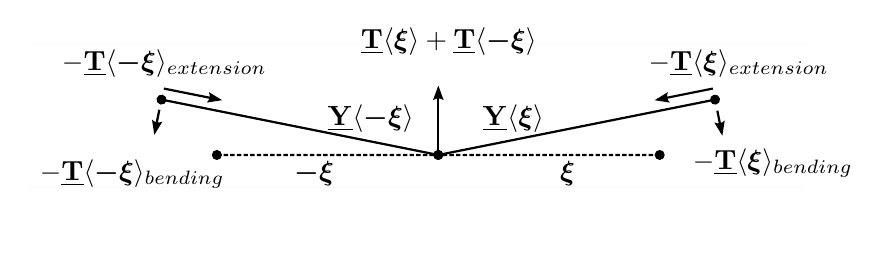
\begin{tikzpicture}[y=0.80pt, x=0.8pt,yscale=-1, inner sep=0pt, outer sep=0pt]
\begin{scope}[shift={(-16.10332,-55.70103)}]
  \begin{scope}[fill=black]
    \path[color=black,fill=black,line width=0.800pt] (101.0938,106.6875) --
      (103.0938,106.6875) -- (103.0938,105.6875) -- (101.0938,105.6875) --
      cycle(104.0938,106.6875) -- (106.0938,106.6875) -- (106.0938,105.6875) --
      (104.0938,105.6875) -- cycle(107.0938,106.6875) -- (109.0938,106.6875) --
      (109.0938,105.6875) -- (107.0938,105.6875) -- cycle(110.0938,106.6875) --
      (112.0938,106.6875) -- (112.0938,105.6875) -- (110.0938,105.6875) --
      cycle(113.0938,106.6875) -- (115.0938,106.6875) -- (115.0938,105.6875) --
      (113.0938,105.6875) -- cycle(116.0938,106.6875) -- (118.0938,106.6875) --
      (118.0938,105.6875) -- (116.0938,105.6875) -- cycle(119.0938,106.6875) --
      (121.0938,106.6875) -- (121.0938,105.6875) -- (119.0938,105.6875) --
      cycle(122.0938,106.6875) -- (124.0938,106.6875) -- (124.0938,105.6875) --
      (122.0938,105.6875) -- cycle(125.0938,106.6875) -- (127.0938,106.6875) --
      (127.0938,105.6875) -- (125.0938,105.6875) -- cycle(128.0938,106.6875) --
      (130.0938,106.6875) -- (130.0938,105.6875) -- (128.0938,105.6875) --
      cycle(131.0938,106.6875) -- (133.0938,106.6875) -- (133.0938,105.6875) --
      (131.0938,105.6875) -- cycle(134.0938,106.6875) -- (136.0938,106.6875) --
      (136.0938,105.6875) -- (134.0938,105.6875) -- cycle(137.0938,106.6875) --
      (139.0938,106.6875) -- (139.0938,105.6875) -- (137.0938,105.6875) --
      cycle(140.0938,106.6875) -- (142.0938,106.6875) -- (142.0938,105.6875) --
      (140.0938,105.6875) -- cycle(143.0938,106.6875) -- (145.0938,106.6875) --
      (145.0938,105.6875) -- (143.0938,105.6875) -- cycle(146.0938,106.6875) --
      (148.0938,106.6875) -- (148.0938,105.6875) -- (146.0938,105.6875) --
      cycle(149.0938,106.6875) -- (151.0938,106.6875) -- (151.0938,105.6875) --
      (149.0938,105.6875) -- cycle(152.0938,106.6875) -- (154.0938,106.6875) --
      (154.0938,105.6875) -- (152.0938,105.6875) -- cycle(155.0938,106.6875) --
      (157.0938,106.6875) -- (157.0938,105.6875) -- (155.0938,105.6875) --
      cycle(158.0938,106.6875) -- (160.0938,106.6875) -- (160.0938,105.6875) --
      (158.0938,105.6875) -- cycle(161.0938,106.6875) -- (163.0938,106.6875) --
      (163.0938,105.6875) -- (161.0938,105.6875) -- cycle(164.0938,106.6875) --
      (166.0938,106.6875) -- (166.0938,105.6875) -- (164.0938,105.6875) --
      cycle(167.0938,106.6875) -- (169.0938,106.6875) -- (169.0938,105.6875) --
      (167.0938,105.6875) -- cycle(170.0938,106.6875) -- (172.0938,106.6875) --
      (172.0938,105.6875) -- (170.0938,105.6875) -- cycle(173.0938,106.6875) --
      (175.0938,106.6875) -- (175.0938,105.6875) -- (173.0938,105.6875) --
      cycle(176.0938,106.6875) -- (178.0938,106.6875) -- (178.0938,105.6875) --
      (176.0938,105.6875) -- cycle(179.0938,106.6875) -- (181.0938,106.6875) --
      (181.0938,105.6875) -- (179.0938,105.6875) -- cycle(182.0938,106.6875) --
      (184.0938,106.6875) -- (184.0938,105.6875) -- (182.0938,105.6875) --
      cycle(185.0938,106.6875) -- (187.0938,106.6875) -- (187.0938,105.6875) --
      (185.0938,105.6875) -- cycle(188.0938,106.6875) -- (190.0938,106.6875) --
      (190.0938,105.6875) -- (188.0938,105.6875) -- cycle(191.0938,106.6875) --
      (193.0938,106.6875) -- (193.0938,105.6875) -- (191.0938,105.6875) --
      cycle(194.0938,106.6875) -- (196.0938,106.6875) -- (196.0938,105.6875) --
      (194.0938,105.6875) -- cycle(197.0938,106.6875) -- (199.0938,106.6875) --
      (199.0938,105.6875) -- (197.0938,105.6875) -- cycle(200.0938,106.6875) --
      (201.0938,106.6875) -- (202.0938,106.6875) -- (202.0938,105.6875) --
      (201.0938,105.6875) -- (200.0938,105.6875) -- cycle(203.0938,106.6875) --
      (205.0938,106.6875) -- (205.0938,105.6875) -- (203.0938,105.6875) --
      cycle(206.0938,106.6875) -- (208.0938,106.6875) -- (208.0938,105.6875) --
      (206.0938,105.6875) -- cycle(209.0938,106.6875) -- (211.0938,106.6875) --
      (211.0938,105.6875) -- (209.0938,105.6875) -- cycle(212.0938,106.6875) --
      (214.0938,106.6875) -- (214.0938,105.6875) -- (212.0938,105.6875) --
      cycle(215.0938,106.6875) -- (217.0938,106.6875) -- (217.0938,105.6875) --
      (215.0938,105.6875) -- cycle(218.0938,106.6875) -- (220.0938,106.6875) --
      (220.0938,105.6875) -- (218.0938,105.6875) -- cycle(221.0938,106.6875) --
      (223.0938,106.6875) -- (223.0938,105.6875) -- (221.0938,105.6875) --
      cycle(224.0938,106.6875) -- (226.0938,106.6875) -- (226.0938,105.6875) --
      (224.0938,105.6875) -- cycle(227.0938,106.6875) -- (229.0938,106.6875) --
      (229.0938,105.6875) -- (227.0938,105.6875) -- cycle(230.0938,106.6875) --
      (232.0938,106.6875) -- (232.0938,105.6875) -- (230.0938,105.6875) --
      cycle(233.0938,106.6875) -- (235.0938,106.6875) -- (235.0938,105.6875) --
      (233.0938,105.6875) -- cycle(236.0938,106.6875) -- (238.0938,106.6875) --
      (238.0938,105.6875) -- (236.0938,105.6875) -- cycle(239.0938,106.6875) --
      (241.0938,106.6875) -- (241.0938,105.6875) -- (239.0938,105.6875) --
      cycle(242.0938,106.6875) -- (244.0938,106.6875) -- (244.0938,105.6875) --
      (242.0938,105.6875) -- cycle(245.0938,106.6875) -- (247.0938,106.6875) --
      (247.0938,105.6875) -- (245.0938,105.6875) -- cycle(248.0938,106.6875) --
      (250.0938,106.6875) -- (250.0938,105.6875) -- (248.0938,105.6875) --
      cycle(251.0938,106.6875) -- (253.0938,106.6875) -- (253.0938,105.6875) --
      (251.0938,105.6875) -- cycle(254.0938,106.6875) -- (256.0938,106.6875) --
      (256.0938,105.6875) -- (254.0938,105.6875) -- cycle(257.0938,106.6875) --
      (259.0938,106.6875) -- (259.0938,105.6875) -- (257.0938,105.6875) --
      cycle(260.0938,106.6875) -- (262.0938,106.6875) -- (262.0938,105.6875) --
      (260.0938,105.6875) -- cycle(263.0938,106.6875) -- (265.0938,106.6875) --
      (265.0938,105.6875) -- (263.0938,105.6875) -- cycle(266.0938,106.6875) --
      (268.0938,106.6875) -- (268.0938,105.6875) -- (266.0938,105.6875) --
      cycle(269.0938,106.6875) -- (271.0938,106.6875) -- (271.0938,105.6875) --
      (269.0938,105.6875) -- cycle(272.0938,106.6875) -- (274.0938,106.6875) --
      (274.0938,105.6875) -- (272.0938,105.6875) -- cycle(275.0938,106.6875) --
      (277.0938,106.6875) -- (277.0938,105.6875) -- (275.0938,105.6875) --
      cycle(278.0938,106.6875) -- (280.0938,106.6875) -- (280.0938,105.6875) --
      (278.0938,105.6875) -- cycle(281.0938,106.6875) -- (283.0938,106.6875) --
      (283.0938,105.6875) -- (281.0938,105.6875) -- cycle(284.0938,106.6875) --
      (286.0938,106.6875) -- (286.0938,105.6875) -- (284.0938,105.6875) --
      cycle(287.0938,106.6875) -- (289.0938,106.6875) -- (289.0938,105.6875) --
      (287.0938,105.6875) -- cycle(290.0938,106.6875) -- (292.0938,106.6875) --
      (292.0938,105.6875) -- (290.0938,105.6875) -- cycle(293.0938,106.6875) --
      (295.0938,106.6875) -- (295.0938,105.6875) -- (293.0938,105.6875) --
      cycle(296.0938,106.6875) -- (298.0938,106.6875) -- (298.0938,105.6875) --
      (296.0938,105.6875) -- cycle(299.0938,106.6875) -- (301.0938,106.6875) --
      (301.0938,105.6875) -- (299.0938,105.6875) -- cycle;
    \path[draw=black,fill=black,even odd rule,line width=0.400pt]
      (103.0633,106.2010) .. controls (103.0633,107.3050) and (102.1673,108.2010) ..
      (101.0633,108.2010) .. controls (99.9593,108.2010) and (99.0633,107.3050) ..
      (99.0633,106.2010) .. controls (99.0633,105.0970) and (99.9593,104.2010) ..
      (101.0633,104.2010) .. controls (102.1673,104.2010) and (103.0633,105.0970) ..
      (103.0633,106.2010) -- cycle;
    \path[draw=black,fill=black,even odd rule,line width=0.400pt]
      (203.0633,106.2010) .. controls (203.0633,107.3050) and (202.1673,108.2010) ..
      (201.0633,108.2010) .. controls (199.9593,108.2010) and (199.0633,107.3050) ..
      (199.0633,106.2010) .. controls (199.0633,105.0970) and (199.9593,104.2010) ..
      (201.0633,104.2010) .. controls (202.1673,104.2010) and (203.0633,105.0970) ..
      (203.0633,106.2010) -- cycle;
    \path[draw=black,fill=black,even odd rule,line width=0.400pt]
      (303.0633,106.2010) .. controls (303.0633,107.3050) and (302.1673,108.2010) ..
      (301.0633,108.2010) .. controls (299.9593,108.2010) and (299.0633,107.3050) ..
      (299.0633,106.2010) .. controls (299.0633,105.0970) and (299.9593,104.2010) ..
      (301.0633,104.2010) .. controls (302.1673,104.2010) and (303.0633,105.0970) ..
      (303.0633,106.2010) -- cycle;
  \end{scope}
  \begin{scope}[fill=black]
    \path[color=black,fill=black,line width=0.800pt] (76.1875,80.7188) --
      (76.0000,81.6875) -- (201.0000,106.6875) -- (201.0937,106.7187) --
      (201.1874,106.6875) -- (326.1874,81.6875) -- (326.0000,80.7188) --
      (201.0938,105.6875) -- (76.1875,80.7188) -- cycle;
    \path[draw=black,fill=black,even odd rule,line width=0.400pt] (78.0253,81.5854)
      .. controls (77.8087,82.6680) and (76.7544,83.3709) .. (75.6719,83.1544) ..
      controls (74.5893,82.9378) and (73.8864,81.8835) .. (74.1029,80.8010) ..
      controls (74.3194,79.7184) and (75.3738,79.0155) .. (76.4563,79.2320) ..
      controls (77.5389,79.4485) and (78.2418,80.5029) .. (78.0253,81.5854) --
      cycle;
    \path[draw=black,fill=black,even odd rule,line width=0.400pt]
      (203.0633,106.2010) .. controls (203.0633,107.3050) and (202.1673,108.2010) ..
      (201.0633,108.2010) .. controls (199.9593,108.2010) and (199.0633,107.3050) ..
      (199.0633,106.2010) .. controls (199.0633,105.0970) and (199.9593,104.2010) ..
      (201.0633,104.2010) .. controls (202.1673,104.2010) and (203.0633,105.0970) ..
      (203.0633,106.2010) -- cycle;
    \path[draw=black,fill=black,even odd rule,line width=0.400pt] (328.0253,80.8166)
      .. controls (328.2418,81.8992) and (327.5389,82.9535) .. (326.4563,83.1700) ..
      controls (325.3738,83.3866) and (324.3194,82.6837) .. (324.1029,81.6011) ..
      controls (323.8864,80.5186) and (324.5893,79.4642) .. (325.6719,79.2477) ..
      controls (326.7544,79.0312) and (327.8087,79.7341) .. (328.0253,80.8166) --
      cycle;
  \end{scope}
  \begin{scope}[fill=black]
    \path[color=black,fill=black,line width=0.800pt] (200.5938,76.1875) --
      (200.5938,106.1875) -- (201.5938,106.1875) -- (201.5938,76.1875) --
      (200.5938,76.1875) -- cycle;
    \path[fill=black,line join=round,even odd rule,line width=0.500pt]
      (198.6831,81.4322) -- (201.0937,74.8767) -- (203.5043,81.4322) .. controls
      (202.0811,80.3849) and (200.1339,80.3909) .. (198.6831,81.4322) -- cycle;
  \end{scope}
  \path[fill=black] (178.797,148.02312) node[above right] (text6246) {};
  \path[fill=black] (256.10333,120.20103) node[above right] (text6273)
    {$\boldsymbol{\xi}$};
  \path[fill=black] (136.10332,120.20103) node[above right] (text6277)
    {$\boldsymbol{-\xi}$};
  \path[fill=black] (296.10333,71.201035) node[above right] (text6285)
    {$-\vstate{T}{}{\boldsymbol{\xi}}_{extension}$};
  \path[shift={(71.10332,65.91978)},draw=black,opacity=0.010,line join=miter,line
    cap=butt,line width=0.800pt] (-55.0000,54.7812) -- (295.0000,54.7812);
  \path[fill=black] (316.10333,116.20103) node[above right] (text4473)
    {$-\vstate{T}{}{\boldsymbol{\xi}}_{bending}$};
  \begin{scope}[shift={(0,-64.5)},shift={(0,0)}]
    \path[shift={(71.10332,65.91978)},draw=black,opacity=0.010,line join=miter,line
      cap=butt,line width=0.800pt] (-55.0000,54.7812) -- (295.0000,54.7812);
  \end{scope}
  \path[fill=black] (166.10332,61.201035) node[above right] (text4726)
    {$\vstate{T}{}{\boldsymbol{\xi}}+\vstate{T}{}{\boldsymbol{-\xi}}$};
  \begin{scope}[fill=black]
    \path[color=black,fill=black,line width=0.800pt] (74.5625,85.6875) --
      (72.5625,95.6875) -- (73.5625,95.9062) -- (75.5625,85.9062) --
      (74.5625,85.6875) -- cycle;
    \path[fill=black,line join=round,even odd rule,line width=0.500pt]
      (76.4671,91.1458) -- (72.8177,97.1013) -- (71.7395,90.2003) .. controls
      (72.9297,91.5064) and (74.8403,91.8824) .. (76.4671,91.1458) -- cycle;
  \end{scope}
  \begin{scope}[fill=black]
    \path[color=black,fill=black,line width=0.800pt] (77.1875,75.7188) --
      (77.0000,76.6875) -- (102.0000,81.6875) -- (102.1875,80.7188) --
      (77.1875,75.7188) -- cycle;
    \path[fill=black,line join=round,even odd rule,line width=0.500pt]
      (97.4484,77.8019) -- (103.4039,81.4513) -- (96.5029,82.5295) .. controls
      (97.8090,81.3393) and (98.1849,79.4287) .. (97.4484,77.8019) -- cycle;
  \end{scope}
  \begin{scope}[fill=black]
    \path[color=black,fill=black,line width=0.800pt] (327.5938,86.0938) --
      (326.6250,86.3125) -- (328.6250,96.3125) -- (329.5938,96.0938) --
      (327.5938,86.0938) -- cycle;
    \path[fill=black,line join=round,even odd rule,line width=0.500pt]
      (330.4506,90.5968) -- (329.3725,97.4978) -- (325.7230,91.5423) .. controls
      (327.3240,92.2902) and (329.2322,91.9024) .. (330.4507,90.5968) -- cycle;
  \end{scope}
  \begin{scope}[fill=black]
    \path[color=black,fill=black,line width=0.800pt] (325.0000,75.7188) --
      (300.0000,80.7188) -- (300.1875,81.6875) -- (325.1875,76.6875) --
      (325.0000,75.7188) -- cycle;
    \path[fill=black,line join=round,even odd rule,line width=0.500pt]
      (305.7075,82.5484) -- (298.8066,81.4702) -- (304.7620,77.8207) .. controls
      (304.0142,79.4217) and (304.4020,81.3299) .. (305.7075,82.5484) -- cycle;
  \end{scope}
  \path[fill=black] (21.103317,121.20103) node[above right] (text4217)
    {$-\vstate{T}{}{\boldsymbol{-\xi}}_{bending}$};
  \path[fill=black] (31.103317,71.201035) node[above right] (text4221)
    {$-\vstate{T}{}{\boldsymbol{-\xi}}_{extension}$};
  \path[fill=black] (221.10332,96.201035) node[above right] (text4282)
    {$\vstate{Y}{}{\boldsymbol{\xi}}$};
  \path[fill=black] (151.10332,96.201035) node[above right] (text4286)
    {$\vstate{Y}{}{\boldsymbol{-\xi}}$};
\end{scope}

\end{tikzpicture}


  \caption{The Hybrid Model Combines Bending and Extension Components}
  \label{fig:hybridmodel}
\end{figure}
%
As the two sides are pulled apart, the magnitude of the extension force in each bond increases, and the magnitude of the bending force decreases.  At the same time, the angle at which the extension force acts decreases, and the angle of action for the bending force increases.  For small amounts of bending and reasonable stretches, increased tension in the direction of the bond pair results in increase restorative force.

\section{Extension to arbitrary Poisson ratio}
\label{sec:arbitrary}
Although many materials have Poisson ratios of \(\nu\approx \sfrac{1}{3}\), it is nonetheless desirable to extend the model to materials with arbitrary Poisson ratios.  For isotropic, linearly elastic models of solid materials, Silling et al.\ extended the peridynamic material model to arbitrary material parameters in \cite{silling2007peridynamic} by decomposing the deformation into isotropic and deviatoric components.  In the absence of plastic deformation, we need only find the difference between the strain energy of a deformed bond-based plate and the strain energy of an elastic plate with Poisson's ratio \(\nu \neq \sfrac{1}{3}\).  The difference is a function of the isotropic strain in two dimensions, \(\theta_2\)
%
\begin{align}
    W' &= \frac{G\;h}{2}\left(\frac{3\nu-1}{1-\nu}\right)\theta_2^2 \notag \\
%    \theta_2 &= \frac{2}{m}\left(\underline{\omega x}\right)\bullet\underline{e} \notag \\
    \theta_2 &= \frac{2}{m}\int_A \omega(\boldsymbol{\xi})|\boldsymbol{\xi}|(|\vstate{Y}{}{\boldsymbol{\xi}}|-|\boldsymbol{\xi}|)\;dA_{\boldsymbol{\xi}} \notag \\
%    W_\text{total} &= \frac{G\;h}{2}\left(\frac{3\nu-1}{1-\nu}\right)\theta_2^2 + \frac{4\;G\;h}{m}\left(\underline{\omega e}\right)\bullet\underline{e}\notag
    W_\text{total} &= \frac{G\;h}{2}\left(\frac{3\nu-1}{1-\nu}\right)\theta_2^2 + \frac{4\;G\;h}{m}\int_A \omega(\boldsymbol{\xi})(|\vstate{Y}{}{\boldsymbol{\xi}}|-|\boldsymbol{\xi}|)^2\;dA_{\boldsymbol{\xi}}\notag
\end{align}
%
This is to be expected because the bond-based model was calibrated to the shear strain energy, leaving discrepancies proportional to the isotropic strain energy that fall to 0 as Poisson's ratio approaches \(\nu = \sfrac{1}{3}\).

This decomposition method inspires a similar approach to our plate model. To perform the same extension for the plate model in bending, we find the error in the 1-parameter strain energy for \(\nu \neq \sfrac{1}{3}\)
%
\begin{align}
    W'=&\frac{G h^3}{12(1-\nu)} \left(\kappa_1^2+\kappa_2^2+2\nu\kappa_1\kappa_2+2(1-\nu)\kappa_3^2 \right)\notag\\
    &-\frac{G h^3}{12(1-\frac{1}{3})} \left(\kappa_1^2+\kappa_2^2+\frac{2}{3}\nu\kappa_1\kappa_2+2(1-\frac{1}{3})\kappa_3^2 \right) \notag \\
    W'=&2G \frac{h^3}{12}\frac{3\nu-1}{1-\nu} \left(\frac{\kappa_1+\kappa_2}{2}\right)^2.\notag
\end{align}
%
The discrepancy in energy is proportional to the square of average curvature, \(\frac{\kappa_1+\kappa_2}{2} = \bar{\kappa}\), which we will also refer to as the isotropic curvature.  The isotropic curvature can be envisioned as the portion of the deformation that resembles a hemispherical bowl.  A complete decomposition of bending energy into isotropic and deviatoric components as performed by Fischer in \cite{fischer1992bending} produces a far more complex model and is unnecessary at this time.  For a single bond pair we can represent the curvature vector along the bond pair as 
%
\begin{equation}
    \boldsymbol{\kappa} _{\hat{\boldsymbol{\xi}}} = \frac{\vstate{Y}{}{\boldsymbol{\xi}}+\vstate{Y}{}{\boldsymbol{-\xi}}}{|\boldsymbol{\xi}|^2}\notag
\end{equation}
%
For large rotations, we can define an average curvature vector \(\bar{\boldsymbol{\kappa}}\).
This leads us to model the average curvature as 
%
\begin{align}
    \bar{\boldsymbol{\kappa}} &= \frac{1}{m} \int_0^\delta \int_0^{2\pi}\omega(\xi)\frac{\vstate{Y}{}{\boldsymbol{\xi}}+\vstate{Y}{}{\boldsymbol{-\xi}}}{\xi^2} \xi {\rm d}\phi {\rm d}\xi ;\notag \\
    m &= \int_0^\delta \int_0^{2\pi}\omega(\xi)\xi {\rm d}\phi {\rm d}\xi. \notag
\end{align}
%
The weighting function \(\omega(\xi)\) performs the same function as in the previous section.
We can rewrite the energy discrepancy in terms of \(\bar{\boldsymbol{\kappa}}\).
%
\begin{equation}
    W'=2G\frac{h^3}{12}\frac{3\nu-1}{1-\nu}\bar{\boldsymbol{\kappa}}^2. \notag
\end{equation}
%
We can take the Fr\'{e}chet derivative (details in \ref{sec:frechet}) to produce a correction force vector state
%
\begin{equation}
    \vstate{T'}{}{\boldsymbol{\xi}}=\frac{8G}{m}\frac{h^3}{12}\frac{3\nu-1}{1-\nu}\frac{\omega(\boldsymbol{\xi})}{\xi^2} \bar{\boldsymbol{\kappa}},
    \label{eq:pressureState}
\end{equation}
%
that is not directly dependent on the deformation of a single bond pair.  Instead, \cref{eq:pressureState} represents a bond-length dependent ``pressure'' applied to every pair of bonds extending from a node.  This ``pressure'' is proportional to the curvature vector at that node.
A weighting function \(\omega(\boldsymbol{\xi}) = |\boldsymbol{\xi}|\) can ensure that the integral expression for force at a point is convergent.  This extra term that is dependent on the bending of all the pairs around a material point means that the extension is not properly a \textit{bond-pair} model.  Instead, it would be more accurate to call it a \textit{bond-multiple} model, in which the bond forces and energies are functions of the relationship between a family of bonds.  In either the continuous or discrete cases, this model extension requires the additional step of evaluating the isotropic curvature at each point, but the increased complexity of the extended model captures in the local limit the behavior of a two-parameter elastic material plate.
%
\section{Numerical Simulation}
\subsection{Discretized Model}
Discretizing the bond-pair model is primarily matter of exchanging integrals for sums. 
%
\begin{align}
w(\boldsymbol{\xi}_i) &= \omega(\boldsymbol{\xi}_i)\alpha \left[1+\cos(\theta(\vstate{Y}{}{\boldsymbol{\xi}_i},\vstate{Y}{}{-\boldsymbol{\xi}_i})) \right] \notag \\
&\approx \omega(\boldsymbol{\xi}_i)\frac{\alpha}{2}\left(\frac{z(\mathbf{x}+\boldsymbol{\xi}_i)-2z(\mathbf{x})+z(\mathbf{x}-\boldsymbol{\xi}_i)}{\boldsymbol{\xi}_i}\right)^2 \notag
\end{align}
%
in which $\boldsymbol{\xi}_i$ is the $i^\textnormal{th}$ bond emanating from the point $\mathbf{x}$ to each of the $n$ points within distance $\delta$ of point $\mathbf{x}$.
%
\begin{align}
    \alpha &= \frac{c\; (\Delta x)^2}{m} ;\; c= \frac{G}{(1-\nu)}\frac{h^3}{12};\; m=\sum_{i=1}^n \omega(\boldsymbol{\xi}_i)\boldsymbol{\xi}_i^2 \implies \nonumber \\
    W&=(\Delta x)^2 \sum_{i=1}^n \omega(\boldsymbol{\xi}_i)\frac{G}{2(1-\nu)}\frac{h^3}{12}\left(\frac{z(\mathbf{x}+\boldsymbol{\xi}_i)-2z(\mathbf{x})+z(\mathbf{x}-\boldsymbol{\xi}_i)}{|\boldsymbol{\xi}_i|}\right)^2 \notag
\end{align}
%
Discretization of the 1-parameter bending model results in the equation of motion
%
\begin{align}
    \label{eq:discreteEoM}
    \rho(\mathbf{x})\mathbf{\ddot{u}}(\mathbf{x}) = \mathbf{f}(\mathbf{x})&+\sum_i \omega(\boldsymbol{\xi}_i)\left\{\frac{\alpha(\mathbf{x})}{|\mathbf{p}_i |}\frac{\mathbf{p}_i}{|\mathbf{p}_i |}\times \left[ \frac{\mathbf{p}_i}{|\mathbf{p}_i |}\times \frac{\mathbf{q}_i}{|\mathbf{q}_i |}\right] \right.  \\
    & \left. -\frac{\alpha(\mathbf{x}+\boldsymbol{\xi}_i)}{|\mathbf{p}_i |}\frac{(-\mathbf{p}_i)}{|\mathbf{p}_i |}\times\left[\frac{(-\mathbf{p}_i)}{|\mathbf{p}_i |}\times \frac{\mathbf{r}_i}{|\mathbf{r}_i |} \right] \right\} \notag
\end{align}
with
\begin{align}
    \mathbf{p}_i &= \boldsymbol{\xi}_i+\mathbf{u}(\mathbf{x}+\boldsymbol{\xi}_i)-\mathbf{u}(\mathbf{x});\notag\\
    \mathbf{q}_i &= -\boldsymbol{\xi}_i+\mathbf{u}(\mathbf{x}-\boldsymbol{\xi}_i)-\mathbf{u}(\mathbf{x});\notag\\
    \mathbf{r}_i &= \boldsymbol{\xi}_i+\mathbf{u}(\mathbf{x}+2\boldsymbol{\xi}_i)-\mathbf{u}(\mathbf{x}+\boldsymbol{\xi}_i).\notag
\end{align}
%

Implementing the 2-parameter model requires finding the isotropic curvature at each point.
%
\begin{align*}
    \bar{\boldsymbol{\kappa}}(\mathbf{x}) &= \frac{1}{m} \sum_i \omega(\boldsymbol{\xi}_i)\frac{\mathbf{p}_i +\mathbf{q}_i }{\boldsymbol{\xi}_i^2};\notag \\
    m(\mathbf{x})  &= \sum_i \omega(\boldsymbol{\xi}_i); \notag \\
    \alpha^\text{iso}(\mathbf{x}) &= \frac{4G}{m}\frac{h^3}{12}\frac{3\nu-1}{1-\nu}(\Delta x)^2;\\
    f^\text{iso}(\mathbf{x}) &= \sum_j \left\{\left[\alpha^\text{iso}(\mathbf{x})\bar{\boldsymbol{\kappa}}(\mathbf{x})-\alpha^\text{iso}(\mathbf{x}+\boldsymbol{\xi}_j)\bar{\boldsymbol{\kappa}}(\mathbf{x}+\boldsymbol{\xi}_j) \right] \frac{\omega(\boldsymbol{\xi}_j)}{\boldsymbol{\xi}_j^2} \right\}
\end{align*}
%
Discretizing the bond-pair model as proposed above requires that nodes be evenly spaced, $\Delta x$, throughout the entire plate, otherwise the displacement \(z(\mathbf{x}-\boldsymbol{\xi}_i)\) is ill-defined.  For this reason, the discretization does not allow for areas of higher and lower ``resolution''. An extension to this discretization that would allow changing mesh resolution will require interpolation between the nodes.  
%
\subsection{Numerical Method}
\label{sec:NumMethod}
Model behavior is evaluated by implementing the discretized equation of motion.  The case of a square plate simply supported on all four sides is chosen for simplicity in both evaluation and comparison.  To implement the simply-supported condition, it was sufficient to constrain the vertical displacement of each node along the plate's four edges.  Boundary conditions such as clamped or guided supports and applied moments require careful treatment to ensure both meaningful results and ease of computation.  While applying displacement constraints is straightforward, the appropriate way to apply an angle constraint or moment to a peridynamic point or collection of points is less obvious.

Additionally, the simply-supported flat plate is a configuration with significant analytical treatment in the classical theories, making a better comparison case than configurations that may require comparison to finite element or other solution techniques.
%
\subsection{Results}
The simplest test case for this model is a linear-elastic square plate with Poisson's ratio \(\nu = \sfrac{1}{3}\) that is simply-supported on all 4 sides with a uniform transverse pressure load on the entire surface between the supports.  As expected from an energy-equivalent model, the slice along the plate's centerline shown in \cref{fig:plate_convergence_h} demonstrates good agreement between the static deflection predicted by the bond-pair model and that of classical linear elasticity as the horizon length shrinks.  This convergence only continues to a minimum horizon, below which the discretized equation of motion (\cref{eq:discreteEoM}) ceases to accurately approximate the continuous integral formulation (\cref{eq:PDstateEoM,eq:SillingForceNO}).  The minimum horizon size depends on the discretization; it appears that twice the node spacing is insufficient, and that three times the node spacing is sufficient.  The difference is evident in \cref{fig:plate_minimum_h}.
%
\begin{figure}[h]
  \centering
  \resizebox{0.55\linewidth}{!}{%% Creator: Matplotlib, PGF backend
%%
%% To include the figure in your LaTeX document, write
%%   \input{<filename>.pgf}
%%
%% Make sure the required packages are loaded in your preamble
%%   \usepackage{pgf}
%%
%% Figures using additional raster images can only be included by \input if
%% they are in the same directory as the main LaTeX file. For loading figures
%% from other directories you can use the `import` package
%%   \usepackage{import}
%% and then include the figures with
%%   \import{<path to file>}{<filename>.pgf}
%%
%% Matplotlib used the following preamble
%%
\begingroup%
\makeatletter%
\begin{pgfpicture}%
\pgfpathrectangle{\pgfpointorigin}{\pgfqpoint{6.000000in}{6.000000in}}%
\pgfusepath{use as bounding box}%
\begin{pgfscope}%
\pgfsetrectcap%
\pgfsetroundjoin%
\definecolor{currentfill}{rgb}{1.000000,1.000000,1.000000}%
\pgfsetfillcolor{currentfill}%
\pgfsetlinewidth{0.000000pt}%
\definecolor{currentstroke}{rgb}{1.000000,1.000000,1.000000}%
\pgfsetstrokecolor{currentstroke}%
\pgfsetdash{}{0pt}%
\pgfpathmoveto{\pgfqpoint{0.000000in}{0.000000in}}%
\pgfpathlineto{\pgfqpoint{6.000000in}{0.000000in}}%
\pgfpathlineto{\pgfqpoint{6.000000in}{6.000000in}}%
\pgfpathlineto{\pgfqpoint{0.000000in}{6.000000in}}%
\pgfpathclose%
\pgfusepath{fill}%
\end{pgfscope}%
\begin{pgfscope}%
\pgfsetrectcap%
\pgfsetroundjoin%
\definecolor{currentfill}{rgb}{1.000000,1.000000,1.000000}%
\pgfsetfillcolor{currentfill}%
\pgfsetlinewidth{0.000000pt}%
\definecolor{currentstroke}{rgb}{0.000000,0.000000,0.000000}%
\pgfsetstrokecolor{currentstroke}%
\pgfsetdash{}{0pt}%
\pgfpathmoveto{\pgfqpoint{0.750000in}{0.600000in}}%
\pgfpathlineto{\pgfqpoint{5.400000in}{0.600000in}}%
\pgfpathlineto{\pgfqpoint{5.400000in}{5.400000in}}%
\pgfpathlineto{\pgfqpoint{0.750000in}{5.400000in}}%
\pgfpathclose%
\pgfusepath{fill}%
\end{pgfscope}%
\begin{pgfscope}%
\pgfpathrectangle{\pgfqpoint{0.750000in}{0.600000in}}{\pgfqpoint{4.650000in}{4.800000in}} %
\pgfusepath{clip}%
\pgfsetrectcap%
\pgfsetroundjoin%
\pgfsetlinewidth{1.003750pt}%
\definecolor{currentstroke}{rgb}{0.000000,0.000000,1.000000}%
\pgfsetstrokecolor{currentstroke}%
\pgfsetdash{}{0pt}%
\pgfpathmoveto{\pgfqpoint{0.750000in}{5.400000in}}%
\pgfpathlineto{\pgfqpoint{0.796500in}{5.270617in}}%
\pgfpathlineto{\pgfqpoint{0.843000in}{5.141433in}}%
\pgfpathlineto{\pgfqpoint{0.889500in}{5.012646in}}%
\pgfpathlineto{\pgfqpoint{0.936000in}{4.884446in}}%
\pgfpathlineto{\pgfqpoint{0.982500in}{4.757015in}}%
\pgfpathlineto{\pgfqpoint{1.029000in}{4.630524in}}%
\pgfpathlineto{\pgfqpoint{1.075500in}{4.505137in}}%
\pgfpathlineto{\pgfqpoint{1.122000in}{4.381006in}}%
\pgfpathlineto{\pgfqpoint{1.168500in}{4.258277in}}%
\pgfpathlineto{\pgfqpoint{1.215000in}{4.137087in}}%
\pgfpathlineto{\pgfqpoint{1.261500in}{4.017568in}}%
\pgfpathlineto{\pgfqpoint{1.308000in}{3.899846in}}%
\pgfpathlineto{\pgfqpoint{1.354500in}{3.784039in}}%
\pgfpathlineto{\pgfqpoint{1.401000in}{3.670263in}}%
\pgfpathlineto{\pgfqpoint{1.447500in}{3.558623in}}%
\pgfpathlineto{\pgfqpoint{1.494000in}{3.449222in}}%
\pgfpathlineto{\pgfqpoint{1.540500in}{3.342155in}}%
\pgfpathlineto{\pgfqpoint{1.587000in}{3.237511in}}%
\pgfpathlineto{\pgfqpoint{1.633500in}{3.135374in}}%
\pgfpathlineto{\pgfqpoint{1.680000in}{3.035823in}}%
\pgfpathlineto{\pgfqpoint{1.726500in}{2.938933in}}%
\pgfpathlineto{\pgfqpoint{1.773000in}{2.844775in}}%
\pgfpathlineto{\pgfqpoint{1.819500in}{2.753417in}}%
\pgfpathlineto{\pgfqpoint{1.866000in}{2.664922in}}%
\pgfpathlineto{\pgfqpoint{1.912500in}{2.579349in}}%
\pgfpathlineto{\pgfqpoint{1.959000in}{2.496753in}}%
\pgfpathlineto{\pgfqpoint{2.005500in}{2.417186in}}%
\pgfpathlineto{\pgfqpoint{2.052000in}{2.340695in}}%
\pgfpathlineto{\pgfqpoint{2.098500in}{2.267325in}}%
\pgfpathlineto{\pgfqpoint{2.145000in}{2.197118in}}%
\pgfpathlineto{\pgfqpoint{2.191500in}{2.130112in}}%
\pgfpathlineto{\pgfqpoint{2.238000in}{2.066343in}}%
\pgfpathlineto{\pgfqpoint{2.284500in}{2.005847in}}%
\pgfpathlineto{\pgfqpoint{2.331000in}{1.948654in}}%
\pgfpathlineto{\pgfqpoint{2.377500in}{1.894795in}}%
\pgfpathlineto{\pgfqpoint{2.424000in}{1.844294in}}%
\pgfpathlineto{\pgfqpoint{2.470500in}{1.797178in}}%
\pgfpathlineto{\pgfqpoint{2.517000in}{1.753468in}}%
\pgfpathlineto{\pgfqpoint{2.563500in}{1.713182in}}%
\pgfpathlineto{\pgfqpoint{2.610000in}{1.676341in}}%
\pgfpathlineto{\pgfqpoint{2.656500in}{1.642959in}}%
\pgfpathlineto{\pgfqpoint{2.703000in}{1.613052in}}%
\pgfpathlineto{\pgfqpoint{2.749500in}{1.586634in}}%
\pgfpathlineto{\pgfqpoint{2.796000in}{1.563715in}}%
\pgfpathlineto{\pgfqpoint{2.842500in}{1.544306in}}%
\pgfpathlineto{\pgfqpoint{2.889000in}{1.528416in}}%
\pgfpathlineto{\pgfqpoint{2.935500in}{1.516051in}}%
\pgfpathlineto{\pgfqpoint{2.982000in}{1.507215in}}%
\pgfpathlineto{\pgfqpoint{3.028500in}{1.501913in}}%
\pgfpathlineto{\pgfqpoint{3.075000in}{1.500145in}}%
\pgfpathlineto{\pgfqpoint{3.121500in}{1.501913in}}%
\pgfpathlineto{\pgfqpoint{3.168000in}{1.507215in}}%
\pgfpathlineto{\pgfqpoint{3.214500in}{1.516051in}}%
\pgfpathlineto{\pgfqpoint{3.261000in}{1.528416in}}%
\pgfpathlineto{\pgfqpoint{3.307500in}{1.544306in}}%
\pgfpathlineto{\pgfqpoint{3.354000in}{1.563715in}}%
\pgfpathlineto{\pgfqpoint{3.400500in}{1.586634in}}%
\pgfpathlineto{\pgfqpoint{3.447000in}{1.613052in}}%
\pgfpathlineto{\pgfqpoint{3.493500in}{1.642959in}}%
\pgfpathlineto{\pgfqpoint{3.540000in}{1.676341in}}%
\pgfpathlineto{\pgfqpoint{3.586500in}{1.713182in}}%
\pgfpathlineto{\pgfqpoint{3.633000in}{1.753468in}}%
\pgfpathlineto{\pgfqpoint{3.679500in}{1.797178in}}%
\pgfpathlineto{\pgfqpoint{3.726000in}{1.844294in}}%
\pgfpathlineto{\pgfqpoint{3.772500in}{1.894795in}}%
\pgfpathlineto{\pgfqpoint{3.819000in}{1.948654in}}%
\pgfpathlineto{\pgfqpoint{3.865500in}{2.005847in}}%
\pgfpathlineto{\pgfqpoint{3.912000in}{2.066343in}}%
\pgfpathlineto{\pgfqpoint{3.958500in}{2.130112in}}%
\pgfpathlineto{\pgfqpoint{4.005000in}{2.197118in}}%
\pgfpathlineto{\pgfqpoint{4.051500in}{2.267325in}}%
\pgfpathlineto{\pgfqpoint{4.098000in}{2.340695in}}%
\pgfpathlineto{\pgfqpoint{4.144500in}{2.417186in}}%
\pgfpathlineto{\pgfqpoint{4.191000in}{2.496753in}}%
\pgfpathlineto{\pgfqpoint{4.237500in}{2.579349in}}%
\pgfpathlineto{\pgfqpoint{4.284000in}{2.664922in}}%
\pgfpathlineto{\pgfqpoint{4.330500in}{2.753417in}}%
\pgfpathlineto{\pgfqpoint{4.377000in}{2.844775in}}%
\pgfpathlineto{\pgfqpoint{4.423500in}{2.938933in}}%
\pgfpathlineto{\pgfqpoint{4.470000in}{3.035823in}}%
\pgfpathlineto{\pgfqpoint{4.516500in}{3.135374in}}%
\pgfpathlineto{\pgfqpoint{4.563000in}{3.237511in}}%
\pgfpathlineto{\pgfqpoint{4.609500in}{3.342155in}}%
\pgfpathlineto{\pgfqpoint{4.656000in}{3.449222in}}%
\pgfpathlineto{\pgfqpoint{4.702500in}{3.558623in}}%
\pgfpathlineto{\pgfqpoint{4.749000in}{3.670263in}}%
\pgfpathlineto{\pgfqpoint{4.795500in}{3.784039in}}%
\pgfpathlineto{\pgfqpoint{4.842000in}{3.899846in}}%
\pgfpathlineto{\pgfqpoint{4.888500in}{4.017568in}}%
\pgfpathlineto{\pgfqpoint{4.935000in}{4.137087in}}%
\pgfpathlineto{\pgfqpoint{4.981500in}{4.258277in}}%
\pgfpathlineto{\pgfqpoint{5.028000in}{4.381006in}}%
\pgfpathlineto{\pgfqpoint{5.074500in}{4.505137in}}%
\pgfpathlineto{\pgfqpoint{5.121000in}{4.630524in}}%
\pgfpathlineto{\pgfqpoint{5.167500in}{4.757015in}}%
\pgfpathlineto{\pgfqpoint{5.214000in}{4.884446in}}%
\pgfpathlineto{\pgfqpoint{5.260500in}{5.012646in}}%
\pgfpathlineto{\pgfqpoint{5.307000in}{5.141433in}}%
\pgfpathlineto{\pgfqpoint{5.353500in}{5.270617in}}%
\pgfpathlineto{\pgfqpoint{5.400000in}{5.400000in}}%
\pgfusepath{stroke}%
\end{pgfscope}%
\begin{pgfscope}%
\pgfpathrectangle{\pgfqpoint{0.750000in}{0.600000in}}{\pgfqpoint{4.650000in}{4.800000in}} %
\pgfusepath{clip}%
\pgfsetbuttcap%
\pgfsetmiterjoin%
\definecolor{currentfill}{rgb}{0.000000,0.500000,0.000000}%
\pgfsetfillcolor{currentfill}%
\pgfsetlinewidth{0.501875pt}%
\definecolor{currentstroke}{rgb}{0.000000,0.000000,0.000000}%
\pgfsetstrokecolor{currentstroke}%
\pgfsetdash{}{0pt}%
\pgfsys@defobject{currentmarker}{\pgfqpoint{-0.041667in}{-0.041667in}}{\pgfqpoint{0.041667in}{0.041667in}}{%
\pgfpathmoveto{\pgfqpoint{0.000000in}{0.041667in}}%
\pgfpathlineto{\pgfqpoint{-0.041667in}{-0.041667in}}%
\pgfpathlineto{\pgfqpoint{0.041667in}{-0.041667in}}%
\pgfpathclose%
\pgfusepath{stroke,fill}%
}%
\begin{pgfscope}%
\pgfsys@transformshift{0.750000in}{5.400000in}%
\pgfsys@useobject{currentmarker}{}%
\end{pgfscope}%
\begin{pgfscope}%
\pgfsys@transformshift{1.029000in}{4.310547in}%
\pgfsys@useobject{currentmarker}{}%
\end{pgfscope}%
\begin{pgfscope}%
\pgfsys@transformshift{1.308000in}{3.564782in}%
\pgfsys@useobject{currentmarker}{}%
\end{pgfscope}%
\begin{pgfscope}%
\pgfsys@transformshift{1.587000in}{2.898760in}%
\pgfsys@useobject{currentmarker}{}%
\end{pgfscope}%
\begin{pgfscope}%
\pgfsys@transformshift{1.866000in}{2.327648in}%
\pgfsys@useobject{currentmarker}{}%
\end{pgfscope}%
\begin{pgfscope}%
\pgfsys@transformshift{2.145000in}{1.860336in}%
\pgfsys@useobject{currentmarker}{}%
\end{pgfscope}%
\begin{pgfscope}%
\pgfsys@transformshift{2.424000in}{1.508532in}%
\pgfsys@useobject{currentmarker}{}%
\end{pgfscope}%
\begin{pgfscope}%
\pgfsys@transformshift{2.703000in}{1.277825in}%
\pgfsys@useobject{currentmarker}{}%
\end{pgfscope}%
\begin{pgfscope}%
\pgfsys@transformshift{2.982000in}{1.172269in}%
\pgfsys@useobject{currentmarker}{}%
\end{pgfscope}%
\begin{pgfscope}%
\pgfsys@transformshift{3.261000in}{1.193421in}%
\pgfsys@useobject{currentmarker}{}%
\end{pgfscope}%
\begin{pgfscope}%
\pgfsys@transformshift{3.540000in}{1.340945in}%
\pgfsys@useobject{currentmarker}{}%
\end{pgfscope}%
\begin{pgfscope}%
\pgfsys@transformshift{3.819000in}{1.612666in}%
\pgfsys@useobject{currentmarker}{}%
\end{pgfscope}%
\begin{pgfscope}%
\pgfsys@transformshift{4.098000in}{2.002922in}%
\pgfsys@useobject{currentmarker}{}%
\end{pgfscope}%
\begin{pgfscope}%
\pgfsys@transformshift{4.377000in}{2.507482in}%
\pgfsys@useobject{currentmarker}{}%
\end{pgfscope}%
\begin{pgfscope}%
\pgfsys@transformshift{4.656000in}{3.109556in}%
\pgfsys@useobject{currentmarker}{}%
\end{pgfscope}%
\begin{pgfscope}%
\pgfsys@transformshift{4.935000in}{3.805866in}%
\pgfsys@useobject{currentmarker}{}%
\end{pgfscope}%
\begin{pgfscope}%
\pgfsys@transformshift{5.214000in}{4.578216in}%
\pgfsys@useobject{currentmarker}{}%
\end{pgfscope}%
\end{pgfscope}%
\begin{pgfscope}%
\pgfpathrectangle{\pgfqpoint{0.750000in}{0.600000in}}{\pgfqpoint{4.650000in}{4.800000in}} %
\pgfusepath{clip}%
\pgfsetbuttcap%
\pgfsetmiterjoin%
\definecolor{currentfill}{rgb}{1.000000,0.000000,0.000000}%
\pgfsetfillcolor{currentfill}%
\pgfsetlinewidth{0.501875pt}%
\definecolor{currentstroke}{rgb}{0.000000,0.000000,0.000000}%
\pgfsetstrokecolor{currentstroke}%
\pgfsetdash{}{0pt}%
\pgfsys@defobject{currentmarker}{\pgfqpoint{-0.041667in}{-0.041667in}}{\pgfqpoint{0.041667in}{0.041667in}}{%
\pgfpathmoveto{\pgfqpoint{-0.041667in}{-0.041667in}}%
\pgfpathlineto{\pgfqpoint{0.041667in}{-0.041667in}}%
\pgfpathlineto{\pgfqpoint{0.041667in}{0.041667in}}%
\pgfpathlineto{\pgfqpoint{-0.041667in}{0.041667in}}%
\pgfpathclose%
\pgfusepath{stroke,fill}%
}%
\begin{pgfscope}%
\pgfsys@transformshift{0.843000in}{5.061173in}%
\pgfsys@useobject{currentmarker}{}%
\end{pgfscope}%
\begin{pgfscope}%
\pgfsys@transformshift{1.122000in}{4.266410in}%
\pgfsys@useobject{currentmarker}{}%
\end{pgfscope}%
\begin{pgfscope}%
\pgfsys@transformshift{1.401000in}{3.542014in}%
\pgfsys@useobject{currentmarker}{}%
\end{pgfscope}%
\begin{pgfscope}%
\pgfsys@transformshift{1.680000in}{2.900482in}%
\pgfsys@useobject{currentmarker}{}%
\end{pgfscope}%
\begin{pgfscope}%
\pgfsys@transformshift{1.959000in}{2.358675in}%
\pgfsys@useobject{currentmarker}{}%
\end{pgfscope}%
\begin{pgfscope}%
\pgfsys@transformshift{2.238000in}{1.927894in}%
\pgfsys@useobject{currentmarker}{}%
\end{pgfscope}%
\begin{pgfscope}%
\pgfsys@transformshift{2.517000in}{1.615664in}%
\pgfsys@useobject{currentmarker}{}%
\end{pgfscope}%
\begin{pgfscope}%
\pgfsys@transformshift{2.796000in}{1.426642in}%
\pgfsys@useobject{currentmarker}{}%
\end{pgfscope}%
\begin{pgfscope}%
\pgfsys@transformshift{3.075000in}{1.363366in}%
\pgfsys@useobject{currentmarker}{}%
\end{pgfscope}%
\begin{pgfscope}%
\pgfsys@transformshift{3.354000in}{1.426642in}%
\pgfsys@useobject{currentmarker}{}%
\end{pgfscope}%
\begin{pgfscope}%
\pgfsys@transformshift{3.633000in}{1.615663in}%
\pgfsys@useobject{currentmarker}{}%
\end{pgfscope}%
\begin{pgfscope}%
\pgfsys@transformshift{3.912000in}{1.927893in}%
\pgfsys@useobject{currentmarker}{}%
\end{pgfscope}%
\begin{pgfscope}%
\pgfsys@transformshift{4.191000in}{2.358673in}%
\pgfsys@useobject{currentmarker}{}%
\end{pgfscope}%
\begin{pgfscope}%
\pgfsys@transformshift{4.470000in}{2.900481in}%
\pgfsys@useobject{currentmarker}{}%
\end{pgfscope}%
\begin{pgfscope}%
\pgfsys@transformshift{4.749000in}{3.542013in}%
\pgfsys@useobject{currentmarker}{}%
\end{pgfscope}%
\begin{pgfscope}%
\pgfsys@transformshift{5.028000in}{4.266409in}%
\pgfsys@useobject{currentmarker}{}%
\end{pgfscope}%
\begin{pgfscope}%
\pgfsys@transformshift{5.307000in}{5.061173in}%
\pgfsys@useobject{currentmarker}{}%
\end{pgfscope}%
\end{pgfscope}%
\begin{pgfscope}%
\pgfpathrectangle{\pgfqpoint{0.750000in}{0.600000in}}{\pgfqpoint{4.650000in}{4.800000in}} %
\pgfusepath{clip}%
\pgfsetbuttcap%
\pgfsetroundjoin%
\definecolor{currentfill}{rgb}{0.000000,0.750000,0.750000}%
\pgfsetfillcolor{currentfill}%
\pgfsetlinewidth{0.501875pt}%
\definecolor{currentstroke}{rgb}{0.000000,0.000000,0.000000}%
\pgfsetstrokecolor{currentstroke}%
\pgfsetdash{}{0pt}%
\pgfsys@defobject{currentmarker}{\pgfqpoint{-0.041667in}{-0.041667in}}{\pgfqpoint{0.041667in}{0.041667in}}{%
\pgfpathmoveto{\pgfqpoint{0.000000in}{-0.041667in}}%
\pgfpathcurveto{\pgfqpoint{0.011050in}{-0.041667in}}{\pgfqpoint{0.021649in}{-0.037276in}}{\pgfqpoint{0.029463in}{-0.029463in}}%
\pgfpathcurveto{\pgfqpoint{0.037276in}{-0.021649in}}{\pgfqpoint{0.041667in}{-0.011050in}}{\pgfqpoint{0.041667in}{0.000000in}}%
\pgfpathcurveto{\pgfqpoint{0.041667in}{0.011050in}}{\pgfqpoint{0.037276in}{0.021649in}}{\pgfqpoint{0.029463in}{0.029463in}}%
\pgfpathcurveto{\pgfqpoint{0.021649in}{0.037276in}}{\pgfqpoint{0.011050in}{0.041667in}}{\pgfqpoint{0.000000in}{0.041667in}}%
\pgfpathcurveto{\pgfqpoint{-0.011050in}{0.041667in}}{\pgfqpoint{-0.021649in}{0.037276in}}{\pgfqpoint{-0.029463in}{0.029463in}}%
\pgfpathcurveto{\pgfqpoint{-0.037276in}{0.021649in}}{\pgfqpoint{-0.041667in}{0.011050in}}{\pgfqpoint{-0.041667in}{0.000000in}}%
\pgfpathcurveto{\pgfqpoint{-0.041667in}{-0.011050in}}{\pgfqpoint{-0.037276in}{-0.021649in}}{\pgfqpoint{-0.029463in}{-0.029463in}}%
\pgfpathcurveto{\pgfqpoint{-0.021649in}{-0.037276in}}{\pgfqpoint{-0.011050in}{-0.041667in}}{\pgfqpoint{0.000000in}{-0.041667in}}%
\pgfpathclose%
\pgfusepath{stroke,fill}%
}%
\begin{pgfscope}%
\pgfsys@transformshift{0.936000in}{4.859152in}%
\pgfsys@useobject{currentmarker}{}%
\end{pgfscope}%
\begin{pgfscope}%
\pgfsys@transformshift{1.215000in}{4.089881in}%
\pgfsys@useobject{currentmarker}{}%
\end{pgfscope}%
\begin{pgfscope}%
\pgfsys@transformshift{1.494000in}{3.386489in}%
\pgfsys@useobject{currentmarker}{}%
\end{pgfscope}%
\begin{pgfscope}%
\pgfsys@transformshift{1.773000in}{2.771560in}%
\pgfsys@useobject{currentmarker}{}%
\end{pgfscope}%
\begin{pgfscope}%
\pgfsys@transformshift{2.052000in}{2.260688in}%
\pgfsys@useobject{currentmarker}{}%
\end{pgfscope}%
\begin{pgfscope}%
\pgfsys@transformshift{2.331000in}{1.864451in}%
\pgfsys@useobject{currentmarker}{}%
\end{pgfscope}%
\begin{pgfscope}%
\pgfsys@transformshift{2.610000in}{1.589731in}%
\pgfsys@useobject{currentmarker}{}%
\end{pgfscope}%
\begin{pgfscope}%
\pgfsys@transformshift{2.889000in}{1.440670in}%
\pgfsys@useobject{currentmarker}{}%
\end{pgfscope}%
\begin{pgfscope}%
\pgfsys@transformshift{3.168000in}{1.419313in}%
\pgfsys@useobject{currentmarker}{}%
\end{pgfscope}%
\begin{pgfscope}%
\pgfsys@transformshift{3.447000in}{1.525941in}%
\pgfsys@useobject{currentmarker}{}%
\end{pgfscope}%
\begin{pgfscope}%
\pgfsys@transformshift{3.726000in}{1.759121in}%
\pgfsys@useobject{currentmarker}{}%
\end{pgfscope}%
\begin{pgfscope}%
\pgfsys@transformshift{4.005000in}{2.115465in}%
\pgfsys@useobject{currentmarker}{}%
\end{pgfscope}%
\begin{pgfscope}%
\pgfsys@transformshift{4.284000in}{2.589095in}%
\pgfsys@useobject{currentmarker}{}%
\end{pgfscope}%
\begin{pgfscope}%
\pgfsys@transformshift{4.563000in}{3.170791in}%
\pgfsys@useobject{currentmarker}{}%
\end{pgfscope}%
\begin{pgfscope}%
\pgfsys@transformshift{4.842000in}{3.846810in}%
\pgfsys@useobject{currentmarker}{}%
\end{pgfscope}%
\begin{pgfscope}%
\pgfsys@transformshift{5.121000in}{4.597132in}%
\pgfsys@useobject{currentmarker}{}%
\end{pgfscope}%
\begin{pgfscope}%
\pgfsys@transformshift{5.400000in}{5.400000in}%
\pgfsys@useobject{currentmarker}{}%
\end{pgfscope}%
\end{pgfscope}%
\begin{pgfscope}%
\pgfpathrectangle{\pgfqpoint{0.750000in}{0.600000in}}{\pgfqpoint{4.650000in}{4.800000in}} %
\pgfusepath{clip}%
\pgfsetbuttcap%
\pgfsetroundjoin%
\pgfsetlinewidth{0.501875pt}%
\definecolor{currentstroke}{rgb}{0.000000,0.000000,0.000000}%
\pgfsetstrokecolor{currentstroke}%
\pgfsetdash{{1.000000pt}{3.000000pt}}{0.000000pt}%
\pgfpathmoveto{\pgfqpoint{0.750000in}{0.600000in}}%
\pgfpathlineto{\pgfqpoint{0.750000in}{5.400000in}}%
\pgfusepath{stroke}%
\end{pgfscope}%
\begin{pgfscope}%
\pgfsetbuttcap%
\pgfsetroundjoin%
\definecolor{currentfill}{rgb}{0.000000,0.000000,0.000000}%
\pgfsetfillcolor{currentfill}%
\pgfsetlinewidth{0.501875pt}%
\definecolor{currentstroke}{rgb}{0.000000,0.000000,0.000000}%
\pgfsetstrokecolor{currentstroke}%
\pgfsetdash{}{0pt}%
\pgfsys@defobject{currentmarker}{\pgfqpoint{0.000000in}{0.000000in}}{\pgfqpoint{0.000000in}{0.055556in}}{%
\pgfpathmoveto{\pgfqpoint{0.000000in}{0.000000in}}%
\pgfpathlineto{\pgfqpoint{0.000000in}{0.055556in}}%
\pgfusepath{stroke,fill}%
}%
\begin{pgfscope}%
\pgfsys@transformshift{0.750000in}{0.600000in}%
\pgfsys@useobject{currentmarker}{}%
\end{pgfscope}%
\end{pgfscope}%
\begin{pgfscope}%
\pgfsetbuttcap%
\pgfsetroundjoin%
\definecolor{currentfill}{rgb}{0.000000,0.000000,0.000000}%
\pgfsetfillcolor{currentfill}%
\pgfsetlinewidth{0.501875pt}%
\definecolor{currentstroke}{rgb}{0.000000,0.000000,0.000000}%
\pgfsetstrokecolor{currentstroke}%
\pgfsetdash{}{0pt}%
\pgfsys@defobject{currentmarker}{\pgfqpoint{0.000000in}{-0.055556in}}{\pgfqpoint{0.000000in}{0.000000in}}{%
\pgfpathmoveto{\pgfqpoint{0.000000in}{0.000000in}}%
\pgfpathlineto{\pgfqpoint{0.000000in}{-0.055556in}}%
\pgfusepath{stroke,fill}%
}%
\begin{pgfscope}%
\pgfsys@transformshift{0.750000in}{5.400000in}%
\pgfsys@useobject{currentmarker}{}%
\end{pgfscope}%
\end{pgfscope}%
\begin{pgfscope}%
\pgftext[left,bottom,x=0.604940in,y=0.437037in,rotate=0.000000]{{\rmfamily\fontsize{12.000000}{14.400000}\selectfont \(\displaystyle 0.00\)}}
%
\end{pgfscope}%
\begin{pgfscope}%
\pgfpathrectangle{\pgfqpoint{0.750000in}{0.600000in}}{\pgfqpoint{4.650000in}{4.800000in}} %
\pgfusepath{clip}%
\pgfsetbuttcap%
\pgfsetroundjoin%
\pgfsetlinewidth{0.501875pt}%
\definecolor{currentstroke}{rgb}{0.000000,0.000000,0.000000}%
\pgfsetstrokecolor{currentstroke}%
\pgfsetdash{{1.000000pt}{3.000000pt}}{0.000000pt}%
\pgfpathmoveto{\pgfqpoint{1.912500in}{0.600000in}}%
\pgfpathlineto{\pgfqpoint{1.912500in}{5.400000in}}%
\pgfusepath{stroke}%
\end{pgfscope}%
\begin{pgfscope}%
\pgfsetbuttcap%
\pgfsetroundjoin%
\definecolor{currentfill}{rgb}{0.000000,0.000000,0.000000}%
\pgfsetfillcolor{currentfill}%
\pgfsetlinewidth{0.501875pt}%
\definecolor{currentstroke}{rgb}{0.000000,0.000000,0.000000}%
\pgfsetstrokecolor{currentstroke}%
\pgfsetdash{}{0pt}%
\pgfsys@defobject{currentmarker}{\pgfqpoint{0.000000in}{0.000000in}}{\pgfqpoint{0.000000in}{0.055556in}}{%
\pgfpathmoveto{\pgfqpoint{0.000000in}{0.000000in}}%
\pgfpathlineto{\pgfqpoint{0.000000in}{0.055556in}}%
\pgfusepath{stroke,fill}%
}%
\begin{pgfscope}%
\pgfsys@transformshift{1.912500in}{0.600000in}%
\pgfsys@useobject{currentmarker}{}%
\end{pgfscope}%
\end{pgfscope}%
\begin{pgfscope}%
\pgfsetbuttcap%
\pgfsetroundjoin%
\definecolor{currentfill}{rgb}{0.000000,0.000000,0.000000}%
\pgfsetfillcolor{currentfill}%
\pgfsetlinewidth{0.501875pt}%
\definecolor{currentstroke}{rgb}{0.000000,0.000000,0.000000}%
\pgfsetstrokecolor{currentstroke}%
\pgfsetdash{}{0pt}%
\pgfsys@defobject{currentmarker}{\pgfqpoint{0.000000in}{-0.055556in}}{\pgfqpoint{0.000000in}{0.000000in}}{%
\pgfpathmoveto{\pgfqpoint{0.000000in}{0.000000in}}%
\pgfpathlineto{\pgfqpoint{0.000000in}{-0.055556in}}%
\pgfusepath{stroke,fill}%
}%
\begin{pgfscope}%
\pgfsys@transformshift{1.912500in}{5.400000in}%
\pgfsys@useobject{currentmarker}{}%
\end{pgfscope}%
\end{pgfscope}%
\begin{pgfscope}%
\pgftext[left,bottom,x=1.767440in,y=0.437037in,rotate=0.000000]{{\rmfamily\fontsize{12.000000}{14.400000}\selectfont \(\displaystyle 0.25\)}}
%
\end{pgfscope}%
\begin{pgfscope}%
\pgfpathrectangle{\pgfqpoint{0.750000in}{0.600000in}}{\pgfqpoint{4.650000in}{4.800000in}} %
\pgfusepath{clip}%
\pgfsetbuttcap%
\pgfsetroundjoin%
\pgfsetlinewidth{0.501875pt}%
\definecolor{currentstroke}{rgb}{0.000000,0.000000,0.000000}%
\pgfsetstrokecolor{currentstroke}%
\pgfsetdash{{1.000000pt}{3.000000pt}}{0.000000pt}%
\pgfpathmoveto{\pgfqpoint{3.075000in}{0.600000in}}%
\pgfpathlineto{\pgfqpoint{3.075000in}{5.400000in}}%
\pgfusepath{stroke}%
\end{pgfscope}%
\begin{pgfscope}%
\pgfsetbuttcap%
\pgfsetroundjoin%
\definecolor{currentfill}{rgb}{0.000000,0.000000,0.000000}%
\pgfsetfillcolor{currentfill}%
\pgfsetlinewidth{0.501875pt}%
\definecolor{currentstroke}{rgb}{0.000000,0.000000,0.000000}%
\pgfsetstrokecolor{currentstroke}%
\pgfsetdash{}{0pt}%
\pgfsys@defobject{currentmarker}{\pgfqpoint{0.000000in}{0.000000in}}{\pgfqpoint{0.000000in}{0.055556in}}{%
\pgfpathmoveto{\pgfqpoint{0.000000in}{0.000000in}}%
\pgfpathlineto{\pgfqpoint{0.000000in}{0.055556in}}%
\pgfusepath{stroke,fill}%
}%
\begin{pgfscope}%
\pgfsys@transformshift{3.075000in}{0.600000in}%
\pgfsys@useobject{currentmarker}{}%
\end{pgfscope}%
\end{pgfscope}%
\begin{pgfscope}%
\pgfsetbuttcap%
\pgfsetroundjoin%
\definecolor{currentfill}{rgb}{0.000000,0.000000,0.000000}%
\pgfsetfillcolor{currentfill}%
\pgfsetlinewidth{0.501875pt}%
\definecolor{currentstroke}{rgb}{0.000000,0.000000,0.000000}%
\pgfsetstrokecolor{currentstroke}%
\pgfsetdash{}{0pt}%
\pgfsys@defobject{currentmarker}{\pgfqpoint{0.000000in}{-0.055556in}}{\pgfqpoint{0.000000in}{0.000000in}}{%
\pgfpathmoveto{\pgfqpoint{0.000000in}{0.000000in}}%
\pgfpathlineto{\pgfqpoint{0.000000in}{-0.055556in}}%
\pgfusepath{stroke,fill}%
}%
\begin{pgfscope}%
\pgfsys@transformshift{3.075000in}{5.400000in}%
\pgfsys@useobject{currentmarker}{}%
\end{pgfscope}%
\end{pgfscope}%
\begin{pgfscope}%
\pgftext[left,bottom,x=2.929940in,y=0.437037in,rotate=0.000000]{{\rmfamily\fontsize{12.000000}{14.400000}\selectfont \(\displaystyle 0.50\)}}
%
\end{pgfscope}%
\begin{pgfscope}%
\pgfpathrectangle{\pgfqpoint{0.750000in}{0.600000in}}{\pgfqpoint{4.650000in}{4.800000in}} %
\pgfusepath{clip}%
\pgfsetbuttcap%
\pgfsetroundjoin%
\pgfsetlinewidth{0.501875pt}%
\definecolor{currentstroke}{rgb}{0.000000,0.000000,0.000000}%
\pgfsetstrokecolor{currentstroke}%
\pgfsetdash{{1.000000pt}{3.000000pt}}{0.000000pt}%
\pgfpathmoveto{\pgfqpoint{4.237500in}{0.600000in}}%
\pgfpathlineto{\pgfqpoint{4.237500in}{5.400000in}}%
\pgfusepath{stroke}%
\end{pgfscope}%
\begin{pgfscope}%
\pgfsetbuttcap%
\pgfsetroundjoin%
\definecolor{currentfill}{rgb}{0.000000,0.000000,0.000000}%
\pgfsetfillcolor{currentfill}%
\pgfsetlinewidth{0.501875pt}%
\definecolor{currentstroke}{rgb}{0.000000,0.000000,0.000000}%
\pgfsetstrokecolor{currentstroke}%
\pgfsetdash{}{0pt}%
\pgfsys@defobject{currentmarker}{\pgfqpoint{0.000000in}{0.000000in}}{\pgfqpoint{0.000000in}{0.055556in}}{%
\pgfpathmoveto{\pgfqpoint{0.000000in}{0.000000in}}%
\pgfpathlineto{\pgfqpoint{0.000000in}{0.055556in}}%
\pgfusepath{stroke,fill}%
}%
\begin{pgfscope}%
\pgfsys@transformshift{4.237500in}{0.600000in}%
\pgfsys@useobject{currentmarker}{}%
\end{pgfscope}%
\end{pgfscope}%
\begin{pgfscope}%
\pgfsetbuttcap%
\pgfsetroundjoin%
\definecolor{currentfill}{rgb}{0.000000,0.000000,0.000000}%
\pgfsetfillcolor{currentfill}%
\pgfsetlinewidth{0.501875pt}%
\definecolor{currentstroke}{rgb}{0.000000,0.000000,0.000000}%
\pgfsetstrokecolor{currentstroke}%
\pgfsetdash{}{0pt}%
\pgfsys@defobject{currentmarker}{\pgfqpoint{0.000000in}{-0.055556in}}{\pgfqpoint{0.000000in}{0.000000in}}{%
\pgfpathmoveto{\pgfqpoint{0.000000in}{0.000000in}}%
\pgfpathlineto{\pgfqpoint{0.000000in}{-0.055556in}}%
\pgfusepath{stroke,fill}%
}%
\begin{pgfscope}%
\pgfsys@transformshift{4.237500in}{5.400000in}%
\pgfsys@useobject{currentmarker}{}%
\end{pgfscope}%
\end{pgfscope}%
\begin{pgfscope}%
\pgftext[left,bottom,x=4.092440in,y=0.437037in,rotate=0.000000]{{\rmfamily\fontsize{12.000000}{14.400000}\selectfont \(\displaystyle 0.75\)}}
%
\end{pgfscope}%
\begin{pgfscope}%
\pgfpathrectangle{\pgfqpoint{0.750000in}{0.600000in}}{\pgfqpoint{4.650000in}{4.800000in}} %
\pgfusepath{clip}%
\pgfsetbuttcap%
\pgfsetroundjoin%
\pgfsetlinewidth{0.501875pt}%
\definecolor{currentstroke}{rgb}{0.000000,0.000000,0.000000}%
\pgfsetstrokecolor{currentstroke}%
\pgfsetdash{{1.000000pt}{3.000000pt}}{0.000000pt}%
\pgfpathmoveto{\pgfqpoint{5.400000in}{0.600000in}}%
\pgfpathlineto{\pgfqpoint{5.400000in}{5.400000in}}%
\pgfusepath{stroke}%
\end{pgfscope}%
\begin{pgfscope}%
\pgfsetbuttcap%
\pgfsetroundjoin%
\definecolor{currentfill}{rgb}{0.000000,0.000000,0.000000}%
\pgfsetfillcolor{currentfill}%
\pgfsetlinewidth{0.501875pt}%
\definecolor{currentstroke}{rgb}{0.000000,0.000000,0.000000}%
\pgfsetstrokecolor{currentstroke}%
\pgfsetdash{}{0pt}%
\pgfsys@defobject{currentmarker}{\pgfqpoint{0.000000in}{0.000000in}}{\pgfqpoint{0.000000in}{0.055556in}}{%
\pgfpathmoveto{\pgfqpoint{0.000000in}{0.000000in}}%
\pgfpathlineto{\pgfqpoint{0.000000in}{0.055556in}}%
\pgfusepath{stroke,fill}%
}%
\begin{pgfscope}%
\pgfsys@transformshift{5.400000in}{0.600000in}%
\pgfsys@useobject{currentmarker}{}%
\end{pgfscope}%
\end{pgfscope}%
\begin{pgfscope}%
\pgfsetbuttcap%
\pgfsetroundjoin%
\definecolor{currentfill}{rgb}{0.000000,0.000000,0.000000}%
\pgfsetfillcolor{currentfill}%
\pgfsetlinewidth{0.501875pt}%
\definecolor{currentstroke}{rgb}{0.000000,0.000000,0.000000}%
\pgfsetstrokecolor{currentstroke}%
\pgfsetdash{}{0pt}%
\pgfsys@defobject{currentmarker}{\pgfqpoint{0.000000in}{-0.055556in}}{\pgfqpoint{0.000000in}{0.000000in}}{%
\pgfpathmoveto{\pgfqpoint{0.000000in}{0.000000in}}%
\pgfpathlineto{\pgfqpoint{0.000000in}{-0.055556in}}%
\pgfusepath{stroke,fill}%
}%
\begin{pgfscope}%
\pgfsys@transformshift{5.400000in}{5.400000in}%
\pgfsys@useobject{currentmarker}{}%
\end{pgfscope}%
\end{pgfscope}%
\begin{pgfscope}%
\pgftext[left,bottom,x=5.254940in,y=0.437037in,rotate=0.000000]{{\rmfamily\fontsize{12.000000}{14.400000}\selectfont \(\displaystyle 1.00\)}}
%
\end{pgfscope}%
\begin{pgfscope}%
\pgftext[left,bottom,x=1.923189in,y=0.219445in,rotate=0.000000]{{\rmfamily\fontsize{12.000000}{14.400000}\selectfont Distance Along Plate Centerline}}
%
\end{pgfscope}%
\begin{pgfscope}%
\pgfpathrectangle{\pgfqpoint{0.750000in}{0.600000in}}{\pgfqpoint{4.650000in}{4.800000in}} %
\pgfusepath{clip}%
\pgfsetbuttcap%
\pgfsetroundjoin%
\pgfsetlinewidth{0.501875pt}%
\definecolor{currentstroke}{rgb}{0.000000,0.000000,0.000000}%
\pgfsetstrokecolor{currentstroke}%
\pgfsetdash{{1.000000pt}{3.000000pt}}{0.000000pt}%
\pgfpathmoveto{\pgfqpoint{0.750000in}{5.400000in}}%
\pgfpathlineto{\pgfqpoint{5.400000in}{5.400000in}}%
\pgfusepath{stroke}%
\end{pgfscope}%
\begin{pgfscope}%
\pgfsetbuttcap%
\pgfsetroundjoin%
\definecolor{currentfill}{rgb}{0.000000,0.000000,0.000000}%
\pgfsetfillcolor{currentfill}%
\pgfsetlinewidth{0.501875pt}%
\definecolor{currentstroke}{rgb}{0.000000,0.000000,0.000000}%
\pgfsetstrokecolor{currentstroke}%
\pgfsetdash{}{0pt}%
\pgfsys@defobject{currentmarker}{\pgfqpoint{0.000000in}{0.000000in}}{\pgfqpoint{0.055556in}{0.000000in}}{%
\pgfpathmoveto{\pgfqpoint{0.000000in}{0.000000in}}%
\pgfpathlineto{\pgfqpoint{0.055556in}{0.000000in}}%
\pgfusepath{stroke,fill}%
}%
\begin{pgfscope}%
\pgfsys@transformshift{0.750000in}{5.400000in}%
\pgfsys@useobject{currentmarker}{}%
\end{pgfscope}%
\end{pgfscope}%
\begin{pgfscope}%
\pgfsetbuttcap%
\pgfsetroundjoin%
\definecolor{currentfill}{rgb}{0.000000,0.000000,0.000000}%
\pgfsetfillcolor{currentfill}%
\pgfsetlinewidth{0.501875pt}%
\definecolor{currentstroke}{rgb}{0.000000,0.000000,0.000000}%
\pgfsetstrokecolor{currentstroke}%
\pgfsetdash{}{0pt}%
\pgfsys@defobject{currentmarker}{\pgfqpoint{-0.055556in}{0.000000in}}{\pgfqpoint{0.000000in}{0.000000in}}{%
\pgfpathmoveto{\pgfqpoint{0.000000in}{0.000000in}}%
\pgfpathlineto{\pgfqpoint{-0.055556in}{0.000000in}}%
\pgfusepath{stroke,fill}%
}%
\begin{pgfscope}%
\pgfsys@transformshift{5.400000in}{5.400000in}%
\pgfsys@useobject{currentmarker}{}%
\end{pgfscope}%
\end{pgfscope}%
\begin{pgfscope}%
\pgftext[left,bottom,x=0.612848in,y=5.346296in,rotate=0.000000]{{\rmfamily\fontsize{12.000000}{14.400000}\selectfont \(\displaystyle 0\)}}
%
\end{pgfscope}%
\begin{pgfscope}%
\pgfpathrectangle{\pgfqpoint{0.750000in}{0.600000in}}{\pgfqpoint{4.650000in}{4.800000in}} %
\pgfusepath{clip}%
\pgfsetbuttcap%
\pgfsetroundjoin%
\pgfsetlinewidth{0.501875pt}%
\definecolor{currentstroke}{rgb}{0.000000,0.000000,0.000000}%
\pgfsetstrokecolor{currentstroke}%
\pgfsetdash{{1.000000pt}{3.000000pt}}{0.000000pt}%
\pgfpathmoveto{\pgfqpoint{0.750000in}{4.440000in}}%
\pgfpathlineto{\pgfqpoint{5.400000in}{4.440000in}}%
\pgfusepath{stroke}%
\end{pgfscope}%
\begin{pgfscope}%
\pgfsetbuttcap%
\pgfsetroundjoin%
\definecolor{currentfill}{rgb}{0.000000,0.000000,0.000000}%
\pgfsetfillcolor{currentfill}%
\pgfsetlinewidth{0.501875pt}%
\definecolor{currentstroke}{rgb}{0.000000,0.000000,0.000000}%
\pgfsetstrokecolor{currentstroke}%
\pgfsetdash{}{0pt}%
\pgfsys@defobject{currentmarker}{\pgfqpoint{0.000000in}{0.000000in}}{\pgfqpoint{0.055556in}{0.000000in}}{%
\pgfpathmoveto{\pgfqpoint{0.000000in}{0.000000in}}%
\pgfpathlineto{\pgfqpoint{0.055556in}{0.000000in}}%
\pgfusepath{stroke,fill}%
}%
\begin{pgfscope}%
\pgfsys@transformshift{0.750000in}{4.440000in}%
\pgfsys@useobject{currentmarker}{}%
\end{pgfscope}%
\end{pgfscope}%
\begin{pgfscope}%
\pgfsetbuttcap%
\pgfsetroundjoin%
\definecolor{currentfill}{rgb}{0.000000,0.000000,0.000000}%
\pgfsetfillcolor{currentfill}%
\pgfsetlinewidth{0.501875pt}%
\definecolor{currentstroke}{rgb}{0.000000,0.000000,0.000000}%
\pgfsetstrokecolor{currentstroke}%
\pgfsetdash{}{0pt}%
\pgfsys@defobject{currentmarker}{\pgfqpoint{-0.055556in}{0.000000in}}{\pgfqpoint{0.000000in}{0.000000in}}{%
\pgfpathmoveto{\pgfqpoint{0.000000in}{0.000000in}}%
\pgfpathlineto{\pgfqpoint{-0.055556in}{0.000000in}}%
\pgfusepath{stroke,fill}%
}%
\begin{pgfscope}%
\pgfsys@transformshift{5.400000in}{4.440000in}%
\pgfsys@useobject{currentmarker}{}%
\end{pgfscope}%
\end{pgfscope}%
\begin{pgfscope}%
\pgftext[left,bottom,x=0.483218in,y=4.379352in,rotate=0.000000]{{\rmfamily\fontsize{12.000000}{14.400000}\selectfont \(\displaystyle -1\)}}
%
\end{pgfscope}%
\begin{pgfscope}%
\pgfpathrectangle{\pgfqpoint{0.750000in}{0.600000in}}{\pgfqpoint{4.650000in}{4.800000in}} %
\pgfusepath{clip}%
\pgfsetbuttcap%
\pgfsetroundjoin%
\pgfsetlinewidth{0.501875pt}%
\definecolor{currentstroke}{rgb}{0.000000,0.000000,0.000000}%
\pgfsetstrokecolor{currentstroke}%
\pgfsetdash{{1.000000pt}{3.000000pt}}{0.000000pt}%
\pgfpathmoveto{\pgfqpoint{0.750000in}{3.480000in}}%
\pgfpathlineto{\pgfqpoint{5.400000in}{3.480000in}}%
\pgfusepath{stroke}%
\end{pgfscope}%
\begin{pgfscope}%
\pgfsetbuttcap%
\pgfsetroundjoin%
\definecolor{currentfill}{rgb}{0.000000,0.000000,0.000000}%
\pgfsetfillcolor{currentfill}%
\pgfsetlinewidth{0.501875pt}%
\definecolor{currentstroke}{rgb}{0.000000,0.000000,0.000000}%
\pgfsetstrokecolor{currentstroke}%
\pgfsetdash{}{0pt}%
\pgfsys@defobject{currentmarker}{\pgfqpoint{0.000000in}{0.000000in}}{\pgfqpoint{0.055556in}{0.000000in}}{%
\pgfpathmoveto{\pgfqpoint{0.000000in}{0.000000in}}%
\pgfpathlineto{\pgfqpoint{0.055556in}{0.000000in}}%
\pgfusepath{stroke,fill}%
}%
\begin{pgfscope}%
\pgfsys@transformshift{0.750000in}{3.480000in}%
\pgfsys@useobject{currentmarker}{}%
\end{pgfscope}%
\end{pgfscope}%
\begin{pgfscope}%
\pgfsetbuttcap%
\pgfsetroundjoin%
\definecolor{currentfill}{rgb}{0.000000,0.000000,0.000000}%
\pgfsetfillcolor{currentfill}%
\pgfsetlinewidth{0.501875pt}%
\definecolor{currentstroke}{rgb}{0.000000,0.000000,0.000000}%
\pgfsetstrokecolor{currentstroke}%
\pgfsetdash{}{0pt}%
\pgfsys@defobject{currentmarker}{\pgfqpoint{-0.055556in}{0.000000in}}{\pgfqpoint{0.000000in}{0.000000in}}{%
\pgfpathmoveto{\pgfqpoint{0.000000in}{0.000000in}}%
\pgfpathlineto{\pgfqpoint{-0.055556in}{0.000000in}}%
\pgfusepath{stroke,fill}%
}%
\begin{pgfscope}%
\pgfsys@transformshift{5.400000in}{3.480000in}%
\pgfsys@useobject{currentmarker}{}%
\end{pgfscope}%
\end{pgfscope}%
\begin{pgfscope}%
\pgftext[left,bottom,x=0.483218in,y=3.419352in,rotate=0.000000]{{\rmfamily\fontsize{12.000000}{14.400000}\selectfont \(\displaystyle -2\)}}
%
\end{pgfscope}%
\begin{pgfscope}%
\pgfpathrectangle{\pgfqpoint{0.750000in}{0.600000in}}{\pgfqpoint{4.650000in}{4.800000in}} %
\pgfusepath{clip}%
\pgfsetbuttcap%
\pgfsetroundjoin%
\pgfsetlinewidth{0.501875pt}%
\definecolor{currentstroke}{rgb}{0.000000,0.000000,0.000000}%
\pgfsetstrokecolor{currentstroke}%
\pgfsetdash{{1.000000pt}{3.000000pt}}{0.000000pt}%
\pgfpathmoveto{\pgfqpoint{0.750000in}{2.520000in}}%
\pgfpathlineto{\pgfqpoint{5.400000in}{2.520000in}}%
\pgfusepath{stroke}%
\end{pgfscope}%
\begin{pgfscope}%
\pgfsetbuttcap%
\pgfsetroundjoin%
\definecolor{currentfill}{rgb}{0.000000,0.000000,0.000000}%
\pgfsetfillcolor{currentfill}%
\pgfsetlinewidth{0.501875pt}%
\definecolor{currentstroke}{rgb}{0.000000,0.000000,0.000000}%
\pgfsetstrokecolor{currentstroke}%
\pgfsetdash{}{0pt}%
\pgfsys@defobject{currentmarker}{\pgfqpoint{0.000000in}{0.000000in}}{\pgfqpoint{0.055556in}{0.000000in}}{%
\pgfpathmoveto{\pgfqpoint{0.000000in}{0.000000in}}%
\pgfpathlineto{\pgfqpoint{0.055556in}{0.000000in}}%
\pgfusepath{stroke,fill}%
}%
\begin{pgfscope}%
\pgfsys@transformshift{0.750000in}{2.520000in}%
\pgfsys@useobject{currentmarker}{}%
\end{pgfscope}%
\end{pgfscope}%
\begin{pgfscope}%
\pgfsetbuttcap%
\pgfsetroundjoin%
\definecolor{currentfill}{rgb}{0.000000,0.000000,0.000000}%
\pgfsetfillcolor{currentfill}%
\pgfsetlinewidth{0.501875pt}%
\definecolor{currentstroke}{rgb}{0.000000,0.000000,0.000000}%
\pgfsetstrokecolor{currentstroke}%
\pgfsetdash{}{0pt}%
\pgfsys@defobject{currentmarker}{\pgfqpoint{-0.055556in}{0.000000in}}{\pgfqpoint{0.000000in}{0.000000in}}{%
\pgfpathmoveto{\pgfqpoint{0.000000in}{0.000000in}}%
\pgfpathlineto{\pgfqpoint{-0.055556in}{0.000000in}}%
\pgfusepath{stroke,fill}%
}%
\begin{pgfscope}%
\pgfsys@transformshift{5.400000in}{2.520000in}%
\pgfsys@useobject{currentmarker}{}%
\end{pgfscope}%
\end{pgfscope}%
\begin{pgfscope}%
\pgftext[left,bottom,x=0.483218in,y=2.459352in,rotate=0.000000]{{\rmfamily\fontsize{12.000000}{14.400000}\selectfont \(\displaystyle -3\)}}
%
\end{pgfscope}%
\begin{pgfscope}%
\pgfpathrectangle{\pgfqpoint{0.750000in}{0.600000in}}{\pgfqpoint{4.650000in}{4.800000in}} %
\pgfusepath{clip}%
\pgfsetbuttcap%
\pgfsetroundjoin%
\pgfsetlinewidth{0.501875pt}%
\definecolor{currentstroke}{rgb}{0.000000,0.000000,0.000000}%
\pgfsetstrokecolor{currentstroke}%
\pgfsetdash{{1.000000pt}{3.000000pt}}{0.000000pt}%
\pgfpathmoveto{\pgfqpoint{0.750000in}{1.560000in}}%
\pgfpathlineto{\pgfqpoint{5.400000in}{1.560000in}}%
\pgfusepath{stroke}%
\end{pgfscope}%
\begin{pgfscope}%
\pgfsetbuttcap%
\pgfsetroundjoin%
\definecolor{currentfill}{rgb}{0.000000,0.000000,0.000000}%
\pgfsetfillcolor{currentfill}%
\pgfsetlinewidth{0.501875pt}%
\definecolor{currentstroke}{rgb}{0.000000,0.000000,0.000000}%
\pgfsetstrokecolor{currentstroke}%
\pgfsetdash{}{0pt}%
\pgfsys@defobject{currentmarker}{\pgfqpoint{0.000000in}{0.000000in}}{\pgfqpoint{0.055556in}{0.000000in}}{%
\pgfpathmoveto{\pgfqpoint{0.000000in}{0.000000in}}%
\pgfpathlineto{\pgfqpoint{0.055556in}{0.000000in}}%
\pgfusepath{stroke,fill}%
}%
\begin{pgfscope}%
\pgfsys@transformshift{0.750000in}{1.560000in}%
\pgfsys@useobject{currentmarker}{}%
\end{pgfscope}%
\end{pgfscope}%
\begin{pgfscope}%
\pgfsetbuttcap%
\pgfsetroundjoin%
\definecolor{currentfill}{rgb}{0.000000,0.000000,0.000000}%
\pgfsetfillcolor{currentfill}%
\pgfsetlinewidth{0.501875pt}%
\definecolor{currentstroke}{rgb}{0.000000,0.000000,0.000000}%
\pgfsetstrokecolor{currentstroke}%
\pgfsetdash{}{0pt}%
\pgfsys@defobject{currentmarker}{\pgfqpoint{-0.055556in}{0.000000in}}{\pgfqpoint{0.000000in}{0.000000in}}{%
\pgfpathmoveto{\pgfqpoint{0.000000in}{0.000000in}}%
\pgfpathlineto{\pgfqpoint{-0.055556in}{0.000000in}}%
\pgfusepath{stroke,fill}%
}%
\begin{pgfscope}%
\pgfsys@transformshift{5.400000in}{1.560000in}%
\pgfsys@useobject{currentmarker}{}%
\end{pgfscope}%
\end{pgfscope}%
\begin{pgfscope}%
\pgftext[left,bottom,x=0.483218in,y=1.499352in,rotate=0.000000]{{\rmfamily\fontsize{12.000000}{14.400000}\selectfont \(\displaystyle -4\)}}
%
\end{pgfscope}%
\begin{pgfscope}%
\pgfpathrectangle{\pgfqpoint{0.750000in}{0.600000in}}{\pgfqpoint{4.650000in}{4.800000in}} %
\pgfusepath{clip}%
\pgfsetbuttcap%
\pgfsetroundjoin%
\pgfsetlinewidth{0.501875pt}%
\definecolor{currentstroke}{rgb}{0.000000,0.000000,0.000000}%
\pgfsetstrokecolor{currentstroke}%
\pgfsetdash{{1.000000pt}{3.000000pt}}{0.000000pt}%
\pgfpathmoveto{\pgfqpoint{0.750000in}{0.600000in}}%
\pgfpathlineto{\pgfqpoint{5.400000in}{0.600000in}}%
\pgfusepath{stroke}%
\end{pgfscope}%
\begin{pgfscope}%
\pgfsetbuttcap%
\pgfsetroundjoin%
\definecolor{currentfill}{rgb}{0.000000,0.000000,0.000000}%
\pgfsetfillcolor{currentfill}%
\pgfsetlinewidth{0.501875pt}%
\definecolor{currentstroke}{rgb}{0.000000,0.000000,0.000000}%
\pgfsetstrokecolor{currentstroke}%
\pgfsetdash{}{0pt}%
\pgfsys@defobject{currentmarker}{\pgfqpoint{0.000000in}{0.000000in}}{\pgfqpoint{0.055556in}{0.000000in}}{%
\pgfpathmoveto{\pgfqpoint{0.000000in}{0.000000in}}%
\pgfpathlineto{\pgfqpoint{0.055556in}{0.000000in}}%
\pgfusepath{stroke,fill}%
}%
\begin{pgfscope}%
\pgfsys@transformshift{0.750000in}{0.600000in}%
\pgfsys@useobject{currentmarker}{}%
\end{pgfscope}%
\end{pgfscope}%
\begin{pgfscope}%
\pgfsetbuttcap%
\pgfsetroundjoin%
\definecolor{currentfill}{rgb}{0.000000,0.000000,0.000000}%
\pgfsetfillcolor{currentfill}%
\pgfsetlinewidth{0.501875pt}%
\definecolor{currentstroke}{rgb}{0.000000,0.000000,0.000000}%
\pgfsetstrokecolor{currentstroke}%
\pgfsetdash{}{0pt}%
\pgfsys@defobject{currentmarker}{\pgfqpoint{-0.055556in}{0.000000in}}{\pgfqpoint{0.000000in}{0.000000in}}{%
\pgfpathmoveto{\pgfqpoint{0.000000in}{0.000000in}}%
\pgfpathlineto{\pgfqpoint{-0.055556in}{0.000000in}}%
\pgfusepath{stroke,fill}%
}%
\begin{pgfscope}%
\pgfsys@transformshift{5.400000in}{0.600000in}%
\pgfsys@useobject{currentmarker}{}%
\end{pgfscope}%
\end{pgfscope}%
\begin{pgfscope}%
\pgftext[left,bottom,x=0.483218in,y=0.539352in,rotate=0.000000]{{\rmfamily\fontsize{12.000000}{14.400000}\selectfont \(\displaystyle -5\)}}
%
\end{pgfscope}%
\begin{pgfscope}%
\pgftext[left,bottom,x=0.413774in,y=1.761606in,rotate=90.000000]{{\rmfamily\fontsize{12.000000}{14.400000}\selectfont Deflection under Uniform Pressure}}
%
\end{pgfscope}%
\begin{pgfscope}%
\pgftext[left,bottom,x=0.750000in,y=5.427778in,rotate=0.000000]{{\rmfamily\fontsize{12.000000}{14.400000}\selectfont \(\displaystyle \times10^{-5}\)}}
%
\end{pgfscope}%
\begin{pgfscope}%
\pgfsetrectcap%
\pgfsetroundjoin%
\pgfsetlinewidth{1.003750pt}%
\definecolor{currentstroke}{rgb}{0.000000,0.000000,0.000000}%
\pgfsetstrokecolor{currentstroke}%
\pgfsetdash{}{0pt}%
\pgfpathmoveto{\pgfqpoint{0.750000in}{5.400000in}}%
\pgfpathlineto{\pgfqpoint{5.400000in}{5.400000in}}%
\pgfusepath{stroke}%
\end{pgfscope}%
\begin{pgfscope}%
\pgfsetrectcap%
\pgfsetroundjoin%
\pgfsetlinewidth{1.003750pt}%
\definecolor{currentstroke}{rgb}{0.000000,0.000000,0.000000}%
\pgfsetstrokecolor{currentstroke}%
\pgfsetdash{}{0pt}%
\pgfpathmoveto{\pgfqpoint{5.400000in}{0.600000in}}%
\pgfpathlineto{\pgfqpoint{5.400000in}{5.400000in}}%
\pgfusepath{stroke}%
\end{pgfscope}%
\begin{pgfscope}%
\pgfsetrectcap%
\pgfsetroundjoin%
\pgfsetlinewidth{1.003750pt}%
\definecolor{currentstroke}{rgb}{0.000000,0.000000,0.000000}%
\pgfsetstrokecolor{currentstroke}%
\pgfsetdash{}{0pt}%
\pgfpathmoveto{\pgfqpoint{0.750000in}{0.600000in}}%
\pgfpathlineto{\pgfqpoint{5.400000in}{0.600000in}}%
\pgfusepath{stroke}%
\end{pgfscope}%
\begin{pgfscope}%
\pgfsetrectcap%
\pgfsetroundjoin%
\pgfsetlinewidth{1.003750pt}%
\definecolor{currentstroke}{rgb}{0.000000,0.000000,0.000000}%
\pgfsetstrokecolor{currentstroke}%
\pgfsetdash{}{0pt}%
\pgfpathmoveto{\pgfqpoint{0.750000in}{0.600000in}}%
\pgfpathlineto{\pgfqpoint{0.750000in}{5.400000in}}%
\pgfusepath{stroke}%
\end{pgfscope}%
\begin{pgfscope}%
\pgftext[left,bottom,x=1.817076in,y=5.430556in,rotate=0.000000]{{\rmfamily\fontsize{14.400000}{17.280000}\selectfont Simply Supported Plate Slice}}
%
\end{pgfscope}%
\begin{pgfscope}%
\pgfsetrectcap%
\pgfsetroundjoin%
\definecolor{currentfill}{rgb}{1.000000,1.000000,1.000000}%
\pgfsetfillcolor{currentfill}%
\pgfsetlinewidth{1.003750pt}%
\definecolor{currentstroke}{rgb}{0.000000,0.000000,0.000000}%
\pgfsetstrokecolor{currentstroke}%
\pgfsetdash{}{0pt}%
\pgfpathmoveto{\pgfqpoint{1.928413in}{4.224445in}}%
\pgfpathlineto{\pgfqpoint{4.221587in}{4.224445in}}%
\pgfpathlineto{\pgfqpoint{4.221587in}{5.400000in}}%
\pgfpathlineto{\pgfqpoint{1.928413in}{5.400000in}}%
\pgfpathlineto{\pgfqpoint{1.928413in}{4.224445in}}%
\pgfpathclose%
\pgfusepath{stroke,fill}%
\end{pgfscope}%
\begin{pgfscope}%
\pgfsetrectcap%
\pgfsetroundjoin%
\pgfsetlinewidth{1.003750pt}%
\definecolor{currentstroke}{rgb}{0.000000,0.000000,1.000000}%
\pgfsetstrokecolor{currentstroke}%
\pgfsetdash{}{0pt}%
\pgfpathmoveto{\pgfqpoint{2.068413in}{5.250000in}}%
\pgfpathlineto{\pgfqpoint{2.348413in}{5.250000in}}%
\pgfusepath{stroke}%
\end{pgfscope}%
\begin{pgfscope}%
\pgftext[left,bottom,x=2.568413in,y=5.141111in,rotate=0.000000]{{\rmfamily\fontsize{14.400000}{17.280000}\selectfont Analytical}}
%
\end{pgfscope}%
\begin{pgfscope}%
\pgfsetbuttcap%
\pgfsetmiterjoin%
\definecolor{currentfill}{rgb}{0.000000,0.500000,0.000000}%
\pgfsetfillcolor{currentfill}%
\pgfsetlinewidth{0.501875pt}%
\definecolor{currentstroke}{rgb}{0.000000,0.000000,0.000000}%
\pgfsetstrokecolor{currentstroke}%
\pgfsetdash{}{0pt}%
\pgfsys@defobject{currentmarker}{\pgfqpoint{-0.041667in}{-0.041667in}}{\pgfqpoint{0.041667in}{0.041667in}}{%
\pgfpathmoveto{\pgfqpoint{0.000000in}{0.041667in}}%
\pgfpathlineto{\pgfqpoint{-0.041667in}{-0.041667in}}%
\pgfpathlineto{\pgfqpoint{0.041667in}{-0.041667in}}%
\pgfpathclose%
\pgfusepath{stroke,fill}%
}%
\begin{pgfscope}%
\pgfsys@transformshift{2.068413in}{4.971111in}%
\pgfsys@useobject{currentmarker}{}%
\end{pgfscope}%
\begin{pgfscope}%
\pgfsys@transformshift{2.348413in}{4.971111in}%
\pgfsys@useobject{currentmarker}{}%
\end{pgfscope}%
\end{pgfscope}%
\begin{pgfscope}%
\pgftext[left,bottom,x=2.568413in,y=4.862223in,rotate=0.000000]{{\rmfamily\fontsize{14.400000}{17.280000}\selectfont 100 nodes, h=0.15}}
%
\end{pgfscope}%
\begin{pgfscope}%
\pgfsetbuttcap%
\pgfsetmiterjoin%
\definecolor{currentfill}{rgb}{1.000000,0.000000,0.000000}%
\pgfsetfillcolor{currentfill}%
\pgfsetlinewidth{0.501875pt}%
\definecolor{currentstroke}{rgb}{0.000000,0.000000,0.000000}%
\pgfsetstrokecolor{currentstroke}%
\pgfsetdash{}{0pt}%
\pgfsys@defobject{currentmarker}{\pgfqpoint{-0.041667in}{-0.041667in}}{\pgfqpoint{0.041667in}{0.041667in}}{%
\pgfpathmoveto{\pgfqpoint{-0.041667in}{-0.041667in}}%
\pgfpathlineto{\pgfqpoint{0.041667in}{-0.041667in}}%
\pgfpathlineto{\pgfqpoint{0.041667in}{0.041667in}}%
\pgfpathlineto{\pgfqpoint{-0.041667in}{0.041667in}}%
\pgfpathclose%
\pgfusepath{stroke,fill}%
}%
\begin{pgfscope}%
\pgfsys@transformshift{2.068413in}{4.692223in}%
\pgfsys@useobject{currentmarker}{}%
\end{pgfscope}%
\begin{pgfscope}%
\pgfsys@transformshift{2.348413in}{4.692223in}%
\pgfsys@useobject{currentmarker}{}%
\end{pgfscope}%
\end{pgfscope}%
\begin{pgfscope}%
\pgftext[left,bottom,x=2.568413in,y=4.583334in,rotate=0.000000]{{\rmfamily\fontsize{14.400000}{17.280000}\selectfont 100 nodes, h=0.10}}
%
\end{pgfscope}%
\begin{pgfscope}%
\pgfsetbuttcap%
\pgfsetroundjoin%
\definecolor{currentfill}{rgb}{0.000000,0.750000,0.750000}%
\pgfsetfillcolor{currentfill}%
\pgfsetlinewidth{0.501875pt}%
\definecolor{currentstroke}{rgb}{0.000000,0.000000,0.000000}%
\pgfsetstrokecolor{currentstroke}%
\pgfsetdash{}{0pt}%
\pgfsys@defobject{currentmarker}{\pgfqpoint{-0.041667in}{-0.041667in}}{\pgfqpoint{0.041667in}{0.041667in}}{%
\pgfpathmoveto{\pgfqpoint{0.000000in}{-0.041667in}}%
\pgfpathcurveto{\pgfqpoint{0.011050in}{-0.041667in}}{\pgfqpoint{0.021649in}{-0.037276in}}{\pgfqpoint{0.029463in}{-0.029463in}}%
\pgfpathcurveto{\pgfqpoint{0.037276in}{-0.021649in}}{\pgfqpoint{0.041667in}{-0.011050in}}{\pgfqpoint{0.041667in}{0.000000in}}%
\pgfpathcurveto{\pgfqpoint{0.041667in}{0.011050in}}{\pgfqpoint{0.037276in}{0.021649in}}{\pgfqpoint{0.029463in}{0.029463in}}%
\pgfpathcurveto{\pgfqpoint{0.021649in}{0.037276in}}{\pgfqpoint{0.011050in}{0.041667in}}{\pgfqpoint{0.000000in}{0.041667in}}%
\pgfpathcurveto{\pgfqpoint{-0.011050in}{0.041667in}}{\pgfqpoint{-0.021649in}{0.037276in}}{\pgfqpoint{-0.029463in}{0.029463in}}%
\pgfpathcurveto{\pgfqpoint{-0.037276in}{0.021649in}}{\pgfqpoint{-0.041667in}{0.011050in}}{\pgfqpoint{-0.041667in}{0.000000in}}%
\pgfpathcurveto{\pgfqpoint{-0.041667in}{-0.011050in}}{\pgfqpoint{-0.037276in}{-0.021649in}}{\pgfqpoint{-0.029463in}{-0.029463in}}%
\pgfpathcurveto{\pgfqpoint{-0.021649in}{-0.037276in}}{\pgfqpoint{-0.011050in}{-0.041667in}}{\pgfqpoint{0.000000in}{-0.041667in}}%
\pgfpathclose%
\pgfusepath{stroke,fill}%
}%
\begin{pgfscope}%
\pgfsys@transformshift{2.068413in}{4.413334in}%
\pgfsys@useobject{currentmarker}{}%
\end{pgfscope}%
\begin{pgfscope}%
\pgfsys@transformshift{2.348413in}{4.413334in}%
\pgfsys@useobject{currentmarker}{}%
\end{pgfscope}%
\end{pgfscope}%
\begin{pgfscope}%
\pgftext[left,bottom,x=2.568413in,y=4.304445in,rotate=0.000000]{{\rmfamily\fontsize{14.400000}{17.280000}\selectfont 100 nodes, h=0.05}}
%
\end{pgfscope}%
\end{pgfpicture}%
\makeatother%
\endgroup%
}
  \caption{The Bond-Pair Model Converges on Accurate Plate Deflection with Smaller Horizons}
  \label{fig:plate_convergence_h}
\end{figure}
%
\begin{figure}[h]
  \centering
  \resizebox{0.55\linewidth}{!}{%% Creator: Matplotlib, PGF backend
%%
%% To include the figure in your LaTeX document, write
%%   \input{<filename>.pgf}
%%
%% Make sure the required packages are loaded in your preamble
%%   \usepackage{pgf}
%%
%% Figures using additional raster images can only be included by \input if
%% they are in the same directory as the main LaTeX file. For loading figures
%% from other directories you can use the `import` package
%%   \usepackage{import}
%% and then include the figures with
%%   \import{<path to file>}{<filename>.pgf}
%%
%% Matplotlib used the following preamble
%%
\begingroup%
\makeatletter%
\begin{pgfpicture}%
\pgfpathrectangle{\pgfpointorigin}{\pgfqpoint{6.000000in}{6.000000in}}%
\pgfusepath{use as bounding box}%
\begin{pgfscope}%
\pgfsetrectcap%
\pgfsetroundjoin%
\definecolor{currentfill}{rgb}{1.000000,1.000000,1.000000}%
\pgfsetfillcolor{currentfill}%
\pgfsetlinewidth{0.000000pt}%
\definecolor{currentstroke}{rgb}{1.000000,1.000000,1.000000}%
\pgfsetstrokecolor{currentstroke}%
\pgfsetdash{}{0pt}%
\pgfpathmoveto{\pgfqpoint{0.000000in}{0.000000in}}%
\pgfpathlineto{\pgfqpoint{6.000000in}{0.000000in}}%
\pgfpathlineto{\pgfqpoint{6.000000in}{6.000000in}}%
\pgfpathlineto{\pgfqpoint{0.000000in}{6.000000in}}%
\pgfpathclose%
\pgfusepath{fill}%
\end{pgfscope}%
\begin{pgfscope}%
\pgfsetrectcap%
\pgfsetroundjoin%
\definecolor{currentfill}{rgb}{1.000000,1.000000,1.000000}%
\pgfsetfillcolor{currentfill}%
\pgfsetlinewidth{0.000000pt}%
\definecolor{currentstroke}{rgb}{0.000000,0.000000,0.000000}%
\pgfsetstrokecolor{currentstroke}%
\pgfsetdash{}{0pt}%
\pgfpathmoveto{\pgfqpoint{0.750000in}{0.600000in}}%
\pgfpathlineto{\pgfqpoint{5.400000in}{0.600000in}}%
\pgfpathlineto{\pgfqpoint{5.400000in}{5.400000in}}%
\pgfpathlineto{\pgfqpoint{0.750000in}{5.400000in}}%
\pgfpathclose%
\pgfusepath{fill}%
\end{pgfscope}%
\begin{pgfscope}%
\pgfpathrectangle{\pgfqpoint{0.750000in}{0.600000in}}{\pgfqpoint{4.650000in}{4.800000in}} %
\pgfusepath{clip}%
\pgfsetrectcap%
\pgfsetroundjoin%
\pgfsetlinewidth{1.003750pt}%
\definecolor{currentstroke}{rgb}{0.000000,0.000000,1.000000}%
\pgfsetstrokecolor{currentstroke}%
\pgfsetdash{}{0pt}%
\pgfpathmoveto{\pgfqpoint{0.750000in}{5.400000in}}%
\pgfpathlineto{\pgfqpoint{0.959250in}{4.820624in}}%
\pgfpathlineto{\pgfqpoint{1.075500in}{4.505137in}}%
\pgfpathlineto{\pgfqpoint{1.168500in}{4.258277in}}%
\pgfpathlineto{\pgfqpoint{1.261500in}{4.017568in}}%
\pgfpathlineto{\pgfqpoint{1.354500in}{3.784039in}}%
\pgfpathlineto{\pgfqpoint{1.424250in}{3.614169in}}%
\pgfpathlineto{\pgfqpoint{1.494000in}{3.449222in}}%
\pgfpathlineto{\pgfqpoint{1.563750in}{3.289525in}}%
\pgfpathlineto{\pgfqpoint{1.633500in}{3.135374in}}%
\pgfpathlineto{\pgfqpoint{1.703250in}{2.987041in}}%
\pgfpathlineto{\pgfqpoint{1.773000in}{2.844775in}}%
\pgfpathlineto{\pgfqpoint{1.842750in}{2.708808in}}%
\pgfpathlineto{\pgfqpoint{1.912500in}{2.579349in}}%
\pgfpathlineto{\pgfqpoint{1.982250in}{2.456587in}}%
\pgfpathlineto{\pgfqpoint{2.028750in}{2.378553in}}%
\pgfpathlineto{\pgfqpoint{2.075250in}{2.303617in}}%
\pgfpathlineto{\pgfqpoint{2.121750in}{2.231824in}}%
\pgfpathlineto{\pgfqpoint{2.168250in}{2.163212in}}%
\pgfpathlineto{\pgfqpoint{2.214750in}{2.097821in}}%
\pgfpathlineto{\pgfqpoint{2.261250in}{2.035684in}}%
\pgfpathlineto{\pgfqpoint{2.307750in}{1.976836in}}%
\pgfpathlineto{\pgfqpoint{2.354250in}{1.921306in}}%
\pgfpathlineto{\pgfqpoint{2.400750in}{1.869123in}}%
\pgfpathlineto{\pgfqpoint{2.447250in}{1.820312in}}%
\pgfpathlineto{\pgfqpoint{2.493750in}{1.774896in}}%
\pgfpathlineto{\pgfqpoint{2.540250in}{1.732896in}}%
\pgfpathlineto{\pgfqpoint{2.586750in}{1.694330in}}%
\pgfpathlineto{\pgfqpoint{2.633250in}{1.659217in}}%
\pgfpathlineto{\pgfqpoint{2.679750in}{1.627571in}}%
\pgfpathlineto{\pgfqpoint{2.726250in}{1.599406in}}%
\pgfpathlineto{\pgfqpoint{2.772750in}{1.574736in}}%
\pgfpathlineto{\pgfqpoint{2.819250in}{1.553571in}}%
\pgfpathlineto{\pgfqpoint{2.865750in}{1.535921in}}%
\pgfpathlineto{\pgfqpoint{2.912250in}{1.521792in}}%
\pgfpathlineto{\pgfqpoint{2.958750in}{1.511192in}}%
\pgfpathlineto{\pgfqpoint{3.005250in}{1.504122in}}%
\pgfpathlineto{\pgfqpoint{3.051750in}{1.500587in}}%
\pgfpathlineto{\pgfqpoint{3.098250in}{1.500587in}}%
\pgfpathlineto{\pgfqpoint{3.144750in}{1.504122in}}%
\pgfpathlineto{\pgfqpoint{3.191250in}{1.511192in}}%
\pgfpathlineto{\pgfqpoint{3.237750in}{1.521792in}}%
\pgfpathlineto{\pgfqpoint{3.284250in}{1.535921in}}%
\pgfpathlineto{\pgfqpoint{3.330750in}{1.553571in}}%
\pgfpathlineto{\pgfqpoint{3.377250in}{1.574736in}}%
\pgfpathlineto{\pgfqpoint{3.423750in}{1.599406in}}%
\pgfpathlineto{\pgfqpoint{3.470250in}{1.627571in}}%
\pgfpathlineto{\pgfqpoint{3.516750in}{1.659217in}}%
\pgfpathlineto{\pgfqpoint{3.563250in}{1.694330in}}%
\pgfpathlineto{\pgfqpoint{3.609750in}{1.732896in}}%
\pgfpathlineto{\pgfqpoint{3.656250in}{1.774896in}}%
\pgfpathlineto{\pgfqpoint{3.702750in}{1.820312in}}%
\pgfpathlineto{\pgfqpoint{3.749250in}{1.869123in}}%
\pgfpathlineto{\pgfqpoint{3.795750in}{1.921306in}}%
\pgfpathlineto{\pgfqpoint{3.842250in}{1.976836in}}%
\pgfpathlineto{\pgfqpoint{3.888750in}{2.035684in}}%
\pgfpathlineto{\pgfqpoint{3.935250in}{2.097821in}}%
\pgfpathlineto{\pgfqpoint{3.981750in}{2.163212in}}%
\pgfpathlineto{\pgfqpoint{4.028250in}{2.231824in}}%
\pgfpathlineto{\pgfqpoint{4.074750in}{2.303617in}}%
\pgfpathlineto{\pgfqpoint{4.121250in}{2.378553in}}%
\pgfpathlineto{\pgfqpoint{4.167750in}{2.456587in}}%
\pgfpathlineto{\pgfqpoint{4.214250in}{2.537675in}}%
\pgfpathlineto{\pgfqpoint{4.284000in}{2.664922in}}%
\pgfpathlineto{\pgfqpoint{4.353750in}{2.798742in}}%
\pgfpathlineto{\pgfqpoint{4.423500in}{2.938933in}}%
\pgfpathlineto{\pgfqpoint{4.493250in}{3.085270in}}%
\pgfpathlineto{\pgfqpoint{4.563000in}{3.237511in}}%
\pgfpathlineto{\pgfqpoint{4.632750in}{3.395391in}}%
\pgfpathlineto{\pgfqpoint{4.702500in}{3.558623in}}%
\pgfpathlineto{\pgfqpoint{4.772250in}{3.726890in}}%
\pgfpathlineto{\pgfqpoint{4.842000in}{3.899846in}}%
\pgfpathlineto{\pgfqpoint{4.935000in}{4.137087in}}%
\pgfpathlineto{\pgfqpoint{5.028000in}{4.381006in}}%
\pgfpathlineto{\pgfqpoint{5.144250in}{4.693642in}}%
\pgfpathlineto{\pgfqpoint{5.283750in}{5.076978in}}%
\pgfpathlineto{\pgfqpoint{5.400000in}{5.400000in}}%
\pgfpathlineto{\pgfqpoint{5.400000in}{5.400000in}}%
\pgfusepath{stroke}%
\end{pgfscope}%
\begin{pgfscope}%
\pgfpathrectangle{\pgfqpoint{0.750000in}{0.600000in}}{\pgfqpoint{4.650000in}{4.800000in}} %
\pgfusepath{clip}%
\pgfsetbuttcap%
\pgfsetmiterjoin%
\definecolor{currentfill}{rgb}{0.000000,0.500000,0.000000}%
\pgfsetfillcolor{currentfill}%
\pgfsetlinewidth{0.501875pt}%
\definecolor{currentstroke}{rgb}{0.000000,0.000000,0.000000}%
\pgfsetstrokecolor{currentstroke}%
\pgfsetdash{}{0pt}%
\pgfsys@defobject{currentmarker}{\pgfqpoint{-0.041667in}{-0.041667in}}{\pgfqpoint{0.041667in}{0.041667in}}{%
\pgfpathmoveto{\pgfqpoint{0.000000in}{0.041667in}}%
\pgfpathlineto{\pgfqpoint{-0.041667in}{-0.041667in}}%
\pgfpathlineto{\pgfqpoint{0.041667in}{-0.041667in}}%
\pgfpathclose%
\pgfusepath{stroke,fill}%
}%
\begin{pgfscope}%
\pgfsys@transformshift{0.750000in}{5.400000in}%
\pgfsys@useobject{currentmarker}{}%
\end{pgfscope}%
\begin{pgfscope}%
\pgfsys@transformshift{0.889500in}{4.978417in}%
\pgfsys@useobject{currentmarker}{}%
\end{pgfscope}%
\begin{pgfscope}%
\pgfsys@transformshift{1.029000in}{4.562238in}%
\pgfsys@useobject{currentmarker}{}%
\end{pgfscope}%
\begin{pgfscope}%
\pgfsys@transformshift{1.168500in}{4.156245in}%
\pgfsys@useobject{currentmarker}{}%
\end{pgfscope}%
\begin{pgfscope}%
\pgfsys@transformshift{1.308000in}{3.764668in}%
\pgfsys@useobject{currentmarker}{}%
\end{pgfscope}%
\begin{pgfscope}%
\pgfsys@transformshift{1.447500in}{3.391205in}%
\pgfsys@useobject{currentmarker}{}%
\end{pgfscope}%
\begin{pgfscope}%
\pgfsys@transformshift{1.587000in}{3.039066in}%
\pgfsys@useobject{currentmarker}{}%
\end{pgfscope}%
\begin{pgfscope}%
\pgfsys@transformshift{1.726500in}{2.711019in}%
\pgfsys@useobject{currentmarker}{}%
\end{pgfscope}%
\begin{pgfscope}%
\pgfsys@transformshift{1.866000in}{2.409426in}%
\pgfsys@useobject{currentmarker}{}%
\end{pgfscope}%
\begin{pgfscope}%
\pgfsys@transformshift{2.005500in}{2.136290in}%
\pgfsys@useobject{currentmarker}{}%
\end{pgfscope}%
\begin{pgfscope}%
\pgfsys@transformshift{2.145000in}{1.893290in}%
\pgfsys@useobject{currentmarker}{}%
\end{pgfscope}%
\begin{pgfscope}%
\pgfsys@transformshift{2.284500in}{1.681812in}%
\pgfsys@useobject{currentmarker}{}%
\end{pgfscope}%
\begin{pgfscope}%
\pgfsys@transformshift{2.424000in}{1.502989in}%
\pgfsys@useobject{currentmarker}{}%
\end{pgfscope}%
\begin{pgfscope}%
\pgfsys@transformshift{2.563500in}{1.357719in}%
\pgfsys@useobject{currentmarker}{}%
\end{pgfscope}%
\begin{pgfscope}%
\pgfsys@transformshift{2.703000in}{1.246699in}%
\pgfsys@useobject{currentmarker}{}%
\end{pgfscope}%
\begin{pgfscope}%
\pgfsys@transformshift{2.842500in}{1.170438in}%
\pgfsys@useobject{currentmarker}{}%
\end{pgfscope}%
\begin{pgfscope}%
\pgfsys@transformshift{2.982000in}{1.129274in}%
\pgfsys@useobject{currentmarker}{}%
\end{pgfscope}%
\begin{pgfscope}%
\pgfsys@transformshift{3.121500in}{1.123388in}%
\pgfsys@useobject{currentmarker}{}%
\end{pgfscope}%
\begin{pgfscope}%
\pgfsys@transformshift{3.261000in}{1.152804in}%
\pgfsys@useobject{currentmarker}{}%
\end{pgfscope}%
\begin{pgfscope}%
\pgfsys@transformshift{3.400500in}{1.217396in}%
\pgfsys@useobject{currentmarker}{}%
\end{pgfscope}%
\begin{pgfscope}%
\pgfsys@transformshift{3.540000in}{1.316877in}%
\pgfsys@useobject{currentmarker}{}%
\end{pgfscope}%
\begin{pgfscope}%
\pgfsys@transformshift{3.679500in}{1.450798in}%
\pgfsys@useobject{currentmarker}{}%
\end{pgfscope}%
\begin{pgfscope}%
\pgfsys@transformshift{3.819000in}{1.618526in}%
\pgfsys@useobject{currentmarker}{}%
\end{pgfscope}%
\begin{pgfscope}%
\pgfsys@transformshift{3.958500in}{1.819232in}%
\pgfsys@useobject{currentmarker}{}%
\end{pgfscope}%
\begin{pgfscope}%
\pgfsys@transformshift{4.098000in}{2.051865in}%
\pgfsys@useobject{currentmarker}{}%
\end{pgfscope}%
\begin{pgfscope}%
\pgfsys@transformshift{4.237500in}{2.315127in}%
\pgfsys@useobject{currentmarker}{}%
\end{pgfscope}%
\begin{pgfscope}%
\pgfsys@transformshift{4.377000in}{2.607440in}%
\pgfsys@useobject{currentmarker}{}%
\end{pgfscope}%
\begin{pgfscope}%
\pgfsys@transformshift{4.516500in}{2.926914in}%
\pgfsys@useobject{currentmarker}{}%
\end{pgfscope}%
\begin{pgfscope}%
\pgfsys@transformshift{4.656000in}{3.271309in}%
\pgfsys@useobject{currentmarker}{}%
\end{pgfscope}%
\begin{pgfscope}%
\pgfsys@transformshift{4.795500in}{3.637998in}%
\pgfsys@useobject{currentmarker}{}%
\end{pgfscope}%
\begin{pgfscope}%
\pgfsys@transformshift{4.935000in}{4.023923in}%
\pgfsys@useobject{currentmarker}{}%
\end{pgfscope}%
\begin{pgfscope}%
\pgfsys@transformshift{5.074500in}{4.425554in}%
\pgfsys@useobject{currentmarker}{}%
\end{pgfscope}%
\begin{pgfscope}%
\pgfsys@transformshift{5.214000in}{4.838842in}%
\pgfsys@useobject{currentmarker}{}%
\end{pgfscope}%
\begin{pgfscope}%
\pgfsys@transformshift{5.353500in}{5.259176in}%
\pgfsys@useobject{currentmarker}{}%
\end{pgfscope}%
\end{pgfscope}%
\begin{pgfscope}%
\pgfpathrectangle{\pgfqpoint{0.750000in}{0.600000in}}{\pgfqpoint{4.650000in}{4.800000in}} %
\pgfusepath{clip}%
\pgfsetbuttcap%
\pgfsetmiterjoin%
\definecolor{currentfill}{rgb}{1.000000,0.000000,0.000000}%
\pgfsetfillcolor{currentfill}%
\pgfsetlinewidth{0.501875pt}%
\definecolor{currentstroke}{rgb}{0.000000,0.000000,0.000000}%
\pgfsetstrokecolor{currentstroke}%
\pgfsetdash{}{0pt}%
\pgfsys@defobject{currentmarker}{\pgfqpoint{-0.041667in}{-0.041667in}}{\pgfqpoint{0.041667in}{0.041667in}}{%
\pgfpathmoveto{\pgfqpoint{-0.041667in}{-0.041667in}}%
\pgfpathlineto{\pgfqpoint{0.041667in}{-0.041667in}}%
\pgfpathlineto{\pgfqpoint{0.041667in}{0.041667in}}%
\pgfpathlineto{\pgfqpoint{-0.041667in}{0.041667in}}%
\pgfpathclose%
\pgfusepath{stroke,fill}%
}%
\begin{pgfscope}%
\pgfsys@transformshift{0.796500in}{5.269799in}%
\pgfsys@useobject{currentmarker}{}%
\end{pgfscope}%
\begin{pgfscope}%
\pgfsys@transformshift{0.936000in}{4.881814in}%
\pgfsys@useobject{currentmarker}{}%
\end{pgfscope}%
\begin{pgfscope}%
\pgfsys@transformshift{1.075500in}{4.501046in}%
\pgfsys@useobject{currentmarker}{}%
\end{pgfscope}%
\begin{pgfscope}%
\pgfsys@transformshift{1.215000in}{4.131833in}%
\pgfsys@useobject{currentmarker}{}%
\end{pgfscope}%
\begin{pgfscope}%
\pgfsys@transformshift{1.354500in}{3.777900in}%
\pgfsys@useobject{currentmarker}{}%
\end{pgfscope}%
\begin{pgfscope}%
\pgfsys@transformshift{1.494000in}{3.442425in}%
\pgfsys@useobject{currentmarker}{}%
\end{pgfscope}%
\begin{pgfscope}%
\pgfsys@transformshift{1.633500in}{3.128098in}%
\pgfsys@useobject{currentmarker}{}%
\end{pgfscope}%
\begin{pgfscope}%
\pgfsys@transformshift{1.773000in}{2.837180in}%
\pgfsys@useobject{currentmarker}{}%
\end{pgfscope}%
\begin{pgfscope}%
\pgfsys@transformshift{1.912500in}{2.571560in}%
\pgfsys@useobject{currentmarker}{}%
\end{pgfscope}%
\begin{pgfscope}%
\pgfsys@transformshift{2.052000in}{2.332801in}%
\pgfsys@useobject{currentmarker}{}%
\end{pgfscope}%
\begin{pgfscope}%
\pgfsys@transformshift{2.191500in}{2.122181in}%
\pgfsys@useobject{currentmarker}{}%
\end{pgfscope}%
\begin{pgfscope}%
\pgfsys@transformshift{2.331000in}{1.940739in}%
\pgfsys@useobject{currentmarker}{}%
\end{pgfscope}%
\begin{pgfscope}%
\pgfsys@transformshift{2.470500in}{1.789302in}%
\pgfsys@useobject{currentmarker}{}%
\end{pgfscope}%
\begin{pgfscope}%
\pgfsys@transformshift{2.610000in}{1.668515in}%
\pgfsys@useobject{currentmarker}{}%
\end{pgfscope}%
\begin{pgfscope}%
\pgfsys@transformshift{2.749500in}{1.578861in}%
\pgfsys@useobject{currentmarker}{}%
\end{pgfscope}%
\begin{pgfscope}%
\pgfsys@transformshift{2.889000in}{1.520683in}%
\pgfsys@useobject{currentmarker}{}%
\end{pgfscope}%
\begin{pgfscope}%
\pgfsys@transformshift{3.028500in}{1.494195in}%
\pgfsys@useobject{currentmarker}{}%
\end{pgfscope}%
\begin{pgfscope}%
\pgfsys@transformshift{3.168000in}{1.499495in}%
\pgfsys@useobject{currentmarker}{}%
\end{pgfscope}%
\begin{pgfscope}%
\pgfsys@transformshift{3.307500in}{1.536562in}%
\pgfsys@useobject{currentmarker}{}%
\end{pgfscope}%
\begin{pgfscope}%
\pgfsys@transformshift{3.447000in}{1.605262in}%
\pgfsys@useobject{currentmarker}{}%
\end{pgfscope}%
\begin{pgfscope}%
\pgfsys@transformshift{3.586500in}{1.705339in}%
\pgfsys@useobject{currentmarker}{}%
\end{pgfscope}%
\begin{pgfscope}%
\pgfsys@transformshift{3.726000in}{1.836403in}%
\pgfsys@useobject{currentmarker}{}%
\end{pgfscope}%
\begin{pgfscope}%
\pgfsys@transformshift{3.865500in}{1.997922in}%
\pgfsys@useobject{currentmarker}{}%
\end{pgfscope}%
\begin{pgfscope}%
\pgfsys@transformshift{4.005000in}{2.189192in}%
\pgfsys@useobject{currentmarker}{}%
\end{pgfscope}%
\begin{pgfscope}%
\pgfsys@transformshift{4.144500in}{2.409317in}%
\pgfsys@useobject{currentmarker}{}%
\end{pgfscope}%
\begin{pgfscope}%
\pgfsys@transformshift{4.284000in}{2.657186in}%
\pgfsys@useobject{currentmarker}{}%
\end{pgfscope}%
\begin{pgfscope}%
\pgfsys@transformshift{4.423500in}{2.931427in}%
\pgfsys@useobject{currentmarker}{}%
\end{pgfscope}%
\begin{pgfscope}%
\pgfsys@transformshift{4.563000in}{3.230375in}%
\pgfsys@useobject{currentmarker}{}%
\end{pgfscope}%
\begin{pgfscope}%
\pgfsys@transformshift{4.702500in}{3.552023in}%
\pgfsys@useobject{currentmarker}{}%
\end{pgfscope}%
\begin{pgfscope}%
\pgfsys@transformshift{4.842000in}{3.893973in}%
\pgfsys@useobject{currentmarker}{}%
\end{pgfscope}%
\begin{pgfscope}%
\pgfsys@transformshift{4.981500in}{4.253378in}%
\pgfsys@useobject{currentmarker}{}%
\end{pgfscope}%
\begin{pgfscope}%
\pgfsys@transformshift{5.121000in}{4.626885in}%
\pgfsys@useobject{currentmarker}{}%
\end{pgfscope}%
\begin{pgfscope}%
\pgfsys@transformshift{5.260500in}{5.010574in}%
\pgfsys@useobject{currentmarker}{}%
\end{pgfscope}%
\begin{pgfscope}%
\pgfsys@transformshift{5.400000in}{5.400000in}%
\pgfsys@useobject{currentmarker}{}%
\end{pgfscope}%
\end{pgfscope}%
\begin{pgfscope}%
\pgfpathrectangle{\pgfqpoint{0.750000in}{0.600000in}}{\pgfqpoint{4.650000in}{4.800000in}} %
\pgfusepath{clip}%
\pgfsetbuttcap%
\pgfsetroundjoin%
\pgfsetlinewidth{0.501875pt}%
\definecolor{currentstroke}{rgb}{0.000000,0.000000,0.000000}%
\pgfsetstrokecolor{currentstroke}%
\pgfsetdash{{1.000000pt}{3.000000pt}}{0.000000pt}%
\pgfpathmoveto{\pgfqpoint{0.750000in}{0.600000in}}%
\pgfpathlineto{\pgfqpoint{0.750000in}{5.400000in}}%
\pgfusepath{stroke}%
\end{pgfscope}%
\begin{pgfscope}%
\pgfsetbuttcap%
\pgfsetroundjoin%
\definecolor{currentfill}{rgb}{0.000000,0.000000,0.000000}%
\pgfsetfillcolor{currentfill}%
\pgfsetlinewidth{0.501875pt}%
\definecolor{currentstroke}{rgb}{0.000000,0.000000,0.000000}%
\pgfsetstrokecolor{currentstroke}%
\pgfsetdash{}{0pt}%
\pgfsys@defobject{currentmarker}{\pgfqpoint{0.000000in}{0.000000in}}{\pgfqpoint{0.000000in}{0.055556in}}{%
\pgfpathmoveto{\pgfqpoint{0.000000in}{0.000000in}}%
\pgfpathlineto{\pgfqpoint{0.000000in}{0.055556in}}%
\pgfusepath{stroke,fill}%
}%
\begin{pgfscope}%
\pgfsys@transformshift{0.750000in}{0.600000in}%
\pgfsys@useobject{currentmarker}{}%
\end{pgfscope}%
\end{pgfscope}%
\begin{pgfscope}%
\pgfsetbuttcap%
\pgfsetroundjoin%
\definecolor{currentfill}{rgb}{0.000000,0.000000,0.000000}%
\pgfsetfillcolor{currentfill}%
\pgfsetlinewidth{0.501875pt}%
\definecolor{currentstroke}{rgb}{0.000000,0.000000,0.000000}%
\pgfsetstrokecolor{currentstroke}%
\pgfsetdash{}{0pt}%
\pgfsys@defobject{currentmarker}{\pgfqpoint{0.000000in}{-0.055556in}}{\pgfqpoint{0.000000in}{0.000000in}}{%
\pgfpathmoveto{\pgfqpoint{0.000000in}{0.000000in}}%
\pgfpathlineto{\pgfqpoint{0.000000in}{-0.055556in}}%
\pgfusepath{stroke,fill}%
}%
\begin{pgfscope}%
\pgfsys@transformshift{0.750000in}{5.400000in}%
\pgfsys@useobject{currentmarker}{}%
\end{pgfscope}%
\end{pgfscope}%
\begin{pgfscope}%
\pgftext[left,bottom,x=0.604940in,y=0.437037in,rotate=0.000000]{{\rmfamily\fontsize{12.000000}{14.400000}\selectfont \(\displaystyle 0.00\)}}
%
\end{pgfscope}%
\begin{pgfscope}%
\pgfpathrectangle{\pgfqpoint{0.750000in}{0.600000in}}{\pgfqpoint{4.650000in}{4.800000in}} %
\pgfusepath{clip}%
\pgfsetbuttcap%
\pgfsetroundjoin%
\pgfsetlinewidth{0.501875pt}%
\definecolor{currentstroke}{rgb}{0.000000,0.000000,0.000000}%
\pgfsetstrokecolor{currentstroke}%
\pgfsetdash{{1.000000pt}{3.000000pt}}{0.000000pt}%
\pgfpathmoveto{\pgfqpoint{1.912500in}{0.600000in}}%
\pgfpathlineto{\pgfqpoint{1.912500in}{5.400000in}}%
\pgfusepath{stroke}%
\end{pgfscope}%
\begin{pgfscope}%
\pgfsetbuttcap%
\pgfsetroundjoin%
\definecolor{currentfill}{rgb}{0.000000,0.000000,0.000000}%
\pgfsetfillcolor{currentfill}%
\pgfsetlinewidth{0.501875pt}%
\definecolor{currentstroke}{rgb}{0.000000,0.000000,0.000000}%
\pgfsetstrokecolor{currentstroke}%
\pgfsetdash{}{0pt}%
\pgfsys@defobject{currentmarker}{\pgfqpoint{0.000000in}{0.000000in}}{\pgfqpoint{0.000000in}{0.055556in}}{%
\pgfpathmoveto{\pgfqpoint{0.000000in}{0.000000in}}%
\pgfpathlineto{\pgfqpoint{0.000000in}{0.055556in}}%
\pgfusepath{stroke,fill}%
}%
\begin{pgfscope}%
\pgfsys@transformshift{1.912500in}{0.600000in}%
\pgfsys@useobject{currentmarker}{}%
\end{pgfscope}%
\end{pgfscope}%
\begin{pgfscope}%
\pgfsetbuttcap%
\pgfsetroundjoin%
\definecolor{currentfill}{rgb}{0.000000,0.000000,0.000000}%
\pgfsetfillcolor{currentfill}%
\pgfsetlinewidth{0.501875pt}%
\definecolor{currentstroke}{rgb}{0.000000,0.000000,0.000000}%
\pgfsetstrokecolor{currentstroke}%
\pgfsetdash{}{0pt}%
\pgfsys@defobject{currentmarker}{\pgfqpoint{0.000000in}{-0.055556in}}{\pgfqpoint{0.000000in}{0.000000in}}{%
\pgfpathmoveto{\pgfqpoint{0.000000in}{0.000000in}}%
\pgfpathlineto{\pgfqpoint{0.000000in}{-0.055556in}}%
\pgfusepath{stroke,fill}%
}%
\begin{pgfscope}%
\pgfsys@transformshift{1.912500in}{5.400000in}%
\pgfsys@useobject{currentmarker}{}%
\end{pgfscope}%
\end{pgfscope}%
\begin{pgfscope}%
\pgftext[left,bottom,x=1.767440in,y=0.437037in,rotate=0.000000]{{\rmfamily\fontsize{12.000000}{14.400000}\selectfont \(\displaystyle 0.25\)}}
%
\end{pgfscope}%
\begin{pgfscope}%
\pgfpathrectangle{\pgfqpoint{0.750000in}{0.600000in}}{\pgfqpoint{4.650000in}{4.800000in}} %
\pgfusepath{clip}%
\pgfsetbuttcap%
\pgfsetroundjoin%
\pgfsetlinewidth{0.501875pt}%
\definecolor{currentstroke}{rgb}{0.000000,0.000000,0.000000}%
\pgfsetstrokecolor{currentstroke}%
\pgfsetdash{{1.000000pt}{3.000000pt}}{0.000000pt}%
\pgfpathmoveto{\pgfqpoint{3.075000in}{0.600000in}}%
\pgfpathlineto{\pgfqpoint{3.075000in}{5.400000in}}%
\pgfusepath{stroke}%
\end{pgfscope}%
\begin{pgfscope}%
\pgfsetbuttcap%
\pgfsetroundjoin%
\definecolor{currentfill}{rgb}{0.000000,0.000000,0.000000}%
\pgfsetfillcolor{currentfill}%
\pgfsetlinewidth{0.501875pt}%
\definecolor{currentstroke}{rgb}{0.000000,0.000000,0.000000}%
\pgfsetstrokecolor{currentstroke}%
\pgfsetdash{}{0pt}%
\pgfsys@defobject{currentmarker}{\pgfqpoint{0.000000in}{0.000000in}}{\pgfqpoint{0.000000in}{0.055556in}}{%
\pgfpathmoveto{\pgfqpoint{0.000000in}{0.000000in}}%
\pgfpathlineto{\pgfqpoint{0.000000in}{0.055556in}}%
\pgfusepath{stroke,fill}%
}%
\begin{pgfscope}%
\pgfsys@transformshift{3.075000in}{0.600000in}%
\pgfsys@useobject{currentmarker}{}%
\end{pgfscope}%
\end{pgfscope}%
\begin{pgfscope}%
\pgfsetbuttcap%
\pgfsetroundjoin%
\definecolor{currentfill}{rgb}{0.000000,0.000000,0.000000}%
\pgfsetfillcolor{currentfill}%
\pgfsetlinewidth{0.501875pt}%
\definecolor{currentstroke}{rgb}{0.000000,0.000000,0.000000}%
\pgfsetstrokecolor{currentstroke}%
\pgfsetdash{}{0pt}%
\pgfsys@defobject{currentmarker}{\pgfqpoint{0.000000in}{-0.055556in}}{\pgfqpoint{0.000000in}{0.000000in}}{%
\pgfpathmoveto{\pgfqpoint{0.000000in}{0.000000in}}%
\pgfpathlineto{\pgfqpoint{0.000000in}{-0.055556in}}%
\pgfusepath{stroke,fill}%
}%
\begin{pgfscope}%
\pgfsys@transformshift{3.075000in}{5.400000in}%
\pgfsys@useobject{currentmarker}{}%
\end{pgfscope}%
\end{pgfscope}%
\begin{pgfscope}%
\pgftext[left,bottom,x=2.929940in,y=0.437037in,rotate=0.000000]{{\rmfamily\fontsize{12.000000}{14.400000}\selectfont \(\displaystyle 0.50\)}}
%
\end{pgfscope}%
\begin{pgfscope}%
\pgfpathrectangle{\pgfqpoint{0.750000in}{0.600000in}}{\pgfqpoint{4.650000in}{4.800000in}} %
\pgfusepath{clip}%
\pgfsetbuttcap%
\pgfsetroundjoin%
\pgfsetlinewidth{0.501875pt}%
\definecolor{currentstroke}{rgb}{0.000000,0.000000,0.000000}%
\pgfsetstrokecolor{currentstroke}%
\pgfsetdash{{1.000000pt}{3.000000pt}}{0.000000pt}%
\pgfpathmoveto{\pgfqpoint{4.237500in}{0.600000in}}%
\pgfpathlineto{\pgfqpoint{4.237500in}{5.400000in}}%
\pgfusepath{stroke}%
\end{pgfscope}%
\begin{pgfscope}%
\pgfsetbuttcap%
\pgfsetroundjoin%
\definecolor{currentfill}{rgb}{0.000000,0.000000,0.000000}%
\pgfsetfillcolor{currentfill}%
\pgfsetlinewidth{0.501875pt}%
\definecolor{currentstroke}{rgb}{0.000000,0.000000,0.000000}%
\pgfsetstrokecolor{currentstroke}%
\pgfsetdash{}{0pt}%
\pgfsys@defobject{currentmarker}{\pgfqpoint{0.000000in}{0.000000in}}{\pgfqpoint{0.000000in}{0.055556in}}{%
\pgfpathmoveto{\pgfqpoint{0.000000in}{0.000000in}}%
\pgfpathlineto{\pgfqpoint{0.000000in}{0.055556in}}%
\pgfusepath{stroke,fill}%
}%
\begin{pgfscope}%
\pgfsys@transformshift{4.237500in}{0.600000in}%
\pgfsys@useobject{currentmarker}{}%
\end{pgfscope}%
\end{pgfscope}%
\begin{pgfscope}%
\pgfsetbuttcap%
\pgfsetroundjoin%
\definecolor{currentfill}{rgb}{0.000000,0.000000,0.000000}%
\pgfsetfillcolor{currentfill}%
\pgfsetlinewidth{0.501875pt}%
\definecolor{currentstroke}{rgb}{0.000000,0.000000,0.000000}%
\pgfsetstrokecolor{currentstroke}%
\pgfsetdash{}{0pt}%
\pgfsys@defobject{currentmarker}{\pgfqpoint{0.000000in}{-0.055556in}}{\pgfqpoint{0.000000in}{0.000000in}}{%
\pgfpathmoveto{\pgfqpoint{0.000000in}{0.000000in}}%
\pgfpathlineto{\pgfqpoint{0.000000in}{-0.055556in}}%
\pgfusepath{stroke,fill}%
}%
\begin{pgfscope}%
\pgfsys@transformshift{4.237500in}{5.400000in}%
\pgfsys@useobject{currentmarker}{}%
\end{pgfscope}%
\end{pgfscope}%
\begin{pgfscope}%
\pgftext[left,bottom,x=4.092440in,y=0.437037in,rotate=0.000000]{{\rmfamily\fontsize{12.000000}{14.400000}\selectfont \(\displaystyle 0.75\)}}
%
\end{pgfscope}%
\begin{pgfscope}%
\pgfpathrectangle{\pgfqpoint{0.750000in}{0.600000in}}{\pgfqpoint{4.650000in}{4.800000in}} %
\pgfusepath{clip}%
\pgfsetbuttcap%
\pgfsetroundjoin%
\pgfsetlinewidth{0.501875pt}%
\definecolor{currentstroke}{rgb}{0.000000,0.000000,0.000000}%
\pgfsetstrokecolor{currentstroke}%
\pgfsetdash{{1.000000pt}{3.000000pt}}{0.000000pt}%
\pgfpathmoveto{\pgfqpoint{5.400000in}{0.600000in}}%
\pgfpathlineto{\pgfqpoint{5.400000in}{5.400000in}}%
\pgfusepath{stroke}%
\end{pgfscope}%
\begin{pgfscope}%
\pgfsetbuttcap%
\pgfsetroundjoin%
\definecolor{currentfill}{rgb}{0.000000,0.000000,0.000000}%
\pgfsetfillcolor{currentfill}%
\pgfsetlinewidth{0.501875pt}%
\definecolor{currentstroke}{rgb}{0.000000,0.000000,0.000000}%
\pgfsetstrokecolor{currentstroke}%
\pgfsetdash{}{0pt}%
\pgfsys@defobject{currentmarker}{\pgfqpoint{0.000000in}{0.000000in}}{\pgfqpoint{0.000000in}{0.055556in}}{%
\pgfpathmoveto{\pgfqpoint{0.000000in}{0.000000in}}%
\pgfpathlineto{\pgfqpoint{0.000000in}{0.055556in}}%
\pgfusepath{stroke,fill}%
}%
\begin{pgfscope}%
\pgfsys@transformshift{5.400000in}{0.600000in}%
\pgfsys@useobject{currentmarker}{}%
\end{pgfscope}%
\end{pgfscope}%
\begin{pgfscope}%
\pgfsetbuttcap%
\pgfsetroundjoin%
\definecolor{currentfill}{rgb}{0.000000,0.000000,0.000000}%
\pgfsetfillcolor{currentfill}%
\pgfsetlinewidth{0.501875pt}%
\definecolor{currentstroke}{rgb}{0.000000,0.000000,0.000000}%
\pgfsetstrokecolor{currentstroke}%
\pgfsetdash{}{0pt}%
\pgfsys@defobject{currentmarker}{\pgfqpoint{0.000000in}{-0.055556in}}{\pgfqpoint{0.000000in}{0.000000in}}{%
\pgfpathmoveto{\pgfqpoint{0.000000in}{0.000000in}}%
\pgfpathlineto{\pgfqpoint{0.000000in}{-0.055556in}}%
\pgfusepath{stroke,fill}%
}%
\begin{pgfscope}%
\pgfsys@transformshift{5.400000in}{5.400000in}%
\pgfsys@useobject{currentmarker}{}%
\end{pgfscope}%
\end{pgfscope}%
\begin{pgfscope}%
\pgftext[left,bottom,x=5.254940in,y=0.437037in,rotate=0.000000]{{\rmfamily\fontsize{12.000000}{14.400000}\selectfont \(\displaystyle 1.00\)}}
%
\end{pgfscope}%
\begin{pgfscope}%
\pgftext[left,bottom,x=1.923189in,y=0.219445in,rotate=0.000000]{{\rmfamily\fontsize{12.000000}{14.400000}\selectfont Distance Along Plate Centerline}}
%
\end{pgfscope}%
\begin{pgfscope}%
\pgfpathrectangle{\pgfqpoint{0.750000in}{0.600000in}}{\pgfqpoint{4.650000in}{4.800000in}} %
\pgfusepath{clip}%
\pgfsetbuttcap%
\pgfsetroundjoin%
\pgfsetlinewidth{0.501875pt}%
\definecolor{currentstroke}{rgb}{0.000000,0.000000,0.000000}%
\pgfsetstrokecolor{currentstroke}%
\pgfsetdash{{1.000000pt}{3.000000pt}}{0.000000pt}%
\pgfpathmoveto{\pgfqpoint{0.750000in}{5.400000in}}%
\pgfpathlineto{\pgfqpoint{5.400000in}{5.400000in}}%
\pgfusepath{stroke}%
\end{pgfscope}%
\begin{pgfscope}%
\pgfsetbuttcap%
\pgfsetroundjoin%
\definecolor{currentfill}{rgb}{0.000000,0.000000,0.000000}%
\pgfsetfillcolor{currentfill}%
\pgfsetlinewidth{0.501875pt}%
\definecolor{currentstroke}{rgb}{0.000000,0.000000,0.000000}%
\pgfsetstrokecolor{currentstroke}%
\pgfsetdash{}{0pt}%
\pgfsys@defobject{currentmarker}{\pgfqpoint{0.000000in}{0.000000in}}{\pgfqpoint{0.055556in}{0.000000in}}{%
\pgfpathmoveto{\pgfqpoint{0.000000in}{0.000000in}}%
\pgfpathlineto{\pgfqpoint{0.055556in}{0.000000in}}%
\pgfusepath{stroke,fill}%
}%
\begin{pgfscope}%
\pgfsys@transformshift{0.750000in}{5.400000in}%
\pgfsys@useobject{currentmarker}{}%
\end{pgfscope}%
\end{pgfscope}%
\begin{pgfscope}%
\pgfsetbuttcap%
\pgfsetroundjoin%
\definecolor{currentfill}{rgb}{0.000000,0.000000,0.000000}%
\pgfsetfillcolor{currentfill}%
\pgfsetlinewidth{0.501875pt}%
\definecolor{currentstroke}{rgb}{0.000000,0.000000,0.000000}%
\pgfsetstrokecolor{currentstroke}%
\pgfsetdash{}{0pt}%
\pgfsys@defobject{currentmarker}{\pgfqpoint{-0.055556in}{0.000000in}}{\pgfqpoint{0.000000in}{0.000000in}}{%
\pgfpathmoveto{\pgfqpoint{0.000000in}{0.000000in}}%
\pgfpathlineto{\pgfqpoint{-0.055556in}{0.000000in}}%
\pgfusepath{stroke,fill}%
}%
\begin{pgfscope}%
\pgfsys@transformshift{5.400000in}{5.400000in}%
\pgfsys@useobject{currentmarker}{}%
\end{pgfscope}%
\end{pgfscope}%
\begin{pgfscope}%
\pgftext[left,bottom,x=0.612848in,y=5.346296in,rotate=0.000000]{{\rmfamily\fontsize{12.000000}{14.400000}\selectfont \(\displaystyle 0\)}}
%
\end{pgfscope}%
\begin{pgfscope}%
\pgfpathrectangle{\pgfqpoint{0.750000in}{0.600000in}}{\pgfqpoint{4.650000in}{4.800000in}} %
\pgfusepath{clip}%
\pgfsetbuttcap%
\pgfsetroundjoin%
\pgfsetlinewidth{0.501875pt}%
\definecolor{currentstroke}{rgb}{0.000000,0.000000,0.000000}%
\pgfsetstrokecolor{currentstroke}%
\pgfsetdash{{1.000000pt}{3.000000pt}}{0.000000pt}%
\pgfpathmoveto{\pgfqpoint{0.750000in}{4.440000in}}%
\pgfpathlineto{\pgfqpoint{5.400000in}{4.440000in}}%
\pgfusepath{stroke}%
\end{pgfscope}%
\begin{pgfscope}%
\pgfsetbuttcap%
\pgfsetroundjoin%
\definecolor{currentfill}{rgb}{0.000000,0.000000,0.000000}%
\pgfsetfillcolor{currentfill}%
\pgfsetlinewidth{0.501875pt}%
\definecolor{currentstroke}{rgb}{0.000000,0.000000,0.000000}%
\pgfsetstrokecolor{currentstroke}%
\pgfsetdash{}{0pt}%
\pgfsys@defobject{currentmarker}{\pgfqpoint{0.000000in}{0.000000in}}{\pgfqpoint{0.055556in}{0.000000in}}{%
\pgfpathmoveto{\pgfqpoint{0.000000in}{0.000000in}}%
\pgfpathlineto{\pgfqpoint{0.055556in}{0.000000in}}%
\pgfusepath{stroke,fill}%
}%
\begin{pgfscope}%
\pgfsys@transformshift{0.750000in}{4.440000in}%
\pgfsys@useobject{currentmarker}{}%
\end{pgfscope}%
\end{pgfscope}%
\begin{pgfscope}%
\pgfsetbuttcap%
\pgfsetroundjoin%
\definecolor{currentfill}{rgb}{0.000000,0.000000,0.000000}%
\pgfsetfillcolor{currentfill}%
\pgfsetlinewidth{0.501875pt}%
\definecolor{currentstroke}{rgb}{0.000000,0.000000,0.000000}%
\pgfsetstrokecolor{currentstroke}%
\pgfsetdash{}{0pt}%
\pgfsys@defobject{currentmarker}{\pgfqpoint{-0.055556in}{0.000000in}}{\pgfqpoint{0.000000in}{0.000000in}}{%
\pgfpathmoveto{\pgfqpoint{0.000000in}{0.000000in}}%
\pgfpathlineto{\pgfqpoint{-0.055556in}{0.000000in}}%
\pgfusepath{stroke,fill}%
}%
\begin{pgfscope}%
\pgfsys@transformshift{5.400000in}{4.440000in}%
\pgfsys@useobject{currentmarker}{}%
\end{pgfscope}%
\end{pgfscope}%
\begin{pgfscope}%
\pgftext[left,bottom,x=0.483218in,y=4.379352in,rotate=0.000000]{{\rmfamily\fontsize{12.000000}{14.400000}\selectfont \(\displaystyle -1\)}}
%
\end{pgfscope}%
\begin{pgfscope}%
\pgfpathrectangle{\pgfqpoint{0.750000in}{0.600000in}}{\pgfqpoint{4.650000in}{4.800000in}} %
\pgfusepath{clip}%
\pgfsetbuttcap%
\pgfsetroundjoin%
\pgfsetlinewidth{0.501875pt}%
\definecolor{currentstroke}{rgb}{0.000000,0.000000,0.000000}%
\pgfsetstrokecolor{currentstroke}%
\pgfsetdash{{1.000000pt}{3.000000pt}}{0.000000pt}%
\pgfpathmoveto{\pgfqpoint{0.750000in}{3.480000in}}%
\pgfpathlineto{\pgfqpoint{5.400000in}{3.480000in}}%
\pgfusepath{stroke}%
\end{pgfscope}%
\begin{pgfscope}%
\pgfsetbuttcap%
\pgfsetroundjoin%
\definecolor{currentfill}{rgb}{0.000000,0.000000,0.000000}%
\pgfsetfillcolor{currentfill}%
\pgfsetlinewidth{0.501875pt}%
\definecolor{currentstroke}{rgb}{0.000000,0.000000,0.000000}%
\pgfsetstrokecolor{currentstroke}%
\pgfsetdash{}{0pt}%
\pgfsys@defobject{currentmarker}{\pgfqpoint{0.000000in}{0.000000in}}{\pgfqpoint{0.055556in}{0.000000in}}{%
\pgfpathmoveto{\pgfqpoint{0.000000in}{0.000000in}}%
\pgfpathlineto{\pgfqpoint{0.055556in}{0.000000in}}%
\pgfusepath{stroke,fill}%
}%
\begin{pgfscope}%
\pgfsys@transformshift{0.750000in}{3.480000in}%
\pgfsys@useobject{currentmarker}{}%
\end{pgfscope}%
\end{pgfscope}%
\begin{pgfscope}%
\pgfsetbuttcap%
\pgfsetroundjoin%
\definecolor{currentfill}{rgb}{0.000000,0.000000,0.000000}%
\pgfsetfillcolor{currentfill}%
\pgfsetlinewidth{0.501875pt}%
\definecolor{currentstroke}{rgb}{0.000000,0.000000,0.000000}%
\pgfsetstrokecolor{currentstroke}%
\pgfsetdash{}{0pt}%
\pgfsys@defobject{currentmarker}{\pgfqpoint{-0.055556in}{0.000000in}}{\pgfqpoint{0.000000in}{0.000000in}}{%
\pgfpathmoveto{\pgfqpoint{0.000000in}{0.000000in}}%
\pgfpathlineto{\pgfqpoint{-0.055556in}{0.000000in}}%
\pgfusepath{stroke,fill}%
}%
\begin{pgfscope}%
\pgfsys@transformshift{5.400000in}{3.480000in}%
\pgfsys@useobject{currentmarker}{}%
\end{pgfscope}%
\end{pgfscope}%
\begin{pgfscope}%
\pgftext[left,bottom,x=0.483218in,y=3.419352in,rotate=0.000000]{{\rmfamily\fontsize{12.000000}{14.400000}\selectfont \(\displaystyle -2\)}}
%
\end{pgfscope}%
\begin{pgfscope}%
\pgfpathrectangle{\pgfqpoint{0.750000in}{0.600000in}}{\pgfqpoint{4.650000in}{4.800000in}} %
\pgfusepath{clip}%
\pgfsetbuttcap%
\pgfsetroundjoin%
\pgfsetlinewidth{0.501875pt}%
\definecolor{currentstroke}{rgb}{0.000000,0.000000,0.000000}%
\pgfsetstrokecolor{currentstroke}%
\pgfsetdash{{1.000000pt}{3.000000pt}}{0.000000pt}%
\pgfpathmoveto{\pgfqpoint{0.750000in}{2.520000in}}%
\pgfpathlineto{\pgfqpoint{5.400000in}{2.520000in}}%
\pgfusepath{stroke}%
\end{pgfscope}%
\begin{pgfscope}%
\pgfsetbuttcap%
\pgfsetroundjoin%
\definecolor{currentfill}{rgb}{0.000000,0.000000,0.000000}%
\pgfsetfillcolor{currentfill}%
\pgfsetlinewidth{0.501875pt}%
\definecolor{currentstroke}{rgb}{0.000000,0.000000,0.000000}%
\pgfsetstrokecolor{currentstroke}%
\pgfsetdash{}{0pt}%
\pgfsys@defobject{currentmarker}{\pgfqpoint{0.000000in}{0.000000in}}{\pgfqpoint{0.055556in}{0.000000in}}{%
\pgfpathmoveto{\pgfqpoint{0.000000in}{0.000000in}}%
\pgfpathlineto{\pgfqpoint{0.055556in}{0.000000in}}%
\pgfusepath{stroke,fill}%
}%
\begin{pgfscope}%
\pgfsys@transformshift{0.750000in}{2.520000in}%
\pgfsys@useobject{currentmarker}{}%
\end{pgfscope}%
\end{pgfscope}%
\begin{pgfscope}%
\pgfsetbuttcap%
\pgfsetroundjoin%
\definecolor{currentfill}{rgb}{0.000000,0.000000,0.000000}%
\pgfsetfillcolor{currentfill}%
\pgfsetlinewidth{0.501875pt}%
\definecolor{currentstroke}{rgb}{0.000000,0.000000,0.000000}%
\pgfsetstrokecolor{currentstroke}%
\pgfsetdash{}{0pt}%
\pgfsys@defobject{currentmarker}{\pgfqpoint{-0.055556in}{0.000000in}}{\pgfqpoint{0.000000in}{0.000000in}}{%
\pgfpathmoveto{\pgfqpoint{0.000000in}{0.000000in}}%
\pgfpathlineto{\pgfqpoint{-0.055556in}{0.000000in}}%
\pgfusepath{stroke,fill}%
}%
\begin{pgfscope}%
\pgfsys@transformshift{5.400000in}{2.520000in}%
\pgfsys@useobject{currentmarker}{}%
\end{pgfscope}%
\end{pgfscope}%
\begin{pgfscope}%
\pgftext[left,bottom,x=0.483218in,y=2.459352in,rotate=0.000000]{{\rmfamily\fontsize{12.000000}{14.400000}\selectfont \(\displaystyle -3\)}}
%
\end{pgfscope}%
\begin{pgfscope}%
\pgfpathrectangle{\pgfqpoint{0.750000in}{0.600000in}}{\pgfqpoint{4.650000in}{4.800000in}} %
\pgfusepath{clip}%
\pgfsetbuttcap%
\pgfsetroundjoin%
\pgfsetlinewidth{0.501875pt}%
\definecolor{currentstroke}{rgb}{0.000000,0.000000,0.000000}%
\pgfsetstrokecolor{currentstroke}%
\pgfsetdash{{1.000000pt}{3.000000pt}}{0.000000pt}%
\pgfpathmoveto{\pgfqpoint{0.750000in}{1.560000in}}%
\pgfpathlineto{\pgfqpoint{5.400000in}{1.560000in}}%
\pgfusepath{stroke}%
\end{pgfscope}%
\begin{pgfscope}%
\pgfsetbuttcap%
\pgfsetroundjoin%
\definecolor{currentfill}{rgb}{0.000000,0.000000,0.000000}%
\pgfsetfillcolor{currentfill}%
\pgfsetlinewidth{0.501875pt}%
\definecolor{currentstroke}{rgb}{0.000000,0.000000,0.000000}%
\pgfsetstrokecolor{currentstroke}%
\pgfsetdash{}{0pt}%
\pgfsys@defobject{currentmarker}{\pgfqpoint{0.000000in}{0.000000in}}{\pgfqpoint{0.055556in}{0.000000in}}{%
\pgfpathmoveto{\pgfqpoint{0.000000in}{0.000000in}}%
\pgfpathlineto{\pgfqpoint{0.055556in}{0.000000in}}%
\pgfusepath{stroke,fill}%
}%
\begin{pgfscope}%
\pgfsys@transformshift{0.750000in}{1.560000in}%
\pgfsys@useobject{currentmarker}{}%
\end{pgfscope}%
\end{pgfscope}%
\begin{pgfscope}%
\pgfsetbuttcap%
\pgfsetroundjoin%
\definecolor{currentfill}{rgb}{0.000000,0.000000,0.000000}%
\pgfsetfillcolor{currentfill}%
\pgfsetlinewidth{0.501875pt}%
\definecolor{currentstroke}{rgb}{0.000000,0.000000,0.000000}%
\pgfsetstrokecolor{currentstroke}%
\pgfsetdash{}{0pt}%
\pgfsys@defobject{currentmarker}{\pgfqpoint{-0.055556in}{0.000000in}}{\pgfqpoint{0.000000in}{0.000000in}}{%
\pgfpathmoveto{\pgfqpoint{0.000000in}{0.000000in}}%
\pgfpathlineto{\pgfqpoint{-0.055556in}{0.000000in}}%
\pgfusepath{stroke,fill}%
}%
\begin{pgfscope}%
\pgfsys@transformshift{5.400000in}{1.560000in}%
\pgfsys@useobject{currentmarker}{}%
\end{pgfscope}%
\end{pgfscope}%
\begin{pgfscope}%
\pgftext[left,bottom,x=0.483218in,y=1.499352in,rotate=0.000000]{{\rmfamily\fontsize{12.000000}{14.400000}\selectfont \(\displaystyle -4\)}}
%
\end{pgfscope}%
\begin{pgfscope}%
\pgfpathrectangle{\pgfqpoint{0.750000in}{0.600000in}}{\pgfqpoint{4.650000in}{4.800000in}} %
\pgfusepath{clip}%
\pgfsetbuttcap%
\pgfsetroundjoin%
\pgfsetlinewidth{0.501875pt}%
\definecolor{currentstroke}{rgb}{0.000000,0.000000,0.000000}%
\pgfsetstrokecolor{currentstroke}%
\pgfsetdash{{1.000000pt}{3.000000pt}}{0.000000pt}%
\pgfpathmoveto{\pgfqpoint{0.750000in}{0.600000in}}%
\pgfpathlineto{\pgfqpoint{5.400000in}{0.600000in}}%
\pgfusepath{stroke}%
\end{pgfscope}%
\begin{pgfscope}%
\pgfsetbuttcap%
\pgfsetroundjoin%
\definecolor{currentfill}{rgb}{0.000000,0.000000,0.000000}%
\pgfsetfillcolor{currentfill}%
\pgfsetlinewidth{0.501875pt}%
\definecolor{currentstroke}{rgb}{0.000000,0.000000,0.000000}%
\pgfsetstrokecolor{currentstroke}%
\pgfsetdash{}{0pt}%
\pgfsys@defobject{currentmarker}{\pgfqpoint{0.000000in}{0.000000in}}{\pgfqpoint{0.055556in}{0.000000in}}{%
\pgfpathmoveto{\pgfqpoint{0.000000in}{0.000000in}}%
\pgfpathlineto{\pgfqpoint{0.055556in}{0.000000in}}%
\pgfusepath{stroke,fill}%
}%
\begin{pgfscope}%
\pgfsys@transformshift{0.750000in}{0.600000in}%
\pgfsys@useobject{currentmarker}{}%
\end{pgfscope}%
\end{pgfscope}%
\begin{pgfscope}%
\pgfsetbuttcap%
\pgfsetroundjoin%
\definecolor{currentfill}{rgb}{0.000000,0.000000,0.000000}%
\pgfsetfillcolor{currentfill}%
\pgfsetlinewidth{0.501875pt}%
\definecolor{currentstroke}{rgb}{0.000000,0.000000,0.000000}%
\pgfsetstrokecolor{currentstroke}%
\pgfsetdash{}{0pt}%
\pgfsys@defobject{currentmarker}{\pgfqpoint{-0.055556in}{0.000000in}}{\pgfqpoint{0.000000in}{0.000000in}}{%
\pgfpathmoveto{\pgfqpoint{0.000000in}{0.000000in}}%
\pgfpathlineto{\pgfqpoint{-0.055556in}{0.000000in}}%
\pgfusepath{stroke,fill}%
}%
\begin{pgfscope}%
\pgfsys@transformshift{5.400000in}{0.600000in}%
\pgfsys@useobject{currentmarker}{}%
\end{pgfscope}%
\end{pgfscope}%
\begin{pgfscope}%
\pgftext[left,bottom,x=0.483218in,y=0.539352in,rotate=0.000000]{{\rmfamily\fontsize{12.000000}{14.400000}\selectfont \(\displaystyle -5\)}}
%
\end{pgfscope}%
\begin{pgfscope}%
\pgftext[left,bottom,x=0.413774in,y=1.761606in,rotate=90.000000]{{\rmfamily\fontsize{12.000000}{14.400000}\selectfont Deflection under Uniform Pressure}}
%
\end{pgfscope}%
\begin{pgfscope}%
\pgftext[left,bottom,x=0.750000in,y=5.427778in,rotate=0.000000]{{\rmfamily\fontsize{12.000000}{14.400000}\selectfont \(\displaystyle \times10^{-5}\)}}
%
\end{pgfscope}%
\begin{pgfscope}%
\pgfsetrectcap%
\pgfsetroundjoin%
\pgfsetlinewidth{1.003750pt}%
\definecolor{currentstroke}{rgb}{0.000000,0.000000,0.000000}%
\pgfsetstrokecolor{currentstroke}%
\pgfsetdash{}{0pt}%
\pgfpathmoveto{\pgfqpoint{0.750000in}{5.400000in}}%
\pgfpathlineto{\pgfqpoint{5.400000in}{5.400000in}}%
\pgfusepath{stroke}%
\end{pgfscope}%
\begin{pgfscope}%
\pgfsetrectcap%
\pgfsetroundjoin%
\pgfsetlinewidth{1.003750pt}%
\definecolor{currentstroke}{rgb}{0.000000,0.000000,0.000000}%
\pgfsetstrokecolor{currentstroke}%
\pgfsetdash{}{0pt}%
\pgfpathmoveto{\pgfqpoint{5.400000in}{0.600000in}}%
\pgfpathlineto{\pgfqpoint{5.400000in}{5.400000in}}%
\pgfusepath{stroke}%
\end{pgfscope}%
\begin{pgfscope}%
\pgfsetrectcap%
\pgfsetroundjoin%
\pgfsetlinewidth{1.003750pt}%
\definecolor{currentstroke}{rgb}{0.000000,0.000000,0.000000}%
\pgfsetstrokecolor{currentstroke}%
\pgfsetdash{}{0pt}%
\pgfpathmoveto{\pgfqpoint{0.750000in}{0.600000in}}%
\pgfpathlineto{\pgfqpoint{5.400000in}{0.600000in}}%
\pgfusepath{stroke}%
\end{pgfscope}%
\begin{pgfscope}%
\pgfsetrectcap%
\pgfsetroundjoin%
\pgfsetlinewidth{1.003750pt}%
\definecolor{currentstroke}{rgb}{0.000000,0.000000,0.000000}%
\pgfsetstrokecolor{currentstroke}%
\pgfsetdash{}{0pt}%
\pgfpathmoveto{\pgfqpoint{0.750000in}{0.600000in}}%
\pgfpathlineto{\pgfqpoint{0.750000in}{5.400000in}}%
\pgfusepath{stroke}%
\end{pgfscope}%
\begin{pgfscope}%
\pgftext[left,bottom,x=1.817076in,y=5.430556in,rotate=0.000000]{{\rmfamily\fontsize{14.400000}{17.280000}\selectfont Simply Supported Plate Slice}}
%
\end{pgfscope}%
\begin{pgfscope}%
\pgfsetrectcap%
\pgfsetroundjoin%
\definecolor{currentfill}{rgb}{1.000000,1.000000,1.000000}%
\pgfsetfillcolor{currentfill}%
\pgfsetlinewidth{1.003750pt}%
\definecolor{currentstroke}{rgb}{0.000000,0.000000,0.000000}%
\pgfsetstrokecolor{currentstroke}%
\pgfsetdash{}{0pt}%
\pgfpathmoveto{\pgfqpoint{1.879455in}{4.503334in}}%
\pgfpathlineto{\pgfqpoint{4.270545in}{4.503334in}}%
\pgfpathlineto{\pgfqpoint{4.270545in}{5.400000in}}%
\pgfpathlineto{\pgfqpoint{1.879455in}{5.400000in}}%
\pgfpathlineto{\pgfqpoint{1.879455in}{4.503334in}}%
\pgfpathclose%
\pgfusepath{stroke,fill}%
\end{pgfscope}%
\begin{pgfscope}%
\pgfsetrectcap%
\pgfsetroundjoin%
\pgfsetlinewidth{1.003750pt}%
\definecolor{currentstroke}{rgb}{0.000000,0.000000,1.000000}%
\pgfsetstrokecolor{currentstroke}%
\pgfsetdash{}{0pt}%
\pgfpathmoveto{\pgfqpoint{2.019455in}{5.250000in}}%
\pgfpathlineto{\pgfqpoint{2.299455in}{5.250000in}}%
\pgfusepath{stroke}%
\end{pgfscope}%
\begin{pgfscope}%
\pgftext[left,bottom,x=2.519455in,y=5.141111in,rotate=0.000000]{{\rmfamily\fontsize{14.400000}{17.280000}\selectfont Analytical}}
%
\end{pgfscope}%
\begin{pgfscope}%
\pgfsetbuttcap%
\pgfsetmiterjoin%
\definecolor{currentfill}{rgb}{0.000000,0.500000,0.000000}%
\pgfsetfillcolor{currentfill}%
\pgfsetlinewidth{0.501875pt}%
\definecolor{currentstroke}{rgb}{0.000000,0.000000,0.000000}%
\pgfsetstrokecolor{currentstroke}%
\pgfsetdash{}{0pt}%
\pgfsys@defobject{currentmarker}{\pgfqpoint{-0.041667in}{-0.041667in}}{\pgfqpoint{0.041667in}{0.041667in}}{%
\pgfpathmoveto{\pgfqpoint{0.000000in}{0.041667in}}%
\pgfpathlineto{\pgfqpoint{-0.041667in}{-0.041667in}}%
\pgfpathlineto{\pgfqpoint{0.041667in}{-0.041667in}}%
\pgfpathclose%
\pgfusepath{stroke,fill}%
}%
\begin{pgfscope}%
\pgfsys@transformshift{2.019455in}{4.971111in}%
\pgfsys@useobject{currentmarker}{}%
\end{pgfscope}%
\begin{pgfscope}%
\pgfsys@transformshift{2.299455in}{4.971111in}%
\pgfsys@useobject{currentmarker}{}%
\end{pgfscope}%
\end{pgfscope}%
\begin{pgfscope}%
\pgftext[left,bottom,x=2.519455in,y=4.862223in,rotate=0.000000]{{\rmfamily\fontsize{14.400000}{17.280000}\selectfont 200 nodes, h=0.010}}
%
\end{pgfscope}%
\begin{pgfscope}%
\pgfsetbuttcap%
\pgfsetmiterjoin%
\definecolor{currentfill}{rgb}{1.000000,0.000000,0.000000}%
\pgfsetfillcolor{currentfill}%
\pgfsetlinewidth{0.501875pt}%
\definecolor{currentstroke}{rgb}{0.000000,0.000000,0.000000}%
\pgfsetstrokecolor{currentstroke}%
\pgfsetdash{}{0pt}%
\pgfsys@defobject{currentmarker}{\pgfqpoint{-0.041667in}{-0.041667in}}{\pgfqpoint{0.041667in}{0.041667in}}{%
\pgfpathmoveto{\pgfqpoint{-0.041667in}{-0.041667in}}%
\pgfpathlineto{\pgfqpoint{0.041667in}{-0.041667in}}%
\pgfpathlineto{\pgfqpoint{0.041667in}{0.041667in}}%
\pgfpathlineto{\pgfqpoint{-0.041667in}{0.041667in}}%
\pgfpathclose%
\pgfusepath{stroke,fill}%
}%
\begin{pgfscope}%
\pgfsys@transformshift{2.019455in}{4.692223in}%
\pgfsys@useobject{currentmarker}{}%
\end{pgfscope}%
\begin{pgfscope}%
\pgfsys@transformshift{2.299455in}{4.692223in}%
\pgfsys@useobject{currentmarker}{}%
\end{pgfscope}%
\end{pgfscope}%
\begin{pgfscope}%
\pgftext[left,bottom,x=2.519455in,y=4.583334in,rotate=0.000000]{{\rmfamily\fontsize{14.400000}{17.280000}\selectfont 200 nodes, h=0.015}}
%
\end{pgfscope}%
\end{pgfpicture}%
\makeatother%
\endgroup%
}
  \caption{Horizon Must Include Sufficient Nodes}
  \label{fig:plate_minimum_h}
\end{figure}
%
Accurate results require a denser discretization than is the case for the elastic beams from previous work.  \Cref{fig:plate_convergence_n} illustrates the model converging to the analytical solution as the discretization is made finer.
%
\begin{figure}[tbp]
  \centering
  \resizebox{0.55\linewidth}{!}{%% Creator: Matplotlib, PGF backend
%%
%% To include the figure in your LaTeX document, write
%%   \input{<filename>.pgf}
%%
%% Make sure the required packages are loaded in your preamble
%%   \usepackage{pgf}
%%
%% Figures using additional raster images can only be included by \input if
%% they are in the same directory as the main LaTeX file. For loading figures
%% from other directories you can use the `import` package
%%   \usepackage{import}
%% and then include the figures with
%%   \import{<path to file>}{<filename>.pgf}
%%
%% Matplotlib used the following preamble
%%
\begingroup%
\makeatletter%
\begin{pgfpicture}%
\pgfpathrectangle{\pgfpointorigin}{\pgfqpoint{6.000000in}{6.000000in}}%
\pgfusepath{use as bounding box}%
\begin{pgfscope}%
\pgfsetrectcap%
\pgfsetroundjoin%
\definecolor{currentfill}{rgb}{1.000000,1.000000,1.000000}%
\pgfsetfillcolor{currentfill}%
\pgfsetlinewidth{0.000000pt}%
\definecolor{currentstroke}{rgb}{1.000000,1.000000,1.000000}%
\pgfsetstrokecolor{currentstroke}%
\pgfsetdash{}{0pt}%
\pgfpathmoveto{\pgfqpoint{0.000000in}{0.000000in}}%
\pgfpathlineto{\pgfqpoint{6.000000in}{0.000000in}}%
\pgfpathlineto{\pgfqpoint{6.000000in}{6.000000in}}%
\pgfpathlineto{\pgfqpoint{0.000000in}{6.000000in}}%
\pgfpathclose%
\pgfusepath{fill}%
\end{pgfscope}%
\begin{pgfscope}%
\pgfsetrectcap%
\pgfsetroundjoin%
\definecolor{currentfill}{rgb}{1.000000,1.000000,1.000000}%
\pgfsetfillcolor{currentfill}%
\pgfsetlinewidth{0.000000pt}%
\definecolor{currentstroke}{rgb}{0.000000,0.000000,0.000000}%
\pgfsetstrokecolor{currentstroke}%
\pgfsetdash{}{0pt}%
\pgfpathmoveto{\pgfqpoint{0.750000in}{0.600000in}}%
\pgfpathlineto{\pgfqpoint{5.400000in}{0.600000in}}%
\pgfpathlineto{\pgfqpoint{5.400000in}{5.400000in}}%
\pgfpathlineto{\pgfqpoint{0.750000in}{5.400000in}}%
\pgfpathclose%
\pgfusepath{fill}%
\end{pgfscope}%
\begin{pgfscope}%
\pgfpathrectangle{\pgfqpoint{0.750000in}{0.600000in}}{\pgfqpoint{4.650000in}{4.800000in}} %
\pgfusepath{clip}%
\pgfsetrectcap%
\pgfsetroundjoin%
\pgfsetlinewidth{1.003750pt}%
\definecolor{currentstroke}{rgb}{0.000000,0.000000,1.000000}%
\pgfsetstrokecolor{currentstroke}%
\pgfsetdash{}{0pt}%
\pgfpathmoveto{\pgfqpoint{0.750000in}{5.400000in}}%
\pgfpathlineto{\pgfqpoint{0.843000in}{5.141433in}}%
\pgfpathlineto{\pgfqpoint{0.936000in}{4.884446in}}%
\pgfpathlineto{\pgfqpoint{1.029000in}{4.630524in}}%
\pgfpathlineto{\pgfqpoint{1.122000in}{4.381006in}}%
\pgfpathlineto{\pgfqpoint{1.215000in}{4.137087in}}%
\pgfpathlineto{\pgfqpoint{1.308000in}{3.899846in}}%
\pgfpathlineto{\pgfqpoint{1.401000in}{3.670263in}}%
\pgfpathlineto{\pgfqpoint{1.494000in}{3.449222in}}%
\pgfpathlineto{\pgfqpoint{1.587000in}{3.237511in}}%
\pgfpathlineto{\pgfqpoint{1.680000in}{3.035823in}}%
\pgfpathlineto{\pgfqpoint{1.773000in}{2.844775in}}%
\pgfpathlineto{\pgfqpoint{1.866000in}{2.664922in}}%
\pgfpathlineto{\pgfqpoint{1.959000in}{2.496753in}}%
\pgfpathlineto{\pgfqpoint{2.052000in}{2.340695in}}%
\pgfpathlineto{\pgfqpoint{2.145000in}{2.197118in}}%
\pgfpathlineto{\pgfqpoint{2.238000in}{2.066343in}}%
\pgfpathlineto{\pgfqpoint{2.331000in}{1.948654in}}%
\pgfpathlineto{\pgfqpoint{2.424000in}{1.844294in}}%
\pgfpathlineto{\pgfqpoint{2.517000in}{1.753468in}}%
\pgfpathlineto{\pgfqpoint{2.610000in}{1.676341in}}%
\pgfpathlineto{\pgfqpoint{2.703000in}{1.613052in}}%
\pgfpathlineto{\pgfqpoint{2.796000in}{1.563715in}}%
\pgfpathlineto{\pgfqpoint{2.889000in}{1.528416in}}%
\pgfpathlineto{\pgfqpoint{2.982000in}{1.507215in}}%
\pgfpathlineto{\pgfqpoint{3.075000in}{1.500145in}}%
\pgfpathlineto{\pgfqpoint{3.168000in}{1.507215in}}%
\pgfpathlineto{\pgfqpoint{3.261000in}{1.528416in}}%
\pgfpathlineto{\pgfqpoint{3.354000in}{1.563715in}}%
\pgfpathlineto{\pgfqpoint{3.447000in}{1.613052in}}%
\pgfpathlineto{\pgfqpoint{3.540000in}{1.676341in}}%
\pgfpathlineto{\pgfqpoint{3.633000in}{1.753468in}}%
\pgfpathlineto{\pgfqpoint{3.726000in}{1.844294in}}%
\pgfpathlineto{\pgfqpoint{3.819000in}{1.948654in}}%
\pgfpathlineto{\pgfqpoint{3.912000in}{2.066343in}}%
\pgfpathlineto{\pgfqpoint{4.005000in}{2.197118in}}%
\pgfpathlineto{\pgfqpoint{4.098000in}{2.340695in}}%
\pgfpathlineto{\pgfqpoint{4.191000in}{2.496753in}}%
\pgfpathlineto{\pgfqpoint{4.284000in}{2.664922in}}%
\pgfpathlineto{\pgfqpoint{4.377000in}{2.844775in}}%
\pgfpathlineto{\pgfqpoint{4.470000in}{3.035823in}}%
\pgfpathlineto{\pgfqpoint{4.563000in}{3.237511in}}%
\pgfpathlineto{\pgfqpoint{4.656000in}{3.449222in}}%
\pgfpathlineto{\pgfqpoint{4.749000in}{3.670263in}}%
\pgfpathlineto{\pgfqpoint{4.842000in}{3.899846in}}%
\pgfpathlineto{\pgfqpoint{4.935000in}{4.137087in}}%
\pgfpathlineto{\pgfqpoint{5.028000in}{4.381006in}}%
\pgfpathlineto{\pgfqpoint{5.121000in}{4.630524in}}%
\pgfpathlineto{\pgfqpoint{5.214000in}{4.884446in}}%
\pgfpathlineto{\pgfqpoint{5.307000in}{5.141433in}}%
\pgfpathlineto{\pgfqpoint{5.400000in}{5.400000in}}%
\pgfusepath{stroke}%
\end{pgfscope}%
\begin{pgfscope}%
\pgfpathrectangle{\pgfqpoint{0.750000in}{0.600000in}}{\pgfqpoint{4.650000in}{4.800000in}} %
\pgfusepath{clip}%
\pgfsetbuttcap%
\pgfsetmiterjoin%
\definecolor{currentfill}{rgb}{0.000000,0.500000,0.000000}%
\pgfsetfillcolor{currentfill}%
\pgfsetlinewidth{0.501875pt}%
\definecolor{currentstroke}{rgb}{0.000000,0.000000,0.000000}%
\pgfsetstrokecolor{currentstroke}%
\pgfsetdash{}{0pt}%
\pgfsys@defobject{currentmarker}{\pgfqpoint{-0.041667in}{-0.041667in}}{\pgfqpoint{0.041667in}{0.041667in}}{%
\pgfpathmoveto{\pgfqpoint{0.000000in}{0.041667in}}%
\pgfpathlineto{\pgfqpoint{-0.041667in}{-0.041667in}}%
\pgfpathlineto{\pgfqpoint{0.041667in}{-0.041667in}}%
\pgfpathclose%
\pgfusepath{stroke,fill}%
}%
\begin{pgfscope}%
\pgfsys@transformshift{0.750000in}{5.400000in}%
\pgfsys@useobject{currentmarker}{}%
\end{pgfscope}%
\begin{pgfscope}%
\pgfsys@transformshift{0.936000in}{4.821765in}%
\pgfsys@useobject{currentmarker}{}%
\end{pgfscope}%
\begin{pgfscope}%
\pgfsys@transformshift{1.122000in}{4.266871in}%
\pgfsys@useobject{currentmarker}{}%
\end{pgfscope}%
\begin{pgfscope}%
\pgfsys@transformshift{1.308000in}{3.738637in}%
\pgfsys@useobject{currentmarker}{}%
\end{pgfscope}%
\begin{pgfscope}%
\pgfsys@transformshift{1.494000in}{3.244899in}%
\pgfsys@useobject{currentmarker}{}%
\end{pgfscope}%
\begin{pgfscope}%
\pgfsys@transformshift{1.680000in}{2.792658in}%
\pgfsys@useobject{currentmarker}{}%
\end{pgfscope}%
\begin{pgfscope}%
\pgfsys@transformshift{1.866000in}{2.387416in}%
\pgfsys@useobject{currentmarker}{}%
\end{pgfscope}%
\begin{pgfscope}%
\pgfsys@transformshift{2.052000in}{2.033462in}%
\pgfsys@useobject{currentmarker}{}%
\end{pgfscope}%
\begin{pgfscope}%
\pgfsys@transformshift{2.238000in}{1.734128in}%
\pgfsys@useobject{currentmarker}{}%
\end{pgfscope}%
\begin{pgfscope}%
\pgfsys@transformshift{2.424000in}{1.491953in}%
\pgfsys@useobject{currentmarker}{}%
\end{pgfscope}%
\begin{pgfscope}%
\pgfsys@transformshift{2.610000in}{1.308815in}%
\pgfsys@useobject{currentmarker}{}%
\end{pgfscope}%
\begin{pgfscope}%
\pgfsys@transformshift{2.796000in}{1.186030in}%
\pgfsys@useobject{currentmarker}{}%
\end{pgfscope}%
\begin{pgfscope}%
\pgfsys@transformshift{2.982000in}{1.124436in}%
\pgfsys@useobject{currentmarker}{}%
\end{pgfscope}%
\begin{pgfscope}%
\pgfsys@transformshift{3.168000in}{1.124435in}%
\pgfsys@useobject{currentmarker}{}%
\end{pgfscope}%
\begin{pgfscope}%
\pgfsys@transformshift{3.354000in}{1.186030in}%
\pgfsys@useobject{currentmarker}{}%
\end{pgfscope}%
\begin{pgfscope}%
\pgfsys@transformshift{3.540000in}{1.308813in}%
\pgfsys@useobject{currentmarker}{}%
\end{pgfscope}%
\begin{pgfscope}%
\pgfsys@transformshift{3.726000in}{1.491951in}%
\pgfsys@useobject{currentmarker}{}%
\end{pgfscope}%
\begin{pgfscope}%
\pgfsys@transformshift{3.912000in}{1.734126in}%
\pgfsys@useobject{currentmarker}{}%
\end{pgfscope}%
\begin{pgfscope}%
\pgfsys@transformshift{4.098000in}{2.033460in}%
\pgfsys@useobject{currentmarker}{}%
\end{pgfscope}%
\begin{pgfscope}%
\pgfsys@transformshift{4.284000in}{2.387414in}%
\pgfsys@useobject{currentmarker}{}%
\end{pgfscope}%
\begin{pgfscope}%
\pgfsys@transformshift{4.470000in}{2.792655in}%
\pgfsys@useobject{currentmarker}{}%
\end{pgfscope}%
\begin{pgfscope}%
\pgfsys@transformshift{4.656000in}{3.244897in}%
\pgfsys@useobject{currentmarker}{}%
\end{pgfscope}%
\begin{pgfscope}%
\pgfsys@transformshift{4.842000in}{3.738636in}%
\pgfsys@useobject{currentmarker}{}%
\end{pgfscope}%
\begin{pgfscope}%
\pgfsys@transformshift{5.028000in}{4.266870in}%
\pgfsys@useobject{currentmarker}{}%
\end{pgfscope}%
\begin{pgfscope}%
\pgfsys@transformshift{5.214000in}{4.821764in}%
\pgfsys@useobject{currentmarker}{}%
\end{pgfscope}%
\begin{pgfscope}%
\pgfsys@transformshift{5.400000in}{5.400000in}%
\pgfsys@useobject{currentmarker}{}%
\end{pgfscope}%
\end{pgfscope}%
\begin{pgfscope}%
\pgfpathrectangle{\pgfqpoint{0.750000in}{0.600000in}}{\pgfqpoint{4.650000in}{4.800000in}} %
\pgfusepath{clip}%
\pgfsetbuttcap%
\pgfsetmiterjoin%
\definecolor{currentfill}{rgb}{1.000000,0.000000,0.000000}%
\pgfsetfillcolor{currentfill}%
\pgfsetlinewidth{0.501875pt}%
\definecolor{currentstroke}{rgb}{0.000000,0.000000,0.000000}%
\pgfsetstrokecolor{currentstroke}%
\pgfsetdash{}{0pt}%
\pgfsys@defobject{currentmarker}{\pgfqpoint{-0.041667in}{-0.041667in}}{\pgfqpoint{0.041667in}{0.041667in}}{%
\pgfpathmoveto{\pgfqpoint{-0.041667in}{-0.041667in}}%
\pgfpathlineto{\pgfqpoint{0.041667in}{-0.041667in}}%
\pgfpathlineto{\pgfqpoint{0.041667in}{0.041667in}}%
\pgfpathlineto{\pgfqpoint{-0.041667in}{0.041667in}}%
\pgfpathclose%
\pgfusepath{stroke,fill}%
}%
\begin{pgfscope}%
\pgfsys@transformshift{0.843000in}{5.125196in}%
\pgfsys@useobject{currentmarker}{}%
\end{pgfscope}%
\begin{pgfscope}%
\pgfsys@transformshift{1.029000in}{4.585074in}%
\pgfsys@useobject{currentmarker}{}%
\end{pgfscope}%
\begin{pgfscope}%
\pgfsys@transformshift{1.215000in}{4.064294in}%
\pgfsys@useobject{currentmarker}{}%
\end{pgfscope}%
\begin{pgfscope}%
\pgfsys@transformshift{1.401000in}{3.572212in}%
\pgfsys@useobject{currentmarker}{}%
\end{pgfscope}%
\begin{pgfscope}%
\pgfsys@transformshift{1.587000in}{3.116416in}%
\pgfsys@useobject{currentmarker}{}%
\end{pgfscope}%
\begin{pgfscope}%
\pgfsys@transformshift{1.773000in}{2.702995in}%
\pgfsys@useobject{currentmarker}{}%
\end{pgfscope}%
\begin{pgfscope}%
\pgfsys@transformshift{1.959000in}{2.336780in}%
\pgfsys@useobject{currentmarker}{}%
\end{pgfscope}%
\begin{pgfscope}%
\pgfsys@transformshift{2.145000in}{2.021547in}%
\pgfsys@useobject{currentmarker}{}%
\end{pgfscope}%
\begin{pgfscope}%
\pgfsys@transformshift{2.331000in}{1.760194in}%
\pgfsys@useobject{currentmarker}{}%
\end{pgfscope}%
\begin{pgfscope}%
\pgfsys@transformshift{2.517000in}{1.554893in}%
\pgfsys@useobject{currentmarker}{}%
\end{pgfscope}%
\begin{pgfscope}%
\pgfsys@transformshift{2.703000in}{1.407211in}%
\pgfsys@useobject{currentmarker}{}%
\end{pgfscope}%
\begin{pgfscope}%
\pgfsys@transformshift{2.889000in}{1.318198in}%
\pgfsys@useobject{currentmarker}{}%
\end{pgfscope}%
\begin{pgfscope}%
\pgfsys@transformshift{3.075000in}{1.288461in}%
\pgfsys@useobject{currentmarker}{}%
\end{pgfscope}%
\begin{pgfscope}%
\pgfsys@transformshift{3.261000in}{1.318198in}%
\pgfsys@useobject{currentmarker}{}%
\end{pgfscope}%
\begin{pgfscope}%
\pgfsys@transformshift{3.447000in}{1.407210in}%
\pgfsys@useobject{currentmarker}{}%
\end{pgfscope}%
\begin{pgfscope}%
\pgfsys@transformshift{3.633000in}{1.554892in}%
\pgfsys@useobject{currentmarker}{}%
\end{pgfscope}%
\begin{pgfscope}%
\pgfsys@transformshift{3.819000in}{1.760192in}%
\pgfsys@useobject{currentmarker}{}%
\end{pgfscope}%
\begin{pgfscope}%
\pgfsys@transformshift{4.005000in}{2.021545in}%
\pgfsys@useobject{currentmarker}{}%
\end{pgfscope}%
\begin{pgfscope}%
\pgfsys@transformshift{4.191000in}{2.336778in}%
\pgfsys@useobject{currentmarker}{}%
\end{pgfscope}%
\begin{pgfscope}%
\pgfsys@transformshift{4.377000in}{2.702993in}%
\pgfsys@useobject{currentmarker}{}%
\end{pgfscope}%
\begin{pgfscope}%
\pgfsys@transformshift{4.563000in}{3.116414in}%
\pgfsys@useobject{currentmarker}{}%
\end{pgfscope}%
\begin{pgfscope}%
\pgfsys@transformshift{4.749000in}{3.572211in}%
\pgfsys@useobject{currentmarker}{}%
\end{pgfscope}%
\begin{pgfscope}%
\pgfsys@transformshift{4.935000in}{4.064293in}%
\pgfsys@useobject{currentmarker}{}%
\end{pgfscope}%
\begin{pgfscope}%
\pgfsys@transformshift{5.121000in}{4.585073in}%
\pgfsys@useobject{currentmarker}{}%
\end{pgfscope}%
\begin{pgfscope}%
\pgfsys@transformshift{5.307000in}{5.125196in}%
\pgfsys@useobject{currentmarker}{}%
\end{pgfscope}%
\end{pgfscope}%
\begin{pgfscope}%
\pgfpathrectangle{\pgfqpoint{0.750000in}{0.600000in}}{\pgfqpoint{4.650000in}{4.800000in}} %
\pgfusepath{clip}%
\pgfsetbuttcap%
\pgfsetroundjoin%
\definecolor{currentfill}{rgb}{0.000000,0.750000,0.750000}%
\pgfsetfillcolor{currentfill}%
\pgfsetlinewidth{0.501875pt}%
\definecolor{currentstroke}{rgb}{0.000000,0.000000,0.000000}%
\pgfsetstrokecolor{currentstroke}%
\pgfsetdash{}{0pt}%
\pgfsys@defobject{currentmarker}{\pgfqpoint{-0.041667in}{-0.041667in}}{\pgfqpoint{0.041667in}{0.041667in}}{%
\pgfpathmoveto{\pgfqpoint{0.000000in}{-0.041667in}}%
\pgfpathcurveto{\pgfqpoint{0.011050in}{-0.041667in}}{\pgfqpoint{0.021649in}{-0.037276in}}{\pgfqpoint{0.029463in}{-0.029463in}}%
\pgfpathcurveto{\pgfqpoint{0.037276in}{-0.021649in}}{\pgfqpoint{0.041667in}{-0.011050in}}{\pgfqpoint{0.041667in}{0.000000in}}%
\pgfpathcurveto{\pgfqpoint{0.041667in}{0.011050in}}{\pgfqpoint{0.037276in}{0.021649in}}{\pgfqpoint{0.029463in}{0.029463in}}%
\pgfpathcurveto{\pgfqpoint{0.021649in}{0.037276in}}{\pgfqpoint{0.011050in}{0.041667in}}{\pgfqpoint{0.000000in}{0.041667in}}%
\pgfpathcurveto{\pgfqpoint{-0.011050in}{0.041667in}}{\pgfqpoint{-0.021649in}{0.037276in}}{\pgfqpoint{-0.029463in}{0.029463in}}%
\pgfpathcurveto{\pgfqpoint{-0.037276in}{0.021649in}}{\pgfqpoint{-0.041667in}{0.011050in}}{\pgfqpoint{-0.041667in}{0.000000in}}%
\pgfpathcurveto{\pgfqpoint{-0.041667in}{-0.011050in}}{\pgfqpoint{-0.037276in}{-0.021649in}}{\pgfqpoint{-0.029463in}{-0.029463in}}%
\pgfpathcurveto{\pgfqpoint{-0.021649in}{-0.037276in}}{\pgfqpoint{-0.011050in}{-0.041667in}}{\pgfqpoint{0.000000in}{-0.041667in}}%
\pgfpathclose%
\pgfusepath{stroke,fill}%
}%
\begin{pgfscope}%
\pgfsys@transformshift{0.889500in}{5.008215in}%
\pgfsys@useobject{currentmarker}{}%
\end{pgfscope}%
\begin{pgfscope}%
\pgfsys@transformshift{1.075500in}{4.498440in}%
\pgfsys@useobject{currentmarker}{}%
\end{pgfscope}%
\begin{pgfscope}%
\pgfsys@transformshift{1.261500in}{4.009997in}%
\pgfsys@useobject{currentmarker}{}%
\end{pgfscope}%
\begin{pgfscope}%
\pgfsys@transformshift{1.447500in}{3.551320in}%
\pgfsys@useobject{currentmarker}{}%
\end{pgfscope}%
\begin{pgfscope}%
\pgfsys@transformshift{1.633500in}{3.129116in}%
\pgfsys@useobject{currentmarker}{}%
\end{pgfscope}%
\begin{pgfscope}%
\pgfsys@transformshift{1.819500in}{2.748720in}%
\pgfsys@useobject{currentmarker}{}%
\end{pgfscope}%
\begin{pgfscope}%
\pgfsys@transformshift{2.005500in}{2.414296in}%
\pgfsys@useobject{currentmarker}{}%
\end{pgfscope}%
\begin{pgfscope}%
\pgfsys@transformshift{2.191500in}{2.129042in}%
\pgfsys@useobject{currentmarker}{}%
\end{pgfscope}%
\begin{pgfscope}%
\pgfsys@transformshift{2.377500in}{1.895407in}%
\pgfsys@useobject{currentmarker}{}%
\end{pgfscope}%
\begin{pgfscope}%
\pgfsys@transformshift{2.563500in}{1.715196in}%
\pgfsys@useobject{currentmarker}{}%
\end{pgfscope}%
\begin{pgfscope}%
\pgfsys@transformshift{2.749500in}{1.589689in}%
\pgfsys@useobject{currentmarker}{}%
\end{pgfscope}%
\begin{pgfscope}%
\pgfsys@transformshift{2.935500in}{1.519712in}%
\pgfsys@useobject{currentmarker}{}%
\end{pgfscope}%
\begin{pgfscope}%
\pgfsys@transformshift{3.121500in}{1.505695in}%
\pgfsys@useobject{currentmarker}{}%
\end{pgfscope}%
\begin{pgfscope}%
\pgfsys@transformshift{3.307500in}{1.547724in}%
\pgfsys@useobject{currentmarker}{}%
\end{pgfscope}%
\begin{pgfscope}%
\pgfsys@transformshift{3.493500in}{1.645543in}%
\pgfsys@useobject{currentmarker}{}%
\end{pgfscope}%
\begin{pgfscope}%
\pgfsys@transformshift{3.679500in}{1.798532in}%
\pgfsys@useobject{currentmarker}{}%
\end{pgfscope}%
\begin{pgfscope}%
\pgfsys@transformshift{3.865500in}{2.005646in}%
\pgfsys@useobject{currentmarker}{}%
\end{pgfscope}%
\begin{pgfscope}%
\pgfsys@transformshift{4.051500in}{2.265353in}%
\pgfsys@useobject{currentmarker}{}%
\end{pgfscope}%
\begin{pgfscope}%
\pgfsys@transformshift{4.237500in}{2.575541in}%
\pgfsys@useobject{currentmarker}{}%
\end{pgfscope}%
\begin{pgfscope}%
\pgfsys@transformshift{4.423500in}{2.933405in}%
\pgfsys@useobject{currentmarker}{}%
\end{pgfscope}%
\begin{pgfscope}%
\pgfsys@transformshift{4.609500in}{3.335296in}%
\pgfsys@useobject{currentmarker}{}%
\end{pgfscope}%
\begin{pgfscope}%
\pgfsys@transformshift{4.795500in}{3.776482in}%
\pgfsys@useobject{currentmarker}{}%
\end{pgfscope}%
\begin{pgfscope}%
\pgfsys@transformshift{4.981500in}{4.250980in}%
\pgfsys@useobject{currentmarker}{}%
\end{pgfscope}%
\begin{pgfscope}%
\pgfsys@transformshift{5.167500in}{4.751261in}%
\pgfsys@useobject{currentmarker}{}%
\end{pgfscope}%
\begin{pgfscope}%
\pgfsys@transformshift{5.353500in}{5.268103in}%
\pgfsys@useobject{currentmarker}{}%
\end{pgfscope}%
\end{pgfscope}%
\begin{pgfscope}%
\pgfpathrectangle{\pgfqpoint{0.750000in}{0.600000in}}{\pgfqpoint{4.650000in}{4.800000in}} %
\pgfusepath{clip}%
\pgfsetbuttcap%
\pgfsetroundjoin%
\pgfsetlinewidth{0.501875pt}%
\definecolor{currentstroke}{rgb}{0.000000,0.000000,0.000000}%
\pgfsetstrokecolor{currentstroke}%
\pgfsetdash{{1.000000pt}{3.000000pt}}{0.000000pt}%
\pgfpathmoveto{\pgfqpoint{0.750000in}{0.600000in}}%
\pgfpathlineto{\pgfqpoint{0.750000in}{5.400000in}}%
\pgfusepath{stroke}%
\end{pgfscope}%
\begin{pgfscope}%
\pgfsetbuttcap%
\pgfsetroundjoin%
\definecolor{currentfill}{rgb}{0.000000,0.000000,0.000000}%
\pgfsetfillcolor{currentfill}%
\pgfsetlinewidth{0.501875pt}%
\definecolor{currentstroke}{rgb}{0.000000,0.000000,0.000000}%
\pgfsetstrokecolor{currentstroke}%
\pgfsetdash{}{0pt}%
\pgfsys@defobject{currentmarker}{\pgfqpoint{0.000000in}{0.000000in}}{\pgfqpoint{0.000000in}{0.055556in}}{%
\pgfpathmoveto{\pgfqpoint{0.000000in}{0.000000in}}%
\pgfpathlineto{\pgfqpoint{0.000000in}{0.055556in}}%
\pgfusepath{stroke,fill}%
}%
\begin{pgfscope}%
\pgfsys@transformshift{0.750000in}{0.600000in}%
\pgfsys@useobject{currentmarker}{}%
\end{pgfscope}%
\end{pgfscope}%
\begin{pgfscope}%
\pgfsetbuttcap%
\pgfsetroundjoin%
\definecolor{currentfill}{rgb}{0.000000,0.000000,0.000000}%
\pgfsetfillcolor{currentfill}%
\pgfsetlinewidth{0.501875pt}%
\definecolor{currentstroke}{rgb}{0.000000,0.000000,0.000000}%
\pgfsetstrokecolor{currentstroke}%
\pgfsetdash{}{0pt}%
\pgfsys@defobject{currentmarker}{\pgfqpoint{0.000000in}{-0.055556in}}{\pgfqpoint{0.000000in}{0.000000in}}{%
\pgfpathmoveto{\pgfqpoint{0.000000in}{0.000000in}}%
\pgfpathlineto{\pgfqpoint{0.000000in}{-0.055556in}}%
\pgfusepath{stroke,fill}%
}%
\begin{pgfscope}%
\pgfsys@transformshift{0.750000in}{5.400000in}%
\pgfsys@useobject{currentmarker}{}%
\end{pgfscope}%
\end{pgfscope}%
\begin{pgfscope}%
\pgftext[left,bottom,x=0.604940in,y=0.437037in,rotate=0.000000]{{\rmfamily\fontsize{12.000000}{14.400000}\selectfont \(\displaystyle 0.00\)}}
%
\end{pgfscope}%
\begin{pgfscope}%
\pgfpathrectangle{\pgfqpoint{0.750000in}{0.600000in}}{\pgfqpoint{4.650000in}{4.800000in}} %
\pgfusepath{clip}%
\pgfsetbuttcap%
\pgfsetroundjoin%
\pgfsetlinewidth{0.501875pt}%
\definecolor{currentstroke}{rgb}{0.000000,0.000000,0.000000}%
\pgfsetstrokecolor{currentstroke}%
\pgfsetdash{{1.000000pt}{3.000000pt}}{0.000000pt}%
\pgfpathmoveto{\pgfqpoint{1.912500in}{0.600000in}}%
\pgfpathlineto{\pgfqpoint{1.912500in}{5.400000in}}%
\pgfusepath{stroke}%
\end{pgfscope}%
\begin{pgfscope}%
\pgfsetbuttcap%
\pgfsetroundjoin%
\definecolor{currentfill}{rgb}{0.000000,0.000000,0.000000}%
\pgfsetfillcolor{currentfill}%
\pgfsetlinewidth{0.501875pt}%
\definecolor{currentstroke}{rgb}{0.000000,0.000000,0.000000}%
\pgfsetstrokecolor{currentstroke}%
\pgfsetdash{}{0pt}%
\pgfsys@defobject{currentmarker}{\pgfqpoint{0.000000in}{0.000000in}}{\pgfqpoint{0.000000in}{0.055556in}}{%
\pgfpathmoveto{\pgfqpoint{0.000000in}{0.000000in}}%
\pgfpathlineto{\pgfqpoint{0.000000in}{0.055556in}}%
\pgfusepath{stroke,fill}%
}%
\begin{pgfscope}%
\pgfsys@transformshift{1.912500in}{0.600000in}%
\pgfsys@useobject{currentmarker}{}%
\end{pgfscope}%
\end{pgfscope}%
\begin{pgfscope}%
\pgfsetbuttcap%
\pgfsetroundjoin%
\definecolor{currentfill}{rgb}{0.000000,0.000000,0.000000}%
\pgfsetfillcolor{currentfill}%
\pgfsetlinewidth{0.501875pt}%
\definecolor{currentstroke}{rgb}{0.000000,0.000000,0.000000}%
\pgfsetstrokecolor{currentstroke}%
\pgfsetdash{}{0pt}%
\pgfsys@defobject{currentmarker}{\pgfqpoint{0.000000in}{-0.055556in}}{\pgfqpoint{0.000000in}{0.000000in}}{%
\pgfpathmoveto{\pgfqpoint{0.000000in}{0.000000in}}%
\pgfpathlineto{\pgfqpoint{0.000000in}{-0.055556in}}%
\pgfusepath{stroke,fill}%
}%
\begin{pgfscope}%
\pgfsys@transformshift{1.912500in}{5.400000in}%
\pgfsys@useobject{currentmarker}{}%
\end{pgfscope}%
\end{pgfscope}%
\begin{pgfscope}%
\pgftext[left,bottom,x=1.767440in,y=0.437037in,rotate=0.000000]{{\rmfamily\fontsize{12.000000}{14.400000}\selectfont \(\displaystyle 0.25\)}}
%
\end{pgfscope}%
\begin{pgfscope}%
\pgfpathrectangle{\pgfqpoint{0.750000in}{0.600000in}}{\pgfqpoint{4.650000in}{4.800000in}} %
\pgfusepath{clip}%
\pgfsetbuttcap%
\pgfsetroundjoin%
\pgfsetlinewidth{0.501875pt}%
\definecolor{currentstroke}{rgb}{0.000000,0.000000,0.000000}%
\pgfsetstrokecolor{currentstroke}%
\pgfsetdash{{1.000000pt}{3.000000pt}}{0.000000pt}%
\pgfpathmoveto{\pgfqpoint{3.075000in}{0.600000in}}%
\pgfpathlineto{\pgfqpoint{3.075000in}{5.400000in}}%
\pgfusepath{stroke}%
\end{pgfscope}%
\begin{pgfscope}%
\pgfsetbuttcap%
\pgfsetroundjoin%
\definecolor{currentfill}{rgb}{0.000000,0.000000,0.000000}%
\pgfsetfillcolor{currentfill}%
\pgfsetlinewidth{0.501875pt}%
\definecolor{currentstroke}{rgb}{0.000000,0.000000,0.000000}%
\pgfsetstrokecolor{currentstroke}%
\pgfsetdash{}{0pt}%
\pgfsys@defobject{currentmarker}{\pgfqpoint{0.000000in}{0.000000in}}{\pgfqpoint{0.000000in}{0.055556in}}{%
\pgfpathmoveto{\pgfqpoint{0.000000in}{0.000000in}}%
\pgfpathlineto{\pgfqpoint{0.000000in}{0.055556in}}%
\pgfusepath{stroke,fill}%
}%
\begin{pgfscope}%
\pgfsys@transformshift{3.075000in}{0.600000in}%
\pgfsys@useobject{currentmarker}{}%
\end{pgfscope}%
\end{pgfscope}%
\begin{pgfscope}%
\pgfsetbuttcap%
\pgfsetroundjoin%
\definecolor{currentfill}{rgb}{0.000000,0.000000,0.000000}%
\pgfsetfillcolor{currentfill}%
\pgfsetlinewidth{0.501875pt}%
\definecolor{currentstroke}{rgb}{0.000000,0.000000,0.000000}%
\pgfsetstrokecolor{currentstroke}%
\pgfsetdash{}{0pt}%
\pgfsys@defobject{currentmarker}{\pgfqpoint{0.000000in}{-0.055556in}}{\pgfqpoint{0.000000in}{0.000000in}}{%
\pgfpathmoveto{\pgfqpoint{0.000000in}{0.000000in}}%
\pgfpathlineto{\pgfqpoint{0.000000in}{-0.055556in}}%
\pgfusepath{stroke,fill}%
}%
\begin{pgfscope}%
\pgfsys@transformshift{3.075000in}{5.400000in}%
\pgfsys@useobject{currentmarker}{}%
\end{pgfscope}%
\end{pgfscope}%
\begin{pgfscope}%
\pgftext[left,bottom,x=2.929940in,y=0.437037in,rotate=0.000000]{{\rmfamily\fontsize{12.000000}{14.400000}\selectfont \(\displaystyle 0.50\)}}
%
\end{pgfscope}%
\begin{pgfscope}%
\pgfpathrectangle{\pgfqpoint{0.750000in}{0.600000in}}{\pgfqpoint{4.650000in}{4.800000in}} %
\pgfusepath{clip}%
\pgfsetbuttcap%
\pgfsetroundjoin%
\pgfsetlinewidth{0.501875pt}%
\definecolor{currentstroke}{rgb}{0.000000,0.000000,0.000000}%
\pgfsetstrokecolor{currentstroke}%
\pgfsetdash{{1.000000pt}{3.000000pt}}{0.000000pt}%
\pgfpathmoveto{\pgfqpoint{4.237500in}{0.600000in}}%
\pgfpathlineto{\pgfqpoint{4.237500in}{5.400000in}}%
\pgfusepath{stroke}%
\end{pgfscope}%
\begin{pgfscope}%
\pgfsetbuttcap%
\pgfsetroundjoin%
\definecolor{currentfill}{rgb}{0.000000,0.000000,0.000000}%
\pgfsetfillcolor{currentfill}%
\pgfsetlinewidth{0.501875pt}%
\definecolor{currentstroke}{rgb}{0.000000,0.000000,0.000000}%
\pgfsetstrokecolor{currentstroke}%
\pgfsetdash{}{0pt}%
\pgfsys@defobject{currentmarker}{\pgfqpoint{0.000000in}{0.000000in}}{\pgfqpoint{0.000000in}{0.055556in}}{%
\pgfpathmoveto{\pgfqpoint{0.000000in}{0.000000in}}%
\pgfpathlineto{\pgfqpoint{0.000000in}{0.055556in}}%
\pgfusepath{stroke,fill}%
}%
\begin{pgfscope}%
\pgfsys@transformshift{4.237500in}{0.600000in}%
\pgfsys@useobject{currentmarker}{}%
\end{pgfscope}%
\end{pgfscope}%
\begin{pgfscope}%
\pgfsetbuttcap%
\pgfsetroundjoin%
\definecolor{currentfill}{rgb}{0.000000,0.000000,0.000000}%
\pgfsetfillcolor{currentfill}%
\pgfsetlinewidth{0.501875pt}%
\definecolor{currentstroke}{rgb}{0.000000,0.000000,0.000000}%
\pgfsetstrokecolor{currentstroke}%
\pgfsetdash{}{0pt}%
\pgfsys@defobject{currentmarker}{\pgfqpoint{0.000000in}{-0.055556in}}{\pgfqpoint{0.000000in}{0.000000in}}{%
\pgfpathmoveto{\pgfqpoint{0.000000in}{0.000000in}}%
\pgfpathlineto{\pgfqpoint{0.000000in}{-0.055556in}}%
\pgfusepath{stroke,fill}%
}%
\begin{pgfscope}%
\pgfsys@transformshift{4.237500in}{5.400000in}%
\pgfsys@useobject{currentmarker}{}%
\end{pgfscope}%
\end{pgfscope}%
\begin{pgfscope}%
\pgftext[left,bottom,x=4.092440in,y=0.437037in,rotate=0.000000]{{\rmfamily\fontsize{12.000000}{14.400000}\selectfont \(\displaystyle 0.75\)}}
%
\end{pgfscope}%
\begin{pgfscope}%
\pgfpathrectangle{\pgfqpoint{0.750000in}{0.600000in}}{\pgfqpoint{4.650000in}{4.800000in}} %
\pgfusepath{clip}%
\pgfsetbuttcap%
\pgfsetroundjoin%
\pgfsetlinewidth{0.501875pt}%
\definecolor{currentstroke}{rgb}{0.000000,0.000000,0.000000}%
\pgfsetstrokecolor{currentstroke}%
\pgfsetdash{{1.000000pt}{3.000000pt}}{0.000000pt}%
\pgfpathmoveto{\pgfqpoint{5.400000in}{0.600000in}}%
\pgfpathlineto{\pgfqpoint{5.400000in}{5.400000in}}%
\pgfusepath{stroke}%
\end{pgfscope}%
\begin{pgfscope}%
\pgfsetbuttcap%
\pgfsetroundjoin%
\definecolor{currentfill}{rgb}{0.000000,0.000000,0.000000}%
\pgfsetfillcolor{currentfill}%
\pgfsetlinewidth{0.501875pt}%
\definecolor{currentstroke}{rgb}{0.000000,0.000000,0.000000}%
\pgfsetstrokecolor{currentstroke}%
\pgfsetdash{}{0pt}%
\pgfsys@defobject{currentmarker}{\pgfqpoint{0.000000in}{0.000000in}}{\pgfqpoint{0.000000in}{0.055556in}}{%
\pgfpathmoveto{\pgfqpoint{0.000000in}{0.000000in}}%
\pgfpathlineto{\pgfqpoint{0.000000in}{0.055556in}}%
\pgfusepath{stroke,fill}%
}%
\begin{pgfscope}%
\pgfsys@transformshift{5.400000in}{0.600000in}%
\pgfsys@useobject{currentmarker}{}%
\end{pgfscope}%
\end{pgfscope}%
\begin{pgfscope}%
\pgfsetbuttcap%
\pgfsetroundjoin%
\definecolor{currentfill}{rgb}{0.000000,0.000000,0.000000}%
\pgfsetfillcolor{currentfill}%
\pgfsetlinewidth{0.501875pt}%
\definecolor{currentstroke}{rgb}{0.000000,0.000000,0.000000}%
\pgfsetstrokecolor{currentstroke}%
\pgfsetdash{}{0pt}%
\pgfsys@defobject{currentmarker}{\pgfqpoint{0.000000in}{-0.055556in}}{\pgfqpoint{0.000000in}{0.000000in}}{%
\pgfpathmoveto{\pgfqpoint{0.000000in}{0.000000in}}%
\pgfpathlineto{\pgfqpoint{0.000000in}{-0.055556in}}%
\pgfusepath{stroke,fill}%
}%
\begin{pgfscope}%
\pgfsys@transformshift{5.400000in}{5.400000in}%
\pgfsys@useobject{currentmarker}{}%
\end{pgfscope}%
\end{pgfscope}%
\begin{pgfscope}%
\pgftext[left,bottom,x=5.254940in,y=0.437037in,rotate=0.000000]{{\rmfamily\fontsize{12.000000}{14.400000}\selectfont \(\displaystyle 1.00\)}}
%
\end{pgfscope}%
\begin{pgfscope}%
\pgftext[left,bottom,x=1.923189in,y=0.219445in,rotate=0.000000]{{\rmfamily\fontsize{12.000000}{14.400000}\selectfont Distance Along Plate Centerline}}
%
\end{pgfscope}%
\begin{pgfscope}%
\pgfpathrectangle{\pgfqpoint{0.750000in}{0.600000in}}{\pgfqpoint{4.650000in}{4.800000in}} %
\pgfusepath{clip}%
\pgfsetbuttcap%
\pgfsetroundjoin%
\pgfsetlinewidth{0.501875pt}%
\definecolor{currentstroke}{rgb}{0.000000,0.000000,0.000000}%
\pgfsetstrokecolor{currentstroke}%
\pgfsetdash{{1.000000pt}{3.000000pt}}{0.000000pt}%
\pgfpathmoveto{\pgfqpoint{0.750000in}{5.400000in}}%
\pgfpathlineto{\pgfqpoint{5.400000in}{5.400000in}}%
\pgfusepath{stroke}%
\end{pgfscope}%
\begin{pgfscope}%
\pgfsetbuttcap%
\pgfsetroundjoin%
\definecolor{currentfill}{rgb}{0.000000,0.000000,0.000000}%
\pgfsetfillcolor{currentfill}%
\pgfsetlinewidth{0.501875pt}%
\definecolor{currentstroke}{rgb}{0.000000,0.000000,0.000000}%
\pgfsetstrokecolor{currentstroke}%
\pgfsetdash{}{0pt}%
\pgfsys@defobject{currentmarker}{\pgfqpoint{0.000000in}{0.000000in}}{\pgfqpoint{0.055556in}{0.000000in}}{%
\pgfpathmoveto{\pgfqpoint{0.000000in}{0.000000in}}%
\pgfpathlineto{\pgfqpoint{0.055556in}{0.000000in}}%
\pgfusepath{stroke,fill}%
}%
\begin{pgfscope}%
\pgfsys@transformshift{0.750000in}{5.400000in}%
\pgfsys@useobject{currentmarker}{}%
\end{pgfscope}%
\end{pgfscope}%
\begin{pgfscope}%
\pgfsetbuttcap%
\pgfsetroundjoin%
\definecolor{currentfill}{rgb}{0.000000,0.000000,0.000000}%
\pgfsetfillcolor{currentfill}%
\pgfsetlinewidth{0.501875pt}%
\definecolor{currentstroke}{rgb}{0.000000,0.000000,0.000000}%
\pgfsetstrokecolor{currentstroke}%
\pgfsetdash{}{0pt}%
\pgfsys@defobject{currentmarker}{\pgfqpoint{-0.055556in}{0.000000in}}{\pgfqpoint{0.000000in}{0.000000in}}{%
\pgfpathmoveto{\pgfqpoint{0.000000in}{0.000000in}}%
\pgfpathlineto{\pgfqpoint{-0.055556in}{0.000000in}}%
\pgfusepath{stroke,fill}%
}%
\begin{pgfscope}%
\pgfsys@transformshift{5.400000in}{5.400000in}%
\pgfsys@useobject{currentmarker}{}%
\end{pgfscope}%
\end{pgfscope}%
\begin{pgfscope}%
\pgftext[left,bottom,x=0.612848in,y=5.346296in,rotate=0.000000]{{\rmfamily\fontsize{12.000000}{14.400000}\selectfont \(\displaystyle 0\)}}
%
\end{pgfscope}%
\begin{pgfscope}%
\pgfpathrectangle{\pgfqpoint{0.750000in}{0.600000in}}{\pgfqpoint{4.650000in}{4.800000in}} %
\pgfusepath{clip}%
\pgfsetbuttcap%
\pgfsetroundjoin%
\pgfsetlinewidth{0.501875pt}%
\definecolor{currentstroke}{rgb}{0.000000,0.000000,0.000000}%
\pgfsetstrokecolor{currentstroke}%
\pgfsetdash{{1.000000pt}{3.000000pt}}{0.000000pt}%
\pgfpathmoveto{\pgfqpoint{0.750000in}{4.440000in}}%
\pgfpathlineto{\pgfqpoint{5.400000in}{4.440000in}}%
\pgfusepath{stroke}%
\end{pgfscope}%
\begin{pgfscope}%
\pgfsetbuttcap%
\pgfsetroundjoin%
\definecolor{currentfill}{rgb}{0.000000,0.000000,0.000000}%
\pgfsetfillcolor{currentfill}%
\pgfsetlinewidth{0.501875pt}%
\definecolor{currentstroke}{rgb}{0.000000,0.000000,0.000000}%
\pgfsetstrokecolor{currentstroke}%
\pgfsetdash{}{0pt}%
\pgfsys@defobject{currentmarker}{\pgfqpoint{0.000000in}{0.000000in}}{\pgfqpoint{0.055556in}{0.000000in}}{%
\pgfpathmoveto{\pgfqpoint{0.000000in}{0.000000in}}%
\pgfpathlineto{\pgfqpoint{0.055556in}{0.000000in}}%
\pgfusepath{stroke,fill}%
}%
\begin{pgfscope}%
\pgfsys@transformshift{0.750000in}{4.440000in}%
\pgfsys@useobject{currentmarker}{}%
\end{pgfscope}%
\end{pgfscope}%
\begin{pgfscope}%
\pgfsetbuttcap%
\pgfsetroundjoin%
\definecolor{currentfill}{rgb}{0.000000,0.000000,0.000000}%
\pgfsetfillcolor{currentfill}%
\pgfsetlinewidth{0.501875pt}%
\definecolor{currentstroke}{rgb}{0.000000,0.000000,0.000000}%
\pgfsetstrokecolor{currentstroke}%
\pgfsetdash{}{0pt}%
\pgfsys@defobject{currentmarker}{\pgfqpoint{-0.055556in}{0.000000in}}{\pgfqpoint{0.000000in}{0.000000in}}{%
\pgfpathmoveto{\pgfqpoint{0.000000in}{0.000000in}}%
\pgfpathlineto{\pgfqpoint{-0.055556in}{0.000000in}}%
\pgfusepath{stroke,fill}%
}%
\begin{pgfscope}%
\pgfsys@transformshift{5.400000in}{4.440000in}%
\pgfsys@useobject{currentmarker}{}%
\end{pgfscope}%
\end{pgfscope}%
\begin{pgfscope}%
\pgftext[left,bottom,x=0.483218in,y=4.379352in,rotate=0.000000]{{\rmfamily\fontsize{12.000000}{14.400000}\selectfont \(\displaystyle -1\)}}
%
\end{pgfscope}%
\begin{pgfscope}%
\pgfpathrectangle{\pgfqpoint{0.750000in}{0.600000in}}{\pgfqpoint{4.650000in}{4.800000in}} %
\pgfusepath{clip}%
\pgfsetbuttcap%
\pgfsetroundjoin%
\pgfsetlinewidth{0.501875pt}%
\definecolor{currentstroke}{rgb}{0.000000,0.000000,0.000000}%
\pgfsetstrokecolor{currentstroke}%
\pgfsetdash{{1.000000pt}{3.000000pt}}{0.000000pt}%
\pgfpathmoveto{\pgfqpoint{0.750000in}{3.480000in}}%
\pgfpathlineto{\pgfqpoint{5.400000in}{3.480000in}}%
\pgfusepath{stroke}%
\end{pgfscope}%
\begin{pgfscope}%
\pgfsetbuttcap%
\pgfsetroundjoin%
\definecolor{currentfill}{rgb}{0.000000,0.000000,0.000000}%
\pgfsetfillcolor{currentfill}%
\pgfsetlinewidth{0.501875pt}%
\definecolor{currentstroke}{rgb}{0.000000,0.000000,0.000000}%
\pgfsetstrokecolor{currentstroke}%
\pgfsetdash{}{0pt}%
\pgfsys@defobject{currentmarker}{\pgfqpoint{0.000000in}{0.000000in}}{\pgfqpoint{0.055556in}{0.000000in}}{%
\pgfpathmoveto{\pgfqpoint{0.000000in}{0.000000in}}%
\pgfpathlineto{\pgfqpoint{0.055556in}{0.000000in}}%
\pgfusepath{stroke,fill}%
}%
\begin{pgfscope}%
\pgfsys@transformshift{0.750000in}{3.480000in}%
\pgfsys@useobject{currentmarker}{}%
\end{pgfscope}%
\end{pgfscope}%
\begin{pgfscope}%
\pgfsetbuttcap%
\pgfsetroundjoin%
\definecolor{currentfill}{rgb}{0.000000,0.000000,0.000000}%
\pgfsetfillcolor{currentfill}%
\pgfsetlinewidth{0.501875pt}%
\definecolor{currentstroke}{rgb}{0.000000,0.000000,0.000000}%
\pgfsetstrokecolor{currentstroke}%
\pgfsetdash{}{0pt}%
\pgfsys@defobject{currentmarker}{\pgfqpoint{-0.055556in}{0.000000in}}{\pgfqpoint{0.000000in}{0.000000in}}{%
\pgfpathmoveto{\pgfqpoint{0.000000in}{0.000000in}}%
\pgfpathlineto{\pgfqpoint{-0.055556in}{0.000000in}}%
\pgfusepath{stroke,fill}%
}%
\begin{pgfscope}%
\pgfsys@transformshift{5.400000in}{3.480000in}%
\pgfsys@useobject{currentmarker}{}%
\end{pgfscope}%
\end{pgfscope}%
\begin{pgfscope}%
\pgftext[left,bottom,x=0.483218in,y=3.419352in,rotate=0.000000]{{\rmfamily\fontsize{12.000000}{14.400000}\selectfont \(\displaystyle -2\)}}
%
\end{pgfscope}%
\begin{pgfscope}%
\pgfpathrectangle{\pgfqpoint{0.750000in}{0.600000in}}{\pgfqpoint{4.650000in}{4.800000in}} %
\pgfusepath{clip}%
\pgfsetbuttcap%
\pgfsetroundjoin%
\pgfsetlinewidth{0.501875pt}%
\definecolor{currentstroke}{rgb}{0.000000,0.000000,0.000000}%
\pgfsetstrokecolor{currentstroke}%
\pgfsetdash{{1.000000pt}{3.000000pt}}{0.000000pt}%
\pgfpathmoveto{\pgfqpoint{0.750000in}{2.520000in}}%
\pgfpathlineto{\pgfqpoint{5.400000in}{2.520000in}}%
\pgfusepath{stroke}%
\end{pgfscope}%
\begin{pgfscope}%
\pgfsetbuttcap%
\pgfsetroundjoin%
\definecolor{currentfill}{rgb}{0.000000,0.000000,0.000000}%
\pgfsetfillcolor{currentfill}%
\pgfsetlinewidth{0.501875pt}%
\definecolor{currentstroke}{rgb}{0.000000,0.000000,0.000000}%
\pgfsetstrokecolor{currentstroke}%
\pgfsetdash{}{0pt}%
\pgfsys@defobject{currentmarker}{\pgfqpoint{0.000000in}{0.000000in}}{\pgfqpoint{0.055556in}{0.000000in}}{%
\pgfpathmoveto{\pgfqpoint{0.000000in}{0.000000in}}%
\pgfpathlineto{\pgfqpoint{0.055556in}{0.000000in}}%
\pgfusepath{stroke,fill}%
}%
\begin{pgfscope}%
\pgfsys@transformshift{0.750000in}{2.520000in}%
\pgfsys@useobject{currentmarker}{}%
\end{pgfscope}%
\end{pgfscope}%
\begin{pgfscope}%
\pgfsetbuttcap%
\pgfsetroundjoin%
\definecolor{currentfill}{rgb}{0.000000,0.000000,0.000000}%
\pgfsetfillcolor{currentfill}%
\pgfsetlinewidth{0.501875pt}%
\definecolor{currentstroke}{rgb}{0.000000,0.000000,0.000000}%
\pgfsetstrokecolor{currentstroke}%
\pgfsetdash{}{0pt}%
\pgfsys@defobject{currentmarker}{\pgfqpoint{-0.055556in}{0.000000in}}{\pgfqpoint{0.000000in}{0.000000in}}{%
\pgfpathmoveto{\pgfqpoint{0.000000in}{0.000000in}}%
\pgfpathlineto{\pgfqpoint{-0.055556in}{0.000000in}}%
\pgfusepath{stroke,fill}%
}%
\begin{pgfscope}%
\pgfsys@transformshift{5.400000in}{2.520000in}%
\pgfsys@useobject{currentmarker}{}%
\end{pgfscope}%
\end{pgfscope}%
\begin{pgfscope}%
\pgftext[left,bottom,x=0.483218in,y=2.459352in,rotate=0.000000]{{\rmfamily\fontsize{12.000000}{14.400000}\selectfont \(\displaystyle -3\)}}
%
\end{pgfscope}%
\begin{pgfscope}%
\pgfpathrectangle{\pgfqpoint{0.750000in}{0.600000in}}{\pgfqpoint{4.650000in}{4.800000in}} %
\pgfusepath{clip}%
\pgfsetbuttcap%
\pgfsetroundjoin%
\pgfsetlinewidth{0.501875pt}%
\definecolor{currentstroke}{rgb}{0.000000,0.000000,0.000000}%
\pgfsetstrokecolor{currentstroke}%
\pgfsetdash{{1.000000pt}{3.000000pt}}{0.000000pt}%
\pgfpathmoveto{\pgfqpoint{0.750000in}{1.560000in}}%
\pgfpathlineto{\pgfqpoint{5.400000in}{1.560000in}}%
\pgfusepath{stroke}%
\end{pgfscope}%
\begin{pgfscope}%
\pgfsetbuttcap%
\pgfsetroundjoin%
\definecolor{currentfill}{rgb}{0.000000,0.000000,0.000000}%
\pgfsetfillcolor{currentfill}%
\pgfsetlinewidth{0.501875pt}%
\definecolor{currentstroke}{rgb}{0.000000,0.000000,0.000000}%
\pgfsetstrokecolor{currentstroke}%
\pgfsetdash{}{0pt}%
\pgfsys@defobject{currentmarker}{\pgfqpoint{0.000000in}{0.000000in}}{\pgfqpoint{0.055556in}{0.000000in}}{%
\pgfpathmoveto{\pgfqpoint{0.000000in}{0.000000in}}%
\pgfpathlineto{\pgfqpoint{0.055556in}{0.000000in}}%
\pgfusepath{stroke,fill}%
}%
\begin{pgfscope}%
\pgfsys@transformshift{0.750000in}{1.560000in}%
\pgfsys@useobject{currentmarker}{}%
\end{pgfscope}%
\end{pgfscope}%
\begin{pgfscope}%
\pgfsetbuttcap%
\pgfsetroundjoin%
\definecolor{currentfill}{rgb}{0.000000,0.000000,0.000000}%
\pgfsetfillcolor{currentfill}%
\pgfsetlinewidth{0.501875pt}%
\definecolor{currentstroke}{rgb}{0.000000,0.000000,0.000000}%
\pgfsetstrokecolor{currentstroke}%
\pgfsetdash{}{0pt}%
\pgfsys@defobject{currentmarker}{\pgfqpoint{-0.055556in}{0.000000in}}{\pgfqpoint{0.000000in}{0.000000in}}{%
\pgfpathmoveto{\pgfqpoint{0.000000in}{0.000000in}}%
\pgfpathlineto{\pgfqpoint{-0.055556in}{0.000000in}}%
\pgfusepath{stroke,fill}%
}%
\begin{pgfscope}%
\pgfsys@transformshift{5.400000in}{1.560000in}%
\pgfsys@useobject{currentmarker}{}%
\end{pgfscope}%
\end{pgfscope}%
\begin{pgfscope}%
\pgftext[left,bottom,x=0.483218in,y=1.499352in,rotate=0.000000]{{\rmfamily\fontsize{12.000000}{14.400000}\selectfont \(\displaystyle -4\)}}
%
\end{pgfscope}%
\begin{pgfscope}%
\pgfpathrectangle{\pgfqpoint{0.750000in}{0.600000in}}{\pgfqpoint{4.650000in}{4.800000in}} %
\pgfusepath{clip}%
\pgfsetbuttcap%
\pgfsetroundjoin%
\pgfsetlinewidth{0.501875pt}%
\definecolor{currentstroke}{rgb}{0.000000,0.000000,0.000000}%
\pgfsetstrokecolor{currentstroke}%
\pgfsetdash{{1.000000pt}{3.000000pt}}{0.000000pt}%
\pgfpathmoveto{\pgfqpoint{0.750000in}{0.600000in}}%
\pgfpathlineto{\pgfqpoint{5.400000in}{0.600000in}}%
\pgfusepath{stroke}%
\end{pgfscope}%
\begin{pgfscope}%
\pgfsetbuttcap%
\pgfsetroundjoin%
\definecolor{currentfill}{rgb}{0.000000,0.000000,0.000000}%
\pgfsetfillcolor{currentfill}%
\pgfsetlinewidth{0.501875pt}%
\definecolor{currentstroke}{rgb}{0.000000,0.000000,0.000000}%
\pgfsetstrokecolor{currentstroke}%
\pgfsetdash{}{0pt}%
\pgfsys@defobject{currentmarker}{\pgfqpoint{0.000000in}{0.000000in}}{\pgfqpoint{0.055556in}{0.000000in}}{%
\pgfpathmoveto{\pgfqpoint{0.000000in}{0.000000in}}%
\pgfpathlineto{\pgfqpoint{0.055556in}{0.000000in}}%
\pgfusepath{stroke,fill}%
}%
\begin{pgfscope}%
\pgfsys@transformshift{0.750000in}{0.600000in}%
\pgfsys@useobject{currentmarker}{}%
\end{pgfscope}%
\end{pgfscope}%
\begin{pgfscope}%
\pgfsetbuttcap%
\pgfsetroundjoin%
\definecolor{currentfill}{rgb}{0.000000,0.000000,0.000000}%
\pgfsetfillcolor{currentfill}%
\pgfsetlinewidth{0.501875pt}%
\definecolor{currentstroke}{rgb}{0.000000,0.000000,0.000000}%
\pgfsetstrokecolor{currentstroke}%
\pgfsetdash{}{0pt}%
\pgfsys@defobject{currentmarker}{\pgfqpoint{-0.055556in}{0.000000in}}{\pgfqpoint{0.000000in}{0.000000in}}{%
\pgfpathmoveto{\pgfqpoint{0.000000in}{0.000000in}}%
\pgfpathlineto{\pgfqpoint{-0.055556in}{0.000000in}}%
\pgfusepath{stroke,fill}%
}%
\begin{pgfscope}%
\pgfsys@transformshift{5.400000in}{0.600000in}%
\pgfsys@useobject{currentmarker}{}%
\end{pgfscope}%
\end{pgfscope}%
\begin{pgfscope}%
\pgftext[left,bottom,x=0.483218in,y=0.539352in,rotate=0.000000]{{\rmfamily\fontsize{12.000000}{14.400000}\selectfont \(\displaystyle -5\)}}
%
\end{pgfscope}%
\begin{pgfscope}%
\pgftext[left,bottom,x=0.413774in,y=1.761606in,rotate=90.000000]{{\rmfamily\fontsize{12.000000}{14.400000}\selectfont Deflection under Uniform Pressure}}
%
\end{pgfscope}%
\begin{pgfscope}%
\pgftext[left,bottom,x=0.750000in,y=5.427778in,rotate=0.000000]{{\rmfamily\fontsize{12.000000}{14.400000}\selectfont \(\displaystyle \times10^{-5}\)}}
%
\end{pgfscope}%
\begin{pgfscope}%
\pgfsetrectcap%
\pgfsetroundjoin%
\pgfsetlinewidth{1.003750pt}%
\definecolor{currentstroke}{rgb}{0.000000,0.000000,0.000000}%
\pgfsetstrokecolor{currentstroke}%
\pgfsetdash{}{0pt}%
\pgfpathmoveto{\pgfqpoint{0.750000in}{5.400000in}}%
\pgfpathlineto{\pgfqpoint{5.400000in}{5.400000in}}%
\pgfusepath{stroke}%
\end{pgfscope}%
\begin{pgfscope}%
\pgfsetrectcap%
\pgfsetroundjoin%
\pgfsetlinewidth{1.003750pt}%
\definecolor{currentstroke}{rgb}{0.000000,0.000000,0.000000}%
\pgfsetstrokecolor{currentstroke}%
\pgfsetdash{}{0pt}%
\pgfpathmoveto{\pgfqpoint{5.400000in}{0.600000in}}%
\pgfpathlineto{\pgfqpoint{5.400000in}{5.400000in}}%
\pgfusepath{stroke}%
\end{pgfscope}%
\begin{pgfscope}%
\pgfsetrectcap%
\pgfsetroundjoin%
\pgfsetlinewidth{1.003750pt}%
\definecolor{currentstroke}{rgb}{0.000000,0.000000,0.000000}%
\pgfsetstrokecolor{currentstroke}%
\pgfsetdash{}{0pt}%
\pgfpathmoveto{\pgfqpoint{0.750000in}{0.600000in}}%
\pgfpathlineto{\pgfqpoint{5.400000in}{0.600000in}}%
\pgfusepath{stroke}%
\end{pgfscope}%
\begin{pgfscope}%
\pgfsetrectcap%
\pgfsetroundjoin%
\pgfsetlinewidth{1.003750pt}%
\definecolor{currentstroke}{rgb}{0.000000,0.000000,0.000000}%
\pgfsetstrokecolor{currentstroke}%
\pgfsetdash{}{0pt}%
\pgfpathmoveto{\pgfqpoint{0.750000in}{0.600000in}}%
\pgfpathlineto{\pgfqpoint{0.750000in}{5.400000in}}%
\pgfusepath{stroke}%
\end{pgfscope}%
\begin{pgfscope}%
\pgftext[left,bottom,x=1.817076in,y=5.430556in,rotate=0.000000]{{\rmfamily\fontsize{14.400000}{17.280000}\selectfont Simply Supported Plate Slice}}
%
\end{pgfscope}%
\begin{pgfscope}%
\pgfsetrectcap%
\pgfsetroundjoin%
\definecolor{currentfill}{rgb}{1.000000,1.000000,1.000000}%
\pgfsetfillcolor{currentfill}%
\pgfsetlinewidth{1.003750pt}%
\definecolor{currentstroke}{rgb}{0.000000,0.000000,0.000000}%
\pgfsetstrokecolor{currentstroke}%
\pgfsetdash{}{0pt}%
\pgfpathmoveto{\pgfqpoint{1.925149in}{4.224445in}}%
\pgfpathlineto{\pgfqpoint{4.224851in}{4.224445in}}%
\pgfpathlineto{\pgfqpoint{4.224851in}{5.400000in}}%
\pgfpathlineto{\pgfqpoint{1.925149in}{5.400000in}}%
\pgfpathlineto{\pgfqpoint{1.925149in}{4.224445in}}%
\pgfpathclose%
\pgfusepath{stroke,fill}%
\end{pgfscope}%
\begin{pgfscope}%
\pgfsetrectcap%
\pgfsetroundjoin%
\pgfsetlinewidth{1.003750pt}%
\definecolor{currentstroke}{rgb}{0.000000,0.000000,1.000000}%
\pgfsetstrokecolor{currentstroke}%
\pgfsetdash{}{0pt}%
\pgfpathmoveto{\pgfqpoint{2.065149in}{5.250000in}}%
\pgfpathlineto{\pgfqpoint{2.345149in}{5.250000in}}%
\pgfusepath{stroke}%
\end{pgfscope}%
\begin{pgfscope}%
\pgftext[left,bottom,x=2.565149in,y=5.141111in,rotate=0.000000]{{\rmfamily\fontsize{14.400000}{17.280000}\selectfont Analytical}}
%
\end{pgfscope}%
\begin{pgfscope}%
\pgfsetbuttcap%
\pgfsetmiterjoin%
\definecolor{currentfill}{rgb}{0.000000,0.500000,0.000000}%
\pgfsetfillcolor{currentfill}%
\pgfsetlinewidth{0.501875pt}%
\definecolor{currentstroke}{rgb}{0.000000,0.000000,0.000000}%
\pgfsetstrokecolor{currentstroke}%
\pgfsetdash{}{0pt}%
\pgfsys@defobject{currentmarker}{\pgfqpoint{-0.041667in}{-0.041667in}}{\pgfqpoint{0.041667in}{0.041667in}}{%
\pgfpathmoveto{\pgfqpoint{0.000000in}{0.041667in}}%
\pgfpathlineto{\pgfqpoint{-0.041667in}{-0.041667in}}%
\pgfpathlineto{\pgfqpoint{0.041667in}{-0.041667in}}%
\pgfpathclose%
\pgfusepath{stroke,fill}%
}%
\begin{pgfscope}%
\pgfsys@transformshift{2.065149in}{4.971111in}%
\pgfsys@useobject{currentmarker}{}%
\end{pgfscope}%
\begin{pgfscope}%
\pgfsys@transformshift{2.345149in}{4.971111in}%
\pgfsys@useobject{currentmarker}{}%
\end{pgfscope}%
\end{pgfscope}%
\begin{pgfscope}%
\pgftext[left,bottom,x=2.565149in,y=4.862223in,rotate=0.000000]{{\rmfamily\fontsize{14.400000}{17.280000}\selectfont 50 nodes per side}}
%
\end{pgfscope}%
\begin{pgfscope}%
\pgfsetbuttcap%
\pgfsetmiterjoin%
\definecolor{currentfill}{rgb}{1.000000,0.000000,0.000000}%
\pgfsetfillcolor{currentfill}%
\pgfsetlinewidth{0.501875pt}%
\definecolor{currentstroke}{rgb}{0.000000,0.000000,0.000000}%
\pgfsetstrokecolor{currentstroke}%
\pgfsetdash{}{0pt}%
\pgfsys@defobject{currentmarker}{\pgfqpoint{-0.041667in}{-0.041667in}}{\pgfqpoint{0.041667in}{0.041667in}}{%
\pgfpathmoveto{\pgfqpoint{-0.041667in}{-0.041667in}}%
\pgfpathlineto{\pgfqpoint{0.041667in}{-0.041667in}}%
\pgfpathlineto{\pgfqpoint{0.041667in}{0.041667in}}%
\pgfpathlineto{\pgfqpoint{-0.041667in}{0.041667in}}%
\pgfpathclose%
\pgfusepath{stroke,fill}%
}%
\begin{pgfscope}%
\pgfsys@transformshift{2.065149in}{4.692223in}%
\pgfsys@useobject{currentmarker}{}%
\end{pgfscope}%
\begin{pgfscope}%
\pgfsys@transformshift{2.345149in}{4.692223in}%
\pgfsys@useobject{currentmarker}{}%
\end{pgfscope}%
\end{pgfscope}%
\begin{pgfscope}%
\pgftext[left,bottom,x=2.565149in,y=4.583334in,rotate=0.000000]{{\rmfamily\fontsize{14.400000}{17.280000}\selectfont 100 nodes per side}}
%
\end{pgfscope}%
\begin{pgfscope}%
\pgfsetbuttcap%
\pgfsetroundjoin%
\definecolor{currentfill}{rgb}{0.000000,0.750000,0.750000}%
\pgfsetfillcolor{currentfill}%
\pgfsetlinewidth{0.501875pt}%
\definecolor{currentstroke}{rgb}{0.000000,0.000000,0.000000}%
\pgfsetstrokecolor{currentstroke}%
\pgfsetdash{}{0pt}%
\pgfsys@defobject{currentmarker}{\pgfqpoint{-0.041667in}{-0.041667in}}{\pgfqpoint{0.041667in}{0.041667in}}{%
\pgfpathmoveto{\pgfqpoint{0.000000in}{-0.041667in}}%
\pgfpathcurveto{\pgfqpoint{0.011050in}{-0.041667in}}{\pgfqpoint{0.021649in}{-0.037276in}}{\pgfqpoint{0.029463in}{-0.029463in}}%
\pgfpathcurveto{\pgfqpoint{0.037276in}{-0.021649in}}{\pgfqpoint{0.041667in}{-0.011050in}}{\pgfqpoint{0.041667in}{0.000000in}}%
\pgfpathcurveto{\pgfqpoint{0.041667in}{0.011050in}}{\pgfqpoint{0.037276in}{0.021649in}}{\pgfqpoint{0.029463in}{0.029463in}}%
\pgfpathcurveto{\pgfqpoint{0.021649in}{0.037276in}}{\pgfqpoint{0.011050in}{0.041667in}}{\pgfqpoint{0.000000in}{0.041667in}}%
\pgfpathcurveto{\pgfqpoint{-0.011050in}{0.041667in}}{\pgfqpoint{-0.021649in}{0.037276in}}{\pgfqpoint{-0.029463in}{0.029463in}}%
\pgfpathcurveto{\pgfqpoint{-0.037276in}{0.021649in}}{\pgfqpoint{-0.041667in}{0.011050in}}{\pgfqpoint{-0.041667in}{0.000000in}}%
\pgfpathcurveto{\pgfqpoint{-0.041667in}{-0.011050in}}{\pgfqpoint{-0.037276in}{-0.021649in}}{\pgfqpoint{-0.029463in}{-0.029463in}}%
\pgfpathcurveto{\pgfqpoint{-0.021649in}{-0.037276in}}{\pgfqpoint{-0.011050in}{-0.041667in}}{\pgfqpoint{0.000000in}{-0.041667in}}%
\pgfpathclose%
\pgfusepath{stroke,fill}%
}%
\begin{pgfscope}%
\pgfsys@transformshift{2.065149in}{4.413334in}%
\pgfsys@useobject{currentmarker}{}%
\end{pgfscope}%
\begin{pgfscope}%
\pgfsys@transformshift{2.345149in}{4.413334in}%
\pgfsys@useobject{currentmarker}{}%
\end{pgfscope}%
\end{pgfscope}%
\begin{pgfscope}%
\pgftext[left,bottom,x=2.565149in,y=4.304445in,rotate=0.000000]{{\rmfamily\fontsize{14.400000}{17.280000}\selectfont 200 nodes per side}}
%
\end{pgfscope}%
\end{pgfpicture}%
\makeatother%
\endgroup%
}
  \caption{The Bond-Pair Model Converges on Accurate Plate Deflection with Finer Dsicretization}
  \label{fig:plate_convergence_n}
\end{figure}

The test case for the hybrid model is a similar simply-supported square plate with an additional in-plane tension load along two opposing sides.  An analytical solution for this combination of uniform transverse pressure and in-plane edge tension can be found in Timoshenko's book~\cite{timoshenko1959theory}.  As is mechanically intuitive, increasing in-plane tension results in decreasing transverse displacement, while the opposite is true for compressive edge loading.  Normalized to the the maximum displacement of a transversely-loaded plate with no in-plane edge loads, the results in \cref{fig:plateStiffening} show that the hybrid model does a good job of simulating the impact of in-plane tension on maximum transverse deflection.
%
\begin{figure}[tbp]
  \centering
  \resizebox{0.55\linewidth}{!}{%% Creator: Matplotlib, PGF backend
%%
%% To include the figure in your LaTeX document, write
%%   \input{<filename>.pgf}
%%
%% Make sure the required packages are loaded in your preamble
%%   \usepackage{pgf}
%%
%% Figures using additional raster images can only be included by \input if
%% they are in the same directory as the main LaTeX file. For loading figures
%% from other directories you can use the `import` package
%%   \usepackage{import}
%% and then include the figures with
%%   \import{<path to file>}{<filename>.pgf}
%%
%% Matplotlib used the following preamble
%%
\begingroup%
\makeatletter%
\begin{pgfpicture}%
\pgfpathrectangle{\pgfpointorigin}{\pgfqpoint{6.000000in}{6.000000in}}%
\pgfusepath{use as bounding box}%
\begin{pgfscope}%
\pgfsetrectcap%
\pgfsetroundjoin%
\definecolor{currentfill}{rgb}{1.000000,1.000000,1.000000}%
\pgfsetfillcolor{currentfill}%
\pgfsetlinewidth{0.000000pt}%
\definecolor{currentstroke}{rgb}{1.000000,1.000000,1.000000}%
\pgfsetstrokecolor{currentstroke}%
\pgfsetdash{}{0pt}%
\pgfpathmoveto{\pgfqpoint{0.000000in}{0.000000in}}%
\pgfpathlineto{\pgfqpoint{6.000000in}{0.000000in}}%
\pgfpathlineto{\pgfqpoint{6.000000in}{6.000000in}}%
\pgfpathlineto{\pgfqpoint{0.000000in}{6.000000in}}%
\pgfpathclose%
\pgfusepath{fill}%
\end{pgfscope}%
\begin{pgfscope}%
\pgfsetrectcap%
\pgfsetroundjoin%
\definecolor{currentfill}{rgb}{1.000000,1.000000,1.000000}%
\pgfsetfillcolor{currentfill}%
\pgfsetlinewidth{0.000000pt}%
\definecolor{currentstroke}{rgb}{0.000000,0.000000,0.000000}%
\pgfsetstrokecolor{currentstroke}%
\pgfsetdash{}{0pt}%
\pgfpathmoveto{\pgfqpoint{0.750000in}{0.600000in}}%
\pgfpathlineto{\pgfqpoint{5.400000in}{0.600000in}}%
\pgfpathlineto{\pgfqpoint{5.400000in}{5.400000in}}%
\pgfpathlineto{\pgfqpoint{0.750000in}{5.400000in}}%
\pgfpathclose%
\pgfusepath{fill}%
\end{pgfscope}%
\begin{pgfscope}%
\pgfpathrectangle{\pgfqpoint{0.750000in}{0.600000in}}{\pgfqpoint{4.650000in}{4.800000in}} %
\pgfusepath{clip}%
\pgfsetrectcap%
\pgfsetroundjoin%
\pgfsetlinewidth{1.003750pt}%
\definecolor{currentstroke}{rgb}{0.000000,0.000000,1.000000}%
\pgfsetstrokecolor{currentstroke}%
\pgfsetdash{}{0pt}%
\pgfpathmoveto{\pgfqpoint{1.331250in}{4.462353in}}%
\pgfpathlineto{\pgfqpoint{1.354500in}{4.421197in}}%
\pgfpathlineto{\pgfqpoint{1.377750in}{4.381585in}}%
\pgfpathlineto{\pgfqpoint{1.424250in}{4.306557in}}%
\pgfpathlineto{\pgfqpoint{1.470750in}{4.236506in}}%
\pgfpathlineto{\pgfqpoint{1.517250in}{4.170807in}}%
\pgfpathlineto{\pgfqpoint{1.563750in}{4.108950in}}%
\pgfpathlineto{\pgfqpoint{1.610250in}{4.050508in}}%
\pgfpathlineto{\pgfqpoint{1.656750in}{3.995121in}}%
\pgfpathlineto{\pgfqpoint{1.703250in}{3.942484in}}%
\pgfpathlineto{\pgfqpoint{1.749750in}{3.892335in}}%
\pgfpathlineto{\pgfqpoint{1.819500in}{3.821292in}}%
\pgfpathlineto{\pgfqpoint{1.889250in}{3.754703in}}%
\pgfpathlineto{\pgfqpoint{1.959000in}{3.692039in}}%
\pgfpathlineto{\pgfqpoint{2.028750in}{3.632860in}}%
\pgfpathlineto{\pgfqpoint{2.098500in}{3.576797in}}%
\pgfpathlineto{\pgfqpoint{2.168250in}{3.523535in}}%
\pgfpathlineto{\pgfqpoint{2.238000in}{3.472807in}}%
\pgfpathlineto{\pgfqpoint{2.307750in}{3.424380in}}%
\pgfpathlineto{\pgfqpoint{2.400750in}{3.363048in}}%
\pgfpathlineto{\pgfqpoint{2.493750in}{3.305043in}}%
\pgfpathlineto{\pgfqpoint{2.586750in}{3.250022in}}%
\pgfpathlineto{\pgfqpoint{2.679750in}{3.197689in}}%
\pgfpathlineto{\pgfqpoint{2.772750in}{3.147793in}}%
\pgfpathlineto{\pgfqpoint{2.865750in}{3.100115in}}%
\pgfpathlineto{\pgfqpoint{2.982000in}{3.043348in}}%
\pgfpathlineto{\pgfqpoint{3.098250in}{2.989431in}}%
\pgfpathlineto{\pgfqpoint{3.214500in}{2.938087in}}%
\pgfpathlineto{\pgfqpoint{3.330750in}{2.889081in}}%
\pgfpathlineto{\pgfqpoint{3.447000in}{2.842208in}}%
\pgfpathlineto{\pgfqpoint{3.586500in}{2.788523in}}%
\pgfpathlineto{\pgfqpoint{3.726000in}{2.737381in}}%
\pgfpathlineto{\pgfqpoint{3.865500in}{2.688552in}}%
\pgfpathlineto{\pgfqpoint{4.005000in}{2.641832in}}%
\pgfpathlineto{\pgfqpoint{4.167750in}{2.589757in}}%
\pgfpathlineto{\pgfqpoint{4.330500in}{2.540070in}}%
\pgfpathlineto{\pgfqpoint{4.493250in}{2.492559in}}%
\pgfpathlineto{\pgfqpoint{4.679250in}{2.440691in}}%
\pgfpathlineto{\pgfqpoint{4.865250in}{2.391184in}}%
\pgfpathlineto{\pgfqpoint{5.051250in}{2.343832in}}%
\pgfpathlineto{\pgfqpoint{5.260500in}{2.292910in}}%
\pgfpathlineto{\pgfqpoint{5.400000in}{2.260236in}}%
\pgfpathlineto{\pgfqpoint{5.400000in}{2.260236in}}%
\pgfusepath{stroke}%
\end{pgfscope}%
\begin{pgfscope}%
\pgfpathrectangle{\pgfqpoint{0.750000in}{0.600000in}}{\pgfqpoint{4.650000in}{4.800000in}} %
\pgfusepath{clip}%
\pgfsetbuttcap%
\pgfsetroundjoin%
\definecolor{currentfill}{rgb}{0.000000,0.500000,0.000000}%
\pgfsetfillcolor{currentfill}%
\pgfsetlinewidth{0.501875pt}%
\definecolor{currentstroke}{rgb}{0.000000,0.000000,0.000000}%
\pgfsetstrokecolor{currentstroke}%
\pgfsetdash{}{0pt}%
\pgfsys@defobject{currentmarker}{\pgfqpoint{-0.041667in}{-0.041667in}}{\pgfqpoint{0.041667in}{0.041667in}}{%
\pgfpathmoveto{\pgfqpoint{0.000000in}{-0.041667in}}%
\pgfpathcurveto{\pgfqpoint{0.011050in}{-0.041667in}}{\pgfqpoint{0.021649in}{-0.037276in}}{\pgfqpoint{0.029463in}{-0.029463in}}%
\pgfpathcurveto{\pgfqpoint{0.037276in}{-0.021649in}}{\pgfqpoint{0.041667in}{-0.011050in}}{\pgfqpoint{0.041667in}{0.000000in}}%
\pgfpathcurveto{\pgfqpoint{0.041667in}{0.011050in}}{\pgfqpoint{0.037276in}{0.021649in}}{\pgfqpoint{0.029463in}{0.029463in}}%
\pgfpathcurveto{\pgfqpoint{0.021649in}{0.037276in}}{\pgfqpoint{0.011050in}{0.041667in}}{\pgfqpoint{0.000000in}{0.041667in}}%
\pgfpathcurveto{\pgfqpoint{-0.011050in}{0.041667in}}{\pgfqpoint{-0.021649in}{0.037276in}}{\pgfqpoint{-0.029463in}{0.029463in}}%
\pgfpathcurveto{\pgfqpoint{-0.037276in}{0.021649in}}{\pgfqpoint{-0.041667in}{0.011050in}}{\pgfqpoint{-0.041667in}{0.000000in}}%
\pgfpathcurveto{\pgfqpoint{-0.041667in}{-0.011050in}}{\pgfqpoint{-0.037276in}{-0.021649in}}{\pgfqpoint{-0.029463in}{-0.029463in}}%
\pgfpathcurveto{\pgfqpoint{-0.021649in}{-0.037276in}}{\pgfqpoint{-0.011050in}{-0.041667in}}{\pgfqpoint{0.000000in}{-0.041667in}}%
\pgfpathclose%
\pgfusepath{stroke,fill}%
}%
\begin{pgfscope}%
\pgfsys@transformshift{1.912500in}{3.665953in}%
\pgfsys@useobject{currentmarker}{}%
\end{pgfscope}%
\begin{pgfscope}%
\pgfsys@transformshift{2.493750in}{3.295427in}%
\pgfsys@useobject{currentmarker}{}%
\end{pgfscope}%
\begin{pgfscope}%
\pgfsys@transformshift{3.075000in}{3.000000in}%
\pgfsys@useobject{currentmarker}{}%
\end{pgfscope}%
\begin{pgfscope}%
\pgfsys@transformshift{3.423750in}{2.881884in}%
\pgfsys@useobject{currentmarker}{}%
\end{pgfscope}%
\begin{pgfscope}%
\pgfsys@transformshift{4.237500in}{2.595195in}%
\pgfsys@useobject{currentmarker}{}%
\end{pgfscope}%
\begin{pgfscope}%
\pgfsys@transformshift{5.400000in}{2.282685in}%
\pgfsys@useobject{currentmarker}{}%
\end{pgfscope}%
\end{pgfscope}%
\begin{pgfscope}%
\pgfpathrectangle{\pgfqpoint{0.750000in}{0.600000in}}{\pgfqpoint{4.650000in}{4.800000in}} %
\pgfusepath{clip}%
\pgfsetbuttcap%
\pgfsetroundjoin%
\pgfsetlinewidth{0.501875pt}%
\definecolor{currentstroke}{rgb}{0.000000,0.000000,0.000000}%
\pgfsetstrokecolor{currentstroke}%
\pgfsetdash{{1.000000pt}{3.000000pt}}{0.000000pt}%
\pgfpathmoveto{\pgfqpoint{0.750000in}{0.600000in}}%
\pgfpathlineto{\pgfqpoint{0.750000in}{5.400000in}}%
\pgfusepath{stroke}%
\end{pgfscope}%
\begin{pgfscope}%
\pgfsetbuttcap%
\pgfsetroundjoin%
\definecolor{currentfill}{rgb}{0.000000,0.000000,0.000000}%
\pgfsetfillcolor{currentfill}%
\pgfsetlinewidth{0.501875pt}%
\definecolor{currentstroke}{rgb}{0.000000,0.000000,0.000000}%
\pgfsetstrokecolor{currentstroke}%
\pgfsetdash{}{0pt}%
\pgfsys@defobject{currentmarker}{\pgfqpoint{0.000000in}{0.000000in}}{\pgfqpoint{0.000000in}{0.055556in}}{%
\pgfpathmoveto{\pgfqpoint{0.000000in}{0.000000in}}%
\pgfpathlineto{\pgfqpoint{0.000000in}{0.055556in}}%
\pgfusepath{stroke,fill}%
}%
\begin{pgfscope}%
\pgfsys@transformshift{0.750000in}{0.600000in}%
\pgfsys@useobject{currentmarker}{}%
\end{pgfscope}%
\end{pgfscope}%
\begin{pgfscope}%
\pgfsetbuttcap%
\pgfsetroundjoin%
\definecolor{currentfill}{rgb}{0.000000,0.000000,0.000000}%
\pgfsetfillcolor{currentfill}%
\pgfsetlinewidth{0.501875pt}%
\definecolor{currentstroke}{rgb}{0.000000,0.000000,0.000000}%
\pgfsetstrokecolor{currentstroke}%
\pgfsetdash{}{0pt}%
\pgfsys@defobject{currentmarker}{\pgfqpoint{0.000000in}{-0.055556in}}{\pgfqpoint{0.000000in}{0.000000in}}{%
\pgfpathmoveto{\pgfqpoint{0.000000in}{0.000000in}}%
\pgfpathlineto{\pgfqpoint{0.000000in}{-0.055556in}}%
\pgfusepath{stroke,fill}%
}%
\begin{pgfscope}%
\pgfsys@transformshift{0.750000in}{5.400000in}%
\pgfsys@useobject{currentmarker}{}%
\end{pgfscope}%
\end{pgfscope}%
\begin{pgfscope}%
\pgftext[left,bottom,x=0.580923in,y=0.423148in,rotate=0.000000]{{\rmfamily\fontsize{12.000000}{14.400000}\selectfont \(\displaystyle -1.0\)}}
%
\end{pgfscope}%
\begin{pgfscope}%
\pgfpathrectangle{\pgfqpoint{0.750000in}{0.600000in}}{\pgfqpoint{4.650000in}{4.800000in}} %
\pgfusepath{clip}%
\pgfsetbuttcap%
\pgfsetroundjoin%
\pgfsetlinewidth{0.501875pt}%
\definecolor{currentstroke}{rgb}{0.000000,0.000000,0.000000}%
\pgfsetstrokecolor{currentstroke}%
\pgfsetdash{{1.000000pt}{3.000000pt}}{0.000000pt}%
\pgfpathmoveto{\pgfqpoint{1.912500in}{0.600000in}}%
\pgfpathlineto{\pgfqpoint{1.912500in}{5.400000in}}%
\pgfusepath{stroke}%
\end{pgfscope}%
\begin{pgfscope}%
\pgfsetbuttcap%
\pgfsetroundjoin%
\definecolor{currentfill}{rgb}{0.000000,0.000000,0.000000}%
\pgfsetfillcolor{currentfill}%
\pgfsetlinewidth{0.501875pt}%
\definecolor{currentstroke}{rgb}{0.000000,0.000000,0.000000}%
\pgfsetstrokecolor{currentstroke}%
\pgfsetdash{}{0pt}%
\pgfsys@defobject{currentmarker}{\pgfqpoint{0.000000in}{0.000000in}}{\pgfqpoint{0.000000in}{0.055556in}}{%
\pgfpathmoveto{\pgfqpoint{0.000000in}{0.000000in}}%
\pgfpathlineto{\pgfqpoint{0.000000in}{0.055556in}}%
\pgfusepath{stroke,fill}%
}%
\begin{pgfscope}%
\pgfsys@transformshift{1.912500in}{0.600000in}%
\pgfsys@useobject{currentmarker}{}%
\end{pgfscope}%
\end{pgfscope}%
\begin{pgfscope}%
\pgfsetbuttcap%
\pgfsetroundjoin%
\definecolor{currentfill}{rgb}{0.000000,0.000000,0.000000}%
\pgfsetfillcolor{currentfill}%
\pgfsetlinewidth{0.501875pt}%
\definecolor{currentstroke}{rgb}{0.000000,0.000000,0.000000}%
\pgfsetstrokecolor{currentstroke}%
\pgfsetdash{}{0pt}%
\pgfsys@defobject{currentmarker}{\pgfqpoint{0.000000in}{-0.055556in}}{\pgfqpoint{0.000000in}{0.000000in}}{%
\pgfpathmoveto{\pgfqpoint{0.000000in}{0.000000in}}%
\pgfpathlineto{\pgfqpoint{0.000000in}{-0.055556in}}%
\pgfusepath{stroke,fill}%
}%
\begin{pgfscope}%
\pgfsys@transformshift{1.912500in}{5.400000in}%
\pgfsys@useobject{currentmarker}{}%
\end{pgfscope}%
\end{pgfscope}%
\begin{pgfscope}%
\pgftext[left,bottom,x=1.743423in,y=0.423148in,rotate=0.000000]{{\rmfamily\fontsize{12.000000}{14.400000}\selectfont \(\displaystyle -0.5\)}}
%
\end{pgfscope}%
\begin{pgfscope}%
\pgfpathrectangle{\pgfqpoint{0.750000in}{0.600000in}}{\pgfqpoint{4.650000in}{4.800000in}} %
\pgfusepath{clip}%
\pgfsetbuttcap%
\pgfsetroundjoin%
\pgfsetlinewidth{0.501875pt}%
\definecolor{currentstroke}{rgb}{0.000000,0.000000,0.000000}%
\pgfsetstrokecolor{currentstroke}%
\pgfsetdash{{1.000000pt}{3.000000pt}}{0.000000pt}%
\pgfpathmoveto{\pgfqpoint{3.075000in}{0.600000in}}%
\pgfpathlineto{\pgfqpoint{3.075000in}{5.400000in}}%
\pgfusepath{stroke}%
\end{pgfscope}%
\begin{pgfscope}%
\pgfsetbuttcap%
\pgfsetroundjoin%
\definecolor{currentfill}{rgb}{0.000000,0.000000,0.000000}%
\pgfsetfillcolor{currentfill}%
\pgfsetlinewidth{0.501875pt}%
\definecolor{currentstroke}{rgb}{0.000000,0.000000,0.000000}%
\pgfsetstrokecolor{currentstroke}%
\pgfsetdash{}{0pt}%
\pgfsys@defobject{currentmarker}{\pgfqpoint{0.000000in}{0.000000in}}{\pgfqpoint{0.000000in}{0.055556in}}{%
\pgfpathmoveto{\pgfqpoint{0.000000in}{0.000000in}}%
\pgfpathlineto{\pgfqpoint{0.000000in}{0.055556in}}%
\pgfusepath{stroke,fill}%
}%
\begin{pgfscope}%
\pgfsys@transformshift{3.075000in}{0.600000in}%
\pgfsys@useobject{currentmarker}{}%
\end{pgfscope}%
\end{pgfscope}%
\begin{pgfscope}%
\pgfsetbuttcap%
\pgfsetroundjoin%
\definecolor{currentfill}{rgb}{0.000000,0.000000,0.000000}%
\pgfsetfillcolor{currentfill}%
\pgfsetlinewidth{0.501875pt}%
\definecolor{currentstroke}{rgb}{0.000000,0.000000,0.000000}%
\pgfsetstrokecolor{currentstroke}%
\pgfsetdash{}{0pt}%
\pgfsys@defobject{currentmarker}{\pgfqpoint{0.000000in}{-0.055556in}}{\pgfqpoint{0.000000in}{0.000000in}}{%
\pgfpathmoveto{\pgfqpoint{0.000000in}{0.000000in}}%
\pgfpathlineto{\pgfqpoint{0.000000in}{-0.055556in}}%
\pgfusepath{stroke,fill}%
}%
\begin{pgfscope}%
\pgfsys@transformshift{3.075000in}{5.400000in}%
\pgfsys@useobject{currentmarker}{}%
\end{pgfscope}%
\end{pgfscope}%
\begin{pgfscope}%
\pgftext[left,bottom,x=2.970738in,y=0.437037in,rotate=0.000000]{{\rmfamily\fontsize{12.000000}{14.400000}\selectfont \(\displaystyle 0.0\)}}
%
\end{pgfscope}%
\begin{pgfscope}%
\pgfpathrectangle{\pgfqpoint{0.750000in}{0.600000in}}{\pgfqpoint{4.650000in}{4.800000in}} %
\pgfusepath{clip}%
\pgfsetbuttcap%
\pgfsetroundjoin%
\pgfsetlinewidth{0.501875pt}%
\definecolor{currentstroke}{rgb}{0.000000,0.000000,0.000000}%
\pgfsetstrokecolor{currentstroke}%
\pgfsetdash{{1.000000pt}{3.000000pt}}{0.000000pt}%
\pgfpathmoveto{\pgfqpoint{4.237500in}{0.600000in}}%
\pgfpathlineto{\pgfqpoint{4.237500in}{5.400000in}}%
\pgfusepath{stroke}%
\end{pgfscope}%
\begin{pgfscope}%
\pgfsetbuttcap%
\pgfsetroundjoin%
\definecolor{currentfill}{rgb}{0.000000,0.000000,0.000000}%
\pgfsetfillcolor{currentfill}%
\pgfsetlinewidth{0.501875pt}%
\definecolor{currentstroke}{rgb}{0.000000,0.000000,0.000000}%
\pgfsetstrokecolor{currentstroke}%
\pgfsetdash{}{0pt}%
\pgfsys@defobject{currentmarker}{\pgfqpoint{0.000000in}{0.000000in}}{\pgfqpoint{0.000000in}{0.055556in}}{%
\pgfpathmoveto{\pgfqpoint{0.000000in}{0.000000in}}%
\pgfpathlineto{\pgfqpoint{0.000000in}{0.055556in}}%
\pgfusepath{stroke,fill}%
}%
\begin{pgfscope}%
\pgfsys@transformshift{4.237500in}{0.600000in}%
\pgfsys@useobject{currentmarker}{}%
\end{pgfscope}%
\end{pgfscope}%
\begin{pgfscope}%
\pgfsetbuttcap%
\pgfsetroundjoin%
\definecolor{currentfill}{rgb}{0.000000,0.000000,0.000000}%
\pgfsetfillcolor{currentfill}%
\pgfsetlinewidth{0.501875pt}%
\definecolor{currentstroke}{rgb}{0.000000,0.000000,0.000000}%
\pgfsetstrokecolor{currentstroke}%
\pgfsetdash{}{0pt}%
\pgfsys@defobject{currentmarker}{\pgfqpoint{0.000000in}{-0.055556in}}{\pgfqpoint{0.000000in}{0.000000in}}{%
\pgfpathmoveto{\pgfqpoint{0.000000in}{0.000000in}}%
\pgfpathlineto{\pgfqpoint{0.000000in}{-0.055556in}}%
\pgfusepath{stroke,fill}%
}%
\begin{pgfscope}%
\pgfsys@transformshift{4.237500in}{5.400000in}%
\pgfsys@useobject{currentmarker}{}%
\end{pgfscope}%
\end{pgfscope}%
\begin{pgfscope}%
\pgftext[left,bottom,x=4.133238in,y=0.437037in,rotate=0.000000]{{\rmfamily\fontsize{12.000000}{14.400000}\selectfont \(\displaystyle 0.5\)}}
%
\end{pgfscope}%
\begin{pgfscope}%
\pgfpathrectangle{\pgfqpoint{0.750000in}{0.600000in}}{\pgfqpoint{4.650000in}{4.800000in}} %
\pgfusepath{clip}%
\pgfsetbuttcap%
\pgfsetroundjoin%
\pgfsetlinewidth{0.501875pt}%
\definecolor{currentstroke}{rgb}{0.000000,0.000000,0.000000}%
\pgfsetstrokecolor{currentstroke}%
\pgfsetdash{{1.000000pt}{3.000000pt}}{0.000000pt}%
\pgfpathmoveto{\pgfqpoint{5.400000in}{0.600000in}}%
\pgfpathlineto{\pgfqpoint{5.400000in}{5.400000in}}%
\pgfusepath{stroke}%
\end{pgfscope}%
\begin{pgfscope}%
\pgfsetbuttcap%
\pgfsetroundjoin%
\definecolor{currentfill}{rgb}{0.000000,0.000000,0.000000}%
\pgfsetfillcolor{currentfill}%
\pgfsetlinewidth{0.501875pt}%
\definecolor{currentstroke}{rgb}{0.000000,0.000000,0.000000}%
\pgfsetstrokecolor{currentstroke}%
\pgfsetdash{}{0pt}%
\pgfsys@defobject{currentmarker}{\pgfqpoint{0.000000in}{0.000000in}}{\pgfqpoint{0.000000in}{0.055556in}}{%
\pgfpathmoveto{\pgfqpoint{0.000000in}{0.000000in}}%
\pgfpathlineto{\pgfqpoint{0.000000in}{0.055556in}}%
\pgfusepath{stroke,fill}%
}%
\begin{pgfscope}%
\pgfsys@transformshift{5.400000in}{0.600000in}%
\pgfsys@useobject{currentmarker}{}%
\end{pgfscope}%
\end{pgfscope}%
\begin{pgfscope}%
\pgfsetbuttcap%
\pgfsetroundjoin%
\definecolor{currentfill}{rgb}{0.000000,0.000000,0.000000}%
\pgfsetfillcolor{currentfill}%
\pgfsetlinewidth{0.501875pt}%
\definecolor{currentstroke}{rgb}{0.000000,0.000000,0.000000}%
\pgfsetstrokecolor{currentstroke}%
\pgfsetdash{}{0pt}%
\pgfsys@defobject{currentmarker}{\pgfqpoint{0.000000in}{-0.055556in}}{\pgfqpoint{0.000000in}{0.000000in}}{%
\pgfpathmoveto{\pgfqpoint{0.000000in}{0.000000in}}%
\pgfpathlineto{\pgfqpoint{0.000000in}{-0.055556in}}%
\pgfusepath{stroke,fill}%
}%
\begin{pgfscope}%
\pgfsys@transformshift{5.400000in}{5.400000in}%
\pgfsys@useobject{currentmarker}{}%
\end{pgfscope}%
\end{pgfscope}%
\begin{pgfscope}%
\pgftext[left,bottom,x=5.295738in,y=0.437037in,rotate=0.000000]{{\rmfamily\fontsize{12.000000}{14.400000}\selectfont \(\displaystyle 1.0\)}}
%
\end{pgfscope}%
\begin{pgfscope}%
\pgftext[left,bottom,x=2.162297in,y=0.205556in,rotate=0.000000]{{\rmfamily\fontsize{12.000000}{14.400000}\selectfont Normalized Edge Tension}}
%
\end{pgfscope}%
\begin{pgfscope}%
\pgfpathrectangle{\pgfqpoint{0.750000in}{0.600000in}}{\pgfqpoint{4.650000in}{4.800000in}} %
\pgfusepath{clip}%
\pgfsetbuttcap%
\pgfsetroundjoin%
\pgfsetlinewidth{0.501875pt}%
\definecolor{currentstroke}{rgb}{0.000000,0.000000,0.000000}%
\pgfsetstrokecolor{currentstroke}%
\pgfsetdash{{1.000000pt}{3.000000pt}}{0.000000pt}%
\pgfpathmoveto{\pgfqpoint{0.750000in}{0.600000in}}%
\pgfpathlineto{\pgfqpoint{5.400000in}{0.600000in}}%
\pgfusepath{stroke}%
\end{pgfscope}%
\begin{pgfscope}%
\pgfsetbuttcap%
\pgfsetroundjoin%
\definecolor{currentfill}{rgb}{0.000000,0.000000,0.000000}%
\pgfsetfillcolor{currentfill}%
\pgfsetlinewidth{0.501875pt}%
\definecolor{currentstroke}{rgb}{0.000000,0.000000,0.000000}%
\pgfsetstrokecolor{currentstroke}%
\pgfsetdash{}{0pt}%
\pgfsys@defobject{currentmarker}{\pgfqpoint{0.000000in}{0.000000in}}{\pgfqpoint{0.055556in}{0.000000in}}{%
\pgfpathmoveto{\pgfqpoint{0.000000in}{0.000000in}}%
\pgfpathlineto{\pgfqpoint{0.055556in}{0.000000in}}%
\pgfusepath{stroke,fill}%
}%
\begin{pgfscope}%
\pgfsys@transformshift{0.750000in}{0.600000in}%
\pgfsys@useobject{currentmarker}{}%
\end{pgfscope}%
\end{pgfscope}%
\begin{pgfscope}%
\pgfsetbuttcap%
\pgfsetroundjoin%
\definecolor{currentfill}{rgb}{0.000000,0.000000,0.000000}%
\pgfsetfillcolor{currentfill}%
\pgfsetlinewidth{0.501875pt}%
\definecolor{currentstroke}{rgb}{0.000000,0.000000,0.000000}%
\pgfsetstrokecolor{currentstroke}%
\pgfsetdash{}{0pt}%
\pgfsys@defobject{currentmarker}{\pgfqpoint{-0.055556in}{0.000000in}}{\pgfqpoint{0.000000in}{0.000000in}}{%
\pgfpathmoveto{\pgfqpoint{0.000000in}{0.000000in}}%
\pgfpathlineto{\pgfqpoint{-0.055556in}{0.000000in}}%
\pgfusepath{stroke,fill}%
}%
\begin{pgfscope}%
\pgfsys@transformshift{5.400000in}{0.600000in}%
\pgfsys@useobject{currentmarker}{}%
\end{pgfscope}%
\end{pgfscope}%
\begin{pgfscope}%
\pgftext[left,bottom,x=0.373456in,y=0.529790in,rotate=0.000000]{{\rmfamily\fontsize{12.000000}{14.400000}\selectfont \(\displaystyle 10^{-1}\)}}
%
\end{pgfscope}%
\begin{pgfscope}%
\pgfpathrectangle{\pgfqpoint{0.750000in}{0.600000in}}{\pgfqpoint{4.650000in}{4.800000in}} %
\pgfusepath{clip}%
\pgfsetbuttcap%
\pgfsetroundjoin%
\pgfsetlinewidth{0.501875pt}%
\definecolor{currentstroke}{rgb}{0.000000,0.000000,0.000000}%
\pgfsetstrokecolor{currentstroke}%
\pgfsetdash{{1.000000pt}{3.000000pt}}{0.000000pt}%
\pgfpathmoveto{\pgfqpoint{0.750000in}{1.800000in}}%
\pgfpathlineto{\pgfqpoint{5.400000in}{1.800000in}}%
\pgfusepath{stroke}%
\end{pgfscope}%
\begin{pgfscope}%
\pgfsetbuttcap%
\pgfsetroundjoin%
\definecolor{currentfill}{rgb}{0.000000,0.000000,0.000000}%
\pgfsetfillcolor{currentfill}%
\pgfsetlinewidth{0.501875pt}%
\definecolor{currentstroke}{rgb}{0.000000,0.000000,0.000000}%
\pgfsetstrokecolor{currentstroke}%
\pgfsetdash{}{0pt}%
\pgfsys@defobject{currentmarker}{\pgfqpoint{0.000000in}{0.000000in}}{\pgfqpoint{0.055556in}{0.000000in}}{%
\pgfpathmoveto{\pgfqpoint{0.000000in}{0.000000in}}%
\pgfpathlineto{\pgfqpoint{0.055556in}{0.000000in}}%
\pgfusepath{stroke,fill}%
}%
\begin{pgfscope}%
\pgfsys@transformshift{0.750000in}{1.800000in}%
\pgfsys@useobject{currentmarker}{}%
\end{pgfscope}%
\end{pgfscope}%
\begin{pgfscope}%
\pgfsetbuttcap%
\pgfsetroundjoin%
\definecolor{currentfill}{rgb}{0.000000,0.000000,0.000000}%
\pgfsetfillcolor{currentfill}%
\pgfsetlinewidth{0.501875pt}%
\definecolor{currentstroke}{rgb}{0.000000,0.000000,0.000000}%
\pgfsetstrokecolor{currentstroke}%
\pgfsetdash{}{0pt}%
\pgfsys@defobject{currentmarker}{\pgfqpoint{-0.055556in}{0.000000in}}{\pgfqpoint{0.000000in}{0.000000in}}{%
\pgfpathmoveto{\pgfqpoint{0.000000in}{0.000000in}}%
\pgfpathlineto{\pgfqpoint{-0.055556in}{0.000000in}}%
\pgfusepath{stroke,fill}%
}%
\begin{pgfscope}%
\pgfsys@transformshift{5.400000in}{1.800000in}%
\pgfsys@useobject{currentmarker}{}%
\end{pgfscope}%
\end{pgfscope}%
\begin{pgfscope}%
\pgfpathrectangle{\pgfqpoint{0.750000in}{0.600000in}}{\pgfqpoint{4.650000in}{4.800000in}} %
\pgfusepath{clip}%
\pgfsetbuttcap%
\pgfsetroundjoin%
\pgfsetlinewidth{0.501875pt}%
\definecolor{currentstroke}{rgb}{0.000000,0.000000,0.000000}%
\pgfsetstrokecolor{currentstroke}%
\pgfsetdash{{1.000000pt}{3.000000pt}}{0.000000pt}%
\pgfpathmoveto{\pgfqpoint{0.750000in}{3.000000in}}%
\pgfpathlineto{\pgfqpoint{5.400000in}{3.000000in}}%
\pgfusepath{stroke}%
\end{pgfscope}%
\begin{pgfscope}%
\pgfsetbuttcap%
\pgfsetroundjoin%
\definecolor{currentfill}{rgb}{0.000000,0.000000,0.000000}%
\pgfsetfillcolor{currentfill}%
\pgfsetlinewidth{0.501875pt}%
\definecolor{currentstroke}{rgb}{0.000000,0.000000,0.000000}%
\pgfsetstrokecolor{currentstroke}%
\pgfsetdash{}{0pt}%
\pgfsys@defobject{currentmarker}{\pgfqpoint{0.000000in}{0.000000in}}{\pgfqpoint{0.055556in}{0.000000in}}{%
\pgfpathmoveto{\pgfqpoint{0.000000in}{0.000000in}}%
\pgfpathlineto{\pgfqpoint{0.055556in}{0.000000in}}%
\pgfusepath{stroke,fill}%
}%
\begin{pgfscope}%
\pgfsys@transformshift{0.750000in}{3.000000in}%
\pgfsys@useobject{currentmarker}{}%
\end{pgfscope}%
\end{pgfscope}%
\begin{pgfscope}%
\pgfsetbuttcap%
\pgfsetroundjoin%
\definecolor{currentfill}{rgb}{0.000000,0.000000,0.000000}%
\pgfsetfillcolor{currentfill}%
\pgfsetlinewidth{0.501875pt}%
\definecolor{currentstroke}{rgb}{0.000000,0.000000,0.000000}%
\pgfsetstrokecolor{currentstroke}%
\pgfsetdash{}{0pt}%
\pgfsys@defobject{currentmarker}{\pgfqpoint{-0.055556in}{0.000000in}}{\pgfqpoint{0.000000in}{0.000000in}}{%
\pgfpathmoveto{\pgfqpoint{0.000000in}{0.000000in}}%
\pgfpathlineto{\pgfqpoint{-0.055556in}{0.000000in}}%
\pgfusepath{stroke,fill}%
}%
\begin{pgfscope}%
\pgfsys@transformshift{5.400000in}{3.000000in}%
\pgfsys@useobject{currentmarker}{}%
\end{pgfscope}%
\end{pgfscope}%
\begin{pgfscope}%
\pgftext[left,bottom,x=0.465279in,y=2.929790in,rotate=0.000000]{{\rmfamily\fontsize{12.000000}{14.400000}\selectfont \(\displaystyle 10^{0}\)}}
%
\end{pgfscope}%
\begin{pgfscope}%
\pgfpathrectangle{\pgfqpoint{0.750000in}{0.600000in}}{\pgfqpoint{4.650000in}{4.800000in}} %
\pgfusepath{clip}%
\pgfsetbuttcap%
\pgfsetroundjoin%
\pgfsetlinewidth{0.501875pt}%
\definecolor{currentstroke}{rgb}{0.000000,0.000000,0.000000}%
\pgfsetstrokecolor{currentstroke}%
\pgfsetdash{{1.000000pt}{3.000000pt}}{0.000000pt}%
\pgfpathmoveto{\pgfqpoint{0.750000in}{4.200000in}}%
\pgfpathlineto{\pgfqpoint{5.400000in}{4.200000in}}%
\pgfusepath{stroke}%
\end{pgfscope}%
\begin{pgfscope}%
\pgfsetbuttcap%
\pgfsetroundjoin%
\definecolor{currentfill}{rgb}{0.000000,0.000000,0.000000}%
\pgfsetfillcolor{currentfill}%
\pgfsetlinewidth{0.501875pt}%
\definecolor{currentstroke}{rgb}{0.000000,0.000000,0.000000}%
\pgfsetstrokecolor{currentstroke}%
\pgfsetdash{}{0pt}%
\pgfsys@defobject{currentmarker}{\pgfqpoint{0.000000in}{0.000000in}}{\pgfqpoint{0.055556in}{0.000000in}}{%
\pgfpathmoveto{\pgfqpoint{0.000000in}{0.000000in}}%
\pgfpathlineto{\pgfqpoint{0.055556in}{0.000000in}}%
\pgfusepath{stroke,fill}%
}%
\begin{pgfscope}%
\pgfsys@transformshift{0.750000in}{4.200000in}%
\pgfsys@useobject{currentmarker}{}%
\end{pgfscope}%
\end{pgfscope}%
\begin{pgfscope}%
\pgfsetbuttcap%
\pgfsetroundjoin%
\definecolor{currentfill}{rgb}{0.000000,0.000000,0.000000}%
\pgfsetfillcolor{currentfill}%
\pgfsetlinewidth{0.501875pt}%
\definecolor{currentstroke}{rgb}{0.000000,0.000000,0.000000}%
\pgfsetstrokecolor{currentstroke}%
\pgfsetdash{}{0pt}%
\pgfsys@defobject{currentmarker}{\pgfqpoint{-0.055556in}{0.000000in}}{\pgfqpoint{0.000000in}{0.000000in}}{%
\pgfpathmoveto{\pgfqpoint{0.000000in}{0.000000in}}%
\pgfpathlineto{\pgfqpoint{-0.055556in}{0.000000in}}%
\pgfusepath{stroke,fill}%
}%
\begin{pgfscope}%
\pgfsys@transformshift{5.400000in}{4.200000in}%
\pgfsys@useobject{currentmarker}{}%
\end{pgfscope}%
\end{pgfscope}%
\begin{pgfscope}%
\pgfpathrectangle{\pgfqpoint{0.750000in}{0.600000in}}{\pgfqpoint{4.650000in}{4.800000in}} %
\pgfusepath{clip}%
\pgfsetbuttcap%
\pgfsetroundjoin%
\pgfsetlinewidth{0.501875pt}%
\definecolor{currentstroke}{rgb}{0.000000,0.000000,0.000000}%
\pgfsetstrokecolor{currentstroke}%
\pgfsetdash{{1.000000pt}{3.000000pt}}{0.000000pt}%
\pgfpathmoveto{\pgfqpoint{0.750000in}{5.400000in}}%
\pgfpathlineto{\pgfqpoint{5.400000in}{5.400000in}}%
\pgfusepath{stroke}%
\end{pgfscope}%
\begin{pgfscope}%
\pgfsetbuttcap%
\pgfsetroundjoin%
\definecolor{currentfill}{rgb}{0.000000,0.000000,0.000000}%
\pgfsetfillcolor{currentfill}%
\pgfsetlinewidth{0.501875pt}%
\definecolor{currentstroke}{rgb}{0.000000,0.000000,0.000000}%
\pgfsetstrokecolor{currentstroke}%
\pgfsetdash{}{0pt}%
\pgfsys@defobject{currentmarker}{\pgfqpoint{0.000000in}{0.000000in}}{\pgfqpoint{0.055556in}{0.000000in}}{%
\pgfpathmoveto{\pgfqpoint{0.000000in}{0.000000in}}%
\pgfpathlineto{\pgfqpoint{0.055556in}{0.000000in}}%
\pgfusepath{stroke,fill}%
}%
\begin{pgfscope}%
\pgfsys@transformshift{0.750000in}{5.400000in}%
\pgfsys@useobject{currentmarker}{}%
\end{pgfscope}%
\end{pgfscope}%
\begin{pgfscope}%
\pgfsetbuttcap%
\pgfsetroundjoin%
\definecolor{currentfill}{rgb}{0.000000,0.000000,0.000000}%
\pgfsetfillcolor{currentfill}%
\pgfsetlinewidth{0.501875pt}%
\definecolor{currentstroke}{rgb}{0.000000,0.000000,0.000000}%
\pgfsetstrokecolor{currentstroke}%
\pgfsetdash{}{0pt}%
\pgfsys@defobject{currentmarker}{\pgfqpoint{-0.055556in}{0.000000in}}{\pgfqpoint{0.000000in}{0.000000in}}{%
\pgfpathmoveto{\pgfqpoint{0.000000in}{0.000000in}}%
\pgfpathlineto{\pgfqpoint{-0.055556in}{0.000000in}}%
\pgfusepath{stroke,fill}%
}%
\begin{pgfscope}%
\pgfsys@transformshift{5.400000in}{5.400000in}%
\pgfsys@useobject{currentmarker}{}%
\end{pgfscope}%
\end{pgfscope}%
\begin{pgfscope}%
\pgftext[left,bottom,x=0.465279in,y=5.329790in,rotate=0.000000]{{\rmfamily\fontsize{12.000000}{14.400000}\selectfont \(\displaystyle 10^{1}\)}}
%
\end{pgfscope}%
\begin{pgfscope}%
\pgfsetbuttcap%
\pgfsetroundjoin%
\definecolor{currentfill}{rgb}{0.000000,0.000000,0.000000}%
\pgfsetfillcolor{currentfill}%
\pgfsetlinewidth{0.501875pt}%
\definecolor{currentstroke}{rgb}{0.000000,0.000000,0.000000}%
\pgfsetstrokecolor{currentstroke}%
\pgfsetdash{}{0pt}%
\pgfsys@defobject{currentmarker}{\pgfqpoint{0.000000in}{0.000000in}}{\pgfqpoint{0.027778in}{0.000000in}}{%
\pgfpathmoveto{\pgfqpoint{0.000000in}{0.000000in}}%
\pgfpathlineto{\pgfqpoint{0.027778in}{0.000000in}}%
\pgfusepath{stroke,fill}%
}%
\begin{pgfscope}%
\pgfsys@transformshift{0.750000in}{1.322472in}%
\pgfsys@useobject{currentmarker}{}%
\end{pgfscope}%
\end{pgfscope}%
\begin{pgfscope}%
\pgfsetbuttcap%
\pgfsetroundjoin%
\definecolor{currentfill}{rgb}{0.000000,0.000000,0.000000}%
\pgfsetfillcolor{currentfill}%
\pgfsetlinewidth{0.501875pt}%
\definecolor{currentstroke}{rgb}{0.000000,0.000000,0.000000}%
\pgfsetstrokecolor{currentstroke}%
\pgfsetdash{}{0pt}%
\pgfsys@defobject{currentmarker}{\pgfqpoint{-0.027778in}{0.000000in}}{\pgfqpoint{0.000000in}{0.000000in}}{%
\pgfpathmoveto{\pgfqpoint{0.000000in}{0.000000in}}%
\pgfpathlineto{\pgfqpoint{-0.027778in}{0.000000in}}%
\pgfusepath{stroke,fill}%
}%
\begin{pgfscope}%
\pgfsys@transformshift{5.400000in}{1.322472in}%
\pgfsys@useobject{currentmarker}{}%
\end{pgfscope}%
\end{pgfscope}%
\begin{pgfscope}%
\pgfsetbuttcap%
\pgfsetroundjoin%
\definecolor{currentfill}{rgb}{0.000000,0.000000,0.000000}%
\pgfsetfillcolor{currentfill}%
\pgfsetlinewidth{0.501875pt}%
\definecolor{currentstroke}{rgb}{0.000000,0.000000,0.000000}%
\pgfsetstrokecolor{currentstroke}%
\pgfsetdash{}{0pt}%
\pgfsys@defobject{currentmarker}{\pgfqpoint{0.000000in}{0.000000in}}{\pgfqpoint{0.027778in}{0.000000in}}{%
\pgfpathmoveto{\pgfqpoint{0.000000in}{0.000000in}}%
\pgfpathlineto{\pgfqpoint{0.027778in}{0.000000in}}%
\pgfusepath{stroke,fill}%
}%
\begin{pgfscope}%
\pgfsys@transformshift{0.750000in}{1.745091in}%
\pgfsys@useobject{currentmarker}{}%
\end{pgfscope}%
\end{pgfscope}%
\begin{pgfscope}%
\pgfsetbuttcap%
\pgfsetroundjoin%
\definecolor{currentfill}{rgb}{0.000000,0.000000,0.000000}%
\pgfsetfillcolor{currentfill}%
\pgfsetlinewidth{0.501875pt}%
\definecolor{currentstroke}{rgb}{0.000000,0.000000,0.000000}%
\pgfsetstrokecolor{currentstroke}%
\pgfsetdash{}{0pt}%
\pgfsys@defobject{currentmarker}{\pgfqpoint{-0.027778in}{0.000000in}}{\pgfqpoint{0.000000in}{0.000000in}}{%
\pgfpathmoveto{\pgfqpoint{0.000000in}{0.000000in}}%
\pgfpathlineto{\pgfqpoint{-0.027778in}{0.000000in}}%
\pgfusepath{stroke,fill}%
}%
\begin{pgfscope}%
\pgfsys@transformshift{5.400000in}{1.745091in}%
\pgfsys@useobject{currentmarker}{}%
\end{pgfscope}%
\end{pgfscope}%
\begin{pgfscope}%
\pgfsetbuttcap%
\pgfsetroundjoin%
\definecolor{currentfill}{rgb}{0.000000,0.000000,0.000000}%
\pgfsetfillcolor{currentfill}%
\pgfsetlinewidth{0.501875pt}%
\definecolor{currentstroke}{rgb}{0.000000,0.000000,0.000000}%
\pgfsetstrokecolor{currentstroke}%
\pgfsetdash{}{0pt}%
\pgfsys@defobject{currentmarker}{\pgfqpoint{0.000000in}{0.000000in}}{\pgfqpoint{0.027778in}{0.000000in}}{%
\pgfpathmoveto{\pgfqpoint{0.000000in}{0.000000in}}%
\pgfpathlineto{\pgfqpoint{0.027778in}{0.000000in}}%
\pgfusepath{stroke,fill}%
}%
\begin{pgfscope}%
\pgfsys@transformshift{0.750000in}{2.044944in}%
\pgfsys@useobject{currentmarker}{}%
\end{pgfscope}%
\end{pgfscope}%
\begin{pgfscope}%
\pgfsetbuttcap%
\pgfsetroundjoin%
\definecolor{currentfill}{rgb}{0.000000,0.000000,0.000000}%
\pgfsetfillcolor{currentfill}%
\pgfsetlinewidth{0.501875pt}%
\definecolor{currentstroke}{rgb}{0.000000,0.000000,0.000000}%
\pgfsetstrokecolor{currentstroke}%
\pgfsetdash{}{0pt}%
\pgfsys@defobject{currentmarker}{\pgfqpoint{-0.027778in}{0.000000in}}{\pgfqpoint{0.000000in}{0.000000in}}{%
\pgfpathmoveto{\pgfqpoint{0.000000in}{0.000000in}}%
\pgfpathlineto{\pgfqpoint{-0.027778in}{0.000000in}}%
\pgfusepath{stroke,fill}%
}%
\begin{pgfscope}%
\pgfsys@transformshift{5.400000in}{2.044944in}%
\pgfsys@useobject{currentmarker}{}%
\end{pgfscope}%
\end{pgfscope}%
\begin{pgfscope}%
\pgfsetbuttcap%
\pgfsetroundjoin%
\definecolor{currentfill}{rgb}{0.000000,0.000000,0.000000}%
\pgfsetfillcolor{currentfill}%
\pgfsetlinewidth{0.501875pt}%
\definecolor{currentstroke}{rgb}{0.000000,0.000000,0.000000}%
\pgfsetstrokecolor{currentstroke}%
\pgfsetdash{}{0pt}%
\pgfsys@defobject{currentmarker}{\pgfqpoint{0.000000in}{0.000000in}}{\pgfqpoint{0.027778in}{0.000000in}}{%
\pgfpathmoveto{\pgfqpoint{0.000000in}{0.000000in}}%
\pgfpathlineto{\pgfqpoint{0.027778in}{0.000000in}}%
\pgfusepath{stroke,fill}%
}%
\begin{pgfscope}%
\pgfsys@transformshift{0.750000in}{2.277528in}%
\pgfsys@useobject{currentmarker}{}%
\end{pgfscope}%
\end{pgfscope}%
\begin{pgfscope}%
\pgfsetbuttcap%
\pgfsetroundjoin%
\definecolor{currentfill}{rgb}{0.000000,0.000000,0.000000}%
\pgfsetfillcolor{currentfill}%
\pgfsetlinewidth{0.501875pt}%
\definecolor{currentstroke}{rgb}{0.000000,0.000000,0.000000}%
\pgfsetstrokecolor{currentstroke}%
\pgfsetdash{}{0pt}%
\pgfsys@defobject{currentmarker}{\pgfqpoint{-0.027778in}{0.000000in}}{\pgfqpoint{0.000000in}{0.000000in}}{%
\pgfpathmoveto{\pgfqpoint{0.000000in}{0.000000in}}%
\pgfpathlineto{\pgfqpoint{-0.027778in}{0.000000in}}%
\pgfusepath{stroke,fill}%
}%
\begin{pgfscope}%
\pgfsys@transformshift{5.400000in}{2.277528in}%
\pgfsys@useobject{currentmarker}{}%
\end{pgfscope}%
\end{pgfscope}%
\begin{pgfscope}%
\pgfsetbuttcap%
\pgfsetroundjoin%
\definecolor{currentfill}{rgb}{0.000000,0.000000,0.000000}%
\pgfsetfillcolor{currentfill}%
\pgfsetlinewidth{0.501875pt}%
\definecolor{currentstroke}{rgb}{0.000000,0.000000,0.000000}%
\pgfsetstrokecolor{currentstroke}%
\pgfsetdash{}{0pt}%
\pgfsys@defobject{currentmarker}{\pgfqpoint{0.000000in}{0.000000in}}{\pgfqpoint{0.027778in}{0.000000in}}{%
\pgfpathmoveto{\pgfqpoint{0.000000in}{0.000000in}}%
\pgfpathlineto{\pgfqpoint{0.027778in}{0.000000in}}%
\pgfusepath{stroke,fill}%
}%
\begin{pgfscope}%
\pgfsys@transformshift{0.750000in}{2.467563in}%
\pgfsys@useobject{currentmarker}{}%
\end{pgfscope}%
\end{pgfscope}%
\begin{pgfscope}%
\pgfsetbuttcap%
\pgfsetroundjoin%
\definecolor{currentfill}{rgb}{0.000000,0.000000,0.000000}%
\pgfsetfillcolor{currentfill}%
\pgfsetlinewidth{0.501875pt}%
\definecolor{currentstroke}{rgb}{0.000000,0.000000,0.000000}%
\pgfsetstrokecolor{currentstroke}%
\pgfsetdash{}{0pt}%
\pgfsys@defobject{currentmarker}{\pgfqpoint{-0.027778in}{0.000000in}}{\pgfqpoint{0.000000in}{0.000000in}}{%
\pgfpathmoveto{\pgfqpoint{0.000000in}{0.000000in}}%
\pgfpathlineto{\pgfqpoint{-0.027778in}{0.000000in}}%
\pgfusepath{stroke,fill}%
}%
\begin{pgfscope}%
\pgfsys@transformshift{5.400000in}{2.467563in}%
\pgfsys@useobject{currentmarker}{}%
\end{pgfscope}%
\end{pgfscope}%
\begin{pgfscope}%
\pgfsetbuttcap%
\pgfsetroundjoin%
\definecolor{currentfill}{rgb}{0.000000,0.000000,0.000000}%
\pgfsetfillcolor{currentfill}%
\pgfsetlinewidth{0.501875pt}%
\definecolor{currentstroke}{rgb}{0.000000,0.000000,0.000000}%
\pgfsetstrokecolor{currentstroke}%
\pgfsetdash{}{0pt}%
\pgfsys@defobject{currentmarker}{\pgfqpoint{0.000000in}{0.000000in}}{\pgfqpoint{0.027778in}{0.000000in}}{%
\pgfpathmoveto{\pgfqpoint{0.000000in}{0.000000in}}%
\pgfpathlineto{\pgfqpoint{0.027778in}{0.000000in}}%
\pgfusepath{stroke,fill}%
}%
\begin{pgfscope}%
\pgfsys@transformshift{0.750000in}{2.628235in}%
\pgfsys@useobject{currentmarker}{}%
\end{pgfscope}%
\end{pgfscope}%
\begin{pgfscope}%
\pgfsetbuttcap%
\pgfsetroundjoin%
\definecolor{currentfill}{rgb}{0.000000,0.000000,0.000000}%
\pgfsetfillcolor{currentfill}%
\pgfsetlinewidth{0.501875pt}%
\definecolor{currentstroke}{rgb}{0.000000,0.000000,0.000000}%
\pgfsetstrokecolor{currentstroke}%
\pgfsetdash{}{0pt}%
\pgfsys@defobject{currentmarker}{\pgfqpoint{-0.027778in}{0.000000in}}{\pgfqpoint{0.000000in}{0.000000in}}{%
\pgfpathmoveto{\pgfqpoint{0.000000in}{0.000000in}}%
\pgfpathlineto{\pgfqpoint{-0.027778in}{0.000000in}}%
\pgfusepath{stroke,fill}%
}%
\begin{pgfscope}%
\pgfsys@transformshift{5.400000in}{2.628235in}%
\pgfsys@useobject{currentmarker}{}%
\end{pgfscope}%
\end{pgfscope}%
\begin{pgfscope}%
\pgfsetbuttcap%
\pgfsetroundjoin%
\definecolor{currentfill}{rgb}{0.000000,0.000000,0.000000}%
\pgfsetfillcolor{currentfill}%
\pgfsetlinewidth{0.501875pt}%
\definecolor{currentstroke}{rgb}{0.000000,0.000000,0.000000}%
\pgfsetstrokecolor{currentstroke}%
\pgfsetdash{}{0pt}%
\pgfsys@defobject{currentmarker}{\pgfqpoint{0.000000in}{0.000000in}}{\pgfqpoint{0.027778in}{0.000000in}}{%
\pgfpathmoveto{\pgfqpoint{0.000000in}{0.000000in}}%
\pgfpathlineto{\pgfqpoint{0.027778in}{0.000000in}}%
\pgfusepath{stroke,fill}%
}%
\begin{pgfscope}%
\pgfsys@transformshift{0.750000in}{2.767416in}%
\pgfsys@useobject{currentmarker}{}%
\end{pgfscope}%
\end{pgfscope}%
\begin{pgfscope}%
\pgfsetbuttcap%
\pgfsetroundjoin%
\definecolor{currentfill}{rgb}{0.000000,0.000000,0.000000}%
\pgfsetfillcolor{currentfill}%
\pgfsetlinewidth{0.501875pt}%
\definecolor{currentstroke}{rgb}{0.000000,0.000000,0.000000}%
\pgfsetstrokecolor{currentstroke}%
\pgfsetdash{}{0pt}%
\pgfsys@defobject{currentmarker}{\pgfqpoint{-0.027778in}{0.000000in}}{\pgfqpoint{0.000000in}{0.000000in}}{%
\pgfpathmoveto{\pgfqpoint{0.000000in}{0.000000in}}%
\pgfpathlineto{\pgfqpoint{-0.027778in}{0.000000in}}%
\pgfusepath{stroke,fill}%
}%
\begin{pgfscope}%
\pgfsys@transformshift{5.400000in}{2.767416in}%
\pgfsys@useobject{currentmarker}{}%
\end{pgfscope}%
\end{pgfscope}%
\begin{pgfscope}%
\pgfsetbuttcap%
\pgfsetroundjoin%
\definecolor{currentfill}{rgb}{0.000000,0.000000,0.000000}%
\pgfsetfillcolor{currentfill}%
\pgfsetlinewidth{0.501875pt}%
\definecolor{currentstroke}{rgb}{0.000000,0.000000,0.000000}%
\pgfsetstrokecolor{currentstroke}%
\pgfsetdash{}{0pt}%
\pgfsys@defobject{currentmarker}{\pgfqpoint{0.000000in}{0.000000in}}{\pgfqpoint{0.027778in}{0.000000in}}{%
\pgfpathmoveto{\pgfqpoint{0.000000in}{0.000000in}}%
\pgfpathlineto{\pgfqpoint{0.027778in}{0.000000in}}%
\pgfusepath{stroke,fill}%
}%
\begin{pgfscope}%
\pgfsys@transformshift{0.750000in}{2.890182in}%
\pgfsys@useobject{currentmarker}{}%
\end{pgfscope}%
\end{pgfscope}%
\begin{pgfscope}%
\pgfsetbuttcap%
\pgfsetroundjoin%
\definecolor{currentfill}{rgb}{0.000000,0.000000,0.000000}%
\pgfsetfillcolor{currentfill}%
\pgfsetlinewidth{0.501875pt}%
\definecolor{currentstroke}{rgb}{0.000000,0.000000,0.000000}%
\pgfsetstrokecolor{currentstroke}%
\pgfsetdash{}{0pt}%
\pgfsys@defobject{currentmarker}{\pgfqpoint{-0.027778in}{0.000000in}}{\pgfqpoint{0.000000in}{0.000000in}}{%
\pgfpathmoveto{\pgfqpoint{0.000000in}{0.000000in}}%
\pgfpathlineto{\pgfqpoint{-0.027778in}{0.000000in}}%
\pgfusepath{stroke,fill}%
}%
\begin{pgfscope}%
\pgfsys@transformshift{5.400000in}{2.890182in}%
\pgfsys@useobject{currentmarker}{}%
\end{pgfscope}%
\end{pgfscope}%
\begin{pgfscope}%
\pgfsetbuttcap%
\pgfsetroundjoin%
\definecolor{currentfill}{rgb}{0.000000,0.000000,0.000000}%
\pgfsetfillcolor{currentfill}%
\pgfsetlinewidth{0.501875pt}%
\definecolor{currentstroke}{rgb}{0.000000,0.000000,0.000000}%
\pgfsetstrokecolor{currentstroke}%
\pgfsetdash{}{0pt}%
\pgfsys@defobject{currentmarker}{\pgfqpoint{0.000000in}{0.000000in}}{\pgfqpoint{0.027778in}{0.000000in}}{%
\pgfpathmoveto{\pgfqpoint{0.000000in}{0.000000in}}%
\pgfpathlineto{\pgfqpoint{0.027778in}{0.000000in}}%
\pgfusepath{stroke,fill}%
}%
\begin{pgfscope}%
\pgfsys@transformshift{0.750000in}{3.722472in}%
\pgfsys@useobject{currentmarker}{}%
\end{pgfscope}%
\end{pgfscope}%
\begin{pgfscope}%
\pgfsetbuttcap%
\pgfsetroundjoin%
\definecolor{currentfill}{rgb}{0.000000,0.000000,0.000000}%
\pgfsetfillcolor{currentfill}%
\pgfsetlinewidth{0.501875pt}%
\definecolor{currentstroke}{rgb}{0.000000,0.000000,0.000000}%
\pgfsetstrokecolor{currentstroke}%
\pgfsetdash{}{0pt}%
\pgfsys@defobject{currentmarker}{\pgfqpoint{-0.027778in}{0.000000in}}{\pgfqpoint{0.000000in}{0.000000in}}{%
\pgfpathmoveto{\pgfqpoint{0.000000in}{0.000000in}}%
\pgfpathlineto{\pgfqpoint{-0.027778in}{0.000000in}}%
\pgfusepath{stroke,fill}%
}%
\begin{pgfscope}%
\pgfsys@transformshift{5.400000in}{3.722472in}%
\pgfsys@useobject{currentmarker}{}%
\end{pgfscope}%
\end{pgfscope}%
\begin{pgfscope}%
\pgfsetbuttcap%
\pgfsetroundjoin%
\definecolor{currentfill}{rgb}{0.000000,0.000000,0.000000}%
\pgfsetfillcolor{currentfill}%
\pgfsetlinewidth{0.501875pt}%
\definecolor{currentstroke}{rgb}{0.000000,0.000000,0.000000}%
\pgfsetstrokecolor{currentstroke}%
\pgfsetdash{}{0pt}%
\pgfsys@defobject{currentmarker}{\pgfqpoint{0.000000in}{0.000000in}}{\pgfqpoint{0.027778in}{0.000000in}}{%
\pgfpathmoveto{\pgfqpoint{0.000000in}{0.000000in}}%
\pgfpathlineto{\pgfqpoint{0.027778in}{0.000000in}}%
\pgfusepath{stroke,fill}%
}%
\begin{pgfscope}%
\pgfsys@transformshift{0.750000in}{4.145091in}%
\pgfsys@useobject{currentmarker}{}%
\end{pgfscope}%
\end{pgfscope}%
\begin{pgfscope}%
\pgfsetbuttcap%
\pgfsetroundjoin%
\definecolor{currentfill}{rgb}{0.000000,0.000000,0.000000}%
\pgfsetfillcolor{currentfill}%
\pgfsetlinewidth{0.501875pt}%
\definecolor{currentstroke}{rgb}{0.000000,0.000000,0.000000}%
\pgfsetstrokecolor{currentstroke}%
\pgfsetdash{}{0pt}%
\pgfsys@defobject{currentmarker}{\pgfqpoint{-0.027778in}{0.000000in}}{\pgfqpoint{0.000000in}{0.000000in}}{%
\pgfpathmoveto{\pgfqpoint{0.000000in}{0.000000in}}%
\pgfpathlineto{\pgfqpoint{-0.027778in}{0.000000in}}%
\pgfusepath{stroke,fill}%
}%
\begin{pgfscope}%
\pgfsys@transformshift{5.400000in}{4.145091in}%
\pgfsys@useobject{currentmarker}{}%
\end{pgfscope}%
\end{pgfscope}%
\begin{pgfscope}%
\pgfsetbuttcap%
\pgfsetroundjoin%
\definecolor{currentfill}{rgb}{0.000000,0.000000,0.000000}%
\pgfsetfillcolor{currentfill}%
\pgfsetlinewidth{0.501875pt}%
\definecolor{currentstroke}{rgb}{0.000000,0.000000,0.000000}%
\pgfsetstrokecolor{currentstroke}%
\pgfsetdash{}{0pt}%
\pgfsys@defobject{currentmarker}{\pgfqpoint{0.000000in}{0.000000in}}{\pgfqpoint{0.027778in}{0.000000in}}{%
\pgfpathmoveto{\pgfqpoint{0.000000in}{0.000000in}}%
\pgfpathlineto{\pgfqpoint{0.027778in}{0.000000in}}%
\pgfusepath{stroke,fill}%
}%
\begin{pgfscope}%
\pgfsys@transformshift{0.750000in}{4.444944in}%
\pgfsys@useobject{currentmarker}{}%
\end{pgfscope}%
\end{pgfscope}%
\begin{pgfscope}%
\pgfsetbuttcap%
\pgfsetroundjoin%
\definecolor{currentfill}{rgb}{0.000000,0.000000,0.000000}%
\pgfsetfillcolor{currentfill}%
\pgfsetlinewidth{0.501875pt}%
\definecolor{currentstroke}{rgb}{0.000000,0.000000,0.000000}%
\pgfsetstrokecolor{currentstroke}%
\pgfsetdash{}{0pt}%
\pgfsys@defobject{currentmarker}{\pgfqpoint{-0.027778in}{0.000000in}}{\pgfqpoint{0.000000in}{0.000000in}}{%
\pgfpathmoveto{\pgfqpoint{0.000000in}{0.000000in}}%
\pgfpathlineto{\pgfqpoint{-0.027778in}{0.000000in}}%
\pgfusepath{stroke,fill}%
}%
\begin{pgfscope}%
\pgfsys@transformshift{5.400000in}{4.444944in}%
\pgfsys@useobject{currentmarker}{}%
\end{pgfscope}%
\end{pgfscope}%
\begin{pgfscope}%
\pgfsetbuttcap%
\pgfsetroundjoin%
\definecolor{currentfill}{rgb}{0.000000,0.000000,0.000000}%
\pgfsetfillcolor{currentfill}%
\pgfsetlinewidth{0.501875pt}%
\definecolor{currentstroke}{rgb}{0.000000,0.000000,0.000000}%
\pgfsetstrokecolor{currentstroke}%
\pgfsetdash{}{0pt}%
\pgfsys@defobject{currentmarker}{\pgfqpoint{0.000000in}{0.000000in}}{\pgfqpoint{0.027778in}{0.000000in}}{%
\pgfpathmoveto{\pgfqpoint{0.000000in}{0.000000in}}%
\pgfpathlineto{\pgfqpoint{0.027778in}{0.000000in}}%
\pgfusepath{stroke,fill}%
}%
\begin{pgfscope}%
\pgfsys@transformshift{0.750000in}{4.677528in}%
\pgfsys@useobject{currentmarker}{}%
\end{pgfscope}%
\end{pgfscope}%
\begin{pgfscope}%
\pgfsetbuttcap%
\pgfsetroundjoin%
\definecolor{currentfill}{rgb}{0.000000,0.000000,0.000000}%
\pgfsetfillcolor{currentfill}%
\pgfsetlinewidth{0.501875pt}%
\definecolor{currentstroke}{rgb}{0.000000,0.000000,0.000000}%
\pgfsetstrokecolor{currentstroke}%
\pgfsetdash{}{0pt}%
\pgfsys@defobject{currentmarker}{\pgfqpoint{-0.027778in}{0.000000in}}{\pgfqpoint{0.000000in}{0.000000in}}{%
\pgfpathmoveto{\pgfqpoint{0.000000in}{0.000000in}}%
\pgfpathlineto{\pgfqpoint{-0.027778in}{0.000000in}}%
\pgfusepath{stroke,fill}%
}%
\begin{pgfscope}%
\pgfsys@transformshift{5.400000in}{4.677528in}%
\pgfsys@useobject{currentmarker}{}%
\end{pgfscope}%
\end{pgfscope}%
\begin{pgfscope}%
\pgfsetbuttcap%
\pgfsetroundjoin%
\definecolor{currentfill}{rgb}{0.000000,0.000000,0.000000}%
\pgfsetfillcolor{currentfill}%
\pgfsetlinewidth{0.501875pt}%
\definecolor{currentstroke}{rgb}{0.000000,0.000000,0.000000}%
\pgfsetstrokecolor{currentstroke}%
\pgfsetdash{}{0pt}%
\pgfsys@defobject{currentmarker}{\pgfqpoint{0.000000in}{0.000000in}}{\pgfqpoint{0.027778in}{0.000000in}}{%
\pgfpathmoveto{\pgfqpoint{0.000000in}{0.000000in}}%
\pgfpathlineto{\pgfqpoint{0.027778in}{0.000000in}}%
\pgfusepath{stroke,fill}%
}%
\begin{pgfscope}%
\pgfsys@transformshift{0.750000in}{4.867563in}%
\pgfsys@useobject{currentmarker}{}%
\end{pgfscope}%
\end{pgfscope}%
\begin{pgfscope}%
\pgfsetbuttcap%
\pgfsetroundjoin%
\definecolor{currentfill}{rgb}{0.000000,0.000000,0.000000}%
\pgfsetfillcolor{currentfill}%
\pgfsetlinewidth{0.501875pt}%
\definecolor{currentstroke}{rgb}{0.000000,0.000000,0.000000}%
\pgfsetstrokecolor{currentstroke}%
\pgfsetdash{}{0pt}%
\pgfsys@defobject{currentmarker}{\pgfqpoint{-0.027778in}{0.000000in}}{\pgfqpoint{0.000000in}{0.000000in}}{%
\pgfpathmoveto{\pgfqpoint{0.000000in}{0.000000in}}%
\pgfpathlineto{\pgfqpoint{-0.027778in}{0.000000in}}%
\pgfusepath{stroke,fill}%
}%
\begin{pgfscope}%
\pgfsys@transformshift{5.400000in}{4.867563in}%
\pgfsys@useobject{currentmarker}{}%
\end{pgfscope}%
\end{pgfscope}%
\begin{pgfscope}%
\pgfsetbuttcap%
\pgfsetroundjoin%
\definecolor{currentfill}{rgb}{0.000000,0.000000,0.000000}%
\pgfsetfillcolor{currentfill}%
\pgfsetlinewidth{0.501875pt}%
\definecolor{currentstroke}{rgb}{0.000000,0.000000,0.000000}%
\pgfsetstrokecolor{currentstroke}%
\pgfsetdash{}{0pt}%
\pgfsys@defobject{currentmarker}{\pgfqpoint{0.000000in}{0.000000in}}{\pgfqpoint{0.027778in}{0.000000in}}{%
\pgfpathmoveto{\pgfqpoint{0.000000in}{0.000000in}}%
\pgfpathlineto{\pgfqpoint{0.027778in}{0.000000in}}%
\pgfusepath{stroke,fill}%
}%
\begin{pgfscope}%
\pgfsys@transformshift{0.750000in}{5.028235in}%
\pgfsys@useobject{currentmarker}{}%
\end{pgfscope}%
\end{pgfscope}%
\begin{pgfscope}%
\pgfsetbuttcap%
\pgfsetroundjoin%
\definecolor{currentfill}{rgb}{0.000000,0.000000,0.000000}%
\pgfsetfillcolor{currentfill}%
\pgfsetlinewidth{0.501875pt}%
\definecolor{currentstroke}{rgb}{0.000000,0.000000,0.000000}%
\pgfsetstrokecolor{currentstroke}%
\pgfsetdash{}{0pt}%
\pgfsys@defobject{currentmarker}{\pgfqpoint{-0.027778in}{0.000000in}}{\pgfqpoint{0.000000in}{0.000000in}}{%
\pgfpathmoveto{\pgfqpoint{0.000000in}{0.000000in}}%
\pgfpathlineto{\pgfqpoint{-0.027778in}{0.000000in}}%
\pgfusepath{stroke,fill}%
}%
\begin{pgfscope}%
\pgfsys@transformshift{5.400000in}{5.028235in}%
\pgfsys@useobject{currentmarker}{}%
\end{pgfscope}%
\end{pgfscope}%
\begin{pgfscope}%
\pgfsetbuttcap%
\pgfsetroundjoin%
\definecolor{currentfill}{rgb}{0.000000,0.000000,0.000000}%
\pgfsetfillcolor{currentfill}%
\pgfsetlinewidth{0.501875pt}%
\definecolor{currentstroke}{rgb}{0.000000,0.000000,0.000000}%
\pgfsetstrokecolor{currentstroke}%
\pgfsetdash{}{0pt}%
\pgfsys@defobject{currentmarker}{\pgfqpoint{0.000000in}{0.000000in}}{\pgfqpoint{0.027778in}{0.000000in}}{%
\pgfpathmoveto{\pgfqpoint{0.000000in}{0.000000in}}%
\pgfpathlineto{\pgfqpoint{0.027778in}{0.000000in}}%
\pgfusepath{stroke,fill}%
}%
\begin{pgfscope}%
\pgfsys@transformshift{0.750000in}{5.167416in}%
\pgfsys@useobject{currentmarker}{}%
\end{pgfscope}%
\end{pgfscope}%
\begin{pgfscope}%
\pgfsetbuttcap%
\pgfsetroundjoin%
\definecolor{currentfill}{rgb}{0.000000,0.000000,0.000000}%
\pgfsetfillcolor{currentfill}%
\pgfsetlinewidth{0.501875pt}%
\definecolor{currentstroke}{rgb}{0.000000,0.000000,0.000000}%
\pgfsetstrokecolor{currentstroke}%
\pgfsetdash{}{0pt}%
\pgfsys@defobject{currentmarker}{\pgfqpoint{-0.027778in}{0.000000in}}{\pgfqpoint{0.000000in}{0.000000in}}{%
\pgfpathmoveto{\pgfqpoint{0.000000in}{0.000000in}}%
\pgfpathlineto{\pgfqpoint{-0.027778in}{0.000000in}}%
\pgfusepath{stroke,fill}%
}%
\begin{pgfscope}%
\pgfsys@transformshift{5.400000in}{5.167416in}%
\pgfsys@useobject{currentmarker}{}%
\end{pgfscope}%
\end{pgfscope}%
\begin{pgfscope}%
\pgfsetbuttcap%
\pgfsetroundjoin%
\definecolor{currentfill}{rgb}{0.000000,0.000000,0.000000}%
\pgfsetfillcolor{currentfill}%
\pgfsetlinewidth{0.501875pt}%
\definecolor{currentstroke}{rgb}{0.000000,0.000000,0.000000}%
\pgfsetstrokecolor{currentstroke}%
\pgfsetdash{}{0pt}%
\pgfsys@defobject{currentmarker}{\pgfqpoint{0.000000in}{0.000000in}}{\pgfqpoint{0.027778in}{0.000000in}}{%
\pgfpathmoveto{\pgfqpoint{0.000000in}{0.000000in}}%
\pgfpathlineto{\pgfqpoint{0.027778in}{0.000000in}}%
\pgfusepath{stroke,fill}%
}%
\begin{pgfscope}%
\pgfsys@transformshift{0.750000in}{5.290182in}%
\pgfsys@useobject{currentmarker}{}%
\end{pgfscope}%
\end{pgfscope}%
\begin{pgfscope}%
\pgfsetbuttcap%
\pgfsetroundjoin%
\definecolor{currentfill}{rgb}{0.000000,0.000000,0.000000}%
\pgfsetfillcolor{currentfill}%
\pgfsetlinewidth{0.501875pt}%
\definecolor{currentstroke}{rgb}{0.000000,0.000000,0.000000}%
\pgfsetstrokecolor{currentstroke}%
\pgfsetdash{}{0pt}%
\pgfsys@defobject{currentmarker}{\pgfqpoint{-0.027778in}{0.000000in}}{\pgfqpoint{0.000000in}{0.000000in}}{%
\pgfpathmoveto{\pgfqpoint{0.000000in}{0.000000in}}%
\pgfpathlineto{\pgfqpoint{-0.027778in}{0.000000in}}%
\pgfusepath{stroke,fill}%
}%
\begin{pgfscope}%
\pgfsys@transformshift{5.400000in}{5.290182in}%
\pgfsys@useobject{currentmarker}{}%
\end{pgfscope}%
\end{pgfscope}%
\begin{pgfscope}%
\pgftext[left,bottom,x=0.304012in,y=2.024316in,rotate=90.000000]{{\rmfamily\fontsize{12.000000}{14.400000}\selectfont Normalized Max Deflection}}
%
\end{pgfscope}%
\begin{pgfscope}%
\pgfsetrectcap%
\pgfsetroundjoin%
\pgfsetlinewidth{1.003750pt}%
\definecolor{currentstroke}{rgb}{0.000000,0.000000,0.000000}%
\pgfsetstrokecolor{currentstroke}%
\pgfsetdash{}{0pt}%
\pgfpathmoveto{\pgfqpoint{0.750000in}{5.400000in}}%
\pgfpathlineto{\pgfqpoint{5.400000in}{5.400000in}}%
\pgfusepath{stroke}%
\end{pgfscope}%
\begin{pgfscope}%
\pgfsetrectcap%
\pgfsetroundjoin%
\pgfsetlinewidth{1.003750pt}%
\definecolor{currentstroke}{rgb}{0.000000,0.000000,0.000000}%
\pgfsetstrokecolor{currentstroke}%
\pgfsetdash{}{0pt}%
\pgfpathmoveto{\pgfqpoint{5.400000in}{0.600000in}}%
\pgfpathlineto{\pgfqpoint{5.400000in}{5.400000in}}%
\pgfusepath{stroke}%
\end{pgfscope}%
\begin{pgfscope}%
\pgfsetrectcap%
\pgfsetroundjoin%
\pgfsetlinewidth{1.003750pt}%
\definecolor{currentstroke}{rgb}{0.000000,0.000000,0.000000}%
\pgfsetstrokecolor{currentstroke}%
\pgfsetdash{}{0pt}%
\pgfpathmoveto{\pgfqpoint{0.750000in}{0.600000in}}%
\pgfpathlineto{\pgfqpoint{5.400000in}{0.600000in}}%
\pgfusepath{stroke}%
\end{pgfscope}%
\begin{pgfscope}%
\pgfsetrectcap%
\pgfsetroundjoin%
\pgfsetlinewidth{1.003750pt}%
\definecolor{currentstroke}{rgb}{0.000000,0.000000,0.000000}%
\pgfsetstrokecolor{currentstroke}%
\pgfsetdash{}{0pt}%
\pgfpathmoveto{\pgfqpoint{0.750000in}{0.600000in}}%
\pgfpathlineto{\pgfqpoint{0.750000in}{5.400000in}}%
\pgfusepath{stroke}%
\end{pgfscope}%
\begin{pgfscope}%
\pgftext[left,bottom,x=1.607646in,y=5.430556in,rotate=0.000000]{{\rmfamily\fontsize{14.400000}{17.280000}\selectfont Simply Supported Plate Stiffening}}
%
\end{pgfscope}%
\begin{pgfscope}%
\pgfsetrectcap%
\pgfsetroundjoin%
\definecolor{currentfill}{rgb}{1.000000,1.000000,1.000000}%
\pgfsetfillcolor{currentfill}%
\pgfsetlinewidth{1.003750pt}%
\definecolor{currentstroke}{rgb}{0.000000,0.000000,0.000000}%
\pgfsetstrokecolor{currentstroke}%
\pgfsetdash{}{0pt}%
\pgfpathmoveto{\pgfqpoint{2.274415in}{4.821111in}}%
\pgfpathlineto{\pgfqpoint{3.875585in}{4.821111in}}%
\pgfpathlineto{\pgfqpoint{3.875585in}{5.400000in}}%
\pgfpathlineto{\pgfqpoint{2.274415in}{5.400000in}}%
\pgfpathlineto{\pgfqpoint{2.274415in}{4.821111in}}%
\pgfpathclose%
\pgfusepath{stroke,fill}%
\end{pgfscope}%
\begin{pgfscope}%
\pgfsetrectcap%
\pgfsetroundjoin%
\pgfsetlinewidth{1.003750pt}%
\definecolor{currentstroke}{rgb}{0.000000,0.000000,1.000000}%
\pgfsetstrokecolor{currentstroke}%
\pgfsetdash{}{0pt}%
\pgfpathmoveto{\pgfqpoint{2.414415in}{5.250000in}}%
\pgfpathlineto{\pgfqpoint{2.694415in}{5.250000in}}%
\pgfusepath{stroke}%
\end{pgfscope}%
\begin{pgfscope}%
\pgftext[left,bottom,x=2.914415in,y=5.141111in,rotate=0.000000]{{\rmfamily\fontsize{14.400000}{17.280000}\selectfont Analytical}}
%
\end{pgfscope}%
\begin{pgfscope}%
\pgfsetbuttcap%
\pgfsetroundjoin%
\definecolor{currentfill}{rgb}{0.000000,0.500000,0.000000}%
\pgfsetfillcolor{currentfill}%
\pgfsetlinewidth{0.501875pt}%
\definecolor{currentstroke}{rgb}{0.000000,0.000000,0.000000}%
\pgfsetstrokecolor{currentstroke}%
\pgfsetdash{}{0pt}%
\pgfsys@defobject{currentmarker}{\pgfqpoint{-0.041667in}{-0.041667in}}{\pgfqpoint{0.041667in}{0.041667in}}{%
\pgfpathmoveto{\pgfqpoint{0.000000in}{-0.041667in}}%
\pgfpathcurveto{\pgfqpoint{0.011050in}{-0.041667in}}{\pgfqpoint{0.021649in}{-0.037276in}}{\pgfqpoint{0.029463in}{-0.029463in}}%
\pgfpathcurveto{\pgfqpoint{0.037276in}{-0.021649in}}{\pgfqpoint{0.041667in}{-0.011050in}}{\pgfqpoint{0.041667in}{0.000000in}}%
\pgfpathcurveto{\pgfqpoint{0.041667in}{0.011050in}}{\pgfqpoint{0.037276in}{0.021649in}}{\pgfqpoint{0.029463in}{0.029463in}}%
\pgfpathcurveto{\pgfqpoint{0.021649in}{0.037276in}}{\pgfqpoint{0.011050in}{0.041667in}}{\pgfqpoint{0.000000in}{0.041667in}}%
\pgfpathcurveto{\pgfqpoint{-0.011050in}{0.041667in}}{\pgfqpoint{-0.021649in}{0.037276in}}{\pgfqpoint{-0.029463in}{0.029463in}}%
\pgfpathcurveto{\pgfqpoint{-0.037276in}{0.021649in}}{\pgfqpoint{-0.041667in}{0.011050in}}{\pgfqpoint{-0.041667in}{0.000000in}}%
\pgfpathcurveto{\pgfqpoint{-0.041667in}{-0.011050in}}{\pgfqpoint{-0.037276in}{-0.021649in}}{\pgfqpoint{-0.029463in}{-0.029463in}}%
\pgfpathcurveto{\pgfqpoint{-0.021649in}{-0.037276in}}{\pgfqpoint{-0.011050in}{-0.041667in}}{\pgfqpoint{0.000000in}{-0.041667in}}%
\pgfpathclose%
\pgfusepath{stroke,fill}%
}%
\begin{pgfscope}%
\pgfsys@transformshift{2.414415in}{4.971111in}%
\pgfsys@useobject{currentmarker}{}%
\end{pgfscope}%
\begin{pgfscope}%
\pgfsys@transformshift{2.694415in}{4.971111in}%
\pgfsys@useobject{currentmarker}{}%
\end{pgfscope}%
\end{pgfscope}%
\begin{pgfscope}%
\pgftext[left,bottom,x=2.914415in,y=4.901111in,rotate=0.000000]{{\rmfamily\fontsize{14.400000}{17.280000}\selectfont Model}}
%
\end{pgfscope}%
\end{pgfpicture}%
\makeatother%
\endgroup%
}
  \caption{The Combined Model Accurately Captures the Influence of In-Plane Tension}
  \label{fig:plateStiffening}
\end{figure}
%
The bond-multiple plate model is motivated by the desire to extend the bending model to an arbitrary Poisson's ratio, so the obvious test for this model is the same as for the bond-pair model. When compared to analytical predictions, \cref{fig:plate_poisson} demonstrates the bond-multiple model's ability to simulate plates with Poisson's ratios that depart significantly from the bond-pair limitation of $\nu = \sfrac{1}{3}$.
%
\begin{figure}[tbp]
  \centering
  \resizebox{0.55\linewidth}{!}{%% Creator: Matplotlib, PGF backend
%%
%% To include the figure in your LaTeX document, write
%%   \input{<filename>.pgf}
%%
%% Make sure the required packages are loaded in your preamble
%%   \usepackage{pgf}
%%
%% Figures using additional raster images can only be included by \input if
%% they are in the same directory as the main LaTeX file. For loading figures
%% from other directories you can use the `import` package
%%   \usepackage{import}
%% and then include the figures with
%%   \import{<path to file>}{<filename>.pgf}
%%
%% Matplotlib used the following preamble
%%
\begingroup%
\makeatletter%
\begin{pgfpicture}%
\pgfpathrectangle{\pgfpointorigin}{\pgfqpoint{6.000000in}{6.000000in}}%
\pgfusepath{use as bounding box}%
\begin{pgfscope}%
\pgfsetrectcap%
\pgfsetroundjoin%
\definecolor{currentfill}{rgb}{1.000000,1.000000,1.000000}%
\pgfsetfillcolor{currentfill}%
\pgfsetlinewidth{0.000000pt}%
\definecolor{currentstroke}{rgb}{1.000000,1.000000,1.000000}%
\pgfsetstrokecolor{currentstroke}%
\pgfsetdash{}{0pt}%
\pgfpathmoveto{\pgfqpoint{0.000000in}{0.000000in}}%
\pgfpathlineto{\pgfqpoint{6.000000in}{0.000000in}}%
\pgfpathlineto{\pgfqpoint{6.000000in}{6.000000in}}%
\pgfpathlineto{\pgfqpoint{0.000000in}{6.000000in}}%
\pgfpathclose%
\pgfusepath{fill}%
\end{pgfscope}%
\begin{pgfscope}%
\pgfsetrectcap%
\pgfsetroundjoin%
\definecolor{currentfill}{rgb}{1.000000,1.000000,1.000000}%
\pgfsetfillcolor{currentfill}%
\pgfsetlinewidth{0.000000pt}%
\definecolor{currentstroke}{rgb}{0.000000,0.000000,0.000000}%
\pgfsetstrokecolor{currentstroke}%
\pgfsetdash{}{0pt}%
\pgfpathmoveto{\pgfqpoint{0.750000in}{0.600000in}}%
\pgfpathlineto{\pgfqpoint{5.400000in}{0.600000in}}%
\pgfpathlineto{\pgfqpoint{5.400000in}{5.400000in}}%
\pgfpathlineto{\pgfqpoint{0.750000in}{5.400000in}}%
\pgfpathclose%
\pgfusepath{fill}%
\end{pgfscope}%
\begin{pgfscope}%
\pgfpathrectangle{\pgfqpoint{0.750000in}{0.600000in}}{\pgfqpoint{4.650000in}{4.800000in}} %
\pgfusepath{clip}%
\pgfsetrectcap%
\pgfsetroundjoin%
\pgfsetlinewidth{1.003750pt}%
\definecolor{currentstroke}{rgb}{0.000000,0.000000,1.000000}%
\pgfsetstrokecolor{currentstroke}%
\pgfsetdash{}{0pt}%
\pgfpathmoveto{\pgfqpoint{0.750000in}{5.400000in}}%
\pgfpathlineto{\pgfqpoint{0.959250in}{4.820624in}}%
\pgfpathlineto{\pgfqpoint{1.075500in}{4.505137in}}%
\pgfpathlineto{\pgfqpoint{1.168500in}{4.258277in}}%
\pgfpathlineto{\pgfqpoint{1.261500in}{4.017568in}}%
\pgfpathlineto{\pgfqpoint{1.354500in}{3.784039in}}%
\pgfpathlineto{\pgfqpoint{1.424250in}{3.614169in}}%
\pgfpathlineto{\pgfqpoint{1.494000in}{3.449222in}}%
\pgfpathlineto{\pgfqpoint{1.563750in}{3.289525in}}%
\pgfpathlineto{\pgfqpoint{1.633500in}{3.135374in}}%
\pgfpathlineto{\pgfqpoint{1.703250in}{2.987041in}}%
\pgfpathlineto{\pgfqpoint{1.773000in}{2.844775in}}%
\pgfpathlineto{\pgfqpoint{1.842750in}{2.708808in}}%
\pgfpathlineto{\pgfqpoint{1.912500in}{2.579349in}}%
\pgfpathlineto{\pgfqpoint{1.982250in}{2.456587in}}%
\pgfpathlineto{\pgfqpoint{2.028750in}{2.378553in}}%
\pgfpathlineto{\pgfqpoint{2.075250in}{2.303617in}}%
\pgfpathlineto{\pgfqpoint{2.121750in}{2.231824in}}%
\pgfpathlineto{\pgfqpoint{2.168250in}{2.163212in}}%
\pgfpathlineto{\pgfqpoint{2.214750in}{2.097821in}}%
\pgfpathlineto{\pgfqpoint{2.261250in}{2.035684in}}%
\pgfpathlineto{\pgfqpoint{2.307750in}{1.976836in}}%
\pgfpathlineto{\pgfqpoint{2.354250in}{1.921306in}}%
\pgfpathlineto{\pgfqpoint{2.400750in}{1.869123in}}%
\pgfpathlineto{\pgfqpoint{2.447250in}{1.820312in}}%
\pgfpathlineto{\pgfqpoint{2.493750in}{1.774896in}}%
\pgfpathlineto{\pgfqpoint{2.540250in}{1.732896in}}%
\pgfpathlineto{\pgfqpoint{2.586750in}{1.694330in}}%
\pgfpathlineto{\pgfqpoint{2.633250in}{1.659217in}}%
\pgfpathlineto{\pgfqpoint{2.679750in}{1.627571in}}%
\pgfpathlineto{\pgfqpoint{2.726250in}{1.599406in}}%
\pgfpathlineto{\pgfqpoint{2.772750in}{1.574736in}}%
\pgfpathlineto{\pgfqpoint{2.819250in}{1.553571in}}%
\pgfpathlineto{\pgfqpoint{2.865750in}{1.535921in}}%
\pgfpathlineto{\pgfqpoint{2.912250in}{1.521792in}}%
\pgfpathlineto{\pgfqpoint{2.958750in}{1.511192in}}%
\pgfpathlineto{\pgfqpoint{3.005250in}{1.504122in}}%
\pgfpathlineto{\pgfqpoint{3.051750in}{1.500587in}}%
\pgfpathlineto{\pgfqpoint{3.098250in}{1.500587in}}%
\pgfpathlineto{\pgfqpoint{3.144750in}{1.504122in}}%
\pgfpathlineto{\pgfqpoint{3.191250in}{1.511192in}}%
\pgfpathlineto{\pgfqpoint{3.237750in}{1.521792in}}%
\pgfpathlineto{\pgfqpoint{3.284250in}{1.535921in}}%
\pgfpathlineto{\pgfqpoint{3.330750in}{1.553571in}}%
\pgfpathlineto{\pgfqpoint{3.377250in}{1.574736in}}%
\pgfpathlineto{\pgfqpoint{3.423750in}{1.599406in}}%
\pgfpathlineto{\pgfqpoint{3.470250in}{1.627571in}}%
\pgfpathlineto{\pgfqpoint{3.516750in}{1.659217in}}%
\pgfpathlineto{\pgfqpoint{3.563250in}{1.694330in}}%
\pgfpathlineto{\pgfqpoint{3.609750in}{1.732896in}}%
\pgfpathlineto{\pgfqpoint{3.656250in}{1.774896in}}%
\pgfpathlineto{\pgfqpoint{3.702750in}{1.820312in}}%
\pgfpathlineto{\pgfqpoint{3.749250in}{1.869123in}}%
\pgfpathlineto{\pgfqpoint{3.795750in}{1.921306in}}%
\pgfpathlineto{\pgfqpoint{3.842250in}{1.976836in}}%
\pgfpathlineto{\pgfqpoint{3.888750in}{2.035684in}}%
\pgfpathlineto{\pgfqpoint{3.935250in}{2.097821in}}%
\pgfpathlineto{\pgfqpoint{3.981750in}{2.163212in}}%
\pgfpathlineto{\pgfqpoint{4.028250in}{2.231824in}}%
\pgfpathlineto{\pgfqpoint{4.074750in}{2.303617in}}%
\pgfpathlineto{\pgfqpoint{4.121250in}{2.378553in}}%
\pgfpathlineto{\pgfqpoint{4.167750in}{2.456587in}}%
\pgfpathlineto{\pgfqpoint{4.214250in}{2.537675in}}%
\pgfpathlineto{\pgfqpoint{4.284000in}{2.664922in}}%
\pgfpathlineto{\pgfqpoint{4.353750in}{2.798742in}}%
\pgfpathlineto{\pgfqpoint{4.423500in}{2.938933in}}%
\pgfpathlineto{\pgfqpoint{4.493250in}{3.085270in}}%
\pgfpathlineto{\pgfqpoint{4.563000in}{3.237511in}}%
\pgfpathlineto{\pgfqpoint{4.632750in}{3.395391in}}%
\pgfpathlineto{\pgfqpoint{4.702500in}{3.558623in}}%
\pgfpathlineto{\pgfqpoint{4.772250in}{3.726890in}}%
\pgfpathlineto{\pgfqpoint{4.842000in}{3.899846in}}%
\pgfpathlineto{\pgfqpoint{4.935000in}{4.137087in}}%
\pgfpathlineto{\pgfqpoint{5.028000in}{4.381006in}}%
\pgfpathlineto{\pgfqpoint{5.144250in}{4.693642in}}%
\pgfpathlineto{\pgfqpoint{5.283750in}{5.076978in}}%
\pgfpathlineto{\pgfqpoint{5.400000in}{5.400000in}}%
\pgfpathlineto{\pgfqpoint{5.400000in}{5.400000in}}%
\pgfusepath{stroke}%
\end{pgfscope}%
\begin{pgfscope}%
\pgfpathrectangle{\pgfqpoint{0.750000in}{0.600000in}}{\pgfqpoint{4.650000in}{4.800000in}} %
\pgfusepath{clip}%
\pgfsetbuttcap%
\pgfsetmiterjoin%
\definecolor{currentfill}{rgb}{0.000000,0.500000,0.000000}%
\pgfsetfillcolor{currentfill}%
\pgfsetlinewidth{0.501875pt}%
\definecolor{currentstroke}{rgb}{0.000000,0.000000,0.000000}%
\pgfsetstrokecolor{currentstroke}%
\pgfsetdash{}{0pt}%
\pgfsys@defobject{currentmarker}{\pgfqpoint{-0.041667in}{-0.041667in}}{\pgfqpoint{0.041667in}{0.041667in}}{%
\pgfpathmoveto{\pgfqpoint{0.000000in}{0.041667in}}%
\pgfpathlineto{\pgfqpoint{-0.041667in}{-0.041667in}}%
\pgfpathlineto{\pgfqpoint{0.041667in}{-0.041667in}}%
\pgfpathclose%
\pgfusepath{stroke,fill}%
}%
\begin{pgfscope}%
\pgfsys@transformshift{0.750000in}{5.400000in}%
\pgfsys@useobject{currentmarker}{}%
\end{pgfscope}%
\begin{pgfscope}%
\pgfsys@transformshift{0.936000in}{4.879313in}%
\pgfsys@useobject{currentmarker}{}%
\end{pgfscope}%
\begin{pgfscope}%
\pgfsys@transformshift{1.122000in}{4.373967in}%
\pgfsys@useobject{currentmarker}{}%
\end{pgfscope}%
\begin{pgfscope}%
\pgfsys@transformshift{1.308000in}{3.892248in}%
\pgfsys@useobject{currentmarker}{}%
\end{pgfscope}%
\begin{pgfscope}%
\pgfsys@transformshift{1.494000in}{3.442120in}%
\pgfsys@useobject{currentmarker}{}%
\end{pgfscope}%
\begin{pgfscope}%
\pgfsys@transformshift{1.680000in}{3.029915in}%
\pgfsys@useobject{currentmarker}{}%
\end{pgfscope}%
\begin{pgfscope}%
\pgfsys@transformshift{1.866000in}{2.660664in}%
\pgfsys@useobject{currentmarker}{}%
\end{pgfscope}%
\begin{pgfscope}%
\pgfsys@transformshift{2.052000in}{2.338265in}%
\pgfsys@useobject{currentmarker}{}%
\end{pgfscope}%
\begin{pgfscope}%
\pgfsys@transformshift{2.238000in}{2.065714in}%
\pgfsys@useobject{currentmarker}{}%
\end{pgfscope}%
\begin{pgfscope}%
\pgfsys@transformshift{2.424000in}{1.845288in}%
\pgfsys@useobject{currentmarker}{}%
\end{pgfscope}%
\begin{pgfscope}%
\pgfsys@transformshift{2.610000in}{1.678651in}%
\pgfsys@useobject{currentmarker}{}%
\end{pgfscope}%
\begin{pgfscope}%
\pgfsys@transformshift{2.796000in}{1.566966in}%
\pgfsys@useobject{currentmarker}{}%
\end{pgfscope}%
\begin{pgfscope}%
\pgfsys@transformshift{2.982000in}{1.510952in}%
\pgfsys@useobject{currentmarker}{}%
\end{pgfscope}%
\begin{pgfscope}%
\pgfsys@transformshift{3.168000in}{1.510952in}%
\pgfsys@useobject{currentmarker}{}%
\end{pgfscope}%
\begin{pgfscope}%
\pgfsys@transformshift{3.354000in}{1.566966in}%
\pgfsys@useobject{currentmarker}{}%
\end{pgfscope}%
\begin{pgfscope}%
\pgfsys@transformshift{3.540000in}{1.678651in}%
\pgfsys@useobject{currentmarker}{}%
\end{pgfscope}%
\begin{pgfscope}%
\pgfsys@transformshift{3.726000in}{1.845287in}%
\pgfsys@useobject{currentmarker}{}%
\end{pgfscope}%
\begin{pgfscope}%
\pgfsys@transformshift{3.912000in}{2.065713in}%
\pgfsys@useobject{currentmarker}{}%
\end{pgfscope}%
\begin{pgfscope}%
\pgfsys@transformshift{4.098000in}{2.338265in}%
\pgfsys@useobject{currentmarker}{}%
\end{pgfscope}%
\begin{pgfscope}%
\pgfsys@transformshift{4.284000in}{2.660664in}%
\pgfsys@useobject{currentmarker}{}%
\end{pgfscope}%
\begin{pgfscope}%
\pgfsys@transformshift{4.470000in}{3.029915in}%
\pgfsys@useobject{currentmarker}{}%
\end{pgfscope}%
\begin{pgfscope}%
\pgfsys@transformshift{4.656000in}{3.442120in}%
\pgfsys@useobject{currentmarker}{}%
\end{pgfscope}%
\begin{pgfscope}%
\pgfsys@transformshift{4.842000in}{3.892248in}%
\pgfsys@useobject{currentmarker}{}%
\end{pgfscope}%
\begin{pgfscope}%
\pgfsys@transformshift{5.028000in}{4.373966in}%
\pgfsys@useobject{currentmarker}{}%
\end{pgfscope}%
\begin{pgfscope}%
\pgfsys@transformshift{5.214000in}{4.879313in}%
\pgfsys@useobject{currentmarker}{}%
\end{pgfscope}%
\begin{pgfscope}%
\pgfsys@transformshift{5.400000in}{5.400000in}%
\pgfsys@useobject{currentmarker}{}%
\end{pgfscope}%
\end{pgfscope}%
\begin{pgfscope}%
\pgfpathrectangle{\pgfqpoint{0.750000in}{0.600000in}}{\pgfqpoint{4.650000in}{4.800000in}} %
\pgfusepath{clip}%
\pgfsetrectcap%
\pgfsetroundjoin%
\pgfsetlinewidth{1.003750pt}%
\definecolor{currentstroke}{rgb}{1.000000,0.000000,0.000000}%
\pgfsetstrokecolor{currentstroke}%
\pgfsetdash{}{0pt}%
\pgfpathmoveto{\pgfqpoint{0.750000in}{5.400000in}}%
\pgfpathlineto{\pgfqpoint{0.796500in}{5.254497in}}%
\pgfpathlineto{\pgfqpoint{0.843000in}{5.109208in}}%
\pgfpathlineto{\pgfqpoint{0.889500in}{4.964347in}}%
\pgfpathlineto{\pgfqpoint{0.936000in}{4.820124in}}%
\pgfpathlineto{\pgfqpoint{0.982500in}{4.676741in}}%
\pgfpathlineto{\pgfqpoint{1.029000in}{4.534398in}}%
\pgfpathlineto{\pgfqpoint{1.075500in}{4.393284in}}%
\pgfpathlineto{\pgfqpoint{1.122000in}{4.253580in}}%
\pgfpathlineto{\pgfqpoint{1.168500in}{4.115457in}}%
\pgfpathlineto{\pgfqpoint{1.215000in}{3.979077in}}%
\pgfpathlineto{\pgfqpoint{1.261500in}{3.844593in}}%
\pgfpathlineto{\pgfqpoint{1.308000in}{3.712147in}}%
\pgfpathlineto{\pgfqpoint{1.354500in}{3.581873in}}%
\pgfpathlineto{\pgfqpoint{1.401000in}{3.453895in}}%
\pgfpathlineto{\pgfqpoint{1.447500in}{3.328329in}}%
\pgfpathlineto{\pgfqpoint{1.494000in}{3.205286in}}%
\pgfpathlineto{\pgfqpoint{1.540500in}{3.084868in}}%
\pgfpathlineto{\pgfqpoint{1.587000in}{2.967173in}}%
\pgfpathlineto{\pgfqpoint{1.633500in}{2.852292in}}%
\pgfpathlineto{\pgfqpoint{1.680000in}{2.740313in}}%
\pgfpathlineto{\pgfqpoint{1.726500in}{2.631320in}}%
\pgfpathlineto{\pgfqpoint{1.773000in}{2.525392in}}%
\pgfpathlineto{\pgfqpoint{1.819500in}{2.422604in}}%
\pgfpathlineto{\pgfqpoint{1.866000in}{2.323030in}}%
\pgfpathlineto{\pgfqpoint{1.912500in}{2.226737in}}%
\pgfpathlineto{\pgfqpoint{1.959000in}{2.133790in}}%
\pgfpathlineto{\pgfqpoint{2.005500in}{2.044250in}}%
\pgfpathlineto{\pgfqpoint{2.052000in}{1.958174in}}%
\pgfpathlineto{\pgfqpoint{2.098500in}{1.875614in}}%
\pgfpathlineto{\pgfqpoint{2.145000in}{1.796621in}}%
\pgfpathlineto{\pgfqpoint{2.191500in}{1.721237in}}%
\pgfpathlineto{\pgfqpoint{2.238000in}{1.649505in}}%
\pgfpathlineto{\pgfqpoint{2.284500in}{1.581461in}}%
\pgfpathlineto{\pgfqpoint{2.331000in}{1.517138in}}%
\pgfpathlineto{\pgfqpoint{2.377500in}{1.456568in}}%
\pgfpathlineto{\pgfqpoint{2.424000in}{1.399777in}}%
\pgfpathlineto{\pgfqpoint{2.470500in}{1.346791in}}%
\pgfpathlineto{\pgfqpoint{2.517000in}{1.297633in}}%
\pgfpathlineto{\pgfqpoint{2.563500in}{1.252324in}}%
\pgfpathlineto{\pgfqpoint{2.610000in}{1.210882in}}%
\pgfpathlineto{\pgfqpoint{2.656500in}{1.173327in}}%
\pgfpathlineto{\pgfqpoint{2.703000in}{1.139675in}}%
\pgfpathlineto{\pgfqpoint{2.749500in}{1.109942in}}%
\pgfpathlineto{\pgfqpoint{2.796000in}{1.084141in}}%
\pgfpathlineto{\pgfqpoint{2.842500in}{1.062287in}}%
\pgfpathlineto{\pgfqpoint{2.889000in}{1.044389in}}%
\pgfpathlineto{\pgfqpoint{2.935500in}{1.030459in}}%
\pgfpathlineto{\pgfqpoint{2.982000in}{1.020503in}}%
\pgfpathlineto{\pgfqpoint{3.028500in}{1.014527in}}%
\pgfpathlineto{\pgfqpoint{3.075000in}{1.012534in}}%
\pgfpathlineto{\pgfqpoint{3.121500in}{1.014527in}}%
\pgfpathlineto{\pgfqpoint{3.168000in}{1.020503in}}%
\pgfpathlineto{\pgfqpoint{3.214500in}{1.030459in}}%
\pgfpathlineto{\pgfqpoint{3.261000in}{1.044389in}}%
\pgfpathlineto{\pgfqpoint{3.307500in}{1.062287in}}%
\pgfpathlineto{\pgfqpoint{3.354000in}{1.084141in}}%
\pgfpathlineto{\pgfqpoint{3.400500in}{1.109942in}}%
\pgfpathlineto{\pgfqpoint{3.447000in}{1.139675in}}%
\pgfpathlineto{\pgfqpoint{3.493500in}{1.173327in}}%
\pgfpathlineto{\pgfqpoint{3.540000in}{1.210882in}}%
\pgfpathlineto{\pgfqpoint{3.586500in}{1.252324in}}%
\pgfpathlineto{\pgfqpoint{3.633000in}{1.297633in}}%
\pgfpathlineto{\pgfqpoint{3.679500in}{1.346791in}}%
\pgfpathlineto{\pgfqpoint{3.726000in}{1.399777in}}%
\pgfpathlineto{\pgfqpoint{3.772500in}{1.456568in}}%
\pgfpathlineto{\pgfqpoint{3.819000in}{1.517138in}}%
\pgfpathlineto{\pgfqpoint{3.865500in}{1.581461in}}%
\pgfpathlineto{\pgfqpoint{3.912000in}{1.649505in}}%
\pgfpathlineto{\pgfqpoint{3.958500in}{1.721237in}}%
\pgfpathlineto{\pgfqpoint{4.005000in}{1.796621in}}%
\pgfpathlineto{\pgfqpoint{4.051500in}{1.875614in}}%
\pgfpathlineto{\pgfqpoint{4.098000in}{1.958174in}}%
\pgfpathlineto{\pgfqpoint{4.144500in}{2.044250in}}%
\pgfpathlineto{\pgfqpoint{4.191000in}{2.133790in}}%
\pgfpathlineto{\pgfqpoint{4.237500in}{2.226737in}}%
\pgfpathlineto{\pgfqpoint{4.284000in}{2.323030in}}%
\pgfpathlineto{\pgfqpoint{4.330500in}{2.422604in}}%
\pgfpathlineto{\pgfqpoint{4.377000in}{2.525392in}}%
\pgfpathlineto{\pgfqpoint{4.423500in}{2.631320in}}%
\pgfpathlineto{\pgfqpoint{4.470000in}{2.740313in}}%
\pgfpathlineto{\pgfqpoint{4.516500in}{2.852292in}}%
\pgfpathlineto{\pgfqpoint{4.563000in}{2.967173in}}%
\pgfpathlineto{\pgfqpoint{4.609500in}{3.084868in}}%
\pgfpathlineto{\pgfqpoint{4.656000in}{3.205286in}}%
\pgfpathlineto{\pgfqpoint{4.702500in}{3.328329in}}%
\pgfpathlineto{\pgfqpoint{4.749000in}{3.453895in}}%
\pgfpathlineto{\pgfqpoint{4.795500in}{3.581873in}}%
\pgfpathlineto{\pgfqpoint{4.842000in}{3.712147in}}%
\pgfpathlineto{\pgfqpoint{4.888500in}{3.844593in}}%
\pgfpathlineto{\pgfqpoint{4.935000in}{3.979077in}}%
\pgfpathlineto{\pgfqpoint{4.981500in}{4.115457in}}%
\pgfpathlineto{\pgfqpoint{5.028000in}{4.253580in}}%
\pgfpathlineto{\pgfqpoint{5.074500in}{4.393284in}}%
\pgfpathlineto{\pgfqpoint{5.121000in}{4.534398in}}%
\pgfpathlineto{\pgfqpoint{5.167500in}{4.676741in}}%
\pgfpathlineto{\pgfqpoint{5.214000in}{4.820124in}}%
\pgfpathlineto{\pgfqpoint{5.260500in}{4.964347in}}%
\pgfpathlineto{\pgfqpoint{5.307000in}{5.109208in}}%
\pgfpathlineto{\pgfqpoint{5.353500in}{5.254497in}}%
\pgfpathlineto{\pgfqpoint{5.400000in}{5.400000in}}%
\pgfusepath{stroke}%
\end{pgfscope}%
\begin{pgfscope}%
\pgfpathrectangle{\pgfqpoint{0.750000in}{0.600000in}}{\pgfqpoint{4.650000in}{4.800000in}} %
\pgfusepath{clip}%
\pgfsetbuttcap%
\pgfsetmiterjoin%
\definecolor{currentfill}{rgb}{0.000000,0.750000,0.750000}%
\pgfsetfillcolor{currentfill}%
\pgfsetlinewidth{0.501875pt}%
\definecolor{currentstroke}{rgb}{0.000000,0.000000,0.000000}%
\pgfsetstrokecolor{currentstroke}%
\pgfsetdash{}{0pt}%
\pgfsys@defobject{currentmarker}{\pgfqpoint{-0.041667in}{-0.041667in}}{\pgfqpoint{0.041667in}{0.041667in}}{%
\pgfpathmoveto{\pgfqpoint{-0.041667in}{-0.041667in}}%
\pgfpathlineto{\pgfqpoint{0.041667in}{-0.041667in}}%
\pgfpathlineto{\pgfqpoint{0.041667in}{0.041667in}}%
\pgfpathlineto{\pgfqpoint{-0.041667in}{0.041667in}}%
\pgfpathclose%
\pgfusepath{stroke,fill}%
}%
\begin{pgfscope}%
\pgfsys@transformshift{0.843000in}{5.105275in}%
\pgfsys@useobject{currentmarker}{}%
\end{pgfscope}%
\begin{pgfscope}%
\pgfsys@transformshift{1.029000in}{4.526206in}%
\pgfsys@useobject{currentmarker}{}%
\end{pgfscope}%
\begin{pgfscope}%
\pgfsys@transformshift{1.215000in}{3.968244in}%
\pgfsys@useobject{currentmarker}{}%
\end{pgfscope}%
\begin{pgfscope}%
\pgfsys@transformshift{1.401000in}{3.441433in}%
\pgfsys@useobject{currentmarker}{}%
\end{pgfscope}%
\begin{pgfscope}%
\pgfsys@transformshift{1.587000in}{2.953903in}%
\pgfsys@useobject{currentmarker}{}%
\end{pgfscope}%
\begin{pgfscope}%
\pgfsys@transformshift{1.773000in}{2.512064in}%
\pgfsys@useobject{currentmarker}{}%
\end{pgfscope}%
\begin{pgfscope}%
\pgfsys@transformshift{1.959000in}{2.120977in}%
\pgfsys@useobject{currentmarker}{}%
\end{pgfscope}%
\begin{pgfscope}%
\pgfsys@transformshift{2.145000in}{1.784629in}%
\pgfsys@useobject{currentmarker}{}%
\end{pgfscope}%
\begin{pgfscope}%
\pgfsys@transformshift{2.331000in}{1.505991in}%
\pgfsys@useobject{currentmarker}{}%
\end{pgfscope}%
\begin{pgfscope}%
\pgfsys@transformshift{2.517000in}{1.287182in}%
\pgfsys@useobject{currentmarker}{}%
\end{pgfscope}%
\begin{pgfscope}%
\pgfsys@transformshift{2.703000in}{1.129811in}%
\pgfsys@useobject{currentmarker}{}%
\end{pgfscope}%
\begin{pgfscope}%
\pgfsys@transformshift{2.889000in}{1.035031in}%
\pgfsys@useobject{currentmarker}{}%
\end{pgfscope}%
\begin{pgfscope}%
\pgfsys@transformshift{3.075000in}{1.003397in}%
\pgfsys@useobject{currentmarker}{}%
\end{pgfscope}%
\begin{pgfscope}%
\pgfsys@transformshift{3.261000in}{1.035030in}%
\pgfsys@useobject{currentmarker}{}%
\end{pgfscope}%
\begin{pgfscope}%
\pgfsys@transformshift{3.447000in}{1.129811in}%
\pgfsys@useobject{currentmarker}{}%
\end{pgfscope}%
\begin{pgfscope}%
\pgfsys@transformshift{3.633000in}{1.287182in}%
\pgfsys@useobject{currentmarker}{}%
\end{pgfscope}%
\begin{pgfscope}%
\pgfsys@transformshift{3.819000in}{1.505991in}%
\pgfsys@useobject{currentmarker}{}%
\end{pgfscope}%
\begin{pgfscope}%
\pgfsys@transformshift{4.005000in}{1.784628in}%
\pgfsys@useobject{currentmarker}{}%
\end{pgfscope}%
\begin{pgfscope}%
\pgfsys@transformshift{4.191000in}{2.120977in}%
\pgfsys@useobject{currentmarker}{}%
\end{pgfscope}%
\begin{pgfscope}%
\pgfsys@transformshift{4.377000in}{2.512063in}%
\pgfsys@useobject{currentmarker}{}%
\end{pgfscope}%
\begin{pgfscope}%
\pgfsys@transformshift{4.563000in}{2.953903in}%
\pgfsys@useobject{currentmarker}{}%
\end{pgfscope}%
\begin{pgfscope}%
\pgfsys@transformshift{4.749000in}{3.441432in}%
\pgfsys@useobject{currentmarker}{}%
\end{pgfscope}%
\begin{pgfscope}%
\pgfsys@transformshift{4.935000in}{3.968243in}%
\pgfsys@useobject{currentmarker}{}%
\end{pgfscope}%
\begin{pgfscope}%
\pgfsys@transformshift{5.121000in}{4.526206in}%
\pgfsys@useobject{currentmarker}{}%
\end{pgfscope}%
\begin{pgfscope}%
\pgfsys@transformshift{5.307000in}{5.105275in}%
\pgfsys@useobject{currentmarker}{}%
\end{pgfscope}%
\end{pgfscope}%
\begin{pgfscope}%
\pgfpathrectangle{\pgfqpoint{0.750000in}{0.600000in}}{\pgfqpoint{4.650000in}{4.800000in}} %
\pgfusepath{clip}%
\pgfsetrectcap%
\pgfsetroundjoin%
\pgfsetlinewidth{1.003750pt}%
\definecolor{currentstroke}{rgb}{0.750000,0.000000,0.750000}%
\pgfsetstrokecolor{currentstroke}%
\pgfsetdash{}{0pt}%
\pgfpathmoveto{\pgfqpoint{0.750000in}{5.400000in}}%
\pgfpathlineto{\pgfqpoint{0.796500in}{5.244796in}}%
\pgfpathlineto{\pgfqpoint{0.843000in}{5.089822in}}%
\pgfpathlineto{\pgfqpoint{0.889500in}{4.935304in}}%
\pgfpathlineto{\pgfqpoint{0.936000in}{4.781465in}}%
\pgfpathlineto{\pgfqpoint{0.982500in}{4.628524in}}%
\pgfpathlineto{\pgfqpoint{1.029000in}{4.476692in}}%
\pgfpathlineto{\pgfqpoint{1.075500in}{4.326170in}}%
\pgfpathlineto{\pgfqpoint{1.122000in}{4.177151in}}%
\pgfpathlineto{\pgfqpoint{1.168500in}{4.029820in}}%
\pgfpathlineto{\pgfqpoint{1.215000in}{3.884349in}}%
\pgfpathlineto{\pgfqpoint{1.261500in}{3.740899in}}%
\pgfpathlineto{\pgfqpoint{1.308000in}{3.599624in}}%
\pgfpathlineto{\pgfqpoint{1.354500in}{3.460664in}}%
\pgfpathlineto{\pgfqpoint{1.401000in}{3.324154in}}%
\pgfpathlineto{\pgfqpoint{1.447500in}{3.190218in}}%
\pgfpathlineto{\pgfqpoint{1.494000in}{3.058972in}}%
\pgfpathlineto{\pgfqpoint{1.540500in}{2.930526in}}%
\pgfpathlineto{\pgfqpoint{1.587000in}{2.804984in}}%
\pgfpathlineto{\pgfqpoint{1.633500in}{2.682445in}}%
\pgfpathlineto{\pgfqpoint{1.680000in}{2.563001in}}%
\pgfpathlineto{\pgfqpoint{1.726500in}{2.446741in}}%
\pgfpathlineto{\pgfqpoint{1.773000in}{2.333751in}}%
\pgfpathlineto{\pgfqpoint{1.819500in}{2.224111in}}%
\pgfpathlineto{\pgfqpoint{1.866000in}{2.117899in}}%
\pgfpathlineto{\pgfqpoint{1.912500in}{2.015186in}}%
\pgfpathlineto{\pgfqpoint{1.959000in}{1.916042in}}%
\pgfpathlineto{\pgfqpoint{2.005500in}{1.820533in}}%
\pgfpathlineto{\pgfqpoint{2.052000in}{1.728719in}}%
\pgfpathlineto{\pgfqpoint{2.098500in}{1.640655in}}%
\pgfpathlineto{\pgfqpoint{2.145000in}{1.556395in}}%
\pgfpathlineto{\pgfqpoint{2.191500in}{1.475986in}}%
\pgfpathlineto{\pgfqpoint{2.238000in}{1.399472in}}%
\pgfpathlineto{\pgfqpoint{2.284500in}{1.326891in}}%
\pgfpathlineto{\pgfqpoint{2.331000in}{1.258281in}}%
\pgfpathlineto{\pgfqpoint{2.377500in}{1.193672in}}%
\pgfpathlineto{\pgfqpoint{2.424000in}{1.133096in}}%
\pgfpathlineto{\pgfqpoint{2.470500in}{1.076577in}}%
\pgfpathlineto{\pgfqpoint{2.517000in}{1.024142in}}%
\pgfpathlineto{\pgfqpoint{2.563500in}{0.975812in}}%
\pgfpathlineto{\pgfqpoint{2.610000in}{0.931608in}}%
\pgfpathlineto{\pgfqpoint{2.656500in}{0.891549in}}%
\pgfpathlineto{\pgfqpoint{2.703000in}{0.855653in}}%
\pgfpathlineto{\pgfqpoint{2.749500in}{0.823938in}}%
\pgfpathlineto{\pgfqpoint{2.796000in}{0.796418in}}%
\pgfpathlineto{\pgfqpoint{2.842500in}{0.773106in}}%
\pgfpathlineto{\pgfqpoint{2.889000in}{0.754015in}}%
\pgfpathlineto{\pgfqpoint{2.935500in}{0.739156in}}%
\pgfpathlineto{\pgfqpoint{2.982000in}{0.728536in}}%
\pgfpathlineto{\pgfqpoint{3.028500in}{0.722162in}}%
\pgfpathlineto{\pgfqpoint{3.075000in}{0.720037in}}%
\pgfpathlineto{\pgfqpoint{3.121500in}{0.722162in}}%
\pgfpathlineto{\pgfqpoint{3.168000in}{0.728536in}}%
\pgfpathlineto{\pgfqpoint{3.214500in}{0.739156in}}%
\pgfpathlineto{\pgfqpoint{3.261000in}{0.754015in}}%
\pgfpathlineto{\pgfqpoint{3.307500in}{0.773106in}}%
\pgfpathlineto{\pgfqpoint{3.354000in}{0.796418in}}%
\pgfpathlineto{\pgfqpoint{3.400500in}{0.823938in}}%
\pgfpathlineto{\pgfqpoint{3.447000in}{0.855653in}}%
\pgfpathlineto{\pgfqpoint{3.493500in}{0.891549in}}%
\pgfpathlineto{\pgfqpoint{3.540000in}{0.931608in}}%
\pgfpathlineto{\pgfqpoint{3.586500in}{0.975812in}}%
\pgfpathlineto{\pgfqpoint{3.633000in}{1.024142in}}%
\pgfpathlineto{\pgfqpoint{3.679500in}{1.076577in}}%
\pgfpathlineto{\pgfqpoint{3.726000in}{1.133096in}}%
\pgfpathlineto{\pgfqpoint{3.772500in}{1.193672in}}%
\pgfpathlineto{\pgfqpoint{3.819000in}{1.258281in}}%
\pgfpathlineto{\pgfqpoint{3.865500in}{1.326891in}}%
\pgfpathlineto{\pgfqpoint{3.912000in}{1.399472in}}%
\pgfpathlineto{\pgfqpoint{3.958500in}{1.475986in}}%
\pgfpathlineto{\pgfqpoint{4.005000in}{1.556395in}}%
\pgfpathlineto{\pgfqpoint{4.051500in}{1.640655in}}%
\pgfpathlineto{\pgfqpoint{4.098000in}{1.728719in}}%
\pgfpathlineto{\pgfqpoint{4.144500in}{1.820533in}}%
\pgfpathlineto{\pgfqpoint{4.191000in}{1.916042in}}%
\pgfpathlineto{\pgfqpoint{4.237500in}{2.015186in}}%
\pgfpathlineto{\pgfqpoint{4.284000in}{2.117899in}}%
\pgfpathlineto{\pgfqpoint{4.330500in}{2.224111in}}%
\pgfpathlineto{\pgfqpoint{4.377000in}{2.333751in}}%
\pgfpathlineto{\pgfqpoint{4.423500in}{2.446741in}}%
\pgfpathlineto{\pgfqpoint{4.470000in}{2.563001in}}%
\pgfpathlineto{\pgfqpoint{4.516500in}{2.682445in}}%
\pgfpathlineto{\pgfqpoint{4.563000in}{2.804984in}}%
\pgfpathlineto{\pgfqpoint{4.609500in}{2.930526in}}%
\pgfpathlineto{\pgfqpoint{4.656000in}{3.058972in}}%
\pgfpathlineto{\pgfqpoint{4.702500in}{3.190218in}}%
\pgfpathlineto{\pgfqpoint{4.749000in}{3.324154in}}%
\pgfpathlineto{\pgfqpoint{4.795500in}{3.460664in}}%
\pgfpathlineto{\pgfqpoint{4.842000in}{3.599624in}}%
\pgfpathlineto{\pgfqpoint{4.888500in}{3.740899in}}%
\pgfpathlineto{\pgfqpoint{4.935000in}{3.884349in}}%
\pgfpathlineto{\pgfqpoint{4.981500in}{4.029820in}}%
\pgfpathlineto{\pgfqpoint{5.028000in}{4.177151in}}%
\pgfpathlineto{\pgfqpoint{5.074500in}{4.326170in}}%
\pgfpathlineto{\pgfqpoint{5.121000in}{4.476692in}}%
\pgfpathlineto{\pgfqpoint{5.167500in}{4.628524in}}%
\pgfpathlineto{\pgfqpoint{5.214000in}{4.781465in}}%
\pgfpathlineto{\pgfqpoint{5.260500in}{4.935304in}}%
\pgfpathlineto{\pgfqpoint{5.307000in}{5.089822in}}%
\pgfpathlineto{\pgfqpoint{5.353500in}{5.244796in}}%
\pgfpathlineto{\pgfqpoint{5.400000in}{5.400000in}}%
\pgfusepath{stroke}%
\end{pgfscope}%
\begin{pgfscope}%
\pgfpathrectangle{\pgfqpoint{0.750000in}{0.600000in}}{\pgfqpoint{4.650000in}{4.800000in}} %
\pgfusepath{clip}%
\pgfsetbuttcap%
\pgfsetroundjoin%
\definecolor{currentfill}{rgb}{0.750000,0.750000,0.000000}%
\pgfsetfillcolor{currentfill}%
\pgfsetlinewidth{0.501875pt}%
\definecolor{currentstroke}{rgb}{0.000000,0.000000,0.000000}%
\pgfsetstrokecolor{currentstroke}%
\pgfsetdash{}{0pt}%
\pgfsys@defobject{currentmarker}{\pgfqpoint{-0.041667in}{-0.041667in}}{\pgfqpoint{0.041667in}{0.041667in}}{%
\pgfpathmoveto{\pgfqpoint{0.000000in}{-0.041667in}}%
\pgfpathcurveto{\pgfqpoint{0.011050in}{-0.041667in}}{\pgfqpoint{0.021649in}{-0.037276in}}{\pgfqpoint{0.029463in}{-0.029463in}}%
\pgfpathcurveto{\pgfqpoint{0.037276in}{-0.021649in}}{\pgfqpoint{0.041667in}{-0.011050in}}{\pgfqpoint{0.041667in}{0.000000in}}%
\pgfpathcurveto{\pgfqpoint{0.041667in}{0.011050in}}{\pgfqpoint{0.037276in}{0.021649in}}{\pgfqpoint{0.029463in}{0.029463in}}%
\pgfpathcurveto{\pgfqpoint{0.021649in}{0.037276in}}{\pgfqpoint{0.011050in}{0.041667in}}{\pgfqpoint{0.000000in}{0.041667in}}%
\pgfpathcurveto{\pgfqpoint{-0.011050in}{0.041667in}}{\pgfqpoint{-0.021649in}{0.037276in}}{\pgfqpoint{-0.029463in}{0.029463in}}%
\pgfpathcurveto{\pgfqpoint{-0.037276in}{0.021649in}}{\pgfqpoint{-0.041667in}{0.011050in}}{\pgfqpoint{-0.041667in}{0.000000in}}%
\pgfpathcurveto{\pgfqpoint{-0.041667in}{-0.011050in}}{\pgfqpoint{-0.037276in}{-0.021649in}}{\pgfqpoint{-0.029463in}{-0.029463in}}%
\pgfpathcurveto{\pgfqpoint{-0.021649in}{-0.037276in}}{\pgfqpoint{-0.011050in}{-0.041667in}}{\pgfqpoint{0.000000in}{-0.041667in}}%
\pgfpathclose%
\pgfusepath{stroke,fill}%
}%
\begin{pgfscope}%
\pgfsys@transformshift{0.889500in}{4.929755in}%
\pgfsys@useobject{currentmarker}{}%
\end{pgfscope}%
\begin{pgfscope}%
\pgfsys@transformshift{1.075500in}{4.316519in}%
\pgfsys@useobject{currentmarker}{}%
\end{pgfscope}%
\begin{pgfscope}%
\pgfsys@transformshift{1.261500in}{3.728820in}%
\pgfsys@useobject{currentmarker}{}%
\end{pgfscope}%
\begin{pgfscope}%
\pgfsys@transformshift{1.447500in}{3.176755in}%
\pgfsys@useobject{currentmarker}{}%
\end{pgfscope}%
\begin{pgfscope}%
\pgfsys@transformshift{1.633500in}{2.668385in}%
\pgfsys@useobject{currentmarker}{}%
\end{pgfscope}%
\begin{pgfscope}%
\pgfsys@transformshift{1.819500in}{2.210253in}%
\pgfsys@useobject{currentmarker}{}%
\end{pgfscope}%
\begin{pgfscope}%
\pgfsys@transformshift{2.005500in}{1.807490in}%
\pgfsys@useobject{currentmarker}{}%
\end{pgfscope}%
\begin{pgfscope}%
\pgfsys@transformshift{2.191500in}{1.463899in}%
\pgfsys@useobject{currentmarker}{}%
\end{pgfscope}%
\begin{pgfscope}%
\pgfsys@transformshift{2.377500in}{1.182478in}%
\pgfsys@useobject{currentmarker}{}%
\end{pgfscope}%
\begin{pgfscope}%
\pgfsys@transformshift{2.563500in}{0.965433in}%
\pgfsys@useobject{currentmarker}{}%
\end{pgfscope}%
\begin{pgfscope}%
\pgfsys@transformshift{2.749500in}{0.814284in}%
\pgfsys@useobject{currentmarker}{}%
\end{pgfscope}%
\begin{pgfscope}%
\pgfsys@transformshift{2.935500in}{0.729958in}%
\pgfsys@useobject{currentmarker}{}%
\end{pgfscope}%
\begin{pgfscope}%
\pgfsys@transformshift{3.121500in}{0.713038in}%
\pgfsys@useobject{currentmarker}{}%
\end{pgfscope}%
\begin{pgfscope}%
\pgfsys@transformshift{3.307500in}{0.763726in}%
\pgfsys@useobject{currentmarker}{}%
\end{pgfscope}%
\begin{pgfscope}%
\pgfsys@transformshift{3.493500in}{0.881557in}%
\pgfsys@useobject{currentmarker}{}%
\end{pgfscope}%
\begin{pgfscope}%
\pgfsys@transformshift{3.679500in}{1.065787in}%
\pgfsys@useobject{currentmarker}{}%
\end{pgfscope}%
\begin{pgfscope}%
\pgfsys@transformshift{3.865500in}{1.315277in}%
\pgfsys@useobject{currentmarker}{}%
\end{pgfscope}%
\begin{pgfscope}%
\pgfsys@transformshift{4.051500in}{1.628079in}%
\pgfsys@useobject{currentmarker}{}%
\end{pgfscope}%
\begin{pgfscope}%
\pgfsys@transformshift{4.237500in}{2.001698in}%
\pgfsys@useobject{currentmarker}{}%
\end{pgfscope}%
\begin{pgfscope}%
\pgfsys@transformshift{4.423500in}{2.432673in}%
\pgfsys@useobject{currentmarker}{}%
\end{pgfscope}%
\begin{pgfscope}%
\pgfsys@transformshift{4.609500in}{2.916675in}%
\pgfsys@useobject{currentmarker}{}%
\end{pgfscope}%
\begin{pgfscope}%
\pgfsys@transformshift{4.795500in}{3.447780in}%
\pgfsys@useobject{currentmarker}{}%
\end{pgfscope}%
\begin{pgfscope}%
\pgfsys@transformshift{4.981500in}{4.018806in}%
\pgfsys@useobject{currentmarker}{}%
\end{pgfscope}%
\begin{pgfscope}%
\pgfsys@transformshift{5.167500in}{4.620677in}%
\pgfsys@useobject{currentmarker}{}%
\end{pgfscope}%
\begin{pgfscope}%
\pgfsys@transformshift{5.353500in}{5.242214in}%
\pgfsys@useobject{currentmarker}{}%
\end{pgfscope}%
\end{pgfscope}%
\begin{pgfscope}%
\pgfpathrectangle{\pgfqpoint{0.750000in}{0.600000in}}{\pgfqpoint{4.650000in}{4.800000in}} %
\pgfusepath{clip}%
\pgfsetbuttcap%
\pgfsetroundjoin%
\pgfsetlinewidth{0.501875pt}%
\definecolor{currentstroke}{rgb}{0.000000,0.000000,0.000000}%
\pgfsetstrokecolor{currentstroke}%
\pgfsetdash{{1.000000pt}{3.000000pt}}{0.000000pt}%
\pgfpathmoveto{\pgfqpoint{0.750000in}{0.600000in}}%
\pgfpathlineto{\pgfqpoint{0.750000in}{5.400000in}}%
\pgfusepath{stroke}%
\end{pgfscope}%
\begin{pgfscope}%
\pgfsetbuttcap%
\pgfsetroundjoin%
\definecolor{currentfill}{rgb}{0.000000,0.000000,0.000000}%
\pgfsetfillcolor{currentfill}%
\pgfsetlinewidth{0.501875pt}%
\definecolor{currentstroke}{rgb}{0.000000,0.000000,0.000000}%
\pgfsetstrokecolor{currentstroke}%
\pgfsetdash{}{0pt}%
\pgfsys@defobject{currentmarker}{\pgfqpoint{0.000000in}{0.000000in}}{\pgfqpoint{0.000000in}{0.055556in}}{%
\pgfpathmoveto{\pgfqpoint{0.000000in}{0.000000in}}%
\pgfpathlineto{\pgfqpoint{0.000000in}{0.055556in}}%
\pgfusepath{stroke,fill}%
}%
\begin{pgfscope}%
\pgfsys@transformshift{0.750000in}{0.600000in}%
\pgfsys@useobject{currentmarker}{}%
\end{pgfscope}%
\end{pgfscope}%
\begin{pgfscope}%
\pgfsetbuttcap%
\pgfsetroundjoin%
\definecolor{currentfill}{rgb}{0.000000,0.000000,0.000000}%
\pgfsetfillcolor{currentfill}%
\pgfsetlinewidth{0.501875pt}%
\definecolor{currentstroke}{rgb}{0.000000,0.000000,0.000000}%
\pgfsetstrokecolor{currentstroke}%
\pgfsetdash{}{0pt}%
\pgfsys@defobject{currentmarker}{\pgfqpoint{0.000000in}{-0.055556in}}{\pgfqpoint{0.000000in}{0.000000in}}{%
\pgfpathmoveto{\pgfqpoint{0.000000in}{0.000000in}}%
\pgfpathlineto{\pgfqpoint{0.000000in}{-0.055556in}}%
\pgfusepath{stroke,fill}%
}%
\begin{pgfscope}%
\pgfsys@transformshift{0.750000in}{5.400000in}%
\pgfsys@useobject{currentmarker}{}%
\end{pgfscope}%
\end{pgfscope}%
\begin{pgfscope}%
\pgftext[left,bottom,x=0.604940in,y=0.437037in,rotate=0.000000]{{\rmfamily\fontsize{12.000000}{14.400000}\selectfont \(\displaystyle 0.00\)}}
%
\end{pgfscope}%
\begin{pgfscope}%
\pgfpathrectangle{\pgfqpoint{0.750000in}{0.600000in}}{\pgfqpoint{4.650000in}{4.800000in}} %
\pgfusepath{clip}%
\pgfsetbuttcap%
\pgfsetroundjoin%
\pgfsetlinewidth{0.501875pt}%
\definecolor{currentstroke}{rgb}{0.000000,0.000000,0.000000}%
\pgfsetstrokecolor{currentstroke}%
\pgfsetdash{{1.000000pt}{3.000000pt}}{0.000000pt}%
\pgfpathmoveto{\pgfqpoint{1.912500in}{0.600000in}}%
\pgfpathlineto{\pgfqpoint{1.912500in}{5.400000in}}%
\pgfusepath{stroke}%
\end{pgfscope}%
\begin{pgfscope}%
\pgfsetbuttcap%
\pgfsetroundjoin%
\definecolor{currentfill}{rgb}{0.000000,0.000000,0.000000}%
\pgfsetfillcolor{currentfill}%
\pgfsetlinewidth{0.501875pt}%
\definecolor{currentstroke}{rgb}{0.000000,0.000000,0.000000}%
\pgfsetstrokecolor{currentstroke}%
\pgfsetdash{}{0pt}%
\pgfsys@defobject{currentmarker}{\pgfqpoint{0.000000in}{0.000000in}}{\pgfqpoint{0.000000in}{0.055556in}}{%
\pgfpathmoveto{\pgfqpoint{0.000000in}{0.000000in}}%
\pgfpathlineto{\pgfqpoint{0.000000in}{0.055556in}}%
\pgfusepath{stroke,fill}%
}%
\begin{pgfscope}%
\pgfsys@transformshift{1.912500in}{0.600000in}%
\pgfsys@useobject{currentmarker}{}%
\end{pgfscope}%
\end{pgfscope}%
\begin{pgfscope}%
\pgfsetbuttcap%
\pgfsetroundjoin%
\definecolor{currentfill}{rgb}{0.000000,0.000000,0.000000}%
\pgfsetfillcolor{currentfill}%
\pgfsetlinewidth{0.501875pt}%
\definecolor{currentstroke}{rgb}{0.000000,0.000000,0.000000}%
\pgfsetstrokecolor{currentstroke}%
\pgfsetdash{}{0pt}%
\pgfsys@defobject{currentmarker}{\pgfqpoint{0.000000in}{-0.055556in}}{\pgfqpoint{0.000000in}{0.000000in}}{%
\pgfpathmoveto{\pgfqpoint{0.000000in}{0.000000in}}%
\pgfpathlineto{\pgfqpoint{0.000000in}{-0.055556in}}%
\pgfusepath{stroke,fill}%
}%
\begin{pgfscope}%
\pgfsys@transformshift{1.912500in}{5.400000in}%
\pgfsys@useobject{currentmarker}{}%
\end{pgfscope}%
\end{pgfscope}%
\begin{pgfscope}%
\pgftext[left,bottom,x=1.767440in,y=0.437037in,rotate=0.000000]{{\rmfamily\fontsize{12.000000}{14.400000}\selectfont \(\displaystyle 0.25\)}}
%
\end{pgfscope}%
\begin{pgfscope}%
\pgfpathrectangle{\pgfqpoint{0.750000in}{0.600000in}}{\pgfqpoint{4.650000in}{4.800000in}} %
\pgfusepath{clip}%
\pgfsetbuttcap%
\pgfsetroundjoin%
\pgfsetlinewidth{0.501875pt}%
\definecolor{currentstroke}{rgb}{0.000000,0.000000,0.000000}%
\pgfsetstrokecolor{currentstroke}%
\pgfsetdash{{1.000000pt}{3.000000pt}}{0.000000pt}%
\pgfpathmoveto{\pgfqpoint{3.075000in}{0.600000in}}%
\pgfpathlineto{\pgfqpoint{3.075000in}{5.400000in}}%
\pgfusepath{stroke}%
\end{pgfscope}%
\begin{pgfscope}%
\pgfsetbuttcap%
\pgfsetroundjoin%
\definecolor{currentfill}{rgb}{0.000000,0.000000,0.000000}%
\pgfsetfillcolor{currentfill}%
\pgfsetlinewidth{0.501875pt}%
\definecolor{currentstroke}{rgb}{0.000000,0.000000,0.000000}%
\pgfsetstrokecolor{currentstroke}%
\pgfsetdash{}{0pt}%
\pgfsys@defobject{currentmarker}{\pgfqpoint{0.000000in}{0.000000in}}{\pgfqpoint{0.000000in}{0.055556in}}{%
\pgfpathmoveto{\pgfqpoint{0.000000in}{0.000000in}}%
\pgfpathlineto{\pgfqpoint{0.000000in}{0.055556in}}%
\pgfusepath{stroke,fill}%
}%
\begin{pgfscope}%
\pgfsys@transformshift{3.075000in}{0.600000in}%
\pgfsys@useobject{currentmarker}{}%
\end{pgfscope}%
\end{pgfscope}%
\begin{pgfscope}%
\pgfsetbuttcap%
\pgfsetroundjoin%
\definecolor{currentfill}{rgb}{0.000000,0.000000,0.000000}%
\pgfsetfillcolor{currentfill}%
\pgfsetlinewidth{0.501875pt}%
\definecolor{currentstroke}{rgb}{0.000000,0.000000,0.000000}%
\pgfsetstrokecolor{currentstroke}%
\pgfsetdash{}{0pt}%
\pgfsys@defobject{currentmarker}{\pgfqpoint{0.000000in}{-0.055556in}}{\pgfqpoint{0.000000in}{0.000000in}}{%
\pgfpathmoveto{\pgfqpoint{0.000000in}{0.000000in}}%
\pgfpathlineto{\pgfqpoint{0.000000in}{-0.055556in}}%
\pgfusepath{stroke,fill}%
}%
\begin{pgfscope}%
\pgfsys@transformshift{3.075000in}{5.400000in}%
\pgfsys@useobject{currentmarker}{}%
\end{pgfscope}%
\end{pgfscope}%
\begin{pgfscope}%
\pgftext[left,bottom,x=2.929940in,y=0.437037in,rotate=0.000000]{{\rmfamily\fontsize{12.000000}{14.400000}\selectfont \(\displaystyle 0.50\)}}
%
\end{pgfscope}%
\begin{pgfscope}%
\pgfpathrectangle{\pgfqpoint{0.750000in}{0.600000in}}{\pgfqpoint{4.650000in}{4.800000in}} %
\pgfusepath{clip}%
\pgfsetbuttcap%
\pgfsetroundjoin%
\pgfsetlinewidth{0.501875pt}%
\definecolor{currentstroke}{rgb}{0.000000,0.000000,0.000000}%
\pgfsetstrokecolor{currentstroke}%
\pgfsetdash{{1.000000pt}{3.000000pt}}{0.000000pt}%
\pgfpathmoveto{\pgfqpoint{4.237500in}{0.600000in}}%
\pgfpathlineto{\pgfqpoint{4.237500in}{5.400000in}}%
\pgfusepath{stroke}%
\end{pgfscope}%
\begin{pgfscope}%
\pgfsetbuttcap%
\pgfsetroundjoin%
\definecolor{currentfill}{rgb}{0.000000,0.000000,0.000000}%
\pgfsetfillcolor{currentfill}%
\pgfsetlinewidth{0.501875pt}%
\definecolor{currentstroke}{rgb}{0.000000,0.000000,0.000000}%
\pgfsetstrokecolor{currentstroke}%
\pgfsetdash{}{0pt}%
\pgfsys@defobject{currentmarker}{\pgfqpoint{0.000000in}{0.000000in}}{\pgfqpoint{0.000000in}{0.055556in}}{%
\pgfpathmoveto{\pgfqpoint{0.000000in}{0.000000in}}%
\pgfpathlineto{\pgfqpoint{0.000000in}{0.055556in}}%
\pgfusepath{stroke,fill}%
}%
\begin{pgfscope}%
\pgfsys@transformshift{4.237500in}{0.600000in}%
\pgfsys@useobject{currentmarker}{}%
\end{pgfscope}%
\end{pgfscope}%
\begin{pgfscope}%
\pgfsetbuttcap%
\pgfsetroundjoin%
\definecolor{currentfill}{rgb}{0.000000,0.000000,0.000000}%
\pgfsetfillcolor{currentfill}%
\pgfsetlinewidth{0.501875pt}%
\definecolor{currentstroke}{rgb}{0.000000,0.000000,0.000000}%
\pgfsetstrokecolor{currentstroke}%
\pgfsetdash{}{0pt}%
\pgfsys@defobject{currentmarker}{\pgfqpoint{0.000000in}{-0.055556in}}{\pgfqpoint{0.000000in}{0.000000in}}{%
\pgfpathmoveto{\pgfqpoint{0.000000in}{0.000000in}}%
\pgfpathlineto{\pgfqpoint{0.000000in}{-0.055556in}}%
\pgfusepath{stroke,fill}%
}%
\begin{pgfscope}%
\pgfsys@transformshift{4.237500in}{5.400000in}%
\pgfsys@useobject{currentmarker}{}%
\end{pgfscope}%
\end{pgfscope}%
\begin{pgfscope}%
\pgftext[left,bottom,x=4.092440in,y=0.437037in,rotate=0.000000]{{\rmfamily\fontsize{12.000000}{14.400000}\selectfont \(\displaystyle 0.75\)}}
%
\end{pgfscope}%
\begin{pgfscope}%
\pgfpathrectangle{\pgfqpoint{0.750000in}{0.600000in}}{\pgfqpoint{4.650000in}{4.800000in}} %
\pgfusepath{clip}%
\pgfsetbuttcap%
\pgfsetroundjoin%
\pgfsetlinewidth{0.501875pt}%
\definecolor{currentstroke}{rgb}{0.000000,0.000000,0.000000}%
\pgfsetstrokecolor{currentstroke}%
\pgfsetdash{{1.000000pt}{3.000000pt}}{0.000000pt}%
\pgfpathmoveto{\pgfqpoint{5.400000in}{0.600000in}}%
\pgfpathlineto{\pgfqpoint{5.400000in}{5.400000in}}%
\pgfusepath{stroke}%
\end{pgfscope}%
\begin{pgfscope}%
\pgfsetbuttcap%
\pgfsetroundjoin%
\definecolor{currentfill}{rgb}{0.000000,0.000000,0.000000}%
\pgfsetfillcolor{currentfill}%
\pgfsetlinewidth{0.501875pt}%
\definecolor{currentstroke}{rgb}{0.000000,0.000000,0.000000}%
\pgfsetstrokecolor{currentstroke}%
\pgfsetdash{}{0pt}%
\pgfsys@defobject{currentmarker}{\pgfqpoint{0.000000in}{0.000000in}}{\pgfqpoint{0.000000in}{0.055556in}}{%
\pgfpathmoveto{\pgfqpoint{0.000000in}{0.000000in}}%
\pgfpathlineto{\pgfqpoint{0.000000in}{0.055556in}}%
\pgfusepath{stroke,fill}%
}%
\begin{pgfscope}%
\pgfsys@transformshift{5.400000in}{0.600000in}%
\pgfsys@useobject{currentmarker}{}%
\end{pgfscope}%
\end{pgfscope}%
\begin{pgfscope}%
\pgfsetbuttcap%
\pgfsetroundjoin%
\definecolor{currentfill}{rgb}{0.000000,0.000000,0.000000}%
\pgfsetfillcolor{currentfill}%
\pgfsetlinewidth{0.501875pt}%
\definecolor{currentstroke}{rgb}{0.000000,0.000000,0.000000}%
\pgfsetstrokecolor{currentstroke}%
\pgfsetdash{}{0pt}%
\pgfsys@defobject{currentmarker}{\pgfqpoint{0.000000in}{-0.055556in}}{\pgfqpoint{0.000000in}{0.000000in}}{%
\pgfpathmoveto{\pgfqpoint{0.000000in}{0.000000in}}%
\pgfpathlineto{\pgfqpoint{0.000000in}{-0.055556in}}%
\pgfusepath{stroke,fill}%
}%
\begin{pgfscope}%
\pgfsys@transformshift{5.400000in}{5.400000in}%
\pgfsys@useobject{currentmarker}{}%
\end{pgfscope}%
\end{pgfscope}%
\begin{pgfscope}%
\pgftext[left,bottom,x=5.254940in,y=0.437037in,rotate=0.000000]{{\rmfamily\fontsize{12.000000}{14.400000}\selectfont \(\displaystyle 1.00\)}}
%
\end{pgfscope}%
\begin{pgfscope}%
\pgftext[left,bottom,x=1.923189in,y=0.219445in,rotate=0.000000]{{\rmfamily\fontsize{12.000000}{14.400000}\selectfont Distance Along Plate Centerline}}
%
\end{pgfscope}%
\begin{pgfscope}%
\pgfpathrectangle{\pgfqpoint{0.750000in}{0.600000in}}{\pgfqpoint{4.650000in}{4.800000in}} %
\pgfusepath{clip}%
\pgfsetbuttcap%
\pgfsetroundjoin%
\pgfsetlinewidth{0.501875pt}%
\definecolor{currentstroke}{rgb}{0.000000,0.000000,0.000000}%
\pgfsetstrokecolor{currentstroke}%
\pgfsetdash{{1.000000pt}{3.000000pt}}{0.000000pt}%
\pgfpathmoveto{\pgfqpoint{0.750000in}{5.400000in}}%
\pgfpathlineto{\pgfqpoint{5.400000in}{5.400000in}}%
\pgfusepath{stroke}%
\end{pgfscope}%
\begin{pgfscope}%
\pgfsetbuttcap%
\pgfsetroundjoin%
\definecolor{currentfill}{rgb}{0.000000,0.000000,0.000000}%
\pgfsetfillcolor{currentfill}%
\pgfsetlinewidth{0.501875pt}%
\definecolor{currentstroke}{rgb}{0.000000,0.000000,0.000000}%
\pgfsetstrokecolor{currentstroke}%
\pgfsetdash{}{0pt}%
\pgfsys@defobject{currentmarker}{\pgfqpoint{0.000000in}{0.000000in}}{\pgfqpoint{0.055556in}{0.000000in}}{%
\pgfpathmoveto{\pgfqpoint{0.000000in}{0.000000in}}%
\pgfpathlineto{\pgfqpoint{0.055556in}{0.000000in}}%
\pgfusepath{stroke,fill}%
}%
\begin{pgfscope}%
\pgfsys@transformshift{0.750000in}{5.400000in}%
\pgfsys@useobject{currentmarker}{}%
\end{pgfscope}%
\end{pgfscope}%
\begin{pgfscope}%
\pgfsetbuttcap%
\pgfsetroundjoin%
\definecolor{currentfill}{rgb}{0.000000,0.000000,0.000000}%
\pgfsetfillcolor{currentfill}%
\pgfsetlinewidth{0.501875pt}%
\definecolor{currentstroke}{rgb}{0.000000,0.000000,0.000000}%
\pgfsetstrokecolor{currentstroke}%
\pgfsetdash{}{0pt}%
\pgfsys@defobject{currentmarker}{\pgfqpoint{-0.055556in}{0.000000in}}{\pgfqpoint{0.000000in}{0.000000in}}{%
\pgfpathmoveto{\pgfqpoint{0.000000in}{0.000000in}}%
\pgfpathlineto{\pgfqpoint{-0.055556in}{0.000000in}}%
\pgfusepath{stroke,fill}%
}%
\begin{pgfscope}%
\pgfsys@transformshift{5.400000in}{5.400000in}%
\pgfsys@useobject{currentmarker}{}%
\end{pgfscope}%
\end{pgfscope}%
\begin{pgfscope}%
\pgftext[left,bottom,x=0.612848in,y=5.346296in,rotate=0.000000]{{\rmfamily\fontsize{12.000000}{14.400000}\selectfont \(\displaystyle 0\)}}
%
\end{pgfscope}%
\begin{pgfscope}%
\pgfpathrectangle{\pgfqpoint{0.750000in}{0.600000in}}{\pgfqpoint{4.650000in}{4.800000in}} %
\pgfusepath{clip}%
\pgfsetbuttcap%
\pgfsetroundjoin%
\pgfsetlinewidth{0.501875pt}%
\definecolor{currentstroke}{rgb}{0.000000,0.000000,0.000000}%
\pgfsetstrokecolor{currentstroke}%
\pgfsetdash{{1.000000pt}{3.000000pt}}{0.000000pt}%
\pgfpathmoveto{\pgfqpoint{0.750000in}{4.440000in}}%
\pgfpathlineto{\pgfqpoint{5.400000in}{4.440000in}}%
\pgfusepath{stroke}%
\end{pgfscope}%
\begin{pgfscope}%
\pgfsetbuttcap%
\pgfsetroundjoin%
\definecolor{currentfill}{rgb}{0.000000,0.000000,0.000000}%
\pgfsetfillcolor{currentfill}%
\pgfsetlinewidth{0.501875pt}%
\definecolor{currentstroke}{rgb}{0.000000,0.000000,0.000000}%
\pgfsetstrokecolor{currentstroke}%
\pgfsetdash{}{0pt}%
\pgfsys@defobject{currentmarker}{\pgfqpoint{0.000000in}{0.000000in}}{\pgfqpoint{0.055556in}{0.000000in}}{%
\pgfpathmoveto{\pgfqpoint{0.000000in}{0.000000in}}%
\pgfpathlineto{\pgfqpoint{0.055556in}{0.000000in}}%
\pgfusepath{stroke,fill}%
}%
\begin{pgfscope}%
\pgfsys@transformshift{0.750000in}{4.440000in}%
\pgfsys@useobject{currentmarker}{}%
\end{pgfscope}%
\end{pgfscope}%
\begin{pgfscope}%
\pgfsetbuttcap%
\pgfsetroundjoin%
\definecolor{currentfill}{rgb}{0.000000,0.000000,0.000000}%
\pgfsetfillcolor{currentfill}%
\pgfsetlinewidth{0.501875pt}%
\definecolor{currentstroke}{rgb}{0.000000,0.000000,0.000000}%
\pgfsetstrokecolor{currentstroke}%
\pgfsetdash{}{0pt}%
\pgfsys@defobject{currentmarker}{\pgfqpoint{-0.055556in}{0.000000in}}{\pgfqpoint{0.000000in}{0.000000in}}{%
\pgfpathmoveto{\pgfqpoint{0.000000in}{0.000000in}}%
\pgfpathlineto{\pgfqpoint{-0.055556in}{0.000000in}}%
\pgfusepath{stroke,fill}%
}%
\begin{pgfscope}%
\pgfsys@transformshift{5.400000in}{4.440000in}%
\pgfsys@useobject{currentmarker}{}%
\end{pgfscope}%
\end{pgfscope}%
\begin{pgfscope}%
\pgftext[left,bottom,x=0.483218in,y=4.379352in,rotate=0.000000]{{\rmfamily\fontsize{12.000000}{14.400000}\selectfont \(\displaystyle -1\)}}
%
\end{pgfscope}%
\begin{pgfscope}%
\pgfpathrectangle{\pgfqpoint{0.750000in}{0.600000in}}{\pgfqpoint{4.650000in}{4.800000in}} %
\pgfusepath{clip}%
\pgfsetbuttcap%
\pgfsetroundjoin%
\pgfsetlinewidth{0.501875pt}%
\definecolor{currentstroke}{rgb}{0.000000,0.000000,0.000000}%
\pgfsetstrokecolor{currentstroke}%
\pgfsetdash{{1.000000pt}{3.000000pt}}{0.000000pt}%
\pgfpathmoveto{\pgfqpoint{0.750000in}{3.480000in}}%
\pgfpathlineto{\pgfqpoint{5.400000in}{3.480000in}}%
\pgfusepath{stroke}%
\end{pgfscope}%
\begin{pgfscope}%
\pgfsetbuttcap%
\pgfsetroundjoin%
\definecolor{currentfill}{rgb}{0.000000,0.000000,0.000000}%
\pgfsetfillcolor{currentfill}%
\pgfsetlinewidth{0.501875pt}%
\definecolor{currentstroke}{rgb}{0.000000,0.000000,0.000000}%
\pgfsetstrokecolor{currentstroke}%
\pgfsetdash{}{0pt}%
\pgfsys@defobject{currentmarker}{\pgfqpoint{0.000000in}{0.000000in}}{\pgfqpoint{0.055556in}{0.000000in}}{%
\pgfpathmoveto{\pgfqpoint{0.000000in}{0.000000in}}%
\pgfpathlineto{\pgfqpoint{0.055556in}{0.000000in}}%
\pgfusepath{stroke,fill}%
}%
\begin{pgfscope}%
\pgfsys@transformshift{0.750000in}{3.480000in}%
\pgfsys@useobject{currentmarker}{}%
\end{pgfscope}%
\end{pgfscope}%
\begin{pgfscope}%
\pgfsetbuttcap%
\pgfsetroundjoin%
\definecolor{currentfill}{rgb}{0.000000,0.000000,0.000000}%
\pgfsetfillcolor{currentfill}%
\pgfsetlinewidth{0.501875pt}%
\definecolor{currentstroke}{rgb}{0.000000,0.000000,0.000000}%
\pgfsetstrokecolor{currentstroke}%
\pgfsetdash{}{0pt}%
\pgfsys@defobject{currentmarker}{\pgfqpoint{-0.055556in}{0.000000in}}{\pgfqpoint{0.000000in}{0.000000in}}{%
\pgfpathmoveto{\pgfqpoint{0.000000in}{0.000000in}}%
\pgfpathlineto{\pgfqpoint{-0.055556in}{0.000000in}}%
\pgfusepath{stroke,fill}%
}%
\begin{pgfscope}%
\pgfsys@transformshift{5.400000in}{3.480000in}%
\pgfsys@useobject{currentmarker}{}%
\end{pgfscope}%
\end{pgfscope}%
\begin{pgfscope}%
\pgftext[left,bottom,x=0.483218in,y=3.419352in,rotate=0.000000]{{\rmfamily\fontsize{12.000000}{14.400000}\selectfont \(\displaystyle -2\)}}
%
\end{pgfscope}%
\begin{pgfscope}%
\pgfpathrectangle{\pgfqpoint{0.750000in}{0.600000in}}{\pgfqpoint{4.650000in}{4.800000in}} %
\pgfusepath{clip}%
\pgfsetbuttcap%
\pgfsetroundjoin%
\pgfsetlinewidth{0.501875pt}%
\definecolor{currentstroke}{rgb}{0.000000,0.000000,0.000000}%
\pgfsetstrokecolor{currentstroke}%
\pgfsetdash{{1.000000pt}{3.000000pt}}{0.000000pt}%
\pgfpathmoveto{\pgfqpoint{0.750000in}{2.520000in}}%
\pgfpathlineto{\pgfqpoint{5.400000in}{2.520000in}}%
\pgfusepath{stroke}%
\end{pgfscope}%
\begin{pgfscope}%
\pgfsetbuttcap%
\pgfsetroundjoin%
\definecolor{currentfill}{rgb}{0.000000,0.000000,0.000000}%
\pgfsetfillcolor{currentfill}%
\pgfsetlinewidth{0.501875pt}%
\definecolor{currentstroke}{rgb}{0.000000,0.000000,0.000000}%
\pgfsetstrokecolor{currentstroke}%
\pgfsetdash{}{0pt}%
\pgfsys@defobject{currentmarker}{\pgfqpoint{0.000000in}{0.000000in}}{\pgfqpoint{0.055556in}{0.000000in}}{%
\pgfpathmoveto{\pgfqpoint{0.000000in}{0.000000in}}%
\pgfpathlineto{\pgfqpoint{0.055556in}{0.000000in}}%
\pgfusepath{stroke,fill}%
}%
\begin{pgfscope}%
\pgfsys@transformshift{0.750000in}{2.520000in}%
\pgfsys@useobject{currentmarker}{}%
\end{pgfscope}%
\end{pgfscope}%
\begin{pgfscope}%
\pgfsetbuttcap%
\pgfsetroundjoin%
\definecolor{currentfill}{rgb}{0.000000,0.000000,0.000000}%
\pgfsetfillcolor{currentfill}%
\pgfsetlinewidth{0.501875pt}%
\definecolor{currentstroke}{rgb}{0.000000,0.000000,0.000000}%
\pgfsetstrokecolor{currentstroke}%
\pgfsetdash{}{0pt}%
\pgfsys@defobject{currentmarker}{\pgfqpoint{-0.055556in}{0.000000in}}{\pgfqpoint{0.000000in}{0.000000in}}{%
\pgfpathmoveto{\pgfqpoint{0.000000in}{0.000000in}}%
\pgfpathlineto{\pgfqpoint{-0.055556in}{0.000000in}}%
\pgfusepath{stroke,fill}%
}%
\begin{pgfscope}%
\pgfsys@transformshift{5.400000in}{2.520000in}%
\pgfsys@useobject{currentmarker}{}%
\end{pgfscope}%
\end{pgfscope}%
\begin{pgfscope}%
\pgftext[left,bottom,x=0.483218in,y=2.459352in,rotate=0.000000]{{\rmfamily\fontsize{12.000000}{14.400000}\selectfont \(\displaystyle -3\)}}
%
\end{pgfscope}%
\begin{pgfscope}%
\pgfpathrectangle{\pgfqpoint{0.750000in}{0.600000in}}{\pgfqpoint{4.650000in}{4.800000in}} %
\pgfusepath{clip}%
\pgfsetbuttcap%
\pgfsetroundjoin%
\pgfsetlinewidth{0.501875pt}%
\definecolor{currentstroke}{rgb}{0.000000,0.000000,0.000000}%
\pgfsetstrokecolor{currentstroke}%
\pgfsetdash{{1.000000pt}{3.000000pt}}{0.000000pt}%
\pgfpathmoveto{\pgfqpoint{0.750000in}{1.560000in}}%
\pgfpathlineto{\pgfqpoint{5.400000in}{1.560000in}}%
\pgfusepath{stroke}%
\end{pgfscope}%
\begin{pgfscope}%
\pgfsetbuttcap%
\pgfsetroundjoin%
\definecolor{currentfill}{rgb}{0.000000,0.000000,0.000000}%
\pgfsetfillcolor{currentfill}%
\pgfsetlinewidth{0.501875pt}%
\definecolor{currentstroke}{rgb}{0.000000,0.000000,0.000000}%
\pgfsetstrokecolor{currentstroke}%
\pgfsetdash{}{0pt}%
\pgfsys@defobject{currentmarker}{\pgfqpoint{0.000000in}{0.000000in}}{\pgfqpoint{0.055556in}{0.000000in}}{%
\pgfpathmoveto{\pgfqpoint{0.000000in}{0.000000in}}%
\pgfpathlineto{\pgfqpoint{0.055556in}{0.000000in}}%
\pgfusepath{stroke,fill}%
}%
\begin{pgfscope}%
\pgfsys@transformshift{0.750000in}{1.560000in}%
\pgfsys@useobject{currentmarker}{}%
\end{pgfscope}%
\end{pgfscope}%
\begin{pgfscope}%
\pgfsetbuttcap%
\pgfsetroundjoin%
\definecolor{currentfill}{rgb}{0.000000,0.000000,0.000000}%
\pgfsetfillcolor{currentfill}%
\pgfsetlinewidth{0.501875pt}%
\definecolor{currentstroke}{rgb}{0.000000,0.000000,0.000000}%
\pgfsetstrokecolor{currentstroke}%
\pgfsetdash{}{0pt}%
\pgfsys@defobject{currentmarker}{\pgfqpoint{-0.055556in}{0.000000in}}{\pgfqpoint{0.000000in}{0.000000in}}{%
\pgfpathmoveto{\pgfqpoint{0.000000in}{0.000000in}}%
\pgfpathlineto{\pgfqpoint{-0.055556in}{0.000000in}}%
\pgfusepath{stroke,fill}%
}%
\begin{pgfscope}%
\pgfsys@transformshift{5.400000in}{1.560000in}%
\pgfsys@useobject{currentmarker}{}%
\end{pgfscope}%
\end{pgfscope}%
\begin{pgfscope}%
\pgftext[left,bottom,x=0.483218in,y=1.499352in,rotate=0.000000]{{\rmfamily\fontsize{12.000000}{14.400000}\selectfont \(\displaystyle -4\)}}
%
\end{pgfscope}%
\begin{pgfscope}%
\pgfpathrectangle{\pgfqpoint{0.750000in}{0.600000in}}{\pgfqpoint{4.650000in}{4.800000in}} %
\pgfusepath{clip}%
\pgfsetbuttcap%
\pgfsetroundjoin%
\pgfsetlinewidth{0.501875pt}%
\definecolor{currentstroke}{rgb}{0.000000,0.000000,0.000000}%
\pgfsetstrokecolor{currentstroke}%
\pgfsetdash{{1.000000pt}{3.000000pt}}{0.000000pt}%
\pgfpathmoveto{\pgfqpoint{0.750000in}{0.600000in}}%
\pgfpathlineto{\pgfqpoint{5.400000in}{0.600000in}}%
\pgfusepath{stroke}%
\end{pgfscope}%
\begin{pgfscope}%
\pgfsetbuttcap%
\pgfsetroundjoin%
\definecolor{currentfill}{rgb}{0.000000,0.000000,0.000000}%
\pgfsetfillcolor{currentfill}%
\pgfsetlinewidth{0.501875pt}%
\definecolor{currentstroke}{rgb}{0.000000,0.000000,0.000000}%
\pgfsetstrokecolor{currentstroke}%
\pgfsetdash{}{0pt}%
\pgfsys@defobject{currentmarker}{\pgfqpoint{0.000000in}{0.000000in}}{\pgfqpoint{0.055556in}{0.000000in}}{%
\pgfpathmoveto{\pgfqpoint{0.000000in}{0.000000in}}%
\pgfpathlineto{\pgfqpoint{0.055556in}{0.000000in}}%
\pgfusepath{stroke,fill}%
}%
\begin{pgfscope}%
\pgfsys@transformshift{0.750000in}{0.600000in}%
\pgfsys@useobject{currentmarker}{}%
\end{pgfscope}%
\end{pgfscope}%
\begin{pgfscope}%
\pgfsetbuttcap%
\pgfsetroundjoin%
\definecolor{currentfill}{rgb}{0.000000,0.000000,0.000000}%
\pgfsetfillcolor{currentfill}%
\pgfsetlinewidth{0.501875pt}%
\definecolor{currentstroke}{rgb}{0.000000,0.000000,0.000000}%
\pgfsetstrokecolor{currentstroke}%
\pgfsetdash{}{0pt}%
\pgfsys@defobject{currentmarker}{\pgfqpoint{-0.055556in}{0.000000in}}{\pgfqpoint{0.000000in}{0.000000in}}{%
\pgfpathmoveto{\pgfqpoint{0.000000in}{0.000000in}}%
\pgfpathlineto{\pgfqpoint{-0.055556in}{0.000000in}}%
\pgfusepath{stroke,fill}%
}%
\begin{pgfscope}%
\pgfsys@transformshift{5.400000in}{0.600000in}%
\pgfsys@useobject{currentmarker}{}%
\end{pgfscope}%
\end{pgfscope}%
\begin{pgfscope}%
\pgftext[left,bottom,x=0.483218in,y=0.539352in,rotate=0.000000]{{\rmfamily\fontsize{12.000000}{14.400000}\selectfont \(\displaystyle -5\)}}
%
\end{pgfscope}%
\begin{pgfscope}%
\pgftext[left,bottom,x=0.413774in,y=1.761606in,rotate=90.000000]{{\rmfamily\fontsize{12.000000}{14.400000}\selectfont Deflection under Uniform Pressure}}
%
\end{pgfscope}%
\begin{pgfscope}%
\pgftext[left,bottom,x=0.750000in,y=5.427778in,rotate=0.000000]{{\rmfamily\fontsize{12.000000}{14.400000}\selectfont \(\displaystyle \times10^{-5}\)}}
%
\end{pgfscope}%
\begin{pgfscope}%
\pgfsetrectcap%
\pgfsetroundjoin%
\pgfsetlinewidth{1.003750pt}%
\definecolor{currentstroke}{rgb}{0.000000,0.000000,0.000000}%
\pgfsetstrokecolor{currentstroke}%
\pgfsetdash{}{0pt}%
\pgfpathmoveto{\pgfqpoint{0.750000in}{5.400000in}}%
\pgfpathlineto{\pgfqpoint{5.400000in}{5.400000in}}%
\pgfusepath{stroke}%
\end{pgfscope}%
\begin{pgfscope}%
\pgfsetrectcap%
\pgfsetroundjoin%
\pgfsetlinewidth{1.003750pt}%
\definecolor{currentstroke}{rgb}{0.000000,0.000000,0.000000}%
\pgfsetstrokecolor{currentstroke}%
\pgfsetdash{}{0pt}%
\pgfpathmoveto{\pgfqpoint{5.400000in}{0.600000in}}%
\pgfpathlineto{\pgfqpoint{5.400000in}{5.400000in}}%
\pgfusepath{stroke}%
\end{pgfscope}%
\begin{pgfscope}%
\pgfsetrectcap%
\pgfsetroundjoin%
\pgfsetlinewidth{1.003750pt}%
\definecolor{currentstroke}{rgb}{0.000000,0.000000,0.000000}%
\pgfsetstrokecolor{currentstroke}%
\pgfsetdash{}{0pt}%
\pgfpathmoveto{\pgfqpoint{0.750000in}{0.600000in}}%
\pgfpathlineto{\pgfqpoint{5.400000in}{0.600000in}}%
\pgfusepath{stroke}%
\end{pgfscope}%
\begin{pgfscope}%
\pgfsetrectcap%
\pgfsetroundjoin%
\pgfsetlinewidth{1.003750pt}%
\definecolor{currentstroke}{rgb}{0.000000,0.000000,0.000000}%
\pgfsetstrokecolor{currentstroke}%
\pgfsetdash{}{0pt}%
\pgfpathmoveto{\pgfqpoint{0.750000in}{0.600000in}}%
\pgfpathlineto{\pgfqpoint{0.750000in}{5.400000in}}%
\pgfusepath{stroke}%
\end{pgfscope}%
\begin{pgfscope}%
\pgftext[left,bottom,x=1.817076in,y=5.430556in,rotate=0.000000]{{\rmfamily\fontsize{14.400000}{17.280000}\selectfont Simply Supported Plate Slice}}
%
\end{pgfscope}%
\begin{pgfscope}%
\pgfsetrectcap%
\pgfsetroundjoin%
\definecolor{currentfill}{rgb}{1.000000,1.000000,1.000000}%
\pgfsetfillcolor{currentfill}%
\pgfsetlinewidth{1.003750pt}%
\definecolor{currentstroke}{rgb}{0.000000,0.000000,0.000000}%
\pgfsetstrokecolor{currentstroke}%
\pgfsetdash{}{0pt}%
\pgfpathmoveto{\pgfqpoint{1.950901in}{3.705556in}}%
\pgfpathlineto{\pgfqpoint{4.199099in}{3.705556in}}%
\pgfpathlineto{\pgfqpoint{4.199099in}{5.400000in}}%
\pgfpathlineto{\pgfqpoint{1.950901in}{5.400000in}}%
\pgfpathlineto{\pgfqpoint{1.950901in}{3.705556in}}%
\pgfpathclose%
\pgfusepath{stroke,fill}%
\end{pgfscope}%
\begin{pgfscope}%
\pgfsetrectcap%
\pgfsetroundjoin%
\pgfsetlinewidth{1.003750pt}%
\definecolor{currentstroke}{rgb}{0.000000,0.000000,1.000000}%
\pgfsetstrokecolor{currentstroke}%
\pgfsetdash{}{0pt}%
\pgfpathmoveto{\pgfqpoint{2.090901in}{5.250000in}}%
\pgfpathlineto{\pgfqpoint{2.370901in}{5.250000in}}%
\pgfusepath{stroke}%
\end{pgfscope}%
\begin{pgfscope}%
\pgftext[left,bottom,x=2.590901in,y=5.180000in,rotate=0.000000]{{\rmfamily\fontsize{14.400000}{17.280000}\selectfont Classical \(\displaystyle \nu = 0.33\)}}
%
\end{pgfscope}%
\begin{pgfscope}%
\pgfsetbuttcap%
\pgfsetmiterjoin%
\definecolor{currentfill}{rgb}{0.000000,0.500000,0.000000}%
\pgfsetfillcolor{currentfill}%
\pgfsetlinewidth{0.501875pt}%
\definecolor{currentstroke}{rgb}{0.000000,0.000000,0.000000}%
\pgfsetstrokecolor{currentstroke}%
\pgfsetdash{}{0pt}%
\pgfsys@defobject{currentmarker}{\pgfqpoint{-0.041667in}{-0.041667in}}{\pgfqpoint{0.041667in}{0.041667in}}{%
\pgfpathmoveto{\pgfqpoint{0.000000in}{0.041667in}}%
\pgfpathlineto{\pgfqpoint{-0.041667in}{-0.041667in}}%
\pgfpathlineto{\pgfqpoint{0.041667in}{-0.041667in}}%
\pgfpathclose%
\pgfusepath{stroke,fill}%
}%
\begin{pgfscope}%
\pgfsys@transformshift{2.090901in}{4.971111in}%
\pgfsys@useobject{currentmarker}{}%
\end{pgfscope}%
\begin{pgfscope}%
\pgfsys@transformshift{2.370901in}{4.971111in}%
\pgfsys@useobject{currentmarker}{}%
\end{pgfscope}%
\end{pgfscope}%
\begin{pgfscope}%
\pgftext[left,bottom,x=2.590901in,y=4.901111in,rotate=0.000000]{{\rmfamily\fontsize{14.400000}{17.280000}\selectfont Model \(\displaystyle \nu = 0.33\)}}
%
\end{pgfscope}%
\begin{pgfscope}%
\pgfsetrectcap%
\pgfsetroundjoin%
\pgfsetlinewidth{1.003750pt}%
\definecolor{currentstroke}{rgb}{1.000000,0.000000,0.000000}%
\pgfsetstrokecolor{currentstroke}%
\pgfsetdash{}{0pt}%
\pgfpathmoveto{\pgfqpoint{2.090901in}{4.692223in}}%
\pgfpathlineto{\pgfqpoint{2.370901in}{4.692223in}}%
\pgfusepath{stroke}%
\end{pgfscope}%
\begin{pgfscope}%
\pgftext[left,bottom,x=2.590901in,y=4.622223in,rotate=0.000000]{{\rmfamily\fontsize{14.400000}{17.280000}\selectfont Classical \(\displaystyle \nu = 0.25\)}}
%
\end{pgfscope}%
\begin{pgfscope}%
\pgfsetbuttcap%
\pgfsetmiterjoin%
\definecolor{currentfill}{rgb}{0.000000,0.750000,0.750000}%
\pgfsetfillcolor{currentfill}%
\pgfsetlinewidth{0.501875pt}%
\definecolor{currentstroke}{rgb}{0.000000,0.000000,0.000000}%
\pgfsetstrokecolor{currentstroke}%
\pgfsetdash{}{0pt}%
\pgfsys@defobject{currentmarker}{\pgfqpoint{-0.041667in}{-0.041667in}}{\pgfqpoint{0.041667in}{0.041667in}}{%
\pgfpathmoveto{\pgfqpoint{-0.041667in}{-0.041667in}}%
\pgfpathlineto{\pgfqpoint{0.041667in}{-0.041667in}}%
\pgfpathlineto{\pgfqpoint{0.041667in}{0.041667in}}%
\pgfpathlineto{\pgfqpoint{-0.041667in}{0.041667in}}%
\pgfpathclose%
\pgfusepath{stroke,fill}%
}%
\begin{pgfscope}%
\pgfsys@transformshift{2.090901in}{4.413334in}%
\pgfsys@useobject{currentmarker}{}%
\end{pgfscope}%
\begin{pgfscope}%
\pgfsys@transformshift{2.370901in}{4.413334in}%
\pgfsys@useobject{currentmarker}{}%
\end{pgfscope}%
\end{pgfscope}%
\begin{pgfscope}%
\pgftext[left,bottom,x=2.590901in,y=4.343334in,rotate=0.000000]{{\rmfamily\fontsize{14.400000}{17.280000}\selectfont Model \(\displaystyle \nu = 0.25\)}}
%
\end{pgfscope}%
\begin{pgfscope}%
\pgfsetrectcap%
\pgfsetroundjoin%
\pgfsetlinewidth{1.003750pt}%
\definecolor{currentstroke}{rgb}{0.750000,0.000000,0.750000}%
\pgfsetstrokecolor{currentstroke}%
\pgfsetdash{}{0pt}%
\pgfpathmoveto{\pgfqpoint{2.090901in}{4.134445in}}%
\pgfpathlineto{\pgfqpoint{2.370901in}{4.134445in}}%
\pgfusepath{stroke}%
\end{pgfscope}%
\begin{pgfscope}%
\pgftext[left,bottom,x=2.590901in,y=4.064445in,rotate=0.000000]{{\rmfamily\fontsize{14.400000}{17.280000}\selectfont Classical \(\displaystyle \nu = 0.20\)}}
%
\end{pgfscope}%
\begin{pgfscope}%
\pgfsetbuttcap%
\pgfsetroundjoin%
\definecolor{currentfill}{rgb}{0.750000,0.750000,0.000000}%
\pgfsetfillcolor{currentfill}%
\pgfsetlinewidth{0.501875pt}%
\definecolor{currentstroke}{rgb}{0.000000,0.000000,0.000000}%
\pgfsetstrokecolor{currentstroke}%
\pgfsetdash{}{0pt}%
\pgfsys@defobject{currentmarker}{\pgfqpoint{-0.041667in}{-0.041667in}}{\pgfqpoint{0.041667in}{0.041667in}}{%
\pgfpathmoveto{\pgfqpoint{0.000000in}{-0.041667in}}%
\pgfpathcurveto{\pgfqpoint{0.011050in}{-0.041667in}}{\pgfqpoint{0.021649in}{-0.037276in}}{\pgfqpoint{0.029463in}{-0.029463in}}%
\pgfpathcurveto{\pgfqpoint{0.037276in}{-0.021649in}}{\pgfqpoint{0.041667in}{-0.011050in}}{\pgfqpoint{0.041667in}{0.000000in}}%
\pgfpathcurveto{\pgfqpoint{0.041667in}{0.011050in}}{\pgfqpoint{0.037276in}{0.021649in}}{\pgfqpoint{0.029463in}{0.029463in}}%
\pgfpathcurveto{\pgfqpoint{0.021649in}{0.037276in}}{\pgfqpoint{0.011050in}{0.041667in}}{\pgfqpoint{0.000000in}{0.041667in}}%
\pgfpathcurveto{\pgfqpoint{-0.011050in}{0.041667in}}{\pgfqpoint{-0.021649in}{0.037276in}}{\pgfqpoint{-0.029463in}{0.029463in}}%
\pgfpathcurveto{\pgfqpoint{-0.037276in}{0.021649in}}{\pgfqpoint{-0.041667in}{0.011050in}}{\pgfqpoint{-0.041667in}{0.000000in}}%
\pgfpathcurveto{\pgfqpoint{-0.041667in}{-0.011050in}}{\pgfqpoint{-0.037276in}{-0.021649in}}{\pgfqpoint{-0.029463in}{-0.029463in}}%
\pgfpathcurveto{\pgfqpoint{-0.021649in}{-0.037276in}}{\pgfqpoint{-0.011050in}{-0.041667in}}{\pgfqpoint{0.000000in}{-0.041667in}}%
\pgfpathclose%
\pgfusepath{stroke,fill}%
}%
\begin{pgfscope}%
\pgfsys@transformshift{2.090901in}{3.855556in}%
\pgfsys@useobject{currentmarker}{}%
\end{pgfscope}%
\begin{pgfscope}%
\pgfsys@transformshift{2.370901in}{3.855556in}%
\pgfsys@useobject{currentmarker}{}%
\end{pgfscope}%
\end{pgfscope}%
\begin{pgfscope}%
\pgftext[left,bottom,x=2.590901in,y=3.785556in,rotate=0.000000]{{\rmfamily\fontsize{14.400000}{17.280000}\selectfont Model \(\displaystyle \nu = 0.20\)}}
%
\end{pgfscope}%
\end{pgfpicture}%
\makeatother%
\endgroup%
}
  \caption{The Extended Model Matches for Arbitrary Poisson's Ratio}
  \label{fig:plate_poisson}
\end{figure}
%

Although these elastic examples demonstrate the accuracy of the peridynamic model for simple bending, the defining feature of peridynamic models is the ability to simulate discontinuity and failure. To model simple brittle failure, a critical angle is computed for each bond pair based on the lengths of the connected bonds and the material and discretization properties. When a bond pair exceeds the critical deformation angle, its stiffness is set to 0 for the rest of the simulation. To demonstrate the behavior of this model, a controlled-displacement double-torsion fracture test was simulated with the bond-pair model. A good review of the double-torsion test is available in \cite{shyam2006double}. The simple qualitative results are shown in \cref{fig:DTdamage}, colored by the fraction of failed bond pairs around each node. For each successive displacement load, the stable progression of the damaged region extends further into the plate.

%
\begin{figure}[tbp]
  \centering
  \resizebox{0.8\linewidth}{!}{%% Creator: Matplotlib, PGF backend
%%
%% To include the figure in your LaTeX document, write
%%   \input{<filename>.pgf}
%%
%% Make sure the required packages are loaded in your preamble
%%   \usepackage{pgf}
%%
%% Figures using additional raster images can only be included by \input if
%% they are in the same directory as the main LaTeX file. For loading figures
%% from other directories you can use the `import` package
%%   \usepackage{import}
%% and then include the figures with
%%   \import{<path to file>}{<filename>.pgf}
%%
%% Matplotlib used the following preamble
%%
\begingroup%
\makeatletter%
\begin{pgfpicture}%
\pgfpathrectangle{\pgfpointorigin}{\pgfqpoint{6.000000in}{9.000000in}}%
\pgfusepath{use as bounding box}%
\begin{pgfscope}%
\pgfsetrectcap%
\pgfsetroundjoin%
\definecolor{currentfill}{rgb}{1.000000,1.000000,1.000000}%
\pgfsetfillcolor{currentfill}%
\pgfsetlinewidth{0.000000pt}%
\definecolor{currentstroke}{rgb}{1.000000,1.000000,1.000000}%
\pgfsetstrokecolor{currentstroke}%
\pgfsetdash{}{0pt}%
\pgfpathmoveto{\pgfqpoint{0.000000in}{0.000000in}}%
\pgfpathlineto{\pgfqpoint{6.000000in}{0.000000in}}%
\pgfpathlineto{\pgfqpoint{6.000000in}{9.000000in}}%
\pgfpathlineto{\pgfqpoint{0.000000in}{9.000000in}}%
\pgfpathclose%
\pgfusepath{fill}%
\end{pgfscope}%
\begin{pgfscope}%
\pgfsetrectcap%
\pgfsetroundjoin%
\definecolor{currentfill}{rgb}{1.000000,1.000000,1.000000}%
\pgfsetfillcolor{currentfill}%
\pgfsetlinewidth{0.000000pt}%
\definecolor{currentstroke}{rgb}{0.000000,0.000000,0.000000}%
\pgfsetstrokecolor{currentstroke}%
\pgfsetdash{}{0pt}%
\pgfpathmoveto{\pgfqpoint{1.080000in}{6.484128in}}%
\pgfpathlineto{\pgfqpoint{2.851429in}{6.484128in}}%
\pgfpathlineto{\pgfqpoint{2.851429in}{8.280000in}}%
\pgfpathlineto{\pgfqpoint{1.080000in}{8.280000in}}%
\pgfpathclose%
\pgfusepath{fill}%
\end{pgfscope}%
\begin{pgfscope}%
\pgfsetrectcap%
\pgfsetroundjoin%
\definecolor{currentfill}{rgb}{0.950000,0.950000,0.950000}%
\pgfsetfillcolor{currentfill}%
\pgfsetfillopacity{0.500000}%
\pgfsetlinewidth{1.003750pt}%
\definecolor{currentstroke}{rgb}{0.950000,0.950000,0.950000}%
\pgfsetstrokecolor{currentstroke}%
\pgfsetstrokeopacity{0.500000}%
\pgfsetdash{}{0pt}%
\pgfpathmoveto{\pgfqpoint{2.670976in}{6.867881in}}%
\pgfpathlineto{\pgfqpoint{2.157945in}{7.186095in}}%
\pgfpathlineto{\pgfqpoint{2.163660in}{8.084400in}}%
\pgfpathlineto{\pgfqpoint{2.696149in}{7.833400in}}%
\pgfusepath{stroke,fill}%
\end{pgfscope}%
\begin{pgfscope}%
\pgfsetrectcap%
\pgfsetroundjoin%
\definecolor{currentfill}{rgb}{0.900000,0.900000,0.900000}%
\pgfsetfillcolor{currentfill}%
\pgfsetfillopacity{0.500000}%
\pgfsetlinewidth{1.003750pt}%
\definecolor{currentstroke}{rgb}{0.900000,0.900000,0.900000}%
\pgfsetstrokecolor{currentstroke}%
\pgfsetstrokeopacity{0.500000}%
\pgfsetdash{}{0pt}%
\pgfpathmoveto{\pgfqpoint{1.331898in}{7.008729in}}%
\pgfpathlineto{\pgfqpoint{2.157945in}{7.186095in}}%
\pgfpathlineto{\pgfqpoint{2.163660in}{8.084400in}}%
\pgfpathlineto{\pgfqpoint{1.308466in}{7.944676in}}%
\pgfusepath{stroke,fill}%
\end{pgfscope}%
\begin{pgfscope}%
\pgfsetrectcap%
\pgfsetroundjoin%
\definecolor{currentfill}{rgb}{0.925000,0.925000,0.925000}%
\pgfsetfillcolor{currentfill}%
\pgfsetfillopacity{0.500000}%
\pgfsetlinewidth{1.003750pt}%
\definecolor{currentstroke}{rgb}{0.925000,0.925000,0.925000}%
\pgfsetstrokecolor{currentstroke}%
\pgfsetstrokeopacity{0.500000}%
\pgfsetdash{}{0pt}%
\pgfpathmoveto{\pgfqpoint{1.797697in}{6.658327in}}%
\pgfpathlineto{\pgfqpoint{2.670976in}{6.867881in}}%
\pgfpathlineto{\pgfqpoint{2.157945in}{7.186095in}}%
\pgfpathlineto{\pgfqpoint{1.331898in}{7.008729in}}%
\pgfusepath{stroke,fill}%
\end{pgfscope}%
\begin{pgfscope}%
\pgfsetrectcap%
\pgfsetroundjoin%
\pgfsetlinewidth{0.752812pt}%
\definecolor{currentstroke}{rgb}{0.000000,0.000000,0.000000}%
\pgfsetstrokecolor{currentstroke}%
\pgfsetdash{}{0pt}%
\pgfpathmoveto{\pgfqpoint{2.670976in}{6.867881in}}%
\pgfpathlineto{\pgfqpoint{1.797697in}{6.658327in}}%
\pgfusepath{stroke}%
\end{pgfscope}%
\begin{pgfscope}%
\pgfsetbuttcap%
\pgfsetroundjoin%
\pgfsetlinewidth{1.003750pt}%
\definecolor{currentstroke}{rgb}{0.900000,0.900000,0.900000}%
\pgfsetstrokecolor{currentstroke}%
\pgfsetdash{}{0pt}%
\pgfpathmoveto{\pgfqpoint{1.816042in}{6.662729in}}%
\pgfpathlineto{\pgfqpoint{1.349183in}{7.012441in}}%
\pgfpathlineto{\pgfqpoint{1.326390in}{7.947605in}}%
\pgfusepath{stroke}%
\end{pgfscope}%
\begin{pgfscope}%
\pgfsetbuttcap%
\pgfsetroundjoin%
\pgfsetlinewidth{1.003750pt}%
\definecolor{currentstroke}{rgb}{0.900000,0.900000,0.900000}%
\pgfsetstrokecolor{currentstroke}%
\pgfsetdash{}{0pt}%
\pgfpathmoveto{\pgfqpoint{2.245290in}{6.765733in}}%
\pgfpathlineto{\pgfqpoint{1.754455in}{7.099459in}}%
\pgfpathlineto{\pgfqpoint{1.746276in}{8.016207in}}%
\pgfusepath{stroke}%
\end{pgfscope}%
\begin{pgfscope}%
\pgfsetbuttcap%
\pgfsetroundjoin%
\pgfsetlinewidth{1.003750pt}%
\definecolor{currentstroke}{rgb}{0.900000,0.900000,0.900000}%
\pgfsetstrokecolor{currentstroke}%
\pgfsetdash{}{0pt}%
\pgfpathmoveto{\pgfqpoint{2.654349in}{6.863891in}}%
\pgfpathlineto{\pgfqpoint{2.142155in}{7.182704in}}%
\pgfpathlineto{\pgfqpoint{2.147339in}{8.081733in}}%
\pgfusepath{stroke}%
\end{pgfscope}%
\begin{pgfscope}%
\pgfsetrectcap%
\pgfsetroundjoin%
\pgfsetlinewidth{1.003750pt}%
\definecolor{currentstroke}{rgb}{0.000000,0.000000,0.000000}%
\pgfsetstrokecolor{currentstroke}%
\pgfsetdash{}{0pt}%
\pgfpathmoveto{\pgfqpoint{1.811978in}{6.665774in}}%
\pgfpathlineto{\pgfqpoint{1.824189in}{6.656627in}}%
\pgfusepath{stroke}%
\end{pgfscope}%
\begin{pgfscope}%
\pgfsetrectcap%
\pgfsetroundjoin%
\pgfsetlinewidth{1.003750pt}%
\definecolor{currentstroke}{rgb}{0.000000,0.000000,0.000000}%
\pgfsetstrokecolor{currentstroke}%
\pgfsetdash{}{0pt}%
\pgfpathmoveto{\pgfqpoint{2.241026in}{6.768632in}}%
\pgfpathlineto{\pgfqpoint{2.253838in}{6.759921in}}%
\pgfusepath{stroke}%
\end{pgfscope}%
\begin{pgfscope}%
\pgftext[left,bottom,x=2.170464in,y=6.584563in,rotate=0.000000]{{\rmfamily\fontsize{12.000000}{14.400000}\selectfont 1.0}}
%
\end{pgfscope}%
\begin{pgfscope}%
\pgfsetrectcap%
\pgfsetroundjoin%
\pgfsetlinewidth{1.003750pt}%
\definecolor{currentstroke}{rgb}{0.000000,0.000000,0.000000}%
\pgfsetstrokecolor{currentstroke}%
\pgfsetdash{}{0pt}%
\pgfpathmoveto{\pgfqpoint{2.649906in}{6.866656in}}%
\pgfpathlineto{\pgfqpoint{2.663251in}{6.858350in}}%
\pgfusepath{stroke}%
\end{pgfscope}%
\begin{pgfscope}%
\pgftext[left,bottom,x=2.579958in,y=6.684732in,rotate=0.000000]{{\rmfamily\fontsize{12.000000}{14.400000}\selectfont 2.0}}
%
\end{pgfscope}%
\begin{pgfscope}%
\pgfsetrectcap%
\pgfsetroundjoin%
\pgfsetlinewidth{0.752812pt}%
\definecolor{currentstroke}{rgb}{0.000000,0.000000,0.000000}%
\pgfsetstrokecolor{currentstroke}%
\pgfsetdash{}{0pt}%
\pgfpathmoveto{\pgfqpoint{1.331898in}{7.008729in}}%
\pgfpathlineto{\pgfqpoint{1.797697in}{6.658327in}}%
\pgfusepath{stroke}%
\end{pgfscope}%
\begin{pgfscope}%
\pgfsetbuttcap%
\pgfsetroundjoin%
\pgfsetlinewidth{1.003750pt}%
\definecolor{currentstroke}{rgb}{0.900000,0.900000,0.900000}%
\pgfsetstrokecolor{currentstroke}%
\pgfsetdash{}{0pt}%
\pgfpathmoveto{\pgfqpoint{2.684583in}{7.838852in}}%
\pgfpathlineto{\pgfqpoint{2.659864in}{6.874773in}}%
\pgfpathlineto{\pgfqpoint{1.787568in}{6.665946in}}%
\pgfusepath{stroke}%
\end{pgfscope}%
\begin{pgfscope}%
\pgfsetbuttcap%
\pgfsetroundjoin%
\pgfsetlinewidth{1.003750pt}%
\definecolor{currentstroke}{rgb}{0.900000,0.900000,0.900000}%
\pgfsetstrokecolor{currentstroke}%
\pgfsetdash{}{0pt}%
\pgfpathmoveto{\pgfqpoint{2.418694in}{7.964184in}}%
\pgfpathlineto{\pgfqpoint{2.404029in}{7.033458in}}%
\pgfpathlineto{\pgfqpoint{1.554860in}{6.841004in}}%
\pgfusepath{stroke}%
\end{pgfscope}%
\begin{pgfscope}%
\pgfsetbuttcap%
\pgfsetroundjoin%
\pgfsetlinewidth{1.003750pt}%
\definecolor{currentstroke}{rgb}{0.900000,0.900000,0.900000}%
\pgfsetstrokecolor{currentstroke}%
\pgfsetdash{}{0pt}%
\pgfpathmoveto{\pgfqpoint{2.173465in}{8.079778in}}%
\pgfpathlineto{\pgfqpoint{2.167418in}{7.180219in}}%
\pgfpathlineto{\pgfqpoint{1.340465in}{7.002284in}}%
\pgfusepath{stroke}%
\end{pgfscope}%
\begin{pgfscope}%
\pgfsetrectcap%
\pgfsetroundjoin%
\pgfsetlinewidth{1.003750pt}%
\definecolor{currentstroke}{rgb}{0.000000,0.000000,0.000000}%
\pgfsetstrokecolor{currentstroke}%
\pgfsetdash{}{0pt}%
\pgfpathmoveto{\pgfqpoint{1.794902in}{6.667702in}}%
\pgfpathlineto{\pgfqpoint{1.772883in}{6.662431in}}%
\pgfusepath{stroke}%
\end{pgfscope}%
\begin{pgfscope}%
\pgfsetrectcap%
\pgfsetroundjoin%
\pgfsetlinewidth{1.003750pt}%
\definecolor{currentstroke}{rgb}{0.000000,0.000000,0.000000}%
\pgfsetstrokecolor{currentstroke}%
\pgfsetdash{}{0pt}%
\pgfpathmoveto{\pgfqpoint{1.561985in}{6.842619in}}%
\pgfpathlineto{\pgfqpoint{1.540592in}{6.837770in}}%
\pgfusepath{stroke}%
\end{pgfscope}%
\begin{pgfscope}%
\pgftext[left,bottom,x=1.401538in,y=6.669808in,rotate=0.000000]{{\rmfamily\fontsize{12.000000}{14.400000}\selectfont 0.5}}
%
\end{pgfscope}%
\begin{pgfscope}%
\pgfsetrectcap%
\pgfsetroundjoin%
\pgfsetlinewidth{1.003750pt}%
\definecolor{currentstroke}{rgb}{0.000000,0.000000,0.000000}%
\pgfsetstrokecolor{currentstroke}%
\pgfsetdash{}{0pt}%
\pgfpathmoveto{\pgfqpoint{1.347392in}{7.003774in}}%
\pgfpathlineto{\pgfqpoint{1.326597in}{6.999300in}}%
\pgfusepath{stroke}%
\end{pgfscope}%
\begin{pgfscope}%
\pgftext[left,bottom,x=1.188921in,y=6.833716in,rotate=0.000000]{{\rmfamily\fontsize{12.000000}{14.400000}\selectfont 1.0}}
%
\end{pgfscope}%
\begin{pgfscope}%
\pgfsetrectcap%
\pgfsetroundjoin%
\pgfsetlinewidth{0.752812pt}%
\definecolor{currentstroke}{rgb}{0.000000,0.000000,0.000000}%
\pgfsetstrokecolor{currentstroke}%
\pgfsetdash{}{0pt}%
\pgfpathmoveto{\pgfqpoint{1.331898in}{7.008729in}}%
\pgfpathlineto{\pgfqpoint{1.308466in}{7.944676in}}%
\pgfusepath{stroke}%
\end{pgfscope}%
\begin{pgfscope}%
\pgfpathrectangle{\pgfqpoint{1.080000in}{6.939207in}}{\pgfqpoint{1.771429in}{0.885714in}} %
\pgfusepath{clip}%
\pgfsetbuttcap%
\pgfsetroundjoin%
\definecolor{currentfill}{rgb}{1.000000,0.700543,0.378411}%
\pgfsetfillcolor{currentfill}%
\pgfsetlinewidth{1.003750pt}%
\definecolor{currentstroke}{rgb}{0.000000,0.000000,0.000000}%
\pgfsetstrokecolor{currentstroke}%
\pgfsetdash{}{0pt}%
\pgfpathmoveto{\pgfqpoint{2.164894in}{7.701302in}}%
\pgfpathlineto{\pgfqpoint{2.160142in}{7.702511in}}%
\pgfpathlineto{\pgfqpoint{2.155398in}{7.703719in}}%
\pgfpathlineto{\pgfqpoint{2.150662in}{7.704926in}}%
\pgfpathlineto{\pgfqpoint{2.145933in}{7.706132in}}%
\pgfpathlineto{\pgfqpoint{2.141211in}{7.707336in}}%
\pgfpathlineto{\pgfqpoint{2.136496in}{7.708538in}}%
\pgfpathlineto{\pgfqpoint{2.131789in}{7.709739in}}%
\pgfpathlineto{\pgfqpoint{2.127089in}{7.710938in}}%
\pgfpathlineto{\pgfqpoint{2.122396in}{7.712135in}}%
\pgfpathlineto{\pgfqpoint{2.117710in}{7.713331in}}%
\pgfpathlineto{\pgfqpoint{2.121650in}{7.713703in}}%
\pgfpathlineto{\pgfqpoint{2.125588in}{7.714076in}}%
\pgfpathlineto{\pgfqpoint{2.129525in}{7.714448in}}%
\pgfpathlineto{\pgfqpoint{2.133459in}{7.714821in}}%
\pgfpathlineto{\pgfqpoint{2.137392in}{7.715194in}}%
\pgfpathlineto{\pgfqpoint{2.141323in}{7.715566in}}%
\pgfpathlineto{\pgfqpoint{2.145252in}{7.715939in}}%
\pgfpathlineto{\pgfqpoint{2.149180in}{7.716312in}}%
\pgfpathlineto{\pgfqpoint{2.153106in}{7.716684in}}%
\pgfpathlineto{\pgfqpoint{2.157030in}{7.717057in}}%
\pgfpathlineto{\pgfqpoint{2.161736in}{7.715873in}}%
\pgfpathlineto{\pgfqpoint{2.166449in}{7.714686in}}%
\pgfpathlineto{\pgfqpoint{2.171169in}{7.713500in}}%
\pgfpathlineto{\pgfqpoint{2.175896in}{7.712310in}}%
\pgfpathlineto{\pgfqpoint{2.180631in}{7.711120in}}%
\pgfpathlineto{\pgfqpoint{2.185373in}{7.709928in}}%
\pgfpathlineto{\pgfqpoint{2.190122in}{7.708735in}}%
\pgfpathlineto{\pgfqpoint{2.194879in}{7.707540in}}%
\pgfpathlineto{\pgfqpoint{2.199644in}{7.706344in}}%
\pgfpathlineto{\pgfqpoint{2.204415in}{7.705147in}}%
\pgfpathlineto{\pgfqpoint{2.200471in}{7.704764in}}%
\pgfpathlineto{\pgfqpoint{2.196525in}{7.704381in}}%
\pgfpathlineto{\pgfqpoint{2.192577in}{7.703997in}}%
\pgfpathlineto{\pgfqpoint{2.188628in}{7.703613in}}%
\pgfpathlineto{\pgfqpoint{2.184677in}{7.703229in}}%
\pgfpathlineto{\pgfqpoint{2.180724in}{7.702844in}}%
\pgfpathlineto{\pgfqpoint{2.176769in}{7.702459in}}%
\pgfpathlineto{\pgfqpoint{2.172812in}{7.702073in}}%
\pgfpathlineto{\pgfqpoint{2.168854in}{7.701687in}}%
\pgfpathlineto{\pgfqpoint{2.164894in}{7.701302in}}%
\pgfpathclose%
\pgfusepath{stroke,fill}%
\end{pgfscope}%
\begin{pgfscope}%
\pgfpathrectangle{\pgfqpoint{1.080000in}{6.939207in}}{\pgfqpoint{1.771429in}{0.885714in}} %
\pgfusepath{clip}%
\pgfsetbuttcap%
\pgfsetroundjoin%
\definecolor{currentfill}{rgb}{1.000000,0.700543,0.378411}%
\pgfsetfillcolor{currentfill}%
\pgfsetlinewidth{1.003750pt}%
\definecolor{currentstroke}{rgb}{0.000000,0.000000,0.000000}%
\pgfsetstrokecolor{currentstroke}%
\pgfsetdash{}{0pt}%
\pgfpathmoveto{\pgfqpoint{2.125196in}{7.697418in}}%
\pgfpathlineto{\pgfqpoint{2.120465in}{7.698645in}}%
\pgfpathlineto{\pgfqpoint{2.115742in}{7.699870in}}%
\pgfpathlineto{\pgfqpoint{2.111026in}{7.701095in}}%
\pgfpathlineto{\pgfqpoint{2.106317in}{7.702317in}}%
\pgfpathlineto{\pgfqpoint{2.101615in}{7.703539in}}%
\pgfpathlineto{\pgfqpoint{2.096921in}{7.704758in}}%
\pgfpathlineto{\pgfqpoint{2.092234in}{7.705977in}}%
\pgfpathlineto{\pgfqpoint{2.087554in}{7.707193in}}%
\pgfpathlineto{\pgfqpoint{2.082882in}{7.708407in}}%
\pgfpathlineto{\pgfqpoint{2.078217in}{7.709619in}}%
\pgfpathlineto{\pgfqpoint{2.082174in}{7.709989in}}%
\pgfpathlineto{\pgfqpoint{2.086130in}{7.710359in}}%
\pgfpathlineto{\pgfqpoint{2.090083in}{7.710730in}}%
\pgfpathlineto{\pgfqpoint{2.094035in}{7.711100in}}%
\pgfpathlineto{\pgfqpoint{2.097985in}{7.711471in}}%
\pgfpathlineto{\pgfqpoint{2.101934in}{7.711843in}}%
\pgfpathlineto{\pgfqpoint{2.105881in}{7.712214in}}%
\pgfpathlineto{\pgfqpoint{2.109826in}{7.712586in}}%
\pgfpathlineto{\pgfqpoint{2.113769in}{7.712958in}}%
\pgfpathlineto{\pgfqpoint{2.117710in}{7.713331in}}%
\pgfpathlineto{\pgfqpoint{2.122396in}{7.712135in}}%
\pgfpathlineto{\pgfqpoint{2.127089in}{7.710938in}}%
\pgfpathlineto{\pgfqpoint{2.131789in}{7.709739in}}%
\pgfpathlineto{\pgfqpoint{2.136496in}{7.708538in}}%
\pgfpathlineto{\pgfqpoint{2.141211in}{7.707336in}}%
\pgfpathlineto{\pgfqpoint{2.145933in}{7.706132in}}%
\pgfpathlineto{\pgfqpoint{2.150662in}{7.704926in}}%
\pgfpathlineto{\pgfqpoint{2.155398in}{7.703719in}}%
\pgfpathlineto{\pgfqpoint{2.160142in}{7.702511in}}%
\pgfpathlineto{\pgfqpoint{2.164894in}{7.701302in}}%
\pgfpathlineto{\pgfqpoint{2.160932in}{7.700914in}}%
\pgfpathlineto{\pgfqpoint{2.156969in}{7.700527in}}%
\pgfpathlineto{\pgfqpoint{2.153003in}{7.700140in}}%
\pgfpathlineto{\pgfqpoint{2.149036in}{7.699752in}}%
\pgfpathlineto{\pgfqpoint{2.145067in}{7.699364in}}%
\pgfpathlineto{\pgfqpoint{2.141097in}{7.698975in}}%
\pgfpathlineto{\pgfqpoint{2.137124in}{7.698586in}}%
\pgfpathlineto{\pgfqpoint{2.133150in}{7.698197in}}%
\pgfpathlineto{\pgfqpoint{2.129174in}{7.697808in}}%
\pgfpathlineto{\pgfqpoint{2.125196in}{7.697418in}}%
\pgfpathclose%
\pgfusepath{stroke,fill}%
\end{pgfscope}%
\begin{pgfscope}%
\pgfpathrectangle{\pgfqpoint{1.080000in}{6.939207in}}{\pgfqpoint{1.771429in}{0.885714in}} %
\pgfusepath{clip}%
\pgfsetbuttcap%
\pgfsetroundjoin%
\definecolor{currentfill}{rgb}{0.998039,0.709281,0.384106}%
\pgfsetfillcolor{currentfill}%
\pgfsetlinewidth{1.003750pt}%
\definecolor{currentstroke}{rgb}{0.000000,0.000000,0.000000}%
\pgfsetstrokecolor{currentstroke}%
\pgfsetdash{}{0pt}%
\pgfpathmoveto{\pgfqpoint{2.085322in}{7.693506in}}%
\pgfpathlineto{\pgfqpoint{2.080611in}{7.694757in}}%
\pgfpathlineto{\pgfqpoint{2.075909in}{7.696006in}}%
\pgfpathlineto{\pgfqpoint{2.071213in}{7.697254in}}%
\pgfpathlineto{\pgfqpoint{2.066525in}{7.698501in}}%
\pgfpathlineto{\pgfqpoint{2.061844in}{7.699746in}}%
\pgfpathlineto{\pgfqpoint{2.057170in}{7.700990in}}%
\pgfpathlineto{\pgfqpoint{2.052504in}{7.702232in}}%
\pgfpathlineto{\pgfqpoint{2.047845in}{7.703473in}}%
\pgfpathlineto{\pgfqpoint{2.043193in}{7.704711in}}%
\pgfpathlineto{\pgfqpoint{2.038548in}{7.705947in}}%
\pgfpathlineto{\pgfqpoint{2.042523in}{7.706312in}}%
\pgfpathlineto{\pgfqpoint{2.046496in}{7.706677in}}%
\pgfpathlineto{\pgfqpoint{2.050467in}{7.707043in}}%
\pgfpathlineto{\pgfqpoint{2.054437in}{7.707410in}}%
\pgfpathlineto{\pgfqpoint{2.058404in}{7.707777in}}%
\pgfpathlineto{\pgfqpoint{2.062370in}{7.708144in}}%
\pgfpathlineto{\pgfqpoint{2.066335in}{7.708512in}}%
\pgfpathlineto{\pgfqpoint{2.070297in}{7.708881in}}%
\pgfpathlineto{\pgfqpoint{2.074258in}{7.709250in}}%
\pgfpathlineto{\pgfqpoint{2.078217in}{7.709619in}}%
\pgfpathlineto{\pgfqpoint{2.082882in}{7.708407in}}%
\pgfpathlineto{\pgfqpoint{2.087554in}{7.707193in}}%
\pgfpathlineto{\pgfqpoint{2.092234in}{7.705977in}}%
\pgfpathlineto{\pgfqpoint{2.096921in}{7.704758in}}%
\pgfpathlineto{\pgfqpoint{2.101615in}{7.703539in}}%
\pgfpathlineto{\pgfqpoint{2.106317in}{7.702317in}}%
\pgfpathlineto{\pgfqpoint{2.111026in}{7.701095in}}%
\pgfpathlineto{\pgfqpoint{2.115742in}{7.699870in}}%
\pgfpathlineto{\pgfqpoint{2.120465in}{7.698645in}}%
\pgfpathlineto{\pgfqpoint{2.125196in}{7.697418in}}%
\pgfpathlineto{\pgfqpoint{2.121217in}{7.697028in}}%
\pgfpathlineto{\pgfqpoint{2.117236in}{7.696638in}}%
\pgfpathlineto{\pgfqpoint{2.113253in}{7.696248in}}%
\pgfpathlineto{\pgfqpoint{2.109268in}{7.695857in}}%
\pgfpathlineto{\pgfqpoint{2.105281in}{7.695466in}}%
\pgfpathlineto{\pgfqpoint{2.101293in}{7.695074in}}%
\pgfpathlineto{\pgfqpoint{2.097303in}{7.694683in}}%
\pgfpathlineto{\pgfqpoint{2.093311in}{7.694291in}}%
\pgfpathlineto{\pgfqpoint{2.089317in}{7.693899in}}%
\pgfpathlineto{\pgfqpoint{2.085322in}{7.693506in}}%
\pgfpathclose%
\pgfusepath{stroke,fill}%
\end{pgfscope}%
\begin{pgfscope}%
\pgfpathrectangle{\pgfqpoint{1.080000in}{6.939207in}}{\pgfqpoint{1.771429in}{0.885714in}} %
\pgfusepath{clip}%
\pgfsetbuttcap%
\pgfsetroundjoin%
\definecolor{currentfill}{rgb}{0.998039,0.709281,0.384106}%
\pgfsetfillcolor{currentfill}%
\pgfsetlinewidth{1.003750pt}%
\definecolor{currentstroke}{rgb}{0.000000,0.000000,0.000000}%
\pgfsetstrokecolor{currentstroke}%
\pgfsetdash{}{0pt}%
\pgfpathmoveto{\pgfqpoint{2.045269in}{7.689568in}}%
\pgfpathlineto{\pgfqpoint{2.040579in}{7.690851in}}%
\pgfpathlineto{\pgfqpoint{2.035897in}{7.692133in}}%
\pgfpathlineto{\pgfqpoint{2.031223in}{7.693414in}}%
\pgfpathlineto{\pgfqpoint{2.026555in}{7.694694in}}%
\pgfpathlineto{\pgfqpoint{2.021895in}{7.695973in}}%
\pgfpathlineto{\pgfqpoint{2.017242in}{7.697250in}}%
\pgfpathlineto{\pgfqpoint{2.012596in}{7.698525in}}%
\pgfpathlineto{\pgfqpoint{2.007958in}{7.699799in}}%
\pgfpathlineto{\pgfqpoint{2.003326in}{7.701070in}}%
\pgfpathlineto{\pgfqpoint{1.998702in}{7.702339in}}%
\pgfpathlineto{\pgfqpoint{2.002695in}{7.702696in}}%
\pgfpathlineto{\pgfqpoint{2.006686in}{7.703054in}}%
\pgfpathlineto{\pgfqpoint{2.010675in}{7.703413in}}%
\pgfpathlineto{\pgfqpoint{2.014662in}{7.703773in}}%
\pgfpathlineto{\pgfqpoint{2.018647in}{7.704133in}}%
\pgfpathlineto{\pgfqpoint{2.022631in}{7.704495in}}%
\pgfpathlineto{\pgfqpoint{2.026613in}{7.704857in}}%
\pgfpathlineto{\pgfqpoint{2.030593in}{7.705219in}}%
\pgfpathlineto{\pgfqpoint{2.034571in}{7.705583in}}%
\pgfpathlineto{\pgfqpoint{2.038548in}{7.705947in}}%
\pgfpathlineto{\pgfqpoint{2.043193in}{7.704711in}}%
\pgfpathlineto{\pgfqpoint{2.047845in}{7.703473in}}%
\pgfpathlineto{\pgfqpoint{2.052504in}{7.702232in}}%
\pgfpathlineto{\pgfqpoint{2.057170in}{7.700990in}}%
\pgfpathlineto{\pgfqpoint{2.061844in}{7.699746in}}%
\pgfpathlineto{\pgfqpoint{2.066525in}{7.698501in}}%
\pgfpathlineto{\pgfqpoint{2.071213in}{7.697254in}}%
\pgfpathlineto{\pgfqpoint{2.075909in}{7.696006in}}%
\pgfpathlineto{\pgfqpoint{2.080611in}{7.694757in}}%
\pgfpathlineto{\pgfqpoint{2.085322in}{7.693506in}}%
\pgfpathlineto{\pgfqpoint{2.081324in}{7.693113in}}%
\pgfpathlineto{\pgfqpoint{2.077325in}{7.692721in}}%
\pgfpathlineto{\pgfqpoint{2.073324in}{7.692327in}}%
\pgfpathlineto{\pgfqpoint{2.069322in}{7.691934in}}%
\pgfpathlineto{\pgfqpoint{2.065317in}{7.691540in}}%
\pgfpathlineto{\pgfqpoint{2.061311in}{7.691146in}}%
\pgfpathlineto{\pgfqpoint{2.057303in}{7.690752in}}%
\pgfpathlineto{\pgfqpoint{2.053294in}{7.690358in}}%
\pgfpathlineto{\pgfqpoint{2.049282in}{7.689963in}}%
\pgfpathlineto{\pgfqpoint{2.045269in}{7.689568in}}%
\pgfpathclose%
\pgfusepath{stroke,fill}%
\end{pgfscope}%
\begin{pgfscope}%
\pgfpathrectangle{\pgfqpoint{1.080000in}{6.939207in}}{\pgfqpoint{1.771429in}{0.885714in}} %
\pgfusepath{clip}%
\pgfsetbuttcap%
\pgfsetroundjoin%
\definecolor{currentfill}{rgb}{0.998039,0.709281,0.384106}%
\pgfsetfillcolor{currentfill}%
\pgfsetlinewidth{1.003750pt}%
\definecolor{currentstroke}{rgb}{0.000000,0.000000,0.000000}%
\pgfsetstrokecolor{currentstroke}%
\pgfsetdash{}{0pt}%
\pgfpathmoveto{\pgfqpoint{2.212819in}{7.689154in}}%
\pgfpathlineto{\pgfqpoint{2.207993in}{7.690371in}}%
\pgfpathlineto{\pgfqpoint{2.203174in}{7.691589in}}%
\pgfpathlineto{\pgfqpoint{2.198363in}{7.692805in}}%
\pgfpathlineto{\pgfqpoint{2.193559in}{7.694021in}}%
\pgfpathlineto{\pgfqpoint{2.188763in}{7.695237in}}%
\pgfpathlineto{\pgfqpoint{2.183974in}{7.696451in}}%
\pgfpathlineto{\pgfqpoint{2.179193in}{7.697665in}}%
\pgfpathlineto{\pgfqpoint{2.174419in}{7.698878in}}%
\pgfpathlineto{\pgfqpoint{2.169653in}{7.700090in}}%
\pgfpathlineto{\pgfqpoint{2.164894in}{7.701302in}}%
\pgfpathlineto{\pgfqpoint{2.168854in}{7.701687in}}%
\pgfpathlineto{\pgfqpoint{2.172812in}{7.702073in}}%
\pgfpathlineto{\pgfqpoint{2.176769in}{7.702459in}}%
\pgfpathlineto{\pgfqpoint{2.180724in}{7.702844in}}%
\pgfpathlineto{\pgfqpoint{2.184677in}{7.703229in}}%
\pgfpathlineto{\pgfqpoint{2.188628in}{7.703613in}}%
\pgfpathlineto{\pgfqpoint{2.192577in}{7.703997in}}%
\pgfpathlineto{\pgfqpoint{2.196525in}{7.704381in}}%
\pgfpathlineto{\pgfqpoint{2.200471in}{7.704764in}}%
\pgfpathlineto{\pgfqpoint{2.204415in}{7.705147in}}%
\pgfpathlineto{\pgfqpoint{2.209194in}{7.703948in}}%
\pgfpathlineto{\pgfqpoint{2.213981in}{7.702749in}}%
\pgfpathlineto{\pgfqpoint{2.218775in}{7.701548in}}%
\pgfpathlineto{\pgfqpoint{2.223577in}{7.700346in}}%
\pgfpathlineto{\pgfqpoint{2.228386in}{7.699144in}}%
\pgfpathlineto{\pgfqpoint{2.233202in}{7.697940in}}%
\pgfpathlineto{\pgfqpoint{2.238026in}{7.696736in}}%
\pgfpathlineto{\pgfqpoint{2.242858in}{7.695531in}}%
\pgfpathlineto{\pgfqpoint{2.247698in}{7.694326in}}%
\pgfpathlineto{\pgfqpoint{2.252544in}{7.693120in}}%
\pgfpathlineto{\pgfqpoint{2.248580in}{7.692727in}}%
\pgfpathlineto{\pgfqpoint{2.244614in}{7.692333in}}%
\pgfpathlineto{\pgfqpoint{2.240646in}{7.691938in}}%
\pgfpathlineto{\pgfqpoint{2.236676in}{7.691543in}}%
\pgfpathlineto{\pgfqpoint{2.232704in}{7.691146in}}%
\pgfpathlineto{\pgfqpoint{2.228731in}{7.690749in}}%
\pgfpathlineto{\pgfqpoint{2.224756in}{7.690352in}}%
\pgfpathlineto{\pgfqpoint{2.220779in}{7.689953in}}%
\pgfpathlineto{\pgfqpoint{2.216800in}{7.689554in}}%
\pgfpathlineto{\pgfqpoint{2.212819in}{7.689154in}}%
\pgfpathclose%
\pgfusepath{stroke,fill}%
\end{pgfscope}%
\begin{pgfscope}%
\pgfpathrectangle{\pgfqpoint{1.080000in}{6.939207in}}{\pgfqpoint{1.771429in}{0.885714in}} %
\pgfusepath{clip}%
\pgfsetbuttcap%
\pgfsetroundjoin%
\definecolor{currentfill}{rgb}{0.998039,0.709281,0.384106}%
\pgfsetfillcolor{currentfill}%
\pgfsetlinewidth{1.003750pt}%
\definecolor{currentstroke}{rgb}{0.000000,0.000000,0.000000}%
\pgfsetstrokecolor{currentstroke}%
\pgfsetdash{}{0pt}%
\pgfpathmoveto{\pgfqpoint{2.005036in}{7.685606in}}%
\pgfpathlineto{\pgfqpoint{2.000368in}{7.686933in}}%
\pgfpathlineto{\pgfqpoint{1.995707in}{7.688260in}}%
\pgfpathlineto{\pgfqpoint{1.991053in}{7.689586in}}%
\pgfpathlineto{\pgfqpoint{1.986407in}{7.690910in}}%
\pgfpathlineto{\pgfqpoint{1.981767in}{7.692234in}}%
\pgfpathlineto{\pgfqpoint{1.977135in}{7.693556in}}%
\pgfpathlineto{\pgfqpoint{1.972510in}{7.694876in}}%
\pgfpathlineto{\pgfqpoint{1.967892in}{7.696195in}}%
\pgfpathlineto{\pgfqpoint{1.963281in}{7.697511in}}%
\pgfpathlineto{\pgfqpoint{1.958678in}{7.698824in}}%
\pgfpathlineto{\pgfqpoint{1.962688in}{7.699170in}}%
\pgfpathlineto{\pgfqpoint{1.966697in}{7.699518in}}%
\pgfpathlineto{\pgfqpoint{1.970704in}{7.699866in}}%
\pgfpathlineto{\pgfqpoint{1.974709in}{7.700216in}}%
\pgfpathlineto{\pgfqpoint{1.978712in}{7.700567in}}%
\pgfpathlineto{\pgfqpoint{1.982714in}{7.700920in}}%
\pgfpathlineto{\pgfqpoint{1.986714in}{7.701273in}}%
\pgfpathlineto{\pgfqpoint{1.990712in}{7.701627in}}%
\pgfpathlineto{\pgfqpoint{1.994708in}{7.701983in}}%
\pgfpathlineto{\pgfqpoint{1.998702in}{7.702339in}}%
\pgfpathlineto{\pgfqpoint{2.003326in}{7.701070in}}%
\pgfpathlineto{\pgfqpoint{2.007958in}{7.699799in}}%
\pgfpathlineto{\pgfqpoint{2.012596in}{7.698525in}}%
\pgfpathlineto{\pgfqpoint{2.017242in}{7.697250in}}%
\pgfpathlineto{\pgfqpoint{2.021895in}{7.695973in}}%
\pgfpathlineto{\pgfqpoint{2.026555in}{7.694694in}}%
\pgfpathlineto{\pgfqpoint{2.031223in}{7.693414in}}%
\pgfpathlineto{\pgfqpoint{2.035897in}{7.692133in}}%
\pgfpathlineto{\pgfqpoint{2.040579in}{7.690851in}}%
\pgfpathlineto{\pgfqpoint{2.045269in}{7.689568in}}%
\pgfpathlineto{\pgfqpoint{2.041254in}{7.689173in}}%
\pgfpathlineto{\pgfqpoint{2.037237in}{7.688777in}}%
\pgfpathlineto{\pgfqpoint{2.033218in}{7.688382in}}%
\pgfpathlineto{\pgfqpoint{2.029197in}{7.687986in}}%
\pgfpathlineto{\pgfqpoint{2.025175in}{7.687590in}}%
\pgfpathlineto{\pgfqpoint{2.021151in}{7.687193in}}%
\pgfpathlineto{\pgfqpoint{2.017125in}{7.686797in}}%
\pgfpathlineto{\pgfqpoint{2.013097in}{7.686400in}}%
\pgfpathlineto{\pgfqpoint{2.009068in}{7.686003in}}%
\pgfpathlineto{\pgfqpoint{2.005036in}{7.685606in}}%
\pgfpathclose%
\pgfusepath{stroke,fill}%
\end{pgfscope}%
\begin{pgfscope}%
\pgfpathrectangle{\pgfqpoint{1.080000in}{6.939207in}}{\pgfqpoint{1.771429in}{0.885714in}} %
\pgfusepath{clip}%
\pgfsetbuttcap%
\pgfsetroundjoin%
\definecolor{currentfill}{rgb}{0.998039,0.709281,0.384106}%
\pgfsetfillcolor{currentfill}%
\pgfsetlinewidth{1.003750pt}%
\definecolor{currentstroke}{rgb}{0.000000,0.000000,0.000000}%
\pgfsetstrokecolor{currentstroke}%
\pgfsetdash{}{0pt}%
\pgfpathmoveto{\pgfqpoint{2.172915in}{7.685109in}}%
\pgfpathlineto{\pgfqpoint{2.168110in}{7.686342in}}%
\pgfpathlineto{\pgfqpoint{2.163311in}{7.687575in}}%
\pgfpathlineto{\pgfqpoint{2.158521in}{7.688807in}}%
\pgfpathlineto{\pgfqpoint{2.153738in}{7.690039in}}%
\pgfpathlineto{\pgfqpoint{2.148962in}{7.691271in}}%
\pgfpathlineto{\pgfqpoint{2.144194in}{7.692502in}}%
\pgfpathlineto{\pgfqpoint{2.139433in}{7.693732in}}%
\pgfpathlineto{\pgfqpoint{2.134680in}{7.694962in}}%
\pgfpathlineto{\pgfqpoint{2.129935in}{7.696191in}}%
\pgfpathlineto{\pgfqpoint{2.125196in}{7.697418in}}%
\pgfpathlineto{\pgfqpoint{2.129174in}{7.697808in}}%
\pgfpathlineto{\pgfqpoint{2.133150in}{7.698197in}}%
\pgfpathlineto{\pgfqpoint{2.137124in}{7.698586in}}%
\pgfpathlineto{\pgfqpoint{2.141097in}{7.698975in}}%
\pgfpathlineto{\pgfqpoint{2.145067in}{7.699364in}}%
\pgfpathlineto{\pgfqpoint{2.149036in}{7.699752in}}%
\pgfpathlineto{\pgfqpoint{2.153003in}{7.700140in}}%
\pgfpathlineto{\pgfqpoint{2.156969in}{7.700527in}}%
\pgfpathlineto{\pgfqpoint{2.160932in}{7.700914in}}%
\pgfpathlineto{\pgfqpoint{2.164894in}{7.701302in}}%
\pgfpathlineto{\pgfqpoint{2.169653in}{7.700090in}}%
\pgfpathlineto{\pgfqpoint{2.174419in}{7.698878in}}%
\pgfpathlineto{\pgfqpoint{2.179193in}{7.697665in}}%
\pgfpathlineto{\pgfqpoint{2.183974in}{7.696451in}}%
\pgfpathlineto{\pgfqpoint{2.188763in}{7.695237in}}%
\pgfpathlineto{\pgfqpoint{2.193559in}{7.694021in}}%
\pgfpathlineto{\pgfqpoint{2.198363in}{7.692805in}}%
\pgfpathlineto{\pgfqpoint{2.203174in}{7.691589in}}%
\pgfpathlineto{\pgfqpoint{2.207993in}{7.690371in}}%
\pgfpathlineto{\pgfqpoint{2.212819in}{7.689154in}}%
\pgfpathlineto{\pgfqpoint{2.208837in}{7.688753in}}%
\pgfpathlineto{\pgfqpoint{2.204853in}{7.688352in}}%
\pgfpathlineto{\pgfqpoint{2.200867in}{7.687949in}}%
\pgfpathlineto{\pgfqpoint{2.196879in}{7.687546in}}%
\pgfpathlineto{\pgfqpoint{2.192890in}{7.687142in}}%
\pgfpathlineto{\pgfqpoint{2.188898in}{7.686737in}}%
\pgfpathlineto{\pgfqpoint{2.184905in}{7.686332in}}%
\pgfpathlineto{\pgfqpoint{2.180910in}{7.685925in}}%
\pgfpathlineto{\pgfqpoint{2.176914in}{7.685518in}}%
\pgfpathlineto{\pgfqpoint{2.172915in}{7.685109in}}%
\pgfpathclose%
\pgfusepath{stroke,fill}%
\end{pgfscope}%
\begin{pgfscope}%
\pgfpathrectangle{\pgfqpoint{1.080000in}{6.939207in}}{\pgfqpoint{1.771429in}{0.885714in}} %
\pgfusepath{clip}%
\pgfsetbuttcap%
\pgfsetroundjoin%
\definecolor{currentfill}{rgb}{0.998039,0.709281,0.384106}%
\pgfsetfillcolor{currentfill}%
\pgfsetlinewidth{1.003750pt}%
\definecolor{currentstroke}{rgb}{0.000000,0.000000,0.000000}%
\pgfsetstrokecolor{currentstroke}%
\pgfsetdash{}{0pt}%
\pgfpathmoveto{\pgfqpoint{1.964624in}{7.681623in}}%
\pgfpathlineto{\pgfqpoint{1.959976in}{7.683010in}}%
\pgfpathlineto{\pgfqpoint{1.955336in}{7.684396in}}%
\pgfpathlineto{\pgfqpoint{1.950703in}{7.685782in}}%
\pgfpathlineto{\pgfqpoint{1.946077in}{7.687166in}}%
\pgfpathlineto{\pgfqpoint{1.941459in}{7.688550in}}%
\pgfpathlineto{\pgfqpoint{1.936847in}{7.689932in}}%
\pgfpathlineto{\pgfqpoint{1.932243in}{7.691313in}}%
\pgfpathlineto{\pgfqpoint{1.927645in}{7.692692in}}%
\pgfpathlineto{\pgfqpoint{1.923055in}{7.694068in}}%
\pgfpathlineto{\pgfqpoint{1.918472in}{7.695440in}}%
\pgfpathlineto{\pgfqpoint{1.922501in}{7.695771in}}%
\pgfpathlineto{\pgfqpoint{1.926528in}{7.696104in}}%
\pgfpathlineto{\pgfqpoint{1.930553in}{7.696439in}}%
\pgfpathlineto{\pgfqpoint{1.934576in}{7.696775in}}%
\pgfpathlineto{\pgfqpoint{1.938598in}{7.697113in}}%
\pgfpathlineto{\pgfqpoint{1.942617in}{7.697452in}}%
\pgfpathlineto{\pgfqpoint{1.946635in}{7.697793in}}%
\pgfpathlineto{\pgfqpoint{1.950651in}{7.698135in}}%
\pgfpathlineto{\pgfqpoint{1.954665in}{7.698479in}}%
\pgfpathlineto{\pgfqpoint{1.958678in}{7.698824in}}%
\pgfpathlineto{\pgfqpoint{1.963281in}{7.697511in}}%
\pgfpathlineto{\pgfqpoint{1.967892in}{7.696195in}}%
\pgfpathlineto{\pgfqpoint{1.972510in}{7.694876in}}%
\pgfpathlineto{\pgfqpoint{1.977135in}{7.693556in}}%
\pgfpathlineto{\pgfqpoint{1.981767in}{7.692234in}}%
\pgfpathlineto{\pgfqpoint{1.986407in}{7.690910in}}%
\pgfpathlineto{\pgfqpoint{1.991053in}{7.689586in}}%
\pgfpathlineto{\pgfqpoint{1.995707in}{7.688260in}}%
\pgfpathlineto{\pgfqpoint{2.000368in}{7.686933in}}%
\pgfpathlineto{\pgfqpoint{2.005036in}{7.685606in}}%
\pgfpathlineto{\pgfqpoint{2.001003in}{7.685208in}}%
\pgfpathlineto{\pgfqpoint{1.996968in}{7.684811in}}%
\pgfpathlineto{\pgfqpoint{1.992932in}{7.684413in}}%
\pgfpathlineto{\pgfqpoint{1.988893in}{7.684015in}}%
\pgfpathlineto{\pgfqpoint{1.984853in}{7.683617in}}%
\pgfpathlineto{\pgfqpoint{1.980810in}{7.683218in}}%
\pgfpathlineto{\pgfqpoint{1.976767in}{7.682820in}}%
\pgfpathlineto{\pgfqpoint{1.972721in}{7.682421in}}%
\pgfpathlineto{\pgfqpoint{1.968673in}{7.682022in}}%
\pgfpathlineto{\pgfqpoint{1.964624in}{7.681623in}}%
\pgfpathclose%
\pgfusepath{stroke,fill}%
\end{pgfscope}%
\begin{pgfscope}%
\pgfpathrectangle{\pgfqpoint{1.080000in}{6.939207in}}{\pgfqpoint{1.771429in}{0.885714in}} %
\pgfusepath{clip}%
\pgfsetbuttcap%
\pgfsetroundjoin%
\definecolor{currentfill}{rgb}{0.998039,0.709281,0.384106}%
\pgfsetfillcolor{currentfill}%
\pgfsetlinewidth{1.003750pt}%
\definecolor{currentstroke}{rgb}{0.000000,0.000000,0.000000}%
\pgfsetstrokecolor{currentstroke}%
\pgfsetdash{}{0pt}%
\pgfpathmoveto{\pgfqpoint{2.132832in}{7.680973in}}%
\pgfpathlineto{\pgfqpoint{2.128047in}{7.682226in}}%
\pgfpathlineto{\pgfqpoint{2.123270in}{7.683481in}}%
\pgfpathlineto{\pgfqpoint{2.118500in}{7.684735in}}%
\pgfpathlineto{\pgfqpoint{2.113738in}{7.685989in}}%
\pgfpathlineto{\pgfqpoint{2.108983in}{7.687243in}}%
\pgfpathlineto{\pgfqpoint{2.104236in}{7.688497in}}%
\pgfpathlineto{\pgfqpoint{2.099496in}{7.689750in}}%
\pgfpathlineto{\pgfqpoint{2.094764in}{7.691003in}}%
\pgfpathlineto{\pgfqpoint{2.090039in}{7.692255in}}%
\pgfpathlineto{\pgfqpoint{2.085322in}{7.693506in}}%
\pgfpathlineto{\pgfqpoint{2.089317in}{7.693899in}}%
\pgfpathlineto{\pgfqpoint{2.093311in}{7.694291in}}%
\pgfpathlineto{\pgfqpoint{2.097303in}{7.694683in}}%
\pgfpathlineto{\pgfqpoint{2.101293in}{7.695074in}}%
\pgfpathlineto{\pgfqpoint{2.105281in}{7.695466in}}%
\pgfpathlineto{\pgfqpoint{2.109268in}{7.695857in}}%
\pgfpathlineto{\pgfqpoint{2.113253in}{7.696248in}}%
\pgfpathlineto{\pgfqpoint{2.117236in}{7.696638in}}%
\pgfpathlineto{\pgfqpoint{2.121217in}{7.697028in}}%
\pgfpathlineto{\pgfqpoint{2.125196in}{7.697418in}}%
\pgfpathlineto{\pgfqpoint{2.129935in}{7.696191in}}%
\pgfpathlineto{\pgfqpoint{2.134680in}{7.694962in}}%
\pgfpathlineto{\pgfqpoint{2.139433in}{7.693732in}}%
\pgfpathlineto{\pgfqpoint{2.144194in}{7.692502in}}%
\pgfpathlineto{\pgfqpoint{2.148962in}{7.691271in}}%
\pgfpathlineto{\pgfqpoint{2.153738in}{7.690039in}}%
\pgfpathlineto{\pgfqpoint{2.158521in}{7.688807in}}%
\pgfpathlineto{\pgfqpoint{2.163311in}{7.687575in}}%
\pgfpathlineto{\pgfqpoint{2.168110in}{7.686342in}}%
\pgfpathlineto{\pgfqpoint{2.172915in}{7.685109in}}%
\pgfpathlineto{\pgfqpoint{2.168915in}{7.684700in}}%
\pgfpathlineto{\pgfqpoint{2.164913in}{7.684290in}}%
\pgfpathlineto{\pgfqpoint{2.160909in}{7.683879in}}%
\pgfpathlineto{\pgfqpoint{2.156903in}{7.683467in}}%
\pgfpathlineto{\pgfqpoint{2.152896in}{7.683053in}}%
\pgfpathlineto{\pgfqpoint{2.148887in}{7.682639in}}%
\pgfpathlineto{\pgfqpoint{2.144876in}{7.682224in}}%
\pgfpathlineto{\pgfqpoint{2.140863in}{7.681808in}}%
\pgfpathlineto{\pgfqpoint{2.136848in}{7.681391in}}%
\pgfpathlineto{\pgfqpoint{2.132832in}{7.680973in}}%
\pgfpathclose%
\pgfusepath{stroke,fill}%
\end{pgfscope}%
\begin{pgfscope}%
\pgfpathrectangle{\pgfqpoint{1.080000in}{6.939207in}}{\pgfqpoint{1.771429in}{0.885714in}} %
\pgfusepath{clip}%
\pgfsetbuttcap%
\pgfsetroundjoin%
\definecolor{currentfill}{rgb}{0.998039,0.709281,0.384106}%
\pgfsetfillcolor{currentfill}%
\pgfsetlinewidth{1.003750pt}%
\definecolor{currentstroke}{rgb}{0.000000,0.000000,0.000000}%
\pgfsetstrokecolor{currentstroke}%
\pgfsetdash{}{0pt}%
\pgfpathmoveto{\pgfqpoint{1.924029in}{7.677626in}}%
\pgfpathlineto{\pgfqpoint{1.919403in}{7.679092in}}%
\pgfpathlineto{\pgfqpoint{1.914783in}{7.680558in}}%
\pgfpathlineto{\pgfqpoint{1.910171in}{7.682023in}}%
\pgfpathlineto{\pgfqpoint{1.905565in}{7.683488in}}%
\pgfpathlineto{\pgfqpoint{1.900967in}{7.684952in}}%
\pgfpathlineto{\pgfqpoint{1.896376in}{7.686414in}}%
\pgfpathlineto{\pgfqpoint{1.891792in}{7.687875in}}%
\pgfpathlineto{\pgfqpoint{1.887215in}{7.689334in}}%
\pgfpathlineto{\pgfqpoint{1.882645in}{7.690790in}}%
\pgfpathlineto{\pgfqpoint{1.878082in}{7.692242in}}%
\pgfpathlineto{\pgfqpoint{1.882129in}{7.692551in}}%
\pgfpathlineto{\pgfqpoint{1.886175in}{7.692863in}}%
\pgfpathlineto{\pgfqpoint{1.890218in}{7.693178in}}%
\pgfpathlineto{\pgfqpoint{1.894260in}{7.693495in}}%
\pgfpathlineto{\pgfqpoint{1.898300in}{7.693814in}}%
\pgfpathlineto{\pgfqpoint{1.902338in}{7.694135in}}%
\pgfpathlineto{\pgfqpoint{1.906374in}{7.694458in}}%
\pgfpathlineto{\pgfqpoint{1.910409in}{7.694784in}}%
\pgfpathlineto{\pgfqpoint{1.914441in}{7.695111in}}%
\pgfpathlineto{\pgfqpoint{1.918472in}{7.695440in}}%
\pgfpathlineto{\pgfqpoint{1.923055in}{7.694068in}}%
\pgfpathlineto{\pgfqpoint{1.927645in}{7.692692in}}%
\pgfpathlineto{\pgfqpoint{1.932243in}{7.691313in}}%
\pgfpathlineto{\pgfqpoint{1.936847in}{7.689932in}}%
\pgfpathlineto{\pgfqpoint{1.941459in}{7.688550in}}%
\pgfpathlineto{\pgfqpoint{1.946077in}{7.687166in}}%
\pgfpathlineto{\pgfqpoint{1.950703in}{7.685782in}}%
\pgfpathlineto{\pgfqpoint{1.955336in}{7.684396in}}%
\pgfpathlineto{\pgfqpoint{1.959976in}{7.683010in}}%
\pgfpathlineto{\pgfqpoint{1.964624in}{7.681623in}}%
\pgfpathlineto{\pgfqpoint{1.960572in}{7.681224in}}%
\pgfpathlineto{\pgfqpoint{1.956519in}{7.680824in}}%
\pgfpathlineto{\pgfqpoint{1.952464in}{7.680425in}}%
\pgfpathlineto{\pgfqpoint{1.948408in}{7.680025in}}%
\pgfpathlineto{\pgfqpoint{1.944349in}{7.679626in}}%
\pgfpathlineto{\pgfqpoint{1.940289in}{7.679226in}}%
\pgfpathlineto{\pgfqpoint{1.936227in}{7.678826in}}%
\pgfpathlineto{\pgfqpoint{1.932163in}{7.678426in}}%
\pgfpathlineto{\pgfqpoint{1.928097in}{7.678026in}}%
\pgfpathlineto{\pgfqpoint{1.924029in}{7.677626in}}%
\pgfpathclose%
\pgfusepath{stroke,fill}%
\end{pgfscope}%
\begin{pgfscope}%
\pgfpathrectangle{\pgfqpoint{1.080000in}{6.939207in}}{\pgfqpoint{1.771429in}{0.885714in}} %
\pgfusepath{clip}%
\pgfsetbuttcap%
\pgfsetroundjoin%
\definecolor{currentfill}{rgb}{0.998039,0.709281,0.384106}%
\pgfsetfillcolor{currentfill}%
\pgfsetlinewidth{1.003750pt}%
\definecolor{currentstroke}{rgb}{0.000000,0.000000,0.000000}%
\pgfsetstrokecolor{currentstroke}%
\pgfsetdash{}{0pt}%
\pgfpathmoveto{\pgfqpoint{2.092568in}{7.676726in}}%
\pgfpathlineto{\pgfqpoint{2.087804in}{7.678009in}}%
\pgfpathlineto{\pgfqpoint{2.083048in}{7.679292in}}%
\pgfpathlineto{\pgfqpoint{2.078300in}{7.680576in}}%
\pgfpathlineto{\pgfqpoint{2.073559in}{7.681861in}}%
\pgfpathlineto{\pgfqpoint{2.068825in}{7.683146in}}%
\pgfpathlineto{\pgfqpoint{2.064099in}{7.684430in}}%
\pgfpathlineto{\pgfqpoint{2.059381in}{7.685715in}}%
\pgfpathlineto{\pgfqpoint{2.054669in}{7.687000in}}%
\pgfpathlineto{\pgfqpoint{2.049965in}{7.688284in}}%
\pgfpathlineto{\pgfqpoint{2.045269in}{7.689568in}}%
\pgfpathlineto{\pgfqpoint{2.049282in}{7.689963in}}%
\pgfpathlineto{\pgfqpoint{2.053294in}{7.690358in}}%
\pgfpathlineto{\pgfqpoint{2.057303in}{7.690752in}}%
\pgfpathlineto{\pgfqpoint{2.061311in}{7.691146in}}%
\pgfpathlineto{\pgfqpoint{2.065317in}{7.691540in}}%
\pgfpathlineto{\pgfqpoint{2.069322in}{7.691934in}}%
\pgfpathlineto{\pgfqpoint{2.073324in}{7.692327in}}%
\pgfpathlineto{\pgfqpoint{2.077325in}{7.692721in}}%
\pgfpathlineto{\pgfqpoint{2.081324in}{7.693113in}}%
\pgfpathlineto{\pgfqpoint{2.085322in}{7.693506in}}%
\pgfpathlineto{\pgfqpoint{2.090039in}{7.692255in}}%
\pgfpathlineto{\pgfqpoint{2.094764in}{7.691003in}}%
\pgfpathlineto{\pgfqpoint{2.099496in}{7.689750in}}%
\pgfpathlineto{\pgfqpoint{2.104236in}{7.688497in}}%
\pgfpathlineto{\pgfqpoint{2.108983in}{7.687243in}}%
\pgfpathlineto{\pgfqpoint{2.113738in}{7.685989in}}%
\pgfpathlineto{\pgfqpoint{2.118500in}{7.684735in}}%
\pgfpathlineto{\pgfqpoint{2.123270in}{7.683481in}}%
\pgfpathlineto{\pgfqpoint{2.128047in}{7.682226in}}%
\pgfpathlineto{\pgfqpoint{2.132832in}{7.680973in}}%
\pgfpathlineto{\pgfqpoint{2.128813in}{7.680553in}}%
\pgfpathlineto{\pgfqpoint{2.124793in}{7.680133in}}%
\pgfpathlineto{\pgfqpoint{2.120772in}{7.679711in}}%
\pgfpathlineto{\pgfqpoint{2.116748in}{7.679288in}}%
\pgfpathlineto{\pgfqpoint{2.112722in}{7.678864in}}%
\pgfpathlineto{\pgfqpoint{2.108695in}{7.678439in}}%
\pgfpathlineto{\pgfqpoint{2.104666in}{7.678013in}}%
\pgfpathlineto{\pgfqpoint{2.100635in}{7.677585in}}%
\pgfpathlineto{\pgfqpoint{2.096602in}{7.677156in}}%
\pgfpathlineto{\pgfqpoint{2.092568in}{7.676726in}}%
\pgfpathclose%
\pgfusepath{stroke,fill}%
\end{pgfscope}%
\begin{pgfscope}%
\pgfpathrectangle{\pgfqpoint{1.080000in}{6.939207in}}{\pgfqpoint{1.771429in}{0.885714in}} %
\pgfusepath{clip}%
\pgfsetbuttcap%
\pgfsetroundjoin%
\definecolor{currentfill}{rgb}{0.998039,0.709281,0.384106}%
\pgfsetfillcolor{currentfill}%
\pgfsetlinewidth{1.003750pt}%
\definecolor{currentstroke}{rgb}{0.000000,0.000000,0.000000}%
\pgfsetstrokecolor{currentstroke}%
\pgfsetdash{}{0pt}%
\pgfpathmoveto{\pgfqpoint{2.261506in}{7.676972in}}%
\pgfpathlineto{\pgfqpoint{2.256603in}{7.678189in}}%
\pgfpathlineto{\pgfqpoint{2.251707in}{7.679407in}}%
\pgfpathlineto{\pgfqpoint{2.246819in}{7.680626in}}%
\pgfpathlineto{\pgfqpoint{2.241939in}{7.681844in}}%
\pgfpathlineto{\pgfqpoint{2.237066in}{7.683063in}}%
\pgfpathlineto{\pgfqpoint{2.232202in}{7.684281in}}%
\pgfpathlineto{\pgfqpoint{2.227344in}{7.685500in}}%
\pgfpathlineto{\pgfqpoint{2.222495in}{7.686718in}}%
\pgfpathlineto{\pgfqpoint{2.217653in}{7.687936in}}%
\pgfpathlineto{\pgfqpoint{2.212819in}{7.689154in}}%
\pgfpathlineto{\pgfqpoint{2.216800in}{7.689554in}}%
\pgfpathlineto{\pgfqpoint{2.220779in}{7.689953in}}%
\pgfpathlineto{\pgfqpoint{2.224756in}{7.690352in}}%
\pgfpathlineto{\pgfqpoint{2.228731in}{7.690749in}}%
\pgfpathlineto{\pgfqpoint{2.232704in}{7.691146in}}%
\pgfpathlineto{\pgfqpoint{2.236676in}{7.691543in}}%
\pgfpathlineto{\pgfqpoint{2.240646in}{7.691938in}}%
\pgfpathlineto{\pgfqpoint{2.244614in}{7.692333in}}%
\pgfpathlineto{\pgfqpoint{2.248580in}{7.692727in}}%
\pgfpathlineto{\pgfqpoint{2.252544in}{7.693120in}}%
\pgfpathlineto{\pgfqpoint{2.257399in}{7.691913in}}%
\pgfpathlineto{\pgfqpoint{2.262261in}{7.690706in}}%
\pgfpathlineto{\pgfqpoint{2.267131in}{7.689499in}}%
\pgfpathlineto{\pgfqpoint{2.272009in}{7.688291in}}%
\pgfpathlineto{\pgfqpoint{2.276894in}{7.687083in}}%
\pgfpathlineto{\pgfqpoint{2.281787in}{7.685875in}}%
\pgfpathlineto{\pgfqpoint{2.286688in}{7.684666in}}%
\pgfpathlineto{\pgfqpoint{2.291597in}{7.683458in}}%
\pgfpathlineto{\pgfqpoint{2.296513in}{7.682249in}}%
\pgfpathlineto{\pgfqpoint{2.301438in}{7.681041in}}%
\pgfpathlineto{\pgfqpoint{2.297453in}{7.680640in}}%
\pgfpathlineto{\pgfqpoint{2.293466in}{7.680236in}}%
\pgfpathlineto{\pgfqpoint{2.289477in}{7.679831in}}%
\pgfpathlineto{\pgfqpoint{2.285487in}{7.679425in}}%
\pgfpathlineto{\pgfqpoint{2.281495in}{7.679019in}}%
\pgfpathlineto{\pgfqpoint{2.277501in}{7.678611in}}%
\pgfpathlineto{\pgfqpoint{2.273505in}{7.678203in}}%
\pgfpathlineto{\pgfqpoint{2.269507in}{7.677794in}}%
\pgfpathlineto{\pgfqpoint{2.265508in}{7.677383in}}%
\pgfpathlineto{\pgfqpoint{2.261506in}{7.676972in}}%
\pgfpathclose%
\pgfusepath{stroke,fill}%
\end{pgfscope}%
\begin{pgfscope}%
\pgfpathrectangle{\pgfqpoint{1.080000in}{6.939207in}}{\pgfqpoint{1.771429in}{0.885714in}} %
\pgfusepath{clip}%
\pgfsetbuttcap%
\pgfsetroundjoin%
\definecolor{currentfill}{rgb}{0.990196,0.717912,0.389786}%
\pgfsetfillcolor{currentfill}%
\pgfsetlinewidth{1.003750pt}%
\definecolor{currentstroke}{rgb}{0.000000,0.000000,0.000000}%
\pgfsetstrokecolor{currentstroke}%
\pgfsetdash{}{0pt}%
\pgfpathmoveto{\pgfqpoint{1.883252in}{7.673627in}}%
\pgfpathlineto{\pgfqpoint{1.878645in}{7.675198in}}%
\pgfpathlineto{\pgfqpoint{1.874046in}{7.676769in}}%
\pgfpathlineto{\pgfqpoint{1.869454in}{7.678340in}}%
\pgfpathlineto{\pgfqpoint{1.864869in}{7.679911in}}%
\pgfpathlineto{\pgfqpoint{1.860290in}{7.681481in}}%
\pgfpathlineto{\pgfqpoint{1.855719in}{7.683050in}}%
\pgfpathlineto{\pgfqpoint{1.851155in}{7.684617in}}%
\pgfpathlineto{\pgfqpoint{1.846597in}{7.686182in}}%
\pgfpathlineto{\pgfqpoint{1.842047in}{7.687744in}}%
\pgfpathlineto{\pgfqpoint{1.837503in}{7.689301in}}%
\pgfpathlineto{\pgfqpoint{1.841570in}{7.689581in}}%
\pgfpathlineto{\pgfqpoint{1.845634in}{7.689864in}}%
\pgfpathlineto{\pgfqpoint{1.849697in}{7.690151in}}%
\pgfpathlineto{\pgfqpoint{1.853758in}{7.690440in}}%
\pgfpathlineto{\pgfqpoint{1.857816in}{7.690733in}}%
\pgfpathlineto{\pgfqpoint{1.861873in}{7.691029in}}%
\pgfpathlineto{\pgfqpoint{1.865928in}{7.691328in}}%
\pgfpathlineto{\pgfqpoint{1.869981in}{7.691630in}}%
\pgfpathlineto{\pgfqpoint{1.874032in}{7.691934in}}%
\pgfpathlineto{\pgfqpoint{1.878082in}{7.692242in}}%
\pgfpathlineto{\pgfqpoint{1.882645in}{7.690790in}}%
\pgfpathlineto{\pgfqpoint{1.887215in}{7.689334in}}%
\pgfpathlineto{\pgfqpoint{1.891792in}{7.687875in}}%
\pgfpathlineto{\pgfqpoint{1.896376in}{7.686414in}}%
\pgfpathlineto{\pgfqpoint{1.900967in}{7.684952in}}%
\pgfpathlineto{\pgfqpoint{1.905565in}{7.683488in}}%
\pgfpathlineto{\pgfqpoint{1.910171in}{7.682023in}}%
\pgfpathlineto{\pgfqpoint{1.914783in}{7.680558in}}%
\pgfpathlineto{\pgfqpoint{1.919403in}{7.679092in}}%
\pgfpathlineto{\pgfqpoint{1.924029in}{7.677626in}}%
\pgfpathlineto{\pgfqpoint{1.919960in}{7.677226in}}%
\pgfpathlineto{\pgfqpoint{1.915888in}{7.676826in}}%
\pgfpathlineto{\pgfqpoint{1.911815in}{7.676426in}}%
\pgfpathlineto{\pgfqpoint{1.907740in}{7.676026in}}%
\pgfpathlineto{\pgfqpoint{1.903663in}{7.675626in}}%
\pgfpathlineto{\pgfqpoint{1.899585in}{7.675226in}}%
\pgfpathlineto{\pgfqpoint{1.895504in}{7.674826in}}%
\pgfpathlineto{\pgfqpoint{1.891422in}{7.674426in}}%
\pgfpathlineto{\pgfqpoint{1.887338in}{7.674027in}}%
\pgfpathlineto{\pgfqpoint{1.883252in}{7.673627in}}%
\pgfpathclose%
\pgfusepath{stroke,fill}%
\end{pgfscope}%
\begin{pgfscope}%
\pgfpathrectangle{\pgfqpoint{1.080000in}{6.939207in}}{\pgfqpoint{1.771429in}{0.885714in}} %
\pgfusepath{clip}%
\pgfsetbuttcap%
\pgfsetroundjoin%
\definecolor{currentfill}{rgb}{0.990196,0.717912,0.389786}%
\pgfsetfillcolor{currentfill}%
\pgfsetlinewidth{1.003750pt}%
\definecolor{currentstroke}{rgb}{0.000000,0.000000,0.000000}%
\pgfsetstrokecolor{currentstroke}%
\pgfsetdash{}{0pt}%
\pgfpathmoveto{\pgfqpoint{2.052123in}{7.672345in}}%
\pgfpathlineto{\pgfqpoint{2.047381in}{7.673667in}}%
\pgfpathlineto{\pgfqpoint{2.042647in}{7.674991in}}%
\pgfpathlineto{\pgfqpoint{2.037920in}{7.676315in}}%
\pgfpathlineto{\pgfqpoint{2.033200in}{7.677641in}}%
\pgfpathlineto{\pgfqpoint{2.028488in}{7.678968in}}%
\pgfpathlineto{\pgfqpoint{2.023783in}{7.680295in}}%
\pgfpathlineto{\pgfqpoint{2.019085in}{7.681622in}}%
\pgfpathlineto{\pgfqpoint{2.014395in}{7.682950in}}%
\pgfpathlineto{\pgfqpoint{2.009712in}{7.684278in}}%
\pgfpathlineto{\pgfqpoint{2.005036in}{7.685606in}}%
\pgfpathlineto{\pgfqpoint{2.009068in}{7.686003in}}%
\pgfpathlineto{\pgfqpoint{2.013097in}{7.686400in}}%
\pgfpathlineto{\pgfqpoint{2.017125in}{7.686797in}}%
\pgfpathlineto{\pgfqpoint{2.021151in}{7.687193in}}%
\pgfpathlineto{\pgfqpoint{2.025175in}{7.687590in}}%
\pgfpathlineto{\pgfqpoint{2.029197in}{7.687986in}}%
\pgfpathlineto{\pgfqpoint{2.033218in}{7.688382in}}%
\pgfpathlineto{\pgfqpoint{2.037237in}{7.688777in}}%
\pgfpathlineto{\pgfqpoint{2.041254in}{7.689173in}}%
\pgfpathlineto{\pgfqpoint{2.045269in}{7.689568in}}%
\pgfpathlineto{\pgfqpoint{2.049965in}{7.688284in}}%
\pgfpathlineto{\pgfqpoint{2.054669in}{7.687000in}}%
\pgfpathlineto{\pgfqpoint{2.059381in}{7.685715in}}%
\pgfpathlineto{\pgfqpoint{2.064099in}{7.684430in}}%
\pgfpathlineto{\pgfqpoint{2.068825in}{7.683146in}}%
\pgfpathlineto{\pgfqpoint{2.073559in}{7.681861in}}%
\pgfpathlineto{\pgfqpoint{2.078300in}{7.680576in}}%
\pgfpathlineto{\pgfqpoint{2.083048in}{7.679292in}}%
\pgfpathlineto{\pgfqpoint{2.087804in}{7.678009in}}%
\pgfpathlineto{\pgfqpoint{2.092568in}{7.676726in}}%
\pgfpathlineto{\pgfqpoint{2.088532in}{7.676294in}}%
\pgfpathlineto{\pgfqpoint{2.084493in}{7.675861in}}%
\pgfpathlineto{\pgfqpoint{2.080454in}{7.675427in}}%
\pgfpathlineto{\pgfqpoint{2.076412in}{7.674991in}}%
\pgfpathlineto{\pgfqpoint{2.072368in}{7.674554in}}%
\pgfpathlineto{\pgfqpoint{2.068323in}{7.674115in}}%
\pgfpathlineto{\pgfqpoint{2.064276in}{7.673675in}}%
\pgfpathlineto{\pgfqpoint{2.060227in}{7.673233in}}%
\pgfpathlineto{\pgfqpoint{2.056176in}{7.672790in}}%
\pgfpathlineto{\pgfqpoint{2.052123in}{7.672345in}}%
\pgfpathclose%
\pgfusepath{stroke,fill}%
\end{pgfscope}%
\begin{pgfscope}%
\pgfpathrectangle{\pgfqpoint{1.080000in}{6.939207in}}{\pgfqpoint{1.771429in}{0.885714in}} %
\pgfusepath{clip}%
\pgfsetbuttcap%
\pgfsetroundjoin%
\definecolor{currentfill}{rgb}{0.998039,0.709281,0.384106}%
\pgfsetfillcolor{currentfill}%
\pgfsetlinewidth{1.003750pt}%
\definecolor{currentstroke}{rgb}{0.000000,0.000000,0.000000}%
\pgfsetstrokecolor{currentstroke}%
\pgfsetdash{}{0pt}%
\pgfpathmoveto{\pgfqpoint{2.221394in}{7.672791in}}%
\pgfpathlineto{\pgfqpoint{2.216511in}{7.674021in}}%
\pgfpathlineto{\pgfqpoint{2.211636in}{7.675251in}}%
\pgfpathlineto{\pgfqpoint{2.206769in}{7.676482in}}%
\pgfpathlineto{\pgfqpoint{2.201910in}{7.677714in}}%
\pgfpathlineto{\pgfqpoint{2.197058in}{7.678946in}}%
\pgfpathlineto{\pgfqpoint{2.192214in}{7.680178in}}%
\pgfpathlineto{\pgfqpoint{2.187378in}{7.681411in}}%
\pgfpathlineto{\pgfqpoint{2.182549in}{7.682643in}}%
\pgfpathlineto{\pgfqpoint{2.177729in}{7.683876in}}%
\pgfpathlineto{\pgfqpoint{2.172915in}{7.685109in}}%
\pgfpathlineto{\pgfqpoint{2.176914in}{7.685518in}}%
\pgfpathlineto{\pgfqpoint{2.180910in}{7.685925in}}%
\pgfpathlineto{\pgfqpoint{2.184905in}{7.686332in}}%
\pgfpathlineto{\pgfqpoint{2.188898in}{7.686737in}}%
\pgfpathlineto{\pgfqpoint{2.192890in}{7.687142in}}%
\pgfpathlineto{\pgfqpoint{2.196879in}{7.687546in}}%
\pgfpathlineto{\pgfqpoint{2.200867in}{7.687949in}}%
\pgfpathlineto{\pgfqpoint{2.204853in}{7.688352in}}%
\pgfpathlineto{\pgfqpoint{2.208837in}{7.688753in}}%
\pgfpathlineto{\pgfqpoint{2.212819in}{7.689154in}}%
\pgfpathlineto{\pgfqpoint{2.217653in}{7.687936in}}%
\pgfpathlineto{\pgfqpoint{2.222495in}{7.686718in}}%
\pgfpathlineto{\pgfqpoint{2.227344in}{7.685500in}}%
\pgfpathlineto{\pgfqpoint{2.232202in}{7.684281in}}%
\pgfpathlineto{\pgfqpoint{2.237066in}{7.683063in}}%
\pgfpathlineto{\pgfqpoint{2.241939in}{7.681844in}}%
\pgfpathlineto{\pgfqpoint{2.246819in}{7.680626in}}%
\pgfpathlineto{\pgfqpoint{2.251707in}{7.679407in}}%
\pgfpathlineto{\pgfqpoint{2.256603in}{7.678189in}}%
\pgfpathlineto{\pgfqpoint{2.261506in}{7.676972in}}%
\pgfpathlineto{\pgfqpoint{2.257503in}{7.676559in}}%
\pgfpathlineto{\pgfqpoint{2.253498in}{7.676145in}}%
\pgfpathlineto{\pgfqpoint{2.249492in}{7.675730in}}%
\pgfpathlineto{\pgfqpoint{2.245483in}{7.675314in}}%
\pgfpathlineto{\pgfqpoint{2.241473in}{7.674897in}}%
\pgfpathlineto{\pgfqpoint{2.237461in}{7.674478in}}%
\pgfpathlineto{\pgfqpoint{2.233447in}{7.674059in}}%
\pgfpathlineto{\pgfqpoint{2.229431in}{7.673637in}}%
\pgfpathlineto{\pgfqpoint{2.225413in}{7.673215in}}%
\pgfpathlineto{\pgfqpoint{2.221394in}{7.672791in}}%
\pgfpathclose%
\pgfusepath{stroke,fill}%
\end{pgfscope}%
\begin{pgfscope}%
\pgfpathrectangle{\pgfqpoint{1.080000in}{6.939207in}}{\pgfqpoint{1.771429in}{0.885714in}} %
\pgfusepath{clip}%
\pgfsetbuttcap%
\pgfsetroundjoin%
\definecolor{currentfill}{rgb}{0.990196,0.717912,0.389786}%
\pgfsetfillcolor{currentfill}%
\pgfsetlinewidth{1.003750pt}%
\definecolor{currentstroke}{rgb}{0.000000,0.000000,0.000000}%
\pgfsetstrokecolor{currentstroke}%
\pgfsetdash{}{0pt}%
\pgfpathmoveto{\pgfqpoint{1.842290in}{7.669646in}}%
\pgfpathlineto{\pgfqpoint{1.837703in}{7.671355in}}%
\pgfpathlineto{\pgfqpoint{1.833123in}{7.673065in}}%
\pgfpathlineto{\pgfqpoint{1.828550in}{7.674776in}}%
\pgfpathlineto{\pgfqpoint{1.823984in}{7.676487in}}%
\pgfpathlineto{\pgfqpoint{1.819425in}{7.678198in}}%
\pgfpathlineto{\pgfqpoint{1.814872in}{7.679907in}}%
\pgfpathlineto{\pgfqpoint{1.810327in}{7.681614in}}%
\pgfpathlineto{\pgfqpoint{1.805788in}{7.683319in}}%
\pgfpathlineto{\pgfqpoint{1.801257in}{7.685021in}}%
\pgfpathlineto{\pgfqpoint{1.796732in}{7.686715in}}%
\pgfpathlineto{\pgfqpoint{1.800818in}{7.686954in}}%
\pgfpathlineto{\pgfqpoint{1.804902in}{7.687198in}}%
\pgfpathlineto{\pgfqpoint{1.808984in}{7.687447in}}%
\pgfpathlineto{\pgfqpoint{1.813064in}{7.687699in}}%
\pgfpathlineto{\pgfqpoint{1.817142in}{7.687956in}}%
\pgfpathlineto{\pgfqpoint{1.821218in}{7.688217in}}%
\pgfpathlineto{\pgfqpoint{1.825292in}{7.688482in}}%
\pgfpathlineto{\pgfqpoint{1.829365in}{7.688751in}}%
\pgfpathlineto{\pgfqpoint{1.833435in}{7.689024in}}%
\pgfpathlineto{\pgfqpoint{1.837503in}{7.689301in}}%
\pgfpathlineto{\pgfqpoint{1.842047in}{7.687744in}}%
\pgfpathlineto{\pgfqpoint{1.846597in}{7.686182in}}%
\pgfpathlineto{\pgfqpoint{1.851155in}{7.684617in}}%
\pgfpathlineto{\pgfqpoint{1.855719in}{7.683050in}}%
\pgfpathlineto{\pgfqpoint{1.860290in}{7.681481in}}%
\pgfpathlineto{\pgfqpoint{1.864869in}{7.679911in}}%
\pgfpathlineto{\pgfqpoint{1.869454in}{7.678340in}}%
\pgfpathlineto{\pgfqpoint{1.874046in}{7.676769in}}%
\pgfpathlineto{\pgfqpoint{1.878645in}{7.675198in}}%
\pgfpathlineto{\pgfqpoint{1.883252in}{7.673627in}}%
\pgfpathlineto{\pgfqpoint{1.879164in}{7.673228in}}%
\pgfpathlineto{\pgfqpoint{1.875074in}{7.672829in}}%
\pgfpathlineto{\pgfqpoint{1.870983in}{7.672430in}}%
\pgfpathlineto{\pgfqpoint{1.866889in}{7.672031in}}%
\pgfpathlineto{\pgfqpoint{1.862794in}{7.671633in}}%
\pgfpathlineto{\pgfqpoint{1.858697in}{7.671235in}}%
\pgfpathlineto{\pgfqpoint{1.854598in}{7.670837in}}%
\pgfpathlineto{\pgfqpoint{1.850497in}{7.670440in}}%
\pgfpathlineto{\pgfqpoint{1.846394in}{7.670043in}}%
\pgfpathlineto{\pgfqpoint{1.842290in}{7.669646in}}%
\pgfpathclose%
\pgfusepath{stroke,fill}%
\end{pgfscope}%
\begin{pgfscope}%
\pgfpathrectangle{\pgfqpoint{1.080000in}{6.939207in}}{\pgfqpoint{1.771429in}{0.885714in}} %
\pgfusepath{clip}%
\pgfsetbuttcap%
\pgfsetroundjoin%
\definecolor{currentfill}{rgb}{0.990196,0.717912,0.389786}%
\pgfsetfillcolor{currentfill}%
\pgfsetlinewidth{1.003750pt}%
\definecolor{currentstroke}{rgb}{0.000000,0.000000,0.000000}%
\pgfsetstrokecolor{currentstroke}%
\pgfsetdash{}{0pt}%
\pgfpathmoveto{\pgfqpoint{2.011498in}{7.667802in}}%
\pgfpathlineto{\pgfqpoint{2.006778in}{7.669176in}}%
\pgfpathlineto{\pgfqpoint{2.002064in}{7.670553in}}%
\pgfpathlineto{\pgfqpoint{1.997359in}{7.671932in}}%
\pgfpathlineto{\pgfqpoint{1.992660in}{7.673313in}}%
\pgfpathlineto{\pgfqpoint{1.987969in}{7.674695in}}%
\pgfpathlineto{\pgfqpoint{1.983286in}{7.676079in}}%
\pgfpathlineto{\pgfqpoint{1.978609in}{7.677464in}}%
\pgfpathlineto{\pgfqpoint{1.973940in}{7.678850in}}%
\pgfpathlineto{\pgfqpoint{1.969278in}{7.680236in}}%
\pgfpathlineto{\pgfqpoint{1.964624in}{7.681623in}}%
\pgfpathlineto{\pgfqpoint{1.968673in}{7.682022in}}%
\pgfpathlineto{\pgfqpoint{1.972721in}{7.682421in}}%
\pgfpathlineto{\pgfqpoint{1.976767in}{7.682820in}}%
\pgfpathlineto{\pgfqpoint{1.980810in}{7.683218in}}%
\pgfpathlineto{\pgfqpoint{1.984853in}{7.683617in}}%
\pgfpathlineto{\pgfqpoint{1.988893in}{7.684015in}}%
\pgfpathlineto{\pgfqpoint{1.992932in}{7.684413in}}%
\pgfpathlineto{\pgfqpoint{1.996968in}{7.684811in}}%
\pgfpathlineto{\pgfqpoint{2.001003in}{7.685208in}}%
\pgfpathlineto{\pgfqpoint{2.005036in}{7.685606in}}%
\pgfpathlineto{\pgfqpoint{2.009712in}{7.684278in}}%
\pgfpathlineto{\pgfqpoint{2.014395in}{7.682950in}}%
\pgfpathlineto{\pgfqpoint{2.019085in}{7.681622in}}%
\pgfpathlineto{\pgfqpoint{2.023783in}{7.680295in}}%
\pgfpathlineto{\pgfqpoint{2.028488in}{7.678968in}}%
\pgfpathlineto{\pgfqpoint{2.033200in}{7.677641in}}%
\pgfpathlineto{\pgfqpoint{2.037920in}{7.676315in}}%
\pgfpathlineto{\pgfqpoint{2.042647in}{7.674991in}}%
\pgfpathlineto{\pgfqpoint{2.047381in}{7.673667in}}%
\pgfpathlineto{\pgfqpoint{2.052123in}{7.672345in}}%
\pgfpathlineto{\pgfqpoint{2.048069in}{7.671899in}}%
\pgfpathlineto{\pgfqpoint{2.044013in}{7.671451in}}%
\pgfpathlineto{\pgfqpoint{2.039955in}{7.671001in}}%
\pgfpathlineto{\pgfqpoint{2.035895in}{7.670549in}}%
\pgfpathlineto{\pgfqpoint{2.031833in}{7.670096in}}%
\pgfpathlineto{\pgfqpoint{2.027770in}{7.669641in}}%
\pgfpathlineto{\pgfqpoint{2.023705in}{7.669184in}}%
\pgfpathlineto{\pgfqpoint{2.019638in}{7.668725in}}%
\pgfpathlineto{\pgfqpoint{2.015569in}{7.668264in}}%
\pgfpathlineto{\pgfqpoint{2.011498in}{7.667802in}}%
\pgfpathclose%
\pgfusepath{stroke,fill}%
\end{pgfscope}%
\begin{pgfscope}%
\pgfpathrectangle{\pgfqpoint{1.080000in}{6.939207in}}{\pgfqpoint{1.771429in}{0.885714in}} %
\pgfusepath{clip}%
\pgfsetbuttcap%
\pgfsetroundjoin%
\definecolor{currentfill}{rgb}{0.990196,0.717912,0.389786}%
\pgfsetfillcolor{currentfill}%
\pgfsetlinewidth{1.003750pt}%
\definecolor{currentstroke}{rgb}{0.000000,0.000000,0.000000}%
\pgfsetstrokecolor{currentstroke}%
\pgfsetdash{}{0pt}%
\pgfpathmoveto{\pgfqpoint{2.181099in}{7.668468in}}%
\pgfpathlineto{\pgfqpoint{2.176237in}{7.669714in}}%
\pgfpathlineto{\pgfqpoint{2.171384in}{7.670962in}}%
\pgfpathlineto{\pgfqpoint{2.166538in}{7.672210in}}%
\pgfpathlineto{\pgfqpoint{2.161700in}{7.673459in}}%
\pgfpathlineto{\pgfqpoint{2.156869in}{7.674710in}}%
\pgfpathlineto{\pgfqpoint{2.152046in}{7.675961in}}%
\pgfpathlineto{\pgfqpoint{2.147231in}{7.677213in}}%
\pgfpathlineto{\pgfqpoint{2.142424in}{7.678466in}}%
\pgfpathlineto{\pgfqpoint{2.137624in}{7.679719in}}%
\pgfpathlineto{\pgfqpoint{2.132832in}{7.680973in}}%
\pgfpathlineto{\pgfqpoint{2.136848in}{7.681391in}}%
\pgfpathlineto{\pgfqpoint{2.140863in}{7.681808in}}%
\pgfpathlineto{\pgfqpoint{2.144876in}{7.682224in}}%
\pgfpathlineto{\pgfqpoint{2.148887in}{7.682639in}}%
\pgfpathlineto{\pgfqpoint{2.152896in}{7.683053in}}%
\pgfpathlineto{\pgfqpoint{2.156903in}{7.683467in}}%
\pgfpathlineto{\pgfqpoint{2.160909in}{7.683879in}}%
\pgfpathlineto{\pgfqpoint{2.164913in}{7.684290in}}%
\pgfpathlineto{\pgfqpoint{2.168915in}{7.684700in}}%
\pgfpathlineto{\pgfqpoint{2.172915in}{7.685109in}}%
\pgfpathlineto{\pgfqpoint{2.177729in}{7.683876in}}%
\pgfpathlineto{\pgfqpoint{2.182549in}{7.682643in}}%
\pgfpathlineto{\pgfqpoint{2.187378in}{7.681411in}}%
\pgfpathlineto{\pgfqpoint{2.192214in}{7.680178in}}%
\pgfpathlineto{\pgfqpoint{2.197058in}{7.678946in}}%
\pgfpathlineto{\pgfqpoint{2.201910in}{7.677714in}}%
\pgfpathlineto{\pgfqpoint{2.206769in}{7.676482in}}%
\pgfpathlineto{\pgfqpoint{2.211636in}{7.675251in}}%
\pgfpathlineto{\pgfqpoint{2.216511in}{7.674021in}}%
\pgfpathlineto{\pgfqpoint{2.221394in}{7.672791in}}%
\pgfpathlineto{\pgfqpoint{2.217372in}{7.672366in}}%
\pgfpathlineto{\pgfqpoint{2.213349in}{7.671939in}}%
\pgfpathlineto{\pgfqpoint{2.209324in}{7.671510in}}%
\pgfpathlineto{\pgfqpoint{2.205298in}{7.671081in}}%
\pgfpathlineto{\pgfqpoint{2.201269in}{7.670649in}}%
\pgfpathlineto{\pgfqpoint{2.197239in}{7.670216in}}%
\pgfpathlineto{\pgfqpoint{2.193206in}{7.669782in}}%
\pgfpathlineto{\pgfqpoint{2.189172in}{7.669346in}}%
\pgfpathlineto{\pgfqpoint{2.185136in}{7.668908in}}%
\pgfpathlineto{\pgfqpoint{2.181099in}{7.668468in}}%
\pgfpathclose%
\pgfusepath{stroke,fill}%
\end{pgfscope}%
\begin{pgfscope}%
\pgfpathrectangle{\pgfqpoint{1.080000in}{6.939207in}}{\pgfqpoint{1.771429in}{0.885714in}} %
\pgfusepath{clip}%
\pgfsetbuttcap%
\pgfsetroundjoin%
\definecolor{currentfill}{rgb}{0.998039,0.709281,0.384106}%
\pgfsetfillcolor{currentfill}%
\pgfsetlinewidth{1.003750pt}%
\definecolor{currentstroke}{rgb}{0.000000,0.000000,0.000000}%
\pgfsetstrokecolor{currentstroke}%
\pgfsetdash{}{0pt}%
\pgfpathmoveto{\pgfqpoint{1.801141in}{7.665714in}}%
\pgfpathlineto{\pgfqpoint{1.796572in}{7.667605in}}%
\pgfpathlineto{\pgfqpoint{1.792011in}{7.669498in}}%
\pgfpathlineto{\pgfqpoint{1.787456in}{7.671392in}}%
\pgfpathlineto{\pgfqpoint{1.782908in}{7.673287in}}%
\pgfpathlineto{\pgfqpoint{1.778366in}{7.675181in}}%
\pgfpathlineto{\pgfqpoint{1.773831in}{7.677075in}}%
\pgfpathlineto{\pgfqpoint{1.769303in}{7.678966in}}%
\pgfpathlineto{\pgfqpoint{1.764782in}{7.680854in}}%
\pgfpathlineto{\pgfqpoint{1.760268in}{7.682740in}}%
\pgfpathlineto{\pgfqpoint{1.755760in}{7.684615in}}%
\pgfpathlineto{\pgfqpoint{1.759866in}{7.684799in}}%
\pgfpathlineto{\pgfqpoint{1.763971in}{7.684989in}}%
\pgfpathlineto{\pgfqpoint{1.768073in}{7.685185in}}%
\pgfpathlineto{\pgfqpoint{1.772173in}{7.685387in}}%
\pgfpathlineto{\pgfqpoint{1.776271in}{7.685595in}}%
\pgfpathlineto{\pgfqpoint{1.780368in}{7.685809in}}%
\pgfpathlineto{\pgfqpoint{1.784462in}{7.686028in}}%
\pgfpathlineto{\pgfqpoint{1.788554in}{7.686252in}}%
\pgfpathlineto{\pgfqpoint{1.792644in}{7.686481in}}%
\pgfpathlineto{\pgfqpoint{1.796732in}{7.686715in}}%
\pgfpathlineto{\pgfqpoint{1.801257in}{7.685021in}}%
\pgfpathlineto{\pgfqpoint{1.805788in}{7.683319in}}%
\pgfpathlineto{\pgfqpoint{1.810327in}{7.681614in}}%
\pgfpathlineto{\pgfqpoint{1.814872in}{7.679907in}}%
\pgfpathlineto{\pgfqpoint{1.819425in}{7.678198in}}%
\pgfpathlineto{\pgfqpoint{1.823984in}{7.676487in}}%
\pgfpathlineto{\pgfqpoint{1.828550in}{7.674776in}}%
\pgfpathlineto{\pgfqpoint{1.833123in}{7.673065in}}%
\pgfpathlineto{\pgfqpoint{1.837703in}{7.671355in}}%
\pgfpathlineto{\pgfqpoint{1.842290in}{7.669646in}}%
\pgfpathlineto{\pgfqpoint{1.838183in}{7.669250in}}%
\pgfpathlineto{\pgfqpoint{1.834075in}{7.668855in}}%
\pgfpathlineto{\pgfqpoint{1.829965in}{7.668460in}}%
\pgfpathlineto{\pgfqpoint{1.825853in}{7.668065in}}%
\pgfpathlineto{\pgfqpoint{1.821739in}{7.667671in}}%
\pgfpathlineto{\pgfqpoint{1.817623in}{7.667278in}}%
\pgfpathlineto{\pgfqpoint{1.813505in}{7.666886in}}%
\pgfpathlineto{\pgfqpoint{1.809386in}{7.666495in}}%
\pgfpathlineto{\pgfqpoint{1.805264in}{7.666104in}}%
\pgfpathlineto{\pgfqpoint{1.801141in}{7.665714in}}%
\pgfpathclose%
\pgfusepath{stroke,fill}%
\end{pgfscope}%
\begin{pgfscope}%
\pgfpathrectangle{\pgfqpoint{1.080000in}{6.939207in}}{\pgfqpoint{1.771429in}{0.885714in}} %
\pgfusepath{clip}%
\pgfsetbuttcap%
\pgfsetroundjoin%
\definecolor{currentfill}{rgb}{0.982353,0.726434,0.395451}%
\pgfsetfillcolor{currentfill}%
\pgfsetlinewidth{1.003750pt}%
\definecolor{currentstroke}{rgb}{0.000000,0.000000,0.000000}%
\pgfsetstrokecolor{currentstroke}%
\pgfsetdash{}{0pt}%
\pgfpathmoveto{\pgfqpoint{1.970692in}{7.663057in}}%
\pgfpathlineto{\pgfqpoint{1.965993in}{7.664501in}}%
\pgfpathlineto{\pgfqpoint{1.961301in}{7.665950in}}%
\pgfpathlineto{\pgfqpoint{1.956617in}{7.667401in}}%
\pgfpathlineto{\pgfqpoint{1.951940in}{7.668856in}}%
\pgfpathlineto{\pgfqpoint{1.947270in}{7.670313in}}%
\pgfpathlineto{\pgfqpoint{1.942607in}{7.671772in}}%
\pgfpathlineto{\pgfqpoint{1.937952in}{7.673234in}}%
\pgfpathlineto{\pgfqpoint{1.933304in}{7.674697in}}%
\pgfpathlineto{\pgfqpoint{1.928663in}{7.676161in}}%
\pgfpathlineto{\pgfqpoint{1.924029in}{7.677626in}}%
\pgfpathlineto{\pgfqpoint{1.928097in}{7.678026in}}%
\pgfpathlineto{\pgfqpoint{1.932163in}{7.678426in}}%
\pgfpathlineto{\pgfqpoint{1.936227in}{7.678826in}}%
\pgfpathlineto{\pgfqpoint{1.940289in}{7.679226in}}%
\pgfpathlineto{\pgfqpoint{1.944349in}{7.679626in}}%
\pgfpathlineto{\pgfqpoint{1.948408in}{7.680025in}}%
\pgfpathlineto{\pgfqpoint{1.952464in}{7.680425in}}%
\pgfpathlineto{\pgfqpoint{1.956519in}{7.680824in}}%
\pgfpathlineto{\pgfqpoint{1.960572in}{7.681224in}}%
\pgfpathlineto{\pgfqpoint{1.964624in}{7.681623in}}%
\pgfpathlineto{\pgfqpoint{1.969278in}{7.680236in}}%
\pgfpathlineto{\pgfqpoint{1.973940in}{7.678850in}}%
\pgfpathlineto{\pgfqpoint{1.978609in}{7.677464in}}%
\pgfpathlineto{\pgfqpoint{1.983286in}{7.676079in}}%
\pgfpathlineto{\pgfqpoint{1.987969in}{7.674695in}}%
\pgfpathlineto{\pgfqpoint{1.992660in}{7.673313in}}%
\pgfpathlineto{\pgfqpoint{1.997359in}{7.671932in}}%
\pgfpathlineto{\pgfqpoint{2.002064in}{7.670553in}}%
\pgfpathlineto{\pgfqpoint{2.006778in}{7.669176in}}%
\pgfpathlineto{\pgfqpoint{2.011498in}{7.667802in}}%
\pgfpathlineto{\pgfqpoint{2.007426in}{7.667337in}}%
\pgfpathlineto{\pgfqpoint{2.003351in}{7.666870in}}%
\pgfpathlineto{\pgfqpoint{1.999275in}{7.666401in}}%
\pgfpathlineto{\pgfqpoint{1.995197in}{7.665930in}}%
\pgfpathlineto{\pgfqpoint{1.991118in}{7.665457in}}%
\pgfpathlineto{\pgfqpoint{1.987036in}{7.664982in}}%
\pgfpathlineto{\pgfqpoint{1.982953in}{7.664504in}}%
\pgfpathlineto{\pgfqpoint{1.978868in}{7.664024in}}%
\pgfpathlineto{\pgfqpoint{1.974781in}{7.663542in}}%
\pgfpathlineto{\pgfqpoint{1.970692in}{7.663057in}}%
\pgfpathclose%
\pgfusepath{stroke,fill}%
\end{pgfscope}%
\begin{pgfscope}%
\pgfpathrectangle{\pgfqpoint{1.080000in}{6.939207in}}{\pgfqpoint{1.771429in}{0.885714in}} %
\pgfusepath{clip}%
\pgfsetbuttcap%
\pgfsetroundjoin%
\definecolor{currentfill}{rgb}{0.990196,0.717912,0.389786}%
\pgfsetfillcolor{currentfill}%
\pgfsetlinewidth{1.003750pt}%
\definecolor{currentstroke}{rgb}{0.000000,0.000000,0.000000}%
\pgfsetstrokecolor{currentstroke}%
\pgfsetdash{}{0pt}%
\pgfpathmoveto{\pgfqpoint{2.140621in}{7.663968in}}%
\pgfpathlineto{\pgfqpoint{2.135781in}{7.665236in}}%
\pgfpathlineto{\pgfqpoint{2.130949in}{7.666506in}}%
\pgfpathlineto{\pgfqpoint{2.126124in}{7.667778in}}%
\pgfpathlineto{\pgfqpoint{2.121308in}{7.669052in}}%
\pgfpathlineto{\pgfqpoint{2.116499in}{7.670327in}}%
\pgfpathlineto{\pgfqpoint{2.111697in}{7.671604in}}%
\pgfpathlineto{\pgfqpoint{2.106904in}{7.672883in}}%
\pgfpathlineto{\pgfqpoint{2.102117in}{7.674163in}}%
\pgfpathlineto{\pgfqpoint{2.097339in}{7.675444in}}%
\pgfpathlineto{\pgfqpoint{2.092568in}{7.676726in}}%
\pgfpathlineto{\pgfqpoint{2.096602in}{7.677156in}}%
\pgfpathlineto{\pgfqpoint{2.100635in}{7.677585in}}%
\pgfpathlineto{\pgfqpoint{2.104666in}{7.678013in}}%
\pgfpathlineto{\pgfqpoint{2.108695in}{7.678439in}}%
\pgfpathlineto{\pgfqpoint{2.112722in}{7.678864in}}%
\pgfpathlineto{\pgfqpoint{2.116748in}{7.679288in}}%
\pgfpathlineto{\pgfqpoint{2.120772in}{7.679711in}}%
\pgfpathlineto{\pgfqpoint{2.124793in}{7.680133in}}%
\pgfpathlineto{\pgfqpoint{2.128813in}{7.680553in}}%
\pgfpathlineto{\pgfqpoint{2.132832in}{7.680973in}}%
\pgfpathlineto{\pgfqpoint{2.137624in}{7.679719in}}%
\pgfpathlineto{\pgfqpoint{2.142424in}{7.678466in}}%
\pgfpathlineto{\pgfqpoint{2.147231in}{7.677213in}}%
\pgfpathlineto{\pgfqpoint{2.152046in}{7.675961in}}%
\pgfpathlineto{\pgfqpoint{2.156869in}{7.674710in}}%
\pgfpathlineto{\pgfqpoint{2.161700in}{7.673459in}}%
\pgfpathlineto{\pgfqpoint{2.166538in}{7.672210in}}%
\pgfpathlineto{\pgfqpoint{2.171384in}{7.670962in}}%
\pgfpathlineto{\pgfqpoint{2.176237in}{7.669714in}}%
\pgfpathlineto{\pgfqpoint{2.181099in}{7.668468in}}%
\pgfpathlineto{\pgfqpoint{2.177059in}{7.668027in}}%
\pgfpathlineto{\pgfqpoint{2.173018in}{7.667584in}}%
\pgfpathlineto{\pgfqpoint{2.168974in}{7.667139in}}%
\pgfpathlineto{\pgfqpoint{2.164929in}{7.666692in}}%
\pgfpathlineto{\pgfqpoint{2.160882in}{7.666243in}}%
\pgfpathlineto{\pgfqpoint{2.156834in}{7.665792in}}%
\pgfpathlineto{\pgfqpoint{2.152783in}{7.665339in}}%
\pgfpathlineto{\pgfqpoint{2.148731in}{7.664884in}}%
\pgfpathlineto{\pgfqpoint{2.144677in}{7.664427in}}%
\pgfpathlineto{\pgfqpoint{2.140621in}{7.663968in}}%
\pgfpathclose%
\pgfusepath{stroke,fill}%
\end{pgfscope}%
\begin{pgfscope}%
\pgfpathrectangle{\pgfqpoint{1.080000in}{6.939207in}}{\pgfqpoint{1.771429in}{0.885714in}} %
\pgfusepath{clip}%
\pgfsetbuttcap%
\pgfsetroundjoin%
\definecolor{currentfill}{rgb}{0.998039,0.709281,0.384106}%
\pgfsetfillcolor{currentfill}%
\pgfsetlinewidth{1.003750pt}%
\definecolor{currentstroke}{rgb}{0.000000,0.000000,0.000000}%
\pgfsetstrokecolor{currentstroke}%
\pgfsetdash{}{0pt}%
\pgfpathmoveto{\pgfqpoint{1.759802in}{7.661880in}}%
\pgfpathlineto{\pgfqpoint{1.755251in}{7.664008in}}%
\pgfpathlineto{\pgfqpoint{1.750705in}{7.666139in}}%
\pgfpathlineto{\pgfqpoint{1.746166in}{7.668272in}}%
\pgfpathlineto{\pgfqpoint{1.741634in}{7.670406in}}%
\pgfpathlineto{\pgfqpoint{1.737109in}{7.672539in}}%
\pgfpathlineto{\pgfqpoint{1.732589in}{7.674672in}}%
\pgfpathlineto{\pgfqpoint{1.728077in}{7.676802in}}%
\pgfpathlineto{\pgfqpoint{1.723571in}{7.678929in}}%
\pgfpathlineto{\pgfqpoint{1.719071in}{7.681052in}}%
\pgfpathlineto{\pgfqpoint{1.714579in}{7.683163in}}%
\pgfpathlineto{\pgfqpoint{1.718706in}{7.683274in}}%
\pgfpathlineto{\pgfqpoint{1.722832in}{7.683393in}}%
\pgfpathlineto{\pgfqpoint{1.726956in}{7.683520in}}%
\pgfpathlineto{\pgfqpoint{1.731077in}{7.683654in}}%
\pgfpathlineto{\pgfqpoint{1.735196in}{7.683797in}}%
\pgfpathlineto{\pgfqpoint{1.739313in}{7.683946in}}%
\pgfpathlineto{\pgfqpoint{1.743428in}{7.684103in}}%
\pgfpathlineto{\pgfqpoint{1.747541in}{7.684267in}}%
\pgfpathlineto{\pgfqpoint{1.751651in}{7.684438in}}%
\pgfpathlineto{\pgfqpoint{1.755760in}{7.684615in}}%
\pgfpathlineto{\pgfqpoint{1.760268in}{7.682740in}}%
\pgfpathlineto{\pgfqpoint{1.764782in}{7.680854in}}%
\pgfpathlineto{\pgfqpoint{1.769303in}{7.678966in}}%
\pgfpathlineto{\pgfqpoint{1.773831in}{7.677075in}}%
\pgfpathlineto{\pgfqpoint{1.778366in}{7.675181in}}%
\pgfpathlineto{\pgfqpoint{1.782908in}{7.673287in}}%
\pgfpathlineto{\pgfqpoint{1.787456in}{7.671392in}}%
\pgfpathlineto{\pgfqpoint{1.792011in}{7.669498in}}%
\pgfpathlineto{\pgfqpoint{1.796572in}{7.667605in}}%
\pgfpathlineto{\pgfqpoint{1.801141in}{7.665714in}}%
\pgfpathlineto{\pgfqpoint{1.797015in}{7.665325in}}%
\pgfpathlineto{\pgfqpoint{1.792888in}{7.664938in}}%
\pgfpathlineto{\pgfqpoint{1.788759in}{7.664551in}}%
\pgfpathlineto{\pgfqpoint{1.784628in}{7.664165in}}%
\pgfpathlineto{\pgfqpoint{1.780495in}{7.663781in}}%
\pgfpathlineto{\pgfqpoint{1.776361in}{7.663398in}}%
\pgfpathlineto{\pgfqpoint{1.772224in}{7.663016in}}%
\pgfpathlineto{\pgfqpoint{1.768085in}{7.662636in}}%
\pgfpathlineto{\pgfqpoint{1.763945in}{7.662257in}}%
\pgfpathlineto{\pgfqpoint{1.759802in}{7.661880in}}%
\pgfpathclose%
\pgfusepath{stroke,fill}%
\end{pgfscope}%
\begin{pgfscope}%
\pgfpathrectangle{\pgfqpoint{1.080000in}{6.939207in}}{\pgfqpoint{1.771429in}{0.885714in}} %
\pgfusepath{clip}%
\pgfsetbuttcap%
\pgfsetroundjoin%
\definecolor{currentfill}{rgb}{0.982353,0.726434,0.395451}%
\pgfsetfillcolor{currentfill}%
\pgfsetlinewidth{1.003750pt}%
\definecolor{currentstroke}{rgb}{0.000000,0.000000,0.000000}%
\pgfsetstrokecolor{currentstroke}%
\pgfsetdash{}{0pt}%
\pgfpathmoveto{\pgfqpoint{1.929706in}{7.658065in}}%
\pgfpathlineto{\pgfqpoint{1.925028in}{7.659602in}}%
\pgfpathlineto{\pgfqpoint{1.920357in}{7.661145in}}%
\pgfpathlineto{\pgfqpoint{1.915694in}{7.662693in}}%
\pgfpathlineto{\pgfqpoint{1.911038in}{7.664246in}}%
\pgfpathlineto{\pgfqpoint{1.906389in}{7.665802in}}%
\pgfpathlineto{\pgfqpoint{1.901748in}{7.667362in}}%
\pgfpathlineto{\pgfqpoint{1.897113in}{7.668925in}}%
\pgfpathlineto{\pgfqpoint{1.892486in}{7.670490in}}%
\pgfpathlineto{\pgfqpoint{1.887865in}{7.672058in}}%
\pgfpathlineto{\pgfqpoint{1.883252in}{7.673627in}}%
\pgfpathlineto{\pgfqpoint{1.887338in}{7.674027in}}%
\pgfpathlineto{\pgfqpoint{1.891422in}{7.674426in}}%
\pgfpathlineto{\pgfqpoint{1.895504in}{7.674826in}}%
\pgfpathlineto{\pgfqpoint{1.899585in}{7.675226in}}%
\pgfpathlineto{\pgfqpoint{1.903663in}{7.675626in}}%
\pgfpathlineto{\pgfqpoint{1.907740in}{7.676026in}}%
\pgfpathlineto{\pgfqpoint{1.911815in}{7.676426in}}%
\pgfpathlineto{\pgfqpoint{1.915888in}{7.676826in}}%
\pgfpathlineto{\pgfqpoint{1.919960in}{7.677226in}}%
\pgfpathlineto{\pgfqpoint{1.924029in}{7.677626in}}%
\pgfpathlineto{\pgfqpoint{1.928663in}{7.676161in}}%
\pgfpathlineto{\pgfqpoint{1.933304in}{7.674697in}}%
\pgfpathlineto{\pgfqpoint{1.937952in}{7.673234in}}%
\pgfpathlineto{\pgfqpoint{1.942607in}{7.671772in}}%
\pgfpathlineto{\pgfqpoint{1.947270in}{7.670313in}}%
\pgfpathlineto{\pgfqpoint{1.951940in}{7.668856in}}%
\pgfpathlineto{\pgfqpoint{1.956617in}{7.667401in}}%
\pgfpathlineto{\pgfqpoint{1.961301in}{7.665950in}}%
\pgfpathlineto{\pgfqpoint{1.965993in}{7.664501in}}%
\pgfpathlineto{\pgfqpoint{1.970692in}{7.663057in}}%
\pgfpathlineto{\pgfqpoint{1.966601in}{7.662570in}}%
\pgfpathlineto{\pgfqpoint{1.962509in}{7.662080in}}%
\pgfpathlineto{\pgfqpoint{1.958415in}{7.661588in}}%
\pgfpathlineto{\pgfqpoint{1.954319in}{7.661093in}}%
\pgfpathlineto{\pgfqpoint{1.950221in}{7.660595in}}%
\pgfpathlineto{\pgfqpoint{1.946122in}{7.660095in}}%
\pgfpathlineto{\pgfqpoint{1.942020in}{7.659592in}}%
\pgfpathlineto{\pgfqpoint{1.937917in}{7.659086in}}%
\pgfpathlineto{\pgfqpoint{1.933812in}{7.658577in}}%
\pgfpathlineto{\pgfqpoint{1.929706in}{7.658065in}}%
\pgfpathclose%
\pgfusepath{stroke,fill}%
\end{pgfscope}%
\begin{pgfscope}%
\pgfpathrectangle{\pgfqpoint{1.080000in}{6.939207in}}{\pgfqpoint{1.771429in}{0.885714in}} %
\pgfusepath{clip}%
\pgfsetbuttcap%
\pgfsetroundjoin%
\definecolor{currentfill}{rgb}{0.998039,0.709281,0.384106}%
\pgfsetfillcolor{currentfill}%
\pgfsetlinewidth{1.003750pt}%
\definecolor{currentstroke}{rgb}{0.000000,0.000000,0.000000}%
\pgfsetstrokecolor{currentstroke}%
\pgfsetdash{}{0pt}%
\pgfpathmoveto{\pgfqpoint{2.310977in}{7.664820in}}%
\pgfpathlineto{\pgfqpoint{2.305994in}{7.666032in}}%
\pgfpathlineto{\pgfqpoint{2.301019in}{7.667245in}}%
\pgfpathlineto{\pgfqpoint{2.296052in}{7.668459in}}%
\pgfpathlineto{\pgfqpoint{2.291093in}{7.669674in}}%
\pgfpathlineto{\pgfqpoint{2.286142in}{7.670889in}}%
\pgfpathlineto{\pgfqpoint{2.281199in}{7.672104in}}%
\pgfpathlineto{\pgfqpoint{2.276264in}{7.673321in}}%
\pgfpathlineto{\pgfqpoint{2.271337in}{7.674537in}}%
\pgfpathlineto{\pgfqpoint{2.266418in}{7.675754in}}%
\pgfpathlineto{\pgfqpoint{2.261506in}{7.676972in}}%
\pgfpathlineto{\pgfqpoint{2.265508in}{7.677383in}}%
\pgfpathlineto{\pgfqpoint{2.269507in}{7.677794in}}%
\pgfpathlineto{\pgfqpoint{2.273505in}{7.678203in}}%
\pgfpathlineto{\pgfqpoint{2.277501in}{7.678611in}}%
\pgfpathlineto{\pgfqpoint{2.281495in}{7.679019in}}%
\pgfpathlineto{\pgfqpoint{2.285487in}{7.679425in}}%
\pgfpathlineto{\pgfqpoint{2.289477in}{7.679831in}}%
\pgfpathlineto{\pgfqpoint{2.293466in}{7.680236in}}%
\pgfpathlineto{\pgfqpoint{2.297453in}{7.680640in}}%
\pgfpathlineto{\pgfqpoint{2.301438in}{7.681041in}}%
\pgfpathlineto{\pgfqpoint{2.306370in}{7.679832in}}%
\pgfpathlineto{\pgfqpoint{2.311310in}{7.678624in}}%
\pgfpathlineto{\pgfqpoint{2.316258in}{7.677415in}}%
\pgfpathlineto{\pgfqpoint{2.321213in}{7.676207in}}%
\pgfpathlineto{\pgfqpoint{2.326177in}{7.674999in}}%
\pgfpathlineto{\pgfqpoint{2.331149in}{7.673791in}}%
\pgfpathlineto{\pgfqpoint{2.336129in}{7.672584in}}%
\pgfpathlineto{\pgfqpoint{2.341116in}{7.671376in}}%
\pgfpathlineto{\pgfqpoint{2.346112in}{7.670169in}}%
\pgfpathlineto{\pgfqpoint{2.351116in}{7.668963in}}%
\pgfpathlineto{\pgfqpoint{2.347110in}{7.668555in}}%
\pgfpathlineto{\pgfqpoint{2.343103in}{7.668145in}}%
\pgfpathlineto{\pgfqpoint{2.339094in}{7.667733in}}%
\pgfpathlineto{\pgfqpoint{2.335082in}{7.667320in}}%
\pgfpathlineto{\pgfqpoint{2.331070in}{7.666906in}}%
\pgfpathlineto{\pgfqpoint{2.327055in}{7.666491in}}%
\pgfpathlineto{\pgfqpoint{2.323038in}{7.666075in}}%
\pgfpathlineto{\pgfqpoint{2.319020in}{7.665658in}}%
\pgfpathlineto{\pgfqpoint{2.314999in}{7.665240in}}%
\pgfpathlineto{\pgfqpoint{2.310977in}{7.664820in}}%
\pgfpathclose%
\pgfusepath{stroke,fill}%
\end{pgfscope}%
\begin{pgfscope}%
\pgfpathrectangle{\pgfqpoint{1.080000in}{6.939207in}}{\pgfqpoint{1.771429in}{0.885714in}} %
\pgfusepath{clip}%
\pgfsetbuttcap%
\pgfsetroundjoin%
\definecolor{currentfill}{rgb}{0.990196,0.717912,0.389786}%
\pgfsetfillcolor{currentfill}%
\pgfsetlinewidth{1.003750pt}%
\definecolor{currentstroke}{rgb}{0.000000,0.000000,0.000000}%
\pgfsetstrokecolor{currentstroke}%
\pgfsetdash{}{0pt}%
\pgfpathmoveto{\pgfqpoint{2.099959in}{7.659244in}}%
\pgfpathlineto{\pgfqpoint{2.095141in}{7.660542in}}%
\pgfpathlineto{\pgfqpoint{2.090331in}{7.661843in}}%
\pgfpathlineto{\pgfqpoint{2.085529in}{7.663147in}}%
\pgfpathlineto{\pgfqpoint{2.080734in}{7.664454in}}%
\pgfpathlineto{\pgfqpoint{2.075946in}{7.665764in}}%
\pgfpathlineto{\pgfqpoint{2.071167in}{7.667076in}}%
\pgfpathlineto{\pgfqpoint{2.066395in}{7.668390in}}%
\pgfpathlineto{\pgfqpoint{2.061630in}{7.669707in}}%
\pgfpathlineto{\pgfqpoint{2.056873in}{7.671025in}}%
\pgfpathlineto{\pgfqpoint{2.052123in}{7.672345in}}%
\pgfpathlineto{\pgfqpoint{2.056176in}{7.672790in}}%
\pgfpathlineto{\pgfqpoint{2.060227in}{7.673233in}}%
\pgfpathlineto{\pgfqpoint{2.064276in}{7.673675in}}%
\pgfpathlineto{\pgfqpoint{2.068323in}{7.674115in}}%
\pgfpathlineto{\pgfqpoint{2.072368in}{7.674554in}}%
\pgfpathlineto{\pgfqpoint{2.076412in}{7.674991in}}%
\pgfpathlineto{\pgfqpoint{2.080454in}{7.675427in}}%
\pgfpathlineto{\pgfqpoint{2.084493in}{7.675861in}}%
\pgfpathlineto{\pgfqpoint{2.088532in}{7.676294in}}%
\pgfpathlineto{\pgfqpoint{2.092568in}{7.676726in}}%
\pgfpathlineto{\pgfqpoint{2.097339in}{7.675444in}}%
\pgfpathlineto{\pgfqpoint{2.102117in}{7.674163in}}%
\pgfpathlineto{\pgfqpoint{2.106904in}{7.672883in}}%
\pgfpathlineto{\pgfqpoint{2.111697in}{7.671604in}}%
\pgfpathlineto{\pgfqpoint{2.116499in}{7.670327in}}%
\pgfpathlineto{\pgfqpoint{2.121308in}{7.669052in}}%
\pgfpathlineto{\pgfqpoint{2.126124in}{7.667778in}}%
\pgfpathlineto{\pgfqpoint{2.130949in}{7.666506in}}%
\pgfpathlineto{\pgfqpoint{2.135781in}{7.665236in}}%
\pgfpathlineto{\pgfqpoint{2.140621in}{7.663968in}}%
\pgfpathlineto{\pgfqpoint{2.136563in}{7.663506in}}%
\pgfpathlineto{\pgfqpoint{2.132503in}{7.663042in}}%
\pgfpathlineto{\pgfqpoint{2.128441in}{7.662576in}}%
\pgfpathlineto{\pgfqpoint{2.124378in}{7.662108in}}%
\pgfpathlineto{\pgfqpoint{2.120313in}{7.661637in}}%
\pgfpathlineto{\pgfqpoint{2.116246in}{7.661164in}}%
\pgfpathlineto{\pgfqpoint{2.112177in}{7.660688in}}%
\pgfpathlineto{\pgfqpoint{2.108106in}{7.660209in}}%
\pgfpathlineto{\pgfqpoint{2.104034in}{7.659728in}}%
\pgfpathlineto{\pgfqpoint{2.099959in}{7.659244in}}%
\pgfpathclose%
\pgfusepath{stroke,fill}%
\end{pgfscope}%
\begin{pgfscope}%
\pgfpathrectangle{\pgfqpoint{1.080000in}{6.939207in}}{\pgfqpoint{1.771429in}{0.885714in}} %
\pgfusepath{clip}%
\pgfsetbuttcap%
\pgfsetroundjoin%
\definecolor{currentfill}{rgb}{0.998039,0.709281,0.384106}%
\pgfsetfillcolor{currentfill}%
\pgfsetlinewidth{1.003750pt}%
\definecolor{currentstroke}{rgb}{0.000000,0.000000,0.000000}%
\pgfsetstrokecolor{currentstroke}%
\pgfsetdash{}{0pt}%
\pgfpathmoveto{\pgfqpoint{1.718271in}{7.658217in}}%
\pgfpathlineto{\pgfqpoint{1.713733in}{7.660650in}}%
\pgfpathlineto{\pgfqpoint{1.709201in}{7.663087in}}%
\pgfpathlineto{\pgfqpoint{1.704676in}{7.665525in}}%
\pgfpathlineto{\pgfqpoint{1.700157in}{7.667965in}}%
\pgfpathlineto{\pgfqpoint{1.695644in}{7.670405in}}%
\pgfpathlineto{\pgfqpoint{1.691138in}{7.672843in}}%
\pgfpathlineto{\pgfqpoint{1.686638in}{7.675279in}}%
\pgfpathlineto{\pgfqpoint{1.682144in}{7.677711in}}%
\pgfpathlineto{\pgfqpoint{1.677656in}{7.680138in}}%
\pgfpathlineto{\pgfqpoint{1.673176in}{7.682551in}}%
\pgfpathlineto{\pgfqpoint{1.677326in}{7.682569in}}%
\pgfpathlineto{\pgfqpoint{1.681475in}{7.682597in}}%
\pgfpathlineto{\pgfqpoint{1.685621in}{7.682635in}}%
\pgfpathlineto{\pgfqpoint{1.689764in}{7.682682in}}%
\pgfpathlineto{\pgfqpoint{1.693906in}{7.682739in}}%
\pgfpathlineto{\pgfqpoint{1.698045in}{7.682806in}}%
\pgfpathlineto{\pgfqpoint{1.702182in}{7.682882in}}%
\pgfpathlineto{\pgfqpoint{1.706316in}{7.682967in}}%
\pgfpathlineto{\pgfqpoint{1.710449in}{7.683061in}}%
\pgfpathlineto{\pgfqpoint{1.714579in}{7.683163in}}%
\pgfpathlineto{\pgfqpoint{1.719071in}{7.681052in}}%
\pgfpathlineto{\pgfqpoint{1.723571in}{7.678929in}}%
\pgfpathlineto{\pgfqpoint{1.728077in}{7.676802in}}%
\pgfpathlineto{\pgfqpoint{1.732589in}{7.674672in}}%
\pgfpathlineto{\pgfqpoint{1.737109in}{7.672539in}}%
\pgfpathlineto{\pgfqpoint{1.741634in}{7.670406in}}%
\pgfpathlineto{\pgfqpoint{1.746166in}{7.668272in}}%
\pgfpathlineto{\pgfqpoint{1.750705in}{7.666139in}}%
\pgfpathlineto{\pgfqpoint{1.755251in}{7.664008in}}%
\pgfpathlineto{\pgfqpoint{1.759802in}{7.661880in}}%
\pgfpathlineto{\pgfqpoint{1.755658in}{7.661505in}}%
\pgfpathlineto{\pgfqpoint{1.751512in}{7.661131in}}%
\pgfpathlineto{\pgfqpoint{1.747363in}{7.660759in}}%
\pgfpathlineto{\pgfqpoint{1.743213in}{7.660389in}}%
\pgfpathlineto{\pgfqpoint{1.739061in}{7.660022in}}%
\pgfpathlineto{\pgfqpoint{1.734907in}{7.659656in}}%
\pgfpathlineto{\pgfqpoint{1.730751in}{7.659293in}}%
\pgfpathlineto{\pgfqpoint{1.726593in}{7.658932in}}%
\pgfpathlineto{\pgfqpoint{1.722433in}{7.658573in}}%
\pgfpathlineto{\pgfqpoint{1.718271in}{7.658217in}}%
\pgfpathclose%
\pgfusepath{stroke,fill}%
\end{pgfscope}%
\begin{pgfscope}%
\pgfpathrectangle{\pgfqpoint{1.080000in}{6.939207in}}{\pgfqpoint{1.771429in}{0.885714in}} %
\pgfusepath{clip}%
\pgfsetbuttcap%
\pgfsetroundjoin%
\definecolor{currentfill}{rgb}{0.974510,0.734845,0.401102}%
\pgfsetfillcolor{currentfill}%
\pgfsetlinewidth{1.003750pt}%
\definecolor{currentstroke}{rgb}{0.000000,0.000000,0.000000}%
\pgfsetstrokecolor{currentstroke}%
\pgfsetdash{}{0pt}%
\pgfpathmoveto{\pgfqpoint{1.888540in}{7.652768in}}%
\pgfpathlineto{\pgfqpoint{1.883884in}{7.654430in}}%
\pgfpathlineto{\pgfqpoint{1.879234in}{7.656099in}}%
\pgfpathlineto{\pgfqpoint{1.874591in}{7.657774in}}%
\pgfpathlineto{\pgfqpoint{1.869956in}{7.659456in}}%
\pgfpathlineto{\pgfqpoint{1.865327in}{7.661144in}}%
\pgfpathlineto{\pgfqpoint{1.860706in}{7.662837in}}%
\pgfpathlineto{\pgfqpoint{1.856091in}{7.664534in}}%
\pgfpathlineto{\pgfqpoint{1.851484in}{7.666235in}}%
\pgfpathlineto{\pgfqpoint{1.846883in}{7.667939in}}%
\pgfpathlineto{\pgfqpoint{1.842290in}{7.669646in}}%
\pgfpathlineto{\pgfqpoint{1.846394in}{7.670043in}}%
\pgfpathlineto{\pgfqpoint{1.850497in}{7.670440in}}%
\pgfpathlineto{\pgfqpoint{1.854598in}{7.670837in}}%
\pgfpathlineto{\pgfqpoint{1.858697in}{7.671235in}}%
\pgfpathlineto{\pgfqpoint{1.862794in}{7.671633in}}%
\pgfpathlineto{\pgfqpoint{1.866889in}{7.672031in}}%
\pgfpathlineto{\pgfqpoint{1.870983in}{7.672430in}}%
\pgfpathlineto{\pgfqpoint{1.875074in}{7.672829in}}%
\pgfpathlineto{\pgfqpoint{1.879164in}{7.673228in}}%
\pgfpathlineto{\pgfqpoint{1.883252in}{7.673627in}}%
\pgfpathlineto{\pgfqpoint{1.887865in}{7.672058in}}%
\pgfpathlineto{\pgfqpoint{1.892486in}{7.670490in}}%
\pgfpathlineto{\pgfqpoint{1.897113in}{7.668925in}}%
\pgfpathlineto{\pgfqpoint{1.901748in}{7.667362in}}%
\pgfpathlineto{\pgfqpoint{1.906389in}{7.665802in}}%
\pgfpathlineto{\pgfqpoint{1.911038in}{7.664246in}}%
\pgfpathlineto{\pgfqpoint{1.915694in}{7.662693in}}%
\pgfpathlineto{\pgfqpoint{1.920357in}{7.661145in}}%
\pgfpathlineto{\pgfqpoint{1.925028in}{7.659602in}}%
\pgfpathlineto{\pgfqpoint{1.929706in}{7.658065in}}%
\pgfpathlineto{\pgfqpoint{1.925597in}{7.657550in}}%
\pgfpathlineto{\pgfqpoint{1.921487in}{7.657032in}}%
\pgfpathlineto{\pgfqpoint{1.917375in}{7.656511in}}%
\pgfpathlineto{\pgfqpoint{1.913261in}{7.655986in}}%
\pgfpathlineto{\pgfqpoint{1.909145in}{7.655459in}}%
\pgfpathlineto{\pgfqpoint{1.905028in}{7.654928in}}%
\pgfpathlineto{\pgfqpoint{1.900909in}{7.654393in}}%
\pgfpathlineto{\pgfqpoint{1.896788in}{7.653855in}}%
\pgfpathlineto{\pgfqpoint{1.892665in}{7.653314in}}%
\pgfpathlineto{\pgfqpoint{1.888540in}{7.652768in}}%
\pgfpathclose%
\pgfusepath{stroke,fill}%
\end{pgfscope}%
\begin{pgfscope}%
\pgfpathrectangle{\pgfqpoint{1.080000in}{6.939207in}}{\pgfqpoint{1.771429in}{0.885714in}} %
\pgfusepath{clip}%
\pgfsetbuttcap%
\pgfsetroundjoin%
\definecolor{currentfill}{rgb}{0.998039,0.709281,0.384106}%
\pgfsetfillcolor{currentfill}%
\pgfsetlinewidth{1.003750pt}%
\definecolor{currentstroke}{rgb}{0.000000,0.000000,0.000000}%
\pgfsetstrokecolor{currentstroke}%
\pgfsetdash{}{0pt}%
\pgfpathmoveto{\pgfqpoint{2.270654in}{7.660544in}}%
\pgfpathlineto{\pgfqpoint{2.265692in}{7.661763in}}%
\pgfpathlineto{\pgfqpoint{2.260738in}{7.662984in}}%
\pgfpathlineto{\pgfqpoint{2.255792in}{7.664207in}}%
\pgfpathlineto{\pgfqpoint{2.250855in}{7.665430in}}%
\pgfpathlineto{\pgfqpoint{2.245925in}{7.666654in}}%
\pgfpathlineto{\pgfqpoint{2.241003in}{7.667880in}}%
\pgfpathlineto{\pgfqpoint{2.236089in}{7.669106in}}%
\pgfpathlineto{\pgfqpoint{2.231183in}{7.670334in}}%
\pgfpathlineto{\pgfqpoint{2.226284in}{7.671562in}}%
\pgfpathlineto{\pgfqpoint{2.221394in}{7.672791in}}%
\pgfpathlineto{\pgfqpoint{2.225413in}{7.673215in}}%
\pgfpathlineto{\pgfqpoint{2.229431in}{7.673637in}}%
\pgfpathlineto{\pgfqpoint{2.233447in}{7.674059in}}%
\pgfpathlineto{\pgfqpoint{2.237461in}{7.674478in}}%
\pgfpathlineto{\pgfqpoint{2.241473in}{7.674897in}}%
\pgfpathlineto{\pgfqpoint{2.245483in}{7.675314in}}%
\pgfpathlineto{\pgfqpoint{2.249492in}{7.675730in}}%
\pgfpathlineto{\pgfqpoint{2.253498in}{7.676145in}}%
\pgfpathlineto{\pgfqpoint{2.257503in}{7.676559in}}%
\pgfpathlineto{\pgfqpoint{2.261506in}{7.676972in}}%
\pgfpathlineto{\pgfqpoint{2.266418in}{7.675754in}}%
\pgfpathlineto{\pgfqpoint{2.271337in}{7.674537in}}%
\pgfpathlineto{\pgfqpoint{2.276264in}{7.673321in}}%
\pgfpathlineto{\pgfqpoint{2.281199in}{7.672104in}}%
\pgfpathlineto{\pgfqpoint{2.286142in}{7.670889in}}%
\pgfpathlineto{\pgfqpoint{2.291093in}{7.669674in}}%
\pgfpathlineto{\pgfqpoint{2.296052in}{7.668459in}}%
\pgfpathlineto{\pgfqpoint{2.301019in}{7.667245in}}%
\pgfpathlineto{\pgfqpoint{2.305994in}{7.666032in}}%
\pgfpathlineto{\pgfqpoint{2.310977in}{7.664820in}}%
\pgfpathlineto{\pgfqpoint{2.306953in}{7.664399in}}%
\pgfpathlineto{\pgfqpoint{2.302927in}{7.663977in}}%
\pgfpathlineto{\pgfqpoint{2.298900in}{7.663553in}}%
\pgfpathlineto{\pgfqpoint{2.294870in}{7.663128in}}%
\pgfpathlineto{\pgfqpoint{2.290839in}{7.662701in}}%
\pgfpathlineto{\pgfqpoint{2.286805in}{7.662273in}}%
\pgfpathlineto{\pgfqpoint{2.282770in}{7.661843in}}%
\pgfpathlineto{\pgfqpoint{2.278733in}{7.661411in}}%
\pgfpathlineto{\pgfqpoint{2.274695in}{7.660978in}}%
\pgfpathlineto{\pgfqpoint{2.270654in}{7.660544in}}%
\pgfpathclose%
\pgfusepath{stroke,fill}%
\end{pgfscope}%
\begin{pgfscope}%
\pgfpathrectangle{\pgfqpoint{1.080000in}{6.939207in}}{\pgfqpoint{1.771429in}{0.885714in}} %
\pgfusepath{clip}%
\pgfsetbuttcap%
\pgfsetroundjoin%
\definecolor{currentfill}{rgb}{0.982353,0.726434,0.395451}%
\pgfsetfillcolor{currentfill}%
\pgfsetlinewidth{1.003750pt}%
\definecolor{currentstroke}{rgb}{0.000000,0.000000,0.000000}%
\pgfsetstrokecolor{currentstroke}%
\pgfsetdash{}{0pt}%
\pgfpathmoveto{\pgfqpoint{2.059116in}{7.654240in}}%
\pgfpathlineto{\pgfqpoint{2.054320in}{7.655578in}}%
\pgfpathlineto{\pgfqpoint{2.049531in}{7.656921in}}%
\pgfpathlineto{\pgfqpoint{2.044751in}{7.658267in}}%
\pgfpathlineto{\pgfqpoint{2.039978in}{7.659618in}}%
\pgfpathlineto{\pgfqpoint{2.035212in}{7.660974in}}%
\pgfpathlineto{\pgfqpoint{2.030455in}{7.662333in}}%
\pgfpathlineto{\pgfqpoint{2.025704in}{7.663695in}}%
\pgfpathlineto{\pgfqpoint{2.020961in}{7.665061in}}%
\pgfpathlineto{\pgfqpoint{2.016226in}{7.666430in}}%
\pgfpathlineto{\pgfqpoint{2.011498in}{7.667802in}}%
\pgfpathlineto{\pgfqpoint{2.015569in}{7.668264in}}%
\pgfpathlineto{\pgfqpoint{2.019638in}{7.668725in}}%
\pgfpathlineto{\pgfqpoint{2.023705in}{7.669184in}}%
\pgfpathlineto{\pgfqpoint{2.027770in}{7.669641in}}%
\pgfpathlineto{\pgfqpoint{2.031833in}{7.670096in}}%
\pgfpathlineto{\pgfqpoint{2.035895in}{7.670549in}}%
\pgfpathlineto{\pgfqpoint{2.039955in}{7.671001in}}%
\pgfpathlineto{\pgfqpoint{2.044013in}{7.671451in}}%
\pgfpathlineto{\pgfqpoint{2.048069in}{7.671899in}}%
\pgfpathlineto{\pgfqpoint{2.052123in}{7.672345in}}%
\pgfpathlineto{\pgfqpoint{2.056873in}{7.671025in}}%
\pgfpathlineto{\pgfqpoint{2.061630in}{7.669707in}}%
\pgfpathlineto{\pgfqpoint{2.066395in}{7.668390in}}%
\pgfpathlineto{\pgfqpoint{2.071167in}{7.667076in}}%
\pgfpathlineto{\pgfqpoint{2.075946in}{7.665764in}}%
\pgfpathlineto{\pgfqpoint{2.080734in}{7.664454in}}%
\pgfpathlineto{\pgfqpoint{2.085529in}{7.663147in}}%
\pgfpathlineto{\pgfqpoint{2.090331in}{7.661843in}}%
\pgfpathlineto{\pgfqpoint{2.095141in}{7.660542in}}%
\pgfpathlineto{\pgfqpoint{2.099959in}{7.659244in}}%
\pgfpathlineto{\pgfqpoint{2.095883in}{7.658757in}}%
\pgfpathlineto{\pgfqpoint{2.091805in}{7.658268in}}%
\pgfpathlineto{\pgfqpoint{2.087725in}{7.657775in}}%
\pgfpathlineto{\pgfqpoint{2.083644in}{7.657280in}}%
\pgfpathlineto{\pgfqpoint{2.079560in}{7.656781in}}%
\pgfpathlineto{\pgfqpoint{2.075475in}{7.656280in}}%
\pgfpathlineto{\pgfqpoint{2.071388in}{7.655775in}}%
\pgfpathlineto{\pgfqpoint{2.067299in}{7.655267in}}%
\pgfpathlineto{\pgfqpoint{2.063208in}{7.654755in}}%
\pgfpathlineto{\pgfqpoint{2.059116in}{7.654240in}}%
\pgfpathclose%
\pgfusepath{stroke,fill}%
\end{pgfscope}%
\begin{pgfscope}%
\pgfpathrectangle{\pgfqpoint{1.080000in}{6.939207in}}{\pgfqpoint{1.771429in}{0.885714in}} %
\pgfusepath{clip}%
\pgfsetbuttcap%
\pgfsetroundjoin%
\definecolor{currentfill}{rgb}{1.000000,0.700543,0.378411}%
\pgfsetfillcolor{currentfill}%
\pgfsetlinewidth{1.003750pt}%
\definecolor{currentstroke}{rgb}{0.000000,0.000000,0.000000}%
\pgfsetstrokecolor{currentstroke}%
\pgfsetdash{}{0pt}%
\pgfpathmoveto{\pgfqpoint{1.676541in}{7.654827in}}%
\pgfpathlineto{\pgfqpoint{1.672013in}{7.657643in}}%
\pgfpathlineto{\pgfqpoint{1.667491in}{7.660462in}}%
\pgfpathlineto{\pgfqpoint{1.662976in}{7.663284in}}%
\pgfpathlineto{\pgfqpoint{1.658466in}{7.666107in}}%
\pgfpathlineto{\pgfqpoint{1.653962in}{7.668929in}}%
\pgfpathlineto{\pgfqpoint{1.649465in}{7.671750in}}%
\pgfpathlineto{\pgfqpoint{1.644974in}{7.674567in}}%
\pgfpathlineto{\pgfqpoint{1.640488in}{7.677380in}}%
\pgfpathlineto{\pgfqpoint{1.636009in}{7.680188in}}%
\pgfpathlineto{\pgfqpoint{1.631537in}{7.682979in}}%
\pgfpathlineto{\pgfqpoint{1.635712in}{7.682885in}}%
\pgfpathlineto{\pgfqpoint{1.639884in}{7.682802in}}%
\pgfpathlineto{\pgfqpoint{1.644054in}{7.682731in}}%
\pgfpathlineto{\pgfqpoint{1.648222in}{7.682672in}}%
\pgfpathlineto{\pgfqpoint{1.652387in}{7.682624in}}%
\pgfpathlineto{\pgfqpoint{1.656549in}{7.682587in}}%
\pgfpathlineto{\pgfqpoint{1.660710in}{7.682562in}}%
\pgfpathlineto{\pgfqpoint{1.664867in}{7.682548in}}%
\pgfpathlineto{\pgfqpoint{1.669023in}{7.682544in}}%
\pgfpathlineto{\pgfqpoint{1.673176in}{7.682551in}}%
\pgfpathlineto{\pgfqpoint{1.677656in}{7.680138in}}%
\pgfpathlineto{\pgfqpoint{1.682144in}{7.677711in}}%
\pgfpathlineto{\pgfqpoint{1.686638in}{7.675279in}}%
\pgfpathlineto{\pgfqpoint{1.691138in}{7.672843in}}%
\pgfpathlineto{\pgfqpoint{1.695644in}{7.670405in}}%
\pgfpathlineto{\pgfqpoint{1.700157in}{7.667965in}}%
\pgfpathlineto{\pgfqpoint{1.704676in}{7.665525in}}%
\pgfpathlineto{\pgfqpoint{1.709201in}{7.663087in}}%
\pgfpathlineto{\pgfqpoint{1.713733in}{7.660650in}}%
\pgfpathlineto{\pgfqpoint{1.718271in}{7.658217in}}%
\pgfpathlineto{\pgfqpoint{1.714107in}{7.657864in}}%
\pgfpathlineto{\pgfqpoint{1.709941in}{7.657513in}}%
\pgfpathlineto{\pgfqpoint{1.705773in}{7.657166in}}%
\pgfpathlineto{\pgfqpoint{1.701603in}{7.656822in}}%
\pgfpathlineto{\pgfqpoint{1.697431in}{7.656480in}}%
\pgfpathlineto{\pgfqpoint{1.693257in}{7.656143in}}%
\pgfpathlineto{\pgfqpoint{1.689081in}{7.655808in}}%
\pgfpathlineto{\pgfqpoint{1.684903in}{7.655477in}}%
\pgfpathlineto{\pgfqpoint{1.680723in}{7.655150in}}%
\pgfpathlineto{\pgfqpoint{1.676541in}{7.654827in}}%
\pgfpathclose%
\pgfusepath{stroke,fill}%
\end{pgfscope}%
\begin{pgfscope}%
\pgfpathrectangle{\pgfqpoint{1.080000in}{6.939207in}}{\pgfqpoint{1.771429in}{0.885714in}} %
\pgfusepath{clip}%
\pgfsetbuttcap%
\pgfsetroundjoin%
\definecolor{currentfill}{rgb}{0.974510,0.734845,0.401102}%
\pgfsetfillcolor{currentfill}%
\pgfsetlinewidth{1.003750pt}%
\definecolor{currentstroke}{rgb}{0.000000,0.000000,0.000000}%
\pgfsetstrokecolor{currentstroke}%
\pgfsetdash{}{0pt}%
\pgfpathmoveto{\pgfqpoint{1.847198in}{7.647100in}}%
\pgfpathlineto{\pgfqpoint{1.842562in}{7.648926in}}%
\pgfpathlineto{\pgfqpoint{1.837932in}{7.650761in}}%
\pgfpathlineto{\pgfqpoint{1.833309in}{7.652606in}}%
\pgfpathlineto{\pgfqpoint{1.828693in}{7.654459in}}%
\pgfpathlineto{\pgfqpoint{1.824084in}{7.656320in}}%
\pgfpathlineto{\pgfqpoint{1.819482in}{7.658188in}}%
\pgfpathlineto{\pgfqpoint{1.814886in}{7.660063in}}%
\pgfpathlineto{\pgfqpoint{1.810298in}{7.661942in}}%
\pgfpathlineto{\pgfqpoint{1.805716in}{7.663826in}}%
\pgfpathlineto{\pgfqpoint{1.801141in}{7.665714in}}%
\pgfpathlineto{\pgfqpoint{1.805264in}{7.666104in}}%
\pgfpathlineto{\pgfqpoint{1.809386in}{7.666495in}}%
\pgfpathlineto{\pgfqpoint{1.813505in}{7.666886in}}%
\pgfpathlineto{\pgfqpoint{1.817623in}{7.667278in}}%
\pgfpathlineto{\pgfqpoint{1.821739in}{7.667671in}}%
\pgfpathlineto{\pgfqpoint{1.825853in}{7.668065in}}%
\pgfpathlineto{\pgfqpoint{1.829965in}{7.668460in}}%
\pgfpathlineto{\pgfqpoint{1.834075in}{7.668855in}}%
\pgfpathlineto{\pgfqpoint{1.838183in}{7.669250in}}%
\pgfpathlineto{\pgfqpoint{1.842290in}{7.669646in}}%
\pgfpathlineto{\pgfqpoint{1.846883in}{7.667939in}}%
\pgfpathlineto{\pgfqpoint{1.851484in}{7.666235in}}%
\pgfpathlineto{\pgfqpoint{1.856091in}{7.664534in}}%
\pgfpathlineto{\pgfqpoint{1.860706in}{7.662837in}}%
\pgfpathlineto{\pgfqpoint{1.865327in}{7.661144in}}%
\pgfpathlineto{\pgfqpoint{1.869956in}{7.659456in}}%
\pgfpathlineto{\pgfqpoint{1.874591in}{7.657774in}}%
\pgfpathlineto{\pgfqpoint{1.879234in}{7.656099in}}%
\pgfpathlineto{\pgfqpoint{1.883884in}{7.654430in}}%
\pgfpathlineto{\pgfqpoint{1.888540in}{7.652768in}}%
\pgfpathlineto{\pgfqpoint{1.884414in}{7.652219in}}%
\pgfpathlineto{\pgfqpoint{1.880286in}{7.651667in}}%
\pgfpathlineto{\pgfqpoint{1.876156in}{7.651110in}}%
\pgfpathlineto{\pgfqpoint{1.872025in}{7.650550in}}%
\pgfpathlineto{\pgfqpoint{1.867891in}{7.649985in}}%
\pgfpathlineto{\pgfqpoint{1.863756in}{7.649417in}}%
\pgfpathlineto{\pgfqpoint{1.859619in}{7.648844in}}%
\pgfpathlineto{\pgfqpoint{1.855481in}{7.648267in}}%
\pgfpathlineto{\pgfqpoint{1.851341in}{7.647686in}}%
\pgfpathlineto{\pgfqpoint{1.847198in}{7.647100in}}%
\pgfpathclose%
\pgfusepath{stroke,fill}%
\end{pgfscope}%
\begin{pgfscope}%
\pgfpathrectangle{\pgfqpoint{1.080000in}{6.939207in}}{\pgfqpoint{1.771429in}{0.885714in}} %
\pgfusepath{clip}%
\pgfsetbuttcap%
\pgfsetroundjoin%
\definecolor{currentfill}{rgb}{0.990196,0.717912,0.389786}%
\pgfsetfillcolor{currentfill}%
\pgfsetlinewidth{1.003750pt}%
\definecolor{currentstroke}{rgb}{0.000000,0.000000,0.000000}%
\pgfsetstrokecolor{currentstroke}%
\pgfsetdash{}{0pt}%
\pgfpathmoveto{\pgfqpoint{2.230145in}{7.656093in}}%
\pgfpathlineto{\pgfqpoint{2.225205in}{7.657323in}}%
\pgfpathlineto{\pgfqpoint{2.220272in}{7.658554in}}%
\pgfpathlineto{\pgfqpoint{2.215348in}{7.659787in}}%
\pgfpathlineto{\pgfqpoint{2.210431in}{7.661023in}}%
\pgfpathlineto{\pgfqpoint{2.205523in}{7.662259in}}%
\pgfpathlineto{\pgfqpoint{2.200622in}{7.663498in}}%
\pgfpathlineto{\pgfqpoint{2.195730in}{7.664738in}}%
\pgfpathlineto{\pgfqpoint{2.190845in}{7.665980in}}%
\pgfpathlineto{\pgfqpoint{2.185968in}{7.667224in}}%
\pgfpathlineto{\pgfqpoint{2.181099in}{7.668468in}}%
\pgfpathlineto{\pgfqpoint{2.185136in}{7.668908in}}%
\pgfpathlineto{\pgfqpoint{2.189172in}{7.669346in}}%
\pgfpathlineto{\pgfqpoint{2.193206in}{7.669782in}}%
\pgfpathlineto{\pgfqpoint{2.197239in}{7.670216in}}%
\pgfpathlineto{\pgfqpoint{2.201269in}{7.670649in}}%
\pgfpathlineto{\pgfqpoint{2.205298in}{7.671081in}}%
\pgfpathlineto{\pgfqpoint{2.209324in}{7.671510in}}%
\pgfpathlineto{\pgfqpoint{2.213349in}{7.671939in}}%
\pgfpathlineto{\pgfqpoint{2.217372in}{7.672366in}}%
\pgfpathlineto{\pgfqpoint{2.221394in}{7.672791in}}%
\pgfpathlineto{\pgfqpoint{2.226284in}{7.671562in}}%
\pgfpathlineto{\pgfqpoint{2.231183in}{7.670334in}}%
\pgfpathlineto{\pgfqpoint{2.236089in}{7.669106in}}%
\pgfpathlineto{\pgfqpoint{2.241003in}{7.667880in}}%
\pgfpathlineto{\pgfqpoint{2.245925in}{7.666654in}}%
\pgfpathlineto{\pgfqpoint{2.250855in}{7.665430in}}%
\pgfpathlineto{\pgfqpoint{2.255792in}{7.664207in}}%
\pgfpathlineto{\pgfqpoint{2.260738in}{7.662984in}}%
\pgfpathlineto{\pgfqpoint{2.265692in}{7.661763in}}%
\pgfpathlineto{\pgfqpoint{2.270654in}{7.660544in}}%
\pgfpathlineto{\pgfqpoint{2.266611in}{7.660107in}}%
\pgfpathlineto{\pgfqpoint{2.262567in}{7.659669in}}%
\pgfpathlineto{\pgfqpoint{2.258521in}{7.659229in}}%
\pgfpathlineto{\pgfqpoint{2.254473in}{7.658787in}}%
\pgfpathlineto{\pgfqpoint{2.250423in}{7.658343in}}%
\pgfpathlineto{\pgfqpoint{2.246371in}{7.657897in}}%
\pgfpathlineto{\pgfqpoint{2.242317in}{7.657449in}}%
\pgfpathlineto{\pgfqpoint{2.238262in}{7.656999in}}%
\pgfpathlineto{\pgfqpoint{2.234204in}{7.656547in}}%
\pgfpathlineto{\pgfqpoint{2.230145in}{7.656093in}}%
\pgfpathclose%
\pgfusepath{stroke,fill}%
\end{pgfscope}%
\begin{pgfscope}%
\pgfpathrectangle{\pgfqpoint{1.080000in}{6.939207in}}{\pgfqpoint{1.771429in}{0.885714in}} %
\pgfusepath{clip}%
\pgfsetbuttcap%
\pgfsetroundjoin%
\definecolor{currentfill}{rgb}{0.974510,0.734845,0.401102}%
\pgfsetfillcolor{currentfill}%
\pgfsetlinewidth{1.003750pt}%
\definecolor{currentstroke}{rgb}{0.000000,0.000000,0.000000}%
\pgfsetstrokecolor{currentstroke}%
\pgfsetdash{}{0pt}%
\pgfpathmoveto{\pgfqpoint{2.018090in}{7.648881in}}%
\pgfpathlineto{\pgfqpoint{2.013316in}{7.650272in}}%
\pgfpathlineto{\pgfqpoint{2.008550in}{7.651670in}}%
\pgfpathlineto{\pgfqpoint{2.003792in}{7.653074in}}%
\pgfpathlineto{\pgfqpoint{1.999041in}{7.654484in}}%
\pgfpathlineto{\pgfqpoint{1.994297in}{7.655900in}}%
\pgfpathlineto{\pgfqpoint{1.989561in}{7.657322in}}%
\pgfpathlineto{\pgfqpoint{1.984833in}{7.658748in}}%
\pgfpathlineto{\pgfqpoint{1.980112in}{7.660180in}}%
\pgfpathlineto{\pgfqpoint{1.975398in}{7.661616in}}%
\pgfpathlineto{\pgfqpoint{1.970692in}{7.663057in}}%
\pgfpathlineto{\pgfqpoint{1.974781in}{7.663542in}}%
\pgfpathlineto{\pgfqpoint{1.978868in}{7.664024in}}%
\pgfpathlineto{\pgfqpoint{1.982953in}{7.664504in}}%
\pgfpathlineto{\pgfqpoint{1.987036in}{7.664982in}}%
\pgfpathlineto{\pgfqpoint{1.991118in}{7.665457in}}%
\pgfpathlineto{\pgfqpoint{1.995197in}{7.665930in}}%
\pgfpathlineto{\pgfqpoint{1.999275in}{7.666401in}}%
\pgfpathlineto{\pgfqpoint{2.003351in}{7.666870in}}%
\pgfpathlineto{\pgfqpoint{2.007426in}{7.667337in}}%
\pgfpathlineto{\pgfqpoint{2.011498in}{7.667802in}}%
\pgfpathlineto{\pgfqpoint{2.016226in}{7.666430in}}%
\pgfpathlineto{\pgfqpoint{2.020961in}{7.665061in}}%
\pgfpathlineto{\pgfqpoint{2.025704in}{7.663695in}}%
\pgfpathlineto{\pgfqpoint{2.030455in}{7.662333in}}%
\pgfpathlineto{\pgfqpoint{2.035212in}{7.660974in}}%
\pgfpathlineto{\pgfqpoint{2.039978in}{7.659618in}}%
\pgfpathlineto{\pgfqpoint{2.044751in}{7.658267in}}%
\pgfpathlineto{\pgfqpoint{2.049531in}{7.656921in}}%
\pgfpathlineto{\pgfqpoint{2.054320in}{7.655578in}}%
\pgfpathlineto{\pgfqpoint{2.059116in}{7.654240in}}%
\pgfpathlineto{\pgfqpoint{2.055021in}{7.653722in}}%
\pgfpathlineto{\pgfqpoint{2.050925in}{7.653200in}}%
\pgfpathlineto{\pgfqpoint{2.046827in}{7.652674in}}%
\pgfpathlineto{\pgfqpoint{2.042727in}{7.652144in}}%
\pgfpathlineto{\pgfqpoint{2.038625in}{7.651611in}}%
\pgfpathlineto{\pgfqpoint{2.034522in}{7.651073in}}%
\pgfpathlineto{\pgfqpoint{2.030417in}{7.650532in}}%
\pgfpathlineto{\pgfqpoint{2.026309in}{7.649986in}}%
\pgfpathlineto{\pgfqpoint{2.022201in}{7.649436in}}%
\pgfpathlineto{\pgfqpoint{2.018090in}{7.648881in}}%
\pgfpathclose%
\pgfusepath{stroke,fill}%
\end{pgfscope}%
\begin{pgfscope}%
\pgfpathrectangle{\pgfqpoint{1.080000in}{6.939207in}}{\pgfqpoint{1.771429in}{0.885714in}} %
\pgfusepath{clip}%
\pgfsetbuttcap%
\pgfsetroundjoin%
\definecolor{currentfill}{rgb}{1.000000,0.691698,0.372702}%
\pgfsetfillcolor{currentfill}%
\pgfsetlinewidth{1.003750pt}%
\definecolor{currentstroke}{rgb}{0.000000,0.000000,0.000000}%
\pgfsetstrokecolor{currentstroke}%
\pgfsetdash{}{0pt}%
\pgfpathmoveto{\pgfqpoint{1.634605in}{7.651828in}}%
\pgfpathlineto{\pgfqpoint{1.630083in}{7.655109in}}%
\pgfpathlineto{\pgfqpoint{1.625567in}{7.658393in}}%
\pgfpathlineto{\pgfqpoint{1.621056in}{7.661678in}}%
\pgfpathlineto{\pgfqpoint{1.616551in}{7.664964in}}%
\pgfpathlineto{\pgfqpoint{1.612053in}{7.668248in}}%
\pgfpathlineto{\pgfqpoint{1.607559in}{7.671531in}}%
\pgfpathlineto{\pgfqpoint{1.603072in}{7.674809in}}%
\pgfpathlineto{\pgfqpoint{1.598591in}{7.678082in}}%
\pgfpathlineto{\pgfqpoint{1.594115in}{7.681350in}}%
\pgfpathlineto{\pgfqpoint{1.589646in}{7.684601in}}%
\pgfpathlineto{\pgfqpoint{1.593846in}{7.684383in}}%
\pgfpathlineto{\pgfqpoint{1.598045in}{7.684177in}}%
\pgfpathlineto{\pgfqpoint{1.602240in}{7.683984in}}%
\pgfpathlineto{\pgfqpoint{1.606433in}{7.683803in}}%
\pgfpathlineto{\pgfqpoint{1.610624in}{7.683635in}}%
\pgfpathlineto{\pgfqpoint{1.614811in}{7.683479in}}%
\pgfpathlineto{\pgfqpoint{1.618997in}{7.683336in}}%
\pgfpathlineto{\pgfqpoint{1.623179in}{7.683205in}}%
\pgfpathlineto{\pgfqpoint{1.627359in}{7.683086in}}%
\pgfpathlineto{\pgfqpoint{1.631537in}{7.682979in}}%
\pgfpathlineto{\pgfqpoint{1.636009in}{7.680188in}}%
\pgfpathlineto{\pgfqpoint{1.640488in}{7.677380in}}%
\pgfpathlineto{\pgfqpoint{1.644974in}{7.674567in}}%
\pgfpathlineto{\pgfqpoint{1.649465in}{7.671750in}}%
\pgfpathlineto{\pgfqpoint{1.653962in}{7.668929in}}%
\pgfpathlineto{\pgfqpoint{1.658466in}{7.666107in}}%
\pgfpathlineto{\pgfqpoint{1.662976in}{7.663284in}}%
\pgfpathlineto{\pgfqpoint{1.667491in}{7.660462in}}%
\pgfpathlineto{\pgfqpoint{1.672013in}{7.657643in}}%
\pgfpathlineto{\pgfqpoint{1.676541in}{7.654827in}}%
\pgfpathlineto{\pgfqpoint{1.672356in}{7.654507in}}%
\pgfpathlineto{\pgfqpoint{1.668170in}{7.654192in}}%
\pgfpathlineto{\pgfqpoint{1.663982in}{7.653881in}}%
\pgfpathlineto{\pgfqpoint{1.659791in}{7.653574in}}%
\pgfpathlineto{\pgfqpoint{1.655599in}{7.653272in}}%
\pgfpathlineto{\pgfqpoint{1.651404in}{7.652974in}}%
\pgfpathlineto{\pgfqpoint{1.647207in}{7.652680in}}%
\pgfpathlineto{\pgfqpoint{1.643009in}{7.652391in}}%
\pgfpathlineto{\pgfqpoint{1.638808in}{7.652107in}}%
\pgfpathlineto{\pgfqpoint{1.634605in}{7.651828in}}%
\pgfpathclose%
\pgfusepath{stroke,fill}%
\end{pgfscope}%
\begin{pgfscope}%
\pgfpathrectangle{\pgfqpoint{1.080000in}{6.939207in}}{\pgfqpoint{1.771429in}{0.885714in}} %
\pgfusepath{clip}%
\pgfsetbuttcap%
\pgfsetroundjoin%
\definecolor{currentfill}{rgb}{0.966667,0.743145,0.406737}%
\pgfsetfillcolor{currentfill}%
\pgfsetlinewidth{1.003750pt}%
\definecolor{currentstroke}{rgb}{0.000000,0.000000,0.000000}%
\pgfsetstrokecolor{currentstroke}%
\pgfsetdash{}{0pt}%
\pgfpathmoveto{\pgfqpoint{1.805683in}{7.640987in}}%
\pgfpathlineto{\pgfqpoint{1.801065in}{7.643029in}}%
\pgfpathlineto{\pgfqpoint{1.796454in}{7.645084in}}%
\pgfpathlineto{\pgfqpoint{1.791849in}{7.647152in}}%
\pgfpathlineto{\pgfqpoint{1.787252in}{7.649231in}}%
\pgfpathlineto{\pgfqpoint{1.782660in}{7.651320in}}%
\pgfpathlineto{\pgfqpoint{1.778076in}{7.653418in}}%
\pgfpathlineto{\pgfqpoint{1.773497in}{7.655524in}}%
\pgfpathlineto{\pgfqpoint{1.768926in}{7.657637in}}%
\pgfpathlineto{\pgfqpoint{1.764361in}{7.659756in}}%
\pgfpathlineto{\pgfqpoint{1.759802in}{7.661880in}}%
\pgfpathlineto{\pgfqpoint{1.763945in}{7.662257in}}%
\pgfpathlineto{\pgfqpoint{1.768085in}{7.662636in}}%
\pgfpathlineto{\pgfqpoint{1.772224in}{7.663016in}}%
\pgfpathlineto{\pgfqpoint{1.776361in}{7.663398in}}%
\pgfpathlineto{\pgfqpoint{1.780495in}{7.663781in}}%
\pgfpathlineto{\pgfqpoint{1.784628in}{7.664165in}}%
\pgfpathlineto{\pgfqpoint{1.788759in}{7.664551in}}%
\pgfpathlineto{\pgfqpoint{1.792888in}{7.664938in}}%
\pgfpathlineto{\pgfqpoint{1.797015in}{7.665325in}}%
\pgfpathlineto{\pgfqpoint{1.801141in}{7.665714in}}%
\pgfpathlineto{\pgfqpoint{1.805716in}{7.663826in}}%
\pgfpathlineto{\pgfqpoint{1.810298in}{7.661942in}}%
\pgfpathlineto{\pgfqpoint{1.814886in}{7.660063in}}%
\pgfpathlineto{\pgfqpoint{1.819482in}{7.658188in}}%
\pgfpathlineto{\pgfqpoint{1.824084in}{7.656320in}}%
\pgfpathlineto{\pgfqpoint{1.828693in}{7.654459in}}%
\pgfpathlineto{\pgfqpoint{1.833309in}{7.652606in}}%
\pgfpathlineto{\pgfqpoint{1.837932in}{7.650761in}}%
\pgfpathlineto{\pgfqpoint{1.842562in}{7.648926in}}%
\pgfpathlineto{\pgfqpoint{1.847198in}{7.647100in}}%
\pgfpathlineto{\pgfqpoint{1.843055in}{7.646510in}}%
\pgfpathlineto{\pgfqpoint{1.838909in}{7.645916in}}%
\pgfpathlineto{\pgfqpoint{1.834762in}{7.645317in}}%
\pgfpathlineto{\pgfqpoint{1.830613in}{7.644713in}}%
\pgfpathlineto{\pgfqpoint{1.826462in}{7.644104in}}%
\pgfpathlineto{\pgfqpoint{1.822310in}{7.643491in}}%
\pgfpathlineto{\pgfqpoint{1.818156in}{7.642872in}}%
\pgfpathlineto{\pgfqpoint{1.814000in}{7.642249in}}%
\pgfpathlineto{\pgfqpoint{1.809842in}{7.641620in}}%
\pgfpathlineto{\pgfqpoint{1.805683in}{7.640987in}}%
\pgfpathclose%
\pgfusepath{stroke,fill}%
\end{pgfscope}%
\begin{pgfscope}%
\pgfpathrectangle{\pgfqpoint{1.080000in}{6.939207in}}{\pgfqpoint{1.771429in}{0.885714in}} %
\pgfusepath{clip}%
\pgfsetbuttcap%
\pgfsetroundjoin%
\definecolor{currentfill}{rgb}{0.990196,0.717912,0.389786}%
\pgfsetfillcolor{currentfill}%
\pgfsetlinewidth{1.003750pt}%
\definecolor{currentstroke}{rgb}{0.000000,0.000000,0.000000}%
\pgfsetstrokecolor{currentstroke}%
\pgfsetdash{}{0pt}%
\pgfpathmoveto{\pgfqpoint{2.189450in}{7.651421in}}%
\pgfpathlineto{\pgfqpoint{2.184531in}{7.652663in}}%
\pgfpathlineto{\pgfqpoint{2.179621in}{7.653908in}}%
\pgfpathlineto{\pgfqpoint{2.174718in}{7.655157in}}%
\pgfpathlineto{\pgfqpoint{2.169823in}{7.656408in}}%
\pgfpathlineto{\pgfqpoint{2.164937in}{7.657661in}}%
\pgfpathlineto{\pgfqpoint{2.160058in}{7.658918in}}%
\pgfpathlineto{\pgfqpoint{2.155187in}{7.660177in}}%
\pgfpathlineto{\pgfqpoint{2.150324in}{7.661438in}}%
\pgfpathlineto{\pgfqpoint{2.145468in}{7.662702in}}%
\pgfpathlineto{\pgfqpoint{2.140621in}{7.663968in}}%
\pgfpathlineto{\pgfqpoint{2.144677in}{7.664427in}}%
\pgfpathlineto{\pgfqpoint{2.148731in}{7.664884in}}%
\pgfpathlineto{\pgfqpoint{2.152783in}{7.665339in}}%
\pgfpathlineto{\pgfqpoint{2.156834in}{7.665792in}}%
\pgfpathlineto{\pgfqpoint{2.160882in}{7.666243in}}%
\pgfpathlineto{\pgfqpoint{2.164929in}{7.666692in}}%
\pgfpathlineto{\pgfqpoint{2.168974in}{7.667139in}}%
\pgfpathlineto{\pgfqpoint{2.173018in}{7.667584in}}%
\pgfpathlineto{\pgfqpoint{2.177059in}{7.668027in}}%
\pgfpathlineto{\pgfqpoint{2.181099in}{7.668468in}}%
\pgfpathlineto{\pgfqpoint{2.185968in}{7.667224in}}%
\pgfpathlineto{\pgfqpoint{2.190845in}{7.665980in}}%
\pgfpathlineto{\pgfqpoint{2.195730in}{7.664738in}}%
\pgfpathlineto{\pgfqpoint{2.200622in}{7.663498in}}%
\pgfpathlineto{\pgfqpoint{2.205523in}{7.662259in}}%
\pgfpathlineto{\pgfqpoint{2.210431in}{7.661023in}}%
\pgfpathlineto{\pgfqpoint{2.215348in}{7.659787in}}%
\pgfpathlineto{\pgfqpoint{2.220272in}{7.658554in}}%
\pgfpathlineto{\pgfqpoint{2.225205in}{7.657323in}}%
\pgfpathlineto{\pgfqpoint{2.230145in}{7.656093in}}%
\pgfpathlineto{\pgfqpoint{2.226084in}{7.655637in}}%
\pgfpathlineto{\pgfqpoint{2.222021in}{7.655178in}}%
\pgfpathlineto{\pgfqpoint{2.217956in}{7.654717in}}%
\pgfpathlineto{\pgfqpoint{2.213889in}{7.654254in}}%
\pgfpathlineto{\pgfqpoint{2.209821in}{7.653788in}}%
\pgfpathlineto{\pgfqpoint{2.205750in}{7.653320in}}%
\pgfpathlineto{\pgfqpoint{2.201678in}{7.652849in}}%
\pgfpathlineto{\pgfqpoint{2.197604in}{7.652375in}}%
\pgfpathlineto{\pgfqpoint{2.193528in}{7.651899in}}%
\pgfpathlineto{\pgfqpoint{2.189450in}{7.651421in}}%
\pgfpathclose%
\pgfusepath{stroke,fill}%
\end{pgfscope}%
\begin{pgfscope}%
\pgfpathrectangle{\pgfqpoint{1.080000in}{6.939207in}}{\pgfqpoint{1.771429in}{0.885714in}} %
\pgfusepath{clip}%
\pgfsetbuttcap%
\pgfsetroundjoin%
\definecolor{currentfill}{rgb}{0.974510,0.734845,0.401102}%
\pgfsetfillcolor{currentfill}%
\pgfsetlinewidth{1.003750pt}%
\definecolor{currentstroke}{rgb}{0.000000,0.000000,0.000000}%
\pgfsetstrokecolor{currentstroke}%
\pgfsetdash{}{0pt}%
\pgfpathmoveto{\pgfqpoint{1.976884in}{7.643071in}}%
\pgfpathlineto{\pgfqpoint{1.972133in}{7.644534in}}%
\pgfpathlineto{\pgfqpoint{1.967389in}{7.646005in}}%
\pgfpathlineto{\pgfqpoint{1.962653in}{7.647485in}}%
\pgfpathlineto{\pgfqpoint{1.957924in}{7.648974in}}%
\pgfpathlineto{\pgfqpoint{1.953203in}{7.650471in}}%
\pgfpathlineto{\pgfqpoint{1.948489in}{7.651976in}}%
\pgfpathlineto{\pgfqpoint{1.943782in}{7.653488in}}%
\pgfpathlineto{\pgfqpoint{1.939083in}{7.655007in}}%
\pgfpathlineto{\pgfqpoint{1.934390in}{7.656533in}}%
\pgfpathlineto{\pgfqpoint{1.929706in}{7.658065in}}%
\pgfpathlineto{\pgfqpoint{1.933812in}{7.658577in}}%
\pgfpathlineto{\pgfqpoint{1.937917in}{7.659086in}}%
\pgfpathlineto{\pgfqpoint{1.942020in}{7.659592in}}%
\pgfpathlineto{\pgfqpoint{1.946122in}{7.660095in}}%
\pgfpathlineto{\pgfqpoint{1.950221in}{7.660595in}}%
\pgfpathlineto{\pgfqpoint{1.954319in}{7.661093in}}%
\pgfpathlineto{\pgfqpoint{1.958415in}{7.661588in}}%
\pgfpathlineto{\pgfqpoint{1.962509in}{7.662080in}}%
\pgfpathlineto{\pgfqpoint{1.966601in}{7.662570in}}%
\pgfpathlineto{\pgfqpoint{1.970692in}{7.663057in}}%
\pgfpathlineto{\pgfqpoint{1.975398in}{7.661616in}}%
\pgfpathlineto{\pgfqpoint{1.980112in}{7.660180in}}%
\pgfpathlineto{\pgfqpoint{1.984833in}{7.658748in}}%
\pgfpathlineto{\pgfqpoint{1.989561in}{7.657322in}}%
\pgfpathlineto{\pgfqpoint{1.994297in}{7.655900in}}%
\pgfpathlineto{\pgfqpoint{1.999041in}{7.654484in}}%
\pgfpathlineto{\pgfqpoint{2.003792in}{7.653074in}}%
\pgfpathlineto{\pgfqpoint{2.008550in}{7.651670in}}%
\pgfpathlineto{\pgfqpoint{2.013316in}{7.650272in}}%
\pgfpathlineto{\pgfqpoint{2.018090in}{7.648881in}}%
\pgfpathlineto{\pgfqpoint{2.013977in}{7.648322in}}%
\pgfpathlineto{\pgfqpoint{2.009863in}{7.647759in}}%
\pgfpathlineto{\pgfqpoint{2.005747in}{7.647191in}}%
\pgfpathlineto{\pgfqpoint{2.001629in}{7.646618in}}%
\pgfpathlineto{\pgfqpoint{1.997509in}{7.646040in}}%
\pgfpathlineto{\pgfqpoint{1.993388in}{7.645457in}}%
\pgfpathlineto{\pgfqpoint{1.989265in}{7.644869in}}%
\pgfpathlineto{\pgfqpoint{1.985140in}{7.644275in}}%
\pgfpathlineto{\pgfqpoint{1.981013in}{7.643676in}}%
\pgfpathlineto{\pgfqpoint{1.976884in}{7.643071in}}%
\pgfpathclose%
\pgfusepath{stroke,fill}%
\end{pgfscope}%
\begin{pgfscope}%
\pgfpathrectangle{\pgfqpoint{1.080000in}{6.939207in}}{\pgfqpoint{1.771429in}{0.885714in}} %
\pgfusepath{clip}%
\pgfsetbuttcap%
\pgfsetroundjoin%
\definecolor{currentfill}{rgb}{0.998039,0.709281,0.384106}%
\pgfsetfillcolor{currentfill}%
\pgfsetlinewidth{1.003750pt}%
\definecolor{currentstroke}{rgb}{0.000000,0.000000,0.000000}%
\pgfsetstrokecolor{currentstroke}%
\pgfsetdash{}{0pt}%
\pgfpathmoveto{\pgfqpoint{2.361254in}{7.652742in}}%
\pgfpathlineto{\pgfqpoint{2.356189in}{7.653946in}}%
\pgfpathlineto{\pgfqpoint{2.351133in}{7.655151in}}%
\pgfpathlineto{\pgfqpoint{2.346085in}{7.656356in}}%
\pgfpathlineto{\pgfqpoint{2.341045in}{7.657563in}}%
\pgfpathlineto{\pgfqpoint{2.336013in}{7.658770in}}%
\pgfpathlineto{\pgfqpoint{2.330990in}{7.659978in}}%
\pgfpathlineto{\pgfqpoint{2.325975in}{7.661188in}}%
\pgfpathlineto{\pgfqpoint{2.320967in}{7.662398in}}%
\pgfpathlineto{\pgfqpoint{2.315968in}{7.663608in}}%
\pgfpathlineto{\pgfqpoint{2.310977in}{7.664820in}}%
\pgfpathlineto{\pgfqpoint{2.314999in}{7.665240in}}%
\pgfpathlineto{\pgfqpoint{2.319020in}{7.665658in}}%
\pgfpathlineto{\pgfqpoint{2.323038in}{7.666075in}}%
\pgfpathlineto{\pgfqpoint{2.327055in}{7.666491in}}%
\pgfpathlineto{\pgfqpoint{2.331070in}{7.666906in}}%
\pgfpathlineto{\pgfqpoint{2.335082in}{7.667320in}}%
\pgfpathlineto{\pgfqpoint{2.339094in}{7.667733in}}%
\pgfpathlineto{\pgfqpoint{2.343103in}{7.668145in}}%
\pgfpathlineto{\pgfqpoint{2.347110in}{7.668555in}}%
\pgfpathlineto{\pgfqpoint{2.351116in}{7.668963in}}%
\pgfpathlineto{\pgfqpoint{2.356128in}{7.667757in}}%
\pgfpathlineto{\pgfqpoint{2.361148in}{7.666551in}}%
\pgfpathlineto{\pgfqpoint{2.366176in}{7.665346in}}%
\pgfpathlineto{\pgfqpoint{2.371212in}{7.664141in}}%
\pgfpathlineto{\pgfqpoint{2.376256in}{7.662936in}}%
\pgfpathlineto{\pgfqpoint{2.381309in}{7.661732in}}%
\pgfpathlineto{\pgfqpoint{2.386370in}{7.660529in}}%
\pgfpathlineto{\pgfqpoint{2.391439in}{7.659326in}}%
\pgfpathlineto{\pgfqpoint{2.396516in}{7.658124in}}%
\pgfpathlineto{\pgfqpoint{2.401601in}{7.656922in}}%
\pgfpathlineto{\pgfqpoint{2.397575in}{7.656511in}}%
\pgfpathlineto{\pgfqpoint{2.393547in}{7.656097in}}%
\pgfpathlineto{\pgfqpoint{2.389517in}{7.655682in}}%
\pgfpathlineto{\pgfqpoint{2.385485in}{7.655266in}}%
\pgfpathlineto{\pgfqpoint{2.381451in}{7.654848in}}%
\pgfpathlineto{\pgfqpoint{2.377416in}{7.654429in}}%
\pgfpathlineto{\pgfqpoint{2.373378in}{7.654010in}}%
\pgfpathlineto{\pgfqpoint{2.369339in}{7.653588in}}%
\pgfpathlineto{\pgfqpoint{2.365297in}{7.653166in}}%
\pgfpathlineto{\pgfqpoint{2.361254in}{7.652742in}}%
\pgfpathclose%
\pgfusepath{stroke,fill}%
\end{pgfscope}%
\begin{pgfscope}%
\pgfpathrectangle{\pgfqpoint{1.080000in}{6.939207in}}{\pgfqpoint{1.771429in}{0.885714in}} %
\pgfusepath{clip}%
\pgfsetbuttcap%
\pgfsetroundjoin%
\definecolor{currentfill}{rgb}{0.966667,0.743145,0.406737}%
\pgfsetfillcolor{currentfill}%
\pgfsetlinewidth{1.003750pt}%
\definecolor{currentstroke}{rgb}{0.000000,0.000000,0.000000}%
\pgfsetstrokecolor{currentstroke}%
\pgfsetdash{}{0pt}%
\pgfpathmoveto{\pgfqpoint{1.763998in}{7.634359in}}%
\pgfpathlineto{\pgfqpoint{1.759397in}{7.636687in}}%
\pgfpathlineto{\pgfqpoint{1.754802in}{7.639031in}}%
\pgfpathlineto{\pgfqpoint{1.750213in}{7.641390in}}%
\pgfpathlineto{\pgfqpoint{1.745631in}{7.643763in}}%
\pgfpathlineto{\pgfqpoint{1.741055in}{7.646149in}}%
\pgfpathlineto{\pgfqpoint{1.736486in}{7.648545in}}%
\pgfpathlineto{\pgfqpoint{1.731923in}{7.650952in}}%
\pgfpathlineto{\pgfqpoint{1.727366in}{7.653367in}}%
\pgfpathlineto{\pgfqpoint{1.722815in}{7.655789in}}%
\pgfpathlineto{\pgfqpoint{1.718271in}{7.658217in}}%
\pgfpathlineto{\pgfqpoint{1.722433in}{7.658573in}}%
\pgfpathlineto{\pgfqpoint{1.726593in}{7.658932in}}%
\pgfpathlineto{\pgfqpoint{1.730751in}{7.659293in}}%
\pgfpathlineto{\pgfqpoint{1.734907in}{7.659656in}}%
\pgfpathlineto{\pgfqpoint{1.739061in}{7.660022in}}%
\pgfpathlineto{\pgfqpoint{1.743213in}{7.660389in}}%
\pgfpathlineto{\pgfqpoint{1.747363in}{7.660759in}}%
\pgfpathlineto{\pgfqpoint{1.751512in}{7.661131in}}%
\pgfpathlineto{\pgfqpoint{1.755658in}{7.661505in}}%
\pgfpathlineto{\pgfqpoint{1.759802in}{7.661880in}}%
\pgfpathlineto{\pgfqpoint{1.764361in}{7.659756in}}%
\pgfpathlineto{\pgfqpoint{1.768926in}{7.657637in}}%
\pgfpathlineto{\pgfqpoint{1.773497in}{7.655524in}}%
\pgfpathlineto{\pgfqpoint{1.778076in}{7.653418in}}%
\pgfpathlineto{\pgfqpoint{1.782660in}{7.651320in}}%
\pgfpathlineto{\pgfqpoint{1.787252in}{7.649231in}}%
\pgfpathlineto{\pgfqpoint{1.791849in}{7.647152in}}%
\pgfpathlineto{\pgfqpoint{1.796454in}{7.645084in}}%
\pgfpathlineto{\pgfqpoint{1.801065in}{7.643029in}}%
\pgfpathlineto{\pgfqpoint{1.805683in}{7.640987in}}%
\pgfpathlineto{\pgfqpoint{1.801522in}{7.640348in}}%
\pgfpathlineto{\pgfqpoint{1.797359in}{7.639704in}}%
\pgfpathlineto{\pgfqpoint{1.793195in}{7.639055in}}%
\pgfpathlineto{\pgfqpoint{1.789029in}{7.638401in}}%
\pgfpathlineto{\pgfqpoint{1.784861in}{7.637741in}}%
\pgfpathlineto{\pgfqpoint{1.780692in}{7.637075in}}%
\pgfpathlineto{\pgfqpoint{1.776521in}{7.636405in}}%
\pgfpathlineto{\pgfqpoint{1.772348in}{7.635728in}}%
\pgfpathlineto{\pgfqpoint{1.768174in}{7.635046in}}%
\pgfpathlineto{\pgfqpoint{1.763998in}{7.634359in}}%
\pgfpathclose%
\pgfusepath{stroke,fill}%
\end{pgfscope}%
\begin{pgfscope}%
\pgfpathrectangle{\pgfqpoint{1.080000in}{6.939207in}}{\pgfqpoint{1.771429in}{0.885714in}} %
\pgfusepath{clip}%
\pgfsetbuttcap%
\pgfsetroundjoin%
\definecolor{currentfill}{rgb}{1.000000,0.682749,0.366979}%
\pgfsetfillcolor{currentfill}%
\pgfsetlinewidth{1.003750pt}%
\definecolor{currentstroke}{rgb}{0.000000,0.000000,0.000000}%
\pgfsetstrokecolor{currentstroke}%
\pgfsetdash{}{0pt}%
\pgfpathmoveto{\pgfqpoint{1.592455in}{7.649300in}}%
\pgfpathlineto{\pgfqpoint{1.587934in}{7.653121in}}%
\pgfpathlineto{\pgfqpoint{1.583418in}{7.656944in}}%
\pgfpathlineto{\pgfqpoint{1.578908in}{7.660767in}}%
\pgfpathlineto{\pgfqpoint{1.574403in}{7.664590in}}%
\pgfpathlineto{\pgfqpoint{1.569904in}{7.668410in}}%
\pgfpathlineto{\pgfqpoint{1.565410in}{7.672228in}}%
\pgfpathlineto{\pgfqpoint{1.560921in}{7.676041in}}%
\pgfpathlineto{\pgfqpoint{1.556438in}{7.679849in}}%
\pgfpathlineto{\pgfqpoint{1.551960in}{7.683651in}}%
\pgfpathlineto{\pgfqpoint{1.547489in}{7.687438in}}%
\pgfpathlineto{\pgfqpoint{1.551717in}{7.687103in}}%
\pgfpathlineto{\pgfqpoint{1.555942in}{7.686779in}}%
\pgfpathlineto{\pgfqpoint{1.560164in}{7.686466in}}%
\pgfpathlineto{\pgfqpoint{1.564384in}{7.686164in}}%
\pgfpathlineto{\pgfqpoint{1.568601in}{7.685874in}}%
\pgfpathlineto{\pgfqpoint{1.572815in}{7.685595in}}%
\pgfpathlineto{\pgfqpoint{1.577027in}{7.685328in}}%
\pgfpathlineto{\pgfqpoint{1.581236in}{7.685074in}}%
\pgfpathlineto{\pgfqpoint{1.585442in}{7.684831in}}%
\pgfpathlineto{\pgfqpoint{1.589646in}{7.684601in}}%
\pgfpathlineto{\pgfqpoint{1.594115in}{7.681350in}}%
\pgfpathlineto{\pgfqpoint{1.598591in}{7.678082in}}%
\pgfpathlineto{\pgfqpoint{1.603072in}{7.674809in}}%
\pgfpathlineto{\pgfqpoint{1.607559in}{7.671531in}}%
\pgfpathlineto{\pgfqpoint{1.612053in}{7.668248in}}%
\pgfpathlineto{\pgfqpoint{1.616551in}{7.664964in}}%
\pgfpathlineto{\pgfqpoint{1.621056in}{7.661678in}}%
\pgfpathlineto{\pgfqpoint{1.625567in}{7.658393in}}%
\pgfpathlineto{\pgfqpoint{1.630083in}{7.655109in}}%
\pgfpathlineto{\pgfqpoint{1.634605in}{7.651828in}}%
\pgfpathlineto{\pgfqpoint{1.630399in}{7.651554in}}%
\pgfpathlineto{\pgfqpoint{1.626192in}{7.651284in}}%
\pgfpathlineto{\pgfqpoint{1.621982in}{7.651019in}}%
\pgfpathlineto{\pgfqpoint{1.617771in}{7.650760in}}%
\pgfpathlineto{\pgfqpoint{1.613557in}{7.650504in}}%
\pgfpathlineto{\pgfqpoint{1.609341in}{7.650254in}}%
\pgfpathlineto{\pgfqpoint{1.605123in}{7.650009in}}%
\pgfpathlineto{\pgfqpoint{1.600902in}{7.649768in}}%
\pgfpathlineto{\pgfqpoint{1.596680in}{7.649532in}}%
\pgfpathlineto{\pgfqpoint{1.592455in}{7.649300in}}%
\pgfpathclose%
\pgfusepath{stroke,fill}%
\end{pgfscope}%
\begin{pgfscope}%
\pgfpathrectangle{\pgfqpoint{1.080000in}{6.939207in}}{\pgfqpoint{1.771429in}{0.885714in}} %
\pgfusepath{clip}%
\pgfsetbuttcap%
\pgfsetroundjoin%
\definecolor{currentfill}{rgb}{0.982353,0.726434,0.395451}%
\pgfsetfillcolor{currentfill}%
\pgfsetlinewidth{1.003750pt}%
\definecolor{currentstroke}{rgb}{0.000000,0.000000,0.000000}%
\pgfsetstrokecolor{currentstroke}%
\pgfsetdash{}{0pt}%
\pgfpathmoveto{\pgfqpoint{2.148568in}{7.646466in}}%
\pgfpathlineto{\pgfqpoint{2.143672in}{7.647726in}}%
\pgfpathlineto{\pgfqpoint{2.138783in}{7.648990in}}%
\pgfpathlineto{\pgfqpoint{2.133903in}{7.650258in}}%
\pgfpathlineto{\pgfqpoint{2.129030in}{7.651530in}}%
\pgfpathlineto{\pgfqpoint{2.124166in}{7.652806in}}%
\pgfpathlineto{\pgfqpoint{2.119309in}{7.654087in}}%
\pgfpathlineto{\pgfqpoint{2.114460in}{7.655371in}}%
\pgfpathlineto{\pgfqpoint{2.109619in}{7.656658in}}%
\pgfpathlineto{\pgfqpoint{2.104785in}{7.657950in}}%
\pgfpathlineto{\pgfqpoint{2.099959in}{7.659244in}}%
\pgfpathlineto{\pgfqpoint{2.104034in}{7.659728in}}%
\pgfpathlineto{\pgfqpoint{2.108106in}{7.660209in}}%
\pgfpathlineto{\pgfqpoint{2.112177in}{7.660688in}}%
\pgfpathlineto{\pgfqpoint{2.116246in}{7.661164in}}%
\pgfpathlineto{\pgfqpoint{2.120313in}{7.661637in}}%
\pgfpathlineto{\pgfqpoint{2.124378in}{7.662108in}}%
\pgfpathlineto{\pgfqpoint{2.128441in}{7.662576in}}%
\pgfpathlineto{\pgfqpoint{2.132503in}{7.663042in}}%
\pgfpathlineto{\pgfqpoint{2.136563in}{7.663506in}}%
\pgfpathlineto{\pgfqpoint{2.140621in}{7.663968in}}%
\pgfpathlineto{\pgfqpoint{2.145468in}{7.662702in}}%
\pgfpathlineto{\pgfqpoint{2.150324in}{7.661438in}}%
\pgfpathlineto{\pgfqpoint{2.155187in}{7.660177in}}%
\pgfpathlineto{\pgfqpoint{2.160058in}{7.658918in}}%
\pgfpathlineto{\pgfqpoint{2.164937in}{7.657661in}}%
\pgfpathlineto{\pgfqpoint{2.169823in}{7.656408in}}%
\pgfpathlineto{\pgfqpoint{2.174718in}{7.655157in}}%
\pgfpathlineto{\pgfqpoint{2.179621in}{7.653908in}}%
\pgfpathlineto{\pgfqpoint{2.184531in}{7.652663in}}%
\pgfpathlineto{\pgfqpoint{2.189450in}{7.651421in}}%
\pgfpathlineto{\pgfqpoint{2.185370in}{7.650939in}}%
\pgfpathlineto{\pgfqpoint{2.181288in}{7.650454in}}%
\pgfpathlineto{\pgfqpoint{2.177205in}{7.649967in}}%
\pgfpathlineto{\pgfqpoint{2.173120in}{7.649476in}}%
\pgfpathlineto{\pgfqpoint{2.169032in}{7.648983in}}%
\pgfpathlineto{\pgfqpoint{2.164943in}{7.648486in}}%
\pgfpathlineto{\pgfqpoint{2.160852in}{7.647986in}}%
\pgfpathlineto{\pgfqpoint{2.156759in}{7.647483in}}%
\pgfpathlineto{\pgfqpoint{2.152665in}{7.646976in}}%
\pgfpathlineto{\pgfqpoint{2.148568in}{7.646466in}}%
\pgfpathclose%
\pgfusepath{stroke,fill}%
\end{pgfscope}%
\begin{pgfscope}%
\pgfpathrectangle{\pgfqpoint{1.080000in}{6.939207in}}{\pgfqpoint{1.771429in}{0.885714in}} %
\pgfusepath{clip}%
\pgfsetbuttcap%
\pgfsetroundjoin%
\definecolor{currentfill}{rgb}{0.966667,0.743145,0.406737}%
\pgfsetfillcolor{currentfill}%
\pgfsetlinewidth{1.003750pt}%
\definecolor{currentstroke}{rgb}{0.000000,0.000000,0.000000}%
\pgfsetstrokecolor{currentstroke}%
\pgfsetdash{}{0pt}%
\pgfpathmoveto{\pgfqpoint{1.935502in}{7.636686in}}%
\pgfpathlineto{\pgfqpoint{1.930774in}{7.638243in}}%
\pgfpathlineto{\pgfqpoint{1.926052in}{7.639813in}}%
\pgfpathlineto{\pgfqpoint{1.921338in}{7.641395in}}%
\pgfpathlineto{\pgfqpoint{1.916631in}{7.642988in}}%
\pgfpathlineto{\pgfqpoint{1.911931in}{7.644593in}}%
\pgfpathlineto{\pgfqpoint{1.907238in}{7.646209in}}%
\pgfpathlineto{\pgfqpoint{1.902553in}{7.647835in}}%
\pgfpathlineto{\pgfqpoint{1.897875in}{7.649470in}}%
\pgfpathlineto{\pgfqpoint{1.893204in}{7.651115in}}%
\pgfpathlineto{\pgfqpoint{1.888540in}{7.652768in}}%
\pgfpathlineto{\pgfqpoint{1.892665in}{7.653314in}}%
\pgfpathlineto{\pgfqpoint{1.896788in}{7.653855in}}%
\pgfpathlineto{\pgfqpoint{1.900909in}{7.654393in}}%
\pgfpathlineto{\pgfqpoint{1.905028in}{7.654928in}}%
\pgfpathlineto{\pgfqpoint{1.909145in}{7.655459in}}%
\pgfpathlineto{\pgfqpoint{1.913261in}{7.655986in}}%
\pgfpathlineto{\pgfqpoint{1.917375in}{7.656511in}}%
\pgfpathlineto{\pgfqpoint{1.921487in}{7.657032in}}%
\pgfpathlineto{\pgfqpoint{1.925597in}{7.657550in}}%
\pgfpathlineto{\pgfqpoint{1.929706in}{7.658065in}}%
\pgfpathlineto{\pgfqpoint{1.934390in}{7.656533in}}%
\pgfpathlineto{\pgfqpoint{1.939083in}{7.655007in}}%
\pgfpathlineto{\pgfqpoint{1.943782in}{7.653488in}}%
\pgfpathlineto{\pgfqpoint{1.948489in}{7.651976in}}%
\pgfpathlineto{\pgfqpoint{1.953203in}{7.650471in}}%
\pgfpathlineto{\pgfqpoint{1.957924in}{7.648974in}}%
\pgfpathlineto{\pgfqpoint{1.962653in}{7.647485in}}%
\pgfpathlineto{\pgfqpoint{1.967389in}{7.646005in}}%
\pgfpathlineto{\pgfqpoint{1.972133in}{7.644534in}}%
\pgfpathlineto{\pgfqpoint{1.976884in}{7.643071in}}%
\pgfpathlineto{\pgfqpoint{1.972754in}{7.642461in}}%
\pgfpathlineto{\pgfqpoint{1.968622in}{7.641845in}}%
\pgfpathlineto{\pgfqpoint{1.964488in}{7.641223in}}%
\pgfpathlineto{\pgfqpoint{1.960353in}{7.640594in}}%
\pgfpathlineto{\pgfqpoint{1.956215in}{7.639960in}}%
\pgfpathlineto{\pgfqpoint{1.952076in}{7.639319in}}%
\pgfpathlineto{\pgfqpoint{1.947935in}{7.638671in}}%
\pgfpathlineto{\pgfqpoint{1.943793in}{7.638016in}}%
\pgfpathlineto{\pgfqpoint{1.939648in}{7.637355in}}%
\pgfpathlineto{\pgfqpoint{1.935502in}{7.636686in}}%
\pgfpathclose%
\pgfusepath{stroke,fill}%
\end{pgfscope}%
\begin{pgfscope}%
\pgfpathrectangle{\pgfqpoint{1.080000in}{6.939207in}}{\pgfqpoint{1.771429in}{0.885714in}} %
\pgfusepath{clip}%
\pgfsetbuttcap%
\pgfsetroundjoin%
\definecolor{currentfill}{rgb}{0.990196,0.717912,0.389786}%
\pgfsetfillcolor{currentfill}%
\pgfsetlinewidth{1.003750pt}%
\definecolor{currentstroke}{rgb}{0.000000,0.000000,0.000000}%
\pgfsetstrokecolor{currentstroke}%
\pgfsetdash{}{0pt}%
\pgfpathmoveto{\pgfqpoint{2.320719in}{7.648421in}}%
\pgfpathlineto{\pgfqpoint{2.315675in}{7.649627in}}%
\pgfpathlineto{\pgfqpoint{2.310640in}{7.650834in}}%
\pgfpathlineto{\pgfqpoint{2.305613in}{7.652043in}}%
\pgfpathlineto{\pgfqpoint{2.300595in}{7.653253in}}%
\pgfpathlineto{\pgfqpoint{2.295584in}{7.654465in}}%
\pgfpathlineto{\pgfqpoint{2.290582in}{7.655678in}}%
\pgfpathlineto{\pgfqpoint{2.285588in}{7.656892in}}%
\pgfpathlineto{\pgfqpoint{2.280602in}{7.658108in}}%
\pgfpathlineto{\pgfqpoint{2.275624in}{7.659325in}}%
\pgfpathlineto{\pgfqpoint{2.270654in}{7.660544in}}%
\pgfpathlineto{\pgfqpoint{2.274695in}{7.660978in}}%
\pgfpathlineto{\pgfqpoint{2.278733in}{7.661411in}}%
\pgfpathlineto{\pgfqpoint{2.282770in}{7.661843in}}%
\pgfpathlineto{\pgfqpoint{2.286805in}{7.662273in}}%
\pgfpathlineto{\pgfqpoint{2.290839in}{7.662701in}}%
\pgfpathlineto{\pgfqpoint{2.294870in}{7.663128in}}%
\pgfpathlineto{\pgfqpoint{2.298900in}{7.663553in}}%
\pgfpathlineto{\pgfqpoint{2.302927in}{7.663977in}}%
\pgfpathlineto{\pgfqpoint{2.306953in}{7.664399in}}%
\pgfpathlineto{\pgfqpoint{2.310977in}{7.664820in}}%
\pgfpathlineto{\pgfqpoint{2.315968in}{7.663608in}}%
\pgfpathlineto{\pgfqpoint{2.320967in}{7.662398in}}%
\pgfpathlineto{\pgfqpoint{2.325975in}{7.661188in}}%
\pgfpathlineto{\pgfqpoint{2.330990in}{7.659978in}}%
\pgfpathlineto{\pgfqpoint{2.336013in}{7.658770in}}%
\pgfpathlineto{\pgfqpoint{2.341045in}{7.657563in}}%
\pgfpathlineto{\pgfqpoint{2.346085in}{7.656356in}}%
\pgfpathlineto{\pgfqpoint{2.351133in}{7.655151in}}%
\pgfpathlineto{\pgfqpoint{2.356189in}{7.653946in}}%
\pgfpathlineto{\pgfqpoint{2.361254in}{7.652742in}}%
\pgfpathlineto{\pgfqpoint{2.357209in}{7.652317in}}%
\pgfpathlineto{\pgfqpoint{2.353162in}{7.651891in}}%
\pgfpathlineto{\pgfqpoint{2.349113in}{7.651463in}}%
\pgfpathlineto{\pgfqpoint{2.345063in}{7.651033in}}%
\pgfpathlineto{\pgfqpoint{2.341010in}{7.650602in}}%
\pgfpathlineto{\pgfqpoint{2.336956in}{7.650169in}}%
\pgfpathlineto{\pgfqpoint{2.332899in}{7.649735in}}%
\pgfpathlineto{\pgfqpoint{2.328841in}{7.649299in}}%
\pgfpathlineto{\pgfqpoint{2.324781in}{7.648861in}}%
\pgfpathlineto{\pgfqpoint{2.320719in}{7.648421in}}%
\pgfpathclose%
\pgfusepath{stroke,fill}%
\end{pgfscope}%
\begin{pgfscope}%
\pgfpathrectangle{\pgfqpoint{1.080000in}{6.939207in}}{\pgfqpoint{1.771429in}{0.885714in}} %
\pgfusepath{clip}%
\pgfsetbuttcap%
\pgfsetroundjoin%
\definecolor{currentfill}{rgb}{0.958824,0.751332,0.412356}%
\pgfsetfillcolor{currentfill}%
\pgfsetlinewidth{1.003750pt}%
\definecolor{currentstroke}{rgb}{0.000000,0.000000,0.000000}%
\pgfsetstrokecolor{currentstroke}%
\pgfsetdash{}{0pt}%
\pgfpathmoveto{\pgfqpoint{1.722147in}{7.627185in}}%
\pgfpathlineto{\pgfqpoint{1.717559in}{7.629884in}}%
\pgfpathlineto{\pgfqpoint{1.712978in}{7.632602in}}%
\pgfpathlineto{\pgfqpoint{1.708402in}{7.635336in}}%
\pgfpathlineto{\pgfqpoint{1.703833in}{7.638087in}}%
\pgfpathlineto{\pgfqpoint{1.699269in}{7.640851in}}%
\pgfpathlineto{\pgfqpoint{1.694711in}{7.643627in}}%
\pgfpathlineto{\pgfqpoint{1.690160in}{7.646415in}}%
\pgfpathlineto{\pgfqpoint{1.685614in}{7.649211in}}%
\pgfpathlineto{\pgfqpoint{1.681074in}{7.652016in}}%
\pgfpathlineto{\pgfqpoint{1.676541in}{7.654827in}}%
\pgfpathlineto{\pgfqpoint{1.680723in}{7.655150in}}%
\pgfpathlineto{\pgfqpoint{1.684903in}{7.655477in}}%
\pgfpathlineto{\pgfqpoint{1.689081in}{7.655808in}}%
\pgfpathlineto{\pgfqpoint{1.693257in}{7.656143in}}%
\pgfpathlineto{\pgfqpoint{1.697431in}{7.656480in}}%
\pgfpathlineto{\pgfqpoint{1.701603in}{7.656822in}}%
\pgfpathlineto{\pgfqpoint{1.705773in}{7.657166in}}%
\pgfpathlineto{\pgfqpoint{1.709941in}{7.657513in}}%
\pgfpathlineto{\pgfqpoint{1.714107in}{7.657864in}}%
\pgfpathlineto{\pgfqpoint{1.718271in}{7.658217in}}%
\pgfpathlineto{\pgfqpoint{1.722815in}{7.655789in}}%
\pgfpathlineto{\pgfqpoint{1.727366in}{7.653367in}}%
\pgfpathlineto{\pgfqpoint{1.731923in}{7.650952in}}%
\pgfpathlineto{\pgfqpoint{1.736486in}{7.648545in}}%
\pgfpathlineto{\pgfqpoint{1.741055in}{7.646149in}}%
\pgfpathlineto{\pgfqpoint{1.745631in}{7.643763in}}%
\pgfpathlineto{\pgfqpoint{1.750213in}{7.641390in}}%
\pgfpathlineto{\pgfqpoint{1.754802in}{7.639031in}}%
\pgfpathlineto{\pgfqpoint{1.759397in}{7.636687in}}%
\pgfpathlineto{\pgfqpoint{1.763998in}{7.634359in}}%
\pgfpathlineto{\pgfqpoint{1.759820in}{7.633666in}}%
\pgfpathlineto{\pgfqpoint{1.755641in}{7.632968in}}%
\pgfpathlineto{\pgfqpoint{1.751460in}{7.632264in}}%
\pgfpathlineto{\pgfqpoint{1.747277in}{7.631555in}}%
\pgfpathlineto{\pgfqpoint{1.743093in}{7.630840in}}%
\pgfpathlineto{\pgfqpoint{1.738907in}{7.630119in}}%
\pgfpathlineto{\pgfqpoint{1.734719in}{7.629394in}}%
\pgfpathlineto{\pgfqpoint{1.730530in}{7.628663in}}%
\pgfpathlineto{\pgfqpoint{1.726339in}{7.627926in}}%
\pgfpathlineto{\pgfqpoint{1.722147in}{7.627185in}}%
\pgfpathclose%
\pgfusepath{stroke,fill}%
\end{pgfscope}%
\begin{pgfscope}%
\pgfpathrectangle{\pgfqpoint{1.080000in}{6.939207in}}{\pgfqpoint{1.771429in}{0.885714in}} %
\pgfusepath{clip}%
\pgfsetbuttcap%
\pgfsetroundjoin%
\definecolor{currentfill}{rgb}{0.982353,0.726434,0.395451}%
\pgfsetfillcolor{currentfill}%
\pgfsetlinewidth{1.003750pt}%
\definecolor{currentstroke}{rgb}{0.000000,0.000000,0.000000}%
\pgfsetstrokecolor{currentstroke}%
\pgfsetdash{}{0pt}%
\pgfpathmoveto{\pgfqpoint{2.107501in}{7.641154in}}%
\pgfpathlineto{\pgfqpoint{2.102627in}{7.642436in}}%
\pgfpathlineto{\pgfqpoint{2.097761in}{7.643725in}}%
\pgfpathlineto{\pgfqpoint{2.092903in}{7.645020in}}%
\pgfpathlineto{\pgfqpoint{2.088053in}{7.646320in}}%
\pgfpathlineto{\pgfqpoint{2.083211in}{7.647627in}}%
\pgfpathlineto{\pgfqpoint{2.078376in}{7.648939in}}%
\pgfpathlineto{\pgfqpoint{2.073549in}{7.650256in}}%
\pgfpathlineto{\pgfqpoint{2.068730in}{7.651579in}}%
\pgfpathlineto{\pgfqpoint{2.063919in}{7.652907in}}%
\pgfpathlineto{\pgfqpoint{2.059116in}{7.654240in}}%
\pgfpathlineto{\pgfqpoint{2.063208in}{7.654755in}}%
\pgfpathlineto{\pgfqpoint{2.067299in}{7.655267in}}%
\pgfpathlineto{\pgfqpoint{2.071388in}{7.655775in}}%
\pgfpathlineto{\pgfqpoint{2.075475in}{7.656280in}}%
\pgfpathlineto{\pgfqpoint{2.079560in}{7.656781in}}%
\pgfpathlineto{\pgfqpoint{2.083644in}{7.657280in}}%
\pgfpathlineto{\pgfqpoint{2.087725in}{7.657775in}}%
\pgfpathlineto{\pgfqpoint{2.091805in}{7.658268in}}%
\pgfpathlineto{\pgfqpoint{2.095883in}{7.658757in}}%
\pgfpathlineto{\pgfqpoint{2.099959in}{7.659244in}}%
\pgfpathlineto{\pgfqpoint{2.104785in}{7.657950in}}%
\pgfpathlineto{\pgfqpoint{2.109619in}{7.656658in}}%
\pgfpathlineto{\pgfqpoint{2.114460in}{7.655371in}}%
\pgfpathlineto{\pgfqpoint{2.119309in}{7.654087in}}%
\pgfpathlineto{\pgfqpoint{2.124166in}{7.652806in}}%
\pgfpathlineto{\pgfqpoint{2.129030in}{7.651530in}}%
\pgfpathlineto{\pgfqpoint{2.133903in}{7.650258in}}%
\pgfpathlineto{\pgfqpoint{2.138783in}{7.648990in}}%
\pgfpathlineto{\pgfqpoint{2.143672in}{7.647726in}}%
\pgfpathlineto{\pgfqpoint{2.148568in}{7.646466in}}%
\pgfpathlineto{\pgfqpoint{2.144470in}{7.645952in}}%
\pgfpathlineto{\pgfqpoint{2.140370in}{7.645435in}}%
\pgfpathlineto{\pgfqpoint{2.136268in}{7.644914in}}%
\pgfpathlineto{\pgfqpoint{2.132164in}{7.644389in}}%
\pgfpathlineto{\pgfqpoint{2.128058in}{7.643860in}}%
\pgfpathlineto{\pgfqpoint{2.123950in}{7.643327in}}%
\pgfpathlineto{\pgfqpoint{2.119841in}{7.642790in}}%
\pgfpathlineto{\pgfqpoint{2.115729in}{7.642249in}}%
\pgfpathlineto{\pgfqpoint{2.111616in}{7.641704in}}%
\pgfpathlineto{\pgfqpoint{2.107501in}{7.641154in}}%
\pgfpathclose%
\pgfusepath{stroke,fill}%
\end{pgfscope}%
\begin{pgfscope}%
\pgfpathrectangle{\pgfqpoint{1.080000in}{6.939207in}}{\pgfqpoint{1.771429in}{0.885714in}} %
\pgfusepath{clip}%
\pgfsetbuttcap%
\pgfsetroundjoin%
\definecolor{currentfill}{rgb}{1.000000,0.664540,0.355491}%
\pgfsetfillcolor{currentfill}%
\pgfsetlinewidth{1.003750pt}%
\definecolor{currentstroke}{rgb}{0.000000,0.000000,0.000000}%
\pgfsetstrokecolor{currentstroke}%
\pgfsetdash{}{0pt}%
\pgfpathmoveto{\pgfqpoint{1.550087in}{7.647192in}}%
\pgfpathlineto{\pgfqpoint{1.545562in}{7.651613in}}%
\pgfpathlineto{\pgfqpoint{1.541041in}{7.656033in}}%
\pgfpathlineto{\pgfqpoint{1.536526in}{7.660452in}}%
\pgfpathlineto{\pgfqpoint{1.532016in}{7.664869in}}%
\pgfpathlineto{\pgfqpoint{1.527510in}{7.669282in}}%
\pgfpathlineto{\pgfqpoint{1.523010in}{7.673692in}}%
\pgfpathlineto{\pgfqpoint{1.518515in}{7.678098in}}%
\pgfpathlineto{\pgfqpoint{1.514025in}{7.682499in}}%
\pgfpathlineto{\pgfqpoint{1.509540in}{7.686894in}}%
\pgfpathlineto{\pgfqpoint{1.505061in}{7.691280in}}%
\pgfpathlineto{\pgfqpoint{1.509315in}{7.690863in}}%
\pgfpathlineto{\pgfqpoint{1.513568in}{7.690452in}}%
\pgfpathlineto{\pgfqpoint{1.517817in}{7.690047in}}%
\pgfpathlineto{\pgfqpoint{1.522064in}{7.689649in}}%
\pgfpathlineto{\pgfqpoint{1.526308in}{7.689258in}}%
\pgfpathlineto{\pgfqpoint{1.530550in}{7.688876in}}%
\pgfpathlineto{\pgfqpoint{1.534789in}{7.688502in}}%
\pgfpathlineto{\pgfqpoint{1.539025in}{7.688138in}}%
\pgfpathlineto{\pgfqpoint{1.543258in}{7.687783in}}%
\pgfpathlineto{\pgfqpoint{1.547489in}{7.687438in}}%
\pgfpathlineto{\pgfqpoint{1.551960in}{7.683651in}}%
\pgfpathlineto{\pgfqpoint{1.556438in}{7.679849in}}%
\pgfpathlineto{\pgfqpoint{1.560921in}{7.676041in}}%
\pgfpathlineto{\pgfqpoint{1.565410in}{7.672228in}}%
\pgfpathlineto{\pgfqpoint{1.569904in}{7.668410in}}%
\pgfpathlineto{\pgfqpoint{1.574403in}{7.664590in}}%
\pgfpathlineto{\pgfqpoint{1.578908in}{7.660767in}}%
\pgfpathlineto{\pgfqpoint{1.583418in}{7.656944in}}%
\pgfpathlineto{\pgfqpoint{1.587934in}{7.653121in}}%
\pgfpathlineto{\pgfqpoint{1.592455in}{7.649300in}}%
\pgfpathlineto{\pgfqpoint{1.588228in}{7.649073in}}%
\pgfpathlineto{\pgfqpoint{1.583999in}{7.648850in}}%
\pgfpathlineto{\pgfqpoint{1.579768in}{7.648631in}}%
\pgfpathlineto{\pgfqpoint{1.575534in}{7.648416in}}%
\pgfpathlineto{\pgfqpoint{1.571298in}{7.648204in}}%
\pgfpathlineto{\pgfqpoint{1.567061in}{7.647996in}}%
\pgfpathlineto{\pgfqpoint{1.562821in}{7.647791in}}%
\pgfpathlineto{\pgfqpoint{1.558578in}{7.647588in}}%
\pgfpathlineto{\pgfqpoint{1.554334in}{7.647389in}}%
\pgfpathlineto{\pgfqpoint{1.550087in}{7.647192in}}%
\pgfpathclose%
\pgfusepath{stroke,fill}%
\end{pgfscope}%
\begin{pgfscope}%
\pgfpathrectangle{\pgfqpoint{1.080000in}{6.939207in}}{\pgfqpoint{1.771429in}{0.885714in}} %
\pgfusepath{clip}%
\pgfsetbuttcap%
\pgfsetroundjoin%
\definecolor{currentfill}{rgb}{0.958824,0.751332,0.412356}%
\pgfsetfillcolor{currentfill}%
\pgfsetlinewidth{1.003750pt}%
\definecolor{currentstroke}{rgb}{0.000000,0.000000,0.000000}%
\pgfsetstrokecolor{currentstroke}%
\pgfsetdash{}{0pt}%
\pgfpathmoveto{\pgfqpoint{1.893949in}{7.629567in}}%
\pgfpathlineto{\pgfqpoint{1.889242in}{7.631251in}}%
\pgfpathlineto{\pgfqpoint{1.884542in}{7.632952in}}%
\pgfpathlineto{\pgfqpoint{1.879850in}{7.634670in}}%
\pgfpathlineto{\pgfqpoint{1.875164in}{7.636403in}}%
\pgfpathlineto{\pgfqpoint{1.870486in}{7.638152in}}%
\pgfpathlineto{\pgfqpoint{1.865814in}{7.639916in}}%
\pgfpathlineto{\pgfqpoint{1.861150in}{7.641693in}}%
\pgfpathlineto{\pgfqpoint{1.856492in}{7.643483in}}%
\pgfpathlineto{\pgfqpoint{1.851842in}{7.645286in}}%
\pgfpathlineto{\pgfqpoint{1.847198in}{7.647100in}}%
\pgfpathlineto{\pgfqpoint{1.851341in}{7.647686in}}%
\pgfpathlineto{\pgfqpoint{1.855481in}{7.648267in}}%
\pgfpathlineto{\pgfqpoint{1.859619in}{7.648844in}}%
\pgfpathlineto{\pgfqpoint{1.863756in}{7.649417in}}%
\pgfpathlineto{\pgfqpoint{1.867891in}{7.649985in}}%
\pgfpathlineto{\pgfqpoint{1.872025in}{7.650550in}}%
\pgfpathlineto{\pgfqpoint{1.876156in}{7.651110in}}%
\pgfpathlineto{\pgfqpoint{1.880286in}{7.651667in}}%
\pgfpathlineto{\pgfqpoint{1.884414in}{7.652219in}}%
\pgfpathlineto{\pgfqpoint{1.888540in}{7.652768in}}%
\pgfpathlineto{\pgfqpoint{1.893204in}{7.651115in}}%
\pgfpathlineto{\pgfqpoint{1.897875in}{7.649470in}}%
\pgfpathlineto{\pgfqpoint{1.902553in}{7.647835in}}%
\pgfpathlineto{\pgfqpoint{1.907238in}{7.646209in}}%
\pgfpathlineto{\pgfqpoint{1.911931in}{7.644593in}}%
\pgfpathlineto{\pgfqpoint{1.916631in}{7.642988in}}%
\pgfpathlineto{\pgfqpoint{1.921338in}{7.641395in}}%
\pgfpathlineto{\pgfqpoint{1.926052in}{7.639813in}}%
\pgfpathlineto{\pgfqpoint{1.930774in}{7.638243in}}%
\pgfpathlineto{\pgfqpoint{1.935502in}{7.636686in}}%
\pgfpathlineto{\pgfqpoint{1.931355in}{7.636010in}}%
\pgfpathlineto{\pgfqpoint{1.927205in}{7.635327in}}%
\pgfpathlineto{\pgfqpoint{1.923054in}{7.634636in}}%
\pgfpathlineto{\pgfqpoint{1.918901in}{7.633937in}}%
\pgfpathlineto{\pgfqpoint{1.914747in}{7.633230in}}%
\pgfpathlineto{\pgfqpoint{1.910591in}{7.632515in}}%
\pgfpathlineto{\pgfqpoint{1.906433in}{7.631791in}}%
\pgfpathlineto{\pgfqpoint{1.902273in}{7.631059in}}%
\pgfpathlineto{\pgfqpoint{1.898112in}{7.630317in}}%
\pgfpathlineto{\pgfqpoint{1.893949in}{7.629567in}}%
\pgfpathclose%
\pgfusepath{stroke,fill}%
\end{pgfscope}%
\begin{pgfscope}%
\pgfpathrectangle{\pgfqpoint{1.080000in}{6.939207in}}{\pgfqpoint{1.771429in}{0.885714in}} %
\pgfusepath{clip}%
\pgfsetbuttcap%
\pgfsetroundjoin%
\definecolor{currentfill}{rgb}{0.990196,0.717912,0.389786}%
\pgfsetfillcolor{currentfill}%
\pgfsetlinewidth{1.003750pt}%
\definecolor{currentstroke}{rgb}{0.000000,0.000000,0.000000}%
\pgfsetstrokecolor{currentstroke}%
\pgfsetdash{}{0pt}%
\pgfpathmoveto{\pgfqpoint{2.279994in}{7.643914in}}%
\pgfpathlineto{\pgfqpoint{2.274973in}{7.645122in}}%
\pgfpathlineto{\pgfqpoint{2.269959in}{7.646332in}}%
\pgfpathlineto{\pgfqpoint{2.264954in}{7.647545in}}%
\pgfpathlineto{\pgfqpoint{2.259957in}{7.648760in}}%
\pgfpathlineto{\pgfqpoint{2.254968in}{7.649976in}}%
\pgfpathlineto{\pgfqpoint{2.249987in}{7.651196in}}%
\pgfpathlineto{\pgfqpoint{2.245014in}{7.652417in}}%
\pgfpathlineto{\pgfqpoint{2.240050in}{7.653640in}}%
\pgfpathlineto{\pgfqpoint{2.235093in}{7.654866in}}%
\pgfpathlineto{\pgfqpoint{2.230145in}{7.656093in}}%
\pgfpathlineto{\pgfqpoint{2.234204in}{7.656547in}}%
\pgfpathlineto{\pgfqpoint{2.238262in}{7.656999in}}%
\pgfpathlineto{\pgfqpoint{2.242317in}{7.657449in}}%
\pgfpathlineto{\pgfqpoint{2.246371in}{7.657897in}}%
\pgfpathlineto{\pgfqpoint{2.250423in}{7.658343in}}%
\pgfpathlineto{\pgfqpoint{2.254473in}{7.658787in}}%
\pgfpathlineto{\pgfqpoint{2.258521in}{7.659229in}}%
\pgfpathlineto{\pgfqpoint{2.262567in}{7.659669in}}%
\pgfpathlineto{\pgfqpoint{2.266611in}{7.660107in}}%
\pgfpathlineto{\pgfqpoint{2.270654in}{7.660544in}}%
\pgfpathlineto{\pgfqpoint{2.275624in}{7.659325in}}%
\pgfpathlineto{\pgfqpoint{2.280602in}{7.658108in}}%
\pgfpathlineto{\pgfqpoint{2.285588in}{7.656892in}}%
\pgfpathlineto{\pgfqpoint{2.290582in}{7.655678in}}%
\pgfpathlineto{\pgfqpoint{2.295584in}{7.654465in}}%
\pgfpathlineto{\pgfqpoint{2.300595in}{7.653253in}}%
\pgfpathlineto{\pgfqpoint{2.305613in}{7.652043in}}%
\pgfpathlineto{\pgfqpoint{2.310640in}{7.650834in}}%
\pgfpathlineto{\pgfqpoint{2.315675in}{7.649627in}}%
\pgfpathlineto{\pgfqpoint{2.320719in}{7.648421in}}%
\pgfpathlineto{\pgfqpoint{2.316655in}{7.647979in}}%
\pgfpathlineto{\pgfqpoint{2.312589in}{7.647536in}}%
\pgfpathlineto{\pgfqpoint{2.308521in}{7.647091in}}%
\pgfpathlineto{\pgfqpoint{2.304452in}{7.646643in}}%
\pgfpathlineto{\pgfqpoint{2.300380in}{7.646194in}}%
\pgfpathlineto{\pgfqpoint{2.296307in}{7.645742in}}%
\pgfpathlineto{\pgfqpoint{2.292232in}{7.645289in}}%
\pgfpathlineto{\pgfqpoint{2.288155in}{7.644833in}}%
\pgfpathlineto{\pgfqpoint{2.284075in}{7.644375in}}%
\pgfpathlineto{\pgfqpoint{2.279994in}{7.643914in}}%
\pgfpathclose%
\pgfusepath{stroke,fill}%
\end{pgfscope}%
\begin{pgfscope}%
\pgfpathrectangle{\pgfqpoint{1.080000in}{6.939207in}}{\pgfqpoint{1.771429in}{0.885714in}} %
\pgfusepath{clip}%
\pgfsetbuttcap%
\pgfsetroundjoin%
\definecolor{currentfill}{rgb}{0.950980,0.759405,0.417960}%
\pgfsetfillcolor{currentfill}%
\pgfsetlinewidth{1.003750pt}%
\definecolor{currentstroke}{rgb}{0.000000,0.000000,0.000000}%
\pgfsetstrokecolor{currentstroke}%
\pgfsetdash{}{0pt}%
\pgfpathmoveto{\pgfqpoint{1.680133in}{7.619513in}}%
\pgfpathlineto{\pgfqpoint{1.675555in}{7.622680in}}%
\pgfpathlineto{\pgfqpoint{1.670983in}{7.625865in}}%
\pgfpathlineto{\pgfqpoint{1.666416in}{7.629069in}}%
\pgfpathlineto{\pgfqpoint{1.661854in}{7.632287in}}%
\pgfpathlineto{\pgfqpoint{1.657299in}{7.635519in}}%
\pgfpathlineto{\pgfqpoint{1.652749in}{7.638763in}}%
\pgfpathlineto{\pgfqpoint{1.648204in}{7.642018in}}%
\pgfpathlineto{\pgfqpoint{1.643665in}{7.645281in}}%
\pgfpathlineto{\pgfqpoint{1.639132in}{7.648552in}}%
\pgfpathlineto{\pgfqpoint{1.634605in}{7.651828in}}%
\pgfpathlineto{\pgfqpoint{1.638808in}{7.652107in}}%
\pgfpathlineto{\pgfqpoint{1.643009in}{7.652391in}}%
\pgfpathlineto{\pgfqpoint{1.647207in}{7.652680in}}%
\pgfpathlineto{\pgfqpoint{1.651404in}{7.652974in}}%
\pgfpathlineto{\pgfqpoint{1.655599in}{7.653272in}}%
\pgfpathlineto{\pgfqpoint{1.659791in}{7.653574in}}%
\pgfpathlineto{\pgfqpoint{1.663982in}{7.653881in}}%
\pgfpathlineto{\pgfqpoint{1.668170in}{7.654192in}}%
\pgfpathlineto{\pgfqpoint{1.672356in}{7.654507in}}%
\pgfpathlineto{\pgfqpoint{1.676541in}{7.654827in}}%
\pgfpathlineto{\pgfqpoint{1.681074in}{7.652016in}}%
\pgfpathlineto{\pgfqpoint{1.685614in}{7.649211in}}%
\pgfpathlineto{\pgfqpoint{1.690160in}{7.646415in}}%
\pgfpathlineto{\pgfqpoint{1.694711in}{7.643627in}}%
\pgfpathlineto{\pgfqpoint{1.699269in}{7.640851in}}%
\pgfpathlineto{\pgfqpoint{1.703833in}{7.638087in}}%
\pgfpathlineto{\pgfqpoint{1.708402in}{7.635336in}}%
\pgfpathlineto{\pgfqpoint{1.712978in}{7.632602in}}%
\pgfpathlineto{\pgfqpoint{1.717559in}{7.629884in}}%
\pgfpathlineto{\pgfqpoint{1.722147in}{7.627185in}}%
\pgfpathlineto{\pgfqpoint{1.717953in}{7.626438in}}%
\pgfpathlineto{\pgfqpoint{1.713757in}{7.625687in}}%
\pgfpathlineto{\pgfqpoint{1.709560in}{7.624931in}}%
\pgfpathlineto{\pgfqpoint{1.705361in}{7.624170in}}%
\pgfpathlineto{\pgfqpoint{1.701160in}{7.623404in}}%
\pgfpathlineto{\pgfqpoint{1.696958in}{7.622634in}}%
\pgfpathlineto{\pgfqpoint{1.692754in}{7.621860in}}%
\pgfpathlineto{\pgfqpoint{1.688549in}{7.621081in}}%
\pgfpathlineto{\pgfqpoint{1.684342in}{7.620299in}}%
\pgfpathlineto{\pgfqpoint{1.680133in}{7.619513in}}%
\pgfpathclose%
\pgfusepath{stroke,fill}%
\end{pgfscope}%
\begin{pgfscope}%
\pgfpathrectangle{\pgfqpoint{1.080000in}{6.939207in}}{\pgfqpoint{1.771429in}{0.885714in}} %
\pgfusepath{clip}%
\pgfsetbuttcap%
\pgfsetroundjoin%
\definecolor{currentfill}{rgb}{0.974510,0.734845,0.401102}%
\pgfsetfillcolor{currentfill}%
\pgfsetlinewidth{1.003750pt}%
\definecolor{currentstroke}{rgb}{0.000000,0.000000,0.000000}%
\pgfsetstrokecolor{currentstroke}%
\pgfsetdash{}{0pt}%
\pgfpathmoveto{\pgfqpoint{2.066249in}{7.635384in}}%
\pgfpathlineto{\pgfqpoint{2.061398in}{7.636697in}}%
\pgfpathlineto{\pgfqpoint{2.056555in}{7.638018in}}%
\pgfpathlineto{\pgfqpoint{2.051720in}{7.639348in}}%
\pgfpathlineto{\pgfqpoint{2.046892in}{7.640687in}}%
\pgfpathlineto{\pgfqpoint{2.042073in}{7.642033in}}%
\pgfpathlineto{\pgfqpoint{2.037261in}{7.643388in}}%
\pgfpathlineto{\pgfqpoint{2.032456in}{7.644750in}}%
\pgfpathlineto{\pgfqpoint{2.027660in}{7.646120in}}%
\pgfpathlineto{\pgfqpoint{2.022871in}{7.647497in}}%
\pgfpathlineto{\pgfqpoint{2.018090in}{7.648881in}}%
\pgfpathlineto{\pgfqpoint{2.022201in}{7.649436in}}%
\pgfpathlineto{\pgfqpoint{2.026309in}{7.649986in}}%
\pgfpathlineto{\pgfqpoint{2.030417in}{7.650532in}}%
\pgfpathlineto{\pgfqpoint{2.034522in}{7.651073in}}%
\pgfpathlineto{\pgfqpoint{2.038625in}{7.651611in}}%
\pgfpathlineto{\pgfqpoint{2.042727in}{7.652144in}}%
\pgfpathlineto{\pgfqpoint{2.046827in}{7.652674in}}%
\pgfpathlineto{\pgfqpoint{2.050925in}{7.653200in}}%
\pgfpathlineto{\pgfqpoint{2.055021in}{7.653722in}}%
\pgfpathlineto{\pgfqpoint{2.059116in}{7.654240in}}%
\pgfpathlineto{\pgfqpoint{2.063919in}{7.652907in}}%
\pgfpathlineto{\pgfqpoint{2.068730in}{7.651579in}}%
\pgfpathlineto{\pgfqpoint{2.073549in}{7.650256in}}%
\pgfpathlineto{\pgfqpoint{2.078376in}{7.648939in}}%
\pgfpathlineto{\pgfqpoint{2.083211in}{7.647627in}}%
\pgfpathlineto{\pgfqpoint{2.088053in}{7.646320in}}%
\pgfpathlineto{\pgfqpoint{2.092903in}{7.645020in}}%
\pgfpathlineto{\pgfqpoint{2.097761in}{7.643725in}}%
\pgfpathlineto{\pgfqpoint{2.102627in}{7.642436in}}%
\pgfpathlineto{\pgfqpoint{2.107501in}{7.641154in}}%
\pgfpathlineto{\pgfqpoint{2.103384in}{7.640599in}}%
\pgfpathlineto{\pgfqpoint{2.099265in}{7.640040in}}%
\pgfpathlineto{\pgfqpoint{2.095145in}{7.639476in}}%
\pgfpathlineto{\pgfqpoint{2.091022in}{7.638907in}}%
\pgfpathlineto{\pgfqpoint{2.086898in}{7.638333in}}%
\pgfpathlineto{\pgfqpoint{2.082772in}{7.637754in}}%
\pgfpathlineto{\pgfqpoint{2.078644in}{7.637170in}}%
\pgfpathlineto{\pgfqpoint{2.074514in}{7.636580in}}%
\pgfpathlineto{\pgfqpoint{2.070383in}{7.635985in}}%
\pgfpathlineto{\pgfqpoint{2.066249in}{7.635384in}}%
\pgfpathclose%
\pgfusepath{stroke,fill}%
\end{pgfscope}%
\begin{pgfscope}%
\pgfpathrectangle{\pgfqpoint{1.080000in}{6.939207in}}{\pgfqpoint{1.771429in}{0.885714in}} %
\pgfusepath{clip}%
\pgfsetbuttcap%
\pgfsetroundjoin%
\definecolor{currentfill}{rgb}{0.943137,0.767363,0.423549}%
\pgfsetfillcolor{currentfill}%
\pgfsetlinewidth{1.003750pt}%
\definecolor{currentstroke}{rgb}{0.000000,0.000000,0.000000}%
\pgfsetstrokecolor{currentstroke}%
\pgfsetdash{}{0pt}%
\pgfpathmoveto{\pgfqpoint{1.852232in}{7.621513in}}%
\pgfpathlineto{\pgfqpoint{1.847546in}{7.623368in}}%
\pgfpathlineto{\pgfqpoint{1.842867in}{7.625246in}}%
\pgfpathlineto{\pgfqpoint{1.838196in}{7.627147in}}%
\pgfpathlineto{\pgfqpoint{1.833531in}{7.629068in}}%
\pgfpathlineto{\pgfqpoint{1.828873in}{7.631010in}}%
\pgfpathlineto{\pgfqpoint{1.824221in}{7.632971in}}%
\pgfpathlineto{\pgfqpoint{1.819577in}{7.634950in}}%
\pgfpathlineto{\pgfqpoint{1.814939in}{7.636946in}}%
\pgfpathlineto{\pgfqpoint{1.810307in}{7.638959in}}%
\pgfpathlineto{\pgfqpoint{1.805683in}{7.640987in}}%
\pgfpathlineto{\pgfqpoint{1.809842in}{7.641620in}}%
\pgfpathlineto{\pgfqpoint{1.814000in}{7.642249in}}%
\pgfpathlineto{\pgfqpoint{1.818156in}{7.642872in}}%
\pgfpathlineto{\pgfqpoint{1.822310in}{7.643491in}}%
\pgfpathlineto{\pgfqpoint{1.826462in}{7.644104in}}%
\pgfpathlineto{\pgfqpoint{1.830613in}{7.644713in}}%
\pgfpathlineto{\pgfqpoint{1.834762in}{7.645317in}}%
\pgfpathlineto{\pgfqpoint{1.838909in}{7.645916in}}%
\pgfpathlineto{\pgfqpoint{1.843055in}{7.646510in}}%
\pgfpathlineto{\pgfqpoint{1.847198in}{7.647100in}}%
\pgfpathlineto{\pgfqpoint{1.851842in}{7.645286in}}%
\pgfpathlineto{\pgfqpoint{1.856492in}{7.643483in}}%
\pgfpathlineto{\pgfqpoint{1.861150in}{7.641693in}}%
\pgfpathlineto{\pgfqpoint{1.865814in}{7.639916in}}%
\pgfpathlineto{\pgfqpoint{1.870486in}{7.638152in}}%
\pgfpathlineto{\pgfqpoint{1.875164in}{7.636403in}}%
\pgfpathlineto{\pgfqpoint{1.879850in}{7.634670in}}%
\pgfpathlineto{\pgfqpoint{1.884542in}{7.632952in}}%
\pgfpathlineto{\pgfqpoint{1.889242in}{7.631251in}}%
\pgfpathlineto{\pgfqpoint{1.893949in}{7.629567in}}%
\pgfpathlineto{\pgfqpoint{1.889785in}{7.628807in}}%
\pgfpathlineto{\pgfqpoint{1.885618in}{7.628038in}}%
\pgfpathlineto{\pgfqpoint{1.881451in}{7.627259in}}%
\pgfpathlineto{\pgfqpoint{1.877281in}{7.626470in}}%
\pgfpathlineto{\pgfqpoint{1.873110in}{7.625671in}}%
\pgfpathlineto{\pgfqpoint{1.868938in}{7.624862in}}%
\pgfpathlineto{\pgfqpoint{1.864764in}{7.624041in}}%
\pgfpathlineto{\pgfqpoint{1.860588in}{7.623210in}}%
\pgfpathlineto{\pgfqpoint{1.856411in}{7.622367in}}%
\pgfpathlineto{\pgfqpoint{1.852232in}{7.621513in}}%
\pgfpathclose%
\pgfusepath{stroke,fill}%
\end{pgfscope}%
\begin{pgfscope}%
\pgfpathrectangle{\pgfqpoint{1.080000in}{6.939207in}}{\pgfqpoint{1.771429in}{0.885714in}} %
\pgfusepath{clip}%
\pgfsetbuttcap%
\pgfsetroundjoin%
\definecolor{currentfill}{rgb}{1.000000,0.645928,0.343949}%
\pgfsetfillcolor{currentfill}%
\pgfsetlinewidth{1.003750pt}%
\definecolor{currentstroke}{rgb}{0.000000,0.000000,0.000000}%
\pgfsetstrokecolor{currentstroke}%
\pgfsetdash{}{0pt}%
\pgfpathmoveto{\pgfqpoint{1.507505in}{7.645270in}}%
\pgfpathlineto{\pgfqpoint{1.502970in}{7.650322in}}%
\pgfpathlineto{\pgfqpoint{1.498440in}{7.655369in}}%
\pgfpathlineto{\pgfqpoint{1.493915in}{7.660411in}}%
\pgfpathlineto{\pgfqpoint{1.489395in}{7.665449in}}%
\pgfpathlineto{\pgfqpoint{1.484879in}{7.670481in}}%
\pgfpathlineto{\pgfqpoint{1.480368in}{7.675509in}}%
\pgfpathlineto{\pgfqpoint{1.475862in}{7.680531in}}%
\pgfpathlineto{\pgfqpoint{1.471360in}{7.685550in}}%
\pgfpathlineto{\pgfqpoint{1.466864in}{7.690564in}}%
\pgfpathlineto{\pgfqpoint{1.462371in}{7.695579in}}%
\pgfpathlineto{\pgfqpoint{1.466651in}{7.695153in}}%
\pgfpathlineto{\pgfqpoint{1.470929in}{7.694723in}}%
\pgfpathlineto{\pgfqpoint{1.475204in}{7.694290in}}%
\pgfpathlineto{\pgfqpoint{1.479477in}{7.693857in}}%
\pgfpathlineto{\pgfqpoint{1.483747in}{7.693422in}}%
\pgfpathlineto{\pgfqpoint{1.488015in}{7.692989in}}%
\pgfpathlineto{\pgfqpoint{1.492280in}{7.692557in}}%
\pgfpathlineto{\pgfqpoint{1.496543in}{7.692128in}}%
\pgfpathlineto{\pgfqpoint{1.500803in}{7.691702in}}%
\pgfpathlineto{\pgfqpoint{1.505061in}{7.691280in}}%
\pgfpathlineto{\pgfqpoint{1.509540in}{7.686894in}}%
\pgfpathlineto{\pgfqpoint{1.514025in}{7.682499in}}%
\pgfpathlineto{\pgfqpoint{1.518515in}{7.678098in}}%
\pgfpathlineto{\pgfqpoint{1.523010in}{7.673692in}}%
\pgfpathlineto{\pgfqpoint{1.527510in}{7.669282in}}%
\pgfpathlineto{\pgfqpoint{1.532016in}{7.664869in}}%
\pgfpathlineto{\pgfqpoint{1.536526in}{7.660452in}}%
\pgfpathlineto{\pgfqpoint{1.541041in}{7.656033in}}%
\pgfpathlineto{\pgfqpoint{1.545562in}{7.651613in}}%
\pgfpathlineto{\pgfqpoint{1.550087in}{7.647192in}}%
\pgfpathlineto{\pgfqpoint{1.545839in}{7.646996in}}%
\pgfpathlineto{\pgfqpoint{1.541588in}{7.646803in}}%
\pgfpathlineto{\pgfqpoint{1.537335in}{7.646611in}}%
\pgfpathlineto{\pgfqpoint{1.533080in}{7.646419in}}%
\pgfpathlineto{\pgfqpoint{1.528823in}{7.646229in}}%
\pgfpathlineto{\pgfqpoint{1.524563in}{7.646038in}}%
\pgfpathlineto{\pgfqpoint{1.520302in}{7.645847in}}%
\pgfpathlineto{\pgfqpoint{1.516038in}{7.645656in}}%
\pgfpathlineto{\pgfqpoint{1.511773in}{7.645464in}}%
\pgfpathlineto{\pgfqpoint{1.507505in}{7.645270in}}%
\pgfpathclose%
\pgfusepath{stroke,fill}%
\end{pgfscope}%
\begin{pgfscope}%
\pgfpathrectangle{\pgfqpoint{1.080000in}{6.939207in}}{\pgfqpoint{1.771429in}{0.885714in}} %
\pgfusepath{clip}%
\pgfsetbuttcap%
\pgfsetroundjoin%
\definecolor{currentfill}{rgb}{0.990196,0.717912,0.389786}%
\pgfsetfillcolor{currentfill}%
\pgfsetlinewidth{1.003750pt}%
\definecolor{currentstroke}{rgb}{0.000000,0.000000,0.000000}%
\pgfsetstrokecolor{currentstroke}%
\pgfsetdash{}{0pt}%
\pgfpathmoveto{\pgfqpoint{2.239080in}{7.639169in}}%
\pgfpathlineto{\pgfqpoint{2.234081in}{7.640380in}}%
\pgfpathlineto{\pgfqpoint{2.229089in}{7.641594in}}%
\pgfpathlineto{\pgfqpoint{2.224106in}{7.642811in}}%
\pgfpathlineto{\pgfqpoint{2.219130in}{7.644031in}}%
\pgfpathlineto{\pgfqpoint{2.214163in}{7.645255in}}%
\pgfpathlineto{\pgfqpoint{2.209204in}{7.646481in}}%
\pgfpathlineto{\pgfqpoint{2.204254in}{7.647712in}}%
\pgfpathlineto{\pgfqpoint{2.199311in}{7.648945in}}%
\pgfpathlineto{\pgfqpoint{2.194376in}{7.650181in}}%
\pgfpathlineto{\pgfqpoint{2.189450in}{7.651421in}}%
\pgfpathlineto{\pgfqpoint{2.193528in}{7.651899in}}%
\pgfpathlineto{\pgfqpoint{2.197604in}{7.652375in}}%
\pgfpathlineto{\pgfqpoint{2.201678in}{7.652849in}}%
\pgfpathlineto{\pgfqpoint{2.205750in}{7.653320in}}%
\pgfpathlineto{\pgfqpoint{2.209821in}{7.653788in}}%
\pgfpathlineto{\pgfqpoint{2.213889in}{7.654254in}}%
\pgfpathlineto{\pgfqpoint{2.217956in}{7.654717in}}%
\pgfpathlineto{\pgfqpoint{2.222021in}{7.655178in}}%
\pgfpathlineto{\pgfqpoint{2.226084in}{7.655637in}}%
\pgfpathlineto{\pgfqpoint{2.230145in}{7.656093in}}%
\pgfpathlineto{\pgfqpoint{2.235093in}{7.654866in}}%
\pgfpathlineto{\pgfqpoint{2.240050in}{7.653640in}}%
\pgfpathlineto{\pgfqpoint{2.245014in}{7.652417in}}%
\pgfpathlineto{\pgfqpoint{2.249987in}{7.651196in}}%
\pgfpathlineto{\pgfqpoint{2.254968in}{7.649976in}}%
\pgfpathlineto{\pgfqpoint{2.259957in}{7.648760in}}%
\pgfpathlineto{\pgfqpoint{2.264954in}{7.647545in}}%
\pgfpathlineto{\pgfqpoint{2.269959in}{7.646332in}}%
\pgfpathlineto{\pgfqpoint{2.274973in}{7.645122in}}%
\pgfpathlineto{\pgfqpoint{2.279994in}{7.643914in}}%
\pgfpathlineto{\pgfqpoint{2.275912in}{7.643451in}}%
\pgfpathlineto{\pgfqpoint{2.271827in}{7.642986in}}%
\pgfpathlineto{\pgfqpoint{2.267740in}{7.642518in}}%
\pgfpathlineto{\pgfqpoint{2.263652in}{7.642048in}}%
\pgfpathlineto{\pgfqpoint{2.259561in}{7.641575in}}%
\pgfpathlineto{\pgfqpoint{2.255469in}{7.641100in}}%
\pgfpathlineto{\pgfqpoint{2.251375in}{7.640621in}}%
\pgfpathlineto{\pgfqpoint{2.247278in}{7.640140in}}%
\pgfpathlineto{\pgfqpoint{2.243180in}{7.639656in}}%
\pgfpathlineto{\pgfqpoint{2.239080in}{7.639169in}}%
\pgfpathclose%
\pgfusepath{stroke,fill}%
\end{pgfscope}%
\begin{pgfscope}%
\pgfpathrectangle{\pgfqpoint{1.080000in}{6.939207in}}{\pgfqpoint{1.771429in}{0.885714in}} %
\pgfusepath{clip}%
\pgfsetbuttcap%
\pgfsetroundjoin%
\definecolor{currentfill}{rgb}{0.943137,0.767363,0.423549}%
\pgfsetfillcolor{currentfill}%
\pgfsetlinewidth{1.003750pt}%
\definecolor{currentstroke}{rgb}{0.000000,0.000000,0.000000}%
\pgfsetstrokecolor{currentstroke}%
\pgfsetdash{}{0pt}%
\pgfpathmoveto{\pgfqpoint{1.637956in}{7.611475in}}%
\pgfpathlineto{\pgfqpoint{1.633383in}{7.615204in}}%
\pgfpathlineto{\pgfqpoint{1.628814in}{7.618949in}}%
\pgfpathlineto{\pgfqpoint{1.624251in}{7.622708in}}%
\pgfpathlineto{\pgfqpoint{1.619693in}{7.626480in}}%
\pgfpathlineto{\pgfqpoint{1.615140in}{7.630264in}}%
\pgfpathlineto{\pgfqpoint{1.610592in}{7.634057in}}%
\pgfpathlineto{\pgfqpoint{1.606050in}{7.637859in}}%
\pgfpathlineto{\pgfqpoint{1.601513in}{7.641668in}}%
\pgfpathlineto{\pgfqpoint{1.596981in}{7.645482in}}%
\pgfpathlineto{\pgfqpoint{1.592455in}{7.649300in}}%
\pgfpathlineto{\pgfqpoint{1.596680in}{7.649532in}}%
\pgfpathlineto{\pgfqpoint{1.600902in}{7.649768in}}%
\pgfpathlineto{\pgfqpoint{1.605123in}{7.650009in}}%
\pgfpathlineto{\pgfqpoint{1.609341in}{7.650254in}}%
\pgfpathlineto{\pgfqpoint{1.613557in}{7.650504in}}%
\pgfpathlineto{\pgfqpoint{1.617771in}{7.650760in}}%
\pgfpathlineto{\pgfqpoint{1.621982in}{7.651019in}}%
\pgfpathlineto{\pgfqpoint{1.626192in}{7.651284in}}%
\pgfpathlineto{\pgfqpoint{1.630399in}{7.651554in}}%
\pgfpathlineto{\pgfqpoint{1.634605in}{7.651828in}}%
\pgfpathlineto{\pgfqpoint{1.639132in}{7.648552in}}%
\pgfpathlineto{\pgfqpoint{1.643665in}{7.645281in}}%
\pgfpathlineto{\pgfqpoint{1.648204in}{7.642018in}}%
\pgfpathlineto{\pgfqpoint{1.652749in}{7.638763in}}%
\pgfpathlineto{\pgfqpoint{1.657299in}{7.635519in}}%
\pgfpathlineto{\pgfqpoint{1.661854in}{7.632287in}}%
\pgfpathlineto{\pgfqpoint{1.666416in}{7.629069in}}%
\pgfpathlineto{\pgfqpoint{1.670983in}{7.625865in}}%
\pgfpathlineto{\pgfqpoint{1.675555in}{7.622680in}}%
\pgfpathlineto{\pgfqpoint{1.680133in}{7.619513in}}%
\pgfpathlineto{\pgfqpoint{1.675923in}{7.618723in}}%
\pgfpathlineto{\pgfqpoint{1.671711in}{7.617929in}}%
\pgfpathlineto{\pgfqpoint{1.667497in}{7.617133in}}%
\pgfpathlineto{\pgfqpoint{1.663282in}{7.616333in}}%
\pgfpathlineto{\pgfqpoint{1.659065in}{7.615530in}}%
\pgfpathlineto{\pgfqpoint{1.654847in}{7.614725in}}%
\pgfpathlineto{\pgfqpoint{1.650627in}{7.613916in}}%
\pgfpathlineto{\pgfqpoint{1.646405in}{7.613105in}}%
\pgfpathlineto{\pgfqpoint{1.642181in}{7.612291in}}%
\pgfpathlineto{\pgfqpoint{1.637956in}{7.611475in}}%
\pgfpathclose%
\pgfusepath{stroke,fill}%
\end{pgfscope}%
\begin{pgfscope}%
\pgfpathrectangle{\pgfqpoint{1.080000in}{6.939207in}}{\pgfqpoint{1.771429in}{0.885714in}} %
\pgfusepath{clip}%
\pgfsetbuttcap%
\pgfsetroundjoin%
\definecolor{currentfill}{rgb}{0.966667,0.743145,0.406737}%
\pgfsetfillcolor{currentfill}%
\pgfsetlinewidth{1.003750pt}%
\definecolor{currentstroke}{rgb}{0.000000,0.000000,0.000000}%
\pgfsetstrokecolor{currentstroke}%
\pgfsetdash{}{0pt}%
\pgfpathmoveto{\pgfqpoint{2.024815in}{7.629026in}}%
\pgfpathlineto{\pgfqpoint{2.019988in}{7.630380in}}%
\pgfpathlineto{\pgfqpoint{2.015168in}{7.631745in}}%
\pgfpathlineto{\pgfqpoint{2.010355in}{7.633122in}}%
\pgfpathlineto{\pgfqpoint{2.005551in}{7.634511in}}%
\pgfpathlineto{\pgfqpoint{2.000754in}{7.635911in}}%
\pgfpathlineto{\pgfqpoint{1.995965in}{7.637322in}}%
\pgfpathlineto{\pgfqpoint{1.991183in}{7.638744in}}%
\pgfpathlineto{\pgfqpoint{1.986410in}{7.640176in}}%
\pgfpathlineto{\pgfqpoint{1.981643in}{7.641619in}}%
\pgfpathlineto{\pgfqpoint{1.976884in}{7.643071in}}%
\pgfpathlineto{\pgfqpoint{1.981013in}{7.643676in}}%
\pgfpathlineto{\pgfqpoint{1.985140in}{7.644275in}}%
\pgfpathlineto{\pgfqpoint{1.989265in}{7.644869in}}%
\pgfpathlineto{\pgfqpoint{1.993388in}{7.645457in}}%
\pgfpathlineto{\pgfqpoint{1.997509in}{7.646040in}}%
\pgfpathlineto{\pgfqpoint{2.001629in}{7.646618in}}%
\pgfpathlineto{\pgfqpoint{2.005747in}{7.647191in}}%
\pgfpathlineto{\pgfqpoint{2.009863in}{7.647759in}}%
\pgfpathlineto{\pgfqpoint{2.013977in}{7.648322in}}%
\pgfpathlineto{\pgfqpoint{2.018090in}{7.648881in}}%
\pgfpathlineto{\pgfqpoint{2.022871in}{7.647497in}}%
\pgfpathlineto{\pgfqpoint{2.027660in}{7.646120in}}%
\pgfpathlineto{\pgfqpoint{2.032456in}{7.644750in}}%
\pgfpathlineto{\pgfqpoint{2.037261in}{7.643388in}}%
\pgfpathlineto{\pgfqpoint{2.042073in}{7.642033in}}%
\pgfpathlineto{\pgfqpoint{2.046892in}{7.640687in}}%
\pgfpathlineto{\pgfqpoint{2.051720in}{7.639348in}}%
\pgfpathlineto{\pgfqpoint{2.056555in}{7.638018in}}%
\pgfpathlineto{\pgfqpoint{2.061398in}{7.636697in}}%
\pgfpathlineto{\pgfqpoint{2.066249in}{7.635384in}}%
\pgfpathlineto{\pgfqpoint{2.062114in}{7.634777in}}%
\pgfpathlineto{\pgfqpoint{2.057977in}{7.634164in}}%
\pgfpathlineto{\pgfqpoint{2.053838in}{7.633545in}}%
\pgfpathlineto{\pgfqpoint{2.049697in}{7.632920in}}%
\pgfpathlineto{\pgfqpoint{2.045555in}{7.632288in}}%
\pgfpathlineto{\pgfqpoint{2.041411in}{7.631650in}}%
\pgfpathlineto{\pgfqpoint{2.037265in}{7.631005in}}%
\pgfpathlineto{\pgfqpoint{2.033117in}{7.630352in}}%
\pgfpathlineto{\pgfqpoint{2.028967in}{7.629693in}}%
\pgfpathlineto{\pgfqpoint{2.024815in}{7.629026in}}%
\pgfpathclose%
\pgfusepath{stroke,fill}%
\end{pgfscope}%
\begin{pgfscope}%
\pgfpathrectangle{\pgfqpoint{1.080000in}{6.939207in}}{\pgfqpoint{1.771429in}{0.885714in}} %
\pgfusepath{clip}%
\pgfsetbuttcap%
\pgfsetroundjoin%
\definecolor{currentfill}{rgb}{0.935294,0.775204,0.429121}%
\pgfsetfillcolor{currentfill}%
\pgfsetlinewidth{1.003750pt}%
\definecolor{currentstroke}{rgb}{0.000000,0.000000,0.000000}%
\pgfsetstrokecolor{currentstroke}%
\pgfsetdash{}{0pt}%
\pgfpathmoveto{\pgfqpoint{1.810361in}{7.612282in}}%
\pgfpathlineto{\pgfqpoint{1.805696in}{7.614371in}}%
\pgfpathlineto{\pgfqpoint{1.801037in}{7.616490in}}%
\pgfpathlineto{\pgfqpoint{1.796384in}{7.618638in}}%
\pgfpathlineto{\pgfqpoint{1.791738in}{7.620813in}}%
\pgfpathlineto{\pgfqpoint{1.787099in}{7.623014in}}%
\pgfpathlineto{\pgfqpoint{1.782466in}{7.625239in}}%
\pgfpathlineto{\pgfqpoint{1.777839in}{7.627488in}}%
\pgfpathlineto{\pgfqpoint{1.773219in}{7.629758in}}%
\pgfpathlineto{\pgfqpoint{1.768605in}{7.632049in}}%
\pgfpathlineto{\pgfqpoint{1.763998in}{7.634359in}}%
\pgfpathlineto{\pgfqpoint{1.768174in}{7.635046in}}%
\pgfpathlineto{\pgfqpoint{1.772348in}{7.635728in}}%
\pgfpathlineto{\pgfqpoint{1.776521in}{7.636405in}}%
\pgfpathlineto{\pgfqpoint{1.780692in}{7.637075in}}%
\pgfpathlineto{\pgfqpoint{1.784861in}{7.637741in}}%
\pgfpathlineto{\pgfqpoint{1.789029in}{7.638401in}}%
\pgfpathlineto{\pgfqpoint{1.793195in}{7.639055in}}%
\pgfpathlineto{\pgfqpoint{1.797359in}{7.639704in}}%
\pgfpathlineto{\pgfqpoint{1.801522in}{7.640348in}}%
\pgfpathlineto{\pgfqpoint{1.805683in}{7.640987in}}%
\pgfpathlineto{\pgfqpoint{1.810307in}{7.638959in}}%
\pgfpathlineto{\pgfqpoint{1.814939in}{7.636946in}}%
\pgfpathlineto{\pgfqpoint{1.819577in}{7.634950in}}%
\pgfpathlineto{\pgfqpoint{1.824221in}{7.632971in}}%
\pgfpathlineto{\pgfqpoint{1.828873in}{7.631010in}}%
\pgfpathlineto{\pgfqpoint{1.833531in}{7.629068in}}%
\pgfpathlineto{\pgfqpoint{1.838196in}{7.627147in}}%
\pgfpathlineto{\pgfqpoint{1.842867in}{7.625246in}}%
\pgfpathlineto{\pgfqpoint{1.847546in}{7.623368in}}%
\pgfpathlineto{\pgfqpoint{1.852232in}{7.621513in}}%
\pgfpathlineto{\pgfqpoint{1.848051in}{7.620647in}}%
\pgfpathlineto{\pgfqpoint{1.843870in}{7.619769in}}%
\pgfpathlineto{\pgfqpoint{1.839686in}{7.618879in}}%
\pgfpathlineto{\pgfqpoint{1.835501in}{7.617977in}}%
\pgfpathlineto{\pgfqpoint{1.831315in}{7.617061in}}%
\pgfpathlineto{\pgfqpoint{1.827127in}{7.616133in}}%
\pgfpathlineto{\pgfqpoint{1.822938in}{7.615191in}}%
\pgfpathlineto{\pgfqpoint{1.818747in}{7.614235in}}%
\pgfpathlineto{\pgfqpoint{1.814555in}{7.613266in}}%
\pgfpathlineto{\pgfqpoint{1.810361in}{7.612282in}}%
\pgfpathclose%
\pgfusepath{stroke,fill}%
\end{pgfscope}%
\begin{pgfscope}%
\pgfpathrectangle{\pgfqpoint{1.080000in}{6.939207in}}{\pgfqpoint{1.771429in}{0.885714in}} %
\pgfusepath{clip}%
\pgfsetbuttcap%
\pgfsetroundjoin%
\definecolor{currentfill}{rgb}{0.998039,0.709281,0.384106}%
\pgfsetfillcolor{currentfill}%
\pgfsetlinewidth{1.003750pt}%
\definecolor{currentstroke}{rgb}{0.000000,0.000000,0.000000}%
\pgfsetstrokecolor{currentstroke}%
\pgfsetdash{}{0pt}%
\pgfpathmoveto{\pgfqpoint{2.412361in}{7.640757in}}%
\pgfpathlineto{\pgfqpoint{2.407212in}{7.641951in}}%
\pgfpathlineto{\pgfqpoint{2.402072in}{7.643147in}}%
\pgfpathlineto{\pgfqpoint{2.396940in}{7.644343in}}%
\pgfpathlineto{\pgfqpoint{2.391817in}{7.645540in}}%
\pgfpathlineto{\pgfqpoint{2.386702in}{7.646738in}}%
\pgfpathlineto{\pgfqpoint{2.381596in}{7.647937in}}%
\pgfpathlineto{\pgfqpoint{2.376498in}{7.649137in}}%
\pgfpathlineto{\pgfqpoint{2.371408in}{7.650338in}}%
\pgfpathlineto{\pgfqpoint{2.366327in}{7.651540in}}%
\pgfpathlineto{\pgfqpoint{2.361254in}{7.652742in}}%
\pgfpathlineto{\pgfqpoint{2.365297in}{7.653166in}}%
\pgfpathlineto{\pgfqpoint{2.369339in}{7.653588in}}%
\pgfpathlineto{\pgfqpoint{2.373378in}{7.654010in}}%
\pgfpathlineto{\pgfqpoint{2.377416in}{7.654429in}}%
\pgfpathlineto{\pgfqpoint{2.381451in}{7.654848in}}%
\pgfpathlineto{\pgfqpoint{2.385485in}{7.655266in}}%
\pgfpathlineto{\pgfqpoint{2.389517in}{7.655682in}}%
\pgfpathlineto{\pgfqpoint{2.393547in}{7.656097in}}%
\pgfpathlineto{\pgfqpoint{2.397575in}{7.656511in}}%
\pgfpathlineto{\pgfqpoint{2.401601in}{7.656922in}}%
\pgfpathlineto{\pgfqpoint{2.406695in}{7.655721in}}%
\pgfpathlineto{\pgfqpoint{2.411798in}{7.654520in}}%
\pgfpathlineto{\pgfqpoint{2.416908in}{7.653320in}}%
\pgfpathlineto{\pgfqpoint{2.422027in}{7.652120in}}%
\pgfpathlineto{\pgfqpoint{2.427154in}{7.650921in}}%
\pgfpathlineto{\pgfqpoint{2.432290in}{7.649723in}}%
\pgfpathlineto{\pgfqpoint{2.437434in}{7.648525in}}%
\pgfpathlineto{\pgfqpoint{2.442587in}{7.647327in}}%
\pgfpathlineto{\pgfqpoint{2.447748in}{7.646130in}}%
\pgfpathlineto{\pgfqpoint{2.452918in}{7.644934in}}%
\pgfpathlineto{\pgfqpoint{2.448870in}{7.644523in}}%
\pgfpathlineto{\pgfqpoint{2.444821in}{7.644109in}}%
\pgfpathlineto{\pgfqpoint{2.440770in}{7.643694in}}%
\pgfpathlineto{\pgfqpoint{2.436718in}{7.643278in}}%
\pgfpathlineto{\pgfqpoint{2.432663in}{7.642861in}}%
\pgfpathlineto{\pgfqpoint{2.428606in}{7.642442in}}%
\pgfpathlineto{\pgfqpoint{2.424548in}{7.642023in}}%
\pgfpathlineto{\pgfqpoint{2.420487in}{7.641602in}}%
\pgfpathlineto{\pgfqpoint{2.416425in}{7.641180in}}%
\pgfpathlineto{\pgfqpoint{2.412361in}{7.640757in}}%
\pgfpathclose%
\pgfusepath{stroke,fill}%
\end{pgfscope}%
\begin{pgfscope}%
\pgfpathrectangle{\pgfqpoint{1.080000in}{6.939207in}}{\pgfqpoint{1.771429in}{0.885714in}} %
\pgfusepath{clip}%
\pgfsetbuttcap%
\pgfsetroundjoin%
\definecolor{currentfill}{rgb}{1.000000,0.636474,0.338158}%
\pgfsetfillcolor{currentfill}%
\pgfsetlinewidth{1.003750pt}%
\definecolor{currentstroke}{rgb}{0.000000,0.000000,0.000000}%
\pgfsetstrokecolor{currentstroke}%
\pgfsetdash{}{0pt}%
\pgfpathmoveto{\pgfqpoint{1.464720in}{7.643135in}}%
\pgfpathlineto{\pgfqpoint{1.460173in}{7.648799in}}%
\pgfpathlineto{\pgfqpoint{1.455631in}{7.654449in}}%
\pgfpathlineto{\pgfqpoint{1.451093in}{7.660086in}}%
\pgfpathlineto{\pgfqpoint{1.446561in}{7.665710in}}%
\pgfpathlineto{\pgfqpoint{1.442032in}{7.671325in}}%
\pgfpathlineto{\pgfqpoint{1.437509in}{7.676931in}}%
\pgfpathlineto{\pgfqpoint{1.432990in}{7.682531in}}%
\pgfpathlineto{\pgfqpoint{1.428475in}{7.688126in}}%
\pgfpathlineto{\pgfqpoint{1.423964in}{7.693719in}}%
\pgfpathlineto{\pgfqpoint{1.419457in}{7.699329in}}%
\pgfpathlineto{\pgfqpoint{1.423757in}{7.699019in}}%
\pgfpathlineto{\pgfqpoint{1.428055in}{7.698690in}}%
\pgfpathlineto{\pgfqpoint{1.432351in}{7.698344in}}%
\pgfpathlineto{\pgfqpoint{1.436646in}{7.697983in}}%
\pgfpathlineto{\pgfqpoint{1.440939in}{7.697608in}}%
\pgfpathlineto{\pgfqpoint{1.445229in}{7.697220in}}%
\pgfpathlineto{\pgfqpoint{1.449518in}{7.696822in}}%
\pgfpathlineto{\pgfqpoint{1.453805in}{7.696415in}}%
\pgfpathlineto{\pgfqpoint{1.458089in}{7.696000in}}%
\pgfpathlineto{\pgfqpoint{1.462371in}{7.695579in}}%
\pgfpathlineto{\pgfqpoint{1.466864in}{7.690564in}}%
\pgfpathlineto{\pgfqpoint{1.471360in}{7.685550in}}%
\pgfpathlineto{\pgfqpoint{1.475862in}{7.680531in}}%
\pgfpathlineto{\pgfqpoint{1.480368in}{7.675509in}}%
\pgfpathlineto{\pgfqpoint{1.484879in}{7.670481in}}%
\pgfpathlineto{\pgfqpoint{1.489395in}{7.665449in}}%
\pgfpathlineto{\pgfqpoint{1.493915in}{7.660411in}}%
\pgfpathlineto{\pgfqpoint{1.498440in}{7.655369in}}%
\pgfpathlineto{\pgfqpoint{1.502970in}{7.650322in}}%
\pgfpathlineto{\pgfqpoint{1.507505in}{7.645270in}}%
\pgfpathlineto{\pgfqpoint{1.503235in}{7.645074in}}%
\pgfpathlineto{\pgfqpoint{1.498964in}{7.644876in}}%
\pgfpathlineto{\pgfqpoint{1.494690in}{7.644675in}}%
\pgfpathlineto{\pgfqpoint{1.490414in}{7.644470in}}%
\pgfpathlineto{\pgfqpoint{1.486136in}{7.644261in}}%
\pgfpathlineto{\pgfqpoint{1.481857in}{7.644048in}}%
\pgfpathlineto{\pgfqpoint{1.477575in}{7.643829in}}%
\pgfpathlineto{\pgfqpoint{1.473292in}{7.643605in}}%
\pgfpathlineto{\pgfqpoint{1.469007in}{7.643374in}}%
\pgfpathlineto{\pgfqpoint{1.464720in}{7.643135in}}%
\pgfpathclose%
\pgfusepath{stroke,fill}%
\end{pgfscope}%
\begin{pgfscope}%
\pgfpathrectangle{\pgfqpoint{1.080000in}{6.939207in}}{\pgfqpoint{1.771429in}{0.885714in}} %
\pgfusepath{clip}%
\pgfsetbuttcap%
\pgfsetroundjoin%
\definecolor{currentfill}{rgb}{0.982353,0.726434,0.395451}%
\pgfsetfillcolor{currentfill}%
\pgfsetlinewidth{1.003750pt}%
\definecolor{currentstroke}{rgb}{0.000000,0.000000,0.000000}%
\pgfsetstrokecolor{currentstroke}%
\pgfsetdash{}{0pt}%
\pgfpathmoveto{\pgfqpoint{2.197976in}{7.634122in}}%
\pgfpathlineto{\pgfqpoint{2.192999in}{7.635335in}}%
\pgfpathlineto{\pgfqpoint{2.188029in}{7.636553in}}%
\pgfpathlineto{\pgfqpoint{2.183068in}{7.637775in}}%
\pgfpathlineto{\pgfqpoint{2.178115in}{7.639003in}}%
\pgfpathlineto{\pgfqpoint{2.173171in}{7.640235in}}%
\pgfpathlineto{\pgfqpoint{2.168234in}{7.641472in}}%
\pgfpathlineto{\pgfqpoint{2.163306in}{7.642714in}}%
\pgfpathlineto{\pgfqpoint{2.158385in}{7.643960in}}%
\pgfpathlineto{\pgfqpoint{2.153473in}{7.645211in}}%
\pgfpathlineto{\pgfqpoint{2.148568in}{7.646466in}}%
\pgfpathlineto{\pgfqpoint{2.152665in}{7.646976in}}%
\pgfpathlineto{\pgfqpoint{2.156759in}{7.647483in}}%
\pgfpathlineto{\pgfqpoint{2.160852in}{7.647986in}}%
\pgfpathlineto{\pgfqpoint{2.164943in}{7.648486in}}%
\pgfpathlineto{\pgfqpoint{2.169032in}{7.648983in}}%
\pgfpathlineto{\pgfqpoint{2.173120in}{7.649476in}}%
\pgfpathlineto{\pgfqpoint{2.177205in}{7.649967in}}%
\pgfpathlineto{\pgfqpoint{2.181288in}{7.650454in}}%
\pgfpathlineto{\pgfqpoint{2.185370in}{7.650939in}}%
\pgfpathlineto{\pgfqpoint{2.189450in}{7.651421in}}%
\pgfpathlineto{\pgfqpoint{2.194376in}{7.650181in}}%
\pgfpathlineto{\pgfqpoint{2.199311in}{7.648945in}}%
\pgfpathlineto{\pgfqpoint{2.204254in}{7.647712in}}%
\pgfpathlineto{\pgfqpoint{2.209204in}{7.646481in}}%
\pgfpathlineto{\pgfqpoint{2.214163in}{7.645255in}}%
\pgfpathlineto{\pgfqpoint{2.219130in}{7.644031in}}%
\pgfpathlineto{\pgfqpoint{2.224106in}{7.642811in}}%
\pgfpathlineto{\pgfqpoint{2.229089in}{7.641594in}}%
\pgfpathlineto{\pgfqpoint{2.234081in}{7.640380in}}%
\pgfpathlineto{\pgfqpoint{2.239080in}{7.639169in}}%
\pgfpathlineto{\pgfqpoint{2.234979in}{7.638680in}}%
\pgfpathlineto{\pgfqpoint{2.230875in}{7.638187in}}%
\pgfpathlineto{\pgfqpoint{2.226769in}{7.637690in}}%
\pgfpathlineto{\pgfqpoint{2.222662in}{7.637191in}}%
\pgfpathlineto{\pgfqpoint{2.218552in}{7.636688in}}%
\pgfpathlineto{\pgfqpoint{2.214441in}{7.636182in}}%
\pgfpathlineto{\pgfqpoint{2.210328in}{7.635672in}}%
\pgfpathlineto{\pgfqpoint{2.206212in}{7.635159in}}%
\pgfpathlineto{\pgfqpoint{2.202095in}{7.634642in}}%
\pgfpathlineto{\pgfqpoint{2.197976in}{7.634122in}}%
\pgfpathclose%
\pgfusepath{stroke,fill}%
\end{pgfscope}%
\begin{pgfscope}%
\pgfpathrectangle{\pgfqpoint{1.080000in}{6.939207in}}{\pgfqpoint{1.771429in}{0.885714in}} %
\pgfusepath{clip}%
\pgfsetbuttcap%
\pgfsetroundjoin%
\definecolor{currentfill}{rgb}{0.943137,0.767363,0.423549}%
\pgfsetfillcolor{currentfill}%
\pgfsetlinewidth{1.003750pt}%
\definecolor{currentstroke}{rgb}{0.000000,0.000000,0.000000}%
\pgfsetstrokecolor{currentstroke}%
\pgfsetdash{}{0pt}%
\pgfpathmoveto{\pgfqpoint{1.595615in}{7.603174in}}%
\pgfpathlineto{\pgfqpoint{1.591041in}{7.607542in}}%
\pgfpathlineto{\pgfqpoint{1.586471in}{7.611922in}}%
\pgfpathlineto{\pgfqpoint{1.581905in}{7.616310in}}%
\pgfpathlineto{\pgfqpoint{1.577345in}{7.620707in}}%
\pgfpathlineto{\pgfqpoint{1.572790in}{7.625111in}}%
\pgfpathlineto{\pgfqpoint{1.568239in}{7.629521in}}%
\pgfpathlineto{\pgfqpoint{1.563694in}{7.633934in}}%
\pgfpathlineto{\pgfqpoint{1.559153in}{7.638352in}}%
\pgfpathlineto{\pgfqpoint{1.554618in}{7.642771in}}%
\pgfpathlineto{\pgfqpoint{1.550087in}{7.647192in}}%
\pgfpathlineto{\pgfqpoint{1.554334in}{7.647389in}}%
\pgfpathlineto{\pgfqpoint{1.558578in}{7.647588in}}%
\pgfpathlineto{\pgfqpoint{1.562821in}{7.647791in}}%
\pgfpathlineto{\pgfqpoint{1.567061in}{7.647996in}}%
\pgfpathlineto{\pgfqpoint{1.571298in}{7.648204in}}%
\pgfpathlineto{\pgfqpoint{1.575534in}{7.648416in}}%
\pgfpathlineto{\pgfqpoint{1.579768in}{7.648631in}}%
\pgfpathlineto{\pgfqpoint{1.583999in}{7.648850in}}%
\pgfpathlineto{\pgfqpoint{1.588228in}{7.649073in}}%
\pgfpathlineto{\pgfqpoint{1.592455in}{7.649300in}}%
\pgfpathlineto{\pgfqpoint{1.596981in}{7.645482in}}%
\pgfpathlineto{\pgfqpoint{1.601513in}{7.641668in}}%
\pgfpathlineto{\pgfqpoint{1.606050in}{7.637859in}}%
\pgfpathlineto{\pgfqpoint{1.610592in}{7.634057in}}%
\pgfpathlineto{\pgfqpoint{1.615140in}{7.630264in}}%
\pgfpathlineto{\pgfqpoint{1.619693in}{7.626480in}}%
\pgfpathlineto{\pgfqpoint{1.624251in}{7.622708in}}%
\pgfpathlineto{\pgfqpoint{1.628814in}{7.618949in}}%
\pgfpathlineto{\pgfqpoint{1.633383in}{7.615204in}}%
\pgfpathlineto{\pgfqpoint{1.637956in}{7.611475in}}%
\pgfpathlineto{\pgfqpoint{1.633730in}{7.610656in}}%
\pgfpathlineto{\pgfqpoint{1.629501in}{7.609835in}}%
\pgfpathlineto{\pgfqpoint{1.625271in}{7.609011in}}%
\pgfpathlineto{\pgfqpoint{1.621040in}{7.608185in}}%
\pgfpathlineto{\pgfqpoint{1.616806in}{7.607356in}}%
\pgfpathlineto{\pgfqpoint{1.612571in}{7.606525in}}%
\pgfpathlineto{\pgfqpoint{1.608335in}{7.605691in}}%
\pgfpathlineto{\pgfqpoint{1.604097in}{7.604855in}}%
\pgfpathlineto{\pgfqpoint{1.599857in}{7.604016in}}%
\pgfpathlineto{\pgfqpoint{1.595615in}{7.603174in}}%
\pgfpathclose%
\pgfusepath{stroke,fill}%
\end{pgfscope}%
\begin{pgfscope}%
\pgfpathrectangle{\pgfqpoint{1.080000in}{6.939207in}}{\pgfqpoint{1.771429in}{0.885714in}} %
\pgfusepath{clip}%
\pgfsetbuttcap%
\pgfsetroundjoin%
\definecolor{currentfill}{rgb}{0.958824,0.751332,0.412356}%
\pgfsetfillcolor{currentfill}%
\pgfsetlinewidth{1.003750pt}%
\definecolor{currentstroke}{rgb}{0.000000,0.000000,0.000000}%
\pgfsetstrokecolor{currentstroke}%
\pgfsetdash{}{0pt}%
\pgfpathmoveto{\pgfqpoint{1.983204in}{7.621910in}}%
\pgfpathlineto{\pgfqpoint{1.978399in}{7.623317in}}%
\pgfpathlineto{\pgfqpoint{1.973603in}{7.624741in}}%
\pgfpathlineto{\pgfqpoint{1.968814in}{7.626181in}}%
\pgfpathlineto{\pgfqpoint{1.964032in}{7.627637in}}%
\pgfpathlineto{\pgfqpoint{1.959259in}{7.629108in}}%
\pgfpathlineto{\pgfqpoint{1.954492in}{7.630595in}}%
\pgfpathlineto{\pgfqpoint{1.949734in}{7.632097in}}%
\pgfpathlineto{\pgfqpoint{1.944983in}{7.633613in}}%
\pgfpathlineto{\pgfqpoint{1.940239in}{7.635143in}}%
\pgfpathlineto{\pgfqpoint{1.935502in}{7.636686in}}%
\pgfpathlineto{\pgfqpoint{1.939648in}{7.637355in}}%
\pgfpathlineto{\pgfqpoint{1.943793in}{7.638016in}}%
\pgfpathlineto{\pgfqpoint{1.947935in}{7.638671in}}%
\pgfpathlineto{\pgfqpoint{1.952076in}{7.639319in}}%
\pgfpathlineto{\pgfqpoint{1.956215in}{7.639960in}}%
\pgfpathlineto{\pgfqpoint{1.960353in}{7.640594in}}%
\pgfpathlineto{\pgfqpoint{1.964488in}{7.641223in}}%
\pgfpathlineto{\pgfqpoint{1.968622in}{7.641845in}}%
\pgfpathlineto{\pgfqpoint{1.972754in}{7.642461in}}%
\pgfpathlineto{\pgfqpoint{1.976884in}{7.643071in}}%
\pgfpathlineto{\pgfqpoint{1.981643in}{7.641619in}}%
\pgfpathlineto{\pgfqpoint{1.986410in}{7.640176in}}%
\pgfpathlineto{\pgfqpoint{1.991183in}{7.638744in}}%
\pgfpathlineto{\pgfqpoint{1.995965in}{7.637322in}}%
\pgfpathlineto{\pgfqpoint{2.000754in}{7.635911in}}%
\pgfpathlineto{\pgfqpoint{2.005551in}{7.634511in}}%
\pgfpathlineto{\pgfqpoint{2.010355in}{7.633122in}}%
\pgfpathlineto{\pgfqpoint{2.015168in}{7.631745in}}%
\pgfpathlineto{\pgfqpoint{2.019988in}{7.630380in}}%
\pgfpathlineto{\pgfqpoint{2.024815in}{7.629026in}}%
\pgfpathlineto{\pgfqpoint{2.020662in}{7.628352in}}%
\pgfpathlineto{\pgfqpoint{2.016507in}{7.627670in}}%
\pgfpathlineto{\pgfqpoint{2.012350in}{7.626980in}}%
\pgfpathlineto{\pgfqpoint{2.008192in}{7.626282in}}%
\pgfpathlineto{\pgfqpoint{2.004032in}{7.625576in}}%
\pgfpathlineto{\pgfqpoint{1.999869in}{7.624861in}}%
\pgfpathlineto{\pgfqpoint{1.995706in}{7.624137in}}%
\pgfpathlineto{\pgfqpoint{1.991540in}{7.623404in}}%
\pgfpathlineto{\pgfqpoint{1.987373in}{7.622661in}}%
\pgfpathlineto{\pgfqpoint{1.983204in}{7.621910in}}%
\pgfpathclose%
\pgfusepath{stroke,fill}%
\end{pgfscope}%
\begin{pgfscope}%
\pgfpathrectangle{\pgfqpoint{1.080000in}{6.939207in}}{\pgfqpoint{1.771429in}{0.885714in}} %
\pgfusepath{clip}%
\pgfsetbuttcap%
\pgfsetroundjoin%
\definecolor{currentfill}{rgb}{0.919608,0.790532,0.440216}%
\pgfsetfillcolor{currentfill}%
\pgfsetlinewidth{1.003750pt}%
\definecolor{currentstroke}{rgb}{0.000000,0.000000,0.000000}%
\pgfsetstrokecolor{currentstroke}%
\pgfsetdash{}{0pt}%
\pgfpathmoveto{\pgfqpoint{1.768352in}{7.601617in}}%
\pgfpathlineto{\pgfqpoint{1.763704in}{7.604030in}}%
\pgfpathlineto{\pgfqpoint{1.759062in}{7.606479in}}%
\pgfpathlineto{\pgfqpoint{1.754427in}{7.608964in}}%
\pgfpathlineto{\pgfqpoint{1.749798in}{7.611483in}}%
\pgfpathlineto{\pgfqpoint{1.745174in}{7.614032in}}%
\pgfpathlineto{\pgfqpoint{1.740557in}{7.616611in}}%
\pgfpathlineto{\pgfqpoint{1.735945in}{7.619218in}}%
\pgfpathlineto{\pgfqpoint{1.731340in}{7.621850in}}%
\pgfpathlineto{\pgfqpoint{1.726740in}{7.624506in}}%
\pgfpathlineto{\pgfqpoint{1.722147in}{7.627185in}}%
\pgfpathlineto{\pgfqpoint{1.726339in}{7.627926in}}%
\pgfpathlineto{\pgfqpoint{1.730530in}{7.628663in}}%
\pgfpathlineto{\pgfqpoint{1.734719in}{7.629394in}}%
\pgfpathlineto{\pgfqpoint{1.738907in}{7.630119in}}%
\pgfpathlineto{\pgfqpoint{1.743093in}{7.630840in}}%
\pgfpathlineto{\pgfqpoint{1.747277in}{7.631555in}}%
\pgfpathlineto{\pgfqpoint{1.751460in}{7.632264in}}%
\pgfpathlineto{\pgfqpoint{1.755641in}{7.632968in}}%
\pgfpathlineto{\pgfqpoint{1.759820in}{7.633666in}}%
\pgfpathlineto{\pgfqpoint{1.763998in}{7.634359in}}%
\pgfpathlineto{\pgfqpoint{1.768605in}{7.632049in}}%
\pgfpathlineto{\pgfqpoint{1.773219in}{7.629758in}}%
\pgfpathlineto{\pgfqpoint{1.777839in}{7.627488in}}%
\pgfpathlineto{\pgfqpoint{1.782466in}{7.625239in}}%
\pgfpathlineto{\pgfqpoint{1.787099in}{7.623014in}}%
\pgfpathlineto{\pgfqpoint{1.791738in}{7.620813in}}%
\pgfpathlineto{\pgfqpoint{1.796384in}{7.618638in}}%
\pgfpathlineto{\pgfqpoint{1.801037in}{7.616490in}}%
\pgfpathlineto{\pgfqpoint{1.805696in}{7.614371in}}%
\pgfpathlineto{\pgfqpoint{1.810361in}{7.612282in}}%
\pgfpathlineto{\pgfqpoint{1.806166in}{7.611285in}}%
\pgfpathlineto{\pgfqpoint{1.801970in}{7.610272in}}%
\pgfpathlineto{\pgfqpoint{1.797772in}{7.609245in}}%
\pgfpathlineto{\pgfqpoint{1.793573in}{7.608202in}}%
\pgfpathlineto{\pgfqpoint{1.789373in}{7.607144in}}%
\pgfpathlineto{\pgfqpoint{1.785171in}{7.606071in}}%
\pgfpathlineto{\pgfqpoint{1.780968in}{7.604981in}}%
\pgfpathlineto{\pgfqpoint{1.776764in}{7.603876in}}%
\pgfpathlineto{\pgfqpoint{1.772558in}{7.602755in}}%
\pgfpathlineto{\pgfqpoint{1.768352in}{7.601617in}}%
\pgfpathclose%
\pgfusepath{stroke,fill}%
\end{pgfscope}%
\begin{pgfscope}%
\pgfpathrectangle{\pgfqpoint{1.080000in}{6.939207in}}{\pgfqpoint{1.771429in}{0.885714in}} %
\pgfusepath{clip}%
\pgfsetbuttcap%
\pgfsetroundjoin%
\definecolor{currentfill}{rgb}{0.998039,0.709281,0.384106}%
\pgfsetfillcolor{currentfill}%
\pgfsetlinewidth{1.003750pt}%
\definecolor{currentstroke}{rgb}{0.000000,0.000000,0.000000}%
\pgfsetstrokecolor{currentstroke}%
\pgfsetdash{}{0pt}%
\pgfpathmoveto{\pgfqpoint{2.371613in}{7.636444in}}%
\pgfpathlineto{\pgfqpoint{2.366485in}{7.637636in}}%
\pgfpathlineto{\pgfqpoint{2.361366in}{7.638828in}}%
\pgfpathlineto{\pgfqpoint{2.356256in}{7.640022in}}%
\pgfpathlineto{\pgfqpoint{2.351154in}{7.641218in}}%
\pgfpathlineto{\pgfqpoint{2.346061in}{7.642414in}}%
\pgfpathlineto{\pgfqpoint{2.340975in}{7.643613in}}%
\pgfpathlineto{\pgfqpoint{2.335899in}{7.644813in}}%
\pgfpathlineto{\pgfqpoint{2.330830in}{7.646014in}}%
\pgfpathlineto{\pgfqpoint{2.325770in}{7.647217in}}%
\pgfpathlineto{\pgfqpoint{2.320719in}{7.648421in}}%
\pgfpathlineto{\pgfqpoint{2.324781in}{7.648861in}}%
\pgfpathlineto{\pgfqpoint{2.328841in}{7.649299in}}%
\pgfpathlineto{\pgfqpoint{2.332899in}{7.649735in}}%
\pgfpathlineto{\pgfqpoint{2.336956in}{7.650169in}}%
\pgfpathlineto{\pgfqpoint{2.341010in}{7.650602in}}%
\pgfpathlineto{\pgfqpoint{2.345063in}{7.651033in}}%
\pgfpathlineto{\pgfqpoint{2.349113in}{7.651463in}}%
\pgfpathlineto{\pgfqpoint{2.353162in}{7.651891in}}%
\pgfpathlineto{\pgfqpoint{2.357209in}{7.652317in}}%
\pgfpathlineto{\pgfqpoint{2.361254in}{7.652742in}}%
\pgfpathlineto{\pgfqpoint{2.366327in}{7.651540in}}%
\pgfpathlineto{\pgfqpoint{2.371408in}{7.650338in}}%
\pgfpathlineto{\pgfqpoint{2.376498in}{7.649137in}}%
\pgfpathlineto{\pgfqpoint{2.381596in}{7.647937in}}%
\pgfpathlineto{\pgfqpoint{2.386702in}{7.646738in}}%
\pgfpathlineto{\pgfqpoint{2.391817in}{7.645540in}}%
\pgfpathlineto{\pgfqpoint{2.396940in}{7.644343in}}%
\pgfpathlineto{\pgfqpoint{2.402072in}{7.643147in}}%
\pgfpathlineto{\pgfqpoint{2.407212in}{7.641951in}}%
\pgfpathlineto{\pgfqpoint{2.412361in}{7.640757in}}%
\pgfpathlineto{\pgfqpoint{2.408294in}{7.640332in}}%
\pgfpathlineto{\pgfqpoint{2.404226in}{7.639906in}}%
\pgfpathlineto{\pgfqpoint{2.400156in}{7.639479in}}%
\pgfpathlineto{\pgfqpoint{2.396084in}{7.639050in}}%
\pgfpathlineto{\pgfqpoint{2.392010in}{7.638620in}}%
\pgfpathlineto{\pgfqpoint{2.387935in}{7.638188in}}%
\pgfpathlineto{\pgfqpoint{2.383857in}{7.637754in}}%
\pgfpathlineto{\pgfqpoint{2.379777in}{7.637319in}}%
\pgfpathlineto{\pgfqpoint{2.375696in}{7.636883in}}%
\pgfpathlineto{\pgfqpoint{2.371613in}{7.636444in}}%
\pgfpathclose%
\pgfusepath{stroke,fill}%
\end{pgfscope}%
\begin{pgfscope}%
\pgfpathrectangle{\pgfqpoint{1.080000in}{6.939207in}}{\pgfqpoint{1.771429in}{0.885714in}} %
\pgfusepath{clip}%
\pgfsetbuttcap%
\pgfsetroundjoin%
\definecolor{currentfill}{rgb}{0.974510,0.734845,0.401102}%
\pgfsetfillcolor{currentfill}%
\pgfsetlinewidth{1.003750pt}%
\definecolor{currentstroke}{rgb}{0.000000,0.000000,0.000000}%
\pgfsetstrokecolor{currentstroke}%
\pgfsetdash{}{0pt}%
\pgfpathmoveto{\pgfqpoint{2.156682in}{7.628687in}}%
\pgfpathlineto{\pgfqpoint{2.151728in}{7.629903in}}%
\pgfpathlineto{\pgfqpoint{2.146781in}{7.631127in}}%
\pgfpathlineto{\pgfqpoint{2.141843in}{7.632357in}}%
\pgfpathlineto{\pgfqpoint{2.136913in}{7.633593in}}%
\pgfpathlineto{\pgfqpoint{2.131990in}{7.634837in}}%
\pgfpathlineto{\pgfqpoint{2.127076in}{7.636087in}}%
\pgfpathlineto{\pgfqpoint{2.122171in}{7.637344in}}%
\pgfpathlineto{\pgfqpoint{2.117273in}{7.638608in}}%
\pgfpathlineto{\pgfqpoint{2.112383in}{7.639877in}}%
\pgfpathlineto{\pgfqpoint{2.107501in}{7.641154in}}%
\pgfpathlineto{\pgfqpoint{2.111616in}{7.641704in}}%
\pgfpathlineto{\pgfqpoint{2.115729in}{7.642249in}}%
\pgfpathlineto{\pgfqpoint{2.119841in}{7.642790in}}%
\pgfpathlineto{\pgfqpoint{2.123950in}{7.643327in}}%
\pgfpathlineto{\pgfqpoint{2.128058in}{7.643860in}}%
\pgfpathlineto{\pgfqpoint{2.132164in}{7.644389in}}%
\pgfpathlineto{\pgfqpoint{2.136268in}{7.644914in}}%
\pgfpathlineto{\pgfqpoint{2.140370in}{7.645435in}}%
\pgfpathlineto{\pgfqpoint{2.144470in}{7.645952in}}%
\pgfpathlineto{\pgfqpoint{2.148568in}{7.646466in}}%
\pgfpathlineto{\pgfqpoint{2.153473in}{7.645211in}}%
\pgfpathlineto{\pgfqpoint{2.158385in}{7.643960in}}%
\pgfpathlineto{\pgfqpoint{2.163306in}{7.642714in}}%
\pgfpathlineto{\pgfqpoint{2.168234in}{7.641472in}}%
\pgfpathlineto{\pgfqpoint{2.173171in}{7.640235in}}%
\pgfpathlineto{\pgfqpoint{2.178115in}{7.639003in}}%
\pgfpathlineto{\pgfqpoint{2.183068in}{7.637775in}}%
\pgfpathlineto{\pgfqpoint{2.188029in}{7.636553in}}%
\pgfpathlineto{\pgfqpoint{2.192999in}{7.635335in}}%
\pgfpathlineto{\pgfqpoint{2.197976in}{7.634122in}}%
\pgfpathlineto{\pgfqpoint{2.193855in}{7.633597in}}%
\pgfpathlineto{\pgfqpoint{2.189733in}{7.633069in}}%
\pgfpathlineto{\pgfqpoint{2.185608in}{7.632536in}}%
\pgfpathlineto{\pgfqpoint{2.181482in}{7.632000in}}%
\pgfpathlineto{\pgfqpoint{2.177353in}{7.631459in}}%
\pgfpathlineto{\pgfqpoint{2.173223in}{7.630914in}}%
\pgfpathlineto{\pgfqpoint{2.169091in}{7.630364in}}%
\pgfpathlineto{\pgfqpoint{2.164956in}{7.629810in}}%
\pgfpathlineto{\pgfqpoint{2.160820in}{7.629251in}}%
\pgfpathlineto{\pgfqpoint{2.156682in}{7.628687in}}%
\pgfpathclose%
\pgfusepath{stroke,fill}%
\end{pgfscope}%
\begin{pgfscope}%
\pgfpathrectangle{\pgfqpoint{1.080000in}{6.939207in}}{\pgfqpoint{1.771429in}{0.885714in}} %
\pgfusepath{clip}%
\pgfsetbuttcap%
\pgfsetroundjoin%
\definecolor{currentfill}{rgb}{1.000000,0.617278,0.326539}%
\pgfsetfillcolor{currentfill}%
\pgfsetlinewidth{1.003750pt}%
\definecolor{currentstroke}{rgb}{0.000000,0.000000,0.000000}%
\pgfsetstrokecolor{currentstroke}%
\pgfsetdash{}{0pt}%
\pgfpathmoveto{\pgfqpoint{1.421754in}{7.640261in}}%
\pgfpathlineto{\pgfqpoint{1.417205in}{7.646237in}}%
\pgfpathlineto{\pgfqpoint{1.412652in}{7.652377in}}%
\pgfpathlineto{\pgfqpoint{1.408104in}{7.658499in}}%
\pgfpathlineto{\pgfqpoint{1.403561in}{7.664588in}}%
\pgfpathlineto{\pgfqpoint{1.399022in}{7.670673in}}%
\pgfpathlineto{\pgfqpoint{1.394488in}{7.676743in}}%
\pgfpathlineto{\pgfqpoint{1.389958in}{7.682811in}}%
\pgfpathlineto{\pgfqpoint{1.385432in}{7.688874in}}%
\pgfpathlineto{\pgfqpoint{1.380910in}{7.694936in}}%
\pgfpathlineto{\pgfqpoint{1.376390in}{7.701025in}}%
\pgfpathlineto{\pgfqpoint{1.380701in}{7.700987in}}%
\pgfpathlineto{\pgfqpoint{1.385012in}{7.700919in}}%
\pgfpathlineto{\pgfqpoint{1.389321in}{7.700820in}}%
\pgfpathlineto{\pgfqpoint{1.393630in}{7.700690in}}%
\pgfpathlineto{\pgfqpoint{1.397937in}{7.700530in}}%
\pgfpathlineto{\pgfqpoint{1.402244in}{7.700342in}}%
\pgfpathlineto{\pgfqpoint{1.406549in}{7.700126in}}%
\pgfpathlineto{\pgfqpoint{1.410853in}{7.699884in}}%
\pgfpathlineto{\pgfqpoint{1.415156in}{7.699617in}}%
\pgfpathlineto{\pgfqpoint{1.419457in}{7.699329in}}%
\pgfpathlineto{\pgfqpoint{1.423964in}{7.693719in}}%
\pgfpathlineto{\pgfqpoint{1.428475in}{7.688126in}}%
\pgfpathlineto{\pgfqpoint{1.432990in}{7.682531in}}%
\pgfpathlineto{\pgfqpoint{1.437509in}{7.676931in}}%
\pgfpathlineto{\pgfqpoint{1.442032in}{7.671325in}}%
\pgfpathlineto{\pgfqpoint{1.446561in}{7.665710in}}%
\pgfpathlineto{\pgfqpoint{1.451093in}{7.660086in}}%
\pgfpathlineto{\pgfqpoint{1.455631in}{7.654449in}}%
\pgfpathlineto{\pgfqpoint{1.460173in}{7.648799in}}%
\pgfpathlineto{\pgfqpoint{1.464720in}{7.643135in}}%
\pgfpathlineto{\pgfqpoint{1.460431in}{7.642888in}}%
\pgfpathlineto{\pgfqpoint{1.456140in}{7.642632in}}%
\pgfpathlineto{\pgfqpoint{1.451848in}{7.642366in}}%
\pgfpathlineto{\pgfqpoint{1.447554in}{7.642087in}}%
\pgfpathlineto{\pgfqpoint{1.443259in}{7.641798in}}%
\pgfpathlineto{\pgfqpoint{1.438962in}{7.641491in}}%
\pgfpathlineto{\pgfqpoint{1.434663in}{7.641176in}}%
\pgfpathlineto{\pgfqpoint{1.430364in}{7.640828in}}%
\pgfpathlineto{\pgfqpoint{1.426064in}{7.640461in}}%
\pgfpathlineto{\pgfqpoint{1.421754in}{7.640261in}}%
\pgfpathclose%
\pgfusepath{stroke,fill}%
\end{pgfscope}%
\begin{pgfscope}%
\pgfpathrectangle{\pgfqpoint{1.080000in}{6.939207in}}{\pgfqpoint{1.771429in}{0.885714in}} %
\pgfusepath{clip}%
\pgfsetbuttcap%
\pgfsetroundjoin%
\definecolor{currentfill}{rgb}{0.935294,0.775204,0.429121}%
\pgfsetfillcolor{currentfill}%
\pgfsetlinewidth{1.003750pt}%
\definecolor{currentstroke}{rgb}{0.000000,0.000000,0.000000}%
\pgfsetstrokecolor{currentstroke}%
\pgfsetdash{}{0pt}%
\pgfpathmoveto{\pgfqpoint{1.553112in}{7.594611in}}%
\pgfpathlineto{\pgfqpoint{1.548530in}{7.599676in}}%
\pgfpathlineto{\pgfqpoint{1.543953in}{7.604744in}}%
\pgfpathlineto{\pgfqpoint{1.539380in}{7.609814in}}%
\pgfpathlineto{\pgfqpoint{1.534813in}{7.614884in}}%
\pgfpathlineto{\pgfqpoint{1.530250in}{7.619954in}}%
\pgfpathlineto{\pgfqpoint{1.525691in}{7.625023in}}%
\pgfpathlineto{\pgfqpoint{1.521138in}{7.630090in}}%
\pgfpathlineto{\pgfqpoint{1.516589in}{7.635153in}}%
\pgfpathlineto{\pgfqpoint{1.512044in}{7.640214in}}%
\pgfpathlineto{\pgfqpoint{1.507505in}{7.645270in}}%
\pgfpathlineto{\pgfqpoint{1.511773in}{7.645464in}}%
\pgfpathlineto{\pgfqpoint{1.516038in}{7.645656in}}%
\pgfpathlineto{\pgfqpoint{1.520302in}{7.645847in}}%
\pgfpathlineto{\pgfqpoint{1.524563in}{7.646038in}}%
\pgfpathlineto{\pgfqpoint{1.528823in}{7.646229in}}%
\pgfpathlineto{\pgfqpoint{1.533080in}{7.646419in}}%
\pgfpathlineto{\pgfqpoint{1.537335in}{7.646611in}}%
\pgfpathlineto{\pgfqpoint{1.541588in}{7.646803in}}%
\pgfpathlineto{\pgfqpoint{1.545839in}{7.646996in}}%
\pgfpathlineto{\pgfqpoint{1.550087in}{7.647192in}}%
\pgfpathlineto{\pgfqpoint{1.554618in}{7.642771in}}%
\pgfpathlineto{\pgfqpoint{1.559153in}{7.638352in}}%
\pgfpathlineto{\pgfqpoint{1.563694in}{7.633934in}}%
\pgfpathlineto{\pgfqpoint{1.568239in}{7.629521in}}%
\pgfpathlineto{\pgfqpoint{1.572790in}{7.625111in}}%
\pgfpathlineto{\pgfqpoint{1.577345in}{7.620707in}}%
\pgfpathlineto{\pgfqpoint{1.581905in}{7.616310in}}%
\pgfpathlineto{\pgfqpoint{1.586471in}{7.611922in}}%
\pgfpathlineto{\pgfqpoint{1.591041in}{7.607542in}}%
\pgfpathlineto{\pgfqpoint{1.595615in}{7.603174in}}%
\pgfpathlineto{\pgfqpoint{1.591372in}{7.602330in}}%
\pgfpathlineto{\pgfqpoint{1.587128in}{7.601483in}}%
\pgfpathlineto{\pgfqpoint{1.582881in}{7.600633in}}%
\pgfpathlineto{\pgfqpoint{1.578633in}{7.599781in}}%
\pgfpathlineto{\pgfqpoint{1.574384in}{7.598926in}}%
\pgfpathlineto{\pgfqpoint{1.570133in}{7.598068in}}%
\pgfpathlineto{\pgfqpoint{1.565880in}{7.597208in}}%
\pgfpathlineto{\pgfqpoint{1.561625in}{7.596345in}}%
\pgfpathlineto{\pgfqpoint{1.557369in}{7.595479in}}%
\pgfpathlineto{\pgfqpoint{1.553112in}{7.594611in}}%
\pgfpathclose%
\pgfusepath{stroke,fill}%
\end{pgfscope}%
\begin{pgfscope}%
\pgfpathrectangle{\pgfqpoint{1.080000in}{6.939207in}}{\pgfqpoint{1.771429in}{0.885714in}} %
\pgfusepath{clip}%
\pgfsetbuttcap%
\pgfsetroundjoin%
\definecolor{currentfill}{rgb}{0.943137,0.767363,0.423549}%
\pgfsetfillcolor{currentfill}%
\pgfsetlinewidth{1.003750pt}%
\definecolor{currentstroke}{rgb}{0.000000,0.000000,0.000000}%
\pgfsetstrokecolor{currentstroke}%
\pgfsetdash{}{0pt}%
\pgfpathmoveto{\pgfqpoint{1.941421in}{7.613807in}}%
\pgfpathlineto{\pgfqpoint{1.936640in}{7.615287in}}%
\pgfpathlineto{\pgfqpoint{1.931867in}{7.616790in}}%
\pgfpathlineto{\pgfqpoint{1.927101in}{7.618314in}}%
\pgfpathlineto{\pgfqpoint{1.922343in}{7.619861in}}%
\pgfpathlineto{\pgfqpoint{1.917593in}{7.621428in}}%
\pgfpathlineto{\pgfqpoint{1.912849in}{7.623017in}}%
\pgfpathlineto{\pgfqpoint{1.908113in}{7.624626in}}%
\pgfpathlineto{\pgfqpoint{1.903385in}{7.626254in}}%
\pgfpathlineto{\pgfqpoint{1.898663in}{7.627901in}}%
\pgfpathlineto{\pgfqpoint{1.893949in}{7.629567in}}%
\pgfpathlineto{\pgfqpoint{1.898112in}{7.630317in}}%
\pgfpathlineto{\pgfqpoint{1.902273in}{7.631059in}}%
\pgfpathlineto{\pgfqpoint{1.906433in}{7.631791in}}%
\pgfpathlineto{\pgfqpoint{1.910591in}{7.632515in}}%
\pgfpathlineto{\pgfqpoint{1.914747in}{7.633230in}}%
\pgfpathlineto{\pgfqpoint{1.918901in}{7.633937in}}%
\pgfpathlineto{\pgfqpoint{1.923054in}{7.634636in}}%
\pgfpathlineto{\pgfqpoint{1.927205in}{7.635327in}}%
\pgfpathlineto{\pgfqpoint{1.931355in}{7.636010in}}%
\pgfpathlineto{\pgfqpoint{1.935502in}{7.636686in}}%
\pgfpathlineto{\pgfqpoint{1.940239in}{7.635143in}}%
\pgfpathlineto{\pgfqpoint{1.944983in}{7.633613in}}%
\pgfpathlineto{\pgfqpoint{1.949734in}{7.632097in}}%
\pgfpathlineto{\pgfqpoint{1.954492in}{7.630595in}}%
\pgfpathlineto{\pgfqpoint{1.959259in}{7.629108in}}%
\pgfpathlineto{\pgfqpoint{1.964032in}{7.627637in}}%
\pgfpathlineto{\pgfqpoint{1.968814in}{7.626181in}}%
\pgfpathlineto{\pgfqpoint{1.973603in}{7.624741in}}%
\pgfpathlineto{\pgfqpoint{1.978399in}{7.623317in}}%
\pgfpathlineto{\pgfqpoint{1.983204in}{7.621910in}}%
\pgfpathlineto{\pgfqpoint{1.979033in}{7.621148in}}%
\pgfpathlineto{\pgfqpoint{1.974861in}{7.620377in}}%
\pgfpathlineto{\pgfqpoint{1.970686in}{7.619595in}}%
\pgfpathlineto{\pgfqpoint{1.966511in}{7.618802in}}%
\pgfpathlineto{\pgfqpoint{1.962333in}{7.617998in}}%
\pgfpathlineto{\pgfqpoint{1.958154in}{7.617184in}}%
\pgfpathlineto{\pgfqpoint{1.953973in}{7.616358in}}%
\pgfpathlineto{\pgfqpoint{1.949791in}{7.615520in}}%
\pgfpathlineto{\pgfqpoint{1.945606in}{7.614670in}}%
\pgfpathlineto{\pgfqpoint{1.941421in}{7.613807in}}%
\pgfpathclose%
\pgfusepath{stroke,fill}%
\end{pgfscope}%
\begin{pgfscope}%
\pgfpathrectangle{\pgfqpoint{1.080000in}{6.939207in}}{\pgfqpoint{1.771429in}{0.885714in}} %
\pgfusepath{clip}%
\pgfsetbuttcap%
\pgfsetroundjoin%
\definecolor{currentfill}{rgb}{0.896078,0.812622,0.456733}%
\pgfsetfillcolor{currentfill}%
\pgfsetlinewidth{1.003750pt}%
\definecolor{currentstroke}{rgb}{0.000000,0.000000,0.000000}%
\pgfsetstrokecolor{currentstroke}%
\pgfsetdash{}{0pt}%
\pgfpathmoveto{\pgfqpoint{1.726219in}{7.589336in}}%
\pgfpathlineto{\pgfqpoint{1.721585in}{7.592197in}}%
\pgfpathlineto{\pgfqpoint{1.716957in}{7.595100in}}%
\pgfpathlineto{\pgfqpoint{1.712335in}{7.598041in}}%
\pgfpathlineto{\pgfqpoint{1.707718in}{7.601019in}}%
\pgfpathlineto{\pgfqpoint{1.703107in}{7.604030in}}%
\pgfpathlineto{\pgfqpoint{1.698501in}{7.607073in}}%
\pgfpathlineto{\pgfqpoint{1.693901in}{7.610144in}}%
\pgfpathlineto{\pgfqpoint{1.689306in}{7.613243in}}%
\pgfpathlineto{\pgfqpoint{1.684717in}{7.616366in}}%
\pgfpathlineto{\pgfqpoint{1.680133in}{7.619513in}}%
\pgfpathlineto{\pgfqpoint{1.684342in}{7.620299in}}%
\pgfpathlineto{\pgfqpoint{1.688549in}{7.621081in}}%
\pgfpathlineto{\pgfqpoint{1.692754in}{7.621860in}}%
\pgfpathlineto{\pgfqpoint{1.696958in}{7.622634in}}%
\pgfpathlineto{\pgfqpoint{1.701160in}{7.623404in}}%
\pgfpathlineto{\pgfqpoint{1.705361in}{7.624170in}}%
\pgfpathlineto{\pgfqpoint{1.709560in}{7.624931in}}%
\pgfpathlineto{\pgfqpoint{1.713757in}{7.625687in}}%
\pgfpathlineto{\pgfqpoint{1.717953in}{7.626438in}}%
\pgfpathlineto{\pgfqpoint{1.722147in}{7.627185in}}%
\pgfpathlineto{\pgfqpoint{1.726740in}{7.624506in}}%
\pgfpathlineto{\pgfqpoint{1.731340in}{7.621850in}}%
\pgfpathlineto{\pgfqpoint{1.735945in}{7.619218in}}%
\pgfpathlineto{\pgfqpoint{1.740557in}{7.616611in}}%
\pgfpathlineto{\pgfqpoint{1.745174in}{7.614032in}}%
\pgfpathlineto{\pgfqpoint{1.749798in}{7.611483in}}%
\pgfpathlineto{\pgfqpoint{1.754427in}{7.608964in}}%
\pgfpathlineto{\pgfqpoint{1.759062in}{7.606479in}}%
\pgfpathlineto{\pgfqpoint{1.763704in}{7.604030in}}%
\pgfpathlineto{\pgfqpoint{1.768352in}{7.601617in}}%
\pgfpathlineto{\pgfqpoint{1.764144in}{7.600463in}}%
\pgfpathlineto{\pgfqpoint{1.759934in}{7.599293in}}%
\pgfpathlineto{\pgfqpoint{1.755724in}{7.598106in}}%
\pgfpathlineto{\pgfqpoint{1.751512in}{7.596902in}}%
\pgfpathlineto{\pgfqpoint{1.747300in}{7.595682in}}%
\pgfpathlineto{\pgfqpoint{1.743086in}{7.594445in}}%
\pgfpathlineto{\pgfqpoint{1.738871in}{7.593192in}}%
\pgfpathlineto{\pgfqpoint{1.734655in}{7.591923in}}%
\pgfpathlineto{\pgfqpoint{1.730437in}{7.590638in}}%
\pgfpathlineto{\pgfqpoint{1.726219in}{7.589336in}}%
\pgfpathclose%
\pgfusepath{stroke,fill}%
\end{pgfscope}%
\begin{pgfscope}%
\pgfpathrectangle{\pgfqpoint{1.080000in}{6.939207in}}{\pgfqpoint{1.771429in}{0.885714in}} %
\pgfusepath{clip}%
\pgfsetbuttcap%
\pgfsetroundjoin%
\definecolor{currentfill}{rgb}{0.990196,0.717912,0.389786}%
\pgfsetfillcolor{currentfill}%
\pgfsetlinewidth{1.003750pt}%
\definecolor{currentstroke}{rgb}{0.000000,0.000000,0.000000}%
\pgfsetstrokecolor{currentstroke}%
\pgfsetdash{}{0pt}%
\pgfpathmoveto{\pgfqpoint{2.330672in}{7.631958in}}%
\pgfpathlineto{\pgfqpoint{2.325566in}{7.633144in}}%
\pgfpathlineto{\pgfqpoint{2.320469in}{7.634332in}}%
\pgfpathlineto{\pgfqpoint{2.315380in}{7.635522in}}%
\pgfpathlineto{\pgfqpoint{2.310300in}{7.636714in}}%
\pgfpathlineto{\pgfqpoint{2.305228in}{7.637908in}}%
\pgfpathlineto{\pgfqpoint{2.300165in}{7.639105in}}%
\pgfpathlineto{\pgfqpoint{2.295110in}{7.640304in}}%
\pgfpathlineto{\pgfqpoint{2.290063in}{7.641505in}}%
\pgfpathlineto{\pgfqpoint{2.285025in}{7.642709in}}%
\pgfpathlineto{\pgfqpoint{2.279994in}{7.643914in}}%
\pgfpathlineto{\pgfqpoint{2.284075in}{7.644375in}}%
\pgfpathlineto{\pgfqpoint{2.288155in}{7.644833in}}%
\pgfpathlineto{\pgfqpoint{2.292232in}{7.645289in}}%
\pgfpathlineto{\pgfqpoint{2.296307in}{7.645742in}}%
\pgfpathlineto{\pgfqpoint{2.300380in}{7.646194in}}%
\pgfpathlineto{\pgfqpoint{2.304452in}{7.646643in}}%
\pgfpathlineto{\pgfqpoint{2.308521in}{7.647091in}}%
\pgfpathlineto{\pgfqpoint{2.312589in}{7.647536in}}%
\pgfpathlineto{\pgfqpoint{2.316655in}{7.647979in}}%
\pgfpathlineto{\pgfqpoint{2.320719in}{7.648421in}}%
\pgfpathlineto{\pgfqpoint{2.325770in}{7.647217in}}%
\pgfpathlineto{\pgfqpoint{2.330830in}{7.646014in}}%
\pgfpathlineto{\pgfqpoint{2.335899in}{7.644813in}}%
\pgfpathlineto{\pgfqpoint{2.340975in}{7.643613in}}%
\pgfpathlineto{\pgfqpoint{2.346061in}{7.642414in}}%
\pgfpathlineto{\pgfqpoint{2.351154in}{7.641218in}}%
\pgfpathlineto{\pgfqpoint{2.356256in}{7.640022in}}%
\pgfpathlineto{\pgfqpoint{2.361366in}{7.638828in}}%
\pgfpathlineto{\pgfqpoint{2.366485in}{7.637636in}}%
\pgfpathlineto{\pgfqpoint{2.371613in}{7.636444in}}%
\pgfpathlineto{\pgfqpoint{2.367527in}{7.636004in}}%
\pgfpathlineto{\pgfqpoint{2.363440in}{7.635563in}}%
\pgfpathlineto{\pgfqpoint{2.359351in}{7.635119in}}%
\pgfpathlineto{\pgfqpoint{2.355260in}{7.634673in}}%
\pgfpathlineto{\pgfqpoint{2.351166in}{7.634226in}}%
\pgfpathlineto{\pgfqpoint{2.347071in}{7.633777in}}%
\pgfpathlineto{\pgfqpoint{2.342975in}{7.633325in}}%
\pgfpathlineto{\pgfqpoint{2.338876in}{7.632872in}}%
\pgfpathlineto{\pgfqpoint{2.334775in}{7.632416in}}%
\pgfpathlineto{\pgfqpoint{2.330672in}{7.631958in}}%
\pgfpathclose%
\pgfusepath{stroke,fill}%
\end{pgfscope}%
\begin{pgfscope}%
\pgfpathrectangle{\pgfqpoint{1.080000in}{6.939207in}}{\pgfqpoint{1.771429in}{0.885714in}} %
\pgfusepath{clip}%
\pgfsetbuttcap%
\pgfsetroundjoin%
\definecolor{currentfill}{rgb}{0.966667,0.743145,0.406737}%
\pgfsetfillcolor{currentfill}%
\pgfsetlinewidth{1.003750pt}%
\definecolor{currentstroke}{rgb}{0.000000,0.000000,0.000000}%
\pgfsetstrokecolor{currentstroke}%
\pgfsetdash{}{0pt}%
\pgfpathmoveto{\pgfqpoint{2.115200in}{7.622757in}}%
\pgfpathlineto{\pgfqpoint{2.110268in}{7.623977in}}%
\pgfpathlineto{\pgfqpoint{2.105345in}{7.625207in}}%
\pgfpathlineto{\pgfqpoint{2.100430in}{7.626447in}}%
\pgfpathlineto{\pgfqpoint{2.095523in}{7.627695in}}%
\pgfpathlineto{\pgfqpoint{2.090624in}{7.628954in}}%
\pgfpathlineto{\pgfqpoint{2.085733in}{7.630221in}}%
\pgfpathlineto{\pgfqpoint{2.080850in}{7.631498in}}%
\pgfpathlineto{\pgfqpoint{2.075975in}{7.632785in}}%
\pgfpathlineto{\pgfqpoint{2.071108in}{7.634080in}}%
\pgfpathlineto{\pgfqpoint{2.066249in}{7.635384in}}%
\pgfpathlineto{\pgfqpoint{2.070383in}{7.635985in}}%
\pgfpathlineto{\pgfqpoint{2.074514in}{7.636580in}}%
\pgfpathlineto{\pgfqpoint{2.078644in}{7.637170in}}%
\pgfpathlineto{\pgfqpoint{2.082772in}{7.637754in}}%
\pgfpathlineto{\pgfqpoint{2.086898in}{7.638333in}}%
\pgfpathlineto{\pgfqpoint{2.091022in}{7.638907in}}%
\pgfpathlineto{\pgfqpoint{2.095145in}{7.639476in}}%
\pgfpathlineto{\pgfqpoint{2.099265in}{7.640040in}}%
\pgfpathlineto{\pgfqpoint{2.103384in}{7.640599in}}%
\pgfpathlineto{\pgfqpoint{2.107501in}{7.641154in}}%
\pgfpathlineto{\pgfqpoint{2.112383in}{7.639877in}}%
\pgfpathlineto{\pgfqpoint{2.117273in}{7.638608in}}%
\pgfpathlineto{\pgfqpoint{2.122171in}{7.637344in}}%
\pgfpathlineto{\pgfqpoint{2.127076in}{7.636087in}}%
\pgfpathlineto{\pgfqpoint{2.131990in}{7.634837in}}%
\pgfpathlineto{\pgfqpoint{2.136913in}{7.633593in}}%
\pgfpathlineto{\pgfqpoint{2.141843in}{7.632357in}}%
\pgfpathlineto{\pgfqpoint{2.146781in}{7.631127in}}%
\pgfpathlineto{\pgfqpoint{2.151728in}{7.629903in}}%
\pgfpathlineto{\pgfqpoint{2.156682in}{7.628687in}}%
\pgfpathlineto{\pgfqpoint{2.152543in}{7.628118in}}%
\pgfpathlineto{\pgfqpoint{2.148401in}{7.627545in}}%
\pgfpathlineto{\pgfqpoint{2.144257in}{7.626966in}}%
\pgfpathlineto{\pgfqpoint{2.140112in}{7.626382in}}%
\pgfpathlineto{\pgfqpoint{2.135965in}{7.625792in}}%
\pgfpathlineto{\pgfqpoint{2.131816in}{7.625197in}}%
\pgfpathlineto{\pgfqpoint{2.127664in}{7.624596in}}%
\pgfpathlineto{\pgfqpoint{2.123511in}{7.623989in}}%
\pgfpathlineto{\pgfqpoint{2.119357in}{7.623376in}}%
\pgfpathlineto{\pgfqpoint{2.115200in}{7.622757in}}%
\pgfpathclose%
\pgfusepath{stroke,fill}%
\end{pgfscope}%
\begin{pgfscope}%
\pgfpathrectangle{\pgfqpoint{1.080000in}{6.939207in}}{\pgfqpoint{1.771429in}{0.885714in}} %
\pgfusepath{clip}%
\pgfsetbuttcap%
\pgfsetroundjoin%
\definecolor{currentfill}{rgb}{0.927451,0.782928,0.434676}%
\pgfsetfillcolor{currentfill}%
\pgfsetlinewidth{1.003750pt}%
\definecolor{currentstroke}{rgb}{0.000000,0.000000,0.000000}%
\pgfsetstrokecolor{currentstroke}%
\pgfsetdash{}{0pt}%
\pgfpathmoveto{\pgfqpoint{1.899476in}{7.604415in}}%
\pgfpathlineto{\pgfqpoint{1.894719in}{7.605995in}}%
\pgfpathlineto{\pgfqpoint{1.889970in}{7.607605in}}%
\pgfpathlineto{\pgfqpoint{1.885228in}{7.609245in}}%
\pgfpathlineto{\pgfqpoint{1.880493in}{7.610915in}}%
\pgfpathlineto{\pgfqpoint{1.875765in}{7.612614in}}%
\pgfpathlineto{\pgfqpoint{1.871044in}{7.614341in}}%
\pgfpathlineto{\pgfqpoint{1.866330in}{7.616095in}}%
\pgfpathlineto{\pgfqpoint{1.861624in}{7.617876in}}%
\pgfpathlineto{\pgfqpoint{1.856924in}{7.619682in}}%
\pgfpathlineto{\pgfqpoint{1.852232in}{7.621513in}}%
\pgfpathlineto{\pgfqpoint{1.856411in}{7.622367in}}%
\pgfpathlineto{\pgfqpoint{1.860588in}{7.623210in}}%
\pgfpathlineto{\pgfqpoint{1.864764in}{7.624041in}}%
\pgfpathlineto{\pgfqpoint{1.868938in}{7.624862in}}%
\pgfpathlineto{\pgfqpoint{1.873110in}{7.625671in}}%
\pgfpathlineto{\pgfqpoint{1.877281in}{7.626470in}}%
\pgfpathlineto{\pgfqpoint{1.881451in}{7.627259in}}%
\pgfpathlineto{\pgfqpoint{1.885618in}{7.628038in}}%
\pgfpathlineto{\pgfqpoint{1.889785in}{7.628807in}}%
\pgfpathlineto{\pgfqpoint{1.893949in}{7.629567in}}%
\pgfpathlineto{\pgfqpoint{1.898663in}{7.627901in}}%
\pgfpathlineto{\pgfqpoint{1.903385in}{7.626254in}}%
\pgfpathlineto{\pgfqpoint{1.908113in}{7.624626in}}%
\pgfpathlineto{\pgfqpoint{1.912849in}{7.623017in}}%
\pgfpathlineto{\pgfqpoint{1.917593in}{7.621428in}}%
\pgfpathlineto{\pgfqpoint{1.922343in}{7.619861in}}%
\pgfpathlineto{\pgfqpoint{1.927101in}{7.618314in}}%
\pgfpathlineto{\pgfqpoint{1.931867in}{7.616790in}}%
\pgfpathlineto{\pgfqpoint{1.936640in}{7.615287in}}%
\pgfpathlineto{\pgfqpoint{1.941421in}{7.613807in}}%
\pgfpathlineto{\pgfqpoint{1.937233in}{7.612932in}}%
\pgfpathlineto{\pgfqpoint{1.933044in}{7.612043in}}%
\pgfpathlineto{\pgfqpoint{1.928854in}{7.611141in}}%
\pgfpathlineto{\pgfqpoint{1.924662in}{7.610225in}}%
\pgfpathlineto{\pgfqpoint{1.920468in}{7.609295in}}%
\pgfpathlineto{\pgfqpoint{1.916272in}{7.608350in}}%
\pgfpathlineto{\pgfqpoint{1.912076in}{7.607390in}}%
\pgfpathlineto{\pgfqpoint{1.907877in}{7.606414in}}%
\pgfpathlineto{\pgfqpoint{1.903677in}{7.605423in}}%
\pgfpathlineto{\pgfqpoint{1.899476in}{7.604415in}}%
\pgfpathclose%
\pgfusepath{stroke,fill}%
\end{pgfscope}%
\begin{pgfscope}%
\pgfpathrectangle{\pgfqpoint{1.080000in}{6.939207in}}{\pgfqpoint{1.771429in}{0.885714in}} %
\pgfusepath{clip}%
\pgfsetbuttcap%
\pgfsetroundjoin%
\definecolor{currentfill}{rgb}{0.872549,0.833602,0.473094}%
\pgfsetfillcolor{currentfill}%
\pgfsetlinewidth{1.003750pt}%
\definecolor{currentstroke}{rgb}{0.000000,0.000000,0.000000}%
\pgfsetstrokecolor{currentstroke}%
\pgfsetdash{}{0pt}%
\pgfpathmoveto{\pgfqpoint{1.683975in}{7.575519in}}%
\pgfpathlineto{\pgfqpoint{1.679350in}{7.578972in}}%
\pgfpathlineto{\pgfqpoint{1.674731in}{7.582464in}}%
\pgfpathlineto{\pgfqpoint{1.670116in}{7.585991in}}%
\pgfpathlineto{\pgfqpoint{1.665506in}{7.589551in}}%
\pgfpathlineto{\pgfqpoint{1.660902in}{7.593142in}}%
\pgfpathlineto{\pgfqpoint{1.656302in}{7.596760in}}%
\pgfpathlineto{\pgfqpoint{1.651708in}{7.600405in}}%
\pgfpathlineto{\pgfqpoint{1.647119in}{7.604074in}}%
\pgfpathlineto{\pgfqpoint{1.642535in}{7.607765in}}%
\pgfpathlineto{\pgfqpoint{1.637956in}{7.611475in}}%
\pgfpathlineto{\pgfqpoint{1.642181in}{7.612291in}}%
\pgfpathlineto{\pgfqpoint{1.646405in}{7.613105in}}%
\pgfpathlineto{\pgfqpoint{1.650627in}{7.613916in}}%
\pgfpathlineto{\pgfqpoint{1.654847in}{7.614725in}}%
\pgfpathlineto{\pgfqpoint{1.659065in}{7.615530in}}%
\pgfpathlineto{\pgfqpoint{1.663282in}{7.616333in}}%
\pgfpathlineto{\pgfqpoint{1.667497in}{7.617133in}}%
\pgfpathlineto{\pgfqpoint{1.671711in}{7.617929in}}%
\pgfpathlineto{\pgfqpoint{1.675923in}{7.618723in}}%
\pgfpathlineto{\pgfqpoint{1.680133in}{7.619513in}}%
\pgfpathlineto{\pgfqpoint{1.684717in}{7.616366in}}%
\pgfpathlineto{\pgfqpoint{1.689306in}{7.613243in}}%
\pgfpathlineto{\pgfqpoint{1.693901in}{7.610144in}}%
\pgfpathlineto{\pgfqpoint{1.698501in}{7.607073in}}%
\pgfpathlineto{\pgfqpoint{1.703107in}{7.604030in}}%
\pgfpathlineto{\pgfqpoint{1.707718in}{7.601019in}}%
\pgfpathlineto{\pgfqpoint{1.712335in}{7.598041in}}%
\pgfpathlineto{\pgfqpoint{1.716957in}{7.595100in}}%
\pgfpathlineto{\pgfqpoint{1.721585in}{7.592197in}}%
\pgfpathlineto{\pgfqpoint{1.726219in}{7.589336in}}%
\pgfpathlineto{\pgfqpoint{1.721999in}{7.588019in}}%
\pgfpathlineto{\pgfqpoint{1.717779in}{7.586687in}}%
\pgfpathlineto{\pgfqpoint{1.713557in}{7.585340in}}%
\pgfpathlineto{\pgfqpoint{1.709334in}{7.583978in}}%
\pgfpathlineto{\pgfqpoint{1.705110in}{7.582602in}}%
\pgfpathlineto{\pgfqpoint{1.700885in}{7.581212in}}%
\pgfpathlineto{\pgfqpoint{1.696660in}{7.579808in}}%
\pgfpathlineto{\pgfqpoint{1.692432in}{7.578391in}}%
\pgfpathlineto{\pgfqpoint{1.688204in}{7.576961in}}%
\pgfpathlineto{\pgfqpoint{1.683975in}{7.575519in}}%
\pgfpathclose%
\pgfusepath{stroke,fill}%
\end{pgfscope}%
\begin{pgfscope}%
\pgfpathrectangle{\pgfqpoint{1.080000in}{6.939207in}}{\pgfqpoint{1.771429in}{0.885714in}} %
\pgfusepath{clip}%
\pgfsetbuttcap%
\pgfsetroundjoin%
\definecolor{currentfill}{rgb}{0.927451,0.782928,0.434676}%
\pgfsetfillcolor{currentfill}%
\pgfsetlinewidth{1.003750pt}%
\definecolor{currentstroke}{rgb}{0.000000,0.000000,0.000000}%
\pgfsetstrokecolor{currentstroke}%
\pgfsetdash{}{0pt}%
\pgfpathmoveto{\pgfqpoint{1.510447in}{7.585778in}}%
\pgfpathlineto{\pgfqpoint{1.505853in}{7.591557in}}%
\pgfpathlineto{\pgfqpoint{1.501264in}{7.597330in}}%
\pgfpathlineto{\pgfqpoint{1.496680in}{7.603096in}}%
\pgfpathlineto{\pgfqpoint{1.492100in}{7.608852in}}%
\pgfpathlineto{\pgfqpoint{1.487525in}{7.614598in}}%
\pgfpathlineto{\pgfqpoint{1.482955in}{7.620333in}}%
\pgfpathlineto{\pgfqpoint{1.478389in}{7.626055in}}%
\pgfpathlineto{\pgfqpoint{1.473828in}{7.631763in}}%
\pgfpathlineto{\pgfqpoint{1.469271in}{7.637456in}}%
\pgfpathlineto{\pgfqpoint{1.464720in}{7.643135in}}%
\pgfpathlineto{\pgfqpoint{1.469007in}{7.643374in}}%
\pgfpathlineto{\pgfqpoint{1.473292in}{7.643605in}}%
\pgfpathlineto{\pgfqpoint{1.477575in}{7.643829in}}%
\pgfpathlineto{\pgfqpoint{1.481857in}{7.644048in}}%
\pgfpathlineto{\pgfqpoint{1.486136in}{7.644261in}}%
\pgfpathlineto{\pgfqpoint{1.490414in}{7.644470in}}%
\pgfpathlineto{\pgfqpoint{1.494690in}{7.644675in}}%
\pgfpathlineto{\pgfqpoint{1.498964in}{7.644876in}}%
\pgfpathlineto{\pgfqpoint{1.503235in}{7.645074in}}%
\pgfpathlineto{\pgfqpoint{1.507505in}{7.645270in}}%
\pgfpathlineto{\pgfqpoint{1.512044in}{7.640214in}}%
\pgfpathlineto{\pgfqpoint{1.516589in}{7.635153in}}%
\pgfpathlineto{\pgfqpoint{1.521138in}{7.630090in}}%
\pgfpathlineto{\pgfqpoint{1.525691in}{7.625023in}}%
\pgfpathlineto{\pgfqpoint{1.530250in}{7.619954in}}%
\pgfpathlineto{\pgfqpoint{1.534813in}{7.614884in}}%
\pgfpathlineto{\pgfqpoint{1.539380in}{7.609814in}}%
\pgfpathlineto{\pgfqpoint{1.543953in}{7.604744in}}%
\pgfpathlineto{\pgfqpoint{1.548530in}{7.599676in}}%
\pgfpathlineto{\pgfqpoint{1.553112in}{7.594611in}}%
\pgfpathlineto{\pgfqpoint{1.548852in}{7.593740in}}%
\pgfpathlineto{\pgfqpoint{1.544591in}{7.592866in}}%
\pgfpathlineto{\pgfqpoint{1.540329in}{7.591991in}}%
\pgfpathlineto{\pgfqpoint{1.536065in}{7.591112in}}%
\pgfpathlineto{\pgfqpoint{1.531799in}{7.590231in}}%
\pgfpathlineto{\pgfqpoint{1.527532in}{7.589347in}}%
\pgfpathlineto{\pgfqpoint{1.523263in}{7.588460in}}%
\pgfpathlineto{\pgfqpoint{1.518992in}{7.587569in}}%
\pgfpathlineto{\pgfqpoint{1.514720in}{7.586676in}}%
\pgfpathlineto{\pgfqpoint{1.510447in}{7.585778in}}%
\pgfpathclose%
\pgfusepath{stroke,fill}%
\end{pgfscope}%
\begin{pgfscope}%
\pgfpathrectangle{\pgfqpoint{1.080000in}{6.939207in}}{\pgfqpoint{1.771429in}{0.885714in}} %
\pgfusepath{clip}%
\pgfsetbuttcap%
\pgfsetroundjoin%
\definecolor{currentfill}{rgb}{1.000000,0.617278,0.326539}%
\pgfsetfillcolor{currentfill}%
\pgfsetlinewidth{1.003750pt}%
\definecolor{currentstroke}{rgb}{0.000000,0.000000,0.000000}%
\pgfsetstrokecolor{currentstroke}%
\pgfsetdash{}{0pt}%
\pgfpathmoveto{\pgfqpoint{1.378703in}{7.634709in}}%
\pgfpathlineto{\pgfqpoint{1.374132in}{7.641366in}}%
\pgfpathlineto{\pgfqpoint{1.369567in}{7.647991in}}%
\pgfpathlineto{\pgfqpoint{1.365007in}{7.654588in}}%
\pgfpathlineto{\pgfqpoint{1.360451in}{7.661153in}}%
\pgfpathlineto{\pgfqpoint{1.355901in}{7.667693in}}%
\pgfpathlineto{\pgfqpoint{1.351354in}{7.674218in}}%
\pgfpathlineto{\pgfqpoint{1.346814in}{7.680702in}}%
\pgfpathlineto{\pgfqpoint{1.342276in}{7.687191in}}%
\pgfpathlineto{\pgfqpoint{1.337744in}{7.693641in}}%
\pgfpathlineto{\pgfqpoint{1.333216in}{7.700094in}}%
\pgfpathlineto{\pgfqpoint{1.337539in}{7.700261in}}%
\pgfpathlineto{\pgfqpoint{1.341862in}{7.700411in}}%
\pgfpathlineto{\pgfqpoint{1.346182in}{7.700552in}}%
\pgfpathlineto{\pgfqpoint{1.350501in}{7.700686in}}%
\pgfpathlineto{\pgfqpoint{1.354819in}{7.700793in}}%
\pgfpathlineto{\pgfqpoint{1.359135in}{7.700891in}}%
\pgfpathlineto{\pgfqpoint{1.363450in}{7.700964in}}%
\pgfpathlineto{\pgfqpoint{1.367765in}{7.701011in}}%
\pgfpathlineto{\pgfqpoint{1.372078in}{7.701033in}}%
\pgfpathlineto{\pgfqpoint{1.376390in}{7.701025in}}%
\pgfpathlineto{\pgfqpoint{1.380910in}{7.694936in}}%
\pgfpathlineto{\pgfqpoint{1.385432in}{7.688874in}}%
\pgfpathlineto{\pgfqpoint{1.389958in}{7.682811in}}%
\pgfpathlineto{\pgfqpoint{1.394488in}{7.676743in}}%
\pgfpathlineto{\pgfqpoint{1.399022in}{7.670673in}}%
\pgfpathlineto{\pgfqpoint{1.403561in}{7.664588in}}%
\pgfpathlineto{\pgfqpoint{1.408104in}{7.658499in}}%
\pgfpathlineto{\pgfqpoint{1.412652in}{7.652377in}}%
\pgfpathlineto{\pgfqpoint{1.417205in}{7.646237in}}%
\pgfpathlineto{\pgfqpoint{1.421754in}{7.640261in}}%
\pgfpathlineto{\pgfqpoint{1.417463in}{7.639587in}}%
\pgfpathlineto{\pgfqpoint{1.413162in}{7.639080in}}%
\pgfpathlineto{\pgfqpoint{1.408860in}{7.638559in}}%
\pgfpathlineto{\pgfqpoint{1.404558in}{7.638011in}}%
\pgfpathlineto{\pgfqpoint{1.400253in}{7.637461in}}%
\pgfpathlineto{\pgfqpoint{1.395947in}{7.636903in}}%
\pgfpathlineto{\pgfqpoint{1.391639in}{7.636346in}}%
\pgfpathlineto{\pgfqpoint{1.387330in}{7.635788in}}%
\pgfpathlineto{\pgfqpoint{1.383018in}{7.635234in}}%
\pgfpathlineto{\pgfqpoint{1.378703in}{7.634709in}}%
\pgfpathclose%
\pgfusepath{stroke,fill}%
\end{pgfscope}%
\begin{pgfscope}%
\pgfpathrectangle{\pgfqpoint{1.080000in}{6.939207in}}{\pgfqpoint{1.771429in}{0.885714in}} %
\pgfusepath{clip}%
\pgfsetbuttcap%
\pgfsetroundjoin%
\definecolor{currentfill}{rgb}{0.990196,0.717912,0.389786}%
\pgfsetfillcolor{currentfill}%
\pgfsetlinewidth{1.003750pt}%
\definecolor{currentstroke}{rgb}{0.000000,0.000000,0.000000}%
\pgfsetstrokecolor{currentstroke}%
\pgfsetdash{}{0pt}%
\pgfpathmoveto{\pgfqpoint{2.289539in}{7.627249in}}%
\pgfpathlineto{\pgfqpoint{2.284455in}{7.628426in}}%
\pgfpathlineto{\pgfqpoint{2.279379in}{7.629607in}}%
\pgfpathlineto{\pgfqpoint{2.274313in}{7.630791in}}%
\pgfpathlineto{\pgfqpoint{2.269254in}{7.631978in}}%
\pgfpathlineto{\pgfqpoint{2.264204in}{7.633168in}}%
\pgfpathlineto{\pgfqpoint{2.259163in}{7.634362in}}%
\pgfpathlineto{\pgfqpoint{2.254130in}{7.635558in}}%
\pgfpathlineto{\pgfqpoint{2.249105in}{7.636759in}}%
\pgfpathlineto{\pgfqpoint{2.244089in}{7.637962in}}%
\pgfpathlineto{\pgfqpoint{2.239080in}{7.639169in}}%
\pgfpathlineto{\pgfqpoint{2.243180in}{7.639656in}}%
\pgfpathlineto{\pgfqpoint{2.247278in}{7.640140in}}%
\pgfpathlineto{\pgfqpoint{2.251375in}{7.640621in}}%
\pgfpathlineto{\pgfqpoint{2.255469in}{7.641100in}}%
\pgfpathlineto{\pgfqpoint{2.259561in}{7.641575in}}%
\pgfpathlineto{\pgfqpoint{2.263652in}{7.642048in}}%
\pgfpathlineto{\pgfqpoint{2.267740in}{7.642518in}}%
\pgfpathlineto{\pgfqpoint{2.271827in}{7.642986in}}%
\pgfpathlineto{\pgfqpoint{2.275912in}{7.643451in}}%
\pgfpathlineto{\pgfqpoint{2.279994in}{7.643914in}}%
\pgfpathlineto{\pgfqpoint{2.285025in}{7.642709in}}%
\pgfpathlineto{\pgfqpoint{2.290063in}{7.641505in}}%
\pgfpathlineto{\pgfqpoint{2.295110in}{7.640304in}}%
\pgfpathlineto{\pgfqpoint{2.300165in}{7.639105in}}%
\pgfpathlineto{\pgfqpoint{2.305228in}{7.637908in}}%
\pgfpathlineto{\pgfqpoint{2.310300in}{7.636714in}}%
\pgfpathlineto{\pgfqpoint{2.315380in}{7.635522in}}%
\pgfpathlineto{\pgfqpoint{2.320469in}{7.634332in}}%
\pgfpathlineto{\pgfqpoint{2.325566in}{7.633144in}}%
\pgfpathlineto{\pgfqpoint{2.330672in}{7.631958in}}%
\pgfpathlineto{\pgfqpoint{2.326568in}{7.631498in}}%
\pgfpathlineto{\pgfqpoint{2.322461in}{7.631036in}}%
\pgfpathlineto{\pgfqpoint{2.318352in}{7.630571in}}%
\pgfpathlineto{\pgfqpoint{2.314242in}{7.630104in}}%
\pgfpathlineto{\pgfqpoint{2.310130in}{7.629635in}}%
\pgfpathlineto{\pgfqpoint{2.306015in}{7.629163in}}%
\pgfpathlineto{\pgfqpoint{2.301899in}{7.628689in}}%
\pgfpathlineto{\pgfqpoint{2.297781in}{7.628211in}}%
\pgfpathlineto{\pgfqpoint{2.293661in}{7.627732in}}%
\pgfpathlineto{\pgfqpoint{2.289539in}{7.627249in}}%
\pgfpathclose%
\pgfusepath{stroke,fill}%
\end{pgfscope}%
\begin{pgfscope}%
\pgfpathrectangle{\pgfqpoint{1.080000in}{6.939207in}}{\pgfqpoint{1.771429in}{0.885714in}} %
\pgfusepath{clip}%
\pgfsetbuttcap%
\pgfsetroundjoin%
\definecolor{currentfill}{rgb}{0.849020,0.853444,0.489293}%
\pgfsetfillcolor{currentfill}%
\pgfsetlinewidth{1.003750pt}%
\definecolor{currentstroke}{rgb}{0.000000,0.000000,0.000000}%
\pgfsetstrokecolor{currentstroke}%
\pgfsetdash{}{0pt}%
\pgfpathmoveto{\pgfqpoint{1.641627in}{7.560441in}}%
\pgfpathlineto{\pgfqpoint{1.637005in}{7.564611in}}%
\pgfpathlineto{\pgfqpoint{1.632387in}{7.568809in}}%
\pgfpathlineto{\pgfqpoint{1.627774in}{7.573032in}}%
\pgfpathlineto{\pgfqpoint{1.623165in}{7.577280in}}%
\pgfpathlineto{\pgfqpoint{1.618562in}{7.581550in}}%
\pgfpathlineto{\pgfqpoint{1.613963in}{7.585841in}}%
\pgfpathlineto{\pgfqpoint{1.609369in}{7.590150in}}%
\pgfpathlineto{\pgfqpoint{1.604780in}{7.594476in}}%
\pgfpathlineto{\pgfqpoint{1.600195in}{7.598818in}}%
\pgfpathlineto{\pgfqpoint{1.595615in}{7.603174in}}%
\pgfpathlineto{\pgfqpoint{1.599857in}{7.604016in}}%
\pgfpathlineto{\pgfqpoint{1.604097in}{7.604855in}}%
\pgfpathlineto{\pgfqpoint{1.608335in}{7.605691in}}%
\pgfpathlineto{\pgfqpoint{1.612571in}{7.606525in}}%
\pgfpathlineto{\pgfqpoint{1.616806in}{7.607356in}}%
\pgfpathlineto{\pgfqpoint{1.621040in}{7.608185in}}%
\pgfpathlineto{\pgfqpoint{1.625271in}{7.609011in}}%
\pgfpathlineto{\pgfqpoint{1.629501in}{7.609835in}}%
\pgfpathlineto{\pgfqpoint{1.633730in}{7.610656in}}%
\pgfpathlineto{\pgfqpoint{1.637956in}{7.611475in}}%
\pgfpathlineto{\pgfqpoint{1.642535in}{7.607765in}}%
\pgfpathlineto{\pgfqpoint{1.647119in}{7.604074in}}%
\pgfpathlineto{\pgfqpoint{1.651708in}{7.600405in}}%
\pgfpathlineto{\pgfqpoint{1.656302in}{7.596760in}}%
\pgfpathlineto{\pgfqpoint{1.660902in}{7.593142in}}%
\pgfpathlineto{\pgfqpoint{1.665506in}{7.589551in}}%
\pgfpathlineto{\pgfqpoint{1.670116in}{7.585991in}}%
\pgfpathlineto{\pgfqpoint{1.674731in}{7.582464in}}%
\pgfpathlineto{\pgfqpoint{1.679350in}{7.578972in}}%
\pgfpathlineto{\pgfqpoint{1.683975in}{7.575519in}}%
\pgfpathlineto{\pgfqpoint{1.679745in}{7.574064in}}%
\pgfpathlineto{\pgfqpoint{1.675514in}{7.572597in}}%
\pgfpathlineto{\pgfqpoint{1.671282in}{7.571117in}}%
\pgfpathlineto{\pgfqpoint{1.667048in}{7.569627in}}%
\pgfpathlineto{\pgfqpoint{1.662814in}{7.568124in}}%
\pgfpathlineto{\pgfqpoint{1.658579in}{7.566610in}}%
\pgfpathlineto{\pgfqpoint{1.654342in}{7.565084in}}%
\pgfpathlineto{\pgfqpoint{1.650105in}{7.563547in}}%
\pgfpathlineto{\pgfqpoint{1.645867in}{7.561999in}}%
\pgfpathlineto{\pgfqpoint{1.641627in}{7.560441in}}%
\pgfpathclose%
\pgfusepath{stroke,fill}%
\end{pgfscope}%
\begin{pgfscope}%
\pgfpathrectangle{\pgfqpoint{1.080000in}{6.939207in}}{\pgfqpoint{1.771429in}{0.885714in}} %
\pgfusepath{clip}%
\pgfsetbuttcap%
\pgfsetroundjoin%
\definecolor{currentfill}{rgb}{0.958824,0.751332,0.412356}%
\pgfsetfillcolor{currentfill}%
\pgfsetlinewidth{1.003750pt}%
\definecolor{currentstroke}{rgb}{0.000000,0.000000,0.000000}%
\pgfsetstrokecolor{currentstroke}%
\pgfsetdash{}{0pt}%
\pgfpathmoveto{\pgfqpoint{2.073531in}{7.616189in}}%
\pgfpathlineto{\pgfqpoint{2.068623in}{7.617414in}}%
\pgfpathlineto{\pgfqpoint{2.063724in}{7.618652in}}%
\pgfpathlineto{\pgfqpoint{2.058832in}{7.619904in}}%
\pgfpathlineto{\pgfqpoint{2.053948in}{7.621168in}}%
\pgfpathlineto{\pgfqpoint{2.049073in}{7.622446in}}%
\pgfpathlineto{\pgfqpoint{2.044206in}{7.623737in}}%
\pgfpathlineto{\pgfqpoint{2.039346in}{7.625040in}}%
\pgfpathlineto{\pgfqpoint{2.034495in}{7.626356in}}%
\pgfpathlineto{\pgfqpoint{2.029651in}{7.627685in}}%
\pgfpathlineto{\pgfqpoint{2.024815in}{7.629026in}}%
\pgfpathlineto{\pgfqpoint{2.028967in}{7.629693in}}%
\pgfpathlineto{\pgfqpoint{2.033117in}{7.630352in}}%
\pgfpathlineto{\pgfqpoint{2.037265in}{7.631005in}}%
\pgfpathlineto{\pgfqpoint{2.041411in}{7.631650in}}%
\pgfpathlineto{\pgfqpoint{2.045555in}{7.632288in}}%
\pgfpathlineto{\pgfqpoint{2.049697in}{7.632920in}}%
\pgfpathlineto{\pgfqpoint{2.053838in}{7.633545in}}%
\pgfpathlineto{\pgfqpoint{2.057977in}{7.634164in}}%
\pgfpathlineto{\pgfqpoint{2.062114in}{7.634777in}}%
\pgfpathlineto{\pgfqpoint{2.066249in}{7.635384in}}%
\pgfpathlineto{\pgfqpoint{2.071108in}{7.634080in}}%
\pgfpathlineto{\pgfqpoint{2.075975in}{7.632785in}}%
\pgfpathlineto{\pgfqpoint{2.080850in}{7.631498in}}%
\pgfpathlineto{\pgfqpoint{2.085733in}{7.630221in}}%
\pgfpathlineto{\pgfqpoint{2.090624in}{7.628954in}}%
\pgfpathlineto{\pgfqpoint{2.095523in}{7.627695in}}%
\pgfpathlineto{\pgfqpoint{2.100430in}{7.626447in}}%
\pgfpathlineto{\pgfqpoint{2.105345in}{7.625207in}}%
\pgfpathlineto{\pgfqpoint{2.110268in}{7.623977in}}%
\pgfpathlineto{\pgfqpoint{2.115200in}{7.622757in}}%
\pgfpathlineto{\pgfqpoint{2.111041in}{7.622132in}}%
\pgfpathlineto{\pgfqpoint{2.106881in}{7.621500in}}%
\pgfpathlineto{\pgfqpoint{2.102719in}{7.620861in}}%
\pgfpathlineto{\pgfqpoint{2.098555in}{7.620216in}}%
\pgfpathlineto{\pgfqpoint{2.094389in}{7.619563in}}%
\pgfpathlineto{\pgfqpoint{2.090221in}{7.618904in}}%
\pgfpathlineto{\pgfqpoint{2.086051in}{7.618237in}}%
\pgfpathlineto{\pgfqpoint{2.081880in}{7.617562in}}%
\pgfpathlineto{\pgfqpoint{2.077706in}{7.616879in}}%
\pgfpathlineto{\pgfqpoint{2.073531in}{7.616189in}}%
\pgfpathclose%
\pgfusepath{stroke,fill}%
\end{pgfscope}%
\begin{pgfscope}%
\pgfpathrectangle{\pgfqpoint{1.080000in}{6.939207in}}{\pgfqpoint{1.771429in}{0.885714in}} %
\pgfusepath{clip}%
\pgfsetbuttcap%
\pgfsetroundjoin%
\definecolor{currentfill}{rgb}{0.911765,0.798017,0.445738}%
\pgfsetfillcolor{currentfill}%
\pgfsetlinewidth{1.003750pt}%
\definecolor{currentstroke}{rgb}{0.000000,0.000000,0.000000}%
\pgfsetstrokecolor{currentstroke}%
\pgfsetdash{}{0pt}%
\pgfpathmoveto{\pgfqpoint{1.857385in}{7.593328in}}%
\pgfpathlineto{\pgfqpoint{1.852652in}{7.595047in}}%
\pgfpathlineto{\pgfqpoint{1.847926in}{7.596808in}}%
\pgfpathlineto{\pgfqpoint{1.843206in}{7.598611in}}%
\pgfpathlineto{\pgfqpoint{1.838494in}{7.600453in}}%
\pgfpathlineto{\pgfqpoint{1.833788in}{7.602335in}}%
\pgfpathlineto{\pgfqpoint{1.829090in}{7.604254in}}%
\pgfpathlineto{\pgfqpoint{1.824397in}{7.606209in}}%
\pgfpathlineto{\pgfqpoint{1.819712in}{7.608200in}}%
\pgfpathlineto{\pgfqpoint{1.815033in}{7.610225in}}%
\pgfpathlineto{\pgfqpoint{1.810361in}{7.612282in}}%
\pgfpathlineto{\pgfqpoint{1.814555in}{7.613266in}}%
\pgfpathlineto{\pgfqpoint{1.818747in}{7.614235in}}%
\pgfpathlineto{\pgfqpoint{1.822938in}{7.615191in}}%
\pgfpathlineto{\pgfqpoint{1.827127in}{7.616133in}}%
\pgfpathlineto{\pgfqpoint{1.831315in}{7.617061in}}%
\pgfpathlineto{\pgfqpoint{1.835501in}{7.617977in}}%
\pgfpathlineto{\pgfqpoint{1.839686in}{7.618879in}}%
\pgfpathlineto{\pgfqpoint{1.843870in}{7.619769in}}%
\pgfpathlineto{\pgfqpoint{1.848051in}{7.620647in}}%
\pgfpathlineto{\pgfqpoint{1.852232in}{7.621513in}}%
\pgfpathlineto{\pgfqpoint{1.856924in}{7.619682in}}%
\pgfpathlineto{\pgfqpoint{1.861624in}{7.617876in}}%
\pgfpathlineto{\pgfqpoint{1.866330in}{7.616095in}}%
\pgfpathlineto{\pgfqpoint{1.871044in}{7.614341in}}%
\pgfpathlineto{\pgfqpoint{1.875765in}{7.612614in}}%
\pgfpathlineto{\pgfqpoint{1.880493in}{7.610915in}}%
\pgfpathlineto{\pgfqpoint{1.885228in}{7.609245in}}%
\pgfpathlineto{\pgfqpoint{1.889970in}{7.607605in}}%
\pgfpathlineto{\pgfqpoint{1.894719in}{7.605995in}}%
\pgfpathlineto{\pgfqpoint{1.899476in}{7.604415in}}%
\pgfpathlineto{\pgfqpoint{1.895273in}{7.603391in}}%
\pgfpathlineto{\pgfqpoint{1.891069in}{7.602349in}}%
\pgfpathlineto{\pgfqpoint{1.886863in}{7.601289in}}%
\pgfpathlineto{\pgfqpoint{1.882656in}{7.600211in}}%
\pgfpathlineto{\pgfqpoint{1.878448in}{7.599114in}}%
\pgfpathlineto{\pgfqpoint{1.874238in}{7.597998in}}%
\pgfpathlineto{\pgfqpoint{1.870027in}{7.596861in}}%
\pgfpathlineto{\pgfqpoint{1.865814in}{7.595705in}}%
\pgfpathlineto{\pgfqpoint{1.861600in}{7.594527in}}%
\pgfpathlineto{\pgfqpoint{1.857385in}{7.593328in}}%
\pgfpathclose%
\pgfusepath{stroke,fill}%
\end{pgfscope}%
\begin{pgfscope}%
\pgfpathrectangle{\pgfqpoint{1.080000in}{6.939207in}}{\pgfqpoint{1.771429in}{0.885714in}} %
\pgfusepath{clip}%
\pgfsetbuttcap%
\pgfsetroundjoin%
\definecolor{currentfill}{rgb}{0.919608,0.790532,0.440216}%
\pgfsetfillcolor{currentfill}%
\pgfsetlinewidth{1.003750pt}%
\definecolor{currentstroke}{rgb}{0.000000,0.000000,0.000000}%
\pgfsetstrokecolor{currentstroke}%
\pgfsetdash{}{0pt}%
\pgfpathmoveto{\pgfqpoint{1.467630in}{7.576463in}}%
\pgfpathlineto{\pgfqpoint{1.463023in}{7.582892in}}%
\pgfpathlineto{\pgfqpoint{1.458421in}{7.589311in}}%
\pgfpathlineto{\pgfqpoint{1.453823in}{7.595718in}}%
\pgfpathlineto{\pgfqpoint{1.449229in}{7.602111in}}%
\pgfpathlineto{\pgfqpoint{1.444639in}{7.608492in}}%
\pgfpathlineto{\pgfqpoint{1.440054in}{7.614853in}}%
\pgfpathlineto{\pgfqpoint{1.435474in}{7.621202in}}%
\pgfpathlineto{\pgfqpoint{1.430899in}{7.627515in}}%
\pgfpathlineto{\pgfqpoint{1.426328in}{7.633807in}}%
\pgfpathlineto{\pgfqpoint{1.421754in}{7.640261in}}%
\pgfpathlineto{\pgfqpoint{1.426064in}{7.640461in}}%
\pgfpathlineto{\pgfqpoint{1.430364in}{7.640828in}}%
\pgfpathlineto{\pgfqpoint{1.434663in}{7.641176in}}%
\pgfpathlineto{\pgfqpoint{1.438962in}{7.641491in}}%
\pgfpathlineto{\pgfqpoint{1.443259in}{7.641798in}}%
\pgfpathlineto{\pgfqpoint{1.447554in}{7.642087in}}%
\pgfpathlineto{\pgfqpoint{1.451848in}{7.642366in}}%
\pgfpathlineto{\pgfqpoint{1.456140in}{7.642632in}}%
\pgfpathlineto{\pgfqpoint{1.460431in}{7.642888in}}%
\pgfpathlineto{\pgfqpoint{1.464720in}{7.643135in}}%
\pgfpathlineto{\pgfqpoint{1.469271in}{7.637456in}}%
\pgfpathlineto{\pgfqpoint{1.473828in}{7.631763in}}%
\pgfpathlineto{\pgfqpoint{1.478389in}{7.626055in}}%
\pgfpathlineto{\pgfqpoint{1.482955in}{7.620333in}}%
\pgfpathlineto{\pgfqpoint{1.487525in}{7.614598in}}%
\pgfpathlineto{\pgfqpoint{1.492100in}{7.608852in}}%
\pgfpathlineto{\pgfqpoint{1.496680in}{7.603096in}}%
\pgfpathlineto{\pgfqpoint{1.501264in}{7.597330in}}%
\pgfpathlineto{\pgfqpoint{1.505853in}{7.591557in}}%
\pgfpathlineto{\pgfqpoint{1.510447in}{7.585778in}}%
\pgfpathlineto{\pgfqpoint{1.506171in}{7.584876in}}%
\pgfpathlineto{\pgfqpoint{1.501895in}{7.583969in}}%
\pgfpathlineto{\pgfqpoint{1.497616in}{7.583057in}}%
\pgfpathlineto{\pgfqpoint{1.493337in}{7.582139in}}%
\pgfpathlineto{\pgfqpoint{1.489056in}{7.581214in}}%
\pgfpathlineto{\pgfqpoint{1.484773in}{7.580281in}}%
\pgfpathlineto{\pgfqpoint{1.480489in}{7.579340in}}%
\pgfpathlineto{\pgfqpoint{1.476204in}{7.578390in}}%
\pgfpathlineto{\pgfqpoint{1.471917in}{7.577431in}}%
\pgfpathlineto{\pgfqpoint{1.467630in}{7.576463in}}%
\pgfpathclose%
\pgfusepath{stroke,fill}%
\end{pgfscope}%
\begin{pgfscope}%
\pgfpathrectangle{\pgfqpoint{1.080000in}{6.939207in}}{\pgfqpoint{1.771429in}{0.885714in}} %
\pgfusepath{clip}%
\pgfsetbuttcap%
\pgfsetroundjoin%
\definecolor{currentfill}{rgb}{0.998039,0.709281,0.384106}%
\pgfsetfillcolor{currentfill}%
\pgfsetlinewidth{1.003750pt}%
\definecolor{currentstroke}{rgb}{0.000000,0.000000,0.000000}%
\pgfsetstrokecolor{currentstroke}%
\pgfsetdash{}{0pt}%
\pgfpathmoveto{\pgfqpoint{2.464320in}{7.628853in}}%
\pgfpathlineto{\pgfqpoint{2.459085in}{7.630041in}}%
\pgfpathlineto{\pgfqpoint{2.453859in}{7.631229in}}%
\pgfpathlineto{\pgfqpoint{2.448641in}{7.632417in}}%
\pgfpathlineto{\pgfqpoint{2.443432in}{7.633607in}}%
\pgfpathlineto{\pgfqpoint{2.438232in}{7.634796in}}%
\pgfpathlineto{\pgfqpoint{2.433041in}{7.635987in}}%
\pgfpathlineto{\pgfqpoint{2.427858in}{7.637178in}}%
\pgfpathlineto{\pgfqpoint{2.422683in}{7.638370in}}%
\pgfpathlineto{\pgfqpoint{2.417518in}{7.639563in}}%
\pgfpathlineto{\pgfqpoint{2.412361in}{7.640757in}}%
\pgfpathlineto{\pgfqpoint{2.416425in}{7.641180in}}%
\pgfpathlineto{\pgfqpoint{2.420487in}{7.641602in}}%
\pgfpathlineto{\pgfqpoint{2.424548in}{7.642023in}}%
\pgfpathlineto{\pgfqpoint{2.428606in}{7.642442in}}%
\pgfpathlineto{\pgfqpoint{2.432663in}{7.642861in}}%
\pgfpathlineto{\pgfqpoint{2.436718in}{7.643278in}}%
\pgfpathlineto{\pgfqpoint{2.440770in}{7.643694in}}%
\pgfpathlineto{\pgfqpoint{2.444821in}{7.644109in}}%
\pgfpathlineto{\pgfqpoint{2.448870in}{7.644523in}}%
\pgfpathlineto{\pgfqpoint{2.452918in}{7.644934in}}%
\pgfpathlineto{\pgfqpoint{2.458096in}{7.643738in}}%
\pgfpathlineto{\pgfqpoint{2.463282in}{7.642543in}}%
\pgfpathlineto{\pgfqpoint{2.468478in}{7.641348in}}%
\pgfpathlineto{\pgfqpoint{2.473682in}{7.640153in}}%
\pgfpathlineto{\pgfqpoint{2.478894in}{7.638959in}}%
\pgfpathlineto{\pgfqpoint{2.484115in}{7.637765in}}%
\pgfpathlineto{\pgfqpoint{2.489345in}{7.636572in}}%
\pgfpathlineto{\pgfqpoint{2.494584in}{7.635379in}}%
\pgfpathlineto{\pgfqpoint{2.499831in}{7.634186in}}%
\pgfpathlineto{\pgfqpoint{2.505087in}{7.632993in}}%
\pgfpathlineto{\pgfqpoint{2.501019in}{7.632585in}}%
\pgfpathlineto{\pgfqpoint{2.496949in}{7.632175in}}%
\pgfpathlineto{\pgfqpoint{2.492877in}{7.631763in}}%
\pgfpathlineto{\pgfqpoint{2.488803in}{7.631350in}}%
\pgfpathlineto{\pgfqpoint{2.484728in}{7.630936in}}%
\pgfpathlineto{\pgfqpoint{2.480650in}{7.630522in}}%
\pgfpathlineto{\pgfqpoint{2.476570in}{7.630106in}}%
\pgfpathlineto{\pgfqpoint{2.472489in}{7.629690in}}%
\pgfpathlineto{\pgfqpoint{2.468405in}{7.629272in}}%
\pgfpathlineto{\pgfqpoint{2.464320in}{7.628853in}}%
\pgfpathclose%
\pgfusepath{stroke,fill}%
\end{pgfscope}%
\begin{pgfscope}%
\pgfpathrectangle{\pgfqpoint{1.080000in}{6.939207in}}{\pgfqpoint{1.771429in}{0.885714in}} %
\pgfusepath{clip}%
\pgfsetbuttcap%
\pgfsetroundjoin%
\definecolor{currentfill}{rgb}{0.982353,0.726434,0.395451}%
\pgfsetfillcolor{currentfill}%
\pgfsetlinewidth{1.003750pt}%
\definecolor{currentstroke}{rgb}{0.000000,0.000000,0.000000}%
\pgfsetstrokecolor{currentstroke}%
\pgfsetdash{}{0pt}%
\pgfpathmoveto{\pgfqpoint{2.248211in}{7.622255in}}%
\pgfpathlineto{\pgfqpoint{2.243150in}{7.623421in}}%
\pgfpathlineto{\pgfqpoint{2.238097in}{7.624591in}}%
\pgfpathlineto{\pgfqpoint{2.233052in}{7.625765in}}%
\pgfpathlineto{\pgfqpoint{2.228016in}{7.626945in}}%
\pgfpathlineto{\pgfqpoint{2.222989in}{7.628129in}}%
\pgfpathlineto{\pgfqpoint{2.217969in}{7.629318in}}%
\pgfpathlineto{\pgfqpoint{2.212959in}{7.630511in}}%
\pgfpathlineto{\pgfqpoint{2.207956in}{7.631710in}}%
\pgfpathlineto{\pgfqpoint{2.202962in}{7.632913in}}%
\pgfpathlineto{\pgfqpoint{2.197976in}{7.634122in}}%
\pgfpathlineto{\pgfqpoint{2.202095in}{7.634642in}}%
\pgfpathlineto{\pgfqpoint{2.206212in}{7.635159in}}%
\pgfpathlineto{\pgfqpoint{2.210328in}{7.635672in}}%
\pgfpathlineto{\pgfqpoint{2.214441in}{7.636182in}}%
\pgfpathlineto{\pgfqpoint{2.218552in}{7.636688in}}%
\pgfpathlineto{\pgfqpoint{2.222662in}{7.637191in}}%
\pgfpathlineto{\pgfqpoint{2.226769in}{7.637690in}}%
\pgfpathlineto{\pgfqpoint{2.230875in}{7.638187in}}%
\pgfpathlineto{\pgfqpoint{2.234979in}{7.638680in}}%
\pgfpathlineto{\pgfqpoint{2.239080in}{7.639169in}}%
\pgfpathlineto{\pgfqpoint{2.244089in}{7.637962in}}%
\pgfpathlineto{\pgfqpoint{2.249105in}{7.636759in}}%
\pgfpathlineto{\pgfqpoint{2.254130in}{7.635558in}}%
\pgfpathlineto{\pgfqpoint{2.259163in}{7.634362in}}%
\pgfpathlineto{\pgfqpoint{2.264204in}{7.633168in}}%
\pgfpathlineto{\pgfqpoint{2.269254in}{7.631978in}}%
\pgfpathlineto{\pgfqpoint{2.274313in}{7.630791in}}%
\pgfpathlineto{\pgfqpoint{2.279379in}{7.629607in}}%
\pgfpathlineto{\pgfqpoint{2.284455in}{7.628426in}}%
\pgfpathlineto{\pgfqpoint{2.289539in}{7.627249in}}%
\pgfpathlineto{\pgfqpoint{2.285415in}{7.626764in}}%
\pgfpathlineto{\pgfqpoint{2.281289in}{7.626275in}}%
\pgfpathlineto{\pgfqpoint{2.277161in}{7.625784in}}%
\pgfpathlineto{\pgfqpoint{2.273031in}{7.625290in}}%
\pgfpathlineto{\pgfqpoint{2.268899in}{7.624792in}}%
\pgfpathlineto{\pgfqpoint{2.264765in}{7.624292in}}%
\pgfpathlineto{\pgfqpoint{2.260630in}{7.623788in}}%
\pgfpathlineto{\pgfqpoint{2.256492in}{7.623280in}}%
\pgfpathlineto{\pgfqpoint{2.252353in}{7.622770in}}%
\pgfpathlineto{\pgfqpoint{2.248211in}{7.622255in}}%
\pgfpathclose%
\pgfusepath{stroke,fill}%
\end{pgfscope}%
\begin{pgfscope}%
\pgfpathrectangle{\pgfqpoint{1.080000in}{6.939207in}}{\pgfqpoint{1.771429in}{0.885714in}} %
\pgfusepath{clip}%
\pgfsetbuttcap%
\pgfsetroundjoin%
\definecolor{currentfill}{rgb}{0.817647,0.878081,0.510631}%
\pgfsetfillcolor{currentfill}%
\pgfsetlinewidth{1.003750pt}%
\definecolor{currentstroke}{rgb}{0.000000,0.000000,0.000000}%
\pgfsetstrokecolor{currentstroke}%
\pgfsetdash{}{0pt}%
\pgfpathmoveto{\pgfqpoint{1.599178in}{7.544369in}}%
\pgfpathlineto{\pgfqpoint{1.594551in}{7.549343in}}%
\pgfpathlineto{\pgfqpoint{1.589929in}{7.554330in}}%
\pgfpathlineto{\pgfqpoint{1.585311in}{7.559331in}}%
\pgfpathlineto{\pgfqpoint{1.580697in}{7.564344in}}%
\pgfpathlineto{\pgfqpoint{1.576088in}{7.569367in}}%
\pgfpathlineto{\pgfqpoint{1.571484in}{7.574401in}}%
\pgfpathlineto{\pgfqpoint{1.566884in}{7.579443in}}%
\pgfpathlineto{\pgfqpoint{1.562289in}{7.584493in}}%
\pgfpathlineto{\pgfqpoint{1.557698in}{7.589549in}}%
\pgfpathlineto{\pgfqpoint{1.553112in}{7.594611in}}%
\pgfpathlineto{\pgfqpoint{1.557369in}{7.595479in}}%
\pgfpathlineto{\pgfqpoint{1.561625in}{7.596345in}}%
\pgfpathlineto{\pgfqpoint{1.565880in}{7.597208in}}%
\pgfpathlineto{\pgfqpoint{1.570133in}{7.598068in}}%
\pgfpathlineto{\pgfqpoint{1.574384in}{7.598926in}}%
\pgfpathlineto{\pgfqpoint{1.578633in}{7.599781in}}%
\pgfpathlineto{\pgfqpoint{1.582881in}{7.600633in}}%
\pgfpathlineto{\pgfqpoint{1.587128in}{7.601483in}}%
\pgfpathlineto{\pgfqpoint{1.591372in}{7.602330in}}%
\pgfpathlineto{\pgfqpoint{1.595615in}{7.603174in}}%
\pgfpathlineto{\pgfqpoint{1.600195in}{7.598818in}}%
\pgfpathlineto{\pgfqpoint{1.604780in}{7.594476in}}%
\pgfpathlineto{\pgfqpoint{1.609369in}{7.590150in}}%
\pgfpathlineto{\pgfqpoint{1.613963in}{7.585841in}}%
\pgfpathlineto{\pgfqpoint{1.618562in}{7.581550in}}%
\pgfpathlineto{\pgfqpoint{1.623165in}{7.577280in}}%
\pgfpathlineto{\pgfqpoint{1.627774in}{7.573032in}}%
\pgfpathlineto{\pgfqpoint{1.632387in}{7.568809in}}%
\pgfpathlineto{\pgfqpoint{1.637005in}{7.564611in}}%
\pgfpathlineto{\pgfqpoint{1.641627in}{7.560441in}}%
\pgfpathlineto{\pgfqpoint{1.637387in}{7.558871in}}%
\pgfpathlineto{\pgfqpoint{1.633146in}{7.557292in}}%
\pgfpathlineto{\pgfqpoint{1.628903in}{7.555704in}}%
\pgfpathlineto{\pgfqpoint{1.624660in}{7.554106in}}%
\pgfpathlineto{\pgfqpoint{1.620416in}{7.552500in}}%
\pgfpathlineto{\pgfqpoint{1.616170in}{7.550886in}}%
\pgfpathlineto{\pgfqpoint{1.611924in}{7.549265in}}%
\pgfpathlineto{\pgfqpoint{1.607676in}{7.547639in}}%
\pgfpathlineto{\pgfqpoint{1.603428in}{7.546006in}}%
\pgfpathlineto{\pgfqpoint{1.599178in}{7.544369in}}%
\pgfpathclose%
\pgfusepath{stroke,fill}%
\end{pgfscope}%
\begin{pgfscope}%
\pgfpathrectangle{\pgfqpoint{1.080000in}{6.939207in}}{\pgfqpoint{1.771429in}{0.885714in}} %
\pgfusepath{clip}%
\pgfsetbuttcap%
\pgfsetroundjoin%
\definecolor{currentfill}{rgb}{0.888235,0.819740,0.462204}%
\pgfsetfillcolor{currentfill}%
\pgfsetlinewidth{1.003750pt}%
\definecolor{currentstroke}{rgb}{0.000000,0.000000,0.000000}%
\pgfsetstrokecolor{currentstroke}%
\pgfsetdash{}{0pt}%
\pgfpathmoveto{\pgfqpoint{1.815169in}{7.579998in}}%
\pgfpathlineto{\pgfqpoint{1.810459in}{7.581924in}}%
\pgfpathlineto{\pgfqpoint{1.805755in}{7.583908in}}%
\pgfpathlineto{\pgfqpoint{1.801058in}{7.585948in}}%
\pgfpathlineto{\pgfqpoint{1.796367in}{7.588041in}}%
\pgfpathlineto{\pgfqpoint{1.791682in}{7.590186in}}%
\pgfpathlineto{\pgfqpoint{1.787004in}{7.592381in}}%
\pgfpathlineto{\pgfqpoint{1.782331in}{7.594624in}}%
\pgfpathlineto{\pgfqpoint{1.777665in}{7.596912in}}%
\pgfpathlineto{\pgfqpoint{1.773005in}{7.599244in}}%
\pgfpathlineto{\pgfqpoint{1.768352in}{7.601617in}}%
\pgfpathlineto{\pgfqpoint{1.772558in}{7.602755in}}%
\pgfpathlineto{\pgfqpoint{1.776764in}{7.603876in}}%
\pgfpathlineto{\pgfqpoint{1.780968in}{7.604981in}}%
\pgfpathlineto{\pgfqpoint{1.785171in}{7.606071in}}%
\pgfpathlineto{\pgfqpoint{1.789373in}{7.607144in}}%
\pgfpathlineto{\pgfqpoint{1.793573in}{7.608202in}}%
\pgfpathlineto{\pgfqpoint{1.797772in}{7.609245in}}%
\pgfpathlineto{\pgfqpoint{1.801970in}{7.610272in}}%
\pgfpathlineto{\pgfqpoint{1.806166in}{7.611285in}}%
\pgfpathlineto{\pgfqpoint{1.810361in}{7.612282in}}%
\pgfpathlineto{\pgfqpoint{1.815033in}{7.610225in}}%
\pgfpathlineto{\pgfqpoint{1.819712in}{7.608200in}}%
\pgfpathlineto{\pgfqpoint{1.824397in}{7.606209in}}%
\pgfpathlineto{\pgfqpoint{1.829090in}{7.604254in}}%
\pgfpathlineto{\pgfqpoint{1.833788in}{7.602335in}}%
\pgfpathlineto{\pgfqpoint{1.838494in}{7.600453in}}%
\pgfpathlineto{\pgfqpoint{1.843206in}{7.598611in}}%
\pgfpathlineto{\pgfqpoint{1.847926in}{7.596808in}}%
\pgfpathlineto{\pgfqpoint{1.852652in}{7.595047in}}%
\pgfpathlineto{\pgfqpoint{1.857385in}{7.593328in}}%
\pgfpathlineto{\pgfqpoint{1.853169in}{7.592106in}}%
\pgfpathlineto{\pgfqpoint{1.848951in}{7.590862in}}%
\pgfpathlineto{\pgfqpoint{1.844732in}{7.589594in}}%
\pgfpathlineto{\pgfqpoint{1.840512in}{7.588301in}}%
\pgfpathlineto{\pgfqpoint{1.836291in}{7.586984in}}%
\pgfpathlineto{\pgfqpoint{1.832069in}{7.585641in}}%
\pgfpathlineto{\pgfqpoint{1.827846in}{7.584272in}}%
\pgfpathlineto{\pgfqpoint{1.823621in}{7.582875in}}%
\pgfpathlineto{\pgfqpoint{1.819396in}{7.581451in}}%
\pgfpathlineto{\pgfqpoint{1.815169in}{7.579998in}}%
\pgfpathclose%
\pgfusepath{stroke,fill}%
\end{pgfscope}%
\begin{pgfscope}%
\pgfpathrectangle{\pgfqpoint{1.080000in}{6.939207in}}{\pgfqpoint{1.771429in}{0.885714in}} %
\pgfusepath{clip}%
\pgfsetbuttcap%
\pgfsetroundjoin%
\definecolor{currentfill}{rgb}{0.950980,0.759405,0.417960}%
\pgfsetfillcolor{currentfill}%
\pgfsetlinewidth{1.003750pt}%
\definecolor{currentstroke}{rgb}{0.000000,0.000000,0.000000}%
\pgfsetstrokecolor{currentstroke}%
\pgfsetdash{}{0pt}%
\pgfpathmoveto{\pgfqpoint{2.031680in}{7.608793in}}%
\pgfpathlineto{\pgfqpoint{2.026796in}{7.610024in}}%
\pgfpathlineto{\pgfqpoint{2.021921in}{7.611273in}}%
\pgfpathlineto{\pgfqpoint{2.017053in}{7.612541in}}%
\pgfpathlineto{\pgfqpoint{2.012194in}{7.613826in}}%
\pgfpathlineto{\pgfqpoint{2.007342in}{7.615129in}}%
\pgfpathlineto{\pgfqpoint{2.002499in}{7.616451in}}%
\pgfpathlineto{\pgfqpoint{1.997663in}{7.617789in}}%
\pgfpathlineto{\pgfqpoint{1.992836in}{7.619146in}}%
\pgfpathlineto{\pgfqpoint{1.988016in}{7.620519in}}%
\pgfpathlineto{\pgfqpoint{1.983204in}{7.621910in}}%
\pgfpathlineto{\pgfqpoint{1.987373in}{7.622661in}}%
\pgfpathlineto{\pgfqpoint{1.991540in}{7.623404in}}%
\pgfpathlineto{\pgfqpoint{1.995706in}{7.624137in}}%
\pgfpathlineto{\pgfqpoint{1.999869in}{7.624861in}}%
\pgfpathlineto{\pgfqpoint{2.004032in}{7.625576in}}%
\pgfpathlineto{\pgfqpoint{2.008192in}{7.626282in}}%
\pgfpathlineto{\pgfqpoint{2.012350in}{7.626980in}}%
\pgfpathlineto{\pgfqpoint{2.016507in}{7.627670in}}%
\pgfpathlineto{\pgfqpoint{2.020662in}{7.628352in}}%
\pgfpathlineto{\pgfqpoint{2.024815in}{7.629026in}}%
\pgfpathlineto{\pgfqpoint{2.029651in}{7.627685in}}%
\pgfpathlineto{\pgfqpoint{2.034495in}{7.626356in}}%
\pgfpathlineto{\pgfqpoint{2.039346in}{7.625040in}}%
\pgfpathlineto{\pgfqpoint{2.044206in}{7.623737in}}%
\pgfpathlineto{\pgfqpoint{2.049073in}{7.622446in}}%
\pgfpathlineto{\pgfqpoint{2.053948in}{7.621168in}}%
\pgfpathlineto{\pgfqpoint{2.058832in}{7.619904in}}%
\pgfpathlineto{\pgfqpoint{2.063724in}{7.618652in}}%
\pgfpathlineto{\pgfqpoint{2.068623in}{7.617414in}}%
\pgfpathlineto{\pgfqpoint{2.073531in}{7.616189in}}%
\pgfpathlineto{\pgfqpoint{2.069354in}{7.615490in}}%
\pgfpathlineto{\pgfqpoint{2.065175in}{7.614783in}}%
\pgfpathlineto{\pgfqpoint{2.060995in}{7.614067in}}%
\pgfpathlineto{\pgfqpoint{2.056812in}{7.613342in}}%
\pgfpathlineto{\pgfqpoint{2.052628in}{7.612608in}}%
\pgfpathlineto{\pgfqpoint{2.048442in}{7.611865in}}%
\pgfpathlineto{\pgfqpoint{2.044254in}{7.611112in}}%
\pgfpathlineto{\pgfqpoint{2.040064in}{7.610349in}}%
\pgfpathlineto{\pgfqpoint{2.035873in}{7.609577in}}%
\pgfpathlineto{\pgfqpoint{2.031680in}{7.608793in}}%
\pgfpathclose%
\pgfusepath{stroke,fill}%
\end{pgfscope}%
\begin{pgfscope}%
\pgfpathrectangle{\pgfqpoint{1.080000in}{6.939207in}}{\pgfqpoint{1.771429in}{0.885714in}} %
\pgfusepath{clip}%
\pgfsetbuttcap%
\pgfsetroundjoin%
\definecolor{currentfill}{rgb}{0.911765,0.798017,0.445738}%
\pgfsetfillcolor{currentfill}%
\pgfsetlinewidth{1.003750pt}%
\definecolor{currentstroke}{rgb}{0.000000,0.000000,0.000000}%
\pgfsetstrokecolor{currentstroke}%
\pgfsetdash{}{0pt}%
\pgfpathmoveto{\pgfqpoint{1.424673in}{7.566451in}}%
\pgfpathlineto{\pgfqpoint{1.420056in}{7.573392in}}%
\pgfpathlineto{\pgfqpoint{1.415442in}{7.580313in}}%
\pgfpathlineto{\pgfqpoint{1.410833in}{7.587212in}}%
\pgfpathlineto{\pgfqpoint{1.406229in}{7.594086in}}%
\pgfpathlineto{\pgfqpoint{1.401629in}{7.600934in}}%
\pgfpathlineto{\pgfqpoint{1.397034in}{7.607752in}}%
\pgfpathlineto{\pgfqpoint{1.392443in}{7.614539in}}%
\pgfpathlineto{\pgfqpoint{1.387858in}{7.621295in}}%
\pgfpathlineto{\pgfqpoint{1.383278in}{7.628018in}}%
\pgfpathlineto{\pgfqpoint{1.378703in}{7.634709in}}%
\pgfpathlineto{\pgfqpoint{1.383018in}{7.635234in}}%
\pgfpathlineto{\pgfqpoint{1.387330in}{7.635788in}}%
\pgfpathlineto{\pgfqpoint{1.391639in}{7.636346in}}%
\pgfpathlineto{\pgfqpoint{1.395947in}{7.636903in}}%
\pgfpathlineto{\pgfqpoint{1.400253in}{7.637461in}}%
\pgfpathlineto{\pgfqpoint{1.404558in}{7.638011in}}%
\pgfpathlineto{\pgfqpoint{1.408860in}{7.638559in}}%
\pgfpathlineto{\pgfqpoint{1.413162in}{7.639080in}}%
\pgfpathlineto{\pgfqpoint{1.417463in}{7.639587in}}%
\pgfpathlineto{\pgfqpoint{1.421754in}{7.640261in}}%
\pgfpathlineto{\pgfqpoint{1.426328in}{7.633807in}}%
\pgfpathlineto{\pgfqpoint{1.430899in}{7.627515in}}%
\pgfpathlineto{\pgfqpoint{1.435474in}{7.621202in}}%
\pgfpathlineto{\pgfqpoint{1.440054in}{7.614853in}}%
\pgfpathlineto{\pgfqpoint{1.444639in}{7.608492in}}%
\pgfpathlineto{\pgfqpoint{1.449229in}{7.602111in}}%
\pgfpathlineto{\pgfqpoint{1.453823in}{7.595718in}}%
\pgfpathlineto{\pgfqpoint{1.458421in}{7.589311in}}%
\pgfpathlineto{\pgfqpoint{1.463023in}{7.582892in}}%
\pgfpathlineto{\pgfqpoint{1.467630in}{7.576463in}}%
\pgfpathlineto{\pgfqpoint{1.463340in}{7.575485in}}%
\pgfpathlineto{\pgfqpoint{1.459050in}{7.574499in}}%
\pgfpathlineto{\pgfqpoint{1.454758in}{7.573505in}}%
\pgfpathlineto{\pgfqpoint{1.450465in}{7.572505in}}%
\pgfpathlineto{\pgfqpoint{1.446170in}{7.571499in}}%
\pgfpathlineto{\pgfqpoint{1.441874in}{7.570489in}}%
\pgfpathlineto{\pgfqpoint{1.437577in}{7.569477in}}%
\pgfpathlineto{\pgfqpoint{1.433277in}{7.568464in}}%
\pgfpathlineto{\pgfqpoint{1.428976in}{7.567452in}}%
\pgfpathlineto{\pgfqpoint{1.424673in}{7.566451in}}%
\pgfpathclose%
\pgfusepath{stroke,fill}%
\end{pgfscope}%
\begin{pgfscope}%
\pgfpathrectangle{\pgfqpoint{1.080000in}{6.939207in}}{\pgfqpoint{1.771429in}{0.885714in}} %
\pgfusepath{clip}%
\pgfsetbuttcap%
\pgfsetroundjoin%
\definecolor{currentfill}{rgb}{0.998039,0.709281,0.384106}%
\pgfsetfillcolor{currentfill}%
\pgfsetlinewidth{1.003750pt}%
\definecolor{currentstroke}{rgb}{0.000000,0.000000,0.000000}%
\pgfsetstrokecolor{currentstroke}%
\pgfsetdash{}{0pt}%
\pgfpathmoveto{\pgfqpoint{2.423359in}{7.624601in}}%
\pgfpathlineto{\pgfqpoint{2.418145in}{7.625780in}}%
\pgfpathlineto{\pgfqpoint{2.412940in}{7.626961in}}%
\pgfpathlineto{\pgfqpoint{2.407744in}{7.628142in}}%
\pgfpathlineto{\pgfqpoint{2.402557in}{7.629325in}}%
\pgfpathlineto{\pgfqpoint{2.397378in}{7.630508in}}%
\pgfpathlineto{\pgfqpoint{2.392207in}{7.631693in}}%
\pgfpathlineto{\pgfqpoint{2.387046in}{7.632879in}}%
\pgfpathlineto{\pgfqpoint{2.381893in}{7.634066in}}%
\pgfpathlineto{\pgfqpoint{2.376748in}{7.635255in}}%
\pgfpathlineto{\pgfqpoint{2.371613in}{7.636444in}}%
\pgfpathlineto{\pgfqpoint{2.375696in}{7.636883in}}%
\pgfpathlineto{\pgfqpoint{2.379777in}{7.637319in}}%
\pgfpathlineto{\pgfqpoint{2.383857in}{7.637754in}}%
\pgfpathlineto{\pgfqpoint{2.387935in}{7.638188in}}%
\pgfpathlineto{\pgfqpoint{2.392010in}{7.638620in}}%
\pgfpathlineto{\pgfqpoint{2.396084in}{7.639050in}}%
\pgfpathlineto{\pgfqpoint{2.400156in}{7.639479in}}%
\pgfpathlineto{\pgfqpoint{2.404226in}{7.639906in}}%
\pgfpathlineto{\pgfqpoint{2.408294in}{7.640332in}}%
\pgfpathlineto{\pgfqpoint{2.412361in}{7.640757in}}%
\pgfpathlineto{\pgfqpoint{2.417518in}{7.639563in}}%
\pgfpathlineto{\pgfqpoint{2.422683in}{7.638370in}}%
\pgfpathlineto{\pgfqpoint{2.427858in}{7.637178in}}%
\pgfpathlineto{\pgfqpoint{2.433041in}{7.635987in}}%
\pgfpathlineto{\pgfqpoint{2.438232in}{7.634796in}}%
\pgfpathlineto{\pgfqpoint{2.443432in}{7.633607in}}%
\pgfpathlineto{\pgfqpoint{2.448641in}{7.632417in}}%
\pgfpathlineto{\pgfqpoint{2.453859in}{7.631229in}}%
\pgfpathlineto{\pgfqpoint{2.459085in}{7.630041in}}%
\pgfpathlineto{\pgfqpoint{2.464320in}{7.628853in}}%
\pgfpathlineto{\pgfqpoint{2.460233in}{7.628433in}}%
\pgfpathlineto{\pgfqpoint{2.456143in}{7.628012in}}%
\pgfpathlineto{\pgfqpoint{2.452052in}{7.627590in}}%
\pgfpathlineto{\pgfqpoint{2.447959in}{7.627167in}}%
\pgfpathlineto{\pgfqpoint{2.443864in}{7.626742in}}%
\pgfpathlineto{\pgfqpoint{2.439767in}{7.626317in}}%
\pgfpathlineto{\pgfqpoint{2.435668in}{7.625890in}}%
\pgfpathlineto{\pgfqpoint{2.431567in}{7.625461in}}%
\pgfpathlineto{\pgfqpoint{2.427464in}{7.625032in}}%
\pgfpathlineto{\pgfqpoint{2.423359in}{7.624601in}}%
\pgfpathclose%
\pgfusepath{stroke,fill}%
\end{pgfscope}%
\begin{pgfscope}%
\pgfpathrectangle{\pgfqpoint{1.080000in}{6.939207in}}{\pgfqpoint{1.771429in}{0.885714in}} %
\pgfusepath{clip}%
\pgfsetbuttcap%
\pgfsetroundjoin%
\definecolor{currentfill}{rgb}{0.794118,0.895163,0.526432}%
\pgfsetfillcolor{currentfill}%
\pgfsetlinewidth{1.003750pt}%
\definecolor{currentstroke}{rgb}{0.000000,0.000000,0.000000}%
\pgfsetstrokecolor{currentstroke}%
\pgfsetdash{}{0pt}%
\pgfpathmoveto{\pgfqpoint{1.556616in}{7.527922in}}%
\pgfpathlineto{\pgfqpoint{1.551980in}{7.533697in}}%
\pgfpathlineto{\pgfqpoint{1.547348in}{7.539477in}}%
\pgfpathlineto{\pgfqpoint{1.542721in}{7.545261in}}%
\pgfpathlineto{\pgfqpoint{1.538097in}{7.551048in}}%
\pgfpathlineto{\pgfqpoint{1.533478in}{7.556837in}}%
\pgfpathlineto{\pgfqpoint{1.528863in}{7.562627in}}%
\pgfpathlineto{\pgfqpoint{1.524253in}{7.568417in}}%
\pgfpathlineto{\pgfqpoint{1.519646in}{7.574207in}}%
\pgfpathlineto{\pgfqpoint{1.515044in}{7.579994in}}%
\pgfpathlineto{\pgfqpoint{1.510447in}{7.585778in}}%
\pgfpathlineto{\pgfqpoint{1.514720in}{7.586676in}}%
\pgfpathlineto{\pgfqpoint{1.518992in}{7.587569in}}%
\pgfpathlineto{\pgfqpoint{1.523263in}{7.588460in}}%
\pgfpathlineto{\pgfqpoint{1.527532in}{7.589347in}}%
\pgfpathlineto{\pgfqpoint{1.531799in}{7.590231in}}%
\pgfpathlineto{\pgfqpoint{1.536065in}{7.591112in}}%
\pgfpathlineto{\pgfqpoint{1.540329in}{7.591991in}}%
\pgfpathlineto{\pgfqpoint{1.544591in}{7.592866in}}%
\pgfpathlineto{\pgfqpoint{1.548852in}{7.593740in}}%
\pgfpathlineto{\pgfqpoint{1.553112in}{7.594611in}}%
\pgfpathlineto{\pgfqpoint{1.557698in}{7.589549in}}%
\pgfpathlineto{\pgfqpoint{1.562289in}{7.584493in}}%
\pgfpathlineto{\pgfqpoint{1.566884in}{7.579443in}}%
\pgfpathlineto{\pgfqpoint{1.571484in}{7.574401in}}%
\pgfpathlineto{\pgfqpoint{1.576088in}{7.569367in}}%
\pgfpathlineto{\pgfqpoint{1.580697in}{7.564344in}}%
\pgfpathlineto{\pgfqpoint{1.585311in}{7.559331in}}%
\pgfpathlineto{\pgfqpoint{1.589929in}{7.554330in}}%
\pgfpathlineto{\pgfqpoint{1.594551in}{7.549343in}}%
\pgfpathlineto{\pgfqpoint{1.599178in}{7.544369in}}%
\pgfpathlineto{\pgfqpoint{1.594927in}{7.542728in}}%
\pgfpathlineto{\pgfqpoint{1.590675in}{7.541084in}}%
\pgfpathlineto{\pgfqpoint{1.586422in}{7.539438in}}%
\pgfpathlineto{\pgfqpoint{1.582168in}{7.537791in}}%
\pgfpathlineto{\pgfqpoint{1.577913in}{7.536143in}}%
\pgfpathlineto{\pgfqpoint{1.573656in}{7.534495in}}%
\pgfpathlineto{\pgfqpoint{1.569398in}{7.532849in}}%
\pgfpathlineto{\pgfqpoint{1.565139in}{7.531204in}}%
\pgfpathlineto{\pgfqpoint{1.560878in}{7.529561in}}%
\pgfpathlineto{\pgfqpoint{1.556616in}{7.527922in}}%
\pgfpathclose%
\pgfusepath{stroke,fill}%
\end{pgfscope}%
\begin{pgfscope}%
\pgfpathrectangle{\pgfqpoint{1.080000in}{6.939207in}}{\pgfqpoint{1.771429in}{0.885714in}} %
\pgfusepath{clip}%
\pgfsetbuttcap%
\pgfsetroundjoin%
\definecolor{currentfill}{rgb}{0.856863,0.846958,0.483911}%
\pgfsetfillcolor{currentfill}%
\pgfsetlinewidth{1.003750pt}%
\definecolor{currentstroke}{rgb}{0.000000,0.000000,0.000000}%
\pgfsetstrokecolor{currentstroke}%
\pgfsetdash{}{0pt}%
\pgfpathmoveto{\pgfqpoint{1.772861in}{7.563715in}}%
\pgfpathlineto{\pgfqpoint{1.768172in}{7.565978in}}%
\pgfpathlineto{\pgfqpoint{1.763488in}{7.568318in}}%
\pgfpathlineto{\pgfqpoint{1.758809in}{7.570731in}}%
\pgfpathlineto{\pgfqpoint{1.754137in}{7.573213in}}%
\pgfpathlineto{\pgfqpoint{1.749470in}{7.575760in}}%
\pgfpathlineto{\pgfqpoint{1.744809in}{7.578367in}}%
\pgfpathlineto{\pgfqpoint{1.740153in}{7.581032in}}%
\pgfpathlineto{\pgfqpoint{1.735503in}{7.583751in}}%
\pgfpathlineto{\pgfqpoint{1.730858in}{7.586520in}}%
\pgfpathlineto{\pgfqpoint{1.726219in}{7.589336in}}%
\pgfpathlineto{\pgfqpoint{1.730437in}{7.590638in}}%
\pgfpathlineto{\pgfqpoint{1.734655in}{7.591923in}}%
\pgfpathlineto{\pgfqpoint{1.738871in}{7.593192in}}%
\pgfpathlineto{\pgfqpoint{1.743086in}{7.594445in}}%
\pgfpathlineto{\pgfqpoint{1.747300in}{7.595682in}}%
\pgfpathlineto{\pgfqpoint{1.751512in}{7.596902in}}%
\pgfpathlineto{\pgfqpoint{1.755724in}{7.598106in}}%
\pgfpathlineto{\pgfqpoint{1.759934in}{7.599293in}}%
\pgfpathlineto{\pgfqpoint{1.764144in}{7.600463in}}%
\pgfpathlineto{\pgfqpoint{1.768352in}{7.601617in}}%
\pgfpathlineto{\pgfqpoint{1.773005in}{7.599244in}}%
\pgfpathlineto{\pgfqpoint{1.777665in}{7.596912in}}%
\pgfpathlineto{\pgfqpoint{1.782331in}{7.594624in}}%
\pgfpathlineto{\pgfqpoint{1.787004in}{7.592381in}}%
\pgfpathlineto{\pgfqpoint{1.791682in}{7.590186in}}%
\pgfpathlineto{\pgfqpoint{1.796367in}{7.588041in}}%
\pgfpathlineto{\pgfqpoint{1.801058in}{7.585948in}}%
\pgfpathlineto{\pgfqpoint{1.805755in}{7.583908in}}%
\pgfpathlineto{\pgfqpoint{1.810459in}{7.581924in}}%
\pgfpathlineto{\pgfqpoint{1.815169in}{7.579998in}}%
\pgfpathlineto{\pgfqpoint{1.810942in}{7.578515in}}%
\pgfpathlineto{\pgfqpoint{1.806714in}{7.577003in}}%
\pgfpathlineto{\pgfqpoint{1.802485in}{7.575459in}}%
\pgfpathlineto{\pgfqpoint{1.798255in}{7.573883in}}%
\pgfpathlineto{\pgfqpoint{1.794024in}{7.572275in}}%
\pgfpathlineto{\pgfqpoint{1.789793in}{7.570633in}}%
\pgfpathlineto{\pgfqpoint{1.785561in}{7.568956in}}%
\pgfpathlineto{\pgfqpoint{1.781328in}{7.567245in}}%
\pgfpathlineto{\pgfqpoint{1.777095in}{7.565498in}}%
\pgfpathlineto{\pgfqpoint{1.772861in}{7.563715in}}%
\pgfpathclose%
\pgfusepath{stroke,fill}%
\end{pgfscope}%
\begin{pgfscope}%
\pgfpathrectangle{\pgfqpoint{1.080000in}{6.939207in}}{\pgfqpoint{1.771429in}{0.885714in}} %
\pgfusepath{clip}%
\pgfsetbuttcap%
\pgfsetroundjoin%
\definecolor{currentfill}{rgb}{0.974510,0.734845,0.401102}%
\pgfsetfillcolor{currentfill}%
\pgfsetlinewidth{1.003750pt}%
\definecolor{currentstroke}{rgb}{0.000000,0.000000,0.000000}%
\pgfsetstrokecolor{currentstroke}%
\pgfsetdash{}{0pt}%
\pgfpathmoveto{\pgfqpoint{2.206690in}{7.616900in}}%
\pgfpathlineto{\pgfqpoint{2.201651in}{7.618048in}}%
\pgfpathlineto{\pgfqpoint{2.196621in}{7.619203in}}%
\pgfpathlineto{\pgfqpoint{2.191599in}{7.620365in}}%
\pgfpathlineto{\pgfqpoint{2.186586in}{7.621533in}}%
\pgfpathlineto{\pgfqpoint{2.181581in}{7.622708in}}%
\pgfpathlineto{\pgfqpoint{2.176585in}{7.623890in}}%
\pgfpathlineto{\pgfqpoint{2.171597in}{7.625079in}}%
\pgfpathlineto{\pgfqpoint{2.166617in}{7.626275in}}%
\pgfpathlineto{\pgfqpoint{2.161646in}{7.627478in}}%
\pgfpathlineto{\pgfqpoint{2.156682in}{7.628687in}}%
\pgfpathlineto{\pgfqpoint{2.160820in}{7.629251in}}%
\pgfpathlineto{\pgfqpoint{2.164956in}{7.629810in}}%
\pgfpathlineto{\pgfqpoint{2.169091in}{7.630364in}}%
\pgfpathlineto{\pgfqpoint{2.173223in}{7.630914in}}%
\pgfpathlineto{\pgfqpoint{2.177353in}{7.631459in}}%
\pgfpathlineto{\pgfqpoint{2.181482in}{7.632000in}}%
\pgfpathlineto{\pgfqpoint{2.185608in}{7.632536in}}%
\pgfpathlineto{\pgfqpoint{2.189733in}{7.633069in}}%
\pgfpathlineto{\pgfqpoint{2.193855in}{7.633597in}}%
\pgfpathlineto{\pgfqpoint{2.197976in}{7.634122in}}%
\pgfpathlineto{\pgfqpoint{2.202962in}{7.632913in}}%
\pgfpathlineto{\pgfqpoint{2.207956in}{7.631710in}}%
\pgfpathlineto{\pgfqpoint{2.212959in}{7.630511in}}%
\pgfpathlineto{\pgfqpoint{2.217969in}{7.629318in}}%
\pgfpathlineto{\pgfqpoint{2.222989in}{7.628129in}}%
\pgfpathlineto{\pgfqpoint{2.228016in}{7.626945in}}%
\pgfpathlineto{\pgfqpoint{2.233052in}{7.625765in}}%
\pgfpathlineto{\pgfqpoint{2.238097in}{7.624591in}}%
\pgfpathlineto{\pgfqpoint{2.243150in}{7.623421in}}%
\pgfpathlineto{\pgfqpoint{2.248211in}{7.622255in}}%
\pgfpathlineto{\pgfqpoint{2.244068in}{7.621738in}}%
\pgfpathlineto{\pgfqpoint{2.239922in}{7.621216in}}%
\pgfpathlineto{\pgfqpoint{2.235775in}{7.620691in}}%
\pgfpathlineto{\pgfqpoint{2.231626in}{7.620162in}}%
\pgfpathlineto{\pgfqpoint{2.227475in}{7.619629in}}%
\pgfpathlineto{\pgfqpoint{2.223321in}{7.619091in}}%
\pgfpathlineto{\pgfqpoint{2.219166in}{7.618550in}}%
\pgfpathlineto{\pgfqpoint{2.215009in}{7.618004in}}%
\pgfpathlineto{\pgfqpoint{2.210850in}{7.617454in}}%
\pgfpathlineto{\pgfqpoint{2.206690in}{7.616900in}}%
\pgfpathclose%
\pgfusepath{stroke,fill}%
\end{pgfscope}%
\begin{pgfscope}%
\pgfpathrectangle{\pgfqpoint{1.080000in}{6.939207in}}{\pgfqpoint{1.771429in}{0.885714in}} %
\pgfusepath{clip}%
\pgfsetbuttcap%
\pgfsetroundjoin%
\definecolor{currentfill}{rgb}{0.935294,0.775204,0.429121}%
\pgfsetfillcolor{currentfill}%
\pgfsetlinewidth{1.003750pt}%
\definecolor{currentstroke}{rgb}{0.000000,0.000000,0.000000}%
\pgfsetstrokecolor{currentstroke}%
\pgfsetdash{}{0pt}%
\pgfpathmoveto{\pgfqpoint{1.989653in}{7.600317in}}%
\pgfpathlineto{\pgfqpoint{1.984794in}{7.601555in}}%
\pgfpathlineto{\pgfqpoint{1.979943in}{7.602819in}}%
\pgfpathlineto{\pgfqpoint{1.975100in}{7.604107in}}%
\pgfpathlineto{\pgfqpoint{1.970266in}{7.605420in}}%
\pgfpathlineto{\pgfqpoint{1.965439in}{7.606758in}}%
\pgfpathlineto{\pgfqpoint{1.960620in}{7.608120in}}%
\pgfpathlineto{\pgfqpoint{1.955808in}{7.609506in}}%
\pgfpathlineto{\pgfqpoint{1.951005in}{7.610916in}}%
\pgfpathlineto{\pgfqpoint{1.946209in}{7.612350in}}%
\pgfpathlineto{\pgfqpoint{1.941421in}{7.613807in}}%
\pgfpathlineto{\pgfqpoint{1.945606in}{7.614670in}}%
\pgfpathlineto{\pgfqpoint{1.949791in}{7.615520in}}%
\pgfpathlineto{\pgfqpoint{1.953973in}{7.616358in}}%
\pgfpathlineto{\pgfqpoint{1.958154in}{7.617184in}}%
\pgfpathlineto{\pgfqpoint{1.962333in}{7.617998in}}%
\pgfpathlineto{\pgfqpoint{1.966511in}{7.618802in}}%
\pgfpathlineto{\pgfqpoint{1.970686in}{7.619595in}}%
\pgfpathlineto{\pgfqpoint{1.974861in}{7.620377in}}%
\pgfpathlineto{\pgfqpoint{1.979033in}{7.621148in}}%
\pgfpathlineto{\pgfqpoint{1.983204in}{7.621910in}}%
\pgfpathlineto{\pgfqpoint{1.988016in}{7.620519in}}%
\pgfpathlineto{\pgfqpoint{1.992836in}{7.619146in}}%
\pgfpathlineto{\pgfqpoint{1.997663in}{7.617789in}}%
\pgfpathlineto{\pgfqpoint{2.002499in}{7.616451in}}%
\pgfpathlineto{\pgfqpoint{2.007342in}{7.615129in}}%
\pgfpathlineto{\pgfqpoint{2.012194in}{7.613826in}}%
\pgfpathlineto{\pgfqpoint{2.017053in}{7.612541in}}%
\pgfpathlineto{\pgfqpoint{2.021921in}{7.611273in}}%
\pgfpathlineto{\pgfqpoint{2.026796in}{7.610024in}}%
\pgfpathlineto{\pgfqpoint{2.031680in}{7.608793in}}%
\pgfpathlineto{\pgfqpoint{2.027485in}{7.607999in}}%
\pgfpathlineto{\pgfqpoint{2.023288in}{7.607194in}}%
\pgfpathlineto{\pgfqpoint{2.019090in}{7.606377in}}%
\pgfpathlineto{\pgfqpoint{2.014890in}{7.605549in}}%
\pgfpathlineto{\pgfqpoint{2.010688in}{7.604709in}}%
\pgfpathlineto{\pgfqpoint{2.006484in}{7.603857in}}%
\pgfpathlineto{\pgfqpoint{2.002279in}{7.602992in}}%
\pgfpathlineto{\pgfqpoint{1.998072in}{7.602114in}}%
\pgfpathlineto{\pgfqpoint{1.993863in}{7.601222in}}%
\pgfpathlineto{\pgfqpoint{1.989653in}{7.600317in}}%
\pgfpathclose%
\pgfusepath{stroke,fill}%
\end{pgfscope}%
\begin{pgfscope}%
\pgfpathrectangle{\pgfqpoint{1.080000in}{6.939207in}}{\pgfqpoint{1.771429in}{0.885714in}} %
\pgfusepath{clip}%
\pgfsetbuttcap%
\pgfsetroundjoin%
\definecolor{currentfill}{rgb}{0.817647,0.878081,0.510631}%
\pgfsetfillcolor{currentfill}%
\pgfsetlinewidth{1.003750pt}%
\definecolor{currentstroke}{rgb}{0.000000,0.000000,0.000000}%
\pgfsetstrokecolor{currentstroke}%
\pgfsetdash{}{0pt}%
\pgfpathmoveto{\pgfqpoint{1.730500in}{7.543843in}}%
\pgfpathlineto{\pgfqpoint{1.725825in}{7.546711in}}%
\pgfpathlineto{\pgfqpoint{1.721155in}{7.549660in}}%
\pgfpathlineto{\pgfqpoint{1.716490in}{7.552684in}}%
\pgfpathlineto{\pgfqpoint{1.711830in}{7.555776in}}%
\pgfpathlineto{\pgfqpoint{1.707175in}{7.558932in}}%
\pgfpathlineto{\pgfqpoint{1.702525in}{7.562147in}}%
\pgfpathlineto{\pgfqpoint{1.697880in}{7.565417in}}%
\pgfpathlineto{\pgfqpoint{1.693240in}{7.568738in}}%
\pgfpathlineto{\pgfqpoint{1.688605in}{7.572106in}}%
\pgfpathlineto{\pgfqpoint{1.683975in}{7.575519in}}%
\pgfpathlineto{\pgfqpoint{1.688204in}{7.576961in}}%
\pgfpathlineto{\pgfqpoint{1.692432in}{7.578391in}}%
\pgfpathlineto{\pgfqpoint{1.696660in}{7.579808in}}%
\pgfpathlineto{\pgfqpoint{1.700885in}{7.581212in}}%
\pgfpathlineto{\pgfqpoint{1.705110in}{7.582602in}}%
\pgfpathlineto{\pgfqpoint{1.709334in}{7.583978in}}%
\pgfpathlineto{\pgfqpoint{1.713557in}{7.585340in}}%
\pgfpathlineto{\pgfqpoint{1.717779in}{7.586687in}}%
\pgfpathlineto{\pgfqpoint{1.721999in}{7.588019in}}%
\pgfpathlineto{\pgfqpoint{1.726219in}{7.589336in}}%
\pgfpathlineto{\pgfqpoint{1.730858in}{7.586520in}}%
\pgfpathlineto{\pgfqpoint{1.735503in}{7.583751in}}%
\pgfpathlineto{\pgfqpoint{1.740153in}{7.581032in}}%
\pgfpathlineto{\pgfqpoint{1.744809in}{7.578367in}}%
\pgfpathlineto{\pgfqpoint{1.749470in}{7.575760in}}%
\pgfpathlineto{\pgfqpoint{1.754137in}{7.573213in}}%
\pgfpathlineto{\pgfqpoint{1.758809in}{7.570731in}}%
\pgfpathlineto{\pgfqpoint{1.763488in}{7.568318in}}%
\pgfpathlineto{\pgfqpoint{1.768172in}{7.565978in}}%
\pgfpathlineto{\pgfqpoint{1.772861in}{7.563715in}}%
\pgfpathlineto{\pgfqpoint{1.768627in}{7.561894in}}%
\pgfpathlineto{\pgfqpoint{1.764392in}{7.560037in}}%
\pgfpathlineto{\pgfqpoint{1.760157in}{7.558141in}}%
\pgfpathlineto{\pgfqpoint{1.755921in}{7.556208in}}%
\pgfpathlineto{\pgfqpoint{1.751685in}{7.554238in}}%
\pgfpathlineto{\pgfqpoint{1.747448in}{7.552230in}}%
\pgfpathlineto{\pgfqpoint{1.743212in}{7.550186in}}%
\pgfpathlineto{\pgfqpoint{1.738975in}{7.548106in}}%
\pgfpathlineto{\pgfqpoint{1.734737in}{7.545991in}}%
\pgfpathlineto{\pgfqpoint{1.730500in}{7.543843in}}%
\pgfpathclose%
\pgfusepath{stroke,fill}%
\end{pgfscope}%
\begin{pgfscope}%
\pgfpathrectangle{\pgfqpoint{1.080000in}{6.939207in}}{\pgfqpoint{1.771429in}{0.885714in}} %
\pgfusepath{clip}%
\pgfsetbuttcap%
\pgfsetroundjoin%
\definecolor{currentfill}{rgb}{0.762745,0.916034,0.547220}%
\pgfsetfillcolor{currentfill}%
\pgfsetlinewidth{1.003750pt}%
\definecolor{currentstroke}{rgb}{0.000000,0.000000,0.000000}%
\pgfsetstrokecolor{currentstroke}%
\pgfsetdash{}{0pt}%
\pgfpathmoveto{\pgfqpoint{1.513916in}{7.511889in}}%
\pgfpathlineto{\pgfqpoint{1.509270in}{7.518353in}}%
\pgfpathlineto{\pgfqpoint{1.504627in}{7.524819in}}%
\pgfpathlineto{\pgfqpoint{1.499989in}{7.531285in}}%
\pgfpathlineto{\pgfqpoint{1.495354in}{7.537749in}}%
\pgfpathlineto{\pgfqpoint{1.490724in}{7.544212in}}%
\pgfpathlineto{\pgfqpoint{1.486097in}{7.550673in}}%
\pgfpathlineto{\pgfqpoint{1.481474in}{7.557129in}}%
\pgfpathlineto{\pgfqpoint{1.476855in}{7.563580in}}%
\pgfpathlineto{\pgfqpoint{1.472240in}{7.570025in}}%
\pgfpathlineto{\pgfqpoint{1.467630in}{7.576463in}}%
\pgfpathlineto{\pgfqpoint{1.471917in}{7.577431in}}%
\pgfpathlineto{\pgfqpoint{1.476204in}{7.578390in}}%
\pgfpathlineto{\pgfqpoint{1.480489in}{7.579340in}}%
\pgfpathlineto{\pgfqpoint{1.484773in}{7.580281in}}%
\pgfpathlineto{\pgfqpoint{1.489056in}{7.581214in}}%
\pgfpathlineto{\pgfqpoint{1.493337in}{7.582139in}}%
\pgfpathlineto{\pgfqpoint{1.497616in}{7.583057in}}%
\pgfpathlineto{\pgfqpoint{1.501895in}{7.583969in}}%
\pgfpathlineto{\pgfqpoint{1.506171in}{7.584876in}}%
\pgfpathlineto{\pgfqpoint{1.510447in}{7.585778in}}%
\pgfpathlineto{\pgfqpoint{1.515044in}{7.579994in}}%
\pgfpathlineto{\pgfqpoint{1.519646in}{7.574207in}}%
\pgfpathlineto{\pgfqpoint{1.524253in}{7.568417in}}%
\pgfpathlineto{\pgfqpoint{1.528863in}{7.562627in}}%
\pgfpathlineto{\pgfqpoint{1.533478in}{7.556837in}}%
\pgfpathlineto{\pgfqpoint{1.538097in}{7.551048in}}%
\pgfpathlineto{\pgfqpoint{1.542721in}{7.545261in}}%
\pgfpathlineto{\pgfqpoint{1.547348in}{7.539477in}}%
\pgfpathlineto{\pgfqpoint{1.551980in}{7.533697in}}%
\pgfpathlineto{\pgfqpoint{1.556616in}{7.527922in}}%
\pgfpathlineto{\pgfqpoint{1.552353in}{7.526288in}}%
\pgfpathlineto{\pgfqpoint{1.548088in}{7.524658in}}%
\pgfpathlineto{\pgfqpoint{1.543822in}{7.523034in}}%
\pgfpathlineto{\pgfqpoint{1.539554in}{7.521417in}}%
\pgfpathlineto{\pgfqpoint{1.535285in}{7.519807in}}%
\pgfpathlineto{\pgfqpoint{1.531015in}{7.518205in}}%
\pgfpathlineto{\pgfqpoint{1.526742in}{7.516612in}}%
\pgfpathlineto{\pgfqpoint{1.522469in}{7.515028in}}%
\pgfpathlineto{\pgfqpoint{1.518193in}{7.513454in}}%
\pgfpathlineto{\pgfqpoint{1.513916in}{7.511889in}}%
\pgfpathclose%
\pgfusepath{stroke,fill}%
\end{pgfscope}%
\begin{pgfscope}%
\pgfpathrectangle{\pgfqpoint{1.080000in}{6.939207in}}{\pgfqpoint{1.771429in}{0.885714in}} %
\pgfusepath{clip}%
\pgfsetbuttcap%
\pgfsetroundjoin%
\definecolor{currentfill}{rgb}{0.990196,0.717912,0.389786}%
\pgfsetfillcolor{currentfill}%
\pgfsetlinewidth{1.003750pt}%
\definecolor{currentstroke}{rgb}{0.000000,0.000000,0.000000}%
\pgfsetstrokecolor{currentstroke}%
\pgfsetdash{}{0pt}%
\pgfpathmoveto{\pgfqpoint{2.382203in}{7.620209in}}%
\pgfpathlineto{\pgfqpoint{2.377011in}{7.621376in}}%
\pgfpathlineto{\pgfqpoint{2.371827in}{7.622544in}}%
\pgfpathlineto{\pgfqpoint{2.366653in}{7.623715in}}%
\pgfpathlineto{\pgfqpoint{2.361487in}{7.624887in}}%
\pgfpathlineto{\pgfqpoint{2.356329in}{7.626060in}}%
\pgfpathlineto{\pgfqpoint{2.351181in}{7.627236in}}%
\pgfpathlineto{\pgfqpoint{2.346041in}{7.628414in}}%
\pgfpathlineto{\pgfqpoint{2.340909in}{7.629593in}}%
\pgfpathlineto{\pgfqpoint{2.335786in}{7.630775in}}%
\pgfpathlineto{\pgfqpoint{2.330672in}{7.631958in}}%
\pgfpathlineto{\pgfqpoint{2.334775in}{7.632416in}}%
\pgfpathlineto{\pgfqpoint{2.338876in}{7.632872in}}%
\pgfpathlineto{\pgfqpoint{2.342975in}{7.633325in}}%
\pgfpathlineto{\pgfqpoint{2.347071in}{7.633777in}}%
\pgfpathlineto{\pgfqpoint{2.351166in}{7.634226in}}%
\pgfpathlineto{\pgfqpoint{2.355260in}{7.634673in}}%
\pgfpathlineto{\pgfqpoint{2.359351in}{7.635119in}}%
\pgfpathlineto{\pgfqpoint{2.363440in}{7.635563in}}%
\pgfpathlineto{\pgfqpoint{2.367527in}{7.636004in}}%
\pgfpathlineto{\pgfqpoint{2.371613in}{7.636444in}}%
\pgfpathlineto{\pgfqpoint{2.376748in}{7.635255in}}%
\pgfpathlineto{\pgfqpoint{2.381893in}{7.634066in}}%
\pgfpathlineto{\pgfqpoint{2.387046in}{7.632879in}}%
\pgfpathlineto{\pgfqpoint{2.392207in}{7.631693in}}%
\pgfpathlineto{\pgfqpoint{2.397378in}{7.630508in}}%
\pgfpathlineto{\pgfqpoint{2.402557in}{7.629325in}}%
\pgfpathlineto{\pgfqpoint{2.407744in}{7.628142in}}%
\pgfpathlineto{\pgfqpoint{2.412940in}{7.626961in}}%
\pgfpathlineto{\pgfqpoint{2.418145in}{7.625780in}}%
\pgfpathlineto{\pgfqpoint{2.423359in}{7.624601in}}%
\pgfpathlineto{\pgfqpoint{2.419252in}{7.624168in}}%
\pgfpathlineto{\pgfqpoint{2.415143in}{7.623735in}}%
\pgfpathlineto{\pgfqpoint{2.411033in}{7.623299in}}%
\pgfpathlineto{\pgfqpoint{2.406920in}{7.622863in}}%
\pgfpathlineto{\pgfqpoint{2.402805in}{7.622424in}}%
\pgfpathlineto{\pgfqpoint{2.398689in}{7.621984in}}%
\pgfpathlineto{\pgfqpoint{2.394570in}{7.621543in}}%
\pgfpathlineto{\pgfqpoint{2.390450in}{7.621100in}}%
\pgfpathlineto{\pgfqpoint{2.386327in}{7.620655in}}%
\pgfpathlineto{\pgfqpoint{2.382203in}{7.620209in}}%
\pgfpathclose%
\pgfusepath{stroke,fill}%
\end{pgfscope}%
\begin{pgfscope}%
\pgfpathrectangle{\pgfqpoint{1.080000in}{6.939207in}}{\pgfqpoint{1.771429in}{0.885714in}} %
\pgfusepath{clip}%
\pgfsetbuttcap%
\pgfsetroundjoin%
\definecolor{currentfill}{rgb}{0.974510,0.734845,0.401102}%
\pgfsetfillcolor{currentfill}%
\pgfsetlinewidth{1.003750pt}%
\definecolor{currentstroke}{rgb}{0.000000,0.000000,0.000000}%
\pgfsetstrokecolor{currentstroke}%
\pgfsetdash{}{0pt}%
\pgfpathmoveto{\pgfqpoint{2.164975in}{7.611081in}}%
\pgfpathlineto{\pgfqpoint{2.159959in}{7.612206in}}%
\pgfpathlineto{\pgfqpoint{2.154952in}{7.613340in}}%
\pgfpathlineto{\pgfqpoint{2.149954in}{7.614484in}}%
\pgfpathlineto{\pgfqpoint{2.144964in}{7.615637in}}%
\pgfpathlineto{\pgfqpoint{2.139982in}{7.616800in}}%
\pgfpathlineto{\pgfqpoint{2.135009in}{7.617972in}}%
\pgfpathlineto{\pgfqpoint{2.130044in}{7.619154in}}%
\pgfpathlineto{\pgfqpoint{2.125088in}{7.620345in}}%
\pgfpathlineto{\pgfqpoint{2.120140in}{7.621546in}}%
\pgfpathlineto{\pgfqpoint{2.115200in}{7.622757in}}%
\pgfpathlineto{\pgfqpoint{2.119357in}{7.623376in}}%
\pgfpathlineto{\pgfqpoint{2.123511in}{7.623989in}}%
\pgfpathlineto{\pgfqpoint{2.127664in}{7.624596in}}%
\pgfpathlineto{\pgfqpoint{2.131816in}{7.625197in}}%
\pgfpathlineto{\pgfqpoint{2.135965in}{7.625792in}}%
\pgfpathlineto{\pgfqpoint{2.140112in}{7.626382in}}%
\pgfpathlineto{\pgfqpoint{2.144257in}{7.626966in}}%
\pgfpathlineto{\pgfqpoint{2.148401in}{7.627545in}}%
\pgfpathlineto{\pgfqpoint{2.152543in}{7.628118in}}%
\pgfpathlineto{\pgfqpoint{2.156682in}{7.628687in}}%
\pgfpathlineto{\pgfqpoint{2.161646in}{7.627478in}}%
\pgfpathlineto{\pgfqpoint{2.166617in}{7.626275in}}%
\pgfpathlineto{\pgfqpoint{2.171597in}{7.625079in}}%
\pgfpathlineto{\pgfqpoint{2.176585in}{7.623890in}}%
\pgfpathlineto{\pgfqpoint{2.181581in}{7.622708in}}%
\pgfpathlineto{\pgfqpoint{2.186586in}{7.621533in}}%
\pgfpathlineto{\pgfqpoint{2.191599in}{7.620365in}}%
\pgfpathlineto{\pgfqpoint{2.196621in}{7.619203in}}%
\pgfpathlineto{\pgfqpoint{2.201651in}{7.618048in}}%
\pgfpathlineto{\pgfqpoint{2.206690in}{7.616900in}}%
\pgfpathlineto{\pgfqpoint{2.202527in}{7.616341in}}%
\pgfpathlineto{\pgfqpoint{2.198362in}{7.615777in}}%
\pgfpathlineto{\pgfqpoint{2.194195in}{7.615208in}}%
\pgfpathlineto{\pgfqpoint{2.190027in}{7.614634in}}%
\pgfpathlineto{\pgfqpoint{2.185856in}{7.614056in}}%
\pgfpathlineto{\pgfqpoint{2.181684in}{7.613472in}}%
\pgfpathlineto{\pgfqpoint{2.177509in}{7.612882in}}%
\pgfpathlineto{\pgfqpoint{2.173333in}{7.612287in}}%
\pgfpathlineto{\pgfqpoint{2.169155in}{7.611687in}}%
\pgfpathlineto{\pgfqpoint{2.164975in}{7.611081in}}%
\pgfpathclose%
\pgfusepath{stroke,fill}%
\end{pgfscope}%
\begin{pgfscope}%
\pgfpathrectangle{\pgfqpoint{1.080000in}{6.939207in}}{\pgfqpoint{1.771429in}{0.885714in}} %
\pgfusepath{clip}%
\pgfsetbuttcap%
\pgfsetroundjoin%
\definecolor{currentfill}{rgb}{0.919608,0.790532,0.440216}%
\pgfsetfillcolor{currentfill}%
\pgfsetlinewidth{1.003750pt}%
\definecolor{currentstroke}{rgb}{0.000000,0.000000,0.000000}%
\pgfsetstrokecolor{currentstroke}%
\pgfsetdash{}{0pt}%
\pgfpathmoveto{\pgfqpoint{1.947459in}{7.590418in}}%
\pgfpathlineto{\pgfqpoint{1.942626in}{7.591666in}}%
\pgfpathlineto{\pgfqpoint{1.937801in}{7.592948in}}%
\pgfpathlineto{\pgfqpoint{1.932983in}{7.594264in}}%
\pgfpathlineto{\pgfqpoint{1.928174in}{7.595614in}}%
\pgfpathlineto{\pgfqpoint{1.923372in}{7.596998in}}%
\pgfpathlineto{\pgfqpoint{1.918578in}{7.598416in}}%
\pgfpathlineto{\pgfqpoint{1.913791in}{7.599867in}}%
\pgfpathlineto{\pgfqpoint{1.909012in}{7.601351in}}%
\pgfpathlineto{\pgfqpoint{1.904240in}{7.602867in}}%
\pgfpathlineto{\pgfqpoint{1.899476in}{7.604415in}}%
\pgfpathlineto{\pgfqpoint{1.903677in}{7.605423in}}%
\pgfpathlineto{\pgfqpoint{1.907877in}{7.606414in}}%
\pgfpathlineto{\pgfqpoint{1.912076in}{7.607390in}}%
\pgfpathlineto{\pgfqpoint{1.916272in}{7.608350in}}%
\pgfpathlineto{\pgfqpoint{1.920468in}{7.609295in}}%
\pgfpathlineto{\pgfqpoint{1.924662in}{7.610225in}}%
\pgfpathlineto{\pgfqpoint{1.928854in}{7.611141in}}%
\pgfpathlineto{\pgfqpoint{1.933044in}{7.612043in}}%
\pgfpathlineto{\pgfqpoint{1.937233in}{7.612932in}}%
\pgfpathlineto{\pgfqpoint{1.941421in}{7.613807in}}%
\pgfpathlineto{\pgfqpoint{1.946209in}{7.612350in}}%
\pgfpathlineto{\pgfqpoint{1.951005in}{7.610916in}}%
\pgfpathlineto{\pgfqpoint{1.955808in}{7.609506in}}%
\pgfpathlineto{\pgfqpoint{1.960620in}{7.608120in}}%
\pgfpathlineto{\pgfqpoint{1.965439in}{7.606758in}}%
\pgfpathlineto{\pgfqpoint{1.970266in}{7.605420in}}%
\pgfpathlineto{\pgfqpoint{1.975100in}{7.604107in}}%
\pgfpathlineto{\pgfqpoint{1.979943in}{7.602819in}}%
\pgfpathlineto{\pgfqpoint{1.984794in}{7.601555in}}%
\pgfpathlineto{\pgfqpoint{1.989653in}{7.600317in}}%
\pgfpathlineto{\pgfqpoint{1.985440in}{7.599398in}}%
\pgfpathlineto{\pgfqpoint{1.981227in}{7.598464in}}%
\pgfpathlineto{\pgfqpoint{1.977011in}{7.597515in}}%
\pgfpathlineto{\pgfqpoint{1.972794in}{7.596551in}}%
\pgfpathlineto{\pgfqpoint{1.968576in}{7.595571in}}%
\pgfpathlineto{\pgfqpoint{1.964356in}{7.594575in}}%
\pgfpathlineto{\pgfqpoint{1.960134in}{7.593562in}}%
\pgfpathlineto{\pgfqpoint{1.955910in}{7.592532in}}%
\pgfpathlineto{\pgfqpoint{1.951685in}{7.591484in}}%
\pgfpathlineto{\pgfqpoint{1.947459in}{7.590418in}}%
\pgfpathclose%
\pgfusepath{stroke,fill}%
\end{pgfscope}%
\begin{pgfscope}%
\pgfpathrectangle{\pgfqpoint{1.080000in}{6.939207in}}{\pgfqpoint{1.771429in}{0.885714in}} %
\pgfusepath{clip}%
\pgfsetbuttcap%
\pgfsetroundjoin%
\definecolor{currentfill}{rgb}{0.770588,0.911023,0.542053}%
\pgfsetfillcolor{currentfill}%
\pgfsetlinewidth{1.003750pt}%
\definecolor{currentstroke}{rgb}{0.000000,0.000000,0.000000}%
\pgfsetstrokecolor{currentstroke}%
\pgfsetdash{}{0pt}%
\pgfpathmoveto{\pgfqpoint{1.688112in}{7.520681in}}%
\pgfpathlineto{\pgfqpoint{1.683442in}{7.524471in}}%
\pgfpathlineto{\pgfqpoint{1.678777in}{7.528307in}}%
\pgfpathlineto{\pgfqpoint{1.674117in}{7.532187in}}%
\pgfpathlineto{\pgfqpoint{1.669461in}{7.536109in}}%
\pgfpathlineto{\pgfqpoint{1.664811in}{7.540073in}}%
\pgfpathlineto{\pgfqpoint{1.660164in}{7.544076in}}%
\pgfpathlineto{\pgfqpoint{1.655523in}{7.548116in}}%
\pgfpathlineto{\pgfqpoint{1.650886in}{7.552191in}}%
\pgfpathlineto{\pgfqpoint{1.646254in}{7.556300in}}%
\pgfpathlineto{\pgfqpoint{1.641627in}{7.560441in}}%
\pgfpathlineto{\pgfqpoint{1.645867in}{7.561999in}}%
\pgfpathlineto{\pgfqpoint{1.650105in}{7.563547in}}%
\pgfpathlineto{\pgfqpoint{1.654342in}{7.565084in}}%
\pgfpathlineto{\pgfqpoint{1.658579in}{7.566610in}}%
\pgfpathlineto{\pgfqpoint{1.662814in}{7.568124in}}%
\pgfpathlineto{\pgfqpoint{1.667048in}{7.569627in}}%
\pgfpathlineto{\pgfqpoint{1.671282in}{7.571117in}}%
\pgfpathlineto{\pgfqpoint{1.675514in}{7.572597in}}%
\pgfpathlineto{\pgfqpoint{1.679745in}{7.574064in}}%
\pgfpathlineto{\pgfqpoint{1.683975in}{7.575519in}}%
\pgfpathlineto{\pgfqpoint{1.688605in}{7.572106in}}%
\pgfpathlineto{\pgfqpoint{1.693240in}{7.568738in}}%
\pgfpathlineto{\pgfqpoint{1.697880in}{7.565417in}}%
\pgfpathlineto{\pgfqpoint{1.702525in}{7.562147in}}%
\pgfpathlineto{\pgfqpoint{1.707175in}{7.558932in}}%
\pgfpathlineto{\pgfqpoint{1.711830in}{7.555776in}}%
\pgfpathlineto{\pgfqpoint{1.716490in}{7.552684in}}%
\pgfpathlineto{\pgfqpoint{1.721155in}{7.549660in}}%
\pgfpathlineto{\pgfqpoint{1.725825in}{7.546711in}}%
\pgfpathlineto{\pgfqpoint{1.730500in}{7.543843in}}%
\pgfpathlineto{\pgfqpoint{1.726262in}{7.541663in}}%
\pgfpathlineto{\pgfqpoint{1.722024in}{7.539451in}}%
\pgfpathlineto{\pgfqpoint{1.717785in}{7.537208in}}%
\pgfpathlineto{\pgfqpoint{1.713547in}{7.534935in}}%
\pgfpathlineto{\pgfqpoint{1.709308in}{7.532631in}}%
\pgfpathlineto{\pgfqpoint{1.705069in}{7.530297in}}%
\pgfpathlineto{\pgfqpoint{1.700830in}{7.527934in}}%
\pgfpathlineto{\pgfqpoint{1.696591in}{7.525542in}}%
\pgfpathlineto{\pgfqpoint{1.692352in}{7.523123in}}%
\pgfpathlineto{\pgfqpoint{1.688112in}{7.520681in}}%
\pgfpathclose%
\pgfusepath{stroke,fill}%
\end{pgfscope}%
\begin{pgfscope}%
\pgfpathrectangle{\pgfqpoint{1.080000in}{6.939207in}}{\pgfqpoint{1.771429in}{0.885714in}} %
\pgfusepath{clip}%
\pgfsetbuttcap%
\pgfsetroundjoin%
\definecolor{currentfill}{rgb}{0.731373,0.934680,0.567675}%
\pgfsetfillcolor{currentfill}%
\pgfsetlinewidth{1.003750pt}%
\definecolor{currentstroke}{rgb}{0.000000,0.000000,0.000000}%
\pgfsetstrokecolor{currentstroke}%
\pgfsetdash{}{0pt}%
\pgfpathmoveto{\pgfqpoint{1.471062in}{7.496530in}}%
\pgfpathlineto{\pgfqpoint{1.466408in}{7.503524in}}%
\pgfpathlineto{\pgfqpoint{1.461756in}{7.510525in}}%
\pgfpathlineto{\pgfqpoint{1.457108in}{7.517529in}}%
\pgfpathlineto{\pgfqpoint{1.452464in}{7.524535in}}%
\pgfpathlineto{\pgfqpoint{1.447822in}{7.531539in}}%
\pgfpathlineto{\pgfqpoint{1.443185in}{7.538540in}}%
\pgfpathlineto{\pgfqpoint{1.438551in}{7.545534in}}%
\pgfpathlineto{\pgfqpoint{1.433921in}{7.552519in}}%
\pgfpathlineto{\pgfqpoint{1.429295in}{7.559492in}}%
\pgfpathlineto{\pgfqpoint{1.424673in}{7.566451in}}%
\pgfpathlineto{\pgfqpoint{1.428976in}{7.567452in}}%
\pgfpathlineto{\pgfqpoint{1.433277in}{7.568464in}}%
\pgfpathlineto{\pgfqpoint{1.437577in}{7.569477in}}%
\pgfpathlineto{\pgfqpoint{1.441874in}{7.570489in}}%
\pgfpathlineto{\pgfqpoint{1.446170in}{7.571499in}}%
\pgfpathlineto{\pgfqpoint{1.450465in}{7.572505in}}%
\pgfpathlineto{\pgfqpoint{1.454758in}{7.573505in}}%
\pgfpathlineto{\pgfqpoint{1.459050in}{7.574499in}}%
\pgfpathlineto{\pgfqpoint{1.463340in}{7.575485in}}%
\pgfpathlineto{\pgfqpoint{1.467630in}{7.576463in}}%
\pgfpathlineto{\pgfqpoint{1.472240in}{7.570025in}}%
\pgfpathlineto{\pgfqpoint{1.476855in}{7.563580in}}%
\pgfpathlineto{\pgfqpoint{1.481474in}{7.557129in}}%
\pgfpathlineto{\pgfqpoint{1.486097in}{7.550673in}}%
\pgfpathlineto{\pgfqpoint{1.490724in}{7.544212in}}%
\pgfpathlineto{\pgfqpoint{1.495354in}{7.537749in}}%
\pgfpathlineto{\pgfqpoint{1.499989in}{7.531285in}}%
\pgfpathlineto{\pgfqpoint{1.504627in}{7.524819in}}%
\pgfpathlineto{\pgfqpoint{1.509270in}{7.518353in}}%
\pgfpathlineto{\pgfqpoint{1.513916in}{7.511889in}}%
\pgfpathlineto{\pgfqpoint{1.509637in}{7.510333in}}%
\pgfpathlineto{\pgfqpoint{1.505357in}{7.508785in}}%
\pgfpathlineto{\pgfqpoint{1.501075in}{7.507244in}}%
\pgfpathlineto{\pgfqpoint{1.496792in}{7.505710in}}%
\pgfpathlineto{\pgfqpoint{1.492507in}{7.504180in}}%
\pgfpathlineto{\pgfqpoint{1.488221in}{7.502653in}}%
\pgfpathlineto{\pgfqpoint{1.483933in}{7.501127in}}%
\pgfpathlineto{\pgfqpoint{1.479644in}{7.499601in}}%
\pgfpathlineto{\pgfqpoint{1.475353in}{7.498073in}}%
\pgfpathlineto{\pgfqpoint{1.471062in}{7.496530in}}%
\pgfpathclose%
\pgfusepath{stroke,fill}%
\end{pgfscope}%
\begin{pgfscope}%
\pgfpathrectangle{\pgfqpoint{1.080000in}{6.939207in}}{\pgfqpoint{1.771429in}{0.885714in}} %
\pgfusepath{clip}%
\pgfsetbuttcap%
\pgfsetroundjoin%
\definecolor{currentfill}{rgb}{0.715686,0.943154,0.577774}%
\pgfsetfillcolor{currentfill}%
\pgfsetlinewidth{1.003750pt}%
\definecolor{currentstroke}{rgb}{0.000000,0.000000,0.000000}%
\pgfsetstrokecolor{currentstroke}%
\pgfsetdash{}{0pt}%
\pgfpathmoveto{\pgfqpoint{1.645697in}{7.495486in}}%
\pgfpathlineto{\pgfqpoint{1.641024in}{7.500307in}}%
\pgfpathlineto{\pgfqpoint{1.636356in}{7.505142in}}%
\pgfpathlineto{\pgfqpoint{1.631693in}{7.509990in}}%
\pgfpathlineto{\pgfqpoint{1.627034in}{7.514853in}}%
\pgfpathlineto{\pgfqpoint{1.622380in}{7.519732in}}%
\pgfpathlineto{\pgfqpoint{1.617731in}{7.524628in}}%
\pgfpathlineto{\pgfqpoint{1.613086in}{7.529539in}}%
\pgfpathlineto{\pgfqpoint{1.608445in}{7.534467in}}%
\pgfpathlineto{\pgfqpoint{1.603809in}{7.539410in}}%
\pgfpathlineto{\pgfqpoint{1.599178in}{7.544369in}}%
\pgfpathlineto{\pgfqpoint{1.603428in}{7.546006in}}%
\pgfpathlineto{\pgfqpoint{1.607676in}{7.547639in}}%
\pgfpathlineto{\pgfqpoint{1.611924in}{7.549265in}}%
\pgfpathlineto{\pgfqpoint{1.616170in}{7.550886in}}%
\pgfpathlineto{\pgfqpoint{1.620416in}{7.552500in}}%
\pgfpathlineto{\pgfqpoint{1.624660in}{7.554106in}}%
\pgfpathlineto{\pgfqpoint{1.628903in}{7.555704in}}%
\pgfpathlineto{\pgfqpoint{1.633146in}{7.557292in}}%
\pgfpathlineto{\pgfqpoint{1.637387in}{7.558871in}}%
\pgfpathlineto{\pgfqpoint{1.641627in}{7.560441in}}%
\pgfpathlineto{\pgfqpoint{1.646254in}{7.556300in}}%
\pgfpathlineto{\pgfqpoint{1.650886in}{7.552191in}}%
\pgfpathlineto{\pgfqpoint{1.655523in}{7.548116in}}%
\pgfpathlineto{\pgfqpoint{1.660164in}{7.544076in}}%
\pgfpathlineto{\pgfqpoint{1.664811in}{7.540073in}}%
\pgfpathlineto{\pgfqpoint{1.669461in}{7.536109in}}%
\pgfpathlineto{\pgfqpoint{1.674117in}{7.532187in}}%
\pgfpathlineto{\pgfqpoint{1.678777in}{7.528307in}}%
\pgfpathlineto{\pgfqpoint{1.683442in}{7.524471in}}%
\pgfpathlineto{\pgfqpoint{1.688112in}{7.520681in}}%
\pgfpathlineto{\pgfqpoint{1.683872in}{7.518216in}}%
\pgfpathlineto{\pgfqpoint{1.679632in}{7.515732in}}%
\pgfpathlineto{\pgfqpoint{1.675392in}{7.513231in}}%
\pgfpathlineto{\pgfqpoint{1.671152in}{7.510717in}}%
\pgfpathlineto{\pgfqpoint{1.666910in}{7.508191in}}%
\pgfpathlineto{\pgfqpoint{1.662669in}{7.505657in}}%
\pgfpathlineto{\pgfqpoint{1.658427in}{7.503117in}}%
\pgfpathlineto{\pgfqpoint{1.654184in}{7.500574in}}%
\pgfpathlineto{\pgfqpoint{1.649941in}{7.498029in}}%
\pgfpathlineto{\pgfqpoint{1.645697in}{7.495486in}}%
\pgfpathclose%
\pgfusepath{stroke,fill}%
\end{pgfscope}%
\begin{pgfscope}%
\pgfpathrectangle{\pgfqpoint{1.080000in}{6.939207in}}{\pgfqpoint{1.771429in}{0.885714in}} %
\pgfusepath{clip}%
\pgfsetbuttcap%
\pgfsetroundjoin%
\definecolor{currentfill}{rgb}{0.990196,0.717912,0.389786}%
\pgfsetfillcolor{currentfill}%
\pgfsetlinewidth{1.003750pt}%
\definecolor{currentstroke}{rgb}{0.000000,0.000000,0.000000}%
\pgfsetstrokecolor{currentstroke}%
\pgfsetdash{}{0pt}%
\pgfpathmoveto{\pgfqpoint{2.340850in}{7.615638in}}%
\pgfpathlineto{\pgfqpoint{2.335680in}{7.616787in}}%
\pgfpathlineto{\pgfqpoint{2.330518in}{7.617938in}}%
\pgfpathlineto{\pgfqpoint{2.325366in}{7.619092in}}%
\pgfpathlineto{\pgfqpoint{2.320222in}{7.620249in}}%
\pgfpathlineto{\pgfqpoint{2.315086in}{7.621408in}}%
\pgfpathlineto{\pgfqpoint{2.309959in}{7.622570in}}%
\pgfpathlineto{\pgfqpoint{2.304841in}{7.623736in}}%
\pgfpathlineto{\pgfqpoint{2.299732in}{7.624904in}}%
\pgfpathlineto{\pgfqpoint{2.294631in}{7.626075in}}%
\pgfpathlineto{\pgfqpoint{2.289539in}{7.627249in}}%
\pgfpathlineto{\pgfqpoint{2.293661in}{7.627732in}}%
\pgfpathlineto{\pgfqpoint{2.297781in}{7.628211in}}%
\pgfpathlineto{\pgfqpoint{2.301899in}{7.628689in}}%
\pgfpathlineto{\pgfqpoint{2.306015in}{7.629163in}}%
\pgfpathlineto{\pgfqpoint{2.310130in}{7.629635in}}%
\pgfpathlineto{\pgfqpoint{2.314242in}{7.630104in}}%
\pgfpathlineto{\pgfqpoint{2.318352in}{7.630571in}}%
\pgfpathlineto{\pgfqpoint{2.322461in}{7.631036in}}%
\pgfpathlineto{\pgfqpoint{2.326568in}{7.631498in}}%
\pgfpathlineto{\pgfqpoint{2.330672in}{7.631958in}}%
\pgfpathlineto{\pgfqpoint{2.335786in}{7.630775in}}%
\pgfpathlineto{\pgfqpoint{2.340909in}{7.629593in}}%
\pgfpathlineto{\pgfqpoint{2.346041in}{7.628414in}}%
\pgfpathlineto{\pgfqpoint{2.351181in}{7.627236in}}%
\pgfpathlineto{\pgfqpoint{2.356329in}{7.626060in}}%
\pgfpathlineto{\pgfqpoint{2.361487in}{7.624887in}}%
\pgfpathlineto{\pgfqpoint{2.366653in}{7.623715in}}%
\pgfpathlineto{\pgfqpoint{2.371827in}{7.622544in}}%
\pgfpathlineto{\pgfqpoint{2.377011in}{7.621376in}}%
\pgfpathlineto{\pgfqpoint{2.382203in}{7.620209in}}%
\pgfpathlineto{\pgfqpoint{2.378076in}{7.619760in}}%
\pgfpathlineto{\pgfqpoint{2.373948in}{7.619310in}}%
\pgfpathlineto{\pgfqpoint{2.369818in}{7.618858in}}%
\pgfpathlineto{\pgfqpoint{2.365685in}{7.618404in}}%
\pgfpathlineto{\pgfqpoint{2.361551in}{7.617948in}}%
\pgfpathlineto{\pgfqpoint{2.357415in}{7.617490in}}%
\pgfpathlineto{\pgfqpoint{2.353277in}{7.617031in}}%
\pgfpathlineto{\pgfqpoint{2.349137in}{7.616569in}}%
\pgfpathlineto{\pgfqpoint{2.344994in}{7.616104in}}%
\pgfpathlineto{\pgfqpoint{2.340850in}{7.615638in}}%
\pgfpathclose%
\pgfusepath{stroke,fill}%
\end{pgfscope}%
\begin{pgfscope}%
\pgfpathrectangle{\pgfqpoint{1.080000in}{6.939207in}}{\pgfqpoint{1.771429in}{0.885714in}} %
\pgfusepath{clip}%
\pgfsetbuttcap%
\pgfsetroundjoin%
\definecolor{currentfill}{rgb}{0.896078,0.812622,0.456733}%
\pgfsetfillcolor{currentfill}%
\pgfsetlinewidth{1.003750pt}%
\definecolor{currentstroke}{rgb}{0.000000,0.000000,0.000000}%
\pgfsetstrokecolor{currentstroke}%
\pgfsetdash{}{0pt}%
\pgfpathmoveto{\pgfqpoint{1.905115in}{7.578623in}}%
\pgfpathlineto{\pgfqpoint{1.900308in}{7.579881in}}%
\pgfpathlineto{\pgfqpoint{1.895509in}{7.581188in}}%
\pgfpathlineto{\pgfqpoint{1.890718in}{7.582543in}}%
\pgfpathlineto{\pgfqpoint{1.885934in}{7.583945in}}%
\pgfpathlineto{\pgfqpoint{1.881158in}{7.585394in}}%
\pgfpathlineto{\pgfqpoint{1.876389in}{7.586890in}}%
\pgfpathlineto{\pgfqpoint{1.871627in}{7.588432in}}%
\pgfpathlineto{\pgfqpoint{1.866873in}{7.590019in}}%
\pgfpathlineto{\pgfqpoint{1.862125in}{7.591652in}}%
\pgfpathlineto{\pgfqpoint{1.857385in}{7.593328in}}%
\pgfpathlineto{\pgfqpoint{1.861600in}{7.594527in}}%
\pgfpathlineto{\pgfqpoint{1.865814in}{7.595705in}}%
\pgfpathlineto{\pgfqpoint{1.870027in}{7.596861in}}%
\pgfpathlineto{\pgfqpoint{1.874238in}{7.597998in}}%
\pgfpathlineto{\pgfqpoint{1.878448in}{7.599114in}}%
\pgfpathlineto{\pgfqpoint{1.882656in}{7.600211in}}%
\pgfpathlineto{\pgfqpoint{1.886863in}{7.601289in}}%
\pgfpathlineto{\pgfqpoint{1.891069in}{7.602349in}}%
\pgfpathlineto{\pgfqpoint{1.895273in}{7.603391in}}%
\pgfpathlineto{\pgfqpoint{1.899476in}{7.604415in}}%
\pgfpathlineto{\pgfqpoint{1.904240in}{7.602867in}}%
\pgfpathlineto{\pgfqpoint{1.909012in}{7.601351in}}%
\pgfpathlineto{\pgfqpoint{1.913791in}{7.599867in}}%
\pgfpathlineto{\pgfqpoint{1.918578in}{7.598416in}}%
\pgfpathlineto{\pgfqpoint{1.923372in}{7.596998in}}%
\pgfpathlineto{\pgfqpoint{1.928174in}{7.595614in}}%
\pgfpathlineto{\pgfqpoint{1.932983in}{7.594264in}}%
\pgfpathlineto{\pgfqpoint{1.937801in}{7.592948in}}%
\pgfpathlineto{\pgfqpoint{1.942626in}{7.591666in}}%
\pgfpathlineto{\pgfqpoint{1.947459in}{7.590418in}}%
\pgfpathlineto{\pgfqpoint{1.943231in}{7.589333in}}%
\pgfpathlineto{\pgfqpoint{1.939002in}{7.588229in}}%
\pgfpathlineto{\pgfqpoint{1.934771in}{7.587105in}}%
\pgfpathlineto{\pgfqpoint{1.930538in}{7.585960in}}%
\pgfpathlineto{\pgfqpoint{1.926304in}{7.584794in}}%
\pgfpathlineto{\pgfqpoint{1.922069in}{7.583606in}}%
\pgfpathlineto{\pgfqpoint{1.917833in}{7.582396in}}%
\pgfpathlineto{\pgfqpoint{1.913595in}{7.581162in}}%
\pgfpathlineto{\pgfqpoint{1.909355in}{7.579905in}}%
\pgfpathlineto{\pgfqpoint{1.905115in}{7.578623in}}%
\pgfpathclose%
\pgfusepath{stroke,fill}%
\end{pgfscope}%
\begin{pgfscope}%
\pgfpathrectangle{\pgfqpoint{1.080000in}{6.939207in}}{\pgfqpoint{1.771429in}{0.885714in}} %
\pgfusepath{clip}%
\pgfsetbuttcap%
\pgfsetroundjoin%
\definecolor{currentfill}{rgb}{0.966667,0.743145,0.406737}%
\pgfsetfillcolor{currentfill}%
\pgfsetlinewidth{1.003750pt}%
\definecolor{currentstroke}{rgb}{0.000000,0.000000,0.000000}%
\pgfsetstrokecolor{currentstroke}%
\pgfsetdash{}{0pt}%
\pgfpathmoveto{\pgfqpoint{2.123068in}{7.604666in}}%
\pgfpathlineto{\pgfqpoint{2.118076in}{7.605760in}}%
\pgfpathlineto{\pgfqpoint{2.113093in}{7.606866in}}%
\pgfpathlineto{\pgfqpoint{2.108118in}{7.607985in}}%
\pgfpathlineto{\pgfqpoint{2.103152in}{7.609118in}}%
\pgfpathlineto{\pgfqpoint{2.098194in}{7.610263in}}%
\pgfpathlineto{\pgfqpoint{2.093245in}{7.611422in}}%
\pgfpathlineto{\pgfqpoint{2.088304in}{7.612594in}}%
\pgfpathlineto{\pgfqpoint{2.083372in}{7.613779in}}%
\pgfpathlineto{\pgfqpoint{2.078447in}{7.614977in}}%
\pgfpathlineto{\pgfqpoint{2.073531in}{7.616189in}}%
\pgfpathlineto{\pgfqpoint{2.077706in}{7.616879in}}%
\pgfpathlineto{\pgfqpoint{2.081880in}{7.617562in}}%
\pgfpathlineto{\pgfqpoint{2.086051in}{7.618237in}}%
\pgfpathlineto{\pgfqpoint{2.090221in}{7.618904in}}%
\pgfpathlineto{\pgfqpoint{2.094389in}{7.619563in}}%
\pgfpathlineto{\pgfqpoint{2.098555in}{7.620216in}}%
\pgfpathlineto{\pgfqpoint{2.102719in}{7.620861in}}%
\pgfpathlineto{\pgfqpoint{2.106881in}{7.621500in}}%
\pgfpathlineto{\pgfqpoint{2.111041in}{7.622132in}}%
\pgfpathlineto{\pgfqpoint{2.115200in}{7.622757in}}%
\pgfpathlineto{\pgfqpoint{2.120140in}{7.621546in}}%
\pgfpathlineto{\pgfqpoint{2.125088in}{7.620345in}}%
\pgfpathlineto{\pgfqpoint{2.130044in}{7.619154in}}%
\pgfpathlineto{\pgfqpoint{2.135009in}{7.617972in}}%
\pgfpathlineto{\pgfqpoint{2.139982in}{7.616800in}}%
\pgfpathlineto{\pgfqpoint{2.144964in}{7.615637in}}%
\pgfpathlineto{\pgfqpoint{2.149954in}{7.614484in}}%
\pgfpathlineto{\pgfqpoint{2.154952in}{7.613340in}}%
\pgfpathlineto{\pgfqpoint{2.159959in}{7.612206in}}%
\pgfpathlineto{\pgfqpoint{2.164975in}{7.611081in}}%
\pgfpathlineto{\pgfqpoint{2.160792in}{7.610468in}}%
\pgfpathlineto{\pgfqpoint{2.156608in}{7.609850in}}%
\pgfpathlineto{\pgfqpoint{2.152422in}{7.609226in}}%
\pgfpathlineto{\pgfqpoint{2.148235in}{7.608595in}}%
\pgfpathlineto{\pgfqpoint{2.144045in}{7.607958in}}%
\pgfpathlineto{\pgfqpoint{2.139853in}{7.607313in}}%
\pgfpathlineto{\pgfqpoint{2.135660in}{7.606662in}}%
\pgfpathlineto{\pgfqpoint{2.131464in}{7.606004in}}%
\pgfpathlineto{\pgfqpoint{2.127267in}{7.605339in}}%
\pgfpathlineto{\pgfqpoint{2.123068in}{7.604666in}}%
\pgfpathclose%
\pgfusepath{stroke,fill}%
\end{pgfscope}%
\begin{pgfscope}%
\pgfpathrectangle{\pgfqpoint{1.080000in}{6.939207in}}{\pgfqpoint{1.771429in}{0.885714in}} %
\pgfusepath{clip}%
\pgfsetbuttcap%
\pgfsetroundjoin%
\definecolor{currentfill}{rgb}{0.660784,0.968276,0.612420}%
\pgfsetfillcolor{currentfill}%
\pgfsetlinewidth{1.003750pt}%
\definecolor{currentstroke}{rgb}{0.000000,0.000000,0.000000}%
\pgfsetstrokecolor{currentstroke}%
\pgfsetdash{}{0pt}%
\pgfpathmoveto{\pgfqpoint{1.603207in}{7.470550in}}%
\pgfpathlineto{\pgfqpoint{1.598529in}{7.476256in}}%
\pgfpathlineto{\pgfqpoint{1.593855in}{7.481968in}}%
\pgfpathlineto{\pgfqpoint{1.589185in}{7.487686in}}%
\pgfpathlineto{\pgfqpoint{1.584520in}{7.493411in}}%
\pgfpathlineto{\pgfqpoint{1.579859in}{7.499144in}}%
\pgfpathlineto{\pgfqpoint{1.575202in}{7.504885in}}%
\pgfpathlineto{\pgfqpoint{1.570549in}{7.510634in}}%
\pgfpathlineto{\pgfqpoint{1.565901in}{7.516390in}}%
\pgfpathlineto{\pgfqpoint{1.561256in}{7.522153in}}%
\pgfpathlineto{\pgfqpoint{1.556616in}{7.527922in}}%
\pgfpathlineto{\pgfqpoint{1.560878in}{7.529561in}}%
\pgfpathlineto{\pgfqpoint{1.565139in}{7.531204in}}%
\pgfpathlineto{\pgfqpoint{1.569398in}{7.532849in}}%
\pgfpathlineto{\pgfqpoint{1.573656in}{7.534495in}}%
\pgfpathlineto{\pgfqpoint{1.577913in}{7.536143in}}%
\pgfpathlineto{\pgfqpoint{1.582168in}{7.537791in}}%
\pgfpathlineto{\pgfqpoint{1.586422in}{7.539438in}}%
\pgfpathlineto{\pgfqpoint{1.590675in}{7.541084in}}%
\pgfpathlineto{\pgfqpoint{1.594927in}{7.542728in}}%
\pgfpathlineto{\pgfqpoint{1.599178in}{7.544369in}}%
\pgfpathlineto{\pgfqpoint{1.603809in}{7.539410in}}%
\pgfpathlineto{\pgfqpoint{1.608445in}{7.534467in}}%
\pgfpathlineto{\pgfqpoint{1.613086in}{7.529539in}}%
\pgfpathlineto{\pgfqpoint{1.617731in}{7.524628in}}%
\pgfpathlineto{\pgfqpoint{1.622380in}{7.519732in}}%
\pgfpathlineto{\pgfqpoint{1.627034in}{7.514853in}}%
\pgfpathlineto{\pgfqpoint{1.631693in}{7.509990in}}%
\pgfpathlineto{\pgfqpoint{1.636356in}{7.505142in}}%
\pgfpathlineto{\pgfqpoint{1.641024in}{7.500307in}}%
\pgfpathlineto{\pgfqpoint{1.645697in}{7.495486in}}%
\pgfpathlineto{\pgfqpoint{1.641452in}{7.492946in}}%
\pgfpathlineto{\pgfqpoint{1.637207in}{7.490411in}}%
\pgfpathlineto{\pgfqpoint{1.632961in}{7.487884in}}%
\pgfpathlineto{\pgfqpoint{1.628713in}{7.485366in}}%
\pgfpathlineto{\pgfqpoint{1.624465in}{7.482860in}}%
\pgfpathlineto{\pgfqpoint{1.620216in}{7.480366in}}%
\pgfpathlineto{\pgfqpoint{1.615965in}{7.477887in}}%
\pgfpathlineto{\pgfqpoint{1.611714in}{7.475424in}}%
\pgfpathlineto{\pgfqpoint{1.607461in}{7.472978in}}%
\pgfpathlineto{\pgfqpoint{1.603207in}{7.470550in}}%
\pgfpathclose%
\pgfusepath{stroke,fill}%
\end{pgfscope}%
\begin{pgfscope}%
\pgfpathrectangle{\pgfqpoint{1.080000in}{6.939207in}}{\pgfqpoint{1.771429in}{0.885714in}} %
\pgfusepath{clip}%
\pgfsetbuttcap%
\pgfsetroundjoin%
\definecolor{currentfill}{rgb}{0.998039,0.709281,0.384106}%
\pgfsetfillcolor{currentfill}%
\pgfsetlinewidth{1.003750pt}%
\definecolor{currentstroke}{rgb}{0.000000,0.000000,0.000000}%
\pgfsetstrokecolor{currentstroke}%
\pgfsetdash{}{0pt}%
\pgfpathmoveto{\pgfqpoint{2.517155in}{7.616994in}}%
\pgfpathlineto{\pgfqpoint{2.511832in}{7.618180in}}%
\pgfpathlineto{\pgfqpoint{2.506517in}{7.619365in}}%
\pgfpathlineto{\pgfqpoint{2.501211in}{7.620551in}}%
\pgfpathlineto{\pgfqpoint{2.495915in}{7.621736in}}%
\pgfpathlineto{\pgfqpoint{2.490627in}{7.622922in}}%
\pgfpathlineto{\pgfqpoint{2.485348in}{7.624107in}}%
\pgfpathlineto{\pgfqpoint{2.480078in}{7.625293in}}%
\pgfpathlineto{\pgfqpoint{2.474816in}{7.626479in}}%
\pgfpathlineto{\pgfqpoint{2.469564in}{7.627666in}}%
\pgfpathlineto{\pgfqpoint{2.464320in}{7.628853in}}%
\pgfpathlineto{\pgfqpoint{2.468405in}{7.629272in}}%
\pgfpathlineto{\pgfqpoint{2.472489in}{7.629690in}}%
\pgfpathlineto{\pgfqpoint{2.476570in}{7.630106in}}%
\pgfpathlineto{\pgfqpoint{2.480650in}{7.630522in}}%
\pgfpathlineto{\pgfqpoint{2.484728in}{7.630936in}}%
\pgfpathlineto{\pgfqpoint{2.488803in}{7.631350in}}%
\pgfpathlineto{\pgfqpoint{2.492877in}{7.631763in}}%
\pgfpathlineto{\pgfqpoint{2.496949in}{7.632175in}}%
\pgfpathlineto{\pgfqpoint{2.501019in}{7.632585in}}%
\pgfpathlineto{\pgfqpoint{2.505087in}{7.632993in}}%
\pgfpathlineto{\pgfqpoint{2.510352in}{7.631801in}}%
\pgfpathlineto{\pgfqpoint{2.515625in}{7.630609in}}%
\pgfpathlineto{\pgfqpoint{2.520908in}{7.629417in}}%
\pgfpathlineto{\pgfqpoint{2.526199in}{7.628225in}}%
\pgfpathlineto{\pgfqpoint{2.531499in}{7.627033in}}%
\pgfpathlineto{\pgfqpoint{2.536808in}{7.625842in}}%
\pgfpathlineto{\pgfqpoint{2.542126in}{7.624650in}}%
\pgfpathlineto{\pgfqpoint{2.547453in}{7.623458in}}%
\pgfpathlineto{\pgfqpoint{2.552788in}{7.622266in}}%
\pgfpathlineto{\pgfqpoint{2.558133in}{7.621074in}}%
\pgfpathlineto{\pgfqpoint{2.554044in}{7.620671in}}%
\pgfpathlineto{\pgfqpoint{2.549953in}{7.620265in}}%
\pgfpathlineto{\pgfqpoint{2.545860in}{7.619859in}}%
\pgfpathlineto{\pgfqpoint{2.541765in}{7.619452in}}%
\pgfpathlineto{\pgfqpoint{2.537669in}{7.619044in}}%
\pgfpathlineto{\pgfqpoint{2.533570in}{7.618635in}}%
\pgfpathlineto{\pgfqpoint{2.529469in}{7.618226in}}%
\pgfpathlineto{\pgfqpoint{2.525367in}{7.617816in}}%
\pgfpathlineto{\pgfqpoint{2.521262in}{7.617406in}}%
\pgfpathlineto{\pgfqpoint{2.517155in}{7.616994in}}%
\pgfpathclose%
\pgfusepath{stroke,fill}%
\end{pgfscope}%
\begin{pgfscope}%
\pgfpathrectangle{\pgfqpoint{1.080000in}{6.939207in}}{\pgfqpoint{1.771429in}{0.885714in}} %
\pgfusepath{clip}%
\pgfsetbuttcap%
\pgfsetroundjoin%
\definecolor{currentfill}{rgb}{0.605882,0.986201,0.645928}%
\pgfsetfillcolor{currentfill}%
\pgfsetlinewidth{1.003750pt}%
\definecolor{currentstroke}{rgb}{0.000000,0.000000,0.000000}%
\pgfsetstrokecolor{currentstroke}%
\pgfsetdash{}{0pt}%
\pgfpathmoveto{\pgfqpoint{1.560590in}{7.447352in}}%
\pgfpathlineto{\pgfqpoint{1.555901in}{7.453916in}}%
\pgfpathlineto{\pgfqpoint{1.551222in}{7.460322in}}%
\pgfpathlineto{\pgfqpoint{1.546546in}{7.466737in}}%
\pgfpathlineto{\pgfqpoint{1.541873in}{7.473173in}}%
\pgfpathlineto{\pgfqpoint{1.537204in}{7.479612in}}%
\pgfpathlineto{\pgfqpoint{1.532539in}{7.486059in}}%
\pgfpathlineto{\pgfqpoint{1.527878in}{7.492510in}}%
\pgfpathlineto{\pgfqpoint{1.523220in}{7.498966in}}%
\pgfpathlineto{\pgfqpoint{1.518566in}{7.505426in}}%
\pgfpathlineto{\pgfqpoint{1.513916in}{7.511889in}}%
\pgfpathlineto{\pgfqpoint{1.518193in}{7.513454in}}%
\pgfpathlineto{\pgfqpoint{1.522469in}{7.515028in}}%
\pgfpathlineto{\pgfqpoint{1.526742in}{7.516612in}}%
\pgfpathlineto{\pgfqpoint{1.531015in}{7.518205in}}%
\pgfpathlineto{\pgfqpoint{1.535285in}{7.519807in}}%
\pgfpathlineto{\pgfqpoint{1.539554in}{7.521417in}}%
\pgfpathlineto{\pgfqpoint{1.543822in}{7.523034in}}%
\pgfpathlineto{\pgfqpoint{1.548088in}{7.524658in}}%
\pgfpathlineto{\pgfqpoint{1.552353in}{7.526288in}}%
\pgfpathlineto{\pgfqpoint{1.556616in}{7.527922in}}%
\pgfpathlineto{\pgfqpoint{1.561256in}{7.522153in}}%
\pgfpathlineto{\pgfqpoint{1.565901in}{7.516390in}}%
\pgfpathlineto{\pgfqpoint{1.570549in}{7.510634in}}%
\pgfpathlineto{\pgfqpoint{1.575202in}{7.504885in}}%
\pgfpathlineto{\pgfqpoint{1.579859in}{7.499144in}}%
\pgfpathlineto{\pgfqpoint{1.584520in}{7.493411in}}%
\pgfpathlineto{\pgfqpoint{1.589185in}{7.487686in}}%
\pgfpathlineto{\pgfqpoint{1.593855in}{7.481968in}}%
\pgfpathlineto{\pgfqpoint{1.598529in}{7.476256in}}%
\pgfpathlineto{\pgfqpoint{1.603207in}{7.470550in}}%
\pgfpathlineto{\pgfqpoint{1.598951in}{7.468142in}}%
\pgfpathlineto{\pgfqpoint{1.594695in}{7.465754in}}%
\pgfpathlineto{\pgfqpoint{1.590437in}{7.463387in}}%
\pgfpathlineto{\pgfqpoint{1.586177in}{7.461043in}}%
\pgfpathlineto{\pgfqpoint{1.581916in}{7.458720in}}%
\pgfpathlineto{\pgfqpoint{1.577653in}{7.456424in}}%
\pgfpathlineto{\pgfqpoint{1.573389in}{7.454147in}}%
\pgfpathlineto{\pgfqpoint{1.569123in}{7.451910in}}%
\pgfpathlineto{\pgfqpoint{1.564855in}{7.449701in}}%
\pgfpathlineto{\pgfqpoint{1.560590in}{7.447352in}}%
\pgfpathclose%
\pgfusepath{stroke,fill}%
\end{pgfscope}%
\begin{pgfscope}%
\pgfpathrectangle{\pgfqpoint{1.080000in}{6.939207in}}{\pgfqpoint{1.771429in}{0.885714in}} %
\pgfusepath{clip}%
\pgfsetbuttcap%
\pgfsetroundjoin%
\definecolor{currentfill}{rgb}{0.864706,0.840344,0.478512}%
\pgfsetfillcolor{currentfill}%
\pgfsetlinewidth{1.003750pt}%
\definecolor{currentstroke}{rgb}{0.000000,0.000000,0.000000}%
\pgfsetstrokecolor{currentstroke}%
\pgfsetdash{}{0pt}%
\pgfpathmoveto{\pgfqpoint{1.862643in}{7.564246in}}%
\pgfpathlineto{\pgfqpoint{1.857864in}{7.565518in}}%
\pgfpathlineto{\pgfqpoint{1.853092in}{7.566859in}}%
\pgfpathlineto{\pgfqpoint{1.848328in}{7.568269in}}%
\pgfpathlineto{\pgfqpoint{1.843570in}{7.569747in}}%
\pgfpathlineto{\pgfqpoint{1.838820in}{7.571293in}}%
\pgfpathlineto{\pgfqpoint{1.834076in}{7.572905in}}%
\pgfpathlineto{\pgfqpoint{1.829340in}{7.574583in}}%
\pgfpathlineto{\pgfqpoint{1.824610in}{7.576326in}}%
\pgfpathlineto{\pgfqpoint{1.819886in}{7.578131in}}%
\pgfpathlineto{\pgfqpoint{1.815169in}{7.579998in}}%
\pgfpathlineto{\pgfqpoint{1.819396in}{7.581451in}}%
\pgfpathlineto{\pgfqpoint{1.823621in}{7.582875in}}%
\pgfpathlineto{\pgfqpoint{1.827846in}{7.584272in}}%
\pgfpathlineto{\pgfqpoint{1.832069in}{7.585641in}}%
\pgfpathlineto{\pgfqpoint{1.836291in}{7.586984in}}%
\pgfpathlineto{\pgfqpoint{1.840512in}{7.588301in}}%
\pgfpathlineto{\pgfqpoint{1.844732in}{7.589594in}}%
\pgfpathlineto{\pgfqpoint{1.848951in}{7.590862in}}%
\pgfpathlineto{\pgfqpoint{1.853169in}{7.592106in}}%
\pgfpathlineto{\pgfqpoint{1.857385in}{7.593328in}}%
\pgfpathlineto{\pgfqpoint{1.862125in}{7.591652in}}%
\pgfpathlineto{\pgfqpoint{1.866873in}{7.590019in}}%
\pgfpathlineto{\pgfqpoint{1.871627in}{7.588432in}}%
\pgfpathlineto{\pgfqpoint{1.876389in}{7.586890in}}%
\pgfpathlineto{\pgfqpoint{1.881158in}{7.585394in}}%
\pgfpathlineto{\pgfqpoint{1.885934in}{7.583945in}}%
\pgfpathlineto{\pgfqpoint{1.890718in}{7.582543in}}%
\pgfpathlineto{\pgfqpoint{1.895509in}{7.581188in}}%
\pgfpathlineto{\pgfqpoint{1.900308in}{7.579881in}}%
\pgfpathlineto{\pgfqpoint{1.905115in}{7.578623in}}%
\pgfpathlineto{\pgfqpoint{1.900873in}{7.577315in}}%
\pgfpathlineto{\pgfqpoint{1.896629in}{7.575981in}}%
\pgfpathlineto{\pgfqpoint{1.892385in}{7.574619in}}%
\pgfpathlineto{\pgfqpoint{1.888139in}{7.573230in}}%
\pgfpathlineto{\pgfqpoint{1.883893in}{7.571812in}}%
\pgfpathlineto{\pgfqpoint{1.879645in}{7.570363in}}%
\pgfpathlineto{\pgfqpoint{1.875396in}{7.568883in}}%
\pgfpathlineto{\pgfqpoint{1.871146in}{7.567371in}}%
\pgfpathlineto{\pgfqpoint{1.866895in}{7.565826in}}%
\pgfpathlineto{\pgfqpoint{1.862643in}{7.564246in}}%
\pgfpathclose%
\pgfusepath{stroke,fill}%
\end{pgfscope}%
\begin{pgfscope}%
\pgfpathrectangle{\pgfqpoint{1.080000in}{6.939207in}}{\pgfqpoint{1.771429in}{0.885714in}} %
\pgfusepath{clip}%
\pgfsetbuttcap%
\pgfsetroundjoin%
\definecolor{currentfill}{rgb}{0.982353,0.726434,0.395451}%
\pgfsetfillcolor{currentfill}%
\pgfsetlinewidth{1.003750pt}%
\definecolor{currentstroke}{rgb}{0.000000,0.000000,0.000000}%
\pgfsetstrokecolor{currentstroke}%
\pgfsetdash{}{0pt}%
\pgfpathmoveto{\pgfqpoint{2.299300in}{7.610841in}}%
\pgfpathlineto{\pgfqpoint{2.294152in}{7.611965in}}%
\pgfpathlineto{\pgfqpoint{2.289013in}{7.613092in}}%
\pgfpathlineto{\pgfqpoint{2.283882in}{7.614223in}}%
\pgfpathlineto{\pgfqpoint{2.278760in}{7.615357in}}%
\pgfpathlineto{\pgfqpoint{2.273647in}{7.616496in}}%
\pgfpathlineto{\pgfqpoint{2.268543in}{7.617639in}}%
\pgfpathlineto{\pgfqpoint{2.263447in}{7.618787in}}%
\pgfpathlineto{\pgfqpoint{2.258360in}{7.619939in}}%
\pgfpathlineto{\pgfqpoint{2.253281in}{7.621095in}}%
\pgfpathlineto{\pgfqpoint{2.248211in}{7.622255in}}%
\pgfpathlineto{\pgfqpoint{2.252353in}{7.622770in}}%
\pgfpathlineto{\pgfqpoint{2.256492in}{7.623280in}}%
\pgfpathlineto{\pgfqpoint{2.260630in}{7.623788in}}%
\pgfpathlineto{\pgfqpoint{2.264765in}{7.624292in}}%
\pgfpathlineto{\pgfqpoint{2.268899in}{7.624792in}}%
\pgfpathlineto{\pgfqpoint{2.273031in}{7.625290in}}%
\pgfpathlineto{\pgfqpoint{2.277161in}{7.625784in}}%
\pgfpathlineto{\pgfqpoint{2.281289in}{7.626275in}}%
\pgfpathlineto{\pgfqpoint{2.285415in}{7.626764in}}%
\pgfpathlineto{\pgfqpoint{2.289539in}{7.627249in}}%
\pgfpathlineto{\pgfqpoint{2.294631in}{7.626075in}}%
\pgfpathlineto{\pgfqpoint{2.299732in}{7.624904in}}%
\pgfpathlineto{\pgfqpoint{2.304841in}{7.623736in}}%
\pgfpathlineto{\pgfqpoint{2.309959in}{7.622570in}}%
\pgfpathlineto{\pgfqpoint{2.315086in}{7.621408in}}%
\pgfpathlineto{\pgfqpoint{2.320222in}{7.620249in}}%
\pgfpathlineto{\pgfqpoint{2.325366in}{7.619092in}}%
\pgfpathlineto{\pgfqpoint{2.330518in}{7.617938in}}%
\pgfpathlineto{\pgfqpoint{2.335680in}{7.616787in}}%
\pgfpathlineto{\pgfqpoint{2.340850in}{7.615638in}}%
\pgfpathlineto{\pgfqpoint{2.336704in}{7.615169in}}%
\pgfpathlineto{\pgfqpoint{2.332556in}{7.614699in}}%
\pgfpathlineto{\pgfqpoint{2.328406in}{7.614225in}}%
\pgfpathlineto{\pgfqpoint{2.324254in}{7.613750in}}%
\pgfpathlineto{\pgfqpoint{2.320100in}{7.613271in}}%
\pgfpathlineto{\pgfqpoint{2.315944in}{7.612791in}}%
\pgfpathlineto{\pgfqpoint{2.311786in}{7.612307in}}%
\pgfpathlineto{\pgfqpoint{2.307626in}{7.611822in}}%
\pgfpathlineto{\pgfqpoint{2.303464in}{7.611333in}}%
\pgfpathlineto{\pgfqpoint{2.299300in}{7.610841in}}%
\pgfpathclose%
\pgfusepath{stroke,fill}%
\end{pgfscope}%
\begin{pgfscope}%
\pgfpathrectangle{\pgfqpoint{1.080000in}{6.939207in}}{\pgfqpoint{1.771429in}{0.885714in}} %
\pgfusepath{clip}%
\pgfsetbuttcap%
\pgfsetroundjoin%
\definecolor{currentfill}{rgb}{0.950980,0.759405,0.417960}%
\pgfsetfillcolor{currentfill}%
\pgfsetlinewidth{1.003750pt}%
\definecolor{currentstroke}{rgb}{0.000000,0.000000,0.000000}%
\pgfsetstrokecolor{currentstroke}%
\pgfsetdash{}{0pt}%
\pgfpathmoveto{\pgfqpoint{2.080972in}{7.597483in}}%
\pgfpathlineto{\pgfqpoint{2.076005in}{7.598533in}}%
\pgfpathlineto{\pgfqpoint{2.071046in}{7.599601in}}%
\pgfpathlineto{\pgfqpoint{2.066096in}{7.600687in}}%
\pgfpathlineto{\pgfqpoint{2.061154in}{7.601790in}}%
\pgfpathlineto{\pgfqpoint{2.056221in}{7.602912in}}%
\pgfpathlineto{\pgfqpoint{2.051296in}{7.604052in}}%
\pgfpathlineto{\pgfqpoint{2.046380in}{7.605210in}}%
\pgfpathlineto{\pgfqpoint{2.041472in}{7.606386in}}%
\pgfpathlineto{\pgfqpoint{2.036572in}{7.607580in}}%
\pgfpathlineto{\pgfqpoint{2.031680in}{7.608793in}}%
\pgfpathlineto{\pgfqpoint{2.035873in}{7.609577in}}%
\pgfpathlineto{\pgfqpoint{2.040064in}{7.610349in}}%
\pgfpathlineto{\pgfqpoint{2.044254in}{7.611112in}}%
\pgfpathlineto{\pgfqpoint{2.048442in}{7.611865in}}%
\pgfpathlineto{\pgfqpoint{2.052628in}{7.612608in}}%
\pgfpathlineto{\pgfqpoint{2.056812in}{7.613342in}}%
\pgfpathlineto{\pgfqpoint{2.060995in}{7.614067in}}%
\pgfpathlineto{\pgfqpoint{2.065175in}{7.614783in}}%
\pgfpathlineto{\pgfqpoint{2.069354in}{7.615490in}}%
\pgfpathlineto{\pgfqpoint{2.073531in}{7.616189in}}%
\pgfpathlineto{\pgfqpoint{2.078447in}{7.614977in}}%
\pgfpathlineto{\pgfqpoint{2.083372in}{7.613779in}}%
\pgfpathlineto{\pgfqpoint{2.088304in}{7.612594in}}%
\pgfpathlineto{\pgfqpoint{2.093245in}{7.611422in}}%
\pgfpathlineto{\pgfqpoint{2.098194in}{7.610263in}}%
\pgfpathlineto{\pgfqpoint{2.103152in}{7.609118in}}%
\pgfpathlineto{\pgfqpoint{2.108118in}{7.607985in}}%
\pgfpathlineto{\pgfqpoint{2.113093in}{7.606866in}}%
\pgfpathlineto{\pgfqpoint{2.118076in}{7.605760in}}%
\pgfpathlineto{\pgfqpoint{2.123068in}{7.604666in}}%
\pgfpathlineto{\pgfqpoint{2.118866in}{7.603986in}}%
\pgfpathlineto{\pgfqpoint{2.114663in}{7.603297in}}%
\pgfpathlineto{\pgfqpoint{2.110458in}{7.602601in}}%
\pgfpathlineto{\pgfqpoint{2.106252in}{7.601896in}}%
\pgfpathlineto{\pgfqpoint{2.102043in}{7.601183in}}%
\pgfpathlineto{\pgfqpoint{2.097832in}{7.600462in}}%
\pgfpathlineto{\pgfqpoint{2.093620in}{7.599731in}}%
\pgfpathlineto{\pgfqpoint{2.089406in}{7.598991in}}%
\pgfpathlineto{\pgfqpoint{2.085190in}{7.598242in}}%
\pgfpathlineto{\pgfqpoint{2.080972in}{7.597483in}}%
\pgfpathclose%
\pgfusepath{stroke,fill}%
\end{pgfscope}%
\begin{pgfscope}%
\pgfpathrectangle{\pgfqpoint{1.080000in}{6.939207in}}{\pgfqpoint{1.771429in}{0.885714in}} %
\pgfusepath{clip}%
\pgfsetbuttcap%
\pgfsetroundjoin%
\definecolor{currentfill}{rgb}{0.558824,0.995734,0.673696}%
\pgfsetfillcolor{currentfill}%
\pgfsetlinewidth{1.003750pt}%
\definecolor{currentstroke}{rgb}{0.000000,0.000000,0.000000}%
\pgfsetstrokecolor{currentstroke}%
\pgfsetdash{}{0pt}%
\pgfpathmoveto{\pgfqpoint{1.517776in}{7.427391in}}%
\pgfpathlineto{\pgfqpoint{1.513091in}{7.434218in}}%
\pgfpathlineto{\pgfqpoint{1.508410in}{7.441067in}}%
\pgfpathlineto{\pgfqpoint{1.503731in}{7.447936in}}%
\pgfpathlineto{\pgfqpoint{1.499055in}{7.454826in}}%
\pgfpathlineto{\pgfqpoint{1.494382in}{7.461736in}}%
\pgfpathlineto{\pgfqpoint{1.489712in}{7.468664in}}%
\pgfpathlineto{\pgfqpoint{1.485045in}{7.475609in}}%
\pgfpathlineto{\pgfqpoint{1.480381in}{7.482570in}}%
\pgfpathlineto{\pgfqpoint{1.475720in}{7.489545in}}%
\pgfpathlineto{\pgfqpoint{1.471062in}{7.496530in}}%
\pgfpathlineto{\pgfqpoint{1.475353in}{7.498073in}}%
\pgfpathlineto{\pgfqpoint{1.479644in}{7.499601in}}%
\pgfpathlineto{\pgfqpoint{1.483933in}{7.501127in}}%
\pgfpathlineto{\pgfqpoint{1.488221in}{7.502653in}}%
\pgfpathlineto{\pgfqpoint{1.492507in}{7.504180in}}%
\pgfpathlineto{\pgfqpoint{1.496792in}{7.505710in}}%
\pgfpathlineto{\pgfqpoint{1.501075in}{7.507244in}}%
\pgfpathlineto{\pgfqpoint{1.505357in}{7.508785in}}%
\pgfpathlineto{\pgfqpoint{1.509637in}{7.510333in}}%
\pgfpathlineto{\pgfqpoint{1.513916in}{7.511889in}}%
\pgfpathlineto{\pgfqpoint{1.518566in}{7.505426in}}%
\pgfpathlineto{\pgfqpoint{1.523220in}{7.498966in}}%
\pgfpathlineto{\pgfqpoint{1.527878in}{7.492510in}}%
\pgfpathlineto{\pgfqpoint{1.532539in}{7.486059in}}%
\pgfpathlineto{\pgfqpoint{1.537204in}{7.479612in}}%
\pgfpathlineto{\pgfqpoint{1.541873in}{7.473173in}}%
\pgfpathlineto{\pgfqpoint{1.546546in}{7.466737in}}%
\pgfpathlineto{\pgfqpoint{1.551222in}{7.460322in}}%
\pgfpathlineto{\pgfqpoint{1.555901in}{7.453916in}}%
\pgfpathlineto{\pgfqpoint{1.560590in}{7.447352in}}%
\pgfpathlineto{\pgfqpoint{1.556311in}{7.445437in}}%
\pgfpathlineto{\pgfqpoint{1.552035in}{7.443379in}}%
\pgfpathlineto{\pgfqpoint{1.547757in}{7.441342in}}%
\pgfpathlineto{\pgfqpoint{1.543478in}{7.439336in}}%
\pgfpathlineto{\pgfqpoint{1.539197in}{7.437337in}}%
\pgfpathlineto{\pgfqpoint{1.534915in}{7.435351in}}%
\pgfpathlineto{\pgfqpoint{1.530631in}{7.433366in}}%
\pgfpathlineto{\pgfqpoint{1.526347in}{7.431384in}}%
\pgfpathlineto{\pgfqpoint{1.522061in}{7.429401in}}%
\pgfpathlineto{\pgfqpoint{1.517776in}{7.427391in}}%
\pgfpathclose%
\pgfusepath{stroke,fill}%
\end{pgfscope}%
\begin{pgfscope}%
\pgfpathrectangle{\pgfqpoint{1.080000in}{6.939207in}}{\pgfqpoint{1.771429in}{0.885714in}} %
\pgfusepath{clip}%
\pgfsetbuttcap%
\pgfsetroundjoin%
\definecolor{currentfill}{rgb}{0.833333,0.866025,0.500000}%
\pgfsetfillcolor{currentfill}%
\pgfsetlinewidth{1.003750pt}%
\definecolor{currentstroke}{rgb}{0.000000,0.000000,0.000000}%
\pgfsetstrokecolor{currentstroke}%
\pgfsetdash{}{0pt}%
\pgfpathmoveto{\pgfqpoint{1.820080in}{7.546218in}}%
\pgfpathlineto{\pgfqpoint{1.815331in}{7.547500in}}%
\pgfpathlineto{\pgfqpoint{1.810588in}{7.548891in}}%
\pgfpathlineto{\pgfqpoint{1.805851in}{7.550390in}}%
\pgfpathlineto{\pgfqpoint{1.801120in}{7.551997in}}%
\pgfpathlineto{\pgfqpoint{1.796396in}{7.553708in}}%
\pgfpathlineto{\pgfqpoint{1.791677in}{7.555521in}}%
\pgfpathlineto{\pgfqpoint{1.786964in}{7.557432in}}%
\pgfpathlineto{\pgfqpoint{1.782257in}{7.559437in}}%
\pgfpathlineto{\pgfqpoint{1.777556in}{7.561533in}}%
\pgfpathlineto{\pgfqpoint{1.772861in}{7.563715in}}%
\pgfpathlineto{\pgfqpoint{1.777095in}{7.565498in}}%
\pgfpathlineto{\pgfqpoint{1.781328in}{7.567245in}}%
\pgfpathlineto{\pgfqpoint{1.785561in}{7.568956in}}%
\pgfpathlineto{\pgfqpoint{1.789793in}{7.570633in}}%
\pgfpathlineto{\pgfqpoint{1.794024in}{7.572275in}}%
\pgfpathlineto{\pgfqpoint{1.798255in}{7.573883in}}%
\pgfpathlineto{\pgfqpoint{1.802485in}{7.575459in}}%
\pgfpathlineto{\pgfqpoint{1.806714in}{7.577003in}}%
\pgfpathlineto{\pgfqpoint{1.810942in}{7.578515in}}%
\pgfpathlineto{\pgfqpoint{1.815169in}{7.579998in}}%
\pgfpathlineto{\pgfqpoint{1.819886in}{7.578131in}}%
\pgfpathlineto{\pgfqpoint{1.824610in}{7.576326in}}%
\pgfpathlineto{\pgfqpoint{1.829340in}{7.574583in}}%
\pgfpathlineto{\pgfqpoint{1.834076in}{7.572905in}}%
\pgfpathlineto{\pgfqpoint{1.838820in}{7.571293in}}%
\pgfpathlineto{\pgfqpoint{1.843570in}{7.569747in}}%
\pgfpathlineto{\pgfqpoint{1.848328in}{7.568269in}}%
\pgfpathlineto{\pgfqpoint{1.853092in}{7.566859in}}%
\pgfpathlineto{\pgfqpoint{1.857864in}{7.565518in}}%
\pgfpathlineto{\pgfqpoint{1.862643in}{7.564246in}}%
\pgfpathlineto{\pgfqpoint{1.858390in}{7.562631in}}%
\pgfpathlineto{\pgfqpoint{1.854136in}{7.560978in}}%
\pgfpathlineto{\pgfqpoint{1.849881in}{7.559286in}}%
\pgfpathlineto{\pgfqpoint{1.845626in}{7.557555in}}%
\pgfpathlineto{\pgfqpoint{1.841370in}{7.555781in}}%
\pgfpathlineto{\pgfqpoint{1.837113in}{7.553964in}}%
\pgfpathlineto{\pgfqpoint{1.832855in}{7.552101in}}%
\pgfpathlineto{\pgfqpoint{1.828597in}{7.550190in}}%
\pgfpathlineto{\pgfqpoint{1.824339in}{7.548230in}}%
\pgfpathlineto{\pgfqpoint{1.820080in}{7.546218in}}%
\pgfpathclose%
\pgfusepath{stroke,fill}%
\end{pgfscope}%
\begin{pgfscope}%
\pgfpathrectangle{\pgfqpoint{1.080000in}{6.939207in}}{\pgfqpoint{1.771429in}{0.885714in}} %
\pgfusepath{clip}%
\pgfsetbuttcap%
\pgfsetroundjoin%
\definecolor{currentfill}{rgb}{0.998039,0.709281,0.384106}%
\pgfsetfillcolor{currentfill}%
\pgfsetlinewidth{1.003750pt}%
\definecolor{currentstroke}{rgb}{0.000000,0.000000,0.000000}%
\pgfsetstrokecolor{currentstroke}%
\pgfsetdash{}{0pt}%
\pgfpathmoveto{\pgfqpoint{2.475982in}{7.612842in}}%
\pgfpathlineto{\pgfqpoint{2.470679in}{7.614016in}}%
\pgfpathlineto{\pgfqpoint{2.465386in}{7.615190in}}%
\pgfpathlineto{\pgfqpoint{2.460102in}{7.616365in}}%
\pgfpathlineto{\pgfqpoint{2.454826in}{7.617540in}}%
\pgfpathlineto{\pgfqpoint{2.449559in}{7.618715in}}%
\pgfpathlineto{\pgfqpoint{2.444302in}{7.619891in}}%
\pgfpathlineto{\pgfqpoint{2.439053in}{7.621067in}}%
\pgfpathlineto{\pgfqpoint{2.433813in}{7.622244in}}%
\pgfpathlineto{\pgfqpoint{2.428581in}{7.623422in}}%
\pgfpathlineto{\pgfqpoint{2.423359in}{7.624601in}}%
\pgfpathlineto{\pgfqpoint{2.427464in}{7.625032in}}%
\pgfpathlineto{\pgfqpoint{2.431567in}{7.625461in}}%
\pgfpathlineto{\pgfqpoint{2.435668in}{7.625890in}}%
\pgfpathlineto{\pgfqpoint{2.439767in}{7.626317in}}%
\pgfpathlineto{\pgfqpoint{2.443864in}{7.626742in}}%
\pgfpathlineto{\pgfqpoint{2.447959in}{7.627167in}}%
\pgfpathlineto{\pgfqpoint{2.452052in}{7.627590in}}%
\pgfpathlineto{\pgfqpoint{2.456143in}{7.628012in}}%
\pgfpathlineto{\pgfqpoint{2.460233in}{7.628433in}}%
\pgfpathlineto{\pgfqpoint{2.464320in}{7.628853in}}%
\pgfpathlineto{\pgfqpoint{2.469564in}{7.627666in}}%
\pgfpathlineto{\pgfqpoint{2.474816in}{7.626479in}}%
\pgfpathlineto{\pgfqpoint{2.480078in}{7.625293in}}%
\pgfpathlineto{\pgfqpoint{2.485348in}{7.624107in}}%
\pgfpathlineto{\pgfqpoint{2.490627in}{7.622922in}}%
\pgfpathlineto{\pgfqpoint{2.495915in}{7.621736in}}%
\pgfpathlineto{\pgfqpoint{2.501211in}{7.620551in}}%
\pgfpathlineto{\pgfqpoint{2.506517in}{7.619365in}}%
\pgfpathlineto{\pgfqpoint{2.511832in}{7.618180in}}%
\pgfpathlineto{\pgfqpoint{2.517155in}{7.616994in}}%
\pgfpathlineto{\pgfqpoint{2.513047in}{7.616582in}}%
\pgfpathlineto{\pgfqpoint{2.508936in}{7.616170in}}%
\pgfpathlineto{\pgfqpoint{2.504824in}{7.615756in}}%
\pgfpathlineto{\pgfqpoint{2.500710in}{7.615342in}}%
\pgfpathlineto{\pgfqpoint{2.496593in}{7.614928in}}%
\pgfpathlineto{\pgfqpoint{2.492475in}{7.614512in}}%
\pgfpathlineto{\pgfqpoint{2.488354in}{7.614096in}}%
\pgfpathlineto{\pgfqpoint{2.484232in}{7.613679in}}%
\pgfpathlineto{\pgfqpoint{2.480108in}{7.613261in}}%
\pgfpathlineto{\pgfqpoint{2.475982in}{7.612842in}}%
\pgfpathclose%
\pgfusepath{stroke,fill}%
\end{pgfscope}%
\begin{pgfscope}%
\pgfpathrectangle{\pgfqpoint{1.080000in}{6.939207in}}{\pgfqpoint{1.771429in}{0.885714in}} %
\pgfusepath{clip}%
\pgfsetbuttcap%
\pgfsetroundjoin%
\definecolor{currentfill}{rgb}{0.982353,0.726434,0.395451}%
\pgfsetfillcolor{currentfill}%
\pgfsetlinewidth{1.003750pt}%
\definecolor{currentstroke}{rgb}{0.000000,0.000000,0.000000}%
\pgfsetstrokecolor{currentstroke}%
\pgfsetdash{}{0pt}%
\pgfpathmoveto{\pgfqpoint{2.257552in}{7.605758in}}%
\pgfpathlineto{\pgfqpoint{2.252426in}{7.606846in}}%
\pgfpathlineto{\pgfqpoint{2.247310in}{7.607939in}}%
\pgfpathlineto{\pgfqpoint{2.242202in}{7.609038in}}%
\pgfpathlineto{\pgfqpoint{2.237103in}{7.610143in}}%
\pgfpathlineto{\pgfqpoint{2.232012in}{7.611254in}}%
\pgfpathlineto{\pgfqpoint{2.226930in}{7.612371in}}%
\pgfpathlineto{\pgfqpoint{2.221857in}{7.613493in}}%
\pgfpathlineto{\pgfqpoint{2.216793in}{7.614622in}}%
\pgfpathlineto{\pgfqpoint{2.211737in}{7.615758in}}%
\pgfpathlineto{\pgfqpoint{2.206690in}{7.616900in}}%
\pgfpathlineto{\pgfqpoint{2.210850in}{7.617454in}}%
\pgfpathlineto{\pgfqpoint{2.215009in}{7.618004in}}%
\pgfpathlineto{\pgfqpoint{2.219166in}{7.618550in}}%
\pgfpathlineto{\pgfqpoint{2.223321in}{7.619091in}}%
\pgfpathlineto{\pgfqpoint{2.227475in}{7.619629in}}%
\pgfpathlineto{\pgfqpoint{2.231626in}{7.620162in}}%
\pgfpathlineto{\pgfqpoint{2.235775in}{7.620691in}}%
\pgfpathlineto{\pgfqpoint{2.239922in}{7.621216in}}%
\pgfpathlineto{\pgfqpoint{2.244068in}{7.621738in}}%
\pgfpathlineto{\pgfqpoint{2.248211in}{7.622255in}}%
\pgfpathlineto{\pgfqpoint{2.253281in}{7.621095in}}%
\pgfpathlineto{\pgfqpoint{2.258360in}{7.619939in}}%
\pgfpathlineto{\pgfqpoint{2.263447in}{7.618787in}}%
\pgfpathlineto{\pgfqpoint{2.268543in}{7.617639in}}%
\pgfpathlineto{\pgfqpoint{2.273647in}{7.616496in}}%
\pgfpathlineto{\pgfqpoint{2.278760in}{7.615357in}}%
\pgfpathlineto{\pgfqpoint{2.283882in}{7.614223in}}%
\pgfpathlineto{\pgfqpoint{2.289013in}{7.613092in}}%
\pgfpathlineto{\pgfqpoint{2.294152in}{7.611965in}}%
\pgfpathlineto{\pgfqpoint{2.299300in}{7.610841in}}%
\pgfpathlineto{\pgfqpoint{2.295134in}{7.610347in}}%
\pgfpathlineto{\pgfqpoint{2.290966in}{7.609850in}}%
\pgfpathlineto{\pgfqpoint{2.286797in}{7.609350in}}%
\pgfpathlineto{\pgfqpoint{2.282625in}{7.608846in}}%
\pgfpathlineto{\pgfqpoint{2.278451in}{7.608340in}}%
\pgfpathlineto{\pgfqpoint{2.274275in}{7.607830in}}%
\pgfpathlineto{\pgfqpoint{2.270097in}{7.607317in}}%
\pgfpathlineto{\pgfqpoint{2.265918in}{7.606801in}}%
\pgfpathlineto{\pgfqpoint{2.261736in}{7.606281in}}%
\pgfpathlineto{\pgfqpoint{2.257552in}{7.605758in}}%
\pgfpathclose%
\pgfusepath{stroke,fill}%
\end{pgfscope}%
\begin{pgfscope}%
\pgfpathrectangle{\pgfqpoint{1.080000in}{6.939207in}}{\pgfqpoint{1.771429in}{0.885714in}} %
\pgfusepath{clip}%
\pgfsetbuttcap%
\pgfsetroundjoin%
\definecolor{currentfill}{rgb}{0.778431,0.905873,0.536867}%
\pgfsetfillcolor{currentfill}%
\pgfsetlinewidth{1.003750pt}%
\definecolor{currentstroke}{rgb}{0.000000,0.000000,0.000000}%
\pgfsetstrokecolor{currentstroke}%
\pgfsetdash{}{0pt}%
\pgfpathmoveto{\pgfqpoint{1.777496in}{7.522436in}}%
\pgfpathlineto{\pgfqpoint{1.772778in}{7.523678in}}%
\pgfpathlineto{\pgfqpoint{1.768065in}{7.525166in}}%
\pgfpathlineto{\pgfqpoint{1.763355in}{7.526911in}}%
\pgfpathlineto{\pgfqpoint{1.758648in}{7.528876in}}%
\pgfpathlineto{\pgfqpoint{1.753945in}{7.531037in}}%
\pgfpathlineto{\pgfqpoint{1.749247in}{7.533354in}}%
\pgfpathlineto{\pgfqpoint{1.744553in}{7.535807in}}%
\pgfpathlineto{\pgfqpoint{1.739864in}{7.538381in}}%
\pgfpathlineto{\pgfqpoint{1.735179in}{7.541063in}}%
\pgfpathlineto{\pgfqpoint{1.730500in}{7.543843in}}%
\pgfpathlineto{\pgfqpoint{1.734737in}{7.545991in}}%
\pgfpathlineto{\pgfqpoint{1.738975in}{7.548106in}}%
\pgfpathlineto{\pgfqpoint{1.743212in}{7.550186in}}%
\pgfpathlineto{\pgfqpoint{1.747448in}{7.552230in}}%
\pgfpathlineto{\pgfqpoint{1.751685in}{7.554238in}}%
\pgfpathlineto{\pgfqpoint{1.755921in}{7.556208in}}%
\pgfpathlineto{\pgfqpoint{1.760157in}{7.558141in}}%
\pgfpathlineto{\pgfqpoint{1.764392in}{7.560037in}}%
\pgfpathlineto{\pgfqpoint{1.768627in}{7.561894in}}%
\pgfpathlineto{\pgfqpoint{1.772861in}{7.563715in}}%
\pgfpathlineto{\pgfqpoint{1.777556in}{7.561533in}}%
\pgfpathlineto{\pgfqpoint{1.782257in}{7.559437in}}%
\pgfpathlineto{\pgfqpoint{1.786964in}{7.557432in}}%
\pgfpathlineto{\pgfqpoint{1.791677in}{7.555521in}}%
\pgfpathlineto{\pgfqpoint{1.796396in}{7.553708in}}%
\pgfpathlineto{\pgfqpoint{1.801120in}{7.551997in}}%
\pgfpathlineto{\pgfqpoint{1.805851in}{7.550390in}}%
\pgfpathlineto{\pgfqpoint{1.810588in}{7.548891in}}%
\pgfpathlineto{\pgfqpoint{1.815331in}{7.547500in}}%
\pgfpathlineto{\pgfqpoint{1.820080in}{7.546218in}}%
\pgfpathlineto{\pgfqpoint{1.815821in}{7.544150in}}%
\pgfpathlineto{\pgfqpoint{1.811562in}{7.542025in}}%
\pgfpathlineto{\pgfqpoint{1.807303in}{7.539839in}}%
\pgfpathlineto{\pgfqpoint{1.803043in}{7.537588in}}%
\pgfpathlineto{\pgfqpoint{1.798784in}{7.535268in}}%
\pgfpathlineto{\pgfqpoint{1.794525in}{7.532875in}}%
\pgfpathlineto{\pgfqpoint{1.790267in}{7.530402in}}%
\pgfpathlineto{\pgfqpoint{1.786009in}{7.527843in}}%
\pgfpathlineto{\pgfqpoint{1.781752in}{7.525191in}}%
\pgfpathlineto{\pgfqpoint{1.777496in}{7.522436in}}%
\pgfpathclose%
\pgfusepath{stroke,fill}%
\end{pgfscope}%
\begin{pgfscope}%
\pgfpathrectangle{\pgfqpoint{1.080000in}{6.939207in}}{\pgfqpoint{1.771429in}{0.885714in}} %
\pgfusepath{clip}%
\pgfsetbuttcap%
\pgfsetroundjoin%
\definecolor{currentfill}{rgb}{0.935294,0.775204,0.429121}%
\pgfsetfillcolor{currentfill}%
\pgfsetlinewidth{1.003750pt}%
\definecolor{currentstroke}{rgb}{0.000000,0.000000,0.000000}%
\pgfsetstrokecolor{currentstroke}%
\pgfsetdash{}{0pt}%
\pgfpathmoveto{\pgfqpoint{2.038692in}{7.589302in}}%
\pgfpathlineto{\pgfqpoint{2.033750in}{7.590294in}}%
\pgfpathlineto{\pgfqpoint{2.028817in}{7.591309in}}%
\pgfpathlineto{\pgfqpoint{2.023892in}{7.592348in}}%
\pgfpathlineto{\pgfqpoint{2.018976in}{7.593412in}}%
\pgfpathlineto{\pgfqpoint{2.014068in}{7.594501in}}%
\pgfpathlineto{\pgfqpoint{2.009169in}{7.595614in}}%
\pgfpathlineto{\pgfqpoint{2.004277in}{7.596752in}}%
\pgfpathlineto{\pgfqpoint{1.999394in}{7.597915in}}%
\pgfpathlineto{\pgfqpoint{1.994519in}{7.599104in}}%
\pgfpathlineto{\pgfqpoint{1.989653in}{7.600317in}}%
\pgfpathlineto{\pgfqpoint{1.993863in}{7.601222in}}%
\pgfpathlineto{\pgfqpoint{1.998072in}{7.602114in}}%
\pgfpathlineto{\pgfqpoint{2.002279in}{7.602992in}}%
\pgfpathlineto{\pgfqpoint{2.006484in}{7.603857in}}%
\pgfpathlineto{\pgfqpoint{2.010688in}{7.604709in}}%
\pgfpathlineto{\pgfqpoint{2.014890in}{7.605549in}}%
\pgfpathlineto{\pgfqpoint{2.019090in}{7.606377in}}%
\pgfpathlineto{\pgfqpoint{2.023288in}{7.607194in}}%
\pgfpathlineto{\pgfqpoint{2.027485in}{7.607999in}}%
\pgfpathlineto{\pgfqpoint{2.031680in}{7.608793in}}%
\pgfpathlineto{\pgfqpoint{2.036572in}{7.607580in}}%
\pgfpathlineto{\pgfqpoint{2.041472in}{7.606386in}}%
\pgfpathlineto{\pgfqpoint{2.046380in}{7.605210in}}%
\pgfpathlineto{\pgfqpoint{2.051296in}{7.604052in}}%
\pgfpathlineto{\pgfqpoint{2.056221in}{7.602912in}}%
\pgfpathlineto{\pgfqpoint{2.061154in}{7.601790in}}%
\pgfpathlineto{\pgfqpoint{2.066096in}{7.600687in}}%
\pgfpathlineto{\pgfqpoint{2.071046in}{7.599601in}}%
\pgfpathlineto{\pgfqpoint{2.076005in}{7.598533in}}%
\pgfpathlineto{\pgfqpoint{2.080972in}{7.597483in}}%
\pgfpathlineto{\pgfqpoint{2.076752in}{7.596714in}}%
\pgfpathlineto{\pgfqpoint{2.072530in}{7.595935in}}%
\pgfpathlineto{\pgfqpoint{2.068307in}{7.595146in}}%
\pgfpathlineto{\pgfqpoint{2.064081in}{7.594345in}}%
\pgfpathlineto{\pgfqpoint{2.059854in}{7.593534in}}%
\pgfpathlineto{\pgfqpoint{2.055625in}{7.592712in}}%
\pgfpathlineto{\pgfqpoint{2.051395in}{7.591878in}}%
\pgfpathlineto{\pgfqpoint{2.047162in}{7.591032in}}%
\pgfpathlineto{\pgfqpoint{2.042928in}{7.590173in}}%
\pgfpathlineto{\pgfqpoint{2.038692in}{7.589302in}}%
\pgfpathclose%
\pgfusepath{stroke,fill}%
\end{pgfscope}%
\begin{pgfscope}%
\pgfpathrectangle{\pgfqpoint{1.080000in}{6.939207in}}{\pgfqpoint{1.771429in}{0.885714in}} %
\pgfusepath{clip}%
\pgfsetbuttcap%
\pgfsetroundjoin%
\definecolor{currentfill}{rgb}{0.707843,0.947177,0.582791}%
\pgfsetfillcolor{currentfill}%
\pgfsetlinewidth{1.003750pt}%
\definecolor{currentstroke}{rgb}{0.000000,0.000000,0.000000}%
\pgfsetstrokecolor{currentstroke}%
\pgfsetdash{}{0pt}%
\pgfpathmoveto{\pgfqpoint{1.735020in}{7.488938in}}%
\pgfpathlineto{\pgfqpoint{1.730373in}{7.488361in}}%
\pgfpathlineto{\pgfqpoint{1.725656in}{7.491828in}}%
\pgfpathlineto{\pgfqpoint{1.720943in}{7.495353in}}%
\pgfpathlineto{\pgfqpoint{1.716237in}{7.498873in}}%
\pgfpathlineto{\pgfqpoint{1.711536in}{7.502404in}}%
\pgfpathlineto{\pgfqpoint{1.706841in}{7.505977in}}%
\pgfpathlineto{\pgfqpoint{1.702151in}{7.509586in}}%
\pgfpathlineto{\pgfqpoint{1.697467in}{7.513238in}}%
\pgfpathlineto{\pgfqpoint{1.692787in}{7.516937in}}%
\pgfpathlineto{\pgfqpoint{1.688112in}{7.520681in}}%
\pgfpathlineto{\pgfqpoint{1.692352in}{7.523123in}}%
\pgfpathlineto{\pgfqpoint{1.696591in}{7.525542in}}%
\pgfpathlineto{\pgfqpoint{1.700830in}{7.527934in}}%
\pgfpathlineto{\pgfqpoint{1.705069in}{7.530297in}}%
\pgfpathlineto{\pgfqpoint{1.709308in}{7.532631in}}%
\pgfpathlineto{\pgfqpoint{1.713547in}{7.534935in}}%
\pgfpathlineto{\pgfqpoint{1.717785in}{7.537208in}}%
\pgfpathlineto{\pgfqpoint{1.722024in}{7.539451in}}%
\pgfpathlineto{\pgfqpoint{1.726262in}{7.541663in}}%
\pgfpathlineto{\pgfqpoint{1.730500in}{7.543843in}}%
\pgfpathlineto{\pgfqpoint{1.735179in}{7.541063in}}%
\pgfpathlineto{\pgfqpoint{1.739864in}{7.538381in}}%
\pgfpathlineto{\pgfqpoint{1.744553in}{7.535807in}}%
\pgfpathlineto{\pgfqpoint{1.749247in}{7.533354in}}%
\pgfpathlineto{\pgfqpoint{1.753945in}{7.531037in}}%
\pgfpathlineto{\pgfqpoint{1.758648in}{7.528876in}}%
\pgfpathlineto{\pgfqpoint{1.763355in}{7.526911in}}%
\pgfpathlineto{\pgfqpoint{1.768065in}{7.525166in}}%
\pgfpathlineto{\pgfqpoint{1.772778in}{7.523678in}}%
\pgfpathlineto{\pgfqpoint{1.777496in}{7.522436in}}%
\pgfpathlineto{\pgfqpoint{1.773241in}{7.519571in}}%
\pgfpathlineto{\pgfqpoint{1.768988in}{7.516579in}}%
\pgfpathlineto{\pgfqpoint{1.764736in}{7.513448in}}%
\pgfpathlineto{\pgfqpoint{1.760485in}{7.510292in}}%
\pgfpathlineto{\pgfqpoint{1.756238in}{7.506925in}}%
\pgfpathlineto{\pgfqpoint{1.751994in}{7.503316in}}%
\pgfpathlineto{\pgfqpoint{1.747751in}{7.499726in}}%
\pgfpathlineto{\pgfqpoint{1.743507in}{7.496141in}}%
\pgfpathlineto{\pgfqpoint{1.739264in}{7.492519in}}%
\pgfpathlineto{\pgfqpoint{1.735020in}{7.488938in}}%
\pgfpathclose%
\pgfusepath{stroke,fill}%
\end{pgfscope}%
\begin{pgfscope}%
\pgfpathrectangle{\pgfqpoint{1.080000in}{6.939207in}}{\pgfqpoint{1.771429in}{0.885714in}} %
\pgfusepath{clip}%
\pgfsetbuttcap%
\pgfsetroundjoin%
\definecolor{currentfill}{rgb}{0.998039,0.709281,0.384106}%
\pgfsetfillcolor{currentfill}%
\pgfsetlinewidth{1.003750pt}%
\definecolor{currentstroke}{rgb}{0.000000,0.000000,0.000000}%
\pgfsetstrokecolor{currentstroke}%
\pgfsetdash{}{0pt}%
\pgfpathmoveto{\pgfqpoint{2.434611in}{7.608605in}}%
\pgfpathlineto{\pgfqpoint{2.429330in}{7.609762in}}%
\pgfpathlineto{\pgfqpoint{2.424058in}{7.610919in}}%
\pgfpathlineto{\pgfqpoint{2.418795in}{7.612076in}}%
\pgfpathlineto{\pgfqpoint{2.413541in}{7.613235in}}%
\pgfpathlineto{\pgfqpoint{2.408296in}{7.614394in}}%
\pgfpathlineto{\pgfqpoint{2.403059in}{7.615554in}}%
\pgfpathlineto{\pgfqpoint{2.397832in}{7.616716in}}%
\pgfpathlineto{\pgfqpoint{2.392613in}{7.617879in}}%
\pgfpathlineto{\pgfqpoint{2.387404in}{7.619043in}}%
\pgfpathlineto{\pgfqpoint{2.382203in}{7.620209in}}%
\pgfpathlineto{\pgfqpoint{2.386327in}{7.620655in}}%
\pgfpathlineto{\pgfqpoint{2.390450in}{7.621100in}}%
\pgfpathlineto{\pgfqpoint{2.394570in}{7.621543in}}%
\pgfpathlineto{\pgfqpoint{2.398689in}{7.621984in}}%
\pgfpathlineto{\pgfqpoint{2.402805in}{7.622424in}}%
\pgfpathlineto{\pgfqpoint{2.406920in}{7.622863in}}%
\pgfpathlineto{\pgfqpoint{2.411033in}{7.623299in}}%
\pgfpathlineto{\pgfqpoint{2.415143in}{7.623735in}}%
\pgfpathlineto{\pgfqpoint{2.419252in}{7.624168in}}%
\pgfpathlineto{\pgfqpoint{2.423359in}{7.624601in}}%
\pgfpathlineto{\pgfqpoint{2.428581in}{7.623422in}}%
\pgfpathlineto{\pgfqpoint{2.433813in}{7.622244in}}%
\pgfpathlineto{\pgfqpoint{2.439053in}{7.621067in}}%
\pgfpathlineto{\pgfqpoint{2.444302in}{7.619891in}}%
\pgfpathlineto{\pgfqpoint{2.449559in}{7.618715in}}%
\pgfpathlineto{\pgfqpoint{2.454826in}{7.617540in}}%
\pgfpathlineto{\pgfqpoint{2.460102in}{7.616365in}}%
\pgfpathlineto{\pgfqpoint{2.465386in}{7.615190in}}%
\pgfpathlineto{\pgfqpoint{2.470679in}{7.614016in}}%
\pgfpathlineto{\pgfqpoint{2.475982in}{7.612842in}}%
\pgfpathlineto{\pgfqpoint{2.471854in}{7.612423in}}%
\pgfpathlineto{\pgfqpoint{2.467723in}{7.612002in}}%
\pgfpathlineto{\pgfqpoint{2.463591in}{7.611581in}}%
\pgfpathlineto{\pgfqpoint{2.459457in}{7.611159in}}%
\pgfpathlineto{\pgfqpoint{2.455321in}{7.610736in}}%
\pgfpathlineto{\pgfqpoint{2.451183in}{7.610312in}}%
\pgfpathlineto{\pgfqpoint{2.447043in}{7.609887in}}%
\pgfpathlineto{\pgfqpoint{2.442901in}{7.609461in}}%
\pgfpathlineto{\pgfqpoint{2.438757in}{7.609033in}}%
\pgfpathlineto{\pgfqpoint{2.434611in}{7.608605in}}%
\pgfpathclose%
\pgfusepath{stroke,fill}%
\end{pgfscope}%
\begin{pgfscope}%
\pgfpathrectangle{\pgfqpoint{1.080000in}{6.939207in}}{\pgfqpoint{1.771429in}{0.885714in}} %
\pgfusepath{clip}%
\pgfsetbuttcap%
\pgfsetroundjoin%
\definecolor{currentfill}{rgb}{0.621569,0.981823,0.636474}%
\pgfsetfillcolor{currentfill}%
\pgfsetlinewidth{1.003750pt}%
\definecolor{currentstroke}{rgb}{0.000000,0.000000,0.000000}%
\pgfsetstrokecolor{currentstroke}%
\pgfsetdash{}{0pt}%
\pgfpathmoveto{\pgfqpoint{1.692562in}{7.453950in}}%
\pgfpathlineto{\pgfqpoint{1.687983in}{7.452265in}}%
\pgfpathlineto{\pgfqpoint{1.683263in}{7.457094in}}%
\pgfpathlineto{\pgfqpoint{1.678549in}{7.461903in}}%
\pgfpathlineto{\pgfqpoint{1.673840in}{7.466703in}}%
\pgfpathlineto{\pgfqpoint{1.669137in}{7.471496in}}%
\pgfpathlineto{\pgfqpoint{1.664438in}{7.476286in}}%
\pgfpathlineto{\pgfqpoint{1.659745in}{7.481078in}}%
\pgfpathlineto{\pgfqpoint{1.655058in}{7.485873in}}%
\pgfpathlineto{\pgfqpoint{1.650375in}{7.490675in}}%
\pgfpathlineto{\pgfqpoint{1.645697in}{7.495486in}}%
\pgfpathlineto{\pgfqpoint{1.649941in}{7.498029in}}%
\pgfpathlineto{\pgfqpoint{1.654184in}{7.500574in}}%
\pgfpathlineto{\pgfqpoint{1.658427in}{7.503117in}}%
\pgfpathlineto{\pgfqpoint{1.662669in}{7.505657in}}%
\pgfpathlineto{\pgfqpoint{1.666910in}{7.508191in}}%
\pgfpathlineto{\pgfqpoint{1.671152in}{7.510717in}}%
\pgfpathlineto{\pgfqpoint{1.675392in}{7.513231in}}%
\pgfpathlineto{\pgfqpoint{1.679632in}{7.515732in}}%
\pgfpathlineto{\pgfqpoint{1.683872in}{7.518216in}}%
\pgfpathlineto{\pgfqpoint{1.688112in}{7.520681in}}%
\pgfpathlineto{\pgfqpoint{1.692787in}{7.516937in}}%
\pgfpathlineto{\pgfqpoint{1.697467in}{7.513238in}}%
\pgfpathlineto{\pgfqpoint{1.702151in}{7.509586in}}%
\pgfpathlineto{\pgfqpoint{1.706841in}{7.505977in}}%
\pgfpathlineto{\pgfqpoint{1.711536in}{7.502404in}}%
\pgfpathlineto{\pgfqpoint{1.716237in}{7.498873in}}%
\pgfpathlineto{\pgfqpoint{1.720943in}{7.495353in}}%
\pgfpathlineto{\pgfqpoint{1.725656in}{7.491828in}}%
\pgfpathlineto{\pgfqpoint{1.730373in}{7.488361in}}%
\pgfpathlineto{\pgfqpoint{1.735020in}{7.488938in}}%
\pgfpathlineto{\pgfqpoint{1.730775in}{7.485404in}}%
\pgfpathlineto{\pgfqpoint{1.726530in}{7.481859in}}%
\pgfpathlineto{\pgfqpoint{1.722285in}{7.478328in}}%
\pgfpathlineto{\pgfqpoint{1.718040in}{7.474809in}}%
\pgfpathlineto{\pgfqpoint{1.713795in}{7.471302in}}%
\pgfpathlineto{\pgfqpoint{1.709549in}{7.467807in}}%
\pgfpathlineto{\pgfqpoint{1.705303in}{7.464323in}}%
\pgfpathlineto{\pgfqpoint{1.701056in}{7.460853in}}%
\pgfpathlineto{\pgfqpoint{1.696809in}{7.457395in}}%
\pgfpathlineto{\pgfqpoint{1.692562in}{7.453950in}}%
\pgfpathclose%
\pgfusepath{stroke,fill}%
\end{pgfscope}%
\begin{pgfscope}%
\pgfpathrectangle{\pgfqpoint{1.080000in}{6.939207in}}{\pgfqpoint{1.771429in}{0.885714in}} %
\pgfusepath{clip}%
\pgfsetbuttcap%
\pgfsetroundjoin%
\definecolor{currentfill}{rgb}{0.535294,0.998464,0.687237}%
\pgfsetfillcolor{currentfill}%
\pgfsetlinewidth{1.003750pt}%
\definecolor{currentstroke}{rgb}{0.000000,0.000000,0.000000}%
\pgfsetstrokecolor{currentstroke}%
\pgfsetdash{}{0pt}%
\pgfpathmoveto{\pgfqpoint{1.650090in}{7.419323in}}%
\pgfpathlineto{\pgfqpoint{1.645522in}{7.418983in}}%
\pgfpathlineto{\pgfqpoint{1.640799in}{7.424799in}}%
\pgfpathlineto{\pgfqpoint{1.636083in}{7.430560in}}%
\pgfpathlineto{\pgfqpoint{1.631372in}{7.436300in}}%
\pgfpathlineto{\pgfqpoint{1.626666in}{7.442026in}}%
\pgfpathlineto{\pgfqpoint{1.621965in}{7.447738in}}%
\pgfpathlineto{\pgfqpoint{1.617268in}{7.453445in}}%
\pgfpathlineto{\pgfqpoint{1.612577in}{7.459147in}}%
\pgfpathlineto{\pgfqpoint{1.607890in}{7.464848in}}%
\pgfpathlineto{\pgfqpoint{1.603207in}{7.470550in}}%
\pgfpathlineto{\pgfqpoint{1.607461in}{7.472978in}}%
\pgfpathlineto{\pgfqpoint{1.611714in}{7.475424in}}%
\pgfpathlineto{\pgfqpoint{1.615965in}{7.477887in}}%
\pgfpathlineto{\pgfqpoint{1.620216in}{7.480366in}}%
\pgfpathlineto{\pgfqpoint{1.624465in}{7.482860in}}%
\pgfpathlineto{\pgfqpoint{1.628713in}{7.485366in}}%
\pgfpathlineto{\pgfqpoint{1.632961in}{7.487884in}}%
\pgfpathlineto{\pgfqpoint{1.637207in}{7.490411in}}%
\pgfpathlineto{\pgfqpoint{1.641452in}{7.492946in}}%
\pgfpathlineto{\pgfqpoint{1.645697in}{7.495486in}}%
\pgfpathlineto{\pgfqpoint{1.650375in}{7.490675in}}%
\pgfpathlineto{\pgfqpoint{1.655058in}{7.485873in}}%
\pgfpathlineto{\pgfqpoint{1.659745in}{7.481078in}}%
\pgfpathlineto{\pgfqpoint{1.664438in}{7.476286in}}%
\pgfpathlineto{\pgfqpoint{1.669137in}{7.471496in}}%
\pgfpathlineto{\pgfqpoint{1.673840in}{7.466703in}}%
\pgfpathlineto{\pgfqpoint{1.678549in}{7.461903in}}%
\pgfpathlineto{\pgfqpoint{1.683263in}{7.457094in}}%
\pgfpathlineto{\pgfqpoint{1.687983in}{7.452265in}}%
\pgfpathlineto{\pgfqpoint{1.692562in}{7.453950in}}%
\pgfpathlineto{\pgfqpoint{1.688315in}{7.450517in}}%
\pgfpathlineto{\pgfqpoint{1.684067in}{7.447094in}}%
\pgfpathlineto{\pgfqpoint{1.679819in}{7.443673in}}%
\pgfpathlineto{\pgfqpoint{1.675571in}{7.440255in}}%
\pgfpathlineto{\pgfqpoint{1.671322in}{7.436830in}}%
\pgfpathlineto{\pgfqpoint{1.667077in}{7.433300in}}%
\pgfpathlineto{\pgfqpoint{1.662831in}{7.429781in}}%
\pgfpathlineto{\pgfqpoint{1.658584in}{7.426283in}}%
\pgfpathlineto{\pgfqpoint{1.654337in}{7.422792in}}%
\pgfpathlineto{\pgfqpoint{1.650090in}{7.419323in}}%
\pgfpathclose%
\pgfusepath{stroke,fill}%
\end{pgfscope}%
\begin{pgfscope}%
\pgfpathrectangle{\pgfqpoint{1.080000in}{6.939207in}}{\pgfqpoint{1.771429in}{0.885714in}} %
\pgfusepath{clip}%
\pgfsetbuttcap%
\pgfsetroundjoin%
\definecolor{currentfill}{rgb}{0.974510,0.734845,0.401102}%
\pgfsetfillcolor{currentfill}%
\pgfsetlinewidth{1.003750pt}%
\definecolor{currentstroke}{rgb}{0.000000,0.000000,0.000000}%
\pgfsetstrokecolor{currentstroke}%
\pgfsetdash{}{0pt}%
\pgfpathmoveto{\pgfqpoint{2.215606in}{7.600310in}}%
\pgfpathlineto{\pgfqpoint{2.210503in}{7.601350in}}%
\pgfpathlineto{\pgfqpoint{2.205409in}{7.602398in}}%
\pgfpathlineto{\pgfqpoint{2.200324in}{7.603453in}}%
\pgfpathlineto{\pgfqpoint{2.195248in}{7.604517in}}%
\pgfpathlineto{\pgfqpoint{2.190181in}{7.605590in}}%
\pgfpathlineto{\pgfqpoint{2.185122in}{7.606670in}}%
\pgfpathlineto{\pgfqpoint{2.180072in}{7.607760in}}%
\pgfpathlineto{\pgfqpoint{2.175031in}{7.608858in}}%
\pgfpathlineto{\pgfqpoint{2.169999in}{7.609965in}}%
\pgfpathlineto{\pgfqpoint{2.164975in}{7.611081in}}%
\pgfpathlineto{\pgfqpoint{2.169155in}{7.611687in}}%
\pgfpathlineto{\pgfqpoint{2.173333in}{7.612287in}}%
\pgfpathlineto{\pgfqpoint{2.177509in}{7.612882in}}%
\pgfpathlineto{\pgfqpoint{2.181684in}{7.613472in}}%
\pgfpathlineto{\pgfqpoint{2.185856in}{7.614056in}}%
\pgfpathlineto{\pgfqpoint{2.190027in}{7.614634in}}%
\pgfpathlineto{\pgfqpoint{2.194195in}{7.615208in}}%
\pgfpathlineto{\pgfqpoint{2.198362in}{7.615777in}}%
\pgfpathlineto{\pgfqpoint{2.202527in}{7.616341in}}%
\pgfpathlineto{\pgfqpoint{2.206690in}{7.616900in}}%
\pgfpathlineto{\pgfqpoint{2.211737in}{7.615758in}}%
\pgfpathlineto{\pgfqpoint{2.216793in}{7.614622in}}%
\pgfpathlineto{\pgfqpoint{2.221857in}{7.613493in}}%
\pgfpathlineto{\pgfqpoint{2.226930in}{7.612371in}}%
\pgfpathlineto{\pgfqpoint{2.232012in}{7.611254in}}%
\pgfpathlineto{\pgfqpoint{2.237103in}{7.610143in}}%
\pgfpathlineto{\pgfqpoint{2.242202in}{7.609038in}}%
\pgfpathlineto{\pgfqpoint{2.247310in}{7.607939in}}%
\pgfpathlineto{\pgfqpoint{2.252426in}{7.606846in}}%
\pgfpathlineto{\pgfqpoint{2.257552in}{7.605758in}}%
\pgfpathlineto{\pgfqpoint{2.253366in}{7.605231in}}%
\pgfpathlineto{\pgfqpoint{2.249179in}{7.604700in}}%
\pgfpathlineto{\pgfqpoint{2.244989in}{7.604166in}}%
\pgfpathlineto{\pgfqpoint{2.240797in}{7.603627in}}%
\pgfpathlineto{\pgfqpoint{2.236604in}{7.603085in}}%
\pgfpathlineto{\pgfqpoint{2.232408in}{7.602538in}}%
\pgfpathlineto{\pgfqpoint{2.228210in}{7.601988in}}%
\pgfpathlineto{\pgfqpoint{2.224011in}{7.601433in}}%
\pgfpathlineto{\pgfqpoint{2.219809in}{7.600873in}}%
\pgfpathlineto{\pgfqpoint{2.215606in}{7.600310in}}%
\pgfpathclose%
\pgfusepath{stroke,fill}%
\end{pgfscope}%
\begin{pgfscope}%
\pgfpathrectangle{\pgfqpoint{1.080000in}{6.939207in}}{\pgfqpoint{1.771429in}{0.885714in}} %
\pgfusepath{clip}%
\pgfsetbuttcap%
\pgfsetroundjoin%
\definecolor{currentfill}{rgb}{0.919608,0.790532,0.440216}%
\pgfsetfillcolor{currentfill}%
\pgfsetlinewidth{1.003750pt}%
\definecolor{currentstroke}{rgb}{0.000000,0.000000,0.000000}%
\pgfsetstrokecolor{currentstroke}%
\pgfsetdash{}{0pt}%
\pgfpathmoveto{\pgfqpoint{1.996236in}{7.579823in}}%
\pgfpathlineto{\pgfqpoint{1.991320in}{7.580732in}}%
\pgfpathlineto{\pgfqpoint{1.986414in}{7.581673in}}%
\pgfpathlineto{\pgfqpoint{1.981516in}{7.582647in}}%
\pgfpathlineto{\pgfqpoint{1.976626in}{7.583655in}}%
\pgfpathlineto{\pgfqpoint{1.971744in}{7.584697in}}%
\pgfpathlineto{\pgfqpoint{1.966871in}{7.585772in}}%
\pgfpathlineto{\pgfqpoint{1.962006in}{7.586882in}}%
\pgfpathlineto{\pgfqpoint{1.957149in}{7.588026in}}%
\pgfpathlineto{\pgfqpoint{1.952300in}{7.589205in}}%
\pgfpathlineto{\pgfqpoint{1.947459in}{7.590418in}}%
\pgfpathlineto{\pgfqpoint{1.951685in}{7.591484in}}%
\pgfpathlineto{\pgfqpoint{1.955910in}{7.592532in}}%
\pgfpathlineto{\pgfqpoint{1.960134in}{7.593562in}}%
\pgfpathlineto{\pgfqpoint{1.964356in}{7.594575in}}%
\pgfpathlineto{\pgfqpoint{1.968576in}{7.595571in}}%
\pgfpathlineto{\pgfqpoint{1.972794in}{7.596551in}}%
\pgfpathlineto{\pgfqpoint{1.977011in}{7.597515in}}%
\pgfpathlineto{\pgfqpoint{1.981227in}{7.598464in}}%
\pgfpathlineto{\pgfqpoint{1.985440in}{7.599398in}}%
\pgfpathlineto{\pgfqpoint{1.989653in}{7.600317in}}%
\pgfpathlineto{\pgfqpoint{1.994519in}{7.599104in}}%
\pgfpathlineto{\pgfqpoint{1.999394in}{7.597915in}}%
\pgfpathlineto{\pgfqpoint{2.004277in}{7.596752in}}%
\pgfpathlineto{\pgfqpoint{2.009169in}{7.595614in}}%
\pgfpathlineto{\pgfqpoint{2.014068in}{7.594501in}}%
\pgfpathlineto{\pgfqpoint{2.018976in}{7.593412in}}%
\pgfpathlineto{\pgfqpoint{2.023892in}{7.592348in}}%
\pgfpathlineto{\pgfqpoint{2.028817in}{7.591309in}}%
\pgfpathlineto{\pgfqpoint{2.033750in}{7.590294in}}%
\pgfpathlineto{\pgfqpoint{2.038692in}{7.589302in}}%
\pgfpathlineto{\pgfqpoint{2.034454in}{7.588419in}}%
\pgfpathlineto{\pgfqpoint{2.030214in}{7.587522in}}%
\pgfpathlineto{\pgfqpoint{2.025973in}{7.586611in}}%
\pgfpathlineto{\pgfqpoint{2.021730in}{7.585686in}}%
\pgfpathlineto{\pgfqpoint{2.017485in}{7.584747in}}%
\pgfpathlineto{\pgfqpoint{2.013238in}{7.583794in}}%
\pgfpathlineto{\pgfqpoint{2.008990in}{7.582825in}}%
\pgfpathlineto{\pgfqpoint{2.004740in}{7.581840in}}%
\pgfpathlineto{\pgfqpoint{2.000489in}{7.580840in}}%
\pgfpathlineto{\pgfqpoint{1.996236in}{7.579823in}}%
\pgfpathclose%
\pgfusepath{stroke,fill}%
\end{pgfscope}%
\begin{pgfscope}%
\pgfpathrectangle{\pgfqpoint{1.080000in}{6.939207in}}{\pgfqpoint{1.771429in}{0.885714in}} %
\pgfusepath{clip}%
\pgfsetbuttcap%
\pgfsetroundjoin%
\definecolor{currentfill}{rgb}{0.456863,0.997705,0.730653}%
\pgfsetfillcolor{currentfill}%
\pgfsetlinewidth{1.003750pt}%
\definecolor{currentstroke}{rgb}{0.000000,0.000000,0.000000}%
\pgfsetstrokecolor{currentstroke}%
\pgfsetdash{}{0pt}%
\pgfpathmoveto{\pgfqpoint{1.607552in}{7.386687in}}%
\pgfpathlineto{\pgfqpoint{1.602900in}{7.390596in}}%
\pgfpathlineto{\pgfqpoint{1.598179in}{7.396992in}}%
\pgfpathlineto{\pgfqpoint{1.593464in}{7.403341in}}%
\pgfpathlineto{\pgfqpoint{1.588754in}{7.409670in}}%
\pgfpathlineto{\pgfqpoint{1.584049in}{7.415985in}}%
\pgfpathlineto{\pgfqpoint{1.579348in}{7.422290in}}%
\pgfpathlineto{\pgfqpoint{1.574651in}{7.428587in}}%
\pgfpathlineto{\pgfqpoint{1.569958in}{7.434894in}}%
\pgfpathlineto{\pgfqpoint{1.565270in}{7.441203in}}%
\pgfpathlineto{\pgfqpoint{1.560590in}{7.447352in}}%
\pgfpathlineto{\pgfqpoint{1.564855in}{7.449701in}}%
\pgfpathlineto{\pgfqpoint{1.569123in}{7.451910in}}%
\pgfpathlineto{\pgfqpoint{1.573389in}{7.454147in}}%
\pgfpathlineto{\pgfqpoint{1.577653in}{7.456424in}}%
\pgfpathlineto{\pgfqpoint{1.581916in}{7.458720in}}%
\pgfpathlineto{\pgfqpoint{1.586177in}{7.461043in}}%
\pgfpathlineto{\pgfqpoint{1.590437in}{7.463387in}}%
\pgfpathlineto{\pgfqpoint{1.594695in}{7.465754in}}%
\pgfpathlineto{\pgfqpoint{1.598951in}{7.468142in}}%
\pgfpathlineto{\pgfqpoint{1.603207in}{7.470550in}}%
\pgfpathlineto{\pgfqpoint{1.607890in}{7.464848in}}%
\pgfpathlineto{\pgfqpoint{1.612577in}{7.459147in}}%
\pgfpathlineto{\pgfqpoint{1.617268in}{7.453445in}}%
\pgfpathlineto{\pgfqpoint{1.621965in}{7.447738in}}%
\pgfpathlineto{\pgfqpoint{1.626666in}{7.442026in}}%
\pgfpathlineto{\pgfqpoint{1.631372in}{7.436300in}}%
\pgfpathlineto{\pgfqpoint{1.636083in}{7.430560in}}%
\pgfpathlineto{\pgfqpoint{1.640799in}{7.424799in}}%
\pgfpathlineto{\pgfqpoint{1.645522in}{7.418983in}}%
\pgfpathlineto{\pgfqpoint{1.650090in}{7.419323in}}%
\pgfpathlineto{\pgfqpoint{1.645842in}{7.415881in}}%
\pgfpathlineto{\pgfqpoint{1.641593in}{7.412470in}}%
\pgfpathlineto{\pgfqpoint{1.637342in}{7.409093in}}%
\pgfpathlineto{\pgfqpoint{1.633091in}{7.405755in}}%
\pgfpathlineto{\pgfqpoint{1.628839in}{7.402458in}}%
\pgfpathlineto{\pgfqpoint{1.624585in}{7.399206in}}%
\pgfpathlineto{\pgfqpoint{1.620329in}{7.396001in}}%
\pgfpathlineto{\pgfqpoint{1.616072in}{7.392846in}}%
\pgfpathlineto{\pgfqpoint{1.611813in}{7.389741in}}%
\pgfpathlineto{\pgfqpoint{1.607552in}{7.386687in}}%
\pgfpathclose%
\pgfusepath{stroke,fill}%
\end{pgfscope}%
\begin{pgfscope}%
\pgfpathrectangle{\pgfqpoint{1.080000in}{6.939207in}}{\pgfqpoint{1.771429in}{0.885714in}} %
\pgfusepath{clip}%
\pgfsetbuttcap%
\pgfsetroundjoin%
\definecolor{currentfill}{rgb}{0.386275,0.984086,0.767363}%
\pgfsetfillcolor{currentfill}%
\pgfsetlinewidth{1.003750pt}%
\definecolor{currentstroke}{rgb}{0.000000,0.000000,0.000000}%
\pgfsetstrokecolor{currentstroke}%
\pgfsetdash{}{0pt}%
\pgfpathmoveto{\pgfqpoint{1.564854in}{7.358325in}}%
\pgfpathlineto{\pgfqpoint{1.560086in}{7.366564in}}%
\pgfpathlineto{\pgfqpoint{1.555370in}{7.373301in}}%
\pgfpathlineto{\pgfqpoint{1.550658in}{7.380038in}}%
\pgfpathlineto{\pgfqpoint{1.545950in}{7.386779in}}%
\pgfpathlineto{\pgfqpoint{1.541246in}{7.393517in}}%
\pgfpathlineto{\pgfqpoint{1.536545in}{7.400265in}}%
\pgfpathlineto{\pgfqpoint{1.531848in}{7.407023in}}%
\pgfpathlineto{\pgfqpoint{1.527154in}{7.413795in}}%
\pgfpathlineto{\pgfqpoint{1.522463in}{7.420584in}}%
\pgfpathlineto{\pgfqpoint{1.517776in}{7.427391in}}%
\pgfpathlineto{\pgfqpoint{1.522061in}{7.429401in}}%
\pgfpathlineto{\pgfqpoint{1.526347in}{7.431384in}}%
\pgfpathlineto{\pgfqpoint{1.530631in}{7.433366in}}%
\pgfpathlineto{\pgfqpoint{1.534915in}{7.435351in}}%
\pgfpathlineto{\pgfqpoint{1.539197in}{7.437337in}}%
\pgfpathlineto{\pgfqpoint{1.543478in}{7.439336in}}%
\pgfpathlineto{\pgfqpoint{1.547757in}{7.441342in}}%
\pgfpathlineto{\pgfqpoint{1.552035in}{7.443379in}}%
\pgfpathlineto{\pgfqpoint{1.556311in}{7.445437in}}%
\pgfpathlineto{\pgfqpoint{1.560590in}{7.447352in}}%
\pgfpathlineto{\pgfqpoint{1.565270in}{7.441203in}}%
\pgfpathlineto{\pgfqpoint{1.569958in}{7.434894in}}%
\pgfpathlineto{\pgfqpoint{1.574651in}{7.428587in}}%
\pgfpathlineto{\pgfqpoint{1.579348in}{7.422290in}}%
\pgfpathlineto{\pgfqpoint{1.584049in}{7.415985in}}%
\pgfpathlineto{\pgfqpoint{1.588754in}{7.409670in}}%
\pgfpathlineto{\pgfqpoint{1.593464in}{7.403341in}}%
\pgfpathlineto{\pgfqpoint{1.598179in}{7.396992in}}%
\pgfpathlineto{\pgfqpoint{1.602900in}{7.390596in}}%
\pgfpathlineto{\pgfqpoint{1.607552in}{7.386687in}}%
\pgfpathlineto{\pgfqpoint{1.603289in}{7.383683in}}%
\pgfpathlineto{\pgfqpoint{1.599025in}{7.380728in}}%
\pgfpathlineto{\pgfqpoint{1.594759in}{7.377818in}}%
\pgfpathlineto{\pgfqpoint{1.590491in}{7.374951in}}%
\pgfpathlineto{\pgfqpoint{1.586221in}{7.372122in}}%
\pgfpathlineto{\pgfqpoint{1.581950in}{7.369320in}}%
\pgfpathlineto{\pgfqpoint{1.577678in}{7.366555in}}%
\pgfpathlineto{\pgfqpoint{1.573404in}{7.363787in}}%
\pgfpathlineto{\pgfqpoint{1.569130in}{7.361055in}}%
\pgfpathlineto{\pgfqpoint{1.564854in}{7.358325in}}%
\pgfpathclose%
\pgfusepath{stroke,fill}%
\end{pgfscope}%
\begin{pgfscope}%
\pgfpathrectangle{\pgfqpoint{1.080000in}{6.939207in}}{\pgfqpoint{1.771429in}{0.885714in}} %
\pgfusepath{clip}%
\pgfsetbuttcap%
\pgfsetroundjoin%
\definecolor{currentfill}{rgb}{0.990196,0.717912,0.389786}%
\pgfsetfillcolor{currentfill}%
\pgfsetlinewidth{1.003750pt}%
\definecolor{currentstroke}{rgb}{0.000000,0.000000,0.000000}%
\pgfsetstrokecolor{currentstroke}%
\pgfsetdash{}{0pt}%
\pgfpathmoveto{\pgfqpoint{2.393040in}{7.604261in}}%
\pgfpathlineto{\pgfqpoint{2.387781in}{7.605392in}}%
\pgfpathlineto{\pgfqpoint{2.382531in}{7.606523in}}%
\pgfpathlineto{\pgfqpoint{2.377290in}{7.607656in}}%
\pgfpathlineto{\pgfqpoint{2.372057in}{7.608791in}}%
\pgfpathlineto{\pgfqpoint{2.366834in}{7.609927in}}%
\pgfpathlineto{\pgfqpoint{2.361620in}{7.611065in}}%
\pgfpathlineto{\pgfqpoint{2.356414in}{7.612205in}}%
\pgfpathlineto{\pgfqpoint{2.351217in}{7.613347in}}%
\pgfpathlineto{\pgfqpoint{2.346029in}{7.614492in}}%
\pgfpathlineto{\pgfqpoint{2.340850in}{7.615638in}}%
\pgfpathlineto{\pgfqpoint{2.344994in}{7.616104in}}%
\pgfpathlineto{\pgfqpoint{2.349137in}{7.616569in}}%
\pgfpathlineto{\pgfqpoint{2.353277in}{7.617031in}}%
\pgfpathlineto{\pgfqpoint{2.357415in}{7.617490in}}%
\pgfpathlineto{\pgfqpoint{2.361551in}{7.617948in}}%
\pgfpathlineto{\pgfqpoint{2.365685in}{7.618404in}}%
\pgfpathlineto{\pgfqpoint{2.369818in}{7.618858in}}%
\pgfpathlineto{\pgfqpoint{2.373948in}{7.619310in}}%
\pgfpathlineto{\pgfqpoint{2.378076in}{7.619760in}}%
\pgfpathlineto{\pgfqpoint{2.382203in}{7.620209in}}%
\pgfpathlineto{\pgfqpoint{2.387404in}{7.619043in}}%
\pgfpathlineto{\pgfqpoint{2.392613in}{7.617879in}}%
\pgfpathlineto{\pgfqpoint{2.397832in}{7.616716in}}%
\pgfpathlineto{\pgfqpoint{2.403059in}{7.615554in}}%
\pgfpathlineto{\pgfqpoint{2.408296in}{7.614394in}}%
\pgfpathlineto{\pgfqpoint{2.413541in}{7.613235in}}%
\pgfpathlineto{\pgfqpoint{2.418795in}{7.612076in}}%
\pgfpathlineto{\pgfqpoint{2.424058in}{7.610919in}}%
\pgfpathlineto{\pgfqpoint{2.429330in}{7.609762in}}%
\pgfpathlineto{\pgfqpoint{2.434611in}{7.608605in}}%
\pgfpathlineto{\pgfqpoint{2.430462in}{7.608176in}}%
\pgfpathlineto{\pgfqpoint{2.426312in}{7.607746in}}%
\pgfpathlineto{\pgfqpoint{2.422160in}{7.607315in}}%
\pgfpathlineto{\pgfqpoint{2.418006in}{7.606882in}}%
\pgfpathlineto{\pgfqpoint{2.413850in}{7.606448in}}%
\pgfpathlineto{\pgfqpoint{2.409692in}{7.606013in}}%
\pgfpathlineto{\pgfqpoint{2.405532in}{7.605577in}}%
\pgfpathlineto{\pgfqpoint{2.401370in}{7.605140in}}%
\pgfpathlineto{\pgfqpoint{2.397206in}{7.604701in}}%
\pgfpathlineto{\pgfqpoint{2.393040in}{7.604261in}}%
\pgfpathclose%
\pgfusepath{stroke,fill}%
\end{pgfscope}%
\begin{pgfscope}%
\pgfpathrectangle{\pgfqpoint{1.080000in}{6.939207in}}{\pgfqpoint{1.771429in}{0.885714in}} %
\pgfusepath{clip}%
\pgfsetbuttcap%
\pgfsetroundjoin%
\definecolor{currentfill}{rgb}{0.896078,0.812622,0.456733}%
\pgfsetfillcolor{currentfill}%
\pgfsetlinewidth{1.003750pt}%
\definecolor{currentstroke}{rgb}{0.000000,0.000000,0.000000}%
\pgfsetstrokecolor{currentstroke}%
\pgfsetdash{}{0pt}%
\pgfpathmoveto{\pgfqpoint{1.953615in}{7.568645in}}%
\pgfpathlineto{\pgfqpoint{1.948728in}{7.569435in}}%
\pgfpathlineto{\pgfqpoint{1.943850in}{7.570269in}}%
\pgfpathlineto{\pgfqpoint{1.938980in}{7.571149in}}%
\pgfpathlineto{\pgfqpoint{1.934118in}{7.572075in}}%
\pgfpathlineto{\pgfqpoint{1.929264in}{7.573048in}}%
\pgfpathlineto{\pgfqpoint{1.924418in}{7.574067in}}%
\pgfpathlineto{\pgfqpoint{1.919580in}{7.575134in}}%
\pgfpathlineto{\pgfqpoint{1.914751in}{7.576249in}}%
\pgfpathlineto{\pgfqpoint{1.909929in}{7.577412in}}%
\pgfpathlineto{\pgfqpoint{1.905115in}{7.578623in}}%
\pgfpathlineto{\pgfqpoint{1.909355in}{7.579905in}}%
\pgfpathlineto{\pgfqpoint{1.913595in}{7.581162in}}%
\pgfpathlineto{\pgfqpoint{1.917833in}{7.582396in}}%
\pgfpathlineto{\pgfqpoint{1.922069in}{7.583606in}}%
\pgfpathlineto{\pgfqpoint{1.926304in}{7.584794in}}%
\pgfpathlineto{\pgfqpoint{1.930538in}{7.585960in}}%
\pgfpathlineto{\pgfqpoint{1.934771in}{7.587105in}}%
\pgfpathlineto{\pgfqpoint{1.939002in}{7.588229in}}%
\pgfpathlineto{\pgfqpoint{1.943231in}{7.589333in}}%
\pgfpathlineto{\pgfqpoint{1.947459in}{7.590418in}}%
\pgfpathlineto{\pgfqpoint{1.952300in}{7.589205in}}%
\pgfpathlineto{\pgfqpoint{1.957149in}{7.588026in}}%
\pgfpathlineto{\pgfqpoint{1.962006in}{7.586882in}}%
\pgfpathlineto{\pgfqpoint{1.966871in}{7.585772in}}%
\pgfpathlineto{\pgfqpoint{1.971744in}{7.584697in}}%
\pgfpathlineto{\pgfqpoint{1.976626in}{7.583655in}}%
\pgfpathlineto{\pgfqpoint{1.981516in}{7.582647in}}%
\pgfpathlineto{\pgfqpoint{1.986414in}{7.581673in}}%
\pgfpathlineto{\pgfqpoint{1.991320in}{7.580732in}}%
\pgfpathlineto{\pgfqpoint{1.996236in}{7.579823in}}%
\pgfpathlineto{\pgfqpoint{1.991981in}{7.578789in}}%
\pgfpathlineto{\pgfqpoint{1.987724in}{7.577738in}}%
\pgfpathlineto{\pgfqpoint{1.983466in}{7.576669in}}%
\pgfpathlineto{\pgfqpoint{1.979206in}{7.575582in}}%
\pgfpathlineto{\pgfqpoint{1.974945in}{7.574476in}}%
\pgfpathlineto{\pgfqpoint{1.970682in}{7.573350in}}%
\pgfpathlineto{\pgfqpoint{1.966418in}{7.572205in}}%
\pgfpathlineto{\pgfqpoint{1.962152in}{7.571040in}}%
\pgfpathlineto{\pgfqpoint{1.957884in}{7.569853in}}%
\pgfpathlineto{\pgfqpoint{1.953615in}{7.568645in}}%
\pgfpathclose%
\pgfusepath{stroke,fill}%
\end{pgfscope}%
\begin{pgfscope}%
\pgfpathrectangle{\pgfqpoint{1.080000in}{6.939207in}}{\pgfqpoint{1.771429in}{0.885714in}} %
\pgfusepath{clip}%
\pgfsetbuttcap%
\pgfsetroundjoin%
\definecolor{currentfill}{rgb}{0.966667,0.743145,0.406737}%
\pgfsetfillcolor{currentfill}%
\pgfsetlinewidth{1.003750pt}%
\definecolor{currentstroke}{rgb}{0.000000,0.000000,0.000000}%
\pgfsetstrokecolor{currentstroke}%
\pgfsetdash{}{0pt}%
\pgfpathmoveto{\pgfqpoint{2.173461in}{7.594397in}}%
\pgfpathlineto{\pgfqpoint{2.168382in}{7.595373in}}%
\pgfpathlineto{\pgfqpoint{2.163312in}{7.596359in}}%
\pgfpathlineto{\pgfqpoint{2.158251in}{7.597356in}}%
\pgfpathlineto{\pgfqpoint{2.153199in}{7.598365in}}%
\pgfpathlineto{\pgfqpoint{2.148155in}{7.599385in}}%
\pgfpathlineto{\pgfqpoint{2.143120in}{7.600417in}}%
\pgfpathlineto{\pgfqpoint{2.138094in}{7.601461in}}%
\pgfpathlineto{\pgfqpoint{2.133077in}{7.602517in}}%
\pgfpathlineto{\pgfqpoint{2.128068in}{7.603585in}}%
\pgfpathlineto{\pgfqpoint{2.123068in}{7.604666in}}%
\pgfpathlineto{\pgfqpoint{2.127267in}{7.605339in}}%
\pgfpathlineto{\pgfqpoint{2.131464in}{7.606004in}}%
\pgfpathlineto{\pgfqpoint{2.135660in}{7.606662in}}%
\pgfpathlineto{\pgfqpoint{2.139853in}{7.607313in}}%
\pgfpathlineto{\pgfqpoint{2.144045in}{7.607958in}}%
\pgfpathlineto{\pgfqpoint{2.148235in}{7.608595in}}%
\pgfpathlineto{\pgfqpoint{2.152422in}{7.609226in}}%
\pgfpathlineto{\pgfqpoint{2.156608in}{7.609850in}}%
\pgfpathlineto{\pgfqpoint{2.160792in}{7.610468in}}%
\pgfpathlineto{\pgfqpoint{2.164975in}{7.611081in}}%
\pgfpathlineto{\pgfqpoint{2.169999in}{7.609965in}}%
\pgfpathlineto{\pgfqpoint{2.175031in}{7.608858in}}%
\pgfpathlineto{\pgfqpoint{2.180072in}{7.607760in}}%
\pgfpathlineto{\pgfqpoint{2.185122in}{7.606670in}}%
\pgfpathlineto{\pgfqpoint{2.190181in}{7.605590in}}%
\pgfpathlineto{\pgfqpoint{2.195248in}{7.604517in}}%
\pgfpathlineto{\pgfqpoint{2.200324in}{7.603453in}}%
\pgfpathlineto{\pgfqpoint{2.205409in}{7.602398in}}%
\pgfpathlineto{\pgfqpoint{2.210503in}{7.601350in}}%
\pgfpathlineto{\pgfqpoint{2.215606in}{7.600310in}}%
\pgfpathlineto{\pgfqpoint{2.211400in}{7.599741in}}%
\pgfpathlineto{\pgfqpoint{2.207193in}{7.599168in}}%
\pgfpathlineto{\pgfqpoint{2.202983in}{7.598590in}}%
\pgfpathlineto{\pgfqpoint{2.198772in}{7.598007in}}%
\pgfpathlineto{\pgfqpoint{2.194558in}{7.597419in}}%
\pgfpathlineto{\pgfqpoint{2.190343in}{7.596825in}}%
\pgfpathlineto{\pgfqpoint{2.186125in}{7.596227in}}%
\pgfpathlineto{\pgfqpoint{2.181906in}{7.595622in}}%
\pgfpathlineto{\pgfqpoint{2.177685in}{7.595013in}}%
\pgfpathlineto{\pgfqpoint{2.173461in}{7.594397in}}%
\pgfpathclose%
\pgfusepath{stroke,fill}%
\end{pgfscope}%
\begin{pgfscope}%
\pgfpathrectangle{\pgfqpoint{1.080000in}{6.939207in}}{\pgfqpoint{1.771429in}{0.885714in}} %
\pgfusepath{clip}%
\pgfsetbuttcap%
\pgfsetroundjoin%
\definecolor{currentfill}{rgb}{0.998039,0.709281,0.384106}%
\pgfsetfillcolor{currentfill}%
\pgfsetlinewidth{1.003750pt}%
\definecolor{currentstroke}{rgb}{0.000000,0.000000,0.000000}%
\pgfsetstrokecolor{currentstroke}%
\pgfsetdash{}{0pt}%
\pgfpathmoveto{\pgfqpoint{2.570889in}{7.605116in}}%
\pgfpathlineto{\pgfqpoint{2.565475in}{7.606309in}}%
\pgfpathlineto{\pgfqpoint{2.560070in}{7.607498in}}%
\pgfpathlineto{\pgfqpoint{2.554674in}{7.608687in}}%
\pgfpathlineto{\pgfqpoint{2.549287in}{7.609875in}}%
\pgfpathlineto{\pgfqpoint{2.543909in}{7.611063in}}%
\pgfpathlineto{\pgfqpoint{2.538540in}{7.612250in}}%
\pgfpathlineto{\pgfqpoint{2.533180in}{7.613437in}}%
\pgfpathlineto{\pgfqpoint{2.527830in}{7.614623in}}%
\pgfpathlineto{\pgfqpoint{2.522488in}{7.615809in}}%
\pgfpathlineto{\pgfqpoint{2.517155in}{7.616994in}}%
\pgfpathlineto{\pgfqpoint{2.521262in}{7.617406in}}%
\pgfpathlineto{\pgfqpoint{2.525367in}{7.617816in}}%
\pgfpathlineto{\pgfqpoint{2.529469in}{7.618226in}}%
\pgfpathlineto{\pgfqpoint{2.533570in}{7.618635in}}%
\pgfpathlineto{\pgfqpoint{2.537669in}{7.619044in}}%
\pgfpathlineto{\pgfqpoint{2.541765in}{7.619452in}}%
\pgfpathlineto{\pgfqpoint{2.545860in}{7.619859in}}%
\pgfpathlineto{\pgfqpoint{2.549953in}{7.620265in}}%
\pgfpathlineto{\pgfqpoint{2.554044in}{7.620671in}}%
\pgfpathlineto{\pgfqpoint{2.558133in}{7.621074in}}%
\pgfpathlineto{\pgfqpoint{2.563487in}{7.619882in}}%
\pgfpathlineto{\pgfqpoint{2.568849in}{7.618689in}}%
\pgfpathlineto{\pgfqpoint{2.574221in}{7.617496in}}%
\pgfpathlineto{\pgfqpoint{2.579602in}{7.616303in}}%
\pgfpathlineto{\pgfqpoint{2.584992in}{7.615109in}}%
\pgfpathlineto{\pgfqpoint{2.590391in}{7.613915in}}%
\pgfpathlineto{\pgfqpoint{2.595799in}{7.612720in}}%
\pgfpathlineto{\pgfqpoint{2.601216in}{7.611525in}}%
\pgfpathlineto{\pgfqpoint{2.606642in}{7.610329in}}%
\pgfpathlineto{\pgfqpoint{2.612078in}{7.609132in}}%
\pgfpathlineto{\pgfqpoint{2.607968in}{7.608733in}}%
\pgfpathlineto{\pgfqpoint{2.603856in}{7.608333in}}%
\pgfpathlineto{\pgfqpoint{2.599742in}{7.607932in}}%
\pgfpathlineto{\pgfqpoint{2.595626in}{7.607531in}}%
\pgfpathlineto{\pgfqpoint{2.591508in}{7.607129in}}%
\pgfpathlineto{\pgfqpoint{2.587389in}{7.606728in}}%
\pgfpathlineto{\pgfqpoint{2.583267in}{7.606325in}}%
\pgfpathlineto{\pgfqpoint{2.579143in}{7.605923in}}%
\pgfpathlineto{\pgfqpoint{2.575017in}{7.605521in}}%
\pgfpathlineto{\pgfqpoint{2.570889in}{7.605116in}}%
\pgfpathclose%
\pgfusepath{stroke,fill}%
\end{pgfscope}%
\begin{pgfscope}%
\pgfpathrectangle{\pgfqpoint{1.080000in}{6.939207in}}{\pgfqpoint{1.771429in}{0.885714in}} %
\pgfusepath{clip}%
\pgfsetbuttcap%
\pgfsetroundjoin%
\definecolor{currentfill}{rgb}{0.872549,0.833602,0.473094}%
\pgfsetfillcolor{currentfill}%
\pgfsetlinewidth{1.003750pt}%
\definecolor{currentstroke}{rgb}{0.000000,0.000000,0.000000}%
\pgfsetstrokecolor{currentstroke}%
\pgfsetdash{}{0pt}%
\pgfpathmoveto{\pgfqpoint{1.910849in}{7.555248in}}%
\pgfpathlineto{\pgfqpoint{1.905993in}{7.555857in}}%
\pgfpathlineto{\pgfqpoint{1.901145in}{7.556528in}}%
\pgfpathlineto{\pgfqpoint{1.896304in}{7.557261in}}%
\pgfpathlineto{\pgfqpoint{1.891472in}{7.558058in}}%
\pgfpathlineto{\pgfqpoint{1.886648in}{7.558921in}}%
\pgfpathlineto{\pgfqpoint{1.881832in}{7.559850in}}%
\pgfpathlineto{\pgfqpoint{1.877023in}{7.560846in}}%
\pgfpathlineto{\pgfqpoint{1.872222in}{7.561911in}}%
\pgfpathlineto{\pgfqpoint{1.867429in}{7.563044in}}%
\pgfpathlineto{\pgfqpoint{1.862643in}{7.564246in}}%
\pgfpathlineto{\pgfqpoint{1.866895in}{7.565826in}}%
\pgfpathlineto{\pgfqpoint{1.871146in}{7.567371in}}%
\pgfpathlineto{\pgfqpoint{1.875396in}{7.568883in}}%
\pgfpathlineto{\pgfqpoint{1.879645in}{7.570363in}}%
\pgfpathlineto{\pgfqpoint{1.883893in}{7.571812in}}%
\pgfpathlineto{\pgfqpoint{1.888139in}{7.573230in}}%
\pgfpathlineto{\pgfqpoint{1.892385in}{7.574619in}}%
\pgfpathlineto{\pgfqpoint{1.896629in}{7.575981in}}%
\pgfpathlineto{\pgfqpoint{1.900873in}{7.577315in}}%
\pgfpathlineto{\pgfqpoint{1.905115in}{7.578623in}}%
\pgfpathlineto{\pgfqpoint{1.909929in}{7.577412in}}%
\pgfpathlineto{\pgfqpoint{1.914751in}{7.576249in}}%
\pgfpathlineto{\pgfqpoint{1.919580in}{7.575134in}}%
\pgfpathlineto{\pgfqpoint{1.924418in}{7.574067in}}%
\pgfpathlineto{\pgfqpoint{1.929264in}{7.573048in}}%
\pgfpathlineto{\pgfqpoint{1.934118in}{7.572075in}}%
\pgfpathlineto{\pgfqpoint{1.938980in}{7.571149in}}%
\pgfpathlineto{\pgfqpoint{1.943850in}{7.570269in}}%
\pgfpathlineto{\pgfqpoint{1.948728in}{7.569435in}}%
\pgfpathlineto{\pgfqpoint{1.953615in}{7.568645in}}%
\pgfpathlineto{\pgfqpoint{1.949345in}{7.567415in}}%
\pgfpathlineto{\pgfqpoint{1.945073in}{7.566162in}}%
\pgfpathlineto{\pgfqpoint{1.940800in}{7.564886in}}%
\pgfpathlineto{\pgfqpoint{1.936525in}{7.563586in}}%
\pgfpathlineto{\pgfqpoint{1.932249in}{7.562262in}}%
\pgfpathlineto{\pgfqpoint{1.927972in}{7.560912in}}%
\pgfpathlineto{\pgfqpoint{1.923693in}{7.559536in}}%
\pgfpathlineto{\pgfqpoint{1.919413in}{7.558134in}}%
\pgfpathlineto{\pgfqpoint{1.915132in}{7.556705in}}%
\pgfpathlineto{\pgfqpoint{1.910849in}{7.555248in}}%
\pgfpathclose%
\pgfusepath{stroke,fill}%
\end{pgfscope}%
\begin{pgfscope}%
\pgfpathrectangle{\pgfqpoint{1.080000in}{6.939207in}}{\pgfqpoint{1.771429in}{0.885714in}} %
\pgfusepath{clip}%
\pgfsetbuttcap%
\pgfsetroundjoin%
\definecolor{currentfill}{rgb}{0.990196,0.717912,0.389786}%
\pgfsetfillcolor{currentfill}%
\pgfsetlinewidth{1.003750pt}%
\definecolor{currentstroke}{rgb}{0.000000,0.000000,0.000000}%
\pgfsetstrokecolor{currentstroke}%
\pgfsetdash{}{0pt}%
\pgfpathmoveto{\pgfqpoint{2.351270in}{7.599783in}}%
\pgfpathlineto{\pgfqpoint{2.346033in}{7.600877in}}%
\pgfpathlineto{\pgfqpoint{2.340804in}{7.601973in}}%
\pgfpathlineto{\pgfqpoint{2.335585in}{7.603071in}}%
\pgfpathlineto{\pgfqpoint{2.330375in}{7.604172in}}%
\pgfpathlineto{\pgfqpoint{2.325173in}{7.605276in}}%
\pgfpathlineto{\pgfqpoint{2.319981in}{7.606383in}}%
\pgfpathlineto{\pgfqpoint{2.314797in}{7.607493in}}%
\pgfpathlineto{\pgfqpoint{2.309623in}{7.608605in}}%
\pgfpathlineto{\pgfqpoint{2.304457in}{7.609722in}}%
\pgfpathlineto{\pgfqpoint{2.299300in}{7.610841in}}%
\pgfpathlineto{\pgfqpoint{2.303464in}{7.611333in}}%
\pgfpathlineto{\pgfqpoint{2.307626in}{7.611822in}}%
\pgfpathlineto{\pgfqpoint{2.311786in}{7.612307in}}%
\pgfpathlineto{\pgfqpoint{2.315944in}{7.612791in}}%
\pgfpathlineto{\pgfqpoint{2.320100in}{7.613271in}}%
\pgfpathlineto{\pgfqpoint{2.324254in}{7.613750in}}%
\pgfpathlineto{\pgfqpoint{2.328406in}{7.614225in}}%
\pgfpathlineto{\pgfqpoint{2.332556in}{7.614699in}}%
\pgfpathlineto{\pgfqpoint{2.336704in}{7.615169in}}%
\pgfpathlineto{\pgfqpoint{2.340850in}{7.615638in}}%
\pgfpathlineto{\pgfqpoint{2.346029in}{7.614492in}}%
\pgfpathlineto{\pgfqpoint{2.351217in}{7.613347in}}%
\pgfpathlineto{\pgfqpoint{2.356414in}{7.612205in}}%
\pgfpathlineto{\pgfqpoint{2.361620in}{7.611065in}}%
\pgfpathlineto{\pgfqpoint{2.366834in}{7.609927in}}%
\pgfpathlineto{\pgfqpoint{2.372057in}{7.608791in}}%
\pgfpathlineto{\pgfqpoint{2.377290in}{7.607656in}}%
\pgfpathlineto{\pgfqpoint{2.382531in}{7.606523in}}%
\pgfpathlineto{\pgfqpoint{2.387781in}{7.605392in}}%
\pgfpathlineto{\pgfqpoint{2.393040in}{7.604261in}}%
\pgfpathlineto{\pgfqpoint{2.388872in}{7.603820in}}%
\pgfpathlineto{\pgfqpoint{2.384702in}{7.603377in}}%
\pgfpathlineto{\pgfqpoint{2.380530in}{7.602933in}}%
\pgfpathlineto{\pgfqpoint{2.376356in}{7.602488in}}%
\pgfpathlineto{\pgfqpoint{2.372180in}{7.602041in}}%
\pgfpathlineto{\pgfqpoint{2.368002in}{7.601592in}}%
\pgfpathlineto{\pgfqpoint{2.363822in}{7.601142in}}%
\pgfpathlineto{\pgfqpoint{2.359640in}{7.600691in}}%
\pgfpathlineto{\pgfqpoint{2.355456in}{7.600238in}}%
\pgfpathlineto{\pgfqpoint{2.351270in}{7.599783in}}%
\pgfpathclose%
\pgfusepath{stroke,fill}%
\end{pgfscope}%
\begin{pgfscope}%
\pgfpathrectangle{\pgfqpoint{1.080000in}{6.939207in}}{\pgfqpoint{1.771429in}{0.885714in}} %
\pgfusepath{clip}%
\pgfsetbuttcap%
\pgfsetroundjoin%
\definecolor{currentfill}{rgb}{0.958824,0.751332,0.412356}%
\pgfsetfillcolor{currentfill}%
\pgfsetlinewidth{1.003750pt}%
\definecolor{currentstroke}{rgb}{0.000000,0.000000,0.000000}%
\pgfsetstrokecolor{currentstroke}%
\pgfsetdash{}{0pt}%
\pgfpathmoveto{\pgfqpoint{2.131121in}{7.587893in}}%
\pgfpathlineto{\pgfqpoint{2.126066in}{7.588782in}}%
\pgfpathlineto{\pgfqpoint{2.121021in}{7.589685in}}%
\pgfpathlineto{\pgfqpoint{2.115984in}{7.590603in}}%
\pgfpathlineto{\pgfqpoint{2.110956in}{7.591537in}}%
\pgfpathlineto{\pgfqpoint{2.105937in}{7.592487in}}%
\pgfpathlineto{\pgfqpoint{2.100926in}{7.593453in}}%
\pgfpathlineto{\pgfqpoint{2.095925in}{7.594435in}}%
\pgfpathlineto{\pgfqpoint{2.090932in}{7.595434in}}%
\pgfpathlineto{\pgfqpoint{2.085947in}{7.596450in}}%
\pgfpathlineto{\pgfqpoint{2.080972in}{7.597483in}}%
\pgfpathlineto{\pgfqpoint{2.085190in}{7.598242in}}%
\pgfpathlineto{\pgfqpoint{2.089406in}{7.598991in}}%
\pgfpathlineto{\pgfqpoint{2.093620in}{7.599731in}}%
\pgfpathlineto{\pgfqpoint{2.097832in}{7.600462in}}%
\pgfpathlineto{\pgfqpoint{2.102043in}{7.601183in}}%
\pgfpathlineto{\pgfqpoint{2.106252in}{7.601896in}}%
\pgfpathlineto{\pgfqpoint{2.110458in}{7.602601in}}%
\pgfpathlineto{\pgfqpoint{2.114663in}{7.603297in}}%
\pgfpathlineto{\pgfqpoint{2.118866in}{7.603986in}}%
\pgfpathlineto{\pgfqpoint{2.123068in}{7.604666in}}%
\pgfpathlineto{\pgfqpoint{2.128068in}{7.603585in}}%
\pgfpathlineto{\pgfqpoint{2.133077in}{7.602517in}}%
\pgfpathlineto{\pgfqpoint{2.138094in}{7.601461in}}%
\pgfpathlineto{\pgfqpoint{2.143120in}{7.600417in}}%
\pgfpathlineto{\pgfqpoint{2.148155in}{7.599385in}}%
\pgfpathlineto{\pgfqpoint{2.153199in}{7.598365in}}%
\pgfpathlineto{\pgfqpoint{2.158251in}{7.597356in}}%
\pgfpathlineto{\pgfqpoint{2.163312in}{7.596359in}}%
\pgfpathlineto{\pgfqpoint{2.168382in}{7.595373in}}%
\pgfpathlineto{\pgfqpoint{2.173461in}{7.594397in}}%
\pgfpathlineto{\pgfqpoint{2.169236in}{7.593776in}}%
\pgfpathlineto{\pgfqpoint{2.165009in}{7.593148in}}%
\pgfpathlineto{\pgfqpoint{2.160780in}{7.592515in}}%
\pgfpathlineto{\pgfqpoint{2.156549in}{7.591875in}}%
\pgfpathlineto{\pgfqpoint{2.152316in}{7.591228in}}%
\pgfpathlineto{\pgfqpoint{2.148081in}{7.590575in}}%
\pgfpathlineto{\pgfqpoint{2.143844in}{7.589915in}}%
\pgfpathlineto{\pgfqpoint{2.139605in}{7.589248in}}%
\pgfpathlineto{\pgfqpoint{2.135364in}{7.588574in}}%
\pgfpathlineto{\pgfqpoint{2.131121in}{7.587893in}}%
\pgfpathclose%
\pgfusepath{stroke,fill}%
\end{pgfscope}%
\begin{pgfscope}%
\pgfpathrectangle{\pgfqpoint{1.080000in}{6.939207in}}{\pgfqpoint{1.771429in}{0.885714in}} %
\pgfusepath{clip}%
\pgfsetbuttcap%
\pgfsetroundjoin%
\definecolor{currentfill}{rgb}{0.833333,0.866025,0.500000}%
\pgfsetfillcolor{currentfill}%
\pgfsetlinewidth{1.003750pt}%
\definecolor{currentstroke}{rgb}{0.000000,0.000000,0.000000}%
\pgfsetstrokecolor{currentstroke}%
\pgfsetdash{}{0pt}%
\pgfpathmoveto{\pgfqpoint{1.867963in}{7.539005in}}%
\pgfpathlineto{\pgfqpoint{1.863141in}{7.539314in}}%
\pgfpathlineto{\pgfqpoint{1.858326in}{7.539705in}}%
\pgfpathlineto{\pgfqpoint{1.853520in}{7.540181in}}%
\pgfpathlineto{\pgfqpoint{1.848721in}{7.540747in}}%
\pgfpathlineto{\pgfqpoint{1.843930in}{7.541406in}}%
\pgfpathlineto{\pgfqpoint{1.839146in}{7.542162in}}%
\pgfpathlineto{\pgfqpoint{1.834369in}{7.543019in}}%
\pgfpathlineto{\pgfqpoint{1.829599in}{7.543978in}}%
\pgfpathlineto{\pgfqpoint{1.824836in}{7.545044in}}%
\pgfpathlineto{\pgfqpoint{1.820080in}{7.546218in}}%
\pgfpathlineto{\pgfqpoint{1.824339in}{7.548230in}}%
\pgfpathlineto{\pgfqpoint{1.828597in}{7.550190in}}%
\pgfpathlineto{\pgfqpoint{1.832855in}{7.552101in}}%
\pgfpathlineto{\pgfqpoint{1.837113in}{7.553964in}}%
\pgfpathlineto{\pgfqpoint{1.841370in}{7.555781in}}%
\pgfpathlineto{\pgfqpoint{1.845626in}{7.557555in}}%
\pgfpathlineto{\pgfqpoint{1.849881in}{7.559286in}}%
\pgfpathlineto{\pgfqpoint{1.854136in}{7.560978in}}%
\pgfpathlineto{\pgfqpoint{1.858390in}{7.562631in}}%
\pgfpathlineto{\pgfqpoint{1.862643in}{7.564246in}}%
\pgfpathlineto{\pgfqpoint{1.867429in}{7.563044in}}%
\pgfpathlineto{\pgfqpoint{1.872222in}{7.561911in}}%
\pgfpathlineto{\pgfqpoint{1.877023in}{7.560846in}}%
\pgfpathlineto{\pgfqpoint{1.881832in}{7.559850in}}%
\pgfpathlineto{\pgfqpoint{1.886648in}{7.558921in}}%
\pgfpathlineto{\pgfqpoint{1.891472in}{7.558058in}}%
\pgfpathlineto{\pgfqpoint{1.896304in}{7.557261in}}%
\pgfpathlineto{\pgfqpoint{1.901145in}{7.556528in}}%
\pgfpathlineto{\pgfqpoint{1.905993in}{7.555857in}}%
\pgfpathlineto{\pgfqpoint{1.910849in}{7.555248in}}%
\pgfpathlineto{\pgfqpoint{1.906566in}{7.553762in}}%
\pgfpathlineto{\pgfqpoint{1.902281in}{7.552248in}}%
\pgfpathlineto{\pgfqpoint{1.897995in}{7.550703in}}%
\pgfpathlineto{\pgfqpoint{1.893708in}{7.549128in}}%
\pgfpathlineto{\pgfqpoint{1.889419in}{7.547522in}}%
\pgfpathlineto{\pgfqpoint{1.885130in}{7.545884in}}%
\pgfpathlineto{\pgfqpoint{1.880840in}{7.544214in}}%
\pgfpathlineto{\pgfqpoint{1.876549in}{7.542511in}}%
\pgfpathlineto{\pgfqpoint{1.872256in}{7.540775in}}%
\pgfpathlineto{\pgfqpoint{1.867963in}{7.539005in}}%
\pgfpathclose%
\pgfusepath{stroke,fill}%
\end{pgfscope}%
\begin{pgfscope}%
\pgfpathrectangle{\pgfqpoint{1.080000in}{6.939207in}}{\pgfqpoint{1.771429in}{0.885714in}} %
\pgfusepath{clip}%
\pgfsetbuttcap%
\pgfsetroundjoin%
\definecolor{currentfill}{rgb}{0.998039,0.709281,0.384106}%
\pgfsetfillcolor{currentfill}%
\pgfsetlinewidth{1.003750pt}%
\definecolor{currentstroke}{rgb}{0.000000,0.000000,0.000000}%
\pgfsetstrokecolor{currentstroke}%
\pgfsetdash{}{0pt}%
\pgfpathmoveto{\pgfqpoint{2.529503in}{7.601090in}}%
\pgfpathlineto{\pgfqpoint{2.524110in}{7.602268in}}%
\pgfpathlineto{\pgfqpoint{2.518726in}{7.603445in}}%
\pgfpathlineto{\pgfqpoint{2.513351in}{7.604621in}}%
\pgfpathlineto{\pgfqpoint{2.507985in}{7.605796in}}%
\pgfpathlineto{\pgfqpoint{2.502629in}{7.606971in}}%
\pgfpathlineto{\pgfqpoint{2.497281in}{7.608146in}}%
\pgfpathlineto{\pgfqpoint{2.491943in}{7.609320in}}%
\pgfpathlineto{\pgfqpoint{2.486613in}{7.610494in}}%
\pgfpathlineto{\pgfqpoint{2.481293in}{7.611668in}}%
\pgfpathlineto{\pgfqpoint{2.475982in}{7.612842in}}%
\pgfpathlineto{\pgfqpoint{2.480108in}{7.613261in}}%
\pgfpathlineto{\pgfqpoint{2.484232in}{7.613679in}}%
\pgfpathlineto{\pgfqpoint{2.488354in}{7.614096in}}%
\pgfpathlineto{\pgfqpoint{2.492475in}{7.614512in}}%
\pgfpathlineto{\pgfqpoint{2.496593in}{7.614928in}}%
\pgfpathlineto{\pgfqpoint{2.500710in}{7.615342in}}%
\pgfpathlineto{\pgfqpoint{2.504824in}{7.615756in}}%
\pgfpathlineto{\pgfqpoint{2.508936in}{7.616170in}}%
\pgfpathlineto{\pgfqpoint{2.513047in}{7.616582in}}%
\pgfpathlineto{\pgfqpoint{2.517155in}{7.616994in}}%
\pgfpathlineto{\pgfqpoint{2.522488in}{7.615809in}}%
\pgfpathlineto{\pgfqpoint{2.527830in}{7.614623in}}%
\pgfpathlineto{\pgfqpoint{2.533180in}{7.613437in}}%
\pgfpathlineto{\pgfqpoint{2.538540in}{7.612250in}}%
\pgfpathlineto{\pgfqpoint{2.543909in}{7.611063in}}%
\pgfpathlineto{\pgfqpoint{2.549287in}{7.609875in}}%
\pgfpathlineto{\pgfqpoint{2.554674in}{7.608687in}}%
\pgfpathlineto{\pgfqpoint{2.560070in}{7.607498in}}%
\pgfpathlineto{\pgfqpoint{2.565475in}{7.606309in}}%
\pgfpathlineto{\pgfqpoint{2.570889in}{7.605116in}}%
\pgfpathlineto{\pgfqpoint{2.566760in}{7.604716in}}%
\pgfpathlineto{\pgfqpoint{2.562628in}{7.604313in}}%
\pgfpathlineto{\pgfqpoint{2.558494in}{7.603911in}}%
\pgfpathlineto{\pgfqpoint{2.554359in}{7.603508in}}%
\pgfpathlineto{\pgfqpoint{2.550221in}{7.603106in}}%
\pgfpathlineto{\pgfqpoint{2.546081in}{7.602703in}}%
\pgfpathlineto{\pgfqpoint{2.541940in}{7.602300in}}%
\pgfpathlineto{\pgfqpoint{2.537796in}{7.601897in}}%
\pgfpathlineto{\pgfqpoint{2.533651in}{7.601494in}}%
\pgfpathlineto{\pgfqpoint{2.529503in}{7.601090in}}%
\pgfpathclose%
\pgfusepath{stroke,fill}%
\end{pgfscope}%
\begin{pgfscope}%
\pgfpathrectangle{\pgfqpoint{1.080000in}{6.939207in}}{\pgfqpoint{1.771429in}{0.885714in}} %
\pgfusepath{clip}%
\pgfsetbuttcap%
\pgfsetroundjoin%
\definecolor{currentfill}{rgb}{0.990196,0.717912,0.389786}%
\pgfsetfillcolor{currentfill}%
\pgfsetlinewidth{1.003750pt}%
\definecolor{currentstroke}{rgb}{0.000000,0.000000,0.000000}%
\pgfsetstrokecolor{currentstroke}%
\pgfsetdash{}{0pt}%
\pgfpathmoveto{\pgfqpoint{2.309298in}{7.595136in}}%
\pgfpathlineto{\pgfqpoint{2.304083in}{7.596180in}}%
\pgfpathlineto{\pgfqpoint{2.298877in}{7.597227in}}%
\pgfpathlineto{\pgfqpoint{2.293680in}{7.598279in}}%
\pgfpathlineto{\pgfqpoint{2.288492in}{7.599334in}}%
\pgfpathlineto{\pgfqpoint{2.283313in}{7.600393in}}%
\pgfpathlineto{\pgfqpoint{2.278143in}{7.601456in}}%
\pgfpathlineto{\pgfqpoint{2.272982in}{7.602525in}}%
\pgfpathlineto{\pgfqpoint{2.267830in}{7.603597in}}%
\pgfpathlineto{\pgfqpoint{2.262686in}{7.604675in}}%
\pgfpathlineto{\pgfqpoint{2.257552in}{7.605758in}}%
\pgfpathlineto{\pgfqpoint{2.261736in}{7.606281in}}%
\pgfpathlineto{\pgfqpoint{2.265918in}{7.606801in}}%
\pgfpathlineto{\pgfqpoint{2.270097in}{7.607317in}}%
\pgfpathlineto{\pgfqpoint{2.274275in}{7.607830in}}%
\pgfpathlineto{\pgfqpoint{2.278451in}{7.608340in}}%
\pgfpathlineto{\pgfqpoint{2.282625in}{7.608846in}}%
\pgfpathlineto{\pgfqpoint{2.286797in}{7.609350in}}%
\pgfpathlineto{\pgfqpoint{2.290966in}{7.609850in}}%
\pgfpathlineto{\pgfqpoint{2.295134in}{7.610347in}}%
\pgfpathlineto{\pgfqpoint{2.299300in}{7.610841in}}%
\pgfpathlineto{\pgfqpoint{2.304457in}{7.609722in}}%
\pgfpathlineto{\pgfqpoint{2.309623in}{7.608605in}}%
\pgfpathlineto{\pgfqpoint{2.314797in}{7.607493in}}%
\pgfpathlineto{\pgfqpoint{2.319981in}{7.606383in}}%
\pgfpathlineto{\pgfqpoint{2.325173in}{7.605276in}}%
\pgfpathlineto{\pgfqpoint{2.330375in}{7.604172in}}%
\pgfpathlineto{\pgfqpoint{2.335585in}{7.603071in}}%
\pgfpathlineto{\pgfqpoint{2.340804in}{7.601973in}}%
\pgfpathlineto{\pgfqpoint{2.346033in}{7.600877in}}%
\pgfpathlineto{\pgfqpoint{2.351270in}{7.599783in}}%
\pgfpathlineto{\pgfqpoint{2.347082in}{7.599326in}}%
\pgfpathlineto{\pgfqpoint{2.342892in}{7.598868in}}%
\pgfpathlineto{\pgfqpoint{2.338700in}{7.598408in}}%
\pgfpathlineto{\pgfqpoint{2.334505in}{7.597946in}}%
\pgfpathlineto{\pgfqpoint{2.330309in}{7.597483in}}%
\pgfpathlineto{\pgfqpoint{2.326111in}{7.597017in}}%
\pgfpathlineto{\pgfqpoint{2.321911in}{7.596550in}}%
\pgfpathlineto{\pgfqpoint{2.317709in}{7.596080in}}%
\pgfpathlineto{\pgfqpoint{2.313504in}{7.595609in}}%
\pgfpathlineto{\pgfqpoint{2.309298in}{7.595136in}}%
\pgfpathclose%
\pgfusepath{stroke,fill}%
\end{pgfscope}%
\begin{pgfscope}%
\pgfpathrectangle{\pgfqpoint{1.080000in}{6.939207in}}{\pgfqpoint{1.771429in}{0.885714in}} %
\pgfusepath{clip}%
\pgfsetbuttcap%
\pgfsetroundjoin%
\definecolor{currentfill}{rgb}{0.778431,0.905873,0.536867}%
\pgfsetfillcolor{currentfill}%
\pgfsetlinewidth{1.003750pt}%
\definecolor{currentstroke}{rgb}{0.000000,0.000000,0.000000}%
\pgfsetstrokecolor{currentstroke}%
\pgfsetdash{}{0pt}%
\pgfpathmoveto{\pgfqpoint{1.824990in}{7.519451in}}%
\pgfpathlineto{\pgfqpoint{1.820208in}{7.519227in}}%
\pgfpathlineto{\pgfqpoint{1.815434in}{7.519093in}}%
\pgfpathlineto{\pgfqpoint{1.810667in}{7.519055in}}%
\pgfpathlineto{\pgfqpoint{1.805909in}{7.519122in}}%
\pgfpathlineto{\pgfqpoint{1.801157in}{7.519302in}}%
\pgfpathlineto{\pgfqpoint{1.796413in}{7.519609in}}%
\pgfpathlineto{\pgfqpoint{1.791675in}{7.520056in}}%
\pgfpathlineto{\pgfqpoint{1.786943in}{7.520657in}}%
\pgfpathlineto{\pgfqpoint{1.782217in}{7.521442in}}%
\pgfpathlineto{\pgfqpoint{1.777496in}{7.522436in}}%
\pgfpathlineto{\pgfqpoint{1.781752in}{7.525191in}}%
\pgfpathlineto{\pgfqpoint{1.786009in}{7.527843in}}%
\pgfpathlineto{\pgfqpoint{1.790267in}{7.530402in}}%
\pgfpathlineto{\pgfqpoint{1.794525in}{7.532875in}}%
\pgfpathlineto{\pgfqpoint{1.798784in}{7.535268in}}%
\pgfpathlineto{\pgfqpoint{1.803043in}{7.537588in}}%
\pgfpathlineto{\pgfqpoint{1.807303in}{7.539839in}}%
\pgfpathlineto{\pgfqpoint{1.811562in}{7.542025in}}%
\pgfpathlineto{\pgfqpoint{1.815821in}{7.544150in}}%
\pgfpathlineto{\pgfqpoint{1.820080in}{7.546218in}}%
\pgfpathlineto{\pgfqpoint{1.824836in}{7.545044in}}%
\pgfpathlineto{\pgfqpoint{1.829599in}{7.543978in}}%
\pgfpathlineto{\pgfqpoint{1.834369in}{7.543019in}}%
\pgfpathlineto{\pgfqpoint{1.839146in}{7.542162in}}%
\pgfpathlineto{\pgfqpoint{1.843930in}{7.541406in}}%
\pgfpathlineto{\pgfqpoint{1.848721in}{7.540747in}}%
\pgfpathlineto{\pgfqpoint{1.853520in}{7.540181in}}%
\pgfpathlineto{\pgfqpoint{1.858326in}{7.539705in}}%
\pgfpathlineto{\pgfqpoint{1.863141in}{7.539314in}}%
\pgfpathlineto{\pgfqpoint{1.867963in}{7.539005in}}%
\pgfpathlineto{\pgfqpoint{1.863669in}{7.537202in}}%
\pgfpathlineto{\pgfqpoint{1.859375in}{7.535364in}}%
\pgfpathlineto{\pgfqpoint{1.855079in}{7.533492in}}%
\pgfpathlineto{\pgfqpoint{1.850783in}{7.531586in}}%
\pgfpathlineto{\pgfqpoint{1.846486in}{7.529646in}}%
\pgfpathlineto{\pgfqpoint{1.842188in}{7.527672in}}%
\pgfpathlineto{\pgfqpoint{1.837889in}{7.525665in}}%
\pgfpathlineto{\pgfqpoint{1.833590in}{7.523626in}}%
\pgfpathlineto{\pgfqpoint{1.829290in}{7.521554in}}%
\pgfpathlineto{\pgfqpoint{1.824990in}{7.519451in}}%
\pgfpathclose%
\pgfusepath{stroke,fill}%
\end{pgfscope}%
\begin{pgfscope}%
\pgfpathrectangle{\pgfqpoint{1.080000in}{6.939207in}}{\pgfqpoint{1.771429in}{0.885714in}} %
\pgfusepath{clip}%
\pgfsetbuttcap%
\pgfsetroundjoin%
\definecolor{currentfill}{rgb}{0.950980,0.759405,0.417960}%
\pgfsetfillcolor{currentfill}%
\pgfsetlinewidth{1.003750pt}%
\definecolor{currentstroke}{rgb}{0.000000,0.000000,0.000000}%
\pgfsetstrokecolor{currentstroke}%
\pgfsetdash{}{0pt}%
\pgfpathmoveto{\pgfqpoint{2.088587in}{7.580634in}}%
\pgfpathlineto{\pgfqpoint{2.083558in}{7.581406in}}%
\pgfpathlineto{\pgfqpoint{2.078537in}{7.582197in}}%
\pgfpathlineto{\pgfqpoint{2.073526in}{7.583009in}}%
\pgfpathlineto{\pgfqpoint{2.068523in}{7.583841in}}%
\pgfpathlineto{\pgfqpoint{2.063529in}{7.584696in}}%
\pgfpathlineto{\pgfqpoint{2.058544in}{7.585572in}}%
\pgfpathlineto{\pgfqpoint{2.053568in}{7.586470in}}%
\pgfpathlineto{\pgfqpoint{2.048601in}{7.587391in}}%
\pgfpathlineto{\pgfqpoint{2.043642in}{7.588335in}}%
\pgfpathlineto{\pgfqpoint{2.038692in}{7.589302in}}%
\pgfpathlineto{\pgfqpoint{2.042928in}{7.590173in}}%
\pgfpathlineto{\pgfqpoint{2.047162in}{7.591032in}}%
\pgfpathlineto{\pgfqpoint{2.051395in}{7.591878in}}%
\pgfpathlineto{\pgfqpoint{2.055625in}{7.592712in}}%
\pgfpathlineto{\pgfqpoint{2.059854in}{7.593534in}}%
\pgfpathlineto{\pgfqpoint{2.064081in}{7.594345in}}%
\pgfpathlineto{\pgfqpoint{2.068307in}{7.595146in}}%
\pgfpathlineto{\pgfqpoint{2.072530in}{7.595935in}}%
\pgfpathlineto{\pgfqpoint{2.076752in}{7.596714in}}%
\pgfpathlineto{\pgfqpoint{2.080972in}{7.597483in}}%
\pgfpathlineto{\pgfqpoint{2.085947in}{7.596450in}}%
\pgfpathlineto{\pgfqpoint{2.090932in}{7.595434in}}%
\pgfpathlineto{\pgfqpoint{2.095925in}{7.594435in}}%
\pgfpathlineto{\pgfqpoint{2.100926in}{7.593453in}}%
\pgfpathlineto{\pgfqpoint{2.105937in}{7.592487in}}%
\pgfpathlineto{\pgfqpoint{2.110956in}{7.591537in}}%
\pgfpathlineto{\pgfqpoint{2.115984in}{7.590603in}}%
\pgfpathlineto{\pgfqpoint{2.121021in}{7.589685in}}%
\pgfpathlineto{\pgfqpoint{2.126066in}{7.588782in}}%
\pgfpathlineto{\pgfqpoint{2.131121in}{7.587893in}}%
\pgfpathlineto{\pgfqpoint{2.126876in}{7.587204in}}%
\pgfpathlineto{\pgfqpoint{2.122630in}{7.586507in}}%
\pgfpathlineto{\pgfqpoint{2.118381in}{7.585803in}}%
\pgfpathlineto{\pgfqpoint{2.114131in}{7.585090in}}%
\pgfpathlineto{\pgfqpoint{2.109878in}{7.584369in}}%
\pgfpathlineto{\pgfqpoint{2.105624in}{7.583640in}}%
\pgfpathlineto{\pgfqpoint{2.101368in}{7.582902in}}%
\pgfpathlineto{\pgfqpoint{2.097109in}{7.582155in}}%
\pgfpathlineto{\pgfqpoint{2.092849in}{7.581399in}}%
\pgfpathlineto{\pgfqpoint{2.088587in}{7.580634in}}%
\pgfpathclose%
\pgfusepath{stroke,fill}%
\end{pgfscope}%
\begin{pgfscope}%
\pgfpathrectangle{\pgfqpoint{1.080000in}{6.939207in}}{\pgfqpoint{1.771429in}{0.885714in}} %
\pgfusepath{clip}%
\pgfsetbuttcap%
\pgfsetroundjoin%
\definecolor{currentfill}{rgb}{0.715686,0.943154,0.577774}%
\pgfsetfillcolor{currentfill}%
\pgfsetlinewidth{1.003750pt}%
\definecolor{currentstroke}{rgb}{0.000000,0.000000,0.000000}%
\pgfsetstrokecolor{currentstroke}%
\pgfsetdash{}{0pt}%
\pgfpathmoveto{\pgfqpoint{1.781957in}{7.496780in}}%
\pgfpathlineto{\pgfqpoint{1.777224in}{7.495761in}}%
\pgfpathlineto{\pgfqpoint{1.772501in}{7.494800in}}%
\pgfpathlineto{\pgfqpoint{1.767786in}{7.493897in}}%
\pgfpathlineto{\pgfqpoint{1.763079in}{7.493053in}}%
\pgfpathlineto{\pgfqpoint{1.758381in}{7.492263in}}%
\pgfpathlineto{\pgfqpoint{1.753691in}{7.491528in}}%
\pgfpathlineto{\pgfqpoint{1.749010in}{7.490838in}}%
\pgfpathlineto{\pgfqpoint{1.744338in}{7.490194in}}%
\pgfpathlineto{\pgfqpoint{1.739674in}{7.489567in}}%
\pgfpathlineto{\pgfqpoint{1.735020in}{7.488938in}}%
\pgfpathlineto{\pgfqpoint{1.739264in}{7.492519in}}%
\pgfpathlineto{\pgfqpoint{1.743507in}{7.496141in}}%
\pgfpathlineto{\pgfqpoint{1.747751in}{7.499726in}}%
\pgfpathlineto{\pgfqpoint{1.751994in}{7.503316in}}%
\pgfpathlineto{\pgfqpoint{1.756238in}{7.506925in}}%
\pgfpathlineto{\pgfqpoint{1.760485in}{7.510292in}}%
\pgfpathlineto{\pgfqpoint{1.764736in}{7.513448in}}%
\pgfpathlineto{\pgfqpoint{1.768988in}{7.516579in}}%
\pgfpathlineto{\pgfqpoint{1.773241in}{7.519571in}}%
\pgfpathlineto{\pgfqpoint{1.777496in}{7.522436in}}%
\pgfpathlineto{\pgfqpoint{1.782217in}{7.521442in}}%
\pgfpathlineto{\pgfqpoint{1.786943in}{7.520657in}}%
\pgfpathlineto{\pgfqpoint{1.791675in}{7.520056in}}%
\pgfpathlineto{\pgfqpoint{1.796413in}{7.519609in}}%
\pgfpathlineto{\pgfqpoint{1.801157in}{7.519302in}}%
\pgfpathlineto{\pgfqpoint{1.805909in}{7.519122in}}%
\pgfpathlineto{\pgfqpoint{1.810667in}{7.519055in}}%
\pgfpathlineto{\pgfqpoint{1.815434in}{7.519093in}}%
\pgfpathlineto{\pgfqpoint{1.820208in}{7.519227in}}%
\pgfpathlineto{\pgfqpoint{1.824990in}{7.519451in}}%
\pgfpathlineto{\pgfqpoint{1.820689in}{7.517317in}}%
\pgfpathlineto{\pgfqpoint{1.816387in}{7.515153in}}%
\pgfpathlineto{\pgfqpoint{1.812085in}{7.512958in}}%
\pgfpathlineto{\pgfqpoint{1.807782in}{7.510734in}}%
\pgfpathlineto{\pgfqpoint{1.803479in}{7.508480in}}%
\pgfpathlineto{\pgfqpoint{1.799176in}{7.506197in}}%
\pgfpathlineto{\pgfqpoint{1.794872in}{7.503884in}}%
\pgfpathlineto{\pgfqpoint{1.790567in}{7.501544in}}%
\pgfpathlineto{\pgfqpoint{1.786262in}{7.499175in}}%
\pgfpathlineto{\pgfqpoint{1.781957in}{7.496780in}}%
\pgfpathclose%
\pgfusepath{stroke,fill}%
\end{pgfscope}%
\begin{pgfscope}%
\pgfpathrectangle{\pgfqpoint{1.080000in}{6.939207in}}{\pgfqpoint{1.771429in}{0.885714in}} %
\pgfusepath{clip}%
\pgfsetbuttcap%
\pgfsetroundjoin%
\definecolor{currentfill}{rgb}{0.998039,0.709281,0.384106}%
\pgfsetfillcolor{currentfill}%
\pgfsetlinewidth{1.003750pt}%
\definecolor{currentstroke}{rgb}{0.000000,0.000000,0.000000}%
\pgfsetstrokecolor{currentstroke}%
\pgfsetdash{}{0pt}%
\pgfpathmoveto{\pgfqpoint{2.487918in}{7.597050in}}%
\pgfpathlineto{\pgfqpoint{2.482546in}{7.598207in}}%
\pgfpathlineto{\pgfqpoint{2.477183in}{7.599363in}}%
\pgfpathlineto{\pgfqpoint{2.471830in}{7.600519in}}%
\pgfpathlineto{\pgfqpoint{2.466486in}{7.601674in}}%
\pgfpathlineto{\pgfqpoint{2.461150in}{7.602829in}}%
\pgfpathlineto{\pgfqpoint{2.455824in}{7.603984in}}%
\pgfpathlineto{\pgfqpoint{2.450507in}{7.605139in}}%
\pgfpathlineto{\pgfqpoint{2.445199in}{7.606294in}}%
\pgfpathlineto{\pgfqpoint{2.439900in}{7.607450in}}%
\pgfpathlineto{\pgfqpoint{2.434611in}{7.608605in}}%
\pgfpathlineto{\pgfqpoint{2.438757in}{7.609033in}}%
\pgfpathlineto{\pgfqpoint{2.442901in}{7.609461in}}%
\pgfpathlineto{\pgfqpoint{2.447043in}{7.609887in}}%
\pgfpathlineto{\pgfqpoint{2.451183in}{7.610312in}}%
\pgfpathlineto{\pgfqpoint{2.455321in}{7.610736in}}%
\pgfpathlineto{\pgfqpoint{2.459457in}{7.611159in}}%
\pgfpathlineto{\pgfqpoint{2.463591in}{7.611581in}}%
\pgfpathlineto{\pgfqpoint{2.467723in}{7.612002in}}%
\pgfpathlineto{\pgfqpoint{2.471854in}{7.612423in}}%
\pgfpathlineto{\pgfqpoint{2.475982in}{7.612842in}}%
\pgfpathlineto{\pgfqpoint{2.481293in}{7.611668in}}%
\pgfpathlineto{\pgfqpoint{2.486613in}{7.610494in}}%
\pgfpathlineto{\pgfqpoint{2.491943in}{7.609320in}}%
\pgfpathlineto{\pgfqpoint{2.497281in}{7.608146in}}%
\pgfpathlineto{\pgfqpoint{2.502629in}{7.606971in}}%
\pgfpathlineto{\pgfqpoint{2.507985in}{7.605796in}}%
\pgfpathlineto{\pgfqpoint{2.513351in}{7.604621in}}%
\pgfpathlineto{\pgfqpoint{2.518726in}{7.603445in}}%
\pgfpathlineto{\pgfqpoint{2.524110in}{7.602268in}}%
\pgfpathlineto{\pgfqpoint{2.529503in}{7.601090in}}%
\pgfpathlineto{\pgfqpoint{2.525354in}{7.600687in}}%
\pgfpathlineto{\pgfqpoint{2.521202in}{7.600283in}}%
\pgfpathlineto{\pgfqpoint{2.517048in}{7.599880in}}%
\pgfpathlineto{\pgfqpoint{2.512893in}{7.599476in}}%
\pgfpathlineto{\pgfqpoint{2.508735in}{7.599072in}}%
\pgfpathlineto{\pgfqpoint{2.504576in}{7.598668in}}%
\pgfpathlineto{\pgfqpoint{2.500414in}{7.598263in}}%
\pgfpathlineto{\pgfqpoint{2.496251in}{7.597859in}}%
\pgfpathlineto{\pgfqpoint{2.492085in}{7.597454in}}%
\pgfpathlineto{\pgfqpoint{2.487918in}{7.597050in}}%
\pgfpathclose%
\pgfusepath{stroke,fill}%
\end{pgfscope}%
\begin{pgfscope}%
\pgfpathrectangle{\pgfqpoint{1.080000in}{6.939207in}}{\pgfqpoint{1.771429in}{0.885714in}} %
\pgfusepath{clip}%
\pgfsetbuttcap%
\pgfsetroundjoin%
\definecolor{currentfill}{rgb}{0.637255,0.976848,0.626924}%
\pgfsetfillcolor{currentfill}%
\pgfsetlinewidth{1.003750pt}%
\definecolor{currentstroke}{rgb}{0.000000,0.000000,0.000000}%
\pgfsetstrokecolor{currentstroke}%
\pgfsetdash{}{0pt}%
\pgfpathmoveto{\pgfqpoint{1.738882in}{7.471642in}}%
\pgfpathlineto{\pgfqpoint{1.734207in}{7.469741in}}%
\pgfpathlineto{\pgfqpoint{1.729542in}{7.467875in}}%
\pgfpathlineto{\pgfqpoint{1.724886in}{7.466043in}}%
\pgfpathlineto{\pgfqpoint{1.720240in}{7.464243in}}%
\pgfpathlineto{\pgfqpoint{1.715603in}{7.462474in}}%
\pgfpathlineto{\pgfqpoint{1.710976in}{7.460730in}}%
\pgfpathlineto{\pgfqpoint{1.706358in}{7.459010in}}%
\pgfpathlineto{\pgfqpoint{1.701750in}{7.457312in}}%
\pgfpathlineto{\pgfqpoint{1.697151in}{7.455625in}}%
\pgfpathlineto{\pgfqpoint{1.692562in}{7.453950in}}%
\pgfpathlineto{\pgfqpoint{1.696809in}{7.457395in}}%
\pgfpathlineto{\pgfqpoint{1.701056in}{7.460853in}}%
\pgfpathlineto{\pgfqpoint{1.705303in}{7.464323in}}%
\pgfpathlineto{\pgfqpoint{1.709549in}{7.467807in}}%
\pgfpathlineto{\pgfqpoint{1.713795in}{7.471302in}}%
\pgfpathlineto{\pgfqpoint{1.718040in}{7.474809in}}%
\pgfpathlineto{\pgfqpoint{1.722285in}{7.478328in}}%
\pgfpathlineto{\pgfqpoint{1.726530in}{7.481859in}}%
\pgfpathlineto{\pgfqpoint{1.730775in}{7.485404in}}%
\pgfpathlineto{\pgfqpoint{1.735020in}{7.488938in}}%
\pgfpathlineto{\pgfqpoint{1.739674in}{7.489567in}}%
\pgfpathlineto{\pgfqpoint{1.744338in}{7.490194in}}%
\pgfpathlineto{\pgfqpoint{1.749010in}{7.490838in}}%
\pgfpathlineto{\pgfqpoint{1.753691in}{7.491528in}}%
\pgfpathlineto{\pgfqpoint{1.758381in}{7.492263in}}%
\pgfpathlineto{\pgfqpoint{1.763079in}{7.493053in}}%
\pgfpathlineto{\pgfqpoint{1.767786in}{7.493897in}}%
\pgfpathlineto{\pgfqpoint{1.772501in}{7.494800in}}%
\pgfpathlineto{\pgfqpoint{1.777224in}{7.495761in}}%
\pgfpathlineto{\pgfqpoint{1.781957in}{7.496780in}}%
\pgfpathlineto{\pgfqpoint{1.777651in}{7.494359in}}%
\pgfpathlineto{\pgfqpoint{1.773345in}{7.491913in}}%
\pgfpathlineto{\pgfqpoint{1.769039in}{7.489445in}}%
\pgfpathlineto{\pgfqpoint{1.764732in}{7.486955in}}%
\pgfpathlineto{\pgfqpoint{1.760425in}{7.484445in}}%
\pgfpathlineto{\pgfqpoint{1.756117in}{7.481916in}}%
\pgfpathlineto{\pgfqpoint{1.751809in}{7.479370in}}%
\pgfpathlineto{\pgfqpoint{1.747500in}{7.476809in}}%
\pgfpathlineto{\pgfqpoint{1.743192in}{7.474232in}}%
\pgfpathlineto{\pgfqpoint{1.738882in}{7.471642in}}%
\pgfpathclose%
\pgfusepath{stroke,fill}%
\end{pgfscope}%
\begin{pgfscope}%
\pgfpathrectangle{\pgfqpoint{1.080000in}{6.939207in}}{\pgfqpoint{1.771429in}{0.885714in}} %
\pgfusepath{clip}%
\pgfsetbuttcap%
\pgfsetroundjoin%
\definecolor{currentfill}{rgb}{0.550980,0.996795,0.678235}%
\pgfsetfillcolor{currentfill}%
\pgfsetlinewidth{1.003750pt}%
\definecolor{currentstroke}{rgb}{0.000000,0.000000,0.000000}%
\pgfsetstrokecolor{currentstroke}%
\pgfsetdash{}{0pt}%
\pgfpathmoveto{\pgfqpoint{1.695763in}{7.445247in}}%
\pgfpathlineto{\pgfqpoint{1.691150in}{7.442540in}}%
\pgfpathlineto{\pgfqpoint{1.686548in}{7.439867in}}%
\pgfpathlineto{\pgfqpoint{1.681955in}{7.437228in}}%
\pgfpathlineto{\pgfqpoint{1.677373in}{7.434617in}}%
\pgfpathlineto{\pgfqpoint{1.672800in}{7.432032in}}%
\pgfpathlineto{\pgfqpoint{1.668238in}{7.429469in}}%
\pgfpathlineto{\pgfqpoint{1.663685in}{7.426924in}}%
\pgfpathlineto{\pgfqpoint{1.659143in}{7.424389in}}%
\pgfpathlineto{\pgfqpoint{1.654611in}{7.421861in}}%
\pgfpathlineto{\pgfqpoint{1.650090in}{7.419323in}}%
\pgfpathlineto{\pgfqpoint{1.654337in}{7.422792in}}%
\pgfpathlineto{\pgfqpoint{1.658584in}{7.426283in}}%
\pgfpathlineto{\pgfqpoint{1.662831in}{7.429781in}}%
\pgfpathlineto{\pgfqpoint{1.667077in}{7.433300in}}%
\pgfpathlineto{\pgfqpoint{1.671322in}{7.436830in}}%
\pgfpathlineto{\pgfqpoint{1.675571in}{7.440255in}}%
\pgfpathlineto{\pgfqpoint{1.679819in}{7.443673in}}%
\pgfpathlineto{\pgfqpoint{1.684067in}{7.447094in}}%
\pgfpathlineto{\pgfqpoint{1.688315in}{7.450517in}}%
\pgfpathlineto{\pgfqpoint{1.692562in}{7.453950in}}%
\pgfpathlineto{\pgfqpoint{1.697151in}{7.455625in}}%
\pgfpathlineto{\pgfqpoint{1.701750in}{7.457312in}}%
\pgfpathlineto{\pgfqpoint{1.706358in}{7.459010in}}%
\pgfpathlineto{\pgfqpoint{1.710976in}{7.460730in}}%
\pgfpathlineto{\pgfqpoint{1.715603in}{7.462474in}}%
\pgfpathlineto{\pgfqpoint{1.720240in}{7.464243in}}%
\pgfpathlineto{\pgfqpoint{1.724886in}{7.466043in}}%
\pgfpathlineto{\pgfqpoint{1.729542in}{7.467875in}}%
\pgfpathlineto{\pgfqpoint{1.734207in}{7.469741in}}%
\pgfpathlineto{\pgfqpoint{1.738882in}{7.471642in}}%
\pgfpathlineto{\pgfqpoint{1.734572in}{7.469040in}}%
\pgfpathlineto{\pgfqpoint{1.730262in}{7.466426in}}%
\pgfpathlineto{\pgfqpoint{1.725952in}{7.463802in}}%
\pgfpathlineto{\pgfqpoint{1.721640in}{7.461169in}}%
\pgfpathlineto{\pgfqpoint{1.717329in}{7.458528in}}%
\pgfpathlineto{\pgfqpoint{1.713017in}{7.455880in}}%
\pgfpathlineto{\pgfqpoint{1.708704in}{7.453227in}}%
\pgfpathlineto{\pgfqpoint{1.704391in}{7.450569in}}%
\pgfpathlineto{\pgfqpoint{1.700077in}{7.447909in}}%
\pgfpathlineto{\pgfqpoint{1.695763in}{7.445247in}}%
\pgfpathclose%
\pgfusepath{stroke,fill}%
\end{pgfscope}%
\begin{pgfscope}%
\pgfpathrectangle{\pgfqpoint{1.080000in}{6.939207in}}{\pgfqpoint{1.771429in}{0.885714in}} %
\pgfusepath{clip}%
\pgfsetbuttcap%
\pgfsetroundjoin%
\definecolor{currentfill}{rgb}{0.982353,0.726434,0.395451}%
\pgfsetfillcolor{currentfill}%
\pgfsetlinewidth{1.003750pt}%
\definecolor{currentstroke}{rgb}{0.000000,0.000000,0.000000}%
\pgfsetstrokecolor{currentstroke}%
\pgfsetdash{}{0pt}%
\pgfpathmoveto{\pgfqpoint{2.267124in}{7.590279in}}%
\pgfpathlineto{\pgfqpoint{2.261931in}{7.591255in}}%
\pgfpathlineto{\pgfqpoint{2.256748in}{7.592237in}}%
\pgfpathlineto{\pgfqpoint{2.251574in}{7.593224in}}%
\pgfpathlineto{\pgfqpoint{2.246408in}{7.594217in}}%
\pgfpathlineto{\pgfqpoint{2.241252in}{7.595216in}}%
\pgfpathlineto{\pgfqpoint{2.236105in}{7.596221in}}%
\pgfpathlineto{\pgfqpoint{2.230967in}{7.597233in}}%
\pgfpathlineto{\pgfqpoint{2.225837in}{7.598251in}}%
\pgfpathlineto{\pgfqpoint{2.220717in}{7.599277in}}%
\pgfpathlineto{\pgfqpoint{2.215606in}{7.600310in}}%
\pgfpathlineto{\pgfqpoint{2.219809in}{7.600873in}}%
\pgfpathlineto{\pgfqpoint{2.224011in}{7.601433in}}%
\pgfpathlineto{\pgfqpoint{2.228210in}{7.601988in}}%
\pgfpathlineto{\pgfqpoint{2.232408in}{7.602538in}}%
\pgfpathlineto{\pgfqpoint{2.236604in}{7.603085in}}%
\pgfpathlineto{\pgfqpoint{2.240797in}{7.603627in}}%
\pgfpathlineto{\pgfqpoint{2.244989in}{7.604166in}}%
\pgfpathlineto{\pgfqpoint{2.249179in}{7.604700in}}%
\pgfpathlineto{\pgfqpoint{2.253366in}{7.605231in}}%
\pgfpathlineto{\pgfqpoint{2.257552in}{7.605758in}}%
\pgfpathlineto{\pgfqpoint{2.262686in}{7.604675in}}%
\pgfpathlineto{\pgfqpoint{2.267830in}{7.603597in}}%
\pgfpathlineto{\pgfqpoint{2.272982in}{7.602525in}}%
\pgfpathlineto{\pgfqpoint{2.278143in}{7.601456in}}%
\pgfpathlineto{\pgfqpoint{2.283313in}{7.600393in}}%
\pgfpathlineto{\pgfqpoint{2.288492in}{7.599334in}}%
\pgfpathlineto{\pgfqpoint{2.293680in}{7.598279in}}%
\pgfpathlineto{\pgfqpoint{2.298877in}{7.597227in}}%
\pgfpathlineto{\pgfqpoint{2.304083in}{7.596180in}}%
\pgfpathlineto{\pgfqpoint{2.309298in}{7.595136in}}%
\pgfpathlineto{\pgfqpoint{2.305090in}{7.594660in}}%
\pgfpathlineto{\pgfqpoint{2.300880in}{7.594183in}}%
\pgfpathlineto{\pgfqpoint{2.296667in}{7.593703in}}%
\pgfpathlineto{\pgfqpoint{2.292453in}{7.593221in}}%
\pgfpathlineto{\pgfqpoint{2.288236in}{7.592736in}}%
\pgfpathlineto{\pgfqpoint{2.284018in}{7.592250in}}%
\pgfpathlineto{\pgfqpoint{2.279798in}{7.591761in}}%
\pgfpathlineto{\pgfqpoint{2.275575in}{7.591269in}}%
\pgfpathlineto{\pgfqpoint{2.271351in}{7.590775in}}%
\pgfpathlineto{\pgfqpoint{2.267124in}{7.590279in}}%
\pgfpathclose%
\pgfusepath{stroke,fill}%
\end{pgfscope}%
\begin{pgfscope}%
\pgfpathrectangle{\pgfqpoint{1.080000in}{6.939207in}}{\pgfqpoint{1.771429in}{0.885714in}} %
\pgfusepath{clip}%
\pgfsetbuttcap%
\pgfsetroundjoin%
\definecolor{currentfill}{rgb}{0.935294,0.775204,0.429121}%
\pgfsetfillcolor{currentfill}%
\pgfsetlinewidth{1.003750pt}%
\definecolor{currentstroke}{rgb}{0.000000,0.000000,0.000000}%
\pgfsetstrokecolor{currentstroke}%
\pgfsetdash{}{0pt}%
\pgfpathmoveto{\pgfqpoint{2.045865in}{7.572418in}}%
\pgfpathlineto{\pgfqpoint{2.040862in}{7.573031in}}%
\pgfpathlineto{\pgfqpoint{2.035868in}{7.573670in}}%
\pgfpathlineto{\pgfqpoint{2.030883in}{7.574336in}}%
\pgfpathlineto{\pgfqpoint{2.025907in}{7.575030in}}%
\pgfpathlineto{\pgfqpoint{2.020940in}{7.575754in}}%
\pgfpathlineto{\pgfqpoint{2.015982in}{7.576506in}}%
\pgfpathlineto{\pgfqpoint{2.011032in}{7.577289in}}%
\pgfpathlineto{\pgfqpoint{2.006091in}{7.578102in}}%
\pgfpathlineto{\pgfqpoint{2.001159in}{7.578947in}}%
\pgfpathlineto{\pgfqpoint{1.996236in}{7.579823in}}%
\pgfpathlineto{\pgfqpoint{2.000489in}{7.580840in}}%
\pgfpathlineto{\pgfqpoint{2.004740in}{7.581840in}}%
\pgfpathlineto{\pgfqpoint{2.008990in}{7.582825in}}%
\pgfpathlineto{\pgfqpoint{2.013238in}{7.583794in}}%
\pgfpathlineto{\pgfqpoint{2.017485in}{7.584747in}}%
\pgfpathlineto{\pgfqpoint{2.021730in}{7.585686in}}%
\pgfpathlineto{\pgfqpoint{2.025973in}{7.586611in}}%
\pgfpathlineto{\pgfqpoint{2.030214in}{7.587522in}}%
\pgfpathlineto{\pgfqpoint{2.034454in}{7.588419in}}%
\pgfpathlineto{\pgfqpoint{2.038692in}{7.589302in}}%
\pgfpathlineto{\pgfqpoint{2.043642in}{7.588335in}}%
\pgfpathlineto{\pgfqpoint{2.048601in}{7.587391in}}%
\pgfpathlineto{\pgfqpoint{2.053568in}{7.586470in}}%
\pgfpathlineto{\pgfqpoint{2.058544in}{7.585572in}}%
\pgfpathlineto{\pgfqpoint{2.063529in}{7.584696in}}%
\pgfpathlineto{\pgfqpoint{2.068523in}{7.583841in}}%
\pgfpathlineto{\pgfqpoint{2.073526in}{7.583009in}}%
\pgfpathlineto{\pgfqpoint{2.078537in}{7.582197in}}%
\pgfpathlineto{\pgfqpoint{2.083558in}{7.581406in}}%
\pgfpathlineto{\pgfqpoint{2.088587in}{7.580634in}}%
\pgfpathlineto{\pgfqpoint{2.084323in}{7.579859in}}%
\pgfpathlineto{\pgfqpoint{2.080058in}{7.579075in}}%
\pgfpathlineto{\pgfqpoint{2.075790in}{7.578280in}}%
\pgfpathlineto{\pgfqpoint{2.071521in}{7.577475in}}%
\pgfpathlineto{\pgfqpoint{2.067249in}{7.576660in}}%
\pgfpathlineto{\pgfqpoint{2.062976in}{7.575834in}}%
\pgfpathlineto{\pgfqpoint{2.058701in}{7.574997in}}%
\pgfpathlineto{\pgfqpoint{2.054424in}{7.574149in}}%
\pgfpathlineto{\pgfqpoint{2.050146in}{7.573289in}}%
\pgfpathlineto{\pgfqpoint{2.045865in}{7.572418in}}%
\pgfpathclose%
\pgfusepath{stroke,fill}%
\end{pgfscope}%
\begin{pgfscope}%
\pgfpathrectangle{\pgfqpoint{1.080000in}{6.939207in}}{\pgfqpoint{1.771429in}{0.885714in}} %
\pgfusepath{clip}%
\pgfsetbuttcap%
\pgfsetroundjoin%
\definecolor{currentfill}{rgb}{0.464706,0.998464,0.726434}%
\pgfsetfillcolor{currentfill}%
\pgfsetlinewidth{1.003750pt}%
\definecolor{currentstroke}{rgb}{0.000000,0.000000,0.000000}%
\pgfsetstrokecolor{currentstroke}%
\pgfsetdash{}{0pt}%
\pgfpathmoveto{\pgfqpoint{1.652578in}{7.418861in}}%
\pgfpathlineto{\pgfqpoint{1.648023in}{7.415750in}}%
\pgfpathlineto{\pgfqpoint{1.643484in}{7.412448in}}%
\pgfpathlineto{\pgfqpoint{1.638956in}{7.409174in}}%
\pgfpathlineto{\pgfqpoint{1.634437in}{7.405944in}}%
\pgfpathlineto{\pgfqpoint{1.629929in}{7.402722in}}%
\pgfpathlineto{\pgfqpoint{1.625432in}{7.399519in}}%
\pgfpathlineto{\pgfqpoint{1.620945in}{7.396319in}}%
\pgfpathlineto{\pgfqpoint{1.616470in}{7.393122in}}%
\pgfpathlineto{\pgfqpoint{1.612005in}{7.389921in}}%
\pgfpathlineto{\pgfqpoint{1.607552in}{7.386687in}}%
\pgfpathlineto{\pgfqpoint{1.611813in}{7.389741in}}%
\pgfpathlineto{\pgfqpoint{1.616072in}{7.392846in}}%
\pgfpathlineto{\pgfqpoint{1.620329in}{7.396001in}}%
\pgfpathlineto{\pgfqpoint{1.624585in}{7.399206in}}%
\pgfpathlineto{\pgfqpoint{1.628839in}{7.402458in}}%
\pgfpathlineto{\pgfqpoint{1.633091in}{7.405755in}}%
\pgfpathlineto{\pgfqpoint{1.637342in}{7.409093in}}%
\pgfpathlineto{\pgfqpoint{1.641593in}{7.412470in}}%
\pgfpathlineto{\pgfqpoint{1.645842in}{7.415881in}}%
\pgfpathlineto{\pgfqpoint{1.650090in}{7.419323in}}%
\pgfpathlineto{\pgfqpoint{1.654611in}{7.421861in}}%
\pgfpathlineto{\pgfqpoint{1.659143in}{7.424389in}}%
\pgfpathlineto{\pgfqpoint{1.663685in}{7.426924in}}%
\pgfpathlineto{\pgfqpoint{1.668238in}{7.429469in}}%
\pgfpathlineto{\pgfqpoint{1.672800in}{7.432032in}}%
\pgfpathlineto{\pgfqpoint{1.677373in}{7.434617in}}%
\pgfpathlineto{\pgfqpoint{1.681955in}{7.437228in}}%
\pgfpathlineto{\pgfqpoint{1.686548in}{7.439867in}}%
\pgfpathlineto{\pgfqpoint{1.691150in}{7.442540in}}%
\pgfpathlineto{\pgfqpoint{1.695763in}{7.445247in}}%
\pgfpathlineto{\pgfqpoint{1.691448in}{7.442586in}}%
\pgfpathlineto{\pgfqpoint{1.687132in}{7.439927in}}%
\pgfpathlineto{\pgfqpoint{1.682815in}{7.437274in}}%
\pgfpathlineto{\pgfqpoint{1.678498in}{7.434629in}}%
\pgfpathlineto{\pgfqpoint{1.674180in}{7.431991in}}%
\pgfpathlineto{\pgfqpoint{1.669861in}{7.429370in}}%
\pgfpathlineto{\pgfqpoint{1.665541in}{7.426756in}}%
\pgfpathlineto{\pgfqpoint{1.661219in}{7.424179in}}%
\pgfpathlineto{\pgfqpoint{1.656896in}{7.421621in}}%
\pgfpathlineto{\pgfqpoint{1.652578in}{7.418861in}}%
\pgfpathclose%
\pgfusepath{stroke,fill}%
\end{pgfscope}%
\begin{pgfscope}%
\pgfpathrectangle{\pgfqpoint{1.080000in}{6.939207in}}{\pgfqpoint{1.771429in}{0.885714in}} %
\pgfusepath{clip}%
\pgfsetbuttcap%
\pgfsetroundjoin%
\definecolor{currentfill}{rgb}{0.386275,0.984086,0.767363}%
\pgfsetfillcolor{currentfill}%
\pgfsetlinewidth{1.003750pt}%
\definecolor{currentstroke}{rgb}{0.000000,0.000000,0.000000}%
\pgfsetstrokecolor{currentstroke}%
\pgfsetdash{}{0pt}%
\pgfpathmoveto{\pgfqpoint{1.609240in}{7.395490in}}%
\pgfpathlineto{\pgfqpoint{1.604755in}{7.391610in}}%
\pgfpathlineto{\pgfqpoint{1.600281in}{7.387776in}}%
\pgfpathlineto{\pgfqpoint{1.595816in}{7.383986in}}%
\pgfpathlineto{\pgfqpoint{1.591362in}{7.380237in}}%
\pgfpathlineto{\pgfqpoint{1.586918in}{7.376524in}}%
\pgfpathlineto{\pgfqpoint{1.582485in}{7.372841in}}%
\pgfpathlineto{\pgfqpoint{1.578061in}{7.369187in}}%
\pgfpathlineto{\pgfqpoint{1.573648in}{7.365547in}}%
\pgfpathlineto{\pgfqpoint{1.569246in}{7.361929in}}%
\pgfpathlineto{\pgfqpoint{1.564854in}{7.358325in}}%
\pgfpathlineto{\pgfqpoint{1.569130in}{7.361055in}}%
\pgfpathlineto{\pgfqpoint{1.573404in}{7.363787in}}%
\pgfpathlineto{\pgfqpoint{1.577678in}{7.366555in}}%
\pgfpathlineto{\pgfqpoint{1.581950in}{7.369320in}}%
\pgfpathlineto{\pgfqpoint{1.586221in}{7.372122in}}%
\pgfpathlineto{\pgfqpoint{1.590491in}{7.374951in}}%
\pgfpathlineto{\pgfqpoint{1.594759in}{7.377818in}}%
\pgfpathlineto{\pgfqpoint{1.599025in}{7.380728in}}%
\pgfpathlineto{\pgfqpoint{1.603289in}{7.383683in}}%
\pgfpathlineto{\pgfqpoint{1.607552in}{7.386687in}}%
\pgfpathlineto{\pgfqpoint{1.612005in}{7.389921in}}%
\pgfpathlineto{\pgfqpoint{1.616470in}{7.393122in}}%
\pgfpathlineto{\pgfqpoint{1.620945in}{7.396319in}}%
\pgfpathlineto{\pgfqpoint{1.625432in}{7.399519in}}%
\pgfpathlineto{\pgfqpoint{1.629929in}{7.402722in}}%
\pgfpathlineto{\pgfqpoint{1.634437in}{7.405944in}}%
\pgfpathlineto{\pgfqpoint{1.638956in}{7.409174in}}%
\pgfpathlineto{\pgfqpoint{1.643484in}{7.412448in}}%
\pgfpathlineto{\pgfqpoint{1.648023in}{7.415750in}}%
\pgfpathlineto{\pgfqpoint{1.652578in}{7.418861in}}%
\pgfpathlineto{\pgfqpoint{1.648244in}{7.416673in}}%
\pgfpathlineto{\pgfqpoint{1.643914in}{7.414281in}}%
\pgfpathlineto{\pgfqpoint{1.639584in}{7.411906in}}%
\pgfpathlineto{\pgfqpoint{1.635251in}{7.409563in}}%
\pgfpathlineto{\pgfqpoint{1.630918in}{7.407220in}}%
\pgfpathlineto{\pgfqpoint{1.626584in}{7.404888in}}%
\pgfpathlineto{\pgfqpoint{1.622249in}{7.402552in}}%
\pgfpathlineto{\pgfqpoint{1.617913in}{7.400216in}}%
\pgfpathlineto{\pgfqpoint{1.613576in}{7.397874in}}%
\pgfpathlineto{\pgfqpoint{1.609240in}{7.395490in}}%
\pgfpathclose%
\pgfusepath{stroke,fill}%
\end{pgfscope}%
\begin{pgfscope}%
\pgfpathrectangle{\pgfqpoint{1.080000in}{6.939207in}}{\pgfqpoint{1.771429in}{0.885714in}} %
\pgfusepath{clip}%
\pgfsetbuttcap%
\pgfsetroundjoin%
\definecolor{currentfill}{rgb}{0.998039,0.709281,0.384106}%
\pgfsetfillcolor{currentfill}%
\pgfsetlinewidth{1.003750pt}%
\definecolor{currentstroke}{rgb}{0.000000,0.000000,0.000000}%
\pgfsetstrokecolor{currentstroke}%
\pgfsetdash{}{0pt}%
\pgfpathmoveto{\pgfqpoint{2.446132in}{7.592994in}}%
\pgfpathlineto{\pgfqpoint{2.440782in}{7.594120in}}%
\pgfpathlineto{\pgfqpoint{2.435441in}{7.595246in}}%
\pgfpathlineto{\pgfqpoint{2.430109in}{7.596372in}}%
\pgfpathlineto{\pgfqpoint{2.424786in}{7.597498in}}%
\pgfpathlineto{\pgfqpoint{2.419472in}{7.598623in}}%
\pgfpathlineto{\pgfqpoint{2.414168in}{7.599750in}}%
\pgfpathlineto{\pgfqpoint{2.408872in}{7.600876in}}%
\pgfpathlineto{\pgfqpoint{2.403586in}{7.602004in}}%
\pgfpathlineto{\pgfqpoint{2.398309in}{7.603132in}}%
\pgfpathlineto{\pgfqpoint{2.393040in}{7.604261in}}%
\pgfpathlineto{\pgfqpoint{2.397206in}{7.604701in}}%
\pgfpathlineto{\pgfqpoint{2.401370in}{7.605140in}}%
\pgfpathlineto{\pgfqpoint{2.405532in}{7.605577in}}%
\pgfpathlineto{\pgfqpoint{2.409692in}{7.606013in}}%
\pgfpathlineto{\pgfqpoint{2.413850in}{7.606448in}}%
\pgfpathlineto{\pgfqpoint{2.418006in}{7.606882in}}%
\pgfpathlineto{\pgfqpoint{2.422160in}{7.607315in}}%
\pgfpathlineto{\pgfqpoint{2.426312in}{7.607746in}}%
\pgfpathlineto{\pgfqpoint{2.430462in}{7.608176in}}%
\pgfpathlineto{\pgfqpoint{2.434611in}{7.608605in}}%
\pgfpathlineto{\pgfqpoint{2.439900in}{7.607450in}}%
\pgfpathlineto{\pgfqpoint{2.445199in}{7.606294in}}%
\pgfpathlineto{\pgfqpoint{2.450507in}{7.605139in}}%
\pgfpathlineto{\pgfqpoint{2.455824in}{7.603984in}}%
\pgfpathlineto{\pgfqpoint{2.461150in}{7.602829in}}%
\pgfpathlineto{\pgfqpoint{2.466486in}{7.601674in}}%
\pgfpathlineto{\pgfqpoint{2.471830in}{7.600519in}}%
\pgfpathlineto{\pgfqpoint{2.477183in}{7.599363in}}%
\pgfpathlineto{\pgfqpoint{2.482546in}{7.598207in}}%
\pgfpathlineto{\pgfqpoint{2.487918in}{7.597050in}}%
\pgfpathlineto{\pgfqpoint{2.483748in}{7.596645in}}%
\pgfpathlineto{\pgfqpoint{2.479577in}{7.596240in}}%
\pgfpathlineto{\pgfqpoint{2.475403in}{7.595835in}}%
\pgfpathlineto{\pgfqpoint{2.471228in}{7.595429in}}%
\pgfpathlineto{\pgfqpoint{2.467050in}{7.595024in}}%
\pgfpathlineto{\pgfqpoint{2.462871in}{7.594618in}}%
\pgfpathlineto{\pgfqpoint{2.458689in}{7.594212in}}%
\pgfpathlineto{\pgfqpoint{2.454505in}{7.593806in}}%
\pgfpathlineto{\pgfqpoint{2.450320in}{7.593400in}}%
\pgfpathlineto{\pgfqpoint{2.446132in}{7.592994in}}%
\pgfpathclose%
\pgfusepath{stroke,fill}%
\end{pgfscope}%
\begin{pgfscope}%
\pgfpathrectangle{\pgfqpoint{1.080000in}{6.939207in}}{\pgfqpoint{1.771429in}{0.885714in}} %
\pgfusepath{clip}%
\pgfsetbuttcap%
\pgfsetroundjoin%
\definecolor{currentfill}{rgb}{0.911765,0.798017,0.445738}%
\pgfsetfillcolor{currentfill}%
\pgfsetlinewidth{1.003750pt}%
\definecolor{currentstroke}{rgb}{0.000000,0.000000,0.000000}%
\pgfsetstrokecolor{currentstroke}%
\pgfsetdash{}{0pt}%
\pgfpathmoveto{\pgfqpoint{2.002962in}{7.563005in}}%
\pgfpathlineto{\pgfqpoint{1.997987in}{7.563400in}}%
\pgfpathlineto{\pgfqpoint{1.993021in}{7.563829in}}%
\pgfpathlineto{\pgfqpoint{1.988065in}{7.564294in}}%
\pgfpathlineto{\pgfqpoint{1.983117in}{7.564796in}}%
\pgfpathlineto{\pgfqpoint{1.978178in}{7.565336in}}%
\pgfpathlineto{\pgfqpoint{1.973248in}{7.565916in}}%
\pgfpathlineto{\pgfqpoint{1.968327in}{7.566535in}}%
\pgfpathlineto{\pgfqpoint{1.963415in}{7.567196in}}%
\pgfpathlineto{\pgfqpoint{1.958511in}{7.567899in}}%
\pgfpathlineto{\pgfqpoint{1.953615in}{7.568645in}}%
\pgfpathlineto{\pgfqpoint{1.957884in}{7.569853in}}%
\pgfpathlineto{\pgfqpoint{1.962152in}{7.571040in}}%
\pgfpathlineto{\pgfqpoint{1.966418in}{7.572205in}}%
\pgfpathlineto{\pgfqpoint{1.970682in}{7.573350in}}%
\pgfpathlineto{\pgfqpoint{1.974945in}{7.574476in}}%
\pgfpathlineto{\pgfqpoint{1.979206in}{7.575582in}}%
\pgfpathlineto{\pgfqpoint{1.983466in}{7.576669in}}%
\pgfpathlineto{\pgfqpoint{1.987724in}{7.577738in}}%
\pgfpathlineto{\pgfqpoint{1.991981in}{7.578789in}}%
\pgfpathlineto{\pgfqpoint{1.996236in}{7.579823in}}%
\pgfpathlineto{\pgfqpoint{2.001159in}{7.578947in}}%
\pgfpathlineto{\pgfqpoint{2.006091in}{7.578102in}}%
\pgfpathlineto{\pgfqpoint{2.011032in}{7.577289in}}%
\pgfpathlineto{\pgfqpoint{2.015982in}{7.576506in}}%
\pgfpathlineto{\pgfqpoint{2.020940in}{7.575754in}}%
\pgfpathlineto{\pgfqpoint{2.025907in}{7.575030in}}%
\pgfpathlineto{\pgfqpoint{2.030883in}{7.574336in}}%
\pgfpathlineto{\pgfqpoint{2.035868in}{7.573670in}}%
\pgfpathlineto{\pgfqpoint{2.040862in}{7.573031in}}%
\pgfpathlineto{\pgfqpoint{2.045865in}{7.572418in}}%
\pgfpathlineto{\pgfqpoint{2.041583in}{7.571535in}}%
\pgfpathlineto{\pgfqpoint{2.037299in}{7.570639in}}%
\pgfpathlineto{\pgfqpoint{2.033013in}{7.569732in}}%
\pgfpathlineto{\pgfqpoint{2.028725in}{7.568811in}}%
\pgfpathlineto{\pgfqpoint{2.024436in}{7.567877in}}%
\pgfpathlineto{\pgfqpoint{2.020144in}{7.566930in}}%
\pgfpathlineto{\pgfqpoint{2.015851in}{7.565970in}}%
\pgfpathlineto{\pgfqpoint{2.011557in}{7.564996in}}%
\pgfpathlineto{\pgfqpoint{2.007260in}{7.564007in}}%
\pgfpathlineto{\pgfqpoint{2.002962in}{7.563005in}}%
\pgfpathclose%
\pgfusepath{stroke,fill}%
\end{pgfscope}%
\begin{pgfscope}%
\pgfpathrectangle{\pgfqpoint{1.080000in}{6.939207in}}{\pgfqpoint{1.771429in}{0.885714in}} %
\pgfusepath{clip}%
\pgfsetbuttcap%
\pgfsetroundjoin%
\definecolor{currentfill}{rgb}{0.974510,0.734845,0.401102}%
\pgfsetfillcolor{currentfill}%
\pgfsetlinewidth{1.003750pt}%
\definecolor{currentstroke}{rgb}{0.000000,0.000000,0.000000}%
\pgfsetstrokecolor{currentstroke}%
\pgfsetdash{}{0pt}%
\pgfpathmoveto{\pgfqpoint{2.224747in}{7.585161in}}%
\pgfpathlineto{\pgfqpoint{2.219578in}{7.586047in}}%
\pgfpathlineto{\pgfqpoint{2.214417in}{7.586941in}}%
\pgfpathlineto{\pgfqpoint{2.209266in}{7.587842in}}%
\pgfpathlineto{\pgfqpoint{2.204124in}{7.588752in}}%
\pgfpathlineto{\pgfqpoint{2.198991in}{7.589669in}}%
\pgfpathlineto{\pgfqpoint{2.193867in}{7.590596in}}%
\pgfpathlineto{\pgfqpoint{2.188752in}{7.591532in}}%
\pgfpathlineto{\pgfqpoint{2.183646in}{7.592477in}}%
\pgfpathlineto{\pgfqpoint{2.178549in}{7.593432in}}%
\pgfpathlineto{\pgfqpoint{2.173461in}{7.594397in}}%
\pgfpathlineto{\pgfqpoint{2.177685in}{7.595013in}}%
\pgfpathlineto{\pgfqpoint{2.181906in}{7.595622in}}%
\pgfpathlineto{\pgfqpoint{2.186125in}{7.596227in}}%
\pgfpathlineto{\pgfqpoint{2.190343in}{7.596825in}}%
\pgfpathlineto{\pgfqpoint{2.194558in}{7.597419in}}%
\pgfpathlineto{\pgfqpoint{2.198772in}{7.598007in}}%
\pgfpathlineto{\pgfqpoint{2.202983in}{7.598590in}}%
\pgfpathlineto{\pgfqpoint{2.207193in}{7.599168in}}%
\pgfpathlineto{\pgfqpoint{2.211400in}{7.599741in}}%
\pgfpathlineto{\pgfqpoint{2.215606in}{7.600310in}}%
\pgfpathlineto{\pgfqpoint{2.220717in}{7.599277in}}%
\pgfpathlineto{\pgfqpoint{2.225837in}{7.598251in}}%
\pgfpathlineto{\pgfqpoint{2.230967in}{7.597233in}}%
\pgfpathlineto{\pgfqpoint{2.236105in}{7.596221in}}%
\pgfpathlineto{\pgfqpoint{2.241252in}{7.595216in}}%
\pgfpathlineto{\pgfqpoint{2.246408in}{7.594217in}}%
\pgfpathlineto{\pgfqpoint{2.251574in}{7.593224in}}%
\pgfpathlineto{\pgfqpoint{2.256748in}{7.592237in}}%
\pgfpathlineto{\pgfqpoint{2.261931in}{7.591255in}}%
\pgfpathlineto{\pgfqpoint{2.267124in}{7.590279in}}%
\pgfpathlineto{\pgfqpoint{2.262895in}{7.589780in}}%
\pgfpathlineto{\pgfqpoint{2.258665in}{7.589278in}}%
\pgfpathlineto{\pgfqpoint{2.254432in}{7.588773in}}%
\pgfpathlineto{\pgfqpoint{2.250198in}{7.588266in}}%
\pgfpathlineto{\pgfqpoint{2.245961in}{7.587756in}}%
\pgfpathlineto{\pgfqpoint{2.241722in}{7.587243in}}%
\pgfpathlineto{\pgfqpoint{2.237482in}{7.586727in}}%
\pgfpathlineto{\pgfqpoint{2.233239in}{7.586208in}}%
\pgfpathlineto{\pgfqpoint{2.228994in}{7.585686in}}%
\pgfpathlineto{\pgfqpoint{2.224747in}{7.585161in}}%
\pgfpathclose%
\pgfusepath{stroke,fill}%
\end{pgfscope}%
\begin{pgfscope}%
\pgfpathrectangle{\pgfqpoint{1.080000in}{6.939207in}}{\pgfqpoint{1.771429in}{0.885714in}} %
\pgfusepath{clip}%
\pgfsetbuttcap%
\pgfsetroundjoin%
\definecolor{currentfill}{rgb}{1.000000,0.700543,0.378411}%
\pgfsetfillcolor{currentfill}%
\pgfsetlinewidth{1.003750pt}%
\definecolor{currentstroke}{rgb}{0.000000,0.000000,0.000000}%
\pgfsetstrokecolor{currentstroke}%
\pgfsetdash{}{0pt}%
\pgfpathmoveto{\pgfqpoint{2.625543in}{7.593141in}}%
\pgfpathlineto{\pgfqpoint{2.620036in}{7.594347in}}%
\pgfpathlineto{\pgfqpoint{2.614538in}{7.595551in}}%
\pgfpathlineto{\pgfqpoint{2.609049in}{7.596753in}}%
\pgfpathlineto{\pgfqpoint{2.603570in}{7.597952in}}%
\pgfpathlineto{\pgfqpoint{2.598100in}{7.599150in}}%
\pgfpathlineto{\pgfqpoint{2.592639in}{7.600347in}}%
\pgfpathlineto{\pgfqpoint{2.587188in}{7.601541in}}%
\pgfpathlineto{\pgfqpoint{2.581746in}{7.602735in}}%
\pgfpathlineto{\pgfqpoint{2.576313in}{7.603927in}}%
\pgfpathlineto{\pgfqpoint{2.570889in}{7.605116in}}%
\pgfpathlineto{\pgfqpoint{2.575017in}{7.605521in}}%
\pgfpathlineto{\pgfqpoint{2.579143in}{7.605923in}}%
\pgfpathlineto{\pgfqpoint{2.583267in}{7.606325in}}%
\pgfpathlineto{\pgfqpoint{2.587389in}{7.606728in}}%
\pgfpathlineto{\pgfqpoint{2.591508in}{7.607129in}}%
\pgfpathlineto{\pgfqpoint{2.595626in}{7.607531in}}%
\pgfpathlineto{\pgfqpoint{2.599742in}{7.607932in}}%
\pgfpathlineto{\pgfqpoint{2.603856in}{7.608333in}}%
\pgfpathlineto{\pgfqpoint{2.607968in}{7.608733in}}%
\pgfpathlineto{\pgfqpoint{2.612078in}{7.609132in}}%
\pgfpathlineto{\pgfqpoint{2.617523in}{7.607934in}}%
\pgfpathlineto{\pgfqpoint{2.622977in}{7.606735in}}%
\pgfpathlineto{\pgfqpoint{2.628440in}{7.605535in}}%
\pgfpathlineto{\pgfqpoint{2.633913in}{7.604334in}}%
\pgfpathlineto{\pgfqpoint{2.639395in}{7.603131in}}%
\pgfpathlineto{\pgfqpoint{2.644886in}{7.601927in}}%
\pgfpathlineto{\pgfqpoint{2.650386in}{7.600722in}}%
\pgfpathlineto{\pgfqpoint{2.655896in}{7.599514in}}%
\pgfpathlineto{\pgfqpoint{2.661415in}{7.598306in}}%
\pgfpathlineto{\pgfqpoint{2.666944in}{7.597096in}}%
\pgfpathlineto{\pgfqpoint{2.662813in}{7.596699in}}%
\pgfpathlineto{\pgfqpoint{2.658679in}{7.596302in}}%
\pgfpathlineto{\pgfqpoint{2.654544in}{7.595907in}}%
\pgfpathlineto{\pgfqpoint{2.650407in}{7.595511in}}%
\pgfpathlineto{\pgfqpoint{2.646268in}{7.595115in}}%
\pgfpathlineto{\pgfqpoint{2.642127in}{7.594719in}}%
\pgfpathlineto{\pgfqpoint{2.637984in}{7.594324in}}%
\pgfpathlineto{\pgfqpoint{2.633839in}{7.593929in}}%
\pgfpathlineto{\pgfqpoint{2.629692in}{7.593535in}}%
\pgfpathlineto{\pgfqpoint{2.625543in}{7.593141in}}%
\pgfpathclose%
\pgfusepath{stroke,fill}%
\end{pgfscope}%
\begin{pgfscope}%
\pgfpathrectangle{\pgfqpoint{1.080000in}{6.939207in}}{\pgfqpoint{1.771429in}{0.885714in}} %
\pgfusepath{clip}%
\pgfsetbuttcap%
\pgfsetroundjoin%
\definecolor{currentfill}{rgb}{0.998039,0.709281,0.384106}%
\pgfsetfillcolor{currentfill}%
\pgfsetlinewidth{1.003750pt}%
\definecolor{currentstroke}{rgb}{0.000000,0.000000,0.000000}%
\pgfsetstrokecolor{currentstroke}%
\pgfsetdash{}{0pt}%
\pgfpathmoveto{\pgfqpoint{2.404144in}{7.588920in}}%
\pgfpathlineto{\pgfqpoint{2.398816in}{7.590003in}}%
\pgfpathlineto{\pgfqpoint{2.393496in}{7.591086in}}%
\pgfpathlineto{\pgfqpoint{2.388186in}{7.592170in}}%
\pgfpathlineto{\pgfqpoint{2.382885in}{7.593254in}}%
\pgfpathlineto{\pgfqpoint{2.377593in}{7.594339in}}%
\pgfpathlineto{\pgfqpoint{2.372310in}{7.595425in}}%
\pgfpathlineto{\pgfqpoint{2.367036in}{7.596512in}}%
\pgfpathlineto{\pgfqpoint{2.361772in}{7.597601in}}%
\pgfpathlineto{\pgfqpoint{2.356516in}{7.598691in}}%
\pgfpathlineto{\pgfqpoint{2.351270in}{7.599783in}}%
\pgfpathlineto{\pgfqpoint{2.355456in}{7.600238in}}%
\pgfpathlineto{\pgfqpoint{2.359640in}{7.600691in}}%
\pgfpathlineto{\pgfqpoint{2.363822in}{7.601142in}}%
\pgfpathlineto{\pgfqpoint{2.368002in}{7.601592in}}%
\pgfpathlineto{\pgfqpoint{2.372180in}{7.602041in}}%
\pgfpathlineto{\pgfqpoint{2.376356in}{7.602488in}}%
\pgfpathlineto{\pgfqpoint{2.380530in}{7.602933in}}%
\pgfpathlineto{\pgfqpoint{2.384702in}{7.603377in}}%
\pgfpathlineto{\pgfqpoint{2.388872in}{7.603820in}}%
\pgfpathlineto{\pgfqpoint{2.393040in}{7.604261in}}%
\pgfpathlineto{\pgfqpoint{2.398309in}{7.603132in}}%
\pgfpathlineto{\pgfqpoint{2.403586in}{7.602004in}}%
\pgfpathlineto{\pgfqpoint{2.408872in}{7.600876in}}%
\pgfpathlineto{\pgfqpoint{2.414168in}{7.599750in}}%
\pgfpathlineto{\pgfqpoint{2.419472in}{7.598623in}}%
\pgfpathlineto{\pgfqpoint{2.424786in}{7.597498in}}%
\pgfpathlineto{\pgfqpoint{2.430109in}{7.596372in}}%
\pgfpathlineto{\pgfqpoint{2.435441in}{7.595246in}}%
\pgfpathlineto{\pgfqpoint{2.440782in}{7.594120in}}%
\pgfpathlineto{\pgfqpoint{2.446132in}{7.592994in}}%
\pgfpathlineto{\pgfqpoint{2.441943in}{7.592587in}}%
\pgfpathlineto{\pgfqpoint{2.437751in}{7.592180in}}%
\pgfpathlineto{\pgfqpoint{2.433557in}{7.591774in}}%
\pgfpathlineto{\pgfqpoint{2.429361in}{7.591366in}}%
\pgfpathlineto{\pgfqpoint{2.425164in}{7.590959in}}%
\pgfpathlineto{\pgfqpoint{2.420964in}{7.590552in}}%
\pgfpathlineto{\pgfqpoint{2.416762in}{7.590144in}}%
\pgfpathlineto{\pgfqpoint{2.412558in}{7.589736in}}%
\pgfpathlineto{\pgfqpoint{2.408352in}{7.589328in}}%
\pgfpathlineto{\pgfqpoint{2.404144in}{7.588920in}}%
\pgfpathclose%
\pgfusepath{stroke,fill}%
\end{pgfscope}%
\begin{pgfscope}%
\pgfpathrectangle{\pgfqpoint{1.080000in}{6.939207in}}{\pgfqpoint{1.771429in}{0.885714in}} %
\pgfusepath{clip}%
\pgfsetbuttcap%
\pgfsetroundjoin%
\definecolor{currentfill}{rgb}{0.888235,0.819740,0.462204}%
\pgfsetfillcolor{currentfill}%
\pgfsetlinewidth{1.003750pt}%
\definecolor{currentstroke}{rgb}{0.000000,0.000000,0.000000}%
\pgfsetstrokecolor{currentstroke}%
\pgfsetdash{}{0pt}%
\pgfpathmoveto{\pgfqpoint{1.959888in}{7.552144in}}%
\pgfpathlineto{\pgfqpoint{1.954944in}{7.552236in}}%
\pgfpathlineto{\pgfqpoint{1.950009in}{7.552373in}}%
\pgfpathlineto{\pgfqpoint{1.945084in}{7.552554in}}%
\pgfpathlineto{\pgfqpoint{1.940167in}{7.552783in}}%
\pgfpathlineto{\pgfqpoint{1.935259in}{7.553061in}}%
\pgfpathlineto{\pgfqpoint{1.930360in}{7.553390in}}%
\pgfpathlineto{\pgfqpoint{1.925469in}{7.553771in}}%
\pgfpathlineto{\pgfqpoint{1.920587in}{7.554206in}}%
\pgfpathlineto{\pgfqpoint{1.915714in}{7.554698in}}%
\pgfpathlineto{\pgfqpoint{1.910849in}{7.555248in}}%
\pgfpathlineto{\pgfqpoint{1.915132in}{7.556705in}}%
\pgfpathlineto{\pgfqpoint{1.919413in}{7.558134in}}%
\pgfpathlineto{\pgfqpoint{1.923693in}{7.559536in}}%
\pgfpathlineto{\pgfqpoint{1.927972in}{7.560912in}}%
\pgfpathlineto{\pgfqpoint{1.932249in}{7.562262in}}%
\pgfpathlineto{\pgfqpoint{1.936525in}{7.563586in}}%
\pgfpathlineto{\pgfqpoint{1.940800in}{7.564886in}}%
\pgfpathlineto{\pgfqpoint{1.945073in}{7.566162in}}%
\pgfpathlineto{\pgfqpoint{1.949345in}{7.567415in}}%
\pgfpathlineto{\pgfqpoint{1.953615in}{7.568645in}}%
\pgfpathlineto{\pgfqpoint{1.958511in}{7.567899in}}%
\pgfpathlineto{\pgfqpoint{1.963415in}{7.567196in}}%
\pgfpathlineto{\pgfqpoint{1.968327in}{7.566535in}}%
\pgfpathlineto{\pgfqpoint{1.973248in}{7.565916in}}%
\pgfpathlineto{\pgfqpoint{1.978178in}{7.565336in}}%
\pgfpathlineto{\pgfqpoint{1.983117in}{7.564796in}}%
\pgfpathlineto{\pgfqpoint{1.988065in}{7.564294in}}%
\pgfpathlineto{\pgfqpoint{1.993021in}{7.563829in}}%
\pgfpathlineto{\pgfqpoint{1.997987in}{7.563400in}}%
\pgfpathlineto{\pgfqpoint{2.002962in}{7.563005in}}%
\pgfpathlineto{\pgfqpoint{1.998662in}{7.561988in}}%
\pgfpathlineto{\pgfqpoint{1.994360in}{7.560956in}}%
\pgfpathlineto{\pgfqpoint{1.990057in}{7.559909in}}%
\pgfpathlineto{\pgfqpoint{1.985752in}{7.558847in}}%
\pgfpathlineto{\pgfqpoint{1.981446in}{7.557770in}}%
\pgfpathlineto{\pgfqpoint{1.977137in}{7.556677in}}%
\pgfpathlineto{\pgfqpoint{1.972828in}{7.555567in}}%
\pgfpathlineto{\pgfqpoint{1.968516in}{7.554442in}}%
\pgfpathlineto{\pgfqpoint{1.964203in}{7.553301in}}%
\pgfpathlineto{\pgfqpoint{1.959888in}{7.552144in}}%
\pgfpathclose%
\pgfusepath{stroke,fill}%
\end{pgfscope}%
\begin{pgfscope}%
\pgfpathrectangle{\pgfqpoint{1.080000in}{6.939207in}}{\pgfqpoint{1.771429in}{0.885714in}} %
\pgfusepath{clip}%
\pgfsetbuttcap%
\pgfsetroundjoin%
\definecolor{currentfill}{rgb}{0.974510,0.734845,0.401102}%
\pgfsetfillcolor{currentfill}%
\pgfsetlinewidth{1.003750pt}%
\definecolor{currentstroke}{rgb}{0.000000,0.000000,0.000000}%
\pgfsetstrokecolor{currentstroke}%
\pgfsetdash{}{0pt}%
\pgfpathmoveto{\pgfqpoint{2.182167in}{7.579720in}}%
\pgfpathlineto{\pgfqpoint{2.177021in}{7.580486in}}%
\pgfpathlineto{\pgfqpoint{2.171885in}{7.581262in}}%
\pgfpathlineto{\pgfqpoint{2.166757in}{7.582048in}}%
\pgfpathlineto{\pgfqpoint{2.161639in}{7.582846in}}%
\pgfpathlineto{\pgfqpoint{2.156530in}{7.583656in}}%
\pgfpathlineto{\pgfqpoint{2.151430in}{7.584477in}}%
\pgfpathlineto{\pgfqpoint{2.146339in}{7.585311in}}%
\pgfpathlineto{\pgfqpoint{2.141257in}{7.586158in}}%
\pgfpathlineto{\pgfqpoint{2.136185in}{7.587018in}}%
\pgfpathlineto{\pgfqpoint{2.131121in}{7.587893in}}%
\pgfpathlineto{\pgfqpoint{2.135364in}{7.588574in}}%
\pgfpathlineto{\pgfqpoint{2.139605in}{7.589248in}}%
\pgfpathlineto{\pgfqpoint{2.143844in}{7.589915in}}%
\pgfpathlineto{\pgfqpoint{2.148081in}{7.590575in}}%
\pgfpathlineto{\pgfqpoint{2.152316in}{7.591228in}}%
\pgfpathlineto{\pgfqpoint{2.156549in}{7.591875in}}%
\pgfpathlineto{\pgfqpoint{2.160780in}{7.592515in}}%
\pgfpathlineto{\pgfqpoint{2.165009in}{7.593148in}}%
\pgfpathlineto{\pgfqpoint{2.169236in}{7.593776in}}%
\pgfpathlineto{\pgfqpoint{2.173461in}{7.594397in}}%
\pgfpathlineto{\pgfqpoint{2.178549in}{7.593432in}}%
\pgfpathlineto{\pgfqpoint{2.183646in}{7.592477in}}%
\pgfpathlineto{\pgfqpoint{2.188752in}{7.591532in}}%
\pgfpathlineto{\pgfqpoint{2.193867in}{7.590596in}}%
\pgfpathlineto{\pgfqpoint{2.198991in}{7.589669in}}%
\pgfpathlineto{\pgfqpoint{2.204124in}{7.588752in}}%
\pgfpathlineto{\pgfqpoint{2.209266in}{7.587842in}}%
\pgfpathlineto{\pgfqpoint{2.214417in}{7.586941in}}%
\pgfpathlineto{\pgfqpoint{2.219578in}{7.586047in}}%
\pgfpathlineto{\pgfqpoint{2.224747in}{7.585161in}}%
\pgfpathlineto{\pgfqpoint{2.220498in}{7.584632in}}%
\pgfpathlineto{\pgfqpoint{2.216247in}{7.584101in}}%
\pgfpathlineto{\pgfqpoint{2.211995in}{7.583565in}}%
\pgfpathlineto{\pgfqpoint{2.207740in}{7.583027in}}%
\pgfpathlineto{\pgfqpoint{2.203483in}{7.582485in}}%
\pgfpathlineto{\pgfqpoint{2.199224in}{7.581939in}}%
\pgfpathlineto{\pgfqpoint{2.194963in}{7.581390in}}%
\pgfpathlineto{\pgfqpoint{2.190700in}{7.580837in}}%
\pgfpathlineto{\pgfqpoint{2.186434in}{7.580280in}}%
\pgfpathlineto{\pgfqpoint{2.182167in}{7.579720in}}%
\pgfpathclose%
\pgfusepath{stroke,fill}%
\end{pgfscope}%
\begin{pgfscope}%
\pgfpathrectangle{\pgfqpoint{1.080000in}{6.939207in}}{\pgfqpoint{1.771429in}{0.885714in}} %
\pgfusepath{clip}%
\pgfsetbuttcap%
\pgfsetroundjoin%
\definecolor{currentfill}{rgb}{1.000000,0.700543,0.378411}%
\pgfsetfillcolor{currentfill}%
\pgfsetlinewidth{1.003750pt}%
\definecolor{currentstroke}{rgb}{0.000000,0.000000,0.000000}%
\pgfsetstrokecolor{currentstroke}%
\pgfsetdash{}{0pt}%
\pgfpathmoveto{\pgfqpoint{2.583944in}{7.589236in}}%
\pgfpathlineto{\pgfqpoint{2.578458in}{7.590431in}}%
\pgfpathlineto{\pgfqpoint{2.572981in}{7.591622in}}%
\pgfpathlineto{\pgfqpoint{2.567514in}{7.592811in}}%
\pgfpathlineto{\pgfqpoint{2.562056in}{7.593999in}}%
\pgfpathlineto{\pgfqpoint{2.556607in}{7.595184in}}%
\pgfpathlineto{\pgfqpoint{2.551168in}{7.596368in}}%
\pgfpathlineto{\pgfqpoint{2.545738in}{7.597551in}}%
\pgfpathlineto{\pgfqpoint{2.540317in}{7.598732in}}%
\pgfpathlineto{\pgfqpoint{2.534905in}{7.599912in}}%
\pgfpathlineto{\pgfqpoint{2.529503in}{7.601090in}}%
\pgfpathlineto{\pgfqpoint{2.533651in}{7.601494in}}%
\pgfpathlineto{\pgfqpoint{2.537796in}{7.601897in}}%
\pgfpathlineto{\pgfqpoint{2.541940in}{7.602300in}}%
\pgfpathlineto{\pgfqpoint{2.546081in}{7.602703in}}%
\pgfpathlineto{\pgfqpoint{2.550221in}{7.603106in}}%
\pgfpathlineto{\pgfqpoint{2.554359in}{7.603508in}}%
\pgfpathlineto{\pgfqpoint{2.558494in}{7.603911in}}%
\pgfpathlineto{\pgfqpoint{2.562628in}{7.604313in}}%
\pgfpathlineto{\pgfqpoint{2.566760in}{7.604716in}}%
\pgfpathlineto{\pgfqpoint{2.570889in}{7.605116in}}%
\pgfpathlineto{\pgfqpoint{2.576313in}{7.603927in}}%
\pgfpathlineto{\pgfqpoint{2.581746in}{7.602735in}}%
\pgfpathlineto{\pgfqpoint{2.587188in}{7.601541in}}%
\pgfpathlineto{\pgfqpoint{2.592639in}{7.600347in}}%
\pgfpathlineto{\pgfqpoint{2.598100in}{7.599150in}}%
\pgfpathlineto{\pgfqpoint{2.603570in}{7.597952in}}%
\pgfpathlineto{\pgfqpoint{2.609049in}{7.596753in}}%
\pgfpathlineto{\pgfqpoint{2.614538in}{7.595551in}}%
\pgfpathlineto{\pgfqpoint{2.620036in}{7.594347in}}%
\pgfpathlineto{\pgfqpoint{2.625543in}{7.593141in}}%
\pgfpathlineto{\pgfqpoint{2.621392in}{7.592748in}}%
\pgfpathlineto{\pgfqpoint{2.617239in}{7.592355in}}%
\pgfpathlineto{\pgfqpoint{2.613084in}{7.591962in}}%
\pgfpathlineto{\pgfqpoint{2.608927in}{7.591571in}}%
\pgfpathlineto{\pgfqpoint{2.604768in}{7.591180in}}%
\pgfpathlineto{\pgfqpoint{2.600607in}{7.590790in}}%
\pgfpathlineto{\pgfqpoint{2.596444in}{7.590400in}}%
\pgfpathlineto{\pgfqpoint{2.592279in}{7.590011in}}%
\pgfpathlineto{\pgfqpoint{2.588113in}{7.589623in}}%
\pgfpathlineto{\pgfqpoint{2.583944in}{7.589236in}}%
\pgfpathclose%
\pgfusepath{stroke,fill}%
\end{pgfscope}%
\begin{pgfscope}%
\pgfpathrectangle{\pgfqpoint{1.080000in}{6.939207in}}{\pgfqpoint{1.771429in}{0.885714in}} %
\pgfusepath{clip}%
\pgfsetbuttcap%
\pgfsetroundjoin%
\definecolor{currentfill}{rgb}{0.864706,0.840344,0.478512}%
\pgfsetfillcolor{currentfill}%
\pgfsetlinewidth{1.003750pt}%
\definecolor{currentstroke}{rgb}{0.000000,0.000000,0.000000}%
\pgfsetstrokecolor{currentstroke}%
\pgfsetdash{}{0pt}%
\pgfpathmoveto{\pgfqpoint{1.916658in}{7.539655in}}%
\pgfpathlineto{\pgfqpoint{1.911749in}{7.539331in}}%
\pgfpathlineto{\pgfqpoint{1.906848in}{7.539057in}}%
\pgfpathlineto{\pgfqpoint{1.901957in}{7.538836in}}%
\pgfpathlineto{\pgfqpoint{1.897074in}{7.538670in}}%
\pgfpathlineto{\pgfqpoint{1.892201in}{7.538562in}}%
\pgfpathlineto{\pgfqpoint{1.887336in}{7.538516in}}%
\pgfpathlineto{\pgfqpoint{1.882480in}{7.538533in}}%
\pgfpathlineto{\pgfqpoint{1.877633in}{7.538619in}}%
\pgfpathlineto{\pgfqpoint{1.872794in}{7.538775in}}%
\pgfpathlineto{\pgfqpoint{1.867963in}{7.539005in}}%
\pgfpathlineto{\pgfqpoint{1.872256in}{7.540775in}}%
\pgfpathlineto{\pgfqpoint{1.876549in}{7.542511in}}%
\pgfpathlineto{\pgfqpoint{1.880840in}{7.544214in}}%
\pgfpathlineto{\pgfqpoint{1.885130in}{7.545884in}}%
\pgfpathlineto{\pgfqpoint{1.889419in}{7.547522in}}%
\pgfpathlineto{\pgfqpoint{1.893708in}{7.549128in}}%
\pgfpathlineto{\pgfqpoint{1.897995in}{7.550703in}}%
\pgfpathlineto{\pgfqpoint{1.902281in}{7.552248in}}%
\pgfpathlineto{\pgfqpoint{1.906566in}{7.553762in}}%
\pgfpathlineto{\pgfqpoint{1.910849in}{7.555248in}}%
\pgfpathlineto{\pgfqpoint{1.915714in}{7.554698in}}%
\pgfpathlineto{\pgfqpoint{1.920587in}{7.554206in}}%
\pgfpathlineto{\pgfqpoint{1.925469in}{7.553771in}}%
\pgfpathlineto{\pgfqpoint{1.930360in}{7.553390in}}%
\pgfpathlineto{\pgfqpoint{1.935259in}{7.553061in}}%
\pgfpathlineto{\pgfqpoint{1.940167in}{7.552783in}}%
\pgfpathlineto{\pgfqpoint{1.945084in}{7.552554in}}%
\pgfpathlineto{\pgfqpoint{1.950009in}{7.552373in}}%
\pgfpathlineto{\pgfqpoint{1.954944in}{7.552236in}}%
\pgfpathlineto{\pgfqpoint{1.959888in}{7.552144in}}%
\pgfpathlineto{\pgfqpoint{1.955572in}{7.550970in}}%
\pgfpathlineto{\pgfqpoint{1.951254in}{7.549779in}}%
\pgfpathlineto{\pgfqpoint{1.946935in}{7.548572in}}%
\pgfpathlineto{\pgfqpoint{1.942614in}{7.547348in}}%
\pgfpathlineto{\pgfqpoint{1.938292in}{7.546107in}}%
\pgfpathlineto{\pgfqpoint{1.933968in}{7.544850in}}%
\pgfpathlineto{\pgfqpoint{1.929643in}{7.543576in}}%
\pgfpathlineto{\pgfqpoint{1.925316in}{7.542285in}}%
\pgfpathlineto{\pgfqpoint{1.920988in}{7.540978in}}%
\pgfpathlineto{\pgfqpoint{1.916658in}{7.539655in}}%
\pgfpathclose%
\pgfusepath{stroke,fill}%
\end{pgfscope}%
\begin{pgfscope}%
\pgfpathrectangle{\pgfqpoint{1.080000in}{6.939207in}}{\pgfqpoint{1.771429in}{0.885714in}} %
\pgfusepath{clip}%
\pgfsetbuttcap%
\pgfsetroundjoin%
\definecolor{currentfill}{rgb}{0.990196,0.717912,0.389786}%
\pgfsetfillcolor{currentfill}%
\pgfsetlinewidth{1.003750pt}%
\definecolor{currentstroke}{rgb}{0.000000,0.000000,0.000000}%
\pgfsetstrokecolor{currentstroke}%
\pgfsetdash{}{0pt}%
\pgfpathmoveto{\pgfqpoint{2.361953in}{7.584827in}}%
\pgfpathlineto{\pgfqpoint{2.356646in}{7.585851in}}%
\pgfpathlineto{\pgfqpoint{2.351348in}{7.586876in}}%
\pgfpathlineto{\pgfqpoint{2.346060in}{7.587902in}}%
\pgfpathlineto{\pgfqpoint{2.340781in}{7.588929in}}%
\pgfpathlineto{\pgfqpoint{2.335511in}{7.589958in}}%
\pgfpathlineto{\pgfqpoint{2.330250in}{7.590989in}}%
\pgfpathlineto{\pgfqpoint{2.324998in}{7.592021in}}%
\pgfpathlineto{\pgfqpoint{2.319756in}{7.593057in}}%
\pgfpathlineto{\pgfqpoint{2.314522in}{7.594095in}}%
\pgfpathlineto{\pgfqpoint{2.309298in}{7.595136in}}%
\pgfpathlineto{\pgfqpoint{2.313504in}{7.595609in}}%
\pgfpathlineto{\pgfqpoint{2.317709in}{7.596080in}}%
\pgfpathlineto{\pgfqpoint{2.321911in}{7.596550in}}%
\pgfpathlineto{\pgfqpoint{2.326111in}{7.597017in}}%
\pgfpathlineto{\pgfqpoint{2.330309in}{7.597483in}}%
\pgfpathlineto{\pgfqpoint{2.334505in}{7.597946in}}%
\pgfpathlineto{\pgfqpoint{2.338700in}{7.598408in}}%
\pgfpathlineto{\pgfqpoint{2.342892in}{7.598868in}}%
\pgfpathlineto{\pgfqpoint{2.347082in}{7.599326in}}%
\pgfpathlineto{\pgfqpoint{2.351270in}{7.599783in}}%
\pgfpathlineto{\pgfqpoint{2.356516in}{7.598691in}}%
\pgfpathlineto{\pgfqpoint{2.361772in}{7.597601in}}%
\pgfpathlineto{\pgfqpoint{2.367036in}{7.596512in}}%
\pgfpathlineto{\pgfqpoint{2.372310in}{7.595425in}}%
\pgfpathlineto{\pgfqpoint{2.377593in}{7.594339in}}%
\pgfpathlineto{\pgfqpoint{2.382885in}{7.593254in}}%
\pgfpathlineto{\pgfqpoint{2.388186in}{7.592170in}}%
\pgfpathlineto{\pgfqpoint{2.393496in}{7.591086in}}%
\pgfpathlineto{\pgfqpoint{2.398816in}{7.590003in}}%
\pgfpathlineto{\pgfqpoint{2.404144in}{7.588920in}}%
\pgfpathlineto{\pgfqpoint{2.399935in}{7.588512in}}%
\pgfpathlineto{\pgfqpoint{2.395723in}{7.588103in}}%
\pgfpathlineto{\pgfqpoint{2.391508in}{7.587694in}}%
\pgfpathlineto{\pgfqpoint{2.387292in}{7.587285in}}%
\pgfpathlineto{\pgfqpoint{2.383074in}{7.586876in}}%
\pgfpathlineto{\pgfqpoint{2.378854in}{7.586467in}}%
\pgfpathlineto{\pgfqpoint{2.374632in}{7.586057in}}%
\pgfpathlineto{\pgfqpoint{2.370408in}{7.585647in}}%
\pgfpathlineto{\pgfqpoint{2.366181in}{7.585237in}}%
\pgfpathlineto{\pgfqpoint{2.361953in}{7.584827in}}%
\pgfpathclose%
\pgfusepath{stroke,fill}%
\end{pgfscope}%
\begin{pgfscope}%
\pgfpathrectangle{\pgfqpoint{1.080000in}{6.939207in}}{\pgfqpoint{1.771429in}{0.885714in}} %
\pgfusepath{clip}%
\pgfsetbuttcap%
\pgfsetroundjoin%
\definecolor{currentfill}{rgb}{0.966667,0.743145,0.406737}%
\pgfsetfillcolor{currentfill}%
\pgfsetlinewidth{1.003750pt}%
\definecolor{currentstroke}{rgb}{0.000000,0.000000,0.000000}%
\pgfsetstrokecolor{currentstroke}%
\pgfsetdash{}{0pt}%
\pgfpathmoveto{\pgfqpoint{2.139385in}{7.573883in}}%
\pgfpathlineto{\pgfqpoint{2.134264in}{7.574489in}}%
\pgfpathlineto{\pgfqpoint{2.129152in}{7.575108in}}%
\pgfpathlineto{\pgfqpoint{2.124049in}{7.575742in}}%
\pgfpathlineto{\pgfqpoint{2.118955in}{7.576391in}}%
\pgfpathlineto{\pgfqpoint{2.113871in}{7.577055in}}%
\pgfpathlineto{\pgfqpoint{2.108796in}{7.577736in}}%
\pgfpathlineto{\pgfqpoint{2.103730in}{7.578433in}}%
\pgfpathlineto{\pgfqpoint{2.098673in}{7.579149in}}%
\pgfpathlineto{\pgfqpoint{2.093626in}{7.579882in}}%
\pgfpathlineto{\pgfqpoint{2.088587in}{7.580634in}}%
\pgfpathlineto{\pgfqpoint{2.092849in}{7.581399in}}%
\pgfpathlineto{\pgfqpoint{2.097109in}{7.582155in}}%
\pgfpathlineto{\pgfqpoint{2.101368in}{7.582902in}}%
\pgfpathlineto{\pgfqpoint{2.105624in}{7.583640in}}%
\pgfpathlineto{\pgfqpoint{2.109878in}{7.584369in}}%
\pgfpathlineto{\pgfqpoint{2.114131in}{7.585090in}}%
\pgfpathlineto{\pgfqpoint{2.118381in}{7.585803in}}%
\pgfpathlineto{\pgfqpoint{2.122630in}{7.586507in}}%
\pgfpathlineto{\pgfqpoint{2.126876in}{7.587204in}}%
\pgfpathlineto{\pgfqpoint{2.131121in}{7.587893in}}%
\pgfpathlineto{\pgfqpoint{2.136185in}{7.587018in}}%
\pgfpathlineto{\pgfqpoint{2.141257in}{7.586158in}}%
\pgfpathlineto{\pgfqpoint{2.146339in}{7.585311in}}%
\pgfpathlineto{\pgfqpoint{2.151430in}{7.584477in}}%
\pgfpathlineto{\pgfqpoint{2.156530in}{7.583656in}}%
\pgfpathlineto{\pgfqpoint{2.161639in}{7.582846in}}%
\pgfpathlineto{\pgfqpoint{2.166757in}{7.582048in}}%
\pgfpathlineto{\pgfqpoint{2.171885in}{7.581262in}}%
\pgfpathlineto{\pgfqpoint{2.177021in}{7.580486in}}%
\pgfpathlineto{\pgfqpoint{2.182167in}{7.579720in}}%
\pgfpathlineto{\pgfqpoint{2.177898in}{7.579155in}}%
\pgfpathlineto{\pgfqpoint{2.173627in}{7.578587in}}%
\pgfpathlineto{\pgfqpoint{2.169354in}{7.578014in}}%
\pgfpathlineto{\pgfqpoint{2.165079in}{7.577437in}}%
\pgfpathlineto{\pgfqpoint{2.160802in}{7.576856in}}%
\pgfpathlineto{\pgfqpoint{2.156522in}{7.576270in}}%
\pgfpathlineto{\pgfqpoint{2.152241in}{7.575680in}}%
\pgfpathlineto{\pgfqpoint{2.147958in}{7.575086in}}%
\pgfpathlineto{\pgfqpoint{2.143673in}{7.574486in}}%
\pgfpathlineto{\pgfqpoint{2.139385in}{7.573883in}}%
\pgfpathclose%
\pgfusepath{stroke,fill}%
\end{pgfscope}%
\begin{pgfscope}%
\pgfpathrectangle{\pgfqpoint{1.080000in}{6.939207in}}{\pgfqpoint{1.771429in}{0.885714in}} %
\pgfusepath{clip}%
\pgfsetbuttcap%
\pgfsetroundjoin%
\definecolor{currentfill}{rgb}{0.825490,0.872120,0.505325}%
\pgfsetfillcolor{currentfill}%
\pgfsetlinewidth{1.003750pt}%
\definecolor{currentstroke}{rgb}{0.000000,0.000000,0.000000}%
\pgfsetstrokecolor{currentstroke}%
\pgfsetdash{}{0pt}%
\pgfpathmoveto{\pgfqpoint{1.873286in}{7.525548in}}%
\pgfpathlineto{\pgfqpoint{1.868415in}{7.524677in}}%
\pgfpathlineto{\pgfqpoint{1.863554in}{7.523856in}}%
\pgfpathlineto{\pgfqpoint{1.858702in}{7.523088in}}%
\pgfpathlineto{\pgfqpoint{1.853860in}{7.522376in}}%
\pgfpathlineto{\pgfqpoint{1.849026in}{7.521721in}}%
\pgfpathlineto{\pgfqpoint{1.844201in}{7.521129in}}%
\pgfpathlineto{\pgfqpoint{1.839386in}{7.520601in}}%
\pgfpathlineto{\pgfqpoint{1.834579in}{7.520143in}}%
\pgfpathlineto{\pgfqpoint{1.829780in}{7.519758in}}%
\pgfpathlineto{\pgfqpoint{1.824990in}{7.519451in}}%
\pgfpathlineto{\pgfqpoint{1.829290in}{7.521554in}}%
\pgfpathlineto{\pgfqpoint{1.833590in}{7.523626in}}%
\pgfpathlineto{\pgfqpoint{1.837889in}{7.525665in}}%
\pgfpathlineto{\pgfqpoint{1.842188in}{7.527672in}}%
\pgfpathlineto{\pgfqpoint{1.846486in}{7.529646in}}%
\pgfpathlineto{\pgfqpoint{1.850783in}{7.531586in}}%
\pgfpathlineto{\pgfqpoint{1.855079in}{7.533492in}}%
\pgfpathlineto{\pgfqpoint{1.859375in}{7.535364in}}%
\pgfpathlineto{\pgfqpoint{1.863669in}{7.537202in}}%
\pgfpathlineto{\pgfqpoint{1.867963in}{7.539005in}}%
\pgfpathlineto{\pgfqpoint{1.872794in}{7.538775in}}%
\pgfpathlineto{\pgfqpoint{1.877633in}{7.538619in}}%
\pgfpathlineto{\pgfqpoint{1.882480in}{7.538533in}}%
\pgfpathlineto{\pgfqpoint{1.887336in}{7.538516in}}%
\pgfpathlineto{\pgfqpoint{1.892201in}{7.538562in}}%
\pgfpathlineto{\pgfqpoint{1.897074in}{7.538670in}}%
\pgfpathlineto{\pgfqpoint{1.901957in}{7.538836in}}%
\pgfpathlineto{\pgfqpoint{1.906848in}{7.539057in}}%
\pgfpathlineto{\pgfqpoint{1.911749in}{7.539331in}}%
\pgfpathlineto{\pgfqpoint{1.916658in}{7.539655in}}%
\pgfpathlineto{\pgfqpoint{1.912327in}{7.538315in}}%
\pgfpathlineto{\pgfqpoint{1.907995in}{7.536959in}}%
\pgfpathlineto{\pgfqpoint{1.903661in}{7.535587in}}%
\pgfpathlineto{\pgfqpoint{1.899326in}{7.534199in}}%
\pgfpathlineto{\pgfqpoint{1.894989in}{7.532795in}}%
\pgfpathlineto{\pgfqpoint{1.890651in}{7.531376in}}%
\pgfpathlineto{\pgfqpoint{1.886312in}{7.529942in}}%
\pgfpathlineto{\pgfqpoint{1.881971in}{7.528492in}}%
\pgfpathlineto{\pgfqpoint{1.877629in}{7.527028in}}%
\pgfpathlineto{\pgfqpoint{1.873286in}{7.525548in}}%
\pgfpathclose%
\pgfusepath{stroke,fill}%
\end{pgfscope}%
\begin{pgfscope}%
\pgfpathrectangle{\pgfqpoint{1.080000in}{6.939207in}}{\pgfqpoint{1.771429in}{0.885714in}} %
\pgfusepath{clip}%
\pgfsetbuttcap%
\pgfsetroundjoin%
\definecolor{currentfill}{rgb}{1.000000,0.700543,0.378411}%
\pgfsetfillcolor{currentfill}%
\pgfsetlinewidth{1.003750pt}%
\definecolor{currentstroke}{rgb}{0.000000,0.000000,0.000000}%
\pgfsetstrokecolor{currentstroke}%
\pgfsetdash{}{0pt}%
\pgfpathmoveto{\pgfqpoint{2.542145in}{7.585407in}}%
\pgfpathlineto{\pgfqpoint{2.536681in}{7.586580in}}%
\pgfpathlineto{\pgfqpoint{2.531225in}{7.587751in}}%
\pgfpathlineto{\pgfqpoint{2.525779in}{7.588919in}}%
\pgfpathlineto{\pgfqpoint{2.520343in}{7.590085in}}%
\pgfpathlineto{\pgfqpoint{2.514915in}{7.591249in}}%
\pgfpathlineto{\pgfqpoint{2.509497in}{7.592412in}}%
\pgfpathlineto{\pgfqpoint{2.504089in}{7.593573in}}%
\pgfpathlineto{\pgfqpoint{2.498689in}{7.594733in}}%
\pgfpathlineto{\pgfqpoint{2.493299in}{7.595892in}}%
\pgfpathlineto{\pgfqpoint{2.487918in}{7.597050in}}%
\pgfpathlineto{\pgfqpoint{2.492085in}{7.597454in}}%
\pgfpathlineto{\pgfqpoint{2.496251in}{7.597859in}}%
\pgfpathlineto{\pgfqpoint{2.500414in}{7.598263in}}%
\pgfpathlineto{\pgfqpoint{2.504576in}{7.598668in}}%
\pgfpathlineto{\pgfqpoint{2.508735in}{7.599072in}}%
\pgfpathlineto{\pgfqpoint{2.512893in}{7.599476in}}%
\pgfpathlineto{\pgfqpoint{2.517048in}{7.599880in}}%
\pgfpathlineto{\pgfqpoint{2.521202in}{7.600283in}}%
\pgfpathlineto{\pgfqpoint{2.525354in}{7.600687in}}%
\pgfpathlineto{\pgfqpoint{2.529503in}{7.601090in}}%
\pgfpathlineto{\pgfqpoint{2.534905in}{7.599912in}}%
\pgfpathlineto{\pgfqpoint{2.540317in}{7.598732in}}%
\pgfpathlineto{\pgfqpoint{2.545738in}{7.597551in}}%
\pgfpathlineto{\pgfqpoint{2.551168in}{7.596368in}}%
\pgfpathlineto{\pgfqpoint{2.556607in}{7.595184in}}%
\pgfpathlineto{\pgfqpoint{2.562056in}{7.593999in}}%
\pgfpathlineto{\pgfqpoint{2.567514in}{7.592811in}}%
\pgfpathlineto{\pgfqpoint{2.572981in}{7.591622in}}%
\pgfpathlineto{\pgfqpoint{2.578458in}{7.590431in}}%
\pgfpathlineto{\pgfqpoint{2.583944in}{7.589236in}}%
\pgfpathlineto{\pgfqpoint{2.579773in}{7.588850in}}%
\pgfpathlineto{\pgfqpoint{2.575600in}{7.588464in}}%
\pgfpathlineto{\pgfqpoint{2.571425in}{7.588079in}}%
\pgfpathlineto{\pgfqpoint{2.567248in}{7.587695in}}%
\pgfpathlineto{\pgfqpoint{2.563070in}{7.587311in}}%
\pgfpathlineto{\pgfqpoint{2.558889in}{7.586929in}}%
\pgfpathlineto{\pgfqpoint{2.554706in}{7.586547in}}%
\pgfpathlineto{\pgfqpoint{2.550521in}{7.586166in}}%
\pgfpathlineto{\pgfqpoint{2.546334in}{7.585786in}}%
\pgfpathlineto{\pgfqpoint{2.542145in}{7.585407in}}%
\pgfpathclose%
\pgfusepath{stroke,fill}%
\end{pgfscope}%
\begin{pgfscope}%
\pgfpathrectangle{\pgfqpoint{1.080000in}{6.939207in}}{\pgfqpoint{1.771429in}{0.885714in}} %
\pgfusepath{clip}%
\pgfsetbuttcap%
\pgfsetroundjoin%
\definecolor{currentfill}{rgb}{0.990196,0.717912,0.389786}%
\pgfsetfillcolor{currentfill}%
\pgfsetlinewidth{1.003750pt}%
\definecolor{currentstroke}{rgb}{0.000000,0.000000,0.000000}%
\pgfsetstrokecolor{currentstroke}%
\pgfsetdash{}{0pt}%
\pgfpathmoveto{\pgfqpoint{2.319557in}{7.580718in}}%
\pgfpathlineto{\pgfqpoint{2.314272in}{7.581663in}}%
\pgfpathlineto{\pgfqpoint{2.308996in}{7.582609in}}%
\pgfpathlineto{\pgfqpoint{2.303730in}{7.583557in}}%
\pgfpathlineto{\pgfqpoint{2.298472in}{7.584507in}}%
\pgfpathlineto{\pgfqpoint{2.293225in}{7.585460in}}%
\pgfpathlineto{\pgfqpoint{2.287986in}{7.586416in}}%
\pgfpathlineto{\pgfqpoint{2.282757in}{7.587376in}}%
\pgfpathlineto{\pgfqpoint{2.277537in}{7.588339in}}%
\pgfpathlineto{\pgfqpoint{2.272326in}{7.589307in}}%
\pgfpathlineto{\pgfqpoint{2.267124in}{7.590279in}}%
\pgfpathlineto{\pgfqpoint{2.271351in}{7.590775in}}%
\pgfpathlineto{\pgfqpoint{2.275575in}{7.591269in}}%
\pgfpathlineto{\pgfqpoint{2.279798in}{7.591761in}}%
\pgfpathlineto{\pgfqpoint{2.284018in}{7.592250in}}%
\pgfpathlineto{\pgfqpoint{2.288236in}{7.592736in}}%
\pgfpathlineto{\pgfqpoint{2.292453in}{7.593221in}}%
\pgfpathlineto{\pgfqpoint{2.296667in}{7.593703in}}%
\pgfpathlineto{\pgfqpoint{2.300880in}{7.594183in}}%
\pgfpathlineto{\pgfqpoint{2.305090in}{7.594660in}}%
\pgfpathlineto{\pgfqpoint{2.309298in}{7.595136in}}%
\pgfpathlineto{\pgfqpoint{2.314522in}{7.594095in}}%
\pgfpathlineto{\pgfqpoint{2.319756in}{7.593057in}}%
\pgfpathlineto{\pgfqpoint{2.324998in}{7.592021in}}%
\pgfpathlineto{\pgfqpoint{2.330250in}{7.590989in}}%
\pgfpathlineto{\pgfqpoint{2.335511in}{7.589958in}}%
\pgfpathlineto{\pgfqpoint{2.340781in}{7.588929in}}%
\pgfpathlineto{\pgfqpoint{2.346060in}{7.587902in}}%
\pgfpathlineto{\pgfqpoint{2.351348in}{7.586876in}}%
\pgfpathlineto{\pgfqpoint{2.356646in}{7.585851in}}%
\pgfpathlineto{\pgfqpoint{2.361953in}{7.584827in}}%
\pgfpathlineto{\pgfqpoint{2.357723in}{7.584417in}}%
\pgfpathlineto{\pgfqpoint{2.353490in}{7.584007in}}%
\pgfpathlineto{\pgfqpoint{2.349256in}{7.583596in}}%
\pgfpathlineto{\pgfqpoint{2.345019in}{7.583185in}}%
\pgfpathlineto{\pgfqpoint{2.340781in}{7.582775in}}%
\pgfpathlineto{\pgfqpoint{2.336540in}{7.582364in}}%
\pgfpathlineto{\pgfqpoint{2.332297in}{7.581952in}}%
\pgfpathlineto{\pgfqpoint{2.328053in}{7.581541in}}%
\pgfpathlineto{\pgfqpoint{2.323806in}{7.581130in}}%
\pgfpathlineto{\pgfqpoint{2.319557in}{7.580718in}}%
\pgfpathclose%
\pgfusepath{stroke,fill}%
\end{pgfscope}%
\begin{pgfscope}%
\pgfpathrectangle{\pgfqpoint{1.080000in}{6.939207in}}{\pgfqpoint{1.771429in}{0.885714in}} %
\pgfusepath{clip}%
\pgfsetbuttcap%
\pgfsetroundjoin%
\definecolor{currentfill}{rgb}{0.778431,0.905873,0.536867}%
\pgfsetfillcolor{currentfill}%
\pgfsetlinewidth{1.003750pt}%
\definecolor{currentstroke}{rgb}{0.000000,0.000000,0.000000}%
\pgfsetstrokecolor{currentstroke}%
\pgfsetdash{}{0pt}%
\pgfpathmoveto{\pgfqpoint{1.829785in}{7.509919in}}%
\pgfpathlineto{\pgfqpoint{1.824960in}{7.508387in}}%
\pgfpathlineto{\pgfqpoint{1.820144in}{7.506899in}}%
\pgfpathlineto{\pgfqpoint{1.815338in}{7.505456in}}%
\pgfpathlineto{\pgfqpoint{1.810541in}{7.504061in}}%
\pgfpathlineto{\pgfqpoint{1.805754in}{7.502715in}}%
\pgfpathlineto{\pgfqpoint{1.800976in}{7.501420in}}%
\pgfpathlineto{\pgfqpoint{1.796208in}{7.500178in}}%
\pgfpathlineto{\pgfqpoint{1.791449in}{7.498989in}}%
\pgfpathlineto{\pgfqpoint{1.786698in}{7.497856in}}%
\pgfpathlineto{\pgfqpoint{1.781957in}{7.496780in}}%
\pgfpathlineto{\pgfqpoint{1.786262in}{7.499175in}}%
\pgfpathlineto{\pgfqpoint{1.790567in}{7.501544in}}%
\pgfpathlineto{\pgfqpoint{1.794872in}{7.503884in}}%
\pgfpathlineto{\pgfqpoint{1.799176in}{7.506197in}}%
\pgfpathlineto{\pgfqpoint{1.803479in}{7.508480in}}%
\pgfpathlineto{\pgfqpoint{1.807782in}{7.510734in}}%
\pgfpathlineto{\pgfqpoint{1.812085in}{7.512958in}}%
\pgfpathlineto{\pgfqpoint{1.816387in}{7.515153in}}%
\pgfpathlineto{\pgfqpoint{1.820689in}{7.517317in}}%
\pgfpathlineto{\pgfqpoint{1.824990in}{7.519451in}}%
\pgfpathlineto{\pgfqpoint{1.829780in}{7.519758in}}%
\pgfpathlineto{\pgfqpoint{1.834579in}{7.520143in}}%
\pgfpathlineto{\pgfqpoint{1.839386in}{7.520601in}}%
\pgfpathlineto{\pgfqpoint{1.844201in}{7.521129in}}%
\pgfpathlineto{\pgfqpoint{1.849026in}{7.521721in}}%
\pgfpathlineto{\pgfqpoint{1.853860in}{7.522376in}}%
\pgfpathlineto{\pgfqpoint{1.858702in}{7.523088in}}%
\pgfpathlineto{\pgfqpoint{1.863554in}{7.523856in}}%
\pgfpathlineto{\pgfqpoint{1.868415in}{7.524677in}}%
\pgfpathlineto{\pgfqpoint{1.873286in}{7.525548in}}%
\pgfpathlineto{\pgfqpoint{1.868942in}{7.524053in}}%
\pgfpathlineto{\pgfqpoint{1.864596in}{7.522544in}}%
\pgfpathlineto{\pgfqpoint{1.860249in}{7.521019in}}%
\pgfpathlineto{\pgfqpoint{1.855900in}{7.519479in}}%
\pgfpathlineto{\pgfqpoint{1.851551in}{7.517924in}}%
\pgfpathlineto{\pgfqpoint{1.847200in}{7.516354in}}%
\pgfpathlineto{\pgfqpoint{1.842848in}{7.514768in}}%
\pgfpathlineto{\pgfqpoint{1.838495in}{7.513167in}}%
\pgfpathlineto{\pgfqpoint{1.834141in}{7.511551in}}%
\pgfpathlineto{\pgfqpoint{1.829785in}{7.509919in}}%
\pgfpathclose%
\pgfusepath{stroke,fill}%
\end{pgfscope}%
\begin{pgfscope}%
\pgfpathrectangle{\pgfqpoint{1.080000in}{6.939207in}}{\pgfqpoint{1.771429in}{0.885714in}} %
\pgfusepath{clip}%
\pgfsetbuttcap%
\pgfsetroundjoin%
\definecolor{currentfill}{rgb}{0.950980,0.759405,0.417960}%
\pgfsetfillcolor{currentfill}%
\pgfsetlinewidth{1.003750pt}%
\definecolor{currentstroke}{rgb}{0.000000,0.000000,0.000000}%
\pgfsetstrokecolor{currentstroke}%
\pgfsetdash{}{0pt}%
\pgfpathmoveto{\pgfqpoint{2.096403in}{7.567568in}}%
\pgfpathlineto{\pgfqpoint{2.091307in}{7.567962in}}%
\pgfpathlineto{\pgfqpoint{2.086220in}{7.568374in}}%
\pgfpathlineto{\pgfqpoint{2.081143in}{7.568804in}}%
\pgfpathlineto{\pgfqpoint{2.076076in}{7.569254in}}%
\pgfpathlineto{\pgfqpoint{2.071017in}{7.569725in}}%
\pgfpathlineto{\pgfqpoint{2.065968in}{7.570217in}}%
\pgfpathlineto{\pgfqpoint{2.060929in}{7.570732in}}%
\pgfpathlineto{\pgfqpoint{2.055898in}{7.571270in}}%
\pgfpathlineto{\pgfqpoint{2.050877in}{7.571831in}}%
\pgfpathlineto{\pgfqpoint{2.045865in}{7.572418in}}%
\pgfpathlineto{\pgfqpoint{2.050146in}{7.573289in}}%
\pgfpathlineto{\pgfqpoint{2.054424in}{7.574149in}}%
\pgfpathlineto{\pgfqpoint{2.058701in}{7.574997in}}%
\pgfpathlineto{\pgfqpoint{2.062976in}{7.575834in}}%
\pgfpathlineto{\pgfqpoint{2.067249in}{7.576660in}}%
\pgfpathlineto{\pgfqpoint{2.071521in}{7.577475in}}%
\pgfpathlineto{\pgfqpoint{2.075790in}{7.578280in}}%
\pgfpathlineto{\pgfqpoint{2.080058in}{7.579075in}}%
\pgfpathlineto{\pgfqpoint{2.084323in}{7.579859in}}%
\pgfpathlineto{\pgfqpoint{2.088587in}{7.580634in}}%
\pgfpathlineto{\pgfqpoint{2.093626in}{7.579882in}}%
\pgfpathlineto{\pgfqpoint{2.098673in}{7.579149in}}%
\pgfpathlineto{\pgfqpoint{2.103730in}{7.578433in}}%
\pgfpathlineto{\pgfqpoint{2.108796in}{7.577736in}}%
\pgfpathlineto{\pgfqpoint{2.113871in}{7.577055in}}%
\pgfpathlineto{\pgfqpoint{2.118955in}{7.576391in}}%
\pgfpathlineto{\pgfqpoint{2.124049in}{7.575742in}}%
\pgfpathlineto{\pgfqpoint{2.129152in}{7.575108in}}%
\pgfpathlineto{\pgfqpoint{2.134264in}{7.574489in}}%
\pgfpathlineto{\pgfqpoint{2.139385in}{7.573883in}}%
\pgfpathlineto{\pgfqpoint{2.135096in}{7.573274in}}%
\pgfpathlineto{\pgfqpoint{2.130805in}{7.572661in}}%
\pgfpathlineto{\pgfqpoint{2.126512in}{7.572042in}}%
\pgfpathlineto{\pgfqpoint{2.122216in}{7.571419in}}%
\pgfpathlineto{\pgfqpoint{2.117919in}{7.570790in}}%
\pgfpathlineto{\pgfqpoint{2.113620in}{7.570156in}}%
\pgfpathlineto{\pgfqpoint{2.109319in}{7.569517in}}%
\pgfpathlineto{\pgfqpoint{2.105015in}{7.568873in}}%
\pgfpathlineto{\pgfqpoint{2.100710in}{7.568223in}}%
\pgfpathlineto{\pgfqpoint{2.096403in}{7.567568in}}%
\pgfpathclose%
\pgfusepath{stroke,fill}%
\end{pgfscope}%
\begin{pgfscope}%
\pgfpathrectangle{\pgfqpoint{1.080000in}{6.939207in}}{\pgfqpoint{1.771429in}{0.885714in}} %
\pgfusepath{clip}%
\pgfsetbuttcap%
\pgfsetroundjoin%
\definecolor{currentfill}{rgb}{0.723529,0.938988,0.572735}%
\pgfsetfillcolor{currentfill}%
\pgfsetlinewidth{1.003750pt}%
\definecolor{currentstroke}{rgb}{0.000000,0.000000,0.000000}%
\pgfsetstrokecolor{currentstroke}%
\pgfsetdash{}{0pt}%
\pgfpathmoveto{\pgfqpoint{1.786170in}{7.492770in}}%
\pgfpathlineto{\pgfqpoint{1.781396in}{7.490486in}}%
\pgfpathlineto{\pgfqpoint{1.776632in}{7.488238in}}%
\pgfpathlineto{\pgfqpoint{1.771879in}{7.486027in}}%
\pgfpathlineto{\pgfqpoint{1.767135in}{7.483855in}}%
\pgfpathlineto{\pgfqpoint{1.762402in}{7.481721in}}%
\pgfpathlineto{\pgfqpoint{1.757678in}{7.479627in}}%
\pgfpathlineto{\pgfqpoint{1.752965in}{7.477573in}}%
\pgfpathlineto{\pgfqpoint{1.748261in}{7.475557in}}%
\pgfpathlineto{\pgfqpoint{1.743567in}{7.473580in}}%
\pgfpathlineto{\pgfqpoint{1.738882in}{7.471642in}}%
\pgfpathlineto{\pgfqpoint{1.743192in}{7.474232in}}%
\pgfpathlineto{\pgfqpoint{1.747500in}{7.476809in}}%
\pgfpathlineto{\pgfqpoint{1.751809in}{7.479370in}}%
\pgfpathlineto{\pgfqpoint{1.756117in}{7.481916in}}%
\pgfpathlineto{\pgfqpoint{1.760425in}{7.484445in}}%
\pgfpathlineto{\pgfqpoint{1.764732in}{7.486955in}}%
\pgfpathlineto{\pgfqpoint{1.769039in}{7.489445in}}%
\pgfpathlineto{\pgfqpoint{1.773345in}{7.491913in}}%
\pgfpathlineto{\pgfqpoint{1.777651in}{7.494359in}}%
\pgfpathlineto{\pgfqpoint{1.781957in}{7.496780in}}%
\pgfpathlineto{\pgfqpoint{1.786698in}{7.497856in}}%
\pgfpathlineto{\pgfqpoint{1.791449in}{7.498989in}}%
\pgfpathlineto{\pgfqpoint{1.796208in}{7.500178in}}%
\pgfpathlineto{\pgfqpoint{1.800976in}{7.501420in}}%
\pgfpathlineto{\pgfqpoint{1.805754in}{7.502715in}}%
\pgfpathlineto{\pgfqpoint{1.810541in}{7.504061in}}%
\pgfpathlineto{\pgfqpoint{1.815338in}{7.505456in}}%
\pgfpathlineto{\pgfqpoint{1.820144in}{7.506899in}}%
\pgfpathlineto{\pgfqpoint{1.824960in}{7.508387in}}%
\pgfpathlineto{\pgfqpoint{1.829785in}{7.509919in}}%
\pgfpathlineto{\pgfqpoint{1.825429in}{7.508272in}}%
\pgfpathlineto{\pgfqpoint{1.821071in}{7.506609in}}%
\pgfpathlineto{\pgfqpoint{1.816712in}{7.504931in}}%
\pgfpathlineto{\pgfqpoint{1.812352in}{7.503237in}}%
\pgfpathlineto{\pgfqpoint{1.807991in}{7.501529in}}%
\pgfpathlineto{\pgfqpoint{1.803629in}{7.499805in}}%
\pgfpathlineto{\pgfqpoint{1.799266in}{7.498067in}}%
\pgfpathlineto{\pgfqpoint{1.794902in}{7.496315in}}%
\pgfpathlineto{\pgfqpoint{1.790536in}{7.494549in}}%
\pgfpathlineto{\pgfqpoint{1.786170in}{7.492770in}}%
\pgfpathclose%
\pgfusepath{stroke,fill}%
\end{pgfscope}%
\begin{pgfscope}%
\pgfpathrectangle{\pgfqpoint{1.080000in}{6.939207in}}{\pgfqpoint{1.771429in}{0.885714in}} %
\pgfusepath{clip}%
\pgfsetbuttcap%
\pgfsetroundjoin%
\definecolor{currentfill}{rgb}{1.000000,0.700543,0.378411}%
\pgfsetfillcolor{currentfill}%
\pgfsetlinewidth{1.003750pt}%
\definecolor{currentstroke}{rgb}{0.000000,0.000000,0.000000}%
\pgfsetstrokecolor{currentstroke}%
\pgfsetdash{}{0pt}%
\pgfpathmoveto{\pgfqpoint{2.500146in}{7.581669in}}%
\pgfpathlineto{\pgfqpoint{2.494703in}{7.582810in}}%
\pgfpathlineto{\pgfqpoint{2.489269in}{7.583948in}}%
\pgfpathlineto{\pgfqpoint{2.483844in}{7.585084in}}%
\pgfpathlineto{\pgfqpoint{2.478429in}{7.586218in}}%
\pgfpathlineto{\pgfqpoint{2.473023in}{7.587350in}}%
\pgfpathlineto{\pgfqpoint{2.467626in}{7.588481in}}%
\pgfpathlineto{\pgfqpoint{2.462239in}{7.589611in}}%
\pgfpathlineto{\pgfqpoint{2.456861in}{7.590739in}}%
\pgfpathlineto{\pgfqpoint{2.451492in}{7.591867in}}%
\pgfpathlineto{\pgfqpoint{2.446132in}{7.592994in}}%
\pgfpathlineto{\pgfqpoint{2.450320in}{7.593400in}}%
\pgfpathlineto{\pgfqpoint{2.454505in}{7.593806in}}%
\pgfpathlineto{\pgfqpoint{2.458689in}{7.594212in}}%
\pgfpathlineto{\pgfqpoint{2.462871in}{7.594618in}}%
\pgfpathlineto{\pgfqpoint{2.467050in}{7.595024in}}%
\pgfpathlineto{\pgfqpoint{2.471228in}{7.595429in}}%
\pgfpathlineto{\pgfqpoint{2.475403in}{7.595835in}}%
\pgfpathlineto{\pgfqpoint{2.479577in}{7.596240in}}%
\pgfpathlineto{\pgfqpoint{2.483748in}{7.596645in}}%
\pgfpathlineto{\pgfqpoint{2.487918in}{7.597050in}}%
\pgfpathlineto{\pgfqpoint{2.493299in}{7.595892in}}%
\pgfpathlineto{\pgfqpoint{2.498689in}{7.594733in}}%
\pgfpathlineto{\pgfqpoint{2.504089in}{7.593573in}}%
\pgfpathlineto{\pgfqpoint{2.509497in}{7.592412in}}%
\pgfpathlineto{\pgfqpoint{2.514915in}{7.591249in}}%
\pgfpathlineto{\pgfqpoint{2.520343in}{7.590085in}}%
\pgfpathlineto{\pgfqpoint{2.525779in}{7.588919in}}%
\pgfpathlineto{\pgfqpoint{2.531225in}{7.587751in}}%
\pgfpathlineto{\pgfqpoint{2.536681in}{7.586580in}}%
\pgfpathlineto{\pgfqpoint{2.542145in}{7.585407in}}%
\pgfpathlineto{\pgfqpoint{2.537955in}{7.585029in}}%
\pgfpathlineto{\pgfqpoint{2.533762in}{7.584652in}}%
\pgfpathlineto{\pgfqpoint{2.529567in}{7.584276in}}%
\pgfpathlineto{\pgfqpoint{2.525370in}{7.583900in}}%
\pgfpathlineto{\pgfqpoint{2.521171in}{7.583526in}}%
\pgfpathlineto{\pgfqpoint{2.516970in}{7.583152in}}%
\pgfpathlineto{\pgfqpoint{2.512767in}{7.582780in}}%
\pgfpathlineto{\pgfqpoint{2.508562in}{7.582409in}}%
\pgfpathlineto{\pgfqpoint{2.504355in}{7.582038in}}%
\pgfpathlineto{\pgfqpoint{2.500146in}{7.581669in}}%
\pgfpathclose%
\pgfusepath{stroke,fill}%
\end{pgfscope}%
\begin{pgfscope}%
\pgfpathrectangle{\pgfqpoint{1.080000in}{6.939207in}}{\pgfqpoint{1.771429in}{0.885714in}} %
\pgfusepath{clip}%
\pgfsetbuttcap%
\pgfsetroundjoin%
\definecolor{currentfill}{rgb}{0.668627,0.965124,0.607539}%
\pgfsetfillcolor{currentfill}%
\pgfsetlinewidth{1.003750pt}%
\definecolor{currentstroke}{rgb}{0.000000,0.000000,0.000000}%
\pgfsetstrokecolor{currentstroke}%
\pgfsetdash{}{0pt}%
\pgfpathmoveto{\pgfqpoint{1.742449in}{7.474374in}}%
\pgfpathlineto{\pgfqpoint{1.737733in}{7.471300in}}%
\pgfpathlineto{\pgfqpoint{1.733028in}{7.468259in}}%
\pgfpathlineto{\pgfqpoint{1.728334in}{7.465253in}}%
\pgfpathlineto{\pgfqpoint{1.723650in}{7.462282in}}%
\pgfpathlineto{\pgfqpoint{1.718976in}{7.459347in}}%
\pgfpathlineto{\pgfqpoint{1.714313in}{7.456450in}}%
\pgfpathlineto{\pgfqpoint{1.709660in}{7.453592in}}%
\pgfpathlineto{\pgfqpoint{1.705018in}{7.450772in}}%
\pgfpathlineto{\pgfqpoint{1.700385in}{7.447990in}}%
\pgfpathlineto{\pgfqpoint{1.695763in}{7.445247in}}%
\pgfpathlineto{\pgfqpoint{1.700077in}{7.447909in}}%
\pgfpathlineto{\pgfqpoint{1.704391in}{7.450569in}}%
\pgfpathlineto{\pgfqpoint{1.708704in}{7.453227in}}%
\pgfpathlineto{\pgfqpoint{1.713017in}{7.455880in}}%
\pgfpathlineto{\pgfqpoint{1.717329in}{7.458528in}}%
\pgfpathlineto{\pgfqpoint{1.721640in}{7.461169in}}%
\pgfpathlineto{\pgfqpoint{1.725952in}{7.463802in}}%
\pgfpathlineto{\pgfqpoint{1.730262in}{7.466426in}}%
\pgfpathlineto{\pgfqpoint{1.734572in}{7.469040in}}%
\pgfpathlineto{\pgfqpoint{1.738882in}{7.471642in}}%
\pgfpathlineto{\pgfqpoint{1.743567in}{7.473580in}}%
\pgfpathlineto{\pgfqpoint{1.748261in}{7.475557in}}%
\pgfpathlineto{\pgfqpoint{1.752965in}{7.477573in}}%
\pgfpathlineto{\pgfqpoint{1.757678in}{7.479627in}}%
\pgfpathlineto{\pgfqpoint{1.762402in}{7.481721in}}%
\pgfpathlineto{\pgfqpoint{1.767135in}{7.483855in}}%
\pgfpathlineto{\pgfqpoint{1.771879in}{7.486027in}}%
\pgfpathlineto{\pgfqpoint{1.776632in}{7.488238in}}%
\pgfpathlineto{\pgfqpoint{1.781396in}{7.490486in}}%
\pgfpathlineto{\pgfqpoint{1.786170in}{7.492770in}}%
\pgfpathlineto{\pgfqpoint{1.781803in}{7.490978in}}%
\pgfpathlineto{\pgfqpoint{1.777434in}{7.489174in}}%
\pgfpathlineto{\pgfqpoint{1.773065in}{7.487358in}}%
\pgfpathlineto{\pgfqpoint{1.768694in}{7.485530in}}%
\pgfpathlineto{\pgfqpoint{1.764322in}{7.483692in}}%
\pgfpathlineto{\pgfqpoint{1.759950in}{7.481845in}}%
\pgfpathlineto{\pgfqpoint{1.755576in}{7.479988in}}%
\pgfpathlineto{\pgfqpoint{1.751201in}{7.478123in}}%
\pgfpathlineto{\pgfqpoint{1.746826in}{7.476252in}}%
\pgfpathlineto{\pgfqpoint{1.742449in}{7.474374in}}%
\pgfpathclose%
\pgfusepath{stroke,fill}%
\end{pgfscope}%
\begin{pgfscope}%
\pgfpathrectangle{\pgfqpoint{1.080000in}{6.939207in}}{\pgfqpoint{1.771429in}{0.885714in}} %
\pgfusepath{clip}%
\pgfsetbuttcap%
\pgfsetroundjoin%
\definecolor{currentfill}{rgb}{0.990196,0.717912,0.389786}%
\pgfsetfillcolor{currentfill}%
\pgfsetlinewidth{1.003750pt}%
\definecolor{currentstroke}{rgb}{0.000000,0.000000,0.000000}%
\pgfsetstrokecolor{currentstroke}%
\pgfsetdash{}{0pt}%
\pgfpathmoveto{\pgfqpoint{2.276954in}{7.576600in}}%
\pgfpathlineto{\pgfqpoint{2.271691in}{7.577438in}}%
\pgfpathlineto{\pgfqpoint{2.266438in}{7.578279in}}%
\pgfpathlineto{\pgfqpoint{2.261194in}{7.579123in}}%
\pgfpathlineto{\pgfqpoint{2.255959in}{7.579971in}}%
\pgfpathlineto{\pgfqpoint{2.250734in}{7.580823in}}%
\pgfpathlineto{\pgfqpoint{2.245518in}{7.581679in}}%
\pgfpathlineto{\pgfqpoint{2.240311in}{7.582541in}}%
\pgfpathlineto{\pgfqpoint{2.235114in}{7.583408in}}%
\pgfpathlineto{\pgfqpoint{2.229926in}{7.584281in}}%
\pgfpathlineto{\pgfqpoint{2.224747in}{7.585161in}}%
\pgfpathlineto{\pgfqpoint{2.228994in}{7.585686in}}%
\pgfpathlineto{\pgfqpoint{2.233239in}{7.586208in}}%
\pgfpathlineto{\pgfqpoint{2.237482in}{7.586727in}}%
\pgfpathlineto{\pgfqpoint{2.241722in}{7.587243in}}%
\pgfpathlineto{\pgfqpoint{2.245961in}{7.587756in}}%
\pgfpathlineto{\pgfqpoint{2.250198in}{7.588266in}}%
\pgfpathlineto{\pgfqpoint{2.254432in}{7.588773in}}%
\pgfpathlineto{\pgfqpoint{2.258665in}{7.589278in}}%
\pgfpathlineto{\pgfqpoint{2.262895in}{7.589780in}}%
\pgfpathlineto{\pgfqpoint{2.267124in}{7.590279in}}%
\pgfpathlineto{\pgfqpoint{2.272326in}{7.589307in}}%
\pgfpathlineto{\pgfqpoint{2.277537in}{7.588339in}}%
\pgfpathlineto{\pgfqpoint{2.282757in}{7.587376in}}%
\pgfpathlineto{\pgfqpoint{2.287986in}{7.586416in}}%
\pgfpathlineto{\pgfqpoint{2.293225in}{7.585460in}}%
\pgfpathlineto{\pgfqpoint{2.298472in}{7.584507in}}%
\pgfpathlineto{\pgfqpoint{2.303730in}{7.583557in}}%
\pgfpathlineto{\pgfqpoint{2.308996in}{7.582609in}}%
\pgfpathlineto{\pgfqpoint{2.314272in}{7.581663in}}%
\pgfpathlineto{\pgfqpoint{2.319557in}{7.580718in}}%
\pgfpathlineto{\pgfqpoint{2.315306in}{7.580307in}}%
\pgfpathlineto{\pgfqpoint{2.311053in}{7.579895in}}%
\pgfpathlineto{\pgfqpoint{2.306798in}{7.579483in}}%
\pgfpathlineto{\pgfqpoint{2.302541in}{7.579072in}}%
\pgfpathlineto{\pgfqpoint{2.298281in}{7.578660in}}%
\pgfpathlineto{\pgfqpoint{2.294020in}{7.578248in}}%
\pgfpathlineto{\pgfqpoint{2.289757in}{7.577836in}}%
\pgfpathlineto{\pgfqpoint{2.285491in}{7.577424in}}%
\pgfpathlineto{\pgfqpoint{2.281224in}{7.577012in}}%
\pgfpathlineto{\pgfqpoint{2.276954in}{7.576600in}}%
\pgfpathclose%
\pgfusepath{stroke,fill}%
\end{pgfscope}%
\begin{pgfscope}%
\pgfpathrectangle{\pgfqpoint{1.080000in}{6.939207in}}{\pgfqpoint{1.771429in}{0.885714in}} %
\pgfusepath{clip}%
\pgfsetbuttcap%
\pgfsetroundjoin%
\definecolor{currentfill}{rgb}{0.943137,0.767363,0.423549}%
\pgfsetfillcolor{currentfill}%
\pgfsetlinewidth{1.003750pt}%
\definecolor{currentstroke}{rgb}{0.000000,0.000000,0.000000}%
\pgfsetstrokecolor{currentstroke}%
\pgfsetdash{}{0pt}%
\pgfpathmoveto{\pgfqpoint{2.053222in}{7.560697in}}%
\pgfpathlineto{\pgfqpoint{2.048154in}{7.560812in}}%
\pgfpathlineto{\pgfqpoint{2.043094in}{7.560950in}}%
\pgfpathlineto{\pgfqpoint{2.038045in}{7.561111in}}%
\pgfpathlineto{\pgfqpoint{2.033005in}{7.561297in}}%
\pgfpathlineto{\pgfqpoint{2.027974in}{7.561510in}}%
\pgfpathlineto{\pgfqpoint{2.022953in}{7.561749in}}%
\pgfpathlineto{\pgfqpoint{2.017941in}{7.562017in}}%
\pgfpathlineto{\pgfqpoint{2.012939in}{7.562315in}}%
\pgfpathlineto{\pgfqpoint{2.007946in}{7.562644in}}%
\pgfpathlineto{\pgfqpoint{2.002962in}{7.563005in}}%
\pgfpathlineto{\pgfqpoint{2.007260in}{7.564007in}}%
\pgfpathlineto{\pgfqpoint{2.011557in}{7.564996in}}%
\pgfpathlineto{\pgfqpoint{2.015851in}{7.565970in}}%
\pgfpathlineto{\pgfqpoint{2.020144in}{7.566930in}}%
\pgfpathlineto{\pgfqpoint{2.024436in}{7.567877in}}%
\pgfpathlineto{\pgfqpoint{2.028725in}{7.568811in}}%
\pgfpathlineto{\pgfqpoint{2.033013in}{7.569732in}}%
\pgfpathlineto{\pgfqpoint{2.037299in}{7.570639in}}%
\pgfpathlineto{\pgfqpoint{2.041583in}{7.571535in}}%
\pgfpathlineto{\pgfqpoint{2.045865in}{7.572418in}}%
\pgfpathlineto{\pgfqpoint{2.050877in}{7.571831in}}%
\pgfpathlineto{\pgfqpoint{2.055898in}{7.571270in}}%
\pgfpathlineto{\pgfqpoint{2.060929in}{7.570732in}}%
\pgfpathlineto{\pgfqpoint{2.065968in}{7.570217in}}%
\pgfpathlineto{\pgfqpoint{2.071017in}{7.569725in}}%
\pgfpathlineto{\pgfqpoint{2.076076in}{7.569254in}}%
\pgfpathlineto{\pgfqpoint{2.081143in}{7.568804in}}%
\pgfpathlineto{\pgfqpoint{2.086220in}{7.568374in}}%
\pgfpathlineto{\pgfqpoint{2.091307in}{7.567962in}}%
\pgfpathlineto{\pgfqpoint{2.096403in}{7.567568in}}%
\pgfpathlineto{\pgfqpoint{2.092094in}{7.566907in}}%
\pgfpathlineto{\pgfqpoint{2.087783in}{7.566240in}}%
\pgfpathlineto{\pgfqpoint{2.083469in}{7.565568in}}%
\pgfpathlineto{\pgfqpoint{2.079154in}{7.564890in}}%
\pgfpathlineto{\pgfqpoint{2.074837in}{7.564206in}}%
\pgfpathlineto{\pgfqpoint{2.070518in}{7.563516in}}%
\pgfpathlineto{\pgfqpoint{2.066197in}{7.562821in}}%
\pgfpathlineto{\pgfqpoint{2.061874in}{7.562119in}}%
\pgfpathlineto{\pgfqpoint{2.057549in}{7.561411in}}%
\pgfpathlineto{\pgfqpoint{2.053222in}{7.560697in}}%
\pgfpathclose%
\pgfusepath{stroke,fill}%
\end{pgfscope}%
\begin{pgfscope}%
\pgfpathrectangle{\pgfqpoint{1.080000in}{6.939207in}}{\pgfqpoint{1.771429in}{0.885714in}} %
\pgfusepath{clip}%
\pgfsetbuttcap%
\pgfsetroundjoin%
\definecolor{currentfill}{rgb}{0.613725,0.984086,0.641213}%
\pgfsetfillcolor{currentfill}%
\pgfsetlinewidth{1.003750pt}%
\definecolor{currentstroke}{rgb}{0.000000,0.000000,0.000000}%
\pgfsetstrokecolor{currentstroke}%
\pgfsetdash{}{0pt}%
\pgfpathmoveto{\pgfqpoint{1.698615in}{7.455533in}}%
\pgfpathlineto{\pgfqpoint{1.693962in}{7.451737in}}%
\pgfpathlineto{\pgfqpoint{1.689320in}{7.447971in}}%
\pgfpathlineto{\pgfqpoint{1.684689in}{7.444235in}}%
\pgfpathlineto{\pgfqpoint{1.680069in}{7.440533in}}%
\pgfpathlineto{\pgfqpoint{1.675460in}{7.436861in}}%
\pgfpathlineto{\pgfqpoint{1.670861in}{7.433227in}}%
\pgfpathlineto{\pgfqpoint{1.666273in}{7.429621in}}%
\pgfpathlineto{\pgfqpoint{1.661696in}{7.426071in}}%
\pgfpathlineto{\pgfqpoint{1.657129in}{7.422559in}}%
\pgfpathlineto{\pgfqpoint{1.652578in}{7.418861in}}%
\pgfpathlineto{\pgfqpoint{1.656896in}{7.421621in}}%
\pgfpathlineto{\pgfqpoint{1.661219in}{7.424179in}}%
\pgfpathlineto{\pgfqpoint{1.665541in}{7.426756in}}%
\pgfpathlineto{\pgfqpoint{1.669861in}{7.429370in}}%
\pgfpathlineto{\pgfqpoint{1.674180in}{7.431991in}}%
\pgfpathlineto{\pgfqpoint{1.678498in}{7.434629in}}%
\pgfpathlineto{\pgfqpoint{1.682815in}{7.437274in}}%
\pgfpathlineto{\pgfqpoint{1.687132in}{7.439927in}}%
\pgfpathlineto{\pgfqpoint{1.691448in}{7.442586in}}%
\pgfpathlineto{\pgfqpoint{1.695763in}{7.445247in}}%
\pgfpathlineto{\pgfqpoint{1.700385in}{7.447990in}}%
\pgfpathlineto{\pgfqpoint{1.705018in}{7.450772in}}%
\pgfpathlineto{\pgfqpoint{1.709660in}{7.453592in}}%
\pgfpathlineto{\pgfqpoint{1.714313in}{7.456450in}}%
\pgfpathlineto{\pgfqpoint{1.718976in}{7.459347in}}%
\pgfpathlineto{\pgfqpoint{1.723650in}{7.462282in}}%
\pgfpathlineto{\pgfqpoint{1.728334in}{7.465253in}}%
\pgfpathlineto{\pgfqpoint{1.733028in}{7.468259in}}%
\pgfpathlineto{\pgfqpoint{1.737733in}{7.471300in}}%
\pgfpathlineto{\pgfqpoint{1.742449in}{7.474374in}}%
\pgfpathlineto{\pgfqpoint{1.738071in}{7.472491in}}%
\pgfpathlineto{\pgfqpoint{1.733692in}{7.470604in}}%
\pgfpathlineto{\pgfqpoint{1.729311in}{7.468715in}}%
\pgfpathlineto{\pgfqpoint{1.724930in}{7.466825in}}%
\pgfpathlineto{\pgfqpoint{1.720547in}{7.464935in}}%
\pgfpathlineto{\pgfqpoint{1.716164in}{7.463046in}}%
\pgfpathlineto{\pgfqpoint{1.711778in}{7.461161in}}%
\pgfpathlineto{\pgfqpoint{1.707392in}{7.459280in}}%
\pgfpathlineto{\pgfqpoint{1.703004in}{7.457404in}}%
\pgfpathlineto{\pgfqpoint{1.698615in}{7.455533in}}%
\pgfpathclose%
\pgfusepath{stroke,fill}%
\end{pgfscope}%
\begin{pgfscope}%
\pgfpathrectangle{\pgfqpoint{1.080000in}{6.939207in}}{\pgfqpoint{1.771429in}{0.885714in}} %
\pgfusepath{clip}%
\pgfsetbuttcap%
\pgfsetroundjoin%
\definecolor{currentfill}{rgb}{0.998039,0.709281,0.384106}%
\pgfsetfillcolor{currentfill}%
\pgfsetlinewidth{1.003750pt}%
\definecolor{currentstroke}{rgb}{0.000000,0.000000,0.000000}%
\pgfsetstrokecolor{currentstroke}%
\pgfsetdash{}{0pt}%
\pgfpathmoveto{\pgfqpoint{2.457944in}{7.578043in}}%
\pgfpathlineto{\pgfqpoint{2.452522in}{7.579139in}}%
\pgfpathlineto{\pgfqpoint{2.447109in}{7.580231in}}%
\pgfpathlineto{\pgfqpoint{2.441706in}{7.581322in}}%
\pgfpathlineto{\pgfqpoint{2.436312in}{7.582411in}}%
\pgfpathlineto{\pgfqpoint{2.430928in}{7.583498in}}%
\pgfpathlineto{\pgfqpoint{2.425552in}{7.584584in}}%
\pgfpathlineto{\pgfqpoint{2.420186in}{7.585669in}}%
\pgfpathlineto{\pgfqpoint{2.414830in}{7.586753in}}%
\pgfpathlineto{\pgfqpoint{2.409482in}{7.587837in}}%
\pgfpathlineto{\pgfqpoint{2.404144in}{7.588920in}}%
\pgfpathlineto{\pgfqpoint{2.408352in}{7.589328in}}%
\pgfpathlineto{\pgfqpoint{2.412558in}{7.589736in}}%
\pgfpathlineto{\pgfqpoint{2.416762in}{7.590144in}}%
\pgfpathlineto{\pgfqpoint{2.420964in}{7.590552in}}%
\pgfpathlineto{\pgfqpoint{2.425164in}{7.590959in}}%
\pgfpathlineto{\pgfqpoint{2.429361in}{7.591366in}}%
\pgfpathlineto{\pgfqpoint{2.433557in}{7.591774in}}%
\pgfpathlineto{\pgfqpoint{2.437751in}{7.592180in}}%
\pgfpathlineto{\pgfqpoint{2.441943in}{7.592587in}}%
\pgfpathlineto{\pgfqpoint{2.446132in}{7.592994in}}%
\pgfpathlineto{\pgfqpoint{2.451492in}{7.591867in}}%
\pgfpathlineto{\pgfqpoint{2.456861in}{7.590739in}}%
\pgfpathlineto{\pgfqpoint{2.462239in}{7.589611in}}%
\pgfpathlineto{\pgfqpoint{2.467626in}{7.588481in}}%
\pgfpathlineto{\pgfqpoint{2.473023in}{7.587350in}}%
\pgfpathlineto{\pgfqpoint{2.478429in}{7.586218in}}%
\pgfpathlineto{\pgfqpoint{2.483844in}{7.585084in}}%
\pgfpathlineto{\pgfqpoint{2.489269in}{7.583948in}}%
\pgfpathlineto{\pgfqpoint{2.494703in}{7.582810in}}%
\pgfpathlineto{\pgfqpoint{2.500146in}{7.581669in}}%
\pgfpathlineto{\pgfqpoint{2.495935in}{7.581301in}}%
\pgfpathlineto{\pgfqpoint{2.491722in}{7.580934in}}%
\pgfpathlineto{\pgfqpoint{2.487507in}{7.580568in}}%
\pgfpathlineto{\pgfqpoint{2.483290in}{7.580203in}}%
\pgfpathlineto{\pgfqpoint{2.479071in}{7.579840in}}%
\pgfpathlineto{\pgfqpoint{2.474850in}{7.579478in}}%
\pgfpathlineto{\pgfqpoint{2.470626in}{7.579117in}}%
\pgfpathlineto{\pgfqpoint{2.466401in}{7.578758in}}%
\pgfpathlineto{\pgfqpoint{2.462174in}{7.578399in}}%
\pgfpathlineto{\pgfqpoint{2.457944in}{7.578043in}}%
\pgfpathclose%
\pgfusepath{stroke,fill}%
\end{pgfscope}%
\begin{pgfscope}%
\pgfpathrectangle{\pgfqpoint{1.080000in}{6.939207in}}{\pgfqpoint{1.771429in}{0.885714in}} %
\pgfusepath{clip}%
\pgfsetbuttcap%
\pgfsetroundjoin%
\definecolor{currentfill}{rgb}{0.558824,0.995734,0.673696}%
\pgfsetfillcolor{currentfill}%
\pgfsetlinewidth{1.003750pt}%
\definecolor{currentstroke}{rgb}{0.000000,0.000000,0.000000}%
\pgfsetstrokecolor{currentstroke}%
\pgfsetdash{}{0pt}%
\pgfpathmoveto{\pgfqpoint{1.654656in}{7.436931in}}%
\pgfpathlineto{\pgfqpoint{1.650066in}{7.432587in}}%
\pgfpathlineto{\pgfqpoint{1.645487in}{7.428282in}}%
\pgfpathlineto{\pgfqpoint{1.640919in}{7.424019in}}%
\pgfpathlineto{\pgfqpoint{1.636362in}{7.419799in}}%
\pgfpathlineto{\pgfqpoint{1.631815in}{7.415625in}}%
\pgfpathlineto{\pgfqpoint{1.627280in}{7.411499in}}%
\pgfpathlineto{\pgfqpoint{1.622754in}{7.407422in}}%
\pgfpathlineto{\pgfqpoint{1.618239in}{7.403395in}}%
\pgfpathlineto{\pgfqpoint{1.613734in}{7.399417in}}%
\pgfpathlineto{\pgfqpoint{1.609240in}{7.395490in}}%
\pgfpathlineto{\pgfqpoint{1.613576in}{7.397874in}}%
\pgfpathlineto{\pgfqpoint{1.617913in}{7.400216in}}%
\pgfpathlineto{\pgfqpoint{1.622249in}{7.402552in}}%
\pgfpathlineto{\pgfqpoint{1.626584in}{7.404888in}}%
\pgfpathlineto{\pgfqpoint{1.630918in}{7.407220in}}%
\pgfpathlineto{\pgfqpoint{1.635251in}{7.409563in}}%
\pgfpathlineto{\pgfqpoint{1.639584in}{7.411906in}}%
\pgfpathlineto{\pgfqpoint{1.643914in}{7.414281in}}%
\pgfpathlineto{\pgfqpoint{1.648244in}{7.416673in}}%
\pgfpathlineto{\pgfqpoint{1.652578in}{7.418861in}}%
\pgfpathlineto{\pgfqpoint{1.657129in}{7.422559in}}%
\pgfpathlineto{\pgfqpoint{1.661696in}{7.426071in}}%
\pgfpathlineto{\pgfqpoint{1.666273in}{7.429621in}}%
\pgfpathlineto{\pgfqpoint{1.670861in}{7.433227in}}%
\pgfpathlineto{\pgfqpoint{1.675460in}{7.436861in}}%
\pgfpathlineto{\pgfqpoint{1.680069in}{7.440533in}}%
\pgfpathlineto{\pgfqpoint{1.684689in}{7.444235in}}%
\pgfpathlineto{\pgfqpoint{1.689320in}{7.447971in}}%
\pgfpathlineto{\pgfqpoint{1.693962in}{7.451737in}}%
\pgfpathlineto{\pgfqpoint{1.698615in}{7.455533in}}%
\pgfpathlineto{\pgfqpoint{1.694225in}{7.453667in}}%
\pgfpathlineto{\pgfqpoint{1.689833in}{7.451807in}}%
\pgfpathlineto{\pgfqpoint{1.685441in}{7.449951in}}%
\pgfpathlineto{\pgfqpoint{1.681046in}{7.448097in}}%
\pgfpathlineto{\pgfqpoint{1.676651in}{7.446245in}}%
\pgfpathlineto{\pgfqpoint{1.672254in}{7.444394in}}%
\pgfpathlineto{\pgfqpoint{1.667856in}{7.442540in}}%
\pgfpathlineto{\pgfqpoint{1.663457in}{7.440684in}}%
\pgfpathlineto{\pgfqpoint{1.659057in}{7.438822in}}%
\pgfpathlineto{\pgfqpoint{1.654656in}{7.436931in}}%
\pgfpathclose%
\pgfusepath{stroke,fill}%
\end{pgfscope}%
\begin{pgfscope}%
\pgfpathrectangle{\pgfqpoint{1.080000in}{6.939207in}}{\pgfqpoint{1.771429in}{0.885714in}} %
\pgfusepath{clip}%
\pgfsetbuttcap%
\pgfsetroundjoin%
\definecolor{currentfill}{rgb}{0.927451,0.782928,0.434676}%
\pgfsetfillcolor{currentfill}%
\pgfsetlinewidth{1.003750pt}%
\definecolor{currentstroke}{rgb}{0.000000,0.000000,0.000000}%
\pgfsetstrokecolor{currentstroke}%
\pgfsetdash{}{0pt}%
\pgfpathmoveto{\pgfqpoint{2.009848in}{7.553219in}}%
\pgfpathlineto{\pgfqpoint{2.004808in}{7.552973in}}%
\pgfpathlineto{\pgfqpoint{1.999779in}{7.552753in}}%
\pgfpathlineto{\pgfqpoint{1.994759in}{7.552562in}}%
\pgfpathlineto{\pgfqpoint{1.989749in}{7.552400in}}%
\pgfpathlineto{\pgfqpoint{1.984748in}{7.552269in}}%
\pgfpathlineto{\pgfqpoint{1.979757in}{7.552171in}}%
\pgfpathlineto{\pgfqpoint{1.974776in}{7.552108in}}%
\pgfpathlineto{\pgfqpoint{1.969804in}{7.552081in}}%
\pgfpathlineto{\pgfqpoint{1.964842in}{7.552092in}}%
\pgfpathlineto{\pgfqpoint{1.959888in}{7.552144in}}%
\pgfpathlineto{\pgfqpoint{1.964203in}{7.553301in}}%
\pgfpathlineto{\pgfqpoint{1.968516in}{7.554442in}}%
\pgfpathlineto{\pgfqpoint{1.972828in}{7.555567in}}%
\pgfpathlineto{\pgfqpoint{1.977137in}{7.556677in}}%
\pgfpathlineto{\pgfqpoint{1.981446in}{7.557770in}}%
\pgfpathlineto{\pgfqpoint{1.985752in}{7.558847in}}%
\pgfpathlineto{\pgfqpoint{1.990057in}{7.559909in}}%
\pgfpathlineto{\pgfqpoint{1.994360in}{7.560956in}}%
\pgfpathlineto{\pgfqpoint{1.998662in}{7.561988in}}%
\pgfpathlineto{\pgfqpoint{2.002962in}{7.563005in}}%
\pgfpathlineto{\pgfqpoint{2.007946in}{7.562644in}}%
\pgfpathlineto{\pgfqpoint{2.012939in}{7.562315in}}%
\pgfpathlineto{\pgfqpoint{2.017941in}{7.562017in}}%
\pgfpathlineto{\pgfqpoint{2.022953in}{7.561749in}}%
\pgfpathlineto{\pgfqpoint{2.027974in}{7.561510in}}%
\pgfpathlineto{\pgfqpoint{2.033005in}{7.561297in}}%
\pgfpathlineto{\pgfqpoint{2.038045in}{7.561111in}}%
\pgfpathlineto{\pgfqpoint{2.043094in}{7.560950in}}%
\pgfpathlineto{\pgfqpoint{2.048154in}{7.560812in}}%
\pgfpathlineto{\pgfqpoint{2.053222in}{7.560697in}}%
\pgfpathlineto{\pgfqpoint{2.048894in}{7.559977in}}%
\pgfpathlineto{\pgfqpoint{2.044563in}{7.559251in}}%
\pgfpathlineto{\pgfqpoint{2.040230in}{7.558519in}}%
\pgfpathlineto{\pgfqpoint{2.035896in}{7.557780in}}%
\pgfpathlineto{\pgfqpoint{2.031559in}{7.557035in}}%
\pgfpathlineto{\pgfqpoint{2.027221in}{7.556284in}}%
\pgfpathlineto{\pgfqpoint{2.022880in}{7.555527in}}%
\pgfpathlineto{\pgfqpoint{2.018538in}{7.554764in}}%
\pgfpathlineto{\pgfqpoint{2.014194in}{7.553995in}}%
\pgfpathlineto{\pgfqpoint{2.009848in}{7.553219in}}%
\pgfpathclose%
\pgfusepath{stroke,fill}%
\end{pgfscope}%
\begin{pgfscope}%
\pgfpathrectangle{\pgfqpoint{1.080000in}{6.939207in}}{\pgfqpoint{1.771429in}{0.885714in}} %
\pgfusepath{clip}%
\pgfsetbuttcap%
\pgfsetroundjoin%
\definecolor{currentfill}{rgb}{0.990196,0.717912,0.389786}%
\pgfsetfillcolor{currentfill}%
\pgfsetlinewidth{1.003750pt}%
\definecolor{currentstroke}{rgb}{0.000000,0.000000,0.000000}%
\pgfsetstrokecolor{currentstroke}%
\pgfsetdash{}{0pt}%
\pgfpathmoveto{\pgfqpoint{2.234144in}{7.572487in}}%
\pgfpathlineto{\pgfqpoint{2.228903in}{7.573185in}}%
\pgfpathlineto{\pgfqpoint{2.223673in}{7.573886in}}%
\pgfpathlineto{\pgfqpoint{2.218451in}{7.574592in}}%
\pgfpathlineto{\pgfqpoint{2.213240in}{7.575303in}}%
\pgfpathlineto{\pgfqpoint{2.208038in}{7.576021in}}%
\pgfpathlineto{\pgfqpoint{2.202845in}{7.576745in}}%
\pgfpathlineto{\pgfqpoint{2.197661in}{7.577477in}}%
\pgfpathlineto{\pgfqpoint{2.192487in}{7.578216in}}%
\pgfpathlineto{\pgfqpoint{2.187323in}{7.578963in}}%
\pgfpathlineto{\pgfqpoint{2.182167in}{7.579720in}}%
\pgfpathlineto{\pgfqpoint{2.186434in}{7.580280in}}%
\pgfpathlineto{\pgfqpoint{2.190700in}{7.580837in}}%
\pgfpathlineto{\pgfqpoint{2.194963in}{7.581390in}}%
\pgfpathlineto{\pgfqpoint{2.199224in}{7.581939in}}%
\pgfpathlineto{\pgfqpoint{2.203483in}{7.582485in}}%
\pgfpathlineto{\pgfqpoint{2.207740in}{7.583027in}}%
\pgfpathlineto{\pgfqpoint{2.211995in}{7.583565in}}%
\pgfpathlineto{\pgfqpoint{2.216247in}{7.584101in}}%
\pgfpathlineto{\pgfqpoint{2.220498in}{7.584632in}}%
\pgfpathlineto{\pgfqpoint{2.224747in}{7.585161in}}%
\pgfpathlineto{\pgfqpoint{2.229926in}{7.584281in}}%
\pgfpathlineto{\pgfqpoint{2.235114in}{7.583408in}}%
\pgfpathlineto{\pgfqpoint{2.240311in}{7.582541in}}%
\pgfpathlineto{\pgfqpoint{2.245518in}{7.581679in}}%
\pgfpathlineto{\pgfqpoint{2.250734in}{7.580823in}}%
\pgfpathlineto{\pgfqpoint{2.255959in}{7.579971in}}%
\pgfpathlineto{\pgfqpoint{2.261194in}{7.579123in}}%
\pgfpathlineto{\pgfqpoint{2.266438in}{7.578279in}}%
\pgfpathlineto{\pgfqpoint{2.271691in}{7.577438in}}%
\pgfpathlineto{\pgfqpoint{2.276954in}{7.576600in}}%
\pgfpathlineto{\pgfqpoint{2.272682in}{7.576188in}}%
\pgfpathlineto{\pgfqpoint{2.268409in}{7.575777in}}%
\pgfpathlineto{\pgfqpoint{2.264133in}{7.575365in}}%
\pgfpathlineto{\pgfqpoint{2.259855in}{7.574953in}}%
\pgfpathlineto{\pgfqpoint{2.255575in}{7.574542in}}%
\pgfpathlineto{\pgfqpoint{2.251293in}{7.574131in}}%
\pgfpathlineto{\pgfqpoint{2.247009in}{7.573720in}}%
\pgfpathlineto{\pgfqpoint{2.242722in}{7.573309in}}%
\pgfpathlineto{\pgfqpoint{2.238434in}{7.572898in}}%
\pgfpathlineto{\pgfqpoint{2.234144in}{7.572487in}}%
\pgfpathclose%
\pgfusepath{stroke,fill}%
\end{pgfscope}%
\begin{pgfscope}%
\pgfpathrectangle{\pgfqpoint{1.080000in}{6.939207in}}{\pgfqpoint{1.771429in}{0.885714in}} %
\pgfusepath{clip}%
\pgfsetbuttcap%
\pgfsetroundjoin%
\definecolor{currentfill}{rgb}{0.998039,0.709281,0.384106}%
\pgfsetfillcolor{currentfill}%
\pgfsetlinewidth{1.003750pt}%
\definecolor{currentstroke}{rgb}{0.000000,0.000000,0.000000}%
\pgfsetstrokecolor{currentstroke}%
\pgfsetdash{}{0pt}%
\pgfpathmoveto{\pgfqpoint{2.415538in}{7.574562in}}%
\pgfpathlineto{\pgfqpoint{2.410137in}{7.575597in}}%
\pgfpathlineto{\pgfqpoint{2.404746in}{7.576627in}}%
\pgfpathlineto{\pgfqpoint{2.399364in}{7.577656in}}%
\pgfpathlineto{\pgfqpoint{2.393991in}{7.578683in}}%
\pgfpathlineto{\pgfqpoint{2.388628in}{7.579709in}}%
\pgfpathlineto{\pgfqpoint{2.383274in}{7.580733in}}%
\pgfpathlineto{\pgfqpoint{2.377930in}{7.581757in}}%
\pgfpathlineto{\pgfqpoint{2.372595in}{7.582781in}}%
\pgfpathlineto{\pgfqpoint{2.367269in}{7.583804in}}%
\pgfpathlineto{\pgfqpoint{2.361953in}{7.584827in}}%
\pgfpathlineto{\pgfqpoint{2.366181in}{7.585237in}}%
\pgfpathlineto{\pgfqpoint{2.370408in}{7.585647in}}%
\pgfpathlineto{\pgfqpoint{2.374632in}{7.586057in}}%
\pgfpathlineto{\pgfqpoint{2.378854in}{7.586467in}}%
\pgfpathlineto{\pgfqpoint{2.383074in}{7.586876in}}%
\pgfpathlineto{\pgfqpoint{2.387292in}{7.587285in}}%
\pgfpathlineto{\pgfqpoint{2.391508in}{7.587694in}}%
\pgfpathlineto{\pgfqpoint{2.395723in}{7.588103in}}%
\pgfpathlineto{\pgfqpoint{2.399935in}{7.588512in}}%
\pgfpathlineto{\pgfqpoint{2.404144in}{7.588920in}}%
\pgfpathlineto{\pgfqpoint{2.409482in}{7.587837in}}%
\pgfpathlineto{\pgfqpoint{2.414830in}{7.586753in}}%
\pgfpathlineto{\pgfqpoint{2.420186in}{7.585669in}}%
\pgfpathlineto{\pgfqpoint{2.425552in}{7.584584in}}%
\pgfpathlineto{\pgfqpoint{2.430928in}{7.583498in}}%
\pgfpathlineto{\pgfqpoint{2.436312in}{7.582411in}}%
\pgfpathlineto{\pgfqpoint{2.441706in}{7.581322in}}%
\pgfpathlineto{\pgfqpoint{2.447109in}{7.580231in}}%
\pgfpathlineto{\pgfqpoint{2.452522in}{7.579139in}}%
\pgfpathlineto{\pgfqpoint{2.457944in}{7.578043in}}%
\pgfpathlineto{\pgfqpoint{2.453713in}{7.577687in}}%
\pgfpathlineto{\pgfqpoint{2.449479in}{7.577334in}}%
\pgfpathlineto{\pgfqpoint{2.445244in}{7.576981in}}%
\pgfpathlineto{\pgfqpoint{2.441006in}{7.576631in}}%
\pgfpathlineto{\pgfqpoint{2.436767in}{7.576282in}}%
\pgfpathlineto{\pgfqpoint{2.432525in}{7.575934in}}%
\pgfpathlineto{\pgfqpoint{2.428281in}{7.575588in}}%
\pgfpathlineto{\pgfqpoint{2.424036in}{7.575244in}}%
\pgfpathlineto{\pgfqpoint{2.419788in}{7.574902in}}%
\pgfpathlineto{\pgfqpoint{2.415538in}{7.574562in}}%
\pgfpathclose%
\pgfusepath{stroke,fill}%
\end{pgfscope}%
\begin{pgfscope}%
\pgfpathrectangle{\pgfqpoint{1.080000in}{6.939207in}}{\pgfqpoint{1.771429in}{0.885714in}} %
\pgfusepath{clip}%
\pgfsetbuttcap%
\pgfsetroundjoin%
\definecolor{currentfill}{rgb}{0.903922,0.805381,0.451244}%
\pgfsetfillcolor{currentfill}%
\pgfsetlinewidth{1.003750pt}%
\definecolor{currentstroke}{rgb}{0.000000,0.000000,0.000000}%
\pgfsetstrokecolor{currentstroke}%
\pgfsetdash{}{0pt}%
\pgfpathmoveto{\pgfqpoint{1.966283in}{7.545138in}}%
\pgfpathlineto{\pgfqpoint{1.961276in}{7.544437in}}%
\pgfpathlineto{\pgfqpoint{1.956279in}{7.543765in}}%
\pgfpathlineto{\pgfqpoint{1.951293in}{7.543123in}}%
\pgfpathlineto{\pgfqpoint{1.946316in}{7.542514in}}%
\pgfpathlineto{\pgfqpoint{1.941349in}{7.541940in}}%
\pgfpathlineto{\pgfqpoint{1.936391in}{7.541401in}}%
\pgfpathlineto{\pgfqpoint{1.931444in}{7.540901in}}%
\pgfpathlineto{\pgfqpoint{1.926506in}{7.540442in}}%
\pgfpathlineto{\pgfqpoint{1.921577in}{7.540026in}}%
\pgfpathlineto{\pgfqpoint{1.916658in}{7.539655in}}%
\pgfpathlineto{\pgfqpoint{1.920988in}{7.540978in}}%
\pgfpathlineto{\pgfqpoint{1.925316in}{7.542285in}}%
\pgfpathlineto{\pgfqpoint{1.929643in}{7.543576in}}%
\pgfpathlineto{\pgfqpoint{1.933968in}{7.544850in}}%
\pgfpathlineto{\pgfqpoint{1.938292in}{7.546107in}}%
\pgfpathlineto{\pgfqpoint{1.942614in}{7.547348in}}%
\pgfpathlineto{\pgfqpoint{1.946935in}{7.548572in}}%
\pgfpathlineto{\pgfqpoint{1.951254in}{7.549779in}}%
\pgfpathlineto{\pgfqpoint{1.955572in}{7.550970in}}%
\pgfpathlineto{\pgfqpoint{1.959888in}{7.552144in}}%
\pgfpathlineto{\pgfqpoint{1.964842in}{7.552092in}}%
\pgfpathlineto{\pgfqpoint{1.969804in}{7.552081in}}%
\pgfpathlineto{\pgfqpoint{1.974776in}{7.552108in}}%
\pgfpathlineto{\pgfqpoint{1.979757in}{7.552171in}}%
\pgfpathlineto{\pgfqpoint{1.984748in}{7.552269in}}%
\pgfpathlineto{\pgfqpoint{1.989749in}{7.552400in}}%
\pgfpathlineto{\pgfqpoint{1.994759in}{7.552562in}}%
\pgfpathlineto{\pgfqpoint{1.999779in}{7.552753in}}%
\pgfpathlineto{\pgfqpoint{2.004808in}{7.552973in}}%
\pgfpathlineto{\pgfqpoint{2.009848in}{7.553219in}}%
\pgfpathlineto{\pgfqpoint{2.005500in}{7.552437in}}%
\pgfpathlineto{\pgfqpoint{2.001150in}{7.551650in}}%
\pgfpathlineto{\pgfqpoint{1.996798in}{7.550856in}}%
\pgfpathlineto{\pgfqpoint{1.992444in}{7.550057in}}%
\pgfpathlineto{\pgfqpoint{1.988089in}{7.549251in}}%
\pgfpathlineto{\pgfqpoint{1.983731in}{7.548440in}}%
\pgfpathlineto{\pgfqpoint{1.979372in}{7.547623in}}%
\pgfpathlineto{\pgfqpoint{1.975011in}{7.546801in}}%
\pgfpathlineto{\pgfqpoint{1.970648in}{7.545972in}}%
\pgfpathlineto{\pgfqpoint{1.966283in}{7.545138in}}%
\pgfpathclose%
\pgfusepath{stroke,fill}%
\end{pgfscope}%
\begin{pgfscope}%
\pgfpathrectangle{\pgfqpoint{1.080000in}{6.939207in}}{\pgfqpoint{1.771429in}{0.885714in}} %
\pgfusepath{clip}%
\pgfsetbuttcap%
\pgfsetroundjoin%
\definecolor{currentfill}{rgb}{0.982353,0.726434,0.395451}%
\pgfsetfillcolor{currentfill}%
\pgfsetlinewidth{1.003750pt}%
\definecolor{currentstroke}{rgb}{0.000000,0.000000,0.000000}%
\pgfsetstrokecolor{currentstroke}%
\pgfsetdash{}{0pt}%
\pgfpathmoveto{\pgfqpoint{2.191124in}{7.568404in}}%
\pgfpathlineto{\pgfqpoint{2.185907in}{7.568916in}}%
\pgfpathlineto{\pgfqpoint{2.180700in}{7.569434in}}%
\pgfpathlineto{\pgfqpoint{2.175502in}{7.569958in}}%
\pgfpathlineto{\pgfqpoint{2.170314in}{7.570490in}}%
\pgfpathlineto{\pgfqpoint{2.165135in}{7.571030in}}%
\pgfpathlineto{\pgfqpoint{2.159966in}{7.571580in}}%
\pgfpathlineto{\pgfqpoint{2.154807in}{7.572139in}}%
\pgfpathlineto{\pgfqpoint{2.149657in}{7.572708in}}%
\pgfpathlineto{\pgfqpoint{2.144516in}{7.573289in}}%
\pgfpathlineto{\pgfqpoint{2.139385in}{7.573883in}}%
\pgfpathlineto{\pgfqpoint{2.143673in}{7.574486in}}%
\pgfpathlineto{\pgfqpoint{2.147958in}{7.575086in}}%
\pgfpathlineto{\pgfqpoint{2.152241in}{7.575680in}}%
\pgfpathlineto{\pgfqpoint{2.156522in}{7.576270in}}%
\pgfpathlineto{\pgfqpoint{2.160802in}{7.576856in}}%
\pgfpathlineto{\pgfqpoint{2.165079in}{7.577437in}}%
\pgfpathlineto{\pgfqpoint{2.169354in}{7.578014in}}%
\pgfpathlineto{\pgfqpoint{2.173627in}{7.578587in}}%
\pgfpathlineto{\pgfqpoint{2.177898in}{7.579155in}}%
\pgfpathlineto{\pgfqpoint{2.182167in}{7.579720in}}%
\pgfpathlineto{\pgfqpoint{2.187323in}{7.578963in}}%
\pgfpathlineto{\pgfqpoint{2.192487in}{7.578216in}}%
\pgfpathlineto{\pgfqpoint{2.197661in}{7.577477in}}%
\pgfpathlineto{\pgfqpoint{2.202845in}{7.576745in}}%
\pgfpathlineto{\pgfqpoint{2.208038in}{7.576021in}}%
\pgfpathlineto{\pgfqpoint{2.213240in}{7.575303in}}%
\pgfpathlineto{\pgfqpoint{2.218451in}{7.574592in}}%
\pgfpathlineto{\pgfqpoint{2.223673in}{7.573886in}}%
\pgfpathlineto{\pgfqpoint{2.228903in}{7.573185in}}%
\pgfpathlineto{\pgfqpoint{2.234144in}{7.572487in}}%
\pgfpathlineto{\pgfqpoint{2.229851in}{7.572077in}}%
\pgfpathlineto{\pgfqpoint{2.225556in}{7.571667in}}%
\pgfpathlineto{\pgfqpoint{2.221260in}{7.571258in}}%
\pgfpathlineto{\pgfqpoint{2.216961in}{7.570849in}}%
\pgfpathlineto{\pgfqpoint{2.212660in}{7.570440in}}%
\pgfpathlineto{\pgfqpoint{2.208357in}{7.570032in}}%
\pgfpathlineto{\pgfqpoint{2.204052in}{7.569624in}}%
\pgfpathlineto{\pgfqpoint{2.199745in}{7.569217in}}%
\pgfpathlineto{\pgfqpoint{2.195435in}{7.568810in}}%
\pgfpathlineto{\pgfqpoint{2.191124in}{7.568404in}}%
\pgfpathclose%
\pgfusepath{stroke,fill}%
\end{pgfscope}%
\begin{pgfscope}%
\pgfpathrectangle{\pgfqpoint{1.080000in}{6.939207in}}{\pgfqpoint{1.771429in}{0.885714in}} %
\pgfusepath{clip}%
\pgfsetbuttcap%
\pgfsetroundjoin%
\definecolor{currentfill}{rgb}{0.888235,0.819740,0.462204}%
\pgfsetfillcolor{currentfill}%
\pgfsetlinewidth{1.003750pt}%
\definecolor{currentstroke}{rgb}{0.000000,0.000000,0.000000}%
\pgfsetstrokecolor{currentstroke}%
\pgfsetdash{}{0pt}%
\pgfpathmoveto{\pgfqpoint{1.922532in}{7.536499in}}%
\pgfpathlineto{\pgfqpoint{1.917562in}{7.535251in}}%
\pgfpathlineto{\pgfqpoint{1.912603in}{7.534032in}}%
\pgfpathlineto{\pgfqpoint{1.907653in}{7.532844in}}%
\pgfpathlineto{\pgfqpoint{1.902714in}{7.531688in}}%
\pgfpathlineto{\pgfqpoint{1.897784in}{7.530567in}}%
\pgfpathlineto{\pgfqpoint{1.892865in}{7.529482in}}%
\pgfpathlineto{\pgfqpoint{1.887956in}{7.528435in}}%
\pgfpathlineto{\pgfqpoint{1.883056in}{7.527429in}}%
\pgfpathlineto{\pgfqpoint{1.878166in}{7.526466in}}%
\pgfpathlineto{\pgfqpoint{1.873286in}{7.525548in}}%
\pgfpathlineto{\pgfqpoint{1.877629in}{7.527028in}}%
\pgfpathlineto{\pgfqpoint{1.881971in}{7.528492in}}%
\pgfpathlineto{\pgfqpoint{1.886312in}{7.529942in}}%
\pgfpathlineto{\pgfqpoint{1.890651in}{7.531376in}}%
\pgfpathlineto{\pgfqpoint{1.894989in}{7.532795in}}%
\pgfpathlineto{\pgfqpoint{1.899326in}{7.534199in}}%
\pgfpathlineto{\pgfqpoint{1.903661in}{7.535587in}}%
\pgfpathlineto{\pgfqpoint{1.907995in}{7.536959in}}%
\pgfpathlineto{\pgfqpoint{1.912327in}{7.538315in}}%
\pgfpathlineto{\pgfqpoint{1.916658in}{7.539655in}}%
\pgfpathlineto{\pgfqpoint{1.921577in}{7.540026in}}%
\pgfpathlineto{\pgfqpoint{1.926506in}{7.540442in}}%
\pgfpathlineto{\pgfqpoint{1.931444in}{7.540901in}}%
\pgfpathlineto{\pgfqpoint{1.936391in}{7.541401in}}%
\pgfpathlineto{\pgfqpoint{1.941349in}{7.541940in}}%
\pgfpathlineto{\pgfqpoint{1.946316in}{7.542514in}}%
\pgfpathlineto{\pgfqpoint{1.951293in}{7.543123in}}%
\pgfpathlineto{\pgfqpoint{1.956279in}{7.543765in}}%
\pgfpathlineto{\pgfqpoint{1.961276in}{7.544437in}}%
\pgfpathlineto{\pgfqpoint{1.966283in}{7.545138in}}%
\pgfpathlineto{\pgfqpoint{1.961916in}{7.544299in}}%
\pgfpathlineto{\pgfqpoint{1.957548in}{7.543454in}}%
\pgfpathlineto{\pgfqpoint{1.953177in}{7.542604in}}%
\pgfpathlineto{\pgfqpoint{1.948805in}{7.541748in}}%
\pgfpathlineto{\pgfqpoint{1.944431in}{7.540887in}}%
\pgfpathlineto{\pgfqpoint{1.940055in}{7.540020in}}%
\pgfpathlineto{\pgfqpoint{1.935677in}{7.539148in}}%
\pgfpathlineto{\pgfqpoint{1.931297in}{7.538271in}}%
\pgfpathlineto{\pgfqpoint{1.926916in}{7.537388in}}%
\pgfpathlineto{\pgfqpoint{1.922532in}{7.536499in}}%
\pgfpathclose%
\pgfusepath{stroke,fill}%
\end{pgfscope}%
\begin{pgfscope}%
\pgfpathrectangle{\pgfqpoint{1.080000in}{6.939207in}}{\pgfqpoint{1.771429in}{0.885714in}} %
\pgfusepath{clip}%
\pgfsetbuttcap%
\pgfsetroundjoin%
\definecolor{currentfill}{rgb}{1.000000,0.700543,0.378411}%
\pgfsetfillcolor{currentfill}%
\pgfsetlinewidth{1.003750pt}%
\definecolor{currentstroke}{rgb}{0.000000,0.000000,0.000000}%
\pgfsetstrokecolor{currentstroke}%
\pgfsetdash{}{0pt}%
\pgfpathmoveto{\pgfqpoint{2.372925in}{7.571277in}}%
\pgfpathlineto{\pgfqpoint{2.367546in}{7.572229in}}%
\pgfpathlineto{\pgfqpoint{2.362176in}{7.573176in}}%
\pgfpathlineto{\pgfqpoint{2.356815in}{7.574121in}}%
\pgfpathlineto{\pgfqpoint{2.351465in}{7.575065in}}%
\pgfpathlineto{\pgfqpoint{2.346123in}{7.576008in}}%
\pgfpathlineto{\pgfqpoint{2.340791in}{7.576950in}}%
\pgfpathlineto{\pgfqpoint{2.335468in}{7.577891in}}%
\pgfpathlineto{\pgfqpoint{2.330155in}{7.578833in}}%
\pgfpathlineto{\pgfqpoint{2.324851in}{7.579775in}}%
\pgfpathlineto{\pgfqpoint{2.319557in}{7.580718in}}%
\pgfpathlineto{\pgfqpoint{2.323806in}{7.581130in}}%
\pgfpathlineto{\pgfqpoint{2.328053in}{7.581541in}}%
\pgfpathlineto{\pgfqpoint{2.332297in}{7.581952in}}%
\pgfpathlineto{\pgfqpoint{2.336540in}{7.582364in}}%
\pgfpathlineto{\pgfqpoint{2.340781in}{7.582775in}}%
\pgfpathlineto{\pgfqpoint{2.345019in}{7.583185in}}%
\pgfpathlineto{\pgfqpoint{2.349256in}{7.583596in}}%
\pgfpathlineto{\pgfqpoint{2.353490in}{7.584007in}}%
\pgfpathlineto{\pgfqpoint{2.357723in}{7.584417in}}%
\pgfpathlineto{\pgfqpoint{2.361953in}{7.584827in}}%
\pgfpathlineto{\pgfqpoint{2.367269in}{7.583804in}}%
\pgfpathlineto{\pgfqpoint{2.372595in}{7.582781in}}%
\pgfpathlineto{\pgfqpoint{2.377930in}{7.581757in}}%
\pgfpathlineto{\pgfqpoint{2.383274in}{7.580733in}}%
\pgfpathlineto{\pgfqpoint{2.388628in}{7.579709in}}%
\pgfpathlineto{\pgfqpoint{2.393991in}{7.578683in}}%
\pgfpathlineto{\pgfqpoint{2.399364in}{7.577656in}}%
\pgfpathlineto{\pgfqpoint{2.404746in}{7.576627in}}%
\pgfpathlineto{\pgfqpoint{2.410137in}{7.575597in}}%
\pgfpathlineto{\pgfqpoint{2.415538in}{7.574562in}}%
\pgfpathlineto{\pgfqpoint{2.411286in}{7.574224in}}%
\pgfpathlineto{\pgfqpoint{2.407032in}{7.573888in}}%
\pgfpathlineto{\pgfqpoint{2.402776in}{7.573553in}}%
\pgfpathlineto{\pgfqpoint{2.398518in}{7.573221in}}%
\pgfpathlineto{\pgfqpoint{2.394257in}{7.572891in}}%
\pgfpathlineto{\pgfqpoint{2.389995in}{7.572564in}}%
\pgfpathlineto{\pgfqpoint{2.385731in}{7.572238in}}%
\pgfpathlineto{\pgfqpoint{2.381464in}{7.571916in}}%
\pgfpathlineto{\pgfqpoint{2.377196in}{7.571595in}}%
\pgfpathlineto{\pgfqpoint{2.372925in}{7.571277in}}%
\pgfpathclose%
\pgfusepath{stroke,fill}%
\end{pgfscope}%
\begin{pgfscope}%
\pgfpathrectangle{\pgfqpoint{1.080000in}{6.939207in}}{\pgfqpoint{1.771429in}{0.885714in}} %
\pgfusepath{clip}%
\pgfsetbuttcap%
\pgfsetroundjoin%
\definecolor{currentfill}{rgb}{0.982353,0.726434,0.395451}%
\pgfsetfillcolor{currentfill}%
\pgfsetlinewidth{1.003750pt}%
\definecolor{currentstroke}{rgb}{0.000000,0.000000,0.000000}%
\pgfsetstrokecolor{currentstroke}%
\pgfsetdash{}{0pt}%
\pgfpathmoveto{\pgfqpoint{2.147894in}{7.564388in}}%
\pgfpathlineto{\pgfqpoint{2.142701in}{7.564659in}}%
\pgfpathlineto{\pgfqpoint{2.137518in}{7.564937in}}%
\pgfpathlineto{\pgfqpoint{2.132344in}{7.565225in}}%
\pgfpathlineto{\pgfqpoint{2.127181in}{7.565522in}}%
\pgfpathlineto{\pgfqpoint{2.122027in}{7.565830in}}%
\pgfpathlineto{\pgfqpoint{2.116883in}{7.566150in}}%
\pgfpathlineto{\pgfqpoint{2.111748in}{7.566482in}}%
\pgfpathlineto{\pgfqpoint{2.106624in}{7.566829in}}%
\pgfpathlineto{\pgfqpoint{2.101509in}{7.567191in}}%
\pgfpathlineto{\pgfqpoint{2.096403in}{7.567568in}}%
\pgfpathlineto{\pgfqpoint{2.100710in}{7.568223in}}%
\pgfpathlineto{\pgfqpoint{2.105015in}{7.568873in}}%
\pgfpathlineto{\pgfqpoint{2.109319in}{7.569517in}}%
\pgfpathlineto{\pgfqpoint{2.113620in}{7.570156in}}%
\pgfpathlineto{\pgfqpoint{2.117919in}{7.570790in}}%
\pgfpathlineto{\pgfqpoint{2.122216in}{7.571419in}}%
\pgfpathlineto{\pgfqpoint{2.126512in}{7.572042in}}%
\pgfpathlineto{\pgfqpoint{2.130805in}{7.572661in}}%
\pgfpathlineto{\pgfqpoint{2.135096in}{7.573274in}}%
\pgfpathlineto{\pgfqpoint{2.139385in}{7.573883in}}%
\pgfpathlineto{\pgfqpoint{2.144516in}{7.573289in}}%
\pgfpathlineto{\pgfqpoint{2.149657in}{7.572708in}}%
\pgfpathlineto{\pgfqpoint{2.154807in}{7.572139in}}%
\pgfpathlineto{\pgfqpoint{2.159966in}{7.571580in}}%
\pgfpathlineto{\pgfqpoint{2.165135in}{7.571030in}}%
\pgfpathlineto{\pgfqpoint{2.170314in}{7.570490in}}%
\pgfpathlineto{\pgfqpoint{2.175502in}{7.569958in}}%
\pgfpathlineto{\pgfqpoint{2.180700in}{7.569434in}}%
\pgfpathlineto{\pgfqpoint{2.185907in}{7.568916in}}%
\pgfpathlineto{\pgfqpoint{2.191124in}{7.568404in}}%
\pgfpathlineto{\pgfqpoint{2.186810in}{7.567999in}}%
\pgfpathlineto{\pgfqpoint{2.182495in}{7.567594in}}%
\pgfpathlineto{\pgfqpoint{2.178177in}{7.567190in}}%
\pgfpathlineto{\pgfqpoint{2.173857in}{7.566787in}}%
\pgfpathlineto{\pgfqpoint{2.169535in}{7.566385in}}%
\pgfpathlineto{\pgfqpoint{2.165211in}{7.565983in}}%
\pgfpathlineto{\pgfqpoint{2.160885in}{7.565583in}}%
\pgfpathlineto{\pgfqpoint{2.156557in}{7.565184in}}%
\pgfpathlineto{\pgfqpoint{2.152226in}{7.564785in}}%
\pgfpathlineto{\pgfqpoint{2.147894in}{7.564388in}}%
\pgfpathclose%
\pgfusepath{stroke,fill}%
\end{pgfscope}%
\begin{pgfscope}%
\pgfpathrectangle{\pgfqpoint{1.080000in}{6.939207in}}{\pgfqpoint{1.771429in}{0.885714in}} %
\pgfusepath{clip}%
\pgfsetbuttcap%
\pgfsetroundjoin%
\definecolor{currentfill}{rgb}{0.856863,0.846958,0.483911}%
\pgfsetfillcolor{currentfill}%
\pgfsetlinewidth{1.003750pt}%
\definecolor{currentstroke}{rgb}{0.000000,0.000000,0.000000}%
\pgfsetstrokecolor{currentstroke}%
\pgfsetdash{}{0pt}%
\pgfpathmoveto{\pgfqpoint{1.878600in}{7.527278in}}%
\pgfpathlineto{\pgfqpoint{1.873672in}{7.525401in}}%
\pgfpathlineto{\pgfqpoint{1.868754in}{7.523551in}}%
\pgfpathlineto{\pgfqpoint{1.863847in}{7.521730in}}%
\pgfpathlineto{\pgfqpoint{1.858950in}{7.519938in}}%
\pgfpathlineto{\pgfqpoint{1.854064in}{7.518179in}}%
\pgfpathlineto{\pgfqpoint{1.849188in}{7.516453in}}%
\pgfpathlineto{\pgfqpoint{1.844322in}{7.514762in}}%
\pgfpathlineto{\pgfqpoint{1.839466in}{7.513109in}}%
\pgfpathlineto{\pgfqpoint{1.834621in}{7.511494in}}%
\pgfpathlineto{\pgfqpoint{1.829785in}{7.509919in}}%
\pgfpathlineto{\pgfqpoint{1.834141in}{7.511551in}}%
\pgfpathlineto{\pgfqpoint{1.838495in}{7.513167in}}%
\pgfpathlineto{\pgfqpoint{1.842848in}{7.514768in}}%
\pgfpathlineto{\pgfqpoint{1.847200in}{7.516354in}}%
\pgfpathlineto{\pgfqpoint{1.851551in}{7.517924in}}%
\pgfpathlineto{\pgfqpoint{1.855900in}{7.519479in}}%
\pgfpathlineto{\pgfqpoint{1.860249in}{7.521019in}}%
\pgfpathlineto{\pgfqpoint{1.864596in}{7.522544in}}%
\pgfpathlineto{\pgfqpoint{1.868942in}{7.524053in}}%
\pgfpathlineto{\pgfqpoint{1.873286in}{7.525548in}}%
\pgfpathlineto{\pgfqpoint{1.878166in}{7.526466in}}%
\pgfpathlineto{\pgfqpoint{1.883056in}{7.527429in}}%
\pgfpathlineto{\pgfqpoint{1.887956in}{7.528435in}}%
\pgfpathlineto{\pgfqpoint{1.892865in}{7.529482in}}%
\pgfpathlineto{\pgfqpoint{1.897784in}{7.530567in}}%
\pgfpathlineto{\pgfqpoint{1.902714in}{7.531688in}}%
\pgfpathlineto{\pgfqpoint{1.907653in}{7.532844in}}%
\pgfpathlineto{\pgfqpoint{1.912603in}{7.534032in}}%
\pgfpathlineto{\pgfqpoint{1.917562in}{7.535251in}}%
\pgfpathlineto{\pgfqpoint{1.922532in}{7.536499in}}%
\pgfpathlineto{\pgfqpoint{1.918147in}{7.535605in}}%
\pgfpathlineto{\pgfqpoint{1.913760in}{7.534705in}}%
\pgfpathlineto{\pgfqpoint{1.909372in}{7.533799in}}%
\pgfpathlineto{\pgfqpoint{1.904981in}{7.532886in}}%
\pgfpathlineto{\pgfqpoint{1.900589in}{7.531968in}}%
\pgfpathlineto{\pgfqpoint{1.896195in}{7.531043in}}%
\pgfpathlineto{\pgfqpoint{1.891799in}{7.530112in}}%
\pgfpathlineto{\pgfqpoint{1.887401in}{7.529174in}}%
\pgfpathlineto{\pgfqpoint{1.883002in}{7.528230in}}%
\pgfpathlineto{\pgfqpoint{1.878600in}{7.527278in}}%
\pgfpathclose%
\pgfusepath{stroke,fill}%
\end{pgfscope}%
\begin{pgfscope}%
\pgfpathrectangle{\pgfqpoint{1.080000in}{6.939207in}}{\pgfqpoint{1.771429in}{0.885714in}} %
\pgfusepath{clip}%
\pgfsetbuttcap%
\pgfsetroundjoin%
\definecolor{currentfill}{rgb}{1.000000,0.700543,0.378411}%
\pgfsetfillcolor{currentfill}%
\pgfsetlinewidth{1.003750pt}%
\definecolor{currentstroke}{rgb}{0.000000,0.000000,0.000000}%
\pgfsetstrokecolor{currentstroke}%
\pgfsetdash{}{0pt}%
\pgfpathmoveto{\pgfqpoint{2.330105in}{7.568258in}}%
\pgfpathlineto{\pgfqpoint{2.324747in}{7.569099in}}%
\pgfpathlineto{\pgfqpoint{2.319398in}{7.569935in}}%
\pgfpathlineto{\pgfqpoint{2.314059in}{7.570769in}}%
\pgfpathlineto{\pgfqpoint{2.308730in}{7.571602in}}%
\pgfpathlineto{\pgfqpoint{2.303410in}{7.572434in}}%
\pgfpathlineto{\pgfqpoint{2.298100in}{7.573266in}}%
\pgfpathlineto{\pgfqpoint{2.292799in}{7.574098in}}%
\pgfpathlineto{\pgfqpoint{2.287508in}{7.574930in}}%
\pgfpathlineto{\pgfqpoint{2.282226in}{7.575764in}}%
\pgfpathlineto{\pgfqpoint{2.276954in}{7.576600in}}%
\pgfpathlineto{\pgfqpoint{2.281224in}{7.577012in}}%
\pgfpathlineto{\pgfqpoint{2.285491in}{7.577424in}}%
\pgfpathlineto{\pgfqpoint{2.289757in}{7.577836in}}%
\pgfpathlineto{\pgfqpoint{2.294020in}{7.578248in}}%
\pgfpathlineto{\pgfqpoint{2.298281in}{7.578660in}}%
\pgfpathlineto{\pgfqpoint{2.302541in}{7.579072in}}%
\pgfpathlineto{\pgfqpoint{2.306798in}{7.579483in}}%
\pgfpathlineto{\pgfqpoint{2.311053in}{7.579895in}}%
\pgfpathlineto{\pgfqpoint{2.315306in}{7.580307in}}%
\pgfpathlineto{\pgfqpoint{2.319557in}{7.580718in}}%
\pgfpathlineto{\pgfqpoint{2.324851in}{7.579775in}}%
\pgfpathlineto{\pgfqpoint{2.330155in}{7.578833in}}%
\pgfpathlineto{\pgfqpoint{2.335468in}{7.577891in}}%
\pgfpathlineto{\pgfqpoint{2.340791in}{7.576950in}}%
\pgfpathlineto{\pgfqpoint{2.346123in}{7.576008in}}%
\pgfpathlineto{\pgfqpoint{2.351465in}{7.575065in}}%
\pgfpathlineto{\pgfqpoint{2.356815in}{7.574121in}}%
\pgfpathlineto{\pgfqpoint{2.362176in}{7.573176in}}%
\pgfpathlineto{\pgfqpoint{2.367546in}{7.572229in}}%
\pgfpathlineto{\pgfqpoint{2.372925in}{7.571277in}}%
\pgfpathlineto{\pgfqpoint{2.368653in}{7.570962in}}%
\pgfpathlineto{\pgfqpoint{2.364378in}{7.570649in}}%
\pgfpathlineto{\pgfqpoint{2.360101in}{7.570340in}}%
\pgfpathlineto{\pgfqpoint{2.355822in}{7.570033in}}%
\pgfpathlineto{\pgfqpoint{2.351541in}{7.569729in}}%
\pgfpathlineto{\pgfqpoint{2.347258in}{7.569428in}}%
\pgfpathlineto{\pgfqpoint{2.342973in}{7.569131in}}%
\pgfpathlineto{\pgfqpoint{2.338686in}{7.568836in}}%
\pgfpathlineto{\pgfqpoint{2.334396in}{7.568545in}}%
\pgfpathlineto{\pgfqpoint{2.330105in}{7.568258in}}%
\pgfpathclose%
\pgfusepath{stroke,fill}%
\end{pgfscope}%
\begin{pgfscope}%
\pgfpathrectangle{\pgfqpoint{1.080000in}{6.939207in}}{\pgfqpoint{1.771429in}{0.885714in}} %
\pgfusepath{clip}%
\pgfsetbuttcap%
\pgfsetroundjoin%
\definecolor{currentfill}{rgb}{0.974510,0.734845,0.401102}%
\pgfsetfillcolor{currentfill}%
\pgfsetlinewidth{1.003750pt}%
\definecolor{currentstroke}{rgb}{0.000000,0.000000,0.000000}%
\pgfsetstrokecolor{currentstroke}%
\pgfsetdash{}{0pt}%
\pgfpathmoveto{\pgfqpoint{2.104451in}{7.560495in}}%
\pgfpathlineto{\pgfqpoint{2.099283in}{7.560456in}}%
\pgfpathlineto{\pgfqpoint{2.094126in}{7.560427in}}%
\pgfpathlineto{\pgfqpoint{2.088978in}{7.560409in}}%
\pgfpathlineto{\pgfqpoint{2.083841in}{7.560403in}}%
\pgfpathlineto{\pgfqpoint{2.078713in}{7.560411in}}%
\pgfpathlineto{\pgfqpoint{2.073595in}{7.560434in}}%
\pgfpathlineto{\pgfqpoint{2.068487in}{7.560472in}}%
\pgfpathlineto{\pgfqpoint{2.063389in}{7.560528in}}%
\pgfpathlineto{\pgfqpoint{2.058301in}{7.560603in}}%
\pgfpathlineto{\pgfqpoint{2.053222in}{7.560697in}}%
\pgfpathlineto{\pgfqpoint{2.057549in}{7.561411in}}%
\pgfpathlineto{\pgfqpoint{2.061874in}{7.562119in}}%
\pgfpathlineto{\pgfqpoint{2.066197in}{7.562821in}}%
\pgfpathlineto{\pgfqpoint{2.070518in}{7.563516in}}%
\pgfpathlineto{\pgfqpoint{2.074837in}{7.564206in}}%
\pgfpathlineto{\pgfqpoint{2.079154in}{7.564890in}}%
\pgfpathlineto{\pgfqpoint{2.083469in}{7.565568in}}%
\pgfpathlineto{\pgfqpoint{2.087783in}{7.566240in}}%
\pgfpathlineto{\pgfqpoint{2.092094in}{7.566907in}}%
\pgfpathlineto{\pgfqpoint{2.096403in}{7.567568in}}%
\pgfpathlineto{\pgfqpoint{2.101509in}{7.567191in}}%
\pgfpathlineto{\pgfqpoint{2.106624in}{7.566829in}}%
\pgfpathlineto{\pgfqpoint{2.111748in}{7.566482in}}%
\pgfpathlineto{\pgfqpoint{2.116883in}{7.566150in}}%
\pgfpathlineto{\pgfqpoint{2.122027in}{7.565830in}}%
\pgfpathlineto{\pgfqpoint{2.127181in}{7.565522in}}%
\pgfpathlineto{\pgfqpoint{2.132344in}{7.565225in}}%
\pgfpathlineto{\pgfqpoint{2.137518in}{7.564937in}}%
\pgfpathlineto{\pgfqpoint{2.142701in}{7.564659in}}%
\pgfpathlineto{\pgfqpoint{2.147894in}{7.564388in}}%
\pgfpathlineto{\pgfqpoint{2.143559in}{7.563992in}}%
\pgfpathlineto{\pgfqpoint{2.139222in}{7.563598in}}%
\pgfpathlineto{\pgfqpoint{2.134883in}{7.563204in}}%
\pgfpathlineto{\pgfqpoint{2.130542in}{7.562812in}}%
\pgfpathlineto{\pgfqpoint{2.126199in}{7.562422in}}%
\pgfpathlineto{\pgfqpoint{2.121854in}{7.562033in}}%
\pgfpathlineto{\pgfqpoint{2.117506in}{7.561646in}}%
\pgfpathlineto{\pgfqpoint{2.113156in}{7.561261in}}%
\pgfpathlineto{\pgfqpoint{2.108805in}{7.560877in}}%
\pgfpathlineto{\pgfqpoint{2.104451in}{7.560495in}}%
\pgfpathclose%
\pgfusepath{stroke,fill}%
\end{pgfscope}%
\begin{pgfscope}%
\pgfpathrectangle{\pgfqpoint{1.080000in}{6.939207in}}{\pgfqpoint{1.771429in}{0.885714in}} %
\pgfusepath{clip}%
\pgfsetbuttcap%
\pgfsetroundjoin%
\definecolor{currentfill}{rgb}{0.833333,0.866025,0.500000}%
\pgfsetfillcolor{currentfill}%
\pgfsetlinewidth{1.003750pt}%
\definecolor{currentstroke}{rgb}{0.000000,0.000000,0.000000}%
\pgfsetstrokecolor{currentstroke}%
\pgfsetdash{}{0pt}%
\pgfpathmoveto{\pgfqpoint{1.834493in}{7.517345in}}%
\pgfpathlineto{\pgfqpoint{1.829611in}{7.514768in}}%
\pgfpathlineto{\pgfqpoint{1.824741in}{7.512214in}}%
\pgfpathlineto{\pgfqpoint{1.819882in}{7.509683in}}%
\pgfpathlineto{\pgfqpoint{1.815034in}{7.507178in}}%
\pgfpathlineto{\pgfqpoint{1.810197in}{7.504701in}}%
\pgfpathlineto{\pgfqpoint{1.805370in}{7.502251in}}%
\pgfpathlineto{\pgfqpoint{1.800554in}{7.499832in}}%
\pgfpathlineto{\pgfqpoint{1.795749in}{7.497445in}}%
\pgfpathlineto{\pgfqpoint{1.790954in}{7.495090in}}%
\pgfpathlineto{\pgfqpoint{1.786170in}{7.492770in}}%
\pgfpathlineto{\pgfqpoint{1.790536in}{7.494549in}}%
\pgfpathlineto{\pgfqpoint{1.794902in}{7.496315in}}%
\pgfpathlineto{\pgfqpoint{1.799266in}{7.498067in}}%
\pgfpathlineto{\pgfqpoint{1.803629in}{7.499805in}}%
\pgfpathlineto{\pgfqpoint{1.807991in}{7.501529in}}%
\pgfpathlineto{\pgfqpoint{1.812352in}{7.503237in}}%
\pgfpathlineto{\pgfqpoint{1.816712in}{7.504931in}}%
\pgfpathlineto{\pgfqpoint{1.821071in}{7.506609in}}%
\pgfpathlineto{\pgfqpoint{1.825429in}{7.508272in}}%
\pgfpathlineto{\pgfqpoint{1.829785in}{7.509919in}}%
\pgfpathlineto{\pgfqpoint{1.834621in}{7.511494in}}%
\pgfpathlineto{\pgfqpoint{1.839466in}{7.513109in}}%
\pgfpathlineto{\pgfqpoint{1.844322in}{7.514762in}}%
\pgfpathlineto{\pgfqpoint{1.849188in}{7.516453in}}%
\pgfpathlineto{\pgfqpoint{1.854064in}{7.518179in}}%
\pgfpathlineto{\pgfqpoint{1.858950in}{7.519938in}}%
\pgfpathlineto{\pgfqpoint{1.863847in}{7.521730in}}%
\pgfpathlineto{\pgfqpoint{1.868754in}{7.523551in}}%
\pgfpathlineto{\pgfqpoint{1.873672in}{7.525401in}}%
\pgfpathlineto{\pgfqpoint{1.878600in}{7.527278in}}%
\pgfpathlineto{\pgfqpoint{1.874197in}{7.526319in}}%
\pgfpathlineto{\pgfqpoint{1.869793in}{7.525353in}}%
\pgfpathlineto{\pgfqpoint{1.865386in}{7.524379in}}%
\pgfpathlineto{\pgfqpoint{1.860978in}{7.523398in}}%
\pgfpathlineto{\pgfqpoint{1.856568in}{7.522409in}}%
\pgfpathlineto{\pgfqpoint{1.852156in}{7.521412in}}%
\pgfpathlineto{\pgfqpoint{1.847743in}{7.520408in}}%
\pgfpathlineto{\pgfqpoint{1.843328in}{7.519395in}}%
\pgfpathlineto{\pgfqpoint{1.838911in}{7.518374in}}%
\pgfpathlineto{\pgfqpoint{1.834493in}{7.517345in}}%
\pgfpathclose%
\pgfusepath{stroke,fill}%
\end{pgfscope}%
\begin{pgfscope}%
\pgfpathrectangle{\pgfqpoint{1.080000in}{6.939207in}}{\pgfqpoint{1.771429in}{0.885714in}} %
\pgfusepath{clip}%
\pgfsetbuttcap%
\pgfsetroundjoin%
\definecolor{currentfill}{rgb}{1.000000,0.700543,0.378411}%
\pgfsetfillcolor{currentfill}%
\pgfsetlinewidth{1.003750pt}%
\definecolor{currentstroke}{rgb}{0.000000,0.000000,0.000000}%
\pgfsetstrokecolor{currentstroke}%
\pgfsetdash{}{0pt}%
\pgfpathmoveto{\pgfqpoint{2.287074in}{7.565598in}}%
\pgfpathlineto{\pgfqpoint{2.281738in}{7.566293in}}%
\pgfpathlineto{\pgfqpoint{2.276411in}{7.566982in}}%
\pgfpathlineto{\pgfqpoint{2.271094in}{7.567670in}}%
\pgfpathlineto{\pgfqpoint{2.265786in}{7.568356in}}%
\pgfpathlineto{\pgfqpoint{2.260488in}{7.569041in}}%
\pgfpathlineto{\pgfqpoint{2.255200in}{7.569728in}}%
\pgfpathlineto{\pgfqpoint{2.249922in}{7.570415in}}%
\pgfpathlineto{\pgfqpoint{2.244653in}{7.571103in}}%
\pgfpathlineto{\pgfqpoint{2.239393in}{7.571794in}}%
\pgfpathlineto{\pgfqpoint{2.234144in}{7.572487in}}%
\pgfpathlineto{\pgfqpoint{2.238434in}{7.572898in}}%
\pgfpathlineto{\pgfqpoint{2.242722in}{7.573309in}}%
\pgfpathlineto{\pgfqpoint{2.247009in}{7.573720in}}%
\pgfpathlineto{\pgfqpoint{2.251293in}{7.574131in}}%
\pgfpathlineto{\pgfqpoint{2.255575in}{7.574542in}}%
\pgfpathlineto{\pgfqpoint{2.259855in}{7.574953in}}%
\pgfpathlineto{\pgfqpoint{2.264133in}{7.575365in}}%
\pgfpathlineto{\pgfqpoint{2.268409in}{7.575777in}}%
\pgfpathlineto{\pgfqpoint{2.272682in}{7.576188in}}%
\pgfpathlineto{\pgfqpoint{2.276954in}{7.576600in}}%
\pgfpathlineto{\pgfqpoint{2.282226in}{7.575764in}}%
\pgfpathlineto{\pgfqpoint{2.287508in}{7.574930in}}%
\pgfpathlineto{\pgfqpoint{2.292799in}{7.574098in}}%
\pgfpathlineto{\pgfqpoint{2.298100in}{7.573266in}}%
\pgfpathlineto{\pgfqpoint{2.303410in}{7.572434in}}%
\pgfpathlineto{\pgfqpoint{2.308730in}{7.571602in}}%
\pgfpathlineto{\pgfqpoint{2.314059in}{7.570769in}}%
\pgfpathlineto{\pgfqpoint{2.319398in}{7.569935in}}%
\pgfpathlineto{\pgfqpoint{2.324747in}{7.569099in}}%
\pgfpathlineto{\pgfqpoint{2.330105in}{7.568258in}}%
\pgfpathlineto{\pgfqpoint{2.325811in}{7.567974in}}%
\pgfpathlineto{\pgfqpoint{2.321516in}{7.567694in}}%
\pgfpathlineto{\pgfqpoint{2.317218in}{7.567417in}}%
\pgfpathlineto{\pgfqpoint{2.312918in}{7.567144in}}%
\pgfpathlineto{\pgfqpoint{2.308616in}{7.566876in}}%
\pgfpathlineto{\pgfqpoint{2.304312in}{7.566612in}}%
\pgfpathlineto{\pgfqpoint{2.300005in}{7.566352in}}%
\pgfpathlineto{\pgfqpoint{2.295697in}{7.566096in}}%
\pgfpathlineto{\pgfqpoint{2.291387in}{7.565845in}}%
\pgfpathlineto{\pgfqpoint{2.287074in}{7.565598in}}%
\pgfpathclose%
\pgfusepath{stroke,fill}%
\end{pgfscope}%
\begin{pgfscope}%
\pgfpathrectangle{\pgfqpoint{1.080000in}{6.939207in}}{\pgfqpoint{1.771429in}{0.885714in}} %
\pgfusepath{clip}%
\pgfsetbuttcap%
\pgfsetroundjoin%
\definecolor{currentfill}{rgb}{0.801961,0.889604,0.521185}%
\pgfsetfillcolor{currentfill}%
\pgfsetlinewidth{1.003750pt}%
\definecolor{currentstroke}{rgb}{0.000000,0.000000,0.000000}%
\pgfsetstrokecolor{currentstroke}%
\pgfsetdash{}{0pt}%
\pgfpathmoveto{\pgfqpoint{1.790216in}{7.506590in}}%
\pgfpathlineto{\pgfqpoint{1.785388in}{7.503271in}}%
\pgfpathlineto{\pgfqpoint{1.780572in}{7.499970in}}%
\pgfpathlineto{\pgfqpoint{1.775767in}{7.496687in}}%
\pgfpathlineto{\pgfqpoint{1.770974in}{7.493425in}}%
\pgfpathlineto{\pgfqpoint{1.766192in}{7.490185in}}%
\pgfpathlineto{\pgfqpoint{1.761421in}{7.486968in}}%
\pgfpathlineto{\pgfqpoint{1.756661in}{7.483778in}}%
\pgfpathlineto{\pgfqpoint{1.751913in}{7.480614in}}%
\pgfpathlineto{\pgfqpoint{1.747175in}{7.477479in}}%
\pgfpathlineto{\pgfqpoint{1.742449in}{7.474374in}}%
\pgfpathlineto{\pgfqpoint{1.746826in}{7.476252in}}%
\pgfpathlineto{\pgfqpoint{1.751201in}{7.478123in}}%
\pgfpathlineto{\pgfqpoint{1.755576in}{7.479988in}}%
\pgfpathlineto{\pgfqpoint{1.759950in}{7.481845in}}%
\pgfpathlineto{\pgfqpoint{1.764322in}{7.483692in}}%
\pgfpathlineto{\pgfqpoint{1.768694in}{7.485530in}}%
\pgfpathlineto{\pgfqpoint{1.773065in}{7.487358in}}%
\pgfpathlineto{\pgfqpoint{1.777434in}{7.489174in}}%
\pgfpathlineto{\pgfqpoint{1.781803in}{7.490978in}}%
\pgfpathlineto{\pgfqpoint{1.786170in}{7.492770in}}%
\pgfpathlineto{\pgfqpoint{1.790954in}{7.495090in}}%
\pgfpathlineto{\pgfqpoint{1.795749in}{7.497445in}}%
\pgfpathlineto{\pgfqpoint{1.800554in}{7.499832in}}%
\pgfpathlineto{\pgfqpoint{1.805370in}{7.502251in}}%
\pgfpathlineto{\pgfqpoint{1.810197in}{7.504701in}}%
\pgfpathlineto{\pgfqpoint{1.815034in}{7.507178in}}%
\pgfpathlineto{\pgfqpoint{1.819882in}{7.509683in}}%
\pgfpathlineto{\pgfqpoint{1.824741in}{7.512214in}}%
\pgfpathlineto{\pgfqpoint{1.829611in}{7.514768in}}%
\pgfpathlineto{\pgfqpoint{1.834493in}{7.517345in}}%
\pgfpathlineto{\pgfqpoint{1.830072in}{7.516308in}}%
\pgfpathlineto{\pgfqpoint{1.825650in}{7.515263in}}%
\pgfpathlineto{\pgfqpoint{1.821227in}{7.514209in}}%
\pgfpathlineto{\pgfqpoint{1.816802in}{7.513147in}}%
\pgfpathlineto{\pgfqpoint{1.812375in}{7.512076in}}%
\pgfpathlineto{\pgfqpoint{1.807946in}{7.510997in}}%
\pgfpathlineto{\pgfqpoint{1.803516in}{7.509909in}}%
\pgfpathlineto{\pgfqpoint{1.799084in}{7.508812in}}%
\pgfpathlineto{\pgfqpoint{1.794651in}{7.507705in}}%
\pgfpathlineto{\pgfqpoint{1.790216in}{7.506590in}}%
\pgfpathclose%
\pgfusepath{stroke,fill}%
\end{pgfscope}%
\begin{pgfscope}%
\pgfpathrectangle{\pgfqpoint{1.080000in}{6.939207in}}{\pgfqpoint{1.771429in}{0.885714in}} %
\pgfusepath{clip}%
\pgfsetbuttcap%
\pgfsetroundjoin%
\definecolor{currentfill}{rgb}{0.966667,0.743145,0.406737}%
\pgfsetfillcolor{currentfill}%
\pgfsetlinewidth{1.003750pt}%
\definecolor{currentstroke}{rgb}{0.000000,0.000000,0.000000}%
\pgfsetstrokecolor{currentstroke}%
\pgfsetdash{}{0pt}%
\pgfpathmoveto{\pgfqpoint{2.060792in}{7.556797in}}%
\pgfpathlineto{\pgfqpoint{2.055652in}{7.556370in}}%
\pgfpathlineto{\pgfqpoint{2.050522in}{7.555955in}}%
\pgfpathlineto{\pgfqpoint{2.045403in}{7.555552in}}%
\pgfpathlineto{\pgfqpoint{2.040293in}{7.555164in}}%
\pgfpathlineto{\pgfqpoint{2.035194in}{7.554791in}}%
\pgfpathlineto{\pgfqpoint{2.030104in}{7.554436in}}%
\pgfpathlineto{\pgfqpoint{2.025025in}{7.554100in}}%
\pgfpathlineto{\pgfqpoint{2.019956in}{7.553784in}}%
\pgfpathlineto{\pgfqpoint{2.014897in}{7.553490in}}%
\pgfpathlineto{\pgfqpoint{2.009848in}{7.553219in}}%
\pgfpathlineto{\pgfqpoint{2.014194in}{7.553995in}}%
\pgfpathlineto{\pgfqpoint{2.018538in}{7.554764in}}%
\pgfpathlineto{\pgfqpoint{2.022880in}{7.555527in}}%
\pgfpathlineto{\pgfqpoint{2.027221in}{7.556284in}}%
\pgfpathlineto{\pgfqpoint{2.031559in}{7.557035in}}%
\pgfpathlineto{\pgfqpoint{2.035896in}{7.557780in}}%
\pgfpathlineto{\pgfqpoint{2.040230in}{7.558519in}}%
\pgfpathlineto{\pgfqpoint{2.044563in}{7.559251in}}%
\pgfpathlineto{\pgfqpoint{2.048894in}{7.559977in}}%
\pgfpathlineto{\pgfqpoint{2.053222in}{7.560697in}}%
\pgfpathlineto{\pgfqpoint{2.058301in}{7.560603in}}%
\pgfpathlineto{\pgfqpoint{2.063389in}{7.560528in}}%
\pgfpathlineto{\pgfqpoint{2.068487in}{7.560472in}}%
\pgfpathlineto{\pgfqpoint{2.073595in}{7.560434in}}%
\pgfpathlineto{\pgfqpoint{2.078713in}{7.560411in}}%
\pgfpathlineto{\pgfqpoint{2.083841in}{7.560403in}}%
\pgfpathlineto{\pgfqpoint{2.088978in}{7.560409in}}%
\pgfpathlineto{\pgfqpoint{2.094126in}{7.560427in}}%
\pgfpathlineto{\pgfqpoint{2.099283in}{7.560456in}}%
\pgfpathlineto{\pgfqpoint{2.104451in}{7.560495in}}%
\pgfpathlineto{\pgfqpoint{2.100095in}{7.560115in}}%
\pgfpathlineto{\pgfqpoint{2.095736in}{7.559737in}}%
\pgfpathlineto{\pgfqpoint{2.091376in}{7.559362in}}%
\pgfpathlineto{\pgfqpoint{2.087013in}{7.558988in}}%
\pgfpathlineto{\pgfqpoint{2.082649in}{7.558617in}}%
\pgfpathlineto{\pgfqpoint{2.078282in}{7.558248in}}%
\pgfpathlineto{\pgfqpoint{2.073913in}{7.557882in}}%
\pgfpathlineto{\pgfqpoint{2.069541in}{7.557518in}}%
\pgfpathlineto{\pgfqpoint{2.065168in}{7.557156in}}%
\pgfpathlineto{\pgfqpoint{2.060792in}{7.556797in}}%
\pgfpathclose%
\pgfusepath{stroke,fill}%
\end{pgfscope}%
\begin{pgfscope}%
\pgfpathrectangle{\pgfqpoint{1.080000in}{6.939207in}}{\pgfqpoint{1.771429in}{0.885714in}} %
\pgfusepath{clip}%
\pgfsetbuttcap%
\pgfsetroundjoin%
\definecolor{currentfill}{rgb}{0.770588,0.911023,0.542053}%
\pgfsetfillcolor{currentfill}%
\pgfsetlinewidth{1.003750pt}%
\definecolor{currentstroke}{rgb}{0.000000,0.000000,0.000000}%
\pgfsetstrokecolor{currentstroke}%
\pgfsetdash{}{0pt}%
\pgfpathmoveto{\pgfqpoint{1.745782in}{7.494790in}}%
\pgfpathlineto{\pgfqpoint{1.741012in}{7.490780in}}%
\pgfpathlineto{\pgfqpoint{1.736254in}{7.486784in}}%
\pgfpathlineto{\pgfqpoint{1.731508in}{7.482805in}}%
\pgfpathlineto{\pgfqpoint{1.726775in}{7.478843in}}%
\pgfpathlineto{\pgfqpoint{1.722052in}{7.474901in}}%
\pgfpathlineto{\pgfqpoint{1.717342in}{7.470980in}}%
\pgfpathlineto{\pgfqpoint{1.712643in}{7.467081in}}%
\pgfpathlineto{\pgfqpoint{1.707956in}{7.463206in}}%
\pgfpathlineto{\pgfqpoint{1.703280in}{7.459356in}}%
\pgfpathlineto{\pgfqpoint{1.698615in}{7.455533in}}%
\pgfpathlineto{\pgfqpoint{1.703004in}{7.457404in}}%
\pgfpathlineto{\pgfqpoint{1.707392in}{7.459280in}}%
\pgfpathlineto{\pgfqpoint{1.711778in}{7.461161in}}%
\pgfpathlineto{\pgfqpoint{1.716164in}{7.463046in}}%
\pgfpathlineto{\pgfqpoint{1.720547in}{7.464935in}}%
\pgfpathlineto{\pgfqpoint{1.724930in}{7.466825in}}%
\pgfpathlineto{\pgfqpoint{1.729311in}{7.468715in}}%
\pgfpathlineto{\pgfqpoint{1.733692in}{7.470604in}}%
\pgfpathlineto{\pgfqpoint{1.738071in}{7.472491in}}%
\pgfpathlineto{\pgfqpoint{1.742449in}{7.474374in}}%
\pgfpathlineto{\pgfqpoint{1.747175in}{7.477479in}}%
\pgfpathlineto{\pgfqpoint{1.751913in}{7.480614in}}%
\pgfpathlineto{\pgfqpoint{1.756661in}{7.483778in}}%
\pgfpathlineto{\pgfqpoint{1.761421in}{7.486968in}}%
\pgfpathlineto{\pgfqpoint{1.766192in}{7.490185in}}%
\pgfpathlineto{\pgfqpoint{1.770974in}{7.493425in}}%
\pgfpathlineto{\pgfqpoint{1.775767in}{7.496687in}}%
\pgfpathlineto{\pgfqpoint{1.780572in}{7.499970in}}%
\pgfpathlineto{\pgfqpoint{1.785388in}{7.503271in}}%
\pgfpathlineto{\pgfqpoint{1.790216in}{7.506590in}}%
\pgfpathlineto{\pgfqpoint{1.785779in}{7.505464in}}%
\pgfpathlineto{\pgfqpoint{1.781341in}{7.504327in}}%
\pgfpathlineto{\pgfqpoint{1.776902in}{7.503180in}}%
\pgfpathlineto{\pgfqpoint{1.772460in}{7.502021in}}%
\pgfpathlineto{\pgfqpoint{1.768018in}{7.500850in}}%
\pgfpathlineto{\pgfqpoint{1.763573in}{7.499666in}}%
\pgfpathlineto{\pgfqpoint{1.759128in}{7.498468in}}%
\pgfpathlineto{\pgfqpoint{1.754681in}{7.497256in}}%
\pgfpathlineto{\pgfqpoint{1.750232in}{7.496030in}}%
\pgfpathlineto{\pgfqpoint{1.745782in}{7.494790in}}%
\pgfpathclose%
\pgfusepath{stroke,fill}%
\end{pgfscope}%
\begin{pgfscope}%
\pgfpathrectangle{\pgfqpoint{1.080000in}{6.939207in}}{\pgfqpoint{1.771429in}{0.885714in}} %
\pgfusepath{clip}%
\pgfsetbuttcap%
\pgfsetroundjoin%
\definecolor{currentfill}{rgb}{1.000000,0.700543,0.378411}%
\pgfsetfillcolor{currentfill}%
\pgfsetlinewidth{1.003750pt}%
\definecolor{currentstroke}{rgb}{0.000000,0.000000,0.000000}%
\pgfsetstrokecolor{currentstroke}%
\pgfsetdash{}{0pt}%
\pgfpathmoveto{\pgfqpoint{2.243830in}{7.563422in}}%
\pgfpathlineto{\pgfqpoint{2.238515in}{7.563925in}}%
\pgfpathlineto{\pgfqpoint{2.233211in}{7.564421in}}%
\pgfpathlineto{\pgfqpoint{2.227916in}{7.564916in}}%
\pgfpathlineto{\pgfqpoint{2.222630in}{7.565410in}}%
\pgfpathlineto{\pgfqpoint{2.217355in}{7.565904in}}%
\pgfpathlineto{\pgfqpoint{2.212089in}{7.566399in}}%
\pgfpathlineto{\pgfqpoint{2.206833in}{7.566896in}}%
\pgfpathlineto{\pgfqpoint{2.201587in}{7.567395in}}%
\pgfpathlineto{\pgfqpoint{2.196351in}{7.567897in}}%
\pgfpathlineto{\pgfqpoint{2.191124in}{7.568404in}}%
\pgfpathlineto{\pgfqpoint{2.195435in}{7.568810in}}%
\pgfpathlineto{\pgfqpoint{2.199745in}{7.569217in}}%
\pgfpathlineto{\pgfqpoint{2.204052in}{7.569624in}}%
\pgfpathlineto{\pgfqpoint{2.208357in}{7.570032in}}%
\pgfpathlineto{\pgfqpoint{2.212660in}{7.570440in}}%
\pgfpathlineto{\pgfqpoint{2.216961in}{7.570849in}}%
\pgfpathlineto{\pgfqpoint{2.221260in}{7.571258in}}%
\pgfpathlineto{\pgfqpoint{2.225556in}{7.571667in}}%
\pgfpathlineto{\pgfqpoint{2.229851in}{7.572077in}}%
\pgfpathlineto{\pgfqpoint{2.234144in}{7.572487in}}%
\pgfpathlineto{\pgfqpoint{2.239393in}{7.571794in}}%
\pgfpathlineto{\pgfqpoint{2.244653in}{7.571103in}}%
\pgfpathlineto{\pgfqpoint{2.249922in}{7.570415in}}%
\pgfpathlineto{\pgfqpoint{2.255200in}{7.569728in}}%
\pgfpathlineto{\pgfqpoint{2.260488in}{7.569041in}}%
\pgfpathlineto{\pgfqpoint{2.265786in}{7.568356in}}%
\pgfpathlineto{\pgfqpoint{2.271094in}{7.567670in}}%
\pgfpathlineto{\pgfqpoint{2.276411in}{7.566982in}}%
\pgfpathlineto{\pgfqpoint{2.281738in}{7.566293in}}%
\pgfpathlineto{\pgfqpoint{2.287074in}{7.565598in}}%
\pgfpathlineto{\pgfqpoint{2.282759in}{7.565357in}}%
\pgfpathlineto{\pgfqpoint{2.278442in}{7.565120in}}%
\pgfpathlineto{\pgfqpoint{2.274123in}{7.564888in}}%
\pgfpathlineto{\pgfqpoint{2.269802in}{7.564662in}}%
\pgfpathlineto{\pgfqpoint{2.265479in}{7.564441in}}%
\pgfpathlineto{\pgfqpoint{2.261153in}{7.564225in}}%
\pgfpathlineto{\pgfqpoint{2.256826in}{7.564016in}}%
\pgfpathlineto{\pgfqpoint{2.252496in}{7.563812in}}%
\pgfpathlineto{\pgfqpoint{2.248164in}{7.563614in}}%
\pgfpathlineto{\pgfqpoint{2.243830in}{7.563422in}}%
\pgfpathclose%
\pgfusepath{stroke,fill}%
\end{pgfscope}%
\begin{pgfscope}%
\pgfpathrectangle{\pgfqpoint{1.080000in}{6.939207in}}{\pgfqpoint{1.771429in}{0.885714in}} %
\pgfusepath{clip}%
\pgfsetbuttcap%
\pgfsetroundjoin%
\definecolor{currentfill}{rgb}{0.966667,0.743145,0.406737}%
\pgfsetfillcolor{currentfill}%
\pgfsetlinewidth{1.003750pt}%
\definecolor{currentstroke}{rgb}{0.000000,0.000000,0.000000}%
\pgfsetstrokecolor{currentstroke}%
\pgfsetdash{}{0pt}%
\pgfpathmoveto{\pgfqpoint{2.016915in}{7.553365in}}%
\pgfpathlineto{\pgfqpoint{2.011805in}{7.552467in}}%
\pgfpathlineto{\pgfqpoint{2.006705in}{7.551581in}}%
\pgfpathlineto{\pgfqpoint{2.001616in}{7.550710in}}%
\pgfpathlineto{\pgfqpoint{1.996538in}{7.549854in}}%
\pgfpathlineto{\pgfqpoint{1.991469in}{7.549016in}}%
\pgfpathlineto{\pgfqpoint{1.986412in}{7.548196in}}%
\pgfpathlineto{\pgfqpoint{1.981364in}{7.547397in}}%
\pgfpathlineto{\pgfqpoint{1.976327in}{7.546620in}}%
\pgfpathlineto{\pgfqpoint{1.971300in}{7.545867in}}%
\pgfpathlineto{\pgfqpoint{1.966283in}{7.545138in}}%
\pgfpathlineto{\pgfqpoint{1.970648in}{7.545972in}}%
\pgfpathlineto{\pgfqpoint{1.975011in}{7.546801in}}%
\pgfpathlineto{\pgfqpoint{1.979372in}{7.547623in}}%
\pgfpathlineto{\pgfqpoint{1.983731in}{7.548440in}}%
\pgfpathlineto{\pgfqpoint{1.988089in}{7.549251in}}%
\pgfpathlineto{\pgfqpoint{1.992444in}{7.550057in}}%
\pgfpathlineto{\pgfqpoint{1.996798in}{7.550856in}}%
\pgfpathlineto{\pgfqpoint{2.001150in}{7.551650in}}%
\pgfpathlineto{\pgfqpoint{2.005500in}{7.552437in}}%
\pgfpathlineto{\pgfqpoint{2.009848in}{7.553219in}}%
\pgfpathlineto{\pgfqpoint{2.014897in}{7.553490in}}%
\pgfpathlineto{\pgfqpoint{2.019956in}{7.553784in}}%
\pgfpathlineto{\pgfqpoint{2.025025in}{7.554100in}}%
\pgfpathlineto{\pgfqpoint{2.030104in}{7.554436in}}%
\pgfpathlineto{\pgfqpoint{2.035194in}{7.554791in}}%
\pgfpathlineto{\pgfqpoint{2.040293in}{7.555164in}}%
\pgfpathlineto{\pgfqpoint{2.045403in}{7.555552in}}%
\pgfpathlineto{\pgfqpoint{2.050522in}{7.555955in}}%
\pgfpathlineto{\pgfqpoint{2.055652in}{7.556370in}}%
\pgfpathlineto{\pgfqpoint{2.060792in}{7.556797in}}%
\pgfpathlineto{\pgfqpoint{2.056415in}{7.556441in}}%
\pgfpathlineto{\pgfqpoint{2.052035in}{7.556088in}}%
\pgfpathlineto{\pgfqpoint{2.047653in}{7.555738in}}%
\pgfpathlineto{\pgfqpoint{2.043268in}{7.555390in}}%
\pgfpathlineto{\pgfqpoint{2.038882in}{7.555045in}}%
\pgfpathlineto{\pgfqpoint{2.034493in}{7.554703in}}%
\pgfpathlineto{\pgfqpoint{2.030102in}{7.554365in}}%
\pgfpathlineto{\pgfqpoint{2.025708in}{7.554029in}}%
\pgfpathlineto{\pgfqpoint{2.021313in}{7.553696in}}%
\pgfpathlineto{\pgfqpoint{2.016915in}{7.553365in}}%
\pgfpathclose%
\pgfusepath{stroke,fill}%
\end{pgfscope}%
\begin{pgfscope}%
\pgfpathrectangle{\pgfqpoint{1.080000in}{6.939207in}}{\pgfqpoint{1.771429in}{0.885714in}} %
\pgfusepath{clip}%
\pgfsetbuttcap%
\pgfsetroundjoin%
\definecolor{currentfill}{rgb}{0.731373,0.934680,0.567675}%
\pgfsetfillcolor{currentfill}%
\pgfsetlinewidth{1.003750pt}%
\definecolor{currentstroke}{rgb}{0.000000,0.000000,0.000000}%
\pgfsetstrokecolor{currentstroke}%
\pgfsetdash{}{0pt}%
\pgfpathmoveto{\pgfqpoint{1.701201in}{7.481849in}}%
\pgfpathlineto{\pgfqpoint{1.696492in}{7.477284in}}%
\pgfpathlineto{\pgfqpoint{1.691795in}{7.472727in}}%
\pgfpathlineto{\pgfqpoint{1.687111in}{7.468180in}}%
\pgfpathlineto{\pgfqpoint{1.682439in}{7.463648in}}%
\pgfpathlineto{\pgfqpoint{1.677779in}{7.459133in}}%
\pgfpathlineto{\pgfqpoint{1.673131in}{7.454638in}}%
\pgfpathlineto{\pgfqpoint{1.668495in}{7.450168in}}%
\pgfpathlineto{\pgfqpoint{1.663870in}{7.445724in}}%
\pgfpathlineto{\pgfqpoint{1.659258in}{7.441311in}}%
\pgfpathlineto{\pgfqpoint{1.654656in}{7.436931in}}%
\pgfpathlineto{\pgfqpoint{1.659057in}{7.438822in}}%
\pgfpathlineto{\pgfqpoint{1.663457in}{7.440684in}}%
\pgfpathlineto{\pgfqpoint{1.667856in}{7.442540in}}%
\pgfpathlineto{\pgfqpoint{1.672254in}{7.444394in}}%
\pgfpathlineto{\pgfqpoint{1.676651in}{7.446245in}}%
\pgfpathlineto{\pgfqpoint{1.681046in}{7.448097in}}%
\pgfpathlineto{\pgfqpoint{1.685441in}{7.449951in}}%
\pgfpathlineto{\pgfqpoint{1.689833in}{7.451807in}}%
\pgfpathlineto{\pgfqpoint{1.694225in}{7.453667in}}%
\pgfpathlineto{\pgfqpoint{1.698615in}{7.455533in}}%
\pgfpathlineto{\pgfqpoint{1.703280in}{7.459356in}}%
\pgfpathlineto{\pgfqpoint{1.707956in}{7.463206in}}%
\pgfpathlineto{\pgfqpoint{1.712643in}{7.467081in}}%
\pgfpathlineto{\pgfqpoint{1.717342in}{7.470980in}}%
\pgfpathlineto{\pgfqpoint{1.722052in}{7.474901in}}%
\pgfpathlineto{\pgfqpoint{1.726775in}{7.478843in}}%
\pgfpathlineto{\pgfqpoint{1.731508in}{7.482805in}}%
\pgfpathlineto{\pgfqpoint{1.736254in}{7.486784in}}%
\pgfpathlineto{\pgfqpoint{1.741012in}{7.490780in}}%
\pgfpathlineto{\pgfqpoint{1.745782in}{7.494790in}}%
\pgfpathlineto{\pgfqpoint{1.741330in}{7.493536in}}%
\pgfpathlineto{\pgfqpoint{1.736878in}{7.492269in}}%
\pgfpathlineto{\pgfqpoint{1.732423in}{7.490990in}}%
\pgfpathlineto{\pgfqpoint{1.727968in}{7.489700in}}%
\pgfpathlineto{\pgfqpoint{1.723510in}{7.488402in}}%
\pgfpathlineto{\pgfqpoint{1.719052in}{7.487097in}}%
\pgfpathlineto{\pgfqpoint{1.714592in}{7.485786in}}%
\pgfpathlineto{\pgfqpoint{1.710130in}{7.484473in}}%
\pgfpathlineto{\pgfqpoint{1.705666in}{7.483158in}}%
\pgfpathlineto{\pgfqpoint{1.701201in}{7.481849in}}%
\pgfpathclose%
\pgfusepath{stroke,fill}%
\end{pgfscope}%
\begin{pgfscope}%
\pgfpathrectangle{\pgfqpoint{1.080000in}{6.939207in}}{\pgfqpoint{1.771429in}{0.885714in}} %
\pgfusepath{clip}%
\pgfsetbuttcap%
\pgfsetroundjoin%
\definecolor{currentfill}{rgb}{1.000000,0.700543,0.378411}%
\pgfsetfillcolor{currentfill}%
\pgfsetlinewidth{1.003750pt}%
\definecolor{currentstroke}{rgb}{0.000000,0.000000,0.000000}%
\pgfsetstrokecolor{currentstroke}%
\pgfsetdash{}{0pt}%
\pgfpathmoveto{\pgfqpoint{2.200368in}{7.561881in}}%
\pgfpathlineto{\pgfqpoint{2.195076in}{7.562136in}}%
\pgfpathlineto{\pgfqpoint{2.189794in}{7.562382in}}%
\pgfpathlineto{\pgfqpoint{2.184522in}{7.562627in}}%
\pgfpathlineto{\pgfqpoint{2.179259in}{7.562872in}}%
\pgfpathlineto{\pgfqpoint{2.174007in}{7.563117in}}%
\pgfpathlineto{\pgfqpoint{2.168764in}{7.563364in}}%
\pgfpathlineto{\pgfqpoint{2.163532in}{7.563613in}}%
\pgfpathlineto{\pgfqpoint{2.158309in}{7.563866in}}%
\pgfpathlineto{\pgfqpoint{2.153097in}{7.564124in}}%
\pgfpathlineto{\pgfqpoint{2.147894in}{7.564388in}}%
\pgfpathlineto{\pgfqpoint{2.152226in}{7.564785in}}%
\pgfpathlineto{\pgfqpoint{2.156557in}{7.565184in}}%
\pgfpathlineto{\pgfqpoint{2.160885in}{7.565583in}}%
\pgfpathlineto{\pgfqpoint{2.165211in}{7.565983in}}%
\pgfpathlineto{\pgfqpoint{2.169535in}{7.566385in}}%
\pgfpathlineto{\pgfqpoint{2.173857in}{7.566787in}}%
\pgfpathlineto{\pgfqpoint{2.178177in}{7.567190in}}%
\pgfpathlineto{\pgfqpoint{2.182495in}{7.567594in}}%
\pgfpathlineto{\pgfqpoint{2.186810in}{7.567999in}}%
\pgfpathlineto{\pgfqpoint{2.191124in}{7.568404in}}%
\pgfpathlineto{\pgfqpoint{2.196351in}{7.567897in}}%
\pgfpathlineto{\pgfqpoint{2.201587in}{7.567395in}}%
\pgfpathlineto{\pgfqpoint{2.206833in}{7.566896in}}%
\pgfpathlineto{\pgfqpoint{2.212089in}{7.566399in}}%
\pgfpathlineto{\pgfqpoint{2.217355in}{7.565904in}}%
\pgfpathlineto{\pgfqpoint{2.222630in}{7.565410in}}%
\pgfpathlineto{\pgfqpoint{2.227916in}{7.564916in}}%
\pgfpathlineto{\pgfqpoint{2.233211in}{7.564421in}}%
\pgfpathlineto{\pgfqpoint{2.238515in}{7.563925in}}%
\pgfpathlineto{\pgfqpoint{2.243830in}{7.563422in}}%
\pgfpathlineto{\pgfqpoint{2.239494in}{7.563236in}}%
\pgfpathlineto{\pgfqpoint{2.235155in}{7.563058in}}%
\pgfpathlineto{\pgfqpoint{2.230815in}{7.562885in}}%
\pgfpathlineto{\pgfqpoint{2.226472in}{7.562720in}}%
\pgfpathlineto{\pgfqpoint{2.222127in}{7.562562in}}%
\pgfpathlineto{\pgfqpoint{2.217779in}{7.562410in}}%
\pgfpathlineto{\pgfqpoint{2.213430in}{7.562267in}}%
\pgfpathlineto{\pgfqpoint{2.209078in}{7.562130in}}%
\pgfpathlineto{\pgfqpoint{2.204725in}{7.562002in}}%
\pgfpathlineto{\pgfqpoint{2.200368in}{7.561881in}}%
\pgfpathclose%
\pgfusepath{stroke,fill}%
\end{pgfscope}%
\begin{pgfscope}%
\pgfpathrectangle{\pgfqpoint{1.080000in}{6.939207in}}{\pgfqpoint{1.771429in}{0.885714in}} %
\pgfusepath{clip}%
\pgfsetbuttcap%
\pgfsetroundjoin%
\definecolor{currentfill}{rgb}{0.958824,0.751332,0.412356}%
\pgfsetfillcolor{currentfill}%
\pgfsetlinewidth{1.003750pt}%
\definecolor{currentstroke}{rgb}{0.000000,0.000000,0.000000}%
\pgfsetstrokecolor{currentstroke}%
\pgfsetdash{}{0pt}%
\pgfpathmoveto{\pgfqpoint{1.972815in}{7.550210in}}%
\pgfpathlineto{\pgfqpoint{1.967738in}{7.548761in}}%
\pgfpathlineto{\pgfqpoint{1.962672in}{7.547325in}}%
\pgfpathlineto{\pgfqpoint{1.957617in}{7.545904in}}%
\pgfpathlineto{\pgfqpoint{1.952573in}{7.544500in}}%
\pgfpathlineto{\pgfqpoint{1.947540in}{7.543113in}}%
\pgfpathlineto{\pgfqpoint{1.942517in}{7.541746in}}%
\pgfpathlineto{\pgfqpoint{1.937505in}{7.540399in}}%
\pgfpathlineto{\pgfqpoint{1.932504in}{7.539075in}}%
\pgfpathlineto{\pgfqpoint{1.927513in}{7.537774in}}%
\pgfpathlineto{\pgfqpoint{1.922532in}{7.536499in}}%
\pgfpathlineto{\pgfqpoint{1.926916in}{7.537388in}}%
\pgfpathlineto{\pgfqpoint{1.931297in}{7.538271in}}%
\pgfpathlineto{\pgfqpoint{1.935677in}{7.539148in}}%
\pgfpathlineto{\pgfqpoint{1.940055in}{7.540020in}}%
\pgfpathlineto{\pgfqpoint{1.944431in}{7.540887in}}%
\pgfpathlineto{\pgfqpoint{1.948805in}{7.541748in}}%
\pgfpathlineto{\pgfqpoint{1.953177in}{7.542604in}}%
\pgfpathlineto{\pgfqpoint{1.957548in}{7.543454in}}%
\pgfpathlineto{\pgfqpoint{1.961916in}{7.544299in}}%
\pgfpathlineto{\pgfqpoint{1.966283in}{7.545138in}}%
\pgfpathlineto{\pgfqpoint{1.971300in}{7.545867in}}%
\pgfpathlineto{\pgfqpoint{1.976327in}{7.546620in}}%
\pgfpathlineto{\pgfqpoint{1.981364in}{7.547397in}}%
\pgfpathlineto{\pgfqpoint{1.986412in}{7.548196in}}%
\pgfpathlineto{\pgfqpoint{1.991469in}{7.549016in}}%
\pgfpathlineto{\pgfqpoint{1.996538in}{7.549854in}}%
\pgfpathlineto{\pgfqpoint{2.001616in}{7.550710in}}%
\pgfpathlineto{\pgfqpoint{2.006705in}{7.551581in}}%
\pgfpathlineto{\pgfqpoint{2.011805in}{7.552467in}}%
\pgfpathlineto{\pgfqpoint{2.016915in}{7.553365in}}%
\pgfpathlineto{\pgfqpoint{2.012515in}{7.553038in}}%
\pgfpathlineto{\pgfqpoint{2.008113in}{7.552714in}}%
\pgfpathlineto{\pgfqpoint{2.003709in}{7.552392in}}%
\pgfpathlineto{\pgfqpoint{1.999302in}{7.552073in}}%
\pgfpathlineto{\pgfqpoint{1.994893in}{7.551757in}}%
\pgfpathlineto{\pgfqpoint{1.990482in}{7.551443in}}%
\pgfpathlineto{\pgfqpoint{1.986069in}{7.551132in}}%
\pgfpathlineto{\pgfqpoint{1.981653in}{7.550822in}}%
\pgfpathlineto{\pgfqpoint{1.977235in}{7.550515in}}%
\pgfpathlineto{\pgfqpoint{1.972815in}{7.550210in}}%
\pgfpathclose%
\pgfusepath{stroke,fill}%
\end{pgfscope}%
\begin{pgfscope}%
\pgfpathrectangle{\pgfqpoint{1.080000in}{6.939207in}}{\pgfqpoint{1.771429in}{0.885714in}} %
\pgfusepath{clip}%
\pgfsetbuttcap%
\pgfsetroundjoin%
\definecolor{currentfill}{rgb}{0.950980,0.759405,0.417960}%
\pgfsetfillcolor{currentfill}%
\pgfsetlinewidth{1.003750pt}%
\definecolor{currentstroke}{rgb}{0.000000,0.000000,0.000000}%
\pgfsetstrokecolor{currentstroke}%
\pgfsetdash{}{0pt}%
\pgfpathmoveto{\pgfqpoint{1.928487in}{7.547202in}}%
\pgfpathlineto{\pgfqpoint{1.923448in}{7.545135in}}%
\pgfpathlineto{\pgfqpoint{1.918421in}{7.543082in}}%
\pgfpathlineto{\pgfqpoint{1.913404in}{7.541043in}}%
\pgfpathlineto{\pgfqpoint{1.908399in}{7.539019in}}%
\pgfpathlineto{\pgfqpoint{1.903405in}{7.537012in}}%
\pgfpathlineto{\pgfqpoint{1.898422in}{7.535024in}}%
\pgfpathlineto{\pgfqpoint{1.893451in}{7.533055in}}%
\pgfpathlineto{\pgfqpoint{1.888490in}{7.531106in}}%
\pgfpathlineto{\pgfqpoint{1.883540in}{7.529180in}}%
\pgfpathlineto{\pgfqpoint{1.878600in}{7.527278in}}%
\pgfpathlineto{\pgfqpoint{1.883002in}{7.528230in}}%
\pgfpathlineto{\pgfqpoint{1.887401in}{7.529174in}}%
\pgfpathlineto{\pgfqpoint{1.891799in}{7.530112in}}%
\pgfpathlineto{\pgfqpoint{1.896195in}{7.531043in}}%
\pgfpathlineto{\pgfqpoint{1.900589in}{7.531968in}}%
\pgfpathlineto{\pgfqpoint{1.904981in}{7.532886in}}%
\pgfpathlineto{\pgfqpoint{1.909372in}{7.533799in}}%
\pgfpathlineto{\pgfqpoint{1.913760in}{7.534705in}}%
\pgfpathlineto{\pgfqpoint{1.918147in}{7.535605in}}%
\pgfpathlineto{\pgfqpoint{1.922532in}{7.536499in}}%
\pgfpathlineto{\pgfqpoint{1.927513in}{7.537774in}}%
\pgfpathlineto{\pgfqpoint{1.932504in}{7.539075in}}%
\pgfpathlineto{\pgfqpoint{1.937505in}{7.540399in}}%
\pgfpathlineto{\pgfqpoint{1.942517in}{7.541746in}}%
\pgfpathlineto{\pgfqpoint{1.947540in}{7.543113in}}%
\pgfpathlineto{\pgfqpoint{1.952573in}{7.544500in}}%
\pgfpathlineto{\pgfqpoint{1.957617in}{7.545904in}}%
\pgfpathlineto{\pgfqpoint{1.962672in}{7.547325in}}%
\pgfpathlineto{\pgfqpoint{1.967738in}{7.548761in}}%
\pgfpathlineto{\pgfqpoint{1.972815in}{7.550210in}}%
\pgfpathlineto{\pgfqpoint{1.968392in}{7.549906in}}%
\pgfpathlineto{\pgfqpoint{1.963968in}{7.549604in}}%
\pgfpathlineto{\pgfqpoint{1.959540in}{7.549302in}}%
\pgfpathlineto{\pgfqpoint{1.955111in}{7.549002in}}%
\pgfpathlineto{\pgfqpoint{1.950680in}{7.548702in}}%
\pgfpathlineto{\pgfqpoint{1.946246in}{7.548403in}}%
\pgfpathlineto{\pgfqpoint{1.941809in}{7.548103in}}%
\pgfpathlineto{\pgfqpoint{1.937371in}{7.547804in}}%
\pgfpathlineto{\pgfqpoint{1.932930in}{7.547503in}}%
\pgfpathlineto{\pgfqpoint{1.928487in}{7.547202in}}%
\pgfpathclose%
\pgfusepath{stroke,fill}%
\end{pgfscope}%
\begin{pgfscope}%
\pgfpathrectangle{\pgfqpoint{1.080000in}{6.939207in}}{\pgfqpoint{1.771429in}{0.885714in}} %
\pgfusepath{clip}%
\pgfsetbuttcap%
\pgfsetroundjoin%
\definecolor{currentfill}{rgb}{1.000000,0.691698,0.372702}%
\pgfsetfillcolor{currentfill}%
\pgfsetlinewidth{1.003750pt}%
\definecolor{currentstroke}{rgb}{0.000000,0.000000,0.000000}%
\pgfsetstrokecolor{currentstroke}%
\pgfsetdash{}{0pt}%
\pgfpathmoveto{\pgfqpoint{2.156684in}{7.561151in}}%
\pgfpathlineto{\pgfqpoint{2.151415in}{7.561088in}}%
\pgfpathlineto{\pgfqpoint{2.146156in}{7.561015in}}%
\pgfpathlineto{\pgfqpoint{2.140907in}{7.560941in}}%
\pgfpathlineto{\pgfqpoint{2.135668in}{7.560867in}}%
\pgfpathlineto{\pgfqpoint{2.130440in}{7.560795in}}%
\pgfpathlineto{\pgfqpoint{2.125222in}{7.560725in}}%
\pgfpathlineto{\pgfqpoint{2.120014in}{7.560659in}}%
\pgfpathlineto{\pgfqpoint{2.114816in}{7.560598in}}%
\pgfpathlineto{\pgfqpoint{2.109628in}{7.560543in}}%
\pgfpathlineto{\pgfqpoint{2.104451in}{7.560495in}}%
\pgfpathlineto{\pgfqpoint{2.108805in}{7.560877in}}%
\pgfpathlineto{\pgfqpoint{2.113156in}{7.561261in}}%
\pgfpathlineto{\pgfqpoint{2.117506in}{7.561646in}}%
\pgfpathlineto{\pgfqpoint{2.121854in}{7.562033in}}%
\pgfpathlineto{\pgfqpoint{2.126199in}{7.562422in}}%
\pgfpathlineto{\pgfqpoint{2.130542in}{7.562812in}}%
\pgfpathlineto{\pgfqpoint{2.134883in}{7.563204in}}%
\pgfpathlineto{\pgfqpoint{2.139222in}{7.563598in}}%
\pgfpathlineto{\pgfqpoint{2.143559in}{7.563992in}}%
\pgfpathlineto{\pgfqpoint{2.147894in}{7.564388in}}%
\pgfpathlineto{\pgfqpoint{2.153097in}{7.564124in}}%
\pgfpathlineto{\pgfqpoint{2.158309in}{7.563866in}}%
\pgfpathlineto{\pgfqpoint{2.163532in}{7.563613in}}%
\pgfpathlineto{\pgfqpoint{2.168764in}{7.563364in}}%
\pgfpathlineto{\pgfqpoint{2.174007in}{7.563117in}}%
\pgfpathlineto{\pgfqpoint{2.179259in}{7.562872in}}%
\pgfpathlineto{\pgfqpoint{2.184522in}{7.562627in}}%
\pgfpathlineto{\pgfqpoint{2.189794in}{7.562382in}}%
\pgfpathlineto{\pgfqpoint{2.195076in}{7.562136in}}%
\pgfpathlineto{\pgfqpoint{2.200368in}{7.561881in}}%
\pgfpathlineto{\pgfqpoint{2.196010in}{7.561769in}}%
\pgfpathlineto{\pgfqpoint{2.191650in}{7.561665in}}%
\pgfpathlineto{\pgfqpoint{2.187287in}{7.561569in}}%
\pgfpathlineto{\pgfqpoint{2.182922in}{7.561482in}}%
\pgfpathlineto{\pgfqpoint{2.178554in}{7.561404in}}%
\pgfpathlineto{\pgfqpoint{2.174185in}{7.561335in}}%
\pgfpathlineto{\pgfqpoint{2.169813in}{7.561274in}}%
\pgfpathlineto{\pgfqpoint{2.165439in}{7.561224in}}%
\pgfpathlineto{\pgfqpoint{2.161062in}{7.561183in}}%
\pgfpathlineto{\pgfqpoint{2.156684in}{7.561151in}}%
\pgfpathclose%
\pgfusepath{stroke,fill}%
\end{pgfscope}%
\begin{pgfscope}%
\pgfpathrectangle{\pgfqpoint{1.080000in}{6.939207in}}{\pgfqpoint{1.771429in}{0.885714in}} %
\pgfusepath{clip}%
\pgfsetbuttcap%
\pgfsetroundjoin%
\definecolor{currentfill}{rgb}{0.943137,0.767363,0.423549}%
\pgfsetfillcolor{currentfill}%
\pgfsetlinewidth{1.003750pt}%
\definecolor{currentstroke}{rgb}{0.000000,0.000000,0.000000}%
\pgfsetstrokecolor{currentstroke}%
\pgfsetdash{}{0pt}%
\pgfpathmoveto{\pgfqpoint{1.883931in}{7.544043in}}%
\pgfpathlineto{\pgfqpoint{1.878935in}{7.541315in}}%
\pgfpathlineto{\pgfqpoint{1.873950in}{7.538597in}}%
\pgfpathlineto{\pgfqpoint{1.868978in}{7.535891in}}%
\pgfpathlineto{\pgfqpoint{1.864017in}{7.533196in}}%
\pgfpathlineto{\pgfqpoint{1.859068in}{7.530515in}}%
\pgfpathlineto{\pgfqpoint{1.854130in}{7.527848in}}%
\pgfpathlineto{\pgfqpoint{1.849204in}{7.525196in}}%
\pgfpathlineto{\pgfqpoint{1.844289in}{7.522560in}}%
\pgfpathlineto{\pgfqpoint{1.839385in}{7.519943in}}%
\pgfpathlineto{\pgfqpoint{1.834493in}{7.517345in}}%
\pgfpathlineto{\pgfqpoint{1.838911in}{7.518374in}}%
\pgfpathlineto{\pgfqpoint{1.843328in}{7.519395in}}%
\pgfpathlineto{\pgfqpoint{1.847743in}{7.520408in}}%
\pgfpathlineto{\pgfqpoint{1.852156in}{7.521412in}}%
\pgfpathlineto{\pgfqpoint{1.856568in}{7.522409in}}%
\pgfpathlineto{\pgfqpoint{1.860978in}{7.523398in}}%
\pgfpathlineto{\pgfqpoint{1.865386in}{7.524379in}}%
\pgfpathlineto{\pgfqpoint{1.869793in}{7.525353in}}%
\pgfpathlineto{\pgfqpoint{1.874197in}{7.526319in}}%
\pgfpathlineto{\pgfqpoint{1.878600in}{7.527278in}}%
\pgfpathlineto{\pgfqpoint{1.883540in}{7.529180in}}%
\pgfpathlineto{\pgfqpoint{1.888490in}{7.531106in}}%
\pgfpathlineto{\pgfqpoint{1.893451in}{7.533055in}}%
\pgfpathlineto{\pgfqpoint{1.898422in}{7.535024in}}%
\pgfpathlineto{\pgfqpoint{1.903405in}{7.537012in}}%
\pgfpathlineto{\pgfqpoint{1.908399in}{7.539019in}}%
\pgfpathlineto{\pgfqpoint{1.913404in}{7.541043in}}%
\pgfpathlineto{\pgfqpoint{1.918421in}{7.543082in}}%
\pgfpathlineto{\pgfqpoint{1.923448in}{7.545135in}}%
\pgfpathlineto{\pgfqpoint{1.928487in}{7.547202in}}%
\pgfpathlineto{\pgfqpoint{1.924042in}{7.546899in}}%
\pgfpathlineto{\pgfqpoint{1.919594in}{7.546594in}}%
\pgfpathlineto{\pgfqpoint{1.915144in}{7.546288in}}%
\pgfpathlineto{\pgfqpoint{1.910692in}{7.545978in}}%
\pgfpathlineto{\pgfqpoint{1.906237in}{7.545666in}}%
\pgfpathlineto{\pgfqpoint{1.901780in}{7.545350in}}%
\pgfpathlineto{\pgfqpoint{1.897321in}{7.545030in}}%
\pgfpathlineto{\pgfqpoint{1.892860in}{7.544706in}}%
\pgfpathlineto{\pgfqpoint{1.888396in}{7.544377in}}%
\pgfpathlineto{\pgfqpoint{1.883931in}{7.544043in}}%
\pgfpathclose%
\pgfusepath{stroke,fill}%
\end{pgfscope}%
\begin{pgfscope}%
\pgfpathrectangle{\pgfqpoint{1.080000in}{6.939207in}}{\pgfqpoint{1.771429in}{0.885714in}} %
\pgfusepath{clip}%
\pgfsetbuttcap%
\pgfsetroundjoin%
\definecolor{currentfill}{rgb}{1.000000,0.682749,0.366979}%
\pgfsetfillcolor{currentfill}%
\pgfsetlinewidth{1.003750pt}%
\definecolor{currentstroke}{rgb}{0.000000,0.000000,0.000000}%
\pgfsetstrokecolor{currentstroke}%
\pgfsetdash{}{0pt}%
\pgfpathmoveto{\pgfqpoint{2.112767in}{7.561401in}}%
\pgfpathlineto{\pgfqpoint{2.107522in}{7.560941in}}%
\pgfpathlineto{\pgfqpoint{2.102288in}{7.560469in}}%
\pgfpathlineto{\pgfqpoint{2.097065in}{7.559998in}}%
\pgfpathlineto{\pgfqpoint{2.091852in}{7.559528in}}%
\pgfpathlineto{\pgfqpoint{2.086649in}{7.559060in}}%
\pgfpathlineto{\pgfqpoint{2.081457in}{7.558595in}}%
\pgfpathlineto{\pgfqpoint{2.076275in}{7.558135in}}%
\pgfpathlineto{\pgfqpoint{2.071104in}{7.557681in}}%
\pgfpathlineto{\pgfqpoint{2.065943in}{7.557235in}}%
\pgfpathlineto{\pgfqpoint{2.060792in}{7.556797in}}%
\pgfpathlineto{\pgfqpoint{2.065168in}{7.557156in}}%
\pgfpathlineto{\pgfqpoint{2.069541in}{7.557518in}}%
\pgfpathlineto{\pgfqpoint{2.073913in}{7.557882in}}%
\pgfpathlineto{\pgfqpoint{2.078282in}{7.558248in}}%
\pgfpathlineto{\pgfqpoint{2.082649in}{7.558617in}}%
\pgfpathlineto{\pgfqpoint{2.087013in}{7.558988in}}%
\pgfpathlineto{\pgfqpoint{2.091376in}{7.559362in}}%
\pgfpathlineto{\pgfqpoint{2.095736in}{7.559737in}}%
\pgfpathlineto{\pgfqpoint{2.100095in}{7.560115in}}%
\pgfpathlineto{\pgfqpoint{2.104451in}{7.560495in}}%
\pgfpathlineto{\pgfqpoint{2.109628in}{7.560543in}}%
\pgfpathlineto{\pgfqpoint{2.114816in}{7.560598in}}%
\pgfpathlineto{\pgfqpoint{2.120014in}{7.560659in}}%
\pgfpathlineto{\pgfqpoint{2.125222in}{7.560725in}}%
\pgfpathlineto{\pgfqpoint{2.130440in}{7.560795in}}%
\pgfpathlineto{\pgfqpoint{2.135668in}{7.560867in}}%
\pgfpathlineto{\pgfqpoint{2.140907in}{7.560941in}}%
\pgfpathlineto{\pgfqpoint{2.146156in}{7.561015in}}%
\pgfpathlineto{\pgfqpoint{2.151415in}{7.561088in}}%
\pgfpathlineto{\pgfqpoint{2.156684in}{7.561151in}}%
\pgfpathlineto{\pgfqpoint{2.152303in}{7.561129in}}%
\pgfpathlineto{\pgfqpoint{2.147919in}{7.561118in}}%
\pgfpathlineto{\pgfqpoint{2.143533in}{7.561116in}}%
\pgfpathlineto{\pgfqpoint{2.139145in}{7.561125in}}%
\pgfpathlineto{\pgfqpoint{2.134755in}{7.561144in}}%
\pgfpathlineto{\pgfqpoint{2.130362in}{7.561174in}}%
\pgfpathlineto{\pgfqpoint{2.125967in}{7.561215in}}%
\pgfpathlineto{\pgfqpoint{2.121569in}{7.561266in}}%
\pgfpathlineto{\pgfqpoint{2.117169in}{7.561328in}}%
\pgfpathlineto{\pgfqpoint{2.112767in}{7.561401in}}%
\pgfpathclose%
\pgfusepath{stroke,fill}%
\end{pgfscope}%
\begin{pgfscope}%
\pgfpathrectangle{\pgfqpoint{1.080000in}{6.939207in}}{\pgfqpoint{1.771429in}{0.885714in}} %
\pgfusepath{clip}%
\pgfsetbuttcap%
\pgfsetroundjoin%
\definecolor{currentfill}{rgb}{0.935294,0.775204,0.429121}%
\pgfsetfillcolor{currentfill}%
\pgfsetlinewidth{1.003750pt}%
\definecolor{currentstroke}{rgb}{0.000000,0.000000,0.000000}%
\pgfsetstrokecolor{currentstroke}%
\pgfsetdash{}{0pt}%
\pgfpathmoveto{\pgfqpoint{1.839150in}{7.540291in}}%
\pgfpathlineto{\pgfqpoint{1.834202in}{7.536904in}}%
\pgfpathlineto{\pgfqpoint{1.829267in}{7.533517in}}%
\pgfpathlineto{\pgfqpoint{1.824343in}{7.530132in}}%
\pgfpathlineto{\pgfqpoint{1.819432in}{7.526748in}}%
\pgfpathlineto{\pgfqpoint{1.814533in}{7.523369in}}%
\pgfpathlineto{\pgfqpoint{1.809645in}{7.519994in}}%
\pgfpathlineto{\pgfqpoint{1.804770in}{7.516627in}}%
\pgfpathlineto{\pgfqpoint{1.799907in}{7.513270in}}%
\pgfpathlineto{\pgfqpoint{1.795056in}{7.509923in}}%
\pgfpathlineto{\pgfqpoint{1.790216in}{7.506590in}}%
\pgfpathlineto{\pgfqpoint{1.794651in}{7.507705in}}%
\pgfpathlineto{\pgfqpoint{1.799084in}{7.508812in}}%
\pgfpathlineto{\pgfqpoint{1.803516in}{7.509909in}}%
\pgfpathlineto{\pgfqpoint{1.807946in}{7.510997in}}%
\pgfpathlineto{\pgfqpoint{1.812375in}{7.512076in}}%
\pgfpathlineto{\pgfqpoint{1.816802in}{7.513147in}}%
\pgfpathlineto{\pgfqpoint{1.821227in}{7.514209in}}%
\pgfpathlineto{\pgfqpoint{1.825650in}{7.515263in}}%
\pgfpathlineto{\pgfqpoint{1.830072in}{7.516308in}}%
\pgfpathlineto{\pgfqpoint{1.834493in}{7.517345in}}%
\pgfpathlineto{\pgfqpoint{1.839385in}{7.519943in}}%
\pgfpathlineto{\pgfqpoint{1.844289in}{7.522560in}}%
\pgfpathlineto{\pgfqpoint{1.849204in}{7.525196in}}%
\pgfpathlineto{\pgfqpoint{1.854130in}{7.527848in}}%
\pgfpathlineto{\pgfqpoint{1.859068in}{7.530515in}}%
\pgfpathlineto{\pgfqpoint{1.864017in}{7.533196in}}%
\pgfpathlineto{\pgfqpoint{1.868978in}{7.535891in}}%
\pgfpathlineto{\pgfqpoint{1.873950in}{7.538597in}}%
\pgfpathlineto{\pgfqpoint{1.878935in}{7.541315in}}%
\pgfpathlineto{\pgfqpoint{1.883931in}{7.544043in}}%
\pgfpathlineto{\pgfqpoint{1.879463in}{7.543703in}}%
\pgfpathlineto{\pgfqpoint{1.874992in}{7.543356in}}%
\pgfpathlineto{\pgfqpoint{1.870520in}{7.543003in}}%
\pgfpathlineto{\pgfqpoint{1.866045in}{7.542643in}}%
\pgfpathlineto{\pgfqpoint{1.861568in}{7.542274in}}%
\pgfpathlineto{\pgfqpoint{1.857089in}{7.541898in}}%
\pgfpathlineto{\pgfqpoint{1.852607in}{7.541511in}}%
\pgfpathlineto{\pgfqpoint{1.848124in}{7.541116in}}%
\pgfpathlineto{\pgfqpoint{1.843638in}{7.540709in}}%
\pgfpathlineto{\pgfqpoint{1.839150in}{7.540291in}}%
\pgfpathclose%
\pgfusepath{stroke,fill}%
\end{pgfscope}%
\begin{pgfscope}%
\pgfpathrectangle{\pgfqpoint{1.080000in}{6.939207in}}{\pgfqpoint{1.771429in}{0.885714in}} %
\pgfusepath{clip}%
\pgfsetbuttcap%
\pgfsetroundjoin%
\definecolor{currentfill}{rgb}{1.000000,0.673696,0.361242}%
\pgfsetfillcolor{currentfill}%
\pgfsetlinewidth{1.003750pt}%
\definecolor{currentstroke}{rgb}{0.000000,0.000000,0.000000}%
\pgfsetstrokecolor{currentstroke}%
\pgfsetdash{}{0pt}%
\pgfpathmoveto{\pgfqpoint{2.068607in}{7.562746in}}%
\pgfpathlineto{\pgfqpoint{2.063390in}{7.561802in}}%
\pgfpathlineto{\pgfqpoint{2.058183in}{7.560850in}}%
\pgfpathlineto{\pgfqpoint{2.052986in}{7.559898in}}%
\pgfpathlineto{\pgfqpoint{2.047801in}{7.558949in}}%
\pgfpathlineto{\pgfqpoint{2.042627in}{7.558002in}}%
\pgfpathlineto{\pgfqpoint{2.037463in}{7.557060in}}%
\pgfpathlineto{\pgfqpoint{2.032310in}{7.556124in}}%
\pgfpathlineto{\pgfqpoint{2.027168in}{7.555196in}}%
\pgfpathlineto{\pgfqpoint{2.022036in}{7.554276in}}%
\pgfpathlineto{\pgfqpoint{2.016915in}{7.553365in}}%
\pgfpathlineto{\pgfqpoint{2.021313in}{7.553696in}}%
\pgfpathlineto{\pgfqpoint{2.025708in}{7.554029in}}%
\pgfpathlineto{\pgfqpoint{2.030102in}{7.554365in}}%
\pgfpathlineto{\pgfqpoint{2.034493in}{7.554703in}}%
\pgfpathlineto{\pgfqpoint{2.038882in}{7.555045in}}%
\pgfpathlineto{\pgfqpoint{2.043268in}{7.555390in}}%
\pgfpathlineto{\pgfqpoint{2.047653in}{7.555738in}}%
\pgfpathlineto{\pgfqpoint{2.052035in}{7.556088in}}%
\pgfpathlineto{\pgfqpoint{2.056415in}{7.556441in}}%
\pgfpathlineto{\pgfqpoint{2.060792in}{7.556797in}}%
\pgfpathlineto{\pgfqpoint{2.065943in}{7.557235in}}%
\pgfpathlineto{\pgfqpoint{2.071104in}{7.557681in}}%
\pgfpathlineto{\pgfqpoint{2.076275in}{7.558135in}}%
\pgfpathlineto{\pgfqpoint{2.081457in}{7.558595in}}%
\pgfpathlineto{\pgfqpoint{2.086649in}{7.559060in}}%
\pgfpathlineto{\pgfqpoint{2.091852in}{7.559528in}}%
\pgfpathlineto{\pgfqpoint{2.097065in}{7.559998in}}%
\pgfpathlineto{\pgfqpoint{2.102288in}{7.560469in}}%
\pgfpathlineto{\pgfqpoint{2.107522in}{7.560941in}}%
\pgfpathlineto{\pgfqpoint{2.112767in}{7.561401in}}%
\pgfpathlineto{\pgfqpoint{2.108362in}{7.561485in}}%
\pgfpathlineto{\pgfqpoint{2.103955in}{7.561581in}}%
\pgfpathlineto{\pgfqpoint{2.099545in}{7.561687in}}%
\pgfpathlineto{\pgfqpoint{2.095133in}{7.561805in}}%
\pgfpathlineto{\pgfqpoint{2.090718in}{7.561934in}}%
\pgfpathlineto{\pgfqpoint{2.086301in}{7.562074in}}%
\pgfpathlineto{\pgfqpoint{2.081882in}{7.562225in}}%
\pgfpathlineto{\pgfqpoint{2.077459in}{7.562388in}}%
\pgfpathlineto{\pgfqpoint{2.073035in}{7.562561in}}%
\pgfpathlineto{\pgfqpoint{2.068607in}{7.562746in}}%
\pgfpathclose%
\pgfusepath{stroke,fill}%
\end{pgfscope}%
\begin{pgfscope}%
\pgfpathrectangle{\pgfqpoint{1.080000in}{6.939207in}}{\pgfqpoint{1.771429in}{0.885714in}} %
\pgfusepath{clip}%
\pgfsetbuttcap%
\pgfsetroundjoin%
\definecolor{currentfill}{rgb}{0.927451,0.782928,0.434676}%
\pgfsetfillcolor{currentfill}%
\pgfsetlinewidth{1.003750pt}%
\definecolor{currentstroke}{rgb}{0.000000,0.000000,0.000000}%
\pgfsetstrokecolor{currentstroke}%
\pgfsetdash{}{0pt}%
\pgfpathmoveto{\pgfqpoint{1.794158in}{7.535422in}}%
\pgfpathlineto{\pgfqpoint{1.789266in}{7.531181in}}%
\pgfpathlineto{\pgfqpoint{1.784384in}{7.527146in}}%
\pgfpathlineto{\pgfqpoint{1.779515in}{7.523106in}}%
\pgfpathlineto{\pgfqpoint{1.774658in}{7.519046in}}%
\pgfpathlineto{\pgfqpoint{1.769815in}{7.514992in}}%
\pgfpathlineto{\pgfqpoint{1.764983in}{7.510937in}}%
\pgfpathlineto{\pgfqpoint{1.760164in}{7.506889in}}%
\pgfpathlineto{\pgfqpoint{1.755358in}{7.502847in}}%
\pgfpathlineto{\pgfqpoint{1.750564in}{7.498813in}}%
\pgfpathlineto{\pgfqpoint{1.745782in}{7.494790in}}%
\pgfpathlineto{\pgfqpoint{1.750232in}{7.496030in}}%
\pgfpathlineto{\pgfqpoint{1.754681in}{7.497256in}}%
\pgfpathlineto{\pgfqpoint{1.759128in}{7.498468in}}%
\pgfpathlineto{\pgfqpoint{1.763573in}{7.499666in}}%
\pgfpathlineto{\pgfqpoint{1.768018in}{7.500850in}}%
\pgfpathlineto{\pgfqpoint{1.772460in}{7.502021in}}%
\pgfpathlineto{\pgfqpoint{1.776902in}{7.503180in}}%
\pgfpathlineto{\pgfqpoint{1.781341in}{7.504327in}}%
\pgfpathlineto{\pgfqpoint{1.785779in}{7.505464in}}%
\pgfpathlineto{\pgfqpoint{1.790216in}{7.506590in}}%
\pgfpathlineto{\pgfqpoint{1.795056in}{7.509923in}}%
\pgfpathlineto{\pgfqpoint{1.799907in}{7.513270in}}%
\pgfpathlineto{\pgfqpoint{1.804770in}{7.516627in}}%
\pgfpathlineto{\pgfqpoint{1.809645in}{7.519994in}}%
\pgfpathlineto{\pgfqpoint{1.814533in}{7.523369in}}%
\pgfpathlineto{\pgfqpoint{1.819432in}{7.526748in}}%
\pgfpathlineto{\pgfqpoint{1.824343in}{7.530132in}}%
\pgfpathlineto{\pgfqpoint{1.829267in}{7.533517in}}%
\pgfpathlineto{\pgfqpoint{1.834202in}{7.536904in}}%
\pgfpathlineto{\pgfqpoint{1.839150in}{7.540291in}}%
\pgfpathlineto{\pgfqpoint{1.834660in}{7.539861in}}%
\pgfpathlineto{\pgfqpoint{1.830168in}{7.539418in}}%
\pgfpathlineto{\pgfqpoint{1.825674in}{7.538961in}}%
\pgfpathlineto{\pgfqpoint{1.821178in}{7.538486in}}%
\pgfpathlineto{\pgfqpoint{1.816680in}{7.537998in}}%
\pgfpathlineto{\pgfqpoint{1.812180in}{7.537488in}}%
\pgfpathlineto{\pgfqpoint{1.807678in}{7.536965in}}%
\pgfpathlineto{\pgfqpoint{1.803174in}{7.536403in}}%
\pgfpathlineto{\pgfqpoint{1.798669in}{7.535818in}}%
\pgfpathlineto{\pgfqpoint{1.794158in}{7.535422in}}%
\pgfpathclose%
\pgfusepath{stroke,fill}%
\end{pgfscope}%
\begin{pgfscope}%
\pgfpathrectangle{\pgfqpoint{1.080000in}{6.939207in}}{\pgfqpoint{1.771429in}{0.885714in}} %
\pgfusepath{clip}%
\pgfsetbuttcap%
\pgfsetroundjoin%
\definecolor{currentfill}{rgb}{1.000000,0.664540,0.355491}%
\pgfsetfillcolor{currentfill}%
\pgfsetlinewidth{1.003750pt}%
\definecolor{currentstroke}{rgb}{0.000000,0.000000,0.000000}%
\pgfsetstrokecolor{currentstroke}%
\pgfsetdash{}{0pt}%
\pgfpathmoveto{\pgfqpoint{2.024192in}{7.565161in}}%
\pgfpathlineto{\pgfqpoint{2.019004in}{7.563651in}}%
\pgfpathlineto{\pgfqpoint{2.013827in}{7.562136in}}%
\pgfpathlineto{\pgfqpoint{2.008661in}{7.560625in}}%
\pgfpathlineto{\pgfqpoint{2.003507in}{7.559116in}}%
\pgfpathlineto{\pgfqpoint{1.998364in}{7.557613in}}%
\pgfpathlineto{\pgfqpoint{1.993232in}{7.556116in}}%
\pgfpathlineto{\pgfqpoint{1.988111in}{7.554625in}}%
\pgfpathlineto{\pgfqpoint{1.983001in}{7.553143in}}%
\pgfpathlineto{\pgfqpoint{1.977903in}{7.551671in}}%
\pgfpathlineto{\pgfqpoint{1.972815in}{7.550210in}}%
\pgfpathlineto{\pgfqpoint{1.977235in}{7.550515in}}%
\pgfpathlineto{\pgfqpoint{1.981653in}{7.550822in}}%
\pgfpathlineto{\pgfqpoint{1.986069in}{7.551132in}}%
\pgfpathlineto{\pgfqpoint{1.990482in}{7.551443in}}%
\pgfpathlineto{\pgfqpoint{1.994893in}{7.551757in}}%
\pgfpathlineto{\pgfqpoint{1.999302in}{7.552073in}}%
\pgfpathlineto{\pgfqpoint{2.003709in}{7.552392in}}%
\pgfpathlineto{\pgfqpoint{2.008113in}{7.552714in}}%
\pgfpathlineto{\pgfqpoint{2.012515in}{7.553038in}}%
\pgfpathlineto{\pgfqpoint{2.016915in}{7.553365in}}%
\pgfpathlineto{\pgfqpoint{2.022036in}{7.554276in}}%
\pgfpathlineto{\pgfqpoint{2.027168in}{7.555196in}}%
\pgfpathlineto{\pgfqpoint{2.032310in}{7.556124in}}%
\pgfpathlineto{\pgfqpoint{2.037463in}{7.557060in}}%
\pgfpathlineto{\pgfqpoint{2.042627in}{7.558002in}}%
\pgfpathlineto{\pgfqpoint{2.047801in}{7.558949in}}%
\pgfpathlineto{\pgfqpoint{2.052986in}{7.559898in}}%
\pgfpathlineto{\pgfqpoint{2.058183in}{7.560850in}}%
\pgfpathlineto{\pgfqpoint{2.063390in}{7.561802in}}%
\pgfpathlineto{\pgfqpoint{2.068607in}{7.562746in}}%
\pgfpathlineto{\pgfqpoint{2.064178in}{7.562941in}}%
\pgfpathlineto{\pgfqpoint{2.059745in}{7.563148in}}%
\pgfpathlineto{\pgfqpoint{2.055310in}{7.563364in}}%
\pgfpathlineto{\pgfqpoint{2.050873in}{7.563592in}}%
\pgfpathlineto{\pgfqpoint{2.046433in}{7.563829in}}%
\pgfpathlineto{\pgfqpoint{2.041990in}{7.564077in}}%
\pgfpathlineto{\pgfqpoint{2.037544in}{7.564334in}}%
\pgfpathlineto{\pgfqpoint{2.033096in}{7.564601in}}%
\pgfpathlineto{\pgfqpoint{2.028645in}{7.564876in}}%
\pgfpathlineto{\pgfqpoint{2.024192in}{7.565161in}}%
\pgfpathclose%
\pgfusepath{stroke,fill}%
\end{pgfscope}%
\begin{pgfscope}%
\pgfpathrectangle{\pgfqpoint{1.080000in}{6.939207in}}{\pgfqpoint{1.771429in}{0.885714in}} %
\pgfusepath{clip}%
\pgfsetbuttcap%
\pgfsetroundjoin%
\definecolor{currentfill}{rgb}{0.911765,0.798017,0.445738}%
\pgfsetfillcolor{currentfill}%
\pgfsetlinewidth{1.003750pt}%
\definecolor{currentstroke}{rgb}{0.000000,0.000000,0.000000}%
\pgfsetstrokecolor{currentstroke}%
\pgfsetdash{}{0pt}%
\pgfpathmoveto{\pgfqpoint{1.749003in}{7.527249in}}%
\pgfpathlineto{\pgfqpoint{1.744163in}{7.522765in}}%
\pgfpathlineto{\pgfqpoint{1.739337in}{7.518264in}}%
\pgfpathlineto{\pgfqpoint{1.734525in}{7.513747in}}%
\pgfpathlineto{\pgfqpoint{1.729725in}{7.509216in}}%
\pgfpathlineto{\pgfqpoint{1.724939in}{7.504672in}}%
\pgfpathlineto{\pgfqpoint{1.720165in}{7.500118in}}%
\pgfpathlineto{\pgfqpoint{1.715405in}{7.495555in}}%
\pgfpathlineto{\pgfqpoint{1.710658in}{7.490988in}}%
\pgfpathlineto{\pgfqpoint{1.705923in}{7.486418in}}%
\pgfpathlineto{\pgfqpoint{1.701201in}{7.481849in}}%
\pgfpathlineto{\pgfqpoint{1.705666in}{7.483158in}}%
\pgfpathlineto{\pgfqpoint{1.710130in}{7.484473in}}%
\pgfpathlineto{\pgfqpoint{1.714592in}{7.485786in}}%
\pgfpathlineto{\pgfqpoint{1.719052in}{7.487097in}}%
\pgfpathlineto{\pgfqpoint{1.723510in}{7.488402in}}%
\pgfpathlineto{\pgfqpoint{1.727968in}{7.489700in}}%
\pgfpathlineto{\pgfqpoint{1.732423in}{7.490990in}}%
\pgfpathlineto{\pgfqpoint{1.736878in}{7.492269in}}%
\pgfpathlineto{\pgfqpoint{1.741330in}{7.493536in}}%
\pgfpathlineto{\pgfqpoint{1.745782in}{7.494790in}}%
\pgfpathlineto{\pgfqpoint{1.750564in}{7.498813in}}%
\pgfpathlineto{\pgfqpoint{1.755358in}{7.502847in}}%
\pgfpathlineto{\pgfqpoint{1.760164in}{7.506889in}}%
\pgfpathlineto{\pgfqpoint{1.764983in}{7.510937in}}%
\pgfpathlineto{\pgfqpoint{1.769815in}{7.514992in}}%
\pgfpathlineto{\pgfqpoint{1.774658in}{7.519046in}}%
\pgfpathlineto{\pgfqpoint{1.779515in}{7.523106in}}%
\pgfpathlineto{\pgfqpoint{1.784384in}{7.527146in}}%
\pgfpathlineto{\pgfqpoint{1.789266in}{7.531181in}}%
\pgfpathlineto{\pgfqpoint{1.794158in}{7.535422in}}%
\pgfpathlineto{\pgfqpoint{1.789654in}{7.534478in}}%
\pgfpathlineto{\pgfqpoint{1.785144in}{7.533726in}}%
\pgfpathlineto{\pgfqpoint{1.780633in}{7.532955in}}%
\pgfpathlineto{\pgfqpoint{1.776120in}{7.532150in}}%
\pgfpathlineto{\pgfqpoint{1.771606in}{7.531341in}}%
\pgfpathlineto{\pgfqpoint{1.767089in}{7.530520in}}%
\pgfpathlineto{\pgfqpoint{1.762571in}{7.529698in}}%
\pgfpathlineto{\pgfqpoint{1.758050in}{7.528872in}}%
\pgfpathlineto{\pgfqpoint{1.753528in}{7.528048in}}%
\pgfpathlineto{\pgfqpoint{1.749003in}{7.527249in}}%
\pgfpathclose%
\pgfusepath{stroke,fill}%
\end{pgfscope}%
\begin{pgfscope}%
\pgfpathrectangle{\pgfqpoint{1.080000in}{6.939207in}}{\pgfqpoint{1.771429in}{0.885714in}} %
\pgfusepath{clip}%
\pgfsetbuttcap%
\pgfsetroundjoin%
\definecolor{currentfill}{rgb}{1.000000,0.645928,0.343949}%
\pgfsetfillcolor{currentfill}%
\pgfsetlinewidth{1.003750pt}%
\definecolor{currentstroke}{rgb}{0.000000,0.000000,0.000000}%
\pgfsetstrokecolor{currentstroke}%
\pgfsetdash{}{0pt}%
\pgfpathmoveto{\pgfqpoint{1.979508in}{7.568386in}}%
\pgfpathlineto{\pgfqpoint{1.974353in}{7.566239in}}%
\pgfpathlineto{\pgfqpoint{1.969210in}{7.564095in}}%
\pgfpathlineto{\pgfqpoint{1.964079in}{7.561957in}}%
\pgfpathlineto{\pgfqpoint{1.958960in}{7.559824in}}%
\pgfpathlineto{\pgfqpoint{1.953852in}{7.557699in}}%
\pgfpathlineto{\pgfqpoint{1.948756in}{7.555581in}}%
\pgfpathlineto{\pgfqpoint{1.943672in}{7.553471in}}%
\pgfpathlineto{\pgfqpoint{1.938599in}{7.551371in}}%
\pgfpathlineto{\pgfqpoint{1.933537in}{7.549281in}}%
\pgfpathlineto{\pgfqpoint{1.928487in}{7.547202in}}%
\pgfpathlineto{\pgfqpoint{1.932930in}{7.547503in}}%
\pgfpathlineto{\pgfqpoint{1.937371in}{7.547804in}}%
\pgfpathlineto{\pgfqpoint{1.941809in}{7.548103in}}%
\pgfpathlineto{\pgfqpoint{1.946246in}{7.548403in}}%
\pgfpathlineto{\pgfqpoint{1.950680in}{7.548702in}}%
\pgfpathlineto{\pgfqpoint{1.955111in}{7.549002in}}%
\pgfpathlineto{\pgfqpoint{1.959540in}{7.549302in}}%
\pgfpathlineto{\pgfqpoint{1.963968in}{7.549604in}}%
\pgfpathlineto{\pgfqpoint{1.968392in}{7.549906in}}%
\pgfpathlineto{\pgfqpoint{1.972815in}{7.550210in}}%
\pgfpathlineto{\pgfqpoint{1.977903in}{7.551671in}}%
\pgfpathlineto{\pgfqpoint{1.983001in}{7.553143in}}%
\pgfpathlineto{\pgfqpoint{1.988111in}{7.554625in}}%
\pgfpathlineto{\pgfqpoint{1.993232in}{7.556116in}}%
\pgfpathlineto{\pgfqpoint{1.998364in}{7.557613in}}%
\pgfpathlineto{\pgfqpoint{2.003507in}{7.559116in}}%
\pgfpathlineto{\pgfqpoint{2.008661in}{7.560625in}}%
\pgfpathlineto{\pgfqpoint{2.013827in}{7.562136in}}%
\pgfpathlineto{\pgfqpoint{2.019004in}{7.563651in}}%
\pgfpathlineto{\pgfqpoint{2.024192in}{7.565161in}}%
\pgfpathlineto{\pgfqpoint{2.019736in}{7.565454in}}%
\pgfpathlineto{\pgfqpoint{2.015277in}{7.565755in}}%
\pgfpathlineto{\pgfqpoint{2.010815in}{7.566063in}}%
\pgfpathlineto{\pgfqpoint{2.006351in}{7.566379in}}%
\pgfpathlineto{\pgfqpoint{2.001884in}{7.566700in}}%
\pgfpathlineto{\pgfqpoint{1.997414in}{7.567028in}}%
\pgfpathlineto{\pgfqpoint{1.992942in}{7.567361in}}%
\pgfpathlineto{\pgfqpoint{1.988466in}{7.567699in}}%
\pgfpathlineto{\pgfqpoint{1.983988in}{7.568041in}}%
\pgfpathlineto{\pgfqpoint{1.979508in}{7.568386in}}%
\pgfpathclose%
\pgfusepath{stroke,fill}%
\end{pgfscope}%
\begin{pgfscope}%
\pgfpathrectangle{\pgfqpoint{1.080000in}{6.939207in}}{\pgfqpoint{1.771429in}{0.885714in}} %
\pgfusepath{clip}%
\pgfsetbuttcap%
\pgfsetroundjoin%
\definecolor{currentfill}{rgb}{1.000000,0.636474,0.338158}%
\pgfsetfillcolor{currentfill}%
\pgfsetlinewidth{1.003750pt}%
\definecolor{currentstroke}{rgb}{0.000000,0.000000,0.000000}%
\pgfsetstrokecolor{currentstroke}%
\pgfsetdash{}{0pt}%
\pgfpathmoveto{\pgfqpoint{1.934546in}{7.571823in}}%
\pgfpathlineto{\pgfqpoint{1.929430in}{7.568999in}}%
\pgfpathlineto{\pgfqpoint{1.924327in}{7.566191in}}%
\pgfpathlineto{\pgfqpoint{1.919235in}{7.563392in}}%
\pgfpathlineto{\pgfqpoint{1.914156in}{7.560602in}}%
\pgfpathlineto{\pgfqpoint{1.909088in}{7.557821in}}%
\pgfpathlineto{\pgfqpoint{1.904033in}{7.555048in}}%
\pgfpathlineto{\pgfqpoint{1.898989in}{7.552283in}}%
\pgfpathlineto{\pgfqpoint{1.893958in}{7.549527in}}%
\pgfpathlineto{\pgfqpoint{1.888938in}{7.546780in}}%
\pgfpathlineto{\pgfqpoint{1.883931in}{7.544043in}}%
\pgfpathlineto{\pgfqpoint{1.888396in}{7.544377in}}%
\pgfpathlineto{\pgfqpoint{1.892860in}{7.544706in}}%
\pgfpathlineto{\pgfqpoint{1.897321in}{7.545030in}}%
\pgfpathlineto{\pgfqpoint{1.901780in}{7.545350in}}%
\pgfpathlineto{\pgfqpoint{1.906237in}{7.545666in}}%
\pgfpathlineto{\pgfqpoint{1.910692in}{7.545978in}}%
\pgfpathlineto{\pgfqpoint{1.915144in}{7.546288in}}%
\pgfpathlineto{\pgfqpoint{1.919594in}{7.546594in}}%
\pgfpathlineto{\pgfqpoint{1.924042in}{7.546899in}}%
\pgfpathlineto{\pgfqpoint{1.928487in}{7.547202in}}%
\pgfpathlineto{\pgfqpoint{1.933537in}{7.549281in}}%
\pgfpathlineto{\pgfqpoint{1.938599in}{7.551371in}}%
\pgfpathlineto{\pgfqpoint{1.943672in}{7.553471in}}%
\pgfpathlineto{\pgfqpoint{1.948756in}{7.555581in}}%
\pgfpathlineto{\pgfqpoint{1.953852in}{7.557699in}}%
\pgfpathlineto{\pgfqpoint{1.958960in}{7.559824in}}%
\pgfpathlineto{\pgfqpoint{1.964079in}{7.561957in}}%
\pgfpathlineto{\pgfqpoint{1.969210in}{7.564095in}}%
\pgfpathlineto{\pgfqpoint{1.974353in}{7.566239in}}%
\pgfpathlineto{\pgfqpoint{1.979508in}{7.568386in}}%
\pgfpathlineto{\pgfqpoint{1.975024in}{7.568734in}}%
\pgfpathlineto{\pgfqpoint{1.970538in}{7.569084in}}%
\pgfpathlineto{\pgfqpoint{1.966048in}{7.569434in}}%
\pgfpathlineto{\pgfqpoint{1.961556in}{7.569784in}}%
\pgfpathlineto{\pgfqpoint{1.957062in}{7.570133in}}%
\pgfpathlineto{\pgfqpoint{1.952564in}{7.570480in}}%
\pgfpathlineto{\pgfqpoint{1.948064in}{7.570823in}}%
\pgfpathlineto{\pgfqpoint{1.943561in}{7.571163in}}%
\pgfpathlineto{\pgfqpoint{1.939055in}{7.571496in}}%
\pgfpathlineto{\pgfqpoint{1.934546in}{7.571823in}}%
\pgfpathclose%
\pgfusepath{stroke,fill}%
\end{pgfscope}%
\begin{pgfscope}%
\pgfpathrectangle{\pgfqpoint{1.080000in}{6.939207in}}{\pgfqpoint{1.771429in}{0.885714in}} %
\pgfusepath{clip}%
\pgfsetbuttcap%
\pgfsetroundjoin%
\definecolor{currentfill}{rgb}{1.000000,0.617278,0.326539}%
\pgfsetfillcolor{currentfill}%
\pgfsetlinewidth{1.003750pt}%
\definecolor{currentstroke}{rgb}{0.000000,0.000000,0.000000}%
\pgfsetstrokecolor{currentstroke}%
\pgfsetdash{}{0pt}%
\pgfpathmoveto{\pgfqpoint{1.889312in}{7.574383in}}%
\pgfpathlineto{\pgfqpoint{1.884240in}{7.570913in}}%
\pgfpathlineto{\pgfqpoint{1.879180in}{7.567479in}}%
\pgfpathlineto{\pgfqpoint{1.874133in}{7.564058in}}%
\pgfpathlineto{\pgfqpoint{1.869098in}{7.560646in}}%
\pgfpathlineto{\pgfqpoint{1.864076in}{7.557245in}}%
\pgfpathlineto{\pgfqpoint{1.859066in}{7.553848in}}%
\pgfpathlineto{\pgfqpoint{1.854068in}{7.550456in}}%
\pgfpathlineto{\pgfqpoint{1.849083in}{7.547067in}}%
\pgfpathlineto{\pgfqpoint{1.844111in}{7.543679in}}%
\pgfpathlineto{\pgfqpoint{1.839150in}{7.540291in}}%
\pgfpathlineto{\pgfqpoint{1.843638in}{7.540709in}}%
\pgfpathlineto{\pgfqpoint{1.848124in}{7.541116in}}%
\pgfpathlineto{\pgfqpoint{1.852607in}{7.541511in}}%
\pgfpathlineto{\pgfqpoint{1.857089in}{7.541898in}}%
\pgfpathlineto{\pgfqpoint{1.861568in}{7.542274in}}%
\pgfpathlineto{\pgfqpoint{1.866045in}{7.542643in}}%
\pgfpathlineto{\pgfqpoint{1.870520in}{7.543003in}}%
\pgfpathlineto{\pgfqpoint{1.874992in}{7.543356in}}%
\pgfpathlineto{\pgfqpoint{1.879463in}{7.543703in}}%
\pgfpathlineto{\pgfqpoint{1.883931in}{7.544043in}}%
\pgfpathlineto{\pgfqpoint{1.888938in}{7.546780in}}%
\pgfpathlineto{\pgfqpoint{1.893958in}{7.549527in}}%
\pgfpathlineto{\pgfqpoint{1.898989in}{7.552283in}}%
\pgfpathlineto{\pgfqpoint{1.904033in}{7.555048in}}%
\pgfpathlineto{\pgfqpoint{1.909088in}{7.557821in}}%
\pgfpathlineto{\pgfqpoint{1.914156in}{7.560602in}}%
\pgfpathlineto{\pgfqpoint{1.919235in}{7.563392in}}%
\pgfpathlineto{\pgfqpoint{1.924327in}{7.566191in}}%
\pgfpathlineto{\pgfqpoint{1.929430in}{7.568999in}}%
\pgfpathlineto{\pgfqpoint{1.934546in}{7.571823in}}%
\pgfpathlineto{\pgfqpoint{1.930035in}{7.572142in}}%
\pgfpathlineto{\pgfqpoint{1.925521in}{7.572451in}}%
\pgfpathlineto{\pgfqpoint{1.921004in}{7.572749in}}%
\pgfpathlineto{\pgfqpoint{1.916485in}{7.573034in}}%
\pgfpathlineto{\pgfqpoint{1.911962in}{7.573305in}}%
\pgfpathlineto{\pgfqpoint{1.907437in}{7.573560in}}%
\pgfpathlineto{\pgfqpoint{1.902910in}{7.573797in}}%
\pgfpathlineto{\pgfqpoint{1.898380in}{7.574015in}}%
\pgfpathlineto{\pgfqpoint{1.893847in}{7.574210in}}%
\pgfpathlineto{\pgfqpoint{1.889312in}{7.574383in}}%
\pgfpathclose%
\pgfusepath{stroke,fill}%
\end{pgfscope}%
\begin{pgfscope}%
\pgfpathrectangle{\pgfqpoint{1.080000in}{6.939207in}}{\pgfqpoint{1.771429in}{0.885714in}} %
\pgfusepath{clip}%
\pgfsetbuttcap%
\pgfsetroundjoin%
\definecolor{currentfill}{rgb}{1.000000,0.607539,0.320710}%
\pgfsetfillcolor{currentfill}%
\pgfsetlinewidth{1.003750pt}%
\definecolor{currentstroke}{rgb}{0.000000,0.000000,0.000000}%
\pgfsetstrokecolor{currentstroke}%
\pgfsetdash{}{0pt}%
\pgfpathmoveto{\pgfqpoint{1.843829in}{7.574426in}}%
\pgfpathlineto{\pgfqpoint{1.838805in}{7.570439in}}%
\pgfpathlineto{\pgfqpoint{1.833793in}{7.566500in}}%
\pgfpathlineto{\pgfqpoint{1.828794in}{7.562575in}}%
\pgfpathlineto{\pgfqpoint{1.823809in}{7.558659in}}%
\pgfpathlineto{\pgfqpoint{1.818835in}{7.554756in}}%
\pgfpathlineto{\pgfqpoint{1.813875in}{7.550853in}}%
\pgfpathlineto{\pgfqpoint{1.808927in}{7.546960in}}%
\pgfpathlineto{\pgfqpoint{1.803992in}{7.543048in}}%
\pgfpathlineto{\pgfqpoint{1.799070in}{7.539131in}}%
\pgfpathlineto{\pgfqpoint{1.794158in}{7.535422in}}%
\pgfpathlineto{\pgfqpoint{1.798669in}{7.535818in}}%
\pgfpathlineto{\pgfqpoint{1.803174in}{7.536403in}}%
\pgfpathlineto{\pgfqpoint{1.807678in}{7.536965in}}%
\pgfpathlineto{\pgfqpoint{1.812180in}{7.537488in}}%
\pgfpathlineto{\pgfqpoint{1.816680in}{7.537998in}}%
\pgfpathlineto{\pgfqpoint{1.821178in}{7.538486in}}%
\pgfpathlineto{\pgfqpoint{1.825674in}{7.538961in}}%
\pgfpathlineto{\pgfqpoint{1.830168in}{7.539418in}}%
\pgfpathlineto{\pgfqpoint{1.834660in}{7.539861in}}%
\pgfpathlineto{\pgfqpoint{1.839150in}{7.540291in}}%
\pgfpathlineto{\pgfqpoint{1.844111in}{7.543679in}}%
\pgfpathlineto{\pgfqpoint{1.849083in}{7.547067in}}%
\pgfpathlineto{\pgfqpoint{1.854068in}{7.550456in}}%
\pgfpathlineto{\pgfqpoint{1.859066in}{7.553848in}}%
\pgfpathlineto{\pgfqpoint{1.864076in}{7.557245in}}%
\pgfpathlineto{\pgfqpoint{1.869098in}{7.560646in}}%
\pgfpathlineto{\pgfqpoint{1.874133in}{7.564058in}}%
\pgfpathlineto{\pgfqpoint{1.879180in}{7.567479in}}%
\pgfpathlineto{\pgfqpoint{1.884240in}{7.570913in}}%
\pgfpathlineto{\pgfqpoint{1.889312in}{7.574383in}}%
\pgfpathlineto{\pgfqpoint{1.884774in}{7.574529in}}%
\pgfpathlineto{\pgfqpoint{1.880234in}{7.574649in}}%
\pgfpathlineto{\pgfqpoint{1.875691in}{7.574739in}}%
\pgfpathlineto{\pgfqpoint{1.871146in}{7.574797in}}%
\pgfpathlineto{\pgfqpoint{1.866599in}{7.574823in}}%
\pgfpathlineto{\pgfqpoint{1.862049in}{7.574815in}}%
\pgfpathlineto{\pgfqpoint{1.857498in}{7.574772in}}%
\pgfpathlineto{\pgfqpoint{1.852944in}{7.574692in}}%
\pgfpathlineto{\pgfqpoint{1.848387in}{7.574576in}}%
\pgfpathlineto{\pgfqpoint{1.843829in}{7.574426in}}%
\pgfpathclose%
\pgfusepath{stroke,fill}%
\end{pgfscope}%
\begin{pgfscope}%
\pgfpathrectangle{\pgfqpoint{1.080000in}{6.939207in}}{\pgfqpoint{1.771429in}{0.885714in}} %
\pgfusepath{clip}%
\pgfsetbuttcap%
\pgfsetroundjoin%
\definecolor{currentfill}{rgb}{1.000000,0.607539,0.320710}%
\pgfsetfillcolor{currentfill}%
\pgfsetlinewidth{1.003750pt}%
\definecolor{currentstroke}{rgb}{0.000000,0.000000,0.000000}%
\pgfsetstrokecolor{currentstroke}%
\pgfsetdash{}{0pt}%
\pgfpathmoveto{\pgfqpoint{1.798129in}{7.571407in}}%
\pgfpathlineto{\pgfqpoint{1.793156in}{7.567056in}}%
\pgfpathlineto{\pgfqpoint{1.788195in}{7.562754in}}%
\pgfpathlineto{\pgfqpoint{1.783249in}{7.558382in}}%
\pgfpathlineto{\pgfqpoint{1.778317in}{7.553929in}}%
\pgfpathlineto{\pgfqpoint{1.773399in}{7.549487in}}%
\pgfpathlineto{\pgfqpoint{1.768493in}{7.545052in}}%
\pgfpathlineto{\pgfqpoint{1.763601in}{7.540616in}}%
\pgfpathlineto{\pgfqpoint{1.758721in}{7.536176in}}%
\pgfpathlineto{\pgfqpoint{1.753855in}{7.531719in}}%
\pgfpathlineto{\pgfqpoint{1.749003in}{7.527249in}}%
\pgfpathlineto{\pgfqpoint{1.753528in}{7.528048in}}%
\pgfpathlineto{\pgfqpoint{1.758050in}{7.528872in}}%
\pgfpathlineto{\pgfqpoint{1.762571in}{7.529698in}}%
\pgfpathlineto{\pgfqpoint{1.767089in}{7.530520in}}%
\pgfpathlineto{\pgfqpoint{1.771606in}{7.531341in}}%
\pgfpathlineto{\pgfqpoint{1.776120in}{7.532150in}}%
\pgfpathlineto{\pgfqpoint{1.780633in}{7.532955in}}%
\pgfpathlineto{\pgfqpoint{1.785144in}{7.533726in}}%
\pgfpathlineto{\pgfqpoint{1.789654in}{7.534478in}}%
\pgfpathlineto{\pgfqpoint{1.794158in}{7.535422in}}%
\pgfpathlineto{\pgfqpoint{1.799070in}{7.539131in}}%
\pgfpathlineto{\pgfqpoint{1.803992in}{7.543048in}}%
\pgfpathlineto{\pgfqpoint{1.808927in}{7.546960in}}%
\pgfpathlineto{\pgfqpoint{1.813875in}{7.550853in}}%
\pgfpathlineto{\pgfqpoint{1.818835in}{7.554756in}}%
\pgfpathlineto{\pgfqpoint{1.823809in}{7.558659in}}%
\pgfpathlineto{\pgfqpoint{1.828794in}{7.562575in}}%
\pgfpathlineto{\pgfqpoint{1.833793in}{7.566500in}}%
\pgfpathlineto{\pgfqpoint{1.838805in}{7.570439in}}%
\pgfpathlineto{\pgfqpoint{1.843829in}{7.574426in}}%
\pgfpathlineto{\pgfqpoint{1.839268in}{7.574240in}}%
\pgfpathlineto{\pgfqpoint{1.834706in}{7.574018in}}%
\pgfpathlineto{\pgfqpoint{1.830141in}{7.573777in}}%
\pgfpathlineto{\pgfqpoint{1.825574in}{7.573495in}}%
\pgfpathlineto{\pgfqpoint{1.821005in}{7.573204in}}%
\pgfpathlineto{\pgfqpoint{1.816434in}{7.572896in}}%
\pgfpathlineto{\pgfqpoint{1.811862in}{7.572509in}}%
\pgfpathlineto{\pgfqpoint{1.807288in}{7.572019in}}%
\pgfpathlineto{\pgfqpoint{1.802708in}{7.571823in}}%
\pgfpathlineto{\pgfqpoint{1.798129in}{7.571407in}}%
\pgfpathclose%
\pgfusepath{stroke,fill}%
\end{pgfscope}%
\begin{pgfscope}%
\pgfsetrectcap%
\pgfsetroundjoin%
\definecolor{currentfill}{rgb}{1.000000,1.000000,1.000000}%
\pgfsetfillcolor{currentfill}%
\pgfsetlinewidth{0.000000pt}%
\definecolor{currentstroke}{rgb}{0.000000,0.000000,0.000000}%
\pgfsetstrokecolor{currentstroke}%
\pgfsetdash{}{0pt}%
\pgfpathmoveto{\pgfqpoint{3.028571in}{6.939207in}}%
\pgfpathlineto{\pgfqpoint{4.800000in}{6.939207in}}%
\pgfpathlineto{\pgfqpoint{4.800000in}{7.824921in}}%
\pgfpathlineto{\pgfqpoint{3.028571in}{7.824921in}}%
\pgfpathclose%
\pgfusepath{fill}%
\end{pgfscope}%
\begin{pgfscope}%
\pgfpathrectangle{\pgfqpoint{3.028571in}{6.939207in}}{\pgfqpoint{1.771429in}{0.885714in}} %
\pgfusepath{clip}%
\pgfsetbuttcap%
\pgfsetroundjoin%
\definecolor{currentfill}{rgb}{0.000000,0.000000,0.713904}%
\pgfsetfillcolor{currentfill}%
\pgfsetlinewidth{0.000000pt}%
\definecolor{currentstroke}{rgb}{0.000000,0.000000,0.000000}%
\pgfsetstrokecolor{currentstroke}%
\pgfsetdash{}{0pt}%
\pgfpathmoveto{\pgfqpoint{3.028571in}{6.939207in}}%
\pgfpathlineto{\pgfqpoint{3.028571in}{6.940093in}}%
\pgfpathlineto{\pgfqpoint{3.029457in}{6.939207in}}%
\pgfpathlineto{\pgfqpoint{3.028571in}{6.939207in}}%
\pgfusepath{fill}%
\end{pgfscope}%
\begin{pgfscope}%
\pgfpathrectangle{\pgfqpoint{3.028571in}{6.939207in}}{\pgfqpoint{1.771429in}{0.885714in}} %
\pgfusepath{clip}%
\pgfsetbuttcap%
\pgfsetroundjoin%
\definecolor{currentfill}{rgb}{0.000000,0.000000,0.713904}%
\pgfsetfillcolor{currentfill}%
\pgfsetlinewidth{0.000000pt}%
\definecolor{currentstroke}{rgb}{0.000000,0.000000,0.000000}%
\pgfsetstrokecolor{currentstroke}%
\pgfsetdash{}{0pt}%
\pgfpathmoveto{\pgfqpoint{3.028571in}{6.991021in}}%
\pgfpathlineto{\pgfqpoint{3.028571in}{7.358150in}}%
\pgfpathlineto{\pgfqpoint{3.042034in}{7.364350in}}%
\pgfpathlineto{\pgfqpoint{3.055143in}{7.365059in}}%
\pgfpathlineto{\pgfqpoint{3.241143in}{7.365531in}}%
\pgfpathlineto{\pgfqpoint{3.250000in}{7.368483in}}%
\pgfpathlineto{\pgfqpoint{3.258857in}{7.368483in}}%
\pgfpathlineto{\pgfqpoint{3.267714in}{7.373916in}}%
\pgfpathlineto{\pgfqpoint{3.418286in}{7.374388in}}%
\pgfpathlineto{\pgfqpoint{3.427143in}{7.382507in}}%
\pgfpathlineto{\pgfqpoint{3.436000in}{7.382950in}}%
\pgfpathlineto{\pgfqpoint{3.444857in}{7.385607in}}%
\pgfpathlineto{\pgfqpoint{3.450171in}{7.390921in}}%
\pgfpathlineto{\pgfqpoint{3.444857in}{7.396236in}}%
\pgfpathlineto{\pgfqpoint{3.443086in}{7.399779in}}%
\pgfpathlineto{\pgfqpoint{3.436000in}{7.406864in}}%
\pgfpathlineto{\pgfqpoint{3.409429in}{7.407750in}}%
\pgfpathlineto{\pgfqpoint{3.042034in}{7.408636in}}%
\pgfpathlineto{\pgfqpoint{3.028571in}{7.414836in}}%
\pgfpathlineto{\pgfqpoint{3.028571in}{7.800121in}}%
\pgfpathlineto{\pgfqpoint{3.046286in}{7.807936in}}%
\pgfpathlineto{\pgfqpoint{3.055143in}{7.810750in}}%
\pgfpathlineto{\pgfqpoint{3.060457in}{7.816064in}}%
\pgfpathlineto{\pgfqpoint{3.061343in}{7.824921in}}%
\pgfpathlineto{\pgfqpoint{4.705229in}{7.824921in}}%
\pgfpathlineto{\pgfqpoint{4.711429in}{7.818721in}}%
\pgfpathlineto{\pgfqpoint{4.720286in}{7.818721in}}%
\pgfpathlineto{\pgfqpoint{4.726486in}{7.824921in}}%
\pgfpathlineto{\pgfqpoint{4.740657in}{7.824921in}}%
\pgfpathlineto{\pgfqpoint{4.746857in}{7.818721in}}%
\pgfpathlineto{\pgfqpoint{4.764571in}{7.811459in}}%
\pgfpathlineto{\pgfqpoint{4.767229in}{7.807207in}}%
\pgfpathlineto{\pgfqpoint{4.786537in}{7.798350in}}%
\pgfpathlineto{\pgfqpoint{4.789371in}{7.789493in}}%
\pgfpathlineto{\pgfqpoint{4.791143in}{7.787721in}}%
\pgfpathlineto{\pgfqpoint{4.800000in}{7.781964in}}%
\pgfpathlineto{\pgfqpoint{4.800000in}{6.998550in}}%
\pgfpathlineto{\pgfqpoint{4.793800in}{6.992350in}}%
\pgfpathlineto{\pgfqpoint{4.800000in}{6.986150in}}%
\pgfpathlineto{\pgfqpoint{4.800000in}{6.980836in}}%
\pgfpathlineto{\pgfqpoint{4.789371in}{6.974636in}}%
\pgfpathlineto{\pgfqpoint{4.791143in}{6.972864in}}%
\pgfpathlineto{\pgfqpoint{4.793800in}{6.965779in}}%
\pgfpathlineto{\pgfqpoint{4.791143in}{6.953379in}}%
\pgfpathlineto{\pgfqpoint{4.782286in}{6.960464in}}%
\pgfpathlineto{\pgfqpoint{4.778743in}{6.956921in}}%
\pgfpathlineto{\pgfqpoint{4.773429in}{6.953379in}}%
\pgfpathlineto{\pgfqpoint{4.762800in}{6.948064in}}%
\pgfpathlineto{\pgfqpoint{4.757043in}{6.939207in}}%
\pgfpathlineto{\pgfqpoint{3.079057in}{6.939207in}}%
\pgfpathlineto{\pgfqpoint{3.072857in}{6.949836in}}%
\pgfpathlineto{\pgfqpoint{3.067100in}{6.956921in}}%
\pgfpathlineto{\pgfqpoint{3.064000in}{6.962708in}}%
\pgfpathlineto{\pgfqpoint{3.054335in}{6.965779in}}%
\pgfpathlineto{\pgfqpoint{3.045803in}{6.974636in}}%
\pgfpathlineto{\pgfqpoint{3.046286in}{6.977293in}}%
\pgfpathlineto{\pgfqpoint{3.049386in}{6.983493in}}%
\pgfpathlineto{\pgfqpoint{3.046286in}{6.986593in}}%
\pgfpathlineto{\pgfqpoint{3.037429in}{6.989988in}}%
\pgfpathlineto{\pgfqpoint{3.028571in}{6.991021in}}%
\pgfpathmoveto{\pgfqpoint{3.035657in}{7.780636in}}%
\pgfpathlineto{\pgfqpoint{3.037429in}{7.778864in}}%
\pgfpathlineto{\pgfqpoint{3.039200in}{7.780636in}}%
\pgfpathlineto{\pgfqpoint{3.039200in}{7.789493in}}%
\pgfpathlineto{\pgfqpoint{3.037429in}{7.791264in}}%
\pgfpathlineto{\pgfqpoint{3.035657in}{7.789493in}}%
\pgfpathlineto{\pgfqpoint{3.035657in}{7.780636in}}%
\pgfpathlineto{\pgfqpoint{3.035657in}{7.780636in}}%
\pgfusepath{fill}%
\end{pgfscope}%
\begin{pgfscope}%
\pgfpathrectangle{\pgfqpoint{3.028571in}{6.939207in}}{\pgfqpoint{1.771429in}{0.885714in}} %
\pgfusepath{clip}%
\pgfsetbuttcap%
\pgfsetroundjoin%
\definecolor{currentfill}{rgb}{0.000000,0.000000,0.713904}%
\pgfsetfillcolor{currentfill}%
\pgfsetlinewidth{0.000000pt}%
\definecolor{currentstroke}{rgb}{0.000000,0.000000,0.000000}%
\pgfsetstrokecolor{currentstroke}%
\pgfsetdash{}{0pt}%
\pgfpathmoveto{\pgfqpoint{3.028571in}{7.824036in}}%
\pgfpathlineto{\pgfqpoint{3.028571in}{7.824921in}}%
\pgfpathlineto{\pgfqpoint{3.029457in}{7.824921in}}%
\pgfpathlineto{\pgfqpoint{3.028571in}{7.824036in}}%
\pgfusepath{fill}%
\end{pgfscope}%
\begin{pgfscope}%
\pgfpathrectangle{\pgfqpoint{3.028571in}{6.939207in}}{\pgfqpoint{1.771429in}{0.885714in}} %
\pgfusepath{clip}%
\pgfsetbuttcap%
\pgfsetroundjoin%
\definecolor{currentfill}{rgb}{0.000000,0.000000,0.713904}%
\pgfsetfillcolor{currentfill}%
\pgfsetlinewidth{0.000000pt}%
\definecolor{currentstroke}{rgb}{0.000000,0.000000,0.000000}%
\pgfsetstrokecolor{currentstroke}%
\pgfsetdash{}{0pt}%
\pgfpathmoveto{\pgfqpoint{3.045400in}{7.824921in}}%
\pgfpathlineto{\pgfqpoint{3.046286in}{7.824921in}}%
\pgfpathlineto{\pgfqpoint{3.048943in}{7.824921in}}%
\pgfpathlineto{\pgfqpoint{3.046286in}{7.821821in}}%
\pgfpathlineto{\pgfqpoint{3.045400in}{7.824921in}}%
\pgfusepath{fill}%
\end{pgfscope}%
\begin{pgfscope}%
\pgfpathrectangle{\pgfqpoint{3.028571in}{6.939207in}}{\pgfqpoint{1.771429in}{0.885714in}} %
\pgfusepath{clip}%
\pgfsetbuttcap%
\pgfsetroundjoin%
\definecolor{currentfill}{rgb}{0.000000,0.000000,0.713904}%
\pgfsetfillcolor{currentfill}%
\pgfsetlinewidth{0.000000pt}%
\definecolor{currentstroke}{rgb}{0.000000,0.000000,0.000000}%
\pgfsetstrokecolor{currentstroke}%
\pgfsetdash{}{0pt}%
\pgfpathmoveto{\pgfqpoint{4.773429in}{6.939207in}}%
\pgfpathlineto{\pgfqpoint{4.772100in}{6.939207in}}%
\pgfpathlineto{\pgfqpoint{4.773429in}{6.942750in}}%
\pgfpathlineto{\pgfqpoint{4.774314in}{6.939207in}}%
\pgfpathlineto{\pgfqpoint{4.773429in}{6.939207in}}%
\pgfusepath{fill}%
\end{pgfscope}%
\begin{pgfscope}%
\pgfpathrectangle{\pgfqpoint{3.028571in}{6.939207in}}{\pgfqpoint{1.771429in}{0.885714in}} %
\pgfusepath{clip}%
\pgfsetbuttcap%
\pgfsetroundjoin%
\definecolor{currentfill}{rgb}{0.000000,0.000000,0.713904}%
\pgfsetfillcolor{currentfill}%
\pgfsetlinewidth{0.000000pt}%
\definecolor{currentstroke}{rgb}{0.000000,0.000000,0.000000}%
\pgfsetstrokecolor{currentstroke}%
\pgfsetdash{}{0pt}%
\pgfpathmoveto{\pgfqpoint{4.791143in}{6.939207in}}%
\pgfpathlineto{\pgfqpoint{4.790257in}{6.939207in}}%
\pgfpathlineto{\pgfqpoint{4.791143in}{6.942750in}}%
\pgfpathlineto{\pgfqpoint{4.800000in}{6.940093in}}%
\pgfpathlineto{\pgfqpoint{4.800000in}{6.939207in}}%
\pgfpathlineto{\pgfqpoint{4.791143in}{6.939207in}}%
\pgfusepath{fill}%
\end{pgfscope}%
\begin{pgfscope}%
\pgfpathrectangle{\pgfqpoint{3.028571in}{6.939207in}}{\pgfqpoint{1.771429in}{0.885714in}} %
\pgfusepath{clip}%
\pgfsetbuttcap%
\pgfsetroundjoin%
\definecolor{currentfill}{rgb}{0.000000,0.000000,0.713904}%
\pgfsetfillcolor{currentfill}%
\pgfsetlinewidth{0.000000pt}%
\definecolor{currentstroke}{rgb}{0.000000,0.000000,0.000000}%
\pgfsetstrokecolor{currentstroke}%
\pgfsetdash{}{0pt}%
\pgfpathmoveto{\pgfqpoint{4.798229in}{7.816064in}}%
\pgfpathlineto{\pgfqpoint{4.799114in}{7.824921in}}%
\pgfpathlineto{\pgfqpoint{4.800000in}{7.824921in}}%
\pgfpathlineto{\pgfqpoint{4.800000in}{7.816064in}}%
\pgfpathlineto{\pgfqpoint{4.800000in}{7.815179in}}%
\pgfpathlineto{\pgfqpoint{4.798229in}{7.816064in}}%
\pgfusepath{fill}%
\end{pgfscope}%
\begin{pgfscope}%
\pgfpathrectangle{\pgfqpoint{3.028571in}{6.939207in}}{\pgfqpoint{1.771429in}{0.885714in}} %
\pgfusepath{clip}%
\pgfsetbuttcap%
\pgfsetroundjoin%
\definecolor{currentfill}{rgb}{0.000000,0.096078,1.000000}%
\pgfsetfillcolor{currentfill}%
\pgfsetlinewidth{0.000000pt}%
\definecolor{currentstroke}{rgb}{0.000000,0.000000,0.000000}%
\pgfsetstrokecolor{currentstroke}%
\pgfsetdash{}{0pt}%
\pgfpathmoveto{\pgfqpoint{3.028571in}{6.940093in}}%
\pgfpathlineto{\pgfqpoint{3.028571in}{6.940979in}}%
\pgfpathlineto{\pgfqpoint{3.030343in}{6.939207in}}%
\pgfpathlineto{\pgfqpoint{3.029457in}{6.939207in}}%
\pgfpathlineto{\pgfqpoint{3.028571in}{6.940093in}}%
\pgfusepath{fill}%
\end{pgfscope}%
\begin{pgfscope}%
\pgfpathrectangle{\pgfqpoint{3.028571in}{6.939207in}}{\pgfqpoint{1.771429in}{0.885714in}} %
\pgfusepath{clip}%
\pgfsetbuttcap%
\pgfsetroundjoin%
\definecolor{currentfill}{rgb}{0.000000,0.096078,1.000000}%
\pgfsetfillcolor{currentfill}%
\pgfsetlinewidth{0.000000pt}%
\definecolor{currentstroke}{rgb}{0.000000,0.000000,0.000000}%
\pgfsetstrokecolor{currentstroke}%
\pgfsetdash{}{0pt}%
\pgfpathmoveto{\pgfqpoint{3.028571in}{6.989693in}}%
\pgfpathlineto{\pgfqpoint{3.028571in}{6.991021in}}%
\pgfpathlineto{\pgfqpoint{3.037429in}{6.989988in}}%
\pgfpathlineto{\pgfqpoint{3.046286in}{6.986593in}}%
\pgfpathlineto{\pgfqpoint{3.049386in}{6.983493in}}%
\pgfpathlineto{\pgfqpoint{3.046286in}{6.977293in}}%
\pgfpathlineto{\pgfqpoint{3.045803in}{6.974636in}}%
\pgfpathlineto{\pgfqpoint{3.046286in}{6.973971in}}%
\pgfpathlineto{\pgfqpoint{3.054335in}{6.965779in}}%
\pgfpathlineto{\pgfqpoint{3.055143in}{6.964970in}}%
\pgfpathlineto{\pgfqpoint{3.064000in}{6.962708in}}%
\pgfpathlineto{\pgfqpoint{3.067100in}{6.956921in}}%
\pgfpathlineto{\pgfqpoint{3.072857in}{6.949836in}}%
\pgfpathlineto{\pgfqpoint{3.074629in}{6.948064in}}%
\pgfpathlineto{\pgfqpoint{3.079057in}{6.939207in}}%
\pgfpathlineto{\pgfqpoint{3.076400in}{6.939207in}}%
\pgfpathlineto{\pgfqpoint{3.072857in}{6.944876in}}%
\pgfpathlineto{\pgfqpoint{3.064000in}{6.946838in}}%
\pgfpathlineto{\pgfqpoint{3.058686in}{6.948064in}}%
\pgfpathlineto{\pgfqpoint{3.062229in}{6.956921in}}%
\pgfpathlineto{\pgfqpoint{3.055143in}{6.962142in}}%
\pgfpathlineto{\pgfqpoint{3.051507in}{6.965779in}}%
\pgfpathlineto{\pgfqpoint{3.046286in}{6.971093in}}%
\pgfpathlineto{\pgfqpoint{3.043709in}{6.974636in}}%
\pgfpathlineto{\pgfqpoint{3.044437in}{6.983493in}}%
\pgfpathlineto{\pgfqpoint{3.037429in}{6.987626in}}%
\pgfpathlineto{\pgfqpoint{3.028571in}{6.989693in}}%
\pgfusepath{fill}%
\end{pgfscope}%
\begin{pgfscope}%
\pgfpathrectangle{\pgfqpoint{3.028571in}{6.939207in}}{\pgfqpoint{1.771429in}{0.885714in}} %
\pgfusepath{clip}%
\pgfsetbuttcap%
\pgfsetroundjoin%
\definecolor{currentfill}{rgb}{0.000000,0.096078,1.000000}%
\pgfsetfillcolor{currentfill}%
\pgfsetlinewidth{0.000000pt}%
\definecolor{currentstroke}{rgb}{0.000000,0.000000,0.000000}%
\pgfsetstrokecolor{currentstroke}%
\pgfsetdash{}{0pt}%
\pgfpathmoveto{\pgfqpoint{3.028571in}{7.358150in}}%
\pgfpathlineto{\pgfqpoint{3.028571in}{7.360807in}}%
\pgfpathlineto{\pgfqpoint{3.037429in}{7.366121in}}%
\pgfpathlineto{\pgfqpoint{3.055143in}{7.367539in}}%
\pgfpathlineto{\pgfqpoint{3.232286in}{7.368336in}}%
\pgfpathlineto{\pgfqpoint{3.241143in}{7.369664in}}%
\pgfpathlineto{\pgfqpoint{3.250000in}{7.372617in}}%
\pgfpathlineto{\pgfqpoint{3.259743in}{7.373207in}}%
\pgfpathlineto{\pgfqpoint{3.267714in}{7.376396in}}%
\pgfpathlineto{\pgfqpoint{3.409429in}{7.377193in}}%
\pgfpathlineto{\pgfqpoint{3.418286in}{7.378521in}}%
\pgfpathlineto{\pgfqpoint{3.421829in}{7.382064in}}%
\pgfpathlineto{\pgfqpoint{3.427143in}{7.384057in}}%
\pgfpathlineto{\pgfqpoint{3.436000in}{7.386050in}}%
\pgfpathlineto{\pgfqpoint{3.442495in}{7.390921in}}%
\pgfpathlineto{\pgfqpoint{3.436000in}{7.400664in}}%
\pgfpathlineto{\pgfqpoint{3.427143in}{7.403321in}}%
\pgfpathlineto{\pgfqpoint{3.418286in}{7.404650in}}%
\pgfpathlineto{\pgfqpoint{3.055143in}{7.405447in}}%
\pgfpathlineto{\pgfqpoint{3.037429in}{7.406864in}}%
\pgfpathlineto{\pgfqpoint{3.028571in}{7.412179in}}%
\pgfpathlineto{\pgfqpoint{3.028571in}{7.414836in}}%
\pgfpathlineto{\pgfqpoint{3.042034in}{7.408636in}}%
\pgfpathlineto{\pgfqpoint{3.055143in}{7.407927in}}%
\pgfpathlineto{\pgfqpoint{3.436000in}{7.406864in}}%
\pgfpathlineto{\pgfqpoint{3.443086in}{7.399779in}}%
\pgfpathlineto{\pgfqpoint{3.444857in}{7.396236in}}%
\pgfpathlineto{\pgfqpoint{3.450171in}{7.390921in}}%
\pgfpathlineto{\pgfqpoint{3.444857in}{7.385607in}}%
\pgfpathlineto{\pgfqpoint{3.436000in}{7.382950in}}%
\pgfpathlineto{\pgfqpoint{3.425962in}{7.382064in}}%
\pgfpathlineto{\pgfqpoint{3.418286in}{7.374388in}}%
\pgfpathlineto{\pgfqpoint{3.374000in}{7.373916in}}%
\pgfpathlineto{\pgfqpoint{3.265943in}{7.373207in}}%
\pgfpathlineto{\pgfqpoint{3.258857in}{7.368483in}}%
\pgfpathlineto{\pgfqpoint{3.250000in}{7.368483in}}%
\pgfpathlineto{\pgfqpoint{3.241143in}{7.365531in}}%
\pgfpathlineto{\pgfqpoint{3.196857in}{7.365059in}}%
\pgfpathlineto{\pgfqpoint{3.042034in}{7.364350in}}%
\pgfpathlineto{\pgfqpoint{3.028571in}{7.358150in}}%
\pgfpathlineto{\pgfqpoint{3.028571in}{7.358150in}}%
\pgfusepath{fill}%
\end{pgfscope}%
\begin{pgfscope}%
\pgfpathrectangle{\pgfqpoint{3.028571in}{6.939207in}}{\pgfqpoint{1.771429in}{0.885714in}} %
\pgfusepath{clip}%
\pgfsetbuttcap%
\pgfsetroundjoin%
\definecolor{currentfill}{rgb}{0.000000,0.096078,1.000000}%
\pgfsetfillcolor{currentfill}%
\pgfsetlinewidth{0.000000pt}%
\definecolor{currentstroke}{rgb}{0.000000,0.000000,0.000000}%
\pgfsetstrokecolor{currentstroke}%
\pgfsetdash{}{0pt}%
\pgfpathmoveto{\pgfqpoint{3.028571in}{7.800121in}}%
\pgfpathlineto{\pgfqpoint{3.028571in}{7.801893in}}%
\pgfpathlineto{\pgfqpoint{3.036011in}{7.807207in}}%
\pgfpathlineto{\pgfqpoint{3.037429in}{7.811931in}}%
\pgfpathlineto{\pgfqpoint{3.046286in}{7.812313in}}%
\pgfpathlineto{\pgfqpoint{3.055143in}{7.814293in}}%
\pgfpathlineto{\pgfqpoint{3.056914in}{7.816064in}}%
\pgfpathlineto{\pgfqpoint{3.058686in}{7.824921in}}%
\pgfpathlineto{\pgfqpoint{3.061343in}{7.824921in}}%
\pgfpathlineto{\pgfqpoint{3.060457in}{7.816064in}}%
\pgfpathlineto{\pgfqpoint{3.055143in}{7.810750in}}%
\pgfpathlineto{\pgfqpoint{3.046286in}{7.807936in}}%
\pgfpathlineto{\pgfqpoint{3.043806in}{7.807207in}}%
\pgfpathlineto{\pgfqpoint{3.037429in}{7.804550in}}%
\pgfpathlineto{\pgfqpoint{3.028571in}{7.800121in}}%
\pgfusepath{fill}%
\end{pgfscope}%
\begin{pgfscope}%
\pgfpathrectangle{\pgfqpoint{3.028571in}{6.939207in}}{\pgfqpoint{1.771429in}{0.885714in}} %
\pgfusepath{clip}%
\pgfsetbuttcap%
\pgfsetroundjoin%
\definecolor{currentfill}{rgb}{0.000000,0.096078,1.000000}%
\pgfsetfillcolor{currentfill}%
\pgfsetlinewidth{0.000000pt}%
\definecolor{currentstroke}{rgb}{0.000000,0.000000,0.000000}%
\pgfsetstrokecolor{currentstroke}%
\pgfsetdash{}{0pt}%
\pgfpathmoveto{\pgfqpoint{3.028571in}{7.823150in}}%
\pgfpathlineto{\pgfqpoint{3.028571in}{7.824036in}}%
\pgfpathlineto{\pgfqpoint{3.029457in}{7.824921in}}%
\pgfpathlineto{\pgfqpoint{3.030343in}{7.824921in}}%
\pgfpathlineto{\pgfqpoint{3.028571in}{7.823150in}}%
\pgfusepath{fill}%
\end{pgfscope}%
\begin{pgfscope}%
\pgfpathrectangle{\pgfqpoint{3.028571in}{6.939207in}}{\pgfqpoint{1.771429in}{0.885714in}} %
\pgfusepath{clip}%
\pgfsetbuttcap%
\pgfsetroundjoin%
\definecolor{currentfill}{rgb}{0.000000,0.096078,1.000000}%
\pgfsetfillcolor{currentfill}%
\pgfsetlinewidth{0.000000pt}%
\definecolor{currentstroke}{rgb}{0.000000,0.000000,0.000000}%
\pgfsetstrokecolor{currentstroke}%
\pgfsetdash{}{0pt}%
\pgfpathmoveto{\pgfqpoint{3.035657in}{7.780636in}}%
\pgfpathlineto{\pgfqpoint{3.035657in}{7.789493in}}%
\pgfpathlineto{\pgfqpoint{3.037429in}{7.791264in}}%
\pgfpathlineto{\pgfqpoint{3.039200in}{7.789493in}}%
\pgfpathlineto{\pgfqpoint{3.039200in}{7.780636in}}%
\pgfpathlineto{\pgfqpoint{3.037429in}{7.778864in}}%
\pgfpathlineto{\pgfqpoint{3.035657in}{7.780636in}}%
\pgfusepath{fill}%
\end{pgfscope}%
\begin{pgfscope}%
\pgfpathrectangle{\pgfqpoint{3.028571in}{6.939207in}}{\pgfqpoint{1.771429in}{0.885714in}} %
\pgfusepath{clip}%
\pgfsetbuttcap%
\pgfsetroundjoin%
\definecolor{currentfill}{rgb}{0.000000,0.096078,1.000000}%
\pgfsetfillcolor{currentfill}%
\pgfsetlinewidth{0.000000pt}%
\definecolor{currentstroke}{rgb}{0.000000,0.000000,0.000000}%
\pgfsetstrokecolor{currentstroke}%
\pgfsetdash{}{0pt}%
\pgfpathmoveto{\pgfqpoint{3.044514in}{7.824921in}}%
\pgfpathlineto{\pgfqpoint{3.045400in}{7.824921in}}%
\pgfpathlineto{\pgfqpoint{3.046286in}{7.821821in}}%
\pgfpathlineto{\pgfqpoint{3.048943in}{7.824921in}}%
\pgfpathlineto{\pgfqpoint{3.051600in}{7.824921in}}%
\pgfpathlineto{\pgfqpoint{3.046286in}{7.818721in}}%
\pgfpathlineto{\pgfqpoint{3.044514in}{7.824921in}}%
\pgfusepath{fill}%
\end{pgfscope}%
\begin{pgfscope}%
\pgfpathrectangle{\pgfqpoint{3.028571in}{6.939207in}}{\pgfqpoint{1.771429in}{0.885714in}} %
\pgfusepath{clip}%
\pgfsetbuttcap%
\pgfsetroundjoin%
\definecolor{currentfill}{rgb}{0.000000,0.096078,1.000000}%
\pgfsetfillcolor{currentfill}%
\pgfsetlinewidth{0.000000pt}%
\definecolor{currentstroke}{rgb}{0.000000,0.000000,0.000000}%
\pgfsetstrokecolor{currentstroke}%
\pgfsetdash{}{0pt}%
\pgfpathmoveto{\pgfqpoint{4.705229in}{7.824921in}}%
\pgfpathlineto{\pgfqpoint{4.707886in}{7.824921in}}%
\pgfpathlineto{\pgfqpoint{4.711429in}{7.821379in}}%
\pgfpathlineto{\pgfqpoint{4.720286in}{7.821379in}}%
\pgfpathlineto{\pgfqpoint{4.723829in}{7.824921in}}%
\pgfpathlineto{\pgfqpoint{4.726486in}{7.824921in}}%
\pgfpathlineto{\pgfqpoint{4.720286in}{7.818721in}}%
\pgfpathlineto{\pgfqpoint{4.711429in}{7.818721in}}%
\pgfpathlineto{\pgfqpoint{4.705229in}{7.824921in}}%
\pgfusepath{fill}%
\end{pgfscope}%
\begin{pgfscope}%
\pgfpathrectangle{\pgfqpoint{3.028571in}{6.939207in}}{\pgfqpoint{1.771429in}{0.885714in}} %
\pgfusepath{clip}%
\pgfsetbuttcap%
\pgfsetroundjoin%
\definecolor{currentfill}{rgb}{0.000000,0.096078,1.000000}%
\pgfsetfillcolor{currentfill}%
\pgfsetlinewidth{0.000000pt}%
\definecolor{currentstroke}{rgb}{0.000000,0.000000,0.000000}%
\pgfsetstrokecolor{currentstroke}%
\pgfsetdash{}{0pt}%
\pgfpathmoveto{\pgfqpoint{4.740657in}{7.824921in}}%
\pgfpathlineto{\pgfqpoint{4.743314in}{7.824921in}}%
\pgfpathlineto{\pgfqpoint{4.746857in}{7.821379in}}%
\pgfpathlineto{\pgfqpoint{4.755714in}{7.819253in}}%
\pgfpathlineto{\pgfqpoint{4.764571in}{7.817291in}}%
\pgfpathlineto{\pgfqpoint{4.767229in}{7.816064in}}%
\pgfpathlineto{\pgfqpoint{4.773429in}{7.809056in}}%
\pgfpathlineto{\pgfqpoint{4.775706in}{7.807207in}}%
\pgfpathlineto{\pgfqpoint{4.782286in}{7.802601in}}%
\pgfpathlineto{\pgfqpoint{4.791143in}{7.800538in}}%
\pgfpathlineto{\pgfqpoint{4.792369in}{7.798350in}}%
\pgfpathlineto{\pgfqpoint{4.792369in}{7.789493in}}%
\pgfpathlineto{\pgfqpoint{4.800000in}{7.783293in}}%
\pgfpathlineto{\pgfqpoint{4.800000in}{7.781964in}}%
\pgfpathlineto{\pgfqpoint{4.791143in}{7.787721in}}%
\pgfpathlineto{\pgfqpoint{4.789371in}{7.789493in}}%
\pgfpathlineto{\pgfqpoint{4.786537in}{7.798350in}}%
\pgfpathlineto{\pgfqpoint{4.782286in}{7.799147in}}%
\pgfpathlineto{\pgfqpoint{4.773429in}{7.804107in}}%
\pgfpathlineto{\pgfqpoint{4.767229in}{7.807207in}}%
\pgfpathlineto{\pgfqpoint{4.764571in}{7.811459in}}%
\pgfpathlineto{\pgfqpoint{4.755714in}{7.814293in}}%
\pgfpathlineto{\pgfqpoint{4.753943in}{7.816064in}}%
\pgfpathlineto{\pgfqpoint{4.746857in}{7.818721in}}%
\pgfpathlineto{\pgfqpoint{4.740657in}{7.824921in}}%
\pgfusepath{fill}%
\end{pgfscope}%
\begin{pgfscope}%
\pgfpathrectangle{\pgfqpoint{3.028571in}{6.939207in}}{\pgfqpoint{1.771429in}{0.885714in}} %
\pgfusepath{clip}%
\pgfsetbuttcap%
\pgfsetroundjoin%
\definecolor{currentfill}{rgb}{0.000000,0.096078,1.000000}%
\pgfsetfillcolor{currentfill}%
\pgfsetlinewidth{0.000000pt}%
\definecolor{currentstroke}{rgb}{0.000000,0.000000,0.000000}%
\pgfsetstrokecolor{currentstroke}%
\pgfsetdash{}{0pt}%
\pgfpathmoveto{\pgfqpoint{4.758371in}{6.939207in}}%
\pgfpathlineto{\pgfqpoint{4.757043in}{6.939207in}}%
\pgfpathlineto{\pgfqpoint{4.762800in}{6.948064in}}%
\pgfpathlineto{\pgfqpoint{4.764571in}{6.949836in}}%
\pgfpathlineto{\pgfqpoint{4.773429in}{6.953379in}}%
\pgfpathlineto{\pgfqpoint{4.778743in}{6.956921in}}%
\pgfpathlineto{\pgfqpoint{4.782286in}{6.960464in}}%
\pgfpathlineto{\pgfqpoint{4.785829in}{6.956921in}}%
\pgfpathlineto{\pgfqpoint{4.791143in}{6.953379in}}%
\pgfpathlineto{\pgfqpoint{4.792029in}{6.956921in}}%
\pgfpathlineto{\pgfqpoint{4.793800in}{6.965779in}}%
\pgfpathlineto{\pgfqpoint{4.791143in}{6.972864in}}%
\pgfpathlineto{\pgfqpoint{4.789371in}{6.974636in}}%
\pgfpathlineto{\pgfqpoint{4.791143in}{6.976407in}}%
\pgfpathlineto{\pgfqpoint{4.800000in}{6.980836in}}%
\pgfpathlineto{\pgfqpoint{4.800000in}{6.978179in}}%
\pgfpathlineto{\pgfqpoint{4.794331in}{6.974636in}}%
\pgfpathlineto{\pgfqpoint{4.796457in}{6.965779in}}%
\pgfpathlineto{\pgfqpoint{4.792914in}{6.956921in}}%
\pgfpathlineto{\pgfqpoint{4.791143in}{6.949836in}}%
\pgfpathlineto{\pgfqpoint{4.787010in}{6.948064in}}%
\pgfpathlineto{\pgfqpoint{4.782286in}{6.947474in}}%
\pgfpathlineto{\pgfqpoint{4.777562in}{6.948064in}}%
\pgfpathlineto{\pgfqpoint{4.773429in}{6.949836in}}%
\pgfpathlineto{\pgfqpoint{4.769886in}{6.948064in}}%
\pgfpathlineto{\pgfqpoint{4.764571in}{6.946838in}}%
\pgfpathlineto{\pgfqpoint{4.758371in}{6.939207in}}%
\pgfusepath{fill}%
\end{pgfscope}%
\begin{pgfscope}%
\pgfpathrectangle{\pgfqpoint{3.028571in}{6.939207in}}{\pgfqpoint{1.771429in}{0.885714in}} %
\pgfusepath{clip}%
\pgfsetbuttcap%
\pgfsetroundjoin%
\definecolor{currentfill}{rgb}{0.000000,0.096078,1.000000}%
\pgfsetfillcolor{currentfill}%
\pgfsetlinewidth{0.000000pt}%
\definecolor{currentstroke}{rgb}{0.000000,0.000000,0.000000}%
\pgfsetstrokecolor{currentstroke}%
\pgfsetdash{}{0pt}%
\pgfpathmoveto{\pgfqpoint{4.772100in}{6.939207in}}%
\pgfpathlineto{\pgfqpoint{4.770771in}{6.939207in}}%
\pgfpathlineto{\pgfqpoint{4.773429in}{6.946293in}}%
\pgfpathlineto{\pgfqpoint{4.775200in}{6.939207in}}%
\pgfpathlineto{\pgfqpoint{4.774314in}{6.939207in}}%
\pgfpathlineto{\pgfqpoint{4.773429in}{6.942750in}}%
\pgfpathlineto{\pgfqpoint{4.772100in}{6.939207in}}%
\pgfusepath{fill}%
\end{pgfscope}%
\begin{pgfscope}%
\pgfpathrectangle{\pgfqpoint{3.028571in}{6.939207in}}{\pgfqpoint{1.771429in}{0.885714in}} %
\pgfusepath{clip}%
\pgfsetbuttcap%
\pgfsetroundjoin%
\definecolor{currentfill}{rgb}{0.000000,0.096078,1.000000}%
\pgfsetfillcolor{currentfill}%
\pgfsetlinewidth{0.000000pt}%
\definecolor{currentstroke}{rgb}{0.000000,0.000000,0.000000}%
\pgfsetstrokecolor{currentstroke}%
\pgfsetdash{}{0pt}%
\pgfpathmoveto{\pgfqpoint{4.790257in}{6.939207in}}%
\pgfpathlineto{\pgfqpoint{4.789371in}{6.939207in}}%
\pgfpathlineto{\pgfqpoint{4.791143in}{6.946293in}}%
\pgfpathlineto{\pgfqpoint{4.800000in}{6.940979in}}%
\pgfpathlineto{\pgfqpoint{4.800000in}{6.940093in}}%
\pgfpathlineto{\pgfqpoint{4.791143in}{6.942750in}}%
\pgfpathlineto{\pgfqpoint{4.790257in}{6.939207in}}%
\pgfusepath{fill}%
\end{pgfscope}%
\begin{pgfscope}%
\pgfpathrectangle{\pgfqpoint{3.028571in}{6.939207in}}{\pgfqpoint{1.771429in}{0.885714in}} %
\pgfusepath{clip}%
\pgfsetbuttcap%
\pgfsetroundjoin%
\definecolor{currentfill}{rgb}{0.000000,0.096078,1.000000}%
\pgfsetfillcolor{currentfill}%
\pgfsetlinewidth{0.000000pt}%
\definecolor{currentstroke}{rgb}{0.000000,0.000000,0.000000}%
\pgfsetstrokecolor{currentstroke}%
\pgfsetdash{}{0pt}%
\pgfpathmoveto{\pgfqpoint{4.793800in}{6.992350in}}%
\pgfpathlineto{\pgfqpoint{4.800000in}{6.998550in}}%
\pgfpathlineto{\pgfqpoint{4.800000in}{6.995893in}}%
\pgfpathlineto{\pgfqpoint{4.796457in}{6.992350in}}%
\pgfpathlineto{\pgfqpoint{4.800000in}{6.988807in}}%
\pgfpathlineto{\pgfqpoint{4.800000in}{6.986150in}}%
\pgfpathlineto{\pgfqpoint{4.793800in}{6.992350in}}%
\pgfusepath{fill}%
\end{pgfscope}%
\begin{pgfscope}%
\pgfpathrectangle{\pgfqpoint{3.028571in}{6.939207in}}{\pgfqpoint{1.771429in}{0.885714in}} %
\pgfusepath{clip}%
\pgfsetbuttcap%
\pgfsetroundjoin%
\definecolor{currentfill}{rgb}{0.000000,0.096078,1.000000}%
\pgfsetfillcolor{currentfill}%
\pgfsetlinewidth{0.000000pt}%
\definecolor{currentstroke}{rgb}{0.000000,0.000000,0.000000}%
\pgfsetstrokecolor{currentstroke}%
\pgfsetdash{}{0pt}%
\pgfpathmoveto{\pgfqpoint{4.796457in}{7.816064in}}%
\pgfpathlineto{\pgfqpoint{4.798229in}{7.824921in}}%
\pgfpathlineto{\pgfqpoint{4.799114in}{7.824921in}}%
\pgfpathlineto{\pgfqpoint{4.798229in}{7.816064in}}%
\pgfpathlineto{\pgfqpoint{4.800000in}{7.815179in}}%
\pgfpathlineto{\pgfqpoint{4.800000in}{7.814293in}}%
\pgfpathlineto{\pgfqpoint{4.796457in}{7.816064in}}%
\pgfusepath{fill}%
\end{pgfscope}%
\begin{pgfscope}%
\pgfpathrectangle{\pgfqpoint{3.028571in}{6.939207in}}{\pgfqpoint{1.771429in}{0.885714in}} %
\pgfusepath{clip}%
\pgfsetbuttcap%
\pgfsetroundjoin%
\definecolor{currentfill}{rgb}{0.000000,0.503922,1.000000}%
\pgfsetfillcolor{currentfill}%
\pgfsetlinewidth{0.000000pt}%
\definecolor{currentstroke}{rgb}{0.000000,0.000000,0.000000}%
\pgfsetstrokecolor{currentstroke}%
\pgfsetdash{}{0pt}%
\pgfpathmoveto{\pgfqpoint{3.028571in}{6.940979in}}%
\pgfpathlineto{\pgfqpoint{3.028571in}{6.941864in}}%
\pgfpathlineto{\pgfqpoint{3.031229in}{6.939207in}}%
\pgfpathlineto{\pgfqpoint{3.030343in}{6.939207in}}%
\pgfpathlineto{\pgfqpoint{3.028571in}{6.940979in}}%
\pgfusepath{fill}%
\end{pgfscope}%
\begin{pgfscope}%
\pgfpathrectangle{\pgfqpoint{3.028571in}{6.939207in}}{\pgfqpoint{1.771429in}{0.885714in}} %
\pgfusepath{clip}%
\pgfsetbuttcap%
\pgfsetroundjoin%
\definecolor{currentfill}{rgb}{0.000000,0.503922,1.000000}%
\pgfsetfillcolor{currentfill}%
\pgfsetlinewidth{0.000000pt}%
\definecolor{currentstroke}{rgb}{0.000000,0.000000,0.000000}%
\pgfsetstrokecolor{currentstroke}%
\pgfsetdash{}{0pt}%
\pgfpathmoveto{\pgfqpoint{3.028571in}{6.988364in}}%
\pgfpathlineto{\pgfqpoint{3.028571in}{6.989693in}}%
\pgfpathlineto{\pgfqpoint{3.037429in}{6.987626in}}%
\pgfpathlineto{\pgfqpoint{3.044437in}{6.983493in}}%
\pgfpathlineto{\pgfqpoint{3.043709in}{6.974636in}}%
\pgfpathlineto{\pgfqpoint{3.046286in}{6.971093in}}%
\pgfpathlineto{\pgfqpoint{3.051507in}{6.965779in}}%
\pgfpathlineto{\pgfqpoint{3.055143in}{6.962142in}}%
\pgfpathlineto{\pgfqpoint{3.062229in}{6.956921in}}%
\pgfpathlineto{\pgfqpoint{3.058686in}{6.948064in}}%
\pgfpathlineto{\pgfqpoint{3.064000in}{6.946838in}}%
\pgfpathlineto{\pgfqpoint{3.072857in}{6.944876in}}%
\pgfpathlineto{\pgfqpoint{3.076400in}{6.939207in}}%
\pgfpathlineto{\pgfqpoint{3.073743in}{6.939207in}}%
\pgfpathlineto{\pgfqpoint{3.072857in}{6.940624in}}%
\pgfpathlineto{\pgfqpoint{3.064000in}{6.945203in}}%
\pgfpathlineto{\pgfqpoint{3.055143in}{6.947001in}}%
\pgfpathlineto{\pgfqpoint{3.052663in}{6.948064in}}%
\pgfpathlineto{\pgfqpoint{3.055143in}{6.951354in}}%
\pgfpathlineto{\pgfqpoint{3.058390in}{6.956921in}}%
\pgfpathlineto{\pgfqpoint{3.055143in}{6.959314in}}%
\pgfpathlineto{\pgfqpoint{3.048679in}{6.965779in}}%
\pgfpathlineto{\pgfqpoint{3.046286in}{6.968214in}}%
\pgfpathlineto{\pgfqpoint{3.041616in}{6.974636in}}%
\pgfpathlineto{\pgfqpoint{3.040432in}{6.983493in}}%
\pgfpathlineto{\pgfqpoint{3.037429in}{6.985264in}}%
\pgfpathlineto{\pgfqpoint{3.028571in}{6.988364in}}%
\pgfusepath{fill}%
\end{pgfscope}%
\begin{pgfscope}%
\pgfpathrectangle{\pgfqpoint{3.028571in}{6.939207in}}{\pgfqpoint{1.771429in}{0.885714in}} %
\pgfusepath{clip}%
\pgfsetbuttcap%
\pgfsetroundjoin%
\definecolor{currentfill}{rgb}{0.000000,0.503922,1.000000}%
\pgfsetfillcolor{currentfill}%
\pgfsetlinewidth{0.000000pt}%
\definecolor{currentstroke}{rgb}{0.000000,0.000000,0.000000}%
\pgfsetstrokecolor{currentstroke}%
\pgfsetdash{}{0pt}%
\pgfpathmoveto{\pgfqpoint{3.028571in}{7.360807in}}%
\pgfpathlineto{\pgfqpoint{3.028571in}{7.363464in}}%
\pgfpathlineto{\pgfqpoint{3.037429in}{7.368483in}}%
\pgfpathlineto{\pgfqpoint{3.055143in}{7.370019in}}%
\pgfpathlineto{\pgfqpoint{3.223429in}{7.370019in}}%
\pgfpathlineto{\pgfqpoint{3.241143in}{7.373502in}}%
\pgfpathlineto{\pgfqpoint{3.250000in}{7.376750in}}%
\pgfpathlineto{\pgfqpoint{3.258857in}{7.376750in}}%
\pgfpathlineto{\pgfqpoint{3.267714in}{7.378876in}}%
\pgfpathlineto{\pgfqpoint{3.391714in}{7.378876in}}%
\pgfpathlineto{\pgfqpoint{3.400571in}{7.380293in}}%
\pgfpathlineto{\pgfqpoint{3.409429in}{7.380293in}}%
\pgfpathlineto{\pgfqpoint{3.427143in}{7.385607in}}%
\pgfpathlineto{\pgfqpoint{3.438362in}{7.390921in}}%
\pgfpathlineto{\pgfqpoint{3.436000in}{7.394464in}}%
\pgfpathlineto{\pgfqpoint{3.425371in}{7.399779in}}%
\pgfpathlineto{\pgfqpoint{3.418286in}{7.401550in}}%
\pgfpathlineto{\pgfqpoint{3.400571in}{7.401550in}}%
\pgfpathlineto{\pgfqpoint{3.391714in}{7.402967in}}%
\pgfpathlineto{\pgfqpoint{3.046286in}{7.403499in}}%
\pgfpathlineto{\pgfqpoint{3.037429in}{7.404502in}}%
\pgfpathlineto{\pgfqpoint{3.028571in}{7.409521in}}%
\pgfpathlineto{\pgfqpoint{3.028571in}{7.412179in}}%
\pgfpathlineto{\pgfqpoint{3.037429in}{7.406864in}}%
\pgfpathlineto{\pgfqpoint{3.055143in}{7.405447in}}%
\pgfpathlineto{\pgfqpoint{3.418286in}{7.404650in}}%
\pgfpathlineto{\pgfqpoint{3.427143in}{7.403321in}}%
\pgfpathlineto{\pgfqpoint{3.436886in}{7.399779in}}%
\pgfpathlineto{\pgfqpoint{3.442495in}{7.390921in}}%
\pgfpathlineto{\pgfqpoint{3.436000in}{7.386050in}}%
\pgfpathlineto{\pgfqpoint{3.421829in}{7.382064in}}%
\pgfpathlineto{\pgfqpoint{3.418286in}{7.378521in}}%
\pgfpathlineto{\pgfqpoint{3.409429in}{7.377193in}}%
\pgfpathlineto{\pgfqpoint{3.267714in}{7.376396in}}%
\pgfpathlineto{\pgfqpoint{3.258857in}{7.372617in}}%
\pgfpathlineto{\pgfqpoint{3.250000in}{7.372617in}}%
\pgfpathlineto{\pgfqpoint{3.241143in}{7.369664in}}%
\pgfpathlineto{\pgfqpoint{3.223429in}{7.367539in}}%
\pgfpathlineto{\pgfqpoint{3.046286in}{7.367184in}}%
\pgfpathlineto{\pgfqpoint{3.037429in}{7.366121in}}%
\pgfpathlineto{\pgfqpoint{3.028571in}{7.360807in}}%
\pgfpathlineto{\pgfqpoint{3.028571in}{7.360807in}}%
\pgfusepath{fill}%
\end{pgfscope}%
\begin{pgfscope}%
\pgfpathrectangle{\pgfqpoint{3.028571in}{6.939207in}}{\pgfqpoint{1.771429in}{0.885714in}} %
\pgfusepath{clip}%
\pgfsetbuttcap%
\pgfsetroundjoin%
\definecolor{currentfill}{rgb}{0.000000,0.503922,1.000000}%
\pgfsetfillcolor{currentfill}%
\pgfsetlinewidth{0.000000pt}%
\definecolor{currentstroke}{rgb}{0.000000,0.000000,0.000000}%
\pgfsetstrokecolor{currentstroke}%
\pgfsetdash{}{0pt}%
\pgfpathmoveto{\pgfqpoint{3.028571in}{7.801893in}}%
\pgfpathlineto{\pgfqpoint{3.028571in}{7.803664in}}%
\pgfpathlineto{\pgfqpoint{3.033531in}{7.807207in}}%
\pgfpathlineto{\pgfqpoint{3.036838in}{7.816064in}}%
\pgfpathlineto{\pgfqpoint{3.037429in}{7.816655in}}%
\pgfpathlineto{\pgfqpoint{3.043629in}{7.824921in}}%
\pgfpathlineto{\pgfqpoint{3.044514in}{7.824921in}}%
\pgfpathlineto{\pgfqpoint{3.046286in}{7.818721in}}%
\pgfpathlineto{\pgfqpoint{3.051600in}{7.824921in}}%
\pgfpathlineto{\pgfqpoint{3.054257in}{7.824921in}}%
\pgfpathlineto{\pgfqpoint{3.055143in}{7.821379in}}%
\pgfpathlineto{\pgfqpoint{3.056029in}{7.824921in}}%
\pgfpathlineto{\pgfqpoint{3.058686in}{7.824921in}}%
\pgfpathlineto{\pgfqpoint{3.056914in}{7.816064in}}%
\pgfpathlineto{\pgfqpoint{3.055143in}{7.814293in}}%
\pgfpathlineto{\pgfqpoint{3.046286in}{7.812313in}}%
\pgfpathlineto{\pgfqpoint{3.037429in}{7.811931in}}%
\pgfpathlineto{\pgfqpoint{3.036011in}{7.807207in}}%
\pgfpathlineto{\pgfqpoint{3.028571in}{7.801893in}}%
\pgfusepath{fill}%
\end{pgfscope}%
\begin{pgfscope}%
\pgfpathrectangle{\pgfqpoint{3.028571in}{6.939207in}}{\pgfqpoint{1.771429in}{0.885714in}} %
\pgfusepath{clip}%
\pgfsetbuttcap%
\pgfsetroundjoin%
\definecolor{currentfill}{rgb}{0.000000,0.503922,1.000000}%
\pgfsetfillcolor{currentfill}%
\pgfsetlinewidth{0.000000pt}%
\definecolor{currentstroke}{rgb}{0.000000,0.000000,0.000000}%
\pgfsetstrokecolor{currentstroke}%
\pgfsetdash{}{0pt}%
\pgfpathmoveto{\pgfqpoint{3.028571in}{7.822264in}}%
\pgfpathlineto{\pgfqpoint{3.028571in}{7.823150in}}%
\pgfpathlineto{\pgfqpoint{3.030343in}{7.824921in}}%
\pgfpathlineto{\pgfqpoint{3.031229in}{7.824921in}}%
\pgfpathlineto{\pgfqpoint{3.028571in}{7.822264in}}%
\pgfusepath{fill}%
\end{pgfscope}%
\begin{pgfscope}%
\pgfpathrectangle{\pgfqpoint{3.028571in}{6.939207in}}{\pgfqpoint{1.771429in}{0.885714in}} %
\pgfusepath{clip}%
\pgfsetbuttcap%
\pgfsetroundjoin%
\definecolor{currentfill}{rgb}{0.000000,0.503922,1.000000}%
\pgfsetfillcolor{currentfill}%
\pgfsetlinewidth{0.000000pt}%
\definecolor{currentstroke}{rgb}{0.000000,0.000000,0.000000}%
\pgfsetstrokecolor{currentstroke}%
\pgfsetdash{}{0pt}%
\pgfpathmoveto{\pgfqpoint{4.707886in}{7.824921in}}%
\pgfpathlineto{\pgfqpoint{4.710543in}{7.824921in}}%
\pgfpathlineto{\pgfqpoint{4.711429in}{7.824036in}}%
\pgfpathlineto{\pgfqpoint{4.720286in}{7.824036in}}%
\pgfpathlineto{\pgfqpoint{4.721171in}{7.824921in}}%
\pgfpathlineto{\pgfqpoint{4.723829in}{7.824921in}}%
\pgfpathlineto{\pgfqpoint{4.720286in}{7.821379in}}%
\pgfpathlineto{\pgfqpoint{4.711429in}{7.821379in}}%
\pgfpathlineto{\pgfqpoint{4.707886in}{7.824921in}}%
\pgfusepath{fill}%
\end{pgfscope}%
\begin{pgfscope}%
\pgfpathrectangle{\pgfqpoint{3.028571in}{6.939207in}}{\pgfqpoint{1.771429in}{0.885714in}} %
\pgfusepath{clip}%
\pgfsetbuttcap%
\pgfsetroundjoin%
\definecolor{currentfill}{rgb}{0.000000,0.503922,1.000000}%
\pgfsetfillcolor{currentfill}%
\pgfsetlinewidth{0.000000pt}%
\definecolor{currentstroke}{rgb}{0.000000,0.000000,0.000000}%
\pgfsetstrokecolor{currentstroke}%
\pgfsetdash{}{0pt}%
\pgfpathmoveto{\pgfqpoint{4.743314in}{7.824921in}}%
\pgfpathlineto{\pgfqpoint{4.745971in}{7.824921in}}%
\pgfpathlineto{\pgfqpoint{4.746857in}{7.824036in}}%
\pgfpathlineto{\pgfqpoint{4.755714in}{7.823504in}}%
\pgfpathlineto{\pgfqpoint{4.764571in}{7.818926in}}%
\pgfpathlineto{\pgfqpoint{4.770771in}{7.816064in}}%
\pgfpathlineto{\pgfqpoint{4.773429in}{7.813060in}}%
\pgfpathlineto{\pgfqpoint{4.780641in}{7.807207in}}%
\pgfpathlineto{\pgfqpoint{4.782286in}{7.806056in}}%
\pgfpathlineto{\pgfqpoint{4.791143in}{7.803456in}}%
\pgfpathlineto{\pgfqpoint{4.794004in}{7.798350in}}%
\pgfpathlineto{\pgfqpoint{4.794004in}{7.789493in}}%
\pgfpathlineto{\pgfqpoint{4.800000in}{7.784621in}}%
\pgfpathlineto{\pgfqpoint{4.800000in}{7.783293in}}%
\pgfpathlineto{\pgfqpoint{4.792369in}{7.789493in}}%
\pgfpathlineto{\pgfqpoint{4.792369in}{7.798350in}}%
\pgfpathlineto{\pgfqpoint{4.791143in}{7.800538in}}%
\pgfpathlineto{\pgfqpoint{4.782286in}{7.802601in}}%
\pgfpathlineto{\pgfqpoint{4.775706in}{7.807207in}}%
\pgfpathlineto{\pgfqpoint{4.773429in}{7.809056in}}%
\pgfpathlineto{\pgfqpoint{4.767229in}{7.816064in}}%
\pgfpathlineto{\pgfqpoint{4.764571in}{7.817291in}}%
\pgfpathlineto{\pgfqpoint{4.755714in}{7.819253in}}%
\pgfpathlineto{\pgfqpoint{4.746857in}{7.821379in}}%
\pgfpathlineto{\pgfqpoint{4.743314in}{7.824921in}}%
\pgfusepath{fill}%
\end{pgfscope}%
\begin{pgfscope}%
\pgfpathrectangle{\pgfqpoint{3.028571in}{6.939207in}}{\pgfqpoint{1.771429in}{0.885714in}} %
\pgfusepath{clip}%
\pgfsetbuttcap%
\pgfsetroundjoin%
\definecolor{currentfill}{rgb}{0.000000,0.503922,1.000000}%
\pgfsetfillcolor{currentfill}%
\pgfsetlinewidth{0.000000pt}%
\definecolor{currentstroke}{rgb}{0.000000,0.000000,0.000000}%
\pgfsetstrokecolor{currentstroke}%
\pgfsetdash{}{0pt}%
\pgfpathmoveto{\pgfqpoint{4.759700in}{6.939207in}}%
\pgfpathlineto{\pgfqpoint{4.758371in}{6.939207in}}%
\pgfpathlineto{\pgfqpoint{4.764571in}{6.946838in}}%
\pgfpathlineto{\pgfqpoint{4.769886in}{6.948064in}}%
\pgfpathlineto{\pgfqpoint{4.773429in}{6.949836in}}%
\pgfpathlineto{\pgfqpoint{4.777562in}{6.948064in}}%
\pgfpathlineto{\pgfqpoint{4.782286in}{6.947474in}}%
\pgfpathlineto{\pgfqpoint{4.787010in}{6.948064in}}%
\pgfpathlineto{\pgfqpoint{4.791143in}{6.949836in}}%
\pgfpathlineto{\pgfqpoint{4.792914in}{6.956921in}}%
\pgfpathlineto{\pgfqpoint{4.796457in}{6.965779in}}%
\pgfpathlineto{\pgfqpoint{4.794331in}{6.974636in}}%
\pgfpathlineto{\pgfqpoint{4.800000in}{6.978179in}}%
\pgfpathlineto{\pgfqpoint{4.800000in}{6.975521in}}%
\pgfpathlineto{\pgfqpoint{4.798583in}{6.974636in}}%
\pgfpathlineto{\pgfqpoint{4.799114in}{6.965779in}}%
\pgfpathlineto{\pgfqpoint{4.793800in}{6.956921in}}%
\pgfpathlineto{\pgfqpoint{4.791733in}{6.948064in}}%
\pgfpathlineto{\pgfqpoint{4.800000in}{6.941864in}}%
\pgfpathlineto{\pgfqpoint{4.800000in}{6.940979in}}%
\pgfpathlineto{\pgfqpoint{4.791143in}{6.946293in}}%
\pgfpathlineto{\pgfqpoint{4.789371in}{6.939207in}}%
\pgfpathlineto{\pgfqpoint{4.788486in}{6.939207in}}%
\pgfpathlineto{\pgfqpoint{4.782286in}{6.946440in}}%
\pgfpathlineto{\pgfqpoint{4.776086in}{6.939207in}}%
\pgfpathlineto{\pgfqpoint{4.775200in}{6.939207in}}%
\pgfpathlineto{\pgfqpoint{4.773429in}{6.946293in}}%
\pgfpathlineto{\pgfqpoint{4.770771in}{6.939207in}}%
\pgfpathlineto{\pgfqpoint{4.769443in}{6.939207in}}%
\pgfpathlineto{\pgfqpoint{4.764571in}{6.945203in}}%
\pgfpathlineto{\pgfqpoint{4.759700in}{6.939207in}}%
\pgfusepath{fill}%
\end{pgfscope}%
\begin{pgfscope}%
\pgfpathrectangle{\pgfqpoint{3.028571in}{6.939207in}}{\pgfqpoint{1.771429in}{0.885714in}} %
\pgfusepath{clip}%
\pgfsetbuttcap%
\pgfsetroundjoin%
\definecolor{currentfill}{rgb}{0.000000,0.503922,1.000000}%
\pgfsetfillcolor{currentfill}%
\pgfsetlinewidth{0.000000pt}%
\definecolor{currentstroke}{rgb}{0.000000,0.000000,0.000000}%
\pgfsetstrokecolor{currentstroke}%
\pgfsetdash{}{0pt}%
\pgfpathmoveto{\pgfqpoint{4.796457in}{6.992350in}}%
\pgfpathlineto{\pgfqpoint{4.800000in}{6.995893in}}%
\pgfpathlineto{\pgfqpoint{4.800000in}{6.993236in}}%
\pgfpathlineto{\pgfqpoint{4.799114in}{6.992350in}}%
\pgfpathlineto{\pgfqpoint{4.800000in}{6.991464in}}%
\pgfpathlineto{\pgfqpoint{4.800000in}{6.988807in}}%
\pgfpathlineto{\pgfqpoint{4.796457in}{6.992350in}}%
\pgfusepath{fill}%
\end{pgfscope}%
\begin{pgfscope}%
\pgfpathrectangle{\pgfqpoint{3.028571in}{6.939207in}}{\pgfqpoint{1.771429in}{0.885714in}} %
\pgfusepath{clip}%
\pgfsetbuttcap%
\pgfsetroundjoin%
\definecolor{currentfill}{rgb}{0.000000,0.503922,1.000000}%
\pgfsetfillcolor{currentfill}%
\pgfsetlinewidth{0.000000pt}%
\definecolor{currentstroke}{rgb}{0.000000,0.000000,0.000000}%
\pgfsetstrokecolor{currentstroke}%
\pgfsetdash{}{0pt}%
\pgfpathmoveto{\pgfqpoint{4.794686in}{7.816064in}}%
\pgfpathlineto{\pgfqpoint{4.797343in}{7.824921in}}%
\pgfpathlineto{\pgfqpoint{4.798229in}{7.824921in}}%
\pgfpathlineto{\pgfqpoint{4.796457in}{7.816064in}}%
\pgfpathlineto{\pgfqpoint{4.800000in}{7.814293in}}%
\pgfpathlineto{\pgfqpoint{4.800000in}{7.813407in}}%
\pgfpathlineto{\pgfqpoint{4.794686in}{7.816064in}}%
\pgfusepath{fill}%
\end{pgfscope}%
\begin{pgfscope}%
\pgfpathrectangle{\pgfqpoint{3.028571in}{6.939207in}}{\pgfqpoint{1.771429in}{0.885714in}} %
\pgfusepath{clip}%
\pgfsetbuttcap%
\pgfsetroundjoin%
\definecolor{currentfill}{rgb}{0.000000,0.896078,0.970904}%
\pgfsetfillcolor{currentfill}%
\pgfsetlinewidth{0.000000pt}%
\definecolor{currentstroke}{rgb}{0.000000,0.000000,0.000000}%
\pgfsetstrokecolor{currentstroke}%
\pgfsetdash{}{0pt}%
\pgfpathmoveto{\pgfqpoint{3.028571in}{6.941864in}}%
\pgfpathlineto{\pgfqpoint{3.028571in}{6.942750in}}%
\pgfpathlineto{\pgfqpoint{3.032114in}{6.939207in}}%
\pgfpathlineto{\pgfqpoint{3.031229in}{6.939207in}}%
\pgfpathlineto{\pgfqpoint{3.028571in}{6.941864in}}%
\pgfusepath{fill}%
\end{pgfscope}%
\begin{pgfscope}%
\pgfpathrectangle{\pgfqpoint{3.028571in}{6.939207in}}{\pgfqpoint{1.771429in}{0.885714in}} %
\pgfusepath{clip}%
\pgfsetbuttcap%
\pgfsetroundjoin%
\definecolor{currentfill}{rgb}{0.000000,0.896078,0.970904}%
\pgfsetfillcolor{currentfill}%
\pgfsetlinewidth{0.000000pt}%
\definecolor{currentstroke}{rgb}{0.000000,0.000000,0.000000}%
\pgfsetstrokecolor{currentstroke}%
\pgfsetdash{}{0pt}%
\pgfpathmoveto{\pgfqpoint{3.028571in}{6.987036in}}%
\pgfpathlineto{\pgfqpoint{3.028571in}{6.988364in}}%
\pgfpathlineto{\pgfqpoint{3.037429in}{6.985264in}}%
\pgfpathlineto{\pgfqpoint{3.040432in}{6.983493in}}%
\pgfpathlineto{\pgfqpoint{3.041616in}{6.974636in}}%
\pgfpathlineto{\pgfqpoint{3.046286in}{6.968214in}}%
\pgfpathlineto{\pgfqpoint{3.048679in}{6.965779in}}%
\pgfpathlineto{\pgfqpoint{3.055143in}{6.959314in}}%
\pgfpathlineto{\pgfqpoint{3.058390in}{6.956921in}}%
\pgfpathlineto{\pgfqpoint{3.055143in}{6.951354in}}%
\pgfpathlineto{\pgfqpoint{3.052663in}{6.948064in}}%
\pgfpathlineto{\pgfqpoint{3.055143in}{6.947001in}}%
\pgfpathlineto{\pgfqpoint{3.064000in}{6.945203in}}%
\pgfpathlineto{\pgfqpoint{3.072857in}{6.940624in}}%
\pgfpathlineto{\pgfqpoint{3.073743in}{6.939207in}}%
\pgfpathlineto{\pgfqpoint{3.072857in}{6.939207in}}%
\pgfpathlineto{\pgfqpoint{3.071086in}{6.939207in}}%
\pgfpathlineto{\pgfqpoint{3.064000in}{6.943568in}}%
\pgfpathlineto{\pgfqpoint{3.055143in}{6.944876in}}%
\pgfpathlineto{\pgfqpoint{3.047703in}{6.948064in}}%
\pgfpathlineto{\pgfqpoint{3.054770in}{6.956921in}}%
\pgfpathlineto{\pgfqpoint{3.046286in}{6.965406in}}%
\pgfpathlineto{\pgfqpoint{3.045719in}{6.965779in}}%
\pgfpathlineto{\pgfqpoint{3.039522in}{6.974636in}}%
\pgfpathlineto{\pgfqpoint{3.037429in}{6.981721in}}%
\pgfpathlineto{\pgfqpoint{3.036669in}{6.983493in}}%
\pgfpathlineto{\pgfqpoint{3.028571in}{6.987036in}}%
\pgfusepath{fill}%
\end{pgfscope}%
\begin{pgfscope}%
\pgfpathrectangle{\pgfqpoint{3.028571in}{6.939207in}}{\pgfqpoint{1.771429in}{0.885714in}} %
\pgfusepath{clip}%
\pgfsetbuttcap%
\pgfsetroundjoin%
\definecolor{currentfill}{rgb}{0.000000,0.896078,0.970904}%
\pgfsetfillcolor{currentfill}%
\pgfsetlinewidth{0.000000pt}%
\definecolor{currentstroke}{rgb}{0.000000,0.000000,0.000000}%
\pgfsetstrokecolor{currentstroke}%
\pgfsetdash{}{0pt}%
\pgfpathmoveto{\pgfqpoint{3.028571in}{7.363464in}}%
\pgfpathlineto{\pgfqpoint{3.028571in}{7.366121in}}%
\pgfpathlineto{\pgfqpoint{3.037429in}{7.370845in}}%
\pgfpathlineto{\pgfqpoint{3.055143in}{7.372499in}}%
\pgfpathlineto{\pgfqpoint{3.226971in}{7.373207in}}%
\pgfpathlineto{\pgfqpoint{3.241143in}{7.375569in}}%
\pgfpathlineto{\pgfqpoint{3.250000in}{7.380883in}}%
\pgfpathlineto{\pgfqpoint{3.391714in}{7.381356in}}%
\pgfpathlineto{\pgfqpoint{3.400571in}{7.382950in}}%
\pgfpathlineto{\pgfqpoint{3.409429in}{7.382950in}}%
\pgfpathlineto{\pgfqpoint{3.418286in}{7.384426in}}%
\pgfpathlineto{\pgfqpoint{3.427143in}{7.387157in}}%
\pgfpathlineto{\pgfqpoint{3.434671in}{7.390921in}}%
\pgfpathlineto{\pgfqpoint{3.427143in}{7.396944in}}%
\pgfpathlineto{\pgfqpoint{3.418286in}{7.398716in}}%
\pgfpathlineto{\pgfqpoint{3.395257in}{7.399779in}}%
\pgfpathlineto{\pgfqpoint{3.391714in}{7.400487in}}%
\pgfpathlineto{\pgfqpoint{3.046286in}{7.401196in}}%
\pgfpathlineto{\pgfqpoint{3.037429in}{7.402140in}}%
\pgfpathlineto{\pgfqpoint{3.028571in}{7.406864in}}%
\pgfpathlineto{\pgfqpoint{3.028571in}{7.409521in}}%
\pgfpathlineto{\pgfqpoint{3.037429in}{7.404502in}}%
\pgfpathlineto{\pgfqpoint{3.055143in}{7.402967in}}%
\pgfpathlineto{\pgfqpoint{3.391714in}{7.402967in}}%
\pgfpathlineto{\pgfqpoint{3.400571in}{7.401550in}}%
\pgfpathlineto{\pgfqpoint{3.418286in}{7.401550in}}%
\pgfpathlineto{\pgfqpoint{3.427143in}{7.399424in}}%
\pgfpathlineto{\pgfqpoint{3.436000in}{7.394464in}}%
\pgfpathlineto{\pgfqpoint{3.438362in}{7.390921in}}%
\pgfpathlineto{\pgfqpoint{3.436000in}{7.389150in}}%
\pgfpathlineto{\pgfqpoint{3.416514in}{7.382064in}}%
\pgfpathlineto{\pgfqpoint{3.409429in}{7.380293in}}%
\pgfpathlineto{\pgfqpoint{3.400571in}{7.380293in}}%
\pgfpathlineto{\pgfqpoint{3.391714in}{7.378876in}}%
\pgfpathlineto{\pgfqpoint{3.267714in}{7.378876in}}%
\pgfpathlineto{\pgfqpoint{3.258857in}{7.376750in}}%
\pgfpathlineto{\pgfqpoint{3.250000in}{7.376750in}}%
\pgfpathlineto{\pgfqpoint{3.232286in}{7.371436in}}%
\pgfpathlineto{\pgfqpoint{3.223429in}{7.370019in}}%
\pgfpathlineto{\pgfqpoint{3.046286in}{7.369487in}}%
\pgfpathlineto{\pgfqpoint{3.037429in}{7.368483in}}%
\pgfpathlineto{\pgfqpoint{3.028571in}{7.363464in}}%
\pgfpathlineto{\pgfqpoint{3.028571in}{7.363464in}}%
\pgfusepath{fill}%
\end{pgfscope}%
\begin{pgfscope}%
\pgfpathrectangle{\pgfqpoint{3.028571in}{6.939207in}}{\pgfqpoint{1.771429in}{0.885714in}} %
\pgfusepath{clip}%
\pgfsetbuttcap%
\pgfsetroundjoin%
\definecolor{currentfill}{rgb}{0.000000,0.896078,0.970904}%
\pgfsetfillcolor{currentfill}%
\pgfsetlinewidth{0.000000pt}%
\definecolor{currentstroke}{rgb}{0.000000,0.000000,0.000000}%
\pgfsetstrokecolor{currentstroke}%
\pgfsetdash{}{0pt}%
\pgfpathmoveto{\pgfqpoint{3.028571in}{7.803664in}}%
\pgfpathlineto{\pgfqpoint{3.028571in}{7.805436in}}%
\pgfpathlineto{\pgfqpoint{3.031051in}{7.807207in}}%
\pgfpathlineto{\pgfqpoint{3.035657in}{7.816064in}}%
\pgfpathlineto{\pgfqpoint{3.037429in}{7.817836in}}%
\pgfpathlineto{\pgfqpoint{3.042743in}{7.824921in}}%
\pgfpathlineto{\pgfqpoint{3.043629in}{7.824921in}}%
\pgfpathlineto{\pgfqpoint{3.037429in}{7.816655in}}%
\pgfpathlineto{\pgfqpoint{3.036838in}{7.816064in}}%
\pgfpathlineto{\pgfqpoint{3.033531in}{7.807207in}}%
\pgfpathlineto{\pgfqpoint{3.028571in}{7.803664in}}%
\pgfusepath{fill}%
\end{pgfscope}%
\begin{pgfscope}%
\pgfpathrectangle{\pgfqpoint{3.028571in}{6.939207in}}{\pgfqpoint{1.771429in}{0.885714in}} %
\pgfusepath{clip}%
\pgfsetbuttcap%
\pgfsetroundjoin%
\definecolor{currentfill}{rgb}{0.000000,0.896078,0.970904}%
\pgfsetfillcolor{currentfill}%
\pgfsetlinewidth{0.000000pt}%
\definecolor{currentstroke}{rgb}{0.000000,0.000000,0.000000}%
\pgfsetstrokecolor{currentstroke}%
\pgfsetdash{}{0pt}%
\pgfpathmoveto{\pgfqpoint{3.028571in}{7.821379in}}%
\pgfpathlineto{\pgfqpoint{3.028571in}{7.822264in}}%
\pgfpathlineto{\pgfqpoint{3.031229in}{7.824921in}}%
\pgfpathlineto{\pgfqpoint{3.032114in}{7.824921in}}%
\pgfpathlineto{\pgfqpoint{3.028571in}{7.821379in}}%
\pgfusepath{fill}%
\end{pgfscope}%
\begin{pgfscope}%
\pgfpathrectangle{\pgfqpoint{3.028571in}{6.939207in}}{\pgfqpoint{1.771429in}{0.885714in}} %
\pgfusepath{clip}%
\pgfsetbuttcap%
\pgfsetroundjoin%
\definecolor{currentfill}{rgb}{0.000000,0.896078,0.970904}%
\pgfsetfillcolor{currentfill}%
\pgfsetlinewidth{0.000000pt}%
\definecolor{currentstroke}{rgb}{0.000000,0.000000,0.000000}%
\pgfsetstrokecolor{currentstroke}%
\pgfsetdash{}{0pt}%
\pgfpathmoveto{\pgfqpoint{3.054257in}{7.824921in}}%
\pgfpathlineto{\pgfqpoint{3.055143in}{7.824921in}}%
\pgfpathlineto{\pgfqpoint{3.056029in}{7.824921in}}%
\pgfpathlineto{\pgfqpoint{3.055143in}{7.821379in}}%
\pgfpathlineto{\pgfqpoint{3.054257in}{7.824921in}}%
\pgfusepath{fill}%
\end{pgfscope}%
\begin{pgfscope}%
\pgfpathrectangle{\pgfqpoint{3.028571in}{6.939207in}}{\pgfqpoint{1.771429in}{0.885714in}} %
\pgfusepath{clip}%
\pgfsetbuttcap%
\pgfsetroundjoin%
\definecolor{currentfill}{rgb}{0.000000,0.896078,0.970904}%
\pgfsetfillcolor{currentfill}%
\pgfsetlinewidth{0.000000pt}%
\definecolor{currentstroke}{rgb}{0.000000,0.000000,0.000000}%
\pgfsetstrokecolor{currentstroke}%
\pgfsetdash{}{0pt}%
\pgfpathmoveto{\pgfqpoint{4.710543in}{7.824921in}}%
\pgfpathlineto{\pgfqpoint{4.711429in}{7.824921in}}%
\pgfpathlineto{\pgfqpoint{4.720286in}{7.824921in}}%
\pgfpathlineto{\pgfqpoint{4.721171in}{7.824921in}}%
\pgfpathlineto{\pgfqpoint{4.720286in}{7.824036in}}%
\pgfpathlineto{\pgfqpoint{4.711429in}{7.824036in}}%
\pgfpathlineto{\pgfqpoint{4.710543in}{7.824921in}}%
\pgfusepath{fill}%
\end{pgfscope}%
\begin{pgfscope}%
\pgfpathrectangle{\pgfqpoint{3.028571in}{6.939207in}}{\pgfqpoint{1.771429in}{0.885714in}} %
\pgfusepath{clip}%
\pgfsetbuttcap%
\pgfsetroundjoin%
\definecolor{currentfill}{rgb}{0.000000,0.896078,0.970904}%
\pgfsetfillcolor{currentfill}%
\pgfsetlinewidth{0.000000pt}%
\definecolor{currentstroke}{rgb}{0.000000,0.000000,0.000000}%
\pgfsetstrokecolor{currentstroke}%
\pgfsetdash{}{0pt}%
\pgfpathmoveto{\pgfqpoint{4.745971in}{7.824921in}}%
\pgfpathlineto{\pgfqpoint{4.746857in}{7.824921in}}%
\pgfpathlineto{\pgfqpoint{4.755714in}{7.824921in}}%
\pgfpathlineto{\pgfqpoint{4.757486in}{7.824921in}}%
\pgfpathlineto{\pgfqpoint{4.764571in}{7.820561in}}%
\pgfpathlineto{\pgfqpoint{4.771657in}{7.824921in}}%
\pgfpathlineto{\pgfqpoint{4.773429in}{7.824921in}}%
\pgfpathlineto{\pgfqpoint{4.776971in}{7.824921in}}%
\pgfpathlineto{\pgfqpoint{4.774081in}{7.816064in}}%
\pgfpathlineto{\pgfqpoint{4.782286in}{7.808757in}}%
\pgfpathlineto{\pgfqpoint{4.788486in}{7.807207in}}%
\pgfpathlineto{\pgfqpoint{4.791143in}{7.806373in}}%
\pgfpathlineto{\pgfqpoint{4.795640in}{7.798350in}}%
\pgfpathlineto{\pgfqpoint{4.795640in}{7.789493in}}%
\pgfpathlineto{\pgfqpoint{4.800000in}{7.785950in}}%
\pgfpathlineto{\pgfqpoint{4.800000in}{7.784621in}}%
\pgfpathlineto{\pgfqpoint{4.794004in}{7.789493in}}%
\pgfpathlineto{\pgfqpoint{4.794004in}{7.798350in}}%
\pgfpathlineto{\pgfqpoint{4.791143in}{7.803456in}}%
\pgfpathlineto{\pgfqpoint{4.782286in}{7.806056in}}%
\pgfpathlineto{\pgfqpoint{4.780641in}{7.807207in}}%
\pgfpathlineto{\pgfqpoint{4.773429in}{7.813060in}}%
\pgfpathlineto{\pgfqpoint{4.770771in}{7.816064in}}%
\pgfpathlineto{\pgfqpoint{4.764571in}{7.818926in}}%
\pgfpathlineto{\pgfqpoint{4.755714in}{7.823504in}}%
\pgfpathlineto{\pgfqpoint{4.746857in}{7.824036in}}%
\pgfpathlineto{\pgfqpoint{4.745971in}{7.824921in}}%
\pgfusepath{fill}%
\end{pgfscope}%
\begin{pgfscope}%
\pgfpathrectangle{\pgfqpoint{3.028571in}{6.939207in}}{\pgfqpoint{1.771429in}{0.885714in}} %
\pgfusepath{clip}%
\pgfsetbuttcap%
\pgfsetroundjoin%
\definecolor{currentfill}{rgb}{0.000000,0.896078,0.970904}%
\pgfsetfillcolor{currentfill}%
\pgfsetlinewidth{0.000000pt}%
\definecolor{currentstroke}{rgb}{0.000000,0.000000,0.000000}%
\pgfsetstrokecolor{currentstroke}%
\pgfsetdash{}{0pt}%
\pgfpathmoveto{\pgfqpoint{4.761029in}{6.939207in}}%
\pgfpathlineto{\pgfqpoint{4.759700in}{6.939207in}}%
\pgfpathlineto{\pgfqpoint{4.764571in}{6.945203in}}%
\pgfpathlineto{\pgfqpoint{4.769443in}{6.939207in}}%
\pgfpathlineto{\pgfqpoint{4.768114in}{6.939207in}}%
\pgfpathlineto{\pgfqpoint{4.764571in}{6.943568in}}%
\pgfpathlineto{\pgfqpoint{4.761029in}{6.939207in}}%
\pgfusepath{fill}%
\end{pgfscope}%
\begin{pgfscope}%
\pgfpathrectangle{\pgfqpoint{3.028571in}{6.939207in}}{\pgfqpoint{1.771429in}{0.885714in}} %
\pgfusepath{clip}%
\pgfsetbuttcap%
\pgfsetroundjoin%
\definecolor{currentfill}{rgb}{0.000000,0.896078,0.970904}%
\pgfsetfillcolor{currentfill}%
\pgfsetlinewidth{0.000000pt}%
\definecolor{currentstroke}{rgb}{0.000000,0.000000,0.000000}%
\pgfsetstrokecolor{currentstroke}%
\pgfsetdash{}{0pt}%
\pgfpathmoveto{\pgfqpoint{4.776971in}{6.939207in}}%
\pgfpathlineto{\pgfqpoint{4.776086in}{6.939207in}}%
\pgfpathlineto{\pgfqpoint{4.782286in}{6.946440in}}%
\pgfpathlineto{\pgfqpoint{4.788486in}{6.939207in}}%
\pgfpathlineto{\pgfqpoint{4.787600in}{6.939207in}}%
\pgfpathlineto{\pgfqpoint{4.782286in}{6.945407in}}%
\pgfpathlineto{\pgfqpoint{4.776971in}{6.939207in}}%
\pgfusepath{fill}%
\end{pgfscope}%
\begin{pgfscope}%
\pgfpathrectangle{\pgfqpoint{3.028571in}{6.939207in}}{\pgfqpoint{1.771429in}{0.885714in}} %
\pgfusepath{clip}%
\pgfsetbuttcap%
\pgfsetroundjoin%
\definecolor{currentfill}{rgb}{0.000000,0.896078,0.970904}%
\pgfsetfillcolor{currentfill}%
\pgfsetlinewidth{0.000000pt}%
\definecolor{currentstroke}{rgb}{0.000000,0.000000,0.000000}%
\pgfsetstrokecolor{currentstroke}%
\pgfsetdash{}{0pt}%
\pgfpathmoveto{\pgfqpoint{4.791733in}{6.948064in}}%
\pgfpathlineto{\pgfqpoint{4.793800in}{6.956921in}}%
\pgfpathlineto{\pgfqpoint{4.799114in}{6.965779in}}%
\pgfpathlineto{\pgfqpoint{4.798583in}{6.974636in}}%
\pgfpathlineto{\pgfqpoint{4.800000in}{6.975521in}}%
\pgfpathlineto{\pgfqpoint{4.800000in}{6.974636in}}%
\pgfpathlineto{\pgfqpoint{4.800000in}{6.965779in}}%
\pgfpathlineto{\pgfqpoint{4.800000in}{6.964893in}}%
\pgfpathlineto{\pgfqpoint{4.794686in}{6.956921in}}%
\pgfpathlineto{\pgfqpoint{4.792914in}{6.948064in}}%
\pgfpathlineto{\pgfqpoint{4.800000in}{6.942750in}}%
\pgfpathlineto{\pgfqpoint{4.800000in}{6.941864in}}%
\pgfpathlineto{\pgfqpoint{4.791733in}{6.948064in}}%
\pgfusepath{fill}%
\end{pgfscope}%
\begin{pgfscope}%
\pgfpathrectangle{\pgfqpoint{3.028571in}{6.939207in}}{\pgfqpoint{1.771429in}{0.885714in}} %
\pgfusepath{clip}%
\pgfsetbuttcap%
\pgfsetroundjoin%
\definecolor{currentfill}{rgb}{0.000000,0.896078,0.970904}%
\pgfsetfillcolor{currentfill}%
\pgfsetlinewidth{0.000000pt}%
\definecolor{currentstroke}{rgb}{0.000000,0.000000,0.000000}%
\pgfsetstrokecolor{currentstroke}%
\pgfsetdash{}{0pt}%
\pgfpathmoveto{\pgfqpoint{4.799114in}{6.992350in}}%
\pgfpathlineto{\pgfqpoint{4.800000in}{6.993236in}}%
\pgfpathlineto{\pgfqpoint{4.800000in}{6.992350in}}%
\pgfpathlineto{\pgfqpoint{4.800000in}{6.991464in}}%
\pgfpathlineto{\pgfqpoint{4.799114in}{6.992350in}}%
\pgfusepath{fill}%
\end{pgfscope}%
\begin{pgfscope}%
\pgfpathrectangle{\pgfqpoint{3.028571in}{6.939207in}}{\pgfqpoint{1.771429in}{0.885714in}} %
\pgfusepath{clip}%
\pgfsetbuttcap%
\pgfsetroundjoin%
\definecolor{currentfill}{rgb}{0.000000,0.896078,0.970904}%
\pgfsetfillcolor{currentfill}%
\pgfsetlinewidth{0.000000pt}%
\definecolor{currentstroke}{rgb}{0.000000,0.000000,0.000000}%
\pgfsetstrokecolor{currentstroke}%
\pgfsetdash{}{0pt}%
\pgfpathmoveto{\pgfqpoint{4.792914in}{7.816064in}}%
\pgfpathlineto{\pgfqpoint{4.796457in}{7.824921in}}%
\pgfpathlineto{\pgfqpoint{4.797343in}{7.824921in}}%
\pgfpathlineto{\pgfqpoint{4.794686in}{7.816064in}}%
\pgfpathlineto{\pgfqpoint{4.800000in}{7.813407in}}%
\pgfpathlineto{\pgfqpoint{4.800000in}{7.812521in}}%
\pgfpathlineto{\pgfqpoint{4.792914in}{7.816064in}}%
\pgfusepath{fill}%
\end{pgfscope}%
\begin{pgfscope}%
\pgfpathrectangle{\pgfqpoint{3.028571in}{6.939207in}}{\pgfqpoint{1.771429in}{0.885714in}} %
\pgfusepath{clip}%
\pgfsetbuttcap%
\pgfsetroundjoin%
\definecolor{currentfill}{rgb}{0.325743,1.000000,0.641999}%
\pgfsetfillcolor{currentfill}%
\pgfsetlinewidth{0.000000pt}%
\definecolor{currentstroke}{rgb}{0.000000,0.000000,0.000000}%
\pgfsetstrokecolor{currentstroke}%
\pgfsetdash{}{0pt}%
\pgfpathmoveto{\pgfqpoint{3.028571in}{6.942750in}}%
\pgfpathlineto{\pgfqpoint{3.028571in}{6.943636in}}%
\pgfpathlineto{\pgfqpoint{3.033000in}{6.939207in}}%
\pgfpathlineto{\pgfqpoint{3.032114in}{6.939207in}}%
\pgfpathlineto{\pgfqpoint{3.028571in}{6.942750in}}%
\pgfusepath{fill}%
\end{pgfscope}%
\begin{pgfscope}%
\pgfpathrectangle{\pgfqpoint{3.028571in}{6.939207in}}{\pgfqpoint{1.771429in}{0.885714in}} %
\pgfusepath{clip}%
\pgfsetbuttcap%
\pgfsetroundjoin%
\definecolor{currentfill}{rgb}{0.325743,1.000000,0.641999}%
\pgfsetfillcolor{currentfill}%
\pgfsetlinewidth{0.000000pt}%
\definecolor{currentstroke}{rgb}{0.000000,0.000000,0.000000}%
\pgfsetstrokecolor{currentstroke}%
\pgfsetdash{}{0pt}%
\pgfpathmoveto{\pgfqpoint{3.028571in}{6.985707in}}%
\pgfpathlineto{\pgfqpoint{3.028571in}{6.987036in}}%
\pgfpathlineto{\pgfqpoint{3.036669in}{6.983493in}}%
\pgfpathlineto{\pgfqpoint{3.037429in}{6.981721in}}%
\pgfpathlineto{\pgfqpoint{3.039522in}{6.974636in}}%
\pgfpathlineto{\pgfqpoint{3.045719in}{6.965779in}}%
\pgfpathlineto{\pgfqpoint{3.046286in}{6.965406in}}%
\pgfpathlineto{\pgfqpoint{3.054770in}{6.956921in}}%
\pgfpathlineto{\pgfqpoint{3.047703in}{6.948064in}}%
\pgfpathlineto{\pgfqpoint{3.055143in}{6.944876in}}%
\pgfpathlineto{\pgfqpoint{3.064000in}{6.943568in}}%
\pgfpathlineto{\pgfqpoint{3.071086in}{6.939207in}}%
\pgfpathlineto{\pgfqpoint{3.068429in}{6.939207in}}%
\pgfpathlineto{\pgfqpoint{3.064000in}{6.941932in}}%
\pgfpathlineto{\pgfqpoint{3.055143in}{6.942750in}}%
\pgfpathlineto{\pgfqpoint{3.046286in}{6.946957in}}%
\pgfpathlineto{\pgfqpoint{3.045179in}{6.948064in}}%
\pgfpathlineto{\pgfqpoint{3.046286in}{6.950032in}}%
\pgfpathlineto{\pgfqpoint{3.052346in}{6.956921in}}%
\pgfpathlineto{\pgfqpoint{3.046286in}{6.962982in}}%
\pgfpathlineto{\pgfqpoint{3.042034in}{6.965779in}}%
\pgfpathlineto{\pgfqpoint{3.037429in}{6.974636in}}%
\pgfpathlineto{\pgfqpoint{3.037429in}{6.974636in}}%
\pgfpathlineto{\pgfqpoint{3.033633in}{6.983493in}}%
\pgfpathlineto{\pgfqpoint{3.028571in}{6.985707in}}%
\pgfusepath{fill}%
\end{pgfscope}%
\begin{pgfscope}%
\pgfpathrectangle{\pgfqpoint{3.028571in}{6.939207in}}{\pgfqpoint{1.771429in}{0.885714in}} %
\pgfusepath{clip}%
\pgfsetbuttcap%
\pgfsetroundjoin%
\definecolor{currentfill}{rgb}{0.325743,1.000000,0.641999}%
\pgfsetfillcolor{currentfill}%
\pgfsetlinewidth{0.000000pt}%
\definecolor{currentstroke}{rgb}{0.000000,0.000000,0.000000}%
\pgfsetstrokecolor{currentstroke}%
\pgfsetdash{}{0pt}%
\pgfpathmoveto{\pgfqpoint{3.028571in}{7.366121in}}%
\pgfpathlineto{\pgfqpoint{3.028571in}{7.368779in}}%
\pgfpathlineto{\pgfqpoint{3.037429in}{7.373207in}}%
\pgfpathlineto{\pgfqpoint{3.037429in}{7.373207in}}%
\pgfpathlineto{\pgfqpoint{3.064000in}{7.374979in}}%
\pgfpathlineto{\pgfqpoint{3.223429in}{7.374979in}}%
\pgfpathlineto{\pgfqpoint{3.241143in}{7.377636in}}%
\pgfpathlineto{\pgfqpoint{3.250000in}{7.383836in}}%
\pgfpathlineto{\pgfqpoint{3.391714in}{7.383836in}}%
\pgfpathlineto{\pgfqpoint{3.400571in}{7.385017in}}%
\pgfpathlineto{\pgfqpoint{3.409429in}{7.385017in}}%
\pgfpathlineto{\pgfqpoint{3.427143in}{7.388707in}}%
\pgfpathlineto{\pgfqpoint{3.431571in}{7.390921in}}%
\pgfpathlineto{\pgfqpoint{3.427143in}{7.394464in}}%
\pgfpathlineto{\pgfqpoint{3.418286in}{7.396236in}}%
\pgfpathlineto{\pgfqpoint{3.382857in}{7.398007in}}%
\pgfpathlineto{\pgfqpoint{3.046286in}{7.398893in}}%
\pgfpathlineto{\pgfqpoint{3.037429in}{7.399779in}}%
\pgfpathlineto{\pgfqpoint{3.037429in}{7.399779in}}%
\pgfpathlineto{\pgfqpoint{3.028571in}{7.404207in}}%
\pgfpathlineto{\pgfqpoint{3.028571in}{7.406864in}}%
\pgfpathlineto{\pgfqpoint{3.037429in}{7.402140in}}%
\pgfpathlineto{\pgfqpoint{3.055143in}{7.400487in}}%
\pgfpathlineto{\pgfqpoint{3.395257in}{7.399779in}}%
\pgfpathlineto{\pgfqpoint{3.400571in}{7.398893in}}%
\pgfpathlineto{\pgfqpoint{3.418286in}{7.398716in}}%
\pgfpathlineto{\pgfqpoint{3.427143in}{7.396944in}}%
\pgfpathlineto{\pgfqpoint{3.434671in}{7.390921in}}%
\pgfpathlineto{\pgfqpoint{3.427143in}{7.387157in}}%
\pgfpathlineto{\pgfqpoint{3.418286in}{7.384426in}}%
\pgfpathlineto{\pgfqpoint{3.409429in}{7.382950in}}%
\pgfpathlineto{\pgfqpoint{3.395257in}{7.382064in}}%
\pgfpathlineto{\pgfqpoint{3.391714in}{7.381356in}}%
\pgfpathlineto{\pgfqpoint{3.250000in}{7.380883in}}%
\pgfpathlineto{\pgfqpoint{3.241143in}{7.375569in}}%
\pgfpathlineto{\pgfqpoint{3.223429in}{7.372499in}}%
\pgfpathlineto{\pgfqpoint{3.046286in}{7.371790in}}%
\pgfpathlineto{\pgfqpoint{3.037429in}{7.370845in}}%
\pgfpathlineto{\pgfqpoint{3.028571in}{7.366121in}}%
\pgfpathlineto{\pgfqpoint{3.028571in}{7.366121in}}%
\pgfusepath{fill}%
\end{pgfscope}%
\begin{pgfscope}%
\pgfpathrectangle{\pgfqpoint{3.028571in}{6.939207in}}{\pgfqpoint{1.771429in}{0.885714in}} %
\pgfusepath{clip}%
\pgfsetbuttcap%
\pgfsetroundjoin%
\definecolor{currentfill}{rgb}{0.325743,1.000000,0.641999}%
\pgfsetfillcolor{currentfill}%
\pgfsetlinewidth{0.000000pt}%
\definecolor{currentstroke}{rgb}{0.000000,0.000000,0.000000}%
\pgfsetstrokecolor{currentstroke}%
\pgfsetdash{}{0pt}%
\pgfpathmoveto{\pgfqpoint{3.028571in}{7.805436in}}%
\pgfpathlineto{\pgfqpoint{3.028571in}{7.807207in}}%
\pgfpathlineto{\pgfqpoint{3.028571in}{7.807207in}}%
\pgfpathlineto{\pgfqpoint{3.034476in}{7.816064in}}%
\pgfpathlineto{\pgfqpoint{3.037429in}{7.819017in}}%
\pgfpathlineto{\pgfqpoint{3.041857in}{7.824921in}}%
\pgfpathlineto{\pgfqpoint{3.042743in}{7.824921in}}%
\pgfpathlineto{\pgfqpoint{3.037429in}{7.817836in}}%
\pgfpathlineto{\pgfqpoint{3.035657in}{7.816064in}}%
\pgfpathlineto{\pgfqpoint{3.031051in}{7.807207in}}%
\pgfpathlineto{\pgfqpoint{3.028571in}{7.805436in}}%
\pgfusepath{fill}%
\end{pgfscope}%
\begin{pgfscope}%
\pgfpathrectangle{\pgfqpoint{3.028571in}{6.939207in}}{\pgfqpoint{1.771429in}{0.885714in}} %
\pgfusepath{clip}%
\pgfsetbuttcap%
\pgfsetroundjoin%
\definecolor{currentfill}{rgb}{0.325743,1.000000,0.641999}%
\pgfsetfillcolor{currentfill}%
\pgfsetlinewidth{0.000000pt}%
\definecolor{currentstroke}{rgb}{0.000000,0.000000,0.000000}%
\pgfsetstrokecolor{currentstroke}%
\pgfsetdash{}{0pt}%
\pgfpathmoveto{\pgfqpoint{3.028571in}{7.820493in}}%
\pgfpathlineto{\pgfqpoint{3.028571in}{7.821379in}}%
\pgfpathlineto{\pgfqpoint{3.032114in}{7.824921in}}%
\pgfpathlineto{\pgfqpoint{3.033000in}{7.824921in}}%
\pgfpathlineto{\pgfqpoint{3.028571in}{7.820493in}}%
\pgfusepath{fill}%
\end{pgfscope}%
\begin{pgfscope}%
\pgfpathrectangle{\pgfqpoint{3.028571in}{6.939207in}}{\pgfqpoint{1.771429in}{0.885714in}} %
\pgfusepath{clip}%
\pgfsetbuttcap%
\pgfsetroundjoin%
\definecolor{currentfill}{rgb}{0.325743,1.000000,0.641999}%
\pgfsetfillcolor{currentfill}%
\pgfsetlinewidth{0.000000pt}%
\definecolor{currentstroke}{rgb}{0.000000,0.000000,0.000000}%
\pgfsetstrokecolor{currentstroke}%
\pgfsetdash{}{0pt}%
\pgfpathmoveto{\pgfqpoint{4.762357in}{6.939207in}}%
\pgfpathlineto{\pgfqpoint{4.761029in}{6.939207in}}%
\pgfpathlineto{\pgfqpoint{4.764571in}{6.943568in}}%
\pgfpathlineto{\pgfqpoint{4.768114in}{6.939207in}}%
\pgfpathlineto{\pgfqpoint{4.766786in}{6.939207in}}%
\pgfpathlineto{\pgfqpoint{4.764571in}{6.941932in}}%
\pgfpathlineto{\pgfqpoint{4.762357in}{6.939207in}}%
\pgfusepath{fill}%
\end{pgfscope}%
\begin{pgfscope}%
\pgfpathrectangle{\pgfqpoint{3.028571in}{6.939207in}}{\pgfqpoint{1.771429in}{0.885714in}} %
\pgfusepath{clip}%
\pgfsetbuttcap%
\pgfsetroundjoin%
\definecolor{currentfill}{rgb}{0.325743,1.000000,0.641999}%
\pgfsetfillcolor{currentfill}%
\pgfsetlinewidth{0.000000pt}%
\definecolor{currentstroke}{rgb}{0.000000,0.000000,0.000000}%
\pgfsetstrokecolor{currentstroke}%
\pgfsetdash{}{0pt}%
\pgfpathmoveto{\pgfqpoint{4.757486in}{7.824921in}}%
\pgfpathlineto{\pgfqpoint{4.760143in}{7.824921in}}%
\pgfpathlineto{\pgfqpoint{4.764571in}{7.822196in}}%
\pgfpathlineto{\pgfqpoint{4.769000in}{7.824921in}}%
\pgfpathlineto{\pgfqpoint{4.771657in}{7.824921in}}%
\pgfpathlineto{\pgfqpoint{4.764571in}{7.820561in}}%
\pgfpathlineto{\pgfqpoint{4.757486in}{7.824921in}}%
\pgfusepath{fill}%
\end{pgfscope}%
\begin{pgfscope}%
\pgfpathrectangle{\pgfqpoint{3.028571in}{6.939207in}}{\pgfqpoint{1.771429in}{0.885714in}} %
\pgfusepath{clip}%
\pgfsetbuttcap%
\pgfsetroundjoin%
\definecolor{currentfill}{rgb}{0.325743,1.000000,0.641999}%
\pgfsetfillcolor{currentfill}%
\pgfsetlinewidth{0.000000pt}%
\definecolor{currentstroke}{rgb}{0.000000,0.000000,0.000000}%
\pgfsetstrokecolor{currentstroke}%
\pgfsetdash{}{0pt}%
\pgfpathmoveto{\pgfqpoint{4.777857in}{6.939207in}}%
\pgfpathlineto{\pgfqpoint{4.776971in}{6.939207in}}%
\pgfpathlineto{\pgfqpoint{4.782286in}{6.945407in}}%
\pgfpathlineto{\pgfqpoint{4.787600in}{6.939207in}}%
\pgfpathlineto{\pgfqpoint{4.786714in}{6.939207in}}%
\pgfpathlineto{\pgfqpoint{4.782286in}{6.944374in}}%
\pgfpathlineto{\pgfqpoint{4.777857in}{6.939207in}}%
\pgfusepath{fill}%
\end{pgfscope}%
\begin{pgfscope}%
\pgfpathrectangle{\pgfqpoint{3.028571in}{6.939207in}}{\pgfqpoint{1.771429in}{0.885714in}} %
\pgfusepath{clip}%
\pgfsetbuttcap%
\pgfsetroundjoin%
\definecolor{currentfill}{rgb}{0.325743,1.000000,0.641999}%
\pgfsetfillcolor{currentfill}%
\pgfsetlinewidth{0.000000pt}%
\definecolor{currentstroke}{rgb}{0.000000,0.000000,0.000000}%
\pgfsetstrokecolor{currentstroke}%
\pgfsetdash{}{0pt}%
\pgfpathmoveto{\pgfqpoint{4.774081in}{7.816064in}}%
\pgfpathlineto{\pgfqpoint{4.776971in}{7.824921in}}%
\pgfpathlineto{\pgfqpoint{4.782286in}{7.824921in}}%
\pgfpathlineto{\pgfqpoint{4.782286in}{7.824921in}}%
\pgfpathlineto{\pgfqpoint{4.782286in}{7.824921in}}%
\pgfpathlineto{\pgfqpoint{4.776692in}{7.816064in}}%
\pgfpathlineto{\pgfqpoint{4.782286in}{7.811082in}}%
\pgfpathlineto{\pgfqpoint{4.791143in}{7.816064in}}%
\pgfpathlineto{\pgfqpoint{4.791143in}{7.816064in}}%
\pgfpathlineto{\pgfqpoint{4.795571in}{7.824921in}}%
\pgfpathlineto{\pgfqpoint{4.796457in}{7.824921in}}%
\pgfpathlineto{\pgfqpoint{4.792914in}{7.816064in}}%
\pgfpathlineto{\pgfqpoint{4.800000in}{7.812521in}}%
\pgfpathlineto{\pgfqpoint{4.800000in}{7.811636in}}%
\pgfpathlineto{\pgfqpoint{4.792250in}{7.807207in}}%
\pgfpathlineto{\pgfqpoint{4.797275in}{7.798350in}}%
\pgfpathlineto{\pgfqpoint{4.797275in}{7.789493in}}%
\pgfpathlineto{\pgfqpoint{4.800000in}{7.787279in}}%
\pgfpathlineto{\pgfqpoint{4.800000in}{7.785950in}}%
\pgfpathlineto{\pgfqpoint{4.795640in}{7.789493in}}%
\pgfpathlineto{\pgfqpoint{4.795640in}{7.798350in}}%
\pgfpathlineto{\pgfqpoint{4.791143in}{7.806373in}}%
\pgfpathlineto{\pgfqpoint{4.788486in}{7.807207in}}%
\pgfpathlineto{\pgfqpoint{4.782286in}{7.808757in}}%
\pgfpathlineto{\pgfqpoint{4.774081in}{7.816064in}}%
\pgfusepath{fill}%
\end{pgfscope}%
\begin{pgfscope}%
\pgfpathrectangle{\pgfqpoint{3.028571in}{6.939207in}}{\pgfqpoint{1.771429in}{0.885714in}} %
\pgfusepath{clip}%
\pgfsetbuttcap%
\pgfsetroundjoin%
\definecolor{currentfill}{rgb}{0.325743,1.000000,0.641999}%
\pgfsetfillcolor{currentfill}%
\pgfsetlinewidth{0.000000pt}%
\definecolor{currentstroke}{rgb}{0.000000,0.000000,0.000000}%
\pgfsetstrokecolor{currentstroke}%
\pgfsetdash{}{0pt}%
\pgfpathmoveto{\pgfqpoint{4.792914in}{6.948064in}}%
\pgfpathlineto{\pgfqpoint{4.794686in}{6.956921in}}%
\pgfpathlineto{\pgfqpoint{4.800000in}{6.964893in}}%
\pgfpathlineto{\pgfqpoint{4.800000in}{6.963564in}}%
\pgfpathlineto{\pgfqpoint{4.795571in}{6.956921in}}%
\pgfpathlineto{\pgfqpoint{4.794095in}{6.948064in}}%
\pgfpathlineto{\pgfqpoint{4.800000in}{6.943636in}}%
\pgfpathlineto{\pgfqpoint{4.800000in}{6.942750in}}%
\pgfpathlineto{\pgfqpoint{4.792914in}{6.948064in}}%
\pgfusepath{fill}%
\end{pgfscope}%
\begin{pgfscope}%
\pgfpathrectangle{\pgfqpoint{3.028571in}{6.939207in}}{\pgfqpoint{1.771429in}{0.885714in}} %
\pgfusepath{clip}%
\pgfsetbuttcap%
\pgfsetroundjoin%
\definecolor{currentfill}{rgb}{0.641999,1.000000,0.325743}%
\pgfsetfillcolor{currentfill}%
\pgfsetlinewidth{0.000000pt}%
\definecolor{currentstroke}{rgb}{0.000000,0.000000,0.000000}%
\pgfsetstrokecolor{currentstroke}%
\pgfsetdash{}{0pt}%
\pgfpathmoveto{\pgfqpoint{3.028571in}{6.943636in}}%
\pgfpathlineto{\pgfqpoint{3.028571in}{6.944521in}}%
\pgfpathlineto{\pgfqpoint{3.033886in}{6.939207in}}%
\pgfpathlineto{\pgfqpoint{3.033000in}{6.939207in}}%
\pgfpathlineto{\pgfqpoint{3.028571in}{6.943636in}}%
\pgfusepath{fill}%
\end{pgfscope}%
\begin{pgfscope}%
\pgfpathrectangle{\pgfqpoint{3.028571in}{6.939207in}}{\pgfqpoint{1.771429in}{0.885714in}} %
\pgfusepath{clip}%
\pgfsetbuttcap%
\pgfsetroundjoin%
\definecolor{currentfill}{rgb}{0.641999,1.000000,0.325743}%
\pgfsetfillcolor{currentfill}%
\pgfsetlinewidth{0.000000pt}%
\definecolor{currentstroke}{rgb}{0.000000,0.000000,0.000000}%
\pgfsetstrokecolor{currentstroke}%
\pgfsetdash{}{0pt}%
\pgfpathmoveto{\pgfqpoint{3.028571in}{6.984379in}}%
\pgfpathlineto{\pgfqpoint{3.028571in}{6.985707in}}%
\pgfpathlineto{\pgfqpoint{3.033633in}{6.983493in}}%
\pgfpathlineto{\pgfqpoint{3.037429in}{6.974636in}}%
\pgfpathlineto{\pgfqpoint{3.037429in}{6.974636in}}%
\pgfpathlineto{\pgfqpoint{3.042034in}{6.965779in}}%
\pgfpathlineto{\pgfqpoint{3.046286in}{6.962982in}}%
\pgfpathlineto{\pgfqpoint{3.052346in}{6.956921in}}%
\pgfpathlineto{\pgfqpoint{3.046286in}{6.950032in}}%
\pgfpathlineto{\pgfqpoint{3.045179in}{6.948064in}}%
\pgfpathlineto{\pgfqpoint{3.046286in}{6.946957in}}%
\pgfpathlineto{\pgfqpoint{3.055143in}{6.942750in}}%
\pgfpathlineto{\pgfqpoint{3.064000in}{6.941932in}}%
\pgfpathlineto{\pgfqpoint{3.068429in}{6.939207in}}%
\pgfpathlineto{\pgfqpoint{3.065771in}{6.939207in}}%
\pgfpathlineto{\pgfqpoint{3.064000in}{6.940297in}}%
\pgfpathlineto{\pgfqpoint{3.055143in}{6.940624in}}%
\pgfpathlineto{\pgfqpoint{3.046286in}{6.945407in}}%
\pgfpathlineto{\pgfqpoint{3.043629in}{6.948064in}}%
\pgfpathlineto{\pgfqpoint{3.046286in}{6.952788in}}%
\pgfpathlineto{\pgfqpoint{3.049922in}{6.956921in}}%
\pgfpathlineto{\pgfqpoint{3.046286in}{6.960557in}}%
\pgfpathlineto{\pgfqpoint{3.038350in}{6.965779in}}%
\pgfpathlineto{\pgfqpoint{3.037429in}{6.967550in}}%
\pgfpathlineto{\pgfqpoint{3.035657in}{6.974636in}}%
\pgfpathlineto{\pgfqpoint{3.030596in}{6.983493in}}%
\pgfpathlineto{\pgfqpoint{3.028571in}{6.984379in}}%
\pgfusepath{fill}%
\end{pgfscope}%
\begin{pgfscope}%
\pgfpathrectangle{\pgfqpoint{3.028571in}{6.939207in}}{\pgfqpoint{1.771429in}{0.885714in}} %
\pgfusepath{clip}%
\pgfsetbuttcap%
\pgfsetroundjoin%
\definecolor{currentfill}{rgb}{0.641999,1.000000,0.325743}%
\pgfsetfillcolor{currentfill}%
\pgfsetlinewidth{0.000000pt}%
\definecolor{currentstroke}{rgb}{0.000000,0.000000,0.000000}%
\pgfsetstrokecolor{currentstroke}%
\pgfsetdash{}{0pt}%
\pgfpathmoveto{\pgfqpoint{3.028571in}{7.368779in}}%
\pgfpathlineto{\pgfqpoint{3.028571in}{7.371436in}}%
\pgfpathlineto{\pgfqpoint{3.037429in}{7.375569in}}%
\pgfpathlineto{\pgfqpoint{3.064000in}{7.377459in}}%
\pgfpathlineto{\pgfqpoint{3.232286in}{7.378226in}}%
\pgfpathlineto{\pgfqpoint{3.241143in}{7.379702in}}%
\pgfpathlineto{\pgfqpoint{3.250000in}{7.386316in}}%
\pgfpathlineto{\pgfqpoint{3.409429in}{7.387083in}}%
\pgfpathlineto{\pgfqpoint{3.428471in}{7.390921in}}%
\pgfpathlineto{\pgfqpoint{3.427143in}{7.391984in}}%
\pgfpathlineto{\pgfqpoint{3.409429in}{7.394759in}}%
\pgfpathlineto{\pgfqpoint{3.055143in}{7.395527in}}%
\pgfpathlineto{\pgfqpoint{3.037429in}{7.397417in}}%
\pgfpathlineto{\pgfqpoint{3.028571in}{7.401550in}}%
\pgfpathlineto{\pgfqpoint{3.028571in}{7.404207in}}%
\pgfpathlineto{\pgfqpoint{3.037429in}{7.399779in}}%
\pgfpathlineto{\pgfqpoint{3.037429in}{7.399779in}}%
\pgfpathlineto{\pgfqpoint{3.064000in}{7.398007in}}%
\pgfpathlineto{\pgfqpoint{3.391714in}{7.398007in}}%
\pgfpathlineto{\pgfqpoint{3.400571in}{7.396826in}}%
\pgfpathlineto{\pgfqpoint{3.418286in}{7.396236in}}%
\pgfpathlineto{\pgfqpoint{3.427143in}{7.394464in}}%
\pgfpathlineto{\pgfqpoint{3.431571in}{7.390921in}}%
\pgfpathlineto{\pgfqpoint{3.427143in}{7.388707in}}%
\pgfpathlineto{\pgfqpoint{3.409429in}{7.385017in}}%
\pgfpathlineto{\pgfqpoint{3.400571in}{7.385017in}}%
\pgfpathlineto{\pgfqpoint{3.391714in}{7.383836in}}%
\pgfpathlineto{\pgfqpoint{3.250000in}{7.383836in}}%
\pgfpathlineto{\pgfqpoint{3.241143in}{7.377636in}}%
\pgfpathlineto{\pgfqpoint{3.223429in}{7.374979in}}%
\pgfpathlineto{\pgfqpoint{3.046286in}{7.374093in}}%
\pgfpathlineto{\pgfqpoint{3.037429in}{7.373207in}}%
\pgfpathlineto{\pgfqpoint{3.037429in}{7.373207in}}%
\pgfpathlineto{\pgfqpoint{3.028571in}{7.368779in}}%
\pgfpathlineto{\pgfqpoint{3.028571in}{7.368779in}}%
\pgfusepath{fill}%
\end{pgfscope}%
\begin{pgfscope}%
\pgfpathrectangle{\pgfqpoint{3.028571in}{6.939207in}}{\pgfqpoint{1.771429in}{0.885714in}} %
\pgfusepath{clip}%
\pgfsetbuttcap%
\pgfsetroundjoin%
\definecolor{currentfill}{rgb}{0.641999,1.000000,0.325743}%
\pgfsetfillcolor{currentfill}%
\pgfsetlinewidth{0.000000pt}%
\definecolor{currentstroke}{rgb}{0.000000,0.000000,0.000000}%
\pgfsetstrokecolor{currentstroke}%
\pgfsetdash{}{0pt}%
\pgfpathmoveto{\pgfqpoint{3.028571in}{7.807207in}}%
\pgfpathlineto{\pgfqpoint{3.028571in}{7.808979in}}%
\pgfpathlineto{\pgfqpoint{3.033295in}{7.816064in}}%
\pgfpathlineto{\pgfqpoint{3.028571in}{7.819607in}}%
\pgfpathlineto{\pgfqpoint{3.028571in}{7.820493in}}%
\pgfpathlineto{\pgfqpoint{3.033000in}{7.824921in}}%
\pgfpathlineto{\pgfqpoint{3.033886in}{7.824921in}}%
\pgfpathlineto{\pgfqpoint{3.037429in}{7.820198in}}%
\pgfpathlineto{\pgfqpoint{3.040971in}{7.824921in}}%
\pgfpathlineto{\pgfqpoint{3.041857in}{7.824921in}}%
\pgfpathlineto{\pgfqpoint{3.037429in}{7.819017in}}%
\pgfpathlineto{\pgfqpoint{3.034476in}{7.816064in}}%
\pgfpathlineto{\pgfqpoint{3.028571in}{7.807207in}}%
\pgfusepath{fill}%
\end{pgfscope}%
\begin{pgfscope}%
\pgfpathrectangle{\pgfqpoint{3.028571in}{6.939207in}}{\pgfqpoint{1.771429in}{0.885714in}} %
\pgfusepath{clip}%
\pgfsetbuttcap%
\pgfsetroundjoin%
\definecolor{currentfill}{rgb}{0.641999,1.000000,0.325743}%
\pgfsetfillcolor{currentfill}%
\pgfsetlinewidth{0.000000pt}%
\definecolor{currentstroke}{rgb}{0.000000,0.000000,0.000000}%
\pgfsetstrokecolor{currentstroke}%
\pgfsetdash{}{0pt}%
\pgfpathmoveto{\pgfqpoint{4.763686in}{6.939207in}}%
\pgfpathlineto{\pgfqpoint{4.762357in}{6.939207in}}%
\pgfpathlineto{\pgfqpoint{4.764571in}{6.941932in}}%
\pgfpathlineto{\pgfqpoint{4.766786in}{6.939207in}}%
\pgfpathlineto{\pgfqpoint{4.765457in}{6.939207in}}%
\pgfpathlineto{\pgfqpoint{4.764571in}{6.940297in}}%
\pgfpathlineto{\pgfqpoint{4.763686in}{6.939207in}}%
\pgfusepath{fill}%
\end{pgfscope}%
\begin{pgfscope}%
\pgfpathrectangle{\pgfqpoint{3.028571in}{6.939207in}}{\pgfqpoint{1.771429in}{0.885714in}} %
\pgfusepath{clip}%
\pgfsetbuttcap%
\pgfsetroundjoin%
\definecolor{currentfill}{rgb}{0.641999,1.000000,0.325743}%
\pgfsetfillcolor{currentfill}%
\pgfsetlinewidth{0.000000pt}%
\definecolor{currentstroke}{rgb}{0.000000,0.000000,0.000000}%
\pgfsetstrokecolor{currentstroke}%
\pgfsetdash{}{0pt}%
\pgfpathmoveto{\pgfqpoint{4.760143in}{7.824921in}}%
\pgfpathlineto{\pgfqpoint{4.762800in}{7.824921in}}%
\pgfpathlineto{\pgfqpoint{4.764571in}{7.823831in}}%
\pgfpathlineto{\pgfqpoint{4.766343in}{7.824921in}}%
\pgfpathlineto{\pgfqpoint{4.769000in}{7.824921in}}%
\pgfpathlineto{\pgfqpoint{4.764571in}{7.822196in}}%
\pgfpathlineto{\pgfqpoint{4.760143in}{7.824921in}}%
\pgfusepath{fill}%
\end{pgfscope}%
\begin{pgfscope}%
\pgfpathrectangle{\pgfqpoint{3.028571in}{6.939207in}}{\pgfqpoint{1.771429in}{0.885714in}} %
\pgfusepath{clip}%
\pgfsetbuttcap%
\pgfsetroundjoin%
\definecolor{currentfill}{rgb}{0.641999,1.000000,0.325743}%
\pgfsetfillcolor{currentfill}%
\pgfsetlinewidth{0.000000pt}%
\definecolor{currentstroke}{rgb}{0.000000,0.000000,0.000000}%
\pgfsetstrokecolor{currentstroke}%
\pgfsetdash{}{0pt}%
\pgfpathmoveto{\pgfqpoint{4.778743in}{6.939207in}}%
\pgfpathlineto{\pgfqpoint{4.777857in}{6.939207in}}%
\pgfpathlineto{\pgfqpoint{4.782286in}{6.944374in}}%
\pgfpathlineto{\pgfqpoint{4.786714in}{6.939207in}}%
\pgfpathlineto{\pgfqpoint{4.785829in}{6.939207in}}%
\pgfpathlineto{\pgfqpoint{4.782286in}{6.943340in}}%
\pgfpathlineto{\pgfqpoint{4.778743in}{6.939207in}}%
\pgfusepath{fill}%
\end{pgfscope}%
\begin{pgfscope}%
\pgfpathrectangle{\pgfqpoint{3.028571in}{6.939207in}}{\pgfqpoint{1.771429in}{0.885714in}} %
\pgfusepath{clip}%
\pgfsetbuttcap%
\pgfsetroundjoin%
\definecolor{currentfill}{rgb}{0.641999,1.000000,0.325743}%
\pgfsetfillcolor{currentfill}%
\pgfsetlinewidth{0.000000pt}%
\definecolor{currentstroke}{rgb}{0.000000,0.000000,0.000000}%
\pgfsetstrokecolor{currentstroke}%
\pgfsetdash{}{0pt}%
\pgfpathmoveto{\pgfqpoint{4.776692in}{7.816064in}}%
\pgfpathlineto{\pgfqpoint{4.782286in}{7.824921in}}%
\pgfpathlineto{\pgfqpoint{4.782286in}{7.824921in}}%
\pgfpathlineto{\pgfqpoint{4.784057in}{7.824921in}}%
\pgfpathlineto{\pgfqpoint{4.782286in}{7.820788in}}%
\pgfpathlineto{\pgfqpoint{4.779302in}{7.816064in}}%
\pgfpathlineto{\pgfqpoint{4.782286in}{7.813407in}}%
\pgfpathlineto{\pgfqpoint{4.787010in}{7.816064in}}%
\pgfpathlineto{\pgfqpoint{4.791143in}{7.817836in}}%
\pgfpathlineto{\pgfqpoint{4.794686in}{7.824921in}}%
\pgfpathlineto{\pgfqpoint{4.795571in}{7.824921in}}%
\pgfpathlineto{\pgfqpoint{4.791143in}{7.816064in}}%
\pgfpathlineto{\pgfqpoint{4.791143in}{7.816064in}}%
\pgfpathlineto{\pgfqpoint{4.782286in}{7.811082in}}%
\pgfpathlineto{\pgfqpoint{4.776692in}{7.816064in}}%
\pgfusepath{fill}%
\end{pgfscope}%
\begin{pgfscope}%
\pgfpathrectangle{\pgfqpoint{3.028571in}{6.939207in}}{\pgfqpoint{1.771429in}{0.885714in}} %
\pgfusepath{clip}%
\pgfsetbuttcap%
\pgfsetroundjoin%
\definecolor{currentfill}{rgb}{0.641999,1.000000,0.325743}%
\pgfsetfillcolor{currentfill}%
\pgfsetlinewidth{0.000000pt}%
\definecolor{currentstroke}{rgb}{0.000000,0.000000,0.000000}%
\pgfsetstrokecolor{currentstroke}%
\pgfsetdash{}{0pt}%
\pgfpathmoveto{\pgfqpoint{4.794095in}{6.948064in}}%
\pgfpathlineto{\pgfqpoint{4.795571in}{6.956921in}}%
\pgfpathlineto{\pgfqpoint{4.800000in}{6.963564in}}%
\pgfpathlineto{\pgfqpoint{4.800000in}{6.962236in}}%
\pgfpathlineto{\pgfqpoint{4.796457in}{6.956921in}}%
\pgfpathlineto{\pgfqpoint{4.795276in}{6.948064in}}%
\pgfpathlineto{\pgfqpoint{4.800000in}{6.944521in}}%
\pgfpathlineto{\pgfqpoint{4.800000in}{6.943636in}}%
\pgfpathlineto{\pgfqpoint{4.794095in}{6.948064in}}%
\pgfusepath{fill}%
\end{pgfscope}%
\begin{pgfscope}%
\pgfpathrectangle{\pgfqpoint{3.028571in}{6.939207in}}{\pgfqpoint{1.771429in}{0.885714in}} %
\pgfusepath{clip}%
\pgfsetbuttcap%
\pgfsetroundjoin%
\definecolor{currentfill}{rgb}{0.641999,1.000000,0.325743}%
\pgfsetfillcolor{currentfill}%
\pgfsetlinewidth{0.000000pt}%
\definecolor{currentstroke}{rgb}{0.000000,0.000000,0.000000}%
\pgfsetstrokecolor{currentstroke}%
\pgfsetdash{}{0pt}%
\pgfpathmoveto{\pgfqpoint{4.797275in}{7.789493in}}%
\pgfpathlineto{\pgfqpoint{4.797275in}{7.798350in}}%
\pgfpathlineto{\pgfqpoint{4.792250in}{7.807207in}}%
\pgfpathlineto{\pgfqpoint{4.800000in}{7.811636in}}%
\pgfpathlineto{\pgfqpoint{4.800000in}{7.810750in}}%
\pgfpathlineto{\pgfqpoint{4.793800in}{7.807207in}}%
\pgfpathlineto{\pgfqpoint{4.798910in}{7.798350in}}%
\pgfpathlineto{\pgfqpoint{4.798910in}{7.789493in}}%
\pgfpathlineto{\pgfqpoint{4.800000in}{7.788607in}}%
\pgfpathlineto{\pgfqpoint{4.800000in}{7.787279in}}%
\pgfpathlineto{\pgfqpoint{4.797275in}{7.789493in}}%
\pgfusepath{fill}%
\end{pgfscope}%
\begin{pgfscope}%
\pgfpathrectangle{\pgfqpoint{3.028571in}{6.939207in}}{\pgfqpoint{1.771429in}{0.885714in}} %
\pgfusepath{clip}%
\pgfsetbuttcap%
\pgfsetroundjoin%
\definecolor{currentfill}{rgb}{0.970904,0.959332,0.000000}%
\pgfsetfillcolor{currentfill}%
\pgfsetlinewidth{0.000000pt}%
\definecolor{currentstroke}{rgb}{0.000000,0.000000,0.000000}%
\pgfsetstrokecolor{currentstroke}%
\pgfsetdash{}{0pt}%
\pgfpathmoveto{\pgfqpoint{3.028571in}{6.944521in}}%
\pgfpathlineto{\pgfqpoint{3.028571in}{6.945407in}}%
\pgfpathlineto{\pgfqpoint{3.034771in}{6.939207in}}%
\pgfpathlineto{\pgfqpoint{3.033886in}{6.939207in}}%
\pgfpathlineto{\pgfqpoint{3.028571in}{6.944521in}}%
\pgfusepath{fill}%
\end{pgfscope}%
\begin{pgfscope}%
\pgfpathrectangle{\pgfqpoint{3.028571in}{6.939207in}}{\pgfqpoint{1.771429in}{0.885714in}} %
\pgfusepath{clip}%
\pgfsetbuttcap%
\pgfsetroundjoin%
\definecolor{currentfill}{rgb}{0.970904,0.959332,0.000000}%
\pgfsetfillcolor{currentfill}%
\pgfsetlinewidth{0.000000pt}%
\definecolor{currentstroke}{rgb}{0.000000,0.000000,0.000000}%
\pgfsetstrokecolor{currentstroke}%
\pgfsetdash{}{0pt}%
\pgfpathmoveto{\pgfqpoint{3.028571in}{6.982607in}}%
\pgfpathlineto{\pgfqpoint{3.028571in}{6.983493in}}%
\pgfpathlineto{\pgfqpoint{3.028571in}{6.984379in}}%
\pgfpathlineto{\pgfqpoint{3.030596in}{6.983493in}}%
\pgfpathlineto{\pgfqpoint{3.035657in}{6.974636in}}%
\pgfpathlineto{\pgfqpoint{3.037429in}{6.967550in}}%
\pgfpathlineto{\pgfqpoint{3.038350in}{6.965779in}}%
\pgfpathlineto{\pgfqpoint{3.046286in}{6.960557in}}%
\pgfpathlineto{\pgfqpoint{3.049922in}{6.956921in}}%
\pgfpathlineto{\pgfqpoint{3.046286in}{6.952788in}}%
\pgfpathlineto{\pgfqpoint{3.043629in}{6.948064in}}%
\pgfpathlineto{\pgfqpoint{3.046286in}{6.945407in}}%
\pgfpathlineto{\pgfqpoint{3.055143in}{6.940624in}}%
\pgfpathlineto{\pgfqpoint{3.064000in}{6.940297in}}%
\pgfpathlineto{\pgfqpoint{3.065771in}{6.939207in}}%
\pgfpathlineto{\pgfqpoint{3.064000in}{6.939207in}}%
\pgfpathlineto{\pgfqpoint{3.055143in}{6.939207in}}%
\pgfpathlineto{\pgfqpoint{3.054257in}{6.939207in}}%
\pgfpathlineto{\pgfqpoint{3.046286in}{6.943857in}}%
\pgfpathlineto{\pgfqpoint{3.042079in}{6.948064in}}%
\pgfpathlineto{\pgfqpoint{3.046286in}{6.955544in}}%
\pgfpathlineto{\pgfqpoint{3.047498in}{6.956921in}}%
\pgfpathlineto{\pgfqpoint{3.046286in}{6.958133in}}%
\pgfpathlineto{\pgfqpoint{3.037429in}{6.958339in}}%
\pgfpathlineto{\pgfqpoint{3.035657in}{6.965779in}}%
\pgfpathlineto{\pgfqpoint{3.033886in}{6.974636in}}%
\pgfpathlineto{\pgfqpoint{3.028571in}{6.982607in}}%
\pgfusepath{fill}%
\end{pgfscope}%
\begin{pgfscope}%
\pgfpathrectangle{\pgfqpoint{3.028571in}{6.939207in}}{\pgfqpoint{1.771429in}{0.885714in}} %
\pgfusepath{clip}%
\pgfsetbuttcap%
\pgfsetroundjoin%
\definecolor{currentfill}{rgb}{0.970904,0.959332,0.000000}%
\pgfsetfillcolor{currentfill}%
\pgfsetlinewidth{0.000000pt}%
\definecolor{currentstroke}{rgb}{0.000000,0.000000,0.000000}%
\pgfsetstrokecolor{currentstroke}%
\pgfsetdash{}{0pt}%
\pgfpathmoveto{\pgfqpoint{3.028571in}{7.371436in}}%
\pgfpathlineto{\pgfqpoint{3.028571in}{7.373207in}}%
\pgfpathlineto{\pgfqpoint{3.028571in}{7.374093in}}%
\pgfpathlineto{\pgfqpoint{3.037429in}{7.377931in}}%
\pgfpathlineto{\pgfqpoint{3.072857in}{7.379939in}}%
\pgfpathlineto{\pgfqpoint{3.232286in}{7.380293in}}%
\pgfpathlineto{\pgfqpoint{3.241586in}{7.382064in}}%
\pgfpathlineto{\pgfqpoint{3.250000in}{7.388796in}}%
\pgfpathlineto{\pgfqpoint{3.409429in}{7.389150in}}%
\pgfpathlineto{\pgfqpoint{3.420057in}{7.390921in}}%
\pgfpathlineto{\pgfqpoint{3.418286in}{7.391276in}}%
\pgfpathlineto{\pgfqpoint{3.409429in}{7.392693in}}%
\pgfpathlineto{\pgfqpoint{3.055143in}{7.393047in}}%
\pgfpathlineto{\pgfqpoint{3.037429in}{7.395055in}}%
\pgfpathlineto{\pgfqpoint{3.028571in}{7.399779in}}%
\pgfpathlineto{\pgfqpoint{3.028571in}{7.401550in}}%
\pgfpathlineto{\pgfqpoint{3.037429in}{7.397417in}}%
\pgfpathlineto{\pgfqpoint{3.064000in}{7.395527in}}%
\pgfpathlineto{\pgfqpoint{3.409429in}{7.394759in}}%
\pgfpathlineto{\pgfqpoint{3.427143in}{7.391984in}}%
\pgfpathlineto{\pgfqpoint{3.428471in}{7.390921in}}%
\pgfpathlineto{\pgfqpoint{3.427143in}{7.390257in}}%
\pgfpathlineto{\pgfqpoint{3.409429in}{7.387083in}}%
\pgfpathlineto{\pgfqpoint{3.250000in}{7.386316in}}%
\pgfpathlineto{\pgfqpoint{3.241143in}{7.379702in}}%
\pgfpathlineto{\pgfqpoint{3.223429in}{7.377459in}}%
\pgfpathlineto{\pgfqpoint{3.046286in}{7.376396in}}%
\pgfpathlineto{\pgfqpoint{3.037429in}{7.375569in}}%
\pgfpathlineto{\pgfqpoint{3.028571in}{7.371436in}}%
\pgfpathlineto{\pgfqpoint{3.028571in}{7.371436in}}%
\pgfusepath{fill}%
\end{pgfscope}%
\begin{pgfscope}%
\pgfpathrectangle{\pgfqpoint{3.028571in}{6.939207in}}{\pgfqpoint{1.771429in}{0.885714in}} %
\pgfusepath{clip}%
\pgfsetbuttcap%
\pgfsetroundjoin%
\definecolor{currentfill}{rgb}{0.970904,0.959332,0.000000}%
\pgfsetfillcolor{currentfill}%
\pgfsetlinewidth{0.000000pt}%
\definecolor{currentstroke}{rgb}{0.000000,0.000000,0.000000}%
\pgfsetstrokecolor{currentstroke}%
\pgfsetdash{}{0pt}%
\pgfpathmoveto{\pgfqpoint{3.028571in}{7.808979in}}%
\pgfpathlineto{\pgfqpoint{3.028571in}{7.810750in}}%
\pgfpathlineto{\pgfqpoint{3.032114in}{7.816064in}}%
\pgfpathlineto{\pgfqpoint{3.028571in}{7.818721in}}%
\pgfpathlineto{\pgfqpoint{3.028571in}{7.819607in}}%
\pgfpathlineto{\pgfqpoint{3.033295in}{7.816064in}}%
\pgfpathlineto{\pgfqpoint{3.028571in}{7.808979in}}%
\pgfusepath{fill}%
\end{pgfscope}%
\begin{pgfscope}%
\pgfpathrectangle{\pgfqpoint{3.028571in}{6.939207in}}{\pgfqpoint{1.771429in}{0.885714in}} %
\pgfusepath{clip}%
\pgfsetbuttcap%
\pgfsetroundjoin%
\definecolor{currentfill}{rgb}{0.970904,0.959332,0.000000}%
\pgfsetfillcolor{currentfill}%
\pgfsetlinewidth{0.000000pt}%
\definecolor{currentstroke}{rgb}{0.000000,0.000000,0.000000}%
\pgfsetstrokecolor{currentstroke}%
\pgfsetdash{}{0pt}%
\pgfpathmoveto{\pgfqpoint{3.033886in}{7.824921in}}%
\pgfpathlineto{\pgfqpoint{3.034771in}{7.824921in}}%
\pgfpathlineto{\pgfqpoint{3.037429in}{7.821379in}}%
\pgfpathlineto{\pgfqpoint{3.040086in}{7.824921in}}%
\pgfpathlineto{\pgfqpoint{3.040971in}{7.824921in}}%
\pgfpathlineto{\pgfqpoint{3.037429in}{7.820198in}}%
\pgfpathlineto{\pgfqpoint{3.033886in}{7.824921in}}%
\pgfusepath{fill}%
\end{pgfscope}%
\begin{pgfscope}%
\pgfpathrectangle{\pgfqpoint{3.028571in}{6.939207in}}{\pgfqpoint{1.771429in}{0.885714in}} %
\pgfusepath{clip}%
\pgfsetbuttcap%
\pgfsetroundjoin%
\definecolor{currentfill}{rgb}{0.970904,0.959332,0.000000}%
\pgfsetfillcolor{currentfill}%
\pgfsetlinewidth{0.000000pt}%
\definecolor{currentstroke}{rgb}{0.000000,0.000000,0.000000}%
\pgfsetstrokecolor{currentstroke}%
\pgfsetdash{}{0pt}%
\pgfpathmoveto{\pgfqpoint{4.764571in}{6.939207in}}%
\pgfpathlineto{\pgfqpoint{4.763686in}{6.939207in}}%
\pgfpathlineto{\pgfqpoint{4.764571in}{6.940297in}}%
\pgfpathlineto{\pgfqpoint{4.765457in}{6.939207in}}%
\pgfpathlineto{\pgfqpoint{4.764571in}{6.939207in}}%
\pgfusepath{fill}%
\end{pgfscope}%
\begin{pgfscope}%
\pgfpathrectangle{\pgfqpoint{3.028571in}{6.939207in}}{\pgfqpoint{1.771429in}{0.885714in}} %
\pgfusepath{clip}%
\pgfsetbuttcap%
\pgfsetroundjoin%
\definecolor{currentfill}{rgb}{0.970904,0.959332,0.000000}%
\pgfsetfillcolor{currentfill}%
\pgfsetlinewidth{0.000000pt}%
\definecolor{currentstroke}{rgb}{0.000000,0.000000,0.000000}%
\pgfsetstrokecolor{currentstroke}%
\pgfsetdash{}{0pt}%
\pgfpathmoveto{\pgfqpoint{4.762800in}{7.824921in}}%
\pgfpathlineto{\pgfqpoint{4.764571in}{7.824921in}}%
\pgfpathlineto{\pgfqpoint{4.766343in}{7.824921in}}%
\pgfpathlineto{\pgfqpoint{4.764571in}{7.823831in}}%
\pgfpathlineto{\pgfqpoint{4.762800in}{7.824921in}}%
\pgfusepath{fill}%
\end{pgfscope}%
\begin{pgfscope}%
\pgfpathrectangle{\pgfqpoint{3.028571in}{6.939207in}}{\pgfqpoint{1.771429in}{0.885714in}} %
\pgfusepath{clip}%
\pgfsetbuttcap%
\pgfsetroundjoin%
\definecolor{currentfill}{rgb}{0.970904,0.959332,0.000000}%
\pgfsetfillcolor{currentfill}%
\pgfsetlinewidth{0.000000pt}%
\definecolor{currentstroke}{rgb}{0.000000,0.000000,0.000000}%
\pgfsetstrokecolor{currentstroke}%
\pgfsetdash{}{0pt}%
\pgfpathmoveto{\pgfqpoint{4.779629in}{6.939207in}}%
\pgfpathlineto{\pgfqpoint{4.778743in}{6.939207in}}%
\pgfpathlineto{\pgfqpoint{4.782286in}{6.943340in}}%
\pgfpathlineto{\pgfqpoint{4.785829in}{6.939207in}}%
\pgfpathlineto{\pgfqpoint{4.784943in}{6.939207in}}%
\pgfpathlineto{\pgfqpoint{4.782286in}{6.942307in}}%
\pgfpathlineto{\pgfqpoint{4.779629in}{6.939207in}}%
\pgfusepath{fill}%
\end{pgfscope}%
\begin{pgfscope}%
\pgfpathrectangle{\pgfqpoint{3.028571in}{6.939207in}}{\pgfqpoint{1.771429in}{0.885714in}} %
\pgfusepath{clip}%
\pgfsetbuttcap%
\pgfsetroundjoin%
\definecolor{currentfill}{rgb}{0.970904,0.959332,0.000000}%
\pgfsetfillcolor{currentfill}%
\pgfsetlinewidth{0.000000pt}%
\definecolor{currentstroke}{rgb}{0.000000,0.000000,0.000000}%
\pgfsetstrokecolor{currentstroke}%
\pgfsetdash{}{0pt}%
\pgfpathmoveto{\pgfqpoint{4.779302in}{7.816064in}}%
\pgfpathlineto{\pgfqpoint{4.782286in}{7.820788in}}%
\pgfpathlineto{\pgfqpoint{4.784057in}{7.824921in}}%
\pgfpathlineto{\pgfqpoint{4.785829in}{7.824921in}}%
\pgfpathlineto{\pgfqpoint{4.791143in}{7.819607in}}%
\pgfpathlineto{\pgfqpoint{4.793800in}{7.824921in}}%
\pgfpathlineto{\pgfqpoint{4.794686in}{7.824921in}}%
\pgfpathlineto{\pgfqpoint{4.791143in}{7.817836in}}%
\pgfpathlineto{\pgfqpoint{4.787010in}{7.816064in}}%
\pgfpathlineto{\pgfqpoint{4.782286in}{7.813407in}}%
\pgfpathlineto{\pgfqpoint{4.779302in}{7.816064in}}%
\pgfpathmoveto{\pgfqpoint{4.781913in}{7.816064in}}%
\pgfpathlineto{\pgfqpoint{4.782286in}{7.815732in}}%
\pgfpathlineto{\pgfqpoint{4.782876in}{7.816064in}}%
\pgfpathlineto{\pgfqpoint{4.782286in}{7.816655in}}%
\pgfpathlineto{\pgfqpoint{4.781913in}{7.816064in}}%
\pgfusepath{fill}%
\end{pgfscope}%
\begin{pgfscope}%
\pgfpathrectangle{\pgfqpoint{3.028571in}{6.939207in}}{\pgfqpoint{1.771429in}{0.885714in}} %
\pgfusepath{clip}%
\pgfsetbuttcap%
\pgfsetroundjoin%
\definecolor{currentfill}{rgb}{0.970904,0.959332,0.000000}%
\pgfsetfillcolor{currentfill}%
\pgfsetlinewidth{0.000000pt}%
\definecolor{currentstroke}{rgb}{0.000000,0.000000,0.000000}%
\pgfsetstrokecolor{currentstroke}%
\pgfsetdash{}{0pt}%
\pgfpathmoveto{\pgfqpoint{4.795276in}{6.948064in}}%
\pgfpathlineto{\pgfqpoint{4.796457in}{6.956921in}}%
\pgfpathlineto{\pgfqpoint{4.800000in}{6.962236in}}%
\pgfpathlineto{\pgfqpoint{4.800000in}{6.960907in}}%
\pgfpathlineto{\pgfqpoint{4.797343in}{6.956921in}}%
\pgfpathlineto{\pgfqpoint{4.796457in}{6.948064in}}%
\pgfpathlineto{\pgfqpoint{4.800000in}{6.945407in}}%
\pgfpathlineto{\pgfqpoint{4.800000in}{6.944521in}}%
\pgfpathlineto{\pgfqpoint{4.795276in}{6.948064in}}%
\pgfusepath{fill}%
\end{pgfscope}%
\begin{pgfscope}%
\pgfpathrectangle{\pgfqpoint{3.028571in}{6.939207in}}{\pgfqpoint{1.771429in}{0.885714in}} %
\pgfusepath{clip}%
\pgfsetbuttcap%
\pgfsetroundjoin%
\definecolor{currentfill}{rgb}{0.970904,0.959332,0.000000}%
\pgfsetfillcolor{currentfill}%
\pgfsetlinewidth{0.000000pt}%
\definecolor{currentstroke}{rgb}{0.000000,0.000000,0.000000}%
\pgfsetstrokecolor{currentstroke}%
\pgfsetdash{}{0pt}%
\pgfpathmoveto{\pgfqpoint{4.798910in}{7.789493in}}%
\pgfpathlineto{\pgfqpoint{4.798910in}{7.798350in}}%
\pgfpathlineto{\pgfqpoint{4.793800in}{7.807207in}}%
\pgfpathlineto{\pgfqpoint{4.800000in}{7.810750in}}%
\pgfpathlineto{\pgfqpoint{4.800000in}{7.809864in}}%
\pgfpathlineto{\pgfqpoint{4.795350in}{7.807207in}}%
\pgfpathlineto{\pgfqpoint{4.800000in}{7.799236in}}%
\pgfpathlineto{\pgfqpoint{4.800000in}{7.798350in}}%
\pgfpathlineto{\pgfqpoint{4.800000in}{7.789493in}}%
\pgfpathlineto{\pgfqpoint{4.800000in}{7.788607in}}%
\pgfpathlineto{\pgfqpoint{4.798910in}{7.789493in}}%
\pgfusepath{fill}%
\end{pgfscope}%
\begin{pgfscope}%
\pgfpathrectangle{\pgfqpoint{3.028571in}{6.939207in}}{\pgfqpoint{1.771429in}{0.885714in}} %
\pgfusepath{clip}%
\pgfsetbuttcap%
\pgfsetroundjoin%
\definecolor{currentfill}{rgb}{1.000000,0.581699,0.000000}%
\pgfsetfillcolor{currentfill}%
\pgfsetlinewidth{0.000000pt}%
\definecolor{currentstroke}{rgb}{0.000000,0.000000,0.000000}%
\pgfsetstrokecolor{currentstroke}%
\pgfsetdash{}{0pt}%
\pgfpathmoveto{\pgfqpoint{3.028571in}{6.945407in}}%
\pgfpathlineto{\pgfqpoint{3.028571in}{6.946293in}}%
\pgfpathlineto{\pgfqpoint{3.035657in}{6.939207in}}%
\pgfpathlineto{\pgfqpoint{3.034771in}{6.939207in}}%
\pgfpathlineto{\pgfqpoint{3.028571in}{6.945407in}}%
\pgfusepath{fill}%
\end{pgfscope}%
\begin{pgfscope}%
\pgfpathrectangle{\pgfqpoint{3.028571in}{6.939207in}}{\pgfqpoint{1.771429in}{0.885714in}} %
\pgfusepath{clip}%
\pgfsetbuttcap%
\pgfsetroundjoin%
\definecolor{currentfill}{rgb}{1.000000,0.581699,0.000000}%
\pgfsetfillcolor{currentfill}%
\pgfsetlinewidth{0.000000pt}%
\definecolor{currentstroke}{rgb}{0.000000,0.000000,0.000000}%
\pgfsetstrokecolor{currentstroke}%
\pgfsetdash{}{0pt}%
\pgfpathmoveto{\pgfqpoint{3.028571in}{6.979950in}}%
\pgfpathlineto{\pgfqpoint{3.028571in}{6.982607in}}%
\pgfpathlineto{\pgfqpoint{3.033886in}{6.974636in}}%
\pgfpathlineto{\pgfqpoint{3.035657in}{6.965779in}}%
\pgfpathlineto{\pgfqpoint{3.037429in}{6.958339in}}%
\pgfpathlineto{\pgfqpoint{3.046286in}{6.958133in}}%
\pgfpathlineto{\pgfqpoint{3.047498in}{6.956921in}}%
\pgfpathlineto{\pgfqpoint{3.046286in}{6.955544in}}%
\pgfpathlineto{\pgfqpoint{3.042079in}{6.948064in}}%
\pgfpathlineto{\pgfqpoint{3.046286in}{6.943857in}}%
\pgfpathlineto{\pgfqpoint{3.054257in}{6.939207in}}%
\pgfpathlineto{\pgfqpoint{3.051600in}{6.939207in}}%
\pgfpathlineto{\pgfqpoint{3.046286in}{6.942307in}}%
\pgfpathlineto{\pgfqpoint{3.040529in}{6.948064in}}%
\pgfpathlineto{\pgfqpoint{3.037429in}{6.954264in}}%
\pgfpathlineto{\pgfqpoint{3.034771in}{6.956921in}}%
\pgfpathlineto{\pgfqpoint{3.033295in}{6.965779in}}%
\pgfpathlineto{\pgfqpoint{3.032114in}{6.974636in}}%
\pgfpathlineto{\pgfqpoint{3.028571in}{6.979950in}}%
\pgfusepath{fill}%
\end{pgfscope}%
\begin{pgfscope}%
\pgfpathrectangle{\pgfqpoint{3.028571in}{6.939207in}}{\pgfqpoint{1.771429in}{0.885714in}} %
\pgfusepath{clip}%
\pgfsetbuttcap%
\pgfsetroundjoin%
\definecolor{currentfill}{rgb}{1.000000,0.581699,0.000000}%
\pgfsetfillcolor{currentfill}%
\pgfsetlinewidth{0.000000pt}%
\definecolor{currentstroke}{rgb}{0.000000,0.000000,0.000000}%
\pgfsetstrokecolor{currentstroke}%
\pgfsetdash{}{0pt}%
\pgfpathmoveto{\pgfqpoint{3.028571in}{7.374093in}}%
\pgfpathlineto{\pgfqpoint{3.028571in}{7.376750in}}%
\pgfpathlineto{\pgfqpoint{3.037429in}{7.380293in}}%
\pgfpathlineto{\pgfqpoint{3.046286in}{7.381001in}}%
\pgfpathlineto{\pgfqpoint{3.053049in}{7.382064in}}%
\pgfpathlineto{\pgfqpoint{3.053049in}{7.390921in}}%
\pgfpathlineto{\pgfqpoint{3.046286in}{7.391984in}}%
\pgfpathlineto{\pgfqpoint{3.037429in}{7.392693in}}%
\pgfpathlineto{\pgfqpoint{3.028571in}{7.396236in}}%
\pgfpathlineto{\pgfqpoint{3.028571in}{7.398893in}}%
\pgfpathlineto{\pgfqpoint{3.037429in}{7.395055in}}%
\pgfpathlineto{\pgfqpoint{3.046286in}{7.394287in}}%
\pgfpathlineto{\pgfqpoint{3.055143in}{7.393047in}}%
\pgfpathlineto{\pgfqpoint{3.064000in}{7.393047in}}%
\pgfpathlineto{\pgfqpoint{3.072857in}{7.393047in}}%
\pgfpathlineto{\pgfqpoint{3.081714in}{7.393047in}}%
\pgfpathlineto{\pgfqpoint{3.090571in}{7.393047in}}%
\pgfpathlineto{\pgfqpoint{3.099429in}{7.393047in}}%
\pgfpathlineto{\pgfqpoint{3.108286in}{7.393047in}}%
\pgfpathlineto{\pgfqpoint{3.117143in}{7.393047in}}%
\pgfpathlineto{\pgfqpoint{3.126000in}{7.393047in}}%
\pgfpathlineto{\pgfqpoint{3.134857in}{7.393047in}}%
\pgfpathlineto{\pgfqpoint{3.143714in}{7.393047in}}%
\pgfpathlineto{\pgfqpoint{3.152571in}{7.393047in}}%
\pgfpathlineto{\pgfqpoint{3.161429in}{7.393047in}}%
\pgfpathlineto{\pgfqpoint{3.170286in}{7.393047in}}%
\pgfpathlineto{\pgfqpoint{3.179143in}{7.393047in}}%
\pgfpathlineto{\pgfqpoint{3.188000in}{7.393047in}}%
\pgfpathlineto{\pgfqpoint{3.196857in}{7.393047in}}%
\pgfpathlineto{\pgfqpoint{3.205714in}{7.393047in}}%
\pgfpathlineto{\pgfqpoint{3.214571in}{7.393047in}}%
\pgfpathlineto{\pgfqpoint{3.223429in}{7.393047in}}%
\pgfpathlineto{\pgfqpoint{3.232286in}{7.393047in}}%
\pgfpathlineto{\pgfqpoint{3.241143in}{7.393047in}}%
\pgfpathlineto{\pgfqpoint{3.250000in}{7.393047in}}%
\pgfpathlineto{\pgfqpoint{3.258857in}{7.393047in}}%
\pgfpathlineto{\pgfqpoint{3.267714in}{7.393047in}}%
\pgfpathlineto{\pgfqpoint{3.276571in}{7.393047in}}%
\pgfpathlineto{\pgfqpoint{3.285429in}{7.393047in}}%
\pgfpathlineto{\pgfqpoint{3.294286in}{7.393047in}}%
\pgfpathlineto{\pgfqpoint{3.303143in}{7.393047in}}%
\pgfpathlineto{\pgfqpoint{3.312000in}{7.393047in}}%
\pgfpathlineto{\pgfqpoint{3.320857in}{7.393047in}}%
\pgfpathlineto{\pgfqpoint{3.329714in}{7.393047in}}%
\pgfpathlineto{\pgfqpoint{3.338571in}{7.393047in}}%
\pgfpathlineto{\pgfqpoint{3.347429in}{7.393047in}}%
\pgfpathlineto{\pgfqpoint{3.356286in}{7.393047in}}%
\pgfpathlineto{\pgfqpoint{3.365143in}{7.393047in}}%
\pgfpathlineto{\pgfqpoint{3.374000in}{7.393047in}}%
\pgfpathlineto{\pgfqpoint{3.382857in}{7.393047in}}%
\pgfpathlineto{\pgfqpoint{3.391714in}{7.393047in}}%
\pgfpathlineto{\pgfqpoint{3.400571in}{7.392693in}}%
\pgfpathlineto{\pgfqpoint{3.409429in}{7.392693in}}%
\pgfpathlineto{\pgfqpoint{3.418286in}{7.391276in}}%
\pgfpathlineto{\pgfqpoint{3.420057in}{7.390921in}}%
\pgfpathlineto{\pgfqpoint{3.418286in}{7.390626in}}%
\pgfpathlineto{\pgfqpoint{3.409429in}{7.389150in}}%
\pgfpathlineto{\pgfqpoint{3.400571in}{7.389150in}}%
\pgfpathlineto{\pgfqpoint{3.391714in}{7.388796in}}%
\pgfpathlineto{\pgfqpoint{3.382857in}{7.388796in}}%
\pgfpathlineto{\pgfqpoint{3.374000in}{7.388796in}}%
\pgfpathlineto{\pgfqpoint{3.365143in}{7.388796in}}%
\pgfpathlineto{\pgfqpoint{3.356286in}{7.388796in}}%
\pgfpathlineto{\pgfqpoint{3.347429in}{7.388796in}}%
\pgfpathlineto{\pgfqpoint{3.338571in}{7.388796in}}%
\pgfpathlineto{\pgfqpoint{3.329714in}{7.388796in}}%
\pgfpathlineto{\pgfqpoint{3.320857in}{7.388796in}}%
\pgfpathlineto{\pgfqpoint{3.312000in}{7.388796in}}%
\pgfpathlineto{\pgfqpoint{3.303143in}{7.388796in}}%
\pgfpathlineto{\pgfqpoint{3.294286in}{7.388796in}}%
\pgfpathlineto{\pgfqpoint{3.285429in}{7.388796in}}%
\pgfpathlineto{\pgfqpoint{3.276571in}{7.388796in}}%
\pgfpathlineto{\pgfqpoint{3.267714in}{7.388796in}}%
\pgfpathlineto{\pgfqpoint{3.258857in}{7.388796in}}%
\pgfpathlineto{\pgfqpoint{3.250000in}{7.388796in}}%
\pgfpathlineto{\pgfqpoint{3.241586in}{7.382064in}}%
\pgfpathlineto{\pgfqpoint{3.241143in}{7.381769in}}%
\pgfpathlineto{\pgfqpoint{3.232286in}{7.380293in}}%
\pgfpathlineto{\pgfqpoint{3.223429in}{7.379939in}}%
\pgfpathlineto{\pgfqpoint{3.214571in}{7.379939in}}%
\pgfpathlineto{\pgfqpoint{3.205714in}{7.379939in}}%
\pgfpathlineto{\pgfqpoint{3.196857in}{7.379939in}}%
\pgfpathlineto{\pgfqpoint{3.188000in}{7.379939in}}%
\pgfpathlineto{\pgfqpoint{3.179143in}{7.379939in}}%
\pgfpathlineto{\pgfqpoint{3.170286in}{7.379939in}}%
\pgfpathlineto{\pgfqpoint{3.161429in}{7.379939in}}%
\pgfpathlineto{\pgfqpoint{3.152571in}{7.379939in}}%
\pgfpathlineto{\pgfqpoint{3.143714in}{7.379939in}}%
\pgfpathlineto{\pgfqpoint{3.134857in}{7.379939in}}%
\pgfpathlineto{\pgfqpoint{3.126000in}{7.379939in}}%
\pgfpathlineto{\pgfqpoint{3.117143in}{7.379939in}}%
\pgfpathlineto{\pgfqpoint{3.108286in}{7.379939in}}%
\pgfpathlineto{\pgfqpoint{3.099429in}{7.379939in}}%
\pgfpathlineto{\pgfqpoint{3.090571in}{7.379939in}}%
\pgfpathlineto{\pgfqpoint{3.081714in}{7.379939in}}%
\pgfpathlineto{\pgfqpoint{3.072857in}{7.379939in}}%
\pgfpathlineto{\pgfqpoint{3.064000in}{7.379939in}}%
\pgfpathlineto{\pgfqpoint{3.055143in}{7.379939in}}%
\pgfpathlineto{\pgfqpoint{3.046286in}{7.378699in}}%
\pgfpathlineto{\pgfqpoint{3.037429in}{7.377931in}}%
\pgfpathlineto{\pgfqpoint{3.028571in}{7.374093in}}%
\pgfusepath{fill}%
\end{pgfscope}%
\begin{pgfscope}%
\pgfpathrectangle{\pgfqpoint{3.028571in}{6.939207in}}{\pgfqpoint{1.771429in}{0.885714in}} %
\pgfusepath{clip}%
\pgfsetbuttcap%
\pgfsetroundjoin%
\definecolor{currentfill}{rgb}{1.000000,0.581699,0.000000}%
\pgfsetfillcolor{currentfill}%
\pgfsetlinewidth{0.000000pt}%
\definecolor{currentstroke}{rgb}{0.000000,0.000000,0.000000}%
\pgfsetstrokecolor{currentstroke}%
\pgfsetdash{}{0pt}%
\pgfpathmoveto{\pgfqpoint{3.028571in}{7.810750in}}%
\pgfpathlineto{\pgfqpoint{3.028571in}{7.812521in}}%
\pgfpathlineto{\pgfqpoint{3.030933in}{7.816064in}}%
\pgfpathlineto{\pgfqpoint{3.028571in}{7.817836in}}%
\pgfpathlineto{\pgfqpoint{3.028571in}{7.818721in}}%
\pgfpathlineto{\pgfqpoint{3.032114in}{7.816064in}}%
\pgfpathlineto{\pgfqpoint{3.028571in}{7.810750in}}%
\pgfusepath{fill}%
\end{pgfscope}%
\begin{pgfscope}%
\pgfpathrectangle{\pgfqpoint{3.028571in}{6.939207in}}{\pgfqpoint{1.771429in}{0.885714in}} %
\pgfusepath{clip}%
\pgfsetbuttcap%
\pgfsetroundjoin%
\definecolor{currentfill}{rgb}{1.000000,0.581699,0.000000}%
\pgfsetfillcolor{currentfill}%
\pgfsetlinewidth{0.000000pt}%
\definecolor{currentstroke}{rgb}{0.000000,0.000000,0.000000}%
\pgfsetstrokecolor{currentstroke}%
\pgfsetdash{}{0pt}%
\pgfpathmoveto{\pgfqpoint{3.034771in}{7.824921in}}%
\pgfpathlineto{\pgfqpoint{3.035657in}{7.824921in}}%
\pgfpathlineto{\pgfqpoint{3.037429in}{7.822559in}}%
\pgfpathlineto{\pgfqpoint{3.039200in}{7.824921in}}%
\pgfpathlineto{\pgfqpoint{3.040086in}{7.824921in}}%
\pgfpathlineto{\pgfqpoint{3.037429in}{7.821379in}}%
\pgfpathlineto{\pgfqpoint{3.034771in}{7.824921in}}%
\pgfusepath{fill}%
\end{pgfscope}%
\begin{pgfscope}%
\pgfpathrectangle{\pgfqpoint{3.028571in}{6.939207in}}{\pgfqpoint{1.771429in}{0.885714in}} %
\pgfusepath{clip}%
\pgfsetbuttcap%
\pgfsetroundjoin%
\definecolor{currentfill}{rgb}{1.000000,0.581699,0.000000}%
\pgfsetfillcolor{currentfill}%
\pgfsetlinewidth{0.000000pt}%
\definecolor{currentstroke}{rgb}{0.000000,0.000000,0.000000}%
\pgfsetstrokecolor{currentstroke}%
\pgfsetdash{}{0pt}%
\pgfpathmoveto{\pgfqpoint{4.780514in}{6.939207in}}%
\pgfpathlineto{\pgfqpoint{4.779629in}{6.939207in}}%
\pgfpathlineto{\pgfqpoint{4.782286in}{6.942307in}}%
\pgfpathlineto{\pgfqpoint{4.784943in}{6.939207in}}%
\pgfpathlineto{\pgfqpoint{4.784057in}{6.939207in}}%
\pgfpathlineto{\pgfqpoint{4.782286in}{6.941274in}}%
\pgfpathlineto{\pgfqpoint{4.780514in}{6.939207in}}%
\pgfusepath{fill}%
\end{pgfscope}%
\begin{pgfscope}%
\pgfpathrectangle{\pgfqpoint{3.028571in}{6.939207in}}{\pgfqpoint{1.771429in}{0.885714in}} %
\pgfusepath{clip}%
\pgfsetbuttcap%
\pgfsetroundjoin%
\definecolor{currentfill}{rgb}{1.000000,0.581699,0.000000}%
\pgfsetfillcolor{currentfill}%
\pgfsetlinewidth{0.000000pt}%
\definecolor{currentstroke}{rgb}{0.000000,0.000000,0.000000}%
\pgfsetstrokecolor{currentstroke}%
\pgfsetdash{}{0pt}%
\pgfpathmoveto{\pgfqpoint{4.781913in}{7.816064in}}%
\pgfpathlineto{\pgfqpoint{4.782286in}{7.816655in}}%
\pgfpathlineto{\pgfqpoint{4.782876in}{7.816064in}}%
\pgfpathlineto{\pgfqpoint{4.782286in}{7.815732in}}%
\pgfpathlineto{\pgfqpoint{4.781913in}{7.816064in}}%
\pgfusepath{fill}%
\end{pgfscope}%
\begin{pgfscope}%
\pgfpathrectangle{\pgfqpoint{3.028571in}{6.939207in}}{\pgfqpoint{1.771429in}{0.885714in}} %
\pgfusepath{clip}%
\pgfsetbuttcap%
\pgfsetroundjoin%
\definecolor{currentfill}{rgb}{1.000000,0.581699,0.000000}%
\pgfsetfillcolor{currentfill}%
\pgfsetlinewidth{0.000000pt}%
\definecolor{currentstroke}{rgb}{0.000000,0.000000,0.000000}%
\pgfsetstrokecolor{currentstroke}%
\pgfsetdash{}{0pt}%
\pgfpathmoveto{\pgfqpoint{4.785829in}{7.824921in}}%
\pgfpathlineto{\pgfqpoint{4.787600in}{7.824921in}}%
\pgfpathlineto{\pgfqpoint{4.791143in}{7.821379in}}%
\pgfpathlineto{\pgfqpoint{4.792914in}{7.824921in}}%
\pgfpathlineto{\pgfqpoint{4.793800in}{7.824921in}}%
\pgfpathlineto{\pgfqpoint{4.791143in}{7.819607in}}%
\pgfpathlineto{\pgfqpoint{4.785829in}{7.824921in}}%
\pgfusepath{fill}%
\end{pgfscope}%
\begin{pgfscope}%
\pgfpathrectangle{\pgfqpoint{3.028571in}{6.939207in}}{\pgfqpoint{1.771429in}{0.885714in}} %
\pgfusepath{clip}%
\pgfsetbuttcap%
\pgfsetroundjoin%
\definecolor{currentfill}{rgb}{1.000000,0.581699,0.000000}%
\pgfsetfillcolor{currentfill}%
\pgfsetlinewidth{0.000000pt}%
\definecolor{currentstroke}{rgb}{0.000000,0.000000,0.000000}%
\pgfsetstrokecolor{currentstroke}%
\pgfsetdash{}{0pt}%
\pgfpathmoveto{\pgfqpoint{4.796457in}{6.948064in}}%
\pgfpathlineto{\pgfqpoint{4.797343in}{6.956921in}}%
\pgfpathlineto{\pgfqpoint{4.800000in}{6.960907in}}%
\pgfpathlineto{\pgfqpoint{4.800000in}{6.959579in}}%
\pgfpathlineto{\pgfqpoint{4.798229in}{6.956921in}}%
\pgfpathlineto{\pgfqpoint{4.797638in}{6.948064in}}%
\pgfpathlineto{\pgfqpoint{4.800000in}{6.946293in}}%
\pgfpathlineto{\pgfqpoint{4.800000in}{6.945407in}}%
\pgfpathlineto{\pgfqpoint{4.796457in}{6.948064in}}%
\pgfusepath{fill}%
\end{pgfscope}%
\begin{pgfscope}%
\pgfpathrectangle{\pgfqpoint{3.028571in}{6.939207in}}{\pgfqpoint{1.771429in}{0.885714in}} %
\pgfusepath{clip}%
\pgfsetbuttcap%
\pgfsetroundjoin%
\definecolor{currentfill}{rgb}{1.000000,0.581699,0.000000}%
\pgfsetfillcolor{currentfill}%
\pgfsetlinewidth{0.000000pt}%
\definecolor{currentstroke}{rgb}{0.000000,0.000000,0.000000}%
\pgfsetstrokecolor{currentstroke}%
\pgfsetdash{}{0pt}%
\pgfpathmoveto{\pgfqpoint{4.795350in}{7.807207in}}%
\pgfpathlineto{\pgfqpoint{4.800000in}{7.809864in}}%
\pgfpathlineto{\pgfqpoint{4.800000in}{7.808979in}}%
\pgfpathlineto{\pgfqpoint{4.796900in}{7.807207in}}%
\pgfpathlineto{\pgfqpoint{4.800000in}{7.801893in}}%
\pgfpathlineto{\pgfqpoint{4.800000in}{7.799236in}}%
\pgfpathlineto{\pgfqpoint{4.795350in}{7.807207in}}%
\pgfusepath{fill}%
\end{pgfscope}%
\begin{pgfscope}%
\pgfpathrectangle{\pgfqpoint{3.028571in}{6.939207in}}{\pgfqpoint{1.771429in}{0.885714in}} %
\pgfusepath{clip}%
\pgfsetbuttcap%
\pgfsetroundjoin%
\definecolor{currentfill}{rgb}{1.000000,0.218591,0.000000}%
\pgfsetfillcolor{currentfill}%
\pgfsetlinewidth{0.000000pt}%
\definecolor{currentstroke}{rgb}{0.000000,0.000000,0.000000}%
\pgfsetstrokecolor{currentstroke}%
\pgfsetdash{}{0pt}%
\pgfpathmoveto{\pgfqpoint{3.028571in}{6.946293in}}%
\pgfpathlineto{\pgfqpoint{3.028571in}{6.947179in}}%
\pgfpathlineto{\pgfqpoint{3.036543in}{6.939207in}}%
\pgfpathlineto{\pgfqpoint{3.035657in}{6.939207in}}%
\pgfpathlineto{\pgfqpoint{3.028571in}{6.946293in}}%
\pgfusepath{fill}%
\end{pgfscope}%
\begin{pgfscope}%
\pgfpathrectangle{\pgfqpoint{3.028571in}{6.939207in}}{\pgfqpoint{1.771429in}{0.885714in}} %
\pgfusepath{clip}%
\pgfsetbuttcap%
\pgfsetroundjoin%
\definecolor{currentfill}{rgb}{1.000000,0.218591,0.000000}%
\pgfsetfillcolor{currentfill}%
\pgfsetlinewidth{0.000000pt}%
\definecolor{currentstroke}{rgb}{0.000000,0.000000,0.000000}%
\pgfsetstrokecolor{currentstroke}%
\pgfsetdash{}{0pt}%
\pgfpathmoveto{\pgfqpoint{3.028571in}{6.977293in}}%
\pgfpathlineto{\pgfqpoint{3.028571in}{6.979950in}}%
\pgfpathlineto{\pgfqpoint{3.032114in}{6.974636in}}%
\pgfpathlineto{\pgfqpoint{3.033295in}{6.965779in}}%
\pgfpathlineto{\pgfqpoint{3.034771in}{6.956921in}}%
\pgfpathlineto{\pgfqpoint{3.037429in}{6.954264in}}%
\pgfpathlineto{\pgfqpoint{3.040529in}{6.948064in}}%
\pgfpathlineto{\pgfqpoint{3.046286in}{6.942307in}}%
\pgfpathlineto{\pgfqpoint{3.051600in}{6.939207in}}%
\pgfpathlineto{\pgfqpoint{3.048943in}{6.939207in}}%
\pgfpathlineto{\pgfqpoint{3.046286in}{6.940757in}}%
\pgfpathlineto{\pgfqpoint{3.038979in}{6.948064in}}%
\pgfpathlineto{\pgfqpoint{3.037429in}{6.951164in}}%
\pgfpathlineto{\pgfqpoint{3.031671in}{6.956921in}}%
\pgfpathlineto{\pgfqpoint{3.030933in}{6.965779in}}%
\pgfpathlineto{\pgfqpoint{3.030343in}{6.974636in}}%
\pgfpathlineto{\pgfqpoint{3.028571in}{6.977293in}}%
\pgfusepath{fill}%
\end{pgfscope}%
\begin{pgfscope}%
\pgfpathrectangle{\pgfqpoint{3.028571in}{6.939207in}}{\pgfqpoint{1.771429in}{0.885714in}} %
\pgfusepath{clip}%
\pgfsetbuttcap%
\pgfsetroundjoin%
\definecolor{currentfill}{rgb}{1.000000,0.218591,0.000000}%
\pgfsetfillcolor{currentfill}%
\pgfsetlinewidth{0.000000pt}%
\definecolor{currentstroke}{rgb}{0.000000,0.000000,0.000000}%
\pgfsetstrokecolor{currentstroke}%
\pgfsetdash{}{0pt}%
\pgfpathmoveto{\pgfqpoint{3.028571in}{7.376750in}}%
\pgfpathlineto{\pgfqpoint{3.028571in}{7.379407in}}%
\pgfpathlineto{\pgfqpoint{3.035657in}{7.382064in}}%
\pgfpathlineto{\pgfqpoint{3.035657in}{7.390921in}}%
\pgfpathlineto{\pgfqpoint{3.028571in}{7.393579in}}%
\pgfpathlineto{\pgfqpoint{3.028571in}{7.396236in}}%
\pgfpathlineto{\pgfqpoint{3.037429in}{7.392693in}}%
\pgfpathlineto{\pgfqpoint{3.046286in}{7.391984in}}%
\pgfpathlineto{\pgfqpoint{3.053049in}{7.390921in}}%
\pgfpathlineto{\pgfqpoint{3.053049in}{7.382064in}}%
\pgfpathlineto{\pgfqpoint{3.046286in}{7.381001in}}%
\pgfpathlineto{\pgfqpoint{3.037429in}{7.380293in}}%
\pgfpathlineto{\pgfqpoint{3.028571in}{7.376750in}}%
\pgfusepath{fill}%
\end{pgfscope}%
\begin{pgfscope}%
\pgfpathrectangle{\pgfqpoint{3.028571in}{6.939207in}}{\pgfqpoint{1.771429in}{0.885714in}} %
\pgfusepath{clip}%
\pgfsetbuttcap%
\pgfsetroundjoin%
\definecolor{currentfill}{rgb}{1.000000,0.218591,0.000000}%
\pgfsetfillcolor{currentfill}%
\pgfsetlinewidth{0.000000pt}%
\definecolor{currentstroke}{rgb}{0.000000,0.000000,0.000000}%
\pgfsetstrokecolor{currentstroke}%
\pgfsetdash{}{0pt}%
\pgfpathmoveto{\pgfqpoint{3.028571in}{7.812521in}}%
\pgfpathlineto{\pgfqpoint{3.028571in}{7.814293in}}%
\pgfpathlineto{\pgfqpoint{3.029752in}{7.816064in}}%
\pgfpathlineto{\pgfqpoint{3.028571in}{7.816950in}}%
\pgfpathlineto{\pgfqpoint{3.028571in}{7.817836in}}%
\pgfpathlineto{\pgfqpoint{3.030933in}{7.816064in}}%
\pgfpathlineto{\pgfqpoint{3.028571in}{7.812521in}}%
\pgfusepath{fill}%
\end{pgfscope}%
\begin{pgfscope}%
\pgfpathrectangle{\pgfqpoint{3.028571in}{6.939207in}}{\pgfqpoint{1.771429in}{0.885714in}} %
\pgfusepath{clip}%
\pgfsetbuttcap%
\pgfsetroundjoin%
\definecolor{currentfill}{rgb}{1.000000,0.218591,0.000000}%
\pgfsetfillcolor{currentfill}%
\pgfsetlinewidth{0.000000pt}%
\definecolor{currentstroke}{rgb}{0.000000,0.000000,0.000000}%
\pgfsetstrokecolor{currentstroke}%
\pgfsetdash{}{0pt}%
\pgfpathmoveto{\pgfqpoint{3.035657in}{7.824921in}}%
\pgfpathlineto{\pgfqpoint{3.036543in}{7.824921in}}%
\pgfpathlineto{\pgfqpoint{3.037429in}{7.823740in}}%
\pgfpathlineto{\pgfqpoint{3.038314in}{7.824921in}}%
\pgfpathlineto{\pgfqpoint{3.039200in}{7.824921in}}%
\pgfpathlineto{\pgfqpoint{3.037429in}{7.822559in}}%
\pgfpathlineto{\pgfqpoint{3.035657in}{7.824921in}}%
\pgfusepath{fill}%
\end{pgfscope}%
\begin{pgfscope}%
\pgfpathrectangle{\pgfqpoint{3.028571in}{6.939207in}}{\pgfqpoint{1.771429in}{0.885714in}} %
\pgfusepath{clip}%
\pgfsetbuttcap%
\pgfsetroundjoin%
\definecolor{currentfill}{rgb}{1.000000,0.218591,0.000000}%
\pgfsetfillcolor{currentfill}%
\pgfsetlinewidth{0.000000pt}%
\definecolor{currentstroke}{rgb}{0.000000,0.000000,0.000000}%
\pgfsetstrokecolor{currentstroke}%
\pgfsetdash{}{0pt}%
\pgfpathmoveto{\pgfqpoint{4.781400in}{6.939207in}}%
\pgfpathlineto{\pgfqpoint{4.780514in}{6.939207in}}%
\pgfpathlineto{\pgfqpoint{4.782286in}{6.941274in}}%
\pgfpathlineto{\pgfqpoint{4.784057in}{6.939207in}}%
\pgfpathlineto{\pgfqpoint{4.783171in}{6.939207in}}%
\pgfpathlineto{\pgfqpoint{4.782286in}{6.940240in}}%
\pgfpathlineto{\pgfqpoint{4.781400in}{6.939207in}}%
\pgfusepath{fill}%
\end{pgfscope}%
\begin{pgfscope}%
\pgfpathrectangle{\pgfqpoint{3.028571in}{6.939207in}}{\pgfqpoint{1.771429in}{0.885714in}} %
\pgfusepath{clip}%
\pgfsetbuttcap%
\pgfsetroundjoin%
\definecolor{currentfill}{rgb}{1.000000,0.218591,0.000000}%
\pgfsetfillcolor{currentfill}%
\pgfsetlinewidth{0.000000pt}%
\definecolor{currentstroke}{rgb}{0.000000,0.000000,0.000000}%
\pgfsetstrokecolor{currentstroke}%
\pgfsetdash{}{0pt}%
\pgfpathmoveto{\pgfqpoint{4.787600in}{7.824921in}}%
\pgfpathlineto{\pgfqpoint{4.789371in}{7.824921in}}%
\pgfpathlineto{\pgfqpoint{4.791143in}{7.823150in}}%
\pgfpathlineto{\pgfqpoint{4.792029in}{7.824921in}}%
\pgfpathlineto{\pgfqpoint{4.792914in}{7.824921in}}%
\pgfpathlineto{\pgfqpoint{4.791143in}{7.821379in}}%
\pgfpathlineto{\pgfqpoint{4.787600in}{7.824921in}}%
\pgfusepath{fill}%
\end{pgfscope}%
\begin{pgfscope}%
\pgfpathrectangle{\pgfqpoint{3.028571in}{6.939207in}}{\pgfqpoint{1.771429in}{0.885714in}} %
\pgfusepath{clip}%
\pgfsetbuttcap%
\pgfsetroundjoin%
\definecolor{currentfill}{rgb}{1.000000,0.218591,0.000000}%
\pgfsetfillcolor{currentfill}%
\pgfsetlinewidth{0.000000pt}%
\definecolor{currentstroke}{rgb}{0.000000,0.000000,0.000000}%
\pgfsetstrokecolor{currentstroke}%
\pgfsetdash{}{0pt}%
\pgfpathmoveto{\pgfqpoint{4.797638in}{6.948064in}}%
\pgfpathlineto{\pgfqpoint{4.798229in}{6.956921in}}%
\pgfpathlineto{\pgfqpoint{4.800000in}{6.959579in}}%
\pgfpathlineto{\pgfqpoint{4.800000in}{6.958250in}}%
\pgfpathlineto{\pgfqpoint{4.799114in}{6.956921in}}%
\pgfpathlineto{\pgfqpoint{4.798819in}{6.948064in}}%
\pgfpathlineto{\pgfqpoint{4.800000in}{6.947179in}}%
\pgfpathlineto{\pgfqpoint{4.800000in}{6.946293in}}%
\pgfpathlineto{\pgfqpoint{4.797638in}{6.948064in}}%
\pgfusepath{fill}%
\end{pgfscope}%
\begin{pgfscope}%
\pgfpathrectangle{\pgfqpoint{3.028571in}{6.939207in}}{\pgfqpoint{1.771429in}{0.885714in}} %
\pgfusepath{clip}%
\pgfsetbuttcap%
\pgfsetroundjoin%
\definecolor{currentfill}{rgb}{1.000000,0.218591,0.000000}%
\pgfsetfillcolor{currentfill}%
\pgfsetlinewidth{0.000000pt}%
\definecolor{currentstroke}{rgb}{0.000000,0.000000,0.000000}%
\pgfsetstrokecolor{currentstroke}%
\pgfsetdash{}{0pt}%
\pgfpathmoveto{\pgfqpoint{4.796900in}{7.807207in}}%
\pgfpathlineto{\pgfqpoint{4.800000in}{7.808979in}}%
\pgfpathlineto{\pgfqpoint{4.800000in}{7.808093in}}%
\pgfpathlineto{\pgfqpoint{4.798450in}{7.807207in}}%
\pgfpathlineto{\pgfqpoint{4.800000in}{7.804550in}}%
\pgfpathlineto{\pgfqpoint{4.800000in}{7.801893in}}%
\pgfpathlineto{\pgfqpoint{4.796900in}{7.807207in}}%
\pgfusepath{fill}%
\end{pgfscope}%
\begin{pgfscope}%
\pgfpathrectangle{\pgfqpoint{3.028571in}{6.939207in}}{\pgfqpoint{1.771429in}{0.885714in}} %
\pgfusepath{clip}%
\pgfsetbuttcap%
\pgfsetroundjoin%
\definecolor{currentfill}{rgb}{0.713904,0.000000,0.000000}%
\pgfsetfillcolor{currentfill}%
\pgfsetlinewidth{0.000000pt}%
\definecolor{currentstroke}{rgb}{0.000000,0.000000,0.000000}%
\pgfsetstrokecolor{currentstroke}%
\pgfsetdash{}{0pt}%
\pgfpathmoveto{\pgfqpoint{3.028571in}{6.947179in}}%
\pgfpathlineto{\pgfqpoint{3.028571in}{6.948064in}}%
\pgfpathlineto{\pgfqpoint{3.028571in}{6.956921in}}%
\pgfpathlineto{\pgfqpoint{3.028571in}{6.965779in}}%
\pgfpathlineto{\pgfqpoint{3.028571in}{6.974636in}}%
\pgfpathlineto{\pgfqpoint{3.028571in}{6.977293in}}%
\pgfpathlineto{\pgfqpoint{3.030343in}{6.974636in}}%
\pgfpathlineto{\pgfqpoint{3.030933in}{6.965779in}}%
\pgfpathlineto{\pgfqpoint{3.031671in}{6.956921in}}%
\pgfpathlineto{\pgfqpoint{3.037429in}{6.951164in}}%
\pgfpathlineto{\pgfqpoint{3.038979in}{6.948064in}}%
\pgfpathlineto{\pgfqpoint{3.046286in}{6.940757in}}%
\pgfpathlineto{\pgfqpoint{3.048943in}{6.939207in}}%
\pgfpathlineto{\pgfqpoint{3.046286in}{6.939207in}}%
\pgfpathlineto{\pgfqpoint{3.037429in}{6.939207in}}%
\pgfpathlineto{\pgfqpoint{3.036543in}{6.939207in}}%
\pgfpathlineto{\pgfqpoint{3.028571in}{6.947179in}}%
\pgfusepath{fill}%
\end{pgfscope}%
\begin{pgfscope}%
\pgfpathrectangle{\pgfqpoint{3.028571in}{6.939207in}}{\pgfqpoint{1.771429in}{0.885714in}} %
\pgfusepath{clip}%
\pgfsetbuttcap%
\pgfsetroundjoin%
\definecolor{currentfill}{rgb}{0.713904,0.000000,0.000000}%
\pgfsetfillcolor{currentfill}%
\pgfsetlinewidth{0.000000pt}%
\definecolor{currentstroke}{rgb}{0.000000,0.000000,0.000000}%
\pgfsetstrokecolor{currentstroke}%
\pgfsetdash{}{0pt}%
\pgfpathmoveto{\pgfqpoint{3.028571in}{7.379407in}}%
\pgfpathlineto{\pgfqpoint{3.028571in}{7.382064in}}%
\pgfpathlineto{\pgfqpoint{3.028571in}{7.390921in}}%
\pgfpathlineto{\pgfqpoint{3.028571in}{7.393579in}}%
\pgfpathlineto{\pgfqpoint{3.035657in}{7.390921in}}%
\pgfpathlineto{\pgfqpoint{3.035657in}{7.382064in}}%
\pgfpathlineto{\pgfqpoint{3.028571in}{7.379407in}}%
\pgfusepath{fill}%
\end{pgfscope}%
\begin{pgfscope}%
\pgfpathrectangle{\pgfqpoint{3.028571in}{6.939207in}}{\pgfqpoint{1.771429in}{0.885714in}} %
\pgfusepath{clip}%
\pgfsetbuttcap%
\pgfsetroundjoin%
\definecolor{currentfill}{rgb}{0.713904,0.000000,0.000000}%
\pgfsetfillcolor{currentfill}%
\pgfsetlinewidth{0.000000pt}%
\definecolor{currentstroke}{rgb}{0.000000,0.000000,0.000000}%
\pgfsetstrokecolor{currentstroke}%
\pgfsetdash{}{0pt}%
\pgfpathmoveto{\pgfqpoint{3.028571in}{7.814293in}}%
\pgfpathlineto{\pgfqpoint{3.028571in}{7.816064in}}%
\pgfpathlineto{\pgfqpoint{3.028571in}{7.816950in}}%
\pgfpathlineto{\pgfqpoint{3.029752in}{7.816064in}}%
\pgfpathlineto{\pgfqpoint{3.028571in}{7.814293in}}%
\pgfusepath{fill}%
\end{pgfscope}%
\begin{pgfscope}%
\pgfpathrectangle{\pgfqpoint{3.028571in}{6.939207in}}{\pgfqpoint{1.771429in}{0.885714in}} %
\pgfusepath{clip}%
\pgfsetbuttcap%
\pgfsetroundjoin%
\definecolor{currentfill}{rgb}{0.713904,0.000000,0.000000}%
\pgfsetfillcolor{currentfill}%
\pgfsetlinewidth{0.000000pt}%
\definecolor{currentstroke}{rgb}{0.000000,0.000000,0.000000}%
\pgfsetstrokecolor{currentstroke}%
\pgfsetdash{}{0pt}%
\pgfpathmoveto{\pgfqpoint{3.036543in}{7.824921in}}%
\pgfpathlineto{\pgfqpoint{3.037429in}{7.824921in}}%
\pgfpathlineto{\pgfqpoint{3.038314in}{7.824921in}}%
\pgfpathlineto{\pgfqpoint{3.037429in}{7.823740in}}%
\pgfpathlineto{\pgfqpoint{3.036543in}{7.824921in}}%
\pgfusepath{fill}%
\end{pgfscope}%
\begin{pgfscope}%
\pgfpathrectangle{\pgfqpoint{3.028571in}{6.939207in}}{\pgfqpoint{1.771429in}{0.885714in}} %
\pgfusepath{clip}%
\pgfsetbuttcap%
\pgfsetroundjoin%
\definecolor{currentfill}{rgb}{0.713904,0.000000,0.000000}%
\pgfsetfillcolor{currentfill}%
\pgfsetlinewidth{0.000000pt}%
\definecolor{currentstroke}{rgb}{0.000000,0.000000,0.000000}%
\pgfsetstrokecolor{currentstroke}%
\pgfsetdash{}{0pt}%
\pgfpathmoveto{\pgfqpoint{4.782286in}{6.939207in}}%
\pgfpathlineto{\pgfqpoint{4.781400in}{6.939207in}}%
\pgfpathlineto{\pgfqpoint{4.782286in}{6.940240in}}%
\pgfpathlineto{\pgfqpoint{4.783171in}{6.939207in}}%
\pgfpathlineto{\pgfqpoint{4.782286in}{6.939207in}}%
\pgfusepath{fill}%
\end{pgfscope}%
\begin{pgfscope}%
\pgfpathrectangle{\pgfqpoint{3.028571in}{6.939207in}}{\pgfqpoint{1.771429in}{0.885714in}} %
\pgfusepath{clip}%
\pgfsetbuttcap%
\pgfsetroundjoin%
\definecolor{currentfill}{rgb}{0.713904,0.000000,0.000000}%
\pgfsetfillcolor{currentfill}%
\pgfsetlinewidth{0.000000pt}%
\definecolor{currentstroke}{rgb}{0.000000,0.000000,0.000000}%
\pgfsetstrokecolor{currentstroke}%
\pgfsetdash{}{0pt}%
\pgfpathmoveto{\pgfqpoint{4.789371in}{7.824921in}}%
\pgfpathlineto{\pgfqpoint{4.791143in}{7.824921in}}%
\pgfpathlineto{\pgfqpoint{4.792029in}{7.824921in}}%
\pgfpathlineto{\pgfqpoint{4.791143in}{7.823150in}}%
\pgfpathlineto{\pgfqpoint{4.789371in}{7.824921in}}%
\pgfusepath{fill}%
\end{pgfscope}%
\begin{pgfscope}%
\pgfpathrectangle{\pgfqpoint{3.028571in}{6.939207in}}{\pgfqpoint{1.771429in}{0.885714in}} %
\pgfusepath{clip}%
\pgfsetbuttcap%
\pgfsetroundjoin%
\definecolor{currentfill}{rgb}{0.713904,0.000000,0.000000}%
\pgfsetfillcolor{currentfill}%
\pgfsetlinewidth{0.000000pt}%
\definecolor{currentstroke}{rgb}{0.000000,0.000000,0.000000}%
\pgfsetstrokecolor{currentstroke}%
\pgfsetdash{}{0pt}%
\pgfpathmoveto{\pgfqpoint{4.798819in}{6.948064in}}%
\pgfpathlineto{\pgfqpoint{4.799114in}{6.956921in}}%
\pgfpathlineto{\pgfqpoint{4.800000in}{6.958250in}}%
\pgfpathlineto{\pgfqpoint{4.800000in}{6.956921in}}%
\pgfpathlineto{\pgfqpoint{4.800000in}{6.948064in}}%
\pgfpathlineto{\pgfqpoint{4.800000in}{6.947179in}}%
\pgfpathlineto{\pgfqpoint{4.798819in}{6.948064in}}%
\pgfusepath{fill}%
\end{pgfscope}%
\begin{pgfscope}%
\pgfpathrectangle{\pgfqpoint{3.028571in}{6.939207in}}{\pgfqpoint{1.771429in}{0.885714in}} %
\pgfusepath{clip}%
\pgfsetbuttcap%
\pgfsetroundjoin%
\definecolor{currentfill}{rgb}{0.713904,0.000000,0.000000}%
\pgfsetfillcolor{currentfill}%
\pgfsetlinewidth{0.000000pt}%
\definecolor{currentstroke}{rgb}{0.000000,0.000000,0.000000}%
\pgfsetstrokecolor{currentstroke}%
\pgfsetdash{}{0pt}%
\pgfpathmoveto{\pgfqpoint{4.798450in}{7.807207in}}%
\pgfpathlineto{\pgfqpoint{4.800000in}{7.808093in}}%
\pgfpathlineto{\pgfqpoint{4.800000in}{7.807207in}}%
\pgfpathlineto{\pgfqpoint{4.800000in}{7.804550in}}%
\pgfpathlineto{\pgfqpoint{4.798450in}{7.807207in}}%
\pgfusepath{fill}%
\end{pgfscope}%
\begin{pgfscope}%
\pgfsetbuttcap%
\pgfsetroundjoin%
\definecolor{currentfill}{rgb}{0.000000,0.000000,0.000000}%
\pgfsetfillcolor{currentfill}%
\pgfsetlinewidth{0.501875pt}%
\definecolor{currentstroke}{rgb}{0.000000,0.000000,0.000000}%
\pgfsetstrokecolor{currentstroke}%
\pgfsetdash{}{0pt}%
\pgfsys@defobject{currentmarker}{\pgfqpoint{0.000000in}{0.000000in}}{\pgfqpoint{0.000000in}{0.055556in}}{%
\pgfpathmoveto{\pgfqpoint{0.000000in}{0.000000in}}%
\pgfpathlineto{\pgfqpoint{0.000000in}{0.055556in}}%
\pgfusepath{stroke,fill}%
}%
\begin{pgfscope}%
\pgfsys@transformshift{3.028571in}{6.939207in}%
\pgfsys@useobject{currentmarker}{}%
\end{pgfscope}%
\end{pgfscope}%
\begin{pgfscope}%
\pgfsetbuttcap%
\pgfsetroundjoin%
\definecolor{currentfill}{rgb}{0.000000,0.000000,0.000000}%
\pgfsetfillcolor{currentfill}%
\pgfsetlinewidth{0.501875pt}%
\definecolor{currentstroke}{rgb}{0.000000,0.000000,0.000000}%
\pgfsetstrokecolor{currentstroke}%
\pgfsetdash{}{0pt}%
\pgfsys@defobject{currentmarker}{\pgfqpoint{0.000000in}{-0.055556in}}{\pgfqpoint{0.000000in}{0.000000in}}{%
\pgfpathmoveto{\pgfqpoint{0.000000in}{0.000000in}}%
\pgfpathlineto{\pgfqpoint{0.000000in}{-0.055556in}}%
\pgfusepath{stroke,fill}%
}%
\begin{pgfscope}%
\pgfsys@transformshift{3.028571in}{7.824921in}%
\pgfsys@useobject{currentmarker}{}%
\end{pgfscope}%
\end{pgfscope}%
\begin{pgfscope}%
\pgftext[left,bottom,x=2.924309in,y=6.776244in,rotate=0.000000]{{\rmfamily\fontsize{12.000000}{14.400000}\selectfont \(\displaystyle 0.0\)}}
%
\end{pgfscope}%
\begin{pgfscope}%
\pgfsetbuttcap%
\pgfsetroundjoin%
\definecolor{currentfill}{rgb}{0.000000,0.000000,0.000000}%
\pgfsetfillcolor{currentfill}%
\pgfsetlinewidth{0.501875pt}%
\definecolor{currentstroke}{rgb}{0.000000,0.000000,0.000000}%
\pgfsetstrokecolor{currentstroke}%
\pgfsetdash{}{0pt}%
\pgfsys@defobject{currentmarker}{\pgfqpoint{0.000000in}{0.000000in}}{\pgfqpoint{0.000000in}{0.055556in}}{%
\pgfpathmoveto{\pgfqpoint{0.000000in}{0.000000in}}%
\pgfpathlineto{\pgfqpoint{0.000000in}{0.055556in}}%
\pgfusepath{stroke,fill}%
}%
\begin{pgfscope}%
\pgfsys@transformshift{3.471429in}{6.939207in}%
\pgfsys@useobject{currentmarker}{}%
\end{pgfscope}%
\end{pgfscope}%
\begin{pgfscope}%
\pgfsetbuttcap%
\pgfsetroundjoin%
\definecolor{currentfill}{rgb}{0.000000,0.000000,0.000000}%
\pgfsetfillcolor{currentfill}%
\pgfsetlinewidth{0.501875pt}%
\definecolor{currentstroke}{rgb}{0.000000,0.000000,0.000000}%
\pgfsetstrokecolor{currentstroke}%
\pgfsetdash{}{0pt}%
\pgfsys@defobject{currentmarker}{\pgfqpoint{0.000000in}{-0.055556in}}{\pgfqpoint{0.000000in}{0.000000in}}{%
\pgfpathmoveto{\pgfqpoint{0.000000in}{0.000000in}}%
\pgfpathlineto{\pgfqpoint{0.000000in}{-0.055556in}}%
\pgfusepath{stroke,fill}%
}%
\begin{pgfscope}%
\pgfsys@transformshift{3.471429in}{7.824921in}%
\pgfsys@useobject{currentmarker}{}%
\end{pgfscope}%
\end{pgfscope}%
\begin{pgfscope}%
\pgftext[left,bottom,x=3.367167in,y=6.776244in,rotate=0.000000]{{\rmfamily\fontsize{12.000000}{14.400000}\selectfont \(\displaystyle 0.5\)}}
%
\end{pgfscope}%
\begin{pgfscope}%
\pgfsetbuttcap%
\pgfsetroundjoin%
\definecolor{currentfill}{rgb}{0.000000,0.000000,0.000000}%
\pgfsetfillcolor{currentfill}%
\pgfsetlinewidth{0.501875pt}%
\definecolor{currentstroke}{rgb}{0.000000,0.000000,0.000000}%
\pgfsetstrokecolor{currentstroke}%
\pgfsetdash{}{0pt}%
\pgfsys@defobject{currentmarker}{\pgfqpoint{0.000000in}{0.000000in}}{\pgfqpoint{0.000000in}{0.055556in}}{%
\pgfpathmoveto{\pgfqpoint{0.000000in}{0.000000in}}%
\pgfpathlineto{\pgfqpoint{0.000000in}{0.055556in}}%
\pgfusepath{stroke,fill}%
}%
\begin{pgfscope}%
\pgfsys@transformshift{3.914286in}{6.939207in}%
\pgfsys@useobject{currentmarker}{}%
\end{pgfscope}%
\end{pgfscope}%
\begin{pgfscope}%
\pgfsetbuttcap%
\pgfsetroundjoin%
\definecolor{currentfill}{rgb}{0.000000,0.000000,0.000000}%
\pgfsetfillcolor{currentfill}%
\pgfsetlinewidth{0.501875pt}%
\definecolor{currentstroke}{rgb}{0.000000,0.000000,0.000000}%
\pgfsetstrokecolor{currentstroke}%
\pgfsetdash{}{0pt}%
\pgfsys@defobject{currentmarker}{\pgfqpoint{0.000000in}{-0.055556in}}{\pgfqpoint{0.000000in}{0.000000in}}{%
\pgfpathmoveto{\pgfqpoint{0.000000in}{0.000000in}}%
\pgfpathlineto{\pgfqpoint{0.000000in}{-0.055556in}}%
\pgfusepath{stroke,fill}%
}%
\begin{pgfscope}%
\pgfsys@transformshift{3.914286in}{7.824921in}%
\pgfsys@useobject{currentmarker}{}%
\end{pgfscope}%
\end{pgfscope}%
\begin{pgfscope}%
\pgftext[left,bottom,x=3.810024in,y=6.776244in,rotate=0.000000]{{\rmfamily\fontsize{12.000000}{14.400000}\selectfont \(\displaystyle 1.0\)}}
%
\end{pgfscope}%
\begin{pgfscope}%
\pgfsetbuttcap%
\pgfsetroundjoin%
\definecolor{currentfill}{rgb}{0.000000,0.000000,0.000000}%
\pgfsetfillcolor{currentfill}%
\pgfsetlinewidth{0.501875pt}%
\definecolor{currentstroke}{rgb}{0.000000,0.000000,0.000000}%
\pgfsetstrokecolor{currentstroke}%
\pgfsetdash{}{0pt}%
\pgfsys@defobject{currentmarker}{\pgfqpoint{0.000000in}{0.000000in}}{\pgfqpoint{0.000000in}{0.055556in}}{%
\pgfpathmoveto{\pgfqpoint{0.000000in}{0.000000in}}%
\pgfpathlineto{\pgfqpoint{0.000000in}{0.055556in}}%
\pgfusepath{stroke,fill}%
}%
\begin{pgfscope}%
\pgfsys@transformshift{4.357143in}{6.939207in}%
\pgfsys@useobject{currentmarker}{}%
\end{pgfscope}%
\end{pgfscope}%
\begin{pgfscope}%
\pgfsetbuttcap%
\pgfsetroundjoin%
\definecolor{currentfill}{rgb}{0.000000,0.000000,0.000000}%
\pgfsetfillcolor{currentfill}%
\pgfsetlinewidth{0.501875pt}%
\definecolor{currentstroke}{rgb}{0.000000,0.000000,0.000000}%
\pgfsetstrokecolor{currentstroke}%
\pgfsetdash{}{0pt}%
\pgfsys@defobject{currentmarker}{\pgfqpoint{0.000000in}{-0.055556in}}{\pgfqpoint{0.000000in}{0.000000in}}{%
\pgfpathmoveto{\pgfqpoint{0.000000in}{0.000000in}}%
\pgfpathlineto{\pgfqpoint{0.000000in}{-0.055556in}}%
\pgfusepath{stroke,fill}%
}%
\begin{pgfscope}%
\pgfsys@transformshift{4.357143in}{7.824921in}%
\pgfsys@useobject{currentmarker}{}%
\end{pgfscope}%
\end{pgfscope}%
\begin{pgfscope}%
\pgftext[left,bottom,x=4.252881in,y=6.776244in,rotate=0.000000]{{\rmfamily\fontsize{12.000000}{14.400000}\selectfont \(\displaystyle 1.5\)}}
%
\end{pgfscope}%
\begin{pgfscope}%
\pgfsetbuttcap%
\pgfsetroundjoin%
\definecolor{currentfill}{rgb}{0.000000,0.000000,0.000000}%
\pgfsetfillcolor{currentfill}%
\pgfsetlinewidth{0.501875pt}%
\definecolor{currentstroke}{rgb}{0.000000,0.000000,0.000000}%
\pgfsetstrokecolor{currentstroke}%
\pgfsetdash{}{0pt}%
\pgfsys@defobject{currentmarker}{\pgfqpoint{0.000000in}{0.000000in}}{\pgfqpoint{0.000000in}{0.055556in}}{%
\pgfpathmoveto{\pgfqpoint{0.000000in}{0.000000in}}%
\pgfpathlineto{\pgfqpoint{0.000000in}{0.055556in}}%
\pgfusepath{stroke,fill}%
}%
\begin{pgfscope}%
\pgfsys@transformshift{4.800000in}{6.939207in}%
\pgfsys@useobject{currentmarker}{}%
\end{pgfscope}%
\end{pgfscope}%
\begin{pgfscope}%
\pgfsetbuttcap%
\pgfsetroundjoin%
\definecolor{currentfill}{rgb}{0.000000,0.000000,0.000000}%
\pgfsetfillcolor{currentfill}%
\pgfsetlinewidth{0.501875pt}%
\definecolor{currentstroke}{rgb}{0.000000,0.000000,0.000000}%
\pgfsetstrokecolor{currentstroke}%
\pgfsetdash{}{0pt}%
\pgfsys@defobject{currentmarker}{\pgfqpoint{0.000000in}{-0.055556in}}{\pgfqpoint{0.000000in}{0.000000in}}{%
\pgfpathmoveto{\pgfqpoint{0.000000in}{0.000000in}}%
\pgfpathlineto{\pgfqpoint{0.000000in}{-0.055556in}}%
\pgfusepath{stroke,fill}%
}%
\begin{pgfscope}%
\pgfsys@transformshift{4.800000in}{7.824921in}%
\pgfsys@useobject{currentmarker}{}%
\end{pgfscope}%
\end{pgfscope}%
\begin{pgfscope}%
\pgftext[left,bottom,x=4.695738in,y=6.776244in,rotate=0.000000]{{\rmfamily\fontsize{12.000000}{14.400000}\selectfont \(\displaystyle 2.0\)}}
%
\end{pgfscope}%
\begin{pgfscope}%
\pgfsetbuttcap%
\pgfsetroundjoin%
\definecolor{currentfill}{rgb}{0.000000,0.000000,0.000000}%
\pgfsetfillcolor{currentfill}%
\pgfsetlinewidth{0.501875pt}%
\definecolor{currentstroke}{rgb}{0.000000,0.000000,0.000000}%
\pgfsetstrokecolor{currentstroke}%
\pgfsetdash{}{0pt}%
\pgfsys@defobject{currentmarker}{\pgfqpoint{-0.055556in}{0.000000in}}{\pgfqpoint{0.000000in}{0.000000in}}{%
\pgfpathmoveto{\pgfqpoint{0.000000in}{0.000000in}}%
\pgfpathlineto{\pgfqpoint{-0.055556in}{0.000000in}}%
\pgfusepath{stroke,fill}%
}%
\begin{pgfscope}%
\pgfsys@transformshift{4.800000in}{6.939207in}%
\pgfsys@useobject{currentmarker}{}%
\end{pgfscope}%
\end{pgfscope}%
\begin{pgfscope}%
\pgftext[left,bottom,x=4.855556in,y=6.885503in,rotate=0.000000]{{\rmfamily\fontsize{12.000000}{14.400000}\selectfont \(\displaystyle 0.0\)}}
%
\end{pgfscope}%
\begin{pgfscope}%
\pgfsetbuttcap%
\pgfsetroundjoin%
\definecolor{currentfill}{rgb}{0.000000,0.000000,0.000000}%
\pgfsetfillcolor{currentfill}%
\pgfsetlinewidth{0.501875pt}%
\definecolor{currentstroke}{rgb}{0.000000,0.000000,0.000000}%
\pgfsetstrokecolor{currentstroke}%
\pgfsetdash{}{0pt}%
\pgfsys@defobject{currentmarker}{\pgfqpoint{-0.055556in}{0.000000in}}{\pgfqpoint{0.000000in}{0.000000in}}{%
\pgfpathmoveto{\pgfqpoint{0.000000in}{0.000000in}}%
\pgfpathlineto{\pgfqpoint{-0.055556in}{0.000000in}}%
\pgfusepath{stroke,fill}%
}%
\begin{pgfscope}%
\pgfsys@transformshift{4.800000in}{7.116350in}%
\pgfsys@useobject{currentmarker}{}%
\end{pgfscope}%
\end{pgfscope}%
\begin{pgfscope}%
\pgftext[left,bottom,x=4.855556in,y=7.062646in,rotate=0.000000]{{\rmfamily\fontsize{12.000000}{14.400000}\selectfont \(\displaystyle 0.2\)}}
%
\end{pgfscope}%
\begin{pgfscope}%
\pgfsetbuttcap%
\pgfsetroundjoin%
\definecolor{currentfill}{rgb}{0.000000,0.000000,0.000000}%
\pgfsetfillcolor{currentfill}%
\pgfsetlinewidth{0.501875pt}%
\definecolor{currentstroke}{rgb}{0.000000,0.000000,0.000000}%
\pgfsetstrokecolor{currentstroke}%
\pgfsetdash{}{0pt}%
\pgfsys@defobject{currentmarker}{\pgfqpoint{-0.055556in}{0.000000in}}{\pgfqpoint{0.000000in}{0.000000in}}{%
\pgfpathmoveto{\pgfqpoint{0.000000in}{0.000000in}}%
\pgfpathlineto{\pgfqpoint{-0.055556in}{0.000000in}}%
\pgfusepath{stroke,fill}%
}%
\begin{pgfscope}%
\pgfsys@transformshift{4.800000in}{7.293493in}%
\pgfsys@useobject{currentmarker}{}%
\end{pgfscope}%
\end{pgfscope}%
\begin{pgfscope}%
\pgftext[left,bottom,x=4.855556in,y=7.239789in,rotate=0.000000]{{\rmfamily\fontsize{12.000000}{14.400000}\selectfont \(\displaystyle 0.4\)}}
%
\end{pgfscope}%
\begin{pgfscope}%
\pgfsetbuttcap%
\pgfsetroundjoin%
\definecolor{currentfill}{rgb}{0.000000,0.000000,0.000000}%
\pgfsetfillcolor{currentfill}%
\pgfsetlinewidth{0.501875pt}%
\definecolor{currentstroke}{rgb}{0.000000,0.000000,0.000000}%
\pgfsetstrokecolor{currentstroke}%
\pgfsetdash{}{0pt}%
\pgfsys@defobject{currentmarker}{\pgfqpoint{-0.055556in}{0.000000in}}{\pgfqpoint{0.000000in}{0.000000in}}{%
\pgfpathmoveto{\pgfqpoint{0.000000in}{0.000000in}}%
\pgfpathlineto{\pgfqpoint{-0.055556in}{0.000000in}}%
\pgfusepath{stroke,fill}%
}%
\begin{pgfscope}%
\pgfsys@transformshift{4.800000in}{7.470636in}%
\pgfsys@useobject{currentmarker}{}%
\end{pgfscope}%
\end{pgfscope}%
\begin{pgfscope}%
\pgftext[left,bottom,x=4.855556in,y=7.416932in,rotate=0.000000]{{\rmfamily\fontsize{12.000000}{14.400000}\selectfont \(\displaystyle 0.6\)}}
%
\end{pgfscope}%
\begin{pgfscope}%
\pgfsetbuttcap%
\pgfsetroundjoin%
\definecolor{currentfill}{rgb}{0.000000,0.000000,0.000000}%
\pgfsetfillcolor{currentfill}%
\pgfsetlinewidth{0.501875pt}%
\definecolor{currentstroke}{rgb}{0.000000,0.000000,0.000000}%
\pgfsetstrokecolor{currentstroke}%
\pgfsetdash{}{0pt}%
\pgfsys@defobject{currentmarker}{\pgfqpoint{-0.055556in}{0.000000in}}{\pgfqpoint{0.000000in}{0.000000in}}{%
\pgfpathmoveto{\pgfqpoint{0.000000in}{0.000000in}}%
\pgfpathlineto{\pgfqpoint{-0.055556in}{0.000000in}}%
\pgfusepath{stroke,fill}%
}%
\begin{pgfscope}%
\pgfsys@transformshift{4.800000in}{7.647779in}%
\pgfsys@useobject{currentmarker}{}%
\end{pgfscope}%
\end{pgfscope}%
\begin{pgfscope}%
\pgftext[left,bottom,x=4.855556in,y=7.594075in,rotate=0.000000]{{\rmfamily\fontsize{12.000000}{14.400000}\selectfont \(\displaystyle 0.8\)}}
%
\end{pgfscope}%
\begin{pgfscope}%
\pgfsetbuttcap%
\pgfsetroundjoin%
\definecolor{currentfill}{rgb}{0.000000,0.000000,0.000000}%
\pgfsetfillcolor{currentfill}%
\pgfsetlinewidth{0.501875pt}%
\definecolor{currentstroke}{rgb}{0.000000,0.000000,0.000000}%
\pgfsetstrokecolor{currentstroke}%
\pgfsetdash{}{0pt}%
\pgfsys@defobject{currentmarker}{\pgfqpoint{-0.055556in}{0.000000in}}{\pgfqpoint{0.000000in}{0.000000in}}{%
\pgfpathmoveto{\pgfqpoint{0.000000in}{0.000000in}}%
\pgfpathlineto{\pgfqpoint{-0.055556in}{0.000000in}}%
\pgfusepath{stroke,fill}%
}%
\begin{pgfscope}%
\pgfsys@transformshift{4.800000in}{7.824921in}%
\pgfsys@useobject{currentmarker}{}%
\end{pgfscope}%
\end{pgfscope}%
\begin{pgfscope}%
\pgftext[left,bottom,x=4.855556in,y=7.771218in,rotate=0.000000]{{\rmfamily\fontsize{12.000000}{14.400000}\selectfont \(\displaystyle 1.0\)}}
%
\end{pgfscope}%
\begin{pgfscope}%
\pgfsetrectcap%
\pgfsetroundjoin%
\pgfsetlinewidth{1.003750pt}%
\definecolor{currentstroke}{rgb}{0.000000,0.000000,0.000000}%
\pgfsetstrokecolor{currentstroke}%
\pgfsetdash{}{0pt}%
\pgfpathmoveto{\pgfqpoint{3.028571in}{7.824921in}}%
\pgfpathlineto{\pgfqpoint{4.800000in}{7.824921in}}%
\pgfusepath{stroke}%
\end{pgfscope}%
\begin{pgfscope}%
\pgfsetrectcap%
\pgfsetroundjoin%
\pgfsetlinewidth{1.003750pt}%
\definecolor{currentstroke}{rgb}{0.000000,0.000000,0.000000}%
\pgfsetstrokecolor{currentstroke}%
\pgfsetdash{}{0pt}%
\pgfpathmoveto{\pgfqpoint{4.800000in}{6.939207in}}%
\pgfpathlineto{\pgfqpoint{4.800000in}{7.824921in}}%
\pgfusepath{stroke}%
\end{pgfscope}%
\begin{pgfscope}%
\pgfsetrectcap%
\pgfsetroundjoin%
\pgfsetlinewidth{1.003750pt}%
\definecolor{currentstroke}{rgb}{0.000000,0.000000,0.000000}%
\pgfsetstrokecolor{currentstroke}%
\pgfsetdash{}{0pt}%
\pgfpathmoveto{\pgfqpoint{3.028571in}{6.939207in}}%
\pgfpathlineto{\pgfqpoint{4.800000in}{6.939207in}}%
\pgfusepath{stroke}%
\end{pgfscope}%
\begin{pgfscope}%
\pgfsetrectcap%
\pgfsetroundjoin%
\pgfsetlinewidth{1.003750pt}%
\definecolor{currentstroke}{rgb}{0.000000,0.000000,0.000000}%
\pgfsetstrokecolor{currentstroke}%
\pgfsetdash{}{0pt}%
\pgfpathmoveto{\pgfqpoint{3.028571in}{6.939207in}}%
\pgfpathlineto{\pgfqpoint{3.028571in}{7.824921in}}%
\pgfusepath{stroke}%
\end{pgfscope}%
\begin{pgfscope}%
\pgftext[left,bottom,x=3.133015in,y=7.861959in,rotate=0.000000]{{\rmfamily\fontsize{13.000000}{15.600000}\selectfont Displacement = 0.010}}
%
\end{pgfscope}%
\begin{pgfscope}%
\pgfsetrectcap%
\pgfsetroundjoin%
\definecolor{currentfill}{rgb}{1.000000,1.000000,1.000000}%
\pgfsetfillcolor{currentfill}%
\pgfsetlinewidth{0.000000pt}%
\definecolor{currentstroke}{rgb}{0.000000,0.000000,0.000000}%
\pgfsetstrokecolor{currentstroke}%
\pgfsetdash{}{0pt}%
\pgfpathmoveto{\pgfqpoint{1.080000in}{4.472752in}}%
\pgfpathlineto{\pgfqpoint{2.851429in}{4.472752in}}%
\pgfpathlineto{\pgfqpoint{2.851429in}{6.268624in}}%
\pgfpathlineto{\pgfqpoint{1.080000in}{6.268624in}}%
\pgfpathclose%
\pgfusepath{fill}%
\end{pgfscope}%
\begin{pgfscope}%
\pgfsetrectcap%
\pgfsetroundjoin%
\definecolor{currentfill}{rgb}{0.950000,0.950000,0.950000}%
\pgfsetfillcolor{currentfill}%
\pgfsetfillopacity{0.500000}%
\pgfsetlinewidth{1.003750pt}%
\definecolor{currentstroke}{rgb}{0.950000,0.950000,0.950000}%
\pgfsetstrokecolor{currentstroke}%
\pgfsetstrokeopacity{0.500000}%
\pgfsetdash{}{0pt}%
\pgfpathmoveto{\pgfqpoint{2.670976in}{4.856505in}}%
\pgfpathlineto{\pgfqpoint{2.157945in}{5.174719in}}%
\pgfpathlineto{\pgfqpoint{2.163660in}{6.073024in}}%
\pgfpathlineto{\pgfqpoint{2.696149in}{5.822024in}}%
\pgfusepath{stroke,fill}%
\end{pgfscope}%
\begin{pgfscope}%
\pgfsetrectcap%
\pgfsetroundjoin%
\definecolor{currentfill}{rgb}{0.900000,0.900000,0.900000}%
\pgfsetfillcolor{currentfill}%
\pgfsetfillopacity{0.500000}%
\pgfsetlinewidth{1.003750pt}%
\definecolor{currentstroke}{rgb}{0.900000,0.900000,0.900000}%
\pgfsetstrokecolor{currentstroke}%
\pgfsetstrokeopacity{0.500000}%
\pgfsetdash{}{0pt}%
\pgfpathmoveto{\pgfqpoint{1.331898in}{4.997353in}}%
\pgfpathlineto{\pgfqpoint{2.157945in}{5.174719in}}%
\pgfpathlineto{\pgfqpoint{2.163660in}{6.073024in}}%
\pgfpathlineto{\pgfqpoint{1.308466in}{5.933300in}}%
\pgfusepath{stroke,fill}%
\end{pgfscope}%
\begin{pgfscope}%
\pgfsetrectcap%
\pgfsetroundjoin%
\definecolor{currentfill}{rgb}{0.925000,0.925000,0.925000}%
\pgfsetfillcolor{currentfill}%
\pgfsetfillopacity{0.500000}%
\pgfsetlinewidth{1.003750pt}%
\definecolor{currentstroke}{rgb}{0.925000,0.925000,0.925000}%
\pgfsetstrokecolor{currentstroke}%
\pgfsetstrokeopacity{0.500000}%
\pgfsetdash{}{0pt}%
\pgfpathmoveto{\pgfqpoint{1.797697in}{4.646951in}}%
\pgfpathlineto{\pgfqpoint{2.670976in}{4.856505in}}%
\pgfpathlineto{\pgfqpoint{2.157945in}{5.174719in}}%
\pgfpathlineto{\pgfqpoint{1.331898in}{4.997353in}}%
\pgfusepath{stroke,fill}%
\end{pgfscope}%
\begin{pgfscope}%
\pgfsetrectcap%
\pgfsetroundjoin%
\pgfsetlinewidth{0.752812pt}%
\definecolor{currentstroke}{rgb}{0.000000,0.000000,0.000000}%
\pgfsetstrokecolor{currentstroke}%
\pgfsetdash{}{0pt}%
\pgfpathmoveto{\pgfqpoint{2.670976in}{4.856505in}}%
\pgfpathlineto{\pgfqpoint{1.797697in}{4.646951in}}%
\pgfusepath{stroke}%
\end{pgfscope}%
\begin{pgfscope}%
\pgfsetbuttcap%
\pgfsetroundjoin%
\pgfsetlinewidth{1.003750pt}%
\definecolor{currentstroke}{rgb}{0.900000,0.900000,0.900000}%
\pgfsetstrokecolor{currentstroke}%
\pgfsetdash{}{0pt}%
\pgfpathmoveto{\pgfqpoint{1.816042in}{4.651353in}}%
\pgfpathlineto{\pgfqpoint{1.349183in}{5.001064in}}%
\pgfpathlineto{\pgfqpoint{1.326390in}{5.936229in}}%
\pgfusepath{stroke}%
\end{pgfscope}%
\begin{pgfscope}%
\pgfsetbuttcap%
\pgfsetroundjoin%
\pgfsetlinewidth{1.003750pt}%
\definecolor{currentstroke}{rgb}{0.900000,0.900000,0.900000}%
\pgfsetstrokecolor{currentstroke}%
\pgfsetdash{}{0pt}%
\pgfpathmoveto{\pgfqpoint{2.245290in}{4.754356in}}%
\pgfpathlineto{\pgfqpoint{1.754455in}{5.088083in}}%
\pgfpathlineto{\pgfqpoint{1.746276in}{6.004830in}}%
\pgfusepath{stroke}%
\end{pgfscope}%
\begin{pgfscope}%
\pgfsetbuttcap%
\pgfsetroundjoin%
\pgfsetlinewidth{1.003750pt}%
\definecolor{currentstroke}{rgb}{0.900000,0.900000,0.900000}%
\pgfsetstrokecolor{currentstroke}%
\pgfsetdash{}{0pt}%
\pgfpathmoveto{\pgfqpoint{2.654349in}{4.852515in}}%
\pgfpathlineto{\pgfqpoint{2.142155in}{5.171328in}}%
\pgfpathlineto{\pgfqpoint{2.147339in}{6.070357in}}%
\pgfusepath{stroke}%
\end{pgfscope}%
\begin{pgfscope}%
\pgfsetrectcap%
\pgfsetroundjoin%
\pgfsetlinewidth{1.003750pt}%
\definecolor{currentstroke}{rgb}{0.000000,0.000000,0.000000}%
\pgfsetstrokecolor{currentstroke}%
\pgfsetdash{}{0pt}%
\pgfpathmoveto{\pgfqpoint{1.811978in}{4.654398in}}%
\pgfpathlineto{\pgfqpoint{1.824189in}{4.645251in}}%
\pgfusepath{stroke}%
\end{pgfscope}%
\begin{pgfscope}%
\pgfsetrectcap%
\pgfsetroundjoin%
\pgfsetlinewidth{1.003750pt}%
\definecolor{currentstroke}{rgb}{0.000000,0.000000,0.000000}%
\pgfsetstrokecolor{currentstroke}%
\pgfsetdash{}{0pt}%
\pgfpathmoveto{\pgfqpoint{2.241026in}{4.757256in}}%
\pgfpathlineto{\pgfqpoint{2.253838in}{4.748545in}}%
\pgfusepath{stroke}%
\end{pgfscope}%
\begin{pgfscope}%
\pgftext[left,bottom,x=2.170464in,y=4.573186in,rotate=0.000000]{{\rmfamily\fontsize{12.000000}{14.400000}\selectfont 1.0}}
%
\end{pgfscope}%
\begin{pgfscope}%
\pgfsetrectcap%
\pgfsetroundjoin%
\pgfsetlinewidth{1.003750pt}%
\definecolor{currentstroke}{rgb}{0.000000,0.000000,0.000000}%
\pgfsetstrokecolor{currentstroke}%
\pgfsetdash{}{0pt}%
\pgfpathmoveto{\pgfqpoint{2.649906in}{4.855280in}}%
\pgfpathlineto{\pgfqpoint{2.663251in}{4.846973in}}%
\pgfusepath{stroke}%
\end{pgfscope}%
\begin{pgfscope}%
\pgftext[left,bottom,x=2.579958in,y=4.673356in,rotate=0.000000]{{\rmfamily\fontsize{12.000000}{14.400000}\selectfont 2.0}}
%
\end{pgfscope}%
\begin{pgfscope}%
\pgfsetrectcap%
\pgfsetroundjoin%
\pgfsetlinewidth{0.752812pt}%
\definecolor{currentstroke}{rgb}{0.000000,0.000000,0.000000}%
\pgfsetstrokecolor{currentstroke}%
\pgfsetdash{}{0pt}%
\pgfpathmoveto{\pgfqpoint{1.331898in}{4.997353in}}%
\pgfpathlineto{\pgfqpoint{1.797697in}{4.646951in}}%
\pgfusepath{stroke}%
\end{pgfscope}%
\begin{pgfscope}%
\pgfsetbuttcap%
\pgfsetroundjoin%
\pgfsetlinewidth{1.003750pt}%
\definecolor{currentstroke}{rgb}{0.900000,0.900000,0.900000}%
\pgfsetstrokecolor{currentstroke}%
\pgfsetdash{}{0pt}%
\pgfpathmoveto{\pgfqpoint{2.684583in}{5.827475in}}%
\pgfpathlineto{\pgfqpoint{2.659864in}{4.863397in}}%
\pgfpathlineto{\pgfqpoint{1.787568in}{4.654570in}}%
\pgfusepath{stroke}%
\end{pgfscope}%
\begin{pgfscope}%
\pgfsetbuttcap%
\pgfsetroundjoin%
\pgfsetlinewidth{1.003750pt}%
\definecolor{currentstroke}{rgb}{0.900000,0.900000,0.900000}%
\pgfsetstrokecolor{currentstroke}%
\pgfsetdash{}{0pt}%
\pgfpathmoveto{\pgfqpoint{2.418694in}{5.952808in}}%
\pgfpathlineto{\pgfqpoint{2.404029in}{5.022082in}}%
\pgfpathlineto{\pgfqpoint{1.554860in}{4.829628in}}%
\pgfusepath{stroke}%
\end{pgfscope}%
\begin{pgfscope}%
\pgfsetbuttcap%
\pgfsetroundjoin%
\pgfsetlinewidth{1.003750pt}%
\definecolor{currentstroke}{rgb}{0.900000,0.900000,0.900000}%
\pgfsetstrokecolor{currentstroke}%
\pgfsetdash{}{0pt}%
\pgfpathmoveto{\pgfqpoint{2.173465in}{6.068402in}}%
\pgfpathlineto{\pgfqpoint{2.167418in}{5.168843in}}%
\pgfpathlineto{\pgfqpoint{1.340465in}{4.990908in}}%
\pgfusepath{stroke}%
\end{pgfscope}%
\begin{pgfscope}%
\pgfsetrectcap%
\pgfsetroundjoin%
\pgfsetlinewidth{1.003750pt}%
\definecolor{currentstroke}{rgb}{0.000000,0.000000,0.000000}%
\pgfsetstrokecolor{currentstroke}%
\pgfsetdash{}{0pt}%
\pgfpathmoveto{\pgfqpoint{1.794902in}{4.656326in}}%
\pgfpathlineto{\pgfqpoint{1.772883in}{4.651054in}}%
\pgfusepath{stroke}%
\end{pgfscope}%
\begin{pgfscope}%
\pgfsetrectcap%
\pgfsetroundjoin%
\pgfsetlinewidth{1.003750pt}%
\definecolor{currentstroke}{rgb}{0.000000,0.000000,0.000000}%
\pgfsetstrokecolor{currentstroke}%
\pgfsetdash{}{0pt}%
\pgfpathmoveto{\pgfqpoint{1.561985in}{4.831243in}}%
\pgfpathlineto{\pgfqpoint{1.540592in}{4.826394in}}%
\pgfusepath{stroke}%
\end{pgfscope}%
\begin{pgfscope}%
\pgftext[left,bottom,x=1.401538in,y=4.658431in,rotate=0.000000]{{\rmfamily\fontsize{12.000000}{14.400000}\selectfont 0.5}}
%
\end{pgfscope}%
\begin{pgfscope}%
\pgfsetrectcap%
\pgfsetroundjoin%
\pgfsetlinewidth{1.003750pt}%
\definecolor{currentstroke}{rgb}{0.000000,0.000000,0.000000}%
\pgfsetstrokecolor{currentstroke}%
\pgfsetdash{}{0pt}%
\pgfpathmoveto{\pgfqpoint{1.347392in}{4.992398in}}%
\pgfpathlineto{\pgfqpoint{1.326597in}{4.987924in}}%
\pgfusepath{stroke}%
\end{pgfscope}%
\begin{pgfscope}%
\pgftext[left,bottom,x=1.188921in,y=4.822340in,rotate=0.000000]{{\rmfamily\fontsize{12.000000}{14.400000}\selectfont 1.0}}
%
\end{pgfscope}%
\begin{pgfscope}%
\pgfsetrectcap%
\pgfsetroundjoin%
\pgfsetlinewidth{0.752812pt}%
\definecolor{currentstroke}{rgb}{0.000000,0.000000,0.000000}%
\pgfsetstrokecolor{currentstroke}%
\pgfsetdash{}{0pt}%
\pgfpathmoveto{\pgfqpoint{1.331898in}{4.997353in}}%
\pgfpathlineto{\pgfqpoint{1.308466in}{5.933300in}}%
\pgfusepath{stroke}%
\end{pgfscope}%
\begin{pgfscope}%
\pgfpathrectangle{\pgfqpoint{1.080000in}{4.927831in}}{\pgfqpoint{1.771429in}{0.885714in}} %
\pgfusepath{clip}%
\pgfsetbuttcap%
\pgfsetroundjoin%
\definecolor{currentfill}{rgb}{1.000000,0.700543,0.378411}%
\pgfsetfillcolor{currentfill}%
\pgfsetlinewidth{1.003750pt}%
\definecolor{currentstroke}{rgb}{0.000000,0.000000,0.000000}%
\pgfsetstrokecolor{currentstroke}%
\pgfsetdash{}{0pt}%
\pgfpathmoveto{\pgfqpoint{2.164894in}{5.689925in}}%
\pgfpathlineto{\pgfqpoint{2.160143in}{5.691168in}}%
\pgfpathlineto{\pgfqpoint{2.155399in}{5.692409in}}%
\pgfpathlineto{\pgfqpoint{2.150663in}{5.693649in}}%
\pgfpathlineto{\pgfqpoint{2.145934in}{5.694888in}}%
\pgfpathlineto{\pgfqpoint{2.141212in}{5.696125in}}%
\pgfpathlineto{\pgfqpoint{2.136498in}{5.697361in}}%
\pgfpathlineto{\pgfqpoint{2.131791in}{5.698596in}}%
\pgfpathlineto{\pgfqpoint{2.127091in}{5.699828in}}%
\pgfpathlineto{\pgfqpoint{2.122399in}{5.701059in}}%
\pgfpathlineto{\pgfqpoint{2.117714in}{5.702288in}}%
\pgfpathlineto{\pgfqpoint{2.121653in}{5.702619in}}%
\pgfpathlineto{\pgfqpoint{2.125591in}{5.702950in}}%
\pgfpathlineto{\pgfqpoint{2.129527in}{5.703282in}}%
\pgfpathlineto{\pgfqpoint{2.133461in}{5.703614in}}%
\pgfpathlineto{\pgfqpoint{2.137393in}{5.703946in}}%
\pgfpathlineto{\pgfqpoint{2.141324in}{5.704277in}}%
\pgfpathlineto{\pgfqpoint{2.145253in}{5.704610in}}%
\pgfpathlineto{\pgfqpoint{2.149180in}{5.704942in}}%
\pgfpathlineto{\pgfqpoint{2.153105in}{5.705274in}}%
\pgfpathlineto{\pgfqpoint{2.157029in}{5.705607in}}%
\pgfpathlineto{\pgfqpoint{2.161734in}{5.704392in}}%
\pgfpathlineto{\pgfqpoint{2.166447in}{5.703175in}}%
\pgfpathlineto{\pgfqpoint{2.171166in}{5.701959in}}%
\pgfpathlineto{\pgfqpoint{2.175893in}{5.700740in}}%
\pgfpathlineto{\pgfqpoint{2.180628in}{5.699520in}}%
\pgfpathlineto{\pgfqpoint{2.185369in}{5.698298in}}%
\pgfpathlineto{\pgfqpoint{2.190118in}{5.697075in}}%
\pgfpathlineto{\pgfqpoint{2.194875in}{5.695851in}}%
\pgfpathlineto{\pgfqpoint{2.199638in}{5.694626in}}%
\pgfpathlineto{\pgfqpoint{2.204409in}{5.693400in}}%
\pgfpathlineto{\pgfqpoint{2.200466in}{5.693056in}}%
\pgfpathlineto{\pgfqpoint{2.196521in}{5.692710in}}%
\pgfpathlineto{\pgfqpoint{2.192573in}{5.692363in}}%
\pgfpathlineto{\pgfqpoint{2.188625in}{5.692016in}}%
\pgfpathlineto{\pgfqpoint{2.184674in}{5.691669in}}%
\pgfpathlineto{\pgfqpoint{2.180721in}{5.691321in}}%
\pgfpathlineto{\pgfqpoint{2.176767in}{5.690973in}}%
\pgfpathlineto{\pgfqpoint{2.172811in}{5.690624in}}%
\pgfpathlineto{\pgfqpoint{2.168853in}{5.690275in}}%
\pgfpathlineto{\pgfqpoint{2.164894in}{5.689925in}}%
\pgfpathclose%
\pgfusepath{stroke,fill}%
\end{pgfscope}%
\begin{pgfscope}%
\pgfpathrectangle{\pgfqpoint{1.080000in}{4.927831in}}{\pgfqpoint{1.771429in}{0.885714in}} %
\pgfusepath{clip}%
\pgfsetbuttcap%
\pgfsetroundjoin%
\definecolor{currentfill}{rgb}{1.000000,0.700543,0.378411}%
\pgfsetfillcolor{currentfill}%
\pgfsetlinewidth{1.003750pt}%
\definecolor{currentstroke}{rgb}{0.000000,0.000000,0.000000}%
\pgfsetstrokecolor{currentstroke}%
\pgfsetdash{}{0pt}%
\pgfpathmoveto{\pgfqpoint{2.125200in}{5.686411in}}%
\pgfpathlineto{\pgfqpoint{2.120469in}{5.687676in}}%
\pgfpathlineto{\pgfqpoint{2.115746in}{5.688940in}}%
\pgfpathlineto{\pgfqpoint{2.111030in}{5.690202in}}%
\pgfpathlineto{\pgfqpoint{2.106321in}{5.691464in}}%
\pgfpathlineto{\pgfqpoint{2.101620in}{5.692724in}}%
\pgfpathlineto{\pgfqpoint{2.096926in}{5.693983in}}%
\pgfpathlineto{\pgfqpoint{2.092239in}{5.695240in}}%
\pgfpathlineto{\pgfqpoint{2.087559in}{5.696496in}}%
\pgfpathlineto{\pgfqpoint{2.082887in}{5.697750in}}%
\pgfpathlineto{\pgfqpoint{2.078222in}{5.699001in}}%
\pgfpathlineto{\pgfqpoint{2.082179in}{5.699327in}}%
\pgfpathlineto{\pgfqpoint{2.086134in}{5.699654in}}%
\pgfpathlineto{\pgfqpoint{2.090088in}{5.699982in}}%
\pgfpathlineto{\pgfqpoint{2.094040in}{5.700310in}}%
\pgfpathlineto{\pgfqpoint{2.097990in}{5.700639in}}%
\pgfpathlineto{\pgfqpoint{2.101938in}{5.700968in}}%
\pgfpathlineto{\pgfqpoint{2.105885in}{5.701297in}}%
\pgfpathlineto{\pgfqpoint{2.109829in}{5.701627in}}%
\pgfpathlineto{\pgfqpoint{2.113772in}{5.701957in}}%
\pgfpathlineto{\pgfqpoint{2.117714in}{5.702288in}}%
\pgfpathlineto{\pgfqpoint{2.122399in}{5.701059in}}%
\pgfpathlineto{\pgfqpoint{2.127091in}{5.699828in}}%
\pgfpathlineto{\pgfqpoint{2.131791in}{5.698596in}}%
\pgfpathlineto{\pgfqpoint{2.136498in}{5.697361in}}%
\pgfpathlineto{\pgfqpoint{2.141212in}{5.696125in}}%
\pgfpathlineto{\pgfqpoint{2.145934in}{5.694888in}}%
\pgfpathlineto{\pgfqpoint{2.150663in}{5.693649in}}%
\pgfpathlineto{\pgfqpoint{2.155399in}{5.692409in}}%
\pgfpathlineto{\pgfqpoint{2.160143in}{5.691168in}}%
\pgfpathlineto{\pgfqpoint{2.164894in}{5.689925in}}%
\pgfpathlineto{\pgfqpoint{2.160933in}{5.689576in}}%
\pgfpathlineto{\pgfqpoint{2.156969in}{5.689226in}}%
\pgfpathlineto{\pgfqpoint{2.153005in}{5.688876in}}%
\pgfpathlineto{\pgfqpoint{2.149038in}{5.688525in}}%
\pgfpathlineto{\pgfqpoint{2.145069in}{5.688174in}}%
\pgfpathlineto{\pgfqpoint{2.141099in}{5.687822in}}%
\pgfpathlineto{\pgfqpoint{2.137127in}{5.687470in}}%
\pgfpathlineto{\pgfqpoint{2.133153in}{5.687117in}}%
\pgfpathlineto{\pgfqpoint{2.129177in}{5.686764in}}%
\pgfpathlineto{\pgfqpoint{2.125200in}{5.686411in}}%
\pgfpathclose%
\pgfusepath{stroke,fill}%
\end{pgfscope}%
\begin{pgfscope}%
\pgfpathrectangle{\pgfqpoint{1.080000in}{4.927831in}}{\pgfqpoint{1.771429in}{0.885714in}} %
\pgfusepath{clip}%
\pgfsetbuttcap%
\pgfsetroundjoin%
\definecolor{currentfill}{rgb}{1.000000,0.700543,0.378411}%
\pgfsetfillcolor{currentfill}%
\pgfsetlinewidth{1.003750pt}%
\definecolor{currentstroke}{rgb}{0.000000,0.000000,0.000000}%
\pgfsetstrokecolor{currentstroke}%
\pgfsetdash{}{0pt}%
\pgfpathmoveto{\pgfqpoint{2.085327in}{5.682851in}}%
\pgfpathlineto{\pgfqpoint{2.080617in}{5.684148in}}%
\pgfpathlineto{\pgfqpoint{2.075914in}{5.685444in}}%
\pgfpathlineto{\pgfqpoint{2.071218in}{5.686739in}}%
\pgfpathlineto{\pgfqpoint{2.066530in}{5.688034in}}%
\pgfpathlineto{\pgfqpoint{2.061849in}{5.689327in}}%
\pgfpathlineto{\pgfqpoint{2.057175in}{5.690619in}}%
\pgfpathlineto{\pgfqpoint{2.052509in}{5.691909in}}%
\pgfpathlineto{\pgfqpoint{2.047849in}{5.693197in}}%
\pgfpathlineto{\pgfqpoint{2.043197in}{5.694484in}}%
\pgfpathlineto{\pgfqpoint{2.038552in}{5.695768in}}%
\pgfpathlineto{\pgfqpoint{2.042527in}{5.696088in}}%
\pgfpathlineto{\pgfqpoint{2.046501in}{5.696409in}}%
\pgfpathlineto{\pgfqpoint{2.050472in}{5.696731in}}%
\pgfpathlineto{\pgfqpoint{2.054442in}{5.697054in}}%
\pgfpathlineto{\pgfqpoint{2.058409in}{5.697377in}}%
\pgfpathlineto{\pgfqpoint{2.062375in}{5.697700in}}%
\pgfpathlineto{\pgfqpoint{2.066340in}{5.698025in}}%
\pgfpathlineto{\pgfqpoint{2.070302in}{5.698349in}}%
\pgfpathlineto{\pgfqpoint{2.074263in}{5.698675in}}%
\pgfpathlineto{\pgfqpoint{2.078222in}{5.699001in}}%
\pgfpathlineto{\pgfqpoint{2.082887in}{5.697750in}}%
\pgfpathlineto{\pgfqpoint{2.087559in}{5.696496in}}%
\pgfpathlineto{\pgfqpoint{2.092239in}{5.695240in}}%
\pgfpathlineto{\pgfqpoint{2.096926in}{5.693983in}}%
\pgfpathlineto{\pgfqpoint{2.101620in}{5.692724in}}%
\pgfpathlineto{\pgfqpoint{2.106321in}{5.691464in}}%
\pgfpathlineto{\pgfqpoint{2.111030in}{5.690202in}}%
\pgfpathlineto{\pgfqpoint{2.115746in}{5.688940in}}%
\pgfpathlineto{\pgfqpoint{2.120469in}{5.687676in}}%
\pgfpathlineto{\pgfqpoint{2.125200in}{5.686411in}}%
\pgfpathlineto{\pgfqpoint{2.121221in}{5.686057in}}%
\pgfpathlineto{\pgfqpoint{2.117240in}{5.685703in}}%
\pgfpathlineto{\pgfqpoint{2.113257in}{5.685348in}}%
\pgfpathlineto{\pgfqpoint{2.109272in}{5.684993in}}%
\pgfpathlineto{\pgfqpoint{2.105286in}{5.684637in}}%
\pgfpathlineto{\pgfqpoint{2.101298in}{5.684281in}}%
\pgfpathlineto{\pgfqpoint{2.097308in}{5.683924in}}%
\pgfpathlineto{\pgfqpoint{2.093316in}{5.683567in}}%
\pgfpathlineto{\pgfqpoint{2.089322in}{5.683209in}}%
\pgfpathlineto{\pgfqpoint{2.085327in}{5.682851in}}%
\pgfpathclose%
\pgfusepath{stroke,fill}%
\end{pgfscope}%
\begin{pgfscope}%
\pgfpathrectangle{\pgfqpoint{1.080000in}{4.927831in}}{\pgfqpoint{1.771429in}{0.885714in}} %
\pgfusepath{clip}%
\pgfsetbuttcap%
\pgfsetroundjoin%
\definecolor{currentfill}{rgb}{1.000000,0.700543,0.378411}%
\pgfsetfillcolor{currentfill}%
\pgfsetlinewidth{1.003750pt}%
\definecolor{currentstroke}{rgb}{0.000000,0.000000,0.000000}%
\pgfsetstrokecolor{currentstroke}%
\pgfsetdash{}{0pt}%
\pgfpathmoveto{\pgfqpoint{2.045273in}{5.679233in}}%
\pgfpathlineto{\pgfqpoint{2.040584in}{5.680575in}}%
\pgfpathlineto{\pgfqpoint{2.035901in}{5.681917in}}%
\pgfpathlineto{\pgfqpoint{2.031226in}{5.683257in}}%
\pgfpathlineto{\pgfqpoint{2.026559in}{5.684597in}}%
\pgfpathlineto{\pgfqpoint{2.021898in}{5.685936in}}%
\pgfpathlineto{\pgfqpoint{2.017245in}{5.687274in}}%
\pgfpathlineto{\pgfqpoint{2.012599in}{5.688610in}}%
\pgfpathlineto{\pgfqpoint{2.007960in}{5.689944in}}%
\pgfpathlineto{\pgfqpoint{2.003328in}{5.691276in}}%
\pgfpathlineto{\pgfqpoint{1.998703in}{5.692606in}}%
\pgfpathlineto{\pgfqpoint{2.002696in}{5.692918in}}%
\pgfpathlineto{\pgfqpoint{2.006688in}{5.693231in}}%
\pgfpathlineto{\pgfqpoint{2.010677in}{5.693546in}}%
\pgfpathlineto{\pgfqpoint{2.014665in}{5.693861in}}%
\pgfpathlineto{\pgfqpoint{2.018650in}{5.694177in}}%
\pgfpathlineto{\pgfqpoint{2.022634in}{5.694493in}}%
\pgfpathlineto{\pgfqpoint{2.026617in}{5.694811in}}%
\pgfpathlineto{\pgfqpoint{2.030597in}{5.695129in}}%
\pgfpathlineto{\pgfqpoint{2.034576in}{5.695448in}}%
\pgfpathlineto{\pgfqpoint{2.038552in}{5.695768in}}%
\pgfpathlineto{\pgfqpoint{2.043197in}{5.694484in}}%
\pgfpathlineto{\pgfqpoint{2.047849in}{5.693197in}}%
\pgfpathlineto{\pgfqpoint{2.052509in}{5.691909in}}%
\pgfpathlineto{\pgfqpoint{2.057175in}{5.690619in}}%
\pgfpathlineto{\pgfqpoint{2.061849in}{5.689327in}}%
\pgfpathlineto{\pgfqpoint{2.066530in}{5.688034in}}%
\pgfpathlineto{\pgfqpoint{2.071218in}{5.686739in}}%
\pgfpathlineto{\pgfqpoint{2.075914in}{5.685444in}}%
\pgfpathlineto{\pgfqpoint{2.080617in}{5.684148in}}%
\pgfpathlineto{\pgfqpoint{2.085327in}{5.682851in}}%
\pgfpathlineto{\pgfqpoint{2.081329in}{5.682492in}}%
\pgfpathlineto{\pgfqpoint{2.077330in}{5.682132in}}%
\pgfpathlineto{\pgfqpoint{2.073330in}{5.681772in}}%
\pgfpathlineto{\pgfqpoint{2.069327in}{5.681411in}}%
\pgfpathlineto{\pgfqpoint{2.065322in}{5.681050in}}%
\pgfpathlineto{\pgfqpoint{2.061316in}{5.680688in}}%
\pgfpathlineto{\pgfqpoint{2.057308in}{5.680325in}}%
\pgfpathlineto{\pgfqpoint{2.053298in}{5.679962in}}%
\pgfpathlineto{\pgfqpoint{2.049286in}{5.679598in}}%
\pgfpathlineto{\pgfqpoint{2.045273in}{5.679233in}}%
\pgfpathclose%
\pgfusepath{stroke,fill}%
\end{pgfscope}%
\begin{pgfscope}%
\pgfpathrectangle{\pgfqpoint{1.080000in}{4.927831in}}{\pgfqpoint{1.771429in}{0.885714in}} %
\pgfusepath{clip}%
\pgfsetbuttcap%
\pgfsetroundjoin%
\definecolor{currentfill}{rgb}{0.998039,0.709281,0.384106}%
\pgfsetfillcolor{currentfill}%
\pgfsetlinewidth{1.003750pt}%
\definecolor{currentstroke}{rgb}{0.000000,0.000000,0.000000}%
\pgfsetstrokecolor{currentstroke}%
\pgfsetdash{}{0pt}%
\pgfpathmoveto{\pgfqpoint{2.212814in}{5.677481in}}%
\pgfpathlineto{\pgfqpoint{2.207988in}{5.678726in}}%
\pgfpathlineto{\pgfqpoint{2.203170in}{5.679971in}}%
\pgfpathlineto{\pgfqpoint{2.198359in}{5.681216in}}%
\pgfpathlineto{\pgfqpoint{2.193556in}{5.682461in}}%
\pgfpathlineto{\pgfqpoint{2.188760in}{5.683706in}}%
\pgfpathlineto{\pgfqpoint{2.183972in}{5.684951in}}%
\pgfpathlineto{\pgfqpoint{2.179191in}{5.686196in}}%
\pgfpathlineto{\pgfqpoint{2.174418in}{5.687440in}}%
\pgfpathlineto{\pgfqpoint{2.169652in}{5.688683in}}%
\pgfpathlineto{\pgfqpoint{2.164894in}{5.689925in}}%
\pgfpathlineto{\pgfqpoint{2.168853in}{5.690275in}}%
\pgfpathlineto{\pgfqpoint{2.172811in}{5.690624in}}%
\pgfpathlineto{\pgfqpoint{2.176767in}{5.690973in}}%
\pgfpathlineto{\pgfqpoint{2.180721in}{5.691321in}}%
\pgfpathlineto{\pgfqpoint{2.184674in}{5.691669in}}%
\pgfpathlineto{\pgfqpoint{2.188625in}{5.692016in}}%
\pgfpathlineto{\pgfqpoint{2.192573in}{5.692363in}}%
\pgfpathlineto{\pgfqpoint{2.196521in}{5.692710in}}%
\pgfpathlineto{\pgfqpoint{2.200466in}{5.693056in}}%
\pgfpathlineto{\pgfqpoint{2.204409in}{5.693400in}}%
\pgfpathlineto{\pgfqpoint{2.209188in}{5.692173in}}%
\pgfpathlineto{\pgfqpoint{2.213974in}{5.690946in}}%
\pgfpathlineto{\pgfqpoint{2.218767in}{5.689717in}}%
\pgfpathlineto{\pgfqpoint{2.223568in}{5.688489in}}%
\pgfpathlineto{\pgfqpoint{2.228377in}{5.687259in}}%
\pgfpathlineto{\pgfqpoint{2.233193in}{5.686030in}}%
\pgfpathlineto{\pgfqpoint{2.238016in}{5.684800in}}%
\pgfpathlineto{\pgfqpoint{2.242847in}{5.683569in}}%
\pgfpathlineto{\pgfqpoint{2.247686in}{5.682339in}}%
\pgfpathlineto{\pgfqpoint{2.252532in}{5.681109in}}%
\pgfpathlineto{\pgfqpoint{2.248568in}{5.680751in}}%
\pgfpathlineto{\pgfqpoint{2.244603in}{5.680392in}}%
\pgfpathlineto{\pgfqpoint{2.240636in}{5.680031in}}%
\pgfpathlineto{\pgfqpoint{2.236667in}{5.679669in}}%
\pgfpathlineto{\pgfqpoint{2.232696in}{5.679307in}}%
\pgfpathlineto{\pgfqpoint{2.228723in}{5.678943in}}%
\pgfpathlineto{\pgfqpoint{2.224749in}{5.678579in}}%
\pgfpathlineto{\pgfqpoint{2.220772in}{5.678214in}}%
\pgfpathlineto{\pgfqpoint{2.216794in}{5.677848in}}%
\pgfpathlineto{\pgfqpoint{2.212814in}{5.677481in}}%
\pgfpathclose%
\pgfusepath{stroke,fill}%
\end{pgfscope}%
\begin{pgfscope}%
\pgfpathrectangle{\pgfqpoint{1.080000in}{4.927831in}}{\pgfqpoint{1.771429in}{0.885714in}} %
\pgfusepath{clip}%
\pgfsetbuttcap%
\pgfsetroundjoin%
\definecolor{currentfill}{rgb}{1.000000,0.700543,0.378411}%
\pgfsetfillcolor{currentfill}%
\pgfsetlinewidth{1.003750pt}%
\definecolor{currentstroke}{rgb}{0.000000,0.000000,0.000000}%
\pgfsetstrokecolor{currentstroke}%
\pgfsetdash{}{0pt}%
\pgfpathmoveto{\pgfqpoint{2.005038in}{5.675548in}}%
\pgfpathlineto{\pgfqpoint{2.000369in}{5.676951in}}%
\pgfpathlineto{\pgfqpoint{1.995708in}{5.678354in}}%
\pgfpathlineto{\pgfqpoint{1.991053in}{5.679757in}}%
\pgfpathlineto{\pgfqpoint{1.986406in}{5.681158in}}%
\pgfpathlineto{\pgfqpoint{1.981766in}{5.682559in}}%
\pgfpathlineto{\pgfqpoint{1.977133in}{5.683959in}}%
\pgfpathlineto{\pgfqpoint{1.972508in}{5.685357in}}%
\pgfpathlineto{\pgfqpoint{1.967889in}{5.686754in}}%
\pgfpathlineto{\pgfqpoint{1.963277in}{5.688148in}}%
\pgfpathlineto{\pgfqpoint{1.958673in}{5.689539in}}%
\pgfpathlineto{\pgfqpoint{1.962684in}{5.689840in}}%
\pgfpathlineto{\pgfqpoint{1.966694in}{5.690143in}}%
\pgfpathlineto{\pgfqpoint{1.970701in}{5.690447in}}%
\pgfpathlineto{\pgfqpoint{1.974707in}{5.690752in}}%
\pgfpathlineto{\pgfqpoint{1.978711in}{5.691058in}}%
\pgfpathlineto{\pgfqpoint{1.982713in}{5.691366in}}%
\pgfpathlineto{\pgfqpoint{1.986713in}{5.691674in}}%
\pgfpathlineto{\pgfqpoint{1.990712in}{5.691984in}}%
\pgfpathlineto{\pgfqpoint{1.994708in}{5.692294in}}%
\pgfpathlineto{\pgfqpoint{1.998703in}{5.692606in}}%
\pgfpathlineto{\pgfqpoint{2.003328in}{5.691276in}}%
\pgfpathlineto{\pgfqpoint{2.007960in}{5.689944in}}%
\pgfpathlineto{\pgfqpoint{2.012599in}{5.688610in}}%
\pgfpathlineto{\pgfqpoint{2.017245in}{5.687274in}}%
\pgfpathlineto{\pgfqpoint{2.021898in}{5.685936in}}%
\pgfpathlineto{\pgfqpoint{2.026559in}{5.684597in}}%
\pgfpathlineto{\pgfqpoint{2.031226in}{5.683257in}}%
\pgfpathlineto{\pgfqpoint{2.035901in}{5.681917in}}%
\pgfpathlineto{\pgfqpoint{2.040584in}{5.680575in}}%
\pgfpathlineto{\pgfqpoint{2.045273in}{5.679233in}}%
\pgfpathlineto{\pgfqpoint{2.041258in}{5.678868in}}%
\pgfpathlineto{\pgfqpoint{2.037240in}{5.678502in}}%
\pgfpathlineto{\pgfqpoint{2.033222in}{5.678135in}}%
\pgfpathlineto{\pgfqpoint{2.029201in}{5.677768in}}%
\pgfpathlineto{\pgfqpoint{2.025178in}{5.677400in}}%
\pgfpathlineto{\pgfqpoint{2.021154in}{5.677031in}}%
\pgfpathlineto{\pgfqpoint{2.017128in}{5.676662in}}%
\pgfpathlineto{\pgfqpoint{2.013099in}{5.676291in}}%
\pgfpathlineto{\pgfqpoint{2.009070in}{5.675920in}}%
\pgfpathlineto{\pgfqpoint{2.005038in}{5.675548in}}%
\pgfpathclose%
\pgfusepath{stroke,fill}%
\end{pgfscope}%
\begin{pgfscope}%
\pgfpathrectangle{\pgfqpoint{1.080000in}{4.927831in}}{\pgfqpoint{1.771429in}{0.885714in}} %
\pgfusepath{clip}%
\pgfsetbuttcap%
\pgfsetroundjoin%
\definecolor{currentfill}{rgb}{0.998039,0.709281,0.384106}%
\pgfsetfillcolor{currentfill}%
\pgfsetlinewidth{1.003750pt}%
\definecolor{currentstroke}{rgb}{0.000000,0.000000,0.000000}%
\pgfsetstrokecolor{currentstroke}%
\pgfsetdash{}{0pt}%
\pgfpathmoveto{\pgfqpoint{2.172915in}{5.673749in}}%
\pgfpathlineto{\pgfqpoint{2.168110in}{5.675015in}}%
\pgfpathlineto{\pgfqpoint{2.163312in}{5.676281in}}%
\pgfpathlineto{\pgfqpoint{2.158522in}{5.677547in}}%
\pgfpathlineto{\pgfqpoint{2.153740in}{5.678813in}}%
\pgfpathlineto{\pgfqpoint{2.148964in}{5.680080in}}%
\pgfpathlineto{\pgfqpoint{2.144197in}{5.681347in}}%
\pgfpathlineto{\pgfqpoint{2.139436in}{5.682614in}}%
\pgfpathlineto{\pgfqpoint{2.134684in}{5.683880in}}%
\pgfpathlineto{\pgfqpoint{2.129938in}{5.685146in}}%
\pgfpathlineto{\pgfqpoint{2.125200in}{5.686411in}}%
\pgfpathlineto{\pgfqpoint{2.129177in}{5.686764in}}%
\pgfpathlineto{\pgfqpoint{2.133153in}{5.687117in}}%
\pgfpathlineto{\pgfqpoint{2.137127in}{5.687470in}}%
\pgfpathlineto{\pgfqpoint{2.141099in}{5.687822in}}%
\pgfpathlineto{\pgfqpoint{2.145069in}{5.688174in}}%
\pgfpathlineto{\pgfqpoint{2.149038in}{5.688525in}}%
\pgfpathlineto{\pgfqpoint{2.153005in}{5.688876in}}%
\pgfpathlineto{\pgfqpoint{2.156969in}{5.689226in}}%
\pgfpathlineto{\pgfqpoint{2.160933in}{5.689576in}}%
\pgfpathlineto{\pgfqpoint{2.164894in}{5.689925in}}%
\pgfpathlineto{\pgfqpoint{2.169652in}{5.688683in}}%
\pgfpathlineto{\pgfqpoint{2.174418in}{5.687440in}}%
\pgfpathlineto{\pgfqpoint{2.179191in}{5.686196in}}%
\pgfpathlineto{\pgfqpoint{2.183972in}{5.684951in}}%
\pgfpathlineto{\pgfqpoint{2.188760in}{5.683706in}}%
\pgfpathlineto{\pgfqpoint{2.193556in}{5.682461in}}%
\pgfpathlineto{\pgfqpoint{2.198359in}{5.681216in}}%
\pgfpathlineto{\pgfqpoint{2.203170in}{5.679971in}}%
\pgfpathlineto{\pgfqpoint{2.207988in}{5.678726in}}%
\pgfpathlineto{\pgfqpoint{2.212814in}{5.677481in}}%
\pgfpathlineto{\pgfqpoint{2.208833in}{5.677113in}}%
\pgfpathlineto{\pgfqpoint{2.204849in}{5.676744in}}%
\pgfpathlineto{\pgfqpoint{2.200864in}{5.676373in}}%
\pgfpathlineto{\pgfqpoint{2.196877in}{5.676002in}}%
\pgfpathlineto{\pgfqpoint{2.192888in}{5.675630in}}%
\pgfpathlineto{\pgfqpoint{2.188897in}{5.675256in}}%
\pgfpathlineto{\pgfqpoint{2.184904in}{5.674881in}}%
\pgfpathlineto{\pgfqpoint{2.180910in}{5.674505in}}%
\pgfpathlineto{\pgfqpoint{2.176914in}{5.674128in}}%
\pgfpathlineto{\pgfqpoint{2.172915in}{5.673749in}}%
\pgfpathclose%
\pgfusepath{stroke,fill}%
\end{pgfscope}%
\begin{pgfscope}%
\pgfpathrectangle{\pgfqpoint{1.080000in}{4.927831in}}{\pgfqpoint{1.771429in}{0.885714in}} %
\pgfusepath{clip}%
\pgfsetbuttcap%
\pgfsetroundjoin%
\definecolor{currentfill}{rgb}{0.998039,0.709281,0.384106}%
\pgfsetfillcolor{currentfill}%
\pgfsetlinewidth{1.003750pt}%
\definecolor{currentstroke}{rgb}{0.000000,0.000000,0.000000}%
\pgfsetstrokecolor{currentstroke}%
\pgfsetdash{}{0pt}%
\pgfpathmoveto{\pgfqpoint{1.964621in}{5.671788in}}%
\pgfpathlineto{\pgfqpoint{1.959973in}{5.673273in}}%
\pgfpathlineto{\pgfqpoint{1.955332in}{5.674758in}}%
\pgfpathlineto{\pgfqpoint{1.950698in}{5.676243in}}%
\pgfpathlineto{\pgfqpoint{1.946071in}{5.677728in}}%
\pgfpathlineto{\pgfqpoint{1.941451in}{5.679212in}}%
\pgfpathlineto{\pgfqpoint{1.936839in}{5.680696in}}%
\pgfpathlineto{\pgfqpoint{1.932233in}{5.682177in}}%
\pgfpathlineto{\pgfqpoint{1.927634in}{5.683657in}}%
\pgfpathlineto{\pgfqpoint{1.923043in}{5.685134in}}%
\pgfpathlineto{\pgfqpoint{1.918458in}{5.686608in}}%
\pgfpathlineto{\pgfqpoint{1.922488in}{5.686893in}}%
\pgfpathlineto{\pgfqpoint{1.926516in}{5.687181in}}%
\pgfpathlineto{\pgfqpoint{1.930542in}{5.687470in}}%
\pgfpathlineto{\pgfqpoint{1.934566in}{5.687761in}}%
\pgfpathlineto{\pgfqpoint{1.938589in}{5.688053in}}%
\pgfpathlineto{\pgfqpoint{1.942609in}{5.688347in}}%
\pgfpathlineto{\pgfqpoint{1.946628in}{5.688643in}}%
\pgfpathlineto{\pgfqpoint{1.950645in}{5.688940in}}%
\pgfpathlineto{\pgfqpoint{1.954660in}{5.689239in}}%
\pgfpathlineto{\pgfqpoint{1.958673in}{5.689539in}}%
\pgfpathlineto{\pgfqpoint{1.963277in}{5.688148in}}%
\pgfpathlineto{\pgfqpoint{1.967889in}{5.686754in}}%
\pgfpathlineto{\pgfqpoint{1.972508in}{5.685357in}}%
\pgfpathlineto{\pgfqpoint{1.977133in}{5.683959in}}%
\pgfpathlineto{\pgfqpoint{1.981766in}{5.682559in}}%
\pgfpathlineto{\pgfqpoint{1.986406in}{5.681158in}}%
\pgfpathlineto{\pgfqpoint{1.991053in}{5.679757in}}%
\pgfpathlineto{\pgfqpoint{1.995708in}{5.678354in}}%
\pgfpathlineto{\pgfqpoint{2.000369in}{5.676951in}}%
\pgfpathlineto{\pgfqpoint{2.005038in}{5.675548in}}%
\pgfpathlineto{\pgfqpoint{2.001004in}{5.675176in}}%
\pgfpathlineto{\pgfqpoint{1.996969in}{5.674803in}}%
\pgfpathlineto{\pgfqpoint{1.992932in}{5.674429in}}%
\pgfpathlineto{\pgfqpoint{1.988893in}{5.674054in}}%
\pgfpathlineto{\pgfqpoint{1.984852in}{5.673678in}}%
\pgfpathlineto{\pgfqpoint{1.980810in}{5.673302in}}%
\pgfpathlineto{\pgfqpoint{1.976765in}{5.672924in}}%
\pgfpathlineto{\pgfqpoint{1.972719in}{5.672546in}}%
\pgfpathlineto{\pgfqpoint{1.968671in}{5.672168in}}%
\pgfpathlineto{\pgfqpoint{1.964621in}{5.671788in}}%
\pgfpathclose%
\pgfusepath{stroke,fill}%
\end{pgfscope}%
\begin{pgfscope}%
\pgfpathrectangle{\pgfqpoint{1.080000in}{4.927831in}}{\pgfqpoint{1.771429in}{0.885714in}} %
\pgfusepath{clip}%
\pgfsetbuttcap%
\pgfsetroundjoin%
\definecolor{currentfill}{rgb}{0.998039,0.709281,0.384106}%
\pgfsetfillcolor{currentfill}%
\pgfsetlinewidth{1.003750pt}%
\definecolor{currentstroke}{rgb}{0.000000,0.000000,0.000000}%
\pgfsetstrokecolor{currentstroke}%
\pgfsetdash{}{0pt}%
\pgfpathmoveto{\pgfqpoint{2.132835in}{5.669884in}}%
\pgfpathlineto{\pgfqpoint{2.128050in}{5.671177in}}%
\pgfpathlineto{\pgfqpoint{2.123273in}{5.672472in}}%
\pgfpathlineto{\pgfqpoint{2.118504in}{5.673768in}}%
\pgfpathlineto{\pgfqpoint{2.113742in}{5.675065in}}%
\pgfpathlineto{\pgfqpoint{2.108988in}{5.676362in}}%
\pgfpathlineto{\pgfqpoint{2.104241in}{5.677660in}}%
\pgfpathlineto{\pgfqpoint{2.099501in}{5.678957in}}%
\pgfpathlineto{\pgfqpoint{2.094769in}{5.680255in}}%
\pgfpathlineto{\pgfqpoint{2.090044in}{5.681553in}}%
\pgfpathlineto{\pgfqpoint{2.085327in}{5.682851in}}%
\pgfpathlineto{\pgfqpoint{2.089322in}{5.683209in}}%
\pgfpathlineto{\pgfqpoint{2.093316in}{5.683567in}}%
\pgfpathlineto{\pgfqpoint{2.097308in}{5.683924in}}%
\pgfpathlineto{\pgfqpoint{2.101298in}{5.684281in}}%
\pgfpathlineto{\pgfqpoint{2.105286in}{5.684637in}}%
\pgfpathlineto{\pgfqpoint{2.109272in}{5.684993in}}%
\pgfpathlineto{\pgfqpoint{2.113257in}{5.685348in}}%
\pgfpathlineto{\pgfqpoint{2.117240in}{5.685703in}}%
\pgfpathlineto{\pgfqpoint{2.121221in}{5.686057in}}%
\pgfpathlineto{\pgfqpoint{2.125200in}{5.686411in}}%
\pgfpathlineto{\pgfqpoint{2.129938in}{5.685146in}}%
\pgfpathlineto{\pgfqpoint{2.134684in}{5.683880in}}%
\pgfpathlineto{\pgfqpoint{2.139436in}{5.682614in}}%
\pgfpathlineto{\pgfqpoint{2.144197in}{5.681347in}}%
\pgfpathlineto{\pgfqpoint{2.148964in}{5.680080in}}%
\pgfpathlineto{\pgfqpoint{2.153740in}{5.678813in}}%
\pgfpathlineto{\pgfqpoint{2.158522in}{5.677547in}}%
\pgfpathlineto{\pgfqpoint{2.163312in}{5.676281in}}%
\pgfpathlineto{\pgfqpoint{2.168110in}{5.675015in}}%
\pgfpathlineto{\pgfqpoint{2.172915in}{5.673749in}}%
\pgfpathlineto{\pgfqpoint{2.168916in}{5.673369in}}%
\pgfpathlineto{\pgfqpoint{2.164914in}{5.672988in}}%
\pgfpathlineto{\pgfqpoint{2.160910in}{5.672605in}}%
\pgfpathlineto{\pgfqpoint{2.156905in}{5.672221in}}%
\pgfpathlineto{\pgfqpoint{2.152898in}{5.671836in}}%
\pgfpathlineto{\pgfqpoint{2.148889in}{5.671448in}}%
\pgfpathlineto{\pgfqpoint{2.144878in}{5.671060in}}%
\pgfpathlineto{\pgfqpoint{2.140865in}{5.670669in}}%
\pgfpathlineto{\pgfqpoint{2.136851in}{5.670277in}}%
\pgfpathlineto{\pgfqpoint{2.132835in}{5.669884in}}%
\pgfpathclose%
\pgfusepath{stroke,fill}%
\end{pgfscope}%
\begin{pgfscope}%
\pgfpathrectangle{\pgfqpoint{1.080000in}{4.927831in}}{\pgfqpoint{1.771429in}{0.885714in}} %
\pgfusepath{clip}%
\pgfsetbuttcap%
\pgfsetroundjoin%
\definecolor{currentfill}{rgb}{0.998039,0.709281,0.384106}%
\pgfsetfillcolor{currentfill}%
\pgfsetlinewidth{1.003750pt}%
\definecolor{currentstroke}{rgb}{0.000000,0.000000,0.000000}%
\pgfsetstrokecolor{currentstroke}%
\pgfsetdash{}{0pt}%
\pgfpathmoveto{\pgfqpoint{1.924021in}{5.667951in}}%
\pgfpathlineto{\pgfqpoint{1.919393in}{5.669545in}}%
\pgfpathlineto{\pgfqpoint{1.914772in}{5.671140in}}%
\pgfpathlineto{\pgfqpoint{1.910158in}{5.672736in}}%
\pgfpathlineto{\pgfqpoint{1.905551in}{5.674331in}}%
\pgfpathlineto{\pgfqpoint{1.900952in}{5.675926in}}%
\pgfpathlineto{\pgfqpoint{1.896359in}{5.677520in}}%
\pgfpathlineto{\pgfqpoint{1.891773in}{5.679113in}}%
\pgfpathlineto{\pgfqpoint{1.887194in}{5.680703in}}%
\pgfpathlineto{\pgfqpoint{1.882622in}{5.682291in}}%
\pgfpathlineto{\pgfqpoint{1.878057in}{5.683874in}}%
\pgfpathlineto{\pgfqpoint{1.882105in}{5.684136in}}%
\pgfpathlineto{\pgfqpoint{1.886152in}{5.684401in}}%
\pgfpathlineto{\pgfqpoint{1.890197in}{5.684669in}}%
\pgfpathlineto{\pgfqpoint{1.894240in}{5.684939in}}%
\pgfpathlineto{\pgfqpoint{1.898281in}{5.685211in}}%
\pgfpathlineto{\pgfqpoint{1.902320in}{5.685486in}}%
\pgfpathlineto{\pgfqpoint{1.906358in}{5.685763in}}%
\pgfpathlineto{\pgfqpoint{1.910393in}{5.686043in}}%
\pgfpathlineto{\pgfqpoint{1.914427in}{5.686324in}}%
\pgfpathlineto{\pgfqpoint{1.918458in}{5.686608in}}%
\pgfpathlineto{\pgfqpoint{1.923043in}{5.685134in}}%
\pgfpathlineto{\pgfqpoint{1.927634in}{5.683657in}}%
\pgfpathlineto{\pgfqpoint{1.932233in}{5.682177in}}%
\pgfpathlineto{\pgfqpoint{1.936839in}{5.680696in}}%
\pgfpathlineto{\pgfqpoint{1.941451in}{5.679212in}}%
\pgfpathlineto{\pgfqpoint{1.946071in}{5.677728in}}%
\pgfpathlineto{\pgfqpoint{1.950698in}{5.676243in}}%
\pgfpathlineto{\pgfqpoint{1.955332in}{5.674758in}}%
\pgfpathlineto{\pgfqpoint{1.959973in}{5.673273in}}%
\pgfpathlineto{\pgfqpoint{1.964621in}{5.671788in}}%
\pgfpathlineto{\pgfqpoint{1.960569in}{5.671408in}}%
\pgfpathlineto{\pgfqpoint{1.956515in}{5.671027in}}%
\pgfpathlineto{\pgfqpoint{1.952460in}{5.670645in}}%
\pgfpathlineto{\pgfqpoint{1.948403in}{5.670262in}}%
\pgfpathlineto{\pgfqpoint{1.944344in}{5.669879in}}%
\pgfpathlineto{\pgfqpoint{1.940283in}{5.669495in}}%
\pgfpathlineto{\pgfqpoint{1.936220in}{5.669110in}}%
\pgfpathlineto{\pgfqpoint{1.932156in}{5.668725in}}%
\pgfpathlineto{\pgfqpoint{1.928089in}{5.668338in}}%
\pgfpathlineto{\pgfqpoint{1.924021in}{5.667951in}}%
\pgfpathclose%
\pgfusepath{stroke,fill}%
\end{pgfscope}%
\begin{pgfscope}%
\pgfpathrectangle{\pgfqpoint{1.080000in}{4.927831in}}{\pgfqpoint{1.771429in}{0.885714in}} %
\pgfusepath{clip}%
\pgfsetbuttcap%
\pgfsetroundjoin%
\definecolor{currentfill}{rgb}{0.998039,0.709281,0.384106}%
\pgfsetfillcolor{currentfill}%
\pgfsetlinewidth{1.003750pt}%
\definecolor{currentstroke}{rgb}{0.000000,0.000000,0.000000}%
\pgfsetstrokecolor{currentstroke}%
\pgfsetdash{}{0pt}%
\pgfpathmoveto{\pgfqpoint{2.092572in}{5.665844in}}%
\pgfpathlineto{\pgfqpoint{2.087808in}{5.667177in}}%
\pgfpathlineto{\pgfqpoint{2.083053in}{5.668513in}}%
\pgfpathlineto{\pgfqpoint{2.078304in}{5.669849in}}%
\pgfpathlineto{\pgfqpoint{2.073563in}{5.671187in}}%
\pgfpathlineto{\pgfqpoint{2.068830in}{5.672527in}}%
\pgfpathlineto{\pgfqpoint{2.064104in}{5.673867in}}%
\pgfpathlineto{\pgfqpoint{2.059385in}{5.675208in}}%
\pgfpathlineto{\pgfqpoint{2.054674in}{5.676549in}}%
\pgfpathlineto{\pgfqpoint{2.049970in}{5.677891in}}%
\pgfpathlineto{\pgfqpoint{2.045273in}{5.679233in}}%
\pgfpathlineto{\pgfqpoint{2.049286in}{5.679598in}}%
\pgfpathlineto{\pgfqpoint{2.053298in}{5.679962in}}%
\pgfpathlineto{\pgfqpoint{2.057308in}{5.680325in}}%
\pgfpathlineto{\pgfqpoint{2.061316in}{5.680688in}}%
\pgfpathlineto{\pgfqpoint{2.065322in}{5.681050in}}%
\pgfpathlineto{\pgfqpoint{2.069327in}{5.681411in}}%
\pgfpathlineto{\pgfqpoint{2.073330in}{5.681772in}}%
\pgfpathlineto{\pgfqpoint{2.077330in}{5.682132in}}%
\pgfpathlineto{\pgfqpoint{2.081329in}{5.682492in}}%
\pgfpathlineto{\pgfqpoint{2.085327in}{5.682851in}}%
\pgfpathlineto{\pgfqpoint{2.090044in}{5.681553in}}%
\pgfpathlineto{\pgfqpoint{2.094769in}{5.680255in}}%
\pgfpathlineto{\pgfqpoint{2.099501in}{5.678957in}}%
\pgfpathlineto{\pgfqpoint{2.104241in}{5.677660in}}%
\pgfpathlineto{\pgfqpoint{2.108988in}{5.676362in}}%
\pgfpathlineto{\pgfqpoint{2.113742in}{5.675065in}}%
\pgfpathlineto{\pgfqpoint{2.118504in}{5.673768in}}%
\pgfpathlineto{\pgfqpoint{2.123273in}{5.672472in}}%
\pgfpathlineto{\pgfqpoint{2.128050in}{5.671177in}}%
\pgfpathlineto{\pgfqpoint{2.132835in}{5.669884in}}%
\pgfpathlineto{\pgfqpoint{2.128817in}{5.669488in}}%
\pgfpathlineto{\pgfqpoint{2.124797in}{5.669091in}}%
\pgfpathlineto{\pgfqpoint{2.120775in}{5.668692in}}%
\pgfpathlineto{\pgfqpoint{2.116751in}{5.668291in}}%
\pgfpathlineto{\pgfqpoint{2.112726in}{5.667888in}}%
\pgfpathlineto{\pgfqpoint{2.108699in}{5.667484in}}%
\pgfpathlineto{\pgfqpoint{2.104670in}{5.667077in}}%
\pgfpathlineto{\pgfqpoint{2.100639in}{5.666668in}}%
\pgfpathlineto{\pgfqpoint{2.096606in}{5.666257in}}%
\pgfpathlineto{\pgfqpoint{2.092572in}{5.665844in}}%
\pgfpathclose%
\pgfusepath{stroke,fill}%
\end{pgfscope}%
\begin{pgfscope}%
\pgfpathrectangle{\pgfqpoint{1.080000in}{4.927831in}}{\pgfqpoint{1.771429in}{0.885714in}} %
\pgfusepath{clip}%
\pgfsetbuttcap%
\pgfsetroundjoin%
\definecolor{currentfill}{rgb}{0.998039,0.709281,0.384106}%
\pgfsetfillcolor{currentfill}%
\pgfsetlinewidth{1.003750pt}%
\definecolor{currentstroke}{rgb}{0.000000,0.000000,0.000000}%
\pgfsetstrokecolor{currentstroke}%
\pgfsetdash{}{0pt}%
\pgfpathmoveto{\pgfqpoint{2.261496in}{5.665061in}}%
\pgfpathlineto{\pgfqpoint{2.256593in}{5.666299in}}%
\pgfpathlineto{\pgfqpoint{2.251697in}{5.667538in}}%
\pgfpathlineto{\pgfqpoint{2.246810in}{5.668778in}}%
\pgfpathlineto{\pgfqpoint{2.241930in}{5.670020in}}%
\pgfpathlineto{\pgfqpoint{2.237058in}{5.671262in}}%
\pgfpathlineto{\pgfqpoint{2.232194in}{5.672504in}}%
\pgfpathlineto{\pgfqpoint{2.227338in}{5.673748in}}%
\pgfpathlineto{\pgfqpoint{2.222489in}{5.674992in}}%
\pgfpathlineto{\pgfqpoint{2.217648in}{5.676236in}}%
\pgfpathlineto{\pgfqpoint{2.212814in}{5.677481in}}%
\pgfpathlineto{\pgfqpoint{2.216794in}{5.677848in}}%
\pgfpathlineto{\pgfqpoint{2.220772in}{5.678214in}}%
\pgfpathlineto{\pgfqpoint{2.224749in}{5.678579in}}%
\pgfpathlineto{\pgfqpoint{2.228723in}{5.678943in}}%
\pgfpathlineto{\pgfqpoint{2.232696in}{5.679307in}}%
\pgfpathlineto{\pgfqpoint{2.236667in}{5.679669in}}%
\pgfpathlineto{\pgfqpoint{2.240636in}{5.680031in}}%
\pgfpathlineto{\pgfqpoint{2.244603in}{5.680392in}}%
\pgfpathlineto{\pgfqpoint{2.248568in}{5.680751in}}%
\pgfpathlineto{\pgfqpoint{2.252532in}{5.681109in}}%
\pgfpathlineto{\pgfqpoint{2.257386in}{5.679878in}}%
\pgfpathlineto{\pgfqpoint{2.262247in}{5.678648in}}%
\pgfpathlineto{\pgfqpoint{2.267117in}{5.677418in}}%
\pgfpathlineto{\pgfqpoint{2.271994in}{5.676188in}}%
\pgfpathlineto{\pgfqpoint{2.276878in}{5.674959in}}%
\pgfpathlineto{\pgfqpoint{2.281771in}{5.673730in}}%
\pgfpathlineto{\pgfqpoint{2.286671in}{5.672501in}}%
\pgfpathlineto{\pgfqpoint{2.291579in}{5.671273in}}%
\pgfpathlineto{\pgfqpoint{2.296494in}{5.670046in}}%
\pgfpathlineto{\pgfqpoint{2.301418in}{5.668819in}}%
\pgfpathlineto{\pgfqpoint{2.297434in}{5.668450in}}%
\pgfpathlineto{\pgfqpoint{2.293448in}{5.668079in}}%
\pgfpathlineto{\pgfqpoint{2.289461in}{5.667706in}}%
\pgfpathlineto{\pgfqpoint{2.285471in}{5.667332in}}%
\pgfpathlineto{\pgfqpoint{2.281480in}{5.666956in}}%
\pgfpathlineto{\pgfqpoint{2.277487in}{5.666580in}}%
\pgfpathlineto{\pgfqpoint{2.273492in}{5.666202in}}%
\pgfpathlineto{\pgfqpoint{2.269495in}{5.665823in}}%
\pgfpathlineto{\pgfqpoint{2.265496in}{5.665443in}}%
\pgfpathlineto{\pgfqpoint{2.261496in}{5.665061in}}%
\pgfpathclose%
\pgfusepath{stroke,fill}%
\end{pgfscope}%
\begin{pgfscope}%
\pgfpathrectangle{\pgfqpoint{1.080000in}{4.927831in}}{\pgfqpoint{1.771429in}{0.885714in}} %
\pgfusepath{clip}%
\pgfsetbuttcap%
\pgfsetroundjoin%
\definecolor{currentfill}{rgb}{1.000000,0.700543,0.378411}%
\pgfsetfillcolor{currentfill}%
\pgfsetlinewidth{1.003750pt}%
\definecolor{currentstroke}{rgb}{0.000000,0.000000,0.000000}%
\pgfsetstrokecolor{currentstroke}%
\pgfsetdash{}{0pt}%
\pgfpathmoveto{\pgfqpoint{1.883238in}{5.664047in}}%
\pgfpathlineto{\pgfqpoint{1.878629in}{5.665785in}}%
\pgfpathlineto{\pgfqpoint{1.874028in}{5.667526in}}%
\pgfpathlineto{\pgfqpoint{1.869433in}{5.669267in}}%
\pgfpathlineto{\pgfqpoint{1.864846in}{5.671009in}}%
\pgfpathlineto{\pgfqpoint{1.860265in}{5.672750in}}%
\pgfpathlineto{\pgfqpoint{1.855691in}{5.674491in}}%
\pgfpathlineto{\pgfqpoint{1.851124in}{5.676230in}}%
\pgfpathlineto{\pgfqpoint{1.846564in}{5.677967in}}%
\pgfpathlineto{\pgfqpoint{1.842010in}{5.679701in}}%
\pgfpathlineto{\pgfqpoint{1.837464in}{5.681428in}}%
\pgfpathlineto{\pgfqpoint{1.841532in}{5.681657in}}%
\pgfpathlineto{\pgfqpoint{1.845598in}{5.681889in}}%
\pgfpathlineto{\pgfqpoint{1.849662in}{5.682125in}}%
\pgfpathlineto{\pgfqpoint{1.853724in}{5.682365in}}%
\pgfpathlineto{\pgfqpoint{1.857784in}{5.682608in}}%
\pgfpathlineto{\pgfqpoint{1.861843in}{5.682855in}}%
\pgfpathlineto{\pgfqpoint{1.865899in}{5.683105in}}%
\pgfpathlineto{\pgfqpoint{1.869954in}{5.683358in}}%
\pgfpathlineto{\pgfqpoint{1.874006in}{5.683615in}}%
\pgfpathlineto{\pgfqpoint{1.878057in}{5.683874in}}%
\pgfpathlineto{\pgfqpoint{1.882622in}{5.682291in}}%
\pgfpathlineto{\pgfqpoint{1.887194in}{5.680703in}}%
\pgfpathlineto{\pgfqpoint{1.891773in}{5.679113in}}%
\pgfpathlineto{\pgfqpoint{1.896359in}{5.677520in}}%
\pgfpathlineto{\pgfqpoint{1.900952in}{5.675926in}}%
\pgfpathlineto{\pgfqpoint{1.905551in}{5.674331in}}%
\pgfpathlineto{\pgfqpoint{1.910158in}{5.672736in}}%
\pgfpathlineto{\pgfqpoint{1.914772in}{5.671140in}}%
\pgfpathlineto{\pgfqpoint{1.919393in}{5.669545in}}%
\pgfpathlineto{\pgfqpoint{1.924021in}{5.667951in}}%
\pgfpathlineto{\pgfqpoint{1.919951in}{5.667564in}}%
\pgfpathlineto{\pgfqpoint{1.915879in}{5.667175in}}%
\pgfpathlineto{\pgfqpoint{1.911805in}{5.666786in}}%
\pgfpathlineto{\pgfqpoint{1.907730in}{5.666397in}}%
\pgfpathlineto{\pgfqpoint{1.903652in}{5.666007in}}%
\pgfpathlineto{\pgfqpoint{1.899573in}{5.665616in}}%
\pgfpathlineto{\pgfqpoint{1.895492in}{5.665224in}}%
\pgfpathlineto{\pgfqpoint{1.891409in}{5.664832in}}%
\pgfpathlineto{\pgfqpoint{1.887324in}{5.664440in}}%
\pgfpathlineto{\pgfqpoint{1.883238in}{5.664047in}}%
\pgfpathclose%
\pgfusepath{stroke,fill}%
\end{pgfscope}%
\begin{pgfscope}%
\pgfpathrectangle{\pgfqpoint{1.080000in}{4.927831in}}{\pgfqpoint{1.771429in}{0.885714in}} %
\pgfusepath{clip}%
\pgfsetbuttcap%
\pgfsetroundjoin%
\definecolor{currentfill}{rgb}{0.998039,0.709281,0.384106}%
\pgfsetfillcolor{currentfill}%
\pgfsetlinewidth{1.003750pt}%
\definecolor{currentstroke}{rgb}{0.000000,0.000000,0.000000}%
\pgfsetstrokecolor{currentstroke}%
\pgfsetdash{}{0pt}%
\pgfpathmoveto{\pgfqpoint{2.052126in}{5.661585in}}%
\pgfpathlineto{\pgfqpoint{2.047384in}{5.662972in}}%
\pgfpathlineto{\pgfqpoint{2.042650in}{5.664361in}}%
\pgfpathlineto{\pgfqpoint{2.037923in}{5.665754in}}%
\pgfpathlineto{\pgfqpoint{2.033203in}{5.667148in}}%
\pgfpathlineto{\pgfqpoint{2.028490in}{5.668545in}}%
\pgfpathlineto{\pgfqpoint{2.023785in}{5.669943in}}%
\pgfpathlineto{\pgfqpoint{2.019088in}{5.671343in}}%
\pgfpathlineto{\pgfqpoint{2.014397in}{5.672744in}}%
\pgfpathlineto{\pgfqpoint{2.009714in}{5.674146in}}%
\pgfpathlineto{\pgfqpoint{2.005038in}{5.675548in}}%
\pgfpathlineto{\pgfqpoint{2.009070in}{5.675920in}}%
\pgfpathlineto{\pgfqpoint{2.013099in}{5.676291in}}%
\pgfpathlineto{\pgfqpoint{2.017128in}{5.676662in}}%
\pgfpathlineto{\pgfqpoint{2.021154in}{5.677031in}}%
\pgfpathlineto{\pgfqpoint{2.025178in}{5.677400in}}%
\pgfpathlineto{\pgfqpoint{2.029201in}{5.677768in}}%
\pgfpathlineto{\pgfqpoint{2.033222in}{5.678135in}}%
\pgfpathlineto{\pgfqpoint{2.037240in}{5.678502in}}%
\pgfpathlineto{\pgfqpoint{2.041258in}{5.678868in}}%
\pgfpathlineto{\pgfqpoint{2.045273in}{5.679233in}}%
\pgfpathlineto{\pgfqpoint{2.049970in}{5.677891in}}%
\pgfpathlineto{\pgfqpoint{2.054674in}{5.676549in}}%
\pgfpathlineto{\pgfqpoint{2.059385in}{5.675208in}}%
\pgfpathlineto{\pgfqpoint{2.064104in}{5.673867in}}%
\pgfpathlineto{\pgfqpoint{2.068830in}{5.672527in}}%
\pgfpathlineto{\pgfqpoint{2.073563in}{5.671187in}}%
\pgfpathlineto{\pgfqpoint{2.078304in}{5.669849in}}%
\pgfpathlineto{\pgfqpoint{2.083053in}{5.668513in}}%
\pgfpathlineto{\pgfqpoint{2.087808in}{5.667177in}}%
\pgfpathlineto{\pgfqpoint{2.092572in}{5.665844in}}%
\pgfpathlineto{\pgfqpoint{2.088535in}{5.665429in}}%
\pgfpathlineto{\pgfqpoint{2.084497in}{5.665012in}}%
\pgfpathlineto{\pgfqpoint{2.080457in}{5.664592in}}%
\pgfpathlineto{\pgfqpoint{2.076415in}{5.664170in}}%
\pgfpathlineto{\pgfqpoint{2.072372in}{5.663745in}}%
\pgfpathlineto{\pgfqpoint{2.068326in}{5.663318in}}%
\pgfpathlineto{\pgfqpoint{2.064279in}{5.662889in}}%
\pgfpathlineto{\pgfqpoint{2.060230in}{5.662457in}}%
\pgfpathlineto{\pgfqpoint{2.056179in}{5.662022in}}%
\pgfpathlineto{\pgfqpoint{2.052126in}{5.661585in}}%
\pgfpathclose%
\pgfusepath{stroke,fill}%
\end{pgfscope}%
\begin{pgfscope}%
\pgfpathrectangle{\pgfqpoint{1.080000in}{4.927831in}}{\pgfqpoint{1.771429in}{0.885714in}} %
\pgfusepath{clip}%
\pgfsetbuttcap%
\pgfsetroundjoin%
\definecolor{currentfill}{rgb}{0.998039,0.709281,0.384106}%
\pgfsetfillcolor{currentfill}%
\pgfsetlinewidth{1.003750pt}%
\definecolor{currentstroke}{rgb}{0.000000,0.000000,0.000000}%
\pgfsetstrokecolor{currentstroke}%
\pgfsetdash{}{0pt}%
\pgfpathmoveto{\pgfqpoint{2.221389in}{5.661151in}}%
\pgfpathlineto{\pgfqpoint{2.216507in}{5.662405in}}%
\pgfpathlineto{\pgfqpoint{2.211633in}{5.663660in}}%
\pgfpathlineto{\pgfqpoint{2.206766in}{5.664917in}}%
\pgfpathlineto{\pgfqpoint{2.201907in}{5.666175in}}%
\pgfpathlineto{\pgfqpoint{2.197056in}{5.667435in}}%
\pgfpathlineto{\pgfqpoint{2.192213in}{5.668696in}}%
\pgfpathlineto{\pgfqpoint{2.187377in}{5.669958in}}%
\pgfpathlineto{\pgfqpoint{2.182549in}{5.671221in}}%
\pgfpathlineto{\pgfqpoint{2.177728in}{5.672485in}}%
\pgfpathlineto{\pgfqpoint{2.172915in}{5.673749in}}%
\pgfpathlineto{\pgfqpoint{2.176914in}{5.674128in}}%
\pgfpathlineto{\pgfqpoint{2.180910in}{5.674505in}}%
\pgfpathlineto{\pgfqpoint{2.184904in}{5.674881in}}%
\pgfpathlineto{\pgfqpoint{2.188897in}{5.675256in}}%
\pgfpathlineto{\pgfqpoint{2.192888in}{5.675630in}}%
\pgfpathlineto{\pgfqpoint{2.196877in}{5.676002in}}%
\pgfpathlineto{\pgfqpoint{2.200864in}{5.676373in}}%
\pgfpathlineto{\pgfqpoint{2.204849in}{5.676744in}}%
\pgfpathlineto{\pgfqpoint{2.208833in}{5.677113in}}%
\pgfpathlineto{\pgfqpoint{2.212814in}{5.677481in}}%
\pgfpathlineto{\pgfqpoint{2.217648in}{5.676236in}}%
\pgfpathlineto{\pgfqpoint{2.222489in}{5.674992in}}%
\pgfpathlineto{\pgfqpoint{2.227338in}{5.673748in}}%
\pgfpathlineto{\pgfqpoint{2.232194in}{5.672504in}}%
\pgfpathlineto{\pgfqpoint{2.237058in}{5.671262in}}%
\pgfpathlineto{\pgfqpoint{2.241930in}{5.670020in}}%
\pgfpathlineto{\pgfqpoint{2.246810in}{5.668778in}}%
\pgfpathlineto{\pgfqpoint{2.251697in}{5.667538in}}%
\pgfpathlineto{\pgfqpoint{2.256593in}{5.666299in}}%
\pgfpathlineto{\pgfqpoint{2.261496in}{5.665061in}}%
\pgfpathlineto{\pgfqpoint{2.257493in}{5.664677in}}%
\pgfpathlineto{\pgfqpoint{2.253489in}{5.664292in}}%
\pgfpathlineto{\pgfqpoint{2.249483in}{5.663906in}}%
\pgfpathlineto{\pgfqpoint{2.245475in}{5.663518in}}%
\pgfpathlineto{\pgfqpoint{2.241465in}{5.663128in}}%
\pgfpathlineto{\pgfqpoint{2.237454in}{5.662736in}}%
\pgfpathlineto{\pgfqpoint{2.233441in}{5.662343in}}%
\pgfpathlineto{\pgfqpoint{2.229425in}{5.661947in}}%
\pgfpathlineto{\pgfqpoint{2.225408in}{5.661550in}}%
\pgfpathlineto{\pgfqpoint{2.221389in}{5.661151in}}%
\pgfpathclose%
\pgfusepath{stroke,fill}%
\end{pgfscope}%
\begin{pgfscope}%
\pgfpathrectangle{\pgfqpoint{1.080000in}{4.927831in}}{\pgfqpoint{1.771429in}{0.885714in}} %
\pgfusepath{clip}%
\pgfsetbuttcap%
\pgfsetroundjoin%
\definecolor{currentfill}{rgb}{1.000000,0.700543,0.378411}%
\pgfsetfillcolor{currentfill}%
\pgfsetlinewidth{1.003750pt}%
\definecolor{currentstroke}{rgb}{0.000000,0.000000,0.000000}%
\pgfsetstrokecolor{currentstroke}%
\pgfsetdash{}{0pt}%
\pgfpathmoveto{\pgfqpoint{1.842269in}{5.660099in}}%
\pgfpathlineto{\pgfqpoint{1.837680in}{5.662028in}}%
\pgfpathlineto{\pgfqpoint{1.833097in}{5.663959in}}%
\pgfpathlineto{\pgfqpoint{1.828520in}{5.665892in}}%
\pgfpathlineto{\pgfqpoint{1.823951in}{5.667826in}}%
\pgfpathlineto{\pgfqpoint{1.819388in}{5.669760in}}%
\pgfpathlineto{\pgfqpoint{1.814831in}{5.671693in}}%
\pgfpathlineto{\pgfqpoint{1.810282in}{5.673624in}}%
\pgfpathlineto{\pgfqpoint{1.805739in}{5.675553in}}%
\pgfpathlineto{\pgfqpoint{1.801203in}{5.677479in}}%
\pgfpathlineto{\pgfqpoint{1.796674in}{5.679396in}}%
\pgfpathlineto{\pgfqpoint{1.800762in}{5.679577in}}%
\pgfpathlineto{\pgfqpoint{1.804848in}{5.679762in}}%
\pgfpathlineto{\pgfqpoint{1.808932in}{5.679954in}}%
\pgfpathlineto{\pgfqpoint{1.813014in}{5.680150in}}%
\pgfpathlineto{\pgfqpoint{1.817094in}{5.680351in}}%
\pgfpathlineto{\pgfqpoint{1.821172in}{5.680558in}}%
\pgfpathlineto{\pgfqpoint{1.825248in}{5.680769in}}%
\pgfpathlineto{\pgfqpoint{1.829322in}{5.680984in}}%
\pgfpathlineto{\pgfqpoint{1.833394in}{5.681204in}}%
\pgfpathlineto{\pgfqpoint{1.837464in}{5.681428in}}%
\pgfpathlineto{\pgfqpoint{1.842010in}{5.679701in}}%
\pgfpathlineto{\pgfqpoint{1.846564in}{5.677967in}}%
\pgfpathlineto{\pgfqpoint{1.851124in}{5.676230in}}%
\pgfpathlineto{\pgfqpoint{1.855691in}{5.674491in}}%
\pgfpathlineto{\pgfqpoint{1.860265in}{5.672750in}}%
\pgfpathlineto{\pgfqpoint{1.864846in}{5.671009in}}%
\pgfpathlineto{\pgfqpoint{1.869433in}{5.669267in}}%
\pgfpathlineto{\pgfqpoint{1.874028in}{5.667526in}}%
\pgfpathlineto{\pgfqpoint{1.878629in}{5.665785in}}%
\pgfpathlineto{\pgfqpoint{1.883238in}{5.664047in}}%
\pgfpathlineto{\pgfqpoint{1.879149in}{5.663654in}}%
\pgfpathlineto{\pgfqpoint{1.875059in}{5.663260in}}%
\pgfpathlineto{\pgfqpoint{1.870967in}{5.662866in}}%
\pgfpathlineto{\pgfqpoint{1.866873in}{5.662471in}}%
\pgfpathlineto{\pgfqpoint{1.862777in}{5.662076in}}%
\pgfpathlineto{\pgfqpoint{1.858679in}{5.661681in}}%
\pgfpathlineto{\pgfqpoint{1.854579in}{5.661286in}}%
\pgfpathlineto{\pgfqpoint{1.850478in}{5.660890in}}%
\pgfpathlineto{\pgfqpoint{1.846375in}{5.660495in}}%
\pgfpathlineto{\pgfqpoint{1.842269in}{5.660099in}}%
\pgfpathclose%
\pgfusepath{stroke,fill}%
\end{pgfscope}%
\begin{pgfscope}%
\pgfpathrectangle{\pgfqpoint{1.080000in}{4.927831in}}{\pgfqpoint{1.771429in}{0.885714in}} %
\pgfusepath{clip}%
\pgfsetbuttcap%
\pgfsetroundjoin%
\definecolor{currentfill}{rgb}{0.990196,0.717912,0.389786}%
\pgfsetfillcolor{currentfill}%
\pgfsetlinewidth{1.003750pt}%
\definecolor{currentstroke}{rgb}{0.000000,0.000000,0.000000}%
\pgfsetstrokecolor{currentstroke}%
\pgfsetdash{}{0pt}%
\pgfpathmoveto{\pgfqpoint{2.011499in}{5.657052in}}%
\pgfpathlineto{\pgfqpoint{2.006778in}{5.658511in}}%
\pgfpathlineto{\pgfqpoint{2.002065in}{5.659974in}}%
\pgfpathlineto{\pgfqpoint{1.997359in}{5.661441in}}%
\pgfpathlineto{\pgfqpoint{1.992661in}{5.662912in}}%
\pgfpathlineto{\pgfqpoint{1.987969in}{5.664386in}}%
\pgfpathlineto{\pgfqpoint{1.983285in}{5.665862in}}%
\pgfpathlineto{\pgfqpoint{1.978608in}{5.667341in}}%
\pgfpathlineto{\pgfqpoint{1.973939in}{5.668822in}}%
\pgfpathlineto{\pgfqpoint{1.969276in}{5.670304in}}%
\pgfpathlineto{\pgfqpoint{1.964621in}{5.671788in}}%
\pgfpathlineto{\pgfqpoint{1.968671in}{5.672168in}}%
\pgfpathlineto{\pgfqpoint{1.972719in}{5.672546in}}%
\pgfpathlineto{\pgfqpoint{1.976765in}{5.672924in}}%
\pgfpathlineto{\pgfqpoint{1.980810in}{5.673302in}}%
\pgfpathlineto{\pgfqpoint{1.984852in}{5.673678in}}%
\pgfpathlineto{\pgfqpoint{1.988893in}{5.674054in}}%
\pgfpathlineto{\pgfqpoint{1.992932in}{5.674429in}}%
\pgfpathlineto{\pgfqpoint{1.996969in}{5.674803in}}%
\pgfpathlineto{\pgfqpoint{2.001004in}{5.675176in}}%
\pgfpathlineto{\pgfqpoint{2.005038in}{5.675548in}}%
\pgfpathlineto{\pgfqpoint{2.009714in}{5.674146in}}%
\pgfpathlineto{\pgfqpoint{2.014397in}{5.672744in}}%
\pgfpathlineto{\pgfqpoint{2.019088in}{5.671343in}}%
\pgfpathlineto{\pgfqpoint{2.023785in}{5.669943in}}%
\pgfpathlineto{\pgfqpoint{2.028490in}{5.668545in}}%
\pgfpathlineto{\pgfqpoint{2.033203in}{5.667148in}}%
\pgfpathlineto{\pgfqpoint{2.037923in}{5.665754in}}%
\pgfpathlineto{\pgfqpoint{2.042650in}{5.664361in}}%
\pgfpathlineto{\pgfqpoint{2.047384in}{5.662972in}}%
\pgfpathlineto{\pgfqpoint{2.052126in}{5.661585in}}%
\pgfpathlineto{\pgfqpoint{2.048072in}{5.661145in}}%
\pgfpathlineto{\pgfqpoint{2.044015in}{5.660702in}}%
\pgfpathlineto{\pgfqpoint{2.039957in}{5.660256in}}%
\pgfpathlineto{\pgfqpoint{2.035897in}{5.659808in}}%
\pgfpathlineto{\pgfqpoint{2.031835in}{5.659356in}}%
\pgfpathlineto{\pgfqpoint{2.027772in}{5.658902in}}%
\pgfpathlineto{\pgfqpoint{2.023706in}{5.658444in}}%
\pgfpathlineto{\pgfqpoint{2.019639in}{5.657983in}}%
\pgfpathlineto{\pgfqpoint{2.015570in}{5.657519in}}%
\pgfpathlineto{\pgfqpoint{2.011499in}{5.657052in}}%
\pgfpathclose%
\pgfusepath{stroke,fill}%
\end{pgfscope}%
\begin{pgfscope}%
\pgfpathrectangle{\pgfqpoint{1.080000in}{4.927831in}}{\pgfqpoint{1.771429in}{0.885714in}} %
\pgfusepath{clip}%
\pgfsetbuttcap%
\pgfsetroundjoin%
\definecolor{currentfill}{rgb}{0.990196,0.717912,0.389786}%
\pgfsetfillcolor{currentfill}%
\pgfsetlinewidth{1.003750pt}%
\definecolor{currentstroke}{rgb}{0.000000,0.000000,0.000000}%
\pgfsetstrokecolor{currentstroke}%
\pgfsetdash{}{0pt}%
\pgfpathmoveto{\pgfqpoint{2.181098in}{5.657037in}}%
\pgfpathlineto{\pgfqpoint{2.176237in}{5.658312in}}%
\pgfpathlineto{\pgfqpoint{2.171384in}{5.659589in}}%
\pgfpathlineto{\pgfqpoint{2.166538in}{5.660869in}}%
\pgfpathlineto{\pgfqpoint{2.161701in}{5.662151in}}%
\pgfpathlineto{\pgfqpoint{2.156870in}{5.663436in}}%
\pgfpathlineto{\pgfqpoint{2.152048in}{5.664722in}}%
\pgfpathlineto{\pgfqpoint{2.147233in}{5.666010in}}%
\pgfpathlineto{\pgfqpoint{2.142426in}{5.667300in}}%
\pgfpathlineto{\pgfqpoint{2.137627in}{5.668591in}}%
\pgfpathlineto{\pgfqpoint{2.132835in}{5.669884in}}%
\pgfpathlineto{\pgfqpoint{2.136851in}{5.670277in}}%
\pgfpathlineto{\pgfqpoint{2.140865in}{5.670669in}}%
\pgfpathlineto{\pgfqpoint{2.144878in}{5.671060in}}%
\pgfpathlineto{\pgfqpoint{2.148889in}{5.671448in}}%
\pgfpathlineto{\pgfqpoint{2.152898in}{5.671836in}}%
\pgfpathlineto{\pgfqpoint{2.156905in}{5.672221in}}%
\pgfpathlineto{\pgfqpoint{2.160910in}{5.672605in}}%
\pgfpathlineto{\pgfqpoint{2.164914in}{5.672988in}}%
\pgfpathlineto{\pgfqpoint{2.168916in}{5.673369in}}%
\pgfpathlineto{\pgfqpoint{2.172915in}{5.673749in}}%
\pgfpathlineto{\pgfqpoint{2.177728in}{5.672485in}}%
\pgfpathlineto{\pgfqpoint{2.182549in}{5.671221in}}%
\pgfpathlineto{\pgfqpoint{2.187377in}{5.669958in}}%
\pgfpathlineto{\pgfqpoint{2.192213in}{5.668696in}}%
\pgfpathlineto{\pgfqpoint{2.197056in}{5.667435in}}%
\pgfpathlineto{\pgfqpoint{2.201907in}{5.666175in}}%
\pgfpathlineto{\pgfqpoint{2.206766in}{5.664917in}}%
\pgfpathlineto{\pgfqpoint{2.211633in}{5.663660in}}%
\pgfpathlineto{\pgfqpoint{2.216507in}{5.662405in}}%
\pgfpathlineto{\pgfqpoint{2.221389in}{5.661151in}}%
\pgfpathlineto{\pgfqpoint{2.217368in}{5.660750in}}%
\pgfpathlineto{\pgfqpoint{2.213346in}{5.660346in}}%
\pgfpathlineto{\pgfqpoint{2.209321in}{5.659941in}}%
\pgfpathlineto{\pgfqpoint{2.205295in}{5.659533in}}%
\pgfpathlineto{\pgfqpoint{2.201267in}{5.659123in}}%
\pgfpathlineto{\pgfqpoint{2.197237in}{5.658711in}}%
\pgfpathlineto{\pgfqpoint{2.193205in}{5.658296in}}%
\pgfpathlineto{\pgfqpoint{2.189171in}{5.657879in}}%
\pgfpathlineto{\pgfqpoint{2.185135in}{5.657459in}}%
\pgfpathlineto{\pgfqpoint{2.181098in}{5.657037in}}%
\pgfpathclose%
\pgfusepath{stroke,fill}%
\end{pgfscope}%
\begin{pgfscope}%
\pgfpathrectangle{\pgfqpoint{1.080000in}{4.927831in}}{\pgfqpoint{1.771429in}{0.885714in}} %
\pgfusepath{clip}%
\pgfsetbuttcap%
\pgfsetroundjoin%
\definecolor{currentfill}{rgb}{1.000000,0.700543,0.378411}%
\pgfsetfillcolor{currentfill}%
\pgfsetlinewidth{1.003750pt}%
\definecolor{currentstroke}{rgb}{0.000000,0.000000,0.000000}%
\pgfsetstrokecolor{currentstroke}%
\pgfsetdash{}{0pt}%
\pgfpathmoveto{\pgfqpoint{1.801115in}{5.656153in}}%
\pgfpathlineto{\pgfqpoint{1.796542in}{5.658330in}}%
\pgfpathlineto{\pgfqpoint{1.791976in}{5.660510in}}%
\pgfpathlineto{\pgfqpoint{1.787415in}{5.662693in}}%
\pgfpathlineto{\pgfqpoint{1.782862in}{5.664876in}}%
\pgfpathlineto{\pgfqpoint{1.778315in}{5.667060in}}%
\pgfpathlineto{\pgfqpoint{1.773775in}{5.669243in}}%
\pgfpathlineto{\pgfqpoint{1.769241in}{5.671424in}}%
\pgfpathlineto{\pgfqpoint{1.764713in}{5.673602in}}%
\pgfpathlineto{\pgfqpoint{1.760192in}{5.675777in}}%
\pgfpathlineto{\pgfqpoint{1.755678in}{5.677941in}}%
\pgfpathlineto{\pgfqpoint{1.759787in}{5.678055in}}%
\pgfpathlineto{\pgfqpoint{1.763894in}{5.678177in}}%
\pgfpathlineto{\pgfqpoint{1.767999in}{5.678306in}}%
\pgfpathlineto{\pgfqpoint{1.772102in}{5.678442in}}%
\pgfpathlineto{\pgfqpoint{1.776202in}{5.678585in}}%
\pgfpathlineto{\pgfqpoint{1.780301in}{5.678734in}}%
\pgfpathlineto{\pgfqpoint{1.784397in}{5.678891in}}%
\pgfpathlineto{\pgfqpoint{1.788491in}{5.679053in}}%
\pgfpathlineto{\pgfqpoint{1.792583in}{5.679222in}}%
\pgfpathlineto{\pgfqpoint{1.796674in}{5.679396in}}%
\pgfpathlineto{\pgfqpoint{1.801203in}{5.677479in}}%
\pgfpathlineto{\pgfqpoint{1.805739in}{5.675553in}}%
\pgfpathlineto{\pgfqpoint{1.810282in}{5.673624in}}%
\pgfpathlineto{\pgfqpoint{1.814831in}{5.671693in}}%
\pgfpathlineto{\pgfqpoint{1.819388in}{5.669760in}}%
\pgfpathlineto{\pgfqpoint{1.823951in}{5.667826in}}%
\pgfpathlineto{\pgfqpoint{1.828520in}{5.665892in}}%
\pgfpathlineto{\pgfqpoint{1.833097in}{5.663959in}}%
\pgfpathlineto{\pgfqpoint{1.837680in}{5.662028in}}%
\pgfpathlineto{\pgfqpoint{1.842269in}{5.660099in}}%
\pgfpathlineto{\pgfqpoint{1.838162in}{5.659703in}}%
\pgfpathlineto{\pgfqpoint{1.834054in}{5.659308in}}%
\pgfpathlineto{\pgfqpoint{1.829943in}{5.658912in}}%
\pgfpathlineto{\pgfqpoint{1.825830in}{5.658517in}}%
\pgfpathlineto{\pgfqpoint{1.821716in}{5.658122in}}%
\pgfpathlineto{\pgfqpoint{1.817599in}{5.657727in}}%
\pgfpathlineto{\pgfqpoint{1.813481in}{5.657333in}}%
\pgfpathlineto{\pgfqpoint{1.809361in}{5.656939in}}%
\pgfpathlineto{\pgfqpoint{1.805239in}{5.656546in}}%
\pgfpathlineto{\pgfqpoint{1.801115in}{5.656153in}}%
\pgfpathclose%
\pgfusepath{stroke,fill}%
\end{pgfscope}%
\begin{pgfscope}%
\pgfpathrectangle{\pgfqpoint{1.080000in}{4.927831in}}{\pgfqpoint{1.771429in}{0.885714in}} %
\pgfusepath{clip}%
\pgfsetbuttcap%
\pgfsetroundjoin%
\definecolor{currentfill}{rgb}{0.990196,0.717912,0.389786}%
\pgfsetfillcolor{currentfill}%
\pgfsetlinewidth{1.003750pt}%
\definecolor{currentstroke}{rgb}{0.000000,0.000000,0.000000}%
\pgfsetstrokecolor{currentstroke}%
\pgfsetdash{}{0pt}%
\pgfpathmoveto{\pgfqpoint{1.970691in}{5.652183in}}%
\pgfpathlineto{\pgfqpoint{1.965992in}{5.653738in}}%
\pgfpathlineto{\pgfqpoint{1.961300in}{5.655300in}}%
\pgfpathlineto{\pgfqpoint{1.956615in}{5.656867in}}%
\pgfpathlineto{\pgfqpoint{1.951937in}{5.658439in}}%
\pgfpathlineto{\pgfqpoint{1.947267in}{5.660016in}}%
\pgfpathlineto{\pgfqpoint{1.942603in}{5.661597in}}%
\pgfpathlineto{\pgfqpoint{1.937947in}{5.663182in}}%
\pgfpathlineto{\pgfqpoint{1.933298in}{5.664769in}}%
\pgfpathlineto{\pgfqpoint{1.928656in}{5.666359in}}%
\pgfpathlineto{\pgfqpoint{1.924021in}{5.667951in}}%
\pgfpathlineto{\pgfqpoint{1.928089in}{5.668338in}}%
\pgfpathlineto{\pgfqpoint{1.932156in}{5.668725in}}%
\pgfpathlineto{\pgfqpoint{1.936220in}{5.669110in}}%
\pgfpathlineto{\pgfqpoint{1.940283in}{5.669495in}}%
\pgfpathlineto{\pgfqpoint{1.944344in}{5.669879in}}%
\pgfpathlineto{\pgfqpoint{1.948403in}{5.670262in}}%
\pgfpathlineto{\pgfqpoint{1.952460in}{5.670645in}}%
\pgfpathlineto{\pgfqpoint{1.956515in}{5.671027in}}%
\pgfpathlineto{\pgfqpoint{1.960569in}{5.671408in}}%
\pgfpathlineto{\pgfqpoint{1.964621in}{5.671788in}}%
\pgfpathlineto{\pgfqpoint{1.969276in}{5.670304in}}%
\pgfpathlineto{\pgfqpoint{1.973939in}{5.668822in}}%
\pgfpathlineto{\pgfqpoint{1.978608in}{5.667341in}}%
\pgfpathlineto{\pgfqpoint{1.983285in}{5.665862in}}%
\pgfpathlineto{\pgfqpoint{1.987969in}{5.664386in}}%
\pgfpathlineto{\pgfqpoint{1.992661in}{5.662912in}}%
\pgfpathlineto{\pgfqpoint{1.997359in}{5.661441in}}%
\pgfpathlineto{\pgfqpoint{2.002065in}{5.659974in}}%
\pgfpathlineto{\pgfqpoint{2.006778in}{5.658511in}}%
\pgfpathlineto{\pgfqpoint{2.011499in}{5.657052in}}%
\pgfpathlineto{\pgfqpoint{2.007426in}{5.656581in}}%
\pgfpathlineto{\pgfqpoint{2.003352in}{5.656107in}}%
\pgfpathlineto{\pgfqpoint{1.999276in}{5.655629in}}%
\pgfpathlineto{\pgfqpoint{1.995197in}{5.655148in}}%
\pgfpathlineto{\pgfqpoint{1.991118in}{5.654663in}}%
\pgfpathlineto{\pgfqpoint{1.987036in}{5.654175in}}%
\pgfpathlineto{\pgfqpoint{1.982952in}{5.653683in}}%
\pgfpathlineto{\pgfqpoint{1.978867in}{5.653187in}}%
\pgfpathlineto{\pgfqpoint{1.974780in}{5.652687in}}%
\pgfpathlineto{\pgfqpoint{1.970691in}{5.652183in}}%
\pgfpathclose%
\pgfusepath{stroke,fill}%
\end{pgfscope}%
\begin{pgfscope}%
\pgfpathrectangle{\pgfqpoint{1.080000in}{4.927831in}}{\pgfqpoint{1.771429in}{0.885714in}} %
\pgfusepath{clip}%
\pgfsetbuttcap%
\pgfsetroundjoin%
\definecolor{currentfill}{rgb}{0.990196,0.717912,0.389786}%
\pgfsetfillcolor{currentfill}%
\pgfsetlinewidth{1.003750pt}%
\definecolor{currentstroke}{rgb}{0.000000,0.000000,0.000000}%
\pgfsetstrokecolor{currentstroke}%
\pgfsetdash{}{0pt}%
\pgfpathmoveto{\pgfqpoint{2.140621in}{5.652655in}}%
\pgfpathlineto{\pgfqpoint{2.135782in}{5.653959in}}%
\pgfpathlineto{\pgfqpoint{2.130950in}{5.655267in}}%
\pgfpathlineto{\pgfqpoint{2.126126in}{5.656579in}}%
\pgfpathlineto{\pgfqpoint{2.121310in}{5.657894in}}%
\pgfpathlineto{\pgfqpoint{2.116501in}{5.659212in}}%
\pgfpathlineto{\pgfqpoint{2.111700in}{5.660534in}}%
\pgfpathlineto{\pgfqpoint{2.106907in}{5.661857in}}%
\pgfpathlineto{\pgfqpoint{2.102121in}{5.663184in}}%
\pgfpathlineto{\pgfqpoint{2.097342in}{5.664513in}}%
\pgfpathlineto{\pgfqpoint{2.092572in}{5.665844in}}%
\pgfpathlineto{\pgfqpoint{2.096606in}{5.666257in}}%
\pgfpathlineto{\pgfqpoint{2.100639in}{5.666668in}}%
\pgfpathlineto{\pgfqpoint{2.104670in}{5.667077in}}%
\pgfpathlineto{\pgfqpoint{2.108699in}{5.667484in}}%
\pgfpathlineto{\pgfqpoint{2.112726in}{5.667888in}}%
\pgfpathlineto{\pgfqpoint{2.116751in}{5.668291in}}%
\pgfpathlineto{\pgfqpoint{2.120775in}{5.668692in}}%
\pgfpathlineto{\pgfqpoint{2.124797in}{5.669091in}}%
\pgfpathlineto{\pgfqpoint{2.128817in}{5.669488in}}%
\pgfpathlineto{\pgfqpoint{2.132835in}{5.669884in}}%
\pgfpathlineto{\pgfqpoint{2.137627in}{5.668591in}}%
\pgfpathlineto{\pgfqpoint{2.142426in}{5.667300in}}%
\pgfpathlineto{\pgfqpoint{2.147233in}{5.666010in}}%
\pgfpathlineto{\pgfqpoint{2.152048in}{5.664722in}}%
\pgfpathlineto{\pgfqpoint{2.156870in}{5.663436in}}%
\pgfpathlineto{\pgfqpoint{2.161701in}{5.662151in}}%
\pgfpathlineto{\pgfqpoint{2.166538in}{5.660869in}}%
\pgfpathlineto{\pgfqpoint{2.171384in}{5.659589in}}%
\pgfpathlineto{\pgfqpoint{2.176237in}{5.658312in}}%
\pgfpathlineto{\pgfqpoint{2.181098in}{5.657037in}}%
\pgfpathlineto{\pgfqpoint{2.177059in}{5.656612in}}%
\pgfpathlineto{\pgfqpoint{2.173017in}{5.656184in}}%
\pgfpathlineto{\pgfqpoint{2.168974in}{5.655754in}}%
\pgfpathlineto{\pgfqpoint{2.164929in}{5.655320in}}%
\pgfpathlineto{\pgfqpoint{2.160883in}{5.654884in}}%
\pgfpathlineto{\pgfqpoint{2.156834in}{5.654444in}}%
\pgfpathlineto{\pgfqpoint{2.152784in}{5.654002in}}%
\pgfpathlineto{\pgfqpoint{2.148731in}{5.653556in}}%
\pgfpathlineto{\pgfqpoint{2.144677in}{5.653107in}}%
\pgfpathlineto{\pgfqpoint{2.140621in}{5.652655in}}%
\pgfpathclose%
\pgfusepath{stroke,fill}%
\end{pgfscope}%
\begin{pgfscope}%
\pgfpathrectangle{\pgfqpoint{1.080000in}{4.927831in}}{\pgfqpoint{1.771429in}{0.885714in}} %
\pgfusepath{clip}%
\pgfsetbuttcap%
\pgfsetroundjoin%
\definecolor{currentfill}{rgb}{1.000000,0.700543,0.378411}%
\pgfsetfillcolor{currentfill}%
\pgfsetlinewidth{1.003750pt}%
\definecolor{currentstroke}{rgb}{0.000000,0.000000,0.000000}%
\pgfsetstrokecolor{currentstroke}%
\pgfsetdash{}{0pt}%
\pgfpathmoveto{\pgfqpoint{1.759772in}{5.652285in}}%
\pgfpathlineto{\pgfqpoint{1.755213in}{5.654781in}}%
\pgfpathlineto{\pgfqpoint{1.750660in}{5.657280in}}%
\pgfpathlineto{\pgfqpoint{1.746114in}{5.659782in}}%
\pgfpathlineto{\pgfqpoint{1.741574in}{5.662285in}}%
\pgfpathlineto{\pgfqpoint{1.737040in}{5.664788in}}%
\pgfpathlineto{\pgfqpoint{1.732513in}{5.667291in}}%
\pgfpathlineto{\pgfqpoint{1.727992in}{5.669791in}}%
\pgfpathlineto{\pgfqpoint{1.723477in}{5.672287in}}%
\pgfpathlineto{\pgfqpoint{1.718969in}{5.674779in}}%
\pgfpathlineto{\pgfqpoint{1.714467in}{5.677258in}}%
\pgfpathlineto{\pgfqpoint{1.718598in}{5.677286in}}%
\pgfpathlineto{\pgfqpoint{1.722727in}{5.677323in}}%
\pgfpathlineto{\pgfqpoint{1.726854in}{5.677369in}}%
\pgfpathlineto{\pgfqpoint{1.730978in}{5.677425in}}%
\pgfpathlineto{\pgfqpoint{1.735100in}{5.677490in}}%
\pgfpathlineto{\pgfqpoint{1.739220in}{5.677563in}}%
\pgfpathlineto{\pgfqpoint{1.743338in}{5.677645in}}%
\pgfpathlineto{\pgfqpoint{1.747454in}{5.677736in}}%
\pgfpathlineto{\pgfqpoint{1.751567in}{5.677834in}}%
\pgfpathlineto{\pgfqpoint{1.755678in}{5.677941in}}%
\pgfpathlineto{\pgfqpoint{1.760192in}{5.675777in}}%
\pgfpathlineto{\pgfqpoint{1.764713in}{5.673602in}}%
\pgfpathlineto{\pgfqpoint{1.769241in}{5.671424in}}%
\pgfpathlineto{\pgfqpoint{1.773775in}{5.669243in}}%
\pgfpathlineto{\pgfqpoint{1.778315in}{5.667060in}}%
\pgfpathlineto{\pgfqpoint{1.782862in}{5.664876in}}%
\pgfpathlineto{\pgfqpoint{1.787415in}{5.662693in}}%
\pgfpathlineto{\pgfqpoint{1.791976in}{5.660510in}}%
\pgfpathlineto{\pgfqpoint{1.796542in}{5.658330in}}%
\pgfpathlineto{\pgfqpoint{1.801115in}{5.656153in}}%
\pgfpathlineto{\pgfqpoint{1.796989in}{5.655762in}}%
\pgfpathlineto{\pgfqpoint{1.792862in}{5.655371in}}%
\pgfpathlineto{\pgfqpoint{1.788732in}{5.654980in}}%
\pgfpathlineto{\pgfqpoint{1.784601in}{5.654591in}}%
\pgfpathlineto{\pgfqpoint{1.780467in}{5.654204in}}%
\pgfpathlineto{\pgfqpoint{1.776332in}{5.653817in}}%
\pgfpathlineto{\pgfqpoint{1.772195in}{5.653432in}}%
\pgfpathlineto{\pgfqpoint{1.768056in}{5.653048in}}%
\pgfpathlineto{\pgfqpoint{1.763915in}{5.652666in}}%
\pgfpathlineto{\pgfqpoint{1.759772in}{5.652285in}}%
\pgfpathclose%
\pgfusepath{stroke,fill}%
\end{pgfscope}%
\begin{pgfscope}%
\pgfpathrectangle{\pgfqpoint{1.080000in}{4.927831in}}{\pgfqpoint{1.771429in}{0.885714in}} %
\pgfusepath{clip}%
\pgfsetbuttcap%
\pgfsetroundjoin%
\definecolor{currentfill}{rgb}{0.982353,0.726434,0.395451}%
\pgfsetfillcolor{currentfill}%
\pgfsetlinewidth{1.003750pt}%
\definecolor{currentstroke}{rgb}{0.000000,0.000000,0.000000}%
\pgfsetstrokecolor{currentstroke}%
\pgfsetdash{}{0pt}%
\pgfpathmoveto{\pgfqpoint{1.929705in}{5.646906in}}%
\pgfpathlineto{\pgfqpoint{1.925026in}{5.648591in}}%
\pgfpathlineto{\pgfqpoint{1.920355in}{5.650284in}}%
\pgfpathlineto{\pgfqpoint{1.915691in}{5.651984in}}%
\pgfpathlineto{\pgfqpoint{1.911033in}{5.653691in}}%
\pgfpathlineto{\pgfqpoint{1.906383in}{5.655405in}}%
\pgfpathlineto{\pgfqpoint{1.901740in}{5.657125in}}%
\pgfpathlineto{\pgfqpoint{1.897104in}{5.658849in}}%
\pgfpathlineto{\pgfqpoint{1.892475in}{5.660578in}}%
\pgfpathlineto{\pgfqpoint{1.887853in}{5.662311in}}%
\pgfpathlineto{\pgfqpoint{1.883238in}{5.664047in}}%
\pgfpathlineto{\pgfqpoint{1.887324in}{5.664440in}}%
\pgfpathlineto{\pgfqpoint{1.891409in}{5.664832in}}%
\pgfpathlineto{\pgfqpoint{1.895492in}{5.665224in}}%
\pgfpathlineto{\pgfqpoint{1.899573in}{5.665616in}}%
\pgfpathlineto{\pgfqpoint{1.903652in}{5.666007in}}%
\pgfpathlineto{\pgfqpoint{1.907730in}{5.666397in}}%
\pgfpathlineto{\pgfqpoint{1.911805in}{5.666786in}}%
\pgfpathlineto{\pgfqpoint{1.915879in}{5.667175in}}%
\pgfpathlineto{\pgfqpoint{1.919951in}{5.667564in}}%
\pgfpathlineto{\pgfqpoint{1.924021in}{5.667951in}}%
\pgfpathlineto{\pgfqpoint{1.928656in}{5.666359in}}%
\pgfpathlineto{\pgfqpoint{1.933298in}{5.664769in}}%
\pgfpathlineto{\pgfqpoint{1.937947in}{5.663182in}}%
\pgfpathlineto{\pgfqpoint{1.942603in}{5.661597in}}%
\pgfpathlineto{\pgfqpoint{1.947267in}{5.660016in}}%
\pgfpathlineto{\pgfqpoint{1.951937in}{5.658439in}}%
\pgfpathlineto{\pgfqpoint{1.956615in}{5.656867in}}%
\pgfpathlineto{\pgfqpoint{1.961300in}{5.655300in}}%
\pgfpathlineto{\pgfqpoint{1.965992in}{5.653738in}}%
\pgfpathlineto{\pgfqpoint{1.970691in}{5.652183in}}%
\pgfpathlineto{\pgfqpoint{1.966600in}{5.651675in}}%
\pgfpathlineto{\pgfqpoint{1.962508in}{5.651162in}}%
\pgfpathlineto{\pgfqpoint{1.958414in}{5.650646in}}%
\pgfpathlineto{\pgfqpoint{1.954318in}{5.650125in}}%
\pgfpathlineto{\pgfqpoint{1.950220in}{5.649600in}}%
\pgfpathlineto{\pgfqpoint{1.946120in}{5.649071in}}%
\pgfpathlineto{\pgfqpoint{1.942019in}{5.648536in}}%
\pgfpathlineto{\pgfqpoint{1.937916in}{5.647998in}}%
\pgfpathlineto{\pgfqpoint{1.933811in}{5.647454in}}%
\pgfpathlineto{\pgfqpoint{1.929705in}{5.646906in}}%
\pgfpathclose%
\pgfusepath{stroke,fill}%
\end{pgfscope}%
\begin{pgfscope}%
\pgfpathrectangle{\pgfqpoint{1.080000in}{4.927831in}}{\pgfqpoint{1.771429in}{0.885714in}} %
\pgfusepath{clip}%
\pgfsetbuttcap%
\pgfsetroundjoin%
\definecolor{currentfill}{rgb}{0.998039,0.709281,0.384106}%
\pgfsetfillcolor{currentfill}%
\pgfsetlinewidth{1.003750pt}%
\definecolor{currentstroke}{rgb}{0.000000,0.000000,0.000000}%
\pgfsetstrokecolor{currentstroke}%
\pgfsetdash{}{0pt}%
\pgfpathmoveto{\pgfqpoint{2.310961in}{5.652753in}}%
\pgfpathlineto{\pgfqpoint{2.305978in}{5.653977in}}%
\pgfpathlineto{\pgfqpoint{2.301004in}{5.655202in}}%
\pgfpathlineto{\pgfqpoint{2.296037in}{5.656429in}}%
\pgfpathlineto{\pgfqpoint{2.291079in}{5.657658in}}%
\pgfpathlineto{\pgfqpoint{2.286129in}{5.658888in}}%
\pgfpathlineto{\pgfqpoint{2.281186in}{5.660120in}}%
\pgfpathlineto{\pgfqpoint{2.276252in}{5.661353in}}%
\pgfpathlineto{\pgfqpoint{2.271325in}{5.662588in}}%
\pgfpathlineto{\pgfqpoint{2.266406in}{5.663824in}}%
\pgfpathlineto{\pgfqpoint{2.261496in}{5.665061in}}%
\pgfpathlineto{\pgfqpoint{2.265496in}{5.665443in}}%
\pgfpathlineto{\pgfqpoint{2.269495in}{5.665823in}}%
\pgfpathlineto{\pgfqpoint{2.273492in}{5.666202in}}%
\pgfpathlineto{\pgfqpoint{2.277487in}{5.666580in}}%
\pgfpathlineto{\pgfqpoint{2.281480in}{5.666956in}}%
\pgfpathlineto{\pgfqpoint{2.285471in}{5.667332in}}%
\pgfpathlineto{\pgfqpoint{2.289461in}{5.667706in}}%
\pgfpathlineto{\pgfqpoint{2.293448in}{5.668079in}}%
\pgfpathlineto{\pgfqpoint{2.297434in}{5.668450in}}%
\pgfpathlineto{\pgfqpoint{2.301418in}{5.668819in}}%
\pgfpathlineto{\pgfqpoint{2.306349in}{5.667593in}}%
\pgfpathlineto{\pgfqpoint{2.311289in}{5.666367in}}%
\pgfpathlineto{\pgfqpoint{2.316236in}{5.665143in}}%
\pgfpathlineto{\pgfqpoint{2.321191in}{5.663919in}}%
\pgfpathlineto{\pgfqpoint{2.326154in}{5.662696in}}%
\pgfpathlineto{\pgfqpoint{2.331125in}{5.661474in}}%
\pgfpathlineto{\pgfqpoint{2.336104in}{5.660254in}}%
\pgfpathlineto{\pgfqpoint{2.341091in}{5.659034in}}%
\pgfpathlineto{\pgfqpoint{2.346086in}{5.657815in}}%
\pgfpathlineto{\pgfqpoint{2.351089in}{5.656598in}}%
\pgfpathlineto{\pgfqpoint{2.347085in}{5.656222in}}%
\pgfpathlineto{\pgfqpoint{2.343078in}{5.655843in}}%
\pgfpathlineto{\pgfqpoint{2.339070in}{5.655461in}}%
\pgfpathlineto{\pgfqpoint{2.335060in}{5.655079in}}%
\pgfpathlineto{\pgfqpoint{2.331048in}{5.654695in}}%
\pgfpathlineto{\pgfqpoint{2.327034in}{5.654310in}}%
\pgfpathlineto{\pgfqpoint{2.323019in}{5.653923in}}%
\pgfpathlineto{\pgfqpoint{2.319001in}{5.653535in}}%
\pgfpathlineto{\pgfqpoint{2.314982in}{5.653145in}}%
\pgfpathlineto{\pgfqpoint{2.310961in}{5.652753in}}%
\pgfpathclose%
\pgfusepath{stroke,fill}%
\end{pgfscope}%
\begin{pgfscope}%
\pgfpathrectangle{\pgfqpoint{1.080000in}{4.927831in}}{\pgfqpoint{1.771429in}{0.885714in}} %
\pgfusepath{clip}%
\pgfsetbuttcap%
\pgfsetroundjoin%
\definecolor{currentfill}{rgb}{0.990196,0.717912,0.389786}%
\pgfsetfillcolor{currentfill}%
\pgfsetlinewidth{1.003750pt}%
\definecolor{currentstroke}{rgb}{0.000000,0.000000,0.000000}%
\pgfsetstrokecolor{currentstroke}%
\pgfsetdash{}{0pt}%
\pgfpathmoveto{\pgfqpoint{2.099960in}{5.647928in}}%
\pgfpathlineto{\pgfqpoint{2.095142in}{5.649273in}}%
\pgfpathlineto{\pgfqpoint{2.090332in}{5.650623in}}%
\pgfpathlineto{\pgfqpoint{2.085530in}{5.651978in}}%
\pgfpathlineto{\pgfqpoint{2.080735in}{5.653338in}}%
\pgfpathlineto{\pgfqpoint{2.075948in}{5.654702in}}%
\pgfpathlineto{\pgfqpoint{2.071169in}{5.656071in}}%
\pgfpathlineto{\pgfqpoint{2.066397in}{5.657444in}}%
\pgfpathlineto{\pgfqpoint{2.061633in}{5.658821in}}%
\pgfpathlineto{\pgfqpoint{2.056876in}{5.660201in}}%
\pgfpathlineto{\pgfqpoint{2.052126in}{5.661585in}}%
\pgfpathlineto{\pgfqpoint{2.056179in}{5.662022in}}%
\pgfpathlineto{\pgfqpoint{2.060230in}{5.662457in}}%
\pgfpathlineto{\pgfqpoint{2.064279in}{5.662889in}}%
\pgfpathlineto{\pgfqpoint{2.068326in}{5.663318in}}%
\pgfpathlineto{\pgfqpoint{2.072372in}{5.663745in}}%
\pgfpathlineto{\pgfqpoint{2.076415in}{5.664170in}}%
\pgfpathlineto{\pgfqpoint{2.080457in}{5.664592in}}%
\pgfpathlineto{\pgfqpoint{2.084497in}{5.665012in}}%
\pgfpathlineto{\pgfqpoint{2.088535in}{5.665429in}}%
\pgfpathlineto{\pgfqpoint{2.092572in}{5.665844in}}%
\pgfpathlineto{\pgfqpoint{2.097342in}{5.664513in}}%
\pgfpathlineto{\pgfqpoint{2.102121in}{5.663184in}}%
\pgfpathlineto{\pgfqpoint{2.106907in}{5.661857in}}%
\pgfpathlineto{\pgfqpoint{2.111700in}{5.660534in}}%
\pgfpathlineto{\pgfqpoint{2.116501in}{5.659212in}}%
\pgfpathlineto{\pgfqpoint{2.121310in}{5.657894in}}%
\pgfpathlineto{\pgfqpoint{2.126126in}{5.656579in}}%
\pgfpathlineto{\pgfqpoint{2.130950in}{5.655267in}}%
\pgfpathlineto{\pgfqpoint{2.135782in}{5.653959in}}%
\pgfpathlineto{\pgfqpoint{2.140621in}{5.652655in}}%
\pgfpathlineto{\pgfqpoint{2.136563in}{5.652199in}}%
\pgfpathlineto{\pgfqpoint{2.132504in}{5.651740in}}%
\pgfpathlineto{\pgfqpoint{2.128442in}{5.651277in}}%
\pgfpathlineto{\pgfqpoint{2.124379in}{5.650810in}}%
\pgfpathlineto{\pgfqpoint{2.120314in}{5.650340in}}%
\pgfpathlineto{\pgfqpoint{2.116247in}{5.649866in}}%
\pgfpathlineto{\pgfqpoint{2.112178in}{5.649388in}}%
\pgfpathlineto{\pgfqpoint{2.108107in}{5.648905in}}%
\pgfpathlineto{\pgfqpoint{2.104034in}{5.648419in}}%
\pgfpathlineto{\pgfqpoint{2.099960in}{5.647928in}}%
\pgfpathclose%
\pgfusepath{stroke,fill}%
\end{pgfscope}%
\begin{pgfscope}%
\pgfpathrectangle{\pgfqpoint{1.080000in}{4.927831in}}{\pgfqpoint{1.771429in}{0.885714in}} %
\pgfusepath{clip}%
\pgfsetbuttcap%
\pgfsetroundjoin%
\definecolor{currentfill}{rgb}{1.000000,0.691698,0.372702}%
\pgfsetfillcolor{currentfill}%
\pgfsetlinewidth{1.003750pt}%
\definecolor{currentstroke}{rgb}{0.000000,0.000000,0.000000}%
\pgfsetstrokecolor{currentstroke}%
\pgfsetdash{}{0pt}%
\pgfpathmoveto{\pgfqpoint{1.718235in}{5.648606in}}%
\pgfpathlineto{\pgfqpoint{1.713687in}{5.651500in}}%
\pgfpathlineto{\pgfqpoint{1.709145in}{5.654398in}}%
\pgfpathlineto{\pgfqpoint{1.704609in}{5.657299in}}%
\pgfpathlineto{\pgfqpoint{1.700079in}{5.660201in}}%
\pgfpathlineto{\pgfqpoint{1.695555in}{5.663102in}}%
\pgfpathlineto{\pgfqpoint{1.691037in}{5.666003in}}%
\pgfpathlineto{\pgfqpoint{1.686525in}{5.668900in}}%
\pgfpathlineto{\pgfqpoint{1.682019in}{5.671793in}}%
\pgfpathlineto{\pgfqpoint{1.677519in}{5.674681in}}%
\pgfpathlineto{\pgfqpoint{1.673026in}{5.677553in}}%
\pgfpathlineto{\pgfqpoint{1.677180in}{5.677474in}}%
\pgfpathlineto{\pgfqpoint{1.681333in}{5.677407in}}%
\pgfpathlineto{\pgfqpoint{1.685483in}{5.677351in}}%
\pgfpathlineto{\pgfqpoint{1.689631in}{5.677305in}}%
\pgfpathlineto{\pgfqpoint{1.693776in}{5.677271in}}%
\pgfpathlineto{\pgfqpoint{1.697919in}{5.677248in}}%
\pgfpathlineto{\pgfqpoint{1.702059in}{5.677235in}}%
\pgfpathlineto{\pgfqpoint{1.706197in}{5.677232in}}%
\pgfpathlineto{\pgfqpoint{1.710333in}{5.677240in}}%
\pgfpathlineto{\pgfqpoint{1.714467in}{5.677258in}}%
\pgfpathlineto{\pgfqpoint{1.718969in}{5.674779in}}%
\pgfpathlineto{\pgfqpoint{1.723477in}{5.672287in}}%
\pgfpathlineto{\pgfqpoint{1.727992in}{5.669791in}}%
\pgfpathlineto{\pgfqpoint{1.732513in}{5.667291in}}%
\pgfpathlineto{\pgfqpoint{1.737040in}{5.664788in}}%
\pgfpathlineto{\pgfqpoint{1.741574in}{5.662285in}}%
\pgfpathlineto{\pgfqpoint{1.746114in}{5.659782in}}%
\pgfpathlineto{\pgfqpoint{1.750660in}{5.657280in}}%
\pgfpathlineto{\pgfqpoint{1.755213in}{5.654781in}}%
\pgfpathlineto{\pgfqpoint{1.759772in}{5.652285in}}%
\pgfpathlineto{\pgfqpoint{1.755627in}{5.651907in}}%
\pgfpathlineto{\pgfqpoint{1.751480in}{5.651530in}}%
\pgfpathlineto{\pgfqpoint{1.747331in}{5.651156in}}%
\pgfpathlineto{\pgfqpoint{1.743181in}{5.650784in}}%
\pgfpathlineto{\pgfqpoint{1.739028in}{5.650414in}}%
\pgfpathlineto{\pgfqpoint{1.734873in}{5.650047in}}%
\pgfpathlineto{\pgfqpoint{1.730717in}{5.649682in}}%
\pgfpathlineto{\pgfqpoint{1.726558in}{5.649320in}}%
\pgfpathlineto{\pgfqpoint{1.722398in}{5.648961in}}%
\pgfpathlineto{\pgfqpoint{1.718235in}{5.648606in}}%
\pgfpathclose%
\pgfusepath{stroke,fill}%
\end{pgfscope}%
\begin{pgfscope}%
\pgfpathrectangle{\pgfqpoint{1.080000in}{4.927831in}}{\pgfqpoint{1.771429in}{0.885714in}} %
\pgfusepath{clip}%
\pgfsetbuttcap%
\pgfsetroundjoin%
\definecolor{currentfill}{rgb}{0.982353,0.726434,0.395451}%
\pgfsetfillcolor{currentfill}%
\pgfsetlinewidth{1.003750pt}%
\definecolor{currentstroke}{rgb}{0.000000,0.000000,0.000000}%
\pgfsetstrokecolor{currentstroke}%
\pgfsetdash{}{0pt}%
\pgfpathmoveto{\pgfqpoint{1.888542in}{5.641143in}}%
\pgfpathlineto{\pgfqpoint{1.883884in}{5.642999in}}%
\pgfpathlineto{\pgfqpoint{1.879233in}{5.644866in}}%
\pgfpathlineto{\pgfqpoint{1.874588in}{5.646743in}}%
\pgfpathlineto{\pgfqpoint{1.869951in}{5.648630in}}%
\pgfpathlineto{\pgfqpoint{1.865320in}{5.650525in}}%
\pgfpathlineto{\pgfqpoint{1.860697in}{5.652428in}}%
\pgfpathlineto{\pgfqpoint{1.856080in}{5.654337in}}%
\pgfpathlineto{\pgfqpoint{1.851469in}{5.656253in}}%
\pgfpathlineto{\pgfqpoint{1.846866in}{5.658174in}}%
\pgfpathlineto{\pgfqpoint{1.842269in}{5.660099in}}%
\pgfpathlineto{\pgfqpoint{1.846375in}{5.660495in}}%
\pgfpathlineto{\pgfqpoint{1.850478in}{5.660890in}}%
\pgfpathlineto{\pgfqpoint{1.854579in}{5.661286in}}%
\pgfpathlineto{\pgfqpoint{1.858679in}{5.661681in}}%
\pgfpathlineto{\pgfqpoint{1.862777in}{5.662076in}}%
\pgfpathlineto{\pgfqpoint{1.866873in}{5.662471in}}%
\pgfpathlineto{\pgfqpoint{1.870967in}{5.662866in}}%
\pgfpathlineto{\pgfqpoint{1.875059in}{5.663260in}}%
\pgfpathlineto{\pgfqpoint{1.879149in}{5.663654in}}%
\pgfpathlineto{\pgfqpoint{1.883238in}{5.664047in}}%
\pgfpathlineto{\pgfqpoint{1.887853in}{5.662311in}}%
\pgfpathlineto{\pgfqpoint{1.892475in}{5.660578in}}%
\pgfpathlineto{\pgfqpoint{1.897104in}{5.658849in}}%
\pgfpathlineto{\pgfqpoint{1.901740in}{5.657125in}}%
\pgfpathlineto{\pgfqpoint{1.906383in}{5.655405in}}%
\pgfpathlineto{\pgfqpoint{1.911033in}{5.653691in}}%
\pgfpathlineto{\pgfqpoint{1.915691in}{5.651984in}}%
\pgfpathlineto{\pgfqpoint{1.920355in}{5.650284in}}%
\pgfpathlineto{\pgfqpoint{1.925026in}{5.648591in}}%
\pgfpathlineto{\pgfqpoint{1.929705in}{5.646906in}}%
\pgfpathlineto{\pgfqpoint{1.925596in}{5.646353in}}%
\pgfpathlineto{\pgfqpoint{1.921486in}{5.645795in}}%
\pgfpathlineto{\pgfqpoint{1.917374in}{5.645232in}}%
\pgfpathlineto{\pgfqpoint{1.913260in}{5.644664in}}%
\pgfpathlineto{\pgfqpoint{1.909145in}{5.644091in}}%
\pgfpathlineto{\pgfqpoint{1.905028in}{5.643512in}}%
\pgfpathlineto{\pgfqpoint{1.900909in}{5.642928in}}%
\pgfpathlineto{\pgfqpoint{1.896789in}{5.642338in}}%
\pgfpathlineto{\pgfqpoint{1.892666in}{5.641743in}}%
\pgfpathlineto{\pgfqpoint{1.888542in}{5.641143in}}%
\pgfpathclose%
\pgfusepath{stroke,fill}%
\end{pgfscope}%
\begin{pgfscope}%
\pgfpathrectangle{\pgfqpoint{1.080000in}{4.927831in}}{\pgfqpoint{1.771429in}{0.885714in}} %
\pgfusepath{clip}%
\pgfsetbuttcap%
\pgfsetroundjoin%
\definecolor{currentfill}{rgb}{0.990196,0.717912,0.389786}%
\pgfsetfillcolor{currentfill}%
\pgfsetlinewidth{1.003750pt}%
\definecolor{currentstroke}{rgb}{0.000000,0.000000,0.000000}%
\pgfsetstrokecolor{currentstroke}%
\pgfsetdash{}{0pt}%
\pgfpathmoveto{\pgfqpoint{2.270645in}{5.648725in}}%
\pgfpathlineto{\pgfqpoint{2.265683in}{5.649958in}}%
\pgfpathlineto{\pgfqpoint{2.260730in}{5.651193in}}%
\pgfpathlineto{\pgfqpoint{2.255784in}{5.652430in}}%
\pgfpathlineto{\pgfqpoint{2.250847in}{5.653669in}}%
\pgfpathlineto{\pgfqpoint{2.245918in}{5.654911in}}%
\pgfpathlineto{\pgfqpoint{2.240996in}{5.656155in}}%
\pgfpathlineto{\pgfqpoint{2.236083in}{5.657401in}}%
\pgfpathlineto{\pgfqpoint{2.231177in}{5.658649in}}%
\pgfpathlineto{\pgfqpoint{2.226279in}{5.659899in}}%
\pgfpathlineto{\pgfqpoint{2.221389in}{5.661151in}}%
\pgfpathlineto{\pgfqpoint{2.225408in}{5.661550in}}%
\pgfpathlineto{\pgfqpoint{2.229425in}{5.661947in}}%
\pgfpathlineto{\pgfqpoint{2.233441in}{5.662343in}}%
\pgfpathlineto{\pgfqpoint{2.237454in}{5.662736in}}%
\pgfpathlineto{\pgfqpoint{2.241465in}{5.663128in}}%
\pgfpathlineto{\pgfqpoint{2.245475in}{5.663518in}}%
\pgfpathlineto{\pgfqpoint{2.249483in}{5.663906in}}%
\pgfpathlineto{\pgfqpoint{2.253489in}{5.664292in}}%
\pgfpathlineto{\pgfqpoint{2.257493in}{5.664677in}}%
\pgfpathlineto{\pgfqpoint{2.261496in}{5.665061in}}%
\pgfpathlineto{\pgfqpoint{2.266406in}{5.663824in}}%
\pgfpathlineto{\pgfqpoint{2.271325in}{5.662588in}}%
\pgfpathlineto{\pgfqpoint{2.276252in}{5.661353in}}%
\pgfpathlineto{\pgfqpoint{2.281186in}{5.660120in}}%
\pgfpathlineto{\pgfqpoint{2.286129in}{5.658888in}}%
\pgfpathlineto{\pgfqpoint{2.291079in}{5.657658in}}%
\pgfpathlineto{\pgfqpoint{2.296037in}{5.656429in}}%
\pgfpathlineto{\pgfqpoint{2.301004in}{5.655202in}}%
\pgfpathlineto{\pgfqpoint{2.305978in}{5.653977in}}%
\pgfpathlineto{\pgfqpoint{2.310961in}{5.652753in}}%
\pgfpathlineto{\pgfqpoint{2.306937in}{5.652359in}}%
\pgfpathlineto{\pgfqpoint{2.302912in}{5.651964in}}%
\pgfpathlineto{\pgfqpoint{2.298886in}{5.651566in}}%
\pgfpathlineto{\pgfqpoint{2.294857in}{5.651167in}}%
\pgfpathlineto{\pgfqpoint{2.290826in}{5.650766in}}%
\pgfpathlineto{\pgfqpoint{2.286794in}{5.650362in}}%
\pgfpathlineto{\pgfqpoint{2.282759in}{5.649956in}}%
\pgfpathlineto{\pgfqpoint{2.278723in}{5.649548in}}%
\pgfpathlineto{\pgfqpoint{2.274685in}{5.649138in}}%
\pgfpathlineto{\pgfqpoint{2.270645in}{5.648725in}}%
\pgfpathclose%
\pgfusepath{stroke,fill}%
\end{pgfscope}%
\begin{pgfscope}%
\pgfpathrectangle{\pgfqpoint{1.080000in}{4.927831in}}{\pgfqpoint{1.771429in}{0.885714in}} %
\pgfusepath{clip}%
\pgfsetbuttcap%
\pgfsetroundjoin%
\definecolor{currentfill}{rgb}{0.982353,0.726434,0.395451}%
\pgfsetfillcolor{currentfill}%
\pgfsetlinewidth{1.003750pt}%
\definecolor{currentstroke}{rgb}{0.000000,0.000000,0.000000}%
\pgfsetstrokecolor{currentstroke}%
\pgfsetdash{}{0pt}%
\pgfpathmoveto{\pgfqpoint{2.059115in}{5.642765in}}%
\pgfpathlineto{\pgfqpoint{2.054319in}{5.644164in}}%
\pgfpathlineto{\pgfqpoint{2.049532in}{5.645571in}}%
\pgfpathlineto{\pgfqpoint{2.044751in}{5.646984in}}%
\pgfpathlineto{\pgfqpoint{2.039978in}{5.648405in}}%
\pgfpathlineto{\pgfqpoint{2.035213in}{5.649831in}}%
\pgfpathlineto{\pgfqpoint{2.030455in}{5.651264in}}%
\pgfpathlineto{\pgfqpoint{2.025705in}{5.652703in}}%
\pgfpathlineto{\pgfqpoint{2.020962in}{5.654148in}}%
\pgfpathlineto{\pgfqpoint{2.016227in}{5.655597in}}%
\pgfpathlineto{\pgfqpoint{2.011499in}{5.657052in}}%
\pgfpathlineto{\pgfqpoint{2.015570in}{5.657519in}}%
\pgfpathlineto{\pgfqpoint{2.019639in}{5.657983in}}%
\pgfpathlineto{\pgfqpoint{2.023706in}{5.658444in}}%
\pgfpathlineto{\pgfqpoint{2.027772in}{5.658902in}}%
\pgfpathlineto{\pgfqpoint{2.031835in}{5.659356in}}%
\pgfpathlineto{\pgfqpoint{2.035897in}{5.659808in}}%
\pgfpathlineto{\pgfqpoint{2.039957in}{5.660256in}}%
\pgfpathlineto{\pgfqpoint{2.044015in}{5.660702in}}%
\pgfpathlineto{\pgfqpoint{2.048072in}{5.661145in}}%
\pgfpathlineto{\pgfqpoint{2.052126in}{5.661585in}}%
\pgfpathlineto{\pgfqpoint{2.056876in}{5.660201in}}%
\pgfpathlineto{\pgfqpoint{2.061633in}{5.658821in}}%
\pgfpathlineto{\pgfqpoint{2.066397in}{5.657444in}}%
\pgfpathlineto{\pgfqpoint{2.071169in}{5.656071in}}%
\pgfpathlineto{\pgfqpoint{2.075948in}{5.654702in}}%
\pgfpathlineto{\pgfqpoint{2.080735in}{5.653338in}}%
\pgfpathlineto{\pgfqpoint{2.085530in}{5.651978in}}%
\pgfpathlineto{\pgfqpoint{2.090332in}{5.650623in}}%
\pgfpathlineto{\pgfqpoint{2.095142in}{5.649273in}}%
\pgfpathlineto{\pgfqpoint{2.099960in}{5.647928in}}%
\pgfpathlineto{\pgfqpoint{2.095884in}{5.647433in}}%
\pgfpathlineto{\pgfqpoint{2.091806in}{5.646934in}}%
\pgfpathlineto{\pgfqpoint{2.087726in}{5.646430in}}%
\pgfpathlineto{\pgfqpoint{2.083644in}{5.645921in}}%
\pgfpathlineto{\pgfqpoint{2.079560in}{5.645408in}}%
\pgfpathlineto{\pgfqpoint{2.075475in}{5.644890in}}%
\pgfpathlineto{\pgfqpoint{2.071388in}{5.644366in}}%
\pgfpathlineto{\pgfqpoint{2.067299in}{5.643838in}}%
\pgfpathlineto{\pgfqpoint{2.063208in}{5.643304in}}%
\pgfpathlineto{\pgfqpoint{2.059115in}{5.642765in}}%
\pgfpathclose%
\pgfusepath{stroke,fill}%
\end{pgfscope}%
\begin{pgfscope}%
\pgfpathrectangle{\pgfqpoint{1.080000in}{4.927831in}}{\pgfqpoint{1.771429in}{0.885714in}} %
\pgfusepath{clip}%
\pgfsetbuttcap%
\pgfsetroundjoin%
\definecolor{currentfill}{rgb}{1.000000,0.682749,0.366979}%
\pgfsetfillcolor{currentfill}%
\pgfsetlinewidth{1.003750pt}%
\definecolor{currentstroke}{rgb}{0.000000,0.000000,0.000000}%
\pgfsetstrokecolor{currentstroke}%
\pgfsetdash{}{0pt}%
\pgfpathmoveto{\pgfqpoint{1.676499in}{5.645242in}}%
\pgfpathlineto{\pgfqpoint{1.671957in}{5.648620in}}%
\pgfpathlineto{\pgfqpoint{1.667421in}{5.652000in}}%
\pgfpathlineto{\pgfqpoint{1.662891in}{5.655382in}}%
\pgfpathlineto{\pgfqpoint{1.658366in}{5.658765in}}%
\pgfpathlineto{\pgfqpoint{1.653848in}{5.662147in}}%
\pgfpathlineto{\pgfqpoint{1.649335in}{5.665527in}}%
\pgfpathlineto{\pgfqpoint{1.644827in}{5.668903in}}%
\pgfpathlineto{\pgfqpoint{1.640326in}{5.672275in}}%
\pgfpathlineto{\pgfqpoint{1.635830in}{5.675640in}}%
\pgfpathlineto{\pgfqpoint{1.631340in}{5.678989in}}%
\pgfpathlineto{\pgfqpoint{1.635520in}{5.678791in}}%
\pgfpathlineto{\pgfqpoint{1.639697in}{5.678606in}}%
\pgfpathlineto{\pgfqpoint{1.643872in}{5.678433in}}%
\pgfpathlineto{\pgfqpoint{1.648045in}{5.678271in}}%
\pgfpathlineto{\pgfqpoint{1.652214in}{5.678122in}}%
\pgfpathlineto{\pgfqpoint{1.656382in}{5.677984in}}%
\pgfpathlineto{\pgfqpoint{1.660546in}{5.677859in}}%
\pgfpathlineto{\pgfqpoint{1.664709in}{5.677745in}}%
\pgfpathlineto{\pgfqpoint{1.668868in}{5.677643in}}%
\pgfpathlineto{\pgfqpoint{1.673026in}{5.677553in}}%
\pgfpathlineto{\pgfqpoint{1.677519in}{5.674681in}}%
\pgfpathlineto{\pgfqpoint{1.682019in}{5.671793in}}%
\pgfpathlineto{\pgfqpoint{1.686525in}{5.668900in}}%
\pgfpathlineto{\pgfqpoint{1.691037in}{5.666003in}}%
\pgfpathlineto{\pgfqpoint{1.695555in}{5.663102in}}%
\pgfpathlineto{\pgfqpoint{1.700079in}{5.660201in}}%
\pgfpathlineto{\pgfqpoint{1.704609in}{5.657299in}}%
\pgfpathlineto{\pgfqpoint{1.709145in}{5.654398in}}%
\pgfpathlineto{\pgfqpoint{1.713687in}{5.651500in}}%
\pgfpathlineto{\pgfqpoint{1.718235in}{5.648606in}}%
\pgfpathlineto{\pgfqpoint{1.714071in}{5.648253in}}%
\pgfpathlineto{\pgfqpoint{1.709904in}{5.647904in}}%
\pgfpathlineto{\pgfqpoint{1.705736in}{5.647558in}}%
\pgfpathlineto{\pgfqpoint{1.701565in}{5.647216in}}%
\pgfpathlineto{\pgfqpoint{1.697392in}{5.646877in}}%
\pgfpathlineto{\pgfqpoint{1.693218in}{5.646542in}}%
\pgfpathlineto{\pgfqpoint{1.689041in}{5.646211in}}%
\pgfpathlineto{\pgfqpoint{1.684862in}{5.645884in}}%
\pgfpathlineto{\pgfqpoint{1.680682in}{5.645561in}}%
\pgfpathlineto{\pgfqpoint{1.676499in}{5.645242in}}%
\pgfpathclose%
\pgfusepath{stroke,fill}%
\end{pgfscope}%
\begin{pgfscope}%
\pgfpathrectangle{\pgfqpoint{1.080000in}{4.927831in}}{\pgfqpoint{1.771429in}{0.885714in}} %
\pgfusepath{clip}%
\pgfsetbuttcap%
\pgfsetroundjoin%
\definecolor{currentfill}{rgb}{0.974510,0.734845,0.401102}%
\pgfsetfillcolor{currentfill}%
\pgfsetlinewidth{1.003750pt}%
\definecolor{currentstroke}{rgb}{0.000000,0.000000,0.000000}%
\pgfsetstrokecolor{currentstroke}%
\pgfsetdash{}{0pt}%
\pgfpathmoveto{\pgfqpoint{1.847208in}{5.634810in}}%
\pgfpathlineto{\pgfqpoint{1.842569in}{5.636894in}}%
\pgfpathlineto{\pgfqpoint{1.837937in}{5.638991in}}%
\pgfpathlineto{\pgfqpoint{1.833311in}{5.641102in}}%
\pgfpathlineto{\pgfqpoint{1.828692in}{5.643225in}}%
\pgfpathlineto{\pgfqpoint{1.824079in}{5.645358in}}%
\pgfpathlineto{\pgfqpoint{1.819473in}{5.647502in}}%
\pgfpathlineto{\pgfqpoint{1.814874in}{5.649654in}}%
\pgfpathlineto{\pgfqpoint{1.810281in}{5.651815in}}%
\pgfpathlineto{\pgfqpoint{1.805695in}{5.653981in}}%
\pgfpathlineto{\pgfqpoint{1.801115in}{5.656153in}}%
\pgfpathlineto{\pgfqpoint{1.805239in}{5.656546in}}%
\pgfpathlineto{\pgfqpoint{1.809361in}{5.656939in}}%
\pgfpathlineto{\pgfqpoint{1.813481in}{5.657333in}}%
\pgfpathlineto{\pgfqpoint{1.817599in}{5.657727in}}%
\pgfpathlineto{\pgfqpoint{1.821716in}{5.658122in}}%
\pgfpathlineto{\pgfqpoint{1.825830in}{5.658517in}}%
\pgfpathlineto{\pgfqpoint{1.829943in}{5.658912in}}%
\pgfpathlineto{\pgfqpoint{1.834054in}{5.659308in}}%
\pgfpathlineto{\pgfqpoint{1.838162in}{5.659703in}}%
\pgfpathlineto{\pgfqpoint{1.842269in}{5.660099in}}%
\pgfpathlineto{\pgfqpoint{1.846866in}{5.658174in}}%
\pgfpathlineto{\pgfqpoint{1.851469in}{5.656253in}}%
\pgfpathlineto{\pgfqpoint{1.856080in}{5.654337in}}%
\pgfpathlineto{\pgfqpoint{1.860697in}{5.652428in}}%
\pgfpathlineto{\pgfqpoint{1.865320in}{5.650525in}}%
\pgfpathlineto{\pgfqpoint{1.869951in}{5.648630in}}%
\pgfpathlineto{\pgfqpoint{1.874588in}{5.646743in}}%
\pgfpathlineto{\pgfqpoint{1.879233in}{5.644866in}}%
\pgfpathlineto{\pgfqpoint{1.883884in}{5.642999in}}%
\pgfpathlineto{\pgfqpoint{1.888542in}{5.641143in}}%
\pgfpathlineto{\pgfqpoint{1.884416in}{5.640536in}}%
\pgfpathlineto{\pgfqpoint{1.880289in}{5.639924in}}%
\pgfpathlineto{\pgfqpoint{1.876160in}{5.639306in}}%
\pgfpathlineto{\pgfqpoint{1.872029in}{5.638682in}}%
\pgfpathlineto{\pgfqpoint{1.867896in}{5.638053in}}%
\pgfpathlineto{\pgfqpoint{1.863762in}{5.637417in}}%
\pgfpathlineto{\pgfqpoint{1.859626in}{5.636774in}}%
\pgfpathlineto{\pgfqpoint{1.855489in}{5.636126in}}%
\pgfpathlineto{\pgfqpoint{1.851349in}{5.635471in}}%
\pgfpathlineto{\pgfqpoint{1.847208in}{5.634810in}}%
\pgfpathclose%
\pgfusepath{stroke,fill}%
\end{pgfscope}%
\begin{pgfscope}%
\pgfpathrectangle{\pgfqpoint{1.080000in}{4.927831in}}{\pgfqpoint{1.771429in}{0.885714in}} %
\pgfusepath{clip}%
\pgfsetbuttcap%
\pgfsetroundjoin%
\definecolor{currentfill}{rgb}{0.990196,0.717912,0.389786}%
\pgfsetfillcolor{currentfill}%
\pgfsetlinewidth{1.003750pt}%
\definecolor{currentstroke}{rgb}{0.000000,0.000000,0.000000}%
\pgfsetstrokecolor{currentstroke}%
\pgfsetdash{}{0pt}%
\pgfpathmoveto{\pgfqpoint{2.230140in}{5.644448in}}%
\pgfpathlineto{\pgfqpoint{2.225200in}{5.645692in}}%
\pgfpathlineto{\pgfqpoint{2.220268in}{5.646940in}}%
\pgfpathlineto{\pgfqpoint{2.215344in}{5.648191in}}%
\pgfpathlineto{\pgfqpoint{2.210428in}{5.649446in}}%
\pgfpathlineto{\pgfqpoint{2.205520in}{5.650703in}}%
\pgfpathlineto{\pgfqpoint{2.200620in}{5.651964in}}%
\pgfpathlineto{\pgfqpoint{2.195728in}{5.653228in}}%
\pgfpathlineto{\pgfqpoint{2.190843in}{5.654495in}}%
\pgfpathlineto{\pgfqpoint{2.185967in}{5.655764in}}%
\pgfpathlineto{\pgfqpoint{2.181098in}{5.657037in}}%
\pgfpathlineto{\pgfqpoint{2.185135in}{5.657459in}}%
\pgfpathlineto{\pgfqpoint{2.189171in}{5.657879in}}%
\pgfpathlineto{\pgfqpoint{2.193205in}{5.658296in}}%
\pgfpathlineto{\pgfqpoint{2.197237in}{5.658711in}}%
\pgfpathlineto{\pgfqpoint{2.201267in}{5.659123in}}%
\pgfpathlineto{\pgfqpoint{2.205295in}{5.659533in}}%
\pgfpathlineto{\pgfqpoint{2.209321in}{5.659941in}}%
\pgfpathlineto{\pgfqpoint{2.213346in}{5.660346in}}%
\pgfpathlineto{\pgfqpoint{2.217368in}{5.660750in}}%
\pgfpathlineto{\pgfqpoint{2.221389in}{5.661151in}}%
\pgfpathlineto{\pgfqpoint{2.226279in}{5.659899in}}%
\pgfpathlineto{\pgfqpoint{2.231177in}{5.658649in}}%
\pgfpathlineto{\pgfqpoint{2.236083in}{5.657401in}}%
\pgfpathlineto{\pgfqpoint{2.240996in}{5.656155in}}%
\pgfpathlineto{\pgfqpoint{2.245918in}{5.654911in}}%
\pgfpathlineto{\pgfqpoint{2.250847in}{5.653669in}}%
\pgfpathlineto{\pgfqpoint{2.255784in}{5.652430in}}%
\pgfpathlineto{\pgfqpoint{2.260730in}{5.651193in}}%
\pgfpathlineto{\pgfqpoint{2.265683in}{5.649958in}}%
\pgfpathlineto{\pgfqpoint{2.270645in}{5.648725in}}%
\pgfpathlineto{\pgfqpoint{2.266603in}{5.648310in}}%
\pgfpathlineto{\pgfqpoint{2.262559in}{5.647892in}}%
\pgfpathlineto{\pgfqpoint{2.258513in}{5.647472in}}%
\pgfpathlineto{\pgfqpoint{2.254465in}{5.647049in}}%
\pgfpathlineto{\pgfqpoint{2.250416in}{5.646623in}}%
\pgfpathlineto{\pgfqpoint{2.246365in}{5.646194in}}%
\pgfpathlineto{\pgfqpoint{2.242311in}{5.645762in}}%
\pgfpathlineto{\pgfqpoint{2.238256in}{5.645327in}}%
\pgfpathlineto{\pgfqpoint{2.234199in}{5.644889in}}%
\pgfpathlineto{\pgfqpoint{2.230140in}{5.644448in}}%
\pgfpathclose%
\pgfusepath{stroke,fill}%
\end{pgfscope}%
\begin{pgfscope}%
\pgfpathrectangle{\pgfqpoint{1.080000in}{4.927831in}}{\pgfqpoint{1.771429in}{0.885714in}} %
\pgfusepath{clip}%
\pgfsetbuttcap%
\pgfsetroundjoin%
\definecolor{currentfill}{rgb}{0.982353,0.726434,0.395451}%
\pgfsetfillcolor{currentfill}%
\pgfsetlinewidth{1.003750pt}%
\definecolor{currentstroke}{rgb}{0.000000,0.000000,0.000000}%
\pgfsetstrokecolor{currentstroke}%
\pgfsetdash{}{0pt}%
\pgfpathmoveto{\pgfqpoint{2.018089in}{5.637050in}}%
\pgfpathlineto{\pgfqpoint{2.013316in}{5.638522in}}%
\pgfpathlineto{\pgfqpoint{2.008550in}{5.640005in}}%
\pgfpathlineto{\pgfqpoint{2.003792in}{5.641497in}}%
\pgfpathlineto{\pgfqpoint{1.999041in}{5.642999in}}%
\pgfpathlineto{\pgfqpoint{1.994297in}{5.644509in}}%
\pgfpathlineto{\pgfqpoint{1.989561in}{5.646029in}}%
\pgfpathlineto{\pgfqpoint{1.984833in}{5.647556in}}%
\pgfpathlineto{\pgfqpoint{1.980112in}{5.649091in}}%
\pgfpathlineto{\pgfqpoint{1.975398in}{5.650633in}}%
\pgfpathlineto{\pgfqpoint{1.970691in}{5.652183in}}%
\pgfpathlineto{\pgfqpoint{1.974780in}{5.652687in}}%
\pgfpathlineto{\pgfqpoint{1.978867in}{5.653187in}}%
\pgfpathlineto{\pgfqpoint{1.982952in}{5.653683in}}%
\pgfpathlineto{\pgfqpoint{1.987036in}{5.654175in}}%
\pgfpathlineto{\pgfqpoint{1.991118in}{5.654663in}}%
\pgfpathlineto{\pgfqpoint{1.995197in}{5.655148in}}%
\pgfpathlineto{\pgfqpoint{1.999276in}{5.655629in}}%
\pgfpathlineto{\pgfqpoint{2.003352in}{5.656107in}}%
\pgfpathlineto{\pgfqpoint{2.007426in}{5.656581in}}%
\pgfpathlineto{\pgfqpoint{2.011499in}{5.657052in}}%
\pgfpathlineto{\pgfqpoint{2.016227in}{5.655597in}}%
\pgfpathlineto{\pgfqpoint{2.020962in}{5.654148in}}%
\pgfpathlineto{\pgfqpoint{2.025705in}{5.652703in}}%
\pgfpathlineto{\pgfqpoint{2.030455in}{5.651264in}}%
\pgfpathlineto{\pgfqpoint{2.035213in}{5.649831in}}%
\pgfpathlineto{\pgfqpoint{2.039978in}{5.648405in}}%
\pgfpathlineto{\pgfqpoint{2.044751in}{5.646984in}}%
\pgfpathlineto{\pgfqpoint{2.049532in}{5.645571in}}%
\pgfpathlineto{\pgfqpoint{2.054319in}{5.644164in}}%
\pgfpathlineto{\pgfqpoint{2.059115in}{5.642765in}}%
\pgfpathlineto{\pgfqpoint{2.055021in}{5.642221in}}%
\pgfpathlineto{\pgfqpoint{2.050924in}{5.641670in}}%
\pgfpathlineto{\pgfqpoint{2.046826in}{5.641114in}}%
\pgfpathlineto{\pgfqpoint{2.042726in}{5.640553in}}%
\pgfpathlineto{\pgfqpoint{2.038624in}{5.639985in}}%
\pgfpathlineto{\pgfqpoint{2.034521in}{5.639411in}}%
\pgfpathlineto{\pgfqpoint{2.030416in}{5.638830in}}%
\pgfpathlineto{\pgfqpoint{2.026308in}{5.638244in}}%
\pgfpathlineto{\pgfqpoint{2.022200in}{5.637650in}}%
\pgfpathlineto{\pgfqpoint{2.018089in}{5.637050in}}%
\pgfpathclose%
\pgfusepath{stroke,fill}%
\end{pgfscope}%
\begin{pgfscope}%
\pgfpathrectangle{\pgfqpoint{1.080000in}{4.927831in}}{\pgfqpoint{1.771429in}{0.885714in}} %
\pgfusepath{clip}%
\pgfsetbuttcap%
\pgfsetroundjoin%
\definecolor{currentfill}{rgb}{0.966667,0.743145,0.406737}%
\pgfsetfillcolor{currentfill}%
\pgfsetlinewidth{1.003750pt}%
\definecolor{currentstroke}{rgb}{0.000000,0.000000,0.000000}%
\pgfsetstrokecolor{currentstroke}%
\pgfsetdash{}{0pt}%
\pgfpathmoveto{\pgfqpoint{1.805707in}{5.627838in}}%
\pgfpathlineto{\pgfqpoint{1.801085in}{5.630222in}}%
\pgfpathlineto{\pgfqpoint{1.796470in}{5.632622in}}%
\pgfpathlineto{\pgfqpoint{1.791860in}{5.635039in}}%
\pgfpathlineto{\pgfqpoint{1.787257in}{5.637470in}}%
\pgfpathlineto{\pgfqpoint{1.782661in}{5.639914in}}%
\pgfpathlineto{\pgfqpoint{1.778070in}{5.642370in}}%
\pgfpathlineto{\pgfqpoint{1.773486in}{5.644836in}}%
\pgfpathlineto{\pgfqpoint{1.768909in}{5.647312in}}%
\pgfpathlineto{\pgfqpoint{1.764337in}{5.649795in}}%
\pgfpathlineto{\pgfqpoint{1.759772in}{5.652285in}}%
\pgfpathlineto{\pgfqpoint{1.763915in}{5.652666in}}%
\pgfpathlineto{\pgfqpoint{1.768056in}{5.653048in}}%
\pgfpathlineto{\pgfqpoint{1.772195in}{5.653432in}}%
\pgfpathlineto{\pgfqpoint{1.776332in}{5.653817in}}%
\pgfpathlineto{\pgfqpoint{1.780467in}{5.654204in}}%
\pgfpathlineto{\pgfqpoint{1.784601in}{5.654591in}}%
\pgfpathlineto{\pgfqpoint{1.788732in}{5.654980in}}%
\pgfpathlineto{\pgfqpoint{1.792862in}{5.655371in}}%
\pgfpathlineto{\pgfqpoint{1.796989in}{5.655762in}}%
\pgfpathlineto{\pgfqpoint{1.801115in}{5.656153in}}%
\pgfpathlineto{\pgfqpoint{1.805695in}{5.653981in}}%
\pgfpathlineto{\pgfqpoint{1.810281in}{5.651815in}}%
\pgfpathlineto{\pgfqpoint{1.814874in}{5.649654in}}%
\pgfpathlineto{\pgfqpoint{1.819473in}{5.647502in}}%
\pgfpathlineto{\pgfqpoint{1.824079in}{5.645358in}}%
\pgfpathlineto{\pgfqpoint{1.828692in}{5.643225in}}%
\pgfpathlineto{\pgfqpoint{1.833311in}{5.641102in}}%
\pgfpathlineto{\pgfqpoint{1.837937in}{5.638991in}}%
\pgfpathlineto{\pgfqpoint{1.842569in}{5.636894in}}%
\pgfpathlineto{\pgfqpoint{1.847208in}{5.634810in}}%
\pgfpathlineto{\pgfqpoint{1.843066in}{5.634143in}}%
\pgfpathlineto{\pgfqpoint{1.838921in}{5.633469in}}%
\pgfpathlineto{\pgfqpoint{1.834775in}{5.632788in}}%
\pgfpathlineto{\pgfqpoint{1.830628in}{5.632101in}}%
\pgfpathlineto{\pgfqpoint{1.826478in}{5.631407in}}%
\pgfpathlineto{\pgfqpoint{1.822327in}{5.630707in}}%
\pgfpathlineto{\pgfqpoint{1.818175in}{5.630000in}}%
\pgfpathlineto{\pgfqpoint{1.814021in}{5.629286in}}%
\pgfpathlineto{\pgfqpoint{1.809865in}{5.628565in}}%
\pgfpathlineto{\pgfqpoint{1.805707in}{5.627838in}}%
\pgfpathclose%
\pgfusepath{stroke,fill}%
\end{pgfscope}%
\begin{pgfscope}%
\pgfpathrectangle{\pgfqpoint{1.080000in}{4.927831in}}{\pgfqpoint{1.771429in}{0.885714in}} %
\pgfusepath{clip}%
\pgfsetbuttcap%
\pgfsetroundjoin%
\definecolor{currentfill}{rgb}{1.000000,0.673696,0.361242}%
\pgfsetfillcolor{currentfill}%
\pgfsetlinewidth{1.003750pt}%
\definecolor{currentstroke}{rgb}{0.000000,0.000000,0.000000}%
\pgfsetstrokecolor{currentstroke}%
\pgfsetdash{}{0pt}%
\pgfpathmoveto{\pgfqpoint{1.634556in}{5.642282in}}%
\pgfpathlineto{\pgfqpoint{1.630016in}{5.646222in}}%
\pgfpathlineto{\pgfqpoint{1.625481in}{5.650163in}}%
\pgfpathlineto{\pgfqpoint{1.620952in}{5.654106in}}%
\pgfpathlineto{\pgfqpoint{1.616427in}{5.658048in}}%
\pgfpathlineto{\pgfqpoint{1.611909in}{5.661988in}}%
\pgfpathlineto{\pgfqpoint{1.607395in}{5.665925in}}%
\pgfpathlineto{\pgfqpoint{1.602887in}{5.669858in}}%
\pgfpathlineto{\pgfqpoint{1.598385in}{5.673786in}}%
\pgfpathlineto{\pgfqpoint{1.593887in}{5.677708in}}%
\pgfpathlineto{\pgfqpoint{1.589396in}{5.681615in}}%
\pgfpathlineto{\pgfqpoint{1.593602in}{5.681301in}}%
\pgfpathlineto{\pgfqpoint{1.597806in}{5.680998in}}%
\pgfpathlineto{\pgfqpoint{1.602007in}{5.680706in}}%
\pgfpathlineto{\pgfqpoint{1.606205in}{5.680426in}}%
\pgfpathlineto{\pgfqpoint{1.610401in}{5.680157in}}%
\pgfpathlineto{\pgfqpoint{1.614594in}{5.679899in}}%
\pgfpathlineto{\pgfqpoint{1.618784in}{5.679654in}}%
\pgfpathlineto{\pgfqpoint{1.622972in}{5.679420in}}%
\pgfpathlineto{\pgfqpoint{1.627157in}{5.679199in}}%
\pgfpathlineto{\pgfqpoint{1.631340in}{5.678989in}}%
\pgfpathlineto{\pgfqpoint{1.635830in}{5.675640in}}%
\pgfpathlineto{\pgfqpoint{1.640326in}{5.672275in}}%
\pgfpathlineto{\pgfqpoint{1.644827in}{5.668903in}}%
\pgfpathlineto{\pgfqpoint{1.649335in}{5.665527in}}%
\pgfpathlineto{\pgfqpoint{1.653848in}{5.662147in}}%
\pgfpathlineto{\pgfqpoint{1.658366in}{5.658765in}}%
\pgfpathlineto{\pgfqpoint{1.662891in}{5.655382in}}%
\pgfpathlineto{\pgfqpoint{1.667421in}{5.652000in}}%
\pgfpathlineto{\pgfqpoint{1.671957in}{5.648620in}}%
\pgfpathlineto{\pgfqpoint{1.676499in}{5.645242in}}%
\pgfpathlineto{\pgfqpoint{1.672314in}{5.644928in}}%
\pgfpathlineto{\pgfqpoint{1.668127in}{5.644617in}}%
\pgfpathlineto{\pgfqpoint{1.663938in}{5.644311in}}%
\pgfpathlineto{\pgfqpoint{1.659747in}{5.644008in}}%
\pgfpathlineto{\pgfqpoint{1.655554in}{5.643710in}}%
\pgfpathlineto{\pgfqpoint{1.651358in}{5.643417in}}%
\pgfpathlineto{\pgfqpoint{1.647161in}{5.643127in}}%
\pgfpathlineto{\pgfqpoint{1.642961in}{5.642841in}}%
\pgfpathlineto{\pgfqpoint{1.638760in}{5.642560in}}%
\pgfpathlineto{\pgfqpoint{1.634556in}{5.642282in}}%
\pgfpathclose%
\pgfusepath{stroke,fill}%
\end{pgfscope}%
\begin{pgfscope}%
\pgfpathrectangle{\pgfqpoint{1.080000in}{4.927831in}}{\pgfqpoint{1.771429in}{0.885714in}} %
\pgfusepath{clip}%
\pgfsetbuttcap%
\pgfsetroundjoin%
\definecolor{currentfill}{rgb}{0.990196,0.717912,0.389786}%
\pgfsetfillcolor{currentfill}%
\pgfsetlinewidth{1.003750pt}%
\definecolor{currentstroke}{rgb}{0.000000,0.000000,0.000000}%
\pgfsetstrokecolor{currentstroke}%
\pgfsetdash{}{0pt}%
\pgfpathmoveto{\pgfqpoint{2.189447in}{5.639841in}}%
\pgfpathlineto{\pgfqpoint{2.184529in}{5.641102in}}%
\pgfpathlineto{\pgfqpoint{2.179618in}{5.642367in}}%
\pgfpathlineto{\pgfqpoint{2.174716in}{5.643637in}}%
\pgfpathlineto{\pgfqpoint{2.169822in}{5.644912in}}%
\pgfpathlineto{\pgfqpoint{2.164935in}{5.646192in}}%
\pgfpathlineto{\pgfqpoint{2.160057in}{5.647476in}}%
\pgfpathlineto{\pgfqpoint{2.155186in}{5.648765in}}%
\pgfpathlineto{\pgfqpoint{2.150323in}{5.650057in}}%
\pgfpathlineto{\pgfqpoint{2.145468in}{5.651354in}}%
\pgfpathlineto{\pgfqpoint{2.140621in}{5.652655in}}%
\pgfpathlineto{\pgfqpoint{2.144677in}{5.653107in}}%
\pgfpathlineto{\pgfqpoint{2.148731in}{5.653556in}}%
\pgfpathlineto{\pgfqpoint{2.152784in}{5.654002in}}%
\pgfpathlineto{\pgfqpoint{2.156834in}{5.654444in}}%
\pgfpathlineto{\pgfqpoint{2.160883in}{5.654884in}}%
\pgfpathlineto{\pgfqpoint{2.164929in}{5.655320in}}%
\pgfpathlineto{\pgfqpoint{2.168974in}{5.655754in}}%
\pgfpathlineto{\pgfqpoint{2.173017in}{5.656184in}}%
\pgfpathlineto{\pgfqpoint{2.177059in}{5.656612in}}%
\pgfpathlineto{\pgfqpoint{2.181098in}{5.657037in}}%
\pgfpathlineto{\pgfqpoint{2.185967in}{5.655764in}}%
\pgfpathlineto{\pgfqpoint{2.190843in}{5.654495in}}%
\pgfpathlineto{\pgfqpoint{2.195728in}{5.653228in}}%
\pgfpathlineto{\pgfqpoint{2.200620in}{5.651964in}}%
\pgfpathlineto{\pgfqpoint{2.205520in}{5.650703in}}%
\pgfpathlineto{\pgfqpoint{2.210428in}{5.649446in}}%
\pgfpathlineto{\pgfqpoint{2.215344in}{5.648191in}}%
\pgfpathlineto{\pgfqpoint{2.220268in}{5.646940in}}%
\pgfpathlineto{\pgfqpoint{2.225200in}{5.645692in}}%
\pgfpathlineto{\pgfqpoint{2.230140in}{5.644448in}}%
\pgfpathlineto{\pgfqpoint{2.226079in}{5.644004in}}%
\pgfpathlineto{\pgfqpoint{2.222017in}{5.643556in}}%
\pgfpathlineto{\pgfqpoint{2.217952in}{5.643105in}}%
\pgfpathlineto{\pgfqpoint{2.213885in}{5.642650in}}%
\pgfpathlineto{\pgfqpoint{2.209817in}{5.642191in}}%
\pgfpathlineto{\pgfqpoint{2.205747in}{5.641729in}}%
\pgfpathlineto{\pgfqpoint{2.201675in}{5.641263in}}%
\pgfpathlineto{\pgfqpoint{2.197600in}{5.640793in}}%
\pgfpathlineto{\pgfqpoint{2.193525in}{5.640319in}}%
\pgfpathlineto{\pgfqpoint{2.189447in}{5.639841in}}%
\pgfpathclose%
\pgfusepath{stroke,fill}%
\end{pgfscope}%
\begin{pgfscope}%
\pgfpathrectangle{\pgfqpoint{1.080000in}{4.927831in}}{\pgfqpoint{1.771429in}{0.885714in}} %
\pgfusepath{clip}%
\pgfsetbuttcap%
\pgfsetroundjoin%
\definecolor{currentfill}{rgb}{0.974510,0.734845,0.401102}%
\pgfsetfillcolor{currentfill}%
\pgfsetlinewidth{1.003750pt}%
\definecolor{currentstroke}{rgb}{0.000000,0.000000,0.000000}%
\pgfsetstrokecolor{currentstroke}%
\pgfsetdash{}{0pt}%
\pgfpathmoveto{\pgfqpoint{1.976885in}{5.630641in}}%
\pgfpathlineto{\pgfqpoint{1.972134in}{5.632212in}}%
\pgfpathlineto{\pgfqpoint{1.967391in}{5.633796in}}%
\pgfpathlineto{\pgfqpoint{1.962655in}{5.635394in}}%
\pgfpathlineto{\pgfqpoint{1.957926in}{5.637004in}}%
\pgfpathlineto{\pgfqpoint{1.953204in}{5.638627in}}%
\pgfpathlineto{\pgfqpoint{1.948490in}{5.640262in}}%
\pgfpathlineto{\pgfqpoint{1.943783in}{5.641908in}}%
\pgfpathlineto{\pgfqpoint{1.939083in}{5.643564in}}%
\pgfpathlineto{\pgfqpoint{1.934390in}{5.645230in}}%
\pgfpathlineto{\pgfqpoint{1.929705in}{5.646906in}}%
\pgfpathlineto{\pgfqpoint{1.933811in}{5.647454in}}%
\pgfpathlineto{\pgfqpoint{1.937916in}{5.647998in}}%
\pgfpathlineto{\pgfqpoint{1.942019in}{5.648536in}}%
\pgfpathlineto{\pgfqpoint{1.946120in}{5.649071in}}%
\pgfpathlineto{\pgfqpoint{1.950220in}{5.649600in}}%
\pgfpathlineto{\pgfqpoint{1.954318in}{5.650125in}}%
\pgfpathlineto{\pgfqpoint{1.958414in}{5.650646in}}%
\pgfpathlineto{\pgfqpoint{1.962508in}{5.651162in}}%
\pgfpathlineto{\pgfqpoint{1.966600in}{5.651675in}}%
\pgfpathlineto{\pgfqpoint{1.970691in}{5.652183in}}%
\pgfpathlineto{\pgfqpoint{1.975398in}{5.650633in}}%
\pgfpathlineto{\pgfqpoint{1.980112in}{5.649091in}}%
\pgfpathlineto{\pgfqpoint{1.984833in}{5.647556in}}%
\pgfpathlineto{\pgfqpoint{1.989561in}{5.646029in}}%
\pgfpathlineto{\pgfqpoint{1.994297in}{5.644509in}}%
\pgfpathlineto{\pgfqpoint{1.999041in}{5.642999in}}%
\pgfpathlineto{\pgfqpoint{2.003792in}{5.641497in}}%
\pgfpathlineto{\pgfqpoint{2.008550in}{5.640005in}}%
\pgfpathlineto{\pgfqpoint{2.013316in}{5.638522in}}%
\pgfpathlineto{\pgfqpoint{2.018089in}{5.637050in}}%
\pgfpathlineto{\pgfqpoint{2.013976in}{5.636443in}}%
\pgfpathlineto{\pgfqpoint{2.009862in}{5.635829in}}%
\pgfpathlineto{\pgfqpoint{2.005746in}{5.635207in}}%
\pgfpathlineto{\pgfqpoint{2.001629in}{5.634579in}}%
\pgfpathlineto{\pgfqpoint{1.997509in}{5.633942in}}%
\pgfpathlineto{\pgfqpoint{1.993388in}{5.633298in}}%
\pgfpathlineto{\pgfqpoint{1.989265in}{5.632646in}}%
\pgfpathlineto{\pgfqpoint{1.985140in}{5.631986in}}%
\pgfpathlineto{\pgfqpoint{1.981014in}{5.631318in}}%
\pgfpathlineto{\pgfqpoint{1.976885in}{5.630641in}}%
\pgfpathclose%
\pgfusepath{stroke,fill}%
\end{pgfscope}%
\begin{pgfscope}%
\pgfpathrectangle{\pgfqpoint{1.080000in}{4.927831in}}{\pgfqpoint{1.771429in}{0.885714in}} %
\pgfusepath{clip}%
\pgfsetbuttcap%
\pgfsetroundjoin%
\definecolor{currentfill}{rgb}{0.990196,0.717912,0.389786}%
\pgfsetfillcolor{currentfill}%
\pgfsetlinewidth{1.003750pt}%
\definecolor{currentstroke}{rgb}{0.000000,0.000000,0.000000}%
\pgfsetstrokecolor{currentstroke}%
\pgfsetdash{}{0pt}%
\pgfpathmoveto{\pgfqpoint{2.361233in}{5.640616in}}%
\pgfpathlineto{\pgfqpoint{2.356169in}{5.641821in}}%
\pgfpathlineto{\pgfqpoint{2.351113in}{5.643028in}}%
\pgfpathlineto{\pgfqpoint{2.346065in}{5.644237in}}%
\pgfpathlineto{\pgfqpoint{2.341026in}{5.645448in}}%
\pgfpathlineto{\pgfqpoint{2.335994in}{5.646661in}}%
\pgfpathlineto{\pgfqpoint{2.330971in}{5.647875in}}%
\pgfpathlineto{\pgfqpoint{2.325957in}{5.649092in}}%
\pgfpathlineto{\pgfqpoint{2.320950in}{5.650310in}}%
\pgfpathlineto{\pgfqpoint{2.315951in}{5.651531in}}%
\pgfpathlineto{\pgfqpoint{2.310961in}{5.652753in}}%
\pgfpathlineto{\pgfqpoint{2.314982in}{5.653145in}}%
\pgfpathlineto{\pgfqpoint{2.319001in}{5.653535in}}%
\pgfpathlineto{\pgfqpoint{2.323019in}{5.653923in}}%
\pgfpathlineto{\pgfqpoint{2.327034in}{5.654310in}}%
\pgfpathlineto{\pgfqpoint{2.331048in}{5.654695in}}%
\pgfpathlineto{\pgfqpoint{2.335060in}{5.655079in}}%
\pgfpathlineto{\pgfqpoint{2.339070in}{5.655461in}}%
\pgfpathlineto{\pgfqpoint{2.343078in}{5.655843in}}%
\pgfpathlineto{\pgfqpoint{2.347085in}{5.656222in}}%
\pgfpathlineto{\pgfqpoint{2.351089in}{5.656598in}}%
\pgfpathlineto{\pgfqpoint{2.356100in}{5.655382in}}%
\pgfpathlineto{\pgfqpoint{2.361120in}{5.654167in}}%
\pgfpathlineto{\pgfqpoint{2.366147in}{5.652953in}}%
\pgfpathlineto{\pgfqpoint{2.371183in}{5.651740in}}%
\pgfpathlineto{\pgfqpoint{2.376227in}{5.650529in}}%
\pgfpathlineto{\pgfqpoint{2.381279in}{5.649319in}}%
\pgfpathlineto{\pgfqpoint{2.386339in}{5.648111in}}%
\pgfpathlineto{\pgfqpoint{2.391407in}{5.646903in}}%
\pgfpathlineto{\pgfqpoint{2.396484in}{5.645697in}}%
\pgfpathlineto{\pgfqpoint{2.401569in}{5.644493in}}%
\pgfpathlineto{\pgfqpoint{2.397544in}{5.644115in}}%
\pgfpathlineto{\pgfqpoint{2.393517in}{5.643732in}}%
\pgfpathlineto{\pgfqpoint{2.389488in}{5.643348in}}%
\pgfpathlineto{\pgfqpoint{2.385458in}{5.642962in}}%
\pgfpathlineto{\pgfqpoint{2.381425in}{5.642575in}}%
\pgfpathlineto{\pgfqpoint{2.377390in}{5.642187in}}%
\pgfpathlineto{\pgfqpoint{2.373354in}{5.641797in}}%
\pgfpathlineto{\pgfqpoint{2.369316in}{5.641405in}}%
\pgfpathlineto{\pgfqpoint{2.365275in}{5.641011in}}%
\pgfpathlineto{\pgfqpoint{2.361233in}{5.640616in}}%
\pgfpathclose%
\pgfusepath{stroke,fill}%
\end{pgfscope}%
\begin{pgfscope}%
\pgfpathrectangle{\pgfqpoint{1.080000in}{4.927831in}}{\pgfqpoint{1.771429in}{0.885714in}} %
\pgfusepath{clip}%
\pgfsetbuttcap%
\pgfsetroundjoin%
\definecolor{currentfill}{rgb}{0.958824,0.751332,0.412356}%
\pgfsetfillcolor{currentfill}%
\pgfsetlinewidth{1.003750pt}%
\definecolor{currentstroke}{rgb}{0.000000,0.000000,0.000000}%
\pgfsetstrokecolor{currentstroke}%
\pgfsetdash{}{0pt}%
\pgfpathmoveto{\pgfqpoint{1.764045in}{5.620205in}}%
\pgfpathlineto{\pgfqpoint{1.759437in}{5.622978in}}%
\pgfpathlineto{\pgfqpoint{1.754835in}{5.625769in}}%
\pgfpathlineto{\pgfqpoint{1.750239in}{5.628579in}}%
\pgfpathlineto{\pgfqpoint{1.745649in}{5.631404in}}%
\pgfpathlineto{\pgfqpoint{1.741065in}{5.634244in}}%
\pgfpathlineto{\pgfqpoint{1.736487in}{5.637097in}}%
\pgfpathlineto{\pgfqpoint{1.731915in}{5.639961in}}%
\pgfpathlineto{\pgfqpoint{1.727349in}{5.642835in}}%
\pgfpathlineto{\pgfqpoint{1.722789in}{5.645717in}}%
\pgfpathlineto{\pgfqpoint{1.718235in}{5.648606in}}%
\pgfpathlineto{\pgfqpoint{1.722398in}{5.648961in}}%
\pgfpathlineto{\pgfqpoint{1.726558in}{5.649320in}}%
\pgfpathlineto{\pgfqpoint{1.730717in}{5.649682in}}%
\pgfpathlineto{\pgfqpoint{1.734873in}{5.650047in}}%
\pgfpathlineto{\pgfqpoint{1.739028in}{5.650414in}}%
\pgfpathlineto{\pgfqpoint{1.743181in}{5.650784in}}%
\pgfpathlineto{\pgfqpoint{1.747331in}{5.651156in}}%
\pgfpathlineto{\pgfqpoint{1.751480in}{5.651530in}}%
\pgfpathlineto{\pgfqpoint{1.755627in}{5.651907in}}%
\pgfpathlineto{\pgfqpoint{1.759772in}{5.652285in}}%
\pgfpathlineto{\pgfqpoint{1.764337in}{5.649795in}}%
\pgfpathlineto{\pgfqpoint{1.768909in}{5.647312in}}%
\pgfpathlineto{\pgfqpoint{1.773486in}{5.644836in}}%
\pgfpathlineto{\pgfqpoint{1.778070in}{5.642370in}}%
\pgfpathlineto{\pgfqpoint{1.782661in}{5.639914in}}%
\pgfpathlineto{\pgfqpoint{1.787257in}{5.637470in}}%
\pgfpathlineto{\pgfqpoint{1.791860in}{5.635039in}}%
\pgfpathlineto{\pgfqpoint{1.796470in}{5.632622in}}%
\pgfpathlineto{\pgfqpoint{1.801085in}{5.630222in}}%
\pgfpathlineto{\pgfqpoint{1.805707in}{5.627838in}}%
\pgfpathlineto{\pgfqpoint{1.801548in}{5.627105in}}%
\pgfpathlineto{\pgfqpoint{1.797388in}{5.626364in}}%
\pgfpathlineto{\pgfqpoint{1.793225in}{5.625617in}}%
\pgfpathlineto{\pgfqpoint{1.789061in}{5.624863in}}%
\pgfpathlineto{\pgfqpoint{1.784896in}{5.624103in}}%
\pgfpathlineto{\pgfqpoint{1.780729in}{5.623336in}}%
\pgfpathlineto{\pgfqpoint{1.776560in}{5.622563in}}%
\pgfpathlineto{\pgfqpoint{1.772390in}{5.621783in}}%
\pgfpathlineto{\pgfqpoint{1.768218in}{5.620997in}}%
\pgfpathlineto{\pgfqpoint{1.764045in}{5.620205in}}%
\pgfpathclose%
\pgfusepath{stroke,fill}%
\end{pgfscope}%
\begin{pgfscope}%
\pgfpathrectangle{\pgfqpoint{1.080000in}{4.927831in}}{\pgfqpoint{1.771429in}{0.885714in}} %
\pgfusepath{clip}%
\pgfsetbuttcap%
\pgfsetroundjoin%
\definecolor{currentfill}{rgb}{0.982353,0.726434,0.395451}%
\pgfsetfillcolor{currentfill}%
\pgfsetlinewidth{1.003750pt}%
\definecolor{currentstroke}{rgb}{0.000000,0.000000,0.000000}%
\pgfsetstrokecolor{currentstroke}%
\pgfsetdash{}{0pt}%
\pgfpathmoveto{\pgfqpoint{2.148565in}{5.634808in}}%
\pgfpathlineto{\pgfqpoint{2.143669in}{5.636091in}}%
\pgfpathlineto{\pgfqpoint{2.138781in}{5.637381in}}%
\pgfpathlineto{\pgfqpoint{2.133901in}{5.638677in}}%
\pgfpathlineto{\pgfqpoint{2.129029in}{5.639980in}}%
\pgfpathlineto{\pgfqpoint{2.124164in}{5.641290in}}%
\pgfpathlineto{\pgfqpoint{2.119308in}{5.642605in}}%
\pgfpathlineto{\pgfqpoint{2.114459in}{5.643927in}}%
\pgfpathlineto{\pgfqpoint{2.109618in}{5.645255in}}%
\pgfpathlineto{\pgfqpoint{2.104785in}{5.646589in}}%
\pgfpathlineto{\pgfqpoint{2.099960in}{5.647928in}}%
\pgfpathlineto{\pgfqpoint{2.104034in}{5.648419in}}%
\pgfpathlineto{\pgfqpoint{2.108107in}{5.648905in}}%
\pgfpathlineto{\pgfqpoint{2.112178in}{5.649388in}}%
\pgfpathlineto{\pgfqpoint{2.116247in}{5.649866in}}%
\pgfpathlineto{\pgfqpoint{2.120314in}{5.650340in}}%
\pgfpathlineto{\pgfqpoint{2.124379in}{5.650810in}}%
\pgfpathlineto{\pgfqpoint{2.128442in}{5.651277in}}%
\pgfpathlineto{\pgfqpoint{2.132504in}{5.651740in}}%
\pgfpathlineto{\pgfqpoint{2.136563in}{5.652199in}}%
\pgfpathlineto{\pgfqpoint{2.140621in}{5.652655in}}%
\pgfpathlineto{\pgfqpoint{2.145468in}{5.651354in}}%
\pgfpathlineto{\pgfqpoint{2.150323in}{5.650057in}}%
\pgfpathlineto{\pgfqpoint{2.155186in}{5.648765in}}%
\pgfpathlineto{\pgfqpoint{2.160057in}{5.647476in}}%
\pgfpathlineto{\pgfqpoint{2.164935in}{5.646192in}}%
\pgfpathlineto{\pgfqpoint{2.169822in}{5.644912in}}%
\pgfpathlineto{\pgfqpoint{2.174716in}{5.643637in}}%
\pgfpathlineto{\pgfqpoint{2.179618in}{5.642367in}}%
\pgfpathlineto{\pgfqpoint{2.184529in}{5.641102in}}%
\pgfpathlineto{\pgfqpoint{2.189447in}{5.639841in}}%
\pgfpathlineto{\pgfqpoint{2.185367in}{5.639359in}}%
\pgfpathlineto{\pgfqpoint{2.181285in}{5.638872in}}%
\pgfpathlineto{\pgfqpoint{2.177202in}{5.638381in}}%
\pgfpathlineto{\pgfqpoint{2.173117in}{5.637885in}}%
\pgfpathlineto{\pgfqpoint{2.169029in}{5.637385in}}%
\pgfpathlineto{\pgfqpoint{2.164940in}{5.636880in}}%
\pgfpathlineto{\pgfqpoint{2.160849in}{5.636369in}}%
\pgfpathlineto{\pgfqpoint{2.156756in}{5.635854in}}%
\pgfpathlineto{\pgfqpoint{2.152662in}{5.635334in}}%
\pgfpathlineto{\pgfqpoint{2.148565in}{5.634808in}}%
\pgfpathclose%
\pgfusepath{stroke,fill}%
\end{pgfscope}%
\begin{pgfscope}%
\pgfpathrectangle{\pgfqpoint{1.080000in}{4.927831in}}{\pgfqpoint{1.771429in}{0.885714in}} %
\pgfusepath{clip}%
\pgfsetbuttcap%
\pgfsetroundjoin%
\definecolor{currentfill}{rgb}{1.000000,0.664540,0.355491}%
\pgfsetfillcolor{currentfill}%
\pgfsetlinewidth{1.003750pt}%
\definecolor{currentstroke}{rgb}{0.000000,0.000000,0.000000}%
\pgfsetstrokecolor{currentstroke}%
\pgfsetdash{}{0pt}%
\pgfpathmoveto{\pgfqpoint{1.592402in}{5.639695in}}%
\pgfpathlineto{\pgfqpoint{1.587858in}{5.644266in}}%
\pgfpathlineto{\pgfqpoint{1.583319in}{5.648837in}}%
\pgfpathlineto{\pgfqpoint{1.578785in}{5.653407in}}%
\pgfpathlineto{\pgfqpoint{1.574256in}{5.657976in}}%
\pgfpathlineto{\pgfqpoint{1.569731in}{5.662542in}}%
\pgfpathlineto{\pgfqpoint{1.565212in}{5.667104in}}%
\pgfpathlineto{\pgfqpoint{1.560698in}{5.671662in}}%
\pgfpathlineto{\pgfqpoint{1.556188in}{5.676215in}}%
\pgfpathlineto{\pgfqpoint{1.551684in}{5.680763in}}%
\pgfpathlineto{\pgfqpoint{1.547185in}{5.685297in}}%
\pgfpathlineto{\pgfqpoint{1.551418in}{5.684890in}}%
\pgfpathlineto{\pgfqpoint{1.555649in}{5.684490in}}%
\pgfpathlineto{\pgfqpoint{1.559877in}{5.684098in}}%
\pgfpathlineto{\pgfqpoint{1.564102in}{5.683715in}}%
\pgfpathlineto{\pgfqpoint{1.568324in}{5.683340in}}%
\pgfpathlineto{\pgfqpoint{1.572544in}{5.682975in}}%
\pgfpathlineto{\pgfqpoint{1.576761in}{5.682620in}}%
\pgfpathlineto{\pgfqpoint{1.580975in}{5.682275in}}%
\pgfpathlineto{\pgfqpoint{1.585187in}{5.681939in}}%
\pgfpathlineto{\pgfqpoint{1.589396in}{5.681615in}}%
\pgfpathlineto{\pgfqpoint{1.593887in}{5.677708in}}%
\pgfpathlineto{\pgfqpoint{1.598385in}{5.673786in}}%
\pgfpathlineto{\pgfqpoint{1.602887in}{5.669858in}}%
\pgfpathlineto{\pgfqpoint{1.607395in}{5.665925in}}%
\pgfpathlineto{\pgfqpoint{1.611909in}{5.661988in}}%
\pgfpathlineto{\pgfqpoint{1.616427in}{5.658048in}}%
\pgfpathlineto{\pgfqpoint{1.620952in}{5.654106in}}%
\pgfpathlineto{\pgfqpoint{1.625481in}{5.650163in}}%
\pgfpathlineto{\pgfqpoint{1.630016in}{5.646222in}}%
\pgfpathlineto{\pgfqpoint{1.634556in}{5.642282in}}%
\pgfpathlineto{\pgfqpoint{1.630350in}{5.642008in}}%
\pgfpathlineto{\pgfqpoint{1.626142in}{5.641738in}}%
\pgfpathlineto{\pgfqpoint{1.621932in}{5.641472in}}%
\pgfpathlineto{\pgfqpoint{1.617720in}{5.641209in}}%
\pgfpathlineto{\pgfqpoint{1.613506in}{5.640949in}}%
\pgfpathlineto{\pgfqpoint{1.609289in}{5.640693in}}%
\pgfpathlineto{\pgfqpoint{1.605071in}{5.640439in}}%
\pgfpathlineto{\pgfqpoint{1.600850in}{5.640188in}}%
\pgfpathlineto{\pgfqpoint{1.596627in}{5.639940in}}%
\pgfpathlineto{\pgfqpoint{1.592402in}{5.639695in}}%
\pgfpathclose%
\pgfusepath{stroke,fill}%
\end{pgfscope}%
\begin{pgfscope}%
\pgfpathrectangle{\pgfqpoint{1.080000in}{4.927831in}}{\pgfqpoint{1.771429in}{0.885714in}} %
\pgfusepath{clip}%
\pgfsetbuttcap%
\pgfsetroundjoin%
\definecolor{currentfill}{rgb}{0.958824,0.751332,0.412356}%
\pgfsetfillcolor{currentfill}%
\pgfsetlinewidth{1.003750pt}%
\definecolor{currentstroke}{rgb}{0.000000,0.000000,0.000000}%
\pgfsetstrokecolor{currentstroke}%
\pgfsetdash{}{0pt}%
\pgfpathmoveto{\pgfqpoint{1.935510in}{5.623360in}}%
\pgfpathlineto{\pgfqpoint{1.930781in}{5.625063in}}%
\pgfpathlineto{\pgfqpoint{1.926060in}{5.626785in}}%
\pgfpathlineto{\pgfqpoint{1.921345in}{5.628525in}}%
\pgfpathlineto{\pgfqpoint{1.916638in}{5.630282in}}%
\pgfpathlineto{\pgfqpoint{1.911938in}{5.632055in}}%
\pgfpathlineto{\pgfqpoint{1.907245in}{5.633845in}}%
\pgfpathlineto{\pgfqpoint{1.902558in}{5.635649in}}%
\pgfpathlineto{\pgfqpoint{1.897879in}{5.637467in}}%
\pgfpathlineto{\pgfqpoint{1.893207in}{5.639299in}}%
\pgfpathlineto{\pgfqpoint{1.888542in}{5.641143in}}%
\pgfpathlineto{\pgfqpoint{1.892666in}{5.641743in}}%
\pgfpathlineto{\pgfqpoint{1.896789in}{5.642338in}}%
\pgfpathlineto{\pgfqpoint{1.900909in}{5.642928in}}%
\pgfpathlineto{\pgfqpoint{1.905028in}{5.643512in}}%
\pgfpathlineto{\pgfqpoint{1.909145in}{5.644091in}}%
\pgfpathlineto{\pgfqpoint{1.913260in}{5.644664in}}%
\pgfpathlineto{\pgfqpoint{1.917374in}{5.645232in}}%
\pgfpathlineto{\pgfqpoint{1.921486in}{5.645795in}}%
\pgfpathlineto{\pgfqpoint{1.925596in}{5.646353in}}%
\pgfpathlineto{\pgfqpoint{1.929705in}{5.646906in}}%
\pgfpathlineto{\pgfqpoint{1.934390in}{5.645230in}}%
\pgfpathlineto{\pgfqpoint{1.939083in}{5.643564in}}%
\pgfpathlineto{\pgfqpoint{1.943783in}{5.641908in}}%
\pgfpathlineto{\pgfqpoint{1.948490in}{5.640262in}}%
\pgfpathlineto{\pgfqpoint{1.953204in}{5.638627in}}%
\pgfpathlineto{\pgfqpoint{1.957926in}{5.637004in}}%
\pgfpathlineto{\pgfqpoint{1.962655in}{5.635394in}}%
\pgfpathlineto{\pgfqpoint{1.967391in}{5.633796in}}%
\pgfpathlineto{\pgfqpoint{1.972134in}{5.632212in}}%
\pgfpathlineto{\pgfqpoint{1.976885in}{5.630641in}}%
\pgfpathlineto{\pgfqpoint{1.972756in}{5.629955in}}%
\pgfpathlineto{\pgfqpoint{1.968624in}{5.629261in}}%
\pgfpathlineto{\pgfqpoint{1.964491in}{5.628557in}}%
\pgfpathlineto{\pgfqpoint{1.960356in}{5.627844in}}%
\pgfpathlineto{\pgfqpoint{1.956219in}{5.627122in}}%
\pgfpathlineto{\pgfqpoint{1.952081in}{5.626390in}}%
\pgfpathlineto{\pgfqpoint{1.947940in}{5.625648in}}%
\pgfpathlineto{\pgfqpoint{1.943799in}{5.624896in}}%
\pgfpathlineto{\pgfqpoint{1.939655in}{5.624133in}}%
\pgfpathlineto{\pgfqpoint{1.935510in}{5.623360in}}%
\pgfpathclose%
\pgfusepath{stroke,fill}%
\end{pgfscope}%
\begin{pgfscope}%
\pgfpathrectangle{\pgfqpoint{1.080000in}{4.927831in}}{\pgfqpoint{1.771429in}{0.885714in}} %
\pgfusepath{clip}%
\pgfsetbuttcap%
\pgfsetroundjoin%
\definecolor{currentfill}{rgb}{0.990196,0.717912,0.389786}%
\pgfsetfillcolor{currentfill}%
\pgfsetlinewidth{1.003750pt}%
\definecolor{currentstroke}{rgb}{0.000000,0.000000,0.000000}%
\pgfsetstrokecolor{currentstroke}%
\pgfsetdash{}{0pt}%
\pgfpathmoveto{\pgfqpoint{2.320706in}{5.636546in}}%
\pgfpathlineto{\pgfqpoint{2.315663in}{5.637751in}}%
\pgfpathlineto{\pgfqpoint{2.310628in}{5.638960in}}%
\pgfpathlineto{\pgfqpoint{2.305602in}{5.640171in}}%
\pgfpathlineto{\pgfqpoint{2.300583in}{5.641385in}}%
\pgfpathlineto{\pgfqpoint{2.295573in}{5.642602in}}%
\pgfpathlineto{\pgfqpoint{2.290571in}{5.643821in}}%
\pgfpathlineto{\pgfqpoint{2.285577in}{5.645043in}}%
\pgfpathlineto{\pgfqpoint{2.280592in}{5.646268in}}%
\pgfpathlineto{\pgfqpoint{2.275614in}{5.647495in}}%
\pgfpathlineto{\pgfqpoint{2.270645in}{5.648725in}}%
\pgfpathlineto{\pgfqpoint{2.274685in}{5.649138in}}%
\pgfpathlineto{\pgfqpoint{2.278723in}{5.649548in}}%
\pgfpathlineto{\pgfqpoint{2.282759in}{5.649956in}}%
\pgfpathlineto{\pgfqpoint{2.286794in}{5.650362in}}%
\pgfpathlineto{\pgfqpoint{2.290826in}{5.650766in}}%
\pgfpathlineto{\pgfqpoint{2.294857in}{5.651167in}}%
\pgfpathlineto{\pgfqpoint{2.298886in}{5.651566in}}%
\pgfpathlineto{\pgfqpoint{2.302912in}{5.651964in}}%
\pgfpathlineto{\pgfqpoint{2.306937in}{5.652359in}}%
\pgfpathlineto{\pgfqpoint{2.310961in}{5.652753in}}%
\pgfpathlineto{\pgfqpoint{2.315951in}{5.651531in}}%
\pgfpathlineto{\pgfqpoint{2.320950in}{5.650310in}}%
\pgfpathlineto{\pgfqpoint{2.325957in}{5.649092in}}%
\pgfpathlineto{\pgfqpoint{2.330971in}{5.647875in}}%
\pgfpathlineto{\pgfqpoint{2.335994in}{5.646661in}}%
\pgfpathlineto{\pgfqpoint{2.341026in}{5.645448in}}%
\pgfpathlineto{\pgfqpoint{2.346065in}{5.644237in}}%
\pgfpathlineto{\pgfqpoint{2.351113in}{5.643028in}}%
\pgfpathlineto{\pgfqpoint{2.356169in}{5.641821in}}%
\pgfpathlineto{\pgfqpoint{2.361233in}{5.640616in}}%
\pgfpathlineto{\pgfqpoint{2.357189in}{5.640219in}}%
\pgfpathlineto{\pgfqpoint{2.353143in}{5.639820in}}%
\pgfpathlineto{\pgfqpoint{2.349095in}{5.639418in}}%
\pgfpathlineto{\pgfqpoint{2.345046in}{5.639015in}}%
\pgfpathlineto{\pgfqpoint{2.340994in}{5.638609in}}%
\pgfpathlineto{\pgfqpoint{2.336940in}{5.638201in}}%
\pgfpathlineto{\pgfqpoint{2.332885in}{5.637791in}}%
\pgfpathlineto{\pgfqpoint{2.328827in}{5.637379in}}%
\pgfpathlineto{\pgfqpoint{2.324768in}{5.636963in}}%
\pgfpathlineto{\pgfqpoint{2.320706in}{5.636546in}}%
\pgfpathclose%
\pgfusepath{stroke,fill}%
\end{pgfscope}%
\begin{pgfscope}%
\pgfpathrectangle{\pgfqpoint{1.080000in}{4.927831in}}{\pgfqpoint{1.771429in}{0.885714in}} %
\pgfusepath{clip}%
\pgfsetbuttcap%
\pgfsetroundjoin%
\definecolor{currentfill}{rgb}{0.950980,0.759405,0.417960}%
\pgfsetfillcolor{currentfill}%
\pgfsetlinewidth{1.003750pt}%
\definecolor{currentstroke}{rgb}{0.000000,0.000000,0.000000}%
\pgfsetstrokecolor{currentstroke}%
\pgfsetdash{}{0pt}%
\pgfpathmoveto{\pgfqpoint{1.722223in}{5.611978in}}%
\pgfpathlineto{\pgfqpoint{1.717626in}{5.615239in}}%
\pgfpathlineto{\pgfqpoint{1.713034in}{5.618518in}}%
\pgfpathlineto{\pgfqpoint{1.708447in}{5.621816in}}%
\pgfpathlineto{\pgfqpoint{1.703867in}{5.625129in}}%
\pgfpathlineto{\pgfqpoint{1.699291in}{5.628455in}}%
\pgfpathlineto{\pgfqpoint{1.694722in}{5.631794in}}%
\pgfpathlineto{\pgfqpoint{1.690157in}{5.635144in}}%
\pgfpathlineto{\pgfqpoint{1.685599in}{5.638503in}}%
\pgfpathlineto{\pgfqpoint{1.681046in}{5.641870in}}%
\pgfpathlineto{\pgfqpoint{1.676499in}{5.645242in}}%
\pgfpathlineto{\pgfqpoint{1.680682in}{5.645561in}}%
\pgfpathlineto{\pgfqpoint{1.684862in}{5.645884in}}%
\pgfpathlineto{\pgfqpoint{1.689041in}{5.646211in}}%
\pgfpathlineto{\pgfqpoint{1.693218in}{5.646542in}}%
\pgfpathlineto{\pgfqpoint{1.697392in}{5.646877in}}%
\pgfpathlineto{\pgfqpoint{1.701565in}{5.647216in}}%
\pgfpathlineto{\pgfqpoint{1.705736in}{5.647558in}}%
\pgfpathlineto{\pgfqpoint{1.709904in}{5.647904in}}%
\pgfpathlineto{\pgfqpoint{1.714071in}{5.648253in}}%
\pgfpathlineto{\pgfqpoint{1.718235in}{5.648606in}}%
\pgfpathlineto{\pgfqpoint{1.722789in}{5.645717in}}%
\pgfpathlineto{\pgfqpoint{1.727349in}{5.642835in}}%
\pgfpathlineto{\pgfqpoint{1.731915in}{5.639961in}}%
\pgfpathlineto{\pgfqpoint{1.736487in}{5.637097in}}%
\pgfpathlineto{\pgfqpoint{1.741065in}{5.634244in}}%
\pgfpathlineto{\pgfqpoint{1.745649in}{5.631404in}}%
\pgfpathlineto{\pgfqpoint{1.750239in}{5.628579in}}%
\pgfpathlineto{\pgfqpoint{1.754835in}{5.625769in}}%
\pgfpathlineto{\pgfqpoint{1.759437in}{5.622978in}}%
\pgfpathlineto{\pgfqpoint{1.764045in}{5.620205in}}%
\pgfpathlineto{\pgfqpoint{1.759870in}{5.619407in}}%
\pgfpathlineto{\pgfqpoint{1.755693in}{5.618603in}}%
\pgfpathlineto{\pgfqpoint{1.751515in}{5.617794in}}%
\pgfpathlineto{\pgfqpoint{1.747335in}{5.616978in}}%
\pgfpathlineto{\pgfqpoint{1.743154in}{5.616158in}}%
\pgfpathlineto{\pgfqpoint{1.738971in}{5.615332in}}%
\pgfpathlineto{\pgfqpoint{1.734786in}{5.614501in}}%
\pgfpathlineto{\pgfqpoint{1.730600in}{5.613664in}}%
\pgfpathlineto{\pgfqpoint{1.726413in}{5.612824in}}%
\pgfpathlineto{\pgfqpoint{1.722223in}{5.611978in}}%
\pgfpathclose%
\pgfusepath{stroke,fill}%
\end{pgfscope}%
\begin{pgfscope}%
\pgfpathrectangle{\pgfqpoint{1.080000in}{4.927831in}}{\pgfqpoint{1.771429in}{0.885714in}} %
\pgfusepath{clip}%
\pgfsetbuttcap%
\pgfsetroundjoin%
\definecolor{currentfill}{rgb}{0.974510,0.734845,0.401102}%
\pgfsetfillcolor{currentfill}%
\pgfsetlinewidth{1.003750pt}%
\definecolor{currentstroke}{rgb}{0.000000,0.000000,0.000000}%
\pgfsetstrokecolor{currentstroke}%
\pgfsetdash{}{0pt}%
\pgfpathmoveto{\pgfqpoint{2.107496in}{5.629229in}}%
\pgfpathlineto{\pgfqpoint{2.102623in}{5.630542in}}%
\pgfpathlineto{\pgfqpoint{2.097757in}{5.631865in}}%
\pgfpathlineto{\pgfqpoint{2.092900in}{5.633197in}}%
\pgfpathlineto{\pgfqpoint{2.088050in}{5.634538in}}%
\pgfpathlineto{\pgfqpoint{2.083208in}{5.635888in}}%
\pgfpathlineto{\pgfqpoint{2.078374in}{5.637247in}}%
\pgfpathlineto{\pgfqpoint{2.073548in}{5.638614in}}%
\pgfpathlineto{\pgfqpoint{2.068729in}{5.639990in}}%
\pgfpathlineto{\pgfqpoint{2.063918in}{5.641373in}}%
\pgfpathlineto{\pgfqpoint{2.059115in}{5.642765in}}%
\pgfpathlineto{\pgfqpoint{2.063208in}{5.643304in}}%
\pgfpathlineto{\pgfqpoint{2.067299in}{5.643838in}}%
\pgfpathlineto{\pgfqpoint{2.071388in}{5.644366in}}%
\pgfpathlineto{\pgfqpoint{2.075475in}{5.644890in}}%
\pgfpathlineto{\pgfqpoint{2.079560in}{5.645408in}}%
\pgfpathlineto{\pgfqpoint{2.083644in}{5.645921in}}%
\pgfpathlineto{\pgfqpoint{2.087726in}{5.646430in}}%
\pgfpathlineto{\pgfqpoint{2.091806in}{5.646934in}}%
\pgfpathlineto{\pgfqpoint{2.095884in}{5.647433in}}%
\pgfpathlineto{\pgfqpoint{2.099960in}{5.647928in}}%
\pgfpathlineto{\pgfqpoint{2.104785in}{5.646589in}}%
\pgfpathlineto{\pgfqpoint{2.109618in}{5.645255in}}%
\pgfpathlineto{\pgfqpoint{2.114459in}{5.643927in}}%
\pgfpathlineto{\pgfqpoint{2.119308in}{5.642605in}}%
\pgfpathlineto{\pgfqpoint{2.124164in}{5.641290in}}%
\pgfpathlineto{\pgfqpoint{2.129029in}{5.639980in}}%
\pgfpathlineto{\pgfqpoint{2.133901in}{5.638677in}}%
\pgfpathlineto{\pgfqpoint{2.138781in}{5.637381in}}%
\pgfpathlineto{\pgfqpoint{2.143669in}{5.636091in}}%
\pgfpathlineto{\pgfqpoint{2.148565in}{5.634808in}}%
\pgfpathlineto{\pgfqpoint{2.144466in}{5.634277in}}%
\pgfpathlineto{\pgfqpoint{2.140366in}{5.633740in}}%
\pgfpathlineto{\pgfqpoint{2.136264in}{5.633198in}}%
\pgfpathlineto{\pgfqpoint{2.132160in}{5.632650in}}%
\pgfpathlineto{\pgfqpoint{2.128054in}{5.632096in}}%
\pgfpathlineto{\pgfqpoint{2.123946in}{5.631535in}}%
\pgfpathlineto{\pgfqpoint{2.119836in}{5.630969in}}%
\pgfpathlineto{\pgfqpoint{2.115725in}{5.630396in}}%
\pgfpathlineto{\pgfqpoint{2.111611in}{5.629816in}}%
\pgfpathlineto{\pgfqpoint{2.107496in}{5.629229in}}%
\pgfpathclose%
\pgfusepath{stroke,fill}%
\end{pgfscope}%
\begin{pgfscope}%
\pgfpathrectangle{\pgfqpoint{1.080000in}{4.927831in}}{\pgfqpoint{1.771429in}{0.885714in}} %
\pgfusepath{clip}%
\pgfsetbuttcap%
\pgfsetroundjoin%
\definecolor{currentfill}{rgb}{0.950980,0.759405,0.417960}%
\pgfsetfillcolor{currentfill}%
\pgfsetlinewidth{1.003750pt}%
\definecolor{currentstroke}{rgb}{0.000000,0.000000,0.000000}%
\pgfsetstrokecolor{currentstroke}%
\pgfsetdash{}{0pt}%
\pgfpathmoveto{\pgfqpoint{1.893972in}{5.614990in}}%
\pgfpathlineto{\pgfqpoint{1.889265in}{5.616873in}}%
\pgfpathlineto{\pgfqpoint{1.884564in}{5.618781in}}%
\pgfpathlineto{\pgfqpoint{1.879871in}{5.620713in}}%
\pgfpathlineto{\pgfqpoint{1.875184in}{5.622667in}}%
\pgfpathlineto{\pgfqpoint{1.870505in}{5.624643in}}%
\pgfpathlineto{\pgfqpoint{1.865832in}{5.626639in}}%
\pgfpathlineto{\pgfqpoint{1.861166in}{5.628655in}}%
\pgfpathlineto{\pgfqpoint{1.856507in}{5.630690in}}%
\pgfpathlineto{\pgfqpoint{1.851854in}{5.632742in}}%
\pgfpathlineto{\pgfqpoint{1.847208in}{5.634810in}}%
\pgfpathlineto{\pgfqpoint{1.851349in}{5.635471in}}%
\pgfpathlineto{\pgfqpoint{1.855489in}{5.636126in}}%
\pgfpathlineto{\pgfqpoint{1.859626in}{5.636774in}}%
\pgfpathlineto{\pgfqpoint{1.863762in}{5.637417in}}%
\pgfpathlineto{\pgfqpoint{1.867896in}{5.638053in}}%
\pgfpathlineto{\pgfqpoint{1.872029in}{5.638682in}}%
\pgfpathlineto{\pgfqpoint{1.876160in}{5.639306in}}%
\pgfpathlineto{\pgfqpoint{1.880289in}{5.639924in}}%
\pgfpathlineto{\pgfqpoint{1.884416in}{5.640536in}}%
\pgfpathlineto{\pgfqpoint{1.888542in}{5.641143in}}%
\pgfpathlineto{\pgfqpoint{1.893207in}{5.639299in}}%
\pgfpathlineto{\pgfqpoint{1.897879in}{5.637467in}}%
\pgfpathlineto{\pgfqpoint{1.902558in}{5.635649in}}%
\pgfpathlineto{\pgfqpoint{1.907245in}{5.633845in}}%
\pgfpathlineto{\pgfqpoint{1.911938in}{5.632055in}}%
\pgfpathlineto{\pgfqpoint{1.916638in}{5.630282in}}%
\pgfpathlineto{\pgfqpoint{1.921345in}{5.628525in}}%
\pgfpathlineto{\pgfqpoint{1.926060in}{5.626785in}}%
\pgfpathlineto{\pgfqpoint{1.930781in}{5.625063in}}%
\pgfpathlineto{\pgfqpoint{1.935510in}{5.623360in}}%
\pgfpathlineto{\pgfqpoint{1.931364in}{5.622576in}}%
\pgfpathlineto{\pgfqpoint{1.927215in}{5.621781in}}%
\pgfpathlineto{\pgfqpoint{1.923066in}{5.620974in}}%
\pgfpathlineto{\pgfqpoint{1.918914in}{5.620156in}}%
\pgfpathlineto{\pgfqpoint{1.914761in}{5.619326in}}%
\pgfpathlineto{\pgfqpoint{1.910606in}{5.618484in}}%
\pgfpathlineto{\pgfqpoint{1.906450in}{5.617630in}}%
\pgfpathlineto{\pgfqpoint{1.902292in}{5.616763in}}%
\pgfpathlineto{\pgfqpoint{1.898133in}{5.615883in}}%
\pgfpathlineto{\pgfqpoint{1.893972in}{5.614990in}}%
\pgfpathclose%
\pgfusepath{stroke,fill}%
\end{pgfscope}%
\begin{pgfscope}%
\pgfpathrectangle{\pgfqpoint{1.080000in}{4.927831in}}{\pgfqpoint{1.771429in}{0.885714in}} %
\pgfusepath{clip}%
\pgfsetbuttcap%
\pgfsetroundjoin%
\definecolor{currentfill}{rgb}{1.000000,0.645928,0.343949}%
\pgfsetfillcolor{currentfill}%
\pgfsetlinewidth{1.003750pt}%
\definecolor{currentstroke}{rgb}{0.000000,0.000000,0.000000}%
\pgfsetstrokecolor{currentstroke}%
\pgfsetdash{}{0pt}%
\pgfpathmoveto{\pgfqpoint{1.550038in}{5.637327in}}%
\pgfpathlineto{\pgfqpoint{1.545484in}{5.642580in}}%
\pgfpathlineto{\pgfqpoint{1.540935in}{5.647831in}}%
\pgfpathlineto{\pgfqpoint{1.536391in}{5.653078in}}%
\pgfpathlineto{\pgfqpoint{1.531851in}{5.658322in}}%
\pgfpathlineto{\pgfqpoint{1.527316in}{5.663562in}}%
\pgfpathlineto{\pgfqpoint{1.522785in}{5.668798in}}%
\pgfpathlineto{\pgfqpoint{1.518259in}{5.674029in}}%
\pgfpathlineto{\pgfqpoint{1.513737in}{5.679255in}}%
\pgfpathlineto{\pgfqpoint{1.509220in}{5.684476in}}%
\pgfpathlineto{\pgfqpoint{1.504708in}{5.689691in}}%
\pgfpathlineto{\pgfqpoint{1.508967in}{5.689234in}}%
\pgfpathlineto{\pgfqpoint{1.513224in}{5.688780in}}%
\pgfpathlineto{\pgfqpoint{1.517479in}{5.688328in}}%
\pgfpathlineto{\pgfqpoint{1.521730in}{5.687880in}}%
\pgfpathlineto{\pgfqpoint{1.525979in}{5.687436in}}%
\pgfpathlineto{\pgfqpoint{1.530226in}{5.686997in}}%
\pgfpathlineto{\pgfqpoint{1.534470in}{5.686563in}}%
\pgfpathlineto{\pgfqpoint{1.538711in}{5.686134in}}%
\pgfpathlineto{\pgfqpoint{1.542949in}{5.685712in}}%
\pgfpathlineto{\pgfqpoint{1.547185in}{5.685297in}}%
\pgfpathlineto{\pgfqpoint{1.551684in}{5.680763in}}%
\pgfpathlineto{\pgfqpoint{1.556188in}{5.676215in}}%
\pgfpathlineto{\pgfqpoint{1.560698in}{5.671662in}}%
\pgfpathlineto{\pgfqpoint{1.565212in}{5.667104in}}%
\pgfpathlineto{\pgfqpoint{1.569731in}{5.662542in}}%
\pgfpathlineto{\pgfqpoint{1.574256in}{5.657976in}}%
\pgfpathlineto{\pgfqpoint{1.578785in}{5.653407in}}%
\pgfpathlineto{\pgfqpoint{1.583319in}{5.648837in}}%
\pgfpathlineto{\pgfqpoint{1.587858in}{5.644266in}}%
\pgfpathlineto{\pgfqpoint{1.592402in}{5.639695in}}%
\pgfpathlineto{\pgfqpoint{1.588175in}{5.639451in}}%
\pgfpathlineto{\pgfqpoint{1.583946in}{5.639210in}}%
\pgfpathlineto{\pgfqpoint{1.579715in}{5.638970in}}%
\pgfpathlineto{\pgfqpoint{1.575482in}{5.638732in}}%
\pgfpathlineto{\pgfqpoint{1.571246in}{5.638496in}}%
\pgfpathlineto{\pgfqpoint{1.567009in}{5.638261in}}%
\pgfpathlineto{\pgfqpoint{1.562769in}{5.638026in}}%
\pgfpathlineto{\pgfqpoint{1.558528in}{5.637793in}}%
\pgfpathlineto{\pgfqpoint{1.554284in}{5.637560in}}%
\pgfpathlineto{\pgfqpoint{1.550038in}{5.637327in}}%
\pgfpathclose%
\pgfusepath{stroke,fill}%
\end{pgfscope}%
\begin{pgfscope}%
\pgfpathrectangle{\pgfqpoint{1.080000in}{4.927831in}}{\pgfqpoint{1.771429in}{0.885714in}} %
\pgfusepath{clip}%
\pgfsetbuttcap%
\pgfsetroundjoin%
\definecolor{currentfill}{rgb}{0.990196,0.717912,0.389786}%
\pgfsetfillcolor{currentfill}%
\pgfsetlinewidth{1.003750pt}%
\definecolor{currentstroke}{rgb}{0.000000,0.000000,0.000000}%
\pgfsetstrokecolor{currentstroke}%
\pgfsetdash{}{0pt}%
\pgfpathmoveto{\pgfqpoint{2.279987in}{5.632210in}}%
\pgfpathlineto{\pgfqpoint{2.274966in}{5.633416in}}%
\pgfpathlineto{\pgfqpoint{2.269952in}{5.634627in}}%
\pgfpathlineto{\pgfqpoint{2.264947in}{5.635841in}}%
\pgfpathlineto{\pgfqpoint{2.259950in}{5.637059in}}%
\pgfpathlineto{\pgfqpoint{2.254961in}{5.638281in}}%
\pgfpathlineto{\pgfqpoint{2.249981in}{5.639507in}}%
\pgfpathlineto{\pgfqpoint{2.245009in}{5.640737in}}%
\pgfpathlineto{\pgfqpoint{2.240044in}{5.641970in}}%
\pgfpathlineto{\pgfqpoint{2.235088in}{5.643207in}}%
\pgfpathlineto{\pgfqpoint{2.230140in}{5.644448in}}%
\pgfpathlineto{\pgfqpoint{2.234199in}{5.644889in}}%
\pgfpathlineto{\pgfqpoint{2.238256in}{5.645327in}}%
\pgfpathlineto{\pgfqpoint{2.242311in}{5.645762in}}%
\pgfpathlineto{\pgfqpoint{2.246365in}{5.646194in}}%
\pgfpathlineto{\pgfqpoint{2.250416in}{5.646623in}}%
\pgfpathlineto{\pgfqpoint{2.254465in}{5.647049in}}%
\pgfpathlineto{\pgfqpoint{2.258513in}{5.647472in}}%
\pgfpathlineto{\pgfqpoint{2.262559in}{5.647892in}}%
\pgfpathlineto{\pgfqpoint{2.266603in}{5.648310in}}%
\pgfpathlineto{\pgfqpoint{2.270645in}{5.648725in}}%
\pgfpathlineto{\pgfqpoint{2.275614in}{5.647495in}}%
\pgfpathlineto{\pgfqpoint{2.280592in}{5.646268in}}%
\pgfpathlineto{\pgfqpoint{2.285577in}{5.645043in}}%
\pgfpathlineto{\pgfqpoint{2.290571in}{5.643821in}}%
\pgfpathlineto{\pgfqpoint{2.295573in}{5.642602in}}%
\pgfpathlineto{\pgfqpoint{2.300583in}{5.641385in}}%
\pgfpathlineto{\pgfqpoint{2.305602in}{5.640171in}}%
\pgfpathlineto{\pgfqpoint{2.310628in}{5.638960in}}%
\pgfpathlineto{\pgfqpoint{2.315663in}{5.637751in}}%
\pgfpathlineto{\pgfqpoint{2.320706in}{5.636546in}}%
\pgfpathlineto{\pgfqpoint{2.316643in}{5.636125in}}%
\pgfpathlineto{\pgfqpoint{2.312578in}{5.635702in}}%
\pgfpathlineto{\pgfqpoint{2.308511in}{5.635277in}}%
\pgfpathlineto{\pgfqpoint{2.304442in}{5.634848in}}%
\pgfpathlineto{\pgfqpoint{2.300371in}{5.634416in}}%
\pgfpathlineto{\pgfqpoint{2.296298in}{5.633981in}}%
\pgfpathlineto{\pgfqpoint{2.292223in}{5.633543in}}%
\pgfpathlineto{\pgfqpoint{2.288147in}{5.633102in}}%
\pgfpathlineto{\pgfqpoint{2.284068in}{5.632658in}}%
\pgfpathlineto{\pgfqpoint{2.279987in}{5.632210in}}%
\pgfpathclose%
\pgfusepath{stroke,fill}%
\end{pgfscope}%
\begin{pgfscope}%
\pgfpathrectangle{\pgfqpoint{1.080000in}{4.927831in}}{\pgfqpoint{1.771429in}{0.885714in}} %
\pgfusepath{clip}%
\pgfsetbuttcap%
\pgfsetroundjoin%
\definecolor{currentfill}{rgb}{0.943137,0.767363,0.423549}%
\pgfsetfillcolor{currentfill}%
\pgfsetlinewidth{1.003750pt}%
\definecolor{currentstroke}{rgb}{0.000000,0.000000,0.000000}%
\pgfsetstrokecolor{currentstroke}%
\pgfsetdash{}{0pt}%
\pgfpathmoveto{\pgfqpoint{1.680245in}{5.603293in}}%
\pgfpathlineto{\pgfqpoint{1.675653in}{5.607137in}}%
\pgfpathlineto{\pgfqpoint{1.671066in}{5.610997in}}%
\pgfpathlineto{\pgfqpoint{1.666484in}{5.614872in}}%
\pgfpathlineto{\pgfqpoint{1.661907in}{5.618760in}}%
\pgfpathlineto{\pgfqpoint{1.657335in}{5.622660in}}%
\pgfpathlineto{\pgfqpoint{1.652769in}{5.626569in}}%
\pgfpathlineto{\pgfqpoint{1.648208in}{5.630488in}}%
\pgfpathlineto{\pgfqpoint{1.643652in}{5.634414in}}%
\pgfpathlineto{\pgfqpoint{1.639101in}{5.638346in}}%
\pgfpathlineto{\pgfqpoint{1.634556in}{5.642282in}}%
\pgfpathlineto{\pgfqpoint{1.638760in}{5.642560in}}%
\pgfpathlineto{\pgfqpoint{1.642961in}{5.642841in}}%
\pgfpathlineto{\pgfqpoint{1.647161in}{5.643127in}}%
\pgfpathlineto{\pgfqpoint{1.651358in}{5.643417in}}%
\pgfpathlineto{\pgfqpoint{1.655554in}{5.643710in}}%
\pgfpathlineto{\pgfqpoint{1.659747in}{5.644008in}}%
\pgfpathlineto{\pgfqpoint{1.663938in}{5.644311in}}%
\pgfpathlineto{\pgfqpoint{1.668127in}{5.644617in}}%
\pgfpathlineto{\pgfqpoint{1.672314in}{5.644928in}}%
\pgfpathlineto{\pgfqpoint{1.676499in}{5.645242in}}%
\pgfpathlineto{\pgfqpoint{1.681046in}{5.641870in}}%
\pgfpathlineto{\pgfqpoint{1.685599in}{5.638503in}}%
\pgfpathlineto{\pgfqpoint{1.690157in}{5.635144in}}%
\pgfpathlineto{\pgfqpoint{1.694722in}{5.631794in}}%
\pgfpathlineto{\pgfqpoint{1.699291in}{5.628455in}}%
\pgfpathlineto{\pgfqpoint{1.703867in}{5.625129in}}%
\pgfpathlineto{\pgfqpoint{1.708447in}{5.621816in}}%
\pgfpathlineto{\pgfqpoint{1.713034in}{5.618518in}}%
\pgfpathlineto{\pgfqpoint{1.717626in}{5.615239in}}%
\pgfpathlineto{\pgfqpoint{1.722223in}{5.611978in}}%
\pgfpathlineto{\pgfqpoint{1.718033in}{5.611128in}}%
\pgfpathlineto{\pgfqpoint{1.713840in}{5.610273in}}%
\pgfpathlineto{\pgfqpoint{1.709646in}{5.609415in}}%
\pgfpathlineto{\pgfqpoint{1.705451in}{5.608552in}}%
\pgfpathlineto{\pgfqpoint{1.701254in}{5.607685in}}%
\pgfpathlineto{\pgfqpoint{1.697055in}{5.606814in}}%
\pgfpathlineto{\pgfqpoint{1.692855in}{5.605940in}}%
\pgfpathlineto{\pgfqpoint{1.688653in}{5.605061in}}%
\pgfpathlineto{\pgfqpoint{1.684450in}{5.604179in}}%
\pgfpathlineto{\pgfqpoint{1.680245in}{5.603293in}}%
\pgfpathclose%
\pgfusepath{stroke,fill}%
\end{pgfscope}%
\begin{pgfscope}%
\pgfpathrectangle{\pgfqpoint{1.080000in}{4.927831in}}{\pgfqpoint{1.771429in}{0.885714in}} %
\pgfusepath{clip}%
\pgfsetbuttcap%
\pgfsetroundjoin%
\definecolor{currentfill}{rgb}{0.974510,0.734845,0.401102}%
\pgfsetfillcolor{currentfill}%
\pgfsetlinewidth{1.003750pt}%
\definecolor{currentstroke}{rgb}{0.000000,0.000000,0.000000}%
\pgfsetstrokecolor{currentstroke}%
\pgfsetdash{}{0pt}%
\pgfpathmoveto{\pgfqpoint{2.066243in}{5.622954in}}%
\pgfpathlineto{\pgfqpoint{2.061393in}{5.624308in}}%
\pgfpathlineto{\pgfqpoint{2.056550in}{5.625675in}}%
\pgfpathlineto{\pgfqpoint{2.051716in}{5.627055in}}%
\pgfpathlineto{\pgfqpoint{2.046889in}{5.628447in}}%
\pgfpathlineto{\pgfqpoint{2.042069in}{5.629852in}}%
\pgfpathlineto{\pgfqpoint{2.037258in}{5.631269in}}%
\pgfpathlineto{\pgfqpoint{2.032454in}{5.632697in}}%
\pgfpathlineto{\pgfqpoint{2.027658in}{5.634137in}}%
\pgfpathlineto{\pgfqpoint{2.022870in}{5.635588in}}%
\pgfpathlineto{\pgfqpoint{2.018089in}{5.637050in}}%
\pgfpathlineto{\pgfqpoint{2.022200in}{5.637650in}}%
\pgfpathlineto{\pgfqpoint{2.026308in}{5.638244in}}%
\pgfpathlineto{\pgfqpoint{2.030416in}{5.638830in}}%
\pgfpathlineto{\pgfqpoint{2.034521in}{5.639411in}}%
\pgfpathlineto{\pgfqpoint{2.038624in}{5.639985in}}%
\pgfpathlineto{\pgfqpoint{2.042726in}{5.640553in}}%
\pgfpathlineto{\pgfqpoint{2.046826in}{5.641114in}}%
\pgfpathlineto{\pgfqpoint{2.050924in}{5.641670in}}%
\pgfpathlineto{\pgfqpoint{2.055021in}{5.642221in}}%
\pgfpathlineto{\pgfqpoint{2.059115in}{5.642765in}}%
\pgfpathlineto{\pgfqpoint{2.063918in}{5.641373in}}%
\pgfpathlineto{\pgfqpoint{2.068729in}{5.639990in}}%
\pgfpathlineto{\pgfqpoint{2.073548in}{5.638614in}}%
\pgfpathlineto{\pgfqpoint{2.078374in}{5.637247in}}%
\pgfpathlineto{\pgfqpoint{2.083208in}{5.635888in}}%
\pgfpathlineto{\pgfqpoint{2.088050in}{5.634538in}}%
\pgfpathlineto{\pgfqpoint{2.092900in}{5.633197in}}%
\pgfpathlineto{\pgfqpoint{2.097757in}{5.631865in}}%
\pgfpathlineto{\pgfqpoint{2.102623in}{5.630542in}}%
\pgfpathlineto{\pgfqpoint{2.107496in}{5.629229in}}%
\pgfpathlineto{\pgfqpoint{2.103379in}{5.628636in}}%
\pgfpathlineto{\pgfqpoint{2.099260in}{5.628036in}}%
\pgfpathlineto{\pgfqpoint{2.095140in}{5.627428in}}%
\pgfpathlineto{\pgfqpoint{2.091017in}{5.626813in}}%
\pgfpathlineto{\pgfqpoint{2.086893in}{5.626190in}}%
\pgfpathlineto{\pgfqpoint{2.082766in}{5.625559in}}%
\pgfpathlineto{\pgfqpoint{2.078638in}{5.624921in}}%
\pgfpathlineto{\pgfqpoint{2.074508in}{5.624274in}}%
\pgfpathlineto{\pgfqpoint{2.070377in}{5.623618in}}%
\pgfpathlineto{\pgfqpoint{2.066243in}{5.622954in}}%
\pgfpathclose%
\pgfusepath{stroke,fill}%
\end{pgfscope}%
\begin{pgfscope}%
\pgfpathrectangle{\pgfqpoint{1.080000in}{4.927831in}}{\pgfqpoint{1.771429in}{0.885714in}} %
\pgfusepath{clip}%
\pgfsetbuttcap%
\pgfsetroundjoin%
\definecolor{currentfill}{rgb}{0.935294,0.775204,0.429121}%
\pgfsetfillcolor{currentfill}%
\pgfsetlinewidth{1.003750pt}%
\definecolor{currentstroke}{rgb}{0.000000,0.000000,0.000000}%
\pgfsetstrokecolor{currentstroke}%
\pgfsetdash{}{0pt}%
\pgfpathmoveto{\pgfqpoint{1.852282in}{5.605274in}}%
\pgfpathlineto{\pgfqpoint{1.847595in}{5.607405in}}%
\pgfpathlineto{\pgfqpoint{1.842915in}{5.609568in}}%
\pgfpathlineto{\pgfqpoint{1.838241in}{5.611761in}}%
\pgfpathlineto{\pgfqpoint{1.833574in}{5.613983in}}%
\pgfpathlineto{\pgfqpoint{1.828913in}{5.616232in}}%
\pgfpathlineto{\pgfqpoint{1.824259in}{5.618507in}}%
\pgfpathlineto{\pgfqpoint{1.819612in}{5.620807in}}%
\pgfpathlineto{\pgfqpoint{1.814970in}{5.623129in}}%
\pgfpathlineto{\pgfqpoint{1.810336in}{5.625474in}}%
\pgfpathlineto{\pgfqpoint{1.805707in}{5.627838in}}%
\pgfpathlineto{\pgfqpoint{1.809865in}{5.628565in}}%
\pgfpathlineto{\pgfqpoint{1.814021in}{5.629286in}}%
\pgfpathlineto{\pgfqpoint{1.818175in}{5.630000in}}%
\pgfpathlineto{\pgfqpoint{1.822327in}{5.630707in}}%
\pgfpathlineto{\pgfqpoint{1.826478in}{5.631407in}}%
\pgfpathlineto{\pgfqpoint{1.830628in}{5.632101in}}%
\pgfpathlineto{\pgfqpoint{1.834775in}{5.632788in}}%
\pgfpathlineto{\pgfqpoint{1.838921in}{5.633469in}}%
\pgfpathlineto{\pgfqpoint{1.843066in}{5.634143in}}%
\pgfpathlineto{\pgfqpoint{1.847208in}{5.634810in}}%
\pgfpathlineto{\pgfqpoint{1.851854in}{5.632742in}}%
\pgfpathlineto{\pgfqpoint{1.856507in}{5.630690in}}%
\pgfpathlineto{\pgfqpoint{1.861166in}{5.628655in}}%
\pgfpathlineto{\pgfqpoint{1.865832in}{5.626639in}}%
\pgfpathlineto{\pgfqpoint{1.870505in}{5.624643in}}%
\pgfpathlineto{\pgfqpoint{1.875184in}{5.622667in}}%
\pgfpathlineto{\pgfqpoint{1.879871in}{5.620713in}}%
\pgfpathlineto{\pgfqpoint{1.884564in}{5.618781in}}%
\pgfpathlineto{\pgfqpoint{1.889265in}{5.616873in}}%
\pgfpathlineto{\pgfqpoint{1.893972in}{5.614990in}}%
\pgfpathlineto{\pgfqpoint{1.889810in}{5.614083in}}%
\pgfpathlineto{\pgfqpoint{1.885646in}{5.613163in}}%
\pgfpathlineto{\pgfqpoint{1.881480in}{5.612229in}}%
\pgfpathlineto{\pgfqpoint{1.877313in}{5.611280in}}%
\pgfpathlineto{\pgfqpoint{1.873145in}{5.610317in}}%
\pgfpathlineto{\pgfqpoint{1.868975in}{5.609339in}}%
\pgfpathlineto{\pgfqpoint{1.864804in}{5.608346in}}%
\pgfpathlineto{\pgfqpoint{1.860631in}{5.607338in}}%
\pgfpathlineto{\pgfqpoint{1.856457in}{5.606314in}}%
\pgfpathlineto{\pgfqpoint{1.852282in}{5.605274in}}%
\pgfpathclose%
\pgfusepath{stroke,fill}%
\end{pgfscope}%
\begin{pgfscope}%
\pgfpathrectangle{\pgfqpoint{1.080000in}{4.927831in}}{\pgfqpoint{1.771429in}{0.885714in}} %
\pgfusepath{clip}%
\pgfsetbuttcap%
\pgfsetroundjoin%
\definecolor{currentfill}{rgb}{1.000000,0.626924,0.332355}%
\pgfsetfillcolor{currentfill}%
\pgfsetlinewidth{1.003750pt}%
\definecolor{currentstroke}{rgb}{0.000000,0.000000,0.000000}%
\pgfsetstrokecolor{currentstroke}%
\pgfsetdash{}{0pt}%
\pgfpathmoveto{\pgfqpoint{1.507467in}{5.634960in}}%
\pgfpathlineto{\pgfqpoint{1.502899in}{5.640911in}}%
\pgfpathlineto{\pgfqpoint{1.498336in}{5.646855in}}%
\pgfpathlineto{\pgfqpoint{1.493776in}{5.652792in}}%
\pgfpathlineto{\pgfqpoint{1.489221in}{5.658723in}}%
\pgfpathlineto{\pgfqpoint{1.484671in}{5.664647in}}%
\pgfpathlineto{\pgfqpoint{1.480124in}{5.670566in}}%
\pgfpathlineto{\pgfqpoint{1.475582in}{5.676480in}}%
\pgfpathlineto{\pgfqpoint{1.471044in}{5.682389in}}%
\pgfpathlineto{\pgfqpoint{1.466510in}{5.688295in}}%
\pgfpathlineto{\pgfqpoint{1.461979in}{5.694203in}}%
\pgfpathlineto{\pgfqpoint{1.466263in}{5.693770in}}%
\pgfpathlineto{\pgfqpoint{1.470544in}{5.693331in}}%
\pgfpathlineto{\pgfqpoint{1.474823in}{5.692885in}}%
\pgfpathlineto{\pgfqpoint{1.479099in}{5.692435in}}%
\pgfpathlineto{\pgfqpoint{1.483373in}{5.691981in}}%
\pgfpathlineto{\pgfqpoint{1.487645in}{5.691525in}}%
\pgfpathlineto{\pgfqpoint{1.491915in}{5.691067in}}%
\pgfpathlineto{\pgfqpoint{1.496182in}{5.690608in}}%
\pgfpathlineto{\pgfqpoint{1.500446in}{5.690149in}}%
\pgfpathlineto{\pgfqpoint{1.504708in}{5.689691in}}%
\pgfpathlineto{\pgfqpoint{1.509220in}{5.684476in}}%
\pgfpathlineto{\pgfqpoint{1.513737in}{5.679255in}}%
\pgfpathlineto{\pgfqpoint{1.518259in}{5.674029in}}%
\pgfpathlineto{\pgfqpoint{1.522785in}{5.668798in}}%
\pgfpathlineto{\pgfqpoint{1.527316in}{5.663562in}}%
\pgfpathlineto{\pgfqpoint{1.531851in}{5.658322in}}%
\pgfpathlineto{\pgfqpoint{1.536391in}{5.653078in}}%
\pgfpathlineto{\pgfqpoint{1.540935in}{5.647831in}}%
\pgfpathlineto{\pgfqpoint{1.545484in}{5.642580in}}%
\pgfpathlineto{\pgfqpoint{1.550038in}{5.637327in}}%
\pgfpathlineto{\pgfqpoint{1.545790in}{5.637094in}}%
\pgfpathlineto{\pgfqpoint{1.541540in}{5.636862in}}%
\pgfpathlineto{\pgfqpoint{1.537288in}{5.636628in}}%
\pgfpathlineto{\pgfqpoint{1.533034in}{5.636394in}}%
\pgfpathlineto{\pgfqpoint{1.528778in}{5.636159in}}%
\pgfpathlineto{\pgfqpoint{1.524519in}{5.635923in}}%
\pgfpathlineto{\pgfqpoint{1.520259in}{5.635686in}}%
\pgfpathlineto{\pgfqpoint{1.515997in}{5.635446in}}%
\pgfpathlineto{\pgfqpoint{1.511733in}{5.635205in}}%
\pgfpathlineto{\pgfqpoint{1.507467in}{5.634960in}}%
\pgfpathclose%
\pgfusepath{stroke,fill}%
\end{pgfscope}%
\begin{pgfscope}%
\pgfpathrectangle{\pgfqpoint{1.080000in}{4.927831in}}{\pgfqpoint{1.771429in}{0.885714in}} %
\pgfusepath{clip}%
\pgfsetbuttcap%
\pgfsetroundjoin%
\definecolor{currentfill}{rgb}{0.990196,0.717912,0.389786}%
\pgfsetfillcolor{currentfill}%
\pgfsetlinewidth{1.003750pt}%
\definecolor{currentstroke}{rgb}{0.000000,0.000000,0.000000}%
\pgfsetstrokecolor{currentstroke}%
\pgfsetdash{}{0pt}%
\pgfpathmoveto{\pgfqpoint{2.239075in}{5.627522in}}%
\pgfpathlineto{\pgfqpoint{2.234076in}{5.628730in}}%
\pgfpathlineto{\pgfqpoint{2.229084in}{5.629943in}}%
\pgfpathlineto{\pgfqpoint{2.224101in}{5.631162in}}%
\pgfpathlineto{\pgfqpoint{2.219126in}{5.632386in}}%
\pgfpathlineto{\pgfqpoint{2.214159in}{5.633615in}}%
\pgfpathlineto{\pgfqpoint{2.209200in}{5.634850in}}%
\pgfpathlineto{\pgfqpoint{2.204250in}{5.636090in}}%
\pgfpathlineto{\pgfqpoint{2.199307in}{5.637335in}}%
\pgfpathlineto{\pgfqpoint{2.194373in}{5.638586in}}%
\pgfpathlineto{\pgfqpoint{2.189447in}{5.639841in}}%
\pgfpathlineto{\pgfqpoint{2.193525in}{5.640319in}}%
\pgfpathlineto{\pgfqpoint{2.197600in}{5.640793in}}%
\pgfpathlineto{\pgfqpoint{2.201675in}{5.641263in}}%
\pgfpathlineto{\pgfqpoint{2.205747in}{5.641729in}}%
\pgfpathlineto{\pgfqpoint{2.209817in}{5.642191in}}%
\pgfpathlineto{\pgfqpoint{2.213885in}{5.642650in}}%
\pgfpathlineto{\pgfqpoint{2.217952in}{5.643105in}}%
\pgfpathlineto{\pgfqpoint{2.222017in}{5.643556in}}%
\pgfpathlineto{\pgfqpoint{2.226079in}{5.644004in}}%
\pgfpathlineto{\pgfqpoint{2.230140in}{5.644448in}}%
\pgfpathlineto{\pgfqpoint{2.235088in}{5.643207in}}%
\pgfpathlineto{\pgfqpoint{2.240044in}{5.641970in}}%
\pgfpathlineto{\pgfqpoint{2.245009in}{5.640737in}}%
\pgfpathlineto{\pgfqpoint{2.249981in}{5.639507in}}%
\pgfpathlineto{\pgfqpoint{2.254961in}{5.638281in}}%
\pgfpathlineto{\pgfqpoint{2.259950in}{5.637059in}}%
\pgfpathlineto{\pgfqpoint{2.264947in}{5.635841in}}%
\pgfpathlineto{\pgfqpoint{2.269952in}{5.634627in}}%
\pgfpathlineto{\pgfqpoint{2.274966in}{5.633416in}}%
\pgfpathlineto{\pgfqpoint{2.279987in}{5.632210in}}%
\pgfpathlineto{\pgfqpoint{2.275905in}{5.631759in}}%
\pgfpathlineto{\pgfqpoint{2.271820in}{5.631304in}}%
\pgfpathlineto{\pgfqpoint{2.267734in}{5.630845in}}%
\pgfpathlineto{\pgfqpoint{2.263646in}{5.630382in}}%
\pgfpathlineto{\pgfqpoint{2.259555in}{5.629916in}}%
\pgfpathlineto{\pgfqpoint{2.255463in}{5.629446in}}%
\pgfpathlineto{\pgfqpoint{2.251369in}{5.628971in}}%
\pgfpathlineto{\pgfqpoint{2.247273in}{5.628493in}}%
\pgfpathlineto{\pgfqpoint{2.243175in}{5.628010in}}%
\pgfpathlineto{\pgfqpoint{2.239075in}{5.627522in}}%
\pgfpathclose%
\pgfusepath{stroke,fill}%
\end{pgfscope}%
\begin{pgfscope}%
\pgfpathrectangle{\pgfqpoint{1.080000in}{4.927831in}}{\pgfqpoint{1.771429in}{0.885714in}} %
\pgfusepath{clip}%
\pgfsetbuttcap%
\pgfsetroundjoin%
\definecolor{currentfill}{rgb}{0.935294,0.775204,0.429121}%
\pgfsetfillcolor{currentfill}%
\pgfsetlinewidth{1.003750pt}%
\definecolor{currentstroke}{rgb}{0.000000,0.000000,0.000000}%
\pgfsetstrokecolor{currentstroke}%
\pgfsetdash{}{0pt}%
\pgfpathmoveto{\pgfqpoint{1.638111in}{5.594225in}}%
\pgfpathlineto{\pgfqpoint{1.633518in}{5.598735in}}%
\pgfpathlineto{\pgfqpoint{1.628930in}{5.603257in}}%
\pgfpathlineto{\pgfqpoint{1.624348in}{5.607789in}}%
\pgfpathlineto{\pgfqpoint{1.619769in}{5.612329in}}%
\pgfpathlineto{\pgfqpoint{1.615196in}{5.616878in}}%
\pgfpathlineto{\pgfqpoint{1.610628in}{5.621432in}}%
\pgfpathlineto{\pgfqpoint{1.606064in}{5.625993in}}%
\pgfpathlineto{\pgfqpoint{1.601505in}{5.630557in}}%
\pgfpathlineto{\pgfqpoint{1.596951in}{5.635125in}}%
\pgfpathlineto{\pgfqpoint{1.592402in}{5.639695in}}%
\pgfpathlineto{\pgfqpoint{1.596627in}{5.639940in}}%
\pgfpathlineto{\pgfqpoint{1.600850in}{5.640188in}}%
\pgfpathlineto{\pgfqpoint{1.605071in}{5.640439in}}%
\pgfpathlineto{\pgfqpoint{1.609289in}{5.640693in}}%
\pgfpathlineto{\pgfqpoint{1.613506in}{5.640949in}}%
\pgfpathlineto{\pgfqpoint{1.617720in}{5.641209in}}%
\pgfpathlineto{\pgfqpoint{1.621932in}{5.641472in}}%
\pgfpathlineto{\pgfqpoint{1.626142in}{5.641738in}}%
\pgfpathlineto{\pgfqpoint{1.630350in}{5.642008in}}%
\pgfpathlineto{\pgfqpoint{1.634556in}{5.642282in}}%
\pgfpathlineto{\pgfqpoint{1.639101in}{5.638346in}}%
\pgfpathlineto{\pgfqpoint{1.643652in}{5.634414in}}%
\pgfpathlineto{\pgfqpoint{1.648208in}{5.630488in}}%
\pgfpathlineto{\pgfqpoint{1.652769in}{5.626569in}}%
\pgfpathlineto{\pgfqpoint{1.657335in}{5.622660in}}%
\pgfpathlineto{\pgfqpoint{1.661907in}{5.618760in}}%
\pgfpathlineto{\pgfqpoint{1.666484in}{5.614872in}}%
\pgfpathlineto{\pgfqpoint{1.671066in}{5.610997in}}%
\pgfpathlineto{\pgfqpoint{1.675653in}{5.607137in}}%
\pgfpathlineto{\pgfqpoint{1.680245in}{5.603293in}}%
\pgfpathlineto{\pgfqpoint{1.676039in}{5.602403in}}%
\pgfpathlineto{\pgfqpoint{1.671831in}{5.601510in}}%
\pgfpathlineto{\pgfqpoint{1.667621in}{5.600612in}}%
\pgfpathlineto{\pgfqpoint{1.663410in}{5.599711in}}%
\pgfpathlineto{\pgfqpoint{1.659197in}{5.598807in}}%
\pgfpathlineto{\pgfqpoint{1.654983in}{5.597898in}}%
\pgfpathlineto{\pgfqpoint{1.650767in}{5.596985in}}%
\pgfpathlineto{\pgfqpoint{1.646550in}{5.596069in}}%
\pgfpathlineto{\pgfqpoint{1.642331in}{5.595149in}}%
\pgfpathlineto{\pgfqpoint{1.638111in}{5.594225in}}%
\pgfpathclose%
\pgfusepath{stroke,fill}%
\end{pgfscope}%
\begin{pgfscope}%
\pgfpathrectangle{\pgfqpoint{1.080000in}{4.927831in}}{\pgfqpoint{1.771429in}{0.885714in}} %
\pgfusepath{clip}%
\pgfsetbuttcap%
\pgfsetroundjoin%
\definecolor{currentfill}{rgb}{0.958824,0.751332,0.412356}%
\pgfsetfillcolor{currentfill}%
\pgfsetlinewidth{1.003750pt}%
\definecolor{currentstroke}{rgb}{0.000000,0.000000,0.000000}%
\pgfsetstrokecolor{currentstroke}%
\pgfsetdash{}{0pt}%
\pgfpathmoveto{\pgfqpoint{2.024811in}{5.615790in}}%
\pgfpathlineto{\pgfqpoint{2.019984in}{5.617199in}}%
\pgfpathlineto{\pgfqpoint{2.015164in}{5.618626in}}%
\pgfpathlineto{\pgfqpoint{2.010353in}{5.620070in}}%
\pgfpathlineto{\pgfqpoint{2.005549in}{5.621532in}}%
\pgfpathlineto{\pgfqpoint{2.000753in}{5.623010in}}%
\pgfpathlineto{\pgfqpoint{1.995964in}{5.624505in}}%
\pgfpathlineto{\pgfqpoint{1.991183in}{5.626016in}}%
\pgfpathlineto{\pgfqpoint{1.986410in}{5.627543in}}%
\pgfpathlineto{\pgfqpoint{1.981644in}{5.629084in}}%
\pgfpathlineto{\pgfqpoint{1.976885in}{5.630641in}}%
\pgfpathlineto{\pgfqpoint{1.981014in}{5.631318in}}%
\pgfpathlineto{\pgfqpoint{1.985140in}{5.631986in}}%
\pgfpathlineto{\pgfqpoint{1.989265in}{5.632646in}}%
\pgfpathlineto{\pgfqpoint{1.993388in}{5.633298in}}%
\pgfpathlineto{\pgfqpoint{1.997509in}{5.633942in}}%
\pgfpathlineto{\pgfqpoint{2.001629in}{5.634579in}}%
\pgfpathlineto{\pgfqpoint{2.005746in}{5.635207in}}%
\pgfpathlineto{\pgfqpoint{2.009862in}{5.635829in}}%
\pgfpathlineto{\pgfqpoint{2.013976in}{5.636443in}}%
\pgfpathlineto{\pgfqpoint{2.018089in}{5.637050in}}%
\pgfpathlineto{\pgfqpoint{2.022870in}{5.635588in}}%
\pgfpathlineto{\pgfqpoint{2.027658in}{5.634137in}}%
\pgfpathlineto{\pgfqpoint{2.032454in}{5.632697in}}%
\pgfpathlineto{\pgfqpoint{2.037258in}{5.631269in}}%
\pgfpathlineto{\pgfqpoint{2.042069in}{5.629852in}}%
\pgfpathlineto{\pgfqpoint{2.046889in}{5.628447in}}%
\pgfpathlineto{\pgfqpoint{2.051716in}{5.627055in}}%
\pgfpathlineto{\pgfqpoint{2.056550in}{5.625675in}}%
\pgfpathlineto{\pgfqpoint{2.061393in}{5.624308in}}%
\pgfpathlineto{\pgfqpoint{2.066243in}{5.622954in}}%
\pgfpathlineto{\pgfqpoint{2.062108in}{5.622282in}}%
\pgfpathlineto{\pgfqpoint{2.057971in}{5.621600in}}%
\pgfpathlineto{\pgfqpoint{2.053832in}{5.620909in}}%
\pgfpathlineto{\pgfqpoint{2.049691in}{5.620208in}}%
\pgfpathlineto{\pgfqpoint{2.045549in}{5.619498in}}%
\pgfpathlineto{\pgfqpoint{2.041405in}{5.618777in}}%
\pgfpathlineto{\pgfqpoint{2.037259in}{5.618046in}}%
\pgfpathlineto{\pgfqpoint{2.033111in}{5.617305in}}%
\pgfpathlineto{\pgfqpoint{2.028962in}{5.616553in}}%
\pgfpathlineto{\pgfqpoint{2.024811in}{5.615790in}}%
\pgfpathclose%
\pgfusepath{stroke,fill}%
\end{pgfscope}%
\begin{pgfscope}%
\pgfpathrectangle{\pgfqpoint{1.080000in}{4.927831in}}{\pgfqpoint{1.771429in}{0.885714in}} %
\pgfusepath{clip}%
\pgfsetbuttcap%
\pgfsetroundjoin%
\definecolor{currentfill}{rgb}{0.919608,0.790532,0.440216}%
\pgfsetfillcolor{currentfill}%
\pgfsetlinewidth{1.003750pt}%
\definecolor{currentstroke}{rgb}{0.000000,0.000000,0.000000}%
\pgfsetstrokecolor{currentstroke}%
\pgfsetdash{}{0pt}%
\pgfpathmoveto{\pgfqpoint{1.810455in}{5.593954in}}%
\pgfpathlineto{\pgfqpoint{1.805786in}{5.596429in}}%
\pgfpathlineto{\pgfqpoint{1.801124in}{5.598943in}}%
\pgfpathlineto{\pgfqpoint{1.796468in}{5.601494in}}%
\pgfpathlineto{\pgfqpoint{1.791818in}{5.604079in}}%
\pgfpathlineto{\pgfqpoint{1.787174in}{5.606697in}}%
\pgfpathlineto{\pgfqpoint{1.782536in}{5.609345in}}%
\pgfpathlineto{\pgfqpoint{1.777904in}{5.612022in}}%
\pgfpathlineto{\pgfqpoint{1.773278in}{5.614726in}}%
\pgfpathlineto{\pgfqpoint{1.768658in}{5.617454in}}%
\pgfpathlineto{\pgfqpoint{1.764045in}{5.620205in}}%
\pgfpathlineto{\pgfqpoint{1.768218in}{5.620997in}}%
\pgfpathlineto{\pgfqpoint{1.772390in}{5.621783in}}%
\pgfpathlineto{\pgfqpoint{1.776560in}{5.622563in}}%
\pgfpathlineto{\pgfqpoint{1.780729in}{5.623336in}}%
\pgfpathlineto{\pgfqpoint{1.784896in}{5.624103in}}%
\pgfpathlineto{\pgfqpoint{1.789061in}{5.624863in}}%
\pgfpathlineto{\pgfqpoint{1.793225in}{5.625617in}}%
\pgfpathlineto{\pgfqpoint{1.797388in}{5.626364in}}%
\pgfpathlineto{\pgfqpoint{1.801548in}{5.627105in}}%
\pgfpathlineto{\pgfqpoint{1.805707in}{5.627838in}}%
\pgfpathlineto{\pgfqpoint{1.810336in}{5.625474in}}%
\pgfpathlineto{\pgfqpoint{1.814970in}{5.623129in}}%
\pgfpathlineto{\pgfqpoint{1.819612in}{5.620807in}}%
\pgfpathlineto{\pgfqpoint{1.824259in}{5.618507in}}%
\pgfpathlineto{\pgfqpoint{1.828913in}{5.616232in}}%
\pgfpathlineto{\pgfqpoint{1.833574in}{5.613983in}}%
\pgfpathlineto{\pgfqpoint{1.838241in}{5.611761in}}%
\pgfpathlineto{\pgfqpoint{1.842915in}{5.609568in}}%
\pgfpathlineto{\pgfqpoint{1.847595in}{5.607405in}}%
\pgfpathlineto{\pgfqpoint{1.852282in}{5.605274in}}%
\pgfpathlineto{\pgfqpoint{1.848105in}{5.604218in}}%
\pgfpathlineto{\pgfqpoint{1.843927in}{5.603146in}}%
\pgfpathlineto{\pgfqpoint{1.839747in}{5.602057in}}%
\pgfpathlineto{\pgfqpoint{1.835566in}{5.600951in}}%
\pgfpathlineto{\pgfqpoint{1.831384in}{5.599829in}}%
\pgfpathlineto{\pgfqpoint{1.827201in}{5.598689in}}%
\pgfpathlineto{\pgfqpoint{1.823016in}{5.597531in}}%
\pgfpathlineto{\pgfqpoint{1.818830in}{5.596356in}}%
\pgfpathlineto{\pgfqpoint{1.814643in}{5.595164in}}%
\pgfpathlineto{\pgfqpoint{1.810455in}{5.593954in}}%
\pgfpathclose%
\pgfusepath{stroke,fill}%
\end{pgfscope}%
\begin{pgfscope}%
\pgfpathrectangle{\pgfqpoint{1.080000in}{4.927831in}}{\pgfqpoint{1.771429in}{0.885714in}} %
\pgfusepath{clip}%
\pgfsetbuttcap%
\pgfsetroundjoin%
\definecolor{currentfill}{rgb}{0.990196,0.717912,0.389786}%
\pgfsetfillcolor{currentfill}%
\pgfsetlinewidth{1.003750pt}%
\definecolor{currentstroke}{rgb}{0.000000,0.000000,0.000000}%
\pgfsetstrokecolor{currentstroke}%
\pgfsetdash{}{0pt}%
\pgfpathmoveto{\pgfqpoint{2.412338in}{5.628676in}}%
\pgfpathlineto{\pgfqpoint{2.407190in}{5.629861in}}%
\pgfpathlineto{\pgfqpoint{2.402050in}{5.631048in}}%
\pgfpathlineto{\pgfqpoint{2.396918in}{5.632237in}}%
\pgfpathlineto{\pgfqpoint{2.391795in}{5.633428in}}%
\pgfpathlineto{\pgfqpoint{2.386680in}{5.634621in}}%
\pgfpathlineto{\pgfqpoint{2.381574in}{5.635816in}}%
\pgfpathlineto{\pgfqpoint{2.376476in}{5.637013in}}%
\pgfpathlineto{\pgfqpoint{2.371387in}{5.638212in}}%
\pgfpathlineto{\pgfqpoint{2.366306in}{5.639413in}}%
\pgfpathlineto{\pgfqpoint{2.361233in}{5.640616in}}%
\pgfpathlineto{\pgfqpoint{2.365275in}{5.641011in}}%
\pgfpathlineto{\pgfqpoint{2.369316in}{5.641405in}}%
\pgfpathlineto{\pgfqpoint{2.373354in}{5.641797in}}%
\pgfpathlineto{\pgfqpoint{2.377390in}{5.642187in}}%
\pgfpathlineto{\pgfqpoint{2.381425in}{5.642575in}}%
\pgfpathlineto{\pgfqpoint{2.385458in}{5.642962in}}%
\pgfpathlineto{\pgfqpoint{2.389488in}{5.643348in}}%
\pgfpathlineto{\pgfqpoint{2.393517in}{5.643732in}}%
\pgfpathlineto{\pgfqpoint{2.397544in}{5.644115in}}%
\pgfpathlineto{\pgfqpoint{2.401569in}{5.644493in}}%
\pgfpathlineto{\pgfqpoint{2.406663in}{5.643290in}}%
\pgfpathlineto{\pgfqpoint{2.411764in}{5.642088in}}%
\pgfpathlineto{\pgfqpoint{2.416874in}{5.640888in}}%
\pgfpathlineto{\pgfqpoint{2.421993in}{5.639689in}}%
\pgfpathlineto{\pgfqpoint{2.427120in}{5.638491in}}%
\pgfpathlineto{\pgfqpoint{2.432255in}{5.637295in}}%
\pgfpathlineto{\pgfqpoint{2.437399in}{5.636101in}}%
\pgfpathlineto{\pgfqpoint{2.442551in}{5.634907in}}%
\pgfpathlineto{\pgfqpoint{2.447712in}{5.633715in}}%
\pgfpathlineto{\pgfqpoint{2.452882in}{5.632525in}}%
\pgfpathlineto{\pgfqpoint{2.448836in}{5.632149in}}%
\pgfpathlineto{\pgfqpoint{2.444789in}{5.631769in}}%
\pgfpathlineto{\pgfqpoint{2.440739in}{5.631387in}}%
\pgfpathlineto{\pgfqpoint{2.436688in}{5.631005in}}%
\pgfpathlineto{\pgfqpoint{2.432634in}{5.630620in}}%
\pgfpathlineto{\pgfqpoint{2.428579in}{5.630235in}}%
\pgfpathlineto{\pgfqpoint{2.424522in}{5.629847in}}%
\pgfpathlineto{\pgfqpoint{2.420463in}{5.629459in}}%
\pgfpathlineto{\pgfqpoint{2.416401in}{5.629068in}}%
\pgfpathlineto{\pgfqpoint{2.412338in}{5.628676in}}%
\pgfpathclose%
\pgfusepath{stroke,fill}%
\end{pgfscope}%
\begin{pgfscope}%
\pgfpathrectangle{\pgfqpoint{1.080000in}{4.927831in}}{\pgfqpoint{1.771429in}{0.885714in}} %
\pgfusepath{clip}%
\pgfsetbuttcap%
\pgfsetroundjoin%
\definecolor{currentfill}{rgb}{0.982353,0.726434,0.395451}%
\pgfsetfillcolor{currentfill}%
\pgfsetlinewidth{1.003750pt}%
\definecolor{currentstroke}{rgb}{0.000000,0.000000,0.000000}%
\pgfsetstrokecolor{currentstroke}%
\pgfsetdash{}{0pt}%
\pgfpathmoveto{\pgfqpoint{2.197971in}{5.622379in}}%
\pgfpathlineto{\pgfqpoint{2.192993in}{5.623588in}}%
\pgfpathlineto{\pgfqpoint{2.188024in}{5.624805in}}%
\pgfpathlineto{\pgfqpoint{2.183063in}{5.626029in}}%
\pgfpathlineto{\pgfqpoint{2.178110in}{5.627261in}}%
\pgfpathlineto{\pgfqpoint{2.173166in}{5.628501in}}%
\pgfpathlineto{\pgfqpoint{2.168229in}{5.629748in}}%
\pgfpathlineto{\pgfqpoint{2.163301in}{5.631002in}}%
\pgfpathlineto{\pgfqpoint{2.158381in}{5.632264in}}%
\pgfpathlineto{\pgfqpoint{2.153469in}{5.633532in}}%
\pgfpathlineto{\pgfqpoint{2.148565in}{5.634808in}}%
\pgfpathlineto{\pgfqpoint{2.152662in}{5.635334in}}%
\pgfpathlineto{\pgfqpoint{2.156756in}{5.635854in}}%
\pgfpathlineto{\pgfqpoint{2.160849in}{5.636369in}}%
\pgfpathlineto{\pgfqpoint{2.164940in}{5.636880in}}%
\pgfpathlineto{\pgfqpoint{2.169029in}{5.637385in}}%
\pgfpathlineto{\pgfqpoint{2.173117in}{5.637885in}}%
\pgfpathlineto{\pgfqpoint{2.177202in}{5.638381in}}%
\pgfpathlineto{\pgfqpoint{2.181285in}{5.638872in}}%
\pgfpathlineto{\pgfqpoint{2.185367in}{5.639359in}}%
\pgfpathlineto{\pgfqpoint{2.189447in}{5.639841in}}%
\pgfpathlineto{\pgfqpoint{2.194373in}{5.638586in}}%
\pgfpathlineto{\pgfqpoint{2.199307in}{5.637335in}}%
\pgfpathlineto{\pgfqpoint{2.204250in}{5.636090in}}%
\pgfpathlineto{\pgfqpoint{2.209200in}{5.634850in}}%
\pgfpathlineto{\pgfqpoint{2.214159in}{5.633615in}}%
\pgfpathlineto{\pgfqpoint{2.219126in}{5.632386in}}%
\pgfpathlineto{\pgfqpoint{2.224101in}{5.631162in}}%
\pgfpathlineto{\pgfqpoint{2.229084in}{5.629943in}}%
\pgfpathlineto{\pgfqpoint{2.234076in}{5.628730in}}%
\pgfpathlineto{\pgfqpoint{2.239075in}{5.627522in}}%
\pgfpathlineto{\pgfqpoint{2.234974in}{5.627030in}}%
\pgfpathlineto{\pgfqpoint{2.230870in}{5.626534in}}%
\pgfpathlineto{\pgfqpoint{2.226764in}{5.626032in}}%
\pgfpathlineto{\pgfqpoint{2.222657in}{5.625526in}}%
\pgfpathlineto{\pgfqpoint{2.218547in}{5.625015in}}%
\pgfpathlineto{\pgfqpoint{2.214436in}{5.624499in}}%
\pgfpathlineto{\pgfqpoint{2.210322in}{5.623977in}}%
\pgfpathlineto{\pgfqpoint{2.206207in}{5.623450in}}%
\pgfpathlineto{\pgfqpoint{2.202090in}{5.622917in}}%
\pgfpathlineto{\pgfqpoint{2.197971in}{5.622379in}}%
\pgfpathclose%
\pgfusepath{stroke,fill}%
\end{pgfscope}%
\begin{pgfscope}%
\pgfpathrectangle{\pgfqpoint{1.080000in}{4.927831in}}{\pgfqpoint{1.771429in}{0.885714in}} %
\pgfusepath{clip}%
\pgfsetbuttcap%
\pgfsetroundjoin%
\definecolor{currentfill}{rgb}{1.000000,0.607539,0.320710}%
\pgfsetfillcolor{currentfill}%
\pgfsetlinewidth{1.003750pt}%
\definecolor{currentstroke}{rgb}{0.000000,0.000000,0.000000}%
\pgfsetstrokecolor{currentstroke}%
\pgfsetdash{}{0pt}%
\pgfpathmoveto{\pgfqpoint{1.464699in}{5.632291in}}%
\pgfpathlineto{\pgfqpoint{1.460114in}{5.638900in}}%
\pgfpathlineto{\pgfqpoint{1.455534in}{5.645492in}}%
\pgfpathlineto{\pgfqpoint{1.450958in}{5.652070in}}%
\pgfpathlineto{\pgfqpoint{1.446387in}{5.658634in}}%
\pgfpathlineto{\pgfqpoint{1.441819in}{5.665187in}}%
\pgfpathlineto{\pgfqpoint{1.437255in}{5.671731in}}%
\pgfpathlineto{\pgfqpoint{1.432695in}{5.678269in}}%
\pgfpathlineto{\pgfqpoint{1.428139in}{5.684801in}}%
\pgfpathlineto{\pgfqpoint{1.423586in}{5.691331in}}%
\pgfpathlineto{\pgfqpoint{1.419036in}{5.697880in}}%
\pgfpathlineto{\pgfqpoint{1.423339in}{5.697588in}}%
\pgfpathlineto{\pgfqpoint{1.427639in}{5.697274in}}%
\pgfpathlineto{\pgfqpoint{1.431938in}{5.696942in}}%
\pgfpathlineto{\pgfqpoint{1.436236in}{5.696592in}}%
\pgfpathlineto{\pgfqpoint{1.440531in}{5.696225in}}%
\pgfpathlineto{\pgfqpoint{1.444825in}{5.695844in}}%
\pgfpathlineto{\pgfqpoint{1.449116in}{5.695450in}}%
\pgfpathlineto{\pgfqpoint{1.453406in}{5.695045in}}%
\pgfpathlineto{\pgfqpoint{1.457694in}{5.694629in}}%
\pgfpathlineto{\pgfqpoint{1.461979in}{5.694203in}}%
\pgfpathlineto{\pgfqpoint{1.466510in}{5.688295in}}%
\pgfpathlineto{\pgfqpoint{1.471044in}{5.682389in}}%
\pgfpathlineto{\pgfqpoint{1.475582in}{5.676480in}}%
\pgfpathlineto{\pgfqpoint{1.480124in}{5.670566in}}%
\pgfpathlineto{\pgfqpoint{1.484671in}{5.664647in}}%
\pgfpathlineto{\pgfqpoint{1.489221in}{5.658723in}}%
\pgfpathlineto{\pgfqpoint{1.493776in}{5.652792in}}%
\pgfpathlineto{\pgfqpoint{1.498336in}{5.646855in}}%
\pgfpathlineto{\pgfqpoint{1.502899in}{5.640911in}}%
\pgfpathlineto{\pgfqpoint{1.507467in}{5.634960in}}%
\pgfpathlineto{\pgfqpoint{1.503198in}{5.634714in}}%
\pgfpathlineto{\pgfqpoint{1.498928in}{5.634463in}}%
\pgfpathlineto{\pgfqpoint{1.494656in}{5.634210in}}%
\pgfpathlineto{\pgfqpoint{1.490382in}{5.633952in}}%
\pgfpathlineto{\pgfqpoint{1.486106in}{5.633689in}}%
\pgfpathlineto{\pgfqpoint{1.481828in}{5.633422in}}%
\pgfpathlineto{\pgfqpoint{1.477549in}{5.633149in}}%
\pgfpathlineto{\pgfqpoint{1.473267in}{5.632870in}}%
\pgfpathlineto{\pgfqpoint{1.468984in}{5.632585in}}%
\pgfpathlineto{\pgfqpoint{1.464699in}{5.632291in}}%
\pgfpathclose%
\pgfusepath{stroke,fill}%
\end{pgfscope}%
\begin{pgfscope}%
\pgfpathrectangle{\pgfqpoint{1.080000in}{4.927831in}}{\pgfqpoint{1.771429in}{0.885714in}} %
\pgfusepath{clip}%
\pgfsetbuttcap%
\pgfsetroundjoin%
\definecolor{currentfill}{rgb}{0.927451,0.782928,0.434676}%
\pgfsetfillcolor{currentfill}%
\pgfsetlinewidth{1.003750pt}%
\definecolor{currentstroke}{rgb}{0.000000,0.000000,0.000000}%
\pgfsetstrokecolor{currentstroke}%
\pgfsetdash{}{0pt}%
\pgfpathmoveto{\pgfqpoint{1.595822in}{5.584786in}}%
\pgfpathlineto{\pgfqpoint{1.591223in}{5.590031in}}%
\pgfpathlineto{\pgfqpoint{1.586629in}{5.595279in}}%
\pgfpathlineto{\pgfqpoint{1.582040in}{5.600531in}}%
\pgfpathlineto{\pgfqpoint{1.577454in}{5.605786in}}%
\pgfpathlineto{\pgfqpoint{1.572874in}{5.611042in}}%
\pgfpathlineto{\pgfqpoint{1.568297in}{5.616300in}}%
\pgfpathlineto{\pgfqpoint{1.563726in}{5.621558in}}%
\pgfpathlineto{\pgfqpoint{1.559159in}{5.626815in}}%
\pgfpathlineto{\pgfqpoint{1.554596in}{5.632072in}}%
\pgfpathlineto{\pgfqpoint{1.550038in}{5.637327in}}%
\pgfpathlineto{\pgfqpoint{1.554284in}{5.637560in}}%
\pgfpathlineto{\pgfqpoint{1.558528in}{5.637793in}}%
\pgfpathlineto{\pgfqpoint{1.562769in}{5.638026in}}%
\pgfpathlineto{\pgfqpoint{1.567009in}{5.638261in}}%
\pgfpathlineto{\pgfqpoint{1.571246in}{5.638496in}}%
\pgfpathlineto{\pgfqpoint{1.575482in}{5.638732in}}%
\pgfpathlineto{\pgfqpoint{1.579715in}{5.638970in}}%
\pgfpathlineto{\pgfqpoint{1.583946in}{5.639210in}}%
\pgfpathlineto{\pgfqpoint{1.588175in}{5.639451in}}%
\pgfpathlineto{\pgfqpoint{1.592402in}{5.639695in}}%
\pgfpathlineto{\pgfqpoint{1.596951in}{5.635125in}}%
\pgfpathlineto{\pgfqpoint{1.601505in}{5.630557in}}%
\pgfpathlineto{\pgfqpoint{1.606064in}{5.625993in}}%
\pgfpathlineto{\pgfqpoint{1.610628in}{5.621432in}}%
\pgfpathlineto{\pgfqpoint{1.615196in}{5.616878in}}%
\pgfpathlineto{\pgfqpoint{1.619769in}{5.612329in}}%
\pgfpathlineto{\pgfqpoint{1.624348in}{5.607789in}}%
\pgfpathlineto{\pgfqpoint{1.628930in}{5.603257in}}%
\pgfpathlineto{\pgfqpoint{1.633518in}{5.598735in}}%
\pgfpathlineto{\pgfqpoint{1.638111in}{5.594225in}}%
\pgfpathlineto{\pgfqpoint{1.633889in}{5.593297in}}%
\pgfpathlineto{\pgfqpoint{1.629665in}{5.592365in}}%
\pgfpathlineto{\pgfqpoint{1.625440in}{5.591430in}}%
\pgfpathlineto{\pgfqpoint{1.621214in}{5.590491in}}%
\pgfpathlineto{\pgfqpoint{1.616986in}{5.589548in}}%
\pgfpathlineto{\pgfqpoint{1.612756in}{5.588602in}}%
\pgfpathlineto{\pgfqpoint{1.608525in}{5.587652in}}%
\pgfpathlineto{\pgfqpoint{1.604292in}{5.586700in}}%
\pgfpathlineto{\pgfqpoint{1.600058in}{5.585744in}}%
\pgfpathlineto{\pgfqpoint{1.595822in}{5.584786in}}%
\pgfpathclose%
\pgfusepath{stroke,fill}%
\end{pgfscope}%
\begin{pgfscope}%
\pgfpathrectangle{\pgfqpoint{1.080000in}{4.927831in}}{\pgfqpoint{1.771429in}{0.885714in}} %
\pgfusepath{clip}%
\pgfsetbuttcap%
\pgfsetroundjoin%
\definecolor{currentfill}{rgb}{0.950980,0.759405,0.417960}%
\pgfsetfillcolor{currentfill}%
\pgfsetlinewidth{1.003750pt}%
\definecolor{currentstroke}{rgb}{0.000000,0.000000,0.000000}%
\pgfsetstrokecolor{currentstroke}%
\pgfsetdash{}{0pt}%
\pgfpathmoveto{\pgfqpoint{1.983205in}{5.607486in}}%
\pgfpathlineto{\pgfqpoint{1.978402in}{5.608970in}}%
\pgfpathlineto{\pgfqpoint{1.973606in}{5.610478in}}%
\pgfpathlineto{\pgfqpoint{1.968818in}{5.612011in}}%
\pgfpathlineto{\pgfqpoint{1.964038in}{5.613566in}}%
\pgfpathlineto{\pgfqpoint{1.959265in}{5.615145in}}%
\pgfpathlineto{\pgfqpoint{1.954499in}{5.616746in}}%
\pgfpathlineto{\pgfqpoint{1.949741in}{5.618368in}}%
\pgfpathlineto{\pgfqpoint{1.944990in}{5.620012in}}%
\pgfpathlineto{\pgfqpoint{1.940247in}{5.621676in}}%
\pgfpathlineto{\pgfqpoint{1.935510in}{5.623360in}}%
\pgfpathlineto{\pgfqpoint{1.939655in}{5.624133in}}%
\pgfpathlineto{\pgfqpoint{1.943799in}{5.624896in}}%
\pgfpathlineto{\pgfqpoint{1.947940in}{5.625648in}}%
\pgfpathlineto{\pgfqpoint{1.952081in}{5.626390in}}%
\pgfpathlineto{\pgfqpoint{1.956219in}{5.627122in}}%
\pgfpathlineto{\pgfqpoint{1.960356in}{5.627844in}}%
\pgfpathlineto{\pgfqpoint{1.964491in}{5.628557in}}%
\pgfpathlineto{\pgfqpoint{1.968624in}{5.629261in}}%
\pgfpathlineto{\pgfqpoint{1.972756in}{5.629955in}}%
\pgfpathlineto{\pgfqpoint{1.976885in}{5.630641in}}%
\pgfpathlineto{\pgfqpoint{1.981644in}{5.629084in}}%
\pgfpathlineto{\pgfqpoint{1.986410in}{5.627543in}}%
\pgfpathlineto{\pgfqpoint{1.991183in}{5.626016in}}%
\pgfpathlineto{\pgfqpoint{1.995964in}{5.624505in}}%
\pgfpathlineto{\pgfqpoint{2.000753in}{5.623010in}}%
\pgfpathlineto{\pgfqpoint{2.005549in}{5.621532in}}%
\pgfpathlineto{\pgfqpoint{2.010353in}{5.620070in}}%
\pgfpathlineto{\pgfqpoint{2.015164in}{5.618626in}}%
\pgfpathlineto{\pgfqpoint{2.019984in}{5.617199in}}%
\pgfpathlineto{\pgfqpoint{2.024811in}{5.615790in}}%
\pgfpathlineto{\pgfqpoint{2.020658in}{5.615016in}}%
\pgfpathlineto{\pgfqpoint{2.016503in}{5.614230in}}%
\pgfpathlineto{\pgfqpoint{2.012347in}{5.613432in}}%
\pgfpathlineto{\pgfqpoint{2.008189in}{5.612622in}}%
\pgfpathlineto{\pgfqpoint{2.004029in}{5.611799in}}%
\pgfpathlineto{\pgfqpoint{1.999868in}{5.610963in}}%
\pgfpathlineto{\pgfqpoint{1.995704in}{5.610114in}}%
\pgfpathlineto{\pgfqpoint{1.991540in}{5.609252in}}%
\pgfpathlineto{\pgfqpoint{1.987373in}{5.608376in}}%
\pgfpathlineto{\pgfqpoint{1.983205in}{5.607486in}}%
\pgfpathclose%
\pgfusepath{stroke,fill}%
\end{pgfscope}%
\begin{pgfscope}%
\pgfpathrectangle{\pgfqpoint{1.080000in}{4.927831in}}{\pgfqpoint{1.771429in}{0.885714in}} %
\pgfusepath{clip}%
\pgfsetbuttcap%
\pgfsetroundjoin%
\definecolor{currentfill}{rgb}{0.896078,0.812622,0.456733}%
\pgfsetfillcolor{currentfill}%
\pgfsetlinewidth{1.003750pt}%
\definecolor{currentstroke}{rgb}{0.000000,0.000000,0.000000}%
\pgfsetstrokecolor{currentstroke}%
\pgfsetdash{}{0pt}%
\pgfpathmoveto{\pgfqpoint{1.768507in}{5.580876in}}%
\pgfpathlineto{\pgfqpoint{1.763853in}{5.583829in}}%
\pgfpathlineto{\pgfqpoint{1.759205in}{5.586823in}}%
\pgfpathlineto{\pgfqpoint{1.754563in}{5.589857in}}%
\pgfpathlineto{\pgfqpoint{1.749926in}{5.592927in}}%
\pgfpathlineto{\pgfqpoint{1.745295in}{5.596030in}}%
\pgfpathlineto{\pgfqpoint{1.740670in}{5.599166in}}%
\pgfpathlineto{\pgfqpoint{1.736050in}{5.602330in}}%
\pgfpathlineto{\pgfqpoint{1.731435in}{5.605522in}}%
\pgfpathlineto{\pgfqpoint{1.726827in}{5.608738in}}%
\pgfpathlineto{\pgfqpoint{1.722223in}{5.611978in}}%
\pgfpathlineto{\pgfqpoint{1.726413in}{5.612824in}}%
\pgfpathlineto{\pgfqpoint{1.730600in}{5.613664in}}%
\pgfpathlineto{\pgfqpoint{1.734786in}{5.614501in}}%
\pgfpathlineto{\pgfqpoint{1.738971in}{5.615332in}}%
\pgfpathlineto{\pgfqpoint{1.743154in}{5.616158in}}%
\pgfpathlineto{\pgfqpoint{1.747335in}{5.616978in}}%
\pgfpathlineto{\pgfqpoint{1.751515in}{5.617794in}}%
\pgfpathlineto{\pgfqpoint{1.755693in}{5.618603in}}%
\pgfpathlineto{\pgfqpoint{1.759870in}{5.619407in}}%
\pgfpathlineto{\pgfqpoint{1.764045in}{5.620205in}}%
\pgfpathlineto{\pgfqpoint{1.768658in}{5.617454in}}%
\pgfpathlineto{\pgfqpoint{1.773278in}{5.614726in}}%
\pgfpathlineto{\pgfqpoint{1.777904in}{5.612022in}}%
\pgfpathlineto{\pgfqpoint{1.782536in}{5.609345in}}%
\pgfpathlineto{\pgfqpoint{1.787174in}{5.606697in}}%
\pgfpathlineto{\pgfqpoint{1.791818in}{5.604079in}}%
\pgfpathlineto{\pgfqpoint{1.796468in}{5.601494in}}%
\pgfpathlineto{\pgfqpoint{1.801124in}{5.598943in}}%
\pgfpathlineto{\pgfqpoint{1.805786in}{5.596429in}}%
\pgfpathlineto{\pgfqpoint{1.810455in}{5.593954in}}%
\pgfpathlineto{\pgfqpoint{1.806265in}{5.592725in}}%
\pgfpathlineto{\pgfqpoint{1.802074in}{5.591479in}}%
\pgfpathlineto{\pgfqpoint{1.797882in}{5.590215in}}%
\pgfpathlineto{\pgfqpoint{1.793689in}{5.588934in}}%
\pgfpathlineto{\pgfqpoint{1.789495in}{5.587634in}}%
\pgfpathlineto{\pgfqpoint{1.785299in}{5.586317in}}%
\pgfpathlineto{\pgfqpoint{1.781103in}{5.584983in}}%
\pgfpathlineto{\pgfqpoint{1.776905in}{5.583631in}}%
\pgfpathlineto{\pgfqpoint{1.772707in}{5.582262in}}%
\pgfpathlineto{\pgfqpoint{1.768507in}{5.580876in}}%
\pgfpathclose%
\pgfusepath{stroke,fill}%
\end{pgfscope}%
\begin{pgfscope}%
\pgfpathrectangle{\pgfqpoint{1.080000in}{4.927831in}}{\pgfqpoint{1.771429in}{0.885714in}} %
\pgfusepath{clip}%
\pgfsetbuttcap%
\pgfsetroundjoin%
\definecolor{currentfill}{rgb}{0.990196,0.717912,0.389786}%
\pgfsetfillcolor{currentfill}%
\pgfsetlinewidth{1.003750pt}%
\definecolor{currentstroke}{rgb}{0.000000,0.000000,0.000000}%
\pgfsetstrokecolor{currentstroke}%
\pgfsetdash{}{0pt}%
\pgfpathmoveto{\pgfqpoint{2.371600in}{5.624643in}}%
\pgfpathlineto{\pgfqpoint{2.366473in}{5.625821in}}%
\pgfpathlineto{\pgfqpoint{2.361354in}{5.627001in}}%
\pgfpathlineto{\pgfqpoint{2.356243in}{5.628185in}}%
\pgfpathlineto{\pgfqpoint{2.351141in}{5.629371in}}%
\pgfpathlineto{\pgfqpoint{2.346048in}{5.630560in}}%
\pgfpathlineto{\pgfqpoint{2.340963in}{5.631751in}}%
\pgfpathlineto{\pgfqpoint{2.335886in}{5.632946in}}%
\pgfpathlineto{\pgfqpoint{2.330818in}{5.634143in}}%
\pgfpathlineto{\pgfqpoint{2.325758in}{5.635343in}}%
\pgfpathlineto{\pgfqpoint{2.320706in}{5.636546in}}%
\pgfpathlineto{\pgfqpoint{2.324768in}{5.636963in}}%
\pgfpathlineto{\pgfqpoint{2.328827in}{5.637379in}}%
\pgfpathlineto{\pgfqpoint{2.332885in}{5.637791in}}%
\pgfpathlineto{\pgfqpoint{2.336940in}{5.638201in}}%
\pgfpathlineto{\pgfqpoint{2.340994in}{5.638609in}}%
\pgfpathlineto{\pgfqpoint{2.345046in}{5.639015in}}%
\pgfpathlineto{\pgfqpoint{2.349095in}{5.639418in}}%
\pgfpathlineto{\pgfqpoint{2.353143in}{5.639820in}}%
\pgfpathlineto{\pgfqpoint{2.357189in}{5.640219in}}%
\pgfpathlineto{\pgfqpoint{2.361233in}{5.640616in}}%
\pgfpathlineto{\pgfqpoint{2.366306in}{5.639413in}}%
\pgfpathlineto{\pgfqpoint{2.371387in}{5.638212in}}%
\pgfpathlineto{\pgfqpoint{2.376476in}{5.637013in}}%
\pgfpathlineto{\pgfqpoint{2.381574in}{5.635816in}}%
\pgfpathlineto{\pgfqpoint{2.386680in}{5.634621in}}%
\pgfpathlineto{\pgfqpoint{2.391795in}{5.633428in}}%
\pgfpathlineto{\pgfqpoint{2.396918in}{5.632237in}}%
\pgfpathlineto{\pgfqpoint{2.402050in}{5.631048in}}%
\pgfpathlineto{\pgfqpoint{2.407190in}{5.629861in}}%
\pgfpathlineto{\pgfqpoint{2.412338in}{5.628676in}}%
\pgfpathlineto{\pgfqpoint{2.408273in}{5.628282in}}%
\pgfpathlineto{\pgfqpoint{2.404206in}{5.627886in}}%
\pgfpathlineto{\pgfqpoint{2.400137in}{5.627488in}}%
\pgfpathlineto{\pgfqpoint{2.396067in}{5.627088in}}%
\pgfpathlineto{\pgfqpoint{2.391994in}{5.626686in}}%
\pgfpathlineto{\pgfqpoint{2.387919in}{5.626282in}}%
\pgfpathlineto{\pgfqpoint{2.383842in}{5.625876in}}%
\pgfpathlineto{\pgfqpoint{2.379764in}{5.625467in}}%
\pgfpathlineto{\pgfqpoint{2.375683in}{5.625056in}}%
\pgfpathlineto{\pgfqpoint{2.371600in}{5.624643in}}%
\pgfpathclose%
\pgfusepath{stroke,fill}%
\end{pgfscope}%
\begin{pgfscope}%
\pgfpathrectangle{\pgfqpoint{1.080000in}{4.927831in}}{\pgfqpoint{1.771429in}{0.885714in}} %
\pgfusepath{clip}%
\pgfsetbuttcap%
\pgfsetroundjoin%
\definecolor{currentfill}{rgb}{0.974510,0.734845,0.401102}%
\pgfsetfillcolor{currentfill}%
\pgfsetlinewidth{1.003750pt}%
\definecolor{currentstroke}{rgb}{0.000000,0.000000,0.000000}%
\pgfsetstrokecolor{currentstroke}%
\pgfsetdash{}{0pt}%
\pgfpathmoveto{\pgfqpoint{2.156674in}{5.616650in}}%
\pgfpathlineto{\pgfqpoint{2.151720in}{5.617861in}}%
\pgfpathlineto{\pgfqpoint{2.146773in}{5.619083in}}%
\pgfpathlineto{\pgfqpoint{2.141835in}{5.620316in}}%
\pgfpathlineto{\pgfqpoint{2.136905in}{5.621559in}}%
\pgfpathlineto{\pgfqpoint{2.131984in}{5.622812in}}%
\pgfpathlineto{\pgfqpoint{2.127070in}{5.624075in}}%
\pgfpathlineto{\pgfqpoint{2.122164in}{5.625349in}}%
\pgfpathlineto{\pgfqpoint{2.117267in}{5.626632in}}%
\pgfpathlineto{\pgfqpoint{2.112378in}{5.627926in}}%
\pgfpathlineto{\pgfqpoint{2.107496in}{5.629229in}}%
\pgfpathlineto{\pgfqpoint{2.111611in}{5.629816in}}%
\pgfpathlineto{\pgfqpoint{2.115725in}{5.630396in}}%
\pgfpathlineto{\pgfqpoint{2.119836in}{5.630969in}}%
\pgfpathlineto{\pgfqpoint{2.123946in}{5.631535in}}%
\pgfpathlineto{\pgfqpoint{2.128054in}{5.632096in}}%
\pgfpathlineto{\pgfqpoint{2.132160in}{5.632650in}}%
\pgfpathlineto{\pgfqpoint{2.136264in}{5.633198in}}%
\pgfpathlineto{\pgfqpoint{2.140366in}{5.633740in}}%
\pgfpathlineto{\pgfqpoint{2.144466in}{5.634277in}}%
\pgfpathlineto{\pgfqpoint{2.148565in}{5.634808in}}%
\pgfpathlineto{\pgfqpoint{2.153469in}{5.633532in}}%
\pgfpathlineto{\pgfqpoint{2.158381in}{5.632264in}}%
\pgfpathlineto{\pgfqpoint{2.163301in}{5.631002in}}%
\pgfpathlineto{\pgfqpoint{2.168229in}{5.629748in}}%
\pgfpathlineto{\pgfqpoint{2.173166in}{5.628501in}}%
\pgfpathlineto{\pgfqpoint{2.178110in}{5.627261in}}%
\pgfpathlineto{\pgfqpoint{2.183063in}{5.626029in}}%
\pgfpathlineto{\pgfqpoint{2.188024in}{5.624805in}}%
\pgfpathlineto{\pgfqpoint{2.192993in}{5.623588in}}%
\pgfpathlineto{\pgfqpoint{2.197971in}{5.622379in}}%
\pgfpathlineto{\pgfqpoint{2.193850in}{5.621835in}}%
\pgfpathlineto{\pgfqpoint{2.189727in}{5.621285in}}%
\pgfpathlineto{\pgfqpoint{2.185602in}{5.620728in}}%
\pgfpathlineto{\pgfqpoint{2.181475in}{5.620166in}}%
\pgfpathlineto{\pgfqpoint{2.177346in}{5.619597in}}%
\pgfpathlineto{\pgfqpoint{2.173216in}{5.619021in}}%
\pgfpathlineto{\pgfqpoint{2.169083in}{5.618439in}}%
\pgfpathlineto{\pgfqpoint{2.164949in}{5.617850in}}%
\pgfpathlineto{\pgfqpoint{2.160812in}{5.617253in}}%
\pgfpathlineto{\pgfqpoint{2.156674in}{5.616650in}}%
\pgfpathclose%
\pgfusepath{stroke,fill}%
\end{pgfscope}%
\begin{pgfscope}%
\pgfpathrectangle{\pgfqpoint{1.080000in}{4.927831in}}{\pgfqpoint{1.771429in}{0.885714in}} %
\pgfusepath{clip}%
\pgfsetbuttcap%
\pgfsetroundjoin%
\definecolor{currentfill}{rgb}{0.872549,0.833602,0.473094}%
\pgfsetfillcolor{currentfill}%
\pgfsetlinewidth{1.003750pt}%
\definecolor{currentstroke}{rgb}{0.000000,0.000000,0.000000}%
\pgfsetstrokecolor{currentstroke}%
\pgfsetdash{}{0pt}%
\pgfpathmoveto{\pgfqpoint{1.726452in}{5.566165in}}%
\pgfpathlineto{\pgfqpoint{1.721808in}{5.569740in}}%
\pgfpathlineto{\pgfqpoint{1.717169in}{5.573351in}}%
\pgfpathlineto{\pgfqpoint{1.712536in}{5.576996in}}%
\pgfpathlineto{\pgfqpoint{1.707907in}{5.580674in}}%
\pgfpathlineto{\pgfqpoint{1.703284in}{5.584382in}}%
\pgfpathlineto{\pgfqpoint{1.698666in}{5.588117in}}%
\pgfpathlineto{\pgfqpoint{1.694053in}{5.591877in}}%
\pgfpathlineto{\pgfqpoint{1.689445in}{5.595661in}}%
\pgfpathlineto{\pgfqpoint{1.684843in}{5.599467in}}%
\pgfpathlineto{\pgfqpoint{1.680245in}{5.603293in}}%
\pgfpathlineto{\pgfqpoint{1.684450in}{5.604179in}}%
\pgfpathlineto{\pgfqpoint{1.688653in}{5.605061in}}%
\pgfpathlineto{\pgfqpoint{1.692855in}{5.605940in}}%
\pgfpathlineto{\pgfqpoint{1.697055in}{5.606814in}}%
\pgfpathlineto{\pgfqpoint{1.701254in}{5.607685in}}%
\pgfpathlineto{\pgfqpoint{1.705451in}{5.608552in}}%
\pgfpathlineto{\pgfqpoint{1.709646in}{5.609415in}}%
\pgfpathlineto{\pgfqpoint{1.713840in}{5.610273in}}%
\pgfpathlineto{\pgfqpoint{1.718033in}{5.611128in}}%
\pgfpathlineto{\pgfqpoint{1.722223in}{5.611978in}}%
\pgfpathlineto{\pgfqpoint{1.726827in}{5.608738in}}%
\pgfpathlineto{\pgfqpoint{1.731435in}{5.605522in}}%
\pgfpathlineto{\pgfqpoint{1.736050in}{5.602330in}}%
\pgfpathlineto{\pgfqpoint{1.740670in}{5.599166in}}%
\pgfpathlineto{\pgfqpoint{1.745295in}{5.596030in}}%
\pgfpathlineto{\pgfqpoint{1.749926in}{5.592927in}}%
\pgfpathlineto{\pgfqpoint{1.754563in}{5.589857in}}%
\pgfpathlineto{\pgfqpoint{1.759205in}{5.586823in}}%
\pgfpathlineto{\pgfqpoint{1.763853in}{5.583829in}}%
\pgfpathlineto{\pgfqpoint{1.768507in}{5.580876in}}%
\pgfpathlineto{\pgfqpoint{1.764306in}{5.579474in}}%
\pgfpathlineto{\pgfqpoint{1.760104in}{5.578056in}}%
\pgfpathlineto{\pgfqpoint{1.755901in}{5.576622in}}%
\pgfpathlineto{\pgfqpoint{1.751697in}{5.575172in}}%
\pgfpathlineto{\pgfqpoint{1.747492in}{5.573708in}}%
\pgfpathlineto{\pgfqpoint{1.743286in}{5.572228in}}%
\pgfpathlineto{\pgfqpoint{1.739079in}{5.570734in}}%
\pgfpathlineto{\pgfqpoint{1.734871in}{5.569225in}}%
\pgfpathlineto{\pgfqpoint{1.730662in}{5.567702in}}%
\pgfpathlineto{\pgfqpoint{1.726452in}{5.566165in}}%
\pgfpathclose%
\pgfusepath{stroke,fill}%
\end{pgfscope}%
\begin{pgfscope}%
\pgfpathrectangle{\pgfqpoint{1.080000in}{4.927831in}}{\pgfqpoint{1.771429in}{0.885714in}} %
\pgfusepath{clip}%
\pgfsetbuttcap%
\pgfsetroundjoin%
\definecolor{currentfill}{rgb}{0.919608,0.790532,0.440216}%
\pgfsetfillcolor{currentfill}%
\pgfsetlinewidth{1.003750pt}%
\definecolor{currentstroke}{rgb}{0.000000,0.000000,0.000000}%
\pgfsetstrokecolor{currentstroke}%
\pgfsetdash{}{0pt}%
\pgfpathmoveto{\pgfqpoint{1.553378in}{5.575097in}}%
\pgfpathlineto{\pgfqpoint{1.548767in}{5.581107in}}%
\pgfpathlineto{\pgfqpoint{1.544162in}{5.587113in}}%
\pgfpathlineto{\pgfqpoint{1.539560in}{5.593115in}}%
\pgfpathlineto{\pgfqpoint{1.534962in}{5.599112in}}%
\pgfpathlineto{\pgfqpoint{1.530369in}{5.605103in}}%
\pgfpathlineto{\pgfqpoint{1.525780in}{5.611088in}}%
\pgfpathlineto{\pgfqpoint{1.521195in}{5.617066in}}%
\pgfpathlineto{\pgfqpoint{1.516615in}{5.623038in}}%
\pgfpathlineto{\pgfqpoint{1.512039in}{5.629003in}}%
\pgfpathlineto{\pgfqpoint{1.507467in}{5.634960in}}%
\pgfpathlineto{\pgfqpoint{1.511733in}{5.635205in}}%
\pgfpathlineto{\pgfqpoint{1.515997in}{5.635446in}}%
\pgfpathlineto{\pgfqpoint{1.520259in}{5.635686in}}%
\pgfpathlineto{\pgfqpoint{1.524519in}{5.635923in}}%
\pgfpathlineto{\pgfqpoint{1.528778in}{5.636159in}}%
\pgfpathlineto{\pgfqpoint{1.533034in}{5.636394in}}%
\pgfpathlineto{\pgfqpoint{1.537288in}{5.636628in}}%
\pgfpathlineto{\pgfqpoint{1.541540in}{5.636862in}}%
\pgfpathlineto{\pgfqpoint{1.545790in}{5.637094in}}%
\pgfpathlineto{\pgfqpoint{1.550038in}{5.637327in}}%
\pgfpathlineto{\pgfqpoint{1.554596in}{5.632072in}}%
\pgfpathlineto{\pgfqpoint{1.559159in}{5.626815in}}%
\pgfpathlineto{\pgfqpoint{1.563726in}{5.621558in}}%
\pgfpathlineto{\pgfqpoint{1.568297in}{5.616300in}}%
\pgfpathlineto{\pgfqpoint{1.572874in}{5.611042in}}%
\pgfpathlineto{\pgfqpoint{1.577454in}{5.605786in}}%
\pgfpathlineto{\pgfqpoint{1.582040in}{5.600531in}}%
\pgfpathlineto{\pgfqpoint{1.586629in}{5.595279in}}%
\pgfpathlineto{\pgfqpoint{1.591223in}{5.590031in}}%
\pgfpathlineto{\pgfqpoint{1.595822in}{5.584786in}}%
\pgfpathlineto{\pgfqpoint{1.591585in}{5.583825in}}%
\pgfpathlineto{\pgfqpoint{1.587346in}{5.582862in}}%
\pgfpathlineto{\pgfqpoint{1.583105in}{5.581897in}}%
\pgfpathlineto{\pgfqpoint{1.578863in}{5.580930in}}%
\pgfpathlineto{\pgfqpoint{1.574620in}{5.579961in}}%
\pgfpathlineto{\pgfqpoint{1.570374in}{5.578990in}}%
\pgfpathlineto{\pgfqpoint{1.566128in}{5.578018in}}%
\pgfpathlineto{\pgfqpoint{1.561879in}{5.577045in}}%
\pgfpathlineto{\pgfqpoint{1.557629in}{5.576072in}}%
\pgfpathlineto{\pgfqpoint{1.553378in}{5.575097in}}%
\pgfpathclose%
\pgfusepath{stroke,fill}%
\end{pgfscope}%
\begin{pgfscope}%
\pgfpathrectangle{\pgfqpoint{1.080000in}{4.927831in}}{\pgfqpoint{1.771429in}{0.885714in}} %
\pgfusepath{clip}%
\pgfsetbuttcap%
\pgfsetroundjoin%
\definecolor{currentfill}{rgb}{0.935294,0.775204,0.429121}%
\pgfsetfillcolor{currentfill}%
\pgfsetlinewidth{1.003750pt}%
\definecolor{currentstroke}{rgb}{0.000000,0.000000,0.000000}%
\pgfsetstrokecolor{currentstroke}%
\pgfsetdash{}{0pt}%
\pgfpathmoveto{\pgfqpoint{1.941438in}{5.597711in}}%
\pgfpathlineto{\pgfqpoint{1.936658in}{5.599299in}}%
\pgfpathlineto{\pgfqpoint{1.931886in}{5.600920in}}%
\pgfpathlineto{\pgfqpoint{1.927122in}{5.602574in}}%
\pgfpathlineto{\pgfqpoint{1.922364in}{5.604259in}}%
\pgfpathlineto{\pgfqpoint{1.917614in}{5.605975in}}%
\pgfpathlineto{\pgfqpoint{1.912872in}{5.607722in}}%
\pgfpathlineto{\pgfqpoint{1.908136in}{5.609497in}}%
\pgfpathlineto{\pgfqpoint{1.903408in}{5.611301in}}%
\pgfpathlineto{\pgfqpoint{1.898686in}{5.613132in}}%
\pgfpathlineto{\pgfqpoint{1.893972in}{5.614990in}}%
\pgfpathlineto{\pgfqpoint{1.898133in}{5.615883in}}%
\pgfpathlineto{\pgfqpoint{1.902292in}{5.616763in}}%
\pgfpathlineto{\pgfqpoint{1.906450in}{5.617630in}}%
\pgfpathlineto{\pgfqpoint{1.910606in}{5.618484in}}%
\pgfpathlineto{\pgfqpoint{1.914761in}{5.619326in}}%
\pgfpathlineto{\pgfqpoint{1.918914in}{5.620156in}}%
\pgfpathlineto{\pgfqpoint{1.923066in}{5.620974in}}%
\pgfpathlineto{\pgfqpoint{1.927215in}{5.621781in}}%
\pgfpathlineto{\pgfqpoint{1.931364in}{5.622576in}}%
\pgfpathlineto{\pgfqpoint{1.935510in}{5.623360in}}%
\pgfpathlineto{\pgfqpoint{1.940247in}{5.621676in}}%
\pgfpathlineto{\pgfqpoint{1.944990in}{5.620012in}}%
\pgfpathlineto{\pgfqpoint{1.949741in}{5.618368in}}%
\pgfpathlineto{\pgfqpoint{1.954499in}{5.616746in}}%
\pgfpathlineto{\pgfqpoint{1.959265in}{5.615145in}}%
\pgfpathlineto{\pgfqpoint{1.964038in}{5.613566in}}%
\pgfpathlineto{\pgfqpoint{1.968818in}{5.612011in}}%
\pgfpathlineto{\pgfqpoint{1.973606in}{5.610478in}}%
\pgfpathlineto{\pgfqpoint{1.978402in}{5.608970in}}%
\pgfpathlineto{\pgfqpoint{1.983205in}{5.607486in}}%
\pgfpathlineto{\pgfqpoint{1.979036in}{5.606581in}}%
\pgfpathlineto{\pgfqpoint{1.974864in}{5.605661in}}%
\pgfpathlineto{\pgfqpoint{1.970691in}{5.604725in}}%
\pgfpathlineto{\pgfqpoint{1.966517in}{5.603774in}}%
\pgfpathlineto{\pgfqpoint{1.962341in}{5.602807in}}%
\pgfpathlineto{\pgfqpoint{1.958163in}{5.601823in}}%
\pgfpathlineto{\pgfqpoint{1.953984in}{5.600821in}}%
\pgfpathlineto{\pgfqpoint{1.949804in}{5.599803in}}%
\pgfpathlineto{\pgfqpoint{1.945621in}{5.598766in}}%
\pgfpathlineto{\pgfqpoint{1.941438in}{5.597711in}}%
\pgfpathclose%
\pgfusepath{stroke,fill}%
\end{pgfscope}%
\begin{pgfscope}%
\pgfpathrectangle{\pgfqpoint{1.080000in}{4.927831in}}{\pgfqpoint{1.771429in}{0.885714in}} %
\pgfusepath{clip}%
\pgfsetbuttcap%
\pgfsetroundjoin%
\definecolor{currentfill}{rgb}{1.000000,0.597707,0.314870}%
\pgfsetfillcolor{currentfill}%
\pgfsetlinewidth{1.003750pt}%
\definecolor{currentstroke}{rgb}{0.000000,0.000000,0.000000}%
\pgfsetstrokecolor{currentstroke}%
\pgfsetdash{}{0pt}%
\pgfpathmoveto{\pgfqpoint{1.421754in}{5.628885in}}%
\pgfpathlineto{\pgfqpoint{1.417163in}{5.635835in}}%
\pgfpathlineto{\pgfqpoint{1.412568in}{5.642945in}}%
\pgfpathlineto{\pgfqpoint{1.407978in}{5.650035in}}%
\pgfpathlineto{\pgfqpoint{1.403392in}{5.657093in}}%
\pgfpathlineto{\pgfqpoint{1.398809in}{5.664144in}}%
\pgfpathlineto{\pgfqpoint{1.394231in}{5.671181in}}%
\pgfpathlineto{\pgfqpoint{1.389655in}{5.678215in}}%
\pgfpathlineto{\pgfqpoint{1.385084in}{5.685243in}}%
\pgfpathlineto{\pgfqpoint{1.380515in}{5.692271in}}%
\pgfpathlineto{\pgfqpoint{1.375949in}{5.699327in}}%
\pgfpathlineto{\pgfqpoint{1.380262in}{5.699319in}}%
\pgfpathlineto{\pgfqpoint{1.384574in}{5.699279in}}%
\pgfpathlineto{\pgfqpoint{1.388886in}{5.699208in}}%
\pgfpathlineto{\pgfqpoint{1.393196in}{5.699105in}}%
\pgfpathlineto{\pgfqpoint{1.397506in}{5.698971in}}%
\pgfpathlineto{\pgfqpoint{1.401814in}{5.698808in}}%
\pgfpathlineto{\pgfqpoint{1.406122in}{5.698615in}}%
\pgfpathlineto{\pgfqpoint{1.410428in}{5.698395in}}%
\pgfpathlineto{\pgfqpoint{1.414733in}{5.698150in}}%
\pgfpathlineto{\pgfqpoint{1.419036in}{5.697880in}}%
\pgfpathlineto{\pgfqpoint{1.423586in}{5.691331in}}%
\pgfpathlineto{\pgfqpoint{1.428139in}{5.684801in}}%
\pgfpathlineto{\pgfqpoint{1.432695in}{5.678269in}}%
\pgfpathlineto{\pgfqpoint{1.437255in}{5.671731in}}%
\pgfpathlineto{\pgfqpoint{1.441819in}{5.665187in}}%
\pgfpathlineto{\pgfqpoint{1.446387in}{5.658634in}}%
\pgfpathlineto{\pgfqpoint{1.450958in}{5.652070in}}%
\pgfpathlineto{\pgfqpoint{1.455534in}{5.645492in}}%
\pgfpathlineto{\pgfqpoint{1.460114in}{5.638900in}}%
\pgfpathlineto{\pgfqpoint{1.464699in}{5.632291in}}%
\pgfpathlineto{\pgfqpoint{1.460412in}{5.631990in}}%
\pgfpathlineto{\pgfqpoint{1.456123in}{5.631680in}}%
\pgfpathlineto{\pgfqpoint{1.451833in}{5.631359in}}%
\pgfpathlineto{\pgfqpoint{1.447541in}{5.631027in}}%
\pgfpathlineto{\pgfqpoint{1.443248in}{5.630684in}}%
\pgfpathlineto{\pgfqpoint{1.438953in}{5.630325in}}%
\pgfpathlineto{\pgfqpoint{1.434657in}{5.629957in}}%
\pgfpathlineto{\pgfqpoint{1.430360in}{5.629557in}}%
\pgfpathlineto{\pgfqpoint{1.426061in}{5.629139in}}%
\pgfpathlineto{\pgfqpoint{1.421754in}{5.628885in}}%
\pgfpathclose%
\pgfusepath{stroke,fill}%
\end{pgfscope}%
\begin{pgfscope}%
\pgfpathrectangle{\pgfqpoint{1.080000in}{4.927831in}}{\pgfqpoint{1.771429in}{0.885714in}} %
\pgfusepath{clip}%
\pgfsetbuttcap%
\pgfsetroundjoin%
\definecolor{currentfill}{rgb}{0.990196,0.717912,0.389786}%
\pgfsetfillcolor{currentfill}%
\pgfsetlinewidth{1.003750pt}%
\definecolor{currentstroke}{rgb}{0.000000,0.000000,0.000000}%
\pgfsetstrokecolor{currentstroke}%
\pgfsetdash{}{0pt}%
\pgfpathmoveto{\pgfqpoint{2.330667in}{5.620361in}}%
\pgfpathlineto{\pgfqpoint{2.325560in}{5.621528in}}%
\pgfpathlineto{\pgfqpoint{2.320463in}{5.622699in}}%
\pgfpathlineto{\pgfqpoint{2.315374in}{5.623875in}}%
\pgfpathlineto{\pgfqpoint{2.310293in}{5.625054in}}%
\pgfpathlineto{\pgfqpoint{2.305221in}{5.626237in}}%
\pgfpathlineto{\pgfqpoint{2.300158in}{5.627423in}}%
\pgfpathlineto{\pgfqpoint{2.295103in}{5.628614in}}%
\pgfpathlineto{\pgfqpoint{2.290056in}{5.629809in}}%
\pgfpathlineto{\pgfqpoint{2.285017in}{5.631007in}}%
\pgfpathlineto{\pgfqpoint{2.279987in}{5.632210in}}%
\pgfpathlineto{\pgfqpoint{2.284068in}{5.632658in}}%
\pgfpathlineto{\pgfqpoint{2.288147in}{5.633102in}}%
\pgfpathlineto{\pgfqpoint{2.292223in}{5.633543in}}%
\pgfpathlineto{\pgfqpoint{2.296298in}{5.633981in}}%
\pgfpathlineto{\pgfqpoint{2.300371in}{5.634416in}}%
\pgfpathlineto{\pgfqpoint{2.304442in}{5.634848in}}%
\pgfpathlineto{\pgfqpoint{2.308511in}{5.635277in}}%
\pgfpathlineto{\pgfqpoint{2.312578in}{5.635702in}}%
\pgfpathlineto{\pgfqpoint{2.316643in}{5.636125in}}%
\pgfpathlineto{\pgfqpoint{2.320706in}{5.636546in}}%
\pgfpathlineto{\pgfqpoint{2.325758in}{5.635343in}}%
\pgfpathlineto{\pgfqpoint{2.330818in}{5.634143in}}%
\pgfpathlineto{\pgfqpoint{2.335886in}{5.632946in}}%
\pgfpathlineto{\pgfqpoint{2.340963in}{5.631751in}}%
\pgfpathlineto{\pgfqpoint{2.346048in}{5.630560in}}%
\pgfpathlineto{\pgfqpoint{2.351141in}{5.629371in}}%
\pgfpathlineto{\pgfqpoint{2.356243in}{5.628185in}}%
\pgfpathlineto{\pgfqpoint{2.361354in}{5.627001in}}%
\pgfpathlineto{\pgfqpoint{2.366473in}{5.625821in}}%
\pgfpathlineto{\pgfqpoint{2.371600in}{5.624643in}}%
\pgfpathlineto{\pgfqpoint{2.367516in}{5.624227in}}%
\pgfpathlineto{\pgfqpoint{2.363429in}{5.623809in}}%
\pgfpathlineto{\pgfqpoint{2.359341in}{5.623388in}}%
\pgfpathlineto{\pgfqpoint{2.355250in}{5.622964in}}%
\pgfpathlineto{\pgfqpoint{2.351158in}{5.622538in}}%
\pgfpathlineto{\pgfqpoint{2.347064in}{5.622108in}}%
\pgfpathlineto{\pgfqpoint{2.342967in}{5.621676in}}%
\pgfpathlineto{\pgfqpoint{2.338869in}{5.621241in}}%
\pgfpathlineto{\pgfqpoint{2.334769in}{5.620802in}}%
\pgfpathlineto{\pgfqpoint{2.330667in}{5.620361in}}%
\pgfpathclose%
\pgfusepath{stroke,fill}%
\end{pgfscope}%
\begin{pgfscope}%
\pgfpathrectangle{\pgfqpoint{1.080000in}{4.927831in}}{\pgfqpoint{1.771429in}{0.885714in}} %
\pgfusepath{clip}%
\pgfsetbuttcap%
\pgfsetroundjoin%
\definecolor{currentfill}{rgb}{0.841176,0.859800,0.494656}%
\pgfsetfillcolor{currentfill}%
\pgfsetlinewidth{1.003750pt}%
\definecolor{currentstroke}{rgb}{0.000000,0.000000,0.000000}%
\pgfsetstrokecolor{currentstroke}%
\pgfsetdash{}{0pt}%
\pgfpathmoveto{\pgfqpoint{1.684298in}{5.550042in}}%
\pgfpathlineto{\pgfqpoint{1.679658in}{5.554364in}}%
\pgfpathlineto{\pgfqpoint{1.675023in}{5.558711in}}%
\pgfpathlineto{\pgfqpoint{1.670392in}{5.563081in}}%
\pgfpathlineto{\pgfqpoint{1.665766in}{5.567475in}}%
\pgfpathlineto{\pgfqpoint{1.661145in}{5.571889in}}%
\pgfpathlineto{\pgfqpoint{1.656529in}{5.576323in}}%
\pgfpathlineto{\pgfqpoint{1.651917in}{5.580775in}}%
\pgfpathlineto{\pgfqpoint{1.647310in}{5.585243in}}%
\pgfpathlineto{\pgfqpoint{1.642708in}{5.589727in}}%
\pgfpathlineto{\pgfqpoint{1.638111in}{5.594225in}}%
\pgfpathlineto{\pgfqpoint{1.642331in}{5.595149in}}%
\pgfpathlineto{\pgfqpoint{1.646550in}{5.596069in}}%
\pgfpathlineto{\pgfqpoint{1.650767in}{5.596985in}}%
\pgfpathlineto{\pgfqpoint{1.654983in}{5.597898in}}%
\pgfpathlineto{\pgfqpoint{1.659197in}{5.598807in}}%
\pgfpathlineto{\pgfqpoint{1.663410in}{5.599711in}}%
\pgfpathlineto{\pgfqpoint{1.667621in}{5.600612in}}%
\pgfpathlineto{\pgfqpoint{1.671831in}{5.601510in}}%
\pgfpathlineto{\pgfqpoint{1.676039in}{5.602403in}}%
\pgfpathlineto{\pgfqpoint{1.680245in}{5.603293in}}%
\pgfpathlineto{\pgfqpoint{1.684843in}{5.599467in}}%
\pgfpathlineto{\pgfqpoint{1.689445in}{5.595661in}}%
\pgfpathlineto{\pgfqpoint{1.694053in}{5.591877in}}%
\pgfpathlineto{\pgfqpoint{1.698666in}{5.588117in}}%
\pgfpathlineto{\pgfqpoint{1.703284in}{5.584382in}}%
\pgfpathlineto{\pgfqpoint{1.707907in}{5.580674in}}%
\pgfpathlineto{\pgfqpoint{1.712536in}{5.576996in}}%
\pgfpathlineto{\pgfqpoint{1.717169in}{5.573351in}}%
\pgfpathlineto{\pgfqpoint{1.721808in}{5.569740in}}%
\pgfpathlineto{\pgfqpoint{1.726452in}{5.566165in}}%
\pgfpathlineto{\pgfqpoint{1.722241in}{5.564614in}}%
\pgfpathlineto{\pgfqpoint{1.718028in}{5.563050in}}%
\pgfpathlineto{\pgfqpoint{1.713815in}{5.561471in}}%
\pgfpathlineto{\pgfqpoint{1.709602in}{5.559879in}}%
\pgfpathlineto{\pgfqpoint{1.705387in}{5.558272in}}%
\pgfpathlineto{\pgfqpoint{1.701171in}{5.556653in}}%
\pgfpathlineto{\pgfqpoint{1.696954in}{5.555020in}}%
\pgfpathlineto{\pgfqpoint{1.692736in}{5.553373in}}%
\pgfpathlineto{\pgfqpoint{1.688518in}{5.551714in}}%
\pgfpathlineto{\pgfqpoint{1.684298in}{5.550042in}}%
\pgfpathclose%
\pgfusepath{stroke,fill}%
\end{pgfscope}%
\begin{pgfscope}%
\pgfpathrectangle{\pgfqpoint{1.080000in}{4.927831in}}{\pgfqpoint{1.771429in}{0.885714in}} %
\pgfusepath{clip}%
\pgfsetbuttcap%
\pgfsetroundjoin%
\definecolor{currentfill}{rgb}{0.911765,0.798017,0.445738}%
\pgfsetfillcolor{currentfill}%
\pgfsetlinewidth{1.003750pt}%
\definecolor{currentstroke}{rgb}{0.000000,0.000000,0.000000}%
\pgfsetstrokecolor{currentstroke}%
\pgfsetdash{}{0pt}%
\pgfpathmoveto{\pgfqpoint{1.899523in}{5.586025in}}%
\pgfpathlineto{\pgfqpoint{1.894768in}{5.587762in}}%
\pgfpathlineto{\pgfqpoint{1.890020in}{5.589543in}}%
\pgfpathlineto{\pgfqpoint{1.885278in}{5.591369in}}%
\pgfpathlineto{\pgfqpoint{1.880544in}{5.593238in}}%
\pgfpathlineto{\pgfqpoint{1.875817in}{5.595148in}}%
\pgfpathlineto{\pgfqpoint{1.871096in}{5.597098in}}%
\pgfpathlineto{\pgfqpoint{1.866382in}{5.599087in}}%
\pgfpathlineto{\pgfqpoint{1.861675in}{5.601114in}}%
\pgfpathlineto{\pgfqpoint{1.856975in}{5.603177in}}%
\pgfpathlineto{\pgfqpoint{1.852282in}{5.605274in}}%
\pgfpathlineto{\pgfqpoint{1.856457in}{5.606314in}}%
\pgfpathlineto{\pgfqpoint{1.860631in}{5.607338in}}%
\pgfpathlineto{\pgfqpoint{1.864804in}{5.608346in}}%
\pgfpathlineto{\pgfqpoint{1.868975in}{5.609339in}}%
\pgfpathlineto{\pgfqpoint{1.873145in}{5.610317in}}%
\pgfpathlineto{\pgfqpoint{1.877313in}{5.611280in}}%
\pgfpathlineto{\pgfqpoint{1.881480in}{5.612229in}}%
\pgfpathlineto{\pgfqpoint{1.885646in}{5.613163in}}%
\pgfpathlineto{\pgfqpoint{1.889810in}{5.614083in}}%
\pgfpathlineto{\pgfqpoint{1.893972in}{5.614990in}}%
\pgfpathlineto{\pgfqpoint{1.898686in}{5.613132in}}%
\pgfpathlineto{\pgfqpoint{1.903408in}{5.611301in}}%
\pgfpathlineto{\pgfqpoint{1.908136in}{5.609497in}}%
\pgfpathlineto{\pgfqpoint{1.912872in}{5.607722in}}%
\pgfpathlineto{\pgfqpoint{1.917614in}{5.605975in}}%
\pgfpathlineto{\pgfqpoint{1.922364in}{5.604259in}}%
\pgfpathlineto{\pgfqpoint{1.927122in}{5.602574in}}%
\pgfpathlineto{\pgfqpoint{1.931886in}{5.600920in}}%
\pgfpathlineto{\pgfqpoint{1.936658in}{5.599299in}}%
\pgfpathlineto{\pgfqpoint{1.941438in}{5.597711in}}%
\pgfpathlineto{\pgfqpoint{1.937253in}{5.596637in}}%
\pgfpathlineto{\pgfqpoint{1.933066in}{5.595543in}}%
\pgfpathlineto{\pgfqpoint{1.928878in}{5.594430in}}%
\pgfpathlineto{\pgfqpoint{1.924689in}{5.593295in}}%
\pgfpathlineto{\pgfqpoint{1.920498in}{5.592140in}}%
\pgfpathlineto{\pgfqpoint{1.916305in}{5.590963in}}%
\pgfpathlineto{\pgfqpoint{1.912112in}{5.589763in}}%
\pgfpathlineto{\pgfqpoint{1.907917in}{5.588541in}}%
\pgfpathlineto{\pgfqpoint{1.903721in}{5.587295in}}%
\pgfpathlineto{\pgfqpoint{1.899523in}{5.586025in}}%
\pgfpathclose%
\pgfusepath{stroke,fill}%
\end{pgfscope}%
\begin{pgfscope}%
\pgfpathrectangle{\pgfqpoint{1.080000in}{4.927831in}}{\pgfqpoint{1.771429in}{0.885714in}} %
\pgfusepath{clip}%
\pgfsetbuttcap%
\pgfsetroundjoin%
\definecolor{currentfill}{rgb}{0.966667,0.743145,0.406737}%
\pgfsetfillcolor{currentfill}%
\pgfsetlinewidth{1.003750pt}%
\definecolor{currentstroke}{rgb}{0.000000,0.000000,0.000000}%
\pgfsetstrokecolor{currentstroke}%
\pgfsetdash{}{0pt}%
\pgfpathmoveto{\pgfqpoint{2.115189in}{5.610171in}}%
\pgfpathlineto{\pgfqpoint{2.110257in}{5.611386in}}%
\pgfpathlineto{\pgfqpoint{2.105334in}{5.612615in}}%
\pgfpathlineto{\pgfqpoint{2.100420in}{5.613858in}}%
\pgfpathlineto{\pgfqpoint{2.095513in}{5.615116in}}%
\pgfpathlineto{\pgfqpoint{2.090615in}{5.616388in}}%
\pgfpathlineto{\pgfqpoint{2.085724in}{5.617673in}}%
\pgfpathlineto{\pgfqpoint{2.080842in}{5.618973in}}%
\pgfpathlineto{\pgfqpoint{2.075968in}{5.620287in}}%
\pgfpathlineto{\pgfqpoint{2.071102in}{5.621614in}}%
\pgfpathlineto{\pgfqpoint{2.066243in}{5.622954in}}%
\pgfpathlineto{\pgfqpoint{2.070377in}{5.623618in}}%
\pgfpathlineto{\pgfqpoint{2.074508in}{5.624274in}}%
\pgfpathlineto{\pgfqpoint{2.078638in}{5.624921in}}%
\pgfpathlineto{\pgfqpoint{2.082766in}{5.625559in}}%
\pgfpathlineto{\pgfqpoint{2.086893in}{5.626190in}}%
\pgfpathlineto{\pgfqpoint{2.091017in}{5.626813in}}%
\pgfpathlineto{\pgfqpoint{2.095140in}{5.627428in}}%
\pgfpathlineto{\pgfqpoint{2.099260in}{5.628036in}}%
\pgfpathlineto{\pgfqpoint{2.103379in}{5.628636in}}%
\pgfpathlineto{\pgfqpoint{2.107496in}{5.629229in}}%
\pgfpathlineto{\pgfqpoint{2.112378in}{5.627926in}}%
\pgfpathlineto{\pgfqpoint{2.117267in}{5.626632in}}%
\pgfpathlineto{\pgfqpoint{2.122164in}{5.625349in}}%
\pgfpathlineto{\pgfqpoint{2.127070in}{5.624075in}}%
\pgfpathlineto{\pgfqpoint{2.131984in}{5.622812in}}%
\pgfpathlineto{\pgfqpoint{2.136905in}{5.621559in}}%
\pgfpathlineto{\pgfqpoint{2.141835in}{5.620316in}}%
\pgfpathlineto{\pgfqpoint{2.146773in}{5.619083in}}%
\pgfpathlineto{\pgfqpoint{2.151720in}{5.617861in}}%
\pgfpathlineto{\pgfqpoint{2.156674in}{5.616650in}}%
\pgfpathlineto{\pgfqpoint{2.152534in}{5.616039in}}%
\pgfpathlineto{\pgfqpoint{2.148392in}{5.615420in}}%
\pgfpathlineto{\pgfqpoint{2.144248in}{5.614794in}}%
\pgfpathlineto{\pgfqpoint{2.140103in}{5.614159in}}%
\pgfpathlineto{\pgfqpoint{2.135955in}{5.613516in}}%
\pgfpathlineto{\pgfqpoint{2.131805in}{5.612865in}}%
\pgfpathlineto{\pgfqpoint{2.127654in}{5.612205in}}%
\pgfpathlineto{\pgfqpoint{2.123501in}{5.611536in}}%
\pgfpathlineto{\pgfqpoint{2.119346in}{5.610858in}}%
\pgfpathlineto{\pgfqpoint{2.115189in}{5.610171in}}%
\pgfpathclose%
\pgfusepath{stroke,fill}%
\end{pgfscope}%
\begin{pgfscope}%
\pgfpathrectangle{\pgfqpoint{1.080000in}{4.927831in}}{\pgfqpoint{1.771429in}{0.885714in}} %
\pgfusepath{clip}%
\pgfsetbuttcap%
\pgfsetroundjoin%
\definecolor{currentfill}{rgb}{0.911765,0.798017,0.445738}%
\pgfsetfillcolor{currentfill}%
\pgfsetlinewidth{1.003750pt}%
\definecolor{currentstroke}{rgb}{0.000000,0.000000,0.000000}%
\pgfsetstrokecolor{currentstroke}%
\pgfsetdash{}{0pt}%
\pgfpathmoveto{\pgfqpoint{1.510773in}{5.565318in}}%
\pgfpathlineto{\pgfqpoint{1.506147in}{5.572078in}}%
\pgfpathlineto{\pgfqpoint{1.501525in}{5.578827in}}%
\pgfpathlineto{\pgfqpoint{1.496907in}{5.585563in}}%
\pgfpathlineto{\pgfqpoint{1.492294in}{5.592286in}}%
\pgfpathlineto{\pgfqpoint{1.487684in}{5.598995in}}%
\pgfpathlineto{\pgfqpoint{1.483078in}{5.605688in}}%
\pgfpathlineto{\pgfqpoint{1.478477in}{5.612364in}}%
\pgfpathlineto{\pgfqpoint{1.473880in}{5.619024in}}%
\pgfpathlineto{\pgfqpoint{1.469287in}{5.625666in}}%
\pgfpathlineto{\pgfqpoint{1.464699in}{5.632291in}}%
\pgfpathlineto{\pgfqpoint{1.468984in}{5.632585in}}%
\pgfpathlineto{\pgfqpoint{1.473267in}{5.632870in}}%
\pgfpathlineto{\pgfqpoint{1.477549in}{5.633149in}}%
\pgfpathlineto{\pgfqpoint{1.481828in}{5.633422in}}%
\pgfpathlineto{\pgfqpoint{1.486106in}{5.633689in}}%
\pgfpathlineto{\pgfqpoint{1.490382in}{5.633952in}}%
\pgfpathlineto{\pgfqpoint{1.494656in}{5.634210in}}%
\pgfpathlineto{\pgfqpoint{1.498928in}{5.634463in}}%
\pgfpathlineto{\pgfqpoint{1.503198in}{5.634714in}}%
\pgfpathlineto{\pgfqpoint{1.507467in}{5.634960in}}%
\pgfpathlineto{\pgfqpoint{1.512039in}{5.629003in}}%
\pgfpathlineto{\pgfqpoint{1.516615in}{5.623038in}}%
\pgfpathlineto{\pgfqpoint{1.521195in}{5.617066in}}%
\pgfpathlineto{\pgfqpoint{1.525780in}{5.611088in}}%
\pgfpathlineto{\pgfqpoint{1.530369in}{5.605103in}}%
\pgfpathlineto{\pgfqpoint{1.534962in}{5.599112in}}%
\pgfpathlineto{\pgfqpoint{1.539560in}{5.593115in}}%
\pgfpathlineto{\pgfqpoint{1.544162in}{5.587113in}}%
\pgfpathlineto{\pgfqpoint{1.548767in}{5.581107in}}%
\pgfpathlineto{\pgfqpoint{1.553378in}{5.575097in}}%
\pgfpathlineto{\pgfqpoint{1.549124in}{5.574122in}}%
\pgfpathlineto{\pgfqpoint{1.544870in}{5.573146in}}%
\pgfpathlineto{\pgfqpoint{1.540613in}{5.572170in}}%
\pgfpathlineto{\pgfqpoint{1.536355in}{5.571193in}}%
\pgfpathlineto{\pgfqpoint{1.532095in}{5.570216in}}%
\pgfpathlineto{\pgfqpoint{1.527834in}{5.569238in}}%
\pgfpathlineto{\pgfqpoint{1.523571in}{5.568260in}}%
\pgfpathlineto{\pgfqpoint{1.519307in}{5.567281in}}%
\pgfpathlineto{\pgfqpoint{1.515040in}{5.566300in}}%
\pgfpathlineto{\pgfqpoint{1.510773in}{5.565318in}}%
\pgfpathclose%
\pgfusepath{stroke,fill}%
\end{pgfscope}%
\begin{pgfscope}%
\pgfpathrectangle{\pgfqpoint{1.080000in}{4.927831in}}{\pgfqpoint{1.771429in}{0.885714in}} %
\pgfusepath{clip}%
\pgfsetbuttcap%
\pgfsetroundjoin%
\definecolor{currentfill}{rgb}{1.000000,0.597707,0.314870}%
\pgfsetfillcolor{currentfill}%
\pgfsetlinewidth{1.003750pt}%
\definecolor{currentstroke}{rgb}{0.000000,0.000000,0.000000}%
\pgfsetstrokecolor{currentstroke}%
\pgfsetdash{}{0pt}%
\pgfpathmoveto{\pgfqpoint{1.378723in}{5.622887in}}%
\pgfpathlineto{\pgfqpoint{1.374108in}{5.630527in}}%
\pgfpathlineto{\pgfqpoint{1.369497in}{5.638134in}}%
\pgfpathlineto{\pgfqpoint{1.364890in}{5.645712in}}%
\pgfpathlineto{\pgfqpoint{1.360288in}{5.653258in}}%
\pgfpathlineto{\pgfqpoint{1.355690in}{5.660778in}}%
\pgfpathlineto{\pgfqpoint{1.351096in}{5.668282in}}%
\pgfpathlineto{\pgfqpoint{1.346507in}{5.675745in}}%
\pgfpathlineto{\pgfqpoint{1.341920in}{5.683215in}}%
\pgfpathlineto{\pgfqpoint{1.337338in}{5.690643in}}%
\pgfpathlineto{\pgfqpoint{1.332759in}{5.698076in}}%
\pgfpathlineto{\pgfqpoint{1.337084in}{5.698276in}}%
\pgfpathlineto{\pgfqpoint{1.341408in}{5.698459in}}%
\pgfpathlineto{\pgfqpoint{1.345730in}{5.698633in}}%
\pgfpathlineto{\pgfqpoint{1.350051in}{5.698799in}}%
\pgfpathlineto{\pgfqpoint{1.354370in}{5.698939in}}%
\pgfpathlineto{\pgfqpoint{1.358688in}{5.699069in}}%
\pgfpathlineto{\pgfqpoint{1.363005in}{5.699173in}}%
\pgfpathlineto{\pgfqpoint{1.367320in}{5.699252in}}%
\pgfpathlineto{\pgfqpoint{1.371635in}{5.699304in}}%
\pgfpathlineto{\pgfqpoint{1.375949in}{5.699327in}}%
\pgfpathlineto{\pgfqpoint{1.380515in}{5.692271in}}%
\pgfpathlineto{\pgfqpoint{1.385084in}{5.685243in}}%
\pgfpathlineto{\pgfqpoint{1.389655in}{5.678215in}}%
\pgfpathlineto{\pgfqpoint{1.394231in}{5.671181in}}%
\pgfpathlineto{\pgfqpoint{1.398809in}{5.664144in}}%
\pgfpathlineto{\pgfqpoint{1.403392in}{5.657093in}}%
\pgfpathlineto{\pgfqpoint{1.407978in}{5.650035in}}%
\pgfpathlineto{\pgfqpoint{1.412568in}{5.642945in}}%
\pgfpathlineto{\pgfqpoint{1.417163in}{5.635835in}}%
\pgfpathlineto{\pgfqpoint{1.421754in}{5.628885in}}%
\pgfpathlineto{\pgfqpoint{1.417465in}{5.628166in}}%
\pgfpathlineto{\pgfqpoint{1.413166in}{5.627613in}}%
\pgfpathlineto{\pgfqpoint{1.408866in}{5.627045in}}%
\pgfpathlineto{\pgfqpoint{1.404566in}{5.626451in}}%
\pgfpathlineto{\pgfqpoint{1.400263in}{5.625856in}}%
\pgfpathlineto{\pgfqpoint{1.395960in}{5.625253in}}%
\pgfpathlineto{\pgfqpoint{1.391654in}{5.624652in}}%
\pgfpathlineto{\pgfqpoint{1.387346in}{5.624051in}}%
\pgfpathlineto{\pgfqpoint{1.383036in}{5.623453in}}%
\pgfpathlineto{\pgfqpoint{1.378723in}{5.622887in}}%
\pgfpathclose%
\pgfusepath{stroke,fill}%
\end{pgfscope}%
\begin{pgfscope}%
\pgfpathrectangle{\pgfqpoint{1.080000in}{4.927831in}}{\pgfqpoint{1.771429in}{0.885714in}} %
\pgfusepath{clip}%
\pgfsetbuttcap%
\pgfsetroundjoin%
\definecolor{currentfill}{rgb}{0.809804,0.883910,0.515918}%
\pgfsetfillcolor{currentfill}%
\pgfsetlinewidth{1.003750pt}%
\definecolor{currentstroke}{rgb}{0.000000,0.000000,0.000000}%
\pgfsetstrokecolor{currentstroke}%
\pgfsetdash{}{0pt}%
\pgfpathmoveto{\pgfqpoint{1.642054in}{5.532744in}}%
\pgfpathlineto{\pgfqpoint{1.637410in}{5.537905in}}%
\pgfpathlineto{\pgfqpoint{1.632772in}{5.543076in}}%
\pgfpathlineto{\pgfqpoint{1.628137in}{5.548259in}}%
\pgfpathlineto{\pgfqpoint{1.623508in}{5.553452in}}%
\pgfpathlineto{\pgfqpoint{1.618882in}{5.558655in}}%
\pgfpathlineto{\pgfqpoint{1.614261in}{5.563866in}}%
\pgfpathlineto{\pgfqpoint{1.609645in}{5.569086in}}%
\pgfpathlineto{\pgfqpoint{1.605033in}{5.574313in}}%
\pgfpathlineto{\pgfqpoint{1.600425in}{5.579547in}}%
\pgfpathlineto{\pgfqpoint{1.595822in}{5.584786in}}%
\pgfpathlineto{\pgfqpoint{1.600058in}{5.585744in}}%
\pgfpathlineto{\pgfqpoint{1.604292in}{5.586700in}}%
\pgfpathlineto{\pgfqpoint{1.608525in}{5.587652in}}%
\pgfpathlineto{\pgfqpoint{1.612756in}{5.588602in}}%
\pgfpathlineto{\pgfqpoint{1.616986in}{5.589548in}}%
\pgfpathlineto{\pgfqpoint{1.621214in}{5.590491in}}%
\pgfpathlineto{\pgfqpoint{1.625440in}{5.591430in}}%
\pgfpathlineto{\pgfqpoint{1.629665in}{5.592365in}}%
\pgfpathlineto{\pgfqpoint{1.633889in}{5.593297in}}%
\pgfpathlineto{\pgfqpoint{1.638111in}{5.594225in}}%
\pgfpathlineto{\pgfqpoint{1.642708in}{5.589727in}}%
\pgfpathlineto{\pgfqpoint{1.647310in}{5.585243in}}%
\pgfpathlineto{\pgfqpoint{1.651917in}{5.580775in}}%
\pgfpathlineto{\pgfqpoint{1.656529in}{5.576323in}}%
\pgfpathlineto{\pgfqpoint{1.661145in}{5.571889in}}%
\pgfpathlineto{\pgfqpoint{1.665766in}{5.567475in}}%
\pgfpathlineto{\pgfqpoint{1.670392in}{5.563081in}}%
\pgfpathlineto{\pgfqpoint{1.675023in}{5.558711in}}%
\pgfpathlineto{\pgfqpoint{1.679658in}{5.554364in}}%
\pgfpathlineto{\pgfqpoint{1.684298in}{5.550042in}}%
\pgfpathlineto{\pgfqpoint{1.680078in}{5.548358in}}%
\pgfpathlineto{\pgfqpoint{1.675857in}{5.546662in}}%
\pgfpathlineto{\pgfqpoint{1.671635in}{5.544954in}}%
\pgfpathlineto{\pgfqpoint{1.667412in}{5.543237in}}%
\pgfpathlineto{\pgfqpoint{1.663188in}{5.541509in}}%
\pgfpathlineto{\pgfqpoint{1.658963in}{5.539771in}}%
\pgfpathlineto{\pgfqpoint{1.654737in}{5.538026in}}%
\pgfpathlineto{\pgfqpoint{1.650510in}{5.536272in}}%
\pgfpathlineto{\pgfqpoint{1.646282in}{5.534511in}}%
\pgfpathlineto{\pgfqpoint{1.642054in}{5.532744in}}%
\pgfpathclose%
\pgfusepath{stroke,fill}%
\end{pgfscope}%
\begin{pgfscope}%
\pgfpathrectangle{\pgfqpoint{1.080000in}{4.927831in}}{\pgfqpoint{1.771429in}{0.885714in}} %
\pgfusepath{clip}%
\pgfsetbuttcap%
\pgfsetroundjoin%
\definecolor{currentfill}{rgb}{0.990196,0.717912,0.389786}%
\pgfsetfillcolor{currentfill}%
\pgfsetlinewidth{1.003750pt}%
\definecolor{currentstroke}{rgb}{0.000000,0.000000,0.000000}%
\pgfsetstrokecolor{currentstroke}%
\pgfsetdash{}{0pt}%
\pgfpathmoveto{\pgfqpoint{2.289536in}{5.615747in}}%
\pgfpathlineto{\pgfqpoint{2.284451in}{5.616900in}}%
\pgfpathlineto{\pgfqpoint{2.279376in}{5.618059in}}%
\pgfpathlineto{\pgfqpoint{2.274309in}{5.619223in}}%
\pgfpathlineto{\pgfqpoint{2.269250in}{5.620392in}}%
\pgfpathlineto{\pgfqpoint{2.264200in}{5.621567in}}%
\pgfpathlineto{\pgfqpoint{2.259158in}{5.622747in}}%
\pgfpathlineto{\pgfqpoint{2.254125in}{5.623932in}}%
\pgfpathlineto{\pgfqpoint{2.249100in}{5.625124in}}%
\pgfpathlineto{\pgfqpoint{2.244084in}{5.626320in}}%
\pgfpathlineto{\pgfqpoint{2.239075in}{5.627522in}}%
\pgfpathlineto{\pgfqpoint{2.243175in}{5.628010in}}%
\pgfpathlineto{\pgfqpoint{2.247273in}{5.628493in}}%
\pgfpathlineto{\pgfqpoint{2.251369in}{5.628971in}}%
\pgfpathlineto{\pgfqpoint{2.255463in}{5.629446in}}%
\pgfpathlineto{\pgfqpoint{2.259555in}{5.629916in}}%
\pgfpathlineto{\pgfqpoint{2.263646in}{5.630382in}}%
\pgfpathlineto{\pgfqpoint{2.267734in}{5.630845in}}%
\pgfpathlineto{\pgfqpoint{2.271820in}{5.631304in}}%
\pgfpathlineto{\pgfqpoint{2.275905in}{5.631759in}}%
\pgfpathlineto{\pgfqpoint{2.279987in}{5.632210in}}%
\pgfpathlineto{\pgfqpoint{2.285017in}{5.631007in}}%
\pgfpathlineto{\pgfqpoint{2.290056in}{5.629809in}}%
\pgfpathlineto{\pgfqpoint{2.295103in}{5.628614in}}%
\pgfpathlineto{\pgfqpoint{2.300158in}{5.627423in}}%
\pgfpathlineto{\pgfqpoint{2.305221in}{5.626237in}}%
\pgfpathlineto{\pgfqpoint{2.310293in}{5.625054in}}%
\pgfpathlineto{\pgfqpoint{2.315374in}{5.623875in}}%
\pgfpathlineto{\pgfqpoint{2.320463in}{5.622699in}}%
\pgfpathlineto{\pgfqpoint{2.325560in}{5.621528in}}%
\pgfpathlineto{\pgfqpoint{2.330667in}{5.620361in}}%
\pgfpathlineto{\pgfqpoint{2.326562in}{5.619916in}}%
\pgfpathlineto{\pgfqpoint{2.322456in}{5.619467in}}%
\pgfpathlineto{\pgfqpoint{2.318348in}{5.619015in}}%
\pgfpathlineto{\pgfqpoint{2.314238in}{5.618560in}}%
\pgfpathlineto{\pgfqpoint{2.310126in}{5.618101in}}%
\pgfpathlineto{\pgfqpoint{2.306012in}{5.617638in}}%
\pgfpathlineto{\pgfqpoint{2.301896in}{5.617171in}}%
\pgfpathlineto{\pgfqpoint{2.297778in}{5.616701in}}%
\pgfpathlineto{\pgfqpoint{2.293658in}{5.616226in}}%
\pgfpathlineto{\pgfqpoint{2.289536in}{5.615747in}}%
\pgfpathclose%
\pgfusepath{stroke,fill}%
\end{pgfscope}%
\begin{pgfscope}%
\pgfpathrectangle{\pgfqpoint{1.080000in}{4.927831in}}{\pgfqpoint{1.771429in}{0.885714in}} %
\pgfusepath{clip}%
\pgfsetbuttcap%
\pgfsetroundjoin%
\definecolor{currentfill}{rgb}{0.888235,0.819740,0.462204}%
\pgfsetfillcolor{currentfill}%
\pgfsetlinewidth{1.003750pt}%
\definecolor{currentstroke}{rgb}{0.000000,0.000000,0.000000}%
\pgfsetstrokecolor{currentstroke}%
\pgfsetdash{}{0pt}%
\pgfpathmoveto{\pgfqpoint{1.857485in}{5.571836in}}%
\pgfpathlineto{\pgfqpoint{1.852753in}{5.573798in}}%
\pgfpathlineto{\pgfqpoint{1.848028in}{5.575821in}}%
\pgfpathlineto{\pgfqpoint{1.843309in}{5.577903in}}%
\pgfpathlineto{\pgfqpoint{1.838596in}{5.580043in}}%
\pgfpathlineto{\pgfqpoint{1.833890in}{5.582238in}}%
\pgfpathlineto{\pgfqpoint{1.829190in}{5.584485in}}%
\pgfpathlineto{\pgfqpoint{1.824497in}{5.586783in}}%
\pgfpathlineto{\pgfqpoint{1.819810in}{5.589128in}}%
\pgfpathlineto{\pgfqpoint{1.815129in}{5.591519in}}%
\pgfpathlineto{\pgfqpoint{1.810455in}{5.593954in}}%
\pgfpathlineto{\pgfqpoint{1.814643in}{5.595164in}}%
\pgfpathlineto{\pgfqpoint{1.818830in}{5.596356in}}%
\pgfpathlineto{\pgfqpoint{1.823016in}{5.597531in}}%
\pgfpathlineto{\pgfqpoint{1.827201in}{5.598689in}}%
\pgfpathlineto{\pgfqpoint{1.831384in}{5.599829in}}%
\pgfpathlineto{\pgfqpoint{1.835566in}{5.600951in}}%
\pgfpathlineto{\pgfqpoint{1.839747in}{5.602057in}}%
\pgfpathlineto{\pgfqpoint{1.843927in}{5.603146in}}%
\pgfpathlineto{\pgfqpoint{1.848105in}{5.604218in}}%
\pgfpathlineto{\pgfqpoint{1.852282in}{5.605274in}}%
\pgfpathlineto{\pgfqpoint{1.856975in}{5.603177in}}%
\pgfpathlineto{\pgfqpoint{1.861675in}{5.601114in}}%
\pgfpathlineto{\pgfqpoint{1.866382in}{5.599087in}}%
\pgfpathlineto{\pgfqpoint{1.871096in}{5.597098in}}%
\pgfpathlineto{\pgfqpoint{1.875817in}{5.595148in}}%
\pgfpathlineto{\pgfqpoint{1.880544in}{5.593238in}}%
\pgfpathlineto{\pgfqpoint{1.885278in}{5.591369in}}%
\pgfpathlineto{\pgfqpoint{1.890020in}{5.589543in}}%
\pgfpathlineto{\pgfqpoint{1.894768in}{5.587762in}}%
\pgfpathlineto{\pgfqpoint{1.899523in}{5.586025in}}%
\pgfpathlineto{\pgfqpoint{1.895325in}{5.584730in}}%
\pgfpathlineto{\pgfqpoint{1.891125in}{5.583410in}}%
\pgfpathlineto{\pgfqpoint{1.886924in}{5.582063in}}%
\pgfpathlineto{\pgfqpoint{1.882721in}{5.580689in}}%
\pgfpathlineto{\pgfqpoint{1.878518in}{5.579288in}}%
\pgfpathlineto{\pgfqpoint{1.874314in}{5.577858in}}%
\pgfpathlineto{\pgfqpoint{1.870108in}{5.576398in}}%
\pgfpathlineto{\pgfqpoint{1.865901in}{5.574909in}}%
\pgfpathlineto{\pgfqpoint{1.861694in}{5.573388in}}%
\pgfpathlineto{\pgfqpoint{1.857485in}{5.571836in}}%
\pgfpathclose%
\pgfusepath{stroke,fill}%
\end{pgfscope}%
\begin{pgfscope}%
\pgfpathrectangle{\pgfqpoint{1.080000in}{4.927831in}}{\pgfqpoint{1.771429in}{0.885714in}} %
\pgfusepath{clip}%
\pgfsetbuttcap%
\pgfsetroundjoin%
\definecolor{currentfill}{rgb}{0.958824,0.751332,0.412356}%
\pgfsetfillcolor{currentfill}%
\pgfsetlinewidth{1.003750pt}%
\definecolor{currentstroke}{rgb}{0.000000,0.000000,0.000000}%
\pgfsetstrokecolor{currentstroke}%
\pgfsetdash{}{0pt}%
\pgfpathmoveto{\pgfqpoint{2.073518in}{5.602731in}}%
\pgfpathlineto{\pgfqpoint{2.068611in}{5.603950in}}%
\pgfpathlineto{\pgfqpoint{2.063712in}{5.605188in}}%
\pgfpathlineto{\pgfqpoint{2.058821in}{5.606447in}}%
\pgfpathlineto{\pgfqpoint{2.053939in}{5.607724in}}%
\pgfpathlineto{\pgfqpoint{2.049064in}{5.609021in}}%
\pgfpathlineto{\pgfqpoint{2.044197in}{5.610337in}}%
\pgfpathlineto{\pgfqpoint{2.039339in}{5.611672in}}%
\pgfpathlineto{\pgfqpoint{2.034488in}{5.613026in}}%
\pgfpathlineto{\pgfqpoint{2.029645in}{5.614399in}}%
\pgfpathlineto{\pgfqpoint{2.024811in}{5.615790in}}%
\pgfpathlineto{\pgfqpoint{2.028962in}{5.616553in}}%
\pgfpathlineto{\pgfqpoint{2.033111in}{5.617305in}}%
\pgfpathlineto{\pgfqpoint{2.037259in}{5.618046in}}%
\pgfpathlineto{\pgfqpoint{2.041405in}{5.618777in}}%
\pgfpathlineto{\pgfqpoint{2.045549in}{5.619498in}}%
\pgfpathlineto{\pgfqpoint{2.049691in}{5.620208in}}%
\pgfpathlineto{\pgfqpoint{2.053832in}{5.620909in}}%
\pgfpathlineto{\pgfqpoint{2.057971in}{5.621600in}}%
\pgfpathlineto{\pgfqpoint{2.062108in}{5.622282in}}%
\pgfpathlineto{\pgfqpoint{2.066243in}{5.622954in}}%
\pgfpathlineto{\pgfqpoint{2.071102in}{5.621614in}}%
\pgfpathlineto{\pgfqpoint{2.075968in}{5.620287in}}%
\pgfpathlineto{\pgfqpoint{2.080842in}{5.618973in}}%
\pgfpathlineto{\pgfqpoint{2.085724in}{5.617673in}}%
\pgfpathlineto{\pgfqpoint{2.090615in}{5.616388in}}%
\pgfpathlineto{\pgfqpoint{2.095513in}{5.615116in}}%
\pgfpathlineto{\pgfqpoint{2.100420in}{5.613858in}}%
\pgfpathlineto{\pgfqpoint{2.105334in}{5.612615in}}%
\pgfpathlineto{\pgfqpoint{2.110257in}{5.611386in}}%
\pgfpathlineto{\pgfqpoint{2.115189in}{5.610171in}}%
\pgfpathlineto{\pgfqpoint{2.111030in}{5.609474in}}%
\pgfpathlineto{\pgfqpoint{2.106869in}{5.608768in}}%
\pgfpathlineto{\pgfqpoint{2.102707in}{5.608051in}}%
\pgfpathlineto{\pgfqpoint{2.098542in}{5.607324in}}%
\pgfpathlineto{\pgfqpoint{2.094376in}{5.606587in}}%
\pgfpathlineto{\pgfqpoint{2.090208in}{5.605838in}}%
\pgfpathlineto{\pgfqpoint{2.086038in}{5.605079in}}%
\pgfpathlineto{\pgfqpoint{2.081867in}{5.604308in}}%
\pgfpathlineto{\pgfqpoint{2.077693in}{5.603525in}}%
\pgfpathlineto{\pgfqpoint{2.073518in}{5.602731in}}%
\pgfpathclose%
\pgfusepath{stroke,fill}%
\end{pgfscope}%
\begin{pgfscope}%
\pgfpathrectangle{\pgfqpoint{1.080000in}{4.927831in}}{\pgfqpoint{1.771429in}{0.885714in}} %
\pgfusepath{clip}%
\pgfsetbuttcap%
\pgfsetroundjoin%
\definecolor{currentfill}{rgb}{0.903922,0.805381,0.451244}%
\pgfsetfillcolor{currentfill}%
\pgfsetlinewidth{1.003750pt}%
\definecolor{currentstroke}{rgb}{0.000000,0.000000,0.000000}%
\pgfsetstrokecolor{currentstroke}%
\pgfsetdash{}{0pt}%
\pgfpathmoveto{\pgfqpoint{1.468013in}{5.555280in}}%
\pgfpathlineto{\pgfqpoint{1.463371in}{5.562703in}}%
\pgfpathlineto{\pgfqpoint{1.458732in}{5.570113in}}%
\pgfpathlineto{\pgfqpoint{1.454097in}{5.577508in}}%
\pgfpathlineto{\pgfqpoint{1.449465in}{5.584885in}}%
\pgfpathlineto{\pgfqpoint{1.444838in}{5.592247in}}%
\pgfpathlineto{\pgfqpoint{1.440214in}{5.599587in}}%
\pgfpathlineto{\pgfqpoint{1.435594in}{5.606912in}}%
\pgfpathlineto{\pgfqpoint{1.430979in}{5.614200in}}%
\pgfpathlineto{\pgfqpoint{1.426369in}{5.621464in}}%
\pgfpathlineto{\pgfqpoint{1.421754in}{5.628885in}}%
\pgfpathlineto{\pgfqpoint{1.426061in}{5.629139in}}%
\pgfpathlineto{\pgfqpoint{1.430360in}{5.629557in}}%
\pgfpathlineto{\pgfqpoint{1.434657in}{5.629957in}}%
\pgfpathlineto{\pgfqpoint{1.438953in}{5.630325in}}%
\pgfpathlineto{\pgfqpoint{1.443248in}{5.630684in}}%
\pgfpathlineto{\pgfqpoint{1.447541in}{5.631027in}}%
\pgfpathlineto{\pgfqpoint{1.451833in}{5.631359in}}%
\pgfpathlineto{\pgfqpoint{1.456123in}{5.631680in}}%
\pgfpathlineto{\pgfqpoint{1.460412in}{5.631990in}}%
\pgfpathlineto{\pgfqpoint{1.464699in}{5.632291in}}%
\pgfpathlineto{\pgfqpoint{1.469287in}{5.625666in}}%
\pgfpathlineto{\pgfqpoint{1.473880in}{5.619024in}}%
\pgfpathlineto{\pgfqpoint{1.478477in}{5.612364in}}%
\pgfpathlineto{\pgfqpoint{1.483078in}{5.605688in}}%
\pgfpathlineto{\pgfqpoint{1.487684in}{5.598995in}}%
\pgfpathlineto{\pgfqpoint{1.492294in}{5.592286in}}%
\pgfpathlineto{\pgfqpoint{1.496907in}{5.585563in}}%
\pgfpathlineto{\pgfqpoint{1.501525in}{5.578827in}}%
\pgfpathlineto{\pgfqpoint{1.506147in}{5.572078in}}%
\pgfpathlineto{\pgfqpoint{1.510773in}{5.565318in}}%
\pgfpathlineto{\pgfqpoint{1.506503in}{5.564334in}}%
\pgfpathlineto{\pgfqpoint{1.502233in}{5.563348in}}%
\pgfpathlineto{\pgfqpoint{1.497960in}{5.562358in}}%
\pgfpathlineto{\pgfqpoint{1.493686in}{5.561365in}}%
\pgfpathlineto{\pgfqpoint{1.489411in}{5.560366in}}%
\pgfpathlineto{\pgfqpoint{1.485134in}{5.559363in}}%
\pgfpathlineto{\pgfqpoint{1.480856in}{5.558353in}}%
\pgfpathlineto{\pgfqpoint{1.476577in}{5.557336in}}%
\pgfpathlineto{\pgfqpoint{1.472296in}{5.556312in}}%
\pgfpathlineto{\pgfqpoint{1.468013in}{5.555280in}}%
\pgfpathclose%
\pgfusepath{stroke,fill}%
\end{pgfscope}%
\begin{pgfscope}%
\pgfpathrectangle{\pgfqpoint{1.080000in}{4.927831in}}{\pgfqpoint{1.771429in}{0.885714in}} %
\pgfusepath{clip}%
\pgfsetbuttcap%
\pgfsetroundjoin%
\definecolor{currentfill}{rgb}{0.998039,0.709281,0.384106}%
\pgfsetfillcolor{currentfill}%
\pgfsetlinewidth{1.003750pt}%
\definecolor{currentstroke}{rgb}{0.000000,0.000000,0.000000}%
\pgfsetstrokecolor{currentstroke}%
\pgfsetdash{}{0pt}%
\pgfpathmoveto{\pgfqpoint{2.464300in}{5.616920in}}%
\pgfpathlineto{\pgfqpoint{2.459065in}{5.618089in}}%
\pgfpathlineto{\pgfqpoint{2.453838in}{5.619258in}}%
\pgfpathlineto{\pgfqpoint{2.448620in}{5.620430in}}%
\pgfpathlineto{\pgfqpoint{2.443411in}{5.621603in}}%
\pgfpathlineto{\pgfqpoint{2.438211in}{5.622777in}}%
\pgfpathlineto{\pgfqpoint{2.433019in}{5.623953in}}%
\pgfpathlineto{\pgfqpoint{2.427836in}{5.625131in}}%
\pgfpathlineto{\pgfqpoint{2.422661in}{5.626311in}}%
\pgfpathlineto{\pgfqpoint{2.417496in}{5.627492in}}%
\pgfpathlineto{\pgfqpoint{2.412338in}{5.628676in}}%
\pgfpathlineto{\pgfqpoint{2.416401in}{5.629068in}}%
\pgfpathlineto{\pgfqpoint{2.420463in}{5.629459in}}%
\pgfpathlineto{\pgfqpoint{2.424522in}{5.629847in}}%
\pgfpathlineto{\pgfqpoint{2.428579in}{5.630235in}}%
\pgfpathlineto{\pgfqpoint{2.432634in}{5.630620in}}%
\pgfpathlineto{\pgfqpoint{2.436688in}{5.631005in}}%
\pgfpathlineto{\pgfqpoint{2.440739in}{5.631387in}}%
\pgfpathlineto{\pgfqpoint{2.444789in}{5.631769in}}%
\pgfpathlineto{\pgfqpoint{2.448836in}{5.632149in}}%
\pgfpathlineto{\pgfqpoint{2.452882in}{5.632525in}}%
\pgfpathlineto{\pgfqpoint{2.458060in}{5.631335in}}%
\pgfpathlineto{\pgfqpoint{2.463246in}{5.630148in}}%
\pgfpathlineto{\pgfqpoint{2.468442in}{5.628961in}}%
\pgfpathlineto{\pgfqpoint{2.473645in}{5.627775in}}%
\pgfpathlineto{\pgfqpoint{2.478858in}{5.626591in}}%
\pgfpathlineto{\pgfqpoint{2.484079in}{5.625408in}}%
\pgfpathlineto{\pgfqpoint{2.489309in}{5.624227in}}%
\pgfpathlineto{\pgfqpoint{2.494548in}{5.623046in}}%
\pgfpathlineto{\pgfqpoint{2.499795in}{5.621867in}}%
\pgfpathlineto{\pgfqpoint{2.505051in}{5.620688in}}%
\pgfpathlineto{\pgfqpoint{2.500985in}{5.620320in}}%
\pgfpathlineto{\pgfqpoint{2.496917in}{5.619947in}}%
\pgfpathlineto{\pgfqpoint{2.492847in}{5.619573in}}%
\pgfpathlineto{\pgfqpoint{2.488774in}{5.619198in}}%
\pgfpathlineto{\pgfqpoint{2.484700in}{5.618822in}}%
\pgfpathlineto{\pgfqpoint{2.480624in}{5.618444in}}%
\pgfpathlineto{\pgfqpoint{2.476546in}{5.618065in}}%
\pgfpathlineto{\pgfqpoint{2.472466in}{5.617685in}}%
\pgfpathlineto{\pgfqpoint{2.468384in}{5.617303in}}%
\pgfpathlineto{\pgfqpoint{2.464300in}{5.616920in}}%
\pgfpathclose%
\pgfusepath{stroke,fill}%
\end{pgfscope}%
\begin{pgfscope}%
\pgfpathrectangle{\pgfqpoint{1.080000in}{4.927831in}}{\pgfqpoint{1.771429in}{0.885714in}} %
\pgfusepath{clip}%
\pgfsetbuttcap%
\pgfsetroundjoin%
\definecolor{currentfill}{rgb}{0.778431,0.905873,0.536867}%
\pgfsetfillcolor{currentfill}%
\pgfsetlinewidth{1.003750pt}%
\definecolor{currentstroke}{rgb}{0.000000,0.000000,0.000000}%
\pgfsetstrokecolor{currentstroke}%
\pgfsetdash{}{0pt}%
\pgfpathmoveto{\pgfqpoint{1.599709in}{5.514909in}}%
\pgfpathlineto{\pgfqpoint{1.595057in}{5.520927in}}%
\pgfpathlineto{\pgfqpoint{1.590409in}{5.526946in}}%
\pgfpathlineto{\pgfqpoint{1.585766in}{5.532966in}}%
\pgfpathlineto{\pgfqpoint{1.581127in}{5.538987in}}%
\pgfpathlineto{\pgfqpoint{1.576491in}{5.545008in}}%
\pgfpathlineto{\pgfqpoint{1.571860in}{5.551029in}}%
\pgfpathlineto{\pgfqpoint{1.567233in}{5.557049in}}%
\pgfpathlineto{\pgfqpoint{1.562611in}{5.563067in}}%
\pgfpathlineto{\pgfqpoint{1.557992in}{5.569083in}}%
\pgfpathlineto{\pgfqpoint{1.553378in}{5.575097in}}%
\pgfpathlineto{\pgfqpoint{1.557629in}{5.576072in}}%
\pgfpathlineto{\pgfqpoint{1.561879in}{5.577045in}}%
\pgfpathlineto{\pgfqpoint{1.566128in}{5.578018in}}%
\pgfpathlineto{\pgfqpoint{1.570374in}{5.578990in}}%
\pgfpathlineto{\pgfqpoint{1.574620in}{5.579961in}}%
\pgfpathlineto{\pgfqpoint{1.578863in}{5.580930in}}%
\pgfpathlineto{\pgfqpoint{1.583105in}{5.581897in}}%
\pgfpathlineto{\pgfqpoint{1.587346in}{5.582862in}}%
\pgfpathlineto{\pgfqpoint{1.591585in}{5.583825in}}%
\pgfpathlineto{\pgfqpoint{1.595822in}{5.584786in}}%
\pgfpathlineto{\pgfqpoint{1.600425in}{5.579547in}}%
\pgfpathlineto{\pgfqpoint{1.605033in}{5.574313in}}%
\pgfpathlineto{\pgfqpoint{1.609645in}{5.569086in}}%
\pgfpathlineto{\pgfqpoint{1.614261in}{5.563866in}}%
\pgfpathlineto{\pgfqpoint{1.618882in}{5.558655in}}%
\pgfpathlineto{\pgfqpoint{1.623508in}{5.553452in}}%
\pgfpathlineto{\pgfqpoint{1.628137in}{5.548259in}}%
\pgfpathlineto{\pgfqpoint{1.632772in}{5.543076in}}%
\pgfpathlineto{\pgfqpoint{1.637410in}{5.537905in}}%
\pgfpathlineto{\pgfqpoint{1.642054in}{5.532744in}}%
\pgfpathlineto{\pgfqpoint{1.637824in}{5.530972in}}%
\pgfpathlineto{\pgfqpoint{1.633593in}{5.529195in}}%
\pgfpathlineto{\pgfqpoint{1.629361in}{5.527414in}}%
\pgfpathlineto{\pgfqpoint{1.625129in}{5.525630in}}%
\pgfpathlineto{\pgfqpoint{1.620895in}{5.523844in}}%
\pgfpathlineto{\pgfqpoint{1.616660in}{5.522057in}}%
\pgfpathlineto{\pgfqpoint{1.612424in}{5.520269in}}%
\pgfpathlineto{\pgfqpoint{1.608187in}{5.518481in}}%
\pgfpathlineto{\pgfqpoint{1.603948in}{5.516694in}}%
\pgfpathlineto{\pgfqpoint{1.599709in}{5.514909in}}%
\pgfpathclose%
\pgfusepath{stroke,fill}%
\end{pgfscope}%
\begin{pgfscope}%
\pgfpathrectangle{\pgfqpoint{1.080000in}{4.927831in}}{\pgfqpoint{1.771429in}{0.885714in}} %
\pgfusepath{clip}%
\pgfsetbuttcap%
\pgfsetroundjoin%
\definecolor{currentfill}{rgb}{0.849020,0.853444,0.489293}%
\pgfsetfillcolor{currentfill}%
\pgfsetlinewidth{1.003750pt}%
\definecolor{currentstroke}{rgb}{0.000000,0.000000,0.000000}%
\pgfsetstrokecolor{currentstroke}%
\pgfsetdash{}{0pt}%
\pgfpathmoveto{\pgfqpoint{1.815356in}{5.554391in}}%
\pgfpathlineto{\pgfqpoint{1.810645in}{5.556731in}}%
\pgfpathlineto{\pgfqpoint{1.805940in}{5.559151in}}%
\pgfpathlineto{\pgfqpoint{1.801241in}{5.561648in}}%
\pgfpathlineto{\pgfqpoint{1.796547in}{5.564215in}}%
\pgfpathlineto{\pgfqpoint{1.791859in}{5.566849in}}%
\pgfpathlineto{\pgfqpoint{1.787178in}{5.569545in}}%
\pgfpathlineto{\pgfqpoint{1.782501in}{5.572299in}}%
\pgfpathlineto{\pgfqpoint{1.777831in}{5.575108in}}%
\pgfpathlineto{\pgfqpoint{1.773166in}{5.577968in}}%
\pgfpathlineto{\pgfqpoint{1.768507in}{5.580876in}}%
\pgfpathlineto{\pgfqpoint{1.772707in}{5.582262in}}%
\pgfpathlineto{\pgfqpoint{1.776905in}{5.583631in}}%
\pgfpathlineto{\pgfqpoint{1.781103in}{5.584983in}}%
\pgfpathlineto{\pgfqpoint{1.785299in}{5.586317in}}%
\pgfpathlineto{\pgfqpoint{1.789495in}{5.587634in}}%
\pgfpathlineto{\pgfqpoint{1.793689in}{5.588934in}}%
\pgfpathlineto{\pgfqpoint{1.797882in}{5.590215in}}%
\pgfpathlineto{\pgfqpoint{1.802074in}{5.591479in}}%
\pgfpathlineto{\pgfqpoint{1.806265in}{5.592725in}}%
\pgfpathlineto{\pgfqpoint{1.810455in}{5.593954in}}%
\pgfpathlineto{\pgfqpoint{1.815129in}{5.591519in}}%
\pgfpathlineto{\pgfqpoint{1.819810in}{5.589128in}}%
\pgfpathlineto{\pgfqpoint{1.824497in}{5.586783in}}%
\pgfpathlineto{\pgfqpoint{1.829190in}{5.584485in}}%
\pgfpathlineto{\pgfqpoint{1.833890in}{5.582238in}}%
\pgfpathlineto{\pgfqpoint{1.838596in}{5.580043in}}%
\pgfpathlineto{\pgfqpoint{1.843309in}{5.577903in}}%
\pgfpathlineto{\pgfqpoint{1.848028in}{5.575821in}}%
\pgfpathlineto{\pgfqpoint{1.852753in}{5.573798in}}%
\pgfpathlineto{\pgfqpoint{1.857485in}{5.571836in}}%
\pgfpathlineto{\pgfqpoint{1.853276in}{5.570252in}}%
\pgfpathlineto{\pgfqpoint{1.849065in}{5.568634in}}%
\pgfpathlineto{\pgfqpoint{1.844854in}{5.566981in}}%
\pgfpathlineto{\pgfqpoint{1.840642in}{5.565294in}}%
\pgfpathlineto{\pgfqpoint{1.836429in}{5.563571in}}%
\pgfpathlineto{\pgfqpoint{1.832216in}{5.561811in}}%
\pgfpathlineto{\pgfqpoint{1.828002in}{5.560013in}}%
\pgfpathlineto{\pgfqpoint{1.823787in}{5.558178in}}%
\pgfpathlineto{\pgfqpoint{1.819572in}{5.556304in}}%
\pgfpathlineto{\pgfqpoint{1.815356in}{5.554391in}}%
\pgfpathclose%
\pgfusepath{stroke,fill}%
\end{pgfscope}%
\begin{pgfscope}%
\pgfpathrectangle{\pgfqpoint{1.080000in}{4.927831in}}{\pgfqpoint{1.771429in}{0.885714in}} %
\pgfusepath{clip}%
\pgfsetbuttcap%
\pgfsetroundjoin%
\definecolor{currentfill}{rgb}{0.982353,0.726434,0.395451}%
\pgfsetfillcolor{currentfill}%
\pgfsetlinewidth{1.003750pt}%
\definecolor{currentstroke}{rgb}{0.000000,0.000000,0.000000}%
\pgfsetstrokecolor{currentstroke}%
\pgfsetdash{}{0pt}%
\pgfpathmoveto{\pgfqpoint{2.248208in}{5.610704in}}%
\pgfpathlineto{\pgfqpoint{2.243146in}{5.611838in}}%
\pgfpathlineto{\pgfqpoint{2.238092in}{5.612979in}}%
\pgfpathlineto{\pgfqpoint{2.233047in}{5.614128in}}%
\pgfpathlineto{\pgfqpoint{2.228011in}{5.615284in}}%
\pgfpathlineto{\pgfqpoint{2.222983in}{5.616447in}}%
\pgfpathlineto{\pgfqpoint{2.217964in}{5.617618in}}%
\pgfpathlineto{\pgfqpoint{2.212953in}{5.618797in}}%
\pgfpathlineto{\pgfqpoint{2.207951in}{5.619983in}}%
\pgfpathlineto{\pgfqpoint{2.202956in}{5.621177in}}%
\pgfpathlineto{\pgfqpoint{2.197971in}{5.622379in}}%
\pgfpathlineto{\pgfqpoint{2.202090in}{5.622917in}}%
\pgfpathlineto{\pgfqpoint{2.206207in}{5.623450in}}%
\pgfpathlineto{\pgfqpoint{2.210322in}{5.623977in}}%
\pgfpathlineto{\pgfqpoint{2.214436in}{5.624499in}}%
\pgfpathlineto{\pgfqpoint{2.218547in}{5.625015in}}%
\pgfpathlineto{\pgfqpoint{2.222657in}{5.625526in}}%
\pgfpathlineto{\pgfqpoint{2.226764in}{5.626032in}}%
\pgfpathlineto{\pgfqpoint{2.230870in}{5.626534in}}%
\pgfpathlineto{\pgfqpoint{2.234974in}{5.627030in}}%
\pgfpathlineto{\pgfqpoint{2.239075in}{5.627522in}}%
\pgfpathlineto{\pgfqpoint{2.244084in}{5.626320in}}%
\pgfpathlineto{\pgfqpoint{2.249100in}{5.625124in}}%
\pgfpathlineto{\pgfqpoint{2.254125in}{5.623932in}}%
\pgfpathlineto{\pgfqpoint{2.259158in}{5.622747in}}%
\pgfpathlineto{\pgfqpoint{2.264200in}{5.621567in}}%
\pgfpathlineto{\pgfqpoint{2.269250in}{5.620392in}}%
\pgfpathlineto{\pgfqpoint{2.274309in}{5.619223in}}%
\pgfpathlineto{\pgfqpoint{2.279376in}{5.618059in}}%
\pgfpathlineto{\pgfqpoint{2.284451in}{5.616900in}}%
\pgfpathlineto{\pgfqpoint{2.289536in}{5.615747in}}%
\pgfpathlineto{\pgfqpoint{2.285412in}{5.615264in}}%
\pgfpathlineto{\pgfqpoint{2.281286in}{5.614777in}}%
\pgfpathlineto{\pgfqpoint{2.277158in}{5.614285in}}%
\pgfpathlineto{\pgfqpoint{2.273028in}{5.613788in}}%
\pgfpathlineto{\pgfqpoint{2.268896in}{5.613287in}}%
\pgfpathlineto{\pgfqpoint{2.264763in}{5.612780in}}%
\pgfpathlineto{\pgfqpoint{2.260627in}{5.612269in}}%
\pgfpathlineto{\pgfqpoint{2.256489in}{5.611753in}}%
\pgfpathlineto{\pgfqpoint{2.252349in}{5.611231in}}%
\pgfpathlineto{\pgfqpoint{2.248208in}{5.610704in}}%
\pgfpathclose%
\pgfusepath{stroke,fill}%
\end{pgfscope}%
\begin{pgfscope}%
\pgfpathrectangle{\pgfqpoint{1.080000in}{4.927831in}}{\pgfqpoint{1.771429in}{0.885714in}} %
\pgfusepath{clip}%
\pgfsetbuttcap%
\pgfsetroundjoin%
\definecolor{currentfill}{rgb}{0.943137,0.767363,0.423549}%
\pgfsetfillcolor{currentfill}%
\pgfsetlinewidth{1.003750pt}%
\definecolor{currentstroke}{rgb}{0.000000,0.000000,0.000000}%
\pgfsetstrokecolor{currentstroke}%
\pgfsetdash{}{0pt}%
\pgfpathmoveto{\pgfqpoint{2.031669in}{5.594051in}}%
\pgfpathlineto{\pgfqpoint{2.026787in}{5.595276in}}%
\pgfpathlineto{\pgfqpoint{2.021913in}{5.596527in}}%
\pgfpathlineto{\pgfqpoint{2.017046in}{5.597805in}}%
\pgfpathlineto{\pgfqpoint{2.012188in}{5.599110in}}%
\pgfpathlineto{\pgfqpoint{2.007338in}{5.600441in}}%
\pgfpathlineto{\pgfqpoint{2.002496in}{5.601799in}}%
\pgfpathlineto{\pgfqpoint{1.997662in}{5.603182in}}%
\pgfpathlineto{\pgfqpoint{1.992835in}{5.604591in}}%
\pgfpathlineto{\pgfqpoint{1.988016in}{5.606026in}}%
\pgfpathlineto{\pgfqpoint{1.983205in}{5.607486in}}%
\pgfpathlineto{\pgfqpoint{1.987373in}{5.608376in}}%
\pgfpathlineto{\pgfqpoint{1.991540in}{5.609252in}}%
\pgfpathlineto{\pgfqpoint{1.995704in}{5.610114in}}%
\pgfpathlineto{\pgfqpoint{1.999868in}{5.610963in}}%
\pgfpathlineto{\pgfqpoint{2.004029in}{5.611799in}}%
\pgfpathlineto{\pgfqpoint{2.008189in}{5.612622in}}%
\pgfpathlineto{\pgfqpoint{2.012347in}{5.613432in}}%
\pgfpathlineto{\pgfqpoint{2.016503in}{5.614230in}}%
\pgfpathlineto{\pgfqpoint{2.020658in}{5.615016in}}%
\pgfpathlineto{\pgfqpoint{2.024811in}{5.615790in}}%
\pgfpathlineto{\pgfqpoint{2.029645in}{5.614399in}}%
\pgfpathlineto{\pgfqpoint{2.034488in}{5.613026in}}%
\pgfpathlineto{\pgfqpoint{2.039339in}{5.611672in}}%
\pgfpathlineto{\pgfqpoint{2.044197in}{5.610337in}}%
\pgfpathlineto{\pgfqpoint{2.049064in}{5.609021in}}%
\pgfpathlineto{\pgfqpoint{2.053939in}{5.607724in}}%
\pgfpathlineto{\pgfqpoint{2.058821in}{5.606447in}}%
\pgfpathlineto{\pgfqpoint{2.063712in}{5.605188in}}%
\pgfpathlineto{\pgfqpoint{2.068611in}{5.603950in}}%
\pgfpathlineto{\pgfqpoint{2.073518in}{5.602731in}}%
\pgfpathlineto{\pgfqpoint{2.069341in}{5.601924in}}%
\pgfpathlineto{\pgfqpoint{2.065162in}{5.601104in}}%
\pgfpathlineto{\pgfqpoint{2.060982in}{5.600272in}}%
\pgfpathlineto{\pgfqpoint{2.056799in}{5.599426in}}%
\pgfpathlineto{\pgfqpoint{2.052615in}{5.598567in}}%
\pgfpathlineto{\pgfqpoint{2.048430in}{5.597693in}}%
\pgfpathlineto{\pgfqpoint{2.044242in}{5.596805in}}%
\pgfpathlineto{\pgfqpoint{2.040053in}{5.595902in}}%
\pgfpathlineto{\pgfqpoint{2.035862in}{5.594985in}}%
\pgfpathlineto{\pgfqpoint{2.031669in}{5.594051in}}%
\pgfpathclose%
\pgfusepath{stroke,fill}%
\end{pgfscope}%
\begin{pgfscope}%
\pgfpathrectangle{\pgfqpoint{1.080000in}{4.927831in}}{\pgfqpoint{1.771429in}{0.885714in}} %
\pgfusepath{clip}%
\pgfsetbuttcap%
\pgfsetroundjoin%
\definecolor{currentfill}{rgb}{0.888235,0.819740,0.462204}%
\pgfsetfillcolor{currentfill}%
\pgfsetlinewidth{1.003750pt}%
\definecolor{currentstroke}{rgb}{0.000000,0.000000,0.000000}%
\pgfsetstrokecolor{currentstroke}%
\pgfsetdash{}{0pt}%
\pgfpathmoveto{\pgfqpoint{1.425112in}{5.544725in}}%
\pgfpathlineto{\pgfqpoint{1.420455in}{5.552665in}}%
\pgfpathlineto{\pgfqpoint{1.415802in}{5.560583in}}%
\pgfpathlineto{\pgfqpoint{1.411152in}{5.568477in}}%
\pgfpathlineto{\pgfqpoint{1.406507in}{5.576343in}}%
\pgfpathlineto{\pgfqpoint{1.401865in}{5.584181in}}%
\pgfpathlineto{\pgfqpoint{1.397228in}{5.591988in}}%
\pgfpathlineto{\pgfqpoint{1.392595in}{5.599763in}}%
\pgfpathlineto{\pgfqpoint{1.387967in}{5.607505in}}%
\pgfpathlineto{\pgfqpoint{1.383343in}{5.615213in}}%
\pgfpathlineto{\pgfqpoint{1.378723in}{5.622887in}}%
\pgfpathlineto{\pgfqpoint{1.383036in}{5.623453in}}%
\pgfpathlineto{\pgfqpoint{1.387346in}{5.624051in}}%
\pgfpathlineto{\pgfqpoint{1.391654in}{5.624652in}}%
\pgfpathlineto{\pgfqpoint{1.395960in}{5.625253in}}%
\pgfpathlineto{\pgfqpoint{1.400263in}{5.625856in}}%
\pgfpathlineto{\pgfqpoint{1.404566in}{5.626451in}}%
\pgfpathlineto{\pgfqpoint{1.408866in}{5.627045in}}%
\pgfpathlineto{\pgfqpoint{1.413166in}{5.627613in}}%
\pgfpathlineto{\pgfqpoint{1.417465in}{5.628166in}}%
\pgfpathlineto{\pgfqpoint{1.421754in}{5.628885in}}%
\pgfpathlineto{\pgfqpoint{1.426369in}{5.621464in}}%
\pgfpathlineto{\pgfqpoint{1.430979in}{5.614200in}}%
\pgfpathlineto{\pgfqpoint{1.435594in}{5.606912in}}%
\pgfpathlineto{\pgfqpoint{1.440214in}{5.599587in}}%
\pgfpathlineto{\pgfqpoint{1.444838in}{5.592247in}}%
\pgfpathlineto{\pgfqpoint{1.449465in}{5.584885in}}%
\pgfpathlineto{\pgfqpoint{1.454097in}{5.577508in}}%
\pgfpathlineto{\pgfqpoint{1.458732in}{5.570113in}}%
\pgfpathlineto{\pgfqpoint{1.463371in}{5.562703in}}%
\pgfpathlineto{\pgfqpoint{1.468013in}{5.555280in}}%
\pgfpathlineto{\pgfqpoint{1.463730in}{5.554241in}}%
\pgfpathlineto{\pgfqpoint{1.459445in}{5.553196in}}%
\pgfpathlineto{\pgfqpoint{1.455159in}{5.552144in}}%
\pgfpathlineto{\pgfqpoint{1.450871in}{5.551087in}}%
\pgfpathlineto{\pgfqpoint{1.446582in}{5.550026in}}%
\pgfpathlineto{\pgfqpoint{1.442291in}{5.548963in}}%
\pgfpathlineto{\pgfqpoint{1.437999in}{5.547899in}}%
\pgfpathlineto{\pgfqpoint{1.433705in}{5.546835in}}%
\pgfpathlineto{\pgfqpoint{1.429410in}{5.545772in}}%
\pgfpathlineto{\pgfqpoint{1.425112in}{5.544725in}}%
\pgfpathclose%
\pgfusepath{stroke,fill}%
\end{pgfscope}%
\begin{pgfscope}%
\pgfpathrectangle{\pgfqpoint{1.080000in}{4.927831in}}{\pgfqpoint{1.771429in}{0.885714in}} %
\pgfusepath{clip}%
\pgfsetbuttcap%
\pgfsetroundjoin%
\definecolor{currentfill}{rgb}{0.747059,0.925638,0.557489}%
\pgfsetfillcolor{currentfill}%
\pgfsetlinewidth{1.003750pt}%
\definecolor{currentstroke}{rgb}{0.000000,0.000000,0.000000}%
\pgfsetstrokecolor{currentstroke}%
\pgfsetdash{}{0pt}%
\pgfpathmoveto{\pgfqpoint{1.557243in}{5.497301in}}%
\pgfpathlineto{\pgfqpoint{1.552579in}{5.504124in}}%
\pgfpathlineto{\pgfqpoint{1.547919in}{5.510945in}}%
\pgfpathlineto{\pgfqpoint{1.543262in}{5.517763in}}%
\pgfpathlineto{\pgfqpoint{1.538609in}{5.524575in}}%
\pgfpathlineto{\pgfqpoint{1.533960in}{5.531383in}}%
\pgfpathlineto{\pgfqpoint{1.529315in}{5.538185in}}%
\pgfpathlineto{\pgfqpoint{1.524674in}{5.544981in}}%
\pgfpathlineto{\pgfqpoint{1.520036in}{5.551768in}}%
\pgfpathlineto{\pgfqpoint{1.515402in}{5.558548in}}%
\pgfpathlineto{\pgfqpoint{1.510773in}{5.565318in}}%
\pgfpathlineto{\pgfqpoint{1.515040in}{5.566300in}}%
\pgfpathlineto{\pgfqpoint{1.519307in}{5.567281in}}%
\pgfpathlineto{\pgfqpoint{1.523571in}{5.568260in}}%
\pgfpathlineto{\pgfqpoint{1.527834in}{5.569238in}}%
\pgfpathlineto{\pgfqpoint{1.532095in}{5.570216in}}%
\pgfpathlineto{\pgfqpoint{1.536355in}{5.571193in}}%
\pgfpathlineto{\pgfqpoint{1.540613in}{5.572170in}}%
\pgfpathlineto{\pgfqpoint{1.544870in}{5.573146in}}%
\pgfpathlineto{\pgfqpoint{1.549124in}{5.574122in}}%
\pgfpathlineto{\pgfqpoint{1.553378in}{5.575097in}}%
\pgfpathlineto{\pgfqpoint{1.557992in}{5.569083in}}%
\pgfpathlineto{\pgfqpoint{1.562611in}{5.563067in}}%
\pgfpathlineto{\pgfqpoint{1.567233in}{5.557049in}}%
\pgfpathlineto{\pgfqpoint{1.571860in}{5.551029in}}%
\pgfpathlineto{\pgfqpoint{1.576491in}{5.545008in}}%
\pgfpathlineto{\pgfqpoint{1.581127in}{5.538987in}}%
\pgfpathlineto{\pgfqpoint{1.585766in}{5.532966in}}%
\pgfpathlineto{\pgfqpoint{1.590409in}{5.526946in}}%
\pgfpathlineto{\pgfqpoint{1.595057in}{5.520927in}}%
\pgfpathlineto{\pgfqpoint{1.599709in}{5.514909in}}%
\pgfpathlineto{\pgfqpoint{1.595468in}{5.513127in}}%
\pgfpathlineto{\pgfqpoint{1.591226in}{5.511347in}}%
\pgfpathlineto{\pgfqpoint{1.586983in}{5.509571in}}%
\pgfpathlineto{\pgfqpoint{1.582738in}{5.507800in}}%
\pgfpathlineto{\pgfqpoint{1.578493in}{5.506034in}}%
\pgfpathlineto{\pgfqpoint{1.574246in}{5.504274in}}%
\pgfpathlineto{\pgfqpoint{1.569997in}{5.502520in}}%
\pgfpathlineto{\pgfqpoint{1.565747in}{5.500772in}}%
\pgfpathlineto{\pgfqpoint{1.561496in}{5.499032in}}%
\pgfpathlineto{\pgfqpoint{1.557243in}{5.497301in}}%
\pgfpathclose%
\pgfusepath{stroke,fill}%
\end{pgfscope}%
\begin{pgfscope}%
\pgfpathrectangle{\pgfqpoint{1.080000in}{4.927831in}}{\pgfqpoint{1.771429in}{0.885714in}} %
\pgfusepath{clip}%
\pgfsetbuttcap%
\pgfsetroundjoin%
\definecolor{currentfill}{rgb}{0.809804,0.883910,0.515918}%
\pgfsetfillcolor{currentfill}%
\pgfsetlinewidth{1.003750pt}%
\definecolor{currentstroke}{rgb}{0.000000,0.000000,0.000000}%
\pgfsetstrokecolor{currentstroke}%
\pgfsetdash{}{0pt}%
\pgfpathmoveto{\pgfqpoint{1.773173in}{5.533150in}}%
\pgfpathlineto{\pgfqpoint{1.768478in}{5.536168in}}%
\pgfpathlineto{\pgfqpoint{1.763788in}{5.539263in}}%
\pgfpathlineto{\pgfqpoint{1.759103in}{5.542427in}}%
\pgfpathlineto{\pgfqpoint{1.754423in}{5.545657in}}%
\pgfpathlineto{\pgfqpoint{1.749748in}{5.548947in}}%
\pgfpathlineto{\pgfqpoint{1.745078in}{5.552293in}}%
\pgfpathlineto{\pgfqpoint{1.740414in}{5.555691in}}%
\pgfpathlineto{\pgfqpoint{1.735755in}{5.559138in}}%
\pgfpathlineto{\pgfqpoint{1.731101in}{5.562630in}}%
\pgfpathlineto{\pgfqpoint{1.726452in}{5.566165in}}%
\pgfpathlineto{\pgfqpoint{1.730662in}{5.567702in}}%
\pgfpathlineto{\pgfqpoint{1.734871in}{5.569225in}}%
\pgfpathlineto{\pgfqpoint{1.739079in}{5.570734in}}%
\pgfpathlineto{\pgfqpoint{1.743286in}{5.572228in}}%
\pgfpathlineto{\pgfqpoint{1.747492in}{5.573708in}}%
\pgfpathlineto{\pgfqpoint{1.751697in}{5.575172in}}%
\pgfpathlineto{\pgfqpoint{1.755901in}{5.576622in}}%
\pgfpathlineto{\pgfqpoint{1.760104in}{5.578056in}}%
\pgfpathlineto{\pgfqpoint{1.764306in}{5.579474in}}%
\pgfpathlineto{\pgfqpoint{1.768507in}{5.580876in}}%
\pgfpathlineto{\pgfqpoint{1.773166in}{5.577968in}}%
\pgfpathlineto{\pgfqpoint{1.777831in}{5.575108in}}%
\pgfpathlineto{\pgfqpoint{1.782501in}{5.572299in}}%
\pgfpathlineto{\pgfqpoint{1.787178in}{5.569545in}}%
\pgfpathlineto{\pgfqpoint{1.791859in}{5.566849in}}%
\pgfpathlineto{\pgfqpoint{1.796547in}{5.564215in}}%
\pgfpathlineto{\pgfqpoint{1.801241in}{5.561648in}}%
\pgfpathlineto{\pgfqpoint{1.805940in}{5.559151in}}%
\pgfpathlineto{\pgfqpoint{1.810645in}{5.556731in}}%
\pgfpathlineto{\pgfqpoint{1.815356in}{5.554391in}}%
\pgfpathlineto{\pgfqpoint{1.811139in}{5.552438in}}%
\pgfpathlineto{\pgfqpoint{1.806922in}{5.550447in}}%
\pgfpathlineto{\pgfqpoint{1.802705in}{5.548415in}}%
\pgfpathlineto{\pgfqpoint{1.798487in}{5.546345in}}%
\pgfpathlineto{\pgfqpoint{1.794269in}{5.544237in}}%
\pgfpathlineto{\pgfqpoint{1.790050in}{5.542091in}}%
\pgfpathlineto{\pgfqpoint{1.785832in}{5.539908in}}%
\pgfpathlineto{\pgfqpoint{1.781612in}{5.537690in}}%
\pgfpathlineto{\pgfqpoint{1.777393in}{5.535437in}}%
\pgfpathlineto{\pgfqpoint{1.773173in}{5.533150in}}%
\pgfpathclose%
\pgfusepath{stroke,fill}%
\end{pgfscope}%
\begin{pgfscope}%
\pgfpathrectangle{\pgfqpoint{1.080000in}{4.927831in}}{\pgfqpoint{1.771429in}{0.885714in}} %
\pgfusepath{clip}%
\pgfsetbuttcap%
\pgfsetroundjoin%
\definecolor{currentfill}{rgb}{0.990196,0.717912,0.389786}%
\pgfsetfillcolor{currentfill}%
\pgfsetlinewidth{1.003750pt}%
\definecolor{currentstroke}{rgb}{0.000000,0.000000,0.000000}%
\pgfsetstrokecolor{currentstroke}%
\pgfsetdash{}{0pt}%
\pgfpathmoveto{\pgfqpoint{2.423352in}{5.613001in}}%
\pgfpathlineto{\pgfqpoint{2.418137in}{5.614155in}}%
\pgfpathlineto{\pgfqpoint{2.412932in}{5.615311in}}%
\pgfpathlineto{\pgfqpoint{2.407735in}{5.616469in}}%
\pgfpathlineto{\pgfqpoint{2.402547in}{5.617629in}}%
\pgfpathlineto{\pgfqpoint{2.397367in}{5.618792in}}%
\pgfpathlineto{\pgfqpoint{2.392197in}{5.619957in}}%
\pgfpathlineto{\pgfqpoint{2.387035in}{5.621125in}}%
\pgfpathlineto{\pgfqpoint{2.381881in}{5.622295in}}%
\pgfpathlineto{\pgfqpoint{2.376737in}{5.623468in}}%
\pgfpathlineto{\pgfqpoint{2.371600in}{5.624643in}}%
\pgfpathlineto{\pgfqpoint{2.375683in}{5.625056in}}%
\pgfpathlineto{\pgfqpoint{2.379764in}{5.625467in}}%
\pgfpathlineto{\pgfqpoint{2.383842in}{5.625876in}}%
\pgfpathlineto{\pgfqpoint{2.387919in}{5.626282in}}%
\pgfpathlineto{\pgfqpoint{2.391994in}{5.626686in}}%
\pgfpathlineto{\pgfqpoint{2.396067in}{5.627088in}}%
\pgfpathlineto{\pgfqpoint{2.400137in}{5.627488in}}%
\pgfpathlineto{\pgfqpoint{2.404206in}{5.627886in}}%
\pgfpathlineto{\pgfqpoint{2.408273in}{5.628282in}}%
\pgfpathlineto{\pgfqpoint{2.412338in}{5.628676in}}%
\pgfpathlineto{\pgfqpoint{2.417496in}{5.627492in}}%
\pgfpathlineto{\pgfqpoint{2.422661in}{5.626311in}}%
\pgfpathlineto{\pgfqpoint{2.427836in}{5.625131in}}%
\pgfpathlineto{\pgfqpoint{2.433019in}{5.623953in}}%
\pgfpathlineto{\pgfqpoint{2.438211in}{5.622777in}}%
\pgfpathlineto{\pgfqpoint{2.443411in}{5.621603in}}%
\pgfpathlineto{\pgfqpoint{2.448620in}{5.620430in}}%
\pgfpathlineto{\pgfqpoint{2.453838in}{5.619258in}}%
\pgfpathlineto{\pgfqpoint{2.459065in}{5.618089in}}%
\pgfpathlineto{\pgfqpoint{2.464300in}{5.616920in}}%
\pgfpathlineto{\pgfqpoint{2.460214in}{5.616536in}}%
\pgfpathlineto{\pgfqpoint{2.456126in}{5.616150in}}%
\pgfpathlineto{\pgfqpoint{2.452036in}{5.615762in}}%
\pgfpathlineto{\pgfqpoint{2.447945in}{5.615373in}}%
\pgfpathlineto{\pgfqpoint{2.443851in}{5.614982in}}%
\pgfpathlineto{\pgfqpoint{2.439755in}{5.614589in}}%
\pgfpathlineto{\pgfqpoint{2.435657in}{5.614195in}}%
\pgfpathlineto{\pgfqpoint{2.431557in}{5.613799in}}%
\pgfpathlineto{\pgfqpoint{2.427456in}{5.613401in}}%
\pgfpathlineto{\pgfqpoint{2.423352in}{5.613001in}}%
\pgfpathclose%
\pgfusepath{stroke,fill}%
\end{pgfscope}%
\begin{pgfscope}%
\pgfpathrectangle{\pgfqpoint{1.080000in}{4.927831in}}{\pgfqpoint{1.771429in}{0.885714in}} %
\pgfusepath{clip}%
\pgfsetbuttcap%
\pgfsetroundjoin%
\definecolor{currentfill}{rgb}{0.754902,0.920906,0.552365}%
\pgfsetfillcolor{currentfill}%
\pgfsetlinewidth{1.003750pt}%
\definecolor{currentstroke}{rgb}{0.000000,0.000000,0.000000}%
\pgfsetstrokecolor{currentstroke}%
\pgfsetdash{}{0pt}%
\pgfpathmoveto{\pgfqpoint{1.730966in}{5.508518in}}%
\pgfpathlineto{\pgfqpoint{1.726277in}{5.512516in}}%
\pgfpathlineto{\pgfqpoint{1.721593in}{5.516550in}}%
\pgfpathlineto{\pgfqpoint{1.716915in}{5.520620in}}%
\pgfpathlineto{\pgfqpoint{1.712241in}{5.524725in}}%
\pgfpathlineto{\pgfqpoint{1.707571in}{5.528865in}}%
\pgfpathlineto{\pgfqpoint{1.702907in}{5.533038in}}%
\pgfpathlineto{\pgfqpoint{1.698248in}{5.537244in}}%
\pgfpathlineto{\pgfqpoint{1.693593in}{5.541481in}}%
\pgfpathlineto{\pgfqpoint{1.688943in}{5.545747in}}%
\pgfpathlineto{\pgfqpoint{1.684298in}{5.550042in}}%
\pgfpathlineto{\pgfqpoint{1.688518in}{5.551714in}}%
\pgfpathlineto{\pgfqpoint{1.692736in}{5.553373in}}%
\pgfpathlineto{\pgfqpoint{1.696954in}{5.555020in}}%
\pgfpathlineto{\pgfqpoint{1.701171in}{5.556653in}}%
\pgfpathlineto{\pgfqpoint{1.705387in}{5.558272in}}%
\pgfpathlineto{\pgfqpoint{1.709602in}{5.559879in}}%
\pgfpathlineto{\pgfqpoint{1.713815in}{5.561471in}}%
\pgfpathlineto{\pgfqpoint{1.718028in}{5.563050in}}%
\pgfpathlineto{\pgfqpoint{1.722241in}{5.564614in}}%
\pgfpathlineto{\pgfqpoint{1.726452in}{5.566165in}}%
\pgfpathlineto{\pgfqpoint{1.731101in}{5.562630in}}%
\pgfpathlineto{\pgfqpoint{1.735755in}{5.559138in}}%
\pgfpathlineto{\pgfqpoint{1.740414in}{5.555691in}}%
\pgfpathlineto{\pgfqpoint{1.745078in}{5.552293in}}%
\pgfpathlineto{\pgfqpoint{1.749748in}{5.548947in}}%
\pgfpathlineto{\pgfqpoint{1.754423in}{5.545657in}}%
\pgfpathlineto{\pgfqpoint{1.759103in}{5.542427in}}%
\pgfpathlineto{\pgfqpoint{1.763788in}{5.539263in}}%
\pgfpathlineto{\pgfqpoint{1.768478in}{5.536168in}}%
\pgfpathlineto{\pgfqpoint{1.773173in}{5.533150in}}%
\pgfpathlineto{\pgfqpoint{1.768953in}{5.530830in}}%
\pgfpathlineto{\pgfqpoint{1.764733in}{5.528477in}}%
\pgfpathlineto{\pgfqpoint{1.760513in}{5.526089in}}%
\pgfpathlineto{\pgfqpoint{1.756292in}{5.523669in}}%
\pgfpathlineto{\pgfqpoint{1.752072in}{5.521216in}}%
\pgfpathlineto{\pgfqpoint{1.747851in}{5.518732in}}%
\pgfpathlineto{\pgfqpoint{1.743630in}{5.516218in}}%
\pgfpathlineto{\pgfqpoint{1.739409in}{5.513676in}}%
\pgfpathlineto{\pgfqpoint{1.735188in}{5.511109in}}%
\pgfpathlineto{\pgfqpoint{1.730966in}{5.508518in}}%
\pgfpathclose%
\pgfusepath{stroke,fill}%
\end{pgfscope}%
\begin{pgfscope}%
\pgfpathrectangle{\pgfqpoint{1.080000in}{4.927831in}}{\pgfqpoint{1.771429in}{0.885714in}} %
\pgfusepath{clip}%
\pgfsetbuttcap%
\pgfsetroundjoin%
\definecolor{currentfill}{rgb}{0.974510,0.734845,0.401102}%
\pgfsetfillcolor{currentfill}%
\pgfsetlinewidth{1.003750pt}%
\definecolor{currentstroke}{rgb}{0.000000,0.000000,0.000000}%
\pgfsetstrokecolor{currentstroke}%
\pgfsetdash{}{0pt}%
\pgfpathmoveto{\pgfqpoint{2.206683in}{5.605111in}}%
\pgfpathlineto{\pgfqpoint{2.201644in}{5.606218in}}%
\pgfpathlineto{\pgfqpoint{2.196613in}{5.607336in}}%
\pgfpathlineto{\pgfqpoint{2.191591in}{5.608463in}}%
\pgfpathlineto{\pgfqpoint{2.186578in}{5.609602in}}%
\pgfpathlineto{\pgfqpoint{2.181573in}{5.610750in}}%
\pgfpathlineto{\pgfqpoint{2.176576in}{5.611909in}}%
\pgfpathlineto{\pgfqpoint{2.171588in}{5.613078in}}%
\pgfpathlineto{\pgfqpoint{2.166608in}{5.614258in}}%
\pgfpathlineto{\pgfqpoint{2.161637in}{5.615449in}}%
\pgfpathlineto{\pgfqpoint{2.156674in}{5.616650in}}%
\pgfpathlineto{\pgfqpoint{2.160812in}{5.617253in}}%
\pgfpathlineto{\pgfqpoint{2.164949in}{5.617850in}}%
\pgfpathlineto{\pgfqpoint{2.169083in}{5.618439in}}%
\pgfpathlineto{\pgfqpoint{2.173216in}{5.619021in}}%
\pgfpathlineto{\pgfqpoint{2.177346in}{5.619597in}}%
\pgfpathlineto{\pgfqpoint{2.181475in}{5.620166in}}%
\pgfpathlineto{\pgfqpoint{2.185602in}{5.620728in}}%
\pgfpathlineto{\pgfqpoint{2.189727in}{5.621285in}}%
\pgfpathlineto{\pgfqpoint{2.193850in}{5.621835in}}%
\pgfpathlineto{\pgfqpoint{2.197971in}{5.622379in}}%
\pgfpathlineto{\pgfqpoint{2.202956in}{5.621177in}}%
\pgfpathlineto{\pgfqpoint{2.207951in}{5.619983in}}%
\pgfpathlineto{\pgfqpoint{2.212953in}{5.618797in}}%
\pgfpathlineto{\pgfqpoint{2.217964in}{5.617618in}}%
\pgfpathlineto{\pgfqpoint{2.222983in}{5.616447in}}%
\pgfpathlineto{\pgfqpoint{2.228011in}{5.615284in}}%
\pgfpathlineto{\pgfqpoint{2.233047in}{5.614128in}}%
\pgfpathlineto{\pgfqpoint{2.238092in}{5.612979in}}%
\pgfpathlineto{\pgfqpoint{2.243146in}{5.611838in}}%
\pgfpathlineto{\pgfqpoint{2.248208in}{5.610704in}}%
\pgfpathlineto{\pgfqpoint{2.244064in}{5.610172in}}%
\pgfpathlineto{\pgfqpoint{2.239918in}{5.609634in}}%
\pgfpathlineto{\pgfqpoint{2.235771in}{5.609090in}}%
\pgfpathlineto{\pgfqpoint{2.231621in}{5.608541in}}%
\pgfpathlineto{\pgfqpoint{2.227470in}{5.607985in}}%
\pgfpathlineto{\pgfqpoint{2.223316in}{5.607423in}}%
\pgfpathlineto{\pgfqpoint{2.219161in}{5.606855in}}%
\pgfpathlineto{\pgfqpoint{2.215003in}{5.606280in}}%
\pgfpathlineto{\pgfqpoint{2.210844in}{5.605699in}}%
\pgfpathlineto{\pgfqpoint{2.206683in}{5.605111in}}%
\pgfpathclose%
\pgfusepath{stroke,fill}%
\end{pgfscope}%
\begin{pgfscope}%
\pgfpathrectangle{\pgfqpoint{1.080000in}{4.927831in}}{\pgfqpoint{1.771429in}{0.885714in}} %
\pgfusepath{clip}%
\pgfsetbuttcap%
\pgfsetroundjoin%
\definecolor{currentfill}{rgb}{0.927451,0.782928,0.434676}%
\pgfsetfillcolor{currentfill}%
\pgfsetlinewidth{1.003750pt}%
\definecolor{currentstroke}{rgb}{0.000000,0.000000,0.000000}%
\pgfsetstrokecolor{currentstroke}%
\pgfsetdash{}{0pt}%
\pgfpathmoveto{\pgfqpoint{1.989653in}{5.583758in}}%
\pgfpathlineto{\pgfqpoint{1.984796in}{5.584990in}}%
\pgfpathlineto{\pgfqpoint{1.979947in}{5.586259in}}%
\pgfpathlineto{\pgfqpoint{1.975106in}{5.587565in}}%
\pgfpathlineto{\pgfqpoint{1.970273in}{5.588907in}}%
\pgfpathlineto{\pgfqpoint{1.965448in}{5.590285in}}%
\pgfpathlineto{\pgfqpoint{1.960631in}{5.591700in}}%
\pgfpathlineto{\pgfqpoint{1.955821in}{5.593150in}}%
\pgfpathlineto{\pgfqpoint{1.951019in}{5.594636in}}%
\pgfpathlineto{\pgfqpoint{1.946225in}{5.596156in}}%
\pgfpathlineto{\pgfqpoint{1.941438in}{5.597711in}}%
\pgfpathlineto{\pgfqpoint{1.945621in}{5.598766in}}%
\pgfpathlineto{\pgfqpoint{1.949804in}{5.599803in}}%
\pgfpathlineto{\pgfqpoint{1.953984in}{5.600821in}}%
\pgfpathlineto{\pgfqpoint{1.958163in}{5.601823in}}%
\pgfpathlineto{\pgfqpoint{1.962341in}{5.602807in}}%
\pgfpathlineto{\pgfqpoint{1.966517in}{5.603774in}}%
\pgfpathlineto{\pgfqpoint{1.970691in}{5.604725in}}%
\pgfpathlineto{\pgfqpoint{1.974864in}{5.605661in}}%
\pgfpathlineto{\pgfqpoint{1.979036in}{5.606581in}}%
\pgfpathlineto{\pgfqpoint{1.983205in}{5.607486in}}%
\pgfpathlineto{\pgfqpoint{1.988016in}{5.606026in}}%
\pgfpathlineto{\pgfqpoint{1.992835in}{5.604591in}}%
\pgfpathlineto{\pgfqpoint{1.997662in}{5.603182in}}%
\pgfpathlineto{\pgfqpoint{2.002496in}{5.601799in}}%
\pgfpathlineto{\pgfqpoint{2.007338in}{5.600441in}}%
\pgfpathlineto{\pgfqpoint{2.012188in}{5.599110in}}%
\pgfpathlineto{\pgfqpoint{2.017046in}{5.597805in}}%
\pgfpathlineto{\pgfqpoint{2.021913in}{5.596527in}}%
\pgfpathlineto{\pgfqpoint{2.026787in}{5.595276in}}%
\pgfpathlineto{\pgfqpoint{2.031669in}{5.594051in}}%
\pgfpathlineto{\pgfqpoint{2.027475in}{5.593102in}}%
\pgfpathlineto{\pgfqpoint{2.023279in}{5.592136in}}%
\pgfpathlineto{\pgfqpoint{2.019081in}{5.591153in}}%
\pgfpathlineto{\pgfqpoint{2.014882in}{5.590152in}}%
\pgfpathlineto{\pgfqpoint{2.010681in}{5.589134in}}%
\pgfpathlineto{\pgfqpoint{2.006479in}{5.588098in}}%
\pgfpathlineto{\pgfqpoint{2.002274in}{5.587043in}}%
\pgfpathlineto{\pgfqpoint{1.998069in}{5.585968in}}%
\pgfpathlineto{\pgfqpoint{1.993861in}{5.584873in}}%
\pgfpathlineto{\pgfqpoint{1.989653in}{5.583758in}}%
\pgfpathclose%
\pgfusepath{stroke,fill}%
\end{pgfscope}%
\begin{pgfscope}%
\pgfpathrectangle{\pgfqpoint{1.080000in}{4.927831in}}{\pgfqpoint{1.771429in}{0.885714in}} %
\pgfusepath{clip}%
\pgfsetbuttcap%
\pgfsetroundjoin%
\definecolor{currentfill}{rgb}{0.715686,0.943154,0.577774}%
\pgfsetfillcolor{currentfill}%
\pgfsetlinewidth{1.003750pt}%
\definecolor{currentstroke}{rgb}{0.000000,0.000000,0.000000}%
\pgfsetstrokecolor{currentstroke}%
\pgfsetdash{}{0pt}%
\pgfpathmoveto{\pgfqpoint{1.514632in}{5.480534in}}%
\pgfpathlineto{\pgfqpoint{1.509955in}{5.488036in}}%
\pgfpathlineto{\pgfqpoint{1.505281in}{5.495535in}}%
\pgfpathlineto{\pgfqpoint{1.500611in}{5.503028in}}%
\pgfpathlineto{\pgfqpoint{1.495944in}{5.510517in}}%
\pgfpathlineto{\pgfqpoint{1.491280in}{5.517999in}}%
\pgfpathlineto{\pgfqpoint{1.486620in}{5.525474in}}%
\pgfpathlineto{\pgfqpoint{1.481963in}{5.532940in}}%
\pgfpathlineto{\pgfqpoint{1.477309in}{5.540397in}}%
\pgfpathlineto{\pgfqpoint{1.472660in}{5.547844in}}%
\pgfpathlineto{\pgfqpoint{1.468013in}{5.555280in}}%
\pgfpathlineto{\pgfqpoint{1.472296in}{5.556312in}}%
\pgfpathlineto{\pgfqpoint{1.476577in}{5.557336in}}%
\pgfpathlineto{\pgfqpoint{1.480856in}{5.558353in}}%
\pgfpathlineto{\pgfqpoint{1.485134in}{5.559363in}}%
\pgfpathlineto{\pgfqpoint{1.489411in}{5.560366in}}%
\pgfpathlineto{\pgfqpoint{1.493686in}{5.561365in}}%
\pgfpathlineto{\pgfqpoint{1.497960in}{5.562358in}}%
\pgfpathlineto{\pgfqpoint{1.502233in}{5.563348in}}%
\pgfpathlineto{\pgfqpoint{1.506503in}{5.564334in}}%
\pgfpathlineto{\pgfqpoint{1.510773in}{5.565318in}}%
\pgfpathlineto{\pgfqpoint{1.515402in}{5.558548in}}%
\pgfpathlineto{\pgfqpoint{1.520036in}{5.551768in}}%
\pgfpathlineto{\pgfqpoint{1.524674in}{5.544981in}}%
\pgfpathlineto{\pgfqpoint{1.529315in}{5.538185in}}%
\pgfpathlineto{\pgfqpoint{1.533960in}{5.531383in}}%
\pgfpathlineto{\pgfqpoint{1.538609in}{5.524575in}}%
\pgfpathlineto{\pgfqpoint{1.543262in}{5.517763in}}%
\pgfpathlineto{\pgfqpoint{1.547919in}{5.510945in}}%
\pgfpathlineto{\pgfqpoint{1.552579in}{5.504124in}}%
\pgfpathlineto{\pgfqpoint{1.557243in}{5.497301in}}%
\pgfpathlineto{\pgfqpoint{1.552989in}{5.495577in}}%
\pgfpathlineto{\pgfqpoint{1.548734in}{5.493863in}}%
\pgfpathlineto{\pgfqpoint{1.544477in}{5.492158in}}%
\pgfpathlineto{\pgfqpoint{1.540218in}{5.490464in}}%
\pgfpathlineto{\pgfqpoint{1.535958in}{5.488780in}}%
\pgfpathlineto{\pgfqpoint{1.531696in}{5.487107in}}%
\pgfpathlineto{\pgfqpoint{1.527432in}{5.485447in}}%
\pgfpathlineto{\pgfqpoint{1.523167in}{5.483797in}}%
\pgfpathlineto{\pgfqpoint{1.518901in}{5.482160in}}%
\pgfpathlineto{\pgfqpoint{1.514632in}{5.480534in}}%
\pgfpathclose%
\pgfusepath{stroke,fill}%
\end{pgfscope}%
\begin{pgfscope}%
\pgfpathrectangle{\pgfqpoint{1.080000in}{4.927831in}}{\pgfqpoint{1.771429in}{0.885714in}} %
\pgfusepath{clip}%
\pgfsetbuttcap%
\pgfsetroundjoin%
\definecolor{currentfill}{rgb}{0.700000,0.951057,0.587785}%
\pgfsetfillcolor{currentfill}%
\pgfsetlinewidth{1.003750pt}%
\definecolor{currentstroke}{rgb}{0.000000,0.000000,0.000000}%
\pgfsetstrokecolor{currentstroke}%
\pgfsetdash{}{0pt}%
\pgfpathmoveto{\pgfqpoint{1.688736in}{5.481809in}}%
\pgfpathlineto{\pgfqpoint{1.684047in}{5.486852in}}%
\pgfpathlineto{\pgfqpoint{1.679363in}{5.491904in}}%
\pgfpathlineto{\pgfqpoint{1.674683in}{5.496967in}}%
\pgfpathlineto{\pgfqpoint{1.670008in}{5.502041in}}%
\pgfpathlineto{\pgfqpoint{1.665337in}{5.507127in}}%
\pgfpathlineto{\pgfqpoint{1.660672in}{5.512225in}}%
\pgfpathlineto{\pgfqpoint{1.656010in}{5.517336in}}%
\pgfpathlineto{\pgfqpoint{1.651354in}{5.522460in}}%
\pgfpathlineto{\pgfqpoint{1.646701in}{5.527596in}}%
\pgfpathlineto{\pgfqpoint{1.642054in}{5.532744in}}%
\pgfpathlineto{\pgfqpoint{1.646282in}{5.534511in}}%
\pgfpathlineto{\pgfqpoint{1.650510in}{5.536272in}}%
\pgfpathlineto{\pgfqpoint{1.654737in}{5.538026in}}%
\pgfpathlineto{\pgfqpoint{1.658963in}{5.539771in}}%
\pgfpathlineto{\pgfqpoint{1.663188in}{5.541509in}}%
\pgfpathlineto{\pgfqpoint{1.667412in}{5.543237in}}%
\pgfpathlineto{\pgfqpoint{1.671635in}{5.544954in}}%
\pgfpathlineto{\pgfqpoint{1.675857in}{5.546662in}}%
\pgfpathlineto{\pgfqpoint{1.680078in}{5.548358in}}%
\pgfpathlineto{\pgfqpoint{1.684298in}{5.550042in}}%
\pgfpathlineto{\pgfqpoint{1.688943in}{5.545747in}}%
\pgfpathlineto{\pgfqpoint{1.693593in}{5.541481in}}%
\pgfpathlineto{\pgfqpoint{1.698248in}{5.537244in}}%
\pgfpathlineto{\pgfqpoint{1.702907in}{5.533038in}}%
\pgfpathlineto{\pgfqpoint{1.707571in}{5.528865in}}%
\pgfpathlineto{\pgfqpoint{1.712241in}{5.524725in}}%
\pgfpathlineto{\pgfqpoint{1.716915in}{5.520620in}}%
\pgfpathlineto{\pgfqpoint{1.721593in}{5.516550in}}%
\pgfpathlineto{\pgfqpoint{1.726277in}{5.512516in}}%
\pgfpathlineto{\pgfqpoint{1.730966in}{5.508518in}}%
\pgfpathlineto{\pgfqpoint{1.726745in}{5.505906in}}%
\pgfpathlineto{\pgfqpoint{1.722523in}{5.503276in}}%
\pgfpathlineto{\pgfqpoint{1.718301in}{5.500629in}}%
\pgfpathlineto{\pgfqpoint{1.714078in}{5.497968in}}%
\pgfpathlineto{\pgfqpoint{1.709856in}{5.495296in}}%
\pgfpathlineto{\pgfqpoint{1.705633in}{5.492612in}}%
\pgfpathlineto{\pgfqpoint{1.701409in}{5.489921in}}%
\pgfpathlineto{\pgfqpoint{1.697185in}{5.487222in}}%
\pgfpathlineto{\pgfqpoint{1.692961in}{5.484518in}}%
\pgfpathlineto{\pgfqpoint{1.688736in}{5.481809in}}%
\pgfpathclose%
\pgfusepath{stroke,fill}%
\end{pgfscope}%
\begin{pgfscope}%
\pgfpathrectangle{\pgfqpoint{1.080000in}{4.927831in}}{\pgfqpoint{1.771429in}{0.885714in}} %
\pgfusepath{clip}%
\pgfsetbuttcap%
\pgfsetroundjoin%
\definecolor{currentfill}{rgb}{0.990196,0.717912,0.389786}%
\pgfsetfillcolor{currentfill}%
\pgfsetlinewidth{1.003750pt}%
\definecolor{currentstroke}{rgb}{0.000000,0.000000,0.000000}%
\pgfsetstrokecolor{currentstroke}%
\pgfsetdash{}{0pt}%
\pgfpathmoveto{\pgfqpoint{2.382204in}{5.608879in}}%
\pgfpathlineto{\pgfqpoint{2.377011in}{5.610012in}}%
\pgfpathlineto{\pgfqpoint{2.371827in}{5.611149in}}%
\pgfpathlineto{\pgfqpoint{2.366651in}{5.612288in}}%
\pgfpathlineto{\pgfqpoint{2.361484in}{5.613431in}}%
\pgfpathlineto{\pgfqpoint{2.356326in}{5.614577in}}%
\pgfpathlineto{\pgfqpoint{2.351177in}{5.615727in}}%
\pgfpathlineto{\pgfqpoint{2.346037in}{5.616880in}}%
\pgfpathlineto{\pgfqpoint{2.340905in}{5.618037in}}%
\pgfpathlineto{\pgfqpoint{2.335781in}{5.619197in}}%
\pgfpathlineto{\pgfqpoint{2.330667in}{5.620361in}}%
\pgfpathlineto{\pgfqpoint{2.334769in}{5.620802in}}%
\pgfpathlineto{\pgfqpoint{2.338869in}{5.621241in}}%
\pgfpathlineto{\pgfqpoint{2.342967in}{5.621676in}}%
\pgfpathlineto{\pgfqpoint{2.347064in}{5.622108in}}%
\pgfpathlineto{\pgfqpoint{2.351158in}{5.622538in}}%
\pgfpathlineto{\pgfqpoint{2.355250in}{5.622964in}}%
\pgfpathlineto{\pgfqpoint{2.359341in}{5.623388in}}%
\pgfpathlineto{\pgfqpoint{2.363429in}{5.623809in}}%
\pgfpathlineto{\pgfqpoint{2.367516in}{5.624227in}}%
\pgfpathlineto{\pgfqpoint{2.371600in}{5.624643in}}%
\pgfpathlineto{\pgfqpoint{2.376737in}{5.623468in}}%
\pgfpathlineto{\pgfqpoint{2.381881in}{5.622295in}}%
\pgfpathlineto{\pgfqpoint{2.387035in}{5.621125in}}%
\pgfpathlineto{\pgfqpoint{2.392197in}{5.619957in}}%
\pgfpathlineto{\pgfqpoint{2.397367in}{5.618792in}}%
\pgfpathlineto{\pgfqpoint{2.402547in}{5.617629in}}%
\pgfpathlineto{\pgfqpoint{2.407735in}{5.616469in}}%
\pgfpathlineto{\pgfqpoint{2.412932in}{5.615311in}}%
\pgfpathlineto{\pgfqpoint{2.418137in}{5.614155in}}%
\pgfpathlineto{\pgfqpoint{2.423352in}{5.613001in}}%
\pgfpathlineto{\pgfqpoint{2.419246in}{5.612599in}}%
\pgfpathlineto{\pgfqpoint{2.415138in}{5.612194in}}%
\pgfpathlineto{\pgfqpoint{2.411028in}{5.611788in}}%
\pgfpathlineto{\pgfqpoint{2.406917in}{5.611380in}}%
\pgfpathlineto{\pgfqpoint{2.402803in}{5.610969in}}%
\pgfpathlineto{\pgfqpoint{2.398687in}{5.610556in}}%
\pgfpathlineto{\pgfqpoint{2.394569in}{5.610140in}}%
\pgfpathlineto{\pgfqpoint{2.390450in}{5.609723in}}%
\pgfpathlineto{\pgfqpoint{2.386328in}{5.609302in}}%
\pgfpathlineto{\pgfqpoint{2.382204in}{5.608879in}}%
\pgfpathclose%
\pgfusepath{stroke,fill}%
\end{pgfscope}%
\begin{pgfscope}%
\pgfpathrectangle{\pgfqpoint{1.080000in}{4.927831in}}{\pgfqpoint{1.771429in}{0.885714in}} %
\pgfusepath{clip}%
\pgfsetbuttcap%
\pgfsetroundjoin%
\definecolor{currentfill}{rgb}{0.684314,0.958381,0.597707}%
\pgfsetfillcolor{currentfill}%
\pgfsetlinewidth{1.003750pt}%
\definecolor{currentstroke}{rgb}{0.000000,0.000000,0.000000}%
\pgfsetstrokecolor{currentstroke}%
\pgfsetdash{}{0pt}%
\pgfpathmoveto{\pgfqpoint{1.471864in}{5.464664in}}%
\pgfpathlineto{\pgfqpoint{1.467176in}{5.472686in}}%
\pgfpathlineto{\pgfqpoint{1.462490in}{5.480711in}}%
\pgfpathlineto{\pgfqpoint{1.457807in}{5.488737in}}%
\pgfpathlineto{\pgfqpoint{1.453127in}{5.496761in}}%
\pgfpathlineto{\pgfqpoint{1.448450in}{5.504781in}}%
\pgfpathlineto{\pgfqpoint{1.443775in}{5.512793in}}%
\pgfpathlineto{\pgfqpoint{1.439105in}{5.520797in}}%
\pgfpathlineto{\pgfqpoint{1.434437in}{5.528788in}}%
\pgfpathlineto{\pgfqpoint{1.429773in}{5.536765in}}%
\pgfpathlineto{\pgfqpoint{1.425112in}{5.544725in}}%
\pgfpathlineto{\pgfqpoint{1.429410in}{5.545772in}}%
\pgfpathlineto{\pgfqpoint{1.433705in}{5.546835in}}%
\pgfpathlineto{\pgfqpoint{1.437999in}{5.547899in}}%
\pgfpathlineto{\pgfqpoint{1.442291in}{5.548963in}}%
\pgfpathlineto{\pgfqpoint{1.446582in}{5.550026in}}%
\pgfpathlineto{\pgfqpoint{1.450871in}{5.551087in}}%
\pgfpathlineto{\pgfqpoint{1.455159in}{5.552144in}}%
\pgfpathlineto{\pgfqpoint{1.459445in}{5.553196in}}%
\pgfpathlineto{\pgfqpoint{1.463730in}{5.554241in}}%
\pgfpathlineto{\pgfqpoint{1.468013in}{5.555280in}}%
\pgfpathlineto{\pgfqpoint{1.472660in}{5.547844in}}%
\pgfpathlineto{\pgfqpoint{1.477309in}{5.540397in}}%
\pgfpathlineto{\pgfqpoint{1.481963in}{5.532940in}}%
\pgfpathlineto{\pgfqpoint{1.486620in}{5.525474in}}%
\pgfpathlineto{\pgfqpoint{1.491280in}{5.517999in}}%
\pgfpathlineto{\pgfqpoint{1.495944in}{5.510517in}}%
\pgfpathlineto{\pgfqpoint{1.500611in}{5.503028in}}%
\pgfpathlineto{\pgfqpoint{1.505281in}{5.495535in}}%
\pgfpathlineto{\pgfqpoint{1.509955in}{5.488036in}}%
\pgfpathlineto{\pgfqpoint{1.514632in}{5.480534in}}%
\pgfpathlineto{\pgfqpoint{1.510362in}{5.478919in}}%
\pgfpathlineto{\pgfqpoint{1.506091in}{5.477315in}}%
\pgfpathlineto{\pgfqpoint{1.501817in}{5.475719in}}%
\pgfpathlineto{\pgfqpoint{1.497542in}{5.474132in}}%
\pgfpathlineto{\pgfqpoint{1.493266in}{5.472550in}}%
\pgfpathlineto{\pgfqpoint{1.488988in}{5.470972in}}%
\pgfpathlineto{\pgfqpoint{1.484709in}{5.469398in}}%
\pgfpathlineto{\pgfqpoint{1.480428in}{5.467823in}}%
\pgfpathlineto{\pgfqpoint{1.476147in}{5.466249in}}%
\pgfpathlineto{\pgfqpoint{1.471864in}{5.464664in}}%
\pgfpathclose%
\pgfusepath{stroke,fill}%
\end{pgfscope}%
\begin{pgfscope}%
\pgfpathrectangle{\pgfqpoint{1.080000in}{4.927831in}}{\pgfqpoint{1.771429in}{0.885714in}} %
\pgfusepath{clip}%
\pgfsetbuttcap%
\pgfsetroundjoin%
\definecolor{currentfill}{rgb}{0.896078,0.812622,0.456733}%
\pgfsetfillcolor{currentfill}%
\pgfsetlinewidth{1.003750pt}%
\definecolor{currentstroke}{rgb}{0.000000,0.000000,0.000000}%
\pgfsetstrokecolor{currentstroke}%
\pgfsetdash{}{0pt}%
\pgfpathmoveto{\pgfqpoint{1.947483in}{5.571335in}}%
\pgfpathlineto{\pgfqpoint{1.942653in}{5.572576in}}%
\pgfpathlineto{\pgfqpoint{1.937831in}{5.573868in}}%
\pgfpathlineto{\pgfqpoint{1.933016in}{5.575213in}}%
\pgfpathlineto{\pgfqpoint{1.928209in}{5.576608in}}%
\pgfpathlineto{\pgfqpoint{1.923410in}{5.578054in}}%
\pgfpathlineto{\pgfqpoint{1.918618in}{5.579551in}}%
\pgfpathlineto{\pgfqpoint{1.913833in}{5.581097in}}%
\pgfpathlineto{\pgfqpoint{1.909056in}{5.582692in}}%
\pgfpathlineto{\pgfqpoint{1.904286in}{5.584335in}}%
\pgfpathlineto{\pgfqpoint{1.899523in}{5.586025in}}%
\pgfpathlineto{\pgfqpoint{1.903721in}{5.587295in}}%
\pgfpathlineto{\pgfqpoint{1.907917in}{5.588541in}}%
\pgfpathlineto{\pgfqpoint{1.912112in}{5.589763in}}%
\pgfpathlineto{\pgfqpoint{1.916305in}{5.590963in}}%
\pgfpathlineto{\pgfqpoint{1.920498in}{5.592140in}}%
\pgfpathlineto{\pgfqpoint{1.924689in}{5.593295in}}%
\pgfpathlineto{\pgfqpoint{1.928878in}{5.594430in}}%
\pgfpathlineto{\pgfqpoint{1.933066in}{5.595543in}}%
\pgfpathlineto{\pgfqpoint{1.937253in}{5.596637in}}%
\pgfpathlineto{\pgfqpoint{1.941438in}{5.597711in}}%
\pgfpathlineto{\pgfqpoint{1.946225in}{5.596156in}}%
\pgfpathlineto{\pgfqpoint{1.951019in}{5.594636in}}%
\pgfpathlineto{\pgfqpoint{1.955821in}{5.593150in}}%
\pgfpathlineto{\pgfqpoint{1.960631in}{5.591700in}}%
\pgfpathlineto{\pgfqpoint{1.965448in}{5.590285in}}%
\pgfpathlineto{\pgfqpoint{1.970273in}{5.588907in}}%
\pgfpathlineto{\pgfqpoint{1.975106in}{5.587565in}}%
\pgfpathlineto{\pgfqpoint{1.979947in}{5.586259in}}%
\pgfpathlineto{\pgfqpoint{1.984796in}{5.584990in}}%
\pgfpathlineto{\pgfqpoint{1.989653in}{5.583758in}}%
\pgfpathlineto{\pgfqpoint{1.985442in}{5.582622in}}%
\pgfpathlineto{\pgfqpoint{1.981230in}{5.581464in}}%
\pgfpathlineto{\pgfqpoint{1.977017in}{5.580284in}}%
\pgfpathlineto{\pgfqpoint{1.972802in}{5.579080in}}%
\pgfpathlineto{\pgfqpoint{1.968586in}{5.577853in}}%
\pgfpathlineto{\pgfqpoint{1.964368in}{5.576601in}}%
\pgfpathlineto{\pgfqpoint{1.960149in}{5.575325in}}%
\pgfpathlineto{\pgfqpoint{1.955928in}{5.574022in}}%
\pgfpathlineto{\pgfqpoint{1.951707in}{5.572692in}}%
\pgfpathlineto{\pgfqpoint{1.947483in}{5.571335in}}%
\pgfpathclose%
\pgfusepath{stroke,fill}%
\end{pgfscope}%
\begin{pgfscope}%
\pgfpathrectangle{\pgfqpoint{1.080000in}{4.927831in}}{\pgfqpoint{1.771429in}{0.885714in}} %
\pgfusepath{clip}%
\pgfsetbuttcap%
\pgfsetroundjoin%
\definecolor{currentfill}{rgb}{0.637255,0.976848,0.626924}%
\pgfsetfillcolor{currentfill}%
\pgfsetlinewidth{1.003750pt}%
\definecolor{currentstroke}{rgb}{0.000000,0.000000,0.000000}%
\pgfsetstrokecolor{currentstroke}%
\pgfsetdash{}{0pt}%
\pgfpathmoveto{\pgfqpoint{1.646457in}{5.454812in}}%
\pgfpathlineto{\pgfqpoint{1.641763in}{5.460820in}}%
\pgfpathlineto{\pgfqpoint{1.637074in}{5.466827in}}%
\pgfpathlineto{\pgfqpoint{1.632388in}{5.472834in}}%
\pgfpathlineto{\pgfqpoint{1.627707in}{5.478840in}}%
\pgfpathlineto{\pgfqpoint{1.623030in}{5.484848in}}%
\pgfpathlineto{\pgfqpoint{1.618358in}{5.490857in}}%
\pgfpathlineto{\pgfqpoint{1.613689in}{5.496867in}}%
\pgfpathlineto{\pgfqpoint{1.609025in}{5.502879in}}%
\pgfpathlineto{\pgfqpoint{1.604365in}{5.508893in}}%
\pgfpathlineto{\pgfqpoint{1.599709in}{5.514909in}}%
\pgfpathlineto{\pgfqpoint{1.603948in}{5.516694in}}%
\pgfpathlineto{\pgfqpoint{1.608187in}{5.518481in}}%
\pgfpathlineto{\pgfqpoint{1.612424in}{5.520269in}}%
\pgfpathlineto{\pgfqpoint{1.616660in}{5.522057in}}%
\pgfpathlineto{\pgfqpoint{1.620895in}{5.523844in}}%
\pgfpathlineto{\pgfqpoint{1.625129in}{5.525630in}}%
\pgfpathlineto{\pgfqpoint{1.629361in}{5.527414in}}%
\pgfpathlineto{\pgfqpoint{1.633593in}{5.529195in}}%
\pgfpathlineto{\pgfqpoint{1.637824in}{5.530972in}}%
\pgfpathlineto{\pgfqpoint{1.642054in}{5.532744in}}%
\pgfpathlineto{\pgfqpoint{1.646701in}{5.527596in}}%
\pgfpathlineto{\pgfqpoint{1.651354in}{5.522460in}}%
\pgfpathlineto{\pgfqpoint{1.656010in}{5.517336in}}%
\pgfpathlineto{\pgfqpoint{1.660672in}{5.512225in}}%
\pgfpathlineto{\pgfqpoint{1.665337in}{5.507127in}}%
\pgfpathlineto{\pgfqpoint{1.670008in}{5.502041in}}%
\pgfpathlineto{\pgfqpoint{1.674683in}{5.496967in}}%
\pgfpathlineto{\pgfqpoint{1.679363in}{5.491904in}}%
\pgfpathlineto{\pgfqpoint{1.684047in}{5.486852in}}%
\pgfpathlineto{\pgfqpoint{1.688736in}{5.481809in}}%
\pgfpathlineto{\pgfqpoint{1.684511in}{5.479099in}}%
\pgfpathlineto{\pgfqpoint{1.680286in}{5.476387in}}%
\pgfpathlineto{\pgfqpoint{1.676059in}{5.473675in}}%
\pgfpathlineto{\pgfqpoint{1.671833in}{5.470964in}}%
\pgfpathlineto{\pgfqpoint{1.667605in}{5.468257in}}%
\pgfpathlineto{\pgfqpoint{1.663377in}{5.465553in}}%
\pgfpathlineto{\pgfqpoint{1.659148in}{5.462856in}}%
\pgfpathlineto{\pgfqpoint{1.654919in}{5.460165in}}%
\pgfpathlineto{\pgfqpoint{1.650689in}{5.457484in}}%
\pgfpathlineto{\pgfqpoint{1.646457in}{5.454812in}}%
\pgfpathclose%
\pgfusepath{stroke,fill}%
\end{pgfscope}%
\begin{pgfscope}%
\pgfpathrectangle{\pgfqpoint{1.080000in}{4.927831in}}{\pgfqpoint{1.771429in}{0.885714in}} %
\pgfusepath{clip}%
\pgfsetbuttcap%
\pgfsetroundjoin%
\definecolor{currentfill}{rgb}{0.966667,0.743145,0.406737}%
\pgfsetfillcolor{currentfill}%
\pgfsetlinewidth{1.003750pt}%
\definecolor{currentstroke}{rgb}{0.000000,0.000000,0.000000}%
\pgfsetstrokecolor{currentstroke}%
\pgfsetdash{}{0pt}%
\pgfpathmoveto{\pgfqpoint{2.164963in}{5.598814in}}%
\pgfpathlineto{\pgfqpoint{2.159947in}{5.599886in}}%
\pgfpathlineto{\pgfqpoint{2.154940in}{5.600972in}}%
\pgfpathlineto{\pgfqpoint{2.149941in}{5.602072in}}%
\pgfpathlineto{\pgfqpoint{2.144951in}{5.603186in}}%
\pgfpathlineto{\pgfqpoint{2.139970in}{5.604314in}}%
\pgfpathlineto{\pgfqpoint{2.134997in}{5.605457in}}%
\pgfpathlineto{\pgfqpoint{2.130032in}{5.606614in}}%
\pgfpathlineto{\pgfqpoint{2.125076in}{5.607785in}}%
\pgfpathlineto{\pgfqpoint{2.120128in}{5.608971in}}%
\pgfpathlineto{\pgfqpoint{2.115189in}{5.610171in}}%
\pgfpathlineto{\pgfqpoint{2.119346in}{5.610858in}}%
\pgfpathlineto{\pgfqpoint{2.123501in}{5.611536in}}%
\pgfpathlineto{\pgfqpoint{2.127654in}{5.612205in}}%
\pgfpathlineto{\pgfqpoint{2.131805in}{5.612865in}}%
\pgfpathlineto{\pgfqpoint{2.135955in}{5.613516in}}%
\pgfpathlineto{\pgfqpoint{2.140103in}{5.614159in}}%
\pgfpathlineto{\pgfqpoint{2.144248in}{5.614794in}}%
\pgfpathlineto{\pgfqpoint{2.148392in}{5.615420in}}%
\pgfpathlineto{\pgfqpoint{2.152534in}{5.616039in}}%
\pgfpathlineto{\pgfqpoint{2.156674in}{5.616650in}}%
\pgfpathlineto{\pgfqpoint{2.161637in}{5.615449in}}%
\pgfpathlineto{\pgfqpoint{2.166608in}{5.614258in}}%
\pgfpathlineto{\pgfqpoint{2.171588in}{5.613078in}}%
\pgfpathlineto{\pgfqpoint{2.176576in}{5.611909in}}%
\pgfpathlineto{\pgfqpoint{2.181573in}{5.610750in}}%
\pgfpathlineto{\pgfqpoint{2.186578in}{5.609602in}}%
\pgfpathlineto{\pgfqpoint{2.191591in}{5.608463in}}%
\pgfpathlineto{\pgfqpoint{2.196613in}{5.607336in}}%
\pgfpathlineto{\pgfqpoint{2.201644in}{5.606218in}}%
\pgfpathlineto{\pgfqpoint{2.206683in}{5.605111in}}%
\pgfpathlineto{\pgfqpoint{2.202520in}{5.604516in}}%
\pgfpathlineto{\pgfqpoint{2.198354in}{5.603913in}}%
\pgfpathlineto{\pgfqpoint{2.194187in}{5.603303in}}%
\pgfpathlineto{\pgfqpoint{2.190018in}{5.602686in}}%
\pgfpathlineto{\pgfqpoint{2.185847in}{5.602061in}}%
\pgfpathlineto{\pgfqpoint{2.181674in}{5.601428in}}%
\pgfpathlineto{\pgfqpoint{2.177499in}{5.600787in}}%
\pgfpathlineto{\pgfqpoint{2.173322in}{5.600138in}}%
\pgfpathlineto{\pgfqpoint{2.169144in}{5.599480in}}%
\pgfpathlineto{\pgfqpoint{2.164963in}{5.598814in}}%
\pgfpathclose%
\pgfusepath{stroke,fill}%
\end{pgfscope}%
\begin{pgfscope}%
\pgfpathrectangle{\pgfqpoint{1.080000in}{4.927831in}}{\pgfqpoint{1.771429in}{0.885714in}} %
\pgfusepath{clip}%
\pgfsetbuttcap%
\pgfsetroundjoin%
\definecolor{currentfill}{rgb}{0.582353,0.991645,0.659925}%
\pgfsetfillcolor{currentfill}%
\pgfsetlinewidth{1.003750pt}%
\definecolor{currentstroke}{rgb}{0.000000,0.000000,0.000000}%
\pgfsetstrokecolor{currentstroke}%
\pgfsetdash{}{0pt}%
\pgfpathmoveto{\pgfqpoint{1.604088in}{5.428994in}}%
\pgfpathlineto{\pgfqpoint{1.599387in}{5.435828in}}%
\pgfpathlineto{\pgfqpoint{1.594690in}{5.442661in}}%
\pgfpathlineto{\pgfqpoint{1.589996in}{5.449493in}}%
\pgfpathlineto{\pgfqpoint{1.585306in}{5.456324in}}%
\pgfpathlineto{\pgfqpoint{1.580620in}{5.463155in}}%
\pgfpathlineto{\pgfqpoint{1.575937in}{5.469986in}}%
\pgfpathlineto{\pgfqpoint{1.571258in}{5.476817in}}%
\pgfpathlineto{\pgfqpoint{1.566583in}{5.483646in}}%
\pgfpathlineto{\pgfqpoint{1.561911in}{5.490474in}}%
\pgfpathlineto{\pgfqpoint{1.557243in}{5.497301in}}%
\pgfpathlineto{\pgfqpoint{1.561496in}{5.499032in}}%
\pgfpathlineto{\pgfqpoint{1.565747in}{5.500772in}}%
\pgfpathlineto{\pgfqpoint{1.569997in}{5.502520in}}%
\pgfpathlineto{\pgfqpoint{1.574246in}{5.504274in}}%
\pgfpathlineto{\pgfqpoint{1.578493in}{5.506034in}}%
\pgfpathlineto{\pgfqpoint{1.582738in}{5.507800in}}%
\pgfpathlineto{\pgfqpoint{1.586983in}{5.509571in}}%
\pgfpathlineto{\pgfqpoint{1.591226in}{5.511347in}}%
\pgfpathlineto{\pgfqpoint{1.595468in}{5.513127in}}%
\pgfpathlineto{\pgfqpoint{1.599709in}{5.514909in}}%
\pgfpathlineto{\pgfqpoint{1.604365in}{5.508893in}}%
\pgfpathlineto{\pgfqpoint{1.609025in}{5.502879in}}%
\pgfpathlineto{\pgfqpoint{1.613689in}{5.496867in}}%
\pgfpathlineto{\pgfqpoint{1.618358in}{5.490857in}}%
\pgfpathlineto{\pgfqpoint{1.623030in}{5.484848in}}%
\pgfpathlineto{\pgfqpoint{1.627707in}{5.478840in}}%
\pgfpathlineto{\pgfqpoint{1.632388in}{5.472834in}}%
\pgfpathlineto{\pgfqpoint{1.637074in}{5.466827in}}%
\pgfpathlineto{\pgfqpoint{1.641763in}{5.460820in}}%
\pgfpathlineto{\pgfqpoint{1.646457in}{5.454812in}}%
\pgfpathlineto{\pgfqpoint{1.642225in}{5.452152in}}%
\pgfpathlineto{\pgfqpoint{1.637992in}{5.449506in}}%
\pgfpathlineto{\pgfqpoint{1.633758in}{5.446875in}}%
\pgfpathlineto{\pgfqpoint{1.629524in}{5.444260in}}%
\pgfpathlineto{\pgfqpoint{1.625287in}{5.441664in}}%
\pgfpathlineto{\pgfqpoint{1.621050in}{5.439086in}}%
\pgfpathlineto{\pgfqpoint{1.616812in}{5.436530in}}%
\pgfpathlineto{\pgfqpoint{1.612572in}{5.433995in}}%
\pgfpathlineto{\pgfqpoint{1.608331in}{5.431483in}}%
\pgfpathlineto{\pgfqpoint{1.604088in}{5.428994in}}%
\pgfpathclose%
\pgfusepath{stroke,fill}%
\end{pgfscope}%
\begin{pgfscope}%
\pgfpathrectangle{\pgfqpoint{1.080000in}{4.927831in}}{\pgfqpoint{1.771429in}{0.885714in}} %
\pgfusepath{clip}%
\pgfsetbuttcap%
\pgfsetroundjoin%
\definecolor{currentfill}{rgb}{0.864706,0.840344,0.478512}%
\pgfsetfillcolor{currentfill}%
\pgfsetlinewidth{1.003750pt}%
\definecolor{currentstroke}{rgb}{0.000000,0.000000,0.000000}%
\pgfsetstrokecolor{currentstroke}%
\pgfsetdash{}{0pt}%
\pgfpathmoveto{\pgfqpoint{1.905186in}{5.556025in}}%
\pgfpathlineto{\pgfqpoint{1.900383in}{5.557276in}}%
\pgfpathlineto{\pgfqpoint{1.895588in}{5.558602in}}%
\pgfpathlineto{\pgfqpoint{1.890801in}{5.560003in}}%
\pgfpathlineto{\pgfqpoint{1.886020in}{5.561479in}}%
\pgfpathlineto{\pgfqpoint{1.881247in}{5.563029in}}%
\pgfpathlineto{\pgfqpoint{1.876481in}{5.564651in}}%
\pgfpathlineto{\pgfqpoint{1.871722in}{5.566344in}}%
\pgfpathlineto{\pgfqpoint{1.866970in}{5.568108in}}%
\pgfpathlineto{\pgfqpoint{1.862224in}{5.569939in}}%
\pgfpathlineto{\pgfqpoint{1.857485in}{5.571836in}}%
\pgfpathlineto{\pgfqpoint{1.861694in}{5.573388in}}%
\pgfpathlineto{\pgfqpoint{1.865901in}{5.574909in}}%
\pgfpathlineto{\pgfqpoint{1.870108in}{5.576398in}}%
\pgfpathlineto{\pgfqpoint{1.874314in}{5.577858in}}%
\pgfpathlineto{\pgfqpoint{1.878518in}{5.579288in}}%
\pgfpathlineto{\pgfqpoint{1.882721in}{5.580689in}}%
\pgfpathlineto{\pgfqpoint{1.886924in}{5.582063in}}%
\pgfpathlineto{\pgfqpoint{1.891125in}{5.583410in}}%
\pgfpathlineto{\pgfqpoint{1.895325in}{5.584730in}}%
\pgfpathlineto{\pgfqpoint{1.899523in}{5.586025in}}%
\pgfpathlineto{\pgfqpoint{1.904286in}{5.584335in}}%
\pgfpathlineto{\pgfqpoint{1.909056in}{5.582692in}}%
\pgfpathlineto{\pgfqpoint{1.913833in}{5.581097in}}%
\pgfpathlineto{\pgfqpoint{1.918618in}{5.579551in}}%
\pgfpathlineto{\pgfqpoint{1.923410in}{5.578054in}}%
\pgfpathlineto{\pgfqpoint{1.928209in}{5.576608in}}%
\pgfpathlineto{\pgfqpoint{1.933016in}{5.575213in}}%
\pgfpathlineto{\pgfqpoint{1.937831in}{5.573868in}}%
\pgfpathlineto{\pgfqpoint{1.942653in}{5.572576in}}%
\pgfpathlineto{\pgfqpoint{1.947483in}{5.571335in}}%
\pgfpathlineto{\pgfqpoint{1.943259in}{5.569949in}}%
\pgfpathlineto{\pgfqpoint{1.939033in}{5.568534in}}%
\pgfpathlineto{\pgfqpoint{1.934806in}{5.567089in}}%
\pgfpathlineto{\pgfqpoint{1.930578in}{5.565612in}}%
\pgfpathlineto{\pgfqpoint{1.926349in}{5.564102in}}%
\pgfpathlineto{\pgfqpoint{1.922118in}{5.562559in}}%
\pgfpathlineto{\pgfqpoint{1.917887in}{5.560981in}}%
\pgfpathlineto{\pgfqpoint{1.913654in}{5.559367in}}%
\pgfpathlineto{\pgfqpoint{1.909420in}{5.557716in}}%
\pgfpathlineto{\pgfqpoint{1.905186in}{5.556025in}}%
\pgfpathclose%
\pgfusepath{stroke,fill}%
\end{pgfscope}%
\begin{pgfscope}%
\pgfpathrectangle{\pgfqpoint{1.080000in}{4.927831in}}{\pgfqpoint{1.771429in}{0.885714in}} %
\pgfusepath{clip}%
\pgfsetbuttcap%
\pgfsetroundjoin%
\definecolor{currentfill}{rgb}{0.990196,0.717912,0.389786}%
\pgfsetfillcolor{currentfill}%
\pgfsetlinewidth{1.003750pt}%
\definecolor{currentstroke}{rgb}{0.000000,0.000000,0.000000}%
\pgfsetstrokecolor{currentstroke}%
\pgfsetdash{}{0pt}%
\pgfpathmoveto{\pgfqpoint{2.340856in}{5.604489in}}%
\pgfpathlineto{\pgfqpoint{2.335685in}{5.605594in}}%
\pgfpathlineto{\pgfqpoint{2.330522in}{5.606703in}}%
\pgfpathlineto{\pgfqpoint{2.325368in}{5.607817in}}%
\pgfpathlineto{\pgfqpoint{2.320223in}{5.608935in}}%
\pgfpathlineto{\pgfqpoint{2.315087in}{5.610058in}}%
\pgfpathlineto{\pgfqpoint{2.309959in}{5.611186in}}%
\pgfpathlineto{\pgfqpoint{2.304840in}{5.612319in}}%
\pgfpathlineto{\pgfqpoint{2.299730in}{5.613456in}}%
\pgfpathlineto{\pgfqpoint{2.294629in}{5.614599in}}%
\pgfpathlineto{\pgfqpoint{2.289536in}{5.615747in}}%
\pgfpathlineto{\pgfqpoint{2.293658in}{5.616226in}}%
\pgfpathlineto{\pgfqpoint{2.297778in}{5.616701in}}%
\pgfpathlineto{\pgfqpoint{2.301896in}{5.617171in}}%
\pgfpathlineto{\pgfqpoint{2.306012in}{5.617638in}}%
\pgfpathlineto{\pgfqpoint{2.310126in}{5.618101in}}%
\pgfpathlineto{\pgfqpoint{2.314238in}{5.618560in}}%
\pgfpathlineto{\pgfqpoint{2.318348in}{5.619015in}}%
\pgfpathlineto{\pgfqpoint{2.322456in}{5.619467in}}%
\pgfpathlineto{\pgfqpoint{2.326562in}{5.619916in}}%
\pgfpathlineto{\pgfqpoint{2.330667in}{5.620361in}}%
\pgfpathlineto{\pgfqpoint{2.335781in}{5.619197in}}%
\pgfpathlineto{\pgfqpoint{2.340905in}{5.618037in}}%
\pgfpathlineto{\pgfqpoint{2.346037in}{5.616880in}}%
\pgfpathlineto{\pgfqpoint{2.351177in}{5.615727in}}%
\pgfpathlineto{\pgfqpoint{2.356326in}{5.614577in}}%
\pgfpathlineto{\pgfqpoint{2.361484in}{5.613431in}}%
\pgfpathlineto{\pgfqpoint{2.366651in}{5.612288in}}%
\pgfpathlineto{\pgfqpoint{2.371827in}{5.611149in}}%
\pgfpathlineto{\pgfqpoint{2.377011in}{5.610012in}}%
\pgfpathlineto{\pgfqpoint{2.382204in}{5.608879in}}%
\pgfpathlineto{\pgfqpoint{2.378078in}{5.608453in}}%
\pgfpathlineto{\pgfqpoint{2.373951in}{5.608025in}}%
\pgfpathlineto{\pgfqpoint{2.369821in}{5.607594in}}%
\pgfpathlineto{\pgfqpoint{2.365689in}{5.607159in}}%
\pgfpathlineto{\pgfqpoint{2.361555in}{5.606722in}}%
\pgfpathlineto{\pgfqpoint{2.357420in}{5.606282in}}%
\pgfpathlineto{\pgfqpoint{2.353282in}{5.605839in}}%
\pgfpathlineto{\pgfqpoint{2.349142in}{5.605392in}}%
\pgfpathlineto{\pgfqpoint{2.345000in}{5.604942in}}%
\pgfpathlineto{\pgfqpoint{2.340856in}{5.604489in}}%
\pgfpathclose%
\pgfusepath{stroke,fill}%
\end{pgfscope}%
\begin{pgfscope}%
\pgfpathrectangle{\pgfqpoint{1.080000in}{4.927831in}}{\pgfqpoint{1.771429in}{0.885714in}} %
\pgfusepath{clip}%
\pgfsetbuttcap%
\pgfsetroundjoin%
\definecolor{currentfill}{rgb}{0.519608,0.999526,0.696134}%
\pgfsetfillcolor{currentfill}%
\pgfsetlinewidth{1.003750pt}%
\definecolor{currentstroke}{rgb}{0.000000,0.000000,0.000000}%
\pgfsetstrokecolor{currentstroke}%
\pgfsetdash{}{0pt}%
\pgfpathmoveto{\pgfqpoint{1.561584in}{5.405380in}}%
\pgfpathlineto{\pgfqpoint{1.556871in}{5.413016in}}%
\pgfpathlineto{\pgfqpoint{1.552165in}{5.420500in}}%
\pgfpathlineto{\pgfqpoint{1.547463in}{5.427990in}}%
\pgfpathlineto{\pgfqpoint{1.542763in}{5.435496in}}%
\pgfpathlineto{\pgfqpoint{1.538067in}{5.443000in}}%
\pgfpathlineto{\pgfqpoint{1.533373in}{5.450508in}}%
\pgfpathlineto{\pgfqpoint{1.528683in}{5.458015in}}%
\pgfpathlineto{\pgfqpoint{1.523996in}{5.465523in}}%
\pgfpathlineto{\pgfqpoint{1.519313in}{5.473029in}}%
\pgfpathlineto{\pgfqpoint{1.514632in}{5.480534in}}%
\pgfpathlineto{\pgfqpoint{1.518901in}{5.482160in}}%
\pgfpathlineto{\pgfqpoint{1.523167in}{5.483797in}}%
\pgfpathlineto{\pgfqpoint{1.527432in}{5.485447in}}%
\pgfpathlineto{\pgfqpoint{1.531696in}{5.487107in}}%
\pgfpathlineto{\pgfqpoint{1.535958in}{5.488780in}}%
\pgfpathlineto{\pgfqpoint{1.540218in}{5.490464in}}%
\pgfpathlineto{\pgfqpoint{1.544477in}{5.492158in}}%
\pgfpathlineto{\pgfqpoint{1.548734in}{5.493863in}}%
\pgfpathlineto{\pgfqpoint{1.552989in}{5.495577in}}%
\pgfpathlineto{\pgfqpoint{1.557243in}{5.497301in}}%
\pgfpathlineto{\pgfqpoint{1.561911in}{5.490474in}}%
\pgfpathlineto{\pgfqpoint{1.566583in}{5.483646in}}%
\pgfpathlineto{\pgfqpoint{1.571258in}{5.476817in}}%
\pgfpathlineto{\pgfqpoint{1.575937in}{5.469986in}}%
\pgfpathlineto{\pgfqpoint{1.580620in}{5.463155in}}%
\pgfpathlineto{\pgfqpoint{1.585306in}{5.456324in}}%
\pgfpathlineto{\pgfqpoint{1.589996in}{5.449493in}}%
\pgfpathlineto{\pgfqpoint{1.594690in}{5.442661in}}%
\pgfpathlineto{\pgfqpoint{1.599387in}{5.435828in}}%
\pgfpathlineto{\pgfqpoint{1.604088in}{5.428994in}}%
\pgfpathlineto{\pgfqpoint{1.599845in}{5.426529in}}%
\pgfpathlineto{\pgfqpoint{1.595599in}{5.424088in}}%
\pgfpathlineto{\pgfqpoint{1.591353in}{5.421673in}}%
\pgfpathlineto{\pgfqpoint{1.587104in}{5.419284in}}%
\pgfpathlineto{\pgfqpoint{1.582854in}{5.416919in}}%
\pgfpathlineto{\pgfqpoint{1.578603in}{5.414583in}}%
\pgfpathlineto{\pgfqpoint{1.574350in}{5.412269in}}%
\pgfpathlineto{\pgfqpoint{1.570095in}{5.409997in}}%
\pgfpathlineto{\pgfqpoint{1.565838in}{5.407752in}}%
\pgfpathlineto{\pgfqpoint{1.561584in}{5.405380in}}%
\pgfpathclose%
\pgfusepath{stroke,fill}%
\end{pgfscope}%
\begin{pgfscope}%
\pgfpathrectangle{\pgfqpoint{1.080000in}{4.927831in}}{\pgfqpoint{1.771429in}{0.885714in}} %
\pgfusepath{clip}%
\pgfsetbuttcap%
\pgfsetroundjoin%
\definecolor{currentfill}{rgb}{0.958824,0.751332,0.412356}%
\pgfsetfillcolor{currentfill}%
\pgfsetlinewidth{1.003750pt}%
\definecolor{currentstroke}{rgb}{0.000000,0.000000,0.000000}%
\pgfsetstrokecolor{currentstroke}%
\pgfsetdash{}{0pt}%
\pgfpathmoveto{\pgfqpoint{2.123051in}{5.591618in}}%
\pgfpathlineto{\pgfqpoint{2.118059in}{5.592643in}}%
\pgfpathlineto{\pgfqpoint{2.113076in}{5.593686in}}%
\pgfpathlineto{\pgfqpoint{2.108102in}{5.594749in}}%
\pgfpathlineto{\pgfqpoint{2.103136in}{5.595830in}}%
\pgfpathlineto{\pgfqpoint{2.098179in}{5.596931in}}%
\pgfpathlineto{\pgfqpoint{2.093230in}{5.598052in}}%
\pgfpathlineto{\pgfqpoint{2.088289in}{5.599192in}}%
\pgfpathlineto{\pgfqpoint{2.083357in}{5.600352in}}%
\pgfpathlineto{\pgfqpoint{2.078434in}{5.601532in}}%
\pgfpathlineto{\pgfqpoint{2.073518in}{5.602731in}}%
\pgfpathlineto{\pgfqpoint{2.077693in}{5.603525in}}%
\pgfpathlineto{\pgfqpoint{2.081867in}{5.604308in}}%
\pgfpathlineto{\pgfqpoint{2.086038in}{5.605079in}}%
\pgfpathlineto{\pgfqpoint{2.090208in}{5.605838in}}%
\pgfpathlineto{\pgfqpoint{2.094376in}{5.606587in}}%
\pgfpathlineto{\pgfqpoint{2.098542in}{5.607324in}}%
\pgfpathlineto{\pgfqpoint{2.102707in}{5.608051in}}%
\pgfpathlineto{\pgfqpoint{2.106869in}{5.608768in}}%
\pgfpathlineto{\pgfqpoint{2.111030in}{5.609474in}}%
\pgfpathlineto{\pgfqpoint{2.115189in}{5.610171in}}%
\pgfpathlineto{\pgfqpoint{2.120128in}{5.608971in}}%
\pgfpathlineto{\pgfqpoint{2.125076in}{5.607785in}}%
\pgfpathlineto{\pgfqpoint{2.130032in}{5.606614in}}%
\pgfpathlineto{\pgfqpoint{2.134997in}{5.605457in}}%
\pgfpathlineto{\pgfqpoint{2.139970in}{5.604314in}}%
\pgfpathlineto{\pgfqpoint{2.144951in}{5.603186in}}%
\pgfpathlineto{\pgfqpoint{2.149941in}{5.602072in}}%
\pgfpathlineto{\pgfqpoint{2.154940in}{5.600972in}}%
\pgfpathlineto{\pgfqpoint{2.159947in}{5.599886in}}%
\pgfpathlineto{\pgfqpoint{2.164963in}{5.598814in}}%
\pgfpathlineto{\pgfqpoint{2.160780in}{5.598138in}}%
\pgfpathlineto{\pgfqpoint{2.156596in}{5.597453in}}%
\pgfpathlineto{\pgfqpoint{2.152409in}{5.596759in}}%
\pgfpathlineto{\pgfqpoint{2.148221in}{5.596056in}}%
\pgfpathlineto{\pgfqpoint{2.144031in}{5.595342in}}%
\pgfpathlineto{\pgfqpoint{2.139838in}{5.594619in}}%
\pgfpathlineto{\pgfqpoint{2.135644in}{5.593885in}}%
\pgfpathlineto{\pgfqpoint{2.131448in}{5.593140in}}%
\pgfpathlineto{\pgfqpoint{2.127251in}{5.592385in}}%
\pgfpathlineto{\pgfqpoint{2.123051in}{5.591618in}}%
\pgfpathclose%
\pgfusepath{stroke,fill}%
\end{pgfscope}%
\begin{pgfscope}%
\pgfpathrectangle{\pgfqpoint{1.080000in}{4.927831in}}{\pgfqpoint{1.771429in}{0.885714in}} %
\pgfusepath{clip}%
\pgfsetbuttcap%
\pgfsetroundjoin%
\definecolor{currentfill}{rgb}{0.825490,0.872120,0.505325}%
\pgfsetfillcolor{currentfill}%
\pgfsetlinewidth{1.003750pt}%
\definecolor{currentstroke}{rgb}{0.000000,0.000000,0.000000}%
\pgfsetstrokecolor{currentstroke}%
\pgfsetdash{}{0pt}%
\pgfpathmoveto{\pgfqpoint{1.862798in}{5.536598in}}%
\pgfpathlineto{\pgfqpoint{1.858025in}{5.537852in}}%
\pgfpathlineto{\pgfqpoint{1.853259in}{5.539231in}}%
\pgfpathlineto{\pgfqpoint{1.848499in}{5.540732in}}%
\pgfpathlineto{\pgfqpoint{1.843746in}{5.542354in}}%
\pgfpathlineto{\pgfqpoint{1.838999in}{5.544095in}}%
\pgfpathlineto{\pgfqpoint{1.834258in}{5.545948in}}%
\pgfpathlineto{\pgfqpoint{1.829524in}{5.547910in}}%
\pgfpathlineto{\pgfqpoint{1.824795in}{5.549975in}}%
\pgfpathlineto{\pgfqpoint{1.820072in}{5.552137in}}%
\pgfpathlineto{\pgfqpoint{1.815356in}{5.554391in}}%
\pgfpathlineto{\pgfqpoint{1.819572in}{5.556304in}}%
\pgfpathlineto{\pgfqpoint{1.823787in}{5.558178in}}%
\pgfpathlineto{\pgfqpoint{1.828002in}{5.560013in}}%
\pgfpathlineto{\pgfqpoint{1.832216in}{5.561811in}}%
\pgfpathlineto{\pgfqpoint{1.836429in}{5.563571in}}%
\pgfpathlineto{\pgfqpoint{1.840642in}{5.565294in}}%
\pgfpathlineto{\pgfqpoint{1.844854in}{5.566981in}}%
\pgfpathlineto{\pgfqpoint{1.849065in}{5.568634in}}%
\pgfpathlineto{\pgfqpoint{1.853276in}{5.570252in}}%
\pgfpathlineto{\pgfqpoint{1.857485in}{5.571836in}}%
\pgfpathlineto{\pgfqpoint{1.862224in}{5.569939in}}%
\pgfpathlineto{\pgfqpoint{1.866970in}{5.568108in}}%
\pgfpathlineto{\pgfqpoint{1.871722in}{5.566344in}}%
\pgfpathlineto{\pgfqpoint{1.876481in}{5.564651in}}%
\pgfpathlineto{\pgfqpoint{1.881247in}{5.563029in}}%
\pgfpathlineto{\pgfqpoint{1.886020in}{5.561479in}}%
\pgfpathlineto{\pgfqpoint{1.890801in}{5.560003in}}%
\pgfpathlineto{\pgfqpoint{1.895588in}{5.558602in}}%
\pgfpathlineto{\pgfqpoint{1.900383in}{5.557276in}}%
\pgfpathlineto{\pgfqpoint{1.905186in}{5.556025in}}%
\pgfpathlineto{\pgfqpoint{1.900950in}{5.554295in}}%
\pgfpathlineto{\pgfqpoint{1.896714in}{5.552522in}}%
\pgfpathlineto{\pgfqpoint{1.892476in}{5.550706in}}%
\pgfpathlineto{\pgfqpoint{1.888238in}{5.548845in}}%
\pgfpathlineto{\pgfqpoint{1.884000in}{5.546936in}}%
\pgfpathlineto{\pgfqpoint{1.879760in}{5.544977in}}%
\pgfpathlineto{\pgfqpoint{1.875520in}{5.542967in}}%
\pgfpathlineto{\pgfqpoint{1.871280in}{5.540902in}}%
\pgfpathlineto{\pgfqpoint{1.867039in}{5.538781in}}%
\pgfpathlineto{\pgfqpoint{1.862798in}{5.536598in}}%
\pgfpathclose%
\pgfusepath{stroke,fill}%
\end{pgfscope}%
\begin{pgfscope}%
\pgfpathrectangle{\pgfqpoint{1.080000in}{4.927831in}}{\pgfqpoint{1.771429in}{0.885714in}} %
\pgfusepath{clip}%
\pgfsetbuttcap%
\pgfsetroundjoin%
\definecolor{currentfill}{rgb}{0.998039,0.709281,0.384106}%
\pgfsetfillcolor{currentfill}%
\pgfsetlinewidth{1.003750pt}%
\definecolor{currentstroke}{rgb}{0.000000,0.000000,0.000000}%
\pgfsetstrokecolor{currentstroke}%
\pgfsetdash{}{0pt}%
\pgfpathmoveto{\pgfqpoint{2.517143in}{5.605303in}}%
\pgfpathlineto{\pgfqpoint{2.511818in}{5.606460in}}%
\pgfpathlineto{\pgfqpoint{2.506503in}{5.607619in}}%
\pgfpathlineto{\pgfqpoint{2.501196in}{5.608778in}}%
\pgfpathlineto{\pgfqpoint{2.495899in}{5.609938in}}%
\pgfpathlineto{\pgfqpoint{2.490610in}{5.611099in}}%
\pgfpathlineto{\pgfqpoint{2.485330in}{5.612261in}}%
\pgfpathlineto{\pgfqpoint{2.480059in}{5.613424in}}%
\pgfpathlineto{\pgfqpoint{2.474798in}{5.614588in}}%
\pgfpathlineto{\pgfqpoint{2.469544in}{5.615754in}}%
\pgfpathlineto{\pgfqpoint{2.464300in}{5.616920in}}%
\pgfpathlineto{\pgfqpoint{2.468384in}{5.617303in}}%
\pgfpathlineto{\pgfqpoint{2.472466in}{5.617685in}}%
\pgfpathlineto{\pgfqpoint{2.476546in}{5.618065in}}%
\pgfpathlineto{\pgfqpoint{2.480624in}{5.618444in}}%
\pgfpathlineto{\pgfqpoint{2.484700in}{5.618822in}}%
\pgfpathlineto{\pgfqpoint{2.488774in}{5.619198in}}%
\pgfpathlineto{\pgfqpoint{2.492847in}{5.619573in}}%
\pgfpathlineto{\pgfqpoint{2.496917in}{5.619947in}}%
\pgfpathlineto{\pgfqpoint{2.500985in}{5.620320in}}%
\pgfpathlineto{\pgfqpoint{2.505051in}{5.620688in}}%
\pgfpathlineto{\pgfqpoint{2.510316in}{5.619511in}}%
\pgfpathlineto{\pgfqpoint{2.515590in}{5.618335in}}%
\pgfpathlineto{\pgfqpoint{2.520873in}{5.617159in}}%
\pgfpathlineto{\pgfqpoint{2.526164in}{5.615985in}}%
\pgfpathlineto{\pgfqpoint{2.531465in}{5.614811in}}%
\pgfpathlineto{\pgfqpoint{2.536774in}{5.613638in}}%
\pgfpathlineto{\pgfqpoint{2.542092in}{5.612466in}}%
\pgfpathlineto{\pgfqpoint{2.547420in}{5.611295in}}%
\pgfpathlineto{\pgfqpoint{2.552756in}{5.610124in}}%
\pgfpathlineto{\pgfqpoint{2.558101in}{5.608954in}}%
\pgfpathlineto{\pgfqpoint{2.554015in}{5.608595in}}%
\pgfpathlineto{\pgfqpoint{2.549926in}{5.608233in}}%
\pgfpathlineto{\pgfqpoint{2.545835in}{5.607869in}}%
\pgfpathlineto{\pgfqpoint{2.541742in}{5.607506in}}%
\pgfpathlineto{\pgfqpoint{2.537647in}{5.607141in}}%
\pgfpathlineto{\pgfqpoint{2.533550in}{5.606775in}}%
\pgfpathlineto{\pgfqpoint{2.529451in}{5.606408in}}%
\pgfpathlineto{\pgfqpoint{2.525351in}{5.606040in}}%
\pgfpathlineto{\pgfqpoint{2.521248in}{5.605672in}}%
\pgfpathlineto{\pgfqpoint{2.517143in}{5.605303in}}%
\pgfpathclose%
\pgfusepath{stroke,fill}%
\end{pgfscope}%
\begin{pgfscope}%
\pgfpathrectangle{\pgfqpoint{1.080000in}{4.927831in}}{\pgfqpoint{1.771429in}{0.885714in}} %
\pgfusepath{clip}%
\pgfsetbuttcap%
\pgfsetroundjoin%
\definecolor{currentfill}{rgb}{0.472549,0.999070,0.722186}%
\pgfsetfillcolor{currentfill}%
\pgfsetlinewidth{1.003750pt}%
\definecolor{currentstroke}{rgb}{0.000000,0.000000,0.000000}%
\pgfsetstrokecolor{currentstroke}%
\pgfsetdash{}{0pt}%
\pgfpathmoveto{\pgfqpoint{1.518883in}{5.385069in}}%
\pgfpathlineto{\pgfqpoint{1.514171in}{5.392956in}}%
\pgfpathlineto{\pgfqpoint{1.509461in}{5.400861in}}%
\pgfpathlineto{\pgfqpoint{1.504753in}{5.408784in}}%
\pgfpathlineto{\pgfqpoint{1.500047in}{5.416724in}}%
\pgfpathlineto{\pgfqpoint{1.495344in}{5.424681in}}%
\pgfpathlineto{\pgfqpoint{1.490643in}{5.432654in}}%
\pgfpathlineto{\pgfqpoint{1.485945in}{5.440641in}}%
\pgfpathlineto{\pgfqpoint{1.481249in}{5.448639in}}%
\pgfpathlineto{\pgfqpoint{1.476555in}{5.456648in}}%
\pgfpathlineto{\pgfqpoint{1.471864in}{5.464664in}}%
\pgfpathlineto{\pgfqpoint{1.476147in}{5.466249in}}%
\pgfpathlineto{\pgfqpoint{1.480428in}{5.467823in}}%
\pgfpathlineto{\pgfqpoint{1.484709in}{5.469398in}}%
\pgfpathlineto{\pgfqpoint{1.488988in}{5.470972in}}%
\pgfpathlineto{\pgfqpoint{1.493266in}{5.472550in}}%
\pgfpathlineto{\pgfqpoint{1.497542in}{5.474132in}}%
\pgfpathlineto{\pgfqpoint{1.501817in}{5.475719in}}%
\pgfpathlineto{\pgfqpoint{1.506091in}{5.477315in}}%
\pgfpathlineto{\pgfqpoint{1.510362in}{5.478919in}}%
\pgfpathlineto{\pgfqpoint{1.514632in}{5.480534in}}%
\pgfpathlineto{\pgfqpoint{1.519313in}{5.473029in}}%
\pgfpathlineto{\pgfqpoint{1.523996in}{5.465523in}}%
\pgfpathlineto{\pgfqpoint{1.528683in}{5.458015in}}%
\pgfpathlineto{\pgfqpoint{1.533373in}{5.450508in}}%
\pgfpathlineto{\pgfqpoint{1.538067in}{5.443000in}}%
\pgfpathlineto{\pgfqpoint{1.542763in}{5.435496in}}%
\pgfpathlineto{\pgfqpoint{1.547463in}{5.427990in}}%
\pgfpathlineto{\pgfqpoint{1.552165in}{5.420500in}}%
\pgfpathlineto{\pgfqpoint{1.556871in}{5.413016in}}%
\pgfpathlineto{\pgfqpoint{1.561584in}{5.405380in}}%
\pgfpathlineto{\pgfqpoint{1.557316in}{5.403417in}}%
\pgfpathlineto{\pgfqpoint{1.553052in}{5.401323in}}%
\pgfpathlineto{\pgfqpoint{1.548786in}{5.399251in}}%
\pgfpathlineto{\pgfqpoint{1.544517in}{5.397209in}}%
\pgfpathlineto{\pgfqpoint{1.540248in}{5.395175in}}%
\pgfpathlineto{\pgfqpoint{1.535977in}{5.393154in}}%
\pgfpathlineto{\pgfqpoint{1.531705in}{5.391137in}}%
\pgfpathlineto{\pgfqpoint{1.527432in}{5.389122in}}%
\pgfpathlineto{\pgfqpoint{1.523158in}{5.387107in}}%
\pgfpathlineto{\pgfqpoint{1.518883in}{5.385069in}}%
\pgfpathclose%
\pgfusepath{stroke,fill}%
\end{pgfscope}%
\begin{pgfscope}%
\pgfpathrectangle{\pgfqpoint{1.080000in}{4.927831in}}{\pgfqpoint{1.771429in}{0.885714in}} %
\pgfusepath{clip}%
\pgfsetbuttcap%
\pgfsetroundjoin%
\definecolor{currentfill}{rgb}{0.770588,0.911023,0.542053}%
\pgfsetfillcolor{currentfill}%
\pgfsetlinewidth{1.003750pt}%
\definecolor{currentstroke}{rgb}{0.000000,0.000000,0.000000}%
\pgfsetstrokecolor{currentstroke}%
\pgfsetdash{}{0pt}%
\pgfpathmoveto{\pgfqpoint{1.820393in}{5.510341in}}%
\pgfpathlineto{\pgfqpoint{1.815653in}{5.511492in}}%
\pgfpathlineto{\pgfqpoint{1.810917in}{5.513022in}}%
\pgfpathlineto{\pgfqpoint{1.806183in}{5.514978in}}%
\pgfpathlineto{\pgfqpoint{1.801453in}{5.517144in}}%
\pgfpathlineto{\pgfqpoint{1.796727in}{5.519514in}}%
\pgfpathlineto{\pgfqpoint{1.792006in}{5.521997in}}%
\pgfpathlineto{\pgfqpoint{1.787290in}{5.524629in}}%
\pgfpathlineto{\pgfqpoint{1.782580in}{5.527372in}}%
\pgfpathlineto{\pgfqpoint{1.777874in}{5.530215in}}%
\pgfpathlineto{\pgfqpoint{1.773173in}{5.533150in}}%
\pgfpathlineto{\pgfqpoint{1.777393in}{5.535437in}}%
\pgfpathlineto{\pgfqpoint{1.781612in}{5.537690in}}%
\pgfpathlineto{\pgfqpoint{1.785832in}{5.539908in}}%
\pgfpathlineto{\pgfqpoint{1.790050in}{5.542091in}}%
\pgfpathlineto{\pgfqpoint{1.794269in}{5.544237in}}%
\pgfpathlineto{\pgfqpoint{1.798487in}{5.546345in}}%
\pgfpathlineto{\pgfqpoint{1.802705in}{5.548415in}}%
\pgfpathlineto{\pgfqpoint{1.806922in}{5.550447in}}%
\pgfpathlineto{\pgfqpoint{1.811139in}{5.552438in}}%
\pgfpathlineto{\pgfqpoint{1.815356in}{5.554391in}}%
\pgfpathlineto{\pgfqpoint{1.820072in}{5.552137in}}%
\pgfpathlineto{\pgfqpoint{1.824795in}{5.549975in}}%
\pgfpathlineto{\pgfqpoint{1.829524in}{5.547910in}}%
\pgfpathlineto{\pgfqpoint{1.834258in}{5.545948in}}%
\pgfpathlineto{\pgfqpoint{1.838999in}{5.544095in}}%
\pgfpathlineto{\pgfqpoint{1.843746in}{5.542354in}}%
\pgfpathlineto{\pgfqpoint{1.848499in}{5.540732in}}%
\pgfpathlineto{\pgfqpoint{1.853259in}{5.539231in}}%
\pgfpathlineto{\pgfqpoint{1.858025in}{5.537852in}}%
\pgfpathlineto{\pgfqpoint{1.862798in}{5.536598in}}%
\pgfpathlineto{\pgfqpoint{1.858556in}{5.534353in}}%
\pgfpathlineto{\pgfqpoint{1.854314in}{5.532039in}}%
\pgfpathlineto{\pgfqpoint{1.850073in}{5.529654in}}%
\pgfpathlineto{\pgfqpoint{1.845831in}{5.527191in}}%
\pgfpathlineto{\pgfqpoint{1.841590in}{5.524646in}}%
\pgfpathlineto{\pgfqpoint{1.837349in}{5.522010in}}%
\pgfpathlineto{\pgfqpoint{1.833108in}{5.519276in}}%
\pgfpathlineto{\pgfqpoint{1.828868in}{5.516433in}}%
\pgfpathlineto{\pgfqpoint{1.824629in}{5.513474in}}%
\pgfpathlineto{\pgfqpoint{1.820393in}{5.510341in}}%
\pgfpathclose%
\pgfusepath{stroke,fill}%
\end{pgfscope}%
\begin{pgfscope}%
\pgfpathrectangle{\pgfqpoint{1.080000in}{4.927831in}}{\pgfqpoint{1.771429in}{0.885714in}} %
\pgfusepath{clip}%
\pgfsetbuttcap%
\pgfsetroundjoin%
\definecolor{currentfill}{rgb}{0.982353,0.726434,0.395451}%
\pgfsetfillcolor{currentfill}%
\pgfsetlinewidth{1.003750pt}%
\definecolor{currentstroke}{rgb}{0.000000,0.000000,0.000000}%
\pgfsetstrokecolor{currentstroke}%
\pgfsetdash{}{0pt}%
\pgfpathmoveto{\pgfqpoint{2.299307in}{5.599750in}}%
\pgfpathlineto{\pgfqpoint{2.294157in}{5.600816in}}%
\pgfpathlineto{\pgfqpoint{2.289017in}{5.601888in}}%
\pgfpathlineto{\pgfqpoint{2.283885in}{5.602967in}}%
\pgfpathlineto{\pgfqpoint{2.278762in}{5.604052in}}%
\pgfpathlineto{\pgfqpoint{2.273648in}{5.605143in}}%
\pgfpathlineto{\pgfqpoint{2.268542in}{5.606242in}}%
\pgfpathlineto{\pgfqpoint{2.263446in}{5.607347in}}%
\pgfpathlineto{\pgfqpoint{2.258358in}{5.608459in}}%
\pgfpathlineto{\pgfqpoint{2.253278in}{5.609578in}}%
\pgfpathlineto{\pgfqpoint{2.248208in}{5.610704in}}%
\pgfpathlineto{\pgfqpoint{2.252349in}{5.611231in}}%
\pgfpathlineto{\pgfqpoint{2.256489in}{5.611753in}}%
\pgfpathlineto{\pgfqpoint{2.260627in}{5.612269in}}%
\pgfpathlineto{\pgfqpoint{2.264763in}{5.612780in}}%
\pgfpathlineto{\pgfqpoint{2.268896in}{5.613287in}}%
\pgfpathlineto{\pgfqpoint{2.273028in}{5.613788in}}%
\pgfpathlineto{\pgfqpoint{2.277158in}{5.614285in}}%
\pgfpathlineto{\pgfqpoint{2.281286in}{5.614777in}}%
\pgfpathlineto{\pgfqpoint{2.285412in}{5.615264in}}%
\pgfpathlineto{\pgfqpoint{2.289536in}{5.615747in}}%
\pgfpathlineto{\pgfqpoint{2.294629in}{5.614599in}}%
\pgfpathlineto{\pgfqpoint{2.299730in}{5.613456in}}%
\pgfpathlineto{\pgfqpoint{2.304840in}{5.612319in}}%
\pgfpathlineto{\pgfqpoint{2.309959in}{5.611186in}}%
\pgfpathlineto{\pgfqpoint{2.315087in}{5.610058in}}%
\pgfpathlineto{\pgfqpoint{2.320223in}{5.608935in}}%
\pgfpathlineto{\pgfqpoint{2.325368in}{5.607817in}}%
\pgfpathlineto{\pgfqpoint{2.330522in}{5.606703in}}%
\pgfpathlineto{\pgfqpoint{2.335685in}{5.605594in}}%
\pgfpathlineto{\pgfqpoint{2.340856in}{5.604489in}}%
\pgfpathlineto{\pgfqpoint{2.336710in}{5.604032in}}%
\pgfpathlineto{\pgfqpoint{2.332562in}{5.603572in}}%
\pgfpathlineto{\pgfqpoint{2.328413in}{5.603108in}}%
\pgfpathlineto{\pgfqpoint{2.324261in}{5.602640in}}%
\pgfpathlineto{\pgfqpoint{2.320107in}{5.602169in}}%
\pgfpathlineto{\pgfqpoint{2.315951in}{5.601693in}}%
\pgfpathlineto{\pgfqpoint{2.311793in}{5.601214in}}%
\pgfpathlineto{\pgfqpoint{2.307633in}{5.600730in}}%
\pgfpathlineto{\pgfqpoint{2.303471in}{5.600242in}}%
\pgfpathlineto{\pgfqpoint{2.299307in}{5.599750in}}%
\pgfpathclose%
\pgfusepath{stroke,fill}%
\end{pgfscope}%
\begin{pgfscope}%
\pgfpathrectangle{\pgfqpoint{1.080000in}{4.927831in}}{\pgfqpoint{1.771429in}{0.885714in}} %
\pgfusepath{clip}%
\pgfsetbuttcap%
\pgfsetroundjoin%
\definecolor{currentfill}{rgb}{0.943137,0.767363,0.423549}%
\pgfsetfillcolor{currentfill}%
\pgfsetlinewidth{1.003750pt}%
\definecolor{currentstroke}{rgb}{0.000000,0.000000,0.000000}%
\pgfsetstrokecolor{currentstroke}%
\pgfsetdash{}{0pt}%
\pgfpathmoveto{\pgfqpoint{2.080952in}{5.583275in}}%
\pgfpathlineto{\pgfqpoint{2.075986in}{5.584234in}}%
\pgfpathlineto{\pgfqpoint{2.071028in}{5.585219in}}%
\pgfpathlineto{\pgfqpoint{2.066078in}{5.586230in}}%
\pgfpathlineto{\pgfqpoint{2.061137in}{5.587267in}}%
\pgfpathlineto{\pgfqpoint{2.056205in}{5.588331in}}%
\pgfpathlineto{\pgfqpoint{2.051281in}{5.589421in}}%
\pgfpathlineto{\pgfqpoint{2.046366in}{5.590539in}}%
\pgfpathlineto{\pgfqpoint{2.041459in}{5.591682in}}%
\pgfpathlineto{\pgfqpoint{2.036560in}{5.592853in}}%
\pgfpathlineto{\pgfqpoint{2.031669in}{5.594051in}}%
\pgfpathlineto{\pgfqpoint{2.035862in}{5.594985in}}%
\pgfpathlineto{\pgfqpoint{2.040053in}{5.595902in}}%
\pgfpathlineto{\pgfqpoint{2.044242in}{5.596805in}}%
\pgfpathlineto{\pgfqpoint{2.048430in}{5.597693in}}%
\pgfpathlineto{\pgfqpoint{2.052615in}{5.598567in}}%
\pgfpathlineto{\pgfqpoint{2.056799in}{5.599426in}}%
\pgfpathlineto{\pgfqpoint{2.060982in}{5.600272in}}%
\pgfpathlineto{\pgfqpoint{2.065162in}{5.601104in}}%
\pgfpathlineto{\pgfqpoint{2.069341in}{5.601924in}}%
\pgfpathlineto{\pgfqpoint{2.073518in}{5.602731in}}%
\pgfpathlineto{\pgfqpoint{2.078434in}{5.601532in}}%
\pgfpathlineto{\pgfqpoint{2.083357in}{5.600352in}}%
\pgfpathlineto{\pgfqpoint{2.088289in}{5.599192in}}%
\pgfpathlineto{\pgfqpoint{2.093230in}{5.598052in}}%
\pgfpathlineto{\pgfqpoint{2.098179in}{5.596931in}}%
\pgfpathlineto{\pgfqpoint{2.103136in}{5.595830in}}%
\pgfpathlineto{\pgfqpoint{2.108102in}{5.594749in}}%
\pgfpathlineto{\pgfqpoint{2.113076in}{5.593686in}}%
\pgfpathlineto{\pgfqpoint{2.118059in}{5.592643in}}%
\pgfpathlineto{\pgfqpoint{2.123051in}{5.591618in}}%
\pgfpathlineto{\pgfqpoint{2.118849in}{5.590841in}}%
\pgfpathlineto{\pgfqpoint{2.114646in}{5.590051in}}%
\pgfpathlineto{\pgfqpoint{2.110441in}{5.589249in}}%
\pgfpathlineto{\pgfqpoint{2.106233in}{5.588435in}}%
\pgfpathlineto{\pgfqpoint{2.102024in}{5.587609in}}%
\pgfpathlineto{\pgfqpoint{2.097814in}{5.586769in}}%
\pgfpathlineto{\pgfqpoint{2.093601in}{5.585916in}}%
\pgfpathlineto{\pgfqpoint{2.089387in}{5.585050in}}%
\pgfpathlineto{\pgfqpoint{2.085170in}{5.584170in}}%
\pgfpathlineto{\pgfqpoint{2.080952in}{5.583275in}}%
\pgfpathclose%
\pgfusepath{stroke,fill}%
\end{pgfscope}%
\begin{pgfscope}%
\pgfpathrectangle{\pgfqpoint{1.080000in}{4.927831in}}{\pgfqpoint{1.771429in}{0.885714in}} %
\pgfusepath{clip}%
\pgfsetbuttcap%
\pgfsetroundjoin%
\definecolor{currentfill}{rgb}{0.692157,0.954791,0.592758}%
\pgfsetfillcolor{currentfill}%
\pgfsetlinewidth{1.003750pt}%
\definecolor{currentstroke}{rgb}{0.000000,0.000000,0.000000}%
\pgfsetstrokecolor{currentstroke}%
\pgfsetdash{}{0pt}%
\pgfpathmoveto{\pgfqpoint{1.778076in}{5.474707in}}%
\pgfpathlineto{\pgfqpoint{1.773408in}{5.473736in}}%
\pgfpathlineto{\pgfqpoint{1.768669in}{5.477560in}}%
\pgfpathlineto{\pgfqpoint{1.763936in}{5.481374in}}%
\pgfpathlineto{\pgfqpoint{1.759210in}{5.485192in}}%
\pgfpathlineto{\pgfqpoint{1.754489in}{5.489017in}}%
\pgfpathlineto{\pgfqpoint{1.749774in}{5.492861in}}%
\pgfpathlineto{\pgfqpoint{1.745064in}{5.496729in}}%
\pgfpathlineto{\pgfqpoint{1.740359in}{5.500626in}}%
\pgfpathlineto{\pgfqpoint{1.735660in}{5.504555in}}%
\pgfpathlineto{\pgfqpoint{1.730966in}{5.508518in}}%
\pgfpathlineto{\pgfqpoint{1.735188in}{5.511109in}}%
\pgfpathlineto{\pgfqpoint{1.739409in}{5.513676in}}%
\pgfpathlineto{\pgfqpoint{1.743630in}{5.516218in}}%
\pgfpathlineto{\pgfqpoint{1.747851in}{5.518732in}}%
\pgfpathlineto{\pgfqpoint{1.752072in}{5.521216in}}%
\pgfpathlineto{\pgfqpoint{1.756292in}{5.523669in}}%
\pgfpathlineto{\pgfqpoint{1.760513in}{5.526089in}}%
\pgfpathlineto{\pgfqpoint{1.764733in}{5.528477in}}%
\pgfpathlineto{\pgfqpoint{1.768953in}{5.530830in}}%
\pgfpathlineto{\pgfqpoint{1.773173in}{5.533150in}}%
\pgfpathlineto{\pgfqpoint{1.777874in}{5.530215in}}%
\pgfpathlineto{\pgfqpoint{1.782580in}{5.527372in}}%
\pgfpathlineto{\pgfqpoint{1.787290in}{5.524629in}}%
\pgfpathlineto{\pgfqpoint{1.792006in}{5.521997in}}%
\pgfpathlineto{\pgfqpoint{1.796727in}{5.519514in}}%
\pgfpathlineto{\pgfqpoint{1.801453in}{5.517144in}}%
\pgfpathlineto{\pgfqpoint{1.806183in}{5.514978in}}%
\pgfpathlineto{\pgfqpoint{1.810917in}{5.513022in}}%
\pgfpathlineto{\pgfqpoint{1.815653in}{5.511492in}}%
\pgfpathlineto{\pgfqpoint{1.820393in}{5.510341in}}%
\pgfpathlineto{\pgfqpoint{1.816156in}{5.507143in}}%
\pgfpathlineto{\pgfqpoint{1.811920in}{5.503882in}}%
\pgfpathlineto{\pgfqpoint{1.807689in}{5.500302in}}%
\pgfpathlineto{\pgfqpoint{1.803459in}{5.496625in}}%
\pgfpathlineto{\pgfqpoint{1.799228in}{5.492996in}}%
\pgfpathlineto{\pgfqpoint{1.794998in}{5.489297in}}%
\pgfpathlineto{\pgfqpoint{1.790768in}{5.485624in}}%
\pgfpathlineto{\pgfqpoint{1.786538in}{5.481963in}}%
\pgfpathlineto{\pgfqpoint{1.782307in}{5.478343in}}%
\pgfpathlineto{\pgfqpoint{1.778076in}{5.474707in}}%
\pgfpathclose%
\pgfusepath{stroke,fill}%
\end{pgfscope}%
\begin{pgfscope}%
\pgfpathrectangle{\pgfqpoint{1.080000in}{4.927831in}}{\pgfqpoint{1.771429in}{0.885714in}} %
\pgfusepath{clip}%
\pgfsetbuttcap%
\pgfsetroundjoin%
\definecolor{currentfill}{rgb}{0.598039,0.988165,0.650618}%
\pgfsetfillcolor{currentfill}%
\pgfsetlinewidth{1.003750pt}%
\definecolor{currentstroke}{rgb}{0.000000,0.000000,0.000000}%
\pgfsetstrokecolor{currentstroke}%
\pgfsetdash{}{0pt}%
\pgfpathmoveto{\pgfqpoint{1.735768in}{5.438636in}}%
\pgfpathlineto{\pgfqpoint{1.731164in}{5.436589in}}%
\pgfpathlineto{\pgfqpoint{1.726429in}{5.441625in}}%
\pgfpathlineto{\pgfqpoint{1.721700in}{5.446652in}}%
\pgfpathlineto{\pgfqpoint{1.716975in}{5.451673in}}%
\pgfpathlineto{\pgfqpoint{1.712256in}{5.456691in}}%
\pgfpathlineto{\pgfqpoint{1.707542in}{5.461708in}}%
\pgfpathlineto{\pgfqpoint{1.702833in}{5.466726in}}%
\pgfpathlineto{\pgfqpoint{1.698130in}{5.471748in}}%
\pgfpathlineto{\pgfqpoint{1.693431in}{5.476775in}}%
\pgfpathlineto{\pgfqpoint{1.688736in}{5.481809in}}%
\pgfpathlineto{\pgfqpoint{1.692961in}{5.484518in}}%
\pgfpathlineto{\pgfqpoint{1.697185in}{5.487222in}}%
\pgfpathlineto{\pgfqpoint{1.701409in}{5.489921in}}%
\pgfpathlineto{\pgfqpoint{1.705633in}{5.492612in}}%
\pgfpathlineto{\pgfqpoint{1.709856in}{5.495296in}}%
\pgfpathlineto{\pgfqpoint{1.714078in}{5.497968in}}%
\pgfpathlineto{\pgfqpoint{1.718301in}{5.500629in}}%
\pgfpathlineto{\pgfqpoint{1.722523in}{5.503276in}}%
\pgfpathlineto{\pgfqpoint{1.726745in}{5.505906in}}%
\pgfpathlineto{\pgfqpoint{1.730966in}{5.508518in}}%
\pgfpathlineto{\pgfqpoint{1.735660in}{5.504555in}}%
\pgfpathlineto{\pgfqpoint{1.740359in}{5.500626in}}%
\pgfpathlineto{\pgfqpoint{1.745064in}{5.496729in}}%
\pgfpathlineto{\pgfqpoint{1.749774in}{5.492861in}}%
\pgfpathlineto{\pgfqpoint{1.754489in}{5.489017in}}%
\pgfpathlineto{\pgfqpoint{1.759210in}{5.485192in}}%
\pgfpathlineto{\pgfqpoint{1.763936in}{5.481374in}}%
\pgfpathlineto{\pgfqpoint{1.768669in}{5.477560in}}%
\pgfpathlineto{\pgfqpoint{1.773408in}{5.473736in}}%
\pgfpathlineto{\pgfqpoint{1.778076in}{5.474707in}}%
\pgfpathlineto{\pgfqpoint{1.773846in}{5.471075in}}%
\pgfpathlineto{\pgfqpoint{1.769615in}{5.467450in}}%
\pgfpathlineto{\pgfqpoint{1.765384in}{5.463829in}}%
\pgfpathlineto{\pgfqpoint{1.761154in}{5.460213in}}%
\pgfpathlineto{\pgfqpoint{1.756923in}{5.456602in}}%
\pgfpathlineto{\pgfqpoint{1.752692in}{5.452996in}}%
\pgfpathlineto{\pgfqpoint{1.748461in}{5.449397in}}%
\pgfpathlineto{\pgfqpoint{1.744230in}{5.445803in}}%
\pgfpathlineto{\pgfqpoint{1.739999in}{5.442216in}}%
\pgfpathlineto{\pgfqpoint{1.735768in}{5.438636in}}%
\pgfpathclose%
\pgfusepath{stroke,fill}%
\end{pgfscope}%
\begin{pgfscope}%
\pgfpathrectangle{\pgfqpoint{1.080000in}{4.927831in}}{\pgfqpoint{1.771429in}{0.885714in}} %
\pgfusepath{clip}%
\pgfsetbuttcap%
\pgfsetroundjoin%
\definecolor{currentfill}{rgb}{0.511765,0.999829,0.700543}%
\pgfsetfillcolor{currentfill}%
\pgfsetlinewidth{1.003750pt}%
\definecolor{currentstroke}{rgb}{0.000000,0.000000,0.000000}%
\pgfsetstrokecolor{currentstroke}%
\pgfsetdash{}{0pt}%
\pgfpathmoveto{\pgfqpoint{1.693445in}{5.403308in}}%
\pgfpathlineto{\pgfqpoint{1.688906in}{5.400476in}}%
\pgfpathlineto{\pgfqpoint{1.684171in}{5.406558in}}%
\pgfpathlineto{\pgfqpoint{1.679441in}{5.412621in}}%
\pgfpathlineto{\pgfqpoint{1.674715in}{5.418671in}}%
\pgfpathlineto{\pgfqpoint{1.669994in}{5.424712in}}%
\pgfpathlineto{\pgfqpoint{1.665278in}{5.430744in}}%
\pgfpathlineto{\pgfqpoint{1.660566in}{5.436769in}}%
\pgfpathlineto{\pgfqpoint{1.655859in}{5.442787in}}%
\pgfpathlineto{\pgfqpoint{1.651156in}{5.448801in}}%
\pgfpathlineto{\pgfqpoint{1.646457in}{5.454812in}}%
\pgfpathlineto{\pgfqpoint{1.650689in}{5.457484in}}%
\pgfpathlineto{\pgfqpoint{1.654919in}{5.460165in}}%
\pgfpathlineto{\pgfqpoint{1.659148in}{5.462856in}}%
\pgfpathlineto{\pgfqpoint{1.663377in}{5.465553in}}%
\pgfpathlineto{\pgfqpoint{1.667605in}{5.468257in}}%
\pgfpathlineto{\pgfqpoint{1.671833in}{5.470964in}}%
\pgfpathlineto{\pgfqpoint{1.676059in}{5.473675in}}%
\pgfpathlineto{\pgfqpoint{1.680286in}{5.476387in}}%
\pgfpathlineto{\pgfqpoint{1.684511in}{5.479099in}}%
\pgfpathlineto{\pgfqpoint{1.688736in}{5.481809in}}%
\pgfpathlineto{\pgfqpoint{1.693431in}{5.476775in}}%
\pgfpathlineto{\pgfqpoint{1.698130in}{5.471748in}}%
\pgfpathlineto{\pgfqpoint{1.702833in}{5.466726in}}%
\pgfpathlineto{\pgfqpoint{1.707542in}{5.461708in}}%
\pgfpathlineto{\pgfqpoint{1.712256in}{5.456691in}}%
\pgfpathlineto{\pgfqpoint{1.716975in}{5.451673in}}%
\pgfpathlineto{\pgfqpoint{1.721700in}{5.446652in}}%
\pgfpathlineto{\pgfqpoint{1.726429in}{5.441625in}}%
\pgfpathlineto{\pgfqpoint{1.731164in}{5.436589in}}%
\pgfpathlineto{\pgfqpoint{1.735768in}{5.438636in}}%
\pgfpathlineto{\pgfqpoint{1.731536in}{5.435062in}}%
\pgfpathlineto{\pgfqpoint{1.727305in}{5.431497in}}%
\pgfpathlineto{\pgfqpoint{1.723073in}{5.427939in}}%
\pgfpathlineto{\pgfqpoint{1.718841in}{5.424390in}}%
\pgfpathlineto{\pgfqpoint{1.714609in}{5.420850in}}%
\pgfpathlineto{\pgfqpoint{1.710377in}{5.417320in}}%
\pgfpathlineto{\pgfqpoint{1.706144in}{5.413801in}}%
\pgfpathlineto{\pgfqpoint{1.701912in}{5.410292in}}%
\pgfpathlineto{\pgfqpoint{1.697678in}{5.406794in}}%
\pgfpathlineto{\pgfqpoint{1.693445in}{5.403308in}}%
\pgfpathclose%
\pgfusepath{stroke,fill}%
\end{pgfscope}%
\begin{pgfscope}%
\pgfpathrectangle{\pgfqpoint{1.080000in}{4.927831in}}{\pgfqpoint{1.771429in}{0.885714in}} %
\pgfusepath{clip}%
\pgfsetbuttcap%
\pgfsetroundjoin%
\definecolor{currentfill}{rgb}{0.998039,0.709281,0.384106}%
\pgfsetfillcolor{currentfill}%
\pgfsetlinewidth{1.003750pt}%
\definecolor{currentstroke}{rgb}{0.000000,0.000000,0.000000}%
\pgfsetstrokecolor{currentstroke}%
\pgfsetdash{}{0pt}%
\pgfpathmoveto{\pgfqpoint{2.475985in}{5.601557in}}%
\pgfpathlineto{\pgfqpoint{2.470681in}{5.602695in}}%
\pgfpathlineto{\pgfqpoint{2.465387in}{5.603834in}}%
\pgfpathlineto{\pgfqpoint{2.460101in}{5.604974in}}%
\pgfpathlineto{\pgfqpoint{2.454824in}{5.606116in}}%
\pgfpathlineto{\pgfqpoint{2.449557in}{5.607259in}}%
\pgfpathlineto{\pgfqpoint{2.444298in}{5.608404in}}%
\pgfpathlineto{\pgfqpoint{2.439048in}{5.609551in}}%
\pgfpathlineto{\pgfqpoint{2.433807in}{5.610699in}}%
\pgfpathlineto{\pgfqpoint{2.428575in}{5.611849in}}%
\pgfpathlineto{\pgfqpoint{2.423352in}{5.613001in}}%
\pgfpathlineto{\pgfqpoint{2.427456in}{5.613401in}}%
\pgfpathlineto{\pgfqpoint{2.431557in}{5.613799in}}%
\pgfpathlineto{\pgfqpoint{2.435657in}{5.614195in}}%
\pgfpathlineto{\pgfqpoint{2.439755in}{5.614589in}}%
\pgfpathlineto{\pgfqpoint{2.443851in}{5.614982in}}%
\pgfpathlineto{\pgfqpoint{2.447945in}{5.615373in}}%
\pgfpathlineto{\pgfqpoint{2.452036in}{5.615762in}}%
\pgfpathlineto{\pgfqpoint{2.456126in}{5.616150in}}%
\pgfpathlineto{\pgfqpoint{2.460214in}{5.616536in}}%
\pgfpathlineto{\pgfqpoint{2.464300in}{5.616920in}}%
\pgfpathlineto{\pgfqpoint{2.469544in}{5.615754in}}%
\pgfpathlineto{\pgfqpoint{2.474798in}{5.614588in}}%
\pgfpathlineto{\pgfqpoint{2.480059in}{5.613424in}}%
\pgfpathlineto{\pgfqpoint{2.485330in}{5.612261in}}%
\pgfpathlineto{\pgfqpoint{2.490610in}{5.611099in}}%
\pgfpathlineto{\pgfqpoint{2.495899in}{5.609938in}}%
\pgfpathlineto{\pgfqpoint{2.501196in}{5.608778in}}%
\pgfpathlineto{\pgfqpoint{2.506503in}{5.607619in}}%
\pgfpathlineto{\pgfqpoint{2.511818in}{5.606460in}}%
\pgfpathlineto{\pgfqpoint{2.517143in}{5.605303in}}%
\pgfpathlineto{\pgfqpoint{2.513036in}{5.604933in}}%
\pgfpathlineto{\pgfqpoint{2.508927in}{5.604561in}}%
\pgfpathlineto{\pgfqpoint{2.504817in}{5.604189in}}%
\pgfpathlineto{\pgfqpoint{2.500704in}{5.603816in}}%
\pgfpathlineto{\pgfqpoint{2.496589in}{5.603443in}}%
\pgfpathlineto{\pgfqpoint{2.492472in}{5.603068in}}%
\pgfpathlineto{\pgfqpoint{2.488353in}{5.602692in}}%
\pgfpathlineto{\pgfqpoint{2.484233in}{5.602314in}}%
\pgfpathlineto{\pgfqpoint{2.480110in}{5.601936in}}%
\pgfpathlineto{\pgfqpoint{2.475985in}{5.601557in}}%
\pgfpathclose%
\pgfusepath{stroke,fill}%
\end{pgfscope}%
\begin{pgfscope}%
\pgfpathrectangle{\pgfqpoint{1.080000in}{4.927831in}}{\pgfqpoint{1.771429in}{0.885714in}} %
\pgfusepath{clip}%
\pgfsetbuttcap%
\pgfsetroundjoin%
\definecolor{currentfill}{rgb}{0.425490,0.993159,0.747253}%
\pgfsetfillcolor{currentfill}%
\pgfsetlinewidth{1.003750pt}%
\definecolor{currentstroke}{rgb}{0.000000,0.000000,0.000000}%
\pgfsetstrokecolor{currentstroke}%
\pgfsetdash{}{0pt}%
\pgfpathmoveto{\pgfqpoint{1.651119in}{5.368019in}}%
\pgfpathlineto{\pgfqpoint{1.646581in}{5.367029in}}%
\pgfpathlineto{\pgfqpoint{1.641842in}{5.374017in}}%
\pgfpathlineto{\pgfqpoint{1.637108in}{5.380945in}}%
\pgfpathlineto{\pgfqpoint{1.632379in}{5.387849in}}%
\pgfpathlineto{\pgfqpoint{1.627653in}{5.394736in}}%
\pgfpathlineto{\pgfqpoint{1.622932in}{5.401605in}}%
\pgfpathlineto{\pgfqpoint{1.618215in}{5.408465in}}%
\pgfpathlineto{\pgfqpoint{1.613502in}{5.415314in}}%
\pgfpathlineto{\pgfqpoint{1.608794in}{5.422156in}}%
\pgfpathlineto{\pgfqpoint{1.604088in}{5.428994in}}%
\pgfpathlineto{\pgfqpoint{1.608331in}{5.431483in}}%
\pgfpathlineto{\pgfqpoint{1.612572in}{5.433995in}}%
\pgfpathlineto{\pgfqpoint{1.616812in}{5.436530in}}%
\pgfpathlineto{\pgfqpoint{1.621050in}{5.439086in}}%
\pgfpathlineto{\pgfqpoint{1.625287in}{5.441664in}}%
\pgfpathlineto{\pgfqpoint{1.629524in}{5.444260in}}%
\pgfpathlineto{\pgfqpoint{1.633758in}{5.446875in}}%
\pgfpathlineto{\pgfqpoint{1.637992in}{5.449506in}}%
\pgfpathlineto{\pgfqpoint{1.642225in}{5.452152in}}%
\pgfpathlineto{\pgfqpoint{1.646457in}{5.454812in}}%
\pgfpathlineto{\pgfqpoint{1.651156in}{5.448801in}}%
\pgfpathlineto{\pgfqpoint{1.655859in}{5.442787in}}%
\pgfpathlineto{\pgfqpoint{1.660566in}{5.436769in}}%
\pgfpathlineto{\pgfqpoint{1.665278in}{5.430744in}}%
\pgfpathlineto{\pgfqpoint{1.669994in}{5.424712in}}%
\pgfpathlineto{\pgfqpoint{1.674715in}{5.418671in}}%
\pgfpathlineto{\pgfqpoint{1.679441in}{5.412621in}}%
\pgfpathlineto{\pgfqpoint{1.684171in}{5.406558in}}%
\pgfpathlineto{\pgfqpoint{1.688906in}{5.400476in}}%
\pgfpathlineto{\pgfqpoint{1.693445in}{5.403308in}}%
\pgfpathlineto{\pgfqpoint{1.689211in}{5.399832in}}%
\pgfpathlineto{\pgfqpoint{1.684977in}{5.396365in}}%
\pgfpathlineto{\pgfqpoint{1.680743in}{5.392899in}}%
\pgfpathlineto{\pgfqpoint{1.676509in}{5.389432in}}%
\pgfpathlineto{\pgfqpoint{1.672275in}{5.385954in}}%
\pgfpathlineto{\pgfqpoint{1.668044in}{5.382350in}}%
\pgfpathlineto{\pgfqpoint{1.663813in}{5.378758in}}%
\pgfpathlineto{\pgfqpoint{1.659582in}{5.375174in}}%
\pgfpathlineto{\pgfqpoint{1.655350in}{5.371588in}}%
\pgfpathlineto{\pgfqpoint{1.651119in}{5.368019in}}%
\pgfpathclose%
\pgfusepath{stroke,fill}%
\end{pgfscope}%
\begin{pgfscope}%
\pgfpathrectangle{\pgfqpoint{1.080000in}{4.927831in}}{\pgfqpoint{1.771429in}{0.885714in}} %
\pgfusepath{clip}%
\pgfsetbuttcap%
\pgfsetroundjoin%
\definecolor{currentfill}{rgb}{0.339216,0.968276,0.790532}%
\pgfsetfillcolor{currentfill}%
\pgfsetlinewidth{1.003750pt}%
\definecolor{currentstroke}{rgb}{0.000000,0.000000,0.000000}%
\pgfsetstrokecolor{currentstroke}%
\pgfsetdash{}{0pt}%
\pgfpathmoveto{\pgfqpoint{1.608747in}{5.334198in}}%
\pgfpathlineto{\pgfqpoint{1.604090in}{5.338730in}}%
\pgfpathlineto{\pgfqpoint{1.599351in}{5.346226in}}%
\pgfpathlineto{\pgfqpoint{1.594617in}{5.353676in}}%
\pgfpathlineto{\pgfqpoint{1.589886in}{5.361107in}}%
\pgfpathlineto{\pgfqpoint{1.585160in}{5.368523in}}%
\pgfpathlineto{\pgfqpoint{1.580437in}{5.375929in}}%
\pgfpathlineto{\pgfqpoint{1.575718in}{5.383324in}}%
\pgfpathlineto{\pgfqpoint{1.571001in}{5.390728in}}%
\pgfpathlineto{\pgfqpoint{1.566289in}{5.398131in}}%
\pgfpathlineto{\pgfqpoint{1.561584in}{5.405380in}}%
\pgfpathlineto{\pgfqpoint{1.565838in}{5.407752in}}%
\pgfpathlineto{\pgfqpoint{1.570095in}{5.409997in}}%
\pgfpathlineto{\pgfqpoint{1.574350in}{5.412269in}}%
\pgfpathlineto{\pgfqpoint{1.578603in}{5.414583in}}%
\pgfpathlineto{\pgfqpoint{1.582854in}{5.416919in}}%
\pgfpathlineto{\pgfqpoint{1.587104in}{5.419284in}}%
\pgfpathlineto{\pgfqpoint{1.591353in}{5.421673in}}%
\pgfpathlineto{\pgfqpoint{1.595599in}{5.424088in}}%
\pgfpathlineto{\pgfqpoint{1.599845in}{5.426529in}}%
\pgfpathlineto{\pgfqpoint{1.604088in}{5.428994in}}%
\pgfpathlineto{\pgfqpoint{1.608794in}{5.422156in}}%
\pgfpathlineto{\pgfqpoint{1.613502in}{5.415314in}}%
\pgfpathlineto{\pgfqpoint{1.618215in}{5.408465in}}%
\pgfpathlineto{\pgfqpoint{1.622932in}{5.401605in}}%
\pgfpathlineto{\pgfqpoint{1.627653in}{5.394736in}}%
\pgfpathlineto{\pgfqpoint{1.632379in}{5.387849in}}%
\pgfpathlineto{\pgfqpoint{1.637108in}{5.380945in}}%
\pgfpathlineto{\pgfqpoint{1.641842in}{5.374017in}}%
\pgfpathlineto{\pgfqpoint{1.646581in}{5.367029in}}%
\pgfpathlineto{\pgfqpoint{1.651119in}{5.368019in}}%
\pgfpathlineto{\pgfqpoint{1.646886in}{5.364470in}}%
\pgfpathlineto{\pgfqpoint{1.642653in}{5.360948in}}%
\pgfpathlineto{\pgfqpoint{1.638420in}{5.357457in}}%
\pgfpathlineto{\pgfqpoint{1.634185in}{5.354002in}}%
\pgfpathlineto{\pgfqpoint{1.629949in}{5.350586in}}%
\pgfpathlineto{\pgfqpoint{1.625711in}{5.347212in}}%
\pgfpathlineto{\pgfqpoint{1.621473in}{5.343885in}}%
\pgfpathlineto{\pgfqpoint{1.617232in}{5.340606in}}%
\pgfpathlineto{\pgfqpoint{1.612990in}{5.337377in}}%
\pgfpathlineto{\pgfqpoint{1.608747in}{5.334198in}}%
\pgfpathclose%
\pgfusepath{stroke,fill}%
\end{pgfscope}%
\begin{pgfscope}%
\pgfpathrectangle{\pgfqpoint{1.080000in}{4.927831in}}{\pgfqpoint{1.771429in}{0.885714in}} %
\pgfusepath{clip}%
\pgfsetbuttcap%
\pgfsetroundjoin%
\definecolor{currentfill}{rgb}{0.982353,0.726434,0.395451}%
\pgfsetfillcolor{currentfill}%
\pgfsetlinewidth{1.003750pt}%
\definecolor{currentstroke}{rgb}{0.000000,0.000000,0.000000}%
\pgfsetstrokecolor{currentstroke}%
\pgfsetdash{}{0pt}%
\pgfpathmoveto{\pgfqpoint{2.257556in}{5.594566in}}%
\pgfpathlineto{\pgfqpoint{2.252429in}{5.595579in}}%
\pgfpathlineto{\pgfqpoint{2.247310in}{5.596602in}}%
\pgfpathlineto{\pgfqpoint{2.242201in}{5.597633in}}%
\pgfpathlineto{\pgfqpoint{2.237101in}{5.598673in}}%
\pgfpathlineto{\pgfqpoint{2.232009in}{5.599722in}}%
\pgfpathlineto{\pgfqpoint{2.226926in}{5.600780in}}%
\pgfpathlineto{\pgfqpoint{2.221852in}{5.601848in}}%
\pgfpathlineto{\pgfqpoint{2.216787in}{5.602926in}}%
\pgfpathlineto{\pgfqpoint{2.211731in}{5.604013in}}%
\pgfpathlineto{\pgfqpoint{2.206683in}{5.605111in}}%
\pgfpathlineto{\pgfqpoint{2.210844in}{5.605699in}}%
\pgfpathlineto{\pgfqpoint{2.215003in}{5.606280in}}%
\pgfpathlineto{\pgfqpoint{2.219161in}{5.606855in}}%
\pgfpathlineto{\pgfqpoint{2.223316in}{5.607423in}}%
\pgfpathlineto{\pgfqpoint{2.227470in}{5.607985in}}%
\pgfpathlineto{\pgfqpoint{2.231621in}{5.608541in}}%
\pgfpathlineto{\pgfqpoint{2.235771in}{5.609090in}}%
\pgfpathlineto{\pgfqpoint{2.239918in}{5.609634in}}%
\pgfpathlineto{\pgfqpoint{2.244064in}{5.610172in}}%
\pgfpathlineto{\pgfqpoint{2.248208in}{5.610704in}}%
\pgfpathlineto{\pgfqpoint{2.253278in}{5.609578in}}%
\pgfpathlineto{\pgfqpoint{2.258358in}{5.608459in}}%
\pgfpathlineto{\pgfqpoint{2.263446in}{5.607347in}}%
\pgfpathlineto{\pgfqpoint{2.268542in}{5.606242in}}%
\pgfpathlineto{\pgfqpoint{2.273648in}{5.605143in}}%
\pgfpathlineto{\pgfqpoint{2.278762in}{5.604052in}}%
\pgfpathlineto{\pgfqpoint{2.283885in}{5.602967in}}%
\pgfpathlineto{\pgfqpoint{2.289017in}{5.601888in}}%
\pgfpathlineto{\pgfqpoint{2.294157in}{5.600816in}}%
\pgfpathlineto{\pgfqpoint{2.299307in}{5.599750in}}%
\pgfpathlineto{\pgfqpoint{2.295141in}{5.599253in}}%
\pgfpathlineto{\pgfqpoint{2.290973in}{5.598752in}}%
\pgfpathlineto{\pgfqpoint{2.286803in}{5.598246in}}%
\pgfpathlineto{\pgfqpoint{2.282631in}{5.597736in}}%
\pgfpathlineto{\pgfqpoint{2.278456in}{5.597220in}}%
\pgfpathlineto{\pgfqpoint{2.274280in}{5.596700in}}%
\pgfpathlineto{\pgfqpoint{2.270102in}{5.596174in}}%
\pgfpathlineto{\pgfqpoint{2.265922in}{5.595643in}}%
\pgfpathlineto{\pgfqpoint{2.261740in}{5.595107in}}%
\pgfpathlineto{\pgfqpoint{2.257556in}{5.594566in}}%
\pgfpathclose%
\pgfusepath{stroke,fill}%
\end{pgfscope}%
\begin{pgfscope}%
\pgfpathrectangle{\pgfqpoint{1.080000in}{4.927831in}}{\pgfqpoint{1.771429in}{0.885714in}} %
\pgfusepath{clip}%
\pgfsetbuttcap%
\pgfsetroundjoin%
\definecolor{currentfill}{rgb}{0.927451,0.782928,0.434676}%
\pgfsetfillcolor{currentfill}%
\pgfsetlinewidth{1.003750pt}%
\definecolor{currentstroke}{rgb}{0.000000,0.000000,0.000000}%
\pgfsetstrokecolor{currentstroke}%
\pgfsetdash{}{0pt}%
\pgfpathmoveto{\pgfqpoint{2.038675in}{5.573456in}}%
\pgfpathlineto{\pgfqpoint{2.033735in}{5.574325in}}%
\pgfpathlineto{\pgfqpoint{2.028803in}{5.575228in}}%
\pgfpathlineto{\pgfqpoint{2.023880in}{5.576167in}}%
\pgfpathlineto{\pgfqpoint{2.018965in}{5.577142in}}%
\pgfpathlineto{\pgfqpoint{2.014059in}{5.578153in}}%
\pgfpathlineto{\pgfqpoint{2.009161in}{5.579200in}}%
\pgfpathlineto{\pgfqpoint{2.004272in}{5.580284in}}%
\pgfpathlineto{\pgfqpoint{1.999390in}{5.581405in}}%
\pgfpathlineto{\pgfqpoint{1.994517in}{5.582563in}}%
\pgfpathlineto{\pgfqpoint{1.989653in}{5.583758in}}%
\pgfpathlineto{\pgfqpoint{1.993861in}{5.584873in}}%
\pgfpathlineto{\pgfqpoint{1.998069in}{5.585968in}}%
\pgfpathlineto{\pgfqpoint{2.002274in}{5.587043in}}%
\pgfpathlineto{\pgfqpoint{2.006479in}{5.588098in}}%
\pgfpathlineto{\pgfqpoint{2.010681in}{5.589134in}}%
\pgfpathlineto{\pgfqpoint{2.014882in}{5.590152in}}%
\pgfpathlineto{\pgfqpoint{2.019081in}{5.591153in}}%
\pgfpathlineto{\pgfqpoint{2.023279in}{5.592136in}}%
\pgfpathlineto{\pgfqpoint{2.027475in}{5.593102in}}%
\pgfpathlineto{\pgfqpoint{2.031669in}{5.594051in}}%
\pgfpathlineto{\pgfqpoint{2.036560in}{5.592853in}}%
\pgfpathlineto{\pgfqpoint{2.041459in}{5.591682in}}%
\pgfpathlineto{\pgfqpoint{2.046366in}{5.590539in}}%
\pgfpathlineto{\pgfqpoint{2.051281in}{5.589421in}}%
\pgfpathlineto{\pgfqpoint{2.056205in}{5.588331in}}%
\pgfpathlineto{\pgfqpoint{2.061137in}{5.587267in}}%
\pgfpathlineto{\pgfqpoint{2.066078in}{5.586230in}}%
\pgfpathlineto{\pgfqpoint{2.071028in}{5.585219in}}%
\pgfpathlineto{\pgfqpoint{2.075986in}{5.584234in}}%
\pgfpathlineto{\pgfqpoint{2.080952in}{5.583275in}}%
\pgfpathlineto{\pgfqpoint{2.076732in}{5.582366in}}%
\pgfpathlineto{\pgfqpoint{2.072511in}{5.581441in}}%
\pgfpathlineto{\pgfqpoint{2.068287in}{5.580501in}}%
\pgfpathlineto{\pgfqpoint{2.064062in}{5.579546in}}%
\pgfpathlineto{\pgfqpoint{2.059835in}{5.578574in}}%
\pgfpathlineto{\pgfqpoint{2.055607in}{5.577585in}}%
\pgfpathlineto{\pgfqpoint{2.051376in}{5.576580in}}%
\pgfpathlineto{\pgfqpoint{2.047144in}{5.575557in}}%
\pgfpathlineto{\pgfqpoint{2.042911in}{5.574516in}}%
\pgfpathlineto{\pgfqpoint{2.038675in}{5.573456in}}%
\pgfpathclose%
\pgfusepath{stroke,fill}%
\end{pgfscope}%
\begin{pgfscope}%
\pgfpathrectangle{\pgfqpoint{1.080000in}{4.927831in}}{\pgfqpoint{1.771429in}{0.885714in}} %
\pgfusepath{clip}%
\pgfsetbuttcap%
\pgfsetroundjoin%
\definecolor{currentfill}{rgb}{0.268627,0.934680,0.823253}%
\pgfsetfillcolor{currentfill}%
\pgfsetlinewidth{1.003750pt}%
\definecolor{currentstroke}{rgb}{0.000000,0.000000,0.000000}%
\pgfsetstrokecolor{currentstroke}%
\pgfsetdash{}{0pt}%
\pgfpathmoveto{\pgfqpoint{1.566227in}{5.304567in}}%
\pgfpathlineto{\pgfqpoint{1.561413in}{5.314634in}}%
\pgfpathlineto{\pgfqpoint{1.556676in}{5.322441in}}%
\pgfpathlineto{\pgfqpoint{1.551942in}{5.330248in}}%
\pgfpathlineto{\pgfqpoint{1.547211in}{5.338059in}}%
\pgfpathlineto{\pgfqpoint{1.542483in}{5.345867in}}%
\pgfpathlineto{\pgfqpoint{1.537757in}{5.353684in}}%
\pgfpathlineto{\pgfqpoint{1.533035in}{5.361509in}}%
\pgfpathlineto{\pgfqpoint{1.528315in}{5.369347in}}%
\pgfpathlineto{\pgfqpoint{1.523598in}{5.377200in}}%
\pgfpathlineto{\pgfqpoint{1.518883in}{5.385069in}}%
\pgfpathlineto{\pgfqpoint{1.523158in}{5.387107in}}%
\pgfpathlineto{\pgfqpoint{1.527432in}{5.389122in}}%
\pgfpathlineto{\pgfqpoint{1.531705in}{5.391137in}}%
\pgfpathlineto{\pgfqpoint{1.535977in}{5.393154in}}%
\pgfpathlineto{\pgfqpoint{1.540248in}{5.395175in}}%
\pgfpathlineto{\pgfqpoint{1.544517in}{5.397209in}}%
\pgfpathlineto{\pgfqpoint{1.548786in}{5.399251in}}%
\pgfpathlineto{\pgfqpoint{1.553052in}{5.401323in}}%
\pgfpathlineto{\pgfqpoint{1.557316in}{5.403417in}}%
\pgfpathlineto{\pgfqpoint{1.561584in}{5.405380in}}%
\pgfpathlineto{\pgfqpoint{1.566289in}{5.398131in}}%
\pgfpathlineto{\pgfqpoint{1.571001in}{5.390728in}}%
\pgfpathlineto{\pgfqpoint{1.575718in}{5.383324in}}%
\pgfpathlineto{\pgfqpoint{1.580437in}{5.375929in}}%
\pgfpathlineto{\pgfqpoint{1.585160in}{5.368523in}}%
\pgfpathlineto{\pgfqpoint{1.589886in}{5.361107in}}%
\pgfpathlineto{\pgfqpoint{1.594617in}{5.353676in}}%
\pgfpathlineto{\pgfqpoint{1.599351in}{5.346226in}}%
\pgfpathlineto{\pgfqpoint{1.604090in}{5.338730in}}%
\pgfpathlineto{\pgfqpoint{1.608747in}{5.334198in}}%
\pgfpathlineto{\pgfqpoint{1.604502in}{5.331068in}}%
\pgfpathlineto{\pgfqpoint{1.600255in}{5.327987in}}%
\pgfpathlineto{\pgfqpoint{1.596006in}{5.324951in}}%
\pgfpathlineto{\pgfqpoint{1.591755in}{5.321957in}}%
\pgfpathlineto{\pgfqpoint{1.587504in}{5.319001in}}%
\pgfpathlineto{\pgfqpoint{1.583250in}{5.316073in}}%
\pgfpathlineto{\pgfqpoint{1.578996in}{5.313180in}}%
\pgfpathlineto{\pgfqpoint{1.574741in}{5.310285in}}%
\pgfpathlineto{\pgfqpoint{1.570484in}{5.307426in}}%
\pgfpathlineto{\pgfqpoint{1.566227in}{5.304567in}}%
\pgfpathclose%
\pgfusepath{stroke,fill}%
\end{pgfscope}%
\begin{pgfscope}%
\pgfpathrectangle{\pgfqpoint{1.080000in}{4.927831in}}{\pgfqpoint{1.771429in}{0.885714in}} %
\pgfusepath{clip}%
\pgfsetbuttcap%
\pgfsetroundjoin%
\definecolor{currentfill}{rgb}{0.998039,0.709281,0.384106}%
\pgfsetfillcolor{currentfill}%
\pgfsetlinewidth{1.003750pt}%
\definecolor{currentstroke}{rgb}{0.000000,0.000000,0.000000}%
\pgfsetstrokecolor{currentstroke}%
\pgfsetdash{}{0pt}%
\pgfpathmoveto{\pgfqpoint{2.434626in}{5.597686in}}%
\pgfpathlineto{\pgfqpoint{2.429343in}{5.598796in}}%
\pgfpathlineto{\pgfqpoint{2.424070in}{5.599907in}}%
\pgfpathlineto{\pgfqpoint{2.418805in}{5.601021in}}%
\pgfpathlineto{\pgfqpoint{2.413550in}{5.602136in}}%
\pgfpathlineto{\pgfqpoint{2.408303in}{5.603254in}}%
\pgfpathlineto{\pgfqpoint{2.403065in}{5.604374in}}%
\pgfpathlineto{\pgfqpoint{2.397837in}{5.605496in}}%
\pgfpathlineto{\pgfqpoint{2.392617in}{5.606621in}}%
\pgfpathlineto{\pgfqpoint{2.387406in}{5.607749in}}%
\pgfpathlineto{\pgfqpoint{2.382204in}{5.608879in}}%
\pgfpathlineto{\pgfqpoint{2.386328in}{5.609302in}}%
\pgfpathlineto{\pgfqpoint{2.390450in}{5.609723in}}%
\pgfpathlineto{\pgfqpoint{2.394569in}{5.610140in}}%
\pgfpathlineto{\pgfqpoint{2.398687in}{5.610556in}}%
\pgfpathlineto{\pgfqpoint{2.402803in}{5.610969in}}%
\pgfpathlineto{\pgfqpoint{2.406917in}{5.611380in}}%
\pgfpathlineto{\pgfqpoint{2.411028in}{5.611788in}}%
\pgfpathlineto{\pgfqpoint{2.415138in}{5.612194in}}%
\pgfpathlineto{\pgfqpoint{2.419246in}{5.612599in}}%
\pgfpathlineto{\pgfqpoint{2.423352in}{5.613001in}}%
\pgfpathlineto{\pgfqpoint{2.428575in}{5.611849in}}%
\pgfpathlineto{\pgfqpoint{2.433807in}{5.610699in}}%
\pgfpathlineto{\pgfqpoint{2.439048in}{5.609551in}}%
\pgfpathlineto{\pgfqpoint{2.444298in}{5.608404in}}%
\pgfpathlineto{\pgfqpoint{2.449557in}{5.607259in}}%
\pgfpathlineto{\pgfqpoint{2.454824in}{5.606116in}}%
\pgfpathlineto{\pgfqpoint{2.460101in}{5.604974in}}%
\pgfpathlineto{\pgfqpoint{2.465387in}{5.603834in}}%
\pgfpathlineto{\pgfqpoint{2.470681in}{5.602695in}}%
\pgfpathlineto{\pgfqpoint{2.475985in}{5.601557in}}%
\pgfpathlineto{\pgfqpoint{2.471858in}{5.601176in}}%
\pgfpathlineto{\pgfqpoint{2.467729in}{5.600794in}}%
\pgfpathlineto{\pgfqpoint{2.463598in}{5.600411in}}%
\pgfpathlineto{\pgfqpoint{2.459466in}{5.600026in}}%
\pgfpathlineto{\pgfqpoint{2.455331in}{5.599640in}}%
\pgfpathlineto{\pgfqpoint{2.451194in}{5.599252in}}%
\pgfpathlineto{\pgfqpoint{2.447055in}{5.598863in}}%
\pgfpathlineto{\pgfqpoint{2.442914in}{5.598472in}}%
\pgfpathlineto{\pgfqpoint{2.438771in}{5.598080in}}%
\pgfpathlineto{\pgfqpoint{2.434626in}{5.597686in}}%
\pgfpathclose%
\pgfusepath{stroke,fill}%
\end{pgfscope}%
\begin{pgfscope}%
\pgfpathrectangle{\pgfqpoint{1.080000in}{4.927831in}}{\pgfqpoint{1.771429in}{0.885714in}} %
\pgfusepath{clip}%
\pgfsetbuttcap%
\pgfsetroundjoin%
\definecolor{currentfill}{rgb}{0.903922,0.805381,0.451244}%
\pgfsetfillcolor{currentfill}%
\pgfsetlinewidth{1.003750pt}%
\definecolor{currentstroke}{rgb}{0.000000,0.000000,0.000000}%
\pgfsetstrokecolor{currentstroke}%
\pgfsetdash{}{0pt}%
\pgfpathmoveto{\pgfqpoint{1.996232in}{5.561735in}}%
\pgfpathlineto{\pgfqpoint{1.991320in}{5.562472in}}%
\pgfpathlineto{\pgfqpoint{1.986416in}{5.563257in}}%
\pgfpathlineto{\pgfqpoint{1.981520in}{5.564090in}}%
\pgfpathlineto{\pgfqpoint{1.976633in}{5.564973in}}%
\pgfpathlineto{\pgfqpoint{1.971754in}{5.565906in}}%
\pgfpathlineto{\pgfqpoint{1.966884in}{5.566889in}}%
\pgfpathlineto{\pgfqpoint{1.962022in}{5.567923in}}%
\pgfpathlineto{\pgfqpoint{1.957168in}{5.569009in}}%
\pgfpathlineto{\pgfqpoint{1.952321in}{5.570146in}}%
\pgfpathlineto{\pgfqpoint{1.947483in}{5.571335in}}%
\pgfpathlineto{\pgfqpoint{1.951707in}{5.572692in}}%
\pgfpathlineto{\pgfqpoint{1.955928in}{5.574022in}}%
\pgfpathlineto{\pgfqpoint{1.960149in}{5.575325in}}%
\pgfpathlineto{\pgfqpoint{1.964368in}{5.576601in}}%
\pgfpathlineto{\pgfqpoint{1.968586in}{5.577853in}}%
\pgfpathlineto{\pgfqpoint{1.972802in}{5.579080in}}%
\pgfpathlineto{\pgfqpoint{1.977017in}{5.580284in}}%
\pgfpathlineto{\pgfqpoint{1.981230in}{5.581464in}}%
\pgfpathlineto{\pgfqpoint{1.985442in}{5.582622in}}%
\pgfpathlineto{\pgfqpoint{1.989653in}{5.583758in}}%
\pgfpathlineto{\pgfqpoint{1.994517in}{5.582563in}}%
\pgfpathlineto{\pgfqpoint{1.999390in}{5.581405in}}%
\pgfpathlineto{\pgfqpoint{2.004272in}{5.580284in}}%
\pgfpathlineto{\pgfqpoint{2.009161in}{5.579200in}}%
\pgfpathlineto{\pgfqpoint{2.014059in}{5.578153in}}%
\pgfpathlineto{\pgfqpoint{2.018965in}{5.577142in}}%
\pgfpathlineto{\pgfqpoint{2.023880in}{5.576167in}}%
\pgfpathlineto{\pgfqpoint{2.028803in}{5.575228in}}%
\pgfpathlineto{\pgfqpoint{2.033735in}{5.574325in}}%
\pgfpathlineto{\pgfqpoint{2.038675in}{5.573456in}}%
\pgfpathlineto{\pgfqpoint{2.034438in}{5.572378in}}%
\pgfpathlineto{\pgfqpoint{2.030199in}{5.571280in}}%
\pgfpathlineto{\pgfqpoint{2.025959in}{5.570162in}}%
\pgfpathlineto{\pgfqpoint{2.021717in}{5.569024in}}%
\pgfpathlineto{\pgfqpoint{2.017473in}{5.567865in}}%
\pgfpathlineto{\pgfqpoint{2.013228in}{5.566684in}}%
\pgfpathlineto{\pgfqpoint{2.008982in}{5.565481in}}%
\pgfpathlineto{\pgfqpoint{2.004733in}{5.564256in}}%
\pgfpathlineto{\pgfqpoint{2.000484in}{5.563007in}}%
\pgfpathlineto{\pgfqpoint{1.996232in}{5.561735in}}%
\pgfpathclose%
\pgfusepath{stroke,fill}%
\end{pgfscope}%
\begin{pgfscope}%
\pgfpathrectangle{\pgfqpoint{1.080000in}{4.927831in}}{\pgfqpoint{1.771429in}{0.885714in}} %
\pgfusepath{clip}%
\pgfsetbuttcap%
\pgfsetroundjoin%
\definecolor{currentfill}{rgb}{0.974510,0.734845,0.401102}%
\pgfsetfillcolor{currentfill}%
\pgfsetlinewidth{1.003750pt}%
\definecolor{currentstroke}{rgb}{0.000000,0.000000,0.000000}%
\pgfsetstrokecolor{currentstroke}%
\pgfsetdash{}{0pt}%
\pgfpathmoveto{\pgfqpoint{2.215604in}{5.588817in}}%
\pgfpathlineto{\pgfqpoint{2.210500in}{5.589761in}}%
\pgfpathlineto{\pgfqpoint{2.205404in}{5.590717in}}%
\pgfpathlineto{\pgfqpoint{2.200318in}{5.591684in}}%
\pgfpathlineto{\pgfqpoint{2.195241in}{5.592664in}}%
\pgfpathlineto{\pgfqpoint{2.190173in}{5.593656in}}%
\pgfpathlineto{\pgfqpoint{2.185113in}{5.594661in}}%
\pgfpathlineto{\pgfqpoint{2.180062in}{5.595679in}}%
\pgfpathlineto{\pgfqpoint{2.175021in}{5.596711in}}%
\pgfpathlineto{\pgfqpoint{2.169987in}{5.597755in}}%
\pgfpathlineto{\pgfqpoint{2.164963in}{5.598814in}}%
\pgfpathlineto{\pgfqpoint{2.169144in}{5.599480in}}%
\pgfpathlineto{\pgfqpoint{2.173322in}{5.600138in}}%
\pgfpathlineto{\pgfqpoint{2.177499in}{5.600787in}}%
\pgfpathlineto{\pgfqpoint{2.181674in}{5.601428in}}%
\pgfpathlineto{\pgfqpoint{2.185847in}{5.602061in}}%
\pgfpathlineto{\pgfqpoint{2.190018in}{5.602686in}}%
\pgfpathlineto{\pgfqpoint{2.194187in}{5.603303in}}%
\pgfpathlineto{\pgfqpoint{2.198354in}{5.603913in}}%
\pgfpathlineto{\pgfqpoint{2.202520in}{5.604516in}}%
\pgfpathlineto{\pgfqpoint{2.206683in}{5.605111in}}%
\pgfpathlineto{\pgfqpoint{2.211731in}{5.604013in}}%
\pgfpathlineto{\pgfqpoint{2.216787in}{5.602926in}}%
\pgfpathlineto{\pgfqpoint{2.221852in}{5.601848in}}%
\pgfpathlineto{\pgfqpoint{2.226926in}{5.600780in}}%
\pgfpathlineto{\pgfqpoint{2.232009in}{5.599722in}}%
\pgfpathlineto{\pgfqpoint{2.237101in}{5.598673in}}%
\pgfpathlineto{\pgfqpoint{2.242201in}{5.597633in}}%
\pgfpathlineto{\pgfqpoint{2.247310in}{5.596602in}}%
\pgfpathlineto{\pgfqpoint{2.252429in}{5.595579in}}%
\pgfpathlineto{\pgfqpoint{2.257556in}{5.594566in}}%
\pgfpathlineto{\pgfqpoint{2.253370in}{5.594018in}}%
\pgfpathlineto{\pgfqpoint{2.249181in}{5.593465in}}%
\pgfpathlineto{\pgfqpoint{2.244991in}{5.592906in}}%
\pgfpathlineto{\pgfqpoint{2.240799in}{5.592341in}}%
\pgfpathlineto{\pgfqpoint{2.236605in}{5.591770in}}%
\pgfpathlineto{\pgfqpoint{2.232409in}{5.591193in}}%
\pgfpathlineto{\pgfqpoint{2.228210in}{5.590609in}}%
\pgfpathlineto{\pgfqpoint{2.224010in}{5.590019in}}%
\pgfpathlineto{\pgfqpoint{2.219808in}{5.589421in}}%
\pgfpathlineto{\pgfqpoint{2.215604in}{5.588817in}}%
\pgfpathclose%
\pgfusepath{stroke,fill}%
\end{pgfscope}%
\begin{pgfscope}%
\pgfpathrectangle{\pgfqpoint{1.080000in}{4.927831in}}{\pgfqpoint{1.771429in}{0.885714in}} %
\pgfusepath{clip}%
\pgfsetbuttcap%
\pgfsetroundjoin%
\definecolor{currentfill}{rgb}{0.872549,0.833602,0.473094}%
\pgfsetfillcolor{currentfill}%
\pgfsetlinewidth{1.003750pt}%
\definecolor{currentstroke}{rgb}{0.000000,0.000000,0.000000}%
\pgfsetstrokecolor{currentstroke}%
\pgfsetdash{}{0pt}%
\pgfpathmoveto{\pgfqpoint{1.953642in}{5.547559in}}%
\pgfpathlineto{\pgfqpoint{1.948759in}{5.548093in}}%
\pgfpathlineto{\pgfqpoint{1.943885in}{5.548692in}}%
\pgfpathlineto{\pgfqpoint{1.939019in}{5.549358in}}%
\pgfpathlineto{\pgfqpoint{1.934162in}{5.550093in}}%
\pgfpathlineto{\pgfqpoint{1.929313in}{5.550899in}}%
\pgfpathlineto{\pgfqpoint{1.924472in}{5.551776in}}%
\pgfpathlineto{\pgfqpoint{1.919638in}{5.552727in}}%
\pgfpathlineto{\pgfqpoint{1.914813in}{5.553751in}}%
\pgfpathlineto{\pgfqpoint{1.909996in}{5.554851in}}%
\pgfpathlineto{\pgfqpoint{1.905186in}{5.556025in}}%
\pgfpathlineto{\pgfqpoint{1.909420in}{5.557716in}}%
\pgfpathlineto{\pgfqpoint{1.913654in}{5.559367in}}%
\pgfpathlineto{\pgfqpoint{1.917887in}{5.560981in}}%
\pgfpathlineto{\pgfqpoint{1.922118in}{5.562559in}}%
\pgfpathlineto{\pgfqpoint{1.926349in}{5.564102in}}%
\pgfpathlineto{\pgfqpoint{1.930578in}{5.565612in}}%
\pgfpathlineto{\pgfqpoint{1.934806in}{5.567089in}}%
\pgfpathlineto{\pgfqpoint{1.939033in}{5.568534in}}%
\pgfpathlineto{\pgfqpoint{1.943259in}{5.569949in}}%
\pgfpathlineto{\pgfqpoint{1.947483in}{5.571335in}}%
\pgfpathlineto{\pgfqpoint{1.952321in}{5.570146in}}%
\pgfpathlineto{\pgfqpoint{1.957168in}{5.569009in}}%
\pgfpathlineto{\pgfqpoint{1.962022in}{5.567923in}}%
\pgfpathlineto{\pgfqpoint{1.966884in}{5.566889in}}%
\pgfpathlineto{\pgfqpoint{1.971754in}{5.565906in}}%
\pgfpathlineto{\pgfqpoint{1.976633in}{5.564973in}}%
\pgfpathlineto{\pgfqpoint{1.981520in}{5.564090in}}%
\pgfpathlineto{\pgfqpoint{1.986416in}{5.563257in}}%
\pgfpathlineto{\pgfqpoint{1.991320in}{5.562472in}}%
\pgfpathlineto{\pgfqpoint{1.996232in}{5.561735in}}%
\pgfpathlineto{\pgfqpoint{1.991979in}{5.560438in}}%
\pgfpathlineto{\pgfqpoint{1.987725in}{5.559116in}}%
\pgfpathlineto{\pgfqpoint{1.983470in}{5.557768in}}%
\pgfpathlineto{\pgfqpoint{1.979212in}{5.556394in}}%
\pgfpathlineto{\pgfqpoint{1.974954in}{5.554993in}}%
\pgfpathlineto{\pgfqpoint{1.970694in}{5.553565in}}%
\pgfpathlineto{\pgfqpoint{1.966433in}{5.552107in}}%
\pgfpathlineto{\pgfqpoint{1.962170in}{5.550621in}}%
\pgfpathlineto{\pgfqpoint{1.957907in}{5.549106in}}%
\pgfpathlineto{\pgfqpoint{1.953642in}{5.547559in}}%
\pgfpathclose%
\pgfusepath{stroke,fill}%
\end{pgfscope}%
\begin{pgfscope}%
\pgfpathrectangle{\pgfqpoint{1.080000in}{4.927831in}}{\pgfqpoint{1.771429in}{0.885714in}} %
\pgfusepath{clip}%
\pgfsetbuttcap%
\pgfsetroundjoin%
\definecolor{currentfill}{rgb}{0.990196,0.717912,0.389786}%
\pgfsetfillcolor{currentfill}%
\pgfsetlinewidth{1.003750pt}%
\definecolor{currentstroke}{rgb}{0.000000,0.000000,0.000000}%
\pgfsetstrokecolor{currentstroke}%
\pgfsetdash{}{0pt}%
\pgfpathmoveto{\pgfqpoint{2.393063in}{5.593646in}}%
\pgfpathlineto{\pgfqpoint{2.387802in}{5.594716in}}%
\pgfpathlineto{\pgfqpoint{2.382550in}{5.595788in}}%
\pgfpathlineto{\pgfqpoint{2.377307in}{5.596864in}}%
\pgfpathlineto{\pgfqpoint{2.372072in}{5.597943in}}%
\pgfpathlineto{\pgfqpoint{2.366847in}{5.599025in}}%
\pgfpathlineto{\pgfqpoint{2.361631in}{5.600110in}}%
\pgfpathlineto{\pgfqpoint{2.356424in}{5.601199in}}%
\pgfpathlineto{\pgfqpoint{2.351226in}{5.602292in}}%
\pgfpathlineto{\pgfqpoint{2.346037in}{5.603388in}}%
\pgfpathlineto{\pgfqpoint{2.340856in}{5.604489in}}%
\pgfpathlineto{\pgfqpoint{2.345000in}{5.604942in}}%
\pgfpathlineto{\pgfqpoint{2.349142in}{5.605392in}}%
\pgfpathlineto{\pgfqpoint{2.353282in}{5.605839in}}%
\pgfpathlineto{\pgfqpoint{2.357420in}{5.606282in}}%
\pgfpathlineto{\pgfqpoint{2.361555in}{5.606722in}}%
\pgfpathlineto{\pgfqpoint{2.365689in}{5.607159in}}%
\pgfpathlineto{\pgfqpoint{2.369821in}{5.607594in}}%
\pgfpathlineto{\pgfqpoint{2.373951in}{5.608025in}}%
\pgfpathlineto{\pgfqpoint{2.378078in}{5.608453in}}%
\pgfpathlineto{\pgfqpoint{2.382204in}{5.608879in}}%
\pgfpathlineto{\pgfqpoint{2.387406in}{5.607749in}}%
\pgfpathlineto{\pgfqpoint{2.392617in}{5.606621in}}%
\pgfpathlineto{\pgfqpoint{2.397837in}{5.605496in}}%
\pgfpathlineto{\pgfqpoint{2.403065in}{5.604374in}}%
\pgfpathlineto{\pgfqpoint{2.408303in}{5.603254in}}%
\pgfpathlineto{\pgfqpoint{2.413550in}{5.602136in}}%
\pgfpathlineto{\pgfqpoint{2.418805in}{5.601021in}}%
\pgfpathlineto{\pgfqpoint{2.424070in}{5.599907in}}%
\pgfpathlineto{\pgfqpoint{2.429343in}{5.598796in}}%
\pgfpathlineto{\pgfqpoint{2.434626in}{5.597686in}}%
\pgfpathlineto{\pgfqpoint{2.430479in}{5.597291in}}%
\pgfpathlineto{\pgfqpoint{2.426330in}{5.596893in}}%
\pgfpathlineto{\pgfqpoint{2.422178in}{5.596494in}}%
\pgfpathlineto{\pgfqpoint{2.418025in}{5.596093in}}%
\pgfpathlineto{\pgfqpoint{2.413870in}{5.595690in}}%
\pgfpathlineto{\pgfqpoint{2.409713in}{5.595286in}}%
\pgfpathlineto{\pgfqpoint{2.405553in}{5.594879in}}%
\pgfpathlineto{\pgfqpoint{2.401392in}{5.594470in}}%
\pgfpathlineto{\pgfqpoint{2.397229in}{5.594059in}}%
\pgfpathlineto{\pgfqpoint{2.393063in}{5.593646in}}%
\pgfpathclose%
\pgfusepath{stroke,fill}%
\end{pgfscope}%
\begin{pgfscope}%
\pgfpathrectangle{\pgfqpoint{1.080000in}{4.927831in}}{\pgfqpoint{1.771429in}{0.885714in}} %
\pgfusepath{clip}%
\pgfsetbuttcap%
\pgfsetroundjoin%
\definecolor{currentfill}{rgb}{0.966667,0.743145,0.406737}%
\pgfsetfillcolor{currentfill}%
\pgfsetlinewidth{1.003750pt}%
\definecolor{currentstroke}{rgb}{0.000000,0.000000,0.000000}%
\pgfsetstrokecolor{currentstroke}%
\pgfsetdash{}{0pt}%
\pgfpathmoveto{\pgfqpoint{2.173452in}{5.582360in}}%
\pgfpathlineto{\pgfqpoint{2.168372in}{5.583210in}}%
\pgfpathlineto{\pgfqpoint{2.163301in}{5.584076in}}%
\pgfpathlineto{\pgfqpoint{2.158238in}{5.584958in}}%
\pgfpathlineto{\pgfqpoint{2.153185in}{5.585857in}}%
\pgfpathlineto{\pgfqpoint{2.148140in}{5.586773in}}%
\pgfpathlineto{\pgfqpoint{2.143105in}{5.587706in}}%
\pgfpathlineto{\pgfqpoint{2.138078in}{5.588657in}}%
\pgfpathlineto{\pgfqpoint{2.133060in}{5.589626in}}%
\pgfpathlineto{\pgfqpoint{2.128051in}{5.590613in}}%
\pgfpathlineto{\pgfqpoint{2.123051in}{5.591618in}}%
\pgfpathlineto{\pgfqpoint{2.127251in}{5.592385in}}%
\pgfpathlineto{\pgfqpoint{2.131448in}{5.593140in}}%
\pgfpathlineto{\pgfqpoint{2.135644in}{5.593885in}}%
\pgfpathlineto{\pgfqpoint{2.139838in}{5.594619in}}%
\pgfpathlineto{\pgfqpoint{2.144031in}{5.595342in}}%
\pgfpathlineto{\pgfqpoint{2.148221in}{5.596056in}}%
\pgfpathlineto{\pgfqpoint{2.152409in}{5.596759in}}%
\pgfpathlineto{\pgfqpoint{2.156596in}{5.597453in}}%
\pgfpathlineto{\pgfqpoint{2.160780in}{5.598138in}}%
\pgfpathlineto{\pgfqpoint{2.164963in}{5.598814in}}%
\pgfpathlineto{\pgfqpoint{2.169987in}{5.597755in}}%
\pgfpathlineto{\pgfqpoint{2.175021in}{5.596711in}}%
\pgfpathlineto{\pgfqpoint{2.180062in}{5.595679in}}%
\pgfpathlineto{\pgfqpoint{2.185113in}{5.594661in}}%
\pgfpathlineto{\pgfqpoint{2.190173in}{5.593656in}}%
\pgfpathlineto{\pgfqpoint{2.195241in}{5.592664in}}%
\pgfpathlineto{\pgfqpoint{2.200318in}{5.591684in}}%
\pgfpathlineto{\pgfqpoint{2.205404in}{5.590717in}}%
\pgfpathlineto{\pgfqpoint{2.210500in}{5.589761in}}%
\pgfpathlineto{\pgfqpoint{2.215604in}{5.588817in}}%
\pgfpathlineto{\pgfqpoint{2.211397in}{5.588206in}}%
\pgfpathlineto{\pgfqpoint{2.207189in}{5.587588in}}%
\pgfpathlineto{\pgfqpoint{2.202979in}{5.586962in}}%
\pgfpathlineto{\pgfqpoint{2.198767in}{5.586329in}}%
\pgfpathlineto{\pgfqpoint{2.194553in}{5.585688in}}%
\pgfpathlineto{\pgfqpoint{2.190337in}{5.585039in}}%
\pgfpathlineto{\pgfqpoint{2.186119in}{5.584382in}}%
\pgfpathlineto{\pgfqpoint{2.181898in}{5.583716in}}%
\pgfpathlineto{\pgfqpoint{2.177676in}{5.583042in}}%
\pgfpathlineto{\pgfqpoint{2.173452in}{5.582360in}}%
\pgfpathclose%
\pgfusepath{stroke,fill}%
\end{pgfscope}%
\begin{pgfscope}%
\pgfpathrectangle{\pgfqpoint{1.080000in}{4.927831in}}{\pgfqpoint{1.771429in}{0.885714in}} %
\pgfusepath{clip}%
\pgfsetbuttcap%
\pgfsetroundjoin%
\definecolor{currentfill}{rgb}{0.825490,0.872120,0.505325}%
\pgfsetfillcolor{currentfill}%
\pgfsetlinewidth{1.003750pt}%
\definecolor{currentstroke}{rgb}{0.000000,0.000000,0.000000}%
\pgfsetstrokecolor{currentstroke}%
\pgfsetdash{}{0pt}%
\pgfpathmoveto{\pgfqpoint{1.910930in}{5.530295in}}%
\pgfpathlineto{\pgfqpoint{1.906081in}{5.530481in}}%
\pgfpathlineto{\pgfqpoint{1.901240in}{5.530753in}}%
\pgfpathlineto{\pgfqpoint{1.896408in}{5.531115in}}%
\pgfpathlineto{\pgfqpoint{1.891584in}{5.531573in}}%
\pgfpathlineto{\pgfqpoint{1.886767in}{5.532131in}}%
\pgfpathlineto{\pgfqpoint{1.881959in}{5.532795in}}%
\pgfpathlineto{\pgfqpoint{1.877158in}{5.533570in}}%
\pgfpathlineto{\pgfqpoint{1.872364in}{5.534459in}}%
\pgfpathlineto{\pgfqpoint{1.867577in}{5.535468in}}%
\pgfpathlineto{\pgfqpoint{1.862798in}{5.536598in}}%
\pgfpathlineto{\pgfqpoint{1.867039in}{5.538781in}}%
\pgfpathlineto{\pgfqpoint{1.871280in}{5.540902in}}%
\pgfpathlineto{\pgfqpoint{1.875520in}{5.542967in}}%
\pgfpathlineto{\pgfqpoint{1.879760in}{5.544977in}}%
\pgfpathlineto{\pgfqpoint{1.884000in}{5.546936in}}%
\pgfpathlineto{\pgfqpoint{1.888238in}{5.548845in}}%
\pgfpathlineto{\pgfqpoint{1.892476in}{5.550706in}}%
\pgfpathlineto{\pgfqpoint{1.896714in}{5.552522in}}%
\pgfpathlineto{\pgfqpoint{1.900950in}{5.554295in}}%
\pgfpathlineto{\pgfqpoint{1.905186in}{5.556025in}}%
\pgfpathlineto{\pgfqpoint{1.909996in}{5.554851in}}%
\pgfpathlineto{\pgfqpoint{1.914813in}{5.553751in}}%
\pgfpathlineto{\pgfqpoint{1.919638in}{5.552727in}}%
\pgfpathlineto{\pgfqpoint{1.924472in}{5.551776in}}%
\pgfpathlineto{\pgfqpoint{1.929313in}{5.550899in}}%
\pgfpathlineto{\pgfqpoint{1.934162in}{5.550093in}}%
\pgfpathlineto{\pgfqpoint{1.939019in}{5.549358in}}%
\pgfpathlineto{\pgfqpoint{1.943885in}{5.548692in}}%
\pgfpathlineto{\pgfqpoint{1.948759in}{5.548093in}}%
\pgfpathlineto{\pgfqpoint{1.953642in}{5.547559in}}%
\pgfpathlineto{\pgfqpoint{1.949375in}{5.545982in}}%
\pgfpathlineto{\pgfqpoint{1.945108in}{5.544373in}}%
\pgfpathlineto{\pgfqpoint{1.940839in}{5.542732in}}%
\pgfpathlineto{\pgfqpoint{1.936570in}{5.541058in}}%
\pgfpathlineto{\pgfqpoint{1.932299in}{5.539350in}}%
\pgfpathlineto{\pgfqpoint{1.928027in}{5.537609in}}%
\pgfpathlineto{\pgfqpoint{1.923754in}{5.535833in}}%
\pgfpathlineto{\pgfqpoint{1.919480in}{5.534022in}}%
\pgfpathlineto{\pgfqpoint{1.915205in}{5.532176in}}%
\pgfpathlineto{\pgfqpoint{1.910930in}{5.530295in}}%
\pgfpathclose%
\pgfusepath{stroke,fill}%
\end{pgfscope}%
\begin{pgfscope}%
\pgfpathrectangle{\pgfqpoint{1.080000in}{4.927831in}}{\pgfqpoint{1.771429in}{0.885714in}} %
\pgfusepath{clip}%
\pgfsetbuttcap%
\pgfsetroundjoin%
\definecolor{currentfill}{rgb}{0.998039,0.709281,0.384106}%
\pgfsetfillcolor{currentfill}%
\pgfsetlinewidth{1.003750pt}%
\definecolor{currentstroke}{rgb}{0.000000,0.000000,0.000000}%
\pgfsetstrokecolor{currentstroke}%
\pgfsetdash{}{0pt}%
\pgfpathmoveto{\pgfqpoint{2.570889in}{5.593740in}}%
\pgfpathlineto{\pgfqpoint{2.565473in}{5.594899in}}%
\pgfpathlineto{\pgfqpoint{2.560067in}{5.596055in}}%
\pgfpathlineto{\pgfqpoint{2.554669in}{5.597210in}}%
\pgfpathlineto{\pgfqpoint{2.549281in}{5.598366in}}%
\pgfpathlineto{\pgfqpoint{2.543902in}{5.599522in}}%
\pgfpathlineto{\pgfqpoint{2.538532in}{5.600677in}}%
\pgfpathlineto{\pgfqpoint{2.533171in}{5.601833in}}%
\pgfpathlineto{\pgfqpoint{2.527819in}{5.602989in}}%
\pgfpathlineto{\pgfqpoint{2.522477in}{5.604146in}}%
\pgfpathlineto{\pgfqpoint{2.517143in}{5.605303in}}%
\pgfpathlineto{\pgfqpoint{2.521248in}{5.605672in}}%
\pgfpathlineto{\pgfqpoint{2.525351in}{5.606040in}}%
\pgfpathlineto{\pgfqpoint{2.529451in}{5.606408in}}%
\pgfpathlineto{\pgfqpoint{2.533550in}{5.606775in}}%
\pgfpathlineto{\pgfqpoint{2.537647in}{5.607141in}}%
\pgfpathlineto{\pgfqpoint{2.541742in}{5.607506in}}%
\pgfpathlineto{\pgfqpoint{2.545835in}{5.607869in}}%
\pgfpathlineto{\pgfqpoint{2.549926in}{5.608233in}}%
\pgfpathlineto{\pgfqpoint{2.554015in}{5.608595in}}%
\pgfpathlineto{\pgfqpoint{2.558101in}{5.608954in}}%
\pgfpathlineto{\pgfqpoint{2.563456in}{5.607784in}}%
\pgfpathlineto{\pgfqpoint{2.568819in}{5.606615in}}%
\pgfpathlineto{\pgfqpoint{2.574192in}{5.605446in}}%
\pgfpathlineto{\pgfqpoint{2.579573in}{5.604278in}}%
\pgfpathlineto{\pgfqpoint{2.584964in}{5.603110in}}%
\pgfpathlineto{\pgfqpoint{2.590364in}{5.601942in}}%
\pgfpathlineto{\pgfqpoint{2.595773in}{5.600774in}}%
\pgfpathlineto{\pgfqpoint{2.601191in}{5.599606in}}%
\pgfpathlineto{\pgfqpoint{2.606619in}{5.598438in}}%
\pgfpathlineto{\pgfqpoint{2.612055in}{5.597269in}}%
\pgfpathlineto{\pgfqpoint{2.607948in}{5.596920in}}%
\pgfpathlineto{\pgfqpoint{2.603838in}{5.596569in}}%
\pgfpathlineto{\pgfqpoint{2.599727in}{5.596217in}}%
\pgfpathlineto{\pgfqpoint{2.595613in}{5.595864in}}%
\pgfpathlineto{\pgfqpoint{2.591498in}{5.595512in}}%
\pgfpathlineto{\pgfqpoint{2.587380in}{5.595158in}}%
\pgfpathlineto{\pgfqpoint{2.583260in}{5.594805in}}%
\pgfpathlineto{\pgfqpoint{2.579139in}{5.594451in}}%
\pgfpathlineto{\pgfqpoint{2.575015in}{5.594097in}}%
\pgfpathlineto{\pgfqpoint{2.570889in}{5.593740in}}%
\pgfpathclose%
\pgfusepath{stroke,fill}%
\end{pgfscope}%
\begin{pgfscope}%
\pgfpathrectangle{\pgfqpoint{1.080000in}{4.927831in}}{\pgfqpoint{1.771429in}{0.885714in}} %
\pgfusepath{clip}%
\pgfsetbuttcap%
\pgfsetroundjoin%
\definecolor{currentfill}{rgb}{0.770588,0.911023,0.542053}%
\pgfsetfillcolor{currentfill}%
\pgfsetlinewidth{1.003750pt}%
\definecolor{currentstroke}{rgb}{0.000000,0.000000,0.000000}%
\pgfsetstrokecolor{currentstroke}%
\pgfsetdash{}{0pt}%
\pgfpathmoveto{\pgfqpoint{1.868128in}{5.509599in}}%
\pgfpathlineto{\pgfqpoint{1.863319in}{5.509177in}}%
\pgfpathlineto{\pgfqpoint{1.858519in}{5.508839in}}%
\pgfpathlineto{\pgfqpoint{1.853727in}{5.508591in}}%
\pgfpathlineto{\pgfqpoint{1.848943in}{5.508443in}}%
\pgfpathlineto{\pgfqpoint{1.844167in}{5.508401in}}%
\pgfpathlineto{\pgfqpoint{1.839398in}{5.508478in}}%
\pgfpathlineto{\pgfqpoint{1.834637in}{5.508710in}}%
\pgfpathlineto{\pgfqpoint{1.829882in}{5.509059in}}%
\pgfpathlineto{\pgfqpoint{1.825135in}{5.509603in}}%
\pgfpathlineto{\pgfqpoint{1.820393in}{5.510341in}}%
\pgfpathlineto{\pgfqpoint{1.824629in}{5.513474in}}%
\pgfpathlineto{\pgfqpoint{1.828868in}{5.516433in}}%
\pgfpathlineto{\pgfqpoint{1.833108in}{5.519276in}}%
\pgfpathlineto{\pgfqpoint{1.837349in}{5.522010in}}%
\pgfpathlineto{\pgfqpoint{1.841590in}{5.524646in}}%
\pgfpathlineto{\pgfqpoint{1.845831in}{5.527191in}}%
\pgfpathlineto{\pgfqpoint{1.850073in}{5.529654in}}%
\pgfpathlineto{\pgfqpoint{1.854314in}{5.532039in}}%
\pgfpathlineto{\pgfqpoint{1.858556in}{5.534353in}}%
\pgfpathlineto{\pgfqpoint{1.862798in}{5.536598in}}%
\pgfpathlineto{\pgfqpoint{1.867577in}{5.535468in}}%
\pgfpathlineto{\pgfqpoint{1.872364in}{5.534459in}}%
\pgfpathlineto{\pgfqpoint{1.877158in}{5.533570in}}%
\pgfpathlineto{\pgfqpoint{1.881959in}{5.532795in}}%
\pgfpathlineto{\pgfqpoint{1.886767in}{5.532131in}}%
\pgfpathlineto{\pgfqpoint{1.891584in}{5.531573in}}%
\pgfpathlineto{\pgfqpoint{1.896408in}{5.531115in}}%
\pgfpathlineto{\pgfqpoint{1.901240in}{5.530753in}}%
\pgfpathlineto{\pgfqpoint{1.906081in}{5.530481in}}%
\pgfpathlineto{\pgfqpoint{1.910930in}{5.530295in}}%
\pgfpathlineto{\pgfqpoint{1.906653in}{5.528379in}}%
\pgfpathlineto{\pgfqpoint{1.902376in}{5.526427in}}%
\pgfpathlineto{\pgfqpoint{1.898097in}{5.524441in}}%
\pgfpathlineto{\pgfqpoint{1.893818in}{5.522420in}}%
\pgfpathlineto{\pgfqpoint{1.889538in}{5.520365in}}%
\pgfpathlineto{\pgfqpoint{1.885258in}{5.518277in}}%
\pgfpathlineto{\pgfqpoint{1.880976in}{5.516155in}}%
\pgfpathlineto{\pgfqpoint{1.876694in}{5.514002in}}%
\pgfpathlineto{\pgfqpoint{1.872412in}{5.511816in}}%
\pgfpathlineto{\pgfqpoint{1.868128in}{5.509599in}}%
\pgfpathclose%
\pgfusepath{stroke,fill}%
\end{pgfscope}%
\begin{pgfscope}%
\pgfpathrectangle{\pgfqpoint{1.080000in}{4.927831in}}{\pgfqpoint{1.771429in}{0.885714in}} %
\pgfusepath{clip}%
\pgfsetbuttcap%
\pgfsetroundjoin%
\definecolor{currentfill}{rgb}{0.990196,0.717912,0.389786}%
\pgfsetfillcolor{currentfill}%
\pgfsetlinewidth{1.003750pt}%
\definecolor{currentstroke}{rgb}{0.000000,0.000000,0.000000}%
\pgfsetstrokecolor{currentstroke}%
\pgfsetdash{}{0pt}%
\pgfpathmoveto{\pgfqpoint{2.351296in}{5.589383in}}%
\pgfpathlineto{\pgfqpoint{2.346057in}{5.590399in}}%
\pgfpathlineto{\pgfqpoint{2.340826in}{5.591419in}}%
\pgfpathlineto{\pgfqpoint{2.335604in}{5.592443in}}%
\pgfpathlineto{\pgfqpoint{2.330392in}{5.593472in}}%
\pgfpathlineto{\pgfqpoint{2.325189in}{5.594505in}}%
\pgfpathlineto{\pgfqpoint{2.319994in}{5.595543in}}%
\pgfpathlineto{\pgfqpoint{2.314809in}{5.596587in}}%
\pgfpathlineto{\pgfqpoint{2.309633in}{5.597635in}}%
\pgfpathlineto{\pgfqpoint{2.304465in}{5.598690in}}%
\pgfpathlineto{\pgfqpoint{2.299307in}{5.599750in}}%
\pgfpathlineto{\pgfqpoint{2.303471in}{5.600242in}}%
\pgfpathlineto{\pgfqpoint{2.307633in}{5.600730in}}%
\pgfpathlineto{\pgfqpoint{2.311793in}{5.601214in}}%
\pgfpathlineto{\pgfqpoint{2.315951in}{5.601693in}}%
\pgfpathlineto{\pgfqpoint{2.320107in}{5.602169in}}%
\pgfpathlineto{\pgfqpoint{2.324261in}{5.602640in}}%
\pgfpathlineto{\pgfqpoint{2.328413in}{5.603108in}}%
\pgfpathlineto{\pgfqpoint{2.332562in}{5.603572in}}%
\pgfpathlineto{\pgfqpoint{2.336710in}{5.604032in}}%
\pgfpathlineto{\pgfqpoint{2.340856in}{5.604489in}}%
\pgfpathlineto{\pgfqpoint{2.346037in}{5.603388in}}%
\pgfpathlineto{\pgfqpoint{2.351226in}{5.602292in}}%
\pgfpathlineto{\pgfqpoint{2.356424in}{5.601199in}}%
\pgfpathlineto{\pgfqpoint{2.361631in}{5.600110in}}%
\pgfpathlineto{\pgfqpoint{2.366847in}{5.599025in}}%
\pgfpathlineto{\pgfqpoint{2.372072in}{5.597943in}}%
\pgfpathlineto{\pgfqpoint{2.377307in}{5.596864in}}%
\pgfpathlineto{\pgfqpoint{2.382550in}{5.595788in}}%
\pgfpathlineto{\pgfqpoint{2.387802in}{5.594716in}}%
\pgfpathlineto{\pgfqpoint{2.393063in}{5.593646in}}%
\pgfpathlineto{\pgfqpoint{2.388896in}{5.593230in}}%
\pgfpathlineto{\pgfqpoint{2.384726in}{5.592813in}}%
\pgfpathlineto{\pgfqpoint{2.380555in}{5.592393in}}%
\pgfpathlineto{\pgfqpoint{2.376381in}{5.591970in}}%
\pgfpathlineto{\pgfqpoint{2.372206in}{5.591546in}}%
\pgfpathlineto{\pgfqpoint{2.368028in}{5.591118in}}%
\pgfpathlineto{\pgfqpoint{2.363848in}{5.590689in}}%
\pgfpathlineto{\pgfqpoint{2.359666in}{5.590256in}}%
\pgfpathlineto{\pgfqpoint{2.355482in}{5.589821in}}%
\pgfpathlineto{\pgfqpoint{2.351296in}{5.589383in}}%
\pgfpathclose%
\pgfusepath{stroke,fill}%
\end{pgfscope}%
\begin{pgfscope}%
\pgfpathrectangle{\pgfqpoint{1.080000in}{4.927831in}}{\pgfqpoint{1.771429in}{0.885714in}} %
\pgfusepath{clip}%
\pgfsetbuttcap%
\pgfsetroundjoin%
\definecolor{currentfill}{rgb}{0.950980,0.759405,0.417960}%
\pgfsetfillcolor{currentfill}%
\pgfsetlinewidth{1.003750pt}%
\definecolor{currentstroke}{rgb}{0.000000,0.000000,0.000000}%
\pgfsetstrokecolor{currentstroke}%
\pgfsetdash{}{0pt}%
\pgfpathmoveto{\pgfqpoint{2.131105in}{5.575015in}}%
\pgfpathlineto{\pgfqpoint{2.126049in}{5.575739in}}%
\pgfpathlineto{\pgfqpoint{2.121003in}{5.576484in}}%
\pgfpathlineto{\pgfqpoint{2.115965in}{5.577251in}}%
\pgfpathlineto{\pgfqpoint{2.110936in}{5.578040in}}%
\pgfpathlineto{\pgfqpoint{2.105917in}{5.578853in}}%
\pgfpathlineto{\pgfqpoint{2.100906in}{5.579689in}}%
\pgfpathlineto{\pgfqpoint{2.095905in}{5.580548in}}%
\pgfpathlineto{\pgfqpoint{2.090912in}{5.581432in}}%
\pgfpathlineto{\pgfqpoint{2.085928in}{5.582341in}}%
\pgfpathlineto{\pgfqpoint{2.080952in}{5.583275in}}%
\pgfpathlineto{\pgfqpoint{2.085170in}{5.584170in}}%
\pgfpathlineto{\pgfqpoint{2.089387in}{5.585050in}}%
\pgfpathlineto{\pgfqpoint{2.093601in}{5.585916in}}%
\pgfpathlineto{\pgfqpoint{2.097814in}{5.586769in}}%
\pgfpathlineto{\pgfqpoint{2.102024in}{5.587609in}}%
\pgfpathlineto{\pgfqpoint{2.106233in}{5.588435in}}%
\pgfpathlineto{\pgfqpoint{2.110441in}{5.589249in}}%
\pgfpathlineto{\pgfqpoint{2.114646in}{5.590051in}}%
\pgfpathlineto{\pgfqpoint{2.118849in}{5.590841in}}%
\pgfpathlineto{\pgfqpoint{2.123051in}{5.591618in}}%
\pgfpathlineto{\pgfqpoint{2.128051in}{5.590613in}}%
\pgfpathlineto{\pgfqpoint{2.133060in}{5.589626in}}%
\pgfpathlineto{\pgfqpoint{2.138078in}{5.588657in}}%
\pgfpathlineto{\pgfqpoint{2.143105in}{5.587706in}}%
\pgfpathlineto{\pgfqpoint{2.148140in}{5.586773in}}%
\pgfpathlineto{\pgfqpoint{2.153185in}{5.585857in}}%
\pgfpathlineto{\pgfqpoint{2.158238in}{5.584958in}}%
\pgfpathlineto{\pgfqpoint{2.163301in}{5.584076in}}%
\pgfpathlineto{\pgfqpoint{2.168372in}{5.583210in}}%
\pgfpathlineto{\pgfqpoint{2.173452in}{5.582360in}}%
\pgfpathlineto{\pgfqpoint{2.169226in}{5.581669in}}%
\pgfpathlineto{\pgfqpoint{2.164998in}{5.580968in}}%
\pgfpathlineto{\pgfqpoint{2.160769in}{5.580259in}}%
\pgfpathlineto{\pgfqpoint{2.156537in}{5.579540in}}%
\pgfpathlineto{\pgfqpoint{2.152303in}{5.578811in}}%
\pgfpathlineto{\pgfqpoint{2.148067in}{5.578072in}}%
\pgfpathlineto{\pgfqpoint{2.143830in}{5.577324in}}%
\pgfpathlineto{\pgfqpoint{2.139590in}{5.576565in}}%
\pgfpathlineto{\pgfqpoint{2.135349in}{5.575795in}}%
\pgfpathlineto{\pgfqpoint{2.131105in}{5.575015in}}%
\pgfpathclose%
\pgfusepath{stroke,fill}%
\end{pgfscope}%
\begin{pgfscope}%
\pgfpathrectangle{\pgfqpoint{1.080000in}{4.927831in}}{\pgfqpoint{1.771429in}{0.885714in}} %
\pgfusepath{clip}%
\pgfsetbuttcap%
\pgfsetroundjoin%
\definecolor{currentfill}{rgb}{0.700000,0.951057,0.587785}%
\pgfsetfillcolor{currentfill}%
\pgfsetlinewidth{1.003750pt}%
\definecolor{currentstroke}{rgb}{0.000000,0.000000,0.000000}%
\pgfsetstrokecolor{currentstroke}%
\pgfsetdash{}{0pt}%
\pgfpathmoveto{\pgfqpoint{1.825266in}{5.485778in}}%
\pgfpathlineto{\pgfqpoint{1.820506in}{5.484493in}}%
\pgfpathlineto{\pgfqpoint{1.815755in}{5.483254in}}%
\pgfpathlineto{\pgfqpoint{1.811013in}{5.482061in}}%
\pgfpathlineto{\pgfqpoint{1.806280in}{5.480912in}}%
\pgfpathlineto{\pgfqpoint{1.801557in}{5.479804in}}%
\pgfpathlineto{\pgfqpoint{1.796842in}{5.478734in}}%
\pgfpathlineto{\pgfqpoint{1.792137in}{5.477694in}}%
\pgfpathlineto{\pgfqpoint{1.787441in}{5.476685in}}%
\pgfpathlineto{\pgfqpoint{1.782754in}{5.475688in}}%
\pgfpathlineto{\pgfqpoint{1.778076in}{5.474707in}}%
\pgfpathlineto{\pgfqpoint{1.782307in}{5.478343in}}%
\pgfpathlineto{\pgfqpoint{1.786538in}{5.481963in}}%
\pgfpathlineto{\pgfqpoint{1.790768in}{5.485624in}}%
\pgfpathlineto{\pgfqpoint{1.794998in}{5.489297in}}%
\pgfpathlineto{\pgfqpoint{1.799228in}{5.492996in}}%
\pgfpathlineto{\pgfqpoint{1.803459in}{5.496625in}}%
\pgfpathlineto{\pgfqpoint{1.807689in}{5.500302in}}%
\pgfpathlineto{\pgfqpoint{1.811920in}{5.503882in}}%
\pgfpathlineto{\pgfqpoint{1.816156in}{5.507143in}}%
\pgfpathlineto{\pgfqpoint{1.820393in}{5.510341in}}%
\pgfpathlineto{\pgfqpoint{1.825135in}{5.509603in}}%
\pgfpathlineto{\pgfqpoint{1.829882in}{5.509059in}}%
\pgfpathlineto{\pgfqpoint{1.834637in}{5.508710in}}%
\pgfpathlineto{\pgfqpoint{1.839398in}{5.508478in}}%
\pgfpathlineto{\pgfqpoint{1.844167in}{5.508401in}}%
\pgfpathlineto{\pgfqpoint{1.848943in}{5.508443in}}%
\pgfpathlineto{\pgfqpoint{1.853727in}{5.508591in}}%
\pgfpathlineto{\pgfqpoint{1.858519in}{5.508839in}}%
\pgfpathlineto{\pgfqpoint{1.863319in}{5.509177in}}%
\pgfpathlineto{\pgfqpoint{1.868128in}{5.509599in}}%
\pgfpathlineto{\pgfqpoint{1.863844in}{5.507351in}}%
\pgfpathlineto{\pgfqpoint{1.859560in}{5.505073in}}%
\pgfpathlineto{\pgfqpoint{1.855275in}{5.502763in}}%
\pgfpathlineto{\pgfqpoint{1.850989in}{5.500423in}}%
\pgfpathlineto{\pgfqpoint{1.846703in}{5.498052in}}%
\pgfpathlineto{\pgfqpoint{1.842417in}{5.495652in}}%
\pgfpathlineto{\pgfqpoint{1.838130in}{5.493224in}}%
\pgfpathlineto{\pgfqpoint{1.833842in}{5.490767in}}%
\pgfpathlineto{\pgfqpoint{1.829555in}{5.488285in}}%
\pgfpathlineto{\pgfqpoint{1.825266in}{5.485778in}}%
\pgfpathclose%
\pgfusepath{stroke,fill}%
\end{pgfscope}%
\begin{pgfscope}%
\pgfpathrectangle{\pgfqpoint{1.080000in}{4.927831in}}{\pgfqpoint{1.771429in}{0.885714in}} %
\pgfusepath{clip}%
\pgfsetbuttcap%
\pgfsetroundjoin%
\definecolor{currentfill}{rgb}{0.613725,0.984086,0.641213}%
\pgfsetfillcolor{currentfill}%
\pgfsetlinewidth{1.003750pt}%
\definecolor{currentstroke}{rgb}{0.000000,0.000000,0.000000}%
\pgfsetstrokecolor{currentstroke}%
\pgfsetdash{}{0pt}%
\pgfpathmoveto{\pgfqpoint{1.782360in}{5.459657in}}%
\pgfpathlineto{\pgfqpoint{1.777656in}{5.457465in}}%
\pgfpathlineto{\pgfqpoint{1.772961in}{5.455300in}}%
\pgfpathlineto{\pgfqpoint{1.768277in}{5.453158in}}%
\pgfpathlineto{\pgfqpoint{1.763603in}{5.451039in}}%
\pgfpathlineto{\pgfqpoint{1.758939in}{5.448939in}}%
\pgfpathlineto{\pgfqpoint{1.754284in}{5.446856in}}%
\pgfpathlineto{\pgfqpoint{1.749640in}{5.444788in}}%
\pgfpathlineto{\pgfqpoint{1.745006in}{5.442730in}}%
\pgfpathlineto{\pgfqpoint{1.740382in}{5.440680in}}%
\pgfpathlineto{\pgfqpoint{1.735768in}{5.438636in}}%
\pgfpathlineto{\pgfqpoint{1.739999in}{5.442216in}}%
\pgfpathlineto{\pgfqpoint{1.744230in}{5.445803in}}%
\pgfpathlineto{\pgfqpoint{1.748461in}{5.449397in}}%
\pgfpathlineto{\pgfqpoint{1.752692in}{5.452996in}}%
\pgfpathlineto{\pgfqpoint{1.756923in}{5.456602in}}%
\pgfpathlineto{\pgfqpoint{1.761154in}{5.460213in}}%
\pgfpathlineto{\pgfqpoint{1.765384in}{5.463829in}}%
\pgfpathlineto{\pgfqpoint{1.769615in}{5.467450in}}%
\pgfpathlineto{\pgfqpoint{1.773846in}{5.471075in}}%
\pgfpathlineto{\pgfqpoint{1.778076in}{5.474707in}}%
\pgfpathlineto{\pgfqpoint{1.782754in}{5.475688in}}%
\pgfpathlineto{\pgfqpoint{1.787441in}{5.476685in}}%
\pgfpathlineto{\pgfqpoint{1.792137in}{5.477694in}}%
\pgfpathlineto{\pgfqpoint{1.796842in}{5.478734in}}%
\pgfpathlineto{\pgfqpoint{1.801557in}{5.479804in}}%
\pgfpathlineto{\pgfqpoint{1.806280in}{5.480912in}}%
\pgfpathlineto{\pgfqpoint{1.811013in}{5.482061in}}%
\pgfpathlineto{\pgfqpoint{1.815755in}{5.483254in}}%
\pgfpathlineto{\pgfqpoint{1.820506in}{5.484493in}}%
\pgfpathlineto{\pgfqpoint{1.825266in}{5.485778in}}%
\pgfpathlineto{\pgfqpoint{1.820978in}{5.483248in}}%
\pgfpathlineto{\pgfqpoint{1.816688in}{5.480695in}}%
\pgfpathlineto{\pgfqpoint{1.812399in}{5.478123in}}%
\pgfpathlineto{\pgfqpoint{1.808109in}{5.475532in}}%
\pgfpathlineto{\pgfqpoint{1.803819in}{5.472923in}}%
\pgfpathlineto{\pgfqpoint{1.799528in}{5.470298in}}%
\pgfpathlineto{\pgfqpoint{1.795237in}{5.467658in}}%
\pgfpathlineto{\pgfqpoint{1.790945in}{5.465004in}}%
\pgfpathlineto{\pgfqpoint{1.786653in}{5.462336in}}%
\pgfpathlineto{\pgfqpoint{1.782360in}{5.459657in}}%
\pgfpathclose%
\pgfusepath{stroke,fill}%
\end{pgfscope}%
\begin{pgfscope}%
\pgfpathrectangle{\pgfqpoint{1.080000in}{4.927831in}}{\pgfqpoint{1.771429in}{0.885714in}} %
\pgfusepath{clip}%
\pgfsetbuttcap%
\pgfsetroundjoin%
\definecolor{currentfill}{rgb}{0.998039,0.709281,0.384106}%
\pgfsetfillcolor{currentfill}%
\pgfsetlinewidth{1.003750pt}%
\definecolor{currentstroke}{rgb}{0.000000,0.000000,0.000000}%
\pgfsetstrokecolor{currentstroke}%
\pgfsetdash{}{0pt}%
\pgfpathmoveto{\pgfqpoint{2.529523in}{5.590209in}}%
\pgfpathlineto{\pgfqpoint{2.524128in}{5.591343in}}%
\pgfpathlineto{\pgfqpoint{2.518742in}{5.592477in}}%
\pgfpathlineto{\pgfqpoint{2.513365in}{5.593610in}}%
\pgfpathlineto{\pgfqpoint{2.507998in}{5.594744in}}%
\pgfpathlineto{\pgfqpoint{2.502640in}{5.595878in}}%
\pgfpathlineto{\pgfqpoint{2.497290in}{5.597013in}}%
\pgfpathlineto{\pgfqpoint{2.491950in}{5.598148in}}%
\pgfpathlineto{\pgfqpoint{2.486620in}{5.599283in}}%
\pgfpathlineto{\pgfqpoint{2.481298in}{5.600420in}}%
\pgfpathlineto{\pgfqpoint{2.475985in}{5.601557in}}%
\pgfpathlineto{\pgfqpoint{2.480110in}{5.601936in}}%
\pgfpathlineto{\pgfqpoint{2.484233in}{5.602314in}}%
\pgfpathlineto{\pgfqpoint{2.488353in}{5.602692in}}%
\pgfpathlineto{\pgfqpoint{2.492472in}{5.603068in}}%
\pgfpathlineto{\pgfqpoint{2.496589in}{5.603443in}}%
\pgfpathlineto{\pgfqpoint{2.500704in}{5.603816in}}%
\pgfpathlineto{\pgfqpoint{2.504817in}{5.604189in}}%
\pgfpathlineto{\pgfqpoint{2.508927in}{5.604561in}}%
\pgfpathlineto{\pgfqpoint{2.513036in}{5.604933in}}%
\pgfpathlineto{\pgfqpoint{2.517143in}{5.605303in}}%
\pgfpathlineto{\pgfqpoint{2.522477in}{5.604146in}}%
\pgfpathlineto{\pgfqpoint{2.527819in}{5.602989in}}%
\pgfpathlineto{\pgfqpoint{2.533171in}{5.601833in}}%
\pgfpathlineto{\pgfqpoint{2.538532in}{5.600677in}}%
\pgfpathlineto{\pgfqpoint{2.543902in}{5.599522in}}%
\pgfpathlineto{\pgfqpoint{2.549281in}{5.598366in}}%
\pgfpathlineto{\pgfqpoint{2.554669in}{5.597210in}}%
\pgfpathlineto{\pgfqpoint{2.560067in}{5.596055in}}%
\pgfpathlineto{\pgfqpoint{2.565473in}{5.594899in}}%
\pgfpathlineto{\pgfqpoint{2.570889in}{5.593740in}}%
\pgfpathlineto{\pgfqpoint{2.566762in}{5.593390in}}%
\pgfpathlineto{\pgfqpoint{2.562632in}{5.593037in}}%
\pgfpathlineto{\pgfqpoint{2.558501in}{5.592684in}}%
\pgfpathlineto{\pgfqpoint{2.554367in}{5.592331in}}%
\pgfpathlineto{\pgfqpoint{2.550231in}{5.591978in}}%
\pgfpathlineto{\pgfqpoint{2.546094in}{5.591624in}}%
\pgfpathlineto{\pgfqpoint{2.541954in}{5.591271in}}%
\pgfpathlineto{\pgfqpoint{2.537812in}{5.590917in}}%
\pgfpathlineto{\pgfqpoint{2.533669in}{5.590563in}}%
\pgfpathlineto{\pgfqpoint{2.529523in}{5.590209in}}%
\pgfpathclose%
\pgfusepath{stroke,fill}%
\end{pgfscope}%
\begin{pgfscope}%
\pgfpathrectangle{\pgfqpoint{1.080000in}{4.927831in}}{\pgfqpoint{1.771429in}{0.885714in}} %
\pgfusepath{clip}%
\pgfsetbuttcap%
\pgfsetroundjoin%
\definecolor{currentfill}{rgb}{0.527451,0.999070,0.691698}%
\pgfsetfillcolor{currentfill}%
\pgfsetlinewidth{1.003750pt}%
\definecolor{currentstroke}{rgb}{0.000000,0.000000,0.000000}%
\pgfsetstrokecolor{currentstroke}%
\pgfsetdash{}{0pt}%
\pgfpathmoveto{\pgfqpoint{1.739412in}{5.432328in}}%
\pgfpathlineto{\pgfqpoint{1.734768in}{5.429321in}}%
\pgfpathlineto{\pgfqpoint{1.730135in}{5.426342in}}%
\pgfpathlineto{\pgfqpoint{1.725512in}{5.423388in}}%
\pgfpathlineto{\pgfqpoint{1.720900in}{5.420459in}}%
\pgfpathlineto{\pgfqpoint{1.716298in}{5.417553in}}%
\pgfpathlineto{\pgfqpoint{1.711707in}{5.414669in}}%
\pgfpathlineto{\pgfqpoint{1.707126in}{5.411805in}}%
\pgfpathlineto{\pgfqpoint{1.702555in}{5.408961in}}%
\pgfpathlineto{\pgfqpoint{1.697995in}{5.406129in}}%
\pgfpathlineto{\pgfqpoint{1.693445in}{5.403308in}}%
\pgfpathlineto{\pgfqpoint{1.697678in}{5.406794in}}%
\pgfpathlineto{\pgfqpoint{1.701912in}{5.410292in}}%
\pgfpathlineto{\pgfqpoint{1.706144in}{5.413801in}}%
\pgfpathlineto{\pgfqpoint{1.710377in}{5.417320in}}%
\pgfpathlineto{\pgfqpoint{1.714609in}{5.420850in}}%
\pgfpathlineto{\pgfqpoint{1.718841in}{5.424390in}}%
\pgfpathlineto{\pgfqpoint{1.723073in}{5.427939in}}%
\pgfpathlineto{\pgfqpoint{1.727305in}{5.431497in}}%
\pgfpathlineto{\pgfqpoint{1.731536in}{5.435062in}}%
\pgfpathlineto{\pgfqpoint{1.735768in}{5.438636in}}%
\pgfpathlineto{\pgfqpoint{1.740382in}{5.440680in}}%
\pgfpathlineto{\pgfqpoint{1.745006in}{5.442730in}}%
\pgfpathlineto{\pgfqpoint{1.749640in}{5.444788in}}%
\pgfpathlineto{\pgfqpoint{1.754284in}{5.446856in}}%
\pgfpathlineto{\pgfqpoint{1.758939in}{5.448939in}}%
\pgfpathlineto{\pgfqpoint{1.763603in}{5.451039in}}%
\pgfpathlineto{\pgfqpoint{1.768277in}{5.453158in}}%
\pgfpathlineto{\pgfqpoint{1.772961in}{5.455300in}}%
\pgfpathlineto{\pgfqpoint{1.777656in}{5.457465in}}%
\pgfpathlineto{\pgfqpoint{1.782360in}{5.459657in}}%
\pgfpathlineto{\pgfqpoint{1.778067in}{5.456966in}}%
\pgfpathlineto{\pgfqpoint{1.773774in}{5.454265in}}%
\pgfpathlineto{\pgfqpoint{1.769480in}{5.451553in}}%
\pgfpathlineto{\pgfqpoint{1.765186in}{5.448832in}}%
\pgfpathlineto{\pgfqpoint{1.760891in}{5.446102in}}%
\pgfpathlineto{\pgfqpoint{1.756596in}{5.443363in}}%
\pgfpathlineto{\pgfqpoint{1.752301in}{5.440616in}}%
\pgfpathlineto{\pgfqpoint{1.748005in}{5.437861in}}%
\pgfpathlineto{\pgfqpoint{1.743709in}{5.435098in}}%
\pgfpathlineto{\pgfqpoint{1.739412in}{5.432328in}}%
\pgfpathclose%
\pgfusepath{stroke,fill}%
\end{pgfscope}%
\begin{pgfscope}%
\pgfpathrectangle{\pgfqpoint{1.080000in}{4.927831in}}{\pgfqpoint{1.771429in}{0.885714in}} %
\pgfusepath{clip}%
\pgfsetbuttcap%
\pgfsetroundjoin%
\definecolor{currentfill}{rgb}{0.441176,0.995734,0.739009}%
\pgfsetfillcolor{currentfill}%
\pgfsetlinewidth{1.003750pt}%
\definecolor{currentstroke}{rgb}{0.000000,0.000000,0.000000}%
\pgfsetstrokecolor{currentstroke}%
\pgfsetdash{}{0pt}%
\pgfpathmoveto{\pgfqpoint{1.696420in}{5.404326in}}%
\pgfpathlineto{\pgfqpoint{1.691842in}{5.400574in}}%
\pgfpathlineto{\pgfqpoint{1.687274in}{5.396857in}}%
\pgfpathlineto{\pgfqpoint{1.682717in}{5.393172in}}%
\pgfpathlineto{\pgfqpoint{1.678171in}{5.389518in}}%
\pgfpathlineto{\pgfqpoint{1.673635in}{5.385892in}}%
\pgfpathlineto{\pgfqpoint{1.669110in}{5.382289in}}%
\pgfpathlineto{\pgfqpoint{1.664596in}{5.378707in}}%
\pgfpathlineto{\pgfqpoint{1.660093in}{5.375137in}}%
\pgfpathlineto{\pgfqpoint{1.655600in}{5.371579in}}%
\pgfpathlineto{\pgfqpoint{1.651119in}{5.368019in}}%
\pgfpathlineto{\pgfqpoint{1.655350in}{5.371588in}}%
\pgfpathlineto{\pgfqpoint{1.659582in}{5.375174in}}%
\pgfpathlineto{\pgfqpoint{1.663813in}{5.378758in}}%
\pgfpathlineto{\pgfqpoint{1.668044in}{5.382350in}}%
\pgfpathlineto{\pgfqpoint{1.672275in}{5.385954in}}%
\pgfpathlineto{\pgfqpoint{1.676509in}{5.389432in}}%
\pgfpathlineto{\pgfqpoint{1.680743in}{5.392899in}}%
\pgfpathlineto{\pgfqpoint{1.684977in}{5.396365in}}%
\pgfpathlineto{\pgfqpoint{1.689211in}{5.399832in}}%
\pgfpathlineto{\pgfqpoint{1.693445in}{5.403308in}}%
\pgfpathlineto{\pgfqpoint{1.697995in}{5.406129in}}%
\pgfpathlineto{\pgfqpoint{1.702555in}{5.408961in}}%
\pgfpathlineto{\pgfqpoint{1.707126in}{5.411805in}}%
\pgfpathlineto{\pgfqpoint{1.711707in}{5.414669in}}%
\pgfpathlineto{\pgfqpoint{1.716298in}{5.417553in}}%
\pgfpathlineto{\pgfqpoint{1.720900in}{5.420459in}}%
\pgfpathlineto{\pgfqpoint{1.725512in}{5.423388in}}%
\pgfpathlineto{\pgfqpoint{1.730135in}{5.426342in}}%
\pgfpathlineto{\pgfqpoint{1.734768in}{5.429321in}}%
\pgfpathlineto{\pgfqpoint{1.739412in}{5.432328in}}%
\pgfpathlineto{\pgfqpoint{1.735115in}{5.429551in}}%
\pgfpathlineto{\pgfqpoint{1.730817in}{5.426768in}}%
\pgfpathlineto{\pgfqpoint{1.726519in}{5.423978in}}%
\pgfpathlineto{\pgfqpoint{1.722220in}{5.421183in}}%
\pgfpathlineto{\pgfqpoint{1.717922in}{5.418382in}}%
\pgfpathlineto{\pgfqpoint{1.713622in}{5.415577in}}%
\pgfpathlineto{\pgfqpoint{1.709322in}{5.412767in}}%
\pgfpathlineto{\pgfqpoint{1.705022in}{5.409955in}}%
\pgfpathlineto{\pgfqpoint{1.700721in}{5.407140in}}%
\pgfpathlineto{\pgfqpoint{1.696420in}{5.404326in}}%
\pgfpathclose%
\pgfusepath{stroke,fill}%
\end{pgfscope}%
\begin{pgfscope}%
\pgfpathrectangle{\pgfqpoint{1.080000in}{4.927831in}}{\pgfqpoint{1.771429in}{0.885714in}} %
\pgfusepath{clip}%
\pgfsetbuttcap%
\pgfsetroundjoin%
\definecolor{currentfill}{rgb}{0.347059,0.971281,0.786745}%
\pgfsetfillcolor{currentfill}%
\pgfsetlinewidth{1.003750pt}%
\definecolor{currentstroke}{rgb}{0.000000,0.000000,0.000000}%
\pgfsetstrokecolor{currentstroke}%
\pgfsetdash{}{0pt}%
\pgfpathmoveto{\pgfqpoint{1.653372in}{5.376441in}}%
\pgfpathlineto{\pgfqpoint{1.648854in}{5.372320in}}%
\pgfpathlineto{\pgfqpoint{1.644353in}{5.368001in}}%
\pgfpathlineto{\pgfqpoint{1.639863in}{5.363713in}}%
\pgfpathlineto{\pgfqpoint{1.635384in}{5.359471in}}%
\pgfpathlineto{\pgfqpoint{1.630916in}{5.355240in}}%
\pgfpathlineto{\pgfqpoint{1.626459in}{5.351029in}}%
\pgfpathlineto{\pgfqpoint{1.622014in}{5.346825in}}%
\pgfpathlineto{\pgfqpoint{1.617580in}{5.342627in}}%
\pgfpathlineto{\pgfqpoint{1.613157in}{5.338427in}}%
\pgfpathlineto{\pgfqpoint{1.608747in}{5.334198in}}%
\pgfpathlineto{\pgfqpoint{1.612990in}{5.337377in}}%
\pgfpathlineto{\pgfqpoint{1.617232in}{5.340606in}}%
\pgfpathlineto{\pgfqpoint{1.621473in}{5.343885in}}%
\pgfpathlineto{\pgfqpoint{1.625711in}{5.347212in}}%
\pgfpathlineto{\pgfqpoint{1.629949in}{5.350586in}}%
\pgfpathlineto{\pgfqpoint{1.634185in}{5.354002in}}%
\pgfpathlineto{\pgfqpoint{1.638420in}{5.357457in}}%
\pgfpathlineto{\pgfqpoint{1.642653in}{5.360948in}}%
\pgfpathlineto{\pgfqpoint{1.646886in}{5.364470in}}%
\pgfpathlineto{\pgfqpoint{1.651119in}{5.368019in}}%
\pgfpathlineto{\pgfqpoint{1.655600in}{5.371579in}}%
\pgfpathlineto{\pgfqpoint{1.660093in}{5.375137in}}%
\pgfpathlineto{\pgfqpoint{1.664596in}{5.378707in}}%
\pgfpathlineto{\pgfqpoint{1.669110in}{5.382289in}}%
\pgfpathlineto{\pgfqpoint{1.673635in}{5.385892in}}%
\pgfpathlineto{\pgfqpoint{1.678171in}{5.389518in}}%
\pgfpathlineto{\pgfqpoint{1.682717in}{5.393172in}}%
\pgfpathlineto{\pgfqpoint{1.687274in}{5.396857in}}%
\pgfpathlineto{\pgfqpoint{1.691842in}{5.400574in}}%
\pgfpathlineto{\pgfqpoint{1.696420in}{5.404326in}}%
\pgfpathlineto{\pgfqpoint{1.692118in}{5.401513in}}%
\pgfpathlineto{\pgfqpoint{1.687816in}{5.398702in}}%
\pgfpathlineto{\pgfqpoint{1.683513in}{5.395898in}}%
\pgfpathlineto{\pgfqpoint{1.679209in}{5.393103in}}%
\pgfpathlineto{\pgfqpoint{1.674904in}{5.390316in}}%
\pgfpathlineto{\pgfqpoint{1.670599in}{5.387545in}}%
\pgfpathlineto{\pgfqpoint{1.666293in}{5.384783in}}%
\pgfpathlineto{\pgfqpoint{1.661985in}{5.382059in}}%
\pgfpathlineto{\pgfqpoint{1.657676in}{5.379355in}}%
\pgfpathlineto{\pgfqpoint{1.653372in}{5.376441in}}%
\pgfpathclose%
\pgfusepath{stroke,fill}%
\end{pgfscope}%
\begin{pgfscope}%
\pgfpathrectangle{\pgfqpoint{1.080000in}{4.927831in}}{\pgfqpoint{1.771429in}{0.885714in}} %
\pgfusepath{clip}%
\pgfsetbuttcap%
\pgfsetroundjoin%
\definecolor{currentfill}{rgb}{0.990196,0.717912,0.389786}%
\pgfsetfillcolor{currentfill}%
\pgfsetlinewidth{1.003750pt}%
\definecolor{currentstroke}{rgb}{0.000000,0.000000,0.000000}%
\pgfsetstrokecolor{currentstroke}%
\pgfsetdash{}{0pt}%
\pgfpathmoveto{\pgfqpoint{2.309324in}{5.584840in}}%
\pgfpathlineto{\pgfqpoint{2.304106in}{5.585783in}}%
\pgfpathlineto{\pgfqpoint{2.298897in}{5.586732in}}%
\pgfpathlineto{\pgfqpoint{2.293698in}{5.587686in}}%
\pgfpathlineto{\pgfqpoint{2.288507in}{5.588648in}}%
\pgfpathlineto{\pgfqpoint{2.283326in}{5.589616in}}%
\pgfpathlineto{\pgfqpoint{2.278154in}{5.590591in}}%
\pgfpathlineto{\pgfqpoint{2.272991in}{5.591573in}}%
\pgfpathlineto{\pgfqpoint{2.267837in}{5.592562in}}%
\pgfpathlineto{\pgfqpoint{2.262692in}{5.593560in}}%
\pgfpathlineto{\pgfqpoint{2.257556in}{5.594566in}}%
\pgfpathlineto{\pgfqpoint{2.261740in}{5.595107in}}%
\pgfpathlineto{\pgfqpoint{2.265922in}{5.595643in}}%
\pgfpathlineto{\pgfqpoint{2.270102in}{5.596174in}}%
\pgfpathlineto{\pgfqpoint{2.274280in}{5.596700in}}%
\pgfpathlineto{\pgfqpoint{2.278456in}{5.597220in}}%
\pgfpathlineto{\pgfqpoint{2.282631in}{5.597736in}}%
\pgfpathlineto{\pgfqpoint{2.286803in}{5.598246in}}%
\pgfpathlineto{\pgfqpoint{2.290973in}{5.598752in}}%
\pgfpathlineto{\pgfqpoint{2.295141in}{5.599253in}}%
\pgfpathlineto{\pgfqpoint{2.299307in}{5.599750in}}%
\pgfpathlineto{\pgfqpoint{2.304465in}{5.598690in}}%
\pgfpathlineto{\pgfqpoint{2.309633in}{5.597635in}}%
\pgfpathlineto{\pgfqpoint{2.314809in}{5.596587in}}%
\pgfpathlineto{\pgfqpoint{2.319994in}{5.595543in}}%
\pgfpathlineto{\pgfqpoint{2.325189in}{5.594505in}}%
\pgfpathlineto{\pgfqpoint{2.330392in}{5.593472in}}%
\pgfpathlineto{\pgfqpoint{2.335604in}{5.592443in}}%
\pgfpathlineto{\pgfqpoint{2.340826in}{5.591419in}}%
\pgfpathlineto{\pgfqpoint{2.346057in}{5.590399in}}%
\pgfpathlineto{\pgfqpoint{2.351296in}{5.589383in}}%
\pgfpathlineto{\pgfqpoint{2.347108in}{5.588942in}}%
\pgfpathlineto{\pgfqpoint{2.342918in}{5.588499in}}%
\pgfpathlineto{\pgfqpoint{2.338726in}{5.588052in}}%
\pgfpathlineto{\pgfqpoint{2.334532in}{5.587603in}}%
\pgfpathlineto{\pgfqpoint{2.330336in}{5.587150in}}%
\pgfpathlineto{\pgfqpoint{2.326138in}{5.586695in}}%
\pgfpathlineto{\pgfqpoint{2.321937in}{5.586236in}}%
\pgfpathlineto{\pgfqpoint{2.317735in}{5.585774in}}%
\pgfpathlineto{\pgfqpoint{2.313531in}{5.585308in}}%
\pgfpathlineto{\pgfqpoint{2.309324in}{5.584840in}}%
\pgfpathclose%
\pgfusepath{stroke,fill}%
\end{pgfscope}%
\begin{pgfscope}%
\pgfpathrectangle{\pgfqpoint{1.080000in}{4.927831in}}{\pgfqpoint{1.771429in}{0.885714in}} %
\pgfusepath{clip}%
\pgfsetbuttcap%
\pgfsetroundjoin%
\definecolor{currentfill}{rgb}{0.935294,0.775204,0.429121}%
\pgfsetfillcolor{currentfill}%
\pgfsetlinewidth{1.003750pt}%
\definecolor{currentstroke}{rgb}{0.000000,0.000000,0.000000}%
\pgfsetstrokecolor{currentstroke}%
\pgfsetdash{}{0pt}%
\pgfpathmoveto{\pgfqpoint{2.088567in}{5.566565in}}%
\pgfpathlineto{\pgfqpoint{2.083537in}{5.567118in}}%
\pgfpathlineto{\pgfqpoint{2.078517in}{5.567699in}}%
\pgfpathlineto{\pgfqpoint{2.073505in}{5.568309in}}%
\pgfpathlineto{\pgfqpoint{2.068502in}{5.568949in}}%
\pgfpathlineto{\pgfqpoint{2.063509in}{5.569620in}}%
\pgfpathlineto{\pgfqpoint{2.058524in}{5.570321in}}%
\pgfpathlineto{\pgfqpoint{2.053549in}{5.571055in}}%
\pgfpathlineto{\pgfqpoint{2.048582in}{5.571822in}}%
\pgfpathlineto{\pgfqpoint{2.043624in}{5.572622in}}%
\pgfpathlineto{\pgfqpoint{2.038675in}{5.573456in}}%
\pgfpathlineto{\pgfqpoint{2.042911in}{5.574516in}}%
\pgfpathlineto{\pgfqpoint{2.047144in}{5.575557in}}%
\pgfpathlineto{\pgfqpoint{2.051376in}{5.576580in}}%
\pgfpathlineto{\pgfqpoint{2.055607in}{5.577585in}}%
\pgfpathlineto{\pgfqpoint{2.059835in}{5.578574in}}%
\pgfpathlineto{\pgfqpoint{2.064062in}{5.579546in}}%
\pgfpathlineto{\pgfqpoint{2.068287in}{5.580501in}}%
\pgfpathlineto{\pgfqpoint{2.072511in}{5.581441in}}%
\pgfpathlineto{\pgfqpoint{2.076732in}{5.582366in}}%
\pgfpathlineto{\pgfqpoint{2.080952in}{5.583275in}}%
\pgfpathlineto{\pgfqpoint{2.085928in}{5.582341in}}%
\pgfpathlineto{\pgfqpoint{2.090912in}{5.581432in}}%
\pgfpathlineto{\pgfqpoint{2.095905in}{5.580548in}}%
\pgfpathlineto{\pgfqpoint{2.100906in}{5.579689in}}%
\pgfpathlineto{\pgfqpoint{2.105917in}{5.578853in}}%
\pgfpathlineto{\pgfqpoint{2.110936in}{5.578040in}}%
\pgfpathlineto{\pgfqpoint{2.115965in}{5.577251in}}%
\pgfpathlineto{\pgfqpoint{2.121003in}{5.576484in}}%
\pgfpathlineto{\pgfqpoint{2.126049in}{5.575739in}}%
\pgfpathlineto{\pgfqpoint{2.131105in}{5.575015in}}%
\pgfpathlineto{\pgfqpoint{2.126860in}{5.574223in}}%
\pgfpathlineto{\pgfqpoint{2.122613in}{5.573421in}}%
\pgfpathlineto{\pgfqpoint{2.118364in}{5.572607in}}%
\pgfpathlineto{\pgfqpoint{2.114113in}{5.571781in}}%
\pgfpathlineto{\pgfqpoint{2.109860in}{5.570943in}}%
\pgfpathlineto{\pgfqpoint{2.105605in}{5.570093in}}%
\pgfpathlineto{\pgfqpoint{2.101348in}{5.569230in}}%
\pgfpathlineto{\pgfqpoint{2.097090in}{5.568355in}}%
\pgfpathlineto{\pgfqpoint{2.092830in}{5.567467in}}%
\pgfpathlineto{\pgfqpoint{2.088567in}{5.566565in}}%
\pgfpathclose%
\pgfusepath{stroke,fill}%
\end{pgfscope}%
\begin{pgfscope}%
\pgfpathrectangle{\pgfqpoint{1.080000in}{4.927831in}}{\pgfqpoint{1.771429in}{0.885714in}} %
\pgfusepath{clip}%
\pgfsetbuttcap%
\pgfsetroundjoin%
\definecolor{currentfill}{rgb}{0.268627,0.934680,0.823253}%
\pgfsetfillcolor{currentfill}%
\pgfsetlinewidth{1.003750pt}%
\definecolor{currentstroke}{rgb}{0.000000,0.000000,0.000000}%
\pgfsetstrokecolor{currentstroke}%
\pgfsetdash{}{0pt}%
\pgfpathmoveto{\pgfqpoint{1.610176in}{5.351713in}}%
\pgfpathlineto{\pgfqpoint{1.605733in}{5.346821in}}%
\pgfpathlineto{\pgfqpoint{1.601300in}{5.341979in}}%
\pgfpathlineto{\pgfqpoint{1.596878in}{5.337183in}}%
\pgfpathlineto{\pgfqpoint{1.592466in}{5.332431in}}%
\pgfpathlineto{\pgfqpoint{1.588066in}{5.327719in}}%
\pgfpathlineto{\pgfqpoint{1.583676in}{5.323039in}}%
\pgfpathlineto{\pgfqpoint{1.579297in}{5.318391in}}%
\pgfpathlineto{\pgfqpoint{1.574929in}{5.313761in}}%
\pgfpathlineto{\pgfqpoint{1.570572in}{5.309156in}}%
\pgfpathlineto{\pgfqpoint{1.566227in}{5.304567in}}%
\pgfpathlineto{\pgfqpoint{1.570484in}{5.307426in}}%
\pgfpathlineto{\pgfqpoint{1.574741in}{5.310285in}}%
\pgfpathlineto{\pgfqpoint{1.578996in}{5.313180in}}%
\pgfpathlineto{\pgfqpoint{1.583250in}{5.316073in}}%
\pgfpathlineto{\pgfqpoint{1.587504in}{5.319001in}}%
\pgfpathlineto{\pgfqpoint{1.591755in}{5.321957in}}%
\pgfpathlineto{\pgfqpoint{1.596006in}{5.324951in}}%
\pgfpathlineto{\pgfqpoint{1.600255in}{5.327987in}}%
\pgfpathlineto{\pgfqpoint{1.604502in}{5.331068in}}%
\pgfpathlineto{\pgfqpoint{1.608747in}{5.334198in}}%
\pgfpathlineto{\pgfqpoint{1.613157in}{5.338427in}}%
\pgfpathlineto{\pgfqpoint{1.617580in}{5.342627in}}%
\pgfpathlineto{\pgfqpoint{1.622014in}{5.346825in}}%
\pgfpathlineto{\pgfqpoint{1.626459in}{5.351029in}}%
\pgfpathlineto{\pgfqpoint{1.630916in}{5.355240in}}%
\pgfpathlineto{\pgfqpoint{1.635384in}{5.359471in}}%
\pgfpathlineto{\pgfqpoint{1.639863in}{5.363713in}}%
\pgfpathlineto{\pgfqpoint{1.644353in}{5.368001in}}%
\pgfpathlineto{\pgfqpoint{1.648854in}{5.372320in}}%
\pgfpathlineto{\pgfqpoint{1.653372in}{5.376441in}}%
\pgfpathlineto{\pgfqpoint{1.649052in}{5.374122in}}%
\pgfpathlineto{\pgfqpoint{1.644736in}{5.371591in}}%
\pgfpathlineto{\pgfqpoint{1.640420in}{5.369077in}}%
\pgfpathlineto{\pgfqpoint{1.636101in}{5.366597in}}%
\pgfpathlineto{\pgfqpoint{1.631783in}{5.364118in}}%
\pgfpathlineto{\pgfqpoint{1.627462in}{5.361650in}}%
\pgfpathlineto{\pgfqpoint{1.623142in}{5.359179in}}%
\pgfpathlineto{\pgfqpoint{1.618820in}{5.356708in}}%
\pgfpathlineto{\pgfqpoint{1.614498in}{5.354231in}}%
\pgfpathlineto{\pgfqpoint{1.610176in}{5.351713in}}%
\pgfpathclose%
\pgfusepath{stroke,fill}%
\end{pgfscope}%
\begin{pgfscope}%
\pgfpathrectangle{\pgfqpoint{1.080000in}{4.927831in}}{\pgfqpoint{1.771429in}{0.885714in}} %
\pgfusepath{clip}%
\pgfsetbuttcap%
\pgfsetroundjoin%
\definecolor{currentfill}{rgb}{0.998039,0.709281,0.384106}%
\pgfsetfillcolor{currentfill}%
\pgfsetlinewidth{1.003750pt}%
\definecolor{currentstroke}{rgb}{0.000000,0.000000,0.000000}%
\pgfsetstrokecolor{currentstroke}%
\pgfsetdash{}{0pt}%
\pgfpathmoveto{\pgfqpoint{2.487954in}{5.586650in}}%
\pgfpathlineto{\pgfqpoint{2.482580in}{5.587751in}}%
\pgfpathlineto{\pgfqpoint{2.477215in}{5.588853in}}%
\pgfpathlineto{\pgfqpoint{2.471859in}{5.589954in}}%
\pgfpathlineto{\pgfqpoint{2.466513in}{5.591056in}}%
\pgfpathlineto{\pgfqpoint{2.461175in}{5.592159in}}%
\pgfpathlineto{\pgfqpoint{2.455847in}{5.593262in}}%
\pgfpathlineto{\pgfqpoint{2.450528in}{5.594366in}}%
\pgfpathlineto{\pgfqpoint{2.445218in}{5.595472in}}%
\pgfpathlineto{\pgfqpoint{2.439917in}{5.596578in}}%
\pgfpathlineto{\pgfqpoint{2.434626in}{5.597686in}}%
\pgfpathlineto{\pgfqpoint{2.438771in}{5.598080in}}%
\pgfpathlineto{\pgfqpoint{2.442914in}{5.598472in}}%
\pgfpathlineto{\pgfqpoint{2.447055in}{5.598863in}}%
\pgfpathlineto{\pgfqpoint{2.451194in}{5.599252in}}%
\pgfpathlineto{\pgfqpoint{2.455331in}{5.599640in}}%
\pgfpathlineto{\pgfqpoint{2.459466in}{5.600026in}}%
\pgfpathlineto{\pgfqpoint{2.463598in}{5.600411in}}%
\pgfpathlineto{\pgfqpoint{2.467729in}{5.600794in}}%
\pgfpathlineto{\pgfqpoint{2.471858in}{5.601176in}}%
\pgfpathlineto{\pgfqpoint{2.475985in}{5.601557in}}%
\pgfpathlineto{\pgfqpoint{2.481298in}{5.600420in}}%
\pgfpathlineto{\pgfqpoint{2.486620in}{5.599283in}}%
\pgfpathlineto{\pgfqpoint{2.491950in}{5.598148in}}%
\pgfpathlineto{\pgfqpoint{2.497290in}{5.597013in}}%
\pgfpathlineto{\pgfqpoint{2.502640in}{5.595878in}}%
\pgfpathlineto{\pgfqpoint{2.507998in}{5.594744in}}%
\pgfpathlineto{\pgfqpoint{2.513365in}{5.593610in}}%
\pgfpathlineto{\pgfqpoint{2.518742in}{5.592477in}}%
\pgfpathlineto{\pgfqpoint{2.524128in}{5.591343in}}%
\pgfpathlineto{\pgfqpoint{2.529523in}{5.590209in}}%
\pgfpathlineto{\pgfqpoint{2.525375in}{5.589854in}}%
\pgfpathlineto{\pgfqpoint{2.521226in}{5.589499in}}%
\pgfpathlineto{\pgfqpoint{2.517074in}{5.589144in}}%
\pgfpathlineto{\pgfqpoint{2.512920in}{5.588789in}}%
\pgfpathlineto{\pgfqpoint{2.508764in}{5.588433in}}%
\pgfpathlineto{\pgfqpoint{2.504606in}{5.588077in}}%
\pgfpathlineto{\pgfqpoint{2.500446in}{5.587721in}}%
\pgfpathlineto{\pgfqpoint{2.496284in}{5.587364in}}%
\pgfpathlineto{\pgfqpoint{2.492120in}{5.587007in}}%
\pgfpathlineto{\pgfqpoint{2.487954in}{5.586650in}}%
\pgfpathclose%
\pgfusepath{stroke,fill}%
\end{pgfscope}%
\begin{pgfscope}%
\pgfpathrectangle{\pgfqpoint{1.080000in}{4.927831in}}{\pgfqpoint{1.771429in}{0.885714in}} %
\pgfusepath{clip}%
\pgfsetbuttcap%
\pgfsetroundjoin%
\definecolor{currentfill}{rgb}{0.919608,0.790532,0.440216}%
\pgfsetfillcolor{currentfill}%
\pgfsetlinewidth{1.003750pt}%
\definecolor{currentstroke}{rgb}{0.000000,0.000000,0.000000}%
\pgfsetstrokecolor{currentstroke}%
\pgfsetdash{}{0pt}%
\pgfpathmoveto{\pgfqpoint{2.045847in}{5.556765in}}%
\pgfpathlineto{\pgfqpoint{2.040845in}{5.557083in}}%
\pgfpathlineto{\pgfqpoint{2.035851in}{5.557437in}}%
\pgfpathlineto{\pgfqpoint{2.030867in}{5.557829in}}%
\pgfpathlineto{\pgfqpoint{2.025893in}{5.558261in}}%
\pgfpathlineto{\pgfqpoint{2.020927in}{5.558732in}}%
\pgfpathlineto{\pgfqpoint{2.015970in}{5.559245in}}%
\pgfpathlineto{\pgfqpoint{2.011022in}{5.559801in}}%
\pgfpathlineto{\pgfqpoint{2.006084in}{5.560400in}}%
\pgfpathlineto{\pgfqpoint{2.001153in}{5.561045in}}%
\pgfpathlineto{\pgfqpoint{1.996232in}{5.561735in}}%
\pgfpathlineto{\pgfqpoint{2.000484in}{5.563007in}}%
\pgfpathlineto{\pgfqpoint{2.004733in}{5.564256in}}%
\pgfpathlineto{\pgfqpoint{2.008982in}{5.565481in}}%
\pgfpathlineto{\pgfqpoint{2.013228in}{5.566684in}}%
\pgfpathlineto{\pgfqpoint{2.017473in}{5.567865in}}%
\pgfpathlineto{\pgfqpoint{2.021717in}{5.569024in}}%
\pgfpathlineto{\pgfqpoint{2.025959in}{5.570162in}}%
\pgfpathlineto{\pgfqpoint{2.030199in}{5.571280in}}%
\pgfpathlineto{\pgfqpoint{2.034438in}{5.572378in}}%
\pgfpathlineto{\pgfqpoint{2.038675in}{5.573456in}}%
\pgfpathlineto{\pgfqpoint{2.043624in}{5.572622in}}%
\pgfpathlineto{\pgfqpoint{2.048582in}{5.571822in}}%
\pgfpathlineto{\pgfqpoint{2.053549in}{5.571055in}}%
\pgfpathlineto{\pgfqpoint{2.058524in}{5.570321in}}%
\pgfpathlineto{\pgfqpoint{2.063509in}{5.569620in}}%
\pgfpathlineto{\pgfqpoint{2.068502in}{5.568949in}}%
\pgfpathlineto{\pgfqpoint{2.073505in}{5.568309in}}%
\pgfpathlineto{\pgfqpoint{2.078517in}{5.567699in}}%
\pgfpathlineto{\pgfqpoint{2.083537in}{5.567118in}}%
\pgfpathlineto{\pgfqpoint{2.088567in}{5.566565in}}%
\pgfpathlineto{\pgfqpoint{2.084303in}{5.565650in}}%
\pgfpathlineto{\pgfqpoint{2.080038in}{5.564721in}}%
\pgfpathlineto{\pgfqpoint{2.075770in}{5.563779in}}%
\pgfpathlineto{\pgfqpoint{2.071501in}{5.562822in}}%
\pgfpathlineto{\pgfqpoint{2.067229in}{5.561850in}}%
\pgfpathlineto{\pgfqpoint{2.062956in}{5.560863in}}%
\pgfpathlineto{\pgfqpoint{2.058682in}{5.559862in}}%
\pgfpathlineto{\pgfqpoint{2.054405in}{5.558845in}}%
\pgfpathlineto{\pgfqpoint{2.050127in}{5.557813in}}%
\pgfpathlineto{\pgfqpoint{2.045847in}{5.556765in}}%
\pgfpathclose%
\pgfusepath{stroke,fill}%
\end{pgfscope}%
\begin{pgfscope}%
\pgfpathrectangle{\pgfqpoint{1.080000in}{4.927831in}}{\pgfqpoint{1.771429in}{0.885714in}} %
\pgfusepath{clip}%
\pgfsetbuttcap%
\pgfsetroundjoin%
\definecolor{currentfill}{rgb}{0.982353,0.726434,0.395451}%
\pgfsetfillcolor{currentfill}%
\pgfsetlinewidth{1.003750pt}%
\definecolor{currentstroke}{rgb}{0.000000,0.000000,0.000000}%
\pgfsetstrokecolor{currentstroke}%
\pgfsetdash{}{0pt}%
\pgfpathmoveto{\pgfqpoint{2.267146in}{5.579948in}}%
\pgfpathlineto{\pgfqpoint{2.261950in}{5.580794in}}%
\pgfpathlineto{\pgfqpoint{2.256764in}{5.581648in}}%
\pgfpathlineto{\pgfqpoint{2.251587in}{5.582511in}}%
\pgfpathlineto{\pgfqpoint{2.246419in}{5.583382in}}%
\pgfpathlineto{\pgfqpoint{2.241260in}{5.584262in}}%
\pgfpathlineto{\pgfqpoint{2.236111in}{5.585153in}}%
\pgfpathlineto{\pgfqpoint{2.230970in}{5.586053in}}%
\pgfpathlineto{\pgfqpoint{2.225839in}{5.586964in}}%
\pgfpathlineto{\pgfqpoint{2.220717in}{5.587885in}}%
\pgfpathlineto{\pgfqpoint{2.215604in}{5.588817in}}%
\pgfpathlineto{\pgfqpoint{2.219808in}{5.589421in}}%
\pgfpathlineto{\pgfqpoint{2.224010in}{5.590019in}}%
\pgfpathlineto{\pgfqpoint{2.228210in}{5.590609in}}%
\pgfpathlineto{\pgfqpoint{2.232409in}{5.591193in}}%
\pgfpathlineto{\pgfqpoint{2.236605in}{5.591770in}}%
\pgfpathlineto{\pgfqpoint{2.240799in}{5.592341in}}%
\pgfpathlineto{\pgfqpoint{2.244991in}{5.592906in}}%
\pgfpathlineto{\pgfqpoint{2.249181in}{5.593465in}}%
\pgfpathlineto{\pgfqpoint{2.253370in}{5.594018in}}%
\pgfpathlineto{\pgfqpoint{2.257556in}{5.594566in}}%
\pgfpathlineto{\pgfqpoint{2.262692in}{5.593560in}}%
\pgfpathlineto{\pgfqpoint{2.267837in}{5.592562in}}%
\pgfpathlineto{\pgfqpoint{2.272991in}{5.591573in}}%
\pgfpathlineto{\pgfqpoint{2.278154in}{5.590591in}}%
\pgfpathlineto{\pgfqpoint{2.283326in}{5.589616in}}%
\pgfpathlineto{\pgfqpoint{2.288507in}{5.588648in}}%
\pgfpathlineto{\pgfqpoint{2.293698in}{5.587686in}}%
\pgfpathlineto{\pgfqpoint{2.298897in}{5.586732in}}%
\pgfpathlineto{\pgfqpoint{2.304106in}{5.585783in}}%
\pgfpathlineto{\pgfqpoint{2.309324in}{5.584840in}}%
\pgfpathlineto{\pgfqpoint{2.305115in}{5.584367in}}%
\pgfpathlineto{\pgfqpoint{2.300905in}{5.583891in}}%
\pgfpathlineto{\pgfqpoint{2.296692in}{5.583412in}}%
\pgfpathlineto{\pgfqpoint{2.292477in}{5.582929in}}%
\pgfpathlineto{\pgfqpoint{2.288261in}{5.582442in}}%
\pgfpathlineto{\pgfqpoint{2.284042in}{5.581951in}}%
\pgfpathlineto{\pgfqpoint{2.279821in}{5.581456in}}%
\pgfpathlineto{\pgfqpoint{2.275598in}{5.580958in}}%
\pgfpathlineto{\pgfqpoint{2.271373in}{5.580455in}}%
\pgfpathlineto{\pgfqpoint{2.267146in}{5.579948in}}%
\pgfpathclose%
\pgfusepath{stroke,fill}%
\end{pgfscope}%
\begin{pgfscope}%
\pgfpathrectangle{\pgfqpoint{1.080000in}{4.927831in}}{\pgfqpoint{1.771429in}{0.885714in}} %
\pgfusepath{clip}%
\pgfsetbuttcap%
\pgfsetroundjoin%
\definecolor{currentfill}{rgb}{0.998039,0.709281,0.384106}%
\pgfsetfillcolor{currentfill}%
\pgfsetlinewidth{1.003750pt}%
\definecolor{currentstroke}{rgb}{0.000000,0.000000,0.000000}%
\pgfsetstrokecolor{currentstroke}%
\pgfsetdash{}{0pt}%
\pgfpathmoveto{\pgfqpoint{2.446181in}{5.583048in}}%
\pgfpathlineto{\pgfqpoint{2.440828in}{5.584103in}}%
\pgfpathlineto{\pgfqpoint{2.435484in}{5.585158in}}%
\pgfpathlineto{\pgfqpoint{2.430149in}{5.586214in}}%
\pgfpathlineto{\pgfqpoint{2.424823in}{5.587271in}}%
\pgfpathlineto{\pgfqpoint{2.419507in}{5.588329in}}%
\pgfpathlineto{\pgfqpoint{2.414200in}{5.589389in}}%
\pgfpathlineto{\pgfqpoint{2.408902in}{5.590450in}}%
\pgfpathlineto{\pgfqpoint{2.403613in}{5.591513in}}%
\pgfpathlineto{\pgfqpoint{2.398334in}{5.592578in}}%
\pgfpathlineto{\pgfqpoint{2.393063in}{5.593646in}}%
\pgfpathlineto{\pgfqpoint{2.397229in}{5.594059in}}%
\pgfpathlineto{\pgfqpoint{2.401392in}{5.594470in}}%
\pgfpathlineto{\pgfqpoint{2.405553in}{5.594879in}}%
\pgfpathlineto{\pgfqpoint{2.409713in}{5.595286in}}%
\pgfpathlineto{\pgfqpoint{2.413870in}{5.595690in}}%
\pgfpathlineto{\pgfqpoint{2.418025in}{5.596093in}}%
\pgfpathlineto{\pgfqpoint{2.422178in}{5.596494in}}%
\pgfpathlineto{\pgfqpoint{2.426330in}{5.596893in}}%
\pgfpathlineto{\pgfqpoint{2.430479in}{5.597291in}}%
\pgfpathlineto{\pgfqpoint{2.434626in}{5.597686in}}%
\pgfpathlineto{\pgfqpoint{2.439917in}{5.596578in}}%
\pgfpathlineto{\pgfqpoint{2.445218in}{5.595472in}}%
\pgfpathlineto{\pgfqpoint{2.450528in}{5.594366in}}%
\pgfpathlineto{\pgfqpoint{2.455847in}{5.593262in}}%
\pgfpathlineto{\pgfqpoint{2.461175in}{5.592159in}}%
\pgfpathlineto{\pgfqpoint{2.466513in}{5.591056in}}%
\pgfpathlineto{\pgfqpoint{2.471859in}{5.589954in}}%
\pgfpathlineto{\pgfqpoint{2.477215in}{5.588853in}}%
\pgfpathlineto{\pgfqpoint{2.482580in}{5.587751in}}%
\pgfpathlineto{\pgfqpoint{2.487954in}{5.586650in}}%
\pgfpathlineto{\pgfqpoint{2.483786in}{5.586292in}}%
\pgfpathlineto{\pgfqpoint{2.479616in}{5.585933in}}%
\pgfpathlineto{\pgfqpoint{2.475444in}{5.585575in}}%
\pgfpathlineto{\pgfqpoint{2.471270in}{5.585215in}}%
\pgfpathlineto{\pgfqpoint{2.467093in}{5.584855in}}%
\pgfpathlineto{\pgfqpoint{2.462915in}{5.584495in}}%
\pgfpathlineto{\pgfqpoint{2.458735in}{5.584134in}}%
\pgfpathlineto{\pgfqpoint{2.454552in}{5.583773in}}%
\pgfpathlineto{\pgfqpoint{2.450368in}{5.583411in}}%
\pgfpathlineto{\pgfqpoint{2.446181in}{5.583048in}}%
\pgfpathclose%
\pgfusepath{stroke,fill}%
\end{pgfscope}%
\begin{pgfscope}%
\pgfpathrectangle{\pgfqpoint{1.080000in}{4.927831in}}{\pgfqpoint{1.771429in}{0.885714in}} %
\pgfusepath{clip}%
\pgfsetbuttcap%
\pgfsetroundjoin%
\definecolor{currentfill}{rgb}{0.896078,0.812622,0.456733}%
\pgfsetfillcolor{currentfill}%
\pgfsetlinewidth{1.003750pt}%
\definecolor{currentstroke}{rgb}{0.000000,0.000000,0.000000}%
\pgfsetstrokecolor{currentstroke}%
\pgfsetdash{}{0pt}%
\pgfpathmoveto{\pgfqpoint{2.002956in}{5.545372in}}%
\pgfpathlineto{\pgfqpoint{1.997983in}{5.545364in}}%
\pgfpathlineto{\pgfqpoint{1.993020in}{5.545400in}}%
\pgfpathlineto{\pgfqpoint{1.988066in}{5.545484in}}%
\pgfpathlineto{\pgfqpoint{1.983121in}{5.545617in}}%
\pgfpathlineto{\pgfqpoint{1.978185in}{5.545801in}}%
\pgfpathlineto{\pgfqpoint{1.973259in}{5.546038in}}%
\pgfpathlineto{\pgfqpoint{1.968341in}{5.546331in}}%
\pgfpathlineto{\pgfqpoint{1.963433in}{5.546680in}}%
\pgfpathlineto{\pgfqpoint{1.958533in}{5.547089in}}%
\pgfpathlineto{\pgfqpoint{1.953642in}{5.547559in}}%
\pgfpathlineto{\pgfqpoint{1.957907in}{5.549106in}}%
\pgfpathlineto{\pgfqpoint{1.962170in}{5.550621in}}%
\pgfpathlineto{\pgfqpoint{1.966433in}{5.552107in}}%
\pgfpathlineto{\pgfqpoint{1.970694in}{5.553565in}}%
\pgfpathlineto{\pgfqpoint{1.974954in}{5.554993in}}%
\pgfpathlineto{\pgfqpoint{1.979212in}{5.556394in}}%
\pgfpathlineto{\pgfqpoint{1.983470in}{5.557768in}}%
\pgfpathlineto{\pgfqpoint{1.987725in}{5.559116in}}%
\pgfpathlineto{\pgfqpoint{1.991979in}{5.560438in}}%
\pgfpathlineto{\pgfqpoint{1.996232in}{5.561735in}}%
\pgfpathlineto{\pgfqpoint{2.001153in}{5.561045in}}%
\pgfpathlineto{\pgfqpoint{2.006084in}{5.560400in}}%
\pgfpathlineto{\pgfqpoint{2.011022in}{5.559801in}}%
\pgfpathlineto{\pgfqpoint{2.015970in}{5.559245in}}%
\pgfpathlineto{\pgfqpoint{2.020927in}{5.558732in}}%
\pgfpathlineto{\pgfqpoint{2.025893in}{5.558261in}}%
\pgfpathlineto{\pgfqpoint{2.030867in}{5.557829in}}%
\pgfpathlineto{\pgfqpoint{2.035851in}{5.557437in}}%
\pgfpathlineto{\pgfqpoint{2.040845in}{5.557083in}}%
\pgfpathlineto{\pgfqpoint{2.045847in}{5.556765in}}%
\pgfpathlineto{\pgfqpoint{2.041565in}{5.555701in}}%
\pgfpathlineto{\pgfqpoint{2.037282in}{5.554620in}}%
\pgfpathlineto{\pgfqpoint{2.032997in}{5.553523in}}%
\pgfpathlineto{\pgfqpoint{2.028710in}{5.552410in}}%
\pgfpathlineto{\pgfqpoint{2.024422in}{5.551280in}}%
\pgfpathlineto{\pgfqpoint{2.020132in}{5.550133in}}%
\pgfpathlineto{\pgfqpoint{2.015840in}{5.548968in}}%
\pgfpathlineto{\pgfqpoint{2.011547in}{5.547787in}}%
\pgfpathlineto{\pgfqpoint{2.007252in}{5.546588in}}%
\pgfpathlineto{\pgfqpoint{2.002956in}{5.545372in}}%
\pgfpathclose%
\pgfusepath{stroke,fill}%
\end{pgfscope}%
\begin{pgfscope}%
\pgfpathrectangle{\pgfqpoint{1.080000in}{4.927831in}}{\pgfqpoint{1.771429in}{0.885714in}} %
\pgfusepath{clip}%
\pgfsetbuttcap%
\pgfsetroundjoin%
\definecolor{currentfill}{rgb}{0.974510,0.734845,0.401102}%
\pgfsetfillcolor{currentfill}%
\pgfsetlinewidth{1.003750pt}%
\definecolor{currentstroke}{rgb}{0.000000,0.000000,0.000000}%
\pgfsetstrokecolor{currentstroke}%
\pgfsetdash{}{0pt}%
\pgfpathmoveto{\pgfqpoint{2.224762in}{5.574633in}}%
\pgfpathlineto{\pgfqpoint{2.219589in}{5.575350in}}%
\pgfpathlineto{\pgfqpoint{2.214426in}{5.576078in}}%
\pgfpathlineto{\pgfqpoint{2.209272in}{5.576817in}}%
\pgfpathlineto{\pgfqpoint{2.204127in}{5.577569in}}%
\pgfpathlineto{\pgfqpoint{2.198991in}{5.578333in}}%
\pgfpathlineto{\pgfqpoint{2.193865in}{5.579110in}}%
\pgfpathlineto{\pgfqpoint{2.188748in}{5.579901in}}%
\pgfpathlineto{\pgfqpoint{2.183640in}{5.580706in}}%
\pgfpathlineto{\pgfqpoint{2.178542in}{5.581525in}}%
\pgfpathlineto{\pgfqpoint{2.173452in}{5.582360in}}%
\pgfpathlineto{\pgfqpoint{2.177676in}{5.583042in}}%
\pgfpathlineto{\pgfqpoint{2.181898in}{5.583716in}}%
\pgfpathlineto{\pgfqpoint{2.186119in}{5.584382in}}%
\pgfpathlineto{\pgfqpoint{2.190337in}{5.585039in}}%
\pgfpathlineto{\pgfqpoint{2.194553in}{5.585688in}}%
\pgfpathlineto{\pgfqpoint{2.198767in}{5.586329in}}%
\pgfpathlineto{\pgfqpoint{2.202979in}{5.586962in}}%
\pgfpathlineto{\pgfqpoint{2.207189in}{5.587588in}}%
\pgfpathlineto{\pgfqpoint{2.211397in}{5.588206in}}%
\pgfpathlineto{\pgfqpoint{2.215604in}{5.588817in}}%
\pgfpathlineto{\pgfqpoint{2.220717in}{5.587885in}}%
\pgfpathlineto{\pgfqpoint{2.225839in}{5.586964in}}%
\pgfpathlineto{\pgfqpoint{2.230970in}{5.586053in}}%
\pgfpathlineto{\pgfqpoint{2.236111in}{5.585153in}}%
\pgfpathlineto{\pgfqpoint{2.241260in}{5.584262in}}%
\pgfpathlineto{\pgfqpoint{2.246419in}{5.583382in}}%
\pgfpathlineto{\pgfqpoint{2.251587in}{5.582511in}}%
\pgfpathlineto{\pgfqpoint{2.256764in}{5.581648in}}%
\pgfpathlineto{\pgfqpoint{2.261950in}{5.580794in}}%
\pgfpathlineto{\pgfqpoint{2.267146in}{5.579948in}}%
\pgfpathlineto{\pgfqpoint{2.262917in}{5.579437in}}%
\pgfpathlineto{\pgfqpoint{2.258685in}{5.578922in}}%
\pgfpathlineto{\pgfqpoint{2.254452in}{5.578402in}}%
\pgfpathlineto{\pgfqpoint{2.250217in}{5.577877in}}%
\pgfpathlineto{\pgfqpoint{2.245980in}{5.577348in}}%
\pgfpathlineto{\pgfqpoint{2.241740in}{5.576815in}}%
\pgfpathlineto{\pgfqpoint{2.237499in}{5.576277in}}%
\pgfpathlineto{\pgfqpoint{2.233255in}{5.575734in}}%
\pgfpathlineto{\pgfqpoint{2.229010in}{5.575186in}}%
\pgfpathlineto{\pgfqpoint{2.224762in}{5.574633in}}%
\pgfpathclose%
\pgfusepath{stroke,fill}%
\end{pgfscope}%
\begin{pgfscope}%
\pgfpathrectangle{\pgfqpoint{1.080000in}{4.927831in}}{\pgfqpoint{1.771429in}{0.885714in}} %
\pgfusepath{clip}%
\pgfsetbuttcap%
\pgfsetroundjoin%
\definecolor{currentfill}{rgb}{1.000000,0.700543,0.378411}%
\pgfsetfillcolor{currentfill}%
\pgfsetlinewidth{1.003750pt}%
\definecolor{currentstroke}{rgb}{0.000000,0.000000,0.000000}%
\pgfsetstrokecolor{currentstroke}%
\pgfsetdash{}{0pt}%
\pgfpathmoveto{\pgfqpoint{2.625561in}{5.582137in}}%
\pgfpathlineto{\pgfqpoint{2.620051in}{5.583306in}}%
\pgfpathlineto{\pgfqpoint{2.614552in}{5.584472in}}%
\pgfpathlineto{\pgfqpoint{2.609061in}{5.585636in}}%
\pgfpathlineto{\pgfqpoint{2.603580in}{5.586798in}}%
\pgfpathlineto{\pgfqpoint{2.598108in}{5.587958in}}%
\pgfpathlineto{\pgfqpoint{2.592646in}{5.589117in}}%
\pgfpathlineto{\pgfqpoint{2.587193in}{5.590275in}}%
\pgfpathlineto{\pgfqpoint{2.581749in}{5.591432in}}%
\pgfpathlineto{\pgfqpoint{2.576315in}{5.592588in}}%
\pgfpathlineto{\pgfqpoint{2.570889in}{5.593740in}}%
\pgfpathlineto{\pgfqpoint{2.575015in}{5.594097in}}%
\pgfpathlineto{\pgfqpoint{2.579139in}{5.594451in}}%
\pgfpathlineto{\pgfqpoint{2.583260in}{5.594805in}}%
\pgfpathlineto{\pgfqpoint{2.587380in}{5.595158in}}%
\pgfpathlineto{\pgfqpoint{2.591498in}{5.595512in}}%
\pgfpathlineto{\pgfqpoint{2.595613in}{5.595864in}}%
\pgfpathlineto{\pgfqpoint{2.599727in}{5.596217in}}%
\pgfpathlineto{\pgfqpoint{2.603838in}{5.596569in}}%
\pgfpathlineto{\pgfqpoint{2.607948in}{5.596920in}}%
\pgfpathlineto{\pgfqpoint{2.612055in}{5.597269in}}%
\pgfpathlineto{\pgfqpoint{2.617501in}{5.596101in}}%
\pgfpathlineto{\pgfqpoint{2.622957in}{5.594931in}}%
\pgfpathlineto{\pgfqpoint{2.628421in}{5.593762in}}%
\pgfpathlineto{\pgfqpoint{2.633895in}{5.592591in}}%
\pgfpathlineto{\pgfqpoint{2.639378in}{5.591420in}}%
\pgfpathlineto{\pgfqpoint{2.644871in}{5.590247in}}%
\pgfpathlineto{\pgfqpoint{2.650373in}{5.589073in}}%
\pgfpathlineto{\pgfqpoint{2.655884in}{5.587896in}}%
\pgfpathlineto{\pgfqpoint{2.661405in}{5.586721in}}%
\pgfpathlineto{\pgfqpoint{2.666935in}{5.585544in}}%
\pgfpathlineto{\pgfqpoint{2.662806in}{5.585200in}}%
\pgfpathlineto{\pgfqpoint{2.658676in}{5.584857in}}%
\pgfpathlineto{\pgfqpoint{2.654544in}{5.584517in}}%
\pgfpathlineto{\pgfqpoint{2.650409in}{5.584175in}}%
\pgfpathlineto{\pgfqpoint{2.646273in}{5.583834in}}%
\pgfpathlineto{\pgfqpoint{2.642134in}{5.583493in}}%
\pgfpathlineto{\pgfqpoint{2.637994in}{5.583153in}}%
\pgfpathlineto{\pgfqpoint{2.633851in}{5.582814in}}%
\pgfpathlineto{\pgfqpoint{2.629707in}{5.582475in}}%
\pgfpathlineto{\pgfqpoint{2.625561in}{5.582137in}}%
\pgfpathclose%
\pgfusepath{stroke,fill}%
\end{pgfscope}%
\begin{pgfscope}%
\pgfpathrectangle{\pgfqpoint{1.080000in}{4.927831in}}{\pgfqpoint{1.771429in}{0.885714in}} %
\pgfusepath{clip}%
\pgfsetbuttcap%
\pgfsetroundjoin%
\definecolor{currentfill}{rgb}{0.856863,0.846958,0.483911}%
\pgfsetfillcolor{currentfill}%
\pgfsetlinewidth{1.003750pt}%
\definecolor{currentstroke}{rgb}{0.000000,0.000000,0.000000}%
\pgfsetstrokecolor{currentstroke}%
\pgfsetdash{}{0pt}%
\pgfpathmoveto{\pgfqpoint{1.959907in}{5.532250in}}%
\pgfpathlineto{\pgfqpoint{1.954968in}{5.531794in}}%
\pgfpathlineto{\pgfqpoint{1.950038in}{5.531388in}}%
\pgfpathlineto{\pgfqpoint{1.945118in}{5.531034in}}%
\pgfpathlineto{\pgfqpoint{1.940206in}{5.530736in}}%
\pgfpathlineto{\pgfqpoint{1.935305in}{5.530496in}}%
\pgfpathlineto{\pgfqpoint{1.930412in}{5.530318in}}%
\pgfpathlineto{\pgfqpoint{1.925528in}{5.530205in}}%
\pgfpathlineto{\pgfqpoint{1.920653in}{5.530161in}}%
\pgfpathlineto{\pgfqpoint{1.915787in}{5.530190in}}%
\pgfpathlineto{\pgfqpoint{1.910930in}{5.530295in}}%
\pgfpathlineto{\pgfqpoint{1.915205in}{5.532176in}}%
\pgfpathlineto{\pgfqpoint{1.919480in}{5.534022in}}%
\pgfpathlineto{\pgfqpoint{1.923754in}{5.535833in}}%
\pgfpathlineto{\pgfqpoint{1.928027in}{5.537609in}}%
\pgfpathlineto{\pgfqpoint{1.932299in}{5.539350in}}%
\pgfpathlineto{\pgfqpoint{1.936570in}{5.541058in}}%
\pgfpathlineto{\pgfqpoint{1.940839in}{5.542732in}}%
\pgfpathlineto{\pgfqpoint{1.945108in}{5.544373in}}%
\pgfpathlineto{\pgfqpoint{1.949375in}{5.545982in}}%
\pgfpathlineto{\pgfqpoint{1.953642in}{5.547559in}}%
\pgfpathlineto{\pgfqpoint{1.958533in}{5.547089in}}%
\pgfpathlineto{\pgfqpoint{1.963433in}{5.546680in}}%
\pgfpathlineto{\pgfqpoint{1.968341in}{5.546331in}}%
\pgfpathlineto{\pgfqpoint{1.973259in}{5.546038in}}%
\pgfpathlineto{\pgfqpoint{1.978185in}{5.545801in}}%
\pgfpathlineto{\pgfqpoint{1.983121in}{5.545617in}}%
\pgfpathlineto{\pgfqpoint{1.988066in}{5.545484in}}%
\pgfpathlineto{\pgfqpoint{1.993020in}{5.545400in}}%
\pgfpathlineto{\pgfqpoint{1.997983in}{5.545364in}}%
\pgfpathlineto{\pgfqpoint{2.002956in}{5.545372in}}%
\pgfpathlineto{\pgfqpoint{1.998658in}{5.544138in}}%
\pgfpathlineto{\pgfqpoint{1.994358in}{5.542886in}}%
\pgfpathlineto{\pgfqpoint{1.990057in}{5.541618in}}%
\pgfpathlineto{\pgfqpoint{1.985754in}{5.540331in}}%
\pgfpathlineto{\pgfqpoint{1.981450in}{5.539027in}}%
\pgfpathlineto{\pgfqpoint{1.977145in}{5.537706in}}%
\pgfpathlineto{\pgfqpoint{1.972837in}{5.536368in}}%
\pgfpathlineto{\pgfqpoint{1.968529in}{5.535012in}}%
\pgfpathlineto{\pgfqpoint{1.964219in}{5.533640in}}%
\pgfpathlineto{\pgfqpoint{1.959907in}{5.532250in}}%
\pgfpathclose%
\pgfusepath{stroke,fill}%
\end{pgfscope}%
\begin{pgfscope}%
\pgfpathrectangle{\pgfqpoint{1.080000in}{4.927831in}}{\pgfqpoint{1.771429in}{0.885714in}} %
\pgfusepath{clip}%
\pgfsetbuttcap%
\pgfsetroundjoin%
\definecolor{currentfill}{rgb}{0.998039,0.709281,0.384106}%
\pgfsetfillcolor{currentfill}%
\pgfsetlinewidth{1.003750pt}%
\definecolor{currentstroke}{rgb}{0.000000,0.000000,0.000000}%
\pgfsetstrokecolor{currentstroke}%
\pgfsetdash{}{0pt}%
\pgfpathmoveto{\pgfqpoint{2.404202in}{5.579386in}}%
\pgfpathlineto{\pgfqpoint{2.398869in}{5.580376in}}%
\pgfpathlineto{\pgfqpoint{2.393546in}{5.581368in}}%
\pgfpathlineto{\pgfqpoint{2.388233in}{5.582362in}}%
\pgfpathlineto{\pgfqpoint{2.382928in}{5.583357in}}%
\pgfpathlineto{\pgfqpoint{2.377633in}{5.584355in}}%
\pgfpathlineto{\pgfqpoint{2.372347in}{5.585355in}}%
\pgfpathlineto{\pgfqpoint{2.367071in}{5.586357in}}%
\pgfpathlineto{\pgfqpoint{2.361803in}{5.587362in}}%
\pgfpathlineto{\pgfqpoint{2.356545in}{5.588371in}}%
\pgfpathlineto{\pgfqpoint{2.351296in}{5.589383in}}%
\pgfpathlineto{\pgfqpoint{2.355482in}{5.589821in}}%
\pgfpathlineto{\pgfqpoint{2.359666in}{5.590256in}}%
\pgfpathlineto{\pgfqpoint{2.363848in}{5.590689in}}%
\pgfpathlineto{\pgfqpoint{2.368028in}{5.591118in}}%
\pgfpathlineto{\pgfqpoint{2.372206in}{5.591546in}}%
\pgfpathlineto{\pgfqpoint{2.376381in}{5.591970in}}%
\pgfpathlineto{\pgfqpoint{2.380555in}{5.592393in}}%
\pgfpathlineto{\pgfqpoint{2.384726in}{5.592813in}}%
\pgfpathlineto{\pgfqpoint{2.388896in}{5.593230in}}%
\pgfpathlineto{\pgfqpoint{2.393063in}{5.593646in}}%
\pgfpathlineto{\pgfqpoint{2.398334in}{5.592578in}}%
\pgfpathlineto{\pgfqpoint{2.403613in}{5.591513in}}%
\pgfpathlineto{\pgfqpoint{2.408902in}{5.590450in}}%
\pgfpathlineto{\pgfqpoint{2.414200in}{5.589389in}}%
\pgfpathlineto{\pgfqpoint{2.419507in}{5.588329in}}%
\pgfpathlineto{\pgfqpoint{2.424823in}{5.587271in}}%
\pgfpathlineto{\pgfqpoint{2.430149in}{5.586214in}}%
\pgfpathlineto{\pgfqpoint{2.435484in}{5.585158in}}%
\pgfpathlineto{\pgfqpoint{2.440828in}{5.584103in}}%
\pgfpathlineto{\pgfqpoint{2.446181in}{5.583048in}}%
\pgfpathlineto{\pgfqpoint{2.441992in}{5.582685in}}%
\pgfpathlineto{\pgfqpoint{2.437802in}{5.582321in}}%
\pgfpathlineto{\pgfqpoint{2.433609in}{5.581956in}}%
\pgfpathlineto{\pgfqpoint{2.429414in}{5.581591in}}%
\pgfpathlineto{\pgfqpoint{2.425217in}{5.581225in}}%
\pgfpathlineto{\pgfqpoint{2.421018in}{5.580859in}}%
\pgfpathlineto{\pgfqpoint{2.416817in}{5.580492in}}%
\pgfpathlineto{\pgfqpoint{2.412614in}{5.580124in}}%
\pgfpathlineto{\pgfqpoint{2.408409in}{5.579755in}}%
\pgfpathlineto{\pgfqpoint{2.404202in}{5.579386in}}%
\pgfpathclose%
\pgfusepath{stroke,fill}%
\end{pgfscope}%
\begin{pgfscope}%
\pgfpathrectangle{\pgfqpoint{1.080000in}{4.927831in}}{\pgfqpoint{1.771429in}{0.885714in}} %
\pgfusepath{clip}%
\pgfsetbuttcap%
\pgfsetroundjoin%
\definecolor{currentfill}{rgb}{0.966667,0.743145,0.406737}%
\pgfsetfillcolor{currentfill}%
\pgfsetlinewidth{1.003750pt}%
\definecolor{currentstroke}{rgb}{0.000000,0.000000,0.000000}%
\pgfsetstrokecolor{currentstroke}%
\pgfsetdash{}{0pt}%
\pgfpathmoveto{\pgfqpoint{2.182174in}{5.568809in}}%
\pgfpathlineto{\pgfqpoint{2.177025in}{5.569356in}}%
\pgfpathlineto{\pgfqpoint{2.171885in}{5.569916in}}%
\pgfpathlineto{\pgfqpoint{2.166755in}{5.570493in}}%
\pgfpathlineto{\pgfqpoint{2.161634in}{5.571085in}}%
\pgfpathlineto{\pgfqpoint{2.156523in}{5.571694in}}%
\pgfpathlineto{\pgfqpoint{2.151420in}{5.572320in}}%
\pgfpathlineto{\pgfqpoint{2.146328in}{5.572965in}}%
\pgfpathlineto{\pgfqpoint{2.141244in}{5.573629in}}%
\pgfpathlineto{\pgfqpoint{2.136170in}{5.574312in}}%
\pgfpathlineto{\pgfqpoint{2.131105in}{5.575015in}}%
\pgfpathlineto{\pgfqpoint{2.135349in}{5.575795in}}%
\pgfpathlineto{\pgfqpoint{2.139590in}{5.576565in}}%
\pgfpathlineto{\pgfqpoint{2.143830in}{5.577324in}}%
\pgfpathlineto{\pgfqpoint{2.148067in}{5.578072in}}%
\pgfpathlineto{\pgfqpoint{2.152303in}{5.578811in}}%
\pgfpathlineto{\pgfqpoint{2.156537in}{5.579540in}}%
\pgfpathlineto{\pgfqpoint{2.160769in}{5.580259in}}%
\pgfpathlineto{\pgfqpoint{2.164998in}{5.580968in}}%
\pgfpathlineto{\pgfqpoint{2.169226in}{5.581669in}}%
\pgfpathlineto{\pgfqpoint{2.173452in}{5.582360in}}%
\pgfpathlineto{\pgfqpoint{2.178542in}{5.581525in}}%
\pgfpathlineto{\pgfqpoint{2.183640in}{5.580706in}}%
\pgfpathlineto{\pgfqpoint{2.188748in}{5.579901in}}%
\pgfpathlineto{\pgfqpoint{2.193865in}{5.579110in}}%
\pgfpathlineto{\pgfqpoint{2.198991in}{5.578333in}}%
\pgfpathlineto{\pgfqpoint{2.204127in}{5.577569in}}%
\pgfpathlineto{\pgfqpoint{2.209272in}{5.576817in}}%
\pgfpathlineto{\pgfqpoint{2.214426in}{5.576078in}}%
\pgfpathlineto{\pgfqpoint{2.219589in}{5.575350in}}%
\pgfpathlineto{\pgfqpoint{2.224762in}{5.574633in}}%
\pgfpathlineto{\pgfqpoint{2.220512in}{5.574075in}}%
\pgfpathlineto{\pgfqpoint{2.216261in}{5.573511in}}%
\pgfpathlineto{\pgfqpoint{2.212007in}{5.572943in}}%
\pgfpathlineto{\pgfqpoint{2.207751in}{5.572369in}}%
\pgfpathlineto{\pgfqpoint{2.203494in}{5.571790in}}%
\pgfpathlineto{\pgfqpoint{2.199234in}{5.571205in}}%
\pgfpathlineto{\pgfqpoint{2.194972in}{5.570615in}}%
\pgfpathlineto{\pgfqpoint{2.190708in}{5.570019in}}%
\pgfpathlineto{\pgfqpoint{2.186442in}{5.569417in}}%
\pgfpathlineto{\pgfqpoint{2.182174in}{5.568809in}}%
\pgfpathclose%
\pgfusepath{stroke,fill}%
\end{pgfscope}%
\begin{pgfscope}%
\pgfpathrectangle{\pgfqpoint{1.080000in}{4.927831in}}{\pgfqpoint{1.771429in}{0.885714in}} %
\pgfusepath{clip}%
\pgfsetbuttcap%
\pgfsetroundjoin%
\definecolor{currentfill}{rgb}{0.817647,0.878081,0.510631}%
\pgfsetfillcolor{currentfill}%
\pgfsetlinewidth{1.003750pt}%
\definecolor{currentstroke}{rgb}{0.000000,0.000000,0.000000}%
\pgfsetstrokecolor{currentstroke}%
\pgfsetdash{}{0pt}%
\pgfpathmoveto{\pgfqpoint{1.916718in}{5.517469in}}%
\pgfpathlineto{\pgfqpoint{1.911816in}{5.516435in}}%
\pgfpathlineto{\pgfqpoint{1.906924in}{5.515447in}}%
\pgfpathlineto{\pgfqpoint{1.902042in}{5.514510in}}%
\pgfpathlineto{\pgfqpoint{1.897169in}{5.513626in}}%
\pgfpathlineto{\pgfqpoint{1.892306in}{5.512797in}}%
\pgfpathlineto{\pgfqpoint{1.887453in}{5.512027in}}%
\pgfpathlineto{\pgfqpoint{1.882608in}{5.511318in}}%
\pgfpathlineto{\pgfqpoint{1.877773in}{5.510674in}}%
\pgfpathlineto{\pgfqpoint{1.872946in}{5.510100in}}%
\pgfpathlineto{\pgfqpoint{1.868128in}{5.509599in}}%
\pgfpathlineto{\pgfqpoint{1.872412in}{5.511816in}}%
\pgfpathlineto{\pgfqpoint{1.876694in}{5.514002in}}%
\pgfpathlineto{\pgfqpoint{1.880976in}{5.516155in}}%
\pgfpathlineto{\pgfqpoint{1.885258in}{5.518277in}}%
\pgfpathlineto{\pgfqpoint{1.889538in}{5.520365in}}%
\pgfpathlineto{\pgfqpoint{1.893818in}{5.522420in}}%
\pgfpathlineto{\pgfqpoint{1.898097in}{5.524441in}}%
\pgfpathlineto{\pgfqpoint{1.902376in}{5.526427in}}%
\pgfpathlineto{\pgfqpoint{1.906653in}{5.528379in}}%
\pgfpathlineto{\pgfqpoint{1.910930in}{5.530295in}}%
\pgfpathlineto{\pgfqpoint{1.915787in}{5.530190in}}%
\pgfpathlineto{\pgfqpoint{1.920653in}{5.530161in}}%
\pgfpathlineto{\pgfqpoint{1.925528in}{5.530205in}}%
\pgfpathlineto{\pgfqpoint{1.930412in}{5.530318in}}%
\pgfpathlineto{\pgfqpoint{1.935305in}{5.530496in}}%
\pgfpathlineto{\pgfqpoint{1.940206in}{5.530736in}}%
\pgfpathlineto{\pgfqpoint{1.945118in}{5.531034in}}%
\pgfpathlineto{\pgfqpoint{1.950038in}{5.531388in}}%
\pgfpathlineto{\pgfqpoint{1.954968in}{5.531794in}}%
\pgfpathlineto{\pgfqpoint{1.959907in}{5.532250in}}%
\pgfpathlineto{\pgfqpoint{1.955595in}{5.530844in}}%
\pgfpathlineto{\pgfqpoint{1.951280in}{5.529422in}}%
\pgfpathlineto{\pgfqpoint{1.946965in}{5.527983in}}%
\pgfpathlineto{\pgfqpoint{1.942648in}{5.526528in}}%
\pgfpathlineto{\pgfqpoint{1.938329in}{5.525058in}}%
\pgfpathlineto{\pgfqpoint{1.934010in}{5.523571in}}%
\pgfpathlineto{\pgfqpoint{1.929689in}{5.522069in}}%
\pgfpathlineto{\pgfqpoint{1.925366in}{5.520551in}}%
\pgfpathlineto{\pgfqpoint{1.921043in}{5.519018in}}%
\pgfpathlineto{\pgfqpoint{1.916718in}{5.517469in}}%
\pgfpathclose%
\pgfusepath{stroke,fill}%
\end{pgfscope}%
\begin{pgfscope}%
\pgfpathrectangle{\pgfqpoint{1.080000in}{4.927831in}}{\pgfqpoint{1.771429in}{0.885714in}} %
\pgfusepath{clip}%
\pgfsetbuttcap%
\pgfsetroundjoin%
\definecolor{currentfill}{rgb}{1.000000,0.700543,0.378411}%
\pgfsetfillcolor{currentfill}%
\pgfsetlinewidth{1.003750pt}%
\definecolor{currentstroke}{rgb}{0.000000,0.000000,0.000000}%
\pgfsetstrokecolor{currentstroke}%
\pgfsetdash{}{0pt}%
\pgfpathmoveto{\pgfqpoint{2.583986in}{5.578811in}}%
\pgfpathlineto{\pgfqpoint{2.578498in}{5.579959in}}%
\pgfpathlineto{\pgfqpoint{2.573019in}{5.581104in}}%
\pgfpathlineto{\pgfqpoint{2.567549in}{5.582247in}}%
\pgfpathlineto{\pgfqpoint{2.562089in}{5.583388in}}%
\pgfpathlineto{\pgfqpoint{2.556638in}{5.584528in}}%
\pgfpathlineto{\pgfqpoint{2.551196in}{5.585666in}}%
\pgfpathlineto{\pgfqpoint{2.545764in}{5.586803in}}%
\pgfpathlineto{\pgfqpoint{2.540341in}{5.587939in}}%
\pgfpathlineto{\pgfqpoint{2.534927in}{5.589074in}}%
\pgfpathlineto{\pgfqpoint{2.529523in}{5.590209in}}%
\pgfpathlineto{\pgfqpoint{2.533669in}{5.590563in}}%
\pgfpathlineto{\pgfqpoint{2.537812in}{5.590917in}}%
\pgfpathlineto{\pgfqpoint{2.541954in}{5.591271in}}%
\pgfpathlineto{\pgfqpoint{2.546094in}{5.591624in}}%
\pgfpathlineto{\pgfqpoint{2.550231in}{5.591978in}}%
\pgfpathlineto{\pgfqpoint{2.554367in}{5.592331in}}%
\pgfpathlineto{\pgfqpoint{2.558501in}{5.592684in}}%
\pgfpathlineto{\pgfqpoint{2.562632in}{5.593037in}}%
\pgfpathlineto{\pgfqpoint{2.566762in}{5.593390in}}%
\pgfpathlineto{\pgfqpoint{2.570889in}{5.593740in}}%
\pgfpathlineto{\pgfqpoint{2.576315in}{5.592588in}}%
\pgfpathlineto{\pgfqpoint{2.581749in}{5.591432in}}%
\pgfpathlineto{\pgfqpoint{2.587193in}{5.590275in}}%
\pgfpathlineto{\pgfqpoint{2.592646in}{5.589117in}}%
\pgfpathlineto{\pgfqpoint{2.598108in}{5.587958in}}%
\pgfpathlineto{\pgfqpoint{2.603580in}{5.586798in}}%
\pgfpathlineto{\pgfqpoint{2.609061in}{5.585636in}}%
\pgfpathlineto{\pgfqpoint{2.614552in}{5.584472in}}%
\pgfpathlineto{\pgfqpoint{2.620051in}{5.583306in}}%
\pgfpathlineto{\pgfqpoint{2.625561in}{5.582137in}}%
\pgfpathlineto{\pgfqpoint{2.621412in}{5.581800in}}%
\pgfpathlineto{\pgfqpoint{2.617262in}{5.581464in}}%
\pgfpathlineto{\pgfqpoint{2.613109in}{5.581129in}}%
\pgfpathlineto{\pgfqpoint{2.608955in}{5.580795in}}%
\pgfpathlineto{\pgfqpoint{2.604798in}{5.580461in}}%
\pgfpathlineto{\pgfqpoint{2.600640in}{5.580129in}}%
\pgfpathlineto{\pgfqpoint{2.596479in}{5.579798in}}%
\pgfpathlineto{\pgfqpoint{2.592317in}{5.579468in}}%
\pgfpathlineto{\pgfqpoint{2.588153in}{5.579139in}}%
\pgfpathlineto{\pgfqpoint{2.583986in}{5.578811in}}%
\pgfpathclose%
\pgfusepath{stroke,fill}%
\end{pgfscope}%
\begin{pgfscope}%
\pgfpathrectangle{\pgfqpoint{1.080000in}{4.927831in}}{\pgfqpoint{1.771429in}{0.885714in}} %
\pgfusepath{clip}%
\pgfsetbuttcap%
\pgfsetroundjoin%
\definecolor{currentfill}{rgb}{0.770588,0.911023,0.542053}%
\pgfsetfillcolor{currentfill}%
\pgfsetlinewidth{1.003750pt}%
\definecolor{currentstroke}{rgb}{0.000000,0.000000,0.000000}%
\pgfsetstrokecolor{currentstroke}%
\pgfsetdash{}{0pt}%
\pgfpathmoveto{\pgfqpoint{1.873400in}{5.501118in}}%
\pgfpathlineto{\pgfqpoint{1.868542in}{5.499393in}}%
\pgfpathlineto{\pgfqpoint{1.863695in}{5.497708in}}%
\pgfpathlineto{\pgfqpoint{1.858857in}{5.496063in}}%
\pgfpathlineto{\pgfqpoint{1.854029in}{5.494460in}}%
\pgfpathlineto{\pgfqpoint{1.849211in}{5.492900in}}%
\pgfpathlineto{\pgfqpoint{1.844403in}{5.491384in}}%
\pgfpathlineto{\pgfqpoint{1.839604in}{5.489913in}}%
\pgfpathlineto{\pgfqpoint{1.834815in}{5.488488in}}%
\pgfpathlineto{\pgfqpoint{1.830036in}{5.487110in}}%
\pgfpathlineto{\pgfqpoint{1.825266in}{5.485778in}}%
\pgfpathlineto{\pgfqpoint{1.829555in}{5.488285in}}%
\pgfpathlineto{\pgfqpoint{1.833842in}{5.490767in}}%
\pgfpathlineto{\pgfqpoint{1.838130in}{5.493224in}}%
\pgfpathlineto{\pgfqpoint{1.842417in}{5.495652in}}%
\pgfpathlineto{\pgfqpoint{1.846703in}{5.498052in}}%
\pgfpathlineto{\pgfqpoint{1.850989in}{5.500423in}}%
\pgfpathlineto{\pgfqpoint{1.855275in}{5.502763in}}%
\pgfpathlineto{\pgfqpoint{1.859560in}{5.505073in}}%
\pgfpathlineto{\pgfqpoint{1.863844in}{5.507351in}}%
\pgfpathlineto{\pgfqpoint{1.868128in}{5.509599in}}%
\pgfpathlineto{\pgfqpoint{1.872946in}{5.510100in}}%
\pgfpathlineto{\pgfqpoint{1.877773in}{5.510674in}}%
\pgfpathlineto{\pgfqpoint{1.882608in}{5.511318in}}%
\pgfpathlineto{\pgfqpoint{1.887453in}{5.512027in}}%
\pgfpathlineto{\pgfqpoint{1.892306in}{5.512797in}}%
\pgfpathlineto{\pgfqpoint{1.897169in}{5.513626in}}%
\pgfpathlineto{\pgfqpoint{1.902042in}{5.514510in}}%
\pgfpathlineto{\pgfqpoint{1.906924in}{5.515447in}}%
\pgfpathlineto{\pgfqpoint{1.911816in}{5.516435in}}%
\pgfpathlineto{\pgfqpoint{1.916718in}{5.517469in}}%
\pgfpathlineto{\pgfqpoint{1.912391in}{5.515905in}}%
\pgfpathlineto{\pgfqpoint{1.908064in}{5.514325in}}%
\pgfpathlineto{\pgfqpoint{1.903735in}{5.512730in}}%
\pgfpathlineto{\pgfqpoint{1.899405in}{5.511118in}}%
\pgfpathlineto{\pgfqpoint{1.895074in}{5.509491in}}%
\pgfpathlineto{\pgfqpoint{1.890742in}{5.507849in}}%
\pgfpathlineto{\pgfqpoint{1.886408in}{5.506190in}}%
\pgfpathlineto{\pgfqpoint{1.882073in}{5.504515in}}%
\pgfpathlineto{\pgfqpoint{1.877737in}{5.502825in}}%
\pgfpathlineto{\pgfqpoint{1.873400in}{5.501118in}}%
\pgfpathclose%
\pgfusepath{stroke,fill}%
\end{pgfscope}%
\begin{pgfscope}%
\pgfpathrectangle{\pgfqpoint{1.080000in}{4.927831in}}{\pgfqpoint{1.771429in}{0.885714in}} %
\pgfusepath{clip}%
\pgfsetbuttcap%
\pgfsetroundjoin%
\definecolor{currentfill}{rgb}{0.998039,0.709281,0.384106}%
\pgfsetfillcolor{currentfill}%
\pgfsetlinewidth{1.003750pt}%
\definecolor{currentstroke}{rgb}{0.000000,0.000000,0.000000}%
\pgfsetstrokecolor{currentstroke}%
\pgfsetdash{}{0pt}%
\pgfpathmoveto{\pgfqpoint{2.362014in}{5.575649in}}%
\pgfpathlineto{\pgfqpoint{2.356703in}{5.576554in}}%
\pgfpathlineto{\pgfqpoint{2.351401in}{5.577461in}}%
\pgfpathlineto{\pgfqpoint{2.346109in}{5.578370in}}%
\pgfpathlineto{\pgfqpoint{2.340826in}{5.579283in}}%
\pgfpathlineto{\pgfqpoint{2.335553in}{5.580199in}}%
\pgfpathlineto{\pgfqpoint{2.330288in}{5.581118in}}%
\pgfpathlineto{\pgfqpoint{2.325033in}{5.582042in}}%
\pgfpathlineto{\pgfqpoint{2.319788in}{5.582969in}}%
\pgfpathlineto{\pgfqpoint{2.314551in}{5.583902in}}%
\pgfpathlineto{\pgfqpoint{2.309324in}{5.584840in}}%
\pgfpathlineto{\pgfqpoint{2.313531in}{5.585308in}}%
\pgfpathlineto{\pgfqpoint{2.317735in}{5.585774in}}%
\pgfpathlineto{\pgfqpoint{2.321937in}{5.586236in}}%
\pgfpathlineto{\pgfqpoint{2.326138in}{5.586695in}}%
\pgfpathlineto{\pgfqpoint{2.330336in}{5.587150in}}%
\pgfpathlineto{\pgfqpoint{2.334532in}{5.587603in}}%
\pgfpathlineto{\pgfqpoint{2.338726in}{5.588052in}}%
\pgfpathlineto{\pgfqpoint{2.342918in}{5.588499in}}%
\pgfpathlineto{\pgfqpoint{2.347108in}{5.588942in}}%
\pgfpathlineto{\pgfqpoint{2.351296in}{5.589383in}}%
\pgfpathlineto{\pgfqpoint{2.356545in}{5.588371in}}%
\pgfpathlineto{\pgfqpoint{2.361803in}{5.587362in}}%
\pgfpathlineto{\pgfqpoint{2.367071in}{5.586357in}}%
\pgfpathlineto{\pgfqpoint{2.372347in}{5.585355in}}%
\pgfpathlineto{\pgfqpoint{2.377633in}{5.584355in}}%
\pgfpathlineto{\pgfqpoint{2.382928in}{5.583357in}}%
\pgfpathlineto{\pgfqpoint{2.388233in}{5.582362in}}%
\pgfpathlineto{\pgfqpoint{2.393546in}{5.581368in}}%
\pgfpathlineto{\pgfqpoint{2.398869in}{5.580376in}}%
\pgfpathlineto{\pgfqpoint{2.404202in}{5.579386in}}%
\pgfpathlineto{\pgfqpoint{2.399992in}{5.579015in}}%
\pgfpathlineto{\pgfqpoint{2.395781in}{5.578644in}}%
\pgfpathlineto{\pgfqpoint{2.391567in}{5.578273in}}%
\pgfpathlineto{\pgfqpoint{2.387352in}{5.577900in}}%
\pgfpathlineto{\pgfqpoint{2.383134in}{5.577527in}}%
\pgfpathlineto{\pgfqpoint{2.378914in}{5.577153in}}%
\pgfpathlineto{\pgfqpoint{2.374692in}{5.576778in}}%
\pgfpathlineto{\pgfqpoint{2.370469in}{5.576402in}}%
\pgfpathlineto{\pgfqpoint{2.366243in}{5.576026in}}%
\pgfpathlineto{\pgfqpoint{2.362014in}{5.575649in}}%
\pgfpathclose%
\pgfusepath{stroke,fill}%
\end{pgfscope}%
\begin{pgfscope}%
\pgfpathrectangle{\pgfqpoint{1.080000in}{4.927831in}}{\pgfqpoint{1.771429in}{0.885714in}} %
\pgfusepath{clip}%
\pgfsetbuttcap%
\pgfsetroundjoin%
\definecolor{currentfill}{rgb}{0.958824,0.751332,0.412356}%
\pgfsetfillcolor{currentfill}%
\pgfsetlinewidth{1.003750pt}%
\definecolor{currentstroke}{rgb}{0.000000,0.000000,0.000000}%
\pgfsetstrokecolor{currentstroke}%
\pgfsetdash{}{0pt}%
\pgfpathmoveto{\pgfqpoint{2.139384in}{5.562391in}}%
\pgfpathlineto{\pgfqpoint{2.134260in}{5.562712in}}%
\pgfpathlineto{\pgfqpoint{2.129145in}{5.563052in}}%
\pgfpathlineto{\pgfqpoint{2.124039in}{5.563411in}}%
\pgfpathlineto{\pgfqpoint{2.118943in}{5.563792in}}%
\pgfpathlineto{\pgfqpoint{2.113857in}{5.564194in}}%
\pgfpathlineto{\pgfqpoint{2.108780in}{5.564619in}}%
\pgfpathlineto{\pgfqpoint{2.103713in}{5.565068in}}%
\pgfpathlineto{\pgfqpoint{2.098655in}{5.565541in}}%
\pgfpathlineto{\pgfqpoint{2.093607in}{5.566040in}}%
\pgfpathlineto{\pgfqpoint{2.088567in}{5.566565in}}%
\pgfpathlineto{\pgfqpoint{2.092830in}{5.567467in}}%
\pgfpathlineto{\pgfqpoint{2.097090in}{5.568355in}}%
\pgfpathlineto{\pgfqpoint{2.101348in}{5.569230in}}%
\pgfpathlineto{\pgfqpoint{2.105605in}{5.570093in}}%
\pgfpathlineto{\pgfqpoint{2.109860in}{5.570943in}}%
\pgfpathlineto{\pgfqpoint{2.114113in}{5.571781in}}%
\pgfpathlineto{\pgfqpoint{2.118364in}{5.572607in}}%
\pgfpathlineto{\pgfqpoint{2.122613in}{5.573421in}}%
\pgfpathlineto{\pgfqpoint{2.126860in}{5.574223in}}%
\pgfpathlineto{\pgfqpoint{2.131105in}{5.575015in}}%
\pgfpathlineto{\pgfqpoint{2.136170in}{5.574312in}}%
\pgfpathlineto{\pgfqpoint{2.141244in}{5.573629in}}%
\pgfpathlineto{\pgfqpoint{2.146328in}{5.572965in}}%
\pgfpathlineto{\pgfqpoint{2.151420in}{5.572320in}}%
\pgfpathlineto{\pgfqpoint{2.156523in}{5.571694in}}%
\pgfpathlineto{\pgfqpoint{2.161634in}{5.571085in}}%
\pgfpathlineto{\pgfqpoint{2.166755in}{5.570493in}}%
\pgfpathlineto{\pgfqpoint{2.171885in}{5.569916in}}%
\pgfpathlineto{\pgfqpoint{2.177025in}{5.569356in}}%
\pgfpathlineto{\pgfqpoint{2.182174in}{5.568809in}}%
\pgfpathlineto{\pgfqpoint{2.177904in}{5.568196in}}%
\pgfpathlineto{\pgfqpoint{2.173632in}{5.567576in}}%
\pgfpathlineto{\pgfqpoint{2.169358in}{5.566950in}}%
\pgfpathlineto{\pgfqpoint{2.165082in}{5.566318in}}%
\pgfpathlineto{\pgfqpoint{2.160804in}{5.565680in}}%
\pgfpathlineto{\pgfqpoint{2.156524in}{5.565035in}}%
\pgfpathlineto{\pgfqpoint{2.152242in}{5.564384in}}%
\pgfpathlineto{\pgfqpoint{2.147958in}{5.563727in}}%
\pgfpathlineto{\pgfqpoint{2.143672in}{5.563062in}}%
\pgfpathlineto{\pgfqpoint{2.139384in}{5.562391in}}%
\pgfpathclose%
\pgfusepath{stroke,fill}%
\end{pgfscope}%
\begin{pgfscope}%
\pgfpathrectangle{\pgfqpoint{1.080000in}{4.927831in}}{\pgfqpoint{1.771429in}{0.885714in}} %
\pgfusepath{clip}%
\pgfsetbuttcap%
\pgfsetroundjoin%
\definecolor{currentfill}{rgb}{0.715686,0.943154,0.577774}%
\pgfsetfillcolor{currentfill}%
\pgfsetlinewidth{1.003750pt}%
\definecolor{currentstroke}{rgb}{0.000000,0.000000,0.000000}%
\pgfsetstrokecolor{currentstroke}%
\pgfsetdash{}{0pt}%
\pgfpathmoveto{\pgfqpoint{1.829970in}{5.483219in}}%
\pgfpathlineto{\pgfqpoint{1.825162in}{5.480722in}}%
\pgfpathlineto{\pgfqpoint{1.820365in}{5.478257in}}%
\pgfpathlineto{\pgfqpoint{1.815578in}{5.475822in}}%
\pgfpathlineto{\pgfqpoint{1.810801in}{5.473420in}}%
\pgfpathlineto{\pgfqpoint{1.806035in}{5.471049in}}%
\pgfpathlineto{\pgfqpoint{1.801280in}{5.468710in}}%
\pgfpathlineto{\pgfqpoint{1.796535in}{5.466401in}}%
\pgfpathlineto{\pgfqpoint{1.791800in}{5.464124in}}%
\pgfpathlineto{\pgfqpoint{1.787075in}{5.461876in}}%
\pgfpathlineto{\pgfqpoint{1.782360in}{5.459657in}}%
\pgfpathlineto{\pgfqpoint{1.786653in}{5.462336in}}%
\pgfpathlineto{\pgfqpoint{1.790945in}{5.465004in}}%
\pgfpathlineto{\pgfqpoint{1.795237in}{5.467658in}}%
\pgfpathlineto{\pgfqpoint{1.799528in}{5.470298in}}%
\pgfpathlineto{\pgfqpoint{1.803819in}{5.472923in}}%
\pgfpathlineto{\pgfqpoint{1.808109in}{5.475532in}}%
\pgfpathlineto{\pgfqpoint{1.812399in}{5.478123in}}%
\pgfpathlineto{\pgfqpoint{1.816688in}{5.480695in}}%
\pgfpathlineto{\pgfqpoint{1.820978in}{5.483248in}}%
\pgfpathlineto{\pgfqpoint{1.825266in}{5.485778in}}%
\pgfpathlineto{\pgfqpoint{1.830036in}{5.487110in}}%
\pgfpathlineto{\pgfqpoint{1.834815in}{5.488488in}}%
\pgfpathlineto{\pgfqpoint{1.839604in}{5.489913in}}%
\pgfpathlineto{\pgfqpoint{1.844403in}{5.491384in}}%
\pgfpathlineto{\pgfqpoint{1.849211in}{5.492900in}}%
\pgfpathlineto{\pgfqpoint{1.854029in}{5.494460in}}%
\pgfpathlineto{\pgfqpoint{1.858857in}{5.496063in}}%
\pgfpathlineto{\pgfqpoint{1.863695in}{5.497708in}}%
\pgfpathlineto{\pgfqpoint{1.868542in}{5.499393in}}%
\pgfpathlineto{\pgfqpoint{1.873400in}{5.501118in}}%
\pgfpathlineto{\pgfqpoint{1.869062in}{5.499396in}}%
\pgfpathlineto{\pgfqpoint{1.864723in}{5.497658in}}%
\pgfpathlineto{\pgfqpoint{1.860383in}{5.495905in}}%
\pgfpathlineto{\pgfqpoint{1.856041in}{5.494136in}}%
\pgfpathlineto{\pgfqpoint{1.851699in}{5.492353in}}%
\pgfpathlineto{\pgfqpoint{1.847355in}{5.490554in}}%
\pgfpathlineto{\pgfqpoint{1.843010in}{5.488741in}}%
\pgfpathlineto{\pgfqpoint{1.838665in}{5.486914in}}%
\pgfpathlineto{\pgfqpoint{1.834318in}{5.485073in}}%
\pgfpathlineto{\pgfqpoint{1.829970in}{5.483219in}}%
\pgfpathclose%
\pgfusepath{stroke,fill}%
\end{pgfscope}%
\begin{pgfscope}%
\pgfpathrectangle{\pgfqpoint{1.080000in}{4.927831in}}{\pgfqpoint{1.771429in}{0.885714in}} %
\pgfusepath{clip}%
\pgfsetbuttcap%
\pgfsetroundjoin%
\definecolor{currentfill}{rgb}{1.000000,0.700543,0.378411}%
\pgfsetfillcolor{currentfill}%
\pgfsetlinewidth{1.003750pt}%
\definecolor{currentstroke}{rgb}{0.000000,0.000000,0.000000}%
\pgfsetstrokecolor{currentstroke}%
\pgfsetdash{}{0pt}%
\pgfpathmoveto{\pgfqpoint{2.542210in}{5.575588in}}%
\pgfpathlineto{\pgfqpoint{2.536742in}{5.576702in}}%
\pgfpathlineto{\pgfqpoint{2.531284in}{5.577813in}}%
\pgfpathlineto{\pgfqpoint{2.525835in}{5.578922in}}%
\pgfpathlineto{\pgfqpoint{2.520395in}{5.580029in}}%
\pgfpathlineto{\pgfqpoint{2.514965in}{5.581135in}}%
\pgfpathlineto{\pgfqpoint{2.509544in}{5.582240in}}%
\pgfpathlineto{\pgfqpoint{2.504133in}{5.583343in}}%
\pgfpathlineto{\pgfqpoint{2.498731in}{5.584446in}}%
\pgfpathlineto{\pgfqpoint{2.493338in}{5.585548in}}%
\pgfpathlineto{\pgfqpoint{2.487954in}{5.586650in}}%
\pgfpathlineto{\pgfqpoint{2.492120in}{5.587007in}}%
\pgfpathlineto{\pgfqpoint{2.496284in}{5.587364in}}%
\pgfpathlineto{\pgfqpoint{2.500446in}{5.587721in}}%
\pgfpathlineto{\pgfqpoint{2.504606in}{5.588077in}}%
\pgfpathlineto{\pgfqpoint{2.508764in}{5.588433in}}%
\pgfpathlineto{\pgfqpoint{2.512920in}{5.588789in}}%
\pgfpathlineto{\pgfqpoint{2.517074in}{5.589144in}}%
\pgfpathlineto{\pgfqpoint{2.521226in}{5.589499in}}%
\pgfpathlineto{\pgfqpoint{2.525375in}{5.589854in}}%
\pgfpathlineto{\pgfqpoint{2.529523in}{5.590209in}}%
\pgfpathlineto{\pgfqpoint{2.534927in}{5.589074in}}%
\pgfpathlineto{\pgfqpoint{2.540341in}{5.587939in}}%
\pgfpathlineto{\pgfqpoint{2.545764in}{5.586803in}}%
\pgfpathlineto{\pgfqpoint{2.551196in}{5.585666in}}%
\pgfpathlineto{\pgfqpoint{2.556638in}{5.584528in}}%
\pgfpathlineto{\pgfqpoint{2.562089in}{5.583388in}}%
\pgfpathlineto{\pgfqpoint{2.567549in}{5.582247in}}%
\pgfpathlineto{\pgfqpoint{2.573019in}{5.581104in}}%
\pgfpathlineto{\pgfqpoint{2.578498in}{5.579959in}}%
\pgfpathlineto{\pgfqpoint{2.583986in}{5.578811in}}%
\pgfpathlineto{\pgfqpoint{2.579818in}{5.578484in}}%
\pgfpathlineto{\pgfqpoint{2.575647in}{5.578158in}}%
\pgfpathlineto{\pgfqpoint{2.571475in}{5.577833in}}%
\pgfpathlineto{\pgfqpoint{2.567300in}{5.577509in}}%
\pgfpathlineto{\pgfqpoint{2.563123in}{5.577187in}}%
\pgfpathlineto{\pgfqpoint{2.558945in}{5.576865in}}%
\pgfpathlineto{\pgfqpoint{2.554764in}{5.576544in}}%
\pgfpathlineto{\pgfqpoint{2.550581in}{5.576224in}}%
\pgfpathlineto{\pgfqpoint{2.546397in}{5.575905in}}%
\pgfpathlineto{\pgfqpoint{2.542210in}{5.575588in}}%
\pgfpathclose%
\pgfusepath{stroke,fill}%
\end{pgfscope}%
\begin{pgfscope}%
\pgfpathrectangle{\pgfqpoint{1.080000in}{4.927831in}}{\pgfqpoint{1.771429in}{0.885714in}} %
\pgfusepath{clip}%
\pgfsetbuttcap%
\pgfsetroundjoin%
\definecolor{currentfill}{rgb}{0.660784,0.968276,0.612420}%
\pgfsetfillcolor{currentfill}%
\pgfsetlinewidth{1.003750pt}%
\definecolor{currentstroke}{rgb}{0.000000,0.000000,0.000000}%
\pgfsetstrokecolor{currentstroke}%
\pgfsetdash{}{0pt}%
\pgfpathmoveto{\pgfqpoint{1.786437in}{5.463998in}}%
\pgfpathlineto{\pgfqpoint{1.781685in}{5.460698in}}%
\pgfpathlineto{\pgfqpoint{1.776945in}{5.457428in}}%
\pgfpathlineto{\pgfqpoint{1.772215in}{5.454186in}}%
\pgfpathlineto{\pgfqpoint{1.767497in}{5.450975in}}%
\pgfpathlineto{\pgfqpoint{1.762789in}{5.447793in}}%
\pgfpathlineto{\pgfqpoint{1.758092in}{5.444641in}}%
\pgfpathlineto{\pgfqpoint{1.753406in}{5.441519in}}%
\pgfpathlineto{\pgfqpoint{1.748731in}{5.438426in}}%
\pgfpathlineto{\pgfqpoint{1.744066in}{5.435363in}}%
\pgfpathlineto{\pgfqpoint{1.739412in}{5.432328in}}%
\pgfpathlineto{\pgfqpoint{1.743709in}{5.435098in}}%
\pgfpathlineto{\pgfqpoint{1.748005in}{5.437861in}}%
\pgfpathlineto{\pgfqpoint{1.752301in}{5.440616in}}%
\pgfpathlineto{\pgfqpoint{1.756596in}{5.443363in}}%
\pgfpathlineto{\pgfqpoint{1.760891in}{5.446102in}}%
\pgfpathlineto{\pgfqpoint{1.765186in}{5.448832in}}%
\pgfpathlineto{\pgfqpoint{1.769480in}{5.451553in}}%
\pgfpathlineto{\pgfqpoint{1.773774in}{5.454265in}}%
\pgfpathlineto{\pgfqpoint{1.778067in}{5.456966in}}%
\pgfpathlineto{\pgfqpoint{1.782360in}{5.459657in}}%
\pgfpathlineto{\pgfqpoint{1.787075in}{5.461876in}}%
\pgfpathlineto{\pgfqpoint{1.791800in}{5.464124in}}%
\pgfpathlineto{\pgfqpoint{1.796535in}{5.466401in}}%
\pgfpathlineto{\pgfqpoint{1.801280in}{5.468710in}}%
\pgfpathlineto{\pgfqpoint{1.806035in}{5.471049in}}%
\pgfpathlineto{\pgfqpoint{1.810801in}{5.473420in}}%
\pgfpathlineto{\pgfqpoint{1.815578in}{5.475822in}}%
\pgfpathlineto{\pgfqpoint{1.820365in}{5.478257in}}%
\pgfpathlineto{\pgfqpoint{1.825162in}{5.480722in}}%
\pgfpathlineto{\pgfqpoint{1.829970in}{5.483219in}}%
\pgfpathlineto{\pgfqpoint{1.825621in}{5.481351in}}%
\pgfpathlineto{\pgfqpoint{1.821271in}{5.479470in}}%
\pgfpathlineto{\pgfqpoint{1.816921in}{5.477576in}}%
\pgfpathlineto{\pgfqpoint{1.812569in}{5.475671in}}%
\pgfpathlineto{\pgfqpoint{1.808216in}{5.473753in}}%
\pgfpathlineto{\pgfqpoint{1.803862in}{5.471824in}}%
\pgfpathlineto{\pgfqpoint{1.799507in}{5.469883in}}%
\pgfpathlineto{\pgfqpoint{1.795151in}{5.467932in}}%
\pgfpathlineto{\pgfqpoint{1.790795in}{5.465970in}}%
\pgfpathlineto{\pgfqpoint{1.786437in}{5.463998in}}%
\pgfpathclose%
\pgfusepath{stroke,fill}%
\end{pgfscope}%
\begin{pgfscope}%
\pgfpathrectangle{\pgfqpoint{1.080000in}{4.927831in}}{\pgfqpoint{1.771429in}{0.885714in}} %
\pgfusepath{clip}%
\pgfsetbuttcap%
\pgfsetroundjoin%
\definecolor{currentfill}{rgb}{0.998039,0.709281,0.384106}%
\pgfsetfillcolor{currentfill}%
\pgfsetlinewidth{1.003750pt}%
\definecolor{currentstroke}{rgb}{0.000000,0.000000,0.000000}%
\pgfsetstrokecolor{currentstroke}%
\pgfsetdash{}{0pt}%
\pgfpathmoveto{\pgfqpoint{2.319618in}{5.571830in}}%
\pgfpathlineto{\pgfqpoint{2.314329in}{5.572621in}}%
\pgfpathlineto{\pgfqpoint{2.309048in}{5.573416in}}%
\pgfpathlineto{\pgfqpoint{2.303777in}{5.574214in}}%
\pgfpathlineto{\pgfqpoint{2.298516in}{5.575016in}}%
\pgfpathlineto{\pgfqpoint{2.293264in}{5.575823in}}%
\pgfpathlineto{\pgfqpoint{2.288022in}{5.576636in}}%
\pgfpathlineto{\pgfqpoint{2.282789in}{5.577454in}}%
\pgfpathlineto{\pgfqpoint{2.277565in}{5.578279in}}%
\pgfpathlineto{\pgfqpoint{2.272351in}{5.579110in}}%
\pgfpathlineto{\pgfqpoint{2.267146in}{5.579948in}}%
\pgfpathlineto{\pgfqpoint{2.271373in}{5.580455in}}%
\pgfpathlineto{\pgfqpoint{2.275598in}{5.580958in}}%
\pgfpathlineto{\pgfqpoint{2.279821in}{5.581456in}}%
\pgfpathlineto{\pgfqpoint{2.284042in}{5.581951in}}%
\pgfpathlineto{\pgfqpoint{2.288261in}{5.582442in}}%
\pgfpathlineto{\pgfqpoint{2.292477in}{5.582929in}}%
\pgfpathlineto{\pgfqpoint{2.296692in}{5.583412in}}%
\pgfpathlineto{\pgfqpoint{2.300905in}{5.583891in}}%
\pgfpathlineto{\pgfqpoint{2.305115in}{5.584367in}}%
\pgfpathlineto{\pgfqpoint{2.309324in}{5.584840in}}%
\pgfpathlineto{\pgfqpoint{2.314551in}{5.583902in}}%
\pgfpathlineto{\pgfqpoint{2.319788in}{5.582969in}}%
\pgfpathlineto{\pgfqpoint{2.325033in}{5.582042in}}%
\pgfpathlineto{\pgfqpoint{2.330288in}{5.581118in}}%
\pgfpathlineto{\pgfqpoint{2.335553in}{5.580199in}}%
\pgfpathlineto{\pgfqpoint{2.340826in}{5.579283in}}%
\pgfpathlineto{\pgfqpoint{2.346109in}{5.578370in}}%
\pgfpathlineto{\pgfqpoint{2.351401in}{5.577461in}}%
\pgfpathlineto{\pgfqpoint{2.356703in}{5.576554in}}%
\pgfpathlineto{\pgfqpoint{2.362014in}{5.575649in}}%
\pgfpathlineto{\pgfqpoint{2.357784in}{5.575271in}}%
\pgfpathlineto{\pgfqpoint{2.353552in}{5.574892in}}%
\pgfpathlineto{\pgfqpoint{2.349318in}{5.574512in}}%
\pgfpathlineto{\pgfqpoint{2.345081in}{5.574131in}}%
\pgfpathlineto{\pgfqpoint{2.340843in}{5.573750in}}%
\pgfpathlineto{\pgfqpoint{2.336602in}{5.573368in}}%
\pgfpathlineto{\pgfqpoint{2.332359in}{5.572984in}}%
\pgfpathlineto{\pgfqpoint{2.328114in}{5.572601in}}%
\pgfpathlineto{\pgfqpoint{2.323867in}{5.572216in}}%
\pgfpathlineto{\pgfqpoint{2.319618in}{5.571830in}}%
\pgfpathclose%
\pgfusepath{stroke,fill}%
\end{pgfscope}%
\begin{pgfscope}%
\pgfpathrectangle{\pgfqpoint{1.080000in}{4.927831in}}{\pgfqpoint{1.771429in}{0.885714in}} %
\pgfusepath{clip}%
\pgfsetbuttcap%
\pgfsetroundjoin%
\definecolor{currentfill}{rgb}{0.943137,0.767363,0.423549}%
\pgfsetfillcolor{currentfill}%
\pgfsetlinewidth{1.003750pt}%
\definecolor{currentstroke}{rgb}{0.000000,0.000000,0.000000}%
\pgfsetstrokecolor{currentstroke}%
\pgfsetdash{}{0pt}%
\pgfpathmoveto{\pgfqpoint{2.096396in}{5.555305in}}%
\pgfpathlineto{\pgfqpoint{2.091297in}{5.555330in}}%
\pgfpathlineto{\pgfqpoint{2.086209in}{5.555378in}}%
\pgfpathlineto{\pgfqpoint{2.081130in}{5.555451in}}%
\pgfpathlineto{\pgfqpoint{2.076061in}{5.555551in}}%
\pgfpathlineto{\pgfqpoint{2.071001in}{5.555677in}}%
\pgfpathlineto{\pgfqpoint{2.065951in}{5.555832in}}%
\pgfpathlineto{\pgfqpoint{2.060911in}{5.556017in}}%
\pgfpathlineto{\pgfqpoint{2.055880in}{5.556233in}}%
\pgfpathlineto{\pgfqpoint{2.050859in}{5.556482in}}%
\pgfpathlineto{\pgfqpoint{2.045847in}{5.556765in}}%
\pgfpathlineto{\pgfqpoint{2.050127in}{5.557813in}}%
\pgfpathlineto{\pgfqpoint{2.054405in}{5.558845in}}%
\pgfpathlineto{\pgfqpoint{2.058682in}{5.559862in}}%
\pgfpathlineto{\pgfqpoint{2.062956in}{5.560863in}}%
\pgfpathlineto{\pgfqpoint{2.067229in}{5.561850in}}%
\pgfpathlineto{\pgfqpoint{2.071501in}{5.562822in}}%
\pgfpathlineto{\pgfqpoint{2.075770in}{5.563779in}}%
\pgfpathlineto{\pgfqpoint{2.080038in}{5.564721in}}%
\pgfpathlineto{\pgfqpoint{2.084303in}{5.565650in}}%
\pgfpathlineto{\pgfqpoint{2.088567in}{5.566565in}}%
\pgfpathlineto{\pgfqpoint{2.093607in}{5.566040in}}%
\pgfpathlineto{\pgfqpoint{2.098655in}{5.565541in}}%
\pgfpathlineto{\pgfqpoint{2.103713in}{5.565068in}}%
\pgfpathlineto{\pgfqpoint{2.108780in}{5.564619in}}%
\pgfpathlineto{\pgfqpoint{2.113857in}{5.564194in}}%
\pgfpathlineto{\pgfqpoint{2.118943in}{5.563792in}}%
\pgfpathlineto{\pgfqpoint{2.124039in}{5.563411in}}%
\pgfpathlineto{\pgfqpoint{2.129145in}{5.563052in}}%
\pgfpathlineto{\pgfqpoint{2.134260in}{5.562712in}}%
\pgfpathlineto{\pgfqpoint{2.139384in}{5.562391in}}%
\pgfpathlineto{\pgfqpoint{2.135094in}{5.561714in}}%
\pgfpathlineto{\pgfqpoint{2.130802in}{5.561029in}}%
\pgfpathlineto{\pgfqpoint{2.126508in}{5.560338in}}%
\pgfpathlineto{\pgfqpoint{2.122212in}{5.559640in}}%
\pgfpathlineto{\pgfqpoint{2.117915in}{5.558935in}}%
\pgfpathlineto{\pgfqpoint{2.113615in}{5.558223in}}%
\pgfpathlineto{\pgfqpoint{2.109313in}{5.557504in}}%
\pgfpathlineto{\pgfqpoint{2.105009in}{5.556778in}}%
\pgfpathlineto{\pgfqpoint{2.100703in}{5.556045in}}%
\pgfpathlineto{\pgfqpoint{2.096396in}{5.555305in}}%
\pgfpathclose%
\pgfusepath{stroke,fill}%
\end{pgfscope}%
\begin{pgfscope}%
\pgfpathrectangle{\pgfqpoint{1.080000in}{4.927831in}}{\pgfqpoint{1.771429in}{0.885714in}} %
\pgfusepath{clip}%
\pgfsetbuttcap%
\pgfsetroundjoin%
\definecolor{currentfill}{rgb}{0.598039,0.988165,0.650618}%
\pgfsetfillcolor{currentfill}%
\pgfsetlinewidth{1.003750pt}%
\definecolor{currentstroke}{rgb}{0.000000,0.000000,0.000000}%
\pgfsetstrokecolor{currentstroke}%
\pgfsetdash{}{0pt}%
\pgfpathmoveto{\pgfqpoint{1.742807in}{5.443826in}}%
\pgfpathlineto{\pgfqpoint{1.738118in}{5.439724in}}%
\pgfpathlineto{\pgfqpoint{1.733440in}{5.435654in}}%
\pgfpathlineto{\pgfqpoint{1.728773in}{5.431615in}}%
\pgfpathlineto{\pgfqpoint{1.724118in}{5.427609in}}%
\pgfpathlineto{\pgfqpoint{1.719474in}{5.423637in}}%
\pgfpathlineto{\pgfqpoint{1.714842in}{5.419701in}}%
\pgfpathlineto{\pgfqpoint{1.710220in}{5.415802in}}%
\pgfpathlineto{\pgfqpoint{1.705609in}{5.411939in}}%
\pgfpathlineto{\pgfqpoint{1.701009in}{5.408114in}}%
\pgfpathlineto{\pgfqpoint{1.696420in}{5.404326in}}%
\pgfpathlineto{\pgfqpoint{1.700721in}{5.407140in}}%
\pgfpathlineto{\pgfqpoint{1.705022in}{5.409955in}}%
\pgfpathlineto{\pgfqpoint{1.709322in}{5.412767in}}%
\pgfpathlineto{\pgfqpoint{1.713622in}{5.415577in}}%
\pgfpathlineto{\pgfqpoint{1.717922in}{5.418382in}}%
\pgfpathlineto{\pgfqpoint{1.722220in}{5.421183in}}%
\pgfpathlineto{\pgfqpoint{1.726519in}{5.423978in}}%
\pgfpathlineto{\pgfqpoint{1.730817in}{5.426768in}}%
\pgfpathlineto{\pgfqpoint{1.735115in}{5.429551in}}%
\pgfpathlineto{\pgfqpoint{1.739412in}{5.432328in}}%
\pgfpathlineto{\pgfqpoint{1.744066in}{5.435363in}}%
\pgfpathlineto{\pgfqpoint{1.748731in}{5.438426in}}%
\pgfpathlineto{\pgfqpoint{1.753406in}{5.441519in}}%
\pgfpathlineto{\pgfqpoint{1.758092in}{5.444641in}}%
\pgfpathlineto{\pgfqpoint{1.762789in}{5.447793in}}%
\pgfpathlineto{\pgfqpoint{1.767497in}{5.450975in}}%
\pgfpathlineto{\pgfqpoint{1.772215in}{5.454186in}}%
\pgfpathlineto{\pgfqpoint{1.776945in}{5.457428in}}%
\pgfpathlineto{\pgfqpoint{1.781685in}{5.460698in}}%
\pgfpathlineto{\pgfqpoint{1.786437in}{5.463998in}}%
\pgfpathlineto{\pgfqpoint{1.782078in}{5.462016in}}%
\pgfpathlineto{\pgfqpoint{1.777719in}{5.460024in}}%
\pgfpathlineto{\pgfqpoint{1.773358in}{5.458024in}}%
\pgfpathlineto{\pgfqpoint{1.768997in}{5.456016in}}%
\pgfpathlineto{\pgfqpoint{1.764634in}{5.454000in}}%
\pgfpathlineto{\pgfqpoint{1.760271in}{5.451977in}}%
\pgfpathlineto{\pgfqpoint{1.755906in}{5.449947in}}%
\pgfpathlineto{\pgfqpoint{1.751541in}{5.447911in}}%
\pgfpathlineto{\pgfqpoint{1.747174in}{5.445870in}}%
\pgfpathlineto{\pgfqpoint{1.742807in}{5.443826in}}%
\pgfpathclose%
\pgfusepath{stroke,fill}%
\end{pgfscope}%
\begin{pgfscope}%
\pgfpathrectangle{\pgfqpoint{1.080000in}{4.927831in}}{\pgfqpoint{1.771429in}{0.885714in}} %
\pgfusepath{clip}%
\pgfsetbuttcap%
\pgfsetroundjoin%
\definecolor{currentfill}{rgb}{1.000000,0.700543,0.378411}%
\pgfsetfillcolor{currentfill}%
\pgfsetlinewidth{1.003750pt}%
\definecolor{currentstroke}{rgb}{0.000000,0.000000,0.000000}%
\pgfsetstrokecolor{currentstroke}%
\pgfsetdash{}{0pt}%
\pgfpathmoveto{\pgfqpoint{2.500230in}{5.572470in}}%
\pgfpathlineto{\pgfqpoint{2.494782in}{5.573535in}}%
\pgfpathlineto{\pgfqpoint{2.489345in}{5.574597in}}%
\pgfpathlineto{\pgfqpoint{2.483916in}{5.575657in}}%
\pgfpathlineto{\pgfqpoint{2.478497in}{5.576715in}}%
\pgfpathlineto{\pgfqpoint{2.473088in}{5.577772in}}%
\pgfpathlineto{\pgfqpoint{2.467688in}{5.578829in}}%
\pgfpathlineto{\pgfqpoint{2.462297in}{5.579884in}}%
\pgfpathlineto{\pgfqpoint{2.456916in}{5.580939in}}%
\pgfpathlineto{\pgfqpoint{2.451544in}{5.581993in}}%
\pgfpathlineto{\pgfqpoint{2.446181in}{5.583048in}}%
\pgfpathlineto{\pgfqpoint{2.450368in}{5.583411in}}%
\pgfpathlineto{\pgfqpoint{2.454552in}{5.583773in}}%
\pgfpathlineto{\pgfqpoint{2.458735in}{5.584134in}}%
\pgfpathlineto{\pgfqpoint{2.462915in}{5.584495in}}%
\pgfpathlineto{\pgfqpoint{2.467093in}{5.584855in}}%
\pgfpathlineto{\pgfqpoint{2.471270in}{5.585215in}}%
\pgfpathlineto{\pgfqpoint{2.475444in}{5.585575in}}%
\pgfpathlineto{\pgfqpoint{2.479616in}{5.585933in}}%
\pgfpathlineto{\pgfqpoint{2.483786in}{5.586292in}}%
\pgfpathlineto{\pgfqpoint{2.487954in}{5.586650in}}%
\pgfpathlineto{\pgfqpoint{2.493338in}{5.585548in}}%
\pgfpathlineto{\pgfqpoint{2.498731in}{5.584446in}}%
\pgfpathlineto{\pgfqpoint{2.504133in}{5.583343in}}%
\pgfpathlineto{\pgfqpoint{2.509544in}{5.582240in}}%
\pgfpathlineto{\pgfqpoint{2.514965in}{5.581135in}}%
\pgfpathlineto{\pgfqpoint{2.520395in}{5.580029in}}%
\pgfpathlineto{\pgfqpoint{2.525835in}{5.578922in}}%
\pgfpathlineto{\pgfqpoint{2.531284in}{5.577813in}}%
\pgfpathlineto{\pgfqpoint{2.536742in}{5.576702in}}%
\pgfpathlineto{\pgfqpoint{2.542210in}{5.575588in}}%
\pgfpathlineto{\pgfqpoint{2.538021in}{5.575271in}}%
\pgfpathlineto{\pgfqpoint{2.533830in}{5.574956in}}%
\pgfpathlineto{\pgfqpoint{2.529637in}{5.574641in}}%
\pgfpathlineto{\pgfqpoint{2.525442in}{5.574328in}}%
\pgfpathlineto{\pgfqpoint{2.521245in}{5.574015in}}%
\pgfpathlineto{\pgfqpoint{2.517046in}{5.573704in}}%
\pgfpathlineto{\pgfqpoint{2.512845in}{5.573394in}}%
\pgfpathlineto{\pgfqpoint{2.508642in}{5.573085in}}%
\pgfpathlineto{\pgfqpoint{2.504437in}{5.572777in}}%
\pgfpathlineto{\pgfqpoint{2.500230in}{5.572470in}}%
\pgfpathclose%
\pgfusepath{stroke,fill}%
\end{pgfscope}%
\begin{pgfscope}%
\pgfpathrectangle{\pgfqpoint{1.080000in}{4.927831in}}{\pgfqpoint{1.771429in}{0.885714in}} %
\pgfusepath{clip}%
\pgfsetbuttcap%
\pgfsetroundjoin%
\definecolor{currentfill}{rgb}{0.535294,0.998464,0.687237}%
\pgfsetfillcolor{currentfill}%
\pgfsetlinewidth{1.003750pt}%
\definecolor{currentstroke}{rgb}{0.000000,0.000000,0.000000}%
\pgfsetstrokecolor{currentstroke}%
\pgfsetdash{}{0pt}%
\pgfpathmoveto{\pgfqpoint{1.699072in}{5.423424in}}%
\pgfpathlineto{\pgfqpoint{1.694449in}{5.418595in}}%
\pgfpathlineto{\pgfqpoint{1.689838in}{5.413796in}}%
\pgfpathlineto{\pgfqpoint{1.685239in}{5.409027in}}%
\pgfpathlineto{\pgfqpoint{1.680652in}{5.404293in}}%
\pgfpathlineto{\pgfqpoint{1.676076in}{5.399589in}}%
\pgfpathlineto{\pgfqpoint{1.671512in}{5.394924in}}%
\pgfpathlineto{\pgfqpoint{1.666959in}{5.390289in}}%
\pgfpathlineto{\pgfqpoint{1.662417in}{5.385711in}}%
\pgfpathlineto{\pgfqpoint{1.657886in}{5.381173in}}%
\pgfpathlineto{\pgfqpoint{1.653372in}{5.376441in}}%
\pgfpathlineto{\pgfqpoint{1.657676in}{5.379355in}}%
\pgfpathlineto{\pgfqpoint{1.661985in}{5.382059in}}%
\pgfpathlineto{\pgfqpoint{1.666293in}{5.384783in}}%
\pgfpathlineto{\pgfqpoint{1.670599in}{5.387545in}}%
\pgfpathlineto{\pgfqpoint{1.674904in}{5.390316in}}%
\pgfpathlineto{\pgfqpoint{1.679209in}{5.393103in}}%
\pgfpathlineto{\pgfqpoint{1.683513in}{5.395898in}}%
\pgfpathlineto{\pgfqpoint{1.687816in}{5.398702in}}%
\pgfpathlineto{\pgfqpoint{1.692118in}{5.401513in}}%
\pgfpathlineto{\pgfqpoint{1.696420in}{5.404326in}}%
\pgfpathlineto{\pgfqpoint{1.701009in}{5.408114in}}%
\pgfpathlineto{\pgfqpoint{1.705609in}{5.411939in}}%
\pgfpathlineto{\pgfqpoint{1.710220in}{5.415802in}}%
\pgfpathlineto{\pgfqpoint{1.714842in}{5.419701in}}%
\pgfpathlineto{\pgfqpoint{1.719474in}{5.423637in}}%
\pgfpathlineto{\pgfqpoint{1.724118in}{5.427609in}}%
\pgfpathlineto{\pgfqpoint{1.728773in}{5.431615in}}%
\pgfpathlineto{\pgfqpoint{1.733440in}{5.435654in}}%
\pgfpathlineto{\pgfqpoint{1.738118in}{5.439724in}}%
\pgfpathlineto{\pgfqpoint{1.742807in}{5.443826in}}%
\pgfpathlineto{\pgfqpoint{1.738438in}{5.441778in}}%
\pgfpathlineto{\pgfqpoint{1.734069in}{5.439729in}}%
\pgfpathlineto{\pgfqpoint{1.729698in}{5.437679in}}%
\pgfpathlineto{\pgfqpoint{1.725327in}{5.435630in}}%
\pgfpathlineto{\pgfqpoint{1.720954in}{5.433583in}}%
\pgfpathlineto{\pgfqpoint{1.716580in}{5.431540in}}%
\pgfpathlineto{\pgfqpoint{1.712205in}{5.429501in}}%
\pgfpathlineto{\pgfqpoint{1.707828in}{5.427469in}}%
\pgfpathlineto{\pgfqpoint{1.703451in}{5.425443in}}%
\pgfpathlineto{\pgfqpoint{1.699072in}{5.423424in}}%
\pgfpathclose%
\pgfusepath{stroke,fill}%
\end{pgfscope}%
\begin{pgfscope}%
\pgfpathrectangle{\pgfqpoint{1.080000in}{4.927831in}}{\pgfqpoint{1.771429in}{0.885714in}} %
\pgfusepath{clip}%
\pgfsetbuttcap%
\pgfsetroundjoin%
\definecolor{currentfill}{rgb}{0.927451,0.782928,0.434676}%
\pgfsetfillcolor{currentfill}%
\pgfsetlinewidth{1.003750pt}%
\definecolor{currentstroke}{rgb}{0.000000,0.000000,0.000000}%
\pgfsetstrokecolor{currentstroke}%
\pgfsetdash{}{0pt}%
\pgfpathmoveto{\pgfqpoint{2.053214in}{5.547514in}}%
\pgfpathlineto{\pgfqpoint{2.048144in}{5.547158in}}%
\pgfpathlineto{\pgfqpoint{2.043083in}{5.546829in}}%
\pgfpathlineto{\pgfqpoint{2.038033in}{5.546528in}}%
\pgfpathlineto{\pgfqpoint{2.032993in}{5.546258in}}%
\pgfpathlineto{\pgfqpoint{2.027962in}{5.546020in}}%
\pgfpathlineto{\pgfqpoint{2.022942in}{5.545815in}}%
\pgfpathlineto{\pgfqpoint{2.017931in}{5.545646in}}%
\pgfpathlineto{\pgfqpoint{2.012929in}{5.545515in}}%
\pgfpathlineto{\pgfqpoint{2.007938in}{5.545423in}}%
\pgfpathlineto{\pgfqpoint{2.002956in}{5.545372in}}%
\pgfpathlineto{\pgfqpoint{2.007252in}{5.546588in}}%
\pgfpathlineto{\pgfqpoint{2.011547in}{5.547787in}}%
\pgfpathlineto{\pgfqpoint{2.015840in}{5.548968in}}%
\pgfpathlineto{\pgfqpoint{2.020132in}{5.550133in}}%
\pgfpathlineto{\pgfqpoint{2.024422in}{5.551280in}}%
\pgfpathlineto{\pgfqpoint{2.028710in}{5.552410in}}%
\pgfpathlineto{\pgfqpoint{2.032997in}{5.553523in}}%
\pgfpathlineto{\pgfqpoint{2.037282in}{5.554620in}}%
\pgfpathlineto{\pgfqpoint{2.041565in}{5.555701in}}%
\pgfpathlineto{\pgfqpoint{2.045847in}{5.556765in}}%
\pgfpathlineto{\pgfqpoint{2.050859in}{5.556482in}}%
\pgfpathlineto{\pgfqpoint{2.055880in}{5.556233in}}%
\pgfpathlineto{\pgfqpoint{2.060911in}{5.556017in}}%
\pgfpathlineto{\pgfqpoint{2.065951in}{5.555832in}}%
\pgfpathlineto{\pgfqpoint{2.071001in}{5.555677in}}%
\pgfpathlineto{\pgfqpoint{2.076061in}{5.555551in}}%
\pgfpathlineto{\pgfqpoint{2.081130in}{5.555451in}}%
\pgfpathlineto{\pgfqpoint{2.086209in}{5.555378in}}%
\pgfpathlineto{\pgfqpoint{2.091297in}{5.555330in}}%
\pgfpathlineto{\pgfqpoint{2.096396in}{5.555305in}}%
\pgfpathlineto{\pgfqpoint{2.092086in}{5.554557in}}%
\pgfpathlineto{\pgfqpoint{2.087775in}{5.553803in}}%
\pgfpathlineto{\pgfqpoint{2.083461in}{5.553041in}}%
\pgfpathlineto{\pgfqpoint{2.079146in}{5.552273in}}%
\pgfpathlineto{\pgfqpoint{2.074829in}{5.551497in}}%
\pgfpathlineto{\pgfqpoint{2.070510in}{5.550714in}}%
\pgfpathlineto{\pgfqpoint{2.066188in}{5.549925in}}%
\pgfpathlineto{\pgfqpoint{2.061865in}{5.549128in}}%
\pgfpathlineto{\pgfqpoint{2.057541in}{5.548325in}}%
\pgfpathlineto{\pgfqpoint{2.053214in}{5.547514in}}%
\pgfpathclose%
\pgfusepath{stroke,fill}%
\end{pgfscope}%
\begin{pgfscope}%
\pgfpathrectangle{\pgfqpoint{1.080000in}{4.927831in}}{\pgfqpoint{1.771429in}{0.885714in}} %
\pgfusepath{clip}%
\pgfsetbuttcap%
\pgfsetroundjoin%
\definecolor{currentfill}{rgb}{0.998039,0.709281,0.384106}%
\pgfsetfillcolor{currentfill}%
\pgfsetlinewidth{1.003750pt}%
\definecolor{currentstroke}{rgb}{0.000000,0.000000,0.000000}%
\pgfsetstrokecolor{currentstroke}%
\pgfsetdash{}{0pt}%
\pgfpathmoveto{\pgfqpoint{2.277012in}{5.567934in}}%
\pgfpathlineto{\pgfqpoint{2.271744in}{5.568575in}}%
\pgfpathlineto{\pgfqpoint{2.266486in}{5.569220in}}%
\pgfpathlineto{\pgfqpoint{2.261237in}{5.569871in}}%
\pgfpathlineto{\pgfqpoint{2.255998in}{5.570528in}}%
\pgfpathlineto{\pgfqpoint{2.250768in}{5.571191in}}%
\pgfpathlineto{\pgfqpoint{2.245548in}{5.571863in}}%
\pgfpathlineto{\pgfqpoint{2.240337in}{5.572542in}}%
\pgfpathlineto{\pgfqpoint{2.235136in}{5.573229in}}%
\pgfpathlineto{\pgfqpoint{2.229944in}{5.573926in}}%
\pgfpathlineto{\pgfqpoint{2.224762in}{5.574633in}}%
\pgfpathlineto{\pgfqpoint{2.229010in}{5.575186in}}%
\pgfpathlineto{\pgfqpoint{2.233255in}{5.575734in}}%
\pgfpathlineto{\pgfqpoint{2.237499in}{5.576277in}}%
\pgfpathlineto{\pgfqpoint{2.241740in}{5.576815in}}%
\pgfpathlineto{\pgfqpoint{2.245980in}{5.577348in}}%
\pgfpathlineto{\pgfqpoint{2.250217in}{5.577877in}}%
\pgfpathlineto{\pgfqpoint{2.254452in}{5.578402in}}%
\pgfpathlineto{\pgfqpoint{2.258685in}{5.578922in}}%
\pgfpathlineto{\pgfqpoint{2.262917in}{5.579437in}}%
\pgfpathlineto{\pgfqpoint{2.267146in}{5.579948in}}%
\pgfpathlineto{\pgfqpoint{2.272351in}{5.579110in}}%
\pgfpathlineto{\pgfqpoint{2.277565in}{5.578279in}}%
\pgfpathlineto{\pgfqpoint{2.282789in}{5.577454in}}%
\pgfpathlineto{\pgfqpoint{2.288022in}{5.576636in}}%
\pgfpathlineto{\pgfqpoint{2.293264in}{5.575823in}}%
\pgfpathlineto{\pgfqpoint{2.298516in}{5.575016in}}%
\pgfpathlineto{\pgfqpoint{2.303777in}{5.574214in}}%
\pgfpathlineto{\pgfqpoint{2.309048in}{5.573416in}}%
\pgfpathlineto{\pgfqpoint{2.314329in}{5.572621in}}%
\pgfpathlineto{\pgfqpoint{2.319618in}{5.571830in}}%
\pgfpathlineto{\pgfqpoint{2.315367in}{5.571444in}}%
\pgfpathlineto{\pgfqpoint{2.311114in}{5.571057in}}%
\pgfpathlineto{\pgfqpoint{2.306859in}{5.570669in}}%
\pgfpathlineto{\pgfqpoint{2.302601in}{5.570281in}}%
\pgfpathlineto{\pgfqpoint{2.298342in}{5.569891in}}%
\pgfpathlineto{\pgfqpoint{2.294080in}{5.569501in}}%
\pgfpathlineto{\pgfqpoint{2.289816in}{5.569110in}}%
\pgfpathlineto{\pgfqpoint{2.285550in}{5.568719in}}%
\pgfpathlineto{\pgfqpoint{2.281282in}{5.568327in}}%
\pgfpathlineto{\pgfqpoint{2.277012in}{5.567934in}}%
\pgfpathclose%
\pgfusepath{stroke,fill}%
\end{pgfscope}%
\begin{pgfscope}%
\pgfpathrectangle{\pgfqpoint{1.080000in}{4.927831in}}{\pgfqpoint{1.771429in}{0.885714in}} %
\pgfusepath{clip}%
\pgfsetbuttcap%
\pgfsetroundjoin%
\definecolor{currentfill}{rgb}{0.472549,0.999070,0.722186}%
\pgfsetfillcolor{currentfill}%
\pgfsetlinewidth{1.003750pt}%
\definecolor{currentstroke}{rgb}{0.000000,0.000000,0.000000}%
\pgfsetstrokecolor{currentstroke}%
\pgfsetdash{}{0pt}%
\pgfpathmoveto{\pgfqpoint{1.655218in}{5.403418in}}%
\pgfpathlineto{\pgfqpoint{1.650663in}{5.398038in}}%
\pgfpathlineto{\pgfqpoint{1.646119in}{5.392698in}}%
\pgfpathlineto{\pgfqpoint{1.641587in}{5.387402in}}%
\pgfpathlineto{\pgfqpoint{1.637066in}{5.382152in}}%
\pgfpathlineto{\pgfqpoint{1.632557in}{5.376950in}}%
\pgfpathlineto{\pgfqpoint{1.628059in}{5.371799in}}%
\pgfpathlineto{\pgfqpoint{1.623572in}{5.366699in}}%
\pgfpathlineto{\pgfqpoint{1.619096in}{5.361651in}}%
\pgfpathlineto{\pgfqpoint{1.614631in}{5.356656in}}%
\pgfpathlineto{\pgfqpoint{1.610176in}{5.351713in}}%
\pgfpathlineto{\pgfqpoint{1.614498in}{5.354231in}}%
\pgfpathlineto{\pgfqpoint{1.618820in}{5.356708in}}%
\pgfpathlineto{\pgfqpoint{1.623142in}{5.359179in}}%
\pgfpathlineto{\pgfqpoint{1.627462in}{5.361650in}}%
\pgfpathlineto{\pgfqpoint{1.631783in}{5.364118in}}%
\pgfpathlineto{\pgfqpoint{1.636101in}{5.366597in}}%
\pgfpathlineto{\pgfqpoint{1.640420in}{5.369077in}}%
\pgfpathlineto{\pgfqpoint{1.644736in}{5.371591in}}%
\pgfpathlineto{\pgfqpoint{1.649052in}{5.374122in}}%
\pgfpathlineto{\pgfqpoint{1.653372in}{5.376441in}}%
\pgfpathlineto{\pgfqpoint{1.657886in}{5.381173in}}%
\pgfpathlineto{\pgfqpoint{1.662417in}{5.385711in}}%
\pgfpathlineto{\pgfqpoint{1.666959in}{5.390289in}}%
\pgfpathlineto{\pgfqpoint{1.671512in}{5.394924in}}%
\pgfpathlineto{\pgfqpoint{1.676076in}{5.399589in}}%
\pgfpathlineto{\pgfqpoint{1.680652in}{5.404293in}}%
\pgfpathlineto{\pgfqpoint{1.685239in}{5.409027in}}%
\pgfpathlineto{\pgfqpoint{1.689838in}{5.413796in}}%
\pgfpathlineto{\pgfqpoint{1.694449in}{5.418595in}}%
\pgfpathlineto{\pgfqpoint{1.699072in}{5.423424in}}%
\pgfpathlineto{\pgfqpoint{1.694692in}{5.421412in}}%
\pgfpathlineto{\pgfqpoint{1.690311in}{5.419406in}}%
\pgfpathlineto{\pgfqpoint{1.685928in}{5.417407in}}%
\pgfpathlineto{\pgfqpoint{1.681544in}{5.415412in}}%
\pgfpathlineto{\pgfqpoint{1.677159in}{5.413419in}}%
\pgfpathlineto{\pgfqpoint{1.672773in}{5.411429in}}%
\pgfpathlineto{\pgfqpoint{1.668386in}{5.409436in}}%
\pgfpathlineto{\pgfqpoint{1.663997in}{5.407441in}}%
\pgfpathlineto{\pgfqpoint{1.659608in}{5.405443in}}%
\pgfpathlineto{\pgfqpoint{1.655218in}{5.403418in}}%
\pgfpathclose%
\pgfusepath{stroke,fill}%
\end{pgfscope}%
\begin{pgfscope}%
\pgfpathrectangle{\pgfqpoint{1.080000in}{4.927831in}}{\pgfqpoint{1.771429in}{0.885714in}} %
\pgfusepath{clip}%
\pgfsetbuttcap%
\pgfsetroundjoin%
\definecolor{currentfill}{rgb}{1.000000,0.700543,0.378411}%
\pgfsetfillcolor{currentfill}%
\pgfsetlinewidth{1.003750pt}%
\definecolor{currentstroke}{rgb}{0.000000,0.000000,0.000000}%
\pgfsetstrokecolor{currentstroke}%
\pgfsetdash{}{0pt}%
\pgfpathmoveto{\pgfqpoint{2.458043in}{5.569471in}}%
\pgfpathlineto{\pgfqpoint{2.452616in}{5.570468in}}%
\pgfpathlineto{\pgfqpoint{2.447199in}{5.571463in}}%
\pgfpathlineto{\pgfqpoint{2.441791in}{5.572456in}}%
\pgfpathlineto{\pgfqpoint{2.436393in}{5.573448in}}%
\pgfpathlineto{\pgfqpoint{2.431004in}{5.574438in}}%
\pgfpathlineto{\pgfqpoint{2.425625in}{5.575428in}}%
\pgfpathlineto{\pgfqpoint{2.420255in}{5.576417in}}%
\pgfpathlineto{\pgfqpoint{2.414894in}{5.577406in}}%
\pgfpathlineto{\pgfqpoint{2.409543in}{5.578396in}}%
\pgfpathlineto{\pgfqpoint{2.404202in}{5.579386in}}%
\pgfpathlineto{\pgfqpoint{2.408409in}{5.579755in}}%
\pgfpathlineto{\pgfqpoint{2.412614in}{5.580124in}}%
\pgfpathlineto{\pgfqpoint{2.416817in}{5.580492in}}%
\pgfpathlineto{\pgfqpoint{2.421018in}{5.580859in}}%
\pgfpathlineto{\pgfqpoint{2.425217in}{5.581225in}}%
\pgfpathlineto{\pgfqpoint{2.429414in}{5.581591in}}%
\pgfpathlineto{\pgfqpoint{2.433609in}{5.581956in}}%
\pgfpathlineto{\pgfqpoint{2.437802in}{5.582321in}}%
\pgfpathlineto{\pgfqpoint{2.441992in}{5.582685in}}%
\pgfpathlineto{\pgfqpoint{2.446181in}{5.583048in}}%
\pgfpathlineto{\pgfqpoint{2.451544in}{5.581993in}}%
\pgfpathlineto{\pgfqpoint{2.456916in}{5.580939in}}%
\pgfpathlineto{\pgfqpoint{2.462297in}{5.579884in}}%
\pgfpathlineto{\pgfqpoint{2.467688in}{5.578829in}}%
\pgfpathlineto{\pgfqpoint{2.473088in}{5.577772in}}%
\pgfpathlineto{\pgfqpoint{2.478497in}{5.576715in}}%
\pgfpathlineto{\pgfqpoint{2.483916in}{5.575657in}}%
\pgfpathlineto{\pgfqpoint{2.489345in}{5.574597in}}%
\pgfpathlineto{\pgfqpoint{2.494782in}{5.573535in}}%
\pgfpathlineto{\pgfqpoint{2.500230in}{5.572470in}}%
\pgfpathlineto{\pgfqpoint{2.496020in}{5.572164in}}%
\pgfpathlineto{\pgfqpoint{2.491809in}{5.571860in}}%
\pgfpathlineto{\pgfqpoint{2.487595in}{5.571556in}}%
\pgfpathlineto{\pgfqpoint{2.483380in}{5.571255in}}%
\pgfpathlineto{\pgfqpoint{2.479162in}{5.570954in}}%
\pgfpathlineto{\pgfqpoint{2.474942in}{5.570654in}}%
\pgfpathlineto{\pgfqpoint{2.470721in}{5.570356in}}%
\pgfpathlineto{\pgfqpoint{2.466497in}{5.570060in}}%
\pgfpathlineto{\pgfqpoint{2.462271in}{5.569764in}}%
\pgfpathlineto{\pgfqpoint{2.458043in}{5.569471in}}%
\pgfpathclose%
\pgfusepath{stroke,fill}%
\end{pgfscope}%
\begin{pgfscope}%
\pgfpathrectangle{\pgfqpoint{1.080000in}{4.927831in}}{\pgfqpoint{1.771429in}{0.885714in}} %
\pgfusepath{clip}%
\pgfsetbuttcap%
\pgfsetroundjoin%
\definecolor{currentfill}{rgb}{0.911765,0.798017,0.445738}%
\pgfsetfillcolor{currentfill}%
\pgfsetlinewidth{1.003750pt}%
\definecolor{currentstroke}{rgb}{0.000000,0.000000,0.000000}%
\pgfsetstrokecolor{currentstroke}%
\pgfsetdash{}{0pt}%
\pgfpathmoveto{\pgfqpoint{2.009843in}{5.539052in}}%
\pgfpathlineto{\pgfqpoint{2.004804in}{5.538220in}}%
\pgfpathlineto{\pgfqpoint{1.999776in}{5.537416in}}%
\pgfpathlineto{\pgfqpoint{1.994757in}{5.536643in}}%
\pgfpathlineto{\pgfqpoint{1.989749in}{5.535902in}}%
\pgfpathlineto{\pgfqpoint{1.984750in}{5.535196in}}%
\pgfpathlineto{\pgfqpoint{1.979762in}{5.534526in}}%
\pgfpathlineto{\pgfqpoint{1.974784in}{5.533894in}}%
\pgfpathlineto{\pgfqpoint{1.969815in}{5.533303in}}%
\pgfpathlineto{\pgfqpoint{1.964856in}{5.532754in}}%
\pgfpathlineto{\pgfqpoint{1.959907in}{5.532250in}}%
\pgfpathlineto{\pgfqpoint{1.964219in}{5.533640in}}%
\pgfpathlineto{\pgfqpoint{1.968529in}{5.535012in}}%
\pgfpathlineto{\pgfqpoint{1.972837in}{5.536368in}}%
\pgfpathlineto{\pgfqpoint{1.977145in}{5.537706in}}%
\pgfpathlineto{\pgfqpoint{1.981450in}{5.539027in}}%
\pgfpathlineto{\pgfqpoint{1.985754in}{5.540331in}}%
\pgfpathlineto{\pgfqpoint{1.990057in}{5.541618in}}%
\pgfpathlineto{\pgfqpoint{1.994358in}{5.542886in}}%
\pgfpathlineto{\pgfqpoint{1.998658in}{5.544138in}}%
\pgfpathlineto{\pgfqpoint{2.002956in}{5.545372in}}%
\pgfpathlineto{\pgfqpoint{2.007938in}{5.545423in}}%
\pgfpathlineto{\pgfqpoint{2.012929in}{5.545515in}}%
\pgfpathlineto{\pgfqpoint{2.017931in}{5.545646in}}%
\pgfpathlineto{\pgfqpoint{2.022942in}{5.545815in}}%
\pgfpathlineto{\pgfqpoint{2.027962in}{5.546020in}}%
\pgfpathlineto{\pgfqpoint{2.032993in}{5.546258in}}%
\pgfpathlineto{\pgfqpoint{2.038033in}{5.546528in}}%
\pgfpathlineto{\pgfqpoint{2.043083in}{5.546829in}}%
\pgfpathlineto{\pgfqpoint{2.048144in}{5.547158in}}%
\pgfpathlineto{\pgfqpoint{2.053214in}{5.547514in}}%
\pgfpathlineto{\pgfqpoint{2.048885in}{5.546697in}}%
\pgfpathlineto{\pgfqpoint{2.044555in}{5.545874in}}%
\pgfpathlineto{\pgfqpoint{2.040222in}{5.545043in}}%
\pgfpathlineto{\pgfqpoint{2.035888in}{5.544206in}}%
\pgfpathlineto{\pgfqpoint{2.031552in}{5.543363in}}%
\pgfpathlineto{\pgfqpoint{2.027214in}{5.542513in}}%
\pgfpathlineto{\pgfqpoint{2.022874in}{5.541657in}}%
\pgfpathlineto{\pgfqpoint{2.018532in}{5.540795in}}%
\pgfpathlineto{\pgfqpoint{2.014189in}{5.539927in}}%
\pgfpathlineto{\pgfqpoint{2.009843in}{5.539052in}}%
\pgfpathclose%
\pgfusepath{stroke,fill}%
\end{pgfscope}%
\begin{pgfscope}%
\pgfpathrectangle{\pgfqpoint{1.080000in}{4.927831in}}{\pgfqpoint{1.771429in}{0.885714in}} %
\pgfusepath{clip}%
\pgfsetbuttcap%
\pgfsetroundjoin%
\definecolor{currentfill}{rgb}{0.990196,0.717912,0.389786}%
\pgfsetfillcolor{currentfill}%
\pgfsetlinewidth{1.003750pt}%
\definecolor{currentstroke}{rgb}{0.000000,0.000000,0.000000}%
\pgfsetstrokecolor{currentstroke}%
\pgfsetdash{}{0pt}%
\pgfpathmoveto{\pgfqpoint{2.234196in}{5.563977in}}%
\pgfpathlineto{\pgfqpoint{2.228950in}{5.564421in}}%
\pgfpathlineto{\pgfqpoint{2.223714in}{5.564871in}}%
\pgfpathlineto{\pgfqpoint{2.218488in}{5.565329in}}%
\pgfpathlineto{\pgfqpoint{2.213271in}{5.565795in}}%
\pgfpathlineto{\pgfqpoint{2.208064in}{5.566270in}}%
\pgfpathlineto{\pgfqpoint{2.202867in}{5.566755in}}%
\pgfpathlineto{\pgfqpoint{2.197679in}{5.567250in}}%
\pgfpathlineto{\pgfqpoint{2.192501in}{5.567757in}}%
\pgfpathlineto{\pgfqpoint{2.187333in}{5.568277in}}%
\pgfpathlineto{\pgfqpoint{2.182174in}{5.568809in}}%
\pgfpathlineto{\pgfqpoint{2.186442in}{5.569417in}}%
\pgfpathlineto{\pgfqpoint{2.190708in}{5.570019in}}%
\pgfpathlineto{\pgfqpoint{2.194972in}{5.570615in}}%
\pgfpathlineto{\pgfqpoint{2.199234in}{5.571205in}}%
\pgfpathlineto{\pgfqpoint{2.203494in}{5.571790in}}%
\pgfpathlineto{\pgfqpoint{2.207751in}{5.572369in}}%
\pgfpathlineto{\pgfqpoint{2.212007in}{5.572943in}}%
\pgfpathlineto{\pgfqpoint{2.216261in}{5.573511in}}%
\pgfpathlineto{\pgfqpoint{2.220512in}{5.574075in}}%
\pgfpathlineto{\pgfqpoint{2.224762in}{5.574633in}}%
\pgfpathlineto{\pgfqpoint{2.229944in}{5.573926in}}%
\pgfpathlineto{\pgfqpoint{2.235136in}{5.573229in}}%
\pgfpathlineto{\pgfqpoint{2.240337in}{5.572542in}}%
\pgfpathlineto{\pgfqpoint{2.245548in}{5.571863in}}%
\pgfpathlineto{\pgfqpoint{2.250768in}{5.571191in}}%
\pgfpathlineto{\pgfqpoint{2.255998in}{5.570528in}}%
\pgfpathlineto{\pgfqpoint{2.261237in}{5.569871in}}%
\pgfpathlineto{\pgfqpoint{2.266486in}{5.569220in}}%
\pgfpathlineto{\pgfqpoint{2.271744in}{5.568575in}}%
\pgfpathlineto{\pgfqpoint{2.277012in}{5.567934in}}%
\pgfpathlineto{\pgfqpoint{2.272740in}{5.567541in}}%
\pgfpathlineto{\pgfqpoint{2.268466in}{5.567147in}}%
\pgfpathlineto{\pgfqpoint{2.264190in}{5.566752in}}%
\pgfpathlineto{\pgfqpoint{2.259911in}{5.566357in}}%
\pgfpathlineto{\pgfqpoint{2.255631in}{5.565961in}}%
\pgfpathlineto{\pgfqpoint{2.251348in}{5.565565in}}%
\pgfpathlineto{\pgfqpoint{2.247063in}{5.565169in}}%
\pgfpathlineto{\pgfqpoint{2.242776in}{5.564772in}}%
\pgfpathlineto{\pgfqpoint{2.238487in}{5.564374in}}%
\pgfpathlineto{\pgfqpoint{2.234196in}{5.563977in}}%
\pgfpathclose%
\pgfusepath{stroke,fill}%
\end{pgfscope}%
\begin{pgfscope}%
\pgfpathrectangle{\pgfqpoint{1.080000in}{4.927831in}}{\pgfqpoint{1.771429in}{0.885714in}} %
\pgfusepath{clip}%
\pgfsetbuttcap%
\pgfsetroundjoin%
\definecolor{currentfill}{rgb}{0.888235,0.819740,0.462204}%
\pgfsetfillcolor{currentfill}%
\pgfsetlinewidth{1.003750pt}%
\definecolor{currentstroke}{rgb}{0.000000,0.000000,0.000000}%
\pgfsetstrokecolor{currentstroke}%
\pgfsetdash{}{0pt}%
\pgfpathmoveto{\pgfqpoint{1.966290in}{5.529977in}}%
\pgfpathlineto{\pgfqpoint{1.961286in}{5.528577in}}%
\pgfpathlineto{\pgfqpoint{1.956292in}{5.527206in}}%
\pgfpathlineto{\pgfqpoint{1.951310in}{5.525866in}}%
\pgfpathlineto{\pgfqpoint{1.946337in}{5.524556in}}%
\pgfpathlineto{\pgfqpoint{1.941375in}{5.523281in}}%
\pgfpathlineto{\pgfqpoint{1.936423in}{5.522040in}}%
\pgfpathlineto{\pgfqpoint{1.931482in}{5.520837in}}%
\pgfpathlineto{\pgfqpoint{1.926550in}{5.519673in}}%
\pgfpathlineto{\pgfqpoint{1.921629in}{5.518549in}}%
\pgfpathlineto{\pgfqpoint{1.916718in}{5.517469in}}%
\pgfpathlineto{\pgfqpoint{1.921043in}{5.519018in}}%
\pgfpathlineto{\pgfqpoint{1.925366in}{5.520551in}}%
\pgfpathlineto{\pgfqpoint{1.929689in}{5.522069in}}%
\pgfpathlineto{\pgfqpoint{1.934010in}{5.523571in}}%
\pgfpathlineto{\pgfqpoint{1.938329in}{5.525058in}}%
\pgfpathlineto{\pgfqpoint{1.942648in}{5.526528in}}%
\pgfpathlineto{\pgfqpoint{1.946965in}{5.527983in}}%
\pgfpathlineto{\pgfqpoint{1.951280in}{5.529422in}}%
\pgfpathlineto{\pgfqpoint{1.955595in}{5.530844in}}%
\pgfpathlineto{\pgfqpoint{1.959907in}{5.532250in}}%
\pgfpathlineto{\pgfqpoint{1.964856in}{5.532754in}}%
\pgfpathlineto{\pgfqpoint{1.969815in}{5.533303in}}%
\pgfpathlineto{\pgfqpoint{1.974784in}{5.533894in}}%
\pgfpathlineto{\pgfqpoint{1.979762in}{5.534526in}}%
\pgfpathlineto{\pgfqpoint{1.984750in}{5.535196in}}%
\pgfpathlineto{\pgfqpoint{1.989749in}{5.535902in}}%
\pgfpathlineto{\pgfqpoint{1.994757in}{5.536643in}}%
\pgfpathlineto{\pgfqpoint{1.999776in}{5.537416in}}%
\pgfpathlineto{\pgfqpoint{2.004804in}{5.538220in}}%
\pgfpathlineto{\pgfqpoint{2.009843in}{5.539052in}}%
\pgfpathlineto{\pgfqpoint{2.005496in}{5.538172in}}%
\pgfpathlineto{\pgfqpoint{2.001147in}{5.537285in}}%
\pgfpathlineto{\pgfqpoint{1.996796in}{5.536393in}}%
\pgfpathlineto{\pgfqpoint{1.992444in}{5.535494in}}%
\pgfpathlineto{\pgfqpoint{1.988089in}{5.534590in}}%
\pgfpathlineto{\pgfqpoint{1.983733in}{5.533679in}}%
\pgfpathlineto{\pgfqpoint{1.979375in}{5.532763in}}%
\pgfpathlineto{\pgfqpoint{1.975015in}{5.531840in}}%
\pgfpathlineto{\pgfqpoint{1.970653in}{5.530912in}}%
\pgfpathlineto{\pgfqpoint{1.966290in}{5.529977in}}%
\pgfpathclose%
\pgfusepath{stroke,fill}%
\end{pgfscope}%
\begin{pgfscope}%
\pgfpathrectangle{\pgfqpoint{1.080000in}{4.927831in}}{\pgfqpoint{1.771429in}{0.885714in}} %
\pgfusepath{clip}%
\pgfsetbuttcap%
\pgfsetroundjoin%
\definecolor{currentfill}{rgb}{1.000000,0.691698,0.372702}%
\pgfsetfillcolor{currentfill}%
\pgfsetlinewidth{1.003750pt}%
\definecolor{currentstroke}{rgb}{0.000000,0.000000,0.000000}%
\pgfsetstrokecolor{currentstroke}%
\pgfsetdash{}{0pt}%
\pgfpathmoveto{\pgfqpoint{2.415648in}{5.566623in}}%
\pgfpathlineto{\pgfqpoint{2.410241in}{5.567531in}}%
\pgfpathlineto{\pgfqpoint{2.404845in}{5.568436in}}%
\pgfpathlineto{\pgfqpoint{2.399458in}{5.569339in}}%
\pgfpathlineto{\pgfqpoint{2.394080in}{5.570240in}}%
\pgfpathlineto{\pgfqpoint{2.388712in}{5.571141in}}%
\pgfpathlineto{\pgfqpoint{2.383354in}{5.572042in}}%
\pgfpathlineto{\pgfqpoint{2.378005in}{5.572942in}}%
\pgfpathlineto{\pgfqpoint{2.372665in}{5.573843in}}%
\pgfpathlineto{\pgfqpoint{2.367335in}{5.574745in}}%
\pgfpathlineto{\pgfqpoint{2.362014in}{5.575649in}}%
\pgfpathlineto{\pgfqpoint{2.366243in}{5.576026in}}%
\pgfpathlineto{\pgfqpoint{2.370469in}{5.576402in}}%
\pgfpathlineto{\pgfqpoint{2.374692in}{5.576778in}}%
\pgfpathlineto{\pgfqpoint{2.378914in}{5.577153in}}%
\pgfpathlineto{\pgfqpoint{2.383134in}{5.577527in}}%
\pgfpathlineto{\pgfqpoint{2.387352in}{5.577900in}}%
\pgfpathlineto{\pgfqpoint{2.391567in}{5.578273in}}%
\pgfpathlineto{\pgfqpoint{2.395781in}{5.578644in}}%
\pgfpathlineto{\pgfqpoint{2.399992in}{5.579015in}}%
\pgfpathlineto{\pgfqpoint{2.404202in}{5.579386in}}%
\pgfpathlineto{\pgfqpoint{2.409543in}{5.578396in}}%
\pgfpathlineto{\pgfqpoint{2.414894in}{5.577406in}}%
\pgfpathlineto{\pgfqpoint{2.420255in}{5.576417in}}%
\pgfpathlineto{\pgfqpoint{2.425625in}{5.575428in}}%
\pgfpathlineto{\pgfqpoint{2.431004in}{5.574438in}}%
\pgfpathlineto{\pgfqpoint{2.436393in}{5.573448in}}%
\pgfpathlineto{\pgfqpoint{2.441791in}{5.572456in}}%
\pgfpathlineto{\pgfqpoint{2.447199in}{5.571463in}}%
\pgfpathlineto{\pgfqpoint{2.452616in}{5.570468in}}%
\pgfpathlineto{\pgfqpoint{2.458043in}{5.569471in}}%
\pgfpathlineto{\pgfqpoint{2.453813in}{5.569178in}}%
\pgfpathlineto{\pgfqpoint{2.449580in}{5.568888in}}%
\pgfpathlineto{\pgfqpoint{2.445346in}{5.568598in}}%
\pgfpathlineto{\pgfqpoint{2.441110in}{5.568311in}}%
\pgfpathlineto{\pgfqpoint{2.436871in}{5.568025in}}%
\pgfpathlineto{\pgfqpoint{2.432631in}{5.567741in}}%
\pgfpathlineto{\pgfqpoint{2.428388in}{5.567459in}}%
\pgfpathlineto{\pgfqpoint{2.424143in}{5.567178in}}%
\pgfpathlineto{\pgfqpoint{2.419897in}{5.566900in}}%
\pgfpathlineto{\pgfqpoint{2.415648in}{5.566623in}}%
\pgfpathclose%
\pgfusepath{stroke,fill}%
\end{pgfscope}%
\begin{pgfscope}%
\pgfpathrectangle{\pgfqpoint{1.080000in}{4.927831in}}{\pgfqpoint{1.771429in}{0.885714in}} %
\pgfusepath{clip}%
\pgfsetbuttcap%
\pgfsetroundjoin%
\definecolor{currentfill}{rgb}{0.990196,0.717912,0.389786}%
\pgfsetfillcolor{currentfill}%
\pgfsetlinewidth{1.003750pt}%
\definecolor{currentstroke}{rgb}{0.000000,0.000000,0.000000}%
\pgfsetstrokecolor{currentstroke}%
\pgfsetdash{}{0pt}%
\pgfpathmoveto{\pgfqpoint{2.191169in}{5.559995in}}%
\pgfpathlineto{\pgfqpoint{2.185946in}{5.560184in}}%
\pgfpathlineto{\pgfqpoint{2.180733in}{5.560381in}}%
\pgfpathlineto{\pgfqpoint{2.175530in}{5.560588in}}%
\pgfpathlineto{\pgfqpoint{2.170337in}{5.560805in}}%
\pgfpathlineto{\pgfqpoint{2.165153in}{5.561035in}}%
\pgfpathlineto{\pgfqpoint{2.159980in}{5.561276in}}%
\pgfpathlineto{\pgfqpoint{2.154816in}{5.561532in}}%
\pgfpathlineto{\pgfqpoint{2.149663in}{5.561802in}}%
\pgfpathlineto{\pgfqpoint{2.144519in}{5.562088in}}%
\pgfpathlineto{\pgfqpoint{2.139384in}{5.562391in}}%
\pgfpathlineto{\pgfqpoint{2.143672in}{5.563062in}}%
\pgfpathlineto{\pgfqpoint{2.147958in}{5.563727in}}%
\pgfpathlineto{\pgfqpoint{2.152242in}{5.564384in}}%
\pgfpathlineto{\pgfqpoint{2.156524in}{5.565035in}}%
\pgfpathlineto{\pgfqpoint{2.160804in}{5.565680in}}%
\pgfpathlineto{\pgfqpoint{2.165082in}{5.566318in}}%
\pgfpathlineto{\pgfqpoint{2.169358in}{5.566950in}}%
\pgfpathlineto{\pgfqpoint{2.173632in}{5.567576in}}%
\pgfpathlineto{\pgfqpoint{2.177904in}{5.568196in}}%
\pgfpathlineto{\pgfqpoint{2.182174in}{5.568809in}}%
\pgfpathlineto{\pgfqpoint{2.187333in}{5.568277in}}%
\pgfpathlineto{\pgfqpoint{2.192501in}{5.567757in}}%
\pgfpathlineto{\pgfqpoint{2.197679in}{5.567250in}}%
\pgfpathlineto{\pgfqpoint{2.202867in}{5.566755in}}%
\pgfpathlineto{\pgfqpoint{2.208064in}{5.566270in}}%
\pgfpathlineto{\pgfqpoint{2.213271in}{5.565795in}}%
\pgfpathlineto{\pgfqpoint{2.218488in}{5.565329in}}%
\pgfpathlineto{\pgfqpoint{2.223714in}{5.564871in}}%
\pgfpathlineto{\pgfqpoint{2.228950in}{5.564421in}}%
\pgfpathlineto{\pgfqpoint{2.234196in}{5.563977in}}%
\pgfpathlineto{\pgfqpoint{2.229903in}{5.563579in}}%
\pgfpathlineto{\pgfqpoint{2.225608in}{5.563181in}}%
\pgfpathlineto{\pgfqpoint{2.221310in}{5.562783in}}%
\pgfpathlineto{\pgfqpoint{2.217011in}{5.562384in}}%
\pgfpathlineto{\pgfqpoint{2.212709in}{5.561986in}}%
\pgfpathlineto{\pgfqpoint{2.208405in}{5.561587in}}%
\pgfpathlineto{\pgfqpoint{2.204099in}{5.561189in}}%
\pgfpathlineto{\pgfqpoint{2.199791in}{5.560791in}}%
\pgfpathlineto{\pgfqpoint{2.195481in}{5.560393in}}%
\pgfpathlineto{\pgfqpoint{2.191169in}{5.559995in}}%
\pgfpathclose%
\pgfusepath{stroke,fill}%
\end{pgfscope}%
\begin{pgfscope}%
\pgfpathrectangle{\pgfqpoint{1.080000in}{4.927831in}}{\pgfqpoint{1.771429in}{0.885714in}} %
\pgfusepath{clip}%
\pgfsetbuttcap%
\pgfsetroundjoin%
\definecolor{currentfill}{rgb}{0.856863,0.846958,0.483911}%
\pgfsetfillcolor{currentfill}%
\pgfsetlinewidth{1.003750pt}%
\definecolor{currentstroke}{rgb}{0.000000,0.000000,0.000000}%
\pgfsetstrokecolor{currentstroke}%
\pgfsetdash{}{0pt}%
\pgfpathmoveto{\pgfqpoint{1.922557in}{5.520254in}}%
\pgfpathlineto{\pgfqpoint{1.917593in}{5.518206in}}%
\pgfpathlineto{\pgfqpoint{1.912640in}{5.516184in}}%
\pgfpathlineto{\pgfqpoint{1.907698in}{5.514190in}}%
\pgfpathlineto{\pgfqpoint{1.902767in}{5.512225in}}%
\pgfpathlineto{\pgfqpoint{1.897846in}{5.510290in}}%
\pgfpathlineto{\pgfqpoint{1.892936in}{5.508387in}}%
\pgfpathlineto{\pgfqpoint{1.888036in}{5.506517in}}%
\pgfpathlineto{\pgfqpoint{1.883147in}{5.504682in}}%
\pgfpathlineto{\pgfqpoint{1.878269in}{5.502881in}}%
\pgfpathlineto{\pgfqpoint{1.873400in}{5.501118in}}%
\pgfpathlineto{\pgfqpoint{1.877737in}{5.502825in}}%
\pgfpathlineto{\pgfqpoint{1.882073in}{5.504515in}}%
\pgfpathlineto{\pgfqpoint{1.886408in}{5.506190in}}%
\pgfpathlineto{\pgfqpoint{1.890742in}{5.507849in}}%
\pgfpathlineto{\pgfqpoint{1.895074in}{5.509491in}}%
\pgfpathlineto{\pgfqpoint{1.899405in}{5.511118in}}%
\pgfpathlineto{\pgfqpoint{1.903735in}{5.512730in}}%
\pgfpathlineto{\pgfqpoint{1.908064in}{5.514325in}}%
\pgfpathlineto{\pgfqpoint{1.912391in}{5.515905in}}%
\pgfpathlineto{\pgfqpoint{1.916718in}{5.517469in}}%
\pgfpathlineto{\pgfqpoint{1.921629in}{5.518549in}}%
\pgfpathlineto{\pgfqpoint{1.926550in}{5.519673in}}%
\pgfpathlineto{\pgfqpoint{1.931482in}{5.520837in}}%
\pgfpathlineto{\pgfqpoint{1.936423in}{5.522040in}}%
\pgfpathlineto{\pgfqpoint{1.941375in}{5.523281in}}%
\pgfpathlineto{\pgfqpoint{1.946337in}{5.524556in}}%
\pgfpathlineto{\pgfqpoint{1.951310in}{5.525866in}}%
\pgfpathlineto{\pgfqpoint{1.956292in}{5.527206in}}%
\pgfpathlineto{\pgfqpoint{1.961286in}{5.528577in}}%
\pgfpathlineto{\pgfqpoint{1.966290in}{5.529977in}}%
\pgfpathlineto{\pgfqpoint{1.961924in}{5.529035in}}%
\pgfpathlineto{\pgfqpoint{1.957557in}{5.528088in}}%
\pgfpathlineto{\pgfqpoint{1.953188in}{5.527133in}}%
\pgfpathlineto{\pgfqpoint{1.948818in}{5.526172in}}%
\pgfpathlineto{\pgfqpoint{1.944445in}{5.525204in}}%
\pgfpathlineto{\pgfqpoint{1.940071in}{5.524229in}}%
\pgfpathlineto{\pgfqpoint{1.935695in}{5.523246in}}%
\pgfpathlineto{\pgfqpoint{1.931318in}{5.522256in}}%
\pgfpathlineto{\pgfqpoint{1.926938in}{5.521259in}}%
\pgfpathlineto{\pgfqpoint{1.922557in}{5.520254in}}%
\pgfpathclose%
\pgfusepath{stroke,fill}%
\end{pgfscope}%
\begin{pgfscope}%
\pgfpathrectangle{\pgfqpoint{1.080000in}{4.927831in}}{\pgfqpoint{1.771429in}{0.885714in}} %
\pgfusepath{clip}%
\pgfsetbuttcap%
\pgfsetroundjoin%
\definecolor{currentfill}{rgb}{1.000000,0.691698,0.372702}%
\pgfsetfillcolor{currentfill}%
\pgfsetlinewidth{1.003750pt}%
\definecolor{currentstroke}{rgb}{0.000000,0.000000,0.000000}%
\pgfsetstrokecolor{currentstroke}%
\pgfsetdash{}{0pt}%
\pgfpathmoveto{\pgfqpoint{2.373043in}{5.563984in}}%
\pgfpathlineto{\pgfqpoint{2.367657in}{5.564773in}}%
\pgfpathlineto{\pgfqpoint{2.362281in}{5.565558in}}%
\pgfpathlineto{\pgfqpoint{2.356915in}{5.566342in}}%
\pgfpathlineto{\pgfqpoint{2.351558in}{5.567125in}}%
\pgfpathlineto{\pgfqpoint{2.346211in}{5.567907in}}%
\pgfpathlineto{\pgfqpoint{2.340873in}{5.568689in}}%
\pgfpathlineto{\pgfqpoint{2.335545in}{5.569472in}}%
\pgfpathlineto{\pgfqpoint{2.330227in}{5.570256in}}%
\pgfpathlineto{\pgfqpoint{2.324918in}{5.571042in}}%
\pgfpathlineto{\pgfqpoint{2.319618in}{5.571830in}}%
\pgfpathlineto{\pgfqpoint{2.323867in}{5.572216in}}%
\pgfpathlineto{\pgfqpoint{2.328114in}{5.572601in}}%
\pgfpathlineto{\pgfqpoint{2.332359in}{5.572984in}}%
\pgfpathlineto{\pgfqpoint{2.336602in}{5.573368in}}%
\pgfpathlineto{\pgfqpoint{2.340843in}{5.573750in}}%
\pgfpathlineto{\pgfqpoint{2.345081in}{5.574131in}}%
\pgfpathlineto{\pgfqpoint{2.349318in}{5.574512in}}%
\pgfpathlineto{\pgfqpoint{2.353552in}{5.574892in}}%
\pgfpathlineto{\pgfqpoint{2.357784in}{5.575271in}}%
\pgfpathlineto{\pgfqpoint{2.362014in}{5.575649in}}%
\pgfpathlineto{\pgfqpoint{2.367335in}{5.574745in}}%
\pgfpathlineto{\pgfqpoint{2.372665in}{5.573843in}}%
\pgfpathlineto{\pgfqpoint{2.378005in}{5.572942in}}%
\pgfpathlineto{\pgfqpoint{2.383354in}{5.572042in}}%
\pgfpathlineto{\pgfqpoint{2.388712in}{5.571141in}}%
\pgfpathlineto{\pgfqpoint{2.394080in}{5.570240in}}%
\pgfpathlineto{\pgfqpoint{2.399458in}{5.569339in}}%
\pgfpathlineto{\pgfqpoint{2.404845in}{5.568436in}}%
\pgfpathlineto{\pgfqpoint{2.410241in}{5.567531in}}%
\pgfpathlineto{\pgfqpoint{2.415648in}{5.566623in}}%
\pgfpathlineto{\pgfqpoint{2.411397in}{5.566349in}}%
\pgfpathlineto{\pgfqpoint{2.407144in}{5.566076in}}%
\pgfpathlineto{\pgfqpoint{2.402888in}{5.565806in}}%
\pgfpathlineto{\pgfqpoint{2.398631in}{5.565539in}}%
\pgfpathlineto{\pgfqpoint{2.394372in}{5.565273in}}%
\pgfpathlineto{\pgfqpoint{2.390110in}{5.565010in}}%
\pgfpathlineto{\pgfqpoint{2.385846in}{5.564750in}}%
\pgfpathlineto{\pgfqpoint{2.381581in}{5.564492in}}%
\pgfpathlineto{\pgfqpoint{2.377313in}{5.564236in}}%
\pgfpathlineto{\pgfqpoint{2.373043in}{5.563984in}}%
\pgfpathclose%
\pgfusepath{stroke,fill}%
\end{pgfscope}%
\begin{pgfscope}%
\pgfpathrectangle{\pgfqpoint{1.080000in}{4.927831in}}{\pgfqpoint{1.771429in}{0.885714in}} %
\pgfusepath{clip}%
\pgfsetbuttcap%
\pgfsetroundjoin%
\definecolor{currentfill}{rgb}{0.982353,0.726434,0.395451}%
\pgfsetfillcolor{currentfill}%
\pgfsetlinewidth{1.003750pt}%
\definecolor{currentstroke}{rgb}{0.000000,0.000000,0.000000}%
\pgfsetstrokecolor{currentstroke}%
\pgfsetdash{}{0pt}%
\pgfpathmoveto{\pgfqpoint{2.147930in}{5.556050in}}%
\pgfpathlineto{\pgfqpoint{2.142731in}{5.555913in}}%
\pgfpathlineto{\pgfqpoint{2.137542in}{5.555787in}}%
\pgfpathlineto{\pgfqpoint{2.132364in}{5.555672in}}%
\pgfpathlineto{\pgfqpoint{2.127195in}{5.555570in}}%
\pgfpathlineto{\pgfqpoint{2.122037in}{5.555483in}}%
\pgfpathlineto{\pgfqpoint{2.116889in}{5.555411in}}%
\pgfpathlineto{\pgfqpoint{2.111751in}{5.555356in}}%
\pgfpathlineto{\pgfqpoint{2.106622in}{5.555319in}}%
\pgfpathlineto{\pgfqpoint{2.101504in}{5.555301in}}%
\pgfpathlineto{\pgfqpoint{2.096396in}{5.555305in}}%
\pgfpathlineto{\pgfqpoint{2.100703in}{5.556045in}}%
\pgfpathlineto{\pgfqpoint{2.105009in}{5.556778in}}%
\pgfpathlineto{\pgfqpoint{2.109313in}{5.557504in}}%
\pgfpathlineto{\pgfqpoint{2.113615in}{5.558223in}}%
\pgfpathlineto{\pgfqpoint{2.117915in}{5.558935in}}%
\pgfpathlineto{\pgfqpoint{2.122212in}{5.559640in}}%
\pgfpathlineto{\pgfqpoint{2.126508in}{5.560338in}}%
\pgfpathlineto{\pgfqpoint{2.130802in}{5.561029in}}%
\pgfpathlineto{\pgfqpoint{2.135094in}{5.561714in}}%
\pgfpathlineto{\pgfqpoint{2.139384in}{5.562391in}}%
\pgfpathlineto{\pgfqpoint{2.144519in}{5.562088in}}%
\pgfpathlineto{\pgfqpoint{2.149663in}{5.561802in}}%
\pgfpathlineto{\pgfqpoint{2.154816in}{5.561532in}}%
\pgfpathlineto{\pgfqpoint{2.159980in}{5.561276in}}%
\pgfpathlineto{\pgfqpoint{2.165153in}{5.561035in}}%
\pgfpathlineto{\pgfqpoint{2.170337in}{5.560805in}}%
\pgfpathlineto{\pgfqpoint{2.175530in}{5.560588in}}%
\pgfpathlineto{\pgfqpoint{2.180733in}{5.560381in}}%
\pgfpathlineto{\pgfqpoint{2.185946in}{5.560184in}}%
\pgfpathlineto{\pgfqpoint{2.191169in}{5.559995in}}%
\pgfpathlineto{\pgfqpoint{2.186855in}{5.559598in}}%
\pgfpathlineto{\pgfqpoint{2.182538in}{5.559201in}}%
\pgfpathlineto{\pgfqpoint{2.178219in}{5.558804in}}%
\pgfpathlineto{\pgfqpoint{2.173899in}{5.558408in}}%
\pgfpathlineto{\pgfqpoint{2.169576in}{5.558013in}}%
\pgfpathlineto{\pgfqpoint{2.165251in}{5.557619in}}%
\pgfpathlineto{\pgfqpoint{2.160924in}{5.557225in}}%
\pgfpathlineto{\pgfqpoint{2.156595in}{5.556832in}}%
\pgfpathlineto{\pgfqpoint{2.152263in}{5.556440in}}%
\pgfpathlineto{\pgfqpoint{2.147930in}{5.556050in}}%
\pgfpathclose%
\pgfusepath{stroke,fill}%
\end{pgfscope}%
\begin{pgfscope}%
\pgfpathrectangle{\pgfqpoint{1.080000in}{4.927831in}}{\pgfqpoint{1.771429in}{0.885714in}} %
\pgfusepath{clip}%
\pgfsetbuttcap%
\pgfsetroundjoin%
\definecolor{currentfill}{rgb}{0.833333,0.866025,0.500000}%
\pgfsetfillcolor{currentfill}%
\pgfsetlinewidth{1.003750pt}%
\definecolor{currentstroke}{rgb}{0.000000,0.000000,0.000000}%
\pgfsetstrokecolor{currentstroke}%
\pgfsetdash{}{0pt}%
\pgfpathmoveto{\pgfqpoint{1.878652in}{5.509749in}}%
\pgfpathlineto{\pgfqpoint{1.873733in}{5.506981in}}%
\pgfpathlineto{\pgfqpoint{1.868826in}{5.504236in}}%
\pgfpathlineto{\pgfqpoint{1.863931in}{5.501514in}}%
\pgfpathlineto{\pgfqpoint{1.859046in}{5.498818in}}%
\pgfpathlineto{\pgfqpoint{1.854173in}{5.496148in}}%
\pgfpathlineto{\pgfqpoint{1.849310in}{5.493505in}}%
\pgfpathlineto{\pgfqpoint{1.844459in}{5.490890in}}%
\pgfpathlineto{\pgfqpoint{1.839618in}{5.488303in}}%
\pgfpathlineto{\pgfqpoint{1.834789in}{5.485746in}}%
\pgfpathlineto{\pgfqpoint{1.829970in}{5.483219in}}%
\pgfpathlineto{\pgfqpoint{1.834318in}{5.485073in}}%
\pgfpathlineto{\pgfqpoint{1.838665in}{5.486914in}}%
\pgfpathlineto{\pgfqpoint{1.843010in}{5.488741in}}%
\pgfpathlineto{\pgfqpoint{1.847355in}{5.490554in}}%
\pgfpathlineto{\pgfqpoint{1.851699in}{5.492353in}}%
\pgfpathlineto{\pgfqpoint{1.856041in}{5.494136in}}%
\pgfpathlineto{\pgfqpoint{1.860383in}{5.495905in}}%
\pgfpathlineto{\pgfqpoint{1.864723in}{5.497658in}}%
\pgfpathlineto{\pgfqpoint{1.869062in}{5.499396in}}%
\pgfpathlineto{\pgfqpoint{1.873400in}{5.501118in}}%
\pgfpathlineto{\pgfqpoint{1.878269in}{5.502881in}}%
\pgfpathlineto{\pgfqpoint{1.883147in}{5.504682in}}%
\pgfpathlineto{\pgfqpoint{1.888036in}{5.506517in}}%
\pgfpathlineto{\pgfqpoint{1.892936in}{5.508387in}}%
\pgfpathlineto{\pgfqpoint{1.897846in}{5.510290in}}%
\pgfpathlineto{\pgfqpoint{1.902767in}{5.512225in}}%
\pgfpathlineto{\pgfqpoint{1.907698in}{5.514190in}}%
\pgfpathlineto{\pgfqpoint{1.912640in}{5.516184in}}%
\pgfpathlineto{\pgfqpoint{1.917593in}{5.518206in}}%
\pgfpathlineto{\pgfqpoint{1.922557in}{5.520254in}}%
\pgfpathlineto{\pgfqpoint{1.918174in}{5.519241in}}%
\pgfpathlineto{\pgfqpoint{1.913790in}{5.518219in}}%
\pgfpathlineto{\pgfqpoint{1.909403in}{5.517190in}}%
\pgfpathlineto{\pgfqpoint{1.905015in}{5.516153in}}%
\pgfpathlineto{\pgfqpoint{1.900626in}{5.515107in}}%
\pgfpathlineto{\pgfqpoint{1.896234in}{5.514052in}}%
\pgfpathlineto{\pgfqpoint{1.891841in}{5.512990in}}%
\pgfpathlineto{\pgfqpoint{1.887446in}{5.511918in}}%
\pgfpathlineto{\pgfqpoint{1.883050in}{5.510838in}}%
\pgfpathlineto{\pgfqpoint{1.878652in}{5.509749in}}%
\pgfpathclose%
\pgfusepath{stroke,fill}%
\end{pgfscope}%
\begin{pgfscope}%
\pgfpathrectangle{\pgfqpoint{1.080000in}{4.927831in}}{\pgfqpoint{1.771429in}{0.885714in}} %
\pgfusepath{clip}%
\pgfsetbuttcap%
\pgfsetroundjoin%
\definecolor{currentfill}{rgb}{0.794118,0.895163,0.526432}%
\pgfsetfillcolor{currentfill}%
\pgfsetlinewidth{1.003750pt}%
\definecolor{currentstroke}{rgb}{0.000000,0.000000,0.000000}%
\pgfsetstrokecolor{currentstroke}%
\pgfsetdash{}{0pt}%
\pgfpathmoveto{\pgfqpoint{1.834581in}{5.498390in}}%
\pgfpathlineto{\pgfqpoint{1.829714in}{5.494851in}}%
\pgfpathlineto{\pgfqpoint{1.824859in}{5.491331in}}%
\pgfpathlineto{\pgfqpoint{1.820016in}{5.487832in}}%
\pgfpathlineto{\pgfqpoint{1.815185in}{5.484354in}}%
\pgfpathlineto{\pgfqpoint{1.810365in}{5.480899in}}%
\pgfpathlineto{\pgfqpoint{1.805556in}{5.477468in}}%
\pgfpathlineto{\pgfqpoint{1.800759in}{5.474061in}}%
\pgfpathlineto{\pgfqpoint{1.795974in}{5.470679in}}%
\pgfpathlineto{\pgfqpoint{1.791200in}{5.467325in}}%
\pgfpathlineto{\pgfqpoint{1.786437in}{5.463998in}}%
\pgfpathlineto{\pgfqpoint{1.790795in}{5.465970in}}%
\pgfpathlineto{\pgfqpoint{1.795151in}{5.467932in}}%
\pgfpathlineto{\pgfqpoint{1.799507in}{5.469883in}}%
\pgfpathlineto{\pgfqpoint{1.803862in}{5.471824in}}%
\pgfpathlineto{\pgfqpoint{1.808216in}{5.473753in}}%
\pgfpathlineto{\pgfqpoint{1.812569in}{5.475671in}}%
\pgfpathlineto{\pgfqpoint{1.816921in}{5.477576in}}%
\pgfpathlineto{\pgfqpoint{1.821271in}{5.479470in}}%
\pgfpathlineto{\pgfqpoint{1.825621in}{5.481351in}}%
\pgfpathlineto{\pgfqpoint{1.829970in}{5.483219in}}%
\pgfpathlineto{\pgfqpoint{1.834789in}{5.485746in}}%
\pgfpathlineto{\pgfqpoint{1.839618in}{5.488303in}}%
\pgfpathlineto{\pgfqpoint{1.844459in}{5.490890in}}%
\pgfpathlineto{\pgfqpoint{1.849310in}{5.493505in}}%
\pgfpathlineto{\pgfqpoint{1.854173in}{5.496148in}}%
\pgfpathlineto{\pgfqpoint{1.859046in}{5.498818in}}%
\pgfpathlineto{\pgfqpoint{1.863931in}{5.501514in}}%
\pgfpathlineto{\pgfqpoint{1.868826in}{5.504236in}}%
\pgfpathlineto{\pgfqpoint{1.873733in}{5.506981in}}%
\pgfpathlineto{\pgfqpoint{1.878652in}{5.509749in}}%
\pgfpathlineto{\pgfqpoint{1.874252in}{5.508652in}}%
\pgfpathlineto{\pgfqpoint{1.869851in}{5.507546in}}%
\pgfpathlineto{\pgfqpoint{1.865448in}{5.506431in}}%
\pgfpathlineto{\pgfqpoint{1.861043in}{5.505308in}}%
\pgfpathlineto{\pgfqpoint{1.856637in}{5.504176in}}%
\pgfpathlineto{\pgfqpoint{1.852229in}{5.503036in}}%
\pgfpathlineto{\pgfqpoint{1.847819in}{5.501887in}}%
\pgfpathlineto{\pgfqpoint{1.843408in}{5.500730in}}%
\pgfpathlineto{\pgfqpoint{1.838995in}{5.499564in}}%
\pgfpathlineto{\pgfqpoint{1.834581in}{5.498390in}}%
\pgfpathclose%
\pgfusepath{stroke,fill}%
\end{pgfscope}%
\begin{pgfscope}%
\pgfpathrectangle{\pgfqpoint{1.080000in}{4.927831in}}{\pgfqpoint{1.771429in}{0.885714in}} %
\pgfusepath{clip}%
\pgfsetbuttcap%
\pgfsetroundjoin%
\definecolor{currentfill}{rgb}{1.000000,0.691698,0.372702}%
\pgfsetfillcolor{currentfill}%
\pgfsetlinewidth{1.003750pt}%
\definecolor{currentstroke}{rgb}{0.000000,0.000000,0.000000}%
\pgfsetstrokecolor{currentstroke}%
\pgfsetdash{}{0pt}%
\pgfpathmoveto{\pgfqpoint{2.330226in}{5.561639in}}%
\pgfpathlineto{\pgfqpoint{2.324861in}{5.562272in}}%
\pgfpathlineto{\pgfqpoint{2.319506in}{5.562900in}}%
\pgfpathlineto{\pgfqpoint{2.314160in}{5.563527in}}%
\pgfpathlineto{\pgfqpoint{2.308824in}{5.564153in}}%
\pgfpathlineto{\pgfqpoint{2.303498in}{5.564779in}}%
\pgfpathlineto{\pgfqpoint{2.298181in}{5.565406in}}%
\pgfpathlineto{\pgfqpoint{2.292875in}{5.566034in}}%
\pgfpathlineto{\pgfqpoint{2.287578in}{5.566664in}}%
\pgfpathlineto{\pgfqpoint{2.282290in}{5.567297in}}%
\pgfpathlineto{\pgfqpoint{2.277012in}{5.567934in}}%
\pgfpathlineto{\pgfqpoint{2.281282in}{5.568327in}}%
\pgfpathlineto{\pgfqpoint{2.285550in}{5.568719in}}%
\pgfpathlineto{\pgfqpoint{2.289816in}{5.569110in}}%
\pgfpathlineto{\pgfqpoint{2.294080in}{5.569501in}}%
\pgfpathlineto{\pgfqpoint{2.298342in}{5.569891in}}%
\pgfpathlineto{\pgfqpoint{2.302601in}{5.570281in}}%
\pgfpathlineto{\pgfqpoint{2.306859in}{5.570669in}}%
\pgfpathlineto{\pgfqpoint{2.311114in}{5.571057in}}%
\pgfpathlineto{\pgfqpoint{2.315367in}{5.571444in}}%
\pgfpathlineto{\pgfqpoint{2.319618in}{5.571830in}}%
\pgfpathlineto{\pgfqpoint{2.324918in}{5.571042in}}%
\pgfpathlineto{\pgfqpoint{2.330227in}{5.570256in}}%
\pgfpathlineto{\pgfqpoint{2.335545in}{5.569472in}}%
\pgfpathlineto{\pgfqpoint{2.340873in}{5.568689in}}%
\pgfpathlineto{\pgfqpoint{2.346211in}{5.567907in}}%
\pgfpathlineto{\pgfqpoint{2.351558in}{5.567125in}}%
\pgfpathlineto{\pgfqpoint{2.356915in}{5.566342in}}%
\pgfpathlineto{\pgfqpoint{2.362281in}{5.565558in}}%
\pgfpathlineto{\pgfqpoint{2.367657in}{5.564773in}}%
\pgfpathlineto{\pgfqpoint{2.373043in}{5.563984in}}%
\pgfpathlineto{\pgfqpoint{2.368771in}{5.563735in}}%
\pgfpathlineto{\pgfqpoint{2.364496in}{5.563488in}}%
\pgfpathlineto{\pgfqpoint{2.360220in}{5.563245in}}%
\pgfpathlineto{\pgfqpoint{2.355942in}{5.563005in}}%
\pgfpathlineto{\pgfqpoint{2.351661in}{5.562768in}}%
\pgfpathlineto{\pgfqpoint{2.347378in}{5.562535in}}%
\pgfpathlineto{\pgfqpoint{2.343094in}{5.562305in}}%
\pgfpathlineto{\pgfqpoint{2.338807in}{5.562079in}}%
\pgfpathlineto{\pgfqpoint{2.334517in}{5.561857in}}%
\pgfpathlineto{\pgfqpoint{2.330226in}{5.561639in}}%
\pgfpathclose%
\pgfusepath{stroke,fill}%
\end{pgfscope}%
\begin{pgfscope}%
\pgfpathrectangle{\pgfqpoint{1.080000in}{4.927831in}}{\pgfqpoint{1.771429in}{0.885714in}} %
\pgfusepath{clip}%
\pgfsetbuttcap%
\pgfsetroundjoin%
\definecolor{currentfill}{rgb}{0.974510,0.734845,0.401102}%
\pgfsetfillcolor{currentfill}%
\pgfsetlinewidth{1.003750pt}%
\definecolor{currentstroke}{rgb}{0.000000,0.000000,0.000000}%
\pgfsetstrokecolor{currentstroke}%
\pgfsetdash{}{0pt}%
\pgfpathmoveto{\pgfqpoint{2.104477in}{5.552225in}}%
\pgfpathlineto{\pgfqpoint{2.099305in}{5.551682in}}%
\pgfpathlineto{\pgfqpoint{2.094142in}{5.551151in}}%
\pgfpathlineto{\pgfqpoint{2.088990in}{5.550634in}}%
\pgfpathlineto{\pgfqpoint{2.083848in}{5.550132in}}%
\pgfpathlineto{\pgfqpoint{2.078717in}{5.549646in}}%
\pgfpathlineto{\pgfqpoint{2.073596in}{5.549178in}}%
\pgfpathlineto{\pgfqpoint{2.068485in}{5.548730in}}%
\pgfpathlineto{\pgfqpoint{2.063385in}{5.548302in}}%
\pgfpathlineto{\pgfqpoint{2.058294in}{5.547896in}}%
\pgfpathlineto{\pgfqpoint{2.053214in}{5.547514in}}%
\pgfpathlineto{\pgfqpoint{2.057541in}{5.548325in}}%
\pgfpathlineto{\pgfqpoint{2.061865in}{5.549128in}}%
\pgfpathlineto{\pgfqpoint{2.066188in}{5.549925in}}%
\pgfpathlineto{\pgfqpoint{2.070510in}{5.550714in}}%
\pgfpathlineto{\pgfqpoint{2.074829in}{5.551497in}}%
\pgfpathlineto{\pgfqpoint{2.079146in}{5.552273in}}%
\pgfpathlineto{\pgfqpoint{2.083461in}{5.553041in}}%
\pgfpathlineto{\pgfqpoint{2.087775in}{5.553803in}}%
\pgfpathlineto{\pgfqpoint{2.092086in}{5.554557in}}%
\pgfpathlineto{\pgfqpoint{2.096396in}{5.555305in}}%
\pgfpathlineto{\pgfqpoint{2.101504in}{5.555301in}}%
\pgfpathlineto{\pgfqpoint{2.106622in}{5.555319in}}%
\pgfpathlineto{\pgfqpoint{2.111751in}{5.555356in}}%
\pgfpathlineto{\pgfqpoint{2.116889in}{5.555411in}}%
\pgfpathlineto{\pgfqpoint{2.122037in}{5.555483in}}%
\pgfpathlineto{\pgfqpoint{2.127195in}{5.555570in}}%
\pgfpathlineto{\pgfqpoint{2.132364in}{5.555672in}}%
\pgfpathlineto{\pgfqpoint{2.137542in}{5.555787in}}%
\pgfpathlineto{\pgfqpoint{2.142731in}{5.555913in}}%
\pgfpathlineto{\pgfqpoint{2.147930in}{5.556050in}}%
\pgfpathlineto{\pgfqpoint{2.143594in}{5.555660in}}%
\pgfpathlineto{\pgfqpoint{2.139256in}{5.555272in}}%
\pgfpathlineto{\pgfqpoint{2.134917in}{5.554885in}}%
\pgfpathlineto{\pgfqpoint{2.130575in}{5.554500in}}%
\pgfpathlineto{\pgfqpoint{2.126230in}{5.554116in}}%
\pgfpathlineto{\pgfqpoint{2.121884in}{5.553734in}}%
\pgfpathlineto{\pgfqpoint{2.117536in}{5.553354in}}%
\pgfpathlineto{\pgfqpoint{2.113185in}{5.552976in}}%
\pgfpathlineto{\pgfqpoint{2.108832in}{5.552599in}}%
\pgfpathlineto{\pgfqpoint{2.104477in}{5.552225in}}%
\pgfpathclose%
\pgfusepath{stroke,fill}%
\end{pgfscope}%
\begin{pgfscope}%
\pgfpathrectangle{\pgfqpoint{1.080000in}{4.927831in}}{\pgfqpoint{1.771429in}{0.885714in}} %
\pgfusepath{clip}%
\pgfsetbuttcap%
\pgfsetroundjoin%
\definecolor{currentfill}{rgb}{0.762745,0.916034,0.547220}%
\pgfsetfillcolor{currentfill}%
\pgfsetlinewidth{1.003750pt}%
\definecolor{currentstroke}{rgb}{0.000000,0.000000,0.000000}%
\pgfsetstrokecolor{currentstroke}%
\pgfsetdash{}{0pt}%
\pgfpathmoveto{\pgfqpoint{1.790352in}{5.486196in}}%
\pgfpathlineto{\pgfqpoint{1.785542in}{5.481871in}}%
\pgfpathlineto{\pgfqpoint{1.780746in}{5.477560in}}%
\pgfpathlineto{\pgfqpoint{1.775961in}{5.473267in}}%
\pgfpathlineto{\pgfqpoint{1.771189in}{5.468993in}}%
\pgfpathlineto{\pgfqpoint{1.766429in}{5.464739in}}%
\pgfpathlineto{\pgfqpoint{1.761681in}{5.460507in}}%
\pgfpathlineto{\pgfqpoint{1.756945in}{5.456298in}}%
\pgfpathlineto{\pgfqpoint{1.752220in}{5.452114in}}%
\pgfpathlineto{\pgfqpoint{1.747508in}{5.447956in}}%
\pgfpathlineto{\pgfqpoint{1.742807in}{5.443826in}}%
\pgfpathlineto{\pgfqpoint{1.747174in}{5.445870in}}%
\pgfpathlineto{\pgfqpoint{1.751541in}{5.447911in}}%
\pgfpathlineto{\pgfqpoint{1.755906in}{5.449947in}}%
\pgfpathlineto{\pgfqpoint{1.760271in}{5.451977in}}%
\pgfpathlineto{\pgfqpoint{1.764634in}{5.454000in}}%
\pgfpathlineto{\pgfqpoint{1.768997in}{5.456016in}}%
\pgfpathlineto{\pgfqpoint{1.773358in}{5.458024in}}%
\pgfpathlineto{\pgfqpoint{1.777719in}{5.460024in}}%
\pgfpathlineto{\pgfqpoint{1.782078in}{5.462016in}}%
\pgfpathlineto{\pgfqpoint{1.786437in}{5.463998in}}%
\pgfpathlineto{\pgfqpoint{1.791200in}{5.467325in}}%
\pgfpathlineto{\pgfqpoint{1.795974in}{5.470679in}}%
\pgfpathlineto{\pgfqpoint{1.800759in}{5.474061in}}%
\pgfpathlineto{\pgfqpoint{1.805556in}{5.477468in}}%
\pgfpathlineto{\pgfqpoint{1.810365in}{5.480899in}}%
\pgfpathlineto{\pgfqpoint{1.815185in}{5.484354in}}%
\pgfpathlineto{\pgfqpoint{1.820016in}{5.487832in}}%
\pgfpathlineto{\pgfqpoint{1.824859in}{5.491331in}}%
\pgfpathlineto{\pgfqpoint{1.829714in}{5.494851in}}%
\pgfpathlineto{\pgfqpoint{1.834581in}{5.498390in}}%
\pgfpathlineto{\pgfqpoint{1.830165in}{5.497208in}}%
\pgfpathlineto{\pgfqpoint{1.825748in}{5.496018in}}%
\pgfpathlineto{\pgfqpoint{1.821329in}{5.494819in}}%
\pgfpathlineto{\pgfqpoint{1.816908in}{5.493612in}}%
\pgfpathlineto{\pgfqpoint{1.812486in}{5.492397in}}%
\pgfpathlineto{\pgfqpoint{1.808062in}{5.491174in}}%
\pgfpathlineto{\pgfqpoint{1.803637in}{5.489943in}}%
\pgfpathlineto{\pgfqpoint{1.799210in}{5.488703in}}%
\pgfpathlineto{\pgfqpoint{1.794781in}{5.487454in}}%
\pgfpathlineto{\pgfqpoint{1.790352in}{5.486196in}}%
\pgfpathclose%
\pgfusepath{stroke,fill}%
\end{pgfscope}%
\begin{pgfscope}%
\pgfpathrectangle{\pgfqpoint{1.080000in}{4.927831in}}{\pgfqpoint{1.771429in}{0.885714in}} %
\pgfusepath{clip}%
\pgfsetbuttcap%
\pgfsetroundjoin%
\definecolor{currentfill}{rgb}{1.000000,0.691698,0.372702}%
\pgfsetfillcolor{currentfill}%
\pgfsetlinewidth{1.003750pt}%
\definecolor{currentstroke}{rgb}{0.000000,0.000000,0.000000}%
\pgfsetstrokecolor{currentstroke}%
\pgfsetdash{}{0pt}%
\pgfpathmoveto{\pgfqpoint{2.287196in}{5.559706in}}%
\pgfpathlineto{\pgfqpoint{2.281852in}{5.560136in}}%
\pgfpathlineto{\pgfqpoint{2.276517in}{5.560559in}}%
\pgfpathlineto{\pgfqpoint{2.271193in}{5.560982in}}%
\pgfpathlineto{\pgfqpoint{2.265878in}{5.561404in}}%
\pgfpathlineto{\pgfqpoint{2.260573in}{5.561826in}}%
\pgfpathlineto{\pgfqpoint{2.255278in}{5.562250in}}%
\pgfpathlineto{\pgfqpoint{2.249993in}{5.562676in}}%
\pgfpathlineto{\pgfqpoint{2.244717in}{5.563105in}}%
\pgfpathlineto{\pgfqpoint{2.239452in}{5.563539in}}%
\pgfpathlineto{\pgfqpoint{2.234196in}{5.563977in}}%
\pgfpathlineto{\pgfqpoint{2.238487in}{5.564374in}}%
\pgfpathlineto{\pgfqpoint{2.242776in}{5.564772in}}%
\pgfpathlineto{\pgfqpoint{2.247063in}{5.565169in}}%
\pgfpathlineto{\pgfqpoint{2.251348in}{5.565565in}}%
\pgfpathlineto{\pgfqpoint{2.255631in}{5.565961in}}%
\pgfpathlineto{\pgfqpoint{2.259911in}{5.566357in}}%
\pgfpathlineto{\pgfqpoint{2.264190in}{5.566752in}}%
\pgfpathlineto{\pgfqpoint{2.268466in}{5.567147in}}%
\pgfpathlineto{\pgfqpoint{2.272740in}{5.567541in}}%
\pgfpathlineto{\pgfqpoint{2.277012in}{5.567934in}}%
\pgfpathlineto{\pgfqpoint{2.282290in}{5.567297in}}%
\pgfpathlineto{\pgfqpoint{2.287578in}{5.566664in}}%
\pgfpathlineto{\pgfqpoint{2.292875in}{5.566034in}}%
\pgfpathlineto{\pgfqpoint{2.298181in}{5.565406in}}%
\pgfpathlineto{\pgfqpoint{2.303498in}{5.564779in}}%
\pgfpathlineto{\pgfqpoint{2.308824in}{5.564153in}}%
\pgfpathlineto{\pgfqpoint{2.314160in}{5.563527in}}%
\pgfpathlineto{\pgfqpoint{2.319506in}{5.562900in}}%
\pgfpathlineto{\pgfqpoint{2.324861in}{5.562272in}}%
\pgfpathlineto{\pgfqpoint{2.330226in}{5.561639in}}%
\pgfpathlineto{\pgfqpoint{2.325933in}{5.561425in}}%
\pgfpathlineto{\pgfqpoint{2.321637in}{5.561215in}}%
\pgfpathlineto{\pgfqpoint{2.317340in}{5.561009in}}%
\pgfpathlineto{\pgfqpoint{2.313040in}{5.560808in}}%
\pgfpathlineto{\pgfqpoint{2.308738in}{5.560612in}}%
\pgfpathlineto{\pgfqpoint{2.304434in}{5.560421in}}%
\pgfpathlineto{\pgfqpoint{2.300128in}{5.560234in}}%
\pgfpathlineto{\pgfqpoint{2.295820in}{5.560053in}}%
\pgfpathlineto{\pgfqpoint{2.291509in}{5.559877in}}%
\pgfpathlineto{\pgfqpoint{2.287196in}{5.559706in}}%
\pgfpathclose%
\pgfusepath{stroke,fill}%
\end{pgfscope}%
\begin{pgfscope}%
\pgfpathrectangle{\pgfqpoint{1.080000in}{4.927831in}}{\pgfqpoint{1.771429in}{0.885714in}} %
\pgfusepath{clip}%
\pgfsetbuttcap%
\pgfsetroundjoin%
\definecolor{currentfill}{rgb}{0.974510,0.734845,0.401102}%
\pgfsetfillcolor{currentfill}%
\pgfsetlinewidth{1.003750pt}%
\definecolor{currentstroke}{rgb}{0.000000,0.000000,0.000000}%
\pgfsetstrokecolor{currentstroke}%
\pgfsetdash{}{0pt}%
\pgfpathmoveto{\pgfqpoint{2.060809in}{5.548602in}}%
\pgfpathlineto{\pgfqpoint{2.055665in}{5.547570in}}%
\pgfpathlineto{\pgfqpoint{2.050531in}{5.546551in}}%
\pgfpathlineto{\pgfqpoint{2.045408in}{5.545547in}}%
\pgfpathlineto{\pgfqpoint{2.040296in}{5.544559in}}%
\pgfpathlineto{\pgfqpoint{2.035194in}{5.543588in}}%
\pgfpathlineto{\pgfqpoint{2.030103in}{5.542636in}}%
\pgfpathlineto{\pgfqpoint{2.025022in}{5.541705in}}%
\pgfpathlineto{\pgfqpoint{2.019952in}{5.540797in}}%
\pgfpathlineto{\pgfqpoint{2.014893in}{5.539912in}}%
\pgfpathlineto{\pgfqpoint{2.009843in}{5.539052in}}%
\pgfpathlineto{\pgfqpoint{2.014189in}{5.539927in}}%
\pgfpathlineto{\pgfqpoint{2.018532in}{5.540795in}}%
\pgfpathlineto{\pgfqpoint{2.022874in}{5.541657in}}%
\pgfpathlineto{\pgfqpoint{2.027214in}{5.542513in}}%
\pgfpathlineto{\pgfqpoint{2.031552in}{5.543363in}}%
\pgfpathlineto{\pgfqpoint{2.035888in}{5.544206in}}%
\pgfpathlineto{\pgfqpoint{2.040222in}{5.545043in}}%
\pgfpathlineto{\pgfqpoint{2.044555in}{5.545874in}}%
\pgfpathlineto{\pgfqpoint{2.048885in}{5.546697in}}%
\pgfpathlineto{\pgfqpoint{2.053214in}{5.547514in}}%
\pgfpathlineto{\pgfqpoint{2.058294in}{5.547896in}}%
\pgfpathlineto{\pgfqpoint{2.063385in}{5.548302in}}%
\pgfpathlineto{\pgfqpoint{2.068485in}{5.548730in}}%
\pgfpathlineto{\pgfqpoint{2.073596in}{5.549178in}}%
\pgfpathlineto{\pgfqpoint{2.078717in}{5.549646in}}%
\pgfpathlineto{\pgfqpoint{2.083848in}{5.550132in}}%
\pgfpathlineto{\pgfqpoint{2.088990in}{5.550634in}}%
\pgfpathlineto{\pgfqpoint{2.094142in}{5.551151in}}%
\pgfpathlineto{\pgfqpoint{2.099305in}{5.551682in}}%
\pgfpathlineto{\pgfqpoint{2.104477in}{5.552225in}}%
\pgfpathlineto{\pgfqpoint{2.100120in}{5.551852in}}%
\pgfpathlineto{\pgfqpoint{2.095761in}{5.551482in}}%
\pgfpathlineto{\pgfqpoint{2.091400in}{5.551114in}}%
\pgfpathlineto{\pgfqpoint{2.087036in}{5.550748in}}%
\pgfpathlineto{\pgfqpoint{2.082671in}{5.550384in}}%
\pgfpathlineto{\pgfqpoint{2.078303in}{5.550023in}}%
\pgfpathlineto{\pgfqpoint{2.073933in}{5.549664in}}%
\pgfpathlineto{\pgfqpoint{2.069560in}{5.549308in}}%
\pgfpathlineto{\pgfqpoint{2.065186in}{5.548954in}}%
\pgfpathlineto{\pgfqpoint{2.060809in}{5.548602in}}%
\pgfpathclose%
\pgfusepath{stroke,fill}%
\end{pgfscope}%
\begin{pgfscope}%
\pgfpathrectangle{\pgfqpoint{1.080000in}{4.927831in}}{\pgfqpoint{1.771429in}{0.885714in}} %
\pgfusepath{clip}%
\pgfsetbuttcap%
\pgfsetroundjoin%
\definecolor{currentfill}{rgb}{0.723529,0.938988,0.572735}%
\pgfsetfillcolor{currentfill}%
\pgfsetlinewidth{1.003750pt}%
\definecolor{currentstroke}{rgb}{0.000000,0.000000,0.000000}%
\pgfsetstrokecolor{currentstroke}%
\pgfsetdash{}{0pt}%
\pgfpathmoveto{\pgfqpoint{1.745973in}{5.473022in}}%
\pgfpathlineto{\pgfqpoint{1.741227in}{5.467977in}}%
\pgfpathlineto{\pgfqpoint{1.736493in}{5.462947in}}%
\pgfpathlineto{\pgfqpoint{1.731772in}{5.457933in}}%
\pgfpathlineto{\pgfqpoint{1.727063in}{5.452937in}}%
\pgfpathlineto{\pgfqpoint{1.722367in}{5.447961in}}%
\pgfpathlineto{\pgfqpoint{1.717684in}{5.443006in}}%
\pgfpathlineto{\pgfqpoint{1.713012in}{5.438073in}}%
\pgfpathlineto{\pgfqpoint{1.708353in}{5.433164in}}%
\pgfpathlineto{\pgfqpoint{1.703707in}{5.428281in}}%
\pgfpathlineto{\pgfqpoint{1.699072in}{5.423424in}}%
\pgfpathlineto{\pgfqpoint{1.703451in}{5.425443in}}%
\pgfpathlineto{\pgfqpoint{1.707828in}{5.427469in}}%
\pgfpathlineto{\pgfqpoint{1.712205in}{5.429501in}}%
\pgfpathlineto{\pgfqpoint{1.716580in}{5.431540in}}%
\pgfpathlineto{\pgfqpoint{1.720954in}{5.433583in}}%
\pgfpathlineto{\pgfqpoint{1.725327in}{5.435630in}}%
\pgfpathlineto{\pgfqpoint{1.729698in}{5.437679in}}%
\pgfpathlineto{\pgfqpoint{1.734069in}{5.439729in}}%
\pgfpathlineto{\pgfqpoint{1.738438in}{5.441778in}}%
\pgfpathlineto{\pgfqpoint{1.742807in}{5.443826in}}%
\pgfpathlineto{\pgfqpoint{1.747508in}{5.447956in}}%
\pgfpathlineto{\pgfqpoint{1.752220in}{5.452114in}}%
\pgfpathlineto{\pgfqpoint{1.756945in}{5.456298in}}%
\pgfpathlineto{\pgfqpoint{1.761681in}{5.460507in}}%
\pgfpathlineto{\pgfqpoint{1.766429in}{5.464739in}}%
\pgfpathlineto{\pgfqpoint{1.771189in}{5.468993in}}%
\pgfpathlineto{\pgfqpoint{1.775961in}{5.473267in}}%
\pgfpathlineto{\pgfqpoint{1.780746in}{5.477560in}}%
\pgfpathlineto{\pgfqpoint{1.785542in}{5.481871in}}%
\pgfpathlineto{\pgfqpoint{1.790352in}{5.486196in}}%
\pgfpathlineto{\pgfqpoint{1.785920in}{5.484930in}}%
\pgfpathlineto{\pgfqpoint{1.781487in}{5.483653in}}%
\pgfpathlineto{\pgfqpoint{1.777053in}{5.482366in}}%
\pgfpathlineto{\pgfqpoint{1.772617in}{5.481069in}}%
\pgfpathlineto{\pgfqpoint{1.768180in}{5.479759in}}%
\pgfpathlineto{\pgfqpoint{1.763741in}{5.478438in}}%
\pgfpathlineto{\pgfqpoint{1.759301in}{5.477104in}}%
\pgfpathlineto{\pgfqpoint{1.754860in}{5.475757in}}%
\pgfpathlineto{\pgfqpoint{1.750417in}{5.474396in}}%
\pgfpathlineto{\pgfqpoint{1.745973in}{5.473022in}}%
\pgfpathclose%
\pgfusepath{stroke,fill}%
\end{pgfscope}%
\begin{pgfscope}%
\pgfpathrectangle{\pgfqpoint{1.080000in}{4.927831in}}{\pgfqpoint{1.771429in}{0.885714in}} %
\pgfusepath{clip}%
\pgfsetbuttcap%
\pgfsetroundjoin%
\definecolor{currentfill}{rgb}{0.676471,0.961826,0.602635}%
\pgfsetfillcolor{currentfill}%
\pgfsetlinewidth{1.003750pt}%
\definecolor{currentstroke}{rgb}{0.000000,0.000000,0.000000}%
\pgfsetstrokecolor{currentstroke}%
\pgfsetdash{}{0pt}%
\pgfpathmoveto{\pgfqpoint{1.701456in}{5.458790in}}%
\pgfpathlineto{\pgfqpoint{1.696774in}{5.453173in}}%
\pgfpathlineto{\pgfqpoint{1.692106in}{5.447565in}}%
\pgfpathlineto{\pgfqpoint{1.687450in}{5.441970in}}%
\pgfpathlineto{\pgfqpoint{1.682808in}{5.436389in}}%
\pgfpathlineto{\pgfqpoint{1.678178in}{5.430828in}}%
\pgfpathlineto{\pgfqpoint{1.673562in}{5.425288in}}%
\pgfpathlineto{\pgfqpoint{1.668957in}{5.419775in}}%
\pgfpathlineto{\pgfqpoint{1.664365in}{5.414289in}}%
\pgfpathlineto{\pgfqpoint{1.659786in}{5.408836in}}%
\pgfpathlineto{\pgfqpoint{1.655218in}{5.403418in}}%
\pgfpathlineto{\pgfqpoint{1.659608in}{5.405443in}}%
\pgfpathlineto{\pgfqpoint{1.663997in}{5.407441in}}%
\pgfpathlineto{\pgfqpoint{1.668386in}{5.409436in}}%
\pgfpathlineto{\pgfqpoint{1.672773in}{5.411429in}}%
\pgfpathlineto{\pgfqpoint{1.677159in}{5.413419in}}%
\pgfpathlineto{\pgfqpoint{1.681544in}{5.415412in}}%
\pgfpathlineto{\pgfqpoint{1.685928in}{5.417407in}}%
\pgfpathlineto{\pgfqpoint{1.690311in}{5.419406in}}%
\pgfpathlineto{\pgfqpoint{1.694692in}{5.421412in}}%
\pgfpathlineto{\pgfqpoint{1.699072in}{5.423424in}}%
\pgfpathlineto{\pgfqpoint{1.703707in}{5.428281in}}%
\pgfpathlineto{\pgfqpoint{1.708353in}{5.433164in}}%
\pgfpathlineto{\pgfqpoint{1.713012in}{5.438073in}}%
\pgfpathlineto{\pgfqpoint{1.717684in}{5.443006in}}%
\pgfpathlineto{\pgfqpoint{1.722367in}{5.447961in}}%
\pgfpathlineto{\pgfqpoint{1.727063in}{5.452937in}}%
\pgfpathlineto{\pgfqpoint{1.731772in}{5.457933in}}%
\pgfpathlineto{\pgfqpoint{1.736493in}{5.462947in}}%
\pgfpathlineto{\pgfqpoint{1.741227in}{5.467977in}}%
\pgfpathlineto{\pgfqpoint{1.745973in}{5.473022in}}%
\pgfpathlineto{\pgfqpoint{1.741528in}{5.471635in}}%
\pgfpathlineto{\pgfqpoint{1.737081in}{5.470235in}}%
\pgfpathlineto{\pgfqpoint{1.732633in}{5.468825in}}%
\pgfpathlineto{\pgfqpoint{1.728183in}{5.467405in}}%
\pgfpathlineto{\pgfqpoint{1.723732in}{5.465977in}}%
\pgfpathlineto{\pgfqpoint{1.719280in}{5.464543in}}%
\pgfpathlineto{\pgfqpoint{1.714826in}{5.463105in}}%
\pgfpathlineto{\pgfqpoint{1.710371in}{5.461665in}}%
\pgfpathlineto{\pgfqpoint{1.705914in}{5.460223in}}%
\pgfpathlineto{\pgfqpoint{1.701456in}{5.458790in}}%
\pgfpathclose%
\pgfusepath{stroke,fill}%
\end{pgfscope}%
\begin{pgfscope}%
\pgfpathrectangle{\pgfqpoint{1.080000in}{4.927831in}}{\pgfqpoint{1.771429in}{0.885714in}} %
\pgfusepath{clip}%
\pgfsetbuttcap%
\pgfsetroundjoin%
\definecolor{currentfill}{rgb}{1.000000,0.682749,0.366979}%
\pgfsetfillcolor{currentfill}%
\pgfsetlinewidth{1.003750pt}%
\definecolor{currentstroke}{rgb}{0.000000,0.000000,0.000000}%
\pgfsetstrokecolor{currentstroke}%
\pgfsetdash{}{0pt}%
\pgfpathmoveto{\pgfqpoint{2.243950in}{5.558339in}}%
\pgfpathlineto{\pgfqpoint{2.238627in}{5.558506in}}%
\pgfpathlineto{\pgfqpoint{2.233313in}{5.558665in}}%
\pgfpathlineto{\pgfqpoint{2.228010in}{5.558824in}}%
\pgfpathlineto{\pgfqpoint{2.222717in}{5.558983in}}%
\pgfpathlineto{\pgfqpoint{2.217434in}{5.559142in}}%
\pgfpathlineto{\pgfqpoint{2.212161in}{5.559304in}}%
\pgfpathlineto{\pgfqpoint{2.206898in}{5.559469in}}%
\pgfpathlineto{\pgfqpoint{2.201645in}{5.559639in}}%
\pgfpathlineto{\pgfqpoint{2.196402in}{5.559814in}}%
\pgfpathlineto{\pgfqpoint{2.191169in}{5.559995in}}%
\pgfpathlineto{\pgfqpoint{2.195481in}{5.560393in}}%
\pgfpathlineto{\pgfqpoint{2.199791in}{5.560791in}}%
\pgfpathlineto{\pgfqpoint{2.204099in}{5.561189in}}%
\pgfpathlineto{\pgfqpoint{2.208405in}{5.561587in}}%
\pgfpathlineto{\pgfqpoint{2.212709in}{5.561986in}}%
\pgfpathlineto{\pgfqpoint{2.217011in}{5.562384in}}%
\pgfpathlineto{\pgfqpoint{2.221310in}{5.562783in}}%
\pgfpathlineto{\pgfqpoint{2.225608in}{5.563181in}}%
\pgfpathlineto{\pgfqpoint{2.229903in}{5.563579in}}%
\pgfpathlineto{\pgfqpoint{2.234196in}{5.563977in}}%
\pgfpathlineto{\pgfqpoint{2.239452in}{5.563539in}}%
\pgfpathlineto{\pgfqpoint{2.244717in}{5.563105in}}%
\pgfpathlineto{\pgfqpoint{2.249993in}{5.562676in}}%
\pgfpathlineto{\pgfqpoint{2.255278in}{5.562250in}}%
\pgfpathlineto{\pgfqpoint{2.260573in}{5.561826in}}%
\pgfpathlineto{\pgfqpoint{2.265878in}{5.561404in}}%
\pgfpathlineto{\pgfqpoint{2.271193in}{5.560982in}}%
\pgfpathlineto{\pgfqpoint{2.276517in}{5.560559in}}%
\pgfpathlineto{\pgfqpoint{2.281852in}{5.560136in}}%
\pgfpathlineto{\pgfqpoint{2.287196in}{5.559706in}}%
\pgfpathlineto{\pgfqpoint{2.282882in}{5.559541in}}%
\pgfpathlineto{\pgfqpoint{2.278565in}{5.559382in}}%
\pgfpathlineto{\pgfqpoint{2.274245in}{5.559229in}}%
\pgfpathlineto{\pgfqpoint{2.269924in}{5.559082in}}%
\pgfpathlineto{\pgfqpoint{2.265600in}{5.558941in}}%
\pgfpathlineto{\pgfqpoint{2.261275in}{5.558807in}}%
\pgfpathlineto{\pgfqpoint{2.256947in}{5.558679in}}%
\pgfpathlineto{\pgfqpoint{2.252617in}{5.558559in}}%
\pgfpathlineto{\pgfqpoint{2.248284in}{5.558445in}}%
\pgfpathlineto{\pgfqpoint{2.243950in}{5.558339in}}%
\pgfpathclose%
\pgfusepath{stroke,fill}%
\end{pgfscope}%
\begin{pgfscope}%
\pgfpathrectangle{\pgfqpoint{1.080000in}{4.927831in}}{\pgfqpoint{1.771429in}{0.885714in}} %
\pgfusepath{clip}%
\pgfsetbuttcap%
\pgfsetroundjoin%
\definecolor{currentfill}{rgb}{0.966667,0.743145,0.406737}%
\pgfsetfillcolor{currentfill}%
\pgfsetlinewidth{1.003750pt}%
\definecolor{currentstroke}{rgb}{0.000000,0.000000,0.000000}%
\pgfsetstrokecolor{currentstroke}%
\pgfsetdash{}{0pt}%
\pgfpathmoveto{\pgfqpoint{2.016922in}{5.545203in}}%
\pgfpathlineto{\pgfqpoint{2.011809in}{5.543601in}}%
\pgfpathlineto{\pgfqpoint{2.006708in}{5.542013in}}%
\pgfpathlineto{\pgfqpoint{2.001617in}{5.540440in}}%
\pgfpathlineto{\pgfqpoint{1.996538in}{5.538884in}}%
\pgfpathlineto{\pgfqpoint{1.991469in}{5.537346in}}%
\pgfpathlineto{\pgfqpoint{1.986412in}{5.535828in}}%
\pgfpathlineto{\pgfqpoint{1.981365in}{5.534330in}}%
\pgfpathlineto{\pgfqpoint{1.976329in}{5.532855in}}%
\pgfpathlineto{\pgfqpoint{1.971304in}{5.531403in}}%
\pgfpathlineto{\pgfqpoint{1.966290in}{5.529977in}}%
\pgfpathlineto{\pgfqpoint{1.970653in}{5.530912in}}%
\pgfpathlineto{\pgfqpoint{1.975015in}{5.531840in}}%
\pgfpathlineto{\pgfqpoint{1.979375in}{5.532763in}}%
\pgfpathlineto{\pgfqpoint{1.983733in}{5.533679in}}%
\pgfpathlineto{\pgfqpoint{1.988089in}{5.534590in}}%
\pgfpathlineto{\pgfqpoint{1.992444in}{5.535494in}}%
\pgfpathlineto{\pgfqpoint{1.996796in}{5.536393in}}%
\pgfpathlineto{\pgfqpoint{2.001147in}{5.537285in}}%
\pgfpathlineto{\pgfqpoint{2.005496in}{5.538172in}}%
\pgfpathlineto{\pgfqpoint{2.009843in}{5.539052in}}%
\pgfpathlineto{\pgfqpoint{2.014893in}{5.539912in}}%
\pgfpathlineto{\pgfqpoint{2.019952in}{5.540797in}}%
\pgfpathlineto{\pgfqpoint{2.025022in}{5.541705in}}%
\pgfpathlineto{\pgfqpoint{2.030103in}{5.542636in}}%
\pgfpathlineto{\pgfqpoint{2.035194in}{5.543588in}}%
\pgfpathlineto{\pgfqpoint{2.040296in}{5.544559in}}%
\pgfpathlineto{\pgfqpoint{2.045408in}{5.545547in}}%
\pgfpathlineto{\pgfqpoint{2.050531in}{5.546551in}}%
\pgfpathlineto{\pgfqpoint{2.055665in}{5.547570in}}%
\pgfpathlineto{\pgfqpoint{2.060809in}{5.548602in}}%
\pgfpathlineto{\pgfqpoint{2.056431in}{5.548253in}}%
\pgfpathlineto{\pgfqpoint{2.052050in}{5.547906in}}%
\pgfpathlineto{\pgfqpoint{2.047666in}{5.547561in}}%
\pgfpathlineto{\pgfqpoint{2.043281in}{5.547219in}}%
\pgfpathlineto{\pgfqpoint{2.038893in}{5.546878in}}%
\pgfpathlineto{\pgfqpoint{2.034504in}{5.546540in}}%
\pgfpathlineto{\pgfqpoint{2.030111in}{5.546203in}}%
\pgfpathlineto{\pgfqpoint{2.025717in}{5.545868in}}%
\pgfpathlineto{\pgfqpoint{2.021321in}{5.545535in}}%
\pgfpathlineto{\pgfqpoint{2.016922in}{5.545203in}}%
\pgfpathclose%
\pgfusepath{stroke,fill}%
\end{pgfscope}%
\begin{pgfscope}%
\pgfpathrectangle{\pgfqpoint{1.080000in}{4.927831in}}{\pgfqpoint{1.771429in}{0.885714in}} %
\pgfusepath{clip}%
\pgfsetbuttcap%
\pgfsetroundjoin%
\definecolor{currentfill}{rgb}{0.958824,0.751332,0.412356}%
\pgfsetfillcolor{currentfill}%
\pgfsetlinewidth{1.003750pt}%
\definecolor{currentstroke}{rgb}{0.000000,0.000000,0.000000}%
\pgfsetstrokecolor{currentstroke}%
\pgfsetdash{}{0pt}%
\pgfpathmoveto{\pgfqpoint{1.972811in}{5.541915in}}%
\pgfpathlineto{\pgfqpoint{1.967734in}{5.539670in}}%
\pgfpathlineto{\pgfqpoint{1.962669in}{5.537440in}}%
\pgfpathlineto{\pgfqpoint{1.957616in}{5.535225in}}%
\pgfpathlineto{\pgfqpoint{1.952574in}{5.533027in}}%
\pgfpathlineto{\pgfqpoint{1.947543in}{5.530846in}}%
\pgfpathlineto{\pgfqpoint{1.942523in}{5.528685in}}%
\pgfpathlineto{\pgfqpoint{1.937515in}{5.526544in}}%
\pgfpathlineto{\pgfqpoint{1.932518in}{5.524424in}}%
\pgfpathlineto{\pgfqpoint{1.927532in}{5.522327in}}%
\pgfpathlineto{\pgfqpoint{1.922557in}{5.520254in}}%
\pgfpathlineto{\pgfqpoint{1.926938in}{5.521259in}}%
\pgfpathlineto{\pgfqpoint{1.931318in}{5.522256in}}%
\pgfpathlineto{\pgfqpoint{1.935695in}{5.523246in}}%
\pgfpathlineto{\pgfqpoint{1.940071in}{5.524229in}}%
\pgfpathlineto{\pgfqpoint{1.944445in}{5.525204in}}%
\pgfpathlineto{\pgfqpoint{1.948818in}{5.526172in}}%
\pgfpathlineto{\pgfqpoint{1.953188in}{5.527133in}}%
\pgfpathlineto{\pgfqpoint{1.957557in}{5.528088in}}%
\pgfpathlineto{\pgfqpoint{1.961924in}{5.529035in}}%
\pgfpathlineto{\pgfqpoint{1.966290in}{5.529977in}}%
\pgfpathlineto{\pgfqpoint{1.971304in}{5.531403in}}%
\pgfpathlineto{\pgfqpoint{1.976329in}{5.532855in}}%
\pgfpathlineto{\pgfqpoint{1.981365in}{5.534330in}}%
\pgfpathlineto{\pgfqpoint{1.986412in}{5.535828in}}%
\pgfpathlineto{\pgfqpoint{1.991469in}{5.537346in}}%
\pgfpathlineto{\pgfqpoint{1.996538in}{5.538884in}}%
\pgfpathlineto{\pgfqpoint{2.001617in}{5.540440in}}%
\pgfpathlineto{\pgfqpoint{2.006708in}{5.542013in}}%
\pgfpathlineto{\pgfqpoint{2.011809in}{5.543601in}}%
\pgfpathlineto{\pgfqpoint{2.016922in}{5.545203in}}%
\pgfpathlineto{\pgfqpoint{2.012521in}{5.544873in}}%
\pgfpathlineto{\pgfqpoint{2.008118in}{5.544543in}}%
\pgfpathlineto{\pgfqpoint{2.003712in}{5.544214in}}%
\pgfpathlineto{\pgfqpoint{1.999305in}{5.543886in}}%
\pgfpathlineto{\pgfqpoint{1.994895in}{5.543558in}}%
\pgfpathlineto{\pgfqpoint{1.990482in}{5.543231in}}%
\pgfpathlineto{\pgfqpoint{1.986068in}{5.542903in}}%
\pgfpathlineto{\pgfqpoint{1.981651in}{5.542574in}}%
\pgfpathlineto{\pgfqpoint{1.977232in}{5.542245in}}%
\pgfpathlineto{\pgfqpoint{1.972811in}{5.541915in}}%
\pgfpathclose%
\pgfusepath{stroke,fill}%
\end{pgfscope}%
\begin{pgfscope}%
\pgfpathrectangle{\pgfqpoint{1.080000in}{4.927831in}}{\pgfqpoint{1.771429in}{0.885714in}} %
\pgfusepath{clip}%
\pgfsetbuttcap%
\pgfsetroundjoin%
\definecolor{currentfill}{rgb}{1.000000,0.682749,0.366979}%
\pgfsetfillcolor{currentfill}%
\pgfsetlinewidth{1.003750pt}%
\definecolor{currentstroke}{rgb}{0.000000,0.000000,0.000000}%
\pgfsetstrokecolor{currentstroke}%
\pgfsetdash{}{0pt}%
\pgfpathmoveto{\pgfqpoint{2.200483in}{5.557714in}}%
\pgfpathlineto{\pgfqpoint{2.195181in}{5.557548in}}%
\pgfpathlineto{\pgfqpoint{2.189890in}{5.557372in}}%
\pgfpathlineto{\pgfqpoint{2.184608in}{5.557196in}}%
\pgfpathlineto{\pgfqpoint{2.179338in}{5.557021in}}%
\pgfpathlineto{\pgfqpoint{2.174077in}{5.556847in}}%
\pgfpathlineto{\pgfqpoint{2.168827in}{5.556677in}}%
\pgfpathlineto{\pgfqpoint{2.163588in}{5.556511in}}%
\pgfpathlineto{\pgfqpoint{2.158358in}{5.556350in}}%
\pgfpathlineto{\pgfqpoint{2.153139in}{5.556196in}}%
\pgfpathlineto{\pgfqpoint{2.147930in}{5.556050in}}%
\pgfpathlineto{\pgfqpoint{2.152263in}{5.556440in}}%
\pgfpathlineto{\pgfqpoint{2.156595in}{5.556832in}}%
\pgfpathlineto{\pgfqpoint{2.160924in}{5.557225in}}%
\pgfpathlineto{\pgfqpoint{2.165251in}{5.557619in}}%
\pgfpathlineto{\pgfqpoint{2.169576in}{5.558013in}}%
\pgfpathlineto{\pgfqpoint{2.173899in}{5.558408in}}%
\pgfpathlineto{\pgfqpoint{2.178219in}{5.558804in}}%
\pgfpathlineto{\pgfqpoint{2.182538in}{5.559201in}}%
\pgfpathlineto{\pgfqpoint{2.186855in}{5.559598in}}%
\pgfpathlineto{\pgfqpoint{2.191169in}{5.559995in}}%
\pgfpathlineto{\pgfqpoint{2.196402in}{5.559814in}}%
\pgfpathlineto{\pgfqpoint{2.201645in}{5.559639in}}%
\pgfpathlineto{\pgfqpoint{2.206898in}{5.559469in}}%
\pgfpathlineto{\pgfqpoint{2.212161in}{5.559304in}}%
\pgfpathlineto{\pgfqpoint{2.217434in}{5.559142in}}%
\pgfpathlineto{\pgfqpoint{2.222717in}{5.558983in}}%
\pgfpathlineto{\pgfqpoint{2.228010in}{5.558824in}}%
\pgfpathlineto{\pgfqpoint{2.233313in}{5.558665in}}%
\pgfpathlineto{\pgfqpoint{2.238627in}{5.558506in}}%
\pgfpathlineto{\pgfqpoint{2.243950in}{5.558339in}}%
\pgfpathlineto{\pgfqpoint{2.239613in}{5.558240in}}%
\pgfpathlineto{\pgfqpoint{2.235274in}{5.558149in}}%
\pgfpathlineto{\pgfqpoint{2.230933in}{5.558065in}}%
\pgfpathlineto{\pgfqpoint{2.226590in}{5.557989in}}%
\pgfpathlineto{\pgfqpoint{2.222244in}{5.557922in}}%
\pgfpathlineto{\pgfqpoint{2.217896in}{5.557863in}}%
\pgfpathlineto{\pgfqpoint{2.213546in}{5.557813in}}%
\pgfpathlineto{\pgfqpoint{2.209194in}{5.557771in}}%
\pgfpathlineto{\pgfqpoint{2.204839in}{5.557738in}}%
\pgfpathlineto{\pgfqpoint{2.200483in}{5.557714in}}%
\pgfpathclose%
\pgfusepath{stroke,fill}%
\end{pgfscope}%
\begin{pgfscope}%
\pgfpathrectangle{\pgfqpoint{1.080000in}{4.927831in}}{\pgfqpoint{1.771429in}{0.885714in}} %
\pgfusepath{clip}%
\pgfsetbuttcap%
\pgfsetroundjoin%
\definecolor{currentfill}{rgb}{0.950980,0.759405,0.417960}%
\pgfsetfillcolor{currentfill}%
\pgfsetlinewidth{1.003750pt}%
\definecolor{currentstroke}{rgb}{0.000000,0.000000,0.000000}%
\pgfsetstrokecolor{currentstroke}%
\pgfsetdash{}{0pt}%
\pgfpathmoveto{\pgfqpoint{1.928475in}{5.538494in}}%
\pgfpathlineto{\pgfqpoint{1.923439in}{5.535547in}}%
\pgfpathlineto{\pgfqpoint{1.918416in}{5.532613in}}%
\pgfpathlineto{\pgfqpoint{1.913404in}{5.529694in}}%
\pgfpathlineto{\pgfqpoint{1.908404in}{5.526791in}}%
\pgfpathlineto{\pgfqpoint{1.903417in}{5.523904in}}%
\pgfpathlineto{\pgfqpoint{1.898440in}{5.521035in}}%
\pgfpathlineto{\pgfqpoint{1.893476in}{5.518184in}}%
\pgfpathlineto{\pgfqpoint{1.888523in}{5.515352in}}%
\pgfpathlineto{\pgfqpoint{1.883582in}{5.512540in}}%
\pgfpathlineto{\pgfqpoint{1.878652in}{5.509749in}}%
\pgfpathlineto{\pgfqpoint{1.883050in}{5.510838in}}%
\pgfpathlineto{\pgfqpoint{1.887446in}{5.511918in}}%
\pgfpathlineto{\pgfqpoint{1.891841in}{5.512990in}}%
\pgfpathlineto{\pgfqpoint{1.896234in}{5.514052in}}%
\pgfpathlineto{\pgfqpoint{1.900626in}{5.515107in}}%
\pgfpathlineto{\pgfqpoint{1.905015in}{5.516153in}}%
\pgfpathlineto{\pgfqpoint{1.909403in}{5.517190in}}%
\pgfpathlineto{\pgfqpoint{1.913790in}{5.518219in}}%
\pgfpathlineto{\pgfqpoint{1.918174in}{5.519241in}}%
\pgfpathlineto{\pgfqpoint{1.922557in}{5.520254in}}%
\pgfpathlineto{\pgfqpoint{1.927532in}{5.522327in}}%
\pgfpathlineto{\pgfqpoint{1.932518in}{5.524424in}}%
\pgfpathlineto{\pgfqpoint{1.937515in}{5.526544in}}%
\pgfpathlineto{\pgfqpoint{1.942523in}{5.528685in}}%
\pgfpathlineto{\pgfqpoint{1.947543in}{5.530846in}}%
\pgfpathlineto{\pgfqpoint{1.952574in}{5.533027in}}%
\pgfpathlineto{\pgfqpoint{1.957616in}{5.535225in}}%
\pgfpathlineto{\pgfqpoint{1.962669in}{5.537440in}}%
\pgfpathlineto{\pgfqpoint{1.967734in}{5.539670in}}%
\pgfpathlineto{\pgfqpoint{1.972811in}{5.541915in}}%
\pgfpathlineto{\pgfqpoint{1.968387in}{5.541584in}}%
\pgfpathlineto{\pgfqpoint{1.963962in}{5.541251in}}%
\pgfpathlineto{\pgfqpoint{1.959534in}{5.540917in}}%
\pgfpathlineto{\pgfqpoint{1.955103in}{5.540580in}}%
\pgfpathlineto{\pgfqpoint{1.950671in}{5.540240in}}%
\pgfpathlineto{\pgfqpoint{1.946236in}{5.539898in}}%
\pgfpathlineto{\pgfqpoint{1.941799in}{5.539553in}}%
\pgfpathlineto{\pgfqpoint{1.937360in}{5.539204in}}%
\pgfpathlineto{\pgfqpoint{1.932918in}{5.538851in}}%
\pgfpathlineto{\pgfqpoint{1.928475in}{5.538494in}}%
\pgfpathclose%
\pgfusepath{stroke,fill}%
\end{pgfscope}%
\begin{pgfscope}%
\pgfpathrectangle{\pgfqpoint{1.080000in}{4.927831in}}{\pgfqpoint{1.771429in}{0.885714in}} %
\pgfusepath{clip}%
\pgfsetbuttcap%
\pgfsetroundjoin%
\definecolor{currentfill}{rgb}{1.000000,0.673696,0.361242}%
\pgfsetfillcolor{currentfill}%
\pgfsetlinewidth{1.003750pt}%
\definecolor{currentstroke}{rgb}{0.000000,0.000000,0.000000}%
\pgfsetstrokecolor{currentstroke}%
\pgfsetdash{}{0pt}%
\pgfpathmoveto{\pgfqpoint{2.156787in}{5.558008in}}%
\pgfpathlineto{\pgfqpoint{2.151508in}{5.557427in}}%
\pgfpathlineto{\pgfqpoint{2.146240in}{5.556836in}}%
\pgfpathlineto{\pgfqpoint{2.140983in}{5.556246in}}%
\pgfpathlineto{\pgfqpoint{2.135736in}{5.555657in}}%
\pgfpathlineto{\pgfqpoint{2.130500in}{5.555071in}}%
\pgfpathlineto{\pgfqpoint{2.125274in}{5.554488in}}%
\pgfpathlineto{\pgfqpoint{2.120059in}{5.553911in}}%
\pgfpathlineto{\pgfqpoint{2.114855in}{5.553341in}}%
\pgfpathlineto{\pgfqpoint{2.109661in}{5.552778in}}%
\pgfpathlineto{\pgfqpoint{2.104477in}{5.552225in}}%
\pgfpathlineto{\pgfqpoint{2.108832in}{5.552599in}}%
\pgfpathlineto{\pgfqpoint{2.113185in}{5.552976in}}%
\pgfpathlineto{\pgfqpoint{2.117536in}{5.553354in}}%
\pgfpathlineto{\pgfqpoint{2.121884in}{5.553734in}}%
\pgfpathlineto{\pgfqpoint{2.126230in}{5.554116in}}%
\pgfpathlineto{\pgfqpoint{2.130575in}{5.554500in}}%
\pgfpathlineto{\pgfqpoint{2.134917in}{5.554885in}}%
\pgfpathlineto{\pgfqpoint{2.139256in}{5.555272in}}%
\pgfpathlineto{\pgfqpoint{2.143594in}{5.555660in}}%
\pgfpathlineto{\pgfqpoint{2.147930in}{5.556050in}}%
\pgfpathlineto{\pgfqpoint{2.153139in}{5.556196in}}%
\pgfpathlineto{\pgfqpoint{2.158358in}{5.556350in}}%
\pgfpathlineto{\pgfqpoint{2.163588in}{5.556511in}}%
\pgfpathlineto{\pgfqpoint{2.168827in}{5.556677in}}%
\pgfpathlineto{\pgfqpoint{2.174077in}{5.556847in}}%
\pgfpathlineto{\pgfqpoint{2.179338in}{5.557021in}}%
\pgfpathlineto{\pgfqpoint{2.184608in}{5.557196in}}%
\pgfpathlineto{\pgfqpoint{2.189890in}{5.557372in}}%
\pgfpathlineto{\pgfqpoint{2.195181in}{5.557548in}}%
\pgfpathlineto{\pgfqpoint{2.200483in}{5.557714in}}%
\pgfpathlineto{\pgfqpoint{2.196123in}{5.557700in}}%
\pgfpathlineto{\pgfqpoint{2.191762in}{5.557694in}}%
\pgfpathlineto{\pgfqpoint{2.187398in}{5.557699in}}%
\pgfpathlineto{\pgfqpoint{2.183032in}{5.557713in}}%
\pgfpathlineto{\pgfqpoint{2.178664in}{5.557737in}}%
\pgfpathlineto{\pgfqpoint{2.174293in}{5.557770in}}%
\pgfpathlineto{\pgfqpoint{2.169920in}{5.557814in}}%
\pgfpathlineto{\pgfqpoint{2.165545in}{5.557868in}}%
\pgfpathlineto{\pgfqpoint{2.161167in}{5.557933in}}%
\pgfpathlineto{\pgfqpoint{2.156787in}{5.558008in}}%
\pgfpathclose%
\pgfusepath{stroke,fill}%
\end{pgfscope}%
\begin{pgfscope}%
\pgfpathrectangle{\pgfqpoint{1.080000in}{4.927831in}}{\pgfqpoint{1.771429in}{0.885714in}} %
\pgfusepath{clip}%
\pgfsetbuttcap%
\pgfsetroundjoin%
\definecolor{currentfill}{rgb}{0.935294,0.775204,0.429121}%
\pgfsetfillcolor{currentfill}%
\pgfsetlinewidth{1.003750pt}%
\definecolor{currentstroke}{rgb}{0.000000,0.000000,0.000000}%
\pgfsetstrokecolor{currentstroke}%
\pgfsetdash{}{0pt}%
\pgfpathmoveto{\pgfqpoint{1.883915in}{5.534627in}}%
\pgfpathlineto{\pgfqpoint{1.878926in}{5.530946in}}%
\pgfpathlineto{\pgfqpoint{1.873950in}{5.527277in}}%
\pgfpathlineto{\pgfqpoint{1.868986in}{5.523618in}}%
\pgfpathlineto{\pgfqpoint{1.864034in}{5.519972in}}%
\pgfpathlineto{\pgfqpoint{1.859095in}{5.516339in}}%
\pgfpathlineto{\pgfqpoint{1.854168in}{5.512718in}}%
\pgfpathlineto{\pgfqpoint{1.849253in}{5.509113in}}%
\pgfpathlineto{\pgfqpoint{1.844351in}{5.505522in}}%
\pgfpathlineto{\pgfqpoint{1.839460in}{5.501947in}}%
\pgfpathlineto{\pgfqpoint{1.834581in}{5.498390in}}%
\pgfpathlineto{\pgfqpoint{1.838995in}{5.499564in}}%
\pgfpathlineto{\pgfqpoint{1.843408in}{5.500730in}}%
\pgfpathlineto{\pgfqpoint{1.847819in}{5.501887in}}%
\pgfpathlineto{\pgfqpoint{1.852229in}{5.503036in}}%
\pgfpathlineto{\pgfqpoint{1.856637in}{5.504176in}}%
\pgfpathlineto{\pgfqpoint{1.861043in}{5.505308in}}%
\pgfpathlineto{\pgfqpoint{1.865448in}{5.506431in}}%
\pgfpathlineto{\pgfqpoint{1.869851in}{5.507546in}}%
\pgfpathlineto{\pgfqpoint{1.874252in}{5.508652in}}%
\pgfpathlineto{\pgfqpoint{1.878652in}{5.509749in}}%
\pgfpathlineto{\pgfqpoint{1.883582in}{5.512540in}}%
\pgfpathlineto{\pgfqpoint{1.888523in}{5.515352in}}%
\pgfpathlineto{\pgfqpoint{1.893476in}{5.518184in}}%
\pgfpathlineto{\pgfqpoint{1.898440in}{5.521035in}}%
\pgfpathlineto{\pgfqpoint{1.903417in}{5.523904in}}%
\pgfpathlineto{\pgfqpoint{1.908404in}{5.526791in}}%
\pgfpathlineto{\pgfqpoint{1.913404in}{5.529694in}}%
\pgfpathlineto{\pgfqpoint{1.918416in}{5.532613in}}%
\pgfpathlineto{\pgfqpoint{1.923439in}{5.535547in}}%
\pgfpathlineto{\pgfqpoint{1.928475in}{5.538494in}}%
\pgfpathlineto{\pgfqpoint{1.924029in}{5.538133in}}%
\pgfpathlineto{\pgfqpoint{1.919580in}{5.537767in}}%
\pgfpathlineto{\pgfqpoint{1.915130in}{5.537396in}}%
\pgfpathlineto{\pgfqpoint{1.910677in}{5.537020in}}%
\pgfpathlineto{\pgfqpoint{1.906222in}{5.536637in}}%
\pgfpathlineto{\pgfqpoint{1.901765in}{5.536249in}}%
\pgfpathlineto{\pgfqpoint{1.897306in}{5.535854in}}%
\pgfpathlineto{\pgfqpoint{1.892845in}{5.535453in}}%
\pgfpathlineto{\pgfqpoint{1.888381in}{5.535044in}}%
\pgfpathlineto{\pgfqpoint{1.883915in}{5.534627in}}%
\pgfpathclose%
\pgfusepath{stroke,fill}%
\end{pgfscope}%
\begin{pgfscope}%
\pgfpathrectangle{\pgfqpoint{1.080000in}{4.927831in}}{\pgfqpoint{1.771429in}{0.885714in}} %
\pgfusepath{clip}%
\pgfsetbuttcap%
\pgfsetroundjoin%
\definecolor{currentfill}{rgb}{1.000000,0.664540,0.355491}%
\pgfsetfillcolor{currentfill}%
\pgfsetlinewidth{1.003750pt}%
\definecolor{currentstroke}{rgb}{0.000000,0.000000,0.000000}%
\pgfsetstrokecolor{currentstroke}%
\pgfsetdash{}{0pt}%
\pgfpathmoveto{\pgfqpoint{2.112853in}{5.559341in}}%
\pgfpathlineto{\pgfqpoint{2.107599in}{5.558260in}}%
\pgfpathlineto{\pgfqpoint{2.102357in}{5.557170in}}%
\pgfpathlineto{\pgfqpoint{2.097125in}{5.556081in}}%
\pgfpathlineto{\pgfqpoint{2.091904in}{5.554995in}}%
\pgfpathlineto{\pgfqpoint{2.086694in}{5.553913in}}%
\pgfpathlineto{\pgfqpoint{2.081496in}{5.552835in}}%
\pgfpathlineto{\pgfqpoint{2.076308in}{5.551764in}}%
\pgfpathlineto{\pgfqpoint{2.071131in}{5.550701in}}%
\pgfpathlineto{\pgfqpoint{2.065965in}{5.549646in}}%
\pgfpathlineto{\pgfqpoint{2.060809in}{5.548602in}}%
\pgfpathlineto{\pgfqpoint{2.065186in}{5.548954in}}%
\pgfpathlineto{\pgfqpoint{2.069560in}{5.549308in}}%
\pgfpathlineto{\pgfqpoint{2.073933in}{5.549664in}}%
\pgfpathlineto{\pgfqpoint{2.078303in}{5.550023in}}%
\pgfpathlineto{\pgfqpoint{2.082671in}{5.550384in}}%
\pgfpathlineto{\pgfqpoint{2.087036in}{5.550748in}}%
\pgfpathlineto{\pgfqpoint{2.091400in}{5.551114in}}%
\pgfpathlineto{\pgfqpoint{2.095761in}{5.551482in}}%
\pgfpathlineto{\pgfqpoint{2.100120in}{5.551852in}}%
\pgfpathlineto{\pgfqpoint{2.104477in}{5.552225in}}%
\pgfpathlineto{\pgfqpoint{2.109661in}{5.552778in}}%
\pgfpathlineto{\pgfqpoint{2.114855in}{5.553341in}}%
\pgfpathlineto{\pgfqpoint{2.120059in}{5.553911in}}%
\pgfpathlineto{\pgfqpoint{2.125274in}{5.554488in}}%
\pgfpathlineto{\pgfqpoint{2.130500in}{5.555071in}}%
\pgfpathlineto{\pgfqpoint{2.135736in}{5.555657in}}%
\pgfpathlineto{\pgfqpoint{2.140983in}{5.556246in}}%
\pgfpathlineto{\pgfqpoint{2.146240in}{5.556836in}}%
\pgfpathlineto{\pgfqpoint{2.151508in}{5.557427in}}%
\pgfpathlineto{\pgfqpoint{2.156787in}{5.558008in}}%
\pgfpathlineto{\pgfqpoint{2.152404in}{5.558093in}}%
\pgfpathlineto{\pgfqpoint{2.148020in}{5.558189in}}%
\pgfpathlineto{\pgfqpoint{2.143632in}{5.558296in}}%
\pgfpathlineto{\pgfqpoint{2.139243in}{5.558413in}}%
\pgfpathlineto{\pgfqpoint{2.134851in}{5.558541in}}%
\pgfpathlineto{\pgfqpoint{2.130456in}{5.558680in}}%
\pgfpathlineto{\pgfqpoint{2.126059in}{5.558829in}}%
\pgfpathlineto{\pgfqpoint{2.121660in}{5.558989in}}%
\pgfpathlineto{\pgfqpoint{2.117258in}{5.559160in}}%
\pgfpathlineto{\pgfqpoint{2.112853in}{5.559341in}}%
\pgfpathclose%
\pgfusepath{stroke,fill}%
\end{pgfscope}%
\begin{pgfscope}%
\pgfpathrectangle{\pgfqpoint{1.080000in}{4.927831in}}{\pgfqpoint{1.771429in}{0.885714in}} %
\pgfusepath{clip}%
\pgfsetbuttcap%
\pgfsetroundjoin%
\definecolor{currentfill}{rgb}{0.927451,0.782928,0.434676}%
\pgfsetfillcolor{currentfill}%
\pgfsetlinewidth{1.003750pt}%
\definecolor{currentstroke}{rgb}{0.000000,0.000000,0.000000}%
\pgfsetstrokecolor{currentstroke}%
\pgfsetdash{}{0pt}%
\pgfpathmoveto{\pgfqpoint{1.839139in}{5.529953in}}%
\pgfpathlineto{\pgfqpoint{1.834202in}{5.525558in}}%
\pgfpathlineto{\pgfqpoint{1.829278in}{5.521165in}}%
\pgfpathlineto{\pgfqpoint{1.824368in}{5.516774in}}%
\pgfpathlineto{\pgfqpoint{1.819470in}{5.512386in}}%
\pgfpathlineto{\pgfqpoint{1.814585in}{5.508001in}}%
\pgfpathlineto{\pgfqpoint{1.809713in}{5.503623in}}%
\pgfpathlineto{\pgfqpoint{1.804854in}{5.499251in}}%
\pgfpathlineto{\pgfqpoint{1.800007in}{5.494889in}}%
\pgfpathlineto{\pgfqpoint{1.795173in}{5.490536in}}%
\pgfpathlineto{\pgfqpoint{1.790352in}{5.486196in}}%
\pgfpathlineto{\pgfqpoint{1.794781in}{5.487454in}}%
\pgfpathlineto{\pgfqpoint{1.799210in}{5.488703in}}%
\pgfpathlineto{\pgfqpoint{1.803637in}{5.489943in}}%
\pgfpathlineto{\pgfqpoint{1.808062in}{5.491174in}}%
\pgfpathlineto{\pgfqpoint{1.812486in}{5.492397in}}%
\pgfpathlineto{\pgfqpoint{1.816908in}{5.493612in}}%
\pgfpathlineto{\pgfqpoint{1.821329in}{5.494819in}}%
\pgfpathlineto{\pgfqpoint{1.825748in}{5.496018in}}%
\pgfpathlineto{\pgfqpoint{1.830165in}{5.497208in}}%
\pgfpathlineto{\pgfqpoint{1.834581in}{5.498390in}}%
\pgfpathlineto{\pgfqpoint{1.839460in}{5.501947in}}%
\pgfpathlineto{\pgfqpoint{1.844351in}{5.505522in}}%
\pgfpathlineto{\pgfqpoint{1.849253in}{5.509113in}}%
\pgfpathlineto{\pgfqpoint{1.854168in}{5.512718in}}%
\pgfpathlineto{\pgfqpoint{1.859095in}{5.516339in}}%
\pgfpathlineto{\pgfqpoint{1.864034in}{5.519972in}}%
\pgfpathlineto{\pgfqpoint{1.868986in}{5.523618in}}%
\pgfpathlineto{\pgfqpoint{1.873950in}{5.527277in}}%
\pgfpathlineto{\pgfqpoint{1.878926in}{5.530946in}}%
\pgfpathlineto{\pgfqpoint{1.883915in}{5.534627in}}%
\pgfpathlineto{\pgfqpoint{1.879447in}{5.534203in}}%
\pgfpathlineto{\pgfqpoint{1.874977in}{5.533770in}}%
\pgfpathlineto{\pgfqpoint{1.870504in}{5.533329in}}%
\pgfpathlineto{\pgfqpoint{1.866030in}{5.532878in}}%
\pgfpathlineto{\pgfqpoint{1.861553in}{5.532418in}}%
\pgfpathlineto{\pgfqpoint{1.857075in}{5.531947in}}%
\pgfpathlineto{\pgfqpoint{1.852594in}{5.531466in}}%
\pgfpathlineto{\pgfqpoint{1.848111in}{5.530974in}}%
\pgfpathlineto{\pgfqpoint{1.843626in}{5.530469in}}%
\pgfpathlineto{\pgfqpoint{1.839139in}{5.529953in}}%
\pgfpathclose%
\pgfusepath{stroke,fill}%
\end{pgfscope}%
\begin{pgfscope}%
\pgfpathrectangle{\pgfqpoint{1.080000in}{4.927831in}}{\pgfqpoint{1.771429in}{0.885714in}} %
\pgfusepath{clip}%
\pgfsetbuttcap%
\pgfsetroundjoin%
\definecolor{currentfill}{rgb}{1.000000,0.655284,0.349727}%
\pgfsetfillcolor{currentfill}%
\pgfsetlinewidth{1.003750pt}%
\definecolor{currentstroke}{rgb}{0.000000,0.000000,0.000000}%
\pgfsetstrokecolor{currentstroke}%
\pgfsetdash{}{0pt}%
\pgfpathmoveto{\pgfqpoint{2.068669in}{5.561712in}}%
\pgfpathlineto{\pgfqpoint{2.063443in}{5.560044in}}%
\pgfpathlineto{\pgfqpoint{2.058228in}{5.558372in}}%
\pgfpathlineto{\pgfqpoint{2.053025in}{5.556703in}}%
\pgfpathlineto{\pgfqpoint{2.047834in}{5.555039in}}%
\pgfpathlineto{\pgfqpoint{2.042653in}{5.553379in}}%
\pgfpathlineto{\pgfqpoint{2.037485in}{5.551726in}}%
\pgfpathlineto{\pgfqpoint{2.032327in}{5.550081in}}%
\pgfpathlineto{\pgfqpoint{2.027181in}{5.548444in}}%
\pgfpathlineto{\pgfqpoint{2.022046in}{5.546818in}}%
\pgfpathlineto{\pgfqpoint{2.016922in}{5.545203in}}%
\pgfpathlineto{\pgfqpoint{2.021321in}{5.545535in}}%
\pgfpathlineto{\pgfqpoint{2.025717in}{5.545868in}}%
\pgfpathlineto{\pgfqpoint{2.030111in}{5.546203in}}%
\pgfpathlineto{\pgfqpoint{2.034504in}{5.546540in}}%
\pgfpathlineto{\pgfqpoint{2.038893in}{5.546878in}}%
\pgfpathlineto{\pgfqpoint{2.043281in}{5.547219in}}%
\pgfpathlineto{\pgfqpoint{2.047666in}{5.547561in}}%
\pgfpathlineto{\pgfqpoint{2.052050in}{5.547906in}}%
\pgfpathlineto{\pgfqpoint{2.056431in}{5.548253in}}%
\pgfpathlineto{\pgfqpoint{2.060809in}{5.548602in}}%
\pgfpathlineto{\pgfqpoint{2.065965in}{5.549646in}}%
\pgfpathlineto{\pgfqpoint{2.071131in}{5.550701in}}%
\pgfpathlineto{\pgfqpoint{2.076308in}{5.551764in}}%
\pgfpathlineto{\pgfqpoint{2.081496in}{5.552835in}}%
\pgfpathlineto{\pgfqpoint{2.086694in}{5.553913in}}%
\pgfpathlineto{\pgfqpoint{2.091904in}{5.554995in}}%
\pgfpathlineto{\pgfqpoint{2.097125in}{5.556081in}}%
\pgfpathlineto{\pgfqpoint{2.102357in}{5.557170in}}%
\pgfpathlineto{\pgfqpoint{2.107599in}{5.558260in}}%
\pgfpathlineto{\pgfqpoint{2.112853in}{5.559341in}}%
\pgfpathlineto{\pgfqpoint{2.108446in}{5.559533in}}%
\pgfpathlineto{\pgfqpoint{2.104037in}{5.559735in}}%
\pgfpathlineto{\pgfqpoint{2.099625in}{5.559948in}}%
\pgfpathlineto{\pgfqpoint{2.095210in}{5.560171in}}%
\pgfpathlineto{\pgfqpoint{2.090793in}{5.560404in}}%
\pgfpathlineto{\pgfqpoint{2.086373in}{5.560646in}}%
\pgfpathlineto{\pgfqpoint{2.081951in}{5.560899in}}%
\pgfpathlineto{\pgfqpoint{2.077526in}{5.561161in}}%
\pgfpathlineto{\pgfqpoint{2.073099in}{5.561432in}}%
\pgfpathlineto{\pgfqpoint{2.068669in}{5.561712in}}%
\pgfpathclose%
\pgfusepath{stroke,fill}%
\end{pgfscope}%
\begin{pgfscope}%
\pgfpathrectangle{\pgfqpoint{1.080000in}{4.927831in}}{\pgfqpoint{1.771429in}{0.885714in}} %
\pgfusepath{clip}%
\pgfsetbuttcap%
\pgfsetroundjoin%
\definecolor{currentfill}{rgb}{0.911765,0.798017,0.445738}%
\pgfsetfillcolor{currentfill}%
\pgfsetlinewidth{1.003750pt}%
\definecolor{currentstroke}{rgb}{0.000000,0.000000,0.000000}%
\pgfsetstrokecolor{currentstroke}%
\pgfsetdash{}{0pt}%
\pgfpathmoveto{\pgfqpoint{1.794158in}{5.524046in}}%
\pgfpathlineto{\pgfqpoint{1.789282in}{5.518758in}}%
\pgfpathlineto{\pgfqpoint{1.784416in}{5.513681in}}%
\pgfpathlineto{\pgfqpoint{1.779564in}{5.508600in}}%
\pgfpathlineto{\pgfqpoint{1.774726in}{5.503499in}}%
\pgfpathlineto{\pgfqpoint{1.769901in}{5.498406in}}%
\pgfpathlineto{\pgfqpoint{1.765089in}{5.493313in}}%
\pgfpathlineto{\pgfqpoint{1.760290in}{5.488228in}}%
\pgfpathlineto{\pgfqpoint{1.755505in}{5.483149in}}%
\pgfpathlineto{\pgfqpoint{1.750733in}{5.478080in}}%
\pgfpathlineto{\pgfqpoint{1.745973in}{5.473022in}}%
\pgfpathlineto{\pgfqpoint{1.750417in}{5.474396in}}%
\pgfpathlineto{\pgfqpoint{1.754860in}{5.475757in}}%
\pgfpathlineto{\pgfqpoint{1.759301in}{5.477104in}}%
\pgfpathlineto{\pgfqpoint{1.763741in}{5.478438in}}%
\pgfpathlineto{\pgfqpoint{1.768180in}{5.479759in}}%
\pgfpathlineto{\pgfqpoint{1.772617in}{5.481069in}}%
\pgfpathlineto{\pgfqpoint{1.777053in}{5.482366in}}%
\pgfpathlineto{\pgfqpoint{1.781487in}{5.483653in}}%
\pgfpathlineto{\pgfqpoint{1.785920in}{5.484930in}}%
\pgfpathlineto{\pgfqpoint{1.790352in}{5.486196in}}%
\pgfpathlineto{\pgfqpoint{1.795173in}{5.490536in}}%
\pgfpathlineto{\pgfqpoint{1.800007in}{5.494889in}}%
\pgfpathlineto{\pgfqpoint{1.804854in}{5.499251in}}%
\pgfpathlineto{\pgfqpoint{1.809713in}{5.503623in}}%
\pgfpathlineto{\pgfqpoint{1.814585in}{5.508001in}}%
\pgfpathlineto{\pgfqpoint{1.819470in}{5.512386in}}%
\pgfpathlineto{\pgfqpoint{1.824368in}{5.516774in}}%
\pgfpathlineto{\pgfqpoint{1.829278in}{5.521165in}}%
\pgfpathlineto{\pgfqpoint{1.834202in}{5.525558in}}%
\pgfpathlineto{\pgfqpoint{1.839139in}{5.529953in}}%
\pgfpathlineto{\pgfqpoint{1.834650in}{5.529422in}}%
\pgfpathlineto{\pgfqpoint{1.830158in}{5.528878in}}%
\pgfpathlineto{\pgfqpoint{1.825665in}{5.528318in}}%
\pgfpathlineto{\pgfqpoint{1.821170in}{5.527741in}}%
\pgfpathlineto{\pgfqpoint{1.816673in}{5.527149in}}%
\pgfpathlineto{\pgfqpoint{1.812174in}{5.526534in}}%
\pgfpathlineto{\pgfqpoint{1.807674in}{5.525906in}}%
\pgfpathlineto{\pgfqpoint{1.803171in}{5.525238in}}%
\pgfpathlineto{\pgfqpoint{1.798667in}{5.524547in}}%
\pgfpathlineto{\pgfqpoint{1.794158in}{5.524046in}}%
\pgfpathclose%
\pgfusepath{stroke,fill}%
\end{pgfscope}%
\begin{pgfscope}%
\pgfpathrectangle{\pgfqpoint{1.080000in}{4.927831in}}{\pgfqpoint{1.771429in}{0.885714in}} %
\pgfusepath{clip}%
\pgfsetbuttcap%
\pgfsetroundjoin%
\definecolor{currentfill}{rgb}{0.888235,0.819740,0.462204}%
\pgfsetfillcolor{currentfill}%
\pgfsetlinewidth{1.003750pt}%
\definecolor{currentstroke}{rgb}{0.000000,0.000000,0.000000}%
\pgfsetstrokecolor{currentstroke}%
\pgfsetdash{}{0pt}%
\pgfpathmoveto{\pgfqpoint{1.749022in}{5.514793in}}%
\pgfpathlineto{\pgfqpoint{1.744203in}{5.509241in}}%
\pgfpathlineto{\pgfqpoint{1.739398in}{5.503674in}}%
\pgfpathlineto{\pgfqpoint{1.734607in}{5.498093in}}%
\pgfpathlineto{\pgfqpoint{1.729830in}{5.492500in}}%
\pgfpathlineto{\pgfqpoint{1.725066in}{5.486895in}}%
\pgfpathlineto{\pgfqpoint{1.720317in}{5.481282in}}%
\pgfpathlineto{\pgfqpoint{1.715581in}{5.475661in}}%
\pgfpathlineto{\pgfqpoint{1.710859in}{5.470038in}}%
\pgfpathlineto{\pgfqpoint{1.706151in}{5.464413in}}%
\pgfpathlineto{\pgfqpoint{1.701456in}{5.458790in}}%
\pgfpathlineto{\pgfqpoint{1.705914in}{5.460223in}}%
\pgfpathlineto{\pgfqpoint{1.710371in}{5.461665in}}%
\pgfpathlineto{\pgfqpoint{1.714826in}{5.463105in}}%
\pgfpathlineto{\pgfqpoint{1.719280in}{5.464543in}}%
\pgfpathlineto{\pgfqpoint{1.723732in}{5.465977in}}%
\pgfpathlineto{\pgfqpoint{1.728183in}{5.467405in}}%
\pgfpathlineto{\pgfqpoint{1.732633in}{5.468825in}}%
\pgfpathlineto{\pgfqpoint{1.737081in}{5.470235in}}%
\pgfpathlineto{\pgfqpoint{1.741528in}{5.471635in}}%
\pgfpathlineto{\pgfqpoint{1.745973in}{5.473022in}}%
\pgfpathlineto{\pgfqpoint{1.750733in}{5.478080in}}%
\pgfpathlineto{\pgfqpoint{1.755505in}{5.483149in}}%
\pgfpathlineto{\pgfqpoint{1.760290in}{5.488228in}}%
\pgfpathlineto{\pgfqpoint{1.765089in}{5.493313in}}%
\pgfpathlineto{\pgfqpoint{1.769901in}{5.498406in}}%
\pgfpathlineto{\pgfqpoint{1.774726in}{5.503499in}}%
\pgfpathlineto{\pgfqpoint{1.779564in}{5.508600in}}%
\pgfpathlineto{\pgfqpoint{1.784416in}{5.513681in}}%
\pgfpathlineto{\pgfqpoint{1.789282in}{5.518758in}}%
\pgfpathlineto{\pgfqpoint{1.794158in}{5.524046in}}%
\pgfpathlineto{\pgfqpoint{1.789655in}{5.522993in}}%
\pgfpathlineto{\pgfqpoint{1.785147in}{5.522132in}}%
\pgfpathlineto{\pgfqpoint{1.780638in}{5.521253in}}%
\pgfpathlineto{\pgfqpoint{1.776127in}{5.520340in}}%
\pgfpathlineto{\pgfqpoint{1.771614in}{5.519423in}}%
\pgfpathlineto{\pgfqpoint{1.767100in}{5.518493in}}%
\pgfpathlineto{\pgfqpoint{1.762584in}{5.517563in}}%
\pgfpathlineto{\pgfqpoint{1.758065in}{5.516629in}}%
\pgfpathlineto{\pgfqpoint{1.753545in}{5.515697in}}%
\pgfpathlineto{\pgfqpoint{1.749022in}{5.514793in}}%
\pgfpathclose%
\pgfusepath{stroke,fill}%
\end{pgfscope}%
\begin{pgfscope}%
\pgfpathrectangle{\pgfqpoint{1.080000in}{4.927831in}}{\pgfqpoint{1.771429in}{0.885714in}} %
\pgfusepath{clip}%
\pgfsetbuttcap%
\pgfsetroundjoin%
\definecolor{currentfill}{rgb}{1.000000,0.636474,0.338158}%
\pgfsetfillcolor{currentfill}%
\pgfsetlinewidth{1.003750pt}%
\definecolor{currentstroke}{rgb}{0.000000,0.000000,0.000000}%
\pgfsetstrokecolor{currentstroke}%
\pgfsetdash{}{0pt}%
\pgfpathmoveto{\pgfqpoint{2.024221in}{5.564932in}}%
\pgfpathlineto{\pgfqpoint{2.019026in}{5.562601in}}%
\pgfpathlineto{\pgfqpoint{2.013844in}{5.560271in}}%
\pgfpathlineto{\pgfqpoint{2.008674in}{5.557948in}}%
\pgfpathlineto{\pgfqpoint{2.003515in}{5.555631in}}%
\pgfpathlineto{\pgfqpoint{1.998368in}{5.553321in}}%
\pgfpathlineto{\pgfqpoint{1.993233in}{5.551019in}}%
\pgfpathlineto{\pgfqpoint{1.988110in}{5.548727in}}%
\pgfpathlineto{\pgfqpoint{1.982999in}{5.546445in}}%
\pgfpathlineto{\pgfqpoint{1.977899in}{5.544174in}}%
\pgfpathlineto{\pgfqpoint{1.972811in}{5.541915in}}%
\pgfpathlineto{\pgfqpoint{1.977232in}{5.542245in}}%
\pgfpathlineto{\pgfqpoint{1.981651in}{5.542574in}}%
\pgfpathlineto{\pgfqpoint{1.986068in}{5.542903in}}%
\pgfpathlineto{\pgfqpoint{1.990482in}{5.543231in}}%
\pgfpathlineto{\pgfqpoint{1.994895in}{5.543558in}}%
\pgfpathlineto{\pgfqpoint{1.999305in}{5.543886in}}%
\pgfpathlineto{\pgfqpoint{2.003712in}{5.544214in}}%
\pgfpathlineto{\pgfqpoint{2.008118in}{5.544543in}}%
\pgfpathlineto{\pgfqpoint{2.012521in}{5.544873in}}%
\pgfpathlineto{\pgfqpoint{2.016922in}{5.545203in}}%
\pgfpathlineto{\pgfqpoint{2.022046in}{5.546818in}}%
\pgfpathlineto{\pgfqpoint{2.027181in}{5.548444in}}%
\pgfpathlineto{\pgfqpoint{2.032327in}{5.550081in}}%
\pgfpathlineto{\pgfqpoint{2.037485in}{5.551726in}}%
\pgfpathlineto{\pgfqpoint{2.042653in}{5.553379in}}%
\pgfpathlineto{\pgfqpoint{2.047834in}{5.555039in}}%
\pgfpathlineto{\pgfqpoint{2.053025in}{5.556703in}}%
\pgfpathlineto{\pgfqpoint{2.058228in}{5.558372in}}%
\pgfpathlineto{\pgfqpoint{2.063443in}{5.560044in}}%
\pgfpathlineto{\pgfqpoint{2.068669in}{5.561712in}}%
\pgfpathlineto{\pgfqpoint{2.064236in}{5.562000in}}%
\pgfpathlineto{\pgfqpoint{2.059801in}{5.562297in}}%
\pgfpathlineto{\pgfqpoint{2.055363in}{5.562602in}}%
\pgfpathlineto{\pgfqpoint{2.050922in}{5.562915in}}%
\pgfpathlineto{\pgfqpoint{2.046479in}{5.563235in}}%
\pgfpathlineto{\pgfqpoint{2.042032in}{5.563563in}}%
\pgfpathlineto{\pgfqpoint{2.037584in}{5.563896in}}%
\pgfpathlineto{\pgfqpoint{2.033132in}{5.564236in}}%
\pgfpathlineto{\pgfqpoint{2.028678in}{5.564581in}}%
\pgfpathlineto{\pgfqpoint{2.024221in}{5.564932in}}%
\pgfpathclose%
\pgfusepath{stroke,fill}%
\end{pgfscope}%
\begin{pgfscope}%
\pgfpathrectangle{\pgfqpoint{1.080000in}{4.927831in}}{\pgfqpoint{1.771429in}{0.885714in}} %
\pgfusepath{clip}%
\pgfsetbuttcap%
\pgfsetroundjoin%
\definecolor{currentfill}{rgb}{1.000000,0.626924,0.332355}%
\pgfsetfillcolor{currentfill}%
\pgfsetlinewidth{1.003750pt}%
\definecolor{currentstroke}{rgb}{0.000000,0.000000,0.000000}%
\pgfsetstrokecolor{currentstroke}%
\pgfsetdash{}{0pt}%
\pgfpathmoveto{\pgfqpoint{1.979499in}{5.568599in}}%
\pgfpathlineto{\pgfqpoint{1.974341in}{5.565543in}}%
\pgfpathlineto{\pgfqpoint{1.969195in}{5.562498in}}%
\pgfpathlineto{\pgfqpoint{1.964062in}{5.559462in}}%
\pgfpathlineto{\pgfqpoint{1.958942in}{5.556435in}}%
\pgfpathlineto{\pgfqpoint{1.953833in}{5.553418in}}%
\pgfpathlineto{\pgfqpoint{1.948737in}{5.550410in}}%
\pgfpathlineto{\pgfqpoint{1.943653in}{5.547414in}}%
\pgfpathlineto{\pgfqpoint{1.938582in}{5.544429in}}%
\pgfpathlineto{\pgfqpoint{1.933522in}{5.541455in}}%
\pgfpathlineto{\pgfqpoint{1.928475in}{5.538494in}}%
\pgfpathlineto{\pgfqpoint{1.932918in}{5.538851in}}%
\pgfpathlineto{\pgfqpoint{1.937360in}{5.539204in}}%
\pgfpathlineto{\pgfqpoint{1.941799in}{5.539553in}}%
\pgfpathlineto{\pgfqpoint{1.946236in}{5.539898in}}%
\pgfpathlineto{\pgfqpoint{1.950671in}{5.540240in}}%
\pgfpathlineto{\pgfqpoint{1.955103in}{5.540580in}}%
\pgfpathlineto{\pgfqpoint{1.959534in}{5.540917in}}%
\pgfpathlineto{\pgfqpoint{1.963962in}{5.541251in}}%
\pgfpathlineto{\pgfqpoint{1.968387in}{5.541584in}}%
\pgfpathlineto{\pgfqpoint{1.972811in}{5.541915in}}%
\pgfpathlineto{\pgfqpoint{1.977899in}{5.544174in}}%
\pgfpathlineto{\pgfqpoint{1.982999in}{5.546445in}}%
\pgfpathlineto{\pgfqpoint{1.988110in}{5.548727in}}%
\pgfpathlineto{\pgfqpoint{1.993233in}{5.551019in}}%
\pgfpathlineto{\pgfqpoint{1.998368in}{5.553321in}}%
\pgfpathlineto{\pgfqpoint{2.003515in}{5.555631in}}%
\pgfpathlineto{\pgfqpoint{2.008674in}{5.557948in}}%
\pgfpathlineto{\pgfqpoint{2.013844in}{5.560271in}}%
\pgfpathlineto{\pgfqpoint{2.019026in}{5.562601in}}%
\pgfpathlineto{\pgfqpoint{2.024221in}{5.564932in}}%
\pgfpathlineto{\pgfqpoint{2.019761in}{5.565287in}}%
\pgfpathlineto{\pgfqpoint{2.015299in}{5.565647in}}%
\pgfpathlineto{\pgfqpoint{2.010833in}{5.566010in}}%
\pgfpathlineto{\pgfqpoint{2.006365in}{5.566376in}}%
\pgfpathlineto{\pgfqpoint{2.001894in}{5.566744in}}%
\pgfpathlineto{\pgfqpoint{1.997421in}{5.567114in}}%
\pgfpathlineto{\pgfqpoint{1.992945in}{5.567485in}}%
\pgfpathlineto{\pgfqpoint{1.988465in}{5.567857in}}%
\pgfpathlineto{\pgfqpoint{1.983983in}{5.568229in}}%
\pgfpathlineto{\pgfqpoint{1.979499in}{5.568599in}}%
\pgfpathclose%
\pgfusepath{stroke,fill}%
\end{pgfscope}%
\begin{pgfscope}%
\pgfpathrectangle{\pgfqpoint{1.080000in}{4.927831in}}{\pgfqpoint{1.771429in}{0.885714in}} %
\pgfusepath{clip}%
\pgfsetbuttcap%
\pgfsetroundjoin%
\definecolor{currentfill}{rgb}{1.000000,0.607539,0.320710}%
\pgfsetfillcolor{currentfill}%
\pgfsetlinewidth{1.003750pt}%
\definecolor{currentstroke}{rgb}{0.000000,0.000000,0.000000}%
\pgfsetstrokecolor{currentstroke}%
\pgfsetdash{}{0pt}%
\pgfpathmoveto{\pgfqpoint{1.934498in}{5.572055in}}%
\pgfpathlineto{\pgfqpoint{1.929382in}{5.568248in}}%
\pgfpathlineto{\pgfqpoint{1.924279in}{5.564466in}}%
\pgfpathlineto{\pgfqpoint{1.919189in}{5.560697in}}%
\pgfpathlineto{\pgfqpoint{1.914112in}{5.556939in}}%
\pgfpathlineto{\pgfqpoint{1.909047in}{5.553193in}}%
\pgfpathlineto{\pgfqpoint{1.903996in}{5.549458in}}%
\pgfpathlineto{\pgfqpoint{1.898957in}{5.545735in}}%
\pgfpathlineto{\pgfqpoint{1.893930in}{5.542022in}}%
\pgfpathlineto{\pgfqpoint{1.888916in}{5.538319in}}%
\pgfpathlineto{\pgfqpoint{1.883915in}{5.534627in}}%
\pgfpathlineto{\pgfqpoint{1.888381in}{5.535044in}}%
\pgfpathlineto{\pgfqpoint{1.892845in}{5.535453in}}%
\pgfpathlineto{\pgfqpoint{1.897306in}{5.535854in}}%
\pgfpathlineto{\pgfqpoint{1.901765in}{5.536249in}}%
\pgfpathlineto{\pgfqpoint{1.906222in}{5.536637in}}%
\pgfpathlineto{\pgfqpoint{1.910677in}{5.537020in}}%
\pgfpathlineto{\pgfqpoint{1.915130in}{5.537396in}}%
\pgfpathlineto{\pgfqpoint{1.919580in}{5.537767in}}%
\pgfpathlineto{\pgfqpoint{1.924029in}{5.538133in}}%
\pgfpathlineto{\pgfqpoint{1.928475in}{5.538494in}}%
\pgfpathlineto{\pgfqpoint{1.933522in}{5.541455in}}%
\pgfpathlineto{\pgfqpoint{1.938582in}{5.544429in}}%
\pgfpathlineto{\pgfqpoint{1.943653in}{5.547414in}}%
\pgfpathlineto{\pgfqpoint{1.948737in}{5.550410in}}%
\pgfpathlineto{\pgfqpoint{1.953833in}{5.553418in}}%
\pgfpathlineto{\pgfqpoint{1.958942in}{5.556435in}}%
\pgfpathlineto{\pgfqpoint{1.964062in}{5.559462in}}%
\pgfpathlineto{\pgfqpoint{1.969195in}{5.562498in}}%
\pgfpathlineto{\pgfqpoint{1.974341in}{5.565543in}}%
\pgfpathlineto{\pgfqpoint{1.979499in}{5.568599in}}%
\pgfpathlineto{\pgfqpoint{1.975011in}{5.568968in}}%
\pgfpathlineto{\pgfqpoint{1.970521in}{5.569334in}}%
\pgfpathlineto{\pgfqpoint{1.966028in}{5.569696in}}%
\pgfpathlineto{\pgfqpoint{1.961532in}{5.570055in}}%
\pgfpathlineto{\pgfqpoint{1.957033in}{5.570407in}}%
\pgfpathlineto{\pgfqpoint{1.952532in}{5.570754in}}%
\pgfpathlineto{\pgfqpoint{1.948028in}{5.571093in}}%
\pgfpathlineto{\pgfqpoint{1.943521in}{5.571424in}}%
\pgfpathlineto{\pgfqpoint{1.939011in}{5.571744in}}%
\pgfpathlineto{\pgfqpoint{1.934498in}{5.572055in}}%
\pgfpathclose%
\pgfusepath{stroke,fill}%
\end{pgfscope}%
\begin{pgfscope}%
\pgfpathrectangle{\pgfqpoint{1.080000in}{4.927831in}}{\pgfqpoint{1.771429in}{0.885714in}} %
\pgfusepath{clip}%
\pgfsetbuttcap%
\pgfsetroundjoin%
\definecolor{currentfill}{rgb}{1.000000,0.597707,0.314870}%
\pgfsetfillcolor{currentfill}%
\pgfsetlinewidth{1.003750pt}%
\definecolor{currentstroke}{rgb}{0.000000,0.000000,0.000000}%
\pgfsetstrokecolor{currentstroke}%
\pgfsetdash{}{0pt}%
\pgfpathmoveto{\pgfqpoint{1.889227in}{5.574244in}}%
\pgfpathlineto{\pgfqpoint{1.884159in}{5.569737in}}%
\pgfpathlineto{\pgfqpoint{1.879104in}{5.565273in}}%
\pgfpathlineto{\pgfqpoint{1.874062in}{5.560826in}}%
\pgfpathlineto{\pgfqpoint{1.869033in}{5.556391in}}%
\pgfpathlineto{\pgfqpoint{1.864018in}{5.551969in}}%
\pgfpathlineto{\pgfqpoint{1.859016in}{5.547556in}}%
\pgfpathlineto{\pgfqpoint{1.854027in}{5.543149in}}%
\pgfpathlineto{\pgfqpoint{1.849051in}{5.538747in}}%
\pgfpathlineto{\pgfqpoint{1.844088in}{5.534349in}}%
\pgfpathlineto{\pgfqpoint{1.839139in}{5.529953in}}%
\pgfpathlineto{\pgfqpoint{1.843626in}{5.530469in}}%
\pgfpathlineto{\pgfqpoint{1.848111in}{5.530974in}}%
\pgfpathlineto{\pgfqpoint{1.852594in}{5.531466in}}%
\pgfpathlineto{\pgfqpoint{1.857075in}{5.531947in}}%
\pgfpathlineto{\pgfqpoint{1.861553in}{5.532418in}}%
\pgfpathlineto{\pgfqpoint{1.866030in}{5.532878in}}%
\pgfpathlineto{\pgfqpoint{1.870504in}{5.533329in}}%
\pgfpathlineto{\pgfqpoint{1.874977in}{5.533770in}}%
\pgfpathlineto{\pgfqpoint{1.879447in}{5.534203in}}%
\pgfpathlineto{\pgfqpoint{1.883915in}{5.534627in}}%
\pgfpathlineto{\pgfqpoint{1.888916in}{5.538319in}}%
\pgfpathlineto{\pgfqpoint{1.893930in}{5.542022in}}%
\pgfpathlineto{\pgfqpoint{1.898957in}{5.545735in}}%
\pgfpathlineto{\pgfqpoint{1.903996in}{5.549458in}}%
\pgfpathlineto{\pgfqpoint{1.909047in}{5.553193in}}%
\pgfpathlineto{\pgfqpoint{1.914112in}{5.556939in}}%
\pgfpathlineto{\pgfqpoint{1.919189in}{5.560697in}}%
\pgfpathlineto{\pgfqpoint{1.924279in}{5.564466in}}%
\pgfpathlineto{\pgfqpoint{1.929382in}{5.568248in}}%
\pgfpathlineto{\pgfqpoint{1.934498in}{5.572055in}}%
\pgfpathlineto{\pgfqpoint{1.929983in}{5.572353in}}%
\pgfpathlineto{\pgfqpoint{1.925465in}{5.572637in}}%
\pgfpathlineto{\pgfqpoint{1.920945in}{5.572907in}}%
\pgfpathlineto{\pgfqpoint{1.916421in}{5.573160in}}%
\pgfpathlineto{\pgfqpoint{1.911896in}{5.573395in}}%
\pgfpathlineto{\pgfqpoint{1.907367in}{5.573611in}}%
\pgfpathlineto{\pgfqpoint{1.902836in}{5.573805in}}%
\pgfpathlineto{\pgfqpoint{1.898302in}{5.573977in}}%
\pgfpathlineto{\pgfqpoint{1.893766in}{5.574124in}}%
\pgfpathlineto{\pgfqpoint{1.889227in}{5.574244in}}%
\pgfpathclose%
\pgfusepath{stroke,fill}%
\end{pgfscope}%
\begin{pgfscope}%
\pgfpathrectangle{\pgfqpoint{1.080000in}{4.927831in}}{\pgfqpoint{1.771429in}{0.885714in}} %
\pgfusepath{clip}%
\pgfsetbuttcap%
\pgfsetroundjoin%
\definecolor{currentfill}{rgb}{1.000000,0.587785,0.309017}%
\pgfsetfillcolor{currentfill}%
\pgfsetlinewidth{1.003750pt}%
\definecolor{currentstroke}{rgb}{0.000000,0.000000,0.000000}%
\pgfsetstrokecolor{currentstroke}%
\pgfsetdash{}{0pt}%
\pgfpathmoveto{\pgfqpoint{1.843713in}{5.573619in}}%
\pgfpathlineto{\pgfqpoint{1.838697in}{5.568560in}}%
\pgfpathlineto{\pgfqpoint{1.833695in}{5.563553in}}%
\pgfpathlineto{\pgfqpoint{1.828706in}{5.558564in}}%
\pgfpathlineto{\pgfqpoint{1.823730in}{5.553588in}}%
\pgfpathlineto{\pgfqpoint{1.818768in}{5.548627in}}%
\pgfpathlineto{\pgfqpoint{1.813819in}{5.543670in}}%
\pgfpathlineto{\pgfqpoint{1.808884in}{5.538725in}}%
\pgfpathlineto{\pgfqpoint{1.803963in}{5.533763in}}%
\pgfpathlineto{\pgfqpoint{1.799055in}{5.528799in}}%
\pgfpathlineto{\pgfqpoint{1.794158in}{5.524046in}}%
\pgfpathlineto{\pgfqpoint{1.798667in}{5.524547in}}%
\pgfpathlineto{\pgfqpoint{1.803171in}{5.525238in}}%
\pgfpathlineto{\pgfqpoint{1.807674in}{5.525906in}}%
\pgfpathlineto{\pgfqpoint{1.812174in}{5.526534in}}%
\pgfpathlineto{\pgfqpoint{1.816673in}{5.527149in}}%
\pgfpathlineto{\pgfqpoint{1.821170in}{5.527741in}}%
\pgfpathlineto{\pgfqpoint{1.825665in}{5.528318in}}%
\pgfpathlineto{\pgfqpoint{1.830158in}{5.528878in}}%
\pgfpathlineto{\pgfqpoint{1.834650in}{5.529422in}}%
\pgfpathlineto{\pgfqpoint{1.839139in}{5.529953in}}%
\pgfpathlineto{\pgfqpoint{1.844088in}{5.534349in}}%
\pgfpathlineto{\pgfqpoint{1.849051in}{5.538747in}}%
\pgfpathlineto{\pgfqpoint{1.854027in}{5.543149in}}%
\pgfpathlineto{\pgfqpoint{1.859016in}{5.547556in}}%
\pgfpathlineto{\pgfqpoint{1.864018in}{5.551969in}}%
\pgfpathlineto{\pgfqpoint{1.869033in}{5.556391in}}%
\pgfpathlineto{\pgfqpoint{1.874062in}{5.560826in}}%
\pgfpathlineto{\pgfqpoint{1.879104in}{5.565273in}}%
\pgfpathlineto{\pgfqpoint{1.884159in}{5.569737in}}%
\pgfpathlineto{\pgfqpoint{1.889227in}{5.574244in}}%
\pgfpathlineto{\pgfqpoint{1.884686in}{5.574335in}}%
\pgfpathlineto{\pgfqpoint{1.880143in}{5.574396in}}%
\pgfpathlineto{\pgfqpoint{1.875597in}{5.574426in}}%
\pgfpathlineto{\pgfqpoint{1.871049in}{5.574421in}}%
\pgfpathlineto{\pgfqpoint{1.866498in}{5.574381in}}%
\pgfpathlineto{\pgfqpoint{1.861946in}{5.574304in}}%
\pgfpathlineto{\pgfqpoint{1.857391in}{5.574190in}}%
\pgfpathlineto{\pgfqpoint{1.852834in}{5.574038in}}%
\pgfpathlineto{\pgfqpoint{1.848275in}{5.573847in}}%
\pgfpathlineto{\pgfqpoint{1.843713in}{5.573619in}}%
\pgfpathclose%
\pgfusepath{stroke,fill}%
\end{pgfscope}%
\begin{pgfscope}%
\pgfpathrectangle{\pgfqpoint{1.080000in}{4.927831in}}{\pgfqpoint{1.771429in}{0.885714in}} %
\pgfusepath{clip}%
\pgfsetbuttcap%
\pgfsetroundjoin%
\definecolor{currentfill}{rgb}{1.000000,0.587785,0.309017}%
\pgfsetfillcolor{currentfill}%
\pgfsetlinewidth{1.003750pt}%
\definecolor{currentstroke}{rgb}{0.000000,0.000000,0.000000}%
\pgfsetstrokecolor{currentstroke}%
\pgfsetdash{}{0pt}%
\pgfpathmoveto{\pgfqpoint{1.797989in}{5.569759in}}%
\pgfpathlineto{\pgfqpoint{1.793028in}{5.564317in}}%
\pgfpathlineto{\pgfqpoint{1.788081in}{5.558929in}}%
\pgfpathlineto{\pgfqpoint{1.783149in}{5.553471in}}%
\pgfpathlineto{\pgfqpoint{1.778232in}{5.547931in}}%
\pgfpathlineto{\pgfqpoint{1.773329in}{5.542405in}}%
\pgfpathlineto{\pgfqpoint{1.768440in}{5.536890in}}%
\pgfpathlineto{\pgfqpoint{1.763564in}{5.531376in}}%
\pgfpathlineto{\pgfqpoint{1.758703in}{5.525861in}}%
\pgfpathlineto{\pgfqpoint{1.753856in}{5.520333in}}%
\pgfpathlineto{\pgfqpoint{1.749022in}{5.514793in}}%
\pgfpathlineto{\pgfqpoint{1.753545in}{5.515697in}}%
\pgfpathlineto{\pgfqpoint{1.758065in}{5.516629in}}%
\pgfpathlineto{\pgfqpoint{1.762584in}{5.517563in}}%
\pgfpathlineto{\pgfqpoint{1.767100in}{5.518493in}}%
\pgfpathlineto{\pgfqpoint{1.771614in}{5.519423in}}%
\pgfpathlineto{\pgfqpoint{1.776127in}{5.520340in}}%
\pgfpathlineto{\pgfqpoint{1.780638in}{5.521253in}}%
\pgfpathlineto{\pgfqpoint{1.785147in}{5.522132in}}%
\pgfpathlineto{\pgfqpoint{1.789655in}{5.522993in}}%
\pgfpathlineto{\pgfqpoint{1.794158in}{5.524046in}}%
\pgfpathlineto{\pgfqpoint{1.799055in}{5.528799in}}%
\pgfpathlineto{\pgfqpoint{1.803963in}{5.533763in}}%
\pgfpathlineto{\pgfqpoint{1.808884in}{5.538725in}}%
\pgfpathlineto{\pgfqpoint{1.813819in}{5.543670in}}%
\pgfpathlineto{\pgfqpoint{1.818768in}{5.548627in}}%
\pgfpathlineto{\pgfqpoint{1.823730in}{5.553588in}}%
\pgfpathlineto{\pgfqpoint{1.828706in}{5.558564in}}%
\pgfpathlineto{\pgfqpoint{1.833695in}{5.563553in}}%
\pgfpathlineto{\pgfqpoint{1.838697in}{5.568560in}}%
\pgfpathlineto{\pgfqpoint{1.843713in}{5.573619in}}%
\pgfpathlineto{\pgfqpoint{1.839150in}{5.573355in}}%
\pgfpathlineto{\pgfqpoint{1.834585in}{5.573053in}}%
\pgfpathlineto{\pgfqpoint{1.830018in}{5.572730in}}%
\pgfpathlineto{\pgfqpoint{1.825448in}{5.572365in}}%
\pgfpathlineto{\pgfqpoint{1.820877in}{5.571990in}}%
\pgfpathlineto{\pgfqpoint{1.816303in}{5.571598in}}%
\pgfpathlineto{\pgfqpoint{1.811728in}{5.571123in}}%
\pgfpathlineto{\pgfqpoint{1.807153in}{5.570539in}}%
\pgfpathlineto{\pgfqpoint{1.802570in}{5.570265in}}%
\pgfpathlineto{\pgfqpoint{1.797989in}{5.569759in}}%
\pgfpathclose%
\pgfusepath{stroke,fill}%
\end{pgfscope}%
\begin{pgfscope}%
\pgfsetrectcap%
\pgfsetroundjoin%
\definecolor{currentfill}{rgb}{1.000000,1.000000,1.000000}%
\pgfsetfillcolor{currentfill}%
\pgfsetlinewidth{0.000000pt}%
\definecolor{currentstroke}{rgb}{0.000000,0.000000,0.000000}%
\pgfsetstrokecolor{currentstroke}%
\pgfsetdash{}{0pt}%
\pgfpathmoveto{\pgfqpoint{3.028571in}{4.927831in}}%
\pgfpathlineto{\pgfqpoint{4.800000in}{4.927831in}}%
\pgfpathlineto{\pgfqpoint{4.800000in}{5.813545in}}%
\pgfpathlineto{\pgfqpoint{3.028571in}{5.813545in}}%
\pgfpathclose%
\pgfusepath{fill}%
\end{pgfscope}%
\begin{pgfscope}%
\pgfpathrectangle{\pgfqpoint{3.028571in}{4.927831in}}{\pgfqpoint{1.771429in}{0.885714in}} %
\pgfusepath{clip}%
\pgfsetbuttcap%
\pgfsetroundjoin%
\definecolor{currentfill}{rgb}{0.000000,0.000000,0.713904}%
\pgfsetfillcolor{currentfill}%
\pgfsetlinewidth{0.000000pt}%
\definecolor{currentstroke}{rgb}{0.000000,0.000000,0.000000}%
\pgfsetstrokecolor{currentstroke}%
\pgfsetdash{}{0pt}%
\pgfpathmoveto{\pgfqpoint{3.028571in}{4.927831in}}%
\pgfpathlineto{\pgfqpoint{3.028571in}{4.928717in}}%
\pgfpathlineto{\pgfqpoint{3.029457in}{4.927831in}}%
\pgfpathlineto{\pgfqpoint{3.028571in}{4.927831in}}%
\pgfusepath{fill}%
\end{pgfscope}%
\begin{pgfscope}%
\pgfpathrectangle{\pgfqpoint{3.028571in}{4.927831in}}{\pgfqpoint{1.771429in}{0.885714in}} %
\pgfusepath{clip}%
\pgfsetbuttcap%
\pgfsetroundjoin%
\definecolor{currentfill}{rgb}{0.000000,0.000000,0.713904}%
\pgfsetfillcolor{currentfill}%
\pgfsetlinewidth{0.000000pt}%
\definecolor{currentstroke}{rgb}{0.000000,0.000000,0.000000}%
\pgfsetstrokecolor{currentstroke}%
\pgfsetdash{}{0pt}%
\pgfpathmoveto{\pgfqpoint{3.028571in}{4.979645in}}%
\pgfpathlineto{\pgfqpoint{3.028571in}{5.346774in}}%
\pgfpathlineto{\pgfqpoint{3.042034in}{5.352974in}}%
\pgfpathlineto{\pgfqpoint{3.055143in}{5.353682in}}%
\pgfpathlineto{\pgfqpoint{3.241143in}{5.354155in}}%
\pgfpathlineto{\pgfqpoint{3.250000in}{5.357107in}}%
\pgfpathlineto{\pgfqpoint{3.258857in}{5.357107in}}%
\pgfpathlineto{\pgfqpoint{3.267714in}{5.362540in}}%
\pgfpathlineto{\pgfqpoint{3.533429in}{5.363602in}}%
\pgfpathlineto{\pgfqpoint{3.542286in}{5.371574in}}%
\pgfpathlineto{\pgfqpoint{3.551143in}{5.374231in}}%
\pgfpathlineto{\pgfqpoint{3.556457in}{5.379545in}}%
\pgfpathlineto{\pgfqpoint{3.551143in}{5.384860in}}%
\pgfpathlineto{\pgfqpoint{3.549371in}{5.388402in}}%
\pgfpathlineto{\pgfqpoint{3.542286in}{5.395488in}}%
\pgfpathlineto{\pgfqpoint{3.515714in}{5.396374in}}%
\pgfpathlineto{\pgfqpoint{3.042034in}{5.397260in}}%
\pgfpathlineto{\pgfqpoint{3.028571in}{5.403460in}}%
\pgfpathlineto{\pgfqpoint{3.028571in}{5.788745in}}%
\pgfpathlineto{\pgfqpoint{3.046286in}{5.796560in}}%
\pgfpathlineto{\pgfqpoint{3.055143in}{5.799374in}}%
\pgfpathlineto{\pgfqpoint{3.060457in}{5.804688in}}%
\pgfpathlineto{\pgfqpoint{3.061343in}{5.813545in}}%
\pgfpathlineto{\pgfqpoint{4.705229in}{5.813545in}}%
\pgfpathlineto{\pgfqpoint{4.711429in}{5.807345in}}%
\pgfpathlineto{\pgfqpoint{4.720286in}{5.807345in}}%
\pgfpathlineto{\pgfqpoint{4.726486in}{5.813545in}}%
\pgfpathlineto{\pgfqpoint{4.740657in}{5.813545in}}%
\pgfpathlineto{\pgfqpoint{4.746857in}{5.807345in}}%
\pgfpathlineto{\pgfqpoint{4.764571in}{5.800082in}}%
\pgfpathlineto{\pgfqpoint{4.767229in}{5.795831in}}%
\pgfpathlineto{\pgfqpoint{4.786537in}{5.786974in}}%
\pgfpathlineto{\pgfqpoint{4.789371in}{5.778117in}}%
\pgfpathlineto{\pgfqpoint{4.791143in}{5.776345in}}%
\pgfpathlineto{\pgfqpoint{4.800000in}{5.770588in}}%
\pgfpathlineto{\pgfqpoint{4.800000in}{4.987174in}}%
\pgfpathlineto{\pgfqpoint{4.793800in}{4.980974in}}%
\pgfpathlineto{\pgfqpoint{4.800000in}{4.974774in}}%
\pgfpathlineto{\pgfqpoint{4.800000in}{4.969460in}}%
\pgfpathlineto{\pgfqpoint{4.789371in}{4.963260in}}%
\pgfpathlineto{\pgfqpoint{4.791143in}{4.961488in}}%
\pgfpathlineto{\pgfqpoint{4.793800in}{4.954402in}}%
\pgfpathlineto{\pgfqpoint{4.791143in}{4.942002in}}%
\pgfpathlineto{\pgfqpoint{4.782286in}{4.949088in}}%
\pgfpathlineto{\pgfqpoint{4.778743in}{4.945545in}}%
\pgfpathlineto{\pgfqpoint{4.773429in}{4.942002in}}%
\pgfpathlineto{\pgfqpoint{4.762800in}{4.936688in}}%
\pgfpathlineto{\pgfqpoint{4.757043in}{4.927831in}}%
\pgfpathlineto{\pgfqpoint{3.079057in}{4.927831in}}%
\pgfpathlineto{\pgfqpoint{3.072857in}{4.938460in}}%
\pgfpathlineto{\pgfqpoint{3.067100in}{4.945545in}}%
\pgfpathlineto{\pgfqpoint{3.064000in}{4.951332in}}%
\pgfpathlineto{\pgfqpoint{3.054335in}{4.954402in}}%
\pgfpathlineto{\pgfqpoint{3.045803in}{4.963260in}}%
\pgfpathlineto{\pgfqpoint{3.046286in}{4.965917in}}%
\pgfpathlineto{\pgfqpoint{3.049386in}{4.972117in}}%
\pgfpathlineto{\pgfqpoint{3.046286in}{4.975217in}}%
\pgfpathlineto{\pgfqpoint{3.037429in}{4.978612in}}%
\pgfpathlineto{\pgfqpoint{3.028571in}{4.979645in}}%
\pgfpathmoveto{\pgfqpoint{3.035657in}{5.769260in}}%
\pgfpathlineto{\pgfqpoint{3.037429in}{5.767488in}}%
\pgfpathlineto{\pgfqpoint{3.039200in}{5.769260in}}%
\pgfpathlineto{\pgfqpoint{3.039200in}{5.778117in}}%
\pgfpathlineto{\pgfqpoint{3.037429in}{5.779888in}}%
\pgfpathlineto{\pgfqpoint{3.035657in}{5.778117in}}%
\pgfpathlineto{\pgfqpoint{3.035657in}{5.769260in}}%
\pgfpathlineto{\pgfqpoint{3.035657in}{5.769260in}}%
\pgfusepath{fill}%
\end{pgfscope}%
\begin{pgfscope}%
\pgfpathrectangle{\pgfqpoint{3.028571in}{4.927831in}}{\pgfqpoint{1.771429in}{0.885714in}} %
\pgfusepath{clip}%
\pgfsetbuttcap%
\pgfsetroundjoin%
\definecolor{currentfill}{rgb}{0.000000,0.000000,0.713904}%
\pgfsetfillcolor{currentfill}%
\pgfsetlinewidth{0.000000pt}%
\definecolor{currentstroke}{rgb}{0.000000,0.000000,0.000000}%
\pgfsetstrokecolor{currentstroke}%
\pgfsetdash{}{0pt}%
\pgfpathmoveto{\pgfqpoint{3.028571in}{5.812660in}}%
\pgfpathlineto{\pgfqpoint{3.028571in}{5.813545in}}%
\pgfpathlineto{\pgfqpoint{3.029457in}{5.813545in}}%
\pgfpathlineto{\pgfqpoint{3.028571in}{5.812660in}}%
\pgfusepath{fill}%
\end{pgfscope}%
\begin{pgfscope}%
\pgfpathrectangle{\pgfqpoint{3.028571in}{4.927831in}}{\pgfqpoint{1.771429in}{0.885714in}} %
\pgfusepath{clip}%
\pgfsetbuttcap%
\pgfsetroundjoin%
\definecolor{currentfill}{rgb}{0.000000,0.000000,0.713904}%
\pgfsetfillcolor{currentfill}%
\pgfsetlinewidth{0.000000pt}%
\definecolor{currentstroke}{rgb}{0.000000,0.000000,0.000000}%
\pgfsetstrokecolor{currentstroke}%
\pgfsetdash{}{0pt}%
\pgfpathmoveto{\pgfqpoint{3.045400in}{5.813545in}}%
\pgfpathlineto{\pgfqpoint{3.046286in}{5.813545in}}%
\pgfpathlineto{\pgfqpoint{3.048943in}{5.813545in}}%
\pgfpathlineto{\pgfqpoint{3.046286in}{5.810445in}}%
\pgfpathlineto{\pgfqpoint{3.045400in}{5.813545in}}%
\pgfusepath{fill}%
\end{pgfscope}%
\begin{pgfscope}%
\pgfpathrectangle{\pgfqpoint{3.028571in}{4.927831in}}{\pgfqpoint{1.771429in}{0.885714in}} %
\pgfusepath{clip}%
\pgfsetbuttcap%
\pgfsetroundjoin%
\definecolor{currentfill}{rgb}{0.000000,0.000000,0.713904}%
\pgfsetfillcolor{currentfill}%
\pgfsetlinewidth{0.000000pt}%
\definecolor{currentstroke}{rgb}{0.000000,0.000000,0.000000}%
\pgfsetstrokecolor{currentstroke}%
\pgfsetdash{}{0pt}%
\pgfpathmoveto{\pgfqpoint{4.773429in}{4.927831in}}%
\pgfpathlineto{\pgfqpoint{4.772100in}{4.927831in}}%
\pgfpathlineto{\pgfqpoint{4.773429in}{4.931374in}}%
\pgfpathlineto{\pgfqpoint{4.774314in}{4.927831in}}%
\pgfpathlineto{\pgfqpoint{4.773429in}{4.927831in}}%
\pgfusepath{fill}%
\end{pgfscope}%
\begin{pgfscope}%
\pgfpathrectangle{\pgfqpoint{3.028571in}{4.927831in}}{\pgfqpoint{1.771429in}{0.885714in}} %
\pgfusepath{clip}%
\pgfsetbuttcap%
\pgfsetroundjoin%
\definecolor{currentfill}{rgb}{0.000000,0.000000,0.713904}%
\pgfsetfillcolor{currentfill}%
\pgfsetlinewidth{0.000000pt}%
\definecolor{currentstroke}{rgb}{0.000000,0.000000,0.000000}%
\pgfsetstrokecolor{currentstroke}%
\pgfsetdash{}{0pt}%
\pgfpathmoveto{\pgfqpoint{4.791143in}{4.927831in}}%
\pgfpathlineto{\pgfqpoint{4.790257in}{4.927831in}}%
\pgfpathlineto{\pgfqpoint{4.791143in}{4.931374in}}%
\pgfpathlineto{\pgfqpoint{4.800000in}{4.928717in}}%
\pgfpathlineto{\pgfqpoint{4.800000in}{4.927831in}}%
\pgfpathlineto{\pgfqpoint{4.791143in}{4.927831in}}%
\pgfusepath{fill}%
\end{pgfscope}%
\begin{pgfscope}%
\pgfpathrectangle{\pgfqpoint{3.028571in}{4.927831in}}{\pgfqpoint{1.771429in}{0.885714in}} %
\pgfusepath{clip}%
\pgfsetbuttcap%
\pgfsetroundjoin%
\definecolor{currentfill}{rgb}{0.000000,0.000000,0.713904}%
\pgfsetfillcolor{currentfill}%
\pgfsetlinewidth{0.000000pt}%
\definecolor{currentstroke}{rgb}{0.000000,0.000000,0.000000}%
\pgfsetstrokecolor{currentstroke}%
\pgfsetdash{}{0pt}%
\pgfpathmoveto{\pgfqpoint{4.798229in}{5.804688in}}%
\pgfpathlineto{\pgfqpoint{4.799114in}{5.813545in}}%
\pgfpathlineto{\pgfqpoint{4.800000in}{5.813545in}}%
\pgfpathlineto{\pgfqpoint{4.800000in}{5.804688in}}%
\pgfpathlineto{\pgfqpoint{4.800000in}{5.803802in}}%
\pgfpathlineto{\pgfqpoint{4.798229in}{5.804688in}}%
\pgfusepath{fill}%
\end{pgfscope}%
\begin{pgfscope}%
\pgfpathrectangle{\pgfqpoint{3.028571in}{4.927831in}}{\pgfqpoint{1.771429in}{0.885714in}} %
\pgfusepath{clip}%
\pgfsetbuttcap%
\pgfsetroundjoin%
\definecolor{currentfill}{rgb}{0.000000,0.096078,1.000000}%
\pgfsetfillcolor{currentfill}%
\pgfsetlinewidth{0.000000pt}%
\definecolor{currentstroke}{rgb}{0.000000,0.000000,0.000000}%
\pgfsetstrokecolor{currentstroke}%
\pgfsetdash{}{0pt}%
\pgfpathmoveto{\pgfqpoint{3.028571in}{4.928717in}}%
\pgfpathlineto{\pgfqpoint{3.028571in}{4.929602in}}%
\pgfpathlineto{\pgfqpoint{3.030343in}{4.927831in}}%
\pgfpathlineto{\pgfqpoint{3.029457in}{4.927831in}}%
\pgfpathlineto{\pgfqpoint{3.028571in}{4.928717in}}%
\pgfusepath{fill}%
\end{pgfscope}%
\begin{pgfscope}%
\pgfpathrectangle{\pgfqpoint{3.028571in}{4.927831in}}{\pgfqpoint{1.771429in}{0.885714in}} %
\pgfusepath{clip}%
\pgfsetbuttcap%
\pgfsetroundjoin%
\definecolor{currentfill}{rgb}{0.000000,0.096078,1.000000}%
\pgfsetfillcolor{currentfill}%
\pgfsetlinewidth{0.000000pt}%
\definecolor{currentstroke}{rgb}{0.000000,0.000000,0.000000}%
\pgfsetstrokecolor{currentstroke}%
\pgfsetdash{}{0pt}%
\pgfpathmoveto{\pgfqpoint{3.028571in}{4.978317in}}%
\pgfpathlineto{\pgfqpoint{3.028571in}{4.979645in}}%
\pgfpathlineto{\pgfqpoint{3.037429in}{4.978612in}}%
\pgfpathlineto{\pgfqpoint{3.046286in}{4.975217in}}%
\pgfpathlineto{\pgfqpoint{3.049386in}{4.972117in}}%
\pgfpathlineto{\pgfqpoint{3.046286in}{4.965917in}}%
\pgfpathlineto{\pgfqpoint{3.045803in}{4.963260in}}%
\pgfpathlineto{\pgfqpoint{3.046286in}{4.962595in}}%
\pgfpathlineto{\pgfqpoint{3.054335in}{4.954402in}}%
\pgfpathlineto{\pgfqpoint{3.055143in}{4.953594in}}%
\pgfpathlineto{\pgfqpoint{3.064000in}{4.951332in}}%
\pgfpathlineto{\pgfqpoint{3.067100in}{4.945545in}}%
\pgfpathlineto{\pgfqpoint{3.072857in}{4.938460in}}%
\pgfpathlineto{\pgfqpoint{3.074629in}{4.936688in}}%
\pgfpathlineto{\pgfqpoint{3.079057in}{4.927831in}}%
\pgfpathlineto{\pgfqpoint{3.076400in}{4.927831in}}%
\pgfpathlineto{\pgfqpoint{3.072857in}{4.933500in}}%
\pgfpathlineto{\pgfqpoint{3.064000in}{4.935462in}}%
\pgfpathlineto{\pgfqpoint{3.058686in}{4.936688in}}%
\pgfpathlineto{\pgfqpoint{3.062229in}{4.945545in}}%
\pgfpathlineto{\pgfqpoint{3.055143in}{4.950766in}}%
\pgfpathlineto{\pgfqpoint{3.051507in}{4.954402in}}%
\pgfpathlineto{\pgfqpoint{3.046286in}{4.959717in}}%
\pgfpathlineto{\pgfqpoint{3.043709in}{4.963260in}}%
\pgfpathlineto{\pgfqpoint{3.044437in}{4.972117in}}%
\pgfpathlineto{\pgfqpoint{3.037429in}{4.976250in}}%
\pgfpathlineto{\pgfqpoint{3.028571in}{4.978317in}}%
\pgfusepath{fill}%
\end{pgfscope}%
\begin{pgfscope}%
\pgfpathrectangle{\pgfqpoint{3.028571in}{4.927831in}}{\pgfqpoint{1.771429in}{0.885714in}} %
\pgfusepath{clip}%
\pgfsetbuttcap%
\pgfsetroundjoin%
\definecolor{currentfill}{rgb}{0.000000,0.096078,1.000000}%
\pgfsetfillcolor{currentfill}%
\pgfsetlinewidth{0.000000pt}%
\definecolor{currentstroke}{rgb}{0.000000,0.000000,0.000000}%
\pgfsetstrokecolor{currentstroke}%
\pgfsetdash{}{0pt}%
\pgfpathmoveto{\pgfqpoint{3.028571in}{5.346774in}}%
\pgfpathlineto{\pgfqpoint{3.028571in}{5.349431in}}%
\pgfpathlineto{\pgfqpoint{3.037429in}{5.354745in}}%
\pgfpathlineto{\pgfqpoint{3.055143in}{5.356162in}}%
\pgfpathlineto{\pgfqpoint{3.232286in}{5.356960in}}%
\pgfpathlineto{\pgfqpoint{3.241143in}{5.358288in}}%
\pgfpathlineto{\pgfqpoint{3.250000in}{5.361240in}}%
\pgfpathlineto{\pgfqpoint{3.259743in}{5.361831in}}%
\pgfpathlineto{\pgfqpoint{3.267714in}{5.365020in}}%
\pgfpathlineto{\pgfqpoint{3.524571in}{5.365817in}}%
\pgfpathlineto{\pgfqpoint{3.542286in}{5.374674in}}%
\pgfpathlineto{\pgfqpoint{3.548781in}{5.379545in}}%
\pgfpathlineto{\pgfqpoint{3.542286in}{5.389288in}}%
\pgfpathlineto{\pgfqpoint{3.533429in}{5.391945in}}%
\pgfpathlineto{\pgfqpoint{3.524571in}{5.393274in}}%
\pgfpathlineto{\pgfqpoint{3.055143in}{5.394071in}}%
\pgfpathlineto{\pgfqpoint{3.037429in}{5.395488in}}%
\pgfpathlineto{\pgfqpoint{3.028571in}{5.400802in}}%
\pgfpathlineto{\pgfqpoint{3.028571in}{5.403460in}}%
\pgfpathlineto{\pgfqpoint{3.042034in}{5.397260in}}%
\pgfpathlineto{\pgfqpoint{3.055143in}{5.396551in}}%
\pgfpathlineto{\pgfqpoint{3.542286in}{5.395488in}}%
\pgfpathlineto{\pgfqpoint{3.549371in}{5.388402in}}%
\pgfpathlineto{\pgfqpoint{3.551143in}{5.384860in}}%
\pgfpathlineto{\pgfqpoint{3.556457in}{5.379545in}}%
\pgfpathlineto{\pgfqpoint{3.551143in}{5.374231in}}%
\pgfpathlineto{\pgfqpoint{3.540514in}{5.370688in}}%
\pgfpathlineto{\pgfqpoint{3.533429in}{5.363602in}}%
\pgfpathlineto{\pgfqpoint{3.515714in}{5.362717in}}%
\pgfpathlineto{\pgfqpoint{3.453714in}{5.362540in}}%
\pgfpathlineto{\pgfqpoint{3.265943in}{5.361831in}}%
\pgfpathlineto{\pgfqpoint{3.258857in}{5.357107in}}%
\pgfpathlineto{\pgfqpoint{3.250000in}{5.357107in}}%
\pgfpathlineto{\pgfqpoint{3.241143in}{5.354155in}}%
\pgfpathlineto{\pgfqpoint{3.196857in}{5.353682in}}%
\pgfpathlineto{\pgfqpoint{3.042034in}{5.352974in}}%
\pgfpathlineto{\pgfqpoint{3.028571in}{5.346774in}}%
\pgfpathlineto{\pgfqpoint{3.028571in}{5.346774in}}%
\pgfusepath{fill}%
\end{pgfscope}%
\begin{pgfscope}%
\pgfpathrectangle{\pgfqpoint{3.028571in}{4.927831in}}{\pgfqpoint{1.771429in}{0.885714in}} %
\pgfusepath{clip}%
\pgfsetbuttcap%
\pgfsetroundjoin%
\definecolor{currentfill}{rgb}{0.000000,0.096078,1.000000}%
\pgfsetfillcolor{currentfill}%
\pgfsetlinewidth{0.000000pt}%
\definecolor{currentstroke}{rgb}{0.000000,0.000000,0.000000}%
\pgfsetstrokecolor{currentstroke}%
\pgfsetdash{}{0pt}%
\pgfpathmoveto{\pgfqpoint{3.028571in}{5.788745in}}%
\pgfpathlineto{\pgfqpoint{3.028571in}{5.790517in}}%
\pgfpathlineto{\pgfqpoint{3.036011in}{5.795831in}}%
\pgfpathlineto{\pgfqpoint{3.037429in}{5.800555in}}%
\pgfpathlineto{\pgfqpoint{3.046286in}{5.800937in}}%
\pgfpathlineto{\pgfqpoint{3.055143in}{5.802917in}}%
\pgfpathlineto{\pgfqpoint{3.056914in}{5.804688in}}%
\pgfpathlineto{\pgfqpoint{3.058686in}{5.813545in}}%
\pgfpathlineto{\pgfqpoint{3.061343in}{5.813545in}}%
\pgfpathlineto{\pgfqpoint{3.060457in}{5.804688in}}%
\pgfpathlineto{\pgfqpoint{3.055143in}{5.799374in}}%
\pgfpathlineto{\pgfqpoint{3.046286in}{5.796560in}}%
\pgfpathlineto{\pgfqpoint{3.043806in}{5.795831in}}%
\pgfpathlineto{\pgfqpoint{3.037429in}{5.793174in}}%
\pgfpathlineto{\pgfqpoint{3.028571in}{5.788745in}}%
\pgfusepath{fill}%
\end{pgfscope}%
\begin{pgfscope}%
\pgfpathrectangle{\pgfqpoint{3.028571in}{4.927831in}}{\pgfqpoint{1.771429in}{0.885714in}} %
\pgfusepath{clip}%
\pgfsetbuttcap%
\pgfsetroundjoin%
\definecolor{currentfill}{rgb}{0.000000,0.096078,1.000000}%
\pgfsetfillcolor{currentfill}%
\pgfsetlinewidth{0.000000pt}%
\definecolor{currentstroke}{rgb}{0.000000,0.000000,0.000000}%
\pgfsetstrokecolor{currentstroke}%
\pgfsetdash{}{0pt}%
\pgfpathmoveto{\pgfqpoint{3.028571in}{5.811774in}}%
\pgfpathlineto{\pgfqpoint{3.028571in}{5.812660in}}%
\pgfpathlineto{\pgfqpoint{3.029457in}{5.813545in}}%
\pgfpathlineto{\pgfqpoint{3.030343in}{5.813545in}}%
\pgfpathlineto{\pgfqpoint{3.028571in}{5.811774in}}%
\pgfusepath{fill}%
\end{pgfscope}%
\begin{pgfscope}%
\pgfpathrectangle{\pgfqpoint{3.028571in}{4.927831in}}{\pgfqpoint{1.771429in}{0.885714in}} %
\pgfusepath{clip}%
\pgfsetbuttcap%
\pgfsetroundjoin%
\definecolor{currentfill}{rgb}{0.000000,0.096078,1.000000}%
\pgfsetfillcolor{currentfill}%
\pgfsetlinewidth{0.000000pt}%
\definecolor{currentstroke}{rgb}{0.000000,0.000000,0.000000}%
\pgfsetstrokecolor{currentstroke}%
\pgfsetdash{}{0pt}%
\pgfpathmoveto{\pgfqpoint{3.035657in}{5.769260in}}%
\pgfpathlineto{\pgfqpoint{3.035657in}{5.778117in}}%
\pgfpathlineto{\pgfqpoint{3.037429in}{5.779888in}}%
\pgfpathlineto{\pgfqpoint{3.039200in}{5.778117in}}%
\pgfpathlineto{\pgfqpoint{3.039200in}{5.769260in}}%
\pgfpathlineto{\pgfqpoint{3.037429in}{5.767488in}}%
\pgfpathlineto{\pgfqpoint{3.035657in}{5.769260in}}%
\pgfusepath{fill}%
\end{pgfscope}%
\begin{pgfscope}%
\pgfpathrectangle{\pgfqpoint{3.028571in}{4.927831in}}{\pgfqpoint{1.771429in}{0.885714in}} %
\pgfusepath{clip}%
\pgfsetbuttcap%
\pgfsetroundjoin%
\definecolor{currentfill}{rgb}{0.000000,0.096078,1.000000}%
\pgfsetfillcolor{currentfill}%
\pgfsetlinewidth{0.000000pt}%
\definecolor{currentstroke}{rgb}{0.000000,0.000000,0.000000}%
\pgfsetstrokecolor{currentstroke}%
\pgfsetdash{}{0pt}%
\pgfpathmoveto{\pgfqpoint{3.044514in}{5.813545in}}%
\pgfpathlineto{\pgfqpoint{3.045400in}{5.813545in}}%
\pgfpathlineto{\pgfqpoint{3.046286in}{5.810445in}}%
\pgfpathlineto{\pgfqpoint{3.048943in}{5.813545in}}%
\pgfpathlineto{\pgfqpoint{3.051600in}{5.813545in}}%
\pgfpathlineto{\pgfqpoint{3.046286in}{5.807345in}}%
\pgfpathlineto{\pgfqpoint{3.044514in}{5.813545in}}%
\pgfusepath{fill}%
\end{pgfscope}%
\begin{pgfscope}%
\pgfpathrectangle{\pgfqpoint{3.028571in}{4.927831in}}{\pgfqpoint{1.771429in}{0.885714in}} %
\pgfusepath{clip}%
\pgfsetbuttcap%
\pgfsetroundjoin%
\definecolor{currentfill}{rgb}{0.000000,0.096078,1.000000}%
\pgfsetfillcolor{currentfill}%
\pgfsetlinewidth{0.000000pt}%
\definecolor{currentstroke}{rgb}{0.000000,0.000000,0.000000}%
\pgfsetstrokecolor{currentstroke}%
\pgfsetdash{}{0pt}%
\pgfpathmoveto{\pgfqpoint{4.705229in}{5.813545in}}%
\pgfpathlineto{\pgfqpoint{4.707886in}{5.813545in}}%
\pgfpathlineto{\pgfqpoint{4.711429in}{5.810002in}}%
\pgfpathlineto{\pgfqpoint{4.720286in}{5.810002in}}%
\pgfpathlineto{\pgfqpoint{4.723829in}{5.813545in}}%
\pgfpathlineto{\pgfqpoint{4.726486in}{5.813545in}}%
\pgfpathlineto{\pgfqpoint{4.720286in}{5.807345in}}%
\pgfpathlineto{\pgfqpoint{4.711429in}{5.807345in}}%
\pgfpathlineto{\pgfqpoint{4.705229in}{5.813545in}}%
\pgfusepath{fill}%
\end{pgfscope}%
\begin{pgfscope}%
\pgfpathrectangle{\pgfqpoint{3.028571in}{4.927831in}}{\pgfqpoint{1.771429in}{0.885714in}} %
\pgfusepath{clip}%
\pgfsetbuttcap%
\pgfsetroundjoin%
\definecolor{currentfill}{rgb}{0.000000,0.096078,1.000000}%
\pgfsetfillcolor{currentfill}%
\pgfsetlinewidth{0.000000pt}%
\definecolor{currentstroke}{rgb}{0.000000,0.000000,0.000000}%
\pgfsetstrokecolor{currentstroke}%
\pgfsetdash{}{0pt}%
\pgfpathmoveto{\pgfqpoint{4.740657in}{5.813545in}}%
\pgfpathlineto{\pgfqpoint{4.743314in}{5.813545in}}%
\pgfpathlineto{\pgfqpoint{4.746857in}{5.810002in}}%
\pgfpathlineto{\pgfqpoint{4.755714in}{5.807877in}}%
\pgfpathlineto{\pgfqpoint{4.764571in}{5.805914in}}%
\pgfpathlineto{\pgfqpoint{4.767229in}{5.804688in}}%
\pgfpathlineto{\pgfqpoint{4.773429in}{5.797679in}}%
\pgfpathlineto{\pgfqpoint{4.775706in}{5.795831in}}%
\pgfpathlineto{\pgfqpoint{4.782286in}{5.791225in}}%
\pgfpathlineto{\pgfqpoint{4.791143in}{5.789162in}}%
\pgfpathlineto{\pgfqpoint{4.792369in}{5.786974in}}%
\pgfpathlineto{\pgfqpoint{4.792369in}{5.778117in}}%
\pgfpathlineto{\pgfqpoint{4.800000in}{5.771917in}}%
\pgfpathlineto{\pgfqpoint{4.800000in}{5.770588in}}%
\pgfpathlineto{\pgfqpoint{4.791143in}{5.776345in}}%
\pgfpathlineto{\pgfqpoint{4.789371in}{5.778117in}}%
\pgfpathlineto{\pgfqpoint{4.786537in}{5.786974in}}%
\pgfpathlineto{\pgfqpoint{4.782286in}{5.787771in}}%
\pgfpathlineto{\pgfqpoint{4.773429in}{5.792731in}}%
\pgfpathlineto{\pgfqpoint{4.767229in}{5.795831in}}%
\pgfpathlineto{\pgfqpoint{4.764571in}{5.800082in}}%
\pgfpathlineto{\pgfqpoint{4.755714in}{5.802917in}}%
\pgfpathlineto{\pgfqpoint{4.753943in}{5.804688in}}%
\pgfpathlineto{\pgfqpoint{4.746857in}{5.807345in}}%
\pgfpathlineto{\pgfqpoint{4.740657in}{5.813545in}}%
\pgfusepath{fill}%
\end{pgfscope}%
\begin{pgfscope}%
\pgfpathrectangle{\pgfqpoint{3.028571in}{4.927831in}}{\pgfqpoint{1.771429in}{0.885714in}} %
\pgfusepath{clip}%
\pgfsetbuttcap%
\pgfsetroundjoin%
\definecolor{currentfill}{rgb}{0.000000,0.096078,1.000000}%
\pgfsetfillcolor{currentfill}%
\pgfsetlinewidth{0.000000pt}%
\definecolor{currentstroke}{rgb}{0.000000,0.000000,0.000000}%
\pgfsetstrokecolor{currentstroke}%
\pgfsetdash{}{0pt}%
\pgfpathmoveto{\pgfqpoint{4.758371in}{4.927831in}}%
\pgfpathlineto{\pgfqpoint{4.757043in}{4.927831in}}%
\pgfpathlineto{\pgfqpoint{4.762800in}{4.936688in}}%
\pgfpathlineto{\pgfqpoint{4.764571in}{4.938460in}}%
\pgfpathlineto{\pgfqpoint{4.773429in}{4.942002in}}%
\pgfpathlineto{\pgfqpoint{4.778743in}{4.945545in}}%
\pgfpathlineto{\pgfqpoint{4.782286in}{4.949088in}}%
\pgfpathlineto{\pgfqpoint{4.785829in}{4.945545in}}%
\pgfpathlineto{\pgfqpoint{4.791143in}{4.942002in}}%
\pgfpathlineto{\pgfqpoint{4.792029in}{4.945545in}}%
\pgfpathlineto{\pgfqpoint{4.793800in}{4.954402in}}%
\pgfpathlineto{\pgfqpoint{4.791143in}{4.961488in}}%
\pgfpathlineto{\pgfqpoint{4.789371in}{4.963260in}}%
\pgfpathlineto{\pgfqpoint{4.791143in}{4.965031in}}%
\pgfpathlineto{\pgfqpoint{4.800000in}{4.969460in}}%
\pgfpathlineto{\pgfqpoint{4.800000in}{4.966802in}}%
\pgfpathlineto{\pgfqpoint{4.794331in}{4.963260in}}%
\pgfpathlineto{\pgfqpoint{4.796457in}{4.954402in}}%
\pgfpathlineto{\pgfqpoint{4.792914in}{4.945545in}}%
\pgfpathlineto{\pgfqpoint{4.791143in}{4.938460in}}%
\pgfpathlineto{\pgfqpoint{4.787010in}{4.936688in}}%
\pgfpathlineto{\pgfqpoint{4.782286in}{4.936098in}}%
\pgfpathlineto{\pgfqpoint{4.777562in}{4.936688in}}%
\pgfpathlineto{\pgfqpoint{4.773429in}{4.938460in}}%
\pgfpathlineto{\pgfqpoint{4.769886in}{4.936688in}}%
\pgfpathlineto{\pgfqpoint{4.764571in}{4.935462in}}%
\pgfpathlineto{\pgfqpoint{4.758371in}{4.927831in}}%
\pgfusepath{fill}%
\end{pgfscope}%
\begin{pgfscope}%
\pgfpathrectangle{\pgfqpoint{3.028571in}{4.927831in}}{\pgfqpoint{1.771429in}{0.885714in}} %
\pgfusepath{clip}%
\pgfsetbuttcap%
\pgfsetroundjoin%
\definecolor{currentfill}{rgb}{0.000000,0.096078,1.000000}%
\pgfsetfillcolor{currentfill}%
\pgfsetlinewidth{0.000000pt}%
\definecolor{currentstroke}{rgb}{0.000000,0.000000,0.000000}%
\pgfsetstrokecolor{currentstroke}%
\pgfsetdash{}{0pt}%
\pgfpathmoveto{\pgfqpoint{4.772100in}{4.927831in}}%
\pgfpathlineto{\pgfqpoint{4.770771in}{4.927831in}}%
\pgfpathlineto{\pgfqpoint{4.773429in}{4.934917in}}%
\pgfpathlineto{\pgfqpoint{4.775200in}{4.927831in}}%
\pgfpathlineto{\pgfqpoint{4.774314in}{4.927831in}}%
\pgfpathlineto{\pgfqpoint{4.773429in}{4.931374in}}%
\pgfpathlineto{\pgfqpoint{4.772100in}{4.927831in}}%
\pgfusepath{fill}%
\end{pgfscope}%
\begin{pgfscope}%
\pgfpathrectangle{\pgfqpoint{3.028571in}{4.927831in}}{\pgfqpoint{1.771429in}{0.885714in}} %
\pgfusepath{clip}%
\pgfsetbuttcap%
\pgfsetroundjoin%
\definecolor{currentfill}{rgb}{0.000000,0.096078,1.000000}%
\pgfsetfillcolor{currentfill}%
\pgfsetlinewidth{0.000000pt}%
\definecolor{currentstroke}{rgb}{0.000000,0.000000,0.000000}%
\pgfsetstrokecolor{currentstroke}%
\pgfsetdash{}{0pt}%
\pgfpathmoveto{\pgfqpoint{4.790257in}{4.927831in}}%
\pgfpathlineto{\pgfqpoint{4.789371in}{4.927831in}}%
\pgfpathlineto{\pgfqpoint{4.791143in}{4.934917in}}%
\pgfpathlineto{\pgfqpoint{4.800000in}{4.929602in}}%
\pgfpathlineto{\pgfqpoint{4.800000in}{4.928717in}}%
\pgfpathlineto{\pgfqpoint{4.791143in}{4.931374in}}%
\pgfpathlineto{\pgfqpoint{4.790257in}{4.927831in}}%
\pgfusepath{fill}%
\end{pgfscope}%
\begin{pgfscope}%
\pgfpathrectangle{\pgfqpoint{3.028571in}{4.927831in}}{\pgfqpoint{1.771429in}{0.885714in}} %
\pgfusepath{clip}%
\pgfsetbuttcap%
\pgfsetroundjoin%
\definecolor{currentfill}{rgb}{0.000000,0.096078,1.000000}%
\pgfsetfillcolor{currentfill}%
\pgfsetlinewidth{0.000000pt}%
\definecolor{currentstroke}{rgb}{0.000000,0.000000,0.000000}%
\pgfsetstrokecolor{currentstroke}%
\pgfsetdash{}{0pt}%
\pgfpathmoveto{\pgfqpoint{4.793800in}{4.980974in}}%
\pgfpathlineto{\pgfqpoint{4.800000in}{4.987174in}}%
\pgfpathlineto{\pgfqpoint{4.800000in}{4.984517in}}%
\pgfpathlineto{\pgfqpoint{4.796457in}{4.980974in}}%
\pgfpathlineto{\pgfqpoint{4.800000in}{4.977431in}}%
\pgfpathlineto{\pgfqpoint{4.800000in}{4.974774in}}%
\pgfpathlineto{\pgfqpoint{4.793800in}{4.980974in}}%
\pgfusepath{fill}%
\end{pgfscope}%
\begin{pgfscope}%
\pgfpathrectangle{\pgfqpoint{3.028571in}{4.927831in}}{\pgfqpoint{1.771429in}{0.885714in}} %
\pgfusepath{clip}%
\pgfsetbuttcap%
\pgfsetroundjoin%
\definecolor{currentfill}{rgb}{0.000000,0.096078,1.000000}%
\pgfsetfillcolor{currentfill}%
\pgfsetlinewidth{0.000000pt}%
\definecolor{currentstroke}{rgb}{0.000000,0.000000,0.000000}%
\pgfsetstrokecolor{currentstroke}%
\pgfsetdash{}{0pt}%
\pgfpathmoveto{\pgfqpoint{4.796457in}{5.804688in}}%
\pgfpathlineto{\pgfqpoint{4.798229in}{5.813545in}}%
\pgfpathlineto{\pgfqpoint{4.799114in}{5.813545in}}%
\pgfpathlineto{\pgfqpoint{4.798229in}{5.804688in}}%
\pgfpathlineto{\pgfqpoint{4.800000in}{5.803802in}}%
\pgfpathlineto{\pgfqpoint{4.800000in}{5.802917in}}%
\pgfpathlineto{\pgfqpoint{4.796457in}{5.804688in}}%
\pgfusepath{fill}%
\end{pgfscope}%
\begin{pgfscope}%
\pgfpathrectangle{\pgfqpoint{3.028571in}{4.927831in}}{\pgfqpoint{1.771429in}{0.885714in}} %
\pgfusepath{clip}%
\pgfsetbuttcap%
\pgfsetroundjoin%
\definecolor{currentfill}{rgb}{0.000000,0.503922,1.000000}%
\pgfsetfillcolor{currentfill}%
\pgfsetlinewidth{0.000000pt}%
\definecolor{currentstroke}{rgb}{0.000000,0.000000,0.000000}%
\pgfsetstrokecolor{currentstroke}%
\pgfsetdash{}{0pt}%
\pgfpathmoveto{\pgfqpoint{3.028571in}{4.929602in}}%
\pgfpathlineto{\pgfqpoint{3.028571in}{4.930488in}}%
\pgfpathlineto{\pgfqpoint{3.031229in}{4.927831in}}%
\pgfpathlineto{\pgfqpoint{3.030343in}{4.927831in}}%
\pgfpathlineto{\pgfqpoint{3.028571in}{4.929602in}}%
\pgfusepath{fill}%
\end{pgfscope}%
\begin{pgfscope}%
\pgfpathrectangle{\pgfqpoint{3.028571in}{4.927831in}}{\pgfqpoint{1.771429in}{0.885714in}} %
\pgfusepath{clip}%
\pgfsetbuttcap%
\pgfsetroundjoin%
\definecolor{currentfill}{rgb}{0.000000,0.503922,1.000000}%
\pgfsetfillcolor{currentfill}%
\pgfsetlinewidth{0.000000pt}%
\definecolor{currentstroke}{rgb}{0.000000,0.000000,0.000000}%
\pgfsetstrokecolor{currentstroke}%
\pgfsetdash{}{0pt}%
\pgfpathmoveto{\pgfqpoint{3.028571in}{4.976988in}}%
\pgfpathlineto{\pgfqpoint{3.028571in}{4.978317in}}%
\pgfpathlineto{\pgfqpoint{3.037429in}{4.976250in}}%
\pgfpathlineto{\pgfqpoint{3.044437in}{4.972117in}}%
\pgfpathlineto{\pgfqpoint{3.043709in}{4.963260in}}%
\pgfpathlineto{\pgfqpoint{3.046286in}{4.959717in}}%
\pgfpathlineto{\pgfqpoint{3.051507in}{4.954402in}}%
\pgfpathlineto{\pgfqpoint{3.055143in}{4.950766in}}%
\pgfpathlineto{\pgfqpoint{3.062229in}{4.945545in}}%
\pgfpathlineto{\pgfqpoint{3.058686in}{4.936688in}}%
\pgfpathlineto{\pgfqpoint{3.064000in}{4.935462in}}%
\pgfpathlineto{\pgfqpoint{3.072857in}{4.933500in}}%
\pgfpathlineto{\pgfqpoint{3.076400in}{4.927831in}}%
\pgfpathlineto{\pgfqpoint{3.073743in}{4.927831in}}%
\pgfpathlineto{\pgfqpoint{3.072857in}{4.929248in}}%
\pgfpathlineto{\pgfqpoint{3.064000in}{4.933827in}}%
\pgfpathlineto{\pgfqpoint{3.055143in}{4.935625in}}%
\pgfpathlineto{\pgfqpoint{3.052663in}{4.936688in}}%
\pgfpathlineto{\pgfqpoint{3.055143in}{4.939978in}}%
\pgfpathlineto{\pgfqpoint{3.058390in}{4.945545in}}%
\pgfpathlineto{\pgfqpoint{3.055143in}{4.947938in}}%
\pgfpathlineto{\pgfqpoint{3.048679in}{4.954402in}}%
\pgfpathlineto{\pgfqpoint{3.046286in}{4.956838in}}%
\pgfpathlineto{\pgfqpoint{3.041616in}{4.963260in}}%
\pgfpathlineto{\pgfqpoint{3.040432in}{4.972117in}}%
\pgfpathlineto{\pgfqpoint{3.037429in}{4.973888in}}%
\pgfpathlineto{\pgfqpoint{3.028571in}{4.976988in}}%
\pgfusepath{fill}%
\end{pgfscope}%
\begin{pgfscope}%
\pgfpathrectangle{\pgfqpoint{3.028571in}{4.927831in}}{\pgfqpoint{1.771429in}{0.885714in}} %
\pgfusepath{clip}%
\pgfsetbuttcap%
\pgfsetroundjoin%
\definecolor{currentfill}{rgb}{0.000000,0.503922,1.000000}%
\pgfsetfillcolor{currentfill}%
\pgfsetlinewidth{0.000000pt}%
\definecolor{currentstroke}{rgb}{0.000000,0.000000,0.000000}%
\pgfsetstrokecolor{currentstroke}%
\pgfsetdash{}{0pt}%
\pgfpathmoveto{\pgfqpoint{3.028571in}{5.349431in}}%
\pgfpathlineto{\pgfqpoint{3.028571in}{5.352088in}}%
\pgfpathlineto{\pgfqpoint{3.037429in}{5.357107in}}%
\pgfpathlineto{\pgfqpoint{3.055143in}{5.358642in}}%
\pgfpathlineto{\pgfqpoint{3.223429in}{5.358642in}}%
\pgfpathlineto{\pgfqpoint{3.241143in}{5.362126in}}%
\pgfpathlineto{\pgfqpoint{3.250000in}{5.365374in}}%
\pgfpathlineto{\pgfqpoint{3.258857in}{5.365374in}}%
\pgfpathlineto{\pgfqpoint{3.267714in}{5.367500in}}%
\pgfpathlineto{\pgfqpoint{3.506857in}{5.367500in}}%
\pgfpathlineto{\pgfqpoint{3.515714in}{5.368917in}}%
\pgfpathlineto{\pgfqpoint{3.524571in}{5.368917in}}%
\pgfpathlineto{\pgfqpoint{3.544648in}{5.379545in}}%
\pgfpathlineto{\pgfqpoint{3.542286in}{5.383088in}}%
\pgfpathlineto{\pgfqpoint{3.531657in}{5.388402in}}%
\pgfpathlineto{\pgfqpoint{3.524571in}{5.390174in}}%
\pgfpathlineto{\pgfqpoint{3.506857in}{5.390174in}}%
\pgfpathlineto{\pgfqpoint{3.498000in}{5.391591in}}%
\pgfpathlineto{\pgfqpoint{3.046286in}{5.392122in}}%
\pgfpathlineto{\pgfqpoint{3.037429in}{5.393126in}}%
\pgfpathlineto{\pgfqpoint{3.028571in}{5.398145in}}%
\pgfpathlineto{\pgfqpoint{3.028571in}{5.400802in}}%
\pgfpathlineto{\pgfqpoint{3.037429in}{5.395488in}}%
\pgfpathlineto{\pgfqpoint{3.055143in}{5.394071in}}%
\pgfpathlineto{\pgfqpoint{3.524571in}{5.393274in}}%
\pgfpathlineto{\pgfqpoint{3.533429in}{5.391945in}}%
\pgfpathlineto{\pgfqpoint{3.543171in}{5.388402in}}%
\pgfpathlineto{\pgfqpoint{3.548781in}{5.379545in}}%
\pgfpathlineto{\pgfqpoint{3.542286in}{5.374674in}}%
\pgfpathlineto{\pgfqpoint{3.524571in}{5.365817in}}%
\pgfpathlineto{\pgfqpoint{3.267714in}{5.365020in}}%
\pgfpathlineto{\pgfqpoint{3.258857in}{5.361240in}}%
\pgfpathlineto{\pgfqpoint{3.250000in}{5.361240in}}%
\pgfpathlineto{\pgfqpoint{3.241143in}{5.358288in}}%
\pgfpathlineto{\pgfqpoint{3.223429in}{5.356162in}}%
\pgfpathlineto{\pgfqpoint{3.046286in}{5.355808in}}%
\pgfpathlineto{\pgfqpoint{3.037429in}{5.354745in}}%
\pgfpathlineto{\pgfqpoint{3.028571in}{5.349431in}}%
\pgfpathlineto{\pgfqpoint{3.028571in}{5.349431in}}%
\pgfusepath{fill}%
\end{pgfscope}%
\begin{pgfscope}%
\pgfpathrectangle{\pgfqpoint{3.028571in}{4.927831in}}{\pgfqpoint{1.771429in}{0.885714in}} %
\pgfusepath{clip}%
\pgfsetbuttcap%
\pgfsetroundjoin%
\definecolor{currentfill}{rgb}{0.000000,0.503922,1.000000}%
\pgfsetfillcolor{currentfill}%
\pgfsetlinewidth{0.000000pt}%
\definecolor{currentstroke}{rgb}{0.000000,0.000000,0.000000}%
\pgfsetstrokecolor{currentstroke}%
\pgfsetdash{}{0pt}%
\pgfpathmoveto{\pgfqpoint{3.028571in}{5.790517in}}%
\pgfpathlineto{\pgfqpoint{3.028571in}{5.792288in}}%
\pgfpathlineto{\pgfqpoint{3.033531in}{5.795831in}}%
\pgfpathlineto{\pgfqpoint{3.036838in}{5.804688in}}%
\pgfpathlineto{\pgfqpoint{3.037429in}{5.805279in}}%
\pgfpathlineto{\pgfqpoint{3.043629in}{5.813545in}}%
\pgfpathlineto{\pgfqpoint{3.044514in}{5.813545in}}%
\pgfpathlineto{\pgfqpoint{3.046286in}{5.807345in}}%
\pgfpathlineto{\pgfqpoint{3.051600in}{5.813545in}}%
\pgfpathlineto{\pgfqpoint{3.054257in}{5.813545in}}%
\pgfpathlineto{\pgfqpoint{3.055143in}{5.810002in}}%
\pgfpathlineto{\pgfqpoint{3.056029in}{5.813545in}}%
\pgfpathlineto{\pgfqpoint{3.058686in}{5.813545in}}%
\pgfpathlineto{\pgfqpoint{3.056914in}{5.804688in}}%
\pgfpathlineto{\pgfqpoint{3.055143in}{5.802917in}}%
\pgfpathlineto{\pgfqpoint{3.046286in}{5.800937in}}%
\pgfpathlineto{\pgfqpoint{3.037429in}{5.800555in}}%
\pgfpathlineto{\pgfqpoint{3.036011in}{5.795831in}}%
\pgfpathlineto{\pgfqpoint{3.028571in}{5.790517in}}%
\pgfusepath{fill}%
\end{pgfscope}%
\begin{pgfscope}%
\pgfpathrectangle{\pgfqpoint{3.028571in}{4.927831in}}{\pgfqpoint{1.771429in}{0.885714in}} %
\pgfusepath{clip}%
\pgfsetbuttcap%
\pgfsetroundjoin%
\definecolor{currentfill}{rgb}{0.000000,0.503922,1.000000}%
\pgfsetfillcolor{currentfill}%
\pgfsetlinewidth{0.000000pt}%
\definecolor{currentstroke}{rgb}{0.000000,0.000000,0.000000}%
\pgfsetstrokecolor{currentstroke}%
\pgfsetdash{}{0pt}%
\pgfpathmoveto{\pgfqpoint{3.028571in}{5.810888in}}%
\pgfpathlineto{\pgfqpoint{3.028571in}{5.811774in}}%
\pgfpathlineto{\pgfqpoint{3.030343in}{5.813545in}}%
\pgfpathlineto{\pgfqpoint{3.031229in}{5.813545in}}%
\pgfpathlineto{\pgfqpoint{3.028571in}{5.810888in}}%
\pgfusepath{fill}%
\end{pgfscope}%
\begin{pgfscope}%
\pgfpathrectangle{\pgfqpoint{3.028571in}{4.927831in}}{\pgfqpoint{1.771429in}{0.885714in}} %
\pgfusepath{clip}%
\pgfsetbuttcap%
\pgfsetroundjoin%
\definecolor{currentfill}{rgb}{0.000000,0.503922,1.000000}%
\pgfsetfillcolor{currentfill}%
\pgfsetlinewidth{0.000000pt}%
\definecolor{currentstroke}{rgb}{0.000000,0.000000,0.000000}%
\pgfsetstrokecolor{currentstroke}%
\pgfsetdash{}{0pt}%
\pgfpathmoveto{\pgfqpoint{4.707886in}{5.813545in}}%
\pgfpathlineto{\pgfqpoint{4.710543in}{5.813545in}}%
\pgfpathlineto{\pgfqpoint{4.711429in}{5.812660in}}%
\pgfpathlineto{\pgfqpoint{4.720286in}{5.812660in}}%
\pgfpathlineto{\pgfqpoint{4.721171in}{5.813545in}}%
\pgfpathlineto{\pgfqpoint{4.723829in}{5.813545in}}%
\pgfpathlineto{\pgfqpoint{4.720286in}{5.810002in}}%
\pgfpathlineto{\pgfqpoint{4.711429in}{5.810002in}}%
\pgfpathlineto{\pgfqpoint{4.707886in}{5.813545in}}%
\pgfusepath{fill}%
\end{pgfscope}%
\begin{pgfscope}%
\pgfpathrectangle{\pgfqpoint{3.028571in}{4.927831in}}{\pgfqpoint{1.771429in}{0.885714in}} %
\pgfusepath{clip}%
\pgfsetbuttcap%
\pgfsetroundjoin%
\definecolor{currentfill}{rgb}{0.000000,0.503922,1.000000}%
\pgfsetfillcolor{currentfill}%
\pgfsetlinewidth{0.000000pt}%
\definecolor{currentstroke}{rgb}{0.000000,0.000000,0.000000}%
\pgfsetstrokecolor{currentstroke}%
\pgfsetdash{}{0pt}%
\pgfpathmoveto{\pgfqpoint{4.743314in}{5.813545in}}%
\pgfpathlineto{\pgfqpoint{4.745971in}{5.813545in}}%
\pgfpathlineto{\pgfqpoint{4.746857in}{5.812660in}}%
\pgfpathlineto{\pgfqpoint{4.755714in}{5.812128in}}%
\pgfpathlineto{\pgfqpoint{4.764571in}{5.807550in}}%
\pgfpathlineto{\pgfqpoint{4.770771in}{5.804688in}}%
\pgfpathlineto{\pgfqpoint{4.773429in}{5.801684in}}%
\pgfpathlineto{\pgfqpoint{4.780641in}{5.795831in}}%
\pgfpathlineto{\pgfqpoint{4.782286in}{5.794680in}}%
\pgfpathlineto{\pgfqpoint{4.791143in}{5.792080in}}%
\pgfpathlineto{\pgfqpoint{4.794004in}{5.786974in}}%
\pgfpathlineto{\pgfqpoint{4.794004in}{5.778117in}}%
\pgfpathlineto{\pgfqpoint{4.800000in}{5.773245in}}%
\pgfpathlineto{\pgfqpoint{4.800000in}{5.771917in}}%
\pgfpathlineto{\pgfqpoint{4.792369in}{5.778117in}}%
\pgfpathlineto{\pgfqpoint{4.792369in}{5.786974in}}%
\pgfpathlineto{\pgfqpoint{4.791143in}{5.789162in}}%
\pgfpathlineto{\pgfqpoint{4.782286in}{5.791225in}}%
\pgfpathlineto{\pgfqpoint{4.775706in}{5.795831in}}%
\pgfpathlineto{\pgfqpoint{4.773429in}{5.797679in}}%
\pgfpathlineto{\pgfqpoint{4.767229in}{5.804688in}}%
\pgfpathlineto{\pgfqpoint{4.764571in}{5.805914in}}%
\pgfpathlineto{\pgfqpoint{4.755714in}{5.807877in}}%
\pgfpathlineto{\pgfqpoint{4.746857in}{5.810002in}}%
\pgfpathlineto{\pgfqpoint{4.743314in}{5.813545in}}%
\pgfusepath{fill}%
\end{pgfscope}%
\begin{pgfscope}%
\pgfpathrectangle{\pgfqpoint{3.028571in}{4.927831in}}{\pgfqpoint{1.771429in}{0.885714in}} %
\pgfusepath{clip}%
\pgfsetbuttcap%
\pgfsetroundjoin%
\definecolor{currentfill}{rgb}{0.000000,0.503922,1.000000}%
\pgfsetfillcolor{currentfill}%
\pgfsetlinewidth{0.000000pt}%
\definecolor{currentstroke}{rgb}{0.000000,0.000000,0.000000}%
\pgfsetstrokecolor{currentstroke}%
\pgfsetdash{}{0pt}%
\pgfpathmoveto{\pgfqpoint{4.759700in}{4.927831in}}%
\pgfpathlineto{\pgfqpoint{4.758371in}{4.927831in}}%
\pgfpathlineto{\pgfqpoint{4.764571in}{4.935462in}}%
\pgfpathlineto{\pgfqpoint{4.769886in}{4.936688in}}%
\pgfpathlineto{\pgfqpoint{4.773429in}{4.938460in}}%
\pgfpathlineto{\pgfqpoint{4.777562in}{4.936688in}}%
\pgfpathlineto{\pgfqpoint{4.782286in}{4.936098in}}%
\pgfpathlineto{\pgfqpoint{4.787010in}{4.936688in}}%
\pgfpathlineto{\pgfqpoint{4.791143in}{4.938460in}}%
\pgfpathlineto{\pgfqpoint{4.792914in}{4.945545in}}%
\pgfpathlineto{\pgfqpoint{4.796457in}{4.954402in}}%
\pgfpathlineto{\pgfqpoint{4.794331in}{4.963260in}}%
\pgfpathlineto{\pgfqpoint{4.800000in}{4.966802in}}%
\pgfpathlineto{\pgfqpoint{4.800000in}{4.964145in}}%
\pgfpathlineto{\pgfqpoint{4.798583in}{4.963260in}}%
\pgfpathlineto{\pgfqpoint{4.799114in}{4.954402in}}%
\pgfpathlineto{\pgfqpoint{4.793800in}{4.945545in}}%
\pgfpathlineto{\pgfqpoint{4.791733in}{4.936688in}}%
\pgfpathlineto{\pgfqpoint{4.800000in}{4.930488in}}%
\pgfpathlineto{\pgfqpoint{4.800000in}{4.929602in}}%
\pgfpathlineto{\pgfqpoint{4.791143in}{4.934917in}}%
\pgfpathlineto{\pgfqpoint{4.789371in}{4.927831in}}%
\pgfpathlineto{\pgfqpoint{4.788486in}{4.927831in}}%
\pgfpathlineto{\pgfqpoint{4.782286in}{4.935064in}}%
\pgfpathlineto{\pgfqpoint{4.776086in}{4.927831in}}%
\pgfpathlineto{\pgfqpoint{4.775200in}{4.927831in}}%
\pgfpathlineto{\pgfqpoint{4.773429in}{4.934917in}}%
\pgfpathlineto{\pgfqpoint{4.770771in}{4.927831in}}%
\pgfpathlineto{\pgfqpoint{4.769443in}{4.927831in}}%
\pgfpathlineto{\pgfqpoint{4.764571in}{4.933827in}}%
\pgfpathlineto{\pgfqpoint{4.759700in}{4.927831in}}%
\pgfusepath{fill}%
\end{pgfscope}%
\begin{pgfscope}%
\pgfpathrectangle{\pgfqpoint{3.028571in}{4.927831in}}{\pgfqpoint{1.771429in}{0.885714in}} %
\pgfusepath{clip}%
\pgfsetbuttcap%
\pgfsetroundjoin%
\definecolor{currentfill}{rgb}{0.000000,0.503922,1.000000}%
\pgfsetfillcolor{currentfill}%
\pgfsetlinewidth{0.000000pt}%
\definecolor{currentstroke}{rgb}{0.000000,0.000000,0.000000}%
\pgfsetstrokecolor{currentstroke}%
\pgfsetdash{}{0pt}%
\pgfpathmoveto{\pgfqpoint{4.796457in}{4.980974in}}%
\pgfpathlineto{\pgfqpoint{4.800000in}{4.984517in}}%
\pgfpathlineto{\pgfqpoint{4.800000in}{4.981860in}}%
\pgfpathlineto{\pgfqpoint{4.799114in}{4.980974in}}%
\pgfpathlineto{\pgfqpoint{4.800000in}{4.980088in}}%
\pgfpathlineto{\pgfqpoint{4.800000in}{4.977431in}}%
\pgfpathlineto{\pgfqpoint{4.796457in}{4.980974in}}%
\pgfusepath{fill}%
\end{pgfscope}%
\begin{pgfscope}%
\pgfpathrectangle{\pgfqpoint{3.028571in}{4.927831in}}{\pgfqpoint{1.771429in}{0.885714in}} %
\pgfusepath{clip}%
\pgfsetbuttcap%
\pgfsetroundjoin%
\definecolor{currentfill}{rgb}{0.000000,0.503922,1.000000}%
\pgfsetfillcolor{currentfill}%
\pgfsetlinewidth{0.000000pt}%
\definecolor{currentstroke}{rgb}{0.000000,0.000000,0.000000}%
\pgfsetstrokecolor{currentstroke}%
\pgfsetdash{}{0pt}%
\pgfpathmoveto{\pgfqpoint{4.794686in}{5.804688in}}%
\pgfpathlineto{\pgfqpoint{4.797343in}{5.813545in}}%
\pgfpathlineto{\pgfqpoint{4.798229in}{5.813545in}}%
\pgfpathlineto{\pgfqpoint{4.796457in}{5.804688in}}%
\pgfpathlineto{\pgfqpoint{4.800000in}{5.802917in}}%
\pgfpathlineto{\pgfqpoint{4.800000in}{5.802031in}}%
\pgfpathlineto{\pgfqpoint{4.794686in}{5.804688in}}%
\pgfusepath{fill}%
\end{pgfscope}%
\begin{pgfscope}%
\pgfpathrectangle{\pgfqpoint{3.028571in}{4.927831in}}{\pgfqpoint{1.771429in}{0.885714in}} %
\pgfusepath{clip}%
\pgfsetbuttcap%
\pgfsetroundjoin%
\definecolor{currentfill}{rgb}{0.000000,0.896078,0.970904}%
\pgfsetfillcolor{currentfill}%
\pgfsetlinewidth{0.000000pt}%
\definecolor{currentstroke}{rgb}{0.000000,0.000000,0.000000}%
\pgfsetstrokecolor{currentstroke}%
\pgfsetdash{}{0pt}%
\pgfpathmoveto{\pgfqpoint{3.028571in}{4.930488in}}%
\pgfpathlineto{\pgfqpoint{3.028571in}{4.931374in}}%
\pgfpathlineto{\pgfqpoint{3.032114in}{4.927831in}}%
\pgfpathlineto{\pgfqpoint{3.031229in}{4.927831in}}%
\pgfpathlineto{\pgfqpoint{3.028571in}{4.930488in}}%
\pgfusepath{fill}%
\end{pgfscope}%
\begin{pgfscope}%
\pgfpathrectangle{\pgfqpoint{3.028571in}{4.927831in}}{\pgfqpoint{1.771429in}{0.885714in}} %
\pgfusepath{clip}%
\pgfsetbuttcap%
\pgfsetroundjoin%
\definecolor{currentfill}{rgb}{0.000000,0.896078,0.970904}%
\pgfsetfillcolor{currentfill}%
\pgfsetlinewidth{0.000000pt}%
\definecolor{currentstroke}{rgb}{0.000000,0.000000,0.000000}%
\pgfsetstrokecolor{currentstroke}%
\pgfsetdash{}{0pt}%
\pgfpathmoveto{\pgfqpoint{3.028571in}{4.975660in}}%
\pgfpathlineto{\pgfqpoint{3.028571in}{4.976988in}}%
\pgfpathlineto{\pgfqpoint{3.037429in}{4.973888in}}%
\pgfpathlineto{\pgfqpoint{3.040432in}{4.972117in}}%
\pgfpathlineto{\pgfqpoint{3.041616in}{4.963260in}}%
\pgfpathlineto{\pgfqpoint{3.046286in}{4.956838in}}%
\pgfpathlineto{\pgfqpoint{3.048679in}{4.954402in}}%
\pgfpathlineto{\pgfqpoint{3.055143in}{4.947938in}}%
\pgfpathlineto{\pgfqpoint{3.058390in}{4.945545in}}%
\pgfpathlineto{\pgfqpoint{3.055143in}{4.939978in}}%
\pgfpathlineto{\pgfqpoint{3.052663in}{4.936688in}}%
\pgfpathlineto{\pgfqpoint{3.055143in}{4.935625in}}%
\pgfpathlineto{\pgfqpoint{3.064000in}{4.933827in}}%
\pgfpathlineto{\pgfqpoint{3.072857in}{4.929248in}}%
\pgfpathlineto{\pgfqpoint{3.073743in}{4.927831in}}%
\pgfpathlineto{\pgfqpoint{3.072857in}{4.927831in}}%
\pgfpathlineto{\pgfqpoint{3.071086in}{4.927831in}}%
\pgfpathlineto{\pgfqpoint{3.064000in}{4.932191in}}%
\pgfpathlineto{\pgfqpoint{3.055143in}{4.933500in}}%
\pgfpathlineto{\pgfqpoint{3.047703in}{4.936688in}}%
\pgfpathlineto{\pgfqpoint{3.054770in}{4.945545in}}%
\pgfpathlineto{\pgfqpoint{3.046286in}{4.954029in}}%
\pgfpathlineto{\pgfqpoint{3.045719in}{4.954402in}}%
\pgfpathlineto{\pgfqpoint{3.039522in}{4.963260in}}%
\pgfpathlineto{\pgfqpoint{3.037429in}{4.970345in}}%
\pgfpathlineto{\pgfqpoint{3.036669in}{4.972117in}}%
\pgfpathlineto{\pgfqpoint{3.028571in}{4.975660in}}%
\pgfusepath{fill}%
\end{pgfscope}%
\begin{pgfscope}%
\pgfpathrectangle{\pgfqpoint{3.028571in}{4.927831in}}{\pgfqpoint{1.771429in}{0.885714in}} %
\pgfusepath{clip}%
\pgfsetbuttcap%
\pgfsetroundjoin%
\definecolor{currentfill}{rgb}{0.000000,0.896078,0.970904}%
\pgfsetfillcolor{currentfill}%
\pgfsetlinewidth{0.000000pt}%
\definecolor{currentstroke}{rgb}{0.000000,0.000000,0.000000}%
\pgfsetstrokecolor{currentstroke}%
\pgfsetdash{}{0pt}%
\pgfpathmoveto{\pgfqpoint{3.028571in}{5.352088in}}%
\pgfpathlineto{\pgfqpoint{3.028571in}{5.354745in}}%
\pgfpathlineto{\pgfqpoint{3.037429in}{5.359469in}}%
\pgfpathlineto{\pgfqpoint{3.055143in}{5.361122in}}%
\pgfpathlineto{\pgfqpoint{3.226971in}{5.361831in}}%
\pgfpathlineto{\pgfqpoint{3.241143in}{5.364193in}}%
\pgfpathlineto{\pgfqpoint{3.250000in}{5.369507in}}%
\pgfpathlineto{\pgfqpoint{3.506857in}{5.369980in}}%
\pgfpathlineto{\pgfqpoint{3.515714in}{5.371574in}}%
\pgfpathlineto{\pgfqpoint{3.524571in}{5.371574in}}%
\pgfpathlineto{\pgfqpoint{3.533429in}{5.374526in}}%
\pgfpathlineto{\pgfqpoint{3.540957in}{5.379545in}}%
\pgfpathlineto{\pgfqpoint{3.533429in}{5.385568in}}%
\pgfpathlineto{\pgfqpoint{3.524571in}{5.387517in}}%
\pgfpathlineto{\pgfqpoint{3.501543in}{5.388402in}}%
\pgfpathlineto{\pgfqpoint{3.498000in}{5.389111in}}%
\pgfpathlineto{\pgfqpoint{3.046286in}{5.389820in}}%
\pgfpathlineto{\pgfqpoint{3.037429in}{5.390764in}}%
\pgfpathlineto{\pgfqpoint{3.028571in}{5.395488in}}%
\pgfpathlineto{\pgfqpoint{3.028571in}{5.398145in}}%
\pgfpathlineto{\pgfqpoint{3.037429in}{5.393126in}}%
\pgfpathlineto{\pgfqpoint{3.055143in}{5.391591in}}%
\pgfpathlineto{\pgfqpoint{3.498000in}{5.391591in}}%
\pgfpathlineto{\pgfqpoint{3.506857in}{5.390174in}}%
\pgfpathlineto{\pgfqpoint{3.524571in}{5.390174in}}%
\pgfpathlineto{\pgfqpoint{3.533429in}{5.388048in}}%
\pgfpathlineto{\pgfqpoint{3.542286in}{5.383088in}}%
\pgfpathlineto{\pgfqpoint{3.544648in}{5.379545in}}%
\pgfpathlineto{\pgfqpoint{3.533429in}{5.372460in}}%
\pgfpathlineto{\pgfqpoint{3.524571in}{5.368917in}}%
\pgfpathlineto{\pgfqpoint{3.515714in}{5.368917in}}%
\pgfpathlineto{\pgfqpoint{3.506857in}{5.367500in}}%
\pgfpathlineto{\pgfqpoint{3.267714in}{5.367500in}}%
\pgfpathlineto{\pgfqpoint{3.258857in}{5.365374in}}%
\pgfpathlineto{\pgfqpoint{3.250000in}{5.365374in}}%
\pgfpathlineto{\pgfqpoint{3.232286in}{5.360060in}}%
\pgfpathlineto{\pgfqpoint{3.223429in}{5.358642in}}%
\pgfpathlineto{\pgfqpoint{3.046286in}{5.358111in}}%
\pgfpathlineto{\pgfqpoint{3.037429in}{5.357107in}}%
\pgfpathlineto{\pgfqpoint{3.028571in}{5.352088in}}%
\pgfpathlineto{\pgfqpoint{3.028571in}{5.352088in}}%
\pgfusepath{fill}%
\end{pgfscope}%
\begin{pgfscope}%
\pgfpathrectangle{\pgfqpoint{3.028571in}{4.927831in}}{\pgfqpoint{1.771429in}{0.885714in}} %
\pgfusepath{clip}%
\pgfsetbuttcap%
\pgfsetroundjoin%
\definecolor{currentfill}{rgb}{0.000000,0.896078,0.970904}%
\pgfsetfillcolor{currentfill}%
\pgfsetlinewidth{0.000000pt}%
\definecolor{currentstroke}{rgb}{0.000000,0.000000,0.000000}%
\pgfsetstrokecolor{currentstroke}%
\pgfsetdash{}{0pt}%
\pgfpathmoveto{\pgfqpoint{3.028571in}{5.792288in}}%
\pgfpathlineto{\pgfqpoint{3.028571in}{5.794060in}}%
\pgfpathlineto{\pgfqpoint{3.031051in}{5.795831in}}%
\pgfpathlineto{\pgfqpoint{3.035657in}{5.804688in}}%
\pgfpathlineto{\pgfqpoint{3.037429in}{5.806460in}}%
\pgfpathlineto{\pgfqpoint{3.042743in}{5.813545in}}%
\pgfpathlineto{\pgfqpoint{3.043629in}{5.813545in}}%
\pgfpathlineto{\pgfqpoint{3.037429in}{5.805279in}}%
\pgfpathlineto{\pgfqpoint{3.036838in}{5.804688in}}%
\pgfpathlineto{\pgfqpoint{3.033531in}{5.795831in}}%
\pgfpathlineto{\pgfqpoint{3.028571in}{5.792288in}}%
\pgfusepath{fill}%
\end{pgfscope}%
\begin{pgfscope}%
\pgfpathrectangle{\pgfqpoint{3.028571in}{4.927831in}}{\pgfqpoint{1.771429in}{0.885714in}} %
\pgfusepath{clip}%
\pgfsetbuttcap%
\pgfsetroundjoin%
\definecolor{currentfill}{rgb}{0.000000,0.896078,0.970904}%
\pgfsetfillcolor{currentfill}%
\pgfsetlinewidth{0.000000pt}%
\definecolor{currentstroke}{rgb}{0.000000,0.000000,0.000000}%
\pgfsetstrokecolor{currentstroke}%
\pgfsetdash{}{0pt}%
\pgfpathmoveto{\pgfqpoint{3.028571in}{5.810002in}}%
\pgfpathlineto{\pgfqpoint{3.028571in}{5.810888in}}%
\pgfpathlineto{\pgfqpoint{3.031229in}{5.813545in}}%
\pgfpathlineto{\pgfqpoint{3.032114in}{5.813545in}}%
\pgfpathlineto{\pgfqpoint{3.028571in}{5.810002in}}%
\pgfusepath{fill}%
\end{pgfscope}%
\begin{pgfscope}%
\pgfpathrectangle{\pgfqpoint{3.028571in}{4.927831in}}{\pgfqpoint{1.771429in}{0.885714in}} %
\pgfusepath{clip}%
\pgfsetbuttcap%
\pgfsetroundjoin%
\definecolor{currentfill}{rgb}{0.000000,0.896078,0.970904}%
\pgfsetfillcolor{currentfill}%
\pgfsetlinewidth{0.000000pt}%
\definecolor{currentstroke}{rgb}{0.000000,0.000000,0.000000}%
\pgfsetstrokecolor{currentstroke}%
\pgfsetdash{}{0pt}%
\pgfpathmoveto{\pgfqpoint{3.054257in}{5.813545in}}%
\pgfpathlineto{\pgfqpoint{3.055143in}{5.813545in}}%
\pgfpathlineto{\pgfqpoint{3.056029in}{5.813545in}}%
\pgfpathlineto{\pgfqpoint{3.055143in}{5.810002in}}%
\pgfpathlineto{\pgfqpoint{3.054257in}{5.813545in}}%
\pgfusepath{fill}%
\end{pgfscope}%
\begin{pgfscope}%
\pgfpathrectangle{\pgfqpoint{3.028571in}{4.927831in}}{\pgfqpoint{1.771429in}{0.885714in}} %
\pgfusepath{clip}%
\pgfsetbuttcap%
\pgfsetroundjoin%
\definecolor{currentfill}{rgb}{0.000000,0.896078,0.970904}%
\pgfsetfillcolor{currentfill}%
\pgfsetlinewidth{0.000000pt}%
\definecolor{currentstroke}{rgb}{0.000000,0.000000,0.000000}%
\pgfsetstrokecolor{currentstroke}%
\pgfsetdash{}{0pt}%
\pgfpathmoveto{\pgfqpoint{4.710543in}{5.813545in}}%
\pgfpathlineto{\pgfqpoint{4.711429in}{5.813545in}}%
\pgfpathlineto{\pgfqpoint{4.720286in}{5.813545in}}%
\pgfpathlineto{\pgfqpoint{4.721171in}{5.813545in}}%
\pgfpathlineto{\pgfqpoint{4.720286in}{5.812660in}}%
\pgfpathlineto{\pgfqpoint{4.711429in}{5.812660in}}%
\pgfpathlineto{\pgfqpoint{4.710543in}{5.813545in}}%
\pgfusepath{fill}%
\end{pgfscope}%
\begin{pgfscope}%
\pgfpathrectangle{\pgfqpoint{3.028571in}{4.927831in}}{\pgfqpoint{1.771429in}{0.885714in}} %
\pgfusepath{clip}%
\pgfsetbuttcap%
\pgfsetroundjoin%
\definecolor{currentfill}{rgb}{0.000000,0.896078,0.970904}%
\pgfsetfillcolor{currentfill}%
\pgfsetlinewidth{0.000000pt}%
\definecolor{currentstroke}{rgb}{0.000000,0.000000,0.000000}%
\pgfsetstrokecolor{currentstroke}%
\pgfsetdash{}{0pt}%
\pgfpathmoveto{\pgfqpoint{4.745971in}{5.813545in}}%
\pgfpathlineto{\pgfqpoint{4.746857in}{5.813545in}}%
\pgfpathlineto{\pgfqpoint{4.755714in}{5.813545in}}%
\pgfpathlineto{\pgfqpoint{4.757486in}{5.813545in}}%
\pgfpathlineto{\pgfqpoint{4.764571in}{5.809185in}}%
\pgfpathlineto{\pgfqpoint{4.771657in}{5.813545in}}%
\pgfpathlineto{\pgfqpoint{4.773429in}{5.813545in}}%
\pgfpathlineto{\pgfqpoint{4.776971in}{5.813545in}}%
\pgfpathlineto{\pgfqpoint{4.774081in}{5.804688in}}%
\pgfpathlineto{\pgfqpoint{4.782286in}{5.797381in}}%
\pgfpathlineto{\pgfqpoint{4.788486in}{5.795831in}}%
\pgfpathlineto{\pgfqpoint{4.791143in}{5.794997in}}%
\pgfpathlineto{\pgfqpoint{4.795640in}{5.786974in}}%
\pgfpathlineto{\pgfqpoint{4.795640in}{5.778117in}}%
\pgfpathlineto{\pgfqpoint{4.800000in}{5.774574in}}%
\pgfpathlineto{\pgfqpoint{4.800000in}{5.773245in}}%
\pgfpathlineto{\pgfqpoint{4.794004in}{5.778117in}}%
\pgfpathlineto{\pgfqpoint{4.794004in}{5.786974in}}%
\pgfpathlineto{\pgfqpoint{4.791143in}{5.792080in}}%
\pgfpathlineto{\pgfqpoint{4.782286in}{5.794680in}}%
\pgfpathlineto{\pgfqpoint{4.780641in}{5.795831in}}%
\pgfpathlineto{\pgfqpoint{4.773429in}{5.801684in}}%
\pgfpathlineto{\pgfqpoint{4.770771in}{5.804688in}}%
\pgfpathlineto{\pgfqpoint{4.764571in}{5.807550in}}%
\pgfpathlineto{\pgfqpoint{4.755714in}{5.812128in}}%
\pgfpathlineto{\pgfqpoint{4.746857in}{5.812660in}}%
\pgfpathlineto{\pgfqpoint{4.745971in}{5.813545in}}%
\pgfusepath{fill}%
\end{pgfscope}%
\begin{pgfscope}%
\pgfpathrectangle{\pgfqpoint{3.028571in}{4.927831in}}{\pgfqpoint{1.771429in}{0.885714in}} %
\pgfusepath{clip}%
\pgfsetbuttcap%
\pgfsetroundjoin%
\definecolor{currentfill}{rgb}{0.000000,0.896078,0.970904}%
\pgfsetfillcolor{currentfill}%
\pgfsetlinewidth{0.000000pt}%
\definecolor{currentstroke}{rgb}{0.000000,0.000000,0.000000}%
\pgfsetstrokecolor{currentstroke}%
\pgfsetdash{}{0pt}%
\pgfpathmoveto{\pgfqpoint{4.761029in}{4.927831in}}%
\pgfpathlineto{\pgfqpoint{4.759700in}{4.927831in}}%
\pgfpathlineto{\pgfqpoint{4.764571in}{4.933827in}}%
\pgfpathlineto{\pgfqpoint{4.769443in}{4.927831in}}%
\pgfpathlineto{\pgfqpoint{4.768114in}{4.927831in}}%
\pgfpathlineto{\pgfqpoint{4.764571in}{4.932191in}}%
\pgfpathlineto{\pgfqpoint{4.761029in}{4.927831in}}%
\pgfusepath{fill}%
\end{pgfscope}%
\begin{pgfscope}%
\pgfpathrectangle{\pgfqpoint{3.028571in}{4.927831in}}{\pgfqpoint{1.771429in}{0.885714in}} %
\pgfusepath{clip}%
\pgfsetbuttcap%
\pgfsetroundjoin%
\definecolor{currentfill}{rgb}{0.000000,0.896078,0.970904}%
\pgfsetfillcolor{currentfill}%
\pgfsetlinewidth{0.000000pt}%
\definecolor{currentstroke}{rgb}{0.000000,0.000000,0.000000}%
\pgfsetstrokecolor{currentstroke}%
\pgfsetdash{}{0pt}%
\pgfpathmoveto{\pgfqpoint{4.776971in}{4.927831in}}%
\pgfpathlineto{\pgfqpoint{4.776086in}{4.927831in}}%
\pgfpathlineto{\pgfqpoint{4.782286in}{4.935064in}}%
\pgfpathlineto{\pgfqpoint{4.788486in}{4.927831in}}%
\pgfpathlineto{\pgfqpoint{4.787600in}{4.927831in}}%
\pgfpathlineto{\pgfqpoint{4.782286in}{4.934031in}}%
\pgfpathlineto{\pgfqpoint{4.776971in}{4.927831in}}%
\pgfusepath{fill}%
\end{pgfscope}%
\begin{pgfscope}%
\pgfpathrectangle{\pgfqpoint{3.028571in}{4.927831in}}{\pgfqpoint{1.771429in}{0.885714in}} %
\pgfusepath{clip}%
\pgfsetbuttcap%
\pgfsetroundjoin%
\definecolor{currentfill}{rgb}{0.000000,0.896078,0.970904}%
\pgfsetfillcolor{currentfill}%
\pgfsetlinewidth{0.000000pt}%
\definecolor{currentstroke}{rgb}{0.000000,0.000000,0.000000}%
\pgfsetstrokecolor{currentstroke}%
\pgfsetdash{}{0pt}%
\pgfpathmoveto{\pgfqpoint{4.791733in}{4.936688in}}%
\pgfpathlineto{\pgfqpoint{4.793800in}{4.945545in}}%
\pgfpathlineto{\pgfqpoint{4.799114in}{4.954402in}}%
\pgfpathlineto{\pgfqpoint{4.798583in}{4.963260in}}%
\pgfpathlineto{\pgfqpoint{4.800000in}{4.964145in}}%
\pgfpathlineto{\pgfqpoint{4.800000in}{4.963260in}}%
\pgfpathlineto{\pgfqpoint{4.800000in}{4.954402in}}%
\pgfpathlineto{\pgfqpoint{4.800000in}{4.953517in}}%
\pgfpathlineto{\pgfqpoint{4.794686in}{4.945545in}}%
\pgfpathlineto{\pgfqpoint{4.792914in}{4.936688in}}%
\pgfpathlineto{\pgfqpoint{4.800000in}{4.931374in}}%
\pgfpathlineto{\pgfqpoint{4.800000in}{4.930488in}}%
\pgfpathlineto{\pgfqpoint{4.791733in}{4.936688in}}%
\pgfusepath{fill}%
\end{pgfscope}%
\begin{pgfscope}%
\pgfpathrectangle{\pgfqpoint{3.028571in}{4.927831in}}{\pgfqpoint{1.771429in}{0.885714in}} %
\pgfusepath{clip}%
\pgfsetbuttcap%
\pgfsetroundjoin%
\definecolor{currentfill}{rgb}{0.000000,0.896078,0.970904}%
\pgfsetfillcolor{currentfill}%
\pgfsetlinewidth{0.000000pt}%
\definecolor{currentstroke}{rgb}{0.000000,0.000000,0.000000}%
\pgfsetstrokecolor{currentstroke}%
\pgfsetdash{}{0pt}%
\pgfpathmoveto{\pgfqpoint{4.799114in}{4.980974in}}%
\pgfpathlineto{\pgfqpoint{4.800000in}{4.981860in}}%
\pgfpathlineto{\pgfqpoint{4.800000in}{4.980974in}}%
\pgfpathlineto{\pgfqpoint{4.800000in}{4.980088in}}%
\pgfpathlineto{\pgfqpoint{4.799114in}{4.980974in}}%
\pgfusepath{fill}%
\end{pgfscope}%
\begin{pgfscope}%
\pgfpathrectangle{\pgfqpoint{3.028571in}{4.927831in}}{\pgfqpoint{1.771429in}{0.885714in}} %
\pgfusepath{clip}%
\pgfsetbuttcap%
\pgfsetroundjoin%
\definecolor{currentfill}{rgb}{0.000000,0.896078,0.970904}%
\pgfsetfillcolor{currentfill}%
\pgfsetlinewidth{0.000000pt}%
\definecolor{currentstroke}{rgb}{0.000000,0.000000,0.000000}%
\pgfsetstrokecolor{currentstroke}%
\pgfsetdash{}{0pt}%
\pgfpathmoveto{\pgfqpoint{4.792914in}{5.804688in}}%
\pgfpathlineto{\pgfqpoint{4.796457in}{5.813545in}}%
\pgfpathlineto{\pgfqpoint{4.797343in}{5.813545in}}%
\pgfpathlineto{\pgfqpoint{4.794686in}{5.804688in}}%
\pgfpathlineto{\pgfqpoint{4.800000in}{5.802031in}}%
\pgfpathlineto{\pgfqpoint{4.800000in}{5.801145in}}%
\pgfpathlineto{\pgfqpoint{4.792914in}{5.804688in}}%
\pgfusepath{fill}%
\end{pgfscope}%
\begin{pgfscope}%
\pgfpathrectangle{\pgfqpoint{3.028571in}{4.927831in}}{\pgfqpoint{1.771429in}{0.885714in}} %
\pgfusepath{clip}%
\pgfsetbuttcap%
\pgfsetroundjoin%
\definecolor{currentfill}{rgb}{0.325743,1.000000,0.641999}%
\pgfsetfillcolor{currentfill}%
\pgfsetlinewidth{0.000000pt}%
\definecolor{currentstroke}{rgb}{0.000000,0.000000,0.000000}%
\pgfsetstrokecolor{currentstroke}%
\pgfsetdash{}{0pt}%
\pgfpathmoveto{\pgfqpoint{3.028571in}{4.931374in}}%
\pgfpathlineto{\pgfqpoint{3.028571in}{4.932260in}}%
\pgfpathlineto{\pgfqpoint{3.033000in}{4.927831in}}%
\pgfpathlineto{\pgfqpoint{3.032114in}{4.927831in}}%
\pgfpathlineto{\pgfqpoint{3.028571in}{4.931374in}}%
\pgfusepath{fill}%
\end{pgfscope}%
\begin{pgfscope}%
\pgfpathrectangle{\pgfqpoint{3.028571in}{4.927831in}}{\pgfqpoint{1.771429in}{0.885714in}} %
\pgfusepath{clip}%
\pgfsetbuttcap%
\pgfsetroundjoin%
\definecolor{currentfill}{rgb}{0.325743,1.000000,0.641999}%
\pgfsetfillcolor{currentfill}%
\pgfsetlinewidth{0.000000pt}%
\definecolor{currentstroke}{rgb}{0.000000,0.000000,0.000000}%
\pgfsetstrokecolor{currentstroke}%
\pgfsetdash{}{0pt}%
\pgfpathmoveto{\pgfqpoint{3.028571in}{4.974331in}}%
\pgfpathlineto{\pgfqpoint{3.028571in}{4.975660in}}%
\pgfpathlineto{\pgfqpoint{3.036669in}{4.972117in}}%
\pgfpathlineto{\pgfqpoint{3.037429in}{4.970345in}}%
\pgfpathlineto{\pgfqpoint{3.039522in}{4.963260in}}%
\pgfpathlineto{\pgfqpoint{3.045719in}{4.954402in}}%
\pgfpathlineto{\pgfqpoint{3.046286in}{4.954029in}}%
\pgfpathlineto{\pgfqpoint{3.054770in}{4.945545in}}%
\pgfpathlineto{\pgfqpoint{3.047703in}{4.936688in}}%
\pgfpathlineto{\pgfqpoint{3.055143in}{4.933500in}}%
\pgfpathlineto{\pgfqpoint{3.064000in}{4.932191in}}%
\pgfpathlineto{\pgfqpoint{3.071086in}{4.927831in}}%
\pgfpathlineto{\pgfqpoint{3.068429in}{4.927831in}}%
\pgfpathlineto{\pgfqpoint{3.064000in}{4.930556in}}%
\pgfpathlineto{\pgfqpoint{3.055143in}{4.931374in}}%
\pgfpathlineto{\pgfqpoint{3.046286in}{4.935581in}}%
\pgfpathlineto{\pgfqpoint{3.045179in}{4.936688in}}%
\pgfpathlineto{\pgfqpoint{3.046286in}{4.938656in}}%
\pgfpathlineto{\pgfqpoint{3.052346in}{4.945545in}}%
\pgfpathlineto{\pgfqpoint{3.046286in}{4.951605in}}%
\pgfpathlineto{\pgfqpoint{3.042034in}{4.954402in}}%
\pgfpathlineto{\pgfqpoint{3.037429in}{4.963260in}}%
\pgfpathlineto{\pgfqpoint{3.037429in}{4.963260in}}%
\pgfpathlineto{\pgfqpoint{3.033633in}{4.972117in}}%
\pgfpathlineto{\pgfqpoint{3.028571in}{4.974331in}}%
\pgfusepath{fill}%
\end{pgfscope}%
\begin{pgfscope}%
\pgfpathrectangle{\pgfqpoint{3.028571in}{4.927831in}}{\pgfqpoint{1.771429in}{0.885714in}} %
\pgfusepath{clip}%
\pgfsetbuttcap%
\pgfsetroundjoin%
\definecolor{currentfill}{rgb}{0.325743,1.000000,0.641999}%
\pgfsetfillcolor{currentfill}%
\pgfsetlinewidth{0.000000pt}%
\definecolor{currentstroke}{rgb}{0.000000,0.000000,0.000000}%
\pgfsetstrokecolor{currentstroke}%
\pgfsetdash{}{0pt}%
\pgfpathmoveto{\pgfqpoint{3.028571in}{5.354745in}}%
\pgfpathlineto{\pgfqpoint{3.028571in}{5.357402in}}%
\pgfpathlineto{\pgfqpoint{3.037429in}{5.361831in}}%
\pgfpathlineto{\pgfqpoint{3.037429in}{5.361831in}}%
\pgfpathlineto{\pgfqpoint{3.064000in}{5.363602in}}%
\pgfpathlineto{\pgfqpoint{3.223429in}{5.363602in}}%
\pgfpathlineto{\pgfqpoint{3.241143in}{5.366260in}}%
\pgfpathlineto{\pgfqpoint{3.250000in}{5.372460in}}%
\pgfpathlineto{\pgfqpoint{3.506857in}{5.372460in}}%
\pgfpathlineto{\pgfqpoint{3.515714in}{5.373640in}}%
\pgfpathlineto{\pgfqpoint{3.524571in}{5.373640in}}%
\pgfpathlineto{\pgfqpoint{3.533429in}{5.376593in}}%
\pgfpathlineto{\pgfqpoint{3.537857in}{5.379545in}}%
\pgfpathlineto{\pgfqpoint{3.533429in}{5.383088in}}%
\pgfpathlineto{\pgfqpoint{3.524571in}{5.385450in}}%
\pgfpathlineto{\pgfqpoint{3.506857in}{5.385450in}}%
\pgfpathlineto{\pgfqpoint{3.498000in}{5.386631in}}%
\pgfpathlineto{\pgfqpoint{3.046286in}{5.387517in}}%
\pgfpathlineto{\pgfqpoint{3.037429in}{5.388402in}}%
\pgfpathlineto{\pgfqpoint{3.037429in}{5.388402in}}%
\pgfpathlineto{\pgfqpoint{3.028571in}{5.392831in}}%
\pgfpathlineto{\pgfqpoint{3.028571in}{5.395488in}}%
\pgfpathlineto{\pgfqpoint{3.037429in}{5.390764in}}%
\pgfpathlineto{\pgfqpoint{3.055143in}{5.389111in}}%
\pgfpathlineto{\pgfqpoint{3.501543in}{5.388402in}}%
\pgfpathlineto{\pgfqpoint{3.506857in}{5.387517in}}%
\pgfpathlineto{\pgfqpoint{3.524571in}{5.387517in}}%
\pgfpathlineto{\pgfqpoint{3.533429in}{5.385568in}}%
\pgfpathlineto{\pgfqpoint{3.540957in}{5.379545in}}%
\pgfpathlineto{\pgfqpoint{3.533429in}{5.374526in}}%
\pgfpathlineto{\pgfqpoint{3.524571in}{5.371574in}}%
\pgfpathlineto{\pgfqpoint{3.510400in}{5.370688in}}%
\pgfpathlineto{\pgfqpoint{3.506857in}{5.369980in}}%
\pgfpathlineto{\pgfqpoint{3.250000in}{5.369507in}}%
\pgfpathlineto{\pgfqpoint{3.241143in}{5.364193in}}%
\pgfpathlineto{\pgfqpoint{3.223429in}{5.361122in}}%
\pgfpathlineto{\pgfqpoint{3.046286in}{5.360414in}}%
\pgfpathlineto{\pgfqpoint{3.037429in}{5.359469in}}%
\pgfpathlineto{\pgfqpoint{3.028571in}{5.354745in}}%
\pgfpathlineto{\pgfqpoint{3.028571in}{5.354745in}}%
\pgfusepath{fill}%
\end{pgfscope}%
\begin{pgfscope}%
\pgfpathrectangle{\pgfqpoint{3.028571in}{4.927831in}}{\pgfqpoint{1.771429in}{0.885714in}} %
\pgfusepath{clip}%
\pgfsetbuttcap%
\pgfsetroundjoin%
\definecolor{currentfill}{rgb}{0.325743,1.000000,0.641999}%
\pgfsetfillcolor{currentfill}%
\pgfsetlinewidth{0.000000pt}%
\definecolor{currentstroke}{rgb}{0.000000,0.000000,0.000000}%
\pgfsetstrokecolor{currentstroke}%
\pgfsetdash{}{0pt}%
\pgfpathmoveto{\pgfqpoint{3.028571in}{5.794060in}}%
\pgfpathlineto{\pgfqpoint{3.028571in}{5.795831in}}%
\pgfpathlineto{\pgfqpoint{3.028571in}{5.795831in}}%
\pgfpathlineto{\pgfqpoint{3.034476in}{5.804688in}}%
\pgfpathlineto{\pgfqpoint{3.037429in}{5.807640in}}%
\pgfpathlineto{\pgfqpoint{3.041857in}{5.813545in}}%
\pgfpathlineto{\pgfqpoint{3.042743in}{5.813545in}}%
\pgfpathlineto{\pgfqpoint{3.037429in}{5.806460in}}%
\pgfpathlineto{\pgfqpoint{3.035657in}{5.804688in}}%
\pgfpathlineto{\pgfqpoint{3.031051in}{5.795831in}}%
\pgfpathlineto{\pgfqpoint{3.028571in}{5.794060in}}%
\pgfusepath{fill}%
\end{pgfscope}%
\begin{pgfscope}%
\pgfpathrectangle{\pgfqpoint{3.028571in}{4.927831in}}{\pgfqpoint{1.771429in}{0.885714in}} %
\pgfusepath{clip}%
\pgfsetbuttcap%
\pgfsetroundjoin%
\definecolor{currentfill}{rgb}{0.325743,1.000000,0.641999}%
\pgfsetfillcolor{currentfill}%
\pgfsetlinewidth{0.000000pt}%
\definecolor{currentstroke}{rgb}{0.000000,0.000000,0.000000}%
\pgfsetstrokecolor{currentstroke}%
\pgfsetdash{}{0pt}%
\pgfpathmoveto{\pgfqpoint{3.028571in}{5.809117in}}%
\pgfpathlineto{\pgfqpoint{3.028571in}{5.810002in}}%
\pgfpathlineto{\pgfqpoint{3.032114in}{5.813545in}}%
\pgfpathlineto{\pgfqpoint{3.033000in}{5.813545in}}%
\pgfpathlineto{\pgfqpoint{3.028571in}{5.809117in}}%
\pgfusepath{fill}%
\end{pgfscope}%
\begin{pgfscope}%
\pgfpathrectangle{\pgfqpoint{3.028571in}{4.927831in}}{\pgfqpoint{1.771429in}{0.885714in}} %
\pgfusepath{clip}%
\pgfsetbuttcap%
\pgfsetroundjoin%
\definecolor{currentfill}{rgb}{0.325743,1.000000,0.641999}%
\pgfsetfillcolor{currentfill}%
\pgfsetlinewidth{0.000000pt}%
\definecolor{currentstroke}{rgb}{0.000000,0.000000,0.000000}%
\pgfsetstrokecolor{currentstroke}%
\pgfsetdash{}{0pt}%
\pgfpathmoveto{\pgfqpoint{4.762357in}{4.927831in}}%
\pgfpathlineto{\pgfqpoint{4.761029in}{4.927831in}}%
\pgfpathlineto{\pgfqpoint{4.764571in}{4.932191in}}%
\pgfpathlineto{\pgfqpoint{4.768114in}{4.927831in}}%
\pgfpathlineto{\pgfqpoint{4.766786in}{4.927831in}}%
\pgfpathlineto{\pgfqpoint{4.764571in}{4.930556in}}%
\pgfpathlineto{\pgfqpoint{4.762357in}{4.927831in}}%
\pgfusepath{fill}%
\end{pgfscope}%
\begin{pgfscope}%
\pgfpathrectangle{\pgfqpoint{3.028571in}{4.927831in}}{\pgfqpoint{1.771429in}{0.885714in}} %
\pgfusepath{clip}%
\pgfsetbuttcap%
\pgfsetroundjoin%
\definecolor{currentfill}{rgb}{0.325743,1.000000,0.641999}%
\pgfsetfillcolor{currentfill}%
\pgfsetlinewidth{0.000000pt}%
\definecolor{currentstroke}{rgb}{0.000000,0.000000,0.000000}%
\pgfsetstrokecolor{currentstroke}%
\pgfsetdash{}{0pt}%
\pgfpathmoveto{\pgfqpoint{4.757486in}{5.813545in}}%
\pgfpathlineto{\pgfqpoint{4.760143in}{5.813545in}}%
\pgfpathlineto{\pgfqpoint{4.764571in}{5.810820in}}%
\pgfpathlineto{\pgfqpoint{4.769000in}{5.813545in}}%
\pgfpathlineto{\pgfqpoint{4.771657in}{5.813545in}}%
\pgfpathlineto{\pgfqpoint{4.764571in}{5.809185in}}%
\pgfpathlineto{\pgfqpoint{4.757486in}{5.813545in}}%
\pgfusepath{fill}%
\end{pgfscope}%
\begin{pgfscope}%
\pgfpathrectangle{\pgfqpoint{3.028571in}{4.927831in}}{\pgfqpoint{1.771429in}{0.885714in}} %
\pgfusepath{clip}%
\pgfsetbuttcap%
\pgfsetroundjoin%
\definecolor{currentfill}{rgb}{0.325743,1.000000,0.641999}%
\pgfsetfillcolor{currentfill}%
\pgfsetlinewidth{0.000000pt}%
\definecolor{currentstroke}{rgb}{0.000000,0.000000,0.000000}%
\pgfsetstrokecolor{currentstroke}%
\pgfsetdash{}{0pt}%
\pgfpathmoveto{\pgfqpoint{4.777857in}{4.927831in}}%
\pgfpathlineto{\pgfqpoint{4.776971in}{4.927831in}}%
\pgfpathlineto{\pgfqpoint{4.782286in}{4.934031in}}%
\pgfpathlineto{\pgfqpoint{4.787600in}{4.927831in}}%
\pgfpathlineto{\pgfqpoint{4.786714in}{4.927831in}}%
\pgfpathlineto{\pgfqpoint{4.782286in}{4.932998in}}%
\pgfpathlineto{\pgfqpoint{4.777857in}{4.927831in}}%
\pgfusepath{fill}%
\end{pgfscope}%
\begin{pgfscope}%
\pgfpathrectangle{\pgfqpoint{3.028571in}{4.927831in}}{\pgfqpoint{1.771429in}{0.885714in}} %
\pgfusepath{clip}%
\pgfsetbuttcap%
\pgfsetroundjoin%
\definecolor{currentfill}{rgb}{0.325743,1.000000,0.641999}%
\pgfsetfillcolor{currentfill}%
\pgfsetlinewidth{0.000000pt}%
\definecolor{currentstroke}{rgb}{0.000000,0.000000,0.000000}%
\pgfsetstrokecolor{currentstroke}%
\pgfsetdash{}{0pt}%
\pgfpathmoveto{\pgfqpoint{4.774081in}{5.804688in}}%
\pgfpathlineto{\pgfqpoint{4.776971in}{5.813545in}}%
\pgfpathlineto{\pgfqpoint{4.782286in}{5.813545in}}%
\pgfpathlineto{\pgfqpoint{4.782286in}{5.813545in}}%
\pgfpathlineto{\pgfqpoint{4.782286in}{5.813545in}}%
\pgfpathlineto{\pgfqpoint{4.776692in}{5.804688in}}%
\pgfpathlineto{\pgfqpoint{4.782286in}{5.799706in}}%
\pgfpathlineto{\pgfqpoint{4.791143in}{5.804688in}}%
\pgfpathlineto{\pgfqpoint{4.791143in}{5.804688in}}%
\pgfpathlineto{\pgfqpoint{4.795571in}{5.813545in}}%
\pgfpathlineto{\pgfqpoint{4.796457in}{5.813545in}}%
\pgfpathlineto{\pgfqpoint{4.792914in}{5.804688in}}%
\pgfpathlineto{\pgfqpoint{4.800000in}{5.801145in}}%
\pgfpathlineto{\pgfqpoint{4.800000in}{5.800260in}}%
\pgfpathlineto{\pgfqpoint{4.792250in}{5.795831in}}%
\pgfpathlineto{\pgfqpoint{4.797275in}{5.786974in}}%
\pgfpathlineto{\pgfqpoint{4.797275in}{5.778117in}}%
\pgfpathlineto{\pgfqpoint{4.800000in}{5.775902in}}%
\pgfpathlineto{\pgfqpoint{4.800000in}{5.774574in}}%
\pgfpathlineto{\pgfqpoint{4.795640in}{5.778117in}}%
\pgfpathlineto{\pgfqpoint{4.795640in}{5.786974in}}%
\pgfpathlineto{\pgfqpoint{4.791143in}{5.794997in}}%
\pgfpathlineto{\pgfqpoint{4.788486in}{5.795831in}}%
\pgfpathlineto{\pgfqpoint{4.782286in}{5.797381in}}%
\pgfpathlineto{\pgfqpoint{4.774081in}{5.804688in}}%
\pgfusepath{fill}%
\end{pgfscope}%
\begin{pgfscope}%
\pgfpathrectangle{\pgfqpoint{3.028571in}{4.927831in}}{\pgfqpoint{1.771429in}{0.885714in}} %
\pgfusepath{clip}%
\pgfsetbuttcap%
\pgfsetroundjoin%
\definecolor{currentfill}{rgb}{0.325743,1.000000,0.641999}%
\pgfsetfillcolor{currentfill}%
\pgfsetlinewidth{0.000000pt}%
\definecolor{currentstroke}{rgb}{0.000000,0.000000,0.000000}%
\pgfsetstrokecolor{currentstroke}%
\pgfsetdash{}{0pt}%
\pgfpathmoveto{\pgfqpoint{4.792914in}{4.936688in}}%
\pgfpathlineto{\pgfqpoint{4.794686in}{4.945545in}}%
\pgfpathlineto{\pgfqpoint{4.800000in}{4.953517in}}%
\pgfpathlineto{\pgfqpoint{4.800000in}{4.952188in}}%
\pgfpathlineto{\pgfqpoint{4.795571in}{4.945545in}}%
\pgfpathlineto{\pgfqpoint{4.794095in}{4.936688in}}%
\pgfpathlineto{\pgfqpoint{4.800000in}{4.932260in}}%
\pgfpathlineto{\pgfqpoint{4.800000in}{4.931374in}}%
\pgfpathlineto{\pgfqpoint{4.792914in}{4.936688in}}%
\pgfusepath{fill}%
\end{pgfscope}%
\begin{pgfscope}%
\pgfpathrectangle{\pgfqpoint{3.028571in}{4.927831in}}{\pgfqpoint{1.771429in}{0.885714in}} %
\pgfusepath{clip}%
\pgfsetbuttcap%
\pgfsetroundjoin%
\definecolor{currentfill}{rgb}{0.641999,1.000000,0.325743}%
\pgfsetfillcolor{currentfill}%
\pgfsetlinewidth{0.000000pt}%
\definecolor{currentstroke}{rgb}{0.000000,0.000000,0.000000}%
\pgfsetstrokecolor{currentstroke}%
\pgfsetdash{}{0pt}%
\pgfpathmoveto{\pgfqpoint{3.028571in}{4.932260in}}%
\pgfpathlineto{\pgfqpoint{3.028571in}{4.933145in}}%
\pgfpathlineto{\pgfqpoint{3.033886in}{4.927831in}}%
\pgfpathlineto{\pgfqpoint{3.033000in}{4.927831in}}%
\pgfpathlineto{\pgfqpoint{3.028571in}{4.932260in}}%
\pgfusepath{fill}%
\end{pgfscope}%
\begin{pgfscope}%
\pgfpathrectangle{\pgfqpoint{3.028571in}{4.927831in}}{\pgfqpoint{1.771429in}{0.885714in}} %
\pgfusepath{clip}%
\pgfsetbuttcap%
\pgfsetroundjoin%
\definecolor{currentfill}{rgb}{0.641999,1.000000,0.325743}%
\pgfsetfillcolor{currentfill}%
\pgfsetlinewidth{0.000000pt}%
\definecolor{currentstroke}{rgb}{0.000000,0.000000,0.000000}%
\pgfsetstrokecolor{currentstroke}%
\pgfsetdash{}{0pt}%
\pgfpathmoveto{\pgfqpoint{3.028571in}{4.973002in}}%
\pgfpathlineto{\pgfqpoint{3.028571in}{4.974331in}}%
\pgfpathlineto{\pgfqpoint{3.033633in}{4.972117in}}%
\pgfpathlineto{\pgfqpoint{3.037429in}{4.963260in}}%
\pgfpathlineto{\pgfqpoint{3.037429in}{4.963260in}}%
\pgfpathlineto{\pgfqpoint{3.042034in}{4.954402in}}%
\pgfpathlineto{\pgfqpoint{3.046286in}{4.951605in}}%
\pgfpathlineto{\pgfqpoint{3.052346in}{4.945545in}}%
\pgfpathlineto{\pgfqpoint{3.046286in}{4.938656in}}%
\pgfpathlineto{\pgfqpoint{3.045179in}{4.936688in}}%
\pgfpathlineto{\pgfqpoint{3.046286in}{4.935581in}}%
\pgfpathlineto{\pgfqpoint{3.055143in}{4.931374in}}%
\pgfpathlineto{\pgfqpoint{3.064000in}{4.930556in}}%
\pgfpathlineto{\pgfqpoint{3.068429in}{4.927831in}}%
\pgfpathlineto{\pgfqpoint{3.065771in}{4.927831in}}%
\pgfpathlineto{\pgfqpoint{3.064000in}{4.928921in}}%
\pgfpathlineto{\pgfqpoint{3.055143in}{4.929248in}}%
\pgfpathlineto{\pgfqpoint{3.046286in}{4.934031in}}%
\pgfpathlineto{\pgfqpoint{3.043629in}{4.936688in}}%
\pgfpathlineto{\pgfqpoint{3.046286in}{4.941412in}}%
\pgfpathlineto{\pgfqpoint{3.049922in}{4.945545in}}%
\pgfpathlineto{\pgfqpoint{3.046286in}{4.949181in}}%
\pgfpathlineto{\pgfqpoint{3.038350in}{4.954402in}}%
\pgfpathlineto{\pgfqpoint{3.037429in}{4.956174in}}%
\pgfpathlineto{\pgfqpoint{3.035657in}{4.963260in}}%
\pgfpathlineto{\pgfqpoint{3.030596in}{4.972117in}}%
\pgfpathlineto{\pgfqpoint{3.028571in}{4.973002in}}%
\pgfusepath{fill}%
\end{pgfscope}%
\begin{pgfscope}%
\pgfpathrectangle{\pgfqpoint{3.028571in}{4.927831in}}{\pgfqpoint{1.771429in}{0.885714in}} %
\pgfusepath{clip}%
\pgfsetbuttcap%
\pgfsetroundjoin%
\definecolor{currentfill}{rgb}{0.641999,1.000000,0.325743}%
\pgfsetfillcolor{currentfill}%
\pgfsetlinewidth{0.000000pt}%
\definecolor{currentstroke}{rgb}{0.000000,0.000000,0.000000}%
\pgfsetstrokecolor{currentstroke}%
\pgfsetdash{}{0pt}%
\pgfpathmoveto{\pgfqpoint{3.028571in}{5.357402in}}%
\pgfpathlineto{\pgfqpoint{3.028571in}{5.360060in}}%
\pgfpathlineto{\pgfqpoint{3.037429in}{5.364193in}}%
\pgfpathlineto{\pgfqpoint{3.064000in}{5.366082in}}%
\pgfpathlineto{\pgfqpoint{3.232286in}{5.366850in}}%
\pgfpathlineto{\pgfqpoint{3.241143in}{5.368326in}}%
\pgfpathlineto{\pgfqpoint{3.250000in}{5.374940in}}%
\pgfpathlineto{\pgfqpoint{3.524571in}{5.375707in}}%
\pgfpathlineto{\pgfqpoint{3.534757in}{5.379545in}}%
\pgfpathlineto{\pgfqpoint{3.533429in}{5.380608in}}%
\pgfpathlineto{\pgfqpoint{3.524571in}{5.383383in}}%
\pgfpathlineto{\pgfqpoint{3.055143in}{5.384151in}}%
\pgfpathlineto{\pgfqpoint{3.037429in}{5.386040in}}%
\pgfpathlineto{\pgfqpoint{3.028571in}{5.390174in}}%
\pgfpathlineto{\pgfqpoint{3.028571in}{5.392831in}}%
\pgfpathlineto{\pgfqpoint{3.037429in}{5.388402in}}%
\pgfpathlineto{\pgfqpoint{3.037429in}{5.388402in}}%
\pgfpathlineto{\pgfqpoint{3.064000in}{5.386631in}}%
\pgfpathlineto{\pgfqpoint{3.498000in}{5.386631in}}%
\pgfpathlineto{\pgfqpoint{3.506857in}{5.385450in}}%
\pgfpathlineto{\pgfqpoint{3.524571in}{5.385450in}}%
\pgfpathlineto{\pgfqpoint{3.533429in}{5.383088in}}%
\pgfpathlineto{\pgfqpoint{3.537857in}{5.379545in}}%
\pgfpathlineto{\pgfqpoint{3.533429in}{5.376593in}}%
\pgfpathlineto{\pgfqpoint{3.524571in}{5.373640in}}%
\pgfpathlineto{\pgfqpoint{3.515714in}{5.373640in}}%
\pgfpathlineto{\pgfqpoint{3.506857in}{5.372460in}}%
\pgfpathlineto{\pgfqpoint{3.250000in}{5.372460in}}%
\pgfpathlineto{\pgfqpoint{3.241143in}{5.366260in}}%
\pgfpathlineto{\pgfqpoint{3.223429in}{5.363602in}}%
\pgfpathlineto{\pgfqpoint{3.046286in}{5.362717in}}%
\pgfpathlineto{\pgfqpoint{3.037429in}{5.361831in}}%
\pgfpathlineto{\pgfqpoint{3.037429in}{5.361831in}}%
\pgfpathlineto{\pgfqpoint{3.028571in}{5.357402in}}%
\pgfpathlineto{\pgfqpoint{3.028571in}{5.357402in}}%
\pgfusepath{fill}%
\end{pgfscope}%
\begin{pgfscope}%
\pgfpathrectangle{\pgfqpoint{3.028571in}{4.927831in}}{\pgfqpoint{1.771429in}{0.885714in}} %
\pgfusepath{clip}%
\pgfsetbuttcap%
\pgfsetroundjoin%
\definecolor{currentfill}{rgb}{0.641999,1.000000,0.325743}%
\pgfsetfillcolor{currentfill}%
\pgfsetlinewidth{0.000000pt}%
\definecolor{currentstroke}{rgb}{0.000000,0.000000,0.000000}%
\pgfsetstrokecolor{currentstroke}%
\pgfsetdash{}{0pt}%
\pgfpathmoveto{\pgfqpoint{3.028571in}{5.795831in}}%
\pgfpathlineto{\pgfqpoint{3.028571in}{5.797602in}}%
\pgfpathlineto{\pgfqpoint{3.033295in}{5.804688in}}%
\pgfpathlineto{\pgfqpoint{3.028571in}{5.808231in}}%
\pgfpathlineto{\pgfqpoint{3.028571in}{5.809117in}}%
\pgfpathlineto{\pgfqpoint{3.033000in}{5.813545in}}%
\pgfpathlineto{\pgfqpoint{3.033886in}{5.813545in}}%
\pgfpathlineto{\pgfqpoint{3.037429in}{5.808821in}}%
\pgfpathlineto{\pgfqpoint{3.040971in}{5.813545in}}%
\pgfpathlineto{\pgfqpoint{3.041857in}{5.813545in}}%
\pgfpathlineto{\pgfqpoint{3.037429in}{5.807640in}}%
\pgfpathlineto{\pgfqpoint{3.034476in}{5.804688in}}%
\pgfpathlineto{\pgfqpoint{3.028571in}{5.795831in}}%
\pgfusepath{fill}%
\end{pgfscope}%
\begin{pgfscope}%
\pgfpathrectangle{\pgfqpoint{3.028571in}{4.927831in}}{\pgfqpoint{1.771429in}{0.885714in}} %
\pgfusepath{clip}%
\pgfsetbuttcap%
\pgfsetroundjoin%
\definecolor{currentfill}{rgb}{0.641999,1.000000,0.325743}%
\pgfsetfillcolor{currentfill}%
\pgfsetlinewidth{0.000000pt}%
\definecolor{currentstroke}{rgb}{0.000000,0.000000,0.000000}%
\pgfsetstrokecolor{currentstroke}%
\pgfsetdash{}{0pt}%
\pgfpathmoveto{\pgfqpoint{4.763686in}{4.927831in}}%
\pgfpathlineto{\pgfqpoint{4.762357in}{4.927831in}}%
\pgfpathlineto{\pgfqpoint{4.764571in}{4.930556in}}%
\pgfpathlineto{\pgfqpoint{4.766786in}{4.927831in}}%
\pgfpathlineto{\pgfqpoint{4.765457in}{4.927831in}}%
\pgfpathlineto{\pgfqpoint{4.764571in}{4.928921in}}%
\pgfpathlineto{\pgfqpoint{4.763686in}{4.927831in}}%
\pgfusepath{fill}%
\end{pgfscope}%
\begin{pgfscope}%
\pgfpathrectangle{\pgfqpoint{3.028571in}{4.927831in}}{\pgfqpoint{1.771429in}{0.885714in}} %
\pgfusepath{clip}%
\pgfsetbuttcap%
\pgfsetroundjoin%
\definecolor{currentfill}{rgb}{0.641999,1.000000,0.325743}%
\pgfsetfillcolor{currentfill}%
\pgfsetlinewidth{0.000000pt}%
\definecolor{currentstroke}{rgb}{0.000000,0.000000,0.000000}%
\pgfsetstrokecolor{currentstroke}%
\pgfsetdash{}{0pt}%
\pgfpathmoveto{\pgfqpoint{4.760143in}{5.813545in}}%
\pgfpathlineto{\pgfqpoint{4.762800in}{5.813545in}}%
\pgfpathlineto{\pgfqpoint{4.764571in}{5.812455in}}%
\pgfpathlineto{\pgfqpoint{4.766343in}{5.813545in}}%
\pgfpathlineto{\pgfqpoint{4.769000in}{5.813545in}}%
\pgfpathlineto{\pgfqpoint{4.764571in}{5.810820in}}%
\pgfpathlineto{\pgfqpoint{4.760143in}{5.813545in}}%
\pgfusepath{fill}%
\end{pgfscope}%
\begin{pgfscope}%
\pgfpathrectangle{\pgfqpoint{3.028571in}{4.927831in}}{\pgfqpoint{1.771429in}{0.885714in}} %
\pgfusepath{clip}%
\pgfsetbuttcap%
\pgfsetroundjoin%
\definecolor{currentfill}{rgb}{0.641999,1.000000,0.325743}%
\pgfsetfillcolor{currentfill}%
\pgfsetlinewidth{0.000000pt}%
\definecolor{currentstroke}{rgb}{0.000000,0.000000,0.000000}%
\pgfsetstrokecolor{currentstroke}%
\pgfsetdash{}{0pt}%
\pgfpathmoveto{\pgfqpoint{4.778743in}{4.927831in}}%
\pgfpathlineto{\pgfqpoint{4.777857in}{4.927831in}}%
\pgfpathlineto{\pgfqpoint{4.782286in}{4.932998in}}%
\pgfpathlineto{\pgfqpoint{4.786714in}{4.927831in}}%
\pgfpathlineto{\pgfqpoint{4.785829in}{4.927831in}}%
\pgfpathlineto{\pgfqpoint{4.782286in}{4.931964in}}%
\pgfpathlineto{\pgfqpoint{4.778743in}{4.927831in}}%
\pgfusepath{fill}%
\end{pgfscope}%
\begin{pgfscope}%
\pgfpathrectangle{\pgfqpoint{3.028571in}{4.927831in}}{\pgfqpoint{1.771429in}{0.885714in}} %
\pgfusepath{clip}%
\pgfsetbuttcap%
\pgfsetroundjoin%
\definecolor{currentfill}{rgb}{0.641999,1.000000,0.325743}%
\pgfsetfillcolor{currentfill}%
\pgfsetlinewidth{0.000000pt}%
\definecolor{currentstroke}{rgb}{0.000000,0.000000,0.000000}%
\pgfsetstrokecolor{currentstroke}%
\pgfsetdash{}{0pt}%
\pgfpathmoveto{\pgfqpoint{4.776692in}{5.804688in}}%
\pgfpathlineto{\pgfqpoint{4.782286in}{5.813545in}}%
\pgfpathlineto{\pgfqpoint{4.782286in}{5.813545in}}%
\pgfpathlineto{\pgfqpoint{4.784057in}{5.813545in}}%
\pgfpathlineto{\pgfqpoint{4.782286in}{5.809412in}}%
\pgfpathlineto{\pgfqpoint{4.779302in}{5.804688in}}%
\pgfpathlineto{\pgfqpoint{4.782286in}{5.802031in}}%
\pgfpathlineto{\pgfqpoint{4.787010in}{5.804688in}}%
\pgfpathlineto{\pgfqpoint{4.791143in}{5.806460in}}%
\pgfpathlineto{\pgfqpoint{4.794686in}{5.813545in}}%
\pgfpathlineto{\pgfqpoint{4.795571in}{5.813545in}}%
\pgfpathlineto{\pgfqpoint{4.791143in}{5.804688in}}%
\pgfpathlineto{\pgfqpoint{4.791143in}{5.804688in}}%
\pgfpathlineto{\pgfqpoint{4.782286in}{5.799706in}}%
\pgfpathlineto{\pgfqpoint{4.776692in}{5.804688in}}%
\pgfusepath{fill}%
\end{pgfscope}%
\begin{pgfscope}%
\pgfpathrectangle{\pgfqpoint{3.028571in}{4.927831in}}{\pgfqpoint{1.771429in}{0.885714in}} %
\pgfusepath{clip}%
\pgfsetbuttcap%
\pgfsetroundjoin%
\definecolor{currentfill}{rgb}{0.641999,1.000000,0.325743}%
\pgfsetfillcolor{currentfill}%
\pgfsetlinewidth{0.000000pt}%
\definecolor{currentstroke}{rgb}{0.000000,0.000000,0.000000}%
\pgfsetstrokecolor{currentstroke}%
\pgfsetdash{}{0pt}%
\pgfpathmoveto{\pgfqpoint{4.794095in}{4.936688in}}%
\pgfpathlineto{\pgfqpoint{4.795571in}{4.945545in}}%
\pgfpathlineto{\pgfqpoint{4.800000in}{4.952188in}}%
\pgfpathlineto{\pgfqpoint{4.800000in}{4.950860in}}%
\pgfpathlineto{\pgfqpoint{4.796457in}{4.945545in}}%
\pgfpathlineto{\pgfqpoint{4.795276in}{4.936688in}}%
\pgfpathlineto{\pgfqpoint{4.800000in}{4.933145in}}%
\pgfpathlineto{\pgfqpoint{4.800000in}{4.932260in}}%
\pgfpathlineto{\pgfqpoint{4.794095in}{4.936688in}}%
\pgfusepath{fill}%
\end{pgfscope}%
\begin{pgfscope}%
\pgfpathrectangle{\pgfqpoint{3.028571in}{4.927831in}}{\pgfqpoint{1.771429in}{0.885714in}} %
\pgfusepath{clip}%
\pgfsetbuttcap%
\pgfsetroundjoin%
\definecolor{currentfill}{rgb}{0.641999,1.000000,0.325743}%
\pgfsetfillcolor{currentfill}%
\pgfsetlinewidth{0.000000pt}%
\definecolor{currentstroke}{rgb}{0.000000,0.000000,0.000000}%
\pgfsetstrokecolor{currentstroke}%
\pgfsetdash{}{0pt}%
\pgfpathmoveto{\pgfqpoint{4.797275in}{5.778117in}}%
\pgfpathlineto{\pgfqpoint{4.797275in}{5.786974in}}%
\pgfpathlineto{\pgfqpoint{4.792250in}{5.795831in}}%
\pgfpathlineto{\pgfqpoint{4.800000in}{5.800260in}}%
\pgfpathlineto{\pgfqpoint{4.800000in}{5.799374in}}%
\pgfpathlineto{\pgfqpoint{4.793800in}{5.795831in}}%
\pgfpathlineto{\pgfqpoint{4.798910in}{5.786974in}}%
\pgfpathlineto{\pgfqpoint{4.798910in}{5.778117in}}%
\pgfpathlineto{\pgfqpoint{4.800000in}{5.777231in}}%
\pgfpathlineto{\pgfqpoint{4.800000in}{5.775902in}}%
\pgfpathlineto{\pgfqpoint{4.797275in}{5.778117in}}%
\pgfusepath{fill}%
\end{pgfscope}%
\begin{pgfscope}%
\pgfpathrectangle{\pgfqpoint{3.028571in}{4.927831in}}{\pgfqpoint{1.771429in}{0.885714in}} %
\pgfusepath{clip}%
\pgfsetbuttcap%
\pgfsetroundjoin%
\definecolor{currentfill}{rgb}{0.970904,0.959332,0.000000}%
\pgfsetfillcolor{currentfill}%
\pgfsetlinewidth{0.000000pt}%
\definecolor{currentstroke}{rgb}{0.000000,0.000000,0.000000}%
\pgfsetstrokecolor{currentstroke}%
\pgfsetdash{}{0pt}%
\pgfpathmoveto{\pgfqpoint{3.028571in}{4.933145in}}%
\pgfpathlineto{\pgfqpoint{3.028571in}{4.934031in}}%
\pgfpathlineto{\pgfqpoint{3.034771in}{4.927831in}}%
\pgfpathlineto{\pgfqpoint{3.033886in}{4.927831in}}%
\pgfpathlineto{\pgfqpoint{3.028571in}{4.933145in}}%
\pgfusepath{fill}%
\end{pgfscope}%
\begin{pgfscope}%
\pgfpathrectangle{\pgfqpoint{3.028571in}{4.927831in}}{\pgfqpoint{1.771429in}{0.885714in}} %
\pgfusepath{clip}%
\pgfsetbuttcap%
\pgfsetroundjoin%
\definecolor{currentfill}{rgb}{0.970904,0.959332,0.000000}%
\pgfsetfillcolor{currentfill}%
\pgfsetlinewidth{0.000000pt}%
\definecolor{currentstroke}{rgb}{0.000000,0.000000,0.000000}%
\pgfsetstrokecolor{currentstroke}%
\pgfsetdash{}{0pt}%
\pgfpathmoveto{\pgfqpoint{3.028571in}{4.971231in}}%
\pgfpathlineto{\pgfqpoint{3.028571in}{4.972117in}}%
\pgfpathlineto{\pgfqpoint{3.028571in}{4.973002in}}%
\pgfpathlineto{\pgfqpoint{3.030596in}{4.972117in}}%
\pgfpathlineto{\pgfqpoint{3.035657in}{4.963260in}}%
\pgfpathlineto{\pgfqpoint{3.037429in}{4.956174in}}%
\pgfpathlineto{\pgfqpoint{3.038350in}{4.954402in}}%
\pgfpathlineto{\pgfqpoint{3.046286in}{4.949181in}}%
\pgfpathlineto{\pgfqpoint{3.049922in}{4.945545in}}%
\pgfpathlineto{\pgfqpoint{3.046286in}{4.941412in}}%
\pgfpathlineto{\pgfqpoint{3.043629in}{4.936688in}}%
\pgfpathlineto{\pgfqpoint{3.046286in}{4.934031in}}%
\pgfpathlineto{\pgfqpoint{3.055143in}{4.929248in}}%
\pgfpathlineto{\pgfqpoint{3.064000in}{4.928921in}}%
\pgfpathlineto{\pgfqpoint{3.065771in}{4.927831in}}%
\pgfpathlineto{\pgfqpoint{3.064000in}{4.927831in}}%
\pgfpathlineto{\pgfqpoint{3.055143in}{4.927831in}}%
\pgfpathlineto{\pgfqpoint{3.054257in}{4.927831in}}%
\pgfpathlineto{\pgfqpoint{3.046286in}{4.932481in}}%
\pgfpathlineto{\pgfqpoint{3.042079in}{4.936688in}}%
\pgfpathlineto{\pgfqpoint{3.046286in}{4.944167in}}%
\pgfpathlineto{\pgfqpoint{3.047498in}{4.945545in}}%
\pgfpathlineto{\pgfqpoint{3.046286in}{4.946757in}}%
\pgfpathlineto{\pgfqpoint{3.037429in}{4.946962in}}%
\pgfpathlineto{\pgfqpoint{3.035657in}{4.954402in}}%
\pgfpathlineto{\pgfqpoint{3.033886in}{4.963260in}}%
\pgfpathlineto{\pgfqpoint{3.028571in}{4.971231in}}%
\pgfusepath{fill}%
\end{pgfscope}%
\begin{pgfscope}%
\pgfpathrectangle{\pgfqpoint{3.028571in}{4.927831in}}{\pgfqpoint{1.771429in}{0.885714in}} %
\pgfusepath{clip}%
\pgfsetbuttcap%
\pgfsetroundjoin%
\definecolor{currentfill}{rgb}{0.970904,0.959332,0.000000}%
\pgfsetfillcolor{currentfill}%
\pgfsetlinewidth{0.000000pt}%
\definecolor{currentstroke}{rgb}{0.000000,0.000000,0.000000}%
\pgfsetstrokecolor{currentstroke}%
\pgfsetdash{}{0pt}%
\pgfpathmoveto{\pgfqpoint{3.028571in}{5.360060in}}%
\pgfpathlineto{\pgfqpoint{3.028571in}{5.361831in}}%
\pgfpathlineto{\pgfqpoint{3.028571in}{5.362717in}}%
\pgfpathlineto{\pgfqpoint{3.037429in}{5.366555in}}%
\pgfpathlineto{\pgfqpoint{3.072857in}{5.368562in}}%
\pgfpathlineto{\pgfqpoint{3.232286in}{5.368917in}}%
\pgfpathlineto{\pgfqpoint{3.241586in}{5.370688in}}%
\pgfpathlineto{\pgfqpoint{3.250000in}{5.377420in}}%
\pgfpathlineto{\pgfqpoint{3.524571in}{5.377774in}}%
\pgfpathlineto{\pgfqpoint{3.529886in}{5.379545in}}%
\pgfpathlineto{\pgfqpoint{3.524571in}{5.381317in}}%
\pgfpathlineto{\pgfqpoint{3.055143in}{5.381671in}}%
\pgfpathlineto{\pgfqpoint{3.037429in}{5.383679in}}%
\pgfpathlineto{\pgfqpoint{3.028571in}{5.388402in}}%
\pgfpathlineto{\pgfqpoint{3.028571in}{5.390174in}}%
\pgfpathlineto{\pgfqpoint{3.037429in}{5.386040in}}%
\pgfpathlineto{\pgfqpoint{3.064000in}{5.384151in}}%
\pgfpathlineto{\pgfqpoint{3.524571in}{5.383383in}}%
\pgfpathlineto{\pgfqpoint{3.534757in}{5.379545in}}%
\pgfpathlineto{\pgfqpoint{3.533429in}{5.378660in}}%
\pgfpathlineto{\pgfqpoint{3.524571in}{5.375707in}}%
\pgfpathlineto{\pgfqpoint{3.250000in}{5.374940in}}%
\pgfpathlineto{\pgfqpoint{3.241143in}{5.368326in}}%
\pgfpathlineto{\pgfqpoint{3.223429in}{5.366082in}}%
\pgfpathlineto{\pgfqpoint{3.046286in}{5.365020in}}%
\pgfpathlineto{\pgfqpoint{3.037429in}{5.364193in}}%
\pgfpathlineto{\pgfqpoint{3.028571in}{5.360060in}}%
\pgfpathlineto{\pgfqpoint{3.028571in}{5.360060in}}%
\pgfusepath{fill}%
\end{pgfscope}%
\begin{pgfscope}%
\pgfpathrectangle{\pgfqpoint{3.028571in}{4.927831in}}{\pgfqpoint{1.771429in}{0.885714in}} %
\pgfusepath{clip}%
\pgfsetbuttcap%
\pgfsetroundjoin%
\definecolor{currentfill}{rgb}{0.970904,0.959332,0.000000}%
\pgfsetfillcolor{currentfill}%
\pgfsetlinewidth{0.000000pt}%
\definecolor{currentstroke}{rgb}{0.000000,0.000000,0.000000}%
\pgfsetstrokecolor{currentstroke}%
\pgfsetdash{}{0pt}%
\pgfpathmoveto{\pgfqpoint{3.028571in}{5.797602in}}%
\pgfpathlineto{\pgfqpoint{3.028571in}{5.799374in}}%
\pgfpathlineto{\pgfqpoint{3.032114in}{5.804688in}}%
\pgfpathlineto{\pgfqpoint{3.028571in}{5.807345in}}%
\pgfpathlineto{\pgfqpoint{3.028571in}{5.808231in}}%
\pgfpathlineto{\pgfqpoint{3.033295in}{5.804688in}}%
\pgfpathlineto{\pgfqpoint{3.028571in}{5.797602in}}%
\pgfusepath{fill}%
\end{pgfscope}%
\begin{pgfscope}%
\pgfpathrectangle{\pgfqpoint{3.028571in}{4.927831in}}{\pgfqpoint{1.771429in}{0.885714in}} %
\pgfusepath{clip}%
\pgfsetbuttcap%
\pgfsetroundjoin%
\definecolor{currentfill}{rgb}{0.970904,0.959332,0.000000}%
\pgfsetfillcolor{currentfill}%
\pgfsetlinewidth{0.000000pt}%
\definecolor{currentstroke}{rgb}{0.000000,0.000000,0.000000}%
\pgfsetstrokecolor{currentstroke}%
\pgfsetdash{}{0pt}%
\pgfpathmoveto{\pgfqpoint{3.033886in}{5.813545in}}%
\pgfpathlineto{\pgfqpoint{3.034771in}{5.813545in}}%
\pgfpathlineto{\pgfqpoint{3.037429in}{5.810002in}}%
\pgfpathlineto{\pgfqpoint{3.040086in}{5.813545in}}%
\pgfpathlineto{\pgfqpoint{3.040971in}{5.813545in}}%
\pgfpathlineto{\pgfqpoint{3.037429in}{5.808821in}}%
\pgfpathlineto{\pgfqpoint{3.033886in}{5.813545in}}%
\pgfusepath{fill}%
\end{pgfscope}%
\begin{pgfscope}%
\pgfpathrectangle{\pgfqpoint{3.028571in}{4.927831in}}{\pgfqpoint{1.771429in}{0.885714in}} %
\pgfusepath{clip}%
\pgfsetbuttcap%
\pgfsetroundjoin%
\definecolor{currentfill}{rgb}{0.970904,0.959332,0.000000}%
\pgfsetfillcolor{currentfill}%
\pgfsetlinewidth{0.000000pt}%
\definecolor{currentstroke}{rgb}{0.000000,0.000000,0.000000}%
\pgfsetstrokecolor{currentstroke}%
\pgfsetdash{}{0pt}%
\pgfpathmoveto{\pgfqpoint{4.764571in}{4.927831in}}%
\pgfpathlineto{\pgfqpoint{4.763686in}{4.927831in}}%
\pgfpathlineto{\pgfqpoint{4.764571in}{4.928921in}}%
\pgfpathlineto{\pgfqpoint{4.765457in}{4.927831in}}%
\pgfpathlineto{\pgfqpoint{4.764571in}{4.927831in}}%
\pgfusepath{fill}%
\end{pgfscope}%
\begin{pgfscope}%
\pgfpathrectangle{\pgfqpoint{3.028571in}{4.927831in}}{\pgfqpoint{1.771429in}{0.885714in}} %
\pgfusepath{clip}%
\pgfsetbuttcap%
\pgfsetroundjoin%
\definecolor{currentfill}{rgb}{0.970904,0.959332,0.000000}%
\pgfsetfillcolor{currentfill}%
\pgfsetlinewidth{0.000000pt}%
\definecolor{currentstroke}{rgb}{0.000000,0.000000,0.000000}%
\pgfsetstrokecolor{currentstroke}%
\pgfsetdash{}{0pt}%
\pgfpathmoveto{\pgfqpoint{4.762800in}{5.813545in}}%
\pgfpathlineto{\pgfqpoint{4.764571in}{5.813545in}}%
\pgfpathlineto{\pgfqpoint{4.766343in}{5.813545in}}%
\pgfpathlineto{\pgfqpoint{4.764571in}{5.812455in}}%
\pgfpathlineto{\pgfqpoint{4.762800in}{5.813545in}}%
\pgfusepath{fill}%
\end{pgfscope}%
\begin{pgfscope}%
\pgfpathrectangle{\pgfqpoint{3.028571in}{4.927831in}}{\pgfqpoint{1.771429in}{0.885714in}} %
\pgfusepath{clip}%
\pgfsetbuttcap%
\pgfsetroundjoin%
\definecolor{currentfill}{rgb}{0.970904,0.959332,0.000000}%
\pgfsetfillcolor{currentfill}%
\pgfsetlinewidth{0.000000pt}%
\definecolor{currentstroke}{rgb}{0.000000,0.000000,0.000000}%
\pgfsetstrokecolor{currentstroke}%
\pgfsetdash{}{0pt}%
\pgfpathmoveto{\pgfqpoint{4.779629in}{4.927831in}}%
\pgfpathlineto{\pgfqpoint{4.778743in}{4.927831in}}%
\pgfpathlineto{\pgfqpoint{4.782286in}{4.931964in}}%
\pgfpathlineto{\pgfqpoint{4.785829in}{4.927831in}}%
\pgfpathlineto{\pgfqpoint{4.784943in}{4.927831in}}%
\pgfpathlineto{\pgfqpoint{4.782286in}{4.930931in}}%
\pgfpathlineto{\pgfqpoint{4.779629in}{4.927831in}}%
\pgfusepath{fill}%
\end{pgfscope}%
\begin{pgfscope}%
\pgfpathrectangle{\pgfqpoint{3.028571in}{4.927831in}}{\pgfqpoint{1.771429in}{0.885714in}} %
\pgfusepath{clip}%
\pgfsetbuttcap%
\pgfsetroundjoin%
\definecolor{currentfill}{rgb}{0.970904,0.959332,0.000000}%
\pgfsetfillcolor{currentfill}%
\pgfsetlinewidth{0.000000pt}%
\definecolor{currentstroke}{rgb}{0.000000,0.000000,0.000000}%
\pgfsetstrokecolor{currentstroke}%
\pgfsetdash{}{0pt}%
\pgfpathmoveto{\pgfqpoint{4.779302in}{5.804688in}}%
\pgfpathlineto{\pgfqpoint{4.782286in}{5.809412in}}%
\pgfpathlineto{\pgfqpoint{4.784057in}{5.813545in}}%
\pgfpathlineto{\pgfqpoint{4.785829in}{5.813545in}}%
\pgfpathlineto{\pgfqpoint{4.791143in}{5.808231in}}%
\pgfpathlineto{\pgfqpoint{4.793800in}{5.813545in}}%
\pgfpathlineto{\pgfqpoint{4.794686in}{5.813545in}}%
\pgfpathlineto{\pgfqpoint{4.791143in}{5.806460in}}%
\pgfpathlineto{\pgfqpoint{4.787010in}{5.804688in}}%
\pgfpathlineto{\pgfqpoint{4.782286in}{5.802031in}}%
\pgfpathlineto{\pgfqpoint{4.779302in}{5.804688in}}%
\pgfpathmoveto{\pgfqpoint{4.781913in}{5.804688in}}%
\pgfpathlineto{\pgfqpoint{4.782286in}{5.804356in}}%
\pgfpathlineto{\pgfqpoint{4.782876in}{5.804688in}}%
\pgfpathlineto{\pgfqpoint{4.782286in}{5.805279in}}%
\pgfpathlineto{\pgfqpoint{4.781913in}{5.804688in}}%
\pgfusepath{fill}%
\end{pgfscope}%
\begin{pgfscope}%
\pgfpathrectangle{\pgfqpoint{3.028571in}{4.927831in}}{\pgfqpoint{1.771429in}{0.885714in}} %
\pgfusepath{clip}%
\pgfsetbuttcap%
\pgfsetroundjoin%
\definecolor{currentfill}{rgb}{0.970904,0.959332,0.000000}%
\pgfsetfillcolor{currentfill}%
\pgfsetlinewidth{0.000000pt}%
\definecolor{currentstroke}{rgb}{0.000000,0.000000,0.000000}%
\pgfsetstrokecolor{currentstroke}%
\pgfsetdash{}{0pt}%
\pgfpathmoveto{\pgfqpoint{4.795276in}{4.936688in}}%
\pgfpathlineto{\pgfqpoint{4.796457in}{4.945545in}}%
\pgfpathlineto{\pgfqpoint{4.800000in}{4.950860in}}%
\pgfpathlineto{\pgfqpoint{4.800000in}{4.949531in}}%
\pgfpathlineto{\pgfqpoint{4.797343in}{4.945545in}}%
\pgfpathlineto{\pgfqpoint{4.796457in}{4.936688in}}%
\pgfpathlineto{\pgfqpoint{4.800000in}{4.934031in}}%
\pgfpathlineto{\pgfqpoint{4.800000in}{4.933145in}}%
\pgfpathlineto{\pgfqpoint{4.795276in}{4.936688in}}%
\pgfusepath{fill}%
\end{pgfscope}%
\begin{pgfscope}%
\pgfpathrectangle{\pgfqpoint{3.028571in}{4.927831in}}{\pgfqpoint{1.771429in}{0.885714in}} %
\pgfusepath{clip}%
\pgfsetbuttcap%
\pgfsetroundjoin%
\definecolor{currentfill}{rgb}{0.970904,0.959332,0.000000}%
\pgfsetfillcolor{currentfill}%
\pgfsetlinewidth{0.000000pt}%
\definecolor{currentstroke}{rgb}{0.000000,0.000000,0.000000}%
\pgfsetstrokecolor{currentstroke}%
\pgfsetdash{}{0pt}%
\pgfpathmoveto{\pgfqpoint{4.798910in}{5.778117in}}%
\pgfpathlineto{\pgfqpoint{4.798910in}{5.786974in}}%
\pgfpathlineto{\pgfqpoint{4.793800in}{5.795831in}}%
\pgfpathlineto{\pgfqpoint{4.800000in}{5.799374in}}%
\pgfpathlineto{\pgfqpoint{4.800000in}{5.798488in}}%
\pgfpathlineto{\pgfqpoint{4.795350in}{5.795831in}}%
\pgfpathlineto{\pgfqpoint{4.800000in}{5.787860in}}%
\pgfpathlineto{\pgfqpoint{4.800000in}{5.786974in}}%
\pgfpathlineto{\pgfqpoint{4.800000in}{5.778117in}}%
\pgfpathlineto{\pgfqpoint{4.800000in}{5.777231in}}%
\pgfpathlineto{\pgfqpoint{4.798910in}{5.778117in}}%
\pgfusepath{fill}%
\end{pgfscope}%
\begin{pgfscope}%
\pgfpathrectangle{\pgfqpoint{3.028571in}{4.927831in}}{\pgfqpoint{1.771429in}{0.885714in}} %
\pgfusepath{clip}%
\pgfsetbuttcap%
\pgfsetroundjoin%
\definecolor{currentfill}{rgb}{1.000000,0.581699,0.000000}%
\pgfsetfillcolor{currentfill}%
\pgfsetlinewidth{0.000000pt}%
\definecolor{currentstroke}{rgb}{0.000000,0.000000,0.000000}%
\pgfsetstrokecolor{currentstroke}%
\pgfsetdash{}{0pt}%
\pgfpathmoveto{\pgfqpoint{3.028571in}{4.934031in}}%
\pgfpathlineto{\pgfqpoint{3.028571in}{4.934917in}}%
\pgfpathlineto{\pgfqpoint{3.035657in}{4.927831in}}%
\pgfpathlineto{\pgfqpoint{3.034771in}{4.927831in}}%
\pgfpathlineto{\pgfqpoint{3.028571in}{4.934031in}}%
\pgfusepath{fill}%
\end{pgfscope}%
\begin{pgfscope}%
\pgfpathrectangle{\pgfqpoint{3.028571in}{4.927831in}}{\pgfqpoint{1.771429in}{0.885714in}} %
\pgfusepath{clip}%
\pgfsetbuttcap%
\pgfsetroundjoin%
\definecolor{currentfill}{rgb}{1.000000,0.581699,0.000000}%
\pgfsetfillcolor{currentfill}%
\pgfsetlinewidth{0.000000pt}%
\definecolor{currentstroke}{rgb}{0.000000,0.000000,0.000000}%
\pgfsetstrokecolor{currentstroke}%
\pgfsetdash{}{0pt}%
\pgfpathmoveto{\pgfqpoint{3.028571in}{4.968574in}}%
\pgfpathlineto{\pgfqpoint{3.028571in}{4.971231in}}%
\pgfpathlineto{\pgfqpoint{3.033886in}{4.963260in}}%
\pgfpathlineto{\pgfqpoint{3.035657in}{4.954402in}}%
\pgfpathlineto{\pgfqpoint{3.037429in}{4.946962in}}%
\pgfpathlineto{\pgfqpoint{3.046286in}{4.946757in}}%
\pgfpathlineto{\pgfqpoint{3.047498in}{4.945545in}}%
\pgfpathlineto{\pgfqpoint{3.046286in}{4.944167in}}%
\pgfpathlineto{\pgfqpoint{3.042079in}{4.936688in}}%
\pgfpathlineto{\pgfqpoint{3.046286in}{4.932481in}}%
\pgfpathlineto{\pgfqpoint{3.054257in}{4.927831in}}%
\pgfpathlineto{\pgfqpoint{3.051600in}{4.927831in}}%
\pgfpathlineto{\pgfqpoint{3.046286in}{4.930931in}}%
\pgfpathlineto{\pgfqpoint{3.040529in}{4.936688in}}%
\pgfpathlineto{\pgfqpoint{3.037429in}{4.942888in}}%
\pgfpathlineto{\pgfqpoint{3.034771in}{4.945545in}}%
\pgfpathlineto{\pgfqpoint{3.033295in}{4.954402in}}%
\pgfpathlineto{\pgfqpoint{3.032114in}{4.963260in}}%
\pgfpathlineto{\pgfqpoint{3.028571in}{4.968574in}}%
\pgfusepath{fill}%
\end{pgfscope}%
\begin{pgfscope}%
\pgfpathrectangle{\pgfqpoint{3.028571in}{4.927831in}}{\pgfqpoint{1.771429in}{0.885714in}} %
\pgfusepath{clip}%
\pgfsetbuttcap%
\pgfsetroundjoin%
\definecolor{currentfill}{rgb}{1.000000,0.581699,0.000000}%
\pgfsetfillcolor{currentfill}%
\pgfsetlinewidth{0.000000pt}%
\definecolor{currentstroke}{rgb}{0.000000,0.000000,0.000000}%
\pgfsetstrokecolor{currentstroke}%
\pgfsetdash{}{0pt}%
\pgfpathmoveto{\pgfqpoint{3.028571in}{5.362717in}}%
\pgfpathlineto{\pgfqpoint{3.028571in}{5.365374in}}%
\pgfpathlineto{\pgfqpoint{3.037429in}{5.368917in}}%
\pgfpathlineto{\pgfqpoint{3.046286in}{5.369625in}}%
\pgfpathlineto{\pgfqpoint{3.053049in}{5.370688in}}%
\pgfpathlineto{\pgfqpoint{3.053049in}{5.379545in}}%
\pgfpathlineto{\pgfqpoint{3.046286in}{5.380608in}}%
\pgfpathlineto{\pgfqpoint{3.037429in}{5.381317in}}%
\pgfpathlineto{\pgfqpoint{3.028571in}{5.384860in}}%
\pgfpathlineto{\pgfqpoint{3.028571in}{5.387517in}}%
\pgfpathlineto{\pgfqpoint{3.037429in}{5.383679in}}%
\pgfpathlineto{\pgfqpoint{3.046286in}{5.382911in}}%
\pgfpathlineto{\pgfqpoint{3.055143in}{5.381671in}}%
\pgfpathlineto{\pgfqpoint{3.064000in}{5.381671in}}%
\pgfpathlineto{\pgfqpoint{3.072857in}{5.381671in}}%
\pgfpathlineto{\pgfqpoint{3.081714in}{5.381671in}}%
\pgfpathlineto{\pgfqpoint{3.090571in}{5.381671in}}%
\pgfpathlineto{\pgfqpoint{3.099429in}{5.381671in}}%
\pgfpathlineto{\pgfqpoint{3.108286in}{5.381671in}}%
\pgfpathlineto{\pgfqpoint{3.117143in}{5.381671in}}%
\pgfpathlineto{\pgfqpoint{3.126000in}{5.381671in}}%
\pgfpathlineto{\pgfqpoint{3.134857in}{5.381671in}}%
\pgfpathlineto{\pgfqpoint{3.143714in}{5.381671in}}%
\pgfpathlineto{\pgfqpoint{3.152571in}{5.381671in}}%
\pgfpathlineto{\pgfqpoint{3.161429in}{5.381671in}}%
\pgfpathlineto{\pgfqpoint{3.170286in}{5.381671in}}%
\pgfpathlineto{\pgfqpoint{3.179143in}{5.381671in}}%
\pgfpathlineto{\pgfqpoint{3.188000in}{5.381671in}}%
\pgfpathlineto{\pgfqpoint{3.196857in}{5.381671in}}%
\pgfpathlineto{\pgfqpoint{3.205714in}{5.381671in}}%
\pgfpathlineto{\pgfqpoint{3.214571in}{5.381671in}}%
\pgfpathlineto{\pgfqpoint{3.223429in}{5.381671in}}%
\pgfpathlineto{\pgfqpoint{3.232286in}{5.381671in}}%
\pgfpathlineto{\pgfqpoint{3.241143in}{5.381671in}}%
\pgfpathlineto{\pgfqpoint{3.250000in}{5.381671in}}%
\pgfpathlineto{\pgfqpoint{3.258857in}{5.381671in}}%
\pgfpathlineto{\pgfqpoint{3.267714in}{5.381671in}}%
\pgfpathlineto{\pgfqpoint{3.276571in}{5.381671in}}%
\pgfpathlineto{\pgfqpoint{3.285429in}{5.381671in}}%
\pgfpathlineto{\pgfqpoint{3.294286in}{5.381671in}}%
\pgfpathlineto{\pgfqpoint{3.303143in}{5.381671in}}%
\pgfpathlineto{\pgfqpoint{3.312000in}{5.381671in}}%
\pgfpathlineto{\pgfqpoint{3.320857in}{5.381671in}}%
\pgfpathlineto{\pgfqpoint{3.329714in}{5.381671in}}%
\pgfpathlineto{\pgfqpoint{3.338571in}{5.381671in}}%
\pgfpathlineto{\pgfqpoint{3.347429in}{5.381671in}}%
\pgfpathlineto{\pgfqpoint{3.356286in}{5.381671in}}%
\pgfpathlineto{\pgfqpoint{3.365143in}{5.381671in}}%
\pgfpathlineto{\pgfqpoint{3.374000in}{5.381671in}}%
\pgfpathlineto{\pgfqpoint{3.382857in}{5.381671in}}%
\pgfpathlineto{\pgfqpoint{3.391714in}{5.381671in}}%
\pgfpathlineto{\pgfqpoint{3.400571in}{5.381671in}}%
\pgfpathlineto{\pgfqpoint{3.409429in}{5.381671in}}%
\pgfpathlineto{\pgfqpoint{3.418286in}{5.381671in}}%
\pgfpathlineto{\pgfqpoint{3.427143in}{5.381671in}}%
\pgfpathlineto{\pgfqpoint{3.436000in}{5.381671in}}%
\pgfpathlineto{\pgfqpoint{3.444857in}{5.381671in}}%
\pgfpathlineto{\pgfqpoint{3.453714in}{5.381671in}}%
\pgfpathlineto{\pgfqpoint{3.462571in}{5.381671in}}%
\pgfpathlineto{\pgfqpoint{3.471429in}{5.381671in}}%
\pgfpathlineto{\pgfqpoint{3.480286in}{5.381671in}}%
\pgfpathlineto{\pgfqpoint{3.489143in}{5.381671in}}%
\pgfpathlineto{\pgfqpoint{3.498000in}{5.381671in}}%
\pgfpathlineto{\pgfqpoint{3.506857in}{5.381317in}}%
\pgfpathlineto{\pgfqpoint{3.515714in}{5.381317in}}%
\pgfpathlineto{\pgfqpoint{3.524571in}{5.381317in}}%
\pgfpathlineto{\pgfqpoint{3.529886in}{5.379545in}}%
\pgfpathlineto{\pgfqpoint{3.524571in}{5.377774in}}%
\pgfpathlineto{\pgfqpoint{3.515714in}{5.377774in}}%
\pgfpathlineto{\pgfqpoint{3.506857in}{5.377420in}}%
\pgfpathlineto{\pgfqpoint{3.498000in}{5.377420in}}%
\pgfpathlineto{\pgfqpoint{3.489143in}{5.377420in}}%
\pgfpathlineto{\pgfqpoint{3.480286in}{5.377420in}}%
\pgfpathlineto{\pgfqpoint{3.471429in}{5.377420in}}%
\pgfpathlineto{\pgfqpoint{3.462571in}{5.377420in}}%
\pgfpathlineto{\pgfqpoint{3.453714in}{5.377420in}}%
\pgfpathlineto{\pgfqpoint{3.444857in}{5.377420in}}%
\pgfpathlineto{\pgfqpoint{3.436000in}{5.377420in}}%
\pgfpathlineto{\pgfqpoint{3.427143in}{5.377420in}}%
\pgfpathlineto{\pgfqpoint{3.418286in}{5.377420in}}%
\pgfpathlineto{\pgfqpoint{3.409429in}{5.377420in}}%
\pgfpathlineto{\pgfqpoint{3.400571in}{5.377420in}}%
\pgfpathlineto{\pgfqpoint{3.391714in}{5.377420in}}%
\pgfpathlineto{\pgfqpoint{3.382857in}{5.377420in}}%
\pgfpathlineto{\pgfqpoint{3.374000in}{5.377420in}}%
\pgfpathlineto{\pgfqpoint{3.365143in}{5.377420in}}%
\pgfpathlineto{\pgfqpoint{3.356286in}{5.377420in}}%
\pgfpathlineto{\pgfqpoint{3.347429in}{5.377420in}}%
\pgfpathlineto{\pgfqpoint{3.338571in}{5.377420in}}%
\pgfpathlineto{\pgfqpoint{3.329714in}{5.377420in}}%
\pgfpathlineto{\pgfqpoint{3.320857in}{5.377420in}}%
\pgfpathlineto{\pgfqpoint{3.312000in}{5.377420in}}%
\pgfpathlineto{\pgfqpoint{3.303143in}{5.377420in}}%
\pgfpathlineto{\pgfqpoint{3.294286in}{5.377420in}}%
\pgfpathlineto{\pgfqpoint{3.285429in}{5.377420in}}%
\pgfpathlineto{\pgfqpoint{3.276571in}{5.377420in}}%
\pgfpathlineto{\pgfqpoint{3.267714in}{5.377420in}}%
\pgfpathlineto{\pgfqpoint{3.258857in}{5.377420in}}%
\pgfpathlineto{\pgfqpoint{3.250000in}{5.377420in}}%
\pgfpathlineto{\pgfqpoint{3.241586in}{5.370688in}}%
\pgfpathlineto{\pgfqpoint{3.241143in}{5.370393in}}%
\pgfpathlineto{\pgfqpoint{3.232286in}{5.368917in}}%
\pgfpathlineto{\pgfqpoint{3.223429in}{5.368562in}}%
\pgfpathlineto{\pgfqpoint{3.214571in}{5.368562in}}%
\pgfpathlineto{\pgfqpoint{3.205714in}{5.368562in}}%
\pgfpathlineto{\pgfqpoint{3.196857in}{5.368562in}}%
\pgfpathlineto{\pgfqpoint{3.188000in}{5.368562in}}%
\pgfpathlineto{\pgfqpoint{3.179143in}{5.368562in}}%
\pgfpathlineto{\pgfqpoint{3.170286in}{5.368562in}}%
\pgfpathlineto{\pgfqpoint{3.161429in}{5.368562in}}%
\pgfpathlineto{\pgfqpoint{3.152571in}{5.368562in}}%
\pgfpathlineto{\pgfqpoint{3.143714in}{5.368562in}}%
\pgfpathlineto{\pgfqpoint{3.134857in}{5.368562in}}%
\pgfpathlineto{\pgfqpoint{3.126000in}{5.368562in}}%
\pgfpathlineto{\pgfqpoint{3.117143in}{5.368562in}}%
\pgfpathlineto{\pgfqpoint{3.108286in}{5.368562in}}%
\pgfpathlineto{\pgfqpoint{3.099429in}{5.368562in}}%
\pgfpathlineto{\pgfqpoint{3.090571in}{5.368562in}}%
\pgfpathlineto{\pgfqpoint{3.081714in}{5.368562in}}%
\pgfpathlineto{\pgfqpoint{3.072857in}{5.368562in}}%
\pgfpathlineto{\pgfqpoint{3.064000in}{5.368562in}}%
\pgfpathlineto{\pgfqpoint{3.055143in}{5.368562in}}%
\pgfpathlineto{\pgfqpoint{3.046286in}{5.367322in}}%
\pgfpathlineto{\pgfqpoint{3.037429in}{5.366555in}}%
\pgfpathlineto{\pgfqpoint{3.028571in}{5.362717in}}%
\pgfusepath{fill}%
\end{pgfscope}%
\begin{pgfscope}%
\pgfpathrectangle{\pgfqpoint{3.028571in}{4.927831in}}{\pgfqpoint{1.771429in}{0.885714in}} %
\pgfusepath{clip}%
\pgfsetbuttcap%
\pgfsetroundjoin%
\definecolor{currentfill}{rgb}{1.000000,0.581699,0.000000}%
\pgfsetfillcolor{currentfill}%
\pgfsetlinewidth{0.000000pt}%
\definecolor{currentstroke}{rgb}{0.000000,0.000000,0.000000}%
\pgfsetstrokecolor{currentstroke}%
\pgfsetdash{}{0pt}%
\pgfpathmoveto{\pgfqpoint{3.028571in}{5.799374in}}%
\pgfpathlineto{\pgfqpoint{3.028571in}{5.801145in}}%
\pgfpathlineto{\pgfqpoint{3.030933in}{5.804688in}}%
\pgfpathlineto{\pgfqpoint{3.028571in}{5.806460in}}%
\pgfpathlineto{\pgfqpoint{3.028571in}{5.807345in}}%
\pgfpathlineto{\pgfqpoint{3.032114in}{5.804688in}}%
\pgfpathlineto{\pgfqpoint{3.028571in}{5.799374in}}%
\pgfusepath{fill}%
\end{pgfscope}%
\begin{pgfscope}%
\pgfpathrectangle{\pgfqpoint{3.028571in}{4.927831in}}{\pgfqpoint{1.771429in}{0.885714in}} %
\pgfusepath{clip}%
\pgfsetbuttcap%
\pgfsetroundjoin%
\definecolor{currentfill}{rgb}{1.000000,0.581699,0.000000}%
\pgfsetfillcolor{currentfill}%
\pgfsetlinewidth{0.000000pt}%
\definecolor{currentstroke}{rgb}{0.000000,0.000000,0.000000}%
\pgfsetstrokecolor{currentstroke}%
\pgfsetdash{}{0pt}%
\pgfpathmoveto{\pgfqpoint{3.034771in}{5.813545in}}%
\pgfpathlineto{\pgfqpoint{3.035657in}{5.813545in}}%
\pgfpathlineto{\pgfqpoint{3.037429in}{5.811183in}}%
\pgfpathlineto{\pgfqpoint{3.039200in}{5.813545in}}%
\pgfpathlineto{\pgfqpoint{3.040086in}{5.813545in}}%
\pgfpathlineto{\pgfqpoint{3.037429in}{5.810002in}}%
\pgfpathlineto{\pgfqpoint{3.034771in}{5.813545in}}%
\pgfusepath{fill}%
\end{pgfscope}%
\begin{pgfscope}%
\pgfpathrectangle{\pgfqpoint{3.028571in}{4.927831in}}{\pgfqpoint{1.771429in}{0.885714in}} %
\pgfusepath{clip}%
\pgfsetbuttcap%
\pgfsetroundjoin%
\definecolor{currentfill}{rgb}{1.000000,0.581699,0.000000}%
\pgfsetfillcolor{currentfill}%
\pgfsetlinewidth{0.000000pt}%
\definecolor{currentstroke}{rgb}{0.000000,0.000000,0.000000}%
\pgfsetstrokecolor{currentstroke}%
\pgfsetdash{}{0pt}%
\pgfpathmoveto{\pgfqpoint{4.780514in}{4.927831in}}%
\pgfpathlineto{\pgfqpoint{4.779629in}{4.927831in}}%
\pgfpathlineto{\pgfqpoint{4.782286in}{4.930931in}}%
\pgfpathlineto{\pgfqpoint{4.784943in}{4.927831in}}%
\pgfpathlineto{\pgfqpoint{4.784057in}{4.927831in}}%
\pgfpathlineto{\pgfqpoint{4.782286in}{4.929898in}}%
\pgfpathlineto{\pgfqpoint{4.780514in}{4.927831in}}%
\pgfusepath{fill}%
\end{pgfscope}%
\begin{pgfscope}%
\pgfpathrectangle{\pgfqpoint{3.028571in}{4.927831in}}{\pgfqpoint{1.771429in}{0.885714in}} %
\pgfusepath{clip}%
\pgfsetbuttcap%
\pgfsetroundjoin%
\definecolor{currentfill}{rgb}{1.000000,0.581699,0.000000}%
\pgfsetfillcolor{currentfill}%
\pgfsetlinewidth{0.000000pt}%
\definecolor{currentstroke}{rgb}{0.000000,0.000000,0.000000}%
\pgfsetstrokecolor{currentstroke}%
\pgfsetdash{}{0pt}%
\pgfpathmoveto{\pgfqpoint{4.781913in}{5.804688in}}%
\pgfpathlineto{\pgfqpoint{4.782286in}{5.805279in}}%
\pgfpathlineto{\pgfqpoint{4.782876in}{5.804688in}}%
\pgfpathlineto{\pgfqpoint{4.782286in}{5.804356in}}%
\pgfpathlineto{\pgfqpoint{4.781913in}{5.804688in}}%
\pgfusepath{fill}%
\end{pgfscope}%
\begin{pgfscope}%
\pgfpathrectangle{\pgfqpoint{3.028571in}{4.927831in}}{\pgfqpoint{1.771429in}{0.885714in}} %
\pgfusepath{clip}%
\pgfsetbuttcap%
\pgfsetroundjoin%
\definecolor{currentfill}{rgb}{1.000000,0.581699,0.000000}%
\pgfsetfillcolor{currentfill}%
\pgfsetlinewidth{0.000000pt}%
\definecolor{currentstroke}{rgb}{0.000000,0.000000,0.000000}%
\pgfsetstrokecolor{currentstroke}%
\pgfsetdash{}{0pt}%
\pgfpathmoveto{\pgfqpoint{4.785829in}{5.813545in}}%
\pgfpathlineto{\pgfqpoint{4.787600in}{5.813545in}}%
\pgfpathlineto{\pgfqpoint{4.791143in}{5.810002in}}%
\pgfpathlineto{\pgfqpoint{4.792914in}{5.813545in}}%
\pgfpathlineto{\pgfqpoint{4.793800in}{5.813545in}}%
\pgfpathlineto{\pgfqpoint{4.791143in}{5.808231in}}%
\pgfpathlineto{\pgfqpoint{4.785829in}{5.813545in}}%
\pgfusepath{fill}%
\end{pgfscope}%
\begin{pgfscope}%
\pgfpathrectangle{\pgfqpoint{3.028571in}{4.927831in}}{\pgfqpoint{1.771429in}{0.885714in}} %
\pgfusepath{clip}%
\pgfsetbuttcap%
\pgfsetroundjoin%
\definecolor{currentfill}{rgb}{1.000000,0.581699,0.000000}%
\pgfsetfillcolor{currentfill}%
\pgfsetlinewidth{0.000000pt}%
\definecolor{currentstroke}{rgb}{0.000000,0.000000,0.000000}%
\pgfsetstrokecolor{currentstroke}%
\pgfsetdash{}{0pt}%
\pgfpathmoveto{\pgfqpoint{4.796457in}{4.936688in}}%
\pgfpathlineto{\pgfqpoint{4.797343in}{4.945545in}}%
\pgfpathlineto{\pgfqpoint{4.800000in}{4.949531in}}%
\pgfpathlineto{\pgfqpoint{4.800000in}{4.948202in}}%
\pgfpathlineto{\pgfqpoint{4.798229in}{4.945545in}}%
\pgfpathlineto{\pgfqpoint{4.797638in}{4.936688in}}%
\pgfpathlineto{\pgfqpoint{4.800000in}{4.934917in}}%
\pgfpathlineto{\pgfqpoint{4.800000in}{4.934031in}}%
\pgfpathlineto{\pgfqpoint{4.796457in}{4.936688in}}%
\pgfusepath{fill}%
\end{pgfscope}%
\begin{pgfscope}%
\pgfpathrectangle{\pgfqpoint{3.028571in}{4.927831in}}{\pgfqpoint{1.771429in}{0.885714in}} %
\pgfusepath{clip}%
\pgfsetbuttcap%
\pgfsetroundjoin%
\definecolor{currentfill}{rgb}{1.000000,0.581699,0.000000}%
\pgfsetfillcolor{currentfill}%
\pgfsetlinewidth{0.000000pt}%
\definecolor{currentstroke}{rgb}{0.000000,0.000000,0.000000}%
\pgfsetstrokecolor{currentstroke}%
\pgfsetdash{}{0pt}%
\pgfpathmoveto{\pgfqpoint{4.795350in}{5.795831in}}%
\pgfpathlineto{\pgfqpoint{4.800000in}{5.798488in}}%
\pgfpathlineto{\pgfqpoint{4.800000in}{5.797602in}}%
\pgfpathlineto{\pgfqpoint{4.796900in}{5.795831in}}%
\pgfpathlineto{\pgfqpoint{4.800000in}{5.790517in}}%
\pgfpathlineto{\pgfqpoint{4.800000in}{5.787860in}}%
\pgfpathlineto{\pgfqpoint{4.795350in}{5.795831in}}%
\pgfusepath{fill}%
\end{pgfscope}%
\begin{pgfscope}%
\pgfpathrectangle{\pgfqpoint{3.028571in}{4.927831in}}{\pgfqpoint{1.771429in}{0.885714in}} %
\pgfusepath{clip}%
\pgfsetbuttcap%
\pgfsetroundjoin%
\definecolor{currentfill}{rgb}{1.000000,0.218591,0.000000}%
\pgfsetfillcolor{currentfill}%
\pgfsetlinewidth{0.000000pt}%
\definecolor{currentstroke}{rgb}{0.000000,0.000000,0.000000}%
\pgfsetstrokecolor{currentstroke}%
\pgfsetdash{}{0pt}%
\pgfpathmoveto{\pgfqpoint{3.028571in}{4.934917in}}%
\pgfpathlineto{\pgfqpoint{3.028571in}{4.935802in}}%
\pgfpathlineto{\pgfqpoint{3.036543in}{4.927831in}}%
\pgfpathlineto{\pgfqpoint{3.035657in}{4.927831in}}%
\pgfpathlineto{\pgfqpoint{3.028571in}{4.934917in}}%
\pgfusepath{fill}%
\end{pgfscope}%
\begin{pgfscope}%
\pgfpathrectangle{\pgfqpoint{3.028571in}{4.927831in}}{\pgfqpoint{1.771429in}{0.885714in}} %
\pgfusepath{clip}%
\pgfsetbuttcap%
\pgfsetroundjoin%
\definecolor{currentfill}{rgb}{1.000000,0.218591,0.000000}%
\pgfsetfillcolor{currentfill}%
\pgfsetlinewidth{0.000000pt}%
\definecolor{currentstroke}{rgb}{0.000000,0.000000,0.000000}%
\pgfsetstrokecolor{currentstroke}%
\pgfsetdash{}{0pt}%
\pgfpathmoveto{\pgfqpoint{3.028571in}{4.965917in}}%
\pgfpathlineto{\pgfqpoint{3.028571in}{4.968574in}}%
\pgfpathlineto{\pgfqpoint{3.032114in}{4.963260in}}%
\pgfpathlineto{\pgfqpoint{3.033295in}{4.954402in}}%
\pgfpathlineto{\pgfqpoint{3.034771in}{4.945545in}}%
\pgfpathlineto{\pgfqpoint{3.037429in}{4.942888in}}%
\pgfpathlineto{\pgfqpoint{3.040529in}{4.936688in}}%
\pgfpathlineto{\pgfqpoint{3.046286in}{4.930931in}}%
\pgfpathlineto{\pgfqpoint{3.051600in}{4.927831in}}%
\pgfpathlineto{\pgfqpoint{3.048943in}{4.927831in}}%
\pgfpathlineto{\pgfqpoint{3.046286in}{4.929381in}}%
\pgfpathlineto{\pgfqpoint{3.038979in}{4.936688in}}%
\pgfpathlineto{\pgfqpoint{3.037429in}{4.939788in}}%
\pgfpathlineto{\pgfqpoint{3.031671in}{4.945545in}}%
\pgfpathlineto{\pgfqpoint{3.030933in}{4.954402in}}%
\pgfpathlineto{\pgfqpoint{3.030343in}{4.963260in}}%
\pgfpathlineto{\pgfqpoint{3.028571in}{4.965917in}}%
\pgfusepath{fill}%
\end{pgfscope}%
\begin{pgfscope}%
\pgfpathrectangle{\pgfqpoint{3.028571in}{4.927831in}}{\pgfqpoint{1.771429in}{0.885714in}} %
\pgfusepath{clip}%
\pgfsetbuttcap%
\pgfsetroundjoin%
\definecolor{currentfill}{rgb}{1.000000,0.218591,0.000000}%
\pgfsetfillcolor{currentfill}%
\pgfsetlinewidth{0.000000pt}%
\definecolor{currentstroke}{rgb}{0.000000,0.000000,0.000000}%
\pgfsetstrokecolor{currentstroke}%
\pgfsetdash{}{0pt}%
\pgfpathmoveto{\pgfqpoint{3.028571in}{5.365374in}}%
\pgfpathlineto{\pgfqpoint{3.028571in}{5.368031in}}%
\pgfpathlineto{\pgfqpoint{3.035657in}{5.370688in}}%
\pgfpathlineto{\pgfqpoint{3.035657in}{5.379545in}}%
\pgfpathlineto{\pgfqpoint{3.028571in}{5.382202in}}%
\pgfpathlineto{\pgfqpoint{3.028571in}{5.384860in}}%
\pgfpathlineto{\pgfqpoint{3.037429in}{5.381317in}}%
\pgfpathlineto{\pgfqpoint{3.046286in}{5.380608in}}%
\pgfpathlineto{\pgfqpoint{3.053049in}{5.379545in}}%
\pgfpathlineto{\pgfqpoint{3.053049in}{5.370688in}}%
\pgfpathlineto{\pgfqpoint{3.046286in}{5.369625in}}%
\pgfpathlineto{\pgfqpoint{3.037429in}{5.368917in}}%
\pgfpathlineto{\pgfqpoint{3.028571in}{5.365374in}}%
\pgfusepath{fill}%
\end{pgfscope}%
\begin{pgfscope}%
\pgfpathrectangle{\pgfqpoint{3.028571in}{4.927831in}}{\pgfqpoint{1.771429in}{0.885714in}} %
\pgfusepath{clip}%
\pgfsetbuttcap%
\pgfsetroundjoin%
\definecolor{currentfill}{rgb}{1.000000,0.218591,0.000000}%
\pgfsetfillcolor{currentfill}%
\pgfsetlinewidth{0.000000pt}%
\definecolor{currentstroke}{rgb}{0.000000,0.000000,0.000000}%
\pgfsetstrokecolor{currentstroke}%
\pgfsetdash{}{0pt}%
\pgfpathmoveto{\pgfqpoint{3.028571in}{5.801145in}}%
\pgfpathlineto{\pgfqpoint{3.028571in}{5.802917in}}%
\pgfpathlineto{\pgfqpoint{3.029752in}{5.804688in}}%
\pgfpathlineto{\pgfqpoint{3.028571in}{5.805574in}}%
\pgfpathlineto{\pgfqpoint{3.028571in}{5.806460in}}%
\pgfpathlineto{\pgfqpoint{3.030933in}{5.804688in}}%
\pgfpathlineto{\pgfqpoint{3.028571in}{5.801145in}}%
\pgfusepath{fill}%
\end{pgfscope}%
\begin{pgfscope}%
\pgfpathrectangle{\pgfqpoint{3.028571in}{4.927831in}}{\pgfqpoint{1.771429in}{0.885714in}} %
\pgfusepath{clip}%
\pgfsetbuttcap%
\pgfsetroundjoin%
\definecolor{currentfill}{rgb}{1.000000,0.218591,0.000000}%
\pgfsetfillcolor{currentfill}%
\pgfsetlinewidth{0.000000pt}%
\definecolor{currentstroke}{rgb}{0.000000,0.000000,0.000000}%
\pgfsetstrokecolor{currentstroke}%
\pgfsetdash{}{0pt}%
\pgfpathmoveto{\pgfqpoint{3.035657in}{5.813545in}}%
\pgfpathlineto{\pgfqpoint{3.036543in}{5.813545in}}%
\pgfpathlineto{\pgfqpoint{3.037429in}{5.812364in}}%
\pgfpathlineto{\pgfqpoint{3.038314in}{5.813545in}}%
\pgfpathlineto{\pgfqpoint{3.039200in}{5.813545in}}%
\pgfpathlineto{\pgfqpoint{3.037429in}{5.811183in}}%
\pgfpathlineto{\pgfqpoint{3.035657in}{5.813545in}}%
\pgfusepath{fill}%
\end{pgfscope}%
\begin{pgfscope}%
\pgfpathrectangle{\pgfqpoint{3.028571in}{4.927831in}}{\pgfqpoint{1.771429in}{0.885714in}} %
\pgfusepath{clip}%
\pgfsetbuttcap%
\pgfsetroundjoin%
\definecolor{currentfill}{rgb}{1.000000,0.218591,0.000000}%
\pgfsetfillcolor{currentfill}%
\pgfsetlinewidth{0.000000pt}%
\definecolor{currentstroke}{rgb}{0.000000,0.000000,0.000000}%
\pgfsetstrokecolor{currentstroke}%
\pgfsetdash{}{0pt}%
\pgfpathmoveto{\pgfqpoint{4.781400in}{4.927831in}}%
\pgfpathlineto{\pgfqpoint{4.780514in}{4.927831in}}%
\pgfpathlineto{\pgfqpoint{4.782286in}{4.929898in}}%
\pgfpathlineto{\pgfqpoint{4.784057in}{4.927831in}}%
\pgfpathlineto{\pgfqpoint{4.783171in}{4.927831in}}%
\pgfpathlineto{\pgfqpoint{4.782286in}{4.928864in}}%
\pgfpathlineto{\pgfqpoint{4.781400in}{4.927831in}}%
\pgfusepath{fill}%
\end{pgfscope}%
\begin{pgfscope}%
\pgfpathrectangle{\pgfqpoint{3.028571in}{4.927831in}}{\pgfqpoint{1.771429in}{0.885714in}} %
\pgfusepath{clip}%
\pgfsetbuttcap%
\pgfsetroundjoin%
\definecolor{currentfill}{rgb}{1.000000,0.218591,0.000000}%
\pgfsetfillcolor{currentfill}%
\pgfsetlinewidth{0.000000pt}%
\definecolor{currentstroke}{rgb}{0.000000,0.000000,0.000000}%
\pgfsetstrokecolor{currentstroke}%
\pgfsetdash{}{0pt}%
\pgfpathmoveto{\pgfqpoint{4.787600in}{5.813545in}}%
\pgfpathlineto{\pgfqpoint{4.789371in}{5.813545in}}%
\pgfpathlineto{\pgfqpoint{4.791143in}{5.811774in}}%
\pgfpathlineto{\pgfqpoint{4.792029in}{5.813545in}}%
\pgfpathlineto{\pgfqpoint{4.792914in}{5.813545in}}%
\pgfpathlineto{\pgfqpoint{4.791143in}{5.810002in}}%
\pgfpathlineto{\pgfqpoint{4.787600in}{5.813545in}}%
\pgfusepath{fill}%
\end{pgfscope}%
\begin{pgfscope}%
\pgfpathrectangle{\pgfqpoint{3.028571in}{4.927831in}}{\pgfqpoint{1.771429in}{0.885714in}} %
\pgfusepath{clip}%
\pgfsetbuttcap%
\pgfsetroundjoin%
\definecolor{currentfill}{rgb}{1.000000,0.218591,0.000000}%
\pgfsetfillcolor{currentfill}%
\pgfsetlinewidth{0.000000pt}%
\definecolor{currentstroke}{rgb}{0.000000,0.000000,0.000000}%
\pgfsetstrokecolor{currentstroke}%
\pgfsetdash{}{0pt}%
\pgfpathmoveto{\pgfqpoint{4.797638in}{4.936688in}}%
\pgfpathlineto{\pgfqpoint{4.798229in}{4.945545in}}%
\pgfpathlineto{\pgfqpoint{4.800000in}{4.948202in}}%
\pgfpathlineto{\pgfqpoint{4.800000in}{4.946874in}}%
\pgfpathlineto{\pgfqpoint{4.799114in}{4.945545in}}%
\pgfpathlineto{\pgfqpoint{4.798819in}{4.936688in}}%
\pgfpathlineto{\pgfqpoint{4.800000in}{4.935802in}}%
\pgfpathlineto{\pgfqpoint{4.800000in}{4.934917in}}%
\pgfpathlineto{\pgfqpoint{4.797638in}{4.936688in}}%
\pgfusepath{fill}%
\end{pgfscope}%
\begin{pgfscope}%
\pgfpathrectangle{\pgfqpoint{3.028571in}{4.927831in}}{\pgfqpoint{1.771429in}{0.885714in}} %
\pgfusepath{clip}%
\pgfsetbuttcap%
\pgfsetroundjoin%
\definecolor{currentfill}{rgb}{1.000000,0.218591,0.000000}%
\pgfsetfillcolor{currentfill}%
\pgfsetlinewidth{0.000000pt}%
\definecolor{currentstroke}{rgb}{0.000000,0.000000,0.000000}%
\pgfsetstrokecolor{currentstroke}%
\pgfsetdash{}{0pt}%
\pgfpathmoveto{\pgfqpoint{4.796900in}{5.795831in}}%
\pgfpathlineto{\pgfqpoint{4.800000in}{5.797602in}}%
\pgfpathlineto{\pgfqpoint{4.800000in}{5.796717in}}%
\pgfpathlineto{\pgfqpoint{4.798450in}{5.795831in}}%
\pgfpathlineto{\pgfqpoint{4.800000in}{5.793174in}}%
\pgfpathlineto{\pgfqpoint{4.800000in}{5.790517in}}%
\pgfpathlineto{\pgfqpoint{4.796900in}{5.795831in}}%
\pgfusepath{fill}%
\end{pgfscope}%
\begin{pgfscope}%
\pgfpathrectangle{\pgfqpoint{3.028571in}{4.927831in}}{\pgfqpoint{1.771429in}{0.885714in}} %
\pgfusepath{clip}%
\pgfsetbuttcap%
\pgfsetroundjoin%
\definecolor{currentfill}{rgb}{0.713904,0.000000,0.000000}%
\pgfsetfillcolor{currentfill}%
\pgfsetlinewidth{0.000000pt}%
\definecolor{currentstroke}{rgb}{0.000000,0.000000,0.000000}%
\pgfsetstrokecolor{currentstroke}%
\pgfsetdash{}{0pt}%
\pgfpathmoveto{\pgfqpoint{3.028571in}{4.935802in}}%
\pgfpathlineto{\pgfqpoint{3.028571in}{4.936688in}}%
\pgfpathlineto{\pgfqpoint{3.028571in}{4.945545in}}%
\pgfpathlineto{\pgfqpoint{3.028571in}{4.954402in}}%
\pgfpathlineto{\pgfqpoint{3.028571in}{4.963260in}}%
\pgfpathlineto{\pgfqpoint{3.028571in}{4.965917in}}%
\pgfpathlineto{\pgfqpoint{3.030343in}{4.963260in}}%
\pgfpathlineto{\pgfqpoint{3.030933in}{4.954402in}}%
\pgfpathlineto{\pgfqpoint{3.031671in}{4.945545in}}%
\pgfpathlineto{\pgfqpoint{3.037429in}{4.939788in}}%
\pgfpathlineto{\pgfqpoint{3.038979in}{4.936688in}}%
\pgfpathlineto{\pgfqpoint{3.046286in}{4.929381in}}%
\pgfpathlineto{\pgfqpoint{3.048943in}{4.927831in}}%
\pgfpathlineto{\pgfqpoint{3.046286in}{4.927831in}}%
\pgfpathlineto{\pgfqpoint{3.037429in}{4.927831in}}%
\pgfpathlineto{\pgfqpoint{3.036543in}{4.927831in}}%
\pgfpathlineto{\pgfqpoint{3.028571in}{4.935802in}}%
\pgfusepath{fill}%
\end{pgfscope}%
\begin{pgfscope}%
\pgfpathrectangle{\pgfqpoint{3.028571in}{4.927831in}}{\pgfqpoint{1.771429in}{0.885714in}} %
\pgfusepath{clip}%
\pgfsetbuttcap%
\pgfsetroundjoin%
\definecolor{currentfill}{rgb}{0.713904,0.000000,0.000000}%
\pgfsetfillcolor{currentfill}%
\pgfsetlinewidth{0.000000pt}%
\definecolor{currentstroke}{rgb}{0.000000,0.000000,0.000000}%
\pgfsetstrokecolor{currentstroke}%
\pgfsetdash{}{0pt}%
\pgfpathmoveto{\pgfqpoint{3.028571in}{5.368031in}}%
\pgfpathlineto{\pgfqpoint{3.028571in}{5.370688in}}%
\pgfpathlineto{\pgfqpoint{3.028571in}{5.379545in}}%
\pgfpathlineto{\pgfqpoint{3.028571in}{5.382202in}}%
\pgfpathlineto{\pgfqpoint{3.035657in}{5.379545in}}%
\pgfpathlineto{\pgfqpoint{3.035657in}{5.370688in}}%
\pgfpathlineto{\pgfqpoint{3.028571in}{5.368031in}}%
\pgfusepath{fill}%
\end{pgfscope}%
\begin{pgfscope}%
\pgfpathrectangle{\pgfqpoint{3.028571in}{4.927831in}}{\pgfqpoint{1.771429in}{0.885714in}} %
\pgfusepath{clip}%
\pgfsetbuttcap%
\pgfsetroundjoin%
\definecolor{currentfill}{rgb}{0.713904,0.000000,0.000000}%
\pgfsetfillcolor{currentfill}%
\pgfsetlinewidth{0.000000pt}%
\definecolor{currentstroke}{rgb}{0.000000,0.000000,0.000000}%
\pgfsetstrokecolor{currentstroke}%
\pgfsetdash{}{0pt}%
\pgfpathmoveto{\pgfqpoint{3.028571in}{5.802917in}}%
\pgfpathlineto{\pgfqpoint{3.028571in}{5.804688in}}%
\pgfpathlineto{\pgfqpoint{3.028571in}{5.805574in}}%
\pgfpathlineto{\pgfqpoint{3.029752in}{5.804688in}}%
\pgfpathlineto{\pgfqpoint{3.028571in}{5.802917in}}%
\pgfusepath{fill}%
\end{pgfscope}%
\begin{pgfscope}%
\pgfpathrectangle{\pgfqpoint{3.028571in}{4.927831in}}{\pgfqpoint{1.771429in}{0.885714in}} %
\pgfusepath{clip}%
\pgfsetbuttcap%
\pgfsetroundjoin%
\definecolor{currentfill}{rgb}{0.713904,0.000000,0.000000}%
\pgfsetfillcolor{currentfill}%
\pgfsetlinewidth{0.000000pt}%
\definecolor{currentstroke}{rgb}{0.000000,0.000000,0.000000}%
\pgfsetstrokecolor{currentstroke}%
\pgfsetdash{}{0pt}%
\pgfpathmoveto{\pgfqpoint{3.036543in}{5.813545in}}%
\pgfpathlineto{\pgfqpoint{3.037429in}{5.813545in}}%
\pgfpathlineto{\pgfqpoint{3.038314in}{5.813545in}}%
\pgfpathlineto{\pgfqpoint{3.037429in}{5.812364in}}%
\pgfpathlineto{\pgfqpoint{3.036543in}{5.813545in}}%
\pgfusepath{fill}%
\end{pgfscope}%
\begin{pgfscope}%
\pgfpathrectangle{\pgfqpoint{3.028571in}{4.927831in}}{\pgfqpoint{1.771429in}{0.885714in}} %
\pgfusepath{clip}%
\pgfsetbuttcap%
\pgfsetroundjoin%
\definecolor{currentfill}{rgb}{0.713904,0.000000,0.000000}%
\pgfsetfillcolor{currentfill}%
\pgfsetlinewidth{0.000000pt}%
\definecolor{currentstroke}{rgb}{0.000000,0.000000,0.000000}%
\pgfsetstrokecolor{currentstroke}%
\pgfsetdash{}{0pt}%
\pgfpathmoveto{\pgfqpoint{4.782286in}{4.927831in}}%
\pgfpathlineto{\pgfqpoint{4.781400in}{4.927831in}}%
\pgfpathlineto{\pgfqpoint{4.782286in}{4.928864in}}%
\pgfpathlineto{\pgfqpoint{4.783171in}{4.927831in}}%
\pgfpathlineto{\pgfqpoint{4.782286in}{4.927831in}}%
\pgfusepath{fill}%
\end{pgfscope}%
\begin{pgfscope}%
\pgfpathrectangle{\pgfqpoint{3.028571in}{4.927831in}}{\pgfqpoint{1.771429in}{0.885714in}} %
\pgfusepath{clip}%
\pgfsetbuttcap%
\pgfsetroundjoin%
\definecolor{currentfill}{rgb}{0.713904,0.000000,0.000000}%
\pgfsetfillcolor{currentfill}%
\pgfsetlinewidth{0.000000pt}%
\definecolor{currentstroke}{rgb}{0.000000,0.000000,0.000000}%
\pgfsetstrokecolor{currentstroke}%
\pgfsetdash{}{0pt}%
\pgfpathmoveto{\pgfqpoint{4.789371in}{5.813545in}}%
\pgfpathlineto{\pgfqpoint{4.791143in}{5.813545in}}%
\pgfpathlineto{\pgfqpoint{4.792029in}{5.813545in}}%
\pgfpathlineto{\pgfqpoint{4.791143in}{5.811774in}}%
\pgfpathlineto{\pgfqpoint{4.789371in}{5.813545in}}%
\pgfusepath{fill}%
\end{pgfscope}%
\begin{pgfscope}%
\pgfpathrectangle{\pgfqpoint{3.028571in}{4.927831in}}{\pgfqpoint{1.771429in}{0.885714in}} %
\pgfusepath{clip}%
\pgfsetbuttcap%
\pgfsetroundjoin%
\definecolor{currentfill}{rgb}{0.713904,0.000000,0.000000}%
\pgfsetfillcolor{currentfill}%
\pgfsetlinewidth{0.000000pt}%
\definecolor{currentstroke}{rgb}{0.000000,0.000000,0.000000}%
\pgfsetstrokecolor{currentstroke}%
\pgfsetdash{}{0pt}%
\pgfpathmoveto{\pgfqpoint{4.798819in}{4.936688in}}%
\pgfpathlineto{\pgfqpoint{4.799114in}{4.945545in}}%
\pgfpathlineto{\pgfqpoint{4.800000in}{4.946874in}}%
\pgfpathlineto{\pgfqpoint{4.800000in}{4.945545in}}%
\pgfpathlineto{\pgfqpoint{4.800000in}{4.936688in}}%
\pgfpathlineto{\pgfqpoint{4.800000in}{4.935802in}}%
\pgfpathlineto{\pgfqpoint{4.798819in}{4.936688in}}%
\pgfusepath{fill}%
\end{pgfscope}%
\begin{pgfscope}%
\pgfpathrectangle{\pgfqpoint{3.028571in}{4.927831in}}{\pgfqpoint{1.771429in}{0.885714in}} %
\pgfusepath{clip}%
\pgfsetbuttcap%
\pgfsetroundjoin%
\definecolor{currentfill}{rgb}{0.713904,0.000000,0.000000}%
\pgfsetfillcolor{currentfill}%
\pgfsetlinewidth{0.000000pt}%
\definecolor{currentstroke}{rgb}{0.000000,0.000000,0.000000}%
\pgfsetstrokecolor{currentstroke}%
\pgfsetdash{}{0pt}%
\pgfpathmoveto{\pgfqpoint{4.798450in}{5.795831in}}%
\pgfpathlineto{\pgfqpoint{4.800000in}{5.796717in}}%
\pgfpathlineto{\pgfqpoint{4.800000in}{5.795831in}}%
\pgfpathlineto{\pgfqpoint{4.800000in}{5.793174in}}%
\pgfpathlineto{\pgfqpoint{4.798450in}{5.795831in}}%
\pgfusepath{fill}%
\end{pgfscope}%
\begin{pgfscope}%
\pgfsetbuttcap%
\pgfsetroundjoin%
\definecolor{currentfill}{rgb}{0.000000,0.000000,0.000000}%
\pgfsetfillcolor{currentfill}%
\pgfsetlinewidth{0.501875pt}%
\definecolor{currentstroke}{rgb}{0.000000,0.000000,0.000000}%
\pgfsetstrokecolor{currentstroke}%
\pgfsetdash{}{0pt}%
\pgfsys@defobject{currentmarker}{\pgfqpoint{0.000000in}{0.000000in}}{\pgfqpoint{0.000000in}{0.055556in}}{%
\pgfpathmoveto{\pgfqpoint{0.000000in}{0.000000in}}%
\pgfpathlineto{\pgfqpoint{0.000000in}{0.055556in}}%
\pgfusepath{stroke,fill}%
}%
\begin{pgfscope}%
\pgfsys@transformshift{3.028571in}{4.927831in}%
\pgfsys@useobject{currentmarker}{}%
\end{pgfscope}%
\end{pgfscope}%
\begin{pgfscope}%
\pgfsetbuttcap%
\pgfsetroundjoin%
\definecolor{currentfill}{rgb}{0.000000,0.000000,0.000000}%
\pgfsetfillcolor{currentfill}%
\pgfsetlinewidth{0.501875pt}%
\definecolor{currentstroke}{rgb}{0.000000,0.000000,0.000000}%
\pgfsetstrokecolor{currentstroke}%
\pgfsetdash{}{0pt}%
\pgfsys@defobject{currentmarker}{\pgfqpoint{0.000000in}{-0.055556in}}{\pgfqpoint{0.000000in}{0.000000in}}{%
\pgfpathmoveto{\pgfqpoint{0.000000in}{0.000000in}}%
\pgfpathlineto{\pgfqpoint{0.000000in}{-0.055556in}}%
\pgfusepath{stroke,fill}%
}%
\begin{pgfscope}%
\pgfsys@transformshift{3.028571in}{5.813545in}%
\pgfsys@useobject{currentmarker}{}%
\end{pgfscope}%
\end{pgfscope}%
\begin{pgfscope}%
\pgftext[left,bottom,x=2.924309in,y=4.764868in,rotate=0.000000]{{\rmfamily\fontsize{12.000000}{14.400000}\selectfont \(\displaystyle 0.0\)}}
%
\end{pgfscope}%
\begin{pgfscope}%
\pgfsetbuttcap%
\pgfsetroundjoin%
\definecolor{currentfill}{rgb}{0.000000,0.000000,0.000000}%
\pgfsetfillcolor{currentfill}%
\pgfsetlinewidth{0.501875pt}%
\definecolor{currentstroke}{rgb}{0.000000,0.000000,0.000000}%
\pgfsetstrokecolor{currentstroke}%
\pgfsetdash{}{0pt}%
\pgfsys@defobject{currentmarker}{\pgfqpoint{0.000000in}{0.000000in}}{\pgfqpoint{0.000000in}{0.055556in}}{%
\pgfpathmoveto{\pgfqpoint{0.000000in}{0.000000in}}%
\pgfpathlineto{\pgfqpoint{0.000000in}{0.055556in}}%
\pgfusepath{stroke,fill}%
}%
\begin{pgfscope}%
\pgfsys@transformshift{3.471429in}{4.927831in}%
\pgfsys@useobject{currentmarker}{}%
\end{pgfscope}%
\end{pgfscope}%
\begin{pgfscope}%
\pgfsetbuttcap%
\pgfsetroundjoin%
\definecolor{currentfill}{rgb}{0.000000,0.000000,0.000000}%
\pgfsetfillcolor{currentfill}%
\pgfsetlinewidth{0.501875pt}%
\definecolor{currentstroke}{rgb}{0.000000,0.000000,0.000000}%
\pgfsetstrokecolor{currentstroke}%
\pgfsetdash{}{0pt}%
\pgfsys@defobject{currentmarker}{\pgfqpoint{0.000000in}{-0.055556in}}{\pgfqpoint{0.000000in}{0.000000in}}{%
\pgfpathmoveto{\pgfqpoint{0.000000in}{0.000000in}}%
\pgfpathlineto{\pgfqpoint{0.000000in}{-0.055556in}}%
\pgfusepath{stroke,fill}%
}%
\begin{pgfscope}%
\pgfsys@transformshift{3.471429in}{5.813545in}%
\pgfsys@useobject{currentmarker}{}%
\end{pgfscope}%
\end{pgfscope}%
\begin{pgfscope}%
\pgftext[left,bottom,x=3.367167in,y=4.764868in,rotate=0.000000]{{\rmfamily\fontsize{12.000000}{14.400000}\selectfont \(\displaystyle 0.5\)}}
%
\end{pgfscope}%
\begin{pgfscope}%
\pgfsetbuttcap%
\pgfsetroundjoin%
\definecolor{currentfill}{rgb}{0.000000,0.000000,0.000000}%
\pgfsetfillcolor{currentfill}%
\pgfsetlinewidth{0.501875pt}%
\definecolor{currentstroke}{rgb}{0.000000,0.000000,0.000000}%
\pgfsetstrokecolor{currentstroke}%
\pgfsetdash{}{0pt}%
\pgfsys@defobject{currentmarker}{\pgfqpoint{0.000000in}{0.000000in}}{\pgfqpoint{0.000000in}{0.055556in}}{%
\pgfpathmoveto{\pgfqpoint{0.000000in}{0.000000in}}%
\pgfpathlineto{\pgfqpoint{0.000000in}{0.055556in}}%
\pgfusepath{stroke,fill}%
}%
\begin{pgfscope}%
\pgfsys@transformshift{3.914286in}{4.927831in}%
\pgfsys@useobject{currentmarker}{}%
\end{pgfscope}%
\end{pgfscope}%
\begin{pgfscope}%
\pgfsetbuttcap%
\pgfsetroundjoin%
\definecolor{currentfill}{rgb}{0.000000,0.000000,0.000000}%
\pgfsetfillcolor{currentfill}%
\pgfsetlinewidth{0.501875pt}%
\definecolor{currentstroke}{rgb}{0.000000,0.000000,0.000000}%
\pgfsetstrokecolor{currentstroke}%
\pgfsetdash{}{0pt}%
\pgfsys@defobject{currentmarker}{\pgfqpoint{0.000000in}{-0.055556in}}{\pgfqpoint{0.000000in}{0.000000in}}{%
\pgfpathmoveto{\pgfqpoint{0.000000in}{0.000000in}}%
\pgfpathlineto{\pgfqpoint{0.000000in}{-0.055556in}}%
\pgfusepath{stroke,fill}%
}%
\begin{pgfscope}%
\pgfsys@transformshift{3.914286in}{5.813545in}%
\pgfsys@useobject{currentmarker}{}%
\end{pgfscope}%
\end{pgfscope}%
\begin{pgfscope}%
\pgftext[left,bottom,x=3.810024in,y=4.764868in,rotate=0.000000]{{\rmfamily\fontsize{12.000000}{14.400000}\selectfont \(\displaystyle 1.0\)}}
%
\end{pgfscope}%
\begin{pgfscope}%
\pgfsetbuttcap%
\pgfsetroundjoin%
\definecolor{currentfill}{rgb}{0.000000,0.000000,0.000000}%
\pgfsetfillcolor{currentfill}%
\pgfsetlinewidth{0.501875pt}%
\definecolor{currentstroke}{rgb}{0.000000,0.000000,0.000000}%
\pgfsetstrokecolor{currentstroke}%
\pgfsetdash{}{0pt}%
\pgfsys@defobject{currentmarker}{\pgfqpoint{0.000000in}{0.000000in}}{\pgfqpoint{0.000000in}{0.055556in}}{%
\pgfpathmoveto{\pgfqpoint{0.000000in}{0.000000in}}%
\pgfpathlineto{\pgfqpoint{0.000000in}{0.055556in}}%
\pgfusepath{stroke,fill}%
}%
\begin{pgfscope}%
\pgfsys@transformshift{4.357143in}{4.927831in}%
\pgfsys@useobject{currentmarker}{}%
\end{pgfscope}%
\end{pgfscope}%
\begin{pgfscope}%
\pgfsetbuttcap%
\pgfsetroundjoin%
\definecolor{currentfill}{rgb}{0.000000,0.000000,0.000000}%
\pgfsetfillcolor{currentfill}%
\pgfsetlinewidth{0.501875pt}%
\definecolor{currentstroke}{rgb}{0.000000,0.000000,0.000000}%
\pgfsetstrokecolor{currentstroke}%
\pgfsetdash{}{0pt}%
\pgfsys@defobject{currentmarker}{\pgfqpoint{0.000000in}{-0.055556in}}{\pgfqpoint{0.000000in}{0.000000in}}{%
\pgfpathmoveto{\pgfqpoint{0.000000in}{0.000000in}}%
\pgfpathlineto{\pgfqpoint{0.000000in}{-0.055556in}}%
\pgfusepath{stroke,fill}%
}%
\begin{pgfscope}%
\pgfsys@transformshift{4.357143in}{5.813545in}%
\pgfsys@useobject{currentmarker}{}%
\end{pgfscope}%
\end{pgfscope}%
\begin{pgfscope}%
\pgftext[left,bottom,x=4.252881in,y=4.764868in,rotate=0.000000]{{\rmfamily\fontsize{12.000000}{14.400000}\selectfont \(\displaystyle 1.5\)}}
%
\end{pgfscope}%
\begin{pgfscope}%
\pgfsetbuttcap%
\pgfsetroundjoin%
\definecolor{currentfill}{rgb}{0.000000,0.000000,0.000000}%
\pgfsetfillcolor{currentfill}%
\pgfsetlinewidth{0.501875pt}%
\definecolor{currentstroke}{rgb}{0.000000,0.000000,0.000000}%
\pgfsetstrokecolor{currentstroke}%
\pgfsetdash{}{0pt}%
\pgfsys@defobject{currentmarker}{\pgfqpoint{0.000000in}{0.000000in}}{\pgfqpoint{0.000000in}{0.055556in}}{%
\pgfpathmoveto{\pgfqpoint{0.000000in}{0.000000in}}%
\pgfpathlineto{\pgfqpoint{0.000000in}{0.055556in}}%
\pgfusepath{stroke,fill}%
}%
\begin{pgfscope}%
\pgfsys@transformshift{4.800000in}{4.927831in}%
\pgfsys@useobject{currentmarker}{}%
\end{pgfscope}%
\end{pgfscope}%
\begin{pgfscope}%
\pgfsetbuttcap%
\pgfsetroundjoin%
\definecolor{currentfill}{rgb}{0.000000,0.000000,0.000000}%
\pgfsetfillcolor{currentfill}%
\pgfsetlinewidth{0.501875pt}%
\definecolor{currentstroke}{rgb}{0.000000,0.000000,0.000000}%
\pgfsetstrokecolor{currentstroke}%
\pgfsetdash{}{0pt}%
\pgfsys@defobject{currentmarker}{\pgfqpoint{0.000000in}{-0.055556in}}{\pgfqpoint{0.000000in}{0.000000in}}{%
\pgfpathmoveto{\pgfqpoint{0.000000in}{0.000000in}}%
\pgfpathlineto{\pgfqpoint{0.000000in}{-0.055556in}}%
\pgfusepath{stroke,fill}%
}%
\begin{pgfscope}%
\pgfsys@transformshift{4.800000in}{5.813545in}%
\pgfsys@useobject{currentmarker}{}%
\end{pgfscope}%
\end{pgfscope}%
\begin{pgfscope}%
\pgftext[left,bottom,x=4.695738in,y=4.764868in,rotate=0.000000]{{\rmfamily\fontsize{12.000000}{14.400000}\selectfont \(\displaystyle 2.0\)}}
%
\end{pgfscope}%
\begin{pgfscope}%
\pgfsetbuttcap%
\pgfsetroundjoin%
\definecolor{currentfill}{rgb}{0.000000,0.000000,0.000000}%
\pgfsetfillcolor{currentfill}%
\pgfsetlinewidth{0.501875pt}%
\definecolor{currentstroke}{rgb}{0.000000,0.000000,0.000000}%
\pgfsetstrokecolor{currentstroke}%
\pgfsetdash{}{0pt}%
\pgfsys@defobject{currentmarker}{\pgfqpoint{-0.055556in}{0.000000in}}{\pgfqpoint{0.000000in}{0.000000in}}{%
\pgfpathmoveto{\pgfqpoint{0.000000in}{0.000000in}}%
\pgfpathlineto{\pgfqpoint{-0.055556in}{0.000000in}}%
\pgfusepath{stroke,fill}%
}%
\begin{pgfscope}%
\pgfsys@transformshift{4.800000in}{4.927831in}%
\pgfsys@useobject{currentmarker}{}%
\end{pgfscope}%
\end{pgfscope}%
\begin{pgfscope}%
\pgftext[left,bottom,x=4.855556in,y=4.874127in,rotate=0.000000]{{\rmfamily\fontsize{12.000000}{14.400000}\selectfont \(\displaystyle 0.0\)}}
%
\end{pgfscope}%
\begin{pgfscope}%
\pgfsetbuttcap%
\pgfsetroundjoin%
\definecolor{currentfill}{rgb}{0.000000,0.000000,0.000000}%
\pgfsetfillcolor{currentfill}%
\pgfsetlinewidth{0.501875pt}%
\definecolor{currentstroke}{rgb}{0.000000,0.000000,0.000000}%
\pgfsetstrokecolor{currentstroke}%
\pgfsetdash{}{0pt}%
\pgfsys@defobject{currentmarker}{\pgfqpoint{-0.055556in}{0.000000in}}{\pgfqpoint{0.000000in}{0.000000in}}{%
\pgfpathmoveto{\pgfqpoint{0.000000in}{0.000000in}}%
\pgfpathlineto{\pgfqpoint{-0.055556in}{0.000000in}}%
\pgfusepath{stroke,fill}%
}%
\begin{pgfscope}%
\pgfsys@transformshift{4.800000in}{5.104974in}%
\pgfsys@useobject{currentmarker}{}%
\end{pgfscope}%
\end{pgfscope}%
\begin{pgfscope}%
\pgftext[left,bottom,x=4.855556in,y=5.051270in,rotate=0.000000]{{\rmfamily\fontsize{12.000000}{14.400000}\selectfont \(\displaystyle 0.2\)}}
%
\end{pgfscope}%
\begin{pgfscope}%
\pgfsetbuttcap%
\pgfsetroundjoin%
\definecolor{currentfill}{rgb}{0.000000,0.000000,0.000000}%
\pgfsetfillcolor{currentfill}%
\pgfsetlinewidth{0.501875pt}%
\definecolor{currentstroke}{rgb}{0.000000,0.000000,0.000000}%
\pgfsetstrokecolor{currentstroke}%
\pgfsetdash{}{0pt}%
\pgfsys@defobject{currentmarker}{\pgfqpoint{-0.055556in}{0.000000in}}{\pgfqpoint{0.000000in}{0.000000in}}{%
\pgfpathmoveto{\pgfqpoint{0.000000in}{0.000000in}}%
\pgfpathlineto{\pgfqpoint{-0.055556in}{0.000000in}}%
\pgfusepath{stroke,fill}%
}%
\begin{pgfscope}%
\pgfsys@transformshift{4.800000in}{5.282117in}%
\pgfsys@useobject{currentmarker}{}%
\end{pgfscope}%
\end{pgfscope}%
\begin{pgfscope}%
\pgftext[left,bottom,x=4.855556in,y=5.228413in,rotate=0.000000]{{\rmfamily\fontsize{12.000000}{14.400000}\selectfont \(\displaystyle 0.4\)}}
%
\end{pgfscope}%
\begin{pgfscope}%
\pgfsetbuttcap%
\pgfsetroundjoin%
\definecolor{currentfill}{rgb}{0.000000,0.000000,0.000000}%
\pgfsetfillcolor{currentfill}%
\pgfsetlinewidth{0.501875pt}%
\definecolor{currentstroke}{rgb}{0.000000,0.000000,0.000000}%
\pgfsetstrokecolor{currentstroke}%
\pgfsetdash{}{0pt}%
\pgfsys@defobject{currentmarker}{\pgfqpoint{-0.055556in}{0.000000in}}{\pgfqpoint{0.000000in}{0.000000in}}{%
\pgfpathmoveto{\pgfqpoint{0.000000in}{0.000000in}}%
\pgfpathlineto{\pgfqpoint{-0.055556in}{0.000000in}}%
\pgfusepath{stroke,fill}%
}%
\begin{pgfscope}%
\pgfsys@transformshift{4.800000in}{5.459260in}%
\pgfsys@useobject{currentmarker}{}%
\end{pgfscope}%
\end{pgfscope}%
\begin{pgfscope}%
\pgftext[left,bottom,x=4.855556in,y=5.405556in,rotate=0.000000]{{\rmfamily\fontsize{12.000000}{14.400000}\selectfont \(\displaystyle 0.6\)}}
%
\end{pgfscope}%
\begin{pgfscope}%
\pgfsetbuttcap%
\pgfsetroundjoin%
\definecolor{currentfill}{rgb}{0.000000,0.000000,0.000000}%
\pgfsetfillcolor{currentfill}%
\pgfsetlinewidth{0.501875pt}%
\definecolor{currentstroke}{rgb}{0.000000,0.000000,0.000000}%
\pgfsetstrokecolor{currentstroke}%
\pgfsetdash{}{0pt}%
\pgfsys@defobject{currentmarker}{\pgfqpoint{-0.055556in}{0.000000in}}{\pgfqpoint{0.000000in}{0.000000in}}{%
\pgfpathmoveto{\pgfqpoint{0.000000in}{0.000000in}}%
\pgfpathlineto{\pgfqpoint{-0.055556in}{0.000000in}}%
\pgfusepath{stroke,fill}%
}%
\begin{pgfscope}%
\pgfsys@transformshift{4.800000in}{5.636402in}%
\pgfsys@useobject{currentmarker}{}%
\end{pgfscope}%
\end{pgfscope}%
\begin{pgfscope}%
\pgftext[left,bottom,x=4.855556in,y=5.582699in,rotate=0.000000]{{\rmfamily\fontsize{12.000000}{14.400000}\selectfont \(\displaystyle 0.8\)}}
%
\end{pgfscope}%
\begin{pgfscope}%
\pgfsetbuttcap%
\pgfsetroundjoin%
\definecolor{currentfill}{rgb}{0.000000,0.000000,0.000000}%
\pgfsetfillcolor{currentfill}%
\pgfsetlinewidth{0.501875pt}%
\definecolor{currentstroke}{rgb}{0.000000,0.000000,0.000000}%
\pgfsetstrokecolor{currentstroke}%
\pgfsetdash{}{0pt}%
\pgfsys@defobject{currentmarker}{\pgfqpoint{-0.055556in}{0.000000in}}{\pgfqpoint{0.000000in}{0.000000in}}{%
\pgfpathmoveto{\pgfqpoint{0.000000in}{0.000000in}}%
\pgfpathlineto{\pgfqpoint{-0.055556in}{0.000000in}}%
\pgfusepath{stroke,fill}%
}%
\begin{pgfscope}%
\pgfsys@transformshift{4.800000in}{5.813545in}%
\pgfsys@useobject{currentmarker}{}%
\end{pgfscope}%
\end{pgfscope}%
\begin{pgfscope}%
\pgftext[left,bottom,x=4.855556in,y=5.759842in,rotate=0.000000]{{\rmfamily\fontsize{12.000000}{14.400000}\selectfont \(\displaystyle 1.0\)}}
%
\end{pgfscope}%
\begin{pgfscope}%
\pgfsetrectcap%
\pgfsetroundjoin%
\pgfsetlinewidth{1.003750pt}%
\definecolor{currentstroke}{rgb}{0.000000,0.000000,0.000000}%
\pgfsetstrokecolor{currentstroke}%
\pgfsetdash{}{0pt}%
\pgfpathmoveto{\pgfqpoint{3.028571in}{5.813545in}}%
\pgfpathlineto{\pgfqpoint{4.800000in}{5.813545in}}%
\pgfusepath{stroke}%
\end{pgfscope}%
\begin{pgfscope}%
\pgfsetrectcap%
\pgfsetroundjoin%
\pgfsetlinewidth{1.003750pt}%
\definecolor{currentstroke}{rgb}{0.000000,0.000000,0.000000}%
\pgfsetstrokecolor{currentstroke}%
\pgfsetdash{}{0pt}%
\pgfpathmoveto{\pgfqpoint{4.800000in}{4.927831in}}%
\pgfpathlineto{\pgfqpoint{4.800000in}{5.813545in}}%
\pgfusepath{stroke}%
\end{pgfscope}%
\begin{pgfscope}%
\pgfsetrectcap%
\pgfsetroundjoin%
\pgfsetlinewidth{1.003750pt}%
\definecolor{currentstroke}{rgb}{0.000000,0.000000,0.000000}%
\pgfsetstrokecolor{currentstroke}%
\pgfsetdash{}{0pt}%
\pgfpathmoveto{\pgfqpoint{3.028571in}{4.927831in}}%
\pgfpathlineto{\pgfqpoint{4.800000in}{4.927831in}}%
\pgfusepath{stroke}%
\end{pgfscope}%
\begin{pgfscope}%
\pgfsetrectcap%
\pgfsetroundjoin%
\pgfsetlinewidth{1.003750pt}%
\definecolor{currentstroke}{rgb}{0.000000,0.000000,0.000000}%
\pgfsetstrokecolor{currentstroke}%
\pgfsetdash{}{0pt}%
\pgfpathmoveto{\pgfqpoint{3.028571in}{4.927831in}}%
\pgfpathlineto{\pgfqpoint{3.028571in}{5.813545in}}%
\pgfusepath{stroke}%
\end{pgfscope}%
\begin{pgfscope}%
\pgftext[left,bottom,x=3.133015in,y=5.850583in,rotate=0.000000]{{\rmfamily\fontsize{13.000000}{15.600000}\selectfont Displacement = 0.012}}
%
\end{pgfscope}%
\begin{pgfscope}%
\pgfsetrectcap%
\pgfsetroundjoin%
\definecolor{currentfill}{rgb}{1.000000,1.000000,1.000000}%
\pgfsetfillcolor{currentfill}%
\pgfsetlinewidth{0.000000pt}%
\definecolor{currentstroke}{rgb}{0.000000,0.000000,0.000000}%
\pgfsetstrokecolor{currentstroke}%
\pgfsetdash{}{0pt}%
\pgfpathmoveto{\pgfqpoint{1.080000in}{2.461376in}}%
\pgfpathlineto{\pgfqpoint{2.851429in}{2.461376in}}%
\pgfpathlineto{\pgfqpoint{2.851429in}{4.257248in}}%
\pgfpathlineto{\pgfqpoint{1.080000in}{4.257248in}}%
\pgfpathclose%
\pgfusepath{fill}%
\end{pgfscope}%
\begin{pgfscope}%
\pgfsetrectcap%
\pgfsetroundjoin%
\definecolor{currentfill}{rgb}{0.950000,0.950000,0.950000}%
\pgfsetfillcolor{currentfill}%
\pgfsetfillopacity{0.500000}%
\pgfsetlinewidth{1.003750pt}%
\definecolor{currentstroke}{rgb}{0.950000,0.950000,0.950000}%
\pgfsetstrokecolor{currentstroke}%
\pgfsetstrokeopacity{0.500000}%
\pgfsetdash{}{0pt}%
\pgfpathmoveto{\pgfqpoint{2.670976in}{2.845129in}}%
\pgfpathlineto{\pgfqpoint{2.157945in}{3.163343in}}%
\pgfpathlineto{\pgfqpoint{2.163660in}{4.061647in}}%
\pgfpathlineto{\pgfqpoint{2.696149in}{3.810648in}}%
\pgfusepath{stroke,fill}%
\end{pgfscope}%
\begin{pgfscope}%
\pgfsetrectcap%
\pgfsetroundjoin%
\definecolor{currentfill}{rgb}{0.900000,0.900000,0.900000}%
\pgfsetfillcolor{currentfill}%
\pgfsetfillopacity{0.500000}%
\pgfsetlinewidth{1.003750pt}%
\definecolor{currentstroke}{rgb}{0.900000,0.900000,0.900000}%
\pgfsetstrokecolor{currentstroke}%
\pgfsetstrokeopacity{0.500000}%
\pgfsetdash{}{0pt}%
\pgfpathmoveto{\pgfqpoint{1.331898in}{2.985977in}}%
\pgfpathlineto{\pgfqpoint{2.157945in}{3.163343in}}%
\pgfpathlineto{\pgfqpoint{2.163660in}{4.061647in}}%
\pgfpathlineto{\pgfqpoint{1.308466in}{3.921924in}}%
\pgfusepath{stroke,fill}%
\end{pgfscope}%
\begin{pgfscope}%
\pgfsetrectcap%
\pgfsetroundjoin%
\definecolor{currentfill}{rgb}{0.925000,0.925000,0.925000}%
\pgfsetfillcolor{currentfill}%
\pgfsetfillopacity{0.500000}%
\pgfsetlinewidth{1.003750pt}%
\definecolor{currentstroke}{rgb}{0.925000,0.925000,0.925000}%
\pgfsetstrokecolor{currentstroke}%
\pgfsetstrokeopacity{0.500000}%
\pgfsetdash{}{0pt}%
\pgfpathmoveto{\pgfqpoint{1.797697in}{2.635575in}}%
\pgfpathlineto{\pgfqpoint{2.670976in}{2.845129in}}%
\pgfpathlineto{\pgfqpoint{2.157945in}{3.163343in}}%
\pgfpathlineto{\pgfqpoint{1.331898in}{2.985977in}}%
\pgfusepath{stroke,fill}%
\end{pgfscope}%
\begin{pgfscope}%
\pgfsetrectcap%
\pgfsetroundjoin%
\pgfsetlinewidth{0.752812pt}%
\definecolor{currentstroke}{rgb}{0.000000,0.000000,0.000000}%
\pgfsetstrokecolor{currentstroke}%
\pgfsetdash{}{0pt}%
\pgfpathmoveto{\pgfqpoint{2.670976in}{2.845129in}}%
\pgfpathlineto{\pgfqpoint{1.797697in}{2.635575in}}%
\pgfusepath{stroke}%
\end{pgfscope}%
\begin{pgfscope}%
\pgfsetbuttcap%
\pgfsetroundjoin%
\pgfsetlinewidth{1.003750pt}%
\definecolor{currentstroke}{rgb}{0.900000,0.900000,0.900000}%
\pgfsetstrokecolor{currentstroke}%
\pgfsetdash{}{0pt}%
\pgfpathmoveto{\pgfqpoint{1.816042in}{2.639977in}}%
\pgfpathlineto{\pgfqpoint{1.349183in}{2.989688in}}%
\pgfpathlineto{\pgfqpoint{1.326390in}{3.924852in}}%
\pgfusepath{stroke}%
\end{pgfscope}%
\begin{pgfscope}%
\pgfsetbuttcap%
\pgfsetroundjoin%
\pgfsetlinewidth{1.003750pt}%
\definecolor{currentstroke}{rgb}{0.900000,0.900000,0.900000}%
\pgfsetstrokecolor{currentstroke}%
\pgfsetdash{}{0pt}%
\pgfpathmoveto{\pgfqpoint{2.245290in}{2.742980in}}%
\pgfpathlineto{\pgfqpoint{1.754455in}{3.076707in}}%
\pgfpathlineto{\pgfqpoint{1.746276in}{3.993454in}}%
\pgfusepath{stroke}%
\end{pgfscope}%
\begin{pgfscope}%
\pgfsetbuttcap%
\pgfsetroundjoin%
\pgfsetlinewidth{1.003750pt}%
\definecolor{currentstroke}{rgb}{0.900000,0.900000,0.900000}%
\pgfsetstrokecolor{currentstroke}%
\pgfsetdash{}{0pt}%
\pgfpathmoveto{\pgfqpoint{2.654349in}{2.841139in}}%
\pgfpathlineto{\pgfqpoint{2.142155in}{3.159952in}}%
\pgfpathlineto{\pgfqpoint{2.147339in}{4.058981in}}%
\pgfusepath{stroke}%
\end{pgfscope}%
\begin{pgfscope}%
\pgfsetrectcap%
\pgfsetroundjoin%
\pgfsetlinewidth{1.003750pt}%
\definecolor{currentstroke}{rgb}{0.000000,0.000000,0.000000}%
\pgfsetstrokecolor{currentstroke}%
\pgfsetdash{}{0pt}%
\pgfpathmoveto{\pgfqpoint{1.811978in}{2.643022in}}%
\pgfpathlineto{\pgfqpoint{1.824189in}{2.633875in}}%
\pgfusepath{stroke}%
\end{pgfscope}%
\begin{pgfscope}%
\pgfsetrectcap%
\pgfsetroundjoin%
\pgfsetlinewidth{1.003750pt}%
\definecolor{currentstroke}{rgb}{0.000000,0.000000,0.000000}%
\pgfsetstrokecolor{currentstroke}%
\pgfsetdash{}{0pt}%
\pgfpathmoveto{\pgfqpoint{2.241026in}{2.745880in}}%
\pgfpathlineto{\pgfqpoint{2.253838in}{2.737169in}}%
\pgfusepath{stroke}%
\end{pgfscope}%
\begin{pgfscope}%
\pgftext[left,bottom,x=2.170464in,y=2.561810in,rotate=0.000000]{{\rmfamily\fontsize{12.000000}{14.400000}\selectfont 1.0}}
%
\end{pgfscope}%
\begin{pgfscope}%
\pgfsetrectcap%
\pgfsetroundjoin%
\pgfsetlinewidth{1.003750pt}%
\definecolor{currentstroke}{rgb}{0.000000,0.000000,0.000000}%
\pgfsetstrokecolor{currentstroke}%
\pgfsetdash{}{0pt}%
\pgfpathmoveto{\pgfqpoint{2.649906in}{2.843904in}}%
\pgfpathlineto{\pgfqpoint{2.663251in}{2.835597in}}%
\pgfusepath{stroke}%
\end{pgfscope}%
\begin{pgfscope}%
\pgftext[left,bottom,x=2.579958in,y=2.661979in,rotate=0.000000]{{\rmfamily\fontsize{12.000000}{14.400000}\selectfont 2.0}}
%
\end{pgfscope}%
\begin{pgfscope}%
\pgfsetrectcap%
\pgfsetroundjoin%
\pgfsetlinewidth{0.752812pt}%
\definecolor{currentstroke}{rgb}{0.000000,0.000000,0.000000}%
\pgfsetstrokecolor{currentstroke}%
\pgfsetdash{}{0pt}%
\pgfpathmoveto{\pgfqpoint{1.331898in}{2.985977in}}%
\pgfpathlineto{\pgfqpoint{1.797697in}{2.635575in}}%
\pgfusepath{stroke}%
\end{pgfscope}%
\begin{pgfscope}%
\pgfsetbuttcap%
\pgfsetroundjoin%
\pgfsetlinewidth{1.003750pt}%
\definecolor{currentstroke}{rgb}{0.900000,0.900000,0.900000}%
\pgfsetstrokecolor{currentstroke}%
\pgfsetdash{}{0pt}%
\pgfpathmoveto{\pgfqpoint{2.684583in}{3.816099in}}%
\pgfpathlineto{\pgfqpoint{2.659864in}{2.852021in}}%
\pgfpathlineto{\pgfqpoint{1.787568in}{2.643194in}}%
\pgfusepath{stroke}%
\end{pgfscope}%
\begin{pgfscope}%
\pgfsetbuttcap%
\pgfsetroundjoin%
\pgfsetlinewidth{1.003750pt}%
\definecolor{currentstroke}{rgb}{0.900000,0.900000,0.900000}%
\pgfsetstrokecolor{currentstroke}%
\pgfsetdash{}{0pt}%
\pgfpathmoveto{\pgfqpoint{2.418694in}{3.941432in}}%
\pgfpathlineto{\pgfqpoint{2.404029in}{3.010706in}}%
\pgfpathlineto{\pgfqpoint{1.554860in}{2.818252in}}%
\pgfusepath{stroke}%
\end{pgfscope}%
\begin{pgfscope}%
\pgfsetbuttcap%
\pgfsetroundjoin%
\pgfsetlinewidth{1.003750pt}%
\definecolor{currentstroke}{rgb}{0.900000,0.900000,0.900000}%
\pgfsetstrokecolor{currentstroke}%
\pgfsetdash{}{0pt}%
\pgfpathmoveto{\pgfqpoint{2.173465in}{4.057026in}}%
\pgfpathlineto{\pgfqpoint{2.167418in}{3.157466in}}%
\pgfpathlineto{\pgfqpoint{1.340465in}{2.979532in}}%
\pgfusepath{stroke}%
\end{pgfscope}%
\begin{pgfscope}%
\pgfsetrectcap%
\pgfsetroundjoin%
\pgfsetlinewidth{1.003750pt}%
\definecolor{currentstroke}{rgb}{0.000000,0.000000,0.000000}%
\pgfsetstrokecolor{currentstroke}%
\pgfsetdash{}{0pt}%
\pgfpathmoveto{\pgfqpoint{1.794902in}{2.644950in}}%
\pgfpathlineto{\pgfqpoint{1.772883in}{2.639678in}}%
\pgfusepath{stroke}%
\end{pgfscope}%
\begin{pgfscope}%
\pgfsetrectcap%
\pgfsetroundjoin%
\pgfsetlinewidth{1.003750pt}%
\definecolor{currentstroke}{rgb}{0.000000,0.000000,0.000000}%
\pgfsetstrokecolor{currentstroke}%
\pgfsetdash{}{0pt}%
\pgfpathmoveto{\pgfqpoint{1.561985in}{2.819866in}}%
\pgfpathlineto{\pgfqpoint{1.540592in}{2.815018in}}%
\pgfusepath{stroke}%
\end{pgfscope}%
\begin{pgfscope}%
\pgftext[left,bottom,x=1.401538in,y=2.647055in,rotate=0.000000]{{\rmfamily\fontsize{12.000000}{14.400000}\selectfont 0.5}}
%
\end{pgfscope}%
\begin{pgfscope}%
\pgfsetrectcap%
\pgfsetroundjoin%
\pgfsetlinewidth{1.003750pt}%
\definecolor{currentstroke}{rgb}{0.000000,0.000000,0.000000}%
\pgfsetstrokecolor{currentstroke}%
\pgfsetdash{}{0pt}%
\pgfpathmoveto{\pgfqpoint{1.347392in}{2.981022in}}%
\pgfpathlineto{\pgfqpoint{1.326597in}{2.976548in}}%
\pgfusepath{stroke}%
\end{pgfscope}%
\begin{pgfscope}%
\pgftext[left,bottom,x=1.188921in,y=2.810964in,rotate=0.000000]{{\rmfamily\fontsize{12.000000}{14.400000}\selectfont 1.0}}
%
\end{pgfscope}%
\begin{pgfscope}%
\pgfsetrectcap%
\pgfsetroundjoin%
\pgfsetlinewidth{0.752812pt}%
\definecolor{currentstroke}{rgb}{0.000000,0.000000,0.000000}%
\pgfsetstrokecolor{currentstroke}%
\pgfsetdash{}{0pt}%
\pgfpathmoveto{\pgfqpoint{1.331898in}{2.985977in}}%
\pgfpathlineto{\pgfqpoint{1.308466in}{3.921924in}}%
\pgfusepath{stroke}%
\end{pgfscope}%
\begin{pgfscope}%
\pgfpathrectangle{\pgfqpoint{1.080000in}{2.916455in}}{\pgfqpoint{1.771429in}{0.885714in}} %
\pgfusepath{clip}%
\pgfsetbuttcap%
\pgfsetroundjoin%
\definecolor{currentfill}{rgb}{1.000000,0.700543,0.378411}%
\pgfsetfillcolor{currentfill}%
\pgfsetlinewidth{1.003750pt}%
\definecolor{currentstroke}{rgb}{0.000000,0.000000,0.000000}%
\pgfsetstrokecolor{currentstroke}%
\pgfsetdash{}{0pt}%
\pgfpathmoveto{\pgfqpoint{2.164894in}{3.678549in}}%
\pgfpathlineto{\pgfqpoint{2.160144in}{3.679864in}}%
\pgfpathlineto{\pgfqpoint{2.155401in}{3.681176in}}%
\pgfpathlineto{\pgfqpoint{2.150666in}{3.682488in}}%
\pgfpathlineto{\pgfqpoint{2.145937in}{3.683799in}}%
\pgfpathlineto{\pgfqpoint{2.141217in}{3.685109in}}%
\pgfpathlineto{\pgfqpoint{2.136503in}{3.686418in}}%
\pgfpathlineto{\pgfqpoint{2.131796in}{3.687725in}}%
\pgfpathlineto{\pgfqpoint{2.127097in}{3.689031in}}%
\pgfpathlineto{\pgfqpoint{2.122405in}{3.690335in}}%
\pgfpathlineto{\pgfqpoint{2.117720in}{3.691636in}}%
\pgfpathlineto{\pgfqpoint{2.121659in}{3.691877in}}%
\pgfpathlineto{\pgfqpoint{2.125596in}{3.692118in}}%
\pgfpathlineto{\pgfqpoint{2.129531in}{3.692360in}}%
\pgfpathlineto{\pgfqpoint{2.133465in}{3.692603in}}%
\pgfpathlineto{\pgfqpoint{2.137396in}{3.692846in}}%
\pgfpathlineto{\pgfqpoint{2.141326in}{3.693089in}}%
\pgfpathlineto{\pgfqpoint{2.145254in}{3.693334in}}%
\pgfpathlineto{\pgfqpoint{2.149180in}{3.693578in}}%
\pgfpathlineto{\pgfqpoint{2.153105in}{3.693822in}}%
\pgfpathlineto{\pgfqpoint{2.157027in}{3.694068in}}%
\pgfpathlineto{\pgfqpoint{2.161731in}{3.692787in}}%
\pgfpathlineto{\pgfqpoint{2.166443in}{3.691504in}}%
\pgfpathlineto{\pgfqpoint{2.171162in}{3.690224in}}%
\pgfpathlineto{\pgfqpoint{2.175888in}{3.688939in}}%
\pgfpathlineto{\pgfqpoint{2.180621in}{3.687655in}}%
\pgfpathlineto{\pgfqpoint{2.185361in}{3.686370in}}%
\pgfpathlineto{\pgfqpoint{2.190109in}{3.685083in}}%
\pgfpathlineto{\pgfqpoint{2.194864in}{3.683795in}}%
\pgfpathlineto{\pgfqpoint{2.199627in}{3.682507in}}%
\pgfpathlineto{\pgfqpoint{2.204397in}{3.681219in}}%
\pgfpathlineto{\pgfqpoint{2.200455in}{3.680957in}}%
\pgfpathlineto{\pgfqpoint{2.196511in}{3.680692in}}%
\pgfpathlineto{\pgfqpoint{2.192565in}{3.680426in}}%
\pgfpathlineto{\pgfqpoint{2.188617in}{3.680160in}}%
\pgfpathlineto{\pgfqpoint{2.184668in}{3.679893in}}%
\pgfpathlineto{\pgfqpoint{2.180717in}{3.679625in}}%
\pgfpathlineto{\pgfqpoint{2.176764in}{3.679357in}}%
\pgfpathlineto{\pgfqpoint{2.172809in}{3.679089in}}%
\pgfpathlineto{\pgfqpoint{2.168852in}{3.678820in}}%
\pgfpathlineto{\pgfqpoint{2.164894in}{3.678549in}}%
\pgfpathclose%
\pgfusepath{stroke,fill}%
\end{pgfscope}%
\begin{pgfscope}%
\pgfpathrectangle{\pgfqpoint{1.080000in}{2.916455in}}{\pgfqpoint{1.771429in}{0.885714in}} %
\pgfusepath{clip}%
\pgfsetbuttcap%
\pgfsetroundjoin%
\definecolor{currentfill}{rgb}{1.000000,0.700543,0.378411}%
\pgfsetfillcolor{currentfill}%
\pgfsetlinewidth{1.003750pt}%
\definecolor{currentstroke}{rgb}{0.000000,0.000000,0.000000}%
\pgfsetstrokecolor{currentstroke}%
\pgfsetdash{}{0pt}%
\pgfpathmoveto{\pgfqpoint{2.125208in}{3.675840in}}%
\pgfpathlineto{\pgfqpoint{2.120478in}{3.677188in}}%
\pgfpathlineto{\pgfqpoint{2.115755in}{3.678536in}}%
\pgfpathlineto{\pgfqpoint{2.111040in}{3.679883in}}%
\pgfpathlineto{\pgfqpoint{2.106331in}{3.681230in}}%
\pgfpathlineto{\pgfqpoint{2.101630in}{3.682575in}}%
\pgfpathlineto{\pgfqpoint{2.096936in}{3.683920in}}%
\pgfpathlineto{\pgfqpoint{2.092250in}{3.685263in}}%
\pgfpathlineto{\pgfqpoint{2.087570in}{3.686604in}}%
\pgfpathlineto{\pgfqpoint{2.082898in}{3.687943in}}%
\pgfpathlineto{\pgfqpoint{2.078233in}{3.689280in}}%
\pgfpathlineto{\pgfqpoint{2.082190in}{3.689511in}}%
\pgfpathlineto{\pgfqpoint{2.086145in}{3.689743in}}%
\pgfpathlineto{\pgfqpoint{2.090098in}{3.689976in}}%
\pgfpathlineto{\pgfqpoint{2.094050in}{3.690211in}}%
\pgfpathlineto{\pgfqpoint{2.097999in}{3.690446in}}%
\pgfpathlineto{\pgfqpoint{2.101947in}{3.690682in}}%
\pgfpathlineto{\pgfqpoint{2.105893in}{3.690919in}}%
\pgfpathlineto{\pgfqpoint{2.109837in}{3.691157in}}%
\pgfpathlineto{\pgfqpoint{2.113780in}{3.691396in}}%
\pgfpathlineto{\pgfqpoint{2.117720in}{3.691636in}}%
\pgfpathlineto{\pgfqpoint{2.122405in}{3.690335in}}%
\pgfpathlineto{\pgfqpoint{2.127097in}{3.689031in}}%
\pgfpathlineto{\pgfqpoint{2.131796in}{3.687725in}}%
\pgfpathlineto{\pgfqpoint{2.136503in}{3.686418in}}%
\pgfpathlineto{\pgfqpoint{2.141217in}{3.685109in}}%
\pgfpathlineto{\pgfqpoint{2.145937in}{3.683799in}}%
\pgfpathlineto{\pgfqpoint{2.150666in}{3.682488in}}%
\pgfpathlineto{\pgfqpoint{2.155401in}{3.681176in}}%
\pgfpathlineto{\pgfqpoint{2.160144in}{3.679864in}}%
\pgfpathlineto{\pgfqpoint{2.164894in}{3.678549in}}%
\pgfpathlineto{\pgfqpoint{2.160934in}{3.678282in}}%
\pgfpathlineto{\pgfqpoint{2.156971in}{3.678013in}}%
\pgfpathlineto{\pgfqpoint{2.153007in}{3.677743in}}%
\pgfpathlineto{\pgfqpoint{2.149042in}{3.677473in}}%
\pgfpathlineto{\pgfqpoint{2.145074in}{3.677202in}}%
\pgfpathlineto{\pgfqpoint{2.141105in}{3.676931in}}%
\pgfpathlineto{\pgfqpoint{2.137133in}{3.676659in}}%
\pgfpathlineto{\pgfqpoint{2.133160in}{3.676387in}}%
\pgfpathlineto{\pgfqpoint{2.129185in}{3.676114in}}%
\pgfpathlineto{\pgfqpoint{2.125208in}{3.675840in}}%
\pgfpathclose%
\pgfusepath{stroke,fill}%
\end{pgfscope}%
\begin{pgfscope}%
\pgfpathrectangle{\pgfqpoint{1.080000in}{2.916455in}}{\pgfqpoint{1.771429in}{0.885714in}} %
\pgfusepath{clip}%
\pgfsetbuttcap%
\pgfsetroundjoin%
\definecolor{currentfill}{rgb}{1.000000,0.700543,0.378411}%
\pgfsetfillcolor{currentfill}%
\pgfsetlinewidth{1.003750pt}%
\definecolor{currentstroke}{rgb}{0.000000,0.000000,0.000000}%
\pgfsetstrokecolor{currentstroke}%
\pgfsetdash{}{0pt}%
\pgfpathmoveto{\pgfqpoint{2.085338in}{3.673062in}}%
\pgfpathlineto{\pgfqpoint{2.080628in}{3.674461in}}%
\pgfpathlineto{\pgfqpoint{2.075925in}{3.675861in}}%
\pgfpathlineto{\pgfqpoint{2.071230in}{3.677260in}}%
\pgfpathlineto{\pgfqpoint{2.066541in}{3.678659in}}%
\pgfpathlineto{\pgfqpoint{2.061860in}{3.680057in}}%
\pgfpathlineto{\pgfqpoint{2.057186in}{3.681454in}}%
\pgfpathlineto{\pgfqpoint{2.052520in}{3.682850in}}%
\pgfpathlineto{\pgfqpoint{2.047860in}{3.684244in}}%
\pgfpathlineto{\pgfqpoint{2.043207in}{3.685636in}}%
\pgfpathlineto{\pgfqpoint{2.038562in}{3.687024in}}%
\pgfpathlineto{\pgfqpoint{2.042537in}{3.687245in}}%
\pgfpathlineto{\pgfqpoint{2.046511in}{3.687467in}}%
\pgfpathlineto{\pgfqpoint{2.050482in}{3.687690in}}%
\pgfpathlineto{\pgfqpoint{2.054452in}{3.687914in}}%
\pgfpathlineto{\pgfqpoint{2.058420in}{3.688139in}}%
\pgfpathlineto{\pgfqpoint{2.062386in}{3.688365in}}%
\pgfpathlineto{\pgfqpoint{2.066351in}{3.688592in}}%
\pgfpathlineto{\pgfqpoint{2.070313in}{3.688820in}}%
\pgfpathlineto{\pgfqpoint{2.074274in}{3.689050in}}%
\pgfpathlineto{\pgfqpoint{2.078233in}{3.689280in}}%
\pgfpathlineto{\pgfqpoint{2.082898in}{3.687943in}}%
\pgfpathlineto{\pgfqpoint{2.087570in}{3.686604in}}%
\pgfpathlineto{\pgfqpoint{2.092250in}{3.685263in}}%
\pgfpathlineto{\pgfqpoint{2.096936in}{3.683920in}}%
\pgfpathlineto{\pgfqpoint{2.101630in}{3.682575in}}%
\pgfpathlineto{\pgfqpoint{2.106331in}{3.681230in}}%
\pgfpathlineto{\pgfqpoint{2.111040in}{3.679883in}}%
\pgfpathlineto{\pgfqpoint{2.115755in}{3.678536in}}%
\pgfpathlineto{\pgfqpoint{2.120478in}{3.677188in}}%
\pgfpathlineto{\pgfqpoint{2.125208in}{3.675840in}}%
\pgfpathlineto{\pgfqpoint{2.121229in}{3.675566in}}%
\pgfpathlineto{\pgfqpoint{2.117249in}{3.675291in}}%
\pgfpathlineto{\pgfqpoint{2.113267in}{3.675015in}}%
\pgfpathlineto{\pgfqpoint{2.109282in}{3.674739in}}%
\pgfpathlineto{\pgfqpoint{2.105296in}{3.674462in}}%
\pgfpathlineto{\pgfqpoint{2.101308in}{3.674184in}}%
\pgfpathlineto{\pgfqpoint{2.097318in}{3.673905in}}%
\pgfpathlineto{\pgfqpoint{2.093327in}{3.673625in}}%
\pgfpathlineto{\pgfqpoint{2.089333in}{3.673344in}}%
\pgfpathlineto{\pgfqpoint{2.085338in}{3.673062in}}%
\pgfpathclose%
\pgfusepath{stroke,fill}%
\end{pgfscope}%
\begin{pgfscope}%
\pgfpathrectangle{\pgfqpoint{1.080000in}{2.916455in}}{\pgfqpoint{1.771429in}{0.885714in}} %
\pgfusepath{clip}%
\pgfsetbuttcap%
\pgfsetroundjoin%
\definecolor{currentfill}{rgb}{1.000000,0.691698,0.372702}%
\pgfsetfillcolor{currentfill}%
\pgfsetlinewidth{1.003750pt}%
\definecolor{currentstroke}{rgb}{0.000000,0.000000,0.000000}%
\pgfsetstrokecolor{currentstroke}%
\pgfsetdash{}{0pt}%
\pgfpathmoveto{\pgfqpoint{2.045283in}{3.670184in}}%
\pgfpathlineto{\pgfqpoint{2.040593in}{3.671656in}}%
\pgfpathlineto{\pgfqpoint{2.035910in}{3.673128in}}%
\pgfpathlineto{\pgfqpoint{2.031235in}{3.674600in}}%
\pgfpathlineto{\pgfqpoint{2.026567in}{3.676072in}}%
\pgfpathlineto{\pgfqpoint{2.021905in}{3.677544in}}%
\pgfpathlineto{\pgfqpoint{2.017251in}{3.679014in}}%
\pgfpathlineto{\pgfqpoint{2.012604in}{3.680484in}}%
\pgfpathlineto{\pgfqpoint{2.007964in}{3.681951in}}%
\pgfpathlineto{\pgfqpoint{2.003332in}{3.683417in}}%
\pgfpathlineto{\pgfqpoint{1.998706in}{3.684879in}}%
\pgfpathlineto{\pgfqpoint{2.002700in}{3.685088in}}%
\pgfpathlineto{\pgfqpoint{2.006692in}{3.685299in}}%
\pgfpathlineto{\pgfqpoint{2.010682in}{3.685510in}}%
\pgfpathlineto{\pgfqpoint{2.014671in}{3.685723in}}%
\pgfpathlineto{\pgfqpoint{2.018657in}{3.685937in}}%
\pgfpathlineto{\pgfqpoint{2.022642in}{3.686152in}}%
\pgfpathlineto{\pgfqpoint{2.026625in}{3.686369in}}%
\pgfpathlineto{\pgfqpoint{2.030606in}{3.686586in}}%
\pgfpathlineto{\pgfqpoint{2.034585in}{3.686805in}}%
\pgfpathlineto{\pgfqpoint{2.038562in}{3.687024in}}%
\pgfpathlineto{\pgfqpoint{2.043207in}{3.685636in}}%
\pgfpathlineto{\pgfqpoint{2.047860in}{3.684244in}}%
\pgfpathlineto{\pgfqpoint{2.052520in}{3.682850in}}%
\pgfpathlineto{\pgfqpoint{2.057186in}{3.681454in}}%
\pgfpathlineto{\pgfqpoint{2.061860in}{3.680057in}}%
\pgfpathlineto{\pgfqpoint{2.066541in}{3.678659in}}%
\pgfpathlineto{\pgfqpoint{2.071230in}{3.677260in}}%
\pgfpathlineto{\pgfqpoint{2.075925in}{3.675861in}}%
\pgfpathlineto{\pgfqpoint{2.080628in}{3.674461in}}%
\pgfpathlineto{\pgfqpoint{2.085338in}{3.673062in}}%
\pgfpathlineto{\pgfqpoint{2.081341in}{3.672779in}}%
\pgfpathlineto{\pgfqpoint{2.077342in}{3.672495in}}%
\pgfpathlineto{\pgfqpoint{2.073341in}{3.672211in}}%
\pgfpathlineto{\pgfqpoint{2.069338in}{3.671925in}}%
\pgfpathlineto{\pgfqpoint{2.065334in}{3.671638in}}%
\pgfpathlineto{\pgfqpoint{2.061327in}{3.671349in}}%
\pgfpathlineto{\pgfqpoint{2.057319in}{3.671060in}}%
\pgfpathlineto{\pgfqpoint{2.053309in}{3.670769in}}%
\pgfpathlineto{\pgfqpoint{2.049296in}{3.670477in}}%
\pgfpathlineto{\pgfqpoint{2.045283in}{3.670184in}}%
\pgfpathclose%
\pgfusepath{stroke,fill}%
\end{pgfscope}%
\begin{pgfscope}%
\pgfpathrectangle{\pgfqpoint{1.080000in}{2.916455in}}{\pgfqpoint{1.771429in}{0.885714in}} %
\pgfusepath{clip}%
\pgfsetbuttcap%
\pgfsetroundjoin%
\definecolor{currentfill}{rgb}{0.998039,0.709281,0.384106}%
\pgfsetfillcolor{currentfill}%
\pgfsetlinewidth{1.003750pt}%
\definecolor{currentstroke}{rgb}{0.000000,0.000000,0.000000}%
\pgfsetstrokecolor{currentstroke}%
\pgfsetdash{}{0pt}%
\pgfpathmoveto{\pgfqpoint{2.212804in}{3.665456in}}%
\pgfpathlineto{\pgfqpoint{2.207979in}{3.666761in}}%
\pgfpathlineto{\pgfqpoint{2.203162in}{3.668068in}}%
\pgfpathlineto{\pgfqpoint{2.198352in}{3.669375in}}%
\pgfpathlineto{\pgfqpoint{2.193550in}{3.670684in}}%
\pgfpathlineto{\pgfqpoint{2.188755in}{3.671994in}}%
\pgfpathlineto{\pgfqpoint{2.183968in}{3.673304in}}%
\pgfpathlineto{\pgfqpoint{2.179189in}{3.674615in}}%
\pgfpathlineto{\pgfqpoint{2.174416in}{3.675927in}}%
\pgfpathlineto{\pgfqpoint{2.169651in}{3.677239in}}%
\pgfpathlineto{\pgfqpoint{2.164894in}{3.678549in}}%
\pgfpathlineto{\pgfqpoint{2.168852in}{3.678820in}}%
\pgfpathlineto{\pgfqpoint{2.172809in}{3.679089in}}%
\pgfpathlineto{\pgfqpoint{2.176764in}{3.679357in}}%
\pgfpathlineto{\pgfqpoint{2.180717in}{3.679625in}}%
\pgfpathlineto{\pgfqpoint{2.184668in}{3.679893in}}%
\pgfpathlineto{\pgfqpoint{2.188617in}{3.680160in}}%
\pgfpathlineto{\pgfqpoint{2.192565in}{3.680426in}}%
\pgfpathlineto{\pgfqpoint{2.196511in}{3.680692in}}%
\pgfpathlineto{\pgfqpoint{2.200455in}{3.680957in}}%
\pgfpathlineto{\pgfqpoint{2.204397in}{3.681219in}}%
\pgfpathlineto{\pgfqpoint{2.209174in}{3.679931in}}%
\pgfpathlineto{\pgfqpoint{2.213958in}{3.678643in}}%
\pgfpathlineto{\pgfqpoint{2.218751in}{3.677355in}}%
\pgfpathlineto{\pgfqpoint{2.223550in}{3.676067in}}%
\pgfpathlineto{\pgfqpoint{2.228357in}{3.674780in}}%
\pgfpathlineto{\pgfqpoint{2.233172in}{3.673493in}}%
\pgfpathlineto{\pgfqpoint{2.237994in}{3.672207in}}%
\pgfpathlineto{\pgfqpoint{2.242823in}{3.670922in}}%
\pgfpathlineto{\pgfqpoint{2.247660in}{3.669638in}}%
\pgfpathlineto{\pgfqpoint{2.252505in}{3.668356in}}%
\pgfpathlineto{\pgfqpoint{2.248543in}{3.668074in}}%
\pgfpathlineto{\pgfqpoint{2.244580in}{3.667788in}}%
\pgfpathlineto{\pgfqpoint{2.240614in}{3.667501in}}%
\pgfpathlineto{\pgfqpoint{2.236647in}{3.667213in}}%
\pgfpathlineto{\pgfqpoint{2.232678in}{3.666923in}}%
\pgfpathlineto{\pgfqpoint{2.228706in}{3.666633in}}%
\pgfpathlineto{\pgfqpoint{2.224734in}{3.666340in}}%
\pgfpathlineto{\pgfqpoint{2.220759in}{3.666047in}}%
\pgfpathlineto{\pgfqpoint{2.216782in}{3.665752in}}%
\pgfpathlineto{\pgfqpoint{2.212804in}{3.665456in}}%
\pgfpathclose%
\pgfusepath{stroke,fill}%
\end{pgfscope}%
\begin{pgfscope}%
\pgfpathrectangle{\pgfqpoint{1.080000in}{2.916455in}}{\pgfqpoint{1.771429in}{0.885714in}} %
\pgfusepath{clip}%
\pgfsetbuttcap%
\pgfsetroundjoin%
\definecolor{currentfill}{rgb}{1.000000,0.691698,0.372702}%
\pgfsetfillcolor{currentfill}%
\pgfsetlinewidth{1.003750pt}%
\definecolor{currentstroke}{rgb}{0.000000,0.000000,0.000000}%
\pgfsetstrokecolor{currentstroke}%
\pgfsetdash{}{0pt}%
\pgfpathmoveto{\pgfqpoint{2.005041in}{3.667176in}}%
\pgfpathlineto{\pgfqpoint{2.000372in}{3.668745in}}%
\pgfpathlineto{\pgfqpoint{1.995709in}{3.670316in}}%
\pgfpathlineto{\pgfqpoint{1.991054in}{3.671888in}}%
\pgfpathlineto{\pgfqpoint{1.986405in}{3.673459in}}%
\pgfpathlineto{\pgfqpoint{1.981764in}{3.675031in}}%
\pgfpathlineto{\pgfqpoint{1.977130in}{3.676602in}}%
\pgfpathlineto{\pgfqpoint{1.972502in}{3.678171in}}%
\pgfpathlineto{\pgfqpoint{1.967882in}{3.679739in}}%
\pgfpathlineto{\pgfqpoint{1.963268in}{3.681305in}}%
\pgfpathlineto{\pgfqpoint{1.958662in}{3.682867in}}%
\pgfpathlineto{\pgfqpoint{1.962675in}{3.683061in}}%
\pgfpathlineto{\pgfqpoint{1.966686in}{3.683257in}}%
\pgfpathlineto{\pgfqpoint{1.970695in}{3.683454in}}%
\pgfpathlineto{\pgfqpoint{1.974702in}{3.683654in}}%
\pgfpathlineto{\pgfqpoint{1.978708in}{3.683854in}}%
\pgfpathlineto{\pgfqpoint{1.982711in}{3.684056in}}%
\pgfpathlineto{\pgfqpoint{1.986712in}{3.684260in}}%
\pgfpathlineto{\pgfqpoint{1.990712in}{3.684465in}}%
\pgfpathlineto{\pgfqpoint{1.994710in}{3.684671in}}%
\pgfpathlineto{\pgfqpoint{1.998706in}{3.684879in}}%
\pgfpathlineto{\pgfqpoint{2.003332in}{3.683417in}}%
\pgfpathlineto{\pgfqpoint{2.007964in}{3.681951in}}%
\pgfpathlineto{\pgfqpoint{2.012604in}{3.680484in}}%
\pgfpathlineto{\pgfqpoint{2.017251in}{3.679014in}}%
\pgfpathlineto{\pgfqpoint{2.021905in}{3.677544in}}%
\pgfpathlineto{\pgfqpoint{2.026567in}{3.676072in}}%
\pgfpathlineto{\pgfqpoint{2.031235in}{3.674600in}}%
\pgfpathlineto{\pgfqpoint{2.035910in}{3.673128in}}%
\pgfpathlineto{\pgfqpoint{2.040593in}{3.671656in}}%
\pgfpathlineto{\pgfqpoint{2.045283in}{3.670184in}}%
\pgfpathlineto{\pgfqpoint{2.041267in}{3.669890in}}%
\pgfpathlineto{\pgfqpoint{2.037249in}{3.669594in}}%
\pgfpathlineto{\pgfqpoint{2.033230in}{3.669297in}}%
\pgfpathlineto{\pgfqpoint{2.029208in}{3.668998in}}%
\pgfpathlineto{\pgfqpoint{2.025185in}{3.668698in}}%
\pgfpathlineto{\pgfqpoint{2.021160in}{3.668397in}}%
\pgfpathlineto{\pgfqpoint{2.017133in}{3.668094in}}%
\pgfpathlineto{\pgfqpoint{2.013104in}{3.667789in}}%
\pgfpathlineto{\pgfqpoint{2.009074in}{3.667483in}}%
\pgfpathlineto{\pgfqpoint{2.005041in}{3.667176in}}%
\pgfpathclose%
\pgfusepath{stroke,fill}%
\end{pgfscope}%
\begin{pgfscope}%
\pgfpathrectangle{\pgfqpoint{1.080000in}{2.916455in}}{\pgfqpoint{1.771429in}{0.885714in}} %
\pgfusepath{clip}%
\pgfsetbuttcap%
\pgfsetroundjoin%
\definecolor{currentfill}{rgb}{0.998039,0.709281,0.384106}%
\pgfsetfillcolor{currentfill}%
\pgfsetlinewidth{1.003750pt}%
\definecolor{currentstroke}{rgb}{0.000000,0.000000,0.000000}%
\pgfsetstrokecolor{currentstroke}%
\pgfsetdash{}{0pt}%
\pgfpathmoveto{\pgfqpoint{2.172916in}{3.662403in}}%
\pgfpathlineto{\pgfqpoint{2.168111in}{3.663740in}}%
\pgfpathlineto{\pgfqpoint{2.163315in}{3.665079in}}%
\pgfpathlineto{\pgfqpoint{2.158525in}{3.666420in}}%
\pgfpathlineto{\pgfqpoint{2.153743in}{3.667763in}}%
\pgfpathlineto{\pgfqpoint{2.148969in}{3.669107in}}%
\pgfpathlineto{\pgfqpoint{2.144202in}{3.670452in}}%
\pgfpathlineto{\pgfqpoint{2.139443in}{3.671798in}}%
\pgfpathlineto{\pgfqpoint{2.134690in}{3.673145in}}%
\pgfpathlineto{\pgfqpoint{2.129946in}{3.674493in}}%
\pgfpathlineto{\pgfqpoint{2.125208in}{3.675840in}}%
\pgfpathlineto{\pgfqpoint{2.129185in}{3.676114in}}%
\pgfpathlineto{\pgfqpoint{2.133160in}{3.676387in}}%
\pgfpathlineto{\pgfqpoint{2.137133in}{3.676659in}}%
\pgfpathlineto{\pgfqpoint{2.141105in}{3.676931in}}%
\pgfpathlineto{\pgfqpoint{2.145074in}{3.677202in}}%
\pgfpathlineto{\pgfqpoint{2.149042in}{3.677473in}}%
\pgfpathlineto{\pgfqpoint{2.153007in}{3.677743in}}%
\pgfpathlineto{\pgfqpoint{2.156971in}{3.678013in}}%
\pgfpathlineto{\pgfqpoint{2.160934in}{3.678282in}}%
\pgfpathlineto{\pgfqpoint{2.164894in}{3.678549in}}%
\pgfpathlineto{\pgfqpoint{2.169651in}{3.677239in}}%
\pgfpathlineto{\pgfqpoint{2.174416in}{3.675927in}}%
\pgfpathlineto{\pgfqpoint{2.179189in}{3.674615in}}%
\pgfpathlineto{\pgfqpoint{2.183968in}{3.673304in}}%
\pgfpathlineto{\pgfqpoint{2.188755in}{3.671994in}}%
\pgfpathlineto{\pgfqpoint{2.193550in}{3.670684in}}%
\pgfpathlineto{\pgfqpoint{2.198352in}{3.669375in}}%
\pgfpathlineto{\pgfqpoint{2.203162in}{3.668068in}}%
\pgfpathlineto{\pgfqpoint{2.207979in}{3.666761in}}%
\pgfpathlineto{\pgfqpoint{2.212804in}{3.665456in}}%
\pgfpathlineto{\pgfqpoint{2.208823in}{3.665158in}}%
\pgfpathlineto{\pgfqpoint{2.204841in}{3.664859in}}%
\pgfpathlineto{\pgfqpoint{2.200857in}{3.664558in}}%
\pgfpathlineto{\pgfqpoint{2.196871in}{3.664256in}}%
\pgfpathlineto{\pgfqpoint{2.192883in}{3.663952in}}%
\pgfpathlineto{\pgfqpoint{2.188893in}{3.663646in}}%
\pgfpathlineto{\pgfqpoint{2.184902in}{3.663338in}}%
\pgfpathlineto{\pgfqpoint{2.180908in}{3.663028in}}%
\pgfpathlineto{\pgfqpoint{2.176913in}{3.662717in}}%
\pgfpathlineto{\pgfqpoint{2.172916in}{3.662403in}}%
\pgfpathclose%
\pgfusepath{stroke,fill}%
\end{pgfscope}%
\begin{pgfscope}%
\pgfpathrectangle{\pgfqpoint{1.080000in}{2.916455in}}{\pgfqpoint{1.771429in}{0.885714in}} %
\pgfusepath{clip}%
\pgfsetbuttcap%
\pgfsetroundjoin%
\definecolor{currentfill}{rgb}{1.000000,0.691698,0.372702}%
\pgfsetfillcolor{currentfill}%
\pgfsetlinewidth{1.003750pt}%
\definecolor{currentstroke}{rgb}{0.000000,0.000000,0.000000}%
\pgfsetstrokecolor{currentstroke}%
\pgfsetdash{}{0pt}%
\pgfpathmoveto{\pgfqpoint{1.964614in}{3.664010in}}%
\pgfpathlineto{\pgfqpoint{1.959964in}{3.665712in}}%
\pgfpathlineto{\pgfqpoint{1.955321in}{3.667415in}}%
\pgfpathlineto{\pgfqpoint{1.950685in}{3.669120in}}%
\pgfpathlineto{\pgfqpoint{1.946056in}{3.670825in}}%
\pgfpathlineto{\pgfqpoint{1.941434in}{3.672530in}}%
\pgfpathlineto{\pgfqpoint{1.936819in}{3.674235in}}%
\pgfpathlineto{\pgfqpoint{1.932211in}{3.675939in}}%
\pgfpathlineto{\pgfqpoint{1.927610in}{3.677641in}}%
\pgfpathlineto{\pgfqpoint{1.923015in}{3.679341in}}%
\pgfpathlineto{\pgfqpoint{1.918428in}{3.681036in}}%
\pgfpathlineto{\pgfqpoint{1.922460in}{3.681209in}}%
\pgfpathlineto{\pgfqpoint{1.926490in}{3.681384in}}%
\pgfpathlineto{\pgfqpoint{1.930518in}{3.681562in}}%
\pgfpathlineto{\pgfqpoint{1.934544in}{3.681742in}}%
\pgfpathlineto{\pgfqpoint{1.938569in}{3.681925in}}%
\pgfpathlineto{\pgfqpoint{1.942591in}{3.682109in}}%
\pgfpathlineto{\pgfqpoint{1.946612in}{3.682296in}}%
\pgfpathlineto{\pgfqpoint{1.950630in}{3.682484in}}%
\pgfpathlineto{\pgfqpoint{1.954647in}{3.682675in}}%
\pgfpathlineto{\pgfqpoint{1.958662in}{3.682867in}}%
\pgfpathlineto{\pgfqpoint{1.963268in}{3.681305in}}%
\pgfpathlineto{\pgfqpoint{1.967882in}{3.679739in}}%
\pgfpathlineto{\pgfqpoint{1.972502in}{3.678171in}}%
\pgfpathlineto{\pgfqpoint{1.977130in}{3.676602in}}%
\pgfpathlineto{\pgfqpoint{1.981764in}{3.675031in}}%
\pgfpathlineto{\pgfqpoint{1.986405in}{3.673459in}}%
\pgfpathlineto{\pgfqpoint{1.991054in}{3.671888in}}%
\pgfpathlineto{\pgfqpoint{1.995709in}{3.670316in}}%
\pgfpathlineto{\pgfqpoint{2.000372in}{3.668745in}}%
\pgfpathlineto{\pgfqpoint{2.005041in}{3.667176in}}%
\pgfpathlineto{\pgfqpoint{2.001007in}{3.666866in}}%
\pgfpathlineto{\pgfqpoint{1.996971in}{3.666556in}}%
\pgfpathlineto{\pgfqpoint{1.992933in}{3.666243in}}%
\pgfpathlineto{\pgfqpoint{1.988893in}{3.665929in}}%
\pgfpathlineto{\pgfqpoint{1.984851in}{3.665614in}}%
\pgfpathlineto{\pgfqpoint{1.980807in}{3.665296in}}%
\pgfpathlineto{\pgfqpoint{1.976762in}{3.664978in}}%
\pgfpathlineto{\pgfqpoint{1.972714in}{3.664657in}}%
\pgfpathlineto{\pgfqpoint{1.968665in}{3.664335in}}%
\pgfpathlineto{\pgfqpoint{1.964614in}{3.664010in}}%
\pgfpathclose%
\pgfusepath{stroke,fill}%
\end{pgfscope}%
\begin{pgfscope}%
\pgfpathrectangle{\pgfqpoint{1.080000in}{2.916455in}}{\pgfqpoint{1.771429in}{0.885714in}} %
\pgfusepath{clip}%
\pgfsetbuttcap%
\pgfsetroundjoin%
\definecolor{currentfill}{rgb}{0.998039,0.709281,0.384106}%
\pgfsetfillcolor{currentfill}%
\pgfsetlinewidth{1.003750pt}%
\definecolor{currentstroke}{rgb}{0.000000,0.000000,0.000000}%
\pgfsetstrokecolor{currentstroke}%
\pgfsetdash{}{0pt}%
\pgfpathmoveto{\pgfqpoint{2.132841in}{3.659138in}}%
\pgfpathlineto{\pgfqpoint{2.128058in}{3.660521in}}%
\pgfpathlineto{\pgfqpoint{2.123282in}{3.661906in}}%
\pgfpathlineto{\pgfqpoint{2.118513in}{3.663294in}}%
\pgfpathlineto{\pgfqpoint{2.113751in}{3.664684in}}%
\pgfpathlineto{\pgfqpoint{2.108997in}{3.666077in}}%
\pgfpathlineto{\pgfqpoint{2.104251in}{3.667471in}}%
\pgfpathlineto{\pgfqpoint{2.099512in}{3.668867in}}%
\pgfpathlineto{\pgfqpoint{2.094780in}{3.670265in}}%
\pgfpathlineto{\pgfqpoint{2.090055in}{3.671663in}}%
\pgfpathlineto{\pgfqpoint{2.085338in}{3.673062in}}%
\pgfpathlineto{\pgfqpoint{2.089333in}{3.673344in}}%
\pgfpathlineto{\pgfqpoint{2.093327in}{3.673625in}}%
\pgfpathlineto{\pgfqpoint{2.097318in}{3.673905in}}%
\pgfpathlineto{\pgfqpoint{2.101308in}{3.674184in}}%
\pgfpathlineto{\pgfqpoint{2.105296in}{3.674462in}}%
\pgfpathlineto{\pgfqpoint{2.109282in}{3.674739in}}%
\pgfpathlineto{\pgfqpoint{2.113267in}{3.675015in}}%
\pgfpathlineto{\pgfqpoint{2.117249in}{3.675291in}}%
\pgfpathlineto{\pgfqpoint{2.121229in}{3.675566in}}%
\pgfpathlineto{\pgfqpoint{2.125208in}{3.675840in}}%
\pgfpathlineto{\pgfqpoint{2.129946in}{3.674493in}}%
\pgfpathlineto{\pgfqpoint{2.134690in}{3.673145in}}%
\pgfpathlineto{\pgfqpoint{2.139443in}{3.671798in}}%
\pgfpathlineto{\pgfqpoint{2.144202in}{3.670452in}}%
\pgfpathlineto{\pgfqpoint{2.148969in}{3.669107in}}%
\pgfpathlineto{\pgfqpoint{2.153743in}{3.667763in}}%
\pgfpathlineto{\pgfqpoint{2.158525in}{3.666420in}}%
\pgfpathlineto{\pgfqpoint{2.163315in}{3.665079in}}%
\pgfpathlineto{\pgfqpoint{2.168111in}{3.663740in}}%
\pgfpathlineto{\pgfqpoint{2.172916in}{3.662403in}}%
\pgfpathlineto{\pgfqpoint{2.168917in}{3.662087in}}%
\pgfpathlineto{\pgfqpoint{2.164916in}{3.661770in}}%
\pgfpathlineto{\pgfqpoint{2.160913in}{3.661449in}}%
\pgfpathlineto{\pgfqpoint{2.156909in}{3.661127in}}%
\pgfpathlineto{\pgfqpoint{2.152902in}{3.660802in}}%
\pgfpathlineto{\pgfqpoint{2.148894in}{3.660474in}}%
\pgfpathlineto{\pgfqpoint{2.144883in}{3.660144in}}%
\pgfpathlineto{\pgfqpoint{2.140871in}{3.659812in}}%
\pgfpathlineto{\pgfqpoint{2.136857in}{3.659476in}}%
\pgfpathlineto{\pgfqpoint{2.132841in}{3.659138in}}%
\pgfpathclose%
\pgfusepath{stroke,fill}%
\end{pgfscope}%
\begin{pgfscope}%
\pgfpathrectangle{\pgfqpoint{1.080000in}{2.916455in}}{\pgfqpoint{1.771429in}{0.885714in}} %
\pgfusepath{clip}%
\pgfsetbuttcap%
\pgfsetroundjoin%
\definecolor{currentfill}{rgb}{1.000000,0.682749,0.366979}%
\pgfsetfillcolor{currentfill}%
\pgfsetlinewidth{1.003750pt}%
\definecolor{currentstroke}{rgb}{0.000000,0.000000,0.000000}%
\pgfsetstrokecolor{currentstroke}%
\pgfsetdash{}{0pt}%
\pgfpathmoveto{\pgfqpoint{1.924001in}{3.660675in}}%
\pgfpathlineto{\pgfqpoint{1.919370in}{3.662551in}}%
\pgfpathlineto{\pgfqpoint{1.914746in}{3.664430in}}%
\pgfpathlineto{\pgfqpoint{1.910129in}{3.666311in}}%
\pgfpathlineto{\pgfqpoint{1.905519in}{3.668193in}}%
\pgfpathlineto{\pgfqpoint{1.900915in}{3.670076in}}%
\pgfpathlineto{\pgfqpoint{1.896318in}{3.671958in}}%
\pgfpathlineto{\pgfqpoint{1.891728in}{3.673839in}}%
\pgfpathlineto{\pgfqpoint{1.887145in}{3.675718in}}%
\pgfpathlineto{\pgfqpoint{1.882569in}{3.677595in}}%
\pgfpathlineto{\pgfqpoint{1.877999in}{3.679466in}}%
\pgfpathlineto{\pgfqpoint{1.882051in}{3.679608in}}%
\pgfpathlineto{\pgfqpoint{1.886100in}{3.679754in}}%
\pgfpathlineto{\pgfqpoint{1.890148in}{3.679903in}}%
\pgfpathlineto{\pgfqpoint{1.894194in}{3.680056in}}%
\pgfpathlineto{\pgfqpoint{1.898238in}{3.680212in}}%
\pgfpathlineto{\pgfqpoint{1.902280in}{3.680371in}}%
\pgfpathlineto{\pgfqpoint{1.906320in}{3.680533in}}%
\pgfpathlineto{\pgfqpoint{1.910358in}{3.680698in}}%
\pgfpathlineto{\pgfqpoint{1.914394in}{3.680865in}}%
\pgfpathlineto{\pgfqpoint{1.918428in}{3.681036in}}%
\pgfpathlineto{\pgfqpoint{1.923015in}{3.679341in}}%
\pgfpathlineto{\pgfqpoint{1.927610in}{3.677641in}}%
\pgfpathlineto{\pgfqpoint{1.932211in}{3.675939in}}%
\pgfpathlineto{\pgfqpoint{1.936819in}{3.674235in}}%
\pgfpathlineto{\pgfqpoint{1.941434in}{3.672530in}}%
\pgfpathlineto{\pgfqpoint{1.946056in}{3.670825in}}%
\pgfpathlineto{\pgfqpoint{1.950685in}{3.669120in}}%
\pgfpathlineto{\pgfqpoint{1.955321in}{3.667415in}}%
\pgfpathlineto{\pgfqpoint{1.959964in}{3.665712in}}%
\pgfpathlineto{\pgfqpoint{1.964614in}{3.664010in}}%
\pgfpathlineto{\pgfqpoint{1.960561in}{3.663685in}}%
\pgfpathlineto{\pgfqpoint{1.956506in}{3.663357in}}%
\pgfpathlineto{\pgfqpoint{1.952450in}{3.663028in}}%
\pgfpathlineto{\pgfqpoint{1.948391in}{3.662697in}}%
\pgfpathlineto{\pgfqpoint{1.944331in}{3.662364in}}%
\pgfpathlineto{\pgfqpoint{1.940268in}{3.662030in}}%
\pgfpathlineto{\pgfqpoint{1.936204in}{3.661694in}}%
\pgfpathlineto{\pgfqpoint{1.932138in}{3.661356in}}%
\pgfpathlineto{\pgfqpoint{1.928071in}{3.661016in}}%
\pgfpathlineto{\pgfqpoint{1.924001in}{3.660675in}}%
\pgfpathclose%
\pgfusepath{stroke,fill}%
\end{pgfscope}%
\begin{pgfscope}%
\pgfpathrectangle{\pgfqpoint{1.080000in}{2.916455in}}{\pgfqpoint{1.771429in}{0.885714in}} %
\pgfusepath{clip}%
\pgfsetbuttcap%
\pgfsetroundjoin%
\definecolor{currentfill}{rgb}{0.998039,0.709281,0.384106}%
\pgfsetfillcolor{currentfill}%
\pgfsetlinewidth{1.003750pt}%
\definecolor{currentstroke}{rgb}{0.000000,0.000000,0.000000}%
\pgfsetstrokecolor{currentstroke}%
\pgfsetdash{}{0pt}%
\pgfpathmoveto{\pgfqpoint{2.092580in}{3.655583in}}%
\pgfpathlineto{\pgfqpoint{2.087817in}{3.657028in}}%
\pgfpathlineto{\pgfqpoint{2.083062in}{3.658478in}}%
\pgfpathlineto{\pgfqpoint{2.078314in}{3.659932in}}%
\pgfpathlineto{\pgfqpoint{2.073573in}{3.661389in}}%
\pgfpathlineto{\pgfqpoint{2.068840in}{3.662849in}}%
\pgfpathlineto{\pgfqpoint{2.064114in}{3.664312in}}%
\pgfpathlineto{\pgfqpoint{2.059395in}{3.665777in}}%
\pgfpathlineto{\pgfqpoint{2.054684in}{3.667245in}}%
\pgfpathlineto{\pgfqpoint{2.049980in}{3.668714in}}%
\pgfpathlineto{\pgfqpoint{2.045283in}{3.670184in}}%
\pgfpathlineto{\pgfqpoint{2.049296in}{3.670477in}}%
\pgfpathlineto{\pgfqpoint{2.053309in}{3.670769in}}%
\pgfpathlineto{\pgfqpoint{2.057319in}{3.671060in}}%
\pgfpathlineto{\pgfqpoint{2.061327in}{3.671349in}}%
\pgfpathlineto{\pgfqpoint{2.065334in}{3.671638in}}%
\pgfpathlineto{\pgfqpoint{2.069338in}{3.671925in}}%
\pgfpathlineto{\pgfqpoint{2.073341in}{3.672211in}}%
\pgfpathlineto{\pgfqpoint{2.077342in}{3.672495in}}%
\pgfpathlineto{\pgfqpoint{2.081341in}{3.672779in}}%
\pgfpathlineto{\pgfqpoint{2.085338in}{3.673062in}}%
\pgfpathlineto{\pgfqpoint{2.090055in}{3.671663in}}%
\pgfpathlineto{\pgfqpoint{2.094780in}{3.670265in}}%
\pgfpathlineto{\pgfqpoint{2.099512in}{3.668867in}}%
\pgfpathlineto{\pgfqpoint{2.104251in}{3.667471in}}%
\pgfpathlineto{\pgfqpoint{2.108997in}{3.666077in}}%
\pgfpathlineto{\pgfqpoint{2.113751in}{3.664684in}}%
\pgfpathlineto{\pgfqpoint{2.118513in}{3.663294in}}%
\pgfpathlineto{\pgfqpoint{2.123282in}{3.661906in}}%
\pgfpathlineto{\pgfqpoint{2.128058in}{3.660521in}}%
\pgfpathlineto{\pgfqpoint{2.132841in}{3.659138in}}%
\pgfpathlineto{\pgfqpoint{2.128824in}{3.658797in}}%
\pgfpathlineto{\pgfqpoint{2.124804in}{3.658453in}}%
\pgfpathlineto{\pgfqpoint{2.120783in}{3.658106in}}%
\pgfpathlineto{\pgfqpoint{2.116759in}{3.657755in}}%
\pgfpathlineto{\pgfqpoint{2.112734in}{3.657402in}}%
\pgfpathlineto{\pgfqpoint{2.108707in}{3.657045in}}%
\pgfpathlineto{\pgfqpoint{2.104678in}{3.656685in}}%
\pgfpathlineto{\pgfqpoint{2.100647in}{3.656321in}}%
\pgfpathlineto{\pgfqpoint{2.096615in}{3.655954in}}%
\pgfpathlineto{\pgfqpoint{2.092580in}{3.655583in}}%
\pgfpathclose%
\pgfusepath{stroke,fill}%
\end{pgfscope}%
\begin{pgfscope}%
\pgfpathrectangle{\pgfqpoint{1.080000in}{2.916455in}}{\pgfqpoint{1.771429in}{0.885714in}} %
\pgfusepath{clip}%
\pgfsetbuttcap%
\pgfsetroundjoin%
\definecolor{currentfill}{rgb}{0.990196,0.717912,0.389786}%
\pgfsetfillcolor{currentfill}%
\pgfsetlinewidth{1.003750pt}%
\definecolor{currentstroke}{rgb}{0.000000,0.000000,0.000000}%
\pgfsetstrokecolor{currentstroke}%
\pgfsetdash{}{0pt}%
\pgfpathmoveto{\pgfqpoint{2.261472in}{3.652517in}}%
\pgfpathlineto{\pgfqpoint{2.256570in}{3.653799in}}%
\pgfpathlineto{\pgfqpoint{2.251676in}{3.655085in}}%
\pgfpathlineto{\pgfqpoint{2.246790in}{3.656373in}}%
\pgfpathlineto{\pgfqpoint{2.241912in}{3.657664in}}%
\pgfpathlineto{\pgfqpoint{2.237041in}{3.658957in}}%
\pgfpathlineto{\pgfqpoint{2.232178in}{3.660253in}}%
\pgfpathlineto{\pgfqpoint{2.227323in}{3.661551in}}%
\pgfpathlineto{\pgfqpoint{2.222476in}{3.662851in}}%
\pgfpathlineto{\pgfqpoint{2.217636in}{3.664153in}}%
\pgfpathlineto{\pgfqpoint{2.212804in}{3.665456in}}%
\pgfpathlineto{\pgfqpoint{2.216782in}{3.665752in}}%
\pgfpathlineto{\pgfqpoint{2.220759in}{3.666047in}}%
\pgfpathlineto{\pgfqpoint{2.224734in}{3.666340in}}%
\pgfpathlineto{\pgfqpoint{2.228706in}{3.666633in}}%
\pgfpathlineto{\pgfqpoint{2.232678in}{3.666923in}}%
\pgfpathlineto{\pgfqpoint{2.236647in}{3.667213in}}%
\pgfpathlineto{\pgfqpoint{2.240614in}{3.667501in}}%
\pgfpathlineto{\pgfqpoint{2.244580in}{3.667788in}}%
\pgfpathlineto{\pgfqpoint{2.248543in}{3.668074in}}%
\pgfpathlineto{\pgfqpoint{2.252505in}{3.668356in}}%
\pgfpathlineto{\pgfqpoint{2.257358in}{3.667074in}}%
\pgfpathlineto{\pgfqpoint{2.262218in}{3.665794in}}%
\pgfpathlineto{\pgfqpoint{2.267085in}{3.664515in}}%
\pgfpathlineto{\pgfqpoint{2.271961in}{3.663238in}}%
\pgfpathlineto{\pgfqpoint{2.276844in}{3.661962in}}%
\pgfpathlineto{\pgfqpoint{2.281734in}{3.660689in}}%
\pgfpathlineto{\pgfqpoint{2.286633in}{3.659417in}}%
\pgfpathlineto{\pgfqpoint{2.291539in}{3.658147in}}%
\pgfpathlineto{\pgfqpoint{2.296453in}{3.656879in}}%
\pgfpathlineto{\pgfqpoint{2.301375in}{3.655613in}}%
\pgfpathlineto{\pgfqpoint{2.297394in}{3.655315in}}%
\pgfpathlineto{\pgfqpoint{2.293410in}{3.655012in}}%
\pgfpathlineto{\pgfqpoint{2.289424in}{3.654706in}}%
\pgfpathlineto{\pgfqpoint{2.285437in}{3.654399in}}%
\pgfpathlineto{\pgfqpoint{2.281447in}{3.654090in}}%
\pgfpathlineto{\pgfqpoint{2.277456in}{3.653780in}}%
\pgfpathlineto{\pgfqpoint{2.273463in}{3.653467in}}%
\pgfpathlineto{\pgfqpoint{2.269468in}{3.653152in}}%
\pgfpathlineto{\pgfqpoint{2.265471in}{3.652836in}}%
\pgfpathlineto{\pgfqpoint{2.261472in}{3.652517in}}%
\pgfpathclose%
\pgfusepath{stroke,fill}%
\end{pgfscope}%
\begin{pgfscope}%
\pgfpathrectangle{\pgfqpoint{1.080000in}{2.916455in}}{\pgfqpoint{1.771429in}{0.885714in}} %
\pgfusepath{clip}%
\pgfsetbuttcap%
\pgfsetroundjoin%
\definecolor{currentfill}{rgb}{1.000000,0.682749,0.366979}%
\pgfsetfillcolor{currentfill}%
\pgfsetlinewidth{1.003750pt}%
\definecolor{currentstroke}{rgb}{0.000000,0.000000,0.000000}%
\pgfsetstrokecolor{currentstroke}%
\pgfsetdash{}{0pt}%
\pgfpathmoveto{\pgfqpoint{1.883202in}{3.657176in}}%
\pgfpathlineto{\pgfqpoint{1.878589in}{3.659282in}}%
\pgfpathlineto{\pgfqpoint{1.873983in}{3.661391in}}%
\pgfpathlineto{\pgfqpoint{1.869383in}{3.663503in}}%
\pgfpathlineto{\pgfqpoint{1.864790in}{3.665616in}}%
\pgfpathlineto{\pgfqpoint{1.860204in}{3.667731in}}%
\pgfpathlineto{\pgfqpoint{1.855624in}{3.669845in}}%
\pgfpathlineto{\pgfqpoint{1.851051in}{3.671958in}}%
\pgfpathlineto{\pgfqpoint{1.846484in}{3.674068in}}%
\pgfpathlineto{\pgfqpoint{1.841924in}{3.676176in}}%
\pgfpathlineto{\pgfqpoint{1.837371in}{3.678276in}}%
\pgfpathlineto{\pgfqpoint{1.841443in}{3.678373in}}%
\pgfpathlineto{\pgfqpoint{1.845513in}{3.678476in}}%
\pgfpathlineto{\pgfqpoint{1.849580in}{3.678584in}}%
\pgfpathlineto{\pgfqpoint{1.853646in}{3.678697in}}%
\pgfpathlineto{\pgfqpoint{1.857710in}{3.678814in}}%
\pgfpathlineto{\pgfqpoint{1.861772in}{3.678936in}}%
\pgfpathlineto{\pgfqpoint{1.865832in}{3.679062in}}%
\pgfpathlineto{\pgfqpoint{1.869889in}{3.679193in}}%
\pgfpathlineto{\pgfqpoint{1.873945in}{3.679327in}}%
\pgfpathlineto{\pgfqpoint{1.877999in}{3.679466in}}%
\pgfpathlineto{\pgfqpoint{1.882569in}{3.677595in}}%
\pgfpathlineto{\pgfqpoint{1.887145in}{3.675718in}}%
\pgfpathlineto{\pgfqpoint{1.891728in}{3.673839in}}%
\pgfpathlineto{\pgfqpoint{1.896318in}{3.671958in}}%
\pgfpathlineto{\pgfqpoint{1.900915in}{3.670076in}}%
\pgfpathlineto{\pgfqpoint{1.905519in}{3.668193in}}%
\pgfpathlineto{\pgfqpoint{1.910129in}{3.666311in}}%
\pgfpathlineto{\pgfqpoint{1.914746in}{3.664430in}}%
\pgfpathlineto{\pgfqpoint{1.919370in}{3.662551in}}%
\pgfpathlineto{\pgfqpoint{1.924001in}{3.660675in}}%
\pgfpathlineto{\pgfqpoint{1.919929in}{3.660332in}}%
\pgfpathlineto{\pgfqpoint{1.915856in}{3.659988in}}%
\pgfpathlineto{\pgfqpoint{1.911781in}{3.659642in}}%
\pgfpathlineto{\pgfqpoint{1.907704in}{3.659294in}}%
\pgfpathlineto{\pgfqpoint{1.903625in}{3.658945in}}%
\pgfpathlineto{\pgfqpoint{1.899544in}{3.658594in}}%
\pgfpathlineto{\pgfqpoint{1.895461in}{3.658242in}}%
\pgfpathlineto{\pgfqpoint{1.891377in}{3.657888in}}%
\pgfpathlineto{\pgfqpoint{1.887290in}{3.657533in}}%
\pgfpathlineto{\pgfqpoint{1.883202in}{3.657176in}}%
\pgfpathclose%
\pgfusepath{stroke,fill}%
\end{pgfscope}%
\begin{pgfscope}%
\pgfpathrectangle{\pgfqpoint{1.080000in}{2.916455in}}{\pgfqpoint{1.771429in}{0.885714in}} %
\pgfusepath{clip}%
\pgfsetbuttcap%
\pgfsetroundjoin%
\definecolor{currentfill}{rgb}{0.998039,0.709281,0.384106}%
\pgfsetfillcolor{currentfill}%
\pgfsetlinewidth{1.003750pt}%
\definecolor{currentstroke}{rgb}{0.000000,0.000000,0.000000}%
\pgfsetstrokecolor{currentstroke}%
\pgfsetdash{}{0pt}%
\pgfpathmoveto{\pgfqpoint{2.052133in}{3.651650in}}%
\pgfpathlineto{\pgfqpoint{2.047391in}{3.653182in}}%
\pgfpathlineto{\pgfqpoint{2.042657in}{3.654719in}}%
\pgfpathlineto{\pgfqpoint{2.037929in}{3.656262in}}%
\pgfpathlineto{\pgfqpoint{2.033209in}{3.657810in}}%
\pgfpathlineto{\pgfqpoint{2.028497in}{3.659362in}}%
\pgfpathlineto{\pgfqpoint{2.023791in}{3.660919in}}%
\pgfpathlineto{\pgfqpoint{2.019093in}{3.662479in}}%
\pgfpathlineto{\pgfqpoint{2.014402in}{3.664042in}}%
\pgfpathlineto{\pgfqpoint{2.009718in}{3.665608in}}%
\pgfpathlineto{\pgfqpoint{2.005041in}{3.667176in}}%
\pgfpathlineto{\pgfqpoint{2.009074in}{3.667483in}}%
\pgfpathlineto{\pgfqpoint{2.013104in}{3.667789in}}%
\pgfpathlineto{\pgfqpoint{2.017133in}{3.668094in}}%
\pgfpathlineto{\pgfqpoint{2.021160in}{3.668397in}}%
\pgfpathlineto{\pgfqpoint{2.025185in}{3.668698in}}%
\pgfpathlineto{\pgfqpoint{2.029208in}{3.668998in}}%
\pgfpathlineto{\pgfqpoint{2.033230in}{3.669297in}}%
\pgfpathlineto{\pgfqpoint{2.037249in}{3.669594in}}%
\pgfpathlineto{\pgfqpoint{2.041267in}{3.669890in}}%
\pgfpathlineto{\pgfqpoint{2.045283in}{3.670184in}}%
\pgfpathlineto{\pgfqpoint{2.049980in}{3.668714in}}%
\pgfpathlineto{\pgfqpoint{2.054684in}{3.667245in}}%
\pgfpathlineto{\pgfqpoint{2.059395in}{3.665777in}}%
\pgfpathlineto{\pgfqpoint{2.064114in}{3.664312in}}%
\pgfpathlineto{\pgfqpoint{2.068840in}{3.662849in}}%
\pgfpathlineto{\pgfqpoint{2.073573in}{3.661389in}}%
\pgfpathlineto{\pgfqpoint{2.078314in}{3.659932in}}%
\pgfpathlineto{\pgfqpoint{2.083062in}{3.658478in}}%
\pgfpathlineto{\pgfqpoint{2.087817in}{3.657028in}}%
\pgfpathlineto{\pgfqpoint{2.092580in}{3.655583in}}%
\pgfpathlineto{\pgfqpoint{2.088544in}{3.655208in}}%
\pgfpathlineto{\pgfqpoint{2.084506in}{3.654830in}}%
\pgfpathlineto{\pgfqpoint{2.080466in}{3.654447in}}%
\pgfpathlineto{\pgfqpoint{2.076424in}{3.654060in}}%
\pgfpathlineto{\pgfqpoint{2.072380in}{3.653670in}}%
\pgfpathlineto{\pgfqpoint{2.068334in}{3.653275in}}%
\pgfpathlineto{\pgfqpoint{2.064287in}{3.652875in}}%
\pgfpathlineto{\pgfqpoint{2.060237in}{3.652471in}}%
\pgfpathlineto{\pgfqpoint{2.056186in}{3.652063in}}%
\pgfpathlineto{\pgfqpoint{2.052133in}{3.651650in}}%
\pgfpathclose%
\pgfusepath{stroke,fill}%
\end{pgfscope}%
\begin{pgfscope}%
\pgfpathrectangle{\pgfqpoint{1.080000in}{2.916455in}}{\pgfqpoint{1.771429in}{0.885714in}} %
\pgfusepath{clip}%
\pgfsetbuttcap%
\pgfsetroundjoin%
\definecolor{currentfill}{rgb}{0.990196,0.717912,0.389786}%
\pgfsetfillcolor{currentfill}%
\pgfsetlinewidth{1.003750pt}%
\definecolor{currentstroke}{rgb}{0.000000,0.000000,0.000000}%
\pgfsetstrokecolor{currentstroke}%
\pgfsetdash{}{0pt}%
\pgfpathmoveto{\pgfqpoint{2.221379in}{3.649186in}}%
\pgfpathlineto{\pgfqpoint{2.216498in}{3.650492in}}%
\pgfpathlineto{\pgfqpoint{2.211625in}{3.651803in}}%
\pgfpathlineto{\pgfqpoint{2.206759in}{3.653117in}}%
\pgfpathlineto{\pgfqpoint{2.201901in}{3.654434in}}%
\pgfpathlineto{\pgfqpoint{2.197051in}{3.655755in}}%
\pgfpathlineto{\pgfqpoint{2.192209in}{3.657079in}}%
\pgfpathlineto{\pgfqpoint{2.187374in}{3.658406in}}%
\pgfpathlineto{\pgfqpoint{2.182547in}{3.659736in}}%
\pgfpathlineto{\pgfqpoint{2.177728in}{3.661068in}}%
\pgfpathlineto{\pgfqpoint{2.172916in}{3.662403in}}%
\pgfpathlineto{\pgfqpoint{2.176913in}{3.662717in}}%
\pgfpathlineto{\pgfqpoint{2.180908in}{3.663028in}}%
\pgfpathlineto{\pgfqpoint{2.184902in}{3.663338in}}%
\pgfpathlineto{\pgfqpoint{2.188893in}{3.663646in}}%
\pgfpathlineto{\pgfqpoint{2.192883in}{3.663952in}}%
\pgfpathlineto{\pgfqpoint{2.196871in}{3.664256in}}%
\pgfpathlineto{\pgfqpoint{2.200857in}{3.664558in}}%
\pgfpathlineto{\pgfqpoint{2.204841in}{3.664859in}}%
\pgfpathlineto{\pgfqpoint{2.208823in}{3.665158in}}%
\pgfpathlineto{\pgfqpoint{2.212804in}{3.665456in}}%
\pgfpathlineto{\pgfqpoint{2.217636in}{3.664153in}}%
\pgfpathlineto{\pgfqpoint{2.222476in}{3.662851in}}%
\pgfpathlineto{\pgfqpoint{2.227323in}{3.661551in}}%
\pgfpathlineto{\pgfqpoint{2.232178in}{3.660253in}}%
\pgfpathlineto{\pgfqpoint{2.237041in}{3.658957in}}%
\pgfpathlineto{\pgfqpoint{2.241912in}{3.657664in}}%
\pgfpathlineto{\pgfqpoint{2.246790in}{3.656373in}}%
\pgfpathlineto{\pgfqpoint{2.251676in}{3.655085in}}%
\pgfpathlineto{\pgfqpoint{2.256570in}{3.653799in}}%
\pgfpathlineto{\pgfqpoint{2.261472in}{3.652517in}}%
\pgfpathlineto{\pgfqpoint{2.257471in}{3.652195in}}%
\pgfpathlineto{\pgfqpoint{2.253469in}{3.651872in}}%
\pgfpathlineto{\pgfqpoint{2.249464in}{3.651546in}}%
\pgfpathlineto{\pgfqpoint{2.245458in}{3.651217in}}%
\pgfpathlineto{\pgfqpoint{2.241449in}{3.650886in}}%
\pgfpathlineto{\pgfqpoint{2.237439in}{3.650552in}}%
\pgfpathlineto{\pgfqpoint{2.233427in}{3.650215in}}%
\pgfpathlineto{\pgfqpoint{2.229413in}{3.649875in}}%
\pgfpathlineto{\pgfqpoint{2.225397in}{3.649532in}}%
\pgfpathlineto{\pgfqpoint{2.221379in}{3.649186in}}%
\pgfpathclose%
\pgfusepath{stroke,fill}%
\end{pgfscope}%
\begin{pgfscope}%
\pgfpathrectangle{\pgfqpoint{1.080000in}{2.916455in}}{\pgfqpoint{1.771429in}{0.885714in}} %
\pgfusepath{clip}%
\pgfsetbuttcap%
\pgfsetroundjoin%
\definecolor{currentfill}{rgb}{1.000000,0.682749,0.366979}%
\pgfsetfillcolor{currentfill}%
\pgfsetlinewidth{1.003750pt}%
\definecolor{currentstroke}{rgb}{0.000000,0.000000,0.000000}%
\pgfsetstrokecolor{currentstroke}%
\pgfsetdash{}{0pt}%
\pgfpathmoveto{\pgfqpoint{1.842217in}{3.653549in}}%
\pgfpathlineto{\pgfqpoint{1.837620in}{3.655951in}}%
\pgfpathlineto{\pgfqpoint{1.833029in}{3.658358in}}%
\pgfpathlineto{\pgfqpoint{1.828445in}{3.660768in}}%
\pgfpathlineto{\pgfqpoint{1.823868in}{3.663180in}}%
\pgfpathlineto{\pgfqpoint{1.819296in}{3.665593in}}%
\pgfpathlineto{\pgfqpoint{1.814731in}{3.668005in}}%
\pgfpathlineto{\pgfqpoint{1.810173in}{3.670416in}}%
\pgfpathlineto{\pgfqpoint{1.805621in}{3.672824in}}%
\pgfpathlineto{\pgfqpoint{1.801075in}{3.675229in}}%
\pgfpathlineto{\pgfqpoint{1.796536in}{3.677624in}}%
\pgfpathlineto{\pgfqpoint{1.800629in}{3.677659in}}%
\pgfpathlineto{\pgfqpoint{1.804720in}{3.677702in}}%
\pgfpathlineto{\pgfqpoint{1.808808in}{3.677752in}}%
\pgfpathlineto{\pgfqpoint{1.812895in}{3.677809in}}%
\pgfpathlineto{\pgfqpoint{1.816980in}{3.677871in}}%
\pgfpathlineto{\pgfqpoint{1.821062in}{3.677940in}}%
\pgfpathlineto{\pgfqpoint{1.825142in}{3.678016in}}%
\pgfpathlineto{\pgfqpoint{1.829220in}{3.678097in}}%
\pgfpathlineto{\pgfqpoint{1.833297in}{3.678183in}}%
\pgfpathlineto{\pgfqpoint{1.837371in}{3.678276in}}%
\pgfpathlineto{\pgfqpoint{1.841924in}{3.676176in}}%
\pgfpathlineto{\pgfqpoint{1.846484in}{3.674068in}}%
\pgfpathlineto{\pgfqpoint{1.851051in}{3.671958in}}%
\pgfpathlineto{\pgfqpoint{1.855624in}{3.669845in}}%
\pgfpathlineto{\pgfqpoint{1.860204in}{3.667731in}}%
\pgfpathlineto{\pgfqpoint{1.864790in}{3.665616in}}%
\pgfpathlineto{\pgfqpoint{1.869383in}{3.663503in}}%
\pgfpathlineto{\pgfqpoint{1.873983in}{3.661391in}}%
\pgfpathlineto{\pgfqpoint{1.878589in}{3.659282in}}%
\pgfpathlineto{\pgfqpoint{1.883202in}{3.657176in}}%
\pgfpathlineto{\pgfqpoint{1.879112in}{3.656819in}}%
\pgfpathlineto{\pgfqpoint{1.875020in}{3.656459in}}%
\pgfpathlineto{\pgfqpoint{1.870926in}{3.656099in}}%
\pgfpathlineto{\pgfqpoint{1.866830in}{3.655738in}}%
\pgfpathlineto{\pgfqpoint{1.862733in}{3.655375in}}%
\pgfpathlineto{\pgfqpoint{1.858633in}{3.655012in}}%
\pgfpathlineto{\pgfqpoint{1.854532in}{3.654647in}}%
\pgfpathlineto{\pgfqpoint{1.850429in}{3.654282in}}%
\pgfpathlineto{\pgfqpoint{1.846323in}{3.653916in}}%
\pgfpathlineto{\pgfqpoint{1.842217in}{3.653549in}}%
\pgfpathclose%
\pgfusepath{stroke,fill}%
\end{pgfscope}%
\begin{pgfscope}%
\pgfpathrectangle{\pgfqpoint{1.080000in}{2.916455in}}{\pgfqpoint{1.771429in}{0.885714in}} %
\pgfusepath{clip}%
\pgfsetbuttcap%
\pgfsetroundjoin%
\definecolor{currentfill}{rgb}{0.998039,0.709281,0.384106}%
\pgfsetfillcolor{currentfill}%
\pgfsetlinewidth{1.003750pt}%
\definecolor{currentstroke}{rgb}{0.000000,0.000000,0.000000}%
\pgfsetstrokecolor{currentstroke}%
\pgfsetdash{}{0pt}%
\pgfpathmoveto{\pgfqpoint{2.011502in}{3.647241in}}%
\pgfpathlineto{\pgfqpoint{2.006781in}{3.648889in}}%
\pgfpathlineto{\pgfqpoint{2.002067in}{3.650545in}}%
\pgfpathlineto{\pgfqpoint{1.997360in}{3.652208in}}%
\pgfpathlineto{\pgfqpoint{1.992661in}{3.653879in}}%
\pgfpathlineto{\pgfqpoint{1.987969in}{3.655555in}}%
\pgfpathlineto{\pgfqpoint{1.983284in}{3.657237in}}%
\pgfpathlineto{\pgfqpoint{1.978606in}{3.658925in}}%
\pgfpathlineto{\pgfqpoint{1.973935in}{3.660616in}}%
\pgfpathlineto{\pgfqpoint{1.969271in}{3.662312in}}%
\pgfpathlineto{\pgfqpoint{1.964614in}{3.664010in}}%
\pgfpathlineto{\pgfqpoint{1.968665in}{3.664335in}}%
\pgfpathlineto{\pgfqpoint{1.972714in}{3.664657in}}%
\pgfpathlineto{\pgfqpoint{1.976762in}{3.664978in}}%
\pgfpathlineto{\pgfqpoint{1.980807in}{3.665296in}}%
\pgfpathlineto{\pgfqpoint{1.984851in}{3.665614in}}%
\pgfpathlineto{\pgfqpoint{1.988893in}{3.665929in}}%
\pgfpathlineto{\pgfqpoint{1.992933in}{3.666243in}}%
\pgfpathlineto{\pgfqpoint{1.996971in}{3.666556in}}%
\pgfpathlineto{\pgfqpoint{2.001007in}{3.666866in}}%
\pgfpathlineto{\pgfqpoint{2.005041in}{3.667176in}}%
\pgfpathlineto{\pgfqpoint{2.009718in}{3.665608in}}%
\pgfpathlineto{\pgfqpoint{2.014402in}{3.664042in}}%
\pgfpathlineto{\pgfqpoint{2.019093in}{3.662479in}}%
\pgfpathlineto{\pgfqpoint{2.023791in}{3.660919in}}%
\pgfpathlineto{\pgfqpoint{2.028497in}{3.659362in}}%
\pgfpathlineto{\pgfqpoint{2.033209in}{3.657810in}}%
\pgfpathlineto{\pgfqpoint{2.037929in}{3.656262in}}%
\pgfpathlineto{\pgfqpoint{2.042657in}{3.654719in}}%
\pgfpathlineto{\pgfqpoint{2.047391in}{3.653182in}}%
\pgfpathlineto{\pgfqpoint{2.052133in}{3.651650in}}%
\pgfpathlineto{\pgfqpoint{2.048078in}{3.651232in}}%
\pgfpathlineto{\pgfqpoint{2.044021in}{3.650810in}}%
\pgfpathlineto{\pgfqpoint{2.039963in}{3.650382in}}%
\pgfpathlineto{\pgfqpoint{2.035902in}{3.649949in}}%
\pgfpathlineto{\pgfqpoint{2.031840in}{3.649512in}}%
\pgfpathlineto{\pgfqpoint{2.027776in}{3.649069in}}%
\pgfpathlineto{\pgfqpoint{2.023710in}{3.648620in}}%
\pgfpathlineto{\pgfqpoint{2.019642in}{3.648166in}}%
\pgfpathlineto{\pgfqpoint{2.015573in}{3.647706in}}%
\pgfpathlineto{\pgfqpoint{2.011502in}{3.647241in}}%
\pgfpathclose%
\pgfusepath{stroke,fill}%
\end{pgfscope}%
\begin{pgfscope}%
\pgfpathrectangle{\pgfqpoint{1.080000in}{2.916455in}}{\pgfqpoint{1.771429in}{0.885714in}} %
\pgfusepath{clip}%
\pgfsetbuttcap%
\pgfsetroundjoin%
\definecolor{currentfill}{rgb}{0.990196,0.717912,0.389786}%
\pgfsetfillcolor{currentfill}%
\pgfsetlinewidth{1.003750pt}%
\definecolor{currentstroke}{rgb}{0.000000,0.000000,0.000000}%
\pgfsetstrokecolor{currentstroke}%
\pgfsetdash{}{0pt}%
\pgfpathmoveto{\pgfqpoint{2.181096in}{3.645527in}}%
\pgfpathlineto{\pgfqpoint{2.176236in}{3.646867in}}%
\pgfpathlineto{\pgfqpoint{2.171384in}{3.648213in}}%
\pgfpathlineto{\pgfqpoint{2.166539in}{3.649563in}}%
\pgfpathlineto{\pgfqpoint{2.161702in}{3.650918in}}%
\pgfpathlineto{\pgfqpoint{2.156873in}{3.652278in}}%
\pgfpathlineto{\pgfqpoint{2.152052in}{3.653642in}}%
\pgfpathlineto{\pgfqpoint{2.147238in}{3.655011in}}%
\pgfpathlineto{\pgfqpoint{2.142431in}{3.656383in}}%
\pgfpathlineto{\pgfqpoint{2.137633in}{3.657759in}}%
\pgfpathlineto{\pgfqpoint{2.132841in}{3.659138in}}%
\pgfpathlineto{\pgfqpoint{2.136857in}{3.659476in}}%
\pgfpathlineto{\pgfqpoint{2.140871in}{3.659812in}}%
\pgfpathlineto{\pgfqpoint{2.144883in}{3.660144in}}%
\pgfpathlineto{\pgfqpoint{2.148894in}{3.660474in}}%
\pgfpathlineto{\pgfqpoint{2.152902in}{3.660802in}}%
\pgfpathlineto{\pgfqpoint{2.156909in}{3.661127in}}%
\pgfpathlineto{\pgfqpoint{2.160913in}{3.661449in}}%
\pgfpathlineto{\pgfqpoint{2.164916in}{3.661770in}}%
\pgfpathlineto{\pgfqpoint{2.168917in}{3.662087in}}%
\pgfpathlineto{\pgfqpoint{2.172916in}{3.662403in}}%
\pgfpathlineto{\pgfqpoint{2.177728in}{3.661068in}}%
\pgfpathlineto{\pgfqpoint{2.182547in}{3.659736in}}%
\pgfpathlineto{\pgfqpoint{2.187374in}{3.658406in}}%
\pgfpathlineto{\pgfqpoint{2.192209in}{3.657079in}}%
\pgfpathlineto{\pgfqpoint{2.197051in}{3.655755in}}%
\pgfpathlineto{\pgfqpoint{2.201901in}{3.654434in}}%
\pgfpathlineto{\pgfqpoint{2.206759in}{3.653117in}}%
\pgfpathlineto{\pgfqpoint{2.211625in}{3.651803in}}%
\pgfpathlineto{\pgfqpoint{2.216498in}{3.650492in}}%
\pgfpathlineto{\pgfqpoint{2.221379in}{3.649186in}}%
\pgfpathlineto{\pgfqpoint{2.217359in}{3.648836in}}%
\pgfpathlineto{\pgfqpoint{2.213338in}{3.648484in}}%
\pgfpathlineto{\pgfqpoint{2.209314in}{3.648128in}}%
\pgfpathlineto{\pgfqpoint{2.205289in}{3.647768in}}%
\pgfpathlineto{\pgfqpoint{2.201261in}{3.647404in}}%
\pgfpathlineto{\pgfqpoint{2.197232in}{3.647037in}}%
\pgfpathlineto{\pgfqpoint{2.193201in}{3.646666in}}%
\pgfpathlineto{\pgfqpoint{2.189168in}{3.646290in}}%
\pgfpathlineto{\pgfqpoint{2.185133in}{3.645911in}}%
\pgfpathlineto{\pgfqpoint{2.181096in}{3.645527in}}%
\pgfpathclose%
\pgfusepath{stroke,fill}%
\end{pgfscope}%
\begin{pgfscope}%
\pgfpathrectangle{\pgfqpoint{1.080000in}{2.916455in}}{\pgfqpoint{1.771429in}{0.885714in}} %
\pgfusepath{clip}%
\pgfsetbuttcap%
\pgfsetroundjoin%
\definecolor{currentfill}{rgb}{1.000000,0.673696,0.361242}%
\pgfsetfillcolor{currentfill}%
\pgfsetlinewidth{1.003750pt}%
\definecolor{currentstroke}{rgb}{0.000000,0.000000,0.000000}%
\pgfsetstrokecolor{currentstroke}%
\pgfsetdash{}{0pt}%
\pgfpathmoveto{\pgfqpoint{1.801044in}{3.649867in}}%
\pgfpathlineto{\pgfqpoint{1.796460in}{3.652645in}}%
\pgfpathlineto{\pgfqpoint{1.791883in}{3.655428in}}%
\pgfpathlineto{\pgfqpoint{1.787312in}{3.658214in}}%
\pgfpathlineto{\pgfqpoint{1.782747in}{3.661002in}}%
\pgfpathlineto{\pgfqpoint{1.778188in}{3.663790in}}%
\pgfpathlineto{\pgfqpoint{1.773635in}{3.666578in}}%
\pgfpathlineto{\pgfqpoint{1.769088in}{3.669364in}}%
\pgfpathlineto{\pgfqpoint{1.764547in}{3.672146in}}%
\pgfpathlineto{\pgfqpoint{1.760013in}{3.674925in}}%
\pgfpathlineto{\pgfqpoint{1.755485in}{3.677691in}}%
\pgfpathlineto{\pgfqpoint{1.759600in}{3.677647in}}%
\pgfpathlineto{\pgfqpoint{1.763713in}{3.677611in}}%
\pgfpathlineto{\pgfqpoint{1.767823in}{3.677584in}}%
\pgfpathlineto{\pgfqpoint{1.771932in}{3.677566in}}%
\pgfpathlineto{\pgfqpoint{1.776038in}{3.677556in}}%
\pgfpathlineto{\pgfqpoint{1.780142in}{3.677554in}}%
\pgfpathlineto{\pgfqpoint{1.784244in}{3.677560in}}%
\pgfpathlineto{\pgfqpoint{1.788343in}{3.677574in}}%
\pgfpathlineto{\pgfqpoint{1.792441in}{3.677595in}}%
\pgfpathlineto{\pgfqpoint{1.796536in}{3.677624in}}%
\pgfpathlineto{\pgfqpoint{1.801075in}{3.675229in}}%
\pgfpathlineto{\pgfqpoint{1.805621in}{3.672824in}}%
\pgfpathlineto{\pgfqpoint{1.810173in}{3.670416in}}%
\pgfpathlineto{\pgfqpoint{1.814731in}{3.668005in}}%
\pgfpathlineto{\pgfqpoint{1.819296in}{3.665593in}}%
\pgfpathlineto{\pgfqpoint{1.823868in}{3.663180in}}%
\pgfpathlineto{\pgfqpoint{1.828445in}{3.660768in}}%
\pgfpathlineto{\pgfqpoint{1.833029in}{3.658358in}}%
\pgfpathlineto{\pgfqpoint{1.837620in}{3.655951in}}%
\pgfpathlineto{\pgfqpoint{1.842217in}{3.653549in}}%
\pgfpathlineto{\pgfqpoint{1.838108in}{3.653182in}}%
\pgfpathlineto{\pgfqpoint{1.833997in}{3.652814in}}%
\pgfpathlineto{\pgfqpoint{1.829884in}{3.652446in}}%
\pgfpathlineto{\pgfqpoint{1.825770in}{3.652078in}}%
\pgfpathlineto{\pgfqpoint{1.821654in}{3.651709in}}%
\pgfpathlineto{\pgfqpoint{1.817536in}{3.651340in}}%
\pgfpathlineto{\pgfqpoint{1.813415in}{3.650972in}}%
\pgfpathlineto{\pgfqpoint{1.809293in}{3.650603in}}%
\pgfpathlineto{\pgfqpoint{1.805170in}{3.650235in}}%
\pgfpathlineto{\pgfqpoint{1.801044in}{3.649867in}}%
\pgfpathclose%
\pgfusepath{stroke,fill}%
\end{pgfscope}%
\begin{pgfscope}%
\pgfpathrectangle{\pgfqpoint{1.080000in}{2.916455in}}{\pgfqpoint{1.771429in}{0.885714in}} %
\pgfusepath{clip}%
\pgfsetbuttcap%
\pgfsetroundjoin%
\definecolor{currentfill}{rgb}{0.998039,0.709281,0.384106}%
\pgfsetfillcolor{currentfill}%
\pgfsetlinewidth{1.003750pt}%
\definecolor{currentstroke}{rgb}{0.000000,0.000000,0.000000}%
\pgfsetstrokecolor{currentstroke}%
\pgfsetdash{}{0pt}%
\pgfpathmoveto{\pgfqpoint{1.970689in}{3.642246in}}%
\pgfpathlineto{\pgfqpoint{1.965989in}{3.644050in}}%
\pgfpathlineto{\pgfqpoint{1.961296in}{3.645865in}}%
\pgfpathlineto{\pgfqpoint{1.956609in}{3.647690in}}%
\pgfpathlineto{\pgfqpoint{1.951930in}{3.649524in}}%
\pgfpathlineto{\pgfqpoint{1.947258in}{3.651366in}}%
\pgfpathlineto{\pgfqpoint{1.942593in}{3.653216in}}%
\pgfpathlineto{\pgfqpoint{1.937934in}{3.655072in}}%
\pgfpathlineto{\pgfqpoint{1.933283in}{3.656935in}}%
\pgfpathlineto{\pgfqpoint{1.928639in}{3.658803in}}%
\pgfpathlineto{\pgfqpoint{1.924001in}{3.660675in}}%
\pgfpathlineto{\pgfqpoint{1.928071in}{3.661016in}}%
\pgfpathlineto{\pgfqpoint{1.932138in}{3.661356in}}%
\pgfpathlineto{\pgfqpoint{1.936204in}{3.661694in}}%
\pgfpathlineto{\pgfqpoint{1.940268in}{3.662030in}}%
\pgfpathlineto{\pgfqpoint{1.944331in}{3.662364in}}%
\pgfpathlineto{\pgfqpoint{1.948391in}{3.662697in}}%
\pgfpathlineto{\pgfqpoint{1.952450in}{3.663028in}}%
\pgfpathlineto{\pgfqpoint{1.956506in}{3.663357in}}%
\pgfpathlineto{\pgfqpoint{1.960561in}{3.663685in}}%
\pgfpathlineto{\pgfqpoint{1.964614in}{3.664010in}}%
\pgfpathlineto{\pgfqpoint{1.969271in}{3.662312in}}%
\pgfpathlineto{\pgfqpoint{1.973935in}{3.660616in}}%
\pgfpathlineto{\pgfqpoint{1.978606in}{3.658925in}}%
\pgfpathlineto{\pgfqpoint{1.983284in}{3.657237in}}%
\pgfpathlineto{\pgfqpoint{1.987969in}{3.655555in}}%
\pgfpathlineto{\pgfqpoint{1.992661in}{3.653879in}}%
\pgfpathlineto{\pgfqpoint{1.997360in}{3.652208in}}%
\pgfpathlineto{\pgfqpoint{2.002067in}{3.650545in}}%
\pgfpathlineto{\pgfqpoint{2.006781in}{3.648889in}}%
\pgfpathlineto{\pgfqpoint{2.011502in}{3.647241in}}%
\pgfpathlineto{\pgfqpoint{2.007428in}{3.646770in}}%
\pgfpathlineto{\pgfqpoint{2.003353in}{3.646292in}}%
\pgfpathlineto{\pgfqpoint{1.999277in}{3.645809in}}%
\pgfpathlineto{\pgfqpoint{1.995198in}{3.645320in}}%
\pgfpathlineto{\pgfqpoint{1.991118in}{3.644824in}}%
\pgfpathlineto{\pgfqpoint{1.987036in}{3.644321in}}%
\pgfpathlineto{\pgfqpoint{1.982952in}{3.643813in}}%
\pgfpathlineto{\pgfqpoint{1.978866in}{3.643297in}}%
\pgfpathlineto{\pgfqpoint{1.974778in}{3.642775in}}%
\pgfpathlineto{\pgfqpoint{1.970689in}{3.642246in}}%
\pgfpathclose%
\pgfusepath{stroke,fill}%
\end{pgfscope}%
\begin{pgfscope}%
\pgfpathrectangle{\pgfqpoint{1.080000in}{2.916455in}}{\pgfqpoint{1.771429in}{0.885714in}} %
\pgfusepath{clip}%
\pgfsetbuttcap%
\pgfsetroundjoin%
\definecolor{currentfill}{rgb}{0.990196,0.717912,0.389786}%
\pgfsetfillcolor{currentfill}%
\pgfsetlinewidth{1.003750pt}%
\definecolor{currentstroke}{rgb}{0.000000,0.000000,0.000000}%
\pgfsetstrokecolor{currentstroke}%
\pgfsetdash{}{0pt}%
\pgfpathmoveto{\pgfqpoint{2.140623in}{3.641425in}}%
\pgfpathlineto{\pgfqpoint{2.135784in}{3.642812in}}%
\pgfpathlineto{\pgfqpoint{2.130953in}{3.644206in}}%
\pgfpathlineto{\pgfqpoint{2.126130in}{3.645607in}}%
\pgfpathlineto{\pgfqpoint{2.121315in}{3.647015in}}%
\pgfpathlineto{\pgfqpoint{2.116507in}{3.648429in}}%
\pgfpathlineto{\pgfqpoint{2.111706in}{3.649849in}}%
\pgfpathlineto{\pgfqpoint{2.106914in}{3.651274in}}%
\pgfpathlineto{\pgfqpoint{2.102128in}{3.652706in}}%
\pgfpathlineto{\pgfqpoint{2.097351in}{3.654142in}}%
\pgfpathlineto{\pgfqpoint{2.092580in}{3.655583in}}%
\pgfpathlineto{\pgfqpoint{2.096615in}{3.655954in}}%
\pgfpathlineto{\pgfqpoint{2.100647in}{3.656321in}}%
\pgfpathlineto{\pgfqpoint{2.104678in}{3.656685in}}%
\pgfpathlineto{\pgfqpoint{2.108707in}{3.657045in}}%
\pgfpathlineto{\pgfqpoint{2.112734in}{3.657402in}}%
\pgfpathlineto{\pgfqpoint{2.116759in}{3.657755in}}%
\pgfpathlineto{\pgfqpoint{2.120783in}{3.658106in}}%
\pgfpathlineto{\pgfqpoint{2.124804in}{3.658453in}}%
\pgfpathlineto{\pgfqpoint{2.128824in}{3.658797in}}%
\pgfpathlineto{\pgfqpoint{2.132841in}{3.659138in}}%
\pgfpathlineto{\pgfqpoint{2.137633in}{3.657759in}}%
\pgfpathlineto{\pgfqpoint{2.142431in}{3.656383in}}%
\pgfpathlineto{\pgfqpoint{2.147238in}{3.655011in}}%
\pgfpathlineto{\pgfqpoint{2.152052in}{3.653642in}}%
\pgfpathlineto{\pgfqpoint{2.156873in}{3.652278in}}%
\pgfpathlineto{\pgfqpoint{2.161702in}{3.650918in}}%
\pgfpathlineto{\pgfqpoint{2.166539in}{3.649563in}}%
\pgfpathlineto{\pgfqpoint{2.171384in}{3.648213in}}%
\pgfpathlineto{\pgfqpoint{2.176236in}{3.646867in}}%
\pgfpathlineto{\pgfqpoint{2.181096in}{3.645527in}}%
\pgfpathlineto{\pgfqpoint{2.177057in}{3.645139in}}%
\pgfpathlineto{\pgfqpoint{2.173017in}{3.644746in}}%
\pgfpathlineto{\pgfqpoint{2.168974in}{3.644349in}}%
\pgfpathlineto{\pgfqpoint{2.164929in}{3.643947in}}%
\pgfpathlineto{\pgfqpoint{2.160883in}{3.643539in}}%
\pgfpathlineto{\pgfqpoint{2.156835in}{3.643127in}}%
\pgfpathlineto{\pgfqpoint{2.152785in}{3.642710in}}%
\pgfpathlineto{\pgfqpoint{2.148733in}{3.642287in}}%
\pgfpathlineto{\pgfqpoint{2.144679in}{3.641859in}}%
\pgfpathlineto{\pgfqpoint{2.140623in}{3.641425in}}%
\pgfpathclose%
\pgfusepath{stroke,fill}%
\end{pgfscope}%
\begin{pgfscope}%
\pgfpathrectangle{\pgfqpoint{1.080000in}{2.916455in}}{\pgfqpoint{1.771429in}{0.885714in}} %
\pgfusepath{clip}%
\pgfsetbuttcap%
\pgfsetroundjoin%
\definecolor{currentfill}{rgb}{0.990196,0.717912,0.389786}%
\pgfsetfillcolor{currentfill}%
\pgfsetlinewidth{1.003750pt}%
\definecolor{currentstroke}{rgb}{0.000000,0.000000,0.000000}%
\pgfsetstrokecolor{currentstroke}%
\pgfsetdash{}{0pt}%
\pgfpathmoveto{\pgfqpoint{2.310925in}{3.639869in}}%
\pgfpathlineto{\pgfqpoint{2.305943in}{3.641118in}}%
\pgfpathlineto{\pgfqpoint{2.300970in}{3.642370in}}%
\pgfpathlineto{\pgfqpoint{2.296005in}{3.643626in}}%
\pgfpathlineto{\pgfqpoint{2.291048in}{3.644886in}}%
\pgfpathlineto{\pgfqpoint{2.286099in}{3.646149in}}%
\pgfpathlineto{\pgfqpoint{2.281157in}{3.647416in}}%
\pgfpathlineto{\pgfqpoint{2.276224in}{3.648687in}}%
\pgfpathlineto{\pgfqpoint{2.271299in}{3.649960in}}%
\pgfpathlineto{\pgfqpoint{2.266382in}{3.651237in}}%
\pgfpathlineto{\pgfqpoint{2.261472in}{3.652517in}}%
\pgfpathlineto{\pgfqpoint{2.265471in}{3.652836in}}%
\pgfpathlineto{\pgfqpoint{2.269468in}{3.653152in}}%
\pgfpathlineto{\pgfqpoint{2.273463in}{3.653467in}}%
\pgfpathlineto{\pgfqpoint{2.277456in}{3.653780in}}%
\pgfpathlineto{\pgfqpoint{2.281447in}{3.654090in}}%
\pgfpathlineto{\pgfqpoint{2.285437in}{3.654399in}}%
\pgfpathlineto{\pgfqpoint{2.289424in}{3.654706in}}%
\pgfpathlineto{\pgfqpoint{2.293410in}{3.655012in}}%
\pgfpathlineto{\pgfqpoint{2.297394in}{3.655315in}}%
\pgfpathlineto{\pgfqpoint{2.301375in}{3.655613in}}%
\pgfpathlineto{\pgfqpoint{2.306305in}{3.654350in}}%
\pgfpathlineto{\pgfqpoint{2.311243in}{3.653089in}}%
\pgfpathlineto{\pgfqpoint{2.316189in}{3.651830in}}%
\pgfpathlineto{\pgfqpoint{2.321142in}{3.650574in}}%
\pgfpathlineto{\pgfqpoint{2.326104in}{3.649320in}}%
\pgfpathlineto{\pgfqpoint{2.331073in}{3.648069in}}%
\pgfpathlineto{\pgfqpoint{2.336051in}{3.646821in}}%
\pgfpathlineto{\pgfqpoint{2.341037in}{3.645576in}}%
\pgfpathlineto{\pgfqpoint{2.346030in}{3.644333in}}%
\pgfpathlineto{\pgfqpoint{2.351032in}{3.643093in}}%
\pgfpathlineto{\pgfqpoint{2.347030in}{3.642784in}}%
\pgfpathlineto{\pgfqpoint{2.343026in}{3.642469in}}%
\pgfpathlineto{\pgfqpoint{2.339020in}{3.642152in}}%
\pgfpathlineto{\pgfqpoint{2.335012in}{3.641833in}}%
\pgfpathlineto{\pgfqpoint{2.331002in}{3.641511in}}%
\pgfpathlineto{\pgfqpoint{2.326991in}{3.641188in}}%
\pgfpathlineto{\pgfqpoint{2.322977in}{3.640862in}}%
\pgfpathlineto{\pgfqpoint{2.318961in}{3.640533in}}%
\pgfpathlineto{\pgfqpoint{2.314944in}{3.640203in}}%
\pgfpathlineto{\pgfqpoint{2.310925in}{3.639869in}}%
\pgfpathclose%
\pgfusepath{stroke,fill}%
\end{pgfscope}%
\begin{pgfscope}%
\pgfpathrectangle{\pgfqpoint{1.080000in}{2.916455in}}{\pgfqpoint{1.771429in}{0.885714in}} %
\pgfusepath{clip}%
\pgfsetbuttcap%
\pgfsetroundjoin%
\definecolor{currentfill}{rgb}{1.000000,0.664540,0.355491}%
\pgfsetfillcolor{currentfill}%
\pgfsetlinewidth{1.003750pt}%
\definecolor{currentstroke}{rgb}{0.000000,0.000000,0.000000}%
\pgfsetstrokecolor{currentstroke}%
\pgfsetdash{}{0pt}%
\pgfpathmoveto{\pgfqpoint{1.759681in}{3.646238in}}%
\pgfpathlineto{\pgfqpoint{1.755107in}{3.649476in}}%
\pgfpathlineto{\pgfqpoint{1.750539in}{3.652719in}}%
\pgfpathlineto{\pgfqpoint{1.745977in}{3.655965in}}%
\pgfpathlineto{\pgfqpoint{1.741421in}{3.659213in}}%
\pgfpathlineto{\pgfqpoint{1.736870in}{3.662460in}}%
\pgfpathlineto{\pgfqpoint{1.732326in}{3.665707in}}%
\pgfpathlineto{\pgfqpoint{1.727787in}{3.668950in}}%
\pgfpathlineto{\pgfqpoint{1.723254in}{3.672190in}}%
\pgfpathlineto{\pgfqpoint{1.718727in}{3.675425in}}%
\pgfpathlineto{\pgfqpoint{1.714205in}{3.678646in}}%
\pgfpathlineto{\pgfqpoint{1.718344in}{3.678507in}}%
\pgfpathlineto{\pgfqpoint{1.722480in}{3.678378in}}%
\pgfpathlineto{\pgfqpoint{1.726614in}{3.678258in}}%
\pgfpathlineto{\pgfqpoint{1.730745in}{3.678149in}}%
\pgfpathlineto{\pgfqpoint{1.734874in}{3.678049in}}%
\pgfpathlineto{\pgfqpoint{1.739001in}{3.677959in}}%
\pgfpathlineto{\pgfqpoint{1.743125in}{3.677878in}}%
\pgfpathlineto{\pgfqpoint{1.747247in}{3.677806in}}%
\pgfpathlineto{\pgfqpoint{1.751367in}{3.677744in}}%
\pgfpathlineto{\pgfqpoint{1.755485in}{3.677691in}}%
\pgfpathlineto{\pgfqpoint{1.760013in}{3.674925in}}%
\pgfpathlineto{\pgfqpoint{1.764547in}{3.672146in}}%
\pgfpathlineto{\pgfqpoint{1.769088in}{3.669364in}}%
\pgfpathlineto{\pgfqpoint{1.773635in}{3.666578in}}%
\pgfpathlineto{\pgfqpoint{1.778188in}{3.663790in}}%
\pgfpathlineto{\pgfqpoint{1.782747in}{3.661002in}}%
\pgfpathlineto{\pgfqpoint{1.787312in}{3.658214in}}%
\pgfpathlineto{\pgfqpoint{1.791883in}{3.655428in}}%
\pgfpathlineto{\pgfqpoint{1.796460in}{3.652645in}}%
\pgfpathlineto{\pgfqpoint{1.801044in}{3.649867in}}%
\pgfpathlineto{\pgfqpoint{1.796916in}{3.649500in}}%
\pgfpathlineto{\pgfqpoint{1.792786in}{3.649134in}}%
\pgfpathlineto{\pgfqpoint{1.788655in}{3.648768in}}%
\pgfpathlineto{\pgfqpoint{1.784522in}{3.648403in}}%
\pgfpathlineto{\pgfqpoint{1.780386in}{3.648039in}}%
\pgfpathlineto{\pgfqpoint{1.776249in}{3.647676in}}%
\pgfpathlineto{\pgfqpoint{1.772110in}{3.647314in}}%
\pgfpathlineto{\pgfqpoint{1.767969in}{3.646954in}}%
\pgfpathlineto{\pgfqpoint{1.763826in}{3.646595in}}%
\pgfpathlineto{\pgfqpoint{1.759681in}{3.646238in}}%
\pgfpathclose%
\pgfusepath{stroke,fill}%
\end{pgfscope}%
\begin{pgfscope}%
\pgfpathrectangle{\pgfqpoint{1.080000in}{2.916455in}}{\pgfqpoint{1.771429in}{0.885714in}} %
\pgfusepath{clip}%
\pgfsetbuttcap%
\pgfsetroundjoin%
\definecolor{currentfill}{rgb}{0.998039,0.709281,0.384106}%
\pgfsetfillcolor{currentfill}%
\pgfsetlinewidth{1.003750pt}%
\definecolor{currentstroke}{rgb}{0.000000,0.000000,0.000000}%
\pgfsetstrokecolor{currentstroke}%
\pgfsetdash{}{0pt}%
\pgfpathmoveto{\pgfqpoint{1.929700in}{3.636551in}}%
\pgfpathlineto{\pgfqpoint{1.925020in}{3.638563in}}%
\pgfpathlineto{\pgfqpoint{1.920346in}{3.640589in}}%
\pgfpathlineto{\pgfqpoint{1.915679in}{3.642629in}}%
\pgfpathlineto{\pgfqpoint{1.911020in}{3.644679in}}%
\pgfpathlineto{\pgfqpoint{1.906366in}{3.646741in}}%
\pgfpathlineto{\pgfqpoint{1.901720in}{3.648813in}}%
\pgfpathlineto{\pgfqpoint{1.897081in}{3.650893in}}%
\pgfpathlineto{\pgfqpoint{1.892448in}{3.652981in}}%
\pgfpathlineto{\pgfqpoint{1.887821in}{3.655076in}}%
\pgfpathlineto{\pgfqpoint{1.883202in}{3.657176in}}%
\pgfpathlineto{\pgfqpoint{1.887290in}{3.657533in}}%
\pgfpathlineto{\pgfqpoint{1.891377in}{3.657888in}}%
\pgfpathlineto{\pgfqpoint{1.895461in}{3.658242in}}%
\pgfpathlineto{\pgfqpoint{1.899544in}{3.658594in}}%
\pgfpathlineto{\pgfqpoint{1.903625in}{3.658945in}}%
\pgfpathlineto{\pgfqpoint{1.907704in}{3.659294in}}%
\pgfpathlineto{\pgfqpoint{1.911781in}{3.659642in}}%
\pgfpathlineto{\pgfqpoint{1.915856in}{3.659988in}}%
\pgfpathlineto{\pgfqpoint{1.919929in}{3.660332in}}%
\pgfpathlineto{\pgfqpoint{1.924001in}{3.660675in}}%
\pgfpathlineto{\pgfqpoint{1.928639in}{3.658803in}}%
\pgfpathlineto{\pgfqpoint{1.933283in}{3.656935in}}%
\pgfpathlineto{\pgfqpoint{1.937934in}{3.655072in}}%
\pgfpathlineto{\pgfqpoint{1.942593in}{3.653216in}}%
\pgfpathlineto{\pgfqpoint{1.947258in}{3.651366in}}%
\pgfpathlineto{\pgfqpoint{1.951930in}{3.649524in}}%
\pgfpathlineto{\pgfqpoint{1.956609in}{3.647690in}}%
\pgfpathlineto{\pgfqpoint{1.961296in}{3.645865in}}%
\pgfpathlineto{\pgfqpoint{1.965989in}{3.644050in}}%
\pgfpathlineto{\pgfqpoint{1.970689in}{3.642246in}}%
\pgfpathlineto{\pgfqpoint{1.966598in}{3.641710in}}%
\pgfpathlineto{\pgfqpoint{1.962505in}{3.641167in}}%
\pgfpathlineto{\pgfqpoint{1.958411in}{3.640616in}}%
\pgfpathlineto{\pgfqpoint{1.954314in}{3.640058in}}%
\pgfpathlineto{\pgfqpoint{1.950216in}{3.639493in}}%
\pgfpathlineto{\pgfqpoint{1.946116in}{3.638920in}}%
\pgfpathlineto{\pgfqpoint{1.942015in}{3.638340in}}%
\pgfpathlineto{\pgfqpoint{1.937912in}{3.637751in}}%
\pgfpathlineto{\pgfqpoint{1.933807in}{3.637155in}}%
\pgfpathlineto{\pgfqpoint{1.929700in}{3.636551in}}%
\pgfpathclose%
\pgfusepath{stroke,fill}%
\end{pgfscope}%
\begin{pgfscope}%
\pgfpathrectangle{\pgfqpoint{1.080000in}{2.916455in}}{\pgfqpoint{1.771429in}{0.885714in}} %
\pgfusepath{clip}%
\pgfsetbuttcap%
\pgfsetroundjoin%
\definecolor{currentfill}{rgb}{0.990196,0.717912,0.389786}%
\pgfsetfillcolor{currentfill}%
\pgfsetlinewidth{1.003750pt}%
\definecolor{currentstroke}{rgb}{0.000000,0.000000,0.000000}%
\pgfsetstrokecolor{currentstroke}%
\pgfsetdash{}{0pt}%
\pgfpathmoveto{\pgfqpoint{2.099962in}{3.636743in}}%
\pgfpathlineto{\pgfqpoint{2.095145in}{3.638194in}}%
\pgfpathlineto{\pgfqpoint{2.090335in}{3.639655in}}%
\pgfpathlineto{\pgfqpoint{2.085534in}{3.641126in}}%
\pgfpathlineto{\pgfqpoint{2.080740in}{3.642605in}}%
\pgfpathlineto{\pgfqpoint{2.075953in}{3.644093in}}%
\pgfpathlineto{\pgfqpoint{2.071174in}{3.645590in}}%
\pgfpathlineto{\pgfqpoint{2.066403in}{3.647094in}}%
\pgfpathlineto{\pgfqpoint{2.061639in}{3.648606in}}%
\pgfpathlineto{\pgfqpoint{2.056882in}{3.650125in}}%
\pgfpathlineto{\pgfqpoint{2.052133in}{3.651650in}}%
\pgfpathlineto{\pgfqpoint{2.056186in}{3.652063in}}%
\pgfpathlineto{\pgfqpoint{2.060237in}{3.652471in}}%
\pgfpathlineto{\pgfqpoint{2.064287in}{3.652875in}}%
\pgfpathlineto{\pgfqpoint{2.068334in}{3.653275in}}%
\pgfpathlineto{\pgfqpoint{2.072380in}{3.653670in}}%
\pgfpathlineto{\pgfqpoint{2.076424in}{3.654060in}}%
\pgfpathlineto{\pgfqpoint{2.080466in}{3.654447in}}%
\pgfpathlineto{\pgfqpoint{2.084506in}{3.654830in}}%
\pgfpathlineto{\pgfqpoint{2.088544in}{3.655208in}}%
\pgfpathlineto{\pgfqpoint{2.092580in}{3.655583in}}%
\pgfpathlineto{\pgfqpoint{2.097351in}{3.654142in}}%
\pgfpathlineto{\pgfqpoint{2.102128in}{3.652706in}}%
\pgfpathlineto{\pgfqpoint{2.106914in}{3.651274in}}%
\pgfpathlineto{\pgfqpoint{2.111706in}{3.649849in}}%
\pgfpathlineto{\pgfqpoint{2.116507in}{3.648429in}}%
\pgfpathlineto{\pgfqpoint{2.121315in}{3.647015in}}%
\pgfpathlineto{\pgfqpoint{2.126130in}{3.645607in}}%
\pgfpathlineto{\pgfqpoint{2.130953in}{3.644206in}}%
\pgfpathlineto{\pgfqpoint{2.135784in}{3.642812in}}%
\pgfpathlineto{\pgfqpoint{2.140623in}{3.641425in}}%
\pgfpathlineto{\pgfqpoint{2.136565in}{3.640985in}}%
\pgfpathlineto{\pgfqpoint{2.132506in}{3.640540in}}%
\pgfpathlineto{\pgfqpoint{2.128444in}{3.640088in}}%
\pgfpathlineto{\pgfqpoint{2.124381in}{3.639630in}}%
\pgfpathlineto{\pgfqpoint{2.120316in}{3.639166in}}%
\pgfpathlineto{\pgfqpoint{2.116249in}{3.638695in}}%
\pgfpathlineto{\pgfqpoint{2.112180in}{3.638217in}}%
\pgfpathlineto{\pgfqpoint{2.108109in}{3.637733in}}%
\pgfpathlineto{\pgfqpoint{2.104036in}{3.637241in}}%
\pgfpathlineto{\pgfqpoint{2.099962in}{3.636743in}}%
\pgfpathclose%
\pgfusepath{stroke,fill}%
\end{pgfscope}%
\begin{pgfscope}%
\pgfpathrectangle{\pgfqpoint{1.080000in}{2.916455in}}{\pgfqpoint{1.771429in}{0.885714in}} %
\pgfusepath{clip}%
\pgfsetbuttcap%
\pgfsetroundjoin%
\definecolor{currentfill}{rgb}{0.990196,0.717912,0.389786}%
\pgfsetfillcolor{currentfill}%
\pgfsetlinewidth{1.003750pt}%
\definecolor{currentstroke}{rgb}{0.000000,0.000000,0.000000}%
\pgfsetstrokecolor{currentstroke}%
\pgfsetdash{}{0pt}%
\pgfpathmoveto{\pgfqpoint{2.270624in}{3.636361in}}%
\pgfpathlineto{\pgfqpoint{2.265663in}{3.637622in}}%
\pgfpathlineto{\pgfqpoint{2.260711in}{3.638888in}}%
\pgfpathlineto{\pgfqpoint{2.255767in}{3.640159in}}%
\pgfpathlineto{\pgfqpoint{2.250830in}{3.641435in}}%
\pgfpathlineto{\pgfqpoint{2.245902in}{3.642716in}}%
\pgfpathlineto{\pgfqpoint{2.240982in}{3.644001in}}%
\pgfpathlineto{\pgfqpoint{2.236069in}{3.645291in}}%
\pgfpathlineto{\pgfqpoint{2.231165in}{3.646585in}}%
\pgfpathlineto{\pgfqpoint{2.226268in}{3.647883in}}%
\pgfpathlineto{\pgfqpoint{2.221379in}{3.649186in}}%
\pgfpathlineto{\pgfqpoint{2.225397in}{3.649532in}}%
\pgfpathlineto{\pgfqpoint{2.229413in}{3.649875in}}%
\pgfpathlineto{\pgfqpoint{2.233427in}{3.650215in}}%
\pgfpathlineto{\pgfqpoint{2.237439in}{3.650552in}}%
\pgfpathlineto{\pgfqpoint{2.241449in}{3.650886in}}%
\pgfpathlineto{\pgfqpoint{2.245458in}{3.651217in}}%
\pgfpathlineto{\pgfqpoint{2.249464in}{3.651546in}}%
\pgfpathlineto{\pgfqpoint{2.253469in}{3.651872in}}%
\pgfpathlineto{\pgfqpoint{2.257471in}{3.652195in}}%
\pgfpathlineto{\pgfqpoint{2.261472in}{3.652517in}}%
\pgfpathlineto{\pgfqpoint{2.266382in}{3.651237in}}%
\pgfpathlineto{\pgfqpoint{2.271299in}{3.649960in}}%
\pgfpathlineto{\pgfqpoint{2.276224in}{3.648687in}}%
\pgfpathlineto{\pgfqpoint{2.281157in}{3.647416in}}%
\pgfpathlineto{\pgfqpoint{2.286099in}{3.646149in}}%
\pgfpathlineto{\pgfqpoint{2.291048in}{3.644886in}}%
\pgfpathlineto{\pgfqpoint{2.296005in}{3.643626in}}%
\pgfpathlineto{\pgfqpoint{2.300970in}{3.642370in}}%
\pgfpathlineto{\pgfqpoint{2.305943in}{3.641118in}}%
\pgfpathlineto{\pgfqpoint{2.310925in}{3.639869in}}%
\pgfpathlineto{\pgfqpoint{2.306903in}{3.639533in}}%
\pgfpathlineto{\pgfqpoint{2.302880in}{3.639193in}}%
\pgfpathlineto{\pgfqpoint{2.298855in}{3.638851in}}%
\pgfpathlineto{\pgfqpoint{2.294828in}{3.638506in}}%
\pgfpathlineto{\pgfqpoint{2.290798in}{3.638157in}}%
\pgfpathlineto{\pgfqpoint{2.286767in}{3.637805in}}%
\pgfpathlineto{\pgfqpoint{2.282734in}{3.637450in}}%
\pgfpathlineto{\pgfqpoint{2.278700in}{3.637091in}}%
\pgfpathlineto{\pgfqpoint{2.274663in}{3.636728in}}%
\pgfpathlineto{\pgfqpoint{2.270624in}{3.636361in}}%
\pgfpathclose%
\pgfusepath{stroke,fill}%
\end{pgfscope}%
\begin{pgfscope}%
\pgfpathrectangle{\pgfqpoint{1.080000in}{2.916455in}}{\pgfqpoint{1.771429in}{0.885714in}} %
\pgfusepath{clip}%
\pgfsetbuttcap%
\pgfsetroundjoin%
\definecolor{currentfill}{rgb}{0.990196,0.717912,0.389786}%
\pgfsetfillcolor{currentfill}%
\pgfsetlinewidth{1.003750pt}%
\definecolor{currentstroke}{rgb}{0.000000,0.000000,0.000000}%
\pgfsetstrokecolor{currentstroke}%
\pgfsetdash{}{0pt}%
\pgfpathmoveto{\pgfqpoint{1.888540in}{3.630048in}}%
\pgfpathlineto{\pgfqpoint{1.883878in}{3.632337in}}%
\pgfpathlineto{\pgfqpoint{1.879223in}{3.634642in}}%
\pgfpathlineto{\pgfqpoint{1.874575in}{3.636964in}}%
\pgfpathlineto{\pgfqpoint{1.869933in}{3.639300in}}%
\pgfpathlineto{\pgfqpoint{1.865297in}{3.641649in}}%
\pgfpathlineto{\pgfqpoint{1.860668in}{3.644010in}}%
\pgfpathlineto{\pgfqpoint{1.856046in}{3.646382in}}%
\pgfpathlineto{\pgfqpoint{1.851429in}{3.648763in}}%
\pgfpathlineto{\pgfqpoint{1.846820in}{3.651153in}}%
\pgfpathlineto{\pgfqpoint{1.842217in}{3.653549in}}%
\pgfpathlineto{\pgfqpoint{1.846323in}{3.653916in}}%
\pgfpathlineto{\pgfqpoint{1.850429in}{3.654282in}}%
\pgfpathlineto{\pgfqpoint{1.854532in}{3.654647in}}%
\pgfpathlineto{\pgfqpoint{1.858633in}{3.655012in}}%
\pgfpathlineto{\pgfqpoint{1.862733in}{3.655375in}}%
\pgfpathlineto{\pgfqpoint{1.866830in}{3.655738in}}%
\pgfpathlineto{\pgfqpoint{1.870926in}{3.656099in}}%
\pgfpathlineto{\pgfqpoint{1.875020in}{3.656459in}}%
\pgfpathlineto{\pgfqpoint{1.879112in}{3.656819in}}%
\pgfpathlineto{\pgfqpoint{1.883202in}{3.657176in}}%
\pgfpathlineto{\pgfqpoint{1.887821in}{3.655076in}}%
\pgfpathlineto{\pgfqpoint{1.892448in}{3.652981in}}%
\pgfpathlineto{\pgfqpoint{1.897081in}{3.650893in}}%
\pgfpathlineto{\pgfqpoint{1.901720in}{3.648813in}}%
\pgfpathlineto{\pgfqpoint{1.906366in}{3.646741in}}%
\pgfpathlineto{\pgfqpoint{1.911020in}{3.644679in}}%
\pgfpathlineto{\pgfqpoint{1.915679in}{3.642629in}}%
\pgfpathlineto{\pgfqpoint{1.920346in}{3.640589in}}%
\pgfpathlineto{\pgfqpoint{1.925020in}{3.638563in}}%
\pgfpathlineto{\pgfqpoint{1.929700in}{3.636551in}}%
\pgfpathlineto{\pgfqpoint{1.925592in}{3.635938in}}%
\pgfpathlineto{\pgfqpoint{1.921481in}{3.635318in}}%
\pgfpathlineto{\pgfqpoint{1.917370in}{3.634689in}}%
\pgfpathlineto{\pgfqpoint{1.913256in}{3.634052in}}%
\pgfpathlineto{\pgfqpoint{1.909141in}{3.633406in}}%
\pgfpathlineto{\pgfqpoint{1.905024in}{3.632752in}}%
\pgfpathlineto{\pgfqpoint{1.900906in}{3.632089in}}%
\pgfpathlineto{\pgfqpoint{1.896785in}{3.631417in}}%
\pgfpathlineto{\pgfqpoint{1.892664in}{3.630737in}}%
\pgfpathlineto{\pgfqpoint{1.888540in}{3.630048in}}%
\pgfpathclose%
\pgfusepath{stroke,fill}%
\end{pgfscope}%
\begin{pgfscope}%
\pgfpathrectangle{\pgfqpoint{1.080000in}{2.916455in}}{\pgfqpoint{1.771429in}{0.885714in}} %
\pgfusepath{clip}%
\pgfsetbuttcap%
\pgfsetroundjoin%
\definecolor{currentfill}{rgb}{1.000000,0.655284,0.349727}%
\pgfsetfillcolor{currentfill}%
\pgfsetlinewidth{1.003750pt}%
\definecolor{currentstroke}{rgb}{0.000000,0.000000,0.000000}%
\pgfsetstrokecolor{currentstroke}%
\pgfsetdash{}{0pt}%
\pgfpathmoveto{\pgfqpoint{1.718123in}{3.642757in}}%
\pgfpathlineto{\pgfqpoint{1.713555in}{3.646540in}}%
\pgfpathlineto{\pgfqpoint{1.708992in}{3.650327in}}%
\pgfpathlineto{\pgfqpoint{1.704435in}{3.654117in}}%
\pgfpathlineto{\pgfqpoint{1.699883in}{3.657906in}}%
\pgfpathlineto{\pgfqpoint{1.695337in}{3.661696in}}%
\pgfpathlineto{\pgfqpoint{1.690796in}{3.665483in}}%
\pgfpathlineto{\pgfqpoint{1.686260in}{3.669267in}}%
\pgfpathlineto{\pgfqpoint{1.681730in}{3.673047in}}%
\pgfpathlineto{\pgfqpoint{1.677205in}{3.676821in}}%
\pgfpathlineto{\pgfqpoint{1.672686in}{3.680582in}}%
\pgfpathlineto{\pgfqpoint{1.676849in}{3.680344in}}%
\pgfpathlineto{\pgfqpoint{1.681010in}{3.680116in}}%
\pgfpathlineto{\pgfqpoint{1.685168in}{3.679897in}}%
\pgfpathlineto{\pgfqpoint{1.689324in}{3.679689in}}%
\pgfpathlineto{\pgfqpoint{1.693477in}{3.679490in}}%
\pgfpathlineto{\pgfqpoint{1.697627in}{3.679301in}}%
\pgfpathlineto{\pgfqpoint{1.701775in}{3.679122in}}%
\pgfpathlineto{\pgfqpoint{1.705921in}{3.678953in}}%
\pgfpathlineto{\pgfqpoint{1.710065in}{3.678795in}}%
\pgfpathlineto{\pgfqpoint{1.714205in}{3.678646in}}%
\pgfpathlineto{\pgfqpoint{1.718727in}{3.675425in}}%
\pgfpathlineto{\pgfqpoint{1.723254in}{3.672190in}}%
\pgfpathlineto{\pgfqpoint{1.727787in}{3.668950in}}%
\pgfpathlineto{\pgfqpoint{1.732326in}{3.665707in}}%
\pgfpathlineto{\pgfqpoint{1.736870in}{3.662460in}}%
\pgfpathlineto{\pgfqpoint{1.741421in}{3.659213in}}%
\pgfpathlineto{\pgfqpoint{1.745977in}{3.655965in}}%
\pgfpathlineto{\pgfqpoint{1.750539in}{3.652719in}}%
\pgfpathlineto{\pgfqpoint{1.755107in}{3.649476in}}%
\pgfpathlineto{\pgfqpoint{1.759681in}{3.646238in}}%
\pgfpathlineto{\pgfqpoint{1.755534in}{3.645882in}}%
\pgfpathlineto{\pgfqpoint{1.751385in}{3.645527in}}%
\pgfpathlineto{\pgfqpoint{1.747234in}{3.645175in}}%
\pgfpathlineto{\pgfqpoint{1.743081in}{3.644824in}}%
\pgfpathlineto{\pgfqpoint{1.738927in}{3.644475in}}%
\pgfpathlineto{\pgfqpoint{1.734770in}{3.644128in}}%
\pgfpathlineto{\pgfqpoint{1.730611in}{3.643782in}}%
\pgfpathlineto{\pgfqpoint{1.726451in}{3.643439in}}%
\pgfpathlineto{\pgfqpoint{1.722288in}{3.643097in}}%
\pgfpathlineto{\pgfqpoint{1.718123in}{3.642757in}}%
\pgfpathclose%
\pgfusepath{stroke,fill}%
\end{pgfscope}%
\begin{pgfscope}%
\pgfpathrectangle{\pgfqpoint{1.080000in}{2.916455in}}{\pgfqpoint{1.771429in}{0.885714in}} %
\pgfusepath{clip}%
\pgfsetbuttcap%
\pgfsetroundjoin%
\definecolor{currentfill}{rgb}{0.990196,0.717912,0.389786}%
\pgfsetfillcolor{currentfill}%
\pgfsetlinewidth{1.003750pt}%
\definecolor{currentstroke}{rgb}{0.000000,0.000000,0.000000}%
\pgfsetstrokecolor{currentstroke}%
\pgfsetdash{}{0pt}%
\pgfpathmoveto{\pgfqpoint{2.059115in}{3.631316in}}%
\pgfpathlineto{\pgfqpoint{2.054320in}{3.632856in}}%
\pgfpathlineto{\pgfqpoint{2.049533in}{3.634408in}}%
\pgfpathlineto{\pgfqpoint{2.044753in}{3.635973in}}%
\pgfpathlineto{\pgfqpoint{2.039980in}{3.637550in}}%
\pgfpathlineto{\pgfqpoint{2.035216in}{3.639139in}}%
\pgfpathlineto{\pgfqpoint{2.030458in}{3.640739in}}%
\pgfpathlineto{\pgfqpoint{2.025708in}{3.642350in}}%
\pgfpathlineto{\pgfqpoint{2.020965in}{3.643971in}}%
\pgfpathlineto{\pgfqpoint{2.016230in}{3.645601in}}%
\pgfpathlineto{\pgfqpoint{2.011502in}{3.647241in}}%
\pgfpathlineto{\pgfqpoint{2.015573in}{3.647706in}}%
\pgfpathlineto{\pgfqpoint{2.019642in}{3.648166in}}%
\pgfpathlineto{\pgfqpoint{2.023710in}{3.648620in}}%
\pgfpathlineto{\pgfqpoint{2.027776in}{3.649069in}}%
\pgfpathlineto{\pgfqpoint{2.031840in}{3.649512in}}%
\pgfpathlineto{\pgfqpoint{2.035902in}{3.649949in}}%
\pgfpathlineto{\pgfqpoint{2.039963in}{3.650382in}}%
\pgfpathlineto{\pgfqpoint{2.044021in}{3.650810in}}%
\pgfpathlineto{\pgfqpoint{2.048078in}{3.651232in}}%
\pgfpathlineto{\pgfqpoint{2.052133in}{3.651650in}}%
\pgfpathlineto{\pgfqpoint{2.056882in}{3.650125in}}%
\pgfpathlineto{\pgfqpoint{2.061639in}{3.648606in}}%
\pgfpathlineto{\pgfqpoint{2.066403in}{3.647094in}}%
\pgfpathlineto{\pgfqpoint{2.071174in}{3.645590in}}%
\pgfpathlineto{\pgfqpoint{2.075953in}{3.644093in}}%
\pgfpathlineto{\pgfqpoint{2.080740in}{3.642605in}}%
\pgfpathlineto{\pgfqpoint{2.085534in}{3.641126in}}%
\pgfpathlineto{\pgfqpoint{2.090335in}{3.639655in}}%
\pgfpathlineto{\pgfqpoint{2.095145in}{3.638194in}}%
\pgfpathlineto{\pgfqpoint{2.099962in}{3.636743in}}%
\pgfpathlineto{\pgfqpoint{2.095885in}{3.636236in}}%
\pgfpathlineto{\pgfqpoint{2.091807in}{3.635723in}}%
\pgfpathlineto{\pgfqpoint{2.087727in}{3.635201in}}%
\pgfpathlineto{\pgfqpoint{2.083645in}{3.634672in}}%
\pgfpathlineto{\pgfqpoint{2.079561in}{3.634134in}}%
\pgfpathlineto{\pgfqpoint{2.075475in}{3.633588in}}%
\pgfpathlineto{\pgfqpoint{2.071388in}{3.633033in}}%
\pgfpathlineto{\pgfqpoint{2.067299in}{3.632470in}}%
\pgfpathlineto{\pgfqpoint{2.063208in}{3.631898in}}%
\pgfpathlineto{\pgfqpoint{2.059115in}{3.631316in}}%
\pgfpathclose%
\pgfusepath{stroke,fill}%
\end{pgfscope}%
\begin{pgfscope}%
\pgfpathrectangle{\pgfqpoint{1.080000in}{2.916455in}}{\pgfqpoint{1.771429in}{0.885714in}} %
\pgfusepath{clip}%
\pgfsetbuttcap%
\pgfsetroundjoin%
\definecolor{currentfill}{rgb}{0.990196,0.717912,0.389786}%
\pgfsetfillcolor{currentfill}%
\pgfsetlinewidth{1.003750pt}%
\definecolor{currentstroke}{rgb}{0.000000,0.000000,0.000000}%
\pgfsetstrokecolor{currentstroke}%
\pgfsetdash{}{0pt}%
\pgfpathmoveto{\pgfqpoint{2.230129in}{3.632450in}}%
\pgfpathlineto{\pgfqpoint{2.225190in}{3.633729in}}%
\pgfpathlineto{\pgfqpoint{2.220259in}{3.635015in}}%
\pgfpathlineto{\pgfqpoint{2.215336in}{3.636307in}}%
\pgfpathlineto{\pgfqpoint{2.210420in}{3.637606in}}%
\pgfpathlineto{\pgfqpoint{2.205513in}{3.638911in}}%
\pgfpathlineto{\pgfqpoint{2.200614in}{3.640222in}}%
\pgfpathlineto{\pgfqpoint{2.195723in}{3.641540in}}%
\pgfpathlineto{\pgfqpoint{2.190839in}{3.642863in}}%
\pgfpathlineto{\pgfqpoint{2.185964in}{3.644192in}}%
\pgfpathlineto{\pgfqpoint{2.181096in}{3.645527in}}%
\pgfpathlineto{\pgfqpoint{2.185133in}{3.645911in}}%
\pgfpathlineto{\pgfqpoint{2.189168in}{3.646290in}}%
\pgfpathlineto{\pgfqpoint{2.193201in}{3.646666in}}%
\pgfpathlineto{\pgfqpoint{2.197232in}{3.647037in}}%
\pgfpathlineto{\pgfqpoint{2.201261in}{3.647404in}}%
\pgfpathlineto{\pgfqpoint{2.205289in}{3.647768in}}%
\pgfpathlineto{\pgfqpoint{2.209314in}{3.648128in}}%
\pgfpathlineto{\pgfqpoint{2.213338in}{3.648484in}}%
\pgfpathlineto{\pgfqpoint{2.217359in}{3.648836in}}%
\pgfpathlineto{\pgfqpoint{2.221379in}{3.649186in}}%
\pgfpathlineto{\pgfqpoint{2.226268in}{3.647883in}}%
\pgfpathlineto{\pgfqpoint{2.231165in}{3.646585in}}%
\pgfpathlineto{\pgfqpoint{2.236069in}{3.645291in}}%
\pgfpathlineto{\pgfqpoint{2.240982in}{3.644001in}}%
\pgfpathlineto{\pgfqpoint{2.245902in}{3.642716in}}%
\pgfpathlineto{\pgfqpoint{2.250830in}{3.641435in}}%
\pgfpathlineto{\pgfqpoint{2.255767in}{3.640159in}}%
\pgfpathlineto{\pgfqpoint{2.260711in}{3.638888in}}%
\pgfpathlineto{\pgfqpoint{2.265663in}{3.637622in}}%
\pgfpathlineto{\pgfqpoint{2.270624in}{3.636361in}}%
\pgfpathlineto{\pgfqpoint{2.266583in}{3.635990in}}%
\pgfpathlineto{\pgfqpoint{2.262540in}{3.635615in}}%
\pgfpathlineto{\pgfqpoint{2.258496in}{3.635236in}}%
\pgfpathlineto{\pgfqpoint{2.254449in}{3.634852in}}%
\pgfpathlineto{\pgfqpoint{2.250401in}{3.634464in}}%
\pgfpathlineto{\pgfqpoint{2.246350in}{3.634071in}}%
\pgfpathlineto{\pgfqpoint{2.242298in}{3.633674in}}%
\pgfpathlineto{\pgfqpoint{2.238243in}{3.633271in}}%
\pgfpathlineto{\pgfqpoint{2.234187in}{3.632863in}}%
\pgfpathlineto{\pgfqpoint{2.230129in}{3.632450in}}%
\pgfpathclose%
\pgfusepath{stroke,fill}%
\end{pgfscope}%
\begin{pgfscope}%
\pgfpathrectangle{\pgfqpoint{1.080000in}{2.916455in}}{\pgfqpoint{1.771429in}{0.885714in}} %
\pgfusepath{clip}%
\pgfsetbuttcap%
\pgfsetroundjoin%
\definecolor{currentfill}{rgb}{0.982353,0.726434,0.395451}%
\pgfsetfillcolor{currentfill}%
\pgfsetlinewidth{1.003750pt}%
\definecolor{currentstroke}{rgb}{0.000000,0.000000,0.000000}%
\pgfsetstrokecolor{currentstroke}%
\pgfsetdash{}{0pt}%
\pgfpathmoveto{\pgfqpoint{1.847216in}{3.622668in}}%
\pgfpathlineto{\pgfqpoint{1.842571in}{3.625318in}}%
\pgfpathlineto{\pgfqpoint{1.837932in}{3.627988in}}%
\pgfpathlineto{\pgfqpoint{1.833300in}{3.630676in}}%
\pgfpathlineto{\pgfqpoint{1.828673in}{3.633380in}}%
\pgfpathlineto{\pgfqpoint{1.824053in}{3.636099in}}%
\pgfpathlineto{\pgfqpoint{1.819439in}{3.638832in}}%
\pgfpathlineto{\pgfqpoint{1.814831in}{3.641577in}}%
\pgfpathlineto{\pgfqpoint{1.810229in}{3.644332in}}%
\pgfpathlineto{\pgfqpoint{1.805633in}{3.647096in}}%
\pgfpathlineto{\pgfqpoint{1.801044in}{3.649867in}}%
\pgfpathlineto{\pgfqpoint{1.805170in}{3.650235in}}%
\pgfpathlineto{\pgfqpoint{1.809293in}{3.650603in}}%
\pgfpathlineto{\pgfqpoint{1.813415in}{3.650972in}}%
\pgfpathlineto{\pgfqpoint{1.817536in}{3.651340in}}%
\pgfpathlineto{\pgfqpoint{1.821654in}{3.651709in}}%
\pgfpathlineto{\pgfqpoint{1.825770in}{3.652078in}}%
\pgfpathlineto{\pgfqpoint{1.829884in}{3.652446in}}%
\pgfpathlineto{\pgfqpoint{1.833997in}{3.652814in}}%
\pgfpathlineto{\pgfqpoint{1.838108in}{3.653182in}}%
\pgfpathlineto{\pgfqpoint{1.842217in}{3.653549in}}%
\pgfpathlineto{\pgfqpoint{1.846820in}{3.651153in}}%
\pgfpathlineto{\pgfqpoint{1.851429in}{3.648763in}}%
\pgfpathlineto{\pgfqpoint{1.856046in}{3.646382in}}%
\pgfpathlineto{\pgfqpoint{1.860668in}{3.644010in}}%
\pgfpathlineto{\pgfqpoint{1.865297in}{3.641649in}}%
\pgfpathlineto{\pgfqpoint{1.869933in}{3.639300in}}%
\pgfpathlineto{\pgfqpoint{1.874575in}{3.636964in}}%
\pgfpathlineto{\pgfqpoint{1.879223in}{3.634642in}}%
\pgfpathlineto{\pgfqpoint{1.883878in}{3.632337in}}%
\pgfpathlineto{\pgfqpoint{1.888540in}{3.630048in}}%
\pgfpathlineto{\pgfqpoint{1.884415in}{3.629350in}}%
\pgfpathlineto{\pgfqpoint{1.880288in}{3.628643in}}%
\pgfpathlineto{\pgfqpoint{1.876160in}{3.627928in}}%
\pgfpathlineto{\pgfqpoint{1.872030in}{3.627203in}}%
\pgfpathlineto{\pgfqpoint{1.867898in}{3.626469in}}%
\pgfpathlineto{\pgfqpoint{1.863765in}{3.625727in}}%
\pgfpathlineto{\pgfqpoint{1.859630in}{3.624976in}}%
\pgfpathlineto{\pgfqpoint{1.855494in}{3.624215in}}%
\pgfpathlineto{\pgfqpoint{1.851356in}{3.623446in}}%
\pgfpathlineto{\pgfqpoint{1.847216in}{3.622668in}}%
\pgfpathclose%
\pgfusepath{stroke,fill}%
\end{pgfscope}%
\begin{pgfscope}%
\pgfpathrectangle{\pgfqpoint{1.080000in}{2.916455in}}{\pgfqpoint{1.771429in}{0.885714in}} %
\pgfusepath{clip}%
\pgfsetbuttcap%
\pgfsetroundjoin%
\definecolor{currentfill}{rgb}{1.000000,0.645928,0.343949}%
\pgfsetfillcolor{currentfill}%
\pgfsetlinewidth{1.003750pt}%
\definecolor{currentstroke}{rgb}{0.000000,0.000000,0.000000}%
\pgfsetstrokecolor{currentstroke}%
\pgfsetdash{}{0pt}%
\pgfpathmoveto{\pgfqpoint{1.676369in}{3.639439in}}%
\pgfpathlineto{\pgfqpoint{1.671801in}{3.643847in}}%
\pgfpathlineto{\pgfqpoint{1.667238in}{3.648256in}}%
\pgfpathlineto{\pgfqpoint{1.662680in}{3.652666in}}%
\pgfpathlineto{\pgfqpoint{1.658128in}{3.657076in}}%
\pgfpathlineto{\pgfqpoint{1.653580in}{3.661485in}}%
\pgfpathlineto{\pgfqpoint{1.649037in}{3.665891in}}%
\pgfpathlineto{\pgfqpoint{1.644500in}{3.670294in}}%
\pgfpathlineto{\pgfqpoint{1.639967in}{3.674691in}}%
\pgfpathlineto{\pgfqpoint{1.635440in}{3.679084in}}%
\pgfpathlineto{\pgfqpoint{1.630918in}{3.683464in}}%
\pgfpathlineto{\pgfqpoint{1.635106in}{3.683137in}}%
\pgfpathlineto{\pgfqpoint{1.639292in}{3.682818in}}%
\pgfpathlineto{\pgfqpoint{1.643475in}{3.682508in}}%
\pgfpathlineto{\pgfqpoint{1.647656in}{3.682206in}}%
\pgfpathlineto{\pgfqpoint{1.651834in}{3.681912in}}%
\pgfpathlineto{\pgfqpoint{1.656009in}{3.681628in}}%
\pgfpathlineto{\pgfqpoint{1.660182in}{3.681352in}}%
\pgfpathlineto{\pgfqpoint{1.664353in}{3.681086in}}%
\pgfpathlineto{\pgfqpoint{1.668521in}{3.680829in}}%
\pgfpathlineto{\pgfqpoint{1.672686in}{3.680582in}}%
\pgfpathlineto{\pgfqpoint{1.677205in}{3.676821in}}%
\pgfpathlineto{\pgfqpoint{1.681730in}{3.673047in}}%
\pgfpathlineto{\pgfqpoint{1.686260in}{3.669267in}}%
\pgfpathlineto{\pgfqpoint{1.690796in}{3.665483in}}%
\pgfpathlineto{\pgfqpoint{1.695337in}{3.661696in}}%
\pgfpathlineto{\pgfqpoint{1.699883in}{3.657906in}}%
\pgfpathlineto{\pgfqpoint{1.704435in}{3.654117in}}%
\pgfpathlineto{\pgfqpoint{1.708992in}{3.650327in}}%
\pgfpathlineto{\pgfqpoint{1.713555in}{3.646540in}}%
\pgfpathlineto{\pgfqpoint{1.718123in}{3.642757in}}%
\pgfpathlineto{\pgfqpoint{1.713957in}{3.642418in}}%
\pgfpathlineto{\pgfqpoint{1.709788in}{3.642082in}}%
\pgfpathlineto{\pgfqpoint{1.705618in}{3.641747in}}%
\pgfpathlineto{\pgfqpoint{1.701445in}{3.641413in}}%
\pgfpathlineto{\pgfqpoint{1.697271in}{3.641081in}}%
\pgfpathlineto{\pgfqpoint{1.693094in}{3.640750in}}%
\pgfpathlineto{\pgfqpoint{1.688916in}{3.640421in}}%
\pgfpathlineto{\pgfqpoint{1.684736in}{3.640093in}}%
\pgfpathlineto{\pgfqpoint{1.680553in}{3.639765in}}%
\pgfpathlineto{\pgfqpoint{1.676369in}{3.639439in}}%
\pgfpathclose%
\pgfusepath{stroke,fill}%
\end{pgfscope}%
\begin{pgfscope}%
\pgfpathrectangle{\pgfqpoint{1.080000in}{2.916455in}}{\pgfqpoint{1.771429in}{0.885714in}} %
\pgfusepath{clip}%
\pgfsetbuttcap%
\pgfsetroundjoin%
\definecolor{currentfill}{rgb}{0.982353,0.726434,0.395451}%
\pgfsetfillcolor{currentfill}%
\pgfsetlinewidth{1.003750pt}%
\definecolor{currentstroke}{rgb}{0.000000,0.000000,0.000000}%
\pgfsetstrokecolor{currentstroke}%
\pgfsetdash{}{0pt}%
\pgfpathmoveto{\pgfqpoint{2.018087in}{3.624948in}}%
\pgfpathlineto{\pgfqpoint{2.013315in}{3.626607in}}%
\pgfpathlineto{\pgfqpoint{2.008549in}{3.628283in}}%
\pgfpathlineto{\pgfqpoint{2.003791in}{3.629976in}}%
\pgfpathlineto{\pgfqpoint{1.999041in}{3.631685in}}%
\pgfpathlineto{\pgfqpoint{1.994298in}{3.633410in}}%
\pgfpathlineto{\pgfqpoint{1.989561in}{3.635150in}}%
\pgfpathlineto{\pgfqpoint{1.984833in}{3.636905in}}%
\pgfpathlineto{\pgfqpoint{1.980111in}{3.638672in}}%
\pgfpathlineto{\pgfqpoint{1.975396in}{3.640453in}}%
\pgfpathlineto{\pgfqpoint{1.970689in}{3.642246in}}%
\pgfpathlineto{\pgfqpoint{1.974778in}{3.642775in}}%
\pgfpathlineto{\pgfqpoint{1.978866in}{3.643297in}}%
\pgfpathlineto{\pgfqpoint{1.982952in}{3.643813in}}%
\pgfpathlineto{\pgfqpoint{1.987036in}{3.644321in}}%
\pgfpathlineto{\pgfqpoint{1.991118in}{3.644824in}}%
\pgfpathlineto{\pgfqpoint{1.995198in}{3.645320in}}%
\pgfpathlineto{\pgfqpoint{1.999277in}{3.645809in}}%
\pgfpathlineto{\pgfqpoint{2.003353in}{3.646292in}}%
\pgfpathlineto{\pgfqpoint{2.007428in}{3.646770in}}%
\pgfpathlineto{\pgfqpoint{2.011502in}{3.647241in}}%
\pgfpathlineto{\pgfqpoint{2.016230in}{3.645601in}}%
\pgfpathlineto{\pgfqpoint{2.020965in}{3.643971in}}%
\pgfpathlineto{\pgfqpoint{2.025708in}{3.642350in}}%
\pgfpathlineto{\pgfqpoint{2.030458in}{3.640739in}}%
\pgfpathlineto{\pgfqpoint{2.035216in}{3.639139in}}%
\pgfpathlineto{\pgfqpoint{2.039980in}{3.637550in}}%
\pgfpathlineto{\pgfqpoint{2.044753in}{3.635973in}}%
\pgfpathlineto{\pgfqpoint{2.049533in}{3.634408in}}%
\pgfpathlineto{\pgfqpoint{2.054320in}{3.632856in}}%
\pgfpathlineto{\pgfqpoint{2.059115in}{3.631316in}}%
\pgfpathlineto{\pgfqpoint{2.055020in}{3.630725in}}%
\pgfpathlineto{\pgfqpoint{2.050923in}{3.630125in}}%
\pgfpathlineto{\pgfqpoint{2.046825in}{3.629515in}}%
\pgfpathlineto{\pgfqpoint{2.042725in}{3.628894in}}%
\pgfpathlineto{\pgfqpoint{2.038623in}{3.628264in}}%
\pgfpathlineto{\pgfqpoint{2.034520in}{3.627623in}}%
\pgfpathlineto{\pgfqpoint{2.030414in}{3.626971in}}%
\pgfpathlineto{\pgfqpoint{2.026307in}{3.626308in}}%
\pgfpathlineto{\pgfqpoint{2.022198in}{3.625634in}}%
\pgfpathlineto{\pgfqpoint{2.018087in}{3.624948in}}%
\pgfpathclose%
\pgfusepath{stroke,fill}%
\end{pgfscope}%
\begin{pgfscope}%
\pgfpathrectangle{\pgfqpoint{1.080000in}{2.916455in}}{\pgfqpoint{1.771429in}{0.885714in}} %
\pgfusepath{clip}%
\pgfsetbuttcap%
\pgfsetroundjoin%
\definecolor{currentfill}{rgb}{0.974510,0.734845,0.401102}%
\pgfsetfillcolor{currentfill}%
\pgfsetlinewidth{1.003750pt}%
\definecolor{currentstroke}{rgb}{0.000000,0.000000,0.000000}%
\pgfsetstrokecolor{currentstroke}%
\pgfsetdash{}{0pt}%
\pgfpathmoveto{\pgfqpoint{1.805735in}{3.614424in}}%
\pgfpathlineto{\pgfqpoint{1.801104in}{3.617534in}}%
\pgfpathlineto{\pgfqpoint{1.796478in}{3.620665in}}%
\pgfpathlineto{\pgfqpoint{1.791858in}{3.623814in}}%
\pgfpathlineto{\pgfqpoint{1.787244in}{3.626980in}}%
\pgfpathlineto{\pgfqpoint{1.782636in}{3.630161in}}%
\pgfpathlineto{\pgfqpoint{1.778033in}{3.633356in}}%
\pgfpathlineto{\pgfqpoint{1.773436in}{3.636562in}}%
\pgfpathlineto{\pgfqpoint{1.768845in}{3.639779in}}%
\pgfpathlineto{\pgfqpoint{1.764260in}{3.643005in}}%
\pgfpathlineto{\pgfqpoint{1.759681in}{3.646238in}}%
\pgfpathlineto{\pgfqpoint{1.763826in}{3.646595in}}%
\pgfpathlineto{\pgfqpoint{1.767969in}{3.646954in}}%
\pgfpathlineto{\pgfqpoint{1.772110in}{3.647314in}}%
\pgfpathlineto{\pgfqpoint{1.776249in}{3.647676in}}%
\pgfpathlineto{\pgfqpoint{1.780386in}{3.648039in}}%
\pgfpathlineto{\pgfqpoint{1.784522in}{3.648403in}}%
\pgfpathlineto{\pgfqpoint{1.788655in}{3.648768in}}%
\pgfpathlineto{\pgfqpoint{1.792786in}{3.649134in}}%
\pgfpathlineto{\pgfqpoint{1.796916in}{3.649500in}}%
\pgfpathlineto{\pgfqpoint{1.801044in}{3.649867in}}%
\pgfpathlineto{\pgfqpoint{1.805633in}{3.647096in}}%
\pgfpathlineto{\pgfqpoint{1.810229in}{3.644332in}}%
\pgfpathlineto{\pgfqpoint{1.814831in}{3.641577in}}%
\pgfpathlineto{\pgfqpoint{1.819439in}{3.638832in}}%
\pgfpathlineto{\pgfqpoint{1.824053in}{3.636099in}}%
\pgfpathlineto{\pgfqpoint{1.828673in}{3.633380in}}%
\pgfpathlineto{\pgfqpoint{1.833300in}{3.630676in}}%
\pgfpathlineto{\pgfqpoint{1.837932in}{3.627988in}}%
\pgfpathlineto{\pgfqpoint{1.842571in}{3.625318in}}%
\pgfpathlineto{\pgfqpoint{1.847216in}{3.622668in}}%
\pgfpathlineto{\pgfqpoint{1.843075in}{3.621881in}}%
\pgfpathlineto{\pgfqpoint{1.838933in}{3.621086in}}%
\pgfpathlineto{\pgfqpoint{1.834788in}{3.620282in}}%
\pgfpathlineto{\pgfqpoint{1.830642in}{3.619470in}}%
\pgfpathlineto{\pgfqpoint{1.826495in}{3.618649in}}%
\pgfpathlineto{\pgfqpoint{1.822346in}{3.617820in}}%
\pgfpathlineto{\pgfqpoint{1.818196in}{3.616983in}}%
\pgfpathlineto{\pgfqpoint{1.814044in}{3.616138in}}%
\pgfpathlineto{\pgfqpoint{1.809890in}{3.615285in}}%
\pgfpathlineto{\pgfqpoint{1.805735in}{3.614424in}}%
\pgfpathclose%
\pgfusepath{stroke,fill}%
\end{pgfscope}%
\begin{pgfscope}%
\pgfpathrectangle{\pgfqpoint{1.080000in}{2.916455in}}{\pgfqpoint{1.771429in}{0.885714in}} %
\pgfusepath{clip}%
\pgfsetbuttcap%
\pgfsetroundjoin%
\definecolor{currentfill}{rgb}{0.990196,0.717912,0.389786}%
\pgfsetfillcolor{currentfill}%
\pgfsetlinewidth{1.003750pt}%
\definecolor{currentstroke}{rgb}{0.000000,0.000000,0.000000}%
\pgfsetstrokecolor{currentstroke}%
\pgfsetdash{}{0pt}%
\pgfpathmoveto{\pgfqpoint{2.189440in}{3.627996in}}%
\pgfpathlineto{\pgfqpoint{2.184522in}{3.629299in}}%
\pgfpathlineto{\pgfqpoint{2.179613in}{3.630612in}}%
\pgfpathlineto{\pgfqpoint{2.174712in}{3.631934in}}%
\pgfpathlineto{\pgfqpoint{2.169818in}{3.633265in}}%
\pgfpathlineto{\pgfqpoint{2.164933in}{3.634605in}}%
\pgfpathlineto{\pgfqpoint{2.160055in}{3.635953in}}%
\pgfpathlineto{\pgfqpoint{2.155185in}{3.637309in}}%
\pgfpathlineto{\pgfqpoint{2.150323in}{3.638673in}}%
\pgfpathlineto{\pgfqpoint{2.145469in}{3.640045in}}%
\pgfpathlineto{\pgfqpoint{2.140623in}{3.641425in}}%
\pgfpathlineto{\pgfqpoint{2.144679in}{3.641859in}}%
\pgfpathlineto{\pgfqpoint{2.148733in}{3.642287in}}%
\pgfpathlineto{\pgfqpoint{2.152785in}{3.642710in}}%
\pgfpathlineto{\pgfqpoint{2.156835in}{3.643127in}}%
\pgfpathlineto{\pgfqpoint{2.160883in}{3.643539in}}%
\pgfpathlineto{\pgfqpoint{2.164929in}{3.643947in}}%
\pgfpathlineto{\pgfqpoint{2.168974in}{3.644349in}}%
\pgfpathlineto{\pgfqpoint{2.173017in}{3.644746in}}%
\pgfpathlineto{\pgfqpoint{2.177057in}{3.645139in}}%
\pgfpathlineto{\pgfqpoint{2.181096in}{3.645527in}}%
\pgfpathlineto{\pgfqpoint{2.185964in}{3.644192in}}%
\pgfpathlineto{\pgfqpoint{2.190839in}{3.642863in}}%
\pgfpathlineto{\pgfqpoint{2.195723in}{3.641540in}}%
\pgfpathlineto{\pgfqpoint{2.200614in}{3.640222in}}%
\pgfpathlineto{\pgfqpoint{2.205513in}{3.638911in}}%
\pgfpathlineto{\pgfqpoint{2.210420in}{3.637606in}}%
\pgfpathlineto{\pgfqpoint{2.215336in}{3.636307in}}%
\pgfpathlineto{\pgfqpoint{2.220259in}{3.635015in}}%
\pgfpathlineto{\pgfqpoint{2.225190in}{3.633729in}}%
\pgfpathlineto{\pgfqpoint{2.230129in}{3.632450in}}%
\pgfpathlineto{\pgfqpoint{2.226069in}{3.632032in}}%
\pgfpathlineto{\pgfqpoint{2.222007in}{3.631608in}}%
\pgfpathlineto{\pgfqpoint{2.217943in}{3.631178in}}%
\pgfpathlineto{\pgfqpoint{2.213877in}{3.630743in}}%
\pgfpathlineto{\pgfqpoint{2.209809in}{3.630301in}}%
\pgfpathlineto{\pgfqpoint{2.205739in}{3.629853in}}%
\pgfpathlineto{\pgfqpoint{2.201667in}{3.629399in}}%
\pgfpathlineto{\pgfqpoint{2.197593in}{3.628938in}}%
\pgfpathlineto{\pgfqpoint{2.193517in}{3.628470in}}%
\pgfpathlineto{\pgfqpoint{2.189440in}{3.627996in}}%
\pgfpathclose%
\pgfusepath{stroke,fill}%
\end{pgfscope}%
\begin{pgfscope}%
\pgfpathrectangle{\pgfqpoint{1.080000in}{2.916455in}}{\pgfqpoint{1.771429in}{0.885714in}} %
\pgfusepath{clip}%
\pgfsetbuttcap%
\pgfsetroundjoin%
\definecolor{currentfill}{rgb}{1.000000,0.636474,0.338158}%
\pgfsetfillcolor{currentfill}%
\pgfsetlinewidth{1.003750pt}%
\definecolor{currentstroke}{rgb}{0.000000,0.000000,0.000000}%
\pgfsetstrokecolor{currentstroke}%
\pgfsetdash{}{0pt}%
\pgfpathmoveto{\pgfqpoint{1.634416in}{3.636201in}}%
\pgfpathlineto{\pgfqpoint{1.629843in}{3.641302in}}%
\pgfpathlineto{\pgfqpoint{1.625274in}{3.646404in}}%
\pgfpathlineto{\pgfqpoint{1.620711in}{3.651505in}}%
\pgfpathlineto{\pgfqpoint{1.616151in}{3.656604in}}%
\pgfpathlineto{\pgfqpoint{1.611597in}{3.661701in}}%
\pgfpathlineto{\pgfqpoint{1.607047in}{3.666795in}}%
\pgfpathlineto{\pgfqpoint{1.602502in}{3.671885in}}%
\pgfpathlineto{\pgfqpoint{1.597961in}{3.676970in}}%
\pgfpathlineto{\pgfqpoint{1.593425in}{3.682050in}}%
\pgfpathlineto{\pgfqpoint{1.588894in}{3.687120in}}%
\pgfpathlineto{\pgfqpoint{1.593108in}{3.686727in}}%
\pgfpathlineto{\pgfqpoint{1.597319in}{3.686339in}}%
\pgfpathlineto{\pgfqpoint{1.601528in}{3.685957in}}%
\pgfpathlineto{\pgfqpoint{1.605734in}{3.685581in}}%
\pgfpathlineto{\pgfqpoint{1.609938in}{3.685211in}}%
\pgfpathlineto{\pgfqpoint{1.614139in}{3.684847in}}%
\pgfpathlineto{\pgfqpoint{1.618337in}{3.684490in}}%
\pgfpathlineto{\pgfqpoint{1.622533in}{3.684141in}}%
\pgfpathlineto{\pgfqpoint{1.626727in}{3.683799in}}%
\pgfpathlineto{\pgfqpoint{1.630918in}{3.683464in}}%
\pgfpathlineto{\pgfqpoint{1.635440in}{3.679084in}}%
\pgfpathlineto{\pgfqpoint{1.639967in}{3.674691in}}%
\pgfpathlineto{\pgfqpoint{1.644500in}{3.670294in}}%
\pgfpathlineto{\pgfqpoint{1.649037in}{3.665891in}}%
\pgfpathlineto{\pgfqpoint{1.653580in}{3.661485in}}%
\pgfpathlineto{\pgfqpoint{1.658128in}{3.657076in}}%
\pgfpathlineto{\pgfqpoint{1.662680in}{3.652666in}}%
\pgfpathlineto{\pgfqpoint{1.667238in}{3.648256in}}%
\pgfpathlineto{\pgfqpoint{1.671801in}{3.643847in}}%
\pgfpathlineto{\pgfqpoint{1.676369in}{3.639439in}}%
\pgfpathlineto{\pgfqpoint{1.672182in}{3.639114in}}%
\pgfpathlineto{\pgfqpoint{1.667994in}{3.638789in}}%
\pgfpathlineto{\pgfqpoint{1.663804in}{3.638465in}}%
\pgfpathlineto{\pgfqpoint{1.659611in}{3.638141in}}%
\pgfpathlineto{\pgfqpoint{1.655417in}{3.637817in}}%
\pgfpathlineto{\pgfqpoint{1.651221in}{3.637494in}}%
\pgfpathlineto{\pgfqpoint{1.647023in}{3.637171in}}%
\pgfpathlineto{\pgfqpoint{1.642822in}{3.636848in}}%
\pgfpathlineto{\pgfqpoint{1.638620in}{3.636524in}}%
\pgfpathlineto{\pgfqpoint{1.634416in}{3.636201in}}%
\pgfpathclose%
\pgfusepath{stroke,fill}%
\end{pgfscope}%
\begin{pgfscope}%
\pgfpathrectangle{\pgfqpoint{1.080000in}{2.916455in}}{\pgfqpoint{1.771429in}{0.885714in}} %
\pgfusepath{clip}%
\pgfsetbuttcap%
\pgfsetroundjoin%
\definecolor{currentfill}{rgb}{0.974510,0.734845,0.401102}%
\pgfsetfillcolor{currentfill}%
\pgfsetlinewidth{1.003750pt}%
\definecolor{currentstroke}{rgb}{0.000000,0.000000,0.000000}%
\pgfsetstrokecolor{currentstroke}%
\pgfsetdash{}{0pt}%
\pgfpathmoveto{\pgfqpoint{1.976887in}{3.617400in}}%
\pgfpathlineto{\pgfqpoint{1.972137in}{3.619221in}}%
\pgfpathlineto{\pgfqpoint{1.967393in}{3.621066in}}%
\pgfpathlineto{\pgfqpoint{1.962657in}{3.622933in}}%
\pgfpathlineto{\pgfqpoint{1.957928in}{3.624821in}}%
\pgfpathlineto{\pgfqpoint{1.953205in}{3.626730in}}%
\pgfpathlineto{\pgfqpoint{1.948490in}{3.628659in}}%
\pgfpathlineto{\pgfqpoint{1.943782in}{3.630606in}}%
\pgfpathlineto{\pgfqpoint{1.939081in}{3.632571in}}%
\pgfpathlineto{\pgfqpoint{1.934387in}{3.634553in}}%
\pgfpathlineto{\pgfqpoint{1.929700in}{3.636551in}}%
\pgfpathlineto{\pgfqpoint{1.933807in}{3.637155in}}%
\pgfpathlineto{\pgfqpoint{1.937912in}{3.637751in}}%
\pgfpathlineto{\pgfqpoint{1.942015in}{3.638340in}}%
\pgfpathlineto{\pgfqpoint{1.946116in}{3.638920in}}%
\pgfpathlineto{\pgfqpoint{1.950216in}{3.639493in}}%
\pgfpathlineto{\pgfqpoint{1.954314in}{3.640058in}}%
\pgfpathlineto{\pgfqpoint{1.958411in}{3.640616in}}%
\pgfpathlineto{\pgfqpoint{1.962505in}{3.641167in}}%
\pgfpathlineto{\pgfqpoint{1.966598in}{3.641710in}}%
\pgfpathlineto{\pgfqpoint{1.970689in}{3.642246in}}%
\pgfpathlineto{\pgfqpoint{1.975396in}{3.640453in}}%
\pgfpathlineto{\pgfqpoint{1.980111in}{3.638672in}}%
\pgfpathlineto{\pgfqpoint{1.984833in}{3.636905in}}%
\pgfpathlineto{\pgfqpoint{1.989561in}{3.635150in}}%
\pgfpathlineto{\pgfqpoint{1.994298in}{3.633410in}}%
\pgfpathlineto{\pgfqpoint{1.999041in}{3.631685in}}%
\pgfpathlineto{\pgfqpoint{2.003791in}{3.629976in}}%
\pgfpathlineto{\pgfqpoint{2.008549in}{3.628283in}}%
\pgfpathlineto{\pgfqpoint{2.013315in}{3.626607in}}%
\pgfpathlineto{\pgfqpoint{2.018087in}{3.624948in}}%
\pgfpathlineto{\pgfqpoint{2.013975in}{3.624251in}}%
\pgfpathlineto{\pgfqpoint{2.009861in}{3.623541in}}%
\pgfpathlineto{\pgfqpoint{2.005745in}{3.622819in}}%
\pgfpathlineto{\pgfqpoint{2.001628in}{3.622085in}}%
\pgfpathlineto{\pgfqpoint{1.997508in}{3.621338in}}%
\pgfpathlineto{\pgfqpoint{1.993387in}{3.620578in}}%
\pgfpathlineto{\pgfqpoint{1.989265in}{3.619804in}}%
\pgfpathlineto{\pgfqpoint{1.985141in}{3.619017in}}%
\pgfpathlineto{\pgfqpoint{1.981015in}{3.618215in}}%
\pgfpathlineto{\pgfqpoint{1.976887in}{3.617400in}}%
\pgfpathclose%
\pgfusepath{stroke,fill}%
\end{pgfscope}%
\begin{pgfscope}%
\pgfpathrectangle{\pgfqpoint{1.080000in}{2.916455in}}{\pgfqpoint{1.771429in}{0.885714in}} %
\pgfusepath{clip}%
\pgfsetbuttcap%
\pgfsetroundjoin%
\definecolor{currentfill}{rgb}{0.990196,0.717912,0.389786}%
\pgfsetfillcolor{currentfill}%
\pgfsetlinewidth{1.003750pt}%
\definecolor{currentstroke}{rgb}{0.000000,0.000000,0.000000}%
\pgfsetstrokecolor{currentstroke}%
\pgfsetdash{}{0pt}%
\pgfpathmoveto{\pgfqpoint{2.361188in}{3.627606in}}%
\pgfpathlineto{\pgfqpoint{2.356124in}{3.628813in}}%
\pgfpathlineto{\pgfqpoint{2.351069in}{3.630025in}}%
\pgfpathlineto{\pgfqpoint{2.346022in}{3.631241in}}%
\pgfpathlineto{\pgfqpoint{2.340984in}{3.632461in}}%
\pgfpathlineto{\pgfqpoint{2.335953in}{3.633685in}}%
\pgfpathlineto{\pgfqpoint{2.330931in}{3.634914in}}%
\pgfpathlineto{\pgfqpoint{2.325917in}{3.636147in}}%
\pgfpathlineto{\pgfqpoint{2.320911in}{3.637384in}}%
\pgfpathlineto{\pgfqpoint{2.315914in}{3.638624in}}%
\pgfpathlineto{\pgfqpoint{2.310925in}{3.639869in}}%
\pgfpathlineto{\pgfqpoint{2.314944in}{3.640203in}}%
\pgfpathlineto{\pgfqpoint{2.318961in}{3.640533in}}%
\pgfpathlineto{\pgfqpoint{2.322977in}{3.640862in}}%
\pgfpathlineto{\pgfqpoint{2.326991in}{3.641188in}}%
\pgfpathlineto{\pgfqpoint{2.331002in}{3.641511in}}%
\pgfpathlineto{\pgfqpoint{2.335012in}{3.641833in}}%
\pgfpathlineto{\pgfqpoint{2.339020in}{3.642152in}}%
\pgfpathlineto{\pgfqpoint{2.343026in}{3.642469in}}%
\pgfpathlineto{\pgfqpoint{2.347030in}{3.642784in}}%
\pgfpathlineto{\pgfqpoint{2.351032in}{3.643093in}}%
\pgfpathlineto{\pgfqpoint{2.356042in}{3.641856in}}%
\pgfpathlineto{\pgfqpoint{2.361060in}{3.640622in}}%
\pgfpathlineto{\pgfqpoint{2.366086in}{3.639392in}}%
\pgfpathlineto{\pgfqpoint{2.371120in}{3.638164in}}%
\pgfpathlineto{\pgfqpoint{2.376163in}{3.636939in}}%
\pgfpathlineto{\pgfqpoint{2.381214in}{3.635718in}}%
\pgfpathlineto{\pgfqpoint{2.386273in}{3.634499in}}%
\pgfpathlineto{\pgfqpoint{2.391340in}{3.633284in}}%
\pgfpathlineto{\pgfqpoint{2.396416in}{3.632072in}}%
\pgfpathlineto{\pgfqpoint{2.401500in}{3.630864in}}%
\pgfpathlineto{\pgfqpoint{2.397478in}{3.630552in}}%
\pgfpathlineto{\pgfqpoint{2.393453in}{3.630234in}}%
\pgfpathlineto{\pgfqpoint{2.389427in}{3.629913in}}%
\pgfpathlineto{\pgfqpoint{2.385399in}{3.629591in}}%
\pgfpathlineto{\pgfqpoint{2.381369in}{3.629266in}}%
\pgfpathlineto{\pgfqpoint{2.377336in}{3.628940in}}%
\pgfpathlineto{\pgfqpoint{2.373302in}{3.628610in}}%
\pgfpathlineto{\pgfqpoint{2.369266in}{3.628278in}}%
\pgfpathlineto{\pgfqpoint{2.365228in}{3.627943in}}%
\pgfpathlineto{\pgfqpoint{2.361188in}{3.627606in}}%
\pgfpathclose%
\pgfusepath{stroke,fill}%
\end{pgfscope}%
\begin{pgfscope}%
\pgfpathrectangle{\pgfqpoint{1.080000in}{2.916455in}}{\pgfqpoint{1.771429in}{0.885714in}} %
\pgfusepath{clip}%
\pgfsetbuttcap%
\pgfsetroundjoin%
\definecolor{currentfill}{rgb}{0.966667,0.743145,0.406737}%
\pgfsetfillcolor{currentfill}%
\pgfsetlinewidth{1.003750pt}%
\definecolor{currentstroke}{rgb}{0.000000,0.000000,0.000000}%
\pgfsetstrokecolor{currentstroke}%
\pgfsetdash{}{0pt}%
\pgfpathmoveto{\pgfqpoint{1.764102in}{3.605419in}}%
\pgfpathlineto{\pgfqpoint{1.759480in}{3.609089in}}%
\pgfpathlineto{\pgfqpoint{1.754863in}{3.612778in}}%
\pgfpathlineto{\pgfqpoint{1.750252in}{3.616483in}}%
\pgfpathlineto{\pgfqpoint{1.745646in}{3.620203in}}%
\pgfpathlineto{\pgfqpoint{1.741045in}{3.623937in}}%
\pgfpathlineto{\pgfqpoint{1.736450in}{3.627683in}}%
\pgfpathlineto{\pgfqpoint{1.731860in}{3.631439in}}%
\pgfpathlineto{\pgfqpoint{1.727276in}{3.635205in}}%
\pgfpathlineto{\pgfqpoint{1.722697in}{3.638978in}}%
\pgfpathlineto{\pgfqpoint{1.718123in}{3.642757in}}%
\pgfpathlineto{\pgfqpoint{1.722288in}{3.643097in}}%
\pgfpathlineto{\pgfqpoint{1.726451in}{3.643439in}}%
\pgfpathlineto{\pgfqpoint{1.730611in}{3.643782in}}%
\pgfpathlineto{\pgfqpoint{1.734770in}{3.644128in}}%
\pgfpathlineto{\pgfqpoint{1.738927in}{3.644475in}}%
\pgfpathlineto{\pgfqpoint{1.743081in}{3.644824in}}%
\pgfpathlineto{\pgfqpoint{1.747234in}{3.645175in}}%
\pgfpathlineto{\pgfqpoint{1.751385in}{3.645527in}}%
\pgfpathlineto{\pgfqpoint{1.755534in}{3.645882in}}%
\pgfpathlineto{\pgfqpoint{1.759681in}{3.646238in}}%
\pgfpathlineto{\pgfqpoint{1.764260in}{3.643005in}}%
\pgfpathlineto{\pgfqpoint{1.768845in}{3.639779in}}%
\pgfpathlineto{\pgfqpoint{1.773436in}{3.636562in}}%
\pgfpathlineto{\pgfqpoint{1.778033in}{3.633356in}}%
\pgfpathlineto{\pgfqpoint{1.782636in}{3.630161in}}%
\pgfpathlineto{\pgfqpoint{1.787244in}{3.626980in}}%
\pgfpathlineto{\pgfqpoint{1.791858in}{3.623814in}}%
\pgfpathlineto{\pgfqpoint{1.796478in}{3.620665in}}%
\pgfpathlineto{\pgfqpoint{1.801104in}{3.617534in}}%
\pgfpathlineto{\pgfqpoint{1.805735in}{3.614424in}}%
\pgfpathlineto{\pgfqpoint{1.801579in}{3.613556in}}%
\pgfpathlineto{\pgfqpoint{1.797421in}{3.612680in}}%
\pgfpathlineto{\pgfqpoint{1.793261in}{3.611797in}}%
\pgfpathlineto{\pgfqpoint{1.789100in}{3.610906in}}%
\pgfpathlineto{\pgfqpoint{1.784937in}{3.610009in}}%
\pgfpathlineto{\pgfqpoint{1.780773in}{3.609105in}}%
\pgfpathlineto{\pgfqpoint{1.776608in}{3.608193in}}%
\pgfpathlineto{\pgfqpoint{1.772441in}{3.607275in}}%
\pgfpathlineto{\pgfqpoint{1.768272in}{3.606351in}}%
\pgfpathlineto{\pgfqpoint{1.764102in}{3.605419in}}%
\pgfpathclose%
\pgfusepath{stroke,fill}%
\end{pgfscope}%
\begin{pgfscope}%
\pgfpathrectangle{\pgfqpoint{1.080000in}{2.916455in}}{\pgfqpoint{1.771429in}{0.885714in}} %
\pgfusepath{clip}%
\pgfsetbuttcap%
\pgfsetroundjoin%
\definecolor{currentfill}{rgb}{0.982353,0.726434,0.395451}%
\pgfsetfillcolor{currentfill}%
\pgfsetlinewidth{1.003750pt}%
\definecolor{currentstroke}{rgb}{0.000000,0.000000,0.000000}%
\pgfsetstrokecolor{currentstroke}%
\pgfsetdash{}{0pt}%
\pgfpathmoveto{\pgfqpoint{2.148558in}{3.622827in}}%
\pgfpathlineto{\pgfqpoint{2.143663in}{3.624165in}}%
\pgfpathlineto{\pgfqpoint{2.138775in}{3.625516in}}%
\pgfpathlineto{\pgfqpoint{2.133896in}{3.626879in}}%
\pgfpathlineto{\pgfqpoint{2.129025in}{3.628255in}}%
\pgfpathlineto{\pgfqpoint{2.124162in}{3.629641in}}%
\pgfpathlineto{\pgfqpoint{2.119306in}{3.631040in}}%
\pgfpathlineto{\pgfqpoint{2.114458in}{3.632449in}}%
\pgfpathlineto{\pgfqpoint{2.109618in}{3.633870in}}%
\pgfpathlineto{\pgfqpoint{2.104786in}{3.635301in}}%
\pgfpathlineto{\pgfqpoint{2.099962in}{3.636743in}}%
\pgfpathlineto{\pgfqpoint{2.104036in}{3.637241in}}%
\pgfpathlineto{\pgfqpoint{2.108109in}{3.637733in}}%
\pgfpathlineto{\pgfqpoint{2.112180in}{3.638217in}}%
\pgfpathlineto{\pgfqpoint{2.116249in}{3.638695in}}%
\pgfpathlineto{\pgfqpoint{2.120316in}{3.639166in}}%
\pgfpathlineto{\pgfqpoint{2.124381in}{3.639630in}}%
\pgfpathlineto{\pgfqpoint{2.128444in}{3.640088in}}%
\pgfpathlineto{\pgfqpoint{2.132506in}{3.640540in}}%
\pgfpathlineto{\pgfqpoint{2.136565in}{3.640985in}}%
\pgfpathlineto{\pgfqpoint{2.140623in}{3.641425in}}%
\pgfpathlineto{\pgfqpoint{2.145469in}{3.640045in}}%
\pgfpathlineto{\pgfqpoint{2.150323in}{3.638673in}}%
\pgfpathlineto{\pgfqpoint{2.155185in}{3.637309in}}%
\pgfpathlineto{\pgfqpoint{2.160055in}{3.635953in}}%
\pgfpathlineto{\pgfqpoint{2.164933in}{3.634605in}}%
\pgfpathlineto{\pgfqpoint{2.169818in}{3.633265in}}%
\pgfpathlineto{\pgfqpoint{2.174712in}{3.631934in}}%
\pgfpathlineto{\pgfqpoint{2.179613in}{3.630612in}}%
\pgfpathlineto{\pgfqpoint{2.184522in}{3.629299in}}%
\pgfpathlineto{\pgfqpoint{2.189440in}{3.627996in}}%
\pgfpathlineto{\pgfqpoint{2.185360in}{3.627514in}}%
\pgfpathlineto{\pgfqpoint{2.181279in}{3.627025in}}%
\pgfpathlineto{\pgfqpoint{2.177195in}{3.626529in}}%
\pgfpathlineto{\pgfqpoint{2.173110in}{3.626024in}}%
\pgfpathlineto{\pgfqpoint{2.169023in}{3.625512in}}%
\pgfpathlineto{\pgfqpoint{2.164934in}{3.624992in}}%
\pgfpathlineto{\pgfqpoint{2.160842in}{3.624464in}}%
\pgfpathlineto{\pgfqpoint{2.156749in}{3.623927in}}%
\pgfpathlineto{\pgfqpoint{2.152655in}{3.623381in}}%
\pgfpathlineto{\pgfqpoint{2.148558in}{3.622827in}}%
\pgfpathclose%
\pgfusepath{stroke,fill}%
\end{pgfscope}%
\begin{pgfscope}%
\pgfpathrectangle{\pgfqpoint{1.080000in}{2.916455in}}{\pgfqpoint{1.771429in}{0.885714in}} %
\pgfusepath{clip}%
\pgfsetbuttcap%
\pgfsetroundjoin%
\definecolor{currentfill}{rgb}{0.958824,0.751332,0.412356}%
\pgfsetfillcolor{currentfill}%
\pgfsetlinewidth{1.003750pt}%
\definecolor{currentstroke}{rgb}{0.000000,0.000000,0.000000}%
\pgfsetstrokecolor{currentstroke}%
\pgfsetdash{}{0pt}%
\pgfpathmoveto{\pgfqpoint{1.935525in}{3.608394in}}%
\pgfpathlineto{\pgfqpoint{1.930796in}{3.610439in}}%
\pgfpathlineto{\pgfqpoint{1.926074in}{3.612514in}}%
\pgfpathlineto{\pgfqpoint{1.921358in}{3.614618in}}%
\pgfpathlineto{\pgfqpoint{1.916650in}{3.616750in}}%
\pgfpathlineto{\pgfqpoint{1.911948in}{3.618908in}}%
\pgfpathlineto{\pgfqpoint{1.907253in}{3.621091in}}%
\pgfpathlineto{\pgfqpoint{1.902565in}{3.623298in}}%
\pgfpathlineto{\pgfqpoint{1.897883in}{3.625528in}}%
\pgfpathlineto{\pgfqpoint{1.893208in}{3.627778in}}%
\pgfpathlineto{\pgfqpoint{1.888540in}{3.630048in}}%
\pgfpathlineto{\pgfqpoint{1.892664in}{3.630737in}}%
\pgfpathlineto{\pgfqpoint{1.896785in}{3.631417in}}%
\pgfpathlineto{\pgfqpoint{1.900906in}{3.632089in}}%
\pgfpathlineto{\pgfqpoint{1.905024in}{3.632752in}}%
\pgfpathlineto{\pgfqpoint{1.909141in}{3.633406in}}%
\pgfpathlineto{\pgfqpoint{1.913256in}{3.634052in}}%
\pgfpathlineto{\pgfqpoint{1.917370in}{3.634689in}}%
\pgfpathlineto{\pgfqpoint{1.921481in}{3.635318in}}%
\pgfpathlineto{\pgfqpoint{1.925592in}{3.635938in}}%
\pgfpathlineto{\pgfqpoint{1.929700in}{3.636551in}}%
\pgfpathlineto{\pgfqpoint{1.934387in}{3.634553in}}%
\pgfpathlineto{\pgfqpoint{1.939081in}{3.632571in}}%
\pgfpathlineto{\pgfqpoint{1.943782in}{3.630606in}}%
\pgfpathlineto{\pgfqpoint{1.948490in}{3.628659in}}%
\pgfpathlineto{\pgfqpoint{1.953205in}{3.626730in}}%
\pgfpathlineto{\pgfqpoint{1.957928in}{3.624821in}}%
\pgfpathlineto{\pgfqpoint{1.962657in}{3.622933in}}%
\pgfpathlineto{\pgfqpoint{1.967393in}{3.621066in}}%
\pgfpathlineto{\pgfqpoint{1.972137in}{3.619221in}}%
\pgfpathlineto{\pgfqpoint{1.976887in}{3.617400in}}%
\pgfpathlineto{\pgfqpoint{1.972758in}{3.616570in}}%
\pgfpathlineto{\pgfqpoint{1.968627in}{3.615725in}}%
\pgfpathlineto{\pgfqpoint{1.964495in}{3.614865in}}%
\pgfpathlineto{\pgfqpoint{1.960361in}{3.613989in}}%
\pgfpathlineto{\pgfqpoint{1.956226in}{3.613098in}}%
\pgfpathlineto{\pgfqpoint{1.952088in}{3.612190in}}%
\pgfpathlineto{\pgfqpoint{1.947950in}{3.611266in}}%
\pgfpathlineto{\pgfqpoint{1.943810in}{3.610326in}}%
\pgfpathlineto{\pgfqpoint{1.939668in}{3.609368in}}%
\pgfpathlineto{\pgfqpoint{1.935525in}{3.608394in}}%
\pgfpathclose%
\pgfusepath{stroke,fill}%
\end{pgfscope}%
\begin{pgfscope}%
\pgfpathrectangle{\pgfqpoint{1.080000in}{2.916455in}}{\pgfqpoint{1.771429in}{0.885714in}} %
\pgfusepath{clip}%
\pgfsetbuttcap%
\pgfsetroundjoin%
\definecolor{currentfill}{rgb}{1.000000,0.617278,0.326539}%
\pgfsetfillcolor{currentfill}%
\pgfsetlinewidth{1.003750pt}%
\definecolor{currentstroke}{rgb}{0.000000,0.000000,0.000000}%
\pgfsetstrokecolor{currentstroke}%
\pgfsetdash{}{0pt}%
\pgfpathmoveto{\pgfqpoint{1.592266in}{3.632933in}}%
\pgfpathlineto{\pgfqpoint{1.587682in}{3.638783in}}%
\pgfpathlineto{\pgfqpoint{1.583102in}{3.644631in}}%
\pgfpathlineto{\pgfqpoint{1.578526in}{3.650476in}}%
\pgfpathlineto{\pgfqpoint{1.573955in}{3.656318in}}%
\pgfpathlineto{\pgfqpoint{1.569388in}{3.662156in}}%
\pgfpathlineto{\pgfqpoint{1.564825in}{3.667990in}}%
\pgfpathlineto{\pgfqpoint{1.560266in}{3.673820in}}%
\pgfpathlineto{\pgfqpoint{1.555711in}{3.679645in}}%
\pgfpathlineto{\pgfqpoint{1.551161in}{3.685465in}}%
\pgfpathlineto{\pgfqpoint{1.546614in}{3.691278in}}%
\pgfpathlineto{\pgfqpoint{1.550854in}{3.690849in}}%
\pgfpathlineto{\pgfqpoint{1.555090in}{3.690422in}}%
\pgfpathlineto{\pgfqpoint{1.559325in}{3.689997in}}%
\pgfpathlineto{\pgfqpoint{1.563556in}{3.689575in}}%
\pgfpathlineto{\pgfqpoint{1.567786in}{3.689156in}}%
\pgfpathlineto{\pgfqpoint{1.572012in}{3.688741in}}%
\pgfpathlineto{\pgfqpoint{1.576237in}{3.688329in}}%
\pgfpathlineto{\pgfqpoint{1.580458in}{3.687922in}}%
\pgfpathlineto{\pgfqpoint{1.584677in}{3.687518in}}%
\pgfpathlineto{\pgfqpoint{1.588894in}{3.687120in}}%
\pgfpathlineto{\pgfqpoint{1.593425in}{3.682050in}}%
\pgfpathlineto{\pgfqpoint{1.597961in}{3.676970in}}%
\pgfpathlineto{\pgfqpoint{1.602502in}{3.671885in}}%
\pgfpathlineto{\pgfqpoint{1.607047in}{3.666795in}}%
\pgfpathlineto{\pgfqpoint{1.611597in}{3.661701in}}%
\pgfpathlineto{\pgfqpoint{1.616151in}{3.656604in}}%
\pgfpathlineto{\pgfqpoint{1.620711in}{3.651505in}}%
\pgfpathlineto{\pgfqpoint{1.625274in}{3.646404in}}%
\pgfpathlineto{\pgfqpoint{1.629843in}{3.641302in}}%
\pgfpathlineto{\pgfqpoint{1.634416in}{3.636201in}}%
\pgfpathlineto{\pgfqpoint{1.630210in}{3.635877in}}%
\pgfpathlineto{\pgfqpoint{1.626002in}{3.635552in}}%
\pgfpathlineto{\pgfqpoint{1.621792in}{3.635227in}}%
\pgfpathlineto{\pgfqpoint{1.617579in}{3.634902in}}%
\pgfpathlineto{\pgfqpoint{1.613365in}{3.634576in}}%
\pgfpathlineto{\pgfqpoint{1.609149in}{3.634249in}}%
\pgfpathlineto{\pgfqpoint{1.604931in}{3.633921in}}%
\pgfpathlineto{\pgfqpoint{1.600712in}{3.633593in}}%
\pgfpathlineto{\pgfqpoint{1.596490in}{3.633263in}}%
\pgfpathlineto{\pgfqpoint{1.592266in}{3.632933in}}%
\pgfpathclose%
\pgfusepath{stroke,fill}%
\end{pgfscope}%
\begin{pgfscope}%
\pgfpathrectangle{\pgfqpoint{1.080000in}{2.916455in}}{\pgfqpoint{1.771429in}{0.885714in}} %
\pgfusepath{clip}%
\pgfsetbuttcap%
\pgfsetroundjoin%
\definecolor{currentfill}{rgb}{0.990196,0.717912,0.389786}%
\pgfsetfillcolor{currentfill}%
\pgfsetlinewidth{1.003750pt}%
\definecolor{currentstroke}{rgb}{0.000000,0.000000,0.000000}%
\pgfsetstrokecolor{currentstroke}%
\pgfsetdash{}{0pt}%
\pgfpathmoveto{\pgfqpoint{2.320679in}{3.624046in}}%
\pgfpathlineto{\pgfqpoint{2.315636in}{3.625252in}}%
\pgfpathlineto{\pgfqpoint{2.310602in}{3.626464in}}%
\pgfpathlineto{\pgfqpoint{2.305576in}{3.627682in}}%
\pgfpathlineto{\pgfqpoint{2.300558in}{3.628906in}}%
\pgfpathlineto{\pgfqpoint{2.295548in}{3.630135in}}%
\pgfpathlineto{\pgfqpoint{2.290547in}{3.631369in}}%
\pgfpathlineto{\pgfqpoint{2.285554in}{3.632609in}}%
\pgfpathlineto{\pgfqpoint{2.280569in}{3.633854in}}%
\pgfpathlineto{\pgfqpoint{2.275592in}{3.635105in}}%
\pgfpathlineto{\pgfqpoint{2.270624in}{3.636361in}}%
\pgfpathlineto{\pgfqpoint{2.274663in}{3.636728in}}%
\pgfpathlineto{\pgfqpoint{2.278700in}{3.637091in}}%
\pgfpathlineto{\pgfqpoint{2.282734in}{3.637450in}}%
\pgfpathlineto{\pgfqpoint{2.286767in}{3.637805in}}%
\pgfpathlineto{\pgfqpoint{2.290798in}{3.638157in}}%
\pgfpathlineto{\pgfqpoint{2.294828in}{3.638506in}}%
\pgfpathlineto{\pgfqpoint{2.298855in}{3.638851in}}%
\pgfpathlineto{\pgfqpoint{2.302880in}{3.639193in}}%
\pgfpathlineto{\pgfqpoint{2.306903in}{3.639533in}}%
\pgfpathlineto{\pgfqpoint{2.310925in}{3.639869in}}%
\pgfpathlineto{\pgfqpoint{2.315914in}{3.638624in}}%
\pgfpathlineto{\pgfqpoint{2.320911in}{3.637384in}}%
\pgfpathlineto{\pgfqpoint{2.325917in}{3.636147in}}%
\pgfpathlineto{\pgfqpoint{2.330931in}{3.634914in}}%
\pgfpathlineto{\pgfqpoint{2.335953in}{3.633685in}}%
\pgfpathlineto{\pgfqpoint{2.340984in}{3.632461in}}%
\pgfpathlineto{\pgfqpoint{2.346022in}{3.631241in}}%
\pgfpathlineto{\pgfqpoint{2.351069in}{3.630025in}}%
\pgfpathlineto{\pgfqpoint{2.356124in}{3.628813in}}%
\pgfpathlineto{\pgfqpoint{2.361188in}{3.627606in}}%
\pgfpathlineto{\pgfqpoint{2.357146in}{3.627265in}}%
\pgfpathlineto{\pgfqpoint{2.353102in}{3.626921in}}%
\pgfpathlineto{\pgfqpoint{2.349056in}{3.626575in}}%
\pgfpathlineto{\pgfqpoint{2.345008in}{3.626224in}}%
\pgfpathlineto{\pgfqpoint{2.340958in}{3.625871in}}%
\pgfpathlineto{\pgfqpoint{2.336906in}{3.625513in}}%
\pgfpathlineto{\pgfqpoint{2.332852in}{3.625152in}}%
\pgfpathlineto{\pgfqpoint{2.328796in}{3.624787in}}%
\pgfpathlineto{\pgfqpoint{2.324739in}{3.624419in}}%
\pgfpathlineto{\pgfqpoint{2.320679in}{3.624046in}}%
\pgfpathclose%
\pgfusepath{stroke,fill}%
\end{pgfscope}%
\begin{pgfscope}%
\pgfpathrectangle{\pgfqpoint{1.080000in}{2.916455in}}{\pgfqpoint{1.771429in}{0.885714in}} %
\pgfusepath{clip}%
\pgfsetbuttcap%
\pgfsetroundjoin%
\definecolor{currentfill}{rgb}{0.958824,0.751332,0.412356}%
\pgfsetfillcolor{currentfill}%
\pgfsetlinewidth{1.003750pt}%
\definecolor{currentstroke}{rgb}{0.000000,0.000000,0.000000}%
\pgfsetstrokecolor{currentstroke}%
\pgfsetdash{}{0pt}%
\pgfpathmoveto{\pgfqpoint{1.722321in}{3.595739in}}%
\pgfpathlineto{\pgfqpoint{1.717703in}{3.600059in}}%
\pgfpathlineto{\pgfqpoint{1.713091in}{3.604394in}}%
\pgfpathlineto{\pgfqpoint{1.708483in}{3.608743in}}%
\pgfpathlineto{\pgfqpoint{1.703880in}{3.613102in}}%
\pgfpathlineto{\pgfqpoint{1.699283in}{3.617473in}}%
\pgfpathlineto{\pgfqpoint{1.694690in}{3.621853in}}%
\pgfpathlineto{\pgfqpoint{1.690102in}{3.626240in}}%
\pgfpathlineto{\pgfqpoint{1.685519in}{3.630635in}}%
\pgfpathlineto{\pgfqpoint{1.680942in}{3.635035in}}%
\pgfpathlineto{\pgfqpoint{1.676369in}{3.639439in}}%
\pgfpathlineto{\pgfqpoint{1.680553in}{3.639765in}}%
\pgfpathlineto{\pgfqpoint{1.684736in}{3.640093in}}%
\pgfpathlineto{\pgfqpoint{1.688916in}{3.640421in}}%
\pgfpathlineto{\pgfqpoint{1.693094in}{3.640750in}}%
\pgfpathlineto{\pgfqpoint{1.697271in}{3.641081in}}%
\pgfpathlineto{\pgfqpoint{1.701445in}{3.641413in}}%
\pgfpathlineto{\pgfqpoint{1.705618in}{3.641747in}}%
\pgfpathlineto{\pgfqpoint{1.709788in}{3.642082in}}%
\pgfpathlineto{\pgfqpoint{1.713957in}{3.642418in}}%
\pgfpathlineto{\pgfqpoint{1.718123in}{3.642757in}}%
\pgfpathlineto{\pgfqpoint{1.722697in}{3.638978in}}%
\pgfpathlineto{\pgfqpoint{1.727276in}{3.635205in}}%
\pgfpathlineto{\pgfqpoint{1.731860in}{3.631439in}}%
\pgfpathlineto{\pgfqpoint{1.736450in}{3.627683in}}%
\pgfpathlineto{\pgfqpoint{1.741045in}{3.623937in}}%
\pgfpathlineto{\pgfqpoint{1.745646in}{3.620203in}}%
\pgfpathlineto{\pgfqpoint{1.750252in}{3.616483in}}%
\pgfpathlineto{\pgfqpoint{1.754863in}{3.612778in}}%
\pgfpathlineto{\pgfqpoint{1.759480in}{3.609089in}}%
\pgfpathlineto{\pgfqpoint{1.764102in}{3.605419in}}%
\pgfpathlineto{\pgfqpoint{1.759930in}{3.604481in}}%
\pgfpathlineto{\pgfqpoint{1.755757in}{3.603537in}}%
\pgfpathlineto{\pgfqpoint{1.751583in}{3.602585in}}%
\pgfpathlineto{\pgfqpoint{1.747407in}{3.601628in}}%
\pgfpathlineto{\pgfqpoint{1.743230in}{3.600663in}}%
\pgfpathlineto{\pgfqpoint{1.739051in}{3.599692in}}%
\pgfpathlineto{\pgfqpoint{1.734870in}{3.598714in}}%
\pgfpathlineto{\pgfqpoint{1.730689in}{3.597729in}}%
\pgfpathlineto{\pgfqpoint{1.726505in}{3.596738in}}%
\pgfpathlineto{\pgfqpoint{1.722321in}{3.595739in}}%
\pgfpathclose%
\pgfusepath{stroke,fill}%
\end{pgfscope}%
\begin{pgfscope}%
\pgfpathrectangle{\pgfqpoint{1.080000in}{2.916455in}}{\pgfqpoint{1.771429in}{0.885714in}} %
\pgfusepath{clip}%
\pgfsetbuttcap%
\pgfsetroundjoin%
\definecolor{currentfill}{rgb}{0.974510,0.734845,0.401102}%
\pgfsetfillcolor{currentfill}%
\pgfsetlinewidth{1.003750pt}%
\definecolor{currentstroke}{rgb}{0.000000,0.000000,0.000000}%
\pgfsetstrokecolor{currentstroke}%
\pgfsetdash{}{0pt}%
\pgfpathmoveto{\pgfqpoint{2.107486in}{3.616733in}}%
\pgfpathlineto{\pgfqpoint{2.102614in}{3.618120in}}%
\pgfpathlineto{\pgfqpoint{2.097750in}{3.619523in}}%
\pgfpathlineto{\pgfqpoint{2.092893in}{3.620943in}}%
\pgfpathlineto{\pgfqpoint{2.088044in}{3.622379in}}%
\pgfpathlineto{\pgfqpoint{2.083203in}{3.623831in}}%
\pgfpathlineto{\pgfqpoint{2.078370in}{3.625299in}}%
\pgfpathlineto{\pgfqpoint{2.073545in}{3.626781in}}%
\pgfpathlineto{\pgfqpoint{2.068727in}{3.628279in}}%
\pgfpathlineto{\pgfqpoint{2.063917in}{3.629791in}}%
\pgfpathlineto{\pgfqpoint{2.059115in}{3.631316in}}%
\pgfpathlineto{\pgfqpoint{2.063208in}{3.631898in}}%
\pgfpathlineto{\pgfqpoint{2.067299in}{3.632470in}}%
\pgfpathlineto{\pgfqpoint{2.071388in}{3.633033in}}%
\pgfpathlineto{\pgfqpoint{2.075475in}{3.633588in}}%
\pgfpathlineto{\pgfqpoint{2.079561in}{3.634134in}}%
\pgfpathlineto{\pgfqpoint{2.083645in}{3.634672in}}%
\pgfpathlineto{\pgfqpoint{2.087727in}{3.635201in}}%
\pgfpathlineto{\pgfqpoint{2.091807in}{3.635723in}}%
\pgfpathlineto{\pgfqpoint{2.095885in}{3.636236in}}%
\pgfpathlineto{\pgfqpoint{2.099962in}{3.636743in}}%
\pgfpathlineto{\pgfqpoint{2.104786in}{3.635301in}}%
\pgfpathlineto{\pgfqpoint{2.109618in}{3.633870in}}%
\pgfpathlineto{\pgfqpoint{2.114458in}{3.632449in}}%
\pgfpathlineto{\pgfqpoint{2.119306in}{3.631040in}}%
\pgfpathlineto{\pgfqpoint{2.124162in}{3.629641in}}%
\pgfpathlineto{\pgfqpoint{2.129025in}{3.628255in}}%
\pgfpathlineto{\pgfqpoint{2.133896in}{3.626879in}}%
\pgfpathlineto{\pgfqpoint{2.138775in}{3.625516in}}%
\pgfpathlineto{\pgfqpoint{2.143663in}{3.624165in}}%
\pgfpathlineto{\pgfqpoint{2.148558in}{3.622827in}}%
\pgfpathlineto{\pgfqpoint{2.144459in}{3.622263in}}%
\pgfpathlineto{\pgfqpoint{2.140359in}{3.621689in}}%
\pgfpathlineto{\pgfqpoint{2.136256in}{3.621106in}}%
\pgfpathlineto{\pgfqpoint{2.132152in}{3.620514in}}%
\pgfpathlineto{\pgfqpoint{2.128045in}{3.619910in}}%
\pgfpathlineto{\pgfqpoint{2.123937in}{3.619297in}}%
\pgfpathlineto{\pgfqpoint{2.119827in}{3.618673in}}%
\pgfpathlineto{\pgfqpoint{2.115716in}{3.618038in}}%
\pgfpathlineto{\pgfqpoint{2.111602in}{3.617391in}}%
\pgfpathlineto{\pgfqpoint{2.107486in}{3.616733in}}%
\pgfpathclose%
\pgfusepath{stroke,fill}%
\end{pgfscope}%
\begin{pgfscope}%
\pgfpathrectangle{\pgfqpoint{1.080000in}{2.916455in}}{\pgfqpoint{1.771429in}{0.885714in}} %
\pgfusepath{clip}%
\pgfsetbuttcap%
\pgfsetroundjoin%
\definecolor{currentfill}{rgb}{0.943137,0.767363,0.423549}%
\pgfsetfillcolor{currentfill}%
\pgfsetlinewidth{1.003750pt}%
\definecolor{currentstroke}{rgb}{0.000000,0.000000,0.000000}%
\pgfsetstrokecolor{currentstroke}%
\pgfsetdash{}{0pt}%
\pgfpathmoveto{\pgfqpoint{1.894015in}{3.597632in}}%
\pgfpathlineto{\pgfqpoint{1.889306in}{3.599989in}}%
\pgfpathlineto{\pgfqpoint{1.884604in}{3.602383in}}%
\pgfpathlineto{\pgfqpoint{1.879908in}{3.604813in}}%
\pgfpathlineto{\pgfqpoint{1.875219in}{3.607277in}}%
\pgfpathlineto{\pgfqpoint{1.870536in}{3.609773in}}%
\pgfpathlineto{\pgfqpoint{1.865859in}{3.612299in}}%
\pgfpathlineto{\pgfqpoint{1.861189in}{3.614853in}}%
\pgfpathlineto{\pgfqpoint{1.856525in}{3.617434in}}%
\pgfpathlineto{\pgfqpoint{1.851868in}{3.620040in}}%
\pgfpathlineto{\pgfqpoint{1.847216in}{3.622668in}}%
\pgfpathlineto{\pgfqpoint{1.851356in}{3.623446in}}%
\pgfpathlineto{\pgfqpoint{1.855494in}{3.624215in}}%
\pgfpathlineto{\pgfqpoint{1.859630in}{3.624976in}}%
\pgfpathlineto{\pgfqpoint{1.863765in}{3.625727in}}%
\pgfpathlineto{\pgfqpoint{1.867898in}{3.626469in}}%
\pgfpathlineto{\pgfqpoint{1.872030in}{3.627203in}}%
\pgfpathlineto{\pgfqpoint{1.876160in}{3.627928in}}%
\pgfpathlineto{\pgfqpoint{1.880288in}{3.628643in}}%
\pgfpathlineto{\pgfqpoint{1.884415in}{3.629350in}}%
\pgfpathlineto{\pgfqpoint{1.888540in}{3.630048in}}%
\pgfpathlineto{\pgfqpoint{1.893208in}{3.627778in}}%
\pgfpathlineto{\pgfqpoint{1.897883in}{3.625528in}}%
\pgfpathlineto{\pgfqpoint{1.902565in}{3.623298in}}%
\pgfpathlineto{\pgfqpoint{1.907253in}{3.621091in}}%
\pgfpathlineto{\pgfqpoint{1.911948in}{3.618908in}}%
\pgfpathlineto{\pgfqpoint{1.916650in}{3.616750in}}%
\pgfpathlineto{\pgfqpoint{1.921358in}{3.614618in}}%
\pgfpathlineto{\pgfqpoint{1.926074in}{3.612514in}}%
\pgfpathlineto{\pgfqpoint{1.930796in}{3.610439in}}%
\pgfpathlineto{\pgfqpoint{1.935525in}{3.608394in}}%
\pgfpathlineto{\pgfqpoint{1.931380in}{3.607401in}}%
\pgfpathlineto{\pgfqpoint{1.927234in}{3.606391in}}%
\pgfpathlineto{\pgfqpoint{1.923087in}{3.605362in}}%
\pgfpathlineto{\pgfqpoint{1.918938in}{3.604316in}}%
\pgfpathlineto{\pgfqpoint{1.914787in}{3.603250in}}%
\pgfpathlineto{\pgfqpoint{1.910635in}{3.602165in}}%
\pgfpathlineto{\pgfqpoint{1.906482in}{3.601061in}}%
\pgfpathlineto{\pgfqpoint{1.902328in}{3.599938in}}%
\pgfpathlineto{\pgfqpoint{1.898172in}{3.598795in}}%
\pgfpathlineto{\pgfqpoint{1.894015in}{3.597632in}}%
\pgfpathclose%
\pgfusepath{stroke,fill}%
\end{pgfscope}%
\begin{pgfscope}%
\pgfpathrectangle{\pgfqpoint{1.080000in}{2.916455in}}{\pgfqpoint{1.771429in}{0.885714in}} %
\pgfusepath{clip}%
\pgfsetbuttcap%
\pgfsetroundjoin%
\definecolor{currentfill}{rgb}{0.990196,0.717912,0.389786}%
\pgfsetfillcolor{currentfill}%
\pgfsetlinewidth{1.003750pt}%
\definecolor{currentstroke}{rgb}{0.000000,0.000000,0.000000}%
\pgfsetstrokecolor{currentstroke}%
\pgfsetdash{}{0pt}%
\pgfpathmoveto{\pgfqpoint{2.279971in}{3.620057in}}%
\pgfpathlineto{\pgfqpoint{2.274949in}{3.621263in}}%
\pgfpathlineto{\pgfqpoint{2.269936in}{3.622477in}}%
\pgfpathlineto{\pgfqpoint{2.264931in}{3.623698in}}%
\pgfpathlineto{\pgfqpoint{2.259935in}{3.624926in}}%
\pgfpathlineto{\pgfqpoint{2.254947in}{3.626162in}}%
\pgfpathlineto{\pgfqpoint{2.249967in}{3.627405in}}%
\pgfpathlineto{\pgfqpoint{2.244995in}{3.628656in}}%
\pgfpathlineto{\pgfqpoint{2.240032in}{3.629914in}}%
\pgfpathlineto{\pgfqpoint{2.235076in}{3.631178in}}%
\pgfpathlineto{\pgfqpoint{2.230129in}{3.632450in}}%
\pgfpathlineto{\pgfqpoint{2.234187in}{3.632863in}}%
\pgfpathlineto{\pgfqpoint{2.238243in}{3.633271in}}%
\pgfpathlineto{\pgfqpoint{2.242298in}{3.633674in}}%
\pgfpathlineto{\pgfqpoint{2.246350in}{3.634071in}}%
\pgfpathlineto{\pgfqpoint{2.250401in}{3.634464in}}%
\pgfpathlineto{\pgfqpoint{2.254449in}{3.634852in}}%
\pgfpathlineto{\pgfqpoint{2.258496in}{3.635236in}}%
\pgfpathlineto{\pgfqpoint{2.262540in}{3.635615in}}%
\pgfpathlineto{\pgfqpoint{2.266583in}{3.635990in}}%
\pgfpathlineto{\pgfqpoint{2.270624in}{3.636361in}}%
\pgfpathlineto{\pgfqpoint{2.275592in}{3.635105in}}%
\pgfpathlineto{\pgfqpoint{2.280569in}{3.633854in}}%
\pgfpathlineto{\pgfqpoint{2.285554in}{3.632609in}}%
\pgfpathlineto{\pgfqpoint{2.290547in}{3.631369in}}%
\pgfpathlineto{\pgfqpoint{2.295548in}{3.630135in}}%
\pgfpathlineto{\pgfqpoint{2.300558in}{3.628906in}}%
\pgfpathlineto{\pgfqpoint{2.305576in}{3.627682in}}%
\pgfpathlineto{\pgfqpoint{2.310602in}{3.626464in}}%
\pgfpathlineto{\pgfqpoint{2.315636in}{3.625252in}}%
\pgfpathlineto{\pgfqpoint{2.320679in}{3.624046in}}%
\pgfpathlineto{\pgfqpoint{2.316617in}{3.623668in}}%
\pgfpathlineto{\pgfqpoint{2.312553in}{3.623287in}}%
\pgfpathlineto{\pgfqpoint{2.308487in}{3.622900in}}%
\pgfpathlineto{\pgfqpoint{2.304419in}{3.622510in}}%
\pgfpathlineto{\pgfqpoint{2.300350in}{3.622114in}}%
\pgfpathlineto{\pgfqpoint{2.296278in}{3.621713in}}%
\pgfpathlineto{\pgfqpoint{2.292204in}{3.621307in}}%
\pgfpathlineto{\pgfqpoint{2.288128in}{3.620896in}}%
\pgfpathlineto{\pgfqpoint{2.284050in}{3.620479in}}%
\pgfpathlineto{\pgfqpoint{2.279971in}{3.620057in}}%
\pgfpathclose%
\pgfusepath{stroke,fill}%
\end{pgfscope}%
\begin{pgfscope}%
\pgfpathrectangle{\pgfqpoint{1.080000in}{2.916455in}}{\pgfqpoint{1.771429in}{0.885714in}} %
\pgfusepath{clip}%
\pgfsetbuttcap%
\pgfsetroundjoin%
\definecolor{currentfill}{rgb}{1.000000,0.607539,0.320710}%
\pgfsetfillcolor{currentfill}%
\pgfsetlinewidth{1.003750pt}%
\definecolor{currentstroke}{rgb}{0.000000,0.000000,0.000000}%
\pgfsetstrokecolor{currentstroke}%
\pgfsetdash{}{0pt}%
\pgfpathmoveto{\pgfqpoint{1.549919in}{3.629566in}}%
\pgfpathlineto{\pgfqpoint{1.545319in}{3.636191in}}%
\pgfpathlineto{\pgfqpoint{1.540723in}{3.642811in}}%
\pgfpathlineto{\pgfqpoint{1.536130in}{3.649425in}}%
\pgfpathlineto{\pgfqpoint{1.531541in}{3.656035in}}%
\pgfpathlineto{\pgfqpoint{1.526956in}{3.662639in}}%
\pgfpathlineto{\pgfqpoint{1.522375in}{3.669239in}}%
\pgfpathlineto{\pgfqpoint{1.517797in}{3.675834in}}%
\pgfpathlineto{\pgfqpoint{1.513223in}{3.682424in}}%
\pgfpathlineto{\pgfqpoint{1.508652in}{3.689009in}}%
\pgfpathlineto{\pgfqpoint{1.504086in}{3.695593in}}%
\pgfpathlineto{\pgfqpoint{1.508349in}{3.695167in}}%
\pgfpathlineto{\pgfqpoint{1.512611in}{3.694738in}}%
\pgfpathlineto{\pgfqpoint{1.516870in}{3.694307in}}%
\pgfpathlineto{\pgfqpoint{1.521126in}{3.693875in}}%
\pgfpathlineto{\pgfqpoint{1.525380in}{3.693442in}}%
\pgfpathlineto{\pgfqpoint{1.529632in}{3.693008in}}%
\pgfpathlineto{\pgfqpoint{1.533881in}{3.692575in}}%
\pgfpathlineto{\pgfqpoint{1.538128in}{3.692141in}}%
\pgfpathlineto{\pgfqpoint{1.542373in}{3.691709in}}%
\pgfpathlineto{\pgfqpoint{1.546614in}{3.691278in}}%
\pgfpathlineto{\pgfqpoint{1.551161in}{3.685465in}}%
\pgfpathlineto{\pgfqpoint{1.555711in}{3.679645in}}%
\pgfpathlineto{\pgfqpoint{1.560266in}{3.673820in}}%
\pgfpathlineto{\pgfqpoint{1.564825in}{3.667990in}}%
\pgfpathlineto{\pgfqpoint{1.569388in}{3.662156in}}%
\pgfpathlineto{\pgfqpoint{1.573955in}{3.656318in}}%
\pgfpathlineto{\pgfqpoint{1.578526in}{3.650476in}}%
\pgfpathlineto{\pgfqpoint{1.583102in}{3.644631in}}%
\pgfpathlineto{\pgfqpoint{1.587682in}{3.638783in}}%
\pgfpathlineto{\pgfqpoint{1.592266in}{3.632933in}}%
\pgfpathlineto{\pgfqpoint{1.588040in}{3.632602in}}%
\pgfpathlineto{\pgfqpoint{1.583812in}{3.632269in}}%
\pgfpathlineto{\pgfqpoint{1.579582in}{3.631936in}}%
\pgfpathlineto{\pgfqpoint{1.575351in}{3.631601in}}%
\pgfpathlineto{\pgfqpoint{1.571117in}{3.631265in}}%
\pgfpathlineto{\pgfqpoint{1.566881in}{3.630928in}}%
\pgfpathlineto{\pgfqpoint{1.562644in}{3.630590in}}%
\pgfpathlineto{\pgfqpoint{1.558404in}{3.630250in}}%
\pgfpathlineto{\pgfqpoint{1.554163in}{3.629909in}}%
\pgfpathlineto{\pgfqpoint{1.549919in}{3.629566in}}%
\pgfpathclose%
\pgfusepath{stroke,fill}%
\end{pgfscope}%
\begin{pgfscope}%
\pgfpathrectangle{\pgfqpoint{1.080000in}{2.916455in}}{\pgfqpoint{1.771429in}{0.885714in}} %
\pgfusepath{clip}%
\pgfsetbuttcap%
\pgfsetroundjoin%
\definecolor{currentfill}{rgb}{0.943137,0.767363,0.423549}%
\pgfsetfillcolor{currentfill}%
\pgfsetlinewidth{1.003750pt}%
\definecolor{currentstroke}{rgb}{0.000000,0.000000,0.000000}%
\pgfsetstrokecolor{currentstroke}%
\pgfsetdash{}{0pt}%
\pgfpathmoveto{\pgfqpoint{1.680396in}{3.585379in}}%
\pgfpathlineto{\pgfqpoint{1.675778in}{3.590432in}}%
\pgfpathlineto{\pgfqpoint{1.671164in}{3.595494in}}%
\pgfpathlineto{\pgfqpoint{1.666555in}{3.600564in}}%
\pgfpathlineto{\pgfqpoint{1.661950in}{3.605641in}}%
\pgfpathlineto{\pgfqpoint{1.657349in}{3.610724in}}%
\pgfpathlineto{\pgfqpoint{1.652754in}{3.615812in}}%
\pgfpathlineto{\pgfqpoint{1.648162in}{3.620905in}}%
\pgfpathlineto{\pgfqpoint{1.643576in}{3.626001in}}%
\pgfpathlineto{\pgfqpoint{1.638993in}{3.631100in}}%
\pgfpathlineto{\pgfqpoint{1.634416in}{3.636201in}}%
\pgfpathlineto{\pgfqpoint{1.638620in}{3.636524in}}%
\pgfpathlineto{\pgfqpoint{1.642822in}{3.636848in}}%
\pgfpathlineto{\pgfqpoint{1.647023in}{3.637171in}}%
\pgfpathlineto{\pgfqpoint{1.651221in}{3.637494in}}%
\pgfpathlineto{\pgfqpoint{1.655417in}{3.637817in}}%
\pgfpathlineto{\pgfqpoint{1.659611in}{3.638141in}}%
\pgfpathlineto{\pgfqpoint{1.663804in}{3.638465in}}%
\pgfpathlineto{\pgfqpoint{1.667994in}{3.638789in}}%
\pgfpathlineto{\pgfqpoint{1.672182in}{3.639114in}}%
\pgfpathlineto{\pgfqpoint{1.676369in}{3.639439in}}%
\pgfpathlineto{\pgfqpoint{1.680942in}{3.635035in}}%
\pgfpathlineto{\pgfqpoint{1.685519in}{3.630635in}}%
\pgfpathlineto{\pgfqpoint{1.690102in}{3.626240in}}%
\pgfpathlineto{\pgfqpoint{1.694690in}{3.621853in}}%
\pgfpathlineto{\pgfqpoint{1.699283in}{3.617473in}}%
\pgfpathlineto{\pgfqpoint{1.703880in}{3.613102in}}%
\pgfpathlineto{\pgfqpoint{1.708483in}{3.608743in}}%
\pgfpathlineto{\pgfqpoint{1.713091in}{3.604394in}}%
\pgfpathlineto{\pgfqpoint{1.717703in}{3.600059in}}%
\pgfpathlineto{\pgfqpoint{1.722321in}{3.595739in}}%
\pgfpathlineto{\pgfqpoint{1.718135in}{3.594734in}}%
\pgfpathlineto{\pgfqpoint{1.713947in}{3.593722in}}%
\pgfpathlineto{\pgfqpoint{1.709758in}{3.592702in}}%
\pgfpathlineto{\pgfqpoint{1.705568in}{3.591676in}}%
\pgfpathlineto{\pgfqpoint{1.701376in}{3.590644in}}%
\pgfpathlineto{\pgfqpoint{1.697183in}{3.589604in}}%
\pgfpathlineto{\pgfqpoint{1.692988in}{3.588557in}}%
\pgfpathlineto{\pgfqpoint{1.688792in}{3.587504in}}%
\pgfpathlineto{\pgfqpoint{1.684595in}{3.586445in}}%
\pgfpathlineto{\pgfqpoint{1.680396in}{3.585379in}}%
\pgfpathclose%
\pgfusepath{stroke,fill}%
\end{pgfscope}%
\begin{pgfscope}%
\pgfpathrectangle{\pgfqpoint{1.080000in}{2.916455in}}{\pgfqpoint{1.771429in}{0.885714in}} %
\pgfusepath{clip}%
\pgfsetbuttcap%
\pgfsetroundjoin%
\definecolor{currentfill}{rgb}{0.966667,0.743145,0.406737}%
\pgfsetfillcolor{currentfill}%
\pgfsetlinewidth{1.003750pt}%
\definecolor{currentstroke}{rgb}{0.000000,0.000000,0.000000}%
\pgfsetstrokecolor{currentstroke}%
\pgfsetdash{}{0pt}%
\pgfpathmoveto{\pgfqpoint{2.066231in}{3.609452in}}%
\pgfpathlineto{\pgfqpoint{2.061382in}{3.610905in}}%
\pgfpathlineto{\pgfqpoint{2.056541in}{3.612381in}}%
\pgfpathlineto{\pgfqpoint{2.051707in}{3.613879in}}%
\pgfpathlineto{\pgfqpoint{2.046881in}{3.615398in}}%
\pgfpathlineto{\pgfqpoint{2.042063in}{3.616939in}}%
\pgfpathlineto{\pgfqpoint{2.037253in}{3.618501in}}%
\pgfpathlineto{\pgfqpoint{2.032450in}{3.620084in}}%
\pgfpathlineto{\pgfqpoint{2.027655in}{3.621686in}}%
\pgfpathlineto{\pgfqpoint{2.022868in}{3.623308in}}%
\pgfpathlineto{\pgfqpoint{2.018087in}{3.624948in}}%
\pgfpathlineto{\pgfqpoint{2.022198in}{3.625634in}}%
\pgfpathlineto{\pgfqpoint{2.026307in}{3.626308in}}%
\pgfpathlineto{\pgfqpoint{2.030414in}{3.626971in}}%
\pgfpathlineto{\pgfqpoint{2.034520in}{3.627623in}}%
\pgfpathlineto{\pgfqpoint{2.038623in}{3.628264in}}%
\pgfpathlineto{\pgfqpoint{2.042725in}{3.628894in}}%
\pgfpathlineto{\pgfqpoint{2.046825in}{3.629515in}}%
\pgfpathlineto{\pgfqpoint{2.050923in}{3.630125in}}%
\pgfpathlineto{\pgfqpoint{2.055020in}{3.630725in}}%
\pgfpathlineto{\pgfqpoint{2.059115in}{3.631316in}}%
\pgfpathlineto{\pgfqpoint{2.063917in}{3.629791in}}%
\pgfpathlineto{\pgfqpoint{2.068727in}{3.628279in}}%
\pgfpathlineto{\pgfqpoint{2.073545in}{3.626781in}}%
\pgfpathlineto{\pgfqpoint{2.078370in}{3.625299in}}%
\pgfpathlineto{\pgfqpoint{2.083203in}{3.623831in}}%
\pgfpathlineto{\pgfqpoint{2.088044in}{3.622379in}}%
\pgfpathlineto{\pgfqpoint{2.092893in}{3.620943in}}%
\pgfpathlineto{\pgfqpoint{2.097750in}{3.619523in}}%
\pgfpathlineto{\pgfqpoint{2.102614in}{3.618120in}}%
\pgfpathlineto{\pgfqpoint{2.107486in}{3.616733in}}%
\pgfpathlineto{\pgfqpoint{2.103369in}{3.616064in}}%
\pgfpathlineto{\pgfqpoint{2.099250in}{3.615382in}}%
\pgfpathlineto{\pgfqpoint{2.095129in}{3.614687in}}%
\pgfpathlineto{\pgfqpoint{2.091006in}{3.613980in}}%
\pgfpathlineto{\pgfqpoint{2.086881in}{3.613260in}}%
\pgfpathlineto{\pgfqpoint{2.082755in}{3.612527in}}%
\pgfpathlineto{\pgfqpoint{2.078627in}{3.611780in}}%
\pgfpathlineto{\pgfqpoint{2.074496in}{3.611019in}}%
\pgfpathlineto{\pgfqpoint{2.070365in}{3.610243in}}%
\pgfpathlineto{\pgfqpoint{2.066231in}{3.609452in}}%
\pgfpathclose%
\pgfusepath{stroke,fill}%
\end{pgfscope}%
\begin{pgfscope}%
\pgfpathrectangle{\pgfqpoint{1.080000in}{2.916455in}}{\pgfqpoint{1.771429in}{0.885714in}} %
\pgfusepath{clip}%
\pgfsetbuttcap%
\pgfsetroundjoin%
\definecolor{currentfill}{rgb}{0.919608,0.790532,0.440216}%
\pgfsetfillcolor{currentfill}%
\pgfsetlinewidth{1.003750pt}%
\definecolor{currentstroke}{rgb}{0.000000,0.000000,0.000000}%
\pgfsetstrokecolor{currentstroke}%
\pgfsetdash{}{0pt}%
\pgfpathmoveto{\pgfqpoint{1.852374in}{3.584885in}}%
\pgfpathlineto{\pgfqpoint{1.847684in}{3.587678in}}%
\pgfpathlineto{\pgfqpoint{1.842999in}{3.590512in}}%
\pgfpathlineto{\pgfqpoint{1.838320in}{3.593387in}}%
\pgfpathlineto{\pgfqpoint{1.833648in}{3.596299in}}%
\pgfpathlineto{\pgfqpoint{1.828981in}{3.599246in}}%
\pgfpathlineto{\pgfqpoint{1.824320in}{3.602225in}}%
\pgfpathlineto{\pgfqpoint{1.819665in}{3.605234in}}%
\pgfpathlineto{\pgfqpoint{1.815016in}{3.608272in}}%
\pgfpathlineto{\pgfqpoint{1.810373in}{3.611336in}}%
\pgfpathlineto{\pgfqpoint{1.805735in}{3.614424in}}%
\pgfpathlineto{\pgfqpoint{1.809890in}{3.615285in}}%
\pgfpathlineto{\pgfqpoint{1.814044in}{3.616138in}}%
\pgfpathlineto{\pgfqpoint{1.818196in}{3.616983in}}%
\pgfpathlineto{\pgfqpoint{1.822346in}{3.617820in}}%
\pgfpathlineto{\pgfqpoint{1.826495in}{3.618649in}}%
\pgfpathlineto{\pgfqpoint{1.830642in}{3.619470in}}%
\pgfpathlineto{\pgfqpoint{1.834788in}{3.620282in}}%
\pgfpathlineto{\pgfqpoint{1.838933in}{3.621086in}}%
\pgfpathlineto{\pgfqpoint{1.843075in}{3.621881in}}%
\pgfpathlineto{\pgfqpoint{1.847216in}{3.622668in}}%
\pgfpathlineto{\pgfqpoint{1.851868in}{3.620040in}}%
\pgfpathlineto{\pgfqpoint{1.856525in}{3.617434in}}%
\pgfpathlineto{\pgfqpoint{1.861189in}{3.614853in}}%
\pgfpathlineto{\pgfqpoint{1.865859in}{3.612299in}}%
\pgfpathlineto{\pgfqpoint{1.870536in}{3.609773in}}%
\pgfpathlineto{\pgfqpoint{1.875219in}{3.607277in}}%
\pgfpathlineto{\pgfqpoint{1.879908in}{3.604813in}}%
\pgfpathlineto{\pgfqpoint{1.884604in}{3.602383in}}%
\pgfpathlineto{\pgfqpoint{1.889306in}{3.599989in}}%
\pgfpathlineto{\pgfqpoint{1.894015in}{3.597632in}}%
\pgfpathlineto{\pgfqpoint{1.889856in}{3.596449in}}%
\pgfpathlineto{\pgfqpoint{1.885696in}{3.595246in}}%
\pgfpathlineto{\pgfqpoint{1.881535in}{3.594022in}}%
\pgfpathlineto{\pgfqpoint{1.877373in}{3.592778in}}%
\pgfpathlineto{\pgfqpoint{1.873210in}{3.591514in}}%
\pgfpathlineto{\pgfqpoint{1.869045in}{3.590229in}}%
\pgfpathlineto{\pgfqpoint{1.864879in}{3.588924in}}%
\pgfpathlineto{\pgfqpoint{1.860712in}{3.587598in}}%
\pgfpathlineto{\pgfqpoint{1.856544in}{3.586252in}}%
\pgfpathlineto{\pgfqpoint{1.852374in}{3.584885in}}%
\pgfpathclose%
\pgfusepath{stroke,fill}%
\end{pgfscope}%
\begin{pgfscope}%
\pgfpathrectangle{\pgfqpoint{1.080000in}{2.916455in}}{\pgfqpoint{1.771429in}{0.885714in}} %
\pgfusepath{clip}%
\pgfsetbuttcap%
\pgfsetroundjoin%
\definecolor{currentfill}{rgb}{0.982353,0.726434,0.395451}%
\pgfsetfillcolor{currentfill}%
\pgfsetlinewidth{1.003750pt}%
\definecolor{currentstroke}{rgb}{0.000000,0.000000,0.000000}%
\pgfsetstrokecolor{currentstroke}%
\pgfsetdash{}{0pt}%
\pgfpathmoveto{\pgfqpoint{2.239063in}{3.615489in}}%
\pgfpathlineto{\pgfqpoint{2.234064in}{3.616695in}}%
\pgfpathlineto{\pgfqpoint{2.229072in}{3.617911in}}%
\pgfpathlineto{\pgfqpoint{2.224089in}{3.619137in}}%
\pgfpathlineto{\pgfqpoint{2.219115in}{3.620373in}}%
\pgfpathlineto{\pgfqpoint{2.214148in}{3.621619in}}%
\pgfpathlineto{\pgfqpoint{2.209190in}{3.622875in}}%
\pgfpathlineto{\pgfqpoint{2.204241in}{3.624141in}}%
\pgfpathlineto{\pgfqpoint{2.199299in}{3.625416in}}%
\pgfpathlineto{\pgfqpoint{2.194365in}{3.626701in}}%
\pgfpathlineto{\pgfqpoint{2.189440in}{3.627996in}}%
\pgfpathlineto{\pgfqpoint{2.193517in}{3.628470in}}%
\pgfpathlineto{\pgfqpoint{2.197593in}{3.628938in}}%
\pgfpathlineto{\pgfqpoint{2.201667in}{3.629399in}}%
\pgfpathlineto{\pgfqpoint{2.205739in}{3.629853in}}%
\pgfpathlineto{\pgfqpoint{2.209809in}{3.630301in}}%
\pgfpathlineto{\pgfqpoint{2.213877in}{3.630743in}}%
\pgfpathlineto{\pgfqpoint{2.217943in}{3.631178in}}%
\pgfpathlineto{\pgfqpoint{2.222007in}{3.631608in}}%
\pgfpathlineto{\pgfqpoint{2.226069in}{3.632032in}}%
\pgfpathlineto{\pgfqpoint{2.230129in}{3.632450in}}%
\pgfpathlineto{\pgfqpoint{2.235076in}{3.631178in}}%
\pgfpathlineto{\pgfqpoint{2.240032in}{3.629914in}}%
\pgfpathlineto{\pgfqpoint{2.244995in}{3.628656in}}%
\pgfpathlineto{\pgfqpoint{2.249967in}{3.627405in}}%
\pgfpathlineto{\pgfqpoint{2.254947in}{3.626162in}}%
\pgfpathlineto{\pgfqpoint{2.259935in}{3.624926in}}%
\pgfpathlineto{\pgfqpoint{2.264931in}{3.623698in}}%
\pgfpathlineto{\pgfqpoint{2.269936in}{3.622477in}}%
\pgfpathlineto{\pgfqpoint{2.274949in}{3.621263in}}%
\pgfpathlineto{\pgfqpoint{2.279971in}{3.620057in}}%
\pgfpathlineto{\pgfqpoint{2.275889in}{3.619629in}}%
\pgfpathlineto{\pgfqpoint{2.271805in}{3.619195in}}%
\pgfpathlineto{\pgfqpoint{2.267719in}{3.618755in}}%
\pgfpathlineto{\pgfqpoint{2.263631in}{3.618309in}}%
\pgfpathlineto{\pgfqpoint{2.259542in}{3.617856in}}%
\pgfpathlineto{\pgfqpoint{2.255450in}{3.617397in}}%
\pgfpathlineto{\pgfqpoint{2.251356in}{3.616930in}}%
\pgfpathlineto{\pgfqpoint{2.247261in}{3.616457in}}%
\pgfpathlineto{\pgfqpoint{2.243163in}{3.615977in}}%
\pgfpathlineto{\pgfqpoint{2.239063in}{3.615489in}}%
\pgfpathclose%
\pgfusepath{stroke,fill}%
\end{pgfscope}%
\begin{pgfscope}%
\pgfpathrectangle{\pgfqpoint{1.080000in}{2.916455in}}{\pgfqpoint{1.771429in}{0.885714in}} %
\pgfusepath{clip}%
\pgfsetbuttcap%
\pgfsetroundjoin%
\definecolor{currentfill}{rgb}{0.935294,0.775204,0.429121}%
\pgfsetfillcolor{currentfill}%
\pgfsetlinewidth{1.003750pt}%
\definecolor{currentstroke}{rgb}{0.000000,0.000000,0.000000}%
\pgfsetstrokecolor{currentstroke}%
\pgfsetdash{}{0pt}%
\pgfpathmoveto{\pgfqpoint{1.638333in}{3.574409in}}%
\pgfpathlineto{\pgfqpoint{1.633707in}{3.580256in}}%
\pgfpathlineto{\pgfqpoint{1.629086in}{3.586105in}}%
\pgfpathlineto{\pgfqpoint{1.624469in}{3.591957in}}%
\pgfpathlineto{\pgfqpoint{1.619856in}{3.597810in}}%
\pgfpathlineto{\pgfqpoint{1.615248in}{3.603664in}}%
\pgfpathlineto{\pgfqpoint{1.610643in}{3.609519in}}%
\pgfpathlineto{\pgfqpoint{1.606042in}{3.615373in}}%
\pgfpathlineto{\pgfqpoint{1.601446in}{3.621228in}}%
\pgfpathlineto{\pgfqpoint{1.596854in}{3.627081in}}%
\pgfpathlineto{\pgfqpoint{1.592266in}{3.632933in}}%
\pgfpathlineto{\pgfqpoint{1.596490in}{3.633263in}}%
\pgfpathlineto{\pgfqpoint{1.600712in}{3.633593in}}%
\pgfpathlineto{\pgfqpoint{1.604931in}{3.633921in}}%
\pgfpathlineto{\pgfqpoint{1.609149in}{3.634249in}}%
\pgfpathlineto{\pgfqpoint{1.613365in}{3.634576in}}%
\pgfpathlineto{\pgfqpoint{1.617579in}{3.634902in}}%
\pgfpathlineto{\pgfqpoint{1.621792in}{3.635227in}}%
\pgfpathlineto{\pgfqpoint{1.626002in}{3.635552in}}%
\pgfpathlineto{\pgfqpoint{1.630210in}{3.635877in}}%
\pgfpathlineto{\pgfqpoint{1.634416in}{3.636201in}}%
\pgfpathlineto{\pgfqpoint{1.638993in}{3.631100in}}%
\pgfpathlineto{\pgfqpoint{1.643576in}{3.626001in}}%
\pgfpathlineto{\pgfqpoint{1.648162in}{3.620905in}}%
\pgfpathlineto{\pgfqpoint{1.652754in}{3.615812in}}%
\pgfpathlineto{\pgfqpoint{1.657349in}{3.610724in}}%
\pgfpathlineto{\pgfqpoint{1.661950in}{3.605641in}}%
\pgfpathlineto{\pgfqpoint{1.666555in}{3.600564in}}%
\pgfpathlineto{\pgfqpoint{1.671164in}{3.595494in}}%
\pgfpathlineto{\pgfqpoint{1.675778in}{3.590432in}}%
\pgfpathlineto{\pgfqpoint{1.680396in}{3.585379in}}%
\pgfpathlineto{\pgfqpoint{1.676196in}{3.584306in}}%
\pgfpathlineto{\pgfqpoint{1.671995in}{3.583228in}}%
\pgfpathlineto{\pgfqpoint{1.667792in}{3.582144in}}%
\pgfpathlineto{\pgfqpoint{1.663588in}{3.581054in}}%
\pgfpathlineto{\pgfqpoint{1.659382in}{3.579958in}}%
\pgfpathlineto{\pgfqpoint{1.655175in}{3.578858in}}%
\pgfpathlineto{\pgfqpoint{1.650967in}{3.577752in}}%
\pgfpathlineto{\pgfqpoint{1.646757in}{3.576642in}}%
\pgfpathlineto{\pgfqpoint{1.642545in}{3.575527in}}%
\pgfpathlineto{\pgfqpoint{1.638333in}{3.574409in}}%
\pgfpathclose%
\pgfusepath{stroke,fill}%
\end{pgfscope}%
\begin{pgfscope}%
\pgfpathrectangle{\pgfqpoint{1.080000in}{2.916455in}}{\pgfqpoint{1.771429in}{0.885714in}} %
\pgfusepath{clip}%
\pgfsetbuttcap%
\pgfsetroundjoin%
\definecolor{currentfill}{rgb}{0.896078,0.812622,0.456733}%
\pgfsetfillcolor{currentfill}%
\pgfsetlinewidth{1.003750pt}%
\definecolor{currentstroke}{rgb}{0.000000,0.000000,0.000000}%
\pgfsetstrokecolor{currentstroke}%
\pgfsetdash{}{0pt}%
\pgfpathmoveto{\pgfqpoint{1.810621in}{3.570162in}}%
\pgfpathlineto{\pgfqpoint{1.805944in}{3.573537in}}%
\pgfpathlineto{\pgfqpoint{1.801274in}{3.576952in}}%
\pgfpathlineto{\pgfqpoint{1.796608in}{3.580405in}}%
\pgfpathlineto{\pgfqpoint{1.791948in}{3.583892in}}%
\pgfpathlineto{\pgfqpoint{1.787293in}{3.587411in}}%
\pgfpathlineto{\pgfqpoint{1.782644in}{3.590961in}}%
\pgfpathlineto{\pgfqpoint{1.778001in}{3.594539in}}%
\pgfpathlineto{\pgfqpoint{1.773362in}{3.598142in}}%
\pgfpathlineto{\pgfqpoint{1.768729in}{3.601770in}}%
\pgfpathlineto{\pgfqpoint{1.764102in}{3.605419in}}%
\pgfpathlineto{\pgfqpoint{1.768272in}{3.606351in}}%
\pgfpathlineto{\pgfqpoint{1.772441in}{3.607275in}}%
\pgfpathlineto{\pgfqpoint{1.776608in}{3.608193in}}%
\pgfpathlineto{\pgfqpoint{1.780773in}{3.609105in}}%
\pgfpathlineto{\pgfqpoint{1.784937in}{3.610009in}}%
\pgfpathlineto{\pgfqpoint{1.789100in}{3.610906in}}%
\pgfpathlineto{\pgfqpoint{1.793261in}{3.611797in}}%
\pgfpathlineto{\pgfqpoint{1.797421in}{3.612680in}}%
\pgfpathlineto{\pgfqpoint{1.801579in}{3.613556in}}%
\pgfpathlineto{\pgfqpoint{1.805735in}{3.614424in}}%
\pgfpathlineto{\pgfqpoint{1.810373in}{3.611336in}}%
\pgfpathlineto{\pgfqpoint{1.815016in}{3.608272in}}%
\pgfpathlineto{\pgfqpoint{1.819665in}{3.605234in}}%
\pgfpathlineto{\pgfqpoint{1.824320in}{3.602225in}}%
\pgfpathlineto{\pgfqpoint{1.828981in}{3.599246in}}%
\pgfpathlineto{\pgfqpoint{1.833648in}{3.596299in}}%
\pgfpathlineto{\pgfqpoint{1.838320in}{3.593387in}}%
\pgfpathlineto{\pgfqpoint{1.842999in}{3.590512in}}%
\pgfpathlineto{\pgfqpoint{1.847684in}{3.587678in}}%
\pgfpathlineto{\pgfqpoint{1.852374in}{3.584885in}}%
\pgfpathlineto{\pgfqpoint{1.848204in}{3.583499in}}%
\pgfpathlineto{\pgfqpoint{1.844032in}{3.582093in}}%
\pgfpathlineto{\pgfqpoint{1.839859in}{3.580667in}}%
\pgfpathlineto{\pgfqpoint{1.835686in}{3.579222in}}%
\pgfpathlineto{\pgfqpoint{1.831511in}{3.577758in}}%
\pgfpathlineto{\pgfqpoint{1.827335in}{3.576275in}}%
\pgfpathlineto{\pgfqpoint{1.823158in}{3.574773in}}%
\pgfpathlineto{\pgfqpoint{1.818980in}{3.573254in}}%
\pgfpathlineto{\pgfqpoint{1.814801in}{3.571717in}}%
\pgfpathlineto{\pgfqpoint{1.810621in}{3.570162in}}%
\pgfpathclose%
\pgfusepath{stroke,fill}%
\end{pgfscope}%
\begin{pgfscope}%
\pgfpathrectangle{\pgfqpoint{1.080000in}{2.916455in}}{\pgfqpoint{1.771429in}{0.885714in}} %
\pgfusepath{clip}%
\pgfsetbuttcap%
\pgfsetroundjoin%
\definecolor{currentfill}{rgb}{0.950980,0.759405,0.417960}%
\pgfsetfillcolor{currentfill}%
\pgfsetlinewidth{1.003750pt}%
\definecolor{currentstroke}{rgb}{0.000000,0.000000,0.000000}%
\pgfsetstrokecolor{currentstroke}%
\pgfsetdash{}{0pt}%
\pgfpathmoveto{\pgfqpoint{2.024801in}{3.600647in}}%
\pgfpathlineto{\pgfqpoint{2.019975in}{3.602192in}}%
\pgfpathlineto{\pgfqpoint{2.015158in}{3.603768in}}%
\pgfpathlineto{\pgfqpoint{2.010348in}{3.605374in}}%
\pgfpathlineto{\pgfqpoint{2.005545in}{3.607009in}}%
\pgfpathlineto{\pgfqpoint{2.000750in}{3.608673in}}%
\pgfpathlineto{\pgfqpoint{1.995963in}{3.610365in}}%
\pgfpathlineto{\pgfqpoint{1.991183in}{3.612085in}}%
\pgfpathlineto{\pgfqpoint{1.986410in}{3.613831in}}%
\pgfpathlineto{\pgfqpoint{1.981645in}{3.615603in}}%
\pgfpathlineto{\pgfqpoint{1.976887in}{3.617400in}}%
\pgfpathlineto{\pgfqpoint{1.981015in}{3.618215in}}%
\pgfpathlineto{\pgfqpoint{1.985141in}{3.619017in}}%
\pgfpathlineto{\pgfqpoint{1.989265in}{3.619804in}}%
\pgfpathlineto{\pgfqpoint{1.993387in}{3.620578in}}%
\pgfpathlineto{\pgfqpoint{1.997508in}{3.621338in}}%
\pgfpathlineto{\pgfqpoint{2.001628in}{3.622085in}}%
\pgfpathlineto{\pgfqpoint{2.005745in}{3.622819in}}%
\pgfpathlineto{\pgfqpoint{2.009861in}{3.623541in}}%
\pgfpathlineto{\pgfqpoint{2.013975in}{3.624251in}}%
\pgfpathlineto{\pgfqpoint{2.018087in}{3.624948in}}%
\pgfpathlineto{\pgfqpoint{2.022868in}{3.623308in}}%
\pgfpathlineto{\pgfqpoint{2.027655in}{3.621686in}}%
\pgfpathlineto{\pgfqpoint{2.032450in}{3.620084in}}%
\pgfpathlineto{\pgfqpoint{2.037253in}{3.618501in}}%
\pgfpathlineto{\pgfqpoint{2.042063in}{3.616939in}}%
\pgfpathlineto{\pgfqpoint{2.046881in}{3.615398in}}%
\pgfpathlineto{\pgfqpoint{2.051707in}{3.613879in}}%
\pgfpathlineto{\pgfqpoint{2.056541in}{3.612381in}}%
\pgfpathlineto{\pgfqpoint{2.061382in}{3.610905in}}%
\pgfpathlineto{\pgfqpoint{2.066231in}{3.609452in}}%
\pgfpathlineto{\pgfqpoint{2.062096in}{3.608647in}}%
\pgfpathlineto{\pgfqpoint{2.057959in}{3.607826in}}%
\pgfpathlineto{\pgfqpoint{2.053820in}{3.606989in}}%
\pgfpathlineto{\pgfqpoint{2.049679in}{3.606135in}}%
\pgfpathlineto{\pgfqpoint{2.045537in}{3.605265in}}%
\pgfpathlineto{\pgfqpoint{2.041393in}{3.604378in}}%
\pgfpathlineto{\pgfqpoint{2.037248in}{3.603473in}}%
\pgfpathlineto{\pgfqpoint{2.033100in}{3.602550in}}%
\pgfpathlineto{\pgfqpoint{2.028951in}{3.601608in}}%
\pgfpathlineto{\pgfqpoint{2.024801in}{3.600647in}}%
\pgfpathclose%
\pgfusepath{stroke,fill}%
\end{pgfscope}%
\begin{pgfscope}%
\pgfpathrectangle{\pgfqpoint{1.080000in}{2.916455in}}{\pgfqpoint{1.771429in}{0.885714in}} %
\pgfusepath{clip}%
\pgfsetbuttcap%
\pgfsetroundjoin%
\definecolor{currentfill}{rgb}{1.000000,0.587785,0.309017}%
\pgfsetfillcolor{currentfill}%
\pgfsetlinewidth{1.003750pt}%
\definecolor{currentstroke}{rgb}{0.000000,0.000000,0.000000}%
\pgfsetstrokecolor{currentstroke}%
\pgfsetdash{}{0pt}%
\pgfpathmoveto{\pgfqpoint{1.507379in}{3.626028in}}%
\pgfpathlineto{\pgfqpoint{1.502758in}{3.633414in}}%
\pgfpathlineto{\pgfqpoint{1.498141in}{3.640791in}}%
\pgfpathlineto{\pgfqpoint{1.493527in}{3.648160in}}%
\pgfpathlineto{\pgfqpoint{1.488917in}{3.655521in}}%
\pgfpathlineto{\pgfqpoint{1.484310in}{3.662875in}}%
\pgfpathlineto{\pgfqpoint{1.479706in}{3.670222in}}%
\pgfpathlineto{\pgfqpoint{1.475106in}{3.677565in}}%
\pgfpathlineto{\pgfqpoint{1.470508in}{3.684903in}}%
\pgfpathlineto{\pgfqpoint{1.465914in}{3.692238in}}%
\pgfpathlineto{\pgfqpoint{1.461323in}{3.699580in}}%
\pgfpathlineto{\pgfqpoint{1.465609in}{3.699215in}}%
\pgfpathlineto{\pgfqpoint{1.469893in}{3.698841in}}%
\pgfpathlineto{\pgfqpoint{1.474175in}{3.698457in}}%
\pgfpathlineto{\pgfqpoint{1.478454in}{3.698066in}}%
\pgfpathlineto{\pgfqpoint{1.482732in}{3.697667in}}%
\pgfpathlineto{\pgfqpoint{1.487007in}{3.697262in}}%
\pgfpathlineto{\pgfqpoint{1.491280in}{3.696852in}}%
\pgfpathlineto{\pgfqpoint{1.495551in}{3.696436in}}%
\pgfpathlineto{\pgfqpoint{1.499819in}{3.696016in}}%
\pgfpathlineto{\pgfqpoint{1.504086in}{3.695593in}}%
\pgfpathlineto{\pgfqpoint{1.508652in}{3.689009in}}%
\pgfpathlineto{\pgfqpoint{1.513223in}{3.682424in}}%
\pgfpathlineto{\pgfqpoint{1.517797in}{3.675834in}}%
\pgfpathlineto{\pgfqpoint{1.522375in}{3.669239in}}%
\pgfpathlineto{\pgfqpoint{1.526956in}{3.662639in}}%
\pgfpathlineto{\pgfqpoint{1.531541in}{3.656035in}}%
\pgfpathlineto{\pgfqpoint{1.536130in}{3.649425in}}%
\pgfpathlineto{\pgfqpoint{1.540723in}{3.642811in}}%
\pgfpathlineto{\pgfqpoint{1.545319in}{3.636191in}}%
\pgfpathlineto{\pgfqpoint{1.549919in}{3.629566in}}%
\pgfpathlineto{\pgfqpoint{1.545674in}{3.629222in}}%
\pgfpathlineto{\pgfqpoint{1.541427in}{3.628876in}}%
\pgfpathlineto{\pgfqpoint{1.537177in}{3.628528in}}%
\pgfpathlineto{\pgfqpoint{1.532926in}{3.628178in}}%
\pgfpathlineto{\pgfqpoint{1.528673in}{3.627826in}}%
\pgfpathlineto{\pgfqpoint{1.524418in}{3.627472in}}%
\pgfpathlineto{\pgfqpoint{1.520161in}{3.627115in}}%
\pgfpathlineto{\pgfqpoint{1.515902in}{3.626756in}}%
\pgfpathlineto{\pgfqpoint{1.511641in}{3.626394in}}%
\pgfpathlineto{\pgfqpoint{1.507379in}{3.626028in}}%
\pgfpathclose%
\pgfusepath{stroke,fill}%
\end{pgfscope}%
\begin{pgfscope}%
\pgfpathrectangle{\pgfqpoint{1.080000in}{2.916455in}}{\pgfqpoint{1.771429in}{0.885714in}} %
\pgfusepath{clip}%
\pgfsetbuttcap%
\pgfsetroundjoin%
\definecolor{currentfill}{rgb}{0.990196,0.717912,0.389786}%
\pgfsetfillcolor{currentfill}%
\pgfsetlinewidth{1.003750pt}%
\definecolor{currentstroke}{rgb}{0.000000,0.000000,0.000000}%
\pgfsetstrokecolor{currentstroke}%
\pgfsetdash{}{0pt}%
\pgfpathmoveto{\pgfqpoint{2.412290in}{3.615767in}}%
\pgfpathlineto{\pgfqpoint{2.407141in}{3.616932in}}%
\pgfpathlineto{\pgfqpoint{2.402001in}{3.618101in}}%
\pgfpathlineto{\pgfqpoint{2.396870in}{3.619274in}}%
\pgfpathlineto{\pgfqpoint{2.391747in}{3.620451in}}%
\pgfpathlineto{\pgfqpoint{2.386632in}{3.621633in}}%
\pgfpathlineto{\pgfqpoint{2.381527in}{3.622819in}}%
\pgfpathlineto{\pgfqpoint{2.376429in}{3.624009in}}%
\pgfpathlineto{\pgfqpoint{2.371340in}{3.625204in}}%
\pgfpathlineto{\pgfqpoint{2.366260in}{3.626402in}}%
\pgfpathlineto{\pgfqpoint{2.361188in}{3.627606in}}%
\pgfpathlineto{\pgfqpoint{2.365228in}{3.627943in}}%
\pgfpathlineto{\pgfqpoint{2.369266in}{3.628278in}}%
\pgfpathlineto{\pgfqpoint{2.373302in}{3.628610in}}%
\pgfpathlineto{\pgfqpoint{2.377336in}{3.628940in}}%
\pgfpathlineto{\pgfqpoint{2.381369in}{3.629266in}}%
\pgfpathlineto{\pgfqpoint{2.385399in}{3.629591in}}%
\pgfpathlineto{\pgfqpoint{2.389427in}{3.629913in}}%
\pgfpathlineto{\pgfqpoint{2.393453in}{3.630234in}}%
\pgfpathlineto{\pgfqpoint{2.397478in}{3.630552in}}%
\pgfpathlineto{\pgfqpoint{2.401500in}{3.630864in}}%
\pgfpathlineto{\pgfqpoint{2.406592in}{3.629658in}}%
\pgfpathlineto{\pgfqpoint{2.411693in}{3.628456in}}%
\pgfpathlineto{\pgfqpoint{2.416803in}{3.627258in}}%
\pgfpathlineto{\pgfqpoint{2.421920in}{3.626062in}}%
\pgfpathlineto{\pgfqpoint{2.427047in}{3.624870in}}%
\pgfpathlineto{\pgfqpoint{2.432181in}{3.623681in}}%
\pgfpathlineto{\pgfqpoint{2.437325in}{3.622495in}}%
\pgfpathlineto{\pgfqpoint{2.442477in}{3.621313in}}%
\pgfpathlineto{\pgfqpoint{2.447637in}{3.620134in}}%
\pgfpathlineto{\pgfqpoint{2.452806in}{3.618958in}}%
\pgfpathlineto{\pgfqpoint{2.448764in}{3.618653in}}%
\pgfpathlineto{\pgfqpoint{2.444719in}{3.618341in}}%
\pgfpathlineto{\pgfqpoint{2.440672in}{3.618027in}}%
\pgfpathlineto{\pgfqpoint{2.436624in}{3.617711in}}%
\pgfpathlineto{\pgfqpoint{2.432573in}{3.617393in}}%
\pgfpathlineto{\pgfqpoint{2.428520in}{3.617073in}}%
\pgfpathlineto{\pgfqpoint{2.424466in}{3.616750in}}%
\pgfpathlineto{\pgfqpoint{2.420409in}{3.616425in}}%
\pgfpathlineto{\pgfqpoint{2.416351in}{3.616097in}}%
\pgfpathlineto{\pgfqpoint{2.412290in}{3.615767in}}%
\pgfpathclose%
\pgfusepath{stroke,fill}%
\end{pgfscope}%
\begin{pgfscope}%
\pgfpathrectangle{\pgfqpoint{1.080000in}{2.916455in}}{\pgfqpoint{1.771429in}{0.885714in}} %
\pgfusepath{clip}%
\pgfsetbuttcap%
\pgfsetroundjoin%
\definecolor{currentfill}{rgb}{0.864706,0.840344,0.478512}%
\pgfsetfillcolor{currentfill}%
\pgfsetlinewidth{1.003750pt}%
\definecolor{currentstroke}{rgb}{0.000000,0.000000,0.000000}%
\pgfsetstrokecolor{currentstroke}%
\pgfsetdash{}{0pt}%
\pgfpathmoveto{\pgfqpoint{1.768769in}{3.553662in}}%
\pgfpathlineto{\pgfqpoint{1.764102in}{3.557754in}}%
\pgfpathlineto{\pgfqpoint{1.759439in}{3.561876in}}%
\pgfpathlineto{\pgfqpoint{1.754782in}{3.566026in}}%
\pgfpathlineto{\pgfqpoint{1.750130in}{3.570204in}}%
\pgfpathlineto{\pgfqpoint{1.745483in}{3.574406in}}%
\pgfpathlineto{\pgfqpoint{1.740840in}{3.578632in}}%
\pgfpathlineto{\pgfqpoint{1.736203in}{3.582880in}}%
\pgfpathlineto{\pgfqpoint{1.731571in}{3.587148in}}%
\pgfpathlineto{\pgfqpoint{1.726943in}{3.591435in}}%
\pgfpathlineto{\pgfqpoint{1.722321in}{3.595739in}}%
\pgfpathlineto{\pgfqpoint{1.726505in}{3.596738in}}%
\pgfpathlineto{\pgfqpoint{1.730689in}{3.597729in}}%
\pgfpathlineto{\pgfqpoint{1.734870in}{3.598714in}}%
\pgfpathlineto{\pgfqpoint{1.739051in}{3.599692in}}%
\pgfpathlineto{\pgfqpoint{1.743230in}{3.600663in}}%
\pgfpathlineto{\pgfqpoint{1.747407in}{3.601628in}}%
\pgfpathlineto{\pgfqpoint{1.751583in}{3.602585in}}%
\pgfpathlineto{\pgfqpoint{1.755757in}{3.603537in}}%
\pgfpathlineto{\pgfqpoint{1.759930in}{3.604481in}}%
\pgfpathlineto{\pgfqpoint{1.764102in}{3.605419in}}%
\pgfpathlineto{\pgfqpoint{1.768729in}{3.601770in}}%
\pgfpathlineto{\pgfqpoint{1.773362in}{3.598142in}}%
\pgfpathlineto{\pgfqpoint{1.778001in}{3.594539in}}%
\pgfpathlineto{\pgfqpoint{1.782644in}{3.590961in}}%
\pgfpathlineto{\pgfqpoint{1.787293in}{3.587411in}}%
\pgfpathlineto{\pgfqpoint{1.791948in}{3.583892in}}%
\pgfpathlineto{\pgfqpoint{1.796608in}{3.580405in}}%
\pgfpathlineto{\pgfqpoint{1.801274in}{3.576952in}}%
\pgfpathlineto{\pgfqpoint{1.805944in}{3.573537in}}%
\pgfpathlineto{\pgfqpoint{1.810621in}{3.570162in}}%
\pgfpathlineto{\pgfqpoint{1.806440in}{3.568589in}}%
\pgfpathlineto{\pgfqpoint{1.802258in}{3.566999in}}%
\pgfpathlineto{\pgfqpoint{1.798075in}{3.565392in}}%
\pgfpathlineto{\pgfqpoint{1.793891in}{3.563768in}}%
\pgfpathlineto{\pgfqpoint{1.789706in}{3.562126in}}%
\pgfpathlineto{\pgfqpoint{1.785521in}{3.560468in}}%
\pgfpathlineto{\pgfqpoint{1.781334in}{3.558792in}}%
\pgfpathlineto{\pgfqpoint{1.777147in}{3.557099in}}%
\pgfpathlineto{\pgfqpoint{1.772958in}{3.555389in}}%
\pgfpathlineto{\pgfqpoint{1.768769in}{3.553662in}}%
\pgfpathclose%
\pgfusepath{stroke,fill}%
\end{pgfscope}%
\begin{pgfscope}%
\pgfpathrectangle{\pgfqpoint{1.080000in}{2.916455in}}{\pgfqpoint{1.771429in}{0.885714in}} %
\pgfusepath{clip}%
\pgfsetbuttcap%
\pgfsetroundjoin%
\definecolor{currentfill}{rgb}{0.982353,0.726434,0.395451}%
\pgfsetfillcolor{currentfill}%
\pgfsetlinewidth{1.003750pt}%
\definecolor{currentstroke}{rgb}{0.000000,0.000000,0.000000}%
\pgfsetstrokecolor{currentstroke}%
\pgfsetdash{}{0pt}%
\pgfpathmoveto{\pgfqpoint{2.197957in}{3.610157in}}%
\pgfpathlineto{\pgfqpoint{2.192980in}{3.611364in}}%
\pgfpathlineto{\pgfqpoint{2.188011in}{3.612584in}}%
\pgfpathlineto{\pgfqpoint{2.183051in}{3.613818in}}%
\pgfpathlineto{\pgfqpoint{2.178099in}{3.615065in}}%
\pgfpathlineto{\pgfqpoint{2.173155in}{3.616326in}}%
\pgfpathlineto{\pgfqpoint{2.168219in}{3.617600in}}%
\pgfpathlineto{\pgfqpoint{2.163292in}{3.618887in}}%
\pgfpathlineto{\pgfqpoint{2.158372in}{3.620187in}}%
\pgfpathlineto{\pgfqpoint{2.153461in}{3.621501in}}%
\pgfpathlineto{\pgfqpoint{2.148558in}{3.622827in}}%
\pgfpathlineto{\pgfqpoint{2.152655in}{3.623381in}}%
\pgfpathlineto{\pgfqpoint{2.156749in}{3.623927in}}%
\pgfpathlineto{\pgfqpoint{2.160842in}{3.624464in}}%
\pgfpathlineto{\pgfqpoint{2.164934in}{3.624992in}}%
\pgfpathlineto{\pgfqpoint{2.169023in}{3.625512in}}%
\pgfpathlineto{\pgfqpoint{2.173110in}{3.626024in}}%
\pgfpathlineto{\pgfqpoint{2.177195in}{3.626529in}}%
\pgfpathlineto{\pgfqpoint{2.181279in}{3.627025in}}%
\pgfpathlineto{\pgfqpoint{2.185360in}{3.627514in}}%
\pgfpathlineto{\pgfqpoint{2.189440in}{3.627996in}}%
\pgfpathlineto{\pgfqpoint{2.194365in}{3.626701in}}%
\pgfpathlineto{\pgfqpoint{2.199299in}{3.625416in}}%
\pgfpathlineto{\pgfqpoint{2.204241in}{3.624141in}}%
\pgfpathlineto{\pgfqpoint{2.209190in}{3.622875in}}%
\pgfpathlineto{\pgfqpoint{2.214148in}{3.621619in}}%
\pgfpathlineto{\pgfqpoint{2.219115in}{3.620373in}}%
\pgfpathlineto{\pgfqpoint{2.224089in}{3.619137in}}%
\pgfpathlineto{\pgfqpoint{2.229072in}{3.617911in}}%
\pgfpathlineto{\pgfqpoint{2.234064in}{3.616695in}}%
\pgfpathlineto{\pgfqpoint{2.239063in}{3.615489in}}%
\pgfpathlineto{\pgfqpoint{2.234961in}{3.614993in}}%
\pgfpathlineto{\pgfqpoint{2.230858in}{3.614490in}}%
\pgfpathlineto{\pgfqpoint{2.226752in}{3.613979in}}%
\pgfpathlineto{\pgfqpoint{2.222645in}{3.613459in}}%
\pgfpathlineto{\pgfqpoint{2.218535in}{3.612931in}}%
\pgfpathlineto{\pgfqpoint{2.214423in}{3.612395in}}%
\pgfpathlineto{\pgfqpoint{2.210310in}{3.611849in}}%
\pgfpathlineto{\pgfqpoint{2.206194in}{3.611295in}}%
\pgfpathlineto{\pgfqpoint{2.202077in}{3.610731in}}%
\pgfpathlineto{\pgfqpoint{2.197957in}{3.610157in}}%
\pgfpathclose%
\pgfusepath{stroke,fill}%
\end{pgfscope}%
\begin{pgfscope}%
\pgfpathrectangle{\pgfqpoint{1.080000in}{2.916455in}}{\pgfqpoint{1.771429in}{0.885714in}} %
\pgfusepath{clip}%
\pgfsetbuttcap%
\pgfsetroundjoin%
\definecolor{currentfill}{rgb}{0.919608,0.790532,0.440216}%
\pgfsetfillcolor{currentfill}%
\pgfsetlinewidth{1.003750pt}%
\definecolor{currentstroke}{rgb}{0.000000,0.000000,0.000000}%
\pgfsetstrokecolor{currentstroke}%
\pgfsetdash{}{0pt}%
\pgfpathmoveto{\pgfqpoint{1.596127in}{3.563060in}}%
\pgfpathlineto{\pgfqpoint{1.591490in}{3.569729in}}%
\pgfpathlineto{\pgfqpoint{1.586856in}{3.576395in}}%
\pgfpathlineto{\pgfqpoint{1.582226in}{3.583056in}}%
\pgfpathlineto{\pgfqpoint{1.577599in}{3.589714in}}%
\pgfpathlineto{\pgfqpoint{1.572976in}{3.596368in}}%
\pgfpathlineto{\pgfqpoint{1.568358in}{3.603017in}}%
\pgfpathlineto{\pgfqpoint{1.563742in}{3.609661in}}%
\pgfpathlineto{\pgfqpoint{1.559131in}{3.616301in}}%
\pgfpathlineto{\pgfqpoint{1.554523in}{3.622936in}}%
\pgfpathlineto{\pgfqpoint{1.549919in}{3.629566in}}%
\pgfpathlineto{\pgfqpoint{1.554163in}{3.629909in}}%
\pgfpathlineto{\pgfqpoint{1.558404in}{3.630250in}}%
\pgfpathlineto{\pgfqpoint{1.562644in}{3.630590in}}%
\pgfpathlineto{\pgfqpoint{1.566881in}{3.630928in}}%
\pgfpathlineto{\pgfqpoint{1.571117in}{3.631265in}}%
\pgfpathlineto{\pgfqpoint{1.575351in}{3.631601in}}%
\pgfpathlineto{\pgfqpoint{1.579582in}{3.631936in}}%
\pgfpathlineto{\pgfqpoint{1.583812in}{3.632269in}}%
\pgfpathlineto{\pgfqpoint{1.588040in}{3.632602in}}%
\pgfpathlineto{\pgfqpoint{1.592266in}{3.632933in}}%
\pgfpathlineto{\pgfqpoint{1.596854in}{3.627081in}}%
\pgfpathlineto{\pgfqpoint{1.601446in}{3.621228in}}%
\pgfpathlineto{\pgfqpoint{1.606042in}{3.615373in}}%
\pgfpathlineto{\pgfqpoint{1.610643in}{3.609519in}}%
\pgfpathlineto{\pgfqpoint{1.615248in}{3.603664in}}%
\pgfpathlineto{\pgfqpoint{1.619856in}{3.597810in}}%
\pgfpathlineto{\pgfqpoint{1.624469in}{3.591957in}}%
\pgfpathlineto{\pgfqpoint{1.629086in}{3.586105in}}%
\pgfpathlineto{\pgfqpoint{1.633707in}{3.580256in}}%
\pgfpathlineto{\pgfqpoint{1.638333in}{3.574409in}}%
\pgfpathlineto{\pgfqpoint{1.634119in}{3.573286in}}%
\pgfpathlineto{\pgfqpoint{1.629903in}{3.572160in}}%
\pgfpathlineto{\pgfqpoint{1.625686in}{3.571030in}}%
\pgfpathlineto{\pgfqpoint{1.621468in}{3.569898in}}%
\pgfpathlineto{\pgfqpoint{1.617248in}{3.568763in}}%
\pgfpathlineto{\pgfqpoint{1.613027in}{3.567626in}}%
\pgfpathlineto{\pgfqpoint{1.608804in}{3.566486in}}%
\pgfpathlineto{\pgfqpoint{1.604580in}{3.565345in}}%
\pgfpathlineto{\pgfqpoint{1.600354in}{3.564203in}}%
\pgfpathlineto{\pgfqpoint{1.596127in}{3.563060in}}%
\pgfpathclose%
\pgfusepath{stroke,fill}%
\end{pgfscope}%
\begin{pgfscope}%
\pgfpathrectangle{\pgfqpoint{1.080000in}{2.916455in}}{\pgfqpoint{1.771429in}{0.885714in}} %
\pgfusepath{clip}%
\pgfsetbuttcap%
\pgfsetroundjoin%
\definecolor{currentfill}{rgb}{0.935294,0.775204,0.429121}%
\pgfsetfillcolor{currentfill}%
\pgfsetlinewidth{1.003750pt}%
\definecolor{currentstroke}{rgb}{0.000000,0.000000,0.000000}%
\pgfsetstrokecolor{currentstroke}%
\pgfsetdash{}{0pt}%
\pgfpathmoveto{\pgfqpoint{1.983208in}{3.589880in}}%
\pgfpathlineto{\pgfqpoint{1.978407in}{3.591556in}}%
\pgfpathlineto{\pgfqpoint{1.973613in}{3.593274in}}%
\pgfpathlineto{\pgfqpoint{1.968827in}{3.595032in}}%
\pgfpathlineto{\pgfqpoint{1.964048in}{3.596830in}}%
\pgfpathlineto{\pgfqpoint{1.959276in}{3.598667in}}%
\pgfpathlineto{\pgfqpoint{1.954512in}{3.600542in}}%
\pgfpathlineto{\pgfqpoint{1.949754in}{3.602453in}}%
\pgfpathlineto{\pgfqpoint{1.945004in}{3.604400in}}%
\pgfpathlineto{\pgfqpoint{1.940261in}{3.606380in}}%
\pgfpathlineto{\pgfqpoint{1.935525in}{3.608394in}}%
\pgfpathlineto{\pgfqpoint{1.939668in}{3.609368in}}%
\pgfpathlineto{\pgfqpoint{1.943810in}{3.610326in}}%
\pgfpathlineto{\pgfqpoint{1.947950in}{3.611266in}}%
\pgfpathlineto{\pgfqpoint{1.952088in}{3.612190in}}%
\pgfpathlineto{\pgfqpoint{1.956226in}{3.613098in}}%
\pgfpathlineto{\pgfqpoint{1.960361in}{3.613989in}}%
\pgfpathlineto{\pgfqpoint{1.964495in}{3.614865in}}%
\pgfpathlineto{\pgfqpoint{1.968627in}{3.615725in}}%
\pgfpathlineto{\pgfqpoint{1.972758in}{3.616570in}}%
\pgfpathlineto{\pgfqpoint{1.976887in}{3.617400in}}%
\pgfpathlineto{\pgfqpoint{1.981645in}{3.615603in}}%
\pgfpathlineto{\pgfqpoint{1.986410in}{3.613831in}}%
\pgfpathlineto{\pgfqpoint{1.991183in}{3.612085in}}%
\pgfpathlineto{\pgfqpoint{1.995963in}{3.610365in}}%
\pgfpathlineto{\pgfqpoint{2.000750in}{3.608673in}}%
\pgfpathlineto{\pgfqpoint{2.005545in}{3.607009in}}%
\pgfpathlineto{\pgfqpoint{2.010348in}{3.605374in}}%
\pgfpathlineto{\pgfqpoint{2.015158in}{3.603768in}}%
\pgfpathlineto{\pgfqpoint{2.019975in}{3.602192in}}%
\pgfpathlineto{\pgfqpoint{2.024801in}{3.600647in}}%
\pgfpathlineto{\pgfqpoint{2.020648in}{3.599667in}}%
\pgfpathlineto{\pgfqpoint{2.016495in}{3.598667in}}%
\pgfpathlineto{\pgfqpoint{2.012339in}{3.597647in}}%
\pgfpathlineto{\pgfqpoint{2.008182in}{3.596605in}}%
\pgfpathlineto{\pgfqpoint{2.004024in}{3.595542in}}%
\pgfpathlineto{\pgfqpoint{1.999864in}{3.594456in}}%
\pgfpathlineto{\pgfqpoint{1.995702in}{3.593348in}}%
\pgfpathlineto{\pgfqpoint{1.991539in}{3.592216in}}%
\pgfpathlineto{\pgfqpoint{1.987374in}{3.591061in}}%
\pgfpathlineto{\pgfqpoint{1.983208in}{3.589880in}}%
\pgfpathclose%
\pgfusepath{stroke,fill}%
\end{pgfscope}%
\begin{pgfscope}%
\pgfpathrectangle{\pgfqpoint{1.080000in}{2.916455in}}{\pgfqpoint{1.771429in}{0.885714in}} %
\pgfusepath{clip}%
\pgfsetbuttcap%
\pgfsetroundjoin%
\definecolor{currentfill}{rgb}{1.000000,0.577774,0.303153}%
\pgfsetfillcolor{currentfill}%
\pgfsetlinewidth{1.003750pt}%
\definecolor{currentstroke}{rgb}{0.000000,0.000000,0.000000}%
\pgfsetstrokecolor{currentstroke}%
\pgfsetdash{}{0pt}%
\pgfpathmoveto{\pgfqpoint{1.464651in}{3.622132in}}%
\pgfpathlineto{\pgfqpoint{1.460008in}{3.630213in}}%
\pgfpathlineto{\pgfqpoint{1.455369in}{3.638278in}}%
\pgfpathlineto{\pgfqpoint{1.450732in}{3.646326in}}%
\pgfpathlineto{\pgfqpoint{1.446099in}{3.654361in}}%
\pgfpathlineto{\pgfqpoint{1.441469in}{3.662384in}}%
\pgfpathlineto{\pgfqpoint{1.436842in}{3.670398in}}%
\pgfpathlineto{\pgfqpoint{1.432218in}{3.678405in}}%
\pgfpathlineto{\pgfqpoint{1.427597in}{3.686409in}}%
\pgfpathlineto{\pgfqpoint{1.422978in}{3.694410in}}%
\pgfpathlineto{\pgfqpoint{1.418362in}{3.702431in}}%
\pgfpathlineto{\pgfqpoint{1.422665in}{3.702231in}}%
\pgfpathlineto{\pgfqpoint{1.426967in}{3.702008in}}%
\pgfpathlineto{\pgfqpoint{1.431268in}{3.701763in}}%
\pgfpathlineto{\pgfqpoint{1.435566in}{3.701500in}}%
\pgfpathlineto{\pgfqpoint{1.439864in}{3.701217in}}%
\pgfpathlineto{\pgfqpoint{1.444159in}{3.700918in}}%
\pgfpathlineto{\pgfqpoint{1.448453in}{3.700604in}}%
\pgfpathlineto{\pgfqpoint{1.452745in}{3.700275in}}%
\pgfpathlineto{\pgfqpoint{1.457035in}{3.699934in}}%
\pgfpathlineto{\pgfqpoint{1.461323in}{3.699580in}}%
\pgfpathlineto{\pgfqpoint{1.465914in}{3.692238in}}%
\pgfpathlineto{\pgfqpoint{1.470508in}{3.684903in}}%
\pgfpathlineto{\pgfqpoint{1.475106in}{3.677565in}}%
\pgfpathlineto{\pgfqpoint{1.479706in}{3.670222in}}%
\pgfpathlineto{\pgfqpoint{1.484310in}{3.662875in}}%
\pgfpathlineto{\pgfqpoint{1.488917in}{3.655521in}}%
\pgfpathlineto{\pgfqpoint{1.493527in}{3.648160in}}%
\pgfpathlineto{\pgfqpoint{1.498141in}{3.640791in}}%
\pgfpathlineto{\pgfqpoint{1.502758in}{3.633414in}}%
\pgfpathlineto{\pgfqpoint{1.507379in}{3.626028in}}%
\pgfpathlineto{\pgfqpoint{1.503114in}{3.625660in}}%
\pgfpathlineto{\pgfqpoint{1.498848in}{3.625288in}}%
\pgfpathlineto{\pgfqpoint{1.494579in}{3.624911in}}%
\pgfpathlineto{\pgfqpoint{1.490309in}{3.624531in}}%
\pgfpathlineto{\pgfqpoint{1.486037in}{3.624146in}}%
\pgfpathlineto{\pgfqpoint{1.481764in}{3.623755in}}%
\pgfpathlineto{\pgfqpoint{1.477488in}{3.623359in}}%
\pgfpathlineto{\pgfqpoint{1.473211in}{3.622957in}}%
\pgfpathlineto{\pgfqpoint{1.468932in}{3.622549in}}%
\pgfpathlineto{\pgfqpoint{1.464651in}{3.622132in}}%
\pgfpathclose%
\pgfusepath{stroke,fill}%
\end{pgfscope}%
\begin{pgfscope}%
\pgfpathrectangle{\pgfqpoint{1.080000in}{2.916455in}}{\pgfqpoint{1.771429in}{0.885714in}} %
\pgfusepath{clip}%
\pgfsetbuttcap%
\pgfsetroundjoin%
\definecolor{currentfill}{rgb}{0.990196,0.717912,0.389786}%
\pgfsetfillcolor{currentfill}%
\pgfsetlinewidth{1.003750pt}%
\definecolor{currentstroke}{rgb}{0.000000,0.000000,0.000000}%
\pgfsetstrokecolor{currentstroke}%
\pgfsetdash{}{0pt}%
\pgfpathmoveto{\pgfqpoint{2.371573in}{3.612290in}}%
\pgfpathlineto{\pgfqpoint{2.366445in}{3.613440in}}%
\pgfpathlineto{\pgfqpoint{2.361325in}{3.614596in}}%
\pgfpathlineto{\pgfqpoint{2.356215in}{3.615758in}}%
\pgfpathlineto{\pgfqpoint{2.351112in}{3.616925in}}%
\pgfpathlineto{\pgfqpoint{2.346019in}{3.618097in}}%
\pgfpathlineto{\pgfqpoint{2.340934in}{3.619276in}}%
\pgfpathlineto{\pgfqpoint{2.335857in}{3.620460in}}%
\pgfpathlineto{\pgfqpoint{2.330789in}{3.621649in}}%
\pgfpathlineto{\pgfqpoint{2.325730in}{3.622845in}}%
\pgfpathlineto{\pgfqpoint{2.320679in}{3.624046in}}%
\pgfpathlineto{\pgfqpoint{2.324739in}{3.624419in}}%
\pgfpathlineto{\pgfqpoint{2.328796in}{3.624787in}}%
\pgfpathlineto{\pgfqpoint{2.332852in}{3.625152in}}%
\pgfpathlineto{\pgfqpoint{2.336906in}{3.625513in}}%
\pgfpathlineto{\pgfqpoint{2.340958in}{3.625871in}}%
\pgfpathlineto{\pgfqpoint{2.345008in}{3.626224in}}%
\pgfpathlineto{\pgfqpoint{2.349056in}{3.626575in}}%
\pgfpathlineto{\pgfqpoint{2.353102in}{3.626921in}}%
\pgfpathlineto{\pgfqpoint{2.357146in}{3.627265in}}%
\pgfpathlineto{\pgfqpoint{2.361188in}{3.627606in}}%
\pgfpathlineto{\pgfqpoint{2.366260in}{3.626402in}}%
\pgfpathlineto{\pgfqpoint{2.371340in}{3.625204in}}%
\pgfpathlineto{\pgfqpoint{2.376429in}{3.624009in}}%
\pgfpathlineto{\pgfqpoint{2.381527in}{3.622819in}}%
\pgfpathlineto{\pgfqpoint{2.386632in}{3.621633in}}%
\pgfpathlineto{\pgfqpoint{2.391747in}{3.620451in}}%
\pgfpathlineto{\pgfqpoint{2.396870in}{3.619274in}}%
\pgfpathlineto{\pgfqpoint{2.402001in}{3.618101in}}%
\pgfpathlineto{\pgfqpoint{2.407141in}{3.616932in}}%
\pgfpathlineto{\pgfqpoint{2.412290in}{3.615767in}}%
\pgfpathlineto{\pgfqpoint{2.408227in}{3.615434in}}%
\pgfpathlineto{\pgfqpoint{2.404163in}{3.615098in}}%
\pgfpathlineto{\pgfqpoint{2.400096in}{3.614758in}}%
\pgfpathlineto{\pgfqpoint{2.396027in}{3.614416in}}%
\pgfpathlineto{\pgfqpoint{2.391957in}{3.614071in}}%
\pgfpathlineto{\pgfqpoint{2.387884in}{3.613722in}}%
\pgfpathlineto{\pgfqpoint{2.383809in}{3.613369in}}%
\pgfpathlineto{\pgfqpoint{2.379732in}{3.613013in}}%
\pgfpathlineto{\pgfqpoint{2.375653in}{3.612653in}}%
\pgfpathlineto{\pgfqpoint{2.371573in}{3.612290in}}%
\pgfpathclose%
\pgfusepath{stroke,fill}%
\end{pgfscope}%
\begin{pgfscope}%
\pgfpathrectangle{\pgfqpoint{1.080000in}{2.916455in}}{\pgfqpoint{1.771429in}{0.885714in}} %
\pgfusepath{clip}%
\pgfsetbuttcap%
\pgfsetroundjoin%
\definecolor{currentfill}{rgb}{0.833333,0.866025,0.500000}%
\pgfsetfillcolor{currentfill}%
\pgfsetlinewidth{1.003750pt}%
\definecolor{currentstroke}{rgb}{0.000000,0.000000,0.000000}%
\pgfsetstrokecolor{currentstroke}%
\pgfsetdash{}{0pt}%
\pgfpathmoveto{\pgfqpoint{1.726832in}{3.535523in}}%
\pgfpathlineto{\pgfqpoint{1.722168in}{3.540441in}}%
\pgfpathlineto{\pgfqpoint{1.717508in}{3.545376in}}%
\pgfpathlineto{\pgfqpoint{1.712853in}{3.550328in}}%
\pgfpathlineto{\pgfqpoint{1.708203in}{3.555295in}}%
\pgfpathlineto{\pgfqpoint{1.703557in}{3.560277in}}%
\pgfpathlineto{\pgfqpoint{1.698916in}{3.565272in}}%
\pgfpathlineto{\pgfqpoint{1.694279in}{3.570281in}}%
\pgfpathlineto{\pgfqpoint{1.689647in}{3.575303in}}%
\pgfpathlineto{\pgfqpoint{1.685019in}{3.580335in}}%
\pgfpathlineto{\pgfqpoint{1.680396in}{3.585379in}}%
\pgfpathlineto{\pgfqpoint{1.684595in}{3.586445in}}%
\pgfpathlineto{\pgfqpoint{1.688792in}{3.587504in}}%
\pgfpathlineto{\pgfqpoint{1.692988in}{3.588557in}}%
\pgfpathlineto{\pgfqpoint{1.697183in}{3.589604in}}%
\pgfpathlineto{\pgfqpoint{1.701376in}{3.590644in}}%
\pgfpathlineto{\pgfqpoint{1.705568in}{3.591676in}}%
\pgfpathlineto{\pgfqpoint{1.709758in}{3.592702in}}%
\pgfpathlineto{\pgfqpoint{1.713947in}{3.593722in}}%
\pgfpathlineto{\pgfqpoint{1.718135in}{3.594734in}}%
\pgfpathlineto{\pgfqpoint{1.722321in}{3.595739in}}%
\pgfpathlineto{\pgfqpoint{1.726943in}{3.591435in}}%
\pgfpathlineto{\pgfqpoint{1.731571in}{3.587148in}}%
\pgfpathlineto{\pgfqpoint{1.736203in}{3.582880in}}%
\pgfpathlineto{\pgfqpoint{1.740840in}{3.578632in}}%
\pgfpathlineto{\pgfqpoint{1.745483in}{3.574406in}}%
\pgfpathlineto{\pgfqpoint{1.750130in}{3.570204in}}%
\pgfpathlineto{\pgfqpoint{1.754782in}{3.566026in}}%
\pgfpathlineto{\pgfqpoint{1.759439in}{3.561876in}}%
\pgfpathlineto{\pgfqpoint{1.764102in}{3.557754in}}%
\pgfpathlineto{\pgfqpoint{1.768769in}{3.553662in}}%
\pgfpathlineto{\pgfqpoint{1.764579in}{3.551919in}}%
\pgfpathlineto{\pgfqpoint{1.760388in}{3.550158in}}%
\pgfpathlineto{\pgfqpoint{1.756196in}{3.548382in}}%
\pgfpathlineto{\pgfqpoint{1.752004in}{3.546589in}}%
\pgfpathlineto{\pgfqpoint{1.747811in}{3.544781in}}%
\pgfpathlineto{\pgfqpoint{1.743616in}{3.542957in}}%
\pgfpathlineto{\pgfqpoint{1.739421in}{3.541119in}}%
\pgfpathlineto{\pgfqpoint{1.735226in}{3.539267in}}%
\pgfpathlineto{\pgfqpoint{1.731029in}{3.537401in}}%
\pgfpathlineto{\pgfqpoint{1.726832in}{3.535523in}}%
\pgfpathclose%
\pgfusepath{stroke,fill}%
\end{pgfscope}%
\begin{pgfscope}%
\pgfpathrectangle{\pgfqpoint{1.080000in}{2.916455in}}{\pgfqpoint{1.771429in}{0.885714in}} %
\pgfusepath{clip}%
\pgfsetbuttcap%
\pgfsetroundjoin%
\definecolor{currentfill}{rgb}{0.911765,0.798017,0.445738}%
\pgfsetfillcolor{currentfill}%
\pgfsetlinewidth{1.003750pt}%
\definecolor{currentstroke}{rgb}{0.000000,0.000000,0.000000}%
\pgfsetstrokecolor{currentstroke}%
\pgfsetdash{}{0pt}%
\pgfpathmoveto{\pgfqpoint{1.941473in}{3.576573in}}%
\pgfpathlineto{\pgfqpoint{1.936696in}{3.578445in}}%
\pgfpathlineto{\pgfqpoint{1.931926in}{3.580373in}}%
\pgfpathlineto{\pgfqpoint{1.927163in}{3.582357in}}%
\pgfpathlineto{\pgfqpoint{1.922407in}{3.584394in}}%
\pgfpathlineto{\pgfqpoint{1.917658in}{3.586483in}}%
\pgfpathlineto{\pgfqpoint{1.912916in}{3.588622in}}%
\pgfpathlineto{\pgfqpoint{1.908181in}{3.590808in}}%
\pgfpathlineto{\pgfqpoint{1.903452in}{3.593040in}}%
\pgfpathlineto{\pgfqpoint{1.898730in}{3.595315in}}%
\pgfpathlineto{\pgfqpoint{1.894015in}{3.597632in}}%
\pgfpathlineto{\pgfqpoint{1.898172in}{3.598795in}}%
\pgfpathlineto{\pgfqpoint{1.902328in}{3.599938in}}%
\pgfpathlineto{\pgfqpoint{1.906482in}{3.601061in}}%
\pgfpathlineto{\pgfqpoint{1.910635in}{3.602165in}}%
\pgfpathlineto{\pgfqpoint{1.914787in}{3.603250in}}%
\pgfpathlineto{\pgfqpoint{1.918938in}{3.604316in}}%
\pgfpathlineto{\pgfqpoint{1.923087in}{3.605362in}}%
\pgfpathlineto{\pgfqpoint{1.927234in}{3.606391in}}%
\pgfpathlineto{\pgfqpoint{1.931380in}{3.607401in}}%
\pgfpathlineto{\pgfqpoint{1.935525in}{3.608394in}}%
\pgfpathlineto{\pgfqpoint{1.940261in}{3.606380in}}%
\pgfpathlineto{\pgfqpoint{1.945004in}{3.604400in}}%
\pgfpathlineto{\pgfqpoint{1.949754in}{3.602453in}}%
\pgfpathlineto{\pgfqpoint{1.954512in}{3.600542in}}%
\pgfpathlineto{\pgfqpoint{1.959276in}{3.598667in}}%
\pgfpathlineto{\pgfqpoint{1.964048in}{3.596830in}}%
\pgfpathlineto{\pgfqpoint{1.968827in}{3.595032in}}%
\pgfpathlineto{\pgfqpoint{1.973613in}{3.593274in}}%
\pgfpathlineto{\pgfqpoint{1.978407in}{3.591556in}}%
\pgfpathlineto{\pgfqpoint{1.983208in}{3.589880in}}%
\pgfpathlineto{\pgfqpoint{1.979041in}{3.588675in}}%
\pgfpathlineto{\pgfqpoint{1.974872in}{3.587444in}}%
\pgfpathlineto{\pgfqpoint{1.970702in}{3.586186in}}%
\pgfpathlineto{\pgfqpoint{1.966530in}{3.584901in}}%
\pgfpathlineto{\pgfqpoint{1.962357in}{3.583587in}}%
\pgfpathlineto{\pgfqpoint{1.958183in}{3.582245in}}%
\pgfpathlineto{\pgfqpoint{1.954007in}{3.580874in}}%
\pgfpathlineto{\pgfqpoint{1.949830in}{3.579472in}}%
\pgfpathlineto{\pgfqpoint{1.945652in}{3.578039in}}%
\pgfpathlineto{\pgfqpoint{1.941473in}{3.576573in}}%
\pgfpathclose%
\pgfusepath{stroke,fill}%
\end{pgfscope}%
\begin{pgfscope}%
\pgfpathrectangle{\pgfqpoint{1.080000in}{2.916455in}}{\pgfqpoint{1.771429in}{0.885714in}} %
\pgfusepath{clip}%
\pgfsetbuttcap%
\pgfsetroundjoin%
\definecolor{currentfill}{rgb}{0.911765,0.798017,0.445738}%
\pgfsetfillcolor{currentfill}%
\pgfsetlinewidth{1.003750pt}%
\definecolor{currentstroke}{rgb}{0.000000,0.000000,0.000000}%
\pgfsetstrokecolor{currentstroke}%
\pgfsetdash{}{0pt}%
\pgfpathmoveto{\pgfqpoint{1.553773in}{3.551630in}}%
\pgfpathlineto{\pgfqpoint{1.549118in}{3.559114in}}%
\pgfpathlineto{\pgfqpoint{1.544467in}{3.566589in}}%
\pgfpathlineto{\pgfqpoint{1.539819in}{3.574054in}}%
\pgfpathlineto{\pgfqpoint{1.535174in}{3.581509in}}%
\pgfpathlineto{\pgfqpoint{1.530533in}{3.588954in}}%
\pgfpathlineto{\pgfqpoint{1.525895in}{3.596389in}}%
\pgfpathlineto{\pgfqpoint{1.521261in}{3.603814in}}%
\pgfpathlineto{\pgfqpoint{1.516630in}{3.611228in}}%
\pgfpathlineto{\pgfqpoint{1.512003in}{3.618633in}}%
\pgfpathlineto{\pgfqpoint{1.507379in}{3.626028in}}%
\pgfpathlineto{\pgfqpoint{1.511641in}{3.626394in}}%
\pgfpathlineto{\pgfqpoint{1.515902in}{3.626756in}}%
\pgfpathlineto{\pgfqpoint{1.520161in}{3.627115in}}%
\pgfpathlineto{\pgfqpoint{1.524418in}{3.627472in}}%
\pgfpathlineto{\pgfqpoint{1.528673in}{3.627826in}}%
\pgfpathlineto{\pgfqpoint{1.532926in}{3.628178in}}%
\pgfpathlineto{\pgfqpoint{1.537177in}{3.628528in}}%
\pgfpathlineto{\pgfqpoint{1.541427in}{3.628876in}}%
\pgfpathlineto{\pgfqpoint{1.545674in}{3.629222in}}%
\pgfpathlineto{\pgfqpoint{1.549919in}{3.629566in}}%
\pgfpathlineto{\pgfqpoint{1.554523in}{3.622936in}}%
\pgfpathlineto{\pgfqpoint{1.559131in}{3.616301in}}%
\pgfpathlineto{\pgfqpoint{1.563742in}{3.609661in}}%
\pgfpathlineto{\pgfqpoint{1.568358in}{3.603017in}}%
\pgfpathlineto{\pgfqpoint{1.572976in}{3.596368in}}%
\pgfpathlineto{\pgfqpoint{1.577599in}{3.589714in}}%
\pgfpathlineto{\pgfqpoint{1.582226in}{3.583056in}}%
\pgfpathlineto{\pgfqpoint{1.586856in}{3.576395in}}%
\pgfpathlineto{\pgfqpoint{1.591490in}{3.569729in}}%
\pgfpathlineto{\pgfqpoint{1.596127in}{3.563060in}}%
\pgfpathlineto{\pgfqpoint{1.591899in}{3.561916in}}%
\pgfpathlineto{\pgfqpoint{1.587669in}{3.560771in}}%
\pgfpathlineto{\pgfqpoint{1.583437in}{3.559626in}}%
\pgfpathlineto{\pgfqpoint{1.579204in}{3.558482in}}%
\pgfpathlineto{\pgfqpoint{1.574969in}{3.557337in}}%
\pgfpathlineto{\pgfqpoint{1.570733in}{3.556194in}}%
\pgfpathlineto{\pgfqpoint{1.566495in}{3.555051in}}%
\pgfpathlineto{\pgfqpoint{1.562256in}{3.553909in}}%
\pgfpathlineto{\pgfqpoint{1.558015in}{3.552769in}}%
\pgfpathlineto{\pgfqpoint{1.553773in}{3.551630in}}%
\pgfpathclose%
\pgfusepath{stroke,fill}%
\end{pgfscope}%
\begin{pgfscope}%
\pgfpathrectangle{\pgfqpoint{1.080000in}{2.916455in}}{\pgfqpoint{1.771429in}{0.885714in}} %
\pgfusepath{clip}%
\pgfsetbuttcap%
\pgfsetroundjoin%
\definecolor{currentfill}{rgb}{0.974510,0.734845,0.401102}%
\pgfsetfillcolor{currentfill}%
\pgfsetlinewidth{1.003750pt}%
\definecolor{currentstroke}{rgb}{0.000000,0.000000,0.000000}%
\pgfsetstrokecolor{currentstroke}%
\pgfsetdash{}{0pt}%
\pgfpathmoveto{\pgfqpoint{2.156656in}{3.603837in}}%
\pgfpathlineto{\pgfqpoint{2.151702in}{3.605045in}}%
\pgfpathlineto{\pgfqpoint{2.146756in}{3.606271in}}%
\pgfpathlineto{\pgfqpoint{2.141819in}{3.607516in}}%
\pgfpathlineto{\pgfqpoint{2.136890in}{3.608779in}}%
\pgfpathlineto{\pgfqpoint{2.131969in}{3.610060in}}%
\pgfpathlineto{\pgfqpoint{2.127056in}{3.611359in}}%
\pgfpathlineto{\pgfqpoint{2.122152in}{3.612677in}}%
\pgfpathlineto{\pgfqpoint{2.117255in}{3.614011in}}%
\pgfpathlineto{\pgfqpoint{2.112367in}{3.615364in}}%
\pgfpathlineto{\pgfqpoint{2.107486in}{3.616733in}}%
\pgfpathlineto{\pgfqpoint{2.111602in}{3.617391in}}%
\pgfpathlineto{\pgfqpoint{2.115716in}{3.618038in}}%
\pgfpathlineto{\pgfqpoint{2.119827in}{3.618673in}}%
\pgfpathlineto{\pgfqpoint{2.123937in}{3.619297in}}%
\pgfpathlineto{\pgfqpoint{2.128045in}{3.619910in}}%
\pgfpathlineto{\pgfqpoint{2.132152in}{3.620514in}}%
\pgfpathlineto{\pgfqpoint{2.136256in}{3.621106in}}%
\pgfpathlineto{\pgfqpoint{2.140359in}{3.621689in}}%
\pgfpathlineto{\pgfqpoint{2.144459in}{3.622263in}}%
\pgfpathlineto{\pgfqpoint{2.148558in}{3.622827in}}%
\pgfpathlineto{\pgfqpoint{2.153461in}{3.621501in}}%
\pgfpathlineto{\pgfqpoint{2.158372in}{3.620187in}}%
\pgfpathlineto{\pgfqpoint{2.163292in}{3.618887in}}%
\pgfpathlineto{\pgfqpoint{2.168219in}{3.617600in}}%
\pgfpathlineto{\pgfqpoint{2.173155in}{3.616326in}}%
\pgfpathlineto{\pgfqpoint{2.178099in}{3.615065in}}%
\pgfpathlineto{\pgfqpoint{2.183051in}{3.613818in}}%
\pgfpathlineto{\pgfqpoint{2.188011in}{3.612584in}}%
\pgfpathlineto{\pgfqpoint{2.192980in}{3.611364in}}%
\pgfpathlineto{\pgfqpoint{2.197957in}{3.610157in}}%
\pgfpathlineto{\pgfqpoint{2.193836in}{3.609574in}}%
\pgfpathlineto{\pgfqpoint{2.189713in}{3.608981in}}%
\pgfpathlineto{\pgfqpoint{2.185587in}{3.608377in}}%
\pgfpathlineto{\pgfqpoint{2.181460in}{3.607762in}}%
\pgfpathlineto{\pgfqpoint{2.177331in}{3.607137in}}%
\pgfpathlineto{\pgfqpoint{2.173200in}{3.606501in}}%
\pgfpathlineto{\pgfqpoint{2.169067in}{3.605853in}}%
\pgfpathlineto{\pgfqpoint{2.164932in}{3.605193in}}%
\pgfpathlineto{\pgfqpoint{2.160795in}{3.604521in}}%
\pgfpathlineto{\pgfqpoint{2.156656in}{3.603837in}}%
\pgfpathclose%
\pgfusepath{stroke,fill}%
\end{pgfscope}%
\begin{pgfscope}%
\pgfpathrectangle{\pgfqpoint{1.080000in}{2.916455in}}{\pgfqpoint{1.771429in}{0.885714in}} %
\pgfusepath{clip}%
\pgfsetbuttcap%
\pgfsetroundjoin%
\definecolor{currentfill}{rgb}{0.794118,0.895163,0.526432}%
\pgfsetfillcolor{currentfill}%
\pgfsetlinewidth{1.003750pt}%
\definecolor{currentstroke}{rgb}{0.000000,0.000000,0.000000}%
\pgfsetstrokecolor{currentstroke}%
\pgfsetdash{}{0pt}%
\pgfpathmoveto{\pgfqpoint{1.684814in}{3.516167in}}%
\pgfpathlineto{\pgfqpoint{1.680147in}{3.521967in}}%
\pgfpathlineto{\pgfqpoint{1.675484in}{3.527774in}}%
\pgfpathlineto{\pgfqpoint{1.670826in}{3.533586in}}%
\pgfpathlineto{\pgfqpoint{1.666172in}{3.539403in}}%
\pgfpathlineto{\pgfqpoint{1.661521in}{3.545226in}}%
\pgfpathlineto{\pgfqpoint{1.656875in}{3.551054in}}%
\pgfpathlineto{\pgfqpoint{1.652233in}{3.556887in}}%
\pgfpathlineto{\pgfqpoint{1.647596in}{3.562724in}}%
\pgfpathlineto{\pgfqpoint{1.642962in}{3.568564in}}%
\pgfpathlineto{\pgfqpoint{1.638333in}{3.574409in}}%
\pgfpathlineto{\pgfqpoint{1.642545in}{3.575527in}}%
\pgfpathlineto{\pgfqpoint{1.646757in}{3.576642in}}%
\pgfpathlineto{\pgfqpoint{1.650967in}{3.577752in}}%
\pgfpathlineto{\pgfqpoint{1.655175in}{3.578858in}}%
\pgfpathlineto{\pgfqpoint{1.659382in}{3.579958in}}%
\pgfpathlineto{\pgfqpoint{1.663588in}{3.581054in}}%
\pgfpathlineto{\pgfqpoint{1.667792in}{3.582144in}}%
\pgfpathlineto{\pgfqpoint{1.671995in}{3.583228in}}%
\pgfpathlineto{\pgfqpoint{1.676196in}{3.584306in}}%
\pgfpathlineto{\pgfqpoint{1.680396in}{3.585379in}}%
\pgfpathlineto{\pgfqpoint{1.685019in}{3.580335in}}%
\pgfpathlineto{\pgfqpoint{1.689647in}{3.575303in}}%
\pgfpathlineto{\pgfqpoint{1.694279in}{3.570281in}}%
\pgfpathlineto{\pgfqpoint{1.698916in}{3.565272in}}%
\pgfpathlineto{\pgfqpoint{1.703557in}{3.560277in}}%
\pgfpathlineto{\pgfqpoint{1.708203in}{3.555295in}}%
\pgfpathlineto{\pgfqpoint{1.712853in}{3.550328in}}%
\pgfpathlineto{\pgfqpoint{1.717508in}{3.545376in}}%
\pgfpathlineto{\pgfqpoint{1.722168in}{3.540441in}}%
\pgfpathlineto{\pgfqpoint{1.726832in}{3.535523in}}%
\pgfpathlineto{\pgfqpoint{1.722634in}{3.533632in}}%
\pgfpathlineto{\pgfqpoint{1.718435in}{3.531729in}}%
\pgfpathlineto{\pgfqpoint{1.714235in}{3.529815in}}%
\pgfpathlineto{\pgfqpoint{1.710035in}{3.527891in}}%
\pgfpathlineto{\pgfqpoint{1.705833in}{3.525958in}}%
\pgfpathlineto{\pgfqpoint{1.701631in}{3.524015in}}%
\pgfpathlineto{\pgfqpoint{1.697428in}{3.522064in}}%
\pgfpathlineto{\pgfqpoint{1.693224in}{3.520105in}}%
\pgfpathlineto{\pgfqpoint{1.689020in}{3.518139in}}%
\pgfpathlineto{\pgfqpoint{1.684814in}{3.516167in}}%
\pgfpathclose%
\pgfusepath{stroke,fill}%
\end{pgfscope}%
\begin{pgfscope}%
\pgfpathrectangle{\pgfqpoint{1.080000in}{2.916455in}}{\pgfqpoint{1.771429in}{0.885714in}} %
\pgfusepath{clip}%
\pgfsetbuttcap%
\pgfsetroundjoin%
\definecolor{currentfill}{rgb}{1.000000,0.567675,0.297277}%
\pgfsetfillcolor{currentfill}%
\pgfsetlinewidth{1.003750pt}%
\definecolor{currentstroke}{rgb}{0.000000,0.000000,0.000000}%
\pgfsetstrokecolor{currentstroke}%
\pgfsetdash{}{0pt}%
\pgfpathmoveto{\pgfqpoint{1.421754in}{3.617509in}}%
\pgfpathlineto{\pgfqpoint{1.417099in}{3.625956in}}%
\pgfpathlineto{\pgfqpoint{1.412440in}{3.634559in}}%
\pgfpathlineto{\pgfqpoint{1.407783in}{3.643141in}}%
\pgfpathlineto{\pgfqpoint{1.403131in}{3.651692in}}%
\pgfpathlineto{\pgfqpoint{1.398481in}{3.660236in}}%
\pgfpathlineto{\pgfqpoint{1.393834in}{3.668767in}}%
\pgfpathlineto{\pgfqpoint{1.389189in}{3.677295in}}%
\pgfpathlineto{\pgfqpoint{1.384547in}{3.685818in}}%
\pgfpathlineto{\pgfqpoint{1.379907in}{3.694340in}}%
\pgfpathlineto{\pgfqpoint{1.375268in}{3.702892in}}%
\pgfpathlineto{\pgfqpoint{1.379581in}{3.702986in}}%
\pgfpathlineto{\pgfqpoint{1.383894in}{3.703048in}}%
\pgfpathlineto{\pgfqpoint{1.388206in}{3.703078in}}%
\pgfpathlineto{\pgfqpoint{1.392517in}{3.703076in}}%
\pgfpathlineto{\pgfqpoint{1.396827in}{3.703042in}}%
\pgfpathlineto{\pgfqpoint{1.401136in}{3.702977in}}%
\pgfpathlineto{\pgfqpoint{1.405444in}{3.702882in}}%
\pgfpathlineto{\pgfqpoint{1.409751in}{3.702758in}}%
\pgfpathlineto{\pgfqpoint{1.414057in}{3.702608in}}%
\pgfpathlineto{\pgfqpoint{1.418362in}{3.702431in}}%
\pgfpathlineto{\pgfqpoint{1.422978in}{3.694410in}}%
\pgfpathlineto{\pgfqpoint{1.427597in}{3.686409in}}%
\pgfpathlineto{\pgfqpoint{1.432218in}{3.678405in}}%
\pgfpathlineto{\pgfqpoint{1.436842in}{3.670398in}}%
\pgfpathlineto{\pgfqpoint{1.441469in}{3.662384in}}%
\pgfpathlineto{\pgfqpoint{1.446099in}{3.654361in}}%
\pgfpathlineto{\pgfqpoint{1.450732in}{3.646326in}}%
\pgfpathlineto{\pgfqpoint{1.455369in}{3.638278in}}%
\pgfpathlineto{\pgfqpoint{1.460008in}{3.630213in}}%
\pgfpathlineto{\pgfqpoint{1.464651in}{3.622132in}}%
\pgfpathlineto{\pgfqpoint{1.460369in}{3.621708in}}%
\pgfpathlineto{\pgfqpoint{1.456085in}{3.621275in}}%
\pgfpathlineto{\pgfqpoint{1.451799in}{3.620832in}}%
\pgfpathlineto{\pgfqpoint{1.447512in}{3.620377in}}%
\pgfpathlineto{\pgfqpoint{1.443223in}{3.619913in}}%
\pgfpathlineto{\pgfqpoint{1.438933in}{3.619432in}}%
\pgfpathlineto{\pgfqpoint{1.434642in}{3.618943in}}%
\pgfpathlineto{\pgfqpoint{1.430350in}{3.618423in}}%
\pgfpathlineto{\pgfqpoint{1.426056in}{3.617886in}}%
\pgfpathlineto{\pgfqpoint{1.421754in}{3.617509in}}%
\pgfpathclose%
\pgfusepath{stroke,fill}%
\end{pgfscope}%
\begin{pgfscope}%
\pgfpathrectangle{\pgfqpoint{1.080000in}{2.916455in}}{\pgfqpoint{1.771429in}{0.885714in}} %
\pgfusepath{clip}%
\pgfsetbuttcap%
\pgfsetroundjoin%
\definecolor{currentfill}{rgb}{0.990196,0.717912,0.389786}%
\pgfsetfillcolor{currentfill}%
\pgfsetlinewidth{1.003750pt}%
\definecolor{currentstroke}{rgb}{0.000000,0.000000,0.000000}%
\pgfsetstrokecolor{currentstroke}%
\pgfsetdash{}{0pt}%
\pgfpathmoveto{\pgfqpoint{2.330652in}{3.608410in}}%
\pgfpathlineto{\pgfqpoint{2.325545in}{3.609541in}}%
\pgfpathlineto{\pgfqpoint{2.320447in}{3.610680in}}%
\pgfpathlineto{\pgfqpoint{2.315357in}{3.611826in}}%
\pgfpathlineto{\pgfqpoint{2.310277in}{3.612979in}}%
\pgfpathlineto{\pgfqpoint{2.305204in}{3.614140in}}%
\pgfpathlineto{\pgfqpoint{2.300141in}{3.615308in}}%
\pgfpathlineto{\pgfqpoint{2.295085in}{3.616484in}}%
\pgfpathlineto{\pgfqpoint{2.290039in}{3.617668in}}%
\pgfpathlineto{\pgfqpoint{2.285000in}{3.618859in}}%
\pgfpathlineto{\pgfqpoint{2.279971in}{3.620057in}}%
\pgfpathlineto{\pgfqpoint{2.284050in}{3.620479in}}%
\pgfpathlineto{\pgfqpoint{2.288128in}{3.620896in}}%
\pgfpathlineto{\pgfqpoint{2.292204in}{3.621307in}}%
\pgfpathlineto{\pgfqpoint{2.296278in}{3.621713in}}%
\pgfpathlineto{\pgfqpoint{2.300350in}{3.622114in}}%
\pgfpathlineto{\pgfqpoint{2.304419in}{3.622510in}}%
\pgfpathlineto{\pgfqpoint{2.308487in}{3.622900in}}%
\pgfpathlineto{\pgfqpoint{2.312553in}{3.623287in}}%
\pgfpathlineto{\pgfqpoint{2.316617in}{3.623668in}}%
\pgfpathlineto{\pgfqpoint{2.320679in}{3.624046in}}%
\pgfpathlineto{\pgfqpoint{2.325730in}{3.622845in}}%
\pgfpathlineto{\pgfqpoint{2.330789in}{3.621649in}}%
\pgfpathlineto{\pgfqpoint{2.335857in}{3.620460in}}%
\pgfpathlineto{\pgfqpoint{2.340934in}{3.619276in}}%
\pgfpathlineto{\pgfqpoint{2.346019in}{3.618097in}}%
\pgfpathlineto{\pgfqpoint{2.351112in}{3.616925in}}%
\pgfpathlineto{\pgfqpoint{2.356215in}{3.615758in}}%
\pgfpathlineto{\pgfqpoint{2.361325in}{3.614596in}}%
\pgfpathlineto{\pgfqpoint{2.366445in}{3.613440in}}%
\pgfpathlineto{\pgfqpoint{2.371573in}{3.612290in}}%
\pgfpathlineto{\pgfqpoint{2.367490in}{3.611922in}}%
\pgfpathlineto{\pgfqpoint{2.363405in}{3.611550in}}%
\pgfpathlineto{\pgfqpoint{2.359318in}{3.611174in}}%
\pgfpathlineto{\pgfqpoint{2.355229in}{3.610794in}}%
\pgfpathlineto{\pgfqpoint{2.351138in}{3.610409in}}%
\pgfpathlineto{\pgfqpoint{2.347045in}{3.610019in}}%
\pgfpathlineto{\pgfqpoint{2.342950in}{3.609624in}}%
\pgfpathlineto{\pgfqpoint{2.338852in}{3.609225in}}%
\pgfpathlineto{\pgfqpoint{2.334753in}{3.608820in}}%
\pgfpathlineto{\pgfqpoint{2.330652in}{3.608410in}}%
\pgfpathclose%
\pgfusepath{stroke,fill}%
\end{pgfscope}%
\begin{pgfscope}%
\pgfpathrectangle{\pgfqpoint{1.080000in}{2.916455in}}{\pgfqpoint{1.771429in}{0.885714in}} %
\pgfusepath{clip}%
\pgfsetbuttcap%
\pgfsetroundjoin%
\definecolor{currentfill}{rgb}{0.880392,0.826734,0.467658}%
\pgfsetfillcolor{currentfill}%
\pgfsetlinewidth{1.003750pt}%
\definecolor{currentstroke}{rgb}{0.000000,0.000000,0.000000}%
\pgfsetstrokecolor{currentstroke}%
\pgfsetdash{}{0pt}%
\pgfpathmoveto{\pgfqpoint{1.899622in}{3.559976in}}%
\pgfpathlineto{\pgfqpoint{1.894869in}{3.562168in}}%
\pgfpathlineto{\pgfqpoint{1.890122in}{3.564436in}}%
\pgfpathlineto{\pgfqpoint{1.885382in}{3.566777in}}%
\pgfpathlineto{\pgfqpoint{1.880647in}{3.569187in}}%
\pgfpathlineto{\pgfqpoint{1.875920in}{3.571662in}}%
\pgfpathlineto{\pgfqpoint{1.871198in}{3.574197in}}%
\pgfpathlineto{\pgfqpoint{1.866483in}{3.576791in}}%
\pgfpathlineto{\pgfqpoint{1.861774in}{3.579439in}}%
\pgfpathlineto{\pgfqpoint{1.857071in}{3.582138in}}%
\pgfpathlineto{\pgfqpoint{1.852374in}{3.584885in}}%
\pgfpathlineto{\pgfqpoint{1.856544in}{3.586252in}}%
\pgfpathlineto{\pgfqpoint{1.860712in}{3.587598in}}%
\pgfpathlineto{\pgfqpoint{1.864879in}{3.588924in}}%
\pgfpathlineto{\pgfqpoint{1.869045in}{3.590229in}}%
\pgfpathlineto{\pgfqpoint{1.873210in}{3.591514in}}%
\pgfpathlineto{\pgfqpoint{1.877373in}{3.592778in}}%
\pgfpathlineto{\pgfqpoint{1.881535in}{3.594022in}}%
\pgfpathlineto{\pgfqpoint{1.885696in}{3.595246in}}%
\pgfpathlineto{\pgfqpoint{1.889856in}{3.596449in}}%
\pgfpathlineto{\pgfqpoint{1.894015in}{3.597632in}}%
\pgfpathlineto{\pgfqpoint{1.898730in}{3.595315in}}%
\pgfpathlineto{\pgfqpoint{1.903452in}{3.593040in}}%
\pgfpathlineto{\pgfqpoint{1.908181in}{3.590808in}}%
\pgfpathlineto{\pgfqpoint{1.912916in}{3.588622in}}%
\pgfpathlineto{\pgfqpoint{1.917658in}{3.586483in}}%
\pgfpathlineto{\pgfqpoint{1.922407in}{3.584394in}}%
\pgfpathlineto{\pgfqpoint{1.927163in}{3.582357in}}%
\pgfpathlineto{\pgfqpoint{1.931926in}{3.580373in}}%
\pgfpathlineto{\pgfqpoint{1.936696in}{3.578445in}}%
\pgfpathlineto{\pgfqpoint{1.941473in}{3.576573in}}%
\pgfpathlineto{\pgfqpoint{1.937292in}{3.575076in}}%
\pgfpathlineto{\pgfqpoint{1.933111in}{3.573544in}}%
\pgfpathlineto{\pgfqpoint{1.928928in}{3.571978in}}%
\pgfpathlineto{\pgfqpoint{1.924745in}{3.570377in}}%
\pgfpathlineto{\pgfqpoint{1.920560in}{3.568739in}}%
\pgfpathlineto{\pgfqpoint{1.916374in}{3.567064in}}%
\pgfpathlineto{\pgfqpoint{1.912188in}{3.565351in}}%
\pgfpathlineto{\pgfqpoint{1.908000in}{3.563599in}}%
\pgfpathlineto{\pgfqpoint{1.903812in}{3.561808in}}%
\pgfpathlineto{\pgfqpoint{1.899622in}{3.559976in}}%
\pgfpathclose%
\pgfusepath{stroke,fill}%
\end{pgfscope}%
\begin{pgfscope}%
\pgfpathrectangle{\pgfqpoint{1.080000in}{2.916455in}}{\pgfqpoint{1.771429in}{0.885714in}} %
\pgfusepath{clip}%
\pgfsetbuttcap%
\pgfsetroundjoin%
\definecolor{currentfill}{rgb}{0.896078,0.812622,0.456733}%
\pgfsetfillcolor{currentfill}%
\pgfsetlinewidth{1.003750pt}%
\definecolor{currentstroke}{rgb}{0.000000,0.000000,0.000000}%
\pgfsetstrokecolor{currentstroke}%
\pgfsetdash{}{0pt}%
\pgfpathmoveto{\pgfqpoint{1.511262in}{3.540323in}}%
\pgfpathlineto{\pgfqpoint{1.506586in}{3.548579in}}%
\pgfpathlineto{\pgfqpoint{1.501914in}{3.556820in}}%
\pgfpathlineto{\pgfqpoint{1.497244in}{3.565046in}}%
\pgfpathlineto{\pgfqpoint{1.492578in}{3.573256in}}%
\pgfpathlineto{\pgfqpoint{1.487916in}{3.581448in}}%
\pgfpathlineto{\pgfqpoint{1.483256in}{3.589622in}}%
\pgfpathlineto{\pgfqpoint{1.478600in}{3.597778in}}%
\pgfpathlineto{\pgfqpoint{1.473947in}{3.605915in}}%
\pgfpathlineto{\pgfqpoint{1.469297in}{3.614033in}}%
\pgfpathlineto{\pgfqpoint{1.464651in}{3.622132in}}%
\pgfpathlineto{\pgfqpoint{1.468932in}{3.622549in}}%
\pgfpathlineto{\pgfqpoint{1.473211in}{3.622957in}}%
\pgfpathlineto{\pgfqpoint{1.477488in}{3.623359in}}%
\pgfpathlineto{\pgfqpoint{1.481764in}{3.623755in}}%
\pgfpathlineto{\pgfqpoint{1.486037in}{3.624146in}}%
\pgfpathlineto{\pgfqpoint{1.490309in}{3.624531in}}%
\pgfpathlineto{\pgfqpoint{1.494579in}{3.624911in}}%
\pgfpathlineto{\pgfqpoint{1.498848in}{3.625288in}}%
\pgfpathlineto{\pgfqpoint{1.503114in}{3.625660in}}%
\pgfpathlineto{\pgfqpoint{1.507379in}{3.626028in}}%
\pgfpathlineto{\pgfqpoint{1.512003in}{3.618633in}}%
\pgfpathlineto{\pgfqpoint{1.516630in}{3.611228in}}%
\pgfpathlineto{\pgfqpoint{1.521261in}{3.603814in}}%
\pgfpathlineto{\pgfqpoint{1.525895in}{3.596389in}}%
\pgfpathlineto{\pgfqpoint{1.530533in}{3.588954in}}%
\pgfpathlineto{\pgfqpoint{1.535174in}{3.581509in}}%
\pgfpathlineto{\pgfqpoint{1.539819in}{3.574054in}}%
\pgfpathlineto{\pgfqpoint{1.544467in}{3.566589in}}%
\pgfpathlineto{\pgfqpoint{1.549118in}{3.559114in}}%
\pgfpathlineto{\pgfqpoint{1.553773in}{3.551630in}}%
\pgfpathlineto{\pgfqpoint{1.549529in}{3.550492in}}%
\pgfpathlineto{\pgfqpoint{1.545283in}{3.549356in}}%
\pgfpathlineto{\pgfqpoint{1.541036in}{3.548222in}}%
\pgfpathlineto{\pgfqpoint{1.536787in}{3.547090in}}%
\pgfpathlineto{\pgfqpoint{1.532537in}{3.545959in}}%
\pgfpathlineto{\pgfqpoint{1.528285in}{3.544829in}}%
\pgfpathlineto{\pgfqpoint{1.524032in}{3.543701in}}%
\pgfpathlineto{\pgfqpoint{1.519777in}{3.542574in}}%
\pgfpathlineto{\pgfqpoint{1.515520in}{3.541448in}}%
\pgfpathlineto{\pgfqpoint{1.511262in}{3.540323in}}%
\pgfpathclose%
\pgfusepath{stroke,fill}%
\end{pgfscope}%
\begin{pgfscope}%
\pgfpathrectangle{\pgfqpoint{1.080000in}{2.916455in}}{\pgfqpoint{1.771429in}{0.885714in}} %
\pgfusepath{clip}%
\pgfsetbuttcap%
\pgfsetroundjoin%
\definecolor{currentfill}{rgb}{0.958824,0.751332,0.412356}%
\pgfsetfillcolor{currentfill}%
\pgfsetlinewidth{1.003750pt}%
\definecolor{currentstroke}{rgb}{0.000000,0.000000,0.000000}%
\pgfsetstrokecolor{currentstroke}%
\pgfsetdash{}{0pt}%
\pgfpathmoveto{\pgfqpoint{2.115165in}{3.596239in}}%
\pgfpathlineto{\pgfqpoint{2.110234in}{3.597449in}}%
\pgfpathlineto{\pgfqpoint{2.105312in}{3.598685in}}%
\pgfpathlineto{\pgfqpoint{2.100399in}{3.599945in}}%
\pgfpathlineto{\pgfqpoint{2.095493in}{3.601231in}}%
\pgfpathlineto{\pgfqpoint{2.090596in}{3.602541in}}%
\pgfpathlineto{\pgfqpoint{2.085707in}{3.603875in}}%
\pgfpathlineto{\pgfqpoint{2.080826in}{3.605234in}}%
\pgfpathlineto{\pgfqpoint{2.075953in}{3.606616in}}%
\pgfpathlineto{\pgfqpoint{2.071088in}{3.608023in}}%
\pgfpathlineto{\pgfqpoint{2.066231in}{3.609452in}}%
\pgfpathlineto{\pgfqpoint{2.070365in}{3.610243in}}%
\pgfpathlineto{\pgfqpoint{2.074496in}{3.611019in}}%
\pgfpathlineto{\pgfqpoint{2.078627in}{3.611780in}}%
\pgfpathlineto{\pgfqpoint{2.082755in}{3.612527in}}%
\pgfpathlineto{\pgfqpoint{2.086881in}{3.613260in}}%
\pgfpathlineto{\pgfqpoint{2.091006in}{3.613980in}}%
\pgfpathlineto{\pgfqpoint{2.095129in}{3.614687in}}%
\pgfpathlineto{\pgfqpoint{2.099250in}{3.615382in}}%
\pgfpathlineto{\pgfqpoint{2.103369in}{3.616064in}}%
\pgfpathlineto{\pgfqpoint{2.107486in}{3.616733in}}%
\pgfpathlineto{\pgfqpoint{2.112367in}{3.615364in}}%
\pgfpathlineto{\pgfqpoint{2.117255in}{3.614011in}}%
\pgfpathlineto{\pgfqpoint{2.122152in}{3.612677in}}%
\pgfpathlineto{\pgfqpoint{2.127056in}{3.611359in}}%
\pgfpathlineto{\pgfqpoint{2.131969in}{3.610060in}}%
\pgfpathlineto{\pgfqpoint{2.136890in}{3.608779in}}%
\pgfpathlineto{\pgfqpoint{2.141819in}{3.607516in}}%
\pgfpathlineto{\pgfqpoint{2.146756in}{3.606271in}}%
\pgfpathlineto{\pgfqpoint{2.151702in}{3.605045in}}%
\pgfpathlineto{\pgfqpoint{2.156656in}{3.603837in}}%
\pgfpathlineto{\pgfqpoint{2.152516in}{3.603140in}}%
\pgfpathlineto{\pgfqpoint{2.148373in}{3.602430in}}%
\pgfpathlineto{\pgfqpoint{2.144229in}{3.601706in}}%
\pgfpathlineto{\pgfqpoint{2.140082in}{3.600969in}}%
\pgfpathlineto{\pgfqpoint{2.135934in}{3.600218in}}%
\pgfpathlineto{\pgfqpoint{2.131784in}{3.599453in}}%
\pgfpathlineto{\pgfqpoint{2.127632in}{3.598672in}}%
\pgfpathlineto{\pgfqpoint{2.123478in}{3.597877in}}%
\pgfpathlineto{\pgfqpoint{2.119322in}{3.597066in}}%
\pgfpathlineto{\pgfqpoint{2.115165in}{3.596239in}}%
\pgfpathclose%
\pgfusepath{stroke,fill}%
\end{pgfscope}%
\begin{pgfscope}%
\pgfpathrectangle{\pgfqpoint{1.080000in}{2.916455in}}{\pgfqpoint{1.771429in}{0.885714in}} %
\pgfusepath{clip}%
\pgfsetbuttcap%
\pgfsetroundjoin%
\definecolor{currentfill}{rgb}{0.754902,0.920906,0.552365}%
\pgfsetfillcolor{currentfill}%
\pgfsetlinewidth{1.003750pt}%
\definecolor{currentstroke}{rgb}{0.000000,0.000000,0.000000}%
\pgfsetstrokecolor{currentstroke}%
\pgfsetdash{}{0pt}%
\pgfpathmoveto{\pgfqpoint{1.642710in}{3.496229in}}%
\pgfpathlineto{\pgfqpoint{1.638035in}{3.502920in}}%
\pgfpathlineto{\pgfqpoint{1.633364in}{3.509610in}}%
\pgfpathlineto{\pgfqpoint{1.628696in}{3.516299in}}%
\pgfpathlineto{\pgfqpoint{1.624032in}{3.522985in}}%
\pgfpathlineto{\pgfqpoint{1.619372in}{3.529670in}}%
\pgfpathlineto{\pgfqpoint{1.614716in}{3.536353in}}%
\pgfpathlineto{\pgfqpoint{1.610063in}{3.543034in}}%
\pgfpathlineto{\pgfqpoint{1.605414in}{3.549712in}}%
\pgfpathlineto{\pgfqpoint{1.600769in}{3.556387in}}%
\pgfpathlineto{\pgfqpoint{1.596127in}{3.563060in}}%
\pgfpathlineto{\pgfqpoint{1.600354in}{3.564203in}}%
\pgfpathlineto{\pgfqpoint{1.604580in}{3.565345in}}%
\pgfpathlineto{\pgfqpoint{1.608804in}{3.566486in}}%
\pgfpathlineto{\pgfqpoint{1.613027in}{3.567626in}}%
\pgfpathlineto{\pgfqpoint{1.617248in}{3.568763in}}%
\pgfpathlineto{\pgfqpoint{1.621468in}{3.569898in}}%
\pgfpathlineto{\pgfqpoint{1.625686in}{3.571030in}}%
\pgfpathlineto{\pgfqpoint{1.629903in}{3.572160in}}%
\pgfpathlineto{\pgfqpoint{1.634119in}{3.573286in}}%
\pgfpathlineto{\pgfqpoint{1.638333in}{3.574409in}}%
\pgfpathlineto{\pgfqpoint{1.642962in}{3.568564in}}%
\pgfpathlineto{\pgfqpoint{1.647596in}{3.562724in}}%
\pgfpathlineto{\pgfqpoint{1.652233in}{3.556887in}}%
\pgfpathlineto{\pgfqpoint{1.656875in}{3.551054in}}%
\pgfpathlineto{\pgfqpoint{1.661521in}{3.545226in}}%
\pgfpathlineto{\pgfqpoint{1.666172in}{3.539403in}}%
\pgfpathlineto{\pgfqpoint{1.670826in}{3.533586in}}%
\pgfpathlineto{\pgfqpoint{1.675484in}{3.527774in}}%
\pgfpathlineto{\pgfqpoint{1.680147in}{3.521967in}}%
\pgfpathlineto{\pgfqpoint{1.684814in}{3.516167in}}%
\pgfpathlineto{\pgfqpoint{1.680608in}{3.514189in}}%
\pgfpathlineto{\pgfqpoint{1.676401in}{3.512206in}}%
\pgfpathlineto{\pgfqpoint{1.672193in}{3.510218in}}%
\pgfpathlineto{\pgfqpoint{1.667984in}{3.508226in}}%
\pgfpathlineto{\pgfqpoint{1.663774in}{3.506231in}}%
\pgfpathlineto{\pgfqpoint{1.659563in}{3.504234in}}%
\pgfpathlineto{\pgfqpoint{1.655351in}{3.502234in}}%
\pgfpathlineto{\pgfqpoint{1.651139in}{3.500233in}}%
\pgfpathlineto{\pgfqpoint{1.646925in}{3.498231in}}%
\pgfpathlineto{\pgfqpoint{1.642710in}{3.496229in}}%
\pgfpathclose%
\pgfusepath{stroke,fill}%
\end{pgfscope}%
\begin{pgfscope}%
\pgfpathrectangle{\pgfqpoint{1.080000in}{2.916455in}}{\pgfqpoint{1.771429in}{0.885714in}} %
\pgfusepath{clip}%
\pgfsetbuttcap%
\pgfsetroundjoin%
\definecolor{currentfill}{rgb}{0.841176,0.859800,0.494656}%
\pgfsetfillcolor{currentfill}%
\pgfsetlinewidth{1.003750pt}%
\definecolor{currentstroke}{rgb}{0.000000,0.000000,0.000000}%
\pgfsetstrokecolor{currentstroke}%
\pgfsetdash{}{0pt}%
\pgfpathmoveto{\pgfqpoint{1.857694in}{3.539355in}}%
\pgfpathlineto{\pgfqpoint{1.852961in}{3.542129in}}%
\pgfpathlineto{\pgfqpoint{1.848234in}{3.544986in}}%
\pgfpathlineto{\pgfqpoint{1.843513in}{3.547919in}}%
\pgfpathlineto{\pgfqpoint{1.838797in}{3.550922in}}%
\pgfpathlineto{\pgfqpoint{1.834087in}{3.553990in}}%
\pgfpathlineto{\pgfqpoint{1.829382in}{3.557119in}}%
\pgfpathlineto{\pgfqpoint{1.824684in}{3.560305in}}%
\pgfpathlineto{\pgfqpoint{1.819991in}{3.563542in}}%
\pgfpathlineto{\pgfqpoint{1.815303in}{3.566829in}}%
\pgfpathlineto{\pgfqpoint{1.810621in}{3.570162in}}%
\pgfpathlineto{\pgfqpoint{1.814801in}{3.571717in}}%
\pgfpathlineto{\pgfqpoint{1.818980in}{3.573254in}}%
\pgfpathlineto{\pgfqpoint{1.823158in}{3.574773in}}%
\pgfpathlineto{\pgfqpoint{1.827335in}{3.576275in}}%
\pgfpathlineto{\pgfqpoint{1.831511in}{3.577758in}}%
\pgfpathlineto{\pgfqpoint{1.835686in}{3.579222in}}%
\pgfpathlineto{\pgfqpoint{1.839859in}{3.580667in}}%
\pgfpathlineto{\pgfqpoint{1.844032in}{3.582093in}}%
\pgfpathlineto{\pgfqpoint{1.848204in}{3.583499in}}%
\pgfpathlineto{\pgfqpoint{1.852374in}{3.584885in}}%
\pgfpathlineto{\pgfqpoint{1.857071in}{3.582138in}}%
\pgfpathlineto{\pgfqpoint{1.861774in}{3.579439in}}%
\pgfpathlineto{\pgfqpoint{1.866483in}{3.576791in}}%
\pgfpathlineto{\pgfqpoint{1.871198in}{3.574197in}}%
\pgfpathlineto{\pgfqpoint{1.875920in}{3.571662in}}%
\pgfpathlineto{\pgfqpoint{1.880647in}{3.569187in}}%
\pgfpathlineto{\pgfqpoint{1.885382in}{3.566777in}}%
\pgfpathlineto{\pgfqpoint{1.890122in}{3.564436in}}%
\pgfpathlineto{\pgfqpoint{1.894869in}{3.562168in}}%
\pgfpathlineto{\pgfqpoint{1.899622in}{3.559976in}}%
\pgfpathlineto{\pgfqpoint{1.895432in}{3.558103in}}%
\pgfpathlineto{\pgfqpoint{1.891242in}{3.556188in}}%
\pgfpathlineto{\pgfqpoint{1.887050in}{3.554232in}}%
\pgfpathlineto{\pgfqpoint{1.882858in}{3.552232in}}%
\pgfpathlineto{\pgfqpoint{1.878666in}{3.550191in}}%
\pgfpathlineto{\pgfqpoint{1.874472in}{3.548106in}}%
\pgfpathlineto{\pgfqpoint{1.870279in}{3.545980in}}%
\pgfpathlineto{\pgfqpoint{1.866084in}{3.543812in}}%
\pgfpathlineto{\pgfqpoint{1.861890in}{3.541603in}}%
\pgfpathlineto{\pgfqpoint{1.857694in}{3.539355in}}%
\pgfpathclose%
\pgfusepath{stroke,fill}%
\end{pgfscope}%
\begin{pgfscope}%
\pgfpathrectangle{\pgfqpoint{1.080000in}{2.916455in}}{\pgfqpoint{1.771429in}{0.885714in}} %
\pgfusepath{clip}%
\pgfsetbuttcap%
\pgfsetroundjoin%
\definecolor{currentfill}{rgb}{1.000000,0.567675,0.297277}%
\pgfsetfillcolor{currentfill}%
\pgfsetlinewidth{1.003750pt}%
\definecolor{currentstroke}{rgb}{0.000000,0.000000,0.000000}%
\pgfsetstrokecolor{currentstroke}%
\pgfsetdash{}{0pt}%
\pgfpathmoveto{\pgfqpoint{1.378775in}{3.610365in}}%
\pgfpathlineto{\pgfqpoint{1.374091in}{3.619507in}}%
\pgfpathlineto{\pgfqpoint{1.369411in}{3.628617in}}%
\pgfpathlineto{\pgfqpoint{1.364734in}{3.637696in}}%
\pgfpathlineto{\pgfqpoint{1.360060in}{3.646745in}}%
\pgfpathlineto{\pgfqpoint{1.355390in}{3.655769in}}%
\pgfpathlineto{\pgfqpoint{1.350722in}{3.664778in}}%
\pgfpathlineto{\pgfqpoint{1.346058in}{3.673745in}}%
\pgfpathlineto{\pgfqpoint{1.341396in}{3.682720in}}%
\pgfpathlineto{\pgfqpoint{1.336738in}{3.691654in}}%
\pgfpathlineto{\pgfqpoint{1.332082in}{3.700594in}}%
\pgfpathlineto{\pgfqpoint{1.336406in}{3.700900in}}%
\pgfpathlineto{\pgfqpoint{1.340729in}{3.701188in}}%
\pgfpathlineto{\pgfqpoint{1.345051in}{3.701467in}}%
\pgfpathlineto{\pgfqpoint{1.349371in}{3.701739in}}%
\pgfpathlineto{\pgfqpoint{1.353690in}{3.701984in}}%
\pgfpathlineto{\pgfqpoint{1.358007in}{3.702218in}}%
\pgfpathlineto{\pgfqpoint{1.362324in}{3.702427in}}%
\pgfpathlineto{\pgfqpoint{1.366640in}{3.702610in}}%
\pgfpathlineto{\pgfqpoint{1.370954in}{3.702766in}}%
\pgfpathlineto{\pgfqpoint{1.375268in}{3.702892in}}%
\pgfpathlineto{\pgfqpoint{1.379907in}{3.694340in}}%
\pgfpathlineto{\pgfqpoint{1.384547in}{3.685818in}}%
\pgfpathlineto{\pgfqpoint{1.389189in}{3.677295in}}%
\pgfpathlineto{\pgfqpoint{1.393834in}{3.668767in}}%
\pgfpathlineto{\pgfqpoint{1.398481in}{3.660236in}}%
\pgfpathlineto{\pgfqpoint{1.403131in}{3.651692in}}%
\pgfpathlineto{\pgfqpoint{1.407783in}{3.643141in}}%
\pgfpathlineto{\pgfqpoint{1.412440in}{3.634559in}}%
\pgfpathlineto{\pgfqpoint{1.417099in}{3.625956in}}%
\pgfpathlineto{\pgfqpoint{1.421754in}{3.617509in}}%
\pgfpathlineto{\pgfqpoint{1.417469in}{3.616676in}}%
\pgfpathlineto{\pgfqpoint{1.413176in}{3.616006in}}%
\pgfpathlineto{\pgfqpoint{1.408881in}{3.615322in}}%
\pgfpathlineto{\pgfqpoint{1.404586in}{3.614613in}}%
\pgfpathlineto{\pgfqpoint{1.400289in}{3.613903in}}%
\pgfpathlineto{\pgfqpoint{1.395990in}{3.613185in}}%
\pgfpathlineto{\pgfqpoint{1.391690in}{3.612470in}}%
\pgfpathlineto{\pgfqpoint{1.387387in}{3.611755in}}%
\pgfpathlineto{\pgfqpoint{1.383083in}{3.611044in}}%
\pgfpathlineto{\pgfqpoint{1.378775in}{3.610365in}}%
\pgfpathclose%
\pgfusepath{stroke,fill}%
\end{pgfscope}%
\begin{pgfscope}%
\pgfpathrectangle{\pgfqpoint{1.080000in}{2.916455in}}{\pgfqpoint{1.771429in}{0.885714in}} %
\pgfusepath{clip}%
\pgfsetbuttcap%
\pgfsetroundjoin%
\definecolor{currentfill}{rgb}{0.982353,0.726434,0.395451}%
\pgfsetfillcolor{currentfill}%
\pgfsetlinewidth{1.003750pt}%
\definecolor{currentstroke}{rgb}{0.000000,0.000000,0.000000}%
\pgfsetstrokecolor{currentstroke}%
\pgfsetdash{}{0pt}%
\pgfpathmoveto{\pgfqpoint{2.289527in}{3.603985in}}%
\pgfpathlineto{\pgfqpoint{2.284442in}{3.605090in}}%
\pgfpathlineto{\pgfqpoint{2.279365in}{3.606206in}}%
\pgfpathlineto{\pgfqpoint{2.274298in}{3.607331in}}%
\pgfpathlineto{\pgfqpoint{2.269238in}{3.608466in}}%
\pgfpathlineto{\pgfqpoint{2.264188in}{3.609611in}}%
\pgfpathlineto{\pgfqpoint{2.259146in}{3.610766in}}%
\pgfpathlineto{\pgfqpoint{2.254113in}{3.611932in}}%
\pgfpathlineto{\pgfqpoint{2.249088in}{3.613107in}}%
\pgfpathlineto{\pgfqpoint{2.244071in}{3.614293in}}%
\pgfpathlineto{\pgfqpoint{2.239063in}{3.615489in}}%
\pgfpathlineto{\pgfqpoint{2.243163in}{3.615977in}}%
\pgfpathlineto{\pgfqpoint{2.247261in}{3.616457in}}%
\pgfpathlineto{\pgfqpoint{2.251356in}{3.616930in}}%
\pgfpathlineto{\pgfqpoint{2.255450in}{3.617397in}}%
\pgfpathlineto{\pgfqpoint{2.259542in}{3.617856in}}%
\pgfpathlineto{\pgfqpoint{2.263631in}{3.618309in}}%
\pgfpathlineto{\pgfqpoint{2.267719in}{3.618755in}}%
\pgfpathlineto{\pgfqpoint{2.271805in}{3.619195in}}%
\pgfpathlineto{\pgfqpoint{2.275889in}{3.619629in}}%
\pgfpathlineto{\pgfqpoint{2.279971in}{3.620057in}}%
\pgfpathlineto{\pgfqpoint{2.285000in}{3.618859in}}%
\pgfpathlineto{\pgfqpoint{2.290039in}{3.617668in}}%
\pgfpathlineto{\pgfqpoint{2.295085in}{3.616484in}}%
\pgfpathlineto{\pgfqpoint{2.300141in}{3.615308in}}%
\pgfpathlineto{\pgfqpoint{2.305204in}{3.614140in}}%
\pgfpathlineto{\pgfqpoint{2.310277in}{3.612979in}}%
\pgfpathlineto{\pgfqpoint{2.315357in}{3.611826in}}%
\pgfpathlineto{\pgfqpoint{2.320447in}{3.610680in}}%
\pgfpathlineto{\pgfqpoint{2.325545in}{3.609541in}}%
\pgfpathlineto{\pgfqpoint{2.330652in}{3.608410in}}%
\pgfpathlineto{\pgfqpoint{2.326549in}{3.607995in}}%
\pgfpathlineto{\pgfqpoint{2.322443in}{3.607574in}}%
\pgfpathlineto{\pgfqpoint{2.318336in}{3.607147in}}%
\pgfpathlineto{\pgfqpoint{2.314227in}{3.606714in}}%
\pgfpathlineto{\pgfqpoint{2.310115in}{3.606276in}}%
\pgfpathlineto{\pgfqpoint{2.306002in}{3.605831in}}%
\pgfpathlineto{\pgfqpoint{2.301886in}{3.605379in}}%
\pgfpathlineto{\pgfqpoint{2.297768in}{3.604921in}}%
\pgfpathlineto{\pgfqpoint{2.293649in}{3.604457in}}%
\pgfpathlineto{\pgfqpoint{2.289527in}{3.603985in}}%
\pgfpathclose%
\pgfusepath{stroke,fill}%
\end{pgfscope}%
\begin{pgfscope}%
\pgfpathrectangle{\pgfqpoint{1.080000in}{2.916455in}}{\pgfqpoint{1.771429in}{0.885714in}} %
\pgfusepath{clip}%
\pgfsetbuttcap%
\pgfsetroundjoin%
\definecolor{currentfill}{rgb}{0.715686,0.943154,0.577774}%
\pgfsetfillcolor{currentfill}%
\pgfsetlinewidth{1.003750pt}%
\definecolor{currentstroke}{rgb}{0.000000,0.000000,0.000000}%
\pgfsetstrokecolor{currentstroke}%
\pgfsetdash{}{0pt}%
\pgfpathmoveto{\pgfqpoint{1.600507in}{3.476344in}}%
\pgfpathlineto{\pgfqpoint{1.595818in}{3.483904in}}%
\pgfpathlineto{\pgfqpoint{1.591133in}{3.491458in}}%
\pgfpathlineto{\pgfqpoint{1.586452in}{3.499005in}}%
\pgfpathlineto{\pgfqpoint{1.581773in}{3.506546in}}%
\pgfpathlineto{\pgfqpoint{1.577098in}{3.514079in}}%
\pgfpathlineto{\pgfqpoint{1.572426in}{3.521606in}}%
\pgfpathlineto{\pgfqpoint{1.567758in}{3.529124in}}%
\pgfpathlineto{\pgfqpoint{1.563093in}{3.536635in}}%
\pgfpathlineto{\pgfqpoint{1.558431in}{3.544137in}}%
\pgfpathlineto{\pgfqpoint{1.553773in}{3.551630in}}%
\pgfpathlineto{\pgfqpoint{1.558015in}{3.552769in}}%
\pgfpathlineto{\pgfqpoint{1.562256in}{3.553909in}}%
\pgfpathlineto{\pgfqpoint{1.566495in}{3.555051in}}%
\pgfpathlineto{\pgfqpoint{1.570733in}{3.556194in}}%
\pgfpathlineto{\pgfqpoint{1.574969in}{3.557337in}}%
\pgfpathlineto{\pgfqpoint{1.579204in}{3.558482in}}%
\pgfpathlineto{\pgfqpoint{1.583437in}{3.559626in}}%
\pgfpathlineto{\pgfqpoint{1.587669in}{3.560771in}}%
\pgfpathlineto{\pgfqpoint{1.591899in}{3.561916in}}%
\pgfpathlineto{\pgfqpoint{1.596127in}{3.563060in}}%
\pgfpathlineto{\pgfqpoint{1.600769in}{3.556387in}}%
\pgfpathlineto{\pgfqpoint{1.605414in}{3.549712in}}%
\pgfpathlineto{\pgfqpoint{1.610063in}{3.543034in}}%
\pgfpathlineto{\pgfqpoint{1.614716in}{3.536353in}}%
\pgfpathlineto{\pgfqpoint{1.619372in}{3.529670in}}%
\pgfpathlineto{\pgfqpoint{1.624032in}{3.522985in}}%
\pgfpathlineto{\pgfqpoint{1.628696in}{3.516299in}}%
\pgfpathlineto{\pgfqpoint{1.633364in}{3.509610in}}%
\pgfpathlineto{\pgfqpoint{1.638035in}{3.502920in}}%
\pgfpathlineto{\pgfqpoint{1.642710in}{3.496229in}}%
\pgfpathlineto{\pgfqpoint{1.638495in}{3.494228in}}%
\pgfpathlineto{\pgfqpoint{1.634278in}{3.492228in}}%
\pgfpathlineto{\pgfqpoint{1.630061in}{3.490229in}}%
\pgfpathlineto{\pgfqpoint{1.625842in}{3.488233in}}%
\pgfpathlineto{\pgfqpoint{1.621622in}{3.486240in}}%
\pgfpathlineto{\pgfqpoint{1.617401in}{3.484251in}}%
\pgfpathlineto{\pgfqpoint{1.613180in}{3.482266in}}%
\pgfpathlineto{\pgfqpoint{1.608956in}{3.480286in}}%
\pgfpathlineto{\pgfqpoint{1.604732in}{3.478312in}}%
\pgfpathlineto{\pgfqpoint{1.600507in}{3.476344in}}%
\pgfpathclose%
\pgfusepath{stroke,fill}%
\end{pgfscope}%
\begin{pgfscope}%
\pgfpathrectangle{\pgfqpoint{1.080000in}{2.916455in}}{\pgfqpoint{1.771429in}{0.885714in}} %
\pgfusepath{clip}%
\pgfsetbuttcap%
\pgfsetroundjoin%
\definecolor{currentfill}{rgb}{0.880392,0.826734,0.467658}%
\pgfsetfillcolor{currentfill}%
\pgfsetlinewidth{1.003750pt}%
\definecolor{currentstroke}{rgb}{0.000000,0.000000,0.000000}%
\pgfsetstrokecolor{currentstroke}%
\pgfsetdash{}{0pt}%
\pgfpathmoveto{\pgfqpoint{1.468599in}{3.528940in}}%
\pgfpathlineto{\pgfqpoint{1.463902in}{3.537866in}}%
\pgfpathlineto{\pgfqpoint{1.459208in}{3.546777in}}%
\pgfpathlineto{\pgfqpoint{1.454516in}{3.555671in}}%
\pgfpathlineto{\pgfqpoint{1.449828in}{3.564547in}}%
\pgfpathlineto{\pgfqpoint{1.445142in}{3.573406in}}%
\pgfpathlineto{\pgfqpoint{1.440460in}{3.582241in}}%
\pgfpathlineto{\pgfqpoint{1.435780in}{3.591060in}}%
\pgfpathlineto{\pgfqpoint{1.431104in}{3.599842in}}%
\pgfpathlineto{\pgfqpoint{1.426431in}{3.608598in}}%
\pgfpathlineto{\pgfqpoint{1.421754in}{3.617509in}}%
\pgfpathlineto{\pgfqpoint{1.426056in}{3.617886in}}%
\pgfpathlineto{\pgfqpoint{1.430350in}{3.618423in}}%
\pgfpathlineto{\pgfqpoint{1.434642in}{3.618943in}}%
\pgfpathlineto{\pgfqpoint{1.438933in}{3.619432in}}%
\pgfpathlineto{\pgfqpoint{1.443223in}{3.619913in}}%
\pgfpathlineto{\pgfqpoint{1.447512in}{3.620377in}}%
\pgfpathlineto{\pgfqpoint{1.451799in}{3.620832in}}%
\pgfpathlineto{\pgfqpoint{1.456085in}{3.621275in}}%
\pgfpathlineto{\pgfqpoint{1.460369in}{3.621708in}}%
\pgfpathlineto{\pgfqpoint{1.464651in}{3.622132in}}%
\pgfpathlineto{\pgfqpoint{1.469297in}{3.614033in}}%
\pgfpathlineto{\pgfqpoint{1.473947in}{3.605915in}}%
\pgfpathlineto{\pgfqpoint{1.478600in}{3.597778in}}%
\pgfpathlineto{\pgfqpoint{1.483256in}{3.589622in}}%
\pgfpathlineto{\pgfqpoint{1.487916in}{3.581448in}}%
\pgfpathlineto{\pgfqpoint{1.492578in}{3.573256in}}%
\pgfpathlineto{\pgfqpoint{1.497244in}{3.565046in}}%
\pgfpathlineto{\pgfqpoint{1.501914in}{3.556820in}}%
\pgfpathlineto{\pgfqpoint{1.506586in}{3.548579in}}%
\pgfpathlineto{\pgfqpoint{1.511262in}{3.540323in}}%
\pgfpathlineto{\pgfqpoint{1.507002in}{3.539197in}}%
\pgfpathlineto{\pgfqpoint{1.502741in}{3.538070in}}%
\pgfpathlineto{\pgfqpoint{1.498478in}{3.536942in}}%
\pgfpathlineto{\pgfqpoint{1.494214in}{3.535812in}}%
\pgfpathlineto{\pgfqpoint{1.489948in}{3.534678in}}%
\pgfpathlineto{\pgfqpoint{1.485681in}{3.533541in}}%
\pgfpathlineto{\pgfqpoint{1.481412in}{3.532399in}}%
\pgfpathlineto{\pgfqpoint{1.477143in}{3.531252in}}%
\pgfpathlineto{\pgfqpoint{1.472872in}{3.530099in}}%
\pgfpathlineto{\pgfqpoint{1.468599in}{3.528940in}}%
\pgfpathclose%
\pgfusepath{stroke,fill}%
\end{pgfscope}%
\begin{pgfscope}%
\pgfpathrectangle{\pgfqpoint{1.080000in}{2.916455in}}{\pgfqpoint{1.771429in}{0.885714in}} %
\pgfusepath{clip}%
\pgfsetbuttcap%
\pgfsetroundjoin%
\definecolor{currentfill}{rgb}{0.786275,0.900587,0.531659}%
\pgfsetfillcolor{currentfill}%
\pgfsetlinewidth{1.003750pt}%
\definecolor{currentstroke}{rgb}{0.000000,0.000000,0.000000}%
\pgfsetstrokecolor{currentstroke}%
\pgfsetdash{}{0pt}%
\pgfpathmoveto{\pgfqpoint{1.815724in}{3.514820in}}%
\pgfpathlineto{\pgfqpoint{1.811005in}{3.518507in}}%
\pgfpathlineto{\pgfqpoint{1.806292in}{3.522242in}}%
\pgfpathlineto{\pgfqpoint{1.801583in}{3.526024in}}%
\pgfpathlineto{\pgfqpoint{1.796880in}{3.529851in}}%
\pgfpathlineto{\pgfqpoint{1.792182in}{3.533722in}}%
\pgfpathlineto{\pgfqpoint{1.787489in}{3.537635in}}%
\pgfpathlineto{\pgfqpoint{1.782802in}{3.541587in}}%
\pgfpathlineto{\pgfqpoint{1.778119in}{3.545577in}}%
\pgfpathlineto{\pgfqpoint{1.773441in}{3.549603in}}%
\pgfpathlineto{\pgfqpoint{1.768769in}{3.553662in}}%
\pgfpathlineto{\pgfqpoint{1.772958in}{3.555389in}}%
\pgfpathlineto{\pgfqpoint{1.777147in}{3.557099in}}%
\pgfpathlineto{\pgfqpoint{1.781334in}{3.558792in}}%
\pgfpathlineto{\pgfqpoint{1.785521in}{3.560468in}}%
\pgfpathlineto{\pgfqpoint{1.789706in}{3.562126in}}%
\pgfpathlineto{\pgfqpoint{1.793891in}{3.563768in}}%
\pgfpathlineto{\pgfqpoint{1.798075in}{3.565392in}}%
\pgfpathlineto{\pgfqpoint{1.802258in}{3.566999in}}%
\pgfpathlineto{\pgfqpoint{1.806440in}{3.568589in}}%
\pgfpathlineto{\pgfqpoint{1.810621in}{3.570162in}}%
\pgfpathlineto{\pgfqpoint{1.815303in}{3.566829in}}%
\pgfpathlineto{\pgfqpoint{1.819991in}{3.563542in}}%
\pgfpathlineto{\pgfqpoint{1.824684in}{3.560305in}}%
\pgfpathlineto{\pgfqpoint{1.829382in}{3.557119in}}%
\pgfpathlineto{\pgfqpoint{1.834087in}{3.553990in}}%
\pgfpathlineto{\pgfqpoint{1.838797in}{3.550922in}}%
\pgfpathlineto{\pgfqpoint{1.843513in}{3.547919in}}%
\pgfpathlineto{\pgfqpoint{1.848234in}{3.544986in}}%
\pgfpathlineto{\pgfqpoint{1.852961in}{3.542129in}}%
\pgfpathlineto{\pgfqpoint{1.857694in}{3.539355in}}%
\pgfpathlineto{\pgfqpoint{1.853499in}{3.537068in}}%
\pgfpathlineto{\pgfqpoint{1.849303in}{3.534743in}}%
\pgfpathlineto{\pgfqpoint{1.845106in}{3.532380in}}%
\pgfpathlineto{\pgfqpoint{1.840910in}{3.529981in}}%
\pgfpathlineto{\pgfqpoint{1.836713in}{3.527545in}}%
\pgfpathlineto{\pgfqpoint{1.832515in}{3.525071in}}%
\pgfpathlineto{\pgfqpoint{1.828318in}{3.522561in}}%
\pgfpathlineto{\pgfqpoint{1.824120in}{3.520015in}}%
\pgfpathlineto{\pgfqpoint{1.819922in}{3.517434in}}%
\pgfpathlineto{\pgfqpoint{1.815724in}{3.514820in}}%
\pgfpathclose%
\pgfusepath{stroke,fill}%
\end{pgfscope}%
\begin{pgfscope}%
\pgfpathrectangle{\pgfqpoint{1.080000in}{2.916455in}}{\pgfqpoint{1.771429in}{0.885714in}} %
\pgfusepath{clip}%
\pgfsetbuttcap%
\pgfsetroundjoin%
\definecolor{currentfill}{rgb}{0.943137,0.767363,0.423549}%
\pgfsetfillcolor{currentfill}%
\pgfsetlinewidth{1.003750pt}%
\definecolor{currentstroke}{rgb}{0.000000,0.000000,0.000000}%
\pgfsetstrokecolor{currentstroke}%
\pgfsetdash{}{0pt}%
\pgfpathmoveto{\pgfqpoint{2.073491in}{3.586989in}}%
\pgfpathlineto{\pgfqpoint{2.068585in}{3.588204in}}%
\pgfpathlineto{\pgfqpoint{2.063688in}{3.589453in}}%
\pgfpathlineto{\pgfqpoint{2.058799in}{3.590735in}}%
\pgfpathlineto{\pgfqpoint{2.053918in}{3.592052in}}%
\pgfpathlineto{\pgfqpoint{2.049045in}{3.593402in}}%
\pgfpathlineto{\pgfqpoint{2.044180in}{3.594786in}}%
\pgfpathlineto{\pgfqpoint{2.039324in}{3.596203in}}%
\pgfpathlineto{\pgfqpoint{2.034475in}{3.597652in}}%
\pgfpathlineto{\pgfqpoint{2.029634in}{3.599134in}}%
\pgfpathlineto{\pgfqpoint{2.024801in}{3.600647in}}%
\pgfpathlineto{\pgfqpoint{2.028951in}{3.601608in}}%
\pgfpathlineto{\pgfqpoint{2.033100in}{3.602550in}}%
\pgfpathlineto{\pgfqpoint{2.037248in}{3.603473in}}%
\pgfpathlineto{\pgfqpoint{2.041393in}{3.604378in}}%
\pgfpathlineto{\pgfqpoint{2.045537in}{3.605265in}}%
\pgfpathlineto{\pgfqpoint{2.049679in}{3.606135in}}%
\pgfpathlineto{\pgfqpoint{2.053820in}{3.606989in}}%
\pgfpathlineto{\pgfqpoint{2.057959in}{3.607826in}}%
\pgfpathlineto{\pgfqpoint{2.062096in}{3.608647in}}%
\pgfpathlineto{\pgfqpoint{2.066231in}{3.609452in}}%
\pgfpathlineto{\pgfqpoint{2.071088in}{3.608023in}}%
\pgfpathlineto{\pgfqpoint{2.075953in}{3.606616in}}%
\pgfpathlineto{\pgfqpoint{2.080826in}{3.605234in}}%
\pgfpathlineto{\pgfqpoint{2.085707in}{3.603875in}}%
\pgfpathlineto{\pgfqpoint{2.090596in}{3.602541in}}%
\pgfpathlineto{\pgfqpoint{2.095493in}{3.601231in}}%
\pgfpathlineto{\pgfqpoint{2.100399in}{3.599945in}}%
\pgfpathlineto{\pgfqpoint{2.105312in}{3.598685in}}%
\pgfpathlineto{\pgfqpoint{2.110234in}{3.597449in}}%
\pgfpathlineto{\pgfqpoint{2.115165in}{3.596239in}}%
\pgfpathlineto{\pgfqpoint{2.111005in}{3.595395in}}%
\pgfpathlineto{\pgfqpoint{2.106844in}{3.594535in}}%
\pgfpathlineto{\pgfqpoint{2.102681in}{3.593657in}}%
\pgfpathlineto{\pgfqpoint{2.098516in}{3.592762in}}%
\pgfpathlineto{\pgfqpoint{2.094350in}{3.591848in}}%
\pgfpathlineto{\pgfqpoint{2.090181in}{3.590916in}}%
\pgfpathlineto{\pgfqpoint{2.086011in}{3.589964in}}%
\pgfpathlineto{\pgfqpoint{2.081840in}{3.588993in}}%
\pgfpathlineto{\pgfqpoint{2.077666in}{3.588002in}}%
\pgfpathlineto{\pgfqpoint{2.073491in}{3.586989in}}%
\pgfpathclose%
\pgfusepath{stroke,fill}%
\end{pgfscope}%
\begin{pgfscope}%
\pgfpathrectangle{\pgfqpoint{1.080000in}{2.916455in}}{\pgfqpoint{1.771429in}{0.885714in}} %
\pgfusepath{clip}%
\pgfsetbuttcap%
\pgfsetroundjoin%
\definecolor{currentfill}{rgb}{0.990196,0.717912,0.389786}%
\pgfsetfillcolor{currentfill}%
\pgfsetlinewidth{1.003750pt}%
\definecolor{currentstroke}{rgb}{0.000000,0.000000,0.000000}%
\pgfsetstrokecolor{currentstroke}%
\pgfsetdash{}{0pt}%
\pgfpathmoveto{\pgfqpoint{2.464257in}{3.604337in}}%
\pgfpathlineto{\pgfqpoint{2.459021in}{3.605463in}}%
\pgfpathlineto{\pgfqpoint{2.453793in}{3.606593in}}%
\pgfpathlineto{\pgfqpoint{2.448575in}{3.607726in}}%
\pgfpathlineto{\pgfqpoint{2.443365in}{3.608863in}}%
\pgfpathlineto{\pgfqpoint{2.438164in}{3.610004in}}%
\pgfpathlineto{\pgfqpoint{2.432972in}{3.611149in}}%
\pgfpathlineto{\pgfqpoint{2.427788in}{3.612297in}}%
\pgfpathlineto{\pgfqpoint{2.422613in}{3.613450in}}%
\pgfpathlineto{\pgfqpoint{2.417447in}{3.614606in}}%
\pgfpathlineto{\pgfqpoint{2.412290in}{3.615767in}}%
\pgfpathlineto{\pgfqpoint{2.416351in}{3.616097in}}%
\pgfpathlineto{\pgfqpoint{2.420409in}{3.616425in}}%
\pgfpathlineto{\pgfqpoint{2.424466in}{3.616750in}}%
\pgfpathlineto{\pgfqpoint{2.428520in}{3.617073in}}%
\pgfpathlineto{\pgfqpoint{2.432573in}{3.617393in}}%
\pgfpathlineto{\pgfqpoint{2.436624in}{3.617711in}}%
\pgfpathlineto{\pgfqpoint{2.440672in}{3.618027in}}%
\pgfpathlineto{\pgfqpoint{2.444719in}{3.618341in}}%
\pgfpathlineto{\pgfqpoint{2.448764in}{3.618653in}}%
\pgfpathlineto{\pgfqpoint{2.452806in}{3.618958in}}%
\pgfpathlineto{\pgfqpoint{2.457984in}{3.617785in}}%
\pgfpathlineto{\pgfqpoint{2.463170in}{3.616616in}}%
\pgfpathlineto{\pgfqpoint{2.468365in}{3.615449in}}%
\pgfpathlineto{\pgfqpoint{2.473569in}{3.614286in}}%
\pgfpathlineto{\pgfqpoint{2.478782in}{3.613126in}}%
\pgfpathlineto{\pgfqpoint{2.484003in}{3.611969in}}%
\pgfpathlineto{\pgfqpoint{2.489233in}{3.610815in}}%
\pgfpathlineto{\pgfqpoint{2.494472in}{3.609663in}}%
\pgfpathlineto{\pgfqpoint{2.499720in}{3.608515in}}%
\pgfpathlineto{\pgfqpoint{2.504976in}{3.607370in}}%
\pgfpathlineto{\pgfqpoint{2.500914in}{3.607079in}}%
\pgfpathlineto{\pgfqpoint{2.496849in}{3.606782in}}%
\pgfpathlineto{\pgfqpoint{2.492782in}{3.606482in}}%
\pgfpathlineto{\pgfqpoint{2.488713in}{3.606182in}}%
\pgfpathlineto{\pgfqpoint{2.484642in}{3.605879in}}%
\pgfpathlineto{\pgfqpoint{2.480570in}{3.605575in}}%
\pgfpathlineto{\pgfqpoint{2.476495in}{3.605269in}}%
\pgfpathlineto{\pgfqpoint{2.472418in}{3.604960in}}%
\pgfpathlineto{\pgfqpoint{2.468338in}{3.604650in}}%
\pgfpathlineto{\pgfqpoint{2.464257in}{3.604337in}}%
\pgfpathclose%
\pgfusepath{stroke,fill}%
\end{pgfscope}%
\begin{pgfscope}%
\pgfpathrectangle{\pgfqpoint{1.080000in}{2.916455in}}{\pgfqpoint{1.771429in}{0.885714in}} %
\pgfusepath{clip}%
\pgfsetbuttcap%
\pgfsetroundjoin%
\definecolor{currentfill}{rgb}{0.723529,0.938988,0.572735}%
\pgfsetfillcolor{currentfill}%
\pgfsetlinewidth{1.003750pt}%
\definecolor{currentstroke}{rgb}{0.000000,0.000000,0.000000}%
\pgfsetstrokecolor{currentstroke}%
\pgfsetdash{}{0pt}%
\pgfpathmoveto{\pgfqpoint{1.773734in}{3.487317in}}%
\pgfpathlineto{\pgfqpoint{1.769022in}{3.492060in}}%
\pgfpathlineto{\pgfqpoint{1.764315in}{3.496819in}}%
\pgfpathlineto{\pgfqpoint{1.759613in}{3.501594in}}%
\pgfpathlineto{\pgfqpoint{1.754915in}{3.506386in}}%
\pgfpathlineto{\pgfqpoint{1.750223in}{3.511197in}}%
\pgfpathlineto{\pgfqpoint{1.745535in}{3.516025in}}%
\pgfpathlineto{\pgfqpoint{1.740852in}{3.520873in}}%
\pgfpathlineto{\pgfqpoint{1.736174in}{3.525738in}}%
\pgfpathlineto{\pgfqpoint{1.731501in}{3.530621in}}%
\pgfpathlineto{\pgfqpoint{1.726832in}{3.535523in}}%
\pgfpathlineto{\pgfqpoint{1.731029in}{3.537401in}}%
\pgfpathlineto{\pgfqpoint{1.735226in}{3.539267in}}%
\pgfpathlineto{\pgfqpoint{1.739421in}{3.541119in}}%
\pgfpathlineto{\pgfqpoint{1.743616in}{3.542957in}}%
\pgfpathlineto{\pgfqpoint{1.747811in}{3.544781in}}%
\pgfpathlineto{\pgfqpoint{1.752004in}{3.546589in}}%
\pgfpathlineto{\pgfqpoint{1.756196in}{3.548382in}}%
\pgfpathlineto{\pgfqpoint{1.760388in}{3.550158in}}%
\pgfpathlineto{\pgfqpoint{1.764579in}{3.551919in}}%
\pgfpathlineto{\pgfqpoint{1.768769in}{3.553662in}}%
\pgfpathlineto{\pgfqpoint{1.773441in}{3.549603in}}%
\pgfpathlineto{\pgfqpoint{1.778119in}{3.545577in}}%
\pgfpathlineto{\pgfqpoint{1.782802in}{3.541587in}}%
\pgfpathlineto{\pgfqpoint{1.787489in}{3.537635in}}%
\pgfpathlineto{\pgfqpoint{1.792182in}{3.533722in}}%
\pgfpathlineto{\pgfqpoint{1.796880in}{3.529851in}}%
\pgfpathlineto{\pgfqpoint{1.801583in}{3.526024in}}%
\pgfpathlineto{\pgfqpoint{1.806292in}{3.522242in}}%
\pgfpathlineto{\pgfqpoint{1.811005in}{3.518507in}}%
\pgfpathlineto{\pgfqpoint{1.815724in}{3.514820in}}%
\pgfpathlineto{\pgfqpoint{1.811526in}{3.512175in}}%
\pgfpathlineto{\pgfqpoint{1.807328in}{3.509501in}}%
\pgfpathlineto{\pgfqpoint{1.803129in}{3.506800in}}%
\pgfpathlineto{\pgfqpoint{1.798931in}{3.504075in}}%
\pgfpathlineto{\pgfqpoint{1.794732in}{3.501327in}}%
\pgfpathlineto{\pgfqpoint{1.790533in}{3.498559in}}%
\pgfpathlineto{\pgfqpoint{1.786333in}{3.495772in}}%
\pgfpathlineto{\pgfqpoint{1.782134in}{3.492969in}}%
\pgfpathlineto{\pgfqpoint{1.777934in}{3.490150in}}%
\pgfpathlineto{\pgfqpoint{1.773734in}{3.487317in}}%
\pgfpathclose%
\pgfusepath{stroke,fill}%
\end{pgfscope}%
\begin{pgfscope}%
\pgfpathrectangle{\pgfqpoint{1.080000in}{2.916455in}}{\pgfqpoint{1.771429in}{0.885714in}} %
\pgfusepath{clip}%
\pgfsetbuttcap%
\pgfsetroundjoin%
\definecolor{currentfill}{rgb}{0.676471,0.961826,0.602635}%
\pgfsetfillcolor{currentfill}%
\pgfsetlinewidth{1.003750pt}%
\definecolor{currentstroke}{rgb}{0.000000,0.000000,0.000000}%
\pgfsetstrokecolor{currentstroke}%
\pgfsetdash{}{0pt}%
\pgfpathmoveto{\pgfqpoint{1.558182in}{3.457125in}}%
\pgfpathlineto{\pgfqpoint{1.553477in}{3.465487in}}%
\pgfpathlineto{\pgfqpoint{1.548775in}{3.473841in}}%
\pgfpathlineto{\pgfqpoint{1.544075in}{3.482186in}}%
\pgfpathlineto{\pgfqpoint{1.539379in}{3.490523in}}%
\pgfpathlineto{\pgfqpoint{1.534685in}{3.498851in}}%
\pgfpathlineto{\pgfqpoint{1.529994in}{3.507168in}}%
\pgfpathlineto{\pgfqpoint{1.525307in}{3.515475in}}%
\pgfpathlineto{\pgfqpoint{1.520622in}{3.523770in}}%
\pgfpathlineto{\pgfqpoint{1.515940in}{3.532053in}}%
\pgfpathlineto{\pgfqpoint{1.511262in}{3.540323in}}%
\pgfpathlineto{\pgfqpoint{1.515520in}{3.541448in}}%
\pgfpathlineto{\pgfqpoint{1.519777in}{3.542574in}}%
\pgfpathlineto{\pgfqpoint{1.524032in}{3.543701in}}%
\pgfpathlineto{\pgfqpoint{1.528285in}{3.544829in}}%
\pgfpathlineto{\pgfqpoint{1.532537in}{3.545959in}}%
\pgfpathlineto{\pgfqpoint{1.536787in}{3.547090in}}%
\pgfpathlineto{\pgfqpoint{1.541036in}{3.548222in}}%
\pgfpathlineto{\pgfqpoint{1.545283in}{3.549356in}}%
\pgfpathlineto{\pgfqpoint{1.549529in}{3.550492in}}%
\pgfpathlineto{\pgfqpoint{1.553773in}{3.551630in}}%
\pgfpathlineto{\pgfqpoint{1.558431in}{3.544137in}}%
\pgfpathlineto{\pgfqpoint{1.563093in}{3.536635in}}%
\pgfpathlineto{\pgfqpoint{1.567758in}{3.529124in}}%
\pgfpathlineto{\pgfqpoint{1.572426in}{3.521606in}}%
\pgfpathlineto{\pgfqpoint{1.577098in}{3.514079in}}%
\pgfpathlineto{\pgfqpoint{1.581773in}{3.506546in}}%
\pgfpathlineto{\pgfqpoint{1.586452in}{3.499005in}}%
\pgfpathlineto{\pgfqpoint{1.591133in}{3.491458in}}%
\pgfpathlineto{\pgfqpoint{1.595818in}{3.483904in}}%
\pgfpathlineto{\pgfqpoint{1.600507in}{3.476344in}}%
\pgfpathlineto{\pgfqpoint{1.596280in}{3.474382in}}%
\pgfpathlineto{\pgfqpoint{1.592052in}{3.472429in}}%
\pgfpathlineto{\pgfqpoint{1.587823in}{3.470483in}}%
\pgfpathlineto{\pgfqpoint{1.583593in}{3.468545in}}%
\pgfpathlineto{\pgfqpoint{1.579361in}{3.466617in}}%
\pgfpathlineto{\pgfqpoint{1.575128in}{3.464698in}}%
\pgfpathlineto{\pgfqpoint{1.570894in}{3.462789in}}%
\pgfpathlineto{\pgfqpoint{1.566658in}{3.460890in}}%
\pgfpathlineto{\pgfqpoint{1.562421in}{3.459002in}}%
\pgfpathlineto{\pgfqpoint{1.558182in}{3.457125in}}%
\pgfpathclose%
\pgfusepath{stroke,fill}%
\end{pgfscope}%
\begin{pgfscope}%
\pgfpathrectangle{\pgfqpoint{1.080000in}{2.916455in}}{\pgfqpoint{1.771429in}{0.885714in}} %
\pgfusepath{clip}%
\pgfsetbuttcap%
\pgfsetroundjoin%
\definecolor{currentfill}{rgb}{0.660784,0.968276,0.612420}%
\pgfsetfillcolor{currentfill}%
\pgfsetlinewidth{1.003750pt}%
\definecolor{currentstroke}{rgb}{0.000000,0.000000,0.000000}%
\pgfsetstrokecolor{currentstroke}%
\pgfsetdash{}{0pt}%
\pgfpathmoveto{\pgfqpoint{1.731720in}{3.458471in}}%
\pgfpathlineto{\pgfqpoint{1.727009in}{3.464220in}}%
\pgfpathlineto{\pgfqpoint{1.722304in}{3.469972in}}%
\pgfpathlineto{\pgfqpoint{1.717602in}{3.475728in}}%
\pgfpathlineto{\pgfqpoint{1.712905in}{3.481489in}}%
\pgfpathlineto{\pgfqpoint{1.708213in}{3.487254in}}%
\pgfpathlineto{\pgfqpoint{1.703524in}{3.493025in}}%
\pgfpathlineto{\pgfqpoint{1.698840in}{3.498802in}}%
\pgfpathlineto{\pgfqpoint{1.694161in}{3.504584in}}%
\pgfpathlineto{\pgfqpoint{1.689485in}{3.510373in}}%
\pgfpathlineto{\pgfqpoint{1.684814in}{3.516167in}}%
\pgfpathlineto{\pgfqpoint{1.689020in}{3.518139in}}%
\pgfpathlineto{\pgfqpoint{1.693224in}{3.520105in}}%
\pgfpathlineto{\pgfqpoint{1.697428in}{3.522064in}}%
\pgfpathlineto{\pgfqpoint{1.701631in}{3.524015in}}%
\pgfpathlineto{\pgfqpoint{1.705833in}{3.525958in}}%
\pgfpathlineto{\pgfqpoint{1.710035in}{3.527891in}}%
\pgfpathlineto{\pgfqpoint{1.714235in}{3.529815in}}%
\pgfpathlineto{\pgfqpoint{1.718435in}{3.531729in}}%
\pgfpathlineto{\pgfqpoint{1.722634in}{3.533632in}}%
\pgfpathlineto{\pgfqpoint{1.726832in}{3.535523in}}%
\pgfpathlineto{\pgfqpoint{1.731501in}{3.530621in}}%
\pgfpathlineto{\pgfqpoint{1.736174in}{3.525738in}}%
\pgfpathlineto{\pgfqpoint{1.740852in}{3.520873in}}%
\pgfpathlineto{\pgfqpoint{1.745535in}{3.516025in}}%
\pgfpathlineto{\pgfqpoint{1.750223in}{3.511197in}}%
\pgfpathlineto{\pgfqpoint{1.754915in}{3.506386in}}%
\pgfpathlineto{\pgfqpoint{1.759613in}{3.501594in}}%
\pgfpathlineto{\pgfqpoint{1.764315in}{3.496819in}}%
\pgfpathlineto{\pgfqpoint{1.769022in}{3.492060in}}%
\pgfpathlineto{\pgfqpoint{1.773734in}{3.487317in}}%
\pgfpathlineto{\pgfqpoint{1.769534in}{3.484472in}}%
\pgfpathlineto{\pgfqpoint{1.765333in}{3.481616in}}%
\pgfpathlineto{\pgfqpoint{1.761133in}{3.478749in}}%
\pgfpathlineto{\pgfqpoint{1.756932in}{3.475873in}}%
\pgfpathlineto{\pgfqpoint{1.752730in}{3.472989in}}%
\pgfpathlineto{\pgfqpoint{1.748529in}{3.470097in}}%
\pgfpathlineto{\pgfqpoint{1.744327in}{3.467198in}}%
\pgfpathlineto{\pgfqpoint{1.740125in}{3.464294in}}%
\pgfpathlineto{\pgfqpoint{1.735922in}{3.461385in}}%
\pgfpathlineto{\pgfqpoint{1.731720in}{3.458471in}}%
\pgfpathclose%
\pgfusepath{stroke,fill}%
\end{pgfscope}%
\begin{pgfscope}%
\pgfpathrectangle{\pgfqpoint{1.080000in}{2.916455in}}{\pgfqpoint{1.771429in}{0.885714in}} %
\pgfusepath{clip}%
\pgfsetbuttcap%
\pgfsetroundjoin%
\definecolor{currentfill}{rgb}{0.927451,0.782928,0.434676}%
\pgfsetfillcolor{currentfill}%
\pgfsetlinewidth{1.003750pt}%
\definecolor{currentstroke}{rgb}{0.000000,0.000000,0.000000}%
\pgfsetstrokecolor{currentstroke}%
\pgfsetdash{}{0pt}%
\pgfpathmoveto{\pgfqpoint{2.031647in}{3.575588in}}%
\pgfpathlineto{\pgfqpoint{2.026767in}{3.576808in}}%
\pgfpathlineto{\pgfqpoint{2.021896in}{3.578075in}}%
\pgfpathlineto{\pgfqpoint{2.017032in}{3.579389in}}%
\pgfpathlineto{\pgfqpoint{2.012176in}{3.580751in}}%
\pgfpathlineto{\pgfqpoint{2.007329in}{3.582159in}}%
\pgfpathlineto{\pgfqpoint{2.002489in}{3.583613in}}%
\pgfpathlineto{\pgfqpoint{1.997657in}{3.585113in}}%
\pgfpathlineto{\pgfqpoint{1.992833in}{3.586658in}}%
\pgfpathlineto{\pgfqpoint{1.988017in}{3.588247in}}%
\pgfpathlineto{\pgfqpoint{1.983208in}{3.589880in}}%
\pgfpathlineto{\pgfqpoint{1.987374in}{3.591061in}}%
\pgfpathlineto{\pgfqpoint{1.991539in}{3.592216in}}%
\pgfpathlineto{\pgfqpoint{1.995702in}{3.593348in}}%
\pgfpathlineto{\pgfqpoint{1.999864in}{3.594456in}}%
\pgfpathlineto{\pgfqpoint{2.004024in}{3.595542in}}%
\pgfpathlineto{\pgfqpoint{2.008182in}{3.596605in}}%
\pgfpathlineto{\pgfqpoint{2.012339in}{3.597647in}}%
\pgfpathlineto{\pgfqpoint{2.016495in}{3.598667in}}%
\pgfpathlineto{\pgfqpoint{2.020648in}{3.599667in}}%
\pgfpathlineto{\pgfqpoint{2.024801in}{3.600647in}}%
\pgfpathlineto{\pgfqpoint{2.029634in}{3.599134in}}%
\pgfpathlineto{\pgfqpoint{2.034475in}{3.597652in}}%
\pgfpathlineto{\pgfqpoint{2.039324in}{3.596203in}}%
\pgfpathlineto{\pgfqpoint{2.044180in}{3.594786in}}%
\pgfpathlineto{\pgfqpoint{2.049045in}{3.593402in}}%
\pgfpathlineto{\pgfqpoint{2.053918in}{3.592052in}}%
\pgfpathlineto{\pgfqpoint{2.058799in}{3.590735in}}%
\pgfpathlineto{\pgfqpoint{2.063688in}{3.589453in}}%
\pgfpathlineto{\pgfqpoint{2.068585in}{3.588204in}}%
\pgfpathlineto{\pgfqpoint{2.073491in}{3.586989in}}%
\pgfpathlineto{\pgfqpoint{2.069314in}{3.585956in}}%
\pgfpathlineto{\pgfqpoint{2.065135in}{3.584900in}}%
\pgfpathlineto{\pgfqpoint{2.060955in}{3.583822in}}%
\pgfpathlineto{\pgfqpoint{2.056773in}{3.582721in}}%
\pgfpathlineto{\pgfqpoint{2.052589in}{3.581596in}}%
\pgfpathlineto{\pgfqpoint{2.048404in}{3.580446in}}%
\pgfpathlineto{\pgfqpoint{2.044217in}{3.579271in}}%
\pgfpathlineto{\pgfqpoint{2.040029in}{3.578070in}}%
\pgfpathlineto{\pgfqpoint{2.035839in}{3.576843in}}%
\pgfpathlineto{\pgfqpoint{2.031647in}{3.575588in}}%
\pgfpathclose%
\pgfusepath{stroke,fill}%
\end{pgfscope}%
\begin{pgfscope}%
\pgfpathrectangle{\pgfqpoint{1.080000in}{2.916455in}}{\pgfqpoint{1.771429in}{0.885714in}} %
\pgfusepath{clip}%
\pgfsetbuttcap%
\pgfsetroundjoin%
\definecolor{currentfill}{rgb}{0.982353,0.726434,0.395451}%
\pgfsetfillcolor{currentfill}%
\pgfsetlinewidth{1.003750pt}%
\definecolor{currentstroke}{rgb}{0.000000,0.000000,0.000000}%
\pgfsetstrokecolor{currentstroke}%
\pgfsetdash{}{0pt}%
\pgfpathmoveto{\pgfqpoint{2.248198in}{3.598841in}}%
\pgfpathlineto{\pgfqpoint{2.243135in}{3.599913in}}%
\pgfpathlineto{\pgfqpoint{2.238081in}{3.600997in}}%
\pgfpathlineto{\pgfqpoint{2.233035in}{3.602094in}}%
\pgfpathlineto{\pgfqpoint{2.227999in}{3.603206in}}%
\pgfpathlineto{\pgfqpoint{2.222970in}{3.604330in}}%
\pgfpathlineto{\pgfqpoint{2.217951in}{3.605468in}}%
\pgfpathlineto{\pgfqpoint{2.212940in}{3.606620in}}%
\pgfpathlineto{\pgfqpoint{2.207937in}{3.607785in}}%
\pgfpathlineto{\pgfqpoint{2.202943in}{3.608965in}}%
\pgfpathlineto{\pgfqpoint{2.197957in}{3.610157in}}%
\pgfpathlineto{\pgfqpoint{2.202077in}{3.610731in}}%
\pgfpathlineto{\pgfqpoint{2.206194in}{3.611295in}}%
\pgfpathlineto{\pgfqpoint{2.210310in}{3.611849in}}%
\pgfpathlineto{\pgfqpoint{2.214423in}{3.612395in}}%
\pgfpathlineto{\pgfqpoint{2.218535in}{3.612931in}}%
\pgfpathlineto{\pgfqpoint{2.222645in}{3.613459in}}%
\pgfpathlineto{\pgfqpoint{2.226752in}{3.613979in}}%
\pgfpathlineto{\pgfqpoint{2.230858in}{3.614490in}}%
\pgfpathlineto{\pgfqpoint{2.234961in}{3.614993in}}%
\pgfpathlineto{\pgfqpoint{2.239063in}{3.615489in}}%
\pgfpathlineto{\pgfqpoint{2.244071in}{3.614293in}}%
\pgfpathlineto{\pgfqpoint{2.249088in}{3.613107in}}%
\pgfpathlineto{\pgfqpoint{2.254113in}{3.611932in}}%
\pgfpathlineto{\pgfqpoint{2.259146in}{3.610766in}}%
\pgfpathlineto{\pgfqpoint{2.264188in}{3.609611in}}%
\pgfpathlineto{\pgfqpoint{2.269238in}{3.608466in}}%
\pgfpathlineto{\pgfqpoint{2.274298in}{3.607331in}}%
\pgfpathlineto{\pgfqpoint{2.279365in}{3.606206in}}%
\pgfpathlineto{\pgfqpoint{2.284442in}{3.605090in}}%
\pgfpathlineto{\pgfqpoint{2.289527in}{3.603985in}}%
\pgfpathlineto{\pgfqpoint{2.285403in}{3.603506in}}%
\pgfpathlineto{\pgfqpoint{2.281278in}{3.603020in}}%
\pgfpathlineto{\pgfqpoint{2.277150in}{3.602526in}}%
\pgfpathlineto{\pgfqpoint{2.273020in}{3.602024in}}%
\pgfpathlineto{\pgfqpoint{2.268888in}{3.601515in}}%
\pgfpathlineto{\pgfqpoint{2.264754in}{3.600998in}}%
\pgfpathlineto{\pgfqpoint{2.260618in}{3.600472in}}%
\pgfpathlineto{\pgfqpoint{2.256480in}{3.599937in}}%
\pgfpathlineto{\pgfqpoint{2.252340in}{3.599394in}}%
\pgfpathlineto{\pgfqpoint{2.248198in}{3.598841in}}%
\pgfpathclose%
\pgfusepath{stroke,fill}%
\end{pgfscope}%
\begin{pgfscope}%
\pgfpathrectangle{\pgfqpoint{1.080000in}{2.916455in}}{\pgfqpoint{1.771429in}{0.885714in}} %
\pgfusepath{clip}%
\pgfsetbuttcap%
\pgfsetroundjoin%
\definecolor{currentfill}{rgb}{0.864706,0.840344,0.478512}%
\pgfsetfillcolor{currentfill}%
\pgfsetlinewidth{1.003750pt}%
\definecolor{currentstroke}{rgb}{0.000000,0.000000,0.000000}%
\pgfsetstrokecolor{currentstroke}%
\pgfsetdash{}{0pt}%
\pgfpathmoveto{\pgfqpoint{1.425798in}{3.517174in}}%
\pgfpathlineto{\pgfqpoint{1.421082in}{3.526620in}}%
\pgfpathlineto{\pgfqpoint{1.416368in}{3.536042in}}%
\pgfpathlineto{\pgfqpoint{1.411658in}{3.545439in}}%
\pgfpathlineto{\pgfqpoint{1.406951in}{3.554809in}}%
\pgfpathlineto{\pgfqpoint{1.402246in}{3.564149in}}%
\pgfpathlineto{\pgfqpoint{1.397545in}{3.573459in}}%
\pgfpathlineto{\pgfqpoint{1.392848in}{3.582736in}}%
\pgfpathlineto{\pgfqpoint{1.388153in}{3.591979in}}%
\pgfpathlineto{\pgfqpoint{1.383462in}{3.601189in}}%
\pgfpathlineto{\pgfqpoint{1.378775in}{3.610365in}}%
\pgfpathlineto{\pgfqpoint{1.383083in}{3.611044in}}%
\pgfpathlineto{\pgfqpoint{1.387387in}{3.611755in}}%
\pgfpathlineto{\pgfqpoint{1.391690in}{3.612470in}}%
\pgfpathlineto{\pgfqpoint{1.395990in}{3.613185in}}%
\pgfpathlineto{\pgfqpoint{1.400289in}{3.613903in}}%
\pgfpathlineto{\pgfqpoint{1.404586in}{3.614613in}}%
\pgfpathlineto{\pgfqpoint{1.408881in}{3.615322in}}%
\pgfpathlineto{\pgfqpoint{1.413176in}{3.616006in}}%
\pgfpathlineto{\pgfqpoint{1.417469in}{3.616676in}}%
\pgfpathlineto{\pgfqpoint{1.421754in}{3.617509in}}%
\pgfpathlineto{\pgfqpoint{1.426431in}{3.608598in}}%
\pgfpathlineto{\pgfqpoint{1.431104in}{3.599842in}}%
\pgfpathlineto{\pgfqpoint{1.435780in}{3.591060in}}%
\pgfpathlineto{\pgfqpoint{1.440460in}{3.582241in}}%
\pgfpathlineto{\pgfqpoint{1.445142in}{3.573406in}}%
\pgfpathlineto{\pgfqpoint{1.449828in}{3.564547in}}%
\pgfpathlineto{\pgfqpoint{1.454516in}{3.555671in}}%
\pgfpathlineto{\pgfqpoint{1.459208in}{3.546777in}}%
\pgfpathlineto{\pgfqpoint{1.463902in}{3.537866in}}%
\pgfpathlineto{\pgfqpoint{1.468599in}{3.528940in}}%
\pgfpathlineto{\pgfqpoint{1.464325in}{3.527775in}}%
\pgfpathlineto{\pgfqpoint{1.460050in}{3.526604in}}%
\pgfpathlineto{\pgfqpoint{1.455774in}{3.525429in}}%
\pgfpathlineto{\pgfqpoint{1.451496in}{3.524250in}}%
\pgfpathlineto{\pgfqpoint{1.447217in}{3.523068in}}%
\pgfpathlineto{\pgfqpoint{1.442937in}{3.521884in}}%
\pgfpathlineto{\pgfqpoint{1.438654in}{3.520700in}}%
\pgfpathlineto{\pgfqpoint{1.434371in}{3.519517in}}%
\pgfpathlineto{\pgfqpoint{1.430085in}{3.518337in}}%
\pgfpathlineto{\pgfqpoint{1.425798in}{3.517174in}}%
\pgfpathclose%
\pgfusepath{stroke,fill}%
\end{pgfscope}%
\begin{pgfscope}%
\pgfpathrectangle{\pgfqpoint{1.080000in}{2.916455in}}{\pgfqpoint{1.771429in}{0.885714in}} %
\pgfusepath{clip}%
\pgfsetbuttcap%
\pgfsetroundjoin%
\definecolor{currentfill}{rgb}{0.645098,0.974139,0.622113}%
\pgfsetfillcolor{currentfill}%
\pgfsetlinewidth{1.003750pt}%
\definecolor{currentstroke}{rgb}{0.000000,0.000000,0.000000}%
\pgfsetstrokecolor{currentstroke}%
\pgfsetdash{}{0pt}%
\pgfpathmoveto{\pgfqpoint{1.515712in}{3.439042in}}%
\pgfpathlineto{\pgfqpoint{1.510989in}{3.448070in}}%
\pgfpathlineto{\pgfqpoint{1.506269in}{3.457092in}}%
\pgfpathlineto{\pgfqpoint{1.501552in}{3.466107in}}%
\pgfpathlineto{\pgfqpoint{1.496837in}{3.475114in}}%
\pgfpathlineto{\pgfqpoint{1.492124in}{3.484112in}}%
\pgfpathlineto{\pgfqpoint{1.487414in}{3.493101in}}%
\pgfpathlineto{\pgfqpoint{1.482706in}{3.502078in}}%
\pgfpathlineto{\pgfqpoint{1.478001in}{3.511045in}}%
\pgfpathlineto{\pgfqpoint{1.473299in}{3.519999in}}%
\pgfpathlineto{\pgfqpoint{1.468599in}{3.528940in}}%
\pgfpathlineto{\pgfqpoint{1.472872in}{3.530099in}}%
\pgfpathlineto{\pgfqpoint{1.477143in}{3.531252in}}%
\pgfpathlineto{\pgfqpoint{1.481412in}{3.532399in}}%
\pgfpathlineto{\pgfqpoint{1.485681in}{3.533541in}}%
\pgfpathlineto{\pgfqpoint{1.489948in}{3.534678in}}%
\pgfpathlineto{\pgfqpoint{1.494214in}{3.535812in}}%
\pgfpathlineto{\pgfqpoint{1.498478in}{3.536942in}}%
\pgfpathlineto{\pgfqpoint{1.502741in}{3.538070in}}%
\pgfpathlineto{\pgfqpoint{1.507002in}{3.539197in}}%
\pgfpathlineto{\pgfqpoint{1.511262in}{3.540323in}}%
\pgfpathlineto{\pgfqpoint{1.515940in}{3.532053in}}%
\pgfpathlineto{\pgfqpoint{1.520622in}{3.523770in}}%
\pgfpathlineto{\pgfqpoint{1.525307in}{3.515475in}}%
\pgfpathlineto{\pgfqpoint{1.529994in}{3.507168in}}%
\pgfpathlineto{\pgfqpoint{1.534685in}{3.498851in}}%
\pgfpathlineto{\pgfqpoint{1.539379in}{3.490523in}}%
\pgfpathlineto{\pgfqpoint{1.544075in}{3.482186in}}%
\pgfpathlineto{\pgfqpoint{1.548775in}{3.473841in}}%
\pgfpathlineto{\pgfqpoint{1.553477in}{3.465487in}}%
\pgfpathlineto{\pgfqpoint{1.558182in}{3.457125in}}%
\pgfpathlineto{\pgfqpoint{1.553942in}{3.455259in}}%
\pgfpathlineto{\pgfqpoint{1.549700in}{3.453406in}}%
\pgfpathlineto{\pgfqpoint{1.545457in}{3.451565in}}%
\pgfpathlineto{\pgfqpoint{1.541213in}{3.449736in}}%
\pgfpathlineto{\pgfqpoint{1.536967in}{3.447920in}}%
\pgfpathlineto{\pgfqpoint{1.532719in}{3.446118in}}%
\pgfpathlineto{\pgfqpoint{1.528469in}{3.444329in}}%
\pgfpathlineto{\pgfqpoint{1.524219in}{3.442553in}}%
\pgfpathlineto{\pgfqpoint{1.519966in}{3.440791in}}%
\pgfpathlineto{\pgfqpoint{1.515712in}{3.439042in}}%
\pgfpathclose%
\pgfusepath{stroke,fill}%
\end{pgfscope}%
\begin{pgfscope}%
\pgfpathrectangle{\pgfqpoint{1.080000in}{2.916455in}}{\pgfqpoint{1.771429in}{0.885714in}} %
\pgfusepath{clip}%
\pgfsetbuttcap%
\pgfsetroundjoin%
\definecolor{currentfill}{rgb}{0.598039,0.988165,0.650618}%
\pgfsetfillcolor{currentfill}%
\pgfsetlinewidth{1.003750pt}%
\definecolor{currentstroke}{rgb}{0.000000,0.000000,0.000000}%
\pgfsetstrokecolor{currentstroke}%
\pgfsetdash{}{0pt}%
\pgfpathmoveto{\pgfqpoint{1.689672in}{3.429245in}}%
\pgfpathlineto{\pgfqpoint{1.684958in}{3.435951in}}%
\pgfpathlineto{\pgfqpoint{1.680249in}{3.442655in}}%
\pgfpathlineto{\pgfqpoint{1.675543in}{3.449357in}}%
\pgfpathlineto{\pgfqpoint{1.670841in}{3.456057in}}%
\pgfpathlineto{\pgfqpoint{1.666143in}{3.462755in}}%
\pgfpathlineto{\pgfqpoint{1.661449in}{3.469453in}}%
\pgfpathlineto{\pgfqpoint{1.656759in}{3.476149in}}%
\pgfpathlineto{\pgfqpoint{1.652072in}{3.482843in}}%
\pgfpathlineto{\pgfqpoint{1.647389in}{3.489537in}}%
\pgfpathlineto{\pgfqpoint{1.642710in}{3.496229in}}%
\pgfpathlineto{\pgfqpoint{1.646925in}{3.498231in}}%
\pgfpathlineto{\pgfqpoint{1.651139in}{3.500233in}}%
\pgfpathlineto{\pgfqpoint{1.655351in}{3.502234in}}%
\pgfpathlineto{\pgfqpoint{1.659563in}{3.504234in}}%
\pgfpathlineto{\pgfqpoint{1.663774in}{3.506231in}}%
\pgfpathlineto{\pgfqpoint{1.667984in}{3.508226in}}%
\pgfpathlineto{\pgfqpoint{1.672193in}{3.510218in}}%
\pgfpathlineto{\pgfqpoint{1.676401in}{3.512206in}}%
\pgfpathlineto{\pgfqpoint{1.680608in}{3.514189in}}%
\pgfpathlineto{\pgfqpoint{1.684814in}{3.516167in}}%
\pgfpathlineto{\pgfqpoint{1.689485in}{3.510373in}}%
\pgfpathlineto{\pgfqpoint{1.694161in}{3.504584in}}%
\pgfpathlineto{\pgfqpoint{1.698840in}{3.498802in}}%
\pgfpathlineto{\pgfqpoint{1.703524in}{3.493025in}}%
\pgfpathlineto{\pgfqpoint{1.708213in}{3.487254in}}%
\pgfpathlineto{\pgfqpoint{1.712905in}{3.481489in}}%
\pgfpathlineto{\pgfqpoint{1.717602in}{3.475728in}}%
\pgfpathlineto{\pgfqpoint{1.722304in}{3.469972in}}%
\pgfpathlineto{\pgfqpoint{1.727009in}{3.464220in}}%
\pgfpathlineto{\pgfqpoint{1.731720in}{3.458471in}}%
\pgfpathlineto{\pgfqpoint{1.727516in}{3.455554in}}%
\pgfpathlineto{\pgfqpoint{1.723313in}{3.452633in}}%
\pgfpathlineto{\pgfqpoint{1.719109in}{3.449711in}}%
\pgfpathlineto{\pgfqpoint{1.714905in}{3.446787in}}%
\pgfpathlineto{\pgfqpoint{1.710700in}{3.443861in}}%
\pgfpathlineto{\pgfqpoint{1.706496in}{3.440936in}}%
\pgfpathlineto{\pgfqpoint{1.702290in}{3.438011in}}%
\pgfpathlineto{\pgfqpoint{1.698084in}{3.435087in}}%
\pgfpathlineto{\pgfqpoint{1.693878in}{3.432165in}}%
\pgfpathlineto{\pgfqpoint{1.689672in}{3.429245in}}%
\pgfpathclose%
\pgfusepath{stroke,fill}%
\end{pgfscope}%
\begin{pgfscope}%
\pgfpathrectangle{\pgfqpoint{1.080000in}{2.916455in}}{\pgfqpoint{1.771429in}{0.885714in}} %
\pgfusepath{clip}%
\pgfsetbuttcap%
\pgfsetroundjoin%
\definecolor{currentfill}{rgb}{0.990196,0.717912,0.389786}%
\pgfsetfillcolor{currentfill}%
\pgfsetlinewidth{1.003750pt}%
\definecolor{currentstroke}{rgb}{0.000000,0.000000,0.000000}%
\pgfsetstrokecolor{currentstroke}%
\pgfsetdash{}{0pt}%
\pgfpathmoveto{\pgfqpoint{2.423334in}{3.601070in}}%
\pgfpathlineto{\pgfqpoint{2.418118in}{3.602170in}}%
\pgfpathlineto{\pgfqpoint{2.412911in}{3.603275in}}%
\pgfpathlineto{\pgfqpoint{2.407713in}{3.604384in}}%
\pgfpathlineto{\pgfqpoint{2.402523in}{3.605498in}}%
\pgfpathlineto{\pgfqpoint{2.397343in}{3.606617in}}%
\pgfpathlineto{\pgfqpoint{2.392171in}{3.607741in}}%
\pgfpathlineto{\pgfqpoint{2.387009in}{3.608871in}}%
\pgfpathlineto{\pgfqpoint{2.381854in}{3.610005in}}%
\pgfpathlineto{\pgfqpoint{2.376709in}{3.611145in}}%
\pgfpathlineto{\pgfqpoint{2.371573in}{3.612290in}}%
\pgfpathlineto{\pgfqpoint{2.375653in}{3.612653in}}%
\pgfpathlineto{\pgfqpoint{2.379732in}{3.613013in}}%
\pgfpathlineto{\pgfqpoint{2.383809in}{3.613369in}}%
\pgfpathlineto{\pgfqpoint{2.387884in}{3.613722in}}%
\pgfpathlineto{\pgfqpoint{2.391957in}{3.614071in}}%
\pgfpathlineto{\pgfqpoint{2.396027in}{3.614416in}}%
\pgfpathlineto{\pgfqpoint{2.400096in}{3.614758in}}%
\pgfpathlineto{\pgfqpoint{2.404163in}{3.615098in}}%
\pgfpathlineto{\pgfqpoint{2.408227in}{3.615434in}}%
\pgfpathlineto{\pgfqpoint{2.412290in}{3.615767in}}%
\pgfpathlineto{\pgfqpoint{2.417447in}{3.614606in}}%
\pgfpathlineto{\pgfqpoint{2.422613in}{3.613450in}}%
\pgfpathlineto{\pgfqpoint{2.427788in}{3.612297in}}%
\pgfpathlineto{\pgfqpoint{2.432972in}{3.611149in}}%
\pgfpathlineto{\pgfqpoint{2.438164in}{3.610004in}}%
\pgfpathlineto{\pgfqpoint{2.443365in}{3.608863in}}%
\pgfpathlineto{\pgfqpoint{2.448575in}{3.607726in}}%
\pgfpathlineto{\pgfqpoint{2.453793in}{3.606593in}}%
\pgfpathlineto{\pgfqpoint{2.459021in}{3.605463in}}%
\pgfpathlineto{\pgfqpoint{2.464257in}{3.604337in}}%
\pgfpathlineto{\pgfqpoint{2.460174in}{3.604022in}}%
\pgfpathlineto{\pgfqpoint{2.456089in}{3.603705in}}%
\pgfpathlineto{\pgfqpoint{2.452002in}{3.603385in}}%
\pgfpathlineto{\pgfqpoint{2.447913in}{3.603062in}}%
\pgfpathlineto{\pgfqpoint{2.443821in}{3.602737in}}%
\pgfpathlineto{\pgfqpoint{2.439728in}{3.602410in}}%
\pgfpathlineto{\pgfqpoint{2.435632in}{3.602079in}}%
\pgfpathlineto{\pgfqpoint{2.431535in}{3.601746in}}%
\pgfpathlineto{\pgfqpoint{2.427435in}{3.601409in}}%
\pgfpathlineto{\pgfqpoint{2.423334in}{3.601070in}}%
\pgfpathclose%
\pgfusepath{stroke,fill}%
\end{pgfscope}%
\begin{pgfscope}%
\pgfpathrectangle{\pgfqpoint{1.080000in}{2.916455in}}{\pgfqpoint{1.771429in}{0.885714in}} %
\pgfusepath{clip}%
\pgfsetbuttcap%
\pgfsetroundjoin%
\definecolor{currentfill}{rgb}{0.527451,0.999070,0.691698}%
\pgfsetfillcolor{currentfill}%
\pgfsetlinewidth{1.003750pt}%
\definecolor{currentstroke}{rgb}{0.000000,0.000000,0.000000}%
\pgfsetstrokecolor{currentstroke}%
\pgfsetdash{}{0pt}%
\pgfpathmoveto{\pgfqpoint{1.647574in}{3.400412in}}%
\pgfpathlineto{\pgfqpoint{1.642852in}{3.408034in}}%
\pgfpathlineto{\pgfqpoint{1.638134in}{3.415649in}}%
\pgfpathlineto{\pgfqpoint{1.633419in}{3.423257in}}%
\pgfpathlineto{\pgfqpoint{1.628707in}{3.430859in}}%
\pgfpathlineto{\pgfqpoint{1.623999in}{3.438454in}}%
\pgfpathlineto{\pgfqpoint{1.619294in}{3.446044in}}%
\pgfpathlineto{\pgfqpoint{1.614592in}{3.453628in}}%
\pgfpathlineto{\pgfqpoint{1.609894in}{3.461206in}}%
\pgfpathlineto{\pgfqpoint{1.605199in}{3.468778in}}%
\pgfpathlineto{\pgfqpoint{1.600507in}{3.476344in}}%
\pgfpathlineto{\pgfqpoint{1.604732in}{3.478312in}}%
\pgfpathlineto{\pgfqpoint{1.608956in}{3.480286in}}%
\pgfpathlineto{\pgfqpoint{1.613180in}{3.482266in}}%
\pgfpathlineto{\pgfqpoint{1.617401in}{3.484251in}}%
\pgfpathlineto{\pgfqpoint{1.621622in}{3.486240in}}%
\pgfpathlineto{\pgfqpoint{1.625842in}{3.488233in}}%
\pgfpathlineto{\pgfqpoint{1.630061in}{3.490229in}}%
\pgfpathlineto{\pgfqpoint{1.634278in}{3.492228in}}%
\pgfpathlineto{\pgfqpoint{1.638495in}{3.494228in}}%
\pgfpathlineto{\pgfqpoint{1.642710in}{3.496229in}}%
\pgfpathlineto{\pgfqpoint{1.647389in}{3.489537in}}%
\pgfpathlineto{\pgfqpoint{1.652072in}{3.482843in}}%
\pgfpathlineto{\pgfqpoint{1.656759in}{3.476149in}}%
\pgfpathlineto{\pgfqpoint{1.661449in}{3.469453in}}%
\pgfpathlineto{\pgfqpoint{1.666143in}{3.462755in}}%
\pgfpathlineto{\pgfqpoint{1.670841in}{3.456057in}}%
\pgfpathlineto{\pgfqpoint{1.675543in}{3.449357in}}%
\pgfpathlineto{\pgfqpoint{1.680249in}{3.442655in}}%
\pgfpathlineto{\pgfqpoint{1.684958in}{3.435951in}}%
\pgfpathlineto{\pgfqpoint{1.689672in}{3.429245in}}%
\pgfpathlineto{\pgfqpoint{1.685465in}{3.426329in}}%
\pgfpathlineto{\pgfqpoint{1.681257in}{3.423418in}}%
\pgfpathlineto{\pgfqpoint{1.677049in}{3.420512in}}%
\pgfpathlineto{\pgfqpoint{1.672840in}{3.417612in}}%
\pgfpathlineto{\pgfqpoint{1.668631in}{3.414719in}}%
\pgfpathlineto{\pgfqpoint{1.664421in}{3.411835in}}%
\pgfpathlineto{\pgfqpoint{1.660210in}{3.408961in}}%
\pgfpathlineto{\pgfqpoint{1.655999in}{3.406098in}}%
\pgfpathlineto{\pgfqpoint{1.651787in}{3.403248in}}%
\pgfpathlineto{\pgfqpoint{1.647574in}{3.400412in}}%
\pgfpathclose%
\pgfusepath{stroke,fill}%
\end{pgfscope}%
\begin{pgfscope}%
\pgfpathrectangle{\pgfqpoint{1.080000in}{2.916455in}}{\pgfqpoint{1.771429in}{0.885714in}} %
\pgfusepath{clip}%
\pgfsetbuttcap%
\pgfsetroundjoin%
\definecolor{currentfill}{rgb}{0.896078,0.812622,0.456733}%
\pgfsetfillcolor{currentfill}%
\pgfsetlinewidth{1.003750pt}%
\definecolor{currentstroke}{rgb}{0.000000,0.000000,0.000000}%
\pgfsetstrokecolor{currentstroke}%
\pgfsetdash{}{0pt}%
\pgfpathmoveto{\pgfqpoint{1.989653in}{3.561327in}}%
\pgfpathlineto{\pgfqpoint{1.984800in}{3.562553in}}%
\pgfpathlineto{\pgfqpoint{1.979955in}{3.563847in}}%
\pgfpathlineto{\pgfqpoint{1.975118in}{3.565208in}}%
\pgfpathlineto{\pgfqpoint{1.970289in}{3.566637in}}%
\pgfpathlineto{\pgfqpoint{1.965467in}{3.568133in}}%
\pgfpathlineto{\pgfqpoint{1.960654in}{3.569694in}}%
\pgfpathlineto{\pgfqpoint{1.955847in}{3.571320in}}%
\pgfpathlineto{\pgfqpoint{1.951049in}{3.573010in}}%
\pgfpathlineto{\pgfqpoint{1.946257in}{3.574761in}}%
\pgfpathlineto{\pgfqpoint{1.941473in}{3.576573in}}%
\pgfpathlineto{\pgfqpoint{1.945652in}{3.578039in}}%
\pgfpathlineto{\pgfqpoint{1.949830in}{3.579472in}}%
\pgfpathlineto{\pgfqpoint{1.954007in}{3.580874in}}%
\pgfpathlineto{\pgfqpoint{1.958183in}{3.582245in}}%
\pgfpathlineto{\pgfqpoint{1.962357in}{3.583587in}}%
\pgfpathlineto{\pgfqpoint{1.966530in}{3.584901in}}%
\pgfpathlineto{\pgfqpoint{1.970702in}{3.586186in}}%
\pgfpathlineto{\pgfqpoint{1.974872in}{3.587444in}}%
\pgfpathlineto{\pgfqpoint{1.979041in}{3.588675in}}%
\pgfpathlineto{\pgfqpoint{1.983208in}{3.589880in}}%
\pgfpathlineto{\pgfqpoint{1.988017in}{3.588247in}}%
\pgfpathlineto{\pgfqpoint{1.992833in}{3.586658in}}%
\pgfpathlineto{\pgfqpoint{1.997657in}{3.585113in}}%
\pgfpathlineto{\pgfqpoint{2.002489in}{3.583613in}}%
\pgfpathlineto{\pgfqpoint{2.007329in}{3.582159in}}%
\pgfpathlineto{\pgfqpoint{2.012176in}{3.580751in}}%
\pgfpathlineto{\pgfqpoint{2.017032in}{3.579389in}}%
\pgfpathlineto{\pgfqpoint{2.021896in}{3.578075in}}%
\pgfpathlineto{\pgfqpoint{2.026767in}{3.576808in}}%
\pgfpathlineto{\pgfqpoint{2.031647in}{3.575588in}}%
\pgfpathlineto{\pgfqpoint{2.027454in}{3.574305in}}%
\pgfpathlineto{\pgfqpoint{2.023259in}{3.572992in}}%
\pgfpathlineto{\pgfqpoint{2.019063in}{3.571650in}}%
\pgfpathlineto{\pgfqpoint{2.014866in}{3.570276in}}%
\pgfpathlineto{\pgfqpoint{2.010667in}{3.568871in}}%
\pgfpathlineto{\pgfqpoint{2.006467in}{3.567433in}}%
\pgfpathlineto{\pgfqpoint{2.002265in}{3.565960in}}%
\pgfpathlineto{\pgfqpoint{1.998062in}{3.564453in}}%
\pgfpathlineto{\pgfqpoint{1.993858in}{3.562909in}}%
\pgfpathlineto{\pgfqpoint{1.989653in}{3.561327in}}%
\pgfpathclose%
\pgfusepath{stroke,fill}%
\end{pgfscope}%
\begin{pgfscope}%
\pgfpathrectangle{\pgfqpoint{1.080000in}{2.916455in}}{\pgfqpoint{1.771429in}{0.885714in}} %
\pgfusepath{clip}%
\pgfsetbuttcap%
\pgfsetroundjoin%
\definecolor{currentfill}{rgb}{0.974510,0.734845,0.401102}%
\pgfsetfillcolor{currentfill}%
\pgfsetlinewidth{1.003750pt}%
\definecolor{currentstroke}{rgb}{0.000000,0.000000,0.000000}%
\pgfsetstrokecolor{currentstroke}%
\pgfsetdash{}{0pt}%
\pgfpathmoveto{\pgfqpoint{2.206667in}{3.592769in}}%
\pgfpathlineto{\pgfqpoint{2.201627in}{3.593794in}}%
\pgfpathlineto{\pgfqpoint{2.196596in}{3.594837in}}%
\pgfpathlineto{\pgfqpoint{2.191573in}{3.595898in}}%
\pgfpathlineto{\pgfqpoint{2.186559in}{3.596977in}}%
\pgfpathlineto{\pgfqpoint{2.181554in}{3.598074in}}%
\pgfpathlineto{\pgfqpoint{2.176557in}{3.599190in}}%
\pgfpathlineto{\pgfqpoint{2.171569in}{3.600324in}}%
\pgfpathlineto{\pgfqpoint{2.166590in}{3.601476in}}%
\pgfpathlineto{\pgfqpoint{2.161619in}{3.602647in}}%
\pgfpathlineto{\pgfqpoint{2.156656in}{3.603837in}}%
\pgfpathlineto{\pgfqpoint{2.160795in}{3.604521in}}%
\pgfpathlineto{\pgfqpoint{2.164932in}{3.605193in}}%
\pgfpathlineto{\pgfqpoint{2.169067in}{3.605853in}}%
\pgfpathlineto{\pgfqpoint{2.173200in}{3.606501in}}%
\pgfpathlineto{\pgfqpoint{2.177331in}{3.607137in}}%
\pgfpathlineto{\pgfqpoint{2.181460in}{3.607762in}}%
\pgfpathlineto{\pgfqpoint{2.185587in}{3.608377in}}%
\pgfpathlineto{\pgfqpoint{2.189713in}{3.608981in}}%
\pgfpathlineto{\pgfqpoint{2.193836in}{3.609574in}}%
\pgfpathlineto{\pgfqpoint{2.197957in}{3.610157in}}%
\pgfpathlineto{\pgfqpoint{2.202943in}{3.608965in}}%
\pgfpathlineto{\pgfqpoint{2.207937in}{3.607785in}}%
\pgfpathlineto{\pgfqpoint{2.212940in}{3.606620in}}%
\pgfpathlineto{\pgfqpoint{2.217951in}{3.605468in}}%
\pgfpathlineto{\pgfqpoint{2.222970in}{3.604330in}}%
\pgfpathlineto{\pgfqpoint{2.227999in}{3.603206in}}%
\pgfpathlineto{\pgfqpoint{2.233035in}{3.602094in}}%
\pgfpathlineto{\pgfqpoint{2.238081in}{3.600997in}}%
\pgfpathlineto{\pgfqpoint{2.243135in}{3.599913in}}%
\pgfpathlineto{\pgfqpoint{2.248198in}{3.598841in}}%
\pgfpathlineto{\pgfqpoint{2.244054in}{3.598280in}}%
\pgfpathlineto{\pgfqpoint{2.239908in}{3.597709in}}%
\pgfpathlineto{\pgfqpoint{2.235760in}{3.597128in}}%
\pgfpathlineto{\pgfqpoint{2.231610in}{3.596537in}}%
\pgfpathlineto{\pgfqpoint{2.227458in}{3.595936in}}%
\pgfpathlineto{\pgfqpoint{2.223304in}{3.595325in}}%
\pgfpathlineto{\pgfqpoint{2.219148in}{3.594703in}}%
\pgfpathlineto{\pgfqpoint{2.214989in}{3.594070in}}%
\pgfpathlineto{\pgfqpoint{2.210829in}{3.593425in}}%
\pgfpathlineto{\pgfqpoint{2.206667in}{3.592769in}}%
\pgfpathclose%
\pgfusepath{stroke,fill}%
\end{pgfscope}%
\begin{pgfscope}%
\pgfpathrectangle{\pgfqpoint{1.080000in}{2.916455in}}{\pgfqpoint{1.771429in}{0.885714in}} %
\pgfusepath{clip}%
\pgfsetbuttcap%
\pgfsetroundjoin%
\definecolor{currentfill}{rgb}{0.605882,0.986201,0.645928}%
\pgfsetfillcolor{currentfill}%
\pgfsetlinewidth{1.003750pt}%
\definecolor{currentstroke}{rgb}{0.000000,0.000000,0.000000}%
\pgfsetstrokecolor{currentstroke}%
\pgfsetdash{}{0pt}%
\pgfpathmoveto{\pgfqpoint{1.473088in}{3.422000in}}%
\pgfpathlineto{\pgfqpoint{1.468350in}{3.431540in}}%
\pgfpathlineto{\pgfqpoint{1.463614in}{3.441081in}}%
\pgfpathlineto{\pgfqpoint{1.458879in}{3.450621in}}%
\pgfpathlineto{\pgfqpoint{1.454147in}{3.460158in}}%
\pgfpathlineto{\pgfqpoint{1.449416in}{3.469690in}}%
\pgfpathlineto{\pgfqpoint{1.444688in}{3.479213in}}%
\pgfpathlineto{\pgfqpoint{1.439962in}{3.488726in}}%
\pgfpathlineto{\pgfqpoint{1.435238in}{3.498225in}}%
\pgfpathlineto{\pgfqpoint{1.430517in}{3.507709in}}%
\pgfpathlineto{\pgfqpoint{1.425798in}{3.517174in}}%
\pgfpathlineto{\pgfqpoint{1.430085in}{3.518337in}}%
\pgfpathlineto{\pgfqpoint{1.434371in}{3.519517in}}%
\pgfpathlineto{\pgfqpoint{1.438654in}{3.520700in}}%
\pgfpathlineto{\pgfqpoint{1.442937in}{3.521884in}}%
\pgfpathlineto{\pgfqpoint{1.447217in}{3.523068in}}%
\pgfpathlineto{\pgfqpoint{1.451496in}{3.524250in}}%
\pgfpathlineto{\pgfqpoint{1.455774in}{3.525429in}}%
\pgfpathlineto{\pgfqpoint{1.460050in}{3.526604in}}%
\pgfpathlineto{\pgfqpoint{1.464325in}{3.527775in}}%
\pgfpathlineto{\pgfqpoint{1.468599in}{3.528940in}}%
\pgfpathlineto{\pgfqpoint{1.473299in}{3.519999in}}%
\pgfpathlineto{\pgfqpoint{1.478001in}{3.511045in}}%
\pgfpathlineto{\pgfqpoint{1.482706in}{3.502078in}}%
\pgfpathlineto{\pgfqpoint{1.487414in}{3.493101in}}%
\pgfpathlineto{\pgfqpoint{1.492124in}{3.484112in}}%
\pgfpathlineto{\pgfqpoint{1.496837in}{3.475114in}}%
\pgfpathlineto{\pgfqpoint{1.501552in}{3.466107in}}%
\pgfpathlineto{\pgfqpoint{1.506269in}{3.457092in}}%
\pgfpathlineto{\pgfqpoint{1.510989in}{3.448070in}}%
\pgfpathlineto{\pgfqpoint{1.515712in}{3.439042in}}%
\pgfpathlineto{\pgfqpoint{1.511456in}{3.437305in}}%
\pgfpathlineto{\pgfqpoint{1.507199in}{3.435580in}}%
\pgfpathlineto{\pgfqpoint{1.502940in}{3.433864in}}%
\pgfpathlineto{\pgfqpoint{1.498679in}{3.432158in}}%
\pgfpathlineto{\pgfqpoint{1.494417in}{3.430458in}}%
\pgfpathlineto{\pgfqpoint{1.490154in}{3.428764in}}%
\pgfpathlineto{\pgfqpoint{1.485889in}{3.427073in}}%
\pgfpathlineto{\pgfqpoint{1.481623in}{3.425384in}}%
\pgfpathlineto{\pgfqpoint{1.477356in}{3.423696in}}%
\pgfpathlineto{\pgfqpoint{1.473088in}{3.422000in}}%
\pgfpathclose%
\pgfusepath{stroke,fill}%
\end{pgfscope}%
\begin{pgfscope}%
\pgfpathrectangle{\pgfqpoint{1.080000in}{2.916455in}}{\pgfqpoint{1.771429in}{0.885714in}} %
\pgfusepath{clip}%
\pgfsetbuttcap%
\pgfsetroundjoin%
\definecolor{currentfill}{rgb}{0.464706,0.998464,0.726434}%
\pgfsetfillcolor{currentfill}%
\pgfsetlinewidth{1.003750pt}%
\definecolor{currentstroke}{rgb}{0.000000,0.000000,0.000000}%
\pgfsetstrokecolor{currentstroke}%
\pgfsetdash{}{0pt}%
\pgfpathmoveto{\pgfqpoint{1.605386in}{3.373181in}}%
\pgfpathlineto{\pgfqpoint{1.600653in}{3.381600in}}%
\pgfpathlineto{\pgfqpoint{1.595923in}{3.390012in}}%
\pgfpathlineto{\pgfqpoint{1.591196in}{3.398420in}}%
\pgfpathlineto{\pgfqpoint{1.586471in}{3.406822in}}%
\pgfpathlineto{\pgfqpoint{1.581749in}{3.415219in}}%
\pgfpathlineto{\pgfqpoint{1.577030in}{3.423612in}}%
\pgfpathlineto{\pgfqpoint{1.572314in}{3.431999in}}%
\pgfpathlineto{\pgfqpoint{1.567601in}{3.440380in}}%
\pgfpathlineto{\pgfqpoint{1.562890in}{3.448756in}}%
\pgfpathlineto{\pgfqpoint{1.558182in}{3.457125in}}%
\pgfpathlineto{\pgfqpoint{1.562421in}{3.459002in}}%
\pgfpathlineto{\pgfqpoint{1.566658in}{3.460890in}}%
\pgfpathlineto{\pgfqpoint{1.570894in}{3.462789in}}%
\pgfpathlineto{\pgfqpoint{1.575128in}{3.464698in}}%
\pgfpathlineto{\pgfqpoint{1.579361in}{3.466617in}}%
\pgfpathlineto{\pgfqpoint{1.583593in}{3.468545in}}%
\pgfpathlineto{\pgfqpoint{1.587823in}{3.470483in}}%
\pgfpathlineto{\pgfqpoint{1.592052in}{3.472429in}}%
\pgfpathlineto{\pgfqpoint{1.596280in}{3.474382in}}%
\pgfpathlineto{\pgfqpoint{1.600507in}{3.476344in}}%
\pgfpathlineto{\pgfqpoint{1.605199in}{3.468778in}}%
\pgfpathlineto{\pgfqpoint{1.609894in}{3.461206in}}%
\pgfpathlineto{\pgfqpoint{1.614592in}{3.453628in}}%
\pgfpathlineto{\pgfqpoint{1.619294in}{3.446044in}}%
\pgfpathlineto{\pgfqpoint{1.623999in}{3.438454in}}%
\pgfpathlineto{\pgfqpoint{1.628707in}{3.430859in}}%
\pgfpathlineto{\pgfqpoint{1.633419in}{3.423257in}}%
\pgfpathlineto{\pgfqpoint{1.638134in}{3.415649in}}%
\pgfpathlineto{\pgfqpoint{1.642852in}{3.408034in}}%
\pgfpathlineto{\pgfqpoint{1.647574in}{3.400412in}}%
\pgfpathlineto{\pgfqpoint{1.643360in}{3.397592in}}%
\pgfpathlineto{\pgfqpoint{1.639145in}{3.394789in}}%
\pgfpathlineto{\pgfqpoint{1.634930in}{3.392006in}}%
\pgfpathlineto{\pgfqpoint{1.630713in}{3.389244in}}%
\pgfpathlineto{\pgfqpoint{1.626495in}{3.386504in}}%
\pgfpathlineto{\pgfqpoint{1.622276in}{3.383788in}}%
\pgfpathlineto{\pgfqpoint{1.618055in}{3.381097in}}%
\pgfpathlineto{\pgfqpoint{1.613834in}{3.378432in}}%
\pgfpathlineto{\pgfqpoint{1.609611in}{3.375793in}}%
\pgfpathlineto{\pgfqpoint{1.605386in}{3.373181in}}%
\pgfpathclose%
\pgfusepath{stroke,fill}%
\end{pgfscope}%
\begin{pgfscope}%
\pgfpathrectangle{\pgfqpoint{1.080000in}{2.916455in}}{\pgfqpoint{1.771429in}{0.885714in}} %
\pgfusepath{clip}%
\pgfsetbuttcap%
\pgfsetroundjoin%
\definecolor{currentfill}{rgb}{0.856863,0.846958,0.483911}%
\pgfsetfillcolor{currentfill}%
\pgfsetlinewidth{1.003750pt}%
\definecolor{currentstroke}{rgb}{0.000000,0.000000,0.000000}%
\pgfsetstrokecolor{currentstroke}%
\pgfsetdash{}{0pt}%
\pgfpathmoveto{\pgfqpoint{1.947537in}{3.543116in}}%
\pgfpathlineto{\pgfqpoint{1.942713in}{3.544344in}}%
\pgfpathlineto{\pgfqpoint{1.937896in}{3.545678in}}%
\pgfpathlineto{\pgfqpoint{1.933087in}{3.547118in}}%
\pgfpathlineto{\pgfqpoint{1.928285in}{3.548664in}}%
\pgfpathlineto{\pgfqpoint{1.923491in}{3.550311in}}%
\pgfpathlineto{\pgfqpoint{1.918703in}{3.552059in}}%
\pgfpathlineto{\pgfqpoint{1.913923in}{3.553902in}}%
\pgfpathlineto{\pgfqpoint{1.909149in}{3.555839in}}%
\pgfpathlineto{\pgfqpoint{1.904383in}{3.557865in}}%
\pgfpathlineto{\pgfqpoint{1.899622in}{3.559976in}}%
\pgfpathlineto{\pgfqpoint{1.903812in}{3.561808in}}%
\pgfpathlineto{\pgfqpoint{1.908000in}{3.563599in}}%
\pgfpathlineto{\pgfqpoint{1.912188in}{3.565351in}}%
\pgfpathlineto{\pgfqpoint{1.916374in}{3.567064in}}%
\pgfpathlineto{\pgfqpoint{1.920560in}{3.568739in}}%
\pgfpathlineto{\pgfqpoint{1.924745in}{3.570377in}}%
\pgfpathlineto{\pgfqpoint{1.928928in}{3.571978in}}%
\pgfpathlineto{\pgfqpoint{1.933111in}{3.573544in}}%
\pgfpathlineto{\pgfqpoint{1.937292in}{3.575076in}}%
\pgfpathlineto{\pgfqpoint{1.941473in}{3.576573in}}%
\pgfpathlineto{\pgfqpoint{1.946257in}{3.574761in}}%
\pgfpathlineto{\pgfqpoint{1.951049in}{3.573010in}}%
\pgfpathlineto{\pgfqpoint{1.955847in}{3.571320in}}%
\pgfpathlineto{\pgfqpoint{1.960654in}{3.569694in}}%
\pgfpathlineto{\pgfqpoint{1.965467in}{3.568133in}}%
\pgfpathlineto{\pgfqpoint{1.970289in}{3.566637in}}%
\pgfpathlineto{\pgfqpoint{1.975118in}{3.565208in}}%
\pgfpathlineto{\pgfqpoint{1.979955in}{3.563847in}}%
\pgfpathlineto{\pgfqpoint{1.984800in}{3.562553in}}%
\pgfpathlineto{\pgfqpoint{1.989653in}{3.561327in}}%
\pgfpathlineto{\pgfqpoint{1.985446in}{3.559707in}}%
\pgfpathlineto{\pgfqpoint{1.981238in}{3.558047in}}%
\pgfpathlineto{\pgfqpoint{1.977029in}{3.556345in}}%
\pgfpathlineto{\pgfqpoint{1.972819in}{3.554599in}}%
\pgfpathlineto{\pgfqpoint{1.968607in}{3.552809in}}%
\pgfpathlineto{\pgfqpoint{1.964395in}{3.550972in}}%
\pgfpathlineto{\pgfqpoint{1.960182in}{3.549086in}}%
\pgfpathlineto{\pgfqpoint{1.955968in}{3.547150in}}%
\pgfpathlineto{\pgfqpoint{1.951752in}{3.545160in}}%
\pgfpathlineto{\pgfqpoint{1.947537in}{3.543116in}}%
\pgfpathclose%
\pgfusepath{stroke,fill}%
\end{pgfscope}%
\begin{pgfscope}%
\pgfpathrectangle{\pgfqpoint{1.080000in}{2.916455in}}{\pgfqpoint{1.771429in}{0.885714in}} %
\pgfusepath{clip}%
\pgfsetbuttcap%
\pgfsetroundjoin%
\definecolor{currentfill}{rgb}{0.401961,0.988165,0.759405}%
\pgfsetfillcolor{currentfill}%
\pgfsetlinewidth{1.003750pt}%
\definecolor{currentstroke}{rgb}{0.000000,0.000000,0.000000}%
\pgfsetstrokecolor{currentstroke}%
\pgfsetdash{}{0pt}%
\pgfpathmoveto{\pgfqpoint{1.563063in}{3.348499in}}%
\pgfpathlineto{\pgfqpoint{1.558314in}{3.357675in}}%
\pgfpathlineto{\pgfqpoint{1.553572in}{3.366709in}}%
\pgfpathlineto{\pgfqpoint{1.548832in}{3.375745in}}%
\pgfpathlineto{\pgfqpoint{1.544094in}{3.384794in}}%
\pgfpathlineto{\pgfqpoint{1.539358in}{3.393839in}}%
\pgfpathlineto{\pgfqpoint{1.534624in}{3.402886in}}%
\pgfpathlineto{\pgfqpoint{1.529893in}{3.411929in}}%
\pgfpathlineto{\pgfqpoint{1.525163in}{3.420971in}}%
\pgfpathlineto{\pgfqpoint{1.520436in}{3.430009in}}%
\pgfpathlineto{\pgfqpoint{1.515712in}{3.439042in}}%
\pgfpathlineto{\pgfqpoint{1.519966in}{3.440791in}}%
\pgfpathlineto{\pgfqpoint{1.524219in}{3.442553in}}%
\pgfpathlineto{\pgfqpoint{1.528469in}{3.444329in}}%
\pgfpathlineto{\pgfqpoint{1.532719in}{3.446118in}}%
\pgfpathlineto{\pgfqpoint{1.536967in}{3.447920in}}%
\pgfpathlineto{\pgfqpoint{1.541213in}{3.449736in}}%
\pgfpathlineto{\pgfqpoint{1.545457in}{3.451565in}}%
\pgfpathlineto{\pgfqpoint{1.549700in}{3.453406in}}%
\pgfpathlineto{\pgfqpoint{1.553942in}{3.455259in}}%
\pgfpathlineto{\pgfqpoint{1.558182in}{3.457125in}}%
\pgfpathlineto{\pgfqpoint{1.562890in}{3.448756in}}%
\pgfpathlineto{\pgfqpoint{1.567601in}{3.440380in}}%
\pgfpathlineto{\pgfqpoint{1.572314in}{3.431999in}}%
\pgfpathlineto{\pgfqpoint{1.577030in}{3.423612in}}%
\pgfpathlineto{\pgfqpoint{1.581749in}{3.415219in}}%
\pgfpathlineto{\pgfqpoint{1.586471in}{3.406822in}}%
\pgfpathlineto{\pgfqpoint{1.591196in}{3.398420in}}%
\pgfpathlineto{\pgfqpoint{1.595923in}{3.390012in}}%
\pgfpathlineto{\pgfqpoint{1.600653in}{3.381600in}}%
\pgfpathlineto{\pgfqpoint{1.605386in}{3.373181in}}%
\pgfpathlineto{\pgfqpoint{1.601161in}{3.370598in}}%
\pgfpathlineto{\pgfqpoint{1.596933in}{3.368042in}}%
\pgfpathlineto{\pgfqpoint{1.592705in}{3.365514in}}%
\pgfpathlineto{\pgfqpoint{1.588474in}{3.363015in}}%
\pgfpathlineto{\pgfqpoint{1.584242in}{3.360543in}}%
\pgfpathlineto{\pgfqpoint{1.580009in}{3.358102in}}%
\pgfpathlineto{\pgfqpoint{1.575774in}{3.355684in}}%
\pgfpathlineto{\pgfqpoint{1.571537in}{3.353308in}}%
\pgfpathlineto{\pgfqpoint{1.567298in}{3.350962in}}%
\pgfpathlineto{\pgfqpoint{1.563063in}{3.348499in}}%
\pgfpathclose%
\pgfusepath{stroke,fill}%
\end{pgfscope}%
\begin{pgfscope}%
\pgfpathrectangle{\pgfqpoint{1.080000in}{2.916455in}}{\pgfqpoint{1.771429in}{0.885714in}} %
\pgfusepath{clip}%
\pgfsetbuttcap%
\pgfsetroundjoin%
\definecolor{currentfill}{rgb}{0.990196,0.717912,0.389786}%
\pgfsetfillcolor{currentfill}%
\pgfsetlinewidth{1.003750pt}%
\definecolor{currentstroke}{rgb}{0.000000,0.000000,0.000000}%
\pgfsetstrokecolor{currentstroke}%
\pgfsetdash{}{0pt}%
\pgfpathmoveto{\pgfqpoint{2.382203in}{3.597478in}}%
\pgfpathlineto{\pgfqpoint{2.377008in}{3.598542in}}%
\pgfpathlineto{\pgfqpoint{2.371822in}{3.599612in}}%
\pgfpathlineto{\pgfqpoint{2.366645in}{3.600688in}}%
\pgfpathlineto{\pgfqpoint{2.361477in}{3.601771in}}%
\pgfpathlineto{\pgfqpoint{2.356317in}{3.602860in}}%
\pgfpathlineto{\pgfqpoint{2.351166in}{3.603956in}}%
\pgfpathlineto{\pgfqpoint{2.346025in}{3.605059in}}%
\pgfpathlineto{\pgfqpoint{2.340892in}{3.606169in}}%
\pgfpathlineto{\pgfqpoint{2.335767in}{3.607286in}}%
\pgfpathlineto{\pgfqpoint{2.330652in}{3.608410in}}%
\pgfpathlineto{\pgfqpoint{2.334753in}{3.608820in}}%
\pgfpathlineto{\pgfqpoint{2.338852in}{3.609225in}}%
\pgfpathlineto{\pgfqpoint{2.342950in}{3.609624in}}%
\pgfpathlineto{\pgfqpoint{2.347045in}{3.610019in}}%
\pgfpathlineto{\pgfqpoint{2.351138in}{3.610409in}}%
\pgfpathlineto{\pgfqpoint{2.355229in}{3.610794in}}%
\pgfpathlineto{\pgfqpoint{2.359318in}{3.611174in}}%
\pgfpathlineto{\pgfqpoint{2.363405in}{3.611550in}}%
\pgfpathlineto{\pgfqpoint{2.367490in}{3.611922in}}%
\pgfpathlineto{\pgfqpoint{2.371573in}{3.612290in}}%
\pgfpathlineto{\pgfqpoint{2.376709in}{3.611145in}}%
\pgfpathlineto{\pgfqpoint{2.381854in}{3.610005in}}%
\pgfpathlineto{\pgfqpoint{2.387009in}{3.608871in}}%
\pgfpathlineto{\pgfqpoint{2.392171in}{3.607741in}}%
\pgfpathlineto{\pgfqpoint{2.397343in}{3.606617in}}%
\pgfpathlineto{\pgfqpoint{2.402523in}{3.605498in}}%
\pgfpathlineto{\pgfqpoint{2.407713in}{3.604384in}}%
\pgfpathlineto{\pgfqpoint{2.412911in}{3.603275in}}%
\pgfpathlineto{\pgfqpoint{2.418118in}{3.602170in}}%
\pgfpathlineto{\pgfqpoint{2.423334in}{3.601070in}}%
\pgfpathlineto{\pgfqpoint{2.419230in}{3.600727in}}%
\pgfpathlineto{\pgfqpoint{2.415124in}{3.600381in}}%
\pgfpathlineto{\pgfqpoint{2.411016in}{3.600031in}}%
\pgfpathlineto{\pgfqpoint{2.406907in}{3.599678in}}%
\pgfpathlineto{\pgfqpoint{2.402795in}{3.599321in}}%
\pgfpathlineto{\pgfqpoint{2.398681in}{3.598961in}}%
\pgfpathlineto{\pgfqpoint{2.394564in}{3.598596in}}%
\pgfpathlineto{\pgfqpoint{2.390446in}{3.598228in}}%
\pgfpathlineto{\pgfqpoint{2.386326in}{3.597855in}}%
\pgfpathlineto{\pgfqpoint{2.382203in}{3.597478in}}%
\pgfpathclose%
\pgfusepath{stroke,fill}%
\end{pgfscope}%
\begin{pgfscope}%
\pgfpathrectangle{\pgfqpoint{1.080000in}{2.916455in}}{\pgfqpoint{1.771429in}{0.885714in}} %
\pgfusepath{clip}%
\pgfsetbuttcap%
\pgfsetroundjoin%
\definecolor{currentfill}{rgb}{0.801961,0.889604,0.521185}%
\pgfsetfillcolor{currentfill}%
\pgfsetlinewidth{1.003750pt}%
\definecolor{currentstroke}{rgb}{0.000000,0.000000,0.000000}%
\pgfsetstrokecolor{currentstroke}%
\pgfsetdash{}{0pt}%
\pgfpathmoveto{\pgfqpoint{1.905349in}{3.518852in}}%
\pgfpathlineto{\pgfqpoint{1.900557in}{3.520043in}}%
\pgfpathlineto{\pgfqpoint{1.895770in}{3.521466in}}%
\pgfpathlineto{\pgfqpoint{1.890990in}{3.523125in}}%
\pgfpathlineto{\pgfqpoint{1.886216in}{3.524994in}}%
\pgfpathlineto{\pgfqpoint{1.881447in}{3.527049in}}%
\pgfpathlineto{\pgfqpoint{1.876685in}{3.529262in}}%
\pgfpathlineto{\pgfqpoint{1.871928in}{3.531613in}}%
\pgfpathlineto{\pgfqpoint{1.867178in}{3.534087in}}%
\pgfpathlineto{\pgfqpoint{1.862433in}{3.536671in}}%
\pgfpathlineto{\pgfqpoint{1.857694in}{3.539355in}}%
\pgfpathlineto{\pgfqpoint{1.861890in}{3.541603in}}%
\pgfpathlineto{\pgfqpoint{1.866084in}{3.543812in}}%
\pgfpathlineto{\pgfqpoint{1.870279in}{3.545980in}}%
\pgfpathlineto{\pgfqpoint{1.874472in}{3.548106in}}%
\pgfpathlineto{\pgfqpoint{1.878666in}{3.550191in}}%
\pgfpathlineto{\pgfqpoint{1.882858in}{3.552232in}}%
\pgfpathlineto{\pgfqpoint{1.887050in}{3.554232in}}%
\pgfpathlineto{\pgfqpoint{1.891242in}{3.556188in}}%
\pgfpathlineto{\pgfqpoint{1.895432in}{3.558103in}}%
\pgfpathlineto{\pgfqpoint{1.899622in}{3.559976in}}%
\pgfpathlineto{\pgfqpoint{1.904383in}{3.557865in}}%
\pgfpathlineto{\pgfqpoint{1.909149in}{3.555839in}}%
\pgfpathlineto{\pgfqpoint{1.913923in}{3.553902in}}%
\pgfpathlineto{\pgfqpoint{1.918703in}{3.552059in}}%
\pgfpathlineto{\pgfqpoint{1.923491in}{3.550311in}}%
\pgfpathlineto{\pgfqpoint{1.928285in}{3.548664in}}%
\pgfpathlineto{\pgfqpoint{1.933087in}{3.547118in}}%
\pgfpathlineto{\pgfqpoint{1.937896in}{3.545678in}}%
\pgfpathlineto{\pgfqpoint{1.942713in}{3.544344in}}%
\pgfpathlineto{\pgfqpoint{1.947537in}{3.543116in}}%
\pgfpathlineto{\pgfqpoint{1.943320in}{3.541013in}}%
\pgfpathlineto{\pgfqpoint{1.939103in}{3.538850in}}%
\pgfpathlineto{\pgfqpoint{1.934885in}{3.536622in}}%
\pgfpathlineto{\pgfqpoint{1.930666in}{3.534327in}}%
\pgfpathlineto{\pgfqpoint{1.926447in}{3.531959in}}%
\pgfpathlineto{\pgfqpoint{1.922228in}{3.529516in}}%
\pgfpathlineto{\pgfqpoint{1.918008in}{3.526991in}}%
\pgfpathlineto{\pgfqpoint{1.913789in}{3.524377in}}%
\pgfpathlineto{\pgfqpoint{1.909569in}{3.521667in}}%
\pgfpathlineto{\pgfqpoint{1.905349in}{3.518852in}}%
\pgfpathclose%
\pgfusepath{stroke,fill}%
\end{pgfscope}%
\begin{pgfscope}%
\pgfpathrectangle{\pgfqpoint{1.080000in}{2.916455in}}{\pgfqpoint{1.771429in}{0.885714in}} %
\pgfusepath{clip}%
\pgfsetbuttcap%
\pgfsetroundjoin%
\definecolor{currentfill}{rgb}{0.966667,0.743145,0.406737}%
\pgfsetfillcolor{currentfill}%
\pgfsetlinewidth{1.003750pt}%
\definecolor{currentstroke}{rgb}{0.000000,0.000000,0.000000}%
\pgfsetstrokecolor{currentstroke}%
\pgfsetdash{}{0pt}%
\pgfpathmoveto{\pgfqpoint{2.164937in}{3.585504in}}%
\pgfpathlineto{\pgfqpoint{2.159921in}{3.586467in}}%
\pgfpathlineto{\pgfqpoint{2.154913in}{3.587454in}}%
\pgfpathlineto{\pgfqpoint{2.149915in}{3.588465in}}%
\pgfpathlineto{\pgfqpoint{2.144924in}{3.589501in}}%
\pgfpathlineto{\pgfqpoint{2.139943in}{3.590561in}}%
\pgfpathlineto{\pgfqpoint{2.134970in}{3.591647in}}%
\pgfpathlineto{\pgfqpoint{2.130006in}{3.592757in}}%
\pgfpathlineto{\pgfqpoint{2.125050in}{3.593893in}}%
\pgfpathlineto{\pgfqpoint{2.120103in}{3.595053in}}%
\pgfpathlineto{\pgfqpoint{2.115165in}{3.596239in}}%
\pgfpathlineto{\pgfqpoint{2.119322in}{3.597066in}}%
\pgfpathlineto{\pgfqpoint{2.123478in}{3.597877in}}%
\pgfpathlineto{\pgfqpoint{2.127632in}{3.598672in}}%
\pgfpathlineto{\pgfqpoint{2.131784in}{3.599453in}}%
\pgfpathlineto{\pgfqpoint{2.135934in}{3.600218in}}%
\pgfpathlineto{\pgfqpoint{2.140082in}{3.600969in}}%
\pgfpathlineto{\pgfqpoint{2.144229in}{3.601706in}}%
\pgfpathlineto{\pgfqpoint{2.148373in}{3.602430in}}%
\pgfpathlineto{\pgfqpoint{2.152516in}{3.603140in}}%
\pgfpathlineto{\pgfqpoint{2.156656in}{3.603837in}}%
\pgfpathlineto{\pgfqpoint{2.161619in}{3.602647in}}%
\pgfpathlineto{\pgfqpoint{2.166590in}{3.601476in}}%
\pgfpathlineto{\pgfqpoint{2.171569in}{3.600324in}}%
\pgfpathlineto{\pgfqpoint{2.176557in}{3.599190in}}%
\pgfpathlineto{\pgfqpoint{2.181554in}{3.598074in}}%
\pgfpathlineto{\pgfqpoint{2.186559in}{3.596977in}}%
\pgfpathlineto{\pgfqpoint{2.191573in}{3.595898in}}%
\pgfpathlineto{\pgfqpoint{2.196596in}{3.594837in}}%
\pgfpathlineto{\pgfqpoint{2.201627in}{3.593794in}}%
\pgfpathlineto{\pgfqpoint{2.206667in}{3.592769in}}%
\pgfpathlineto{\pgfqpoint{2.202503in}{3.592101in}}%
\pgfpathlineto{\pgfqpoint{2.198337in}{3.591421in}}%
\pgfpathlineto{\pgfqpoint{2.194169in}{3.590728in}}%
\pgfpathlineto{\pgfqpoint{2.189999in}{3.590023in}}%
\pgfpathlineto{\pgfqpoint{2.185827in}{3.589304in}}%
\pgfpathlineto{\pgfqpoint{2.181653in}{3.588572in}}%
\pgfpathlineto{\pgfqpoint{2.177477in}{3.587827in}}%
\pgfpathlineto{\pgfqpoint{2.173299in}{3.587067in}}%
\pgfpathlineto{\pgfqpoint{2.169119in}{3.586293in}}%
\pgfpathlineto{\pgfqpoint{2.164937in}{3.585504in}}%
\pgfpathclose%
\pgfusepath{stroke,fill}%
\end{pgfscope}%
\begin{pgfscope}%
\pgfpathrectangle{\pgfqpoint{1.080000in}{2.916455in}}{\pgfqpoint{1.771429in}{0.885714in}} %
\pgfusepath{clip}%
\pgfsetbuttcap%
\pgfsetroundjoin%
\definecolor{currentfill}{rgb}{0.347059,0.971281,0.786745}%
\pgfsetfillcolor{currentfill}%
\pgfsetlinewidth{1.003750pt}%
\definecolor{currentstroke}{rgb}{0.000000,0.000000,0.000000}%
\pgfsetstrokecolor{currentstroke}%
\pgfsetdash{}{0pt}%
\pgfpathmoveto{\pgfqpoint{1.520549in}{3.327135in}}%
\pgfpathlineto{\pgfqpoint{1.515797in}{3.336556in}}%
\pgfpathlineto{\pgfqpoint{1.511046in}{3.345994in}}%
\pgfpathlineto{\pgfqpoint{1.506297in}{3.355448in}}%
\pgfpathlineto{\pgfqpoint{1.501548in}{3.364919in}}%
\pgfpathlineto{\pgfqpoint{1.496801in}{3.374404in}}%
\pgfpathlineto{\pgfqpoint{1.492056in}{3.383903in}}%
\pgfpathlineto{\pgfqpoint{1.487312in}{3.393414in}}%
\pgfpathlineto{\pgfqpoint{1.482569in}{3.402935in}}%
\pgfpathlineto{\pgfqpoint{1.477828in}{3.412465in}}%
\pgfpathlineto{\pgfqpoint{1.473088in}{3.422000in}}%
\pgfpathlineto{\pgfqpoint{1.477356in}{3.423696in}}%
\pgfpathlineto{\pgfqpoint{1.481623in}{3.425384in}}%
\pgfpathlineto{\pgfqpoint{1.485889in}{3.427073in}}%
\pgfpathlineto{\pgfqpoint{1.490154in}{3.428764in}}%
\pgfpathlineto{\pgfqpoint{1.494417in}{3.430458in}}%
\pgfpathlineto{\pgfqpoint{1.498679in}{3.432158in}}%
\pgfpathlineto{\pgfqpoint{1.502940in}{3.433864in}}%
\pgfpathlineto{\pgfqpoint{1.507199in}{3.435580in}}%
\pgfpathlineto{\pgfqpoint{1.511456in}{3.437305in}}%
\pgfpathlineto{\pgfqpoint{1.515712in}{3.439042in}}%
\pgfpathlineto{\pgfqpoint{1.520436in}{3.430009in}}%
\pgfpathlineto{\pgfqpoint{1.525163in}{3.420971in}}%
\pgfpathlineto{\pgfqpoint{1.529893in}{3.411929in}}%
\pgfpathlineto{\pgfqpoint{1.534624in}{3.402886in}}%
\pgfpathlineto{\pgfqpoint{1.539358in}{3.393839in}}%
\pgfpathlineto{\pgfqpoint{1.544094in}{3.384794in}}%
\pgfpathlineto{\pgfqpoint{1.548832in}{3.375745in}}%
\pgfpathlineto{\pgfqpoint{1.553572in}{3.366709in}}%
\pgfpathlineto{\pgfqpoint{1.558314in}{3.357675in}}%
\pgfpathlineto{\pgfqpoint{1.563063in}{3.348499in}}%
\pgfpathlineto{\pgfqpoint{1.558813in}{3.346419in}}%
\pgfpathlineto{\pgfqpoint{1.554567in}{3.344219in}}%
\pgfpathlineto{\pgfqpoint{1.550320in}{3.342041in}}%
\pgfpathlineto{\pgfqpoint{1.546070in}{3.339894in}}%
\pgfpathlineto{\pgfqpoint{1.541820in}{3.337755in}}%
\pgfpathlineto{\pgfqpoint{1.537567in}{3.335629in}}%
\pgfpathlineto{\pgfqpoint{1.533314in}{3.333508in}}%
\pgfpathlineto{\pgfqpoint{1.529060in}{3.331389in}}%
\pgfpathlineto{\pgfqpoint{1.524805in}{3.329272in}}%
\pgfpathlineto{\pgfqpoint{1.520549in}{3.327135in}}%
\pgfpathclose%
\pgfusepath{stroke,fill}%
\end{pgfscope}%
\begin{pgfscope}%
\pgfpathrectangle{\pgfqpoint{1.080000in}{2.916455in}}{\pgfqpoint{1.771429in}{0.885714in}} %
\pgfusepath{clip}%
\pgfsetbuttcap%
\pgfsetroundjoin%
\definecolor{currentfill}{rgb}{0.731373,0.934680,0.567675}%
\pgfsetfillcolor{currentfill}%
\pgfsetlinewidth{1.003750pt}%
\definecolor{currentstroke}{rgb}{0.000000,0.000000,0.000000}%
\pgfsetstrokecolor{currentstroke}%
\pgfsetdash{}{0pt}%
\pgfpathmoveto{\pgfqpoint{1.863188in}{3.484259in}}%
\pgfpathlineto{\pgfqpoint{1.858449in}{3.483642in}}%
\pgfpathlineto{\pgfqpoint{1.853678in}{3.486961in}}%
\pgfpathlineto{\pgfqpoint{1.848913in}{3.490342in}}%
\pgfpathlineto{\pgfqpoint{1.844154in}{3.493726in}}%
\pgfpathlineto{\pgfqpoint{1.839402in}{3.497125in}}%
\pgfpathlineto{\pgfqpoint{1.834655in}{3.500573in}}%
\pgfpathlineto{\pgfqpoint{1.829914in}{3.504060in}}%
\pgfpathlineto{\pgfqpoint{1.825179in}{3.507597in}}%
\pgfpathlineto{\pgfqpoint{1.820449in}{3.511184in}}%
\pgfpathlineto{\pgfqpoint{1.815724in}{3.514820in}}%
\pgfpathlineto{\pgfqpoint{1.819922in}{3.517434in}}%
\pgfpathlineto{\pgfqpoint{1.824120in}{3.520015in}}%
\pgfpathlineto{\pgfqpoint{1.828318in}{3.522561in}}%
\pgfpathlineto{\pgfqpoint{1.832515in}{3.525071in}}%
\pgfpathlineto{\pgfqpoint{1.836713in}{3.527545in}}%
\pgfpathlineto{\pgfqpoint{1.840910in}{3.529981in}}%
\pgfpathlineto{\pgfqpoint{1.845106in}{3.532380in}}%
\pgfpathlineto{\pgfqpoint{1.849303in}{3.534743in}}%
\pgfpathlineto{\pgfqpoint{1.853499in}{3.537068in}}%
\pgfpathlineto{\pgfqpoint{1.857694in}{3.539355in}}%
\pgfpathlineto{\pgfqpoint{1.862433in}{3.536671in}}%
\pgfpathlineto{\pgfqpoint{1.867178in}{3.534087in}}%
\pgfpathlineto{\pgfqpoint{1.871928in}{3.531613in}}%
\pgfpathlineto{\pgfqpoint{1.876685in}{3.529262in}}%
\pgfpathlineto{\pgfqpoint{1.881447in}{3.527049in}}%
\pgfpathlineto{\pgfqpoint{1.886216in}{3.524994in}}%
\pgfpathlineto{\pgfqpoint{1.890990in}{3.523125in}}%
\pgfpathlineto{\pgfqpoint{1.895770in}{3.521466in}}%
\pgfpathlineto{\pgfqpoint{1.900557in}{3.520043in}}%
\pgfpathlineto{\pgfqpoint{1.905349in}{3.518852in}}%
\pgfpathlineto{\pgfqpoint{1.901130in}{3.515922in}}%
\pgfpathlineto{\pgfqpoint{1.896911in}{3.512864in}}%
\pgfpathlineto{\pgfqpoint{1.892693in}{3.509621in}}%
\pgfpathlineto{\pgfqpoint{1.888476in}{3.506313in}}%
\pgfpathlineto{\pgfqpoint{1.884258in}{3.502956in}}%
\pgfpathlineto{\pgfqpoint{1.880044in}{3.499217in}}%
\pgfpathlineto{\pgfqpoint{1.875830in}{3.495500in}}%
\pgfpathlineto{\pgfqpoint{1.871615in}{3.491795in}}%
\pgfpathlineto{\pgfqpoint{1.867402in}{3.488013in}}%
\pgfpathlineto{\pgfqpoint{1.863188in}{3.484259in}}%
\pgfpathclose%
\pgfusepath{stroke,fill}%
\end{pgfscope}%
\begin{pgfscope}%
\pgfpathrectangle{\pgfqpoint{1.080000in}{2.916455in}}{\pgfqpoint{1.771429in}{0.885714in}} %
\pgfusepath{clip}%
\pgfsetbuttcap%
\pgfsetroundjoin%
\definecolor{currentfill}{rgb}{0.637255,0.976848,0.626924}%
\pgfsetfillcolor{currentfill}%
\pgfsetlinewidth{1.003750pt}%
\definecolor{currentstroke}{rgb}{0.000000,0.000000,0.000000}%
\pgfsetstrokecolor{currentstroke}%
\pgfsetdash{}{0pt}%
\pgfpathmoveto{\pgfqpoint{1.821056in}{3.446899in}}%
\pgfpathlineto{\pgfqpoint{1.816375in}{3.445024in}}%
\pgfpathlineto{\pgfqpoint{1.811616in}{3.449716in}}%
\pgfpathlineto{\pgfqpoint{1.806862in}{3.454405in}}%
\pgfpathlineto{\pgfqpoint{1.802114in}{3.459093in}}%
\pgfpathlineto{\pgfqpoint{1.797371in}{3.463780in}}%
\pgfpathlineto{\pgfqpoint{1.792633in}{3.468471in}}%
\pgfpathlineto{\pgfqpoint{1.787900in}{3.473168in}}%
\pgfpathlineto{\pgfqpoint{1.783173in}{3.477873in}}%
\pgfpathlineto{\pgfqpoint{1.778451in}{3.482589in}}%
\pgfpathlineto{\pgfqpoint{1.773734in}{3.487317in}}%
\pgfpathlineto{\pgfqpoint{1.777934in}{3.490150in}}%
\pgfpathlineto{\pgfqpoint{1.782134in}{3.492969in}}%
\pgfpathlineto{\pgfqpoint{1.786333in}{3.495772in}}%
\pgfpathlineto{\pgfqpoint{1.790533in}{3.498559in}}%
\pgfpathlineto{\pgfqpoint{1.794732in}{3.501327in}}%
\pgfpathlineto{\pgfqpoint{1.798931in}{3.504075in}}%
\pgfpathlineto{\pgfqpoint{1.803129in}{3.506800in}}%
\pgfpathlineto{\pgfqpoint{1.807328in}{3.509501in}}%
\pgfpathlineto{\pgfqpoint{1.811526in}{3.512175in}}%
\pgfpathlineto{\pgfqpoint{1.815724in}{3.514820in}}%
\pgfpathlineto{\pgfqpoint{1.820449in}{3.511184in}}%
\pgfpathlineto{\pgfqpoint{1.825179in}{3.507597in}}%
\pgfpathlineto{\pgfqpoint{1.829914in}{3.504060in}}%
\pgfpathlineto{\pgfqpoint{1.834655in}{3.500573in}}%
\pgfpathlineto{\pgfqpoint{1.839402in}{3.497125in}}%
\pgfpathlineto{\pgfqpoint{1.844154in}{3.493726in}}%
\pgfpathlineto{\pgfqpoint{1.848913in}{3.490342in}}%
\pgfpathlineto{\pgfqpoint{1.853678in}{3.486961in}}%
\pgfpathlineto{\pgfqpoint{1.858449in}{3.483642in}}%
\pgfpathlineto{\pgfqpoint{1.863188in}{3.484259in}}%
\pgfpathlineto{\pgfqpoint{1.858974in}{3.480538in}}%
\pgfpathlineto{\pgfqpoint{1.854761in}{3.476797in}}%
\pgfpathlineto{\pgfqpoint{1.850547in}{3.473058in}}%
\pgfpathlineto{\pgfqpoint{1.846334in}{3.469321in}}%
\pgfpathlineto{\pgfqpoint{1.842121in}{3.465584in}}%
\pgfpathlineto{\pgfqpoint{1.837907in}{3.461847in}}%
\pgfpathlineto{\pgfqpoint{1.833694in}{3.458110in}}%
\pgfpathlineto{\pgfqpoint{1.829482in}{3.454374in}}%
\pgfpathlineto{\pgfqpoint{1.825269in}{3.450637in}}%
\pgfpathlineto{\pgfqpoint{1.821056in}{3.446899in}}%
\pgfpathclose%
\pgfusepath{stroke,fill}%
\end{pgfscope}%
\begin{pgfscope}%
\pgfpathrectangle{\pgfqpoint{1.080000in}{2.916455in}}{\pgfqpoint{1.771429in}{0.885714in}} %
\pgfusepath{clip}%
\pgfsetbuttcap%
\pgfsetroundjoin%
\definecolor{currentfill}{rgb}{0.543137,0.997705,0.682749}%
\pgfsetfillcolor{currentfill}%
\pgfsetlinewidth{1.003750pt}%
\definecolor{currentstroke}{rgb}{0.000000,0.000000,0.000000}%
\pgfsetstrokecolor{currentstroke}%
\pgfsetdash{}{0pt}%
\pgfpathmoveto{\pgfqpoint{1.778935in}{3.409542in}}%
\pgfpathlineto{\pgfqpoint{1.774316in}{3.406723in}}%
\pgfpathlineto{\pgfqpoint{1.769565in}{3.412486in}}%
\pgfpathlineto{\pgfqpoint{1.764818in}{3.418243in}}%
\pgfpathlineto{\pgfqpoint{1.760076in}{3.423996in}}%
\pgfpathlineto{\pgfqpoint{1.755338in}{3.429745in}}%
\pgfpathlineto{\pgfqpoint{1.750605in}{3.435491in}}%
\pgfpathlineto{\pgfqpoint{1.745877in}{3.441235in}}%
\pgfpathlineto{\pgfqpoint{1.741153in}{3.446980in}}%
\pgfpathlineto{\pgfqpoint{1.736434in}{3.452725in}}%
\pgfpathlineto{\pgfqpoint{1.731720in}{3.458471in}}%
\pgfpathlineto{\pgfqpoint{1.735922in}{3.461385in}}%
\pgfpathlineto{\pgfqpoint{1.740125in}{3.464294in}}%
\pgfpathlineto{\pgfqpoint{1.744327in}{3.467198in}}%
\pgfpathlineto{\pgfqpoint{1.748529in}{3.470097in}}%
\pgfpathlineto{\pgfqpoint{1.752730in}{3.472989in}}%
\pgfpathlineto{\pgfqpoint{1.756932in}{3.475873in}}%
\pgfpathlineto{\pgfqpoint{1.761133in}{3.478749in}}%
\pgfpathlineto{\pgfqpoint{1.765333in}{3.481616in}}%
\pgfpathlineto{\pgfqpoint{1.769534in}{3.484472in}}%
\pgfpathlineto{\pgfqpoint{1.773734in}{3.487317in}}%
\pgfpathlineto{\pgfqpoint{1.778451in}{3.482589in}}%
\pgfpathlineto{\pgfqpoint{1.783173in}{3.477873in}}%
\pgfpathlineto{\pgfqpoint{1.787900in}{3.473168in}}%
\pgfpathlineto{\pgfqpoint{1.792633in}{3.468471in}}%
\pgfpathlineto{\pgfqpoint{1.797371in}{3.463780in}}%
\pgfpathlineto{\pgfqpoint{1.802114in}{3.459093in}}%
\pgfpathlineto{\pgfqpoint{1.806862in}{3.454405in}}%
\pgfpathlineto{\pgfqpoint{1.811616in}{3.449716in}}%
\pgfpathlineto{\pgfqpoint{1.816375in}{3.445024in}}%
\pgfpathlineto{\pgfqpoint{1.821056in}{3.446899in}}%
\pgfpathlineto{\pgfqpoint{1.816843in}{3.443162in}}%
\pgfpathlineto{\pgfqpoint{1.812631in}{3.439425in}}%
\pgfpathlineto{\pgfqpoint{1.808419in}{3.435688in}}%
\pgfpathlineto{\pgfqpoint{1.804206in}{3.431951in}}%
\pgfpathlineto{\pgfqpoint{1.799994in}{3.428214in}}%
\pgfpathlineto{\pgfqpoint{1.795782in}{3.424478in}}%
\pgfpathlineto{\pgfqpoint{1.791570in}{3.420743in}}%
\pgfpathlineto{\pgfqpoint{1.787359in}{3.417008in}}%
\pgfpathlineto{\pgfqpoint{1.783147in}{3.413274in}}%
\pgfpathlineto{\pgfqpoint{1.778935in}{3.409542in}}%
\pgfpathclose%
\pgfusepath{stroke,fill}%
\end{pgfscope}%
\begin{pgfscope}%
\pgfpathrectangle{\pgfqpoint{1.080000in}{2.916455in}}{\pgfqpoint{1.771429in}{0.885714in}} %
\pgfusepath{clip}%
\pgfsetbuttcap%
\pgfsetroundjoin%
\definecolor{currentfill}{rgb}{0.441176,0.995734,0.739009}%
\pgfsetfillcolor{currentfill}%
\pgfsetlinewidth{1.003750pt}%
\definecolor{currentstroke}{rgb}{0.000000,0.000000,0.000000}%
\pgfsetstrokecolor{currentstroke}%
\pgfsetdash{}{0pt}%
\pgfpathmoveto{\pgfqpoint{1.736823in}{3.372349in}}%
\pgfpathlineto{\pgfqpoint{1.732270in}{3.368714in}}%
\pgfpathlineto{\pgfqpoint{1.727521in}{3.375464in}}%
\pgfpathlineto{\pgfqpoint{1.722776in}{3.382205in}}%
\pgfpathlineto{\pgfqpoint{1.718034in}{3.388939in}}%
\pgfpathlineto{\pgfqpoint{1.713297in}{3.395668in}}%
\pgfpathlineto{\pgfqpoint{1.708564in}{3.402391in}}%
\pgfpathlineto{\pgfqpoint{1.703835in}{3.409110in}}%
\pgfpathlineto{\pgfqpoint{1.699110in}{3.415825in}}%
\pgfpathlineto{\pgfqpoint{1.694389in}{3.422537in}}%
\pgfpathlineto{\pgfqpoint{1.689672in}{3.429245in}}%
\pgfpathlineto{\pgfqpoint{1.693878in}{3.432165in}}%
\pgfpathlineto{\pgfqpoint{1.698084in}{3.435087in}}%
\pgfpathlineto{\pgfqpoint{1.702290in}{3.438011in}}%
\pgfpathlineto{\pgfqpoint{1.706496in}{3.440936in}}%
\pgfpathlineto{\pgfqpoint{1.710700in}{3.443861in}}%
\pgfpathlineto{\pgfqpoint{1.714905in}{3.446787in}}%
\pgfpathlineto{\pgfqpoint{1.719109in}{3.449711in}}%
\pgfpathlineto{\pgfqpoint{1.723313in}{3.452633in}}%
\pgfpathlineto{\pgfqpoint{1.727516in}{3.455554in}}%
\pgfpathlineto{\pgfqpoint{1.731720in}{3.458471in}}%
\pgfpathlineto{\pgfqpoint{1.736434in}{3.452725in}}%
\pgfpathlineto{\pgfqpoint{1.741153in}{3.446980in}}%
\pgfpathlineto{\pgfqpoint{1.745877in}{3.441235in}}%
\pgfpathlineto{\pgfqpoint{1.750605in}{3.435491in}}%
\pgfpathlineto{\pgfqpoint{1.755338in}{3.429745in}}%
\pgfpathlineto{\pgfqpoint{1.760076in}{3.423996in}}%
\pgfpathlineto{\pgfqpoint{1.764818in}{3.418243in}}%
\pgfpathlineto{\pgfqpoint{1.769565in}{3.412486in}}%
\pgfpathlineto{\pgfqpoint{1.774316in}{3.406723in}}%
\pgfpathlineto{\pgfqpoint{1.778935in}{3.409542in}}%
\pgfpathlineto{\pgfqpoint{1.774724in}{3.405811in}}%
\pgfpathlineto{\pgfqpoint{1.770512in}{3.402082in}}%
\pgfpathlineto{\pgfqpoint{1.766301in}{3.398355in}}%
\pgfpathlineto{\pgfqpoint{1.762090in}{3.394630in}}%
\pgfpathlineto{\pgfqpoint{1.757879in}{3.390908in}}%
\pgfpathlineto{\pgfqpoint{1.753667in}{3.387188in}}%
\pgfpathlineto{\pgfqpoint{1.749456in}{3.383473in}}%
\pgfpathlineto{\pgfqpoint{1.745245in}{3.379760in}}%
\pgfpathlineto{\pgfqpoint{1.741034in}{3.376053in}}%
\pgfpathlineto{\pgfqpoint{1.736823in}{3.372349in}}%
\pgfpathclose%
\pgfusepath{stroke,fill}%
\end{pgfscope}%
\begin{pgfscope}%
\pgfpathrectangle{\pgfqpoint{1.080000in}{2.916455in}}{\pgfqpoint{1.771429in}{0.885714in}} %
\pgfusepath{clip}%
\pgfsetbuttcap%
\pgfsetroundjoin%
\definecolor{currentfill}{rgb}{0.347059,0.971281,0.786745}%
\pgfsetfillcolor{currentfill}%
\pgfsetlinewidth{1.003750pt}%
\definecolor{currentstroke}{rgb}{0.000000,0.000000,0.000000}%
\pgfsetstrokecolor{currentstroke}%
\pgfsetdash{}{0pt}%
\pgfpathmoveto{\pgfqpoint{1.694709in}{3.335691in}}%
\pgfpathlineto{\pgfqpoint{1.690224in}{3.331388in}}%
\pgfpathlineto{\pgfqpoint{1.685471in}{3.339106in}}%
\pgfpathlineto{\pgfqpoint{1.680722in}{3.346808in}}%
\pgfpathlineto{\pgfqpoint{1.675976in}{3.354496in}}%
\pgfpathlineto{\pgfqpoint{1.671234in}{3.362173in}}%
\pgfpathlineto{\pgfqpoint{1.666495in}{3.369839in}}%
\pgfpathlineto{\pgfqpoint{1.661759in}{3.377496in}}%
\pgfpathlineto{\pgfqpoint{1.657027in}{3.385143in}}%
\pgfpathlineto{\pgfqpoint{1.652299in}{3.392782in}}%
\pgfpathlineto{\pgfqpoint{1.647574in}{3.400412in}}%
\pgfpathlineto{\pgfqpoint{1.651787in}{3.403248in}}%
\pgfpathlineto{\pgfqpoint{1.655999in}{3.406098in}}%
\pgfpathlineto{\pgfqpoint{1.660210in}{3.408961in}}%
\pgfpathlineto{\pgfqpoint{1.664421in}{3.411835in}}%
\pgfpathlineto{\pgfqpoint{1.668631in}{3.414719in}}%
\pgfpathlineto{\pgfqpoint{1.672840in}{3.417612in}}%
\pgfpathlineto{\pgfqpoint{1.677049in}{3.420512in}}%
\pgfpathlineto{\pgfqpoint{1.681257in}{3.423418in}}%
\pgfpathlineto{\pgfqpoint{1.685465in}{3.426329in}}%
\pgfpathlineto{\pgfqpoint{1.689672in}{3.429245in}}%
\pgfpathlineto{\pgfqpoint{1.694389in}{3.422537in}}%
\pgfpathlineto{\pgfqpoint{1.699110in}{3.415825in}}%
\pgfpathlineto{\pgfqpoint{1.703835in}{3.409110in}}%
\pgfpathlineto{\pgfqpoint{1.708564in}{3.402391in}}%
\pgfpathlineto{\pgfqpoint{1.713297in}{3.395668in}}%
\pgfpathlineto{\pgfqpoint{1.718034in}{3.388939in}}%
\pgfpathlineto{\pgfqpoint{1.722776in}{3.382205in}}%
\pgfpathlineto{\pgfqpoint{1.727521in}{3.375464in}}%
\pgfpathlineto{\pgfqpoint{1.732270in}{3.368714in}}%
\pgfpathlineto{\pgfqpoint{1.736823in}{3.372349in}}%
\pgfpathlineto{\pgfqpoint{1.732612in}{3.368651in}}%
\pgfpathlineto{\pgfqpoint{1.728401in}{3.364959in}}%
\pgfpathlineto{\pgfqpoint{1.724190in}{3.361273in}}%
\pgfpathlineto{\pgfqpoint{1.719979in}{3.357593in}}%
\pgfpathlineto{\pgfqpoint{1.715767in}{3.353921in}}%
\pgfpathlineto{\pgfqpoint{1.711556in}{3.350257in}}%
\pgfpathlineto{\pgfqpoint{1.707345in}{3.346601in}}%
\pgfpathlineto{\pgfqpoint{1.703133in}{3.342955in}}%
\pgfpathlineto{\pgfqpoint{1.698921in}{3.339318in}}%
\pgfpathlineto{\pgfqpoint{1.694709in}{3.335691in}}%
\pgfpathclose%
\pgfusepath{stroke,fill}%
\end{pgfscope}%
\begin{pgfscope}%
\pgfpathrectangle{\pgfqpoint{1.080000in}{2.916455in}}{\pgfqpoint{1.771429in}{0.885714in}} %
\pgfusepath{clip}%
\pgfsetbuttcap%
\pgfsetroundjoin%
\definecolor{currentfill}{rgb}{0.252941,0.925638,0.830184}%
\pgfsetfillcolor{currentfill}%
\pgfsetlinewidth{1.003750pt}%
\definecolor{currentstroke}{rgb}{0.000000,0.000000,0.000000}%
\pgfsetstrokecolor{currentstroke}%
\pgfsetdash{}{0pt}%
\pgfpathmoveto{\pgfqpoint{1.652613in}{3.298627in}}%
\pgfpathlineto{\pgfqpoint{1.648118in}{3.296805in}}%
\pgfpathlineto{\pgfqpoint{1.643356in}{3.305409in}}%
\pgfpathlineto{\pgfqpoint{1.638599in}{3.313946in}}%
\pgfpathlineto{\pgfqpoint{1.633845in}{3.322456in}}%
\pgfpathlineto{\pgfqpoint{1.629094in}{3.330948in}}%
\pgfpathlineto{\pgfqpoint{1.624347in}{3.339418in}}%
\pgfpathlineto{\pgfqpoint{1.619602in}{3.347877in}}%
\pgfpathlineto{\pgfqpoint{1.614861in}{3.356322in}}%
\pgfpathlineto{\pgfqpoint{1.610122in}{3.364756in}}%
\pgfpathlineto{\pgfqpoint{1.605386in}{3.373181in}}%
\pgfpathlineto{\pgfqpoint{1.609611in}{3.375793in}}%
\pgfpathlineto{\pgfqpoint{1.613834in}{3.378432in}}%
\pgfpathlineto{\pgfqpoint{1.618055in}{3.381097in}}%
\pgfpathlineto{\pgfqpoint{1.622276in}{3.383788in}}%
\pgfpathlineto{\pgfqpoint{1.626495in}{3.386504in}}%
\pgfpathlineto{\pgfqpoint{1.630713in}{3.389244in}}%
\pgfpathlineto{\pgfqpoint{1.634930in}{3.392006in}}%
\pgfpathlineto{\pgfqpoint{1.639145in}{3.394789in}}%
\pgfpathlineto{\pgfqpoint{1.643360in}{3.397592in}}%
\pgfpathlineto{\pgfqpoint{1.647574in}{3.400412in}}%
\pgfpathlineto{\pgfqpoint{1.652299in}{3.392782in}}%
\pgfpathlineto{\pgfqpoint{1.657027in}{3.385143in}}%
\pgfpathlineto{\pgfqpoint{1.661759in}{3.377496in}}%
\pgfpathlineto{\pgfqpoint{1.666495in}{3.369839in}}%
\pgfpathlineto{\pgfqpoint{1.671234in}{3.362173in}}%
\pgfpathlineto{\pgfqpoint{1.675976in}{3.354496in}}%
\pgfpathlineto{\pgfqpoint{1.680722in}{3.346808in}}%
\pgfpathlineto{\pgfqpoint{1.685471in}{3.339106in}}%
\pgfpathlineto{\pgfqpoint{1.690224in}{3.331388in}}%
\pgfpathlineto{\pgfqpoint{1.694709in}{3.335691in}}%
\pgfpathlineto{\pgfqpoint{1.690497in}{3.332073in}}%
\pgfpathlineto{\pgfqpoint{1.686285in}{3.328461in}}%
\pgfpathlineto{\pgfqpoint{1.682073in}{3.324846in}}%
\pgfpathlineto{\pgfqpoint{1.677861in}{3.321227in}}%
\pgfpathlineto{\pgfqpoint{1.673650in}{3.317589in}}%
\pgfpathlineto{\pgfqpoint{1.669442in}{3.313795in}}%
\pgfpathlineto{\pgfqpoint{1.665235in}{3.310012in}}%
\pgfpathlineto{\pgfqpoint{1.661027in}{3.306222in}}%
\pgfpathlineto{\pgfqpoint{1.656820in}{3.302420in}}%
\pgfpathlineto{\pgfqpoint{1.652613in}{3.298627in}}%
\pgfpathclose%
\pgfusepath{stroke,fill}%
\end{pgfscope}%
\begin{pgfscope}%
\pgfpathrectangle{\pgfqpoint{1.080000in}{2.916455in}}{\pgfqpoint{1.771429in}{0.885714in}} %
\pgfusepath{clip}%
\pgfsetbuttcap%
\pgfsetroundjoin%
\definecolor{currentfill}{rgb}{0.990196,0.717912,0.389786}%
\pgfsetfillcolor{currentfill}%
\pgfsetlinewidth{1.003750pt}%
\definecolor{currentstroke}{rgb}{0.000000,0.000000,0.000000}%
\pgfsetstrokecolor{currentstroke}%
\pgfsetdash{}{0pt}%
\pgfpathmoveto{\pgfqpoint{2.340865in}{3.593442in}}%
\pgfpathlineto{\pgfqpoint{2.335691in}{3.594457in}}%
\pgfpathlineto{\pgfqpoint{2.330526in}{3.595480in}}%
\pgfpathlineto{\pgfqpoint{2.325370in}{3.596511in}}%
\pgfpathlineto{\pgfqpoint{2.320223in}{3.597552in}}%
\pgfpathlineto{\pgfqpoint{2.315085in}{3.598601in}}%
\pgfpathlineto{\pgfqpoint{2.309956in}{3.599659in}}%
\pgfpathlineto{\pgfqpoint{2.304835in}{3.600726in}}%
\pgfpathlineto{\pgfqpoint{2.299724in}{3.601803in}}%
\pgfpathlineto{\pgfqpoint{2.294621in}{3.602889in}}%
\pgfpathlineto{\pgfqpoint{2.289527in}{3.603985in}}%
\pgfpathlineto{\pgfqpoint{2.293649in}{3.604457in}}%
\pgfpathlineto{\pgfqpoint{2.297768in}{3.604921in}}%
\pgfpathlineto{\pgfqpoint{2.301886in}{3.605379in}}%
\pgfpathlineto{\pgfqpoint{2.306002in}{3.605831in}}%
\pgfpathlineto{\pgfqpoint{2.310115in}{3.606276in}}%
\pgfpathlineto{\pgfqpoint{2.314227in}{3.606714in}}%
\pgfpathlineto{\pgfqpoint{2.318336in}{3.607147in}}%
\pgfpathlineto{\pgfqpoint{2.322443in}{3.607574in}}%
\pgfpathlineto{\pgfqpoint{2.326549in}{3.607995in}}%
\pgfpathlineto{\pgfqpoint{2.330652in}{3.608410in}}%
\pgfpathlineto{\pgfqpoint{2.335767in}{3.607286in}}%
\pgfpathlineto{\pgfqpoint{2.340892in}{3.606169in}}%
\pgfpathlineto{\pgfqpoint{2.346025in}{3.605059in}}%
\pgfpathlineto{\pgfqpoint{2.351166in}{3.603956in}}%
\pgfpathlineto{\pgfqpoint{2.356317in}{3.602860in}}%
\pgfpathlineto{\pgfqpoint{2.361477in}{3.601771in}}%
\pgfpathlineto{\pgfqpoint{2.366645in}{3.600688in}}%
\pgfpathlineto{\pgfqpoint{2.371822in}{3.599612in}}%
\pgfpathlineto{\pgfqpoint{2.377008in}{3.598542in}}%
\pgfpathlineto{\pgfqpoint{2.382203in}{3.597478in}}%
\pgfpathlineto{\pgfqpoint{2.378079in}{3.597096in}}%
\pgfpathlineto{\pgfqpoint{2.373952in}{3.596710in}}%
\pgfpathlineto{\pgfqpoint{2.369824in}{3.596320in}}%
\pgfpathlineto{\pgfqpoint{2.365693in}{3.595924in}}%
\pgfpathlineto{\pgfqpoint{2.361560in}{3.595524in}}%
\pgfpathlineto{\pgfqpoint{2.357425in}{3.595118in}}%
\pgfpathlineto{\pgfqpoint{2.353288in}{3.594707in}}%
\pgfpathlineto{\pgfqpoint{2.349149in}{3.594291in}}%
\pgfpathlineto{\pgfqpoint{2.345008in}{3.593869in}}%
\pgfpathlineto{\pgfqpoint{2.340865in}{3.593442in}}%
\pgfpathclose%
\pgfusepath{stroke,fill}%
\end{pgfscope}%
\begin{pgfscope}%
\pgfpathrectangle{\pgfqpoint{1.080000in}{2.916455in}}{\pgfqpoint{1.771429in}{0.885714in}} %
\pgfusepath{clip}%
\pgfsetbuttcap%
\pgfsetroundjoin%
\definecolor{currentfill}{rgb}{0.166667,0.866025,0.866025}%
\pgfsetfillcolor{currentfill}%
\pgfsetlinewidth{1.003750pt}%
\definecolor{currentstroke}{rgb}{0.000000,0.000000,0.000000}%
\pgfsetstrokecolor{currentstroke}%
\pgfsetdash{}{0pt}%
\pgfpathmoveto{\pgfqpoint{1.610503in}{3.262413in}}%
\pgfpathlineto{\pgfqpoint{1.605842in}{3.267787in}}%
\pgfpathlineto{\pgfqpoint{1.601077in}{3.276842in}}%
\pgfpathlineto{\pgfqpoint{1.596316in}{3.285853in}}%
\pgfpathlineto{\pgfqpoint{1.591557in}{3.294847in}}%
\pgfpathlineto{\pgfqpoint{1.586801in}{3.303825in}}%
\pgfpathlineto{\pgfqpoint{1.582048in}{3.312795in}}%
\pgfpathlineto{\pgfqpoint{1.577297in}{3.321753in}}%
\pgfpathlineto{\pgfqpoint{1.572548in}{3.330718in}}%
\pgfpathlineto{\pgfqpoint{1.567802in}{3.339680in}}%
\pgfpathlineto{\pgfqpoint{1.563063in}{3.348499in}}%
\pgfpathlineto{\pgfqpoint{1.567298in}{3.350962in}}%
\pgfpathlineto{\pgfqpoint{1.571537in}{3.353308in}}%
\pgfpathlineto{\pgfqpoint{1.575774in}{3.355684in}}%
\pgfpathlineto{\pgfqpoint{1.580009in}{3.358102in}}%
\pgfpathlineto{\pgfqpoint{1.584242in}{3.360543in}}%
\pgfpathlineto{\pgfqpoint{1.588474in}{3.363015in}}%
\pgfpathlineto{\pgfqpoint{1.592705in}{3.365514in}}%
\pgfpathlineto{\pgfqpoint{1.596933in}{3.368042in}}%
\pgfpathlineto{\pgfqpoint{1.601161in}{3.370598in}}%
\pgfpathlineto{\pgfqpoint{1.605386in}{3.373181in}}%
\pgfpathlineto{\pgfqpoint{1.610122in}{3.364756in}}%
\pgfpathlineto{\pgfqpoint{1.614861in}{3.356322in}}%
\pgfpathlineto{\pgfqpoint{1.619602in}{3.347877in}}%
\pgfpathlineto{\pgfqpoint{1.624347in}{3.339418in}}%
\pgfpathlineto{\pgfqpoint{1.629094in}{3.330948in}}%
\pgfpathlineto{\pgfqpoint{1.633845in}{3.322456in}}%
\pgfpathlineto{\pgfqpoint{1.638599in}{3.313946in}}%
\pgfpathlineto{\pgfqpoint{1.643356in}{3.305409in}}%
\pgfpathlineto{\pgfqpoint{1.648118in}{3.296805in}}%
\pgfpathlineto{\pgfqpoint{1.652613in}{3.298627in}}%
\pgfpathlineto{\pgfqpoint{1.648406in}{3.294849in}}%
\pgfpathlineto{\pgfqpoint{1.644199in}{3.291093in}}%
\pgfpathlineto{\pgfqpoint{1.639990in}{3.287366in}}%
\pgfpathlineto{\pgfqpoint{1.635781in}{3.283671in}}%
\pgfpathlineto{\pgfqpoint{1.631571in}{3.280014in}}%
\pgfpathlineto{\pgfqpoint{1.627360in}{3.276399in}}%
\pgfpathlineto{\pgfqpoint{1.623148in}{3.272829in}}%
\pgfpathlineto{\pgfqpoint{1.618934in}{3.269307in}}%
\pgfpathlineto{\pgfqpoint{1.614719in}{3.265835in}}%
\pgfpathlineto{\pgfqpoint{1.610503in}{3.262413in}}%
\pgfpathclose%
\pgfusepath{stroke,fill}%
\end{pgfscope}%
\begin{pgfscope}%
\pgfpathrectangle{\pgfqpoint{1.080000in}{2.916455in}}{\pgfqpoint{1.771429in}{0.885714in}} %
\pgfusepath{clip}%
\pgfsetbuttcap%
\pgfsetroundjoin%
\definecolor{currentfill}{rgb}{0.950980,0.759405,0.417960}%
\pgfsetfillcolor{currentfill}%
\pgfsetlinewidth{1.003750pt}%
\definecolor{currentstroke}{rgb}{0.000000,0.000000,0.000000}%
\pgfsetstrokecolor{currentstroke}%
\pgfsetdash{}{0pt}%
\pgfpathmoveto{\pgfqpoint{2.123016in}{3.576713in}}%
\pgfpathlineto{\pgfqpoint{2.118024in}{3.577590in}}%
\pgfpathlineto{\pgfqpoint{2.113041in}{3.578501in}}%
\pgfpathlineto{\pgfqpoint{2.108067in}{3.579444in}}%
\pgfpathlineto{\pgfqpoint{2.103102in}{3.580420in}}%
\pgfpathlineto{\pgfqpoint{2.098145in}{3.581430in}}%
\pgfpathlineto{\pgfqpoint{2.093197in}{3.582474in}}%
\pgfpathlineto{\pgfqpoint{2.088258in}{3.583551in}}%
\pgfpathlineto{\pgfqpoint{2.083327in}{3.584663in}}%
\pgfpathlineto{\pgfqpoint{2.078405in}{3.585809in}}%
\pgfpathlineto{\pgfqpoint{2.073491in}{3.586989in}}%
\pgfpathlineto{\pgfqpoint{2.077666in}{3.588002in}}%
\pgfpathlineto{\pgfqpoint{2.081840in}{3.588993in}}%
\pgfpathlineto{\pgfqpoint{2.086011in}{3.589964in}}%
\pgfpathlineto{\pgfqpoint{2.090181in}{3.590916in}}%
\pgfpathlineto{\pgfqpoint{2.094350in}{3.591848in}}%
\pgfpathlineto{\pgfqpoint{2.098516in}{3.592762in}}%
\pgfpathlineto{\pgfqpoint{2.102681in}{3.593657in}}%
\pgfpathlineto{\pgfqpoint{2.106844in}{3.594535in}}%
\pgfpathlineto{\pgfqpoint{2.111005in}{3.595395in}}%
\pgfpathlineto{\pgfqpoint{2.115165in}{3.596239in}}%
\pgfpathlineto{\pgfqpoint{2.120103in}{3.595053in}}%
\pgfpathlineto{\pgfqpoint{2.125050in}{3.593893in}}%
\pgfpathlineto{\pgfqpoint{2.130006in}{3.592757in}}%
\pgfpathlineto{\pgfqpoint{2.134970in}{3.591647in}}%
\pgfpathlineto{\pgfqpoint{2.139943in}{3.590561in}}%
\pgfpathlineto{\pgfqpoint{2.144924in}{3.589501in}}%
\pgfpathlineto{\pgfqpoint{2.149915in}{3.588465in}}%
\pgfpathlineto{\pgfqpoint{2.154913in}{3.587454in}}%
\pgfpathlineto{\pgfqpoint{2.159921in}{3.586467in}}%
\pgfpathlineto{\pgfqpoint{2.164937in}{3.585504in}}%
\pgfpathlineto{\pgfqpoint{2.160754in}{3.584699in}}%
\pgfpathlineto{\pgfqpoint{2.156568in}{3.583880in}}%
\pgfpathlineto{\pgfqpoint{2.152381in}{3.583044in}}%
\pgfpathlineto{\pgfqpoint{2.148191in}{3.582192in}}%
\pgfpathlineto{\pgfqpoint{2.144000in}{3.581323in}}%
\pgfpathlineto{\pgfqpoint{2.139807in}{3.580437in}}%
\pgfpathlineto{\pgfqpoint{2.135612in}{3.579534in}}%
\pgfpathlineto{\pgfqpoint{2.131415in}{3.578612in}}%
\pgfpathlineto{\pgfqpoint{2.127216in}{3.577672in}}%
\pgfpathlineto{\pgfqpoint{2.123016in}{3.576713in}}%
\pgfpathclose%
\pgfusepath{stroke,fill}%
\end{pgfscope}%
\begin{pgfscope}%
\pgfpathrectangle{\pgfqpoint{1.080000in}{2.916455in}}{\pgfqpoint{1.771429in}{0.885714in}} %
\pgfusepath{clip}%
\pgfsetbuttcap%
\pgfsetroundjoin%
\definecolor{currentfill}{rgb}{0.088235,0.798017,0.895163}%
\pgfsetfillcolor{currentfill}%
\pgfsetlinewidth{1.003750pt}%
\definecolor{currentstroke}{rgb}{0.000000,0.000000,0.000000}%
\pgfsetstrokecolor{currentstroke}%
\pgfsetdash{}{0pt}%
\pgfpathmoveto{\pgfqpoint{1.568260in}{3.230387in}}%
\pgfpathlineto{\pgfqpoint{1.563390in}{3.242860in}}%
\pgfpathlineto{\pgfqpoint{1.558622in}{3.252204in}}%
\pgfpathlineto{\pgfqpoint{1.553857in}{3.261548in}}%
\pgfpathlineto{\pgfqpoint{1.549093in}{3.270898in}}%
\pgfpathlineto{\pgfqpoint{1.544332in}{3.280244in}}%
\pgfpathlineto{\pgfqpoint{1.539572in}{3.289600in}}%
\pgfpathlineto{\pgfqpoint{1.534814in}{3.298964in}}%
\pgfpathlineto{\pgfqpoint{1.530058in}{3.308340in}}%
\pgfpathlineto{\pgfqpoint{1.525303in}{3.317730in}}%
\pgfpathlineto{\pgfqpoint{1.520549in}{3.327135in}}%
\pgfpathlineto{\pgfqpoint{1.524805in}{3.329272in}}%
\pgfpathlineto{\pgfqpoint{1.529060in}{3.331389in}}%
\pgfpathlineto{\pgfqpoint{1.533314in}{3.333508in}}%
\pgfpathlineto{\pgfqpoint{1.537567in}{3.335629in}}%
\pgfpathlineto{\pgfqpoint{1.541820in}{3.337755in}}%
\pgfpathlineto{\pgfqpoint{1.546070in}{3.339894in}}%
\pgfpathlineto{\pgfqpoint{1.550320in}{3.342041in}}%
\pgfpathlineto{\pgfqpoint{1.554567in}{3.344219in}}%
\pgfpathlineto{\pgfqpoint{1.558813in}{3.346419in}}%
\pgfpathlineto{\pgfqpoint{1.563063in}{3.348499in}}%
\pgfpathlineto{\pgfqpoint{1.567802in}{3.339680in}}%
\pgfpathlineto{\pgfqpoint{1.572548in}{3.330718in}}%
\pgfpathlineto{\pgfqpoint{1.577297in}{3.321753in}}%
\pgfpathlineto{\pgfqpoint{1.582048in}{3.312795in}}%
\pgfpathlineto{\pgfqpoint{1.586801in}{3.303825in}}%
\pgfpathlineto{\pgfqpoint{1.591557in}{3.294847in}}%
\pgfpathlineto{\pgfqpoint{1.596316in}{3.285853in}}%
\pgfpathlineto{\pgfqpoint{1.601077in}{3.276842in}}%
\pgfpathlineto{\pgfqpoint{1.605842in}{3.267787in}}%
\pgfpathlineto{\pgfqpoint{1.610503in}{3.262413in}}%
\pgfpathlineto{\pgfqpoint{1.606284in}{3.259042in}}%
\pgfpathlineto{\pgfqpoint{1.602065in}{3.255719in}}%
\pgfpathlineto{\pgfqpoint{1.597843in}{3.252443in}}%
\pgfpathlineto{\pgfqpoint{1.593621in}{3.249209in}}%
\pgfpathlineto{\pgfqpoint{1.589396in}{3.246014in}}%
\pgfpathlineto{\pgfqpoint{1.585171in}{3.242847in}}%
\pgfpathlineto{\pgfqpoint{1.580944in}{3.239716in}}%
\pgfpathlineto{\pgfqpoint{1.576717in}{3.236583in}}%
\pgfpathlineto{\pgfqpoint{1.572489in}{3.233484in}}%
\pgfpathlineto{\pgfqpoint{1.568260in}{3.230387in}}%
\pgfpathclose%
\pgfusepath{stroke,fill}%
\end{pgfscope}%
\begin{pgfscope}%
\pgfpathrectangle{\pgfqpoint{1.080000in}{2.916455in}}{\pgfqpoint{1.771429in}{0.885714in}} %
\pgfusepath{clip}%
\pgfsetbuttcap%
\pgfsetroundjoin%
\definecolor{currentfill}{rgb}{0.990196,0.717912,0.389786}%
\pgfsetfillcolor{currentfill}%
\pgfsetlinewidth{1.003750pt}%
\definecolor{currentstroke}{rgb}{0.000000,0.000000,0.000000}%
\pgfsetstrokecolor{currentstroke}%
\pgfsetdash{}{0pt}%
\pgfpathmoveto{\pgfqpoint{2.517116in}{3.593245in}}%
\pgfpathlineto{\pgfqpoint{2.511789in}{3.594342in}}%
\pgfpathlineto{\pgfqpoint{2.506472in}{3.595441in}}%
\pgfpathlineto{\pgfqpoint{2.501163in}{3.596543in}}%
\pgfpathlineto{\pgfqpoint{2.495864in}{3.597648in}}%
\pgfpathlineto{\pgfqpoint{2.490574in}{3.598755in}}%
\pgfpathlineto{\pgfqpoint{2.485293in}{3.599865in}}%
\pgfpathlineto{\pgfqpoint{2.480020in}{3.600979in}}%
\pgfpathlineto{\pgfqpoint{2.474757in}{3.602095in}}%
\pgfpathlineto{\pgfqpoint{2.469503in}{3.603214in}}%
\pgfpathlineto{\pgfqpoint{2.464257in}{3.604337in}}%
\pgfpathlineto{\pgfqpoint{2.468338in}{3.604650in}}%
\pgfpathlineto{\pgfqpoint{2.472418in}{3.604960in}}%
\pgfpathlineto{\pgfqpoint{2.476495in}{3.605269in}}%
\pgfpathlineto{\pgfqpoint{2.480570in}{3.605575in}}%
\pgfpathlineto{\pgfqpoint{2.484642in}{3.605879in}}%
\pgfpathlineto{\pgfqpoint{2.488713in}{3.606182in}}%
\pgfpathlineto{\pgfqpoint{2.492782in}{3.606482in}}%
\pgfpathlineto{\pgfqpoint{2.496849in}{3.606782in}}%
\pgfpathlineto{\pgfqpoint{2.500914in}{3.607079in}}%
\pgfpathlineto{\pgfqpoint{2.504976in}{3.607370in}}%
\pgfpathlineto{\pgfqpoint{2.510242in}{3.606227in}}%
\pgfpathlineto{\pgfqpoint{2.515517in}{3.605087in}}%
\pgfpathlineto{\pgfqpoint{2.520800in}{3.603950in}}%
\pgfpathlineto{\pgfqpoint{2.526092in}{3.602815in}}%
\pgfpathlineto{\pgfqpoint{2.531394in}{3.601683in}}%
\pgfpathlineto{\pgfqpoint{2.536704in}{3.600553in}}%
\pgfpathlineto{\pgfqpoint{2.542024in}{3.599425in}}%
\pgfpathlineto{\pgfqpoint{2.547352in}{3.598300in}}%
\pgfpathlineto{\pgfqpoint{2.552690in}{3.597177in}}%
\pgfpathlineto{\pgfqpoint{2.558037in}{3.596056in}}%
\pgfpathlineto{\pgfqpoint{2.553954in}{3.595784in}}%
\pgfpathlineto{\pgfqpoint{2.549869in}{3.595507in}}%
\pgfpathlineto{\pgfqpoint{2.545782in}{3.595229in}}%
\pgfpathlineto{\pgfqpoint{2.541693in}{3.594949in}}%
\pgfpathlineto{\pgfqpoint{2.537602in}{3.594668in}}%
\pgfpathlineto{\pgfqpoint{2.533509in}{3.594386in}}%
\pgfpathlineto{\pgfqpoint{2.529414in}{3.594103in}}%
\pgfpathlineto{\pgfqpoint{2.525317in}{3.593818in}}%
\pgfpathlineto{\pgfqpoint{2.521217in}{3.593532in}}%
\pgfpathlineto{\pgfqpoint{2.517116in}{3.593245in}}%
\pgfpathclose%
\pgfusepath{stroke,fill}%
\end{pgfscope}%
\begin{pgfscope}%
\pgfpathrectangle{\pgfqpoint{1.080000in}{2.916455in}}{\pgfqpoint{1.771429in}{0.885714in}} %
\pgfusepath{clip}%
\pgfsetbuttcap%
\pgfsetroundjoin%
\definecolor{currentfill}{rgb}{0.927451,0.782928,0.434676}%
\pgfsetfillcolor{currentfill}%
\pgfsetlinewidth{1.003750pt}%
\definecolor{currentstroke}{rgb}{0.000000,0.000000,0.000000}%
\pgfsetstrokecolor{currentstroke}%
\pgfsetdash{}{0pt}%
\pgfpathmoveto{\pgfqpoint{2.080912in}{3.565971in}}%
\pgfpathlineto{\pgfqpoint{2.075946in}{3.566727in}}%
\pgfpathlineto{\pgfqpoint{2.070989in}{3.567527in}}%
\pgfpathlineto{\pgfqpoint{2.066041in}{3.568372in}}%
\pgfpathlineto{\pgfqpoint{2.061102in}{3.569263in}}%
\pgfpathlineto{\pgfqpoint{2.056172in}{3.570200in}}%
\pgfpathlineto{\pgfqpoint{2.051250in}{3.571183in}}%
\pgfpathlineto{\pgfqpoint{2.046336in}{3.572213in}}%
\pgfpathlineto{\pgfqpoint{2.041432in}{3.573291in}}%
\pgfpathlineto{\pgfqpoint{2.036535in}{3.574416in}}%
\pgfpathlineto{\pgfqpoint{2.031647in}{3.575588in}}%
\pgfpathlineto{\pgfqpoint{2.035839in}{3.576843in}}%
\pgfpathlineto{\pgfqpoint{2.040029in}{3.578070in}}%
\pgfpathlineto{\pgfqpoint{2.044217in}{3.579271in}}%
\pgfpathlineto{\pgfqpoint{2.048404in}{3.580446in}}%
\pgfpathlineto{\pgfqpoint{2.052589in}{3.581596in}}%
\pgfpathlineto{\pgfqpoint{2.056773in}{3.582721in}}%
\pgfpathlineto{\pgfqpoint{2.060955in}{3.583822in}}%
\pgfpathlineto{\pgfqpoint{2.065135in}{3.584900in}}%
\pgfpathlineto{\pgfqpoint{2.069314in}{3.585956in}}%
\pgfpathlineto{\pgfqpoint{2.073491in}{3.586989in}}%
\pgfpathlineto{\pgfqpoint{2.078405in}{3.585809in}}%
\pgfpathlineto{\pgfqpoint{2.083327in}{3.584663in}}%
\pgfpathlineto{\pgfqpoint{2.088258in}{3.583551in}}%
\pgfpathlineto{\pgfqpoint{2.093197in}{3.582474in}}%
\pgfpathlineto{\pgfqpoint{2.098145in}{3.581430in}}%
\pgfpathlineto{\pgfqpoint{2.103102in}{3.580420in}}%
\pgfpathlineto{\pgfqpoint{2.108067in}{3.579444in}}%
\pgfpathlineto{\pgfqpoint{2.113041in}{3.578501in}}%
\pgfpathlineto{\pgfqpoint{2.118024in}{3.577590in}}%
\pgfpathlineto{\pgfqpoint{2.123016in}{3.576713in}}%
\pgfpathlineto{\pgfqpoint{2.118813in}{3.575734in}}%
\pgfpathlineto{\pgfqpoint{2.114609in}{3.574736in}}%
\pgfpathlineto{\pgfqpoint{2.110403in}{3.573717in}}%
\pgfpathlineto{\pgfqpoint{2.106195in}{3.572678in}}%
\pgfpathlineto{\pgfqpoint{2.101986in}{3.571617in}}%
\pgfpathlineto{\pgfqpoint{2.097774in}{3.570534in}}%
\pgfpathlineto{\pgfqpoint{2.093561in}{3.569428in}}%
\pgfpathlineto{\pgfqpoint{2.089346in}{3.568299in}}%
\pgfpathlineto{\pgfqpoint{2.085130in}{3.567147in}}%
\pgfpathlineto{\pgfqpoint{2.080912in}{3.565971in}}%
\pgfpathclose%
\pgfusepath{stroke,fill}%
\end{pgfscope}%
\begin{pgfscope}%
\pgfpathrectangle{\pgfqpoint{1.080000in}{2.916455in}}{\pgfqpoint{1.771429in}{0.885714in}} %
\pgfusepath{clip}%
\pgfsetbuttcap%
\pgfsetroundjoin%
\definecolor{currentfill}{rgb}{0.982353,0.726434,0.395451}%
\pgfsetfillcolor{currentfill}%
\pgfsetlinewidth{1.003750pt}%
\definecolor{currentstroke}{rgb}{0.000000,0.000000,0.000000}%
\pgfsetstrokecolor{currentstroke}%
\pgfsetdash{}{0pt}%
\pgfpathmoveto{\pgfqpoint{2.299317in}{3.588821in}}%
\pgfpathlineto{\pgfqpoint{2.294165in}{3.589770in}}%
\pgfpathlineto{\pgfqpoint{2.289021in}{3.590730in}}%
\pgfpathlineto{\pgfqpoint{2.283887in}{3.591701in}}%
\pgfpathlineto{\pgfqpoint{2.278762in}{3.592684in}}%
\pgfpathlineto{\pgfqpoint{2.273646in}{3.593679in}}%
\pgfpathlineto{\pgfqpoint{2.268538in}{3.594687in}}%
\pgfpathlineto{\pgfqpoint{2.263440in}{3.595706in}}%
\pgfpathlineto{\pgfqpoint{2.258351in}{3.596738in}}%
\pgfpathlineto{\pgfqpoint{2.253270in}{3.597784in}}%
\pgfpathlineto{\pgfqpoint{2.248198in}{3.598841in}}%
\pgfpathlineto{\pgfqpoint{2.252340in}{3.599394in}}%
\pgfpathlineto{\pgfqpoint{2.256480in}{3.599937in}}%
\pgfpathlineto{\pgfqpoint{2.260618in}{3.600472in}}%
\pgfpathlineto{\pgfqpoint{2.264754in}{3.600998in}}%
\pgfpathlineto{\pgfqpoint{2.268888in}{3.601515in}}%
\pgfpathlineto{\pgfqpoint{2.273020in}{3.602024in}}%
\pgfpathlineto{\pgfqpoint{2.277150in}{3.602526in}}%
\pgfpathlineto{\pgfqpoint{2.281278in}{3.603020in}}%
\pgfpathlineto{\pgfqpoint{2.285403in}{3.603506in}}%
\pgfpathlineto{\pgfqpoint{2.289527in}{3.603985in}}%
\pgfpathlineto{\pgfqpoint{2.294621in}{3.602889in}}%
\pgfpathlineto{\pgfqpoint{2.299724in}{3.601803in}}%
\pgfpathlineto{\pgfqpoint{2.304835in}{3.600726in}}%
\pgfpathlineto{\pgfqpoint{2.309956in}{3.599659in}}%
\pgfpathlineto{\pgfqpoint{2.315085in}{3.598601in}}%
\pgfpathlineto{\pgfqpoint{2.320223in}{3.597552in}}%
\pgfpathlineto{\pgfqpoint{2.325370in}{3.596511in}}%
\pgfpathlineto{\pgfqpoint{2.330526in}{3.595480in}}%
\pgfpathlineto{\pgfqpoint{2.335691in}{3.594457in}}%
\pgfpathlineto{\pgfqpoint{2.340865in}{3.593442in}}%
\pgfpathlineto{\pgfqpoint{2.336719in}{3.593009in}}%
\pgfpathlineto{\pgfqpoint{2.332572in}{3.592570in}}%
\pgfpathlineto{\pgfqpoint{2.328422in}{3.592124in}}%
\pgfpathlineto{\pgfqpoint{2.324271in}{3.591673in}}%
\pgfpathlineto{\pgfqpoint{2.320117in}{3.591214in}}%
\pgfpathlineto{\pgfqpoint{2.315961in}{3.590750in}}%
\pgfpathlineto{\pgfqpoint{2.311803in}{3.590278in}}%
\pgfpathlineto{\pgfqpoint{2.307643in}{3.589800in}}%
\pgfpathlineto{\pgfqpoint{2.303481in}{3.589314in}}%
\pgfpathlineto{\pgfqpoint{2.299317in}{3.588821in}}%
\pgfpathclose%
\pgfusepath{stroke,fill}%
\end{pgfscope}%
\begin{pgfscope}%
\pgfpathrectangle{\pgfqpoint{1.080000in}{2.916455in}}{\pgfqpoint{1.771429in}{0.885714in}} %
\pgfusepath{clip}%
\pgfsetbuttcap%
\pgfsetroundjoin%
\definecolor{currentfill}{rgb}{0.998039,0.709281,0.384106}%
\pgfsetfillcolor{currentfill}%
\pgfsetlinewidth{1.003750pt}%
\definecolor{currentstroke}{rgb}{0.000000,0.000000,0.000000}%
\pgfsetstrokecolor{currentstroke}%
\pgfsetdash{}{0pt}%
\pgfpathmoveto{\pgfqpoint{2.475989in}{3.590291in}}%
\pgfpathlineto{\pgfqpoint{2.470683in}{3.591353in}}%
\pgfpathlineto{\pgfqpoint{2.465385in}{3.592418in}}%
\pgfpathlineto{\pgfqpoint{2.460097in}{3.593487in}}%
\pgfpathlineto{\pgfqpoint{2.454818in}{3.594558in}}%
\pgfpathlineto{\pgfqpoint{2.449548in}{3.595634in}}%
\pgfpathlineto{\pgfqpoint{2.444287in}{3.596713in}}%
\pgfpathlineto{\pgfqpoint{2.439035in}{3.597796in}}%
\pgfpathlineto{\pgfqpoint{2.433792in}{3.598883in}}%
\pgfpathlineto{\pgfqpoint{2.428559in}{3.599974in}}%
\pgfpathlineto{\pgfqpoint{2.423334in}{3.601070in}}%
\pgfpathlineto{\pgfqpoint{2.427435in}{3.601409in}}%
\pgfpathlineto{\pgfqpoint{2.431535in}{3.601746in}}%
\pgfpathlineto{\pgfqpoint{2.435632in}{3.602079in}}%
\pgfpathlineto{\pgfqpoint{2.439728in}{3.602410in}}%
\pgfpathlineto{\pgfqpoint{2.443821in}{3.602737in}}%
\pgfpathlineto{\pgfqpoint{2.447913in}{3.603062in}}%
\pgfpathlineto{\pgfqpoint{2.452002in}{3.603385in}}%
\pgfpathlineto{\pgfqpoint{2.456089in}{3.603705in}}%
\pgfpathlineto{\pgfqpoint{2.460174in}{3.604022in}}%
\pgfpathlineto{\pgfqpoint{2.464257in}{3.604337in}}%
\pgfpathlineto{\pgfqpoint{2.469503in}{3.603214in}}%
\pgfpathlineto{\pgfqpoint{2.474757in}{3.602095in}}%
\pgfpathlineto{\pgfqpoint{2.480020in}{3.600979in}}%
\pgfpathlineto{\pgfqpoint{2.485293in}{3.599865in}}%
\pgfpathlineto{\pgfqpoint{2.490574in}{3.598755in}}%
\pgfpathlineto{\pgfqpoint{2.495864in}{3.597648in}}%
\pgfpathlineto{\pgfqpoint{2.501163in}{3.596543in}}%
\pgfpathlineto{\pgfqpoint{2.506472in}{3.595441in}}%
\pgfpathlineto{\pgfqpoint{2.511789in}{3.594342in}}%
\pgfpathlineto{\pgfqpoint{2.517116in}{3.593245in}}%
\pgfpathlineto{\pgfqpoint{2.513013in}{3.592956in}}%
\pgfpathlineto{\pgfqpoint{2.508907in}{3.592666in}}%
\pgfpathlineto{\pgfqpoint{2.504800in}{3.592375in}}%
\pgfpathlineto{\pgfqpoint{2.500690in}{3.592082in}}%
\pgfpathlineto{\pgfqpoint{2.496578in}{3.591788in}}%
\pgfpathlineto{\pgfqpoint{2.492465in}{3.591492in}}%
\pgfpathlineto{\pgfqpoint{2.488349in}{3.591194in}}%
\pgfpathlineto{\pgfqpoint{2.484231in}{3.590895in}}%
\pgfpathlineto{\pgfqpoint{2.480111in}{3.590594in}}%
\pgfpathlineto{\pgfqpoint{2.475989in}{3.590291in}}%
\pgfpathclose%
\pgfusepath{stroke,fill}%
\end{pgfscope}%
\begin{pgfscope}%
\pgfpathrectangle{\pgfqpoint{1.080000in}{2.916455in}}{\pgfqpoint{1.771429in}{0.885714in}} %
\pgfusepath{clip}%
\pgfsetbuttcap%
\pgfsetroundjoin%
\definecolor{currentfill}{rgb}{0.896078,0.812622,0.456733}%
\pgfsetfillcolor{currentfill}%
\pgfsetlinewidth{1.003750pt}%
\definecolor{currentstroke}{rgb}{0.000000,0.000000,0.000000}%
\pgfsetstrokecolor{currentstroke}%
\pgfsetdash{}{0pt}%
\pgfpathmoveto{\pgfqpoint{2.038641in}{3.552733in}}%
\pgfpathlineto{\pgfqpoint{2.033703in}{3.553306in}}%
\pgfpathlineto{\pgfqpoint{2.028774in}{3.553939in}}%
\pgfpathlineto{\pgfqpoint{2.023854in}{3.554635in}}%
\pgfpathlineto{\pgfqpoint{2.018942in}{3.555393in}}%
\pgfpathlineto{\pgfqpoint{2.014040in}{3.556216in}}%
\pgfpathlineto{\pgfqpoint{2.009145in}{3.557104in}}%
\pgfpathlineto{\pgfqpoint{2.004260in}{3.558059in}}%
\pgfpathlineto{\pgfqpoint{1.999382in}{3.559081in}}%
\pgfpathlineto{\pgfqpoint{1.994513in}{3.560170in}}%
\pgfpathlineto{\pgfqpoint{1.989653in}{3.561327in}}%
\pgfpathlineto{\pgfqpoint{1.993858in}{3.562909in}}%
\pgfpathlineto{\pgfqpoint{1.998062in}{3.564453in}}%
\pgfpathlineto{\pgfqpoint{2.002265in}{3.565960in}}%
\pgfpathlineto{\pgfqpoint{2.006467in}{3.567433in}}%
\pgfpathlineto{\pgfqpoint{2.010667in}{3.568871in}}%
\pgfpathlineto{\pgfqpoint{2.014866in}{3.570276in}}%
\pgfpathlineto{\pgfqpoint{2.019063in}{3.571650in}}%
\pgfpathlineto{\pgfqpoint{2.023259in}{3.572992in}}%
\pgfpathlineto{\pgfqpoint{2.027454in}{3.574305in}}%
\pgfpathlineto{\pgfqpoint{2.031647in}{3.575588in}}%
\pgfpathlineto{\pgfqpoint{2.036535in}{3.574416in}}%
\pgfpathlineto{\pgfqpoint{2.041432in}{3.573291in}}%
\pgfpathlineto{\pgfqpoint{2.046336in}{3.572213in}}%
\pgfpathlineto{\pgfqpoint{2.051250in}{3.571183in}}%
\pgfpathlineto{\pgfqpoint{2.056172in}{3.570200in}}%
\pgfpathlineto{\pgfqpoint{2.061102in}{3.569263in}}%
\pgfpathlineto{\pgfqpoint{2.066041in}{3.568372in}}%
\pgfpathlineto{\pgfqpoint{2.070989in}{3.567527in}}%
\pgfpathlineto{\pgfqpoint{2.075946in}{3.566727in}}%
\pgfpathlineto{\pgfqpoint{2.080912in}{3.565971in}}%
\pgfpathlineto{\pgfqpoint{2.076692in}{3.564769in}}%
\pgfpathlineto{\pgfqpoint{2.072470in}{3.563542in}}%
\pgfpathlineto{\pgfqpoint{2.068247in}{3.562289in}}%
\pgfpathlineto{\pgfqpoint{2.064022in}{3.561010in}}%
\pgfpathlineto{\pgfqpoint{2.059796in}{3.559703in}}%
\pgfpathlineto{\pgfqpoint{2.055568in}{3.558368in}}%
\pgfpathlineto{\pgfqpoint{2.051338in}{3.557004in}}%
\pgfpathlineto{\pgfqpoint{2.047107in}{3.555611in}}%
\pgfpathlineto{\pgfqpoint{2.042875in}{3.554187in}}%
\pgfpathlineto{\pgfqpoint{2.038641in}{3.552733in}}%
\pgfpathclose%
\pgfusepath{stroke,fill}%
\end{pgfscope}%
\begin{pgfscope}%
\pgfpathrectangle{\pgfqpoint{1.080000in}{2.916455in}}{\pgfqpoint{1.771429in}{0.885714in}} %
\pgfusepath{clip}%
\pgfsetbuttcap%
\pgfsetroundjoin%
\definecolor{currentfill}{rgb}{0.982353,0.726434,0.395451}%
\pgfsetfillcolor{currentfill}%
\pgfsetlinewidth{1.003750pt}%
\definecolor{currentstroke}{rgb}{0.000000,0.000000,0.000000}%
\pgfsetstrokecolor{currentstroke}%
\pgfsetdash{}{0pt}%
\pgfpathmoveto{\pgfqpoint{2.257561in}{3.583448in}}%
\pgfpathlineto{\pgfqpoint{2.252431in}{3.584308in}}%
\pgfpathlineto{\pgfqpoint{2.247310in}{3.585184in}}%
\pgfpathlineto{\pgfqpoint{2.242198in}{3.586075in}}%
\pgfpathlineto{\pgfqpoint{2.237095in}{3.586981in}}%
\pgfpathlineto{\pgfqpoint{2.232001in}{3.587904in}}%
\pgfpathlineto{\pgfqpoint{2.226916in}{3.588843in}}%
\pgfpathlineto{\pgfqpoint{2.221841in}{3.589799in}}%
\pgfpathlineto{\pgfqpoint{2.216774in}{3.590772in}}%
\pgfpathlineto{\pgfqpoint{2.211716in}{3.591761in}}%
\pgfpathlineto{\pgfqpoint{2.206667in}{3.592769in}}%
\pgfpathlineto{\pgfqpoint{2.210829in}{3.593425in}}%
\pgfpathlineto{\pgfqpoint{2.214989in}{3.594070in}}%
\pgfpathlineto{\pgfqpoint{2.219148in}{3.594703in}}%
\pgfpathlineto{\pgfqpoint{2.223304in}{3.595325in}}%
\pgfpathlineto{\pgfqpoint{2.227458in}{3.595936in}}%
\pgfpathlineto{\pgfqpoint{2.231610in}{3.596537in}}%
\pgfpathlineto{\pgfqpoint{2.235760in}{3.597128in}}%
\pgfpathlineto{\pgfqpoint{2.239908in}{3.597709in}}%
\pgfpathlineto{\pgfqpoint{2.244054in}{3.598280in}}%
\pgfpathlineto{\pgfqpoint{2.248198in}{3.598841in}}%
\pgfpathlineto{\pgfqpoint{2.253270in}{3.597784in}}%
\pgfpathlineto{\pgfqpoint{2.258351in}{3.596738in}}%
\pgfpathlineto{\pgfqpoint{2.263440in}{3.595706in}}%
\pgfpathlineto{\pgfqpoint{2.268538in}{3.594687in}}%
\pgfpathlineto{\pgfqpoint{2.273646in}{3.593679in}}%
\pgfpathlineto{\pgfqpoint{2.278762in}{3.592684in}}%
\pgfpathlineto{\pgfqpoint{2.283887in}{3.591701in}}%
\pgfpathlineto{\pgfqpoint{2.289021in}{3.590730in}}%
\pgfpathlineto{\pgfqpoint{2.294165in}{3.589770in}}%
\pgfpathlineto{\pgfqpoint{2.299317in}{3.588821in}}%
\pgfpathlineto{\pgfqpoint{2.295151in}{3.588321in}}%
\pgfpathlineto{\pgfqpoint{2.290983in}{3.587813in}}%
\pgfpathlineto{\pgfqpoint{2.286812in}{3.587297in}}%
\pgfpathlineto{\pgfqpoint{2.282640in}{3.586772in}}%
\pgfpathlineto{\pgfqpoint{2.278465in}{3.586240in}}%
\pgfpathlineto{\pgfqpoint{2.274288in}{3.585699in}}%
\pgfpathlineto{\pgfqpoint{2.270110in}{3.585150in}}%
\pgfpathlineto{\pgfqpoint{2.265929in}{3.584592in}}%
\pgfpathlineto{\pgfqpoint{2.261746in}{3.584025in}}%
\pgfpathlineto{\pgfqpoint{2.257561in}{3.583448in}}%
\pgfpathclose%
\pgfusepath{stroke,fill}%
\end{pgfscope}%
\begin{pgfscope}%
\pgfpathrectangle{\pgfqpoint{1.080000in}{2.916455in}}{\pgfqpoint{1.771429in}{0.885714in}} %
\pgfusepath{clip}%
\pgfsetbuttcap%
\pgfsetroundjoin%
\definecolor{currentfill}{rgb}{0.856863,0.846958,0.483911}%
\pgfsetfillcolor{currentfill}%
\pgfsetlinewidth{1.003750pt}%
\definecolor{currentstroke}{rgb}{0.000000,0.000000,0.000000}%
\pgfsetstrokecolor{currentstroke}%
\pgfsetdash{}{0pt}%
\pgfpathmoveto{\pgfqpoint{1.996225in}{3.536348in}}%
\pgfpathlineto{\pgfqpoint{1.991318in}{3.536618in}}%
\pgfpathlineto{\pgfqpoint{1.986419in}{3.536968in}}%
\pgfpathlineto{\pgfqpoint{1.981529in}{3.537404in}}%
\pgfpathlineto{\pgfqpoint{1.976648in}{3.537928in}}%
\pgfpathlineto{\pgfqpoint{1.971776in}{3.538544in}}%
\pgfpathlineto{\pgfqpoint{1.966912in}{3.539256in}}%
\pgfpathlineto{\pgfqpoint{1.962056in}{3.540066in}}%
\pgfpathlineto{\pgfqpoint{1.957208in}{3.540978in}}%
\pgfpathlineto{\pgfqpoint{1.952368in}{3.541994in}}%
\pgfpathlineto{\pgfqpoint{1.947537in}{3.543116in}}%
\pgfpathlineto{\pgfqpoint{1.951752in}{3.545160in}}%
\pgfpathlineto{\pgfqpoint{1.955968in}{3.547150in}}%
\pgfpathlineto{\pgfqpoint{1.960182in}{3.549086in}}%
\pgfpathlineto{\pgfqpoint{1.964395in}{3.550972in}}%
\pgfpathlineto{\pgfqpoint{1.968607in}{3.552809in}}%
\pgfpathlineto{\pgfqpoint{1.972819in}{3.554599in}}%
\pgfpathlineto{\pgfqpoint{1.977029in}{3.556345in}}%
\pgfpathlineto{\pgfqpoint{1.981238in}{3.558047in}}%
\pgfpathlineto{\pgfqpoint{1.985446in}{3.559707in}}%
\pgfpathlineto{\pgfqpoint{1.989653in}{3.561327in}}%
\pgfpathlineto{\pgfqpoint{1.994513in}{3.560170in}}%
\pgfpathlineto{\pgfqpoint{1.999382in}{3.559081in}}%
\pgfpathlineto{\pgfqpoint{2.004260in}{3.558059in}}%
\pgfpathlineto{\pgfqpoint{2.009145in}{3.557104in}}%
\pgfpathlineto{\pgfqpoint{2.014040in}{3.556216in}}%
\pgfpathlineto{\pgfqpoint{2.018942in}{3.555393in}}%
\pgfpathlineto{\pgfqpoint{2.023854in}{3.554635in}}%
\pgfpathlineto{\pgfqpoint{2.028774in}{3.553939in}}%
\pgfpathlineto{\pgfqpoint{2.033703in}{3.553306in}}%
\pgfpathlineto{\pgfqpoint{2.038641in}{3.552733in}}%
\pgfpathlineto{\pgfqpoint{2.034405in}{3.551247in}}%
\pgfpathlineto{\pgfqpoint{2.030168in}{3.549730in}}%
\pgfpathlineto{\pgfqpoint{2.025930in}{3.548179in}}%
\pgfpathlineto{\pgfqpoint{2.021690in}{3.546594in}}%
\pgfpathlineto{\pgfqpoint{2.017449in}{3.544976in}}%
\pgfpathlineto{\pgfqpoint{2.013207in}{3.543322in}}%
\pgfpathlineto{\pgfqpoint{2.008963in}{3.541633in}}%
\pgfpathlineto{\pgfqpoint{2.004719in}{3.539908in}}%
\pgfpathlineto{\pgfqpoint{2.000473in}{3.538147in}}%
\pgfpathlineto{\pgfqpoint{1.996225in}{3.536348in}}%
\pgfpathclose%
\pgfusepath{stroke,fill}%
\end{pgfscope}%
\begin{pgfscope}%
\pgfpathrectangle{\pgfqpoint{1.080000in}{2.916455in}}{\pgfqpoint{1.771429in}{0.885714in}} %
\pgfusepath{clip}%
\pgfsetbuttcap%
\pgfsetroundjoin%
\definecolor{currentfill}{rgb}{0.998039,0.709281,0.384106}%
\pgfsetfillcolor{currentfill}%
\pgfsetlinewidth{1.003750pt}%
\definecolor{currentstroke}{rgb}{0.000000,0.000000,0.000000}%
\pgfsetstrokecolor{currentstroke}%
\pgfsetdash{}{0pt}%
\pgfpathmoveto{\pgfqpoint{2.434653in}{3.587137in}}%
\pgfpathlineto{\pgfqpoint{2.429367in}{3.588150in}}%
\pgfpathlineto{\pgfqpoint{2.424090in}{3.589167in}}%
\pgfpathlineto{\pgfqpoint{2.418822in}{3.590188in}}%
\pgfpathlineto{\pgfqpoint{2.413564in}{3.591214in}}%
\pgfpathlineto{\pgfqpoint{2.408314in}{3.592245in}}%
\pgfpathlineto{\pgfqpoint{2.403074in}{3.593280in}}%
\pgfpathlineto{\pgfqpoint{2.397843in}{3.594321in}}%
\pgfpathlineto{\pgfqpoint{2.392621in}{3.595368in}}%
\pgfpathlineto{\pgfqpoint{2.387408in}{3.596420in}}%
\pgfpathlineto{\pgfqpoint{2.382203in}{3.597478in}}%
\pgfpathlineto{\pgfqpoint{2.386326in}{3.597855in}}%
\pgfpathlineto{\pgfqpoint{2.390446in}{3.598228in}}%
\pgfpathlineto{\pgfqpoint{2.394564in}{3.598596in}}%
\pgfpathlineto{\pgfqpoint{2.398681in}{3.598961in}}%
\pgfpathlineto{\pgfqpoint{2.402795in}{3.599321in}}%
\pgfpathlineto{\pgfqpoint{2.406907in}{3.599678in}}%
\pgfpathlineto{\pgfqpoint{2.411016in}{3.600031in}}%
\pgfpathlineto{\pgfqpoint{2.415124in}{3.600381in}}%
\pgfpathlineto{\pgfqpoint{2.419230in}{3.600727in}}%
\pgfpathlineto{\pgfqpoint{2.423334in}{3.601070in}}%
\pgfpathlineto{\pgfqpoint{2.428559in}{3.599974in}}%
\pgfpathlineto{\pgfqpoint{2.433792in}{3.598883in}}%
\pgfpathlineto{\pgfqpoint{2.439035in}{3.597796in}}%
\pgfpathlineto{\pgfqpoint{2.444287in}{3.596713in}}%
\pgfpathlineto{\pgfqpoint{2.449548in}{3.595634in}}%
\pgfpathlineto{\pgfqpoint{2.454818in}{3.594558in}}%
\pgfpathlineto{\pgfqpoint{2.460097in}{3.593487in}}%
\pgfpathlineto{\pgfqpoint{2.465385in}{3.592418in}}%
\pgfpathlineto{\pgfqpoint{2.470683in}{3.591353in}}%
\pgfpathlineto{\pgfqpoint{2.475989in}{3.590291in}}%
\pgfpathlineto{\pgfqpoint{2.471865in}{3.589986in}}%
\pgfpathlineto{\pgfqpoint{2.467739in}{3.589679in}}%
\pgfpathlineto{\pgfqpoint{2.463610in}{3.589369in}}%
\pgfpathlineto{\pgfqpoint{2.459480in}{3.589058in}}%
\pgfpathlineto{\pgfqpoint{2.455347in}{3.588744in}}%
\pgfpathlineto{\pgfqpoint{2.451213in}{3.588428in}}%
\pgfpathlineto{\pgfqpoint{2.447076in}{3.588109in}}%
\pgfpathlineto{\pgfqpoint{2.442937in}{3.587788in}}%
\pgfpathlineto{\pgfqpoint{2.438796in}{3.587464in}}%
\pgfpathlineto{\pgfqpoint{2.434653in}{3.587137in}}%
\pgfpathclose%
\pgfusepath{stroke,fill}%
\end{pgfscope}%
\begin{pgfscope}%
\pgfpathrectangle{\pgfqpoint{1.080000in}{2.916455in}}{\pgfqpoint{1.771429in}{0.885714in}} %
\pgfusepath{clip}%
\pgfsetbuttcap%
\pgfsetroundjoin%
\definecolor{currentfill}{rgb}{0.809804,0.883910,0.515918}%
\pgfsetfillcolor{currentfill}%
\pgfsetlinewidth{1.003750pt}%
\definecolor{currentstroke}{rgb}{0.000000,0.000000,0.000000}%
\pgfsetstrokecolor{currentstroke}%
\pgfsetdash{}{0pt}%
\pgfpathmoveto{\pgfqpoint{1.953695in}{3.516306in}}%
\pgfpathlineto{\pgfqpoint{1.948823in}{3.516035in}}%
\pgfpathlineto{\pgfqpoint{1.943959in}{3.515853in}}%
\pgfpathlineto{\pgfqpoint{1.939104in}{3.515767in}}%
\pgfpathlineto{\pgfqpoint{1.934257in}{3.515787in}}%
\pgfpathlineto{\pgfqpoint{1.929420in}{3.515921in}}%
\pgfpathlineto{\pgfqpoint{1.924590in}{3.516183in}}%
\pgfpathlineto{\pgfqpoint{1.919769in}{3.516586in}}%
\pgfpathlineto{\pgfqpoint{1.914955in}{3.517149in}}%
\pgfpathlineto{\pgfqpoint{1.910148in}{3.517896in}}%
\pgfpathlineto{\pgfqpoint{1.905349in}{3.518852in}}%
\pgfpathlineto{\pgfqpoint{1.909569in}{3.521667in}}%
\pgfpathlineto{\pgfqpoint{1.913789in}{3.524377in}}%
\pgfpathlineto{\pgfqpoint{1.918008in}{3.526991in}}%
\pgfpathlineto{\pgfqpoint{1.922228in}{3.529516in}}%
\pgfpathlineto{\pgfqpoint{1.926447in}{3.531959in}}%
\pgfpathlineto{\pgfqpoint{1.930666in}{3.534327in}}%
\pgfpathlineto{\pgfqpoint{1.934885in}{3.536622in}}%
\pgfpathlineto{\pgfqpoint{1.939103in}{3.538850in}}%
\pgfpathlineto{\pgfqpoint{1.943320in}{3.541013in}}%
\pgfpathlineto{\pgfqpoint{1.947537in}{3.543116in}}%
\pgfpathlineto{\pgfqpoint{1.952368in}{3.541994in}}%
\pgfpathlineto{\pgfqpoint{1.957208in}{3.540978in}}%
\pgfpathlineto{\pgfqpoint{1.962056in}{3.540066in}}%
\pgfpathlineto{\pgfqpoint{1.966912in}{3.539256in}}%
\pgfpathlineto{\pgfqpoint{1.971776in}{3.538544in}}%
\pgfpathlineto{\pgfqpoint{1.976648in}{3.537928in}}%
\pgfpathlineto{\pgfqpoint{1.981529in}{3.537404in}}%
\pgfpathlineto{\pgfqpoint{1.986419in}{3.536968in}}%
\pgfpathlineto{\pgfqpoint{1.991318in}{3.536618in}}%
\pgfpathlineto{\pgfqpoint{1.996225in}{3.536348in}}%
\pgfpathlineto{\pgfqpoint{1.991977in}{3.534512in}}%
\pgfpathlineto{\pgfqpoint{1.987727in}{3.532638in}}%
\pgfpathlineto{\pgfqpoint{1.983477in}{3.530727in}}%
\pgfpathlineto{\pgfqpoint{1.979225in}{3.528777in}}%
\pgfpathlineto{\pgfqpoint{1.974972in}{3.526790in}}%
\pgfpathlineto{\pgfqpoint{1.970719in}{3.524766in}}%
\pgfpathlineto{\pgfqpoint{1.966464in}{3.522705in}}%
\pgfpathlineto{\pgfqpoint{1.962209in}{3.520607in}}%
\pgfpathlineto{\pgfqpoint{1.957953in}{3.518474in}}%
\pgfpathlineto{\pgfqpoint{1.953695in}{3.516306in}}%
\pgfpathclose%
\pgfusepath{stroke,fill}%
\end{pgfscope}%
\begin{pgfscope}%
\pgfpathrectangle{\pgfqpoint{1.080000in}{2.916455in}}{\pgfqpoint{1.771429in}{0.885714in}} %
\pgfusepath{clip}%
\pgfsetbuttcap%
\pgfsetroundjoin%
\definecolor{currentfill}{rgb}{0.974510,0.734845,0.401102}%
\pgfsetfillcolor{currentfill}%
\pgfsetlinewidth{1.003750pt}%
\definecolor{currentstroke}{rgb}{0.000000,0.000000,0.000000}%
\pgfsetstrokecolor{currentstroke}%
\pgfsetdash{}{0pt}%
\pgfpathmoveto{\pgfqpoint{2.215598in}{3.577124in}}%
\pgfpathlineto{\pgfqpoint{2.210491in}{3.577866in}}%
\pgfpathlineto{\pgfqpoint{2.205393in}{3.578628in}}%
\pgfpathlineto{\pgfqpoint{2.200304in}{3.579410in}}%
\pgfpathlineto{\pgfqpoint{2.195224in}{3.580214in}}%
\pgfpathlineto{\pgfqpoint{2.190154in}{3.581039in}}%
\pgfpathlineto{\pgfqpoint{2.185093in}{3.581887in}}%
\pgfpathlineto{\pgfqpoint{2.180040in}{3.582756in}}%
\pgfpathlineto{\pgfqpoint{2.174997in}{3.583649in}}%
\pgfpathlineto{\pgfqpoint{2.169963in}{3.584565in}}%
\pgfpathlineto{\pgfqpoint{2.164937in}{3.585504in}}%
\pgfpathlineto{\pgfqpoint{2.169119in}{3.586293in}}%
\pgfpathlineto{\pgfqpoint{2.173299in}{3.587067in}}%
\pgfpathlineto{\pgfqpoint{2.177477in}{3.587827in}}%
\pgfpathlineto{\pgfqpoint{2.181653in}{3.588572in}}%
\pgfpathlineto{\pgfqpoint{2.185827in}{3.589304in}}%
\pgfpathlineto{\pgfqpoint{2.189999in}{3.590023in}}%
\pgfpathlineto{\pgfqpoint{2.194169in}{3.590728in}}%
\pgfpathlineto{\pgfqpoint{2.198337in}{3.591421in}}%
\pgfpathlineto{\pgfqpoint{2.202503in}{3.592101in}}%
\pgfpathlineto{\pgfqpoint{2.206667in}{3.592769in}}%
\pgfpathlineto{\pgfqpoint{2.211716in}{3.591761in}}%
\pgfpathlineto{\pgfqpoint{2.216774in}{3.590772in}}%
\pgfpathlineto{\pgfqpoint{2.221841in}{3.589799in}}%
\pgfpathlineto{\pgfqpoint{2.226916in}{3.588843in}}%
\pgfpathlineto{\pgfqpoint{2.232001in}{3.587904in}}%
\pgfpathlineto{\pgfqpoint{2.237095in}{3.586981in}}%
\pgfpathlineto{\pgfqpoint{2.242198in}{3.586075in}}%
\pgfpathlineto{\pgfqpoint{2.247310in}{3.585184in}}%
\pgfpathlineto{\pgfqpoint{2.252431in}{3.584308in}}%
\pgfpathlineto{\pgfqpoint{2.257561in}{3.583448in}}%
\pgfpathlineto{\pgfqpoint{2.253374in}{3.582862in}}%
\pgfpathlineto{\pgfqpoint{2.249185in}{3.582266in}}%
\pgfpathlineto{\pgfqpoint{2.244994in}{3.581661in}}%
\pgfpathlineto{\pgfqpoint{2.240800in}{3.581045in}}%
\pgfpathlineto{\pgfqpoint{2.236605in}{3.580419in}}%
\pgfpathlineto{\pgfqpoint{2.232408in}{3.579782in}}%
\pgfpathlineto{\pgfqpoint{2.228209in}{3.579134in}}%
\pgfpathlineto{\pgfqpoint{2.224007in}{3.578476in}}%
\pgfpathlineto{\pgfqpoint{2.219804in}{3.577805in}}%
\pgfpathlineto{\pgfqpoint{2.215598in}{3.577124in}}%
\pgfpathclose%
\pgfusepath{stroke,fill}%
\end{pgfscope}%
\begin{pgfscope}%
\pgfpathrectangle{\pgfqpoint{1.080000in}{2.916455in}}{\pgfqpoint{1.771429in}{0.885714in}} %
\pgfusepath{clip}%
\pgfsetbuttcap%
\pgfsetroundjoin%
\definecolor{currentfill}{rgb}{0.739216,0.930229,0.562593}%
\pgfsetfillcolor{currentfill}%
\pgfsetlinewidth{1.003750pt}%
\definecolor{currentstroke}{rgb}{0.000000,0.000000,0.000000}%
\pgfsetstrokecolor{currentstroke}%
\pgfsetdash{}{0pt}%
\pgfpathmoveto{\pgfqpoint{1.911084in}{3.492784in}}%
\pgfpathlineto{\pgfqpoint{1.906253in}{3.491690in}}%
\pgfpathlineto{\pgfqpoint{1.901431in}{3.490654in}}%
\pgfpathlineto{\pgfqpoint{1.896619in}{3.489676in}}%
\pgfpathlineto{\pgfqpoint{1.891816in}{3.488756in}}%
\pgfpathlineto{\pgfqpoint{1.887022in}{3.487893in}}%
\pgfpathlineto{\pgfqpoint{1.882237in}{3.487087in}}%
\pgfpathlineto{\pgfqpoint{1.877461in}{3.486328in}}%
\pgfpathlineto{\pgfqpoint{1.872694in}{3.485622in}}%
\pgfpathlineto{\pgfqpoint{1.867936in}{3.484937in}}%
\pgfpathlineto{\pgfqpoint{1.863188in}{3.484259in}}%
\pgfpathlineto{\pgfqpoint{1.867402in}{3.488013in}}%
\pgfpathlineto{\pgfqpoint{1.871615in}{3.491795in}}%
\pgfpathlineto{\pgfqpoint{1.875830in}{3.495500in}}%
\pgfpathlineto{\pgfqpoint{1.880044in}{3.499217in}}%
\pgfpathlineto{\pgfqpoint{1.884258in}{3.502956in}}%
\pgfpathlineto{\pgfqpoint{1.888476in}{3.506313in}}%
\pgfpathlineto{\pgfqpoint{1.892693in}{3.509621in}}%
\pgfpathlineto{\pgfqpoint{1.896911in}{3.512864in}}%
\pgfpathlineto{\pgfqpoint{1.901130in}{3.515922in}}%
\pgfpathlineto{\pgfqpoint{1.905349in}{3.518852in}}%
\pgfpathlineto{\pgfqpoint{1.910148in}{3.517896in}}%
\pgfpathlineto{\pgfqpoint{1.914955in}{3.517149in}}%
\pgfpathlineto{\pgfqpoint{1.919769in}{3.516586in}}%
\pgfpathlineto{\pgfqpoint{1.924590in}{3.516183in}}%
\pgfpathlineto{\pgfqpoint{1.929420in}{3.515921in}}%
\pgfpathlineto{\pgfqpoint{1.934257in}{3.515787in}}%
\pgfpathlineto{\pgfqpoint{1.939104in}{3.515767in}}%
\pgfpathlineto{\pgfqpoint{1.943959in}{3.515853in}}%
\pgfpathlineto{\pgfqpoint{1.948823in}{3.516035in}}%
\pgfpathlineto{\pgfqpoint{1.953695in}{3.516306in}}%
\pgfpathlineto{\pgfqpoint{1.949437in}{3.514103in}}%
\pgfpathlineto{\pgfqpoint{1.945179in}{3.511866in}}%
\pgfpathlineto{\pgfqpoint{1.940919in}{3.509596in}}%
\pgfpathlineto{\pgfqpoint{1.936659in}{3.507293in}}%
\pgfpathlineto{\pgfqpoint{1.932398in}{3.504956in}}%
\pgfpathlineto{\pgfqpoint{1.928137in}{3.502587in}}%
\pgfpathlineto{\pgfqpoint{1.923874in}{3.500184in}}%
\pgfpathlineto{\pgfqpoint{1.919612in}{3.497749in}}%
\pgfpathlineto{\pgfqpoint{1.915348in}{3.495282in}}%
\pgfpathlineto{\pgfqpoint{1.911084in}{3.492784in}}%
\pgfpathclose%
\pgfusepath{stroke,fill}%
\end{pgfscope}%
\begin{pgfscope}%
\pgfpathrectangle{\pgfqpoint{1.080000in}{2.916455in}}{\pgfqpoint{1.771429in}{0.885714in}} %
\pgfusepath{clip}%
\pgfsetbuttcap%
\pgfsetroundjoin%
\definecolor{currentfill}{rgb}{0.652941,0.971281,0.617278}%
\pgfsetfillcolor{currentfill}%
\pgfsetlinewidth{1.003750pt}%
\definecolor{currentstroke}{rgb}{0.000000,0.000000,0.000000}%
\pgfsetstrokecolor{currentstroke}%
\pgfsetdash{}{0pt}%
\pgfpathmoveto{\pgfqpoint{1.868420in}{3.466383in}}%
\pgfpathlineto{\pgfqpoint{1.863638in}{3.464338in}}%
\pgfpathlineto{\pgfqpoint{1.858866in}{3.462320in}}%
\pgfpathlineto{\pgfqpoint{1.854104in}{3.460327in}}%
\pgfpathlineto{\pgfqpoint{1.849353in}{3.458359in}}%
\pgfpathlineto{\pgfqpoint{1.844612in}{3.456411in}}%
\pgfpathlineto{\pgfqpoint{1.839880in}{3.454483in}}%
\pgfpathlineto{\pgfqpoint{1.835159in}{3.452570in}}%
\pgfpathlineto{\pgfqpoint{1.830448in}{3.450671in}}%
\pgfpathlineto{\pgfqpoint{1.825747in}{3.448781in}}%
\pgfpathlineto{\pgfqpoint{1.821056in}{3.446899in}}%
\pgfpathlineto{\pgfqpoint{1.825269in}{3.450637in}}%
\pgfpathlineto{\pgfqpoint{1.829482in}{3.454374in}}%
\pgfpathlineto{\pgfqpoint{1.833694in}{3.458110in}}%
\pgfpathlineto{\pgfqpoint{1.837907in}{3.461847in}}%
\pgfpathlineto{\pgfqpoint{1.842121in}{3.465584in}}%
\pgfpathlineto{\pgfqpoint{1.846334in}{3.469321in}}%
\pgfpathlineto{\pgfqpoint{1.850547in}{3.473058in}}%
\pgfpathlineto{\pgfqpoint{1.854761in}{3.476797in}}%
\pgfpathlineto{\pgfqpoint{1.858974in}{3.480538in}}%
\pgfpathlineto{\pgfqpoint{1.863188in}{3.484259in}}%
\pgfpathlineto{\pgfqpoint{1.867936in}{3.484937in}}%
\pgfpathlineto{\pgfqpoint{1.872694in}{3.485622in}}%
\pgfpathlineto{\pgfqpoint{1.877461in}{3.486328in}}%
\pgfpathlineto{\pgfqpoint{1.882237in}{3.487087in}}%
\pgfpathlineto{\pgfqpoint{1.887022in}{3.487893in}}%
\pgfpathlineto{\pgfqpoint{1.891816in}{3.488756in}}%
\pgfpathlineto{\pgfqpoint{1.896619in}{3.489676in}}%
\pgfpathlineto{\pgfqpoint{1.901431in}{3.490654in}}%
\pgfpathlineto{\pgfqpoint{1.906253in}{3.491690in}}%
\pgfpathlineto{\pgfqpoint{1.911084in}{3.492784in}}%
\pgfpathlineto{\pgfqpoint{1.906820in}{3.490256in}}%
\pgfpathlineto{\pgfqpoint{1.902555in}{3.487699in}}%
\pgfpathlineto{\pgfqpoint{1.898290in}{3.485114in}}%
\pgfpathlineto{\pgfqpoint{1.894024in}{3.482504in}}%
\pgfpathlineto{\pgfqpoint{1.889758in}{3.479869in}}%
\pgfpathlineto{\pgfqpoint{1.885491in}{3.477212in}}%
\pgfpathlineto{\pgfqpoint{1.881224in}{3.474533in}}%
\pgfpathlineto{\pgfqpoint{1.876956in}{3.471835in}}%
\pgfpathlineto{\pgfqpoint{1.872688in}{3.469117in}}%
\pgfpathlineto{\pgfqpoint{1.868420in}{3.466383in}}%
\pgfpathclose%
\pgfusepath{stroke,fill}%
\end{pgfscope}%
\begin{pgfscope}%
\pgfpathrectangle{\pgfqpoint{1.080000in}{2.916455in}}{\pgfqpoint{1.771429in}{0.885714in}} %
\pgfusepath{clip}%
\pgfsetbuttcap%
\pgfsetroundjoin%
\definecolor{currentfill}{rgb}{0.558824,0.995734,0.673696}%
\pgfsetfillcolor{currentfill}%
\pgfsetlinewidth{1.003750pt}%
\definecolor{currentstroke}{rgb}{0.000000,0.000000,0.000000}%
\pgfsetstrokecolor{currentstroke}%
\pgfsetdash{}{0pt}%
\pgfpathmoveto{\pgfqpoint{1.825714in}{3.438290in}}%
\pgfpathlineto{\pgfqpoint{1.820988in}{3.435347in}}%
\pgfpathlineto{\pgfqpoint{1.816272in}{3.432423in}}%
\pgfpathlineto{\pgfqpoint{1.811568in}{3.429517in}}%
\pgfpathlineto{\pgfqpoint{1.806874in}{3.426626in}}%
\pgfpathlineto{\pgfqpoint{1.802191in}{3.423750in}}%
\pgfpathlineto{\pgfqpoint{1.797518in}{3.420888in}}%
\pgfpathlineto{\pgfqpoint{1.792857in}{3.418037in}}%
\pgfpathlineto{\pgfqpoint{1.788206in}{3.415197in}}%
\pgfpathlineto{\pgfqpoint{1.783565in}{3.412366in}}%
\pgfpathlineto{\pgfqpoint{1.778935in}{3.409542in}}%
\pgfpathlineto{\pgfqpoint{1.783147in}{3.413274in}}%
\pgfpathlineto{\pgfqpoint{1.787359in}{3.417008in}}%
\pgfpathlineto{\pgfqpoint{1.791570in}{3.420743in}}%
\pgfpathlineto{\pgfqpoint{1.795782in}{3.424478in}}%
\pgfpathlineto{\pgfqpoint{1.799994in}{3.428214in}}%
\pgfpathlineto{\pgfqpoint{1.804206in}{3.431951in}}%
\pgfpathlineto{\pgfqpoint{1.808419in}{3.435688in}}%
\pgfpathlineto{\pgfqpoint{1.812631in}{3.439425in}}%
\pgfpathlineto{\pgfqpoint{1.816843in}{3.443162in}}%
\pgfpathlineto{\pgfqpoint{1.821056in}{3.446899in}}%
\pgfpathlineto{\pgfqpoint{1.825747in}{3.448781in}}%
\pgfpathlineto{\pgfqpoint{1.830448in}{3.450671in}}%
\pgfpathlineto{\pgfqpoint{1.835159in}{3.452570in}}%
\pgfpathlineto{\pgfqpoint{1.839880in}{3.454483in}}%
\pgfpathlineto{\pgfqpoint{1.844612in}{3.456411in}}%
\pgfpathlineto{\pgfqpoint{1.849353in}{3.458359in}}%
\pgfpathlineto{\pgfqpoint{1.854104in}{3.460327in}}%
\pgfpathlineto{\pgfqpoint{1.858866in}{3.462320in}}%
\pgfpathlineto{\pgfqpoint{1.863638in}{3.464338in}}%
\pgfpathlineto{\pgfqpoint{1.868420in}{3.466383in}}%
\pgfpathlineto{\pgfqpoint{1.864151in}{3.463632in}}%
\pgfpathlineto{\pgfqpoint{1.859882in}{3.460866in}}%
\pgfpathlineto{\pgfqpoint{1.855612in}{3.458086in}}%
\pgfpathlineto{\pgfqpoint{1.851342in}{3.455292in}}%
\pgfpathlineto{\pgfqpoint{1.847072in}{3.452486in}}%
\pgfpathlineto{\pgfqpoint{1.842801in}{3.449667in}}%
\pgfpathlineto{\pgfqpoint{1.838530in}{3.446838in}}%
\pgfpathlineto{\pgfqpoint{1.834258in}{3.443999in}}%
\pgfpathlineto{\pgfqpoint{1.829986in}{3.441149in}}%
\pgfpathlineto{\pgfqpoint{1.825714in}{3.438290in}}%
\pgfpathclose%
\pgfusepath{stroke,fill}%
\end{pgfscope}%
\begin{pgfscope}%
\pgfpathrectangle{\pgfqpoint{1.080000in}{2.916455in}}{\pgfqpoint{1.771429in}{0.885714in}} %
\pgfusepath{clip}%
\pgfsetbuttcap%
\pgfsetroundjoin%
\definecolor{currentfill}{rgb}{0.464706,0.998464,0.726434}%
\pgfsetfillcolor{currentfill}%
\pgfsetlinewidth{1.003750pt}%
\definecolor{currentstroke}{rgb}{0.000000,0.000000,0.000000}%
\pgfsetstrokecolor{currentstroke}%
\pgfsetdash{}{0pt}%
\pgfpathmoveto{\pgfqpoint{1.782971in}{3.409271in}}%
\pgfpathlineto{\pgfqpoint{1.778306in}{3.405508in}}%
\pgfpathlineto{\pgfqpoint{1.773652in}{3.401764in}}%
\pgfpathlineto{\pgfqpoint{1.769009in}{3.398038in}}%
\pgfpathlineto{\pgfqpoint{1.764378in}{3.394328in}}%
\pgfpathlineto{\pgfqpoint{1.759758in}{3.390635in}}%
\pgfpathlineto{\pgfqpoint{1.755148in}{3.386955in}}%
\pgfpathlineto{\pgfqpoint{1.750550in}{3.383288in}}%
\pgfpathlineto{\pgfqpoint{1.745964in}{3.379633in}}%
\pgfpathlineto{\pgfqpoint{1.741388in}{3.375987in}}%
\pgfpathlineto{\pgfqpoint{1.736823in}{3.372349in}}%
\pgfpathlineto{\pgfqpoint{1.741034in}{3.376053in}}%
\pgfpathlineto{\pgfqpoint{1.745245in}{3.379760in}}%
\pgfpathlineto{\pgfqpoint{1.749456in}{3.383473in}}%
\pgfpathlineto{\pgfqpoint{1.753667in}{3.387188in}}%
\pgfpathlineto{\pgfqpoint{1.757879in}{3.390908in}}%
\pgfpathlineto{\pgfqpoint{1.762090in}{3.394630in}}%
\pgfpathlineto{\pgfqpoint{1.766301in}{3.398355in}}%
\pgfpathlineto{\pgfqpoint{1.770512in}{3.402082in}}%
\pgfpathlineto{\pgfqpoint{1.774724in}{3.405811in}}%
\pgfpathlineto{\pgfqpoint{1.778935in}{3.409542in}}%
\pgfpathlineto{\pgfqpoint{1.783565in}{3.412366in}}%
\pgfpathlineto{\pgfqpoint{1.788206in}{3.415197in}}%
\pgfpathlineto{\pgfqpoint{1.792857in}{3.418037in}}%
\pgfpathlineto{\pgfqpoint{1.797518in}{3.420888in}}%
\pgfpathlineto{\pgfqpoint{1.802191in}{3.423750in}}%
\pgfpathlineto{\pgfqpoint{1.806874in}{3.426626in}}%
\pgfpathlineto{\pgfqpoint{1.811568in}{3.429517in}}%
\pgfpathlineto{\pgfqpoint{1.816272in}{3.432423in}}%
\pgfpathlineto{\pgfqpoint{1.820988in}{3.435347in}}%
\pgfpathlineto{\pgfqpoint{1.825714in}{3.438290in}}%
\pgfpathlineto{\pgfqpoint{1.821441in}{3.435422in}}%
\pgfpathlineto{\pgfqpoint{1.817168in}{3.432546in}}%
\pgfpathlineto{\pgfqpoint{1.812895in}{3.429662in}}%
\pgfpathlineto{\pgfqpoint{1.808621in}{3.426769in}}%
\pgfpathlineto{\pgfqpoint{1.804347in}{3.423870in}}%
\pgfpathlineto{\pgfqpoint{1.800073in}{3.420964in}}%
\pgfpathlineto{\pgfqpoint{1.795798in}{3.418050in}}%
\pgfpathlineto{\pgfqpoint{1.791523in}{3.415130in}}%
\pgfpathlineto{\pgfqpoint{1.787247in}{3.412204in}}%
\pgfpathlineto{\pgfqpoint{1.782971in}{3.409271in}}%
\pgfpathclose%
\pgfusepath{stroke,fill}%
\end{pgfscope}%
\begin{pgfscope}%
\pgfpathrectangle{\pgfqpoint{1.080000in}{2.916455in}}{\pgfqpoint{1.771429in}{0.885714in}} %
\pgfusepath{clip}%
\pgfsetbuttcap%
\pgfsetroundjoin%
\definecolor{currentfill}{rgb}{0.998039,0.709281,0.384106}%
\pgfsetfillcolor{currentfill}%
\pgfsetlinewidth{1.003750pt}%
\definecolor{currentstroke}{rgb}{0.000000,0.000000,0.000000}%
\pgfsetstrokecolor{currentstroke}%
\pgfsetdash{}{0pt}%
\pgfpathmoveto{\pgfqpoint{2.393106in}{3.583698in}}%
\pgfpathlineto{\pgfqpoint{2.387841in}{3.584644in}}%
\pgfpathlineto{\pgfqpoint{2.382585in}{3.585595in}}%
\pgfpathlineto{\pgfqpoint{2.377337in}{3.586552in}}%
\pgfpathlineto{\pgfqpoint{2.372100in}{3.587515in}}%
\pgfpathlineto{\pgfqpoint{2.366871in}{3.588485in}}%
\pgfpathlineto{\pgfqpoint{2.361651in}{3.589462in}}%
\pgfpathlineto{\pgfqpoint{2.356441in}{3.590445in}}%
\pgfpathlineto{\pgfqpoint{2.351240in}{3.591437in}}%
\pgfpathlineto{\pgfqpoint{2.346048in}{3.592435in}}%
\pgfpathlineto{\pgfqpoint{2.340865in}{3.593442in}}%
\pgfpathlineto{\pgfqpoint{2.345008in}{3.593869in}}%
\pgfpathlineto{\pgfqpoint{2.349149in}{3.594291in}}%
\pgfpathlineto{\pgfqpoint{2.353288in}{3.594707in}}%
\pgfpathlineto{\pgfqpoint{2.357425in}{3.595118in}}%
\pgfpathlineto{\pgfqpoint{2.361560in}{3.595524in}}%
\pgfpathlineto{\pgfqpoint{2.365693in}{3.595924in}}%
\pgfpathlineto{\pgfqpoint{2.369824in}{3.596320in}}%
\pgfpathlineto{\pgfqpoint{2.373952in}{3.596710in}}%
\pgfpathlineto{\pgfqpoint{2.378079in}{3.597096in}}%
\pgfpathlineto{\pgfqpoint{2.382203in}{3.597478in}}%
\pgfpathlineto{\pgfqpoint{2.387408in}{3.596420in}}%
\pgfpathlineto{\pgfqpoint{2.392621in}{3.595368in}}%
\pgfpathlineto{\pgfqpoint{2.397843in}{3.594321in}}%
\pgfpathlineto{\pgfqpoint{2.403074in}{3.593280in}}%
\pgfpathlineto{\pgfqpoint{2.408314in}{3.592245in}}%
\pgfpathlineto{\pgfqpoint{2.413564in}{3.591214in}}%
\pgfpathlineto{\pgfqpoint{2.418822in}{3.590188in}}%
\pgfpathlineto{\pgfqpoint{2.424090in}{3.589167in}}%
\pgfpathlineto{\pgfqpoint{2.429367in}{3.588150in}}%
\pgfpathlineto{\pgfqpoint{2.434653in}{3.587137in}}%
\pgfpathlineto{\pgfqpoint{2.430508in}{3.586808in}}%
\pgfpathlineto{\pgfqpoint{2.426361in}{3.586475in}}%
\pgfpathlineto{\pgfqpoint{2.422211in}{3.586139in}}%
\pgfpathlineto{\pgfqpoint{2.418060in}{3.585801in}}%
\pgfpathlineto{\pgfqpoint{2.413906in}{3.585459in}}%
\pgfpathlineto{\pgfqpoint{2.409751in}{3.585114in}}%
\pgfpathlineto{\pgfqpoint{2.405593in}{3.584765in}}%
\pgfpathlineto{\pgfqpoint{2.401433in}{3.584413in}}%
\pgfpathlineto{\pgfqpoint{2.397271in}{3.584058in}}%
\pgfpathlineto{\pgfqpoint{2.393106in}{3.583698in}}%
\pgfpathclose%
\pgfusepath{stroke,fill}%
\end{pgfscope}%
\begin{pgfscope}%
\pgfpathrectangle{\pgfqpoint{1.080000in}{2.916455in}}{\pgfqpoint{1.771429in}{0.885714in}} %
\pgfusepath{clip}%
\pgfsetbuttcap%
\pgfsetroundjoin%
\definecolor{currentfill}{rgb}{0.370588,0.979410,0.775204}%
\pgfsetfillcolor{currentfill}%
\pgfsetlinewidth{1.003750pt}%
\definecolor{currentstroke}{rgb}{0.000000,0.000000,0.000000}%
\pgfsetstrokecolor{currentstroke}%
\pgfsetdash{}{0pt}%
\pgfpathmoveto{\pgfqpoint{1.740195in}{3.379599in}}%
\pgfpathlineto{\pgfqpoint{1.735596in}{3.375091in}}%
\pgfpathlineto{\pgfqpoint{1.731007in}{3.370612in}}%
\pgfpathlineto{\pgfqpoint{1.726430in}{3.366161in}}%
\pgfpathlineto{\pgfqpoint{1.721865in}{3.361737in}}%
\pgfpathlineto{\pgfqpoint{1.717311in}{3.357340in}}%
\pgfpathlineto{\pgfqpoint{1.712768in}{3.352967in}}%
\pgfpathlineto{\pgfqpoint{1.708236in}{3.348618in}}%
\pgfpathlineto{\pgfqpoint{1.703716in}{3.344293in}}%
\pgfpathlineto{\pgfqpoint{1.699207in}{3.339984in}}%
\pgfpathlineto{\pgfqpoint{1.694709in}{3.335691in}}%
\pgfpathlineto{\pgfqpoint{1.698921in}{3.339318in}}%
\pgfpathlineto{\pgfqpoint{1.703133in}{3.342955in}}%
\pgfpathlineto{\pgfqpoint{1.707345in}{3.346601in}}%
\pgfpathlineto{\pgfqpoint{1.711556in}{3.350257in}}%
\pgfpathlineto{\pgfqpoint{1.715767in}{3.353921in}}%
\pgfpathlineto{\pgfqpoint{1.719979in}{3.357593in}}%
\pgfpathlineto{\pgfqpoint{1.724190in}{3.361273in}}%
\pgfpathlineto{\pgfqpoint{1.728401in}{3.364959in}}%
\pgfpathlineto{\pgfqpoint{1.732612in}{3.368651in}}%
\pgfpathlineto{\pgfqpoint{1.736823in}{3.372349in}}%
\pgfpathlineto{\pgfqpoint{1.741388in}{3.375987in}}%
\pgfpathlineto{\pgfqpoint{1.745964in}{3.379633in}}%
\pgfpathlineto{\pgfqpoint{1.750550in}{3.383288in}}%
\pgfpathlineto{\pgfqpoint{1.755148in}{3.386955in}}%
\pgfpathlineto{\pgfqpoint{1.759758in}{3.390635in}}%
\pgfpathlineto{\pgfqpoint{1.764378in}{3.394328in}}%
\pgfpathlineto{\pgfqpoint{1.769009in}{3.398038in}}%
\pgfpathlineto{\pgfqpoint{1.773652in}{3.401764in}}%
\pgfpathlineto{\pgfqpoint{1.778306in}{3.405508in}}%
\pgfpathlineto{\pgfqpoint{1.782971in}{3.409271in}}%
\pgfpathlineto{\pgfqpoint{1.778695in}{3.406332in}}%
\pgfpathlineto{\pgfqpoint{1.774419in}{3.403387in}}%
\pgfpathlineto{\pgfqpoint{1.770142in}{3.400436in}}%
\pgfpathlineto{\pgfqpoint{1.765865in}{3.397479in}}%
\pgfpathlineto{\pgfqpoint{1.761587in}{3.394515in}}%
\pgfpathlineto{\pgfqpoint{1.757310in}{3.391545in}}%
\pgfpathlineto{\pgfqpoint{1.753031in}{3.388569in}}%
\pgfpathlineto{\pgfqpoint{1.748753in}{3.385586in}}%
\pgfpathlineto{\pgfqpoint{1.744474in}{3.382596in}}%
\pgfpathlineto{\pgfqpoint{1.740195in}{3.379599in}}%
\pgfpathclose%
\pgfusepath{stroke,fill}%
\end{pgfscope}%
\begin{pgfscope}%
\pgfpathrectangle{\pgfqpoint{1.080000in}{2.916455in}}{\pgfqpoint{1.771429in}{0.885714in}} %
\pgfusepath{clip}%
\pgfsetbuttcap%
\pgfsetroundjoin%
\definecolor{currentfill}{rgb}{0.276471,0.938988,0.819740}%
\pgfsetfillcolor{currentfill}%
\pgfsetlinewidth{1.003750pt}%
\definecolor{currentstroke}{rgb}{0.000000,0.000000,0.000000}%
\pgfsetstrokecolor{currentstroke}%
\pgfsetdash{}{0pt}%
\pgfpathmoveto{\pgfqpoint{1.697392in}{3.349271in}}%
\pgfpathlineto{\pgfqpoint{1.692862in}{3.344057in}}%
\pgfpathlineto{\pgfqpoint{1.688344in}{3.338884in}}%
\pgfpathlineto{\pgfqpoint{1.683837in}{3.333750in}}%
\pgfpathlineto{\pgfqpoint{1.679342in}{3.328652in}}%
\pgfpathlineto{\pgfqpoint{1.674858in}{3.323588in}}%
\pgfpathlineto{\pgfqpoint{1.670386in}{3.318554in}}%
\pgfpathlineto{\pgfqpoint{1.665925in}{3.313546in}}%
\pgfpathlineto{\pgfqpoint{1.661476in}{3.308559in}}%
\pgfpathlineto{\pgfqpoint{1.657039in}{3.303589in}}%
\pgfpathlineto{\pgfqpoint{1.652613in}{3.298627in}}%
\pgfpathlineto{\pgfqpoint{1.656820in}{3.302420in}}%
\pgfpathlineto{\pgfqpoint{1.661027in}{3.306222in}}%
\pgfpathlineto{\pgfqpoint{1.665235in}{3.310012in}}%
\pgfpathlineto{\pgfqpoint{1.669442in}{3.313795in}}%
\pgfpathlineto{\pgfqpoint{1.673650in}{3.317589in}}%
\pgfpathlineto{\pgfqpoint{1.677861in}{3.321227in}}%
\pgfpathlineto{\pgfqpoint{1.682073in}{3.324846in}}%
\pgfpathlineto{\pgfqpoint{1.686285in}{3.328461in}}%
\pgfpathlineto{\pgfqpoint{1.690497in}{3.332073in}}%
\pgfpathlineto{\pgfqpoint{1.694709in}{3.335691in}}%
\pgfpathlineto{\pgfqpoint{1.699207in}{3.339984in}}%
\pgfpathlineto{\pgfqpoint{1.703716in}{3.344293in}}%
\pgfpathlineto{\pgfqpoint{1.708236in}{3.348618in}}%
\pgfpathlineto{\pgfqpoint{1.712768in}{3.352967in}}%
\pgfpathlineto{\pgfqpoint{1.717311in}{3.357340in}}%
\pgfpathlineto{\pgfqpoint{1.721865in}{3.361737in}}%
\pgfpathlineto{\pgfqpoint{1.726430in}{3.366161in}}%
\pgfpathlineto{\pgfqpoint{1.731007in}{3.370612in}}%
\pgfpathlineto{\pgfqpoint{1.735596in}{3.375091in}}%
\pgfpathlineto{\pgfqpoint{1.740195in}{3.379599in}}%
\pgfpathlineto{\pgfqpoint{1.735916in}{3.376595in}}%
\pgfpathlineto{\pgfqpoint{1.731637in}{3.373584in}}%
\pgfpathlineto{\pgfqpoint{1.727357in}{3.370566in}}%
\pgfpathlineto{\pgfqpoint{1.723077in}{3.367542in}}%
\pgfpathlineto{\pgfqpoint{1.718797in}{3.364510in}}%
\pgfpathlineto{\pgfqpoint{1.714517in}{3.361472in}}%
\pgfpathlineto{\pgfqpoint{1.710236in}{3.358428in}}%
\pgfpathlineto{\pgfqpoint{1.705955in}{3.355379in}}%
\pgfpathlineto{\pgfqpoint{1.701674in}{3.352326in}}%
\pgfpathlineto{\pgfqpoint{1.697392in}{3.349271in}}%
\pgfpathclose%
\pgfusepath{stroke,fill}%
\end{pgfscope}%
\begin{pgfscope}%
\pgfpathrectangle{\pgfqpoint{1.080000in}{2.916455in}}{\pgfqpoint{1.771429in}{0.885714in}} %
\pgfusepath{clip}%
\pgfsetbuttcap%
\pgfsetroundjoin%
\definecolor{currentfill}{rgb}{0.958824,0.751332,0.412356}%
\pgfsetfillcolor{currentfill}%
\pgfsetlinewidth{1.003750pt}%
\definecolor{currentstroke}{rgb}{0.000000,0.000000,0.000000}%
\pgfsetstrokecolor{currentstroke}%
\pgfsetdash{}{0pt}%
\pgfpathmoveto{\pgfqpoint{2.173433in}{3.569614in}}%
\pgfpathlineto{\pgfqpoint{2.168350in}{3.570196in}}%
\pgfpathlineto{\pgfqpoint{2.163276in}{3.570804in}}%
\pgfpathlineto{\pgfqpoint{2.158211in}{3.571440in}}%
\pgfpathlineto{\pgfqpoint{2.153156in}{3.572104in}}%
\pgfpathlineto{\pgfqpoint{2.148110in}{3.572797in}}%
\pgfpathlineto{\pgfqpoint{2.143073in}{3.573519in}}%
\pgfpathlineto{\pgfqpoint{2.138045in}{3.574271in}}%
\pgfpathlineto{\pgfqpoint{2.133026in}{3.575054in}}%
\pgfpathlineto{\pgfqpoint{2.128016in}{3.575867in}}%
\pgfpathlineto{\pgfqpoint{2.123016in}{3.576713in}}%
\pgfpathlineto{\pgfqpoint{2.127216in}{3.577672in}}%
\pgfpathlineto{\pgfqpoint{2.131415in}{3.578612in}}%
\pgfpathlineto{\pgfqpoint{2.135612in}{3.579534in}}%
\pgfpathlineto{\pgfqpoint{2.139807in}{3.580437in}}%
\pgfpathlineto{\pgfqpoint{2.144000in}{3.581323in}}%
\pgfpathlineto{\pgfqpoint{2.148191in}{3.582192in}}%
\pgfpathlineto{\pgfqpoint{2.152381in}{3.583044in}}%
\pgfpathlineto{\pgfqpoint{2.156568in}{3.583880in}}%
\pgfpathlineto{\pgfqpoint{2.160754in}{3.584699in}}%
\pgfpathlineto{\pgfqpoint{2.164937in}{3.585504in}}%
\pgfpathlineto{\pgfqpoint{2.169963in}{3.584565in}}%
\pgfpathlineto{\pgfqpoint{2.174997in}{3.583649in}}%
\pgfpathlineto{\pgfqpoint{2.180040in}{3.582756in}}%
\pgfpathlineto{\pgfqpoint{2.185093in}{3.581887in}}%
\pgfpathlineto{\pgfqpoint{2.190154in}{3.581039in}}%
\pgfpathlineto{\pgfqpoint{2.195224in}{3.580214in}}%
\pgfpathlineto{\pgfqpoint{2.200304in}{3.579410in}}%
\pgfpathlineto{\pgfqpoint{2.205393in}{3.578628in}}%
\pgfpathlineto{\pgfqpoint{2.210491in}{3.577866in}}%
\pgfpathlineto{\pgfqpoint{2.215598in}{3.577124in}}%
\pgfpathlineto{\pgfqpoint{2.211391in}{3.576430in}}%
\pgfpathlineto{\pgfqpoint{2.207181in}{3.575725in}}%
\pgfpathlineto{\pgfqpoint{2.202970in}{3.575007in}}%
\pgfpathlineto{\pgfqpoint{2.198756in}{3.574276in}}%
\pgfpathlineto{\pgfqpoint{2.194541in}{3.573533in}}%
\pgfpathlineto{\pgfqpoint{2.190323in}{3.572777in}}%
\pgfpathlineto{\pgfqpoint{2.186104in}{3.572007in}}%
\pgfpathlineto{\pgfqpoint{2.181882in}{3.571223in}}%
\pgfpathlineto{\pgfqpoint{2.177659in}{3.570426in}}%
\pgfpathlineto{\pgfqpoint{2.173433in}{3.569614in}}%
\pgfpathclose%
\pgfusepath{stroke,fill}%
\end{pgfscope}%
\begin{pgfscope}%
\pgfpathrectangle{\pgfqpoint{1.080000in}{2.916455in}}{\pgfqpoint{1.771429in}{0.885714in}} %
\pgfusepath{clip}%
\pgfsetbuttcap%
\pgfsetroundjoin%
\definecolor{currentfill}{rgb}{0.182353,0.878081,0.859800}%
\pgfsetfillcolor{currentfill}%
\pgfsetlinewidth{1.003750pt}%
\definecolor{currentstroke}{rgb}{0.000000,0.000000,0.000000}%
\pgfsetstrokecolor{currentstroke}%
\pgfsetdash{}{0pt}%
\pgfpathmoveto{\pgfqpoint{1.654552in}{3.318899in}}%
\pgfpathlineto{\pgfqpoint{1.650088in}{3.313342in}}%
\pgfpathlineto{\pgfqpoint{1.645642in}{3.307578in}}%
\pgfpathlineto{\pgfqpoint{1.641208in}{3.301850in}}%
\pgfpathlineto{\pgfqpoint{1.636785in}{3.296175in}}%
\pgfpathlineto{\pgfqpoint{1.632374in}{3.290516in}}%
\pgfpathlineto{\pgfqpoint{1.627975in}{3.284884in}}%
\pgfpathlineto{\pgfqpoint{1.623588in}{3.279262in}}%
\pgfpathlineto{\pgfqpoint{1.619214in}{3.273652in}}%
\pgfpathlineto{\pgfqpoint{1.614852in}{3.268045in}}%
\pgfpathlineto{\pgfqpoint{1.610503in}{3.262413in}}%
\pgfpathlineto{\pgfqpoint{1.614719in}{3.265835in}}%
\pgfpathlineto{\pgfqpoint{1.618934in}{3.269307in}}%
\pgfpathlineto{\pgfqpoint{1.623148in}{3.272829in}}%
\pgfpathlineto{\pgfqpoint{1.627360in}{3.276399in}}%
\pgfpathlineto{\pgfqpoint{1.631571in}{3.280014in}}%
\pgfpathlineto{\pgfqpoint{1.635781in}{3.283671in}}%
\pgfpathlineto{\pgfqpoint{1.639990in}{3.287366in}}%
\pgfpathlineto{\pgfqpoint{1.644199in}{3.291093in}}%
\pgfpathlineto{\pgfqpoint{1.648406in}{3.294849in}}%
\pgfpathlineto{\pgfqpoint{1.652613in}{3.298627in}}%
\pgfpathlineto{\pgfqpoint{1.657039in}{3.303589in}}%
\pgfpathlineto{\pgfqpoint{1.661476in}{3.308559in}}%
\pgfpathlineto{\pgfqpoint{1.665925in}{3.313546in}}%
\pgfpathlineto{\pgfqpoint{1.670386in}{3.318554in}}%
\pgfpathlineto{\pgfqpoint{1.674858in}{3.323588in}}%
\pgfpathlineto{\pgfqpoint{1.679342in}{3.328652in}}%
\pgfpathlineto{\pgfqpoint{1.683837in}{3.333750in}}%
\pgfpathlineto{\pgfqpoint{1.688344in}{3.338884in}}%
\pgfpathlineto{\pgfqpoint{1.692862in}{3.344057in}}%
\pgfpathlineto{\pgfqpoint{1.697392in}{3.349271in}}%
\pgfpathlineto{\pgfqpoint{1.693110in}{3.346215in}}%
\pgfpathlineto{\pgfqpoint{1.688828in}{3.343161in}}%
\pgfpathlineto{\pgfqpoint{1.684545in}{3.340110in}}%
\pgfpathlineto{\pgfqpoint{1.680262in}{3.337068in}}%
\pgfpathlineto{\pgfqpoint{1.675978in}{3.334032in}}%
\pgfpathlineto{\pgfqpoint{1.671694in}{3.331013in}}%
\pgfpathlineto{\pgfqpoint{1.667409in}{3.328001in}}%
\pgfpathlineto{\pgfqpoint{1.663122in}{3.325028in}}%
\pgfpathlineto{\pgfqpoint{1.658835in}{3.322077in}}%
\pgfpathlineto{\pgfqpoint{1.654552in}{3.318899in}}%
\pgfpathclose%
\pgfusepath{stroke,fill}%
\end{pgfscope}%
\begin{pgfscope}%
\pgfpathrectangle{\pgfqpoint{1.080000in}{2.916455in}}{\pgfqpoint{1.771429in}{0.885714in}} %
\pgfusepath{clip}%
\pgfsetbuttcap%
\pgfsetroundjoin%
\definecolor{currentfill}{rgb}{0.088235,0.798017,0.895163}%
\pgfsetfillcolor{currentfill}%
\pgfsetlinewidth{1.003750pt}%
\definecolor{currentstroke}{rgb}{0.000000,0.000000,0.000000}%
\pgfsetstrokecolor{currentstroke}%
\pgfsetdash{}{0pt}%
\pgfpathmoveto{\pgfqpoint{1.611580in}{3.291805in}}%
\pgfpathlineto{\pgfqpoint{1.607196in}{3.285458in}}%
\pgfpathlineto{\pgfqpoint{1.602823in}{3.279168in}}%
\pgfpathlineto{\pgfqpoint{1.598462in}{3.272930in}}%
\pgfpathlineto{\pgfqpoint{1.594113in}{3.266742in}}%
\pgfpathlineto{\pgfqpoint{1.589775in}{3.260600in}}%
\pgfpathlineto{\pgfqpoint{1.585448in}{3.254497in}}%
\pgfpathlineto{\pgfqpoint{1.581133in}{3.248432in}}%
\pgfpathlineto{\pgfqpoint{1.576831in}{3.242390in}}%
\pgfpathlineto{\pgfqpoint{1.572540in}{3.236379in}}%
\pgfpathlineto{\pgfqpoint{1.568260in}{3.230387in}}%
\pgfpathlineto{\pgfqpoint{1.572489in}{3.233484in}}%
\pgfpathlineto{\pgfqpoint{1.576717in}{3.236583in}}%
\pgfpathlineto{\pgfqpoint{1.580944in}{3.239716in}}%
\pgfpathlineto{\pgfqpoint{1.585171in}{3.242847in}}%
\pgfpathlineto{\pgfqpoint{1.589396in}{3.246014in}}%
\pgfpathlineto{\pgfqpoint{1.593621in}{3.249209in}}%
\pgfpathlineto{\pgfqpoint{1.597843in}{3.252443in}}%
\pgfpathlineto{\pgfqpoint{1.602065in}{3.255719in}}%
\pgfpathlineto{\pgfqpoint{1.606284in}{3.259042in}}%
\pgfpathlineto{\pgfqpoint{1.610503in}{3.262413in}}%
\pgfpathlineto{\pgfqpoint{1.614852in}{3.268045in}}%
\pgfpathlineto{\pgfqpoint{1.619214in}{3.273652in}}%
\pgfpathlineto{\pgfqpoint{1.623588in}{3.279262in}}%
\pgfpathlineto{\pgfqpoint{1.627975in}{3.284884in}}%
\pgfpathlineto{\pgfqpoint{1.632374in}{3.290516in}}%
\pgfpathlineto{\pgfqpoint{1.636785in}{3.296175in}}%
\pgfpathlineto{\pgfqpoint{1.641208in}{3.301850in}}%
\pgfpathlineto{\pgfqpoint{1.645642in}{3.307578in}}%
\pgfpathlineto{\pgfqpoint{1.650088in}{3.313342in}}%
\pgfpathlineto{\pgfqpoint{1.654552in}{3.318899in}}%
\pgfpathlineto{\pgfqpoint{1.650254in}{3.316356in}}%
\pgfpathlineto{\pgfqpoint{1.645960in}{3.313585in}}%
\pgfpathlineto{\pgfqpoint{1.641665in}{3.310832in}}%
\pgfpathlineto{\pgfqpoint{1.637369in}{3.308115in}}%
\pgfpathlineto{\pgfqpoint{1.633072in}{3.305399in}}%
\pgfpathlineto{\pgfqpoint{1.628775in}{3.302693in}}%
\pgfpathlineto{\pgfqpoint{1.624476in}{3.299985in}}%
\pgfpathlineto{\pgfqpoint{1.620178in}{3.297277in}}%
\pgfpathlineto{\pgfqpoint{1.615878in}{3.294563in}}%
\pgfpathlineto{\pgfqpoint{1.611580in}{3.291805in}}%
\pgfpathclose%
\pgfusepath{stroke,fill}%
\end{pgfscope}%
\begin{pgfscope}%
\pgfpathrectangle{\pgfqpoint{1.080000in}{2.916455in}}{\pgfqpoint{1.771429in}{0.885714in}} %
\pgfusepath{clip}%
\pgfsetbuttcap%
\pgfsetroundjoin%
\definecolor{currentfill}{rgb}{0.998039,0.709281,0.384106}%
\pgfsetfillcolor{currentfill}%
\pgfsetlinewidth{1.003750pt}%
\definecolor{currentstroke}{rgb}{0.000000,0.000000,0.000000}%
\pgfsetstrokecolor{currentstroke}%
\pgfsetdash{}{0pt}%
\pgfpathmoveto{\pgfqpoint{2.570889in}{3.582364in}}%
\pgfpathlineto{\pgfqpoint{2.565470in}{3.583451in}}%
\pgfpathlineto{\pgfqpoint{2.560061in}{3.584534in}}%
\pgfpathlineto{\pgfqpoint{2.554660in}{3.585617in}}%
\pgfpathlineto{\pgfqpoint{2.549269in}{3.586702in}}%
\pgfpathlineto{\pgfqpoint{2.543887in}{3.587789in}}%
\pgfpathlineto{\pgfqpoint{2.538514in}{3.588876in}}%
\pgfpathlineto{\pgfqpoint{2.533151in}{3.589966in}}%
\pgfpathlineto{\pgfqpoint{2.527797in}{3.591057in}}%
\pgfpathlineto{\pgfqpoint{2.522452in}{3.592150in}}%
\pgfpathlineto{\pgfqpoint{2.517116in}{3.593245in}}%
\pgfpathlineto{\pgfqpoint{2.521217in}{3.593532in}}%
\pgfpathlineto{\pgfqpoint{2.525317in}{3.593818in}}%
\pgfpathlineto{\pgfqpoint{2.529414in}{3.594103in}}%
\pgfpathlineto{\pgfqpoint{2.533509in}{3.594386in}}%
\pgfpathlineto{\pgfqpoint{2.537602in}{3.594668in}}%
\pgfpathlineto{\pgfqpoint{2.541693in}{3.594949in}}%
\pgfpathlineto{\pgfqpoint{2.545782in}{3.595229in}}%
\pgfpathlineto{\pgfqpoint{2.549869in}{3.595507in}}%
\pgfpathlineto{\pgfqpoint{2.553954in}{3.595784in}}%
\pgfpathlineto{\pgfqpoint{2.558037in}{3.596056in}}%
\pgfpathlineto{\pgfqpoint{2.563393in}{3.594937in}}%
\pgfpathlineto{\pgfqpoint{2.568758in}{3.593821in}}%
\pgfpathlineto{\pgfqpoint{2.574132in}{3.592706in}}%
\pgfpathlineto{\pgfqpoint{2.579515in}{3.591592in}}%
\pgfpathlineto{\pgfqpoint{2.584908in}{3.590481in}}%
\pgfpathlineto{\pgfqpoint{2.590310in}{3.589371in}}%
\pgfpathlineto{\pgfqpoint{2.595721in}{3.588262in}}%
\pgfpathlineto{\pgfqpoint{2.601142in}{3.587154in}}%
\pgfpathlineto{\pgfqpoint{2.606572in}{3.586048in}}%
\pgfpathlineto{\pgfqpoint{2.612011in}{3.584942in}}%
\pgfpathlineto{\pgfqpoint{2.607908in}{3.584690in}}%
\pgfpathlineto{\pgfqpoint{2.603804in}{3.584434in}}%
\pgfpathlineto{\pgfqpoint{2.599696in}{3.584178in}}%
\pgfpathlineto{\pgfqpoint{2.595587in}{3.583921in}}%
\pgfpathlineto{\pgfqpoint{2.591476in}{3.583663in}}%
\pgfpathlineto{\pgfqpoint{2.587363in}{3.583404in}}%
\pgfpathlineto{\pgfqpoint{2.583248in}{3.583146in}}%
\pgfpathlineto{\pgfqpoint{2.579130in}{3.582887in}}%
\pgfpathlineto{\pgfqpoint{2.575011in}{3.582628in}}%
\pgfpathlineto{\pgfqpoint{2.570889in}{3.582364in}}%
\pgfpathclose%
\pgfusepath{stroke,fill}%
\end{pgfscope}%
\begin{pgfscope}%
\pgfpathrectangle{\pgfqpoint{1.080000in}{2.916455in}}{\pgfqpoint{1.771429in}{0.885714in}} %
\pgfusepath{clip}%
\pgfsetbuttcap%
\pgfsetroundjoin%
\definecolor{currentfill}{rgb}{0.998039,0.709281,0.384106}%
\pgfsetfillcolor{currentfill}%
\pgfsetlinewidth{1.003750pt}%
\definecolor{currentstroke}{rgb}{0.000000,0.000000,0.000000}%
\pgfsetstrokecolor{currentstroke}%
\pgfsetdash{}{0pt}%
\pgfpathmoveto{\pgfqpoint{2.351347in}{3.579881in}}%
\pgfpathlineto{\pgfqpoint{2.346102in}{3.580735in}}%
\pgfpathlineto{\pgfqpoint{2.340867in}{3.581598in}}%
\pgfpathlineto{\pgfqpoint{2.335641in}{3.582468in}}%
\pgfpathlineto{\pgfqpoint{2.330424in}{3.583347in}}%
\pgfpathlineto{\pgfqpoint{2.325216in}{3.584235in}}%
\pgfpathlineto{\pgfqpoint{2.320018in}{3.585132in}}%
\pgfpathlineto{\pgfqpoint{2.314829in}{3.586039in}}%
\pgfpathlineto{\pgfqpoint{2.309649in}{3.586956in}}%
\pgfpathlineto{\pgfqpoint{2.304479in}{3.587883in}}%
\pgfpathlineto{\pgfqpoint{2.299317in}{3.588821in}}%
\pgfpathlineto{\pgfqpoint{2.303481in}{3.589314in}}%
\pgfpathlineto{\pgfqpoint{2.307643in}{3.589800in}}%
\pgfpathlineto{\pgfqpoint{2.311803in}{3.590278in}}%
\pgfpathlineto{\pgfqpoint{2.315961in}{3.590750in}}%
\pgfpathlineto{\pgfqpoint{2.320117in}{3.591214in}}%
\pgfpathlineto{\pgfqpoint{2.324271in}{3.591673in}}%
\pgfpathlineto{\pgfqpoint{2.328422in}{3.592124in}}%
\pgfpathlineto{\pgfqpoint{2.332572in}{3.592570in}}%
\pgfpathlineto{\pgfqpoint{2.336719in}{3.593009in}}%
\pgfpathlineto{\pgfqpoint{2.340865in}{3.593442in}}%
\pgfpathlineto{\pgfqpoint{2.346048in}{3.592435in}}%
\pgfpathlineto{\pgfqpoint{2.351240in}{3.591437in}}%
\pgfpathlineto{\pgfqpoint{2.356441in}{3.590445in}}%
\pgfpathlineto{\pgfqpoint{2.361651in}{3.589462in}}%
\pgfpathlineto{\pgfqpoint{2.366871in}{3.588485in}}%
\pgfpathlineto{\pgfqpoint{2.372100in}{3.587515in}}%
\pgfpathlineto{\pgfqpoint{2.377337in}{3.586552in}}%
\pgfpathlineto{\pgfqpoint{2.382585in}{3.585595in}}%
\pgfpathlineto{\pgfqpoint{2.387841in}{3.584644in}}%
\pgfpathlineto{\pgfqpoint{2.393106in}{3.583698in}}%
\pgfpathlineto{\pgfqpoint{2.388940in}{3.583335in}}%
\pgfpathlineto{\pgfqpoint{2.384772in}{3.582968in}}%
\pgfpathlineto{\pgfqpoint{2.380601in}{3.582597in}}%
\pgfpathlineto{\pgfqpoint{2.376428in}{3.582222in}}%
\pgfpathlineto{\pgfqpoint{2.372253in}{3.581843in}}%
\pgfpathlineto{\pgfqpoint{2.368076in}{3.581460in}}%
\pgfpathlineto{\pgfqpoint{2.363897in}{3.581072in}}%
\pgfpathlineto{\pgfqpoint{2.359716in}{3.580680in}}%
\pgfpathlineto{\pgfqpoint{2.355533in}{3.580283in}}%
\pgfpathlineto{\pgfqpoint{2.351347in}{3.579881in}}%
\pgfpathclose%
\pgfusepath{stroke,fill}%
\end{pgfscope}%
\begin{pgfscope}%
\pgfpathrectangle{\pgfqpoint{1.080000in}{2.916455in}}{\pgfqpoint{1.771429in}{0.885714in}} %
\pgfusepath{clip}%
\pgfsetbuttcap%
\pgfsetroundjoin%
\definecolor{currentfill}{rgb}{0.943137,0.767363,0.423549}%
\pgfsetfillcolor{currentfill}%
\pgfsetlinewidth{1.003750pt}%
\definecolor{currentstroke}{rgb}{0.000000,0.000000,0.000000}%
\pgfsetstrokecolor{currentstroke}%
\pgfsetdash{}{0pt}%
\pgfpathmoveto{\pgfqpoint{2.131073in}{3.560650in}}%
\pgfpathlineto{\pgfqpoint{2.126015in}{3.561014in}}%
\pgfpathlineto{\pgfqpoint{2.120966in}{3.561412in}}%
\pgfpathlineto{\pgfqpoint{2.115927in}{3.561846in}}%
\pgfpathlineto{\pgfqpoint{2.110897in}{3.562316in}}%
\pgfpathlineto{\pgfqpoint{2.105876in}{3.562825in}}%
\pgfpathlineto{\pgfqpoint{2.100865in}{3.563372in}}%
\pgfpathlineto{\pgfqpoint{2.095863in}{3.563960in}}%
\pgfpathlineto{\pgfqpoint{2.090870in}{3.564588in}}%
\pgfpathlineto{\pgfqpoint{2.085886in}{3.565258in}}%
\pgfpathlineto{\pgfqpoint{2.080912in}{3.565971in}}%
\pgfpathlineto{\pgfqpoint{2.085130in}{3.567147in}}%
\pgfpathlineto{\pgfqpoint{2.089346in}{3.568299in}}%
\pgfpathlineto{\pgfqpoint{2.093561in}{3.569428in}}%
\pgfpathlineto{\pgfqpoint{2.097774in}{3.570534in}}%
\pgfpathlineto{\pgfqpoint{2.101986in}{3.571617in}}%
\pgfpathlineto{\pgfqpoint{2.106195in}{3.572678in}}%
\pgfpathlineto{\pgfqpoint{2.110403in}{3.573717in}}%
\pgfpathlineto{\pgfqpoint{2.114609in}{3.574736in}}%
\pgfpathlineto{\pgfqpoint{2.118813in}{3.575734in}}%
\pgfpathlineto{\pgfqpoint{2.123016in}{3.576713in}}%
\pgfpathlineto{\pgfqpoint{2.128016in}{3.575867in}}%
\pgfpathlineto{\pgfqpoint{2.133026in}{3.575054in}}%
\pgfpathlineto{\pgfqpoint{2.138045in}{3.574271in}}%
\pgfpathlineto{\pgfqpoint{2.143073in}{3.573519in}}%
\pgfpathlineto{\pgfqpoint{2.148110in}{3.572797in}}%
\pgfpathlineto{\pgfqpoint{2.153156in}{3.572104in}}%
\pgfpathlineto{\pgfqpoint{2.158211in}{3.571440in}}%
\pgfpathlineto{\pgfqpoint{2.163276in}{3.570804in}}%
\pgfpathlineto{\pgfqpoint{2.168350in}{3.570196in}}%
\pgfpathlineto{\pgfqpoint{2.173433in}{3.569614in}}%
\pgfpathlineto{\pgfqpoint{2.169206in}{3.568787in}}%
\pgfpathlineto{\pgfqpoint{2.164977in}{3.567946in}}%
\pgfpathlineto{\pgfqpoint{2.160746in}{3.567090in}}%
\pgfpathlineto{\pgfqpoint{2.156512in}{3.566218in}}%
\pgfpathlineto{\pgfqpoint{2.152277in}{3.565331in}}%
\pgfpathlineto{\pgfqpoint{2.148040in}{3.564428in}}%
\pgfpathlineto{\pgfqpoint{2.143801in}{3.563509in}}%
\pgfpathlineto{\pgfqpoint{2.139561in}{3.562573in}}%
\pgfpathlineto{\pgfqpoint{2.135318in}{3.561620in}}%
\pgfpathlineto{\pgfqpoint{2.131073in}{3.560650in}}%
\pgfpathclose%
\pgfusepath{stroke,fill}%
\end{pgfscope}%
\begin{pgfscope}%
\pgfpathrectangle{\pgfqpoint{1.080000in}{2.916455in}}{\pgfqpoint{1.771429in}{0.885714in}} %
\pgfusepath{clip}%
\pgfsetbuttcap%
\pgfsetroundjoin%
\definecolor{currentfill}{rgb}{0.998039,0.709281,0.384106}%
\pgfsetfillcolor{currentfill}%
\pgfsetlinewidth{1.003750pt}%
\definecolor{currentstroke}{rgb}{0.000000,0.000000,0.000000}%
\pgfsetstrokecolor{currentstroke}%
\pgfsetdash{}{0pt}%
\pgfpathmoveto{\pgfqpoint{2.529562in}{3.579794in}}%
\pgfpathlineto{\pgfqpoint{2.524163in}{3.580837in}}%
\pgfpathlineto{\pgfqpoint{2.518773in}{3.581880in}}%
\pgfpathlineto{\pgfqpoint{2.513392in}{3.582925in}}%
\pgfpathlineto{\pgfqpoint{2.508021in}{3.583971in}}%
\pgfpathlineto{\pgfqpoint{2.502659in}{3.585019in}}%
\pgfpathlineto{\pgfqpoint{2.497307in}{3.586069in}}%
\pgfpathlineto{\pgfqpoint{2.491964in}{3.587121in}}%
\pgfpathlineto{\pgfqpoint{2.486629in}{3.588175in}}%
\pgfpathlineto{\pgfqpoint{2.481305in}{3.589231in}}%
\pgfpathlineto{\pgfqpoint{2.475989in}{3.590291in}}%
\pgfpathlineto{\pgfqpoint{2.480111in}{3.590594in}}%
\pgfpathlineto{\pgfqpoint{2.484231in}{3.590895in}}%
\pgfpathlineto{\pgfqpoint{2.488349in}{3.591194in}}%
\pgfpathlineto{\pgfqpoint{2.492465in}{3.591492in}}%
\pgfpathlineto{\pgfqpoint{2.496578in}{3.591788in}}%
\pgfpathlineto{\pgfqpoint{2.500690in}{3.592082in}}%
\pgfpathlineto{\pgfqpoint{2.504800in}{3.592375in}}%
\pgfpathlineto{\pgfqpoint{2.508907in}{3.592666in}}%
\pgfpathlineto{\pgfqpoint{2.513013in}{3.592956in}}%
\pgfpathlineto{\pgfqpoint{2.517116in}{3.593245in}}%
\pgfpathlineto{\pgfqpoint{2.522452in}{3.592150in}}%
\pgfpathlineto{\pgfqpoint{2.527797in}{3.591057in}}%
\pgfpathlineto{\pgfqpoint{2.533151in}{3.589966in}}%
\pgfpathlineto{\pgfqpoint{2.538514in}{3.588876in}}%
\pgfpathlineto{\pgfqpoint{2.543887in}{3.587789in}}%
\pgfpathlineto{\pgfqpoint{2.549269in}{3.586702in}}%
\pgfpathlineto{\pgfqpoint{2.554660in}{3.585617in}}%
\pgfpathlineto{\pgfqpoint{2.560061in}{3.584534in}}%
\pgfpathlineto{\pgfqpoint{2.565470in}{3.583451in}}%
\pgfpathlineto{\pgfqpoint{2.570889in}{3.582364in}}%
\pgfpathlineto{\pgfqpoint{2.566766in}{3.582112in}}%
\pgfpathlineto{\pgfqpoint{2.562640in}{3.581855in}}%
\pgfpathlineto{\pgfqpoint{2.558513in}{3.581598in}}%
\pgfpathlineto{\pgfqpoint{2.554383in}{3.581341in}}%
\pgfpathlineto{\pgfqpoint{2.550252in}{3.581084in}}%
\pgfpathlineto{\pgfqpoint{2.546118in}{3.580826in}}%
\pgfpathlineto{\pgfqpoint{2.541982in}{3.580569in}}%
\pgfpathlineto{\pgfqpoint{2.537844in}{3.580311in}}%
\pgfpathlineto{\pgfqpoint{2.533704in}{3.580053in}}%
\pgfpathlineto{\pgfqpoint{2.529562in}{3.579794in}}%
\pgfpathclose%
\pgfusepath{stroke,fill}%
\end{pgfscope}%
\begin{pgfscope}%
\pgfpathrectangle{\pgfqpoint{1.080000in}{2.916455in}}{\pgfqpoint{1.771429in}{0.885714in}} %
\pgfusepath{clip}%
\pgfsetbuttcap%
\pgfsetroundjoin%
\definecolor{currentfill}{rgb}{0.919608,0.790532,0.440216}%
\pgfsetfillcolor{currentfill}%
\pgfsetlinewidth{1.003750pt}%
\definecolor{currentstroke}{rgb}{0.000000,0.000000,0.000000}%
\pgfsetstrokecolor{currentstroke}%
\pgfsetdash{}{0pt}%
\pgfpathmoveto{\pgfqpoint{2.088529in}{3.549961in}}%
\pgfpathlineto{\pgfqpoint{2.083497in}{3.550022in}}%
\pgfpathlineto{\pgfqpoint{2.078475in}{3.550127in}}%
\pgfpathlineto{\pgfqpoint{2.073463in}{3.550277in}}%
\pgfpathlineto{\pgfqpoint{2.068460in}{3.550473in}}%
\pgfpathlineto{\pgfqpoint{2.063467in}{3.550718in}}%
\pgfpathlineto{\pgfqpoint{2.058483in}{3.551013in}}%
\pgfpathlineto{\pgfqpoint{2.053509in}{3.551361in}}%
\pgfpathlineto{\pgfqpoint{2.048544in}{3.551762in}}%
\pgfpathlineto{\pgfqpoint{2.043588in}{3.552219in}}%
\pgfpathlineto{\pgfqpoint{2.038641in}{3.552733in}}%
\pgfpathlineto{\pgfqpoint{2.042875in}{3.554187in}}%
\pgfpathlineto{\pgfqpoint{2.047107in}{3.555611in}}%
\pgfpathlineto{\pgfqpoint{2.051338in}{3.557004in}}%
\pgfpathlineto{\pgfqpoint{2.055568in}{3.558368in}}%
\pgfpathlineto{\pgfqpoint{2.059796in}{3.559703in}}%
\pgfpathlineto{\pgfqpoint{2.064022in}{3.561010in}}%
\pgfpathlineto{\pgfqpoint{2.068247in}{3.562289in}}%
\pgfpathlineto{\pgfqpoint{2.072470in}{3.563542in}}%
\pgfpathlineto{\pgfqpoint{2.076692in}{3.564769in}}%
\pgfpathlineto{\pgfqpoint{2.080912in}{3.565971in}}%
\pgfpathlineto{\pgfqpoint{2.085886in}{3.565258in}}%
\pgfpathlineto{\pgfqpoint{2.090870in}{3.564588in}}%
\pgfpathlineto{\pgfqpoint{2.095863in}{3.563960in}}%
\pgfpathlineto{\pgfqpoint{2.100865in}{3.563372in}}%
\pgfpathlineto{\pgfqpoint{2.105876in}{3.562825in}}%
\pgfpathlineto{\pgfqpoint{2.110897in}{3.562316in}}%
\pgfpathlineto{\pgfqpoint{2.115927in}{3.561846in}}%
\pgfpathlineto{\pgfqpoint{2.120966in}{3.561412in}}%
\pgfpathlineto{\pgfqpoint{2.126015in}{3.561014in}}%
\pgfpathlineto{\pgfqpoint{2.131073in}{3.560650in}}%
\pgfpathlineto{\pgfqpoint{2.126827in}{3.559663in}}%
\pgfpathlineto{\pgfqpoint{2.122579in}{3.558659in}}%
\pgfpathlineto{\pgfqpoint{2.118329in}{3.557636in}}%
\pgfpathlineto{\pgfqpoint{2.114077in}{3.556596in}}%
\pgfpathlineto{\pgfqpoint{2.109823in}{3.555537in}}%
\pgfpathlineto{\pgfqpoint{2.105568in}{3.554459in}}%
\pgfpathlineto{\pgfqpoint{2.101311in}{3.553363in}}%
\pgfpathlineto{\pgfqpoint{2.097052in}{3.552248in}}%
\pgfpathlineto{\pgfqpoint{2.092791in}{3.551114in}}%
\pgfpathlineto{\pgfqpoint{2.088529in}{3.549961in}}%
\pgfpathclose%
\pgfusepath{stroke,fill}%
\end{pgfscope}%
\begin{pgfscope}%
\pgfpathrectangle{\pgfqpoint{1.080000in}{2.916455in}}{\pgfqpoint{1.771429in}{0.885714in}} %
\pgfusepath{clip}%
\pgfsetbuttcap%
\pgfsetroundjoin%
\definecolor{currentfill}{rgb}{0.990196,0.717912,0.389786}%
\pgfsetfillcolor{currentfill}%
\pgfsetlinewidth{1.003750pt}%
\definecolor{currentstroke}{rgb}{0.000000,0.000000,0.000000}%
\pgfsetstrokecolor{currentstroke}%
\pgfsetdash{}{0pt}%
\pgfpathmoveto{\pgfqpoint{2.309375in}{3.575581in}}%
\pgfpathlineto{\pgfqpoint{2.304151in}{3.576314in}}%
\pgfpathlineto{\pgfqpoint{2.298937in}{3.577058in}}%
\pgfpathlineto{\pgfqpoint{2.293732in}{3.577813in}}%
\pgfpathlineto{\pgfqpoint{2.288537in}{3.578580in}}%
\pgfpathlineto{\pgfqpoint{2.283351in}{3.579358in}}%
\pgfpathlineto{\pgfqpoint{2.278174in}{3.580149in}}%
\pgfpathlineto{\pgfqpoint{2.273007in}{3.580953in}}%
\pgfpathlineto{\pgfqpoint{2.267849in}{3.581771in}}%
\pgfpathlineto{\pgfqpoint{2.262700in}{3.582602in}}%
\pgfpathlineto{\pgfqpoint{2.257561in}{3.583448in}}%
\pgfpathlineto{\pgfqpoint{2.261746in}{3.584025in}}%
\pgfpathlineto{\pgfqpoint{2.265929in}{3.584592in}}%
\pgfpathlineto{\pgfqpoint{2.270110in}{3.585150in}}%
\pgfpathlineto{\pgfqpoint{2.274288in}{3.585699in}}%
\pgfpathlineto{\pgfqpoint{2.278465in}{3.586240in}}%
\pgfpathlineto{\pgfqpoint{2.282640in}{3.586772in}}%
\pgfpathlineto{\pgfqpoint{2.286812in}{3.587297in}}%
\pgfpathlineto{\pgfqpoint{2.290983in}{3.587813in}}%
\pgfpathlineto{\pgfqpoint{2.295151in}{3.588321in}}%
\pgfpathlineto{\pgfqpoint{2.299317in}{3.588821in}}%
\pgfpathlineto{\pgfqpoint{2.304479in}{3.587883in}}%
\pgfpathlineto{\pgfqpoint{2.309649in}{3.586956in}}%
\pgfpathlineto{\pgfqpoint{2.314829in}{3.586039in}}%
\pgfpathlineto{\pgfqpoint{2.320018in}{3.585132in}}%
\pgfpathlineto{\pgfqpoint{2.325216in}{3.584235in}}%
\pgfpathlineto{\pgfqpoint{2.330424in}{3.583347in}}%
\pgfpathlineto{\pgfqpoint{2.335641in}{3.582468in}}%
\pgfpathlineto{\pgfqpoint{2.340867in}{3.581598in}}%
\pgfpathlineto{\pgfqpoint{2.346102in}{3.580735in}}%
\pgfpathlineto{\pgfqpoint{2.351347in}{3.579881in}}%
\pgfpathlineto{\pgfqpoint{2.347159in}{3.579474in}}%
\pgfpathlineto{\pgfqpoint{2.342970in}{3.579063in}}%
\pgfpathlineto{\pgfqpoint{2.338778in}{3.578646in}}%
\pgfpathlineto{\pgfqpoint{2.334584in}{3.578225in}}%
\pgfpathlineto{\pgfqpoint{2.330388in}{3.577798in}}%
\pgfpathlineto{\pgfqpoint{2.326189in}{3.577366in}}%
\pgfpathlineto{\pgfqpoint{2.321989in}{3.576928in}}%
\pgfpathlineto{\pgfqpoint{2.317786in}{3.576485in}}%
\pgfpathlineto{\pgfqpoint{2.313582in}{3.576036in}}%
\pgfpathlineto{\pgfqpoint{2.309375in}{3.575581in}}%
\pgfpathclose%
\pgfusepath{stroke,fill}%
\end{pgfscope}%
\begin{pgfscope}%
\pgfpathrectangle{\pgfqpoint{1.080000in}{2.916455in}}{\pgfqpoint{1.771429in}{0.885714in}} %
\pgfusepath{clip}%
\pgfsetbuttcap%
\pgfsetroundjoin%
\definecolor{currentfill}{rgb}{0.888235,0.819740,0.462204}%
\pgfsetfillcolor{currentfill}%
\pgfsetlinewidth{1.003750pt}%
\definecolor{currentstroke}{rgb}{0.000000,0.000000,0.000000}%
\pgfsetstrokecolor{currentstroke}%
\pgfsetdash{}{0pt}%
\pgfpathmoveto{\pgfqpoint{2.045813in}{3.537352in}}%
\pgfpathlineto{\pgfqpoint{2.040811in}{3.536995in}}%
\pgfpathlineto{\pgfqpoint{2.035819in}{3.536688in}}%
\pgfpathlineto{\pgfqpoint{2.030836in}{3.536433in}}%
\pgfpathlineto{\pgfqpoint{2.025864in}{3.536232in}}%
\pgfpathlineto{\pgfqpoint{2.020900in}{3.536089in}}%
\pgfpathlineto{\pgfqpoint{2.015947in}{3.536007in}}%
\pgfpathlineto{\pgfqpoint{2.011002in}{3.535989in}}%
\pgfpathlineto{\pgfqpoint{2.006068in}{3.536037in}}%
\pgfpathlineto{\pgfqpoint{2.001142in}{3.536156in}}%
\pgfpathlineto{\pgfqpoint{1.996225in}{3.536348in}}%
\pgfpathlineto{\pgfqpoint{2.000473in}{3.538147in}}%
\pgfpathlineto{\pgfqpoint{2.004719in}{3.539908in}}%
\pgfpathlineto{\pgfqpoint{2.008963in}{3.541633in}}%
\pgfpathlineto{\pgfqpoint{2.013207in}{3.543322in}}%
\pgfpathlineto{\pgfqpoint{2.017449in}{3.544976in}}%
\pgfpathlineto{\pgfqpoint{2.021690in}{3.546594in}}%
\pgfpathlineto{\pgfqpoint{2.025930in}{3.548179in}}%
\pgfpathlineto{\pgfqpoint{2.030168in}{3.549730in}}%
\pgfpathlineto{\pgfqpoint{2.034405in}{3.551247in}}%
\pgfpathlineto{\pgfqpoint{2.038641in}{3.552733in}}%
\pgfpathlineto{\pgfqpoint{2.043588in}{3.552219in}}%
\pgfpathlineto{\pgfqpoint{2.048544in}{3.551762in}}%
\pgfpathlineto{\pgfqpoint{2.053509in}{3.551361in}}%
\pgfpathlineto{\pgfqpoint{2.058483in}{3.551013in}}%
\pgfpathlineto{\pgfqpoint{2.063467in}{3.550718in}}%
\pgfpathlineto{\pgfqpoint{2.068460in}{3.550473in}}%
\pgfpathlineto{\pgfqpoint{2.073463in}{3.550277in}}%
\pgfpathlineto{\pgfqpoint{2.078475in}{3.550127in}}%
\pgfpathlineto{\pgfqpoint{2.083497in}{3.550022in}}%
\pgfpathlineto{\pgfqpoint{2.088529in}{3.549961in}}%
\pgfpathlineto{\pgfqpoint{2.084264in}{3.548788in}}%
\pgfpathlineto{\pgfqpoint{2.079999in}{3.547596in}}%
\pgfpathlineto{\pgfqpoint{2.075731in}{3.546384in}}%
\pgfpathlineto{\pgfqpoint{2.071462in}{3.545153in}}%
\pgfpathlineto{\pgfqpoint{2.067191in}{3.543902in}}%
\pgfpathlineto{\pgfqpoint{2.062919in}{3.542631in}}%
\pgfpathlineto{\pgfqpoint{2.058645in}{3.541340in}}%
\pgfpathlineto{\pgfqpoint{2.054369in}{3.540030in}}%
\pgfpathlineto{\pgfqpoint{2.050092in}{3.538701in}}%
\pgfpathlineto{\pgfqpoint{2.045813in}{3.537352in}}%
\pgfpathclose%
\pgfusepath{stroke,fill}%
\end{pgfscope}%
\begin{pgfscope}%
\pgfpathrectangle{\pgfqpoint{1.080000in}{2.916455in}}{\pgfqpoint{1.771429in}{0.885714in}} %
\pgfusepath{clip}%
\pgfsetbuttcap%
\pgfsetroundjoin%
\definecolor{currentfill}{rgb}{1.000000,0.700543,0.378411}%
\pgfsetfillcolor{currentfill}%
\pgfsetlinewidth{1.003750pt}%
\definecolor{currentstroke}{rgb}{0.000000,0.000000,0.000000}%
\pgfsetstrokecolor{currentstroke}%
\pgfsetdash{}{0pt}%
\pgfpathmoveto{\pgfqpoint{2.488025in}{3.577180in}}%
\pgfpathlineto{\pgfqpoint{2.482646in}{3.578166in}}%
\pgfpathlineto{\pgfqpoint{2.477276in}{3.579153in}}%
\pgfpathlineto{\pgfqpoint{2.471916in}{3.580142in}}%
\pgfpathlineto{\pgfqpoint{2.466565in}{3.581133in}}%
\pgfpathlineto{\pgfqpoint{2.461223in}{3.582127in}}%
\pgfpathlineto{\pgfqpoint{2.455890in}{3.583122in}}%
\pgfpathlineto{\pgfqpoint{2.450567in}{3.584121in}}%
\pgfpathlineto{\pgfqpoint{2.445253in}{3.585123in}}%
\pgfpathlineto{\pgfqpoint{2.439949in}{3.586128in}}%
\pgfpathlineto{\pgfqpoint{2.434653in}{3.587137in}}%
\pgfpathlineto{\pgfqpoint{2.438796in}{3.587464in}}%
\pgfpathlineto{\pgfqpoint{2.442937in}{3.587788in}}%
\pgfpathlineto{\pgfqpoint{2.447076in}{3.588109in}}%
\pgfpathlineto{\pgfqpoint{2.451213in}{3.588428in}}%
\pgfpathlineto{\pgfqpoint{2.455347in}{3.588744in}}%
\pgfpathlineto{\pgfqpoint{2.459480in}{3.589058in}}%
\pgfpathlineto{\pgfqpoint{2.463610in}{3.589369in}}%
\pgfpathlineto{\pgfqpoint{2.467739in}{3.589679in}}%
\pgfpathlineto{\pgfqpoint{2.471865in}{3.589986in}}%
\pgfpathlineto{\pgfqpoint{2.475989in}{3.590291in}}%
\pgfpathlineto{\pgfqpoint{2.481305in}{3.589231in}}%
\pgfpathlineto{\pgfqpoint{2.486629in}{3.588175in}}%
\pgfpathlineto{\pgfqpoint{2.491964in}{3.587121in}}%
\pgfpathlineto{\pgfqpoint{2.497307in}{3.586069in}}%
\pgfpathlineto{\pgfqpoint{2.502659in}{3.585019in}}%
\pgfpathlineto{\pgfqpoint{2.508021in}{3.583971in}}%
\pgfpathlineto{\pgfqpoint{2.513392in}{3.582925in}}%
\pgfpathlineto{\pgfqpoint{2.518773in}{3.581880in}}%
\pgfpathlineto{\pgfqpoint{2.524163in}{3.580837in}}%
\pgfpathlineto{\pgfqpoint{2.529562in}{3.579794in}}%
\pgfpathlineto{\pgfqpoint{2.525418in}{3.579535in}}%
\pgfpathlineto{\pgfqpoint{2.521271in}{3.579276in}}%
\pgfpathlineto{\pgfqpoint{2.517123in}{3.579016in}}%
\pgfpathlineto{\pgfqpoint{2.512973in}{3.578755in}}%
\pgfpathlineto{\pgfqpoint{2.508820in}{3.578495in}}%
\pgfpathlineto{\pgfqpoint{2.504665in}{3.578233in}}%
\pgfpathlineto{\pgfqpoint{2.500508in}{3.577971in}}%
\pgfpathlineto{\pgfqpoint{2.496350in}{3.577708in}}%
\pgfpathlineto{\pgfqpoint{2.492189in}{3.577444in}}%
\pgfpathlineto{\pgfqpoint{2.488025in}{3.577180in}}%
\pgfpathclose%
\pgfusepath{stroke,fill}%
\end{pgfscope}%
\begin{pgfscope}%
\pgfpathrectangle{\pgfqpoint{1.080000in}{2.916455in}}{\pgfqpoint{1.771429in}{0.885714in}} %
\pgfusepath{clip}%
\pgfsetbuttcap%
\pgfsetroundjoin%
\definecolor{currentfill}{rgb}{0.990196,0.717912,0.389786}%
\pgfsetfillcolor{currentfill}%
\pgfsetlinewidth{1.003750pt}%
\definecolor{currentstroke}{rgb}{0.000000,0.000000,0.000000}%
\pgfsetstrokecolor{currentstroke}%
\pgfsetdash{}{0pt}%
\pgfpathmoveto{\pgfqpoint{2.267190in}{3.570686in}}%
\pgfpathlineto{\pgfqpoint{2.261988in}{3.571259in}}%
\pgfpathlineto{\pgfqpoint{2.256795in}{3.571846in}}%
\pgfpathlineto{\pgfqpoint{2.251612in}{3.572447in}}%
\pgfpathlineto{\pgfqpoint{2.246439in}{3.573064in}}%
\pgfpathlineto{\pgfqpoint{2.241275in}{3.573697in}}%
\pgfpathlineto{\pgfqpoint{2.236121in}{3.574347in}}%
\pgfpathlineto{\pgfqpoint{2.230976in}{3.575014in}}%
\pgfpathlineto{\pgfqpoint{2.225841in}{3.575698in}}%
\pgfpathlineto{\pgfqpoint{2.220715in}{3.576402in}}%
\pgfpathlineto{\pgfqpoint{2.215598in}{3.577124in}}%
\pgfpathlineto{\pgfqpoint{2.219804in}{3.577805in}}%
\pgfpathlineto{\pgfqpoint{2.224007in}{3.578476in}}%
\pgfpathlineto{\pgfqpoint{2.228209in}{3.579134in}}%
\pgfpathlineto{\pgfqpoint{2.232408in}{3.579782in}}%
\pgfpathlineto{\pgfqpoint{2.236605in}{3.580419in}}%
\pgfpathlineto{\pgfqpoint{2.240800in}{3.581045in}}%
\pgfpathlineto{\pgfqpoint{2.244994in}{3.581661in}}%
\pgfpathlineto{\pgfqpoint{2.249185in}{3.582266in}}%
\pgfpathlineto{\pgfqpoint{2.253374in}{3.582862in}}%
\pgfpathlineto{\pgfqpoint{2.257561in}{3.583448in}}%
\pgfpathlineto{\pgfqpoint{2.262700in}{3.582602in}}%
\pgfpathlineto{\pgfqpoint{2.267849in}{3.581771in}}%
\pgfpathlineto{\pgfqpoint{2.273007in}{3.580953in}}%
\pgfpathlineto{\pgfqpoint{2.278174in}{3.580149in}}%
\pgfpathlineto{\pgfqpoint{2.283351in}{3.579358in}}%
\pgfpathlineto{\pgfqpoint{2.288537in}{3.578580in}}%
\pgfpathlineto{\pgfqpoint{2.293732in}{3.577813in}}%
\pgfpathlineto{\pgfqpoint{2.298937in}{3.577058in}}%
\pgfpathlineto{\pgfqpoint{2.304151in}{3.576314in}}%
\pgfpathlineto{\pgfqpoint{2.309375in}{3.575581in}}%
\pgfpathlineto{\pgfqpoint{2.305166in}{3.575120in}}%
\pgfpathlineto{\pgfqpoint{2.300955in}{3.574653in}}%
\pgfpathlineto{\pgfqpoint{2.296741in}{3.574180in}}%
\pgfpathlineto{\pgfqpoint{2.292526in}{3.573701in}}%
\pgfpathlineto{\pgfqpoint{2.288309in}{3.573215in}}%
\pgfpathlineto{\pgfqpoint{2.284089in}{3.572723in}}%
\pgfpathlineto{\pgfqpoint{2.279867in}{3.572224in}}%
\pgfpathlineto{\pgfqpoint{2.275644in}{3.571718in}}%
\pgfpathlineto{\pgfqpoint{2.271418in}{3.571205in}}%
\pgfpathlineto{\pgfqpoint{2.267190in}{3.570686in}}%
\pgfpathclose%
\pgfusepath{stroke,fill}%
\end{pgfscope}%
\begin{pgfscope}%
\pgfpathrectangle{\pgfqpoint{1.080000in}{2.916455in}}{\pgfqpoint{1.771429in}{0.885714in}} %
\pgfusepath{clip}%
\pgfsetbuttcap%
\pgfsetroundjoin%
\definecolor{currentfill}{rgb}{0.849020,0.853444,0.489293}%
\pgfsetfillcolor{currentfill}%
\pgfsetlinewidth{1.003750pt}%
\definecolor{currentstroke}{rgb}{0.000000,0.000000,0.000000}%
\pgfsetstrokecolor{currentstroke}%
\pgfsetdash{}{0pt}%
\pgfpathmoveto{\pgfqpoint{2.002944in}{3.522837in}}%
\pgfpathlineto{\pgfqpoint{1.997975in}{3.521927in}}%
\pgfpathlineto{\pgfqpoint{1.993016in}{3.521067in}}%
\pgfpathlineto{\pgfqpoint{1.988067in}{3.520257in}}%
\pgfpathlineto{\pgfqpoint{1.983128in}{3.519502in}}%
\pgfpathlineto{\pgfqpoint{1.978199in}{3.518805in}}%
\pgfpathlineto{\pgfqpoint{1.973279in}{3.518168in}}%
\pgfpathlineto{\pgfqpoint{1.968369in}{3.517596in}}%
\pgfpathlineto{\pgfqpoint{1.963469in}{3.517092in}}%
\pgfpathlineto{\pgfqpoint{1.958577in}{3.516660in}}%
\pgfpathlineto{\pgfqpoint{1.953695in}{3.516306in}}%
\pgfpathlineto{\pgfqpoint{1.957953in}{3.518474in}}%
\pgfpathlineto{\pgfqpoint{1.962209in}{3.520607in}}%
\pgfpathlineto{\pgfqpoint{1.966464in}{3.522705in}}%
\pgfpathlineto{\pgfqpoint{1.970719in}{3.524766in}}%
\pgfpathlineto{\pgfqpoint{1.974972in}{3.526790in}}%
\pgfpathlineto{\pgfqpoint{1.979225in}{3.528777in}}%
\pgfpathlineto{\pgfqpoint{1.983477in}{3.530727in}}%
\pgfpathlineto{\pgfqpoint{1.987727in}{3.532638in}}%
\pgfpathlineto{\pgfqpoint{1.991977in}{3.534512in}}%
\pgfpathlineto{\pgfqpoint{1.996225in}{3.536348in}}%
\pgfpathlineto{\pgfqpoint{2.001142in}{3.536156in}}%
\pgfpathlineto{\pgfqpoint{2.006068in}{3.536037in}}%
\pgfpathlineto{\pgfqpoint{2.011002in}{3.535989in}}%
\pgfpathlineto{\pgfqpoint{2.015947in}{3.536007in}}%
\pgfpathlineto{\pgfqpoint{2.020900in}{3.536089in}}%
\pgfpathlineto{\pgfqpoint{2.025864in}{3.536232in}}%
\pgfpathlineto{\pgfqpoint{2.030836in}{3.536433in}}%
\pgfpathlineto{\pgfqpoint{2.035819in}{3.536688in}}%
\pgfpathlineto{\pgfqpoint{2.040811in}{3.536995in}}%
\pgfpathlineto{\pgfqpoint{2.045813in}{3.537352in}}%
\pgfpathlineto{\pgfqpoint{2.041533in}{3.535984in}}%
\pgfpathlineto{\pgfqpoint{2.037251in}{3.534597in}}%
\pgfpathlineto{\pgfqpoint{2.032968in}{3.533191in}}%
\pgfpathlineto{\pgfqpoint{2.028683in}{3.531766in}}%
\pgfpathlineto{\pgfqpoint{2.024397in}{3.530323in}}%
\pgfpathlineto{\pgfqpoint{2.020109in}{3.528862in}}%
\pgfpathlineto{\pgfqpoint{2.015820in}{3.527382in}}%
\pgfpathlineto{\pgfqpoint{2.011530in}{3.525885in}}%
\pgfpathlineto{\pgfqpoint{2.007238in}{3.524370in}}%
\pgfpathlineto{\pgfqpoint{2.002944in}{3.522837in}}%
\pgfpathclose%
\pgfusepath{stroke,fill}%
\end{pgfscope}%
\begin{pgfscope}%
\pgfpathrectangle{\pgfqpoint{1.080000in}{2.916455in}}{\pgfqpoint{1.771429in}{0.885714in}} %
\pgfusepath{clip}%
\pgfsetbuttcap%
\pgfsetroundjoin%
\definecolor{currentfill}{rgb}{1.000000,0.700543,0.378411}%
\pgfsetfillcolor{currentfill}%
\pgfsetlinewidth{1.003750pt}%
\definecolor{currentstroke}{rgb}{0.000000,0.000000,0.000000}%
\pgfsetstrokecolor{currentstroke}%
\pgfsetdash{}{0pt}%
\pgfpathmoveto{\pgfqpoint{2.446277in}{3.574485in}}%
\pgfpathlineto{\pgfqpoint{2.440918in}{3.575392in}}%
\pgfpathlineto{\pgfqpoint{2.435568in}{3.576301in}}%
\pgfpathlineto{\pgfqpoint{2.430227in}{3.577213in}}%
\pgfpathlineto{\pgfqpoint{2.424896in}{3.578128in}}%
\pgfpathlineto{\pgfqpoint{2.419574in}{3.579046in}}%
\pgfpathlineto{\pgfqpoint{2.414262in}{3.579968in}}%
\pgfpathlineto{\pgfqpoint{2.408959in}{3.580893in}}%
\pgfpathlineto{\pgfqpoint{2.403666in}{3.581824in}}%
\pgfpathlineto{\pgfqpoint{2.398381in}{3.582758in}}%
\pgfpathlineto{\pgfqpoint{2.393106in}{3.583698in}}%
\pgfpathlineto{\pgfqpoint{2.397271in}{3.584058in}}%
\pgfpathlineto{\pgfqpoint{2.401433in}{3.584413in}}%
\pgfpathlineto{\pgfqpoint{2.405593in}{3.584765in}}%
\pgfpathlineto{\pgfqpoint{2.409751in}{3.585114in}}%
\pgfpathlineto{\pgfqpoint{2.413906in}{3.585459in}}%
\pgfpathlineto{\pgfqpoint{2.418060in}{3.585801in}}%
\pgfpathlineto{\pgfqpoint{2.422211in}{3.586139in}}%
\pgfpathlineto{\pgfqpoint{2.426361in}{3.586475in}}%
\pgfpathlineto{\pgfqpoint{2.430508in}{3.586808in}}%
\pgfpathlineto{\pgfqpoint{2.434653in}{3.587137in}}%
\pgfpathlineto{\pgfqpoint{2.439949in}{3.586128in}}%
\pgfpathlineto{\pgfqpoint{2.445253in}{3.585123in}}%
\pgfpathlineto{\pgfqpoint{2.450567in}{3.584121in}}%
\pgfpathlineto{\pgfqpoint{2.455890in}{3.583122in}}%
\pgfpathlineto{\pgfqpoint{2.461223in}{3.582127in}}%
\pgfpathlineto{\pgfqpoint{2.466565in}{3.581133in}}%
\pgfpathlineto{\pgfqpoint{2.471916in}{3.580142in}}%
\pgfpathlineto{\pgfqpoint{2.477276in}{3.579153in}}%
\pgfpathlineto{\pgfqpoint{2.482646in}{3.578166in}}%
\pgfpathlineto{\pgfqpoint{2.488025in}{3.577180in}}%
\pgfpathlineto{\pgfqpoint{2.483860in}{3.576915in}}%
\pgfpathlineto{\pgfqpoint{2.479693in}{3.576649in}}%
\pgfpathlineto{\pgfqpoint{2.475523in}{3.576382in}}%
\pgfpathlineto{\pgfqpoint{2.471352in}{3.576114in}}%
\pgfpathlineto{\pgfqpoint{2.467178in}{3.575845in}}%
\pgfpathlineto{\pgfqpoint{2.463002in}{3.575575in}}%
\pgfpathlineto{\pgfqpoint{2.458824in}{3.575305in}}%
\pgfpathlineto{\pgfqpoint{2.454644in}{3.575033in}}%
\pgfpathlineto{\pgfqpoint{2.450462in}{3.574760in}}%
\pgfpathlineto{\pgfqpoint{2.446277in}{3.574485in}}%
\pgfpathclose%
\pgfusepath{stroke,fill}%
\end{pgfscope}%
\begin{pgfscope}%
\pgfpathrectangle{\pgfqpoint{1.080000in}{2.916455in}}{\pgfqpoint{1.771429in}{0.885714in}} %
\pgfusepath{clip}%
\pgfsetbuttcap%
\pgfsetroundjoin%
\definecolor{currentfill}{rgb}{0.801961,0.889604,0.521185}%
\pgfsetfillcolor{currentfill}%
\pgfsetlinewidth{1.003750pt}%
\definecolor{currentstroke}{rgb}{0.000000,0.000000,0.000000}%
\pgfsetstrokecolor{currentstroke}%
\pgfsetdash{}{0pt}%
\pgfpathmoveto{\pgfqpoint{1.959939in}{3.506546in}}%
\pgfpathlineto{\pgfqpoint{1.955008in}{3.504963in}}%
\pgfpathlineto{\pgfqpoint{1.950087in}{3.503422in}}%
\pgfpathlineto{\pgfqpoint{1.945177in}{3.501924in}}%
\pgfpathlineto{\pgfqpoint{1.940277in}{3.500471in}}%
\pgfpathlineto{\pgfqpoint{1.935387in}{3.499064in}}%
\pgfpathlineto{\pgfqpoint{1.930506in}{3.497705in}}%
\pgfpathlineto{\pgfqpoint{1.925636in}{3.496396in}}%
\pgfpathlineto{\pgfqpoint{1.920776in}{3.495138in}}%
\pgfpathlineto{\pgfqpoint{1.915925in}{3.493934in}}%
\pgfpathlineto{\pgfqpoint{1.911084in}{3.492784in}}%
\pgfpathlineto{\pgfqpoint{1.915348in}{3.495282in}}%
\pgfpathlineto{\pgfqpoint{1.919612in}{3.497749in}}%
\pgfpathlineto{\pgfqpoint{1.923874in}{3.500184in}}%
\pgfpathlineto{\pgfqpoint{1.928137in}{3.502587in}}%
\pgfpathlineto{\pgfqpoint{1.932398in}{3.504956in}}%
\pgfpathlineto{\pgfqpoint{1.936659in}{3.507293in}}%
\pgfpathlineto{\pgfqpoint{1.940919in}{3.509596in}}%
\pgfpathlineto{\pgfqpoint{1.945179in}{3.511866in}}%
\pgfpathlineto{\pgfqpoint{1.949437in}{3.514103in}}%
\pgfpathlineto{\pgfqpoint{1.953695in}{3.516306in}}%
\pgfpathlineto{\pgfqpoint{1.958577in}{3.516660in}}%
\pgfpathlineto{\pgfqpoint{1.963469in}{3.517092in}}%
\pgfpathlineto{\pgfqpoint{1.968369in}{3.517596in}}%
\pgfpathlineto{\pgfqpoint{1.973279in}{3.518168in}}%
\pgfpathlineto{\pgfqpoint{1.978199in}{3.518805in}}%
\pgfpathlineto{\pgfqpoint{1.983128in}{3.519502in}}%
\pgfpathlineto{\pgfqpoint{1.988067in}{3.520257in}}%
\pgfpathlineto{\pgfqpoint{1.993016in}{3.521067in}}%
\pgfpathlineto{\pgfqpoint{1.997975in}{3.521927in}}%
\pgfpathlineto{\pgfqpoint{2.002944in}{3.522837in}}%
\pgfpathlineto{\pgfqpoint{1.998650in}{3.521287in}}%
\pgfpathlineto{\pgfqpoint{1.994354in}{3.519719in}}%
\pgfpathlineto{\pgfqpoint{1.990057in}{3.518134in}}%
\pgfpathlineto{\pgfqpoint{1.985758in}{3.516531in}}%
\pgfpathlineto{\pgfqpoint{1.981458in}{3.514911in}}%
\pgfpathlineto{\pgfqpoint{1.977157in}{3.513273in}}%
\pgfpathlineto{\pgfqpoint{1.972854in}{3.511618in}}%
\pgfpathlineto{\pgfqpoint{1.968551in}{3.509945in}}%
\pgfpathlineto{\pgfqpoint{1.964246in}{3.508254in}}%
\pgfpathlineto{\pgfqpoint{1.959939in}{3.506546in}}%
\pgfpathclose%
\pgfusepath{stroke,fill}%
\end{pgfscope}%
\begin{pgfscope}%
\pgfpathrectangle{\pgfqpoint{1.080000in}{2.916455in}}{\pgfqpoint{1.771429in}{0.885714in}} %
\pgfusepath{clip}%
\pgfsetbuttcap%
\pgfsetroundjoin%
\definecolor{currentfill}{rgb}{0.982353,0.726434,0.395451}%
\pgfsetfillcolor{currentfill}%
\pgfsetlinewidth{1.003750pt}%
\definecolor{currentstroke}{rgb}{0.000000,0.000000,0.000000}%
\pgfsetstrokecolor{currentstroke}%
\pgfsetdash{}{0pt}%
\pgfpathmoveto{\pgfqpoint{2.224794in}{3.565079in}}%
\pgfpathlineto{\pgfqpoint{2.219615in}{3.565441in}}%
\pgfpathlineto{\pgfqpoint{2.214445in}{3.565820in}}%
\pgfpathlineto{\pgfqpoint{2.209284in}{3.566218in}}%
\pgfpathlineto{\pgfqpoint{2.204134in}{3.566636in}}%
\pgfpathlineto{\pgfqpoint{2.198993in}{3.567076in}}%
\pgfpathlineto{\pgfqpoint{2.193862in}{3.567536in}}%
\pgfpathlineto{\pgfqpoint{2.188741in}{3.568020in}}%
\pgfpathlineto{\pgfqpoint{2.183629in}{3.568527in}}%
\pgfpathlineto{\pgfqpoint{2.178526in}{3.569058in}}%
\pgfpathlineto{\pgfqpoint{2.173433in}{3.569614in}}%
\pgfpathlineto{\pgfqpoint{2.177659in}{3.570426in}}%
\pgfpathlineto{\pgfqpoint{2.181882in}{3.571223in}}%
\pgfpathlineto{\pgfqpoint{2.186104in}{3.572007in}}%
\pgfpathlineto{\pgfqpoint{2.190323in}{3.572777in}}%
\pgfpathlineto{\pgfqpoint{2.194541in}{3.573533in}}%
\pgfpathlineto{\pgfqpoint{2.198756in}{3.574276in}}%
\pgfpathlineto{\pgfqpoint{2.202970in}{3.575007in}}%
\pgfpathlineto{\pgfqpoint{2.207181in}{3.575725in}}%
\pgfpathlineto{\pgfqpoint{2.211391in}{3.576430in}}%
\pgfpathlineto{\pgfqpoint{2.215598in}{3.577124in}}%
\pgfpathlineto{\pgfqpoint{2.220715in}{3.576402in}}%
\pgfpathlineto{\pgfqpoint{2.225841in}{3.575698in}}%
\pgfpathlineto{\pgfqpoint{2.230976in}{3.575014in}}%
\pgfpathlineto{\pgfqpoint{2.236121in}{3.574347in}}%
\pgfpathlineto{\pgfqpoint{2.241275in}{3.573697in}}%
\pgfpathlineto{\pgfqpoint{2.246439in}{3.573064in}}%
\pgfpathlineto{\pgfqpoint{2.251612in}{3.572447in}}%
\pgfpathlineto{\pgfqpoint{2.256795in}{3.571846in}}%
\pgfpathlineto{\pgfqpoint{2.261988in}{3.571259in}}%
\pgfpathlineto{\pgfqpoint{2.267190in}{3.570686in}}%
\pgfpathlineto{\pgfqpoint{2.262960in}{3.570159in}}%
\pgfpathlineto{\pgfqpoint{2.258727in}{3.569625in}}%
\pgfpathlineto{\pgfqpoint{2.254493in}{3.569084in}}%
\pgfpathlineto{\pgfqpoint{2.250257in}{3.568535in}}%
\pgfpathlineto{\pgfqpoint{2.246018in}{3.567979in}}%
\pgfpathlineto{\pgfqpoint{2.241777in}{3.567414in}}%
\pgfpathlineto{\pgfqpoint{2.237535in}{3.566843in}}%
\pgfpathlineto{\pgfqpoint{2.233290in}{3.566263in}}%
\pgfpathlineto{\pgfqpoint{2.229043in}{3.565675in}}%
\pgfpathlineto{\pgfqpoint{2.224794in}{3.565079in}}%
\pgfpathclose%
\pgfusepath{stroke,fill}%
\end{pgfscope}%
\begin{pgfscope}%
\pgfpathrectangle{\pgfqpoint{1.080000in}{2.916455in}}{\pgfqpoint{1.771429in}{0.885714in}} %
\pgfusepath{clip}%
\pgfsetbuttcap%
\pgfsetroundjoin%
\definecolor{currentfill}{rgb}{1.000000,0.700543,0.378411}%
\pgfsetfillcolor{currentfill}%
\pgfsetlinewidth{1.003750pt}%
\definecolor{currentstroke}{rgb}{0.000000,0.000000,0.000000}%
\pgfsetstrokecolor{currentstroke}%
\pgfsetdash{}{0pt}%
\pgfpathmoveto{\pgfqpoint{2.625598in}{3.571552in}}%
\pgfpathlineto{\pgfqpoint{2.620085in}{3.572641in}}%
\pgfpathlineto{\pgfqpoint{2.614581in}{3.573726in}}%
\pgfpathlineto{\pgfqpoint{2.609087in}{3.574810in}}%
\pgfpathlineto{\pgfqpoint{2.603602in}{3.575892in}}%
\pgfpathlineto{\pgfqpoint{2.598126in}{3.576973in}}%
\pgfpathlineto{\pgfqpoint{2.592660in}{3.578053in}}%
\pgfpathlineto{\pgfqpoint{2.587203in}{3.579132in}}%
\pgfpathlineto{\pgfqpoint{2.581756in}{3.580211in}}%
\pgfpathlineto{\pgfqpoint{2.576318in}{3.581290in}}%
\pgfpathlineto{\pgfqpoint{2.570889in}{3.582364in}}%
\pgfpathlineto{\pgfqpoint{2.575011in}{3.582628in}}%
\pgfpathlineto{\pgfqpoint{2.579130in}{3.582887in}}%
\pgfpathlineto{\pgfqpoint{2.583248in}{3.583146in}}%
\pgfpathlineto{\pgfqpoint{2.587363in}{3.583404in}}%
\pgfpathlineto{\pgfqpoint{2.591476in}{3.583663in}}%
\pgfpathlineto{\pgfqpoint{2.595587in}{3.583921in}}%
\pgfpathlineto{\pgfqpoint{2.599696in}{3.584178in}}%
\pgfpathlineto{\pgfqpoint{2.603804in}{3.584434in}}%
\pgfpathlineto{\pgfqpoint{2.607908in}{3.584690in}}%
\pgfpathlineto{\pgfqpoint{2.612011in}{3.584942in}}%
\pgfpathlineto{\pgfqpoint{2.617460in}{3.583838in}}%
\pgfpathlineto{\pgfqpoint{2.622918in}{3.582733in}}%
\pgfpathlineto{\pgfqpoint{2.628385in}{3.581629in}}%
\pgfpathlineto{\pgfqpoint{2.633862in}{3.580525in}}%
\pgfpathlineto{\pgfqpoint{2.639348in}{3.579422in}}%
\pgfpathlineto{\pgfqpoint{2.644844in}{3.578316in}}%
\pgfpathlineto{\pgfqpoint{2.650349in}{3.577212in}}%
\pgfpathlineto{\pgfqpoint{2.655863in}{3.576103in}}%
\pgfpathlineto{\pgfqpoint{2.661387in}{3.574997in}}%
\pgfpathlineto{\pgfqpoint{2.666921in}{3.573891in}}%
\pgfpathlineto{\pgfqpoint{2.662798in}{3.573652in}}%
\pgfpathlineto{\pgfqpoint{2.658673in}{3.573413in}}%
\pgfpathlineto{\pgfqpoint{2.654546in}{3.573179in}}%
\pgfpathlineto{\pgfqpoint{2.650416in}{3.572944in}}%
\pgfpathlineto{\pgfqpoint{2.646285in}{3.572709in}}%
\pgfpathlineto{\pgfqpoint{2.642152in}{3.572476in}}%
\pgfpathlineto{\pgfqpoint{2.638017in}{3.572243in}}%
\pgfpathlineto{\pgfqpoint{2.633879in}{3.572011in}}%
\pgfpathlineto{\pgfqpoint{2.629740in}{3.571781in}}%
\pgfpathlineto{\pgfqpoint{2.625598in}{3.571552in}}%
\pgfpathclose%
\pgfusepath{stroke,fill}%
\end{pgfscope}%
\begin{pgfscope}%
\pgfpathrectangle{\pgfqpoint{1.080000in}{2.916455in}}{\pgfqpoint{1.771429in}{0.885714in}} %
\pgfusepath{clip}%
\pgfsetbuttcap%
\pgfsetroundjoin%
\definecolor{currentfill}{rgb}{0.747059,0.925638,0.557489}%
\pgfsetfillcolor{currentfill}%
\pgfsetlinewidth{1.003750pt}%
\definecolor{currentstroke}{rgb}{0.000000,0.000000,0.000000}%
\pgfsetstrokecolor{currentstroke}%
\pgfsetdash{}{0pt}%
\pgfpathmoveto{\pgfqpoint{1.916814in}{3.488505in}}%
\pgfpathlineto{\pgfqpoint{1.911927in}{3.486152in}}%
\pgfpathlineto{\pgfqpoint{1.907050in}{3.483830in}}%
\pgfpathlineto{\pgfqpoint{1.902184in}{3.481540in}}%
\pgfpathlineto{\pgfqpoint{1.897329in}{3.479281in}}%
\pgfpathlineto{\pgfqpoint{1.892485in}{3.477053in}}%
\pgfpathlineto{\pgfqpoint{1.887651in}{3.474857in}}%
\pgfpathlineto{\pgfqpoint{1.882828in}{3.472693in}}%
\pgfpathlineto{\pgfqpoint{1.878015in}{3.470560in}}%
\pgfpathlineto{\pgfqpoint{1.873212in}{3.468456in}}%
\pgfpathlineto{\pgfqpoint{1.868420in}{3.466383in}}%
\pgfpathlineto{\pgfqpoint{1.872688in}{3.469117in}}%
\pgfpathlineto{\pgfqpoint{1.876956in}{3.471835in}}%
\pgfpathlineto{\pgfqpoint{1.881224in}{3.474533in}}%
\pgfpathlineto{\pgfqpoint{1.885491in}{3.477212in}}%
\pgfpathlineto{\pgfqpoint{1.889758in}{3.479869in}}%
\pgfpathlineto{\pgfqpoint{1.894024in}{3.482504in}}%
\pgfpathlineto{\pgfqpoint{1.898290in}{3.485114in}}%
\pgfpathlineto{\pgfqpoint{1.902555in}{3.487699in}}%
\pgfpathlineto{\pgfqpoint{1.906820in}{3.490256in}}%
\pgfpathlineto{\pgfqpoint{1.911084in}{3.492784in}}%
\pgfpathlineto{\pgfqpoint{1.915925in}{3.493934in}}%
\pgfpathlineto{\pgfqpoint{1.920776in}{3.495138in}}%
\pgfpathlineto{\pgfqpoint{1.925636in}{3.496396in}}%
\pgfpathlineto{\pgfqpoint{1.930506in}{3.497705in}}%
\pgfpathlineto{\pgfqpoint{1.935387in}{3.499064in}}%
\pgfpathlineto{\pgfqpoint{1.940277in}{3.500471in}}%
\pgfpathlineto{\pgfqpoint{1.945177in}{3.501924in}}%
\pgfpathlineto{\pgfqpoint{1.950087in}{3.503422in}}%
\pgfpathlineto{\pgfqpoint{1.955008in}{3.504963in}}%
\pgfpathlineto{\pgfqpoint{1.959939in}{3.506546in}}%
\pgfpathlineto{\pgfqpoint{1.955632in}{3.504819in}}%
\pgfpathlineto{\pgfqpoint{1.951324in}{3.503075in}}%
\pgfpathlineto{\pgfqpoint{1.947014in}{3.501314in}}%
\pgfpathlineto{\pgfqpoint{1.942703in}{3.499535in}}%
\pgfpathlineto{\pgfqpoint{1.938391in}{3.497738in}}%
\pgfpathlineto{\pgfqpoint{1.934078in}{3.495925in}}%
\pgfpathlineto{\pgfqpoint{1.929763in}{3.494094in}}%
\pgfpathlineto{\pgfqpoint{1.925448in}{3.492247in}}%
\pgfpathlineto{\pgfqpoint{1.921132in}{3.490384in}}%
\pgfpathlineto{\pgfqpoint{1.916814in}{3.488505in}}%
\pgfpathclose%
\pgfusepath{stroke,fill}%
\end{pgfscope}%
\begin{pgfscope}%
\pgfpathrectangle{\pgfqpoint{1.080000in}{2.916455in}}{\pgfqpoint{1.771429in}{0.885714in}} %
\pgfusepath{clip}%
\pgfsetbuttcap%
\pgfsetroundjoin%
\definecolor{currentfill}{rgb}{0.684314,0.958381,0.597707}%
\pgfsetfillcolor{currentfill}%
\pgfsetlinewidth{1.003750pt}%
\definecolor{currentstroke}{rgb}{0.000000,0.000000,0.000000}%
\pgfsetstrokecolor{currentstroke}%
\pgfsetdash{}{0pt}%
\pgfpathmoveto{\pgfqpoint{1.873583in}{3.468917in}}%
\pgfpathlineto{\pgfqpoint{1.868746in}{3.465748in}}%
\pgfpathlineto{\pgfqpoint{1.863920in}{3.462604in}}%
\pgfpathlineto{\pgfqpoint{1.859105in}{3.459483in}}%
\pgfpathlineto{\pgfqpoint{1.854302in}{3.456387in}}%
\pgfpathlineto{\pgfqpoint{1.849510in}{3.453315in}}%
\pgfpathlineto{\pgfqpoint{1.844728in}{3.450266in}}%
\pgfpathlineto{\pgfqpoint{1.839958in}{3.447239in}}%
\pgfpathlineto{\pgfqpoint{1.835199in}{3.444235in}}%
\pgfpathlineto{\pgfqpoint{1.830451in}{3.441252in}}%
\pgfpathlineto{\pgfqpoint{1.825714in}{3.438290in}}%
\pgfpathlineto{\pgfqpoint{1.829986in}{3.441149in}}%
\pgfpathlineto{\pgfqpoint{1.834258in}{3.443999in}}%
\pgfpathlineto{\pgfqpoint{1.838530in}{3.446838in}}%
\pgfpathlineto{\pgfqpoint{1.842801in}{3.449667in}}%
\pgfpathlineto{\pgfqpoint{1.847072in}{3.452486in}}%
\pgfpathlineto{\pgfqpoint{1.851342in}{3.455292in}}%
\pgfpathlineto{\pgfqpoint{1.855612in}{3.458086in}}%
\pgfpathlineto{\pgfqpoint{1.859882in}{3.460866in}}%
\pgfpathlineto{\pgfqpoint{1.864151in}{3.463632in}}%
\pgfpathlineto{\pgfqpoint{1.868420in}{3.466383in}}%
\pgfpathlineto{\pgfqpoint{1.873212in}{3.468456in}}%
\pgfpathlineto{\pgfqpoint{1.878015in}{3.470560in}}%
\pgfpathlineto{\pgfqpoint{1.882828in}{3.472693in}}%
\pgfpathlineto{\pgfqpoint{1.887651in}{3.474857in}}%
\pgfpathlineto{\pgfqpoint{1.892485in}{3.477053in}}%
\pgfpathlineto{\pgfqpoint{1.897329in}{3.479281in}}%
\pgfpathlineto{\pgfqpoint{1.902184in}{3.481540in}}%
\pgfpathlineto{\pgfqpoint{1.907050in}{3.483830in}}%
\pgfpathlineto{\pgfqpoint{1.911927in}{3.486152in}}%
\pgfpathlineto{\pgfqpoint{1.916814in}{3.488505in}}%
\pgfpathlineto{\pgfqpoint{1.912496in}{3.486610in}}%
\pgfpathlineto{\pgfqpoint{1.908176in}{3.484700in}}%
\pgfpathlineto{\pgfqpoint{1.903855in}{3.482775in}}%
\pgfpathlineto{\pgfqpoint{1.899534in}{3.480836in}}%
\pgfpathlineto{\pgfqpoint{1.895211in}{3.478882in}}%
\pgfpathlineto{\pgfqpoint{1.890887in}{3.476915in}}%
\pgfpathlineto{\pgfqpoint{1.886563in}{3.474935in}}%
\pgfpathlineto{\pgfqpoint{1.882237in}{3.472941in}}%
\pgfpathlineto{\pgfqpoint{1.877910in}{3.470935in}}%
\pgfpathlineto{\pgfqpoint{1.873583in}{3.468917in}}%
\pgfpathclose%
\pgfusepath{stroke,fill}%
\end{pgfscope}%
\begin{pgfscope}%
\pgfpathrectangle{\pgfqpoint{1.080000in}{2.916455in}}{\pgfqpoint{1.771429in}{0.885714in}} %
\pgfusepath{clip}%
\pgfsetbuttcap%
\pgfsetroundjoin%
\definecolor{currentfill}{rgb}{1.000000,0.700543,0.378411}%
\pgfsetfillcolor{currentfill}%
\pgfsetlinewidth{1.003750pt}%
\definecolor{currentstroke}{rgb}{0.000000,0.000000,0.000000}%
\pgfsetstrokecolor{currentstroke}%
\pgfsetdash{}{0pt}%
\pgfpathmoveto{\pgfqpoint{2.404315in}{3.571671in}}%
\pgfpathlineto{\pgfqpoint{2.398976in}{3.572471in}}%
\pgfpathlineto{\pgfqpoint{2.393646in}{3.573275in}}%
\pgfpathlineto{\pgfqpoint{2.388325in}{3.574083in}}%
\pgfpathlineto{\pgfqpoint{2.383014in}{3.574894in}}%
\pgfpathlineto{\pgfqpoint{2.377713in}{3.575711in}}%
\pgfpathlineto{\pgfqpoint{2.372421in}{3.576533in}}%
\pgfpathlineto{\pgfqpoint{2.367138in}{3.577360in}}%
\pgfpathlineto{\pgfqpoint{2.361865in}{3.578194in}}%
\pgfpathlineto{\pgfqpoint{2.356601in}{3.579034in}}%
\pgfpathlineto{\pgfqpoint{2.351347in}{3.579881in}}%
\pgfpathlineto{\pgfqpoint{2.355533in}{3.580283in}}%
\pgfpathlineto{\pgfqpoint{2.359716in}{3.580680in}}%
\pgfpathlineto{\pgfqpoint{2.363897in}{3.581072in}}%
\pgfpathlineto{\pgfqpoint{2.368076in}{3.581460in}}%
\pgfpathlineto{\pgfqpoint{2.372253in}{3.581843in}}%
\pgfpathlineto{\pgfqpoint{2.376428in}{3.582222in}}%
\pgfpathlineto{\pgfqpoint{2.380601in}{3.582597in}}%
\pgfpathlineto{\pgfqpoint{2.384772in}{3.582968in}}%
\pgfpathlineto{\pgfqpoint{2.388940in}{3.583335in}}%
\pgfpathlineto{\pgfqpoint{2.393106in}{3.583698in}}%
\pgfpathlineto{\pgfqpoint{2.398381in}{3.582758in}}%
\pgfpathlineto{\pgfqpoint{2.403666in}{3.581824in}}%
\pgfpathlineto{\pgfqpoint{2.408959in}{3.580893in}}%
\pgfpathlineto{\pgfqpoint{2.414262in}{3.579968in}}%
\pgfpathlineto{\pgfqpoint{2.419574in}{3.579046in}}%
\pgfpathlineto{\pgfqpoint{2.424896in}{3.578128in}}%
\pgfpathlineto{\pgfqpoint{2.430227in}{3.577213in}}%
\pgfpathlineto{\pgfqpoint{2.435568in}{3.576301in}}%
\pgfpathlineto{\pgfqpoint{2.440918in}{3.575392in}}%
\pgfpathlineto{\pgfqpoint{2.446277in}{3.574485in}}%
\pgfpathlineto{\pgfqpoint{2.442091in}{3.574210in}}%
\pgfpathlineto{\pgfqpoint{2.437902in}{3.573933in}}%
\pgfpathlineto{\pgfqpoint{2.433711in}{3.573655in}}%
\pgfpathlineto{\pgfqpoint{2.429518in}{3.573376in}}%
\pgfpathlineto{\pgfqpoint{2.425323in}{3.573095in}}%
\pgfpathlineto{\pgfqpoint{2.421126in}{3.572813in}}%
\pgfpathlineto{\pgfqpoint{2.416926in}{3.572530in}}%
\pgfpathlineto{\pgfqpoint{2.412725in}{3.572245in}}%
\pgfpathlineto{\pgfqpoint{2.408521in}{3.571959in}}%
\pgfpathlineto{\pgfqpoint{2.404315in}{3.571671in}}%
\pgfpathclose%
\pgfusepath{stroke,fill}%
\end{pgfscope}%
\begin{pgfscope}%
\pgfpathrectangle{\pgfqpoint{1.080000in}{2.916455in}}{\pgfqpoint{1.771429in}{0.885714in}} %
\pgfusepath{clip}%
\pgfsetbuttcap%
\pgfsetroundjoin%
\definecolor{currentfill}{rgb}{0.966667,0.743145,0.406737}%
\pgfsetfillcolor{currentfill}%
\pgfsetlinewidth{1.003750pt}%
\definecolor{currentstroke}{rgb}{0.000000,0.000000,0.000000}%
\pgfsetstrokecolor{currentstroke}%
\pgfsetdash{}{0pt}%
\pgfpathmoveto{\pgfqpoint{2.182192in}{3.558656in}}%
\pgfpathlineto{\pgfqpoint{2.177036in}{3.558739in}}%
\pgfpathlineto{\pgfqpoint{2.171889in}{3.558845in}}%
\pgfpathlineto{\pgfqpoint{2.166753in}{3.558975in}}%
\pgfpathlineto{\pgfqpoint{2.161627in}{3.559129in}}%
\pgfpathlineto{\pgfqpoint{2.156510in}{3.559310in}}%
\pgfpathlineto{\pgfqpoint{2.151403in}{3.559518in}}%
\pgfpathlineto{\pgfqpoint{2.146306in}{3.559755in}}%
\pgfpathlineto{\pgfqpoint{2.141219in}{3.560022in}}%
\pgfpathlineto{\pgfqpoint{2.136141in}{3.560320in}}%
\pgfpathlineto{\pgfqpoint{2.131073in}{3.560650in}}%
\pgfpathlineto{\pgfqpoint{2.135318in}{3.561620in}}%
\pgfpathlineto{\pgfqpoint{2.139561in}{3.562573in}}%
\pgfpathlineto{\pgfqpoint{2.143801in}{3.563509in}}%
\pgfpathlineto{\pgfqpoint{2.148040in}{3.564428in}}%
\pgfpathlineto{\pgfqpoint{2.152277in}{3.565331in}}%
\pgfpathlineto{\pgfqpoint{2.156512in}{3.566218in}}%
\pgfpathlineto{\pgfqpoint{2.160746in}{3.567090in}}%
\pgfpathlineto{\pgfqpoint{2.164977in}{3.567946in}}%
\pgfpathlineto{\pgfqpoint{2.169206in}{3.568787in}}%
\pgfpathlineto{\pgfqpoint{2.173433in}{3.569614in}}%
\pgfpathlineto{\pgfqpoint{2.178526in}{3.569058in}}%
\pgfpathlineto{\pgfqpoint{2.183629in}{3.568527in}}%
\pgfpathlineto{\pgfqpoint{2.188741in}{3.568020in}}%
\pgfpathlineto{\pgfqpoint{2.193862in}{3.567536in}}%
\pgfpathlineto{\pgfqpoint{2.198993in}{3.567076in}}%
\pgfpathlineto{\pgfqpoint{2.204134in}{3.566636in}}%
\pgfpathlineto{\pgfqpoint{2.209284in}{3.566218in}}%
\pgfpathlineto{\pgfqpoint{2.214445in}{3.565820in}}%
\pgfpathlineto{\pgfqpoint{2.219615in}{3.565441in}}%
\pgfpathlineto{\pgfqpoint{2.224794in}{3.565079in}}%
\pgfpathlineto{\pgfqpoint{2.220543in}{3.564475in}}%
\pgfpathlineto{\pgfqpoint{2.216290in}{3.563863in}}%
\pgfpathlineto{\pgfqpoint{2.212035in}{3.563242in}}%
\pgfpathlineto{\pgfqpoint{2.207778in}{3.562613in}}%
\pgfpathlineto{\pgfqpoint{2.203519in}{3.561976in}}%
\pgfpathlineto{\pgfqpoint{2.199257in}{3.561329in}}%
\pgfpathlineto{\pgfqpoint{2.194994in}{3.560674in}}%
\pgfpathlineto{\pgfqpoint{2.190729in}{3.560010in}}%
\pgfpathlineto{\pgfqpoint{2.186461in}{3.559338in}}%
\pgfpathlineto{\pgfqpoint{2.182192in}{3.558656in}}%
\pgfpathclose%
\pgfusepath{stroke,fill}%
\end{pgfscope}%
\begin{pgfscope}%
\pgfpathrectangle{\pgfqpoint{1.080000in}{2.916455in}}{\pgfqpoint{1.771429in}{0.885714in}} %
\pgfusepath{clip}%
\pgfsetbuttcap%
\pgfsetroundjoin%
\definecolor{currentfill}{rgb}{0.621569,0.981823,0.636474}%
\pgfsetfillcolor{currentfill}%
\pgfsetlinewidth{1.003750pt}%
\definecolor{currentstroke}{rgb}{0.000000,0.000000,0.000000}%
\pgfsetstrokecolor{currentstroke}%
\pgfsetdash{}{0pt}%
\pgfpathmoveto{\pgfqpoint{1.830256in}{3.448109in}}%
\pgfpathlineto{\pgfqpoint{1.825475in}{3.444120in}}%
\pgfpathlineto{\pgfqpoint{1.820706in}{3.440156in}}%
\pgfpathlineto{\pgfqpoint{1.815949in}{3.436215in}}%
\pgfpathlineto{\pgfqpoint{1.811203in}{3.432298in}}%
\pgfpathlineto{\pgfqpoint{1.806469in}{3.428404in}}%
\pgfpathlineto{\pgfqpoint{1.801747in}{3.424533in}}%
\pgfpathlineto{\pgfqpoint{1.797036in}{3.420685in}}%
\pgfpathlineto{\pgfqpoint{1.792336in}{3.416859in}}%
\pgfpathlineto{\pgfqpoint{1.787648in}{3.413055in}}%
\pgfpathlineto{\pgfqpoint{1.782971in}{3.409271in}}%
\pgfpathlineto{\pgfqpoint{1.787247in}{3.412204in}}%
\pgfpathlineto{\pgfqpoint{1.791523in}{3.415130in}}%
\pgfpathlineto{\pgfqpoint{1.795798in}{3.418050in}}%
\pgfpathlineto{\pgfqpoint{1.800073in}{3.420964in}}%
\pgfpathlineto{\pgfqpoint{1.804347in}{3.423870in}}%
\pgfpathlineto{\pgfqpoint{1.808621in}{3.426769in}}%
\pgfpathlineto{\pgfqpoint{1.812895in}{3.429662in}}%
\pgfpathlineto{\pgfqpoint{1.817168in}{3.432546in}}%
\pgfpathlineto{\pgfqpoint{1.821441in}{3.435422in}}%
\pgfpathlineto{\pgfqpoint{1.825714in}{3.438290in}}%
\pgfpathlineto{\pgfqpoint{1.830451in}{3.441252in}}%
\pgfpathlineto{\pgfqpoint{1.835199in}{3.444235in}}%
\pgfpathlineto{\pgfqpoint{1.839958in}{3.447239in}}%
\pgfpathlineto{\pgfqpoint{1.844728in}{3.450266in}}%
\pgfpathlineto{\pgfqpoint{1.849510in}{3.453315in}}%
\pgfpathlineto{\pgfqpoint{1.854302in}{3.456387in}}%
\pgfpathlineto{\pgfqpoint{1.859105in}{3.459483in}}%
\pgfpathlineto{\pgfqpoint{1.863920in}{3.462604in}}%
\pgfpathlineto{\pgfqpoint{1.868746in}{3.465748in}}%
\pgfpathlineto{\pgfqpoint{1.873583in}{3.468917in}}%
\pgfpathlineto{\pgfqpoint{1.869254in}{3.466886in}}%
\pgfpathlineto{\pgfqpoint{1.864925in}{3.464844in}}%
\pgfpathlineto{\pgfqpoint{1.860594in}{3.462790in}}%
\pgfpathlineto{\pgfqpoint{1.856263in}{3.460725in}}%
\pgfpathlineto{\pgfqpoint{1.851931in}{3.458648in}}%
\pgfpathlineto{\pgfqpoint{1.847598in}{3.456561in}}%
\pgfpathlineto{\pgfqpoint{1.843264in}{3.454464in}}%
\pgfpathlineto{\pgfqpoint{1.838929in}{3.452356in}}%
\pgfpathlineto{\pgfqpoint{1.834593in}{3.450237in}}%
\pgfpathlineto{\pgfqpoint{1.830256in}{3.448109in}}%
\pgfpathclose%
\pgfusepath{stroke,fill}%
\end{pgfscope}%
\begin{pgfscope}%
\pgfpathrectangle{\pgfqpoint{1.080000in}{2.916455in}}{\pgfqpoint{1.771429in}{0.885714in}} %
\pgfusepath{clip}%
\pgfsetbuttcap%
\pgfsetroundjoin%
\definecolor{currentfill}{rgb}{1.000000,0.700543,0.378411}%
\pgfsetfillcolor{currentfill}%
\pgfsetlinewidth{1.003750pt}%
\definecolor{currentstroke}{rgb}{0.000000,0.000000,0.000000}%
\pgfsetstrokecolor{currentstroke}%
\pgfsetdash{}{0pt}%
\pgfpathmoveto{\pgfqpoint{2.584071in}{3.569354in}}%
\pgfpathlineto{\pgfqpoint{2.578578in}{3.570405in}}%
\pgfpathlineto{\pgfqpoint{2.573094in}{3.571452in}}%
\pgfpathlineto{\pgfqpoint{2.567619in}{3.572498in}}%
\pgfpathlineto{\pgfqpoint{2.562154in}{3.573542in}}%
\pgfpathlineto{\pgfqpoint{2.556699in}{3.574585in}}%
\pgfpathlineto{\pgfqpoint{2.551252in}{3.575627in}}%
\pgfpathlineto{\pgfqpoint{2.545816in}{3.576669in}}%
\pgfpathlineto{\pgfqpoint{2.540388in}{3.577711in}}%
\pgfpathlineto{\pgfqpoint{2.534970in}{3.578752in}}%
\pgfpathlineto{\pgfqpoint{2.529562in}{3.579794in}}%
\pgfpathlineto{\pgfqpoint{2.533704in}{3.580053in}}%
\pgfpathlineto{\pgfqpoint{2.537844in}{3.580311in}}%
\pgfpathlineto{\pgfqpoint{2.541982in}{3.580569in}}%
\pgfpathlineto{\pgfqpoint{2.546118in}{3.580826in}}%
\pgfpathlineto{\pgfqpoint{2.550252in}{3.581084in}}%
\pgfpathlineto{\pgfqpoint{2.554383in}{3.581341in}}%
\pgfpathlineto{\pgfqpoint{2.558513in}{3.581598in}}%
\pgfpathlineto{\pgfqpoint{2.562640in}{3.581855in}}%
\pgfpathlineto{\pgfqpoint{2.566766in}{3.582112in}}%
\pgfpathlineto{\pgfqpoint{2.570889in}{3.582364in}}%
\pgfpathlineto{\pgfqpoint{2.576318in}{3.581290in}}%
\pgfpathlineto{\pgfqpoint{2.581756in}{3.580211in}}%
\pgfpathlineto{\pgfqpoint{2.587203in}{3.579132in}}%
\pgfpathlineto{\pgfqpoint{2.592660in}{3.578053in}}%
\pgfpathlineto{\pgfqpoint{2.598126in}{3.576973in}}%
\pgfpathlineto{\pgfqpoint{2.603602in}{3.575892in}}%
\pgfpathlineto{\pgfqpoint{2.609087in}{3.574810in}}%
\pgfpathlineto{\pgfqpoint{2.614581in}{3.573726in}}%
\pgfpathlineto{\pgfqpoint{2.620085in}{3.572641in}}%
\pgfpathlineto{\pgfqpoint{2.625598in}{3.571552in}}%
\pgfpathlineto{\pgfqpoint{2.621455in}{3.571325in}}%
\pgfpathlineto{\pgfqpoint{2.617309in}{3.571099in}}%
\pgfpathlineto{\pgfqpoint{2.613162in}{3.570875in}}%
\pgfpathlineto{\pgfqpoint{2.609012in}{3.570653in}}%
\pgfpathlineto{\pgfqpoint{2.604860in}{3.570432in}}%
\pgfpathlineto{\pgfqpoint{2.600707in}{3.570213in}}%
\pgfpathlineto{\pgfqpoint{2.596551in}{3.569996in}}%
\pgfpathlineto{\pgfqpoint{2.592393in}{3.569780in}}%
\pgfpathlineto{\pgfqpoint{2.588233in}{3.569566in}}%
\pgfpathlineto{\pgfqpoint{2.584071in}{3.569354in}}%
\pgfpathclose%
\pgfusepath{stroke,fill}%
\end{pgfscope}%
\begin{pgfscope}%
\pgfpathrectangle{\pgfqpoint{1.080000in}{2.916455in}}{\pgfqpoint{1.771429in}{0.885714in}} %
\pgfusepath{clip}%
\pgfsetbuttcap%
\pgfsetroundjoin%
\definecolor{currentfill}{rgb}{0.550980,0.996795,0.678235}%
\pgfsetfillcolor{currentfill}%
\pgfsetlinewidth{1.003750pt}%
\definecolor{currentstroke}{rgb}{0.000000,0.000000,0.000000}%
\pgfsetstrokecolor{currentstroke}%
\pgfsetdash{}{0pt}%
\pgfpathmoveto{\pgfqpoint{1.786841in}{3.426292in}}%
\pgfpathlineto{\pgfqpoint{1.782123in}{3.421492in}}%
\pgfpathlineto{\pgfqpoint{1.777416in}{3.416720in}}%
\pgfpathlineto{\pgfqpoint{1.772722in}{3.411977in}}%
\pgfpathlineto{\pgfqpoint{1.768040in}{3.407263in}}%
\pgfpathlineto{\pgfqpoint{1.763370in}{3.402578in}}%
\pgfpathlineto{\pgfqpoint{1.758711in}{3.397923in}}%
\pgfpathlineto{\pgfqpoint{1.754065in}{3.393297in}}%
\pgfpathlineto{\pgfqpoint{1.749430in}{3.388702in}}%
\pgfpathlineto{\pgfqpoint{1.744807in}{3.384136in}}%
\pgfpathlineto{\pgfqpoint{1.740195in}{3.379599in}}%
\pgfpathlineto{\pgfqpoint{1.744474in}{3.382596in}}%
\pgfpathlineto{\pgfqpoint{1.748753in}{3.385586in}}%
\pgfpathlineto{\pgfqpoint{1.753031in}{3.388569in}}%
\pgfpathlineto{\pgfqpoint{1.757310in}{3.391545in}}%
\pgfpathlineto{\pgfqpoint{1.761587in}{3.394515in}}%
\pgfpathlineto{\pgfqpoint{1.765865in}{3.397479in}}%
\pgfpathlineto{\pgfqpoint{1.770142in}{3.400436in}}%
\pgfpathlineto{\pgfqpoint{1.774419in}{3.403387in}}%
\pgfpathlineto{\pgfqpoint{1.778695in}{3.406332in}}%
\pgfpathlineto{\pgfqpoint{1.782971in}{3.409271in}}%
\pgfpathlineto{\pgfqpoint{1.787648in}{3.413055in}}%
\pgfpathlineto{\pgfqpoint{1.792336in}{3.416859in}}%
\pgfpathlineto{\pgfqpoint{1.797036in}{3.420685in}}%
\pgfpathlineto{\pgfqpoint{1.801747in}{3.424533in}}%
\pgfpathlineto{\pgfqpoint{1.806469in}{3.428404in}}%
\pgfpathlineto{\pgfqpoint{1.811203in}{3.432298in}}%
\pgfpathlineto{\pgfqpoint{1.815949in}{3.436215in}}%
\pgfpathlineto{\pgfqpoint{1.820706in}{3.440156in}}%
\pgfpathlineto{\pgfqpoint{1.825475in}{3.444120in}}%
\pgfpathlineto{\pgfqpoint{1.830256in}{3.448109in}}%
\pgfpathlineto{\pgfqpoint{1.825918in}{3.445970in}}%
\pgfpathlineto{\pgfqpoint{1.821580in}{3.443822in}}%
\pgfpathlineto{\pgfqpoint{1.817240in}{3.441663in}}%
\pgfpathlineto{\pgfqpoint{1.812900in}{3.439496in}}%
\pgfpathlineto{\pgfqpoint{1.808559in}{3.437318in}}%
\pgfpathlineto{\pgfqpoint{1.804217in}{3.435131in}}%
\pgfpathlineto{\pgfqpoint{1.799874in}{3.432935in}}%
\pgfpathlineto{\pgfqpoint{1.795531in}{3.430730in}}%
\pgfpathlineto{\pgfqpoint{1.791187in}{3.428515in}}%
\pgfpathlineto{\pgfqpoint{1.786841in}{3.426292in}}%
\pgfpathclose%
\pgfusepath{stroke,fill}%
\end{pgfscope}%
\begin{pgfscope}%
\pgfpathrectangle{\pgfqpoint{1.080000in}{2.916455in}}{\pgfqpoint{1.771429in}{0.885714in}} %
\pgfusepath{clip}%
\pgfsetbuttcap%
\pgfsetroundjoin%
\definecolor{currentfill}{rgb}{1.000000,0.700543,0.378411}%
\pgfsetfillcolor{currentfill}%
\pgfsetlinewidth{1.003750pt}%
\definecolor{currentstroke}{rgb}{0.000000,0.000000,0.000000}%
\pgfsetstrokecolor{currentstroke}%
\pgfsetdash{}{0pt}%
\pgfpathmoveto{\pgfqpoint{2.362138in}{3.568705in}}%
\pgfpathlineto{\pgfqpoint{2.356818in}{3.569363in}}%
\pgfpathlineto{\pgfqpoint{2.351508in}{3.570027in}}%
\pgfpathlineto{\pgfqpoint{2.346208in}{3.570696in}}%
\pgfpathlineto{\pgfqpoint{2.340917in}{3.571371in}}%
\pgfpathlineto{\pgfqpoint{2.335636in}{3.572053in}}%
\pgfpathlineto{\pgfqpoint{2.330365in}{3.572742in}}%
\pgfpathlineto{\pgfqpoint{2.325103in}{3.573438in}}%
\pgfpathlineto{\pgfqpoint{2.319851in}{3.574143in}}%
\pgfpathlineto{\pgfqpoint{2.314608in}{3.574857in}}%
\pgfpathlineto{\pgfqpoint{2.309375in}{3.575581in}}%
\pgfpathlineto{\pgfqpoint{2.313582in}{3.576036in}}%
\pgfpathlineto{\pgfqpoint{2.317786in}{3.576485in}}%
\pgfpathlineto{\pgfqpoint{2.321989in}{3.576928in}}%
\pgfpathlineto{\pgfqpoint{2.326189in}{3.577366in}}%
\pgfpathlineto{\pgfqpoint{2.330388in}{3.577798in}}%
\pgfpathlineto{\pgfqpoint{2.334584in}{3.578225in}}%
\pgfpathlineto{\pgfqpoint{2.338778in}{3.578646in}}%
\pgfpathlineto{\pgfqpoint{2.342970in}{3.579063in}}%
\pgfpathlineto{\pgfqpoint{2.347159in}{3.579474in}}%
\pgfpathlineto{\pgfqpoint{2.351347in}{3.579881in}}%
\pgfpathlineto{\pgfqpoint{2.356601in}{3.579034in}}%
\pgfpathlineto{\pgfqpoint{2.361865in}{3.578194in}}%
\pgfpathlineto{\pgfqpoint{2.367138in}{3.577360in}}%
\pgfpathlineto{\pgfqpoint{2.372421in}{3.576533in}}%
\pgfpathlineto{\pgfqpoint{2.377713in}{3.575711in}}%
\pgfpathlineto{\pgfqpoint{2.383014in}{3.574894in}}%
\pgfpathlineto{\pgfqpoint{2.388325in}{3.574083in}}%
\pgfpathlineto{\pgfqpoint{2.393646in}{3.573275in}}%
\pgfpathlineto{\pgfqpoint{2.398976in}{3.572471in}}%
\pgfpathlineto{\pgfqpoint{2.404315in}{3.571671in}}%
\pgfpathlineto{\pgfqpoint{2.400107in}{3.571382in}}%
\pgfpathlineto{\pgfqpoint{2.395897in}{3.571091in}}%
\pgfpathlineto{\pgfqpoint{2.391685in}{3.570798in}}%
\pgfpathlineto{\pgfqpoint{2.387470in}{3.570504in}}%
\pgfpathlineto{\pgfqpoint{2.383254in}{3.570208in}}%
\pgfpathlineto{\pgfqpoint{2.379035in}{3.569911in}}%
\pgfpathlineto{\pgfqpoint{2.374814in}{3.569612in}}%
\pgfpathlineto{\pgfqpoint{2.370591in}{3.569311in}}%
\pgfpathlineto{\pgfqpoint{2.366366in}{3.569009in}}%
\pgfpathlineto{\pgfqpoint{2.362138in}{3.568705in}}%
\pgfpathclose%
\pgfusepath{stroke,fill}%
\end{pgfscope}%
\begin{pgfscope}%
\pgfpathrectangle{\pgfqpoint{1.080000in}{2.916455in}}{\pgfqpoint{1.771429in}{0.885714in}} %
\pgfusepath{clip}%
\pgfsetbuttcap%
\pgfsetroundjoin%
\definecolor{currentfill}{rgb}{0.480392,0.999526,0.717912}%
\pgfsetfillcolor{currentfill}%
\pgfsetlinewidth{1.003750pt}%
\definecolor{currentstroke}{rgb}{0.000000,0.000000,0.000000}%
\pgfsetstrokecolor{currentstroke}%
\pgfsetdash{}{0pt}%
\pgfpathmoveto{\pgfqpoint{1.743345in}{3.403647in}}%
\pgfpathlineto{\pgfqpoint{1.738695in}{3.398041in}}%
\pgfpathlineto{\pgfqpoint{1.734057in}{3.392468in}}%
\pgfpathlineto{\pgfqpoint{1.729432in}{3.386931in}}%
\pgfpathlineto{\pgfqpoint{1.724818in}{3.381430in}}%
\pgfpathlineto{\pgfqpoint{1.720218in}{3.375968in}}%
\pgfpathlineto{\pgfqpoint{1.715629in}{3.370545in}}%
\pgfpathlineto{\pgfqpoint{1.711052in}{3.365164in}}%
\pgfpathlineto{\pgfqpoint{1.706487in}{3.359824in}}%
\pgfpathlineto{\pgfqpoint{1.701934in}{3.354526in}}%
\pgfpathlineto{\pgfqpoint{1.697392in}{3.349271in}}%
\pgfpathlineto{\pgfqpoint{1.701674in}{3.352326in}}%
\pgfpathlineto{\pgfqpoint{1.705955in}{3.355379in}}%
\pgfpathlineto{\pgfqpoint{1.710236in}{3.358428in}}%
\pgfpathlineto{\pgfqpoint{1.714517in}{3.361472in}}%
\pgfpathlineto{\pgfqpoint{1.718797in}{3.364510in}}%
\pgfpathlineto{\pgfqpoint{1.723077in}{3.367542in}}%
\pgfpathlineto{\pgfqpoint{1.727357in}{3.370566in}}%
\pgfpathlineto{\pgfqpoint{1.731637in}{3.373584in}}%
\pgfpathlineto{\pgfqpoint{1.735916in}{3.376595in}}%
\pgfpathlineto{\pgfqpoint{1.740195in}{3.379599in}}%
\pgfpathlineto{\pgfqpoint{1.744807in}{3.384136in}}%
\pgfpathlineto{\pgfqpoint{1.749430in}{3.388702in}}%
\pgfpathlineto{\pgfqpoint{1.754065in}{3.393297in}}%
\pgfpathlineto{\pgfqpoint{1.758711in}{3.397923in}}%
\pgfpathlineto{\pgfqpoint{1.763370in}{3.402578in}}%
\pgfpathlineto{\pgfqpoint{1.768040in}{3.407263in}}%
\pgfpathlineto{\pgfqpoint{1.772722in}{3.411977in}}%
\pgfpathlineto{\pgfqpoint{1.777416in}{3.416720in}}%
\pgfpathlineto{\pgfqpoint{1.782123in}{3.421492in}}%
\pgfpathlineto{\pgfqpoint{1.786841in}{3.426292in}}%
\pgfpathlineto{\pgfqpoint{1.782495in}{3.424060in}}%
\pgfpathlineto{\pgfqpoint{1.778148in}{3.421820in}}%
\pgfpathlineto{\pgfqpoint{1.773801in}{3.419572in}}%
\pgfpathlineto{\pgfqpoint{1.769452in}{3.417316in}}%
\pgfpathlineto{\pgfqpoint{1.765103in}{3.415053in}}%
\pgfpathlineto{\pgfqpoint{1.760753in}{3.412782in}}%
\pgfpathlineto{\pgfqpoint{1.756402in}{3.410506in}}%
\pgfpathlineto{\pgfqpoint{1.752051in}{3.408224in}}%
\pgfpathlineto{\pgfqpoint{1.747698in}{3.405938in}}%
\pgfpathlineto{\pgfqpoint{1.743345in}{3.403647in}}%
\pgfpathclose%
\pgfusepath{stroke,fill}%
\end{pgfscope}%
\begin{pgfscope}%
\pgfpathrectangle{\pgfqpoint{1.080000in}{2.916455in}}{\pgfqpoint{1.771429in}{0.885714in}} %
\pgfusepath{clip}%
\pgfsetbuttcap%
\pgfsetroundjoin%
\definecolor{currentfill}{rgb}{0.950980,0.759405,0.417960}%
\pgfsetfillcolor{currentfill}%
\pgfsetlinewidth{1.003750pt}%
\definecolor{currentstroke}{rgb}{0.000000,0.000000,0.000000}%
\pgfsetstrokecolor{currentstroke}%
\pgfsetdash{}{0pt}%
\pgfpathmoveto{\pgfqpoint{2.139388in}{3.551347in}}%
\pgfpathlineto{\pgfqpoint{2.134257in}{3.551070in}}%
\pgfpathlineto{\pgfqpoint{2.129136in}{3.550819in}}%
\pgfpathlineto{\pgfqpoint{2.124025in}{3.550596in}}%
\pgfpathlineto{\pgfqpoint{2.118924in}{3.550403in}}%
\pgfpathlineto{\pgfqpoint{2.113833in}{3.550241in}}%
\pgfpathlineto{\pgfqpoint{2.108752in}{3.550112in}}%
\pgfpathlineto{\pgfqpoint{2.103682in}{3.550018in}}%
\pgfpathlineto{\pgfqpoint{2.098621in}{3.549961in}}%
\pgfpathlineto{\pgfqpoint{2.093570in}{3.549941in}}%
\pgfpathlineto{\pgfqpoint{2.088529in}{3.549961in}}%
\pgfpathlineto{\pgfqpoint{2.092791in}{3.551114in}}%
\pgfpathlineto{\pgfqpoint{2.097052in}{3.552248in}}%
\pgfpathlineto{\pgfqpoint{2.101311in}{3.553363in}}%
\pgfpathlineto{\pgfqpoint{2.105568in}{3.554459in}}%
\pgfpathlineto{\pgfqpoint{2.109823in}{3.555537in}}%
\pgfpathlineto{\pgfqpoint{2.114077in}{3.556596in}}%
\pgfpathlineto{\pgfqpoint{2.118329in}{3.557636in}}%
\pgfpathlineto{\pgfqpoint{2.122579in}{3.558659in}}%
\pgfpathlineto{\pgfqpoint{2.126827in}{3.559663in}}%
\pgfpathlineto{\pgfqpoint{2.131073in}{3.560650in}}%
\pgfpathlineto{\pgfqpoint{2.136141in}{3.560320in}}%
\pgfpathlineto{\pgfqpoint{2.141219in}{3.560022in}}%
\pgfpathlineto{\pgfqpoint{2.146306in}{3.559755in}}%
\pgfpathlineto{\pgfqpoint{2.151403in}{3.559518in}}%
\pgfpathlineto{\pgfqpoint{2.156510in}{3.559310in}}%
\pgfpathlineto{\pgfqpoint{2.161627in}{3.559129in}}%
\pgfpathlineto{\pgfqpoint{2.166753in}{3.558975in}}%
\pgfpathlineto{\pgfqpoint{2.171889in}{3.558845in}}%
\pgfpathlineto{\pgfqpoint{2.177036in}{3.558739in}}%
\pgfpathlineto{\pgfqpoint{2.182192in}{3.558656in}}%
\pgfpathlineto{\pgfqpoint{2.177920in}{3.557966in}}%
\pgfpathlineto{\pgfqpoint{2.173647in}{3.557266in}}%
\pgfpathlineto{\pgfqpoint{2.169371in}{3.556558in}}%
\pgfpathlineto{\pgfqpoint{2.165094in}{3.555841in}}%
\pgfpathlineto{\pgfqpoint{2.160815in}{3.555114in}}%
\pgfpathlineto{\pgfqpoint{2.156533in}{3.554379in}}%
\pgfpathlineto{\pgfqpoint{2.152250in}{3.553634in}}%
\pgfpathlineto{\pgfqpoint{2.147964in}{3.552881in}}%
\pgfpathlineto{\pgfqpoint{2.143677in}{3.552119in}}%
\pgfpathlineto{\pgfqpoint{2.139388in}{3.551347in}}%
\pgfpathclose%
\pgfusepath{stroke,fill}%
\end{pgfscope}%
\begin{pgfscope}%
\pgfpathrectangle{\pgfqpoint{1.080000in}{2.916455in}}{\pgfqpoint{1.771429in}{0.885714in}} %
\pgfusepath{clip}%
\pgfsetbuttcap%
\pgfsetroundjoin%
\definecolor{currentfill}{rgb}{0.409804,0.989980,0.755383}%
\pgfsetfillcolor{currentfill}%
\pgfsetlinewidth{1.003750pt}%
\definecolor{currentstroke}{rgb}{0.000000,0.000000,0.000000}%
\pgfsetstrokecolor{currentstroke}%
\pgfsetdash{}{0pt}%
\pgfpathmoveto{\pgfqpoint{1.699760in}{3.380810in}}%
\pgfpathlineto{\pgfqpoint{1.695182in}{3.374466in}}%
\pgfpathlineto{\pgfqpoint{1.690618in}{3.368156in}}%
\pgfpathlineto{\pgfqpoint{1.686065in}{3.361882in}}%
\pgfpathlineto{\pgfqpoint{1.681526in}{3.355648in}}%
\pgfpathlineto{\pgfqpoint{1.676999in}{3.349449in}}%
\pgfpathlineto{\pgfqpoint{1.672484in}{3.343295in}}%
\pgfpathlineto{\pgfqpoint{1.667982in}{3.337175in}}%
\pgfpathlineto{\pgfqpoint{1.663491in}{3.331121in}}%
\pgfpathlineto{\pgfqpoint{1.659013in}{3.325112in}}%
\pgfpathlineto{\pgfqpoint{1.654552in}{3.318899in}}%
\pgfpathlineto{\pgfqpoint{1.658835in}{3.322077in}}%
\pgfpathlineto{\pgfqpoint{1.663122in}{3.325028in}}%
\pgfpathlineto{\pgfqpoint{1.667409in}{3.328001in}}%
\pgfpathlineto{\pgfqpoint{1.671694in}{3.331013in}}%
\pgfpathlineto{\pgfqpoint{1.675978in}{3.334032in}}%
\pgfpathlineto{\pgfqpoint{1.680262in}{3.337068in}}%
\pgfpathlineto{\pgfqpoint{1.684545in}{3.340110in}}%
\pgfpathlineto{\pgfqpoint{1.688828in}{3.343161in}}%
\pgfpathlineto{\pgfqpoint{1.693110in}{3.346215in}}%
\pgfpathlineto{\pgfqpoint{1.697392in}{3.349271in}}%
\pgfpathlineto{\pgfqpoint{1.701934in}{3.354526in}}%
\pgfpathlineto{\pgfqpoint{1.706487in}{3.359824in}}%
\pgfpathlineto{\pgfqpoint{1.711052in}{3.365164in}}%
\pgfpathlineto{\pgfqpoint{1.715629in}{3.370545in}}%
\pgfpathlineto{\pgfqpoint{1.720218in}{3.375968in}}%
\pgfpathlineto{\pgfqpoint{1.724818in}{3.381430in}}%
\pgfpathlineto{\pgfqpoint{1.729432in}{3.386931in}}%
\pgfpathlineto{\pgfqpoint{1.734057in}{3.392468in}}%
\pgfpathlineto{\pgfqpoint{1.738695in}{3.398041in}}%
\pgfpathlineto{\pgfqpoint{1.743345in}{3.403647in}}%
\pgfpathlineto{\pgfqpoint{1.738991in}{3.401354in}}%
\pgfpathlineto{\pgfqpoint{1.734636in}{3.399060in}}%
\pgfpathlineto{\pgfqpoint{1.730280in}{3.396765in}}%
\pgfpathlineto{\pgfqpoint{1.725923in}{3.394471in}}%
\pgfpathlineto{\pgfqpoint{1.721565in}{3.392180in}}%
\pgfpathlineto{\pgfqpoint{1.717206in}{3.389893in}}%
\pgfpathlineto{\pgfqpoint{1.712846in}{3.387612in}}%
\pgfpathlineto{\pgfqpoint{1.708485in}{3.385337in}}%
\pgfpathlineto{\pgfqpoint{1.704123in}{3.383069in}}%
\pgfpathlineto{\pgfqpoint{1.699760in}{3.380810in}}%
\pgfpathclose%
\pgfusepath{stroke,fill}%
\end{pgfscope}%
\begin{pgfscope}%
\pgfpathrectangle{\pgfqpoint{1.080000in}{2.916455in}}{\pgfqpoint{1.771429in}{0.885714in}} %
\pgfusepath{clip}%
\pgfsetbuttcap%
\pgfsetroundjoin%
\definecolor{currentfill}{rgb}{1.000000,0.691698,0.372702}%
\pgfsetfillcolor{currentfill}%
\pgfsetlinewidth{1.003750pt}%
\definecolor{currentstroke}{rgb}{0.000000,0.000000,0.000000}%
\pgfsetstrokecolor{currentstroke}%
\pgfsetdash{}{0pt}%
\pgfpathmoveto{\pgfqpoint{2.542339in}{3.567321in}}%
\pgfpathlineto{\pgfqpoint{2.536865in}{3.568313in}}%
\pgfpathlineto{\pgfqpoint{2.531400in}{3.569302in}}%
\pgfpathlineto{\pgfqpoint{2.525945in}{3.570289in}}%
\pgfpathlineto{\pgfqpoint{2.520499in}{3.571274in}}%
\pgfpathlineto{\pgfqpoint{2.515063in}{3.572259in}}%
\pgfpathlineto{\pgfqpoint{2.509637in}{3.573243in}}%
\pgfpathlineto{\pgfqpoint{2.504220in}{3.574227in}}%
\pgfpathlineto{\pgfqpoint{2.498812in}{3.575211in}}%
\pgfpathlineto{\pgfqpoint{2.493414in}{3.576195in}}%
\pgfpathlineto{\pgfqpoint{2.488025in}{3.577180in}}%
\pgfpathlineto{\pgfqpoint{2.492189in}{3.577444in}}%
\pgfpathlineto{\pgfqpoint{2.496350in}{3.577708in}}%
\pgfpathlineto{\pgfqpoint{2.500508in}{3.577971in}}%
\pgfpathlineto{\pgfqpoint{2.504665in}{3.578233in}}%
\pgfpathlineto{\pgfqpoint{2.508820in}{3.578495in}}%
\pgfpathlineto{\pgfqpoint{2.512973in}{3.578755in}}%
\pgfpathlineto{\pgfqpoint{2.517123in}{3.579016in}}%
\pgfpathlineto{\pgfqpoint{2.521271in}{3.579276in}}%
\pgfpathlineto{\pgfqpoint{2.525418in}{3.579535in}}%
\pgfpathlineto{\pgfqpoint{2.529562in}{3.579794in}}%
\pgfpathlineto{\pgfqpoint{2.534970in}{3.578752in}}%
\pgfpathlineto{\pgfqpoint{2.540388in}{3.577711in}}%
\pgfpathlineto{\pgfqpoint{2.545816in}{3.576669in}}%
\pgfpathlineto{\pgfqpoint{2.551252in}{3.575627in}}%
\pgfpathlineto{\pgfqpoint{2.556699in}{3.574585in}}%
\pgfpathlineto{\pgfqpoint{2.562154in}{3.573542in}}%
\pgfpathlineto{\pgfqpoint{2.567619in}{3.572498in}}%
\pgfpathlineto{\pgfqpoint{2.573094in}{3.571452in}}%
\pgfpathlineto{\pgfqpoint{2.578578in}{3.570405in}}%
\pgfpathlineto{\pgfqpoint{2.584071in}{3.569354in}}%
\pgfpathlineto{\pgfqpoint{2.579908in}{3.569143in}}%
\pgfpathlineto{\pgfqpoint{2.575742in}{3.568934in}}%
\pgfpathlineto{\pgfqpoint{2.571573in}{3.568727in}}%
\pgfpathlineto{\pgfqpoint{2.567403in}{3.568521in}}%
\pgfpathlineto{\pgfqpoint{2.563231in}{3.568318in}}%
\pgfpathlineto{\pgfqpoint{2.559057in}{3.568115in}}%
\pgfpathlineto{\pgfqpoint{2.554880in}{3.567914in}}%
\pgfpathlineto{\pgfqpoint{2.550702in}{3.567715in}}%
\pgfpathlineto{\pgfqpoint{2.546521in}{3.567517in}}%
\pgfpathlineto{\pgfqpoint{2.542339in}{3.567321in}}%
\pgfpathclose%
\pgfusepath{stroke,fill}%
\end{pgfscope}%
\begin{pgfscope}%
\pgfpathrectangle{\pgfqpoint{1.080000in}{2.916455in}}{\pgfqpoint{1.771429in}{0.885714in}} %
\pgfusepath{clip}%
\pgfsetbuttcap%
\pgfsetroundjoin%
\definecolor{currentfill}{rgb}{0.339216,0.968276,0.790532}%
\pgfsetfillcolor{currentfill}%
\pgfsetlinewidth{1.003750pt}%
\definecolor{currentstroke}{rgb}{0.000000,0.000000,0.000000}%
\pgfsetstrokecolor{currentstroke}%
\pgfsetdash{}{0pt}%
\pgfpathmoveto{\pgfqpoint{1.656071in}{3.358434in}}%
\pgfpathlineto{\pgfqpoint{1.651567in}{3.351532in}}%
\pgfpathlineto{\pgfqpoint{1.647075in}{3.344677in}}%
\pgfpathlineto{\pgfqpoint{1.642596in}{3.337872in}}%
\pgfpathlineto{\pgfqpoint{1.638129in}{3.331120in}}%
\pgfpathlineto{\pgfqpoint{1.633675in}{3.324422in}}%
\pgfpathlineto{\pgfqpoint{1.629232in}{3.317781in}}%
\pgfpathlineto{\pgfqpoint{1.624801in}{3.311198in}}%
\pgfpathlineto{\pgfqpoint{1.620383in}{3.304674in}}%
\pgfpathlineto{\pgfqpoint{1.615975in}{3.298210in}}%
\pgfpathlineto{\pgfqpoint{1.611580in}{3.291805in}}%
\pgfpathlineto{\pgfqpoint{1.615878in}{3.294563in}}%
\pgfpathlineto{\pgfqpoint{1.620178in}{3.297277in}}%
\pgfpathlineto{\pgfqpoint{1.624476in}{3.299985in}}%
\pgfpathlineto{\pgfqpoint{1.628775in}{3.302693in}}%
\pgfpathlineto{\pgfqpoint{1.633072in}{3.305399in}}%
\pgfpathlineto{\pgfqpoint{1.637369in}{3.308115in}}%
\pgfpathlineto{\pgfqpoint{1.641665in}{3.310832in}}%
\pgfpathlineto{\pgfqpoint{1.645960in}{3.313585in}}%
\pgfpathlineto{\pgfqpoint{1.650254in}{3.316356in}}%
\pgfpathlineto{\pgfqpoint{1.654552in}{3.318899in}}%
\pgfpathlineto{\pgfqpoint{1.659013in}{3.325112in}}%
\pgfpathlineto{\pgfqpoint{1.663491in}{3.331121in}}%
\pgfpathlineto{\pgfqpoint{1.667982in}{3.337175in}}%
\pgfpathlineto{\pgfqpoint{1.672484in}{3.343295in}}%
\pgfpathlineto{\pgfqpoint{1.676999in}{3.349449in}}%
\pgfpathlineto{\pgfqpoint{1.681526in}{3.355648in}}%
\pgfpathlineto{\pgfqpoint{1.686065in}{3.361882in}}%
\pgfpathlineto{\pgfqpoint{1.690618in}{3.368156in}}%
\pgfpathlineto{\pgfqpoint{1.695182in}{3.374466in}}%
\pgfpathlineto{\pgfqpoint{1.699760in}{3.380810in}}%
\pgfpathlineto{\pgfqpoint{1.695396in}{3.378558in}}%
\pgfpathlineto{\pgfqpoint{1.691030in}{3.376314in}}%
\pgfpathlineto{\pgfqpoint{1.686664in}{3.374076in}}%
\pgfpathlineto{\pgfqpoint{1.682296in}{3.371844in}}%
\pgfpathlineto{\pgfqpoint{1.677928in}{3.369614in}}%
\pgfpathlineto{\pgfqpoint{1.673558in}{3.367387in}}%
\pgfpathlineto{\pgfqpoint{1.669188in}{3.365159in}}%
\pgfpathlineto{\pgfqpoint{1.664816in}{3.362929in}}%
\pgfpathlineto{\pgfqpoint{1.660444in}{3.360695in}}%
\pgfpathlineto{\pgfqpoint{1.656071in}{3.358434in}}%
\pgfpathclose%
\pgfusepath{stroke,fill}%
\end{pgfscope}%
\begin{pgfscope}%
\pgfpathrectangle{\pgfqpoint{1.080000in}{2.916455in}}{\pgfqpoint{1.771429in}{0.885714in}} %
\pgfusepath{clip}%
\pgfsetbuttcap%
\pgfsetroundjoin%
\definecolor{currentfill}{rgb}{0.935294,0.775204,0.429121}%
\pgfsetfillcolor{currentfill}%
\pgfsetlinewidth{1.003750pt}%
\definecolor{currentstroke}{rgb}{0.000000,0.000000,0.000000}%
\pgfsetstrokecolor{currentstroke}%
\pgfsetdash{}{0pt}%
\pgfpathmoveto{\pgfqpoint{2.096390in}{3.543155in}}%
\pgfpathlineto{\pgfqpoint{2.091286in}{3.542422in}}%
\pgfpathlineto{\pgfqpoint{2.086192in}{3.541718in}}%
\pgfpathlineto{\pgfqpoint{2.081109in}{3.541045in}}%
\pgfpathlineto{\pgfqpoint{2.076036in}{3.540404in}}%
\pgfpathlineto{\pgfqpoint{2.070974in}{3.539798in}}%
\pgfpathlineto{\pgfqpoint{2.065921in}{3.539228in}}%
\pgfpathlineto{\pgfqpoint{2.060879in}{3.538696in}}%
\pgfpathlineto{\pgfqpoint{2.055847in}{3.538205in}}%
\pgfpathlineto{\pgfqpoint{2.050825in}{3.537756in}}%
\pgfpathlineto{\pgfqpoint{2.045813in}{3.537352in}}%
\pgfpathlineto{\pgfqpoint{2.050092in}{3.538701in}}%
\pgfpathlineto{\pgfqpoint{2.054369in}{3.540030in}}%
\pgfpathlineto{\pgfqpoint{2.058645in}{3.541340in}}%
\pgfpathlineto{\pgfqpoint{2.062919in}{3.542631in}}%
\pgfpathlineto{\pgfqpoint{2.067191in}{3.543902in}}%
\pgfpathlineto{\pgfqpoint{2.071462in}{3.545153in}}%
\pgfpathlineto{\pgfqpoint{2.075731in}{3.546384in}}%
\pgfpathlineto{\pgfqpoint{2.079999in}{3.547596in}}%
\pgfpathlineto{\pgfqpoint{2.084264in}{3.548788in}}%
\pgfpathlineto{\pgfqpoint{2.088529in}{3.549961in}}%
\pgfpathlineto{\pgfqpoint{2.093570in}{3.549941in}}%
\pgfpathlineto{\pgfqpoint{2.098621in}{3.549961in}}%
\pgfpathlineto{\pgfqpoint{2.103682in}{3.550018in}}%
\pgfpathlineto{\pgfqpoint{2.108752in}{3.550112in}}%
\pgfpathlineto{\pgfqpoint{2.113833in}{3.550241in}}%
\pgfpathlineto{\pgfqpoint{2.118924in}{3.550403in}}%
\pgfpathlineto{\pgfqpoint{2.124025in}{3.550596in}}%
\pgfpathlineto{\pgfqpoint{2.129136in}{3.550819in}}%
\pgfpathlineto{\pgfqpoint{2.134257in}{3.551070in}}%
\pgfpathlineto{\pgfqpoint{2.139388in}{3.551347in}}%
\pgfpathlineto{\pgfqpoint{2.135097in}{3.550567in}}%
\pgfpathlineto{\pgfqpoint{2.130804in}{3.549778in}}%
\pgfpathlineto{\pgfqpoint{2.126509in}{3.548980in}}%
\pgfpathlineto{\pgfqpoint{2.122212in}{3.548173in}}%
\pgfpathlineto{\pgfqpoint{2.117913in}{3.547358in}}%
\pgfpathlineto{\pgfqpoint{2.113612in}{3.546534in}}%
\pgfpathlineto{\pgfqpoint{2.109309in}{3.545702in}}%
\pgfpathlineto{\pgfqpoint{2.105004in}{3.544861in}}%
\pgfpathlineto{\pgfqpoint{2.100698in}{3.544012in}}%
\pgfpathlineto{\pgfqpoint{2.096390in}{3.543155in}}%
\pgfpathclose%
\pgfusepath{stroke,fill}%
\end{pgfscope}%
\begin{pgfscope}%
\pgfpathrectangle{\pgfqpoint{1.080000in}{2.916455in}}{\pgfqpoint{1.771429in}{0.885714in}} %
\pgfusepath{clip}%
\pgfsetbuttcap%
\pgfsetroundjoin%
\definecolor{currentfill}{rgb}{1.000000,0.700543,0.378411}%
\pgfsetfillcolor{currentfill}%
\pgfsetlinewidth{1.003750pt}%
\definecolor{currentstroke}{rgb}{0.000000,0.000000,0.000000}%
\pgfsetstrokecolor{currentstroke}%
\pgfsetdash{}{0pt}%
\pgfpathmoveto{\pgfqpoint{2.319745in}{3.565566in}}%
\pgfpathlineto{\pgfqpoint{2.314445in}{3.566040in}}%
\pgfpathlineto{\pgfqpoint{2.309155in}{3.566519in}}%
\pgfpathlineto{\pgfqpoint{2.303876in}{3.567007in}}%
\pgfpathlineto{\pgfqpoint{2.298605in}{3.567502in}}%
\pgfpathlineto{\pgfqpoint{2.293345in}{3.568006in}}%
\pgfpathlineto{\pgfqpoint{2.288095in}{3.568520in}}%
\pgfpathlineto{\pgfqpoint{2.282854in}{3.569044in}}%
\pgfpathlineto{\pgfqpoint{2.277623in}{3.569579in}}%
\pgfpathlineto{\pgfqpoint{2.272401in}{3.570126in}}%
\pgfpathlineto{\pgfqpoint{2.267190in}{3.570686in}}%
\pgfpathlineto{\pgfqpoint{2.271418in}{3.571205in}}%
\pgfpathlineto{\pgfqpoint{2.275644in}{3.571718in}}%
\pgfpathlineto{\pgfqpoint{2.279867in}{3.572224in}}%
\pgfpathlineto{\pgfqpoint{2.284089in}{3.572723in}}%
\pgfpathlineto{\pgfqpoint{2.288309in}{3.573215in}}%
\pgfpathlineto{\pgfqpoint{2.292526in}{3.573701in}}%
\pgfpathlineto{\pgfqpoint{2.296741in}{3.574180in}}%
\pgfpathlineto{\pgfqpoint{2.300955in}{3.574653in}}%
\pgfpathlineto{\pgfqpoint{2.305166in}{3.575120in}}%
\pgfpathlineto{\pgfqpoint{2.309375in}{3.575581in}}%
\pgfpathlineto{\pgfqpoint{2.314608in}{3.574857in}}%
\pgfpathlineto{\pgfqpoint{2.319851in}{3.574143in}}%
\pgfpathlineto{\pgfqpoint{2.325103in}{3.573438in}}%
\pgfpathlineto{\pgfqpoint{2.330365in}{3.572742in}}%
\pgfpathlineto{\pgfqpoint{2.335636in}{3.572053in}}%
\pgfpathlineto{\pgfqpoint{2.340917in}{3.571371in}}%
\pgfpathlineto{\pgfqpoint{2.346208in}{3.570696in}}%
\pgfpathlineto{\pgfqpoint{2.351508in}{3.570027in}}%
\pgfpathlineto{\pgfqpoint{2.356818in}{3.569363in}}%
\pgfpathlineto{\pgfqpoint{2.362138in}{3.568705in}}%
\pgfpathlineto{\pgfqpoint{2.357908in}{3.568399in}}%
\pgfpathlineto{\pgfqpoint{2.353677in}{3.568091in}}%
\pgfpathlineto{\pgfqpoint{2.349443in}{3.567782in}}%
\pgfpathlineto{\pgfqpoint{2.345207in}{3.567470in}}%
\pgfpathlineto{\pgfqpoint{2.340968in}{3.567158in}}%
\pgfpathlineto{\pgfqpoint{2.336728in}{3.566843in}}%
\pgfpathlineto{\pgfqpoint{2.332485in}{3.566526in}}%
\pgfpathlineto{\pgfqpoint{2.328241in}{3.566208in}}%
\pgfpathlineto{\pgfqpoint{2.323994in}{3.565888in}}%
\pgfpathlineto{\pgfqpoint{2.319745in}{3.565566in}}%
\pgfpathclose%
\pgfusepath{stroke,fill}%
\end{pgfscope}%
\begin{pgfscope}%
\pgfpathrectangle{\pgfqpoint{1.080000in}{2.916455in}}{\pgfqpoint{1.771429in}{0.885714in}} %
\pgfusepath{clip}%
\pgfsetbuttcap%
\pgfsetroundjoin%
\definecolor{currentfill}{rgb}{1.000000,0.691698,0.372702}%
\pgfsetfillcolor{currentfill}%
\pgfsetlinewidth{1.003750pt}%
\definecolor{currentstroke}{rgb}{0.000000,0.000000,0.000000}%
\pgfsetstrokecolor{currentstroke}%
\pgfsetdash{}{0pt}%
\pgfpathmoveto{\pgfqpoint{2.500396in}{3.565447in}}%
\pgfpathlineto{\pgfqpoint{2.494941in}{3.566355in}}%
\pgfpathlineto{\pgfqpoint{2.489496in}{3.567260in}}%
\pgfpathlineto{\pgfqpoint{2.484060in}{3.568164in}}%
\pgfpathlineto{\pgfqpoint{2.478634in}{3.569067in}}%
\pgfpathlineto{\pgfqpoint{2.473217in}{3.569969in}}%
\pgfpathlineto{\pgfqpoint{2.467810in}{3.570871in}}%
\pgfpathlineto{\pgfqpoint{2.462413in}{3.571773in}}%
\pgfpathlineto{\pgfqpoint{2.457025in}{3.572676in}}%
\pgfpathlineto{\pgfqpoint{2.451646in}{3.573580in}}%
\pgfpathlineto{\pgfqpoint{2.446277in}{3.574485in}}%
\pgfpathlineto{\pgfqpoint{2.450462in}{3.574760in}}%
\pgfpathlineto{\pgfqpoint{2.454644in}{3.575033in}}%
\pgfpathlineto{\pgfqpoint{2.458824in}{3.575305in}}%
\pgfpathlineto{\pgfqpoint{2.463002in}{3.575575in}}%
\pgfpathlineto{\pgfqpoint{2.467178in}{3.575845in}}%
\pgfpathlineto{\pgfqpoint{2.471352in}{3.576114in}}%
\pgfpathlineto{\pgfqpoint{2.475523in}{3.576382in}}%
\pgfpathlineto{\pgfqpoint{2.479693in}{3.576649in}}%
\pgfpathlineto{\pgfqpoint{2.483860in}{3.576915in}}%
\pgfpathlineto{\pgfqpoint{2.488025in}{3.577180in}}%
\pgfpathlineto{\pgfqpoint{2.493414in}{3.576195in}}%
\pgfpathlineto{\pgfqpoint{2.498812in}{3.575211in}}%
\pgfpathlineto{\pgfqpoint{2.504220in}{3.574227in}}%
\pgfpathlineto{\pgfqpoint{2.509637in}{3.573243in}}%
\pgfpathlineto{\pgfqpoint{2.515063in}{3.572259in}}%
\pgfpathlineto{\pgfqpoint{2.520499in}{3.571274in}}%
\pgfpathlineto{\pgfqpoint{2.525945in}{3.570289in}}%
\pgfpathlineto{\pgfqpoint{2.531400in}{3.569302in}}%
\pgfpathlineto{\pgfqpoint{2.536865in}{3.568313in}}%
\pgfpathlineto{\pgfqpoint{2.542339in}{3.567321in}}%
\pgfpathlineto{\pgfqpoint{2.538154in}{3.567127in}}%
\pgfpathlineto{\pgfqpoint{2.533967in}{3.566934in}}%
\pgfpathlineto{\pgfqpoint{2.529778in}{3.566742in}}%
\pgfpathlineto{\pgfqpoint{2.525587in}{3.566553in}}%
\pgfpathlineto{\pgfqpoint{2.521394in}{3.566364in}}%
\pgfpathlineto{\pgfqpoint{2.517198in}{3.566178in}}%
\pgfpathlineto{\pgfqpoint{2.513001in}{3.565992in}}%
\pgfpathlineto{\pgfqpoint{2.508802in}{3.565809in}}%
\pgfpathlineto{\pgfqpoint{2.504600in}{3.565627in}}%
\pgfpathlineto{\pgfqpoint{2.500396in}{3.565447in}}%
\pgfpathclose%
\pgfusepath{stroke,fill}%
\end{pgfscope}%
\begin{pgfscope}%
\pgfpathrectangle{\pgfqpoint{1.080000in}{2.916455in}}{\pgfqpoint{1.771429in}{0.885714in}} %
\pgfusepath{clip}%
\pgfsetbuttcap%
\pgfsetroundjoin%
\definecolor{currentfill}{rgb}{0.911765,0.798017,0.445738}%
\pgfsetfillcolor{currentfill}%
\pgfsetlinewidth{1.003750pt}%
\definecolor{currentstroke}{rgb}{0.000000,0.000000,0.000000}%
\pgfsetstrokecolor{currentstroke}%
\pgfsetdash{}{0pt}%
\pgfpathmoveto{\pgfqpoint{2.053204in}{3.534143in}}%
\pgfpathlineto{\pgfqpoint{2.048131in}{3.532861in}}%
\pgfpathlineto{\pgfqpoint{2.043068in}{3.531608in}}%
\pgfpathlineto{\pgfqpoint{2.038016in}{3.530385in}}%
\pgfpathlineto{\pgfqpoint{2.032974in}{3.529195in}}%
\pgfpathlineto{\pgfqpoint{2.027943in}{3.528039in}}%
\pgfpathlineto{\pgfqpoint{2.022923in}{3.526919in}}%
\pgfpathlineto{\pgfqpoint{2.017913in}{3.525837in}}%
\pgfpathlineto{\pgfqpoint{2.012913in}{3.524794in}}%
\pgfpathlineto{\pgfqpoint{2.007924in}{3.523794in}}%
\pgfpathlineto{\pgfqpoint{2.002944in}{3.522837in}}%
\pgfpathlineto{\pgfqpoint{2.007238in}{3.524370in}}%
\pgfpathlineto{\pgfqpoint{2.011530in}{3.525885in}}%
\pgfpathlineto{\pgfqpoint{2.015820in}{3.527382in}}%
\pgfpathlineto{\pgfqpoint{2.020109in}{3.528862in}}%
\pgfpathlineto{\pgfqpoint{2.024397in}{3.530323in}}%
\pgfpathlineto{\pgfqpoint{2.028683in}{3.531766in}}%
\pgfpathlineto{\pgfqpoint{2.032968in}{3.533191in}}%
\pgfpathlineto{\pgfqpoint{2.037251in}{3.534597in}}%
\pgfpathlineto{\pgfqpoint{2.041533in}{3.535984in}}%
\pgfpathlineto{\pgfqpoint{2.045813in}{3.537352in}}%
\pgfpathlineto{\pgfqpoint{2.050825in}{3.537756in}}%
\pgfpathlineto{\pgfqpoint{2.055847in}{3.538205in}}%
\pgfpathlineto{\pgfqpoint{2.060879in}{3.538696in}}%
\pgfpathlineto{\pgfqpoint{2.065921in}{3.539228in}}%
\pgfpathlineto{\pgfqpoint{2.070974in}{3.539798in}}%
\pgfpathlineto{\pgfqpoint{2.076036in}{3.540404in}}%
\pgfpathlineto{\pgfqpoint{2.081109in}{3.541045in}}%
\pgfpathlineto{\pgfqpoint{2.086192in}{3.541718in}}%
\pgfpathlineto{\pgfqpoint{2.091286in}{3.542422in}}%
\pgfpathlineto{\pgfqpoint{2.096390in}{3.543155in}}%
\pgfpathlineto{\pgfqpoint{2.092079in}{3.542289in}}%
\pgfpathlineto{\pgfqpoint{2.087767in}{3.541416in}}%
\pgfpathlineto{\pgfqpoint{2.083453in}{3.540534in}}%
\pgfpathlineto{\pgfqpoint{2.079138in}{3.539645in}}%
\pgfpathlineto{\pgfqpoint{2.074820in}{3.538747in}}%
\pgfpathlineto{\pgfqpoint{2.070500in}{3.537842in}}%
\pgfpathlineto{\pgfqpoint{2.066179in}{3.536929in}}%
\pgfpathlineto{\pgfqpoint{2.061856in}{3.536008in}}%
\pgfpathlineto{\pgfqpoint{2.057531in}{3.535080in}}%
\pgfpathlineto{\pgfqpoint{2.053204in}{3.534143in}}%
\pgfpathclose%
\pgfusepath{stroke,fill}%
\end{pgfscope}%
\begin{pgfscope}%
\pgfpathrectangle{\pgfqpoint{1.080000in}{2.916455in}}{\pgfqpoint{1.771429in}{0.885714in}} %
\pgfusepath{clip}%
\pgfsetbuttcap%
\pgfsetroundjoin%
\definecolor{currentfill}{rgb}{1.000000,0.700543,0.378411}%
\pgfsetfillcolor{currentfill}%
\pgfsetlinewidth{1.003750pt}%
\definecolor{currentstroke}{rgb}{0.000000,0.000000,0.000000}%
\pgfsetstrokecolor{currentstroke}%
\pgfsetdash{}{0pt}%
\pgfpathmoveto{\pgfqpoint{2.277135in}{3.562257in}}%
\pgfpathlineto{\pgfqpoint{2.271856in}{3.562489in}}%
\pgfpathlineto{\pgfqpoint{2.266587in}{3.562730in}}%
\pgfpathlineto{\pgfqpoint{2.261328in}{3.562980in}}%
\pgfpathlineto{\pgfqpoint{2.256079in}{3.563241in}}%
\pgfpathlineto{\pgfqpoint{2.250840in}{3.563513in}}%
\pgfpathlineto{\pgfqpoint{2.245611in}{3.563797in}}%
\pgfpathlineto{\pgfqpoint{2.240392in}{3.564095in}}%
\pgfpathlineto{\pgfqpoint{2.235183in}{3.564408in}}%
\pgfpathlineto{\pgfqpoint{2.229984in}{3.564735in}}%
\pgfpathlineto{\pgfqpoint{2.224794in}{3.565079in}}%
\pgfpathlineto{\pgfqpoint{2.229043in}{3.565675in}}%
\pgfpathlineto{\pgfqpoint{2.233290in}{3.566263in}}%
\pgfpathlineto{\pgfqpoint{2.237535in}{3.566843in}}%
\pgfpathlineto{\pgfqpoint{2.241777in}{3.567414in}}%
\pgfpathlineto{\pgfqpoint{2.246018in}{3.567979in}}%
\pgfpathlineto{\pgfqpoint{2.250257in}{3.568535in}}%
\pgfpathlineto{\pgfqpoint{2.254493in}{3.569084in}}%
\pgfpathlineto{\pgfqpoint{2.258727in}{3.569625in}}%
\pgfpathlineto{\pgfqpoint{2.262960in}{3.570159in}}%
\pgfpathlineto{\pgfqpoint{2.267190in}{3.570686in}}%
\pgfpathlineto{\pgfqpoint{2.272401in}{3.570126in}}%
\pgfpathlineto{\pgfqpoint{2.277623in}{3.569579in}}%
\pgfpathlineto{\pgfqpoint{2.282854in}{3.569044in}}%
\pgfpathlineto{\pgfqpoint{2.288095in}{3.568520in}}%
\pgfpathlineto{\pgfqpoint{2.293345in}{3.568006in}}%
\pgfpathlineto{\pgfqpoint{2.298605in}{3.567502in}}%
\pgfpathlineto{\pgfqpoint{2.303876in}{3.567007in}}%
\pgfpathlineto{\pgfqpoint{2.309155in}{3.566519in}}%
\pgfpathlineto{\pgfqpoint{2.314445in}{3.566040in}}%
\pgfpathlineto{\pgfqpoint{2.319745in}{3.565566in}}%
\pgfpathlineto{\pgfqpoint{2.315494in}{3.565243in}}%
\pgfpathlineto{\pgfqpoint{2.311240in}{3.564918in}}%
\pgfpathlineto{\pgfqpoint{2.306985in}{3.564591in}}%
\pgfpathlineto{\pgfqpoint{2.302727in}{3.564262in}}%
\pgfpathlineto{\pgfqpoint{2.298467in}{3.563932in}}%
\pgfpathlineto{\pgfqpoint{2.294205in}{3.563600in}}%
\pgfpathlineto{\pgfqpoint{2.289941in}{3.563267in}}%
\pgfpathlineto{\pgfqpoint{2.285674in}{3.562931in}}%
\pgfpathlineto{\pgfqpoint{2.281406in}{3.562595in}}%
\pgfpathlineto{\pgfqpoint{2.277135in}{3.562257in}}%
\pgfpathclose%
\pgfusepath{stroke,fill}%
\end{pgfscope}%
\begin{pgfscope}%
\pgfpathrectangle{\pgfqpoint{1.080000in}{2.916455in}}{\pgfqpoint{1.771429in}{0.885714in}} %
\pgfusepath{clip}%
\pgfsetbuttcap%
\pgfsetroundjoin%
\definecolor{currentfill}{rgb}{0.888235,0.819740,0.462204}%
\pgfsetfillcolor{currentfill}%
\pgfsetlinewidth{1.003750pt}%
\definecolor{currentstroke}{rgb}{0.000000,0.000000,0.000000}%
\pgfsetstrokecolor{currentstroke}%
\pgfsetdash{}{0pt}%
\pgfpathmoveto{\pgfqpoint{2.009838in}{3.524328in}}%
\pgfpathlineto{\pgfqpoint{2.004799in}{3.522411in}}%
\pgfpathlineto{\pgfqpoint{1.999771in}{3.520521in}}%
\pgfpathlineto{\pgfqpoint{1.994755in}{3.518660in}}%
\pgfpathlineto{\pgfqpoint{1.989749in}{3.516828in}}%
\pgfpathlineto{\pgfqpoint{1.984754in}{3.515028in}}%
\pgfpathlineto{\pgfqpoint{1.979769in}{3.513261in}}%
\pgfpathlineto{\pgfqpoint{1.974796in}{3.511527in}}%
\pgfpathlineto{\pgfqpoint{1.969833in}{3.509829in}}%
\pgfpathlineto{\pgfqpoint{1.964881in}{3.508168in}}%
\pgfpathlineto{\pgfqpoint{1.959939in}{3.506546in}}%
\pgfpathlineto{\pgfqpoint{1.964246in}{3.508254in}}%
\pgfpathlineto{\pgfqpoint{1.968551in}{3.509945in}}%
\pgfpathlineto{\pgfqpoint{1.972854in}{3.511618in}}%
\pgfpathlineto{\pgfqpoint{1.977157in}{3.513273in}}%
\pgfpathlineto{\pgfqpoint{1.981458in}{3.514911in}}%
\pgfpathlineto{\pgfqpoint{1.985758in}{3.516531in}}%
\pgfpathlineto{\pgfqpoint{1.990057in}{3.518134in}}%
\pgfpathlineto{\pgfqpoint{1.994354in}{3.519719in}}%
\pgfpathlineto{\pgfqpoint{1.998650in}{3.521287in}}%
\pgfpathlineto{\pgfqpoint{2.002944in}{3.522837in}}%
\pgfpathlineto{\pgfqpoint{2.007924in}{3.523794in}}%
\pgfpathlineto{\pgfqpoint{2.012913in}{3.524794in}}%
\pgfpathlineto{\pgfqpoint{2.017913in}{3.525837in}}%
\pgfpathlineto{\pgfqpoint{2.022923in}{3.526919in}}%
\pgfpathlineto{\pgfqpoint{2.027943in}{3.528039in}}%
\pgfpathlineto{\pgfqpoint{2.032974in}{3.529195in}}%
\pgfpathlineto{\pgfqpoint{2.038016in}{3.530385in}}%
\pgfpathlineto{\pgfqpoint{2.043068in}{3.531608in}}%
\pgfpathlineto{\pgfqpoint{2.048131in}{3.532861in}}%
\pgfpathlineto{\pgfqpoint{2.053204in}{3.534143in}}%
\pgfpathlineto{\pgfqpoint{2.048876in}{3.533198in}}%
\pgfpathlineto{\pgfqpoint{2.044545in}{3.532246in}}%
\pgfpathlineto{\pgfqpoint{2.040213in}{3.531286in}}%
\pgfpathlineto{\pgfqpoint{2.035879in}{3.530317in}}%
\pgfpathlineto{\pgfqpoint{2.031543in}{3.529340in}}%
\pgfpathlineto{\pgfqpoint{2.027206in}{3.528355in}}%
\pgfpathlineto{\pgfqpoint{2.022867in}{3.527361in}}%
\pgfpathlineto{\pgfqpoint{2.018526in}{3.526359in}}%
\pgfpathlineto{\pgfqpoint{2.014183in}{3.525348in}}%
\pgfpathlineto{\pgfqpoint{2.009838in}{3.524328in}}%
\pgfpathclose%
\pgfusepath{stroke,fill}%
\end{pgfscope}%
\begin{pgfscope}%
\pgfpathrectangle{\pgfqpoint{1.080000in}{2.916455in}}{\pgfqpoint{1.771429in}{0.885714in}} %
\pgfusepath{clip}%
\pgfsetbuttcap%
\pgfsetroundjoin%
\definecolor{currentfill}{rgb}{1.000000,0.682749,0.366979}%
\pgfsetfillcolor{currentfill}%
\pgfsetlinewidth{1.003750pt}%
\definecolor{currentstroke}{rgb}{0.000000,0.000000,0.000000}%
\pgfsetstrokecolor{currentstroke}%
\pgfsetdash{}{0pt}%
\pgfpathmoveto{\pgfqpoint{2.458241in}{3.563739in}}%
\pgfpathlineto{\pgfqpoint{2.452805in}{3.564535in}}%
\pgfpathlineto{\pgfqpoint{2.447379in}{3.565328in}}%
\pgfpathlineto{\pgfqpoint{2.441962in}{3.566120in}}%
\pgfpathlineto{\pgfqpoint{2.436555in}{3.566911in}}%
\pgfpathlineto{\pgfqpoint{2.431158in}{3.567702in}}%
\pgfpathlineto{\pgfqpoint{2.425770in}{3.568493in}}%
\pgfpathlineto{\pgfqpoint{2.420392in}{3.569285in}}%
\pgfpathlineto{\pgfqpoint{2.415023in}{3.570078in}}%
\pgfpathlineto{\pgfqpoint{2.409665in}{3.570874in}}%
\pgfpathlineto{\pgfqpoint{2.404315in}{3.571671in}}%
\pgfpathlineto{\pgfqpoint{2.408521in}{3.571959in}}%
\pgfpathlineto{\pgfqpoint{2.412725in}{3.572245in}}%
\pgfpathlineto{\pgfqpoint{2.416926in}{3.572530in}}%
\pgfpathlineto{\pgfqpoint{2.421126in}{3.572813in}}%
\pgfpathlineto{\pgfqpoint{2.425323in}{3.573095in}}%
\pgfpathlineto{\pgfqpoint{2.429518in}{3.573376in}}%
\pgfpathlineto{\pgfqpoint{2.433711in}{3.573655in}}%
\pgfpathlineto{\pgfqpoint{2.437902in}{3.573933in}}%
\pgfpathlineto{\pgfqpoint{2.442091in}{3.574210in}}%
\pgfpathlineto{\pgfqpoint{2.446277in}{3.574485in}}%
\pgfpathlineto{\pgfqpoint{2.451646in}{3.573580in}}%
\pgfpathlineto{\pgfqpoint{2.457025in}{3.572676in}}%
\pgfpathlineto{\pgfqpoint{2.462413in}{3.571773in}}%
\pgfpathlineto{\pgfqpoint{2.467810in}{3.570871in}}%
\pgfpathlineto{\pgfqpoint{2.473217in}{3.569969in}}%
\pgfpathlineto{\pgfqpoint{2.478634in}{3.569067in}}%
\pgfpathlineto{\pgfqpoint{2.484060in}{3.568164in}}%
\pgfpathlineto{\pgfqpoint{2.489496in}{3.567260in}}%
\pgfpathlineto{\pgfqpoint{2.494941in}{3.566355in}}%
\pgfpathlineto{\pgfqpoint{2.500396in}{3.565447in}}%
\pgfpathlineto{\pgfqpoint{2.496190in}{3.565268in}}%
\pgfpathlineto{\pgfqpoint{2.491982in}{3.565091in}}%
\pgfpathlineto{\pgfqpoint{2.487772in}{3.564916in}}%
\pgfpathlineto{\pgfqpoint{2.483560in}{3.564742in}}%
\pgfpathlineto{\pgfqpoint{2.479345in}{3.564570in}}%
\pgfpathlineto{\pgfqpoint{2.475129in}{3.564400in}}%
\pgfpathlineto{\pgfqpoint{2.470910in}{3.564232in}}%
\pgfpathlineto{\pgfqpoint{2.466689in}{3.564066in}}%
\pgfpathlineto{\pgfqpoint{2.462466in}{3.563901in}}%
\pgfpathlineto{\pgfqpoint{2.458241in}{3.563739in}}%
\pgfpathclose%
\pgfusepath{stroke,fill}%
\end{pgfscope}%
\begin{pgfscope}%
\pgfpathrectangle{\pgfqpoint{1.080000in}{2.916455in}}{\pgfqpoint{1.771429in}{0.885714in}} %
\pgfusepath{clip}%
\pgfsetbuttcap%
\pgfsetroundjoin%
\definecolor{currentfill}{rgb}{1.000000,0.700543,0.378411}%
\pgfsetfillcolor{currentfill}%
\pgfsetlinewidth{1.003750pt}%
\definecolor{currentstroke}{rgb}{0.000000,0.000000,0.000000}%
\pgfsetstrokecolor{currentstroke}%
\pgfsetdash{}{0pt}%
\pgfpathmoveto{\pgfqpoint{2.234310in}{3.558803in}}%
\pgfpathlineto{\pgfqpoint{2.229052in}{3.558726in}}%
\pgfpathlineto{\pgfqpoint{2.223805in}{3.558660in}}%
\pgfpathlineto{\pgfqpoint{2.218568in}{3.558606in}}%
\pgfpathlineto{\pgfqpoint{2.213341in}{3.558565in}}%
\pgfpathlineto{\pgfqpoint{2.208124in}{3.558538in}}%
\pgfpathlineto{\pgfqpoint{2.202917in}{3.558526in}}%
\pgfpathlineto{\pgfqpoint{2.197721in}{3.558531in}}%
\pgfpathlineto{\pgfqpoint{2.192534in}{3.558553in}}%
\pgfpathlineto{\pgfqpoint{2.187358in}{3.558595in}}%
\pgfpathlineto{\pgfqpoint{2.182192in}{3.558656in}}%
\pgfpathlineto{\pgfqpoint{2.186461in}{3.559338in}}%
\pgfpathlineto{\pgfqpoint{2.190729in}{3.560010in}}%
\pgfpathlineto{\pgfqpoint{2.194994in}{3.560674in}}%
\pgfpathlineto{\pgfqpoint{2.199257in}{3.561329in}}%
\pgfpathlineto{\pgfqpoint{2.203519in}{3.561976in}}%
\pgfpathlineto{\pgfqpoint{2.207778in}{3.562613in}}%
\pgfpathlineto{\pgfqpoint{2.212035in}{3.563242in}}%
\pgfpathlineto{\pgfqpoint{2.216290in}{3.563863in}}%
\pgfpathlineto{\pgfqpoint{2.220543in}{3.564475in}}%
\pgfpathlineto{\pgfqpoint{2.224794in}{3.565079in}}%
\pgfpathlineto{\pgfqpoint{2.229984in}{3.564735in}}%
\pgfpathlineto{\pgfqpoint{2.235183in}{3.564408in}}%
\pgfpathlineto{\pgfqpoint{2.240392in}{3.564095in}}%
\pgfpathlineto{\pgfqpoint{2.245611in}{3.563797in}}%
\pgfpathlineto{\pgfqpoint{2.250840in}{3.563513in}}%
\pgfpathlineto{\pgfqpoint{2.256079in}{3.563241in}}%
\pgfpathlineto{\pgfqpoint{2.261328in}{3.562980in}}%
\pgfpathlineto{\pgfqpoint{2.266587in}{3.562730in}}%
\pgfpathlineto{\pgfqpoint{2.271856in}{3.562489in}}%
\pgfpathlineto{\pgfqpoint{2.277135in}{3.562257in}}%
\pgfpathlineto{\pgfqpoint{2.272862in}{3.561917in}}%
\pgfpathlineto{\pgfqpoint{2.268587in}{3.561576in}}%
\pgfpathlineto{\pgfqpoint{2.264310in}{3.561233in}}%
\pgfpathlineto{\pgfqpoint{2.260031in}{3.560890in}}%
\pgfpathlineto{\pgfqpoint{2.255749in}{3.560545in}}%
\pgfpathlineto{\pgfqpoint{2.251466in}{3.560198in}}%
\pgfpathlineto{\pgfqpoint{2.247180in}{3.559851in}}%
\pgfpathlineto{\pgfqpoint{2.242892in}{3.559503in}}%
\pgfpathlineto{\pgfqpoint{2.238602in}{3.559153in}}%
\pgfpathlineto{\pgfqpoint{2.234310in}{3.558803in}}%
\pgfpathclose%
\pgfusepath{stroke,fill}%
\end{pgfscope}%
\begin{pgfscope}%
\pgfpathrectangle{\pgfqpoint{1.080000in}{2.916455in}}{\pgfqpoint{1.771429in}{0.885714in}} %
\pgfusepath{clip}%
\pgfsetbuttcap%
\pgfsetroundjoin%
\definecolor{currentfill}{rgb}{0.856863,0.846958,0.483911}%
\pgfsetfillcolor{currentfill}%
\pgfsetlinewidth{1.003750pt}%
\definecolor{currentstroke}{rgb}{0.000000,0.000000,0.000000}%
\pgfsetstrokecolor{currentstroke}%
\pgfsetdash{}{0pt}%
\pgfpathmoveto{\pgfqpoint{1.966298in}{3.513612in}}%
\pgfpathlineto{\pgfqpoint{1.961299in}{3.510982in}}%
\pgfpathlineto{\pgfqpoint{1.956311in}{3.508377in}}%
\pgfpathlineto{\pgfqpoint{1.951335in}{3.505797in}}%
\pgfpathlineto{\pgfqpoint{1.946370in}{3.503243in}}%
\pgfpathlineto{\pgfqpoint{1.941416in}{3.500716in}}%
\pgfpathlineto{\pgfqpoint{1.936473in}{3.498216in}}%
\pgfpathlineto{\pgfqpoint{1.931542in}{3.495744in}}%
\pgfpathlineto{\pgfqpoint{1.926622in}{3.493301in}}%
\pgfpathlineto{\pgfqpoint{1.921712in}{3.490888in}}%
\pgfpathlineto{\pgfqpoint{1.916814in}{3.488505in}}%
\pgfpathlineto{\pgfqpoint{1.921132in}{3.490384in}}%
\pgfpathlineto{\pgfqpoint{1.925448in}{3.492247in}}%
\pgfpathlineto{\pgfqpoint{1.929763in}{3.494094in}}%
\pgfpathlineto{\pgfqpoint{1.934078in}{3.495925in}}%
\pgfpathlineto{\pgfqpoint{1.938391in}{3.497738in}}%
\pgfpathlineto{\pgfqpoint{1.942703in}{3.499535in}}%
\pgfpathlineto{\pgfqpoint{1.947014in}{3.501314in}}%
\pgfpathlineto{\pgfqpoint{1.951324in}{3.503075in}}%
\pgfpathlineto{\pgfqpoint{1.955632in}{3.504819in}}%
\pgfpathlineto{\pgfqpoint{1.959939in}{3.506546in}}%
\pgfpathlineto{\pgfqpoint{1.964881in}{3.508168in}}%
\pgfpathlineto{\pgfqpoint{1.969833in}{3.509829in}}%
\pgfpathlineto{\pgfqpoint{1.974796in}{3.511527in}}%
\pgfpathlineto{\pgfqpoint{1.979769in}{3.513261in}}%
\pgfpathlineto{\pgfqpoint{1.984754in}{3.515028in}}%
\pgfpathlineto{\pgfqpoint{1.989749in}{3.516828in}}%
\pgfpathlineto{\pgfqpoint{1.994755in}{3.518660in}}%
\pgfpathlineto{\pgfqpoint{1.999771in}{3.520521in}}%
\pgfpathlineto{\pgfqpoint{2.004799in}{3.522411in}}%
\pgfpathlineto{\pgfqpoint{2.009838in}{3.524328in}}%
\pgfpathlineto{\pgfqpoint{2.005492in}{3.523299in}}%
\pgfpathlineto{\pgfqpoint{2.001144in}{3.522261in}}%
\pgfpathlineto{\pgfqpoint{1.996794in}{3.521213in}}%
\pgfpathlineto{\pgfqpoint{1.992443in}{3.520156in}}%
\pgfpathlineto{\pgfqpoint{1.988090in}{3.519090in}}%
\pgfpathlineto{\pgfqpoint{1.983735in}{3.518014in}}%
\pgfpathlineto{\pgfqpoint{1.979378in}{3.516928in}}%
\pgfpathlineto{\pgfqpoint{1.975020in}{3.515833in}}%
\pgfpathlineto{\pgfqpoint{1.970660in}{3.514727in}}%
\pgfpathlineto{\pgfqpoint{1.966298in}{3.513612in}}%
\pgfpathclose%
\pgfusepath{stroke,fill}%
\end{pgfscope}%
\begin{pgfscope}%
\pgfpathrectangle{\pgfqpoint{1.080000in}{2.916455in}}{\pgfqpoint{1.771429in}{0.885714in}} %
\pgfusepath{clip}%
\pgfsetbuttcap%
\pgfsetroundjoin%
\definecolor{currentfill}{rgb}{1.000000,0.673696,0.361242}%
\pgfsetfillcolor{currentfill}%
\pgfsetlinewidth{1.003750pt}%
\definecolor{currentstroke}{rgb}{0.000000,0.000000,0.000000}%
\pgfsetstrokecolor{currentstroke}%
\pgfsetdash{}{0pt}%
\pgfpathmoveto{\pgfqpoint{2.415871in}{3.562237in}}%
\pgfpathlineto{\pgfqpoint{2.410454in}{3.562885in}}%
\pgfpathlineto{\pgfqpoint{2.405046in}{3.563529in}}%
\pgfpathlineto{\pgfqpoint{2.399649in}{3.564173in}}%
\pgfpathlineto{\pgfqpoint{2.394261in}{3.564816in}}%
\pgfpathlineto{\pgfqpoint{2.388882in}{3.565460in}}%
\pgfpathlineto{\pgfqpoint{2.383514in}{3.566104in}}%
\pgfpathlineto{\pgfqpoint{2.378156in}{3.566750in}}%
\pgfpathlineto{\pgfqpoint{2.372807in}{3.567399in}}%
\pgfpathlineto{\pgfqpoint{2.367468in}{3.568050in}}%
\pgfpathlineto{\pgfqpoint{2.362138in}{3.568705in}}%
\pgfpathlineto{\pgfqpoint{2.366366in}{3.569009in}}%
\pgfpathlineto{\pgfqpoint{2.370591in}{3.569311in}}%
\pgfpathlineto{\pgfqpoint{2.374814in}{3.569612in}}%
\pgfpathlineto{\pgfqpoint{2.379035in}{3.569911in}}%
\pgfpathlineto{\pgfqpoint{2.383254in}{3.570208in}}%
\pgfpathlineto{\pgfqpoint{2.387470in}{3.570504in}}%
\pgfpathlineto{\pgfqpoint{2.391685in}{3.570798in}}%
\pgfpathlineto{\pgfqpoint{2.395897in}{3.571091in}}%
\pgfpathlineto{\pgfqpoint{2.400107in}{3.571382in}}%
\pgfpathlineto{\pgfqpoint{2.404315in}{3.571671in}}%
\pgfpathlineto{\pgfqpoint{2.409665in}{3.570874in}}%
\pgfpathlineto{\pgfqpoint{2.415023in}{3.570078in}}%
\pgfpathlineto{\pgfqpoint{2.420392in}{3.569285in}}%
\pgfpathlineto{\pgfqpoint{2.425770in}{3.568493in}}%
\pgfpathlineto{\pgfqpoint{2.431158in}{3.567702in}}%
\pgfpathlineto{\pgfqpoint{2.436555in}{3.566911in}}%
\pgfpathlineto{\pgfqpoint{2.441962in}{3.566120in}}%
\pgfpathlineto{\pgfqpoint{2.447379in}{3.565328in}}%
\pgfpathlineto{\pgfqpoint{2.452805in}{3.564535in}}%
\pgfpathlineto{\pgfqpoint{2.458241in}{3.563739in}}%
\pgfpathlineto{\pgfqpoint{2.454014in}{3.563579in}}%
\pgfpathlineto{\pgfqpoint{2.449784in}{3.563420in}}%
\pgfpathlineto{\pgfqpoint{2.445553in}{3.563264in}}%
\pgfpathlineto{\pgfqpoint{2.441319in}{3.563110in}}%
\pgfpathlineto{\pgfqpoint{2.437083in}{3.562959in}}%
\pgfpathlineto{\pgfqpoint{2.432845in}{3.562809in}}%
\pgfpathlineto{\pgfqpoint{2.428605in}{3.562662in}}%
\pgfpathlineto{\pgfqpoint{2.424362in}{3.562518in}}%
\pgfpathlineto{\pgfqpoint{2.420118in}{3.562376in}}%
\pgfpathlineto{\pgfqpoint{2.415871in}{3.562237in}}%
\pgfpathclose%
\pgfusepath{stroke,fill}%
\end{pgfscope}%
\begin{pgfscope}%
\pgfpathrectangle{\pgfqpoint{1.080000in}{2.916455in}}{\pgfqpoint{1.771429in}{0.885714in}} %
\pgfusepath{clip}%
\pgfsetbuttcap%
\pgfsetroundjoin%
\definecolor{currentfill}{rgb}{0.817647,0.878081,0.510631}%
\pgfsetfillcolor{currentfill}%
\pgfsetlinewidth{1.003750pt}%
\definecolor{currentstroke}{rgb}{0.000000,0.000000,0.000000}%
\pgfsetstrokecolor{currentstroke}%
\pgfsetdash{}{0pt}%
\pgfpathmoveto{\pgfqpoint{1.922592in}{3.501914in}}%
\pgfpathlineto{\pgfqpoint{1.917638in}{3.498511in}}%
\pgfpathlineto{\pgfqpoint{1.912696in}{3.495131in}}%
\pgfpathlineto{\pgfqpoint{1.907766in}{3.491772in}}%
\pgfpathlineto{\pgfqpoint{1.902848in}{3.488437in}}%
\pgfpathlineto{\pgfqpoint{1.897941in}{3.485124in}}%
\pgfpathlineto{\pgfqpoint{1.893046in}{3.481834in}}%
\pgfpathlineto{\pgfqpoint{1.888163in}{3.478569in}}%
\pgfpathlineto{\pgfqpoint{1.883292in}{3.475327in}}%
\pgfpathlineto{\pgfqpoint{1.878431in}{3.472110in}}%
\pgfpathlineto{\pgfqpoint{1.873583in}{3.468917in}}%
\pgfpathlineto{\pgfqpoint{1.877910in}{3.470935in}}%
\pgfpathlineto{\pgfqpoint{1.882237in}{3.472941in}}%
\pgfpathlineto{\pgfqpoint{1.886563in}{3.474935in}}%
\pgfpathlineto{\pgfqpoint{1.890887in}{3.476915in}}%
\pgfpathlineto{\pgfqpoint{1.895211in}{3.478882in}}%
\pgfpathlineto{\pgfqpoint{1.899534in}{3.480836in}}%
\pgfpathlineto{\pgfqpoint{1.903855in}{3.482775in}}%
\pgfpathlineto{\pgfqpoint{1.908176in}{3.484700in}}%
\pgfpathlineto{\pgfqpoint{1.912496in}{3.486610in}}%
\pgfpathlineto{\pgfqpoint{1.916814in}{3.488505in}}%
\pgfpathlineto{\pgfqpoint{1.921712in}{3.490888in}}%
\pgfpathlineto{\pgfqpoint{1.926622in}{3.493301in}}%
\pgfpathlineto{\pgfqpoint{1.931542in}{3.495744in}}%
\pgfpathlineto{\pgfqpoint{1.936473in}{3.498216in}}%
\pgfpathlineto{\pgfqpoint{1.941416in}{3.500716in}}%
\pgfpathlineto{\pgfqpoint{1.946370in}{3.503243in}}%
\pgfpathlineto{\pgfqpoint{1.951335in}{3.505797in}}%
\pgfpathlineto{\pgfqpoint{1.956311in}{3.508377in}}%
\pgfpathlineto{\pgfqpoint{1.961299in}{3.510982in}}%
\pgfpathlineto{\pgfqpoint{1.966298in}{3.513612in}}%
\pgfpathlineto{\pgfqpoint{1.961935in}{3.512487in}}%
\pgfpathlineto{\pgfqpoint{1.957570in}{3.511352in}}%
\pgfpathlineto{\pgfqpoint{1.953204in}{3.510207in}}%
\pgfpathlineto{\pgfqpoint{1.948835in}{3.509052in}}%
\pgfpathlineto{\pgfqpoint{1.944465in}{3.507887in}}%
\pgfpathlineto{\pgfqpoint{1.940094in}{3.506712in}}%
\pgfpathlineto{\pgfqpoint{1.935721in}{3.505527in}}%
\pgfpathlineto{\pgfqpoint{1.931346in}{3.504332in}}%
\pgfpathlineto{\pgfqpoint{1.926970in}{3.503128in}}%
\pgfpathlineto{\pgfqpoint{1.922592in}{3.501914in}}%
\pgfpathclose%
\pgfusepath{stroke,fill}%
\end{pgfscope}%
\begin{pgfscope}%
\pgfpathrectangle{\pgfqpoint{1.080000in}{2.916455in}}{\pgfqpoint{1.771429in}{0.885714in}} %
\pgfusepath{clip}%
\pgfsetbuttcap%
\pgfsetroundjoin%
\definecolor{currentfill}{rgb}{0.998039,0.709281,0.384106}%
\pgfsetfillcolor{currentfill}%
\pgfsetlinewidth{1.003750pt}%
\definecolor{currentstroke}{rgb}{0.000000,0.000000,0.000000}%
\pgfsetstrokecolor{currentstroke}%
\pgfsetdash{}{0pt}%
\pgfpathmoveto{\pgfqpoint{2.191269in}{3.555264in}}%
\pgfpathlineto{\pgfqpoint{2.186034in}{3.554800in}}%
\pgfpathlineto{\pgfqpoint{2.180810in}{3.554349in}}%
\pgfpathlineto{\pgfqpoint{2.175595in}{3.553911in}}%
\pgfpathlineto{\pgfqpoint{2.170392in}{3.553489in}}%
\pgfpathlineto{\pgfqpoint{2.165198in}{3.553082in}}%
\pgfpathlineto{\pgfqpoint{2.160016in}{3.552694in}}%
\pgfpathlineto{\pgfqpoint{2.154843in}{3.552325in}}%
\pgfpathlineto{\pgfqpoint{2.149681in}{3.551976in}}%
\pgfpathlineto{\pgfqpoint{2.144529in}{3.551650in}}%
\pgfpathlineto{\pgfqpoint{2.139388in}{3.551347in}}%
\pgfpathlineto{\pgfqpoint{2.143677in}{3.552119in}}%
\pgfpathlineto{\pgfqpoint{2.147964in}{3.552881in}}%
\pgfpathlineto{\pgfqpoint{2.152250in}{3.553634in}}%
\pgfpathlineto{\pgfqpoint{2.156533in}{3.554379in}}%
\pgfpathlineto{\pgfqpoint{2.160815in}{3.555114in}}%
\pgfpathlineto{\pgfqpoint{2.165094in}{3.555841in}}%
\pgfpathlineto{\pgfqpoint{2.169371in}{3.556558in}}%
\pgfpathlineto{\pgfqpoint{2.173647in}{3.557266in}}%
\pgfpathlineto{\pgfqpoint{2.177920in}{3.557966in}}%
\pgfpathlineto{\pgfqpoint{2.182192in}{3.558656in}}%
\pgfpathlineto{\pgfqpoint{2.187358in}{3.558595in}}%
\pgfpathlineto{\pgfqpoint{2.192534in}{3.558553in}}%
\pgfpathlineto{\pgfqpoint{2.197721in}{3.558531in}}%
\pgfpathlineto{\pgfqpoint{2.202917in}{3.558526in}}%
\pgfpathlineto{\pgfqpoint{2.208124in}{3.558538in}}%
\pgfpathlineto{\pgfqpoint{2.213341in}{3.558565in}}%
\pgfpathlineto{\pgfqpoint{2.218568in}{3.558606in}}%
\pgfpathlineto{\pgfqpoint{2.223805in}{3.558660in}}%
\pgfpathlineto{\pgfqpoint{2.229052in}{3.558726in}}%
\pgfpathlineto{\pgfqpoint{2.234310in}{3.558803in}}%
\pgfpathlineto{\pgfqpoint{2.230016in}{3.558451in}}%
\pgfpathlineto{\pgfqpoint{2.225719in}{3.558099in}}%
\pgfpathlineto{\pgfqpoint{2.221420in}{3.557746in}}%
\pgfpathlineto{\pgfqpoint{2.217119in}{3.557393in}}%
\pgfpathlineto{\pgfqpoint{2.212816in}{3.557039in}}%
\pgfpathlineto{\pgfqpoint{2.208511in}{3.556685in}}%
\pgfpathlineto{\pgfqpoint{2.204204in}{3.556330in}}%
\pgfpathlineto{\pgfqpoint{2.199895in}{3.555975in}}%
\pgfpathlineto{\pgfqpoint{2.195583in}{3.555619in}}%
\pgfpathlineto{\pgfqpoint{2.191269in}{3.555264in}}%
\pgfpathclose%
\pgfusepath{stroke,fill}%
\end{pgfscope}%
\begin{pgfscope}%
\pgfpathrectangle{\pgfqpoint{1.080000in}{2.916455in}}{\pgfqpoint{1.771429in}{0.885714in}} %
\pgfusepath{clip}%
\pgfsetbuttcap%
\pgfsetroundjoin%
\definecolor{currentfill}{rgb}{0.778431,0.905873,0.536867}%
\pgfsetfillcolor{currentfill}%
\pgfsetlinewidth{1.003750pt}%
\definecolor{currentstroke}{rgb}{0.000000,0.000000,0.000000}%
\pgfsetstrokecolor{currentstroke}%
\pgfsetdash{}{0pt}%
\pgfpathmoveto{\pgfqpoint{1.878728in}{3.489246in}}%
\pgfpathlineto{\pgfqpoint{1.873826in}{3.485035in}}%
\pgfpathlineto{\pgfqpoint{1.868936in}{3.480844in}}%
\pgfpathlineto{\pgfqpoint{1.864058in}{3.476674in}}%
\pgfpathlineto{\pgfqpoint{1.859193in}{3.472526in}}%
\pgfpathlineto{\pgfqpoint{1.854340in}{3.468400in}}%
\pgfpathlineto{\pgfqpoint{1.849499in}{3.464296in}}%
\pgfpathlineto{\pgfqpoint{1.844670in}{3.460214in}}%
\pgfpathlineto{\pgfqpoint{1.839853in}{3.456156in}}%
\pgfpathlineto{\pgfqpoint{1.835049in}{3.452120in}}%
\pgfpathlineto{\pgfqpoint{1.830256in}{3.448109in}}%
\pgfpathlineto{\pgfqpoint{1.834593in}{3.450237in}}%
\pgfpathlineto{\pgfqpoint{1.838929in}{3.452356in}}%
\pgfpathlineto{\pgfqpoint{1.843264in}{3.454464in}}%
\pgfpathlineto{\pgfqpoint{1.847598in}{3.456561in}}%
\pgfpathlineto{\pgfqpoint{1.851931in}{3.458648in}}%
\pgfpathlineto{\pgfqpoint{1.856263in}{3.460725in}}%
\pgfpathlineto{\pgfqpoint{1.860594in}{3.462790in}}%
\pgfpathlineto{\pgfqpoint{1.864925in}{3.464844in}}%
\pgfpathlineto{\pgfqpoint{1.869254in}{3.466886in}}%
\pgfpathlineto{\pgfqpoint{1.873583in}{3.468917in}}%
\pgfpathlineto{\pgfqpoint{1.878431in}{3.472110in}}%
\pgfpathlineto{\pgfqpoint{1.883292in}{3.475327in}}%
\pgfpathlineto{\pgfqpoint{1.888163in}{3.478569in}}%
\pgfpathlineto{\pgfqpoint{1.893046in}{3.481834in}}%
\pgfpathlineto{\pgfqpoint{1.897941in}{3.485124in}}%
\pgfpathlineto{\pgfqpoint{1.902848in}{3.488437in}}%
\pgfpathlineto{\pgfqpoint{1.907766in}{3.491772in}}%
\pgfpathlineto{\pgfqpoint{1.912696in}{3.495131in}}%
\pgfpathlineto{\pgfqpoint{1.917638in}{3.498511in}}%
\pgfpathlineto{\pgfqpoint{1.922592in}{3.501914in}}%
\pgfpathlineto{\pgfqpoint{1.918213in}{3.500690in}}%
\pgfpathlineto{\pgfqpoint{1.913832in}{3.499456in}}%
\pgfpathlineto{\pgfqpoint{1.909449in}{3.498213in}}%
\pgfpathlineto{\pgfqpoint{1.905065in}{3.496960in}}%
\pgfpathlineto{\pgfqpoint{1.900679in}{3.495698in}}%
\pgfpathlineto{\pgfqpoint{1.896292in}{3.494426in}}%
\pgfpathlineto{\pgfqpoint{1.891903in}{3.493145in}}%
\pgfpathlineto{\pgfqpoint{1.887513in}{3.491854in}}%
\pgfpathlineto{\pgfqpoint{1.883121in}{3.490555in}}%
\pgfpathlineto{\pgfqpoint{1.878728in}{3.489246in}}%
\pgfpathclose%
\pgfusepath{stroke,fill}%
\end{pgfscope}%
\begin{pgfscope}%
\pgfpathrectangle{\pgfqpoint{1.080000in}{2.916455in}}{\pgfqpoint{1.771429in}{0.885714in}} %
\pgfusepath{clip}%
\pgfsetbuttcap%
\pgfsetroundjoin%
\definecolor{currentfill}{rgb}{1.000000,0.673696,0.361242}%
\pgfsetfillcolor{currentfill}%
\pgfsetlinewidth{1.003750pt}%
\definecolor{currentstroke}{rgb}{0.000000,0.000000,0.000000}%
\pgfsetstrokecolor{currentstroke}%
\pgfsetdash{}{0pt}%
\pgfpathmoveto{\pgfqpoint{2.373284in}{3.561014in}}%
\pgfpathlineto{\pgfqpoint{2.367886in}{3.561469in}}%
\pgfpathlineto{\pgfqpoint{2.362497in}{3.561919in}}%
\pgfpathlineto{\pgfqpoint{2.357118in}{3.562369in}}%
\pgfpathlineto{\pgfqpoint{2.351750in}{3.562819in}}%
\pgfpathlineto{\pgfqpoint{2.346391in}{3.563270in}}%
\pgfpathlineto{\pgfqpoint{2.341042in}{3.563723in}}%
\pgfpathlineto{\pgfqpoint{2.335703in}{3.564178in}}%
\pgfpathlineto{\pgfqpoint{2.330373in}{3.564636in}}%
\pgfpathlineto{\pgfqpoint{2.325054in}{3.565099in}}%
\pgfpathlineto{\pgfqpoint{2.319745in}{3.565566in}}%
\pgfpathlineto{\pgfqpoint{2.323994in}{3.565888in}}%
\pgfpathlineto{\pgfqpoint{2.328241in}{3.566208in}}%
\pgfpathlineto{\pgfqpoint{2.332485in}{3.566526in}}%
\pgfpathlineto{\pgfqpoint{2.336728in}{3.566843in}}%
\pgfpathlineto{\pgfqpoint{2.340968in}{3.567158in}}%
\pgfpathlineto{\pgfqpoint{2.345207in}{3.567470in}}%
\pgfpathlineto{\pgfqpoint{2.349443in}{3.567782in}}%
\pgfpathlineto{\pgfqpoint{2.353677in}{3.568091in}}%
\pgfpathlineto{\pgfqpoint{2.357908in}{3.568399in}}%
\pgfpathlineto{\pgfqpoint{2.362138in}{3.568705in}}%
\pgfpathlineto{\pgfqpoint{2.367468in}{3.568050in}}%
\pgfpathlineto{\pgfqpoint{2.372807in}{3.567399in}}%
\pgfpathlineto{\pgfqpoint{2.378156in}{3.566750in}}%
\pgfpathlineto{\pgfqpoint{2.383514in}{3.566104in}}%
\pgfpathlineto{\pgfqpoint{2.388882in}{3.565460in}}%
\pgfpathlineto{\pgfqpoint{2.394261in}{3.564816in}}%
\pgfpathlineto{\pgfqpoint{2.399649in}{3.564173in}}%
\pgfpathlineto{\pgfqpoint{2.405046in}{3.563529in}}%
\pgfpathlineto{\pgfqpoint{2.410454in}{3.562885in}}%
\pgfpathlineto{\pgfqpoint{2.415871in}{3.562237in}}%
\pgfpathlineto{\pgfqpoint{2.411622in}{3.562101in}}%
\pgfpathlineto{\pgfqpoint{2.407371in}{3.561967in}}%
\pgfpathlineto{\pgfqpoint{2.403118in}{3.561837in}}%
\pgfpathlineto{\pgfqpoint{2.398862in}{3.561709in}}%
\pgfpathlineto{\pgfqpoint{2.394605in}{3.561585in}}%
\pgfpathlineto{\pgfqpoint{2.390345in}{3.561463in}}%
\pgfpathlineto{\pgfqpoint{2.386083in}{3.561346in}}%
\pgfpathlineto{\pgfqpoint{2.381819in}{3.561231in}}%
\pgfpathlineto{\pgfqpoint{2.377553in}{3.561121in}}%
\pgfpathlineto{\pgfqpoint{2.373284in}{3.561014in}}%
\pgfpathclose%
\pgfusepath{stroke,fill}%
\end{pgfscope}%
\begin{pgfscope}%
\pgfpathrectangle{\pgfqpoint{1.080000in}{2.916455in}}{\pgfqpoint{1.771429in}{0.885714in}} %
\pgfusepath{clip}%
\pgfsetbuttcap%
\pgfsetroundjoin%
\definecolor{currentfill}{rgb}{0.990196,0.717912,0.389786}%
\pgfsetfillcolor{currentfill}%
\pgfsetlinewidth{1.003750pt}%
\definecolor{currentstroke}{rgb}{0.000000,0.000000,0.000000}%
\pgfsetstrokecolor{currentstroke}%
\pgfsetdash{}{0pt}%
\pgfpathmoveto{\pgfqpoint{2.148013in}{3.551720in}}%
\pgfpathlineto{\pgfqpoint{2.142803in}{3.550785in}}%
\pgfpathlineto{\pgfqpoint{2.137603in}{3.549863in}}%
\pgfpathlineto{\pgfqpoint{2.132414in}{3.548957in}}%
\pgfpathlineto{\pgfqpoint{2.127235in}{3.548067in}}%
\pgfpathlineto{\pgfqpoint{2.122068in}{3.547195in}}%
\pgfpathlineto{\pgfqpoint{2.116911in}{3.546342in}}%
\pgfpathlineto{\pgfqpoint{2.111765in}{3.545510in}}%
\pgfpathlineto{\pgfqpoint{2.106629in}{3.544700in}}%
\pgfpathlineto{\pgfqpoint{2.101504in}{3.543915in}}%
\pgfpathlineto{\pgfqpoint{2.096390in}{3.543155in}}%
\pgfpathlineto{\pgfqpoint{2.100698in}{3.544012in}}%
\pgfpathlineto{\pgfqpoint{2.105004in}{3.544861in}}%
\pgfpathlineto{\pgfqpoint{2.109309in}{3.545702in}}%
\pgfpathlineto{\pgfqpoint{2.113612in}{3.546534in}}%
\pgfpathlineto{\pgfqpoint{2.117913in}{3.547358in}}%
\pgfpathlineto{\pgfqpoint{2.122212in}{3.548173in}}%
\pgfpathlineto{\pgfqpoint{2.126509in}{3.548980in}}%
\pgfpathlineto{\pgfqpoint{2.130804in}{3.549778in}}%
\pgfpathlineto{\pgfqpoint{2.135097in}{3.550567in}}%
\pgfpathlineto{\pgfqpoint{2.139388in}{3.551347in}}%
\pgfpathlineto{\pgfqpoint{2.144529in}{3.551650in}}%
\pgfpathlineto{\pgfqpoint{2.149681in}{3.551976in}}%
\pgfpathlineto{\pgfqpoint{2.154843in}{3.552325in}}%
\pgfpathlineto{\pgfqpoint{2.160016in}{3.552694in}}%
\pgfpathlineto{\pgfqpoint{2.165198in}{3.553082in}}%
\pgfpathlineto{\pgfqpoint{2.170392in}{3.553489in}}%
\pgfpathlineto{\pgfqpoint{2.175595in}{3.553911in}}%
\pgfpathlineto{\pgfqpoint{2.180810in}{3.554349in}}%
\pgfpathlineto{\pgfqpoint{2.186034in}{3.554800in}}%
\pgfpathlineto{\pgfqpoint{2.191269in}{3.555264in}}%
\pgfpathlineto{\pgfqpoint{2.186953in}{3.554908in}}%
\pgfpathlineto{\pgfqpoint{2.182635in}{3.554553in}}%
\pgfpathlineto{\pgfqpoint{2.178315in}{3.554198in}}%
\pgfpathlineto{\pgfqpoint{2.173993in}{3.553843in}}%
\pgfpathlineto{\pgfqpoint{2.169668in}{3.553488in}}%
\pgfpathlineto{\pgfqpoint{2.165342in}{3.553133in}}%
\pgfpathlineto{\pgfqpoint{2.161013in}{3.552779in}}%
\pgfpathlineto{\pgfqpoint{2.156682in}{3.552425in}}%
\pgfpathlineto{\pgfqpoint{2.152349in}{3.552072in}}%
\pgfpathlineto{\pgfqpoint{2.148013in}{3.551720in}}%
\pgfpathclose%
\pgfusepath{stroke,fill}%
\end{pgfscope}%
\begin{pgfscope}%
\pgfpathrectangle{\pgfqpoint{1.080000in}{2.916455in}}{\pgfqpoint{1.771429in}{0.885714in}} %
\pgfusepath{clip}%
\pgfsetbuttcap%
\pgfsetroundjoin%
\definecolor{currentfill}{rgb}{0.739216,0.930229,0.562593}%
\pgfsetfillcolor{currentfill}%
\pgfsetlinewidth{1.003750pt}%
\definecolor{currentstroke}{rgb}{0.000000,0.000000,0.000000}%
\pgfsetstrokecolor{currentstroke}%
\pgfsetdash{}{0pt}%
\pgfpathmoveto{\pgfqpoint{1.834714in}{3.475666in}}%
\pgfpathlineto{\pgfqpoint{1.829869in}{3.470629in}}%
\pgfpathlineto{\pgfqpoint{1.825037in}{3.465612in}}%
\pgfpathlineto{\pgfqpoint{1.820219in}{3.460615in}}%
\pgfpathlineto{\pgfqpoint{1.815413in}{3.455640in}}%
\pgfpathlineto{\pgfqpoint{1.810619in}{3.450688in}}%
\pgfpathlineto{\pgfqpoint{1.805839in}{3.445758in}}%
\pgfpathlineto{\pgfqpoint{1.801071in}{3.440854in}}%
\pgfpathlineto{\pgfqpoint{1.796315in}{3.435974in}}%
\pgfpathlineto{\pgfqpoint{1.791572in}{3.431120in}}%
\pgfpathlineto{\pgfqpoint{1.786841in}{3.426292in}}%
\pgfpathlineto{\pgfqpoint{1.791187in}{3.428515in}}%
\pgfpathlineto{\pgfqpoint{1.795531in}{3.430730in}}%
\pgfpathlineto{\pgfqpoint{1.799874in}{3.432935in}}%
\pgfpathlineto{\pgfqpoint{1.804217in}{3.435131in}}%
\pgfpathlineto{\pgfqpoint{1.808559in}{3.437318in}}%
\pgfpathlineto{\pgfqpoint{1.812900in}{3.439496in}}%
\pgfpathlineto{\pgfqpoint{1.817240in}{3.441663in}}%
\pgfpathlineto{\pgfqpoint{1.821580in}{3.443822in}}%
\pgfpathlineto{\pgfqpoint{1.825918in}{3.445970in}}%
\pgfpathlineto{\pgfqpoint{1.830256in}{3.448109in}}%
\pgfpathlineto{\pgfqpoint{1.835049in}{3.452120in}}%
\pgfpathlineto{\pgfqpoint{1.839853in}{3.456156in}}%
\pgfpathlineto{\pgfqpoint{1.844670in}{3.460214in}}%
\pgfpathlineto{\pgfqpoint{1.849499in}{3.464296in}}%
\pgfpathlineto{\pgfqpoint{1.854340in}{3.468400in}}%
\pgfpathlineto{\pgfqpoint{1.859193in}{3.472526in}}%
\pgfpathlineto{\pgfqpoint{1.864058in}{3.476674in}}%
\pgfpathlineto{\pgfqpoint{1.868936in}{3.480844in}}%
\pgfpathlineto{\pgfqpoint{1.873826in}{3.485035in}}%
\pgfpathlineto{\pgfqpoint{1.878728in}{3.489246in}}%
\pgfpathlineto{\pgfqpoint{1.874333in}{3.487928in}}%
\pgfpathlineto{\pgfqpoint{1.869937in}{3.486600in}}%
\pgfpathlineto{\pgfqpoint{1.865539in}{3.485264in}}%
\pgfpathlineto{\pgfqpoint{1.861140in}{3.483919in}}%
\pgfpathlineto{\pgfqpoint{1.856739in}{3.482565in}}%
\pgfpathlineto{\pgfqpoint{1.852337in}{3.481203in}}%
\pgfpathlineto{\pgfqpoint{1.847933in}{3.479831in}}%
\pgfpathlineto{\pgfqpoint{1.843528in}{3.478451in}}%
\pgfpathlineto{\pgfqpoint{1.839122in}{3.477063in}}%
\pgfpathlineto{\pgfqpoint{1.834714in}{3.475666in}}%
\pgfpathclose%
\pgfusepath{stroke,fill}%
\end{pgfscope}%
\begin{pgfscope}%
\pgfpathrectangle{\pgfqpoint{1.080000in}{2.916455in}}{\pgfqpoint{1.771429in}{0.885714in}} %
\pgfusepath{clip}%
\pgfsetbuttcap%
\pgfsetroundjoin%
\definecolor{currentfill}{rgb}{0.700000,0.951057,0.587785}%
\pgfsetfillcolor{currentfill}%
\pgfsetlinewidth{1.003750pt}%
\definecolor{currentstroke}{rgb}{0.000000,0.000000,0.000000}%
\pgfsetstrokecolor{currentstroke}%
\pgfsetdash{}{0pt}%
\pgfpathmoveto{\pgfqpoint{1.790556in}{3.461231in}}%
\pgfpathlineto{\pgfqpoint{1.785775in}{3.455371in}}%
\pgfpathlineto{\pgfqpoint{1.781008in}{3.449530in}}%
\pgfpathlineto{\pgfqpoint{1.776255in}{3.443709in}}%
\pgfpathlineto{\pgfqpoint{1.771514in}{3.437909in}}%
\pgfpathlineto{\pgfqpoint{1.766787in}{3.432132in}}%
\pgfpathlineto{\pgfqpoint{1.762073in}{3.426380in}}%
\pgfpathlineto{\pgfqpoint{1.757371in}{3.420654in}}%
\pgfpathlineto{\pgfqpoint{1.752683in}{3.414955in}}%
\pgfpathlineto{\pgfqpoint{1.748008in}{3.409286in}}%
\pgfpathlineto{\pgfqpoint{1.743345in}{3.403647in}}%
\pgfpathlineto{\pgfqpoint{1.747698in}{3.405938in}}%
\pgfpathlineto{\pgfqpoint{1.752051in}{3.408224in}}%
\pgfpathlineto{\pgfqpoint{1.756402in}{3.410506in}}%
\pgfpathlineto{\pgfqpoint{1.760753in}{3.412782in}}%
\pgfpathlineto{\pgfqpoint{1.765103in}{3.415053in}}%
\pgfpathlineto{\pgfqpoint{1.769452in}{3.417316in}}%
\pgfpathlineto{\pgfqpoint{1.773801in}{3.419572in}}%
\pgfpathlineto{\pgfqpoint{1.778148in}{3.421820in}}%
\pgfpathlineto{\pgfqpoint{1.782495in}{3.424060in}}%
\pgfpathlineto{\pgfqpoint{1.786841in}{3.426292in}}%
\pgfpathlineto{\pgfqpoint{1.791572in}{3.431120in}}%
\pgfpathlineto{\pgfqpoint{1.796315in}{3.435974in}}%
\pgfpathlineto{\pgfqpoint{1.801071in}{3.440854in}}%
\pgfpathlineto{\pgfqpoint{1.805839in}{3.445758in}}%
\pgfpathlineto{\pgfqpoint{1.810619in}{3.450688in}}%
\pgfpathlineto{\pgfqpoint{1.815413in}{3.455640in}}%
\pgfpathlineto{\pgfqpoint{1.820219in}{3.460615in}}%
\pgfpathlineto{\pgfqpoint{1.825037in}{3.465612in}}%
\pgfpathlineto{\pgfqpoint{1.829869in}{3.470629in}}%
\pgfpathlineto{\pgfqpoint{1.834714in}{3.475666in}}%
\pgfpathlineto{\pgfqpoint{1.830304in}{3.474260in}}%
\pgfpathlineto{\pgfqpoint{1.825893in}{3.472846in}}%
\pgfpathlineto{\pgfqpoint{1.821481in}{3.471424in}}%
\pgfpathlineto{\pgfqpoint{1.817067in}{3.469993in}}%
\pgfpathlineto{\pgfqpoint{1.812652in}{3.468554in}}%
\pgfpathlineto{\pgfqpoint{1.808236in}{3.467107in}}%
\pgfpathlineto{\pgfqpoint{1.803818in}{3.465651in}}%
\pgfpathlineto{\pgfqpoint{1.799399in}{3.464187in}}%
\pgfpathlineto{\pgfqpoint{1.794978in}{3.462713in}}%
\pgfpathlineto{\pgfqpoint{1.790556in}{3.461231in}}%
\pgfpathclose%
\pgfusepath{stroke,fill}%
\end{pgfscope}%
\begin{pgfscope}%
\pgfpathrectangle{\pgfqpoint{1.080000in}{2.916455in}}{\pgfqpoint{1.771429in}{0.885714in}} %
\pgfusepath{clip}%
\pgfsetbuttcap%
\pgfsetroundjoin%
\definecolor{currentfill}{rgb}{1.000000,0.664540,0.355491}%
\pgfsetfillcolor{currentfill}%
\pgfsetlinewidth{1.003750pt}%
\definecolor{currentstroke}{rgb}{0.000000,0.000000,0.000000}%
\pgfsetstrokecolor{currentstroke}%
\pgfsetdash{}{0pt}%
\pgfpathmoveto{\pgfqpoint{2.330480in}{3.560180in}}%
\pgfpathlineto{\pgfqpoint{2.325100in}{3.560386in}}%
\pgfpathlineto{\pgfqpoint{2.319730in}{3.560586in}}%
\pgfpathlineto{\pgfqpoint{2.314370in}{3.560786in}}%
\pgfpathlineto{\pgfqpoint{2.309021in}{3.560986in}}%
\pgfpathlineto{\pgfqpoint{2.303681in}{3.561188in}}%
\pgfpathlineto{\pgfqpoint{2.298352in}{3.561393in}}%
\pgfpathlineto{\pgfqpoint{2.293033in}{3.561601in}}%
\pgfpathlineto{\pgfqpoint{2.287723in}{3.561814in}}%
\pgfpathlineto{\pgfqpoint{2.282424in}{3.562032in}}%
\pgfpathlineto{\pgfqpoint{2.277135in}{3.562257in}}%
\pgfpathlineto{\pgfqpoint{2.281406in}{3.562595in}}%
\pgfpathlineto{\pgfqpoint{2.285674in}{3.562931in}}%
\pgfpathlineto{\pgfqpoint{2.289941in}{3.563267in}}%
\pgfpathlineto{\pgfqpoint{2.294205in}{3.563600in}}%
\pgfpathlineto{\pgfqpoint{2.298467in}{3.563932in}}%
\pgfpathlineto{\pgfqpoint{2.302727in}{3.564262in}}%
\pgfpathlineto{\pgfqpoint{2.306985in}{3.564591in}}%
\pgfpathlineto{\pgfqpoint{2.311240in}{3.564918in}}%
\pgfpathlineto{\pgfqpoint{2.315494in}{3.565243in}}%
\pgfpathlineto{\pgfqpoint{2.319745in}{3.565566in}}%
\pgfpathlineto{\pgfqpoint{2.325054in}{3.565099in}}%
\pgfpathlineto{\pgfqpoint{2.330373in}{3.564636in}}%
\pgfpathlineto{\pgfqpoint{2.335703in}{3.564178in}}%
\pgfpathlineto{\pgfqpoint{2.341042in}{3.563723in}}%
\pgfpathlineto{\pgfqpoint{2.346391in}{3.563270in}}%
\pgfpathlineto{\pgfqpoint{2.351750in}{3.562819in}}%
\pgfpathlineto{\pgfqpoint{2.357118in}{3.562369in}}%
\pgfpathlineto{\pgfqpoint{2.362497in}{3.561919in}}%
\pgfpathlineto{\pgfqpoint{2.367886in}{3.561469in}}%
\pgfpathlineto{\pgfqpoint{2.373284in}{3.561014in}}%
\pgfpathlineto{\pgfqpoint{2.369014in}{3.560911in}}%
\pgfpathlineto{\pgfqpoint{2.364741in}{3.560812in}}%
\pgfpathlineto{\pgfqpoint{2.360466in}{3.560717in}}%
\pgfpathlineto{\pgfqpoint{2.356189in}{3.560626in}}%
\pgfpathlineto{\pgfqpoint{2.351909in}{3.560540in}}%
\pgfpathlineto{\pgfqpoint{2.347628in}{3.560458in}}%
\pgfpathlineto{\pgfqpoint{2.343344in}{3.560381in}}%
\pgfpathlineto{\pgfqpoint{2.339058in}{3.560309in}}%
\pgfpathlineto{\pgfqpoint{2.334770in}{3.560242in}}%
\pgfpathlineto{\pgfqpoint{2.330480in}{3.560180in}}%
\pgfpathclose%
\pgfusepath{stroke,fill}%
\end{pgfscope}%
\begin{pgfscope}%
\pgfpathrectangle{\pgfqpoint{1.080000in}{2.916455in}}{\pgfqpoint{1.771429in}{0.885714in}} %
\pgfusepath{clip}%
\pgfsetbuttcap%
\pgfsetroundjoin%
\definecolor{currentfill}{rgb}{0.990196,0.717912,0.389786}%
\pgfsetfillcolor{currentfill}%
\pgfsetlinewidth{1.003750pt}%
\definecolor{currentstroke}{rgb}{0.000000,0.000000,0.000000}%
\pgfsetstrokecolor{currentstroke}%
\pgfsetdash{}{0pt}%
\pgfpathmoveto{\pgfqpoint{2.104541in}{3.548221in}}%
\pgfpathlineto{\pgfqpoint{2.099357in}{3.546732in}}%
\pgfpathlineto{\pgfqpoint{2.094185in}{3.545257in}}%
\pgfpathlineto{\pgfqpoint{2.089024in}{3.543798in}}%
\pgfpathlineto{\pgfqpoint{2.083874in}{3.542356in}}%
\pgfpathlineto{\pgfqpoint{2.078735in}{3.540933in}}%
\pgfpathlineto{\pgfqpoint{2.073607in}{3.539529in}}%
\pgfpathlineto{\pgfqpoint{2.068490in}{3.538147in}}%
\pgfpathlineto{\pgfqpoint{2.063384in}{3.536788in}}%
\pgfpathlineto{\pgfqpoint{2.058289in}{3.535452in}}%
\pgfpathlineto{\pgfqpoint{2.053204in}{3.534143in}}%
\pgfpathlineto{\pgfqpoint{2.057531in}{3.535080in}}%
\pgfpathlineto{\pgfqpoint{2.061856in}{3.536008in}}%
\pgfpathlineto{\pgfqpoint{2.066179in}{3.536929in}}%
\pgfpathlineto{\pgfqpoint{2.070500in}{3.537842in}}%
\pgfpathlineto{\pgfqpoint{2.074820in}{3.538747in}}%
\pgfpathlineto{\pgfqpoint{2.079138in}{3.539645in}}%
\pgfpathlineto{\pgfqpoint{2.083453in}{3.540534in}}%
\pgfpathlineto{\pgfqpoint{2.087767in}{3.541416in}}%
\pgfpathlineto{\pgfqpoint{2.092079in}{3.542289in}}%
\pgfpathlineto{\pgfqpoint{2.096390in}{3.543155in}}%
\pgfpathlineto{\pgfqpoint{2.101504in}{3.543915in}}%
\pgfpathlineto{\pgfqpoint{2.106629in}{3.544700in}}%
\pgfpathlineto{\pgfqpoint{2.111765in}{3.545510in}}%
\pgfpathlineto{\pgfqpoint{2.116911in}{3.546342in}}%
\pgfpathlineto{\pgfqpoint{2.122068in}{3.547195in}}%
\pgfpathlineto{\pgfqpoint{2.127235in}{3.548067in}}%
\pgfpathlineto{\pgfqpoint{2.132414in}{3.548957in}}%
\pgfpathlineto{\pgfqpoint{2.137603in}{3.549863in}}%
\pgfpathlineto{\pgfqpoint{2.142803in}{3.550785in}}%
\pgfpathlineto{\pgfqpoint{2.148013in}{3.551720in}}%
\pgfpathlineto{\pgfqpoint{2.143676in}{3.551368in}}%
\pgfpathlineto{\pgfqpoint{2.139336in}{3.551016in}}%
\pgfpathlineto{\pgfqpoint{2.134995in}{3.550665in}}%
\pgfpathlineto{\pgfqpoint{2.130651in}{3.550314in}}%
\pgfpathlineto{\pgfqpoint{2.126304in}{3.549965in}}%
\pgfpathlineto{\pgfqpoint{2.121956in}{3.549615in}}%
\pgfpathlineto{\pgfqpoint{2.117606in}{3.549266in}}%
\pgfpathlineto{\pgfqpoint{2.113253in}{3.548917in}}%
\pgfpathlineto{\pgfqpoint{2.108898in}{3.548569in}}%
\pgfpathlineto{\pgfqpoint{2.104541in}{3.548221in}}%
\pgfpathclose%
\pgfusepath{stroke,fill}%
\end{pgfscope}%
\begin{pgfscope}%
\pgfpathrectangle{\pgfqpoint{1.080000in}{2.916455in}}{\pgfqpoint{1.771429in}{0.885714in}} %
\pgfusepath{clip}%
\pgfsetbuttcap%
\pgfsetroundjoin%
\definecolor{currentfill}{rgb}{0.652941,0.971281,0.617278}%
\pgfsetfillcolor{currentfill}%
\pgfsetlinewidth{1.003750pt}%
\definecolor{currentstroke}{rgb}{0.000000,0.000000,0.000000}%
\pgfsetstrokecolor{currentstroke}%
\pgfsetdash{}{0pt}%
\pgfpathmoveto{\pgfqpoint{1.746265in}{3.445808in}}%
\pgfpathlineto{\pgfqpoint{1.741553in}{3.439203in}}%
\pgfpathlineto{\pgfqpoint{1.736855in}{3.432618in}}%
\pgfpathlineto{\pgfqpoint{1.732171in}{3.426053in}}%
\pgfpathlineto{\pgfqpoint{1.727501in}{3.419511in}}%
\pgfpathlineto{\pgfqpoint{1.722844in}{3.412992in}}%
\pgfpathlineto{\pgfqpoint{1.718201in}{3.406499in}}%
\pgfpathlineto{\pgfqpoint{1.713571in}{3.400032in}}%
\pgfpathlineto{\pgfqpoint{1.708954in}{3.393595in}}%
\pgfpathlineto{\pgfqpoint{1.704351in}{3.387186in}}%
\pgfpathlineto{\pgfqpoint{1.699760in}{3.380810in}}%
\pgfpathlineto{\pgfqpoint{1.704123in}{3.383069in}}%
\pgfpathlineto{\pgfqpoint{1.708485in}{3.385337in}}%
\pgfpathlineto{\pgfqpoint{1.712846in}{3.387612in}}%
\pgfpathlineto{\pgfqpoint{1.717206in}{3.389893in}}%
\pgfpathlineto{\pgfqpoint{1.721565in}{3.392180in}}%
\pgfpathlineto{\pgfqpoint{1.725923in}{3.394471in}}%
\pgfpathlineto{\pgfqpoint{1.730280in}{3.396765in}}%
\pgfpathlineto{\pgfqpoint{1.734636in}{3.399060in}}%
\pgfpathlineto{\pgfqpoint{1.738991in}{3.401354in}}%
\pgfpathlineto{\pgfqpoint{1.743345in}{3.403647in}}%
\pgfpathlineto{\pgfqpoint{1.748008in}{3.409286in}}%
\pgfpathlineto{\pgfqpoint{1.752683in}{3.414955in}}%
\pgfpathlineto{\pgfqpoint{1.757371in}{3.420654in}}%
\pgfpathlineto{\pgfqpoint{1.762073in}{3.426380in}}%
\pgfpathlineto{\pgfqpoint{1.766787in}{3.432132in}}%
\pgfpathlineto{\pgfqpoint{1.771514in}{3.437909in}}%
\pgfpathlineto{\pgfqpoint{1.776255in}{3.443709in}}%
\pgfpathlineto{\pgfqpoint{1.781008in}{3.449530in}}%
\pgfpathlineto{\pgfqpoint{1.785775in}{3.455371in}}%
\pgfpathlineto{\pgfqpoint{1.790556in}{3.461231in}}%
\pgfpathlineto{\pgfqpoint{1.786133in}{3.459740in}}%
\pgfpathlineto{\pgfqpoint{1.781708in}{3.458238in}}%
\pgfpathlineto{\pgfqpoint{1.777282in}{3.456726in}}%
\pgfpathlineto{\pgfqpoint{1.772854in}{3.455204in}}%
\pgfpathlineto{\pgfqpoint{1.768426in}{3.453670in}}%
\pgfpathlineto{\pgfqpoint{1.763996in}{3.452123in}}%
\pgfpathlineto{\pgfqpoint{1.759565in}{3.450564in}}%
\pgfpathlineto{\pgfqpoint{1.755133in}{3.448992in}}%
\pgfpathlineto{\pgfqpoint{1.750699in}{3.447407in}}%
\pgfpathlineto{\pgfqpoint{1.746265in}{3.445808in}}%
\pgfpathclose%
\pgfusepath{stroke,fill}%
\end{pgfscope}%
\begin{pgfscope}%
\pgfpathrectangle{\pgfqpoint{1.080000in}{2.916455in}}{\pgfqpoint{1.771429in}{0.885714in}} %
\pgfusepath{clip}%
\pgfsetbuttcap%
\pgfsetroundjoin%
\definecolor{currentfill}{rgb}{0.605882,0.986201,0.645928}%
\pgfsetfillcolor{currentfill}%
\pgfsetlinewidth{1.003750pt}%
\definecolor{currentstroke}{rgb}{0.000000,0.000000,0.000000}%
\pgfsetstrokecolor{currentstroke}%
\pgfsetdash{}{0pt}%
\pgfpathmoveto{\pgfqpoint{1.701849in}{3.429341in}}%
\pgfpathlineto{\pgfqpoint{1.697209in}{3.422146in}}%
\pgfpathlineto{\pgfqpoint{1.692583in}{3.414966in}}%
\pgfpathlineto{\pgfqpoint{1.687972in}{3.407803in}}%
\pgfpathlineto{\pgfqpoint{1.683374in}{3.400660in}}%
\pgfpathlineto{\pgfqpoint{1.678790in}{3.393542in}}%
\pgfpathlineto{\pgfqpoint{1.674219in}{3.386452in}}%
\pgfpathlineto{\pgfqpoint{1.669662in}{3.379393in}}%
\pgfpathlineto{\pgfqpoint{1.665119in}{3.372368in}}%
\pgfpathlineto{\pgfqpoint{1.660589in}{3.365381in}}%
\pgfpathlineto{\pgfqpoint{1.656071in}{3.358434in}}%
\pgfpathlineto{\pgfqpoint{1.660444in}{3.360695in}}%
\pgfpathlineto{\pgfqpoint{1.664816in}{3.362929in}}%
\pgfpathlineto{\pgfqpoint{1.669188in}{3.365159in}}%
\pgfpathlineto{\pgfqpoint{1.673558in}{3.367387in}}%
\pgfpathlineto{\pgfqpoint{1.677928in}{3.369614in}}%
\pgfpathlineto{\pgfqpoint{1.682296in}{3.371844in}}%
\pgfpathlineto{\pgfqpoint{1.686664in}{3.374076in}}%
\pgfpathlineto{\pgfqpoint{1.691030in}{3.376314in}}%
\pgfpathlineto{\pgfqpoint{1.695396in}{3.378558in}}%
\pgfpathlineto{\pgfqpoint{1.699760in}{3.380810in}}%
\pgfpathlineto{\pgfqpoint{1.704351in}{3.387186in}}%
\pgfpathlineto{\pgfqpoint{1.708954in}{3.393595in}}%
\pgfpathlineto{\pgfqpoint{1.713571in}{3.400032in}}%
\pgfpathlineto{\pgfqpoint{1.718201in}{3.406499in}}%
\pgfpathlineto{\pgfqpoint{1.722844in}{3.412992in}}%
\pgfpathlineto{\pgfqpoint{1.727501in}{3.419511in}}%
\pgfpathlineto{\pgfqpoint{1.732171in}{3.426053in}}%
\pgfpathlineto{\pgfqpoint{1.736855in}{3.432618in}}%
\pgfpathlineto{\pgfqpoint{1.741553in}{3.439203in}}%
\pgfpathlineto{\pgfqpoint{1.746265in}{3.445808in}}%
\pgfpathlineto{\pgfqpoint{1.741829in}{3.444196in}}%
\pgfpathlineto{\pgfqpoint{1.737392in}{3.442572in}}%
\pgfpathlineto{\pgfqpoint{1.732953in}{3.440938in}}%
\pgfpathlineto{\pgfqpoint{1.728514in}{3.439294in}}%
\pgfpathlineto{\pgfqpoint{1.724073in}{3.437642in}}%
\pgfpathlineto{\pgfqpoint{1.719631in}{3.435984in}}%
\pgfpathlineto{\pgfqpoint{1.715188in}{3.434322in}}%
\pgfpathlineto{\pgfqpoint{1.710743in}{3.432659in}}%
\pgfpathlineto{\pgfqpoint{1.706297in}{3.430995in}}%
\pgfpathlineto{\pgfqpoint{1.701849in}{3.429341in}}%
\pgfpathclose%
\pgfusepath{stroke,fill}%
\end{pgfscope}%
\begin{pgfscope}%
\pgfpathrectangle{\pgfqpoint{1.080000in}{2.916455in}}{\pgfqpoint{1.771429in}{0.885714in}} %
\pgfusepath{clip}%
\pgfsetbuttcap%
\pgfsetroundjoin%
\definecolor{currentfill}{rgb}{0.982353,0.726434,0.395451}%
\pgfsetfillcolor{currentfill}%
\pgfsetlinewidth{1.003750pt}%
\definecolor{currentstroke}{rgb}{0.000000,0.000000,0.000000}%
\pgfsetstrokecolor{currentstroke}%
\pgfsetdash{}{0pt}%
\pgfpathmoveto{\pgfqpoint{2.060850in}{3.544721in}}%
\pgfpathlineto{\pgfqpoint{2.055697in}{3.542600in}}%
\pgfpathlineto{\pgfqpoint{2.050556in}{3.540494in}}%
\pgfpathlineto{\pgfqpoint{2.045426in}{3.538404in}}%
\pgfpathlineto{\pgfqpoint{2.040308in}{3.536331in}}%
\pgfpathlineto{\pgfqpoint{2.035201in}{3.534277in}}%
\pgfpathlineto{\pgfqpoint{2.030106in}{3.532243in}}%
\pgfpathlineto{\pgfqpoint{2.025022in}{3.530229in}}%
\pgfpathlineto{\pgfqpoint{2.019950in}{3.528238in}}%
\pgfpathlineto{\pgfqpoint{2.014888in}{3.526271in}}%
\pgfpathlineto{\pgfqpoint{2.009838in}{3.524328in}}%
\pgfpathlineto{\pgfqpoint{2.014183in}{3.525348in}}%
\pgfpathlineto{\pgfqpoint{2.018526in}{3.526359in}}%
\pgfpathlineto{\pgfqpoint{2.022867in}{3.527361in}}%
\pgfpathlineto{\pgfqpoint{2.027206in}{3.528355in}}%
\pgfpathlineto{\pgfqpoint{2.031543in}{3.529340in}}%
\pgfpathlineto{\pgfqpoint{2.035879in}{3.530317in}}%
\pgfpathlineto{\pgfqpoint{2.040213in}{3.531286in}}%
\pgfpathlineto{\pgfqpoint{2.044545in}{3.532246in}}%
\pgfpathlineto{\pgfqpoint{2.048876in}{3.533198in}}%
\pgfpathlineto{\pgfqpoint{2.053204in}{3.534143in}}%
\pgfpathlineto{\pgfqpoint{2.058289in}{3.535452in}}%
\pgfpathlineto{\pgfqpoint{2.063384in}{3.536788in}}%
\pgfpathlineto{\pgfqpoint{2.068490in}{3.538147in}}%
\pgfpathlineto{\pgfqpoint{2.073607in}{3.539529in}}%
\pgfpathlineto{\pgfqpoint{2.078735in}{3.540933in}}%
\pgfpathlineto{\pgfqpoint{2.083874in}{3.542356in}}%
\pgfpathlineto{\pgfqpoint{2.089024in}{3.543798in}}%
\pgfpathlineto{\pgfqpoint{2.094185in}{3.545257in}}%
\pgfpathlineto{\pgfqpoint{2.099357in}{3.546732in}}%
\pgfpathlineto{\pgfqpoint{2.104541in}{3.548221in}}%
\pgfpathlineto{\pgfqpoint{2.100182in}{3.547873in}}%
\pgfpathlineto{\pgfqpoint{2.095820in}{3.547525in}}%
\pgfpathlineto{\pgfqpoint{2.091457in}{3.547177in}}%
\pgfpathlineto{\pgfqpoint{2.087091in}{3.546828in}}%
\pgfpathlineto{\pgfqpoint{2.082723in}{3.546479in}}%
\pgfpathlineto{\pgfqpoint{2.078353in}{3.546130in}}%
\pgfpathlineto{\pgfqpoint{2.073980in}{3.545779in}}%
\pgfpathlineto{\pgfqpoint{2.069605in}{3.545428in}}%
\pgfpathlineto{\pgfqpoint{2.065229in}{3.545075in}}%
\pgfpathlineto{\pgfqpoint{2.060850in}{3.544721in}}%
\pgfpathclose%
\pgfusepath{stroke,fill}%
\end{pgfscope}%
\begin{pgfscope}%
\pgfpathrectangle{\pgfqpoint{1.080000in}{2.916455in}}{\pgfqpoint{1.771429in}{0.885714in}} %
\pgfusepath{clip}%
\pgfsetbuttcap%
\pgfsetroundjoin%
\definecolor{currentfill}{rgb}{1.000000,0.655284,0.349727}%
\pgfsetfillcolor{currentfill}%
\pgfsetlinewidth{1.003750pt}%
\definecolor{currentstroke}{rgb}{0.000000,0.000000,0.000000}%
\pgfsetstrokecolor{currentstroke}%
\pgfsetdash{}{0pt}%
\pgfpathmoveto{\pgfqpoint{2.287454in}{3.559881in}}%
\pgfpathlineto{\pgfqpoint{2.282093in}{3.559769in}}%
\pgfpathlineto{\pgfqpoint{2.276743in}{3.559651in}}%
\pgfpathlineto{\pgfqpoint{2.271402in}{3.559533in}}%
\pgfpathlineto{\pgfqpoint{2.266072in}{3.559416in}}%
\pgfpathlineto{\pgfqpoint{2.260753in}{3.559301in}}%
\pgfpathlineto{\pgfqpoint{2.255444in}{3.559190in}}%
\pgfpathlineto{\pgfqpoint{2.250145in}{3.559083in}}%
\pgfpathlineto{\pgfqpoint{2.244856in}{3.558982in}}%
\pgfpathlineto{\pgfqpoint{2.239578in}{3.558889in}}%
\pgfpathlineto{\pgfqpoint{2.234310in}{3.558803in}}%
\pgfpathlineto{\pgfqpoint{2.238602in}{3.559153in}}%
\pgfpathlineto{\pgfqpoint{2.242892in}{3.559503in}}%
\pgfpathlineto{\pgfqpoint{2.247180in}{3.559851in}}%
\pgfpathlineto{\pgfqpoint{2.251466in}{3.560198in}}%
\pgfpathlineto{\pgfqpoint{2.255749in}{3.560545in}}%
\pgfpathlineto{\pgfqpoint{2.260031in}{3.560890in}}%
\pgfpathlineto{\pgfqpoint{2.264310in}{3.561233in}}%
\pgfpathlineto{\pgfqpoint{2.268587in}{3.561576in}}%
\pgfpathlineto{\pgfqpoint{2.272862in}{3.561917in}}%
\pgfpathlineto{\pgfqpoint{2.277135in}{3.562257in}}%
\pgfpathlineto{\pgfqpoint{2.282424in}{3.562032in}}%
\pgfpathlineto{\pgfqpoint{2.287723in}{3.561814in}}%
\pgfpathlineto{\pgfqpoint{2.293033in}{3.561601in}}%
\pgfpathlineto{\pgfqpoint{2.298352in}{3.561393in}}%
\pgfpathlineto{\pgfqpoint{2.303681in}{3.561188in}}%
\pgfpathlineto{\pgfqpoint{2.309021in}{3.560986in}}%
\pgfpathlineto{\pgfqpoint{2.314370in}{3.560786in}}%
\pgfpathlineto{\pgfqpoint{2.319730in}{3.560586in}}%
\pgfpathlineto{\pgfqpoint{2.325100in}{3.560386in}}%
\pgfpathlineto{\pgfqpoint{2.330480in}{3.560180in}}%
\pgfpathlineto{\pgfqpoint{2.326187in}{3.560124in}}%
\pgfpathlineto{\pgfqpoint{2.321892in}{3.560073in}}%
\pgfpathlineto{\pgfqpoint{2.317595in}{3.560027in}}%
\pgfpathlineto{\pgfqpoint{2.313296in}{3.559987in}}%
\pgfpathlineto{\pgfqpoint{2.308995in}{3.559954in}}%
\pgfpathlineto{\pgfqpoint{2.304691in}{3.559926in}}%
\pgfpathlineto{\pgfqpoint{2.300385in}{3.559905in}}%
\pgfpathlineto{\pgfqpoint{2.296077in}{3.559890in}}%
\pgfpathlineto{\pgfqpoint{2.291767in}{3.559882in}}%
\pgfpathlineto{\pgfqpoint{2.287454in}{3.559881in}}%
\pgfpathclose%
\pgfusepath{stroke,fill}%
\end{pgfscope}%
\begin{pgfscope}%
\pgfpathrectangle{\pgfqpoint{1.080000in}{2.916455in}}{\pgfqpoint{1.771429in}{0.885714in}} %
\pgfusepath{clip}%
\pgfsetbuttcap%
\pgfsetroundjoin%
\definecolor{currentfill}{rgb}{0.966667,0.743145,0.406737}%
\pgfsetfillcolor{currentfill}%
\pgfsetlinewidth{1.003750pt}%
\definecolor{currentstroke}{rgb}{0.000000,0.000000,0.000000}%
\pgfsetstrokecolor{currentstroke}%
\pgfsetdash{}{0pt}%
\pgfpathmoveto{\pgfqpoint{2.016937in}{3.541056in}}%
\pgfpathlineto{\pgfqpoint{2.011819in}{3.538231in}}%
\pgfpathlineto{\pgfqpoint{2.006714in}{3.535421in}}%
\pgfpathlineto{\pgfqpoint{2.001620in}{3.532628in}}%
\pgfpathlineto{\pgfqpoint{1.996539in}{3.529852in}}%
\pgfpathlineto{\pgfqpoint{1.991470in}{3.527095in}}%
\pgfpathlineto{\pgfqpoint{1.986412in}{3.524357in}}%
\pgfpathlineto{\pgfqpoint{1.981366in}{3.521638in}}%
\pgfpathlineto{\pgfqpoint{1.976332in}{3.518941in}}%
\pgfpathlineto{\pgfqpoint{1.971309in}{3.516265in}}%
\pgfpathlineto{\pgfqpoint{1.966298in}{3.513612in}}%
\pgfpathlineto{\pgfqpoint{1.970660in}{3.514727in}}%
\pgfpathlineto{\pgfqpoint{1.975020in}{3.515833in}}%
\pgfpathlineto{\pgfqpoint{1.979378in}{3.516928in}}%
\pgfpathlineto{\pgfqpoint{1.983735in}{3.518014in}}%
\pgfpathlineto{\pgfqpoint{1.988090in}{3.519090in}}%
\pgfpathlineto{\pgfqpoint{1.992443in}{3.520156in}}%
\pgfpathlineto{\pgfqpoint{1.996794in}{3.521213in}}%
\pgfpathlineto{\pgfqpoint{2.001144in}{3.522261in}}%
\pgfpathlineto{\pgfqpoint{2.005492in}{3.523299in}}%
\pgfpathlineto{\pgfqpoint{2.009838in}{3.524328in}}%
\pgfpathlineto{\pgfqpoint{2.014888in}{3.526271in}}%
\pgfpathlineto{\pgfqpoint{2.019950in}{3.528238in}}%
\pgfpathlineto{\pgfqpoint{2.025022in}{3.530229in}}%
\pgfpathlineto{\pgfqpoint{2.030106in}{3.532243in}}%
\pgfpathlineto{\pgfqpoint{2.035201in}{3.534277in}}%
\pgfpathlineto{\pgfqpoint{2.040308in}{3.536331in}}%
\pgfpathlineto{\pgfqpoint{2.045426in}{3.538404in}}%
\pgfpathlineto{\pgfqpoint{2.050556in}{3.540494in}}%
\pgfpathlineto{\pgfqpoint{2.055697in}{3.542600in}}%
\pgfpathlineto{\pgfqpoint{2.060850in}{3.544721in}}%
\pgfpathlineto{\pgfqpoint{2.056468in}{3.544366in}}%
\pgfpathlineto{\pgfqpoint{2.052085in}{3.544008in}}%
\pgfpathlineto{\pgfqpoint{2.047699in}{3.543649in}}%
\pgfpathlineto{\pgfqpoint{2.043311in}{3.543287in}}%
\pgfpathlineto{\pgfqpoint{2.038921in}{3.542923in}}%
\pgfpathlineto{\pgfqpoint{2.034528in}{3.542556in}}%
\pgfpathlineto{\pgfqpoint{2.030134in}{3.542186in}}%
\pgfpathlineto{\pgfqpoint{2.025737in}{3.541813in}}%
\pgfpathlineto{\pgfqpoint{2.021338in}{3.541436in}}%
\pgfpathlineto{\pgfqpoint{2.016937in}{3.541056in}}%
\pgfpathclose%
\pgfusepath{stroke,fill}%
\end{pgfscope}%
\begin{pgfscope}%
\pgfpathrectangle{\pgfqpoint{1.080000in}{2.916455in}}{\pgfqpoint{1.771429in}{0.885714in}} %
\pgfusepath{clip}%
\pgfsetbuttcap%
\pgfsetroundjoin%
\definecolor{currentfill}{rgb}{1.000000,0.645928,0.343949}%
\pgfsetfillcolor{currentfill}%
\pgfsetlinewidth{1.003750pt}%
\definecolor{currentstroke}{rgb}{0.000000,0.000000,0.000000}%
\pgfsetstrokecolor{currentstroke}%
\pgfsetdash{}{0pt}%
\pgfpathmoveto{\pgfqpoint{2.244204in}{3.560277in}}%
\pgfpathlineto{\pgfqpoint{2.238863in}{3.559769in}}%
\pgfpathlineto{\pgfqpoint{2.233532in}{3.559254in}}%
\pgfpathlineto{\pgfqpoint{2.228212in}{3.558741in}}%
\pgfpathlineto{\pgfqpoint{2.222903in}{3.558228in}}%
\pgfpathlineto{\pgfqpoint{2.217604in}{3.557719in}}%
\pgfpathlineto{\pgfqpoint{2.212316in}{3.557214in}}%
\pgfpathlineto{\pgfqpoint{2.207038in}{3.556715in}}%
\pgfpathlineto{\pgfqpoint{2.201771in}{3.556223in}}%
\pgfpathlineto{\pgfqpoint{2.196515in}{3.555738in}}%
\pgfpathlineto{\pgfqpoint{2.191269in}{3.555264in}}%
\pgfpathlineto{\pgfqpoint{2.195583in}{3.555619in}}%
\pgfpathlineto{\pgfqpoint{2.199895in}{3.555975in}}%
\pgfpathlineto{\pgfqpoint{2.204204in}{3.556330in}}%
\pgfpathlineto{\pgfqpoint{2.208511in}{3.556685in}}%
\pgfpathlineto{\pgfqpoint{2.212816in}{3.557039in}}%
\pgfpathlineto{\pgfqpoint{2.217119in}{3.557393in}}%
\pgfpathlineto{\pgfqpoint{2.221420in}{3.557746in}}%
\pgfpathlineto{\pgfqpoint{2.225719in}{3.558099in}}%
\pgfpathlineto{\pgfqpoint{2.230016in}{3.558451in}}%
\pgfpathlineto{\pgfqpoint{2.234310in}{3.558803in}}%
\pgfpathlineto{\pgfqpoint{2.239578in}{3.558889in}}%
\pgfpathlineto{\pgfqpoint{2.244856in}{3.558982in}}%
\pgfpathlineto{\pgfqpoint{2.250145in}{3.559083in}}%
\pgfpathlineto{\pgfqpoint{2.255444in}{3.559190in}}%
\pgfpathlineto{\pgfqpoint{2.260753in}{3.559301in}}%
\pgfpathlineto{\pgfqpoint{2.266072in}{3.559416in}}%
\pgfpathlineto{\pgfqpoint{2.271402in}{3.559533in}}%
\pgfpathlineto{\pgfqpoint{2.276743in}{3.559651in}}%
\pgfpathlineto{\pgfqpoint{2.282093in}{3.559769in}}%
\pgfpathlineto{\pgfqpoint{2.287454in}{3.559881in}}%
\pgfpathlineto{\pgfqpoint{2.283139in}{3.559887in}}%
\pgfpathlineto{\pgfqpoint{2.278822in}{3.559900in}}%
\pgfpathlineto{\pgfqpoint{2.274503in}{3.559920in}}%
\pgfpathlineto{\pgfqpoint{2.270181in}{3.559947in}}%
\pgfpathlineto{\pgfqpoint{2.265858in}{3.559982in}}%
\pgfpathlineto{\pgfqpoint{2.261531in}{3.560025in}}%
\pgfpathlineto{\pgfqpoint{2.257203in}{3.560076in}}%
\pgfpathlineto{\pgfqpoint{2.252872in}{3.560135in}}%
\pgfpathlineto{\pgfqpoint{2.248539in}{3.560202in}}%
\pgfpathlineto{\pgfqpoint{2.244204in}{3.560277in}}%
\pgfpathclose%
\pgfusepath{stroke,fill}%
\end{pgfscope}%
\begin{pgfscope}%
\pgfpathrectangle{\pgfqpoint{1.080000in}{2.916455in}}{\pgfqpoint{1.771429in}{0.885714in}} %
\pgfusepath{clip}%
\pgfsetbuttcap%
\pgfsetroundjoin%
\definecolor{currentfill}{rgb}{0.958824,0.751332,0.412356}%
\pgfsetfillcolor{currentfill}%
\pgfsetlinewidth{1.003750pt}%
\definecolor{currentstroke}{rgb}{0.000000,0.000000,0.000000}%
\pgfsetstrokecolor{currentstroke}%
\pgfsetdash{}{0pt}%
\pgfpathmoveto{\pgfqpoint{1.972803in}{3.537009in}}%
\pgfpathlineto{\pgfqpoint{1.967726in}{3.533420in}}%
\pgfpathlineto{\pgfqpoint{1.962662in}{3.529848in}}%
\pgfpathlineto{\pgfqpoint{1.957610in}{3.526292in}}%
\pgfpathlineto{\pgfqpoint{1.952571in}{3.522753in}}%
\pgfpathlineto{\pgfqpoint{1.947544in}{3.519232in}}%
\pgfpathlineto{\pgfqpoint{1.942529in}{3.515729in}}%
\pgfpathlineto{\pgfqpoint{1.937526in}{3.512246in}}%
\pgfpathlineto{\pgfqpoint{1.932536in}{3.508781in}}%
\pgfpathlineto{\pgfqpoint{1.927558in}{3.505337in}}%
\pgfpathlineto{\pgfqpoint{1.922592in}{3.501914in}}%
\pgfpathlineto{\pgfqpoint{1.926970in}{3.503128in}}%
\pgfpathlineto{\pgfqpoint{1.931346in}{3.504332in}}%
\pgfpathlineto{\pgfqpoint{1.935721in}{3.505527in}}%
\pgfpathlineto{\pgfqpoint{1.940094in}{3.506712in}}%
\pgfpathlineto{\pgfqpoint{1.944465in}{3.507887in}}%
\pgfpathlineto{\pgfqpoint{1.948835in}{3.509052in}}%
\pgfpathlineto{\pgfqpoint{1.953204in}{3.510207in}}%
\pgfpathlineto{\pgfqpoint{1.957570in}{3.511352in}}%
\pgfpathlineto{\pgfqpoint{1.961935in}{3.512487in}}%
\pgfpathlineto{\pgfqpoint{1.966298in}{3.513612in}}%
\pgfpathlineto{\pgfqpoint{1.971309in}{3.516265in}}%
\pgfpathlineto{\pgfqpoint{1.976332in}{3.518941in}}%
\pgfpathlineto{\pgfqpoint{1.981366in}{3.521638in}}%
\pgfpathlineto{\pgfqpoint{1.986412in}{3.524357in}}%
\pgfpathlineto{\pgfqpoint{1.991470in}{3.527095in}}%
\pgfpathlineto{\pgfqpoint{1.996539in}{3.529852in}}%
\pgfpathlineto{\pgfqpoint{2.001620in}{3.532628in}}%
\pgfpathlineto{\pgfqpoint{2.006714in}{3.535421in}}%
\pgfpathlineto{\pgfqpoint{2.011819in}{3.538231in}}%
\pgfpathlineto{\pgfqpoint{2.016937in}{3.541056in}}%
\pgfpathlineto{\pgfqpoint{2.012533in}{3.540672in}}%
\pgfpathlineto{\pgfqpoint{2.008128in}{3.540284in}}%
\pgfpathlineto{\pgfqpoint{2.003720in}{3.539892in}}%
\pgfpathlineto{\pgfqpoint{1.999310in}{3.539495in}}%
\pgfpathlineto{\pgfqpoint{1.994897in}{3.539094in}}%
\pgfpathlineto{\pgfqpoint{1.990483in}{3.538687in}}%
\pgfpathlineto{\pgfqpoint{1.986066in}{3.538276in}}%
\pgfpathlineto{\pgfqpoint{1.981647in}{3.537859in}}%
\pgfpathlineto{\pgfqpoint{1.977226in}{3.537437in}}%
\pgfpathlineto{\pgfqpoint{1.972803in}{3.537009in}}%
\pgfpathclose%
\pgfusepath{stroke,fill}%
\end{pgfscope}%
\begin{pgfscope}%
\pgfpathrectangle{\pgfqpoint{1.080000in}{2.916455in}}{\pgfqpoint{1.771429in}{0.885714in}} %
\pgfusepath{clip}%
\pgfsetbuttcap%
\pgfsetroundjoin%
\definecolor{currentfill}{rgb}{1.000000,0.636474,0.338158}%
\pgfsetfillcolor{currentfill}%
\pgfsetlinewidth{1.003750pt}%
\definecolor{currentstroke}{rgb}{0.000000,0.000000,0.000000}%
\pgfsetstrokecolor{currentstroke}%
\pgfsetdash{}{0pt}%
\pgfpathmoveto{\pgfqpoint{2.200722in}{3.561504in}}%
\pgfpathlineto{\pgfqpoint{2.195402in}{3.560515in}}%
\pgfpathlineto{\pgfqpoint{2.190093in}{3.559519in}}%
\pgfpathlineto{\pgfqpoint{2.184794in}{3.558526in}}%
\pgfpathlineto{\pgfqpoint{2.179507in}{3.557535in}}%
\pgfpathlineto{\pgfqpoint{2.174231in}{3.556548in}}%
\pgfpathlineto{\pgfqpoint{2.168965in}{3.555566in}}%
\pgfpathlineto{\pgfqpoint{2.163711in}{3.554591in}}%
\pgfpathlineto{\pgfqpoint{2.158468in}{3.553624in}}%
\pgfpathlineto{\pgfqpoint{2.153235in}{3.552667in}}%
\pgfpathlineto{\pgfqpoint{2.148013in}{3.551720in}}%
\pgfpathlineto{\pgfqpoint{2.152349in}{3.552072in}}%
\pgfpathlineto{\pgfqpoint{2.156682in}{3.552425in}}%
\pgfpathlineto{\pgfqpoint{2.161013in}{3.552779in}}%
\pgfpathlineto{\pgfqpoint{2.165342in}{3.553133in}}%
\pgfpathlineto{\pgfqpoint{2.169668in}{3.553488in}}%
\pgfpathlineto{\pgfqpoint{2.173993in}{3.553843in}}%
\pgfpathlineto{\pgfqpoint{2.178315in}{3.554198in}}%
\pgfpathlineto{\pgfqpoint{2.182635in}{3.554553in}}%
\pgfpathlineto{\pgfqpoint{2.186953in}{3.554908in}}%
\pgfpathlineto{\pgfqpoint{2.191269in}{3.555264in}}%
\pgfpathlineto{\pgfqpoint{2.196515in}{3.555738in}}%
\pgfpathlineto{\pgfqpoint{2.201771in}{3.556223in}}%
\pgfpathlineto{\pgfqpoint{2.207038in}{3.556715in}}%
\pgfpathlineto{\pgfqpoint{2.212316in}{3.557214in}}%
\pgfpathlineto{\pgfqpoint{2.217604in}{3.557719in}}%
\pgfpathlineto{\pgfqpoint{2.222903in}{3.558228in}}%
\pgfpathlineto{\pgfqpoint{2.228212in}{3.558741in}}%
\pgfpathlineto{\pgfqpoint{2.233532in}{3.559254in}}%
\pgfpathlineto{\pgfqpoint{2.238863in}{3.559769in}}%
\pgfpathlineto{\pgfqpoint{2.244204in}{3.560277in}}%
\pgfpathlineto{\pgfqpoint{2.239866in}{3.560361in}}%
\pgfpathlineto{\pgfqpoint{2.235526in}{3.560453in}}%
\pgfpathlineto{\pgfqpoint{2.231184in}{3.560553in}}%
\pgfpathlineto{\pgfqpoint{2.226840in}{3.560663in}}%
\pgfpathlineto{\pgfqpoint{2.222493in}{3.560781in}}%
\pgfpathlineto{\pgfqpoint{2.218143in}{3.560907in}}%
\pgfpathlineto{\pgfqpoint{2.213792in}{3.561043in}}%
\pgfpathlineto{\pgfqpoint{2.209438in}{3.561188in}}%
\pgfpathlineto{\pgfqpoint{2.205081in}{3.561341in}}%
\pgfpathlineto{\pgfqpoint{2.200722in}{3.561504in}}%
\pgfpathclose%
\pgfusepath{stroke,fill}%
\end{pgfscope}%
\begin{pgfscope}%
\pgfpathrectangle{\pgfqpoint{1.080000in}{2.916455in}}{\pgfqpoint{1.771429in}{0.885714in}} %
\pgfusepath{clip}%
\pgfsetbuttcap%
\pgfsetroundjoin%
\definecolor{currentfill}{rgb}{0.943137,0.767363,0.423549}%
\pgfsetfillcolor{currentfill}%
\pgfsetlinewidth{1.003750pt}%
\definecolor{currentstroke}{rgb}{0.000000,0.000000,0.000000}%
\pgfsetstrokecolor{currentstroke}%
\pgfsetdash{}{0pt}%
\pgfpathmoveto{\pgfqpoint{1.928451in}{3.532374in}}%
\pgfpathlineto{\pgfqpoint{1.923420in}{3.527985in}}%
\pgfpathlineto{\pgfqpoint{1.918403in}{3.523611in}}%
\pgfpathlineto{\pgfqpoint{1.913399in}{3.519254in}}%
\pgfpathlineto{\pgfqpoint{1.908408in}{3.514914in}}%
\pgfpathlineto{\pgfqpoint{1.903429in}{3.510590in}}%
\pgfpathlineto{\pgfqpoint{1.898464in}{3.506284in}}%
\pgfpathlineto{\pgfqpoint{1.893511in}{3.501996in}}%
\pgfpathlineto{\pgfqpoint{1.888571in}{3.497727in}}%
\pgfpathlineto{\pgfqpoint{1.883643in}{3.493477in}}%
\pgfpathlineto{\pgfqpoint{1.878728in}{3.489246in}}%
\pgfpathlineto{\pgfqpoint{1.883121in}{3.490555in}}%
\pgfpathlineto{\pgfqpoint{1.887513in}{3.491854in}}%
\pgfpathlineto{\pgfqpoint{1.891903in}{3.493145in}}%
\pgfpathlineto{\pgfqpoint{1.896292in}{3.494426in}}%
\pgfpathlineto{\pgfqpoint{1.900679in}{3.495698in}}%
\pgfpathlineto{\pgfqpoint{1.905065in}{3.496960in}}%
\pgfpathlineto{\pgfqpoint{1.909449in}{3.498213in}}%
\pgfpathlineto{\pgfqpoint{1.913832in}{3.499456in}}%
\pgfpathlineto{\pgfqpoint{1.918213in}{3.500690in}}%
\pgfpathlineto{\pgfqpoint{1.922592in}{3.501914in}}%
\pgfpathlineto{\pgfqpoint{1.927558in}{3.505337in}}%
\pgfpathlineto{\pgfqpoint{1.932536in}{3.508781in}}%
\pgfpathlineto{\pgfqpoint{1.937526in}{3.512246in}}%
\pgfpathlineto{\pgfqpoint{1.942529in}{3.515729in}}%
\pgfpathlineto{\pgfqpoint{1.947544in}{3.519232in}}%
\pgfpathlineto{\pgfqpoint{1.952571in}{3.522753in}}%
\pgfpathlineto{\pgfqpoint{1.957610in}{3.526292in}}%
\pgfpathlineto{\pgfqpoint{1.962662in}{3.529848in}}%
\pgfpathlineto{\pgfqpoint{1.967726in}{3.533420in}}%
\pgfpathlineto{\pgfqpoint{1.972803in}{3.537009in}}%
\pgfpathlineto{\pgfqpoint{1.968377in}{3.536575in}}%
\pgfpathlineto{\pgfqpoint{1.963950in}{3.536135in}}%
\pgfpathlineto{\pgfqpoint{1.959520in}{3.535689in}}%
\pgfpathlineto{\pgfqpoint{1.955088in}{3.535236in}}%
\pgfpathlineto{\pgfqpoint{1.950654in}{3.534777in}}%
\pgfpathlineto{\pgfqpoint{1.946217in}{3.534311in}}%
\pgfpathlineto{\pgfqpoint{1.941779in}{3.533838in}}%
\pgfpathlineto{\pgfqpoint{1.937338in}{3.533357in}}%
\pgfpathlineto{\pgfqpoint{1.932895in}{3.532870in}}%
\pgfpathlineto{\pgfqpoint{1.928451in}{3.532374in}}%
\pgfpathclose%
\pgfusepath{stroke,fill}%
\end{pgfscope}%
\begin{pgfscope}%
\pgfpathrectangle{\pgfqpoint{1.080000in}{2.916455in}}{\pgfqpoint{1.771429in}{0.885714in}} %
\pgfusepath{clip}%
\pgfsetbuttcap%
\pgfsetroundjoin%
\definecolor{currentfill}{rgb}{1.000000,0.626924,0.332355}%
\pgfsetfillcolor{currentfill}%
\pgfsetlinewidth{1.003750pt}%
\definecolor{currentstroke}{rgb}{0.000000,0.000000,0.000000}%
\pgfsetstrokecolor{currentstroke}%
\pgfsetdash{}{0pt}%
\pgfpathmoveto{\pgfqpoint{2.157000in}{3.563611in}}%
\pgfpathlineto{\pgfqpoint{2.151703in}{3.562055in}}%
\pgfpathlineto{\pgfqpoint{2.146417in}{3.560494in}}%
\pgfpathlineto{\pgfqpoint{2.141142in}{3.558937in}}%
\pgfpathlineto{\pgfqpoint{2.135880in}{3.557384in}}%
\pgfpathlineto{\pgfqpoint{2.130628in}{3.555836in}}%
\pgfpathlineto{\pgfqpoint{2.125388in}{3.554295in}}%
\pgfpathlineto{\pgfqpoint{2.120159in}{3.552761in}}%
\pgfpathlineto{\pgfqpoint{2.114942in}{3.551237in}}%
\pgfpathlineto{\pgfqpoint{2.109736in}{3.549723in}}%
\pgfpathlineto{\pgfqpoint{2.104541in}{3.548221in}}%
\pgfpathlineto{\pgfqpoint{2.108898in}{3.548569in}}%
\pgfpathlineto{\pgfqpoint{2.113253in}{3.548917in}}%
\pgfpathlineto{\pgfqpoint{2.117606in}{3.549266in}}%
\pgfpathlineto{\pgfqpoint{2.121956in}{3.549615in}}%
\pgfpathlineto{\pgfqpoint{2.126304in}{3.549965in}}%
\pgfpathlineto{\pgfqpoint{2.130651in}{3.550314in}}%
\pgfpathlineto{\pgfqpoint{2.134995in}{3.550665in}}%
\pgfpathlineto{\pgfqpoint{2.139336in}{3.551016in}}%
\pgfpathlineto{\pgfqpoint{2.143676in}{3.551368in}}%
\pgfpathlineto{\pgfqpoint{2.148013in}{3.551720in}}%
\pgfpathlineto{\pgfqpoint{2.153235in}{3.552667in}}%
\pgfpathlineto{\pgfqpoint{2.158468in}{3.553624in}}%
\pgfpathlineto{\pgfqpoint{2.163711in}{3.554591in}}%
\pgfpathlineto{\pgfqpoint{2.168965in}{3.555566in}}%
\pgfpathlineto{\pgfqpoint{2.174231in}{3.556548in}}%
\pgfpathlineto{\pgfqpoint{2.179507in}{3.557535in}}%
\pgfpathlineto{\pgfqpoint{2.184794in}{3.558526in}}%
\pgfpathlineto{\pgfqpoint{2.190093in}{3.559519in}}%
\pgfpathlineto{\pgfqpoint{2.195402in}{3.560515in}}%
\pgfpathlineto{\pgfqpoint{2.200722in}{3.561504in}}%
\pgfpathlineto{\pgfqpoint{2.196361in}{3.561675in}}%
\pgfpathlineto{\pgfqpoint{2.191998in}{3.561855in}}%
\pgfpathlineto{\pgfqpoint{2.187631in}{3.562044in}}%
\pgfpathlineto{\pgfqpoint{2.183263in}{3.562242in}}%
\pgfpathlineto{\pgfqpoint{2.178892in}{3.562449in}}%
\pgfpathlineto{\pgfqpoint{2.174518in}{3.562665in}}%
\pgfpathlineto{\pgfqpoint{2.170143in}{3.562889in}}%
\pgfpathlineto{\pgfqpoint{2.165764in}{3.563121in}}%
\pgfpathlineto{\pgfqpoint{2.161383in}{3.563362in}}%
\pgfpathlineto{\pgfqpoint{2.157000in}{3.563611in}}%
\pgfpathclose%
\pgfusepath{stroke,fill}%
\end{pgfscope}%
\begin{pgfscope}%
\pgfpathrectangle{\pgfqpoint{1.080000in}{2.916455in}}{\pgfqpoint{1.771429in}{0.885714in}} %
\pgfusepath{clip}%
\pgfsetbuttcap%
\pgfsetroundjoin%
\definecolor{currentfill}{rgb}{0.927451,0.782928,0.434676}%
\pgfsetfillcolor{currentfill}%
\pgfsetlinewidth{1.003750pt}%
\definecolor{currentstroke}{rgb}{0.000000,0.000000,0.000000}%
\pgfsetstrokecolor{currentstroke}%
\pgfsetdash{}{0pt}%
\pgfpathmoveto{\pgfqpoint{1.883886in}{3.526954in}}%
\pgfpathlineto{\pgfqpoint{1.878908in}{3.521758in}}%
\pgfpathlineto{\pgfqpoint{1.873944in}{3.516576in}}%
\pgfpathlineto{\pgfqpoint{1.868994in}{3.511408in}}%
\pgfpathlineto{\pgfqpoint{1.864057in}{3.506255in}}%
\pgfpathlineto{\pgfqpoint{1.859133in}{3.501116in}}%
\pgfpathlineto{\pgfqpoint{1.854223in}{3.495993in}}%
\pgfpathlineto{\pgfqpoint{1.849326in}{3.490886in}}%
\pgfpathlineto{\pgfqpoint{1.844442in}{3.485795in}}%
\pgfpathlineto{\pgfqpoint{1.839571in}{3.480721in}}%
\pgfpathlineto{\pgfqpoint{1.834714in}{3.475666in}}%
\pgfpathlineto{\pgfqpoint{1.839122in}{3.477063in}}%
\pgfpathlineto{\pgfqpoint{1.843528in}{3.478451in}}%
\pgfpathlineto{\pgfqpoint{1.847933in}{3.479831in}}%
\pgfpathlineto{\pgfqpoint{1.852337in}{3.481203in}}%
\pgfpathlineto{\pgfqpoint{1.856739in}{3.482565in}}%
\pgfpathlineto{\pgfqpoint{1.861140in}{3.483919in}}%
\pgfpathlineto{\pgfqpoint{1.865539in}{3.485264in}}%
\pgfpathlineto{\pgfqpoint{1.869937in}{3.486600in}}%
\pgfpathlineto{\pgfqpoint{1.874333in}{3.487928in}}%
\pgfpathlineto{\pgfqpoint{1.878728in}{3.489246in}}%
\pgfpathlineto{\pgfqpoint{1.883643in}{3.493477in}}%
\pgfpathlineto{\pgfqpoint{1.888571in}{3.497727in}}%
\pgfpathlineto{\pgfqpoint{1.893511in}{3.501996in}}%
\pgfpathlineto{\pgfqpoint{1.898464in}{3.506284in}}%
\pgfpathlineto{\pgfqpoint{1.903429in}{3.510590in}}%
\pgfpathlineto{\pgfqpoint{1.908408in}{3.514914in}}%
\pgfpathlineto{\pgfqpoint{1.913399in}{3.519254in}}%
\pgfpathlineto{\pgfqpoint{1.918403in}{3.523611in}}%
\pgfpathlineto{\pgfqpoint{1.923420in}{3.527985in}}%
\pgfpathlineto{\pgfqpoint{1.928451in}{3.532374in}}%
\pgfpathlineto{\pgfqpoint{1.924003in}{3.531871in}}%
\pgfpathlineto{\pgfqpoint{1.919554in}{3.531360in}}%
\pgfpathlineto{\pgfqpoint{1.915103in}{3.530840in}}%
\pgfpathlineto{\pgfqpoint{1.910650in}{3.530312in}}%
\pgfpathlineto{\pgfqpoint{1.906194in}{3.529776in}}%
\pgfpathlineto{\pgfqpoint{1.901737in}{3.529230in}}%
\pgfpathlineto{\pgfqpoint{1.897277in}{3.528676in}}%
\pgfpathlineto{\pgfqpoint{1.892815in}{3.528112in}}%
\pgfpathlineto{\pgfqpoint{1.888351in}{3.527538in}}%
\pgfpathlineto{\pgfqpoint{1.883886in}{3.526954in}}%
\pgfpathclose%
\pgfusepath{stroke,fill}%
\end{pgfscope}%
\begin{pgfscope}%
\pgfpathrectangle{\pgfqpoint{1.080000in}{2.916455in}}{\pgfqpoint{1.771429in}{0.885714in}} %
\pgfusepath{clip}%
\pgfsetbuttcap%
\pgfsetroundjoin%
\definecolor{currentfill}{rgb}{0.911765,0.798017,0.445738}%
\pgfsetfillcolor{currentfill}%
\pgfsetlinewidth{1.003750pt}%
\definecolor{currentstroke}{rgb}{0.000000,0.000000,0.000000}%
\pgfsetstrokecolor{currentstroke}%
\pgfsetdash{}{0pt}%
\pgfpathmoveto{\pgfqpoint{1.839117in}{3.520498in}}%
\pgfpathlineto{\pgfqpoint{1.834198in}{3.514537in}}%
\pgfpathlineto{\pgfqpoint{1.829293in}{3.508581in}}%
\pgfpathlineto{\pgfqpoint{1.824402in}{3.502630in}}%
\pgfpathlineto{\pgfqpoint{1.819525in}{3.496686in}}%
\pgfpathlineto{\pgfqpoint{1.814663in}{3.490750in}}%
\pgfpathlineto{\pgfqpoint{1.809814in}{3.484822in}}%
\pgfpathlineto{\pgfqpoint{1.804979in}{3.478905in}}%
\pgfpathlineto{\pgfqpoint{1.800158in}{3.473000in}}%
\pgfpathlineto{\pgfqpoint{1.795350in}{3.467108in}}%
\pgfpathlineto{\pgfqpoint{1.790556in}{3.461231in}}%
\pgfpathlineto{\pgfqpoint{1.794978in}{3.462713in}}%
\pgfpathlineto{\pgfqpoint{1.799399in}{3.464187in}}%
\pgfpathlineto{\pgfqpoint{1.803818in}{3.465651in}}%
\pgfpathlineto{\pgfqpoint{1.808236in}{3.467107in}}%
\pgfpathlineto{\pgfqpoint{1.812652in}{3.468554in}}%
\pgfpathlineto{\pgfqpoint{1.817067in}{3.469993in}}%
\pgfpathlineto{\pgfqpoint{1.821481in}{3.471424in}}%
\pgfpathlineto{\pgfqpoint{1.825893in}{3.472846in}}%
\pgfpathlineto{\pgfqpoint{1.830304in}{3.474260in}}%
\pgfpathlineto{\pgfqpoint{1.834714in}{3.475666in}}%
\pgfpathlineto{\pgfqpoint{1.839571in}{3.480721in}}%
\pgfpathlineto{\pgfqpoint{1.844442in}{3.485795in}}%
\pgfpathlineto{\pgfqpoint{1.849326in}{3.490886in}}%
\pgfpathlineto{\pgfqpoint{1.854223in}{3.495993in}}%
\pgfpathlineto{\pgfqpoint{1.859133in}{3.501116in}}%
\pgfpathlineto{\pgfqpoint{1.864057in}{3.506255in}}%
\pgfpathlineto{\pgfqpoint{1.868994in}{3.511408in}}%
\pgfpathlineto{\pgfqpoint{1.873944in}{3.516576in}}%
\pgfpathlineto{\pgfqpoint{1.878908in}{3.521758in}}%
\pgfpathlineto{\pgfqpoint{1.883886in}{3.526954in}}%
\pgfpathlineto{\pgfqpoint{1.879418in}{3.526361in}}%
\pgfpathlineto{\pgfqpoint{1.874948in}{3.525756in}}%
\pgfpathlineto{\pgfqpoint{1.870476in}{3.525141in}}%
\pgfpathlineto{\pgfqpoint{1.866002in}{3.524515in}}%
\pgfpathlineto{\pgfqpoint{1.861526in}{3.523877in}}%
\pgfpathlineto{\pgfqpoint{1.857048in}{3.523227in}}%
\pgfpathlineto{\pgfqpoint{1.852568in}{3.522565in}}%
\pgfpathlineto{\pgfqpoint{1.848086in}{3.521890in}}%
\pgfpathlineto{\pgfqpoint{1.843603in}{3.521201in}}%
\pgfpathlineto{\pgfqpoint{1.839117in}{3.520498in}}%
\pgfpathclose%
\pgfusepath{stroke,fill}%
\end{pgfscope}%
\begin{pgfscope}%
\pgfpathrectangle{\pgfqpoint{1.080000in}{2.916455in}}{\pgfqpoint{1.771429in}{0.885714in}} %
\pgfusepath{clip}%
\pgfsetbuttcap%
\pgfsetroundjoin%
\definecolor{currentfill}{rgb}{1.000000,0.617278,0.326539}%
\pgfsetfillcolor{currentfill}%
\pgfsetlinewidth{1.003750pt}%
\definecolor{currentstroke}{rgb}{0.000000,0.000000,0.000000}%
\pgfsetstrokecolor{currentstroke}%
\pgfsetdash{}{0pt}%
\pgfpathmoveto{\pgfqpoint{2.113025in}{3.566512in}}%
\pgfpathlineto{\pgfqpoint{2.107754in}{3.564306in}}%
\pgfpathlineto{\pgfqpoint{2.102495in}{3.562099in}}%
\pgfpathlineto{\pgfqpoint{2.097247in}{3.559898in}}%
\pgfpathlineto{\pgfqpoint{2.092012in}{3.557702in}}%
\pgfpathlineto{\pgfqpoint{2.086789in}{3.555514in}}%
\pgfpathlineto{\pgfqpoint{2.081578in}{3.553335in}}%
\pgfpathlineto{\pgfqpoint{2.076378in}{3.551165in}}%
\pgfpathlineto{\pgfqpoint{2.071190in}{3.549005in}}%
\pgfpathlineto{\pgfqpoint{2.066014in}{3.546857in}}%
\pgfpathlineto{\pgfqpoint{2.060850in}{3.544721in}}%
\pgfpathlineto{\pgfqpoint{2.065229in}{3.545075in}}%
\pgfpathlineto{\pgfqpoint{2.069605in}{3.545428in}}%
\pgfpathlineto{\pgfqpoint{2.073980in}{3.545779in}}%
\pgfpathlineto{\pgfqpoint{2.078353in}{3.546130in}}%
\pgfpathlineto{\pgfqpoint{2.082723in}{3.546479in}}%
\pgfpathlineto{\pgfqpoint{2.087091in}{3.546828in}}%
\pgfpathlineto{\pgfqpoint{2.091457in}{3.547177in}}%
\pgfpathlineto{\pgfqpoint{2.095820in}{3.547525in}}%
\pgfpathlineto{\pgfqpoint{2.100182in}{3.547873in}}%
\pgfpathlineto{\pgfqpoint{2.104541in}{3.548221in}}%
\pgfpathlineto{\pgfqpoint{2.109736in}{3.549723in}}%
\pgfpathlineto{\pgfqpoint{2.114942in}{3.551237in}}%
\pgfpathlineto{\pgfqpoint{2.120159in}{3.552761in}}%
\pgfpathlineto{\pgfqpoint{2.125388in}{3.554295in}}%
\pgfpathlineto{\pgfqpoint{2.130628in}{3.555836in}}%
\pgfpathlineto{\pgfqpoint{2.135880in}{3.557384in}}%
\pgfpathlineto{\pgfqpoint{2.141142in}{3.558937in}}%
\pgfpathlineto{\pgfqpoint{2.146417in}{3.560494in}}%
\pgfpathlineto{\pgfqpoint{2.151703in}{3.562055in}}%
\pgfpathlineto{\pgfqpoint{2.157000in}{3.563611in}}%
\pgfpathlineto{\pgfqpoint{2.152614in}{3.563869in}}%
\pgfpathlineto{\pgfqpoint{2.148225in}{3.564134in}}%
\pgfpathlineto{\pgfqpoint{2.143834in}{3.564406in}}%
\pgfpathlineto{\pgfqpoint{2.139441in}{3.564687in}}%
\pgfpathlineto{\pgfqpoint{2.135045in}{3.564974in}}%
\pgfpathlineto{\pgfqpoint{2.130646in}{3.565269in}}%
\pgfpathlineto{\pgfqpoint{2.126244in}{3.565570in}}%
\pgfpathlineto{\pgfqpoint{2.121840in}{3.565878in}}%
\pgfpathlineto{\pgfqpoint{2.117434in}{3.566192in}}%
\pgfpathlineto{\pgfqpoint{2.113025in}{3.566512in}}%
\pgfpathclose%
\pgfusepath{stroke,fill}%
\end{pgfscope}%
\begin{pgfscope}%
\pgfpathrectangle{\pgfqpoint{1.080000in}{2.916455in}}{\pgfqpoint{1.771429in}{0.885714in}} %
\pgfusepath{clip}%
\pgfsetbuttcap%
\pgfsetroundjoin%
\definecolor{currentfill}{rgb}{0.888235,0.819740,0.462204}%
\pgfsetfillcolor{currentfill}%
\pgfsetlinewidth{1.003750pt}%
\definecolor{currentstroke}{rgb}{0.000000,0.000000,0.000000}%
\pgfsetstrokecolor{currentstroke}%
\pgfsetdash{}{0pt}%
\pgfpathmoveto{\pgfqpoint{1.794158in}{3.512670in}}%
\pgfpathlineto{\pgfqpoint{1.789306in}{3.505774in}}%
\pgfpathlineto{\pgfqpoint{1.784466in}{3.499098in}}%
\pgfpathlineto{\pgfqpoint{1.779640in}{3.492423in}}%
\pgfpathlineto{\pgfqpoint{1.774829in}{3.485732in}}%
\pgfpathlineto{\pgfqpoint{1.770033in}{3.479054in}}%
\pgfpathlineto{\pgfqpoint{1.765251in}{3.472380in}}%
\pgfpathlineto{\pgfqpoint{1.760483in}{3.465718in}}%
\pgfpathlineto{\pgfqpoint{1.755729in}{3.459067in}}%
\pgfpathlineto{\pgfqpoint{1.750990in}{3.452430in}}%
\pgfpathlineto{\pgfqpoint{1.746265in}{3.445808in}}%
\pgfpathlineto{\pgfqpoint{1.750699in}{3.447407in}}%
\pgfpathlineto{\pgfqpoint{1.755133in}{3.448992in}}%
\pgfpathlineto{\pgfqpoint{1.759565in}{3.450564in}}%
\pgfpathlineto{\pgfqpoint{1.763996in}{3.452123in}}%
\pgfpathlineto{\pgfqpoint{1.768426in}{3.453670in}}%
\pgfpathlineto{\pgfqpoint{1.772854in}{3.455204in}}%
\pgfpathlineto{\pgfqpoint{1.777282in}{3.456726in}}%
\pgfpathlineto{\pgfqpoint{1.781708in}{3.458238in}}%
\pgfpathlineto{\pgfqpoint{1.786133in}{3.459740in}}%
\pgfpathlineto{\pgfqpoint{1.790556in}{3.461231in}}%
\pgfpathlineto{\pgfqpoint{1.795350in}{3.467108in}}%
\pgfpathlineto{\pgfqpoint{1.800158in}{3.473000in}}%
\pgfpathlineto{\pgfqpoint{1.804979in}{3.478905in}}%
\pgfpathlineto{\pgfqpoint{1.809814in}{3.484822in}}%
\pgfpathlineto{\pgfqpoint{1.814663in}{3.490750in}}%
\pgfpathlineto{\pgfqpoint{1.819525in}{3.496686in}}%
\pgfpathlineto{\pgfqpoint{1.824402in}{3.502630in}}%
\pgfpathlineto{\pgfqpoint{1.829293in}{3.508581in}}%
\pgfpathlineto{\pgfqpoint{1.834198in}{3.514537in}}%
\pgfpathlineto{\pgfqpoint{1.839117in}{3.520498in}}%
\pgfpathlineto{\pgfqpoint{1.834629in}{3.519781in}}%
\pgfpathlineto{\pgfqpoint{1.830140in}{3.519048in}}%
\pgfpathlineto{\pgfqpoint{1.825649in}{3.518298in}}%
\pgfpathlineto{\pgfqpoint{1.821156in}{3.517530in}}%
\pgfpathlineto{\pgfqpoint{1.816661in}{3.516746in}}%
\pgfpathlineto{\pgfqpoint{1.812164in}{3.515938in}}%
\pgfpathlineto{\pgfqpoint{1.807666in}{3.515116in}}%
\pgfpathlineto{\pgfqpoint{1.803166in}{3.514252in}}%
\pgfpathlineto{\pgfqpoint{1.798664in}{3.513363in}}%
\pgfpathlineto{\pgfqpoint{1.794158in}{3.512670in}}%
\pgfpathclose%
\pgfusepath{stroke,fill}%
\end{pgfscope}%
\begin{pgfscope}%
\pgfpathrectangle{\pgfqpoint{1.080000in}{2.916455in}}{\pgfqpoint{1.771429in}{0.885714in}} %
\pgfusepath{clip}%
\pgfsetbuttcap%
\pgfsetroundjoin%
\definecolor{currentfill}{rgb}{1.000000,0.597707,0.314870}%
\pgfsetfillcolor{currentfill}%
\pgfsetlinewidth{1.003750pt}%
\definecolor{currentstroke}{rgb}{0.000000,0.000000,0.000000}%
\pgfsetstrokecolor{currentstroke}%
\pgfsetdash{}{0pt}%
\pgfpathmoveto{\pgfqpoint{2.068785in}{3.569972in}}%
\pgfpathlineto{\pgfqpoint{2.063545in}{3.567040in}}%
\pgfpathlineto{\pgfqpoint{2.058316in}{3.564114in}}%
\pgfpathlineto{\pgfqpoint{2.053101in}{3.561196in}}%
\pgfpathlineto{\pgfqpoint{2.047897in}{3.558286in}}%
\pgfpathlineto{\pgfqpoint{2.042707in}{3.555385in}}%
\pgfpathlineto{\pgfqpoint{2.037528in}{3.552495in}}%
\pgfpathlineto{\pgfqpoint{2.032362in}{3.549617in}}%
\pgfpathlineto{\pgfqpoint{2.027208in}{3.546750in}}%
\pgfpathlineto{\pgfqpoint{2.022066in}{3.543896in}}%
\pgfpathlineto{\pgfqpoint{2.016937in}{3.541056in}}%
\pgfpathlineto{\pgfqpoint{2.021338in}{3.541436in}}%
\pgfpathlineto{\pgfqpoint{2.025737in}{3.541813in}}%
\pgfpathlineto{\pgfqpoint{2.030134in}{3.542186in}}%
\pgfpathlineto{\pgfqpoint{2.034528in}{3.542556in}}%
\pgfpathlineto{\pgfqpoint{2.038921in}{3.542923in}}%
\pgfpathlineto{\pgfqpoint{2.043311in}{3.543287in}}%
\pgfpathlineto{\pgfqpoint{2.047699in}{3.543649in}}%
\pgfpathlineto{\pgfqpoint{2.052085in}{3.544008in}}%
\pgfpathlineto{\pgfqpoint{2.056468in}{3.544366in}}%
\pgfpathlineto{\pgfqpoint{2.060850in}{3.544721in}}%
\pgfpathlineto{\pgfqpoint{2.066014in}{3.546857in}}%
\pgfpathlineto{\pgfqpoint{2.071190in}{3.549005in}}%
\pgfpathlineto{\pgfqpoint{2.076378in}{3.551165in}}%
\pgfpathlineto{\pgfqpoint{2.081578in}{3.553335in}}%
\pgfpathlineto{\pgfqpoint{2.086789in}{3.555514in}}%
\pgfpathlineto{\pgfqpoint{2.092012in}{3.557702in}}%
\pgfpathlineto{\pgfqpoint{2.097247in}{3.559898in}}%
\pgfpathlineto{\pgfqpoint{2.102495in}{3.562099in}}%
\pgfpathlineto{\pgfqpoint{2.107754in}{3.564306in}}%
\pgfpathlineto{\pgfqpoint{2.113025in}{3.566512in}}%
\pgfpathlineto{\pgfqpoint{2.108613in}{3.566838in}}%
\pgfpathlineto{\pgfqpoint{2.104198in}{3.567169in}}%
\pgfpathlineto{\pgfqpoint{2.099781in}{3.567506in}}%
\pgfpathlineto{\pgfqpoint{2.095361in}{3.567847in}}%
\pgfpathlineto{\pgfqpoint{2.090939in}{3.568192in}}%
\pgfpathlineto{\pgfqpoint{2.086513in}{3.568541in}}%
\pgfpathlineto{\pgfqpoint{2.082085in}{3.568895in}}%
\pgfpathlineto{\pgfqpoint{2.077655in}{3.569251in}}%
\pgfpathlineto{\pgfqpoint{2.073221in}{3.569610in}}%
\pgfpathlineto{\pgfqpoint{2.068785in}{3.569972in}}%
\pgfpathclose%
\pgfusepath{stroke,fill}%
\end{pgfscope}%
\begin{pgfscope}%
\pgfpathrectangle{\pgfqpoint{1.080000in}{2.916455in}}{\pgfqpoint{1.771429in}{0.885714in}} %
\pgfusepath{clip}%
\pgfsetbuttcap%
\pgfsetroundjoin%
\definecolor{currentfill}{rgb}{0.864706,0.840344,0.478512}%
\pgfsetfillcolor{currentfill}%
\pgfsetlinewidth{1.003750pt}%
\definecolor{currentstroke}{rgb}{0.000000,0.000000,0.000000}%
\pgfsetstrokecolor{currentstroke}%
\pgfsetdash{}{0pt}%
\pgfpathmoveto{\pgfqpoint{1.749059in}{3.501385in}}%
\pgfpathlineto{\pgfqpoint{1.744271in}{3.494207in}}%
\pgfpathlineto{\pgfqpoint{1.739498in}{3.487019in}}%
\pgfpathlineto{\pgfqpoint{1.734739in}{3.479823in}}%
\pgfpathlineto{\pgfqpoint{1.729996in}{3.472618in}}%
\pgfpathlineto{\pgfqpoint{1.725268in}{3.465407in}}%
\pgfpathlineto{\pgfqpoint{1.720555in}{3.458191in}}%
\pgfpathlineto{\pgfqpoint{1.715857in}{3.450974in}}%
\pgfpathlineto{\pgfqpoint{1.711173in}{3.443758in}}%
\pgfpathlineto{\pgfqpoint{1.706504in}{3.436545in}}%
\pgfpathlineto{\pgfqpoint{1.701849in}{3.429341in}}%
\pgfpathlineto{\pgfqpoint{1.706297in}{3.430995in}}%
\pgfpathlineto{\pgfqpoint{1.710743in}{3.432659in}}%
\pgfpathlineto{\pgfqpoint{1.715188in}{3.434322in}}%
\pgfpathlineto{\pgfqpoint{1.719631in}{3.435984in}}%
\pgfpathlineto{\pgfqpoint{1.724073in}{3.437642in}}%
\pgfpathlineto{\pgfqpoint{1.728514in}{3.439294in}}%
\pgfpathlineto{\pgfqpoint{1.732953in}{3.440938in}}%
\pgfpathlineto{\pgfqpoint{1.737392in}{3.442572in}}%
\pgfpathlineto{\pgfqpoint{1.741829in}{3.444196in}}%
\pgfpathlineto{\pgfqpoint{1.746265in}{3.445808in}}%
\pgfpathlineto{\pgfqpoint{1.750990in}{3.452430in}}%
\pgfpathlineto{\pgfqpoint{1.755729in}{3.459067in}}%
\pgfpathlineto{\pgfqpoint{1.760483in}{3.465718in}}%
\pgfpathlineto{\pgfqpoint{1.765251in}{3.472380in}}%
\pgfpathlineto{\pgfqpoint{1.770033in}{3.479054in}}%
\pgfpathlineto{\pgfqpoint{1.774829in}{3.485732in}}%
\pgfpathlineto{\pgfqpoint{1.779640in}{3.492423in}}%
\pgfpathlineto{\pgfqpoint{1.784466in}{3.499098in}}%
\pgfpathlineto{\pgfqpoint{1.789306in}{3.505774in}}%
\pgfpathlineto{\pgfqpoint{1.794158in}{3.512670in}}%
\pgfpathlineto{\pgfqpoint{1.789658in}{3.511411in}}%
\pgfpathlineto{\pgfqpoint{1.785154in}{3.510349in}}%
\pgfpathlineto{\pgfqpoint{1.780648in}{3.509267in}}%
\pgfpathlineto{\pgfqpoint{1.776140in}{3.508151in}}%
\pgfpathlineto{\pgfqpoint{1.771631in}{3.507031in}}%
\pgfpathlineto{\pgfqpoint{1.767120in}{3.505898in}}%
\pgfpathlineto{\pgfqpoint{1.762608in}{3.504764in}}%
\pgfpathlineto{\pgfqpoint{1.758094in}{3.503627in}}%
\pgfpathlineto{\pgfqpoint{1.753578in}{3.502492in}}%
\pgfpathlineto{\pgfqpoint{1.749059in}{3.501385in}}%
\pgfpathclose%
\pgfusepath{stroke,fill}%
\end{pgfscope}%
\begin{pgfscope}%
\pgfpathrectangle{\pgfqpoint{1.080000in}{2.916455in}}{\pgfqpoint{1.771429in}{0.885714in}} %
\pgfusepath{clip}%
\pgfsetbuttcap%
\pgfsetroundjoin%
\definecolor{currentfill}{rgb}{1.000000,0.587785,0.309017}%
\pgfsetfillcolor{currentfill}%
\pgfsetlinewidth{1.003750pt}%
\definecolor{currentstroke}{rgb}{0.000000,0.000000,0.000000}%
\pgfsetstrokecolor{currentstroke}%
\pgfsetdash{}{0pt}%
\pgfpathmoveto{\pgfqpoint{2.024273in}{3.573647in}}%
\pgfpathlineto{\pgfqpoint{2.019068in}{3.569927in}}%
\pgfpathlineto{\pgfqpoint{2.013876in}{3.566221in}}%
\pgfpathlineto{\pgfqpoint{2.008696in}{3.562526in}}%
\pgfpathlineto{\pgfqpoint{2.003530in}{3.558842in}}%
\pgfpathlineto{\pgfqpoint{1.998377in}{3.555170in}}%
\pgfpathlineto{\pgfqpoint{1.993237in}{3.551510in}}%
\pgfpathlineto{\pgfqpoint{1.988109in}{3.547864in}}%
\pgfpathlineto{\pgfqpoint{1.982994in}{3.544231in}}%
\pgfpathlineto{\pgfqpoint{1.977892in}{3.540613in}}%
\pgfpathlineto{\pgfqpoint{1.972803in}{3.537009in}}%
\pgfpathlineto{\pgfqpoint{1.977226in}{3.537437in}}%
\pgfpathlineto{\pgfqpoint{1.981647in}{3.537859in}}%
\pgfpathlineto{\pgfqpoint{1.986066in}{3.538276in}}%
\pgfpathlineto{\pgfqpoint{1.990483in}{3.538687in}}%
\pgfpathlineto{\pgfqpoint{1.994897in}{3.539094in}}%
\pgfpathlineto{\pgfqpoint{1.999310in}{3.539495in}}%
\pgfpathlineto{\pgfqpoint{2.003720in}{3.539892in}}%
\pgfpathlineto{\pgfqpoint{2.008128in}{3.540284in}}%
\pgfpathlineto{\pgfqpoint{2.012533in}{3.540672in}}%
\pgfpathlineto{\pgfqpoint{2.016937in}{3.541056in}}%
\pgfpathlineto{\pgfqpoint{2.022066in}{3.543896in}}%
\pgfpathlineto{\pgfqpoint{2.027208in}{3.546750in}}%
\pgfpathlineto{\pgfqpoint{2.032362in}{3.549617in}}%
\pgfpathlineto{\pgfqpoint{2.037528in}{3.552495in}}%
\pgfpathlineto{\pgfqpoint{2.042707in}{3.555385in}}%
\pgfpathlineto{\pgfqpoint{2.047897in}{3.558286in}}%
\pgfpathlineto{\pgfqpoint{2.053101in}{3.561196in}}%
\pgfpathlineto{\pgfqpoint{2.058316in}{3.564114in}}%
\pgfpathlineto{\pgfqpoint{2.063545in}{3.567040in}}%
\pgfpathlineto{\pgfqpoint{2.068785in}{3.569972in}}%
\pgfpathlineto{\pgfqpoint{2.064346in}{3.570337in}}%
\pgfpathlineto{\pgfqpoint{2.059905in}{3.570703in}}%
\pgfpathlineto{\pgfqpoint{2.055460in}{3.571070in}}%
\pgfpathlineto{\pgfqpoint{2.051013in}{3.571439in}}%
\pgfpathlineto{\pgfqpoint{2.046564in}{3.571808in}}%
\pgfpathlineto{\pgfqpoint{2.042111in}{3.572177in}}%
\pgfpathlineto{\pgfqpoint{2.037656in}{3.572546in}}%
\pgfpathlineto{\pgfqpoint{2.033197in}{3.572914in}}%
\pgfpathlineto{\pgfqpoint{2.028737in}{3.573281in}}%
\pgfpathlineto{\pgfqpoint{2.024273in}{3.573647in}}%
\pgfpathclose%
\pgfusepath{stroke,fill}%
\end{pgfscope}%
\begin{pgfscope}%
\pgfpathrectangle{\pgfqpoint{1.080000in}{2.916455in}}{\pgfqpoint{1.771429in}{0.885714in}} %
\pgfusepath{clip}%
\pgfsetbuttcap%
\pgfsetroundjoin%
\definecolor{currentfill}{rgb}{1.000000,0.567675,0.297277}%
\pgfsetfillcolor{currentfill}%
\pgfsetlinewidth{1.003750pt}%
\definecolor{currentstroke}{rgb}{0.000000,0.000000,0.000000}%
\pgfsetstrokecolor{currentstroke}%
\pgfsetdash{}{0pt}%
\pgfpathmoveto{\pgfqpoint{1.979484in}{3.577107in}}%
\pgfpathlineto{\pgfqpoint{1.974320in}{3.572561in}}%
\pgfpathlineto{\pgfqpoint{1.969169in}{3.568037in}}%
\pgfpathlineto{\pgfqpoint{1.964033in}{3.563528in}}%
\pgfpathlineto{\pgfqpoint{1.958909in}{3.559032in}}%
\pgfpathlineto{\pgfqpoint{1.953800in}{3.554552in}}%
\pgfpathlineto{\pgfqpoint{1.948703in}{3.550087in}}%
\pgfpathlineto{\pgfqpoint{1.943620in}{3.545636in}}%
\pgfpathlineto{\pgfqpoint{1.938550in}{3.541200in}}%
\pgfpathlineto{\pgfqpoint{1.933494in}{3.536779in}}%
\pgfpathlineto{\pgfqpoint{1.928451in}{3.532374in}}%
\pgfpathlineto{\pgfqpoint{1.932895in}{3.532870in}}%
\pgfpathlineto{\pgfqpoint{1.937338in}{3.533357in}}%
\pgfpathlineto{\pgfqpoint{1.941779in}{3.533838in}}%
\pgfpathlineto{\pgfqpoint{1.946217in}{3.534311in}}%
\pgfpathlineto{\pgfqpoint{1.950654in}{3.534777in}}%
\pgfpathlineto{\pgfqpoint{1.955088in}{3.535236in}}%
\pgfpathlineto{\pgfqpoint{1.959520in}{3.535689in}}%
\pgfpathlineto{\pgfqpoint{1.963950in}{3.536135in}}%
\pgfpathlineto{\pgfqpoint{1.968377in}{3.536575in}}%
\pgfpathlineto{\pgfqpoint{1.972803in}{3.537009in}}%
\pgfpathlineto{\pgfqpoint{1.977892in}{3.540613in}}%
\pgfpathlineto{\pgfqpoint{1.982994in}{3.544231in}}%
\pgfpathlineto{\pgfqpoint{1.988109in}{3.547864in}}%
\pgfpathlineto{\pgfqpoint{1.993237in}{3.551510in}}%
\pgfpathlineto{\pgfqpoint{1.998377in}{3.555170in}}%
\pgfpathlineto{\pgfqpoint{2.003530in}{3.558842in}}%
\pgfpathlineto{\pgfqpoint{2.008696in}{3.562526in}}%
\pgfpathlineto{\pgfqpoint{2.013876in}{3.566221in}}%
\pgfpathlineto{\pgfqpoint{2.019068in}{3.569927in}}%
\pgfpathlineto{\pgfqpoint{2.024273in}{3.573647in}}%
\pgfpathlineto{\pgfqpoint{2.019806in}{3.574011in}}%
\pgfpathlineto{\pgfqpoint{2.015337in}{3.574372in}}%
\pgfpathlineto{\pgfqpoint{2.010865in}{3.574730in}}%
\pgfpathlineto{\pgfqpoint{2.006390in}{3.575084in}}%
\pgfpathlineto{\pgfqpoint{2.001913in}{3.575435in}}%
\pgfpathlineto{\pgfqpoint{1.997433in}{3.575781in}}%
\pgfpathlineto{\pgfqpoint{1.992949in}{3.576122in}}%
\pgfpathlineto{\pgfqpoint{1.988464in}{3.576457in}}%
\pgfpathlineto{\pgfqpoint{1.983975in}{3.576785in}}%
\pgfpathlineto{\pgfqpoint{1.979484in}{3.577107in}}%
\pgfpathclose%
\pgfusepath{stroke,fill}%
\end{pgfscope}%
\begin{pgfscope}%
\pgfpathrectangle{\pgfqpoint{1.080000in}{2.916455in}}{\pgfqpoint{1.771429in}{0.885714in}} %
\pgfusepath{clip}%
\pgfsetbuttcap%
\pgfsetroundjoin%
\definecolor{currentfill}{rgb}{1.000000,0.557489,0.291390}%
\pgfsetfillcolor{currentfill}%
\pgfsetlinewidth{1.003750pt}%
\definecolor{currentstroke}{rgb}{0.000000,0.000000,0.000000}%
\pgfsetstrokecolor{currentstroke}%
\pgfsetdash{}{0pt}%
\pgfpathmoveto{\pgfqpoint{1.934419in}{3.579777in}}%
\pgfpathlineto{\pgfqpoint{1.929303in}{3.574403in}}%
\pgfpathlineto{\pgfqpoint{1.924201in}{3.569064in}}%
\pgfpathlineto{\pgfqpoint{1.919113in}{3.563743in}}%
\pgfpathlineto{\pgfqpoint{1.914039in}{3.558440in}}%
\pgfpathlineto{\pgfqpoint{1.908979in}{3.553154in}}%
\pgfpathlineto{\pgfqpoint{1.903933in}{3.547883in}}%
\pgfpathlineto{\pgfqpoint{1.898900in}{3.542629in}}%
\pgfpathlineto{\pgfqpoint{1.893882in}{3.537390in}}%
\pgfpathlineto{\pgfqpoint{1.888877in}{3.532165in}}%
\pgfpathlineto{\pgfqpoint{1.883886in}{3.526954in}}%
\pgfpathlineto{\pgfqpoint{1.888351in}{3.527538in}}%
\pgfpathlineto{\pgfqpoint{1.892815in}{3.528112in}}%
\pgfpathlineto{\pgfqpoint{1.897277in}{3.528676in}}%
\pgfpathlineto{\pgfqpoint{1.901737in}{3.529230in}}%
\pgfpathlineto{\pgfqpoint{1.906194in}{3.529776in}}%
\pgfpathlineto{\pgfqpoint{1.910650in}{3.530312in}}%
\pgfpathlineto{\pgfqpoint{1.915103in}{3.530840in}}%
\pgfpathlineto{\pgfqpoint{1.919554in}{3.531360in}}%
\pgfpathlineto{\pgfqpoint{1.924003in}{3.531871in}}%
\pgfpathlineto{\pgfqpoint{1.928451in}{3.532374in}}%
\pgfpathlineto{\pgfqpoint{1.933494in}{3.536779in}}%
\pgfpathlineto{\pgfqpoint{1.938550in}{3.541200in}}%
\pgfpathlineto{\pgfqpoint{1.943620in}{3.545636in}}%
\pgfpathlineto{\pgfqpoint{1.948703in}{3.550087in}}%
\pgfpathlineto{\pgfqpoint{1.953800in}{3.554552in}}%
\pgfpathlineto{\pgfqpoint{1.958909in}{3.559032in}}%
\pgfpathlineto{\pgfqpoint{1.964033in}{3.563528in}}%
\pgfpathlineto{\pgfqpoint{1.969169in}{3.568037in}}%
\pgfpathlineto{\pgfqpoint{1.974320in}{3.572561in}}%
\pgfpathlineto{\pgfqpoint{1.979484in}{3.577107in}}%
\pgfpathlineto{\pgfqpoint{1.974989in}{3.577421in}}%
\pgfpathlineto{\pgfqpoint{1.970493in}{3.577727in}}%
\pgfpathlineto{\pgfqpoint{1.965993in}{3.578024in}}%
\pgfpathlineto{\pgfqpoint{1.961490in}{3.578311in}}%
\pgfpathlineto{\pgfqpoint{1.956985in}{3.578587in}}%
\pgfpathlineto{\pgfqpoint{1.952478in}{3.578852in}}%
\pgfpathlineto{\pgfqpoint{1.947967in}{3.579104in}}%
\pgfpathlineto{\pgfqpoint{1.943454in}{3.579343in}}%
\pgfpathlineto{\pgfqpoint{1.938938in}{3.579568in}}%
\pgfpathlineto{\pgfqpoint{1.934419in}{3.579777in}}%
\pgfpathclose%
\pgfusepath{stroke,fill}%
\end{pgfscope}%
\begin{pgfscope}%
\pgfpathrectangle{\pgfqpoint{1.080000in}{2.916455in}}{\pgfqpoint{1.771429in}{0.885714in}} %
\pgfusepath{clip}%
\pgfsetbuttcap%
\pgfsetroundjoin%
\definecolor{currentfill}{rgb}{1.000000,0.547220,0.285492}%
\pgfsetfillcolor{currentfill}%
\pgfsetlinewidth{1.003750pt}%
\definecolor{currentstroke}{rgb}{0.000000,0.000000,0.000000}%
\pgfsetstrokecolor{currentstroke}%
\pgfsetdash{}{0pt}%
\pgfpathmoveto{\pgfqpoint{1.889093in}{3.580729in}}%
\pgfpathlineto{\pgfqpoint{1.884031in}{3.574600in}}%
\pgfpathlineto{\pgfqpoint{1.878983in}{3.568523in}}%
\pgfpathlineto{\pgfqpoint{1.873949in}{3.562469in}}%
\pgfpathlineto{\pgfqpoint{1.868930in}{3.556433in}}%
\pgfpathlineto{\pgfqpoint{1.863925in}{3.550416in}}%
\pgfpathlineto{\pgfqpoint{1.858935in}{3.544412in}}%
\pgfpathlineto{\pgfqpoint{1.853959in}{3.538421in}}%
\pgfpathlineto{\pgfqpoint{1.848998in}{3.532439in}}%
\pgfpathlineto{\pgfqpoint{1.844050in}{3.526466in}}%
\pgfpathlineto{\pgfqpoint{1.839117in}{3.520498in}}%
\pgfpathlineto{\pgfqpoint{1.843603in}{3.521201in}}%
\pgfpathlineto{\pgfqpoint{1.848086in}{3.521890in}}%
\pgfpathlineto{\pgfqpoint{1.852568in}{3.522565in}}%
\pgfpathlineto{\pgfqpoint{1.857048in}{3.523227in}}%
\pgfpathlineto{\pgfqpoint{1.861526in}{3.523877in}}%
\pgfpathlineto{\pgfqpoint{1.866002in}{3.524515in}}%
\pgfpathlineto{\pgfqpoint{1.870476in}{3.525141in}}%
\pgfpathlineto{\pgfqpoint{1.874948in}{3.525756in}}%
\pgfpathlineto{\pgfqpoint{1.879418in}{3.526361in}}%
\pgfpathlineto{\pgfqpoint{1.883886in}{3.526954in}}%
\pgfpathlineto{\pgfqpoint{1.888877in}{3.532165in}}%
\pgfpathlineto{\pgfqpoint{1.893882in}{3.537390in}}%
\pgfpathlineto{\pgfqpoint{1.898900in}{3.542629in}}%
\pgfpathlineto{\pgfqpoint{1.903933in}{3.547883in}}%
\pgfpathlineto{\pgfqpoint{1.908979in}{3.553154in}}%
\pgfpathlineto{\pgfqpoint{1.914039in}{3.558440in}}%
\pgfpathlineto{\pgfqpoint{1.919113in}{3.563743in}}%
\pgfpathlineto{\pgfqpoint{1.924201in}{3.569064in}}%
\pgfpathlineto{\pgfqpoint{1.929303in}{3.574403in}}%
\pgfpathlineto{\pgfqpoint{1.934419in}{3.579777in}}%
\pgfpathlineto{\pgfqpoint{1.929898in}{3.579970in}}%
\pgfpathlineto{\pgfqpoint{1.925374in}{3.580144in}}%
\pgfpathlineto{\pgfqpoint{1.920848in}{3.580300in}}%
\pgfpathlineto{\pgfqpoint{1.916319in}{3.580435in}}%
\pgfpathlineto{\pgfqpoint{1.911788in}{3.580548in}}%
\pgfpathlineto{\pgfqpoint{1.907254in}{3.580637in}}%
\pgfpathlineto{\pgfqpoint{1.902717in}{3.580702in}}%
\pgfpathlineto{\pgfqpoint{1.898178in}{3.580740in}}%
\pgfpathlineto{\pgfqpoint{1.893637in}{3.580749in}}%
\pgfpathlineto{\pgfqpoint{1.889093in}{3.580729in}}%
\pgfpathclose%
\pgfusepath{stroke,fill}%
\end{pgfscope}%
\begin{pgfscope}%
\pgfpathrectangle{\pgfqpoint{1.080000in}{2.916455in}}{\pgfqpoint{1.771429in}{0.885714in}} %
\pgfusepath{clip}%
\pgfsetbuttcap%
\pgfsetroundjoin%
\definecolor{currentfill}{rgb}{1.000000,0.547220,0.285492}%
\pgfsetfillcolor{currentfill}%
\pgfsetlinewidth{1.003750pt}%
\definecolor{currentstroke}{rgb}{0.000000,0.000000,0.000000}%
\pgfsetstrokecolor{currentstroke}%
\pgfsetdash{}{0pt}%
\pgfpathmoveto{\pgfqpoint{1.843535in}{3.578532in}}%
\pgfpathlineto{\pgfqpoint{1.838532in}{3.571815in}}%
\pgfpathlineto{\pgfqpoint{1.833543in}{3.565159in}}%
\pgfpathlineto{\pgfqpoint{1.828569in}{3.558527in}}%
\pgfpathlineto{\pgfqpoint{1.823609in}{3.551914in}}%
\pgfpathlineto{\pgfqpoint{1.818664in}{3.545322in}}%
\pgfpathlineto{\pgfqpoint{1.813734in}{3.538739in}}%
\pgfpathlineto{\pgfqpoint{1.808819in}{3.532175in}}%
\pgfpathlineto{\pgfqpoint{1.803918in}{3.525598in}}%
\pgfpathlineto{\pgfqpoint{1.799033in}{3.519023in}}%
\pgfpathlineto{\pgfqpoint{1.794158in}{3.512670in}}%
\pgfpathlineto{\pgfqpoint{1.798664in}{3.513363in}}%
\pgfpathlineto{\pgfqpoint{1.803166in}{3.514252in}}%
\pgfpathlineto{\pgfqpoint{1.807666in}{3.515116in}}%
\pgfpathlineto{\pgfqpoint{1.812164in}{3.515938in}}%
\pgfpathlineto{\pgfqpoint{1.816661in}{3.516746in}}%
\pgfpathlineto{\pgfqpoint{1.821156in}{3.517530in}}%
\pgfpathlineto{\pgfqpoint{1.825649in}{3.518298in}}%
\pgfpathlineto{\pgfqpoint{1.830140in}{3.519048in}}%
\pgfpathlineto{\pgfqpoint{1.834629in}{3.519781in}}%
\pgfpathlineto{\pgfqpoint{1.839117in}{3.520498in}}%
\pgfpathlineto{\pgfqpoint{1.844050in}{3.526466in}}%
\pgfpathlineto{\pgfqpoint{1.848998in}{3.532439in}}%
\pgfpathlineto{\pgfqpoint{1.853959in}{3.538421in}}%
\pgfpathlineto{\pgfqpoint{1.858935in}{3.544412in}}%
\pgfpathlineto{\pgfqpoint{1.863925in}{3.550416in}}%
\pgfpathlineto{\pgfqpoint{1.868930in}{3.556433in}}%
\pgfpathlineto{\pgfqpoint{1.873949in}{3.562469in}}%
\pgfpathlineto{\pgfqpoint{1.878983in}{3.568523in}}%
\pgfpathlineto{\pgfqpoint{1.884031in}{3.574600in}}%
\pgfpathlineto{\pgfqpoint{1.889093in}{3.580729in}}%
\pgfpathlineto{\pgfqpoint{1.884547in}{3.580677in}}%
\pgfpathlineto{\pgfqpoint{1.879999in}{3.580591in}}%
\pgfpathlineto{\pgfqpoint{1.875448in}{3.580470in}}%
\pgfpathlineto{\pgfqpoint{1.870895in}{3.580311in}}%
\pgfpathlineto{\pgfqpoint{1.866340in}{3.580115in}}%
\pgfpathlineto{\pgfqpoint{1.861783in}{3.579879in}}%
\pgfpathlineto{\pgfqpoint{1.857224in}{3.579603in}}%
\pgfpathlineto{\pgfqpoint{1.852663in}{3.579287in}}%
\pgfpathlineto{\pgfqpoint{1.848100in}{3.578929in}}%
\pgfpathlineto{\pgfqpoint{1.843535in}{3.578532in}}%
\pgfpathclose%
\pgfusepath{stroke,fill}%
\end{pgfscope}%
\begin{pgfscope}%
\pgfpathrectangle{\pgfqpoint{1.080000in}{2.916455in}}{\pgfqpoint{1.771429in}{0.885714in}} %
\pgfusepath{clip}%
\pgfsetbuttcap%
\pgfsetroundjoin%
\definecolor{currentfill}{rgb}{1.000000,0.557489,0.291390}%
\pgfsetfillcolor{currentfill}%
\pgfsetlinewidth{1.003750pt}%
\definecolor{currentstroke}{rgb}{0.000000,0.000000,0.000000}%
\pgfsetstrokecolor{currentstroke}%
\pgfsetdash{}{0pt}%
\pgfpathmoveto{\pgfqpoint{1.797781in}{3.572890in}}%
\pgfpathlineto{\pgfqpoint{1.792839in}{3.565770in}}%
\pgfpathlineto{\pgfqpoint{1.787912in}{3.558714in}}%
\pgfpathlineto{\pgfqpoint{1.783002in}{3.551589in}}%
\pgfpathlineto{\pgfqpoint{1.778108in}{3.544385in}}%
\pgfpathlineto{\pgfqpoint{1.773229in}{3.537201in}}%
\pgfpathlineto{\pgfqpoint{1.768364in}{3.530034in}}%
\pgfpathlineto{\pgfqpoint{1.763515in}{3.522875in}}%
\pgfpathlineto{\pgfqpoint{1.758681in}{3.515720in}}%
\pgfpathlineto{\pgfqpoint{1.753863in}{3.508555in}}%
\pgfpathlineto{\pgfqpoint{1.749059in}{3.501385in}}%
\pgfpathlineto{\pgfqpoint{1.753578in}{3.502492in}}%
\pgfpathlineto{\pgfqpoint{1.758094in}{3.503627in}}%
\pgfpathlineto{\pgfqpoint{1.762608in}{3.504764in}}%
\pgfpathlineto{\pgfqpoint{1.767120in}{3.505898in}}%
\pgfpathlineto{\pgfqpoint{1.771631in}{3.507031in}}%
\pgfpathlineto{\pgfqpoint{1.776140in}{3.508151in}}%
\pgfpathlineto{\pgfqpoint{1.780648in}{3.509267in}}%
\pgfpathlineto{\pgfqpoint{1.785154in}{3.510349in}}%
\pgfpathlineto{\pgfqpoint{1.789658in}{3.511411in}}%
\pgfpathlineto{\pgfqpoint{1.794158in}{3.512670in}}%
\pgfpathlineto{\pgfqpoint{1.799033in}{3.519023in}}%
\pgfpathlineto{\pgfqpoint{1.803918in}{3.525598in}}%
\pgfpathlineto{\pgfqpoint{1.808819in}{3.532175in}}%
\pgfpathlineto{\pgfqpoint{1.813734in}{3.538739in}}%
\pgfpathlineto{\pgfqpoint{1.818664in}{3.545322in}}%
\pgfpathlineto{\pgfqpoint{1.823609in}{3.551914in}}%
\pgfpathlineto{\pgfqpoint{1.828569in}{3.558527in}}%
\pgfpathlineto{\pgfqpoint{1.833543in}{3.565159in}}%
\pgfpathlineto{\pgfqpoint{1.838532in}{3.571815in}}%
\pgfpathlineto{\pgfqpoint{1.843535in}{3.578532in}}%
\pgfpathlineto{\pgfqpoint{1.838968in}{3.578096in}}%
\pgfpathlineto{\pgfqpoint{1.834400in}{3.577621in}}%
\pgfpathlineto{\pgfqpoint{1.829829in}{3.577122in}}%
\pgfpathlineto{\pgfqpoint{1.825256in}{3.576581in}}%
\pgfpathlineto{\pgfqpoint{1.820682in}{3.576028in}}%
\pgfpathlineto{\pgfqpoint{1.816105in}{3.575457in}}%
\pgfpathlineto{\pgfqpoint{1.811528in}{3.574799in}}%
\pgfpathlineto{\pgfqpoint{1.806949in}{3.574027in}}%
\pgfpathlineto{\pgfqpoint{1.802364in}{3.573580in}}%
\pgfpathlineto{\pgfqpoint{1.797781in}{3.572890in}}%
\pgfpathclose%
\pgfusepath{stroke,fill}%
\end{pgfscope}%
\begin{pgfscope}%
\pgfsetrectcap%
\pgfsetroundjoin%
\definecolor{currentfill}{rgb}{1.000000,1.000000,1.000000}%
\pgfsetfillcolor{currentfill}%
\pgfsetlinewidth{0.000000pt}%
\definecolor{currentstroke}{rgb}{0.000000,0.000000,0.000000}%
\pgfsetstrokecolor{currentstroke}%
\pgfsetdash{}{0pt}%
\pgfpathmoveto{\pgfqpoint{3.028571in}{2.916455in}}%
\pgfpathlineto{\pgfqpoint{4.800000in}{2.916455in}}%
\pgfpathlineto{\pgfqpoint{4.800000in}{3.802169in}}%
\pgfpathlineto{\pgfqpoint{3.028571in}{3.802169in}}%
\pgfpathclose%
\pgfusepath{fill}%
\end{pgfscope}%
\begin{pgfscope}%
\pgfpathrectangle{\pgfqpoint{3.028571in}{2.916455in}}{\pgfqpoint{1.771429in}{0.885714in}} %
\pgfusepath{clip}%
\pgfsetbuttcap%
\pgfsetroundjoin%
\definecolor{currentfill}{rgb}{0.000000,0.000000,0.713904}%
\pgfsetfillcolor{currentfill}%
\pgfsetlinewidth{0.000000pt}%
\definecolor{currentstroke}{rgb}{0.000000,0.000000,0.000000}%
\pgfsetstrokecolor{currentstroke}%
\pgfsetdash{}{0pt}%
\pgfpathmoveto{\pgfqpoint{3.028571in}{2.916455in}}%
\pgfpathlineto{\pgfqpoint{3.028571in}{2.917340in}}%
\pgfpathlineto{\pgfqpoint{3.029457in}{2.916455in}}%
\pgfpathlineto{\pgfqpoint{3.028571in}{2.916455in}}%
\pgfusepath{fill}%
\end{pgfscope}%
\begin{pgfscope}%
\pgfpathrectangle{\pgfqpoint{3.028571in}{2.916455in}}{\pgfqpoint{1.771429in}{0.885714in}} %
\pgfusepath{clip}%
\pgfsetbuttcap%
\pgfsetroundjoin%
\definecolor{currentfill}{rgb}{0.000000,0.000000,0.713904}%
\pgfsetfillcolor{currentfill}%
\pgfsetlinewidth{0.000000pt}%
\definecolor{currentstroke}{rgb}{0.000000,0.000000,0.000000}%
\pgfsetstrokecolor{currentstroke}%
\pgfsetdash{}{0pt}%
\pgfpathmoveto{\pgfqpoint{3.028571in}{2.968269in}}%
\pgfpathlineto{\pgfqpoint{3.028571in}{3.335398in}}%
\pgfpathlineto{\pgfqpoint{3.042034in}{3.341598in}}%
\pgfpathlineto{\pgfqpoint{3.055143in}{3.342306in}}%
\pgfpathlineto{\pgfqpoint{3.241143in}{3.342779in}}%
\pgfpathlineto{\pgfqpoint{3.250000in}{3.345731in}}%
\pgfpathlineto{\pgfqpoint{3.258857in}{3.345731in}}%
\pgfpathlineto{\pgfqpoint{3.267714in}{3.351163in}}%
\pgfpathlineto{\pgfqpoint{3.684000in}{3.351636in}}%
\pgfpathlineto{\pgfqpoint{3.692857in}{3.359818in}}%
\pgfpathlineto{\pgfqpoint{3.701714in}{3.360493in}}%
\pgfpathlineto{\pgfqpoint{3.709390in}{3.368169in}}%
\pgfpathlineto{\pgfqpoint{3.692857in}{3.384112in}}%
\pgfpathlineto{\pgfqpoint{3.666286in}{3.384998in}}%
\pgfpathlineto{\pgfqpoint{3.604286in}{3.385175in}}%
\pgfpathlineto{\pgfqpoint{3.042034in}{3.385883in}}%
\pgfpathlineto{\pgfqpoint{3.028571in}{3.392083in}}%
\pgfpathlineto{\pgfqpoint{3.028571in}{3.777369in}}%
\pgfpathlineto{\pgfqpoint{3.046286in}{3.785184in}}%
\pgfpathlineto{\pgfqpoint{3.055143in}{3.787998in}}%
\pgfpathlineto{\pgfqpoint{3.060457in}{3.793312in}}%
\pgfpathlineto{\pgfqpoint{3.061343in}{3.802169in}}%
\pgfpathlineto{\pgfqpoint{4.705229in}{3.802169in}}%
\pgfpathlineto{\pgfqpoint{4.711429in}{3.795969in}}%
\pgfpathlineto{\pgfqpoint{4.720286in}{3.795969in}}%
\pgfpathlineto{\pgfqpoint{4.726486in}{3.802169in}}%
\pgfpathlineto{\pgfqpoint{4.740657in}{3.802169in}}%
\pgfpathlineto{\pgfqpoint{4.746857in}{3.795969in}}%
\pgfpathlineto{\pgfqpoint{4.764571in}{3.788706in}}%
\pgfpathlineto{\pgfqpoint{4.767229in}{3.784455in}}%
\pgfpathlineto{\pgfqpoint{4.786537in}{3.775598in}}%
\pgfpathlineto{\pgfqpoint{4.789371in}{3.766740in}}%
\pgfpathlineto{\pgfqpoint{4.791143in}{3.764969in}}%
\pgfpathlineto{\pgfqpoint{4.800000in}{3.759212in}}%
\pgfpathlineto{\pgfqpoint{4.800000in}{2.975798in}}%
\pgfpathlineto{\pgfqpoint{4.793800in}{2.969598in}}%
\pgfpathlineto{\pgfqpoint{4.800000in}{2.963398in}}%
\pgfpathlineto{\pgfqpoint{4.800000in}{2.958083in}}%
\pgfpathlineto{\pgfqpoint{4.789371in}{2.951883in}}%
\pgfpathlineto{\pgfqpoint{4.791143in}{2.950112in}}%
\pgfpathlineto{\pgfqpoint{4.793800in}{2.943026in}}%
\pgfpathlineto{\pgfqpoint{4.791143in}{2.930626in}}%
\pgfpathlineto{\pgfqpoint{4.782286in}{2.937712in}}%
\pgfpathlineto{\pgfqpoint{4.778743in}{2.934169in}}%
\pgfpathlineto{\pgfqpoint{4.773429in}{2.930626in}}%
\pgfpathlineto{\pgfqpoint{4.762800in}{2.925312in}}%
\pgfpathlineto{\pgfqpoint{4.757043in}{2.916455in}}%
\pgfpathlineto{\pgfqpoint{3.079057in}{2.916455in}}%
\pgfpathlineto{\pgfqpoint{3.072857in}{2.927083in}}%
\pgfpathlineto{\pgfqpoint{3.067100in}{2.934169in}}%
\pgfpathlineto{\pgfqpoint{3.064000in}{2.939956in}}%
\pgfpathlineto{\pgfqpoint{3.054335in}{2.943026in}}%
\pgfpathlineto{\pgfqpoint{3.045803in}{2.951883in}}%
\pgfpathlineto{\pgfqpoint{3.046286in}{2.954540in}}%
\pgfpathlineto{\pgfqpoint{3.049386in}{2.960740in}}%
\pgfpathlineto{\pgfqpoint{3.046286in}{2.963840in}}%
\pgfpathlineto{\pgfqpoint{3.037429in}{2.967236in}}%
\pgfpathlineto{\pgfqpoint{3.028571in}{2.968269in}}%
\pgfpathmoveto{\pgfqpoint{3.035657in}{3.757883in}}%
\pgfpathlineto{\pgfqpoint{3.037429in}{3.756112in}}%
\pgfpathlineto{\pgfqpoint{3.039200in}{3.757883in}}%
\pgfpathlineto{\pgfqpoint{3.039200in}{3.766740in}}%
\pgfpathlineto{\pgfqpoint{3.037429in}{3.768512in}}%
\pgfpathlineto{\pgfqpoint{3.035657in}{3.766740in}}%
\pgfpathlineto{\pgfqpoint{3.035657in}{3.757883in}}%
\pgfpathlineto{\pgfqpoint{3.035657in}{3.757883in}}%
\pgfusepath{fill}%
\end{pgfscope}%
\begin{pgfscope}%
\pgfpathrectangle{\pgfqpoint{3.028571in}{2.916455in}}{\pgfqpoint{1.771429in}{0.885714in}} %
\pgfusepath{clip}%
\pgfsetbuttcap%
\pgfsetroundjoin%
\definecolor{currentfill}{rgb}{0.000000,0.000000,0.713904}%
\pgfsetfillcolor{currentfill}%
\pgfsetlinewidth{0.000000pt}%
\definecolor{currentstroke}{rgb}{0.000000,0.000000,0.000000}%
\pgfsetstrokecolor{currentstroke}%
\pgfsetdash{}{0pt}%
\pgfpathmoveto{\pgfqpoint{3.028571in}{3.801283in}}%
\pgfpathlineto{\pgfqpoint{3.028571in}{3.802169in}}%
\pgfpathlineto{\pgfqpoint{3.029457in}{3.802169in}}%
\pgfpathlineto{\pgfqpoint{3.028571in}{3.801283in}}%
\pgfusepath{fill}%
\end{pgfscope}%
\begin{pgfscope}%
\pgfpathrectangle{\pgfqpoint{3.028571in}{2.916455in}}{\pgfqpoint{1.771429in}{0.885714in}} %
\pgfusepath{clip}%
\pgfsetbuttcap%
\pgfsetroundjoin%
\definecolor{currentfill}{rgb}{0.000000,0.000000,0.713904}%
\pgfsetfillcolor{currentfill}%
\pgfsetlinewidth{0.000000pt}%
\definecolor{currentstroke}{rgb}{0.000000,0.000000,0.000000}%
\pgfsetstrokecolor{currentstroke}%
\pgfsetdash{}{0pt}%
\pgfpathmoveto{\pgfqpoint{3.045400in}{3.802169in}}%
\pgfpathlineto{\pgfqpoint{3.046286in}{3.802169in}}%
\pgfpathlineto{\pgfqpoint{3.048943in}{3.802169in}}%
\pgfpathlineto{\pgfqpoint{3.046286in}{3.799069in}}%
\pgfpathlineto{\pgfqpoint{3.045400in}{3.802169in}}%
\pgfusepath{fill}%
\end{pgfscope}%
\begin{pgfscope}%
\pgfpathrectangle{\pgfqpoint{3.028571in}{2.916455in}}{\pgfqpoint{1.771429in}{0.885714in}} %
\pgfusepath{clip}%
\pgfsetbuttcap%
\pgfsetroundjoin%
\definecolor{currentfill}{rgb}{0.000000,0.000000,0.713904}%
\pgfsetfillcolor{currentfill}%
\pgfsetlinewidth{0.000000pt}%
\definecolor{currentstroke}{rgb}{0.000000,0.000000,0.000000}%
\pgfsetstrokecolor{currentstroke}%
\pgfsetdash{}{0pt}%
\pgfpathmoveto{\pgfqpoint{4.773429in}{2.916455in}}%
\pgfpathlineto{\pgfqpoint{4.772100in}{2.916455in}}%
\pgfpathlineto{\pgfqpoint{4.773429in}{2.919998in}}%
\pgfpathlineto{\pgfqpoint{4.774314in}{2.916455in}}%
\pgfpathlineto{\pgfqpoint{4.773429in}{2.916455in}}%
\pgfusepath{fill}%
\end{pgfscope}%
\begin{pgfscope}%
\pgfpathrectangle{\pgfqpoint{3.028571in}{2.916455in}}{\pgfqpoint{1.771429in}{0.885714in}} %
\pgfusepath{clip}%
\pgfsetbuttcap%
\pgfsetroundjoin%
\definecolor{currentfill}{rgb}{0.000000,0.000000,0.713904}%
\pgfsetfillcolor{currentfill}%
\pgfsetlinewidth{0.000000pt}%
\definecolor{currentstroke}{rgb}{0.000000,0.000000,0.000000}%
\pgfsetstrokecolor{currentstroke}%
\pgfsetdash{}{0pt}%
\pgfpathmoveto{\pgfqpoint{4.791143in}{2.916455in}}%
\pgfpathlineto{\pgfqpoint{4.790257in}{2.916455in}}%
\pgfpathlineto{\pgfqpoint{4.791143in}{2.919998in}}%
\pgfpathlineto{\pgfqpoint{4.800000in}{2.917340in}}%
\pgfpathlineto{\pgfqpoint{4.800000in}{2.916455in}}%
\pgfpathlineto{\pgfqpoint{4.791143in}{2.916455in}}%
\pgfusepath{fill}%
\end{pgfscope}%
\begin{pgfscope}%
\pgfpathrectangle{\pgfqpoint{3.028571in}{2.916455in}}{\pgfqpoint{1.771429in}{0.885714in}} %
\pgfusepath{clip}%
\pgfsetbuttcap%
\pgfsetroundjoin%
\definecolor{currentfill}{rgb}{0.000000,0.000000,0.713904}%
\pgfsetfillcolor{currentfill}%
\pgfsetlinewidth{0.000000pt}%
\definecolor{currentstroke}{rgb}{0.000000,0.000000,0.000000}%
\pgfsetstrokecolor{currentstroke}%
\pgfsetdash{}{0pt}%
\pgfpathmoveto{\pgfqpoint{4.798229in}{3.793312in}}%
\pgfpathlineto{\pgfqpoint{4.799114in}{3.802169in}}%
\pgfpathlineto{\pgfqpoint{4.800000in}{3.802169in}}%
\pgfpathlineto{\pgfqpoint{4.800000in}{3.793312in}}%
\pgfpathlineto{\pgfqpoint{4.800000in}{3.792426in}}%
\pgfpathlineto{\pgfqpoint{4.798229in}{3.793312in}}%
\pgfusepath{fill}%
\end{pgfscope}%
\begin{pgfscope}%
\pgfpathrectangle{\pgfqpoint{3.028571in}{2.916455in}}{\pgfqpoint{1.771429in}{0.885714in}} %
\pgfusepath{clip}%
\pgfsetbuttcap%
\pgfsetroundjoin%
\definecolor{currentfill}{rgb}{0.000000,0.096078,1.000000}%
\pgfsetfillcolor{currentfill}%
\pgfsetlinewidth{0.000000pt}%
\definecolor{currentstroke}{rgb}{0.000000,0.000000,0.000000}%
\pgfsetstrokecolor{currentstroke}%
\pgfsetdash{}{0pt}%
\pgfpathmoveto{\pgfqpoint{3.028571in}{2.917340in}}%
\pgfpathlineto{\pgfqpoint{3.028571in}{2.918226in}}%
\pgfpathlineto{\pgfqpoint{3.030343in}{2.916455in}}%
\pgfpathlineto{\pgfqpoint{3.029457in}{2.916455in}}%
\pgfpathlineto{\pgfqpoint{3.028571in}{2.917340in}}%
\pgfusepath{fill}%
\end{pgfscope}%
\begin{pgfscope}%
\pgfpathrectangle{\pgfqpoint{3.028571in}{2.916455in}}{\pgfqpoint{1.771429in}{0.885714in}} %
\pgfusepath{clip}%
\pgfsetbuttcap%
\pgfsetroundjoin%
\definecolor{currentfill}{rgb}{0.000000,0.096078,1.000000}%
\pgfsetfillcolor{currentfill}%
\pgfsetlinewidth{0.000000pt}%
\definecolor{currentstroke}{rgb}{0.000000,0.000000,0.000000}%
\pgfsetstrokecolor{currentstroke}%
\pgfsetdash{}{0pt}%
\pgfpathmoveto{\pgfqpoint{3.028571in}{2.966940in}}%
\pgfpathlineto{\pgfqpoint{3.028571in}{2.968269in}}%
\pgfpathlineto{\pgfqpoint{3.037429in}{2.967236in}}%
\pgfpathlineto{\pgfqpoint{3.046286in}{2.963840in}}%
\pgfpathlineto{\pgfqpoint{3.049386in}{2.960740in}}%
\pgfpathlineto{\pgfqpoint{3.046286in}{2.954540in}}%
\pgfpathlineto{\pgfqpoint{3.045803in}{2.951883in}}%
\pgfpathlineto{\pgfqpoint{3.046286in}{2.951219in}}%
\pgfpathlineto{\pgfqpoint{3.054335in}{2.943026in}}%
\pgfpathlineto{\pgfqpoint{3.055143in}{2.942218in}}%
\pgfpathlineto{\pgfqpoint{3.064000in}{2.939956in}}%
\pgfpathlineto{\pgfqpoint{3.067100in}{2.934169in}}%
\pgfpathlineto{\pgfqpoint{3.072857in}{2.927083in}}%
\pgfpathlineto{\pgfqpoint{3.074629in}{2.925312in}}%
\pgfpathlineto{\pgfqpoint{3.079057in}{2.916455in}}%
\pgfpathlineto{\pgfqpoint{3.076400in}{2.916455in}}%
\pgfpathlineto{\pgfqpoint{3.072857in}{2.922123in}}%
\pgfpathlineto{\pgfqpoint{3.064000in}{2.924086in}}%
\pgfpathlineto{\pgfqpoint{3.058686in}{2.925312in}}%
\pgfpathlineto{\pgfqpoint{3.062229in}{2.934169in}}%
\pgfpathlineto{\pgfqpoint{3.055143in}{2.939390in}}%
\pgfpathlineto{\pgfqpoint{3.051507in}{2.943026in}}%
\pgfpathlineto{\pgfqpoint{3.046286in}{2.948340in}}%
\pgfpathlineto{\pgfqpoint{3.043709in}{2.951883in}}%
\pgfpathlineto{\pgfqpoint{3.044437in}{2.960740in}}%
\pgfpathlineto{\pgfqpoint{3.037429in}{2.964874in}}%
\pgfpathlineto{\pgfqpoint{3.028571in}{2.966940in}}%
\pgfusepath{fill}%
\end{pgfscope}%
\begin{pgfscope}%
\pgfpathrectangle{\pgfqpoint{3.028571in}{2.916455in}}{\pgfqpoint{1.771429in}{0.885714in}} %
\pgfusepath{clip}%
\pgfsetbuttcap%
\pgfsetroundjoin%
\definecolor{currentfill}{rgb}{0.000000,0.096078,1.000000}%
\pgfsetfillcolor{currentfill}%
\pgfsetlinewidth{0.000000pt}%
\definecolor{currentstroke}{rgb}{0.000000,0.000000,0.000000}%
\pgfsetstrokecolor{currentstroke}%
\pgfsetdash{}{0pt}%
\pgfpathmoveto{\pgfqpoint{3.028571in}{3.335398in}}%
\pgfpathlineto{\pgfqpoint{3.028571in}{3.338055in}}%
\pgfpathlineto{\pgfqpoint{3.037429in}{3.343369in}}%
\pgfpathlineto{\pgfqpoint{3.055143in}{3.344786in}}%
\pgfpathlineto{\pgfqpoint{3.232286in}{3.345583in}}%
\pgfpathlineto{\pgfqpoint{3.241143in}{3.346912in}}%
\pgfpathlineto{\pgfqpoint{3.250000in}{3.349864in}}%
\pgfpathlineto{\pgfqpoint{3.259743in}{3.350455in}}%
\pgfpathlineto{\pgfqpoint{3.267714in}{3.353643in}}%
\pgfpathlineto{\pgfqpoint{3.675143in}{3.354440in}}%
\pgfpathlineto{\pgfqpoint{3.684000in}{3.355769in}}%
\pgfpathlineto{\pgfqpoint{3.687543in}{3.359312in}}%
\pgfpathlineto{\pgfqpoint{3.701714in}{3.364626in}}%
\pgfpathlineto{\pgfqpoint{3.705257in}{3.368169in}}%
\pgfpathlineto{\pgfqpoint{3.701714in}{3.371712in}}%
\pgfpathlineto{\pgfqpoint{3.692857in}{3.377912in}}%
\pgfpathlineto{\pgfqpoint{3.684000in}{3.380569in}}%
\pgfpathlineto{\pgfqpoint{3.675143in}{3.381898in}}%
\pgfpathlineto{\pgfqpoint{3.055143in}{3.382695in}}%
\pgfpathlineto{\pgfqpoint{3.037429in}{3.384112in}}%
\pgfpathlineto{\pgfqpoint{3.028571in}{3.389426in}}%
\pgfpathlineto{\pgfqpoint{3.028571in}{3.392083in}}%
\pgfpathlineto{\pgfqpoint{3.042034in}{3.385883in}}%
\pgfpathlineto{\pgfqpoint{3.055143in}{3.385175in}}%
\pgfpathlineto{\pgfqpoint{3.692857in}{3.384112in}}%
\pgfpathlineto{\pgfqpoint{3.709390in}{3.368169in}}%
\pgfpathlineto{\pgfqpoint{3.701714in}{3.360493in}}%
\pgfpathlineto{\pgfqpoint{3.691676in}{3.359312in}}%
\pgfpathlineto{\pgfqpoint{3.684000in}{3.351636in}}%
\pgfpathlineto{\pgfqpoint{3.639714in}{3.351163in}}%
\pgfpathlineto{\pgfqpoint{3.265943in}{3.350455in}}%
\pgfpathlineto{\pgfqpoint{3.258857in}{3.345731in}}%
\pgfpathlineto{\pgfqpoint{3.250000in}{3.345731in}}%
\pgfpathlineto{\pgfqpoint{3.241143in}{3.342779in}}%
\pgfpathlineto{\pgfqpoint{3.196857in}{3.342306in}}%
\pgfpathlineto{\pgfqpoint{3.042034in}{3.341598in}}%
\pgfpathlineto{\pgfqpoint{3.028571in}{3.335398in}}%
\pgfpathlineto{\pgfqpoint{3.028571in}{3.335398in}}%
\pgfusepath{fill}%
\end{pgfscope}%
\begin{pgfscope}%
\pgfpathrectangle{\pgfqpoint{3.028571in}{2.916455in}}{\pgfqpoint{1.771429in}{0.885714in}} %
\pgfusepath{clip}%
\pgfsetbuttcap%
\pgfsetroundjoin%
\definecolor{currentfill}{rgb}{0.000000,0.096078,1.000000}%
\pgfsetfillcolor{currentfill}%
\pgfsetlinewidth{0.000000pt}%
\definecolor{currentstroke}{rgb}{0.000000,0.000000,0.000000}%
\pgfsetstrokecolor{currentstroke}%
\pgfsetdash{}{0pt}%
\pgfpathmoveto{\pgfqpoint{3.028571in}{3.777369in}}%
\pgfpathlineto{\pgfqpoint{3.028571in}{3.779140in}}%
\pgfpathlineto{\pgfqpoint{3.036011in}{3.784455in}}%
\pgfpathlineto{\pgfqpoint{3.037429in}{3.789179in}}%
\pgfpathlineto{\pgfqpoint{3.046286in}{3.789561in}}%
\pgfpathlineto{\pgfqpoint{3.055143in}{3.791540in}}%
\pgfpathlineto{\pgfqpoint{3.056914in}{3.793312in}}%
\pgfpathlineto{\pgfqpoint{3.058686in}{3.802169in}}%
\pgfpathlineto{\pgfqpoint{3.061343in}{3.802169in}}%
\pgfpathlineto{\pgfqpoint{3.060457in}{3.793312in}}%
\pgfpathlineto{\pgfqpoint{3.055143in}{3.787998in}}%
\pgfpathlineto{\pgfqpoint{3.046286in}{3.785184in}}%
\pgfpathlineto{\pgfqpoint{3.043806in}{3.784455in}}%
\pgfpathlineto{\pgfqpoint{3.037429in}{3.781798in}}%
\pgfpathlineto{\pgfqpoint{3.028571in}{3.777369in}}%
\pgfusepath{fill}%
\end{pgfscope}%
\begin{pgfscope}%
\pgfpathrectangle{\pgfqpoint{3.028571in}{2.916455in}}{\pgfqpoint{1.771429in}{0.885714in}} %
\pgfusepath{clip}%
\pgfsetbuttcap%
\pgfsetroundjoin%
\definecolor{currentfill}{rgb}{0.000000,0.096078,1.000000}%
\pgfsetfillcolor{currentfill}%
\pgfsetlinewidth{0.000000pt}%
\definecolor{currentstroke}{rgb}{0.000000,0.000000,0.000000}%
\pgfsetstrokecolor{currentstroke}%
\pgfsetdash{}{0pt}%
\pgfpathmoveto{\pgfqpoint{3.028571in}{3.800398in}}%
\pgfpathlineto{\pgfqpoint{3.028571in}{3.801283in}}%
\pgfpathlineto{\pgfqpoint{3.029457in}{3.802169in}}%
\pgfpathlineto{\pgfqpoint{3.030343in}{3.802169in}}%
\pgfpathlineto{\pgfqpoint{3.028571in}{3.800398in}}%
\pgfusepath{fill}%
\end{pgfscope}%
\begin{pgfscope}%
\pgfpathrectangle{\pgfqpoint{3.028571in}{2.916455in}}{\pgfqpoint{1.771429in}{0.885714in}} %
\pgfusepath{clip}%
\pgfsetbuttcap%
\pgfsetroundjoin%
\definecolor{currentfill}{rgb}{0.000000,0.096078,1.000000}%
\pgfsetfillcolor{currentfill}%
\pgfsetlinewidth{0.000000pt}%
\definecolor{currentstroke}{rgb}{0.000000,0.000000,0.000000}%
\pgfsetstrokecolor{currentstroke}%
\pgfsetdash{}{0pt}%
\pgfpathmoveto{\pgfqpoint{3.035657in}{3.757883in}}%
\pgfpathlineto{\pgfqpoint{3.035657in}{3.766740in}}%
\pgfpathlineto{\pgfqpoint{3.037429in}{3.768512in}}%
\pgfpathlineto{\pgfqpoint{3.039200in}{3.766740in}}%
\pgfpathlineto{\pgfqpoint{3.039200in}{3.757883in}}%
\pgfpathlineto{\pgfqpoint{3.037429in}{3.756112in}}%
\pgfpathlineto{\pgfqpoint{3.035657in}{3.757883in}}%
\pgfusepath{fill}%
\end{pgfscope}%
\begin{pgfscope}%
\pgfpathrectangle{\pgfqpoint{3.028571in}{2.916455in}}{\pgfqpoint{1.771429in}{0.885714in}} %
\pgfusepath{clip}%
\pgfsetbuttcap%
\pgfsetroundjoin%
\definecolor{currentfill}{rgb}{0.000000,0.096078,1.000000}%
\pgfsetfillcolor{currentfill}%
\pgfsetlinewidth{0.000000pt}%
\definecolor{currentstroke}{rgb}{0.000000,0.000000,0.000000}%
\pgfsetstrokecolor{currentstroke}%
\pgfsetdash{}{0pt}%
\pgfpathmoveto{\pgfqpoint{3.044514in}{3.802169in}}%
\pgfpathlineto{\pgfqpoint{3.045400in}{3.802169in}}%
\pgfpathlineto{\pgfqpoint{3.046286in}{3.799069in}}%
\pgfpathlineto{\pgfqpoint{3.048943in}{3.802169in}}%
\pgfpathlineto{\pgfqpoint{3.051600in}{3.802169in}}%
\pgfpathlineto{\pgfqpoint{3.046286in}{3.795969in}}%
\pgfpathlineto{\pgfqpoint{3.044514in}{3.802169in}}%
\pgfusepath{fill}%
\end{pgfscope}%
\begin{pgfscope}%
\pgfpathrectangle{\pgfqpoint{3.028571in}{2.916455in}}{\pgfqpoint{1.771429in}{0.885714in}} %
\pgfusepath{clip}%
\pgfsetbuttcap%
\pgfsetroundjoin%
\definecolor{currentfill}{rgb}{0.000000,0.096078,1.000000}%
\pgfsetfillcolor{currentfill}%
\pgfsetlinewidth{0.000000pt}%
\definecolor{currentstroke}{rgb}{0.000000,0.000000,0.000000}%
\pgfsetstrokecolor{currentstroke}%
\pgfsetdash{}{0pt}%
\pgfpathmoveto{\pgfqpoint{4.705229in}{3.802169in}}%
\pgfpathlineto{\pgfqpoint{4.707886in}{3.802169in}}%
\pgfpathlineto{\pgfqpoint{4.711429in}{3.798626in}}%
\pgfpathlineto{\pgfqpoint{4.720286in}{3.798626in}}%
\pgfpathlineto{\pgfqpoint{4.723829in}{3.802169in}}%
\pgfpathlineto{\pgfqpoint{4.726486in}{3.802169in}}%
\pgfpathlineto{\pgfqpoint{4.720286in}{3.795969in}}%
\pgfpathlineto{\pgfqpoint{4.711429in}{3.795969in}}%
\pgfpathlineto{\pgfqpoint{4.705229in}{3.802169in}}%
\pgfusepath{fill}%
\end{pgfscope}%
\begin{pgfscope}%
\pgfpathrectangle{\pgfqpoint{3.028571in}{2.916455in}}{\pgfqpoint{1.771429in}{0.885714in}} %
\pgfusepath{clip}%
\pgfsetbuttcap%
\pgfsetroundjoin%
\definecolor{currentfill}{rgb}{0.000000,0.096078,1.000000}%
\pgfsetfillcolor{currentfill}%
\pgfsetlinewidth{0.000000pt}%
\definecolor{currentstroke}{rgb}{0.000000,0.000000,0.000000}%
\pgfsetstrokecolor{currentstroke}%
\pgfsetdash{}{0pt}%
\pgfpathmoveto{\pgfqpoint{4.740657in}{3.802169in}}%
\pgfpathlineto{\pgfqpoint{4.743314in}{3.802169in}}%
\pgfpathlineto{\pgfqpoint{4.746857in}{3.798626in}}%
\pgfpathlineto{\pgfqpoint{4.755714in}{3.796500in}}%
\pgfpathlineto{\pgfqpoint{4.764571in}{3.794538in}}%
\pgfpathlineto{\pgfqpoint{4.767229in}{3.793312in}}%
\pgfpathlineto{\pgfqpoint{4.773429in}{3.786303in}}%
\pgfpathlineto{\pgfqpoint{4.775706in}{3.784455in}}%
\pgfpathlineto{\pgfqpoint{4.782286in}{3.779849in}}%
\pgfpathlineto{\pgfqpoint{4.791143in}{3.777786in}}%
\pgfpathlineto{\pgfqpoint{4.792369in}{3.775598in}}%
\pgfpathlineto{\pgfqpoint{4.792369in}{3.766740in}}%
\pgfpathlineto{\pgfqpoint{4.800000in}{3.760540in}}%
\pgfpathlineto{\pgfqpoint{4.800000in}{3.759212in}}%
\pgfpathlineto{\pgfqpoint{4.791143in}{3.764969in}}%
\pgfpathlineto{\pgfqpoint{4.789371in}{3.766740in}}%
\pgfpathlineto{\pgfqpoint{4.786537in}{3.775598in}}%
\pgfpathlineto{\pgfqpoint{4.782286in}{3.776395in}}%
\pgfpathlineto{\pgfqpoint{4.773429in}{3.781355in}}%
\pgfpathlineto{\pgfqpoint{4.767229in}{3.784455in}}%
\pgfpathlineto{\pgfqpoint{4.764571in}{3.788706in}}%
\pgfpathlineto{\pgfqpoint{4.755714in}{3.791540in}}%
\pgfpathlineto{\pgfqpoint{4.753943in}{3.793312in}}%
\pgfpathlineto{\pgfqpoint{4.746857in}{3.795969in}}%
\pgfpathlineto{\pgfqpoint{4.740657in}{3.802169in}}%
\pgfusepath{fill}%
\end{pgfscope}%
\begin{pgfscope}%
\pgfpathrectangle{\pgfqpoint{3.028571in}{2.916455in}}{\pgfqpoint{1.771429in}{0.885714in}} %
\pgfusepath{clip}%
\pgfsetbuttcap%
\pgfsetroundjoin%
\definecolor{currentfill}{rgb}{0.000000,0.096078,1.000000}%
\pgfsetfillcolor{currentfill}%
\pgfsetlinewidth{0.000000pt}%
\definecolor{currentstroke}{rgb}{0.000000,0.000000,0.000000}%
\pgfsetstrokecolor{currentstroke}%
\pgfsetdash{}{0pt}%
\pgfpathmoveto{\pgfqpoint{4.758371in}{2.916455in}}%
\pgfpathlineto{\pgfqpoint{4.757043in}{2.916455in}}%
\pgfpathlineto{\pgfqpoint{4.762800in}{2.925312in}}%
\pgfpathlineto{\pgfqpoint{4.764571in}{2.927083in}}%
\pgfpathlineto{\pgfqpoint{4.773429in}{2.930626in}}%
\pgfpathlineto{\pgfqpoint{4.778743in}{2.934169in}}%
\pgfpathlineto{\pgfqpoint{4.782286in}{2.937712in}}%
\pgfpathlineto{\pgfqpoint{4.785829in}{2.934169in}}%
\pgfpathlineto{\pgfqpoint{4.791143in}{2.930626in}}%
\pgfpathlineto{\pgfqpoint{4.792029in}{2.934169in}}%
\pgfpathlineto{\pgfqpoint{4.793800in}{2.943026in}}%
\pgfpathlineto{\pgfqpoint{4.791143in}{2.950112in}}%
\pgfpathlineto{\pgfqpoint{4.789371in}{2.951883in}}%
\pgfpathlineto{\pgfqpoint{4.791143in}{2.953655in}}%
\pgfpathlineto{\pgfqpoint{4.800000in}{2.958083in}}%
\pgfpathlineto{\pgfqpoint{4.800000in}{2.955426in}}%
\pgfpathlineto{\pgfqpoint{4.794331in}{2.951883in}}%
\pgfpathlineto{\pgfqpoint{4.796457in}{2.943026in}}%
\pgfpathlineto{\pgfqpoint{4.792914in}{2.934169in}}%
\pgfpathlineto{\pgfqpoint{4.791143in}{2.927083in}}%
\pgfpathlineto{\pgfqpoint{4.787010in}{2.925312in}}%
\pgfpathlineto{\pgfqpoint{4.782286in}{2.924721in}}%
\pgfpathlineto{\pgfqpoint{4.777562in}{2.925312in}}%
\pgfpathlineto{\pgfqpoint{4.773429in}{2.927083in}}%
\pgfpathlineto{\pgfqpoint{4.769886in}{2.925312in}}%
\pgfpathlineto{\pgfqpoint{4.764571in}{2.924086in}}%
\pgfpathlineto{\pgfqpoint{4.758371in}{2.916455in}}%
\pgfusepath{fill}%
\end{pgfscope}%
\begin{pgfscope}%
\pgfpathrectangle{\pgfqpoint{3.028571in}{2.916455in}}{\pgfqpoint{1.771429in}{0.885714in}} %
\pgfusepath{clip}%
\pgfsetbuttcap%
\pgfsetroundjoin%
\definecolor{currentfill}{rgb}{0.000000,0.096078,1.000000}%
\pgfsetfillcolor{currentfill}%
\pgfsetlinewidth{0.000000pt}%
\definecolor{currentstroke}{rgb}{0.000000,0.000000,0.000000}%
\pgfsetstrokecolor{currentstroke}%
\pgfsetdash{}{0pt}%
\pgfpathmoveto{\pgfqpoint{4.772100in}{2.916455in}}%
\pgfpathlineto{\pgfqpoint{4.770771in}{2.916455in}}%
\pgfpathlineto{\pgfqpoint{4.773429in}{2.923540in}}%
\pgfpathlineto{\pgfqpoint{4.775200in}{2.916455in}}%
\pgfpathlineto{\pgfqpoint{4.774314in}{2.916455in}}%
\pgfpathlineto{\pgfqpoint{4.773429in}{2.919998in}}%
\pgfpathlineto{\pgfqpoint{4.772100in}{2.916455in}}%
\pgfusepath{fill}%
\end{pgfscope}%
\begin{pgfscope}%
\pgfpathrectangle{\pgfqpoint{3.028571in}{2.916455in}}{\pgfqpoint{1.771429in}{0.885714in}} %
\pgfusepath{clip}%
\pgfsetbuttcap%
\pgfsetroundjoin%
\definecolor{currentfill}{rgb}{0.000000,0.096078,1.000000}%
\pgfsetfillcolor{currentfill}%
\pgfsetlinewidth{0.000000pt}%
\definecolor{currentstroke}{rgb}{0.000000,0.000000,0.000000}%
\pgfsetstrokecolor{currentstroke}%
\pgfsetdash{}{0pt}%
\pgfpathmoveto{\pgfqpoint{4.790257in}{2.916455in}}%
\pgfpathlineto{\pgfqpoint{4.789371in}{2.916455in}}%
\pgfpathlineto{\pgfqpoint{4.791143in}{2.923540in}}%
\pgfpathlineto{\pgfqpoint{4.800000in}{2.918226in}}%
\pgfpathlineto{\pgfqpoint{4.800000in}{2.917340in}}%
\pgfpathlineto{\pgfqpoint{4.791143in}{2.919998in}}%
\pgfpathlineto{\pgfqpoint{4.790257in}{2.916455in}}%
\pgfusepath{fill}%
\end{pgfscope}%
\begin{pgfscope}%
\pgfpathrectangle{\pgfqpoint{3.028571in}{2.916455in}}{\pgfqpoint{1.771429in}{0.885714in}} %
\pgfusepath{clip}%
\pgfsetbuttcap%
\pgfsetroundjoin%
\definecolor{currentfill}{rgb}{0.000000,0.096078,1.000000}%
\pgfsetfillcolor{currentfill}%
\pgfsetlinewidth{0.000000pt}%
\definecolor{currentstroke}{rgb}{0.000000,0.000000,0.000000}%
\pgfsetstrokecolor{currentstroke}%
\pgfsetdash{}{0pt}%
\pgfpathmoveto{\pgfqpoint{4.793800in}{2.969598in}}%
\pgfpathlineto{\pgfqpoint{4.800000in}{2.975798in}}%
\pgfpathlineto{\pgfqpoint{4.800000in}{2.973140in}}%
\pgfpathlineto{\pgfqpoint{4.796457in}{2.969598in}}%
\pgfpathlineto{\pgfqpoint{4.800000in}{2.966055in}}%
\pgfpathlineto{\pgfqpoint{4.800000in}{2.963398in}}%
\pgfpathlineto{\pgfqpoint{4.793800in}{2.969598in}}%
\pgfusepath{fill}%
\end{pgfscope}%
\begin{pgfscope}%
\pgfpathrectangle{\pgfqpoint{3.028571in}{2.916455in}}{\pgfqpoint{1.771429in}{0.885714in}} %
\pgfusepath{clip}%
\pgfsetbuttcap%
\pgfsetroundjoin%
\definecolor{currentfill}{rgb}{0.000000,0.096078,1.000000}%
\pgfsetfillcolor{currentfill}%
\pgfsetlinewidth{0.000000pt}%
\definecolor{currentstroke}{rgb}{0.000000,0.000000,0.000000}%
\pgfsetstrokecolor{currentstroke}%
\pgfsetdash{}{0pt}%
\pgfpathmoveto{\pgfqpoint{4.796457in}{3.793312in}}%
\pgfpathlineto{\pgfqpoint{4.798229in}{3.802169in}}%
\pgfpathlineto{\pgfqpoint{4.799114in}{3.802169in}}%
\pgfpathlineto{\pgfqpoint{4.798229in}{3.793312in}}%
\pgfpathlineto{\pgfqpoint{4.800000in}{3.792426in}}%
\pgfpathlineto{\pgfqpoint{4.800000in}{3.791540in}}%
\pgfpathlineto{\pgfqpoint{4.796457in}{3.793312in}}%
\pgfusepath{fill}%
\end{pgfscope}%
\begin{pgfscope}%
\pgfpathrectangle{\pgfqpoint{3.028571in}{2.916455in}}{\pgfqpoint{1.771429in}{0.885714in}} %
\pgfusepath{clip}%
\pgfsetbuttcap%
\pgfsetroundjoin%
\definecolor{currentfill}{rgb}{0.000000,0.503922,1.000000}%
\pgfsetfillcolor{currentfill}%
\pgfsetlinewidth{0.000000pt}%
\definecolor{currentstroke}{rgb}{0.000000,0.000000,0.000000}%
\pgfsetstrokecolor{currentstroke}%
\pgfsetdash{}{0pt}%
\pgfpathmoveto{\pgfqpoint{3.028571in}{2.918226in}}%
\pgfpathlineto{\pgfqpoint{3.028571in}{2.919112in}}%
\pgfpathlineto{\pgfqpoint{3.031229in}{2.916455in}}%
\pgfpathlineto{\pgfqpoint{3.030343in}{2.916455in}}%
\pgfpathlineto{\pgfqpoint{3.028571in}{2.918226in}}%
\pgfusepath{fill}%
\end{pgfscope}%
\begin{pgfscope}%
\pgfpathrectangle{\pgfqpoint{3.028571in}{2.916455in}}{\pgfqpoint{1.771429in}{0.885714in}} %
\pgfusepath{clip}%
\pgfsetbuttcap%
\pgfsetroundjoin%
\definecolor{currentfill}{rgb}{0.000000,0.503922,1.000000}%
\pgfsetfillcolor{currentfill}%
\pgfsetlinewidth{0.000000pt}%
\definecolor{currentstroke}{rgb}{0.000000,0.000000,0.000000}%
\pgfsetstrokecolor{currentstroke}%
\pgfsetdash{}{0pt}%
\pgfpathmoveto{\pgfqpoint{3.028571in}{2.965612in}}%
\pgfpathlineto{\pgfqpoint{3.028571in}{2.966940in}}%
\pgfpathlineto{\pgfqpoint{3.037429in}{2.964874in}}%
\pgfpathlineto{\pgfqpoint{3.044437in}{2.960740in}}%
\pgfpathlineto{\pgfqpoint{3.043709in}{2.951883in}}%
\pgfpathlineto{\pgfqpoint{3.046286in}{2.948340in}}%
\pgfpathlineto{\pgfqpoint{3.051507in}{2.943026in}}%
\pgfpathlineto{\pgfqpoint{3.055143in}{2.939390in}}%
\pgfpathlineto{\pgfqpoint{3.062229in}{2.934169in}}%
\pgfpathlineto{\pgfqpoint{3.058686in}{2.925312in}}%
\pgfpathlineto{\pgfqpoint{3.064000in}{2.924086in}}%
\pgfpathlineto{\pgfqpoint{3.072857in}{2.922123in}}%
\pgfpathlineto{\pgfqpoint{3.076400in}{2.916455in}}%
\pgfpathlineto{\pgfqpoint{3.073743in}{2.916455in}}%
\pgfpathlineto{\pgfqpoint{3.072857in}{2.917872in}}%
\pgfpathlineto{\pgfqpoint{3.064000in}{2.922450in}}%
\pgfpathlineto{\pgfqpoint{3.055143in}{2.924249in}}%
\pgfpathlineto{\pgfqpoint{3.052663in}{2.925312in}}%
\pgfpathlineto{\pgfqpoint{3.055143in}{2.928602in}}%
\pgfpathlineto{\pgfqpoint{3.058390in}{2.934169in}}%
\pgfpathlineto{\pgfqpoint{3.055143in}{2.936562in}}%
\pgfpathlineto{\pgfqpoint{3.048679in}{2.943026in}}%
\pgfpathlineto{\pgfqpoint{3.046286in}{2.945462in}}%
\pgfpathlineto{\pgfqpoint{3.041616in}{2.951883in}}%
\pgfpathlineto{\pgfqpoint{3.040432in}{2.960740in}}%
\pgfpathlineto{\pgfqpoint{3.037429in}{2.962512in}}%
\pgfpathlineto{\pgfqpoint{3.028571in}{2.965612in}}%
\pgfusepath{fill}%
\end{pgfscope}%
\begin{pgfscope}%
\pgfpathrectangle{\pgfqpoint{3.028571in}{2.916455in}}{\pgfqpoint{1.771429in}{0.885714in}} %
\pgfusepath{clip}%
\pgfsetbuttcap%
\pgfsetroundjoin%
\definecolor{currentfill}{rgb}{0.000000,0.503922,1.000000}%
\pgfsetfillcolor{currentfill}%
\pgfsetlinewidth{0.000000pt}%
\definecolor{currentstroke}{rgb}{0.000000,0.000000,0.000000}%
\pgfsetstrokecolor{currentstroke}%
\pgfsetdash{}{0pt}%
\pgfpathmoveto{\pgfqpoint{3.028571in}{3.338055in}}%
\pgfpathlineto{\pgfqpoint{3.028571in}{3.340712in}}%
\pgfpathlineto{\pgfqpoint{3.037429in}{3.345731in}}%
\pgfpathlineto{\pgfqpoint{3.055143in}{3.347266in}}%
\pgfpathlineto{\pgfqpoint{3.223429in}{3.347266in}}%
\pgfpathlineto{\pgfqpoint{3.241143in}{3.350750in}}%
\pgfpathlineto{\pgfqpoint{3.250000in}{3.353998in}}%
\pgfpathlineto{\pgfqpoint{3.258857in}{3.353998in}}%
\pgfpathlineto{\pgfqpoint{3.267714in}{3.356123in}}%
\pgfpathlineto{\pgfqpoint{3.657429in}{3.356123in}}%
\pgfpathlineto{\pgfqpoint{3.666286in}{3.357540in}}%
\pgfpathlineto{\pgfqpoint{3.675143in}{3.357540in}}%
\pgfpathlineto{\pgfqpoint{3.684000in}{3.359666in}}%
\pgfpathlineto{\pgfqpoint{3.692857in}{3.363361in}}%
\pgfpathlineto{\pgfqpoint{3.701271in}{3.368169in}}%
\pgfpathlineto{\pgfqpoint{3.692857in}{3.374900in}}%
\pgfpathlineto{\pgfqpoint{3.675143in}{3.378798in}}%
\pgfpathlineto{\pgfqpoint{3.666286in}{3.378798in}}%
\pgfpathlineto{\pgfqpoint{3.657429in}{3.380215in}}%
\pgfpathlineto{\pgfqpoint{3.046286in}{3.380746in}}%
\pgfpathlineto{\pgfqpoint{3.037429in}{3.381750in}}%
\pgfpathlineto{\pgfqpoint{3.028571in}{3.386769in}}%
\pgfpathlineto{\pgfqpoint{3.028571in}{3.389426in}}%
\pgfpathlineto{\pgfqpoint{3.037429in}{3.384112in}}%
\pgfpathlineto{\pgfqpoint{3.055143in}{3.382695in}}%
\pgfpathlineto{\pgfqpoint{3.675143in}{3.381898in}}%
\pgfpathlineto{\pgfqpoint{3.684000in}{3.380569in}}%
\pgfpathlineto{\pgfqpoint{3.693743in}{3.377026in}}%
\pgfpathlineto{\pgfqpoint{3.705257in}{3.368169in}}%
\pgfpathlineto{\pgfqpoint{3.701714in}{3.364626in}}%
\pgfpathlineto{\pgfqpoint{3.687543in}{3.359312in}}%
\pgfpathlineto{\pgfqpoint{3.684000in}{3.355769in}}%
\pgfpathlineto{\pgfqpoint{3.675143in}{3.354440in}}%
\pgfpathlineto{\pgfqpoint{3.267714in}{3.353643in}}%
\pgfpathlineto{\pgfqpoint{3.258857in}{3.349864in}}%
\pgfpathlineto{\pgfqpoint{3.250000in}{3.349864in}}%
\pgfpathlineto{\pgfqpoint{3.241143in}{3.346912in}}%
\pgfpathlineto{\pgfqpoint{3.223429in}{3.344786in}}%
\pgfpathlineto{\pgfqpoint{3.046286in}{3.344432in}}%
\pgfpathlineto{\pgfqpoint{3.037429in}{3.343369in}}%
\pgfpathlineto{\pgfqpoint{3.028571in}{3.338055in}}%
\pgfpathlineto{\pgfqpoint{3.028571in}{3.338055in}}%
\pgfusepath{fill}%
\end{pgfscope}%
\begin{pgfscope}%
\pgfpathrectangle{\pgfqpoint{3.028571in}{2.916455in}}{\pgfqpoint{1.771429in}{0.885714in}} %
\pgfusepath{clip}%
\pgfsetbuttcap%
\pgfsetroundjoin%
\definecolor{currentfill}{rgb}{0.000000,0.503922,1.000000}%
\pgfsetfillcolor{currentfill}%
\pgfsetlinewidth{0.000000pt}%
\definecolor{currentstroke}{rgb}{0.000000,0.000000,0.000000}%
\pgfsetstrokecolor{currentstroke}%
\pgfsetdash{}{0pt}%
\pgfpathmoveto{\pgfqpoint{3.028571in}{3.779140in}}%
\pgfpathlineto{\pgfqpoint{3.028571in}{3.780912in}}%
\pgfpathlineto{\pgfqpoint{3.033531in}{3.784455in}}%
\pgfpathlineto{\pgfqpoint{3.036838in}{3.793312in}}%
\pgfpathlineto{\pgfqpoint{3.037429in}{3.793902in}}%
\pgfpathlineto{\pgfqpoint{3.043629in}{3.802169in}}%
\pgfpathlineto{\pgfqpoint{3.044514in}{3.802169in}}%
\pgfpathlineto{\pgfqpoint{3.046286in}{3.795969in}}%
\pgfpathlineto{\pgfqpoint{3.051600in}{3.802169in}}%
\pgfpathlineto{\pgfqpoint{3.054257in}{3.802169in}}%
\pgfpathlineto{\pgfqpoint{3.055143in}{3.798626in}}%
\pgfpathlineto{\pgfqpoint{3.056029in}{3.802169in}}%
\pgfpathlineto{\pgfqpoint{3.058686in}{3.802169in}}%
\pgfpathlineto{\pgfqpoint{3.056914in}{3.793312in}}%
\pgfpathlineto{\pgfqpoint{3.055143in}{3.791540in}}%
\pgfpathlineto{\pgfqpoint{3.046286in}{3.789561in}}%
\pgfpathlineto{\pgfqpoint{3.037429in}{3.789179in}}%
\pgfpathlineto{\pgfqpoint{3.036011in}{3.784455in}}%
\pgfpathlineto{\pgfqpoint{3.028571in}{3.779140in}}%
\pgfusepath{fill}%
\end{pgfscope}%
\begin{pgfscope}%
\pgfpathrectangle{\pgfqpoint{3.028571in}{2.916455in}}{\pgfqpoint{1.771429in}{0.885714in}} %
\pgfusepath{clip}%
\pgfsetbuttcap%
\pgfsetroundjoin%
\definecolor{currentfill}{rgb}{0.000000,0.503922,1.000000}%
\pgfsetfillcolor{currentfill}%
\pgfsetlinewidth{0.000000pt}%
\definecolor{currentstroke}{rgb}{0.000000,0.000000,0.000000}%
\pgfsetstrokecolor{currentstroke}%
\pgfsetdash{}{0pt}%
\pgfpathmoveto{\pgfqpoint{3.028571in}{3.799512in}}%
\pgfpathlineto{\pgfqpoint{3.028571in}{3.800398in}}%
\pgfpathlineto{\pgfqpoint{3.030343in}{3.802169in}}%
\pgfpathlineto{\pgfqpoint{3.031229in}{3.802169in}}%
\pgfpathlineto{\pgfqpoint{3.028571in}{3.799512in}}%
\pgfusepath{fill}%
\end{pgfscope}%
\begin{pgfscope}%
\pgfpathrectangle{\pgfqpoint{3.028571in}{2.916455in}}{\pgfqpoint{1.771429in}{0.885714in}} %
\pgfusepath{clip}%
\pgfsetbuttcap%
\pgfsetroundjoin%
\definecolor{currentfill}{rgb}{0.000000,0.503922,1.000000}%
\pgfsetfillcolor{currentfill}%
\pgfsetlinewidth{0.000000pt}%
\definecolor{currentstroke}{rgb}{0.000000,0.000000,0.000000}%
\pgfsetstrokecolor{currentstroke}%
\pgfsetdash{}{0pt}%
\pgfpathmoveto{\pgfqpoint{4.707886in}{3.802169in}}%
\pgfpathlineto{\pgfqpoint{4.710543in}{3.802169in}}%
\pgfpathlineto{\pgfqpoint{4.711429in}{3.801283in}}%
\pgfpathlineto{\pgfqpoint{4.720286in}{3.801283in}}%
\pgfpathlineto{\pgfqpoint{4.721171in}{3.802169in}}%
\pgfpathlineto{\pgfqpoint{4.723829in}{3.802169in}}%
\pgfpathlineto{\pgfqpoint{4.720286in}{3.798626in}}%
\pgfpathlineto{\pgfqpoint{4.711429in}{3.798626in}}%
\pgfpathlineto{\pgfqpoint{4.707886in}{3.802169in}}%
\pgfusepath{fill}%
\end{pgfscope}%
\begin{pgfscope}%
\pgfpathrectangle{\pgfqpoint{3.028571in}{2.916455in}}{\pgfqpoint{1.771429in}{0.885714in}} %
\pgfusepath{clip}%
\pgfsetbuttcap%
\pgfsetroundjoin%
\definecolor{currentfill}{rgb}{0.000000,0.503922,1.000000}%
\pgfsetfillcolor{currentfill}%
\pgfsetlinewidth{0.000000pt}%
\definecolor{currentstroke}{rgb}{0.000000,0.000000,0.000000}%
\pgfsetstrokecolor{currentstroke}%
\pgfsetdash{}{0pt}%
\pgfpathmoveto{\pgfqpoint{4.743314in}{3.802169in}}%
\pgfpathlineto{\pgfqpoint{4.745971in}{3.802169in}}%
\pgfpathlineto{\pgfqpoint{4.746857in}{3.801283in}}%
\pgfpathlineto{\pgfqpoint{4.755714in}{3.800752in}}%
\pgfpathlineto{\pgfqpoint{4.764571in}{3.796173in}}%
\pgfpathlineto{\pgfqpoint{4.770771in}{3.793312in}}%
\pgfpathlineto{\pgfqpoint{4.773429in}{3.790308in}}%
\pgfpathlineto{\pgfqpoint{4.780641in}{3.784455in}}%
\pgfpathlineto{\pgfqpoint{4.782286in}{3.783303in}}%
\pgfpathlineto{\pgfqpoint{4.791143in}{3.780704in}}%
\pgfpathlineto{\pgfqpoint{4.794004in}{3.775598in}}%
\pgfpathlineto{\pgfqpoint{4.794004in}{3.766740in}}%
\pgfpathlineto{\pgfqpoint{4.800000in}{3.761869in}}%
\pgfpathlineto{\pgfqpoint{4.800000in}{3.760540in}}%
\pgfpathlineto{\pgfqpoint{4.792369in}{3.766740in}}%
\pgfpathlineto{\pgfqpoint{4.792369in}{3.775598in}}%
\pgfpathlineto{\pgfqpoint{4.791143in}{3.777786in}}%
\pgfpathlineto{\pgfqpoint{4.782286in}{3.779849in}}%
\pgfpathlineto{\pgfqpoint{4.775706in}{3.784455in}}%
\pgfpathlineto{\pgfqpoint{4.773429in}{3.786303in}}%
\pgfpathlineto{\pgfqpoint{4.767229in}{3.793312in}}%
\pgfpathlineto{\pgfqpoint{4.764571in}{3.794538in}}%
\pgfpathlineto{\pgfqpoint{4.755714in}{3.796500in}}%
\pgfpathlineto{\pgfqpoint{4.746857in}{3.798626in}}%
\pgfpathlineto{\pgfqpoint{4.743314in}{3.802169in}}%
\pgfusepath{fill}%
\end{pgfscope}%
\begin{pgfscope}%
\pgfpathrectangle{\pgfqpoint{3.028571in}{2.916455in}}{\pgfqpoint{1.771429in}{0.885714in}} %
\pgfusepath{clip}%
\pgfsetbuttcap%
\pgfsetroundjoin%
\definecolor{currentfill}{rgb}{0.000000,0.503922,1.000000}%
\pgfsetfillcolor{currentfill}%
\pgfsetlinewidth{0.000000pt}%
\definecolor{currentstroke}{rgb}{0.000000,0.000000,0.000000}%
\pgfsetstrokecolor{currentstroke}%
\pgfsetdash{}{0pt}%
\pgfpathmoveto{\pgfqpoint{4.759700in}{2.916455in}}%
\pgfpathlineto{\pgfqpoint{4.758371in}{2.916455in}}%
\pgfpathlineto{\pgfqpoint{4.764571in}{2.924086in}}%
\pgfpathlineto{\pgfqpoint{4.769886in}{2.925312in}}%
\pgfpathlineto{\pgfqpoint{4.773429in}{2.927083in}}%
\pgfpathlineto{\pgfqpoint{4.777562in}{2.925312in}}%
\pgfpathlineto{\pgfqpoint{4.782286in}{2.924721in}}%
\pgfpathlineto{\pgfqpoint{4.787010in}{2.925312in}}%
\pgfpathlineto{\pgfqpoint{4.791143in}{2.927083in}}%
\pgfpathlineto{\pgfqpoint{4.792914in}{2.934169in}}%
\pgfpathlineto{\pgfqpoint{4.796457in}{2.943026in}}%
\pgfpathlineto{\pgfqpoint{4.794331in}{2.951883in}}%
\pgfpathlineto{\pgfqpoint{4.800000in}{2.955426in}}%
\pgfpathlineto{\pgfqpoint{4.800000in}{2.952769in}}%
\pgfpathlineto{\pgfqpoint{4.798583in}{2.951883in}}%
\pgfpathlineto{\pgfqpoint{4.799114in}{2.943026in}}%
\pgfpathlineto{\pgfqpoint{4.793800in}{2.934169in}}%
\pgfpathlineto{\pgfqpoint{4.791733in}{2.925312in}}%
\pgfpathlineto{\pgfqpoint{4.800000in}{2.919112in}}%
\pgfpathlineto{\pgfqpoint{4.800000in}{2.918226in}}%
\pgfpathlineto{\pgfqpoint{4.791143in}{2.923540in}}%
\pgfpathlineto{\pgfqpoint{4.789371in}{2.916455in}}%
\pgfpathlineto{\pgfqpoint{4.788486in}{2.916455in}}%
\pgfpathlineto{\pgfqpoint{4.782286in}{2.923688in}}%
\pgfpathlineto{\pgfqpoint{4.776086in}{2.916455in}}%
\pgfpathlineto{\pgfqpoint{4.775200in}{2.916455in}}%
\pgfpathlineto{\pgfqpoint{4.773429in}{2.923540in}}%
\pgfpathlineto{\pgfqpoint{4.770771in}{2.916455in}}%
\pgfpathlineto{\pgfqpoint{4.769443in}{2.916455in}}%
\pgfpathlineto{\pgfqpoint{4.764571in}{2.922450in}}%
\pgfpathlineto{\pgfqpoint{4.759700in}{2.916455in}}%
\pgfusepath{fill}%
\end{pgfscope}%
\begin{pgfscope}%
\pgfpathrectangle{\pgfqpoint{3.028571in}{2.916455in}}{\pgfqpoint{1.771429in}{0.885714in}} %
\pgfusepath{clip}%
\pgfsetbuttcap%
\pgfsetroundjoin%
\definecolor{currentfill}{rgb}{0.000000,0.503922,1.000000}%
\pgfsetfillcolor{currentfill}%
\pgfsetlinewidth{0.000000pt}%
\definecolor{currentstroke}{rgb}{0.000000,0.000000,0.000000}%
\pgfsetstrokecolor{currentstroke}%
\pgfsetdash{}{0pt}%
\pgfpathmoveto{\pgfqpoint{4.796457in}{2.969598in}}%
\pgfpathlineto{\pgfqpoint{4.800000in}{2.973140in}}%
\pgfpathlineto{\pgfqpoint{4.800000in}{2.970483in}}%
\pgfpathlineto{\pgfqpoint{4.799114in}{2.969598in}}%
\pgfpathlineto{\pgfqpoint{4.800000in}{2.968712in}}%
\pgfpathlineto{\pgfqpoint{4.800000in}{2.966055in}}%
\pgfpathlineto{\pgfqpoint{4.796457in}{2.969598in}}%
\pgfusepath{fill}%
\end{pgfscope}%
\begin{pgfscope}%
\pgfpathrectangle{\pgfqpoint{3.028571in}{2.916455in}}{\pgfqpoint{1.771429in}{0.885714in}} %
\pgfusepath{clip}%
\pgfsetbuttcap%
\pgfsetroundjoin%
\definecolor{currentfill}{rgb}{0.000000,0.503922,1.000000}%
\pgfsetfillcolor{currentfill}%
\pgfsetlinewidth{0.000000pt}%
\definecolor{currentstroke}{rgb}{0.000000,0.000000,0.000000}%
\pgfsetstrokecolor{currentstroke}%
\pgfsetdash{}{0pt}%
\pgfpathmoveto{\pgfqpoint{4.794686in}{3.793312in}}%
\pgfpathlineto{\pgfqpoint{4.797343in}{3.802169in}}%
\pgfpathlineto{\pgfqpoint{4.798229in}{3.802169in}}%
\pgfpathlineto{\pgfqpoint{4.796457in}{3.793312in}}%
\pgfpathlineto{\pgfqpoint{4.800000in}{3.791540in}}%
\pgfpathlineto{\pgfqpoint{4.800000in}{3.790655in}}%
\pgfpathlineto{\pgfqpoint{4.794686in}{3.793312in}}%
\pgfusepath{fill}%
\end{pgfscope}%
\begin{pgfscope}%
\pgfpathrectangle{\pgfqpoint{3.028571in}{2.916455in}}{\pgfqpoint{1.771429in}{0.885714in}} %
\pgfusepath{clip}%
\pgfsetbuttcap%
\pgfsetroundjoin%
\definecolor{currentfill}{rgb}{0.000000,0.896078,0.970904}%
\pgfsetfillcolor{currentfill}%
\pgfsetlinewidth{0.000000pt}%
\definecolor{currentstroke}{rgb}{0.000000,0.000000,0.000000}%
\pgfsetstrokecolor{currentstroke}%
\pgfsetdash{}{0pt}%
\pgfpathmoveto{\pgfqpoint{3.028571in}{2.919112in}}%
\pgfpathlineto{\pgfqpoint{3.028571in}{2.919998in}}%
\pgfpathlineto{\pgfqpoint{3.032114in}{2.916455in}}%
\pgfpathlineto{\pgfqpoint{3.031229in}{2.916455in}}%
\pgfpathlineto{\pgfqpoint{3.028571in}{2.919112in}}%
\pgfusepath{fill}%
\end{pgfscope}%
\begin{pgfscope}%
\pgfpathrectangle{\pgfqpoint{3.028571in}{2.916455in}}{\pgfqpoint{1.771429in}{0.885714in}} %
\pgfusepath{clip}%
\pgfsetbuttcap%
\pgfsetroundjoin%
\definecolor{currentfill}{rgb}{0.000000,0.896078,0.970904}%
\pgfsetfillcolor{currentfill}%
\pgfsetlinewidth{0.000000pt}%
\definecolor{currentstroke}{rgb}{0.000000,0.000000,0.000000}%
\pgfsetstrokecolor{currentstroke}%
\pgfsetdash{}{0pt}%
\pgfpathmoveto{\pgfqpoint{3.028571in}{2.964283in}}%
\pgfpathlineto{\pgfqpoint{3.028571in}{2.965612in}}%
\pgfpathlineto{\pgfqpoint{3.037429in}{2.962512in}}%
\pgfpathlineto{\pgfqpoint{3.040432in}{2.960740in}}%
\pgfpathlineto{\pgfqpoint{3.041616in}{2.951883in}}%
\pgfpathlineto{\pgfqpoint{3.046286in}{2.945462in}}%
\pgfpathlineto{\pgfqpoint{3.048679in}{2.943026in}}%
\pgfpathlineto{\pgfqpoint{3.055143in}{2.936562in}}%
\pgfpathlineto{\pgfqpoint{3.058390in}{2.934169in}}%
\pgfpathlineto{\pgfqpoint{3.055143in}{2.928602in}}%
\pgfpathlineto{\pgfqpoint{3.052663in}{2.925312in}}%
\pgfpathlineto{\pgfqpoint{3.055143in}{2.924249in}}%
\pgfpathlineto{\pgfqpoint{3.064000in}{2.922450in}}%
\pgfpathlineto{\pgfqpoint{3.072857in}{2.917872in}}%
\pgfpathlineto{\pgfqpoint{3.073743in}{2.916455in}}%
\pgfpathlineto{\pgfqpoint{3.072857in}{2.916455in}}%
\pgfpathlineto{\pgfqpoint{3.071086in}{2.916455in}}%
\pgfpathlineto{\pgfqpoint{3.064000in}{2.920815in}}%
\pgfpathlineto{\pgfqpoint{3.055143in}{2.922123in}}%
\pgfpathlineto{\pgfqpoint{3.047703in}{2.925312in}}%
\pgfpathlineto{\pgfqpoint{3.054770in}{2.934169in}}%
\pgfpathlineto{\pgfqpoint{3.046286in}{2.942653in}}%
\pgfpathlineto{\pgfqpoint{3.045719in}{2.943026in}}%
\pgfpathlineto{\pgfqpoint{3.039522in}{2.951883in}}%
\pgfpathlineto{\pgfqpoint{3.037429in}{2.958969in}}%
\pgfpathlineto{\pgfqpoint{3.036669in}{2.960740in}}%
\pgfpathlineto{\pgfqpoint{3.028571in}{2.964283in}}%
\pgfusepath{fill}%
\end{pgfscope}%
\begin{pgfscope}%
\pgfpathrectangle{\pgfqpoint{3.028571in}{2.916455in}}{\pgfqpoint{1.771429in}{0.885714in}} %
\pgfusepath{clip}%
\pgfsetbuttcap%
\pgfsetroundjoin%
\definecolor{currentfill}{rgb}{0.000000,0.896078,0.970904}%
\pgfsetfillcolor{currentfill}%
\pgfsetlinewidth{0.000000pt}%
\definecolor{currentstroke}{rgb}{0.000000,0.000000,0.000000}%
\pgfsetstrokecolor{currentstroke}%
\pgfsetdash{}{0pt}%
\pgfpathmoveto{\pgfqpoint{3.028571in}{3.340712in}}%
\pgfpathlineto{\pgfqpoint{3.028571in}{3.343369in}}%
\pgfpathlineto{\pgfqpoint{3.037429in}{3.348093in}}%
\pgfpathlineto{\pgfqpoint{3.055143in}{3.349746in}}%
\pgfpathlineto{\pgfqpoint{3.226971in}{3.350455in}}%
\pgfpathlineto{\pgfqpoint{3.241143in}{3.352817in}}%
\pgfpathlineto{\pgfqpoint{3.250000in}{3.358131in}}%
\pgfpathlineto{\pgfqpoint{3.657429in}{3.358603in}}%
\pgfpathlineto{\pgfqpoint{3.666286in}{3.360198in}}%
\pgfpathlineto{\pgfqpoint{3.675143in}{3.360198in}}%
\pgfpathlineto{\pgfqpoint{3.692857in}{3.365132in}}%
\pgfpathlineto{\pgfqpoint{3.698171in}{3.368169in}}%
\pgfpathlineto{\pgfqpoint{3.692857in}{3.372420in}}%
\pgfpathlineto{\pgfqpoint{3.675143in}{3.376140in}}%
\pgfpathlineto{\pgfqpoint{3.660971in}{3.377026in}}%
\pgfpathlineto{\pgfqpoint{3.657429in}{3.377735in}}%
\pgfpathlineto{\pgfqpoint{3.046286in}{3.378443in}}%
\pgfpathlineto{\pgfqpoint{3.037429in}{3.379388in}}%
\pgfpathlineto{\pgfqpoint{3.028571in}{3.384112in}}%
\pgfpathlineto{\pgfqpoint{3.028571in}{3.386769in}}%
\pgfpathlineto{\pgfqpoint{3.037429in}{3.381750in}}%
\pgfpathlineto{\pgfqpoint{3.055143in}{3.380215in}}%
\pgfpathlineto{\pgfqpoint{3.657429in}{3.380215in}}%
\pgfpathlineto{\pgfqpoint{3.666286in}{3.378798in}}%
\pgfpathlineto{\pgfqpoint{3.675143in}{3.378798in}}%
\pgfpathlineto{\pgfqpoint{3.692857in}{3.374900in}}%
\pgfpathlineto{\pgfqpoint{3.701271in}{3.368169in}}%
\pgfpathlineto{\pgfqpoint{3.692857in}{3.363361in}}%
\pgfpathlineto{\pgfqpoint{3.682229in}{3.359312in}}%
\pgfpathlineto{\pgfqpoint{3.675143in}{3.357540in}}%
\pgfpathlineto{\pgfqpoint{3.666286in}{3.357540in}}%
\pgfpathlineto{\pgfqpoint{3.657429in}{3.356123in}}%
\pgfpathlineto{\pgfqpoint{3.267714in}{3.356123in}}%
\pgfpathlineto{\pgfqpoint{3.258857in}{3.353998in}}%
\pgfpathlineto{\pgfqpoint{3.250000in}{3.353998in}}%
\pgfpathlineto{\pgfqpoint{3.232286in}{3.348683in}}%
\pgfpathlineto{\pgfqpoint{3.223429in}{3.347266in}}%
\pgfpathlineto{\pgfqpoint{3.046286in}{3.346735in}}%
\pgfpathlineto{\pgfqpoint{3.037429in}{3.345731in}}%
\pgfpathlineto{\pgfqpoint{3.028571in}{3.340712in}}%
\pgfpathlineto{\pgfqpoint{3.028571in}{3.340712in}}%
\pgfusepath{fill}%
\end{pgfscope}%
\begin{pgfscope}%
\pgfpathrectangle{\pgfqpoint{3.028571in}{2.916455in}}{\pgfqpoint{1.771429in}{0.885714in}} %
\pgfusepath{clip}%
\pgfsetbuttcap%
\pgfsetroundjoin%
\definecolor{currentfill}{rgb}{0.000000,0.896078,0.970904}%
\pgfsetfillcolor{currentfill}%
\pgfsetlinewidth{0.000000pt}%
\definecolor{currentstroke}{rgb}{0.000000,0.000000,0.000000}%
\pgfsetstrokecolor{currentstroke}%
\pgfsetdash{}{0pt}%
\pgfpathmoveto{\pgfqpoint{3.028571in}{3.780912in}}%
\pgfpathlineto{\pgfqpoint{3.028571in}{3.782683in}}%
\pgfpathlineto{\pgfqpoint{3.031051in}{3.784455in}}%
\pgfpathlineto{\pgfqpoint{3.035657in}{3.793312in}}%
\pgfpathlineto{\pgfqpoint{3.037429in}{3.795083in}}%
\pgfpathlineto{\pgfqpoint{3.042743in}{3.802169in}}%
\pgfpathlineto{\pgfqpoint{3.043629in}{3.802169in}}%
\pgfpathlineto{\pgfqpoint{3.037429in}{3.793902in}}%
\pgfpathlineto{\pgfqpoint{3.036838in}{3.793312in}}%
\pgfpathlineto{\pgfqpoint{3.033531in}{3.784455in}}%
\pgfpathlineto{\pgfqpoint{3.028571in}{3.780912in}}%
\pgfusepath{fill}%
\end{pgfscope}%
\begin{pgfscope}%
\pgfpathrectangle{\pgfqpoint{3.028571in}{2.916455in}}{\pgfqpoint{1.771429in}{0.885714in}} %
\pgfusepath{clip}%
\pgfsetbuttcap%
\pgfsetroundjoin%
\definecolor{currentfill}{rgb}{0.000000,0.896078,0.970904}%
\pgfsetfillcolor{currentfill}%
\pgfsetlinewidth{0.000000pt}%
\definecolor{currentstroke}{rgb}{0.000000,0.000000,0.000000}%
\pgfsetstrokecolor{currentstroke}%
\pgfsetdash{}{0pt}%
\pgfpathmoveto{\pgfqpoint{3.028571in}{3.798626in}}%
\pgfpathlineto{\pgfqpoint{3.028571in}{3.799512in}}%
\pgfpathlineto{\pgfqpoint{3.031229in}{3.802169in}}%
\pgfpathlineto{\pgfqpoint{3.032114in}{3.802169in}}%
\pgfpathlineto{\pgfqpoint{3.028571in}{3.798626in}}%
\pgfusepath{fill}%
\end{pgfscope}%
\begin{pgfscope}%
\pgfpathrectangle{\pgfqpoint{3.028571in}{2.916455in}}{\pgfqpoint{1.771429in}{0.885714in}} %
\pgfusepath{clip}%
\pgfsetbuttcap%
\pgfsetroundjoin%
\definecolor{currentfill}{rgb}{0.000000,0.896078,0.970904}%
\pgfsetfillcolor{currentfill}%
\pgfsetlinewidth{0.000000pt}%
\definecolor{currentstroke}{rgb}{0.000000,0.000000,0.000000}%
\pgfsetstrokecolor{currentstroke}%
\pgfsetdash{}{0pt}%
\pgfpathmoveto{\pgfqpoint{3.054257in}{3.802169in}}%
\pgfpathlineto{\pgfqpoint{3.055143in}{3.802169in}}%
\pgfpathlineto{\pgfqpoint{3.056029in}{3.802169in}}%
\pgfpathlineto{\pgfqpoint{3.055143in}{3.798626in}}%
\pgfpathlineto{\pgfqpoint{3.054257in}{3.802169in}}%
\pgfusepath{fill}%
\end{pgfscope}%
\begin{pgfscope}%
\pgfpathrectangle{\pgfqpoint{3.028571in}{2.916455in}}{\pgfqpoint{1.771429in}{0.885714in}} %
\pgfusepath{clip}%
\pgfsetbuttcap%
\pgfsetroundjoin%
\definecolor{currentfill}{rgb}{0.000000,0.896078,0.970904}%
\pgfsetfillcolor{currentfill}%
\pgfsetlinewidth{0.000000pt}%
\definecolor{currentstroke}{rgb}{0.000000,0.000000,0.000000}%
\pgfsetstrokecolor{currentstroke}%
\pgfsetdash{}{0pt}%
\pgfpathmoveto{\pgfqpoint{4.710543in}{3.802169in}}%
\pgfpathlineto{\pgfqpoint{4.711429in}{3.802169in}}%
\pgfpathlineto{\pgfqpoint{4.720286in}{3.802169in}}%
\pgfpathlineto{\pgfqpoint{4.721171in}{3.802169in}}%
\pgfpathlineto{\pgfqpoint{4.720286in}{3.801283in}}%
\pgfpathlineto{\pgfqpoint{4.711429in}{3.801283in}}%
\pgfpathlineto{\pgfqpoint{4.710543in}{3.802169in}}%
\pgfusepath{fill}%
\end{pgfscope}%
\begin{pgfscope}%
\pgfpathrectangle{\pgfqpoint{3.028571in}{2.916455in}}{\pgfqpoint{1.771429in}{0.885714in}} %
\pgfusepath{clip}%
\pgfsetbuttcap%
\pgfsetroundjoin%
\definecolor{currentfill}{rgb}{0.000000,0.896078,0.970904}%
\pgfsetfillcolor{currentfill}%
\pgfsetlinewidth{0.000000pt}%
\definecolor{currentstroke}{rgb}{0.000000,0.000000,0.000000}%
\pgfsetstrokecolor{currentstroke}%
\pgfsetdash{}{0pt}%
\pgfpathmoveto{\pgfqpoint{4.745971in}{3.802169in}}%
\pgfpathlineto{\pgfqpoint{4.746857in}{3.802169in}}%
\pgfpathlineto{\pgfqpoint{4.755714in}{3.802169in}}%
\pgfpathlineto{\pgfqpoint{4.757486in}{3.802169in}}%
\pgfpathlineto{\pgfqpoint{4.764571in}{3.797809in}}%
\pgfpathlineto{\pgfqpoint{4.771657in}{3.802169in}}%
\pgfpathlineto{\pgfqpoint{4.773429in}{3.802169in}}%
\pgfpathlineto{\pgfqpoint{4.776971in}{3.802169in}}%
\pgfpathlineto{\pgfqpoint{4.774081in}{3.793312in}}%
\pgfpathlineto{\pgfqpoint{4.782286in}{3.786005in}}%
\pgfpathlineto{\pgfqpoint{4.788486in}{3.784455in}}%
\pgfpathlineto{\pgfqpoint{4.791143in}{3.783621in}}%
\pgfpathlineto{\pgfqpoint{4.795640in}{3.775598in}}%
\pgfpathlineto{\pgfqpoint{4.795640in}{3.766740in}}%
\pgfpathlineto{\pgfqpoint{4.800000in}{3.763198in}}%
\pgfpathlineto{\pgfqpoint{4.800000in}{3.761869in}}%
\pgfpathlineto{\pgfqpoint{4.794004in}{3.766740in}}%
\pgfpathlineto{\pgfqpoint{4.794004in}{3.775598in}}%
\pgfpathlineto{\pgfqpoint{4.791143in}{3.780704in}}%
\pgfpathlineto{\pgfqpoint{4.782286in}{3.783303in}}%
\pgfpathlineto{\pgfqpoint{4.780641in}{3.784455in}}%
\pgfpathlineto{\pgfqpoint{4.773429in}{3.790308in}}%
\pgfpathlineto{\pgfqpoint{4.770771in}{3.793312in}}%
\pgfpathlineto{\pgfqpoint{4.764571in}{3.796173in}}%
\pgfpathlineto{\pgfqpoint{4.755714in}{3.800752in}}%
\pgfpathlineto{\pgfqpoint{4.746857in}{3.801283in}}%
\pgfpathlineto{\pgfqpoint{4.745971in}{3.802169in}}%
\pgfusepath{fill}%
\end{pgfscope}%
\begin{pgfscope}%
\pgfpathrectangle{\pgfqpoint{3.028571in}{2.916455in}}{\pgfqpoint{1.771429in}{0.885714in}} %
\pgfusepath{clip}%
\pgfsetbuttcap%
\pgfsetroundjoin%
\definecolor{currentfill}{rgb}{0.000000,0.896078,0.970904}%
\pgfsetfillcolor{currentfill}%
\pgfsetlinewidth{0.000000pt}%
\definecolor{currentstroke}{rgb}{0.000000,0.000000,0.000000}%
\pgfsetstrokecolor{currentstroke}%
\pgfsetdash{}{0pt}%
\pgfpathmoveto{\pgfqpoint{4.761029in}{2.916455in}}%
\pgfpathlineto{\pgfqpoint{4.759700in}{2.916455in}}%
\pgfpathlineto{\pgfqpoint{4.764571in}{2.922450in}}%
\pgfpathlineto{\pgfqpoint{4.769443in}{2.916455in}}%
\pgfpathlineto{\pgfqpoint{4.768114in}{2.916455in}}%
\pgfpathlineto{\pgfqpoint{4.764571in}{2.920815in}}%
\pgfpathlineto{\pgfqpoint{4.761029in}{2.916455in}}%
\pgfusepath{fill}%
\end{pgfscope}%
\begin{pgfscope}%
\pgfpathrectangle{\pgfqpoint{3.028571in}{2.916455in}}{\pgfqpoint{1.771429in}{0.885714in}} %
\pgfusepath{clip}%
\pgfsetbuttcap%
\pgfsetroundjoin%
\definecolor{currentfill}{rgb}{0.000000,0.896078,0.970904}%
\pgfsetfillcolor{currentfill}%
\pgfsetlinewidth{0.000000pt}%
\definecolor{currentstroke}{rgb}{0.000000,0.000000,0.000000}%
\pgfsetstrokecolor{currentstroke}%
\pgfsetdash{}{0pt}%
\pgfpathmoveto{\pgfqpoint{4.776971in}{2.916455in}}%
\pgfpathlineto{\pgfqpoint{4.776086in}{2.916455in}}%
\pgfpathlineto{\pgfqpoint{4.782286in}{2.923688in}}%
\pgfpathlineto{\pgfqpoint{4.788486in}{2.916455in}}%
\pgfpathlineto{\pgfqpoint{4.787600in}{2.916455in}}%
\pgfpathlineto{\pgfqpoint{4.782286in}{2.922655in}}%
\pgfpathlineto{\pgfqpoint{4.776971in}{2.916455in}}%
\pgfusepath{fill}%
\end{pgfscope}%
\begin{pgfscope}%
\pgfpathrectangle{\pgfqpoint{3.028571in}{2.916455in}}{\pgfqpoint{1.771429in}{0.885714in}} %
\pgfusepath{clip}%
\pgfsetbuttcap%
\pgfsetroundjoin%
\definecolor{currentfill}{rgb}{0.000000,0.896078,0.970904}%
\pgfsetfillcolor{currentfill}%
\pgfsetlinewidth{0.000000pt}%
\definecolor{currentstroke}{rgb}{0.000000,0.000000,0.000000}%
\pgfsetstrokecolor{currentstroke}%
\pgfsetdash{}{0pt}%
\pgfpathmoveto{\pgfqpoint{4.791733in}{2.925312in}}%
\pgfpathlineto{\pgfqpoint{4.793800in}{2.934169in}}%
\pgfpathlineto{\pgfqpoint{4.799114in}{2.943026in}}%
\pgfpathlineto{\pgfqpoint{4.798583in}{2.951883in}}%
\pgfpathlineto{\pgfqpoint{4.800000in}{2.952769in}}%
\pgfpathlineto{\pgfqpoint{4.800000in}{2.951883in}}%
\pgfpathlineto{\pgfqpoint{4.800000in}{2.943026in}}%
\pgfpathlineto{\pgfqpoint{4.800000in}{2.942140in}}%
\pgfpathlineto{\pgfqpoint{4.794686in}{2.934169in}}%
\pgfpathlineto{\pgfqpoint{4.792914in}{2.925312in}}%
\pgfpathlineto{\pgfqpoint{4.800000in}{2.919998in}}%
\pgfpathlineto{\pgfqpoint{4.800000in}{2.919112in}}%
\pgfpathlineto{\pgfqpoint{4.791733in}{2.925312in}}%
\pgfusepath{fill}%
\end{pgfscope}%
\begin{pgfscope}%
\pgfpathrectangle{\pgfqpoint{3.028571in}{2.916455in}}{\pgfqpoint{1.771429in}{0.885714in}} %
\pgfusepath{clip}%
\pgfsetbuttcap%
\pgfsetroundjoin%
\definecolor{currentfill}{rgb}{0.000000,0.896078,0.970904}%
\pgfsetfillcolor{currentfill}%
\pgfsetlinewidth{0.000000pt}%
\definecolor{currentstroke}{rgb}{0.000000,0.000000,0.000000}%
\pgfsetstrokecolor{currentstroke}%
\pgfsetdash{}{0pt}%
\pgfpathmoveto{\pgfqpoint{4.799114in}{2.969598in}}%
\pgfpathlineto{\pgfqpoint{4.800000in}{2.970483in}}%
\pgfpathlineto{\pgfqpoint{4.800000in}{2.969598in}}%
\pgfpathlineto{\pgfqpoint{4.800000in}{2.968712in}}%
\pgfpathlineto{\pgfqpoint{4.799114in}{2.969598in}}%
\pgfusepath{fill}%
\end{pgfscope}%
\begin{pgfscope}%
\pgfpathrectangle{\pgfqpoint{3.028571in}{2.916455in}}{\pgfqpoint{1.771429in}{0.885714in}} %
\pgfusepath{clip}%
\pgfsetbuttcap%
\pgfsetroundjoin%
\definecolor{currentfill}{rgb}{0.000000,0.896078,0.970904}%
\pgfsetfillcolor{currentfill}%
\pgfsetlinewidth{0.000000pt}%
\definecolor{currentstroke}{rgb}{0.000000,0.000000,0.000000}%
\pgfsetstrokecolor{currentstroke}%
\pgfsetdash{}{0pt}%
\pgfpathmoveto{\pgfqpoint{4.792914in}{3.793312in}}%
\pgfpathlineto{\pgfqpoint{4.796457in}{3.802169in}}%
\pgfpathlineto{\pgfqpoint{4.797343in}{3.802169in}}%
\pgfpathlineto{\pgfqpoint{4.794686in}{3.793312in}}%
\pgfpathlineto{\pgfqpoint{4.800000in}{3.790655in}}%
\pgfpathlineto{\pgfqpoint{4.800000in}{3.789769in}}%
\pgfpathlineto{\pgfqpoint{4.792914in}{3.793312in}}%
\pgfusepath{fill}%
\end{pgfscope}%
\begin{pgfscope}%
\pgfpathrectangle{\pgfqpoint{3.028571in}{2.916455in}}{\pgfqpoint{1.771429in}{0.885714in}} %
\pgfusepath{clip}%
\pgfsetbuttcap%
\pgfsetroundjoin%
\definecolor{currentfill}{rgb}{0.325743,1.000000,0.641999}%
\pgfsetfillcolor{currentfill}%
\pgfsetlinewidth{0.000000pt}%
\definecolor{currentstroke}{rgb}{0.000000,0.000000,0.000000}%
\pgfsetstrokecolor{currentstroke}%
\pgfsetdash{}{0pt}%
\pgfpathmoveto{\pgfqpoint{3.028571in}{2.919998in}}%
\pgfpathlineto{\pgfqpoint{3.028571in}{2.920883in}}%
\pgfpathlineto{\pgfqpoint{3.033000in}{2.916455in}}%
\pgfpathlineto{\pgfqpoint{3.032114in}{2.916455in}}%
\pgfpathlineto{\pgfqpoint{3.028571in}{2.919998in}}%
\pgfusepath{fill}%
\end{pgfscope}%
\begin{pgfscope}%
\pgfpathrectangle{\pgfqpoint{3.028571in}{2.916455in}}{\pgfqpoint{1.771429in}{0.885714in}} %
\pgfusepath{clip}%
\pgfsetbuttcap%
\pgfsetroundjoin%
\definecolor{currentfill}{rgb}{0.325743,1.000000,0.641999}%
\pgfsetfillcolor{currentfill}%
\pgfsetlinewidth{0.000000pt}%
\definecolor{currentstroke}{rgb}{0.000000,0.000000,0.000000}%
\pgfsetstrokecolor{currentstroke}%
\pgfsetdash{}{0pt}%
\pgfpathmoveto{\pgfqpoint{3.028571in}{2.962955in}}%
\pgfpathlineto{\pgfqpoint{3.028571in}{2.964283in}}%
\pgfpathlineto{\pgfqpoint{3.036669in}{2.960740in}}%
\pgfpathlineto{\pgfqpoint{3.037429in}{2.958969in}}%
\pgfpathlineto{\pgfqpoint{3.039522in}{2.951883in}}%
\pgfpathlineto{\pgfqpoint{3.045719in}{2.943026in}}%
\pgfpathlineto{\pgfqpoint{3.046286in}{2.942653in}}%
\pgfpathlineto{\pgfqpoint{3.054770in}{2.934169in}}%
\pgfpathlineto{\pgfqpoint{3.047703in}{2.925312in}}%
\pgfpathlineto{\pgfqpoint{3.055143in}{2.922123in}}%
\pgfpathlineto{\pgfqpoint{3.064000in}{2.920815in}}%
\pgfpathlineto{\pgfqpoint{3.071086in}{2.916455in}}%
\pgfpathlineto{\pgfqpoint{3.068429in}{2.916455in}}%
\pgfpathlineto{\pgfqpoint{3.064000in}{2.919180in}}%
\pgfpathlineto{\pgfqpoint{3.055143in}{2.919998in}}%
\pgfpathlineto{\pgfqpoint{3.046286in}{2.924205in}}%
\pgfpathlineto{\pgfqpoint{3.045179in}{2.925312in}}%
\pgfpathlineto{\pgfqpoint{3.046286in}{2.927280in}}%
\pgfpathlineto{\pgfqpoint{3.052346in}{2.934169in}}%
\pgfpathlineto{\pgfqpoint{3.046286in}{2.940229in}}%
\pgfpathlineto{\pgfqpoint{3.042034in}{2.943026in}}%
\pgfpathlineto{\pgfqpoint{3.037429in}{2.951883in}}%
\pgfpathlineto{\pgfqpoint{3.037429in}{2.951883in}}%
\pgfpathlineto{\pgfqpoint{3.033633in}{2.960740in}}%
\pgfpathlineto{\pgfqpoint{3.028571in}{2.962955in}}%
\pgfusepath{fill}%
\end{pgfscope}%
\begin{pgfscope}%
\pgfpathrectangle{\pgfqpoint{3.028571in}{2.916455in}}{\pgfqpoint{1.771429in}{0.885714in}} %
\pgfusepath{clip}%
\pgfsetbuttcap%
\pgfsetroundjoin%
\definecolor{currentfill}{rgb}{0.325743,1.000000,0.641999}%
\pgfsetfillcolor{currentfill}%
\pgfsetlinewidth{0.000000pt}%
\definecolor{currentstroke}{rgb}{0.000000,0.000000,0.000000}%
\pgfsetstrokecolor{currentstroke}%
\pgfsetdash{}{0pt}%
\pgfpathmoveto{\pgfqpoint{3.028571in}{3.343369in}}%
\pgfpathlineto{\pgfqpoint{3.028571in}{3.346026in}}%
\pgfpathlineto{\pgfqpoint{3.037429in}{3.350455in}}%
\pgfpathlineto{\pgfqpoint{3.037429in}{3.350455in}}%
\pgfpathlineto{\pgfqpoint{3.064000in}{3.352226in}}%
\pgfpathlineto{\pgfqpoint{3.223429in}{3.352226in}}%
\pgfpathlineto{\pgfqpoint{3.241143in}{3.354883in}}%
\pgfpathlineto{\pgfqpoint{3.250000in}{3.361083in}}%
\pgfpathlineto{\pgfqpoint{3.657429in}{3.361083in}}%
\pgfpathlineto{\pgfqpoint{3.666286in}{3.362264in}}%
\pgfpathlineto{\pgfqpoint{3.675143in}{3.362264in}}%
\pgfpathlineto{\pgfqpoint{3.695071in}{3.368169in}}%
\pgfpathlineto{\pgfqpoint{3.692857in}{3.369940in}}%
\pgfpathlineto{\pgfqpoint{3.675143in}{3.374074in}}%
\pgfpathlineto{\pgfqpoint{3.666286in}{3.374074in}}%
\pgfpathlineto{\pgfqpoint{3.657429in}{3.375255in}}%
\pgfpathlineto{\pgfqpoint{3.046286in}{3.376140in}}%
\pgfpathlineto{\pgfqpoint{3.037429in}{3.377026in}}%
\pgfpathlineto{\pgfqpoint{3.037429in}{3.377026in}}%
\pgfpathlineto{\pgfqpoint{3.028571in}{3.381455in}}%
\pgfpathlineto{\pgfqpoint{3.028571in}{3.384112in}}%
\pgfpathlineto{\pgfqpoint{3.037429in}{3.379388in}}%
\pgfpathlineto{\pgfqpoint{3.055143in}{3.377735in}}%
\pgfpathlineto{\pgfqpoint{3.660971in}{3.377026in}}%
\pgfpathlineto{\pgfqpoint{3.666286in}{3.376140in}}%
\pgfpathlineto{\pgfqpoint{3.675143in}{3.376140in}}%
\pgfpathlineto{\pgfqpoint{3.692857in}{3.372420in}}%
\pgfpathlineto{\pgfqpoint{3.698171in}{3.368169in}}%
\pgfpathlineto{\pgfqpoint{3.692857in}{3.365132in}}%
\pgfpathlineto{\pgfqpoint{3.675143in}{3.360198in}}%
\pgfpathlineto{\pgfqpoint{3.660971in}{3.359312in}}%
\pgfpathlineto{\pgfqpoint{3.657429in}{3.358603in}}%
\pgfpathlineto{\pgfqpoint{3.250000in}{3.358131in}}%
\pgfpathlineto{\pgfqpoint{3.241143in}{3.352817in}}%
\pgfpathlineto{\pgfqpoint{3.223429in}{3.349746in}}%
\pgfpathlineto{\pgfqpoint{3.046286in}{3.349038in}}%
\pgfpathlineto{\pgfqpoint{3.037429in}{3.348093in}}%
\pgfpathlineto{\pgfqpoint{3.028571in}{3.343369in}}%
\pgfpathlineto{\pgfqpoint{3.028571in}{3.343369in}}%
\pgfusepath{fill}%
\end{pgfscope}%
\begin{pgfscope}%
\pgfpathrectangle{\pgfqpoint{3.028571in}{2.916455in}}{\pgfqpoint{1.771429in}{0.885714in}} %
\pgfusepath{clip}%
\pgfsetbuttcap%
\pgfsetroundjoin%
\definecolor{currentfill}{rgb}{0.325743,1.000000,0.641999}%
\pgfsetfillcolor{currentfill}%
\pgfsetlinewidth{0.000000pt}%
\definecolor{currentstroke}{rgb}{0.000000,0.000000,0.000000}%
\pgfsetstrokecolor{currentstroke}%
\pgfsetdash{}{0pt}%
\pgfpathmoveto{\pgfqpoint{3.028571in}{3.782683in}}%
\pgfpathlineto{\pgfqpoint{3.028571in}{3.784455in}}%
\pgfpathlineto{\pgfqpoint{3.028571in}{3.784455in}}%
\pgfpathlineto{\pgfqpoint{3.034476in}{3.793312in}}%
\pgfpathlineto{\pgfqpoint{3.037429in}{3.796264in}}%
\pgfpathlineto{\pgfqpoint{3.041857in}{3.802169in}}%
\pgfpathlineto{\pgfqpoint{3.042743in}{3.802169in}}%
\pgfpathlineto{\pgfqpoint{3.037429in}{3.795083in}}%
\pgfpathlineto{\pgfqpoint{3.035657in}{3.793312in}}%
\pgfpathlineto{\pgfqpoint{3.031051in}{3.784455in}}%
\pgfpathlineto{\pgfqpoint{3.028571in}{3.782683in}}%
\pgfusepath{fill}%
\end{pgfscope}%
\begin{pgfscope}%
\pgfpathrectangle{\pgfqpoint{3.028571in}{2.916455in}}{\pgfqpoint{1.771429in}{0.885714in}} %
\pgfusepath{clip}%
\pgfsetbuttcap%
\pgfsetroundjoin%
\definecolor{currentfill}{rgb}{0.325743,1.000000,0.641999}%
\pgfsetfillcolor{currentfill}%
\pgfsetlinewidth{0.000000pt}%
\definecolor{currentstroke}{rgb}{0.000000,0.000000,0.000000}%
\pgfsetstrokecolor{currentstroke}%
\pgfsetdash{}{0pt}%
\pgfpathmoveto{\pgfqpoint{3.028571in}{3.797740in}}%
\pgfpathlineto{\pgfqpoint{3.028571in}{3.798626in}}%
\pgfpathlineto{\pgfqpoint{3.032114in}{3.802169in}}%
\pgfpathlineto{\pgfqpoint{3.033000in}{3.802169in}}%
\pgfpathlineto{\pgfqpoint{3.028571in}{3.797740in}}%
\pgfusepath{fill}%
\end{pgfscope}%
\begin{pgfscope}%
\pgfpathrectangle{\pgfqpoint{3.028571in}{2.916455in}}{\pgfqpoint{1.771429in}{0.885714in}} %
\pgfusepath{clip}%
\pgfsetbuttcap%
\pgfsetroundjoin%
\definecolor{currentfill}{rgb}{0.325743,1.000000,0.641999}%
\pgfsetfillcolor{currentfill}%
\pgfsetlinewidth{0.000000pt}%
\definecolor{currentstroke}{rgb}{0.000000,0.000000,0.000000}%
\pgfsetstrokecolor{currentstroke}%
\pgfsetdash{}{0pt}%
\pgfpathmoveto{\pgfqpoint{4.762357in}{2.916455in}}%
\pgfpathlineto{\pgfqpoint{4.761029in}{2.916455in}}%
\pgfpathlineto{\pgfqpoint{4.764571in}{2.920815in}}%
\pgfpathlineto{\pgfqpoint{4.768114in}{2.916455in}}%
\pgfpathlineto{\pgfqpoint{4.766786in}{2.916455in}}%
\pgfpathlineto{\pgfqpoint{4.764571in}{2.919180in}}%
\pgfpathlineto{\pgfqpoint{4.762357in}{2.916455in}}%
\pgfusepath{fill}%
\end{pgfscope}%
\begin{pgfscope}%
\pgfpathrectangle{\pgfqpoint{3.028571in}{2.916455in}}{\pgfqpoint{1.771429in}{0.885714in}} %
\pgfusepath{clip}%
\pgfsetbuttcap%
\pgfsetroundjoin%
\definecolor{currentfill}{rgb}{0.325743,1.000000,0.641999}%
\pgfsetfillcolor{currentfill}%
\pgfsetlinewidth{0.000000pt}%
\definecolor{currentstroke}{rgb}{0.000000,0.000000,0.000000}%
\pgfsetstrokecolor{currentstroke}%
\pgfsetdash{}{0pt}%
\pgfpathmoveto{\pgfqpoint{4.757486in}{3.802169in}}%
\pgfpathlineto{\pgfqpoint{4.760143in}{3.802169in}}%
\pgfpathlineto{\pgfqpoint{4.764571in}{3.799444in}}%
\pgfpathlineto{\pgfqpoint{4.769000in}{3.802169in}}%
\pgfpathlineto{\pgfqpoint{4.771657in}{3.802169in}}%
\pgfpathlineto{\pgfqpoint{4.764571in}{3.797809in}}%
\pgfpathlineto{\pgfqpoint{4.757486in}{3.802169in}}%
\pgfusepath{fill}%
\end{pgfscope}%
\begin{pgfscope}%
\pgfpathrectangle{\pgfqpoint{3.028571in}{2.916455in}}{\pgfqpoint{1.771429in}{0.885714in}} %
\pgfusepath{clip}%
\pgfsetbuttcap%
\pgfsetroundjoin%
\definecolor{currentfill}{rgb}{0.325743,1.000000,0.641999}%
\pgfsetfillcolor{currentfill}%
\pgfsetlinewidth{0.000000pt}%
\definecolor{currentstroke}{rgb}{0.000000,0.000000,0.000000}%
\pgfsetstrokecolor{currentstroke}%
\pgfsetdash{}{0pt}%
\pgfpathmoveto{\pgfqpoint{4.777857in}{2.916455in}}%
\pgfpathlineto{\pgfqpoint{4.776971in}{2.916455in}}%
\pgfpathlineto{\pgfqpoint{4.782286in}{2.922655in}}%
\pgfpathlineto{\pgfqpoint{4.787600in}{2.916455in}}%
\pgfpathlineto{\pgfqpoint{4.786714in}{2.916455in}}%
\pgfpathlineto{\pgfqpoint{4.782286in}{2.921621in}}%
\pgfpathlineto{\pgfqpoint{4.777857in}{2.916455in}}%
\pgfusepath{fill}%
\end{pgfscope}%
\begin{pgfscope}%
\pgfpathrectangle{\pgfqpoint{3.028571in}{2.916455in}}{\pgfqpoint{1.771429in}{0.885714in}} %
\pgfusepath{clip}%
\pgfsetbuttcap%
\pgfsetroundjoin%
\definecolor{currentfill}{rgb}{0.325743,1.000000,0.641999}%
\pgfsetfillcolor{currentfill}%
\pgfsetlinewidth{0.000000pt}%
\definecolor{currentstroke}{rgb}{0.000000,0.000000,0.000000}%
\pgfsetstrokecolor{currentstroke}%
\pgfsetdash{}{0pt}%
\pgfpathmoveto{\pgfqpoint{4.774081in}{3.793312in}}%
\pgfpathlineto{\pgfqpoint{4.776971in}{3.802169in}}%
\pgfpathlineto{\pgfqpoint{4.782286in}{3.802169in}}%
\pgfpathlineto{\pgfqpoint{4.782286in}{3.802169in}}%
\pgfpathlineto{\pgfqpoint{4.782286in}{3.802169in}}%
\pgfpathlineto{\pgfqpoint{4.776692in}{3.793312in}}%
\pgfpathlineto{\pgfqpoint{4.782286in}{3.788330in}}%
\pgfpathlineto{\pgfqpoint{4.791143in}{3.793312in}}%
\pgfpathlineto{\pgfqpoint{4.791143in}{3.793312in}}%
\pgfpathlineto{\pgfqpoint{4.795571in}{3.802169in}}%
\pgfpathlineto{\pgfqpoint{4.796457in}{3.802169in}}%
\pgfpathlineto{\pgfqpoint{4.792914in}{3.793312in}}%
\pgfpathlineto{\pgfqpoint{4.800000in}{3.789769in}}%
\pgfpathlineto{\pgfqpoint{4.800000in}{3.788883in}}%
\pgfpathlineto{\pgfqpoint{4.792250in}{3.784455in}}%
\pgfpathlineto{\pgfqpoint{4.797275in}{3.775598in}}%
\pgfpathlineto{\pgfqpoint{4.797275in}{3.766740in}}%
\pgfpathlineto{\pgfqpoint{4.800000in}{3.764526in}}%
\pgfpathlineto{\pgfqpoint{4.800000in}{3.763198in}}%
\pgfpathlineto{\pgfqpoint{4.795640in}{3.766740in}}%
\pgfpathlineto{\pgfqpoint{4.795640in}{3.775598in}}%
\pgfpathlineto{\pgfqpoint{4.791143in}{3.783621in}}%
\pgfpathlineto{\pgfqpoint{4.788486in}{3.784455in}}%
\pgfpathlineto{\pgfqpoint{4.782286in}{3.786005in}}%
\pgfpathlineto{\pgfqpoint{4.774081in}{3.793312in}}%
\pgfusepath{fill}%
\end{pgfscope}%
\begin{pgfscope}%
\pgfpathrectangle{\pgfqpoint{3.028571in}{2.916455in}}{\pgfqpoint{1.771429in}{0.885714in}} %
\pgfusepath{clip}%
\pgfsetbuttcap%
\pgfsetroundjoin%
\definecolor{currentfill}{rgb}{0.325743,1.000000,0.641999}%
\pgfsetfillcolor{currentfill}%
\pgfsetlinewidth{0.000000pt}%
\definecolor{currentstroke}{rgb}{0.000000,0.000000,0.000000}%
\pgfsetstrokecolor{currentstroke}%
\pgfsetdash{}{0pt}%
\pgfpathmoveto{\pgfqpoint{4.792914in}{2.925312in}}%
\pgfpathlineto{\pgfqpoint{4.794686in}{2.934169in}}%
\pgfpathlineto{\pgfqpoint{4.800000in}{2.942140in}}%
\pgfpathlineto{\pgfqpoint{4.800000in}{2.940812in}}%
\pgfpathlineto{\pgfqpoint{4.795571in}{2.934169in}}%
\pgfpathlineto{\pgfqpoint{4.794095in}{2.925312in}}%
\pgfpathlineto{\pgfqpoint{4.800000in}{2.920883in}}%
\pgfpathlineto{\pgfqpoint{4.800000in}{2.919998in}}%
\pgfpathlineto{\pgfqpoint{4.792914in}{2.925312in}}%
\pgfusepath{fill}%
\end{pgfscope}%
\begin{pgfscope}%
\pgfpathrectangle{\pgfqpoint{3.028571in}{2.916455in}}{\pgfqpoint{1.771429in}{0.885714in}} %
\pgfusepath{clip}%
\pgfsetbuttcap%
\pgfsetroundjoin%
\definecolor{currentfill}{rgb}{0.641999,1.000000,0.325743}%
\pgfsetfillcolor{currentfill}%
\pgfsetlinewidth{0.000000pt}%
\definecolor{currentstroke}{rgb}{0.000000,0.000000,0.000000}%
\pgfsetstrokecolor{currentstroke}%
\pgfsetdash{}{0pt}%
\pgfpathmoveto{\pgfqpoint{3.028571in}{2.920883in}}%
\pgfpathlineto{\pgfqpoint{3.028571in}{2.921769in}}%
\pgfpathlineto{\pgfqpoint{3.033886in}{2.916455in}}%
\pgfpathlineto{\pgfqpoint{3.033000in}{2.916455in}}%
\pgfpathlineto{\pgfqpoint{3.028571in}{2.920883in}}%
\pgfusepath{fill}%
\end{pgfscope}%
\begin{pgfscope}%
\pgfpathrectangle{\pgfqpoint{3.028571in}{2.916455in}}{\pgfqpoint{1.771429in}{0.885714in}} %
\pgfusepath{clip}%
\pgfsetbuttcap%
\pgfsetroundjoin%
\definecolor{currentfill}{rgb}{0.641999,1.000000,0.325743}%
\pgfsetfillcolor{currentfill}%
\pgfsetlinewidth{0.000000pt}%
\definecolor{currentstroke}{rgb}{0.000000,0.000000,0.000000}%
\pgfsetstrokecolor{currentstroke}%
\pgfsetdash{}{0pt}%
\pgfpathmoveto{\pgfqpoint{3.028571in}{2.961626in}}%
\pgfpathlineto{\pgfqpoint{3.028571in}{2.962955in}}%
\pgfpathlineto{\pgfqpoint{3.033633in}{2.960740in}}%
\pgfpathlineto{\pgfqpoint{3.037429in}{2.951883in}}%
\pgfpathlineto{\pgfqpoint{3.037429in}{2.951883in}}%
\pgfpathlineto{\pgfqpoint{3.042034in}{2.943026in}}%
\pgfpathlineto{\pgfqpoint{3.046286in}{2.940229in}}%
\pgfpathlineto{\pgfqpoint{3.052346in}{2.934169in}}%
\pgfpathlineto{\pgfqpoint{3.046286in}{2.927280in}}%
\pgfpathlineto{\pgfqpoint{3.045179in}{2.925312in}}%
\pgfpathlineto{\pgfqpoint{3.046286in}{2.924205in}}%
\pgfpathlineto{\pgfqpoint{3.055143in}{2.919998in}}%
\pgfpathlineto{\pgfqpoint{3.064000in}{2.919180in}}%
\pgfpathlineto{\pgfqpoint{3.068429in}{2.916455in}}%
\pgfpathlineto{\pgfqpoint{3.065771in}{2.916455in}}%
\pgfpathlineto{\pgfqpoint{3.064000in}{2.917545in}}%
\pgfpathlineto{\pgfqpoint{3.055143in}{2.917872in}}%
\pgfpathlineto{\pgfqpoint{3.046286in}{2.922655in}}%
\pgfpathlineto{\pgfqpoint{3.043629in}{2.925312in}}%
\pgfpathlineto{\pgfqpoint{3.046286in}{2.930036in}}%
\pgfpathlineto{\pgfqpoint{3.049922in}{2.934169in}}%
\pgfpathlineto{\pgfqpoint{3.046286in}{2.937805in}}%
\pgfpathlineto{\pgfqpoint{3.038350in}{2.943026in}}%
\pgfpathlineto{\pgfqpoint{3.037429in}{2.944798in}}%
\pgfpathlineto{\pgfqpoint{3.035657in}{2.951883in}}%
\pgfpathlineto{\pgfqpoint{3.030596in}{2.960740in}}%
\pgfpathlineto{\pgfqpoint{3.028571in}{2.961626in}}%
\pgfusepath{fill}%
\end{pgfscope}%
\begin{pgfscope}%
\pgfpathrectangle{\pgfqpoint{3.028571in}{2.916455in}}{\pgfqpoint{1.771429in}{0.885714in}} %
\pgfusepath{clip}%
\pgfsetbuttcap%
\pgfsetroundjoin%
\definecolor{currentfill}{rgb}{0.641999,1.000000,0.325743}%
\pgfsetfillcolor{currentfill}%
\pgfsetlinewidth{0.000000pt}%
\definecolor{currentstroke}{rgb}{0.000000,0.000000,0.000000}%
\pgfsetstrokecolor{currentstroke}%
\pgfsetdash{}{0pt}%
\pgfpathmoveto{\pgfqpoint{3.028571in}{3.346026in}}%
\pgfpathlineto{\pgfqpoint{3.028571in}{3.348683in}}%
\pgfpathlineto{\pgfqpoint{3.037429in}{3.352817in}}%
\pgfpathlineto{\pgfqpoint{3.064000in}{3.354706in}}%
\pgfpathlineto{\pgfqpoint{3.232286in}{3.355474in}}%
\pgfpathlineto{\pgfqpoint{3.241143in}{3.356950in}}%
\pgfpathlineto{\pgfqpoint{3.250000in}{3.363563in}}%
\pgfpathlineto{\pgfqpoint{3.675143in}{3.364331in}}%
\pgfpathlineto{\pgfqpoint{3.689314in}{3.368169in}}%
\pgfpathlineto{\pgfqpoint{3.666286in}{3.372007in}}%
\pgfpathlineto{\pgfqpoint{3.648571in}{3.372775in}}%
\pgfpathlineto{\pgfqpoint{3.046286in}{3.373838in}}%
\pgfpathlineto{\pgfqpoint{3.037429in}{3.374664in}}%
\pgfpathlineto{\pgfqpoint{3.028571in}{3.378798in}}%
\pgfpathlineto{\pgfqpoint{3.028571in}{3.381455in}}%
\pgfpathlineto{\pgfqpoint{3.037429in}{3.377026in}}%
\pgfpathlineto{\pgfqpoint{3.037429in}{3.377026in}}%
\pgfpathlineto{\pgfqpoint{3.064000in}{3.375255in}}%
\pgfpathlineto{\pgfqpoint{3.657429in}{3.375255in}}%
\pgfpathlineto{\pgfqpoint{3.666286in}{3.374074in}}%
\pgfpathlineto{\pgfqpoint{3.675143in}{3.374074in}}%
\pgfpathlineto{\pgfqpoint{3.695071in}{3.368169in}}%
\pgfpathlineto{\pgfqpoint{3.692857in}{3.366904in}}%
\pgfpathlineto{\pgfqpoint{3.675143in}{3.362264in}}%
\pgfpathlineto{\pgfqpoint{3.666286in}{3.362264in}}%
\pgfpathlineto{\pgfqpoint{3.657429in}{3.361083in}}%
\pgfpathlineto{\pgfqpoint{3.250000in}{3.361083in}}%
\pgfpathlineto{\pgfqpoint{3.241143in}{3.354883in}}%
\pgfpathlineto{\pgfqpoint{3.223429in}{3.352226in}}%
\pgfpathlineto{\pgfqpoint{3.046286in}{3.351340in}}%
\pgfpathlineto{\pgfqpoint{3.037429in}{3.350455in}}%
\pgfpathlineto{\pgfqpoint{3.037429in}{3.350455in}}%
\pgfpathlineto{\pgfqpoint{3.028571in}{3.346026in}}%
\pgfpathlineto{\pgfqpoint{3.028571in}{3.346026in}}%
\pgfusepath{fill}%
\end{pgfscope}%
\begin{pgfscope}%
\pgfpathrectangle{\pgfqpoint{3.028571in}{2.916455in}}{\pgfqpoint{1.771429in}{0.885714in}} %
\pgfusepath{clip}%
\pgfsetbuttcap%
\pgfsetroundjoin%
\definecolor{currentfill}{rgb}{0.641999,1.000000,0.325743}%
\pgfsetfillcolor{currentfill}%
\pgfsetlinewidth{0.000000pt}%
\definecolor{currentstroke}{rgb}{0.000000,0.000000,0.000000}%
\pgfsetstrokecolor{currentstroke}%
\pgfsetdash{}{0pt}%
\pgfpathmoveto{\pgfqpoint{3.028571in}{3.784455in}}%
\pgfpathlineto{\pgfqpoint{3.028571in}{3.786226in}}%
\pgfpathlineto{\pgfqpoint{3.033295in}{3.793312in}}%
\pgfpathlineto{\pgfqpoint{3.028571in}{3.796855in}}%
\pgfpathlineto{\pgfqpoint{3.028571in}{3.797740in}}%
\pgfpathlineto{\pgfqpoint{3.033000in}{3.802169in}}%
\pgfpathlineto{\pgfqpoint{3.033886in}{3.802169in}}%
\pgfpathlineto{\pgfqpoint{3.037429in}{3.797445in}}%
\pgfpathlineto{\pgfqpoint{3.040971in}{3.802169in}}%
\pgfpathlineto{\pgfqpoint{3.041857in}{3.802169in}}%
\pgfpathlineto{\pgfqpoint{3.037429in}{3.796264in}}%
\pgfpathlineto{\pgfqpoint{3.034476in}{3.793312in}}%
\pgfpathlineto{\pgfqpoint{3.028571in}{3.784455in}}%
\pgfusepath{fill}%
\end{pgfscope}%
\begin{pgfscope}%
\pgfpathrectangle{\pgfqpoint{3.028571in}{2.916455in}}{\pgfqpoint{1.771429in}{0.885714in}} %
\pgfusepath{clip}%
\pgfsetbuttcap%
\pgfsetroundjoin%
\definecolor{currentfill}{rgb}{0.641999,1.000000,0.325743}%
\pgfsetfillcolor{currentfill}%
\pgfsetlinewidth{0.000000pt}%
\definecolor{currentstroke}{rgb}{0.000000,0.000000,0.000000}%
\pgfsetstrokecolor{currentstroke}%
\pgfsetdash{}{0pt}%
\pgfpathmoveto{\pgfqpoint{4.763686in}{2.916455in}}%
\pgfpathlineto{\pgfqpoint{4.762357in}{2.916455in}}%
\pgfpathlineto{\pgfqpoint{4.764571in}{2.919180in}}%
\pgfpathlineto{\pgfqpoint{4.766786in}{2.916455in}}%
\pgfpathlineto{\pgfqpoint{4.765457in}{2.916455in}}%
\pgfpathlineto{\pgfqpoint{4.764571in}{2.917545in}}%
\pgfpathlineto{\pgfqpoint{4.763686in}{2.916455in}}%
\pgfusepath{fill}%
\end{pgfscope}%
\begin{pgfscope}%
\pgfpathrectangle{\pgfqpoint{3.028571in}{2.916455in}}{\pgfqpoint{1.771429in}{0.885714in}} %
\pgfusepath{clip}%
\pgfsetbuttcap%
\pgfsetroundjoin%
\definecolor{currentfill}{rgb}{0.641999,1.000000,0.325743}%
\pgfsetfillcolor{currentfill}%
\pgfsetlinewidth{0.000000pt}%
\definecolor{currentstroke}{rgb}{0.000000,0.000000,0.000000}%
\pgfsetstrokecolor{currentstroke}%
\pgfsetdash{}{0pt}%
\pgfpathmoveto{\pgfqpoint{4.760143in}{3.802169in}}%
\pgfpathlineto{\pgfqpoint{4.762800in}{3.802169in}}%
\pgfpathlineto{\pgfqpoint{4.764571in}{3.801079in}}%
\pgfpathlineto{\pgfqpoint{4.766343in}{3.802169in}}%
\pgfpathlineto{\pgfqpoint{4.769000in}{3.802169in}}%
\pgfpathlineto{\pgfqpoint{4.764571in}{3.799444in}}%
\pgfpathlineto{\pgfqpoint{4.760143in}{3.802169in}}%
\pgfusepath{fill}%
\end{pgfscope}%
\begin{pgfscope}%
\pgfpathrectangle{\pgfqpoint{3.028571in}{2.916455in}}{\pgfqpoint{1.771429in}{0.885714in}} %
\pgfusepath{clip}%
\pgfsetbuttcap%
\pgfsetroundjoin%
\definecolor{currentfill}{rgb}{0.641999,1.000000,0.325743}%
\pgfsetfillcolor{currentfill}%
\pgfsetlinewidth{0.000000pt}%
\definecolor{currentstroke}{rgb}{0.000000,0.000000,0.000000}%
\pgfsetstrokecolor{currentstroke}%
\pgfsetdash{}{0pt}%
\pgfpathmoveto{\pgfqpoint{4.778743in}{2.916455in}}%
\pgfpathlineto{\pgfqpoint{4.777857in}{2.916455in}}%
\pgfpathlineto{\pgfqpoint{4.782286in}{2.921621in}}%
\pgfpathlineto{\pgfqpoint{4.786714in}{2.916455in}}%
\pgfpathlineto{\pgfqpoint{4.785829in}{2.916455in}}%
\pgfpathlineto{\pgfqpoint{4.782286in}{2.920588in}}%
\pgfpathlineto{\pgfqpoint{4.778743in}{2.916455in}}%
\pgfusepath{fill}%
\end{pgfscope}%
\begin{pgfscope}%
\pgfpathrectangle{\pgfqpoint{3.028571in}{2.916455in}}{\pgfqpoint{1.771429in}{0.885714in}} %
\pgfusepath{clip}%
\pgfsetbuttcap%
\pgfsetroundjoin%
\definecolor{currentfill}{rgb}{0.641999,1.000000,0.325743}%
\pgfsetfillcolor{currentfill}%
\pgfsetlinewidth{0.000000pt}%
\definecolor{currentstroke}{rgb}{0.000000,0.000000,0.000000}%
\pgfsetstrokecolor{currentstroke}%
\pgfsetdash{}{0pt}%
\pgfpathmoveto{\pgfqpoint{4.776692in}{3.793312in}}%
\pgfpathlineto{\pgfqpoint{4.782286in}{3.802169in}}%
\pgfpathlineto{\pgfqpoint{4.782286in}{3.802169in}}%
\pgfpathlineto{\pgfqpoint{4.784057in}{3.802169in}}%
\pgfpathlineto{\pgfqpoint{4.782286in}{3.798036in}}%
\pgfpathlineto{\pgfqpoint{4.779302in}{3.793312in}}%
\pgfpathlineto{\pgfqpoint{4.782286in}{3.790655in}}%
\pgfpathlineto{\pgfqpoint{4.787010in}{3.793312in}}%
\pgfpathlineto{\pgfqpoint{4.791143in}{3.795083in}}%
\pgfpathlineto{\pgfqpoint{4.794686in}{3.802169in}}%
\pgfpathlineto{\pgfqpoint{4.795571in}{3.802169in}}%
\pgfpathlineto{\pgfqpoint{4.791143in}{3.793312in}}%
\pgfpathlineto{\pgfqpoint{4.791143in}{3.793312in}}%
\pgfpathlineto{\pgfqpoint{4.782286in}{3.788330in}}%
\pgfpathlineto{\pgfqpoint{4.776692in}{3.793312in}}%
\pgfusepath{fill}%
\end{pgfscope}%
\begin{pgfscope}%
\pgfpathrectangle{\pgfqpoint{3.028571in}{2.916455in}}{\pgfqpoint{1.771429in}{0.885714in}} %
\pgfusepath{clip}%
\pgfsetbuttcap%
\pgfsetroundjoin%
\definecolor{currentfill}{rgb}{0.641999,1.000000,0.325743}%
\pgfsetfillcolor{currentfill}%
\pgfsetlinewidth{0.000000pt}%
\definecolor{currentstroke}{rgb}{0.000000,0.000000,0.000000}%
\pgfsetstrokecolor{currentstroke}%
\pgfsetdash{}{0pt}%
\pgfpathmoveto{\pgfqpoint{4.794095in}{2.925312in}}%
\pgfpathlineto{\pgfqpoint{4.795571in}{2.934169in}}%
\pgfpathlineto{\pgfqpoint{4.800000in}{2.940812in}}%
\pgfpathlineto{\pgfqpoint{4.800000in}{2.939483in}}%
\pgfpathlineto{\pgfqpoint{4.796457in}{2.934169in}}%
\pgfpathlineto{\pgfqpoint{4.795276in}{2.925312in}}%
\pgfpathlineto{\pgfqpoint{4.800000in}{2.921769in}}%
\pgfpathlineto{\pgfqpoint{4.800000in}{2.920883in}}%
\pgfpathlineto{\pgfqpoint{4.794095in}{2.925312in}}%
\pgfusepath{fill}%
\end{pgfscope}%
\begin{pgfscope}%
\pgfpathrectangle{\pgfqpoint{3.028571in}{2.916455in}}{\pgfqpoint{1.771429in}{0.885714in}} %
\pgfusepath{clip}%
\pgfsetbuttcap%
\pgfsetroundjoin%
\definecolor{currentfill}{rgb}{0.641999,1.000000,0.325743}%
\pgfsetfillcolor{currentfill}%
\pgfsetlinewidth{0.000000pt}%
\definecolor{currentstroke}{rgb}{0.000000,0.000000,0.000000}%
\pgfsetstrokecolor{currentstroke}%
\pgfsetdash{}{0pt}%
\pgfpathmoveto{\pgfqpoint{4.797275in}{3.766740in}}%
\pgfpathlineto{\pgfqpoint{4.797275in}{3.775598in}}%
\pgfpathlineto{\pgfqpoint{4.792250in}{3.784455in}}%
\pgfpathlineto{\pgfqpoint{4.800000in}{3.788883in}}%
\pgfpathlineto{\pgfqpoint{4.800000in}{3.787998in}}%
\pgfpathlineto{\pgfqpoint{4.793800in}{3.784455in}}%
\pgfpathlineto{\pgfqpoint{4.798910in}{3.775598in}}%
\pgfpathlineto{\pgfqpoint{4.798910in}{3.766740in}}%
\pgfpathlineto{\pgfqpoint{4.800000in}{3.765855in}}%
\pgfpathlineto{\pgfqpoint{4.800000in}{3.764526in}}%
\pgfpathlineto{\pgfqpoint{4.797275in}{3.766740in}}%
\pgfusepath{fill}%
\end{pgfscope}%
\begin{pgfscope}%
\pgfpathrectangle{\pgfqpoint{3.028571in}{2.916455in}}{\pgfqpoint{1.771429in}{0.885714in}} %
\pgfusepath{clip}%
\pgfsetbuttcap%
\pgfsetroundjoin%
\definecolor{currentfill}{rgb}{0.970904,0.959332,0.000000}%
\pgfsetfillcolor{currentfill}%
\pgfsetlinewidth{0.000000pt}%
\definecolor{currentstroke}{rgb}{0.000000,0.000000,0.000000}%
\pgfsetstrokecolor{currentstroke}%
\pgfsetdash{}{0pt}%
\pgfpathmoveto{\pgfqpoint{3.028571in}{2.921769in}}%
\pgfpathlineto{\pgfqpoint{3.028571in}{2.922655in}}%
\pgfpathlineto{\pgfqpoint{3.034771in}{2.916455in}}%
\pgfpathlineto{\pgfqpoint{3.033886in}{2.916455in}}%
\pgfpathlineto{\pgfqpoint{3.028571in}{2.921769in}}%
\pgfusepath{fill}%
\end{pgfscope}%
\begin{pgfscope}%
\pgfpathrectangle{\pgfqpoint{3.028571in}{2.916455in}}{\pgfqpoint{1.771429in}{0.885714in}} %
\pgfusepath{clip}%
\pgfsetbuttcap%
\pgfsetroundjoin%
\definecolor{currentfill}{rgb}{0.970904,0.959332,0.000000}%
\pgfsetfillcolor{currentfill}%
\pgfsetlinewidth{0.000000pt}%
\definecolor{currentstroke}{rgb}{0.000000,0.000000,0.000000}%
\pgfsetstrokecolor{currentstroke}%
\pgfsetdash{}{0pt}%
\pgfpathmoveto{\pgfqpoint{3.028571in}{2.959855in}}%
\pgfpathlineto{\pgfqpoint{3.028571in}{2.960740in}}%
\pgfpathlineto{\pgfqpoint{3.028571in}{2.961626in}}%
\pgfpathlineto{\pgfqpoint{3.030596in}{2.960740in}}%
\pgfpathlineto{\pgfqpoint{3.035657in}{2.951883in}}%
\pgfpathlineto{\pgfqpoint{3.037429in}{2.944798in}}%
\pgfpathlineto{\pgfqpoint{3.038350in}{2.943026in}}%
\pgfpathlineto{\pgfqpoint{3.046286in}{2.937805in}}%
\pgfpathlineto{\pgfqpoint{3.049922in}{2.934169in}}%
\pgfpathlineto{\pgfqpoint{3.046286in}{2.930036in}}%
\pgfpathlineto{\pgfqpoint{3.043629in}{2.925312in}}%
\pgfpathlineto{\pgfqpoint{3.046286in}{2.922655in}}%
\pgfpathlineto{\pgfqpoint{3.055143in}{2.917872in}}%
\pgfpathlineto{\pgfqpoint{3.064000in}{2.917545in}}%
\pgfpathlineto{\pgfqpoint{3.065771in}{2.916455in}}%
\pgfpathlineto{\pgfqpoint{3.064000in}{2.916455in}}%
\pgfpathlineto{\pgfqpoint{3.055143in}{2.916455in}}%
\pgfpathlineto{\pgfqpoint{3.054257in}{2.916455in}}%
\pgfpathlineto{\pgfqpoint{3.046286in}{2.921105in}}%
\pgfpathlineto{\pgfqpoint{3.042079in}{2.925312in}}%
\pgfpathlineto{\pgfqpoint{3.046286in}{2.932791in}}%
\pgfpathlineto{\pgfqpoint{3.047498in}{2.934169in}}%
\pgfpathlineto{\pgfqpoint{3.046286in}{2.935381in}}%
\pgfpathlineto{\pgfqpoint{3.037429in}{2.935586in}}%
\pgfpathlineto{\pgfqpoint{3.035657in}{2.943026in}}%
\pgfpathlineto{\pgfqpoint{3.033886in}{2.951883in}}%
\pgfpathlineto{\pgfqpoint{3.028571in}{2.959855in}}%
\pgfusepath{fill}%
\end{pgfscope}%
\begin{pgfscope}%
\pgfpathrectangle{\pgfqpoint{3.028571in}{2.916455in}}{\pgfqpoint{1.771429in}{0.885714in}} %
\pgfusepath{clip}%
\pgfsetbuttcap%
\pgfsetroundjoin%
\definecolor{currentfill}{rgb}{0.970904,0.959332,0.000000}%
\pgfsetfillcolor{currentfill}%
\pgfsetlinewidth{0.000000pt}%
\definecolor{currentstroke}{rgb}{0.000000,0.000000,0.000000}%
\pgfsetstrokecolor{currentstroke}%
\pgfsetdash{}{0pt}%
\pgfpathmoveto{\pgfqpoint{3.028571in}{3.348683in}}%
\pgfpathlineto{\pgfqpoint{3.028571in}{3.350455in}}%
\pgfpathlineto{\pgfqpoint{3.028571in}{3.351340in}}%
\pgfpathlineto{\pgfqpoint{3.037429in}{3.355179in}}%
\pgfpathlineto{\pgfqpoint{3.072857in}{3.357186in}}%
\pgfpathlineto{\pgfqpoint{3.232286in}{3.357540in}}%
\pgfpathlineto{\pgfqpoint{3.241586in}{3.359312in}}%
\pgfpathlineto{\pgfqpoint{3.250000in}{3.366043in}}%
\pgfpathlineto{\pgfqpoint{3.675143in}{3.366398in}}%
\pgfpathlineto{\pgfqpoint{3.680457in}{3.368169in}}%
\pgfpathlineto{\pgfqpoint{3.675143in}{3.369940in}}%
\pgfpathlineto{\pgfqpoint{3.055143in}{3.370295in}}%
\pgfpathlineto{\pgfqpoint{3.037429in}{3.372302in}}%
\pgfpathlineto{\pgfqpoint{3.028571in}{3.377026in}}%
\pgfpathlineto{\pgfqpoint{3.028571in}{3.378798in}}%
\pgfpathlineto{\pgfqpoint{3.037429in}{3.374664in}}%
\pgfpathlineto{\pgfqpoint{3.064000in}{3.372775in}}%
\pgfpathlineto{\pgfqpoint{3.675143in}{3.372007in}}%
\pgfpathlineto{\pgfqpoint{3.689314in}{3.368169in}}%
\pgfpathlineto{\pgfqpoint{3.666286in}{3.364331in}}%
\pgfpathlineto{\pgfqpoint{3.648571in}{3.363563in}}%
\pgfpathlineto{\pgfqpoint{3.250000in}{3.363563in}}%
\pgfpathlineto{\pgfqpoint{3.241143in}{3.356950in}}%
\pgfpathlineto{\pgfqpoint{3.223429in}{3.354706in}}%
\pgfpathlineto{\pgfqpoint{3.046286in}{3.353643in}}%
\pgfpathlineto{\pgfqpoint{3.037429in}{3.352817in}}%
\pgfpathlineto{\pgfqpoint{3.028571in}{3.348683in}}%
\pgfpathlineto{\pgfqpoint{3.028571in}{3.348683in}}%
\pgfusepath{fill}%
\end{pgfscope}%
\begin{pgfscope}%
\pgfpathrectangle{\pgfqpoint{3.028571in}{2.916455in}}{\pgfqpoint{1.771429in}{0.885714in}} %
\pgfusepath{clip}%
\pgfsetbuttcap%
\pgfsetroundjoin%
\definecolor{currentfill}{rgb}{0.970904,0.959332,0.000000}%
\pgfsetfillcolor{currentfill}%
\pgfsetlinewidth{0.000000pt}%
\definecolor{currentstroke}{rgb}{0.000000,0.000000,0.000000}%
\pgfsetstrokecolor{currentstroke}%
\pgfsetdash{}{0pt}%
\pgfpathmoveto{\pgfqpoint{3.028571in}{3.786226in}}%
\pgfpathlineto{\pgfqpoint{3.028571in}{3.787998in}}%
\pgfpathlineto{\pgfqpoint{3.032114in}{3.793312in}}%
\pgfpathlineto{\pgfqpoint{3.028571in}{3.795969in}}%
\pgfpathlineto{\pgfqpoint{3.028571in}{3.796855in}}%
\pgfpathlineto{\pgfqpoint{3.033295in}{3.793312in}}%
\pgfpathlineto{\pgfqpoint{3.028571in}{3.786226in}}%
\pgfusepath{fill}%
\end{pgfscope}%
\begin{pgfscope}%
\pgfpathrectangle{\pgfqpoint{3.028571in}{2.916455in}}{\pgfqpoint{1.771429in}{0.885714in}} %
\pgfusepath{clip}%
\pgfsetbuttcap%
\pgfsetroundjoin%
\definecolor{currentfill}{rgb}{0.970904,0.959332,0.000000}%
\pgfsetfillcolor{currentfill}%
\pgfsetlinewidth{0.000000pt}%
\definecolor{currentstroke}{rgb}{0.000000,0.000000,0.000000}%
\pgfsetstrokecolor{currentstroke}%
\pgfsetdash{}{0pt}%
\pgfpathmoveto{\pgfqpoint{3.033886in}{3.802169in}}%
\pgfpathlineto{\pgfqpoint{3.034771in}{3.802169in}}%
\pgfpathlineto{\pgfqpoint{3.037429in}{3.798626in}}%
\pgfpathlineto{\pgfqpoint{3.040086in}{3.802169in}}%
\pgfpathlineto{\pgfqpoint{3.040971in}{3.802169in}}%
\pgfpathlineto{\pgfqpoint{3.037429in}{3.797445in}}%
\pgfpathlineto{\pgfqpoint{3.033886in}{3.802169in}}%
\pgfusepath{fill}%
\end{pgfscope}%
\begin{pgfscope}%
\pgfpathrectangle{\pgfqpoint{3.028571in}{2.916455in}}{\pgfqpoint{1.771429in}{0.885714in}} %
\pgfusepath{clip}%
\pgfsetbuttcap%
\pgfsetroundjoin%
\definecolor{currentfill}{rgb}{0.970904,0.959332,0.000000}%
\pgfsetfillcolor{currentfill}%
\pgfsetlinewidth{0.000000pt}%
\definecolor{currentstroke}{rgb}{0.000000,0.000000,0.000000}%
\pgfsetstrokecolor{currentstroke}%
\pgfsetdash{}{0pt}%
\pgfpathmoveto{\pgfqpoint{4.764571in}{2.916455in}}%
\pgfpathlineto{\pgfqpoint{4.763686in}{2.916455in}}%
\pgfpathlineto{\pgfqpoint{4.764571in}{2.917545in}}%
\pgfpathlineto{\pgfqpoint{4.765457in}{2.916455in}}%
\pgfpathlineto{\pgfqpoint{4.764571in}{2.916455in}}%
\pgfusepath{fill}%
\end{pgfscope}%
\begin{pgfscope}%
\pgfpathrectangle{\pgfqpoint{3.028571in}{2.916455in}}{\pgfqpoint{1.771429in}{0.885714in}} %
\pgfusepath{clip}%
\pgfsetbuttcap%
\pgfsetroundjoin%
\definecolor{currentfill}{rgb}{0.970904,0.959332,0.000000}%
\pgfsetfillcolor{currentfill}%
\pgfsetlinewidth{0.000000pt}%
\definecolor{currentstroke}{rgb}{0.000000,0.000000,0.000000}%
\pgfsetstrokecolor{currentstroke}%
\pgfsetdash{}{0pt}%
\pgfpathmoveto{\pgfqpoint{4.762800in}{3.802169in}}%
\pgfpathlineto{\pgfqpoint{4.764571in}{3.802169in}}%
\pgfpathlineto{\pgfqpoint{4.766343in}{3.802169in}}%
\pgfpathlineto{\pgfqpoint{4.764571in}{3.801079in}}%
\pgfpathlineto{\pgfqpoint{4.762800in}{3.802169in}}%
\pgfusepath{fill}%
\end{pgfscope}%
\begin{pgfscope}%
\pgfpathrectangle{\pgfqpoint{3.028571in}{2.916455in}}{\pgfqpoint{1.771429in}{0.885714in}} %
\pgfusepath{clip}%
\pgfsetbuttcap%
\pgfsetroundjoin%
\definecolor{currentfill}{rgb}{0.970904,0.959332,0.000000}%
\pgfsetfillcolor{currentfill}%
\pgfsetlinewidth{0.000000pt}%
\definecolor{currentstroke}{rgb}{0.000000,0.000000,0.000000}%
\pgfsetstrokecolor{currentstroke}%
\pgfsetdash{}{0pt}%
\pgfpathmoveto{\pgfqpoint{4.779629in}{2.916455in}}%
\pgfpathlineto{\pgfqpoint{4.778743in}{2.916455in}}%
\pgfpathlineto{\pgfqpoint{4.782286in}{2.920588in}}%
\pgfpathlineto{\pgfqpoint{4.785829in}{2.916455in}}%
\pgfpathlineto{\pgfqpoint{4.784943in}{2.916455in}}%
\pgfpathlineto{\pgfqpoint{4.782286in}{2.919555in}}%
\pgfpathlineto{\pgfqpoint{4.779629in}{2.916455in}}%
\pgfusepath{fill}%
\end{pgfscope}%
\begin{pgfscope}%
\pgfpathrectangle{\pgfqpoint{3.028571in}{2.916455in}}{\pgfqpoint{1.771429in}{0.885714in}} %
\pgfusepath{clip}%
\pgfsetbuttcap%
\pgfsetroundjoin%
\definecolor{currentfill}{rgb}{0.970904,0.959332,0.000000}%
\pgfsetfillcolor{currentfill}%
\pgfsetlinewidth{0.000000pt}%
\definecolor{currentstroke}{rgb}{0.000000,0.000000,0.000000}%
\pgfsetstrokecolor{currentstroke}%
\pgfsetdash{}{0pt}%
\pgfpathmoveto{\pgfqpoint{4.779302in}{3.793312in}}%
\pgfpathlineto{\pgfqpoint{4.782286in}{3.798036in}}%
\pgfpathlineto{\pgfqpoint{4.784057in}{3.802169in}}%
\pgfpathlineto{\pgfqpoint{4.785829in}{3.802169in}}%
\pgfpathlineto{\pgfqpoint{4.791143in}{3.796855in}}%
\pgfpathlineto{\pgfqpoint{4.793800in}{3.802169in}}%
\pgfpathlineto{\pgfqpoint{4.794686in}{3.802169in}}%
\pgfpathlineto{\pgfqpoint{4.791143in}{3.795083in}}%
\pgfpathlineto{\pgfqpoint{4.787010in}{3.793312in}}%
\pgfpathlineto{\pgfqpoint{4.782286in}{3.790655in}}%
\pgfpathlineto{\pgfqpoint{4.779302in}{3.793312in}}%
\pgfpathmoveto{\pgfqpoint{4.781913in}{3.793312in}}%
\pgfpathlineto{\pgfqpoint{4.782286in}{3.792980in}}%
\pgfpathlineto{\pgfqpoint{4.782876in}{3.793312in}}%
\pgfpathlineto{\pgfqpoint{4.782286in}{3.793902in}}%
\pgfpathlineto{\pgfqpoint{4.781913in}{3.793312in}}%
\pgfusepath{fill}%
\end{pgfscope}%
\begin{pgfscope}%
\pgfpathrectangle{\pgfqpoint{3.028571in}{2.916455in}}{\pgfqpoint{1.771429in}{0.885714in}} %
\pgfusepath{clip}%
\pgfsetbuttcap%
\pgfsetroundjoin%
\definecolor{currentfill}{rgb}{0.970904,0.959332,0.000000}%
\pgfsetfillcolor{currentfill}%
\pgfsetlinewidth{0.000000pt}%
\definecolor{currentstroke}{rgb}{0.000000,0.000000,0.000000}%
\pgfsetstrokecolor{currentstroke}%
\pgfsetdash{}{0pt}%
\pgfpathmoveto{\pgfqpoint{4.795276in}{2.925312in}}%
\pgfpathlineto{\pgfqpoint{4.796457in}{2.934169in}}%
\pgfpathlineto{\pgfqpoint{4.800000in}{2.939483in}}%
\pgfpathlineto{\pgfqpoint{4.800000in}{2.938155in}}%
\pgfpathlineto{\pgfqpoint{4.797343in}{2.934169in}}%
\pgfpathlineto{\pgfqpoint{4.796457in}{2.925312in}}%
\pgfpathlineto{\pgfqpoint{4.800000in}{2.922655in}}%
\pgfpathlineto{\pgfqpoint{4.800000in}{2.921769in}}%
\pgfpathlineto{\pgfqpoint{4.795276in}{2.925312in}}%
\pgfusepath{fill}%
\end{pgfscope}%
\begin{pgfscope}%
\pgfpathrectangle{\pgfqpoint{3.028571in}{2.916455in}}{\pgfqpoint{1.771429in}{0.885714in}} %
\pgfusepath{clip}%
\pgfsetbuttcap%
\pgfsetroundjoin%
\definecolor{currentfill}{rgb}{0.970904,0.959332,0.000000}%
\pgfsetfillcolor{currentfill}%
\pgfsetlinewidth{0.000000pt}%
\definecolor{currentstroke}{rgb}{0.000000,0.000000,0.000000}%
\pgfsetstrokecolor{currentstroke}%
\pgfsetdash{}{0pt}%
\pgfpathmoveto{\pgfqpoint{4.798910in}{3.766740in}}%
\pgfpathlineto{\pgfqpoint{4.798910in}{3.775598in}}%
\pgfpathlineto{\pgfqpoint{4.793800in}{3.784455in}}%
\pgfpathlineto{\pgfqpoint{4.800000in}{3.787998in}}%
\pgfpathlineto{\pgfqpoint{4.800000in}{3.787112in}}%
\pgfpathlineto{\pgfqpoint{4.795350in}{3.784455in}}%
\pgfpathlineto{\pgfqpoint{4.800000in}{3.776483in}}%
\pgfpathlineto{\pgfqpoint{4.800000in}{3.775598in}}%
\pgfpathlineto{\pgfqpoint{4.800000in}{3.766740in}}%
\pgfpathlineto{\pgfqpoint{4.800000in}{3.765855in}}%
\pgfpathlineto{\pgfqpoint{4.798910in}{3.766740in}}%
\pgfusepath{fill}%
\end{pgfscope}%
\begin{pgfscope}%
\pgfpathrectangle{\pgfqpoint{3.028571in}{2.916455in}}{\pgfqpoint{1.771429in}{0.885714in}} %
\pgfusepath{clip}%
\pgfsetbuttcap%
\pgfsetroundjoin%
\definecolor{currentfill}{rgb}{1.000000,0.581699,0.000000}%
\pgfsetfillcolor{currentfill}%
\pgfsetlinewidth{0.000000pt}%
\definecolor{currentstroke}{rgb}{0.000000,0.000000,0.000000}%
\pgfsetstrokecolor{currentstroke}%
\pgfsetdash{}{0pt}%
\pgfpathmoveto{\pgfqpoint{3.028571in}{2.922655in}}%
\pgfpathlineto{\pgfqpoint{3.028571in}{2.923540in}}%
\pgfpathlineto{\pgfqpoint{3.035657in}{2.916455in}}%
\pgfpathlineto{\pgfqpoint{3.034771in}{2.916455in}}%
\pgfpathlineto{\pgfqpoint{3.028571in}{2.922655in}}%
\pgfusepath{fill}%
\end{pgfscope}%
\begin{pgfscope}%
\pgfpathrectangle{\pgfqpoint{3.028571in}{2.916455in}}{\pgfqpoint{1.771429in}{0.885714in}} %
\pgfusepath{clip}%
\pgfsetbuttcap%
\pgfsetroundjoin%
\definecolor{currentfill}{rgb}{1.000000,0.581699,0.000000}%
\pgfsetfillcolor{currentfill}%
\pgfsetlinewidth{0.000000pt}%
\definecolor{currentstroke}{rgb}{0.000000,0.000000,0.000000}%
\pgfsetstrokecolor{currentstroke}%
\pgfsetdash{}{0pt}%
\pgfpathmoveto{\pgfqpoint{3.028571in}{2.957198in}}%
\pgfpathlineto{\pgfqpoint{3.028571in}{2.959855in}}%
\pgfpathlineto{\pgfqpoint{3.033886in}{2.951883in}}%
\pgfpathlineto{\pgfqpoint{3.035657in}{2.943026in}}%
\pgfpathlineto{\pgfqpoint{3.037429in}{2.935586in}}%
\pgfpathlineto{\pgfqpoint{3.046286in}{2.935381in}}%
\pgfpathlineto{\pgfqpoint{3.047498in}{2.934169in}}%
\pgfpathlineto{\pgfqpoint{3.046286in}{2.932791in}}%
\pgfpathlineto{\pgfqpoint{3.042079in}{2.925312in}}%
\pgfpathlineto{\pgfqpoint{3.046286in}{2.921105in}}%
\pgfpathlineto{\pgfqpoint{3.054257in}{2.916455in}}%
\pgfpathlineto{\pgfqpoint{3.051600in}{2.916455in}}%
\pgfpathlineto{\pgfqpoint{3.046286in}{2.919555in}}%
\pgfpathlineto{\pgfqpoint{3.040529in}{2.925312in}}%
\pgfpathlineto{\pgfqpoint{3.037429in}{2.931512in}}%
\pgfpathlineto{\pgfqpoint{3.034771in}{2.934169in}}%
\pgfpathlineto{\pgfqpoint{3.033295in}{2.943026in}}%
\pgfpathlineto{\pgfqpoint{3.032114in}{2.951883in}}%
\pgfpathlineto{\pgfqpoint{3.028571in}{2.957198in}}%
\pgfusepath{fill}%
\end{pgfscope}%
\begin{pgfscope}%
\pgfpathrectangle{\pgfqpoint{3.028571in}{2.916455in}}{\pgfqpoint{1.771429in}{0.885714in}} %
\pgfusepath{clip}%
\pgfsetbuttcap%
\pgfsetroundjoin%
\definecolor{currentfill}{rgb}{1.000000,0.581699,0.000000}%
\pgfsetfillcolor{currentfill}%
\pgfsetlinewidth{0.000000pt}%
\definecolor{currentstroke}{rgb}{0.000000,0.000000,0.000000}%
\pgfsetstrokecolor{currentstroke}%
\pgfsetdash{}{0pt}%
\pgfpathmoveto{\pgfqpoint{3.028571in}{3.351340in}}%
\pgfpathlineto{\pgfqpoint{3.028571in}{3.353998in}}%
\pgfpathlineto{\pgfqpoint{3.037429in}{3.357540in}}%
\pgfpathlineto{\pgfqpoint{3.053049in}{3.359312in}}%
\pgfpathlineto{\pgfqpoint{3.053049in}{3.368169in}}%
\pgfpathlineto{\pgfqpoint{3.037429in}{3.369940in}}%
\pgfpathlineto{\pgfqpoint{3.028571in}{3.373483in}}%
\pgfpathlineto{\pgfqpoint{3.028571in}{3.376140in}}%
\pgfpathlineto{\pgfqpoint{3.037429in}{3.372302in}}%
\pgfpathlineto{\pgfqpoint{3.072857in}{3.370295in}}%
\pgfpathlineto{\pgfqpoint{3.675143in}{3.369940in}}%
\pgfpathlineto{\pgfqpoint{3.680457in}{3.368169in}}%
\pgfpathlineto{\pgfqpoint{3.675143in}{3.366398in}}%
\pgfpathlineto{\pgfqpoint{3.250000in}{3.366043in}}%
\pgfpathlineto{\pgfqpoint{3.241143in}{3.359017in}}%
\pgfpathlineto{\pgfqpoint{3.223429in}{3.357186in}}%
\pgfpathlineto{\pgfqpoint{3.055143in}{3.357186in}}%
\pgfpathlineto{\pgfqpoint{3.037429in}{3.355179in}}%
\pgfpathlineto{\pgfqpoint{3.028571in}{3.351340in}}%
\pgfpathlineto{\pgfqpoint{3.028571in}{3.351340in}}%
\pgfusepath{fill}%
\end{pgfscope}%
\begin{pgfscope}%
\pgfpathrectangle{\pgfqpoint{3.028571in}{2.916455in}}{\pgfqpoint{1.771429in}{0.885714in}} %
\pgfusepath{clip}%
\pgfsetbuttcap%
\pgfsetroundjoin%
\definecolor{currentfill}{rgb}{1.000000,0.581699,0.000000}%
\pgfsetfillcolor{currentfill}%
\pgfsetlinewidth{0.000000pt}%
\definecolor{currentstroke}{rgb}{0.000000,0.000000,0.000000}%
\pgfsetstrokecolor{currentstroke}%
\pgfsetdash{}{0pt}%
\pgfpathmoveto{\pgfqpoint{3.028571in}{3.787998in}}%
\pgfpathlineto{\pgfqpoint{3.028571in}{3.789769in}}%
\pgfpathlineto{\pgfqpoint{3.030933in}{3.793312in}}%
\pgfpathlineto{\pgfqpoint{3.028571in}{3.795083in}}%
\pgfpathlineto{\pgfqpoint{3.028571in}{3.795969in}}%
\pgfpathlineto{\pgfqpoint{3.032114in}{3.793312in}}%
\pgfpathlineto{\pgfqpoint{3.028571in}{3.787998in}}%
\pgfusepath{fill}%
\end{pgfscope}%
\begin{pgfscope}%
\pgfpathrectangle{\pgfqpoint{3.028571in}{2.916455in}}{\pgfqpoint{1.771429in}{0.885714in}} %
\pgfusepath{clip}%
\pgfsetbuttcap%
\pgfsetroundjoin%
\definecolor{currentfill}{rgb}{1.000000,0.581699,0.000000}%
\pgfsetfillcolor{currentfill}%
\pgfsetlinewidth{0.000000pt}%
\definecolor{currentstroke}{rgb}{0.000000,0.000000,0.000000}%
\pgfsetstrokecolor{currentstroke}%
\pgfsetdash{}{0pt}%
\pgfpathmoveto{\pgfqpoint{3.034771in}{3.802169in}}%
\pgfpathlineto{\pgfqpoint{3.035657in}{3.802169in}}%
\pgfpathlineto{\pgfqpoint{3.037429in}{3.799807in}}%
\pgfpathlineto{\pgfqpoint{3.039200in}{3.802169in}}%
\pgfpathlineto{\pgfqpoint{3.040086in}{3.802169in}}%
\pgfpathlineto{\pgfqpoint{3.037429in}{3.798626in}}%
\pgfpathlineto{\pgfqpoint{3.034771in}{3.802169in}}%
\pgfusepath{fill}%
\end{pgfscope}%
\begin{pgfscope}%
\pgfpathrectangle{\pgfqpoint{3.028571in}{2.916455in}}{\pgfqpoint{1.771429in}{0.885714in}} %
\pgfusepath{clip}%
\pgfsetbuttcap%
\pgfsetroundjoin%
\definecolor{currentfill}{rgb}{1.000000,0.581699,0.000000}%
\pgfsetfillcolor{currentfill}%
\pgfsetlinewidth{0.000000pt}%
\definecolor{currentstroke}{rgb}{0.000000,0.000000,0.000000}%
\pgfsetstrokecolor{currentstroke}%
\pgfsetdash{}{0pt}%
\pgfpathmoveto{\pgfqpoint{4.780514in}{2.916455in}}%
\pgfpathlineto{\pgfqpoint{4.779629in}{2.916455in}}%
\pgfpathlineto{\pgfqpoint{4.782286in}{2.919555in}}%
\pgfpathlineto{\pgfqpoint{4.784943in}{2.916455in}}%
\pgfpathlineto{\pgfqpoint{4.784057in}{2.916455in}}%
\pgfpathlineto{\pgfqpoint{4.782286in}{2.918521in}}%
\pgfpathlineto{\pgfqpoint{4.780514in}{2.916455in}}%
\pgfusepath{fill}%
\end{pgfscope}%
\begin{pgfscope}%
\pgfpathrectangle{\pgfqpoint{3.028571in}{2.916455in}}{\pgfqpoint{1.771429in}{0.885714in}} %
\pgfusepath{clip}%
\pgfsetbuttcap%
\pgfsetroundjoin%
\definecolor{currentfill}{rgb}{1.000000,0.581699,0.000000}%
\pgfsetfillcolor{currentfill}%
\pgfsetlinewidth{0.000000pt}%
\definecolor{currentstroke}{rgb}{0.000000,0.000000,0.000000}%
\pgfsetstrokecolor{currentstroke}%
\pgfsetdash{}{0pt}%
\pgfpathmoveto{\pgfqpoint{4.781913in}{3.793312in}}%
\pgfpathlineto{\pgfqpoint{4.782286in}{3.793902in}}%
\pgfpathlineto{\pgfqpoint{4.782876in}{3.793312in}}%
\pgfpathlineto{\pgfqpoint{4.782286in}{3.792980in}}%
\pgfpathlineto{\pgfqpoint{4.781913in}{3.793312in}}%
\pgfusepath{fill}%
\end{pgfscope}%
\begin{pgfscope}%
\pgfpathrectangle{\pgfqpoint{3.028571in}{2.916455in}}{\pgfqpoint{1.771429in}{0.885714in}} %
\pgfusepath{clip}%
\pgfsetbuttcap%
\pgfsetroundjoin%
\definecolor{currentfill}{rgb}{1.000000,0.581699,0.000000}%
\pgfsetfillcolor{currentfill}%
\pgfsetlinewidth{0.000000pt}%
\definecolor{currentstroke}{rgb}{0.000000,0.000000,0.000000}%
\pgfsetstrokecolor{currentstroke}%
\pgfsetdash{}{0pt}%
\pgfpathmoveto{\pgfqpoint{4.785829in}{3.802169in}}%
\pgfpathlineto{\pgfqpoint{4.787600in}{3.802169in}}%
\pgfpathlineto{\pgfqpoint{4.791143in}{3.798626in}}%
\pgfpathlineto{\pgfqpoint{4.792914in}{3.802169in}}%
\pgfpathlineto{\pgfqpoint{4.793800in}{3.802169in}}%
\pgfpathlineto{\pgfqpoint{4.791143in}{3.796855in}}%
\pgfpathlineto{\pgfqpoint{4.785829in}{3.802169in}}%
\pgfusepath{fill}%
\end{pgfscope}%
\begin{pgfscope}%
\pgfpathrectangle{\pgfqpoint{3.028571in}{2.916455in}}{\pgfqpoint{1.771429in}{0.885714in}} %
\pgfusepath{clip}%
\pgfsetbuttcap%
\pgfsetroundjoin%
\definecolor{currentfill}{rgb}{1.000000,0.581699,0.000000}%
\pgfsetfillcolor{currentfill}%
\pgfsetlinewidth{0.000000pt}%
\definecolor{currentstroke}{rgb}{0.000000,0.000000,0.000000}%
\pgfsetstrokecolor{currentstroke}%
\pgfsetdash{}{0pt}%
\pgfpathmoveto{\pgfqpoint{4.796457in}{2.925312in}}%
\pgfpathlineto{\pgfqpoint{4.797343in}{2.934169in}}%
\pgfpathlineto{\pgfqpoint{4.800000in}{2.938155in}}%
\pgfpathlineto{\pgfqpoint{4.800000in}{2.936826in}}%
\pgfpathlineto{\pgfqpoint{4.798229in}{2.934169in}}%
\pgfpathlineto{\pgfqpoint{4.797638in}{2.925312in}}%
\pgfpathlineto{\pgfqpoint{4.800000in}{2.923540in}}%
\pgfpathlineto{\pgfqpoint{4.800000in}{2.922655in}}%
\pgfpathlineto{\pgfqpoint{4.796457in}{2.925312in}}%
\pgfusepath{fill}%
\end{pgfscope}%
\begin{pgfscope}%
\pgfpathrectangle{\pgfqpoint{3.028571in}{2.916455in}}{\pgfqpoint{1.771429in}{0.885714in}} %
\pgfusepath{clip}%
\pgfsetbuttcap%
\pgfsetroundjoin%
\definecolor{currentfill}{rgb}{1.000000,0.581699,0.000000}%
\pgfsetfillcolor{currentfill}%
\pgfsetlinewidth{0.000000pt}%
\definecolor{currentstroke}{rgb}{0.000000,0.000000,0.000000}%
\pgfsetstrokecolor{currentstroke}%
\pgfsetdash{}{0pt}%
\pgfpathmoveto{\pgfqpoint{4.795350in}{3.784455in}}%
\pgfpathlineto{\pgfqpoint{4.800000in}{3.787112in}}%
\pgfpathlineto{\pgfqpoint{4.800000in}{3.786226in}}%
\pgfpathlineto{\pgfqpoint{4.796900in}{3.784455in}}%
\pgfpathlineto{\pgfqpoint{4.800000in}{3.779140in}}%
\pgfpathlineto{\pgfqpoint{4.800000in}{3.776483in}}%
\pgfpathlineto{\pgfqpoint{4.795350in}{3.784455in}}%
\pgfusepath{fill}%
\end{pgfscope}%
\begin{pgfscope}%
\pgfpathrectangle{\pgfqpoint{3.028571in}{2.916455in}}{\pgfqpoint{1.771429in}{0.885714in}} %
\pgfusepath{clip}%
\pgfsetbuttcap%
\pgfsetroundjoin%
\definecolor{currentfill}{rgb}{1.000000,0.218591,0.000000}%
\pgfsetfillcolor{currentfill}%
\pgfsetlinewidth{0.000000pt}%
\definecolor{currentstroke}{rgb}{0.000000,0.000000,0.000000}%
\pgfsetstrokecolor{currentstroke}%
\pgfsetdash{}{0pt}%
\pgfpathmoveto{\pgfqpoint{3.028571in}{2.923540in}}%
\pgfpathlineto{\pgfqpoint{3.028571in}{2.924426in}}%
\pgfpathlineto{\pgfqpoint{3.036543in}{2.916455in}}%
\pgfpathlineto{\pgfqpoint{3.035657in}{2.916455in}}%
\pgfpathlineto{\pgfqpoint{3.028571in}{2.923540in}}%
\pgfusepath{fill}%
\end{pgfscope}%
\begin{pgfscope}%
\pgfpathrectangle{\pgfqpoint{3.028571in}{2.916455in}}{\pgfqpoint{1.771429in}{0.885714in}} %
\pgfusepath{clip}%
\pgfsetbuttcap%
\pgfsetroundjoin%
\definecolor{currentfill}{rgb}{1.000000,0.218591,0.000000}%
\pgfsetfillcolor{currentfill}%
\pgfsetlinewidth{0.000000pt}%
\definecolor{currentstroke}{rgb}{0.000000,0.000000,0.000000}%
\pgfsetstrokecolor{currentstroke}%
\pgfsetdash{}{0pt}%
\pgfpathmoveto{\pgfqpoint{3.028571in}{2.954540in}}%
\pgfpathlineto{\pgfqpoint{3.028571in}{2.957198in}}%
\pgfpathlineto{\pgfqpoint{3.032114in}{2.951883in}}%
\pgfpathlineto{\pgfqpoint{3.033295in}{2.943026in}}%
\pgfpathlineto{\pgfqpoint{3.034771in}{2.934169in}}%
\pgfpathlineto{\pgfqpoint{3.037429in}{2.931512in}}%
\pgfpathlineto{\pgfqpoint{3.040529in}{2.925312in}}%
\pgfpathlineto{\pgfqpoint{3.046286in}{2.919555in}}%
\pgfpathlineto{\pgfqpoint{3.051600in}{2.916455in}}%
\pgfpathlineto{\pgfqpoint{3.048943in}{2.916455in}}%
\pgfpathlineto{\pgfqpoint{3.046286in}{2.918005in}}%
\pgfpathlineto{\pgfqpoint{3.038979in}{2.925312in}}%
\pgfpathlineto{\pgfqpoint{3.037429in}{2.928412in}}%
\pgfpathlineto{\pgfqpoint{3.031671in}{2.934169in}}%
\pgfpathlineto{\pgfqpoint{3.030933in}{2.943026in}}%
\pgfpathlineto{\pgfqpoint{3.030343in}{2.951883in}}%
\pgfpathlineto{\pgfqpoint{3.028571in}{2.954540in}}%
\pgfusepath{fill}%
\end{pgfscope}%
\begin{pgfscope}%
\pgfpathrectangle{\pgfqpoint{3.028571in}{2.916455in}}{\pgfqpoint{1.771429in}{0.885714in}} %
\pgfusepath{clip}%
\pgfsetbuttcap%
\pgfsetroundjoin%
\definecolor{currentfill}{rgb}{1.000000,0.218591,0.000000}%
\pgfsetfillcolor{currentfill}%
\pgfsetlinewidth{0.000000pt}%
\definecolor{currentstroke}{rgb}{0.000000,0.000000,0.000000}%
\pgfsetstrokecolor{currentstroke}%
\pgfsetdash{}{0pt}%
\pgfpathmoveto{\pgfqpoint{3.028571in}{3.353998in}}%
\pgfpathlineto{\pgfqpoint{3.028571in}{3.356655in}}%
\pgfpathlineto{\pgfqpoint{3.035657in}{3.359312in}}%
\pgfpathlineto{\pgfqpoint{3.035657in}{3.368169in}}%
\pgfpathlineto{\pgfqpoint{3.028571in}{3.370826in}}%
\pgfpathlineto{\pgfqpoint{3.028571in}{3.373483in}}%
\pgfpathlineto{\pgfqpoint{3.037429in}{3.369940in}}%
\pgfpathlineto{\pgfqpoint{3.046286in}{3.369232in}}%
\pgfpathlineto{\pgfqpoint{3.053049in}{3.368169in}}%
\pgfpathlineto{\pgfqpoint{3.053049in}{3.359312in}}%
\pgfpathlineto{\pgfqpoint{3.046286in}{3.358249in}}%
\pgfpathlineto{\pgfqpoint{3.037429in}{3.357540in}}%
\pgfpathlineto{\pgfqpoint{3.028571in}{3.353998in}}%
\pgfusepath{fill}%
\end{pgfscope}%
\begin{pgfscope}%
\pgfpathrectangle{\pgfqpoint{3.028571in}{2.916455in}}{\pgfqpoint{1.771429in}{0.885714in}} %
\pgfusepath{clip}%
\pgfsetbuttcap%
\pgfsetroundjoin%
\definecolor{currentfill}{rgb}{1.000000,0.218591,0.000000}%
\pgfsetfillcolor{currentfill}%
\pgfsetlinewidth{0.000000pt}%
\definecolor{currentstroke}{rgb}{0.000000,0.000000,0.000000}%
\pgfsetstrokecolor{currentstroke}%
\pgfsetdash{}{0pt}%
\pgfpathmoveto{\pgfqpoint{3.028571in}{3.789769in}}%
\pgfpathlineto{\pgfqpoint{3.028571in}{3.791540in}}%
\pgfpathlineto{\pgfqpoint{3.029752in}{3.793312in}}%
\pgfpathlineto{\pgfqpoint{3.028571in}{3.794198in}}%
\pgfpathlineto{\pgfqpoint{3.028571in}{3.795083in}}%
\pgfpathlineto{\pgfqpoint{3.030933in}{3.793312in}}%
\pgfpathlineto{\pgfqpoint{3.028571in}{3.789769in}}%
\pgfusepath{fill}%
\end{pgfscope}%
\begin{pgfscope}%
\pgfpathrectangle{\pgfqpoint{3.028571in}{2.916455in}}{\pgfqpoint{1.771429in}{0.885714in}} %
\pgfusepath{clip}%
\pgfsetbuttcap%
\pgfsetroundjoin%
\definecolor{currentfill}{rgb}{1.000000,0.218591,0.000000}%
\pgfsetfillcolor{currentfill}%
\pgfsetlinewidth{0.000000pt}%
\definecolor{currentstroke}{rgb}{0.000000,0.000000,0.000000}%
\pgfsetstrokecolor{currentstroke}%
\pgfsetdash{}{0pt}%
\pgfpathmoveto{\pgfqpoint{3.035657in}{3.802169in}}%
\pgfpathlineto{\pgfqpoint{3.036543in}{3.802169in}}%
\pgfpathlineto{\pgfqpoint{3.037429in}{3.800988in}}%
\pgfpathlineto{\pgfqpoint{3.038314in}{3.802169in}}%
\pgfpathlineto{\pgfqpoint{3.039200in}{3.802169in}}%
\pgfpathlineto{\pgfqpoint{3.037429in}{3.799807in}}%
\pgfpathlineto{\pgfqpoint{3.035657in}{3.802169in}}%
\pgfusepath{fill}%
\end{pgfscope}%
\begin{pgfscope}%
\pgfpathrectangle{\pgfqpoint{3.028571in}{2.916455in}}{\pgfqpoint{1.771429in}{0.885714in}} %
\pgfusepath{clip}%
\pgfsetbuttcap%
\pgfsetroundjoin%
\definecolor{currentfill}{rgb}{1.000000,0.218591,0.000000}%
\pgfsetfillcolor{currentfill}%
\pgfsetlinewidth{0.000000pt}%
\definecolor{currentstroke}{rgb}{0.000000,0.000000,0.000000}%
\pgfsetstrokecolor{currentstroke}%
\pgfsetdash{}{0pt}%
\pgfpathmoveto{\pgfqpoint{4.781400in}{2.916455in}}%
\pgfpathlineto{\pgfqpoint{4.780514in}{2.916455in}}%
\pgfpathlineto{\pgfqpoint{4.782286in}{2.918521in}}%
\pgfpathlineto{\pgfqpoint{4.784057in}{2.916455in}}%
\pgfpathlineto{\pgfqpoint{4.783171in}{2.916455in}}%
\pgfpathlineto{\pgfqpoint{4.782286in}{2.917488in}}%
\pgfpathlineto{\pgfqpoint{4.781400in}{2.916455in}}%
\pgfusepath{fill}%
\end{pgfscope}%
\begin{pgfscope}%
\pgfpathrectangle{\pgfqpoint{3.028571in}{2.916455in}}{\pgfqpoint{1.771429in}{0.885714in}} %
\pgfusepath{clip}%
\pgfsetbuttcap%
\pgfsetroundjoin%
\definecolor{currentfill}{rgb}{1.000000,0.218591,0.000000}%
\pgfsetfillcolor{currentfill}%
\pgfsetlinewidth{0.000000pt}%
\definecolor{currentstroke}{rgb}{0.000000,0.000000,0.000000}%
\pgfsetstrokecolor{currentstroke}%
\pgfsetdash{}{0pt}%
\pgfpathmoveto{\pgfqpoint{4.787600in}{3.802169in}}%
\pgfpathlineto{\pgfqpoint{4.789371in}{3.802169in}}%
\pgfpathlineto{\pgfqpoint{4.791143in}{3.800398in}}%
\pgfpathlineto{\pgfqpoint{4.792029in}{3.802169in}}%
\pgfpathlineto{\pgfqpoint{4.792914in}{3.802169in}}%
\pgfpathlineto{\pgfqpoint{4.791143in}{3.798626in}}%
\pgfpathlineto{\pgfqpoint{4.787600in}{3.802169in}}%
\pgfusepath{fill}%
\end{pgfscope}%
\begin{pgfscope}%
\pgfpathrectangle{\pgfqpoint{3.028571in}{2.916455in}}{\pgfqpoint{1.771429in}{0.885714in}} %
\pgfusepath{clip}%
\pgfsetbuttcap%
\pgfsetroundjoin%
\definecolor{currentfill}{rgb}{1.000000,0.218591,0.000000}%
\pgfsetfillcolor{currentfill}%
\pgfsetlinewidth{0.000000pt}%
\definecolor{currentstroke}{rgb}{0.000000,0.000000,0.000000}%
\pgfsetstrokecolor{currentstroke}%
\pgfsetdash{}{0pt}%
\pgfpathmoveto{\pgfqpoint{4.797638in}{2.925312in}}%
\pgfpathlineto{\pgfqpoint{4.798229in}{2.934169in}}%
\pgfpathlineto{\pgfqpoint{4.800000in}{2.936826in}}%
\pgfpathlineto{\pgfqpoint{4.800000in}{2.935498in}}%
\pgfpathlineto{\pgfqpoint{4.799114in}{2.934169in}}%
\pgfpathlineto{\pgfqpoint{4.798819in}{2.925312in}}%
\pgfpathlineto{\pgfqpoint{4.800000in}{2.924426in}}%
\pgfpathlineto{\pgfqpoint{4.800000in}{2.923540in}}%
\pgfpathlineto{\pgfqpoint{4.797638in}{2.925312in}}%
\pgfusepath{fill}%
\end{pgfscope}%
\begin{pgfscope}%
\pgfpathrectangle{\pgfqpoint{3.028571in}{2.916455in}}{\pgfqpoint{1.771429in}{0.885714in}} %
\pgfusepath{clip}%
\pgfsetbuttcap%
\pgfsetroundjoin%
\definecolor{currentfill}{rgb}{1.000000,0.218591,0.000000}%
\pgfsetfillcolor{currentfill}%
\pgfsetlinewidth{0.000000pt}%
\definecolor{currentstroke}{rgb}{0.000000,0.000000,0.000000}%
\pgfsetstrokecolor{currentstroke}%
\pgfsetdash{}{0pt}%
\pgfpathmoveto{\pgfqpoint{4.796900in}{3.784455in}}%
\pgfpathlineto{\pgfqpoint{4.800000in}{3.786226in}}%
\pgfpathlineto{\pgfqpoint{4.800000in}{3.785340in}}%
\pgfpathlineto{\pgfqpoint{4.798450in}{3.784455in}}%
\pgfpathlineto{\pgfqpoint{4.800000in}{3.781798in}}%
\pgfpathlineto{\pgfqpoint{4.800000in}{3.779140in}}%
\pgfpathlineto{\pgfqpoint{4.796900in}{3.784455in}}%
\pgfusepath{fill}%
\end{pgfscope}%
\begin{pgfscope}%
\pgfpathrectangle{\pgfqpoint{3.028571in}{2.916455in}}{\pgfqpoint{1.771429in}{0.885714in}} %
\pgfusepath{clip}%
\pgfsetbuttcap%
\pgfsetroundjoin%
\definecolor{currentfill}{rgb}{0.713904,0.000000,0.000000}%
\pgfsetfillcolor{currentfill}%
\pgfsetlinewidth{0.000000pt}%
\definecolor{currentstroke}{rgb}{0.000000,0.000000,0.000000}%
\pgfsetstrokecolor{currentstroke}%
\pgfsetdash{}{0pt}%
\pgfpathmoveto{\pgfqpoint{3.028571in}{2.924426in}}%
\pgfpathlineto{\pgfqpoint{3.028571in}{2.925312in}}%
\pgfpathlineto{\pgfqpoint{3.028571in}{2.934169in}}%
\pgfpathlineto{\pgfqpoint{3.028571in}{2.943026in}}%
\pgfpathlineto{\pgfqpoint{3.028571in}{2.951883in}}%
\pgfpathlineto{\pgfqpoint{3.028571in}{2.954540in}}%
\pgfpathlineto{\pgfqpoint{3.030343in}{2.951883in}}%
\pgfpathlineto{\pgfqpoint{3.030933in}{2.943026in}}%
\pgfpathlineto{\pgfqpoint{3.031671in}{2.934169in}}%
\pgfpathlineto{\pgfqpoint{3.037429in}{2.928412in}}%
\pgfpathlineto{\pgfqpoint{3.038979in}{2.925312in}}%
\pgfpathlineto{\pgfqpoint{3.046286in}{2.918005in}}%
\pgfpathlineto{\pgfqpoint{3.048943in}{2.916455in}}%
\pgfpathlineto{\pgfqpoint{3.046286in}{2.916455in}}%
\pgfpathlineto{\pgfqpoint{3.037429in}{2.916455in}}%
\pgfpathlineto{\pgfqpoint{3.036543in}{2.916455in}}%
\pgfpathlineto{\pgfqpoint{3.028571in}{2.924426in}}%
\pgfusepath{fill}%
\end{pgfscope}%
\begin{pgfscope}%
\pgfpathrectangle{\pgfqpoint{3.028571in}{2.916455in}}{\pgfqpoint{1.771429in}{0.885714in}} %
\pgfusepath{clip}%
\pgfsetbuttcap%
\pgfsetroundjoin%
\definecolor{currentfill}{rgb}{0.713904,0.000000,0.000000}%
\pgfsetfillcolor{currentfill}%
\pgfsetlinewidth{0.000000pt}%
\definecolor{currentstroke}{rgb}{0.000000,0.000000,0.000000}%
\pgfsetstrokecolor{currentstroke}%
\pgfsetdash{}{0pt}%
\pgfpathmoveto{\pgfqpoint{3.028571in}{3.356655in}}%
\pgfpathlineto{\pgfqpoint{3.028571in}{3.359312in}}%
\pgfpathlineto{\pgfqpoint{3.028571in}{3.368169in}}%
\pgfpathlineto{\pgfqpoint{3.028571in}{3.370826in}}%
\pgfpathlineto{\pgfqpoint{3.035657in}{3.368169in}}%
\pgfpathlineto{\pgfqpoint{3.035657in}{3.359312in}}%
\pgfpathlineto{\pgfqpoint{3.028571in}{3.356655in}}%
\pgfusepath{fill}%
\end{pgfscope}%
\begin{pgfscope}%
\pgfpathrectangle{\pgfqpoint{3.028571in}{2.916455in}}{\pgfqpoint{1.771429in}{0.885714in}} %
\pgfusepath{clip}%
\pgfsetbuttcap%
\pgfsetroundjoin%
\definecolor{currentfill}{rgb}{0.713904,0.000000,0.000000}%
\pgfsetfillcolor{currentfill}%
\pgfsetlinewidth{0.000000pt}%
\definecolor{currentstroke}{rgb}{0.000000,0.000000,0.000000}%
\pgfsetstrokecolor{currentstroke}%
\pgfsetdash{}{0pt}%
\pgfpathmoveto{\pgfqpoint{3.028571in}{3.791540in}}%
\pgfpathlineto{\pgfqpoint{3.028571in}{3.793312in}}%
\pgfpathlineto{\pgfqpoint{3.028571in}{3.794198in}}%
\pgfpathlineto{\pgfqpoint{3.029752in}{3.793312in}}%
\pgfpathlineto{\pgfqpoint{3.028571in}{3.791540in}}%
\pgfusepath{fill}%
\end{pgfscope}%
\begin{pgfscope}%
\pgfpathrectangle{\pgfqpoint{3.028571in}{2.916455in}}{\pgfqpoint{1.771429in}{0.885714in}} %
\pgfusepath{clip}%
\pgfsetbuttcap%
\pgfsetroundjoin%
\definecolor{currentfill}{rgb}{0.713904,0.000000,0.000000}%
\pgfsetfillcolor{currentfill}%
\pgfsetlinewidth{0.000000pt}%
\definecolor{currentstroke}{rgb}{0.000000,0.000000,0.000000}%
\pgfsetstrokecolor{currentstroke}%
\pgfsetdash{}{0pt}%
\pgfpathmoveto{\pgfqpoint{3.036543in}{3.802169in}}%
\pgfpathlineto{\pgfqpoint{3.037429in}{3.802169in}}%
\pgfpathlineto{\pgfqpoint{3.038314in}{3.802169in}}%
\pgfpathlineto{\pgfqpoint{3.037429in}{3.800988in}}%
\pgfpathlineto{\pgfqpoint{3.036543in}{3.802169in}}%
\pgfusepath{fill}%
\end{pgfscope}%
\begin{pgfscope}%
\pgfpathrectangle{\pgfqpoint{3.028571in}{2.916455in}}{\pgfqpoint{1.771429in}{0.885714in}} %
\pgfusepath{clip}%
\pgfsetbuttcap%
\pgfsetroundjoin%
\definecolor{currentfill}{rgb}{0.713904,0.000000,0.000000}%
\pgfsetfillcolor{currentfill}%
\pgfsetlinewidth{0.000000pt}%
\definecolor{currentstroke}{rgb}{0.000000,0.000000,0.000000}%
\pgfsetstrokecolor{currentstroke}%
\pgfsetdash{}{0pt}%
\pgfpathmoveto{\pgfqpoint{4.782286in}{2.916455in}}%
\pgfpathlineto{\pgfqpoint{4.781400in}{2.916455in}}%
\pgfpathlineto{\pgfqpoint{4.782286in}{2.917488in}}%
\pgfpathlineto{\pgfqpoint{4.783171in}{2.916455in}}%
\pgfpathlineto{\pgfqpoint{4.782286in}{2.916455in}}%
\pgfusepath{fill}%
\end{pgfscope}%
\begin{pgfscope}%
\pgfpathrectangle{\pgfqpoint{3.028571in}{2.916455in}}{\pgfqpoint{1.771429in}{0.885714in}} %
\pgfusepath{clip}%
\pgfsetbuttcap%
\pgfsetroundjoin%
\definecolor{currentfill}{rgb}{0.713904,0.000000,0.000000}%
\pgfsetfillcolor{currentfill}%
\pgfsetlinewidth{0.000000pt}%
\definecolor{currentstroke}{rgb}{0.000000,0.000000,0.000000}%
\pgfsetstrokecolor{currentstroke}%
\pgfsetdash{}{0pt}%
\pgfpathmoveto{\pgfqpoint{4.789371in}{3.802169in}}%
\pgfpathlineto{\pgfqpoint{4.791143in}{3.802169in}}%
\pgfpathlineto{\pgfqpoint{4.792029in}{3.802169in}}%
\pgfpathlineto{\pgfqpoint{4.791143in}{3.800398in}}%
\pgfpathlineto{\pgfqpoint{4.789371in}{3.802169in}}%
\pgfusepath{fill}%
\end{pgfscope}%
\begin{pgfscope}%
\pgfpathrectangle{\pgfqpoint{3.028571in}{2.916455in}}{\pgfqpoint{1.771429in}{0.885714in}} %
\pgfusepath{clip}%
\pgfsetbuttcap%
\pgfsetroundjoin%
\definecolor{currentfill}{rgb}{0.713904,0.000000,0.000000}%
\pgfsetfillcolor{currentfill}%
\pgfsetlinewidth{0.000000pt}%
\definecolor{currentstroke}{rgb}{0.000000,0.000000,0.000000}%
\pgfsetstrokecolor{currentstroke}%
\pgfsetdash{}{0pt}%
\pgfpathmoveto{\pgfqpoint{4.798819in}{2.925312in}}%
\pgfpathlineto{\pgfqpoint{4.799114in}{2.934169in}}%
\pgfpathlineto{\pgfqpoint{4.800000in}{2.935498in}}%
\pgfpathlineto{\pgfqpoint{4.800000in}{2.934169in}}%
\pgfpathlineto{\pgfqpoint{4.800000in}{2.925312in}}%
\pgfpathlineto{\pgfqpoint{4.800000in}{2.924426in}}%
\pgfpathlineto{\pgfqpoint{4.798819in}{2.925312in}}%
\pgfusepath{fill}%
\end{pgfscope}%
\begin{pgfscope}%
\pgfpathrectangle{\pgfqpoint{3.028571in}{2.916455in}}{\pgfqpoint{1.771429in}{0.885714in}} %
\pgfusepath{clip}%
\pgfsetbuttcap%
\pgfsetroundjoin%
\definecolor{currentfill}{rgb}{0.713904,0.000000,0.000000}%
\pgfsetfillcolor{currentfill}%
\pgfsetlinewidth{0.000000pt}%
\definecolor{currentstroke}{rgb}{0.000000,0.000000,0.000000}%
\pgfsetstrokecolor{currentstroke}%
\pgfsetdash{}{0pt}%
\pgfpathmoveto{\pgfqpoint{4.798450in}{3.784455in}}%
\pgfpathlineto{\pgfqpoint{4.800000in}{3.785340in}}%
\pgfpathlineto{\pgfqpoint{4.800000in}{3.784455in}}%
\pgfpathlineto{\pgfqpoint{4.800000in}{3.781798in}}%
\pgfpathlineto{\pgfqpoint{4.798450in}{3.784455in}}%
\pgfusepath{fill}%
\end{pgfscope}%
\begin{pgfscope}%
\pgfsetbuttcap%
\pgfsetroundjoin%
\definecolor{currentfill}{rgb}{0.000000,0.000000,0.000000}%
\pgfsetfillcolor{currentfill}%
\pgfsetlinewidth{0.501875pt}%
\definecolor{currentstroke}{rgb}{0.000000,0.000000,0.000000}%
\pgfsetstrokecolor{currentstroke}%
\pgfsetdash{}{0pt}%
\pgfsys@defobject{currentmarker}{\pgfqpoint{0.000000in}{0.000000in}}{\pgfqpoint{0.000000in}{0.055556in}}{%
\pgfpathmoveto{\pgfqpoint{0.000000in}{0.000000in}}%
\pgfpathlineto{\pgfqpoint{0.000000in}{0.055556in}}%
\pgfusepath{stroke,fill}%
}%
\begin{pgfscope}%
\pgfsys@transformshift{3.028571in}{2.916455in}%
\pgfsys@useobject{currentmarker}{}%
\end{pgfscope}%
\end{pgfscope}%
\begin{pgfscope}%
\pgfsetbuttcap%
\pgfsetroundjoin%
\definecolor{currentfill}{rgb}{0.000000,0.000000,0.000000}%
\pgfsetfillcolor{currentfill}%
\pgfsetlinewidth{0.501875pt}%
\definecolor{currentstroke}{rgb}{0.000000,0.000000,0.000000}%
\pgfsetstrokecolor{currentstroke}%
\pgfsetdash{}{0pt}%
\pgfsys@defobject{currentmarker}{\pgfqpoint{0.000000in}{-0.055556in}}{\pgfqpoint{0.000000in}{0.000000in}}{%
\pgfpathmoveto{\pgfqpoint{0.000000in}{0.000000in}}%
\pgfpathlineto{\pgfqpoint{0.000000in}{-0.055556in}}%
\pgfusepath{stroke,fill}%
}%
\begin{pgfscope}%
\pgfsys@transformshift{3.028571in}{3.802169in}%
\pgfsys@useobject{currentmarker}{}%
\end{pgfscope}%
\end{pgfscope}%
\begin{pgfscope}%
\pgftext[left,bottom,x=2.924309in,y=2.753492in,rotate=0.000000]{{\rmfamily\fontsize{12.000000}{14.400000}\selectfont \(\displaystyle 0.0\)}}
%
\end{pgfscope}%
\begin{pgfscope}%
\pgfsetbuttcap%
\pgfsetroundjoin%
\definecolor{currentfill}{rgb}{0.000000,0.000000,0.000000}%
\pgfsetfillcolor{currentfill}%
\pgfsetlinewidth{0.501875pt}%
\definecolor{currentstroke}{rgb}{0.000000,0.000000,0.000000}%
\pgfsetstrokecolor{currentstroke}%
\pgfsetdash{}{0pt}%
\pgfsys@defobject{currentmarker}{\pgfqpoint{0.000000in}{0.000000in}}{\pgfqpoint{0.000000in}{0.055556in}}{%
\pgfpathmoveto{\pgfqpoint{0.000000in}{0.000000in}}%
\pgfpathlineto{\pgfqpoint{0.000000in}{0.055556in}}%
\pgfusepath{stroke,fill}%
}%
\begin{pgfscope}%
\pgfsys@transformshift{3.471429in}{2.916455in}%
\pgfsys@useobject{currentmarker}{}%
\end{pgfscope}%
\end{pgfscope}%
\begin{pgfscope}%
\pgfsetbuttcap%
\pgfsetroundjoin%
\definecolor{currentfill}{rgb}{0.000000,0.000000,0.000000}%
\pgfsetfillcolor{currentfill}%
\pgfsetlinewidth{0.501875pt}%
\definecolor{currentstroke}{rgb}{0.000000,0.000000,0.000000}%
\pgfsetstrokecolor{currentstroke}%
\pgfsetdash{}{0pt}%
\pgfsys@defobject{currentmarker}{\pgfqpoint{0.000000in}{-0.055556in}}{\pgfqpoint{0.000000in}{0.000000in}}{%
\pgfpathmoveto{\pgfqpoint{0.000000in}{0.000000in}}%
\pgfpathlineto{\pgfqpoint{0.000000in}{-0.055556in}}%
\pgfusepath{stroke,fill}%
}%
\begin{pgfscope}%
\pgfsys@transformshift{3.471429in}{3.802169in}%
\pgfsys@useobject{currentmarker}{}%
\end{pgfscope}%
\end{pgfscope}%
\begin{pgfscope}%
\pgftext[left,bottom,x=3.367167in,y=2.753492in,rotate=0.000000]{{\rmfamily\fontsize{12.000000}{14.400000}\selectfont \(\displaystyle 0.5\)}}
%
\end{pgfscope}%
\begin{pgfscope}%
\pgfsetbuttcap%
\pgfsetroundjoin%
\definecolor{currentfill}{rgb}{0.000000,0.000000,0.000000}%
\pgfsetfillcolor{currentfill}%
\pgfsetlinewidth{0.501875pt}%
\definecolor{currentstroke}{rgb}{0.000000,0.000000,0.000000}%
\pgfsetstrokecolor{currentstroke}%
\pgfsetdash{}{0pt}%
\pgfsys@defobject{currentmarker}{\pgfqpoint{0.000000in}{0.000000in}}{\pgfqpoint{0.000000in}{0.055556in}}{%
\pgfpathmoveto{\pgfqpoint{0.000000in}{0.000000in}}%
\pgfpathlineto{\pgfqpoint{0.000000in}{0.055556in}}%
\pgfusepath{stroke,fill}%
}%
\begin{pgfscope}%
\pgfsys@transformshift{3.914286in}{2.916455in}%
\pgfsys@useobject{currentmarker}{}%
\end{pgfscope}%
\end{pgfscope}%
\begin{pgfscope}%
\pgfsetbuttcap%
\pgfsetroundjoin%
\definecolor{currentfill}{rgb}{0.000000,0.000000,0.000000}%
\pgfsetfillcolor{currentfill}%
\pgfsetlinewidth{0.501875pt}%
\definecolor{currentstroke}{rgb}{0.000000,0.000000,0.000000}%
\pgfsetstrokecolor{currentstroke}%
\pgfsetdash{}{0pt}%
\pgfsys@defobject{currentmarker}{\pgfqpoint{0.000000in}{-0.055556in}}{\pgfqpoint{0.000000in}{0.000000in}}{%
\pgfpathmoveto{\pgfqpoint{0.000000in}{0.000000in}}%
\pgfpathlineto{\pgfqpoint{0.000000in}{-0.055556in}}%
\pgfusepath{stroke,fill}%
}%
\begin{pgfscope}%
\pgfsys@transformshift{3.914286in}{3.802169in}%
\pgfsys@useobject{currentmarker}{}%
\end{pgfscope}%
\end{pgfscope}%
\begin{pgfscope}%
\pgftext[left,bottom,x=3.810024in,y=2.753492in,rotate=0.000000]{{\rmfamily\fontsize{12.000000}{14.400000}\selectfont \(\displaystyle 1.0\)}}
%
\end{pgfscope}%
\begin{pgfscope}%
\pgfsetbuttcap%
\pgfsetroundjoin%
\definecolor{currentfill}{rgb}{0.000000,0.000000,0.000000}%
\pgfsetfillcolor{currentfill}%
\pgfsetlinewidth{0.501875pt}%
\definecolor{currentstroke}{rgb}{0.000000,0.000000,0.000000}%
\pgfsetstrokecolor{currentstroke}%
\pgfsetdash{}{0pt}%
\pgfsys@defobject{currentmarker}{\pgfqpoint{0.000000in}{0.000000in}}{\pgfqpoint{0.000000in}{0.055556in}}{%
\pgfpathmoveto{\pgfqpoint{0.000000in}{0.000000in}}%
\pgfpathlineto{\pgfqpoint{0.000000in}{0.055556in}}%
\pgfusepath{stroke,fill}%
}%
\begin{pgfscope}%
\pgfsys@transformshift{4.357143in}{2.916455in}%
\pgfsys@useobject{currentmarker}{}%
\end{pgfscope}%
\end{pgfscope}%
\begin{pgfscope}%
\pgfsetbuttcap%
\pgfsetroundjoin%
\definecolor{currentfill}{rgb}{0.000000,0.000000,0.000000}%
\pgfsetfillcolor{currentfill}%
\pgfsetlinewidth{0.501875pt}%
\definecolor{currentstroke}{rgb}{0.000000,0.000000,0.000000}%
\pgfsetstrokecolor{currentstroke}%
\pgfsetdash{}{0pt}%
\pgfsys@defobject{currentmarker}{\pgfqpoint{0.000000in}{-0.055556in}}{\pgfqpoint{0.000000in}{0.000000in}}{%
\pgfpathmoveto{\pgfqpoint{0.000000in}{0.000000in}}%
\pgfpathlineto{\pgfqpoint{0.000000in}{-0.055556in}}%
\pgfusepath{stroke,fill}%
}%
\begin{pgfscope}%
\pgfsys@transformshift{4.357143in}{3.802169in}%
\pgfsys@useobject{currentmarker}{}%
\end{pgfscope}%
\end{pgfscope}%
\begin{pgfscope}%
\pgftext[left,bottom,x=4.252881in,y=2.753492in,rotate=0.000000]{{\rmfamily\fontsize{12.000000}{14.400000}\selectfont \(\displaystyle 1.5\)}}
%
\end{pgfscope}%
\begin{pgfscope}%
\pgfsetbuttcap%
\pgfsetroundjoin%
\definecolor{currentfill}{rgb}{0.000000,0.000000,0.000000}%
\pgfsetfillcolor{currentfill}%
\pgfsetlinewidth{0.501875pt}%
\definecolor{currentstroke}{rgb}{0.000000,0.000000,0.000000}%
\pgfsetstrokecolor{currentstroke}%
\pgfsetdash{}{0pt}%
\pgfsys@defobject{currentmarker}{\pgfqpoint{0.000000in}{0.000000in}}{\pgfqpoint{0.000000in}{0.055556in}}{%
\pgfpathmoveto{\pgfqpoint{0.000000in}{0.000000in}}%
\pgfpathlineto{\pgfqpoint{0.000000in}{0.055556in}}%
\pgfusepath{stroke,fill}%
}%
\begin{pgfscope}%
\pgfsys@transformshift{4.800000in}{2.916455in}%
\pgfsys@useobject{currentmarker}{}%
\end{pgfscope}%
\end{pgfscope}%
\begin{pgfscope}%
\pgfsetbuttcap%
\pgfsetroundjoin%
\definecolor{currentfill}{rgb}{0.000000,0.000000,0.000000}%
\pgfsetfillcolor{currentfill}%
\pgfsetlinewidth{0.501875pt}%
\definecolor{currentstroke}{rgb}{0.000000,0.000000,0.000000}%
\pgfsetstrokecolor{currentstroke}%
\pgfsetdash{}{0pt}%
\pgfsys@defobject{currentmarker}{\pgfqpoint{0.000000in}{-0.055556in}}{\pgfqpoint{0.000000in}{0.000000in}}{%
\pgfpathmoveto{\pgfqpoint{0.000000in}{0.000000in}}%
\pgfpathlineto{\pgfqpoint{0.000000in}{-0.055556in}}%
\pgfusepath{stroke,fill}%
}%
\begin{pgfscope}%
\pgfsys@transformshift{4.800000in}{3.802169in}%
\pgfsys@useobject{currentmarker}{}%
\end{pgfscope}%
\end{pgfscope}%
\begin{pgfscope}%
\pgftext[left,bottom,x=4.695738in,y=2.753492in,rotate=0.000000]{{\rmfamily\fontsize{12.000000}{14.400000}\selectfont \(\displaystyle 2.0\)}}
%
\end{pgfscope}%
\begin{pgfscope}%
\pgfsetbuttcap%
\pgfsetroundjoin%
\definecolor{currentfill}{rgb}{0.000000,0.000000,0.000000}%
\pgfsetfillcolor{currentfill}%
\pgfsetlinewidth{0.501875pt}%
\definecolor{currentstroke}{rgb}{0.000000,0.000000,0.000000}%
\pgfsetstrokecolor{currentstroke}%
\pgfsetdash{}{0pt}%
\pgfsys@defobject{currentmarker}{\pgfqpoint{-0.055556in}{0.000000in}}{\pgfqpoint{0.000000in}{0.000000in}}{%
\pgfpathmoveto{\pgfqpoint{0.000000in}{0.000000in}}%
\pgfpathlineto{\pgfqpoint{-0.055556in}{0.000000in}}%
\pgfusepath{stroke,fill}%
}%
\begin{pgfscope}%
\pgfsys@transformshift{4.800000in}{2.916455in}%
\pgfsys@useobject{currentmarker}{}%
\end{pgfscope}%
\end{pgfscope}%
\begin{pgfscope}%
\pgftext[left,bottom,x=4.855556in,y=2.862751in,rotate=0.000000]{{\rmfamily\fontsize{12.000000}{14.400000}\selectfont \(\displaystyle 0.0\)}}
%
\end{pgfscope}%
\begin{pgfscope}%
\pgfsetbuttcap%
\pgfsetroundjoin%
\definecolor{currentfill}{rgb}{0.000000,0.000000,0.000000}%
\pgfsetfillcolor{currentfill}%
\pgfsetlinewidth{0.501875pt}%
\definecolor{currentstroke}{rgb}{0.000000,0.000000,0.000000}%
\pgfsetstrokecolor{currentstroke}%
\pgfsetdash{}{0pt}%
\pgfsys@defobject{currentmarker}{\pgfqpoint{-0.055556in}{0.000000in}}{\pgfqpoint{0.000000in}{0.000000in}}{%
\pgfpathmoveto{\pgfqpoint{0.000000in}{0.000000in}}%
\pgfpathlineto{\pgfqpoint{-0.055556in}{0.000000in}}%
\pgfusepath{stroke,fill}%
}%
\begin{pgfscope}%
\pgfsys@transformshift{4.800000in}{3.093598in}%
\pgfsys@useobject{currentmarker}{}%
\end{pgfscope}%
\end{pgfscope}%
\begin{pgfscope}%
\pgftext[left,bottom,x=4.855556in,y=3.039894in,rotate=0.000000]{{\rmfamily\fontsize{12.000000}{14.400000}\selectfont \(\displaystyle 0.2\)}}
%
\end{pgfscope}%
\begin{pgfscope}%
\pgfsetbuttcap%
\pgfsetroundjoin%
\definecolor{currentfill}{rgb}{0.000000,0.000000,0.000000}%
\pgfsetfillcolor{currentfill}%
\pgfsetlinewidth{0.501875pt}%
\definecolor{currentstroke}{rgb}{0.000000,0.000000,0.000000}%
\pgfsetstrokecolor{currentstroke}%
\pgfsetdash{}{0pt}%
\pgfsys@defobject{currentmarker}{\pgfqpoint{-0.055556in}{0.000000in}}{\pgfqpoint{0.000000in}{0.000000in}}{%
\pgfpathmoveto{\pgfqpoint{0.000000in}{0.000000in}}%
\pgfpathlineto{\pgfqpoint{-0.055556in}{0.000000in}}%
\pgfusepath{stroke,fill}%
}%
\begin{pgfscope}%
\pgfsys@transformshift{4.800000in}{3.270740in}%
\pgfsys@useobject{currentmarker}{}%
\end{pgfscope}%
\end{pgfscope}%
\begin{pgfscope}%
\pgftext[left,bottom,x=4.855556in,y=3.217037in,rotate=0.000000]{{\rmfamily\fontsize{12.000000}{14.400000}\selectfont \(\displaystyle 0.4\)}}
%
\end{pgfscope}%
\begin{pgfscope}%
\pgfsetbuttcap%
\pgfsetroundjoin%
\definecolor{currentfill}{rgb}{0.000000,0.000000,0.000000}%
\pgfsetfillcolor{currentfill}%
\pgfsetlinewidth{0.501875pt}%
\definecolor{currentstroke}{rgb}{0.000000,0.000000,0.000000}%
\pgfsetstrokecolor{currentstroke}%
\pgfsetdash{}{0pt}%
\pgfsys@defobject{currentmarker}{\pgfqpoint{-0.055556in}{0.000000in}}{\pgfqpoint{0.000000in}{0.000000in}}{%
\pgfpathmoveto{\pgfqpoint{0.000000in}{0.000000in}}%
\pgfpathlineto{\pgfqpoint{-0.055556in}{0.000000in}}%
\pgfusepath{stroke,fill}%
}%
\begin{pgfscope}%
\pgfsys@transformshift{4.800000in}{3.447883in}%
\pgfsys@useobject{currentmarker}{}%
\end{pgfscope}%
\end{pgfscope}%
\begin{pgfscope}%
\pgftext[left,bottom,x=4.855556in,y=3.394180in,rotate=0.000000]{{\rmfamily\fontsize{12.000000}{14.400000}\selectfont \(\displaystyle 0.6\)}}
%
\end{pgfscope}%
\begin{pgfscope}%
\pgfsetbuttcap%
\pgfsetroundjoin%
\definecolor{currentfill}{rgb}{0.000000,0.000000,0.000000}%
\pgfsetfillcolor{currentfill}%
\pgfsetlinewidth{0.501875pt}%
\definecolor{currentstroke}{rgb}{0.000000,0.000000,0.000000}%
\pgfsetstrokecolor{currentstroke}%
\pgfsetdash{}{0pt}%
\pgfsys@defobject{currentmarker}{\pgfqpoint{-0.055556in}{0.000000in}}{\pgfqpoint{0.000000in}{0.000000in}}{%
\pgfpathmoveto{\pgfqpoint{0.000000in}{0.000000in}}%
\pgfpathlineto{\pgfqpoint{-0.055556in}{0.000000in}}%
\pgfusepath{stroke,fill}%
}%
\begin{pgfscope}%
\pgfsys@transformshift{4.800000in}{3.625026in}%
\pgfsys@useobject{currentmarker}{}%
\end{pgfscope}%
\end{pgfscope}%
\begin{pgfscope}%
\pgftext[left,bottom,x=4.855556in,y=3.571323in,rotate=0.000000]{{\rmfamily\fontsize{12.000000}{14.400000}\selectfont \(\displaystyle 0.8\)}}
%
\end{pgfscope}%
\begin{pgfscope}%
\pgfsetbuttcap%
\pgfsetroundjoin%
\definecolor{currentfill}{rgb}{0.000000,0.000000,0.000000}%
\pgfsetfillcolor{currentfill}%
\pgfsetlinewidth{0.501875pt}%
\definecolor{currentstroke}{rgb}{0.000000,0.000000,0.000000}%
\pgfsetstrokecolor{currentstroke}%
\pgfsetdash{}{0pt}%
\pgfsys@defobject{currentmarker}{\pgfqpoint{-0.055556in}{0.000000in}}{\pgfqpoint{0.000000in}{0.000000in}}{%
\pgfpathmoveto{\pgfqpoint{0.000000in}{0.000000in}}%
\pgfpathlineto{\pgfqpoint{-0.055556in}{0.000000in}}%
\pgfusepath{stroke,fill}%
}%
\begin{pgfscope}%
\pgfsys@transformshift{4.800000in}{3.802169in}%
\pgfsys@useobject{currentmarker}{}%
\end{pgfscope}%
\end{pgfscope}%
\begin{pgfscope}%
\pgftext[left,bottom,x=4.855556in,y=3.748465in,rotate=0.000000]{{\rmfamily\fontsize{12.000000}{14.400000}\selectfont \(\displaystyle 1.0\)}}
%
\end{pgfscope}%
\begin{pgfscope}%
\pgfsetrectcap%
\pgfsetroundjoin%
\pgfsetlinewidth{1.003750pt}%
\definecolor{currentstroke}{rgb}{0.000000,0.000000,0.000000}%
\pgfsetstrokecolor{currentstroke}%
\pgfsetdash{}{0pt}%
\pgfpathmoveto{\pgfqpoint{3.028571in}{3.802169in}}%
\pgfpathlineto{\pgfqpoint{4.800000in}{3.802169in}}%
\pgfusepath{stroke}%
\end{pgfscope}%
\begin{pgfscope}%
\pgfsetrectcap%
\pgfsetroundjoin%
\pgfsetlinewidth{1.003750pt}%
\definecolor{currentstroke}{rgb}{0.000000,0.000000,0.000000}%
\pgfsetstrokecolor{currentstroke}%
\pgfsetdash{}{0pt}%
\pgfpathmoveto{\pgfqpoint{4.800000in}{2.916455in}}%
\pgfpathlineto{\pgfqpoint{4.800000in}{3.802169in}}%
\pgfusepath{stroke}%
\end{pgfscope}%
\begin{pgfscope}%
\pgfsetrectcap%
\pgfsetroundjoin%
\pgfsetlinewidth{1.003750pt}%
\definecolor{currentstroke}{rgb}{0.000000,0.000000,0.000000}%
\pgfsetstrokecolor{currentstroke}%
\pgfsetdash{}{0pt}%
\pgfpathmoveto{\pgfqpoint{3.028571in}{2.916455in}}%
\pgfpathlineto{\pgfqpoint{4.800000in}{2.916455in}}%
\pgfusepath{stroke}%
\end{pgfscope}%
\begin{pgfscope}%
\pgfsetrectcap%
\pgfsetroundjoin%
\pgfsetlinewidth{1.003750pt}%
\definecolor{currentstroke}{rgb}{0.000000,0.000000,0.000000}%
\pgfsetstrokecolor{currentstroke}%
\pgfsetdash{}{0pt}%
\pgfpathmoveto{\pgfqpoint{3.028571in}{2.916455in}}%
\pgfpathlineto{\pgfqpoint{3.028571in}{3.802169in}}%
\pgfusepath{stroke}%
\end{pgfscope}%
\begin{pgfscope}%
\pgftext[left,bottom,x=3.133015in,y=3.839206in,rotate=0.000000]{{\rmfamily\fontsize{13.000000}{15.600000}\selectfont Displacement = 0.015}}
%
\end{pgfscope}%
\begin{pgfscope}%
\pgfsetrectcap%
\pgfsetroundjoin%
\definecolor{currentfill}{rgb}{1.000000,1.000000,1.000000}%
\pgfsetfillcolor{currentfill}%
\pgfsetlinewidth{0.000000pt}%
\definecolor{currentstroke}{rgb}{0.000000,0.000000,0.000000}%
\pgfsetstrokecolor{currentstroke}%
\pgfsetdash{}{0pt}%
\pgfpathmoveto{\pgfqpoint{1.080000in}{0.450000in}}%
\pgfpathlineto{\pgfqpoint{2.851429in}{0.450000in}}%
\pgfpathlineto{\pgfqpoint{2.851429in}{2.245872in}}%
\pgfpathlineto{\pgfqpoint{1.080000in}{2.245872in}}%
\pgfpathclose%
\pgfusepath{fill}%
\end{pgfscope}%
\begin{pgfscope}%
\pgfsetrectcap%
\pgfsetroundjoin%
\definecolor{currentfill}{rgb}{0.950000,0.950000,0.950000}%
\pgfsetfillcolor{currentfill}%
\pgfsetfillopacity{0.500000}%
\pgfsetlinewidth{1.003750pt}%
\definecolor{currentstroke}{rgb}{0.950000,0.950000,0.950000}%
\pgfsetstrokecolor{currentstroke}%
\pgfsetstrokeopacity{0.500000}%
\pgfsetdash{}{0pt}%
\pgfpathmoveto{\pgfqpoint{2.670976in}{0.833752in}}%
\pgfpathlineto{\pgfqpoint{2.157945in}{1.151966in}}%
\pgfpathlineto{\pgfqpoint{2.163660in}{2.050271in}}%
\pgfpathlineto{\pgfqpoint{2.696149in}{1.799271in}}%
\pgfusepath{stroke,fill}%
\end{pgfscope}%
\begin{pgfscope}%
\pgfsetrectcap%
\pgfsetroundjoin%
\definecolor{currentfill}{rgb}{0.900000,0.900000,0.900000}%
\pgfsetfillcolor{currentfill}%
\pgfsetfillopacity{0.500000}%
\pgfsetlinewidth{1.003750pt}%
\definecolor{currentstroke}{rgb}{0.900000,0.900000,0.900000}%
\pgfsetstrokecolor{currentstroke}%
\pgfsetstrokeopacity{0.500000}%
\pgfsetdash{}{0pt}%
\pgfpathmoveto{\pgfqpoint{1.331898in}{0.974601in}}%
\pgfpathlineto{\pgfqpoint{2.157945in}{1.151966in}}%
\pgfpathlineto{\pgfqpoint{2.163660in}{2.050271in}}%
\pgfpathlineto{\pgfqpoint{1.308466in}{1.910548in}}%
\pgfusepath{stroke,fill}%
\end{pgfscope}%
\begin{pgfscope}%
\pgfsetrectcap%
\pgfsetroundjoin%
\definecolor{currentfill}{rgb}{0.925000,0.925000,0.925000}%
\pgfsetfillcolor{currentfill}%
\pgfsetfillopacity{0.500000}%
\pgfsetlinewidth{1.003750pt}%
\definecolor{currentstroke}{rgb}{0.925000,0.925000,0.925000}%
\pgfsetstrokecolor{currentstroke}%
\pgfsetstrokeopacity{0.500000}%
\pgfsetdash{}{0pt}%
\pgfpathmoveto{\pgfqpoint{1.797697in}{0.624199in}}%
\pgfpathlineto{\pgfqpoint{2.670976in}{0.833752in}}%
\pgfpathlineto{\pgfqpoint{2.157945in}{1.151966in}}%
\pgfpathlineto{\pgfqpoint{1.331898in}{0.974601in}}%
\pgfusepath{stroke,fill}%
\end{pgfscope}%
\begin{pgfscope}%
\pgfsetrectcap%
\pgfsetroundjoin%
\pgfsetlinewidth{0.752812pt}%
\definecolor{currentstroke}{rgb}{0.000000,0.000000,0.000000}%
\pgfsetstrokecolor{currentstroke}%
\pgfsetdash{}{0pt}%
\pgfpathmoveto{\pgfqpoint{2.670976in}{0.833752in}}%
\pgfpathlineto{\pgfqpoint{1.797697in}{0.624199in}}%
\pgfusepath{stroke}%
\end{pgfscope}%
\begin{pgfscope}%
\pgfsetbuttcap%
\pgfsetroundjoin%
\pgfsetlinewidth{1.003750pt}%
\definecolor{currentstroke}{rgb}{0.900000,0.900000,0.900000}%
\pgfsetstrokecolor{currentstroke}%
\pgfsetdash{}{0pt}%
\pgfpathmoveto{\pgfqpoint{1.816042in}{0.628601in}}%
\pgfpathlineto{\pgfqpoint{1.349183in}{0.978312in}}%
\pgfpathlineto{\pgfqpoint{1.326390in}{1.913476in}}%
\pgfusepath{stroke}%
\end{pgfscope}%
\begin{pgfscope}%
\pgfsetbuttcap%
\pgfsetroundjoin%
\pgfsetlinewidth{1.003750pt}%
\definecolor{currentstroke}{rgb}{0.900000,0.900000,0.900000}%
\pgfsetstrokecolor{currentstroke}%
\pgfsetdash{}{0pt}%
\pgfpathmoveto{\pgfqpoint{2.245290in}{0.731604in}}%
\pgfpathlineto{\pgfqpoint{1.754455in}{1.065331in}}%
\pgfpathlineto{\pgfqpoint{1.746276in}{1.982078in}}%
\pgfusepath{stroke}%
\end{pgfscope}%
\begin{pgfscope}%
\pgfsetbuttcap%
\pgfsetroundjoin%
\pgfsetlinewidth{1.003750pt}%
\definecolor{currentstroke}{rgb}{0.900000,0.900000,0.900000}%
\pgfsetstrokecolor{currentstroke}%
\pgfsetdash{}{0pt}%
\pgfpathmoveto{\pgfqpoint{2.654349in}{0.829763in}}%
\pgfpathlineto{\pgfqpoint{2.142155in}{1.148576in}}%
\pgfpathlineto{\pgfqpoint{2.147339in}{2.047605in}}%
\pgfusepath{stroke}%
\end{pgfscope}%
\begin{pgfscope}%
\pgfsetrectcap%
\pgfsetroundjoin%
\pgfsetlinewidth{1.003750pt}%
\definecolor{currentstroke}{rgb}{0.000000,0.000000,0.000000}%
\pgfsetstrokecolor{currentstroke}%
\pgfsetdash{}{0pt}%
\pgfpathmoveto{\pgfqpoint{1.811978in}{0.631646in}}%
\pgfpathlineto{\pgfqpoint{1.824189in}{0.622499in}}%
\pgfusepath{stroke}%
\end{pgfscope}%
\begin{pgfscope}%
\pgfsetrectcap%
\pgfsetroundjoin%
\pgfsetlinewidth{1.003750pt}%
\definecolor{currentstroke}{rgb}{0.000000,0.000000,0.000000}%
\pgfsetstrokecolor{currentstroke}%
\pgfsetdash{}{0pt}%
\pgfpathmoveto{\pgfqpoint{2.241026in}{0.734504in}}%
\pgfpathlineto{\pgfqpoint{2.253838in}{0.725792in}}%
\pgfusepath{stroke}%
\end{pgfscope}%
\begin{pgfscope}%
\pgftext[left,bottom,x=2.170464in,y=0.550434in,rotate=0.000000]{{\rmfamily\fontsize{12.000000}{14.400000}\selectfont 1.0}}
%
\end{pgfscope}%
\begin{pgfscope}%
\pgfsetrectcap%
\pgfsetroundjoin%
\pgfsetlinewidth{1.003750pt}%
\definecolor{currentstroke}{rgb}{0.000000,0.000000,0.000000}%
\pgfsetstrokecolor{currentstroke}%
\pgfsetdash{}{0pt}%
\pgfpathmoveto{\pgfqpoint{2.649906in}{0.832528in}}%
\pgfpathlineto{\pgfqpoint{2.663251in}{0.824221in}}%
\pgfusepath{stroke}%
\end{pgfscope}%
\begin{pgfscope}%
\pgftext[left,bottom,x=2.579958in,y=0.650603in,rotate=0.000000]{{\rmfamily\fontsize{12.000000}{14.400000}\selectfont 2.0}}
%
\end{pgfscope}%
\begin{pgfscope}%
\pgfsetrectcap%
\pgfsetroundjoin%
\pgfsetlinewidth{0.752812pt}%
\definecolor{currentstroke}{rgb}{0.000000,0.000000,0.000000}%
\pgfsetstrokecolor{currentstroke}%
\pgfsetdash{}{0pt}%
\pgfpathmoveto{\pgfqpoint{1.331898in}{0.974601in}}%
\pgfpathlineto{\pgfqpoint{1.797697in}{0.624199in}}%
\pgfusepath{stroke}%
\end{pgfscope}%
\begin{pgfscope}%
\pgfsetbuttcap%
\pgfsetroundjoin%
\pgfsetlinewidth{1.003750pt}%
\definecolor{currentstroke}{rgb}{0.900000,0.900000,0.900000}%
\pgfsetstrokecolor{currentstroke}%
\pgfsetdash{}{0pt}%
\pgfpathmoveto{\pgfqpoint{2.684583in}{1.804723in}}%
\pgfpathlineto{\pgfqpoint{2.659864in}{0.840645in}}%
\pgfpathlineto{\pgfqpoint{1.787568in}{0.631818in}}%
\pgfusepath{stroke}%
\end{pgfscope}%
\begin{pgfscope}%
\pgfsetbuttcap%
\pgfsetroundjoin%
\pgfsetlinewidth{1.003750pt}%
\definecolor{currentstroke}{rgb}{0.900000,0.900000,0.900000}%
\pgfsetstrokecolor{currentstroke}%
\pgfsetdash{}{0pt}%
\pgfpathmoveto{\pgfqpoint{2.418694in}{1.930055in}}%
\pgfpathlineto{\pgfqpoint{2.404029in}{0.999330in}}%
\pgfpathlineto{\pgfqpoint{1.554860in}{0.806875in}}%
\pgfusepath{stroke}%
\end{pgfscope}%
\begin{pgfscope}%
\pgfsetbuttcap%
\pgfsetroundjoin%
\pgfsetlinewidth{1.003750pt}%
\definecolor{currentstroke}{rgb}{0.900000,0.900000,0.900000}%
\pgfsetstrokecolor{currentstroke}%
\pgfsetdash{}{0pt}%
\pgfpathmoveto{\pgfqpoint{2.173465in}{2.045649in}}%
\pgfpathlineto{\pgfqpoint{2.167418in}{1.146090in}}%
\pgfpathlineto{\pgfqpoint{1.340465in}{0.968156in}}%
\pgfusepath{stroke}%
\end{pgfscope}%
\begin{pgfscope}%
\pgfsetrectcap%
\pgfsetroundjoin%
\pgfsetlinewidth{1.003750pt}%
\definecolor{currentstroke}{rgb}{0.000000,0.000000,0.000000}%
\pgfsetstrokecolor{currentstroke}%
\pgfsetdash{}{0pt}%
\pgfpathmoveto{\pgfqpoint{1.794902in}{0.633574in}}%
\pgfpathlineto{\pgfqpoint{1.772883in}{0.628302in}}%
\pgfusepath{stroke}%
\end{pgfscope}%
\begin{pgfscope}%
\pgfsetrectcap%
\pgfsetroundjoin%
\pgfsetlinewidth{1.003750pt}%
\definecolor{currentstroke}{rgb}{0.000000,0.000000,0.000000}%
\pgfsetstrokecolor{currentstroke}%
\pgfsetdash{}{0pt}%
\pgfpathmoveto{\pgfqpoint{1.561985in}{0.808490in}}%
\pgfpathlineto{\pgfqpoint{1.540592in}{0.803642in}}%
\pgfusepath{stroke}%
\end{pgfscope}%
\begin{pgfscope}%
\pgftext[left,bottom,x=1.401538in,y=0.635679in,rotate=0.000000]{{\rmfamily\fontsize{12.000000}{14.400000}\selectfont 0.5}}
%
\end{pgfscope}%
\begin{pgfscope}%
\pgfsetrectcap%
\pgfsetroundjoin%
\pgfsetlinewidth{1.003750pt}%
\definecolor{currentstroke}{rgb}{0.000000,0.000000,0.000000}%
\pgfsetstrokecolor{currentstroke}%
\pgfsetdash{}{0pt}%
\pgfpathmoveto{\pgfqpoint{1.347392in}{0.969646in}}%
\pgfpathlineto{\pgfqpoint{1.326597in}{0.965172in}}%
\pgfusepath{stroke}%
\end{pgfscope}%
\begin{pgfscope}%
\pgftext[left,bottom,x=1.188921in,y=0.799588in,rotate=0.000000]{{\rmfamily\fontsize{12.000000}{14.400000}\selectfont 1.0}}
%
\end{pgfscope}%
\begin{pgfscope}%
\pgfsetrectcap%
\pgfsetroundjoin%
\pgfsetlinewidth{0.752812pt}%
\definecolor{currentstroke}{rgb}{0.000000,0.000000,0.000000}%
\pgfsetstrokecolor{currentstroke}%
\pgfsetdash{}{0pt}%
\pgfpathmoveto{\pgfqpoint{1.331898in}{0.974601in}}%
\pgfpathlineto{\pgfqpoint{1.308466in}{1.910548in}}%
\pgfusepath{stroke}%
\end{pgfscope}%
\begin{pgfscope}%
\pgfpathrectangle{\pgfqpoint{1.080000in}{0.905079in}}{\pgfqpoint{1.771429in}{0.885714in}} %
\pgfusepath{clip}%
\pgfsetbuttcap%
\pgfsetroundjoin%
\definecolor{currentfill}{rgb}{1.000000,0.700543,0.378411}%
\pgfsetfillcolor{currentfill}%
\pgfsetlinewidth{1.003750pt}%
\definecolor{currentstroke}{rgb}{0.000000,0.000000,0.000000}%
\pgfsetstrokecolor{currentstroke}%
\pgfsetdash{}{0pt}%
\pgfpathmoveto{\pgfqpoint{2.164894in}{1.667173in}}%
\pgfpathlineto{\pgfqpoint{2.160147in}{1.668743in}}%
\pgfpathlineto{\pgfqpoint{2.155407in}{1.670312in}}%
\pgfpathlineto{\pgfqpoint{2.150675in}{1.671882in}}%
\pgfpathlineto{\pgfqpoint{2.145949in}{1.673453in}}%
\pgfpathlineto{\pgfqpoint{2.141231in}{1.675024in}}%
\pgfpathlineto{\pgfqpoint{2.136520in}{1.676594in}}%
\pgfpathlineto{\pgfqpoint{2.131816in}{1.678163in}}%
\pgfpathlineto{\pgfqpoint{2.127118in}{1.679730in}}%
\pgfpathlineto{\pgfqpoint{2.122428in}{1.681295in}}%
\pgfpathlineto{\pgfqpoint{2.117745in}{1.682856in}}%
\pgfpathlineto{\pgfqpoint{2.121684in}{1.683023in}}%
\pgfpathlineto{\pgfqpoint{2.125621in}{1.683193in}}%
\pgfpathlineto{\pgfqpoint{2.129556in}{1.683364in}}%
\pgfpathlineto{\pgfqpoint{2.133489in}{1.683537in}}%
\pgfpathlineto{\pgfqpoint{2.137421in}{1.683712in}}%
\pgfpathlineto{\pgfqpoint{2.141351in}{1.683885in}}%
\pgfpathlineto{\pgfqpoint{2.145278in}{1.684064in}}%
\pgfpathlineto{\pgfqpoint{2.149204in}{1.684242in}}%
\pgfpathlineto{\pgfqpoint{2.153128in}{1.684417in}}%
\pgfpathlineto{\pgfqpoint{2.157051in}{1.684600in}}%
\pgfpathlineto{\pgfqpoint{2.161753in}{1.683080in}}%
\pgfpathlineto{\pgfqpoint{2.166462in}{1.681557in}}%
\pgfpathlineto{\pgfqpoint{2.171178in}{1.680043in}}%
\pgfpathlineto{\pgfqpoint{2.175901in}{1.678521in}}%
\pgfpathlineto{\pgfqpoint{2.180631in}{1.677003in}}%
\pgfpathlineto{\pgfqpoint{2.185368in}{1.675483in}}%
\pgfpathlineto{\pgfqpoint{2.190113in}{1.673963in}}%
\pgfpathlineto{\pgfqpoint{2.194865in}{1.672444in}}%
\pgfpathlineto{\pgfqpoint{2.199624in}{1.670926in}}%
\pgfpathlineto{\pgfqpoint{2.204390in}{1.669410in}}%
\pgfpathlineto{\pgfqpoint{2.200449in}{1.669195in}}%
\pgfpathlineto{\pgfqpoint{2.196505in}{1.668975in}}%
\pgfpathlineto{\pgfqpoint{2.192561in}{1.668754in}}%
\pgfpathlineto{\pgfqpoint{2.188614in}{1.668531in}}%
\pgfpathlineto{\pgfqpoint{2.184665in}{1.668308in}}%
\pgfpathlineto{\pgfqpoint{2.180715in}{1.668083in}}%
\pgfpathlineto{\pgfqpoint{2.176762in}{1.667857in}}%
\pgfpathlineto{\pgfqpoint{2.172808in}{1.667631in}}%
\pgfpathlineto{\pgfqpoint{2.168852in}{1.667404in}}%
\pgfpathlineto{\pgfqpoint{2.164894in}{1.667173in}}%
\pgfpathclose%
\pgfusepath{stroke,fill}%
\end{pgfscope}%
\begin{pgfscope}%
\pgfpathrectangle{\pgfqpoint{1.080000in}{0.905079in}}{\pgfqpoint{1.771429in}{0.885714in}} %
\pgfusepath{clip}%
\pgfsetbuttcap%
\pgfsetroundjoin%
\definecolor{currentfill}{rgb}{1.000000,0.691698,0.372702}%
\pgfsetfillcolor{currentfill}%
\pgfsetlinewidth{1.003750pt}%
\definecolor{currentstroke}{rgb}{0.000000,0.000000,0.000000}%
\pgfsetstrokecolor{currentstroke}%
\pgfsetdash{}{0pt}%
\pgfpathmoveto{\pgfqpoint{2.125212in}{1.664872in}}%
\pgfpathlineto{\pgfqpoint{2.120485in}{1.666516in}}%
\pgfpathlineto{\pgfqpoint{2.115765in}{1.668163in}}%
\pgfpathlineto{\pgfqpoint{2.111051in}{1.669810in}}%
\pgfpathlineto{\pgfqpoint{2.106345in}{1.671458in}}%
\pgfpathlineto{\pgfqpoint{2.101646in}{1.673106in}}%
\pgfpathlineto{\pgfqpoint{2.096954in}{1.674753in}}%
\pgfpathlineto{\pgfqpoint{2.092269in}{1.676399in}}%
\pgfpathlineto{\pgfqpoint{2.087591in}{1.678043in}}%
\pgfpathlineto{\pgfqpoint{2.082919in}{1.679685in}}%
\pgfpathlineto{\pgfqpoint{2.078255in}{1.681321in}}%
\pgfpathlineto{\pgfqpoint{2.082213in}{1.681462in}}%
\pgfpathlineto{\pgfqpoint{2.086168in}{1.681606in}}%
\pgfpathlineto{\pgfqpoint{2.090122in}{1.681753in}}%
\pgfpathlineto{\pgfqpoint{2.094073in}{1.681902in}}%
\pgfpathlineto{\pgfqpoint{2.098023in}{1.682055in}}%
\pgfpathlineto{\pgfqpoint{2.101971in}{1.682210in}}%
\pgfpathlineto{\pgfqpoint{2.105918in}{1.682368in}}%
\pgfpathlineto{\pgfqpoint{2.109862in}{1.682528in}}%
\pgfpathlineto{\pgfqpoint{2.113804in}{1.682691in}}%
\pgfpathlineto{\pgfqpoint{2.117745in}{1.682856in}}%
\pgfpathlineto{\pgfqpoint{2.122428in}{1.681295in}}%
\pgfpathlineto{\pgfqpoint{2.127118in}{1.679730in}}%
\pgfpathlineto{\pgfqpoint{2.131816in}{1.678163in}}%
\pgfpathlineto{\pgfqpoint{2.136520in}{1.676594in}}%
\pgfpathlineto{\pgfqpoint{2.141231in}{1.675024in}}%
\pgfpathlineto{\pgfqpoint{2.145949in}{1.673453in}}%
\pgfpathlineto{\pgfqpoint{2.150675in}{1.671882in}}%
\pgfpathlineto{\pgfqpoint{2.155407in}{1.670312in}}%
\pgfpathlineto{\pgfqpoint{2.160147in}{1.668743in}}%
\pgfpathlineto{\pgfqpoint{2.164894in}{1.667173in}}%
\pgfpathlineto{\pgfqpoint{2.160934in}{1.666948in}}%
\pgfpathlineto{\pgfqpoint{2.156973in}{1.666720in}}%
\pgfpathlineto{\pgfqpoint{2.153009in}{1.666492in}}%
\pgfpathlineto{\pgfqpoint{2.149044in}{1.666263in}}%
\pgfpathlineto{\pgfqpoint{2.145076in}{1.666033in}}%
\pgfpathlineto{\pgfqpoint{2.141107in}{1.665802in}}%
\pgfpathlineto{\pgfqpoint{2.137136in}{1.665571in}}%
\pgfpathlineto{\pgfqpoint{2.133164in}{1.665339in}}%
\pgfpathlineto{\pgfqpoint{2.129189in}{1.665106in}}%
\pgfpathlineto{\pgfqpoint{2.125212in}{1.664872in}}%
\pgfpathclose%
\pgfusepath{stroke,fill}%
\end{pgfscope}%
\begin{pgfscope}%
\pgfpathrectangle{\pgfqpoint{1.080000in}{0.905079in}}{\pgfqpoint{1.771429in}{0.885714in}} %
\pgfusepath{clip}%
\pgfsetbuttcap%
\pgfsetroundjoin%
\definecolor{currentfill}{rgb}{1.000000,0.691698,0.372702}%
\pgfsetfillcolor{currentfill}%
\pgfsetlinewidth{1.003750pt}%
\definecolor{currentstroke}{rgb}{0.000000,0.000000,0.000000}%
\pgfsetstrokecolor{currentstroke}%
\pgfsetdash{}{0pt}%
\pgfpathmoveto{\pgfqpoint{2.085344in}{1.662482in}}%
\pgfpathlineto{\pgfqpoint{2.080636in}{1.664240in}}%
\pgfpathlineto{\pgfqpoint{2.075935in}{1.666001in}}%
\pgfpathlineto{\pgfqpoint{2.071241in}{1.667764in}}%
\pgfpathlineto{\pgfqpoint{2.066554in}{1.669527in}}%
\pgfpathlineto{\pgfqpoint{2.061874in}{1.671291in}}%
\pgfpathlineto{\pgfqpoint{2.057201in}{1.673054in}}%
\pgfpathlineto{\pgfqpoint{2.052535in}{1.674816in}}%
\pgfpathlineto{\pgfqpoint{2.047876in}{1.676576in}}%
\pgfpathlineto{\pgfqpoint{2.043224in}{1.678334in}}%
\pgfpathlineto{\pgfqpoint{2.038578in}{1.680085in}}%
\pgfpathlineto{\pgfqpoint{2.042554in}{1.680194in}}%
\pgfpathlineto{\pgfqpoint{2.046529in}{1.680306in}}%
\pgfpathlineto{\pgfqpoint{2.050501in}{1.680422in}}%
\pgfpathlineto{\pgfqpoint{2.054472in}{1.680540in}}%
\pgfpathlineto{\pgfqpoint{2.058440in}{1.680663in}}%
\pgfpathlineto{\pgfqpoint{2.062407in}{1.680788in}}%
\pgfpathlineto{\pgfqpoint{2.066372in}{1.680917in}}%
\pgfpathlineto{\pgfqpoint{2.070335in}{1.681048in}}%
\pgfpathlineto{\pgfqpoint{2.074296in}{1.681183in}}%
\pgfpathlineto{\pgfqpoint{2.078255in}{1.681321in}}%
\pgfpathlineto{\pgfqpoint{2.082919in}{1.679685in}}%
\pgfpathlineto{\pgfqpoint{2.087591in}{1.678043in}}%
\pgfpathlineto{\pgfqpoint{2.092269in}{1.676399in}}%
\pgfpathlineto{\pgfqpoint{2.096954in}{1.674753in}}%
\pgfpathlineto{\pgfqpoint{2.101646in}{1.673106in}}%
\pgfpathlineto{\pgfqpoint{2.106345in}{1.671458in}}%
\pgfpathlineto{\pgfqpoint{2.111051in}{1.669810in}}%
\pgfpathlineto{\pgfqpoint{2.115765in}{1.668163in}}%
\pgfpathlineto{\pgfqpoint{2.120485in}{1.666516in}}%
\pgfpathlineto{\pgfqpoint{2.125212in}{1.664872in}}%
\pgfpathlineto{\pgfqpoint{2.121234in}{1.664637in}}%
\pgfpathlineto{\pgfqpoint{2.117254in}{1.664402in}}%
\pgfpathlineto{\pgfqpoint{2.113271in}{1.664165in}}%
\pgfpathlineto{\pgfqpoint{2.109287in}{1.663928in}}%
\pgfpathlineto{\pgfqpoint{2.105301in}{1.663689in}}%
\pgfpathlineto{\pgfqpoint{2.101314in}{1.663450in}}%
\pgfpathlineto{\pgfqpoint{2.097324in}{1.663210in}}%
\pgfpathlineto{\pgfqpoint{2.093332in}{1.662968in}}%
\pgfpathlineto{\pgfqpoint{2.089339in}{1.662725in}}%
\pgfpathlineto{\pgfqpoint{2.085344in}{1.662482in}}%
\pgfpathclose%
\pgfusepath{stroke,fill}%
\end{pgfscope}%
\begin{pgfscope}%
\pgfpathrectangle{\pgfqpoint{1.080000in}{0.905079in}}{\pgfqpoint{1.771429in}{0.885714in}} %
\pgfusepath{clip}%
\pgfsetbuttcap%
\pgfsetroundjoin%
\definecolor{currentfill}{rgb}{1.000000,0.682749,0.366979}%
\pgfsetfillcolor{currentfill}%
\pgfsetlinewidth{1.003750pt}%
\definecolor{currentstroke}{rgb}{0.000000,0.000000,0.000000}%
\pgfsetstrokecolor{currentstroke}%
\pgfsetdash{}{0pt}%
\pgfpathmoveto{\pgfqpoint{2.045287in}{1.659975in}}%
\pgfpathlineto{\pgfqpoint{2.040599in}{1.661894in}}%
\pgfpathlineto{\pgfqpoint{2.035917in}{1.663817in}}%
\pgfpathlineto{\pgfqpoint{2.031243in}{1.665742in}}%
\pgfpathlineto{\pgfqpoint{2.026575in}{1.667668in}}%
\pgfpathlineto{\pgfqpoint{2.021914in}{1.669595in}}%
\pgfpathlineto{\pgfqpoint{2.017259in}{1.671521in}}%
\pgfpathlineto{\pgfqpoint{2.012612in}{1.673447in}}%
\pgfpathlineto{\pgfqpoint{2.007971in}{1.675370in}}%
\pgfpathlineto{\pgfqpoint{2.003337in}{1.677291in}}%
\pgfpathlineto{\pgfqpoint{1.998710in}{1.679205in}}%
\pgfpathlineto{\pgfqpoint{2.002705in}{1.679275in}}%
\pgfpathlineto{\pgfqpoint{2.006699in}{1.679349in}}%
\pgfpathlineto{\pgfqpoint{2.010690in}{1.679428in}}%
\pgfpathlineto{\pgfqpoint{2.014680in}{1.679510in}}%
\pgfpathlineto{\pgfqpoint{2.018668in}{1.679597in}}%
\pgfpathlineto{\pgfqpoint{2.022654in}{1.679687in}}%
\pgfpathlineto{\pgfqpoint{2.026638in}{1.679781in}}%
\pgfpathlineto{\pgfqpoint{2.030620in}{1.679879in}}%
\pgfpathlineto{\pgfqpoint{2.034600in}{1.679980in}}%
\pgfpathlineto{\pgfqpoint{2.038578in}{1.680085in}}%
\pgfpathlineto{\pgfqpoint{2.043224in}{1.678334in}}%
\pgfpathlineto{\pgfqpoint{2.047876in}{1.676576in}}%
\pgfpathlineto{\pgfqpoint{2.052535in}{1.674816in}}%
\pgfpathlineto{\pgfqpoint{2.057201in}{1.673054in}}%
\pgfpathlineto{\pgfqpoint{2.061874in}{1.671291in}}%
\pgfpathlineto{\pgfqpoint{2.066554in}{1.669527in}}%
\pgfpathlineto{\pgfqpoint{2.071241in}{1.667764in}}%
\pgfpathlineto{\pgfqpoint{2.075935in}{1.666001in}}%
\pgfpathlineto{\pgfqpoint{2.080636in}{1.664240in}}%
\pgfpathlineto{\pgfqpoint{2.085344in}{1.662482in}}%
\pgfpathlineto{\pgfqpoint{2.081346in}{1.662237in}}%
\pgfpathlineto{\pgfqpoint{2.077347in}{1.661990in}}%
\pgfpathlineto{\pgfqpoint{2.073347in}{1.661743in}}%
\pgfpathlineto{\pgfqpoint{2.069344in}{1.661494in}}%
\pgfpathlineto{\pgfqpoint{2.065339in}{1.661244in}}%
\pgfpathlineto{\pgfqpoint{2.061332in}{1.660993in}}%
\pgfpathlineto{\pgfqpoint{2.057324in}{1.660741in}}%
\pgfpathlineto{\pgfqpoint{2.053314in}{1.660487in}}%
\pgfpathlineto{\pgfqpoint{2.049302in}{1.660231in}}%
\pgfpathlineto{\pgfqpoint{2.045287in}{1.659975in}}%
\pgfpathclose%
\pgfusepath{stroke,fill}%
\end{pgfscope}%
\begin{pgfscope}%
\pgfpathrectangle{\pgfqpoint{1.080000in}{0.905079in}}{\pgfqpoint{1.771429in}{0.885714in}} %
\pgfusepath{clip}%
\pgfsetbuttcap%
\pgfsetroundjoin%
\definecolor{currentfill}{rgb}{0.990196,0.717912,0.389786}%
\pgfsetfillcolor{currentfill}%
\pgfsetlinewidth{1.003750pt}%
\definecolor{currentstroke}{rgb}{0.000000,0.000000,0.000000}%
\pgfsetstrokecolor{currentstroke}%
\pgfsetdash{}{0pt}%
\pgfpathmoveto{\pgfqpoint{2.212764in}{1.651696in}}%
\pgfpathlineto{\pgfqpoint{2.207944in}{1.653223in}}%
\pgfpathlineto{\pgfqpoint{2.203131in}{1.654756in}}%
\pgfpathlineto{\pgfqpoint{2.198326in}{1.656294in}}%
\pgfpathlineto{\pgfqpoint{2.193528in}{1.657836in}}%
\pgfpathlineto{\pgfqpoint{2.188737in}{1.659384in}}%
\pgfpathlineto{\pgfqpoint{2.183954in}{1.660935in}}%
\pgfpathlineto{\pgfqpoint{2.179178in}{1.662491in}}%
\pgfpathlineto{\pgfqpoint{2.174409in}{1.664050in}}%
\pgfpathlineto{\pgfqpoint{2.169648in}{1.665611in}}%
\pgfpathlineto{\pgfqpoint{2.164894in}{1.667173in}}%
\pgfpathlineto{\pgfqpoint{2.168852in}{1.667404in}}%
\pgfpathlineto{\pgfqpoint{2.172808in}{1.667631in}}%
\pgfpathlineto{\pgfqpoint{2.176762in}{1.667857in}}%
\pgfpathlineto{\pgfqpoint{2.180715in}{1.668083in}}%
\pgfpathlineto{\pgfqpoint{2.184665in}{1.668308in}}%
\pgfpathlineto{\pgfqpoint{2.188614in}{1.668531in}}%
\pgfpathlineto{\pgfqpoint{2.192561in}{1.668754in}}%
\pgfpathlineto{\pgfqpoint{2.196505in}{1.668975in}}%
\pgfpathlineto{\pgfqpoint{2.200449in}{1.669195in}}%
\pgfpathlineto{\pgfqpoint{2.204390in}{1.669410in}}%
\pgfpathlineto{\pgfqpoint{2.209163in}{1.667896in}}%
\pgfpathlineto{\pgfqpoint{2.213944in}{1.666384in}}%
\pgfpathlineto{\pgfqpoint{2.218732in}{1.664875in}}%
\pgfpathlineto{\pgfqpoint{2.223527in}{1.663370in}}%
\pgfpathlineto{\pgfqpoint{2.228330in}{1.661868in}}%
\pgfpathlineto{\pgfqpoint{2.233140in}{1.660370in}}%
\pgfpathlineto{\pgfqpoint{2.237958in}{1.658876in}}%
\pgfpathlineto{\pgfqpoint{2.242783in}{1.657387in}}%
\pgfpathlineto{\pgfqpoint{2.247615in}{1.655902in}}%
\pgfpathlineto{\pgfqpoint{2.252455in}{1.654423in}}%
\pgfpathlineto{\pgfqpoint{2.248495in}{1.654170in}}%
\pgfpathlineto{\pgfqpoint{2.244532in}{1.653906in}}%
\pgfpathlineto{\pgfqpoint{2.240568in}{1.653639in}}%
\pgfpathlineto{\pgfqpoint{2.236602in}{1.653370in}}%
\pgfpathlineto{\pgfqpoint{2.232633in}{1.653098in}}%
\pgfpathlineto{\pgfqpoint{2.228663in}{1.652824in}}%
\pgfpathlineto{\pgfqpoint{2.224691in}{1.652546in}}%
\pgfpathlineto{\pgfqpoint{2.220717in}{1.652266in}}%
\pgfpathlineto{\pgfqpoint{2.216742in}{1.651983in}}%
\pgfpathlineto{\pgfqpoint{2.212764in}{1.651696in}}%
\pgfpathclose%
\pgfusepath{stroke,fill}%
\end{pgfscope}%
\begin{pgfscope}%
\pgfpathrectangle{\pgfqpoint{1.080000in}{0.905079in}}{\pgfqpoint{1.771429in}{0.885714in}} %
\pgfusepath{clip}%
\pgfsetbuttcap%
\pgfsetroundjoin%
\definecolor{currentfill}{rgb}{1.000000,0.673696,0.361242}%
\pgfsetfillcolor{currentfill}%
\pgfsetlinewidth{1.003750pt}%
\definecolor{currentstroke}{rgb}{0.000000,0.000000,0.000000}%
\pgfsetstrokecolor{currentstroke}%
\pgfsetdash{}{0pt}%
\pgfpathmoveto{\pgfqpoint{2.005043in}{1.657327in}}%
\pgfpathlineto{\pgfqpoint{2.000373in}{1.659464in}}%
\pgfpathlineto{\pgfqpoint{1.995710in}{1.661606in}}%
\pgfpathlineto{\pgfqpoint{1.991054in}{1.663751in}}%
\pgfpathlineto{\pgfqpoint{1.986404in}{1.665898in}}%
\pgfpathlineto{\pgfqpoint{1.981761in}{1.668045in}}%
\pgfpathlineto{\pgfqpoint{1.977125in}{1.670193in}}%
\pgfpathlineto{\pgfqpoint{1.972495in}{1.672339in}}%
\pgfpathlineto{\pgfqpoint{1.967872in}{1.674483in}}%
\pgfpathlineto{\pgfqpoint{1.963255in}{1.676624in}}%
\pgfpathlineto{\pgfqpoint{1.958645in}{1.678758in}}%
\pgfpathlineto{\pgfqpoint{1.962661in}{1.678780in}}%
\pgfpathlineto{\pgfqpoint{1.966674in}{1.678808in}}%
\pgfpathlineto{\pgfqpoint{1.970685in}{1.678841in}}%
\pgfpathlineto{\pgfqpoint{1.974695in}{1.678878in}}%
\pgfpathlineto{\pgfqpoint{1.978702in}{1.678921in}}%
\pgfpathlineto{\pgfqpoint{1.982708in}{1.678969in}}%
\pgfpathlineto{\pgfqpoint{1.986711in}{1.679021in}}%
\pgfpathlineto{\pgfqpoint{1.990713in}{1.679078in}}%
\pgfpathlineto{\pgfqpoint{1.994712in}{1.679139in}}%
\pgfpathlineto{\pgfqpoint{1.998710in}{1.679205in}}%
\pgfpathlineto{\pgfqpoint{2.003337in}{1.677291in}}%
\pgfpathlineto{\pgfqpoint{2.007971in}{1.675370in}}%
\pgfpathlineto{\pgfqpoint{2.012612in}{1.673447in}}%
\pgfpathlineto{\pgfqpoint{2.017259in}{1.671521in}}%
\pgfpathlineto{\pgfqpoint{2.021914in}{1.669595in}}%
\pgfpathlineto{\pgfqpoint{2.026575in}{1.667668in}}%
\pgfpathlineto{\pgfqpoint{2.031243in}{1.665742in}}%
\pgfpathlineto{\pgfqpoint{2.035917in}{1.663817in}}%
\pgfpathlineto{\pgfqpoint{2.040599in}{1.661894in}}%
\pgfpathlineto{\pgfqpoint{2.045287in}{1.659975in}}%
\pgfpathlineto{\pgfqpoint{2.041271in}{1.659716in}}%
\pgfpathlineto{\pgfqpoint{2.037254in}{1.659457in}}%
\pgfpathlineto{\pgfqpoint{2.033234in}{1.659196in}}%
\pgfpathlineto{\pgfqpoint{2.029212in}{1.658933in}}%
\pgfpathlineto{\pgfqpoint{2.025189in}{1.658669in}}%
\pgfpathlineto{\pgfqpoint{2.021163in}{1.658404in}}%
\pgfpathlineto{\pgfqpoint{2.017136in}{1.658136in}}%
\pgfpathlineto{\pgfqpoint{2.013107in}{1.657868in}}%
\pgfpathlineto{\pgfqpoint{2.009076in}{1.657598in}}%
\pgfpathlineto{\pgfqpoint{2.005043in}{1.657327in}}%
\pgfpathclose%
\pgfusepath{stroke,fill}%
\end{pgfscope}%
\begin{pgfscope}%
\pgfpathrectangle{\pgfqpoint{1.080000in}{0.905079in}}{\pgfqpoint{1.771429in}{0.885714in}} %
\pgfusepath{clip}%
\pgfsetbuttcap%
\pgfsetroundjoin%
\definecolor{currentfill}{rgb}{0.998039,0.709281,0.384106}%
\pgfsetfillcolor{currentfill}%
\pgfsetlinewidth{1.003750pt}%
\definecolor{currentstroke}{rgb}{0.000000,0.000000,0.000000}%
\pgfsetstrokecolor{currentstroke}%
\pgfsetdash{}{0pt}%
\pgfpathmoveto{\pgfqpoint{2.172883in}{1.648646in}}%
\pgfpathlineto{\pgfqpoint{2.168083in}{1.650242in}}%
\pgfpathlineto{\pgfqpoint{2.163291in}{1.651846in}}%
\pgfpathlineto{\pgfqpoint{2.158505in}{1.653457in}}%
\pgfpathlineto{\pgfqpoint{2.153727in}{1.655074in}}%
\pgfpathlineto{\pgfqpoint{2.148957in}{1.656696in}}%
\pgfpathlineto{\pgfqpoint{2.144193in}{1.658323in}}%
\pgfpathlineto{\pgfqpoint{2.139437in}{1.659955in}}%
\pgfpathlineto{\pgfqpoint{2.134688in}{1.661591in}}%
\pgfpathlineto{\pgfqpoint{2.129947in}{1.663230in}}%
\pgfpathlineto{\pgfqpoint{2.125212in}{1.664872in}}%
\pgfpathlineto{\pgfqpoint{2.129189in}{1.665106in}}%
\pgfpathlineto{\pgfqpoint{2.133164in}{1.665339in}}%
\pgfpathlineto{\pgfqpoint{2.137136in}{1.665571in}}%
\pgfpathlineto{\pgfqpoint{2.141107in}{1.665802in}}%
\pgfpathlineto{\pgfqpoint{2.145076in}{1.666033in}}%
\pgfpathlineto{\pgfqpoint{2.149044in}{1.666263in}}%
\pgfpathlineto{\pgfqpoint{2.153009in}{1.666492in}}%
\pgfpathlineto{\pgfqpoint{2.156973in}{1.666720in}}%
\pgfpathlineto{\pgfqpoint{2.160934in}{1.666948in}}%
\pgfpathlineto{\pgfqpoint{2.164894in}{1.667173in}}%
\pgfpathlineto{\pgfqpoint{2.169648in}{1.665611in}}%
\pgfpathlineto{\pgfqpoint{2.174409in}{1.664050in}}%
\pgfpathlineto{\pgfqpoint{2.179178in}{1.662491in}}%
\pgfpathlineto{\pgfqpoint{2.183954in}{1.660935in}}%
\pgfpathlineto{\pgfqpoint{2.188737in}{1.659384in}}%
\pgfpathlineto{\pgfqpoint{2.193528in}{1.657836in}}%
\pgfpathlineto{\pgfqpoint{2.198326in}{1.656294in}}%
\pgfpathlineto{\pgfqpoint{2.203131in}{1.654756in}}%
\pgfpathlineto{\pgfqpoint{2.207944in}{1.653223in}}%
\pgfpathlineto{\pgfqpoint{2.212764in}{1.651696in}}%
\pgfpathlineto{\pgfqpoint{2.208784in}{1.651407in}}%
\pgfpathlineto{\pgfqpoint{2.204803in}{1.651114in}}%
\pgfpathlineto{\pgfqpoint{2.200820in}{1.650819in}}%
\pgfpathlineto{\pgfqpoint{2.196834in}{1.650519in}}%
\pgfpathlineto{\pgfqpoint{2.192847in}{1.650216in}}%
\pgfpathlineto{\pgfqpoint{2.188858in}{1.649910in}}%
\pgfpathlineto{\pgfqpoint{2.184867in}{1.649600in}}%
\pgfpathlineto{\pgfqpoint{2.180875in}{1.649286in}}%
\pgfpathlineto{\pgfqpoint{2.176880in}{1.648968in}}%
\pgfpathlineto{\pgfqpoint{2.172883in}{1.648646in}}%
\pgfpathclose%
\pgfusepath{stroke,fill}%
\end{pgfscope}%
\begin{pgfscope}%
\pgfpathrectangle{\pgfqpoint{1.080000in}{0.905079in}}{\pgfqpoint{1.771429in}{0.885714in}} %
\pgfusepath{clip}%
\pgfsetbuttcap%
\pgfsetroundjoin%
\definecolor{currentfill}{rgb}{1.000000,0.673696,0.361242}%
\pgfsetfillcolor{currentfill}%
\pgfsetlinewidth{1.003750pt}%
\definecolor{currentstroke}{rgb}{0.000000,0.000000,0.000000}%
\pgfsetstrokecolor{currentstroke}%
\pgfsetdash{}{0pt}%
\pgfpathmoveto{\pgfqpoint{1.964611in}{1.654536in}}%
\pgfpathlineto{\pgfqpoint{1.959958in}{1.656961in}}%
\pgfpathlineto{\pgfqpoint{1.955313in}{1.659391in}}%
\pgfpathlineto{\pgfqpoint{1.950674in}{1.661825in}}%
\pgfpathlineto{\pgfqpoint{1.946041in}{1.664261in}}%
\pgfpathlineto{\pgfqpoint{1.941415in}{1.666698in}}%
\pgfpathlineto{\pgfqpoint{1.936795in}{1.669135in}}%
\pgfpathlineto{\pgfqpoint{1.932181in}{1.671571in}}%
\pgfpathlineto{\pgfqpoint{1.927574in}{1.674004in}}%
\pgfpathlineto{\pgfqpoint{1.922973in}{1.676434in}}%
\pgfpathlineto{\pgfqpoint{1.918379in}{1.678854in}}%
\pgfpathlineto{\pgfqpoint{1.922415in}{1.678816in}}%
\pgfpathlineto{\pgfqpoint{1.926449in}{1.678785in}}%
\pgfpathlineto{\pgfqpoint{1.930480in}{1.678760in}}%
\pgfpathlineto{\pgfqpoint{1.934510in}{1.678742in}}%
\pgfpathlineto{\pgfqpoint{1.938538in}{1.678730in}}%
\pgfpathlineto{\pgfqpoint{1.942563in}{1.678724in}}%
\pgfpathlineto{\pgfqpoint{1.946587in}{1.678724in}}%
\pgfpathlineto{\pgfqpoint{1.950608in}{1.678730in}}%
\pgfpathlineto{\pgfqpoint{1.954628in}{1.678741in}}%
\pgfpathlineto{\pgfqpoint{1.958645in}{1.678758in}}%
\pgfpathlineto{\pgfqpoint{1.963255in}{1.676624in}}%
\pgfpathlineto{\pgfqpoint{1.967872in}{1.674483in}}%
\pgfpathlineto{\pgfqpoint{1.972495in}{1.672339in}}%
\pgfpathlineto{\pgfqpoint{1.977125in}{1.670193in}}%
\pgfpathlineto{\pgfqpoint{1.981761in}{1.668045in}}%
\pgfpathlineto{\pgfqpoint{1.986404in}{1.665898in}}%
\pgfpathlineto{\pgfqpoint{1.991054in}{1.663751in}}%
\pgfpathlineto{\pgfqpoint{1.995710in}{1.661606in}}%
\pgfpathlineto{\pgfqpoint{2.000373in}{1.659464in}}%
\pgfpathlineto{\pgfqpoint{2.005043in}{1.657327in}}%
\pgfpathlineto{\pgfqpoint{2.001008in}{1.657054in}}%
\pgfpathlineto{\pgfqpoint{1.996972in}{1.656779in}}%
\pgfpathlineto{\pgfqpoint{1.992933in}{1.656504in}}%
\pgfpathlineto{\pgfqpoint{1.988893in}{1.656226in}}%
\pgfpathlineto{\pgfqpoint{1.984850in}{1.655948in}}%
\pgfpathlineto{\pgfqpoint{1.980806in}{1.655668in}}%
\pgfpathlineto{\pgfqpoint{1.976760in}{1.655387in}}%
\pgfpathlineto{\pgfqpoint{1.972712in}{1.655104in}}%
\pgfpathlineto{\pgfqpoint{1.968662in}{1.654821in}}%
\pgfpathlineto{\pgfqpoint{1.964611in}{1.654536in}}%
\pgfpathclose%
\pgfusepath{stroke,fill}%
\end{pgfscope}%
\begin{pgfscope}%
\pgfpathrectangle{\pgfqpoint{1.080000in}{0.905079in}}{\pgfqpoint{1.771429in}{0.885714in}} %
\pgfusepath{clip}%
\pgfsetbuttcap%
\pgfsetroundjoin%
\definecolor{currentfill}{rgb}{0.998039,0.709281,0.384106}%
\pgfsetfillcolor{currentfill}%
\pgfsetlinewidth{1.003750pt}%
\definecolor{currentstroke}{rgb}{0.000000,0.000000,0.000000}%
\pgfsetstrokecolor{currentstroke}%
\pgfsetdash{}{0pt}%
\pgfpathmoveto{\pgfqpoint{2.132814in}{1.645170in}}%
\pgfpathlineto{\pgfqpoint{2.128034in}{1.646869in}}%
\pgfpathlineto{\pgfqpoint{2.123262in}{1.648576in}}%
\pgfpathlineto{\pgfqpoint{2.118497in}{1.650292in}}%
\pgfpathlineto{\pgfqpoint{2.113739in}{1.652016in}}%
\pgfpathlineto{\pgfqpoint{2.108989in}{1.653746in}}%
\pgfpathlineto{\pgfqpoint{2.104246in}{1.655483in}}%
\pgfpathlineto{\pgfqpoint{2.099510in}{1.657226in}}%
\pgfpathlineto{\pgfqpoint{2.094780in}{1.658974in}}%
\pgfpathlineto{\pgfqpoint{2.090059in}{1.660726in}}%
\pgfpathlineto{\pgfqpoint{2.085344in}{1.662482in}}%
\pgfpathlineto{\pgfqpoint{2.089339in}{1.662725in}}%
\pgfpathlineto{\pgfqpoint{2.093332in}{1.662968in}}%
\pgfpathlineto{\pgfqpoint{2.097324in}{1.663210in}}%
\pgfpathlineto{\pgfqpoint{2.101314in}{1.663450in}}%
\pgfpathlineto{\pgfqpoint{2.105301in}{1.663689in}}%
\pgfpathlineto{\pgfqpoint{2.109287in}{1.663928in}}%
\pgfpathlineto{\pgfqpoint{2.113271in}{1.664165in}}%
\pgfpathlineto{\pgfqpoint{2.117254in}{1.664402in}}%
\pgfpathlineto{\pgfqpoint{2.121234in}{1.664637in}}%
\pgfpathlineto{\pgfqpoint{2.125212in}{1.664872in}}%
\pgfpathlineto{\pgfqpoint{2.129947in}{1.663230in}}%
\pgfpathlineto{\pgfqpoint{2.134688in}{1.661591in}}%
\pgfpathlineto{\pgfqpoint{2.139437in}{1.659955in}}%
\pgfpathlineto{\pgfqpoint{2.144193in}{1.658323in}}%
\pgfpathlineto{\pgfqpoint{2.148957in}{1.656696in}}%
\pgfpathlineto{\pgfqpoint{2.153727in}{1.655074in}}%
\pgfpathlineto{\pgfqpoint{2.158505in}{1.653457in}}%
\pgfpathlineto{\pgfqpoint{2.163291in}{1.651846in}}%
\pgfpathlineto{\pgfqpoint{2.168083in}{1.650242in}}%
\pgfpathlineto{\pgfqpoint{2.172883in}{1.648646in}}%
\pgfpathlineto{\pgfqpoint{2.168885in}{1.648319in}}%
\pgfpathlineto{\pgfqpoint{2.164885in}{1.647988in}}%
\pgfpathlineto{\pgfqpoint{2.160882in}{1.647653in}}%
\pgfpathlineto{\pgfqpoint{2.156878in}{1.647313in}}%
\pgfpathlineto{\pgfqpoint{2.152872in}{1.646969in}}%
\pgfpathlineto{\pgfqpoint{2.148864in}{1.646619in}}%
\pgfpathlineto{\pgfqpoint{2.144854in}{1.646265in}}%
\pgfpathlineto{\pgfqpoint{2.140843in}{1.645905in}}%
\pgfpathlineto{\pgfqpoint{2.136829in}{1.645540in}}%
\pgfpathlineto{\pgfqpoint{2.132814in}{1.645170in}}%
\pgfpathclose%
\pgfusepath{stroke,fill}%
\end{pgfscope}%
\begin{pgfscope}%
\pgfpathrectangle{\pgfqpoint{1.080000in}{0.905079in}}{\pgfqpoint{1.771429in}{0.885714in}} %
\pgfusepath{clip}%
\pgfsetbuttcap%
\pgfsetroundjoin%
\definecolor{currentfill}{rgb}{1.000000,0.664540,0.355491}%
\pgfsetfillcolor{currentfill}%
\pgfsetlinewidth{1.003750pt}%
\definecolor{currentstroke}{rgb}{0.000000,0.000000,0.000000}%
\pgfsetstrokecolor{currentstroke}%
\pgfsetdash{}{0pt}%
\pgfpathmoveto{\pgfqpoint{1.923989in}{1.651635in}}%
\pgfpathlineto{\pgfqpoint{1.919353in}{1.654428in}}%
\pgfpathlineto{\pgfqpoint{1.914723in}{1.657226in}}%
\pgfpathlineto{\pgfqpoint{1.910099in}{1.660027in}}%
\pgfpathlineto{\pgfqpoint{1.905481in}{1.662831in}}%
\pgfpathlineto{\pgfqpoint{1.900869in}{1.665636in}}%
\pgfpathlineto{\pgfqpoint{1.896264in}{1.668441in}}%
\pgfpathlineto{\pgfqpoint{1.891664in}{1.671244in}}%
\pgfpathlineto{\pgfqpoint{1.887071in}{1.674044in}}%
\pgfpathlineto{\pgfqpoint{1.882484in}{1.676841in}}%
\pgfpathlineto{\pgfqpoint{1.877903in}{1.679626in}}%
\pgfpathlineto{\pgfqpoint{1.881960in}{1.679514in}}%
\pgfpathlineto{\pgfqpoint{1.886016in}{1.679411in}}%
\pgfpathlineto{\pgfqpoint{1.890068in}{1.679315in}}%
\pgfpathlineto{\pgfqpoint{1.894119in}{1.679228in}}%
\pgfpathlineto{\pgfqpoint{1.898168in}{1.679147in}}%
\pgfpathlineto{\pgfqpoint{1.902214in}{1.679074in}}%
\pgfpathlineto{\pgfqpoint{1.906259in}{1.679009in}}%
\pgfpathlineto{\pgfqpoint{1.910301in}{1.678950in}}%
\pgfpathlineto{\pgfqpoint{1.914341in}{1.678899in}}%
\pgfpathlineto{\pgfqpoint{1.918379in}{1.678854in}}%
\pgfpathlineto{\pgfqpoint{1.922973in}{1.676434in}}%
\pgfpathlineto{\pgfqpoint{1.927574in}{1.674004in}}%
\pgfpathlineto{\pgfqpoint{1.932181in}{1.671571in}}%
\pgfpathlineto{\pgfqpoint{1.936795in}{1.669135in}}%
\pgfpathlineto{\pgfqpoint{1.941415in}{1.666698in}}%
\pgfpathlineto{\pgfqpoint{1.946041in}{1.664261in}}%
\pgfpathlineto{\pgfqpoint{1.950674in}{1.661825in}}%
\pgfpathlineto{\pgfqpoint{1.955313in}{1.659391in}}%
\pgfpathlineto{\pgfqpoint{1.959958in}{1.656961in}}%
\pgfpathlineto{\pgfqpoint{1.964611in}{1.654536in}}%
\pgfpathlineto{\pgfqpoint{1.960557in}{1.654250in}}%
\pgfpathlineto{\pgfqpoint{1.956501in}{1.653963in}}%
\pgfpathlineto{\pgfqpoint{1.952444in}{1.653675in}}%
\pgfpathlineto{\pgfqpoint{1.948385in}{1.653386in}}%
\pgfpathlineto{\pgfqpoint{1.944324in}{1.653096in}}%
\pgfpathlineto{\pgfqpoint{1.940261in}{1.652805in}}%
\pgfpathlineto{\pgfqpoint{1.936196in}{1.652513in}}%
\pgfpathlineto{\pgfqpoint{1.932129in}{1.652221in}}%
\pgfpathlineto{\pgfqpoint{1.928060in}{1.651928in}}%
\pgfpathlineto{\pgfqpoint{1.923989in}{1.651635in}}%
\pgfpathclose%
\pgfusepath{stroke,fill}%
\end{pgfscope}%
\begin{pgfscope}%
\pgfpathrectangle{\pgfqpoint{1.080000in}{0.905079in}}{\pgfqpoint{1.771429in}{0.885714in}} %
\pgfusepath{clip}%
\pgfsetbuttcap%
\pgfsetroundjoin%
\definecolor{currentfill}{rgb}{0.998039,0.709281,0.384106}%
\pgfsetfillcolor{currentfill}%
\pgfsetlinewidth{1.003750pt}%
\definecolor{currentstroke}{rgb}{0.000000,0.000000,0.000000}%
\pgfsetstrokecolor{currentstroke}%
\pgfsetdash{}{0pt}%
\pgfpathmoveto{\pgfqpoint{2.092557in}{1.641136in}}%
\pgfpathlineto{\pgfqpoint{2.087798in}{1.642979in}}%
\pgfpathlineto{\pgfqpoint{2.083046in}{1.644832in}}%
\pgfpathlineto{\pgfqpoint{2.078302in}{1.646696in}}%
\pgfpathlineto{\pgfqpoint{2.073564in}{1.648570in}}%
\pgfpathlineto{\pgfqpoint{2.068834in}{1.650453in}}%
\pgfpathlineto{\pgfqpoint{2.064111in}{1.652345in}}%
\pgfpathlineto{\pgfqpoint{2.059394in}{1.654243in}}%
\pgfpathlineto{\pgfqpoint{2.054685in}{1.656148in}}%
\pgfpathlineto{\pgfqpoint{2.049983in}{1.658059in}}%
\pgfpathlineto{\pgfqpoint{2.045287in}{1.659975in}}%
\pgfpathlineto{\pgfqpoint{2.049302in}{1.660231in}}%
\pgfpathlineto{\pgfqpoint{2.053314in}{1.660487in}}%
\pgfpathlineto{\pgfqpoint{2.057324in}{1.660741in}}%
\pgfpathlineto{\pgfqpoint{2.061332in}{1.660993in}}%
\pgfpathlineto{\pgfqpoint{2.065339in}{1.661244in}}%
\pgfpathlineto{\pgfqpoint{2.069344in}{1.661494in}}%
\pgfpathlineto{\pgfqpoint{2.073347in}{1.661743in}}%
\pgfpathlineto{\pgfqpoint{2.077347in}{1.661990in}}%
\pgfpathlineto{\pgfqpoint{2.081346in}{1.662237in}}%
\pgfpathlineto{\pgfqpoint{2.085344in}{1.662482in}}%
\pgfpathlineto{\pgfqpoint{2.090059in}{1.660726in}}%
\pgfpathlineto{\pgfqpoint{2.094780in}{1.658974in}}%
\pgfpathlineto{\pgfqpoint{2.099510in}{1.657226in}}%
\pgfpathlineto{\pgfqpoint{2.104246in}{1.655483in}}%
\pgfpathlineto{\pgfqpoint{2.108989in}{1.653746in}}%
\pgfpathlineto{\pgfqpoint{2.113739in}{1.652016in}}%
\pgfpathlineto{\pgfqpoint{2.118497in}{1.650292in}}%
\pgfpathlineto{\pgfqpoint{2.123262in}{1.648576in}}%
\pgfpathlineto{\pgfqpoint{2.128034in}{1.646869in}}%
\pgfpathlineto{\pgfqpoint{2.132814in}{1.645170in}}%
\pgfpathlineto{\pgfqpoint{2.128797in}{1.644794in}}%
\pgfpathlineto{\pgfqpoint{2.124777in}{1.644412in}}%
\pgfpathlineto{\pgfqpoint{2.120756in}{1.644025in}}%
\pgfpathlineto{\pgfqpoint{2.116733in}{1.643631in}}%
\pgfpathlineto{\pgfqpoint{2.112709in}{1.643232in}}%
\pgfpathlineto{\pgfqpoint{2.108682in}{1.642826in}}%
\pgfpathlineto{\pgfqpoint{2.104653in}{1.642414in}}%
\pgfpathlineto{\pgfqpoint{2.100623in}{1.641995in}}%
\pgfpathlineto{\pgfqpoint{2.096591in}{1.641569in}}%
\pgfpathlineto{\pgfqpoint{2.092557in}{1.641136in}}%
\pgfpathclose%
\pgfusepath{stroke,fill}%
\end{pgfscope}%
\begin{pgfscope}%
\pgfpathrectangle{\pgfqpoint{1.080000in}{0.905079in}}{\pgfqpoint{1.771429in}{0.885714in}} %
\pgfusepath{clip}%
\pgfsetbuttcap%
\pgfsetroundjoin%
\definecolor{currentfill}{rgb}{0.982353,0.726434,0.395451}%
\pgfsetfillcolor{currentfill}%
\pgfsetlinewidth{1.003750pt}%
\definecolor{currentstroke}{rgb}{0.000000,0.000000,0.000000}%
\pgfsetstrokecolor{currentstroke}%
\pgfsetdash{}{0pt}%
\pgfpathmoveto{\pgfqpoint{2.261385in}{1.636830in}}%
\pgfpathlineto{\pgfqpoint{2.256488in}{1.638279in}}%
\pgfpathlineto{\pgfqpoint{2.251599in}{1.639737in}}%
\pgfpathlineto{\pgfqpoint{2.246718in}{1.641204in}}%
\pgfpathlineto{\pgfqpoint{2.241844in}{1.642679in}}%
\pgfpathlineto{\pgfqpoint{2.236978in}{1.644163in}}%
\pgfpathlineto{\pgfqpoint{2.232120in}{1.645655in}}%
\pgfpathlineto{\pgfqpoint{2.227270in}{1.647155in}}%
\pgfpathlineto{\pgfqpoint{2.222427in}{1.648662in}}%
\pgfpathlineto{\pgfqpoint{2.217592in}{1.650176in}}%
\pgfpathlineto{\pgfqpoint{2.212764in}{1.651696in}}%
\pgfpathlineto{\pgfqpoint{2.216742in}{1.651983in}}%
\pgfpathlineto{\pgfqpoint{2.220717in}{1.652266in}}%
\pgfpathlineto{\pgfqpoint{2.224691in}{1.652546in}}%
\pgfpathlineto{\pgfqpoint{2.228663in}{1.652824in}}%
\pgfpathlineto{\pgfqpoint{2.232633in}{1.653098in}}%
\pgfpathlineto{\pgfqpoint{2.236602in}{1.653370in}}%
\pgfpathlineto{\pgfqpoint{2.240568in}{1.653639in}}%
\pgfpathlineto{\pgfqpoint{2.244532in}{1.653906in}}%
\pgfpathlineto{\pgfqpoint{2.248495in}{1.654170in}}%
\pgfpathlineto{\pgfqpoint{2.252455in}{1.654423in}}%
\pgfpathlineto{\pgfqpoint{2.257303in}{1.652950in}}%
\pgfpathlineto{\pgfqpoint{2.262158in}{1.651482in}}%
\pgfpathlineto{\pgfqpoint{2.267021in}{1.650020in}}%
\pgfpathlineto{\pgfqpoint{2.271891in}{1.648564in}}%
\pgfpathlineto{\pgfqpoint{2.276769in}{1.647116in}}%
\pgfpathlineto{\pgfqpoint{2.281655in}{1.645673in}}%
\pgfpathlineto{\pgfqpoint{2.286549in}{1.644239in}}%
\pgfpathlineto{\pgfqpoint{2.291450in}{1.642811in}}%
\pgfpathlineto{\pgfqpoint{2.296360in}{1.641391in}}%
\pgfpathlineto{\pgfqpoint{2.301277in}{1.639979in}}%
\pgfpathlineto{\pgfqpoint{2.297296in}{1.639690in}}%
\pgfpathlineto{\pgfqpoint{2.293314in}{1.639389in}}%
\pgfpathlineto{\pgfqpoint{2.289330in}{1.639083in}}%
\pgfpathlineto{\pgfqpoint{2.285343in}{1.638774in}}%
\pgfpathlineto{\pgfqpoint{2.281355in}{1.638461in}}%
\pgfpathlineto{\pgfqpoint{2.277365in}{1.638144in}}%
\pgfpathlineto{\pgfqpoint{2.273373in}{1.637822in}}%
\pgfpathlineto{\pgfqpoint{2.269379in}{1.637496in}}%
\pgfpathlineto{\pgfqpoint{2.265383in}{1.637166in}}%
\pgfpathlineto{\pgfqpoint{2.261385in}{1.636830in}}%
\pgfpathclose%
\pgfusepath{stroke,fill}%
\end{pgfscope}%
\begin{pgfscope}%
\pgfpathrectangle{\pgfqpoint{1.080000in}{0.905079in}}{\pgfqpoint{1.771429in}{0.885714in}} %
\pgfusepath{clip}%
\pgfsetbuttcap%
\pgfsetroundjoin%
\definecolor{currentfill}{rgb}{0.998039,0.709281,0.384106}%
\pgfsetfillcolor{currentfill}%
\pgfsetlinewidth{1.003750pt}%
\definecolor{currentstroke}{rgb}{0.000000,0.000000,0.000000}%
\pgfsetstrokecolor{currentstroke}%
\pgfsetdash{}{0pt}%
\pgfpathmoveto{\pgfqpoint{2.052115in}{1.636402in}}%
\pgfpathlineto{\pgfqpoint{2.047377in}{1.638442in}}%
\pgfpathlineto{\pgfqpoint{2.042645in}{1.640496in}}%
\pgfpathlineto{\pgfqpoint{2.037921in}{1.642564in}}%
\pgfpathlineto{\pgfqpoint{2.033204in}{1.644644in}}%
\pgfpathlineto{\pgfqpoint{2.028493in}{1.646735in}}%
\pgfpathlineto{\pgfqpoint{2.023790in}{1.648837in}}%
\pgfpathlineto{\pgfqpoint{2.019093in}{1.650948in}}%
\pgfpathlineto{\pgfqpoint{2.014403in}{1.653068in}}%
\pgfpathlineto{\pgfqpoint{2.009720in}{1.655194in}}%
\pgfpathlineto{\pgfqpoint{2.005043in}{1.657327in}}%
\pgfpathlineto{\pgfqpoint{2.009076in}{1.657598in}}%
\pgfpathlineto{\pgfqpoint{2.013107in}{1.657868in}}%
\pgfpathlineto{\pgfqpoint{2.017136in}{1.658136in}}%
\pgfpathlineto{\pgfqpoint{2.021163in}{1.658404in}}%
\pgfpathlineto{\pgfqpoint{2.025189in}{1.658669in}}%
\pgfpathlineto{\pgfqpoint{2.029212in}{1.658933in}}%
\pgfpathlineto{\pgfqpoint{2.033234in}{1.659196in}}%
\pgfpathlineto{\pgfqpoint{2.037254in}{1.659457in}}%
\pgfpathlineto{\pgfqpoint{2.041271in}{1.659716in}}%
\pgfpathlineto{\pgfqpoint{2.045287in}{1.659975in}}%
\pgfpathlineto{\pgfqpoint{2.049983in}{1.658059in}}%
\pgfpathlineto{\pgfqpoint{2.054685in}{1.656148in}}%
\pgfpathlineto{\pgfqpoint{2.059394in}{1.654243in}}%
\pgfpathlineto{\pgfqpoint{2.064111in}{1.652345in}}%
\pgfpathlineto{\pgfqpoint{2.068834in}{1.650453in}}%
\pgfpathlineto{\pgfqpoint{2.073564in}{1.648570in}}%
\pgfpathlineto{\pgfqpoint{2.078302in}{1.646696in}}%
\pgfpathlineto{\pgfqpoint{2.083046in}{1.644832in}}%
\pgfpathlineto{\pgfqpoint{2.087798in}{1.642979in}}%
\pgfpathlineto{\pgfqpoint{2.092557in}{1.641136in}}%
\pgfpathlineto{\pgfqpoint{2.088521in}{1.640697in}}%
\pgfpathlineto{\pgfqpoint{2.084483in}{1.640250in}}%
\pgfpathlineto{\pgfqpoint{2.080443in}{1.639796in}}%
\pgfpathlineto{\pgfqpoint{2.076402in}{1.639335in}}%
\pgfpathlineto{\pgfqpoint{2.072359in}{1.638866in}}%
\pgfpathlineto{\pgfqpoint{2.068314in}{1.638389in}}%
\pgfpathlineto{\pgfqpoint{2.064267in}{1.637904in}}%
\pgfpathlineto{\pgfqpoint{2.060218in}{1.637412in}}%
\pgfpathlineto{\pgfqpoint{2.056167in}{1.636911in}}%
\pgfpathlineto{\pgfqpoint{2.052115in}{1.636402in}}%
\pgfpathclose%
\pgfusepath{stroke,fill}%
\end{pgfscope}%
\begin{pgfscope}%
\pgfpathrectangle{\pgfqpoint{1.080000in}{0.905079in}}{\pgfqpoint{1.771429in}{0.885714in}} %
\pgfusepath{clip}%
\pgfsetbuttcap%
\pgfsetroundjoin%
\definecolor{currentfill}{rgb}{1.000000,0.655284,0.349727}%
\pgfsetfillcolor{currentfill}%
\pgfsetlinewidth{1.003750pt}%
\definecolor{currentstroke}{rgb}{0.000000,0.000000,0.000000}%
\pgfsetstrokecolor{currentstroke}%
\pgfsetdash{}{0pt}%
\pgfpathmoveto{\pgfqpoint{1.883179in}{1.648688in}}%
\pgfpathlineto{\pgfqpoint{1.878556in}{1.651934in}}%
\pgfpathlineto{\pgfqpoint{1.873938in}{1.655184in}}%
\pgfpathlineto{\pgfqpoint{1.869327in}{1.658438in}}%
\pgfpathlineto{\pgfqpoint{1.864721in}{1.661694in}}%
\pgfpathlineto{\pgfqpoint{1.860121in}{1.664951in}}%
\pgfpathlineto{\pgfqpoint{1.855527in}{1.668207in}}%
\pgfpathlineto{\pgfqpoint{1.850939in}{1.671460in}}%
\pgfpathlineto{\pgfqpoint{1.846356in}{1.674710in}}%
\pgfpathlineto{\pgfqpoint{1.841780in}{1.677956in}}%
\pgfpathlineto{\pgfqpoint{1.837209in}{1.681190in}}%
\pgfpathlineto{\pgfqpoint{1.841289in}{1.680996in}}%
\pgfpathlineto{\pgfqpoint{1.845366in}{1.680810in}}%
\pgfpathlineto{\pgfqpoint{1.849441in}{1.680633in}}%
\pgfpathlineto{\pgfqpoint{1.853513in}{1.680464in}}%
\pgfpathlineto{\pgfqpoint{1.857584in}{1.680304in}}%
\pgfpathlineto{\pgfqpoint{1.861652in}{1.680151in}}%
\pgfpathlineto{\pgfqpoint{1.865718in}{1.680008in}}%
\pgfpathlineto{\pgfqpoint{1.869782in}{1.679872in}}%
\pgfpathlineto{\pgfqpoint{1.873844in}{1.679745in}}%
\pgfpathlineto{\pgfqpoint{1.877903in}{1.679626in}}%
\pgfpathlineto{\pgfqpoint{1.882484in}{1.676841in}}%
\pgfpathlineto{\pgfqpoint{1.887071in}{1.674044in}}%
\pgfpathlineto{\pgfqpoint{1.891664in}{1.671244in}}%
\pgfpathlineto{\pgfqpoint{1.896264in}{1.668441in}}%
\pgfpathlineto{\pgfqpoint{1.900869in}{1.665636in}}%
\pgfpathlineto{\pgfqpoint{1.905481in}{1.662831in}}%
\pgfpathlineto{\pgfqpoint{1.910099in}{1.660027in}}%
\pgfpathlineto{\pgfqpoint{1.914723in}{1.657226in}}%
\pgfpathlineto{\pgfqpoint{1.919353in}{1.654428in}}%
\pgfpathlineto{\pgfqpoint{1.923989in}{1.651635in}}%
\pgfpathlineto{\pgfqpoint{1.919917in}{1.651341in}}%
\pgfpathlineto{\pgfqpoint{1.915843in}{1.651047in}}%
\pgfpathlineto{\pgfqpoint{1.911766in}{1.650753in}}%
\pgfpathlineto{\pgfqpoint{1.907688in}{1.650458in}}%
\pgfpathlineto{\pgfqpoint{1.903608in}{1.650163in}}%
\pgfpathlineto{\pgfqpoint{1.899526in}{1.649868in}}%
\pgfpathlineto{\pgfqpoint{1.895442in}{1.649573in}}%
\pgfpathlineto{\pgfqpoint{1.891356in}{1.649278in}}%
\pgfpathlineto{\pgfqpoint{1.887269in}{1.648983in}}%
\pgfpathlineto{\pgfqpoint{1.883179in}{1.648688in}}%
\pgfpathclose%
\pgfusepath{stroke,fill}%
\end{pgfscope}%
\begin{pgfscope}%
\pgfpathrectangle{\pgfqpoint{1.080000in}{0.905079in}}{\pgfqpoint{1.771429in}{0.885714in}} %
\pgfusepath{clip}%
\pgfsetbuttcap%
\pgfsetroundjoin%
\definecolor{currentfill}{rgb}{0.982353,0.726434,0.395451}%
\pgfsetfillcolor{currentfill}%
\pgfsetlinewidth{1.003750pt}%
\definecolor{currentstroke}{rgb}{0.000000,0.000000,0.000000}%
\pgfsetstrokecolor{currentstroke}%
\pgfsetdash{}{0pt}%
\pgfpathmoveto{\pgfqpoint{2.221299in}{1.633167in}}%
\pgfpathlineto{\pgfqpoint{2.216423in}{1.634669in}}%
\pgfpathlineto{\pgfqpoint{2.211555in}{1.636181in}}%
\pgfpathlineto{\pgfqpoint{2.206694in}{1.637705in}}%
\pgfpathlineto{\pgfqpoint{2.201841in}{1.639239in}}%
\pgfpathlineto{\pgfqpoint{2.196996in}{1.640784in}}%
\pgfpathlineto{\pgfqpoint{2.192158in}{1.642338in}}%
\pgfpathlineto{\pgfqpoint{2.187328in}{1.643902in}}%
\pgfpathlineto{\pgfqpoint{2.182506in}{1.645475in}}%
\pgfpathlineto{\pgfqpoint{2.177691in}{1.647056in}}%
\pgfpathlineto{\pgfqpoint{2.172883in}{1.648646in}}%
\pgfpathlineto{\pgfqpoint{2.176880in}{1.648968in}}%
\pgfpathlineto{\pgfqpoint{2.180875in}{1.649286in}}%
\pgfpathlineto{\pgfqpoint{2.184867in}{1.649600in}}%
\pgfpathlineto{\pgfqpoint{2.188858in}{1.649910in}}%
\pgfpathlineto{\pgfqpoint{2.192847in}{1.650216in}}%
\pgfpathlineto{\pgfqpoint{2.196834in}{1.650519in}}%
\pgfpathlineto{\pgfqpoint{2.200820in}{1.650819in}}%
\pgfpathlineto{\pgfqpoint{2.204803in}{1.651114in}}%
\pgfpathlineto{\pgfqpoint{2.208784in}{1.651407in}}%
\pgfpathlineto{\pgfqpoint{2.212764in}{1.651696in}}%
\pgfpathlineto{\pgfqpoint{2.217592in}{1.650176in}}%
\pgfpathlineto{\pgfqpoint{2.222427in}{1.648662in}}%
\pgfpathlineto{\pgfqpoint{2.227270in}{1.647155in}}%
\pgfpathlineto{\pgfqpoint{2.232120in}{1.645655in}}%
\pgfpathlineto{\pgfqpoint{2.236978in}{1.644163in}}%
\pgfpathlineto{\pgfqpoint{2.241844in}{1.642679in}}%
\pgfpathlineto{\pgfqpoint{2.246718in}{1.641204in}}%
\pgfpathlineto{\pgfqpoint{2.251599in}{1.639737in}}%
\pgfpathlineto{\pgfqpoint{2.256488in}{1.638279in}}%
\pgfpathlineto{\pgfqpoint{2.261385in}{1.636830in}}%
\pgfpathlineto{\pgfqpoint{2.257385in}{1.636490in}}%
\pgfpathlineto{\pgfqpoint{2.253383in}{1.636144in}}%
\pgfpathlineto{\pgfqpoint{2.249379in}{1.635793in}}%
\pgfpathlineto{\pgfqpoint{2.245374in}{1.635436in}}%
\pgfpathlineto{\pgfqpoint{2.241366in}{1.635073in}}%
\pgfpathlineto{\pgfqpoint{2.237357in}{1.634705in}}%
\pgfpathlineto{\pgfqpoint{2.233345in}{1.634330in}}%
\pgfpathlineto{\pgfqpoint{2.229332in}{1.633949in}}%
\pgfpathlineto{\pgfqpoint{2.225316in}{1.633562in}}%
\pgfpathlineto{\pgfqpoint{2.221299in}{1.633167in}}%
\pgfpathclose%
\pgfusepath{stroke,fill}%
\end{pgfscope}%
\begin{pgfscope}%
\pgfpathrectangle{\pgfqpoint{1.080000in}{0.905079in}}{\pgfqpoint{1.771429in}{0.885714in}} %
\pgfusepath{clip}%
\pgfsetbuttcap%
\pgfsetroundjoin%
\definecolor{currentfill}{rgb}{0.998039,0.709281,0.384106}%
\pgfsetfillcolor{currentfill}%
\pgfsetlinewidth{1.003750pt}%
\definecolor{currentstroke}{rgb}{0.000000,0.000000,0.000000}%
\pgfsetstrokecolor{currentstroke}%
\pgfsetdash{}{0pt}%
\pgfpathmoveto{\pgfqpoint{2.011493in}{1.630827in}}%
\pgfpathlineto{\pgfqpoint{2.006775in}{1.633134in}}%
\pgfpathlineto{\pgfqpoint{2.002064in}{1.635459in}}%
\pgfpathlineto{\pgfqpoint{1.997359in}{1.637800in}}%
\pgfpathlineto{\pgfqpoint{1.992661in}{1.640156in}}%
\pgfpathlineto{\pgfqpoint{1.987969in}{1.642526in}}%
\pgfpathlineto{\pgfqpoint{1.983284in}{1.644908in}}%
\pgfpathlineto{\pgfqpoint{1.978606in}{1.647301in}}%
\pgfpathlineto{\pgfqpoint{1.973934in}{1.649705in}}%
\pgfpathlineto{\pgfqpoint{1.969269in}{1.652117in}}%
\pgfpathlineto{\pgfqpoint{1.964611in}{1.654536in}}%
\pgfpathlineto{\pgfqpoint{1.968662in}{1.654821in}}%
\pgfpathlineto{\pgfqpoint{1.972712in}{1.655104in}}%
\pgfpathlineto{\pgfqpoint{1.976760in}{1.655387in}}%
\pgfpathlineto{\pgfqpoint{1.980806in}{1.655668in}}%
\pgfpathlineto{\pgfqpoint{1.984850in}{1.655948in}}%
\pgfpathlineto{\pgfqpoint{1.988893in}{1.656226in}}%
\pgfpathlineto{\pgfqpoint{1.992933in}{1.656504in}}%
\pgfpathlineto{\pgfqpoint{1.996972in}{1.656779in}}%
\pgfpathlineto{\pgfqpoint{2.001008in}{1.657054in}}%
\pgfpathlineto{\pgfqpoint{2.005043in}{1.657327in}}%
\pgfpathlineto{\pgfqpoint{2.009720in}{1.655194in}}%
\pgfpathlineto{\pgfqpoint{2.014403in}{1.653068in}}%
\pgfpathlineto{\pgfqpoint{2.019093in}{1.650948in}}%
\pgfpathlineto{\pgfqpoint{2.023790in}{1.648837in}}%
\pgfpathlineto{\pgfqpoint{2.028493in}{1.646735in}}%
\pgfpathlineto{\pgfqpoint{2.033204in}{1.644644in}}%
\pgfpathlineto{\pgfqpoint{2.037921in}{1.642564in}}%
\pgfpathlineto{\pgfqpoint{2.042645in}{1.640496in}}%
\pgfpathlineto{\pgfqpoint{2.047377in}{1.638442in}}%
\pgfpathlineto{\pgfqpoint{2.052115in}{1.636402in}}%
\pgfpathlineto{\pgfqpoint{2.048061in}{1.635884in}}%
\pgfpathlineto{\pgfqpoint{2.044005in}{1.635358in}}%
\pgfpathlineto{\pgfqpoint{2.039947in}{1.634823in}}%
\pgfpathlineto{\pgfqpoint{2.035888in}{1.634280in}}%
\pgfpathlineto{\pgfqpoint{2.031826in}{1.633727in}}%
\pgfpathlineto{\pgfqpoint{2.027763in}{1.633166in}}%
\pgfpathlineto{\pgfqpoint{2.023698in}{1.632595in}}%
\pgfpathlineto{\pgfqpoint{2.019632in}{1.632015in}}%
\pgfpathlineto{\pgfqpoint{2.015563in}{1.631426in}}%
\pgfpathlineto{\pgfqpoint{2.011493in}{1.630827in}}%
\pgfpathclose%
\pgfusepath{stroke,fill}%
\end{pgfscope}%
\begin{pgfscope}%
\pgfpathrectangle{\pgfqpoint{1.080000in}{0.905079in}}{\pgfqpoint{1.771429in}{0.885714in}} %
\pgfusepath{clip}%
\pgfsetbuttcap%
\pgfsetroundjoin%
\definecolor{currentfill}{rgb}{1.000000,0.645928,0.343949}%
\pgfsetfillcolor{currentfill}%
\pgfsetlinewidth{1.003750pt}%
\definecolor{currentstroke}{rgb}{0.000000,0.000000,0.000000}%
\pgfsetstrokecolor{currentstroke}%
\pgfsetdash{}{0pt}%
\pgfpathmoveto{\pgfqpoint{1.842177in}{1.645745in}}%
\pgfpathlineto{\pgfqpoint{1.837564in}{1.649528in}}%
\pgfpathlineto{\pgfqpoint{1.832955in}{1.653315in}}%
\pgfpathlineto{\pgfqpoint{1.828353in}{1.657105in}}%
\pgfpathlineto{\pgfqpoint{1.823755in}{1.660896in}}%
\pgfpathlineto{\pgfqpoint{1.819164in}{1.664687in}}%
\pgfpathlineto{\pgfqpoint{1.814577in}{1.668477in}}%
\pgfpathlineto{\pgfqpoint{1.809996in}{1.672264in}}%
\pgfpathlineto{\pgfqpoint{1.805421in}{1.676048in}}%
\pgfpathlineto{\pgfqpoint{1.800851in}{1.679827in}}%
\pgfpathlineto{\pgfqpoint{1.796287in}{1.683594in}}%
\pgfpathlineto{\pgfqpoint{1.800390in}{1.683317in}}%
\pgfpathlineto{\pgfqpoint{1.804490in}{1.683047in}}%
\pgfpathlineto{\pgfqpoint{1.808588in}{1.682786in}}%
\pgfpathlineto{\pgfqpoint{1.812684in}{1.682533in}}%
\pgfpathlineto{\pgfqpoint{1.816777in}{1.682288in}}%
\pgfpathlineto{\pgfqpoint{1.820868in}{1.682052in}}%
\pgfpathlineto{\pgfqpoint{1.824957in}{1.681824in}}%
\pgfpathlineto{\pgfqpoint{1.829043in}{1.681604in}}%
\pgfpathlineto{\pgfqpoint{1.833127in}{1.681393in}}%
\pgfpathlineto{\pgfqpoint{1.837209in}{1.681190in}}%
\pgfpathlineto{\pgfqpoint{1.841780in}{1.677956in}}%
\pgfpathlineto{\pgfqpoint{1.846356in}{1.674710in}}%
\pgfpathlineto{\pgfqpoint{1.850939in}{1.671460in}}%
\pgfpathlineto{\pgfqpoint{1.855527in}{1.668207in}}%
\pgfpathlineto{\pgfqpoint{1.860121in}{1.664951in}}%
\pgfpathlineto{\pgfqpoint{1.864721in}{1.661694in}}%
\pgfpathlineto{\pgfqpoint{1.869327in}{1.658438in}}%
\pgfpathlineto{\pgfqpoint{1.873938in}{1.655184in}}%
\pgfpathlineto{\pgfqpoint{1.878556in}{1.651934in}}%
\pgfpathlineto{\pgfqpoint{1.883179in}{1.648688in}}%
\pgfpathlineto{\pgfqpoint{1.879087in}{1.648393in}}%
\pgfpathlineto{\pgfqpoint{1.874994in}{1.648098in}}%
\pgfpathlineto{\pgfqpoint{1.870899in}{1.647804in}}%
\pgfpathlineto{\pgfqpoint{1.866801in}{1.647509in}}%
\pgfpathlineto{\pgfqpoint{1.862702in}{1.647215in}}%
\pgfpathlineto{\pgfqpoint{1.858601in}{1.646921in}}%
\pgfpathlineto{\pgfqpoint{1.854498in}{1.646627in}}%
\pgfpathlineto{\pgfqpoint{1.850393in}{1.646333in}}%
\pgfpathlineto{\pgfqpoint{1.846286in}{1.646039in}}%
\pgfpathlineto{\pgfqpoint{1.842177in}{1.645745in}}%
\pgfpathclose%
\pgfusepath{stroke,fill}%
\end{pgfscope}%
\begin{pgfscope}%
\pgfpathrectangle{\pgfqpoint{1.080000in}{0.905079in}}{\pgfqpoint{1.771429in}{0.885714in}} %
\pgfusepath{clip}%
\pgfsetbuttcap%
\pgfsetroundjoin%
\definecolor{currentfill}{rgb}{0.982353,0.726434,0.395451}%
\pgfsetfillcolor{currentfill}%
\pgfsetlinewidth{1.003750pt}%
\definecolor{currentstroke}{rgb}{0.000000,0.000000,0.000000}%
\pgfsetstrokecolor{currentstroke}%
\pgfsetdash{}{0pt}%
\pgfpathmoveto{\pgfqpoint{2.181020in}{1.628804in}}%
\pgfpathlineto{\pgfqpoint{2.176165in}{1.630382in}}%
\pgfpathlineto{\pgfqpoint{2.171318in}{1.631974in}}%
\pgfpathlineto{\pgfqpoint{2.166478in}{1.633580in}}%
\pgfpathlineto{\pgfqpoint{2.161647in}{1.635199in}}%
\pgfpathlineto{\pgfqpoint{2.156823in}{1.636832in}}%
\pgfpathlineto{\pgfqpoint{2.152006in}{1.638477in}}%
\pgfpathlineto{\pgfqpoint{2.147197in}{1.640134in}}%
\pgfpathlineto{\pgfqpoint{2.142395in}{1.641802in}}%
\pgfpathlineto{\pgfqpoint{2.137601in}{1.643481in}}%
\pgfpathlineto{\pgfqpoint{2.132814in}{1.645170in}}%
\pgfpathlineto{\pgfqpoint{2.136829in}{1.645540in}}%
\pgfpathlineto{\pgfqpoint{2.140843in}{1.645905in}}%
\pgfpathlineto{\pgfqpoint{2.144854in}{1.646265in}}%
\pgfpathlineto{\pgfqpoint{2.148864in}{1.646619in}}%
\pgfpathlineto{\pgfqpoint{2.152872in}{1.646969in}}%
\pgfpathlineto{\pgfqpoint{2.156878in}{1.647313in}}%
\pgfpathlineto{\pgfqpoint{2.160882in}{1.647653in}}%
\pgfpathlineto{\pgfqpoint{2.164885in}{1.647988in}}%
\pgfpathlineto{\pgfqpoint{2.168885in}{1.648319in}}%
\pgfpathlineto{\pgfqpoint{2.172883in}{1.648646in}}%
\pgfpathlineto{\pgfqpoint{2.177691in}{1.647056in}}%
\pgfpathlineto{\pgfqpoint{2.182506in}{1.645475in}}%
\pgfpathlineto{\pgfqpoint{2.187328in}{1.643902in}}%
\pgfpathlineto{\pgfqpoint{2.192158in}{1.642338in}}%
\pgfpathlineto{\pgfqpoint{2.196996in}{1.640784in}}%
\pgfpathlineto{\pgfqpoint{2.201841in}{1.639239in}}%
\pgfpathlineto{\pgfqpoint{2.206694in}{1.637705in}}%
\pgfpathlineto{\pgfqpoint{2.211555in}{1.636181in}}%
\pgfpathlineto{\pgfqpoint{2.216423in}{1.634669in}}%
\pgfpathlineto{\pgfqpoint{2.221299in}{1.633167in}}%
\pgfpathlineto{\pgfqpoint{2.217280in}{1.632766in}}%
\pgfpathlineto{\pgfqpoint{2.213259in}{1.632358in}}%
\pgfpathlineto{\pgfqpoint{2.209235in}{1.631942in}}%
\pgfpathlineto{\pgfqpoint{2.205210in}{1.631518in}}%
\pgfpathlineto{\pgfqpoint{2.201183in}{1.631087in}}%
\pgfpathlineto{\pgfqpoint{2.197155in}{1.630647in}}%
\pgfpathlineto{\pgfqpoint{2.193124in}{1.630200in}}%
\pgfpathlineto{\pgfqpoint{2.189091in}{1.629743in}}%
\pgfpathlineto{\pgfqpoint{2.185056in}{1.629278in}}%
\pgfpathlineto{\pgfqpoint{2.181020in}{1.628804in}}%
\pgfpathclose%
\pgfusepath{stroke,fill}%
\end{pgfscope}%
\begin{pgfscope}%
\pgfpathrectangle{\pgfqpoint{1.080000in}{0.905079in}}{\pgfqpoint{1.771429in}{0.885714in}} %
\pgfusepath{clip}%
\pgfsetbuttcap%
\pgfsetroundjoin%
\definecolor{currentfill}{rgb}{0.990196,0.717912,0.389786}%
\pgfsetfillcolor{currentfill}%
\pgfsetlinewidth{1.003750pt}%
\definecolor{currentstroke}{rgb}{0.000000,0.000000,0.000000}%
\pgfsetstrokecolor{currentstroke}%
\pgfsetdash{}{0pt}%
\pgfpathmoveto{\pgfqpoint{1.970698in}{1.624310in}}%
\pgfpathlineto{\pgfqpoint{1.965999in}{1.626970in}}%
\pgfpathlineto{\pgfqpoint{1.961306in}{1.629651in}}%
\pgfpathlineto{\pgfqpoint{1.956619in}{1.632350in}}%
\pgfpathlineto{\pgfqpoint{1.951939in}{1.635067in}}%
\pgfpathlineto{\pgfqpoint{1.947265in}{1.637798in}}%
\pgfpathlineto{\pgfqpoint{1.942597in}{1.640544in}}%
\pgfpathlineto{\pgfqpoint{1.937936in}{1.643302in}}%
\pgfpathlineto{\pgfqpoint{1.933281in}{1.646071in}}%
\pgfpathlineto{\pgfqpoint{1.928632in}{1.648849in}}%
\pgfpathlineto{\pgfqpoint{1.923989in}{1.651635in}}%
\pgfpathlineto{\pgfqpoint{1.928060in}{1.651928in}}%
\pgfpathlineto{\pgfqpoint{1.932129in}{1.652221in}}%
\pgfpathlineto{\pgfqpoint{1.936196in}{1.652513in}}%
\pgfpathlineto{\pgfqpoint{1.940261in}{1.652805in}}%
\pgfpathlineto{\pgfqpoint{1.944324in}{1.653096in}}%
\pgfpathlineto{\pgfqpoint{1.948385in}{1.653386in}}%
\pgfpathlineto{\pgfqpoint{1.952444in}{1.653675in}}%
\pgfpathlineto{\pgfqpoint{1.956501in}{1.653963in}}%
\pgfpathlineto{\pgfqpoint{1.960557in}{1.654250in}}%
\pgfpathlineto{\pgfqpoint{1.964611in}{1.654536in}}%
\pgfpathlineto{\pgfqpoint{1.969269in}{1.652117in}}%
\pgfpathlineto{\pgfqpoint{1.973934in}{1.649705in}}%
\pgfpathlineto{\pgfqpoint{1.978606in}{1.647301in}}%
\pgfpathlineto{\pgfqpoint{1.983284in}{1.644908in}}%
\pgfpathlineto{\pgfqpoint{1.987969in}{1.642526in}}%
\pgfpathlineto{\pgfqpoint{1.992661in}{1.640156in}}%
\pgfpathlineto{\pgfqpoint{1.997359in}{1.637800in}}%
\pgfpathlineto{\pgfqpoint{2.002064in}{1.635459in}}%
\pgfpathlineto{\pgfqpoint{2.006775in}{1.633134in}}%
\pgfpathlineto{\pgfqpoint{2.011493in}{1.630827in}}%
\pgfpathlineto{\pgfqpoint{2.007422in}{1.630219in}}%
\pgfpathlineto{\pgfqpoint{2.003348in}{1.629601in}}%
\pgfpathlineto{\pgfqpoint{1.999273in}{1.628974in}}%
\pgfpathlineto{\pgfqpoint{1.995196in}{1.628337in}}%
\pgfpathlineto{\pgfqpoint{1.991117in}{1.627690in}}%
\pgfpathlineto{\pgfqpoint{1.987037in}{1.627034in}}%
\pgfpathlineto{\pgfqpoint{1.982955in}{1.626367in}}%
\pgfpathlineto{\pgfqpoint{1.978871in}{1.625691in}}%
\pgfpathlineto{\pgfqpoint{1.974785in}{1.625005in}}%
\pgfpathlineto{\pgfqpoint{1.970698in}{1.624310in}}%
\pgfpathclose%
\pgfusepath{stroke,fill}%
\end{pgfscope}%
\begin{pgfscope}%
\pgfpathrectangle{\pgfqpoint{1.080000in}{0.905079in}}{\pgfqpoint{1.771429in}{0.885714in}} %
\pgfusepath{clip}%
\pgfsetbuttcap%
\pgfsetroundjoin%
\definecolor{currentfill}{rgb}{1.000000,0.626924,0.332355}%
\pgfsetfillcolor{currentfill}%
\pgfsetlinewidth{1.003750pt}%
\definecolor{currentstroke}{rgb}{0.000000,0.000000,0.000000}%
\pgfsetstrokecolor{currentstroke}%
\pgfsetdash{}{0pt}%
\pgfpathmoveto{\pgfqpoint{1.800984in}{1.642775in}}%
\pgfpathlineto{\pgfqpoint{1.796375in}{1.647176in}}%
\pgfpathlineto{\pgfqpoint{1.791772in}{1.651579in}}%
\pgfpathlineto{\pgfqpoint{1.787174in}{1.655983in}}%
\pgfpathlineto{\pgfqpoint{1.782581in}{1.660389in}}%
\pgfpathlineto{\pgfqpoint{1.777993in}{1.664793in}}%
\pgfpathlineto{\pgfqpoint{1.773410in}{1.669196in}}%
\pgfpathlineto{\pgfqpoint{1.768832in}{1.673596in}}%
\pgfpathlineto{\pgfqpoint{1.764259in}{1.677992in}}%
\pgfpathlineto{\pgfqpoint{1.759691in}{1.682384in}}%
\pgfpathlineto{\pgfqpoint{1.755129in}{1.686765in}}%
\pgfpathlineto{\pgfqpoint{1.759255in}{1.686418in}}%
\pgfpathlineto{\pgfqpoint{1.763380in}{1.686077in}}%
\pgfpathlineto{\pgfqpoint{1.767501in}{1.685742in}}%
\pgfpathlineto{\pgfqpoint{1.771621in}{1.685414in}}%
\pgfpathlineto{\pgfqpoint{1.775738in}{1.685093in}}%
\pgfpathlineto{\pgfqpoint{1.779852in}{1.684778in}}%
\pgfpathlineto{\pgfqpoint{1.783965in}{1.684471in}}%
\pgfpathlineto{\pgfqpoint{1.788074in}{1.684171in}}%
\pgfpathlineto{\pgfqpoint{1.792182in}{1.683879in}}%
\pgfpathlineto{\pgfqpoint{1.796287in}{1.683594in}}%
\pgfpathlineto{\pgfqpoint{1.800851in}{1.679827in}}%
\pgfpathlineto{\pgfqpoint{1.805421in}{1.676048in}}%
\pgfpathlineto{\pgfqpoint{1.809996in}{1.672264in}}%
\pgfpathlineto{\pgfqpoint{1.814577in}{1.668477in}}%
\pgfpathlineto{\pgfqpoint{1.819164in}{1.664687in}}%
\pgfpathlineto{\pgfqpoint{1.823755in}{1.660896in}}%
\pgfpathlineto{\pgfqpoint{1.828353in}{1.657105in}}%
\pgfpathlineto{\pgfqpoint{1.832955in}{1.653315in}}%
\pgfpathlineto{\pgfqpoint{1.837564in}{1.649528in}}%
\pgfpathlineto{\pgfqpoint{1.842177in}{1.645745in}}%
\pgfpathlineto{\pgfqpoint{1.838067in}{1.645450in}}%
\pgfpathlineto{\pgfqpoint{1.833954in}{1.645156in}}%
\pgfpathlineto{\pgfqpoint{1.829839in}{1.644861in}}%
\pgfpathlineto{\pgfqpoint{1.825723in}{1.644565in}}%
\pgfpathlineto{\pgfqpoint{1.821604in}{1.644269in}}%
\pgfpathlineto{\pgfqpoint{1.817484in}{1.643973in}}%
\pgfpathlineto{\pgfqpoint{1.813362in}{1.643675in}}%
\pgfpathlineto{\pgfqpoint{1.809238in}{1.643376in}}%
\pgfpathlineto{\pgfqpoint{1.805112in}{1.643077in}}%
\pgfpathlineto{\pgfqpoint{1.800984in}{1.642775in}}%
\pgfpathclose%
\pgfusepath{stroke,fill}%
\end{pgfscope}%
\begin{pgfscope}%
\pgfpathrectangle{\pgfqpoint{1.080000in}{0.905079in}}{\pgfqpoint{1.771429in}{0.885714in}} %
\pgfusepath{clip}%
\pgfsetbuttcap%
\pgfsetroundjoin%
\definecolor{currentfill}{rgb}{0.974510,0.734845,0.401102}%
\pgfsetfillcolor{currentfill}%
\pgfsetlinewidth{1.003750pt}%
\definecolor{currentstroke}{rgb}{0.000000,0.000000,0.000000}%
\pgfsetstrokecolor{currentstroke}%
\pgfsetdash{}{0pt}%
\pgfpathmoveto{\pgfqpoint{2.140549in}{1.623512in}}%
\pgfpathlineto{\pgfqpoint{2.135716in}{1.625198in}}%
\pgfpathlineto{\pgfqpoint{2.130891in}{1.626903in}}%
\pgfpathlineto{\pgfqpoint{2.126073in}{1.628627in}}%
\pgfpathlineto{\pgfqpoint{2.121263in}{1.630367in}}%
\pgfpathlineto{\pgfqpoint{2.116460in}{1.632124in}}%
\pgfpathlineto{\pgfqpoint{2.111665in}{1.633898in}}%
\pgfpathlineto{\pgfqpoint{2.106877in}{1.635686in}}%
\pgfpathlineto{\pgfqpoint{2.102096in}{1.637490in}}%
\pgfpathlineto{\pgfqpoint{2.097323in}{1.639307in}}%
\pgfpathlineto{\pgfqpoint{2.092557in}{1.641136in}}%
\pgfpathlineto{\pgfqpoint{2.096591in}{1.641569in}}%
\pgfpathlineto{\pgfqpoint{2.100623in}{1.641995in}}%
\pgfpathlineto{\pgfqpoint{2.104653in}{1.642414in}}%
\pgfpathlineto{\pgfqpoint{2.108682in}{1.642826in}}%
\pgfpathlineto{\pgfqpoint{2.112709in}{1.643232in}}%
\pgfpathlineto{\pgfqpoint{2.116733in}{1.643631in}}%
\pgfpathlineto{\pgfqpoint{2.120756in}{1.644025in}}%
\pgfpathlineto{\pgfqpoint{2.124777in}{1.644412in}}%
\pgfpathlineto{\pgfqpoint{2.128797in}{1.644794in}}%
\pgfpathlineto{\pgfqpoint{2.132814in}{1.645170in}}%
\pgfpathlineto{\pgfqpoint{2.137601in}{1.643481in}}%
\pgfpathlineto{\pgfqpoint{2.142395in}{1.641802in}}%
\pgfpathlineto{\pgfqpoint{2.147197in}{1.640134in}}%
\pgfpathlineto{\pgfqpoint{2.152006in}{1.638477in}}%
\pgfpathlineto{\pgfqpoint{2.156823in}{1.636832in}}%
\pgfpathlineto{\pgfqpoint{2.161647in}{1.635199in}}%
\pgfpathlineto{\pgfqpoint{2.166478in}{1.633580in}}%
\pgfpathlineto{\pgfqpoint{2.171318in}{1.631974in}}%
\pgfpathlineto{\pgfqpoint{2.176165in}{1.630382in}}%
\pgfpathlineto{\pgfqpoint{2.181020in}{1.628804in}}%
\pgfpathlineto{\pgfqpoint{2.176981in}{1.628321in}}%
\pgfpathlineto{\pgfqpoint{2.172941in}{1.627828in}}%
\pgfpathlineto{\pgfqpoint{2.168899in}{1.627326in}}%
\pgfpathlineto{\pgfqpoint{2.164854in}{1.626813in}}%
\pgfpathlineto{\pgfqpoint{2.160808in}{1.626290in}}%
\pgfpathlineto{\pgfqpoint{2.156760in}{1.625757in}}%
\pgfpathlineto{\pgfqpoint{2.152710in}{1.625212in}}%
\pgfpathlineto{\pgfqpoint{2.148659in}{1.624657in}}%
\pgfpathlineto{\pgfqpoint{2.144605in}{1.624090in}}%
\pgfpathlineto{\pgfqpoint{2.140549in}{1.623512in}}%
\pgfpathclose%
\pgfusepath{stroke,fill}%
\end{pgfscope}%
\begin{pgfscope}%
\pgfpathrectangle{\pgfqpoint{1.080000in}{0.905079in}}{\pgfqpoint{1.771429in}{0.885714in}} %
\pgfusepath{clip}%
\pgfsetbuttcap%
\pgfsetroundjoin%
\definecolor{currentfill}{rgb}{0.974510,0.734845,0.401102}%
\pgfsetfillcolor{currentfill}%
\pgfsetlinewidth{1.003750pt}%
\definecolor{currentstroke}{rgb}{0.000000,0.000000,0.000000}%
\pgfsetstrokecolor{currentstroke}%
\pgfsetdash{}{0pt}%
\pgfpathmoveto{\pgfqpoint{2.310791in}{1.622915in}}%
\pgfpathlineto{\pgfqpoint{2.305814in}{1.624256in}}%
\pgfpathlineto{\pgfqpoint{2.300845in}{1.625609in}}%
\pgfpathlineto{\pgfqpoint{2.295884in}{1.626973in}}%
\pgfpathlineto{\pgfqpoint{2.290932in}{1.628349in}}%
\pgfpathlineto{\pgfqpoint{2.285987in}{1.629736in}}%
\pgfpathlineto{\pgfqpoint{2.281051in}{1.631134in}}%
\pgfpathlineto{\pgfqpoint{2.276123in}{1.632543in}}%
\pgfpathlineto{\pgfqpoint{2.271202in}{1.633962in}}%
\pgfpathlineto{\pgfqpoint{2.266289in}{1.635391in}}%
\pgfpathlineto{\pgfqpoint{2.261385in}{1.636830in}}%
\pgfpathlineto{\pgfqpoint{2.265383in}{1.637166in}}%
\pgfpathlineto{\pgfqpoint{2.269379in}{1.637496in}}%
\pgfpathlineto{\pgfqpoint{2.273373in}{1.637822in}}%
\pgfpathlineto{\pgfqpoint{2.277365in}{1.638144in}}%
\pgfpathlineto{\pgfqpoint{2.281355in}{1.638461in}}%
\pgfpathlineto{\pgfqpoint{2.285343in}{1.638774in}}%
\pgfpathlineto{\pgfqpoint{2.289330in}{1.639083in}}%
\pgfpathlineto{\pgfqpoint{2.293314in}{1.639389in}}%
\pgfpathlineto{\pgfqpoint{2.297296in}{1.639690in}}%
\pgfpathlineto{\pgfqpoint{2.301277in}{1.639979in}}%
\pgfpathlineto{\pgfqpoint{2.306202in}{1.638575in}}%
\pgfpathlineto{\pgfqpoint{2.311135in}{1.637179in}}%
\pgfpathlineto{\pgfqpoint{2.316075in}{1.635791in}}%
\pgfpathlineto{\pgfqpoint{2.321024in}{1.634413in}}%
\pgfpathlineto{\pgfqpoint{2.325981in}{1.633043in}}%
\pgfpathlineto{\pgfqpoint{2.330946in}{1.631682in}}%
\pgfpathlineto{\pgfqpoint{2.335919in}{1.630331in}}%
\pgfpathlineto{\pgfqpoint{2.340900in}{1.628988in}}%
\pgfpathlineto{\pgfqpoint{2.345889in}{1.627656in}}%
\pgfpathlineto{\pgfqpoint{2.350887in}{1.626333in}}%
\pgfpathlineto{\pgfqpoint{2.346887in}{1.626022in}}%
\pgfpathlineto{\pgfqpoint{2.342884in}{1.625697in}}%
\pgfpathlineto{\pgfqpoint{2.338879in}{1.625366in}}%
\pgfpathlineto{\pgfqpoint{2.334873in}{1.625032in}}%
\pgfpathlineto{\pgfqpoint{2.330864in}{1.624692in}}%
\pgfpathlineto{\pgfqpoint{2.326853in}{1.624348in}}%
\pgfpathlineto{\pgfqpoint{2.322841in}{1.623998in}}%
\pgfpathlineto{\pgfqpoint{2.318826in}{1.623643in}}%
\pgfpathlineto{\pgfqpoint{2.314810in}{1.623282in}}%
\pgfpathlineto{\pgfqpoint{2.310791in}{1.622915in}}%
\pgfpathclose%
\pgfusepath{stroke,fill}%
\end{pgfscope}%
\begin{pgfscope}%
\pgfpathrectangle{\pgfqpoint{1.080000in}{0.905079in}}{\pgfqpoint{1.771429in}{0.885714in}} %
\pgfusepath{clip}%
\pgfsetbuttcap%
\pgfsetroundjoin%
\definecolor{currentfill}{rgb}{0.982353,0.726434,0.395451}%
\pgfsetfillcolor{currentfill}%
\pgfsetlinewidth{1.003750pt}%
\definecolor{currentstroke}{rgb}{0.000000,0.000000,0.000000}%
\pgfsetstrokecolor{currentstroke}%
\pgfsetdash{}{0pt}%
\pgfpathmoveto{\pgfqpoint{1.929737in}{1.616829in}}%
\pgfpathlineto{\pgfqpoint{1.925055in}{1.619941in}}%
\pgfpathlineto{\pgfqpoint{1.920378in}{1.623075in}}%
\pgfpathlineto{\pgfqpoint{1.915707in}{1.626227in}}%
\pgfpathlineto{\pgfqpoint{1.911042in}{1.629397in}}%
\pgfpathlineto{\pgfqpoint{1.906384in}{1.632583in}}%
\pgfpathlineto{\pgfqpoint{1.901731in}{1.635782in}}%
\pgfpathlineto{\pgfqpoint{1.897084in}{1.638994in}}%
\pgfpathlineto{\pgfqpoint{1.892443in}{1.642216in}}%
\pgfpathlineto{\pgfqpoint{1.887808in}{1.645448in}}%
\pgfpathlineto{\pgfqpoint{1.883179in}{1.648688in}}%
\pgfpathlineto{\pgfqpoint{1.887269in}{1.648983in}}%
\pgfpathlineto{\pgfqpoint{1.891356in}{1.649278in}}%
\pgfpathlineto{\pgfqpoint{1.895442in}{1.649573in}}%
\pgfpathlineto{\pgfqpoint{1.899526in}{1.649868in}}%
\pgfpathlineto{\pgfqpoint{1.903608in}{1.650163in}}%
\pgfpathlineto{\pgfqpoint{1.907688in}{1.650458in}}%
\pgfpathlineto{\pgfqpoint{1.911766in}{1.650753in}}%
\pgfpathlineto{\pgfqpoint{1.915843in}{1.651047in}}%
\pgfpathlineto{\pgfqpoint{1.919917in}{1.651341in}}%
\pgfpathlineto{\pgfqpoint{1.923989in}{1.651635in}}%
\pgfpathlineto{\pgfqpoint{1.928632in}{1.648849in}}%
\pgfpathlineto{\pgfqpoint{1.933281in}{1.646071in}}%
\pgfpathlineto{\pgfqpoint{1.937936in}{1.643302in}}%
\pgfpathlineto{\pgfqpoint{1.942597in}{1.640544in}}%
\pgfpathlineto{\pgfqpoint{1.947265in}{1.637798in}}%
\pgfpathlineto{\pgfqpoint{1.951939in}{1.635067in}}%
\pgfpathlineto{\pgfqpoint{1.956619in}{1.632350in}}%
\pgfpathlineto{\pgfqpoint{1.961306in}{1.629651in}}%
\pgfpathlineto{\pgfqpoint{1.965999in}{1.626970in}}%
\pgfpathlineto{\pgfqpoint{1.970698in}{1.624310in}}%
\pgfpathlineto{\pgfqpoint{1.966610in}{1.623604in}}%
\pgfpathlineto{\pgfqpoint{1.962519in}{1.622889in}}%
\pgfpathlineto{\pgfqpoint{1.958427in}{1.622165in}}%
\pgfpathlineto{\pgfqpoint{1.954333in}{1.621431in}}%
\pgfpathlineto{\pgfqpoint{1.950238in}{1.620687in}}%
\pgfpathlineto{\pgfqpoint{1.946141in}{1.619934in}}%
\pgfpathlineto{\pgfqpoint{1.942043in}{1.619171in}}%
\pgfpathlineto{\pgfqpoint{1.937942in}{1.618399in}}%
\pgfpathlineto{\pgfqpoint{1.933841in}{1.617619in}}%
\pgfpathlineto{\pgfqpoint{1.929737in}{1.616829in}}%
\pgfpathclose%
\pgfusepath{stroke,fill}%
\end{pgfscope}%
\begin{pgfscope}%
\pgfpathrectangle{\pgfqpoint{1.080000in}{0.905079in}}{\pgfqpoint{1.771429in}{0.885714in}} %
\pgfusepath{clip}%
\pgfsetbuttcap%
\pgfsetroundjoin%
\definecolor{currentfill}{rgb}{0.974510,0.734845,0.401102}%
\pgfsetfillcolor{currentfill}%
\pgfsetlinewidth{1.003750pt}%
\definecolor{currentstroke}{rgb}{0.000000,0.000000,0.000000}%
\pgfsetstrokecolor{currentstroke}%
\pgfsetdash{}{0pt}%
\pgfpathmoveto{\pgfqpoint{2.099893in}{1.617023in}}%
\pgfpathlineto{\pgfqpoint{2.095082in}{1.618862in}}%
\pgfpathlineto{\pgfqpoint{2.090279in}{1.620727in}}%
\pgfpathlineto{\pgfqpoint{2.085483in}{1.622614in}}%
\pgfpathlineto{\pgfqpoint{2.080694in}{1.624524in}}%
\pgfpathlineto{\pgfqpoint{2.075913in}{1.626456in}}%
\pgfpathlineto{\pgfqpoint{2.071139in}{1.628408in}}%
\pgfpathlineto{\pgfqpoint{2.066372in}{1.630380in}}%
\pgfpathlineto{\pgfqpoint{2.061613in}{1.632370in}}%
\pgfpathlineto{\pgfqpoint{2.056860in}{1.634378in}}%
\pgfpathlineto{\pgfqpoint{2.052115in}{1.636402in}}%
\pgfpathlineto{\pgfqpoint{2.056167in}{1.636911in}}%
\pgfpathlineto{\pgfqpoint{2.060218in}{1.637412in}}%
\pgfpathlineto{\pgfqpoint{2.064267in}{1.637904in}}%
\pgfpathlineto{\pgfqpoint{2.068314in}{1.638389in}}%
\pgfpathlineto{\pgfqpoint{2.072359in}{1.638866in}}%
\pgfpathlineto{\pgfqpoint{2.076402in}{1.639335in}}%
\pgfpathlineto{\pgfqpoint{2.080443in}{1.639796in}}%
\pgfpathlineto{\pgfqpoint{2.084483in}{1.640250in}}%
\pgfpathlineto{\pgfqpoint{2.088521in}{1.640697in}}%
\pgfpathlineto{\pgfqpoint{2.092557in}{1.641136in}}%
\pgfpathlineto{\pgfqpoint{2.097323in}{1.639307in}}%
\pgfpathlineto{\pgfqpoint{2.102096in}{1.637490in}}%
\pgfpathlineto{\pgfqpoint{2.106877in}{1.635686in}}%
\pgfpathlineto{\pgfqpoint{2.111665in}{1.633898in}}%
\pgfpathlineto{\pgfqpoint{2.116460in}{1.632124in}}%
\pgfpathlineto{\pgfqpoint{2.121263in}{1.630367in}}%
\pgfpathlineto{\pgfqpoint{2.126073in}{1.628627in}}%
\pgfpathlineto{\pgfqpoint{2.130891in}{1.626903in}}%
\pgfpathlineto{\pgfqpoint{2.135716in}{1.625198in}}%
\pgfpathlineto{\pgfqpoint{2.140549in}{1.623512in}}%
\pgfpathlineto{\pgfqpoint{2.136492in}{1.622922in}}%
\pgfpathlineto{\pgfqpoint{2.132433in}{1.622319in}}%
\pgfpathlineto{\pgfqpoint{2.128372in}{1.621704in}}%
\pgfpathlineto{\pgfqpoint{2.124309in}{1.621076in}}%
\pgfpathlineto{\pgfqpoint{2.120244in}{1.620435in}}%
\pgfpathlineto{\pgfqpoint{2.116177in}{1.619781in}}%
\pgfpathlineto{\pgfqpoint{2.112109in}{1.619113in}}%
\pgfpathlineto{\pgfqpoint{2.108039in}{1.618431in}}%
\pgfpathlineto{\pgfqpoint{2.103967in}{1.617734in}}%
\pgfpathlineto{\pgfqpoint{2.099893in}{1.617023in}}%
\pgfpathclose%
\pgfusepath{stroke,fill}%
\end{pgfscope}%
\begin{pgfscope}%
\pgfpathrectangle{\pgfqpoint{1.080000in}{0.905079in}}{\pgfqpoint{1.771429in}{0.885714in}} %
\pgfusepath{clip}%
\pgfsetbuttcap%
\pgfsetroundjoin%
\definecolor{currentfill}{rgb}{1.000000,0.617278,0.326539}%
\pgfsetfillcolor{currentfill}%
\pgfsetlinewidth{1.003750pt}%
\definecolor{currentstroke}{rgb}{0.000000,0.000000,0.000000}%
\pgfsetstrokecolor{currentstroke}%
\pgfsetdash{}{0pt}%
\pgfpathmoveto{\pgfqpoint{1.759598in}{1.639663in}}%
\pgfpathlineto{\pgfqpoint{1.754991in}{1.644755in}}%
\pgfpathlineto{\pgfqpoint{1.750388in}{1.649847in}}%
\pgfpathlineto{\pgfqpoint{1.745789in}{1.654940in}}%
\pgfpathlineto{\pgfqpoint{1.741196in}{1.660032in}}%
\pgfpathlineto{\pgfqpoint{1.736606in}{1.665123in}}%
\pgfpathlineto{\pgfqpoint{1.732022in}{1.670211in}}%
\pgfpathlineto{\pgfqpoint{1.727442in}{1.675297in}}%
\pgfpathlineto{\pgfqpoint{1.722866in}{1.680378in}}%
\pgfpathlineto{\pgfqpoint{1.718296in}{1.685454in}}%
\pgfpathlineto{\pgfqpoint{1.713730in}{1.690523in}}%
\pgfpathlineto{\pgfqpoint{1.717881in}{1.690127in}}%
\pgfpathlineto{\pgfqpoint{1.722029in}{1.689736in}}%
\pgfpathlineto{\pgfqpoint{1.726175in}{1.689348in}}%
\pgfpathlineto{\pgfqpoint{1.730318in}{1.688964in}}%
\pgfpathlineto{\pgfqpoint{1.734460in}{1.688585in}}%
\pgfpathlineto{\pgfqpoint{1.738598in}{1.688211in}}%
\pgfpathlineto{\pgfqpoint{1.742735in}{1.687841in}}%
\pgfpathlineto{\pgfqpoint{1.746868in}{1.687477in}}%
\pgfpathlineto{\pgfqpoint{1.751000in}{1.687118in}}%
\pgfpathlineto{\pgfqpoint{1.755129in}{1.686765in}}%
\pgfpathlineto{\pgfqpoint{1.759691in}{1.682384in}}%
\pgfpathlineto{\pgfqpoint{1.764259in}{1.677992in}}%
\pgfpathlineto{\pgfqpoint{1.768832in}{1.673596in}}%
\pgfpathlineto{\pgfqpoint{1.773410in}{1.669196in}}%
\pgfpathlineto{\pgfqpoint{1.777993in}{1.664793in}}%
\pgfpathlineto{\pgfqpoint{1.782581in}{1.660389in}}%
\pgfpathlineto{\pgfqpoint{1.787174in}{1.655983in}}%
\pgfpathlineto{\pgfqpoint{1.791772in}{1.651579in}}%
\pgfpathlineto{\pgfqpoint{1.796375in}{1.647176in}}%
\pgfpathlineto{\pgfqpoint{1.800984in}{1.642775in}}%
\pgfpathlineto{\pgfqpoint{1.796854in}{1.642473in}}%
\pgfpathlineto{\pgfqpoint{1.792722in}{1.642169in}}%
\pgfpathlineto{\pgfqpoint{1.788588in}{1.641863in}}%
\pgfpathlineto{\pgfqpoint{1.784452in}{1.641556in}}%
\pgfpathlineto{\pgfqpoint{1.780315in}{1.641246in}}%
\pgfpathlineto{\pgfqpoint{1.776175in}{1.640934in}}%
\pgfpathlineto{\pgfqpoint{1.772034in}{1.640620in}}%
\pgfpathlineto{\pgfqpoint{1.767891in}{1.640304in}}%
\pgfpathlineto{\pgfqpoint{1.763746in}{1.639985in}}%
\pgfpathlineto{\pgfqpoint{1.759598in}{1.639663in}}%
\pgfpathclose%
\pgfusepath{stroke,fill}%
\end{pgfscope}%
\begin{pgfscope}%
\pgfpathrectangle{\pgfqpoint{1.080000in}{0.905079in}}{\pgfqpoint{1.771429in}{0.885714in}} %
\pgfusepath{clip}%
\pgfsetbuttcap%
\pgfsetroundjoin%
\definecolor{currentfill}{rgb}{0.974510,0.734845,0.401102}%
\pgfsetfillcolor{currentfill}%
\pgfsetlinewidth{1.003750pt}%
\definecolor{currentstroke}{rgb}{0.000000,0.000000,0.000000}%
\pgfsetstrokecolor{currentstroke}%
\pgfsetdash{}{0pt}%
\pgfpathmoveto{\pgfqpoint{2.270496in}{1.618863in}}%
\pgfpathlineto{\pgfqpoint{2.265540in}{1.620231in}}%
\pgfpathlineto{\pgfqpoint{2.260592in}{1.621614in}}%
\pgfpathlineto{\pgfqpoint{2.255652in}{1.623011in}}%
\pgfpathlineto{\pgfqpoint{2.250721in}{1.624422in}}%
\pgfpathlineto{\pgfqpoint{2.245797in}{1.625847in}}%
\pgfpathlineto{\pgfqpoint{2.240882in}{1.627285in}}%
\pgfpathlineto{\pgfqpoint{2.235974in}{1.628737in}}%
\pgfpathlineto{\pgfqpoint{2.231075in}{1.630201in}}%
\pgfpathlineto{\pgfqpoint{2.226183in}{1.631678in}}%
\pgfpathlineto{\pgfqpoint{2.221299in}{1.633167in}}%
\pgfpathlineto{\pgfqpoint{2.225316in}{1.633562in}}%
\pgfpathlineto{\pgfqpoint{2.229332in}{1.633949in}}%
\pgfpathlineto{\pgfqpoint{2.233345in}{1.634330in}}%
\pgfpathlineto{\pgfqpoint{2.237357in}{1.634705in}}%
\pgfpathlineto{\pgfqpoint{2.241366in}{1.635073in}}%
\pgfpathlineto{\pgfqpoint{2.245374in}{1.635436in}}%
\pgfpathlineto{\pgfqpoint{2.249379in}{1.635793in}}%
\pgfpathlineto{\pgfqpoint{2.253383in}{1.636144in}}%
\pgfpathlineto{\pgfqpoint{2.257385in}{1.636490in}}%
\pgfpathlineto{\pgfqpoint{2.261385in}{1.636830in}}%
\pgfpathlineto{\pgfqpoint{2.266289in}{1.635391in}}%
\pgfpathlineto{\pgfqpoint{2.271202in}{1.633962in}}%
\pgfpathlineto{\pgfqpoint{2.276123in}{1.632543in}}%
\pgfpathlineto{\pgfqpoint{2.281051in}{1.631134in}}%
\pgfpathlineto{\pgfqpoint{2.285987in}{1.629736in}}%
\pgfpathlineto{\pgfqpoint{2.290932in}{1.628349in}}%
\pgfpathlineto{\pgfqpoint{2.295884in}{1.626973in}}%
\pgfpathlineto{\pgfqpoint{2.300845in}{1.625609in}}%
\pgfpathlineto{\pgfqpoint{2.305814in}{1.624256in}}%
\pgfpathlineto{\pgfqpoint{2.310791in}{1.622915in}}%
\pgfpathlineto{\pgfqpoint{2.306770in}{1.622542in}}%
\pgfpathlineto{\pgfqpoint{2.302748in}{1.622162in}}%
\pgfpathlineto{\pgfqpoint{2.298723in}{1.621776in}}%
\pgfpathlineto{\pgfqpoint{2.294697in}{1.621383in}}%
\pgfpathlineto{\pgfqpoint{2.290668in}{1.620983in}}%
\pgfpathlineto{\pgfqpoint{2.286638in}{1.620575in}}%
\pgfpathlineto{\pgfqpoint{2.282605in}{1.620159in}}%
\pgfpathlineto{\pgfqpoint{2.278571in}{1.619736in}}%
\pgfpathlineto{\pgfqpoint{2.274534in}{1.619304in}}%
\pgfpathlineto{\pgfqpoint{2.270496in}{1.618863in}}%
\pgfpathclose%
\pgfusepath{stroke,fill}%
\end{pgfscope}%
\begin{pgfscope}%
\pgfpathrectangle{\pgfqpoint{1.080000in}{0.905079in}}{\pgfqpoint{1.771429in}{0.885714in}} %
\pgfusepath{clip}%
\pgfsetbuttcap%
\pgfsetroundjoin%
\definecolor{currentfill}{rgb}{0.982353,0.726434,0.395451}%
\pgfsetfillcolor{currentfill}%
\pgfsetlinewidth{1.003750pt}%
\definecolor{currentstroke}{rgb}{0.000000,0.000000,0.000000}%
\pgfsetstrokecolor{currentstroke}%
\pgfsetdash{}{0pt}%
\pgfpathmoveto{\pgfqpoint{1.888617in}{1.608446in}}%
\pgfpathlineto{\pgfqpoint{1.883948in}{1.612109in}}%
\pgfpathlineto{\pgfqpoint{1.879285in}{1.615792in}}%
\pgfpathlineto{\pgfqpoint{1.874627in}{1.619492in}}%
\pgfpathlineto{\pgfqpoint{1.869975in}{1.623207in}}%
\pgfpathlineto{\pgfqpoint{1.865328in}{1.626937in}}%
\pgfpathlineto{\pgfqpoint{1.860687in}{1.630679in}}%
\pgfpathlineto{\pgfqpoint{1.856051in}{1.634433in}}%
\pgfpathlineto{\pgfqpoint{1.851421in}{1.638196in}}%
\pgfpathlineto{\pgfqpoint{1.846797in}{1.641967in}}%
\pgfpathlineto{\pgfqpoint{1.842177in}{1.645745in}}%
\pgfpathlineto{\pgfqpoint{1.846286in}{1.646039in}}%
\pgfpathlineto{\pgfqpoint{1.850393in}{1.646333in}}%
\pgfpathlineto{\pgfqpoint{1.854498in}{1.646627in}}%
\pgfpathlineto{\pgfqpoint{1.858601in}{1.646921in}}%
\pgfpathlineto{\pgfqpoint{1.862702in}{1.647215in}}%
\pgfpathlineto{\pgfqpoint{1.866801in}{1.647509in}}%
\pgfpathlineto{\pgfqpoint{1.870899in}{1.647804in}}%
\pgfpathlineto{\pgfqpoint{1.874994in}{1.648098in}}%
\pgfpathlineto{\pgfqpoint{1.879087in}{1.648393in}}%
\pgfpathlineto{\pgfqpoint{1.883179in}{1.648688in}}%
\pgfpathlineto{\pgfqpoint{1.887808in}{1.645448in}}%
\pgfpathlineto{\pgfqpoint{1.892443in}{1.642216in}}%
\pgfpathlineto{\pgfqpoint{1.897084in}{1.638994in}}%
\pgfpathlineto{\pgfqpoint{1.901731in}{1.635782in}}%
\pgfpathlineto{\pgfqpoint{1.906384in}{1.632583in}}%
\pgfpathlineto{\pgfqpoint{1.911042in}{1.629397in}}%
\pgfpathlineto{\pgfqpoint{1.915707in}{1.626227in}}%
\pgfpathlineto{\pgfqpoint{1.920378in}{1.623075in}}%
\pgfpathlineto{\pgfqpoint{1.925055in}{1.619941in}}%
\pgfpathlineto{\pgfqpoint{1.929737in}{1.616829in}}%
\pgfpathlineto{\pgfqpoint{1.925632in}{1.616030in}}%
\pgfpathlineto{\pgfqpoint{1.921526in}{1.615222in}}%
\pgfpathlineto{\pgfqpoint{1.917418in}{1.614405in}}%
\pgfpathlineto{\pgfqpoint{1.913308in}{1.613579in}}%
\pgfpathlineto{\pgfqpoint{1.909197in}{1.612745in}}%
\pgfpathlineto{\pgfqpoint{1.905084in}{1.611903in}}%
\pgfpathlineto{\pgfqpoint{1.900970in}{1.611051in}}%
\pgfpathlineto{\pgfqpoint{1.896854in}{1.610191in}}%
\pgfpathlineto{\pgfqpoint{1.892736in}{1.609323in}}%
\pgfpathlineto{\pgfqpoint{1.888617in}{1.608446in}}%
\pgfpathclose%
\pgfusepath{stroke,fill}%
\end{pgfscope}%
\begin{pgfscope}%
\pgfpathrectangle{\pgfqpoint{1.080000in}{0.905079in}}{\pgfqpoint{1.771429in}{0.885714in}} %
\pgfusepath{clip}%
\pgfsetbuttcap%
\pgfsetroundjoin%
\definecolor{currentfill}{rgb}{0.966667,0.743145,0.406737}%
\pgfsetfillcolor{currentfill}%
\pgfsetlinewidth{1.003750pt}%
\definecolor{currentstroke}{rgb}{0.000000,0.000000,0.000000}%
\pgfsetstrokecolor{currentstroke}%
\pgfsetdash{}{0pt}%
\pgfpathmoveto{\pgfqpoint{2.059058in}{1.609027in}}%
\pgfpathlineto{\pgfqpoint{2.054270in}{1.611083in}}%
\pgfpathlineto{\pgfqpoint{2.049489in}{1.613170in}}%
\pgfpathlineto{\pgfqpoint{2.044715in}{1.615287in}}%
\pgfpathlineto{\pgfqpoint{2.039948in}{1.617432in}}%
\pgfpathlineto{\pgfqpoint{2.035188in}{1.619605in}}%
\pgfpathlineto{\pgfqpoint{2.030435in}{1.621803in}}%
\pgfpathlineto{\pgfqpoint{2.025689in}{1.624026in}}%
\pgfpathlineto{\pgfqpoint{2.020950in}{1.626272in}}%
\pgfpathlineto{\pgfqpoint{2.016219in}{1.628539in}}%
\pgfpathlineto{\pgfqpoint{2.011493in}{1.630827in}}%
\pgfpathlineto{\pgfqpoint{2.015563in}{1.631426in}}%
\pgfpathlineto{\pgfqpoint{2.019632in}{1.632015in}}%
\pgfpathlineto{\pgfqpoint{2.023698in}{1.632595in}}%
\pgfpathlineto{\pgfqpoint{2.027763in}{1.633166in}}%
\pgfpathlineto{\pgfqpoint{2.031826in}{1.633727in}}%
\pgfpathlineto{\pgfqpoint{2.035888in}{1.634280in}}%
\pgfpathlineto{\pgfqpoint{2.039947in}{1.634823in}}%
\pgfpathlineto{\pgfqpoint{2.044005in}{1.635358in}}%
\pgfpathlineto{\pgfqpoint{2.048061in}{1.635884in}}%
\pgfpathlineto{\pgfqpoint{2.052115in}{1.636402in}}%
\pgfpathlineto{\pgfqpoint{2.056860in}{1.634378in}}%
\pgfpathlineto{\pgfqpoint{2.061613in}{1.632370in}}%
\pgfpathlineto{\pgfqpoint{2.066372in}{1.630380in}}%
\pgfpathlineto{\pgfqpoint{2.071139in}{1.628408in}}%
\pgfpathlineto{\pgfqpoint{2.075913in}{1.626456in}}%
\pgfpathlineto{\pgfqpoint{2.080694in}{1.624524in}}%
\pgfpathlineto{\pgfqpoint{2.085483in}{1.622614in}}%
\pgfpathlineto{\pgfqpoint{2.090279in}{1.620727in}}%
\pgfpathlineto{\pgfqpoint{2.095082in}{1.618862in}}%
\pgfpathlineto{\pgfqpoint{2.099893in}{1.617023in}}%
\pgfpathlineto{\pgfqpoint{2.095817in}{1.616296in}}%
\pgfpathlineto{\pgfqpoint{2.091740in}{1.615554in}}%
\pgfpathlineto{\pgfqpoint{2.087661in}{1.614797in}}%
\pgfpathlineto{\pgfqpoint{2.083580in}{1.614023in}}%
\pgfpathlineto{\pgfqpoint{2.079497in}{1.613234in}}%
\pgfpathlineto{\pgfqpoint{2.075413in}{1.612427in}}%
\pgfpathlineto{\pgfqpoint{2.071327in}{1.611603in}}%
\pgfpathlineto{\pgfqpoint{2.067239in}{1.610762in}}%
\pgfpathlineto{\pgfqpoint{2.063149in}{1.609904in}}%
\pgfpathlineto{\pgfqpoint{2.059058in}{1.609027in}}%
\pgfpathclose%
\pgfusepath{stroke,fill}%
\end{pgfscope}%
\begin{pgfscope}%
\pgfpathrectangle{\pgfqpoint{1.080000in}{0.905079in}}{\pgfqpoint{1.771429in}{0.885714in}} %
\pgfusepath{clip}%
\pgfsetbuttcap%
\pgfsetroundjoin%
\definecolor{currentfill}{rgb}{1.000000,0.597707,0.314870}%
\pgfsetfillcolor{currentfill}%
\pgfsetlinewidth{1.003750pt}%
\definecolor{currentstroke}{rgb}{0.000000,0.000000,0.000000}%
\pgfsetstrokecolor{currentstroke}%
\pgfsetdash{}{0pt}%
\pgfpathmoveto{\pgfqpoint{1.718024in}{1.636292in}}%
\pgfpathlineto{\pgfqpoint{1.713412in}{1.642137in}}%
\pgfpathlineto{\pgfqpoint{1.708804in}{1.647981in}}%
\pgfpathlineto{\pgfqpoint{1.704200in}{1.653824in}}%
\pgfpathlineto{\pgfqpoint{1.699600in}{1.659665in}}%
\pgfpathlineto{\pgfqpoint{1.695004in}{1.665504in}}%
\pgfpathlineto{\pgfqpoint{1.690413in}{1.671340in}}%
\pgfpathlineto{\pgfqpoint{1.685825in}{1.677173in}}%
\pgfpathlineto{\pgfqpoint{1.681242in}{1.683000in}}%
\pgfpathlineto{\pgfqpoint{1.676663in}{1.688824in}}%
\pgfpathlineto{\pgfqpoint{1.672088in}{1.694642in}}%
\pgfpathlineto{\pgfqpoint{1.676263in}{1.694220in}}%
\pgfpathlineto{\pgfqpoint{1.680435in}{1.693799in}}%
\pgfpathlineto{\pgfqpoint{1.684606in}{1.693381in}}%
\pgfpathlineto{\pgfqpoint{1.688774in}{1.692965in}}%
\pgfpathlineto{\pgfqpoint{1.692939in}{1.692551in}}%
\pgfpathlineto{\pgfqpoint{1.697102in}{1.692140in}}%
\pgfpathlineto{\pgfqpoint{1.701263in}{1.691731in}}%
\pgfpathlineto{\pgfqpoint{1.705421in}{1.691325in}}%
\pgfpathlineto{\pgfqpoint{1.709576in}{1.690923in}}%
\pgfpathlineto{\pgfqpoint{1.713730in}{1.690523in}}%
\pgfpathlineto{\pgfqpoint{1.718296in}{1.685454in}}%
\pgfpathlineto{\pgfqpoint{1.722866in}{1.680378in}}%
\pgfpathlineto{\pgfqpoint{1.727442in}{1.675297in}}%
\pgfpathlineto{\pgfqpoint{1.732022in}{1.670211in}}%
\pgfpathlineto{\pgfqpoint{1.736606in}{1.665123in}}%
\pgfpathlineto{\pgfqpoint{1.741196in}{1.660032in}}%
\pgfpathlineto{\pgfqpoint{1.745789in}{1.654940in}}%
\pgfpathlineto{\pgfqpoint{1.750388in}{1.649847in}}%
\pgfpathlineto{\pgfqpoint{1.754991in}{1.644755in}}%
\pgfpathlineto{\pgfqpoint{1.759598in}{1.639663in}}%
\pgfpathlineto{\pgfqpoint{1.755449in}{1.639339in}}%
\pgfpathlineto{\pgfqpoint{1.751299in}{1.639013in}}%
\pgfpathlineto{\pgfqpoint{1.747146in}{1.638683in}}%
\pgfpathlineto{\pgfqpoint{1.742991in}{1.638350in}}%
\pgfpathlineto{\pgfqpoint{1.738835in}{1.638015in}}%
\pgfpathlineto{\pgfqpoint{1.734676in}{1.637676in}}%
\pgfpathlineto{\pgfqpoint{1.730516in}{1.637335in}}%
\pgfpathlineto{\pgfqpoint{1.726354in}{1.636990in}}%
\pgfpathlineto{\pgfqpoint{1.722190in}{1.636643in}}%
\pgfpathlineto{\pgfqpoint{1.718024in}{1.636292in}}%
\pgfpathclose%
\pgfusepath{stroke,fill}%
\end{pgfscope}%
\begin{pgfscope}%
\pgfpathrectangle{\pgfqpoint{1.080000in}{0.905079in}}{\pgfqpoint{1.771429in}{0.885714in}} %
\pgfusepath{clip}%
\pgfsetbuttcap%
\pgfsetroundjoin%
\definecolor{currentfill}{rgb}{0.966667,0.743145,0.406737}%
\pgfsetfillcolor{currentfill}%
\pgfsetlinewidth{1.003750pt}%
\definecolor{currentstroke}{rgb}{0.000000,0.000000,0.000000}%
\pgfsetstrokecolor{currentstroke}%
\pgfsetdash{}{0pt}%
\pgfpathmoveto{\pgfqpoint{2.230001in}{1.613930in}}%
\pgfpathlineto{\pgfqpoint{2.225067in}{1.615338in}}%
\pgfpathlineto{\pgfqpoint{2.220140in}{1.616764in}}%
\pgfpathlineto{\pgfqpoint{2.215222in}{1.618209in}}%
\pgfpathlineto{\pgfqpoint{2.210313in}{1.619672in}}%
\pgfpathlineto{\pgfqpoint{2.205411in}{1.621152in}}%
\pgfpathlineto{\pgfqpoint{2.200517in}{1.622650in}}%
\pgfpathlineto{\pgfqpoint{2.195631in}{1.624164in}}%
\pgfpathlineto{\pgfqpoint{2.190753in}{1.625695in}}%
\pgfpathlineto{\pgfqpoint{2.185882in}{1.627242in}}%
\pgfpathlineto{\pgfqpoint{2.181020in}{1.628804in}}%
\pgfpathlineto{\pgfqpoint{2.185056in}{1.629278in}}%
\pgfpathlineto{\pgfqpoint{2.189091in}{1.629743in}}%
\pgfpathlineto{\pgfqpoint{2.193124in}{1.630200in}}%
\pgfpathlineto{\pgfqpoint{2.197155in}{1.630647in}}%
\pgfpathlineto{\pgfqpoint{2.201183in}{1.631087in}}%
\pgfpathlineto{\pgfqpoint{2.205210in}{1.631518in}}%
\pgfpathlineto{\pgfqpoint{2.209235in}{1.631942in}}%
\pgfpathlineto{\pgfqpoint{2.213259in}{1.632358in}}%
\pgfpathlineto{\pgfqpoint{2.217280in}{1.632766in}}%
\pgfpathlineto{\pgfqpoint{2.221299in}{1.633167in}}%
\pgfpathlineto{\pgfqpoint{2.226183in}{1.631678in}}%
\pgfpathlineto{\pgfqpoint{2.231075in}{1.630201in}}%
\pgfpathlineto{\pgfqpoint{2.235974in}{1.628737in}}%
\pgfpathlineto{\pgfqpoint{2.240882in}{1.627285in}}%
\pgfpathlineto{\pgfqpoint{2.245797in}{1.625847in}}%
\pgfpathlineto{\pgfqpoint{2.250721in}{1.624422in}}%
\pgfpathlineto{\pgfqpoint{2.255652in}{1.623011in}}%
\pgfpathlineto{\pgfqpoint{2.260592in}{1.621614in}}%
\pgfpathlineto{\pgfqpoint{2.265540in}{1.620231in}}%
\pgfpathlineto{\pgfqpoint{2.270496in}{1.618863in}}%
\pgfpathlineto{\pgfqpoint{2.266455in}{1.618414in}}%
\pgfpathlineto{\pgfqpoint{2.262413in}{1.617956in}}%
\pgfpathlineto{\pgfqpoint{2.258368in}{1.617489in}}%
\pgfpathlineto{\pgfqpoint{2.254322in}{1.617011in}}%
\pgfpathlineto{\pgfqpoint{2.250273in}{1.616524in}}%
\pgfpathlineto{\pgfqpoint{2.246223in}{1.616027in}}%
\pgfpathlineto{\pgfqpoint{2.242170in}{1.615519in}}%
\pgfpathlineto{\pgfqpoint{2.238116in}{1.615001in}}%
\pgfpathlineto{\pgfqpoint{2.234059in}{1.614471in}}%
\pgfpathlineto{\pgfqpoint{2.230001in}{1.613930in}}%
\pgfpathclose%
\pgfusepath{stroke,fill}%
\end{pgfscope}%
\begin{pgfscope}%
\pgfpathrectangle{\pgfqpoint{1.080000in}{0.905079in}}{\pgfqpoint{1.771429in}{0.885714in}} %
\pgfusepath{clip}%
\pgfsetbuttcap%
\pgfsetroundjoin%
\definecolor{currentfill}{rgb}{0.966667,0.743145,0.406737}%
\pgfsetfillcolor{currentfill}%
\pgfsetlinewidth{1.003750pt}%
\definecolor{currentstroke}{rgb}{0.000000,0.000000,0.000000}%
\pgfsetstrokecolor{currentstroke}%
\pgfsetdash{}{0pt}%
\pgfpathmoveto{\pgfqpoint{1.847345in}{1.599193in}}%
\pgfpathlineto{\pgfqpoint{1.842686in}{1.603498in}}%
\pgfpathlineto{\pgfqpoint{1.838032in}{1.607818in}}%
\pgfpathlineto{\pgfqpoint{1.833383in}{1.612153in}}%
\pgfpathlineto{\pgfqpoint{1.828739in}{1.616500in}}%
\pgfpathlineto{\pgfqpoint{1.824101in}{1.620858in}}%
\pgfpathlineto{\pgfqpoint{1.819467in}{1.625226in}}%
\pgfpathlineto{\pgfqpoint{1.814839in}{1.629603in}}%
\pgfpathlineto{\pgfqpoint{1.810215in}{1.633988in}}%
\pgfpathlineto{\pgfqpoint{1.805597in}{1.638379in}}%
\pgfpathlineto{\pgfqpoint{1.800984in}{1.642775in}}%
\pgfpathlineto{\pgfqpoint{1.805112in}{1.643077in}}%
\pgfpathlineto{\pgfqpoint{1.809238in}{1.643376in}}%
\pgfpathlineto{\pgfqpoint{1.813362in}{1.643675in}}%
\pgfpathlineto{\pgfqpoint{1.817484in}{1.643973in}}%
\pgfpathlineto{\pgfqpoint{1.821604in}{1.644269in}}%
\pgfpathlineto{\pgfqpoint{1.825723in}{1.644565in}}%
\pgfpathlineto{\pgfqpoint{1.829839in}{1.644861in}}%
\pgfpathlineto{\pgfqpoint{1.833954in}{1.645156in}}%
\pgfpathlineto{\pgfqpoint{1.838067in}{1.645450in}}%
\pgfpathlineto{\pgfqpoint{1.842177in}{1.645745in}}%
\pgfpathlineto{\pgfqpoint{1.846797in}{1.641967in}}%
\pgfpathlineto{\pgfqpoint{1.851421in}{1.638196in}}%
\pgfpathlineto{\pgfqpoint{1.856051in}{1.634433in}}%
\pgfpathlineto{\pgfqpoint{1.860687in}{1.630679in}}%
\pgfpathlineto{\pgfqpoint{1.865328in}{1.626937in}}%
\pgfpathlineto{\pgfqpoint{1.869975in}{1.623207in}}%
\pgfpathlineto{\pgfqpoint{1.874627in}{1.619492in}}%
\pgfpathlineto{\pgfqpoint{1.879285in}{1.615792in}}%
\pgfpathlineto{\pgfqpoint{1.883948in}{1.612109in}}%
\pgfpathlineto{\pgfqpoint{1.888617in}{1.608446in}}%
\pgfpathlineto{\pgfqpoint{1.884497in}{1.607560in}}%
\pgfpathlineto{\pgfqpoint{1.880375in}{1.606666in}}%
\pgfpathlineto{\pgfqpoint{1.876251in}{1.605763in}}%
\pgfpathlineto{\pgfqpoint{1.872126in}{1.604851in}}%
\pgfpathlineto{\pgfqpoint{1.868000in}{1.603931in}}%
\pgfpathlineto{\pgfqpoint{1.863872in}{1.603001in}}%
\pgfpathlineto{\pgfqpoint{1.859742in}{1.602063in}}%
\pgfpathlineto{\pgfqpoint{1.855611in}{1.601115in}}%
\pgfpathlineto{\pgfqpoint{1.851479in}{1.600159in}}%
\pgfpathlineto{\pgfqpoint{1.847345in}{1.599193in}}%
\pgfpathclose%
\pgfusepath{stroke,fill}%
\end{pgfscope}%
\begin{pgfscope}%
\pgfpathrectangle{\pgfqpoint{1.080000in}{0.905079in}}{\pgfqpoint{1.771429in}{0.885714in}} %
\pgfusepath{clip}%
\pgfsetbuttcap%
\pgfsetroundjoin%
\definecolor{currentfill}{rgb}{0.950980,0.759405,0.417960}%
\pgfsetfillcolor{currentfill}%
\pgfsetlinewidth{1.003750pt}%
\definecolor{currentstroke}{rgb}{0.000000,0.000000,0.000000}%
\pgfsetstrokecolor{currentstroke}%
\pgfsetdash{}{0pt}%
\pgfpathmoveto{\pgfqpoint{2.018057in}{1.599200in}}%
\pgfpathlineto{\pgfqpoint{2.013291in}{1.601561in}}%
\pgfpathlineto{\pgfqpoint{2.008531in}{1.603960in}}%
\pgfpathlineto{\pgfqpoint{2.003779in}{1.606396in}}%
\pgfpathlineto{\pgfqpoint{1.999033in}{1.608867in}}%
\pgfpathlineto{\pgfqpoint{1.994294in}{1.611370in}}%
\pgfpathlineto{\pgfqpoint{1.989562in}{1.613904in}}%
\pgfpathlineto{\pgfqpoint{1.984836in}{1.616466in}}%
\pgfpathlineto{\pgfqpoint{1.980117in}{1.619056in}}%
\pgfpathlineto{\pgfqpoint{1.975404in}{1.621671in}}%
\pgfpathlineto{\pgfqpoint{1.970698in}{1.624310in}}%
\pgfpathlineto{\pgfqpoint{1.974785in}{1.625005in}}%
\pgfpathlineto{\pgfqpoint{1.978871in}{1.625691in}}%
\pgfpathlineto{\pgfqpoint{1.982955in}{1.626367in}}%
\pgfpathlineto{\pgfqpoint{1.987037in}{1.627034in}}%
\pgfpathlineto{\pgfqpoint{1.991117in}{1.627690in}}%
\pgfpathlineto{\pgfqpoint{1.995196in}{1.628337in}}%
\pgfpathlineto{\pgfqpoint{1.999273in}{1.628974in}}%
\pgfpathlineto{\pgfqpoint{2.003348in}{1.629601in}}%
\pgfpathlineto{\pgfqpoint{2.007422in}{1.630219in}}%
\pgfpathlineto{\pgfqpoint{2.011493in}{1.630827in}}%
\pgfpathlineto{\pgfqpoint{2.016219in}{1.628539in}}%
\pgfpathlineto{\pgfqpoint{2.020950in}{1.626272in}}%
\pgfpathlineto{\pgfqpoint{2.025689in}{1.624026in}}%
\pgfpathlineto{\pgfqpoint{2.030435in}{1.621803in}}%
\pgfpathlineto{\pgfqpoint{2.035188in}{1.619605in}}%
\pgfpathlineto{\pgfqpoint{2.039948in}{1.617432in}}%
\pgfpathlineto{\pgfqpoint{2.044715in}{1.615287in}}%
\pgfpathlineto{\pgfqpoint{2.049489in}{1.613170in}}%
\pgfpathlineto{\pgfqpoint{2.054270in}{1.611083in}}%
\pgfpathlineto{\pgfqpoint{2.059058in}{1.609027in}}%
\pgfpathlineto{\pgfqpoint{2.054965in}{1.608132in}}%
\pgfpathlineto{\pgfqpoint{2.050871in}{1.607218in}}%
\pgfpathlineto{\pgfqpoint{2.046775in}{1.606285in}}%
\pgfpathlineto{\pgfqpoint{2.042677in}{1.605333in}}%
\pgfpathlineto{\pgfqpoint{2.038577in}{1.604362in}}%
\pgfpathlineto{\pgfqpoint{2.034476in}{1.603370in}}%
\pgfpathlineto{\pgfqpoint{2.030374in}{1.602358in}}%
\pgfpathlineto{\pgfqpoint{2.026270in}{1.601326in}}%
\pgfpathlineto{\pgfqpoint{2.022164in}{1.600273in}}%
\pgfpathlineto{\pgfqpoint{2.018057in}{1.599200in}}%
\pgfpathclose%
\pgfusepath{stroke,fill}%
\end{pgfscope}%
\begin{pgfscope}%
\pgfpathrectangle{\pgfqpoint{1.080000in}{0.905079in}}{\pgfqpoint{1.771429in}{0.885714in}} %
\pgfusepath{clip}%
\pgfsetbuttcap%
\pgfsetroundjoin%
\definecolor{currentfill}{rgb}{1.000000,0.587785,0.309017}%
\pgfsetfillcolor{currentfill}%
\pgfsetlinewidth{1.003750pt}%
\definecolor{currentstroke}{rgb}{0.000000,0.000000,0.000000}%
\pgfsetstrokecolor{currentstroke}%
\pgfsetdash{}{0pt}%
\pgfpathmoveto{\pgfqpoint{1.676262in}{1.632620in}}%
\pgfpathlineto{\pgfqpoint{1.671640in}{1.639265in}}%
\pgfpathlineto{\pgfqpoint{1.667021in}{1.645907in}}%
\pgfpathlineto{\pgfqpoint{1.662406in}{1.652547in}}%
\pgfpathlineto{\pgfqpoint{1.657795in}{1.659184in}}%
\pgfpathlineto{\pgfqpoint{1.653187in}{1.665817in}}%
\pgfpathlineto{\pgfqpoint{1.648583in}{1.672447in}}%
\pgfpathlineto{\pgfqpoint{1.643982in}{1.679072in}}%
\pgfpathlineto{\pgfqpoint{1.639386in}{1.685693in}}%
\pgfpathlineto{\pgfqpoint{1.634792in}{1.692310in}}%
\pgfpathlineto{\pgfqpoint{1.630203in}{1.698922in}}%
\pgfpathlineto{\pgfqpoint{1.634402in}{1.698491in}}%
\pgfpathlineto{\pgfqpoint{1.638599in}{1.698060in}}%
\pgfpathlineto{\pgfqpoint{1.642794in}{1.697630in}}%
\pgfpathlineto{\pgfqpoint{1.646986in}{1.697200in}}%
\pgfpathlineto{\pgfqpoint{1.651176in}{1.696772in}}%
\pgfpathlineto{\pgfqpoint{1.655363in}{1.696343in}}%
\pgfpathlineto{\pgfqpoint{1.659548in}{1.695916in}}%
\pgfpathlineto{\pgfqpoint{1.663730in}{1.695490in}}%
\pgfpathlineto{\pgfqpoint{1.667910in}{1.695065in}}%
\pgfpathlineto{\pgfqpoint{1.672088in}{1.694642in}}%
\pgfpathlineto{\pgfqpoint{1.676663in}{1.688824in}}%
\pgfpathlineto{\pgfqpoint{1.681242in}{1.683000in}}%
\pgfpathlineto{\pgfqpoint{1.685825in}{1.677173in}}%
\pgfpathlineto{\pgfqpoint{1.690413in}{1.671340in}}%
\pgfpathlineto{\pgfqpoint{1.695004in}{1.665504in}}%
\pgfpathlineto{\pgfqpoint{1.699600in}{1.659665in}}%
\pgfpathlineto{\pgfqpoint{1.704200in}{1.653824in}}%
\pgfpathlineto{\pgfqpoint{1.708804in}{1.647981in}}%
\pgfpathlineto{\pgfqpoint{1.713412in}{1.642137in}}%
\pgfpathlineto{\pgfqpoint{1.718024in}{1.636292in}}%
\pgfpathlineto{\pgfqpoint{1.713856in}{1.635938in}}%
\pgfpathlineto{\pgfqpoint{1.709687in}{1.635581in}}%
\pgfpathlineto{\pgfqpoint{1.705515in}{1.635222in}}%
\pgfpathlineto{\pgfqpoint{1.701342in}{1.634859in}}%
\pgfpathlineto{\pgfqpoint{1.697167in}{1.634493in}}%
\pgfpathlineto{\pgfqpoint{1.692989in}{1.634124in}}%
\pgfpathlineto{\pgfqpoint{1.688811in}{1.633752in}}%
\pgfpathlineto{\pgfqpoint{1.684630in}{1.633378in}}%
\pgfpathlineto{\pgfqpoint{1.680447in}{1.633001in}}%
\pgfpathlineto{\pgfqpoint{1.676262in}{1.632620in}}%
\pgfpathclose%
\pgfusepath{stroke,fill}%
\end{pgfscope}%
\begin{pgfscope}%
\pgfpathrectangle{\pgfqpoint{1.080000in}{0.905079in}}{\pgfqpoint{1.771429in}{0.885714in}} %
\pgfusepath{clip}%
\pgfsetbuttcap%
\pgfsetroundjoin%
\definecolor{currentfill}{rgb}{0.966667,0.743145,0.406737}%
\pgfsetfillcolor{currentfill}%
\pgfsetlinewidth{1.003750pt}%
\definecolor{currentstroke}{rgb}{0.000000,0.000000,0.000000}%
\pgfsetstrokecolor{currentstroke}%
\pgfsetdash{}{0pt}%
\pgfpathmoveto{\pgfqpoint{2.189309in}{1.607815in}}%
\pgfpathlineto{\pgfqpoint{2.184397in}{1.609281in}}%
\pgfpathlineto{\pgfqpoint{2.179493in}{1.610772in}}%
\pgfpathlineto{\pgfqpoint{2.174597in}{1.612286in}}%
\pgfpathlineto{\pgfqpoint{2.169710in}{1.613824in}}%
\pgfpathlineto{\pgfqpoint{2.164830in}{1.615385in}}%
\pgfpathlineto{\pgfqpoint{2.159958in}{1.616968in}}%
\pgfpathlineto{\pgfqpoint{2.155094in}{1.618572in}}%
\pgfpathlineto{\pgfqpoint{2.150238in}{1.620199in}}%
\pgfpathlineto{\pgfqpoint{2.145390in}{1.621845in}}%
\pgfpathlineto{\pgfqpoint{2.140549in}{1.623512in}}%
\pgfpathlineto{\pgfqpoint{2.144605in}{1.624090in}}%
\pgfpathlineto{\pgfqpoint{2.148659in}{1.624657in}}%
\pgfpathlineto{\pgfqpoint{2.152710in}{1.625212in}}%
\pgfpathlineto{\pgfqpoint{2.156760in}{1.625757in}}%
\pgfpathlineto{\pgfqpoint{2.160808in}{1.626290in}}%
\pgfpathlineto{\pgfqpoint{2.164854in}{1.626813in}}%
\pgfpathlineto{\pgfqpoint{2.168899in}{1.627326in}}%
\pgfpathlineto{\pgfqpoint{2.172941in}{1.627828in}}%
\pgfpathlineto{\pgfqpoint{2.176981in}{1.628321in}}%
\pgfpathlineto{\pgfqpoint{2.181020in}{1.628804in}}%
\pgfpathlineto{\pgfqpoint{2.185882in}{1.627242in}}%
\pgfpathlineto{\pgfqpoint{2.190753in}{1.625695in}}%
\pgfpathlineto{\pgfqpoint{2.195631in}{1.624164in}}%
\pgfpathlineto{\pgfqpoint{2.200517in}{1.622650in}}%
\pgfpathlineto{\pgfqpoint{2.205411in}{1.621152in}}%
\pgfpathlineto{\pgfqpoint{2.210313in}{1.619672in}}%
\pgfpathlineto{\pgfqpoint{2.215222in}{1.618209in}}%
\pgfpathlineto{\pgfqpoint{2.220140in}{1.616764in}}%
\pgfpathlineto{\pgfqpoint{2.225067in}{1.615338in}}%
\pgfpathlineto{\pgfqpoint{2.230001in}{1.613930in}}%
\pgfpathlineto{\pgfqpoint{2.225940in}{1.613377in}}%
\pgfpathlineto{\pgfqpoint{2.221878in}{1.612812in}}%
\pgfpathlineto{\pgfqpoint{2.217814in}{1.612235in}}%
\pgfpathlineto{\pgfqpoint{2.213747in}{1.611645in}}%
\pgfpathlineto{\pgfqpoint{2.209679in}{1.611041in}}%
\pgfpathlineto{\pgfqpoint{2.205609in}{1.610424in}}%
\pgfpathlineto{\pgfqpoint{2.201537in}{1.609794in}}%
\pgfpathlineto{\pgfqpoint{2.197463in}{1.609149in}}%
\pgfpathlineto{\pgfqpoint{2.193387in}{1.608489in}}%
\pgfpathlineto{\pgfqpoint{2.189309in}{1.607815in}}%
\pgfpathclose%
\pgfusepath{stroke,fill}%
\end{pgfscope}%
\begin{pgfscope}%
\pgfpathrectangle{\pgfqpoint{1.080000in}{0.905079in}}{\pgfqpoint{1.771429in}{0.885714in}} %
\pgfusepath{clip}%
\pgfsetbuttcap%
\pgfsetroundjoin%
\definecolor{currentfill}{rgb}{0.958824,0.751332,0.412356}%
\pgfsetfillcolor{currentfill}%
\pgfsetlinewidth{1.003750pt}%
\definecolor{currentstroke}{rgb}{0.000000,0.000000,0.000000}%
\pgfsetstrokecolor{currentstroke}%
\pgfsetdash{}{0pt}%
\pgfpathmoveto{\pgfqpoint{1.805928in}{1.589014in}}%
\pgfpathlineto{\pgfqpoint{1.801274in}{1.594044in}}%
\pgfpathlineto{\pgfqpoint{1.796625in}{1.599085in}}%
\pgfpathlineto{\pgfqpoint{1.791981in}{1.604134in}}%
\pgfpathlineto{\pgfqpoint{1.787341in}{1.609192in}}%
\pgfpathlineto{\pgfqpoint{1.782706in}{1.614257in}}%
\pgfpathlineto{\pgfqpoint{1.778075in}{1.619329in}}%
\pgfpathlineto{\pgfqpoint{1.773449in}{1.624406in}}%
\pgfpathlineto{\pgfqpoint{1.768827in}{1.629488in}}%
\pgfpathlineto{\pgfqpoint{1.764211in}{1.634574in}}%
\pgfpathlineto{\pgfqpoint{1.759598in}{1.639663in}}%
\pgfpathlineto{\pgfqpoint{1.763746in}{1.639985in}}%
\pgfpathlineto{\pgfqpoint{1.767891in}{1.640304in}}%
\pgfpathlineto{\pgfqpoint{1.772034in}{1.640620in}}%
\pgfpathlineto{\pgfqpoint{1.776175in}{1.640934in}}%
\pgfpathlineto{\pgfqpoint{1.780315in}{1.641246in}}%
\pgfpathlineto{\pgfqpoint{1.784452in}{1.641556in}}%
\pgfpathlineto{\pgfqpoint{1.788588in}{1.641863in}}%
\pgfpathlineto{\pgfqpoint{1.792722in}{1.642169in}}%
\pgfpathlineto{\pgfqpoint{1.796854in}{1.642473in}}%
\pgfpathlineto{\pgfqpoint{1.800984in}{1.642775in}}%
\pgfpathlineto{\pgfqpoint{1.805597in}{1.638379in}}%
\pgfpathlineto{\pgfqpoint{1.810215in}{1.633988in}}%
\pgfpathlineto{\pgfqpoint{1.814839in}{1.629603in}}%
\pgfpathlineto{\pgfqpoint{1.819467in}{1.625226in}}%
\pgfpathlineto{\pgfqpoint{1.824101in}{1.620858in}}%
\pgfpathlineto{\pgfqpoint{1.828739in}{1.616500in}}%
\pgfpathlineto{\pgfqpoint{1.833383in}{1.612153in}}%
\pgfpathlineto{\pgfqpoint{1.838032in}{1.607818in}}%
\pgfpathlineto{\pgfqpoint{1.842686in}{1.603498in}}%
\pgfpathlineto{\pgfqpoint{1.847345in}{1.599193in}}%
\pgfpathlineto{\pgfqpoint{1.843210in}{1.598217in}}%
\pgfpathlineto{\pgfqpoint{1.839073in}{1.597233in}}%
\pgfpathlineto{\pgfqpoint{1.834935in}{1.596238in}}%
\pgfpathlineto{\pgfqpoint{1.830795in}{1.595235in}}%
\pgfpathlineto{\pgfqpoint{1.826654in}{1.594221in}}%
\pgfpathlineto{\pgfqpoint{1.822512in}{1.593199in}}%
\pgfpathlineto{\pgfqpoint{1.818368in}{1.592167in}}%
\pgfpathlineto{\pgfqpoint{1.814223in}{1.591125in}}%
\pgfpathlineto{\pgfqpoint{1.810076in}{1.590074in}}%
\pgfpathlineto{\pgfqpoint{1.805928in}{1.589014in}}%
\pgfpathclose%
\pgfusepath{stroke,fill}%
\end{pgfscope}%
\begin{pgfscope}%
\pgfpathrectangle{\pgfqpoint{1.080000in}{0.905079in}}{\pgfqpoint{1.771429in}{0.885714in}} %
\pgfusepath{clip}%
\pgfsetbuttcap%
\pgfsetroundjoin%
\definecolor{currentfill}{rgb}{0.927451,0.782928,0.434676}%
\pgfsetfillcolor{currentfill}%
\pgfsetlinewidth{1.003750pt}%
\definecolor{currentstroke}{rgb}{0.000000,0.000000,0.000000}%
\pgfsetstrokecolor{currentstroke}%
\pgfsetdash{}{0pt}%
\pgfpathmoveto{\pgfqpoint{1.976905in}{1.587286in}}%
\pgfpathlineto{\pgfqpoint{1.972160in}{1.590077in}}%
\pgfpathlineto{\pgfqpoint{1.967421in}{1.592911in}}%
\pgfpathlineto{\pgfqpoint{1.962689in}{1.595785in}}%
\pgfpathlineto{\pgfqpoint{1.957962in}{1.598697in}}%
\pgfpathlineto{\pgfqpoint{1.953243in}{1.601644in}}%
\pgfpathlineto{\pgfqpoint{1.948529in}{1.604623in}}%
\pgfpathlineto{\pgfqpoint{1.943822in}{1.607634in}}%
\pgfpathlineto{\pgfqpoint{1.939121in}{1.610673in}}%
\pgfpathlineto{\pgfqpoint{1.934426in}{1.613738in}}%
\pgfpathlineto{\pgfqpoint{1.929737in}{1.616829in}}%
\pgfpathlineto{\pgfqpoint{1.933841in}{1.617619in}}%
\pgfpathlineto{\pgfqpoint{1.937942in}{1.618399in}}%
\pgfpathlineto{\pgfqpoint{1.942043in}{1.619171in}}%
\pgfpathlineto{\pgfqpoint{1.946141in}{1.619934in}}%
\pgfpathlineto{\pgfqpoint{1.950238in}{1.620687in}}%
\pgfpathlineto{\pgfqpoint{1.954333in}{1.621431in}}%
\pgfpathlineto{\pgfqpoint{1.958427in}{1.622165in}}%
\pgfpathlineto{\pgfqpoint{1.962519in}{1.622889in}}%
\pgfpathlineto{\pgfqpoint{1.966610in}{1.623604in}}%
\pgfpathlineto{\pgfqpoint{1.970698in}{1.624310in}}%
\pgfpathlineto{\pgfqpoint{1.975404in}{1.621671in}}%
\pgfpathlineto{\pgfqpoint{1.980117in}{1.619056in}}%
\pgfpathlineto{\pgfqpoint{1.984836in}{1.616466in}}%
\pgfpathlineto{\pgfqpoint{1.989562in}{1.613904in}}%
\pgfpathlineto{\pgfqpoint{1.994294in}{1.611370in}}%
\pgfpathlineto{\pgfqpoint{1.999033in}{1.608867in}}%
\pgfpathlineto{\pgfqpoint{2.003779in}{1.606396in}}%
\pgfpathlineto{\pgfqpoint{2.008531in}{1.603960in}}%
\pgfpathlineto{\pgfqpoint{2.013291in}{1.601561in}}%
\pgfpathlineto{\pgfqpoint{2.018057in}{1.599200in}}%
\pgfpathlineto{\pgfqpoint{2.013948in}{1.598105in}}%
\pgfpathlineto{\pgfqpoint{2.009838in}{1.596989in}}%
\pgfpathlineto{\pgfqpoint{2.005726in}{1.595851in}}%
\pgfpathlineto{\pgfqpoint{2.001613in}{1.594692in}}%
\pgfpathlineto{\pgfqpoint{1.997499in}{1.593512in}}%
\pgfpathlineto{\pgfqpoint{1.993383in}{1.592310in}}%
\pgfpathlineto{\pgfqpoint{1.989265in}{1.591086in}}%
\pgfpathlineto{\pgfqpoint{1.985147in}{1.589841in}}%
\pgfpathlineto{\pgfqpoint{1.981027in}{1.588574in}}%
\pgfpathlineto{\pgfqpoint{1.976905in}{1.587286in}}%
\pgfpathclose%
\pgfusepath{stroke,fill}%
\end{pgfscope}%
\begin{pgfscope}%
\pgfpathrectangle{\pgfqpoint{1.080000in}{0.905079in}}{\pgfqpoint{1.771429in}{0.885714in}} %
\pgfusepath{clip}%
\pgfsetbuttcap%
\pgfsetroundjoin%
\definecolor{currentfill}{rgb}{0.966667,0.743145,0.406737}%
\pgfsetfillcolor{currentfill}%
\pgfsetlinewidth{1.003750pt}%
\definecolor{currentstroke}{rgb}{0.000000,0.000000,0.000000}%
\pgfsetstrokecolor{currentstroke}%
\pgfsetdash{}{0pt}%
\pgfpathmoveto{\pgfqpoint{2.361020in}{1.610182in}}%
\pgfpathlineto{\pgfqpoint{2.355959in}{1.611398in}}%
\pgfpathlineto{\pgfqpoint{2.350907in}{1.612627in}}%
\pgfpathlineto{\pgfqpoint{2.345863in}{1.613869in}}%
\pgfpathlineto{\pgfqpoint{2.340827in}{1.615124in}}%
\pgfpathlineto{\pgfqpoint{2.335800in}{1.616391in}}%
\pgfpathlineto{\pgfqpoint{2.330782in}{1.617671in}}%
\pgfpathlineto{\pgfqpoint{2.325772in}{1.618964in}}%
\pgfpathlineto{\pgfqpoint{2.320770in}{1.620269in}}%
\pgfpathlineto{\pgfqpoint{2.315776in}{1.621586in}}%
\pgfpathlineto{\pgfqpoint{2.310791in}{1.622915in}}%
\pgfpathlineto{\pgfqpoint{2.314810in}{1.623282in}}%
\pgfpathlineto{\pgfqpoint{2.318826in}{1.623643in}}%
\pgfpathlineto{\pgfqpoint{2.322841in}{1.623998in}}%
\pgfpathlineto{\pgfqpoint{2.326853in}{1.624348in}}%
\pgfpathlineto{\pgfqpoint{2.330864in}{1.624692in}}%
\pgfpathlineto{\pgfqpoint{2.334873in}{1.625032in}}%
\pgfpathlineto{\pgfqpoint{2.338879in}{1.625366in}}%
\pgfpathlineto{\pgfqpoint{2.342884in}{1.625697in}}%
\pgfpathlineto{\pgfqpoint{2.346887in}{1.626022in}}%
\pgfpathlineto{\pgfqpoint{2.350887in}{1.626333in}}%
\pgfpathlineto{\pgfqpoint{2.355893in}{1.625020in}}%
\pgfpathlineto{\pgfqpoint{2.360907in}{1.623717in}}%
\pgfpathlineto{\pgfqpoint{2.365929in}{1.622423in}}%
\pgfpathlineto{\pgfqpoint{2.370960in}{1.621141in}}%
\pgfpathlineto{\pgfqpoint{2.375999in}{1.619868in}}%
\pgfpathlineto{\pgfqpoint{2.381046in}{1.618606in}}%
\pgfpathlineto{\pgfqpoint{2.386102in}{1.617354in}}%
\pgfpathlineto{\pgfqpoint{2.391167in}{1.616113in}}%
\pgfpathlineto{\pgfqpoint{2.396240in}{1.614882in}}%
\pgfpathlineto{\pgfqpoint{2.401321in}{1.613662in}}%
\pgfpathlineto{\pgfqpoint{2.397300in}{1.613347in}}%
\pgfpathlineto{\pgfqpoint{2.393278in}{1.613016in}}%
\pgfpathlineto{\pgfqpoint{2.389252in}{1.612680in}}%
\pgfpathlineto{\pgfqpoint{2.385225in}{1.612340in}}%
\pgfpathlineto{\pgfqpoint{2.381196in}{1.611994in}}%
\pgfpathlineto{\pgfqpoint{2.377165in}{1.611644in}}%
\pgfpathlineto{\pgfqpoint{2.373132in}{1.611287in}}%
\pgfpathlineto{\pgfqpoint{2.369097in}{1.610925in}}%
\pgfpathlineto{\pgfqpoint{2.365060in}{1.610557in}}%
\pgfpathlineto{\pgfqpoint{2.361020in}{1.610182in}}%
\pgfpathclose%
\pgfusepath{stroke,fill}%
\end{pgfscope}%
\begin{pgfscope}%
\pgfpathrectangle{\pgfqpoint{1.080000in}{0.905079in}}{\pgfqpoint{1.771429in}{0.885714in}} %
\pgfusepath{clip}%
\pgfsetbuttcap%
\pgfsetroundjoin%
\definecolor{currentfill}{rgb}{0.950980,0.759405,0.417960}%
\pgfsetfillcolor{currentfill}%
\pgfsetlinewidth{1.003750pt}%
\definecolor{currentstroke}{rgb}{0.000000,0.000000,0.000000}%
\pgfsetstrokecolor{currentstroke}%
\pgfsetdash{}{0pt}%
\pgfpathmoveto{\pgfqpoint{2.148424in}{1.600148in}}%
\pgfpathlineto{\pgfqpoint{2.143535in}{1.601700in}}%
\pgfpathlineto{\pgfqpoint{2.138655in}{1.603283in}}%
\pgfpathlineto{\pgfqpoint{2.133782in}{1.604898in}}%
\pgfpathlineto{\pgfqpoint{2.128918in}{1.606543in}}%
\pgfpathlineto{\pgfqpoint{2.124061in}{1.608219in}}%
\pgfpathlineto{\pgfqpoint{2.119212in}{1.609924in}}%
\pgfpathlineto{\pgfqpoint{2.114371in}{1.611658in}}%
\pgfpathlineto{\pgfqpoint{2.109537in}{1.613419in}}%
\pgfpathlineto{\pgfqpoint{2.104711in}{1.615208in}}%
\pgfpathlineto{\pgfqpoint{2.099893in}{1.617023in}}%
\pgfpathlineto{\pgfqpoint{2.103967in}{1.617734in}}%
\pgfpathlineto{\pgfqpoint{2.108039in}{1.618431in}}%
\pgfpathlineto{\pgfqpoint{2.112109in}{1.619113in}}%
\pgfpathlineto{\pgfqpoint{2.116177in}{1.619781in}}%
\pgfpathlineto{\pgfqpoint{2.120244in}{1.620435in}}%
\pgfpathlineto{\pgfqpoint{2.124309in}{1.621076in}}%
\pgfpathlineto{\pgfqpoint{2.128372in}{1.621704in}}%
\pgfpathlineto{\pgfqpoint{2.132433in}{1.622319in}}%
\pgfpathlineto{\pgfqpoint{2.136492in}{1.622922in}}%
\pgfpathlineto{\pgfqpoint{2.140549in}{1.623512in}}%
\pgfpathlineto{\pgfqpoint{2.145390in}{1.621845in}}%
\pgfpathlineto{\pgfqpoint{2.150238in}{1.620199in}}%
\pgfpathlineto{\pgfqpoint{2.155094in}{1.618572in}}%
\pgfpathlineto{\pgfqpoint{2.159958in}{1.616968in}}%
\pgfpathlineto{\pgfqpoint{2.164830in}{1.615385in}}%
\pgfpathlineto{\pgfqpoint{2.169710in}{1.613824in}}%
\pgfpathlineto{\pgfqpoint{2.174597in}{1.612286in}}%
\pgfpathlineto{\pgfqpoint{2.179493in}{1.610772in}}%
\pgfpathlineto{\pgfqpoint{2.184397in}{1.609281in}}%
\pgfpathlineto{\pgfqpoint{2.189309in}{1.607815in}}%
\pgfpathlineto{\pgfqpoint{2.185229in}{1.607125in}}%
\pgfpathlineto{\pgfqpoint{2.181147in}{1.606419in}}%
\pgfpathlineto{\pgfqpoint{2.177063in}{1.605697in}}%
\pgfpathlineto{\pgfqpoint{2.172977in}{1.604958in}}%
\pgfpathlineto{\pgfqpoint{2.168890in}{1.604202in}}%
\pgfpathlineto{\pgfqpoint{2.164800in}{1.603428in}}%
\pgfpathlineto{\pgfqpoint{2.160709in}{1.602637in}}%
\pgfpathlineto{\pgfqpoint{2.156616in}{1.601826in}}%
\pgfpathlineto{\pgfqpoint{2.152521in}{1.600997in}}%
\pgfpathlineto{\pgfqpoint{2.148424in}{1.600148in}}%
\pgfpathclose%
\pgfusepath{stroke,fill}%
\end{pgfscope}%
\begin{pgfscope}%
\pgfpathrectangle{\pgfqpoint{1.080000in}{0.905079in}}{\pgfqpoint{1.771429in}{0.885714in}} %
\pgfusepath{clip}%
\pgfsetbuttcap%
\pgfsetroundjoin%
\definecolor{currentfill}{rgb}{0.950980,0.759405,0.417960}%
\pgfsetfillcolor{currentfill}%
\pgfsetlinewidth{1.003750pt}%
\definecolor{currentstroke}{rgb}{0.000000,0.000000,0.000000}%
\pgfsetstrokecolor{currentstroke}%
\pgfsetdash{}{0pt}%
\pgfpathmoveto{\pgfqpoint{1.764373in}{1.577933in}}%
\pgfpathlineto{\pgfqpoint{1.759720in}{1.583753in}}%
\pgfpathlineto{\pgfqpoint{1.755070in}{1.589579in}}%
\pgfpathlineto{\pgfqpoint{1.750425in}{1.595408in}}%
\pgfpathlineto{\pgfqpoint{1.745784in}{1.601242in}}%
\pgfpathlineto{\pgfqpoint{1.741147in}{1.607078in}}%
\pgfpathlineto{\pgfqpoint{1.736514in}{1.612918in}}%
\pgfpathlineto{\pgfqpoint{1.731886in}{1.618759in}}%
\pgfpathlineto{\pgfqpoint{1.727261in}{1.624603in}}%
\pgfpathlineto{\pgfqpoint{1.722640in}{1.630447in}}%
\pgfpathlineto{\pgfqpoint{1.718024in}{1.636292in}}%
\pgfpathlineto{\pgfqpoint{1.722190in}{1.636643in}}%
\pgfpathlineto{\pgfqpoint{1.726354in}{1.636990in}}%
\pgfpathlineto{\pgfqpoint{1.730516in}{1.637335in}}%
\pgfpathlineto{\pgfqpoint{1.734676in}{1.637676in}}%
\pgfpathlineto{\pgfqpoint{1.738835in}{1.638015in}}%
\pgfpathlineto{\pgfqpoint{1.742991in}{1.638350in}}%
\pgfpathlineto{\pgfqpoint{1.747146in}{1.638683in}}%
\pgfpathlineto{\pgfqpoint{1.751299in}{1.639013in}}%
\pgfpathlineto{\pgfqpoint{1.755449in}{1.639339in}}%
\pgfpathlineto{\pgfqpoint{1.759598in}{1.639663in}}%
\pgfpathlineto{\pgfqpoint{1.764211in}{1.634574in}}%
\pgfpathlineto{\pgfqpoint{1.768827in}{1.629488in}}%
\pgfpathlineto{\pgfqpoint{1.773449in}{1.624406in}}%
\pgfpathlineto{\pgfqpoint{1.778075in}{1.619329in}}%
\pgfpathlineto{\pgfqpoint{1.782706in}{1.614257in}}%
\pgfpathlineto{\pgfqpoint{1.787341in}{1.609192in}}%
\pgfpathlineto{\pgfqpoint{1.791981in}{1.604134in}}%
\pgfpathlineto{\pgfqpoint{1.796625in}{1.599085in}}%
\pgfpathlineto{\pgfqpoint{1.801274in}{1.594044in}}%
\pgfpathlineto{\pgfqpoint{1.805928in}{1.589014in}}%
\pgfpathlineto{\pgfqpoint{1.801779in}{1.587945in}}%
\pgfpathlineto{\pgfqpoint{1.797628in}{1.586866in}}%
\pgfpathlineto{\pgfqpoint{1.793476in}{1.585779in}}%
\pgfpathlineto{\pgfqpoint{1.789322in}{1.584683in}}%
\pgfpathlineto{\pgfqpoint{1.785168in}{1.583578in}}%
\pgfpathlineto{\pgfqpoint{1.781011in}{1.582465in}}%
\pgfpathlineto{\pgfqpoint{1.776854in}{1.581344in}}%
\pgfpathlineto{\pgfqpoint{1.772695in}{1.580215in}}%
\pgfpathlineto{\pgfqpoint{1.768535in}{1.579078in}}%
\pgfpathlineto{\pgfqpoint{1.764373in}{1.577933in}}%
\pgfpathclose%
\pgfusepath{stroke,fill}%
\end{pgfscope}%
\begin{pgfscope}%
\pgfpathrectangle{\pgfqpoint{1.080000in}{0.905079in}}{\pgfqpoint{1.771429in}{0.885714in}} %
\pgfusepath{clip}%
\pgfsetbuttcap%
\pgfsetroundjoin%
\definecolor{currentfill}{rgb}{0.903922,0.805381,0.451244}%
\pgfsetfillcolor{currentfill}%
\pgfsetlinewidth{1.003750pt}%
\definecolor{currentstroke}{rgb}{0.000000,0.000000,0.000000}%
\pgfsetstrokecolor{currentstroke}%
\pgfsetdash{}{0pt}%
\pgfpathmoveto{\pgfqpoint{1.935621in}{1.573271in}}%
\pgfpathlineto{\pgfqpoint{1.930894in}{1.576637in}}%
\pgfpathlineto{\pgfqpoint{1.926174in}{1.580043in}}%
\pgfpathlineto{\pgfqpoint{1.921459in}{1.583486in}}%
\pgfpathlineto{\pgfqpoint{1.916750in}{1.586965in}}%
\pgfpathlineto{\pgfqpoint{1.912047in}{1.590476in}}%
\pgfpathlineto{\pgfqpoint{1.907350in}{1.594017in}}%
\pgfpathlineto{\pgfqpoint{1.902658in}{1.597587in}}%
\pgfpathlineto{\pgfqpoint{1.897972in}{1.601183in}}%
\pgfpathlineto{\pgfqpoint{1.893292in}{1.604803in}}%
\pgfpathlineto{\pgfqpoint{1.888617in}{1.608446in}}%
\pgfpathlineto{\pgfqpoint{1.892736in}{1.609323in}}%
\pgfpathlineto{\pgfqpoint{1.896854in}{1.610191in}}%
\pgfpathlineto{\pgfqpoint{1.900970in}{1.611051in}}%
\pgfpathlineto{\pgfqpoint{1.905084in}{1.611903in}}%
\pgfpathlineto{\pgfqpoint{1.909197in}{1.612745in}}%
\pgfpathlineto{\pgfqpoint{1.913308in}{1.613579in}}%
\pgfpathlineto{\pgfqpoint{1.917418in}{1.614405in}}%
\pgfpathlineto{\pgfqpoint{1.921526in}{1.615222in}}%
\pgfpathlineto{\pgfqpoint{1.925632in}{1.616030in}}%
\pgfpathlineto{\pgfqpoint{1.929737in}{1.616829in}}%
\pgfpathlineto{\pgfqpoint{1.934426in}{1.613738in}}%
\pgfpathlineto{\pgfqpoint{1.939121in}{1.610673in}}%
\pgfpathlineto{\pgfqpoint{1.943822in}{1.607634in}}%
\pgfpathlineto{\pgfqpoint{1.948529in}{1.604623in}}%
\pgfpathlineto{\pgfqpoint{1.953243in}{1.601644in}}%
\pgfpathlineto{\pgfqpoint{1.957962in}{1.598697in}}%
\pgfpathlineto{\pgfqpoint{1.962689in}{1.595785in}}%
\pgfpathlineto{\pgfqpoint{1.967421in}{1.592911in}}%
\pgfpathlineto{\pgfqpoint{1.972160in}{1.590077in}}%
\pgfpathlineto{\pgfqpoint{1.976905in}{1.587286in}}%
\pgfpathlineto{\pgfqpoint{1.972782in}{1.585977in}}%
\pgfpathlineto{\pgfqpoint{1.968658in}{1.584646in}}%
\pgfpathlineto{\pgfqpoint{1.964533in}{1.583295in}}%
\pgfpathlineto{\pgfqpoint{1.960406in}{1.581923in}}%
\pgfpathlineto{\pgfqpoint{1.956278in}{1.580531in}}%
\pgfpathlineto{\pgfqpoint{1.952149in}{1.579118in}}%
\pgfpathlineto{\pgfqpoint{1.948019in}{1.577686in}}%
\pgfpathlineto{\pgfqpoint{1.943887in}{1.576234in}}%
\pgfpathlineto{\pgfqpoint{1.939755in}{1.574762in}}%
\pgfpathlineto{\pgfqpoint{1.935621in}{1.573271in}}%
\pgfpathclose%
\pgfusepath{stroke,fill}%
\end{pgfscope}%
\begin{pgfscope}%
\pgfpathrectangle{\pgfqpoint{1.080000in}{0.905079in}}{\pgfqpoint{1.771429in}{0.885714in}} %
\pgfusepath{clip}%
\pgfsetbuttcap%
\pgfsetroundjoin%
\definecolor{currentfill}{rgb}{1.000000,0.567675,0.297277}%
\pgfsetfillcolor{currentfill}%
\pgfsetlinewidth{1.003750pt}%
\definecolor{currentstroke}{rgb}{0.000000,0.000000,0.000000}%
\pgfsetstrokecolor{currentstroke}%
\pgfsetdash{}{0pt}%
\pgfpathmoveto{\pgfqpoint{1.634314in}{1.628685in}}%
\pgfpathlineto{\pgfqpoint{1.629676in}{1.636157in}}%
\pgfpathlineto{\pgfqpoint{1.625041in}{1.643625in}}%
\pgfpathlineto{\pgfqpoint{1.620410in}{1.651090in}}%
\pgfpathlineto{\pgfqpoint{1.615781in}{1.658550in}}%
\pgfpathlineto{\pgfqpoint{1.611156in}{1.666007in}}%
\pgfpathlineto{\pgfqpoint{1.606534in}{1.673459in}}%
\pgfpathlineto{\pgfqpoint{1.601915in}{1.680907in}}%
\pgfpathlineto{\pgfqpoint{1.597299in}{1.688351in}}%
\pgfpathlineto{\pgfqpoint{1.592686in}{1.695790in}}%
\pgfpathlineto{\pgfqpoint{1.588076in}{1.703225in}}%
\pgfpathlineto{\pgfqpoint{1.592300in}{1.702797in}}%
\pgfpathlineto{\pgfqpoint{1.596521in}{1.702368in}}%
\pgfpathlineto{\pgfqpoint{1.600739in}{1.701938in}}%
\pgfpathlineto{\pgfqpoint{1.604956in}{1.701508in}}%
\pgfpathlineto{\pgfqpoint{1.609170in}{1.701077in}}%
\pgfpathlineto{\pgfqpoint{1.613381in}{1.700647in}}%
\pgfpathlineto{\pgfqpoint{1.617590in}{1.700215in}}%
\pgfpathlineto{\pgfqpoint{1.621797in}{1.699784in}}%
\pgfpathlineto{\pgfqpoint{1.626001in}{1.699353in}}%
\pgfpathlineto{\pgfqpoint{1.630203in}{1.698922in}}%
\pgfpathlineto{\pgfqpoint{1.634792in}{1.692310in}}%
\pgfpathlineto{\pgfqpoint{1.639386in}{1.685693in}}%
\pgfpathlineto{\pgfqpoint{1.643982in}{1.679072in}}%
\pgfpathlineto{\pgfqpoint{1.648583in}{1.672447in}}%
\pgfpathlineto{\pgfqpoint{1.653187in}{1.665817in}}%
\pgfpathlineto{\pgfqpoint{1.657795in}{1.659184in}}%
\pgfpathlineto{\pgfqpoint{1.662406in}{1.652547in}}%
\pgfpathlineto{\pgfqpoint{1.667021in}{1.645907in}}%
\pgfpathlineto{\pgfqpoint{1.671640in}{1.639265in}}%
\pgfpathlineto{\pgfqpoint{1.676262in}{1.632620in}}%
\pgfpathlineto{\pgfqpoint{1.672076in}{1.632238in}}%
\pgfpathlineto{\pgfqpoint{1.667888in}{1.631852in}}%
\pgfpathlineto{\pgfqpoint{1.663697in}{1.631464in}}%
\pgfpathlineto{\pgfqpoint{1.659505in}{1.631074in}}%
\pgfpathlineto{\pgfqpoint{1.655311in}{1.630681in}}%
\pgfpathlineto{\pgfqpoint{1.651116in}{1.630286in}}%
\pgfpathlineto{\pgfqpoint{1.646918in}{1.629889in}}%
\pgfpathlineto{\pgfqpoint{1.642718in}{1.629490in}}%
\pgfpathlineto{\pgfqpoint{1.638517in}{1.629088in}}%
\pgfpathlineto{\pgfqpoint{1.634314in}{1.628685in}}%
\pgfpathclose%
\pgfusepath{stroke,fill}%
\end{pgfscope}%
\begin{pgfscope}%
\pgfpathrectangle{\pgfqpoint{1.080000in}{0.905079in}}{\pgfqpoint{1.771429in}{0.885714in}} %
\pgfusepath{clip}%
\pgfsetbuttcap%
\pgfsetroundjoin%
\definecolor{currentfill}{rgb}{0.966667,0.743145,0.406737}%
\pgfsetfillcolor{currentfill}%
\pgfsetlinewidth{1.003750pt}%
\definecolor{currentstroke}{rgb}{0.000000,0.000000,0.000000}%
\pgfsetstrokecolor{currentstroke}%
\pgfsetdash{}{0pt}%
\pgfpathmoveto{\pgfqpoint{2.320515in}{1.606026in}}%
\pgfpathlineto{\pgfqpoint{2.315475in}{1.607239in}}%
\pgfpathlineto{\pgfqpoint{2.310443in}{1.608468in}}%
\pgfpathlineto{\pgfqpoint{2.305420in}{1.609713in}}%
\pgfpathlineto{\pgfqpoint{2.300406in}{1.610973in}}%
\pgfpathlineto{\pgfqpoint{2.295400in}{1.612250in}}%
\pgfpathlineto{\pgfqpoint{2.290402in}{1.613542in}}%
\pgfpathlineto{\pgfqpoint{2.285413in}{1.614849in}}%
\pgfpathlineto{\pgfqpoint{2.280432in}{1.616172in}}%
\pgfpathlineto{\pgfqpoint{2.275460in}{1.617510in}}%
\pgfpathlineto{\pgfqpoint{2.270496in}{1.618863in}}%
\pgfpathlineto{\pgfqpoint{2.274534in}{1.619304in}}%
\pgfpathlineto{\pgfqpoint{2.278571in}{1.619736in}}%
\pgfpathlineto{\pgfqpoint{2.282605in}{1.620159in}}%
\pgfpathlineto{\pgfqpoint{2.286638in}{1.620575in}}%
\pgfpathlineto{\pgfqpoint{2.290668in}{1.620983in}}%
\pgfpathlineto{\pgfqpoint{2.294697in}{1.621383in}}%
\pgfpathlineto{\pgfqpoint{2.298723in}{1.621776in}}%
\pgfpathlineto{\pgfqpoint{2.302748in}{1.622162in}}%
\pgfpathlineto{\pgfqpoint{2.306770in}{1.622542in}}%
\pgfpathlineto{\pgfqpoint{2.310791in}{1.622915in}}%
\pgfpathlineto{\pgfqpoint{2.315776in}{1.621586in}}%
\pgfpathlineto{\pgfqpoint{2.320770in}{1.620269in}}%
\pgfpathlineto{\pgfqpoint{2.325772in}{1.618964in}}%
\pgfpathlineto{\pgfqpoint{2.330782in}{1.617671in}}%
\pgfpathlineto{\pgfqpoint{2.335800in}{1.616391in}}%
\pgfpathlineto{\pgfqpoint{2.340827in}{1.615124in}}%
\pgfpathlineto{\pgfqpoint{2.345863in}{1.613869in}}%
\pgfpathlineto{\pgfqpoint{2.350907in}{1.612627in}}%
\pgfpathlineto{\pgfqpoint{2.355959in}{1.611398in}}%
\pgfpathlineto{\pgfqpoint{2.361020in}{1.610182in}}%
\pgfpathlineto{\pgfqpoint{2.356979in}{1.609801in}}%
\pgfpathlineto{\pgfqpoint{2.352936in}{1.609413in}}%
\pgfpathlineto{\pgfqpoint{2.348890in}{1.609017in}}%
\pgfpathlineto{\pgfqpoint{2.344843in}{1.608615in}}%
\pgfpathlineto{\pgfqpoint{2.340793in}{1.608204in}}%
\pgfpathlineto{\pgfqpoint{2.336742in}{1.607786in}}%
\pgfpathlineto{\pgfqpoint{2.332688in}{1.607359in}}%
\pgfpathlineto{\pgfqpoint{2.328632in}{1.606924in}}%
\pgfpathlineto{\pgfqpoint{2.324575in}{1.606480in}}%
\pgfpathlineto{\pgfqpoint{2.320515in}{1.606026in}}%
\pgfpathclose%
\pgfusepath{stroke,fill}%
\end{pgfscope}%
\begin{pgfscope}%
\pgfpathrectangle{\pgfqpoint{1.080000in}{0.905079in}}{\pgfqpoint{1.771429in}{0.885714in}} %
\pgfusepath{clip}%
\pgfsetbuttcap%
\pgfsetroundjoin%
\definecolor{currentfill}{rgb}{0.880392,0.826734,0.467658}%
\pgfsetfillcolor{currentfill}%
\pgfsetlinewidth{1.003750pt}%
\definecolor{currentstroke}{rgb}{0.000000,0.000000,0.000000}%
\pgfsetstrokecolor{currentstroke}%
\pgfsetdash{}{0pt}%
\pgfpathmoveto{\pgfqpoint{1.894222in}{1.557295in}}%
\pgfpathlineto{\pgfqpoint{1.889510in}{1.561367in}}%
\pgfpathlineto{\pgfqpoint{1.884804in}{1.565470in}}%
\pgfpathlineto{\pgfqpoint{1.880103in}{1.569602in}}%
\pgfpathlineto{\pgfqpoint{1.875408in}{1.573760in}}%
\pgfpathlineto{\pgfqpoint{1.870718in}{1.577944in}}%
\pgfpathlineto{\pgfqpoint{1.866033in}{1.582152in}}%
\pgfpathlineto{\pgfqpoint{1.861353in}{1.586382in}}%
\pgfpathlineto{\pgfqpoint{1.856678in}{1.590634in}}%
\pgfpathlineto{\pgfqpoint{1.852009in}{1.594904in}}%
\pgfpathlineto{\pgfqpoint{1.847345in}{1.599193in}}%
\pgfpathlineto{\pgfqpoint{1.851479in}{1.600159in}}%
\pgfpathlineto{\pgfqpoint{1.855611in}{1.601115in}}%
\pgfpathlineto{\pgfqpoint{1.859742in}{1.602063in}}%
\pgfpathlineto{\pgfqpoint{1.863872in}{1.603001in}}%
\pgfpathlineto{\pgfqpoint{1.868000in}{1.603931in}}%
\pgfpathlineto{\pgfqpoint{1.872126in}{1.604851in}}%
\pgfpathlineto{\pgfqpoint{1.876251in}{1.605763in}}%
\pgfpathlineto{\pgfqpoint{1.880375in}{1.606666in}}%
\pgfpathlineto{\pgfqpoint{1.884497in}{1.607560in}}%
\pgfpathlineto{\pgfqpoint{1.888617in}{1.608446in}}%
\pgfpathlineto{\pgfqpoint{1.893292in}{1.604803in}}%
\pgfpathlineto{\pgfqpoint{1.897972in}{1.601183in}}%
\pgfpathlineto{\pgfqpoint{1.902658in}{1.597587in}}%
\pgfpathlineto{\pgfqpoint{1.907350in}{1.594017in}}%
\pgfpathlineto{\pgfqpoint{1.912047in}{1.590476in}}%
\pgfpathlineto{\pgfqpoint{1.916750in}{1.586965in}}%
\pgfpathlineto{\pgfqpoint{1.921459in}{1.583486in}}%
\pgfpathlineto{\pgfqpoint{1.926174in}{1.580043in}}%
\pgfpathlineto{\pgfqpoint{1.930894in}{1.576637in}}%
\pgfpathlineto{\pgfqpoint{1.935621in}{1.573271in}}%
\pgfpathlineto{\pgfqpoint{1.931486in}{1.571760in}}%
\pgfpathlineto{\pgfqpoint{1.927350in}{1.570230in}}%
\pgfpathlineto{\pgfqpoint{1.923212in}{1.568681in}}%
\pgfpathlineto{\pgfqpoint{1.919074in}{1.567113in}}%
\pgfpathlineto{\pgfqpoint{1.914935in}{1.565525in}}%
\pgfpathlineto{\pgfqpoint{1.910794in}{1.563918in}}%
\pgfpathlineto{\pgfqpoint{1.906653in}{1.562291in}}%
\pgfpathlineto{\pgfqpoint{1.902510in}{1.560645in}}%
\pgfpathlineto{\pgfqpoint{1.898366in}{1.558980in}}%
\pgfpathlineto{\pgfqpoint{1.894222in}{1.557295in}}%
\pgfpathclose%
\pgfusepath{stroke,fill}%
\end{pgfscope}%
\begin{pgfscope}%
\pgfpathrectangle{\pgfqpoint{1.080000in}{0.905079in}}{\pgfqpoint{1.771429in}{0.885714in}} %
\pgfusepath{clip}%
\pgfsetbuttcap%
\pgfsetroundjoin%
\definecolor{currentfill}{rgb}{0.935294,0.775204,0.429121}%
\pgfsetfillcolor{currentfill}%
\pgfsetlinewidth{1.003750pt}%
\definecolor{currentstroke}{rgb}{0.000000,0.000000,0.000000}%
\pgfsetstrokecolor{currentstroke}%
\pgfsetdash{}{0pt}%
\pgfpathmoveto{\pgfqpoint{2.107355in}{1.590461in}}%
\pgfpathlineto{\pgfqpoint{2.102491in}{1.592137in}}%
\pgfpathlineto{\pgfqpoint{2.097634in}{1.593856in}}%
\pgfpathlineto{\pgfqpoint{2.092785in}{1.595617in}}%
\pgfpathlineto{\pgfqpoint{2.087945in}{1.597419in}}%
\pgfpathlineto{\pgfqpoint{2.083111in}{1.599261in}}%
\pgfpathlineto{\pgfqpoint{2.078286in}{1.601141in}}%
\pgfpathlineto{\pgfqpoint{2.073468in}{1.603060in}}%
\pgfpathlineto{\pgfqpoint{2.068657in}{1.605014in}}%
\pgfpathlineto{\pgfqpoint{2.063854in}{1.607004in}}%
\pgfpathlineto{\pgfqpoint{2.059058in}{1.609027in}}%
\pgfpathlineto{\pgfqpoint{2.063149in}{1.609904in}}%
\pgfpathlineto{\pgfqpoint{2.067239in}{1.610762in}}%
\pgfpathlineto{\pgfqpoint{2.071327in}{1.611603in}}%
\pgfpathlineto{\pgfqpoint{2.075413in}{1.612427in}}%
\pgfpathlineto{\pgfqpoint{2.079497in}{1.613234in}}%
\pgfpathlineto{\pgfqpoint{2.083580in}{1.614023in}}%
\pgfpathlineto{\pgfqpoint{2.087661in}{1.614797in}}%
\pgfpathlineto{\pgfqpoint{2.091740in}{1.615554in}}%
\pgfpathlineto{\pgfqpoint{2.095817in}{1.616296in}}%
\pgfpathlineto{\pgfqpoint{2.099893in}{1.617023in}}%
\pgfpathlineto{\pgfqpoint{2.104711in}{1.615208in}}%
\pgfpathlineto{\pgfqpoint{2.109537in}{1.613419in}}%
\pgfpathlineto{\pgfqpoint{2.114371in}{1.611658in}}%
\pgfpathlineto{\pgfqpoint{2.119212in}{1.609924in}}%
\pgfpathlineto{\pgfqpoint{2.124061in}{1.608219in}}%
\pgfpathlineto{\pgfqpoint{2.128918in}{1.606543in}}%
\pgfpathlineto{\pgfqpoint{2.133782in}{1.604898in}}%
\pgfpathlineto{\pgfqpoint{2.138655in}{1.603283in}}%
\pgfpathlineto{\pgfqpoint{2.143535in}{1.601700in}}%
\pgfpathlineto{\pgfqpoint{2.148424in}{1.600148in}}%
\pgfpathlineto{\pgfqpoint{2.144325in}{1.599279in}}%
\pgfpathlineto{\pgfqpoint{2.140224in}{1.598390in}}%
\pgfpathlineto{\pgfqpoint{2.136122in}{1.597479in}}%
\pgfpathlineto{\pgfqpoint{2.132018in}{1.596547in}}%
\pgfpathlineto{\pgfqpoint{2.127912in}{1.595592in}}%
\pgfpathlineto{\pgfqpoint{2.123804in}{1.594614in}}%
\pgfpathlineto{\pgfqpoint{2.119694in}{1.593613in}}%
\pgfpathlineto{\pgfqpoint{2.115583in}{1.592587in}}%
\pgfpathlineto{\pgfqpoint{2.111470in}{1.591537in}}%
\pgfpathlineto{\pgfqpoint{2.107355in}{1.590461in}}%
\pgfpathclose%
\pgfusepath{stroke,fill}%
\end{pgfscope}%
\begin{pgfscope}%
\pgfpathrectangle{\pgfqpoint{1.080000in}{0.905079in}}{\pgfqpoint{1.771429in}{0.885714in}} %
\pgfusepath{clip}%
\pgfsetbuttcap%
\pgfsetroundjoin%
\definecolor{currentfill}{rgb}{0.935294,0.775204,0.429121}%
\pgfsetfillcolor{currentfill}%
\pgfsetlinewidth{1.003750pt}%
\definecolor{currentstroke}{rgb}{0.000000,0.000000,0.000000}%
\pgfsetstrokecolor{currentstroke}%
\pgfsetdash{}{0pt}%
\pgfpathmoveto{\pgfqpoint{1.722685in}{1.566116in}}%
\pgfpathlineto{\pgfqpoint{1.718027in}{1.572767in}}%
\pgfpathlineto{\pgfqpoint{1.713372in}{1.579418in}}%
\pgfpathlineto{\pgfqpoint{1.708720in}{1.586070in}}%
\pgfpathlineto{\pgfqpoint{1.704072in}{1.592722in}}%
\pgfpathlineto{\pgfqpoint{1.699428in}{1.599374in}}%
\pgfpathlineto{\pgfqpoint{1.694788in}{1.606025in}}%
\pgfpathlineto{\pgfqpoint{1.690151in}{1.612676in}}%
\pgfpathlineto{\pgfqpoint{1.685518in}{1.619326in}}%
\pgfpathlineto{\pgfqpoint{1.680888in}{1.625974in}}%
\pgfpathlineto{\pgfqpoint{1.676262in}{1.632620in}}%
\pgfpathlineto{\pgfqpoint{1.680447in}{1.633001in}}%
\pgfpathlineto{\pgfqpoint{1.684630in}{1.633378in}}%
\pgfpathlineto{\pgfqpoint{1.688811in}{1.633752in}}%
\pgfpathlineto{\pgfqpoint{1.692989in}{1.634124in}}%
\pgfpathlineto{\pgfqpoint{1.697167in}{1.634493in}}%
\pgfpathlineto{\pgfqpoint{1.701342in}{1.634859in}}%
\pgfpathlineto{\pgfqpoint{1.705515in}{1.635222in}}%
\pgfpathlineto{\pgfqpoint{1.709687in}{1.635581in}}%
\pgfpathlineto{\pgfqpoint{1.713856in}{1.635938in}}%
\pgfpathlineto{\pgfqpoint{1.718024in}{1.636292in}}%
\pgfpathlineto{\pgfqpoint{1.722640in}{1.630447in}}%
\pgfpathlineto{\pgfqpoint{1.727261in}{1.624603in}}%
\pgfpathlineto{\pgfqpoint{1.731886in}{1.618759in}}%
\pgfpathlineto{\pgfqpoint{1.736514in}{1.612918in}}%
\pgfpathlineto{\pgfqpoint{1.741147in}{1.607078in}}%
\pgfpathlineto{\pgfqpoint{1.745784in}{1.601242in}}%
\pgfpathlineto{\pgfqpoint{1.750425in}{1.595408in}}%
\pgfpathlineto{\pgfqpoint{1.755070in}{1.589579in}}%
\pgfpathlineto{\pgfqpoint{1.759720in}{1.583753in}}%
\pgfpathlineto{\pgfqpoint{1.764373in}{1.577933in}}%
\pgfpathlineto{\pgfqpoint{1.760211in}{1.576781in}}%
\pgfpathlineto{\pgfqpoint{1.756046in}{1.575621in}}%
\pgfpathlineto{\pgfqpoint{1.751881in}{1.574455in}}%
\pgfpathlineto{\pgfqpoint{1.747714in}{1.573282in}}%
\pgfpathlineto{\pgfqpoint{1.743546in}{1.572103in}}%
\pgfpathlineto{\pgfqpoint{1.739376in}{1.570917in}}%
\pgfpathlineto{\pgfqpoint{1.735206in}{1.569725in}}%
\pgfpathlineto{\pgfqpoint{1.731034in}{1.568527in}}%
\pgfpathlineto{\pgfqpoint{1.726860in}{1.567324in}}%
\pgfpathlineto{\pgfqpoint{1.722685in}{1.566116in}}%
\pgfpathclose%
\pgfusepath{stroke,fill}%
\end{pgfscope}%
\begin{pgfscope}%
\pgfpathrectangle{\pgfqpoint{1.080000in}{0.905079in}}{\pgfqpoint{1.771429in}{0.885714in}} %
\pgfusepath{clip}%
\pgfsetbuttcap%
\pgfsetroundjoin%
\definecolor{currentfill}{rgb}{1.000000,0.557489,0.291390}%
\pgfsetfillcolor{currentfill}%
\pgfsetlinewidth{1.003750pt}%
\definecolor{currentstroke}{rgb}{0.000000,0.000000,0.000000}%
\pgfsetstrokecolor{currentstroke}%
\pgfsetdash{}{0pt}%
\pgfpathmoveto{\pgfqpoint{1.592177in}{1.624559in}}%
\pgfpathlineto{\pgfqpoint{1.587518in}{1.632869in}}%
\pgfpathlineto{\pgfqpoint{1.582862in}{1.641174in}}%
\pgfpathlineto{\pgfqpoint{1.578209in}{1.649473in}}%
\pgfpathlineto{\pgfqpoint{1.573558in}{1.657769in}}%
\pgfpathlineto{\pgfqpoint{1.568910in}{1.666059in}}%
\pgfpathlineto{\pgfqpoint{1.564265in}{1.674345in}}%
\pgfpathlineto{\pgfqpoint{1.559622in}{1.682626in}}%
\pgfpathlineto{\pgfqpoint{1.554982in}{1.690903in}}%
\pgfpathlineto{\pgfqpoint{1.550344in}{1.699176in}}%
\pgfpathlineto{\pgfqpoint{1.545709in}{1.707447in}}%
\pgfpathlineto{\pgfqpoint{1.549956in}{1.707032in}}%
\pgfpathlineto{\pgfqpoint{1.554201in}{1.706615in}}%
\pgfpathlineto{\pgfqpoint{1.558444in}{1.706196in}}%
\pgfpathlineto{\pgfqpoint{1.562684in}{1.705775in}}%
\pgfpathlineto{\pgfqpoint{1.566922in}{1.705353in}}%
\pgfpathlineto{\pgfqpoint{1.571158in}{1.704930in}}%
\pgfpathlineto{\pgfqpoint{1.575391in}{1.704505in}}%
\pgfpathlineto{\pgfqpoint{1.579622in}{1.704080in}}%
\pgfpathlineto{\pgfqpoint{1.583850in}{1.703653in}}%
\pgfpathlineto{\pgfqpoint{1.588076in}{1.703225in}}%
\pgfpathlineto{\pgfqpoint{1.592686in}{1.695790in}}%
\pgfpathlineto{\pgfqpoint{1.597299in}{1.688351in}}%
\pgfpathlineto{\pgfqpoint{1.601915in}{1.680907in}}%
\pgfpathlineto{\pgfqpoint{1.606534in}{1.673459in}}%
\pgfpathlineto{\pgfqpoint{1.611156in}{1.666007in}}%
\pgfpathlineto{\pgfqpoint{1.615781in}{1.658550in}}%
\pgfpathlineto{\pgfqpoint{1.620410in}{1.651090in}}%
\pgfpathlineto{\pgfqpoint{1.625041in}{1.643625in}}%
\pgfpathlineto{\pgfqpoint{1.629676in}{1.636157in}}%
\pgfpathlineto{\pgfqpoint{1.634314in}{1.628685in}}%
\pgfpathlineto{\pgfqpoint{1.630109in}{1.628279in}}%
\pgfpathlineto{\pgfqpoint{1.625901in}{1.627872in}}%
\pgfpathlineto{\pgfqpoint{1.621693in}{1.627463in}}%
\pgfpathlineto{\pgfqpoint{1.617482in}{1.627053in}}%
\pgfpathlineto{\pgfqpoint{1.613269in}{1.626641in}}%
\pgfpathlineto{\pgfqpoint{1.609054in}{1.626227in}}%
\pgfpathlineto{\pgfqpoint{1.604838in}{1.625812in}}%
\pgfpathlineto{\pgfqpoint{1.600619in}{1.625396in}}%
\pgfpathlineto{\pgfqpoint{1.596399in}{1.624978in}}%
\pgfpathlineto{\pgfqpoint{1.592177in}{1.624559in}}%
\pgfpathclose%
\pgfusepath{stroke,fill}%
\end{pgfscope}%
\begin{pgfscope}%
\pgfpathrectangle{\pgfqpoint{1.080000in}{0.905079in}}{\pgfqpoint{1.771429in}{0.885714in}} %
\pgfusepath{clip}%
\pgfsetbuttcap%
\pgfsetroundjoin%
\definecolor{currentfill}{rgb}{0.849020,0.853444,0.489293}%
\pgfsetfillcolor{currentfill}%
\pgfsetlinewidth{1.003750pt}%
\definecolor{currentstroke}{rgb}{0.000000,0.000000,0.000000}%
\pgfsetstrokecolor{currentstroke}%
\pgfsetdash{}{0pt}%
\pgfpathmoveto{\pgfqpoint{1.852724in}{1.539437in}}%
\pgfpathlineto{\pgfqpoint{1.848023in}{1.544325in}}%
\pgfpathlineto{\pgfqpoint{1.843327in}{1.549229in}}%
\pgfpathlineto{\pgfqpoint{1.838635in}{1.554151in}}%
\pgfpathlineto{\pgfqpoint{1.833949in}{1.559088in}}%
\pgfpathlineto{\pgfqpoint{1.829267in}{1.564041in}}%
\pgfpathlineto{\pgfqpoint{1.824590in}{1.569009in}}%
\pgfpathlineto{\pgfqpoint{1.819917in}{1.573991in}}%
\pgfpathlineto{\pgfqpoint{1.815249in}{1.578987in}}%
\pgfpathlineto{\pgfqpoint{1.810586in}{1.583994in}}%
\pgfpathlineto{\pgfqpoint{1.805928in}{1.589014in}}%
\pgfpathlineto{\pgfqpoint{1.810076in}{1.590074in}}%
\pgfpathlineto{\pgfqpoint{1.814223in}{1.591125in}}%
\pgfpathlineto{\pgfqpoint{1.818368in}{1.592167in}}%
\pgfpathlineto{\pgfqpoint{1.822512in}{1.593199in}}%
\pgfpathlineto{\pgfqpoint{1.826654in}{1.594221in}}%
\pgfpathlineto{\pgfqpoint{1.830795in}{1.595235in}}%
\pgfpathlineto{\pgfqpoint{1.834935in}{1.596238in}}%
\pgfpathlineto{\pgfqpoint{1.839073in}{1.597233in}}%
\pgfpathlineto{\pgfqpoint{1.843210in}{1.598217in}}%
\pgfpathlineto{\pgfqpoint{1.847345in}{1.599193in}}%
\pgfpathlineto{\pgfqpoint{1.852009in}{1.594904in}}%
\pgfpathlineto{\pgfqpoint{1.856678in}{1.590634in}}%
\pgfpathlineto{\pgfqpoint{1.861353in}{1.586382in}}%
\pgfpathlineto{\pgfqpoint{1.866033in}{1.582152in}}%
\pgfpathlineto{\pgfqpoint{1.870718in}{1.577944in}}%
\pgfpathlineto{\pgfqpoint{1.875408in}{1.573760in}}%
\pgfpathlineto{\pgfqpoint{1.880103in}{1.569602in}}%
\pgfpathlineto{\pgfqpoint{1.884804in}{1.565470in}}%
\pgfpathlineto{\pgfqpoint{1.889510in}{1.561367in}}%
\pgfpathlineto{\pgfqpoint{1.894222in}{1.557295in}}%
\pgfpathlineto{\pgfqpoint{1.890076in}{1.555591in}}%
\pgfpathlineto{\pgfqpoint{1.885930in}{1.553868in}}%
\pgfpathlineto{\pgfqpoint{1.881782in}{1.552126in}}%
\pgfpathlineto{\pgfqpoint{1.877634in}{1.550365in}}%
\pgfpathlineto{\pgfqpoint{1.873484in}{1.548587in}}%
\pgfpathlineto{\pgfqpoint{1.869334in}{1.546790in}}%
\pgfpathlineto{\pgfqpoint{1.865183in}{1.544977in}}%
\pgfpathlineto{\pgfqpoint{1.861031in}{1.543146in}}%
\pgfpathlineto{\pgfqpoint{1.856878in}{1.541300in}}%
\pgfpathlineto{\pgfqpoint{1.852724in}{1.539437in}}%
\pgfpathclose%
\pgfusepath{stroke,fill}%
\end{pgfscope}%
\begin{pgfscope}%
\pgfpathrectangle{\pgfqpoint{1.080000in}{0.905079in}}{\pgfqpoint{1.771429in}{0.885714in}} %
\pgfusepath{clip}%
\pgfsetbuttcap%
\pgfsetroundjoin%
\definecolor{currentfill}{rgb}{0.966667,0.743145,0.406737}%
\pgfsetfillcolor{currentfill}%
\pgfsetlinewidth{1.003750pt}%
\definecolor{currentstroke}{rgb}{0.000000,0.000000,0.000000}%
\pgfsetstrokecolor{currentstroke}%
\pgfsetdash{}{0pt}%
\pgfpathmoveto{\pgfqpoint{2.279803in}{1.600926in}}%
\pgfpathlineto{\pgfqpoint{2.274784in}{1.602136in}}%
\pgfpathlineto{\pgfqpoint{2.269774in}{1.603366in}}%
\pgfpathlineto{\pgfqpoint{2.264773in}{1.604617in}}%
\pgfpathlineto{\pgfqpoint{2.259780in}{1.605887in}}%
\pgfpathlineto{\pgfqpoint{2.254796in}{1.607179in}}%
\pgfpathlineto{\pgfqpoint{2.249820in}{1.608490in}}%
\pgfpathlineto{\pgfqpoint{2.244853in}{1.609821in}}%
\pgfpathlineto{\pgfqpoint{2.239894in}{1.611171in}}%
\pgfpathlineto{\pgfqpoint{2.234943in}{1.612541in}}%
\pgfpathlineto{\pgfqpoint{2.230001in}{1.613930in}}%
\pgfpathlineto{\pgfqpoint{2.234059in}{1.614471in}}%
\pgfpathlineto{\pgfqpoint{2.238116in}{1.615001in}}%
\pgfpathlineto{\pgfqpoint{2.242170in}{1.615519in}}%
\pgfpathlineto{\pgfqpoint{2.246223in}{1.616027in}}%
\pgfpathlineto{\pgfqpoint{2.250273in}{1.616524in}}%
\pgfpathlineto{\pgfqpoint{2.254322in}{1.617011in}}%
\pgfpathlineto{\pgfqpoint{2.258368in}{1.617489in}}%
\pgfpathlineto{\pgfqpoint{2.262413in}{1.617956in}}%
\pgfpathlineto{\pgfqpoint{2.266455in}{1.618414in}}%
\pgfpathlineto{\pgfqpoint{2.270496in}{1.618863in}}%
\pgfpathlineto{\pgfqpoint{2.275460in}{1.617510in}}%
\pgfpathlineto{\pgfqpoint{2.280432in}{1.616172in}}%
\pgfpathlineto{\pgfqpoint{2.285413in}{1.614849in}}%
\pgfpathlineto{\pgfqpoint{2.290402in}{1.613542in}}%
\pgfpathlineto{\pgfqpoint{2.295400in}{1.612250in}}%
\pgfpathlineto{\pgfqpoint{2.300406in}{1.610973in}}%
\pgfpathlineto{\pgfqpoint{2.305420in}{1.609713in}}%
\pgfpathlineto{\pgfqpoint{2.310443in}{1.608468in}}%
\pgfpathlineto{\pgfqpoint{2.315475in}{1.607239in}}%
\pgfpathlineto{\pgfqpoint{2.320515in}{1.606026in}}%
\pgfpathlineto{\pgfqpoint{2.316453in}{1.605564in}}%
\pgfpathlineto{\pgfqpoint{2.312389in}{1.605091in}}%
\pgfpathlineto{\pgfqpoint{2.308323in}{1.604609in}}%
\pgfpathlineto{\pgfqpoint{2.304255in}{1.604116in}}%
\pgfpathlineto{\pgfqpoint{2.300184in}{1.603613in}}%
\pgfpathlineto{\pgfqpoint{2.296112in}{1.603099in}}%
\pgfpathlineto{\pgfqpoint{2.292038in}{1.602573in}}%
\pgfpathlineto{\pgfqpoint{2.287961in}{1.602036in}}%
\pgfpathlineto{\pgfqpoint{2.283883in}{1.601487in}}%
\pgfpathlineto{\pgfqpoint{2.279803in}{1.600926in}}%
\pgfpathclose%
\pgfusepath{stroke,fill}%
\end{pgfscope}%
\begin{pgfscope}%
\pgfpathrectangle{\pgfqpoint{1.080000in}{0.905079in}}{\pgfqpoint{1.771429in}{0.885714in}} %
\pgfusepath{clip}%
\pgfsetbuttcap%
\pgfsetroundjoin%
\definecolor{currentfill}{rgb}{0.919608,0.790532,0.440216}%
\pgfsetfillcolor{currentfill}%
\pgfsetlinewidth{1.003750pt}%
\definecolor{currentstroke}{rgb}{0.000000,0.000000,0.000000}%
\pgfsetstrokecolor{currentstroke}%
\pgfsetdash{}{0pt}%
\pgfpathmoveto{\pgfqpoint{2.066117in}{1.578143in}}%
\pgfpathlineto{\pgfqpoint{2.061277in}{1.580009in}}%
\pgfpathlineto{\pgfqpoint{2.056445in}{1.581934in}}%
\pgfpathlineto{\pgfqpoint{2.051621in}{1.583915in}}%
\pgfpathlineto{\pgfqpoint{2.046804in}{1.585951in}}%
\pgfpathlineto{\pgfqpoint{2.041995in}{1.588040in}}%
\pgfpathlineto{\pgfqpoint{2.037193in}{1.590179in}}%
\pgfpathlineto{\pgfqpoint{2.032398in}{1.592366in}}%
\pgfpathlineto{\pgfqpoint{2.027611in}{1.594600in}}%
\pgfpathlineto{\pgfqpoint{2.022830in}{1.596879in}}%
\pgfpathlineto{\pgfqpoint{2.018057in}{1.599200in}}%
\pgfpathlineto{\pgfqpoint{2.022164in}{1.600273in}}%
\pgfpathlineto{\pgfqpoint{2.026270in}{1.601326in}}%
\pgfpathlineto{\pgfqpoint{2.030374in}{1.602358in}}%
\pgfpathlineto{\pgfqpoint{2.034476in}{1.603370in}}%
\pgfpathlineto{\pgfqpoint{2.038577in}{1.604362in}}%
\pgfpathlineto{\pgfqpoint{2.042677in}{1.605333in}}%
\pgfpathlineto{\pgfqpoint{2.046775in}{1.606285in}}%
\pgfpathlineto{\pgfqpoint{2.050871in}{1.607218in}}%
\pgfpathlineto{\pgfqpoint{2.054965in}{1.608132in}}%
\pgfpathlineto{\pgfqpoint{2.059058in}{1.609027in}}%
\pgfpathlineto{\pgfqpoint{2.063854in}{1.607004in}}%
\pgfpathlineto{\pgfqpoint{2.068657in}{1.605014in}}%
\pgfpathlineto{\pgfqpoint{2.073468in}{1.603060in}}%
\pgfpathlineto{\pgfqpoint{2.078286in}{1.601141in}}%
\pgfpathlineto{\pgfqpoint{2.083111in}{1.599261in}}%
\pgfpathlineto{\pgfqpoint{2.087945in}{1.597419in}}%
\pgfpathlineto{\pgfqpoint{2.092785in}{1.595617in}}%
\pgfpathlineto{\pgfqpoint{2.097634in}{1.593856in}}%
\pgfpathlineto{\pgfqpoint{2.102491in}{1.592137in}}%
\pgfpathlineto{\pgfqpoint{2.107355in}{1.590461in}}%
\pgfpathlineto{\pgfqpoint{2.103239in}{1.589359in}}%
\pgfpathlineto{\pgfqpoint{2.099121in}{1.588231in}}%
\pgfpathlineto{\pgfqpoint{2.095001in}{1.587074in}}%
\pgfpathlineto{\pgfqpoint{2.090879in}{1.585890in}}%
\pgfpathlineto{\pgfqpoint{2.086756in}{1.584676in}}%
\pgfpathlineto{\pgfqpoint{2.082632in}{1.583432in}}%
\pgfpathlineto{\pgfqpoint{2.078505in}{1.582158in}}%
\pgfpathlineto{\pgfqpoint{2.074377in}{1.580852in}}%
\pgfpathlineto{\pgfqpoint{2.070248in}{1.579514in}}%
\pgfpathlineto{\pgfqpoint{2.066117in}{1.578143in}}%
\pgfpathclose%
\pgfusepath{stroke,fill}%
\end{pgfscope}%
\begin{pgfscope}%
\pgfpathrectangle{\pgfqpoint{1.080000in}{0.905079in}}{\pgfqpoint{1.771429in}{0.885714in}} %
\pgfusepath{clip}%
\pgfsetbuttcap%
\pgfsetroundjoin%
\definecolor{currentfill}{rgb}{0.919608,0.790532,0.440216}%
\pgfsetfillcolor{currentfill}%
\pgfsetlinewidth{1.003750pt}%
\definecolor{currentstroke}{rgb}{0.000000,0.000000,0.000000}%
\pgfsetstrokecolor{currentstroke}%
\pgfsetdash{}{0pt}%
\pgfpathmoveto{\pgfqpoint{1.680864in}{1.553788in}}%
\pgfpathlineto{\pgfqpoint{1.676195in}{1.561290in}}%
\pgfpathlineto{\pgfqpoint{1.671529in}{1.568790in}}%
\pgfpathlineto{\pgfqpoint{1.666866in}{1.576287in}}%
\pgfpathlineto{\pgfqpoint{1.662206in}{1.583781in}}%
\pgfpathlineto{\pgfqpoint{1.657550in}{1.591273in}}%
\pgfpathlineto{\pgfqpoint{1.652896in}{1.598762in}}%
\pgfpathlineto{\pgfqpoint{1.648246in}{1.606247in}}%
\pgfpathlineto{\pgfqpoint{1.643599in}{1.613730in}}%
\pgfpathlineto{\pgfqpoint{1.638955in}{1.621209in}}%
\pgfpathlineto{\pgfqpoint{1.634314in}{1.628685in}}%
\pgfpathlineto{\pgfqpoint{1.638517in}{1.629088in}}%
\pgfpathlineto{\pgfqpoint{1.642718in}{1.629490in}}%
\pgfpathlineto{\pgfqpoint{1.646918in}{1.629889in}}%
\pgfpathlineto{\pgfqpoint{1.651116in}{1.630286in}}%
\pgfpathlineto{\pgfqpoint{1.655311in}{1.630681in}}%
\pgfpathlineto{\pgfqpoint{1.659505in}{1.631074in}}%
\pgfpathlineto{\pgfqpoint{1.663697in}{1.631464in}}%
\pgfpathlineto{\pgfqpoint{1.667888in}{1.631852in}}%
\pgfpathlineto{\pgfqpoint{1.672076in}{1.632238in}}%
\pgfpathlineto{\pgfqpoint{1.676262in}{1.632620in}}%
\pgfpathlineto{\pgfqpoint{1.680888in}{1.625974in}}%
\pgfpathlineto{\pgfqpoint{1.685518in}{1.619326in}}%
\pgfpathlineto{\pgfqpoint{1.690151in}{1.612676in}}%
\pgfpathlineto{\pgfqpoint{1.694788in}{1.606025in}}%
\pgfpathlineto{\pgfqpoint{1.699428in}{1.599374in}}%
\pgfpathlineto{\pgfqpoint{1.704072in}{1.592722in}}%
\pgfpathlineto{\pgfqpoint{1.708720in}{1.586070in}}%
\pgfpathlineto{\pgfqpoint{1.713372in}{1.579418in}}%
\pgfpathlineto{\pgfqpoint{1.718027in}{1.572767in}}%
\pgfpathlineto{\pgfqpoint{1.722685in}{1.566116in}}%
\pgfpathlineto{\pgfqpoint{1.718509in}{1.564902in}}%
\pgfpathlineto{\pgfqpoint{1.714332in}{1.563683in}}%
\pgfpathlineto{\pgfqpoint{1.710153in}{1.562460in}}%
\pgfpathlineto{\pgfqpoint{1.705973in}{1.561233in}}%
\pgfpathlineto{\pgfqpoint{1.701791in}{1.560001in}}%
\pgfpathlineto{\pgfqpoint{1.697609in}{1.558765in}}%
\pgfpathlineto{\pgfqpoint{1.693425in}{1.557526in}}%
\pgfpathlineto{\pgfqpoint{1.689239in}{1.556283in}}%
\pgfpathlineto{\pgfqpoint{1.685052in}{1.555037in}}%
\pgfpathlineto{\pgfqpoint{1.680864in}{1.553788in}}%
\pgfpathclose%
\pgfusepath{stroke,fill}%
\end{pgfscope}%
\begin{pgfscope}%
\pgfpathrectangle{\pgfqpoint{1.080000in}{0.905079in}}{\pgfqpoint{1.771429in}{0.885714in}} %
\pgfusepath{clip}%
\pgfsetbuttcap%
\pgfsetroundjoin%
\definecolor{currentfill}{rgb}{0.809804,0.883910,0.515918}%
\pgfsetfillcolor{currentfill}%
\pgfsetlinewidth{1.003750pt}%
\definecolor{currentstroke}{rgb}{0.000000,0.000000,0.000000}%
\pgfsetstrokecolor{currentstroke}%
\pgfsetdash{}{0pt}%
\pgfpathmoveto{\pgfqpoint{1.811140in}{1.520064in}}%
\pgfpathlineto{\pgfqpoint{1.806444in}{1.525819in}}%
\pgfpathlineto{\pgfqpoint{1.801753in}{1.531582in}}%
\pgfpathlineto{\pgfqpoint{1.797066in}{1.537352in}}%
\pgfpathlineto{\pgfqpoint{1.792383in}{1.543130in}}%
\pgfpathlineto{\pgfqpoint{1.787704in}{1.548914in}}%
\pgfpathlineto{\pgfqpoint{1.783029in}{1.554705in}}%
\pgfpathlineto{\pgfqpoint{1.778359in}{1.560503in}}%
\pgfpathlineto{\pgfqpoint{1.773693in}{1.566307in}}%
\pgfpathlineto{\pgfqpoint{1.769031in}{1.572117in}}%
\pgfpathlineto{\pgfqpoint{1.764373in}{1.577933in}}%
\pgfpathlineto{\pgfqpoint{1.768535in}{1.579078in}}%
\pgfpathlineto{\pgfqpoint{1.772695in}{1.580215in}}%
\pgfpathlineto{\pgfqpoint{1.776854in}{1.581344in}}%
\pgfpathlineto{\pgfqpoint{1.781011in}{1.582465in}}%
\pgfpathlineto{\pgfqpoint{1.785168in}{1.583578in}}%
\pgfpathlineto{\pgfqpoint{1.789322in}{1.584683in}}%
\pgfpathlineto{\pgfqpoint{1.793476in}{1.585779in}}%
\pgfpathlineto{\pgfqpoint{1.797628in}{1.586866in}}%
\pgfpathlineto{\pgfqpoint{1.801779in}{1.587945in}}%
\pgfpathlineto{\pgfqpoint{1.805928in}{1.589014in}}%
\pgfpathlineto{\pgfqpoint{1.810586in}{1.583994in}}%
\pgfpathlineto{\pgfqpoint{1.815249in}{1.578987in}}%
\pgfpathlineto{\pgfqpoint{1.819917in}{1.573991in}}%
\pgfpathlineto{\pgfqpoint{1.824590in}{1.569009in}}%
\pgfpathlineto{\pgfqpoint{1.829267in}{1.564041in}}%
\pgfpathlineto{\pgfqpoint{1.833949in}{1.559088in}}%
\pgfpathlineto{\pgfqpoint{1.838635in}{1.554151in}}%
\pgfpathlineto{\pgfqpoint{1.843327in}{1.549229in}}%
\pgfpathlineto{\pgfqpoint{1.848023in}{1.544325in}}%
\pgfpathlineto{\pgfqpoint{1.852724in}{1.539437in}}%
\pgfpathlineto{\pgfqpoint{1.848570in}{1.537559in}}%
\pgfpathlineto{\pgfqpoint{1.844414in}{1.535667in}}%
\pgfpathlineto{\pgfqpoint{1.840258in}{1.533761in}}%
\pgfpathlineto{\pgfqpoint{1.836101in}{1.531840in}}%
\pgfpathlineto{\pgfqpoint{1.831943in}{1.529907in}}%
\pgfpathlineto{\pgfqpoint{1.827784in}{1.527962in}}%
\pgfpathlineto{\pgfqpoint{1.823624in}{1.526004in}}%
\pgfpathlineto{\pgfqpoint{1.819464in}{1.524035in}}%
\pgfpathlineto{\pgfqpoint{1.815302in}{1.522054in}}%
\pgfpathlineto{\pgfqpoint{1.811140in}{1.520064in}}%
\pgfpathclose%
\pgfusepath{stroke,fill}%
\end{pgfscope}%
\begin{pgfscope}%
\pgfpathrectangle{\pgfqpoint{1.080000in}{0.905079in}}{\pgfqpoint{1.771429in}{0.885714in}} %
\pgfusepath{clip}%
\pgfsetbuttcap%
\pgfsetroundjoin%
\definecolor{currentfill}{rgb}{0.888235,0.819740,0.462204}%
\pgfsetfillcolor{currentfill}%
\pgfsetlinewidth{1.003750pt}%
\definecolor{currentstroke}{rgb}{0.000000,0.000000,0.000000}%
\pgfsetstrokecolor{currentstroke}%
\pgfsetdash{}{0pt}%
\pgfpathmoveto{\pgfqpoint{2.024730in}{1.562412in}}%
\pgfpathlineto{\pgfqpoint{2.019916in}{1.564598in}}%
\pgfpathlineto{\pgfqpoint{2.015109in}{1.566861in}}%
\pgfpathlineto{\pgfqpoint{2.010309in}{1.569197in}}%
\pgfpathlineto{\pgfqpoint{2.005517in}{1.571603in}}%
\pgfpathlineto{\pgfqpoint{2.000731in}{1.574074in}}%
\pgfpathlineto{\pgfqpoint{1.995952in}{1.576607in}}%
\pgfpathlineto{\pgfqpoint{1.991181in}{1.579197in}}%
\pgfpathlineto{\pgfqpoint{1.986415in}{1.581843in}}%
\pgfpathlineto{\pgfqpoint{1.981657in}{1.584540in}}%
\pgfpathlineto{\pgfqpoint{1.976905in}{1.587286in}}%
\pgfpathlineto{\pgfqpoint{1.981027in}{1.588574in}}%
\pgfpathlineto{\pgfqpoint{1.985147in}{1.589841in}}%
\pgfpathlineto{\pgfqpoint{1.989265in}{1.591086in}}%
\pgfpathlineto{\pgfqpoint{1.993383in}{1.592310in}}%
\pgfpathlineto{\pgfqpoint{1.997499in}{1.593512in}}%
\pgfpathlineto{\pgfqpoint{2.001613in}{1.594692in}}%
\pgfpathlineto{\pgfqpoint{2.005726in}{1.595851in}}%
\pgfpathlineto{\pgfqpoint{2.009838in}{1.596989in}}%
\pgfpathlineto{\pgfqpoint{2.013948in}{1.598105in}}%
\pgfpathlineto{\pgfqpoint{2.018057in}{1.599200in}}%
\pgfpathlineto{\pgfqpoint{2.022830in}{1.596879in}}%
\pgfpathlineto{\pgfqpoint{2.027611in}{1.594600in}}%
\pgfpathlineto{\pgfqpoint{2.032398in}{1.592366in}}%
\pgfpathlineto{\pgfqpoint{2.037193in}{1.590179in}}%
\pgfpathlineto{\pgfqpoint{2.041995in}{1.588040in}}%
\pgfpathlineto{\pgfqpoint{2.046804in}{1.585951in}}%
\pgfpathlineto{\pgfqpoint{2.051621in}{1.583915in}}%
\pgfpathlineto{\pgfqpoint{2.056445in}{1.581934in}}%
\pgfpathlineto{\pgfqpoint{2.061277in}{1.580009in}}%
\pgfpathlineto{\pgfqpoint{2.066117in}{1.578143in}}%
\pgfpathlineto{\pgfqpoint{2.061985in}{1.576738in}}%
\pgfpathlineto{\pgfqpoint{2.057851in}{1.575297in}}%
\pgfpathlineto{\pgfqpoint{2.053715in}{1.573821in}}%
\pgfpathlineto{\pgfqpoint{2.049579in}{1.572309in}}%
\pgfpathlineto{\pgfqpoint{2.045441in}{1.570758in}}%
\pgfpathlineto{\pgfqpoint{2.041301in}{1.569170in}}%
\pgfpathlineto{\pgfqpoint{2.037160in}{1.567541in}}%
\pgfpathlineto{\pgfqpoint{2.033018in}{1.565873in}}%
\pgfpathlineto{\pgfqpoint{2.028875in}{1.564164in}}%
\pgfpathlineto{\pgfqpoint{2.024730in}{1.562412in}}%
\pgfpathclose%
\pgfusepath{stroke,fill}%
\end{pgfscope}%
\begin{pgfscope}%
\pgfpathrectangle{\pgfqpoint{1.080000in}{0.905079in}}{\pgfqpoint{1.771429in}{0.885714in}} %
\pgfusepath{clip}%
\pgfsetbuttcap%
\pgfsetroundjoin%
\definecolor{currentfill}{rgb}{1.000000,0.536867,0.279583}%
\pgfsetfillcolor{currentfill}%
\pgfsetlinewidth{1.003750pt}%
\definecolor{currentstroke}{rgb}{0.000000,0.000000,0.000000}%
\pgfsetstrokecolor{currentstroke}%
\pgfsetdash{}{0pt}%
\pgfpathmoveto{\pgfqpoint{1.549850in}{1.620317in}}%
\pgfpathlineto{\pgfqpoint{1.545166in}{1.629453in}}%
\pgfpathlineto{\pgfqpoint{1.540484in}{1.638583in}}%
\pgfpathlineto{\pgfqpoint{1.535804in}{1.647707in}}%
\pgfpathlineto{\pgfqpoint{1.531126in}{1.656825in}}%
\pgfpathlineto{\pgfqpoint{1.526451in}{1.665938in}}%
\pgfpathlineto{\pgfqpoint{1.521778in}{1.675046in}}%
\pgfpathlineto{\pgfqpoint{1.517106in}{1.684150in}}%
\pgfpathlineto{\pgfqpoint{1.512437in}{1.693251in}}%
\pgfpathlineto{\pgfqpoint{1.507770in}{1.702348in}}%
\pgfpathlineto{\pgfqpoint{1.503105in}{1.711446in}}%
\pgfpathlineto{\pgfqpoint{1.507375in}{1.711063in}}%
\pgfpathlineto{\pgfqpoint{1.511644in}{1.710675in}}%
\pgfpathlineto{\pgfqpoint{1.515910in}{1.710283in}}%
\pgfpathlineto{\pgfqpoint{1.520174in}{1.709888in}}%
\pgfpathlineto{\pgfqpoint{1.524436in}{1.709488in}}%
\pgfpathlineto{\pgfqpoint{1.528695in}{1.709086in}}%
\pgfpathlineto{\pgfqpoint{1.532952in}{1.708680in}}%
\pgfpathlineto{\pgfqpoint{1.537207in}{1.708272in}}%
\pgfpathlineto{\pgfqpoint{1.541459in}{1.707861in}}%
\pgfpathlineto{\pgfqpoint{1.545709in}{1.707447in}}%
\pgfpathlineto{\pgfqpoint{1.550344in}{1.699176in}}%
\pgfpathlineto{\pgfqpoint{1.554982in}{1.690903in}}%
\pgfpathlineto{\pgfqpoint{1.559622in}{1.682626in}}%
\pgfpathlineto{\pgfqpoint{1.564265in}{1.674345in}}%
\pgfpathlineto{\pgfqpoint{1.568910in}{1.666059in}}%
\pgfpathlineto{\pgfqpoint{1.573558in}{1.657769in}}%
\pgfpathlineto{\pgfqpoint{1.578209in}{1.649473in}}%
\pgfpathlineto{\pgfqpoint{1.582862in}{1.641174in}}%
\pgfpathlineto{\pgfqpoint{1.587518in}{1.632869in}}%
\pgfpathlineto{\pgfqpoint{1.592177in}{1.624559in}}%
\pgfpathlineto{\pgfqpoint{1.587953in}{1.624140in}}%
\pgfpathlineto{\pgfqpoint{1.583727in}{1.623719in}}%
\pgfpathlineto{\pgfqpoint{1.579499in}{1.623297in}}%
\pgfpathlineto{\pgfqpoint{1.575269in}{1.622874in}}%
\pgfpathlineto{\pgfqpoint{1.571037in}{1.622450in}}%
\pgfpathlineto{\pgfqpoint{1.566803in}{1.622025in}}%
\pgfpathlineto{\pgfqpoint{1.562568in}{1.621600in}}%
\pgfpathlineto{\pgfqpoint{1.558330in}{1.621173in}}%
\pgfpathlineto{\pgfqpoint{1.554091in}{1.620746in}}%
\pgfpathlineto{\pgfqpoint{1.549850in}{1.620317in}}%
\pgfpathclose%
\pgfusepath{stroke,fill}%
\end{pgfscope}%
\begin{pgfscope}%
\pgfpathrectangle{\pgfqpoint{1.080000in}{0.905079in}}{\pgfqpoint{1.771429in}{0.885714in}} %
\pgfusepath{clip}%
\pgfsetbuttcap%
\pgfsetroundjoin%
\definecolor{currentfill}{rgb}{0.958824,0.751332,0.412356}%
\pgfsetfillcolor{currentfill}%
\pgfsetlinewidth{1.003750pt}%
\definecolor{currentstroke}{rgb}{0.000000,0.000000,0.000000}%
\pgfsetstrokecolor{currentstroke}%
\pgfsetdash{}{0pt}%
\pgfpathmoveto{\pgfqpoint{2.238885in}{1.594553in}}%
\pgfpathlineto{\pgfqpoint{2.233889in}{1.595761in}}%
\pgfpathlineto{\pgfqpoint{2.228902in}{1.596996in}}%
\pgfpathlineto{\pgfqpoint{2.223923in}{1.598257in}}%
\pgfpathlineto{\pgfqpoint{2.218953in}{1.599545in}}%
\pgfpathlineto{\pgfqpoint{2.213991in}{1.600859in}}%
\pgfpathlineto{\pgfqpoint{2.209038in}{1.602199in}}%
\pgfpathlineto{\pgfqpoint{2.204093in}{1.603564in}}%
\pgfpathlineto{\pgfqpoint{2.199157in}{1.604956in}}%
\pgfpathlineto{\pgfqpoint{2.194229in}{1.606373in}}%
\pgfpathlineto{\pgfqpoint{2.189309in}{1.607815in}}%
\pgfpathlineto{\pgfqpoint{2.193387in}{1.608489in}}%
\pgfpathlineto{\pgfqpoint{2.197463in}{1.609149in}}%
\pgfpathlineto{\pgfqpoint{2.201537in}{1.609794in}}%
\pgfpathlineto{\pgfqpoint{2.205609in}{1.610424in}}%
\pgfpathlineto{\pgfqpoint{2.209679in}{1.611041in}}%
\pgfpathlineto{\pgfqpoint{2.213747in}{1.611645in}}%
\pgfpathlineto{\pgfqpoint{2.217814in}{1.612235in}}%
\pgfpathlineto{\pgfqpoint{2.221878in}{1.612812in}}%
\pgfpathlineto{\pgfqpoint{2.225940in}{1.613377in}}%
\pgfpathlineto{\pgfqpoint{2.230001in}{1.613930in}}%
\pgfpathlineto{\pgfqpoint{2.234943in}{1.612541in}}%
\pgfpathlineto{\pgfqpoint{2.239894in}{1.611171in}}%
\pgfpathlineto{\pgfqpoint{2.244853in}{1.609821in}}%
\pgfpathlineto{\pgfqpoint{2.249820in}{1.608490in}}%
\pgfpathlineto{\pgfqpoint{2.254796in}{1.607179in}}%
\pgfpathlineto{\pgfqpoint{2.259780in}{1.605887in}}%
\pgfpathlineto{\pgfqpoint{2.264773in}{1.604617in}}%
\pgfpathlineto{\pgfqpoint{2.269774in}{1.603366in}}%
\pgfpathlineto{\pgfqpoint{2.274784in}{1.602136in}}%
\pgfpathlineto{\pgfqpoint{2.279803in}{1.600926in}}%
\pgfpathlineto{\pgfqpoint{2.275720in}{1.600352in}}%
\pgfpathlineto{\pgfqpoint{2.271635in}{1.599765in}}%
\pgfpathlineto{\pgfqpoint{2.267549in}{1.599164in}}%
\pgfpathlineto{\pgfqpoint{2.263460in}{1.598550in}}%
\pgfpathlineto{\pgfqpoint{2.259369in}{1.597922in}}%
\pgfpathlineto{\pgfqpoint{2.255277in}{1.597279in}}%
\pgfpathlineto{\pgfqpoint{2.251182in}{1.596621in}}%
\pgfpathlineto{\pgfqpoint{2.247085in}{1.595948in}}%
\pgfpathlineto{\pgfqpoint{2.242986in}{1.595259in}}%
\pgfpathlineto{\pgfqpoint{2.238885in}{1.594553in}}%
\pgfpathclose%
\pgfusepath{stroke,fill}%
\end{pgfscope}%
\begin{pgfscope}%
\pgfpathrectangle{\pgfqpoint{1.080000in}{0.905079in}}{\pgfqpoint{1.771429in}{0.885714in}} %
\pgfusepath{clip}%
\pgfsetbuttcap%
\pgfsetroundjoin%
\definecolor{currentfill}{rgb}{0.903922,0.805381,0.451244}%
\pgfsetfillcolor{currentfill}%
\pgfsetlinewidth{1.003750pt}%
\definecolor{currentstroke}{rgb}{0.000000,0.000000,0.000000}%
\pgfsetstrokecolor{currentstroke}%
\pgfsetdash{}{0pt}%
\pgfpathmoveto{\pgfqpoint{1.638907in}{1.541188in}}%
\pgfpathlineto{\pgfqpoint{1.634222in}{1.549547in}}%
\pgfpathlineto{\pgfqpoint{1.629540in}{1.557902in}}%
\pgfpathlineto{\pgfqpoint{1.624860in}{1.566252in}}%
\pgfpathlineto{\pgfqpoint{1.620183in}{1.574597in}}%
\pgfpathlineto{\pgfqpoint{1.615509in}{1.582936in}}%
\pgfpathlineto{\pgfqpoint{1.610837in}{1.591271in}}%
\pgfpathlineto{\pgfqpoint{1.606168in}{1.599601in}}%
\pgfpathlineto{\pgfqpoint{1.601502in}{1.607925in}}%
\pgfpathlineto{\pgfqpoint{1.596838in}{1.616245in}}%
\pgfpathlineto{\pgfqpoint{1.592177in}{1.624559in}}%
\pgfpathlineto{\pgfqpoint{1.596399in}{1.624978in}}%
\pgfpathlineto{\pgfqpoint{1.600619in}{1.625396in}}%
\pgfpathlineto{\pgfqpoint{1.604838in}{1.625812in}}%
\pgfpathlineto{\pgfqpoint{1.609054in}{1.626227in}}%
\pgfpathlineto{\pgfqpoint{1.613269in}{1.626641in}}%
\pgfpathlineto{\pgfqpoint{1.617482in}{1.627053in}}%
\pgfpathlineto{\pgfqpoint{1.621693in}{1.627463in}}%
\pgfpathlineto{\pgfqpoint{1.625901in}{1.627872in}}%
\pgfpathlineto{\pgfqpoint{1.630109in}{1.628279in}}%
\pgfpathlineto{\pgfqpoint{1.634314in}{1.628685in}}%
\pgfpathlineto{\pgfqpoint{1.638955in}{1.621209in}}%
\pgfpathlineto{\pgfqpoint{1.643599in}{1.613730in}}%
\pgfpathlineto{\pgfqpoint{1.648246in}{1.606247in}}%
\pgfpathlineto{\pgfqpoint{1.652896in}{1.598762in}}%
\pgfpathlineto{\pgfqpoint{1.657550in}{1.591273in}}%
\pgfpathlineto{\pgfqpoint{1.662206in}{1.583781in}}%
\pgfpathlineto{\pgfqpoint{1.666866in}{1.576287in}}%
\pgfpathlineto{\pgfqpoint{1.671529in}{1.568790in}}%
\pgfpathlineto{\pgfqpoint{1.676195in}{1.561290in}}%
\pgfpathlineto{\pgfqpoint{1.680864in}{1.553788in}}%
\pgfpathlineto{\pgfqpoint{1.676675in}{1.552537in}}%
\pgfpathlineto{\pgfqpoint{1.672484in}{1.551282in}}%
\pgfpathlineto{\pgfqpoint{1.668291in}{1.550026in}}%
\pgfpathlineto{\pgfqpoint{1.664098in}{1.548767in}}%
\pgfpathlineto{\pgfqpoint{1.659903in}{1.547507in}}%
\pgfpathlineto{\pgfqpoint{1.655707in}{1.546245in}}%
\pgfpathlineto{\pgfqpoint{1.651509in}{1.544982in}}%
\pgfpathlineto{\pgfqpoint{1.647310in}{1.543718in}}%
\pgfpathlineto{\pgfqpoint{1.643109in}{1.542453in}}%
\pgfpathlineto{\pgfqpoint{1.638907in}{1.541188in}}%
\pgfpathclose%
\pgfusepath{stroke,fill}%
\end{pgfscope}%
\begin{pgfscope}%
\pgfpathrectangle{\pgfqpoint{1.080000in}{0.905079in}}{\pgfqpoint{1.771429in}{0.885714in}} %
\pgfusepath{clip}%
\pgfsetbuttcap%
\pgfsetroundjoin%
\definecolor{currentfill}{rgb}{0.770588,0.911023,0.542053}%
\pgfsetfillcolor{currentfill}%
\pgfsetlinewidth{1.003750pt}%
\definecolor{currentstroke}{rgb}{0.000000,0.000000,0.000000}%
\pgfsetstrokecolor{currentstroke}%
\pgfsetdash{}{0pt}%
\pgfpathmoveto{\pgfqpoint{1.769475in}{1.499671in}}%
\pgfpathlineto{\pgfqpoint{1.764779in}{1.506309in}}%
\pgfpathlineto{\pgfqpoint{1.760087in}{1.512948in}}%
\pgfpathlineto{\pgfqpoint{1.755399in}{1.519589in}}%
\pgfpathlineto{\pgfqpoint{1.750715in}{1.526232in}}%
\pgfpathlineto{\pgfqpoint{1.746034in}{1.532876in}}%
\pgfpathlineto{\pgfqpoint{1.741357in}{1.539521in}}%
\pgfpathlineto{\pgfqpoint{1.736683in}{1.546168in}}%
\pgfpathlineto{\pgfqpoint{1.732014in}{1.552816in}}%
\pgfpathlineto{\pgfqpoint{1.727348in}{1.559465in}}%
\pgfpathlineto{\pgfqpoint{1.722685in}{1.566116in}}%
\pgfpathlineto{\pgfqpoint{1.726860in}{1.567324in}}%
\pgfpathlineto{\pgfqpoint{1.731034in}{1.568527in}}%
\pgfpathlineto{\pgfqpoint{1.735206in}{1.569725in}}%
\pgfpathlineto{\pgfqpoint{1.739376in}{1.570917in}}%
\pgfpathlineto{\pgfqpoint{1.743546in}{1.572103in}}%
\pgfpathlineto{\pgfqpoint{1.747714in}{1.573282in}}%
\pgfpathlineto{\pgfqpoint{1.751881in}{1.574455in}}%
\pgfpathlineto{\pgfqpoint{1.756046in}{1.575621in}}%
\pgfpathlineto{\pgfqpoint{1.760211in}{1.576781in}}%
\pgfpathlineto{\pgfqpoint{1.764373in}{1.577933in}}%
\pgfpathlineto{\pgfqpoint{1.769031in}{1.572117in}}%
\pgfpathlineto{\pgfqpoint{1.773693in}{1.566307in}}%
\pgfpathlineto{\pgfqpoint{1.778359in}{1.560503in}}%
\pgfpathlineto{\pgfqpoint{1.783029in}{1.554705in}}%
\pgfpathlineto{\pgfqpoint{1.787704in}{1.548914in}}%
\pgfpathlineto{\pgfqpoint{1.792383in}{1.543130in}}%
\pgfpathlineto{\pgfqpoint{1.797066in}{1.537352in}}%
\pgfpathlineto{\pgfqpoint{1.801753in}{1.531582in}}%
\pgfpathlineto{\pgfqpoint{1.806444in}{1.525819in}}%
\pgfpathlineto{\pgfqpoint{1.811140in}{1.520064in}}%
\pgfpathlineto{\pgfqpoint{1.806977in}{1.518063in}}%
\pgfpathlineto{\pgfqpoint{1.802814in}{1.516052in}}%
\pgfpathlineto{\pgfqpoint{1.798649in}{1.514033in}}%
\pgfpathlineto{\pgfqpoint{1.794484in}{1.512004in}}%
\pgfpathlineto{\pgfqpoint{1.790318in}{1.509967in}}%
\pgfpathlineto{\pgfqpoint{1.786151in}{1.507923in}}%
\pgfpathlineto{\pgfqpoint{1.781983in}{1.505870in}}%
\pgfpathlineto{\pgfqpoint{1.777814in}{1.503811in}}%
\pgfpathlineto{\pgfqpoint{1.773645in}{1.501744in}}%
\pgfpathlineto{\pgfqpoint{1.769475in}{1.499671in}}%
\pgfpathclose%
\pgfusepath{stroke,fill}%
\end{pgfscope}%
\begin{pgfscope}%
\pgfpathrectangle{\pgfqpoint{1.080000in}{0.905079in}}{\pgfqpoint{1.771429in}{0.885714in}} %
\pgfusepath{clip}%
\pgfsetbuttcap%
\pgfsetroundjoin%
\definecolor{currentfill}{rgb}{0.849020,0.853444,0.489293}%
\pgfsetfillcolor{currentfill}%
\pgfsetlinewidth{1.003750pt}%
\definecolor{currentstroke}{rgb}{0.000000,0.000000,0.000000}%
\pgfsetstrokecolor{currentstroke}%
\pgfsetdash{}{0pt}%
\pgfpathmoveto{\pgfqpoint{1.983226in}{1.542539in}}%
\pgfpathlineto{\pgfqpoint{1.978436in}{1.545308in}}%
\pgfpathlineto{\pgfqpoint{1.973654in}{1.548160in}}%
\pgfpathlineto{\pgfqpoint{1.968878in}{1.551087in}}%
\pgfpathlineto{\pgfqpoint{1.964108in}{1.554083in}}%
\pgfpathlineto{\pgfqpoint{1.959345in}{1.557143in}}%
\pgfpathlineto{\pgfqpoint{1.954588in}{1.560264in}}%
\pgfpathlineto{\pgfqpoint{1.949837in}{1.563441in}}%
\pgfpathlineto{\pgfqpoint{1.945092in}{1.566670in}}%
\pgfpathlineto{\pgfqpoint{1.940353in}{1.569947in}}%
\pgfpathlineto{\pgfqpoint{1.935621in}{1.573271in}}%
\pgfpathlineto{\pgfqpoint{1.939755in}{1.574762in}}%
\pgfpathlineto{\pgfqpoint{1.943887in}{1.576234in}}%
\pgfpathlineto{\pgfqpoint{1.948019in}{1.577686in}}%
\pgfpathlineto{\pgfqpoint{1.952149in}{1.579118in}}%
\pgfpathlineto{\pgfqpoint{1.956278in}{1.580531in}}%
\pgfpathlineto{\pgfqpoint{1.960406in}{1.581923in}}%
\pgfpathlineto{\pgfqpoint{1.964533in}{1.583295in}}%
\pgfpathlineto{\pgfqpoint{1.968658in}{1.584646in}}%
\pgfpathlineto{\pgfqpoint{1.972782in}{1.585977in}}%
\pgfpathlineto{\pgfqpoint{1.976905in}{1.587286in}}%
\pgfpathlineto{\pgfqpoint{1.981657in}{1.584540in}}%
\pgfpathlineto{\pgfqpoint{1.986415in}{1.581843in}}%
\pgfpathlineto{\pgfqpoint{1.991181in}{1.579197in}}%
\pgfpathlineto{\pgfqpoint{1.995952in}{1.576607in}}%
\pgfpathlineto{\pgfqpoint{2.000731in}{1.574074in}}%
\pgfpathlineto{\pgfqpoint{2.005517in}{1.571603in}}%
\pgfpathlineto{\pgfqpoint{2.010309in}{1.569197in}}%
\pgfpathlineto{\pgfqpoint{2.015109in}{1.566861in}}%
\pgfpathlineto{\pgfqpoint{2.019916in}{1.564598in}}%
\pgfpathlineto{\pgfqpoint{2.024730in}{1.562412in}}%
\pgfpathlineto{\pgfqpoint{2.020584in}{1.560619in}}%
\pgfpathlineto{\pgfqpoint{2.016437in}{1.558782in}}%
\pgfpathlineto{\pgfqpoint{2.012289in}{1.556902in}}%
\pgfpathlineto{\pgfqpoint{2.008140in}{1.554979in}}%
\pgfpathlineto{\pgfqpoint{2.003990in}{1.553012in}}%
\pgfpathlineto{\pgfqpoint{1.999839in}{1.551002in}}%
\pgfpathlineto{\pgfqpoint{1.995687in}{1.548949in}}%
\pgfpathlineto{\pgfqpoint{1.991534in}{1.546853in}}%
\pgfpathlineto{\pgfqpoint{1.987380in}{1.544716in}}%
\pgfpathlineto{\pgfqpoint{1.983226in}{1.542539in}}%
\pgfpathclose%
\pgfusepath{stroke,fill}%
\end{pgfscope}%
\begin{pgfscope}%
\pgfpathrectangle{\pgfqpoint{1.080000in}{0.905079in}}{\pgfqpoint{1.771429in}{0.885714in}} %
\pgfusepath{clip}%
\pgfsetbuttcap%
\pgfsetroundjoin%
\definecolor{currentfill}{rgb}{0.966667,0.743145,0.406737}%
\pgfsetfillcolor{currentfill}%
\pgfsetlinewidth{1.003750pt}%
\definecolor{currentstroke}{rgb}{0.000000,0.000000,0.000000}%
\pgfsetstrokecolor{currentstroke}%
\pgfsetdash{}{0pt}%
\pgfpathmoveto{\pgfqpoint{2.412111in}{1.598732in}}%
\pgfpathlineto{\pgfqpoint{2.406963in}{1.599819in}}%
\pgfpathlineto{\pgfqpoint{2.401823in}{1.600919in}}%
\pgfpathlineto{\pgfqpoint{2.396691in}{1.602032in}}%
\pgfpathlineto{\pgfqpoint{2.391569in}{1.603157in}}%
\pgfpathlineto{\pgfqpoint{2.386456in}{1.604296in}}%
\pgfpathlineto{\pgfqpoint{2.381351in}{1.605447in}}%
\pgfpathlineto{\pgfqpoint{2.376256in}{1.606611in}}%
\pgfpathlineto{\pgfqpoint{2.371169in}{1.607789in}}%
\pgfpathlineto{\pgfqpoint{2.366090in}{1.608979in}}%
\pgfpathlineto{\pgfqpoint{2.361020in}{1.610182in}}%
\pgfpathlineto{\pgfqpoint{2.365060in}{1.610557in}}%
\pgfpathlineto{\pgfqpoint{2.369097in}{1.610925in}}%
\pgfpathlineto{\pgfqpoint{2.373132in}{1.611287in}}%
\pgfpathlineto{\pgfqpoint{2.377165in}{1.611644in}}%
\pgfpathlineto{\pgfqpoint{2.381196in}{1.611994in}}%
\pgfpathlineto{\pgfqpoint{2.385225in}{1.612340in}}%
\pgfpathlineto{\pgfqpoint{2.389252in}{1.612680in}}%
\pgfpathlineto{\pgfqpoint{2.393278in}{1.613016in}}%
\pgfpathlineto{\pgfqpoint{2.397300in}{1.613347in}}%
\pgfpathlineto{\pgfqpoint{2.401321in}{1.613662in}}%
\pgfpathlineto{\pgfqpoint{2.406411in}{1.612452in}}%
\pgfpathlineto{\pgfqpoint{2.411510in}{1.611253in}}%
\pgfpathlineto{\pgfqpoint{2.416617in}{1.610065in}}%
\pgfpathlineto{\pgfqpoint{2.421733in}{1.608888in}}%
\pgfpathlineto{\pgfqpoint{2.426858in}{1.607721in}}%
\pgfpathlineto{\pgfqpoint{2.431992in}{1.606565in}}%
\pgfpathlineto{\pgfqpoint{2.437134in}{1.605419in}}%
\pgfpathlineto{\pgfqpoint{2.442286in}{1.604285in}}%
\pgfpathlineto{\pgfqpoint{2.447446in}{1.603160in}}%
\pgfpathlineto{\pgfqpoint{2.452615in}{1.602047in}}%
\pgfpathlineto{\pgfqpoint{2.448574in}{1.601747in}}%
\pgfpathlineto{\pgfqpoint{2.444531in}{1.601432in}}%
\pgfpathlineto{\pgfqpoint{2.440486in}{1.601112in}}%
\pgfpathlineto{\pgfqpoint{2.436439in}{1.600788in}}%
\pgfpathlineto{\pgfqpoint{2.432389in}{1.600458in}}%
\pgfpathlineto{\pgfqpoint{2.428338in}{1.600124in}}%
\pgfpathlineto{\pgfqpoint{2.424284in}{1.599784in}}%
\pgfpathlineto{\pgfqpoint{2.420229in}{1.599439in}}%
\pgfpathlineto{\pgfqpoint{2.416171in}{1.599089in}}%
\pgfpathlineto{\pgfqpoint{2.412111in}{1.598732in}}%
\pgfpathclose%
\pgfusepath{stroke,fill}%
\end{pgfscope}%
\begin{pgfscope}%
\pgfpathrectangle{\pgfqpoint{1.080000in}{0.905079in}}{\pgfqpoint{1.771429in}{0.885714in}} %
\pgfusepath{clip}%
\pgfsetbuttcap%
\pgfsetroundjoin%
\definecolor{currentfill}{rgb}{0.723529,0.938988,0.572735}%
\pgfsetfillcolor{currentfill}%
\pgfsetlinewidth{1.003750pt}%
\definecolor{currentstroke}{rgb}{0.000000,0.000000,0.000000}%
\pgfsetstrokecolor{currentstroke}%
\pgfsetdash{}{0pt}%
\pgfpathmoveto{\pgfqpoint{1.727730in}{1.478656in}}%
\pgfpathlineto{\pgfqpoint{1.723029in}{1.486177in}}%
\pgfpathlineto{\pgfqpoint{1.718331in}{1.493697in}}%
\pgfpathlineto{\pgfqpoint{1.713637in}{1.501215in}}%
\pgfpathlineto{\pgfqpoint{1.708945in}{1.508732in}}%
\pgfpathlineto{\pgfqpoint{1.704257in}{1.516246in}}%
\pgfpathlineto{\pgfqpoint{1.699572in}{1.523759in}}%
\pgfpathlineto{\pgfqpoint{1.694890in}{1.531269in}}%
\pgfpathlineto{\pgfqpoint{1.690212in}{1.538778in}}%
\pgfpathlineto{\pgfqpoint{1.685536in}{1.546284in}}%
\pgfpathlineto{\pgfqpoint{1.680864in}{1.553788in}}%
\pgfpathlineto{\pgfqpoint{1.685052in}{1.555037in}}%
\pgfpathlineto{\pgfqpoint{1.689239in}{1.556283in}}%
\pgfpathlineto{\pgfqpoint{1.693425in}{1.557526in}}%
\pgfpathlineto{\pgfqpoint{1.697609in}{1.558765in}}%
\pgfpathlineto{\pgfqpoint{1.701791in}{1.560001in}}%
\pgfpathlineto{\pgfqpoint{1.705973in}{1.561233in}}%
\pgfpathlineto{\pgfqpoint{1.710153in}{1.562460in}}%
\pgfpathlineto{\pgfqpoint{1.714332in}{1.563683in}}%
\pgfpathlineto{\pgfqpoint{1.718509in}{1.564902in}}%
\pgfpathlineto{\pgfqpoint{1.722685in}{1.566116in}}%
\pgfpathlineto{\pgfqpoint{1.727348in}{1.559465in}}%
\pgfpathlineto{\pgfqpoint{1.732014in}{1.552816in}}%
\pgfpathlineto{\pgfqpoint{1.736683in}{1.546168in}}%
\pgfpathlineto{\pgfqpoint{1.741357in}{1.539521in}}%
\pgfpathlineto{\pgfqpoint{1.746034in}{1.532876in}}%
\pgfpathlineto{\pgfqpoint{1.750715in}{1.526232in}}%
\pgfpathlineto{\pgfqpoint{1.755399in}{1.519589in}}%
\pgfpathlineto{\pgfqpoint{1.760087in}{1.512948in}}%
\pgfpathlineto{\pgfqpoint{1.764779in}{1.506309in}}%
\pgfpathlineto{\pgfqpoint{1.769475in}{1.499671in}}%
\pgfpathlineto{\pgfqpoint{1.765304in}{1.497592in}}%
\pgfpathlineto{\pgfqpoint{1.761132in}{1.495507in}}%
\pgfpathlineto{\pgfqpoint{1.756960in}{1.493417in}}%
\pgfpathlineto{\pgfqpoint{1.752786in}{1.491321in}}%
\pgfpathlineto{\pgfqpoint{1.748612in}{1.489221in}}%
\pgfpathlineto{\pgfqpoint{1.744437in}{1.487116in}}%
\pgfpathlineto{\pgfqpoint{1.740262in}{1.485006in}}%
\pgfpathlineto{\pgfqpoint{1.736085in}{1.482893in}}%
\pgfpathlineto{\pgfqpoint{1.731908in}{1.480776in}}%
\pgfpathlineto{\pgfqpoint{1.727730in}{1.478656in}}%
\pgfpathclose%
\pgfusepath{stroke,fill}%
\end{pgfscope}%
\begin{pgfscope}%
\pgfpathrectangle{\pgfqpoint{1.080000in}{0.905079in}}{\pgfqpoint{1.771429in}{0.885714in}} %
\pgfusepath{clip}%
\pgfsetbuttcap%
\pgfsetroundjoin%
\definecolor{currentfill}{rgb}{0.943137,0.767363,0.423549}%
\pgfsetfillcolor{currentfill}%
\pgfsetlinewidth{1.003750pt}%
\definecolor{currentstroke}{rgb}{0.000000,0.000000,0.000000}%
\pgfsetstrokecolor{currentstroke}%
\pgfsetdash{}{0pt}%
\pgfpathmoveto{\pgfqpoint{2.197766in}{1.586503in}}%
\pgfpathlineto{\pgfqpoint{2.192794in}{1.587709in}}%
\pgfpathlineto{\pgfqpoint{2.187830in}{1.588952in}}%
\pgfpathlineto{\pgfqpoint{2.182875in}{1.590230in}}%
\pgfpathlineto{\pgfqpoint{2.177928in}{1.591543in}}%
\pgfpathlineto{\pgfqpoint{2.172990in}{1.592891in}}%
\pgfpathlineto{\pgfqpoint{2.168060in}{1.594275in}}%
\pgfpathlineto{\pgfqpoint{2.163139in}{1.595692in}}%
\pgfpathlineto{\pgfqpoint{2.158225in}{1.597144in}}%
\pgfpathlineto{\pgfqpoint{2.153321in}{1.598630in}}%
\pgfpathlineto{\pgfqpoint{2.148424in}{1.600148in}}%
\pgfpathlineto{\pgfqpoint{2.152521in}{1.600997in}}%
\pgfpathlineto{\pgfqpoint{2.156616in}{1.601826in}}%
\pgfpathlineto{\pgfqpoint{2.160709in}{1.602637in}}%
\pgfpathlineto{\pgfqpoint{2.164800in}{1.603428in}}%
\pgfpathlineto{\pgfqpoint{2.168890in}{1.604202in}}%
\pgfpathlineto{\pgfqpoint{2.172977in}{1.604958in}}%
\pgfpathlineto{\pgfqpoint{2.177063in}{1.605697in}}%
\pgfpathlineto{\pgfqpoint{2.181147in}{1.606419in}}%
\pgfpathlineto{\pgfqpoint{2.185229in}{1.607125in}}%
\pgfpathlineto{\pgfqpoint{2.189309in}{1.607815in}}%
\pgfpathlineto{\pgfqpoint{2.194229in}{1.606373in}}%
\pgfpathlineto{\pgfqpoint{2.199157in}{1.604956in}}%
\pgfpathlineto{\pgfqpoint{2.204093in}{1.603564in}}%
\pgfpathlineto{\pgfqpoint{2.209038in}{1.602199in}}%
\pgfpathlineto{\pgfqpoint{2.213991in}{1.600859in}}%
\pgfpathlineto{\pgfqpoint{2.218953in}{1.599545in}}%
\pgfpathlineto{\pgfqpoint{2.223923in}{1.598257in}}%
\pgfpathlineto{\pgfqpoint{2.228902in}{1.596996in}}%
\pgfpathlineto{\pgfqpoint{2.233889in}{1.595761in}}%
\pgfpathlineto{\pgfqpoint{2.238885in}{1.594553in}}%
\pgfpathlineto{\pgfqpoint{2.234782in}{1.593831in}}%
\pgfpathlineto{\pgfqpoint{2.230677in}{1.593092in}}%
\pgfpathlineto{\pgfqpoint{2.226570in}{1.592336in}}%
\pgfpathlineto{\pgfqpoint{2.222462in}{1.591561in}}%
\pgfpathlineto{\pgfqpoint{2.218351in}{1.590768in}}%
\pgfpathlineto{\pgfqpoint{2.214238in}{1.589955in}}%
\pgfpathlineto{\pgfqpoint{2.210123in}{1.589123in}}%
\pgfpathlineto{\pgfqpoint{2.206006in}{1.588270in}}%
\pgfpathlineto{\pgfqpoint{2.201887in}{1.587397in}}%
\pgfpathlineto{\pgfqpoint{2.197766in}{1.586503in}}%
\pgfpathclose%
\pgfusepath{stroke,fill}%
\end{pgfscope}%
\begin{pgfscope}%
\pgfpathrectangle{\pgfqpoint{1.080000in}{0.905079in}}{\pgfqpoint{1.771429in}{0.885714in}} %
\pgfusepath{clip}%
\pgfsetbuttcap%
\pgfsetroundjoin%
\definecolor{currentfill}{rgb}{0.888235,0.819740,0.462204}%
\pgfsetfillcolor{currentfill}%
\pgfsetlinewidth{1.003750pt}%
\definecolor{currentstroke}{rgb}{0.000000,0.000000,0.000000}%
\pgfsetstrokecolor{currentstroke}%
\pgfsetdash{}{0pt}%
\pgfpathmoveto{\pgfqpoint{1.596809in}{1.528562in}}%
\pgfpathlineto{\pgfqpoint{1.592103in}{1.537772in}}%
\pgfpathlineto{\pgfqpoint{1.587400in}{1.546974in}}%
\pgfpathlineto{\pgfqpoint{1.582698in}{1.556168in}}%
\pgfpathlineto{\pgfqpoint{1.577999in}{1.565355in}}%
\pgfpathlineto{\pgfqpoint{1.573302in}{1.574533in}}%
\pgfpathlineto{\pgfqpoint{1.568607in}{1.583705in}}%
\pgfpathlineto{\pgfqpoint{1.563915in}{1.592869in}}%
\pgfpathlineto{\pgfqpoint{1.559224in}{1.602025in}}%
\pgfpathlineto{\pgfqpoint{1.554536in}{1.611175in}}%
\pgfpathlineto{\pgfqpoint{1.549850in}{1.620317in}}%
\pgfpathlineto{\pgfqpoint{1.554091in}{1.620746in}}%
\pgfpathlineto{\pgfqpoint{1.558330in}{1.621173in}}%
\pgfpathlineto{\pgfqpoint{1.562568in}{1.621600in}}%
\pgfpathlineto{\pgfqpoint{1.566803in}{1.622025in}}%
\pgfpathlineto{\pgfqpoint{1.571037in}{1.622450in}}%
\pgfpathlineto{\pgfqpoint{1.575269in}{1.622874in}}%
\pgfpathlineto{\pgfqpoint{1.579499in}{1.623297in}}%
\pgfpathlineto{\pgfqpoint{1.583727in}{1.623719in}}%
\pgfpathlineto{\pgfqpoint{1.587953in}{1.624140in}}%
\pgfpathlineto{\pgfqpoint{1.592177in}{1.624559in}}%
\pgfpathlineto{\pgfqpoint{1.596838in}{1.616245in}}%
\pgfpathlineto{\pgfqpoint{1.601502in}{1.607925in}}%
\pgfpathlineto{\pgfqpoint{1.606168in}{1.599601in}}%
\pgfpathlineto{\pgfqpoint{1.610837in}{1.591271in}}%
\pgfpathlineto{\pgfqpoint{1.615509in}{1.582936in}}%
\pgfpathlineto{\pgfqpoint{1.620183in}{1.574597in}}%
\pgfpathlineto{\pgfqpoint{1.624860in}{1.566252in}}%
\pgfpathlineto{\pgfqpoint{1.629540in}{1.557902in}}%
\pgfpathlineto{\pgfqpoint{1.634222in}{1.549547in}}%
\pgfpathlineto{\pgfqpoint{1.638907in}{1.541188in}}%
\pgfpathlineto{\pgfqpoint{1.634704in}{1.539922in}}%
\pgfpathlineto{\pgfqpoint{1.630499in}{1.538656in}}%
\pgfpathlineto{\pgfqpoint{1.626293in}{1.537391in}}%
\pgfpathlineto{\pgfqpoint{1.622085in}{1.536126in}}%
\pgfpathlineto{\pgfqpoint{1.617876in}{1.534862in}}%
\pgfpathlineto{\pgfqpoint{1.613666in}{1.533598in}}%
\pgfpathlineto{\pgfqpoint{1.609454in}{1.532337in}}%
\pgfpathlineto{\pgfqpoint{1.605240in}{1.531077in}}%
\pgfpathlineto{\pgfqpoint{1.601026in}{1.529818in}}%
\pgfpathlineto{\pgfqpoint{1.596809in}{1.528562in}}%
\pgfpathclose%
\pgfusepath{stroke,fill}%
\end{pgfscope}%
\begin{pgfscope}%
\pgfpathrectangle{\pgfqpoint{1.080000in}{0.905079in}}{\pgfqpoint{1.771429in}{0.885714in}} %
\pgfusepath{clip}%
\pgfsetbuttcap%
\pgfsetroundjoin%
\definecolor{currentfill}{rgb}{1.000000,0.526432,0.273663}%
\pgfsetfillcolor{currentfill}%
\pgfsetlinewidth{1.003750pt}%
\definecolor{currentstroke}{rgb}{0.000000,0.000000,0.000000}%
\pgfsetstrokecolor{currentstroke}%
\pgfsetdash{}{0pt}%
\pgfpathmoveto{\pgfqpoint{1.507331in}{1.615969in}}%
\pgfpathlineto{\pgfqpoint{1.502618in}{1.625890in}}%
\pgfpathlineto{\pgfqpoint{1.497907in}{1.635803in}}%
\pgfpathlineto{\pgfqpoint{1.493198in}{1.645708in}}%
\pgfpathlineto{\pgfqpoint{1.488490in}{1.655606in}}%
\pgfpathlineto{\pgfqpoint{1.483784in}{1.665498in}}%
\pgfpathlineto{\pgfqpoint{1.479079in}{1.675384in}}%
\pgfpathlineto{\pgfqpoint{1.474376in}{1.685267in}}%
\pgfpathlineto{\pgfqpoint{1.469675in}{1.695147in}}%
\pgfpathlineto{\pgfqpoint{1.464975in}{1.705025in}}%
\pgfpathlineto{\pgfqpoint{1.460276in}{1.714912in}}%
\pgfpathlineto{\pgfqpoint{1.464568in}{1.714605in}}%
\pgfpathlineto{\pgfqpoint{1.468859in}{1.714287in}}%
\pgfpathlineto{\pgfqpoint{1.473147in}{1.713959in}}%
\pgfpathlineto{\pgfqpoint{1.477433in}{1.713622in}}%
\pgfpathlineto{\pgfqpoint{1.481717in}{1.713277in}}%
\pgfpathlineto{\pgfqpoint{1.485999in}{1.712924in}}%
\pgfpathlineto{\pgfqpoint{1.490279in}{1.712563in}}%
\pgfpathlineto{\pgfqpoint{1.494556in}{1.712197in}}%
\pgfpathlineto{\pgfqpoint{1.498831in}{1.711824in}}%
\pgfpathlineto{\pgfqpoint{1.503105in}{1.711446in}}%
\pgfpathlineto{\pgfqpoint{1.507770in}{1.702348in}}%
\pgfpathlineto{\pgfqpoint{1.512437in}{1.693251in}}%
\pgfpathlineto{\pgfqpoint{1.517106in}{1.684150in}}%
\pgfpathlineto{\pgfqpoint{1.521778in}{1.675046in}}%
\pgfpathlineto{\pgfqpoint{1.526451in}{1.665938in}}%
\pgfpathlineto{\pgfqpoint{1.531126in}{1.656825in}}%
\pgfpathlineto{\pgfqpoint{1.535804in}{1.647707in}}%
\pgfpathlineto{\pgfqpoint{1.540484in}{1.638583in}}%
\pgfpathlineto{\pgfqpoint{1.545166in}{1.629453in}}%
\pgfpathlineto{\pgfqpoint{1.549850in}{1.620317in}}%
\pgfpathlineto{\pgfqpoint{1.545606in}{1.619888in}}%
\pgfpathlineto{\pgfqpoint{1.541361in}{1.619458in}}%
\pgfpathlineto{\pgfqpoint{1.537114in}{1.619027in}}%
\pgfpathlineto{\pgfqpoint{1.532865in}{1.618594in}}%
\pgfpathlineto{\pgfqpoint{1.528614in}{1.618161in}}%
\pgfpathlineto{\pgfqpoint{1.524361in}{1.617726in}}%
\pgfpathlineto{\pgfqpoint{1.520107in}{1.617289in}}%
\pgfpathlineto{\pgfqpoint{1.515850in}{1.616851in}}%
\pgfpathlineto{\pgfqpoint{1.511592in}{1.616411in}}%
\pgfpathlineto{\pgfqpoint{1.507331in}{1.615969in}}%
\pgfpathclose%
\pgfusepath{stroke,fill}%
\end{pgfscope}%
\begin{pgfscope}%
\pgfpathrectangle{\pgfqpoint{1.080000in}{0.905079in}}{\pgfqpoint{1.771429in}{0.885714in}} %
\pgfusepath{clip}%
\pgfsetbuttcap%
\pgfsetroundjoin%
\definecolor{currentfill}{rgb}{0.801961,0.889604,0.521185}%
\pgfsetfillcolor{currentfill}%
\pgfsetlinewidth{1.003750pt}%
\definecolor{currentstroke}{rgb}{0.000000,0.000000,0.000000}%
\pgfsetstrokecolor{currentstroke}%
\pgfsetdash{}{0pt}%
\pgfpathmoveto{\pgfqpoint{1.941641in}{1.518614in}}%
\pgfpathlineto{\pgfqpoint{1.936873in}{1.522290in}}%
\pgfpathlineto{\pgfqpoint{1.932112in}{1.526012in}}%
\pgfpathlineto{\pgfqpoint{1.927356in}{1.529780in}}%
\pgfpathlineto{\pgfqpoint{1.922606in}{1.533592in}}%
\pgfpathlineto{\pgfqpoint{1.917861in}{1.537447in}}%
\pgfpathlineto{\pgfqpoint{1.913122in}{1.541342in}}%
\pgfpathlineto{\pgfqpoint{1.908389in}{1.545276in}}%
\pgfpathlineto{\pgfqpoint{1.903661in}{1.549247in}}%
\pgfpathlineto{\pgfqpoint{1.898939in}{1.553254in}}%
\pgfpathlineto{\pgfqpoint{1.894222in}{1.557295in}}%
\pgfpathlineto{\pgfqpoint{1.898366in}{1.558980in}}%
\pgfpathlineto{\pgfqpoint{1.902510in}{1.560645in}}%
\pgfpathlineto{\pgfqpoint{1.906653in}{1.562291in}}%
\pgfpathlineto{\pgfqpoint{1.910794in}{1.563918in}}%
\pgfpathlineto{\pgfqpoint{1.914935in}{1.565525in}}%
\pgfpathlineto{\pgfqpoint{1.919074in}{1.567113in}}%
\pgfpathlineto{\pgfqpoint{1.923212in}{1.568681in}}%
\pgfpathlineto{\pgfqpoint{1.927350in}{1.570230in}}%
\pgfpathlineto{\pgfqpoint{1.931486in}{1.571760in}}%
\pgfpathlineto{\pgfqpoint{1.935621in}{1.573271in}}%
\pgfpathlineto{\pgfqpoint{1.940353in}{1.569947in}}%
\pgfpathlineto{\pgfqpoint{1.945092in}{1.566670in}}%
\pgfpathlineto{\pgfqpoint{1.949837in}{1.563441in}}%
\pgfpathlineto{\pgfqpoint{1.954588in}{1.560264in}}%
\pgfpathlineto{\pgfqpoint{1.959345in}{1.557143in}}%
\pgfpathlineto{\pgfqpoint{1.964108in}{1.554083in}}%
\pgfpathlineto{\pgfqpoint{1.968878in}{1.551087in}}%
\pgfpathlineto{\pgfqpoint{1.973654in}{1.548160in}}%
\pgfpathlineto{\pgfqpoint{1.978436in}{1.545308in}}%
\pgfpathlineto{\pgfqpoint{1.983226in}{1.542539in}}%
\pgfpathlineto{\pgfqpoint{1.979070in}{1.540321in}}%
\pgfpathlineto{\pgfqpoint{1.974914in}{1.538064in}}%
\pgfpathlineto{\pgfqpoint{1.970757in}{1.535769in}}%
\pgfpathlineto{\pgfqpoint{1.966599in}{1.533433in}}%
\pgfpathlineto{\pgfqpoint{1.962441in}{1.531059in}}%
\pgfpathlineto{\pgfqpoint{1.958282in}{1.528645in}}%
\pgfpathlineto{\pgfqpoint{1.954123in}{1.526192in}}%
\pgfpathlineto{\pgfqpoint{1.949962in}{1.523702in}}%
\pgfpathlineto{\pgfqpoint{1.945802in}{1.521175in}}%
\pgfpathlineto{\pgfqpoint{1.941641in}{1.518614in}}%
\pgfpathclose%
\pgfusepath{stroke,fill}%
\end{pgfscope}%
\begin{pgfscope}%
\pgfpathrectangle{\pgfqpoint{1.080000in}{0.905079in}}{\pgfqpoint{1.771429in}{0.885714in}} %
\pgfusepath{clip}%
\pgfsetbuttcap%
\pgfsetroundjoin%
\definecolor{currentfill}{rgb}{0.684314,0.958381,0.597707}%
\pgfsetfillcolor{currentfill}%
\pgfsetlinewidth{1.003750pt}%
\definecolor{currentstroke}{rgb}{0.000000,0.000000,0.000000}%
\pgfsetstrokecolor{currentstroke}%
\pgfsetdash{}{0pt}%
\pgfpathmoveto{\pgfqpoint{1.685902in}{1.457339in}}%
\pgfpathlineto{\pgfqpoint{1.681191in}{1.465743in}}%
\pgfpathlineto{\pgfqpoint{1.676482in}{1.474143in}}%
\pgfpathlineto{\pgfqpoint{1.671776in}{1.482539in}}%
\pgfpathlineto{\pgfqpoint{1.667072in}{1.490931in}}%
\pgfpathlineto{\pgfqpoint{1.662372in}{1.499318in}}%
\pgfpathlineto{\pgfqpoint{1.657673in}{1.507701in}}%
\pgfpathlineto{\pgfqpoint{1.652978in}{1.516080in}}%
\pgfpathlineto{\pgfqpoint{1.648285in}{1.524454in}}%
\pgfpathlineto{\pgfqpoint{1.643595in}{1.532823in}}%
\pgfpathlineto{\pgfqpoint{1.638907in}{1.541188in}}%
\pgfpathlineto{\pgfqpoint{1.643109in}{1.542453in}}%
\pgfpathlineto{\pgfqpoint{1.647310in}{1.543718in}}%
\pgfpathlineto{\pgfqpoint{1.651509in}{1.544982in}}%
\pgfpathlineto{\pgfqpoint{1.655707in}{1.546245in}}%
\pgfpathlineto{\pgfqpoint{1.659903in}{1.547507in}}%
\pgfpathlineto{\pgfqpoint{1.664098in}{1.548767in}}%
\pgfpathlineto{\pgfqpoint{1.668291in}{1.550026in}}%
\pgfpathlineto{\pgfqpoint{1.672484in}{1.551282in}}%
\pgfpathlineto{\pgfqpoint{1.676675in}{1.552537in}}%
\pgfpathlineto{\pgfqpoint{1.680864in}{1.553788in}}%
\pgfpathlineto{\pgfqpoint{1.685536in}{1.546284in}}%
\pgfpathlineto{\pgfqpoint{1.690212in}{1.538778in}}%
\pgfpathlineto{\pgfqpoint{1.694890in}{1.531269in}}%
\pgfpathlineto{\pgfqpoint{1.699572in}{1.523759in}}%
\pgfpathlineto{\pgfqpoint{1.704257in}{1.516246in}}%
\pgfpathlineto{\pgfqpoint{1.708945in}{1.508732in}}%
\pgfpathlineto{\pgfqpoint{1.713637in}{1.501215in}}%
\pgfpathlineto{\pgfqpoint{1.718331in}{1.493697in}}%
\pgfpathlineto{\pgfqpoint{1.723029in}{1.486177in}}%
\pgfpathlineto{\pgfqpoint{1.727730in}{1.478656in}}%
\pgfpathlineto{\pgfqpoint{1.723551in}{1.476533in}}%
\pgfpathlineto{\pgfqpoint{1.719371in}{1.474407in}}%
\pgfpathlineto{\pgfqpoint{1.715190in}{1.472278in}}%
\pgfpathlineto{\pgfqpoint{1.711009in}{1.470148in}}%
\pgfpathlineto{\pgfqpoint{1.706826in}{1.468015in}}%
\pgfpathlineto{\pgfqpoint{1.702643in}{1.465882in}}%
\pgfpathlineto{\pgfqpoint{1.698459in}{1.463747in}}%
\pgfpathlineto{\pgfqpoint{1.694274in}{1.461611in}}%
\pgfpathlineto{\pgfqpoint{1.690088in}{1.459475in}}%
\pgfpathlineto{\pgfqpoint{1.685902in}{1.457339in}}%
\pgfpathclose%
\pgfusepath{stroke,fill}%
\end{pgfscope}%
\begin{pgfscope}%
\pgfpathrectangle{\pgfqpoint{1.080000in}{0.905079in}}{\pgfqpoint{1.771429in}{0.885714in}} %
\pgfusepath{clip}%
\pgfsetbuttcap%
\pgfsetroundjoin%
\definecolor{currentfill}{rgb}{0.739216,0.930229,0.562593}%
\pgfsetfillcolor{currentfill}%
\pgfsetlinewidth{1.003750pt}%
\definecolor{currentstroke}{rgb}{0.000000,0.000000,0.000000}%
\pgfsetstrokecolor{currentstroke}%
\pgfsetdash{}{0pt}%
\pgfpathmoveto{\pgfqpoint{1.900007in}{1.491550in}}%
\pgfpathlineto{\pgfqpoint{1.895256in}{1.496262in}}%
\pgfpathlineto{\pgfqpoint{1.890510in}{1.500989in}}%
\pgfpathlineto{\pgfqpoint{1.885769in}{1.505732in}}%
\pgfpathlineto{\pgfqpoint{1.881034in}{1.510492in}}%
\pgfpathlineto{\pgfqpoint{1.876303in}{1.515271in}}%
\pgfpathlineto{\pgfqpoint{1.871577in}{1.520067in}}%
\pgfpathlineto{\pgfqpoint{1.866857in}{1.524882in}}%
\pgfpathlineto{\pgfqpoint{1.862141in}{1.529716in}}%
\pgfpathlineto{\pgfqpoint{1.857430in}{1.534567in}}%
\pgfpathlineto{\pgfqpoint{1.852724in}{1.539437in}}%
\pgfpathlineto{\pgfqpoint{1.856878in}{1.541300in}}%
\pgfpathlineto{\pgfqpoint{1.861031in}{1.543146in}}%
\pgfpathlineto{\pgfqpoint{1.865183in}{1.544977in}}%
\pgfpathlineto{\pgfqpoint{1.869334in}{1.546790in}}%
\pgfpathlineto{\pgfqpoint{1.873484in}{1.548587in}}%
\pgfpathlineto{\pgfqpoint{1.877634in}{1.550365in}}%
\pgfpathlineto{\pgfqpoint{1.881782in}{1.552126in}}%
\pgfpathlineto{\pgfqpoint{1.885930in}{1.553868in}}%
\pgfpathlineto{\pgfqpoint{1.890076in}{1.555591in}}%
\pgfpathlineto{\pgfqpoint{1.894222in}{1.557295in}}%
\pgfpathlineto{\pgfqpoint{1.898939in}{1.553254in}}%
\pgfpathlineto{\pgfqpoint{1.903661in}{1.549247in}}%
\pgfpathlineto{\pgfqpoint{1.908389in}{1.545276in}}%
\pgfpathlineto{\pgfqpoint{1.913122in}{1.541342in}}%
\pgfpathlineto{\pgfqpoint{1.917861in}{1.537447in}}%
\pgfpathlineto{\pgfqpoint{1.922606in}{1.533592in}}%
\pgfpathlineto{\pgfqpoint{1.927356in}{1.529780in}}%
\pgfpathlineto{\pgfqpoint{1.932112in}{1.526012in}}%
\pgfpathlineto{\pgfqpoint{1.936873in}{1.522290in}}%
\pgfpathlineto{\pgfqpoint{1.941641in}{1.518614in}}%
\pgfpathlineto{\pgfqpoint{1.937479in}{1.516020in}}%
\pgfpathlineto{\pgfqpoint{1.933317in}{1.513396in}}%
\pgfpathlineto{\pgfqpoint{1.929155in}{1.510743in}}%
\pgfpathlineto{\pgfqpoint{1.924992in}{1.508065in}}%
\pgfpathlineto{\pgfqpoint{1.920829in}{1.505363in}}%
\pgfpathlineto{\pgfqpoint{1.916665in}{1.502638in}}%
\pgfpathlineto{\pgfqpoint{1.912501in}{1.499893in}}%
\pgfpathlineto{\pgfqpoint{1.908337in}{1.497130in}}%
\pgfpathlineto{\pgfqpoint{1.904172in}{1.494348in}}%
\pgfpathlineto{\pgfqpoint{1.900007in}{1.491550in}}%
\pgfpathclose%
\pgfusepath{stroke,fill}%
\end{pgfscope}%
\begin{pgfscope}%
\pgfpathrectangle{\pgfqpoint{1.080000in}{0.905079in}}{\pgfqpoint{1.771429in}{0.885714in}} %
\pgfusepath{clip}%
\pgfsetbuttcap%
\pgfsetroundjoin%
\definecolor{currentfill}{rgb}{0.966667,0.743145,0.406737}%
\pgfsetfillcolor{currentfill}%
\pgfsetlinewidth{1.003750pt}%
\definecolor{currentstroke}{rgb}{0.000000,0.000000,0.000000}%
\pgfsetstrokecolor{currentstroke}%
\pgfsetdash{}{0pt}%
\pgfpathmoveto{\pgfqpoint{2.371398in}{1.594781in}}%
\pgfpathlineto{\pgfqpoint{2.366269in}{1.595834in}}%
\pgfpathlineto{\pgfqpoint{2.361150in}{1.596903in}}%
\pgfpathlineto{\pgfqpoint{2.356040in}{1.597987in}}%
\pgfpathlineto{\pgfqpoint{2.350938in}{1.599088in}}%
\pgfpathlineto{\pgfqpoint{2.345846in}{1.600204in}}%
\pgfpathlineto{\pgfqpoint{2.340762in}{1.601336in}}%
\pgfpathlineto{\pgfqpoint{2.335687in}{1.602485in}}%
\pgfpathlineto{\pgfqpoint{2.330621in}{1.603649in}}%
\pgfpathlineto{\pgfqpoint{2.325563in}{1.604830in}}%
\pgfpathlineto{\pgfqpoint{2.320515in}{1.606026in}}%
\pgfpathlineto{\pgfqpoint{2.324575in}{1.606480in}}%
\pgfpathlineto{\pgfqpoint{2.328632in}{1.606924in}}%
\pgfpathlineto{\pgfqpoint{2.332688in}{1.607359in}}%
\pgfpathlineto{\pgfqpoint{2.336742in}{1.607786in}}%
\pgfpathlineto{\pgfqpoint{2.340793in}{1.608204in}}%
\pgfpathlineto{\pgfqpoint{2.344843in}{1.608615in}}%
\pgfpathlineto{\pgfqpoint{2.348890in}{1.609017in}}%
\pgfpathlineto{\pgfqpoint{2.352936in}{1.609413in}}%
\pgfpathlineto{\pgfqpoint{2.356979in}{1.609801in}}%
\pgfpathlineto{\pgfqpoint{2.361020in}{1.610182in}}%
\pgfpathlineto{\pgfqpoint{2.366090in}{1.608979in}}%
\pgfpathlineto{\pgfqpoint{2.371169in}{1.607789in}}%
\pgfpathlineto{\pgfqpoint{2.376256in}{1.606611in}}%
\pgfpathlineto{\pgfqpoint{2.381351in}{1.605447in}}%
\pgfpathlineto{\pgfqpoint{2.386456in}{1.604296in}}%
\pgfpathlineto{\pgfqpoint{2.391569in}{1.603157in}}%
\pgfpathlineto{\pgfqpoint{2.396691in}{1.602032in}}%
\pgfpathlineto{\pgfqpoint{2.401823in}{1.600919in}}%
\pgfpathlineto{\pgfqpoint{2.406963in}{1.599819in}}%
\pgfpathlineto{\pgfqpoint{2.412111in}{1.598732in}}%
\pgfpathlineto{\pgfqpoint{2.408050in}{1.598369in}}%
\pgfpathlineto{\pgfqpoint{2.403986in}{1.597999in}}%
\pgfpathlineto{\pgfqpoint{2.399920in}{1.597623in}}%
\pgfpathlineto{\pgfqpoint{2.395851in}{1.597240in}}%
\pgfpathlineto{\pgfqpoint{2.391781in}{1.596849in}}%
\pgfpathlineto{\pgfqpoint{2.387709in}{1.596452in}}%
\pgfpathlineto{\pgfqpoint{2.383634in}{1.596046in}}%
\pgfpathlineto{\pgfqpoint{2.379557in}{1.595633in}}%
\pgfpathlineto{\pgfqpoint{2.375479in}{1.595211in}}%
\pgfpathlineto{\pgfqpoint{2.371398in}{1.594781in}}%
\pgfpathclose%
\pgfusepath{stroke,fill}%
\end{pgfscope}%
\begin{pgfscope}%
\pgfpathrectangle{\pgfqpoint{1.080000in}{0.905079in}}{\pgfqpoint{1.771429in}{0.885714in}} %
\pgfusepath{clip}%
\pgfsetbuttcap%
\pgfsetroundjoin%
\definecolor{currentfill}{rgb}{0.927451,0.782928,0.434676}%
\pgfsetfillcolor{currentfill}%
\pgfsetlinewidth{1.003750pt}%
\definecolor{currentstroke}{rgb}{0.000000,0.000000,0.000000}%
\pgfsetstrokecolor{currentstroke}%
\pgfsetdash{}{0pt}%
\pgfpathmoveto{\pgfqpoint{2.156454in}{1.576240in}}%
\pgfpathlineto{\pgfqpoint{2.151506in}{1.577447in}}%
\pgfpathlineto{\pgfqpoint{2.146566in}{1.578702in}}%
\pgfpathlineto{\pgfqpoint{2.141636in}{1.580006in}}%
\pgfpathlineto{\pgfqpoint{2.136713in}{1.581358in}}%
\pgfpathlineto{\pgfqpoint{2.131800in}{1.582758in}}%
\pgfpathlineto{\pgfqpoint{2.126894in}{1.584206in}}%
\pgfpathlineto{\pgfqpoint{2.121997in}{1.585701in}}%
\pgfpathlineto{\pgfqpoint{2.117109in}{1.587243in}}%
\pgfpathlineto{\pgfqpoint{2.112228in}{1.588829in}}%
\pgfpathlineto{\pgfqpoint{2.107355in}{1.590461in}}%
\pgfpathlineto{\pgfqpoint{2.111470in}{1.591537in}}%
\pgfpathlineto{\pgfqpoint{2.115583in}{1.592587in}}%
\pgfpathlineto{\pgfqpoint{2.119694in}{1.593613in}}%
\pgfpathlineto{\pgfqpoint{2.123804in}{1.594614in}}%
\pgfpathlineto{\pgfqpoint{2.127912in}{1.595592in}}%
\pgfpathlineto{\pgfqpoint{2.132018in}{1.596547in}}%
\pgfpathlineto{\pgfqpoint{2.136122in}{1.597479in}}%
\pgfpathlineto{\pgfqpoint{2.140224in}{1.598390in}}%
\pgfpathlineto{\pgfqpoint{2.144325in}{1.599279in}}%
\pgfpathlineto{\pgfqpoint{2.148424in}{1.600148in}}%
\pgfpathlineto{\pgfqpoint{2.153321in}{1.598630in}}%
\pgfpathlineto{\pgfqpoint{2.158225in}{1.597144in}}%
\pgfpathlineto{\pgfqpoint{2.163139in}{1.595692in}}%
\pgfpathlineto{\pgfqpoint{2.168060in}{1.594275in}}%
\pgfpathlineto{\pgfqpoint{2.172990in}{1.592891in}}%
\pgfpathlineto{\pgfqpoint{2.177928in}{1.591543in}}%
\pgfpathlineto{\pgfqpoint{2.182875in}{1.590230in}}%
\pgfpathlineto{\pgfqpoint{2.187830in}{1.588952in}}%
\pgfpathlineto{\pgfqpoint{2.192794in}{1.587709in}}%
\pgfpathlineto{\pgfqpoint{2.197766in}{1.586503in}}%
\pgfpathlineto{\pgfqpoint{2.193644in}{1.585586in}}%
\pgfpathlineto{\pgfqpoint{2.189519in}{1.584647in}}%
\pgfpathlineto{\pgfqpoint{2.185393in}{1.583685in}}%
\pgfpathlineto{\pgfqpoint{2.181264in}{1.582699in}}%
\pgfpathlineto{\pgfqpoint{2.177134in}{1.581688in}}%
\pgfpathlineto{\pgfqpoint{2.173002in}{1.580652in}}%
\pgfpathlineto{\pgfqpoint{2.168867in}{1.579590in}}%
\pgfpathlineto{\pgfqpoint{2.164731in}{1.578501in}}%
\pgfpathlineto{\pgfqpoint{2.160594in}{1.577385in}}%
\pgfpathlineto{\pgfqpoint{2.156454in}{1.576240in}}%
\pgfpathclose%
\pgfusepath{stroke,fill}%
\end{pgfscope}%
\begin{pgfscope}%
\pgfpathrectangle{\pgfqpoint{1.080000in}{0.905079in}}{\pgfqpoint{1.771429in}{0.885714in}} %
\pgfusepath{clip}%
\pgfsetbuttcap%
\pgfsetroundjoin%
\definecolor{currentfill}{rgb}{0.872549,0.833602,0.473094}%
\pgfsetfillcolor{currentfill}%
\pgfsetlinewidth{1.003750pt}%
\definecolor{currentstroke}{rgb}{0.000000,0.000000,0.000000}%
\pgfsetstrokecolor{currentstroke}%
\pgfsetdash{}{0pt}%
\pgfpathmoveto{\pgfqpoint{1.554560in}{1.516169in}}%
\pgfpathlineto{\pgfqpoint{1.549829in}{1.526200in}}%
\pgfpathlineto{\pgfqpoint{1.545100in}{1.536219in}}%
\pgfpathlineto{\pgfqpoint{1.540373in}{1.546227in}}%
\pgfpathlineto{\pgfqpoint{1.535647in}{1.556223in}}%
\pgfpathlineto{\pgfqpoint{1.530923in}{1.566208in}}%
\pgfpathlineto{\pgfqpoint{1.526201in}{1.576182in}}%
\pgfpathlineto{\pgfqpoint{1.521481in}{1.586145in}}%
\pgfpathlineto{\pgfqpoint{1.516763in}{1.596096in}}%
\pgfpathlineto{\pgfqpoint{1.512046in}{1.606037in}}%
\pgfpathlineto{\pgfqpoint{1.507331in}{1.615969in}}%
\pgfpathlineto{\pgfqpoint{1.511592in}{1.616411in}}%
\pgfpathlineto{\pgfqpoint{1.515850in}{1.616851in}}%
\pgfpathlineto{\pgfqpoint{1.520107in}{1.617289in}}%
\pgfpathlineto{\pgfqpoint{1.524361in}{1.617726in}}%
\pgfpathlineto{\pgfqpoint{1.528614in}{1.618161in}}%
\pgfpathlineto{\pgfqpoint{1.532865in}{1.618594in}}%
\pgfpathlineto{\pgfqpoint{1.537114in}{1.619027in}}%
\pgfpathlineto{\pgfqpoint{1.541361in}{1.619458in}}%
\pgfpathlineto{\pgfqpoint{1.545606in}{1.619888in}}%
\pgfpathlineto{\pgfqpoint{1.549850in}{1.620317in}}%
\pgfpathlineto{\pgfqpoint{1.554536in}{1.611175in}}%
\pgfpathlineto{\pgfqpoint{1.559224in}{1.602025in}}%
\pgfpathlineto{\pgfqpoint{1.563915in}{1.592869in}}%
\pgfpathlineto{\pgfqpoint{1.568607in}{1.583705in}}%
\pgfpathlineto{\pgfqpoint{1.573302in}{1.574533in}}%
\pgfpathlineto{\pgfqpoint{1.577999in}{1.565355in}}%
\pgfpathlineto{\pgfqpoint{1.582698in}{1.556168in}}%
\pgfpathlineto{\pgfqpoint{1.587400in}{1.546974in}}%
\pgfpathlineto{\pgfqpoint{1.592103in}{1.537772in}}%
\pgfpathlineto{\pgfqpoint{1.596809in}{1.528562in}}%
\pgfpathlineto{\pgfqpoint{1.592591in}{1.527308in}}%
\pgfpathlineto{\pgfqpoint{1.588372in}{1.526057in}}%
\pgfpathlineto{\pgfqpoint{1.584151in}{1.524809in}}%
\pgfpathlineto{\pgfqpoint{1.579928in}{1.523564in}}%
\pgfpathlineto{\pgfqpoint{1.575704in}{1.522322in}}%
\pgfpathlineto{\pgfqpoint{1.571479in}{1.521084in}}%
\pgfpathlineto{\pgfqpoint{1.567251in}{1.519849in}}%
\pgfpathlineto{\pgfqpoint{1.563023in}{1.518618in}}%
\pgfpathlineto{\pgfqpoint{1.558792in}{1.517392in}}%
\pgfpathlineto{\pgfqpoint{1.554560in}{1.516169in}}%
\pgfpathclose%
\pgfusepath{stroke,fill}%
\end{pgfscope}%
\begin{pgfscope}%
\pgfpathrectangle{\pgfqpoint{1.080000in}{0.905079in}}{\pgfqpoint{1.771429in}{0.885714in}} %
\pgfusepath{clip}%
\pgfsetbuttcap%
\pgfsetroundjoin%
\definecolor{currentfill}{rgb}{0.676471,0.961826,0.602635}%
\pgfsetfillcolor{currentfill}%
\pgfsetlinewidth{1.003750pt}%
\definecolor{currentstroke}{rgb}{0.000000,0.000000,0.000000}%
\pgfsetstrokecolor{currentstroke}%
\pgfsetdash{}{0pt}%
\pgfpathmoveto{\pgfqpoint{1.858339in}{1.462877in}}%
\pgfpathlineto{\pgfqpoint{1.853599in}{1.468571in}}%
\pgfpathlineto{\pgfqpoint{1.848864in}{1.474269in}}%
\pgfpathlineto{\pgfqpoint{1.844133in}{1.479972in}}%
\pgfpathlineto{\pgfqpoint{1.839406in}{1.485680in}}%
\pgfpathlineto{\pgfqpoint{1.834684in}{1.491394in}}%
\pgfpathlineto{\pgfqpoint{1.829967in}{1.497114in}}%
\pgfpathlineto{\pgfqpoint{1.825254in}{1.502841in}}%
\pgfpathlineto{\pgfqpoint{1.820545in}{1.508575in}}%
\pgfpathlineto{\pgfqpoint{1.815840in}{1.514315in}}%
\pgfpathlineto{\pgfqpoint{1.811140in}{1.520064in}}%
\pgfpathlineto{\pgfqpoint{1.815302in}{1.522054in}}%
\pgfpathlineto{\pgfqpoint{1.819464in}{1.524035in}}%
\pgfpathlineto{\pgfqpoint{1.823624in}{1.526004in}}%
\pgfpathlineto{\pgfqpoint{1.827784in}{1.527962in}}%
\pgfpathlineto{\pgfqpoint{1.831943in}{1.529907in}}%
\pgfpathlineto{\pgfqpoint{1.836101in}{1.531840in}}%
\pgfpathlineto{\pgfqpoint{1.840258in}{1.533761in}}%
\pgfpathlineto{\pgfqpoint{1.844414in}{1.535667in}}%
\pgfpathlineto{\pgfqpoint{1.848570in}{1.537559in}}%
\pgfpathlineto{\pgfqpoint{1.852724in}{1.539437in}}%
\pgfpathlineto{\pgfqpoint{1.857430in}{1.534567in}}%
\pgfpathlineto{\pgfqpoint{1.862141in}{1.529716in}}%
\pgfpathlineto{\pgfqpoint{1.866857in}{1.524882in}}%
\pgfpathlineto{\pgfqpoint{1.871577in}{1.520067in}}%
\pgfpathlineto{\pgfqpoint{1.876303in}{1.515271in}}%
\pgfpathlineto{\pgfqpoint{1.881034in}{1.510492in}}%
\pgfpathlineto{\pgfqpoint{1.885769in}{1.505732in}}%
\pgfpathlineto{\pgfqpoint{1.890510in}{1.500989in}}%
\pgfpathlineto{\pgfqpoint{1.895256in}{1.496262in}}%
\pgfpathlineto{\pgfqpoint{1.900007in}{1.491550in}}%
\pgfpathlineto{\pgfqpoint{1.895842in}{1.488737in}}%
\pgfpathlineto{\pgfqpoint{1.891676in}{1.485910in}}%
\pgfpathlineto{\pgfqpoint{1.887510in}{1.483070in}}%
\pgfpathlineto{\pgfqpoint{1.883344in}{1.480217in}}%
\pgfpathlineto{\pgfqpoint{1.879177in}{1.477352in}}%
\pgfpathlineto{\pgfqpoint{1.875010in}{1.474477in}}%
\pgfpathlineto{\pgfqpoint{1.870843in}{1.471591in}}%
\pgfpathlineto{\pgfqpoint{1.866675in}{1.468695in}}%
\pgfpathlineto{\pgfqpoint{1.862507in}{1.465791in}}%
\pgfpathlineto{\pgfqpoint{1.858339in}{1.462877in}}%
\pgfpathclose%
\pgfusepath{stroke,fill}%
\end{pgfscope}%
\begin{pgfscope}%
\pgfpathrectangle{\pgfqpoint{1.080000in}{0.905079in}}{\pgfqpoint{1.771429in}{0.885714in}} %
\pgfusepath{clip}%
\pgfsetbuttcap%
\pgfsetroundjoin%
\definecolor{currentfill}{rgb}{0.637255,0.976848,0.626924}%
\pgfsetfillcolor{currentfill}%
\pgfsetlinewidth{1.003750pt}%
\definecolor{currentstroke}{rgb}{0.000000,0.000000,0.000000}%
\pgfsetstrokecolor{currentstroke}%
\pgfsetdash{}{0pt}%
\pgfpathmoveto{\pgfqpoint{1.643985in}{1.436062in}}%
\pgfpathlineto{\pgfqpoint{1.639258in}{1.445343in}}%
\pgfpathlineto{\pgfqpoint{1.634533in}{1.454618in}}%
\pgfpathlineto{\pgfqpoint{1.629810in}{1.463885in}}%
\pgfpathlineto{\pgfqpoint{1.625089in}{1.473147in}}%
\pgfpathlineto{\pgfqpoint{1.620370in}{1.482401in}}%
\pgfpathlineto{\pgfqpoint{1.615654in}{1.491648in}}%
\pgfpathlineto{\pgfqpoint{1.610939in}{1.500887in}}%
\pgfpathlineto{\pgfqpoint{1.606227in}{1.510120in}}%
\pgfpathlineto{\pgfqpoint{1.601517in}{1.519345in}}%
\pgfpathlineto{\pgfqpoint{1.596809in}{1.528562in}}%
\pgfpathlineto{\pgfqpoint{1.601026in}{1.529818in}}%
\pgfpathlineto{\pgfqpoint{1.605240in}{1.531077in}}%
\pgfpathlineto{\pgfqpoint{1.609454in}{1.532337in}}%
\pgfpathlineto{\pgfqpoint{1.613666in}{1.533598in}}%
\pgfpathlineto{\pgfqpoint{1.617876in}{1.534862in}}%
\pgfpathlineto{\pgfqpoint{1.622085in}{1.536126in}}%
\pgfpathlineto{\pgfqpoint{1.626293in}{1.537391in}}%
\pgfpathlineto{\pgfqpoint{1.630499in}{1.538656in}}%
\pgfpathlineto{\pgfqpoint{1.634704in}{1.539922in}}%
\pgfpathlineto{\pgfqpoint{1.638907in}{1.541188in}}%
\pgfpathlineto{\pgfqpoint{1.643595in}{1.532823in}}%
\pgfpathlineto{\pgfqpoint{1.648285in}{1.524454in}}%
\pgfpathlineto{\pgfqpoint{1.652978in}{1.516080in}}%
\pgfpathlineto{\pgfqpoint{1.657673in}{1.507701in}}%
\pgfpathlineto{\pgfqpoint{1.662372in}{1.499318in}}%
\pgfpathlineto{\pgfqpoint{1.667072in}{1.490931in}}%
\pgfpathlineto{\pgfqpoint{1.671776in}{1.482539in}}%
\pgfpathlineto{\pgfqpoint{1.676482in}{1.474143in}}%
\pgfpathlineto{\pgfqpoint{1.681191in}{1.465743in}}%
\pgfpathlineto{\pgfqpoint{1.685902in}{1.457339in}}%
\pgfpathlineto{\pgfqpoint{1.681714in}{1.455203in}}%
\pgfpathlineto{\pgfqpoint{1.677526in}{1.453068in}}%
\pgfpathlineto{\pgfqpoint{1.673337in}{1.450934in}}%
\pgfpathlineto{\pgfqpoint{1.669146in}{1.448801in}}%
\pgfpathlineto{\pgfqpoint{1.664955in}{1.446671in}}%
\pgfpathlineto{\pgfqpoint{1.660763in}{1.444542in}}%
\pgfpathlineto{\pgfqpoint{1.656570in}{1.442417in}}%
\pgfpathlineto{\pgfqpoint{1.652376in}{1.440295in}}%
\pgfpathlineto{\pgfqpoint{1.648181in}{1.438176in}}%
\pgfpathlineto{\pgfqpoint{1.643985in}{1.436062in}}%
\pgfpathclose%
\pgfusepath{stroke,fill}%
\end{pgfscope}%
\begin{pgfscope}%
\pgfpathrectangle{\pgfqpoint{1.080000in}{0.905079in}}{\pgfqpoint{1.771429in}{0.885714in}} %
\pgfusepath{clip}%
\pgfsetbuttcap%
\pgfsetroundjoin%
\definecolor{currentfill}{rgb}{1.000000,0.515918,0.267733}%
\pgfsetfillcolor{currentfill}%
\pgfsetlinewidth{1.003750pt}%
\definecolor{currentstroke}{rgb}{0.000000,0.000000,0.000000}%
\pgfsetstrokecolor{currentstroke}%
\pgfsetdash{}{0pt}%
\pgfpathmoveto{\pgfqpoint{1.464627in}{1.611361in}}%
\pgfpathlineto{\pgfqpoint{1.459884in}{1.621985in}}%
\pgfpathlineto{\pgfqpoint{1.455142in}{1.632594in}}%
\pgfpathlineto{\pgfqpoint{1.450402in}{1.643189in}}%
\pgfpathlineto{\pgfqpoint{1.445663in}{1.653771in}}%
\pgfpathlineto{\pgfqpoint{1.440926in}{1.664344in}}%
\pgfpathlineto{\pgfqpoint{1.436189in}{1.674910in}}%
\pgfpathlineto{\pgfqpoint{1.431455in}{1.685471in}}%
\pgfpathlineto{\pgfqpoint{1.426721in}{1.696030in}}%
\pgfpathlineto{\pgfqpoint{1.421988in}{1.706588in}}%
\pgfpathlineto{\pgfqpoint{1.417255in}{1.717169in}}%
\pgfpathlineto{\pgfqpoint{1.421565in}{1.717028in}}%
\pgfpathlineto{\pgfqpoint{1.425872in}{1.716865in}}%
\pgfpathlineto{\pgfqpoint{1.430179in}{1.716681in}}%
\pgfpathlineto{\pgfqpoint{1.434484in}{1.716477in}}%
\pgfpathlineto{\pgfqpoint{1.438787in}{1.716255in}}%
\pgfpathlineto{\pgfqpoint{1.443088in}{1.716016in}}%
\pgfpathlineto{\pgfqpoint{1.447388in}{1.715761in}}%
\pgfpathlineto{\pgfqpoint{1.451686in}{1.715491in}}%
\pgfpathlineto{\pgfqpoint{1.455982in}{1.715208in}}%
\pgfpathlineto{\pgfqpoint{1.460276in}{1.714912in}}%
\pgfpathlineto{\pgfqpoint{1.464975in}{1.705025in}}%
\pgfpathlineto{\pgfqpoint{1.469675in}{1.695147in}}%
\pgfpathlineto{\pgfqpoint{1.474376in}{1.685267in}}%
\pgfpathlineto{\pgfqpoint{1.479079in}{1.675384in}}%
\pgfpathlineto{\pgfqpoint{1.483784in}{1.665498in}}%
\pgfpathlineto{\pgfqpoint{1.488490in}{1.655606in}}%
\pgfpathlineto{\pgfqpoint{1.493198in}{1.645708in}}%
\pgfpathlineto{\pgfqpoint{1.497907in}{1.635803in}}%
\pgfpathlineto{\pgfqpoint{1.502618in}{1.625890in}}%
\pgfpathlineto{\pgfqpoint{1.507331in}{1.615969in}}%
\pgfpathlineto{\pgfqpoint{1.503069in}{1.615524in}}%
\pgfpathlineto{\pgfqpoint{1.498805in}{1.615077in}}%
\pgfpathlineto{\pgfqpoint{1.494539in}{1.614627in}}%
\pgfpathlineto{\pgfqpoint{1.490271in}{1.614174in}}%
\pgfpathlineto{\pgfqpoint{1.486002in}{1.613717in}}%
\pgfpathlineto{\pgfqpoint{1.481730in}{1.613256in}}%
\pgfpathlineto{\pgfqpoint{1.477457in}{1.612790in}}%
\pgfpathlineto{\pgfqpoint{1.473182in}{1.612320in}}%
\pgfpathlineto{\pgfqpoint{1.468906in}{1.611844in}}%
\pgfpathlineto{\pgfqpoint{1.464627in}{1.611361in}}%
\pgfpathclose%
\pgfusepath{stroke,fill}%
\end{pgfscope}%
\begin{pgfscope}%
\pgfpathrectangle{\pgfqpoint{1.080000in}{0.905079in}}{\pgfqpoint{1.771429in}{0.885714in}} %
\pgfusepath{clip}%
\pgfsetbuttcap%
\pgfsetroundjoin%
\definecolor{currentfill}{rgb}{0.605882,0.986201,0.645928}%
\pgfsetfillcolor{currentfill}%
\pgfsetlinewidth{1.003750pt}%
\definecolor{currentstroke}{rgb}{0.000000,0.000000,0.000000}%
\pgfsetstrokecolor{currentstroke}%
\pgfsetdash{}{0pt}%
\pgfpathmoveto{\pgfqpoint{1.816641in}{1.433351in}}%
\pgfpathlineto{\pgfqpoint{1.811907in}{1.439982in}}%
\pgfpathlineto{\pgfqpoint{1.807177in}{1.446612in}}%
\pgfpathlineto{\pgfqpoint{1.802451in}{1.453242in}}%
\pgfpathlineto{\pgfqpoint{1.797729in}{1.459873in}}%
\pgfpathlineto{\pgfqpoint{1.793010in}{1.466503in}}%
\pgfpathlineto{\pgfqpoint{1.788295in}{1.473135in}}%
\pgfpathlineto{\pgfqpoint{1.783585in}{1.479767in}}%
\pgfpathlineto{\pgfqpoint{1.778878in}{1.486400in}}%
\pgfpathlineto{\pgfqpoint{1.774174in}{1.493035in}}%
\pgfpathlineto{\pgfqpoint{1.769475in}{1.499671in}}%
\pgfpathlineto{\pgfqpoint{1.773645in}{1.501744in}}%
\pgfpathlineto{\pgfqpoint{1.777814in}{1.503811in}}%
\pgfpathlineto{\pgfqpoint{1.781983in}{1.505870in}}%
\pgfpathlineto{\pgfqpoint{1.786151in}{1.507923in}}%
\pgfpathlineto{\pgfqpoint{1.790318in}{1.509967in}}%
\pgfpathlineto{\pgfqpoint{1.794484in}{1.512004in}}%
\pgfpathlineto{\pgfqpoint{1.798649in}{1.514033in}}%
\pgfpathlineto{\pgfqpoint{1.802814in}{1.516052in}}%
\pgfpathlineto{\pgfqpoint{1.806977in}{1.518063in}}%
\pgfpathlineto{\pgfqpoint{1.811140in}{1.520064in}}%
\pgfpathlineto{\pgfqpoint{1.815840in}{1.514315in}}%
\pgfpathlineto{\pgfqpoint{1.820545in}{1.508575in}}%
\pgfpathlineto{\pgfqpoint{1.825254in}{1.502841in}}%
\pgfpathlineto{\pgfqpoint{1.829967in}{1.497114in}}%
\pgfpathlineto{\pgfqpoint{1.834684in}{1.491394in}}%
\pgfpathlineto{\pgfqpoint{1.839406in}{1.485680in}}%
\pgfpathlineto{\pgfqpoint{1.844133in}{1.479972in}}%
\pgfpathlineto{\pgfqpoint{1.848864in}{1.474269in}}%
\pgfpathlineto{\pgfqpoint{1.853599in}{1.468571in}}%
\pgfpathlineto{\pgfqpoint{1.858339in}{1.462877in}}%
\pgfpathlineto{\pgfqpoint{1.854171in}{1.459955in}}%
\pgfpathlineto{\pgfqpoint{1.850002in}{1.457026in}}%
\pgfpathlineto{\pgfqpoint{1.845833in}{1.454089in}}%
\pgfpathlineto{\pgfqpoint{1.841663in}{1.451145in}}%
\pgfpathlineto{\pgfqpoint{1.837494in}{1.448194in}}%
\pgfpathlineto{\pgfqpoint{1.833324in}{1.445237in}}%
\pgfpathlineto{\pgfqpoint{1.829154in}{1.442274in}}%
\pgfpathlineto{\pgfqpoint{1.824983in}{1.439305in}}%
\pgfpathlineto{\pgfqpoint{1.820812in}{1.436331in}}%
\pgfpathlineto{\pgfqpoint{1.816641in}{1.433351in}}%
\pgfpathclose%
\pgfusepath{stroke,fill}%
\end{pgfscope}%
\begin{pgfscope}%
\pgfpathrectangle{\pgfqpoint{1.080000in}{0.905079in}}{\pgfqpoint{1.771429in}{0.885714in}} %
\pgfusepath{clip}%
\pgfsetbuttcap%
\pgfsetroundjoin%
\definecolor{currentfill}{rgb}{0.535294,0.998464,0.687237}%
\pgfsetfillcolor{currentfill}%
\pgfsetlinewidth{1.003750pt}%
\definecolor{currentstroke}{rgb}{0.000000,0.000000,0.000000}%
\pgfsetstrokecolor{currentstroke}%
\pgfsetdash{}{0pt}%
\pgfpathmoveto{\pgfqpoint{1.774915in}{1.403333in}}%
\pgfpathlineto{\pgfqpoint{1.770182in}{1.410876in}}%
\pgfpathlineto{\pgfqpoint{1.765452in}{1.418415in}}%
\pgfpathlineto{\pgfqpoint{1.760726in}{1.425953in}}%
\pgfpathlineto{\pgfqpoint{1.756002in}{1.433488in}}%
\pgfpathlineto{\pgfqpoint{1.751282in}{1.441021in}}%
\pgfpathlineto{\pgfqpoint{1.746565in}{1.448551in}}%
\pgfpathlineto{\pgfqpoint{1.741851in}{1.456080in}}%
\pgfpathlineto{\pgfqpoint{1.737141in}{1.463607in}}%
\pgfpathlineto{\pgfqpoint{1.732434in}{1.471132in}}%
\pgfpathlineto{\pgfqpoint{1.727730in}{1.478656in}}%
\pgfpathlineto{\pgfqpoint{1.731908in}{1.480776in}}%
\pgfpathlineto{\pgfqpoint{1.736085in}{1.482893in}}%
\pgfpathlineto{\pgfqpoint{1.740262in}{1.485006in}}%
\pgfpathlineto{\pgfqpoint{1.744437in}{1.487116in}}%
\pgfpathlineto{\pgfqpoint{1.748612in}{1.489221in}}%
\pgfpathlineto{\pgfqpoint{1.752786in}{1.491321in}}%
\pgfpathlineto{\pgfqpoint{1.756960in}{1.493417in}}%
\pgfpathlineto{\pgfqpoint{1.761132in}{1.495507in}}%
\pgfpathlineto{\pgfqpoint{1.765304in}{1.497592in}}%
\pgfpathlineto{\pgfqpoint{1.769475in}{1.499671in}}%
\pgfpathlineto{\pgfqpoint{1.774174in}{1.493035in}}%
\pgfpathlineto{\pgfqpoint{1.778878in}{1.486400in}}%
\pgfpathlineto{\pgfqpoint{1.783585in}{1.479767in}}%
\pgfpathlineto{\pgfqpoint{1.788295in}{1.473135in}}%
\pgfpathlineto{\pgfqpoint{1.793010in}{1.466503in}}%
\pgfpathlineto{\pgfqpoint{1.797729in}{1.459873in}}%
\pgfpathlineto{\pgfqpoint{1.802451in}{1.453242in}}%
\pgfpathlineto{\pgfqpoint{1.807177in}{1.446612in}}%
\pgfpathlineto{\pgfqpoint{1.811907in}{1.439982in}}%
\pgfpathlineto{\pgfqpoint{1.816641in}{1.433351in}}%
\pgfpathlineto{\pgfqpoint{1.812470in}{1.430367in}}%
\pgfpathlineto{\pgfqpoint{1.808298in}{1.427378in}}%
\pgfpathlineto{\pgfqpoint{1.804126in}{1.424385in}}%
\pgfpathlineto{\pgfqpoint{1.799954in}{1.421388in}}%
\pgfpathlineto{\pgfqpoint{1.795782in}{1.418387in}}%
\pgfpathlineto{\pgfqpoint{1.791609in}{1.415382in}}%
\pgfpathlineto{\pgfqpoint{1.787436in}{1.412374in}}%
\pgfpathlineto{\pgfqpoint{1.783263in}{1.409363in}}%
\pgfpathlineto{\pgfqpoint{1.779089in}{1.406350in}}%
\pgfpathlineto{\pgfqpoint{1.774915in}{1.403333in}}%
\pgfpathclose%
\pgfusepath{stroke,fill}%
\end{pgfscope}%
\begin{pgfscope}%
\pgfpathrectangle{\pgfqpoint{1.080000in}{0.905079in}}{\pgfqpoint{1.771429in}{0.885714in}} %
\pgfusepath{clip}%
\pgfsetbuttcap%
\pgfsetroundjoin%
\definecolor{currentfill}{rgb}{0.903922,0.805381,0.451244}%
\pgfsetfillcolor{currentfill}%
\pgfsetlinewidth{1.003750pt}%
\definecolor{currentstroke}{rgb}{0.000000,0.000000,0.000000}%
\pgfsetstrokecolor{currentstroke}%
\pgfsetdash{}{0pt}%
\pgfpathmoveto{\pgfqpoint{2.114960in}{1.563024in}}%
\pgfpathlineto{\pgfqpoint{2.110038in}{1.564230in}}%
\pgfpathlineto{\pgfqpoint{2.105124in}{1.565505in}}%
\pgfpathlineto{\pgfqpoint{2.100219in}{1.566850in}}%
\pgfpathlineto{\pgfqpoint{2.095323in}{1.568264in}}%
\pgfpathlineto{\pgfqpoint{2.090435in}{1.569747in}}%
\pgfpathlineto{\pgfqpoint{2.085555in}{1.571296in}}%
\pgfpathlineto{\pgfqpoint{2.080683in}{1.572912in}}%
\pgfpathlineto{\pgfqpoint{2.075820in}{1.574593in}}%
\pgfpathlineto{\pgfqpoint{2.070965in}{1.576337in}}%
\pgfpathlineto{\pgfqpoint{2.066117in}{1.578143in}}%
\pgfpathlineto{\pgfqpoint{2.070248in}{1.579514in}}%
\pgfpathlineto{\pgfqpoint{2.074377in}{1.580852in}}%
\pgfpathlineto{\pgfqpoint{2.078505in}{1.582158in}}%
\pgfpathlineto{\pgfqpoint{2.082632in}{1.583432in}}%
\pgfpathlineto{\pgfqpoint{2.086756in}{1.584676in}}%
\pgfpathlineto{\pgfqpoint{2.090879in}{1.585890in}}%
\pgfpathlineto{\pgfqpoint{2.095001in}{1.587074in}}%
\pgfpathlineto{\pgfqpoint{2.099121in}{1.588231in}}%
\pgfpathlineto{\pgfqpoint{2.103239in}{1.589359in}}%
\pgfpathlineto{\pgfqpoint{2.107355in}{1.590461in}}%
\pgfpathlineto{\pgfqpoint{2.112228in}{1.588829in}}%
\pgfpathlineto{\pgfqpoint{2.117109in}{1.587243in}}%
\pgfpathlineto{\pgfqpoint{2.121997in}{1.585701in}}%
\pgfpathlineto{\pgfqpoint{2.126894in}{1.584206in}}%
\pgfpathlineto{\pgfqpoint{2.131800in}{1.582758in}}%
\pgfpathlineto{\pgfqpoint{2.136713in}{1.581358in}}%
\pgfpathlineto{\pgfqpoint{2.141636in}{1.580006in}}%
\pgfpathlineto{\pgfqpoint{2.146566in}{1.578702in}}%
\pgfpathlineto{\pgfqpoint{2.151506in}{1.577447in}}%
\pgfpathlineto{\pgfqpoint{2.156454in}{1.576240in}}%
\pgfpathlineto{\pgfqpoint{2.152312in}{1.575066in}}%
\pgfpathlineto{\pgfqpoint{2.148169in}{1.573862in}}%
\pgfpathlineto{\pgfqpoint{2.144024in}{1.572627in}}%
\pgfpathlineto{\pgfqpoint{2.139877in}{1.571359in}}%
\pgfpathlineto{\pgfqpoint{2.135729in}{1.570059in}}%
\pgfpathlineto{\pgfqpoint{2.131578in}{1.568725in}}%
\pgfpathlineto{\pgfqpoint{2.127426in}{1.567355in}}%
\pgfpathlineto{\pgfqpoint{2.123272in}{1.565949in}}%
\pgfpathlineto{\pgfqpoint{2.119117in}{1.564506in}}%
\pgfpathlineto{\pgfqpoint{2.114960in}{1.563024in}}%
\pgfpathclose%
\pgfusepath{stroke,fill}%
\end{pgfscope}%
\begin{pgfscope}%
\pgfpathrectangle{\pgfqpoint{1.080000in}{0.905079in}}{\pgfqpoint{1.771429in}{0.885714in}} %
\pgfusepath{clip}%
\pgfsetbuttcap%
\pgfsetroundjoin%
\definecolor{currentfill}{rgb}{0.966667,0.743145,0.406737}%
\pgfsetfillcolor{currentfill}%
\pgfsetlinewidth{1.003750pt}%
\definecolor{currentstroke}{rgb}{0.000000,0.000000,0.000000}%
\pgfsetstrokecolor{currentstroke}%
\pgfsetdash{}{0pt}%
\pgfpathmoveto{\pgfqpoint{2.330471in}{1.589949in}}%
\pgfpathlineto{\pgfqpoint{2.325364in}{1.590956in}}%
\pgfpathlineto{\pgfqpoint{2.320266in}{1.591983in}}%
\pgfpathlineto{\pgfqpoint{2.315177in}{1.593030in}}%
\pgfpathlineto{\pgfqpoint{2.310097in}{1.594096in}}%
\pgfpathlineto{\pgfqpoint{2.305026in}{1.595184in}}%
\pgfpathlineto{\pgfqpoint{2.299964in}{1.596291in}}%
\pgfpathlineto{\pgfqpoint{2.294910in}{1.597419in}}%
\pgfpathlineto{\pgfqpoint{2.289866in}{1.598567in}}%
\pgfpathlineto{\pgfqpoint{2.284830in}{1.599736in}}%
\pgfpathlineto{\pgfqpoint{2.279803in}{1.600926in}}%
\pgfpathlineto{\pgfqpoint{2.283883in}{1.601487in}}%
\pgfpathlineto{\pgfqpoint{2.287961in}{1.602036in}}%
\pgfpathlineto{\pgfqpoint{2.292038in}{1.602573in}}%
\pgfpathlineto{\pgfqpoint{2.296112in}{1.603099in}}%
\pgfpathlineto{\pgfqpoint{2.300184in}{1.603613in}}%
\pgfpathlineto{\pgfqpoint{2.304255in}{1.604116in}}%
\pgfpathlineto{\pgfqpoint{2.308323in}{1.604609in}}%
\pgfpathlineto{\pgfqpoint{2.312389in}{1.605091in}}%
\pgfpathlineto{\pgfqpoint{2.316453in}{1.605564in}}%
\pgfpathlineto{\pgfqpoint{2.320515in}{1.606026in}}%
\pgfpathlineto{\pgfqpoint{2.325563in}{1.604830in}}%
\pgfpathlineto{\pgfqpoint{2.330621in}{1.603649in}}%
\pgfpathlineto{\pgfqpoint{2.335687in}{1.602485in}}%
\pgfpathlineto{\pgfqpoint{2.340762in}{1.601336in}}%
\pgfpathlineto{\pgfqpoint{2.345846in}{1.600204in}}%
\pgfpathlineto{\pgfqpoint{2.350938in}{1.599088in}}%
\pgfpathlineto{\pgfqpoint{2.356040in}{1.597987in}}%
\pgfpathlineto{\pgfqpoint{2.361150in}{1.596903in}}%
\pgfpathlineto{\pgfqpoint{2.366269in}{1.595834in}}%
\pgfpathlineto{\pgfqpoint{2.371398in}{1.594781in}}%
\pgfpathlineto{\pgfqpoint{2.367315in}{1.594341in}}%
\pgfpathlineto{\pgfqpoint{2.363229in}{1.593893in}}%
\pgfpathlineto{\pgfqpoint{2.359142in}{1.593436in}}%
\pgfpathlineto{\pgfqpoint{2.355053in}{1.592969in}}%
\pgfpathlineto{\pgfqpoint{2.350961in}{1.592492in}}%
\pgfpathlineto{\pgfqpoint{2.346867in}{1.592005in}}%
\pgfpathlineto{\pgfqpoint{2.342772in}{1.591508in}}%
\pgfpathlineto{\pgfqpoint{2.338674in}{1.590999in}}%
\pgfpathlineto{\pgfqpoint{2.334574in}{1.590480in}}%
\pgfpathlineto{\pgfqpoint{2.330471in}{1.589949in}}%
\pgfpathclose%
\pgfusepath{stroke,fill}%
\end{pgfscope}%
\begin{pgfscope}%
\pgfpathrectangle{\pgfqpoint{1.080000in}{0.905079in}}{\pgfqpoint{1.771429in}{0.885714in}} %
\pgfusepath{clip}%
\pgfsetbuttcap%
\pgfsetroundjoin%
\definecolor{currentfill}{rgb}{0.598039,0.988165,0.650618}%
\pgfsetfillcolor{currentfill}%
\pgfsetlinewidth{1.003750pt}%
\definecolor{currentstroke}{rgb}{0.000000,0.000000,0.000000}%
\pgfsetstrokecolor{currentstroke}%
\pgfsetdash{}{0pt}%
\pgfpathmoveto{\pgfqpoint{1.601965in}{1.415284in}}%
\pgfpathlineto{\pgfqpoint{1.597217in}{1.425417in}}%
\pgfpathlineto{\pgfqpoint{1.592471in}{1.435540in}}%
\pgfpathlineto{\pgfqpoint{1.587726in}{1.445654in}}%
\pgfpathlineto{\pgfqpoint{1.582983in}{1.455758in}}%
\pgfpathlineto{\pgfqpoint{1.578241in}{1.465853in}}%
\pgfpathlineto{\pgfqpoint{1.573502in}{1.475937in}}%
\pgfpathlineto{\pgfqpoint{1.568764in}{1.486011in}}%
\pgfpathlineto{\pgfqpoint{1.564027in}{1.496075in}}%
\pgfpathlineto{\pgfqpoint{1.559293in}{1.506128in}}%
\pgfpathlineto{\pgfqpoint{1.554560in}{1.516169in}}%
\pgfpathlineto{\pgfqpoint{1.558792in}{1.517392in}}%
\pgfpathlineto{\pgfqpoint{1.563023in}{1.518618in}}%
\pgfpathlineto{\pgfqpoint{1.567251in}{1.519849in}}%
\pgfpathlineto{\pgfqpoint{1.571479in}{1.521084in}}%
\pgfpathlineto{\pgfqpoint{1.575704in}{1.522322in}}%
\pgfpathlineto{\pgfqpoint{1.579928in}{1.523564in}}%
\pgfpathlineto{\pgfqpoint{1.584151in}{1.524809in}}%
\pgfpathlineto{\pgfqpoint{1.588372in}{1.526057in}}%
\pgfpathlineto{\pgfqpoint{1.592591in}{1.527308in}}%
\pgfpathlineto{\pgfqpoint{1.596809in}{1.528562in}}%
\pgfpathlineto{\pgfqpoint{1.601517in}{1.519345in}}%
\pgfpathlineto{\pgfqpoint{1.606227in}{1.510120in}}%
\pgfpathlineto{\pgfqpoint{1.610939in}{1.500887in}}%
\pgfpathlineto{\pgfqpoint{1.615654in}{1.491648in}}%
\pgfpathlineto{\pgfqpoint{1.620370in}{1.482401in}}%
\pgfpathlineto{\pgfqpoint{1.625089in}{1.473147in}}%
\pgfpathlineto{\pgfqpoint{1.629810in}{1.463885in}}%
\pgfpathlineto{\pgfqpoint{1.634533in}{1.454618in}}%
\pgfpathlineto{\pgfqpoint{1.639258in}{1.445343in}}%
\pgfpathlineto{\pgfqpoint{1.643985in}{1.436062in}}%
\pgfpathlineto{\pgfqpoint{1.639788in}{1.433953in}}%
\pgfpathlineto{\pgfqpoint{1.635590in}{1.431849in}}%
\pgfpathlineto{\pgfqpoint{1.631391in}{1.429751in}}%
\pgfpathlineto{\pgfqpoint{1.627191in}{1.427660in}}%
\pgfpathlineto{\pgfqpoint{1.622989in}{1.425576in}}%
\pgfpathlineto{\pgfqpoint{1.618787in}{1.423499in}}%
\pgfpathlineto{\pgfqpoint{1.614583in}{1.421432in}}%
\pgfpathlineto{\pgfqpoint{1.610378in}{1.419373in}}%
\pgfpathlineto{\pgfqpoint{1.606172in}{1.417323in}}%
\pgfpathlineto{\pgfqpoint{1.601965in}{1.415284in}}%
\pgfpathclose%
\pgfusepath{stroke,fill}%
\end{pgfscope}%
\begin{pgfscope}%
\pgfpathrectangle{\pgfqpoint{1.080000in}{0.905079in}}{\pgfqpoint{1.771429in}{0.885714in}} %
\pgfusepath{clip}%
\pgfsetbuttcap%
\pgfsetroundjoin%
\definecolor{currentfill}{rgb}{0.856863,0.846958,0.483911}%
\pgfsetfillcolor{currentfill}%
\pgfsetlinewidth{1.003750pt}%
\definecolor{currentstroke}{rgb}{0.000000,0.000000,0.000000}%
\pgfsetstrokecolor{currentstroke}%
\pgfsetdash{}{0pt}%
\pgfpathmoveto{\pgfqpoint{1.512151in}{1.504168in}}%
\pgfpathlineto{\pgfqpoint{1.507392in}{1.514961in}}%
\pgfpathlineto{\pgfqpoint{1.502634in}{1.525739in}}%
\pgfpathlineto{\pgfqpoint{1.497878in}{1.536502in}}%
\pgfpathlineto{\pgfqpoint{1.493123in}{1.547248in}}%
\pgfpathlineto{\pgfqpoint{1.488370in}{1.557978in}}%
\pgfpathlineto{\pgfqpoint{1.483618in}{1.568690in}}%
\pgfpathlineto{\pgfqpoint{1.478868in}{1.579385in}}%
\pgfpathlineto{\pgfqpoint{1.474119in}{1.590062in}}%
\pgfpathlineto{\pgfqpoint{1.469373in}{1.600720in}}%
\pgfpathlineto{\pgfqpoint{1.464627in}{1.611361in}}%
\pgfpathlineto{\pgfqpoint{1.468906in}{1.611844in}}%
\pgfpathlineto{\pgfqpoint{1.473182in}{1.612320in}}%
\pgfpathlineto{\pgfqpoint{1.477457in}{1.612790in}}%
\pgfpathlineto{\pgfqpoint{1.481730in}{1.613256in}}%
\pgfpathlineto{\pgfqpoint{1.486002in}{1.613717in}}%
\pgfpathlineto{\pgfqpoint{1.490271in}{1.614174in}}%
\pgfpathlineto{\pgfqpoint{1.494539in}{1.614627in}}%
\pgfpathlineto{\pgfqpoint{1.498805in}{1.615077in}}%
\pgfpathlineto{\pgfqpoint{1.503069in}{1.615524in}}%
\pgfpathlineto{\pgfqpoint{1.507331in}{1.615969in}}%
\pgfpathlineto{\pgfqpoint{1.512046in}{1.606037in}}%
\pgfpathlineto{\pgfqpoint{1.516763in}{1.596096in}}%
\pgfpathlineto{\pgfqpoint{1.521481in}{1.586145in}}%
\pgfpathlineto{\pgfqpoint{1.526201in}{1.576182in}}%
\pgfpathlineto{\pgfqpoint{1.530923in}{1.566208in}}%
\pgfpathlineto{\pgfqpoint{1.535647in}{1.556223in}}%
\pgfpathlineto{\pgfqpoint{1.540373in}{1.546227in}}%
\pgfpathlineto{\pgfqpoint{1.545100in}{1.536219in}}%
\pgfpathlineto{\pgfqpoint{1.549829in}{1.526200in}}%
\pgfpathlineto{\pgfqpoint{1.554560in}{1.516169in}}%
\pgfpathlineto{\pgfqpoint{1.550327in}{1.514951in}}%
\pgfpathlineto{\pgfqpoint{1.546091in}{1.513737in}}%
\pgfpathlineto{\pgfqpoint{1.541855in}{1.512528in}}%
\pgfpathlineto{\pgfqpoint{1.537616in}{1.511322in}}%
\pgfpathlineto{\pgfqpoint{1.533376in}{1.510121in}}%
\pgfpathlineto{\pgfqpoint{1.529134in}{1.508924in}}%
\pgfpathlineto{\pgfqpoint{1.524891in}{1.507730in}}%
\pgfpathlineto{\pgfqpoint{1.520646in}{1.506540in}}%
\pgfpathlineto{\pgfqpoint{1.516400in}{1.505353in}}%
\pgfpathlineto{\pgfqpoint{1.512151in}{1.504168in}}%
\pgfpathclose%
\pgfusepath{stroke,fill}%
\end{pgfscope}%
\begin{pgfscope}%
\pgfpathrectangle{\pgfqpoint{1.080000in}{0.905079in}}{\pgfqpoint{1.771429in}{0.885714in}} %
\pgfusepath{clip}%
\pgfsetbuttcap%
\pgfsetroundjoin%
\definecolor{currentfill}{rgb}{0.464706,0.998464,0.726434}%
\pgfsetfillcolor{currentfill}%
\pgfsetlinewidth{1.003750pt}%
\definecolor{currentstroke}{rgb}{0.000000,0.000000,0.000000}%
\pgfsetstrokecolor{currentstroke}%
\pgfsetdash{}{0pt}%
\pgfpathmoveto{\pgfqpoint{1.733161in}{1.373089in}}%
\pgfpathlineto{\pgfqpoint{1.728423in}{1.381530in}}%
\pgfpathlineto{\pgfqpoint{1.723688in}{1.389968in}}%
\pgfpathlineto{\pgfqpoint{1.718955in}{1.398402in}}%
\pgfpathlineto{\pgfqpoint{1.714226in}{1.406833in}}%
\pgfpathlineto{\pgfqpoint{1.709498in}{1.415260in}}%
\pgfpathlineto{\pgfqpoint{1.704774in}{1.423683in}}%
\pgfpathlineto{\pgfqpoint{1.700052in}{1.432103in}}%
\pgfpathlineto{\pgfqpoint{1.695332in}{1.440519in}}%
\pgfpathlineto{\pgfqpoint{1.690616in}{1.448931in}}%
\pgfpathlineto{\pgfqpoint{1.685902in}{1.457339in}}%
\pgfpathlineto{\pgfqpoint{1.690088in}{1.459475in}}%
\pgfpathlineto{\pgfqpoint{1.694274in}{1.461611in}}%
\pgfpathlineto{\pgfqpoint{1.698459in}{1.463747in}}%
\pgfpathlineto{\pgfqpoint{1.702643in}{1.465882in}}%
\pgfpathlineto{\pgfqpoint{1.706826in}{1.468015in}}%
\pgfpathlineto{\pgfqpoint{1.711009in}{1.470148in}}%
\pgfpathlineto{\pgfqpoint{1.715190in}{1.472278in}}%
\pgfpathlineto{\pgfqpoint{1.719371in}{1.474407in}}%
\pgfpathlineto{\pgfqpoint{1.723551in}{1.476533in}}%
\pgfpathlineto{\pgfqpoint{1.727730in}{1.478656in}}%
\pgfpathlineto{\pgfqpoint{1.732434in}{1.471132in}}%
\pgfpathlineto{\pgfqpoint{1.737141in}{1.463607in}}%
\pgfpathlineto{\pgfqpoint{1.741851in}{1.456080in}}%
\pgfpathlineto{\pgfqpoint{1.746565in}{1.448551in}}%
\pgfpathlineto{\pgfqpoint{1.751282in}{1.441021in}}%
\pgfpathlineto{\pgfqpoint{1.756002in}{1.433488in}}%
\pgfpathlineto{\pgfqpoint{1.760726in}{1.425953in}}%
\pgfpathlineto{\pgfqpoint{1.765452in}{1.418415in}}%
\pgfpathlineto{\pgfqpoint{1.770182in}{1.410876in}}%
\pgfpathlineto{\pgfqpoint{1.774915in}{1.403333in}}%
\pgfpathlineto{\pgfqpoint{1.770741in}{1.400315in}}%
\pgfpathlineto{\pgfqpoint{1.766567in}{1.397294in}}%
\pgfpathlineto{\pgfqpoint{1.762392in}{1.394271in}}%
\pgfpathlineto{\pgfqpoint{1.758217in}{1.391247in}}%
\pgfpathlineto{\pgfqpoint{1.754042in}{1.388222in}}%
\pgfpathlineto{\pgfqpoint{1.749866in}{1.385196in}}%
\pgfpathlineto{\pgfqpoint{1.745691in}{1.382169in}}%
\pgfpathlineto{\pgfqpoint{1.741514in}{1.379142in}}%
\pgfpathlineto{\pgfqpoint{1.737338in}{1.376115in}}%
\pgfpathlineto{\pgfqpoint{1.733161in}{1.373089in}}%
\pgfpathclose%
\pgfusepath{stroke,fill}%
\end{pgfscope}%
\begin{pgfscope}%
\pgfpathrectangle{\pgfqpoint{1.080000in}{0.905079in}}{\pgfqpoint{1.771429in}{0.885714in}} %
\pgfusepath{clip}%
\pgfsetbuttcap%
\pgfsetroundjoin%
\definecolor{currentfill}{rgb}{0.394118,0.986201,0.763398}%
\pgfsetfillcolor{currentfill}%
\pgfsetlinewidth{1.003750pt}%
\definecolor{currentstroke}{rgb}{0.000000,0.000000,0.000000}%
\pgfsetstrokecolor{currentstroke}%
\pgfsetdash{}{0pt}%
\pgfpathmoveto{\pgfqpoint{1.691373in}{1.342935in}}%
\pgfpathlineto{\pgfqpoint{1.686625in}{1.352271in}}%
\pgfpathlineto{\pgfqpoint{1.681879in}{1.361602in}}%
\pgfpathlineto{\pgfqpoint{1.677135in}{1.370929in}}%
\pgfpathlineto{\pgfqpoint{1.672393in}{1.380250in}}%
\pgfpathlineto{\pgfqpoint{1.667653in}{1.389566in}}%
\pgfpathlineto{\pgfqpoint{1.662915in}{1.398877in}}%
\pgfpathlineto{\pgfqpoint{1.658180in}{1.408182in}}%
\pgfpathlineto{\pgfqpoint{1.653446in}{1.417481in}}%
\pgfpathlineto{\pgfqpoint{1.648715in}{1.426775in}}%
\pgfpathlineto{\pgfqpoint{1.643985in}{1.436062in}}%
\pgfpathlineto{\pgfqpoint{1.648181in}{1.438176in}}%
\pgfpathlineto{\pgfqpoint{1.652376in}{1.440295in}}%
\pgfpathlineto{\pgfqpoint{1.656570in}{1.442417in}}%
\pgfpathlineto{\pgfqpoint{1.660763in}{1.444542in}}%
\pgfpathlineto{\pgfqpoint{1.664955in}{1.446671in}}%
\pgfpathlineto{\pgfqpoint{1.669146in}{1.448801in}}%
\pgfpathlineto{\pgfqpoint{1.673337in}{1.450934in}}%
\pgfpathlineto{\pgfqpoint{1.677526in}{1.453068in}}%
\pgfpathlineto{\pgfqpoint{1.681714in}{1.455203in}}%
\pgfpathlineto{\pgfqpoint{1.685902in}{1.457339in}}%
\pgfpathlineto{\pgfqpoint{1.690616in}{1.448931in}}%
\pgfpathlineto{\pgfqpoint{1.695332in}{1.440519in}}%
\pgfpathlineto{\pgfqpoint{1.700052in}{1.432103in}}%
\pgfpathlineto{\pgfqpoint{1.704774in}{1.423683in}}%
\pgfpathlineto{\pgfqpoint{1.709498in}{1.415260in}}%
\pgfpathlineto{\pgfqpoint{1.714226in}{1.406833in}}%
\pgfpathlineto{\pgfqpoint{1.718955in}{1.398402in}}%
\pgfpathlineto{\pgfqpoint{1.723688in}{1.389968in}}%
\pgfpathlineto{\pgfqpoint{1.728423in}{1.381530in}}%
\pgfpathlineto{\pgfqpoint{1.733161in}{1.373089in}}%
\pgfpathlineto{\pgfqpoint{1.728984in}{1.370063in}}%
\pgfpathlineto{\pgfqpoint{1.724807in}{1.367038in}}%
\pgfpathlineto{\pgfqpoint{1.720629in}{1.364014in}}%
\pgfpathlineto{\pgfqpoint{1.716451in}{1.360993in}}%
\pgfpathlineto{\pgfqpoint{1.712272in}{1.357974in}}%
\pgfpathlineto{\pgfqpoint{1.708093in}{1.354958in}}%
\pgfpathlineto{\pgfqpoint{1.703914in}{1.351945in}}%
\pgfpathlineto{\pgfqpoint{1.699734in}{1.348937in}}%
\pgfpathlineto{\pgfqpoint{1.695554in}{1.345933in}}%
\pgfpathlineto{\pgfqpoint{1.691373in}{1.342935in}}%
\pgfpathclose%
\pgfusepath{stroke,fill}%
\end{pgfscope}%
\begin{pgfscope}%
\pgfpathrectangle{\pgfqpoint{1.080000in}{0.905079in}}{\pgfqpoint{1.771429in}{0.885714in}} %
\pgfusepath{clip}%
\pgfsetbuttcap%
\pgfsetroundjoin%
\definecolor{currentfill}{rgb}{1.000000,0.515918,0.267733}%
\pgfsetfillcolor{currentfill}%
\pgfsetlinewidth{1.003750pt}%
\definecolor{currentstroke}{rgb}{0.000000,0.000000,0.000000}%
\pgfsetstrokecolor{currentstroke}%
\pgfsetdash{}{0pt}%
\pgfpathmoveto{\pgfqpoint{1.421754in}{1.606133in}}%
\pgfpathlineto{\pgfqpoint{1.416990in}{1.617129in}}%
\pgfpathlineto{\pgfqpoint{1.412220in}{1.628277in}}%
\pgfpathlineto{\pgfqpoint{1.407452in}{1.639407in}}%
\pgfpathlineto{\pgfqpoint{1.402686in}{1.650509in}}%
\pgfpathlineto{\pgfqpoint{1.397920in}{1.661606in}}%
\pgfpathlineto{\pgfqpoint{1.393156in}{1.672692in}}%
\pgfpathlineto{\pgfqpoint{1.388392in}{1.683777in}}%
\pgfpathlineto{\pgfqpoint{1.383630in}{1.694860in}}%
\pgfpathlineto{\pgfqpoint{1.378867in}{1.705946in}}%
\pgfpathlineto{\pgfqpoint{1.374104in}{1.717062in}}%
\pgfpathlineto{\pgfqpoint{1.378423in}{1.717209in}}%
\pgfpathlineto{\pgfqpoint{1.382742in}{1.717326in}}%
\pgfpathlineto{\pgfqpoint{1.387059in}{1.717411in}}%
\pgfpathlineto{\pgfqpoint{1.391376in}{1.717465in}}%
\pgfpathlineto{\pgfqpoint{1.395692in}{1.717487in}}%
\pgfpathlineto{\pgfqpoint{1.400006in}{1.717480in}}%
\pgfpathlineto{\pgfqpoint{1.404320in}{1.717443in}}%
\pgfpathlineto{\pgfqpoint{1.408633in}{1.717378in}}%
\pgfpathlineto{\pgfqpoint{1.412945in}{1.717286in}}%
\pgfpathlineto{\pgfqpoint{1.417255in}{1.717169in}}%
\pgfpathlineto{\pgfqpoint{1.421988in}{1.706588in}}%
\pgfpathlineto{\pgfqpoint{1.426721in}{1.696030in}}%
\pgfpathlineto{\pgfqpoint{1.431455in}{1.685471in}}%
\pgfpathlineto{\pgfqpoint{1.436189in}{1.674910in}}%
\pgfpathlineto{\pgfqpoint{1.440926in}{1.664344in}}%
\pgfpathlineto{\pgfqpoint{1.445663in}{1.653771in}}%
\pgfpathlineto{\pgfqpoint{1.450402in}{1.643189in}}%
\pgfpathlineto{\pgfqpoint{1.455142in}{1.632594in}}%
\pgfpathlineto{\pgfqpoint{1.459884in}{1.621985in}}%
\pgfpathlineto{\pgfqpoint{1.464627in}{1.611361in}}%
\pgfpathlineto{\pgfqpoint{1.460347in}{1.610872in}}%
\pgfpathlineto{\pgfqpoint{1.456066in}{1.610375in}}%
\pgfpathlineto{\pgfqpoint{1.451783in}{1.609869in}}%
\pgfpathlineto{\pgfqpoint{1.447498in}{1.609352in}}%
\pgfpathlineto{\pgfqpoint{1.443212in}{1.608827in}}%
\pgfpathlineto{\pgfqpoint{1.438924in}{1.608287in}}%
\pgfpathlineto{\pgfqpoint{1.434635in}{1.607740in}}%
\pgfpathlineto{\pgfqpoint{1.430345in}{1.607163in}}%
\pgfpathlineto{\pgfqpoint{1.426054in}{1.606571in}}%
\pgfpathlineto{\pgfqpoint{1.421754in}{1.606133in}}%
\pgfpathclose%
\pgfusepath{stroke,fill}%
\end{pgfscope}%
\begin{pgfscope}%
\pgfpathrectangle{\pgfqpoint{1.080000in}{0.905079in}}{\pgfqpoint{1.771429in}{0.885714in}} %
\pgfusepath{clip}%
\pgfsetbuttcap%
\pgfsetroundjoin%
\definecolor{currentfill}{rgb}{0.864706,0.840344,0.478512}%
\pgfsetfillcolor{currentfill}%
\pgfsetlinewidth{1.003750pt}%
\definecolor{currentstroke}{rgb}{0.000000,0.000000,0.000000}%
\pgfsetstrokecolor{currentstroke}%
\pgfsetdash{}{0pt}%
\pgfpathmoveto{\pgfqpoint{2.073303in}{1.545715in}}%
\pgfpathlineto{\pgfqpoint{2.068409in}{1.546915in}}%
\pgfpathlineto{\pgfqpoint{2.063523in}{1.548225in}}%
\pgfpathlineto{\pgfqpoint{2.058645in}{1.549643in}}%
\pgfpathlineto{\pgfqpoint{2.053776in}{1.551169in}}%
\pgfpathlineto{\pgfqpoint{2.048915in}{1.552800in}}%
\pgfpathlineto{\pgfqpoint{2.044063in}{1.554533in}}%
\pgfpathlineto{\pgfqpoint{2.039218in}{1.556365in}}%
\pgfpathlineto{\pgfqpoint{2.034381in}{1.558292in}}%
\pgfpathlineto{\pgfqpoint{2.029552in}{1.560309in}}%
\pgfpathlineto{\pgfqpoint{2.024730in}{1.562412in}}%
\pgfpathlineto{\pgfqpoint{2.028875in}{1.564164in}}%
\pgfpathlineto{\pgfqpoint{2.033018in}{1.565873in}}%
\pgfpathlineto{\pgfqpoint{2.037160in}{1.567541in}}%
\pgfpathlineto{\pgfqpoint{2.041301in}{1.569170in}}%
\pgfpathlineto{\pgfqpoint{2.045441in}{1.570758in}}%
\pgfpathlineto{\pgfqpoint{2.049579in}{1.572309in}}%
\pgfpathlineto{\pgfqpoint{2.053715in}{1.573821in}}%
\pgfpathlineto{\pgfqpoint{2.057851in}{1.575297in}}%
\pgfpathlineto{\pgfqpoint{2.061985in}{1.576738in}}%
\pgfpathlineto{\pgfqpoint{2.066117in}{1.578143in}}%
\pgfpathlineto{\pgfqpoint{2.070965in}{1.576337in}}%
\pgfpathlineto{\pgfqpoint{2.075820in}{1.574593in}}%
\pgfpathlineto{\pgfqpoint{2.080683in}{1.572912in}}%
\pgfpathlineto{\pgfqpoint{2.085555in}{1.571296in}}%
\pgfpathlineto{\pgfqpoint{2.090435in}{1.569747in}}%
\pgfpathlineto{\pgfqpoint{2.095323in}{1.568264in}}%
\pgfpathlineto{\pgfqpoint{2.100219in}{1.566850in}}%
\pgfpathlineto{\pgfqpoint{2.105124in}{1.565505in}}%
\pgfpathlineto{\pgfqpoint{2.110038in}{1.564230in}}%
\pgfpathlineto{\pgfqpoint{2.114960in}{1.563024in}}%
\pgfpathlineto{\pgfqpoint{2.110801in}{1.561501in}}%
\pgfpathlineto{\pgfqpoint{2.106641in}{1.559937in}}%
\pgfpathlineto{\pgfqpoint{2.102479in}{1.558329in}}%
\pgfpathlineto{\pgfqpoint{2.098315in}{1.556677in}}%
\pgfpathlineto{\pgfqpoint{2.094150in}{1.554978in}}%
\pgfpathlineto{\pgfqpoint{2.089984in}{1.553231in}}%
\pgfpathlineto{\pgfqpoint{2.085816in}{1.551433in}}%
\pgfpathlineto{\pgfqpoint{2.081646in}{1.549583in}}%
\pgfpathlineto{\pgfqpoint{2.077475in}{1.547677in}}%
\pgfpathlineto{\pgfqpoint{2.073303in}{1.545715in}}%
\pgfpathclose%
\pgfusepath{stroke,fill}%
\end{pgfscope}%
\begin{pgfscope}%
\pgfpathrectangle{\pgfqpoint{1.080000in}{0.905079in}}{\pgfqpoint{1.771429in}{0.885714in}} %
\pgfusepath{clip}%
\pgfsetbuttcap%
\pgfsetroundjoin%
\definecolor{currentfill}{rgb}{0.558824,0.995734,0.673696}%
\pgfsetfillcolor{currentfill}%
\pgfsetlinewidth{1.003750pt}%
\definecolor{currentstroke}{rgb}{0.000000,0.000000,0.000000}%
\pgfsetstrokecolor{currentstroke}%
\pgfsetdash{}{0pt}%
\pgfpathmoveto{\pgfqpoint{1.559818in}{1.395559in}}%
\pgfpathlineto{\pgfqpoint{1.555045in}{1.406468in}}%
\pgfpathlineto{\pgfqpoint{1.550274in}{1.417367in}}%
\pgfpathlineto{\pgfqpoint{1.545505in}{1.428256in}}%
\pgfpathlineto{\pgfqpoint{1.540736in}{1.439136in}}%
\pgfpathlineto{\pgfqpoint{1.535969in}{1.450004in}}%
\pgfpathlineto{\pgfqpoint{1.531203in}{1.460861in}}%
\pgfpathlineto{\pgfqpoint{1.526438in}{1.471707in}}%
\pgfpathlineto{\pgfqpoint{1.521674in}{1.482540in}}%
\pgfpathlineto{\pgfqpoint{1.516912in}{1.493361in}}%
\pgfpathlineto{\pgfqpoint{1.512151in}{1.504168in}}%
\pgfpathlineto{\pgfqpoint{1.516400in}{1.505353in}}%
\pgfpathlineto{\pgfqpoint{1.520646in}{1.506540in}}%
\pgfpathlineto{\pgfqpoint{1.524891in}{1.507730in}}%
\pgfpathlineto{\pgfqpoint{1.529134in}{1.508924in}}%
\pgfpathlineto{\pgfqpoint{1.533376in}{1.510121in}}%
\pgfpathlineto{\pgfqpoint{1.537616in}{1.511322in}}%
\pgfpathlineto{\pgfqpoint{1.541855in}{1.512528in}}%
\pgfpathlineto{\pgfqpoint{1.546091in}{1.513737in}}%
\pgfpathlineto{\pgfqpoint{1.550327in}{1.514951in}}%
\pgfpathlineto{\pgfqpoint{1.554560in}{1.516169in}}%
\pgfpathlineto{\pgfqpoint{1.559293in}{1.506128in}}%
\pgfpathlineto{\pgfqpoint{1.564027in}{1.496075in}}%
\pgfpathlineto{\pgfqpoint{1.568764in}{1.486011in}}%
\pgfpathlineto{\pgfqpoint{1.573502in}{1.475937in}}%
\pgfpathlineto{\pgfqpoint{1.578241in}{1.465853in}}%
\pgfpathlineto{\pgfqpoint{1.582983in}{1.455758in}}%
\pgfpathlineto{\pgfqpoint{1.587726in}{1.445654in}}%
\pgfpathlineto{\pgfqpoint{1.592471in}{1.435540in}}%
\pgfpathlineto{\pgfqpoint{1.597217in}{1.425417in}}%
\pgfpathlineto{\pgfqpoint{1.601965in}{1.415284in}}%
\pgfpathlineto{\pgfqpoint{1.597756in}{1.413256in}}%
\pgfpathlineto{\pgfqpoint{1.593547in}{1.411238in}}%
\pgfpathlineto{\pgfqpoint{1.589335in}{1.409233in}}%
\pgfpathlineto{\pgfqpoint{1.585123in}{1.407240in}}%
\pgfpathlineto{\pgfqpoint{1.580909in}{1.405259in}}%
\pgfpathlineto{\pgfqpoint{1.576693in}{1.403292in}}%
\pgfpathlineto{\pgfqpoint{1.572477in}{1.401338in}}%
\pgfpathlineto{\pgfqpoint{1.568258in}{1.399398in}}%
\pgfpathlineto{\pgfqpoint{1.564039in}{1.397471in}}%
\pgfpathlineto{\pgfqpoint{1.559818in}{1.395559in}}%
\pgfpathclose%
\pgfusepath{stroke,fill}%
\end{pgfscope}%
\begin{pgfscope}%
\pgfpathrectangle{\pgfqpoint{1.080000in}{0.905079in}}{\pgfqpoint{1.771429in}{0.885714in}} %
\pgfusepath{clip}%
\pgfsetbuttcap%
\pgfsetroundjoin%
\definecolor{currentfill}{rgb}{0.315686,0.958381,0.801714}%
\pgfsetfillcolor{currentfill}%
\pgfsetlinewidth{1.003750pt}%
\definecolor{currentstroke}{rgb}{0.000000,0.000000,0.000000}%
\pgfsetstrokecolor{currentstroke}%
\pgfsetdash{}{0pt}%
\pgfpathmoveto{\pgfqpoint{1.649534in}{1.313473in}}%
\pgfpathlineto{\pgfqpoint{1.644770in}{1.323694in}}%
\pgfpathlineto{\pgfqpoint{1.640008in}{1.333906in}}%
\pgfpathlineto{\pgfqpoint{1.635247in}{1.344109in}}%
\pgfpathlineto{\pgfqpoint{1.630487in}{1.354303in}}%
\pgfpathlineto{\pgfqpoint{1.625730in}{1.364488in}}%
\pgfpathlineto{\pgfqpoint{1.620974in}{1.374665in}}%
\pgfpathlineto{\pgfqpoint{1.616219in}{1.384833in}}%
\pgfpathlineto{\pgfqpoint{1.611466in}{1.394992in}}%
\pgfpathlineto{\pgfqpoint{1.606715in}{1.405142in}}%
\pgfpathlineto{\pgfqpoint{1.601965in}{1.415284in}}%
\pgfpathlineto{\pgfqpoint{1.606172in}{1.417323in}}%
\pgfpathlineto{\pgfqpoint{1.610378in}{1.419373in}}%
\pgfpathlineto{\pgfqpoint{1.614583in}{1.421432in}}%
\pgfpathlineto{\pgfqpoint{1.618787in}{1.423499in}}%
\pgfpathlineto{\pgfqpoint{1.622989in}{1.425576in}}%
\pgfpathlineto{\pgfqpoint{1.627191in}{1.427660in}}%
\pgfpathlineto{\pgfqpoint{1.631391in}{1.429751in}}%
\pgfpathlineto{\pgfqpoint{1.635590in}{1.431849in}}%
\pgfpathlineto{\pgfqpoint{1.639788in}{1.433953in}}%
\pgfpathlineto{\pgfqpoint{1.643985in}{1.436062in}}%
\pgfpathlineto{\pgfqpoint{1.648715in}{1.426775in}}%
\pgfpathlineto{\pgfqpoint{1.653446in}{1.417481in}}%
\pgfpathlineto{\pgfqpoint{1.658180in}{1.408182in}}%
\pgfpathlineto{\pgfqpoint{1.662915in}{1.398877in}}%
\pgfpathlineto{\pgfqpoint{1.667653in}{1.389566in}}%
\pgfpathlineto{\pgfqpoint{1.672393in}{1.380250in}}%
\pgfpathlineto{\pgfqpoint{1.677135in}{1.370929in}}%
\pgfpathlineto{\pgfqpoint{1.681879in}{1.361602in}}%
\pgfpathlineto{\pgfqpoint{1.686625in}{1.352271in}}%
\pgfpathlineto{\pgfqpoint{1.691373in}{1.342935in}}%
\pgfpathlineto{\pgfqpoint{1.687192in}{1.339943in}}%
\pgfpathlineto{\pgfqpoint{1.683010in}{1.336958in}}%
\pgfpathlineto{\pgfqpoint{1.678828in}{1.333981in}}%
\pgfpathlineto{\pgfqpoint{1.674645in}{1.331013in}}%
\pgfpathlineto{\pgfqpoint{1.670462in}{1.328056in}}%
\pgfpathlineto{\pgfqpoint{1.666278in}{1.325110in}}%
\pgfpathlineto{\pgfqpoint{1.662093in}{1.322177in}}%
\pgfpathlineto{\pgfqpoint{1.657908in}{1.319259in}}%
\pgfpathlineto{\pgfqpoint{1.653722in}{1.316357in}}%
\pgfpathlineto{\pgfqpoint{1.649534in}{1.313473in}}%
\pgfpathclose%
\pgfusepath{stroke,fill}%
\end{pgfscope}%
\begin{pgfscope}%
\pgfpathrectangle{\pgfqpoint{1.080000in}{0.905079in}}{\pgfqpoint{1.771429in}{0.885714in}} %
\pgfusepath{clip}%
\pgfsetbuttcap%
\pgfsetroundjoin%
\definecolor{currentfill}{rgb}{0.958824,0.751332,0.412356}%
\pgfsetfillcolor{currentfill}%
\pgfsetlinewidth{1.003750pt}%
\definecolor{currentstroke}{rgb}{0.000000,0.000000,0.000000}%
\pgfsetstrokecolor{currentstroke}%
\pgfsetdash{}{0pt}%
\pgfpathmoveto{\pgfqpoint{2.289333in}{1.583939in}}%
\pgfpathlineto{\pgfqpoint{2.284247in}{1.584882in}}%
\pgfpathlineto{\pgfqpoint{2.279171in}{1.585851in}}%
\pgfpathlineto{\pgfqpoint{2.274104in}{1.586846in}}%
\pgfpathlineto{\pgfqpoint{2.269046in}{1.587868in}}%
\pgfpathlineto{\pgfqpoint{2.263997in}{1.588915in}}%
\pgfpathlineto{\pgfqpoint{2.258957in}{1.589990in}}%
\pgfpathlineto{\pgfqpoint{2.253926in}{1.591090in}}%
\pgfpathlineto{\pgfqpoint{2.248903in}{1.592218in}}%
\pgfpathlineto{\pgfqpoint{2.243890in}{1.593372in}}%
\pgfpathlineto{\pgfqpoint{2.238885in}{1.594553in}}%
\pgfpathlineto{\pgfqpoint{2.242986in}{1.595259in}}%
\pgfpathlineto{\pgfqpoint{2.247085in}{1.595948in}}%
\pgfpathlineto{\pgfqpoint{2.251182in}{1.596621in}}%
\pgfpathlineto{\pgfqpoint{2.255277in}{1.597279in}}%
\pgfpathlineto{\pgfqpoint{2.259369in}{1.597922in}}%
\pgfpathlineto{\pgfqpoint{2.263460in}{1.598550in}}%
\pgfpathlineto{\pgfqpoint{2.267549in}{1.599164in}}%
\pgfpathlineto{\pgfqpoint{2.271635in}{1.599765in}}%
\pgfpathlineto{\pgfqpoint{2.275720in}{1.600352in}}%
\pgfpathlineto{\pgfqpoint{2.279803in}{1.600926in}}%
\pgfpathlineto{\pgfqpoint{2.284830in}{1.599736in}}%
\pgfpathlineto{\pgfqpoint{2.289866in}{1.598567in}}%
\pgfpathlineto{\pgfqpoint{2.294910in}{1.597419in}}%
\pgfpathlineto{\pgfqpoint{2.299964in}{1.596291in}}%
\pgfpathlineto{\pgfqpoint{2.305026in}{1.595184in}}%
\pgfpathlineto{\pgfqpoint{2.310097in}{1.594096in}}%
\pgfpathlineto{\pgfqpoint{2.315177in}{1.593030in}}%
\pgfpathlineto{\pgfqpoint{2.320266in}{1.591983in}}%
\pgfpathlineto{\pgfqpoint{2.325364in}{1.590956in}}%
\pgfpathlineto{\pgfqpoint{2.330471in}{1.589949in}}%
\pgfpathlineto{\pgfqpoint{2.326367in}{1.589406in}}%
\pgfpathlineto{\pgfqpoint{2.322261in}{1.588852in}}%
\pgfpathlineto{\pgfqpoint{2.318152in}{1.588285in}}%
\pgfpathlineto{\pgfqpoint{2.314041in}{1.587705in}}%
\pgfpathlineto{\pgfqpoint{2.309929in}{1.587112in}}%
\pgfpathlineto{\pgfqpoint{2.305814in}{1.586506in}}%
\pgfpathlineto{\pgfqpoint{2.301697in}{1.585886in}}%
\pgfpathlineto{\pgfqpoint{2.297578in}{1.585251in}}%
\pgfpathlineto{\pgfqpoint{2.293456in}{1.584602in}}%
\pgfpathlineto{\pgfqpoint{2.289333in}{1.583939in}}%
\pgfpathclose%
\pgfusepath{stroke,fill}%
\end{pgfscope}%
\begin{pgfscope}%
\pgfpathrectangle{\pgfqpoint{1.080000in}{0.905079in}}{\pgfqpoint{1.771429in}{0.885714in}} %
\pgfusepath{clip}%
\pgfsetbuttcap%
\pgfsetroundjoin%
\definecolor{currentfill}{rgb}{0.841176,0.859800,0.494656}%
\pgfsetfillcolor{currentfill}%
\pgfsetlinewidth{1.003750pt}%
\definecolor{currentstroke}{rgb}{0.000000,0.000000,0.000000}%
\pgfsetstrokecolor{currentstroke}%
\pgfsetdash{}{0pt}%
\pgfpathmoveto{\pgfqpoint{1.469588in}{1.492299in}}%
\pgfpathlineto{\pgfqpoint{1.464800in}{1.503746in}}%
\pgfpathlineto{\pgfqpoint{1.460013in}{1.515178in}}%
\pgfpathlineto{\pgfqpoint{1.455227in}{1.526594in}}%
\pgfpathlineto{\pgfqpoint{1.450442in}{1.537994in}}%
\pgfpathlineto{\pgfqpoint{1.445658in}{1.549378in}}%
\pgfpathlineto{\pgfqpoint{1.440876in}{1.560741in}}%
\pgfpathlineto{\pgfqpoint{1.436094in}{1.572089in}}%
\pgfpathlineto{\pgfqpoint{1.431315in}{1.583402in}}%
\pgfpathlineto{\pgfqpoint{1.426538in}{1.594693in}}%
\pgfpathlineto{\pgfqpoint{1.421754in}{1.606133in}}%
\pgfpathlineto{\pgfqpoint{1.426054in}{1.606571in}}%
\pgfpathlineto{\pgfqpoint{1.430345in}{1.607163in}}%
\pgfpathlineto{\pgfqpoint{1.434635in}{1.607740in}}%
\pgfpathlineto{\pgfqpoint{1.438924in}{1.608287in}}%
\pgfpathlineto{\pgfqpoint{1.443212in}{1.608827in}}%
\pgfpathlineto{\pgfqpoint{1.447498in}{1.609352in}}%
\pgfpathlineto{\pgfqpoint{1.451783in}{1.609869in}}%
\pgfpathlineto{\pgfqpoint{1.456066in}{1.610375in}}%
\pgfpathlineto{\pgfqpoint{1.460347in}{1.610872in}}%
\pgfpathlineto{\pgfqpoint{1.464627in}{1.611361in}}%
\pgfpathlineto{\pgfqpoint{1.469373in}{1.600720in}}%
\pgfpathlineto{\pgfqpoint{1.474119in}{1.590062in}}%
\pgfpathlineto{\pgfqpoint{1.478868in}{1.579385in}}%
\pgfpathlineto{\pgfqpoint{1.483618in}{1.568690in}}%
\pgfpathlineto{\pgfqpoint{1.488370in}{1.557978in}}%
\pgfpathlineto{\pgfqpoint{1.493123in}{1.547248in}}%
\pgfpathlineto{\pgfqpoint{1.497878in}{1.536502in}}%
\pgfpathlineto{\pgfqpoint{1.502634in}{1.525739in}}%
\pgfpathlineto{\pgfqpoint{1.507392in}{1.514961in}}%
\pgfpathlineto{\pgfqpoint{1.512151in}{1.504168in}}%
\pgfpathlineto{\pgfqpoint{1.507902in}{1.502985in}}%
\pgfpathlineto{\pgfqpoint{1.503651in}{1.501804in}}%
\pgfpathlineto{\pgfqpoint{1.499398in}{1.500623in}}%
\pgfpathlineto{\pgfqpoint{1.495143in}{1.499441in}}%
\pgfpathlineto{\pgfqpoint{1.490888in}{1.498259in}}%
\pgfpathlineto{\pgfqpoint{1.486631in}{1.497074in}}%
\pgfpathlineto{\pgfqpoint{1.482372in}{1.495886in}}%
\pgfpathlineto{\pgfqpoint{1.478112in}{1.494695in}}%
\pgfpathlineto{\pgfqpoint{1.473851in}{1.493499in}}%
\pgfpathlineto{\pgfqpoint{1.469588in}{1.492299in}}%
\pgfpathclose%
\pgfusepath{stroke,fill}%
\end{pgfscope}%
\begin{pgfscope}%
\pgfpathrectangle{\pgfqpoint{1.080000in}{0.905079in}}{\pgfqpoint{1.771429in}{0.885714in}} %
\pgfusepath{clip}%
\pgfsetbuttcap%
\pgfsetroundjoin%
\definecolor{currentfill}{rgb}{0.809804,0.883910,0.515918}%
\pgfsetfillcolor{currentfill}%
\pgfsetlinewidth{1.003750pt}%
\definecolor{currentstroke}{rgb}{0.000000,0.000000,0.000000}%
\pgfsetstrokecolor{currentstroke}%
\pgfsetdash{}{0pt}%
\pgfpathmoveto{\pgfqpoint{2.031515in}{1.522110in}}%
\pgfpathlineto{\pgfqpoint{2.026650in}{1.523251in}}%
\pgfpathlineto{\pgfqpoint{2.021794in}{1.524644in}}%
\pgfpathlineto{\pgfqpoint{2.016947in}{1.526294in}}%
\pgfpathlineto{\pgfqpoint{2.012107in}{1.528165in}}%
\pgfpathlineto{\pgfqpoint{2.007275in}{1.530228in}}%
\pgfpathlineto{\pgfqpoint{2.002451in}{1.532446in}}%
\pgfpathlineto{\pgfqpoint{1.997634in}{1.534800in}}%
\pgfpathlineto{\pgfqpoint{1.992824in}{1.537275in}}%
\pgfpathlineto{\pgfqpoint{1.988022in}{1.539858in}}%
\pgfpathlineto{\pgfqpoint{1.983226in}{1.542539in}}%
\pgfpathlineto{\pgfqpoint{1.987380in}{1.544716in}}%
\pgfpathlineto{\pgfqpoint{1.991534in}{1.546853in}}%
\pgfpathlineto{\pgfqpoint{1.995687in}{1.548949in}}%
\pgfpathlineto{\pgfqpoint{1.999839in}{1.551002in}}%
\pgfpathlineto{\pgfqpoint{2.003990in}{1.553012in}}%
\pgfpathlineto{\pgfqpoint{2.008140in}{1.554979in}}%
\pgfpathlineto{\pgfqpoint{2.012289in}{1.556902in}}%
\pgfpathlineto{\pgfqpoint{2.016437in}{1.558782in}}%
\pgfpathlineto{\pgfqpoint{2.020584in}{1.560619in}}%
\pgfpathlineto{\pgfqpoint{2.024730in}{1.562412in}}%
\pgfpathlineto{\pgfqpoint{2.029552in}{1.560309in}}%
\pgfpathlineto{\pgfqpoint{2.034381in}{1.558292in}}%
\pgfpathlineto{\pgfqpoint{2.039218in}{1.556365in}}%
\pgfpathlineto{\pgfqpoint{2.044063in}{1.554533in}}%
\pgfpathlineto{\pgfqpoint{2.048915in}{1.552800in}}%
\pgfpathlineto{\pgfqpoint{2.053776in}{1.551169in}}%
\pgfpathlineto{\pgfqpoint{2.058645in}{1.549643in}}%
\pgfpathlineto{\pgfqpoint{2.063523in}{1.548225in}}%
\pgfpathlineto{\pgfqpoint{2.068409in}{1.546915in}}%
\pgfpathlineto{\pgfqpoint{2.073303in}{1.545715in}}%
\pgfpathlineto{\pgfqpoint{2.069130in}{1.543692in}}%
\pgfpathlineto{\pgfqpoint{2.064955in}{1.541606in}}%
\pgfpathlineto{\pgfqpoint{2.060779in}{1.539453in}}%
\pgfpathlineto{\pgfqpoint{2.056601in}{1.537230in}}%
\pgfpathlineto{\pgfqpoint{2.052423in}{1.534932in}}%
\pgfpathlineto{\pgfqpoint{2.048243in}{1.532554in}}%
\pgfpathlineto{\pgfqpoint{2.044063in}{1.530090in}}%
\pgfpathlineto{\pgfqpoint{2.039881in}{1.527534in}}%
\pgfpathlineto{\pgfqpoint{2.035698in}{1.524877in}}%
\pgfpathlineto{\pgfqpoint{2.031515in}{1.522110in}}%
\pgfpathclose%
\pgfusepath{stroke,fill}%
\end{pgfscope}%
\begin{pgfscope}%
\pgfpathrectangle{\pgfqpoint{1.080000in}{0.905079in}}{\pgfqpoint{1.771429in}{0.885714in}} %
\pgfusepath{clip}%
\pgfsetbuttcap%
\pgfsetroundjoin%
\definecolor{currentfill}{rgb}{0.252941,0.925638,0.830184}%
\pgfsetfillcolor{currentfill}%
\pgfsetlinewidth{1.003750pt}%
\definecolor{currentstroke}{rgb}{0.000000,0.000000,0.000000}%
\pgfsetstrokecolor{currentstroke}%
\pgfsetdash{}{0pt}%
\pgfpathmoveto{\pgfqpoint{1.607600in}{1.286029in}}%
\pgfpathlineto{\pgfqpoint{1.602817in}{1.297018in}}%
\pgfpathlineto{\pgfqpoint{1.598035in}{1.307997in}}%
\pgfpathlineto{\pgfqpoint{1.593254in}{1.318969in}}%
\pgfpathlineto{\pgfqpoint{1.588474in}{1.329933in}}%
\pgfpathlineto{\pgfqpoint{1.583695in}{1.340890in}}%
\pgfpathlineto{\pgfqpoint{1.578917in}{1.351840in}}%
\pgfpathlineto{\pgfqpoint{1.574141in}{1.362782in}}%
\pgfpathlineto{\pgfqpoint{1.569365in}{1.373716in}}%
\pgfpathlineto{\pgfqpoint{1.564591in}{1.384642in}}%
\pgfpathlineto{\pgfqpoint{1.559818in}{1.395559in}}%
\pgfpathlineto{\pgfqpoint{1.564039in}{1.397471in}}%
\pgfpathlineto{\pgfqpoint{1.568258in}{1.399398in}}%
\pgfpathlineto{\pgfqpoint{1.572477in}{1.401338in}}%
\pgfpathlineto{\pgfqpoint{1.576693in}{1.403292in}}%
\pgfpathlineto{\pgfqpoint{1.580909in}{1.405259in}}%
\pgfpathlineto{\pgfqpoint{1.585123in}{1.407240in}}%
\pgfpathlineto{\pgfqpoint{1.589335in}{1.409233in}}%
\pgfpathlineto{\pgfqpoint{1.593547in}{1.411238in}}%
\pgfpathlineto{\pgfqpoint{1.597756in}{1.413256in}}%
\pgfpathlineto{\pgfqpoint{1.601965in}{1.415284in}}%
\pgfpathlineto{\pgfqpoint{1.606715in}{1.405142in}}%
\pgfpathlineto{\pgfqpoint{1.611466in}{1.394992in}}%
\pgfpathlineto{\pgfqpoint{1.616219in}{1.384833in}}%
\pgfpathlineto{\pgfqpoint{1.620974in}{1.374665in}}%
\pgfpathlineto{\pgfqpoint{1.625730in}{1.364488in}}%
\pgfpathlineto{\pgfqpoint{1.630487in}{1.354303in}}%
\pgfpathlineto{\pgfqpoint{1.635247in}{1.344109in}}%
\pgfpathlineto{\pgfqpoint{1.640008in}{1.333906in}}%
\pgfpathlineto{\pgfqpoint{1.644770in}{1.323694in}}%
\pgfpathlineto{\pgfqpoint{1.649534in}{1.313473in}}%
\pgfpathlineto{\pgfqpoint{1.645346in}{1.310610in}}%
\pgfpathlineto{\pgfqpoint{1.641157in}{1.307768in}}%
\pgfpathlineto{\pgfqpoint{1.636967in}{1.304950in}}%
\pgfpathlineto{\pgfqpoint{1.632776in}{1.302159in}}%
\pgfpathlineto{\pgfqpoint{1.628583in}{1.299394in}}%
\pgfpathlineto{\pgfqpoint{1.624389in}{1.296659in}}%
\pgfpathlineto{\pgfqpoint{1.620194in}{1.293954in}}%
\pgfpathlineto{\pgfqpoint{1.615997in}{1.291281in}}%
\pgfpathlineto{\pgfqpoint{1.611799in}{1.288639in}}%
\pgfpathlineto{\pgfqpoint{1.607600in}{1.286029in}}%
\pgfpathclose%
\pgfusepath{stroke,fill}%
\end{pgfscope}%
\begin{pgfscope}%
\pgfpathrectangle{\pgfqpoint{1.080000in}{0.905079in}}{\pgfqpoint{1.771429in}{0.885714in}} %
\pgfusepath{clip}%
\pgfsetbuttcap%
\pgfsetroundjoin%
\definecolor{currentfill}{rgb}{0.519608,0.999526,0.696134}%
\pgfsetfillcolor{currentfill}%
\pgfsetlinewidth{1.003750pt}%
\definecolor{currentstroke}{rgb}{0.000000,0.000000,0.000000}%
\pgfsetstrokecolor{currentstroke}%
\pgfsetdash{}{0pt}%
\pgfpathmoveto{\pgfqpoint{1.517519in}{1.377239in}}%
\pgfpathlineto{\pgfqpoint{1.512723in}{1.388782in}}%
\pgfpathlineto{\pgfqpoint{1.507927in}{1.400319in}}%
\pgfpathlineto{\pgfqpoint{1.503132in}{1.411849in}}%
\pgfpathlineto{\pgfqpoint{1.498337in}{1.423371in}}%
\pgfpathlineto{\pgfqpoint{1.493544in}{1.434885in}}%
\pgfpathlineto{\pgfqpoint{1.488751in}{1.446390in}}%
\pgfpathlineto{\pgfqpoint{1.483959in}{1.457884in}}%
\pgfpathlineto{\pgfqpoint{1.479168in}{1.469368in}}%
\pgfpathlineto{\pgfqpoint{1.474377in}{1.480840in}}%
\pgfpathlineto{\pgfqpoint{1.469588in}{1.492299in}}%
\pgfpathlineto{\pgfqpoint{1.473851in}{1.493499in}}%
\pgfpathlineto{\pgfqpoint{1.478112in}{1.494695in}}%
\pgfpathlineto{\pgfqpoint{1.482372in}{1.495886in}}%
\pgfpathlineto{\pgfqpoint{1.486631in}{1.497074in}}%
\pgfpathlineto{\pgfqpoint{1.490888in}{1.498259in}}%
\pgfpathlineto{\pgfqpoint{1.495143in}{1.499441in}}%
\pgfpathlineto{\pgfqpoint{1.499398in}{1.500623in}}%
\pgfpathlineto{\pgfqpoint{1.503651in}{1.501804in}}%
\pgfpathlineto{\pgfqpoint{1.507902in}{1.502985in}}%
\pgfpathlineto{\pgfqpoint{1.512151in}{1.504168in}}%
\pgfpathlineto{\pgfqpoint{1.516912in}{1.493361in}}%
\pgfpathlineto{\pgfqpoint{1.521674in}{1.482540in}}%
\pgfpathlineto{\pgfqpoint{1.526438in}{1.471707in}}%
\pgfpathlineto{\pgfqpoint{1.531203in}{1.460861in}}%
\pgfpathlineto{\pgfqpoint{1.535969in}{1.450004in}}%
\pgfpathlineto{\pgfqpoint{1.540736in}{1.439136in}}%
\pgfpathlineto{\pgfqpoint{1.545505in}{1.428256in}}%
\pgfpathlineto{\pgfqpoint{1.550274in}{1.417367in}}%
\pgfpathlineto{\pgfqpoint{1.555045in}{1.406468in}}%
\pgfpathlineto{\pgfqpoint{1.559818in}{1.395559in}}%
\pgfpathlineto{\pgfqpoint{1.555595in}{1.393661in}}%
\pgfpathlineto{\pgfqpoint{1.551371in}{1.391778in}}%
\pgfpathlineto{\pgfqpoint{1.547145in}{1.389909in}}%
\pgfpathlineto{\pgfqpoint{1.542917in}{1.388055in}}%
\pgfpathlineto{\pgfqpoint{1.538688in}{1.386216in}}%
\pgfpathlineto{\pgfqpoint{1.534458in}{1.384392in}}%
\pgfpathlineto{\pgfqpoint{1.530226in}{1.382582in}}%
\pgfpathlineto{\pgfqpoint{1.525992in}{1.380787in}}%
\pgfpathlineto{\pgfqpoint{1.521756in}{1.379006in}}%
\pgfpathlineto{\pgfqpoint{1.517519in}{1.377239in}}%
\pgfpathclose%
\pgfusepath{stroke,fill}%
\end{pgfscope}%
\begin{pgfscope}%
\pgfpathrectangle{\pgfqpoint{1.080000in}{0.905079in}}{\pgfqpoint{1.771429in}{0.885714in}} %
\pgfusepath{clip}%
\pgfsetbuttcap%
\pgfsetroundjoin%
\definecolor{currentfill}{rgb}{0.739216,0.930229,0.562593}%
\pgfsetfillcolor{currentfill}%
\pgfsetlinewidth{1.003750pt}%
\definecolor{currentstroke}{rgb}{0.000000,0.000000,0.000000}%
\pgfsetstrokecolor{currentstroke}%
\pgfsetdash{}{0pt}%
\pgfpathmoveto{\pgfqpoint{1.989653in}{1.488124in}}%
\pgfpathlineto{\pgfqpoint{1.984823in}{1.487407in}}%
\pgfpathlineto{\pgfqpoint{1.980000in}{1.490732in}}%
\pgfpathlineto{\pgfqpoint{1.975183in}{1.494126in}}%
\pgfpathlineto{\pgfqpoint{1.970373in}{1.497522in}}%
\pgfpathlineto{\pgfqpoint{1.965569in}{1.500928in}}%
\pgfpathlineto{\pgfqpoint{1.960771in}{1.504381in}}%
\pgfpathlineto{\pgfqpoint{1.955979in}{1.507869in}}%
\pgfpathlineto{\pgfqpoint{1.951194in}{1.511404in}}%
\pgfpathlineto{\pgfqpoint{1.946414in}{1.514985in}}%
\pgfpathlineto{\pgfqpoint{1.941641in}{1.518614in}}%
\pgfpathlineto{\pgfqpoint{1.945802in}{1.521175in}}%
\pgfpathlineto{\pgfqpoint{1.949962in}{1.523702in}}%
\pgfpathlineto{\pgfqpoint{1.954123in}{1.526192in}}%
\pgfpathlineto{\pgfqpoint{1.958282in}{1.528645in}}%
\pgfpathlineto{\pgfqpoint{1.962441in}{1.531059in}}%
\pgfpathlineto{\pgfqpoint{1.966599in}{1.533433in}}%
\pgfpathlineto{\pgfqpoint{1.970757in}{1.535769in}}%
\pgfpathlineto{\pgfqpoint{1.974914in}{1.538064in}}%
\pgfpathlineto{\pgfqpoint{1.979070in}{1.540321in}}%
\pgfpathlineto{\pgfqpoint{1.983226in}{1.542539in}}%
\pgfpathlineto{\pgfqpoint{1.988022in}{1.539858in}}%
\pgfpathlineto{\pgfqpoint{1.992824in}{1.537275in}}%
\pgfpathlineto{\pgfqpoint{1.997634in}{1.534800in}}%
\pgfpathlineto{\pgfqpoint{2.002451in}{1.532446in}}%
\pgfpathlineto{\pgfqpoint{2.007275in}{1.530228in}}%
\pgfpathlineto{\pgfqpoint{2.012107in}{1.528165in}}%
\pgfpathlineto{\pgfqpoint{2.016947in}{1.526294in}}%
\pgfpathlineto{\pgfqpoint{2.021794in}{1.524644in}}%
\pgfpathlineto{\pgfqpoint{2.026650in}{1.523251in}}%
\pgfpathlineto{\pgfqpoint{2.031515in}{1.522110in}}%
\pgfpathlineto{\pgfqpoint{2.027330in}{1.519225in}}%
\pgfpathlineto{\pgfqpoint{2.023145in}{1.516167in}}%
\pgfpathlineto{\pgfqpoint{2.018959in}{1.513045in}}%
\pgfpathlineto{\pgfqpoint{2.014773in}{1.509832in}}%
\pgfpathlineto{\pgfqpoint{2.010587in}{1.506353in}}%
\pgfpathlineto{\pgfqpoint{2.006400in}{1.502790in}}%
\pgfpathlineto{\pgfqpoint{2.002213in}{1.499151in}}%
\pgfpathlineto{\pgfqpoint{1.998026in}{1.495498in}}%
\pgfpathlineto{\pgfqpoint{1.993839in}{1.491798in}}%
\pgfpathlineto{\pgfqpoint{1.989653in}{1.488124in}}%
\pgfpathclose%
\pgfusepath{stroke,fill}%
\end{pgfscope}%
\begin{pgfscope}%
\pgfpathrectangle{\pgfqpoint{1.080000in}{0.905079in}}{\pgfqpoint{1.771429in}{0.885714in}} %
\pgfusepath{clip}%
\pgfsetbuttcap%
\pgfsetroundjoin%
\definecolor{currentfill}{rgb}{0.652941,0.971281,0.617278}%
\pgfsetfillcolor{currentfill}%
\pgfsetlinewidth{1.003750pt}%
\definecolor{currentstroke}{rgb}{0.000000,0.000000,0.000000}%
\pgfsetstrokecolor{currentstroke}%
\pgfsetdash{}{0pt}%
\pgfpathmoveto{\pgfqpoint{1.947790in}{1.451502in}}%
\pgfpathlineto{\pgfqpoint{1.943006in}{1.449547in}}%
\pgfpathlineto{\pgfqpoint{1.938207in}{1.454203in}}%
\pgfpathlineto{\pgfqpoint{1.933413in}{1.458859in}}%
\pgfpathlineto{\pgfqpoint{1.928625in}{1.463514in}}%
\pgfpathlineto{\pgfqpoint{1.923842in}{1.468169in}}%
\pgfpathlineto{\pgfqpoint{1.919064in}{1.472829in}}%
\pgfpathlineto{\pgfqpoint{1.914292in}{1.477494in}}%
\pgfpathlineto{\pgfqpoint{1.909525in}{1.482168in}}%
\pgfpathlineto{\pgfqpoint{1.904764in}{1.486853in}}%
\pgfpathlineto{\pgfqpoint{1.900007in}{1.491550in}}%
\pgfpathlineto{\pgfqpoint{1.904172in}{1.494348in}}%
\pgfpathlineto{\pgfqpoint{1.908337in}{1.497130in}}%
\pgfpathlineto{\pgfqpoint{1.912501in}{1.499893in}}%
\pgfpathlineto{\pgfqpoint{1.916665in}{1.502638in}}%
\pgfpathlineto{\pgfqpoint{1.920829in}{1.505363in}}%
\pgfpathlineto{\pgfqpoint{1.924992in}{1.508065in}}%
\pgfpathlineto{\pgfqpoint{1.929155in}{1.510743in}}%
\pgfpathlineto{\pgfqpoint{1.933317in}{1.513396in}}%
\pgfpathlineto{\pgfqpoint{1.937479in}{1.516020in}}%
\pgfpathlineto{\pgfqpoint{1.941641in}{1.518614in}}%
\pgfpathlineto{\pgfqpoint{1.946414in}{1.514985in}}%
\pgfpathlineto{\pgfqpoint{1.951194in}{1.511404in}}%
\pgfpathlineto{\pgfqpoint{1.955979in}{1.507869in}}%
\pgfpathlineto{\pgfqpoint{1.960771in}{1.504381in}}%
\pgfpathlineto{\pgfqpoint{1.965569in}{1.500928in}}%
\pgfpathlineto{\pgfqpoint{1.970373in}{1.497522in}}%
\pgfpathlineto{\pgfqpoint{1.975183in}{1.494126in}}%
\pgfpathlineto{\pgfqpoint{1.980000in}{1.490732in}}%
\pgfpathlineto{\pgfqpoint{1.984823in}{1.487407in}}%
\pgfpathlineto{\pgfqpoint{1.989653in}{1.488124in}}%
\pgfpathlineto{\pgfqpoint{1.985466in}{1.484488in}}%
\pgfpathlineto{\pgfqpoint{1.981279in}{1.480827in}}%
\pgfpathlineto{\pgfqpoint{1.977093in}{1.477168in}}%
\pgfpathlineto{\pgfqpoint{1.972907in}{1.473508in}}%
\pgfpathlineto{\pgfqpoint{1.968720in}{1.469847in}}%
\pgfpathlineto{\pgfqpoint{1.964534in}{1.466183in}}%
\pgfpathlineto{\pgfqpoint{1.960348in}{1.462517in}}%
\pgfpathlineto{\pgfqpoint{1.956162in}{1.458848in}}%
\pgfpathlineto{\pgfqpoint{1.951976in}{1.455177in}}%
\pgfpathlineto{\pgfqpoint{1.947790in}{1.451502in}}%
\pgfpathclose%
\pgfusepath{stroke,fill}%
\end{pgfscope}%
\begin{pgfscope}%
\pgfpathrectangle{\pgfqpoint{1.080000in}{0.905079in}}{\pgfqpoint{1.771429in}{0.885714in}} %
\pgfusepath{clip}%
\pgfsetbuttcap%
\pgfsetroundjoin%
\definecolor{currentfill}{rgb}{1.000000,0.515918,0.267733}%
\pgfsetfillcolor{currentfill}%
\pgfsetlinewidth{1.003750pt}%
\definecolor{currentstroke}{rgb}{0.000000,0.000000,0.000000}%
\pgfsetstrokecolor{currentstroke}%
\pgfsetdash{}{0pt}%
\pgfpathmoveto{\pgfqpoint{1.378795in}{1.598543in}}%
\pgfpathlineto{\pgfqpoint{1.373995in}{1.610220in}}%
\pgfpathlineto{\pgfqpoint{1.369197in}{1.621867in}}%
\pgfpathlineto{\pgfqpoint{1.364400in}{1.633487in}}%
\pgfpathlineto{\pgfqpoint{1.359605in}{1.645081in}}%
\pgfpathlineto{\pgfqpoint{1.354811in}{1.656652in}}%
\pgfpathlineto{\pgfqpoint{1.350018in}{1.668212in}}%
\pgfpathlineto{\pgfqpoint{1.345228in}{1.679734in}}%
\pgfpathlineto{\pgfqpoint{1.340437in}{1.691266in}}%
\pgfpathlineto{\pgfqpoint{1.335648in}{1.702762in}}%
\pgfpathlineto{\pgfqpoint{1.330860in}{1.714266in}}%
\pgfpathlineto{\pgfqpoint{1.335190in}{1.714620in}}%
\pgfpathlineto{\pgfqpoint{1.339519in}{1.714956in}}%
\pgfpathlineto{\pgfqpoint{1.343847in}{1.715284in}}%
\pgfpathlineto{\pgfqpoint{1.348172in}{1.715604in}}%
\pgfpathlineto{\pgfqpoint{1.352497in}{1.715899in}}%
\pgfpathlineto{\pgfqpoint{1.356820in}{1.716183in}}%
\pgfpathlineto{\pgfqpoint{1.361143in}{1.716442in}}%
\pgfpathlineto{\pgfqpoint{1.365464in}{1.716676in}}%
\pgfpathlineto{\pgfqpoint{1.369785in}{1.716883in}}%
\pgfpathlineto{\pgfqpoint{1.374104in}{1.717062in}}%
\pgfpathlineto{\pgfqpoint{1.378867in}{1.705946in}}%
\pgfpathlineto{\pgfqpoint{1.383630in}{1.694860in}}%
\pgfpathlineto{\pgfqpoint{1.388392in}{1.683777in}}%
\pgfpathlineto{\pgfqpoint{1.393156in}{1.672692in}}%
\pgfpathlineto{\pgfqpoint{1.397920in}{1.661606in}}%
\pgfpathlineto{\pgfqpoint{1.402686in}{1.650509in}}%
\pgfpathlineto{\pgfqpoint{1.407452in}{1.639407in}}%
\pgfpathlineto{\pgfqpoint{1.412220in}{1.628277in}}%
\pgfpathlineto{\pgfqpoint{1.416990in}{1.617129in}}%
\pgfpathlineto{\pgfqpoint{1.421754in}{1.606133in}}%
\pgfpathlineto{\pgfqpoint{1.417471in}{1.605258in}}%
\pgfpathlineto{\pgfqpoint{1.413180in}{1.604540in}}%
\pgfpathlineto{\pgfqpoint{1.408887in}{1.603809in}}%
\pgfpathlineto{\pgfqpoint{1.404594in}{1.603054in}}%
\pgfpathlineto{\pgfqpoint{1.400299in}{1.602300in}}%
\pgfpathlineto{\pgfqpoint{1.396002in}{1.601538in}}%
\pgfpathlineto{\pgfqpoint{1.391704in}{1.600779in}}%
\pgfpathlineto{\pgfqpoint{1.387403in}{1.600020in}}%
\pgfpathlineto{\pgfqpoint{1.383101in}{1.599266in}}%
\pgfpathlineto{\pgfqpoint{1.378795in}{1.598543in}}%
\pgfpathclose%
\pgfusepath{stroke,fill}%
\end{pgfscope}%
\begin{pgfscope}%
\pgfpathrectangle{\pgfqpoint{1.080000in}{0.905079in}}{\pgfqpoint{1.771429in}{0.885714in}} %
\pgfusepath{clip}%
\pgfsetbuttcap%
\pgfsetroundjoin%
\definecolor{currentfill}{rgb}{0.974510,0.734845,0.401102}%
\pgfsetfillcolor{currentfill}%
\pgfsetlinewidth{1.003750pt}%
\definecolor{currentstroke}{rgb}{0.000000,0.000000,0.000000}%
\pgfsetstrokecolor{currentstroke}%
\pgfsetdash{}{0pt}%
\pgfpathmoveto{\pgfqpoint{2.464100in}{1.588523in}}%
\pgfpathlineto{\pgfqpoint{2.458860in}{1.589492in}}%
\pgfpathlineto{\pgfqpoint{2.453629in}{1.590472in}}%
\pgfpathlineto{\pgfqpoint{2.448407in}{1.591463in}}%
\pgfpathlineto{\pgfqpoint{2.443195in}{1.592466in}}%
\pgfpathlineto{\pgfqpoint{2.437991in}{1.593480in}}%
\pgfpathlineto{\pgfqpoint{2.432797in}{1.594506in}}%
\pgfpathlineto{\pgfqpoint{2.427612in}{1.595544in}}%
\pgfpathlineto{\pgfqpoint{2.422436in}{1.596595in}}%
\pgfpathlineto{\pgfqpoint{2.417269in}{1.597657in}}%
\pgfpathlineto{\pgfqpoint{2.412111in}{1.598732in}}%
\pgfpathlineto{\pgfqpoint{2.416171in}{1.599089in}}%
\pgfpathlineto{\pgfqpoint{2.420229in}{1.599439in}}%
\pgfpathlineto{\pgfqpoint{2.424284in}{1.599784in}}%
\pgfpathlineto{\pgfqpoint{2.428338in}{1.600124in}}%
\pgfpathlineto{\pgfqpoint{2.432389in}{1.600458in}}%
\pgfpathlineto{\pgfqpoint{2.436439in}{1.600788in}}%
\pgfpathlineto{\pgfqpoint{2.440486in}{1.601112in}}%
\pgfpathlineto{\pgfqpoint{2.444531in}{1.601432in}}%
\pgfpathlineto{\pgfqpoint{2.448574in}{1.601747in}}%
\pgfpathlineto{\pgfqpoint{2.452615in}{1.602047in}}%
\pgfpathlineto{\pgfqpoint{2.457793in}{1.600943in}}%
\pgfpathlineto{\pgfqpoint{2.462980in}{1.599850in}}%
\pgfpathlineto{\pgfqpoint{2.468176in}{1.598768in}}%
\pgfpathlineto{\pgfqpoint{2.473381in}{1.597695in}}%
\pgfpathlineto{\pgfqpoint{2.478595in}{1.596633in}}%
\pgfpathlineto{\pgfqpoint{2.483818in}{1.595580in}}%
\pgfpathlineto{\pgfqpoint{2.489050in}{1.594537in}}%
\pgfpathlineto{\pgfqpoint{2.494292in}{1.593504in}}%
\pgfpathlineto{\pgfqpoint{2.499542in}{1.592481in}}%
\pgfpathlineto{\pgfqpoint{2.504802in}{1.591467in}}%
\pgfpathlineto{\pgfqpoint{2.500742in}{1.591200in}}%
\pgfpathlineto{\pgfqpoint{2.496679in}{1.590920in}}%
\pgfpathlineto{\pgfqpoint{2.492614in}{1.590634in}}%
\pgfpathlineto{\pgfqpoint{2.488547in}{1.590346in}}%
\pgfpathlineto{\pgfqpoint{2.484478in}{1.590053in}}%
\pgfpathlineto{\pgfqpoint{2.480407in}{1.589756in}}%
\pgfpathlineto{\pgfqpoint{2.476333in}{1.589455in}}%
\pgfpathlineto{\pgfqpoint{2.472258in}{1.589149in}}%
\pgfpathlineto{\pgfqpoint{2.468180in}{1.588839in}}%
\pgfpathlineto{\pgfqpoint{2.464100in}{1.588523in}}%
\pgfpathclose%
\pgfusepath{stroke,fill}%
\end{pgfscope}%
\begin{pgfscope}%
\pgfpathrectangle{\pgfqpoint{1.080000in}{0.905079in}}{\pgfqpoint{1.771429in}{0.885714in}} %
\pgfusepath{clip}%
\pgfsetbuttcap%
\pgfsetroundjoin%
\definecolor{currentfill}{rgb}{0.550980,0.996795,0.678235}%
\pgfsetfillcolor{currentfill}%
\pgfsetlinewidth{1.003750pt}%
\definecolor{currentstroke}{rgb}{0.000000,0.000000,0.000000}%
\pgfsetstrokecolor{currentstroke}%
\pgfsetdash{}{0pt}%
\pgfpathmoveto{\pgfqpoint{1.905938in}{1.414580in}}%
\pgfpathlineto{\pgfqpoint{1.901206in}{1.411669in}}%
\pgfpathlineto{\pgfqpoint{1.896424in}{1.417365in}}%
\pgfpathlineto{\pgfqpoint{1.891648in}{1.423059in}}%
\pgfpathlineto{\pgfqpoint{1.886875in}{1.428750in}}%
\pgfpathlineto{\pgfqpoint{1.882108in}{1.434438in}}%
\pgfpathlineto{\pgfqpoint{1.877345in}{1.440125in}}%
\pgfpathlineto{\pgfqpoint{1.872586in}{1.445811in}}%
\pgfpathlineto{\pgfqpoint{1.867833in}{1.451498in}}%
\pgfpathlineto{\pgfqpoint{1.863084in}{1.457186in}}%
\pgfpathlineto{\pgfqpoint{1.858339in}{1.462877in}}%
\pgfpathlineto{\pgfqpoint{1.862507in}{1.465791in}}%
\pgfpathlineto{\pgfqpoint{1.866675in}{1.468695in}}%
\pgfpathlineto{\pgfqpoint{1.870843in}{1.471591in}}%
\pgfpathlineto{\pgfqpoint{1.875010in}{1.474477in}}%
\pgfpathlineto{\pgfqpoint{1.879177in}{1.477352in}}%
\pgfpathlineto{\pgfqpoint{1.883344in}{1.480217in}}%
\pgfpathlineto{\pgfqpoint{1.887510in}{1.483070in}}%
\pgfpathlineto{\pgfqpoint{1.891676in}{1.485910in}}%
\pgfpathlineto{\pgfqpoint{1.895842in}{1.488737in}}%
\pgfpathlineto{\pgfqpoint{1.900007in}{1.491550in}}%
\pgfpathlineto{\pgfqpoint{1.904764in}{1.486853in}}%
\pgfpathlineto{\pgfqpoint{1.909525in}{1.482168in}}%
\pgfpathlineto{\pgfqpoint{1.914292in}{1.477494in}}%
\pgfpathlineto{\pgfqpoint{1.919064in}{1.472829in}}%
\pgfpathlineto{\pgfqpoint{1.923842in}{1.468169in}}%
\pgfpathlineto{\pgfqpoint{1.928625in}{1.463514in}}%
\pgfpathlineto{\pgfqpoint{1.933413in}{1.458859in}}%
\pgfpathlineto{\pgfqpoint{1.938207in}{1.454203in}}%
\pgfpathlineto{\pgfqpoint{1.943006in}{1.449547in}}%
\pgfpathlineto{\pgfqpoint{1.947790in}{1.451502in}}%
\pgfpathlineto{\pgfqpoint{1.943604in}{1.447824in}}%
\pgfpathlineto{\pgfqpoint{1.939419in}{1.444143in}}%
\pgfpathlineto{\pgfqpoint{1.935233in}{1.440459in}}%
\pgfpathlineto{\pgfqpoint{1.931048in}{1.436772in}}%
\pgfpathlineto{\pgfqpoint{1.926863in}{1.433081in}}%
\pgfpathlineto{\pgfqpoint{1.922677in}{1.429387in}}%
\pgfpathlineto{\pgfqpoint{1.918492in}{1.425690in}}%
\pgfpathlineto{\pgfqpoint{1.914307in}{1.421990in}}%
\pgfpathlineto{\pgfqpoint{1.910123in}{1.418287in}}%
\pgfpathlineto{\pgfqpoint{1.905938in}{1.414580in}}%
\pgfpathclose%
\pgfusepath{stroke,fill}%
\end{pgfscope}%
\begin{pgfscope}%
\pgfpathrectangle{\pgfqpoint{1.080000in}{0.905079in}}{\pgfqpoint{1.771429in}{0.885714in}} %
\pgfusepath{clip}%
\pgfsetbuttcap%
\pgfsetroundjoin%
\definecolor{currentfill}{rgb}{0.190196,0.883910,0.856638}%
\pgfsetfillcolor{currentfill}%
\pgfsetlinewidth{1.003750pt}%
\definecolor{currentstroke}{rgb}{0.000000,0.000000,0.000000}%
\pgfsetstrokecolor{currentstroke}%
\pgfsetdash{}{0pt}%
\pgfpathmoveto{\pgfqpoint{1.565518in}{1.261544in}}%
\pgfpathlineto{\pgfqpoint{1.560713in}{1.273217in}}%
\pgfpathlineto{\pgfqpoint{1.555912in}{1.284772in}}%
\pgfpathlineto{\pgfqpoint{1.551111in}{1.296328in}}%
\pgfpathlineto{\pgfqpoint{1.546311in}{1.307895in}}%
\pgfpathlineto{\pgfqpoint{1.541511in}{1.319457in}}%
\pgfpathlineto{\pgfqpoint{1.536712in}{1.331021in}}%
\pgfpathlineto{\pgfqpoint{1.531913in}{1.342580in}}%
\pgfpathlineto{\pgfqpoint{1.527114in}{1.354137in}}%
\pgfpathlineto{\pgfqpoint{1.522317in}{1.365691in}}%
\pgfpathlineto{\pgfqpoint{1.517519in}{1.377239in}}%
\pgfpathlineto{\pgfqpoint{1.521756in}{1.379006in}}%
\pgfpathlineto{\pgfqpoint{1.525992in}{1.380787in}}%
\pgfpathlineto{\pgfqpoint{1.530226in}{1.382582in}}%
\pgfpathlineto{\pgfqpoint{1.534458in}{1.384392in}}%
\pgfpathlineto{\pgfqpoint{1.538688in}{1.386216in}}%
\pgfpathlineto{\pgfqpoint{1.542917in}{1.388055in}}%
\pgfpathlineto{\pgfqpoint{1.547145in}{1.389909in}}%
\pgfpathlineto{\pgfqpoint{1.551371in}{1.391778in}}%
\pgfpathlineto{\pgfqpoint{1.555595in}{1.393661in}}%
\pgfpathlineto{\pgfqpoint{1.559818in}{1.395559in}}%
\pgfpathlineto{\pgfqpoint{1.564591in}{1.384642in}}%
\pgfpathlineto{\pgfqpoint{1.569365in}{1.373716in}}%
\pgfpathlineto{\pgfqpoint{1.574141in}{1.362782in}}%
\pgfpathlineto{\pgfqpoint{1.578917in}{1.351840in}}%
\pgfpathlineto{\pgfqpoint{1.583695in}{1.340890in}}%
\pgfpathlineto{\pgfqpoint{1.588474in}{1.329933in}}%
\pgfpathlineto{\pgfqpoint{1.593254in}{1.318969in}}%
\pgfpathlineto{\pgfqpoint{1.598035in}{1.307997in}}%
\pgfpathlineto{\pgfqpoint{1.602817in}{1.297018in}}%
\pgfpathlineto{\pgfqpoint{1.607600in}{1.286029in}}%
\pgfpathlineto{\pgfqpoint{1.603398in}{1.283451in}}%
\pgfpathlineto{\pgfqpoint{1.599196in}{1.280906in}}%
\pgfpathlineto{\pgfqpoint{1.594991in}{1.278391in}}%
\pgfpathlineto{\pgfqpoint{1.590785in}{1.275909in}}%
\pgfpathlineto{\pgfqpoint{1.586578in}{1.273456in}}%
\pgfpathlineto{\pgfqpoint{1.582368in}{1.271035in}}%
\pgfpathlineto{\pgfqpoint{1.578158in}{1.268641in}}%
\pgfpathlineto{\pgfqpoint{1.573945in}{1.266286in}}%
\pgfpathlineto{\pgfqpoint{1.569730in}{1.263960in}}%
\pgfpathlineto{\pgfqpoint{1.565518in}{1.261544in}}%
\pgfpathclose%
\pgfusepath{stroke,fill}%
\end{pgfscope}%
\begin{pgfscope}%
\pgfpathrectangle{\pgfqpoint{1.080000in}{0.905079in}}{\pgfqpoint{1.771429in}{0.885714in}} %
\pgfusepath{clip}%
\pgfsetbuttcap%
\pgfsetroundjoin%
\definecolor{currentfill}{rgb}{0.456863,0.997705,0.730653}%
\pgfsetfillcolor{currentfill}%
\pgfsetlinewidth{1.003750pt}%
\definecolor{currentstroke}{rgb}{0.000000,0.000000,0.000000}%
\pgfsetstrokecolor{currentstroke}%
\pgfsetdash{}{0pt}%
\pgfpathmoveto{\pgfqpoint{1.864099in}{1.377352in}}%
\pgfpathlineto{\pgfqpoint{1.859425in}{1.373580in}}%
\pgfpathlineto{\pgfqpoint{1.854655in}{1.380234in}}%
\pgfpathlineto{\pgfqpoint{1.849889in}{1.386884in}}%
\pgfpathlineto{\pgfqpoint{1.845128in}{1.393532in}}%
\pgfpathlineto{\pgfqpoint{1.840370in}{1.400175in}}%
\pgfpathlineto{\pgfqpoint{1.835616in}{1.406815in}}%
\pgfpathlineto{\pgfqpoint{1.830867in}{1.413452in}}%
\pgfpathlineto{\pgfqpoint{1.826121in}{1.420086in}}%
\pgfpathlineto{\pgfqpoint{1.821379in}{1.426720in}}%
\pgfpathlineto{\pgfqpoint{1.816641in}{1.433351in}}%
\pgfpathlineto{\pgfqpoint{1.820812in}{1.436331in}}%
\pgfpathlineto{\pgfqpoint{1.824983in}{1.439305in}}%
\pgfpathlineto{\pgfqpoint{1.829154in}{1.442274in}}%
\pgfpathlineto{\pgfqpoint{1.833324in}{1.445237in}}%
\pgfpathlineto{\pgfqpoint{1.837494in}{1.448194in}}%
\pgfpathlineto{\pgfqpoint{1.841663in}{1.451145in}}%
\pgfpathlineto{\pgfqpoint{1.845833in}{1.454089in}}%
\pgfpathlineto{\pgfqpoint{1.850002in}{1.457026in}}%
\pgfpathlineto{\pgfqpoint{1.854171in}{1.459955in}}%
\pgfpathlineto{\pgfqpoint{1.858339in}{1.462877in}}%
\pgfpathlineto{\pgfqpoint{1.863084in}{1.457186in}}%
\pgfpathlineto{\pgfqpoint{1.867833in}{1.451498in}}%
\pgfpathlineto{\pgfqpoint{1.872586in}{1.445811in}}%
\pgfpathlineto{\pgfqpoint{1.877345in}{1.440125in}}%
\pgfpathlineto{\pgfqpoint{1.882108in}{1.434438in}}%
\pgfpathlineto{\pgfqpoint{1.886875in}{1.428750in}}%
\pgfpathlineto{\pgfqpoint{1.891648in}{1.423059in}}%
\pgfpathlineto{\pgfqpoint{1.896424in}{1.417365in}}%
\pgfpathlineto{\pgfqpoint{1.901206in}{1.411669in}}%
\pgfpathlineto{\pgfqpoint{1.905938in}{1.414580in}}%
\pgfpathlineto{\pgfqpoint{1.901753in}{1.410870in}}%
\pgfpathlineto{\pgfqpoint{1.897569in}{1.407158in}}%
\pgfpathlineto{\pgfqpoint{1.893385in}{1.403442in}}%
\pgfpathlineto{\pgfqpoint{1.889201in}{1.399723in}}%
\pgfpathlineto{\pgfqpoint{1.885017in}{1.396001in}}%
\pgfpathlineto{\pgfqpoint{1.880833in}{1.392277in}}%
\pgfpathlineto{\pgfqpoint{1.876649in}{1.388550in}}%
\pgfpathlineto{\pgfqpoint{1.872465in}{1.384820in}}%
\pgfpathlineto{\pgfqpoint{1.868282in}{1.381087in}}%
\pgfpathlineto{\pgfqpoint{1.864099in}{1.377352in}}%
\pgfpathclose%
\pgfusepath{stroke,fill}%
\end{pgfscope}%
\begin{pgfscope}%
\pgfpathrectangle{\pgfqpoint{1.080000in}{0.905079in}}{\pgfqpoint{1.771429in}{0.885714in}} %
\pgfusepath{clip}%
\pgfsetbuttcap%
\pgfsetroundjoin%
\definecolor{currentfill}{rgb}{0.354902,0.974139,0.782928}%
\pgfsetfillcolor{currentfill}%
\pgfsetlinewidth{1.003750pt}%
\definecolor{currentstroke}{rgb}{0.000000,0.000000,0.000000}%
\pgfsetstrokecolor{currentstroke}%
\pgfsetdash{}{0pt}%
\pgfpathmoveto{\pgfqpoint{1.822275in}{1.339879in}}%
\pgfpathlineto{\pgfqpoint{1.817663in}{1.335300in}}%
\pgfpathlineto{\pgfqpoint{1.812900in}{1.342875in}}%
\pgfpathlineto{\pgfqpoint{1.808141in}{1.350446in}}%
\pgfpathlineto{\pgfqpoint{1.803384in}{1.358013in}}%
\pgfpathlineto{\pgfqpoint{1.798631in}{1.365575in}}%
\pgfpathlineto{\pgfqpoint{1.793881in}{1.373134in}}%
\pgfpathlineto{\pgfqpoint{1.789135in}{1.380689in}}%
\pgfpathlineto{\pgfqpoint{1.784392in}{1.388240in}}%
\pgfpathlineto{\pgfqpoint{1.779652in}{1.395788in}}%
\pgfpathlineto{\pgfqpoint{1.774915in}{1.403333in}}%
\pgfpathlineto{\pgfqpoint{1.779089in}{1.406350in}}%
\pgfpathlineto{\pgfqpoint{1.783263in}{1.409363in}}%
\pgfpathlineto{\pgfqpoint{1.787436in}{1.412374in}}%
\pgfpathlineto{\pgfqpoint{1.791609in}{1.415382in}}%
\pgfpathlineto{\pgfqpoint{1.795782in}{1.418387in}}%
\pgfpathlineto{\pgfqpoint{1.799954in}{1.421388in}}%
\pgfpathlineto{\pgfqpoint{1.804126in}{1.424385in}}%
\pgfpathlineto{\pgfqpoint{1.808298in}{1.427378in}}%
\pgfpathlineto{\pgfqpoint{1.812470in}{1.430367in}}%
\pgfpathlineto{\pgfqpoint{1.816641in}{1.433351in}}%
\pgfpathlineto{\pgfqpoint{1.821379in}{1.426720in}}%
\pgfpathlineto{\pgfqpoint{1.826121in}{1.420086in}}%
\pgfpathlineto{\pgfqpoint{1.830867in}{1.413452in}}%
\pgfpathlineto{\pgfqpoint{1.835616in}{1.406815in}}%
\pgfpathlineto{\pgfqpoint{1.840370in}{1.400175in}}%
\pgfpathlineto{\pgfqpoint{1.845128in}{1.393532in}}%
\pgfpathlineto{\pgfqpoint{1.849889in}{1.386884in}}%
\pgfpathlineto{\pgfqpoint{1.854655in}{1.380234in}}%
\pgfpathlineto{\pgfqpoint{1.859425in}{1.373580in}}%
\pgfpathlineto{\pgfqpoint{1.864099in}{1.377352in}}%
\pgfpathlineto{\pgfqpoint{1.859916in}{1.373614in}}%
\pgfpathlineto{\pgfqpoint{1.855733in}{1.369874in}}%
\pgfpathlineto{\pgfqpoint{1.851550in}{1.366132in}}%
\pgfpathlineto{\pgfqpoint{1.847367in}{1.362387in}}%
\pgfpathlineto{\pgfqpoint{1.843185in}{1.358640in}}%
\pgfpathlineto{\pgfqpoint{1.839003in}{1.354892in}}%
\pgfpathlineto{\pgfqpoint{1.834820in}{1.351141in}}%
\pgfpathlineto{\pgfqpoint{1.830638in}{1.347389in}}%
\pgfpathlineto{\pgfqpoint{1.826457in}{1.343635in}}%
\pgfpathlineto{\pgfqpoint{1.822275in}{1.339879in}}%
\pgfpathclose%
\pgfusepath{stroke,fill}%
\end{pgfscope}%
\begin{pgfscope}%
\pgfpathrectangle{\pgfqpoint{1.080000in}{0.905079in}}{\pgfqpoint{1.771429in}{0.885714in}} %
\pgfusepath{clip}%
\pgfsetbuttcap%
\pgfsetroundjoin%
\definecolor{currentfill}{rgb}{0.252941,0.925638,0.830184}%
\pgfsetfillcolor{currentfill}%
\pgfsetlinewidth{1.003750pt}%
\definecolor{currentstroke}{rgb}{0.000000,0.000000,0.000000}%
\pgfsetstrokecolor{currentstroke}%
\pgfsetdash{}{0pt}%
\pgfpathmoveto{\pgfqpoint{1.780467in}{1.302276in}}%
\pgfpathlineto{\pgfqpoint{1.775923in}{1.296935in}}%
\pgfpathlineto{\pgfqpoint{1.771161in}{1.305415in}}%
\pgfpathlineto{\pgfqpoint{1.766401in}{1.313890in}}%
\pgfpathlineto{\pgfqpoint{1.761645in}{1.322359in}}%
\pgfpathlineto{\pgfqpoint{1.756891in}{1.330824in}}%
\pgfpathlineto{\pgfqpoint{1.752139in}{1.339285in}}%
\pgfpathlineto{\pgfqpoint{1.747391in}{1.347742in}}%
\pgfpathlineto{\pgfqpoint{1.742645in}{1.356194in}}%
\pgfpathlineto{\pgfqpoint{1.737902in}{1.364643in}}%
\pgfpathlineto{\pgfqpoint{1.733161in}{1.373089in}}%
\pgfpathlineto{\pgfqpoint{1.737338in}{1.376115in}}%
\pgfpathlineto{\pgfqpoint{1.741514in}{1.379142in}}%
\pgfpathlineto{\pgfqpoint{1.745691in}{1.382169in}}%
\pgfpathlineto{\pgfqpoint{1.749866in}{1.385196in}}%
\pgfpathlineto{\pgfqpoint{1.754042in}{1.388222in}}%
\pgfpathlineto{\pgfqpoint{1.758217in}{1.391247in}}%
\pgfpathlineto{\pgfqpoint{1.762392in}{1.394271in}}%
\pgfpathlineto{\pgfqpoint{1.766567in}{1.397294in}}%
\pgfpathlineto{\pgfqpoint{1.770741in}{1.400315in}}%
\pgfpathlineto{\pgfqpoint{1.774915in}{1.403333in}}%
\pgfpathlineto{\pgfqpoint{1.779652in}{1.395788in}}%
\pgfpathlineto{\pgfqpoint{1.784392in}{1.388240in}}%
\pgfpathlineto{\pgfqpoint{1.789135in}{1.380689in}}%
\pgfpathlineto{\pgfqpoint{1.793881in}{1.373134in}}%
\pgfpathlineto{\pgfqpoint{1.798631in}{1.365575in}}%
\pgfpathlineto{\pgfqpoint{1.803384in}{1.358013in}}%
\pgfpathlineto{\pgfqpoint{1.808141in}{1.350446in}}%
\pgfpathlineto{\pgfqpoint{1.812900in}{1.342875in}}%
\pgfpathlineto{\pgfqpoint{1.817663in}{1.335300in}}%
\pgfpathlineto{\pgfqpoint{1.822275in}{1.339879in}}%
\pgfpathlineto{\pgfqpoint{1.818093in}{1.336122in}}%
\pgfpathlineto{\pgfqpoint{1.813912in}{1.332364in}}%
\pgfpathlineto{\pgfqpoint{1.809731in}{1.328605in}}%
\pgfpathlineto{\pgfqpoint{1.805550in}{1.324845in}}%
\pgfpathlineto{\pgfqpoint{1.801369in}{1.321084in}}%
\pgfpathlineto{\pgfqpoint{1.797188in}{1.317323in}}%
\pgfpathlineto{\pgfqpoint{1.793008in}{1.313561in}}%
\pgfpathlineto{\pgfqpoint{1.788827in}{1.309799in}}%
\pgfpathlineto{\pgfqpoint{1.784647in}{1.306038in}}%
\pgfpathlineto{\pgfqpoint{1.780467in}{1.302276in}}%
\pgfpathclose%
\pgfusepath{stroke,fill}%
\end{pgfscope}%
\begin{pgfscope}%
\pgfpathrectangle{\pgfqpoint{1.080000in}{0.905079in}}{\pgfqpoint{1.771429in}{0.885714in}} %
\pgfusepath{clip}%
\pgfsetbuttcap%
\pgfsetroundjoin%
\definecolor{currentfill}{rgb}{0.158824,0.859800,0.869089}%
\pgfsetfillcolor{currentfill}%
\pgfsetlinewidth{1.003750pt}%
\definecolor{currentstroke}{rgb}{0.000000,0.000000,0.000000}%
\pgfsetstrokecolor{currentstroke}%
\pgfsetdash{}{0pt}%
\pgfpathmoveto{\pgfqpoint{1.738673in}{1.264745in}}%
\pgfpathlineto{\pgfqpoint{1.734200in}{1.258701in}}%
\pgfpathlineto{\pgfqpoint{1.729433in}{1.268081in}}%
\pgfpathlineto{\pgfqpoint{1.724668in}{1.277455in}}%
\pgfpathlineto{\pgfqpoint{1.719906in}{1.286822in}}%
\pgfpathlineto{\pgfqpoint{1.715145in}{1.296186in}}%
\pgfpathlineto{\pgfqpoint{1.710387in}{1.305544in}}%
\pgfpathlineto{\pgfqpoint{1.705630in}{1.314899in}}%
\pgfpathlineto{\pgfqpoint{1.700876in}{1.324249in}}%
\pgfpathlineto{\pgfqpoint{1.696123in}{1.333594in}}%
\pgfpathlineto{\pgfqpoint{1.691373in}{1.342935in}}%
\pgfpathlineto{\pgfqpoint{1.695554in}{1.345933in}}%
\pgfpathlineto{\pgfqpoint{1.699734in}{1.348937in}}%
\pgfpathlineto{\pgfqpoint{1.703914in}{1.351945in}}%
\pgfpathlineto{\pgfqpoint{1.708093in}{1.354958in}}%
\pgfpathlineto{\pgfqpoint{1.712272in}{1.357974in}}%
\pgfpathlineto{\pgfqpoint{1.716451in}{1.360993in}}%
\pgfpathlineto{\pgfqpoint{1.720629in}{1.364014in}}%
\pgfpathlineto{\pgfqpoint{1.724807in}{1.367038in}}%
\pgfpathlineto{\pgfqpoint{1.728984in}{1.370063in}}%
\pgfpathlineto{\pgfqpoint{1.733161in}{1.373089in}}%
\pgfpathlineto{\pgfqpoint{1.737902in}{1.364643in}}%
\pgfpathlineto{\pgfqpoint{1.742645in}{1.356194in}}%
\pgfpathlineto{\pgfqpoint{1.747391in}{1.347742in}}%
\pgfpathlineto{\pgfqpoint{1.752139in}{1.339285in}}%
\pgfpathlineto{\pgfqpoint{1.756891in}{1.330824in}}%
\pgfpathlineto{\pgfqpoint{1.761645in}{1.322359in}}%
\pgfpathlineto{\pgfqpoint{1.766401in}{1.313890in}}%
\pgfpathlineto{\pgfqpoint{1.771161in}{1.305415in}}%
\pgfpathlineto{\pgfqpoint{1.775923in}{1.296935in}}%
\pgfpathlineto{\pgfqpoint{1.780467in}{1.302276in}}%
\pgfpathlineto{\pgfqpoint{1.776287in}{1.298516in}}%
\pgfpathlineto{\pgfqpoint{1.772107in}{1.294756in}}%
\pgfpathlineto{\pgfqpoint{1.767928in}{1.290997in}}%
\pgfpathlineto{\pgfqpoint{1.763748in}{1.287240in}}%
\pgfpathlineto{\pgfqpoint{1.759568in}{1.283484in}}%
\pgfpathlineto{\pgfqpoint{1.755389in}{1.279730in}}%
\pgfpathlineto{\pgfqpoint{1.751210in}{1.275979in}}%
\pgfpathlineto{\pgfqpoint{1.747031in}{1.272231in}}%
\pgfpathlineto{\pgfqpoint{1.742852in}{1.268486in}}%
\pgfpathlineto{\pgfqpoint{1.738673in}{1.264745in}}%
\pgfpathclose%
\pgfusepath{stroke,fill}%
\end{pgfscope}%
\begin{pgfscope}%
\pgfpathrectangle{\pgfqpoint{1.080000in}{0.905079in}}{\pgfqpoint{1.771429in}{0.885714in}} %
\pgfusepath{clip}%
\pgfsetbuttcap%
\pgfsetroundjoin%
\definecolor{currentfill}{rgb}{0.056863,0.767363,0.905873}%
\pgfsetfillcolor{currentfill}%
\pgfsetlinewidth{1.003750pt}%
\definecolor{currentstroke}{rgb}{0.000000,0.000000,0.000000}%
\pgfsetstrokecolor{currentstroke}%
\pgfsetdash{}{0pt}%
\pgfpathmoveto{\pgfqpoint{1.696883in}{1.227653in}}%
\pgfpathlineto{\pgfqpoint{1.692484in}{1.221036in}}%
\pgfpathlineto{\pgfqpoint{1.687705in}{1.231351in}}%
\pgfpathlineto{\pgfqpoint{1.682928in}{1.241653in}}%
\pgfpathlineto{\pgfqpoint{1.678153in}{1.251943in}}%
\pgfpathlineto{\pgfqpoint{1.673379in}{1.262223in}}%
\pgfpathlineto{\pgfqpoint{1.668607in}{1.272493in}}%
\pgfpathlineto{\pgfqpoint{1.663837in}{1.282753in}}%
\pgfpathlineto{\pgfqpoint{1.659068in}{1.293003in}}%
\pgfpathlineto{\pgfqpoint{1.654300in}{1.303243in}}%
\pgfpathlineto{\pgfqpoint{1.649534in}{1.313473in}}%
\pgfpathlineto{\pgfqpoint{1.653722in}{1.316357in}}%
\pgfpathlineto{\pgfqpoint{1.657908in}{1.319259in}}%
\pgfpathlineto{\pgfqpoint{1.662093in}{1.322177in}}%
\pgfpathlineto{\pgfqpoint{1.666278in}{1.325110in}}%
\pgfpathlineto{\pgfqpoint{1.670462in}{1.328056in}}%
\pgfpathlineto{\pgfqpoint{1.674645in}{1.331013in}}%
\pgfpathlineto{\pgfqpoint{1.678828in}{1.333981in}}%
\pgfpathlineto{\pgfqpoint{1.683010in}{1.336958in}}%
\pgfpathlineto{\pgfqpoint{1.687192in}{1.339943in}}%
\pgfpathlineto{\pgfqpoint{1.691373in}{1.342935in}}%
\pgfpathlineto{\pgfqpoint{1.696123in}{1.333594in}}%
\pgfpathlineto{\pgfqpoint{1.700876in}{1.324249in}}%
\pgfpathlineto{\pgfqpoint{1.705630in}{1.314899in}}%
\pgfpathlineto{\pgfqpoint{1.710387in}{1.305544in}}%
\pgfpathlineto{\pgfqpoint{1.715145in}{1.296186in}}%
\pgfpathlineto{\pgfqpoint{1.719906in}{1.286822in}}%
\pgfpathlineto{\pgfqpoint{1.724668in}{1.277455in}}%
\pgfpathlineto{\pgfqpoint{1.729433in}{1.268081in}}%
\pgfpathlineto{\pgfqpoint{1.734200in}{1.258701in}}%
\pgfpathlineto{\pgfqpoint{1.738673in}{1.264745in}}%
\pgfpathlineto{\pgfqpoint{1.734494in}{1.261008in}}%
\pgfpathlineto{\pgfqpoint{1.730315in}{1.257276in}}%
\pgfpathlineto{\pgfqpoint{1.726136in}{1.253549in}}%
\pgfpathlineto{\pgfqpoint{1.721957in}{1.249828in}}%
\pgfpathlineto{\pgfqpoint{1.717778in}{1.246113in}}%
\pgfpathlineto{\pgfqpoint{1.713599in}{1.242405in}}%
\pgfpathlineto{\pgfqpoint{1.709420in}{1.238705in}}%
\pgfpathlineto{\pgfqpoint{1.705241in}{1.235012in}}%
\pgfpathlineto{\pgfqpoint{1.701062in}{1.231328in}}%
\pgfpathlineto{\pgfqpoint{1.696883in}{1.227653in}}%
\pgfpathclose%
\pgfusepath{stroke,fill}%
\end{pgfscope}%
\begin{pgfscope}%
\pgfpathrectangle{\pgfqpoint{1.080000in}{0.905079in}}{\pgfqpoint{1.771429in}{0.885714in}} %
\pgfusepath{clip}%
\pgfsetbuttcap%
\pgfsetroundjoin%
\definecolor{currentfill}{rgb}{0.825490,0.872120,0.505325}%
\pgfsetfillcolor{currentfill}%
\pgfsetlinewidth{1.003750pt}%
\definecolor{currentstroke}{rgb}{0.000000,0.000000,0.000000}%
\pgfsetstrokecolor{currentstroke}%
\pgfsetdash{}{0pt}%
\pgfpathmoveto{\pgfqpoint{1.426884in}{1.480186in}}%
\pgfpathlineto{\pgfqpoint{1.422069in}{1.492136in}}%
\pgfpathlineto{\pgfqpoint{1.417255in}{1.504065in}}%
\pgfpathlineto{\pgfqpoint{1.412442in}{1.515971in}}%
\pgfpathlineto{\pgfqpoint{1.407631in}{1.527853in}}%
\pgfpathlineto{\pgfqpoint{1.402821in}{1.539708in}}%
\pgfpathlineto{\pgfqpoint{1.398013in}{1.551535in}}%
\pgfpathlineto{\pgfqpoint{1.393206in}{1.563333in}}%
\pgfpathlineto{\pgfqpoint{1.388401in}{1.575100in}}%
\pgfpathlineto{\pgfqpoint{1.383597in}{1.586837in}}%
\pgfpathlineto{\pgfqpoint{1.378795in}{1.598543in}}%
\pgfpathlineto{\pgfqpoint{1.383101in}{1.599266in}}%
\pgfpathlineto{\pgfqpoint{1.387403in}{1.600020in}}%
\pgfpathlineto{\pgfqpoint{1.391704in}{1.600779in}}%
\pgfpathlineto{\pgfqpoint{1.396002in}{1.601538in}}%
\pgfpathlineto{\pgfqpoint{1.400299in}{1.602300in}}%
\pgfpathlineto{\pgfqpoint{1.404594in}{1.603054in}}%
\pgfpathlineto{\pgfqpoint{1.408887in}{1.603809in}}%
\pgfpathlineto{\pgfqpoint{1.413180in}{1.604540in}}%
\pgfpathlineto{\pgfqpoint{1.417471in}{1.605258in}}%
\pgfpathlineto{\pgfqpoint{1.421754in}{1.606133in}}%
\pgfpathlineto{\pgfqpoint{1.426538in}{1.594693in}}%
\pgfpathlineto{\pgfqpoint{1.431315in}{1.583402in}}%
\pgfpathlineto{\pgfqpoint{1.436094in}{1.572089in}}%
\pgfpathlineto{\pgfqpoint{1.440876in}{1.560741in}}%
\pgfpathlineto{\pgfqpoint{1.445658in}{1.549378in}}%
\pgfpathlineto{\pgfqpoint{1.450442in}{1.537994in}}%
\pgfpathlineto{\pgfqpoint{1.455227in}{1.526594in}}%
\pgfpathlineto{\pgfqpoint{1.460013in}{1.515178in}}%
\pgfpathlineto{\pgfqpoint{1.464800in}{1.503746in}}%
\pgfpathlineto{\pgfqpoint{1.469588in}{1.492299in}}%
\pgfpathlineto{\pgfqpoint{1.465324in}{1.491095in}}%
\pgfpathlineto{\pgfqpoint{1.461059in}{1.489886in}}%
\pgfpathlineto{\pgfqpoint{1.456792in}{1.488673in}}%
\pgfpathlineto{\pgfqpoint{1.452524in}{1.487458in}}%
\pgfpathlineto{\pgfqpoint{1.448255in}{1.486241in}}%
\pgfpathlineto{\pgfqpoint{1.443984in}{1.485023in}}%
\pgfpathlineto{\pgfqpoint{1.439711in}{1.483807in}}%
\pgfpathlineto{\pgfqpoint{1.435437in}{1.482591in}}%
\pgfpathlineto{\pgfqpoint{1.431162in}{1.481379in}}%
\pgfpathlineto{\pgfqpoint{1.426884in}{1.480186in}}%
\pgfpathclose%
\pgfusepath{stroke,fill}%
\end{pgfscope}%
\begin{pgfscope}%
\pgfpathrectangle{\pgfqpoint{1.080000in}{0.905079in}}{\pgfqpoint{1.771429in}{0.885714in}} %
\pgfusepath{clip}%
\pgfsetbuttcap%
\pgfsetroundjoin%
\definecolor{currentfill}{rgb}{0.943137,0.767363,0.423549}%
\pgfsetfillcolor{currentfill}%
\pgfsetlinewidth{1.003750pt}%
\definecolor{currentstroke}{rgb}{0.000000,0.000000,0.000000}%
\pgfsetstrokecolor{currentstroke}%
\pgfsetdash{}{0pt}%
\pgfpathmoveto{\pgfqpoint{2.247984in}{1.576384in}}%
\pgfpathlineto{\pgfqpoint{2.242921in}{1.577239in}}%
\pgfpathlineto{\pgfqpoint{2.237868in}{1.578129in}}%
\pgfpathlineto{\pgfqpoint{2.232823in}{1.579052in}}%
\pgfpathlineto{\pgfqpoint{2.227788in}{1.580011in}}%
\pgfpathlineto{\pgfqpoint{2.222762in}{1.581004in}}%
\pgfpathlineto{\pgfqpoint{2.217745in}{1.582033in}}%
\pgfpathlineto{\pgfqpoint{2.212737in}{1.583097in}}%
\pgfpathlineto{\pgfqpoint{2.207738in}{1.584196in}}%
\pgfpathlineto{\pgfqpoint{2.202748in}{1.585332in}}%
\pgfpathlineto{\pgfqpoint{2.197766in}{1.586503in}}%
\pgfpathlineto{\pgfqpoint{2.201887in}{1.587397in}}%
\pgfpathlineto{\pgfqpoint{2.206006in}{1.588270in}}%
\pgfpathlineto{\pgfqpoint{2.210123in}{1.589123in}}%
\pgfpathlineto{\pgfqpoint{2.214238in}{1.589955in}}%
\pgfpathlineto{\pgfqpoint{2.218351in}{1.590768in}}%
\pgfpathlineto{\pgfqpoint{2.222462in}{1.591561in}}%
\pgfpathlineto{\pgfqpoint{2.226570in}{1.592336in}}%
\pgfpathlineto{\pgfqpoint{2.230677in}{1.593092in}}%
\pgfpathlineto{\pgfqpoint{2.234782in}{1.593831in}}%
\pgfpathlineto{\pgfqpoint{2.238885in}{1.594553in}}%
\pgfpathlineto{\pgfqpoint{2.243890in}{1.593372in}}%
\pgfpathlineto{\pgfqpoint{2.248903in}{1.592218in}}%
\pgfpathlineto{\pgfqpoint{2.253926in}{1.591090in}}%
\pgfpathlineto{\pgfqpoint{2.258957in}{1.589990in}}%
\pgfpathlineto{\pgfqpoint{2.263997in}{1.588915in}}%
\pgfpathlineto{\pgfqpoint{2.269046in}{1.587868in}}%
\pgfpathlineto{\pgfqpoint{2.274104in}{1.586846in}}%
\pgfpathlineto{\pgfqpoint{2.279171in}{1.585851in}}%
\pgfpathlineto{\pgfqpoint{2.284247in}{1.584882in}}%
\pgfpathlineto{\pgfqpoint{2.289333in}{1.583939in}}%
\pgfpathlineto{\pgfqpoint{2.285207in}{1.583259in}}%
\pgfpathlineto{\pgfqpoint{2.281080in}{1.582564in}}%
\pgfpathlineto{\pgfqpoint{2.276950in}{1.581853in}}%
\pgfpathlineto{\pgfqpoint{2.272818in}{1.581125in}}%
\pgfpathlineto{\pgfqpoint{2.268685in}{1.580380in}}%
\pgfpathlineto{\pgfqpoint{2.264549in}{1.579618in}}%
\pgfpathlineto{\pgfqpoint{2.260411in}{1.578838in}}%
\pgfpathlineto{\pgfqpoint{2.256271in}{1.578039in}}%
\pgfpathlineto{\pgfqpoint{2.252128in}{1.577221in}}%
\pgfpathlineto{\pgfqpoint{2.247984in}{1.576384in}}%
\pgfpathclose%
\pgfusepath{stroke,fill}%
\end{pgfscope}%
\begin{pgfscope}%
\pgfpathrectangle{\pgfqpoint{1.080000in}{0.905079in}}{\pgfqpoint{1.771429in}{0.885714in}} %
\pgfusepath{clip}%
\pgfsetbuttcap%
\pgfsetroundjoin%
\definecolor{currentfill}{rgb}{0.037255,0.664540,0.934680}%
\pgfsetfillcolor{currentfill}%
\pgfsetlinewidth{1.003750pt}%
\definecolor{currentstroke}{rgb}{0.000000,0.000000,0.000000}%
\pgfsetstrokecolor{currentstroke}%
\pgfsetdash{}{0pt}%
\pgfpathmoveto{\pgfqpoint{1.655130in}{1.189559in}}%
\pgfpathlineto{\pgfqpoint{1.650703in}{1.186422in}}%
\pgfpathlineto{\pgfqpoint{1.645907in}{1.197620in}}%
\pgfpathlineto{\pgfqpoint{1.641114in}{1.208743in}}%
\pgfpathlineto{\pgfqpoint{1.636323in}{1.219836in}}%
\pgfpathlineto{\pgfqpoint{1.631532in}{1.230911in}}%
\pgfpathlineto{\pgfqpoint{1.626743in}{1.241962in}}%
\pgfpathlineto{\pgfqpoint{1.621956in}{1.253000in}}%
\pgfpathlineto{\pgfqpoint{1.617169in}{1.264022in}}%
\pgfpathlineto{\pgfqpoint{1.612384in}{1.275031in}}%
\pgfpathlineto{\pgfqpoint{1.607600in}{1.286029in}}%
\pgfpathlineto{\pgfqpoint{1.611799in}{1.288639in}}%
\pgfpathlineto{\pgfqpoint{1.615997in}{1.291281in}}%
\pgfpathlineto{\pgfqpoint{1.620194in}{1.293954in}}%
\pgfpathlineto{\pgfqpoint{1.624389in}{1.296659in}}%
\pgfpathlineto{\pgfqpoint{1.628583in}{1.299394in}}%
\pgfpathlineto{\pgfqpoint{1.632776in}{1.302159in}}%
\pgfpathlineto{\pgfqpoint{1.636967in}{1.304950in}}%
\pgfpathlineto{\pgfqpoint{1.641157in}{1.307768in}}%
\pgfpathlineto{\pgfqpoint{1.645346in}{1.310610in}}%
\pgfpathlineto{\pgfqpoint{1.649534in}{1.313473in}}%
\pgfpathlineto{\pgfqpoint{1.654300in}{1.303243in}}%
\pgfpathlineto{\pgfqpoint{1.659068in}{1.293003in}}%
\pgfpathlineto{\pgfqpoint{1.663837in}{1.282753in}}%
\pgfpathlineto{\pgfqpoint{1.668607in}{1.272493in}}%
\pgfpathlineto{\pgfqpoint{1.673379in}{1.262223in}}%
\pgfpathlineto{\pgfqpoint{1.678153in}{1.251943in}}%
\pgfpathlineto{\pgfqpoint{1.682928in}{1.241653in}}%
\pgfpathlineto{\pgfqpoint{1.687705in}{1.231351in}}%
\pgfpathlineto{\pgfqpoint{1.692484in}{1.221036in}}%
\pgfpathlineto{\pgfqpoint{1.696883in}{1.227653in}}%
\pgfpathlineto{\pgfqpoint{1.692704in}{1.223984in}}%
\pgfpathlineto{\pgfqpoint{1.688524in}{1.220319in}}%
\pgfpathlineto{\pgfqpoint{1.684345in}{1.216647in}}%
\pgfpathlineto{\pgfqpoint{1.680167in}{1.212965in}}%
\pgfpathlineto{\pgfqpoint{1.675989in}{1.209251in}}%
\pgfpathlineto{\pgfqpoint{1.671816in}{1.205333in}}%
\pgfpathlineto{\pgfqpoint{1.667643in}{1.201424in}}%
\pgfpathlineto{\pgfqpoint{1.663472in}{1.197488in}}%
\pgfpathlineto{\pgfqpoint{1.659301in}{1.193523in}}%
\pgfpathlineto{\pgfqpoint{1.655130in}{1.189559in}}%
\pgfpathclose%
\pgfusepath{stroke,fill}%
\end{pgfscope}%
\begin{pgfscope}%
\pgfpathrectangle{\pgfqpoint{1.080000in}{0.905079in}}{\pgfqpoint{1.771429in}{0.885714in}} %
\pgfusepath{clip}%
\pgfsetbuttcap%
\pgfsetroundjoin%
\definecolor{currentfill}{rgb}{0.480392,0.999526,0.717912}%
\pgfsetfillcolor{currentfill}%
\pgfsetlinewidth{1.003750pt}%
\definecolor{currentstroke}{rgb}{0.000000,0.000000,0.000000}%
\pgfsetstrokecolor{currentstroke}%
\pgfsetdash{}{0pt}%
\pgfpathmoveto{\pgfqpoint{1.475066in}{1.360049in}}%
\pgfpathlineto{\pgfqpoint{1.470247in}{1.372081in}}%
\pgfpathlineto{\pgfqpoint{1.465427in}{1.384115in}}%
\pgfpathlineto{\pgfqpoint{1.460608in}{1.396149in}}%
\pgfpathlineto{\pgfqpoint{1.455789in}{1.408180in}}%
\pgfpathlineto{\pgfqpoint{1.450970in}{1.420207in}}%
\pgfpathlineto{\pgfqpoint{1.446151in}{1.432226in}}%
\pgfpathlineto{\pgfqpoint{1.441333in}{1.444236in}}%
\pgfpathlineto{\pgfqpoint{1.436516in}{1.456234in}}%
\pgfpathlineto{\pgfqpoint{1.431699in}{1.468218in}}%
\pgfpathlineto{\pgfqpoint{1.426884in}{1.480186in}}%
\pgfpathlineto{\pgfqpoint{1.431162in}{1.481379in}}%
\pgfpathlineto{\pgfqpoint{1.435437in}{1.482591in}}%
\pgfpathlineto{\pgfqpoint{1.439711in}{1.483807in}}%
\pgfpathlineto{\pgfqpoint{1.443984in}{1.485023in}}%
\pgfpathlineto{\pgfqpoint{1.448255in}{1.486241in}}%
\pgfpathlineto{\pgfqpoint{1.452524in}{1.487458in}}%
\pgfpathlineto{\pgfqpoint{1.456792in}{1.488673in}}%
\pgfpathlineto{\pgfqpoint{1.461059in}{1.489886in}}%
\pgfpathlineto{\pgfqpoint{1.465324in}{1.491095in}}%
\pgfpathlineto{\pgfqpoint{1.469588in}{1.492299in}}%
\pgfpathlineto{\pgfqpoint{1.474377in}{1.480840in}}%
\pgfpathlineto{\pgfqpoint{1.479168in}{1.469368in}}%
\pgfpathlineto{\pgfqpoint{1.483959in}{1.457884in}}%
\pgfpathlineto{\pgfqpoint{1.488751in}{1.446390in}}%
\pgfpathlineto{\pgfqpoint{1.493544in}{1.434885in}}%
\pgfpathlineto{\pgfqpoint{1.498337in}{1.423371in}}%
\pgfpathlineto{\pgfqpoint{1.503132in}{1.411849in}}%
\pgfpathlineto{\pgfqpoint{1.507927in}{1.400319in}}%
\pgfpathlineto{\pgfqpoint{1.512723in}{1.388782in}}%
\pgfpathlineto{\pgfqpoint{1.517519in}{1.377239in}}%
\pgfpathlineto{\pgfqpoint{1.513281in}{1.375485in}}%
\pgfpathlineto{\pgfqpoint{1.509040in}{1.373742in}}%
\pgfpathlineto{\pgfqpoint{1.504799in}{1.372010in}}%
\pgfpathlineto{\pgfqpoint{1.500555in}{1.370287in}}%
\pgfpathlineto{\pgfqpoint{1.496310in}{1.368572in}}%
\pgfpathlineto{\pgfqpoint{1.492064in}{1.366862in}}%
\pgfpathlineto{\pgfqpoint{1.487817in}{1.365157in}}%
\pgfpathlineto{\pgfqpoint{1.483568in}{1.363454in}}%
\pgfpathlineto{\pgfqpoint{1.479318in}{1.361753in}}%
\pgfpathlineto{\pgfqpoint{1.475066in}{1.360049in}}%
\pgfpathclose%
\pgfusepath{stroke,fill}%
\end{pgfscope}%
\begin{pgfscope}%
\pgfpathrectangle{\pgfqpoint{1.080000in}{0.905079in}}{\pgfqpoint{1.771429in}{0.885714in}} %
\pgfusepath{clip}%
\pgfsetbuttcap%
\pgfsetroundjoin%
\definecolor{currentfill}{rgb}{0.131373,0.547220,0.958381}%
\pgfsetfillcolor{currentfill}%
\pgfsetlinewidth{1.003750pt}%
\definecolor{currentstroke}{rgb}{0.000000,0.000000,0.000000}%
\pgfsetstrokecolor{currentstroke}%
\pgfsetdash{}{0pt}%
\pgfpathmoveto{\pgfqpoint{1.613398in}{1.151408in}}%
\pgfpathlineto{\pgfqpoint{1.608736in}{1.158029in}}%
\pgfpathlineto{\pgfqpoint{1.603930in}{1.169604in}}%
\pgfpathlineto{\pgfqpoint{1.599125in}{1.181140in}}%
\pgfpathlineto{\pgfqpoint{1.594321in}{1.192661in}}%
\pgfpathlineto{\pgfqpoint{1.589519in}{1.204172in}}%
\pgfpathlineto{\pgfqpoint{1.584717in}{1.215674in}}%
\pgfpathlineto{\pgfqpoint{1.579915in}{1.227168in}}%
\pgfpathlineto{\pgfqpoint{1.575114in}{1.238668in}}%
\pgfpathlineto{\pgfqpoint{1.570314in}{1.250166in}}%
\pgfpathlineto{\pgfqpoint{1.565518in}{1.261544in}}%
\pgfpathlineto{\pgfqpoint{1.569730in}{1.263960in}}%
\pgfpathlineto{\pgfqpoint{1.573945in}{1.266286in}}%
\pgfpathlineto{\pgfqpoint{1.578158in}{1.268641in}}%
\pgfpathlineto{\pgfqpoint{1.582368in}{1.271035in}}%
\pgfpathlineto{\pgfqpoint{1.586578in}{1.273456in}}%
\pgfpathlineto{\pgfqpoint{1.590785in}{1.275909in}}%
\pgfpathlineto{\pgfqpoint{1.594991in}{1.278391in}}%
\pgfpathlineto{\pgfqpoint{1.599196in}{1.280906in}}%
\pgfpathlineto{\pgfqpoint{1.603398in}{1.283451in}}%
\pgfpathlineto{\pgfqpoint{1.607600in}{1.286029in}}%
\pgfpathlineto{\pgfqpoint{1.612384in}{1.275031in}}%
\pgfpathlineto{\pgfqpoint{1.617169in}{1.264022in}}%
\pgfpathlineto{\pgfqpoint{1.621956in}{1.253000in}}%
\pgfpathlineto{\pgfqpoint{1.626743in}{1.241962in}}%
\pgfpathlineto{\pgfqpoint{1.631532in}{1.230911in}}%
\pgfpathlineto{\pgfqpoint{1.636323in}{1.219836in}}%
\pgfpathlineto{\pgfqpoint{1.641114in}{1.208743in}}%
\pgfpathlineto{\pgfqpoint{1.645907in}{1.197620in}}%
\pgfpathlineto{\pgfqpoint{1.650703in}{1.186422in}}%
\pgfpathlineto{\pgfqpoint{1.655130in}{1.189559in}}%
\pgfpathlineto{\pgfqpoint{1.650960in}{1.185600in}}%
\pgfpathlineto{\pgfqpoint{1.646790in}{1.181659in}}%
\pgfpathlineto{\pgfqpoint{1.642619in}{1.177741in}}%
\pgfpathlineto{\pgfqpoint{1.638447in}{1.173853in}}%
\pgfpathlineto{\pgfqpoint{1.634275in}{1.170000in}}%
\pgfpathlineto{\pgfqpoint{1.630102in}{1.166187in}}%
\pgfpathlineto{\pgfqpoint{1.625928in}{1.162419in}}%
\pgfpathlineto{\pgfqpoint{1.621753in}{1.158698in}}%
\pgfpathlineto{\pgfqpoint{1.617576in}{1.155028in}}%
\pgfpathlineto{\pgfqpoint{1.613398in}{1.151408in}}%
\pgfpathclose%
\pgfusepath{stroke,fill}%
\end{pgfscope}%
\begin{pgfscope}%
\pgfpathrectangle{\pgfqpoint{1.080000in}{0.905079in}}{\pgfqpoint{1.771429in}{0.885714in}} %
\pgfusepath{clip}%
\pgfsetbuttcap%
\pgfsetroundjoin%
\definecolor{currentfill}{rgb}{0.135294,0.840344,0.878081}%
\pgfsetfillcolor{currentfill}%
\pgfsetlinewidth{1.003750pt}%
\definecolor{currentstroke}{rgb}{0.000000,0.000000,0.000000}%
\pgfsetstrokecolor{currentstroke}%
\pgfsetdash{}{0pt}%
\pgfpathmoveto{\pgfqpoint{1.523252in}{1.240230in}}%
\pgfpathlineto{\pgfqpoint{1.518435in}{1.252150in}}%
\pgfpathlineto{\pgfqpoint{1.513617in}{1.264086in}}%
\pgfpathlineto{\pgfqpoint{1.508800in}{1.276038in}}%
\pgfpathlineto{\pgfqpoint{1.503981in}{1.288004in}}%
\pgfpathlineto{\pgfqpoint{1.499163in}{1.299985in}}%
\pgfpathlineto{\pgfqpoint{1.494344in}{1.311978in}}%
\pgfpathlineto{\pgfqpoint{1.489525in}{1.323983in}}%
\pgfpathlineto{\pgfqpoint{1.484706in}{1.335998in}}%
\pgfpathlineto{\pgfqpoint{1.479886in}{1.348020in}}%
\pgfpathlineto{\pgfqpoint{1.475066in}{1.360049in}}%
\pgfpathlineto{\pgfqpoint{1.479318in}{1.361753in}}%
\pgfpathlineto{\pgfqpoint{1.483568in}{1.363454in}}%
\pgfpathlineto{\pgfqpoint{1.487817in}{1.365157in}}%
\pgfpathlineto{\pgfqpoint{1.492064in}{1.366862in}}%
\pgfpathlineto{\pgfqpoint{1.496310in}{1.368572in}}%
\pgfpathlineto{\pgfqpoint{1.500555in}{1.370287in}}%
\pgfpathlineto{\pgfqpoint{1.504799in}{1.372010in}}%
\pgfpathlineto{\pgfqpoint{1.509040in}{1.373742in}}%
\pgfpathlineto{\pgfqpoint{1.513281in}{1.375485in}}%
\pgfpathlineto{\pgfqpoint{1.517519in}{1.377239in}}%
\pgfpathlineto{\pgfqpoint{1.522317in}{1.365691in}}%
\pgfpathlineto{\pgfqpoint{1.527114in}{1.354137in}}%
\pgfpathlineto{\pgfqpoint{1.531913in}{1.342580in}}%
\pgfpathlineto{\pgfqpoint{1.536712in}{1.331021in}}%
\pgfpathlineto{\pgfqpoint{1.541511in}{1.319457in}}%
\pgfpathlineto{\pgfqpoint{1.546311in}{1.307895in}}%
\pgfpathlineto{\pgfqpoint{1.551111in}{1.296328in}}%
\pgfpathlineto{\pgfqpoint{1.555912in}{1.284772in}}%
\pgfpathlineto{\pgfqpoint{1.560713in}{1.273217in}}%
\pgfpathlineto{\pgfqpoint{1.565518in}{1.261544in}}%
\pgfpathlineto{\pgfqpoint{1.561294in}{1.259447in}}%
\pgfpathlineto{\pgfqpoint{1.557073in}{1.257256in}}%
\pgfpathlineto{\pgfqpoint{1.552850in}{1.255085in}}%
\pgfpathlineto{\pgfqpoint{1.548625in}{1.252943in}}%
\pgfpathlineto{\pgfqpoint{1.544399in}{1.250810in}}%
\pgfpathlineto{\pgfqpoint{1.540171in}{1.248690in}}%
\pgfpathlineto{\pgfqpoint{1.535943in}{1.246575in}}%
\pgfpathlineto{\pgfqpoint{1.531713in}{1.244464in}}%
\pgfpathlineto{\pgfqpoint{1.527483in}{1.242355in}}%
\pgfpathlineto{\pgfqpoint{1.523252in}{1.240230in}}%
\pgfpathclose%
\pgfusepath{stroke,fill}%
\end{pgfscope}%
\begin{pgfscope}%
\pgfpathrectangle{\pgfqpoint{1.080000in}{0.905079in}}{\pgfqpoint{1.771429in}{0.885714in}} %
\pgfusepath{clip}%
\pgfsetbuttcap%
\pgfsetroundjoin%
\definecolor{currentfill}{rgb}{0.201961,0.451244,0.972728}%
\pgfsetfillcolor{currentfill}%
\pgfsetlinewidth{1.003750pt}%
\definecolor{currentstroke}{rgb}{0.000000,0.000000,0.000000}%
\pgfsetstrokecolor{currentstroke}%
\pgfsetdash{}{0pt}%
\pgfpathmoveto{\pgfqpoint{1.571550in}{1.117414in}}%
\pgfpathlineto{\pgfqpoint{1.566597in}{1.133491in}}%
\pgfpathlineto{\pgfqpoint{1.561780in}{1.145321in}}%
\pgfpathlineto{\pgfqpoint{1.556964in}{1.157156in}}%
\pgfpathlineto{\pgfqpoint{1.552148in}{1.169001in}}%
\pgfpathlineto{\pgfqpoint{1.547333in}{1.180844in}}%
\pgfpathlineto{\pgfqpoint{1.542517in}{1.192698in}}%
\pgfpathlineto{\pgfqpoint{1.537701in}{1.204561in}}%
\pgfpathlineto{\pgfqpoint{1.532885in}{1.216436in}}%
\pgfpathlineto{\pgfqpoint{1.528068in}{1.228326in}}%
\pgfpathlineto{\pgfqpoint{1.523252in}{1.240230in}}%
\pgfpathlineto{\pgfqpoint{1.527483in}{1.242355in}}%
\pgfpathlineto{\pgfqpoint{1.531713in}{1.244464in}}%
\pgfpathlineto{\pgfqpoint{1.535943in}{1.246575in}}%
\pgfpathlineto{\pgfqpoint{1.540171in}{1.248690in}}%
\pgfpathlineto{\pgfqpoint{1.544399in}{1.250810in}}%
\pgfpathlineto{\pgfqpoint{1.548625in}{1.252943in}}%
\pgfpathlineto{\pgfqpoint{1.552850in}{1.255085in}}%
\pgfpathlineto{\pgfqpoint{1.557073in}{1.257256in}}%
\pgfpathlineto{\pgfqpoint{1.561294in}{1.259447in}}%
\pgfpathlineto{\pgfqpoint{1.565518in}{1.261544in}}%
\pgfpathlineto{\pgfqpoint{1.570314in}{1.250166in}}%
\pgfpathlineto{\pgfqpoint{1.575114in}{1.238668in}}%
\pgfpathlineto{\pgfqpoint{1.579915in}{1.227168in}}%
\pgfpathlineto{\pgfqpoint{1.584717in}{1.215674in}}%
\pgfpathlineto{\pgfqpoint{1.589519in}{1.204172in}}%
\pgfpathlineto{\pgfqpoint{1.594321in}{1.192661in}}%
\pgfpathlineto{\pgfqpoint{1.599125in}{1.181140in}}%
\pgfpathlineto{\pgfqpoint{1.603930in}{1.169604in}}%
\pgfpathlineto{\pgfqpoint{1.608736in}{1.158029in}}%
\pgfpathlineto{\pgfqpoint{1.613398in}{1.151408in}}%
\pgfpathlineto{\pgfqpoint{1.609219in}{1.147839in}}%
\pgfpathlineto{\pgfqpoint{1.605038in}{1.144319in}}%
\pgfpathlineto{\pgfqpoint{1.600856in}{1.140846in}}%
\pgfpathlineto{\pgfqpoint{1.596672in}{1.137417in}}%
\pgfpathlineto{\pgfqpoint{1.592487in}{1.134026in}}%
\pgfpathlineto{\pgfqpoint{1.588301in}{1.130663in}}%
\pgfpathlineto{\pgfqpoint{1.584114in}{1.127336in}}%
\pgfpathlineto{\pgfqpoint{1.579927in}{1.124007in}}%
\pgfpathlineto{\pgfqpoint{1.575739in}{1.120711in}}%
\pgfpathlineto{\pgfqpoint{1.571550in}{1.117414in}}%
\pgfpathclose%
\pgfusepath{stroke,fill}%
\end{pgfscope}%
\begin{pgfscope}%
\pgfpathrectangle{\pgfqpoint{1.080000in}{0.905079in}}{\pgfqpoint{1.771429in}{0.885714in}} %
\pgfusepath{clip}%
\pgfsetbuttcap%
\pgfsetroundjoin%
\definecolor{currentfill}{rgb}{0.974510,0.734845,0.401102}%
\pgfsetfillcolor{currentfill}%
\pgfsetlinewidth{1.003750pt}%
\definecolor{currentstroke}{rgb}{0.000000,0.000000,0.000000}%
\pgfsetstrokecolor{currentstroke}%
\pgfsetdash{}{0pt}%
\pgfpathmoveto{\pgfqpoint{2.423184in}{1.585065in}}%
\pgfpathlineto{\pgfqpoint{2.417964in}{1.585973in}}%
\pgfpathlineto{\pgfqpoint{2.412753in}{1.586895in}}%
\pgfpathlineto{\pgfqpoint{2.407551in}{1.587830in}}%
\pgfpathlineto{\pgfqpoint{2.402359in}{1.588779in}}%
\pgfpathlineto{\pgfqpoint{2.397176in}{1.589742in}}%
\pgfpathlineto{\pgfqpoint{2.392002in}{1.590720in}}%
\pgfpathlineto{\pgfqpoint{2.386837in}{1.591713in}}%
\pgfpathlineto{\pgfqpoint{2.381681in}{1.592720in}}%
\pgfpathlineto{\pgfqpoint{2.376535in}{1.593743in}}%
\pgfpathlineto{\pgfqpoint{2.371398in}{1.594781in}}%
\pgfpathlineto{\pgfqpoint{2.375479in}{1.595211in}}%
\pgfpathlineto{\pgfqpoint{2.379557in}{1.595633in}}%
\pgfpathlineto{\pgfqpoint{2.383634in}{1.596046in}}%
\pgfpathlineto{\pgfqpoint{2.387709in}{1.596452in}}%
\pgfpathlineto{\pgfqpoint{2.391781in}{1.596849in}}%
\pgfpathlineto{\pgfqpoint{2.395851in}{1.597240in}}%
\pgfpathlineto{\pgfqpoint{2.399920in}{1.597623in}}%
\pgfpathlineto{\pgfqpoint{2.403986in}{1.597999in}}%
\pgfpathlineto{\pgfqpoint{2.408050in}{1.598369in}}%
\pgfpathlineto{\pgfqpoint{2.412111in}{1.598732in}}%
\pgfpathlineto{\pgfqpoint{2.417269in}{1.597657in}}%
\pgfpathlineto{\pgfqpoint{2.422436in}{1.596595in}}%
\pgfpathlineto{\pgfqpoint{2.427612in}{1.595544in}}%
\pgfpathlineto{\pgfqpoint{2.432797in}{1.594506in}}%
\pgfpathlineto{\pgfqpoint{2.437991in}{1.593480in}}%
\pgfpathlineto{\pgfqpoint{2.443195in}{1.592466in}}%
\pgfpathlineto{\pgfqpoint{2.448407in}{1.591463in}}%
\pgfpathlineto{\pgfqpoint{2.453629in}{1.590472in}}%
\pgfpathlineto{\pgfqpoint{2.458860in}{1.589492in}}%
\pgfpathlineto{\pgfqpoint{2.464100in}{1.588523in}}%
\pgfpathlineto{\pgfqpoint{2.460018in}{1.588203in}}%
\pgfpathlineto{\pgfqpoint{2.455934in}{1.587877in}}%
\pgfpathlineto{\pgfqpoint{2.451848in}{1.587546in}}%
\pgfpathlineto{\pgfqpoint{2.447759in}{1.587210in}}%
\pgfpathlineto{\pgfqpoint{2.443669in}{1.586868in}}%
\pgfpathlineto{\pgfqpoint{2.439576in}{1.586520in}}%
\pgfpathlineto{\pgfqpoint{2.435481in}{1.586166in}}%
\pgfpathlineto{\pgfqpoint{2.431384in}{1.585805in}}%
\pgfpathlineto{\pgfqpoint{2.427285in}{1.585438in}}%
\pgfpathlineto{\pgfqpoint{2.423184in}{1.585065in}}%
\pgfpathclose%
\pgfusepath{stroke,fill}%
\end{pgfscope}%
\begin{pgfscope}%
\pgfpathrectangle{\pgfqpoint{1.080000in}{0.905079in}}{\pgfqpoint{1.771429in}{0.885714in}} %
\pgfusepath{clip}%
\pgfsetbuttcap%
\pgfsetroundjoin%
\definecolor{currentfill}{rgb}{0.927451,0.782928,0.434676}%
\pgfsetfillcolor{currentfill}%
\pgfsetlinewidth{1.003750pt}%
\definecolor{currentstroke}{rgb}{0.000000,0.000000,0.000000}%
\pgfsetstrokecolor{currentstroke}%
\pgfsetdash{}{0pt}%
\pgfpathmoveto{\pgfqpoint{2.206431in}{1.566830in}}%
\pgfpathlineto{\pgfqpoint{2.201392in}{1.567559in}}%
\pgfpathlineto{\pgfqpoint{2.196362in}{1.568334in}}%
\pgfpathlineto{\pgfqpoint{2.191341in}{1.569156in}}%
\pgfpathlineto{\pgfqpoint{2.186330in}{1.570024in}}%
\pgfpathlineto{\pgfqpoint{2.181328in}{1.570939in}}%
\pgfpathlineto{\pgfqpoint{2.176335in}{1.571902in}}%
\pgfpathlineto{\pgfqpoint{2.171351in}{1.572914in}}%
\pgfpathlineto{\pgfqpoint{2.166377in}{1.573974in}}%
\pgfpathlineto{\pgfqpoint{2.161411in}{1.575082in}}%
\pgfpathlineto{\pgfqpoint{2.156454in}{1.576240in}}%
\pgfpathlineto{\pgfqpoint{2.160594in}{1.577385in}}%
\pgfpathlineto{\pgfqpoint{2.164731in}{1.578501in}}%
\pgfpathlineto{\pgfqpoint{2.168867in}{1.579590in}}%
\pgfpathlineto{\pgfqpoint{2.173002in}{1.580652in}}%
\pgfpathlineto{\pgfqpoint{2.177134in}{1.581688in}}%
\pgfpathlineto{\pgfqpoint{2.181264in}{1.582699in}}%
\pgfpathlineto{\pgfqpoint{2.185393in}{1.583685in}}%
\pgfpathlineto{\pgfqpoint{2.189519in}{1.584647in}}%
\pgfpathlineto{\pgfqpoint{2.193644in}{1.585586in}}%
\pgfpathlineto{\pgfqpoint{2.197766in}{1.586503in}}%
\pgfpathlineto{\pgfqpoint{2.202748in}{1.585332in}}%
\pgfpathlineto{\pgfqpoint{2.207738in}{1.584196in}}%
\pgfpathlineto{\pgfqpoint{2.212737in}{1.583097in}}%
\pgfpathlineto{\pgfqpoint{2.217745in}{1.582033in}}%
\pgfpathlineto{\pgfqpoint{2.222762in}{1.581004in}}%
\pgfpathlineto{\pgfqpoint{2.227788in}{1.580011in}}%
\pgfpathlineto{\pgfqpoint{2.232823in}{1.579052in}}%
\pgfpathlineto{\pgfqpoint{2.237868in}{1.578129in}}%
\pgfpathlineto{\pgfqpoint{2.242921in}{1.577239in}}%
\pgfpathlineto{\pgfqpoint{2.247984in}{1.576384in}}%
\pgfpathlineto{\pgfqpoint{2.243838in}{1.575527in}}%
\pgfpathlineto{\pgfqpoint{2.239690in}{1.574650in}}%
\pgfpathlineto{\pgfqpoint{2.235539in}{1.573751in}}%
\pgfpathlineto{\pgfqpoint{2.231387in}{1.572831in}}%
\pgfpathlineto{\pgfqpoint{2.227233in}{1.571890in}}%
\pgfpathlineto{\pgfqpoint{2.223076in}{1.570925in}}%
\pgfpathlineto{\pgfqpoint{2.218918in}{1.569938in}}%
\pgfpathlineto{\pgfqpoint{2.214758in}{1.568926in}}%
\pgfpathlineto{\pgfqpoint{2.210595in}{1.567890in}}%
\pgfpathlineto{\pgfqpoint{2.206431in}{1.566830in}}%
\pgfpathclose%
\pgfusepath{stroke,fill}%
\end{pgfscope}%
\begin{pgfscope}%
\pgfpathrectangle{\pgfqpoint{1.080000in}{0.905079in}}{\pgfqpoint{1.771429in}{0.885714in}} %
\pgfusepath{clip}%
\pgfsetbuttcap%
\pgfsetroundjoin%
\definecolor{currentfill}{rgb}{0.903922,0.805381,0.451244}%
\pgfsetfillcolor{currentfill}%
\pgfsetlinewidth{1.003750pt}%
\definecolor{currentstroke}{rgb}{0.000000,0.000000,0.000000}%
\pgfsetstrokecolor{currentstroke}%
\pgfsetdash{}{0pt}%
\pgfpathmoveto{\pgfqpoint{2.164683in}{1.554705in}}%
\pgfpathlineto{\pgfqpoint{2.159668in}{1.555244in}}%
\pgfpathlineto{\pgfqpoint{2.154663in}{1.555846in}}%
\pgfpathlineto{\pgfqpoint{2.149668in}{1.556510in}}%
\pgfpathlineto{\pgfqpoint{2.144682in}{1.557238in}}%
\pgfpathlineto{\pgfqpoint{2.139705in}{1.558033in}}%
\pgfpathlineto{\pgfqpoint{2.134738in}{1.558894in}}%
\pgfpathlineto{\pgfqpoint{2.129780in}{1.559823in}}%
\pgfpathlineto{\pgfqpoint{2.124831in}{1.560820in}}%
\pgfpathlineto{\pgfqpoint{2.119891in}{1.561887in}}%
\pgfpathlineto{\pgfqpoint{2.114960in}{1.563024in}}%
\pgfpathlineto{\pgfqpoint{2.119117in}{1.564506in}}%
\pgfpathlineto{\pgfqpoint{2.123272in}{1.565949in}}%
\pgfpathlineto{\pgfqpoint{2.127426in}{1.567355in}}%
\pgfpathlineto{\pgfqpoint{2.131578in}{1.568725in}}%
\pgfpathlineto{\pgfqpoint{2.135729in}{1.570059in}}%
\pgfpathlineto{\pgfqpoint{2.139877in}{1.571359in}}%
\pgfpathlineto{\pgfqpoint{2.144024in}{1.572627in}}%
\pgfpathlineto{\pgfqpoint{2.148169in}{1.573862in}}%
\pgfpathlineto{\pgfqpoint{2.152312in}{1.575066in}}%
\pgfpathlineto{\pgfqpoint{2.156454in}{1.576240in}}%
\pgfpathlineto{\pgfqpoint{2.161411in}{1.575082in}}%
\pgfpathlineto{\pgfqpoint{2.166377in}{1.573974in}}%
\pgfpathlineto{\pgfqpoint{2.171351in}{1.572914in}}%
\pgfpathlineto{\pgfqpoint{2.176335in}{1.571902in}}%
\pgfpathlineto{\pgfqpoint{2.181328in}{1.570939in}}%
\pgfpathlineto{\pgfqpoint{2.186330in}{1.570024in}}%
\pgfpathlineto{\pgfqpoint{2.191341in}{1.569156in}}%
\pgfpathlineto{\pgfqpoint{2.196362in}{1.568334in}}%
\pgfpathlineto{\pgfqpoint{2.201392in}{1.567559in}}%
\pgfpathlineto{\pgfqpoint{2.206431in}{1.566830in}}%
\pgfpathlineto{\pgfqpoint{2.202265in}{1.565743in}}%
\pgfpathlineto{\pgfqpoint{2.198096in}{1.564631in}}%
\pgfpathlineto{\pgfqpoint{2.193926in}{1.563491in}}%
\pgfpathlineto{\pgfqpoint{2.189754in}{1.562324in}}%
\pgfpathlineto{\pgfqpoint{2.185580in}{1.561129in}}%
\pgfpathlineto{\pgfqpoint{2.181405in}{1.559905in}}%
\pgfpathlineto{\pgfqpoint{2.177227in}{1.558651in}}%
\pgfpathlineto{\pgfqpoint{2.173047in}{1.557367in}}%
\pgfpathlineto{\pgfqpoint{2.168866in}{1.556052in}}%
\pgfpathlineto{\pgfqpoint{2.164683in}{1.554705in}}%
\pgfpathclose%
\pgfusepath{stroke,fill}%
\end{pgfscope}%
\begin{pgfscope}%
\pgfpathrectangle{\pgfqpoint{1.080000in}{0.905079in}}{\pgfqpoint{1.771429in}{0.885714in}} %
\pgfusepath{clip}%
\pgfsetbuttcap%
\pgfsetroundjoin%
\definecolor{currentfill}{rgb}{0.974510,0.734845,0.401102}%
\pgfsetfillcolor{currentfill}%
\pgfsetlinewidth{1.003750pt}%
\definecolor{currentstroke}{rgb}{0.000000,0.000000,0.000000}%
\pgfsetstrokecolor{currentstroke}%
\pgfsetdash{}{0pt}%
\pgfpathmoveto{\pgfqpoint{2.382051in}{1.580914in}}%
\pgfpathlineto{\pgfqpoint{2.376851in}{1.581737in}}%
\pgfpathlineto{\pgfqpoint{2.371661in}{1.582578in}}%
\pgfpathlineto{\pgfqpoint{2.366479in}{1.583435in}}%
\pgfpathlineto{\pgfqpoint{2.361308in}{1.584310in}}%
\pgfpathlineto{\pgfqpoint{2.356145in}{1.585203in}}%
\pgfpathlineto{\pgfqpoint{2.350992in}{1.586115in}}%
\pgfpathlineto{\pgfqpoint{2.345848in}{1.587045in}}%
\pgfpathlineto{\pgfqpoint{2.340713in}{1.587994in}}%
\pgfpathlineto{\pgfqpoint{2.335588in}{1.588962in}}%
\pgfpathlineto{\pgfqpoint{2.330471in}{1.589949in}}%
\pgfpathlineto{\pgfqpoint{2.334574in}{1.590480in}}%
\pgfpathlineto{\pgfqpoint{2.338674in}{1.590999in}}%
\pgfpathlineto{\pgfqpoint{2.342772in}{1.591508in}}%
\pgfpathlineto{\pgfqpoint{2.346867in}{1.592005in}}%
\pgfpathlineto{\pgfqpoint{2.350961in}{1.592492in}}%
\pgfpathlineto{\pgfqpoint{2.355053in}{1.592969in}}%
\pgfpathlineto{\pgfqpoint{2.359142in}{1.593436in}}%
\pgfpathlineto{\pgfqpoint{2.363229in}{1.593893in}}%
\pgfpathlineto{\pgfqpoint{2.367315in}{1.594341in}}%
\pgfpathlineto{\pgfqpoint{2.371398in}{1.594781in}}%
\pgfpathlineto{\pgfqpoint{2.376535in}{1.593743in}}%
\pgfpathlineto{\pgfqpoint{2.381681in}{1.592720in}}%
\pgfpathlineto{\pgfqpoint{2.386837in}{1.591713in}}%
\pgfpathlineto{\pgfqpoint{2.392002in}{1.590720in}}%
\pgfpathlineto{\pgfqpoint{2.397176in}{1.589742in}}%
\pgfpathlineto{\pgfqpoint{2.402359in}{1.588779in}}%
\pgfpathlineto{\pgfqpoint{2.407551in}{1.587830in}}%
\pgfpathlineto{\pgfqpoint{2.412753in}{1.586895in}}%
\pgfpathlineto{\pgfqpoint{2.417964in}{1.585973in}}%
\pgfpathlineto{\pgfqpoint{2.423184in}{1.585065in}}%
\pgfpathlineto{\pgfqpoint{2.419080in}{1.584684in}}%
\pgfpathlineto{\pgfqpoint{2.414975in}{1.584297in}}%
\pgfpathlineto{\pgfqpoint{2.410867in}{1.583902in}}%
\pgfpathlineto{\pgfqpoint{2.406757in}{1.583499in}}%
\pgfpathlineto{\pgfqpoint{2.402645in}{1.583089in}}%
\pgfpathlineto{\pgfqpoint{2.398530in}{1.582671in}}%
\pgfpathlineto{\pgfqpoint{2.394414in}{1.582245in}}%
\pgfpathlineto{\pgfqpoint{2.390295in}{1.581810in}}%
\pgfpathlineto{\pgfqpoint{2.386174in}{1.581366in}}%
\pgfpathlineto{\pgfqpoint{2.382051in}{1.580914in}}%
\pgfpathclose%
\pgfusepath{stroke,fill}%
\end{pgfscope}%
\begin{pgfscope}%
\pgfpathrectangle{\pgfqpoint{1.080000in}{0.905079in}}{\pgfqpoint{1.771429in}{0.885714in}} %
\pgfusepath{clip}%
\pgfsetbuttcap%
\pgfsetroundjoin%
\definecolor{currentfill}{rgb}{0.864706,0.840344,0.478512}%
\pgfsetfillcolor{currentfill}%
\pgfsetlinewidth{1.003750pt}%
\definecolor{currentstroke}{rgb}{0.000000,0.000000,0.000000}%
\pgfsetstrokecolor{currentstroke}%
\pgfsetdash{}{0pt}%
\pgfpathmoveto{\pgfqpoint{2.122756in}{1.539337in}}%
\pgfpathlineto{\pgfqpoint{2.117768in}{1.539562in}}%
\pgfpathlineto{\pgfqpoint{2.112789in}{1.539869in}}%
\pgfpathlineto{\pgfqpoint{2.107821in}{1.540261in}}%
\pgfpathlineto{\pgfqpoint{2.102861in}{1.540743in}}%
\pgfpathlineto{\pgfqpoint{2.097912in}{1.541319in}}%
\pgfpathlineto{\pgfqpoint{2.092972in}{1.541991in}}%
\pgfpathlineto{\pgfqpoint{2.088041in}{1.542764in}}%
\pgfpathlineto{\pgfqpoint{2.083119in}{1.543641in}}%
\pgfpathlineto{\pgfqpoint{2.078207in}{1.544624in}}%
\pgfpathlineto{\pgfqpoint{2.073303in}{1.545715in}}%
\pgfpathlineto{\pgfqpoint{2.077475in}{1.547677in}}%
\pgfpathlineto{\pgfqpoint{2.081646in}{1.549583in}}%
\pgfpathlineto{\pgfqpoint{2.085816in}{1.551433in}}%
\pgfpathlineto{\pgfqpoint{2.089984in}{1.553231in}}%
\pgfpathlineto{\pgfqpoint{2.094150in}{1.554978in}}%
\pgfpathlineto{\pgfqpoint{2.098315in}{1.556677in}}%
\pgfpathlineto{\pgfqpoint{2.102479in}{1.558329in}}%
\pgfpathlineto{\pgfqpoint{2.106641in}{1.559937in}}%
\pgfpathlineto{\pgfqpoint{2.110801in}{1.561501in}}%
\pgfpathlineto{\pgfqpoint{2.114960in}{1.563024in}}%
\pgfpathlineto{\pgfqpoint{2.119891in}{1.561887in}}%
\pgfpathlineto{\pgfqpoint{2.124831in}{1.560820in}}%
\pgfpathlineto{\pgfqpoint{2.129780in}{1.559823in}}%
\pgfpathlineto{\pgfqpoint{2.134738in}{1.558894in}}%
\pgfpathlineto{\pgfqpoint{2.139705in}{1.558033in}}%
\pgfpathlineto{\pgfqpoint{2.144682in}{1.557238in}}%
\pgfpathlineto{\pgfqpoint{2.149668in}{1.556510in}}%
\pgfpathlineto{\pgfqpoint{2.154663in}{1.555846in}}%
\pgfpathlineto{\pgfqpoint{2.159668in}{1.555244in}}%
\pgfpathlineto{\pgfqpoint{2.164683in}{1.554705in}}%
\pgfpathlineto{\pgfqpoint{2.160498in}{1.553325in}}%
\pgfpathlineto{\pgfqpoint{2.156311in}{1.551913in}}%
\pgfpathlineto{\pgfqpoint{2.152123in}{1.550466in}}%
\pgfpathlineto{\pgfqpoint{2.147932in}{1.548985in}}%
\pgfpathlineto{\pgfqpoint{2.143740in}{1.547469in}}%
\pgfpathlineto{\pgfqpoint{2.139547in}{1.545916in}}%
\pgfpathlineto{\pgfqpoint{2.135352in}{1.544328in}}%
\pgfpathlineto{\pgfqpoint{2.131155in}{1.542702in}}%
\pgfpathlineto{\pgfqpoint{2.126956in}{1.541038in}}%
\pgfpathlineto{\pgfqpoint{2.122756in}{1.539337in}}%
\pgfpathclose%
\pgfusepath{stroke,fill}%
\end{pgfscope}%
\begin{pgfscope}%
\pgfpathrectangle{\pgfqpoint{1.080000in}{0.905079in}}{\pgfqpoint{1.771429in}{0.885714in}} %
\pgfusepath{clip}%
\pgfsetbuttcap%
\pgfsetroundjoin%
\definecolor{currentfill}{rgb}{0.966667,0.743145,0.406737}%
\pgfsetfillcolor{currentfill}%
\pgfsetlinewidth{1.003750pt}%
\definecolor{currentstroke}{rgb}{0.000000,0.000000,0.000000}%
\pgfsetstrokecolor{currentstroke}%
\pgfsetdash{}{0pt}%
\pgfpathmoveto{\pgfqpoint{2.340701in}{1.575840in}}%
\pgfpathlineto{\pgfqpoint{2.335522in}{1.576547in}}%
\pgfpathlineto{\pgfqpoint{2.330352in}{1.577276in}}%
\pgfpathlineto{\pgfqpoint{2.325192in}{1.578026in}}%
\pgfpathlineto{\pgfqpoint{2.320041in}{1.578799in}}%
\pgfpathlineto{\pgfqpoint{2.314899in}{1.579596in}}%
\pgfpathlineto{\pgfqpoint{2.309767in}{1.580416in}}%
\pgfpathlineto{\pgfqpoint{2.304645in}{1.581259in}}%
\pgfpathlineto{\pgfqpoint{2.299531in}{1.582128in}}%
\pgfpathlineto{\pgfqpoint{2.294428in}{1.583020in}}%
\pgfpathlineto{\pgfqpoint{2.289333in}{1.583939in}}%
\pgfpathlineto{\pgfqpoint{2.293456in}{1.584602in}}%
\pgfpathlineto{\pgfqpoint{2.297578in}{1.585251in}}%
\pgfpathlineto{\pgfqpoint{2.301697in}{1.585886in}}%
\pgfpathlineto{\pgfqpoint{2.305814in}{1.586506in}}%
\pgfpathlineto{\pgfqpoint{2.309929in}{1.587112in}}%
\pgfpathlineto{\pgfqpoint{2.314041in}{1.587705in}}%
\pgfpathlineto{\pgfqpoint{2.318152in}{1.588285in}}%
\pgfpathlineto{\pgfqpoint{2.322261in}{1.588852in}}%
\pgfpathlineto{\pgfqpoint{2.326367in}{1.589406in}}%
\pgfpathlineto{\pgfqpoint{2.330471in}{1.589949in}}%
\pgfpathlineto{\pgfqpoint{2.335588in}{1.588962in}}%
\pgfpathlineto{\pgfqpoint{2.340713in}{1.587994in}}%
\pgfpathlineto{\pgfqpoint{2.345848in}{1.587045in}}%
\pgfpathlineto{\pgfqpoint{2.350992in}{1.586115in}}%
\pgfpathlineto{\pgfqpoint{2.356145in}{1.585203in}}%
\pgfpathlineto{\pgfqpoint{2.361308in}{1.584310in}}%
\pgfpathlineto{\pgfqpoint{2.366479in}{1.583435in}}%
\pgfpathlineto{\pgfqpoint{2.371661in}{1.582578in}}%
\pgfpathlineto{\pgfqpoint{2.376851in}{1.581737in}}%
\pgfpathlineto{\pgfqpoint{2.382051in}{1.580914in}}%
\pgfpathlineto{\pgfqpoint{2.377926in}{1.580452in}}%
\pgfpathlineto{\pgfqpoint{2.373799in}{1.579981in}}%
\pgfpathlineto{\pgfqpoint{2.369669in}{1.579500in}}%
\pgfpathlineto{\pgfqpoint{2.365537in}{1.579009in}}%
\pgfpathlineto{\pgfqpoint{2.361403in}{1.578508in}}%
\pgfpathlineto{\pgfqpoint{2.357267in}{1.577996in}}%
\pgfpathlineto{\pgfqpoint{2.353129in}{1.577474in}}%
\pgfpathlineto{\pgfqpoint{2.348989in}{1.576941in}}%
\pgfpathlineto{\pgfqpoint{2.344846in}{1.576396in}}%
\pgfpathlineto{\pgfqpoint{2.340701in}{1.575840in}}%
\pgfpathclose%
\pgfusepath{stroke,fill}%
\end{pgfscope}%
\begin{pgfscope}%
\pgfpathrectangle{\pgfqpoint{1.080000in}{0.905079in}}{\pgfqpoint{1.771429in}{0.885714in}} %
\pgfusepath{clip}%
\pgfsetbuttcap%
\pgfsetroundjoin%
\definecolor{currentfill}{rgb}{0.817647,0.878081,0.510631}%
\pgfsetfillcolor{currentfill}%
\pgfsetlinewidth{1.003750pt}%
\definecolor{currentstroke}{rgb}{0.000000,0.000000,0.000000}%
\pgfsetstrokecolor{currentstroke}%
\pgfsetdash{}{0pt}%
\pgfpathmoveto{\pgfqpoint{2.080677in}{1.520224in}}%
\pgfpathlineto{\pgfqpoint{2.075717in}{1.519894in}}%
\pgfpathlineto{\pgfqpoint{2.070767in}{1.519652in}}%
\pgfpathlineto{\pgfqpoint{2.065827in}{1.519505in}}%
\pgfpathlineto{\pgfqpoint{2.060896in}{1.519462in}}%
\pgfpathlineto{\pgfqpoint{2.055976in}{1.519531in}}%
\pgfpathlineto{\pgfqpoint{2.051065in}{1.519726in}}%
\pgfpathlineto{\pgfqpoint{2.046163in}{1.520059in}}%
\pgfpathlineto{\pgfqpoint{2.041271in}{1.520546in}}%
\pgfpathlineto{\pgfqpoint{2.036388in}{1.521221in}}%
\pgfpathlineto{\pgfqpoint{2.031515in}{1.522110in}}%
\pgfpathlineto{\pgfqpoint{2.035698in}{1.524877in}}%
\pgfpathlineto{\pgfqpoint{2.039881in}{1.527534in}}%
\pgfpathlineto{\pgfqpoint{2.044063in}{1.530090in}}%
\pgfpathlineto{\pgfqpoint{2.048243in}{1.532554in}}%
\pgfpathlineto{\pgfqpoint{2.052423in}{1.534932in}}%
\pgfpathlineto{\pgfqpoint{2.056601in}{1.537230in}}%
\pgfpathlineto{\pgfqpoint{2.060779in}{1.539453in}}%
\pgfpathlineto{\pgfqpoint{2.064955in}{1.541606in}}%
\pgfpathlineto{\pgfqpoint{2.069130in}{1.543692in}}%
\pgfpathlineto{\pgfqpoint{2.073303in}{1.545715in}}%
\pgfpathlineto{\pgfqpoint{2.078207in}{1.544624in}}%
\pgfpathlineto{\pgfqpoint{2.083119in}{1.543641in}}%
\pgfpathlineto{\pgfqpoint{2.088041in}{1.542764in}}%
\pgfpathlineto{\pgfqpoint{2.092972in}{1.541991in}}%
\pgfpathlineto{\pgfqpoint{2.097912in}{1.541319in}}%
\pgfpathlineto{\pgfqpoint{2.102861in}{1.540743in}}%
\pgfpathlineto{\pgfqpoint{2.107821in}{1.540261in}}%
\pgfpathlineto{\pgfqpoint{2.112789in}{1.539869in}}%
\pgfpathlineto{\pgfqpoint{2.117768in}{1.539562in}}%
\pgfpathlineto{\pgfqpoint{2.122756in}{1.539337in}}%
\pgfpathlineto{\pgfqpoint{2.118555in}{1.537598in}}%
\pgfpathlineto{\pgfqpoint{2.114351in}{1.535819in}}%
\pgfpathlineto{\pgfqpoint{2.110147in}{1.534003in}}%
\pgfpathlineto{\pgfqpoint{2.105941in}{1.532148in}}%
\pgfpathlineto{\pgfqpoint{2.101733in}{1.530254in}}%
\pgfpathlineto{\pgfqpoint{2.097525in}{1.528322in}}%
\pgfpathlineto{\pgfqpoint{2.093315in}{1.526353in}}%
\pgfpathlineto{\pgfqpoint{2.089103in}{1.524346in}}%
\pgfpathlineto{\pgfqpoint{2.084891in}{1.522303in}}%
\pgfpathlineto{\pgfqpoint{2.080677in}{1.520224in}}%
\pgfpathclose%
\pgfusepath{stroke,fill}%
\end{pgfscope}%
\begin{pgfscope}%
\pgfpathrectangle{\pgfqpoint{1.080000in}{0.905079in}}{\pgfqpoint{1.771429in}{0.885714in}} %
\pgfusepath{clip}%
\pgfsetbuttcap%
\pgfsetroundjoin%
\definecolor{currentfill}{rgb}{0.747059,0.925638,0.557489}%
\pgfsetfillcolor{currentfill}%
\pgfsetlinewidth{1.003750pt}%
\definecolor{currentstroke}{rgb}{0.000000,0.000000,0.000000}%
\pgfsetstrokecolor{currentstroke}%
\pgfsetdash{}{0pt}%
\pgfpathmoveto{\pgfqpoint{2.038480in}{1.497512in}}%
\pgfpathlineto{\pgfqpoint{2.033552in}{1.496345in}}%
\pgfpathlineto{\pgfqpoint{2.028635in}{1.495234in}}%
\pgfpathlineto{\pgfqpoint{2.023728in}{1.494178in}}%
\pgfpathlineto{\pgfqpoint{2.018831in}{1.493178in}}%
\pgfpathlineto{\pgfqpoint{2.013943in}{1.492231in}}%
\pgfpathlineto{\pgfqpoint{2.009066in}{1.491338in}}%
\pgfpathlineto{\pgfqpoint{2.004198in}{1.490489in}}%
\pgfpathlineto{\pgfqpoint{1.999340in}{1.489688in}}%
\pgfpathlineto{\pgfqpoint{1.994492in}{1.488905in}}%
\pgfpathlineto{\pgfqpoint{1.989653in}{1.488124in}}%
\pgfpathlineto{\pgfqpoint{1.993839in}{1.491798in}}%
\pgfpathlineto{\pgfqpoint{1.998026in}{1.495498in}}%
\pgfpathlineto{\pgfqpoint{2.002213in}{1.499151in}}%
\pgfpathlineto{\pgfqpoint{2.006400in}{1.502790in}}%
\pgfpathlineto{\pgfqpoint{2.010587in}{1.506353in}}%
\pgfpathlineto{\pgfqpoint{2.014773in}{1.509832in}}%
\pgfpathlineto{\pgfqpoint{2.018959in}{1.513045in}}%
\pgfpathlineto{\pgfqpoint{2.023145in}{1.516167in}}%
\pgfpathlineto{\pgfqpoint{2.027330in}{1.519225in}}%
\pgfpathlineto{\pgfqpoint{2.031515in}{1.522110in}}%
\pgfpathlineto{\pgfqpoint{2.036388in}{1.521221in}}%
\pgfpathlineto{\pgfqpoint{2.041271in}{1.520546in}}%
\pgfpathlineto{\pgfqpoint{2.046163in}{1.520059in}}%
\pgfpathlineto{\pgfqpoint{2.051065in}{1.519726in}}%
\pgfpathlineto{\pgfqpoint{2.055976in}{1.519531in}}%
\pgfpathlineto{\pgfqpoint{2.060896in}{1.519462in}}%
\pgfpathlineto{\pgfqpoint{2.065827in}{1.519505in}}%
\pgfpathlineto{\pgfqpoint{2.070767in}{1.519652in}}%
\pgfpathlineto{\pgfqpoint{2.075717in}{1.519894in}}%
\pgfpathlineto{\pgfqpoint{2.080677in}{1.520224in}}%
\pgfpathlineto{\pgfqpoint{2.076462in}{1.518109in}}%
\pgfpathlineto{\pgfqpoint{2.072246in}{1.515958in}}%
\pgfpathlineto{\pgfqpoint{2.068028in}{1.513773in}}%
\pgfpathlineto{\pgfqpoint{2.063810in}{1.511552in}}%
\pgfpathlineto{\pgfqpoint{2.059591in}{1.509297in}}%
\pgfpathlineto{\pgfqpoint{2.055370in}{1.507008in}}%
\pgfpathlineto{\pgfqpoint{2.051149in}{1.504684in}}%
\pgfpathlineto{\pgfqpoint{2.046927in}{1.502326in}}%
\pgfpathlineto{\pgfqpoint{2.042704in}{1.499935in}}%
\pgfpathlineto{\pgfqpoint{2.038480in}{1.497512in}}%
\pgfpathclose%
\pgfusepath{stroke,fill}%
\end{pgfscope}%
\begin{pgfscope}%
\pgfpathrectangle{\pgfqpoint{1.080000in}{0.905079in}}{\pgfqpoint{1.771429in}{0.885714in}} %
\pgfusepath{clip}%
\pgfsetbuttcap%
\pgfsetroundjoin%
\definecolor{currentfill}{rgb}{0.982353,0.726434,0.395451}%
\pgfsetfillcolor{currentfill}%
\pgfsetlinewidth{1.003750pt}%
\definecolor{currentstroke}{rgb}{0.000000,0.000000,0.000000}%
\pgfsetstrokecolor{currentstroke}%
\pgfsetdash{}{0pt}%
\pgfpathmoveto{\pgfqpoint{2.517018in}{1.579378in}}%
\pgfpathlineto{\pgfqpoint{2.511684in}{1.580252in}}%
\pgfpathlineto{\pgfqpoint{2.506359in}{1.581135in}}%
\pgfpathlineto{\pgfqpoint{2.501043in}{1.582025in}}%
\pgfpathlineto{\pgfqpoint{2.495738in}{1.582925in}}%
\pgfpathlineto{\pgfqpoint{2.490441in}{1.583834in}}%
\pgfpathlineto{\pgfqpoint{2.485154in}{1.584752in}}%
\pgfpathlineto{\pgfqpoint{2.479877in}{1.585679in}}%
\pgfpathlineto{\pgfqpoint{2.474608in}{1.586617in}}%
\pgfpathlineto{\pgfqpoint{2.469350in}{1.587565in}}%
\pgfpathlineto{\pgfqpoint{2.464100in}{1.588523in}}%
\pgfpathlineto{\pgfqpoint{2.468180in}{1.588839in}}%
\pgfpathlineto{\pgfqpoint{2.472258in}{1.589149in}}%
\pgfpathlineto{\pgfqpoint{2.476333in}{1.589455in}}%
\pgfpathlineto{\pgfqpoint{2.480407in}{1.589756in}}%
\pgfpathlineto{\pgfqpoint{2.484478in}{1.590053in}}%
\pgfpathlineto{\pgfqpoint{2.488547in}{1.590346in}}%
\pgfpathlineto{\pgfqpoint{2.492614in}{1.590634in}}%
\pgfpathlineto{\pgfqpoint{2.496679in}{1.590920in}}%
\pgfpathlineto{\pgfqpoint{2.500742in}{1.591200in}}%
\pgfpathlineto{\pgfqpoint{2.504802in}{1.591467in}}%
\pgfpathlineto{\pgfqpoint{2.510071in}{1.590462in}}%
\pgfpathlineto{\pgfqpoint{2.515350in}{1.589467in}}%
\pgfpathlineto{\pgfqpoint{2.520638in}{1.588480in}}%
\pgfpathlineto{\pgfqpoint{2.525935in}{1.587502in}}%
\pgfpathlineto{\pgfqpoint{2.531241in}{1.586533in}}%
\pgfpathlineto{\pgfqpoint{2.536557in}{1.585571in}}%
\pgfpathlineto{\pgfqpoint{2.541882in}{1.584618in}}%
\pgfpathlineto{\pgfqpoint{2.547217in}{1.583673in}}%
\pgfpathlineto{\pgfqpoint{2.552561in}{1.582736in}}%
\pgfpathlineto{\pgfqpoint{2.557915in}{1.581806in}}%
\pgfpathlineto{\pgfqpoint{2.553835in}{1.581584in}}%
\pgfpathlineto{\pgfqpoint{2.549753in}{1.581350in}}%
\pgfpathlineto{\pgfqpoint{2.545668in}{1.581113in}}%
\pgfpathlineto{\pgfqpoint{2.541582in}{1.580874in}}%
\pgfpathlineto{\pgfqpoint{2.537493in}{1.580631in}}%
\pgfpathlineto{\pgfqpoint{2.533402in}{1.580386in}}%
\pgfpathlineto{\pgfqpoint{2.529309in}{1.580138in}}%
\pgfpathlineto{\pgfqpoint{2.525214in}{1.579887in}}%
\pgfpathlineto{\pgfqpoint{2.521117in}{1.579634in}}%
\pgfpathlineto{\pgfqpoint{2.517018in}{1.579378in}}%
\pgfpathclose%
\pgfusepath{stroke,fill}%
\end{pgfscope}%
\begin{pgfscope}%
\pgfpathrectangle{\pgfqpoint{1.080000in}{0.905079in}}{\pgfqpoint{1.771429in}{0.885714in}} %
\pgfusepath{clip}%
\pgfsetbuttcap%
\pgfsetroundjoin%
\definecolor{currentfill}{rgb}{0.668627,0.965124,0.607539}%
\pgfsetfillcolor{currentfill}%
\pgfsetlinewidth{1.003750pt}%
\definecolor{currentstroke}{rgb}{0.000000,0.000000,0.000000}%
\pgfsetstrokecolor{currentstroke}%
\pgfsetdash{}{0pt}%
\pgfpathmoveto{\pgfqpoint{1.996199in}{1.471818in}}%
\pgfpathlineto{\pgfqpoint{1.991311in}{1.469692in}}%
\pgfpathlineto{\pgfqpoint{1.986433in}{1.467592in}}%
\pgfpathlineto{\pgfqpoint{1.981566in}{1.465517in}}%
\pgfpathlineto{\pgfqpoint{1.976710in}{1.463465in}}%
\pgfpathlineto{\pgfqpoint{1.971864in}{1.461433in}}%
\pgfpathlineto{\pgfqpoint{1.967028in}{1.459420in}}%
\pgfpathlineto{\pgfqpoint{1.962203in}{1.457423in}}%
\pgfpathlineto{\pgfqpoint{1.957389in}{1.455440in}}%
\pgfpathlineto{\pgfqpoint{1.952584in}{1.453466in}}%
\pgfpathlineto{\pgfqpoint{1.947790in}{1.451502in}}%
\pgfpathlineto{\pgfqpoint{1.951976in}{1.455177in}}%
\pgfpathlineto{\pgfqpoint{1.956162in}{1.458848in}}%
\pgfpathlineto{\pgfqpoint{1.960348in}{1.462517in}}%
\pgfpathlineto{\pgfqpoint{1.964534in}{1.466183in}}%
\pgfpathlineto{\pgfqpoint{1.968720in}{1.469847in}}%
\pgfpathlineto{\pgfqpoint{1.972907in}{1.473508in}}%
\pgfpathlineto{\pgfqpoint{1.977093in}{1.477168in}}%
\pgfpathlineto{\pgfqpoint{1.981279in}{1.480827in}}%
\pgfpathlineto{\pgfqpoint{1.985466in}{1.484488in}}%
\pgfpathlineto{\pgfqpoint{1.989653in}{1.488124in}}%
\pgfpathlineto{\pgfqpoint{1.994492in}{1.488905in}}%
\pgfpathlineto{\pgfqpoint{1.999340in}{1.489688in}}%
\pgfpathlineto{\pgfqpoint{2.004198in}{1.490489in}}%
\pgfpathlineto{\pgfqpoint{2.009066in}{1.491338in}}%
\pgfpathlineto{\pgfqpoint{2.013943in}{1.492231in}}%
\pgfpathlineto{\pgfqpoint{2.018831in}{1.493178in}}%
\pgfpathlineto{\pgfqpoint{2.023728in}{1.494178in}}%
\pgfpathlineto{\pgfqpoint{2.028635in}{1.495234in}}%
\pgfpathlineto{\pgfqpoint{2.033552in}{1.496345in}}%
\pgfpathlineto{\pgfqpoint{2.038480in}{1.497512in}}%
\pgfpathlineto{\pgfqpoint{2.034255in}{1.495058in}}%
\pgfpathlineto{\pgfqpoint{2.030029in}{1.492574in}}%
\pgfpathlineto{\pgfqpoint{2.025803in}{1.490063in}}%
\pgfpathlineto{\pgfqpoint{2.021576in}{1.487524in}}%
\pgfpathlineto{\pgfqpoint{2.017348in}{1.484961in}}%
\pgfpathlineto{\pgfqpoint{2.013119in}{1.482374in}}%
\pgfpathlineto{\pgfqpoint{2.008890in}{1.479765in}}%
\pgfpathlineto{\pgfqpoint{2.004661in}{1.477136in}}%
\pgfpathlineto{\pgfqpoint{2.000430in}{1.474486in}}%
\pgfpathlineto{\pgfqpoint{1.996199in}{1.471818in}}%
\pgfpathclose%
\pgfusepath{stroke,fill}%
\end{pgfscope}%
\begin{pgfscope}%
\pgfpathrectangle{\pgfqpoint{1.080000in}{0.905079in}}{\pgfqpoint{1.771429in}{0.885714in}} %
\pgfusepath{clip}%
\pgfsetbuttcap%
\pgfsetroundjoin%
\definecolor{currentfill}{rgb}{0.574510,0.993159,0.664540}%
\pgfsetfillcolor{currentfill}%
\pgfsetlinewidth{1.003750pt}%
\definecolor{currentstroke}{rgb}{0.000000,0.000000,0.000000}%
\pgfsetstrokecolor{currentstroke}%
\pgfsetdash{}{0pt}%
\pgfpathmoveto{\pgfqpoint{1.953859in}{1.444320in}}%
\pgfpathlineto{\pgfqpoint{1.949017in}{1.441279in}}%
\pgfpathlineto{\pgfqpoint{1.944186in}{1.438257in}}%
\pgfpathlineto{\pgfqpoint{1.939367in}{1.435250in}}%
\pgfpathlineto{\pgfqpoint{1.934558in}{1.432260in}}%
\pgfpathlineto{\pgfqpoint{1.929761in}{1.429283in}}%
\pgfpathlineto{\pgfqpoint{1.924974in}{1.426321in}}%
\pgfpathlineto{\pgfqpoint{1.920199in}{1.423370in}}%
\pgfpathlineto{\pgfqpoint{1.915434in}{1.420430in}}%
\pgfpathlineto{\pgfqpoint{1.910681in}{1.417500in}}%
\pgfpathlineto{\pgfqpoint{1.905938in}{1.414580in}}%
\pgfpathlineto{\pgfqpoint{1.910123in}{1.418287in}}%
\pgfpathlineto{\pgfqpoint{1.914307in}{1.421990in}}%
\pgfpathlineto{\pgfqpoint{1.918492in}{1.425690in}}%
\pgfpathlineto{\pgfqpoint{1.922677in}{1.429387in}}%
\pgfpathlineto{\pgfqpoint{1.926863in}{1.433081in}}%
\pgfpathlineto{\pgfqpoint{1.931048in}{1.436772in}}%
\pgfpathlineto{\pgfqpoint{1.935233in}{1.440459in}}%
\pgfpathlineto{\pgfqpoint{1.939419in}{1.444143in}}%
\pgfpathlineto{\pgfqpoint{1.943604in}{1.447824in}}%
\pgfpathlineto{\pgfqpoint{1.947790in}{1.451502in}}%
\pgfpathlineto{\pgfqpoint{1.952584in}{1.453466in}}%
\pgfpathlineto{\pgfqpoint{1.957389in}{1.455440in}}%
\pgfpathlineto{\pgfqpoint{1.962203in}{1.457423in}}%
\pgfpathlineto{\pgfqpoint{1.967028in}{1.459420in}}%
\pgfpathlineto{\pgfqpoint{1.971864in}{1.461433in}}%
\pgfpathlineto{\pgfqpoint{1.976710in}{1.463465in}}%
\pgfpathlineto{\pgfqpoint{1.981566in}{1.465517in}}%
\pgfpathlineto{\pgfqpoint{1.986433in}{1.467592in}}%
\pgfpathlineto{\pgfqpoint{1.991311in}{1.469692in}}%
\pgfpathlineto{\pgfqpoint{1.996199in}{1.471818in}}%
\pgfpathlineto{\pgfqpoint{1.991967in}{1.469133in}}%
\pgfpathlineto{\pgfqpoint{1.987735in}{1.466431in}}%
\pgfpathlineto{\pgfqpoint{1.983503in}{1.463714in}}%
\pgfpathlineto{\pgfqpoint{1.979269in}{1.460982in}}%
\pgfpathlineto{\pgfqpoint{1.975036in}{1.458236in}}%
\pgfpathlineto{\pgfqpoint{1.970801in}{1.455477in}}%
\pgfpathlineto{\pgfqpoint{1.966567in}{1.452705in}}%
\pgfpathlineto{\pgfqpoint{1.962331in}{1.449921in}}%
\pgfpathlineto{\pgfqpoint{1.958095in}{1.447126in}}%
\pgfpathlineto{\pgfqpoint{1.953859in}{1.444320in}}%
\pgfpathclose%
\pgfusepath{stroke,fill}%
\end{pgfscope}%
\begin{pgfscope}%
\pgfpathrectangle{\pgfqpoint{1.080000in}{0.905079in}}{\pgfqpoint{1.771429in}{0.885714in}} %
\pgfusepath{clip}%
\pgfsetbuttcap%
\pgfsetroundjoin%
\definecolor{currentfill}{rgb}{0.480392,0.999526,0.717912}%
\pgfsetfillcolor{currentfill}%
\pgfsetlinewidth{1.003750pt}%
\definecolor{currentstroke}{rgb}{0.000000,0.000000,0.000000}%
\pgfsetstrokecolor{currentstroke}%
\pgfsetdash{}{0pt}%
\pgfpathmoveto{\pgfqpoint{1.911473in}{1.415741in}}%
\pgfpathlineto{\pgfqpoint{1.906683in}{1.411839in}}%
\pgfpathlineto{\pgfqpoint{1.901905in}{1.407953in}}%
\pgfpathlineto{\pgfqpoint{1.897139in}{1.404082in}}%
\pgfpathlineto{\pgfqpoint{1.892384in}{1.400225in}}%
\pgfpathlineto{\pgfqpoint{1.887641in}{1.396382in}}%
\pgfpathlineto{\pgfqpoint{1.882910in}{1.392552in}}%
\pgfpathlineto{\pgfqpoint{1.878190in}{1.388735in}}%
\pgfpathlineto{\pgfqpoint{1.873481in}{1.384930in}}%
\pgfpathlineto{\pgfqpoint{1.868784in}{1.381135in}}%
\pgfpathlineto{\pgfqpoint{1.864099in}{1.377352in}}%
\pgfpathlineto{\pgfqpoint{1.868282in}{1.381087in}}%
\pgfpathlineto{\pgfqpoint{1.872465in}{1.384820in}}%
\pgfpathlineto{\pgfqpoint{1.876649in}{1.388550in}}%
\pgfpathlineto{\pgfqpoint{1.880833in}{1.392277in}}%
\pgfpathlineto{\pgfqpoint{1.885017in}{1.396001in}}%
\pgfpathlineto{\pgfqpoint{1.889201in}{1.399723in}}%
\pgfpathlineto{\pgfqpoint{1.893385in}{1.403442in}}%
\pgfpathlineto{\pgfqpoint{1.897569in}{1.407158in}}%
\pgfpathlineto{\pgfqpoint{1.901753in}{1.410870in}}%
\pgfpathlineto{\pgfqpoint{1.905938in}{1.414580in}}%
\pgfpathlineto{\pgfqpoint{1.910681in}{1.417500in}}%
\pgfpathlineto{\pgfqpoint{1.915434in}{1.420430in}}%
\pgfpathlineto{\pgfqpoint{1.920199in}{1.423370in}}%
\pgfpathlineto{\pgfqpoint{1.924974in}{1.426321in}}%
\pgfpathlineto{\pgfqpoint{1.929761in}{1.429283in}}%
\pgfpathlineto{\pgfqpoint{1.934558in}{1.432260in}}%
\pgfpathlineto{\pgfqpoint{1.939367in}{1.435250in}}%
\pgfpathlineto{\pgfqpoint{1.944186in}{1.438257in}}%
\pgfpathlineto{\pgfqpoint{1.949017in}{1.441279in}}%
\pgfpathlineto{\pgfqpoint{1.953859in}{1.444320in}}%
\pgfpathlineto{\pgfqpoint{1.949623in}{1.441503in}}%
\pgfpathlineto{\pgfqpoint{1.945385in}{1.438676in}}%
\pgfpathlineto{\pgfqpoint{1.941148in}{1.435839in}}%
\pgfpathlineto{\pgfqpoint{1.936910in}{1.432993in}}%
\pgfpathlineto{\pgfqpoint{1.932671in}{1.430139in}}%
\pgfpathlineto{\pgfqpoint{1.928433in}{1.427275in}}%
\pgfpathlineto{\pgfqpoint{1.924193in}{1.424404in}}%
\pgfpathlineto{\pgfqpoint{1.919954in}{1.421524in}}%
\pgfpathlineto{\pgfqpoint{1.915714in}{1.418636in}}%
\pgfpathlineto{\pgfqpoint{1.911473in}{1.415741in}}%
\pgfpathclose%
\pgfusepath{stroke,fill}%
\end{pgfscope}%
\begin{pgfscope}%
\pgfpathrectangle{\pgfqpoint{1.080000in}{0.905079in}}{\pgfqpoint{1.771429in}{0.885714in}} %
\pgfusepath{clip}%
\pgfsetbuttcap%
\pgfsetroundjoin%
\definecolor{currentfill}{rgb}{0.958824,0.751332,0.412356}%
\pgfsetfillcolor{currentfill}%
\pgfsetlinewidth{1.003750pt}%
\definecolor{currentstroke}{rgb}{0.000000,0.000000,0.000000}%
\pgfsetstrokecolor{currentstroke}%
\pgfsetdash{}{0pt}%
\pgfpathmoveto{\pgfqpoint{2.299135in}{1.569579in}}%
\pgfpathlineto{\pgfqpoint{2.293976in}{1.570126in}}%
\pgfpathlineto{\pgfqpoint{2.288828in}{1.570701in}}%
\pgfpathlineto{\pgfqpoint{2.283689in}{1.571304in}}%
\pgfpathlineto{\pgfqpoint{2.278559in}{1.571937in}}%
\pgfpathlineto{\pgfqpoint{2.273440in}{1.572599in}}%
\pgfpathlineto{\pgfqpoint{2.268330in}{1.573292in}}%
\pgfpathlineto{\pgfqpoint{2.263229in}{1.574017in}}%
\pgfpathlineto{\pgfqpoint{2.258138in}{1.574773in}}%
\pgfpathlineto{\pgfqpoint{2.253056in}{1.575562in}}%
\pgfpathlineto{\pgfqpoint{2.247984in}{1.576384in}}%
\pgfpathlineto{\pgfqpoint{2.252128in}{1.577221in}}%
\pgfpathlineto{\pgfqpoint{2.256271in}{1.578039in}}%
\pgfpathlineto{\pgfqpoint{2.260411in}{1.578838in}}%
\pgfpathlineto{\pgfqpoint{2.264549in}{1.579618in}}%
\pgfpathlineto{\pgfqpoint{2.268685in}{1.580380in}}%
\pgfpathlineto{\pgfqpoint{2.272818in}{1.581125in}}%
\pgfpathlineto{\pgfqpoint{2.276950in}{1.581853in}}%
\pgfpathlineto{\pgfqpoint{2.281080in}{1.582564in}}%
\pgfpathlineto{\pgfqpoint{2.285207in}{1.583259in}}%
\pgfpathlineto{\pgfqpoint{2.289333in}{1.583939in}}%
\pgfpathlineto{\pgfqpoint{2.294428in}{1.583020in}}%
\pgfpathlineto{\pgfqpoint{2.299531in}{1.582128in}}%
\pgfpathlineto{\pgfqpoint{2.304645in}{1.581259in}}%
\pgfpathlineto{\pgfqpoint{2.309767in}{1.580416in}}%
\pgfpathlineto{\pgfqpoint{2.314899in}{1.579596in}}%
\pgfpathlineto{\pgfqpoint{2.320041in}{1.578799in}}%
\pgfpathlineto{\pgfqpoint{2.325192in}{1.578026in}}%
\pgfpathlineto{\pgfqpoint{2.330352in}{1.577276in}}%
\pgfpathlineto{\pgfqpoint{2.335522in}{1.576547in}}%
\pgfpathlineto{\pgfqpoint{2.340701in}{1.575840in}}%
\pgfpathlineto{\pgfqpoint{2.336554in}{1.575272in}}%
\pgfpathlineto{\pgfqpoint{2.332405in}{1.574692in}}%
\pgfpathlineto{\pgfqpoint{2.328254in}{1.574099in}}%
\pgfpathlineto{\pgfqpoint{2.324101in}{1.573494in}}%
\pgfpathlineto{\pgfqpoint{2.319945in}{1.572876in}}%
\pgfpathlineto{\pgfqpoint{2.315787in}{1.572244in}}%
\pgfpathlineto{\pgfqpoint{2.311627in}{1.571599in}}%
\pgfpathlineto{\pgfqpoint{2.307465in}{1.570940in}}%
\pgfpathlineto{\pgfqpoint{2.303301in}{1.570267in}}%
\pgfpathlineto{\pgfqpoint{2.299135in}{1.569579in}}%
\pgfpathclose%
\pgfusepath{stroke,fill}%
\end{pgfscope}%
\begin{pgfscope}%
\pgfpathrectangle{\pgfqpoint{1.080000in}{0.905079in}}{\pgfqpoint{1.771429in}{0.885714in}} %
\pgfusepath{clip}%
\pgfsetbuttcap%
\pgfsetroundjoin%
\definecolor{currentfill}{rgb}{0.386275,0.984086,0.767363}%
\pgfsetfillcolor{currentfill}%
\pgfsetlinewidth{1.003750pt}%
\definecolor{currentstroke}{rgb}{0.000000,0.000000,0.000000}%
\pgfsetstrokecolor{currentstroke}%
\pgfsetdash{}{0pt}%
\pgfpathmoveto{\pgfqpoint{1.869047in}{1.386422in}}%
\pgfpathlineto{\pgfqpoint{1.864316in}{1.381699in}}%
\pgfpathlineto{\pgfqpoint{1.859596in}{1.376992in}}%
\pgfpathlineto{\pgfqpoint{1.854889in}{1.372302in}}%
\pgfpathlineto{\pgfqpoint{1.850194in}{1.367627in}}%
\pgfpathlineto{\pgfqpoint{1.845511in}{1.362967in}}%
\pgfpathlineto{\pgfqpoint{1.840840in}{1.358322in}}%
\pgfpathlineto{\pgfqpoint{1.836181in}{1.353692in}}%
\pgfpathlineto{\pgfqpoint{1.831533in}{1.349074in}}%
\pgfpathlineto{\pgfqpoint{1.826898in}{1.344470in}}%
\pgfpathlineto{\pgfqpoint{1.822275in}{1.339879in}}%
\pgfpathlineto{\pgfqpoint{1.826457in}{1.343635in}}%
\pgfpathlineto{\pgfqpoint{1.830638in}{1.347389in}}%
\pgfpathlineto{\pgfqpoint{1.834820in}{1.351141in}}%
\pgfpathlineto{\pgfqpoint{1.839003in}{1.354892in}}%
\pgfpathlineto{\pgfqpoint{1.843185in}{1.358640in}}%
\pgfpathlineto{\pgfqpoint{1.847367in}{1.362387in}}%
\pgfpathlineto{\pgfqpoint{1.851550in}{1.366132in}}%
\pgfpathlineto{\pgfqpoint{1.855733in}{1.369874in}}%
\pgfpathlineto{\pgfqpoint{1.859916in}{1.373614in}}%
\pgfpathlineto{\pgfqpoint{1.864099in}{1.377352in}}%
\pgfpathlineto{\pgfqpoint{1.868784in}{1.381135in}}%
\pgfpathlineto{\pgfqpoint{1.873481in}{1.384930in}}%
\pgfpathlineto{\pgfqpoint{1.878190in}{1.388735in}}%
\pgfpathlineto{\pgfqpoint{1.882910in}{1.392552in}}%
\pgfpathlineto{\pgfqpoint{1.887641in}{1.396382in}}%
\pgfpathlineto{\pgfqpoint{1.892384in}{1.400225in}}%
\pgfpathlineto{\pgfqpoint{1.897139in}{1.404082in}}%
\pgfpathlineto{\pgfqpoint{1.901905in}{1.407953in}}%
\pgfpathlineto{\pgfqpoint{1.906683in}{1.411839in}}%
\pgfpathlineto{\pgfqpoint{1.911473in}{1.415741in}}%
\pgfpathlineto{\pgfqpoint{1.907232in}{1.412839in}}%
\pgfpathlineto{\pgfqpoint{1.902991in}{1.409929in}}%
\pgfpathlineto{\pgfqpoint{1.898749in}{1.407013in}}%
\pgfpathlineto{\pgfqpoint{1.894507in}{1.404090in}}%
\pgfpathlineto{\pgfqpoint{1.890265in}{1.401161in}}%
\pgfpathlineto{\pgfqpoint{1.886022in}{1.398225in}}%
\pgfpathlineto{\pgfqpoint{1.881779in}{1.395283in}}%
\pgfpathlineto{\pgfqpoint{1.877535in}{1.392335in}}%
\pgfpathlineto{\pgfqpoint{1.873292in}{1.389381in}}%
\pgfpathlineto{\pgfqpoint{1.869047in}{1.386422in}}%
\pgfpathclose%
\pgfusepath{stroke,fill}%
\end{pgfscope}%
\begin{pgfscope}%
\pgfpathrectangle{\pgfqpoint{1.080000in}{0.905079in}}{\pgfqpoint{1.771429in}{0.885714in}} %
\pgfusepath{clip}%
\pgfsetbuttcap%
\pgfsetroundjoin%
\definecolor{currentfill}{rgb}{0.292157,0.947177,0.812622}%
\pgfsetfillcolor{currentfill}%
\pgfsetlinewidth{1.003750pt}%
\definecolor{currentstroke}{rgb}{0.000000,0.000000,0.000000}%
\pgfsetstrokecolor{currentstroke}%
\pgfsetdash{}{0pt}%
\pgfpathmoveto{\pgfqpoint{1.826587in}{1.356534in}}%
\pgfpathlineto{\pgfqpoint{1.821919in}{1.351028in}}%
\pgfpathlineto{\pgfqpoint{1.817263in}{1.345541in}}%
\pgfpathlineto{\pgfqpoint{1.812620in}{1.340073in}}%
\pgfpathlineto{\pgfqpoint{1.807989in}{1.334623in}}%
\pgfpathlineto{\pgfqpoint{1.803371in}{1.329191in}}%
\pgfpathlineto{\pgfqpoint{1.798766in}{1.323777in}}%
\pgfpathlineto{\pgfqpoint{1.794173in}{1.318378in}}%
\pgfpathlineto{\pgfqpoint{1.789592in}{1.312996in}}%
\pgfpathlineto{\pgfqpoint{1.785023in}{1.307629in}}%
\pgfpathlineto{\pgfqpoint{1.780467in}{1.302276in}}%
\pgfpathlineto{\pgfqpoint{1.784647in}{1.306038in}}%
\pgfpathlineto{\pgfqpoint{1.788827in}{1.309799in}}%
\pgfpathlineto{\pgfqpoint{1.793008in}{1.313561in}}%
\pgfpathlineto{\pgfqpoint{1.797188in}{1.317323in}}%
\pgfpathlineto{\pgfqpoint{1.801369in}{1.321084in}}%
\pgfpathlineto{\pgfqpoint{1.805550in}{1.324845in}}%
\pgfpathlineto{\pgfqpoint{1.809731in}{1.328605in}}%
\pgfpathlineto{\pgfqpoint{1.813912in}{1.332364in}}%
\pgfpathlineto{\pgfqpoint{1.818093in}{1.336122in}}%
\pgfpathlineto{\pgfqpoint{1.822275in}{1.339879in}}%
\pgfpathlineto{\pgfqpoint{1.826898in}{1.344470in}}%
\pgfpathlineto{\pgfqpoint{1.831533in}{1.349074in}}%
\pgfpathlineto{\pgfqpoint{1.836181in}{1.353692in}}%
\pgfpathlineto{\pgfqpoint{1.840840in}{1.358322in}}%
\pgfpathlineto{\pgfqpoint{1.845511in}{1.362967in}}%
\pgfpathlineto{\pgfqpoint{1.850194in}{1.367627in}}%
\pgfpathlineto{\pgfqpoint{1.854889in}{1.372302in}}%
\pgfpathlineto{\pgfqpoint{1.859596in}{1.376992in}}%
\pgfpathlineto{\pgfqpoint{1.864316in}{1.381699in}}%
\pgfpathlineto{\pgfqpoint{1.869047in}{1.386422in}}%
\pgfpathlineto{\pgfqpoint{1.864803in}{1.383456in}}%
\pgfpathlineto{\pgfqpoint{1.860558in}{1.380486in}}%
\pgfpathlineto{\pgfqpoint{1.856313in}{1.377510in}}%
\pgfpathlineto{\pgfqpoint{1.852067in}{1.374528in}}%
\pgfpathlineto{\pgfqpoint{1.847821in}{1.371542in}}%
\pgfpathlineto{\pgfqpoint{1.843575in}{1.368550in}}%
\pgfpathlineto{\pgfqpoint{1.839328in}{1.365554in}}%
\pgfpathlineto{\pgfqpoint{1.835081in}{1.362552in}}%
\pgfpathlineto{\pgfqpoint{1.830834in}{1.359545in}}%
\pgfpathlineto{\pgfqpoint{1.826587in}{1.356534in}}%
\pgfpathclose%
\pgfusepath{stroke,fill}%
\end{pgfscope}%
\begin{pgfscope}%
\pgfpathrectangle{\pgfqpoint{1.080000in}{0.905079in}}{\pgfqpoint{1.771429in}{0.885714in}} %
\pgfusepath{clip}%
\pgfsetbuttcap%
\pgfsetroundjoin%
\definecolor{currentfill}{rgb}{0.190196,0.883910,0.856638}%
\pgfsetfillcolor{currentfill}%
\pgfsetlinewidth{1.003750pt}%
\definecolor{currentstroke}{rgb}{0.000000,0.000000,0.000000}%
\pgfsetstrokecolor{currentstroke}%
\pgfsetdash{}{0pt}%
\pgfpathmoveto{\pgfqpoint{1.784096in}{1.326150in}}%
\pgfpathlineto{\pgfqpoint{1.779496in}{1.319909in}}%
\pgfpathlineto{\pgfqpoint{1.774909in}{1.313692in}}%
\pgfpathlineto{\pgfqpoint{1.770335in}{1.307500in}}%
\pgfpathlineto{\pgfqpoint{1.765773in}{1.301332in}}%
\pgfpathlineto{\pgfqpoint{1.761225in}{1.295185in}}%
\pgfpathlineto{\pgfqpoint{1.756689in}{1.289060in}}%
\pgfpathlineto{\pgfqpoint{1.752166in}{1.282954in}}%
\pgfpathlineto{\pgfqpoint{1.747656in}{1.276868in}}%
\pgfpathlineto{\pgfqpoint{1.743158in}{1.270798in}}%
\pgfpathlineto{\pgfqpoint{1.738673in}{1.264745in}}%
\pgfpathlineto{\pgfqpoint{1.742852in}{1.268486in}}%
\pgfpathlineto{\pgfqpoint{1.747031in}{1.272231in}}%
\pgfpathlineto{\pgfqpoint{1.751210in}{1.275979in}}%
\pgfpathlineto{\pgfqpoint{1.755389in}{1.279730in}}%
\pgfpathlineto{\pgfqpoint{1.759568in}{1.283484in}}%
\pgfpathlineto{\pgfqpoint{1.763748in}{1.287240in}}%
\pgfpathlineto{\pgfqpoint{1.767928in}{1.290997in}}%
\pgfpathlineto{\pgfqpoint{1.772107in}{1.294756in}}%
\pgfpathlineto{\pgfqpoint{1.776287in}{1.298516in}}%
\pgfpathlineto{\pgfqpoint{1.780467in}{1.302276in}}%
\pgfpathlineto{\pgfqpoint{1.785023in}{1.307629in}}%
\pgfpathlineto{\pgfqpoint{1.789592in}{1.312996in}}%
\pgfpathlineto{\pgfqpoint{1.794173in}{1.318378in}}%
\pgfpathlineto{\pgfqpoint{1.798766in}{1.323777in}}%
\pgfpathlineto{\pgfqpoint{1.803371in}{1.329191in}}%
\pgfpathlineto{\pgfqpoint{1.807989in}{1.334623in}}%
\pgfpathlineto{\pgfqpoint{1.812620in}{1.340073in}}%
\pgfpathlineto{\pgfqpoint{1.817263in}{1.345541in}}%
\pgfpathlineto{\pgfqpoint{1.821919in}{1.351028in}}%
\pgfpathlineto{\pgfqpoint{1.826587in}{1.356534in}}%
\pgfpathlineto{\pgfqpoint{1.822339in}{1.353518in}}%
\pgfpathlineto{\pgfqpoint{1.818091in}{1.350497in}}%
\pgfpathlineto{\pgfqpoint{1.813842in}{1.347471in}}%
\pgfpathlineto{\pgfqpoint{1.809594in}{1.344440in}}%
\pgfpathlineto{\pgfqpoint{1.805345in}{1.341404in}}%
\pgfpathlineto{\pgfqpoint{1.801095in}{1.338364in}}%
\pgfpathlineto{\pgfqpoint{1.796846in}{1.335318in}}%
\pgfpathlineto{\pgfqpoint{1.792596in}{1.332267in}}%
\pgfpathlineto{\pgfqpoint{1.788346in}{1.329211in}}%
\pgfpathlineto{\pgfqpoint{1.784096in}{1.326150in}}%
\pgfpathclose%
\pgfusepath{stroke,fill}%
\end{pgfscope}%
\begin{pgfscope}%
\pgfpathrectangle{\pgfqpoint{1.080000in}{0.905079in}}{\pgfqpoint{1.771429in}{0.885714in}} %
\pgfusepath{clip}%
\pgfsetbuttcap%
\pgfsetroundjoin%
\definecolor{currentfill}{rgb}{0.096078,0.805381,0.892401}%
\pgfsetfillcolor{currentfill}%
\pgfsetlinewidth{1.003750pt}%
\definecolor{currentstroke}{rgb}{0.000000,0.000000,0.000000}%
\pgfsetstrokecolor{currentstroke}%
\pgfsetdash{}{0pt}%
\pgfpathmoveto{\pgfqpoint{1.741580in}{1.295166in}}%
\pgfpathlineto{\pgfqpoint{1.737053in}{1.288252in}}%
\pgfpathlineto{\pgfqpoint{1.732538in}{1.281376in}}%
\pgfpathlineto{\pgfqpoint{1.728037in}{1.274539in}}%
\pgfpathlineto{\pgfqpoint{1.723548in}{1.267739in}}%
\pgfpathlineto{\pgfqpoint{1.719072in}{1.260976in}}%
\pgfpathlineto{\pgfqpoint{1.714609in}{1.254248in}}%
\pgfpathlineto{\pgfqpoint{1.710158in}{1.247555in}}%
\pgfpathlineto{\pgfqpoint{1.705720in}{1.240895in}}%
\pgfpathlineto{\pgfqpoint{1.701295in}{1.234261in}}%
\pgfpathlineto{\pgfqpoint{1.696883in}{1.227653in}}%
\pgfpathlineto{\pgfqpoint{1.701062in}{1.231328in}}%
\pgfpathlineto{\pgfqpoint{1.705241in}{1.235012in}}%
\pgfpathlineto{\pgfqpoint{1.709420in}{1.238705in}}%
\pgfpathlineto{\pgfqpoint{1.713599in}{1.242405in}}%
\pgfpathlineto{\pgfqpoint{1.717778in}{1.246113in}}%
\pgfpathlineto{\pgfqpoint{1.721957in}{1.249828in}}%
\pgfpathlineto{\pgfqpoint{1.726136in}{1.253549in}}%
\pgfpathlineto{\pgfqpoint{1.730315in}{1.257276in}}%
\pgfpathlineto{\pgfqpoint{1.734494in}{1.261008in}}%
\pgfpathlineto{\pgfqpoint{1.738673in}{1.264745in}}%
\pgfpathlineto{\pgfqpoint{1.743158in}{1.270798in}}%
\pgfpathlineto{\pgfqpoint{1.747656in}{1.276868in}}%
\pgfpathlineto{\pgfqpoint{1.752166in}{1.282954in}}%
\pgfpathlineto{\pgfqpoint{1.756689in}{1.289060in}}%
\pgfpathlineto{\pgfqpoint{1.761225in}{1.295185in}}%
\pgfpathlineto{\pgfqpoint{1.765773in}{1.301332in}}%
\pgfpathlineto{\pgfqpoint{1.770335in}{1.307500in}}%
\pgfpathlineto{\pgfqpoint{1.774909in}{1.313692in}}%
\pgfpathlineto{\pgfqpoint{1.779496in}{1.319909in}}%
\pgfpathlineto{\pgfqpoint{1.784096in}{1.326150in}}%
\pgfpathlineto{\pgfqpoint{1.779845in}{1.323083in}}%
\pgfpathlineto{\pgfqpoint{1.775594in}{1.320010in}}%
\pgfpathlineto{\pgfqpoint{1.771343in}{1.316931in}}%
\pgfpathlineto{\pgfqpoint{1.767092in}{1.313845in}}%
\pgfpathlineto{\pgfqpoint{1.762840in}{1.310752in}}%
\pgfpathlineto{\pgfqpoint{1.758588in}{1.307652in}}%
\pgfpathlineto{\pgfqpoint{1.754337in}{1.304544in}}%
\pgfpathlineto{\pgfqpoint{1.750085in}{1.301427in}}%
\pgfpathlineto{\pgfqpoint{1.745832in}{1.298301in}}%
\pgfpathlineto{\pgfqpoint{1.741580in}{1.295166in}}%
\pgfpathclose%
\pgfusepath{stroke,fill}%
\end{pgfscope}%
\begin{pgfscope}%
\pgfpathrectangle{\pgfqpoint{1.080000in}{0.905079in}}{\pgfqpoint{1.771429in}{0.885714in}} %
\pgfusepath{clip}%
\pgfsetbuttcap%
\pgfsetroundjoin%
\definecolor{currentfill}{rgb}{0.005882,0.700543,0.925638}%
\pgfsetfillcolor{currentfill}%
\pgfsetlinewidth{1.003750pt}%
\definecolor{currentstroke}{rgb}{0.000000,0.000000,0.000000}%
\pgfsetstrokecolor{currentstroke}%
\pgfsetdash{}{0pt}%
\pgfpathmoveto{\pgfqpoint{1.699054in}{1.263236in}}%
\pgfpathlineto{\pgfqpoint{1.694604in}{1.255660in}}%
\pgfpathlineto{\pgfqpoint{1.690167in}{1.248137in}}%
\pgfpathlineto{\pgfqpoint{1.685742in}{1.240667in}}%
\pgfpathlineto{\pgfqpoint{1.681331in}{1.233246in}}%
\pgfpathlineto{\pgfqpoint{1.676932in}{1.225873in}}%
\pgfpathlineto{\pgfqpoint{1.672546in}{1.218542in}}%
\pgfpathlineto{\pgfqpoint{1.668173in}{1.211251in}}%
\pgfpathlineto{\pgfqpoint{1.663813in}{1.203992in}}%
\pgfpathlineto{\pgfqpoint{1.659465in}{1.196763in}}%
\pgfpathlineto{\pgfqpoint{1.655130in}{1.189559in}}%
\pgfpathlineto{\pgfqpoint{1.659301in}{1.193523in}}%
\pgfpathlineto{\pgfqpoint{1.663472in}{1.197488in}}%
\pgfpathlineto{\pgfqpoint{1.667643in}{1.201424in}}%
\pgfpathlineto{\pgfqpoint{1.671816in}{1.205333in}}%
\pgfpathlineto{\pgfqpoint{1.675989in}{1.209251in}}%
\pgfpathlineto{\pgfqpoint{1.680167in}{1.212965in}}%
\pgfpathlineto{\pgfqpoint{1.684345in}{1.216647in}}%
\pgfpathlineto{\pgfqpoint{1.688524in}{1.220319in}}%
\pgfpathlineto{\pgfqpoint{1.692704in}{1.223984in}}%
\pgfpathlineto{\pgfqpoint{1.696883in}{1.227653in}}%
\pgfpathlineto{\pgfqpoint{1.701295in}{1.234261in}}%
\pgfpathlineto{\pgfqpoint{1.705720in}{1.240895in}}%
\pgfpathlineto{\pgfqpoint{1.710158in}{1.247555in}}%
\pgfpathlineto{\pgfqpoint{1.714609in}{1.254248in}}%
\pgfpathlineto{\pgfqpoint{1.719072in}{1.260976in}}%
\pgfpathlineto{\pgfqpoint{1.723548in}{1.267739in}}%
\pgfpathlineto{\pgfqpoint{1.728037in}{1.274539in}}%
\pgfpathlineto{\pgfqpoint{1.732538in}{1.281376in}}%
\pgfpathlineto{\pgfqpoint{1.737053in}{1.288252in}}%
\pgfpathlineto{\pgfqpoint{1.741580in}{1.295166in}}%
\pgfpathlineto{\pgfqpoint{1.737328in}{1.292021in}}%
\pgfpathlineto{\pgfqpoint{1.733075in}{1.288865in}}%
\pgfpathlineto{\pgfqpoint{1.728823in}{1.285699in}}%
\pgfpathlineto{\pgfqpoint{1.724570in}{1.282522in}}%
\pgfpathlineto{\pgfqpoint{1.720317in}{1.279333in}}%
\pgfpathlineto{\pgfqpoint{1.716065in}{1.276133in}}%
\pgfpathlineto{\pgfqpoint{1.711812in}{1.272923in}}%
\pgfpathlineto{\pgfqpoint{1.707559in}{1.269702in}}%
\pgfpathlineto{\pgfqpoint{1.703307in}{1.266473in}}%
\pgfpathlineto{\pgfqpoint{1.699054in}{1.263236in}}%
\pgfpathclose%
\pgfusepath{stroke,fill}%
\end{pgfscope}%
\begin{pgfscope}%
\pgfpathrectangle{\pgfqpoint{1.080000in}{0.905079in}}{\pgfqpoint{1.771429in}{0.885714in}} %
\pgfusepath{clip}%
\pgfsetbuttcap%
\pgfsetroundjoin%
\definecolor{currentfill}{rgb}{0.107843,0.577774,0.952942}%
\pgfsetfillcolor{currentfill}%
\pgfsetlinewidth{1.003750pt}%
\definecolor{currentstroke}{rgb}{0.000000,0.000000,0.000000}%
\pgfsetstrokecolor{currentstroke}%
\pgfsetdash{}{0pt}%
\pgfpathmoveto{\pgfqpoint{1.656513in}{1.230858in}}%
\pgfpathlineto{\pgfqpoint{1.652136in}{1.222972in}}%
\pgfpathlineto{\pgfqpoint{1.647779in}{1.214869in}}%
\pgfpathlineto{\pgfqpoint{1.643436in}{1.206816in}}%
\pgfpathlineto{\pgfqpoint{1.639104in}{1.198828in}}%
\pgfpathlineto{\pgfqpoint{1.634786in}{1.190867in}}%
\pgfpathlineto{\pgfqpoint{1.630482in}{1.182944in}}%
\pgfpathlineto{\pgfqpoint{1.626190in}{1.175042in}}%
\pgfpathlineto{\pgfqpoint{1.621912in}{1.167161in}}%
\pgfpathlineto{\pgfqpoint{1.617648in}{1.159293in}}%
\pgfpathlineto{\pgfqpoint{1.613398in}{1.151408in}}%
\pgfpathlineto{\pgfqpoint{1.617576in}{1.155028in}}%
\pgfpathlineto{\pgfqpoint{1.621753in}{1.158698in}}%
\pgfpathlineto{\pgfqpoint{1.625928in}{1.162419in}}%
\pgfpathlineto{\pgfqpoint{1.630102in}{1.166187in}}%
\pgfpathlineto{\pgfqpoint{1.634275in}{1.170000in}}%
\pgfpathlineto{\pgfqpoint{1.638447in}{1.173853in}}%
\pgfpathlineto{\pgfqpoint{1.642619in}{1.177741in}}%
\pgfpathlineto{\pgfqpoint{1.646790in}{1.181659in}}%
\pgfpathlineto{\pgfqpoint{1.650960in}{1.185600in}}%
\pgfpathlineto{\pgfqpoint{1.655130in}{1.189559in}}%
\pgfpathlineto{\pgfqpoint{1.659465in}{1.196763in}}%
\pgfpathlineto{\pgfqpoint{1.663813in}{1.203992in}}%
\pgfpathlineto{\pgfqpoint{1.668173in}{1.211251in}}%
\pgfpathlineto{\pgfqpoint{1.672546in}{1.218542in}}%
\pgfpathlineto{\pgfqpoint{1.676932in}{1.225873in}}%
\pgfpathlineto{\pgfqpoint{1.681331in}{1.233246in}}%
\pgfpathlineto{\pgfqpoint{1.685742in}{1.240667in}}%
\pgfpathlineto{\pgfqpoint{1.690167in}{1.248137in}}%
\pgfpathlineto{\pgfqpoint{1.694604in}{1.255660in}}%
\pgfpathlineto{\pgfqpoint{1.699054in}{1.263236in}}%
\pgfpathlineto{\pgfqpoint{1.694801in}{1.259995in}}%
\pgfpathlineto{\pgfqpoint{1.690548in}{1.256751in}}%
\pgfpathlineto{\pgfqpoint{1.686294in}{1.253507in}}%
\pgfpathlineto{\pgfqpoint{1.682041in}{1.250268in}}%
\pgfpathlineto{\pgfqpoint{1.677787in}{1.247033in}}%
\pgfpathlineto{\pgfqpoint{1.673532in}{1.243812in}}%
\pgfpathlineto{\pgfqpoint{1.669277in}{1.240595in}}%
\pgfpathlineto{\pgfqpoint{1.665021in}{1.237419in}}%
\pgfpathlineto{\pgfqpoint{1.660764in}{1.234262in}}%
\pgfpathlineto{\pgfqpoint{1.656513in}{1.230858in}}%
\pgfpathclose%
\pgfusepath{stroke,fill}%
\end{pgfscope}%
\begin{pgfscope}%
\pgfpathrectangle{\pgfqpoint{1.080000in}{0.905079in}}{\pgfqpoint{1.771429in}{0.885714in}} %
\pgfusepath{clip}%
\pgfsetbuttcap%
\pgfsetroundjoin%
\definecolor{currentfill}{rgb}{0.201961,0.451244,0.972728}%
\pgfsetfillcolor{currentfill}%
\pgfsetlinewidth{1.003750pt}%
\definecolor{currentstroke}{rgb}{0.000000,0.000000,0.000000}%
\pgfsetstrokecolor{currentstroke}%
\pgfsetdash{}{0pt}%
\pgfpathmoveto{\pgfqpoint{1.613853in}{1.201816in}}%
\pgfpathlineto{\pgfqpoint{1.609565in}{1.193117in}}%
\pgfpathlineto{\pgfqpoint{1.605290in}{1.184487in}}%
\pgfpathlineto{\pgfqpoint{1.601028in}{1.175923in}}%
\pgfpathlineto{\pgfqpoint{1.596778in}{1.167421in}}%
\pgfpathlineto{\pgfqpoint{1.592541in}{1.158978in}}%
\pgfpathlineto{\pgfqpoint{1.588317in}{1.150584in}}%
\pgfpathlineto{\pgfqpoint{1.584106in}{1.142239in}}%
\pgfpathlineto{\pgfqpoint{1.579908in}{1.133929in}}%
\pgfpathlineto{\pgfqpoint{1.575722in}{1.125660in}}%
\pgfpathlineto{\pgfqpoint{1.571550in}{1.117414in}}%
\pgfpathlineto{\pgfqpoint{1.575739in}{1.120711in}}%
\pgfpathlineto{\pgfqpoint{1.579927in}{1.124007in}}%
\pgfpathlineto{\pgfqpoint{1.584114in}{1.127336in}}%
\pgfpathlineto{\pgfqpoint{1.588301in}{1.130663in}}%
\pgfpathlineto{\pgfqpoint{1.592487in}{1.134026in}}%
\pgfpathlineto{\pgfqpoint{1.596672in}{1.137417in}}%
\pgfpathlineto{\pgfqpoint{1.600856in}{1.140846in}}%
\pgfpathlineto{\pgfqpoint{1.605038in}{1.144319in}}%
\pgfpathlineto{\pgfqpoint{1.609219in}{1.147839in}}%
\pgfpathlineto{\pgfqpoint{1.613398in}{1.151408in}}%
\pgfpathlineto{\pgfqpoint{1.617648in}{1.159293in}}%
\pgfpathlineto{\pgfqpoint{1.621912in}{1.167161in}}%
\pgfpathlineto{\pgfqpoint{1.626190in}{1.175042in}}%
\pgfpathlineto{\pgfqpoint{1.630482in}{1.182944in}}%
\pgfpathlineto{\pgfqpoint{1.634786in}{1.190867in}}%
\pgfpathlineto{\pgfqpoint{1.639104in}{1.198828in}}%
\pgfpathlineto{\pgfqpoint{1.643436in}{1.206816in}}%
\pgfpathlineto{\pgfqpoint{1.647779in}{1.214869in}}%
\pgfpathlineto{\pgfqpoint{1.652136in}{1.222972in}}%
\pgfpathlineto{\pgfqpoint{1.656513in}{1.230858in}}%
\pgfpathlineto{\pgfqpoint{1.652244in}{1.228140in}}%
\pgfpathlineto{\pgfqpoint{1.647982in}{1.225173in}}%
\pgfpathlineto{\pgfqpoint{1.643718in}{1.222224in}}%
\pgfpathlineto{\pgfqpoint{1.639453in}{1.219312in}}%
\pgfpathlineto{\pgfqpoint{1.635187in}{1.216400in}}%
\pgfpathlineto{\pgfqpoint{1.630921in}{1.213499in}}%
\pgfpathlineto{\pgfqpoint{1.626654in}{1.210593in}}%
\pgfpathlineto{\pgfqpoint{1.622387in}{1.207688in}}%
\pgfpathlineto{\pgfqpoint{1.618120in}{1.204775in}}%
\pgfpathlineto{\pgfqpoint{1.613853in}{1.201816in}}%
\pgfpathclose%
\pgfusepath{stroke,fill}%
\end{pgfscope}%
\begin{pgfscope}%
\pgfpathrectangle{\pgfqpoint{1.080000in}{0.905079in}}{\pgfqpoint{1.771429in}{0.885714in}} %
\pgfusepath{clip}%
\pgfsetbuttcap%
\pgfsetroundjoin%
\definecolor{currentfill}{rgb}{0.982353,0.726434,0.395451}%
\pgfsetfillcolor{currentfill}%
\pgfsetlinewidth{1.003750pt}%
\definecolor{currentstroke}{rgb}{0.000000,0.000000,0.000000}%
\pgfsetstrokecolor{currentstroke}%
\pgfsetdash{}{0pt}%
\pgfpathmoveto{\pgfqpoint{2.475906in}{1.576641in}}%
\pgfpathlineto{\pgfqpoint{2.470591in}{1.577436in}}%
\pgfpathlineto{\pgfqpoint{2.465286in}{1.578239in}}%
\pgfpathlineto{\pgfqpoint{2.459990in}{1.579053in}}%
\pgfpathlineto{\pgfqpoint{2.454703in}{1.579878in}}%
\pgfpathlineto{\pgfqpoint{2.449426in}{1.580713in}}%
\pgfpathlineto{\pgfqpoint{2.444159in}{1.581559in}}%
\pgfpathlineto{\pgfqpoint{2.438901in}{1.582417in}}%
\pgfpathlineto{\pgfqpoint{2.433652in}{1.583287in}}%
\pgfpathlineto{\pgfqpoint{2.428413in}{1.584170in}}%
\pgfpathlineto{\pgfqpoint{2.423184in}{1.585065in}}%
\pgfpathlineto{\pgfqpoint{2.427285in}{1.585438in}}%
\pgfpathlineto{\pgfqpoint{2.431384in}{1.585805in}}%
\pgfpathlineto{\pgfqpoint{2.435481in}{1.586166in}}%
\pgfpathlineto{\pgfqpoint{2.439576in}{1.586520in}}%
\pgfpathlineto{\pgfqpoint{2.443669in}{1.586868in}}%
\pgfpathlineto{\pgfqpoint{2.447759in}{1.587210in}}%
\pgfpathlineto{\pgfqpoint{2.451848in}{1.587546in}}%
\pgfpathlineto{\pgfqpoint{2.455934in}{1.587877in}}%
\pgfpathlineto{\pgfqpoint{2.460018in}{1.588203in}}%
\pgfpathlineto{\pgfqpoint{2.464100in}{1.588523in}}%
\pgfpathlineto{\pgfqpoint{2.469350in}{1.587565in}}%
\pgfpathlineto{\pgfqpoint{2.474608in}{1.586617in}}%
\pgfpathlineto{\pgfqpoint{2.479877in}{1.585679in}}%
\pgfpathlineto{\pgfqpoint{2.485154in}{1.584752in}}%
\pgfpathlineto{\pgfqpoint{2.490441in}{1.583834in}}%
\pgfpathlineto{\pgfqpoint{2.495738in}{1.582925in}}%
\pgfpathlineto{\pgfqpoint{2.501043in}{1.582025in}}%
\pgfpathlineto{\pgfqpoint{2.506359in}{1.581135in}}%
\pgfpathlineto{\pgfqpoint{2.511684in}{1.580252in}}%
\pgfpathlineto{\pgfqpoint{2.517018in}{1.579378in}}%
\pgfpathlineto{\pgfqpoint{2.512916in}{1.579118in}}%
\pgfpathlineto{\pgfqpoint{2.508813in}{1.578856in}}%
\pgfpathlineto{\pgfqpoint{2.504707in}{1.578591in}}%
\pgfpathlineto{\pgfqpoint{2.500599in}{1.578323in}}%
\pgfpathlineto{\pgfqpoint{2.496489in}{1.578051in}}%
\pgfpathlineto{\pgfqpoint{2.492377in}{1.577777in}}%
\pgfpathlineto{\pgfqpoint{2.488262in}{1.577498in}}%
\pgfpathlineto{\pgfqpoint{2.484146in}{1.577216in}}%
\pgfpathlineto{\pgfqpoint{2.480027in}{1.576931in}}%
\pgfpathlineto{\pgfqpoint{2.475906in}{1.576641in}}%
\pgfpathclose%
\pgfusepath{stroke,fill}%
\end{pgfscope}%
\begin{pgfscope}%
\pgfpathrectangle{\pgfqpoint{1.080000in}{0.905079in}}{\pgfqpoint{1.771429in}{0.885714in}} %
\pgfusepath{clip}%
\pgfsetbuttcap%
\pgfsetroundjoin%
\definecolor{currentfill}{rgb}{0.943137,0.767363,0.423549}%
\pgfsetfillcolor{currentfill}%
\pgfsetlinewidth{1.003750pt}%
\definecolor{currentstroke}{rgb}{0.000000,0.000000,0.000000}%
\pgfsetstrokecolor{currentstroke}%
\pgfsetdash{}{0pt}%
\pgfpathmoveto{\pgfqpoint{2.257356in}{1.561836in}}%
\pgfpathlineto{\pgfqpoint{2.252219in}{1.562162in}}%
\pgfpathlineto{\pgfqpoint{2.247092in}{1.562524in}}%
\pgfpathlineto{\pgfqpoint{2.241975in}{1.562923in}}%
\pgfpathlineto{\pgfqpoint{2.236868in}{1.563359in}}%
\pgfpathlineto{\pgfqpoint{2.231771in}{1.563834in}}%
\pgfpathlineto{\pgfqpoint{2.226684in}{1.564349in}}%
\pgfpathlineto{\pgfqpoint{2.221606in}{1.564906in}}%
\pgfpathlineto{\pgfqpoint{2.216538in}{1.565504in}}%
\pgfpathlineto{\pgfqpoint{2.211480in}{1.566145in}}%
\pgfpathlineto{\pgfqpoint{2.206431in}{1.566830in}}%
\pgfpathlineto{\pgfqpoint{2.210595in}{1.567890in}}%
\pgfpathlineto{\pgfqpoint{2.214758in}{1.568926in}}%
\pgfpathlineto{\pgfqpoint{2.218918in}{1.569938in}}%
\pgfpathlineto{\pgfqpoint{2.223076in}{1.570925in}}%
\pgfpathlineto{\pgfqpoint{2.227233in}{1.571890in}}%
\pgfpathlineto{\pgfqpoint{2.231387in}{1.572831in}}%
\pgfpathlineto{\pgfqpoint{2.235539in}{1.573751in}}%
\pgfpathlineto{\pgfqpoint{2.239690in}{1.574650in}}%
\pgfpathlineto{\pgfqpoint{2.243838in}{1.575527in}}%
\pgfpathlineto{\pgfqpoint{2.247984in}{1.576384in}}%
\pgfpathlineto{\pgfqpoint{2.253056in}{1.575562in}}%
\pgfpathlineto{\pgfqpoint{2.258138in}{1.574773in}}%
\pgfpathlineto{\pgfqpoint{2.263229in}{1.574017in}}%
\pgfpathlineto{\pgfqpoint{2.268330in}{1.573292in}}%
\pgfpathlineto{\pgfqpoint{2.273440in}{1.572599in}}%
\pgfpathlineto{\pgfqpoint{2.278559in}{1.571937in}}%
\pgfpathlineto{\pgfqpoint{2.283689in}{1.571304in}}%
\pgfpathlineto{\pgfqpoint{2.288828in}{1.570701in}}%
\pgfpathlineto{\pgfqpoint{2.293976in}{1.570126in}}%
\pgfpathlineto{\pgfqpoint{2.299135in}{1.569579in}}%
\pgfpathlineto{\pgfqpoint{2.294967in}{1.568877in}}%
\pgfpathlineto{\pgfqpoint{2.290796in}{1.568159in}}%
\pgfpathlineto{\pgfqpoint{2.286623in}{1.567426in}}%
\pgfpathlineto{\pgfqpoint{2.282448in}{1.566677in}}%
\pgfpathlineto{\pgfqpoint{2.278272in}{1.565912in}}%
\pgfpathlineto{\pgfqpoint{2.274093in}{1.565131in}}%
\pgfpathlineto{\pgfqpoint{2.269911in}{1.564333in}}%
\pgfpathlineto{\pgfqpoint{2.265728in}{1.563518in}}%
\pgfpathlineto{\pgfqpoint{2.261543in}{1.562686in}}%
\pgfpathlineto{\pgfqpoint{2.257356in}{1.561836in}}%
\pgfpathclose%
\pgfusepath{stroke,fill}%
\end{pgfscope}%
\begin{pgfscope}%
\pgfpathrectangle{\pgfqpoint{1.080000in}{0.905079in}}{\pgfqpoint{1.771429in}{0.885714in}} %
\pgfusepath{clip}%
\pgfsetbuttcap%
\pgfsetroundjoin%
\definecolor{currentfill}{rgb}{0.927451,0.782928,0.434676}%
\pgfsetfillcolor{currentfill}%
\pgfsetlinewidth{1.003750pt}%
\definecolor{currentstroke}{rgb}{0.000000,0.000000,0.000000}%
\pgfsetstrokecolor{currentstroke}%
\pgfsetdash{}{0pt}%
\pgfpathmoveto{\pgfqpoint{2.215371in}{1.552314in}}%
\pgfpathlineto{\pgfqpoint{2.210257in}{1.552334in}}%
\pgfpathlineto{\pgfqpoint{2.205153in}{1.552398in}}%
\pgfpathlineto{\pgfqpoint{2.200059in}{1.552507in}}%
\pgfpathlineto{\pgfqpoint{2.194976in}{1.552664in}}%
\pgfpathlineto{\pgfqpoint{2.189902in}{1.552871in}}%
\pgfpathlineto{\pgfqpoint{2.184838in}{1.553128in}}%
\pgfpathlineto{\pgfqpoint{2.179785in}{1.553438in}}%
\pgfpathlineto{\pgfqpoint{2.174741in}{1.553803in}}%
\pgfpathlineto{\pgfqpoint{2.169707in}{1.554225in}}%
\pgfpathlineto{\pgfqpoint{2.164683in}{1.554705in}}%
\pgfpathlineto{\pgfqpoint{2.168866in}{1.556052in}}%
\pgfpathlineto{\pgfqpoint{2.173047in}{1.557367in}}%
\pgfpathlineto{\pgfqpoint{2.177227in}{1.558651in}}%
\pgfpathlineto{\pgfqpoint{2.181405in}{1.559905in}}%
\pgfpathlineto{\pgfqpoint{2.185580in}{1.561129in}}%
\pgfpathlineto{\pgfqpoint{2.189754in}{1.562324in}}%
\pgfpathlineto{\pgfqpoint{2.193926in}{1.563491in}}%
\pgfpathlineto{\pgfqpoint{2.198096in}{1.564631in}}%
\pgfpathlineto{\pgfqpoint{2.202265in}{1.565743in}}%
\pgfpathlineto{\pgfqpoint{2.206431in}{1.566830in}}%
\pgfpathlineto{\pgfqpoint{2.211480in}{1.566145in}}%
\pgfpathlineto{\pgfqpoint{2.216538in}{1.565504in}}%
\pgfpathlineto{\pgfqpoint{2.221606in}{1.564906in}}%
\pgfpathlineto{\pgfqpoint{2.226684in}{1.564349in}}%
\pgfpathlineto{\pgfqpoint{2.231771in}{1.563834in}}%
\pgfpathlineto{\pgfqpoint{2.236868in}{1.563359in}}%
\pgfpathlineto{\pgfqpoint{2.241975in}{1.562923in}}%
\pgfpathlineto{\pgfqpoint{2.247092in}{1.562524in}}%
\pgfpathlineto{\pgfqpoint{2.252219in}{1.562162in}}%
\pgfpathlineto{\pgfqpoint{2.257356in}{1.561836in}}%
\pgfpathlineto{\pgfqpoint{2.253166in}{1.560968in}}%
\pgfpathlineto{\pgfqpoint{2.248975in}{1.560082in}}%
\pgfpathlineto{\pgfqpoint{2.244781in}{1.559178in}}%
\pgfpathlineto{\pgfqpoint{2.240586in}{1.558256in}}%
\pgfpathlineto{\pgfqpoint{2.236388in}{1.557314in}}%
\pgfpathlineto{\pgfqpoint{2.232189in}{1.556353in}}%
\pgfpathlineto{\pgfqpoint{2.227987in}{1.555373in}}%
\pgfpathlineto{\pgfqpoint{2.223784in}{1.554373in}}%
\pgfpathlineto{\pgfqpoint{2.219578in}{1.553353in}}%
\pgfpathlineto{\pgfqpoint{2.215371in}{1.552314in}}%
\pgfpathclose%
\pgfusepath{stroke,fill}%
\end{pgfscope}%
\begin{pgfscope}%
\pgfpathrectangle{\pgfqpoint{1.080000in}{0.905079in}}{\pgfqpoint{1.771429in}{0.885714in}} %
\pgfusepath{clip}%
\pgfsetbuttcap%
\pgfsetroundjoin%
\definecolor{currentfill}{rgb}{0.982353,0.726434,0.395451}%
\pgfsetfillcolor{currentfill}%
\pgfsetlinewidth{1.003750pt}%
\definecolor{currentstroke}{rgb}{0.000000,0.000000,0.000000}%
\pgfsetstrokecolor{currentstroke}%
\pgfsetdash{}{0pt}%
\pgfpathmoveto{\pgfqpoint{2.434578in}{1.573503in}}%
\pgfpathlineto{\pgfqpoint{2.429282in}{1.574184in}}%
\pgfpathlineto{\pgfqpoint{2.423996in}{1.574877in}}%
\pgfpathlineto{\pgfqpoint{2.418719in}{1.575582in}}%
\pgfpathlineto{\pgfqpoint{2.413452in}{1.576301in}}%
\pgfpathlineto{\pgfqpoint{2.408194in}{1.577033in}}%
\pgfpathlineto{\pgfqpoint{2.402947in}{1.577779in}}%
\pgfpathlineto{\pgfqpoint{2.397708in}{1.578539in}}%
\pgfpathlineto{\pgfqpoint{2.392480in}{1.579315in}}%
\pgfpathlineto{\pgfqpoint{2.387261in}{1.580106in}}%
\pgfpathlineto{\pgfqpoint{2.382051in}{1.580914in}}%
\pgfpathlineto{\pgfqpoint{2.386174in}{1.581366in}}%
\pgfpathlineto{\pgfqpoint{2.390295in}{1.581810in}}%
\pgfpathlineto{\pgfqpoint{2.394414in}{1.582245in}}%
\pgfpathlineto{\pgfqpoint{2.398530in}{1.582671in}}%
\pgfpathlineto{\pgfqpoint{2.402645in}{1.583089in}}%
\pgfpathlineto{\pgfqpoint{2.406757in}{1.583499in}}%
\pgfpathlineto{\pgfqpoint{2.410867in}{1.583902in}}%
\pgfpathlineto{\pgfqpoint{2.414975in}{1.584297in}}%
\pgfpathlineto{\pgfqpoint{2.419080in}{1.584684in}}%
\pgfpathlineto{\pgfqpoint{2.423184in}{1.585065in}}%
\pgfpathlineto{\pgfqpoint{2.428413in}{1.584170in}}%
\pgfpathlineto{\pgfqpoint{2.433652in}{1.583287in}}%
\pgfpathlineto{\pgfqpoint{2.438901in}{1.582417in}}%
\pgfpathlineto{\pgfqpoint{2.444159in}{1.581559in}}%
\pgfpathlineto{\pgfqpoint{2.449426in}{1.580713in}}%
\pgfpathlineto{\pgfqpoint{2.454703in}{1.579878in}}%
\pgfpathlineto{\pgfqpoint{2.459990in}{1.579053in}}%
\pgfpathlineto{\pgfqpoint{2.465286in}{1.578239in}}%
\pgfpathlineto{\pgfqpoint{2.470591in}{1.577436in}}%
\pgfpathlineto{\pgfqpoint{2.475906in}{1.576641in}}%
\pgfpathlineto{\pgfqpoint{2.471783in}{1.576348in}}%
\pgfpathlineto{\pgfqpoint{2.467658in}{1.576050in}}%
\pgfpathlineto{\pgfqpoint{2.463531in}{1.575748in}}%
\pgfpathlineto{\pgfqpoint{2.459401in}{1.575442in}}%
\pgfpathlineto{\pgfqpoint{2.455269in}{1.575131in}}%
\pgfpathlineto{\pgfqpoint{2.451136in}{1.574815in}}%
\pgfpathlineto{\pgfqpoint{2.446999in}{1.574495in}}%
\pgfpathlineto{\pgfqpoint{2.442861in}{1.574169in}}%
\pgfpathlineto{\pgfqpoint{2.438721in}{1.573839in}}%
\pgfpathlineto{\pgfqpoint{2.434578in}{1.573503in}}%
\pgfpathclose%
\pgfusepath{stroke,fill}%
\end{pgfscope}%
\begin{pgfscope}%
\pgfpathrectangle{\pgfqpoint{1.080000in}{0.905079in}}{\pgfqpoint{1.771429in}{0.885714in}} %
\pgfusepath{clip}%
\pgfsetbuttcap%
\pgfsetroundjoin%
\definecolor{currentfill}{rgb}{0.896078,0.812622,0.456733}%
\pgfsetfillcolor{currentfill}%
\pgfsetlinewidth{1.003750pt}%
\definecolor{currentstroke}{rgb}{0.000000,0.000000,0.000000}%
\pgfsetstrokecolor{currentstroke}%
\pgfsetdash{}{0pt}%
\pgfpathmoveto{\pgfqpoint{2.173194in}{1.540804in}}%
\pgfpathlineto{\pgfqpoint{2.168104in}{1.540400in}}%
\pgfpathlineto{\pgfqpoint{2.163024in}{1.540046in}}%
\pgfpathlineto{\pgfqpoint{2.157955in}{1.539744in}}%
\pgfpathlineto{\pgfqpoint{2.152896in}{1.539497in}}%
\pgfpathlineto{\pgfqpoint{2.147847in}{1.539307in}}%
\pgfpathlineto{\pgfqpoint{2.142809in}{1.539179in}}%
\pgfpathlineto{\pgfqpoint{2.137781in}{1.539114in}}%
\pgfpathlineto{\pgfqpoint{2.132762in}{1.539117in}}%
\pgfpathlineto{\pgfqpoint{2.127754in}{1.539190in}}%
\pgfpathlineto{\pgfqpoint{2.122756in}{1.539337in}}%
\pgfpathlineto{\pgfqpoint{2.126956in}{1.541038in}}%
\pgfpathlineto{\pgfqpoint{2.131155in}{1.542702in}}%
\pgfpathlineto{\pgfqpoint{2.135352in}{1.544328in}}%
\pgfpathlineto{\pgfqpoint{2.139547in}{1.545916in}}%
\pgfpathlineto{\pgfqpoint{2.143740in}{1.547469in}}%
\pgfpathlineto{\pgfqpoint{2.147932in}{1.548985in}}%
\pgfpathlineto{\pgfqpoint{2.152123in}{1.550466in}}%
\pgfpathlineto{\pgfqpoint{2.156311in}{1.551913in}}%
\pgfpathlineto{\pgfqpoint{2.160498in}{1.553325in}}%
\pgfpathlineto{\pgfqpoint{2.164683in}{1.554705in}}%
\pgfpathlineto{\pgfqpoint{2.169707in}{1.554225in}}%
\pgfpathlineto{\pgfqpoint{2.174741in}{1.553803in}}%
\pgfpathlineto{\pgfqpoint{2.179785in}{1.553438in}}%
\pgfpathlineto{\pgfqpoint{2.184838in}{1.553128in}}%
\pgfpathlineto{\pgfqpoint{2.189902in}{1.552871in}}%
\pgfpathlineto{\pgfqpoint{2.194976in}{1.552664in}}%
\pgfpathlineto{\pgfqpoint{2.200059in}{1.552507in}}%
\pgfpathlineto{\pgfqpoint{2.205153in}{1.552398in}}%
\pgfpathlineto{\pgfqpoint{2.210257in}{1.552334in}}%
\pgfpathlineto{\pgfqpoint{2.215371in}{1.552314in}}%
\pgfpathlineto{\pgfqpoint{2.211162in}{1.551254in}}%
\pgfpathlineto{\pgfqpoint{2.206951in}{1.550175in}}%
\pgfpathlineto{\pgfqpoint{2.202737in}{1.549075in}}%
\pgfpathlineto{\pgfqpoint{2.198522in}{1.547954in}}%
\pgfpathlineto{\pgfqpoint{2.194305in}{1.546813in}}%
\pgfpathlineto{\pgfqpoint{2.190087in}{1.545652in}}%
\pgfpathlineto{\pgfqpoint{2.185866in}{1.544471in}}%
\pgfpathlineto{\pgfqpoint{2.181644in}{1.543269in}}%
\pgfpathlineto{\pgfqpoint{2.177420in}{1.542047in}}%
\pgfpathlineto{\pgfqpoint{2.173194in}{1.540804in}}%
\pgfpathclose%
\pgfusepath{stroke,fill}%
\end{pgfscope}%
\begin{pgfscope}%
\pgfpathrectangle{\pgfqpoint{1.080000in}{0.905079in}}{\pgfqpoint{1.771429in}{0.885714in}} %
\pgfusepath{clip}%
\pgfsetbuttcap%
\pgfsetroundjoin%
\definecolor{currentfill}{rgb}{0.982353,0.726434,0.395451}%
\pgfsetfillcolor{currentfill}%
\pgfsetlinewidth{1.003750pt}%
\definecolor{currentstroke}{rgb}{0.000000,0.000000,0.000000}%
\pgfsetstrokecolor{currentstroke}%
\pgfsetdash{}{0pt}%
\pgfpathmoveto{\pgfqpoint{2.393031in}{1.569821in}}%
\pgfpathlineto{\pgfqpoint{2.387754in}{1.570347in}}%
\pgfpathlineto{\pgfqpoint{2.382487in}{1.570888in}}%
\pgfpathlineto{\pgfqpoint{2.377229in}{1.571445in}}%
\pgfpathlineto{\pgfqpoint{2.371982in}{1.572018in}}%
\pgfpathlineto{\pgfqpoint{2.366744in}{1.572608in}}%
\pgfpathlineto{\pgfqpoint{2.361516in}{1.573216in}}%
\pgfpathlineto{\pgfqpoint{2.356298in}{1.573843in}}%
\pgfpathlineto{\pgfqpoint{2.351089in}{1.574488in}}%
\pgfpathlineto{\pgfqpoint{2.345891in}{1.575154in}}%
\pgfpathlineto{\pgfqpoint{2.340701in}{1.575840in}}%
\pgfpathlineto{\pgfqpoint{2.344846in}{1.576396in}}%
\pgfpathlineto{\pgfqpoint{2.348989in}{1.576941in}}%
\pgfpathlineto{\pgfqpoint{2.353129in}{1.577474in}}%
\pgfpathlineto{\pgfqpoint{2.357267in}{1.577996in}}%
\pgfpathlineto{\pgfqpoint{2.361403in}{1.578508in}}%
\pgfpathlineto{\pgfqpoint{2.365537in}{1.579009in}}%
\pgfpathlineto{\pgfqpoint{2.369669in}{1.579500in}}%
\pgfpathlineto{\pgfqpoint{2.373799in}{1.579981in}}%
\pgfpathlineto{\pgfqpoint{2.377926in}{1.580452in}}%
\pgfpathlineto{\pgfqpoint{2.382051in}{1.580914in}}%
\pgfpathlineto{\pgfqpoint{2.387261in}{1.580106in}}%
\pgfpathlineto{\pgfqpoint{2.392480in}{1.579315in}}%
\pgfpathlineto{\pgfqpoint{2.397708in}{1.578539in}}%
\pgfpathlineto{\pgfqpoint{2.402947in}{1.577779in}}%
\pgfpathlineto{\pgfqpoint{2.408194in}{1.577033in}}%
\pgfpathlineto{\pgfqpoint{2.413452in}{1.576301in}}%
\pgfpathlineto{\pgfqpoint{2.418719in}{1.575582in}}%
\pgfpathlineto{\pgfqpoint{2.423996in}{1.574877in}}%
\pgfpathlineto{\pgfqpoint{2.429282in}{1.574184in}}%
\pgfpathlineto{\pgfqpoint{2.434578in}{1.573503in}}%
\pgfpathlineto{\pgfqpoint{2.430433in}{1.573162in}}%
\pgfpathlineto{\pgfqpoint{2.426286in}{1.572815in}}%
\pgfpathlineto{\pgfqpoint{2.422137in}{1.572462in}}%
\pgfpathlineto{\pgfqpoint{2.417986in}{1.572104in}}%
\pgfpathlineto{\pgfqpoint{2.413832in}{1.571739in}}%
\pgfpathlineto{\pgfqpoint{2.409676in}{1.571368in}}%
\pgfpathlineto{\pgfqpoint{2.405518in}{1.570991in}}%
\pgfpathlineto{\pgfqpoint{2.401358in}{1.570608in}}%
\pgfpathlineto{\pgfqpoint{2.397196in}{1.570218in}}%
\pgfpathlineto{\pgfqpoint{2.393031in}{1.569821in}}%
\pgfpathclose%
\pgfusepath{stroke,fill}%
\end{pgfscope}%
\begin{pgfscope}%
\pgfpathrectangle{\pgfqpoint{1.080000in}{0.905079in}}{\pgfqpoint{1.771429in}{0.885714in}} %
\pgfusepath{clip}%
\pgfsetbuttcap%
\pgfsetroundjoin%
\definecolor{currentfill}{rgb}{0.864706,0.840344,0.478512}%
\pgfsetfillcolor{currentfill}%
\pgfsetlinewidth{1.003750pt}%
\definecolor{currentstroke}{rgb}{0.000000,0.000000,0.000000}%
\pgfsetstrokecolor{currentstroke}%
\pgfsetdash{}{0pt}%
\pgfpathmoveto{\pgfqpoint{2.130841in}{1.527305in}}%
\pgfpathlineto{\pgfqpoint{2.125777in}{1.526342in}}%
\pgfpathlineto{\pgfqpoint{2.120724in}{1.525428in}}%
\pgfpathlineto{\pgfqpoint{2.115682in}{1.524566in}}%
\pgfpathlineto{\pgfqpoint{2.110650in}{1.523757in}}%
\pgfpathlineto{\pgfqpoint{2.105629in}{1.523005in}}%
\pgfpathlineto{\pgfqpoint{2.100618in}{1.522313in}}%
\pgfpathlineto{\pgfqpoint{2.095617in}{1.521685in}}%
\pgfpathlineto{\pgfqpoint{2.090627in}{1.521125in}}%
\pgfpathlineto{\pgfqpoint{2.085647in}{1.520636in}}%
\pgfpathlineto{\pgfqpoint{2.080677in}{1.520224in}}%
\pgfpathlineto{\pgfqpoint{2.084891in}{1.522303in}}%
\pgfpathlineto{\pgfqpoint{2.089103in}{1.524346in}}%
\pgfpathlineto{\pgfqpoint{2.093315in}{1.526353in}}%
\pgfpathlineto{\pgfqpoint{2.097525in}{1.528322in}}%
\pgfpathlineto{\pgfqpoint{2.101733in}{1.530254in}}%
\pgfpathlineto{\pgfqpoint{2.105941in}{1.532148in}}%
\pgfpathlineto{\pgfqpoint{2.110147in}{1.534003in}}%
\pgfpathlineto{\pgfqpoint{2.114351in}{1.535819in}}%
\pgfpathlineto{\pgfqpoint{2.118555in}{1.537598in}}%
\pgfpathlineto{\pgfqpoint{2.122756in}{1.539337in}}%
\pgfpathlineto{\pgfqpoint{2.127754in}{1.539190in}}%
\pgfpathlineto{\pgfqpoint{2.132762in}{1.539117in}}%
\pgfpathlineto{\pgfqpoint{2.137781in}{1.539114in}}%
\pgfpathlineto{\pgfqpoint{2.142809in}{1.539179in}}%
\pgfpathlineto{\pgfqpoint{2.147847in}{1.539307in}}%
\pgfpathlineto{\pgfqpoint{2.152896in}{1.539497in}}%
\pgfpathlineto{\pgfqpoint{2.157955in}{1.539744in}}%
\pgfpathlineto{\pgfqpoint{2.163024in}{1.540046in}}%
\pgfpathlineto{\pgfqpoint{2.168104in}{1.540400in}}%
\pgfpathlineto{\pgfqpoint{2.173194in}{1.540804in}}%
\pgfpathlineto{\pgfqpoint{2.168966in}{1.539542in}}%
\pgfpathlineto{\pgfqpoint{2.164736in}{1.538260in}}%
\pgfpathlineto{\pgfqpoint{2.160505in}{1.536958in}}%
\pgfpathlineto{\pgfqpoint{2.156272in}{1.535636in}}%
\pgfpathlineto{\pgfqpoint{2.152038in}{1.534295in}}%
\pgfpathlineto{\pgfqpoint{2.147802in}{1.532935in}}%
\pgfpathlineto{\pgfqpoint{2.143564in}{1.531556in}}%
\pgfpathlineto{\pgfqpoint{2.139324in}{1.530158in}}%
\pgfpathlineto{\pgfqpoint{2.135083in}{1.528741in}}%
\pgfpathlineto{\pgfqpoint{2.130841in}{1.527305in}}%
\pgfpathclose%
\pgfusepath{stroke,fill}%
\end{pgfscope}%
\begin{pgfscope}%
\pgfpathrectangle{\pgfqpoint{1.080000in}{0.905079in}}{\pgfqpoint{1.771429in}{0.885714in}} %
\pgfusepath{clip}%
\pgfsetbuttcap%
\pgfsetroundjoin%
\definecolor{currentfill}{rgb}{0.990196,0.717912,0.389786}%
\pgfsetfillcolor{currentfill}%
\pgfsetlinewidth{1.003750pt}%
\definecolor{currentstroke}{rgb}{0.000000,0.000000,0.000000}%
\pgfsetstrokecolor{currentstroke}%
\pgfsetdash{}{0pt}%
\pgfpathmoveto{\pgfqpoint{2.570889in}{1.570988in}}%
\pgfpathlineto{\pgfqpoint{2.565459in}{1.571810in}}%
\pgfpathlineto{\pgfqpoint{2.560038in}{1.572628in}}%
\pgfpathlineto{\pgfqpoint{2.554627in}{1.573451in}}%
\pgfpathlineto{\pgfqpoint{2.549225in}{1.574280in}}%
\pgfpathlineto{\pgfqpoint{2.543833in}{1.575113in}}%
\pgfpathlineto{\pgfqpoint{2.538451in}{1.575953in}}%
\pgfpathlineto{\pgfqpoint{2.533078in}{1.576799in}}%
\pgfpathlineto{\pgfqpoint{2.527715in}{1.577651in}}%
\pgfpathlineto{\pgfqpoint{2.522362in}{1.578511in}}%
\pgfpathlineto{\pgfqpoint{2.517018in}{1.579378in}}%
\pgfpathlineto{\pgfqpoint{2.521117in}{1.579634in}}%
\pgfpathlineto{\pgfqpoint{2.525214in}{1.579887in}}%
\pgfpathlineto{\pgfqpoint{2.529309in}{1.580138in}}%
\pgfpathlineto{\pgfqpoint{2.533402in}{1.580386in}}%
\pgfpathlineto{\pgfqpoint{2.537493in}{1.580631in}}%
\pgfpathlineto{\pgfqpoint{2.541582in}{1.580874in}}%
\pgfpathlineto{\pgfqpoint{2.545668in}{1.581113in}}%
\pgfpathlineto{\pgfqpoint{2.549753in}{1.581350in}}%
\pgfpathlineto{\pgfqpoint{2.553835in}{1.581584in}}%
\pgfpathlineto{\pgfqpoint{2.557915in}{1.581806in}}%
\pgfpathlineto{\pgfqpoint{2.563278in}{1.580884in}}%
\pgfpathlineto{\pgfqpoint{2.568650in}{1.579968in}}%
\pgfpathlineto{\pgfqpoint{2.574033in}{1.579059in}}%
\pgfpathlineto{\pgfqpoint{2.579425in}{1.578157in}}%
\pgfpathlineto{\pgfqpoint{2.584826in}{1.577260in}}%
\pgfpathlineto{\pgfqpoint{2.590237in}{1.576370in}}%
\pgfpathlineto{\pgfqpoint{2.595658in}{1.575485in}}%
\pgfpathlineto{\pgfqpoint{2.601088in}{1.574605in}}%
\pgfpathlineto{\pgfqpoint{2.606528in}{1.573730in}}%
\pgfpathlineto{\pgfqpoint{2.611978in}{1.572860in}}%
\pgfpathlineto{\pgfqpoint{2.607879in}{1.572683in}}%
\pgfpathlineto{\pgfqpoint{2.603778in}{1.572500in}}%
\pgfpathlineto{\pgfqpoint{2.599674in}{1.572315in}}%
\pgfpathlineto{\pgfqpoint{2.595569in}{1.572129in}}%
\pgfpathlineto{\pgfqpoint{2.591461in}{1.571942in}}%
\pgfpathlineto{\pgfqpoint{2.587351in}{1.571753in}}%
\pgfpathlineto{\pgfqpoint{2.583239in}{1.571564in}}%
\pgfpathlineto{\pgfqpoint{2.579124in}{1.571375in}}%
\pgfpathlineto{\pgfqpoint{2.575008in}{1.571185in}}%
\pgfpathlineto{\pgfqpoint{2.570889in}{1.570988in}}%
\pgfpathclose%
\pgfusepath{stroke,fill}%
\end{pgfscope}%
\begin{pgfscope}%
\pgfpathrectangle{\pgfqpoint{1.080000in}{0.905079in}}{\pgfqpoint{1.771429in}{0.885714in}} %
\pgfusepath{clip}%
\pgfsetbuttcap%
\pgfsetroundjoin%
\definecolor{currentfill}{rgb}{0.817647,0.878081,0.510631}%
\pgfsetfillcolor{currentfill}%
\pgfsetlinewidth{1.003750pt}%
\definecolor{currentstroke}{rgb}{0.000000,0.000000,0.000000}%
\pgfsetstrokecolor{currentstroke}%
\pgfsetdash{}{0pt}%
\pgfpathmoveto{\pgfqpoint{2.088331in}{1.511920in}}%
\pgfpathlineto{\pgfqpoint{2.083297in}{1.510277in}}%
\pgfpathlineto{\pgfqpoint{2.078275in}{1.508676in}}%
\pgfpathlineto{\pgfqpoint{2.073263in}{1.507116in}}%
\pgfpathlineto{\pgfqpoint{2.068262in}{1.505600in}}%
\pgfpathlineto{\pgfqpoint{2.063272in}{1.504130in}}%
\pgfpathlineto{\pgfqpoint{2.058293in}{1.502706in}}%
\pgfpathlineto{\pgfqpoint{2.053324in}{1.501331in}}%
\pgfpathlineto{\pgfqpoint{2.048365in}{1.500006in}}%
\pgfpathlineto{\pgfqpoint{2.043417in}{1.498733in}}%
\pgfpathlineto{\pgfqpoint{2.038480in}{1.497512in}}%
\pgfpathlineto{\pgfqpoint{2.042704in}{1.499935in}}%
\pgfpathlineto{\pgfqpoint{2.046927in}{1.502326in}}%
\pgfpathlineto{\pgfqpoint{2.051149in}{1.504684in}}%
\pgfpathlineto{\pgfqpoint{2.055370in}{1.507008in}}%
\pgfpathlineto{\pgfqpoint{2.059591in}{1.509297in}}%
\pgfpathlineto{\pgfqpoint{2.063810in}{1.511552in}}%
\pgfpathlineto{\pgfqpoint{2.068028in}{1.513773in}}%
\pgfpathlineto{\pgfqpoint{2.072246in}{1.515958in}}%
\pgfpathlineto{\pgfqpoint{2.076462in}{1.518109in}}%
\pgfpathlineto{\pgfqpoint{2.080677in}{1.520224in}}%
\pgfpathlineto{\pgfqpoint{2.085647in}{1.520636in}}%
\pgfpathlineto{\pgfqpoint{2.090627in}{1.521125in}}%
\pgfpathlineto{\pgfqpoint{2.095617in}{1.521685in}}%
\pgfpathlineto{\pgfqpoint{2.100618in}{1.522313in}}%
\pgfpathlineto{\pgfqpoint{2.105629in}{1.523005in}}%
\pgfpathlineto{\pgfqpoint{2.110650in}{1.523757in}}%
\pgfpathlineto{\pgfqpoint{2.115682in}{1.524566in}}%
\pgfpathlineto{\pgfqpoint{2.120724in}{1.525428in}}%
\pgfpathlineto{\pgfqpoint{2.125777in}{1.526342in}}%
\pgfpathlineto{\pgfqpoint{2.130841in}{1.527305in}}%
\pgfpathlineto{\pgfqpoint{2.126596in}{1.525851in}}%
\pgfpathlineto{\pgfqpoint{2.122351in}{1.524378in}}%
\pgfpathlineto{\pgfqpoint{2.118103in}{1.522886in}}%
\pgfpathlineto{\pgfqpoint{2.113855in}{1.521376in}}%
\pgfpathlineto{\pgfqpoint{2.109604in}{1.519847in}}%
\pgfpathlineto{\pgfqpoint{2.105352in}{1.518299in}}%
\pgfpathlineto{\pgfqpoint{2.101099in}{1.516733in}}%
\pgfpathlineto{\pgfqpoint{2.096845in}{1.515147in}}%
\pgfpathlineto{\pgfqpoint{2.092588in}{1.513543in}}%
\pgfpathlineto{\pgfqpoint{2.088331in}{1.511920in}}%
\pgfpathclose%
\pgfusepath{stroke,fill}%
\end{pgfscope}%
\begin{pgfscope}%
\pgfpathrectangle{\pgfqpoint{1.080000in}{0.905079in}}{\pgfqpoint{1.771429in}{0.885714in}} %
\pgfusepath{clip}%
\pgfsetbuttcap%
\pgfsetroundjoin%
\definecolor{currentfill}{rgb}{0.982353,0.726434,0.395451}%
\pgfsetfillcolor{currentfill}%
\pgfsetlinewidth{1.003750pt}%
\definecolor{currentstroke}{rgb}{0.000000,0.000000,0.000000}%
\pgfsetstrokecolor{currentstroke}%
\pgfsetdash{}{0pt}%
\pgfpathmoveto{\pgfqpoint{2.351264in}{1.565452in}}%
\pgfpathlineto{\pgfqpoint{2.346007in}{1.565768in}}%
\pgfpathlineto{\pgfqpoint{2.340759in}{1.566103in}}%
\pgfpathlineto{\pgfqpoint{2.335521in}{1.566458in}}%
\pgfpathlineto{\pgfqpoint{2.330293in}{1.566834in}}%
\pgfpathlineto{\pgfqpoint{2.325075in}{1.567232in}}%
\pgfpathlineto{\pgfqpoint{2.319867in}{1.567653in}}%
\pgfpathlineto{\pgfqpoint{2.314669in}{1.568097in}}%
\pgfpathlineto{\pgfqpoint{2.309481in}{1.568565in}}%
\pgfpathlineto{\pgfqpoint{2.304303in}{1.569059in}}%
\pgfpathlineto{\pgfqpoint{2.299135in}{1.569579in}}%
\pgfpathlineto{\pgfqpoint{2.303301in}{1.570267in}}%
\pgfpathlineto{\pgfqpoint{2.307465in}{1.570940in}}%
\pgfpathlineto{\pgfqpoint{2.311627in}{1.571599in}}%
\pgfpathlineto{\pgfqpoint{2.315787in}{1.572244in}}%
\pgfpathlineto{\pgfqpoint{2.319945in}{1.572876in}}%
\pgfpathlineto{\pgfqpoint{2.324101in}{1.573494in}}%
\pgfpathlineto{\pgfqpoint{2.328254in}{1.574099in}}%
\pgfpathlineto{\pgfqpoint{2.332405in}{1.574692in}}%
\pgfpathlineto{\pgfqpoint{2.336554in}{1.575272in}}%
\pgfpathlineto{\pgfqpoint{2.340701in}{1.575840in}}%
\pgfpathlineto{\pgfqpoint{2.345891in}{1.575154in}}%
\pgfpathlineto{\pgfqpoint{2.351089in}{1.574488in}}%
\pgfpathlineto{\pgfqpoint{2.356298in}{1.573843in}}%
\pgfpathlineto{\pgfqpoint{2.361516in}{1.573216in}}%
\pgfpathlineto{\pgfqpoint{2.366744in}{1.572608in}}%
\pgfpathlineto{\pgfqpoint{2.371982in}{1.572018in}}%
\pgfpathlineto{\pgfqpoint{2.377229in}{1.571445in}}%
\pgfpathlineto{\pgfqpoint{2.382487in}{1.570888in}}%
\pgfpathlineto{\pgfqpoint{2.387754in}{1.570347in}}%
\pgfpathlineto{\pgfqpoint{2.393031in}{1.569821in}}%
\pgfpathlineto{\pgfqpoint{2.388864in}{1.569418in}}%
\pgfpathlineto{\pgfqpoint{2.384695in}{1.569007in}}%
\pgfpathlineto{\pgfqpoint{2.380524in}{1.568589in}}%
\pgfpathlineto{\pgfqpoint{2.376351in}{1.568164in}}%
\pgfpathlineto{\pgfqpoint{2.372175in}{1.567731in}}%
\pgfpathlineto{\pgfqpoint{2.367997in}{1.567291in}}%
\pgfpathlineto{\pgfqpoint{2.363817in}{1.566843in}}%
\pgfpathlineto{\pgfqpoint{2.359635in}{1.566387in}}%
\pgfpathlineto{\pgfqpoint{2.355451in}{1.565924in}}%
\pgfpathlineto{\pgfqpoint{2.351264in}{1.565452in}}%
\pgfpathclose%
\pgfusepath{stroke,fill}%
\end{pgfscope}%
\begin{pgfscope}%
\pgfpathrectangle{\pgfqpoint{1.080000in}{0.905079in}}{\pgfqpoint{1.771429in}{0.885714in}} %
\pgfusepath{clip}%
\pgfsetbuttcap%
\pgfsetroundjoin%
\definecolor{currentfill}{rgb}{0.762745,0.916034,0.547220}%
\pgfsetfillcolor{currentfill}%
\pgfsetlinewidth{1.003750pt}%
\definecolor{currentstroke}{rgb}{0.000000,0.000000,0.000000}%
\pgfsetstrokecolor{currentstroke}%
\pgfsetdash{}{0pt}%
\pgfpathmoveto{\pgfqpoint{2.045681in}{1.494680in}}%
\pgfpathlineto{\pgfqpoint{2.040683in}{1.492259in}}%
\pgfpathlineto{\pgfqpoint{2.035696in}{1.489868in}}%
\pgfpathlineto{\pgfqpoint{2.030720in}{1.487507in}}%
\pgfpathlineto{\pgfqpoint{2.025756in}{1.485176in}}%
\pgfpathlineto{\pgfqpoint{2.020802in}{1.482875in}}%
\pgfpathlineto{\pgfqpoint{2.015860in}{1.480605in}}%
\pgfpathlineto{\pgfqpoint{2.010928in}{1.478364in}}%
\pgfpathlineto{\pgfqpoint{2.006008in}{1.476154in}}%
\pgfpathlineto{\pgfqpoint{2.001098in}{1.473972in}}%
\pgfpathlineto{\pgfqpoint{1.996199in}{1.471818in}}%
\pgfpathlineto{\pgfqpoint{2.000430in}{1.474486in}}%
\pgfpathlineto{\pgfqpoint{2.004661in}{1.477136in}}%
\pgfpathlineto{\pgfqpoint{2.008890in}{1.479765in}}%
\pgfpathlineto{\pgfqpoint{2.013119in}{1.482374in}}%
\pgfpathlineto{\pgfqpoint{2.017348in}{1.484961in}}%
\pgfpathlineto{\pgfqpoint{2.021576in}{1.487524in}}%
\pgfpathlineto{\pgfqpoint{2.025803in}{1.490063in}}%
\pgfpathlineto{\pgfqpoint{2.030029in}{1.492574in}}%
\pgfpathlineto{\pgfqpoint{2.034255in}{1.495058in}}%
\pgfpathlineto{\pgfqpoint{2.038480in}{1.497512in}}%
\pgfpathlineto{\pgfqpoint{2.043417in}{1.498733in}}%
\pgfpathlineto{\pgfqpoint{2.048365in}{1.500006in}}%
\pgfpathlineto{\pgfqpoint{2.053324in}{1.501331in}}%
\pgfpathlineto{\pgfqpoint{2.058293in}{1.502706in}}%
\pgfpathlineto{\pgfqpoint{2.063272in}{1.504130in}}%
\pgfpathlineto{\pgfqpoint{2.068262in}{1.505600in}}%
\pgfpathlineto{\pgfqpoint{2.073263in}{1.507116in}}%
\pgfpathlineto{\pgfqpoint{2.078275in}{1.508676in}}%
\pgfpathlineto{\pgfqpoint{2.083297in}{1.510277in}}%
\pgfpathlineto{\pgfqpoint{2.088331in}{1.511920in}}%
\pgfpathlineto{\pgfqpoint{2.084072in}{1.510278in}}%
\pgfpathlineto{\pgfqpoint{2.079812in}{1.508617in}}%
\pgfpathlineto{\pgfqpoint{2.075550in}{1.506938in}}%
\pgfpathlineto{\pgfqpoint{2.071287in}{1.505240in}}%
\pgfpathlineto{\pgfqpoint{2.067022in}{1.503524in}}%
\pgfpathlineto{\pgfqpoint{2.062757in}{1.501790in}}%
\pgfpathlineto{\pgfqpoint{2.058490in}{1.500038in}}%
\pgfpathlineto{\pgfqpoint{2.054221in}{1.498269in}}%
\pgfpathlineto{\pgfqpoint{2.049952in}{1.496483in}}%
\pgfpathlineto{\pgfqpoint{2.045681in}{1.494680in}}%
\pgfpathclose%
\pgfusepath{stroke,fill}%
\end{pgfscope}%
\begin{pgfscope}%
\pgfpathrectangle{\pgfqpoint{1.080000in}{0.905079in}}{\pgfqpoint{1.771429in}{0.885714in}} %
\pgfusepath{clip}%
\pgfsetbuttcap%
\pgfsetroundjoin%
\definecolor{currentfill}{rgb}{0.998039,0.709281,0.384106}%
\pgfsetfillcolor{currentfill}%
\pgfsetlinewidth{1.003750pt}%
\definecolor{currentstroke}{rgb}{0.000000,0.000000,0.000000}%
\pgfsetstrokecolor{currentstroke}%
\pgfsetdash{}{0pt}%
\pgfpathmoveto{\pgfqpoint{2.529590in}{1.569124in}}%
\pgfpathlineto{\pgfqpoint{2.524178in}{1.569849in}}%
\pgfpathlineto{\pgfqpoint{2.518776in}{1.570578in}}%
\pgfpathlineto{\pgfqpoint{2.513383in}{1.571312in}}%
\pgfpathlineto{\pgfqpoint{2.508000in}{1.572052in}}%
\pgfpathlineto{\pgfqpoint{2.502627in}{1.572798in}}%
\pgfpathlineto{\pgfqpoint{2.497264in}{1.573551in}}%
\pgfpathlineto{\pgfqpoint{2.491910in}{1.574312in}}%
\pgfpathlineto{\pgfqpoint{2.486566in}{1.575080in}}%
\pgfpathlineto{\pgfqpoint{2.481231in}{1.575856in}}%
\pgfpathlineto{\pgfqpoint{2.475906in}{1.576641in}}%
\pgfpathlineto{\pgfqpoint{2.480027in}{1.576931in}}%
\pgfpathlineto{\pgfqpoint{2.484146in}{1.577216in}}%
\pgfpathlineto{\pgfqpoint{2.488262in}{1.577498in}}%
\pgfpathlineto{\pgfqpoint{2.492377in}{1.577777in}}%
\pgfpathlineto{\pgfqpoint{2.496489in}{1.578051in}}%
\pgfpathlineto{\pgfqpoint{2.500599in}{1.578323in}}%
\pgfpathlineto{\pgfqpoint{2.504707in}{1.578591in}}%
\pgfpathlineto{\pgfqpoint{2.508813in}{1.578856in}}%
\pgfpathlineto{\pgfqpoint{2.512916in}{1.579118in}}%
\pgfpathlineto{\pgfqpoint{2.517018in}{1.579378in}}%
\pgfpathlineto{\pgfqpoint{2.522362in}{1.578511in}}%
\pgfpathlineto{\pgfqpoint{2.527715in}{1.577651in}}%
\pgfpathlineto{\pgfqpoint{2.533078in}{1.576799in}}%
\pgfpathlineto{\pgfqpoint{2.538451in}{1.575953in}}%
\pgfpathlineto{\pgfqpoint{2.543833in}{1.575113in}}%
\pgfpathlineto{\pgfqpoint{2.549225in}{1.574280in}}%
\pgfpathlineto{\pgfqpoint{2.554627in}{1.573451in}}%
\pgfpathlineto{\pgfqpoint{2.560038in}{1.572628in}}%
\pgfpathlineto{\pgfqpoint{2.565459in}{1.571810in}}%
\pgfpathlineto{\pgfqpoint{2.570889in}{1.570988in}}%
\pgfpathlineto{\pgfqpoint{2.566769in}{1.570809in}}%
\pgfpathlineto{\pgfqpoint{2.562647in}{1.570622in}}%
\pgfpathlineto{\pgfqpoint{2.558522in}{1.570435in}}%
\pgfpathlineto{\pgfqpoint{2.554395in}{1.570249in}}%
\pgfpathlineto{\pgfqpoint{2.550266in}{1.570062in}}%
\pgfpathlineto{\pgfqpoint{2.546135in}{1.569875in}}%
\pgfpathlineto{\pgfqpoint{2.542002in}{1.569687in}}%
\pgfpathlineto{\pgfqpoint{2.537867in}{1.569500in}}%
\pgfpathlineto{\pgfqpoint{2.533730in}{1.569312in}}%
\pgfpathlineto{\pgfqpoint{2.529590in}{1.569124in}}%
\pgfpathclose%
\pgfusepath{stroke,fill}%
\end{pgfscope}%
\begin{pgfscope}%
\pgfpathrectangle{\pgfqpoint{1.080000in}{0.905079in}}{\pgfqpoint{1.771429in}{0.885714in}} %
\pgfusepath{clip}%
\pgfsetbuttcap%
\pgfsetroundjoin%
\definecolor{currentfill}{rgb}{0.707843,0.947177,0.582791}%
\pgfsetfillcolor{currentfill}%
\pgfsetlinewidth{1.003750pt}%
\definecolor{currentstroke}{rgb}{0.000000,0.000000,0.000000}%
\pgfsetstrokecolor{currentstroke}%
\pgfsetdash{}{0pt}%
\pgfpathmoveto{\pgfqpoint{2.002909in}{1.475822in}}%
\pgfpathlineto{\pgfqpoint{1.997952in}{1.472575in}}%
\pgfpathlineto{\pgfqpoint{1.993006in}{1.469350in}}%
\pgfpathlineto{\pgfqpoint{1.988072in}{1.466148in}}%
\pgfpathlineto{\pgfqpoint{1.983150in}{1.462967in}}%
\pgfpathlineto{\pgfqpoint{1.978240in}{1.459808in}}%
\pgfpathlineto{\pgfqpoint{1.973341in}{1.456670in}}%
\pgfpathlineto{\pgfqpoint{1.968453in}{1.453552in}}%
\pgfpathlineto{\pgfqpoint{1.963577in}{1.450455in}}%
\pgfpathlineto{\pgfqpoint{1.958713in}{1.447378in}}%
\pgfpathlineto{\pgfqpoint{1.953859in}{1.444320in}}%
\pgfpathlineto{\pgfqpoint{1.958095in}{1.447126in}}%
\pgfpathlineto{\pgfqpoint{1.962331in}{1.449921in}}%
\pgfpathlineto{\pgfqpoint{1.966567in}{1.452705in}}%
\pgfpathlineto{\pgfqpoint{1.970801in}{1.455477in}}%
\pgfpathlineto{\pgfqpoint{1.975036in}{1.458236in}}%
\pgfpathlineto{\pgfqpoint{1.979269in}{1.460982in}}%
\pgfpathlineto{\pgfqpoint{1.983503in}{1.463714in}}%
\pgfpathlineto{\pgfqpoint{1.987735in}{1.466431in}}%
\pgfpathlineto{\pgfqpoint{1.991967in}{1.469133in}}%
\pgfpathlineto{\pgfqpoint{1.996199in}{1.471818in}}%
\pgfpathlineto{\pgfqpoint{2.001098in}{1.473972in}}%
\pgfpathlineto{\pgfqpoint{2.006008in}{1.476154in}}%
\pgfpathlineto{\pgfqpoint{2.010928in}{1.478364in}}%
\pgfpathlineto{\pgfqpoint{2.015860in}{1.480605in}}%
\pgfpathlineto{\pgfqpoint{2.020802in}{1.482875in}}%
\pgfpathlineto{\pgfqpoint{2.025756in}{1.485176in}}%
\pgfpathlineto{\pgfqpoint{2.030720in}{1.487507in}}%
\pgfpathlineto{\pgfqpoint{2.035696in}{1.489868in}}%
\pgfpathlineto{\pgfqpoint{2.040683in}{1.492259in}}%
\pgfpathlineto{\pgfqpoint{2.045681in}{1.494680in}}%
\pgfpathlineto{\pgfqpoint{2.041409in}{1.492861in}}%
\pgfpathlineto{\pgfqpoint{2.037136in}{1.491026in}}%
\pgfpathlineto{\pgfqpoint{2.032862in}{1.489175in}}%
\pgfpathlineto{\pgfqpoint{2.028586in}{1.487310in}}%
\pgfpathlineto{\pgfqpoint{2.024309in}{1.485429in}}%
\pgfpathlineto{\pgfqpoint{2.020032in}{1.483535in}}%
\pgfpathlineto{\pgfqpoint{2.015753in}{1.481627in}}%
\pgfpathlineto{\pgfqpoint{2.011472in}{1.479705in}}%
\pgfpathlineto{\pgfqpoint{2.007191in}{1.477770in}}%
\pgfpathlineto{\pgfqpoint{2.002909in}{1.475822in}}%
\pgfpathclose%
\pgfusepath{stroke,fill}%
\end{pgfscope}%
\begin{pgfscope}%
\pgfpathrectangle{\pgfqpoint{1.080000in}{0.905079in}}{\pgfqpoint{1.771429in}{0.885714in}} %
\pgfusepath{clip}%
\pgfsetbuttcap%
\pgfsetroundjoin%
\definecolor{currentfill}{rgb}{0.974510,0.734845,0.401102}%
\pgfsetfillcolor{currentfill}%
\pgfsetlinewidth{1.003750pt}%
\definecolor{currentstroke}{rgb}{0.000000,0.000000,0.000000}%
\pgfsetstrokecolor{currentstroke}%
\pgfsetdash{}{0pt}%
\pgfpathmoveto{\pgfqpoint{2.309280in}{1.560258in}}%
\pgfpathlineto{\pgfqpoint{2.304042in}{1.560296in}}%
\pgfpathlineto{\pgfqpoint{2.298814in}{1.560357in}}%
\pgfpathlineto{\pgfqpoint{2.293596in}{1.560444in}}%
\pgfpathlineto{\pgfqpoint{2.288388in}{1.560555in}}%
\pgfpathlineto{\pgfqpoint{2.283191in}{1.560694in}}%
\pgfpathlineto{\pgfqpoint{2.278003in}{1.560861in}}%
\pgfpathlineto{\pgfqpoint{2.272826in}{1.561058in}}%
\pgfpathlineto{\pgfqpoint{2.267659in}{1.561285in}}%
\pgfpathlineto{\pgfqpoint{2.262503in}{1.561544in}}%
\pgfpathlineto{\pgfqpoint{2.257356in}{1.561836in}}%
\pgfpathlineto{\pgfqpoint{2.261543in}{1.562686in}}%
\pgfpathlineto{\pgfqpoint{2.265728in}{1.563518in}}%
\pgfpathlineto{\pgfqpoint{2.269911in}{1.564333in}}%
\pgfpathlineto{\pgfqpoint{2.274093in}{1.565131in}}%
\pgfpathlineto{\pgfqpoint{2.278272in}{1.565912in}}%
\pgfpathlineto{\pgfqpoint{2.282448in}{1.566677in}}%
\pgfpathlineto{\pgfqpoint{2.286623in}{1.567426in}}%
\pgfpathlineto{\pgfqpoint{2.290796in}{1.568159in}}%
\pgfpathlineto{\pgfqpoint{2.294967in}{1.568877in}}%
\pgfpathlineto{\pgfqpoint{2.299135in}{1.569579in}}%
\pgfpathlineto{\pgfqpoint{2.304303in}{1.569059in}}%
\pgfpathlineto{\pgfqpoint{2.309481in}{1.568565in}}%
\pgfpathlineto{\pgfqpoint{2.314669in}{1.568097in}}%
\pgfpathlineto{\pgfqpoint{2.319867in}{1.567653in}}%
\pgfpathlineto{\pgfqpoint{2.325075in}{1.567232in}}%
\pgfpathlineto{\pgfqpoint{2.330293in}{1.566834in}}%
\pgfpathlineto{\pgfqpoint{2.335521in}{1.566458in}}%
\pgfpathlineto{\pgfqpoint{2.340759in}{1.566103in}}%
\pgfpathlineto{\pgfqpoint{2.346007in}{1.565768in}}%
\pgfpathlineto{\pgfqpoint{2.351264in}{1.565452in}}%
\pgfpathlineto{\pgfqpoint{2.347076in}{1.564971in}}%
\pgfpathlineto{\pgfqpoint{2.342885in}{1.564483in}}%
\pgfpathlineto{\pgfqpoint{2.338692in}{1.563985in}}%
\pgfpathlineto{\pgfqpoint{2.334497in}{1.563480in}}%
\pgfpathlineto{\pgfqpoint{2.330299in}{1.562965in}}%
\pgfpathlineto{\pgfqpoint{2.326100in}{1.562442in}}%
\pgfpathlineto{\pgfqpoint{2.321898in}{1.561909in}}%
\pgfpathlineto{\pgfqpoint{2.317694in}{1.561368in}}%
\pgfpathlineto{\pgfqpoint{2.313488in}{1.560817in}}%
\pgfpathlineto{\pgfqpoint{2.309280in}{1.560258in}}%
\pgfpathclose%
\pgfusepath{stroke,fill}%
\end{pgfscope}%
\begin{pgfscope}%
\pgfpathrectangle{\pgfqpoint{1.080000in}{0.905079in}}{\pgfqpoint{1.771429in}{0.885714in}} %
\pgfusepath{clip}%
\pgfsetbuttcap%
\pgfsetroundjoin%
\definecolor{currentfill}{rgb}{0.645098,0.974139,0.622113}%
\pgfsetfillcolor{currentfill}%
\pgfsetlinewidth{1.003750pt}%
\definecolor{currentstroke}{rgb}{0.000000,0.000000,0.000000}%
\pgfsetstrokecolor{currentstroke}%
\pgfsetdash{}{0pt}%
\pgfpathmoveto{\pgfqpoint{1.960028in}{1.455718in}}%
\pgfpathlineto{\pgfqpoint{1.955118in}{1.451636in}}%
\pgfpathlineto{\pgfqpoint{1.950220in}{1.447574in}}%
\pgfpathlineto{\pgfqpoint{1.945334in}{1.443531in}}%
\pgfpathlineto{\pgfqpoint{1.940461in}{1.439507in}}%
\pgfpathlineto{\pgfqpoint{1.935600in}{1.435502in}}%
\pgfpathlineto{\pgfqpoint{1.930751in}{1.431515in}}%
\pgfpathlineto{\pgfqpoint{1.925913in}{1.427545in}}%
\pgfpathlineto{\pgfqpoint{1.921088in}{1.423594in}}%
\pgfpathlineto{\pgfqpoint{1.916275in}{1.419659in}}%
\pgfpathlineto{\pgfqpoint{1.911473in}{1.415741in}}%
\pgfpathlineto{\pgfqpoint{1.915714in}{1.418636in}}%
\pgfpathlineto{\pgfqpoint{1.919954in}{1.421524in}}%
\pgfpathlineto{\pgfqpoint{1.924193in}{1.424404in}}%
\pgfpathlineto{\pgfqpoint{1.928433in}{1.427275in}}%
\pgfpathlineto{\pgfqpoint{1.932671in}{1.430139in}}%
\pgfpathlineto{\pgfqpoint{1.936910in}{1.432993in}}%
\pgfpathlineto{\pgfqpoint{1.941148in}{1.435839in}}%
\pgfpathlineto{\pgfqpoint{1.945385in}{1.438676in}}%
\pgfpathlineto{\pgfqpoint{1.949623in}{1.441503in}}%
\pgfpathlineto{\pgfqpoint{1.953859in}{1.444320in}}%
\pgfpathlineto{\pgfqpoint{1.958713in}{1.447378in}}%
\pgfpathlineto{\pgfqpoint{1.963577in}{1.450455in}}%
\pgfpathlineto{\pgfqpoint{1.968453in}{1.453552in}}%
\pgfpathlineto{\pgfqpoint{1.973341in}{1.456670in}}%
\pgfpathlineto{\pgfqpoint{1.978240in}{1.459808in}}%
\pgfpathlineto{\pgfqpoint{1.983150in}{1.462967in}}%
\pgfpathlineto{\pgfqpoint{1.988072in}{1.466148in}}%
\pgfpathlineto{\pgfqpoint{1.993006in}{1.469350in}}%
\pgfpathlineto{\pgfqpoint{1.997952in}{1.472575in}}%
\pgfpathlineto{\pgfqpoint{2.002909in}{1.475822in}}%
\pgfpathlineto{\pgfqpoint{1.998625in}{1.473862in}}%
\pgfpathlineto{\pgfqpoint{1.994341in}{1.471890in}}%
\pgfpathlineto{\pgfqpoint{1.990055in}{1.469907in}}%
\pgfpathlineto{\pgfqpoint{1.985769in}{1.467912in}}%
\pgfpathlineto{\pgfqpoint{1.981481in}{1.465905in}}%
\pgfpathlineto{\pgfqpoint{1.977193in}{1.463888in}}%
\pgfpathlineto{\pgfqpoint{1.972903in}{1.461861in}}%
\pgfpathlineto{\pgfqpoint{1.968612in}{1.459823in}}%
\pgfpathlineto{\pgfqpoint{1.964320in}{1.457776in}}%
\pgfpathlineto{\pgfqpoint{1.960028in}{1.455718in}}%
\pgfpathclose%
\pgfusepath{stroke,fill}%
\end{pgfscope}%
\begin{pgfscope}%
\pgfpathrectangle{\pgfqpoint{1.080000in}{0.905079in}}{\pgfqpoint{1.771429in}{0.885714in}} %
\pgfusepath{clip}%
\pgfsetbuttcap%
\pgfsetroundjoin%
\definecolor{currentfill}{rgb}{0.574510,0.993159,0.664540}%
\pgfsetfillcolor{currentfill}%
\pgfsetlinewidth{1.003750pt}%
\definecolor{currentstroke}{rgb}{0.000000,0.000000,0.000000}%
\pgfsetstrokecolor{currentstroke}%
\pgfsetdash{}{0pt}%
\pgfpathmoveto{\pgfqpoint{1.917047in}{1.434644in}}%
\pgfpathlineto{\pgfqpoint{1.912191in}{1.429736in}}%
\pgfpathlineto{\pgfqpoint{1.907347in}{1.424848in}}%
\pgfpathlineto{\pgfqpoint{1.902515in}{1.419979in}}%
\pgfpathlineto{\pgfqpoint{1.897697in}{1.415130in}}%
\pgfpathlineto{\pgfqpoint{1.892891in}{1.410299in}}%
\pgfpathlineto{\pgfqpoint{1.888097in}{1.405488in}}%
\pgfpathlineto{\pgfqpoint{1.883316in}{1.400694in}}%
\pgfpathlineto{\pgfqpoint{1.878547in}{1.395919in}}%
\pgfpathlineto{\pgfqpoint{1.873791in}{1.391162in}}%
\pgfpathlineto{\pgfqpoint{1.869047in}{1.386422in}}%
\pgfpathlineto{\pgfqpoint{1.873292in}{1.389381in}}%
\pgfpathlineto{\pgfqpoint{1.877535in}{1.392335in}}%
\pgfpathlineto{\pgfqpoint{1.881779in}{1.395283in}}%
\pgfpathlineto{\pgfqpoint{1.886022in}{1.398225in}}%
\pgfpathlineto{\pgfqpoint{1.890265in}{1.401161in}}%
\pgfpathlineto{\pgfqpoint{1.894507in}{1.404090in}}%
\pgfpathlineto{\pgfqpoint{1.898749in}{1.407013in}}%
\pgfpathlineto{\pgfqpoint{1.902991in}{1.409929in}}%
\pgfpathlineto{\pgfqpoint{1.907232in}{1.412839in}}%
\pgfpathlineto{\pgfqpoint{1.911473in}{1.415741in}}%
\pgfpathlineto{\pgfqpoint{1.916275in}{1.419659in}}%
\pgfpathlineto{\pgfqpoint{1.921088in}{1.423594in}}%
\pgfpathlineto{\pgfqpoint{1.925913in}{1.427545in}}%
\pgfpathlineto{\pgfqpoint{1.930751in}{1.431515in}}%
\pgfpathlineto{\pgfqpoint{1.935600in}{1.435502in}}%
\pgfpathlineto{\pgfqpoint{1.940461in}{1.439507in}}%
\pgfpathlineto{\pgfqpoint{1.945334in}{1.443531in}}%
\pgfpathlineto{\pgfqpoint{1.950220in}{1.447574in}}%
\pgfpathlineto{\pgfqpoint{1.955118in}{1.451636in}}%
\pgfpathlineto{\pgfqpoint{1.960028in}{1.455718in}}%
\pgfpathlineto{\pgfqpoint{1.955734in}{1.453651in}}%
\pgfpathlineto{\pgfqpoint{1.951439in}{1.451574in}}%
\pgfpathlineto{\pgfqpoint{1.947144in}{1.449489in}}%
\pgfpathlineto{\pgfqpoint{1.942847in}{1.447394in}}%
\pgfpathlineto{\pgfqpoint{1.938549in}{1.445290in}}%
\pgfpathlineto{\pgfqpoint{1.934251in}{1.443178in}}%
\pgfpathlineto{\pgfqpoint{1.929951in}{1.441057in}}%
\pgfpathlineto{\pgfqpoint{1.925651in}{1.438928in}}%
\pgfpathlineto{\pgfqpoint{1.921350in}{1.436790in}}%
\pgfpathlineto{\pgfqpoint{1.917047in}{1.434644in}}%
\pgfpathclose%
\pgfusepath{stroke,fill}%
\end{pgfscope}%
\begin{pgfscope}%
\pgfpathrectangle{\pgfqpoint{1.080000in}{0.905079in}}{\pgfqpoint{1.771429in}{0.885714in}} %
\pgfusepath{clip}%
\pgfsetbuttcap%
\pgfsetroundjoin%
\definecolor{currentfill}{rgb}{0.998039,0.709281,0.384106}%
\pgfsetfillcolor{currentfill}%
\pgfsetlinewidth{1.003750pt}%
\definecolor{currentstroke}{rgb}{0.000000,0.000000,0.000000}%
\pgfsetstrokecolor{currentstroke}%
\pgfsetdash{}{0pt}%
\pgfpathmoveto{\pgfqpoint{2.488078in}{1.567213in}}%
\pgfpathlineto{\pgfqpoint{2.482684in}{1.567809in}}%
\pgfpathlineto{\pgfqpoint{2.477299in}{1.568411in}}%
\pgfpathlineto{\pgfqpoint{2.471925in}{1.569019in}}%
\pgfpathlineto{\pgfqpoint{2.466560in}{1.569633in}}%
\pgfpathlineto{\pgfqpoint{2.461205in}{1.570255in}}%
\pgfpathlineto{\pgfqpoint{2.455860in}{1.570886in}}%
\pgfpathlineto{\pgfqpoint{2.450525in}{1.571525in}}%
\pgfpathlineto{\pgfqpoint{2.445200in}{1.572174in}}%
\pgfpathlineto{\pgfqpoint{2.439884in}{1.572833in}}%
\pgfpathlineto{\pgfqpoint{2.434578in}{1.573503in}}%
\pgfpathlineto{\pgfqpoint{2.438721in}{1.573839in}}%
\pgfpathlineto{\pgfqpoint{2.442861in}{1.574169in}}%
\pgfpathlineto{\pgfqpoint{2.446999in}{1.574495in}}%
\pgfpathlineto{\pgfqpoint{2.451136in}{1.574815in}}%
\pgfpathlineto{\pgfqpoint{2.455269in}{1.575131in}}%
\pgfpathlineto{\pgfqpoint{2.459401in}{1.575442in}}%
\pgfpathlineto{\pgfqpoint{2.463531in}{1.575748in}}%
\pgfpathlineto{\pgfqpoint{2.467658in}{1.576050in}}%
\pgfpathlineto{\pgfqpoint{2.471783in}{1.576348in}}%
\pgfpathlineto{\pgfqpoint{2.475906in}{1.576641in}}%
\pgfpathlineto{\pgfqpoint{2.481231in}{1.575856in}}%
\pgfpathlineto{\pgfqpoint{2.486566in}{1.575080in}}%
\pgfpathlineto{\pgfqpoint{2.491910in}{1.574312in}}%
\pgfpathlineto{\pgfqpoint{2.497264in}{1.573551in}}%
\pgfpathlineto{\pgfqpoint{2.502627in}{1.572798in}}%
\pgfpathlineto{\pgfqpoint{2.508000in}{1.572052in}}%
\pgfpathlineto{\pgfqpoint{2.513383in}{1.571312in}}%
\pgfpathlineto{\pgfqpoint{2.518776in}{1.570578in}}%
\pgfpathlineto{\pgfqpoint{2.524178in}{1.569849in}}%
\pgfpathlineto{\pgfqpoint{2.529590in}{1.569124in}}%
\pgfpathlineto{\pgfqpoint{2.525449in}{1.568935in}}%
\pgfpathlineto{\pgfqpoint{2.521305in}{1.568746in}}%
\pgfpathlineto{\pgfqpoint{2.517159in}{1.568557in}}%
\pgfpathlineto{\pgfqpoint{2.513011in}{1.568367in}}%
\pgfpathlineto{\pgfqpoint{2.508861in}{1.568176in}}%
\pgfpathlineto{\pgfqpoint{2.504709in}{1.567985in}}%
\pgfpathlineto{\pgfqpoint{2.500554in}{1.567793in}}%
\pgfpathlineto{\pgfqpoint{2.496398in}{1.567600in}}%
\pgfpathlineto{\pgfqpoint{2.492239in}{1.567407in}}%
\pgfpathlineto{\pgfqpoint{2.488078in}{1.567213in}}%
\pgfpathclose%
\pgfusepath{stroke,fill}%
\end{pgfscope}%
\begin{pgfscope}%
\pgfpathrectangle{\pgfqpoint{1.080000in}{0.905079in}}{\pgfqpoint{1.771429in}{0.885714in}} %
\pgfusepath{clip}%
\pgfsetbuttcap%
\pgfsetroundjoin%
\definecolor{currentfill}{rgb}{0.958824,0.751332,0.412356}%
\pgfsetfillcolor{currentfill}%
\pgfsetlinewidth{1.003750pt}%
\definecolor{currentstroke}{rgb}{0.000000,0.000000,0.000000}%
\pgfsetstrokecolor{currentstroke}%
\pgfsetdash{}{0pt}%
\pgfpathmoveto{\pgfqpoint{2.267082in}{1.554143in}}%
\pgfpathlineto{\pgfqpoint{2.261864in}{1.553819in}}%
\pgfpathlineto{\pgfqpoint{2.256656in}{1.553522in}}%
\pgfpathlineto{\pgfqpoint{2.251459in}{1.553254in}}%
\pgfpathlineto{\pgfqpoint{2.246272in}{1.553016in}}%
\pgfpathlineto{\pgfqpoint{2.241096in}{1.552810in}}%
\pgfpathlineto{\pgfqpoint{2.235930in}{1.552637in}}%
\pgfpathlineto{\pgfqpoint{2.230775in}{1.552499in}}%
\pgfpathlineto{\pgfqpoint{2.225630in}{1.552398in}}%
\pgfpathlineto{\pgfqpoint{2.220495in}{1.552336in}}%
\pgfpathlineto{\pgfqpoint{2.215371in}{1.552314in}}%
\pgfpathlineto{\pgfqpoint{2.219578in}{1.553353in}}%
\pgfpathlineto{\pgfqpoint{2.223784in}{1.554373in}}%
\pgfpathlineto{\pgfqpoint{2.227987in}{1.555373in}}%
\pgfpathlineto{\pgfqpoint{2.232189in}{1.556353in}}%
\pgfpathlineto{\pgfqpoint{2.236388in}{1.557314in}}%
\pgfpathlineto{\pgfqpoint{2.240586in}{1.558256in}}%
\pgfpathlineto{\pgfqpoint{2.244781in}{1.559178in}}%
\pgfpathlineto{\pgfqpoint{2.248975in}{1.560082in}}%
\pgfpathlineto{\pgfqpoint{2.253166in}{1.560968in}}%
\pgfpathlineto{\pgfqpoint{2.257356in}{1.561836in}}%
\pgfpathlineto{\pgfqpoint{2.262503in}{1.561544in}}%
\pgfpathlineto{\pgfqpoint{2.267659in}{1.561285in}}%
\pgfpathlineto{\pgfqpoint{2.272826in}{1.561058in}}%
\pgfpathlineto{\pgfqpoint{2.278003in}{1.560861in}}%
\pgfpathlineto{\pgfqpoint{2.283191in}{1.560694in}}%
\pgfpathlineto{\pgfqpoint{2.288388in}{1.560555in}}%
\pgfpathlineto{\pgfqpoint{2.293596in}{1.560444in}}%
\pgfpathlineto{\pgfqpoint{2.298814in}{1.560357in}}%
\pgfpathlineto{\pgfqpoint{2.304042in}{1.560296in}}%
\pgfpathlineto{\pgfqpoint{2.309280in}{1.560258in}}%
\pgfpathlineto{\pgfqpoint{2.305070in}{1.559689in}}%
\pgfpathlineto{\pgfqpoint{2.300858in}{1.559110in}}%
\pgfpathlineto{\pgfqpoint{2.296643in}{1.558523in}}%
\pgfpathlineto{\pgfqpoint{2.292426in}{1.557925in}}%
\pgfpathlineto{\pgfqpoint{2.288208in}{1.557319in}}%
\pgfpathlineto{\pgfqpoint{2.283987in}{1.556703in}}%
\pgfpathlineto{\pgfqpoint{2.279764in}{1.556077in}}%
\pgfpathlineto{\pgfqpoint{2.275539in}{1.555442in}}%
\pgfpathlineto{\pgfqpoint{2.271312in}{1.554797in}}%
\pgfpathlineto{\pgfqpoint{2.267082in}{1.554143in}}%
\pgfpathclose%
\pgfusepath{stroke,fill}%
\end{pgfscope}%
\begin{pgfscope}%
\pgfpathrectangle{\pgfqpoint{1.080000in}{0.905079in}}{\pgfqpoint{1.771429in}{0.885714in}} %
\pgfusepath{clip}%
\pgfsetbuttcap%
\pgfsetroundjoin%
\definecolor{currentfill}{rgb}{0.503922,0.999981,0.704926}%
\pgfsetfillcolor{currentfill}%
\pgfsetlinewidth{1.003750pt}%
\definecolor{currentstroke}{rgb}{0.000000,0.000000,0.000000}%
\pgfsetstrokecolor{currentstroke}%
\pgfsetdash{}{0pt}%
\pgfpathmoveto{\pgfqpoint{1.873975in}{1.412747in}}%
\pgfpathlineto{\pgfqpoint{1.869178in}{1.407027in}}%
\pgfpathlineto{\pgfqpoint{1.864393in}{1.401329in}}%
\pgfpathlineto{\pgfqpoint{1.859622in}{1.395654in}}%
\pgfpathlineto{\pgfqpoint{1.854864in}{1.390001in}}%
\pgfpathlineto{\pgfqpoint{1.850119in}{1.384370in}}%
\pgfpathlineto{\pgfqpoint{1.845387in}{1.378761in}}%
\pgfpathlineto{\pgfqpoint{1.840668in}{1.373173in}}%
\pgfpathlineto{\pgfqpoint{1.835961in}{1.367606in}}%
\pgfpathlineto{\pgfqpoint{1.831268in}{1.362060in}}%
\pgfpathlineto{\pgfqpoint{1.826587in}{1.356534in}}%
\pgfpathlineto{\pgfqpoint{1.830834in}{1.359545in}}%
\pgfpathlineto{\pgfqpoint{1.835081in}{1.362552in}}%
\pgfpathlineto{\pgfqpoint{1.839328in}{1.365554in}}%
\pgfpathlineto{\pgfqpoint{1.843575in}{1.368550in}}%
\pgfpathlineto{\pgfqpoint{1.847821in}{1.371542in}}%
\pgfpathlineto{\pgfqpoint{1.852067in}{1.374528in}}%
\pgfpathlineto{\pgfqpoint{1.856313in}{1.377510in}}%
\pgfpathlineto{\pgfqpoint{1.860558in}{1.380486in}}%
\pgfpathlineto{\pgfqpoint{1.864803in}{1.383456in}}%
\pgfpathlineto{\pgfqpoint{1.869047in}{1.386422in}}%
\pgfpathlineto{\pgfqpoint{1.873791in}{1.391162in}}%
\pgfpathlineto{\pgfqpoint{1.878547in}{1.395919in}}%
\pgfpathlineto{\pgfqpoint{1.883316in}{1.400694in}}%
\pgfpathlineto{\pgfqpoint{1.888097in}{1.405488in}}%
\pgfpathlineto{\pgfqpoint{1.892891in}{1.410299in}}%
\pgfpathlineto{\pgfqpoint{1.897697in}{1.415130in}}%
\pgfpathlineto{\pgfqpoint{1.902515in}{1.419979in}}%
\pgfpathlineto{\pgfqpoint{1.907347in}{1.424848in}}%
\pgfpathlineto{\pgfqpoint{1.912191in}{1.429736in}}%
\pgfpathlineto{\pgfqpoint{1.917047in}{1.434644in}}%
\pgfpathlineto{\pgfqpoint{1.912744in}{1.432490in}}%
\pgfpathlineto{\pgfqpoint{1.908440in}{1.430328in}}%
\pgfpathlineto{\pgfqpoint{1.904135in}{1.428158in}}%
\pgfpathlineto{\pgfqpoint{1.899829in}{1.425980in}}%
\pgfpathlineto{\pgfqpoint{1.895522in}{1.423794in}}%
\pgfpathlineto{\pgfqpoint{1.891215in}{1.421601in}}%
\pgfpathlineto{\pgfqpoint{1.886906in}{1.419399in}}%
\pgfpathlineto{\pgfqpoint{1.882597in}{1.417189in}}%
\pgfpathlineto{\pgfqpoint{1.878286in}{1.414972in}}%
\pgfpathlineto{\pgfqpoint{1.873975in}{1.412747in}}%
\pgfpathclose%
\pgfusepath{stroke,fill}%
\end{pgfscope}%
\begin{pgfscope}%
\pgfpathrectangle{\pgfqpoint{1.080000in}{0.905079in}}{\pgfqpoint{1.771429in}{0.885714in}} %
\pgfusepath{clip}%
\pgfsetbuttcap%
\pgfsetroundjoin%
\definecolor{currentfill}{rgb}{0.433333,0.994522,0.743145}%
\pgfsetfillcolor{currentfill}%
\pgfsetlinewidth{1.003750pt}%
\definecolor{currentstroke}{rgb}{0.000000,0.000000,0.000000}%
\pgfsetstrokecolor{currentstroke}%
\pgfsetdash{}{0pt}%
\pgfpathmoveto{\pgfqpoint{1.830818in}{1.390048in}}%
\pgfpathlineto{\pgfqpoint{1.826086in}{1.383532in}}%
\pgfpathlineto{\pgfqpoint{1.821367in}{1.377045in}}%
\pgfpathlineto{\pgfqpoint{1.816662in}{1.370586in}}%
\pgfpathlineto{\pgfqpoint{1.811970in}{1.364155in}}%
\pgfpathlineto{\pgfqpoint{1.807291in}{1.357752in}}%
\pgfpathlineto{\pgfqpoint{1.802625in}{1.351377in}}%
\pgfpathlineto{\pgfqpoint{1.797973in}{1.345030in}}%
\pgfpathlineto{\pgfqpoint{1.793334in}{1.338710in}}%
\pgfpathlineto{\pgfqpoint{1.788708in}{1.332417in}}%
\pgfpathlineto{\pgfqpoint{1.784096in}{1.326150in}}%
\pgfpathlineto{\pgfqpoint{1.788346in}{1.329211in}}%
\pgfpathlineto{\pgfqpoint{1.792596in}{1.332267in}}%
\pgfpathlineto{\pgfqpoint{1.796846in}{1.335318in}}%
\pgfpathlineto{\pgfqpoint{1.801095in}{1.338364in}}%
\pgfpathlineto{\pgfqpoint{1.805345in}{1.341404in}}%
\pgfpathlineto{\pgfqpoint{1.809594in}{1.344440in}}%
\pgfpathlineto{\pgfqpoint{1.813842in}{1.347471in}}%
\pgfpathlineto{\pgfqpoint{1.818091in}{1.350497in}}%
\pgfpathlineto{\pgfqpoint{1.822339in}{1.353518in}}%
\pgfpathlineto{\pgfqpoint{1.826587in}{1.356534in}}%
\pgfpathlineto{\pgfqpoint{1.831268in}{1.362060in}}%
\pgfpathlineto{\pgfqpoint{1.835961in}{1.367606in}}%
\pgfpathlineto{\pgfqpoint{1.840668in}{1.373173in}}%
\pgfpathlineto{\pgfqpoint{1.845387in}{1.378761in}}%
\pgfpathlineto{\pgfqpoint{1.850119in}{1.384370in}}%
\pgfpathlineto{\pgfqpoint{1.854864in}{1.390001in}}%
\pgfpathlineto{\pgfqpoint{1.859622in}{1.395654in}}%
\pgfpathlineto{\pgfqpoint{1.864393in}{1.401329in}}%
\pgfpathlineto{\pgfqpoint{1.869178in}{1.407027in}}%
\pgfpathlineto{\pgfqpoint{1.873975in}{1.412747in}}%
\pgfpathlineto{\pgfqpoint{1.869663in}{1.410514in}}%
\pgfpathlineto{\pgfqpoint{1.865350in}{1.408272in}}%
\pgfpathlineto{\pgfqpoint{1.861037in}{1.406023in}}%
\pgfpathlineto{\pgfqpoint{1.856722in}{1.403766in}}%
\pgfpathlineto{\pgfqpoint{1.852407in}{1.401501in}}%
\pgfpathlineto{\pgfqpoint{1.848091in}{1.399227in}}%
\pgfpathlineto{\pgfqpoint{1.843774in}{1.396945in}}%
\pgfpathlineto{\pgfqpoint{1.839456in}{1.394655in}}%
\pgfpathlineto{\pgfqpoint{1.835138in}{1.392355in}}%
\pgfpathlineto{\pgfqpoint{1.830818in}{1.390048in}}%
\pgfpathclose%
\pgfusepath{stroke,fill}%
\end{pgfscope}%
\begin{pgfscope}%
\pgfpathrectangle{\pgfqpoint{1.080000in}{0.905079in}}{\pgfqpoint{1.771429in}{0.885714in}} %
\pgfusepath{clip}%
\pgfsetbuttcap%
\pgfsetroundjoin%
\definecolor{currentfill}{rgb}{0.362745,0.976848,0.779081}%
\pgfsetfillcolor{currentfill}%
\pgfsetlinewidth{1.003750pt}%
\definecolor{currentstroke}{rgb}{0.000000,0.000000,0.000000}%
\pgfsetstrokecolor{currentstroke}%
\pgfsetdash{}{0pt}%
\pgfpathmoveto{\pgfqpoint{1.787585in}{1.366460in}}%
\pgfpathlineto{\pgfqpoint{1.782924in}{1.359158in}}%
\pgfpathlineto{\pgfqpoint{1.778276in}{1.351893in}}%
\pgfpathlineto{\pgfqpoint{1.773642in}{1.344666in}}%
\pgfpathlineto{\pgfqpoint{1.769021in}{1.337477in}}%
\pgfpathlineto{\pgfqpoint{1.764414in}{1.330327in}}%
\pgfpathlineto{\pgfqpoint{1.759821in}{1.323216in}}%
\pgfpathlineto{\pgfqpoint{1.755241in}{1.316145in}}%
\pgfpathlineto{\pgfqpoint{1.750674in}{1.309112in}}%
\pgfpathlineto{\pgfqpoint{1.746121in}{1.302120in}}%
\pgfpathlineto{\pgfqpoint{1.741580in}{1.295166in}}%
\pgfpathlineto{\pgfqpoint{1.745832in}{1.298301in}}%
\pgfpathlineto{\pgfqpoint{1.750085in}{1.301427in}}%
\pgfpathlineto{\pgfqpoint{1.754337in}{1.304544in}}%
\pgfpathlineto{\pgfqpoint{1.758588in}{1.307652in}}%
\pgfpathlineto{\pgfqpoint{1.762840in}{1.310752in}}%
\pgfpathlineto{\pgfqpoint{1.767092in}{1.313845in}}%
\pgfpathlineto{\pgfqpoint{1.771343in}{1.316931in}}%
\pgfpathlineto{\pgfqpoint{1.775594in}{1.320010in}}%
\pgfpathlineto{\pgfqpoint{1.779845in}{1.323083in}}%
\pgfpathlineto{\pgfqpoint{1.784096in}{1.326150in}}%
\pgfpathlineto{\pgfqpoint{1.788708in}{1.332417in}}%
\pgfpathlineto{\pgfqpoint{1.793334in}{1.338710in}}%
\pgfpathlineto{\pgfqpoint{1.797973in}{1.345030in}}%
\pgfpathlineto{\pgfqpoint{1.802625in}{1.351377in}}%
\pgfpathlineto{\pgfqpoint{1.807291in}{1.357752in}}%
\pgfpathlineto{\pgfqpoint{1.811970in}{1.364155in}}%
\pgfpathlineto{\pgfqpoint{1.816662in}{1.370586in}}%
\pgfpathlineto{\pgfqpoint{1.821367in}{1.377045in}}%
\pgfpathlineto{\pgfqpoint{1.826086in}{1.383532in}}%
\pgfpathlineto{\pgfqpoint{1.830818in}{1.390048in}}%
\pgfpathlineto{\pgfqpoint{1.826498in}{1.387731in}}%
\pgfpathlineto{\pgfqpoint{1.822178in}{1.385405in}}%
\pgfpathlineto{\pgfqpoint{1.817856in}{1.383070in}}%
\pgfpathlineto{\pgfqpoint{1.813534in}{1.380726in}}%
\pgfpathlineto{\pgfqpoint{1.809211in}{1.378372in}}%
\pgfpathlineto{\pgfqpoint{1.804887in}{1.376009in}}%
\pgfpathlineto{\pgfqpoint{1.800563in}{1.373637in}}%
\pgfpathlineto{\pgfqpoint{1.796238in}{1.371254in}}%
\pgfpathlineto{\pgfqpoint{1.791912in}{1.368862in}}%
\pgfpathlineto{\pgfqpoint{1.787585in}{1.366460in}}%
\pgfpathclose%
\pgfusepath{stroke,fill}%
\end{pgfscope}%
\begin{pgfscope}%
\pgfpathrectangle{\pgfqpoint{1.080000in}{0.905079in}}{\pgfqpoint{1.771429in}{0.885714in}} %
\pgfusepath{clip}%
\pgfsetbuttcap%
\pgfsetroundjoin%
\definecolor{currentfill}{rgb}{0.943137,0.767363,0.423549}%
\pgfsetfillcolor{currentfill}%
\pgfsetlinewidth{1.003750pt}%
\definecolor{currentstroke}{rgb}{0.000000,0.000000,0.000000}%
\pgfsetstrokecolor{currentstroke}%
\pgfsetdash{}{0pt}%
\pgfpathmoveto{\pgfqpoint{2.224678in}{1.547086in}}%
\pgfpathlineto{\pgfqpoint{2.219481in}{1.546304in}}%
\pgfpathlineto{\pgfqpoint{2.214295in}{1.545552in}}%
\pgfpathlineto{\pgfqpoint{2.209120in}{1.544831in}}%
\pgfpathlineto{\pgfqpoint{2.203955in}{1.544142in}}%
\pgfpathlineto{\pgfqpoint{2.198802in}{1.543488in}}%
\pgfpathlineto{\pgfqpoint{2.193659in}{1.542870in}}%
\pgfpathlineto{\pgfqpoint{2.188527in}{1.542290in}}%
\pgfpathlineto{\pgfqpoint{2.183405in}{1.541752in}}%
\pgfpathlineto{\pgfqpoint{2.178294in}{1.541255in}}%
\pgfpathlineto{\pgfqpoint{2.173194in}{1.540804in}}%
\pgfpathlineto{\pgfqpoint{2.177420in}{1.542047in}}%
\pgfpathlineto{\pgfqpoint{2.181644in}{1.543269in}}%
\pgfpathlineto{\pgfqpoint{2.185866in}{1.544471in}}%
\pgfpathlineto{\pgfqpoint{2.190087in}{1.545652in}}%
\pgfpathlineto{\pgfqpoint{2.194305in}{1.546813in}}%
\pgfpathlineto{\pgfqpoint{2.198522in}{1.547954in}}%
\pgfpathlineto{\pgfqpoint{2.202737in}{1.549075in}}%
\pgfpathlineto{\pgfqpoint{2.206951in}{1.550175in}}%
\pgfpathlineto{\pgfqpoint{2.211162in}{1.551254in}}%
\pgfpathlineto{\pgfqpoint{2.215371in}{1.552314in}}%
\pgfpathlineto{\pgfqpoint{2.220495in}{1.552336in}}%
\pgfpathlineto{\pgfqpoint{2.225630in}{1.552398in}}%
\pgfpathlineto{\pgfqpoint{2.230775in}{1.552499in}}%
\pgfpathlineto{\pgfqpoint{2.235930in}{1.552637in}}%
\pgfpathlineto{\pgfqpoint{2.241096in}{1.552810in}}%
\pgfpathlineto{\pgfqpoint{2.246272in}{1.553016in}}%
\pgfpathlineto{\pgfqpoint{2.251459in}{1.553254in}}%
\pgfpathlineto{\pgfqpoint{2.256656in}{1.553522in}}%
\pgfpathlineto{\pgfqpoint{2.261864in}{1.553819in}}%
\pgfpathlineto{\pgfqpoint{2.267082in}{1.554143in}}%
\pgfpathlineto{\pgfqpoint{2.262851in}{1.553479in}}%
\pgfpathlineto{\pgfqpoint{2.258618in}{1.552806in}}%
\pgfpathlineto{\pgfqpoint{2.254382in}{1.552124in}}%
\pgfpathlineto{\pgfqpoint{2.250145in}{1.551432in}}%
\pgfpathlineto{\pgfqpoint{2.245905in}{1.550730in}}%
\pgfpathlineto{\pgfqpoint{2.241664in}{1.550020in}}%
\pgfpathlineto{\pgfqpoint{2.237420in}{1.549300in}}%
\pgfpathlineto{\pgfqpoint{2.233175in}{1.548571in}}%
\pgfpathlineto{\pgfqpoint{2.228927in}{1.547833in}}%
\pgfpathlineto{\pgfqpoint{2.224678in}{1.547086in}}%
\pgfpathclose%
\pgfusepath{stroke,fill}%
\end{pgfscope}%
\begin{pgfscope}%
\pgfpathrectangle{\pgfqpoint{1.080000in}{0.905079in}}{\pgfqpoint{1.771429in}{0.885714in}} %
\pgfusepath{clip}%
\pgfsetbuttcap%
\pgfsetroundjoin%
\definecolor{currentfill}{rgb}{1.000000,0.700543,0.378411}%
\pgfsetfillcolor{currentfill}%
\pgfsetlinewidth{1.003750pt}%
\definecolor{currentstroke}{rgb}{0.000000,0.000000,0.000000}%
\pgfsetstrokecolor{currentstroke}%
\pgfsetdash{}{0pt}%
\pgfpathmoveto{\pgfqpoint{2.446349in}{1.565221in}}%
\pgfpathlineto{\pgfqpoint{2.440973in}{1.565639in}}%
\pgfpathlineto{\pgfqpoint{2.435606in}{1.566064in}}%
\pgfpathlineto{\pgfqpoint{2.430249in}{1.566498in}}%
\pgfpathlineto{\pgfqpoint{2.424902in}{1.566940in}}%
\pgfpathlineto{\pgfqpoint{2.419565in}{1.567392in}}%
\pgfpathlineto{\pgfqpoint{2.414239in}{1.567854in}}%
\pgfpathlineto{\pgfqpoint{2.408922in}{1.568327in}}%
\pgfpathlineto{\pgfqpoint{2.403615in}{1.568812in}}%
\pgfpathlineto{\pgfqpoint{2.398318in}{1.569310in}}%
\pgfpathlineto{\pgfqpoint{2.393031in}{1.569821in}}%
\pgfpathlineto{\pgfqpoint{2.397196in}{1.570218in}}%
\pgfpathlineto{\pgfqpoint{2.401358in}{1.570608in}}%
\pgfpathlineto{\pgfqpoint{2.405518in}{1.570991in}}%
\pgfpathlineto{\pgfqpoint{2.409676in}{1.571368in}}%
\pgfpathlineto{\pgfqpoint{2.413832in}{1.571739in}}%
\pgfpathlineto{\pgfqpoint{2.417986in}{1.572104in}}%
\pgfpathlineto{\pgfqpoint{2.422137in}{1.572462in}}%
\pgfpathlineto{\pgfqpoint{2.426286in}{1.572815in}}%
\pgfpathlineto{\pgfqpoint{2.430433in}{1.573162in}}%
\pgfpathlineto{\pgfqpoint{2.434578in}{1.573503in}}%
\pgfpathlineto{\pgfqpoint{2.439884in}{1.572833in}}%
\pgfpathlineto{\pgfqpoint{2.445200in}{1.572174in}}%
\pgfpathlineto{\pgfqpoint{2.450525in}{1.571525in}}%
\pgfpathlineto{\pgfqpoint{2.455860in}{1.570886in}}%
\pgfpathlineto{\pgfqpoint{2.461205in}{1.570255in}}%
\pgfpathlineto{\pgfqpoint{2.466560in}{1.569633in}}%
\pgfpathlineto{\pgfqpoint{2.471925in}{1.569019in}}%
\pgfpathlineto{\pgfqpoint{2.477299in}{1.568411in}}%
\pgfpathlineto{\pgfqpoint{2.482684in}{1.567809in}}%
\pgfpathlineto{\pgfqpoint{2.488078in}{1.567213in}}%
\pgfpathlineto{\pgfqpoint{2.483915in}{1.567018in}}%
\pgfpathlineto{\pgfqpoint{2.479750in}{1.566822in}}%
\pgfpathlineto{\pgfqpoint{2.475582in}{1.566626in}}%
\pgfpathlineto{\pgfqpoint{2.471413in}{1.566428in}}%
\pgfpathlineto{\pgfqpoint{2.467241in}{1.566229in}}%
\pgfpathlineto{\pgfqpoint{2.463067in}{1.566030in}}%
\pgfpathlineto{\pgfqpoint{2.458891in}{1.565829in}}%
\pgfpathlineto{\pgfqpoint{2.454713in}{1.565627in}}%
\pgfpathlineto{\pgfqpoint{2.450532in}{1.565425in}}%
\pgfpathlineto{\pgfqpoint{2.446349in}{1.565221in}}%
\pgfpathclose%
\pgfusepath{stroke,fill}%
\end{pgfscope}%
\begin{pgfscope}%
\pgfpathrectangle{\pgfqpoint{1.080000in}{0.905079in}}{\pgfqpoint{1.771429in}{0.885714in}} %
\pgfusepath{clip}%
\pgfsetbuttcap%
\pgfsetroundjoin%
\definecolor{currentfill}{rgb}{0.284314,0.943154,0.816197}%
\pgfsetfillcolor{currentfill}%
\pgfsetlinewidth{1.003750pt}%
\definecolor{currentstroke}{rgb}{0.000000,0.000000,0.000000}%
\pgfsetstrokecolor{currentstroke}%
\pgfsetdash{}{0pt}%
\pgfpathmoveto{\pgfqpoint{1.744285in}{1.341948in}}%
\pgfpathlineto{\pgfqpoint{1.739700in}{1.333852in}}%
\pgfpathlineto{\pgfqpoint{1.735129in}{1.325803in}}%
\pgfpathlineto{\pgfqpoint{1.730573in}{1.317800in}}%
\pgfpathlineto{\pgfqpoint{1.726030in}{1.309847in}}%
\pgfpathlineto{\pgfqpoint{1.721500in}{1.301944in}}%
\pgfpathlineto{\pgfqpoint{1.716985in}{1.294094in}}%
\pgfpathlineto{\pgfqpoint{1.712482in}{1.286297in}}%
\pgfpathlineto{\pgfqpoint{1.707993in}{1.278555in}}%
\pgfpathlineto{\pgfqpoint{1.703517in}{1.270868in}}%
\pgfpathlineto{\pgfqpoint{1.699054in}{1.263236in}}%
\pgfpathlineto{\pgfqpoint{1.703307in}{1.266473in}}%
\pgfpathlineto{\pgfqpoint{1.707559in}{1.269702in}}%
\pgfpathlineto{\pgfqpoint{1.711812in}{1.272923in}}%
\pgfpathlineto{\pgfqpoint{1.716065in}{1.276133in}}%
\pgfpathlineto{\pgfqpoint{1.720317in}{1.279333in}}%
\pgfpathlineto{\pgfqpoint{1.724570in}{1.282522in}}%
\pgfpathlineto{\pgfqpoint{1.728823in}{1.285699in}}%
\pgfpathlineto{\pgfqpoint{1.733075in}{1.288865in}}%
\pgfpathlineto{\pgfqpoint{1.737328in}{1.292021in}}%
\pgfpathlineto{\pgfqpoint{1.741580in}{1.295166in}}%
\pgfpathlineto{\pgfqpoint{1.746121in}{1.302120in}}%
\pgfpathlineto{\pgfqpoint{1.750674in}{1.309112in}}%
\pgfpathlineto{\pgfqpoint{1.755241in}{1.316145in}}%
\pgfpathlineto{\pgfqpoint{1.759821in}{1.323216in}}%
\pgfpathlineto{\pgfqpoint{1.764414in}{1.330327in}}%
\pgfpathlineto{\pgfqpoint{1.769021in}{1.337477in}}%
\pgfpathlineto{\pgfqpoint{1.773642in}{1.344666in}}%
\pgfpathlineto{\pgfqpoint{1.778276in}{1.351893in}}%
\pgfpathlineto{\pgfqpoint{1.782924in}{1.359158in}}%
\pgfpathlineto{\pgfqpoint{1.787585in}{1.366460in}}%
\pgfpathlineto{\pgfqpoint{1.783258in}{1.364048in}}%
\pgfpathlineto{\pgfqpoint{1.778930in}{1.361626in}}%
\pgfpathlineto{\pgfqpoint{1.774602in}{1.359195in}}%
\pgfpathlineto{\pgfqpoint{1.770273in}{1.356755in}}%
\pgfpathlineto{\pgfqpoint{1.765943in}{1.354306in}}%
\pgfpathlineto{\pgfqpoint{1.761613in}{1.351849in}}%
\pgfpathlineto{\pgfqpoint{1.757282in}{1.349383in}}%
\pgfpathlineto{\pgfqpoint{1.752950in}{1.346911in}}%
\pgfpathlineto{\pgfqpoint{1.748618in}{1.344432in}}%
\pgfpathlineto{\pgfqpoint{1.744285in}{1.341948in}}%
\pgfpathclose%
\pgfusepath{stroke,fill}%
\end{pgfscope}%
\begin{pgfscope}%
\pgfpathrectangle{\pgfqpoint{1.080000in}{0.905079in}}{\pgfqpoint{1.771429in}{0.885714in}} %
\pgfusepath{clip}%
\pgfsetbuttcap%
\pgfsetroundjoin%
\definecolor{currentfill}{rgb}{0.205882,0.895163,0.850217}%
\pgfsetfillcolor{currentfill}%
\pgfsetlinewidth{1.003750pt}%
\definecolor{currentstroke}{rgb}{0.000000,0.000000,0.000000}%
\pgfsetstrokecolor{currentstroke}%
\pgfsetdash{}{0pt}%
\pgfpathmoveto{\pgfqpoint{1.700912in}{1.317112in}}%
\pgfpathlineto{\pgfqpoint{1.696409in}{1.308279in}}%
\pgfpathlineto{\pgfqpoint{1.691920in}{1.299492in}}%
\pgfpathlineto{\pgfqpoint{1.687446in}{1.290753in}}%
\pgfpathlineto{\pgfqpoint{1.682985in}{1.282067in}}%
\pgfpathlineto{\pgfqpoint{1.678538in}{1.273428in}}%
\pgfpathlineto{\pgfqpoint{1.674105in}{1.264848in}}%
\pgfpathlineto{\pgfqpoint{1.669686in}{1.256314in}}%
\pgfpathlineto{\pgfqpoint{1.665279in}{1.247860in}}%
\pgfpathlineto{\pgfqpoint{1.660886in}{1.239465in}}%
\pgfpathlineto{\pgfqpoint{1.656513in}{1.230858in}}%
\pgfpathlineto{\pgfqpoint{1.660764in}{1.234262in}}%
\pgfpathlineto{\pgfqpoint{1.665021in}{1.237419in}}%
\pgfpathlineto{\pgfqpoint{1.669277in}{1.240595in}}%
\pgfpathlineto{\pgfqpoint{1.673532in}{1.243812in}}%
\pgfpathlineto{\pgfqpoint{1.677787in}{1.247033in}}%
\pgfpathlineto{\pgfqpoint{1.682041in}{1.250268in}}%
\pgfpathlineto{\pgfqpoint{1.686294in}{1.253507in}}%
\pgfpathlineto{\pgfqpoint{1.690548in}{1.256751in}}%
\pgfpathlineto{\pgfqpoint{1.694801in}{1.259995in}}%
\pgfpathlineto{\pgfqpoint{1.699054in}{1.263236in}}%
\pgfpathlineto{\pgfqpoint{1.703517in}{1.270868in}}%
\pgfpathlineto{\pgfqpoint{1.707993in}{1.278555in}}%
\pgfpathlineto{\pgfqpoint{1.712482in}{1.286297in}}%
\pgfpathlineto{\pgfqpoint{1.716985in}{1.294094in}}%
\pgfpathlineto{\pgfqpoint{1.721500in}{1.301944in}}%
\pgfpathlineto{\pgfqpoint{1.726030in}{1.309847in}}%
\pgfpathlineto{\pgfqpoint{1.730573in}{1.317800in}}%
\pgfpathlineto{\pgfqpoint{1.735129in}{1.325803in}}%
\pgfpathlineto{\pgfqpoint{1.739700in}{1.333852in}}%
\pgfpathlineto{\pgfqpoint{1.744285in}{1.341948in}}%
\pgfpathlineto{\pgfqpoint{1.739951in}{1.339459in}}%
\pgfpathlineto{\pgfqpoint{1.735617in}{1.336968in}}%
\pgfpathlineto{\pgfqpoint{1.731282in}{1.334475in}}%
\pgfpathlineto{\pgfqpoint{1.726946in}{1.331982in}}%
\pgfpathlineto{\pgfqpoint{1.722609in}{1.329491in}}%
\pgfpathlineto{\pgfqpoint{1.718271in}{1.327003in}}%
\pgfpathlineto{\pgfqpoint{1.713933in}{1.324520in}}%
\pgfpathlineto{\pgfqpoint{1.709594in}{1.322043in}}%
\pgfpathlineto{\pgfqpoint{1.705253in}{1.319574in}}%
\pgfpathlineto{\pgfqpoint{1.700912in}{1.317112in}}%
\pgfpathclose%
\pgfusepath{stroke,fill}%
\end{pgfscope}%
\begin{pgfscope}%
\pgfpathrectangle{\pgfqpoint{1.080000in}{0.905079in}}{\pgfqpoint{1.771429in}{0.885714in}} %
\pgfusepath{clip}%
\pgfsetbuttcap%
\pgfsetroundjoin%
\definecolor{currentfill}{rgb}{1.000000,0.700543,0.378411}%
\pgfsetfillcolor{currentfill}%
\pgfsetlinewidth{1.003750pt}%
\definecolor{currentstroke}{rgb}{0.000000,0.000000,0.000000}%
\pgfsetstrokecolor{currentstroke}%
\pgfsetdash{}{0pt}%
\pgfpathmoveto{\pgfqpoint{2.625732in}{1.562986in}}%
\pgfpathlineto{\pgfqpoint{2.620204in}{1.563791in}}%
\pgfpathlineto{\pgfqpoint{2.614686in}{1.564590in}}%
\pgfpathlineto{\pgfqpoint{2.609177in}{1.565389in}}%
\pgfpathlineto{\pgfqpoint{2.603678in}{1.566187in}}%
\pgfpathlineto{\pgfqpoint{2.598189in}{1.566985in}}%
\pgfpathlineto{\pgfqpoint{2.592710in}{1.567783in}}%
\pgfpathlineto{\pgfqpoint{2.587240in}{1.568582in}}%
\pgfpathlineto{\pgfqpoint{2.581780in}{1.569384in}}%
\pgfpathlineto{\pgfqpoint{2.576330in}{1.570188in}}%
\pgfpathlineto{\pgfqpoint{2.570889in}{1.570988in}}%
\pgfpathlineto{\pgfqpoint{2.575008in}{1.571185in}}%
\pgfpathlineto{\pgfqpoint{2.579124in}{1.571375in}}%
\pgfpathlineto{\pgfqpoint{2.583239in}{1.571564in}}%
\pgfpathlineto{\pgfqpoint{2.587351in}{1.571753in}}%
\pgfpathlineto{\pgfqpoint{2.591461in}{1.571942in}}%
\pgfpathlineto{\pgfqpoint{2.595569in}{1.572129in}}%
\pgfpathlineto{\pgfqpoint{2.599674in}{1.572315in}}%
\pgfpathlineto{\pgfqpoint{2.603778in}{1.572500in}}%
\pgfpathlineto{\pgfqpoint{2.607879in}{1.572683in}}%
\pgfpathlineto{\pgfqpoint{2.611978in}{1.572860in}}%
\pgfpathlineto{\pgfqpoint{2.617438in}{1.571993in}}%
\pgfpathlineto{\pgfqpoint{2.622907in}{1.571131in}}%
\pgfpathlineto{\pgfqpoint{2.628386in}{1.570271in}}%
\pgfpathlineto{\pgfqpoint{2.633875in}{1.569413in}}%
\pgfpathlineto{\pgfqpoint{2.639373in}{1.568559in}}%
\pgfpathlineto{\pgfqpoint{2.644881in}{1.567703in}}%
\pgfpathlineto{\pgfqpoint{2.650399in}{1.566853in}}%
\pgfpathlineto{\pgfqpoint{2.655926in}{1.565994in}}%
\pgfpathlineto{\pgfqpoint{2.661464in}{1.565146in}}%
\pgfpathlineto{\pgfqpoint{2.667011in}{1.564298in}}%
\pgfpathlineto{\pgfqpoint{2.662893in}{1.564156in}}%
\pgfpathlineto{\pgfqpoint{2.658772in}{1.564014in}}%
\pgfpathlineto{\pgfqpoint{2.654649in}{1.563883in}}%
\pgfpathlineto{\pgfqpoint{2.650524in}{1.563747in}}%
\pgfpathlineto{\pgfqpoint{2.646397in}{1.563615in}}%
\pgfpathlineto{\pgfqpoint{2.642268in}{1.563484in}}%
\pgfpathlineto{\pgfqpoint{2.638137in}{1.563355in}}%
\pgfpathlineto{\pgfqpoint{2.634004in}{1.563230in}}%
\pgfpathlineto{\pgfqpoint{2.629869in}{1.563106in}}%
\pgfpathlineto{\pgfqpoint{2.625732in}{1.562986in}}%
\pgfpathclose%
\pgfusepath{stroke,fill}%
\end{pgfscope}%
\begin{pgfscope}%
\pgfpathrectangle{\pgfqpoint{1.080000in}{0.905079in}}{\pgfqpoint{1.771429in}{0.885714in}} %
\pgfusepath{clip}%
\pgfsetbuttcap%
\pgfsetroundjoin%
\definecolor{currentfill}{rgb}{0.127451,0.833602,0.881012}%
\pgfsetfillcolor{currentfill}%
\pgfsetlinewidth{1.003750pt}%
\definecolor{currentstroke}{rgb}{0.000000,0.000000,0.000000}%
\pgfsetstrokecolor{currentstroke}%
\pgfsetdash{}{0pt}%
\pgfpathmoveto{\pgfqpoint{1.657451in}{1.292709in}}%
\pgfpathlineto{\pgfqpoint{1.653030in}{1.283319in}}%
\pgfpathlineto{\pgfqpoint{1.648623in}{1.273989in}}%
\pgfpathlineto{\pgfqpoint{1.644230in}{1.264724in}}%
\pgfpathlineto{\pgfqpoint{1.639851in}{1.255524in}}%
\pgfpathlineto{\pgfqpoint{1.635485in}{1.246393in}}%
\pgfpathlineto{\pgfqpoint{1.631132in}{1.237333in}}%
\pgfpathlineto{\pgfqpoint{1.626793in}{1.228344in}}%
\pgfpathlineto{\pgfqpoint{1.622467in}{1.219428in}}%
\pgfpathlineto{\pgfqpoint{1.618154in}{1.210586in}}%
\pgfpathlineto{\pgfqpoint{1.613853in}{1.201816in}}%
\pgfpathlineto{\pgfqpoint{1.618120in}{1.204775in}}%
\pgfpathlineto{\pgfqpoint{1.622387in}{1.207688in}}%
\pgfpathlineto{\pgfqpoint{1.626654in}{1.210593in}}%
\pgfpathlineto{\pgfqpoint{1.630921in}{1.213499in}}%
\pgfpathlineto{\pgfqpoint{1.635187in}{1.216400in}}%
\pgfpathlineto{\pgfqpoint{1.639453in}{1.219312in}}%
\pgfpathlineto{\pgfqpoint{1.643718in}{1.222224in}}%
\pgfpathlineto{\pgfqpoint{1.647982in}{1.225173in}}%
\pgfpathlineto{\pgfqpoint{1.652244in}{1.228140in}}%
\pgfpathlineto{\pgfqpoint{1.656513in}{1.230858in}}%
\pgfpathlineto{\pgfqpoint{1.660886in}{1.239465in}}%
\pgfpathlineto{\pgfqpoint{1.665279in}{1.247860in}}%
\pgfpathlineto{\pgfqpoint{1.669686in}{1.256314in}}%
\pgfpathlineto{\pgfqpoint{1.674105in}{1.264848in}}%
\pgfpathlineto{\pgfqpoint{1.678538in}{1.273428in}}%
\pgfpathlineto{\pgfqpoint{1.682985in}{1.282067in}}%
\pgfpathlineto{\pgfqpoint{1.687446in}{1.290753in}}%
\pgfpathlineto{\pgfqpoint{1.691920in}{1.299492in}}%
\pgfpathlineto{\pgfqpoint{1.696409in}{1.308279in}}%
\pgfpathlineto{\pgfqpoint{1.700912in}{1.317112in}}%
\pgfpathlineto{\pgfqpoint{1.696570in}{1.314658in}}%
\pgfpathlineto{\pgfqpoint{1.692227in}{1.312212in}}%
\pgfpathlineto{\pgfqpoint{1.687883in}{1.309772in}}%
\pgfpathlineto{\pgfqpoint{1.683538in}{1.307338in}}%
\pgfpathlineto{\pgfqpoint{1.679192in}{1.304906in}}%
\pgfpathlineto{\pgfqpoint{1.674845in}{1.302477in}}%
\pgfpathlineto{\pgfqpoint{1.670497in}{1.300046in}}%
\pgfpathlineto{\pgfqpoint{1.666149in}{1.297613in}}%
\pgfpathlineto{\pgfqpoint{1.661800in}{1.295175in}}%
\pgfpathlineto{\pgfqpoint{1.657451in}{1.292709in}}%
\pgfpathclose%
\pgfusepath{stroke,fill}%
\end{pgfscope}%
\begin{pgfscope}%
\pgfpathrectangle{\pgfqpoint{1.080000in}{0.905079in}}{\pgfqpoint{1.771429in}{0.885714in}} %
\pgfusepath{clip}%
\pgfsetbuttcap%
\pgfsetroundjoin%
\definecolor{currentfill}{rgb}{0.927451,0.782928,0.434676}%
\pgfsetfillcolor{currentfill}%
\pgfsetlinewidth{1.003750pt}%
\definecolor{currentstroke}{rgb}{0.000000,0.000000,0.000000}%
\pgfsetstrokecolor{currentstroke}%
\pgfsetdash{}{0pt}%
\pgfpathmoveto{\pgfqpoint{2.182074in}{1.539127in}}%
\pgfpathlineto{\pgfqpoint{2.176901in}{1.537794in}}%
\pgfpathlineto{\pgfqpoint{2.171739in}{1.536489in}}%
\pgfpathlineto{\pgfqpoint{2.166589in}{1.535216in}}%
\pgfpathlineto{\pgfqpoint{2.161449in}{1.533974in}}%
\pgfpathlineto{\pgfqpoint{2.156320in}{1.532767in}}%
\pgfpathlineto{\pgfqpoint{2.151203in}{1.531595in}}%
\pgfpathlineto{\pgfqpoint{2.146096in}{1.530461in}}%
\pgfpathlineto{\pgfqpoint{2.141000in}{1.529366in}}%
\pgfpathlineto{\pgfqpoint{2.135915in}{1.528314in}}%
\pgfpathlineto{\pgfqpoint{2.130841in}{1.527305in}}%
\pgfpathlineto{\pgfqpoint{2.135083in}{1.528741in}}%
\pgfpathlineto{\pgfqpoint{2.139324in}{1.530158in}}%
\pgfpathlineto{\pgfqpoint{2.143564in}{1.531556in}}%
\pgfpathlineto{\pgfqpoint{2.147802in}{1.532935in}}%
\pgfpathlineto{\pgfqpoint{2.152038in}{1.534295in}}%
\pgfpathlineto{\pgfqpoint{2.156272in}{1.535636in}}%
\pgfpathlineto{\pgfqpoint{2.160505in}{1.536958in}}%
\pgfpathlineto{\pgfqpoint{2.164736in}{1.538260in}}%
\pgfpathlineto{\pgfqpoint{2.168966in}{1.539542in}}%
\pgfpathlineto{\pgfqpoint{2.173194in}{1.540804in}}%
\pgfpathlineto{\pgfqpoint{2.178294in}{1.541255in}}%
\pgfpathlineto{\pgfqpoint{2.183405in}{1.541752in}}%
\pgfpathlineto{\pgfqpoint{2.188527in}{1.542290in}}%
\pgfpathlineto{\pgfqpoint{2.193659in}{1.542870in}}%
\pgfpathlineto{\pgfqpoint{2.198802in}{1.543488in}}%
\pgfpathlineto{\pgfqpoint{2.203955in}{1.544142in}}%
\pgfpathlineto{\pgfqpoint{2.209120in}{1.544831in}}%
\pgfpathlineto{\pgfqpoint{2.214295in}{1.545552in}}%
\pgfpathlineto{\pgfqpoint{2.219481in}{1.546304in}}%
\pgfpathlineto{\pgfqpoint{2.224678in}{1.547086in}}%
\pgfpathlineto{\pgfqpoint{2.220426in}{1.546330in}}%
\pgfpathlineto{\pgfqpoint{2.216173in}{1.545565in}}%
\pgfpathlineto{\pgfqpoint{2.211917in}{1.544791in}}%
\pgfpathlineto{\pgfqpoint{2.207660in}{1.544008in}}%
\pgfpathlineto{\pgfqpoint{2.203400in}{1.543217in}}%
\pgfpathlineto{\pgfqpoint{2.199139in}{1.542416in}}%
\pgfpathlineto{\pgfqpoint{2.194876in}{1.541607in}}%
\pgfpathlineto{\pgfqpoint{2.190610in}{1.540789in}}%
\pgfpathlineto{\pgfqpoint{2.186343in}{1.539963in}}%
\pgfpathlineto{\pgfqpoint{2.182074in}{1.539127in}}%
\pgfpathclose%
\pgfusepath{stroke,fill}%
\end{pgfscope}%
\begin{pgfscope}%
\pgfpathrectangle{\pgfqpoint{1.080000in}{0.905079in}}{\pgfqpoint{1.771429in}{0.885714in}} %
\pgfusepath{clip}%
\pgfsetbuttcap%
\pgfsetroundjoin%
\definecolor{currentfill}{rgb}{1.000000,0.700543,0.378411}%
\pgfsetfillcolor{currentfill}%
\pgfsetlinewidth{1.003750pt}%
\definecolor{currentstroke}{rgb}{0.000000,0.000000,0.000000}%
\pgfsetstrokecolor{currentstroke}%
\pgfsetdash{}{0pt}%
\pgfpathmoveto{\pgfqpoint{2.404403in}{1.563113in}}%
\pgfpathlineto{\pgfqpoint{2.399043in}{1.563295in}}%
\pgfpathlineto{\pgfqpoint{2.393694in}{1.563485in}}%
\pgfpathlineto{\pgfqpoint{2.388354in}{1.563685in}}%
\pgfpathlineto{\pgfqpoint{2.383025in}{1.563896in}}%
\pgfpathlineto{\pgfqpoint{2.377706in}{1.564120in}}%
\pgfpathlineto{\pgfqpoint{2.372398in}{1.564356in}}%
\pgfpathlineto{\pgfqpoint{2.367099in}{1.564606in}}%
\pgfpathlineto{\pgfqpoint{2.361811in}{1.564872in}}%
\pgfpathlineto{\pgfqpoint{2.356533in}{1.565153in}}%
\pgfpathlineto{\pgfqpoint{2.351264in}{1.565452in}}%
\pgfpathlineto{\pgfqpoint{2.355451in}{1.565924in}}%
\pgfpathlineto{\pgfqpoint{2.359635in}{1.566387in}}%
\pgfpathlineto{\pgfqpoint{2.363817in}{1.566843in}}%
\pgfpathlineto{\pgfqpoint{2.367997in}{1.567291in}}%
\pgfpathlineto{\pgfqpoint{2.372175in}{1.567731in}}%
\pgfpathlineto{\pgfqpoint{2.376351in}{1.568164in}}%
\pgfpathlineto{\pgfqpoint{2.380524in}{1.568589in}}%
\pgfpathlineto{\pgfqpoint{2.384695in}{1.569007in}}%
\pgfpathlineto{\pgfqpoint{2.388864in}{1.569418in}}%
\pgfpathlineto{\pgfqpoint{2.393031in}{1.569821in}}%
\pgfpathlineto{\pgfqpoint{2.398318in}{1.569310in}}%
\pgfpathlineto{\pgfqpoint{2.403615in}{1.568812in}}%
\pgfpathlineto{\pgfqpoint{2.408922in}{1.568327in}}%
\pgfpathlineto{\pgfqpoint{2.414239in}{1.567854in}}%
\pgfpathlineto{\pgfqpoint{2.419565in}{1.567392in}}%
\pgfpathlineto{\pgfqpoint{2.424902in}{1.566940in}}%
\pgfpathlineto{\pgfqpoint{2.430249in}{1.566498in}}%
\pgfpathlineto{\pgfqpoint{2.435606in}{1.566064in}}%
\pgfpathlineto{\pgfqpoint{2.440973in}{1.565639in}}%
\pgfpathlineto{\pgfqpoint{2.446349in}{1.565221in}}%
\pgfpathlineto{\pgfqpoint{2.442165in}{1.565015in}}%
\pgfpathlineto{\pgfqpoint{2.437978in}{1.564809in}}%
\pgfpathlineto{\pgfqpoint{2.433788in}{1.564602in}}%
\pgfpathlineto{\pgfqpoint{2.429597in}{1.564393in}}%
\pgfpathlineto{\pgfqpoint{2.425404in}{1.564183in}}%
\pgfpathlineto{\pgfqpoint{2.421208in}{1.563971in}}%
\pgfpathlineto{\pgfqpoint{2.417010in}{1.563759in}}%
\pgfpathlineto{\pgfqpoint{2.412810in}{1.563545in}}%
\pgfpathlineto{\pgfqpoint{2.408607in}{1.563330in}}%
\pgfpathlineto{\pgfqpoint{2.404403in}{1.563113in}}%
\pgfpathclose%
\pgfusepath{stroke,fill}%
\end{pgfscope}%
\begin{pgfscope}%
\pgfpathrectangle{\pgfqpoint{1.080000in}{0.905079in}}{\pgfqpoint{1.771429in}{0.885714in}} %
\pgfusepath{clip}%
\pgfsetbuttcap%
\pgfsetroundjoin%
\definecolor{currentfill}{rgb}{0.903922,0.805381,0.451244}%
\pgfsetfillcolor{currentfill}%
\pgfsetlinewidth{1.003750pt}%
\definecolor{currentstroke}{rgb}{0.000000,0.000000,0.000000}%
\pgfsetstrokecolor{currentstroke}%
\pgfsetdash{}{0pt}%
\pgfpathmoveto{\pgfqpoint{2.139279in}{1.530265in}}%
\pgfpathlineto{\pgfqpoint{2.134133in}{1.528294in}}%
\pgfpathlineto{\pgfqpoint{2.128999in}{1.526349in}}%
\pgfpathlineto{\pgfqpoint{2.123876in}{1.524433in}}%
\pgfpathlineto{\pgfqpoint{2.118764in}{1.522546in}}%
\pgfpathlineto{\pgfqpoint{2.113664in}{1.520690in}}%
\pgfpathlineto{\pgfqpoint{2.108575in}{1.518866in}}%
\pgfpathlineto{\pgfqpoint{2.103497in}{1.517076in}}%
\pgfpathlineto{\pgfqpoint{2.098431in}{1.515321in}}%
\pgfpathlineto{\pgfqpoint{2.093375in}{1.513601in}}%
\pgfpathlineto{\pgfqpoint{2.088331in}{1.511920in}}%
\pgfpathlineto{\pgfqpoint{2.092588in}{1.513543in}}%
\pgfpathlineto{\pgfqpoint{2.096845in}{1.515147in}}%
\pgfpathlineto{\pgfqpoint{2.101099in}{1.516733in}}%
\pgfpathlineto{\pgfqpoint{2.105352in}{1.518299in}}%
\pgfpathlineto{\pgfqpoint{2.109604in}{1.519847in}}%
\pgfpathlineto{\pgfqpoint{2.113855in}{1.521376in}}%
\pgfpathlineto{\pgfqpoint{2.118103in}{1.522886in}}%
\pgfpathlineto{\pgfqpoint{2.122351in}{1.524378in}}%
\pgfpathlineto{\pgfqpoint{2.126596in}{1.525851in}}%
\pgfpathlineto{\pgfqpoint{2.130841in}{1.527305in}}%
\pgfpathlineto{\pgfqpoint{2.135915in}{1.528314in}}%
\pgfpathlineto{\pgfqpoint{2.141000in}{1.529366in}}%
\pgfpathlineto{\pgfqpoint{2.146096in}{1.530461in}}%
\pgfpathlineto{\pgfqpoint{2.151203in}{1.531595in}}%
\pgfpathlineto{\pgfqpoint{2.156320in}{1.532767in}}%
\pgfpathlineto{\pgfqpoint{2.161449in}{1.533974in}}%
\pgfpathlineto{\pgfqpoint{2.166589in}{1.535216in}}%
\pgfpathlineto{\pgfqpoint{2.171739in}{1.536489in}}%
\pgfpathlineto{\pgfqpoint{2.176901in}{1.537794in}}%
\pgfpathlineto{\pgfqpoint{2.182074in}{1.539127in}}%
\pgfpathlineto{\pgfqpoint{2.177803in}{1.538283in}}%
\pgfpathlineto{\pgfqpoint{2.173530in}{1.537429in}}%
\pgfpathlineto{\pgfqpoint{2.169255in}{1.536566in}}%
\pgfpathlineto{\pgfqpoint{2.164979in}{1.535695in}}%
\pgfpathlineto{\pgfqpoint{2.160700in}{1.534814in}}%
\pgfpathlineto{\pgfqpoint{2.156420in}{1.533923in}}%
\pgfpathlineto{\pgfqpoint{2.152137in}{1.533023in}}%
\pgfpathlineto{\pgfqpoint{2.147853in}{1.532114in}}%
\pgfpathlineto{\pgfqpoint{2.143567in}{1.531194in}}%
\pgfpathlineto{\pgfqpoint{2.139279in}{1.530265in}}%
\pgfpathclose%
\pgfusepath{stroke,fill}%
\end{pgfscope}%
\begin{pgfscope}%
\pgfpathrectangle{\pgfqpoint{1.080000in}{0.905079in}}{\pgfqpoint{1.771429in}{0.885714in}} %
\pgfusepath{clip}%
\pgfsetbuttcap%
\pgfsetroundjoin%
\definecolor{currentfill}{rgb}{1.000000,0.691698,0.372702}%
\pgfsetfillcolor{currentfill}%
\pgfsetlinewidth{1.003750pt}%
\definecolor{currentstroke}{rgb}{0.000000,0.000000,0.000000}%
\pgfsetstrokecolor{currentstroke}%
\pgfsetdash{}{0pt}%
\pgfpathmoveto{\pgfqpoint{2.584250in}{1.561986in}}%
\pgfpathlineto{\pgfqpoint{2.578740in}{1.562704in}}%
\pgfpathlineto{\pgfqpoint{2.573240in}{1.563416in}}%
\pgfpathlineto{\pgfqpoint{2.567749in}{1.564127in}}%
\pgfpathlineto{\pgfqpoint{2.562269in}{1.564838in}}%
\pgfpathlineto{\pgfqpoint{2.556798in}{1.565548in}}%
\pgfpathlineto{\pgfqpoint{2.551337in}{1.566259in}}%
\pgfpathlineto{\pgfqpoint{2.545886in}{1.566972in}}%
\pgfpathlineto{\pgfqpoint{2.540444in}{1.567686in}}%
\pgfpathlineto{\pgfqpoint{2.535012in}{1.568403in}}%
\pgfpathlineto{\pgfqpoint{2.529590in}{1.569124in}}%
\pgfpathlineto{\pgfqpoint{2.533730in}{1.569312in}}%
\pgfpathlineto{\pgfqpoint{2.537867in}{1.569500in}}%
\pgfpathlineto{\pgfqpoint{2.542002in}{1.569687in}}%
\pgfpathlineto{\pgfqpoint{2.546135in}{1.569875in}}%
\pgfpathlineto{\pgfqpoint{2.550266in}{1.570062in}}%
\pgfpathlineto{\pgfqpoint{2.554395in}{1.570249in}}%
\pgfpathlineto{\pgfqpoint{2.558522in}{1.570435in}}%
\pgfpathlineto{\pgfqpoint{2.562647in}{1.570622in}}%
\pgfpathlineto{\pgfqpoint{2.566769in}{1.570809in}}%
\pgfpathlineto{\pgfqpoint{2.570889in}{1.570988in}}%
\pgfpathlineto{\pgfqpoint{2.576330in}{1.570188in}}%
\pgfpathlineto{\pgfqpoint{2.581780in}{1.569384in}}%
\pgfpathlineto{\pgfqpoint{2.587240in}{1.568582in}}%
\pgfpathlineto{\pgfqpoint{2.592710in}{1.567783in}}%
\pgfpathlineto{\pgfqpoint{2.598189in}{1.566985in}}%
\pgfpathlineto{\pgfqpoint{2.603678in}{1.566187in}}%
\pgfpathlineto{\pgfqpoint{2.609177in}{1.565389in}}%
\pgfpathlineto{\pgfqpoint{2.614686in}{1.564590in}}%
\pgfpathlineto{\pgfqpoint{2.620204in}{1.563791in}}%
\pgfpathlineto{\pgfqpoint{2.625732in}{1.562986in}}%
\pgfpathlineto{\pgfqpoint{2.621593in}{1.562869in}}%
\pgfpathlineto{\pgfqpoint{2.617452in}{1.562756in}}%
\pgfpathlineto{\pgfqpoint{2.613309in}{1.562646in}}%
\pgfpathlineto{\pgfqpoint{2.609163in}{1.562540in}}%
\pgfpathlineto{\pgfqpoint{2.605016in}{1.562438in}}%
\pgfpathlineto{\pgfqpoint{2.600867in}{1.562340in}}%
\pgfpathlineto{\pgfqpoint{2.596716in}{1.562245in}}%
\pgfpathlineto{\pgfqpoint{2.592563in}{1.562155in}}%
\pgfpathlineto{\pgfqpoint{2.588407in}{1.562068in}}%
\pgfpathlineto{\pgfqpoint{2.584250in}{1.561986in}}%
\pgfpathclose%
\pgfusepath{stroke,fill}%
\end{pgfscope}%
\begin{pgfscope}%
\pgfpathrectangle{\pgfqpoint{1.080000in}{0.905079in}}{\pgfqpoint{1.771429in}{0.885714in}} %
\pgfusepath{clip}%
\pgfsetbuttcap%
\pgfsetroundjoin%
\definecolor{currentfill}{rgb}{1.000000,0.700543,0.378411}%
\pgfsetfillcolor{currentfill}%
\pgfsetlinewidth{1.003750pt}%
\definecolor{currentstroke}{rgb}{0.000000,0.000000,0.000000}%
\pgfsetstrokecolor{currentstroke}%
\pgfsetdash{}{0pt}%
\pgfpathmoveto{\pgfqpoint{2.362237in}{1.560881in}}%
\pgfpathlineto{\pgfqpoint{2.356894in}{1.560754in}}%
\pgfpathlineto{\pgfqpoint{2.351562in}{1.560639in}}%
\pgfpathlineto{\pgfqpoint{2.346240in}{1.560536in}}%
\pgfpathlineto{\pgfqpoint{2.340929in}{1.560446in}}%
\pgfpathlineto{\pgfqpoint{2.335628in}{1.560371in}}%
\pgfpathlineto{\pgfqpoint{2.330338in}{1.560312in}}%
\pgfpathlineto{\pgfqpoint{2.325058in}{1.560270in}}%
\pgfpathlineto{\pgfqpoint{2.319788in}{1.560246in}}%
\pgfpathlineto{\pgfqpoint{2.314529in}{1.560241in}}%
\pgfpathlineto{\pgfqpoint{2.309280in}{1.560258in}}%
\pgfpathlineto{\pgfqpoint{2.313488in}{1.560817in}}%
\pgfpathlineto{\pgfqpoint{2.317694in}{1.561368in}}%
\pgfpathlineto{\pgfqpoint{2.321898in}{1.561909in}}%
\pgfpathlineto{\pgfqpoint{2.326100in}{1.562442in}}%
\pgfpathlineto{\pgfqpoint{2.330299in}{1.562965in}}%
\pgfpathlineto{\pgfqpoint{2.334497in}{1.563480in}}%
\pgfpathlineto{\pgfqpoint{2.338692in}{1.563985in}}%
\pgfpathlineto{\pgfqpoint{2.342885in}{1.564483in}}%
\pgfpathlineto{\pgfqpoint{2.347076in}{1.564971in}}%
\pgfpathlineto{\pgfqpoint{2.351264in}{1.565452in}}%
\pgfpathlineto{\pgfqpoint{2.356533in}{1.565153in}}%
\pgfpathlineto{\pgfqpoint{2.361811in}{1.564872in}}%
\pgfpathlineto{\pgfqpoint{2.367099in}{1.564606in}}%
\pgfpathlineto{\pgfqpoint{2.372398in}{1.564356in}}%
\pgfpathlineto{\pgfqpoint{2.377706in}{1.564120in}}%
\pgfpathlineto{\pgfqpoint{2.383025in}{1.563896in}}%
\pgfpathlineto{\pgfqpoint{2.388354in}{1.563685in}}%
\pgfpathlineto{\pgfqpoint{2.393694in}{1.563485in}}%
\pgfpathlineto{\pgfqpoint{2.399043in}{1.563295in}}%
\pgfpathlineto{\pgfqpoint{2.404403in}{1.563113in}}%
\pgfpathlineto{\pgfqpoint{2.400196in}{1.562896in}}%
\pgfpathlineto{\pgfqpoint{2.395987in}{1.562677in}}%
\pgfpathlineto{\pgfqpoint{2.391776in}{1.562456in}}%
\pgfpathlineto{\pgfqpoint{2.387563in}{1.562235in}}%
\pgfpathlineto{\pgfqpoint{2.383347in}{1.562012in}}%
\pgfpathlineto{\pgfqpoint{2.379130in}{1.561788in}}%
\pgfpathlineto{\pgfqpoint{2.374910in}{1.561563in}}%
\pgfpathlineto{\pgfqpoint{2.370688in}{1.561337in}}%
\pgfpathlineto{\pgfqpoint{2.366464in}{1.561109in}}%
\pgfpathlineto{\pgfqpoint{2.362237in}{1.560881in}}%
\pgfpathclose%
\pgfusepath{stroke,fill}%
\end{pgfscope}%
\begin{pgfscope}%
\pgfpathrectangle{\pgfqpoint{1.080000in}{0.905079in}}{\pgfqpoint{1.771429in}{0.885714in}} %
\pgfusepath{clip}%
\pgfsetbuttcap%
\pgfsetroundjoin%
\definecolor{currentfill}{rgb}{0.872549,0.833602,0.473094}%
\pgfsetfillcolor{currentfill}%
\pgfsetlinewidth{1.003750pt}%
\definecolor{currentstroke}{rgb}{0.000000,0.000000,0.000000}%
\pgfsetstrokecolor{currentstroke}%
\pgfsetdash{}{0pt}%
\pgfpathmoveto{\pgfqpoint{2.096299in}{1.520408in}}%
\pgfpathlineto{\pgfqpoint{2.091184in}{1.517720in}}%
\pgfpathlineto{\pgfqpoint{2.086081in}{1.515056in}}%
\pgfpathlineto{\pgfqpoint{2.080991in}{1.512416in}}%
\pgfpathlineto{\pgfqpoint{2.075911in}{1.509802in}}%
\pgfpathlineto{\pgfqpoint{2.070844in}{1.507213in}}%
\pgfpathlineto{\pgfqpoint{2.065788in}{1.504651in}}%
\pgfpathlineto{\pgfqpoint{2.060744in}{1.502116in}}%
\pgfpathlineto{\pgfqpoint{2.055712in}{1.499609in}}%
\pgfpathlineto{\pgfqpoint{2.050691in}{1.497130in}}%
\pgfpathlineto{\pgfqpoint{2.045681in}{1.494680in}}%
\pgfpathlineto{\pgfqpoint{2.049952in}{1.496483in}}%
\pgfpathlineto{\pgfqpoint{2.054221in}{1.498269in}}%
\pgfpathlineto{\pgfqpoint{2.058490in}{1.500038in}}%
\pgfpathlineto{\pgfqpoint{2.062757in}{1.501790in}}%
\pgfpathlineto{\pgfqpoint{2.067022in}{1.503524in}}%
\pgfpathlineto{\pgfqpoint{2.071287in}{1.505240in}}%
\pgfpathlineto{\pgfqpoint{2.075550in}{1.506938in}}%
\pgfpathlineto{\pgfqpoint{2.079812in}{1.508617in}}%
\pgfpathlineto{\pgfqpoint{2.084072in}{1.510278in}}%
\pgfpathlineto{\pgfqpoint{2.088331in}{1.511920in}}%
\pgfpathlineto{\pgfqpoint{2.093375in}{1.513601in}}%
\pgfpathlineto{\pgfqpoint{2.098431in}{1.515321in}}%
\pgfpathlineto{\pgfqpoint{2.103497in}{1.517076in}}%
\pgfpathlineto{\pgfqpoint{2.108575in}{1.518866in}}%
\pgfpathlineto{\pgfqpoint{2.113664in}{1.520690in}}%
\pgfpathlineto{\pgfqpoint{2.118764in}{1.522546in}}%
\pgfpathlineto{\pgfqpoint{2.123876in}{1.524433in}}%
\pgfpathlineto{\pgfqpoint{2.128999in}{1.526349in}}%
\pgfpathlineto{\pgfqpoint{2.134133in}{1.528294in}}%
\pgfpathlineto{\pgfqpoint{2.139279in}{1.530265in}}%
\pgfpathlineto{\pgfqpoint{2.134989in}{1.529326in}}%
\pgfpathlineto{\pgfqpoint{2.130697in}{1.528377in}}%
\pgfpathlineto{\pgfqpoint{2.126404in}{1.527417in}}%
\pgfpathlineto{\pgfqpoint{2.122109in}{1.526447in}}%
\pgfpathlineto{\pgfqpoint{2.117811in}{1.525467in}}%
\pgfpathlineto{\pgfqpoint{2.113512in}{1.524476in}}%
\pgfpathlineto{\pgfqpoint{2.109212in}{1.523475in}}%
\pgfpathlineto{\pgfqpoint{2.104909in}{1.522463in}}%
\pgfpathlineto{\pgfqpoint{2.100605in}{1.521441in}}%
\pgfpathlineto{\pgfqpoint{2.096299in}{1.520408in}}%
\pgfpathclose%
\pgfusepath{stroke,fill}%
\end{pgfscope}%
\begin{pgfscope}%
\pgfpathrectangle{\pgfqpoint{1.080000in}{0.905079in}}{\pgfqpoint{1.771429in}{0.885714in}} %
\pgfusepath{clip}%
\pgfsetbuttcap%
\pgfsetroundjoin%
\definecolor{currentfill}{rgb}{1.000000,0.682749,0.366979}%
\pgfsetfillcolor{currentfill}%
\pgfsetlinewidth{1.003750pt}%
\definecolor{currentstroke}{rgb}{0.000000,0.000000,0.000000}%
\pgfsetstrokecolor{currentstroke}%
\pgfsetdash{}{0pt}%
\pgfpathmoveto{\pgfqpoint{2.542564in}{1.561391in}}%
\pgfpathlineto{\pgfqpoint{2.537071in}{1.561975in}}%
\pgfpathlineto{\pgfqpoint{2.531588in}{1.562555in}}%
\pgfpathlineto{\pgfqpoint{2.526115in}{1.563133in}}%
\pgfpathlineto{\pgfqpoint{2.520651in}{1.563711in}}%
\pgfpathlineto{\pgfqpoint{2.515198in}{1.564290in}}%
\pgfpathlineto{\pgfqpoint{2.509754in}{1.564869in}}%
\pgfpathlineto{\pgfqpoint{2.504320in}{1.565451in}}%
\pgfpathlineto{\pgfqpoint{2.498896in}{1.566034in}}%
\pgfpathlineto{\pgfqpoint{2.493482in}{1.566622in}}%
\pgfpathlineto{\pgfqpoint{2.488078in}{1.567213in}}%
\pgfpathlineto{\pgfqpoint{2.492239in}{1.567407in}}%
\pgfpathlineto{\pgfqpoint{2.496398in}{1.567600in}}%
\pgfpathlineto{\pgfqpoint{2.500554in}{1.567793in}}%
\pgfpathlineto{\pgfqpoint{2.504709in}{1.567985in}}%
\pgfpathlineto{\pgfqpoint{2.508861in}{1.568176in}}%
\pgfpathlineto{\pgfqpoint{2.513011in}{1.568367in}}%
\pgfpathlineto{\pgfqpoint{2.517159in}{1.568557in}}%
\pgfpathlineto{\pgfqpoint{2.521305in}{1.568746in}}%
\pgfpathlineto{\pgfqpoint{2.525449in}{1.568935in}}%
\pgfpathlineto{\pgfqpoint{2.529590in}{1.569124in}}%
\pgfpathlineto{\pgfqpoint{2.535012in}{1.568403in}}%
\pgfpathlineto{\pgfqpoint{2.540444in}{1.567686in}}%
\pgfpathlineto{\pgfqpoint{2.545886in}{1.566972in}}%
\pgfpathlineto{\pgfqpoint{2.551337in}{1.566259in}}%
\pgfpathlineto{\pgfqpoint{2.556798in}{1.565548in}}%
\pgfpathlineto{\pgfqpoint{2.562269in}{1.564838in}}%
\pgfpathlineto{\pgfqpoint{2.567749in}{1.564127in}}%
\pgfpathlineto{\pgfqpoint{2.573240in}{1.563416in}}%
\pgfpathlineto{\pgfqpoint{2.578740in}{1.562704in}}%
\pgfpathlineto{\pgfqpoint{2.584250in}{1.561986in}}%
\pgfpathlineto{\pgfqpoint{2.580091in}{1.561908in}}%
\pgfpathlineto{\pgfqpoint{2.575929in}{1.561834in}}%
\pgfpathlineto{\pgfqpoint{2.571766in}{1.561764in}}%
\pgfpathlineto{\pgfqpoint{2.567600in}{1.561698in}}%
\pgfpathlineto{\pgfqpoint{2.563433in}{1.561636in}}%
\pgfpathlineto{\pgfqpoint{2.559263in}{1.561579in}}%
\pgfpathlineto{\pgfqpoint{2.555092in}{1.561525in}}%
\pgfpathlineto{\pgfqpoint{2.550918in}{1.561476in}}%
\pgfpathlineto{\pgfqpoint{2.546742in}{1.561431in}}%
\pgfpathlineto{\pgfqpoint{2.542564in}{1.561391in}}%
\pgfpathclose%
\pgfusepath{stroke,fill}%
\end{pgfscope}%
\begin{pgfscope}%
\pgfpathrectangle{\pgfqpoint{1.080000in}{0.905079in}}{\pgfqpoint{1.771429in}{0.885714in}} %
\pgfusepath{clip}%
\pgfsetbuttcap%
\pgfsetroundjoin%
\definecolor{currentfill}{rgb}{0.841176,0.859800,0.494656}%
\pgfsetfillcolor{currentfill}%
\pgfsetlinewidth{1.003750pt}%
\definecolor{currentstroke}{rgb}{0.000000,0.000000,0.000000}%
\pgfsetstrokecolor{currentstroke}%
\pgfsetdash{}{0pt}%
\pgfpathmoveto{\pgfqpoint{2.053141in}{1.509507in}}%
\pgfpathlineto{\pgfqpoint{2.048063in}{1.506042in}}%
\pgfpathlineto{\pgfqpoint{2.042997in}{1.502597in}}%
\pgfpathlineto{\pgfqpoint{2.037944in}{1.499174in}}%
\pgfpathlineto{\pgfqpoint{2.032903in}{1.495772in}}%
\pgfpathlineto{\pgfqpoint{2.027873in}{1.492392in}}%
\pgfpathlineto{\pgfqpoint{2.022857in}{1.489034in}}%
\pgfpathlineto{\pgfqpoint{2.017852in}{1.485697in}}%
\pgfpathlineto{\pgfqpoint{2.012859in}{1.482383in}}%
\pgfpathlineto{\pgfqpoint{2.007878in}{1.479092in}}%
\pgfpathlineto{\pgfqpoint{2.002909in}{1.475822in}}%
\pgfpathlineto{\pgfqpoint{2.007191in}{1.477770in}}%
\pgfpathlineto{\pgfqpoint{2.011472in}{1.479705in}}%
\pgfpathlineto{\pgfqpoint{2.015753in}{1.481627in}}%
\pgfpathlineto{\pgfqpoint{2.020032in}{1.483535in}}%
\pgfpathlineto{\pgfqpoint{2.024309in}{1.485429in}}%
\pgfpathlineto{\pgfqpoint{2.028586in}{1.487310in}}%
\pgfpathlineto{\pgfqpoint{2.032862in}{1.489175in}}%
\pgfpathlineto{\pgfqpoint{2.037136in}{1.491026in}}%
\pgfpathlineto{\pgfqpoint{2.041409in}{1.492861in}}%
\pgfpathlineto{\pgfqpoint{2.045681in}{1.494680in}}%
\pgfpathlineto{\pgfqpoint{2.050691in}{1.497130in}}%
\pgfpathlineto{\pgfqpoint{2.055712in}{1.499609in}}%
\pgfpathlineto{\pgfqpoint{2.060744in}{1.502116in}}%
\pgfpathlineto{\pgfqpoint{2.065788in}{1.504651in}}%
\pgfpathlineto{\pgfqpoint{2.070844in}{1.507213in}}%
\pgfpathlineto{\pgfqpoint{2.075911in}{1.509802in}}%
\pgfpathlineto{\pgfqpoint{2.080991in}{1.512416in}}%
\pgfpathlineto{\pgfqpoint{2.086081in}{1.515056in}}%
\pgfpathlineto{\pgfqpoint{2.091184in}{1.517720in}}%
\pgfpathlineto{\pgfqpoint{2.096299in}{1.520408in}}%
\pgfpathlineto{\pgfqpoint{2.091991in}{1.519365in}}%
\pgfpathlineto{\pgfqpoint{2.087681in}{1.518311in}}%
\pgfpathlineto{\pgfqpoint{2.083369in}{1.517246in}}%
\pgfpathlineto{\pgfqpoint{2.079056in}{1.516172in}}%
\pgfpathlineto{\pgfqpoint{2.074741in}{1.515086in}}%
\pgfpathlineto{\pgfqpoint{2.070425in}{1.513991in}}%
\pgfpathlineto{\pgfqpoint{2.066106in}{1.512885in}}%
\pgfpathlineto{\pgfqpoint{2.061786in}{1.511769in}}%
\pgfpathlineto{\pgfqpoint{2.057464in}{1.510643in}}%
\pgfpathlineto{\pgfqpoint{2.053141in}{1.509507in}}%
\pgfpathclose%
\pgfusepath{stroke,fill}%
\end{pgfscope}%
\begin{pgfscope}%
\pgfpathrectangle{\pgfqpoint{1.080000in}{0.905079in}}{\pgfqpoint{1.771429in}{0.885714in}} %
\pgfusepath{clip}%
\pgfsetbuttcap%
\pgfsetroundjoin%
\definecolor{currentfill}{rgb}{1.000000,0.700543,0.378411}%
\pgfsetfillcolor{currentfill}%
\pgfsetlinewidth{1.003750pt}%
\definecolor{currentstroke}{rgb}{0.000000,0.000000,0.000000}%
\pgfsetstrokecolor{currentstroke}%
\pgfsetdash{}{0pt}%
\pgfpathmoveto{\pgfqpoint{2.319852in}{1.558544in}}%
\pgfpathlineto{\pgfqpoint{2.314527in}{1.558031in}}%
\pgfpathlineto{\pgfqpoint{2.309213in}{1.557530in}}%
\pgfpathlineto{\pgfqpoint{2.303909in}{1.557043in}}%
\pgfpathlineto{\pgfqpoint{2.298616in}{1.556571in}}%
\pgfpathlineto{\pgfqpoint{2.293333in}{1.556116in}}%
\pgfpathlineto{\pgfqpoint{2.288062in}{1.555679in}}%
\pgfpathlineto{\pgfqpoint{2.282801in}{1.555262in}}%
\pgfpathlineto{\pgfqpoint{2.277551in}{1.554866in}}%
\pgfpathlineto{\pgfqpoint{2.272311in}{1.554493in}}%
\pgfpathlineto{\pgfqpoint{2.267082in}{1.554143in}}%
\pgfpathlineto{\pgfqpoint{2.271312in}{1.554797in}}%
\pgfpathlineto{\pgfqpoint{2.275539in}{1.555442in}}%
\pgfpathlineto{\pgfqpoint{2.279764in}{1.556077in}}%
\pgfpathlineto{\pgfqpoint{2.283987in}{1.556703in}}%
\pgfpathlineto{\pgfqpoint{2.288208in}{1.557319in}}%
\pgfpathlineto{\pgfqpoint{2.292426in}{1.557925in}}%
\pgfpathlineto{\pgfqpoint{2.296643in}{1.558523in}}%
\pgfpathlineto{\pgfqpoint{2.300858in}{1.559110in}}%
\pgfpathlineto{\pgfqpoint{2.305070in}{1.559689in}}%
\pgfpathlineto{\pgfqpoint{2.309280in}{1.560258in}}%
\pgfpathlineto{\pgfqpoint{2.314529in}{1.560241in}}%
\pgfpathlineto{\pgfqpoint{2.319788in}{1.560246in}}%
\pgfpathlineto{\pgfqpoint{2.325058in}{1.560270in}}%
\pgfpathlineto{\pgfqpoint{2.330338in}{1.560312in}}%
\pgfpathlineto{\pgfqpoint{2.335628in}{1.560371in}}%
\pgfpathlineto{\pgfqpoint{2.340929in}{1.560446in}}%
\pgfpathlineto{\pgfqpoint{2.346240in}{1.560536in}}%
\pgfpathlineto{\pgfqpoint{2.351562in}{1.560639in}}%
\pgfpathlineto{\pgfqpoint{2.356894in}{1.560754in}}%
\pgfpathlineto{\pgfqpoint{2.362237in}{1.560881in}}%
\pgfpathlineto{\pgfqpoint{2.358009in}{1.560651in}}%
\pgfpathlineto{\pgfqpoint{2.353778in}{1.560420in}}%
\pgfpathlineto{\pgfqpoint{2.349545in}{1.560189in}}%
\pgfpathlineto{\pgfqpoint{2.345310in}{1.559956in}}%
\pgfpathlineto{\pgfqpoint{2.341072in}{1.559723in}}%
\pgfpathlineto{\pgfqpoint{2.336833in}{1.559489in}}%
\pgfpathlineto{\pgfqpoint{2.332591in}{1.559254in}}%
\pgfpathlineto{\pgfqpoint{2.328347in}{1.559018in}}%
\pgfpathlineto{\pgfqpoint{2.324101in}{1.558781in}}%
\pgfpathlineto{\pgfqpoint{2.319852in}{1.558544in}}%
\pgfpathclose%
\pgfusepath{stroke,fill}%
\end{pgfscope}%
\begin{pgfscope}%
\pgfpathrectangle{\pgfqpoint{1.080000in}{0.905079in}}{\pgfqpoint{1.771429in}{0.885714in}} %
\pgfusepath{clip}%
\pgfsetbuttcap%
\pgfsetroundjoin%
\definecolor{currentfill}{rgb}{0.801961,0.889604,0.521185}%
\pgfsetfillcolor{currentfill}%
\pgfsetlinewidth{1.003750pt}%
\definecolor{currentstroke}{rgb}{0.000000,0.000000,0.000000}%
\pgfsetstrokecolor{currentstroke}%
\pgfsetdash{}{0pt}%
\pgfpathmoveto{\pgfqpoint{2.009815in}{1.497618in}}%
\pgfpathlineto{\pgfqpoint{2.004779in}{1.493339in}}%
\pgfpathlineto{\pgfqpoint{1.999756in}{1.489080in}}%
\pgfpathlineto{\pgfqpoint{1.994746in}{1.484840in}}%
\pgfpathlineto{\pgfqpoint{1.989749in}{1.480621in}}%
\pgfpathlineto{\pgfqpoint{1.984764in}{1.476421in}}%
\pgfpathlineto{\pgfqpoint{1.979792in}{1.472240in}}%
\pgfpathlineto{\pgfqpoint{1.974832in}{1.468080in}}%
\pgfpathlineto{\pgfqpoint{1.969885in}{1.463940in}}%
\pgfpathlineto{\pgfqpoint{1.964950in}{1.459819in}}%
\pgfpathlineto{\pgfqpoint{1.960028in}{1.455718in}}%
\pgfpathlineto{\pgfqpoint{1.964320in}{1.457776in}}%
\pgfpathlineto{\pgfqpoint{1.968612in}{1.459823in}}%
\pgfpathlineto{\pgfqpoint{1.972903in}{1.461861in}}%
\pgfpathlineto{\pgfqpoint{1.977193in}{1.463888in}}%
\pgfpathlineto{\pgfqpoint{1.981481in}{1.465905in}}%
\pgfpathlineto{\pgfqpoint{1.985769in}{1.467912in}}%
\pgfpathlineto{\pgfqpoint{1.990055in}{1.469907in}}%
\pgfpathlineto{\pgfqpoint{1.994341in}{1.471890in}}%
\pgfpathlineto{\pgfqpoint{1.998625in}{1.473862in}}%
\pgfpathlineto{\pgfqpoint{2.002909in}{1.475822in}}%
\pgfpathlineto{\pgfqpoint{2.007878in}{1.479092in}}%
\pgfpathlineto{\pgfqpoint{2.012859in}{1.482383in}}%
\pgfpathlineto{\pgfqpoint{2.017852in}{1.485697in}}%
\pgfpathlineto{\pgfqpoint{2.022857in}{1.489034in}}%
\pgfpathlineto{\pgfqpoint{2.027873in}{1.492392in}}%
\pgfpathlineto{\pgfqpoint{2.032903in}{1.495772in}}%
\pgfpathlineto{\pgfqpoint{2.037944in}{1.499174in}}%
\pgfpathlineto{\pgfqpoint{2.042997in}{1.502597in}}%
\pgfpathlineto{\pgfqpoint{2.048063in}{1.506042in}}%
\pgfpathlineto{\pgfqpoint{2.053141in}{1.509507in}}%
\pgfpathlineto{\pgfqpoint{2.048816in}{1.508361in}}%
\pgfpathlineto{\pgfqpoint{2.044489in}{1.507205in}}%
\pgfpathlineto{\pgfqpoint{2.040160in}{1.506040in}}%
\pgfpathlineto{\pgfqpoint{2.035830in}{1.504865in}}%
\pgfpathlineto{\pgfqpoint{2.031499in}{1.503680in}}%
\pgfpathlineto{\pgfqpoint{2.027165in}{1.502486in}}%
\pgfpathlineto{\pgfqpoint{2.022830in}{1.501283in}}%
\pgfpathlineto{\pgfqpoint{2.018493in}{1.500070in}}%
\pgfpathlineto{\pgfqpoint{2.014155in}{1.498849in}}%
\pgfpathlineto{\pgfqpoint{2.009815in}{1.497618in}}%
\pgfpathclose%
\pgfusepath{stroke,fill}%
\end{pgfscope}%
\begin{pgfscope}%
\pgfpathrectangle{\pgfqpoint{1.080000in}{0.905079in}}{\pgfqpoint{1.771429in}{0.885714in}} %
\pgfusepath{clip}%
\pgfsetbuttcap%
\pgfsetroundjoin%
\definecolor{currentfill}{rgb}{1.000000,0.673696,0.361242}%
\pgfsetfillcolor{currentfill}%
\pgfsetlinewidth{1.003750pt}%
\definecolor{currentstroke}{rgb}{0.000000,0.000000,0.000000}%
\pgfsetstrokecolor{currentstroke}%
\pgfsetdash{}{0pt}%
\pgfpathmoveto{\pgfqpoint{2.500670in}{1.561230in}}%
\pgfpathlineto{\pgfqpoint{2.495193in}{1.561629in}}%
\pgfpathlineto{\pgfqpoint{2.489726in}{1.562023in}}%
\pgfpathlineto{\pgfqpoint{2.484269in}{1.562416in}}%
\pgfpathlineto{\pgfqpoint{2.478821in}{1.562810in}}%
\pgfpathlineto{\pgfqpoint{2.473384in}{1.563204in}}%
\pgfpathlineto{\pgfqpoint{2.467957in}{1.563600in}}%
\pgfpathlineto{\pgfqpoint{2.462540in}{1.563999in}}%
\pgfpathlineto{\pgfqpoint{2.457133in}{1.564402in}}%
\pgfpathlineto{\pgfqpoint{2.451736in}{1.564808in}}%
\pgfpathlineto{\pgfqpoint{2.446349in}{1.565221in}}%
\pgfpathlineto{\pgfqpoint{2.450532in}{1.565425in}}%
\pgfpathlineto{\pgfqpoint{2.454713in}{1.565627in}}%
\pgfpathlineto{\pgfqpoint{2.458891in}{1.565829in}}%
\pgfpathlineto{\pgfqpoint{2.463067in}{1.566030in}}%
\pgfpathlineto{\pgfqpoint{2.467241in}{1.566229in}}%
\pgfpathlineto{\pgfqpoint{2.471413in}{1.566428in}}%
\pgfpathlineto{\pgfqpoint{2.475582in}{1.566626in}}%
\pgfpathlineto{\pgfqpoint{2.479750in}{1.566822in}}%
\pgfpathlineto{\pgfqpoint{2.483915in}{1.567018in}}%
\pgfpathlineto{\pgfqpoint{2.488078in}{1.567213in}}%
\pgfpathlineto{\pgfqpoint{2.493482in}{1.566622in}}%
\pgfpathlineto{\pgfqpoint{2.498896in}{1.566034in}}%
\pgfpathlineto{\pgfqpoint{2.504320in}{1.565451in}}%
\pgfpathlineto{\pgfqpoint{2.509754in}{1.564869in}}%
\pgfpathlineto{\pgfqpoint{2.515198in}{1.564290in}}%
\pgfpathlineto{\pgfqpoint{2.520651in}{1.563711in}}%
\pgfpathlineto{\pgfqpoint{2.526115in}{1.563133in}}%
\pgfpathlineto{\pgfqpoint{2.531588in}{1.562555in}}%
\pgfpathlineto{\pgfqpoint{2.537071in}{1.561975in}}%
\pgfpathlineto{\pgfqpoint{2.542564in}{1.561391in}}%
\pgfpathlineto{\pgfqpoint{2.538384in}{1.561354in}}%
\pgfpathlineto{\pgfqpoint{2.534202in}{1.561322in}}%
\pgfpathlineto{\pgfqpoint{2.530018in}{1.561295in}}%
\pgfpathlineto{\pgfqpoint{2.525832in}{1.561272in}}%
\pgfpathlineto{\pgfqpoint{2.521643in}{1.561253in}}%
\pgfpathlineto{\pgfqpoint{2.517453in}{1.561239in}}%
\pgfpathlineto{\pgfqpoint{2.513260in}{1.561230in}}%
\pgfpathlineto{\pgfqpoint{2.509066in}{1.561225in}}%
\pgfpathlineto{\pgfqpoint{2.504869in}{1.561225in}}%
\pgfpathlineto{\pgfqpoint{2.500670in}{1.561230in}}%
\pgfpathclose%
\pgfusepath{stroke,fill}%
\end{pgfscope}%
\begin{pgfscope}%
\pgfpathrectangle{\pgfqpoint{1.080000in}{0.905079in}}{\pgfqpoint{1.771429in}{0.885714in}} %
\pgfusepath{clip}%
\pgfsetbuttcap%
\pgfsetroundjoin%
\definecolor{currentfill}{rgb}{1.000000,0.700543,0.378411}%
\pgfsetfillcolor{currentfill}%
\pgfsetlinewidth{1.003750pt}%
\definecolor{currentstroke}{rgb}{0.000000,0.000000,0.000000}%
\pgfsetstrokecolor{currentstroke}%
\pgfsetdash{}{0pt}%
\pgfpathmoveto{\pgfqpoint{2.277249in}{1.556150in}}%
\pgfpathlineto{\pgfqpoint{2.271942in}{1.555164in}}%
\pgfpathlineto{\pgfqpoint{2.266646in}{1.554192in}}%
\pgfpathlineto{\pgfqpoint{2.261362in}{1.553235in}}%
\pgfpathlineto{\pgfqpoint{2.256088in}{1.552295in}}%
\pgfpathlineto{\pgfqpoint{2.250825in}{1.551373in}}%
\pgfpathlineto{\pgfqpoint{2.245574in}{1.550470in}}%
\pgfpathlineto{\pgfqpoint{2.240333in}{1.549588in}}%
\pgfpathlineto{\pgfqpoint{2.235104in}{1.548729in}}%
\pgfpathlineto{\pgfqpoint{2.229885in}{1.547895in}}%
\pgfpathlineto{\pgfqpoint{2.224678in}{1.547086in}}%
\pgfpathlineto{\pgfqpoint{2.228927in}{1.547833in}}%
\pgfpathlineto{\pgfqpoint{2.233175in}{1.548571in}}%
\pgfpathlineto{\pgfqpoint{2.237420in}{1.549300in}}%
\pgfpathlineto{\pgfqpoint{2.241664in}{1.550020in}}%
\pgfpathlineto{\pgfqpoint{2.245905in}{1.550730in}}%
\pgfpathlineto{\pgfqpoint{2.250145in}{1.551432in}}%
\pgfpathlineto{\pgfqpoint{2.254382in}{1.552124in}}%
\pgfpathlineto{\pgfqpoint{2.258618in}{1.552806in}}%
\pgfpathlineto{\pgfqpoint{2.262851in}{1.553479in}}%
\pgfpathlineto{\pgfqpoint{2.267082in}{1.554143in}}%
\pgfpathlineto{\pgfqpoint{2.272311in}{1.554493in}}%
\pgfpathlineto{\pgfqpoint{2.277551in}{1.554866in}}%
\pgfpathlineto{\pgfqpoint{2.282801in}{1.555262in}}%
\pgfpathlineto{\pgfqpoint{2.288062in}{1.555679in}}%
\pgfpathlineto{\pgfqpoint{2.293333in}{1.556116in}}%
\pgfpathlineto{\pgfqpoint{2.298616in}{1.556571in}}%
\pgfpathlineto{\pgfqpoint{2.303909in}{1.557043in}}%
\pgfpathlineto{\pgfqpoint{2.309213in}{1.557530in}}%
\pgfpathlineto{\pgfqpoint{2.314527in}{1.558031in}}%
\pgfpathlineto{\pgfqpoint{2.319852in}{1.558544in}}%
\pgfpathlineto{\pgfqpoint{2.315602in}{1.558307in}}%
\pgfpathlineto{\pgfqpoint{2.311349in}{1.558069in}}%
\pgfpathlineto{\pgfqpoint{2.307094in}{1.557830in}}%
\pgfpathlineto{\pgfqpoint{2.302837in}{1.557591in}}%
\pgfpathlineto{\pgfqpoint{2.298578in}{1.557352in}}%
\pgfpathlineto{\pgfqpoint{2.294316in}{1.557112in}}%
\pgfpathlineto{\pgfqpoint{2.290053in}{1.556872in}}%
\pgfpathlineto{\pgfqpoint{2.285787in}{1.556632in}}%
\pgfpathlineto{\pgfqpoint{2.281519in}{1.556391in}}%
\pgfpathlineto{\pgfqpoint{2.277249in}{1.556150in}}%
\pgfpathclose%
\pgfusepath{stroke,fill}%
\end{pgfscope}%
\begin{pgfscope}%
\pgfpathrectangle{\pgfqpoint{1.080000in}{0.905079in}}{\pgfqpoint{1.771429in}{0.885714in}} %
\pgfusepath{clip}%
\pgfsetbuttcap%
\pgfsetroundjoin%
\definecolor{currentfill}{rgb}{0.762745,0.916034,0.547220}%
\pgfsetfillcolor{currentfill}%
\pgfsetlinewidth{1.003750pt}%
\definecolor{currentstroke}{rgb}{0.000000,0.000000,0.000000}%
\pgfsetstrokecolor{currentstroke}%
\pgfsetdash{}{0pt}%
\pgfpathmoveto{\pgfqpoint{1.966329in}{1.484830in}}%
\pgfpathlineto{\pgfqpoint{1.961341in}{1.479720in}}%
\pgfpathlineto{\pgfqpoint{1.956367in}{1.474631in}}%
\pgfpathlineto{\pgfqpoint{1.951406in}{1.469562in}}%
\pgfpathlineto{\pgfqpoint{1.946459in}{1.464513in}}%
\pgfpathlineto{\pgfqpoint{1.941524in}{1.459484in}}%
\pgfpathlineto{\pgfqpoint{1.936603in}{1.454476in}}%
\pgfpathlineto{\pgfqpoint{1.931695in}{1.449488in}}%
\pgfpathlineto{\pgfqpoint{1.926799in}{1.444520in}}%
\pgfpathlineto{\pgfqpoint{1.921917in}{1.439572in}}%
\pgfpathlineto{\pgfqpoint{1.917047in}{1.434644in}}%
\pgfpathlineto{\pgfqpoint{1.921350in}{1.436790in}}%
\pgfpathlineto{\pgfqpoint{1.925651in}{1.438928in}}%
\pgfpathlineto{\pgfqpoint{1.929951in}{1.441057in}}%
\pgfpathlineto{\pgfqpoint{1.934251in}{1.443178in}}%
\pgfpathlineto{\pgfqpoint{1.938549in}{1.445290in}}%
\pgfpathlineto{\pgfqpoint{1.942847in}{1.447394in}}%
\pgfpathlineto{\pgfqpoint{1.947144in}{1.449489in}}%
\pgfpathlineto{\pgfqpoint{1.951439in}{1.451574in}}%
\pgfpathlineto{\pgfqpoint{1.955734in}{1.453651in}}%
\pgfpathlineto{\pgfqpoint{1.960028in}{1.455718in}}%
\pgfpathlineto{\pgfqpoint{1.964950in}{1.459819in}}%
\pgfpathlineto{\pgfqpoint{1.969885in}{1.463940in}}%
\pgfpathlineto{\pgfqpoint{1.974832in}{1.468080in}}%
\pgfpathlineto{\pgfqpoint{1.979792in}{1.472240in}}%
\pgfpathlineto{\pgfqpoint{1.984764in}{1.476421in}}%
\pgfpathlineto{\pgfqpoint{1.989749in}{1.480621in}}%
\pgfpathlineto{\pgfqpoint{1.994746in}{1.484840in}}%
\pgfpathlineto{\pgfqpoint{1.999756in}{1.489080in}}%
\pgfpathlineto{\pgfqpoint{2.004779in}{1.493339in}}%
\pgfpathlineto{\pgfqpoint{2.009815in}{1.497618in}}%
\pgfpathlineto{\pgfqpoint{2.005474in}{1.496378in}}%
\pgfpathlineto{\pgfqpoint{2.001130in}{1.495130in}}%
\pgfpathlineto{\pgfqpoint{1.996786in}{1.493872in}}%
\pgfpathlineto{\pgfqpoint{1.992439in}{1.492606in}}%
\pgfpathlineto{\pgfqpoint{1.988092in}{1.491332in}}%
\pgfpathlineto{\pgfqpoint{1.983742in}{1.490048in}}%
\pgfpathlineto{\pgfqpoint{1.979391in}{1.488757in}}%
\pgfpathlineto{\pgfqpoint{1.975039in}{1.487456in}}%
\pgfpathlineto{\pgfqpoint{1.970685in}{1.486147in}}%
\pgfpathlineto{\pgfqpoint{1.966329in}{1.484830in}}%
\pgfpathclose%
\pgfusepath{stroke,fill}%
\end{pgfscope}%
\begin{pgfscope}%
\pgfpathrectangle{\pgfqpoint{1.080000in}{0.905079in}}{\pgfqpoint{1.771429in}{0.885714in}} %
\pgfusepath{clip}%
\pgfsetbuttcap%
\pgfsetroundjoin%
\definecolor{currentfill}{rgb}{1.000000,0.664540,0.355491}%
\pgfsetfillcolor{currentfill}%
\pgfsetlinewidth{1.003750pt}%
\definecolor{currentstroke}{rgb}{0.000000,0.000000,0.000000}%
\pgfsetstrokecolor{currentstroke}%
\pgfsetdash{}{0pt}%
\pgfpathmoveto{\pgfqpoint{2.458564in}{1.561559in}}%
\pgfpathlineto{\pgfqpoint{2.453102in}{1.561712in}}%
\pgfpathlineto{\pgfqpoint{2.447650in}{1.561860in}}%
\pgfpathlineto{\pgfqpoint{2.442208in}{1.562007in}}%
\pgfpathlineto{\pgfqpoint{2.436777in}{1.562155in}}%
\pgfpathlineto{\pgfqpoint{2.431355in}{1.562305in}}%
\pgfpathlineto{\pgfqpoint{2.425944in}{1.562457in}}%
\pgfpathlineto{\pgfqpoint{2.420544in}{1.562613in}}%
\pgfpathlineto{\pgfqpoint{2.415153in}{1.562773in}}%
\pgfpathlineto{\pgfqpoint{2.409773in}{1.562940in}}%
\pgfpathlineto{\pgfqpoint{2.404403in}{1.563113in}}%
\pgfpathlineto{\pgfqpoint{2.408607in}{1.563330in}}%
\pgfpathlineto{\pgfqpoint{2.412810in}{1.563545in}}%
\pgfpathlineto{\pgfqpoint{2.417010in}{1.563759in}}%
\pgfpathlineto{\pgfqpoint{2.421208in}{1.563971in}}%
\pgfpathlineto{\pgfqpoint{2.425404in}{1.564183in}}%
\pgfpathlineto{\pgfqpoint{2.429597in}{1.564393in}}%
\pgfpathlineto{\pgfqpoint{2.433788in}{1.564602in}}%
\pgfpathlineto{\pgfqpoint{2.437978in}{1.564809in}}%
\pgfpathlineto{\pgfqpoint{2.442165in}{1.565015in}}%
\pgfpathlineto{\pgfqpoint{2.446349in}{1.565221in}}%
\pgfpathlineto{\pgfqpoint{2.451736in}{1.564808in}}%
\pgfpathlineto{\pgfqpoint{2.457133in}{1.564402in}}%
\pgfpathlineto{\pgfqpoint{2.462540in}{1.563999in}}%
\pgfpathlineto{\pgfqpoint{2.467957in}{1.563600in}}%
\pgfpathlineto{\pgfqpoint{2.473384in}{1.563204in}}%
\pgfpathlineto{\pgfqpoint{2.478821in}{1.562810in}}%
\pgfpathlineto{\pgfqpoint{2.484269in}{1.562416in}}%
\pgfpathlineto{\pgfqpoint{2.489726in}{1.562023in}}%
\pgfpathlineto{\pgfqpoint{2.495193in}{1.561629in}}%
\pgfpathlineto{\pgfqpoint{2.500670in}{1.561230in}}%
\pgfpathlineto{\pgfqpoint{2.496469in}{1.561239in}}%
\pgfpathlineto{\pgfqpoint{2.492266in}{1.561254in}}%
\pgfpathlineto{\pgfqpoint{2.488061in}{1.561274in}}%
\pgfpathlineto{\pgfqpoint{2.483853in}{1.561298in}}%
\pgfpathlineto{\pgfqpoint{2.479644in}{1.561328in}}%
\pgfpathlineto{\pgfqpoint{2.475432in}{1.561364in}}%
\pgfpathlineto{\pgfqpoint{2.471218in}{1.561404in}}%
\pgfpathlineto{\pgfqpoint{2.467002in}{1.561450in}}%
\pgfpathlineto{\pgfqpoint{2.462784in}{1.561502in}}%
\pgfpathlineto{\pgfqpoint{2.458564in}{1.561559in}}%
\pgfpathclose%
\pgfusepath{stroke,fill}%
\end{pgfscope}%
\begin{pgfscope}%
\pgfpathrectangle{\pgfqpoint{1.080000in}{0.905079in}}{\pgfqpoint{1.771429in}{0.885714in}} %
\pgfusepath{clip}%
\pgfsetbuttcap%
\pgfsetroundjoin%
\definecolor{currentfill}{rgb}{0.723529,0.938988,0.572735}%
\pgfsetfillcolor{currentfill}%
\pgfsetlinewidth{1.003750pt}%
\definecolor{currentstroke}{rgb}{0.000000,0.000000,0.000000}%
\pgfsetstrokecolor{currentstroke}%
\pgfsetdash{}{0pt}%
\pgfpathmoveto{\pgfqpoint{1.922690in}{1.471195in}}%
\pgfpathlineto{\pgfqpoint{1.917757in}{1.465248in}}%
\pgfpathlineto{\pgfqpoint{1.912838in}{1.459324in}}%
\pgfpathlineto{\pgfqpoint{1.907932in}{1.453422in}}%
\pgfpathlineto{\pgfqpoint{1.903041in}{1.447543in}}%
\pgfpathlineto{\pgfqpoint{1.898163in}{1.441687in}}%
\pgfpathlineto{\pgfqpoint{1.893298in}{1.435853in}}%
\pgfpathlineto{\pgfqpoint{1.888448in}{1.430043in}}%
\pgfpathlineto{\pgfqpoint{1.883610in}{1.424255in}}%
\pgfpathlineto{\pgfqpoint{1.878786in}{1.418489in}}%
\pgfpathlineto{\pgfqpoint{1.873975in}{1.412747in}}%
\pgfpathlineto{\pgfqpoint{1.878286in}{1.414972in}}%
\pgfpathlineto{\pgfqpoint{1.882597in}{1.417189in}}%
\pgfpathlineto{\pgfqpoint{1.886906in}{1.419399in}}%
\pgfpathlineto{\pgfqpoint{1.891215in}{1.421601in}}%
\pgfpathlineto{\pgfqpoint{1.895522in}{1.423794in}}%
\pgfpathlineto{\pgfqpoint{1.899829in}{1.425980in}}%
\pgfpathlineto{\pgfqpoint{1.904135in}{1.428158in}}%
\pgfpathlineto{\pgfqpoint{1.908440in}{1.430328in}}%
\pgfpathlineto{\pgfqpoint{1.912744in}{1.432490in}}%
\pgfpathlineto{\pgfqpoint{1.917047in}{1.434644in}}%
\pgfpathlineto{\pgfqpoint{1.921917in}{1.439572in}}%
\pgfpathlineto{\pgfqpoint{1.926799in}{1.444520in}}%
\pgfpathlineto{\pgfqpoint{1.931695in}{1.449488in}}%
\pgfpathlineto{\pgfqpoint{1.936603in}{1.454476in}}%
\pgfpathlineto{\pgfqpoint{1.941524in}{1.459484in}}%
\pgfpathlineto{\pgfqpoint{1.946459in}{1.464513in}}%
\pgfpathlineto{\pgfqpoint{1.951406in}{1.469562in}}%
\pgfpathlineto{\pgfqpoint{1.956367in}{1.474631in}}%
\pgfpathlineto{\pgfqpoint{1.961341in}{1.479720in}}%
\pgfpathlineto{\pgfqpoint{1.966329in}{1.484830in}}%
\pgfpathlineto{\pgfqpoint{1.961972in}{1.483504in}}%
\pgfpathlineto{\pgfqpoint{1.957613in}{1.482170in}}%
\pgfpathlineto{\pgfqpoint{1.953253in}{1.480828in}}%
\pgfpathlineto{\pgfqpoint{1.948891in}{1.479477in}}%
\pgfpathlineto{\pgfqpoint{1.944528in}{1.478117in}}%
\pgfpathlineto{\pgfqpoint{1.940163in}{1.476750in}}%
\pgfpathlineto{\pgfqpoint{1.935797in}{1.475374in}}%
\pgfpathlineto{\pgfqpoint{1.931430in}{1.473989in}}%
\pgfpathlineto{\pgfqpoint{1.927060in}{1.472596in}}%
\pgfpathlineto{\pgfqpoint{1.922690in}{1.471195in}}%
\pgfpathclose%
\pgfusepath{stroke,fill}%
\end{pgfscope}%
\begin{pgfscope}%
\pgfpathrectangle{\pgfqpoint{1.080000in}{0.905079in}}{\pgfqpoint{1.771429in}{0.885714in}} %
\pgfusepath{clip}%
\pgfsetbuttcap%
\pgfsetroundjoin%
\definecolor{currentfill}{rgb}{0.998039,0.709281,0.384106}%
\pgfsetfillcolor{currentfill}%
\pgfsetlinewidth{1.003750pt}%
\definecolor{currentstroke}{rgb}{0.000000,0.000000,0.000000}%
\pgfsetstrokecolor{currentstroke}%
\pgfsetdash{}{0pt}%
\pgfpathmoveto{\pgfqpoint{2.234425in}{1.553722in}}%
\pgfpathlineto{\pgfqpoint{2.229139in}{1.552180in}}%
\pgfpathlineto{\pgfqpoint{2.223864in}{1.550653in}}%
\pgfpathlineto{\pgfqpoint{2.218600in}{1.549142in}}%
\pgfpathlineto{\pgfqpoint{2.213348in}{1.547649in}}%
\pgfpathlineto{\pgfqpoint{2.208108in}{1.546174in}}%
\pgfpathlineto{\pgfqpoint{2.202878in}{1.544719in}}%
\pgfpathlineto{\pgfqpoint{2.197660in}{1.543285in}}%
\pgfpathlineto{\pgfqpoint{2.192454in}{1.541874in}}%
\pgfpathlineto{\pgfqpoint{2.187258in}{1.540488in}}%
\pgfpathlineto{\pgfqpoint{2.182074in}{1.539127in}}%
\pgfpathlineto{\pgfqpoint{2.186343in}{1.539963in}}%
\pgfpathlineto{\pgfqpoint{2.190610in}{1.540789in}}%
\pgfpathlineto{\pgfqpoint{2.194876in}{1.541607in}}%
\pgfpathlineto{\pgfqpoint{2.199139in}{1.542416in}}%
\pgfpathlineto{\pgfqpoint{2.203400in}{1.543217in}}%
\pgfpathlineto{\pgfqpoint{2.207660in}{1.544008in}}%
\pgfpathlineto{\pgfqpoint{2.211917in}{1.544791in}}%
\pgfpathlineto{\pgfqpoint{2.216173in}{1.545565in}}%
\pgfpathlineto{\pgfqpoint{2.220426in}{1.546330in}}%
\pgfpathlineto{\pgfqpoint{2.224678in}{1.547086in}}%
\pgfpathlineto{\pgfqpoint{2.229885in}{1.547895in}}%
\pgfpathlineto{\pgfqpoint{2.235104in}{1.548729in}}%
\pgfpathlineto{\pgfqpoint{2.240333in}{1.549588in}}%
\pgfpathlineto{\pgfqpoint{2.245574in}{1.550470in}}%
\pgfpathlineto{\pgfqpoint{2.250825in}{1.551373in}}%
\pgfpathlineto{\pgfqpoint{2.256088in}{1.552295in}}%
\pgfpathlineto{\pgfqpoint{2.261362in}{1.553235in}}%
\pgfpathlineto{\pgfqpoint{2.266646in}{1.554192in}}%
\pgfpathlineto{\pgfqpoint{2.271942in}{1.555164in}}%
\pgfpathlineto{\pgfqpoint{2.277249in}{1.556150in}}%
\pgfpathlineto{\pgfqpoint{2.272976in}{1.555909in}}%
\pgfpathlineto{\pgfqpoint{2.268702in}{1.555668in}}%
\pgfpathlineto{\pgfqpoint{2.264425in}{1.555426in}}%
\pgfpathlineto{\pgfqpoint{2.260146in}{1.555184in}}%
\pgfpathlineto{\pgfqpoint{2.255865in}{1.554942in}}%
\pgfpathlineto{\pgfqpoint{2.251581in}{1.554699in}}%
\pgfpathlineto{\pgfqpoint{2.247296in}{1.554455in}}%
\pgfpathlineto{\pgfqpoint{2.243008in}{1.554211in}}%
\pgfpathlineto{\pgfqpoint{2.238718in}{1.553967in}}%
\pgfpathlineto{\pgfqpoint{2.234425in}{1.553722in}}%
\pgfpathclose%
\pgfusepath{stroke,fill}%
\end{pgfscope}%
\begin{pgfscope}%
\pgfpathrectangle{\pgfqpoint{1.080000in}{0.905079in}}{\pgfqpoint{1.771429in}{0.885714in}} %
\pgfusepath{clip}%
\pgfsetbuttcap%
\pgfsetroundjoin%
\definecolor{currentfill}{rgb}{0.676471,0.961826,0.602635}%
\pgfsetfillcolor{currentfill}%
\pgfsetlinewidth{1.003750pt}%
\definecolor{currentstroke}{rgb}{0.000000,0.000000,0.000000}%
\pgfsetstrokecolor{currentstroke}%
\pgfsetdash{}{0pt}%
\pgfpathmoveto{\pgfqpoint{1.878905in}{1.456707in}}%
\pgfpathlineto{\pgfqpoint{1.874033in}{1.449922in}}%
\pgfpathlineto{\pgfqpoint{1.869175in}{1.443163in}}%
\pgfpathlineto{\pgfqpoint{1.864331in}{1.436429in}}%
\pgfpathlineto{\pgfqpoint{1.859502in}{1.429722in}}%
\pgfpathlineto{\pgfqpoint{1.854687in}{1.423041in}}%
\pgfpathlineto{\pgfqpoint{1.849885in}{1.416388in}}%
\pgfpathlineto{\pgfqpoint{1.845098in}{1.409761in}}%
\pgfpathlineto{\pgfqpoint{1.840324in}{1.403162in}}%
\pgfpathlineto{\pgfqpoint{1.835564in}{1.396591in}}%
\pgfpathlineto{\pgfqpoint{1.830818in}{1.390048in}}%
\pgfpathlineto{\pgfqpoint{1.835138in}{1.392355in}}%
\pgfpathlineto{\pgfqpoint{1.839456in}{1.394655in}}%
\pgfpathlineto{\pgfqpoint{1.843774in}{1.396945in}}%
\pgfpathlineto{\pgfqpoint{1.848091in}{1.399227in}}%
\pgfpathlineto{\pgfqpoint{1.852407in}{1.401501in}}%
\pgfpathlineto{\pgfqpoint{1.856722in}{1.403766in}}%
\pgfpathlineto{\pgfqpoint{1.861037in}{1.406023in}}%
\pgfpathlineto{\pgfqpoint{1.865350in}{1.408272in}}%
\pgfpathlineto{\pgfqpoint{1.869663in}{1.410514in}}%
\pgfpathlineto{\pgfqpoint{1.873975in}{1.412747in}}%
\pgfpathlineto{\pgfqpoint{1.878786in}{1.418489in}}%
\pgfpathlineto{\pgfqpoint{1.883610in}{1.424255in}}%
\pgfpathlineto{\pgfqpoint{1.888448in}{1.430043in}}%
\pgfpathlineto{\pgfqpoint{1.893298in}{1.435853in}}%
\pgfpathlineto{\pgfqpoint{1.898163in}{1.441687in}}%
\pgfpathlineto{\pgfqpoint{1.903041in}{1.447543in}}%
\pgfpathlineto{\pgfqpoint{1.907932in}{1.453422in}}%
\pgfpathlineto{\pgfqpoint{1.912838in}{1.459324in}}%
\pgfpathlineto{\pgfqpoint{1.917757in}{1.465248in}}%
\pgfpathlineto{\pgfqpoint{1.922690in}{1.471195in}}%
\pgfpathlineto{\pgfqpoint{1.918318in}{1.469785in}}%
\pgfpathlineto{\pgfqpoint{1.913944in}{1.468367in}}%
\pgfpathlineto{\pgfqpoint{1.909569in}{1.466940in}}%
\pgfpathlineto{\pgfqpoint{1.905193in}{1.465504in}}%
\pgfpathlineto{\pgfqpoint{1.900815in}{1.464060in}}%
\pgfpathlineto{\pgfqpoint{1.896436in}{1.462607in}}%
\pgfpathlineto{\pgfqpoint{1.892055in}{1.461145in}}%
\pgfpathlineto{\pgfqpoint{1.887673in}{1.459675in}}%
\pgfpathlineto{\pgfqpoint{1.883290in}{1.458196in}}%
\pgfpathlineto{\pgfqpoint{1.878905in}{1.456707in}}%
\pgfpathclose%
\pgfusepath{stroke,fill}%
\end{pgfscope}%
\begin{pgfscope}%
\pgfpathrectangle{\pgfqpoint{1.080000in}{0.905079in}}{\pgfqpoint{1.771429in}{0.885714in}} %
\pgfusepath{clip}%
\pgfsetbuttcap%
\pgfsetroundjoin%
\definecolor{currentfill}{rgb}{1.000000,0.655284,0.349727}%
\pgfsetfillcolor{currentfill}%
\pgfsetlinewidth{1.003750pt}%
\definecolor{currentstroke}{rgb}{0.000000,0.000000,0.000000}%
\pgfsetstrokecolor{currentstroke}%
\pgfsetdash{}{0pt}%
\pgfpathmoveto{\pgfqpoint{2.416242in}{1.562471in}}%
\pgfpathlineto{\pgfqpoint{2.410794in}{1.562307in}}%
\pgfpathlineto{\pgfqpoint{2.405357in}{1.562137in}}%
\pgfpathlineto{\pgfqpoint{2.399930in}{1.561967in}}%
\pgfpathlineto{\pgfqpoint{2.394514in}{1.561798in}}%
\pgfpathlineto{\pgfqpoint{2.389108in}{1.561632in}}%
\pgfpathlineto{\pgfqpoint{2.383713in}{1.561470in}}%
\pgfpathlineto{\pgfqpoint{2.378328in}{1.561312in}}%
\pgfpathlineto{\pgfqpoint{2.372954in}{1.561161in}}%
\pgfpathlineto{\pgfqpoint{2.367590in}{1.561016in}}%
\pgfpathlineto{\pgfqpoint{2.362237in}{1.560881in}}%
\pgfpathlineto{\pgfqpoint{2.366464in}{1.561109in}}%
\pgfpathlineto{\pgfqpoint{2.370688in}{1.561337in}}%
\pgfpathlineto{\pgfqpoint{2.374910in}{1.561563in}}%
\pgfpathlineto{\pgfqpoint{2.379130in}{1.561788in}}%
\pgfpathlineto{\pgfqpoint{2.383347in}{1.562012in}}%
\pgfpathlineto{\pgfqpoint{2.387563in}{1.562235in}}%
\pgfpathlineto{\pgfqpoint{2.391776in}{1.562456in}}%
\pgfpathlineto{\pgfqpoint{2.395987in}{1.562677in}}%
\pgfpathlineto{\pgfqpoint{2.400196in}{1.562896in}}%
\pgfpathlineto{\pgfqpoint{2.404403in}{1.563113in}}%
\pgfpathlineto{\pgfqpoint{2.409773in}{1.562940in}}%
\pgfpathlineto{\pgfqpoint{2.415153in}{1.562773in}}%
\pgfpathlineto{\pgfqpoint{2.420544in}{1.562613in}}%
\pgfpathlineto{\pgfqpoint{2.425944in}{1.562457in}}%
\pgfpathlineto{\pgfqpoint{2.431355in}{1.562305in}}%
\pgfpathlineto{\pgfqpoint{2.436777in}{1.562155in}}%
\pgfpathlineto{\pgfqpoint{2.442208in}{1.562007in}}%
\pgfpathlineto{\pgfqpoint{2.447650in}{1.561860in}}%
\pgfpathlineto{\pgfqpoint{2.453102in}{1.561712in}}%
\pgfpathlineto{\pgfqpoint{2.458564in}{1.561559in}}%
\pgfpathlineto{\pgfqpoint{2.454341in}{1.561623in}}%
\pgfpathlineto{\pgfqpoint{2.450117in}{1.561692in}}%
\pgfpathlineto{\pgfqpoint{2.445890in}{1.561767in}}%
\pgfpathlineto{\pgfqpoint{2.441661in}{1.561848in}}%
\pgfpathlineto{\pgfqpoint{2.437430in}{1.561936in}}%
\pgfpathlineto{\pgfqpoint{2.433197in}{1.562029in}}%
\pgfpathlineto{\pgfqpoint{2.428961in}{1.562130in}}%
\pgfpathlineto{\pgfqpoint{2.424724in}{1.562237in}}%
\pgfpathlineto{\pgfqpoint{2.420484in}{1.562350in}}%
\pgfpathlineto{\pgfqpoint{2.416242in}{1.562471in}}%
\pgfpathclose%
\pgfusepath{stroke,fill}%
\end{pgfscope}%
\begin{pgfscope}%
\pgfpathrectangle{\pgfqpoint{1.080000in}{0.905079in}}{\pgfqpoint{1.771429in}{0.885714in}} %
\pgfusepath{clip}%
\pgfsetbuttcap%
\pgfsetroundjoin%
\definecolor{currentfill}{rgb}{0.998039,0.709281,0.384106}%
\pgfsetfillcolor{currentfill}%
\pgfsetlinewidth{1.003750pt}%
\definecolor{currentstroke}{rgb}{0.000000,0.000000,0.000000}%
\pgfsetstrokecolor{currentstroke}%
\pgfsetdash{}{0pt}%
\pgfpathmoveto{\pgfqpoint{2.191380in}{1.551196in}}%
\pgfpathlineto{\pgfqpoint{2.186117in}{1.549020in}}%
\pgfpathlineto{\pgfqpoint{2.180865in}{1.546861in}}%
\pgfpathlineto{\pgfqpoint{2.175626in}{1.544717in}}%
\pgfpathlineto{\pgfqpoint{2.170398in}{1.542591in}}%
\pgfpathlineto{\pgfqpoint{2.165182in}{1.540483in}}%
\pgfpathlineto{\pgfqpoint{2.159978in}{1.538395in}}%
\pgfpathlineto{\pgfqpoint{2.154786in}{1.536329in}}%
\pgfpathlineto{\pgfqpoint{2.149605in}{1.534284in}}%
\pgfpathlineto{\pgfqpoint{2.144436in}{1.532262in}}%
\pgfpathlineto{\pgfqpoint{2.139279in}{1.530265in}}%
\pgfpathlineto{\pgfqpoint{2.143567in}{1.531194in}}%
\pgfpathlineto{\pgfqpoint{2.147853in}{1.532114in}}%
\pgfpathlineto{\pgfqpoint{2.152137in}{1.533023in}}%
\pgfpathlineto{\pgfqpoint{2.156420in}{1.533923in}}%
\pgfpathlineto{\pgfqpoint{2.160700in}{1.534814in}}%
\pgfpathlineto{\pgfqpoint{2.164979in}{1.535695in}}%
\pgfpathlineto{\pgfqpoint{2.169255in}{1.536566in}}%
\pgfpathlineto{\pgfqpoint{2.173530in}{1.537429in}}%
\pgfpathlineto{\pgfqpoint{2.177803in}{1.538283in}}%
\pgfpathlineto{\pgfqpoint{2.182074in}{1.539127in}}%
\pgfpathlineto{\pgfqpoint{2.187258in}{1.540488in}}%
\pgfpathlineto{\pgfqpoint{2.192454in}{1.541874in}}%
\pgfpathlineto{\pgfqpoint{2.197660in}{1.543285in}}%
\pgfpathlineto{\pgfqpoint{2.202878in}{1.544719in}}%
\pgfpathlineto{\pgfqpoint{2.208108in}{1.546174in}}%
\pgfpathlineto{\pgfqpoint{2.213348in}{1.547649in}}%
\pgfpathlineto{\pgfqpoint{2.218600in}{1.549142in}}%
\pgfpathlineto{\pgfqpoint{2.223864in}{1.550653in}}%
\pgfpathlineto{\pgfqpoint{2.229139in}{1.552180in}}%
\pgfpathlineto{\pgfqpoint{2.234425in}{1.553722in}}%
\pgfpathlineto{\pgfqpoint{2.230131in}{1.553475in}}%
\pgfpathlineto{\pgfqpoint{2.225834in}{1.553228in}}%
\pgfpathlineto{\pgfqpoint{2.221535in}{1.552980in}}%
\pgfpathlineto{\pgfqpoint{2.217234in}{1.552730in}}%
\pgfpathlineto{\pgfqpoint{2.212931in}{1.552479in}}%
\pgfpathlineto{\pgfqpoint{2.208625in}{1.552226in}}%
\pgfpathlineto{\pgfqpoint{2.204317in}{1.551972in}}%
\pgfpathlineto{\pgfqpoint{2.200007in}{1.551715in}}%
\pgfpathlineto{\pgfqpoint{2.195694in}{1.551457in}}%
\pgfpathlineto{\pgfqpoint{2.191380in}{1.551196in}}%
\pgfpathclose%
\pgfusepath{stroke,fill}%
\end{pgfscope}%
\begin{pgfscope}%
\pgfpathrectangle{\pgfqpoint{1.080000in}{0.905079in}}{\pgfqpoint{1.771429in}{0.885714in}} %
\pgfusepath{clip}%
\pgfsetbuttcap%
\pgfsetroundjoin%
\definecolor{currentfill}{rgb}{0.629412,0.979410,0.631711}%
\pgfsetfillcolor{currentfill}%
\pgfsetlinewidth{1.003750pt}%
\definecolor{currentstroke}{rgb}{0.000000,0.000000,0.000000}%
\pgfsetstrokecolor{currentstroke}%
\pgfsetdash{}{0pt}%
\pgfpathmoveto{\pgfqpoint{1.834982in}{1.441329in}}%
\pgfpathlineto{\pgfqpoint{1.830177in}{1.433704in}}%
\pgfpathlineto{\pgfqpoint{1.825387in}{1.426107in}}%
\pgfpathlineto{\pgfqpoint{1.820611in}{1.418540in}}%
\pgfpathlineto{\pgfqpoint{1.815851in}{1.411002in}}%
\pgfpathlineto{\pgfqpoint{1.811104in}{1.403495in}}%
\pgfpathlineto{\pgfqpoint{1.806372in}{1.396021in}}%
\pgfpathlineto{\pgfqpoint{1.801654in}{1.388579in}}%
\pgfpathlineto{\pgfqpoint{1.796950in}{1.381171in}}%
\pgfpathlineto{\pgfqpoint{1.792261in}{1.373798in}}%
\pgfpathlineto{\pgfqpoint{1.787585in}{1.366460in}}%
\pgfpathlineto{\pgfqpoint{1.791912in}{1.368862in}}%
\pgfpathlineto{\pgfqpoint{1.796238in}{1.371254in}}%
\pgfpathlineto{\pgfqpoint{1.800563in}{1.373637in}}%
\pgfpathlineto{\pgfqpoint{1.804887in}{1.376009in}}%
\pgfpathlineto{\pgfqpoint{1.809211in}{1.378372in}}%
\pgfpathlineto{\pgfqpoint{1.813534in}{1.380726in}}%
\pgfpathlineto{\pgfqpoint{1.817856in}{1.383070in}}%
\pgfpathlineto{\pgfqpoint{1.822178in}{1.385405in}}%
\pgfpathlineto{\pgfqpoint{1.826498in}{1.387731in}}%
\pgfpathlineto{\pgfqpoint{1.830818in}{1.390048in}}%
\pgfpathlineto{\pgfqpoint{1.835564in}{1.396591in}}%
\pgfpathlineto{\pgfqpoint{1.840324in}{1.403162in}}%
\pgfpathlineto{\pgfqpoint{1.845098in}{1.409761in}}%
\pgfpathlineto{\pgfqpoint{1.849885in}{1.416388in}}%
\pgfpathlineto{\pgfqpoint{1.854687in}{1.423041in}}%
\pgfpathlineto{\pgfqpoint{1.859502in}{1.429722in}}%
\pgfpathlineto{\pgfqpoint{1.864331in}{1.436429in}}%
\pgfpathlineto{\pgfqpoint{1.869175in}{1.443163in}}%
\pgfpathlineto{\pgfqpoint{1.874033in}{1.449922in}}%
\pgfpathlineto{\pgfqpoint{1.878905in}{1.456707in}}%
\pgfpathlineto{\pgfqpoint{1.874519in}{1.455210in}}%
\pgfpathlineto{\pgfqpoint{1.870131in}{1.453704in}}%
\pgfpathlineto{\pgfqpoint{1.865742in}{1.452189in}}%
\pgfpathlineto{\pgfqpoint{1.861352in}{1.450665in}}%
\pgfpathlineto{\pgfqpoint{1.856960in}{1.449132in}}%
\pgfpathlineto{\pgfqpoint{1.852567in}{1.447589in}}%
\pgfpathlineto{\pgfqpoint{1.848173in}{1.446038in}}%
\pgfpathlineto{\pgfqpoint{1.843777in}{1.444477in}}%
\pgfpathlineto{\pgfqpoint{1.839380in}{1.442908in}}%
\pgfpathlineto{\pgfqpoint{1.834982in}{1.441329in}}%
\pgfpathclose%
\pgfusepath{stroke,fill}%
\end{pgfscope}%
\begin{pgfscope}%
\pgfpathrectangle{\pgfqpoint{1.080000in}{0.905079in}}{\pgfqpoint{1.771429in}{0.885714in}} %
\pgfusepath{clip}%
\pgfsetbuttcap%
\pgfsetroundjoin%
\definecolor{currentfill}{rgb}{0.582353,0.991645,0.659925}%
\pgfsetfillcolor{currentfill}%
\pgfsetlinewidth{1.003750pt}%
\definecolor{currentstroke}{rgb}{0.000000,0.000000,0.000000}%
\pgfsetstrokecolor{currentstroke}%
\pgfsetdash{}{0pt}%
\pgfpathmoveto{\pgfqpoint{1.790929in}{1.425036in}}%
\pgfpathlineto{\pgfqpoint{1.786198in}{1.416577in}}%
\pgfpathlineto{\pgfqpoint{1.781481in}{1.408146in}}%
\pgfpathlineto{\pgfqpoint{1.776780in}{1.399747in}}%
\pgfpathlineto{\pgfqpoint{1.772094in}{1.391380in}}%
\pgfpathlineto{\pgfqpoint{1.767423in}{1.383047in}}%
\pgfpathlineto{\pgfqpoint{1.762766in}{1.374749in}}%
\pgfpathlineto{\pgfqpoint{1.758124in}{1.366489in}}%
\pgfpathlineto{\pgfqpoint{1.753497in}{1.358268in}}%
\pgfpathlineto{\pgfqpoint{1.748884in}{1.350087in}}%
\pgfpathlineto{\pgfqpoint{1.744285in}{1.341948in}}%
\pgfpathlineto{\pgfqpoint{1.748618in}{1.344432in}}%
\pgfpathlineto{\pgfqpoint{1.752950in}{1.346911in}}%
\pgfpathlineto{\pgfqpoint{1.757282in}{1.349383in}}%
\pgfpathlineto{\pgfqpoint{1.761613in}{1.351849in}}%
\pgfpathlineto{\pgfqpoint{1.765943in}{1.354306in}}%
\pgfpathlineto{\pgfqpoint{1.770273in}{1.356755in}}%
\pgfpathlineto{\pgfqpoint{1.774602in}{1.359195in}}%
\pgfpathlineto{\pgfqpoint{1.778930in}{1.361626in}}%
\pgfpathlineto{\pgfqpoint{1.783258in}{1.364048in}}%
\pgfpathlineto{\pgfqpoint{1.787585in}{1.366460in}}%
\pgfpathlineto{\pgfqpoint{1.792261in}{1.373798in}}%
\pgfpathlineto{\pgfqpoint{1.796950in}{1.381171in}}%
\pgfpathlineto{\pgfqpoint{1.801654in}{1.388579in}}%
\pgfpathlineto{\pgfqpoint{1.806372in}{1.396021in}}%
\pgfpathlineto{\pgfqpoint{1.811104in}{1.403495in}}%
\pgfpathlineto{\pgfqpoint{1.815851in}{1.411002in}}%
\pgfpathlineto{\pgfqpoint{1.820611in}{1.418540in}}%
\pgfpathlineto{\pgfqpoint{1.825387in}{1.426107in}}%
\pgfpathlineto{\pgfqpoint{1.830177in}{1.433704in}}%
\pgfpathlineto{\pgfqpoint{1.834982in}{1.441329in}}%
\pgfpathlineto{\pgfqpoint{1.830582in}{1.439741in}}%
\pgfpathlineto{\pgfqpoint{1.826182in}{1.438144in}}%
\pgfpathlineto{\pgfqpoint{1.821779in}{1.436538in}}%
\pgfpathlineto{\pgfqpoint{1.817376in}{1.434923in}}%
\pgfpathlineto{\pgfqpoint{1.812971in}{1.433299in}}%
\pgfpathlineto{\pgfqpoint{1.808565in}{1.431665in}}%
\pgfpathlineto{\pgfqpoint{1.804158in}{1.430022in}}%
\pgfpathlineto{\pgfqpoint{1.799750in}{1.428370in}}%
\pgfpathlineto{\pgfqpoint{1.795340in}{1.426708in}}%
\pgfpathlineto{\pgfqpoint{1.790929in}{1.425036in}}%
\pgfpathclose%
\pgfusepath{stroke,fill}%
\end{pgfscope}%
\begin{pgfscope}%
\pgfpathrectangle{\pgfqpoint{1.080000in}{0.905079in}}{\pgfqpoint{1.771429in}{0.885714in}} %
\pgfusepath{clip}%
\pgfsetbuttcap%
\pgfsetroundjoin%
\definecolor{currentfill}{rgb}{0.990196,0.717912,0.389786}%
\pgfsetfillcolor{currentfill}%
\pgfsetlinewidth{1.003750pt}%
\definecolor{currentstroke}{rgb}{0.000000,0.000000,0.000000}%
\pgfsetstrokecolor{currentstroke}%
\pgfsetdash{}{0pt}%
\pgfpathmoveto{\pgfqpoint{2.148109in}{1.548416in}}%
\pgfpathlineto{\pgfqpoint{2.142873in}{1.545535in}}%
\pgfpathlineto{\pgfqpoint{2.137649in}{1.542670in}}%
\pgfpathlineto{\pgfqpoint{2.132438in}{1.539821in}}%
\pgfpathlineto{\pgfqpoint{2.127238in}{1.536989in}}%
\pgfpathlineto{\pgfqpoint{2.122051in}{1.534176in}}%
\pgfpathlineto{\pgfqpoint{2.116877in}{1.531381in}}%
\pgfpathlineto{\pgfqpoint{2.111714in}{1.528606in}}%
\pgfpathlineto{\pgfqpoint{2.106564in}{1.525852in}}%
\pgfpathlineto{\pgfqpoint{2.101425in}{1.523119in}}%
\pgfpathlineto{\pgfqpoint{2.096299in}{1.520408in}}%
\pgfpathlineto{\pgfqpoint{2.100605in}{1.521441in}}%
\pgfpathlineto{\pgfqpoint{2.104909in}{1.522463in}}%
\pgfpathlineto{\pgfqpoint{2.109212in}{1.523475in}}%
\pgfpathlineto{\pgfqpoint{2.113512in}{1.524476in}}%
\pgfpathlineto{\pgfqpoint{2.117811in}{1.525467in}}%
\pgfpathlineto{\pgfqpoint{2.122109in}{1.526447in}}%
\pgfpathlineto{\pgfqpoint{2.126404in}{1.527417in}}%
\pgfpathlineto{\pgfqpoint{2.130697in}{1.528377in}}%
\pgfpathlineto{\pgfqpoint{2.134989in}{1.529326in}}%
\pgfpathlineto{\pgfqpoint{2.139279in}{1.530265in}}%
\pgfpathlineto{\pgfqpoint{2.144436in}{1.532262in}}%
\pgfpathlineto{\pgfqpoint{2.149605in}{1.534284in}}%
\pgfpathlineto{\pgfqpoint{2.154786in}{1.536329in}}%
\pgfpathlineto{\pgfqpoint{2.159978in}{1.538395in}}%
\pgfpathlineto{\pgfqpoint{2.165182in}{1.540483in}}%
\pgfpathlineto{\pgfqpoint{2.170398in}{1.542591in}}%
\pgfpathlineto{\pgfqpoint{2.175626in}{1.544717in}}%
\pgfpathlineto{\pgfqpoint{2.180865in}{1.546861in}}%
\pgfpathlineto{\pgfqpoint{2.186117in}{1.549020in}}%
\pgfpathlineto{\pgfqpoint{2.191380in}{1.551196in}}%
\pgfpathlineto{\pgfqpoint{2.187063in}{1.550932in}}%
\pgfpathlineto{\pgfqpoint{2.182744in}{1.550666in}}%
\pgfpathlineto{\pgfqpoint{2.178422in}{1.550397in}}%
\pgfpathlineto{\pgfqpoint{2.174099in}{1.550125in}}%
\pgfpathlineto{\pgfqpoint{2.169773in}{1.549849in}}%
\pgfpathlineto{\pgfqpoint{2.165445in}{1.549570in}}%
\pgfpathlineto{\pgfqpoint{2.161114in}{1.549288in}}%
\pgfpathlineto{\pgfqpoint{2.156781in}{1.549001in}}%
\pgfpathlineto{\pgfqpoint{2.152447in}{1.548711in}}%
\pgfpathlineto{\pgfqpoint{2.148109in}{1.548416in}}%
\pgfpathclose%
\pgfusepath{stroke,fill}%
\end{pgfscope}%
\begin{pgfscope}%
\pgfpathrectangle{\pgfqpoint{1.080000in}{0.905079in}}{\pgfqpoint{1.771429in}{0.885714in}} %
\pgfusepath{clip}%
\pgfsetbuttcap%
\pgfsetroundjoin%
\definecolor{currentfill}{rgb}{0.527451,0.999070,0.691698}%
\pgfsetfillcolor{currentfill}%
\pgfsetlinewidth{1.003750pt}%
\definecolor{currentstroke}{rgb}{0.000000,0.000000,0.000000}%
\pgfsetstrokecolor{currentstroke}%
\pgfsetdash{}{0pt}%
\pgfpathmoveto{\pgfqpoint{1.746757in}{1.407676in}}%
\pgfpathlineto{\pgfqpoint{1.742104in}{1.398461in}}%
\pgfpathlineto{\pgfqpoint{1.737467in}{1.389277in}}%
\pgfpathlineto{\pgfqpoint{1.732845in}{1.380125in}}%
\pgfpathlineto{\pgfqpoint{1.728238in}{1.371008in}}%
\pgfpathlineto{\pgfqpoint{1.723647in}{1.361927in}}%
\pgfpathlineto{\pgfqpoint{1.719070in}{1.352883in}}%
\pgfpathlineto{\pgfqpoint{1.714509in}{1.343878in}}%
\pgfpathlineto{\pgfqpoint{1.709962in}{1.334913in}}%
\pgfpathlineto{\pgfqpoint{1.705430in}{1.325991in}}%
\pgfpathlineto{\pgfqpoint{1.700912in}{1.317112in}}%
\pgfpathlineto{\pgfqpoint{1.705253in}{1.319574in}}%
\pgfpathlineto{\pgfqpoint{1.709594in}{1.322043in}}%
\pgfpathlineto{\pgfqpoint{1.713933in}{1.324520in}}%
\pgfpathlineto{\pgfqpoint{1.718271in}{1.327003in}}%
\pgfpathlineto{\pgfqpoint{1.722609in}{1.329491in}}%
\pgfpathlineto{\pgfqpoint{1.726946in}{1.331982in}}%
\pgfpathlineto{\pgfqpoint{1.731282in}{1.334475in}}%
\pgfpathlineto{\pgfqpoint{1.735617in}{1.336968in}}%
\pgfpathlineto{\pgfqpoint{1.739951in}{1.339459in}}%
\pgfpathlineto{\pgfqpoint{1.744285in}{1.341948in}}%
\pgfpathlineto{\pgfqpoint{1.748884in}{1.350087in}}%
\pgfpathlineto{\pgfqpoint{1.753497in}{1.358268in}}%
\pgfpathlineto{\pgfqpoint{1.758124in}{1.366489in}}%
\pgfpathlineto{\pgfqpoint{1.762766in}{1.374749in}}%
\pgfpathlineto{\pgfqpoint{1.767423in}{1.383047in}}%
\pgfpathlineto{\pgfqpoint{1.772094in}{1.391380in}}%
\pgfpathlineto{\pgfqpoint{1.776780in}{1.399747in}}%
\pgfpathlineto{\pgfqpoint{1.781481in}{1.408146in}}%
\pgfpathlineto{\pgfqpoint{1.786198in}{1.416577in}}%
\pgfpathlineto{\pgfqpoint{1.790929in}{1.425036in}}%
\pgfpathlineto{\pgfqpoint{1.786517in}{1.423354in}}%
\pgfpathlineto{\pgfqpoint{1.782104in}{1.421661in}}%
\pgfpathlineto{\pgfqpoint{1.777689in}{1.419958in}}%
\pgfpathlineto{\pgfqpoint{1.773274in}{1.418242in}}%
\pgfpathlineto{\pgfqpoint{1.768857in}{1.416515in}}%
\pgfpathlineto{\pgfqpoint{1.764439in}{1.414774in}}%
\pgfpathlineto{\pgfqpoint{1.760020in}{1.413021in}}%
\pgfpathlineto{\pgfqpoint{1.755600in}{1.411253in}}%
\pgfpathlineto{\pgfqpoint{1.751179in}{1.409471in}}%
\pgfpathlineto{\pgfqpoint{1.746757in}{1.407676in}}%
\pgfpathclose%
\pgfusepath{stroke,fill}%
\end{pgfscope}%
\begin{pgfscope}%
\pgfpathrectangle{\pgfqpoint{1.080000in}{0.905079in}}{\pgfqpoint{1.771429in}{0.885714in}} %
\pgfusepath{clip}%
\pgfsetbuttcap%
\pgfsetroundjoin%
\definecolor{currentfill}{rgb}{1.000000,0.636474,0.338158}%
\pgfsetfillcolor{currentfill}%
\pgfsetlinewidth{1.003750pt}%
\definecolor{currentstroke}{rgb}{0.000000,0.000000,0.000000}%
\pgfsetstrokecolor{currentstroke}%
\pgfsetdash{}{0pt}%
\pgfpathmoveto{\pgfqpoint{2.373699in}{1.564075in}}%
\pgfpathlineto{\pgfqpoint{2.368266in}{1.563514in}}%
\pgfpathlineto{\pgfqpoint{2.362844in}{1.562946in}}%
\pgfpathlineto{\pgfqpoint{2.357432in}{1.562380in}}%
\pgfpathlineto{\pgfqpoint{2.352031in}{1.561816in}}%
\pgfpathlineto{\pgfqpoint{2.346641in}{1.561255in}}%
\pgfpathlineto{\pgfqpoint{2.341262in}{1.560698in}}%
\pgfpathlineto{\pgfqpoint{2.335893in}{1.560148in}}%
\pgfpathlineto{\pgfqpoint{2.330535in}{1.559604in}}%
\pgfpathlineto{\pgfqpoint{2.325189in}{1.559069in}}%
\pgfpathlineto{\pgfqpoint{2.319852in}{1.558544in}}%
\pgfpathlineto{\pgfqpoint{2.324101in}{1.558781in}}%
\pgfpathlineto{\pgfqpoint{2.328347in}{1.559018in}}%
\pgfpathlineto{\pgfqpoint{2.332591in}{1.559254in}}%
\pgfpathlineto{\pgfqpoint{2.336833in}{1.559489in}}%
\pgfpathlineto{\pgfqpoint{2.341072in}{1.559723in}}%
\pgfpathlineto{\pgfqpoint{2.345310in}{1.559956in}}%
\pgfpathlineto{\pgfqpoint{2.349545in}{1.560189in}}%
\pgfpathlineto{\pgfqpoint{2.353778in}{1.560420in}}%
\pgfpathlineto{\pgfqpoint{2.358009in}{1.560651in}}%
\pgfpathlineto{\pgfqpoint{2.362237in}{1.560881in}}%
\pgfpathlineto{\pgfqpoint{2.367590in}{1.561016in}}%
\pgfpathlineto{\pgfqpoint{2.372954in}{1.561161in}}%
\pgfpathlineto{\pgfqpoint{2.378328in}{1.561312in}}%
\pgfpathlineto{\pgfqpoint{2.383713in}{1.561470in}}%
\pgfpathlineto{\pgfqpoint{2.389108in}{1.561632in}}%
\pgfpathlineto{\pgfqpoint{2.394514in}{1.561798in}}%
\pgfpathlineto{\pgfqpoint{2.399930in}{1.561967in}}%
\pgfpathlineto{\pgfqpoint{2.405357in}{1.562137in}}%
\pgfpathlineto{\pgfqpoint{2.410794in}{1.562307in}}%
\pgfpathlineto{\pgfqpoint{2.416242in}{1.562471in}}%
\pgfpathlineto{\pgfqpoint{2.411997in}{1.562598in}}%
\pgfpathlineto{\pgfqpoint{2.407751in}{1.562733in}}%
\pgfpathlineto{\pgfqpoint{2.403502in}{1.562874in}}%
\pgfpathlineto{\pgfqpoint{2.399252in}{1.563023in}}%
\pgfpathlineto{\pgfqpoint{2.394998in}{1.563180in}}%
\pgfpathlineto{\pgfqpoint{2.390743in}{1.563343in}}%
\pgfpathlineto{\pgfqpoint{2.386486in}{1.563515in}}%
\pgfpathlineto{\pgfqpoint{2.382226in}{1.563694in}}%
\pgfpathlineto{\pgfqpoint{2.377964in}{1.563881in}}%
\pgfpathlineto{\pgfqpoint{2.373699in}{1.564075in}}%
\pgfpathclose%
\pgfusepath{stroke,fill}%
\end{pgfscope}%
\begin{pgfscope}%
\pgfpathrectangle{\pgfqpoint{1.080000in}{0.905079in}}{\pgfqpoint{1.771429in}{0.885714in}} %
\pgfusepath{clip}%
\pgfsetbuttcap%
\pgfsetroundjoin%
\definecolor{currentfill}{rgb}{0.472549,0.999070,0.722186}%
\pgfsetfillcolor{currentfill}%
\pgfsetlinewidth{1.003750pt}%
\definecolor{currentstroke}{rgb}{0.000000,0.000000,0.000000}%
\pgfsetstrokecolor{currentstroke}%
\pgfsetdash{}{0pt}%
\pgfpathmoveto{\pgfqpoint{1.702476in}{1.389220in}}%
\pgfpathlineto{\pgfqpoint{1.697904in}{1.379407in}}%
\pgfpathlineto{\pgfqpoint{1.693348in}{1.369621in}}%
\pgfpathlineto{\pgfqpoint{1.688808in}{1.359865in}}%
\pgfpathlineto{\pgfqpoint{1.684283in}{1.350142in}}%
\pgfpathlineto{\pgfqpoint{1.679774in}{1.340457in}}%
\pgfpathlineto{\pgfqpoint{1.675279in}{1.330812in}}%
\pgfpathlineto{\pgfqpoint{1.670800in}{1.321211in}}%
\pgfpathlineto{\pgfqpoint{1.666336in}{1.311658in}}%
\pgfpathlineto{\pgfqpoint{1.661886in}{1.302156in}}%
\pgfpathlineto{\pgfqpoint{1.657451in}{1.292709in}}%
\pgfpathlineto{\pgfqpoint{1.661800in}{1.295175in}}%
\pgfpathlineto{\pgfqpoint{1.666149in}{1.297613in}}%
\pgfpathlineto{\pgfqpoint{1.670497in}{1.300046in}}%
\pgfpathlineto{\pgfqpoint{1.674845in}{1.302477in}}%
\pgfpathlineto{\pgfqpoint{1.679192in}{1.304906in}}%
\pgfpathlineto{\pgfqpoint{1.683538in}{1.307338in}}%
\pgfpathlineto{\pgfqpoint{1.687883in}{1.309772in}}%
\pgfpathlineto{\pgfqpoint{1.692227in}{1.312212in}}%
\pgfpathlineto{\pgfqpoint{1.696570in}{1.314658in}}%
\pgfpathlineto{\pgfqpoint{1.700912in}{1.317112in}}%
\pgfpathlineto{\pgfqpoint{1.705430in}{1.325991in}}%
\pgfpathlineto{\pgfqpoint{1.709962in}{1.334913in}}%
\pgfpathlineto{\pgfqpoint{1.714509in}{1.343878in}}%
\pgfpathlineto{\pgfqpoint{1.719070in}{1.352883in}}%
\pgfpathlineto{\pgfqpoint{1.723647in}{1.361927in}}%
\pgfpathlineto{\pgfqpoint{1.728238in}{1.371008in}}%
\pgfpathlineto{\pgfqpoint{1.732845in}{1.380125in}}%
\pgfpathlineto{\pgfqpoint{1.737467in}{1.389277in}}%
\pgfpathlineto{\pgfqpoint{1.742104in}{1.398461in}}%
\pgfpathlineto{\pgfqpoint{1.746757in}{1.407676in}}%
\pgfpathlineto{\pgfqpoint{1.742334in}{1.405867in}}%
\pgfpathlineto{\pgfqpoint{1.737909in}{1.404046in}}%
\pgfpathlineto{\pgfqpoint{1.733484in}{1.402213in}}%
\pgfpathlineto{\pgfqpoint{1.729058in}{1.400370in}}%
\pgfpathlineto{\pgfqpoint{1.724630in}{1.398520in}}%
\pgfpathlineto{\pgfqpoint{1.720202in}{1.396663in}}%
\pgfpathlineto{\pgfqpoint{1.715772in}{1.394802in}}%
\pgfpathlineto{\pgfqpoint{1.711341in}{1.392939in}}%
\pgfpathlineto{\pgfqpoint{1.706909in}{1.391075in}}%
\pgfpathlineto{\pgfqpoint{1.702476in}{1.389220in}}%
\pgfpathclose%
\pgfusepath{stroke,fill}%
\end{pgfscope}%
\begin{pgfscope}%
\pgfpathrectangle{\pgfqpoint{1.080000in}{0.905079in}}{\pgfqpoint{1.771429in}{0.885714in}} %
\pgfusepath{clip}%
\pgfsetbuttcap%
\pgfsetroundjoin%
\definecolor{currentfill}{rgb}{0.982353,0.726434,0.395451}%
\pgfsetfillcolor{currentfill}%
\pgfsetlinewidth{1.003750pt}%
\definecolor{currentstroke}{rgb}{0.000000,0.000000,0.000000}%
\pgfsetstrokecolor{currentstroke}%
\pgfsetdash{}{0pt}%
\pgfpathmoveto{\pgfqpoint{2.104613in}{1.545206in}}%
\pgfpathlineto{\pgfqpoint{2.099408in}{1.541558in}}%
\pgfpathlineto{\pgfqpoint{2.094217in}{1.537925in}}%
\pgfpathlineto{\pgfqpoint{2.089038in}{1.534309in}}%
\pgfpathlineto{\pgfqpoint{2.083872in}{1.530711in}}%
\pgfpathlineto{\pgfqpoint{2.078719in}{1.527130in}}%
\pgfpathlineto{\pgfqpoint{2.073578in}{1.523567in}}%
\pgfpathlineto{\pgfqpoint{2.068450in}{1.520023in}}%
\pgfpathlineto{\pgfqpoint{2.063334in}{1.516498in}}%
\pgfpathlineto{\pgfqpoint{2.058231in}{1.512992in}}%
\pgfpathlineto{\pgfqpoint{2.053141in}{1.509507in}}%
\pgfpathlineto{\pgfqpoint{2.057464in}{1.510643in}}%
\pgfpathlineto{\pgfqpoint{2.061786in}{1.511769in}}%
\pgfpathlineto{\pgfqpoint{2.066106in}{1.512885in}}%
\pgfpathlineto{\pgfqpoint{2.070425in}{1.513991in}}%
\pgfpathlineto{\pgfqpoint{2.074741in}{1.515086in}}%
\pgfpathlineto{\pgfqpoint{2.079056in}{1.516172in}}%
\pgfpathlineto{\pgfqpoint{2.083369in}{1.517246in}}%
\pgfpathlineto{\pgfqpoint{2.087681in}{1.518311in}}%
\pgfpathlineto{\pgfqpoint{2.091991in}{1.519365in}}%
\pgfpathlineto{\pgfqpoint{2.096299in}{1.520408in}}%
\pgfpathlineto{\pgfqpoint{2.101425in}{1.523119in}}%
\pgfpathlineto{\pgfqpoint{2.106564in}{1.525852in}}%
\pgfpathlineto{\pgfqpoint{2.111714in}{1.528606in}}%
\pgfpathlineto{\pgfqpoint{2.116877in}{1.531381in}}%
\pgfpathlineto{\pgfqpoint{2.122051in}{1.534176in}}%
\pgfpathlineto{\pgfqpoint{2.127238in}{1.536989in}}%
\pgfpathlineto{\pgfqpoint{2.132438in}{1.539821in}}%
\pgfpathlineto{\pgfqpoint{2.137649in}{1.542670in}}%
\pgfpathlineto{\pgfqpoint{2.142873in}{1.545535in}}%
\pgfpathlineto{\pgfqpoint{2.148109in}{1.548416in}}%
\pgfpathlineto{\pgfqpoint{2.143770in}{1.548117in}}%
\pgfpathlineto{\pgfqpoint{2.139428in}{1.547814in}}%
\pgfpathlineto{\pgfqpoint{2.135084in}{1.547505in}}%
\pgfpathlineto{\pgfqpoint{2.130738in}{1.547192in}}%
\pgfpathlineto{\pgfqpoint{2.126389in}{1.546874in}}%
\pgfpathlineto{\pgfqpoint{2.122039in}{1.546551in}}%
\pgfpathlineto{\pgfqpoint{2.117686in}{1.546223in}}%
\pgfpathlineto{\pgfqpoint{2.113330in}{1.545890in}}%
\pgfpathlineto{\pgfqpoint{2.108973in}{1.545551in}}%
\pgfpathlineto{\pgfqpoint{2.104613in}{1.545206in}}%
\pgfpathclose%
\pgfusepath{stroke,fill}%
\end{pgfscope}%
\begin{pgfscope}%
\pgfpathrectangle{\pgfqpoint{1.080000in}{0.905079in}}{\pgfqpoint{1.771429in}{0.885714in}} %
\pgfusepath{clip}%
\pgfsetbuttcap%
\pgfsetroundjoin%
\definecolor{currentfill}{rgb}{1.000000,0.626924,0.332355}%
\pgfsetfillcolor{currentfill}%
\pgfsetlinewidth{1.003750pt}%
\definecolor{currentstroke}{rgb}{0.000000,0.000000,0.000000}%
\pgfsetstrokecolor{currentstroke}%
\pgfsetdash{}{0pt}%
\pgfpathmoveto{\pgfqpoint{2.330931in}{1.566464in}}%
\pgfpathlineto{\pgfqpoint{2.325512in}{1.565420in}}%
\pgfpathlineto{\pgfqpoint{2.320105in}{1.564370in}}%
\pgfpathlineto{\pgfqpoint{2.314709in}{1.563323in}}%
\pgfpathlineto{\pgfqpoint{2.309324in}{1.562279in}}%
\pgfpathlineto{\pgfqpoint{2.303950in}{1.561239in}}%
\pgfpathlineto{\pgfqpoint{2.298587in}{1.560205in}}%
\pgfpathlineto{\pgfqpoint{2.293236in}{1.559177in}}%
\pgfpathlineto{\pgfqpoint{2.287896in}{1.558158in}}%
\pgfpathlineto{\pgfqpoint{2.282567in}{1.557149in}}%
\pgfpathlineto{\pgfqpoint{2.277249in}{1.556150in}}%
\pgfpathlineto{\pgfqpoint{2.281519in}{1.556391in}}%
\pgfpathlineto{\pgfqpoint{2.285787in}{1.556632in}}%
\pgfpathlineto{\pgfqpoint{2.290053in}{1.556872in}}%
\pgfpathlineto{\pgfqpoint{2.294316in}{1.557112in}}%
\pgfpathlineto{\pgfqpoint{2.298578in}{1.557352in}}%
\pgfpathlineto{\pgfqpoint{2.302837in}{1.557591in}}%
\pgfpathlineto{\pgfqpoint{2.307094in}{1.557830in}}%
\pgfpathlineto{\pgfqpoint{2.311349in}{1.558069in}}%
\pgfpathlineto{\pgfqpoint{2.315602in}{1.558307in}}%
\pgfpathlineto{\pgfqpoint{2.319852in}{1.558544in}}%
\pgfpathlineto{\pgfqpoint{2.325189in}{1.559069in}}%
\pgfpathlineto{\pgfqpoint{2.330535in}{1.559604in}}%
\pgfpathlineto{\pgfqpoint{2.335893in}{1.560148in}}%
\pgfpathlineto{\pgfqpoint{2.341262in}{1.560698in}}%
\pgfpathlineto{\pgfqpoint{2.346641in}{1.561255in}}%
\pgfpathlineto{\pgfqpoint{2.352031in}{1.561816in}}%
\pgfpathlineto{\pgfqpoint{2.357432in}{1.562380in}}%
\pgfpathlineto{\pgfqpoint{2.362844in}{1.562946in}}%
\pgfpathlineto{\pgfqpoint{2.368266in}{1.563514in}}%
\pgfpathlineto{\pgfqpoint{2.373699in}{1.564075in}}%
\pgfpathlineto{\pgfqpoint{2.369433in}{1.564278in}}%
\pgfpathlineto{\pgfqpoint{2.365164in}{1.564488in}}%
\pgfpathlineto{\pgfqpoint{2.360893in}{1.564707in}}%
\pgfpathlineto{\pgfqpoint{2.356620in}{1.564933in}}%
\pgfpathlineto{\pgfqpoint{2.352344in}{1.565168in}}%
\pgfpathlineto{\pgfqpoint{2.348066in}{1.565411in}}%
\pgfpathlineto{\pgfqpoint{2.343786in}{1.565662in}}%
\pgfpathlineto{\pgfqpoint{2.339503in}{1.565921in}}%
\pgfpathlineto{\pgfqpoint{2.335218in}{1.566188in}}%
\pgfpathlineto{\pgfqpoint{2.330931in}{1.566464in}}%
\pgfpathclose%
\pgfusepath{stroke,fill}%
\end{pgfscope}%
\begin{pgfscope}%
\pgfpathrectangle{\pgfqpoint{1.080000in}{0.905079in}}{\pgfqpoint{1.771429in}{0.885714in}} %
\pgfusepath{clip}%
\pgfsetbuttcap%
\pgfsetroundjoin%
\definecolor{currentfill}{rgb}{0.974510,0.734845,0.401102}%
\pgfsetfillcolor{currentfill}%
\pgfsetlinewidth{1.003750pt}%
\definecolor{currentstroke}{rgb}{0.000000,0.000000,0.000000}%
\pgfsetstrokecolor{currentstroke}%
\pgfsetdash{}{0pt}%
\pgfpathmoveto{\pgfqpoint{2.060893in}{1.541433in}}%
\pgfpathlineto{\pgfqpoint{2.055725in}{1.536972in}}%
\pgfpathlineto{\pgfqpoint{2.050571in}{1.532527in}}%
\pgfpathlineto{\pgfqpoint{2.045430in}{1.528099in}}%
\pgfpathlineto{\pgfqpoint{2.040303in}{1.523690in}}%
\pgfpathlineto{\pgfqpoint{2.035189in}{1.519298in}}%
\pgfpathlineto{\pgfqpoint{2.030088in}{1.514924in}}%
\pgfpathlineto{\pgfqpoint{2.025000in}{1.510569in}}%
\pgfpathlineto{\pgfqpoint{2.019925in}{1.506233in}}%
\pgfpathlineto{\pgfqpoint{2.014864in}{1.501916in}}%
\pgfpathlineto{\pgfqpoint{2.009815in}{1.497618in}}%
\pgfpathlineto{\pgfqpoint{2.014155in}{1.498849in}}%
\pgfpathlineto{\pgfqpoint{2.018493in}{1.500070in}}%
\pgfpathlineto{\pgfqpoint{2.022830in}{1.501283in}}%
\pgfpathlineto{\pgfqpoint{2.027165in}{1.502486in}}%
\pgfpathlineto{\pgfqpoint{2.031499in}{1.503680in}}%
\pgfpathlineto{\pgfqpoint{2.035830in}{1.504865in}}%
\pgfpathlineto{\pgfqpoint{2.040160in}{1.506040in}}%
\pgfpathlineto{\pgfqpoint{2.044489in}{1.507205in}}%
\pgfpathlineto{\pgfqpoint{2.048816in}{1.508361in}}%
\pgfpathlineto{\pgfqpoint{2.053141in}{1.509507in}}%
\pgfpathlineto{\pgfqpoint{2.058231in}{1.512992in}}%
\pgfpathlineto{\pgfqpoint{2.063334in}{1.516498in}}%
\pgfpathlineto{\pgfqpoint{2.068450in}{1.520023in}}%
\pgfpathlineto{\pgfqpoint{2.073578in}{1.523567in}}%
\pgfpathlineto{\pgfqpoint{2.078719in}{1.527130in}}%
\pgfpathlineto{\pgfqpoint{2.083872in}{1.530711in}}%
\pgfpathlineto{\pgfqpoint{2.089038in}{1.534309in}}%
\pgfpathlineto{\pgfqpoint{2.094217in}{1.537925in}}%
\pgfpathlineto{\pgfqpoint{2.099408in}{1.541558in}}%
\pgfpathlineto{\pgfqpoint{2.104613in}{1.545206in}}%
\pgfpathlineto{\pgfqpoint{2.100251in}{1.544856in}}%
\pgfpathlineto{\pgfqpoint{2.095887in}{1.544500in}}%
\pgfpathlineto{\pgfqpoint{2.091520in}{1.544138in}}%
\pgfpathlineto{\pgfqpoint{2.087152in}{1.543770in}}%
\pgfpathlineto{\pgfqpoint{2.082781in}{1.543396in}}%
\pgfpathlineto{\pgfqpoint{2.078408in}{1.543016in}}%
\pgfpathlineto{\pgfqpoint{2.074032in}{1.542630in}}%
\pgfpathlineto{\pgfqpoint{2.069655in}{1.542237in}}%
\pgfpathlineto{\pgfqpoint{2.065275in}{1.541839in}}%
\pgfpathlineto{\pgfqpoint{2.060893in}{1.541433in}}%
\pgfpathclose%
\pgfusepath{stroke,fill}%
\end{pgfscope}%
\begin{pgfscope}%
\pgfpathrectangle{\pgfqpoint{1.080000in}{0.905079in}}{\pgfqpoint{1.771429in}{0.885714in}} %
\pgfusepath{clip}%
\pgfsetbuttcap%
\pgfsetroundjoin%
\definecolor{currentfill}{rgb}{1.000000,0.607539,0.320710}%
\pgfsetfillcolor{currentfill}%
\pgfsetlinewidth{1.003750pt}%
\definecolor{currentstroke}{rgb}{0.000000,0.000000,0.000000}%
\pgfsetstrokecolor{currentstroke}%
\pgfsetdash{}{0pt}%
\pgfpathmoveto{\pgfqpoint{2.287926in}{1.569653in}}%
\pgfpathlineto{\pgfqpoint{2.282524in}{1.568040in}}%
\pgfpathlineto{\pgfqpoint{2.277133in}{1.566424in}}%
\pgfpathlineto{\pgfqpoint{2.271754in}{1.564812in}}%
\pgfpathlineto{\pgfqpoint{2.266387in}{1.563204in}}%
\pgfpathlineto{\pgfqpoint{2.261031in}{1.561602in}}%
\pgfpathlineto{\pgfqpoint{2.255686in}{1.560007in}}%
\pgfpathlineto{\pgfqpoint{2.250354in}{1.558420in}}%
\pgfpathlineto{\pgfqpoint{2.245033in}{1.556843in}}%
\pgfpathlineto{\pgfqpoint{2.239723in}{1.555276in}}%
\pgfpathlineto{\pgfqpoint{2.234425in}{1.553722in}}%
\pgfpathlineto{\pgfqpoint{2.238718in}{1.553967in}}%
\pgfpathlineto{\pgfqpoint{2.243008in}{1.554211in}}%
\pgfpathlineto{\pgfqpoint{2.247296in}{1.554455in}}%
\pgfpathlineto{\pgfqpoint{2.251581in}{1.554699in}}%
\pgfpathlineto{\pgfqpoint{2.255865in}{1.554942in}}%
\pgfpathlineto{\pgfqpoint{2.260146in}{1.555184in}}%
\pgfpathlineto{\pgfqpoint{2.264425in}{1.555426in}}%
\pgfpathlineto{\pgfqpoint{2.268702in}{1.555668in}}%
\pgfpathlineto{\pgfqpoint{2.272976in}{1.555909in}}%
\pgfpathlineto{\pgfqpoint{2.277249in}{1.556150in}}%
\pgfpathlineto{\pgfqpoint{2.282567in}{1.557149in}}%
\pgfpathlineto{\pgfqpoint{2.287896in}{1.558158in}}%
\pgfpathlineto{\pgfqpoint{2.293236in}{1.559177in}}%
\pgfpathlineto{\pgfqpoint{2.298587in}{1.560205in}}%
\pgfpathlineto{\pgfqpoint{2.303950in}{1.561239in}}%
\pgfpathlineto{\pgfqpoint{2.309324in}{1.562279in}}%
\pgfpathlineto{\pgfqpoint{2.314709in}{1.563323in}}%
\pgfpathlineto{\pgfqpoint{2.320105in}{1.564370in}}%
\pgfpathlineto{\pgfqpoint{2.325512in}{1.565420in}}%
\pgfpathlineto{\pgfqpoint{2.330931in}{1.566464in}}%
\pgfpathlineto{\pgfqpoint{2.326641in}{1.566747in}}%
\pgfpathlineto{\pgfqpoint{2.322349in}{1.567039in}}%
\pgfpathlineto{\pgfqpoint{2.318055in}{1.567339in}}%
\pgfpathlineto{\pgfqpoint{2.313758in}{1.567646in}}%
\pgfpathlineto{\pgfqpoint{2.309459in}{1.567962in}}%
\pgfpathlineto{\pgfqpoint{2.305157in}{1.568285in}}%
\pgfpathlineto{\pgfqpoint{2.300853in}{1.568616in}}%
\pgfpathlineto{\pgfqpoint{2.296547in}{1.568954in}}%
\pgfpathlineto{\pgfqpoint{2.292238in}{1.569300in}}%
\pgfpathlineto{\pgfqpoint{2.287926in}{1.569653in}}%
\pgfpathclose%
\pgfusepath{stroke,fill}%
\end{pgfscope}%
\begin{pgfscope}%
\pgfpathrectangle{\pgfqpoint{1.080000in}{0.905079in}}{\pgfqpoint{1.771429in}{0.885714in}} %
\pgfusepath{clip}%
\pgfsetbuttcap%
\pgfsetroundjoin%
\definecolor{currentfill}{rgb}{0.958824,0.751332,0.412356}%
\pgfsetfillcolor{currentfill}%
\pgfsetlinewidth{1.003750pt}%
\definecolor{currentstroke}{rgb}{0.000000,0.000000,0.000000}%
\pgfsetstrokecolor{currentstroke}%
\pgfsetdash{}{0pt}%
\pgfpathmoveto{\pgfqpoint{2.016952in}{1.537014in}}%
\pgfpathlineto{\pgfqpoint{2.011827in}{1.531708in}}%
\pgfpathlineto{\pgfqpoint{2.006717in}{1.526422in}}%
\pgfpathlineto{\pgfqpoint{2.001620in}{1.521155in}}%
\pgfpathlineto{\pgfqpoint{1.996538in}{1.515907in}}%
\pgfpathlineto{\pgfqpoint{1.991469in}{1.510678in}}%
\pgfpathlineto{\pgfqpoint{1.986414in}{1.505469in}}%
\pgfpathlineto{\pgfqpoint{1.981372in}{1.500279in}}%
\pgfpathlineto{\pgfqpoint{1.976344in}{1.495109in}}%
\pgfpathlineto{\pgfqpoint{1.971330in}{1.489960in}}%
\pgfpathlineto{\pgfqpoint{1.966329in}{1.484830in}}%
\pgfpathlineto{\pgfqpoint{1.970685in}{1.486147in}}%
\pgfpathlineto{\pgfqpoint{1.975039in}{1.487456in}}%
\pgfpathlineto{\pgfqpoint{1.979391in}{1.488757in}}%
\pgfpathlineto{\pgfqpoint{1.983742in}{1.490048in}}%
\pgfpathlineto{\pgfqpoint{1.988092in}{1.491332in}}%
\pgfpathlineto{\pgfqpoint{1.992439in}{1.492606in}}%
\pgfpathlineto{\pgfqpoint{1.996786in}{1.493872in}}%
\pgfpathlineto{\pgfqpoint{2.001130in}{1.495130in}}%
\pgfpathlineto{\pgfqpoint{2.005474in}{1.496378in}}%
\pgfpathlineto{\pgfqpoint{2.009815in}{1.497618in}}%
\pgfpathlineto{\pgfqpoint{2.014864in}{1.501916in}}%
\pgfpathlineto{\pgfqpoint{2.019925in}{1.506233in}}%
\pgfpathlineto{\pgfqpoint{2.025000in}{1.510569in}}%
\pgfpathlineto{\pgfqpoint{2.030088in}{1.514924in}}%
\pgfpathlineto{\pgfqpoint{2.035189in}{1.519298in}}%
\pgfpathlineto{\pgfqpoint{2.040303in}{1.523690in}}%
\pgfpathlineto{\pgfqpoint{2.045430in}{1.528099in}}%
\pgfpathlineto{\pgfqpoint{2.050571in}{1.532527in}}%
\pgfpathlineto{\pgfqpoint{2.055725in}{1.536972in}}%
\pgfpathlineto{\pgfqpoint{2.060893in}{1.541433in}}%
\pgfpathlineto{\pgfqpoint{2.056508in}{1.541022in}}%
\pgfpathlineto{\pgfqpoint{2.052122in}{1.540604in}}%
\pgfpathlineto{\pgfqpoint{2.047733in}{1.540179in}}%
\pgfpathlineto{\pgfqpoint{2.043343in}{1.539747in}}%
\pgfpathlineto{\pgfqpoint{2.038950in}{1.539309in}}%
\pgfpathlineto{\pgfqpoint{2.034554in}{1.538864in}}%
\pgfpathlineto{\pgfqpoint{2.030157in}{1.538412in}}%
\pgfpathlineto{\pgfqpoint{2.025757in}{1.537953in}}%
\pgfpathlineto{\pgfqpoint{2.021356in}{1.537487in}}%
\pgfpathlineto{\pgfqpoint{2.016952in}{1.537014in}}%
\pgfpathclose%
\pgfusepath{stroke,fill}%
\end{pgfscope}%
\begin{pgfscope}%
\pgfpathrectangle{\pgfqpoint{1.080000in}{0.905079in}}{\pgfqpoint{1.771429in}{0.885714in}} %
\pgfusepath{clip}%
\pgfsetbuttcap%
\pgfsetroundjoin%
\definecolor{currentfill}{rgb}{1.000000,0.587785,0.309017}%
\pgfsetfillcolor{currentfill}%
\pgfsetlinewidth{1.003750pt}%
\definecolor{currentstroke}{rgb}{0.000000,0.000000,0.000000}%
\pgfsetstrokecolor{currentstroke}%
\pgfsetdash{}{0pt}%
\pgfpathmoveto{\pgfqpoint{2.244674in}{1.573538in}}%
\pgfpathlineto{\pgfqpoint{2.239290in}{1.571274in}}%
\pgfpathlineto{\pgfqpoint{2.233918in}{1.569011in}}%
\pgfpathlineto{\pgfqpoint{2.228559in}{1.566754in}}%
\pgfpathlineto{\pgfqpoint{2.223211in}{1.564503in}}%
\pgfpathlineto{\pgfqpoint{2.217876in}{1.562260in}}%
\pgfpathlineto{\pgfqpoint{2.212552in}{1.560026in}}%
\pgfpathlineto{\pgfqpoint{2.207241in}{1.557801in}}%
\pgfpathlineto{\pgfqpoint{2.201942in}{1.555587in}}%
\pgfpathlineto{\pgfqpoint{2.196655in}{1.553385in}}%
\pgfpathlineto{\pgfqpoint{2.191380in}{1.551196in}}%
\pgfpathlineto{\pgfqpoint{2.195694in}{1.551457in}}%
\pgfpathlineto{\pgfqpoint{2.200007in}{1.551715in}}%
\pgfpathlineto{\pgfqpoint{2.204317in}{1.551972in}}%
\pgfpathlineto{\pgfqpoint{2.208625in}{1.552226in}}%
\pgfpathlineto{\pgfqpoint{2.212931in}{1.552479in}}%
\pgfpathlineto{\pgfqpoint{2.217234in}{1.552730in}}%
\pgfpathlineto{\pgfqpoint{2.221535in}{1.552980in}}%
\pgfpathlineto{\pgfqpoint{2.225834in}{1.553228in}}%
\pgfpathlineto{\pgfqpoint{2.230131in}{1.553475in}}%
\pgfpathlineto{\pgfqpoint{2.234425in}{1.553722in}}%
\pgfpathlineto{\pgfqpoint{2.239723in}{1.555276in}}%
\pgfpathlineto{\pgfqpoint{2.245033in}{1.556843in}}%
\pgfpathlineto{\pgfqpoint{2.250354in}{1.558420in}}%
\pgfpathlineto{\pgfqpoint{2.255686in}{1.560007in}}%
\pgfpathlineto{\pgfqpoint{2.261031in}{1.561602in}}%
\pgfpathlineto{\pgfqpoint{2.266387in}{1.563204in}}%
\pgfpathlineto{\pgfqpoint{2.271754in}{1.564812in}}%
\pgfpathlineto{\pgfqpoint{2.277133in}{1.566424in}}%
\pgfpathlineto{\pgfqpoint{2.282524in}{1.568040in}}%
\pgfpathlineto{\pgfqpoint{2.287926in}{1.569653in}}%
\pgfpathlineto{\pgfqpoint{2.283612in}{1.570013in}}%
\pgfpathlineto{\pgfqpoint{2.279296in}{1.570380in}}%
\pgfpathlineto{\pgfqpoint{2.274977in}{1.570754in}}%
\pgfpathlineto{\pgfqpoint{2.270656in}{1.571134in}}%
\pgfpathlineto{\pgfqpoint{2.266332in}{1.571520in}}%
\pgfpathlineto{\pgfqpoint{2.262005in}{1.571912in}}%
\pgfpathlineto{\pgfqpoint{2.257676in}{1.572311in}}%
\pgfpathlineto{\pgfqpoint{2.253345in}{1.572714in}}%
\pgfpathlineto{\pgfqpoint{2.249011in}{1.573124in}}%
\pgfpathlineto{\pgfqpoint{2.244674in}{1.573538in}}%
\pgfpathclose%
\pgfusepath{stroke,fill}%
\end{pgfscope}%
\begin{pgfscope}%
\pgfpathrectangle{\pgfqpoint{1.080000in}{0.905079in}}{\pgfqpoint{1.771429in}{0.885714in}} %
\pgfusepath{clip}%
\pgfsetbuttcap%
\pgfsetroundjoin%
\definecolor{currentfill}{rgb}{0.943137,0.767363,0.423549}%
\pgfsetfillcolor{currentfill}%
\pgfsetlinewidth{1.003750pt}%
\definecolor{currentstroke}{rgb}{0.000000,0.000000,0.000000}%
\pgfsetstrokecolor{currentstroke}%
\pgfsetdash{}{0pt}%
\pgfpathmoveto{\pgfqpoint{1.972795in}{1.531872in}}%
\pgfpathlineto{\pgfqpoint{1.967720in}{1.525707in}}%
\pgfpathlineto{\pgfqpoint{1.962659in}{1.519564in}}%
\pgfpathlineto{\pgfqpoint{1.957613in}{1.513441in}}%
\pgfpathlineto{\pgfqpoint{1.952582in}{1.507341in}}%
\pgfpathlineto{\pgfqpoint{1.947564in}{1.501261in}}%
\pgfpathlineto{\pgfqpoint{1.942561in}{1.495204in}}%
\pgfpathlineto{\pgfqpoint{1.937572in}{1.489169in}}%
\pgfpathlineto{\pgfqpoint{1.932597in}{1.483155in}}%
\pgfpathlineto{\pgfqpoint{1.927637in}{1.477164in}}%
\pgfpathlineto{\pgfqpoint{1.922690in}{1.471195in}}%
\pgfpathlineto{\pgfqpoint{1.927060in}{1.472596in}}%
\pgfpathlineto{\pgfqpoint{1.931430in}{1.473989in}}%
\pgfpathlineto{\pgfqpoint{1.935797in}{1.475374in}}%
\pgfpathlineto{\pgfqpoint{1.940163in}{1.476750in}}%
\pgfpathlineto{\pgfqpoint{1.944528in}{1.478117in}}%
\pgfpathlineto{\pgfqpoint{1.948891in}{1.479477in}}%
\pgfpathlineto{\pgfqpoint{1.953253in}{1.480828in}}%
\pgfpathlineto{\pgfqpoint{1.957613in}{1.482170in}}%
\pgfpathlineto{\pgfqpoint{1.961972in}{1.483504in}}%
\pgfpathlineto{\pgfqpoint{1.966329in}{1.484830in}}%
\pgfpathlineto{\pgfqpoint{1.971330in}{1.489960in}}%
\pgfpathlineto{\pgfqpoint{1.976344in}{1.495109in}}%
\pgfpathlineto{\pgfqpoint{1.981372in}{1.500279in}}%
\pgfpathlineto{\pgfqpoint{1.986414in}{1.505469in}}%
\pgfpathlineto{\pgfqpoint{1.991469in}{1.510678in}}%
\pgfpathlineto{\pgfqpoint{1.996538in}{1.515907in}}%
\pgfpathlineto{\pgfqpoint{2.001620in}{1.521155in}}%
\pgfpathlineto{\pgfqpoint{2.006717in}{1.526422in}}%
\pgfpathlineto{\pgfqpoint{2.011827in}{1.531708in}}%
\pgfpathlineto{\pgfqpoint{2.016952in}{1.537014in}}%
\pgfpathlineto{\pgfqpoint{2.012546in}{1.536533in}}%
\pgfpathlineto{\pgfqpoint{2.008137in}{1.536046in}}%
\pgfpathlineto{\pgfqpoint{2.003727in}{1.535551in}}%
\pgfpathlineto{\pgfqpoint{1.999315in}{1.535048in}}%
\pgfpathlineto{\pgfqpoint{1.994900in}{1.534539in}}%
\pgfpathlineto{\pgfqpoint{1.990483in}{1.534021in}}%
\pgfpathlineto{\pgfqpoint{1.986064in}{1.533496in}}%
\pgfpathlineto{\pgfqpoint{1.981643in}{1.532963in}}%
\pgfpathlineto{\pgfqpoint{1.977220in}{1.532422in}}%
\pgfpathlineto{\pgfqpoint{1.972795in}{1.531872in}}%
\pgfpathclose%
\pgfusepath{stroke,fill}%
\end{pgfscope}%
\begin{pgfscope}%
\pgfpathrectangle{\pgfqpoint{1.080000in}{0.905079in}}{\pgfqpoint{1.771429in}{0.885714in}} %
\pgfusepath{clip}%
\pgfsetbuttcap%
\pgfsetroundjoin%
\definecolor{currentfill}{rgb}{0.927451,0.782928,0.434676}%
\pgfsetfillcolor{currentfill}%
\pgfsetlinewidth{1.003750pt}%
\definecolor{currentstroke}{rgb}{0.000000,0.000000,0.000000}%
\pgfsetstrokecolor{currentstroke}%
\pgfsetdash{}{0pt}%
\pgfpathmoveto{\pgfqpoint{1.928428in}{1.525912in}}%
\pgfpathlineto{\pgfqpoint{1.923409in}{1.518884in}}%
\pgfpathlineto{\pgfqpoint{1.918405in}{1.511879in}}%
\pgfpathlineto{\pgfqpoint{1.913416in}{1.504898in}}%
\pgfpathlineto{\pgfqpoint{1.908442in}{1.497941in}}%
\pgfpathlineto{\pgfqpoint{1.903482in}{1.491008in}}%
\pgfpathlineto{\pgfqpoint{1.898538in}{1.484099in}}%
\pgfpathlineto{\pgfqpoint{1.893608in}{1.477214in}}%
\pgfpathlineto{\pgfqpoint{1.888692in}{1.470354in}}%
\pgfpathlineto{\pgfqpoint{1.883791in}{1.463518in}}%
\pgfpathlineto{\pgfqpoint{1.878905in}{1.456707in}}%
\pgfpathlineto{\pgfqpoint{1.883290in}{1.458196in}}%
\pgfpathlineto{\pgfqpoint{1.887673in}{1.459675in}}%
\pgfpathlineto{\pgfqpoint{1.892055in}{1.461145in}}%
\pgfpathlineto{\pgfqpoint{1.896436in}{1.462607in}}%
\pgfpathlineto{\pgfqpoint{1.900815in}{1.464060in}}%
\pgfpathlineto{\pgfqpoint{1.905193in}{1.465504in}}%
\pgfpathlineto{\pgfqpoint{1.909569in}{1.466940in}}%
\pgfpathlineto{\pgfqpoint{1.913944in}{1.468367in}}%
\pgfpathlineto{\pgfqpoint{1.918318in}{1.469785in}}%
\pgfpathlineto{\pgfqpoint{1.922690in}{1.471195in}}%
\pgfpathlineto{\pgfqpoint{1.927637in}{1.477164in}}%
\pgfpathlineto{\pgfqpoint{1.932597in}{1.483155in}}%
\pgfpathlineto{\pgfqpoint{1.937572in}{1.489169in}}%
\pgfpathlineto{\pgfqpoint{1.942561in}{1.495204in}}%
\pgfpathlineto{\pgfqpoint{1.947564in}{1.501261in}}%
\pgfpathlineto{\pgfqpoint{1.952582in}{1.507341in}}%
\pgfpathlineto{\pgfqpoint{1.957613in}{1.513441in}}%
\pgfpathlineto{\pgfqpoint{1.962659in}{1.519564in}}%
\pgfpathlineto{\pgfqpoint{1.967720in}{1.525707in}}%
\pgfpathlineto{\pgfqpoint{1.972795in}{1.531872in}}%
\pgfpathlineto{\pgfqpoint{1.968368in}{1.531315in}}%
\pgfpathlineto{\pgfqpoint{1.963938in}{1.530750in}}%
\pgfpathlineto{\pgfqpoint{1.959507in}{1.530176in}}%
\pgfpathlineto{\pgfqpoint{1.955073in}{1.529593in}}%
\pgfpathlineto{\pgfqpoint{1.950637in}{1.529002in}}%
\pgfpathlineto{\pgfqpoint{1.946199in}{1.528402in}}%
\pgfpathlineto{\pgfqpoint{1.941760in}{1.527794in}}%
\pgfpathlineto{\pgfqpoint{1.937318in}{1.527176in}}%
\pgfpathlineto{\pgfqpoint{1.932874in}{1.526549in}}%
\pgfpathlineto{\pgfqpoint{1.928428in}{1.525912in}}%
\pgfpathclose%
\pgfusepath{stroke,fill}%
\end{pgfscope}%
\begin{pgfscope}%
\pgfpathrectangle{\pgfqpoint{1.080000in}{0.905079in}}{\pgfqpoint{1.771429in}{0.885714in}} %
\pgfusepath{clip}%
\pgfsetbuttcap%
\pgfsetroundjoin%
\definecolor{currentfill}{rgb}{1.000000,0.577774,0.303153}%
\pgfsetfillcolor{currentfill}%
\pgfsetlinewidth{1.003750pt}%
\definecolor{currentstroke}{rgb}{0.000000,0.000000,0.000000}%
\pgfsetstrokecolor{currentstroke}%
\pgfsetdash{}{0pt}%
\pgfpathmoveto{\pgfqpoint{2.201162in}{1.577896in}}%
\pgfpathlineto{\pgfqpoint{2.195799in}{1.574906in}}%
\pgfpathlineto{\pgfqpoint{2.190450in}{1.571923in}}%
\pgfpathlineto{\pgfqpoint{2.185113in}{1.568948in}}%
\pgfpathlineto{\pgfqpoint{2.179789in}{1.565982in}}%
\pgfpathlineto{\pgfqpoint{2.174478in}{1.563025in}}%
\pgfpathlineto{\pgfqpoint{2.169179in}{1.560079in}}%
\pgfpathlineto{\pgfqpoint{2.163893in}{1.557144in}}%
\pgfpathlineto{\pgfqpoint{2.158619in}{1.554221in}}%
\pgfpathlineto{\pgfqpoint{2.153358in}{1.551312in}}%
\pgfpathlineto{\pgfqpoint{2.148109in}{1.548416in}}%
\pgfpathlineto{\pgfqpoint{2.152447in}{1.548711in}}%
\pgfpathlineto{\pgfqpoint{2.156781in}{1.549001in}}%
\pgfpathlineto{\pgfqpoint{2.161114in}{1.549288in}}%
\pgfpathlineto{\pgfqpoint{2.165445in}{1.549570in}}%
\pgfpathlineto{\pgfqpoint{2.169773in}{1.549849in}}%
\pgfpathlineto{\pgfqpoint{2.174099in}{1.550125in}}%
\pgfpathlineto{\pgfqpoint{2.178422in}{1.550397in}}%
\pgfpathlineto{\pgfqpoint{2.182744in}{1.550666in}}%
\pgfpathlineto{\pgfqpoint{2.187063in}{1.550932in}}%
\pgfpathlineto{\pgfqpoint{2.191380in}{1.551196in}}%
\pgfpathlineto{\pgfqpoint{2.196655in}{1.553385in}}%
\pgfpathlineto{\pgfqpoint{2.201942in}{1.555587in}}%
\pgfpathlineto{\pgfqpoint{2.207241in}{1.557801in}}%
\pgfpathlineto{\pgfqpoint{2.212552in}{1.560026in}}%
\pgfpathlineto{\pgfqpoint{2.217876in}{1.562260in}}%
\pgfpathlineto{\pgfqpoint{2.223211in}{1.564503in}}%
\pgfpathlineto{\pgfqpoint{2.228559in}{1.566754in}}%
\pgfpathlineto{\pgfqpoint{2.233918in}{1.569011in}}%
\pgfpathlineto{\pgfqpoint{2.239290in}{1.571274in}}%
\pgfpathlineto{\pgfqpoint{2.244674in}{1.573538in}}%
\pgfpathlineto{\pgfqpoint{2.240335in}{1.573957in}}%
\pgfpathlineto{\pgfqpoint{2.235993in}{1.574380in}}%
\pgfpathlineto{\pgfqpoint{2.231648in}{1.574808in}}%
\pgfpathlineto{\pgfqpoint{2.227301in}{1.575240in}}%
\pgfpathlineto{\pgfqpoint{2.222951in}{1.575675in}}%
\pgfpathlineto{\pgfqpoint{2.218599in}{1.576114in}}%
\pgfpathlineto{\pgfqpoint{2.214243in}{1.576555in}}%
\pgfpathlineto{\pgfqpoint{2.209885in}{1.577000in}}%
\pgfpathlineto{\pgfqpoint{2.205525in}{1.577447in}}%
\pgfpathlineto{\pgfqpoint{2.201162in}{1.577896in}}%
\pgfpathclose%
\pgfusepath{stroke,fill}%
\end{pgfscope}%
\begin{pgfscope}%
\pgfpathrectangle{\pgfqpoint{1.080000in}{0.905079in}}{\pgfqpoint{1.771429in}{0.885714in}} %
\pgfusepath{clip}%
\pgfsetbuttcap%
\pgfsetroundjoin%
\definecolor{currentfill}{rgb}{0.903922,0.805381,0.451244}%
\pgfsetfillcolor{currentfill}%
\pgfsetlinewidth{1.003750pt}%
\definecolor{currentstroke}{rgb}{0.000000,0.000000,0.000000}%
\pgfsetstrokecolor{currentstroke}%
\pgfsetdash{}{0pt}%
\pgfpathmoveto{\pgfqpoint{1.883858in}{1.518989in}}%
\pgfpathlineto{\pgfqpoint{1.878902in}{1.511114in}}%
\pgfpathlineto{\pgfqpoint{1.873961in}{1.503263in}}%
\pgfpathlineto{\pgfqpoint{1.869035in}{1.495436in}}%
\pgfpathlineto{\pgfqpoint{1.864125in}{1.487632in}}%
\pgfpathlineto{\pgfqpoint{1.859230in}{1.479852in}}%
\pgfpathlineto{\pgfqpoint{1.854350in}{1.472097in}}%
\pgfpathlineto{\pgfqpoint{1.849486in}{1.464366in}}%
\pgfpathlineto{\pgfqpoint{1.844636in}{1.456661in}}%
\pgfpathlineto{\pgfqpoint{1.839802in}{1.448982in}}%
\pgfpathlineto{\pgfqpoint{1.834982in}{1.441329in}}%
\pgfpathlineto{\pgfqpoint{1.839380in}{1.442908in}}%
\pgfpathlineto{\pgfqpoint{1.843777in}{1.444477in}}%
\pgfpathlineto{\pgfqpoint{1.848173in}{1.446038in}}%
\pgfpathlineto{\pgfqpoint{1.852567in}{1.447589in}}%
\pgfpathlineto{\pgfqpoint{1.856960in}{1.449132in}}%
\pgfpathlineto{\pgfqpoint{1.861352in}{1.450665in}}%
\pgfpathlineto{\pgfqpoint{1.865742in}{1.452189in}}%
\pgfpathlineto{\pgfqpoint{1.870131in}{1.453704in}}%
\pgfpathlineto{\pgfqpoint{1.874519in}{1.455210in}}%
\pgfpathlineto{\pgfqpoint{1.878905in}{1.456707in}}%
\pgfpathlineto{\pgfqpoint{1.883791in}{1.463518in}}%
\pgfpathlineto{\pgfqpoint{1.888692in}{1.470354in}}%
\pgfpathlineto{\pgfqpoint{1.893608in}{1.477214in}}%
\pgfpathlineto{\pgfqpoint{1.898538in}{1.484099in}}%
\pgfpathlineto{\pgfqpoint{1.903482in}{1.491008in}}%
\pgfpathlineto{\pgfqpoint{1.908442in}{1.497941in}}%
\pgfpathlineto{\pgfqpoint{1.913416in}{1.504898in}}%
\pgfpathlineto{\pgfqpoint{1.918405in}{1.511879in}}%
\pgfpathlineto{\pgfqpoint{1.923409in}{1.518884in}}%
\pgfpathlineto{\pgfqpoint{1.928428in}{1.525912in}}%
\pgfpathlineto{\pgfqpoint{1.923980in}{1.525266in}}%
\pgfpathlineto{\pgfqpoint{1.919530in}{1.524610in}}%
\pgfpathlineto{\pgfqpoint{1.915078in}{1.523944in}}%
\pgfpathlineto{\pgfqpoint{1.910624in}{1.523268in}}%
\pgfpathlineto{\pgfqpoint{1.906168in}{1.522582in}}%
\pgfpathlineto{\pgfqpoint{1.901710in}{1.521885in}}%
\pgfpathlineto{\pgfqpoint{1.897250in}{1.521178in}}%
\pgfpathlineto{\pgfqpoint{1.892788in}{1.520460in}}%
\pgfpathlineto{\pgfqpoint{1.888324in}{1.519730in}}%
\pgfpathlineto{\pgfqpoint{1.883858in}{1.518989in}}%
\pgfpathclose%
\pgfusepath{stroke,fill}%
\end{pgfscope}%
\begin{pgfscope}%
\pgfpathrectangle{\pgfqpoint{1.080000in}{0.905079in}}{\pgfqpoint{1.771429in}{0.885714in}} %
\pgfusepath{clip}%
\pgfsetbuttcap%
\pgfsetroundjoin%
\definecolor{currentfill}{rgb}{1.000000,0.557489,0.291390}%
\pgfsetfillcolor{currentfill}%
\pgfsetlinewidth{1.003750pt}%
\definecolor{currentstroke}{rgb}{0.000000,0.000000,0.000000}%
\pgfsetstrokecolor{currentstroke}%
\pgfsetdash{}{0pt}%
\pgfpathmoveto{\pgfqpoint{2.157379in}{1.582448in}}%
\pgfpathlineto{\pgfqpoint{2.152042in}{1.578669in}}%
\pgfpathlineto{\pgfqpoint{2.146720in}{1.574902in}}%
\pgfpathlineto{\pgfqpoint{2.141410in}{1.571146in}}%
\pgfpathlineto{\pgfqpoint{2.136114in}{1.567401in}}%
\pgfpathlineto{\pgfqpoint{2.130831in}{1.563669in}}%
\pgfpathlineto{\pgfqpoint{2.125561in}{1.559949in}}%
\pgfpathlineto{\pgfqpoint{2.120305in}{1.556242in}}%
\pgfpathlineto{\pgfqpoint{2.115061in}{1.552549in}}%
\pgfpathlineto{\pgfqpoint{2.109831in}{1.548870in}}%
\pgfpathlineto{\pgfqpoint{2.104613in}{1.545206in}}%
\pgfpathlineto{\pgfqpoint{2.108973in}{1.545551in}}%
\pgfpathlineto{\pgfqpoint{2.113330in}{1.545890in}}%
\pgfpathlineto{\pgfqpoint{2.117686in}{1.546223in}}%
\pgfpathlineto{\pgfqpoint{2.122039in}{1.546551in}}%
\pgfpathlineto{\pgfqpoint{2.126389in}{1.546874in}}%
\pgfpathlineto{\pgfqpoint{2.130738in}{1.547192in}}%
\pgfpathlineto{\pgfqpoint{2.135084in}{1.547505in}}%
\pgfpathlineto{\pgfqpoint{2.139428in}{1.547814in}}%
\pgfpathlineto{\pgfqpoint{2.143770in}{1.548117in}}%
\pgfpathlineto{\pgfqpoint{2.148109in}{1.548416in}}%
\pgfpathlineto{\pgfqpoint{2.153358in}{1.551312in}}%
\pgfpathlineto{\pgfqpoint{2.158619in}{1.554221in}}%
\pgfpathlineto{\pgfqpoint{2.163893in}{1.557144in}}%
\pgfpathlineto{\pgfqpoint{2.169179in}{1.560079in}}%
\pgfpathlineto{\pgfqpoint{2.174478in}{1.563025in}}%
\pgfpathlineto{\pgfqpoint{2.179789in}{1.565982in}}%
\pgfpathlineto{\pgfqpoint{2.185113in}{1.568948in}}%
\pgfpathlineto{\pgfqpoint{2.190450in}{1.571923in}}%
\pgfpathlineto{\pgfqpoint{2.195799in}{1.574906in}}%
\pgfpathlineto{\pgfqpoint{2.201162in}{1.577896in}}%
\pgfpathlineto{\pgfqpoint{2.196796in}{1.578348in}}%
\pgfpathlineto{\pgfqpoint{2.192427in}{1.578800in}}%
\pgfpathlineto{\pgfqpoint{2.188056in}{1.579255in}}%
\pgfpathlineto{\pgfqpoint{2.183681in}{1.579710in}}%
\pgfpathlineto{\pgfqpoint{2.179304in}{1.580166in}}%
\pgfpathlineto{\pgfqpoint{2.174925in}{1.580622in}}%
\pgfpathlineto{\pgfqpoint{2.170542in}{1.581079in}}%
\pgfpathlineto{\pgfqpoint{2.166157in}{1.581536in}}%
\pgfpathlineto{\pgfqpoint{2.161769in}{1.581992in}}%
\pgfpathlineto{\pgfqpoint{2.157379in}{1.582448in}}%
\pgfpathclose%
\pgfusepath{stroke,fill}%
\end{pgfscope}%
\begin{pgfscope}%
\pgfpathrectangle{\pgfqpoint{1.080000in}{0.905079in}}{\pgfqpoint{1.771429in}{0.885714in}} %
\pgfusepath{clip}%
\pgfsetbuttcap%
\pgfsetroundjoin%
\definecolor{currentfill}{rgb}{0.880392,0.826734,0.467658}%
\pgfsetfillcolor{currentfill}%
\pgfsetlinewidth{1.003750pt}%
\definecolor{currentstroke}{rgb}{0.000000,0.000000,0.000000}%
\pgfsetstrokecolor{currentstroke}%
\pgfsetdash{}{0pt}%
\pgfpathmoveto{\pgfqpoint{1.839097in}{1.510884in}}%
\pgfpathlineto{\pgfqpoint{1.834209in}{1.502216in}}%
\pgfpathlineto{\pgfqpoint{1.829337in}{1.493565in}}%
\pgfpathlineto{\pgfqpoint{1.824481in}{1.484930in}}%
\pgfpathlineto{\pgfqpoint{1.819641in}{1.476312in}}%
\pgfpathlineto{\pgfqpoint{1.814816in}{1.467712in}}%
\pgfpathlineto{\pgfqpoint{1.810008in}{1.459132in}}%
\pgfpathlineto{\pgfqpoint{1.805215in}{1.450572in}}%
\pgfpathlineto{\pgfqpoint{1.800438in}{1.442036in}}%
\pgfpathlineto{\pgfqpoint{1.795676in}{1.433523in}}%
\pgfpathlineto{\pgfqpoint{1.790929in}{1.425036in}}%
\pgfpathlineto{\pgfqpoint{1.795340in}{1.426708in}}%
\pgfpathlineto{\pgfqpoint{1.799750in}{1.428370in}}%
\pgfpathlineto{\pgfqpoint{1.804158in}{1.430022in}}%
\pgfpathlineto{\pgfqpoint{1.808565in}{1.431665in}}%
\pgfpathlineto{\pgfqpoint{1.812971in}{1.433299in}}%
\pgfpathlineto{\pgfqpoint{1.817376in}{1.434923in}}%
\pgfpathlineto{\pgfqpoint{1.821779in}{1.436538in}}%
\pgfpathlineto{\pgfqpoint{1.826182in}{1.438144in}}%
\pgfpathlineto{\pgfqpoint{1.830582in}{1.439741in}}%
\pgfpathlineto{\pgfqpoint{1.834982in}{1.441329in}}%
\pgfpathlineto{\pgfqpoint{1.839802in}{1.448982in}}%
\pgfpathlineto{\pgfqpoint{1.844636in}{1.456661in}}%
\pgfpathlineto{\pgfqpoint{1.849486in}{1.464366in}}%
\pgfpathlineto{\pgfqpoint{1.854350in}{1.472097in}}%
\pgfpathlineto{\pgfqpoint{1.859230in}{1.479852in}}%
\pgfpathlineto{\pgfqpoint{1.864125in}{1.487632in}}%
\pgfpathlineto{\pgfqpoint{1.869035in}{1.495436in}}%
\pgfpathlineto{\pgfqpoint{1.873961in}{1.503263in}}%
\pgfpathlineto{\pgfqpoint{1.878902in}{1.511114in}}%
\pgfpathlineto{\pgfqpoint{1.883858in}{1.518989in}}%
\pgfpathlineto{\pgfqpoint{1.879391in}{1.518236in}}%
\pgfpathlineto{\pgfqpoint{1.874921in}{1.517472in}}%
\pgfpathlineto{\pgfqpoint{1.870450in}{1.516695in}}%
\pgfpathlineto{\pgfqpoint{1.865976in}{1.515906in}}%
\pgfpathlineto{\pgfqpoint{1.861501in}{1.515103in}}%
\pgfpathlineto{\pgfqpoint{1.857024in}{1.514288in}}%
\pgfpathlineto{\pgfqpoint{1.852545in}{1.513458in}}%
\pgfpathlineto{\pgfqpoint{1.848064in}{1.512615in}}%
\pgfpathlineto{\pgfqpoint{1.843581in}{1.511757in}}%
\pgfpathlineto{\pgfqpoint{1.839097in}{1.510884in}}%
\pgfpathclose%
\pgfusepath{stroke,fill}%
\end{pgfscope}%
\begin{pgfscope}%
\pgfpathrectangle{\pgfqpoint{1.080000in}{0.905079in}}{\pgfqpoint{1.771429in}{0.885714in}} %
\pgfusepath{clip}%
\pgfsetbuttcap%
\pgfsetroundjoin%
\definecolor{currentfill}{rgb}{0.849020,0.853444,0.489293}%
\pgfsetfillcolor{currentfill}%
\pgfsetlinewidth{1.003750pt}%
\definecolor{currentstroke}{rgb}{0.000000,0.000000,0.000000}%
\pgfsetstrokecolor{currentstroke}%
\pgfsetdash{}{0pt}%
\pgfpathmoveto{\pgfqpoint{1.794158in}{1.501294in}}%
\pgfpathlineto{\pgfqpoint{1.789348in}{1.491665in}}%
\pgfpathlineto{\pgfqpoint{1.784550in}{1.482273in}}%
\pgfpathlineto{\pgfqpoint{1.779769in}{1.472894in}}%
\pgfpathlineto{\pgfqpoint{1.775005in}{1.463511in}}%
\pgfpathlineto{\pgfqpoint{1.770257in}{1.454152in}}%
\pgfpathlineto{\pgfqpoint{1.765525in}{1.444808in}}%
\pgfpathlineto{\pgfqpoint{1.760809in}{1.435489in}}%
\pgfpathlineto{\pgfqpoint{1.756109in}{1.426192in}}%
\pgfpathlineto{\pgfqpoint{1.751425in}{1.416920in}}%
\pgfpathlineto{\pgfqpoint{1.746757in}{1.407676in}}%
\pgfpathlineto{\pgfqpoint{1.751179in}{1.409471in}}%
\pgfpathlineto{\pgfqpoint{1.755600in}{1.411253in}}%
\pgfpathlineto{\pgfqpoint{1.760020in}{1.413021in}}%
\pgfpathlineto{\pgfqpoint{1.764439in}{1.414774in}}%
\pgfpathlineto{\pgfqpoint{1.768857in}{1.416515in}}%
\pgfpathlineto{\pgfqpoint{1.773274in}{1.418242in}}%
\pgfpathlineto{\pgfqpoint{1.777689in}{1.419958in}}%
\pgfpathlineto{\pgfqpoint{1.782104in}{1.421661in}}%
\pgfpathlineto{\pgfqpoint{1.786517in}{1.423354in}}%
\pgfpathlineto{\pgfqpoint{1.790929in}{1.425036in}}%
\pgfpathlineto{\pgfqpoint{1.795676in}{1.433523in}}%
\pgfpathlineto{\pgfqpoint{1.800438in}{1.442036in}}%
\pgfpathlineto{\pgfqpoint{1.805215in}{1.450572in}}%
\pgfpathlineto{\pgfqpoint{1.810008in}{1.459132in}}%
\pgfpathlineto{\pgfqpoint{1.814816in}{1.467712in}}%
\pgfpathlineto{\pgfqpoint{1.819641in}{1.476312in}}%
\pgfpathlineto{\pgfqpoint{1.824481in}{1.484930in}}%
\pgfpathlineto{\pgfqpoint{1.829337in}{1.493565in}}%
\pgfpathlineto{\pgfqpoint{1.834209in}{1.502216in}}%
\pgfpathlineto{\pgfqpoint{1.839097in}{1.510884in}}%
\pgfpathlineto{\pgfqpoint{1.834611in}{1.509994in}}%
\pgfpathlineto{\pgfqpoint{1.830123in}{1.509088in}}%
\pgfpathlineto{\pgfqpoint{1.825633in}{1.508165in}}%
\pgfpathlineto{\pgfqpoint{1.821142in}{1.507221in}}%
\pgfpathlineto{\pgfqpoint{1.816649in}{1.506261in}}%
\pgfpathlineto{\pgfqpoint{1.812155in}{1.505276in}}%
\pgfpathlineto{\pgfqpoint{1.807658in}{1.504275in}}%
\pgfpathlineto{\pgfqpoint{1.803161in}{1.503232in}}%
\pgfpathlineto{\pgfqpoint{1.798662in}{1.502163in}}%
\pgfpathlineto{\pgfqpoint{1.794158in}{1.501294in}}%
\pgfpathclose%
\pgfusepath{stroke,fill}%
\end{pgfscope}%
\begin{pgfscope}%
\pgfpathrectangle{\pgfqpoint{1.080000in}{0.905079in}}{\pgfqpoint{1.771429in}{0.885714in}} %
\pgfusepath{clip}%
\pgfsetbuttcap%
\pgfsetroundjoin%
\definecolor{currentfill}{rgb}{1.000000,0.536867,0.279583}%
\pgfsetfillcolor{currentfill}%
\pgfsetlinewidth{1.003750pt}%
\definecolor{currentstroke}{rgb}{0.000000,0.000000,0.000000}%
\pgfsetstrokecolor{currentstroke}%
\pgfsetdash{}{0pt}%
\pgfpathmoveto{\pgfqpoint{2.113318in}{1.586917in}}%
\pgfpathlineto{\pgfqpoint{2.108013in}{1.582300in}}%
\pgfpathlineto{\pgfqpoint{2.102723in}{1.577701in}}%
\pgfpathlineto{\pgfqpoint{2.097446in}{1.573115in}}%
\pgfpathlineto{\pgfqpoint{2.092183in}{1.568543in}}%
\pgfpathlineto{\pgfqpoint{2.086933in}{1.563987in}}%
\pgfpathlineto{\pgfqpoint{2.081698in}{1.559445in}}%
\pgfpathlineto{\pgfqpoint{2.076476in}{1.554918in}}%
\pgfpathlineto{\pgfqpoint{2.071268in}{1.550407in}}%
\pgfpathlineto{\pgfqpoint{2.066074in}{1.545912in}}%
\pgfpathlineto{\pgfqpoint{2.060893in}{1.541433in}}%
\pgfpathlineto{\pgfqpoint{2.065275in}{1.541839in}}%
\pgfpathlineto{\pgfqpoint{2.069655in}{1.542237in}}%
\pgfpathlineto{\pgfqpoint{2.074032in}{1.542630in}}%
\pgfpathlineto{\pgfqpoint{2.078408in}{1.543016in}}%
\pgfpathlineto{\pgfqpoint{2.082781in}{1.543396in}}%
\pgfpathlineto{\pgfqpoint{2.087152in}{1.543770in}}%
\pgfpathlineto{\pgfqpoint{2.091520in}{1.544138in}}%
\pgfpathlineto{\pgfqpoint{2.095887in}{1.544500in}}%
\pgfpathlineto{\pgfqpoint{2.100251in}{1.544856in}}%
\pgfpathlineto{\pgfqpoint{2.104613in}{1.545206in}}%
\pgfpathlineto{\pgfqpoint{2.109831in}{1.548870in}}%
\pgfpathlineto{\pgfqpoint{2.115061in}{1.552549in}}%
\pgfpathlineto{\pgfqpoint{2.120305in}{1.556242in}}%
\pgfpathlineto{\pgfqpoint{2.125561in}{1.559949in}}%
\pgfpathlineto{\pgfqpoint{2.130831in}{1.563669in}}%
\pgfpathlineto{\pgfqpoint{2.136114in}{1.567401in}}%
\pgfpathlineto{\pgfqpoint{2.141410in}{1.571146in}}%
\pgfpathlineto{\pgfqpoint{2.146720in}{1.574902in}}%
\pgfpathlineto{\pgfqpoint{2.152042in}{1.578669in}}%
\pgfpathlineto{\pgfqpoint{2.157379in}{1.582448in}}%
\pgfpathlineto{\pgfqpoint{2.152985in}{1.582903in}}%
\pgfpathlineto{\pgfqpoint{2.148589in}{1.583356in}}%
\pgfpathlineto{\pgfqpoint{2.144190in}{1.583809in}}%
\pgfpathlineto{\pgfqpoint{2.139788in}{1.584259in}}%
\pgfpathlineto{\pgfqpoint{2.135383in}{1.584708in}}%
\pgfpathlineto{\pgfqpoint{2.130976in}{1.585155in}}%
\pgfpathlineto{\pgfqpoint{2.126566in}{1.585600in}}%
\pgfpathlineto{\pgfqpoint{2.122153in}{1.586042in}}%
\pgfpathlineto{\pgfqpoint{2.117737in}{1.586481in}}%
\pgfpathlineto{\pgfqpoint{2.113318in}{1.586917in}}%
\pgfpathclose%
\pgfusepath{stroke,fill}%
\end{pgfscope}%
\begin{pgfscope}%
\pgfpathrectangle{\pgfqpoint{1.080000in}{0.905079in}}{\pgfqpoint{1.771429in}{0.885714in}} %
\pgfusepath{clip}%
\pgfsetbuttcap%
\pgfsetroundjoin%
\definecolor{currentfill}{rgb}{0.817647,0.878081,0.510631}%
\pgfsetfillcolor{currentfill}%
\pgfsetlinewidth{1.003750pt}%
\definecolor{currentstroke}{rgb}{0.000000,0.000000,0.000000}%
\pgfsetstrokecolor{currentstroke}%
\pgfsetdash{}{0pt}%
\pgfpathmoveto{\pgfqpoint{1.749093in}{1.488122in}}%
\pgfpathlineto{\pgfqpoint{1.744356in}{1.478204in}}%
\pgfpathlineto{\pgfqpoint{1.739636in}{1.468288in}}%
\pgfpathlineto{\pgfqpoint{1.734933in}{1.458376in}}%
\pgfpathlineto{\pgfqpoint{1.730247in}{1.448467in}}%
\pgfpathlineto{\pgfqpoint{1.725577in}{1.438564in}}%
\pgfpathlineto{\pgfqpoint{1.720924in}{1.428668in}}%
\pgfpathlineto{\pgfqpoint{1.716287in}{1.418783in}}%
\pgfpathlineto{\pgfqpoint{1.711667in}{1.408911in}}%
\pgfpathlineto{\pgfqpoint{1.707063in}{1.399056in}}%
\pgfpathlineto{\pgfqpoint{1.702476in}{1.389220in}}%
\pgfpathlineto{\pgfqpoint{1.706909in}{1.391075in}}%
\pgfpathlineto{\pgfqpoint{1.711341in}{1.392939in}}%
\pgfpathlineto{\pgfqpoint{1.715772in}{1.394802in}}%
\pgfpathlineto{\pgfqpoint{1.720202in}{1.396663in}}%
\pgfpathlineto{\pgfqpoint{1.724630in}{1.398520in}}%
\pgfpathlineto{\pgfqpoint{1.729058in}{1.400370in}}%
\pgfpathlineto{\pgfqpoint{1.733484in}{1.402213in}}%
\pgfpathlineto{\pgfqpoint{1.737909in}{1.404046in}}%
\pgfpathlineto{\pgfqpoint{1.742334in}{1.405867in}}%
\pgfpathlineto{\pgfqpoint{1.746757in}{1.407676in}}%
\pgfpathlineto{\pgfqpoint{1.751425in}{1.416920in}}%
\pgfpathlineto{\pgfqpoint{1.756109in}{1.426192in}}%
\pgfpathlineto{\pgfqpoint{1.760809in}{1.435489in}}%
\pgfpathlineto{\pgfqpoint{1.765525in}{1.444808in}}%
\pgfpathlineto{\pgfqpoint{1.770257in}{1.454152in}}%
\pgfpathlineto{\pgfqpoint{1.775005in}{1.463511in}}%
\pgfpathlineto{\pgfqpoint{1.779769in}{1.472894in}}%
\pgfpathlineto{\pgfqpoint{1.784550in}{1.482273in}}%
\pgfpathlineto{\pgfqpoint{1.789348in}{1.491665in}}%
\pgfpathlineto{\pgfqpoint{1.794158in}{1.501294in}}%
\pgfpathlineto{\pgfqpoint{1.789661in}{1.499843in}}%
\pgfpathlineto{\pgfqpoint{1.785159in}{1.498595in}}%
\pgfpathlineto{\pgfqpoint{1.780656in}{1.497326in}}%
\pgfpathlineto{\pgfqpoint{1.776152in}{1.496022in}}%
\pgfpathlineto{\pgfqpoint{1.771647in}{1.494713in}}%
\pgfpathlineto{\pgfqpoint{1.767139in}{1.493391in}}%
\pgfpathlineto{\pgfqpoint{1.762630in}{1.492068in}}%
\pgfpathlineto{\pgfqpoint{1.758120in}{1.490742in}}%
\pgfpathlineto{\pgfqpoint{1.753608in}{1.489417in}}%
\pgfpathlineto{\pgfqpoint{1.749093in}{1.488122in}}%
\pgfpathclose%
\pgfusepath{stroke,fill}%
\end{pgfscope}%
\begin{pgfscope}%
\pgfpathrectangle{\pgfqpoint{1.080000in}{0.905079in}}{\pgfqpoint{1.771429in}{0.885714in}} %
\pgfusepath{clip}%
\pgfsetbuttcap%
\pgfsetroundjoin%
\definecolor{currentfill}{rgb}{1.000000,0.515918,0.267733}%
\pgfsetfillcolor{currentfill}%
\pgfsetlinewidth{1.003750pt}%
\definecolor{currentstroke}{rgb}{0.000000,0.000000,0.000000}%
\pgfsetstrokecolor{currentstroke}%
\pgfsetdash{}{0pt}%
\pgfpathmoveto{\pgfqpoint{2.068978in}{1.591070in}}%
\pgfpathlineto{\pgfqpoint{2.063710in}{1.585580in}}%
\pgfpathlineto{\pgfqpoint{2.058457in}{1.580113in}}%
\pgfpathlineto{\pgfqpoint{2.053219in}{1.574664in}}%
\pgfpathlineto{\pgfqpoint{2.047995in}{1.569231in}}%
\pgfpathlineto{\pgfqpoint{2.042785in}{1.563817in}}%
\pgfpathlineto{\pgfqpoint{2.037590in}{1.558420in}}%
\pgfpathlineto{\pgfqpoint{2.032409in}{1.553041in}}%
\pgfpathlineto{\pgfqpoint{2.027243in}{1.547680in}}%
\pgfpathlineto{\pgfqpoint{2.022090in}{1.542338in}}%
\pgfpathlineto{\pgfqpoint{2.016952in}{1.537014in}}%
\pgfpathlineto{\pgfqpoint{2.021356in}{1.537487in}}%
\pgfpathlineto{\pgfqpoint{2.025757in}{1.537953in}}%
\pgfpathlineto{\pgfqpoint{2.030157in}{1.538412in}}%
\pgfpathlineto{\pgfqpoint{2.034554in}{1.538864in}}%
\pgfpathlineto{\pgfqpoint{2.038950in}{1.539309in}}%
\pgfpathlineto{\pgfqpoint{2.043343in}{1.539747in}}%
\pgfpathlineto{\pgfqpoint{2.047733in}{1.540179in}}%
\pgfpathlineto{\pgfqpoint{2.052122in}{1.540604in}}%
\pgfpathlineto{\pgfqpoint{2.056508in}{1.541022in}}%
\pgfpathlineto{\pgfqpoint{2.060893in}{1.541433in}}%
\pgfpathlineto{\pgfqpoint{2.066074in}{1.545912in}}%
\pgfpathlineto{\pgfqpoint{2.071268in}{1.550407in}}%
\pgfpathlineto{\pgfqpoint{2.076476in}{1.554918in}}%
\pgfpathlineto{\pgfqpoint{2.081698in}{1.559445in}}%
\pgfpathlineto{\pgfqpoint{2.086933in}{1.563987in}}%
\pgfpathlineto{\pgfqpoint{2.092183in}{1.568543in}}%
\pgfpathlineto{\pgfqpoint{2.097446in}{1.573115in}}%
\pgfpathlineto{\pgfqpoint{2.102723in}{1.577701in}}%
\pgfpathlineto{\pgfqpoint{2.108013in}{1.582300in}}%
\pgfpathlineto{\pgfqpoint{2.113318in}{1.586917in}}%
\pgfpathlineto{\pgfqpoint{2.108897in}{1.587350in}}%
\pgfpathlineto{\pgfqpoint{2.104473in}{1.587780in}}%
\pgfpathlineto{\pgfqpoint{2.100046in}{1.588206in}}%
\pgfpathlineto{\pgfqpoint{2.095616in}{1.588628in}}%
\pgfpathlineto{\pgfqpoint{2.091183in}{1.589046in}}%
\pgfpathlineto{\pgfqpoint{2.086748in}{1.589460in}}%
\pgfpathlineto{\pgfqpoint{2.082309in}{1.589870in}}%
\pgfpathlineto{\pgfqpoint{2.077868in}{1.590275in}}%
\pgfpathlineto{\pgfqpoint{2.073424in}{1.590675in}}%
\pgfpathlineto{\pgfqpoint{2.068978in}{1.591070in}}%
\pgfpathclose%
\pgfusepath{stroke,fill}%
\end{pgfscope}%
\begin{pgfscope}%
\pgfpathrectangle{\pgfqpoint{1.080000in}{0.905079in}}{\pgfqpoint{1.771429in}{0.885714in}} %
\pgfusepath{clip}%
\pgfsetbuttcap%
\pgfsetroundjoin%
\definecolor{currentfill}{rgb}{1.000000,0.505325,0.261793}%
\pgfsetfillcolor{currentfill}%
\pgfsetlinewidth{1.003750pt}%
\definecolor{currentstroke}{rgb}{0.000000,0.000000,0.000000}%
\pgfsetstrokecolor{currentstroke}%
\pgfsetdash{}{0pt}%
\pgfpathmoveto{\pgfqpoint{2.024357in}{1.594693in}}%
\pgfpathlineto{\pgfqpoint{2.019133in}{1.588309in}}%
\pgfpathlineto{\pgfqpoint{2.013925in}{1.581954in}}%
\pgfpathlineto{\pgfqpoint{2.008731in}{1.575621in}}%
\pgfpathlineto{\pgfqpoint{2.003553in}{1.569307in}}%
\pgfpathlineto{\pgfqpoint{1.998390in}{1.563016in}}%
\pgfpathlineto{\pgfqpoint{1.993241in}{1.556745in}}%
\pgfpathlineto{\pgfqpoint{1.988107in}{1.550495in}}%
\pgfpathlineto{\pgfqpoint{1.982989in}{1.544266in}}%
\pgfpathlineto{\pgfqpoint{1.977884in}{1.538059in}}%
\pgfpathlineto{\pgfqpoint{1.972795in}{1.531872in}}%
\pgfpathlineto{\pgfqpoint{1.977220in}{1.532422in}}%
\pgfpathlineto{\pgfqpoint{1.981643in}{1.532963in}}%
\pgfpathlineto{\pgfqpoint{1.986064in}{1.533496in}}%
\pgfpathlineto{\pgfqpoint{1.990483in}{1.534021in}}%
\pgfpathlineto{\pgfqpoint{1.994900in}{1.534539in}}%
\pgfpathlineto{\pgfqpoint{1.999315in}{1.535048in}}%
\pgfpathlineto{\pgfqpoint{2.003727in}{1.535551in}}%
\pgfpathlineto{\pgfqpoint{2.008137in}{1.536046in}}%
\pgfpathlineto{\pgfqpoint{2.012546in}{1.536533in}}%
\pgfpathlineto{\pgfqpoint{2.016952in}{1.537014in}}%
\pgfpathlineto{\pgfqpoint{2.022090in}{1.542338in}}%
\pgfpathlineto{\pgfqpoint{2.027243in}{1.547680in}}%
\pgfpathlineto{\pgfqpoint{2.032409in}{1.553041in}}%
\pgfpathlineto{\pgfqpoint{2.037590in}{1.558420in}}%
\pgfpathlineto{\pgfqpoint{2.042785in}{1.563817in}}%
\pgfpathlineto{\pgfqpoint{2.047995in}{1.569231in}}%
\pgfpathlineto{\pgfqpoint{2.053219in}{1.574664in}}%
\pgfpathlineto{\pgfqpoint{2.058457in}{1.580113in}}%
\pgfpathlineto{\pgfqpoint{2.063710in}{1.585580in}}%
\pgfpathlineto{\pgfqpoint{2.068978in}{1.591070in}}%
\pgfpathlineto{\pgfqpoint{2.064528in}{1.591460in}}%
\pgfpathlineto{\pgfqpoint{2.060076in}{1.591844in}}%
\pgfpathlineto{\pgfqpoint{2.055621in}{1.592222in}}%
\pgfpathlineto{\pgfqpoint{2.051163in}{1.592595in}}%
\pgfpathlineto{\pgfqpoint{2.046702in}{1.592961in}}%
\pgfpathlineto{\pgfqpoint{2.042239in}{1.593321in}}%
\pgfpathlineto{\pgfqpoint{2.037772in}{1.593675in}}%
\pgfpathlineto{\pgfqpoint{2.033303in}{1.594021in}}%
\pgfpathlineto{\pgfqpoint{2.028832in}{1.594361in}}%
\pgfpathlineto{\pgfqpoint{2.024357in}{1.594693in}}%
\pgfpathclose%
\pgfusepath{stroke,fill}%
\end{pgfscope}%
\begin{pgfscope}%
\pgfpathrectangle{\pgfqpoint{1.080000in}{0.905079in}}{\pgfqpoint{1.771429in}{0.885714in}} %
\pgfusepath{clip}%
\pgfsetbuttcap%
\pgfsetroundjoin%
\definecolor{currentfill}{rgb}{1.000000,0.494656,0.255843}%
\pgfsetfillcolor{currentfill}%
\pgfsetlinewidth{1.003750pt}%
\definecolor{currentstroke}{rgb}{0.000000,0.000000,0.000000}%
\pgfsetstrokecolor{currentstroke}%
\pgfsetdash{}{0pt}%
\pgfpathmoveto{\pgfqpoint{1.979459in}{1.597533in}}%
\pgfpathlineto{\pgfqpoint{1.974286in}{1.590249in}}%
\pgfpathlineto{\pgfqpoint{1.969129in}{1.583002in}}%
\pgfpathlineto{\pgfqpoint{1.963987in}{1.575780in}}%
\pgfpathlineto{\pgfqpoint{1.958861in}{1.568583in}}%
\pgfpathlineto{\pgfqpoint{1.953751in}{1.561411in}}%
\pgfpathlineto{\pgfqpoint{1.948655in}{1.554263in}}%
\pgfpathlineto{\pgfqpoint{1.943576in}{1.547139in}}%
\pgfpathlineto{\pgfqpoint{1.938511in}{1.540040in}}%
\pgfpathlineto{\pgfqpoint{1.933462in}{1.532964in}}%
\pgfpathlineto{\pgfqpoint{1.928428in}{1.525912in}}%
\pgfpathlineto{\pgfqpoint{1.932874in}{1.526549in}}%
\pgfpathlineto{\pgfqpoint{1.937318in}{1.527176in}}%
\pgfpathlineto{\pgfqpoint{1.941760in}{1.527794in}}%
\pgfpathlineto{\pgfqpoint{1.946199in}{1.528402in}}%
\pgfpathlineto{\pgfqpoint{1.950637in}{1.529002in}}%
\pgfpathlineto{\pgfqpoint{1.955073in}{1.529593in}}%
\pgfpathlineto{\pgfqpoint{1.959507in}{1.530176in}}%
\pgfpathlineto{\pgfqpoint{1.963938in}{1.530750in}}%
\pgfpathlineto{\pgfqpoint{1.968368in}{1.531315in}}%
\pgfpathlineto{\pgfqpoint{1.972795in}{1.531872in}}%
\pgfpathlineto{\pgfqpoint{1.977884in}{1.538059in}}%
\pgfpathlineto{\pgfqpoint{1.982989in}{1.544266in}}%
\pgfpathlineto{\pgfqpoint{1.988107in}{1.550495in}}%
\pgfpathlineto{\pgfqpoint{1.993241in}{1.556745in}}%
\pgfpathlineto{\pgfqpoint{1.998390in}{1.563016in}}%
\pgfpathlineto{\pgfqpoint{2.003553in}{1.569307in}}%
\pgfpathlineto{\pgfqpoint{2.008731in}{1.575621in}}%
\pgfpathlineto{\pgfqpoint{2.013925in}{1.581954in}}%
\pgfpathlineto{\pgfqpoint{2.019133in}{1.588309in}}%
\pgfpathlineto{\pgfqpoint{2.024357in}{1.594693in}}%
\pgfpathlineto{\pgfqpoint{2.019880in}{1.595017in}}%
\pgfpathlineto{\pgfqpoint{2.015399in}{1.595333in}}%
\pgfpathlineto{\pgfqpoint{2.010917in}{1.595641in}}%
\pgfpathlineto{\pgfqpoint{2.006431in}{1.595941in}}%
\pgfpathlineto{\pgfqpoint{2.001942in}{1.596231in}}%
\pgfpathlineto{\pgfqpoint{1.997451in}{1.596512in}}%
\pgfpathlineto{\pgfqpoint{1.992957in}{1.596783in}}%
\pgfpathlineto{\pgfqpoint{1.988461in}{1.597044in}}%
\pgfpathlineto{\pgfqpoint{1.983961in}{1.597294in}}%
\pgfpathlineto{\pgfqpoint{1.979459in}{1.597533in}}%
\pgfpathclose%
\pgfusepath{stroke,fill}%
\end{pgfscope}%
\begin{pgfscope}%
\pgfpathrectangle{\pgfqpoint{1.080000in}{0.905079in}}{\pgfqpoint{1.771429in}{0.885714in}} %
\pgfusepath{clip}%
\pgfsetbuttcap%
\pgfsetroundjoin%
\definecolor{currentfill}{rgb}{1.000000,0.483911,0.249883}%
\pgfsetfillcolor{currentfill}%
\pgfsetlinewidth{1.003750pt}%
\definecolor{currentstroke}{rgb}{0.000000,0.000000,0.000000}%
\pgfsetstrokecolor{currentstroke}%
\pgfsetdash{}{0pt}%
\pgfpathmoveto{\pgfqpoint{1.934292in}{1.599172in}}%
\pgfpathlineto{\pgfqpoint{1.929177in}{1.591010in}}%
\pgfpathlineto{\pgfqpoint{1.924077in}{1.582897in}}%
\pgfpathlineto{\pgfqpoint{1.918994in}{1.574813in}}%
\pgfpathlineto{\pgfqpoint{1.913927in}{1.566758in}}%
\pgfpathlineto{\pgfqpoint{1.908876in}{1.558732in}}%
\pgfpathlineto{\pgfqpoint{1.903841in}{1.550732in}}%
\pgfpathlineto{\pgfqpoint{1.898822in}{1.542759in}}%
\pgfpathlineto{\pgfqpoint{1.893818in}{1.534811in}}%
\pgfpathlineto{\pgfqpoint{1.888831in}{1.526888in}}%
\pgfpathlineto{\pgfqpoint{1.883858in}{1.518989in}}%
\pgfpathlineto{\pgfqpoint{1.888324in}{1.519730in}}%
\pgfpathlineto{\pgfqpoint{1.892788in}{1.520460in}}%
\pgfpathlineto{\pgfqpoint{1.897250in}{1.521178in}}%
\pgfpathlineto{\pgfqpoint{1.901710in}{1.521885in}}%
\pgfpathlineto{\pgfqpoint{1.906168in}{1.522582in}}%
\pgfpathlineto{\pgfqpoint{1.910624in}{1.523268in}}%
\pgfpathlineto{\pgfqpoint{1.915078in}{1.523944in}}%
\pgfpathlineto{\pgfqpoint{1.919530in}{1.524610in}}%
\pgfpathlineto{\pgfqpoint{1.923980in}{1.525266in}}%
\pgfpathlineto{\pgfqpoint{1.928428in}{1.525912in}}%
\pgfpathlineto{\pgfqpoint{1.933462in}{1.532964in}}%
\pgfpathlineto{\pgfqpoint{1.938511in}{1.540040in}}%
\pgfpathlineto{\pgfqpoint{1.943576in}{1.547139in}}%
\pgfpathlineto{\pgfqpoint{1.948655in}{1.554263in}}%
\pgfpathlineto{\pgfqpoint{1.953751in}{1.561411in}}%
\pgfpathlineto{\pgfqpoint{1.958861in}{1.568583in}}%
\pgfpathlineto{\pgfqpoint{1.963987in}{1.575780in}}%
\pgfpathlineto{\pgfqpoint{1.969129in}{1.583002in}}%
\pgfpathlineto{\pgfqpoint{1.974286in}{1.590249in}}%
\pgfpathlineto{\pgfqpoint{1.979459in}{1.597533in}}%
\pgfpathlineto{\pgfqpoint{1.974955in}{1.597760in}}%
\pgfpathlineto{\pgfqpoint{1.970447in}{1.597975in}}%
\pgfpathlineto{\pgfqpoint{1.965937in}{1.598178in}}%
\pgfpathlineto{\pgfqpoint{1.961424in}{1.598366in}}%
\pgfpathlineto{\pgfqpoint{1.956909in}{1.598541in}}%
\pgfpathlineto{\pgfqpoint{1.952391in}{1.598700in}}%
\pgfpathlineto{\pgfqpoint{1.947870in}{1.598844in}}%
\pgfpathlineto{\pgfqpoint{1.943347in}{1.598971in}}%
\pgfpathlineto{\pgfqpoint{1.938821in}{1.599081in}}%
\pgfpathlineto{\pgfqpoint{1.934292in}{1.599172in}}%
\pgfpathclose%
\pgfusepath{stroke,fill}%
\end{pgfscope}%
\begin{pgfscope}%
\pgfpathrectangle{\pgfqpoint{1.080000in}{0.905079in}}{\pgfqpoint{1.771429in}{0.885714in}} %
\pgfusepath{clip}%
\pgfsetbuttcap%
\pgfsetroundjoin%
\definecolor{currentfill}{rgb}{1.000000,0.483911,0.249883}%
\pgfsetfillcolor{currentfill}%
\pgfsetlinewidth{1.003750pt}%
\definecolor{currentstroke}{rgb}{0.000000,0.000000,0.000000}%
\pgfsetstrokecolor{currentstroke}%
\pgfsetdash{}{0pt}%
\pgfpathmoveto{\pgfqpoint{1.888871in}{1.598797in}}%
\pgfpathlineto{\pgfqpoint{1.883820in}{1.589845in}}%
\pgfpathlineto{\pgfqpoint{1.878785in}{1.580959in}}%
\pgfpathlineto{\pgfqpoint{1.873767in}{1.572107in}}%
\pgfpathlineto{\pgfqpoint{1.868765in}{1.563287in}}%
\pgfpathlineto{\pgfqpoint{1.863780in}{1.554497in}}%
\pgfpathlineto{\pgfqpoint{1.858811in}{1.545732in}}%
\pgfpathlineto{\pgfqpoint{1.853858in}{1.536990in}}%
\pgfpathlineto{\pgfqpoint{1.848921in}{1.528269in}}%
\pgfpathlineto{\pgfqpoint{1.844001in}{1.519568in}}%
\pgfpathlineto{\pgfqpoint{1.839097in}{1.510884in}}%
\pgfpathlineto{\pgfqpoint{1.843581in}{1.511757in}}%
\pgfpathlineto{\pgfqpoint{1.848064in}{1.512615in}}%
\pgfpathlineto{\pgfqpoint{1.852545in}{1.513458in}}%
\pgfpathlineto{\pgfqpoint{1.857024in}{1.514288in}}%
\pgfpathlineto{\pgfqpoint{1.861501in}{1.515103in}}%
\pgfpathlineto{\pgfqpoint{1.865976in}{1.515906in}}%
\pgfpathlineto{\pgfqpoint{1.870450in}{1.516695in}}%
\pgfpathlineto{\pgfqpoint{1.874921in}{1.517472in}}%
\pgfpathlineto{\pgfqpoint{1.879391in}{1.518236in}}%
\pgfpathlineto{\pgfqpoint{1.883858in}{1.518989in}}%
\pgfpathlineto{\pgfqpoint{1.888831in}{1.526888in}}%
\pgfpathlineto{\pgfqpoint{1.893818in}{1.534811in}}%
\pgfpathlineto{\pgfqpoint{1.898822in}{1.542759in}}%
\pgfpathlineto{\pgfqpoint{1.903841in}{1.550732in}}%
\pgfpathlineto{\pgfqpoint{1.908876in}{1.558732in}}%
\pgfpathlineto{\pgfqpoint{1.913927in}{1.566758in}}%
\pgfpathlineto{\pgfqpoint{1.918994in}{1.574813in}}%
\pgfpathlineto{\pgfqpoint{1.924077in}{1.582897in}}%
\pgfpathlineto{\pgfqpoint{1.929177in}{1.591010in}}%
\pgfpathlineto{\pgfqpoint{1.934292in}{1.599172in}}%
\pgfpathlineto{\pgfqpoint{1.929761in}{1.599244in}}%
\pgfpathlineto{\pgfqpoint{1.925228in}{1.599295in}}%
\pgfpathlineto{\pgfqpoint{1.920691in}{1.599324in}}%
\pgfpathlineto{\pgfqpoint{1.916153in}{1.599330in}}%
\pgfpathlineto{\pgfqpoint{1.911612in}{1.599311in}}%
\pgfpathlineto{\pgfqpoint{1.907069in}{1.599267in}}%
\pgfpathlineto{\pgfqpoint{1.902523in}{1.599195in}}%
\pgfpathlineto{\pgfqpoint{1.897975in}{1.599093in}}%
\pgfpathlineto{\pgfqpoint{1.893424in}{1.598961in}}%
\pgfpathlineto{\pgfqpoint{1.888871in}{1.598797in}}%
\pgfpathclose%
\pgfusepath{stroke,fill}%
\end{pgfscope}%
\begin{pgfscope}%
\pgfpathrectangle{\pgfqpoint{1.080000in}{0.905079in}}{\pgfqpoint{1.771429in}{0.885714in}} %
\pgfusepath{clip}%
\pgfsetbuttcap%
\pgfsetroundjoin%
\definecolor{currentfill}{rgb}{1.000000,0.494656,0.255843}%
\pgfsetfillcolor{currentfill}%
\pgfsetlinewidth{1.003750pt}%
\definecolor{currentstroke}{rgb}{0.000000,0.000000,0.000000}%
\pgfsetstrokecolor{currentstroke}%
\pgfsetdash{}{0pt}%
\pgfpathmoveto{\pgfqpoint{1.843230in}{1.595043in}}%
\pgfpathlineto{\pgfqpoint{1.838248in}{1.585480in}}%
\pgfpathlineto{\pgfqpoint{1.833283in}{1.575992in}}%
\pgfpathlineto{\pgfqpoint{1.828335in}{1.566541in}}%
\pgfpathlineto{\pgfqpoint{1.823403in}{1.557120in}}%
\pgfpathlineto{\pgfqpoint{1.818487in}{1.547735in}}%
\pgfpathlineto{\pgfqpoint{1.813589in}{1.538369in}}%
\pgfpathlineto{\pgfqpoint{1.808707in}{1.529034in}}%
\pgfpathlineto{\pgfqpoint{1.803842in}{1.519698in}}%
\pgfpathlineto{\pgfqpoint{1.798993in}{1.510377in}}%
\pgfpathlineto{\pgfqpoint{1.794158in}{1.501294in}}%
\pgfpathlineto{\pgfqpoint{1.798662in}{1.502163in}}%
\pgfpathlineto{\pgfqpoint{1.803161in}{1.503232in}}%
\pgfpathlineto{\pgfqpoint{1.807658in}{1.504275in}}%
\pgfpathlineto{\pgfqpoint{1.812155in}{1.505276in}}%
\pgfpathlineto{\pgfqpoint{1.816649in}{1.506261in}}%
\pgfpathlineto{\pgfqpoint{1.821142in}{1.507221in}}%
\pgfpathlineto{\pgfqpoint{1.825633in}{1.508165in}}%
\pgfpathlineto{\pgfqpoint{1.830123in}{1.509088in}}%
\pgfpathlineto{\pgfqpoint{1.834611in}{1.509994in}}%
\pgfpathlineto{\pgfqpoint{1.839097in}{1.510884in}}%
\pgfpathlineto{\pgfqpoint{1.844001in}{1.519568in}}%
\pgfpathlineto{\pgfqpoint{1.848921in}{1.528269in}}%
\pgfpathlineto{\pgfqpoint{1.853858in}{1.536990in}}%
\pgfpathlineto{\pgfqpoint{1.858811in}{1.545732in}}%
\pgfpathlineto{\pgfqpoint{1.863780in}{1.554497in}}%
\pgfpathlineto{\pgfqpoint{1.868765in}{1.563287in}}%
\pgfpathlineto{\pgfqpoint{1.873767in}{1.572107in}}%
\pgfpathlineto{\pgfqpoint{1.878785in}{1.580959in}}%
\pgfpathlineto{\pgfqpoint{1.883820in}{1.589845in}}%
\pgfpathlineto{\pgfqpoint{1.888871in}{1.598797in}}%
\pgfpathlineto{\pgfqpoint{1.884316in}{1.598598in}}%
\pgfpathlineto{\pgfqpoint{1.879759in}{1.598364in}}%
\pgfpathlineto{\pgfqpoint{1.875200in}{1.598092in}}%
\pgfpathlineto{\pgfqpoint{1.870639in}{1.597782in}}%
\pgfpathlineto{\pgfqpoint{1.866076in}{1.597430in}}%
\pgfpathlineto{\pgfqpoint{1.861510in}{1.597038in}}%
\pgfpathlineto{\pgfqpoint{1.856943in}{1.596603in}}%
\pgfpathlineto{\pgfqpoint{1.852374in}{1.596125in}}%
\pgfpathlineto{\pgfqpoint{1.847803in}{1.595604in}}%
\pgfpathlineto{\pgfqpoint{1.843230in}{1.595043in}}%
\pgfpathclose%
\pgfusepath{stroke,fill}%
\end{pgfscope}%
\begin{pgfscope}%
\pgfpathrectangle{\pgfqpoint{1.080000in}{0.905079in}}{\pgfqpoint{1.771429in}{0.885714in}} %
\pgfusepath{clip}%
\pgfsetbuttcap%
\pgfsetroundjoin%
\definecolor{currentfill}{rgb}{1.000000,0.505325,0.261793}%
\pgfsetfillcolor{currentfill}%
\pgfsetlinewidth{1.003750pt}%
\definecolor{currentstroke}{rgb}{0.000000,0.000000,0.000000}%
\pgfsetstrokecolor{currentstroke}%
\pgfsetdash{}{0pt}%
\pgfpathmoveto{\pgfqpoint{1.797405in}{1.587686in}}%
\pgfpathlineto{\pgfqpoint{1.792495in}{1.577706in}}%
\pgfpathlineto{\pgfqpoint{1.787603in}{1.567803in}}%
\pgfpathlineto{\pgfqpoint{1.782728in}{1.557843in}}%
\pgfpathlineto{\pgfqpoint{1.777873in}{1.547813in}}%
\pgfpathlineto{\pgfqpoint{1.773034in}{1.537816in}}%
\pgfpathlineto{\pgfqpoint{1.768212in}{1.527849in}}%
\pgfpathlineto{\pgfqpoint{1.763407in}{1.517902in}}%
\pgfpathlineto{\pgfqpoint{1.758618in}{1.507971in}}%
\pgfpathlineto{\pgfqpoint{1.753847in}{1.498043in}}%
\pgfpathlineto{\pgfqpoint{1.749093in}{1.488122in}}%
\pgfpathlineto{\pgfqpoint{1.753608in}{1.489417in}}%
\pgfpathlineto{\pgfqpoint{1.758120in}{1.490742in}}%
\pgfpathlineto{\pgfqpoint{1.762630in}{1.492068in}}%
\pgfpathlineto{\pgfqpoint{1.767139in}{1.493391in}}%
\pgfpathlineto{\pgfqpoint{1.771647in}{1.494713in}}%
\pgfpathlineto{\pgfqpoint{1.776152in}{1.496022in}}%
\pgfpathlineto{\pgfqpoint{1.780656in}{1.497326in}}%
\pgfpathlineto{\pgfqpoint{1.785159in}{1.498595in}}%
\pgfpathlineto{\pgfqpoint{1.789661in}{1.499843in}}%
\pgfpathlineto{\pgfqpoint{1.794158in}{1.501294in}}%
\pgfpathlineto{\pgfqpoint{1.798993in}{1.510377in}}%
\pgfpathlineto{\pgfqpoint{1.803842in}{1.519698in}}%
\pgfpathlineto{\pgfqpoint{1.808707in}{1.529034in}}%
\pgfpathlineto{\pgfqpoint{1.813589in}{1.538369in}}%
\pgfpathlineto{\pgfqpoint{1.818487in}{1.547735in}}%
\pgfpathlineto{\pgfqpoint{1.823403in}{1.557120in}}%
\pgfpathlineto{\pgfqpoint{1.828335in}{1.566541in}}%
\pgfpathlineto{\pgfqpoint{1.833283in}{1.575992in}}%
\pgfpathlineto{\pgfqpoint{1.838248in}{1.585480in}}%
\pgfpathlineto{\pgfqpoint{1.843230in}{1.595043in}}%
\pgfpathlineto{\pgfqpoint{1.838656in}{1.594441in}}%
\pgfpathlineto{\pgfqpoint{1.834079in}{1.593798in}}%
\pgfpathlineto{\pgfqpoint{1.829501in}{1.593130in}}%
\pgfpathlineto{\pgfqpoint{1.824922in}{1.592418in}}%
\pgfpathlineto{\pgfqpoint{1.820340in}{1.591694in}}%
\pgfpathlineto{\pgfqpoint{1.815756in}{1.590951in}}%
\pgfpathlineto{\pgfqpoint{1.811172in}{1.590118in}}%
\pgfpathlineto{\pgfqpoint{1.806587in}{1.589168in}}%
\pgfpathlineto{\pgfqpoint{1.801995in}{1.588552in}}%
\pgfpathlineto{\pgfqpoint{1.797405in}{1.587686in}}%
\pgfpathclose%
\pgfusepath{stroke,fill}%
\end{pgfscope}%
\begin{pgfscope}%
\pgfsetrectcap%
\pgfsetroundjoin%
\definecolor{currentfill}{rgb}{1.000000,1.000000,1.000000}%
\pgfsetfillcolor{currentfill}%
\pgfsetlinewidth{0.000000pt}%
\definecolor{currentstroke}{rgb}{0.000000,0.000000,0.000000}%
\pgfsetstrokecolor{currentstroke}%
\pgfsetdash{}{0pt}%
\pgfpathmoveto{\pgfqpoint{3.028571in}{0.905079in}}%
\pgfpathlineto{\pgfqpoint{4.800000in}{0.905079in}}%
\pgfpathlineto{\pgfqpoint{4.800000in}{1.790793in}}%
\pgfpathlineto{\pgfqpoint{3.028571in}{1.790793in}}%
\pgfpathclose%
\pgfusepath{fill}%
\end{pgfscope}%
\begin{pgfscope}%
\pgfpathrectangle{\pgfqpoint{3.028571in}{0.905079in}}{\pgfqpoint{1.771429in}{0.885714in}} %
\pgfusepath{clip}%
\pgfsetbuttcap%
\pgfsetroundjoin%
\definecolor{currentfill}{rgb}{0.000000,0.000000,0.713904}%
\pgfsetfillcolor{currentfill}%
\pgfsetlinewidth{0.000000pt}%
\definecolor{currentstroke}{rgb}{0.000000,0.000000,0.000000}%
\pgfsetstrokecolor{currentstroke}%
\pgfsetdash{}{0pt}%
\pgfpathmoveto{\pgfqpoint{3.028571in}{0.905079in}}%
\pgfpathlineto{\pgfqpoint{3.028571in}{0.905964in}}%
\pgfpathlineto{\pgfqpoint{3.029457in}{0.905079in}}%
\pgfpathlineto{\pgfqpoint{3.028571in}{0.905079in}}%
\pgfusepath{fill}%
\end{pgfscope}%
\begin{pgfscope}%
\pgfpathrectangle{\pgfqpoint{3.028571in}{0.905079in}}{\pgfqpoint{1.771429in}{0.885714in}} %
\pgfusepath{clip}%
\pgfsetbuttcap%
\pgfsetroundjoin%
\definecolor{currentfill}{rgb}{0.000000,0.000000,0.713904}%
\pgfsetfillcolor{currentfill}%
\pgfsetlinewidth{0.000000pt}%
\definecolor{currentstroke}{rgb}{0.000000,0.000000,0.000000}%
\pgfsetstrokecolor{currentstroke}%
\pgfsetdash{}{0pt}%
\pgfpathmoveto{\pgfqpoint{3.028571in}{0.956893in}}%
\pgfpathlineto{\pgfqpoint{3.028571in}{1.324021in}}%
\pgfpathlineto{\pgfqpoint{3.042034in}{1.330221in}}%
\pgfpathlineto{\pgfqpoint{3.055143in}{1.330930in}}%
\pgfpathlineto{\pgfqpoint{3.241143in}{1.331402in}}%
\pgfpathlineto{\pgfqpoint{3.250000in}{1.334355in}}%
\pgfpathlineto{\pgfqpoint{3.258857in}{1.334355in}}%
\pgfpathlineto{\pgfqpoint{3.267714in}{1.339787in}}%
\pgfpathlineto{\pgfqpoint{3.949714in}{1.340260in}}%
\pgfpathlineto{\pgfqpoint{3.958571in}{1.343212in}}%
\pgfpathlineto{\pgfqpoint{3.967429in}{1.348821in}}%
\pgfpathlineto{\pgfqpoint{3.976286in}{1.351479in}}%
\pgfpathlineto{\pgfqpoint{3.981600in}{1.356793in}}%
\pgfpathlineto{\pgfqpoint{3.976286in}{1.362107in}}%
\pgfpathlineto{\pgfqpoint{3.974514in}{1.365650in}}%
\pgfpathlineto{\pgfqpoint{3.967429in}{1.372736in}}%
\pgfpathlineto{\pgfqpoint{3.940857in}{1.373621in}}%
\pgfpathlineto{\pgfqpoint{3.042034in}{1.374507in}}%
\pgfpathlineto{\pgfqpoint{3.028571in}{1.380707in}}%
\pgfpathlineto{\pgfqpoint{3.028571in}{1.765993in}}%
\pgfpathlineto{\pgfqpoint{3.046286in}{1.773808in}}%
\pgfpathlineto{\pgfqpoint{3.055143in}{1.776621in}}%
\pgfpathlineto{\pgfqpoint{3.060457in}{1.781936in}}%
\pgfpathlineto{\pgfqpoint{3.061343in}{1.790793in}}%
\pgfpathlineto{\pgfqpoint{4.705229in}{1.790793in}}%
\pgfpathlineto{\pgfqpoint{4.711429in}{1.784593in}}%
\pgfpathlineto{\pgfqpoint{4.720286in}{1.784593in}}%
\pgfpathlineto{\pgfqpoint{4.726486in}{1.790793in}}%
\pgfpathlineto{\pgfqpoint{4.740657in}{1.790793in}}%
\pgfpathlineto{\pgfqpoint{4.746857in}{1.784593in}}%
\pgfpathlineto{\pgfqpoint{4.764571in}{1.777330in}}%
\pgfpathlineto{\pgfqpoint{4.767229in}{1.773079in}}%
\pgfpathlineto{\pgfqpoint{4.786537in}{1.764221in}}%
\pgfpathlineto{\pgfqpoint{4.789371in}{1.755364in}}%
\pgfpathlineto{\pgfqpoint{4.791143in}{1.753593in}}%
\pgfpathlineto{\pgfqpoint{4.800000in}{1.747836in}}%
\pgfpathlineto{\pgfqpoint{4.800000in}{0.964421in}}%
\pgfpathlineto{\pgfqpoint{4.793800in}{0.958221in}}%
\pgfpathlineto{\pgfqpoint{4.800000in}{0.952021in}}%
\pgfpathlineto{\pgfqpoint{4.800000in}{0.946707in}}%
\pgfpathlineto{\pgfqpoint{4.789371in}{0.940507in}}%
\pgfpathlineto{\pgfqpoint{4.791143in}{0.938736in}}%
\pgfpathlineto{\pgfqpoint{4.793800in}{0.931650in}}%
\pgfpathlineto{\pgfqpoint{4.791143in}{0.919250in}}%
\pgfpathlineto{\pgfqpoint{4.782286in}{0.926336in}}%
\pgfpathlineto{\pgfqpoint{4.778743in}{0.922793in}}%
\pgfpathlineto{\pgfqpoint{4.773429in}{0.919250in}}%
\pgfpathlineto{\pgfqpoint{4.762800in}{0.913936in}}%
\pgfpathlineto{\pgfqpoint{4.757043in}{0.905079in}}%
\pgfpathlineto{\pgfqpoint{3.079057in}{0.905079in}}%
\pgfpathlineto{\pgfqpoint{3.072857in}{0.915707in}}%
\pgfpathlineto{\pgfqpoint{3.067100in}{0.922793in}}%
\pgfpathlineto{\pgfqpoint{3.064000in}{0.928580in}}%
\pgfpathlineto{\pgfqpoint{3.054335in}{0.931650in}}%
\pgfpathlineto{\pgfqpoint{3.045803in}{0.940507in}}%
\pgfpathlineto{\pgfqpoint{3.046286in}{0.943164in}}%
\pgfpathlineto{\pgfqpoint{3.049386in}{0.949364in}}%
\pgfpathlineto{\pgfqpoint{3.046286in}{0.952464in}}%
\pgfpathlineto{\pgfqpoint{3.037429in}{0.955860in}}%
\pgfpathlineto{\pgfqpoint{3.028571in}{0.956893in}}%
\pgfpathmoveto{\pgfqpoint{3.035657in}{1.746507in}}%
\pgfpathlineto{\pgfqpoint{3.037429in}{1.744736in}}%
\pgfpathlineto{\pgfqpoint{3.039200in}{1.746507in}}%
\pgfpathlineto{\pgfqpoint{3.039200in}{1.755364in}}%
\pgfpathlineto{\pgfqpoint{3.037429in}{1.757136in}}%
\pgfpathlineto{\pgfqpoint{3.035657in}{1.755364in}}%
\pgfpathlineto{\pgfqpoint{3.035657in}{1.746507in}}%
\pgfpathlineto{\pgfqpoint{3.035657in}{1.746507in}}%
\pgfusepath{fill}%
\end{pgfscope}%
\begin{pgfscope}%
\pgfpathrectangle{\pgfqpoint{3.028571in}{0.905079in}}{\pgfqpoint{1.771429in}{0.885714in}} %
\pgfusepath{clip}%
\pgfsetbuttcap%
\pgfsetroundjoin%
\definecolor{currentfill}{rgb}{0.000000,0.000000,0.713904}%
\pgfsetfillcolor{currentfill}%
\pgfsetlinewidth{0.000000pt}%
\definecolor{currentstroke}{rgb}{0.000000,0.000000,0.000000}%
\pgfsetstrokecolor{currentstroke}%
\pgfsetdash{}{0pt}%
\pgfpathmoveto{\pgfqpoint{3.028571in}{1.789907in}}%
\pgfpathlineto{\pgfqpoint{3.028571in}{1.790793in}}%
\pgfpathlineto{\pgfqpoint{3.029457in}{1.790793in}}%
\pgfpathlineto{\pgfqpoint{3.028571in}{1.789907in}}%
\pgfusepath{fill}%
\end{pgfscope}%
\begin{pgfscope}%
\pgfpathrectangle{\pgfqpoint{3.028571in}{0.905079in}}{\pgfqpoint{1.771429in}{0.885714in}} %
\pgfusepath{clip}%
\pgfsetbuttcap%
\pgfsetroundjoin%
\definecolor{currentfill}{rgb}{0.000000,0.000000,0.713904}%
\pgfsetfillcolor{currentfill}%
\pgfsetlinewidth{0.000000pt}%
\definecolor{currentstroke}{rgb}{0.000000,0.000000,0.000000}%
\pgfsetstrokecolor{currentstroke}%
\pgfsetdash{}{0pt}%
\pgfpathmoveto{\pgfqpoint{3.045400in}{1.790793in}}%
\pgfpathlineto{\pgfqpoint{3.046286in}{1.790793in}}%
\pgfpathlineto{\pgfqpoint{3.048943in}{1.790793in}}%
\pgfpathlineto{\pgfqpoint{3.046286in}{1.787693in}}%
\pgfpathlineto{\pgfqpoint{3.045400in}{1.790793in}}%
\pgfusepath{fill}%
\end{pgfscope}%
\begin{pgfscope}%
\pgfpathrectangle{\pgfqpoint{3.028571in}{0.905079in}}{\pgfqpoint{1.771429in}{0.885714in}} %
\pgfusepath{clip}%
\pgfsetbuttcap%
\pgfsetroundjoin%
\definecolor{currentfill}{rgb}{0.000000,0.000000,0.713904}%
\pgfsetfillcolor{currentfill}%
\pgfsetlinewidth{0.000000pt}%
\definecolor{currentstroke}{rgb}{0.000000,0.000000,0.000000}%
\pgfsetstrokecolor{currentstroke}%
\pgfsetdash{}{0pt}%
\pgfpathmoveto{\pgfqpoint{4.773429in}{0.905079in}}%
\pgfpathlineto{\pgfqpoint{4.772100in}{0.905079in}}%
\pgfpathlineto{\pgfqpoint{4.773429in}{0.908621in}}%
\pgfpathlineto{\pgfqpoint{4.774314in}{0.905079in}}%
\pgfpathlineto{\pgfqpoint{4.773429in}{0.905079in}}%
\pgfusepath{fill}%
\end{pgfscope}%
\begin{pgfscope}%
\pgfpathrectangle{\pgfqpoint{3.028571in}{0.905079in}}{\pgfqpoint{1.771429in}{0.885714in}} %
\pgfusepath{clip}%
\pgfsetbuttcap%
\pgfsetroundjoin%
\definecolor{currentfill}{rgb}{0.000000,0.000000,0.713904}%
\pgfsetfillcolor{currentfill}%
\pgfsetlinewidth{0.000000pt}%
\definecolor{currentstroke}{rgb}{0.000000,0.000000,0.000000}%
\pgfsetstrokecolor{currentstroke}%
\pgfsetdash{}{0pt}%
\pgfpathmoveto{\pgfqpoint{4.791143in}{0.905079in}}%
\pgfpathlineto{\pgfqpoint{4.790257in}{0.905079in}}%
\pgfpathlineto{\pgfqpoint{4.791143in}{0.908621in}}%
\pgfpathlineto{\pgfqpoint{4.800000in}{0.905964in}}%
\pgfpathlineto{\pgfqpoint{4.800000in}{0.905079in}}%
\pgfpathlineto{\pgfqpoint{4.791143in}{0.905079in}}%
\pgfusepath{fill}%
\end{pgfscope}%
\begin{pgfscope}%
\pgfpathrectangle{\pgfqpoint{3.028571in}{0.905079in}}{\pgfqpoint{1.771429in}{0.885714in}} %
\pgfusepath{clip}%
\pgfsetbuttcap%
\pgfsetroundjoin%
\definecolor{currentfill}{rgb}{0.000000,0.000000,0.713904}%
\pgfsetfillcolor{currentfill}%
\pgfsetlinewidth{0.000000pt}%
\definecolor{currentstroke}{rgb}{0.000000,0.000000,0.000000}%
\pgfsetstrokecolor{currentstroke}%
\pgfsetdash{}{0pt}%
\pgfpathmoveto{\pgfqpoint{4.798229in}{1.781936in}}%
\pgfpathlineto{\pgfqpoint{4.799114in}{1.790793in}}%
\pgfpathlineto{\pgfqpoint{4.800000in}{1.790793in}}%
\pgfpathlineto{\pgfqpoint{4.800000in}{1.781936in}}%
\pgfpathlineto{\pgfqpoint{4.800000in}{1.781050in}}%
\pgfpathlineto{\pgfqpoint{4.798229in}{1.781936in}}%
\pgfusepath{fill}%
\end{pgfscope}%
\begin{pgfscope}%
\pgfpathrectangle{\pgfqpoint{3.028571in}{0.905079in}}{\pgfqpoint{1.771429in}{0.885714in}} %
\pgfusepath{clip}%
\pgfsetbuttcap%
\pgfsetroundjoin%
\definecolor{currentfill}{rgb}{0.000000,0.096078,1.000000}%
\pgfsetfillcolor{currentfill}%
\pgfsetlinewidth{0.000000pt}%
\definecolor{currentstroke}{rgb}{0.000000,0.000000,0.000000}%
\pgfsetstrokecolor{currentstroke}%
\pgfsetdash{}{0pt}%
\pgfpathmoveto{\pgfqpoint{3.028571in}{0.905964in}}%
\pgfpathlineto{\pgfqpoint{3.028571in}{0.906850in}}%
\pgfpathlineto{\pgfqpoint{3.030343in}{0.905079in}}%
\pgfpathlineto{\pgfqpoint{3.029457in}{0.905079in}}%
\pgfpathlineto{\pgfqpoint{3.028571in}{0.905964in}}%
\pgfusepath{fill}%
\end{pgfscope}%
\begin{pgfscope}%
\pgfpathrectangle{\pgfqpoint{3.028571in}{0.905079in}}{\pgfqpoint{1.771429in}{0.885714in}} %
\pgfusepath{clip}%
\pgfsetbuttcap%
\pgfsetroundjoin%
\definecolor{currentfill}{rgb}{0.000000,0.096078,1.000000}%
\pgfsetfillcolor{currentfill}%
\pgfsetlinewidth{0.000000pt}%
\definecolor{currentstroke}{rgb}{0.000000,0.000000,0.000000}%
\pgfsetstrokecolor{currentstroke}%
\pgfsetdash{}{0pt}%
\pgfpathmoveto{\pgfqpoint{3.028571in}{0.955564in}}%
\pgfpathlineto{\pgfqpoint{3.028571in}{0.956893in}}%
\pgfpathlineto{\pgfqpoint{3.037429in}{0.955860in}}%
\pgfpathlineto{\pgfqpoint{3.046286in}{0.952464in}}%
\pgfpathlineto{\pgfqpoint{3.049386in}{0.949364in}}%
\pgfpathlineto{\pgfqpoint{3.046286in}{0.943164in}}%
\pgfpathlineto{\pgfqpoint{3.045803in}{0.940507in}}%
\pgfpathlineto{\pgfqpoint{3.046286in}{0.939843in}}%
\pgfpathlineto{\pgfqpoint{3.054335in}{0.931650in}}%
\pgfpathlineto{\pgfqpoint{3.055143in}{0.930842in}}%
\pgfpathlineto{\pgfqpoint{3.064000in}{0.928580in}}%
\pgfpathlineto{\pgfqpoint{3.067100in}{0.922793in}}%
\pgfpathlineto{\pgfqpoint{3.072857in}{0.915707in}}%
\pgfpathlineto{\pgfqpoint{3.074629in}{0.913936in}}%
\pgfpathlineto{\pgfqpoint{3.079057in}{0.905079in}}%
\pgfpathlineto{\pgfqpoint{3.076400in}{0.905079in}}%
\pgfpathlineto{\pgfqpoint{3.072857in}{0.910747in}}%
\pgfpathlineto{\pgfqpoint{3.064000in}{0.912709in}}%
\pgfpathlineto{\pgfqpoint{3.058686in}{0.913936in}}%
\pgfpathlineto{\pgfqpoint{3.062229in}{0.922793in}}%
\pgfpathlineto{\pgfqpoint{3.055143in}{0.928014in}}%
\pgfpathlineto{\pgfqpoint{3.051507in}{0.931650in}}%
\pgfpathlineto{\pgfqpoint{3.046286in}{0.936964in}}%
\pgfpathlineto{\pgfqpoint{3.043709in}{0.940507in}}%
\pgfpathlineto{\pgfqpoint{3.044437in}{0.949364in}}%
\pgfpathlineto{\pgfqpoint{3.037429in}{0.953498in}}%
\pgfpathlineto{\pgfqpoint{3.028571in}{0.955564in}}%
\pgfusepath{fill}%
\end{pgfscope}%
\begin{pgfscope}%
\pgfpathrectangle{\pgfqpoint{3.028571in}{0.905079in}}{\pgfqpoint{1.771429in}{0.885714in}} %
\pgfusepath{clip}%
\pgfsetbuttcap%
\pgfsetroundjoin%
\definecolor{currentfill}{rgb}{0.000000,0.096078,1.000000}%
\pgfsetfillcolor{currentfill}%
\pgfsetlinewidth{0.000000pt}%
\definecolor{currentstroke}{rgb}{0.000000,0.000000,0.000000}%
\pgfsetstrokecolor{currentstroke}%
\pgfsetdash{}{0pt}%
\pgfpathmoveto{\pgfqpoint{3.028571in}{1.324021in}}%
\pgfpathlineto{\pgfqpoint{3.028571in}{1.326679in}}%
\pgfpathlineto{\pgfqpoint{3.037429in}{1.331993in}}%
\pgfpathlineto{\pgfqpoint{3.055143in}{1.333410in}}%
\pgfpathlineto{\pgfqpoint{3.232286in}{1.334207in}}%
\pgfpathlineto{\pgfqpoint{3.241143in}{1.335536in}}%
\pgfpathlineto{\pgfqpoint{3.250000in}{1.338488in}}%
\pgfpathlineto{\pgfqpoint{3.259743in}{1.339079in}}%
\pgfpathlineto{\pgfqpoint{3.267714in}{1.342267in}}%
\pgfpathlineto{\pgfqpoint{3.940857in}{1.343064in}}%
\pgfpathlineto{\pgfqpoint{3.949714in}{1.344393in}}%
\pgfpathlineto{\pgfqpoint{3.959457in}{1.347936in}}%
\pgfpathlineto{\pgfqpoint{3.967429in}{1.351921in}}%
\pgfpathlineto{\pgfqpoint{3.973924in}{1.356793in}}%
\pgfpathlineto{\pgfqpoint{3.967429in}{1.366536in}}%
\pgfpathlineto{\pgfqpoint{3.958571in}{1.369193in}}%
\pgfpathlineto{\pgfqpoint{3.949714in}{1.370521in}}%
\pgfpathlineto{\pgfqpoint{3.055143in}{1.371319in}}%
\pgfpathlineto{\pgfqpoint{3.037429in}{1.372736in}}%
\pgfpathlineto{\pgfqpoint{3.028571in}{1.378050in}}%
\pgfpathlineto{\pgfqpoint{3.028571in}{1.380707in}}%
\pgfpathlineto{\pgfqpoint{3.042034in}{1.374507in}}%
\pgfpathlineto{\pgfqpoint{3.055143in}{1.373799in}}%
\pgfpathlineto{\pgfqpoint{3.967429in}{1.372736in}}%
\pgfpathlineto{\pgfqpoint{3.974514in}{1.365650in}}%
\pgfpathlineto{\pgfqpoint{3.976286in}{1.362107in}}%
\pgfpathlineto{\pgfqpoint{3.981600in}{1.356793in}}%
\pgfpathlineto{\pgfqpoint{3.976286in}{1.351479in}}%
\pgfpathlineto{\pgfqpoint{3.965657in}{1.347936in}}%
\pgfpathlineto{\pgfqpoint{3.958571in}{1.343212in}}%
\pgfpathlineto{\pgfqpoint{3.949714in}{1.340260in}}%
\pgfpathlineto{\pgfqpoint{3.905429in}{1.339787in}}%
\pgfpathlineto{\pgfqpoint{3.265943in}{1.339079in}}%
\pgfpathlineto{\pgfqpoint{3.258857in}{1.334355in}}%
\pgfpathlineto{\pgfqpoint{3.250000in}{1.334355in}}%
\pgfpathlineto{\pgfqpoint{3.241143in}{1.331402in}}%
\pgfpathlineto{\pgfqpoint{3.196857in}{1.330930in}}%
\pgfpathlineto{\pgfqpoint{3.042034in}{1.330221in}}%
\pgfpathlineto{\pgfqpoint{3.028571in}{1.324021in}}%
\pgfpathlineto{\pgfqpoint{3.028571in}{1.324021in}}%
\pgfusepath{fill}%
\end{pgfscope}%
\begin{pgfscope}%
\pgfpathrectangle{\pgfqpoint{3.028571in}{0.905079in}}{\pgfqpoint{1.771429in}{0.885714in}} %
\pgfusepath{clip}%
\pgfsetbuttcap%
\pgfsetroundjoin%
\definecolor{currentfill}{rgb}{0.000000,0.096078,1.000000}%
\pgfsetfillcolor{currentfill}%
\pgfsetlinewidth{0.000000pt}%
\definecolor{currentstroke}{rgb}{0.000000,0.000000,0.000000}%
\pgfsetstrokecolor{currentstroke}%
\pgfsetdash{}{0pt}%
\pgfpathmoveto{\pgfqpoint{3.028571in}{1.765993in}}%
\pgfpathlineto{\pgfqpoint{3.028571in}{1.767764in}}%
\pgfpathlineto{\pgfqpoint{3.036011in}{1.773079in}}%
\pgfpathlineto{\pgfqpoint{3.037429in}{1.777802in}}%
\pgfpathlineto{\pgfqpoint{3.046286in}{1.778185in}}%
\pgfpathlineto{\pgfqpoint{3.055143in}{1.780164in}}%
\pgfpathlineto{\pgfqpoint{3.056914in}{1.781936in}}%
\pgfpathlineto{\pgfqpoint{3.058686in}{1.790793in}}%
\pgfpathlineto{\pgfqpoint{3.061343in}{1.790793in}}%
\pgfpathlineto{\pgfqpoint{3.060457in}{1.781936in}}%
\pgfpathlineto{\pgfqpoint{3.055143in}{1.776621in}}%
\pgfpathlineto{\pgfqpoint{3.046286in}{1.773808in}}%
\pgfpathlineto{\pgfqpoint{3.043806in}{1.773079in}}%
\pgfpathlineto{\pgfqpoint{3.037429in}{1.770421in}}%
\pgfpathlineto{\pgfqpoint{3.028571in}{1.765993in}}%
\pgfusepath{fill}%
\end{pgfscope}%
\begin{pgfscope}%
\pgfpathrectangle{\pgfqpoint{3.028571in}{0.905079in}}{\pgfqpoint{1.771429in}{0.885714in}} %
\pgfusepath{clip}%
\pgfsetbuttcap%
\pgfsetroundjoin%
\definecolor{currentfill}{rgb}{0.000000,0.096078,1.000000}%
\pgfsetfillcolor{currentfill}%
\pgfsetlinewidth{0.000000pt}%
\definecolor{currentstroke}{rgb}{0.000000,0.000000,0.000000}%
\pgfsetstrokecolor{currentstroke}%
\pgfsetdash{}{0pt}%
\pgfpathmoveto{\pgfqpoint{3.028571in}{1.789021in}}%
\pgfpathlineto{\pgfqpoint{3.028571in}{1.789907in}}%
\pgfpathlineto{\pgfqpoint{3.029457in}{1.790793in}}%
\pgfpathlineto{\pgfqpoint{3.030343in}{1.790793in}}%
\pgfpathlineto{\pgfqpoint{3.028571in}{1.789021in}}%
\pgfusepath{fill}%
\end{pgfscope}%
\begin{pgfscope}%
\pgfpathrectangle{\pgfqpoint{3.028571in}{0.905079in}}{\pgfqpoint{1.771429in}{0.885714in}} %
\pgfusepath{clip}%
\pgfsetbuttcap%
\pgfsetroundjoin%
\definecolor{currentfill}{rgb}{0.000000,0.096078,1.000000}%
\pgfsetfillcolor{currentfill}%
\pgfsetlinewidth{0.000000pt}%
\definecolor{currentstroke}{rgb}{0.000000,0.000000,0.000000}%
\pgfsetstrokecolor{currentstroke}%
\pgfsetdash{}{0pt}%
\pgfpathmoveto{\pgfqpoint{3.035657in}{1.746507in}}%
\pgfpathlineto{\pgfqpoint{3.035657in}{1.755364in}}%
\pgfpathlineto{\pgfqpoint{3.037429in}{1.757136in}}%
\pgfpathlineto{\pgfqpoint{3.039200in}{1.755364in}}%
\pgfpathlineto{\pgfqpoint{3.039200in}{1.746507in}}%
\pgfpathlineto{\pgfqpoint{3.037429in}{1.744736in}}%
\pgfpathlineto{\pgfqpoint{3.035657in}{1.746507in}}%
\pgfusepath{fill}%
\end{pgfscope}%
\begin{pgfscope}%
\pgfpathrectangle{\pgfqpoint{3.028571in}{0.905079in}}{\pgfqpoint{1.771429in}{0.885714in}} %
\pgfusepath{clip}%
\pgfsetbuttcap%
\pgfsetroundjoin%
\definecolor{currentfill}{rgb}{0.000000,0.096078,1.000000}%
\pgfsetfillcolor{currentfill}%
\pgfsetlinewidth{0.000000pt}%
\definecolor{currentstroke}{rgb}{0.000000,0.000000,0.000000}%
\pgfsetstrokecolor{currentstroke}%
\pgfsetdash{}{0pt}%
\pgfpathmoveto{\pgfqpoint{3.044514in}{1.790793in}}%
\pgfpathlineto{\pgfqpoint{3.045400in}{1.790793in}}%
\pgfpathlineto{\pgfqpoint{3.046286in}{1.787693in}}%
\pgfpathlineto{\pgfqpoint{3.048943in}{1.790793in}}%
\pgfpathlineto{\pgfqpoint{3.051600in}{1.790793in}}%
\pgfpathlineto{\pgfqpoint{3.046286in}{1.784593in}}%
\pgfpathlineto{\pgfqpoint{3.044514in}{1.790793in}}%
\pgfusepath{fill}%
\end{pgfscope}%
\begin{pgfscope}%
\pgfpathrectangle{\pgfqpoint{3.028571in}{0.905079in}}{\pgfqpoint{1.771429in}{0.885714in}} %
\pgfusepath{clip}%
\pgfsetbuttcap%
\pgfsetroundjoin%
\definecolor{currentfill}{rgb}{0.000000,0.096078,1.000000}%
\pgfsetfillcolor{currentfill}%
\pgfsetlinewidth{0.000000pt}%
\definecolor{currentstroke}{rgb}{0.000000,0.000000,0.000000}%
\pgfsetstrokecolor{currentstroke}%
\pgfsetdash{}{0pt}%
\pgfpathmoveto{\pgfqpoint{4.705229in}{1.790793in}}%
\pgfpathlineto{\pgfqpoint{4.707886in}{1.790793in}}%
\pgfpathlineto{\pgfqpoint{4.711429in}{1.787250in}}%
\pgfpathlineto{\pgfqpoint{4.720286in}{1.787250in}}%
\pgfpathlineto{\pgfqpoint{4.723829in}{1.790793in}}%
\pgfpathlineto{\pgfqpoint{4.726486in}{1.790793in}}%
\pgfpathlineto{\pgfqpoint{4.720286in}{1.784593in}}%
\pgfpathlineto{\pgfqpoint{4.711429in}{1.784593in}}%
\pgfpathlineto{\pgfqpoint{4.705229in}{1.790793in}}%
\pgfusepath{fill}%
\end{pgfscope}%
\begin{pgfscope}%
\pgfpathrectangle{\pgfqpoint{3.028571in}{0.905079in}}{\pgfqpoint{1.771429in}{0.885714in}} %
\pgfusepath{clip}%
\pgfsetbuttcap%
\pgfsetroundjoin%
\definecolor{currentfill}{rgb}{0.000000,0.096078,1.000000}%
\pgfsetfillcolor{currentfill}%
\pgfsetlinewidth{0.000000pt}%
\definecolor{currentstroke}{rgb}{0.000000,0.000000,0.000000}%
\pgfsetstrokecolor{currentstroke}%
\pgfsetdash{}{0pt}%
\pgfpathmoveto{\pgfqpoint{4.740657in}{1.790793in}}%
\pgfpathlineto{\pgfqpoint{4.743314in}{1.790793in}}%
\pgfpathlineto{\pgfqpoint{4.746857in}{1.787250in}}%
\pgfpathlineto{\pgfqpoint{4.755714in}{1.785124in}}%
\pgfpathlineto{\pgfqpoint{4.764571in}{1.783162in}}%
\pgfpathlineto{\pgfqpoint{4.767229in}{1.781936in}}%
\pgfpathlineto{\pgfqpoint{4.773429in}{1.774927in}}%
\pgfpathlineto{\pgfqpoint{4.775706in}{1.773079in}}%
\pgfpathlineto{\pgfqpoint{4.782286in}{1.768473in}}%
\pgfpathlineto{\pgfqpoint{4.791143in}{1.766410in}}%
\pgfpathlineto{\pgfqpoint{4.792369in}{1.764221in}}%
\pgfpathlineto{\pgfqpoint{4.792369in}{1.755364in}}%
\pgfpathlineto{\pgfqpoint{4.800000in}{1.749164in}}%
\pgfpathlineto{\pgfqpoint{4.800000in}{1.747836in}}%
\pgfpathlineto{\pgfqpoint{4.791143in}{1.753593in}}%
\pgfpathlineto{\pgfqpoint{4.789371in}{1.755364in}}%
\pgfpathlineto{\pgfqpoint{4.786537in}{1.764221in}}%
\pgfpathlineto{\pgfqpoint{4.782286in}{1.765019in}}%
\pgfpathlineto{\pgfqpoint{4.773429in}{1.769979in}}%
\pgfpathlineto{\pgfqpoint{4.767229in}{1.773079in}}%
\pgfpathlineto{\pgfqpoint{4.764571in}{1.777330in}}%
\pgfpathlineto{\pgfqpoint{4.755714in}{1.780164in}}%
\pgfpathlineto{\pgfqpoint{4.753943in}{1.781936in}}%
\pgfpathlineto{\pgfqpoint{4.746857in}{1.784593in}}%
\pgfpathlineto{\pgfqpoint{4.740657in}{1.790793in}}%
\pgfusepath{fill}%
\end{pgfscope}%
\begin{pgfscope}%
\pgfpathrectangle{\pgfqpoint{3.028571in}{0.905079in}}{\pgfqpoint{1.771429in}{0.885714in}} %
\pgfusepath{clip}%
\pgfsetbuttcap%
\pgfsetroundjoin%
\definecolor{currentfill}{rgb}{0.000000,0.096078,1.000000}%
\pgfsetfillcolor{currentfill}%
\pgfsetlinewidth{0.000000pt}%
\definecolor{currentstroke}{rgb}{0.000000,0.000000,0.000000}%
\pgfsetstrokecolor{currentstroke}%
\pgfsetdash{}{0pt}%
\pgfpathmoveto{\pgfqpoint{4.758371in}{0.905079in}}%
\pgfpathlineto{\pgfqpoint{4.757043in}{0.905079in}}%
\pgfpathlineto{\pgfqpoint{4.762800in}{0.913936in}}%
\pgfpathlineto{\pgfqpoint{4.764571in}{0.915707in}}%
\pgfpathlineto{\pgfqpoint{4.773429in}{0.919250in}}%
\pgfpathlineto{\pgfqpoint{4.778743in}{0.922793in}}%
\pgfpathlineto{\pgfqpoint{4.782286in}{0.926336in}}%
\pgfpathlineto{\pgfqpoint{4.785829in}{0.922793in}}%
\pgfpathlineto{\pgfqpoint{4.791143in}{0.919250in}}%
\pgfpathlineto{\pgfqpoint{4.792029in}{0.922793in}}%
\pgfpathlineto{\pgfqpoint{4.793800in}{0.931650in}}%
\pgfpathlineto{\pgfqpoint{4.791143in}{0.938736in}}%
\pgfpathlineto{\pgfqpoint{4.789371in}{0.940507in}}%
\pgfpathlineto{\pgfqpoint{4.791143in}{0.942279in}}%
\pgfpathlineto{\pgfqpoint{4.800000in}{0.946707in}}%
\pgfpathlineto{\pgfqpoint{4.800000in}{0.944050in}}%
\pgfpathlineto{\pgfqpoint{4.794331in}{0.940507in}}%
\pgfpathlineto{\pgfqpoint{4.796457in}{0.931650in}}%
\pgfpathlineto{\pgfqpoint{4.792914in}{0.922793in}}%
\pgfpathlineto{\pgfqpoint{4.791143in}{0.915707in}}%
\pgfpathlineto{\pgfqpoint{4.787010in}{0.913936in}}%
\pgfpathlineto{\pgfqpoint{4.782286in}{0.913345in}}%
\pgfpathlineto{\pgfqpoint{4.777562in}{0.913936in}}%
\pgfpathlineto{\pgfqpoint{4.773429in}{0.915707in}}%
\pgfpathlineto{\pgfqpoint{4.769886in}{0.913936in}}%
\pgfpathlineto{\pgfqpoint{4.764571in}{0.912709in}}%
\pgfpathlineto{\pgfqpoint{4.758371in}{0.905079in}}%
\pgfusepath{fill}%
\end{pgfscope}%
\begin{pgfscope}%
\pgfpathrectangle{\pgfqpoint{3.028571in}{0.905079in}}{\pgfqpoint{1.771429in}{0.885714in}} %
\pgfusepath{clip}%
\pgfsetbuttcap%
\pgfsetroundjoin%
\definecolor{currentfill}{rgb}{0.000000,0.096078,1.000000}%
\pgfsetfillcolor{currentfill}%
\pgfsetlinewidth{0.000000pt}%
\definecolor{currentstroke}{rgb}{0.000000,0.000000,0.000000}%
\pgfsetstrokecolor{currentstroke}%
\pgfsetdash{}{0pt}%
\pgfpathmoveto{\pgfqpoint{4.772100in}{0.905079in}}%
\pgfpathlineto{\pgfqpoint{4.770771in}{0.905079in}}%
\pgfpathlineto{\pgfqpoint{4.773429in}{0.912164in}}%
\pgfpathlineto{\pgfqpoint{4.775200in}{0.905079in}}%
\pgfpathlineto{\pgfqpoint{4.774314in}{0.905079in}}%
\pgfpathlineto{\pgfqpoint{4.773429in}{0.908621in}}%
\pgfpathlineto{\pgfqpoint{4.772100in}{0.905079in}}%
\pgfusepath{fill}%
\end{pgfscope}%
\begin{pgfscope}%
\pgfpathrectangle{\pgfqpoint{3.028571in}{0.905079in}}{\pgfqpoint{1.771429in}{0.885714in}} %
\pgfusepath{clip}%
\pgfsetbuttcap%
\pgfsetroundjoin%
\definecolor{currentfill}{rgb}{0.000000,0.096078,1.000000}%
\pgfsetfillcolor{currentfill}%
\pgfsetlinewidth{0.000000pt}%
\definecolor{currentstroke}{rgb}{0.000000,0.000000,0.000000}%
\pgfsetstrokecolor{currentstroke}%
\pgfsetdash{}{0pt}%
\pgfpathmoveto{\pgfqpoint{4.790257in}{0.905079in}}%
\pgfpathlineto{\pgfqpoint{4.789371in}{0.905079in}}%
\pgfpathlineto{\pgfqpoint{4.791143in}{0.912164in}}%
\pgfpathlineto{\pgfqpoint{4.800000in}{0.906850in}}%
\pgfpathlineto{\pgfqpoint{4.800000in}{0.905964in}}%
\pgfpathlineto{\pgfqpoint{4.791143in}{0.908621in}}%
\pgfpathlineto{\pgfqpoint{4.790257in}{0.905079in}}%
\pgfusepath{fill}%
\end{pgfscope}%
\begin{pgfscope}%
\pgfpathrectangle{\pgfqpoint{3.028571in}{0.905079in}}{\pgfqpoint{1.771429in}{0.885714in}} %
\pgfusepath{clip}%
\pgfsetbuttcap%
\pgfsetroundjoin%
\definecolor{currentfill}{rgb}{0.000000,0.096078,1.000000}%
\pgfsetfillcolor{currentfill}%
\pgfsetlinewidth{0.000000pt}%
\definecolor{currentstroke}{rgb}{0.000000,0.000000,0.000000}%
\pgfsetstrokecolor{currentstroke}%
\pgfsetdash{}{0pt}%
\pgfpathmoveto{\pgfqpoint{4.793800in}{0.958221in}}%
\pgfpathlineto{\pgfqpoint{4.800000in}{0.964421in}}%
\pgfpathlineto{\pgfqpoint{4.800000in}{0.961764in}}%
\pgfpathlineto{\pgfqpoint{4.796457in}{0.958221in}}%
\pgfpathlineto{\pgfqpoint{4.800000in}{0.954679in}}%
\pgfpathlineto{\pgfqpoint{4.800000in}{0.952021in}}%
\pgfpathlineto{\pgfqpoint{4.793800in}{0.958221in}}%
\pgfusepath{fill}%
\end{pgfscope}%
\begin{pgfscope}%
\pgfpathrectangle{\pgfqpoint{3.028571in}{0.905079in}}{\pgfqpoint{1.771429in}{0.885714in}} %
\pgfusepath{clip}%
\pgfsetbuttcap%
\pgfsetroundjoin%
\definecolor{currentfill}{rgb}{0.000000,0.096078,1.000000}%
\pgfsetfillcolor{currentfill}%
\pgfsetlinewidth{0.000000pt}%
\definecolor{currentstroke}{rgb}{0.000000,0.000000,0.000000}%
\pgfsetstrokecolor{currentstroke}%
\pgfsetdash{}{0pt}%
\pgfpathmoveto{\pgfqpoint{4.796457in}{1.781936in}}%
\pgfpathlineto{\pgfqpoint{4.798229in}{1.790793in}}%
\pgfpathlineto{\pgfqpoint{4.799114in}{1.790793in}}%
\pgfpathlineto{\pgfqpoint{4.798229in}{1.781936in}}%
\pgfpathlineto{\pgfqpoint{4.800000in}{1.781050in}}%
\pgfpathlineto{\pgfqpoint{4.800000in}{1.780164in}}%
\pgfpathlineto{\pgfqpoint{4.796457in}{1.781936in}}%
\pgfusepath{fill}%
\end{pgfscope}%
\begin{pgfscope}%
\pgfpathrectangle{\pgfqpoint{3.028571in}{0.905079in}}{\pgfqpoint{1.771429in}{0.885714in}} %
\pgfusepath{clip}%
\pgfsetbuttcap%
\pgfsetroundjoin%
\definecolor{currentfill}{rgb}{0.000000,0.503922,1.000000}%
\pgfsetfillcolor{currentfill}%
\pgfsetlinewidth{0.000000pt}%
\definecolor{currentstroke}{rgb}{0.000000,0.000000,0.000000}%
\pgfsetstrokecolor{currentstroke}%
\pgfsetdash{}{0pt}%
\pgfpathmoveto{\pgfqpoint{3.028571in}{0.906850in}}%
\pgfpathlineto{\pgfqpoint{3.028571in}{0.907736in}}%
\pgfpathlineto{\pgfqpoint{3.031229in}{0.905079in}}%
\pgfpathlineto{\pgfqpoint{3.030343in}{0.905079in}}%
\pgfpathlineto{\pgfqpoint{3.028571in}{0.906850in}}%
\pgfusepath{fill}%
\end{pgfscope}%
\begin{pgfscope}%
\pgfpathrectangle{\pgfqpoint{3.028571in}{0.905079in}}{\pgfqpoint{1.771429in}{0.885714in}} %
\pgfusepath{clip}%
\pgfsetbuttcap%
\pgfsetroundjoin%
\definecolor{currentfill}{rgb}{0.000000,0.503922,1.000000}%
\pgfsetfillcolor{currentfill}%
\pgfsetlinewidth{0.000000pt}%
\definecolor{currentstroke}{rgb}{0.000000,0.000000,0.000000}%
\pgfsetstrokecolor{currentstroke}%
\pgfsetdash{}{0pt}%
\pgfpathmoveto{\pgfqpoint{3.028571in}{0.954236in}}%
\pgfpathlineto{\pgfqpoint{3.028571in}{0.955564in}}%
\pgfpathlineto{\pgfqpoint{3.037429in}{0.953498in}}%
\pgfpathlineto{\pgfqpoint{3.044437in}{0.949364in}}%
\pgfpathlineto{\pgfqpoint{3.043709in}{0.940507in}}%
\pgfpathlineto{\pgfqpoint{3.046286in}{0.936964in}}%
\pgfpathlineto{\pgfqpoint{3.051507in}{0.931650in}}%
\pgfpathlineto{\pgfqpoint{3.055143in}{0.928014in}}%
\pgfpathlineto{\pgfqpoint{3.062229in}{0.922793in}}%
\pgfpathlineto{\pgfqpoint{3.058686in}{0.913936in}}%
\pgfpathlineto{\pgfqpoint{3.064000in}{0.912709in}}%
\pgfpathlineto{\pgfqpoint{3.072857in}{0.910747in}}%
\pgfpathlineto{\pgfqpoint{3.076400in}{0.905079in}}%
\pgfpathlineto{\pgfqpoint{3.073743in}{0.905079in}}%
\pgfpathlineto{\pgfqpoint{3.072857in}{0.906496in}}%
\pgfpathlineto{\pgfqpoint{3.064000in}{0.911074in}}%
\pgfpathlineto{\pgfqpoint{3.055143in}{0.912873in}}%
\pgfpathlineto{\pgfqpoint{3.052663in}{0.913936in}}%
\pgfpathlineto{\pgfqpoint{3.055143in}{0.917226in}}%
\pgfpathlineto{\pgfqpoint{3.058390in}{0.922793in}}%
\pgfpathlineto{\pgfqpoint{3.055143in}{0.925186in}}%
\pgfpathlineto{\pgfqpoint{3.048679in}{0.931650in}}%
\pgfpathlineto{\pgfqpoint{3.046286in}{0.934086in}}%
\pgfpathlineto{\pgfqpoint{3.041616in}{0.940507in}}%
\pgfpathlineto{\pgfqpoint{3.040432in}{0.949364in}}%
\pgfpathlineto{\pgfqpoint{3.037429in}{0.951136in}}%
\pgfpathlineto{\pgfqpoint{3.028571in}{0.954236in}}%
\pgfusepath{fill}%
\end{pgfscope}%
\begin{pgfscope}%
\pgfpathrectangle{\pgfqpoint{3.028571in}{0.905079in}}{\pgfqpoint{1.771429in}{0.885714in}} %
\pgfusepath{clip}%
\pgfsetbuttcap%
\pgfsetroundjoin%
\definecolor{currentfill}{rgb}{0.000000,0.503922,1.000000}%
\pgfsetfillcolor{currentfill}%
\pgfsetlinewidth{0.000000pt}%
\definecolor{currentstroke}{rgb}{0.000000,0.000000,0.000000}%
\pgfsetstrokecolor{currentstroke}%
\pgfsetdash{}{0pt}%
\pgfpathmoveto{\pgfqpoint{3.028571in}{1.326679in}}%
\pgfpathlineto{\pgfqpoint{3.028571in}{1.329336in}}%
\pgfpathlineto{\pgfqpoint{3.037429in}{1.334355in}}%
\pgfpathlineto{\pgfqpoint{3.055143in}{1.335890in}}%
\pgfpathlineto{\pgfqpoint{3.223429in}{1.335890in}}%
\pgfpathlineto{\pgfqpoint{3.241143in}{1.339374in}}%
\pgfpathlineto{\pgfqpoint{3.250000in}{1.342621in}}%
\pgfpathlineto{\pgfqpoint{3.258857in}{1.342621in}}%
\pgfpathlineto{\pgfqpoint{3.267714in}{1.344747in}}%
\pgfpathlineto{\pgfqpoint{3.923143in}{1.344747in}}%
\pgfpathlineto{\pgfqpoint{3.932000in}{1.346164in}}%
\pgfpathlineto{\pgfqpoint{3.940857in}{1.346164in}}%
\pgfpathlineto{\pgfqpoint{3.958571in}{1.349707in}}%
\pgfpathlineto{\pgfqpoint{3.969790in}{1.356793in}}%
\pgfpathlineto{\pgfqpoint{3.967429in}{1.360336in}}%
\pgfpathlineto{\pgfqpoint{3.956800in}{1.365650in}}%
\pgfpathlineto{\pgfqpoint{3.949714in}{1.367421in}}%
\pgfpathlineto{\pgfqpoint{3.932000in}{1.367421in}}%
\pgfpathlineto{\pgfqpoint{3.923143in}{1.368839in}}%
\pgfpathlineto{\pgfqpoint{3.046286in}{1.369370in}}%
\pgfpathlineto{\pgfqpoint{3.037429in}{1.370374in}}%
\pgfpathlineto{\pgfqpoint{3.028571in}{1.375393in}}%
\pgfpathlineto{\pgfqpoint{3.028571in}{1.378050in}}%
\pgfpathlineto{\pgfqpoint{3.037429in}{1.372736in}}%
\pgfpathlineto{\pgfqpoint{3.055143in}{1.371319in}}%
\pgfpathlineto{\pgfqpoint{3.949714in}{1.370521in}}%
\pgfpathlineto{\pgfqpoint{3.958571in}{1.369193in}}%
\pgfpathlineto{\pgfqpoint{3.968314in}{1.365650in}}%
\pgfpathlineto{\pgfqpoint{3.973924in}{1.356793in}}%
\pgfpathlineto{\pgfqpoint{3.967429in}{1.351921in}}%
\pgfpathlineto{\pgfqpoint{3.958571in}{1.347345in}}%
\pgfpathlineto{\pgfqpoint{3.949714in}{1.344393in}}%
\pgfpathlineto{\pgfqpoint{3.940857in}{1.343064in}}%
\pgfpathlineto{\pgfqpoint{3.267714in}{1.342267in}}%
\pgfpathlineto{\pgfqpoint{3.258857in}{1.338488in}}%
\pgfpathlineto{\pgfqpoint{3.250000in}{1.338488in}}%
\pgfpathlineto{\pgfqpoint{3.241143in}{1.335536in}}%
\pgfpathlineto{\pgfqpoint{3.223429in}{1.333410in}}%
\pgfpathlineto{\pgfqpoint{3.046286in}{1.333056in}}%
\pgfpathlineto{\pgfqpoint{3.037429in}{1.331993in}}%
\pgfpathlineto{\pgfqpoint{3.028571in}{1.326679in}}%
\pgfpathlineto{\pgfqpoint{3.028571in}{1.326679in}}%
\pgfusepath{fill}%
\end{pgfscope}%
\begin{pgfscope}%
\pgfpathrectangle{\pgfqpoint{3.028571in}{0.905079in}}{\pgfqpoint{1.771429in}{0.885714in}} %
\pgfusepath{clip}%
\pgfsetbuttcap%
\pgfsetroundjoin%
\definecolor{currentfill}{rgb}{0.000000,0.503922,1.000000}%
\pgfsetfillcolor{currentfill}%
\pgfsetlinewidth{0.000000pt}%
\definecolor{currentstroke}{rgb}{0.000000,0.000000,0.000000}%
\pgfsetstrokecolor{currentstroke}%
\pgfsetdash{}{0pt}%
\pgfpathmoveto{\pgfqpoint{3.028571in}{1.767764in}}%
\pgfpathlineto{\pgfqpoint{3.028571in}{1.769536in}}%
\pgfpathlineto{\pgfqpoint{3.033531in}{1.773079in}}%
\pgfpathlineto{\pgfqpoint{3.036838in}{1.781936in}}%
\pgfpathlineto{\pgfqpoint{3.037429in}{1.782526in}}%
\pgfpathlineto{\pgfqpoint{3.043629in}{1.790793in}}%
\pgfpathlineto{\pgfqpoint{3.044514in}{1.790793in}}%
\pgfpathlineto{\pgfqpoint{3.046286in}{1.784593in}}%
\pgfpathlineto{\pgfqpoint{3.051600in}{1.790793in}}%
\pgfpathlineto{\pgfqpoint{3.054257in}{1.790793in}}%
\pgfpathlineto{\pgfqpoint{3.055143in}{1.787250in}}%
\pgfpathlineto{\pgfqpoint{3.056029in}{1.790793in}}%
\pgfpathlineto{\pgfqpoint{3.058686in}{1.790793in}}%
\pgfpathlineto{\pgfqpoint{3.056914in}{1.781936in}}%
\pgfpathlineto{\pgfqpoint{3.055143in}{1.780164in}}%
\pgfpathlineto{\pgfqpoint{3.046286in}{1.778185in}}%
\pgfpathlineto{\pgfqpoint{3.037429in}{1.777802in}}%
\pgfpathlineto{\pgfqpoint{3.036011in}{1.773079in}}%
\pgfpathlineto{\pgfqpoint{3.028571in}{1.767764in}}%
\pgfusepath{fill}%
\end{pgfscope}%
\begin{pgfscope}%
\pgfpathrectangle{\pgfqpoint{3.028571in}{0.905079in}}{\pgfqpoint{1.771429in}{0.885714in}} %
\pgfusepath{clip}%
\pgfsetbuttcap%
\pgfsetroundjoin%
\definecolor{currentfill}{rgb}{0.000000,0.503922,1.000000}%
\pgfsetfillcolor{currentfill}%
\pgfsetlinewidth{0.000000pt}%
\definecolor{currentstroke}{rgb}{0.000000,0.000000,0.000000}%
\pgfsetstrokecolor{currentstroke}%
\pgfsetdash{}{0pt}%
\pgfpathmoveto{\pgfqpoint{3.028571in}{1.788136in}}%
\pgfpathlineto{\pgfqpoint{3.028571in}{1.789021in}}%
\pgfpathlineto{\pgfqpoint{3.030343in}{1.790793in}}%
\pgfpathlineto{\pgfqpoint{3.031229in}{1.790793in}}%
\pgfpathlineto{\pgfqpoint{3.028571in}{1.788136in}}%
\pgfusepath{fill}%
\end{pgfscope}%
\begin{pgfscope}%
\pgfpathrectangle{\pgfqpoint{3.028571in}{0.905079in}}{\pgfqpoint{1.771429in}{0.885714in}} %
\pgfusepath{clip}%
\pgfsetbuttcap%
\pgfsetroundjoin%
\definecolor{currentfill}{rgb}{0.000000,0.503922,1.000000}%
\pgfsetfillcolor{currentfill}%
\pgfsetlinewidth{0.000000pt}%
\definecolor{currentstroke}{rgb}{0.000000,0.000000,0.000000}%
\pgfsetstrokecolor{currentstroke}%
\pgfsetdash{}{0pt}%
\pgfpathmoveto{\pgfqpoint{4.707886in}{1.790793in}}%
\pgfpathlineto{\pgfqpoint{4.710543in}{1.790793in}}%
\pgfpathlineto{\pgfqpoint{4.711429in}{1.789907in}}%
\pgfpathlineto{\pgfqpoint{4.720286in}{1.789907in}}%
\pgfpathlineto{\pgfqpoint{4.721171in}{1.790793in}}%
\pgfpathlineto{\pgfqpoint{4.723829in}{1.790793in}}%
\pgfpathlineto{\pgfqpoint{4.720286in}{1.787250in}}%
\pgfpathlineto{\pgfqpoint{4.711429in}{1.787250in}}%
\pgfpathlineto{\pgfqpoint{4.707886in}{1.790793in}}%
\pgfusepath{fill}%
\end{pgfscope}%
\begin{pgfscope}%
\pgfpathrectangle{\pgfqpoint{3.028571in}{0.905079in}}{\pgfqpoint{1.771429in}{0.885714in}} %
\pgfusepath{clip}%
\pgfsetbuttcap%
\pgfsetroundjoin%
\definecolor{currentfill}{rgb}{0.000000,0.503922,1.000000}%
\pgfsetfillcolor{currentfill}%
\pgfsetlinewidth{0.000000pt}%
\definecolor{currentstroke}{rgb}{0.000000,0.000000,0.000000}%
\pgfsetstrokecolor{currentstroke}%
\pgfsetdash{}{0pt}%
\pgfpathmoveto{\pgfqpoint{4.743314in}{1.790793in}}%
\pgfpathlineto{\pgfqpoint{4.745971in}{1.790793in}}%
\pgfpathlineto{\pgfqpoint{4.746857in}{1.789907in}}%
\pgfpathlineto{\pgfqpoint{4.755714in}{1.789376in}}%
\pgfpathlineto{\pgfqpoint{4.764571in}{1.784797in}}%
\pgfpathlineto{\pgfqpoint{4.770771in}{1.781936in}}%
\pgfpathlineto{\pgfqpoint{4.773429in}{1.778932in}}%
\pgfpathlineto{\pgfqpoint{4.780641in}{1.773079in}}%
\pgfpathlineto{\pgfqpoint{4.782286in}{1.771927in}}%
\pgfpathlineto{\pgfqpoint{4.791143in}{1.769327in}}%
\pgfpathlineto{\pgfqpoint{4.794004in}{1.764221in}}%
\pgfpathlineto{\pgfqpoint{4.794004in}{1.755364in}}%
\pgfpathlineto{\pgfqpoint{4.800000in}{1.750493in}}%
\pgfpathlineto{\pgfqpoint{4.800000in}{1.749164in}}%
\pgfpathlineto{\pgfqpoint{4.792369in}{1.755364in}}%
\pgfpathlineto{\pgfqpoint{4.792369in}{1.764221in}}%
\pgfpathlineto{\pgfqpoint{4.791143in}{1.766410in}}%
\pgfpathlineto{\pgfqpoint{4.782286in}{1.768473in}}%
\pgfpathlineto{\pgfqpoint{4.775706in}{1.773079in}}%
\pgfpathlineto{\pgfqpoint{4.773429in}{1.774927in}}%
\pgfpathlineto{\pgfqpoint{4.767229in}{1.781936in}}%
\pgfpathlineto{\pgfqpoint{4.764571in}{1.783162in}}%
\pgfpathlineto{\pgfqpoint{4.755714in}{1.785124in}}%
\pgfpathlineto{\pgfqpoint{4.746857in}{1.787250in}}%
\pgfpathlineto{\pgfqpoint{4.743314in}{1.790793in}}%
\pgfusepath{fill}%
\end{pgfscope}%
\begin{pgfscope}%
\pgfpathrectangle{\pgfqpoint{3.028571in}{0.905079in}}{\pgfqpoint{1.771429in}{0.885714in}} %
\pgfusepath{clip}%
\pgfsetbuttcap%
\pgfsetroundjoin%
\definecolor{currentfill}{rgb}{0.000000,0.503922,1.000000}%
\pgfsetfillcolor{currentfill}%
\pgfsetlinewidth{0.000000pt}%
\definecolor{currentstroke}{rgb}{0.000000,0.000000,0.000000}%
\pgfsetstrokecolor{currentstroke}%
\pgfsetdash{}{0pt}%
\pgfpathmoveto{\pgfqpoint{4.759700in}{0.905079in}}%
\pgfpathlineto{\pgfqpoint{4.758371in}{0.905079in}}%
\pgfpathlineto{\pgfqpoint{4.764571in}{0.912709in}}%
\pgfpathlineto{\pgfqpoint{4.769886in}{0.913936in}}%
\pgfpathlineto{\pgfqpoint{4.773429in}{0.915707in}}%
\pgfpathlineto{\pgfqpoint{4.777562in}{0.913936in}}%
\pgfpathlineto{\pgfqpoint{4.782286in}{0.913345in}}%
\pgfpathlineto{\pgfqpoint{4.787010in}{0.913936in}}%
\pgfpathlineto{\pgfqpoint{4.791143in}{0.915707in}}%
\pgfpathlineto{\pgfqpoint{4.792914in}{0.922793in}}%
\pgfpathlineto{\pgfqpoint{4.796457in}{0.931650in}}%
\pgfpathlineto{\pgfqpoint{4.794331in}{0.940507in}}%
\pgfpathlineto{\pgfqpoint{4.800000in}{0.944050in}}%
\pgfpathlineto{\pgfqpoint{4.800000in}{0.941393in}}%
\pgfpathlineto{\pgfqpoint{4.798583in}{0.940507in}}%
\pgfpathlineto{\pgfqpoint{4.799114in}{0.931650in}}%
\pgfpathlineto{\pgfqpoint{4.793800in}{0.922793in}}%
\pgfpathlineto{\pgfqpoint{4.791733in}{0.913936in}}%
\pgfpathlineto{\pgfqpoint{4.800000in}{0.907736in}}%
\pgfpathlineto{\pgfqpoint{4.800000in}{0.906850in}}%
\pgfpathlineto{\pgfqpoint{4.791143in}{0.912164in}}%
\pgfpathlineto{\pgfqpoint{4.789371in}{0.905079in}}%
\pgfpathlineto{\pgfqpoint{4.788486in}{0.905079in}}%
\pgfpathlineto{\pgfqpoint{4.782286in}{0.912312in}}%
\pgfpathlineto{\pgfqpoint{4.776086in}{0.905079in}}%
\pgfpathlineto{\pgfqpoint{4.775200in}{0.905079in}}%
\pgfpathlineto{\pgfqpoint{4.773429in}{0.912164in}}%
\pgfpathlineto{\pgfqpoint{4.770771in}{0.905079in}}%
\pgfpathlineto{\pgfqpoint{4.769443in}{0.905079in}}%
\pgfpathlineto{\pgfqpoint{4.764571in}{0.911074in}}%
\pgfpathlineto{\pgfqpoint{4.759700in}{0.905079in}}%
\pgfusepath{fill}%
\end{pgfscope}%
\begin{pgfscope}%
\pgfpathrectangle{\pgfqpoint{3.028571in}{0.905079in}}{\pgfqpoint{1.771429in}{0.885714in}} %
\pgfusepath{clip}%
\pgfsetbuttcap%
\pgfsetroundjoin%
\definecolor{currentfill}{rgb}{0.000000,0.503922,1.000000}%
\pgfsetfillcolor{currentfill}%
\pgfsetlinewidth{0.000000pt}%
\definecolor{currentstroke}{rgb}{0.000000,0.000000,0.000000}%
\pgfsetstrokecolor{currentstroke}%
\pgfsetdash{}{0pt}%
\pgfpathmoveto{\pgfqpoint{4.796457in}{0.958221in}}%
\pgfpathlineto{\pgfqpoint{4.800000in}{0.961764in}}%
\pgfpathlineto{\pgfqpoint{4.800000in}{0.959107in}}%
\pgfpathlineto{\pgfqpoint{4.799114in}{0.958221in}}%
\pgfpathlineto{\pgfqpoint{4.800000in}{0.957336in}}%
\pgfpathlineto{\pgfqpoint{4.800000in}{0.954679in}}%
\pgfpathlineto{\pgfqpoint{4.796457in}{0.958221in}}%
\pgfusepath{fill}%
\end{pgfscope}%
\begin{pgfscope}%
\pgfpathrectangle{\pgfqpoint{3.028571in}{0.905079in}}{\pgfqpoint{1.771429in}{0.885714in}} %
\pgfusepath{clip}%
\pgfsetbuttcap%
\pgfsetroundjoin%
\definecolor{currentfill}{rgb}{0.000000,0.503922,1.000000}%
\pgfsetfillcolor{currentfill}%
\pgfsetlinewidth{0.000000pt}%
\definecolor{currentstroke}{rgb}{0.000000,0.000000,0.000000}%
\pgfsetstrokecolor{currentstroke}%
\pgfsetdash{}{0pt}%
\pgfpathmoveto{\pgfqpoint{4.794686in}{1.781936in}}%
\pgfpathlineto{\pgfqpoint{4.797343in}{1.790793in}}%
\pgfpathlineto{\pgfqpoint{4.798229in}{1.790793in}}%
\pgfpathlineto{\pgfqpoint{4.796457in}{1.781936in}}%
\pgfpathlineto{\pgfqpoint{4.800000in}{1.780164in}}%
\pgfpathlineto{\pgfqpoint{4.800000in}{1.779279in}}%
\pgfpathlineto{\pgfqpoint{4.794686in}{1.781936in}}%
\pgfusepath{fill}%
\end{pgfscope}%
\begin{pgfscope}%
\pgfpathrectangle{\pgfqpoint{3.028571in}{0.905079in}}{\pgfqpoint{1.771429in}{0.885714in}} %
\pgfusepath{clip}%
\pgfsetbuttcap%
\pgfsetroundjoin%
\definecolor{currentfill}{rgb}{0.000000,0.896078,0.970904}%
\pgfsetfillcolor{currentfill}%
\pgfsetlinewidth{0.000000pt}%
\definecolor{currentstroke}{rgb}{0.000000,0.000000,0.000000}%
\pgfsetstrokecolor{currentstroke}%
\pgfsetdash{}{0pt}%
\pgfpathmoveto{\pgfqpoint{3.028571in}{0.907736in}}%
\pgfpathlineto{\pgfqpoint{3.028571in}{0.908621in}}%
\pgfpathlineto{\pgfqpoint{3.032114in}{0.905079in}}%
\pgfpathlineto{\pgfqpoint{3.031229in}{0.905079in}}%
\pgfpathlineto{\pgfqpoint{3.028571in}{0.907736in}}%
\pgfusepath{fill}%
\end{pgfscope}%
\begin{pgfscope}%
\pgfpathrectangle{\pgfqpoint{3.028571in}{0.905079in}}{\pgfqpoint{1.771429in}{0.885714in}} %
\pgfusepath{clip}%
\pgfsetbuttcap%
\pgfsetroundjoin%
\definecolor{currentfill}{rgb}{0.000000,0.896078,0.970904}%
\pgfsetfillcolor{currentfill}%
\pgfsetlinewidth{0.000000pt}%
\definecolor{currentstroke}{rgb}{0.000000,0.000000,0.000000}%
\pgfsetstrokecolor{currentstroke}%
\pgfsetdash{}{0pt}%
\pgfpathmoveto{\pgfqpoint{3.028571in}{0.952907in}}%
\pgfpathlineto{\pgfqpoint{3.028571in}{0.954236in}}%
\pgfpathlineto{\pgfqpoint{3.037429in}{0.951136in}}%
\pgfpathlineto{\pgfqpoint{3.040432in}{0.949364in}}%
\pgfpathlineto{\pgfqpoint{3.041616in}{0.940507in}}%
\pgfpathlineto{\pgfqpoint{3.046286in}{0.934086in}}%
\pgfpathlineto{\pgfqpoint{3.048679in}{0.931650in}}%
\pgfpathlineto{\pgfqpoint{3.055143in}{0.925186in}}%
\pgfpathlineto{\pgfqpoint{3.058390in}{0.922793in}}%
\pgfpathlineto{\pgfqpoint{3.055143in}{0.917226in}}%
\pgfpathlineto{\pgfqpoint{3.052663in}{0.913936in}}%
\pgfpathlineto{\pgfqpoint{3.055143in}{0.912873in}}%
\pgfpathlineto{\pgfqpoint{3.064000in}{0.911074in}}%
\pgfpathlineto{\pgfqpoint{3.072857in}{0.906496in}}%
\pgfpathlineto{\pgfqpoint{3.073743in}{0.905079in}}%
\pgfpathlineto{\pgfqpoint{3.072857in}{0.905079in}}%
\pgfpathlineto{\pgfqpoint{3.071086in}{0.905079in}}%
\pgfpathlineto{\pgfqpoint{3.064000in}{0.909439in}}%
\pgfpathlineto{\pgfqpoint{3.055143in}{0.910747in}}%
\pgfpathlineto{\pgfqpoint{3.047703in}{0.913936in}}%
\pgfpathlineto{\pgfqpoint{3.054770in}{0.922793in}}%
\pgfpathlineto{\pgfqpoint{3.046286in}{0.931277in}}%
\pgfpathlineto{\pgfqpoint{3.045719in}{0.931650in}}%
\pgfpathlineto{\pgfqpoint{3.039522in}{0.940507in}}%
\pgfpathlineto{\pgfqpoint{3.037429in}{0.947593in}}%
\pgfpathlineto{\pgfqpoint{3.036669in}{0.949364in}}%
\pgfpathlineto{\pgfqpoint{3.028571in}{0.952907in}}%
\pgfusepath{fill}%
\end{pgfscope}%
\begin{pgfscope}%
\pgfpathrectangle{\pgfqpoint{3.028571in}{0.905079in}}{\pgfqpoint{1.771429in}{0.885714in}} %
\pgfusepath{clip}%
\pgfsetbuttcap%
\pgfsetroundjoin%
\definecolor{currentfill}{rgb}{0.000000,0.896078,0.970904}%
\pgfsetfillcolor{currentfill}%
\pgfsetlinewidth{0.000000pt}%
\definecolor{currentstroke}{rgb}{0.000000,0.000000,0.000000}%
\pgfsetstrokecolor{currentstroke}%
\pgfsetdash{}{0pt}%
\pgfpathmoveto{\pgfqpoint{3.028571in}{1.329336in}}%
\pgfpathlineto{\pgfqpoint{3.028571in}{1.331993in}}%
\pgfpathlineto{\pgfqpoint{3.037429in}{1.336717in}}%
\pgfpathlineto{\pgfqpoint{3.055143in}{1.338370in}}%
\pgfpathlineto{\pgfqpoint{3.226971in}{1.339079in}}%
\pgfpathlineto{\pgfqpoint{3.241143in}{1.341441in}}%
\pgfpathlineto{\pgfqpoint{3.250000in}{1.346755in}}%
\pgfpathlineto{\pgfqpoint{3.923143in}{1.347227in}}%
\pgfpathlineto{\pgfqpoint{3.932000in}{1.348821in}}%
\pgfpathlineto{\pgfqpoint{3.940857in}{1.348821in}}%
\pgfpathlineto{\pgfqpoint{3.958571in}{1.351774in}}%
\pgfpathlineto{\pgfqpoint{3.966100in}{1.356793in}}%
\pgfpathlineto{\pgfqpoint{3.958571in}{1.362816in}}%
\pgfpathlineto{\pgfqpoint{3.940857in}{1.364764in}}%
\pgfpathlineto{\pgfqpoint{3.926686in}{1.365650in}}%
\pgfpathlineto{\pgfqpoint{3.923143in}{1.366359in}}%
\pgfpathlineto{\pgfqpoint{3.046286in}{1.367067in}}%
\pgfpathlineto{\pgfqpoint{3.037429in}{1.368012in}}%
\pgfpathlineto{\pgfqpoint{3.028571in}{1.372736in}}%
\pgfpathlineto{\pgfqpoint{3.028571in}{1.375393in}}%
\pgfpathlineto{\pgfqpoint{3.037429in}{1.370374in}}%
\pgfpathlineto{\pgfqpoint{3.055143in}{1.368839in}}%
\pgfpathlineto{\pgfqpoint{3.923143in}{1.368839in}}%
\pgfpathlineto{\pgfqpoint{3.932000in}{1.367421in}}%
\pgfpathlineto{\pgfqpoint{3.949714in}{1.367421in}}%
\pgfpathlineto{\pgfqpoint{3.958571in}{1.365296in}}%
\pgfpathlineto{\pgfqpoint{3.967429in}{1.360336in}}%
\pgfpathlineto{\pgfqpoint{3.969790in}{1.356793in}}%
\pgfpathlineto{\pgfqpoint{3.958571in}{1.349707in}}%
\pgfpathlineto{\pgfqpoint{3.923143in}{1.344747in}}%
\pgfpathlineto{\pgfqpoint{3.267714in}{1.344747in}}%
\pgfpathlineto{\pgfqpoint{3.258857in}{1.342621in}}%
\pgfpathlineto{\pgfqpoint{3.250000in}{1.342621in}}%
\pgfpathlineto{\pgfqpoint{3.232286in}{1.337307in}}%
\pgfpathlineto{\pgfqpoint{3.223429in}{1.335890in}}%
\pgfpathlineto{\pgfqpoint{3.046286in}{1.335359in}}%
\pgfpathlineto{\pgfqpoint{3.037429in}{1.334355in}}%
\pgfpathlineto{\pgfqpoint{3.028571in}{1.329336in}}%
\pgfpathlineto{\pgfqpoint{3.028571in}{1.329336in}}%
\pgfusepath{fill}%
\end{pgfscope}%
\begin{pgfscope}%
\pgfpathrectangle{\pgfqpoint{3.028571in}{0.905079in}}{\pgfqpoint{1.771429in}{0.885714in}} %
\pgfusepath{clip}%
\pgfsetbuttcap%
\pgfsetroundjoin%
\definecolor{currentfill}{rgb}{0.000000,0.896078,0.970904}%
\pgfsetfillcolor{currentfill}%
\pgfsetlinewidth{0.000000pt}%
\definecolor{currentstroke}{rgb}{0.000000,0.000000,0.000000}%
\pgfsetstrokecolor{currentstroke}%
\pgfsetdash{}{0pt}%
\pgfpathmoveto{\pgfqpoint{3.028571in}{1.769536in}}%
\pgfpathlineto{\pgfqpoint{3.028571in}{1.771307in}}%
\pgfpathlineto{\pgfqpoint{3.031051in}{1.773079in}}%
\pgfpathlineto{\pgfqpoint{3.035657in}{1.781936in}}%
\pgfpathlineto{\pgfqpoint{3.037429in}{1.783707in}}%
\pgfpathlineto{\pgfqpoint{3.042743in}{1.790793in}}%
\pgfpathlineto{\pgfqpoint{3.043629in}{1.790793in}}%
\pgfpathlineto{\pgfqpoint{3.037429in}{1.782526in}}%
\pgfpathlineto{\pgfqpoint{3.036838in}{1.781936in}}%
\pgfpathlineto{\pgfqpoint{3.033531in}{1.773079in}}%
\pgfpathlineto{\pgfqpoint{3.028571in}{1.769536in}}%
\pgfusepath{fill}%
\end{pgfscope}%
\begin{pgfscope}%
\pgfpathrectangle{\pgfqpoint{3.028571in}{0.905079in}}{\pgfqpoint{1.771429in}{0.885714in}} %
\pgfusepath{clip}%
\pgfsetbuttcap%
\pgfsetroundjoin%
\definecolor{currentfill}{rgb}{0.000000,0.896078,0.970904}%
\pgfsetfillcolor{currentfill}%
\pgfsetlinewidth{0.000000pt}%
\definecolor{currentstroke}{rgb}{0.000000,0.000000,0.000000}%
\pgfsetstrokecolor{currentstroke}%
\pgfsetdash{}{0pt}%
\pgfpathmoveto{\pgfqpoint{3.028571in}{1.787250in}}%
\pgfpathlineto{\pgfqpoint{3.028571in}{1.788136in}}%
\pgfpathlineto{\pgfqpoint{3.031229in}{1.790793in}}%
\pgfpathlineto{\pgfqpoint{3.032114in}{1.790793in}}%
\pgfpathlineto{\pgfqpoint{3.028571in}{1.787250in}}%
\pgfusepath{fill}%
\end{pgfscope}%
\begin{pgfscope}%
\pgfpathrectangle{\pgfqpoint{3.028571in}{0.905079in}}{\pgfqpoint{1.771429in}{0.885714in}} %
\pgfusepath{clip}%
\pgfsetbuttcap%
\pgfsetroundjoin%
\definecolor{currentfill}{rgb}{0.000000,0.896078,0.970904}%
\pgfsetfillcolor{currentfill}%
\pgfsetlinewidth{0.000000pt}%
\definecolor{currentstroke}{rgb}{0.000000,0.000000,0.000000}%
\pgfsetstrokecolor{currentstroke}%
\pgfsetdash{}{0pt}%
\pgfpathmoveto{\pgfqpoint{3.054257in}{1.790793in}}%
\pgfpathlineto{\pgfqpoint{3.055143in}{1.790793in}}%
\pgfpathlineto{\pgfqpoint{3.056029in}{1.790793in}}%
\pgfpathlineto{\pgfqpoint{3.055143in}{1.787250in}}%
\pgfpathlineto{\pgfqpoint{3.054257in}{1.790793in}}%
\pgfusepath{fill}%
\end{pgfscope}%
\begin{pgfscope}%
\pgfpathrectangle{\pgfqpoint{3.028571in}{0.905079in}}{\pgfqpoint{1.771429in}{0.885714in}} %
\pgfusepath{clip}%
\pgfsetbuttcap%
\pgfsetroundjoin%
\definecolor{currentfill}{rgb}{0.000000,0.896078,0.970904}%
\pgfsetfillcolor{currentfill}%
\pgfsetlinewidth{0.000000pt}%
\definecolor{currentstroke}{rgb}{0.000000,0.000000,0.000000}%
\pgfsetstrokecolor{currentstroke}%
\pgfsetdash{}{0pt}%
\pgfpathmoveto{\pgfqpoint{4.710543in}{1.790793in}}%
\pgfpathlineto{\pgfqpoint{4.711429in}{1.790793in}}%
\pgfpathlineto{\pgfqpoint{4.720286in}{1.790793in}}%
\pgfpathlineto{\pgfqpoint{4.721171in}{1.790793in}}%
\pgfpathlineto{\pgfqpoint{4.720286in}{1.789907in}}%
\pgfpathlineto{\pgfqpoint{4.711429in}{1.789907in}}%
\pgfpathlineto{\pgfqpoint{4.710543in}{1.790793in}}%
\pgfusepath{fill}%
\end{pgfscope}%
\begin{pgfscope}%
\pgfpathrectangle{\pgfqpoint{3.028571in}{0.905079in}}{\pgfqpoint{1.771429in}{0.885714in}} %
\pgfusepath{clip}%
\pgfsetbuttcap%
\pgfsetroundjoin%
\definecolor{currentfill}{rgb}{0.000000,0.896078,0.970904}%
\pgfsetfillcolor{currentfill}%
\pgfsetlinewidth{0.000000pt}%
\definecolor{currentstroke}{rgb}{0.000000,0.000000,0.000000}%
\pgfsetstrokecolor{currentstroke}%
\pgfsetdash{}{0pt}%
\pgfpathmoveto{\pgfqpoint{4.745971in}{1.790793in}}%
\pgfpathlineto{\pgfqpoint{4.746857in}{1.790793in}}%
\pgfpathlineto{\pgfqpoint{4.755714in}{1.790793in}}%
\pgfpathlineto{\pgfqpoint{4.757486in}{1.790793in}}%
\pgfpathlineto{\pgfqpoint{4.764571in}{1.786432in}}%
\pgfpathlineto{\pgfqpoint{4.771657in}{1.790793in}}%
\pgfpathlineto{\pgfqpoint{4.773429in}{1.790793in}}%
\pgfpathlineto{\pgfqpoint{4.776971in}{1.790793in}}%
\pgfpathlineto{\pgfqpoint{4.774081in}{1.781936in}}%
\pgfpathlineto{\pgfqpoint{4.782286in}{1.774629in}}%
\pgfpathlineto{\pgfqpoint{4.788486in}{1.773079in}}%
\pgfpathlineto{\pgfqpoint{4.791143in}{1.772245in}}%
\pgfpathlineto{\pgfqpoint{4.795640in}{1.764221in}}%
\pgfpathlineto{\pgfqpoint{4.795640in}{1.755364in}}%
\pgfpathlineto{\pgfqpoint{4.800000in}{1.751821in}}%
\pgfpathlineto{\pgfqpoint{4.800000in}{1.750493in}}%
\pgfpathlineto{\pgfqpoint{4.794004in}{1.755364in}}%
\pgfpathlineto{\pgfqpoint{4.794004in}{1.764221in}}%
\pgfpathlineto{\pgfqpoint{4.791143in}{1.769327in}}%
\pgfpathlineto{\pgfqpoint{4.782286in}{1.771927in}}%
\pgfpathlineto{\pgfqpoint{4.780641in}{1.773079in}}%
\pgfpathlineto{\pgfqpoint{4.773429in}{1.778932in}}%
\pgfpathlineto{\pgfqpoint{4.770771in}{1.781936in}}%
\pgfpathlineto{\pgfqpoint{4.764571in}{1.784797in}}%
\pgfpathlineto{\pgfqpoint{4.755714in}{1.789376in}}%
\pgfpathlineto{\pgfqpoint{4.746857in}{1.789907in}}%
\pgfpathlineto{\pgfqpoint{4.745971in}{1.790793in}}%
\pgfusepath{fill}%
\end{pgfscope}%
\begin{pgfscope}%
\pgfpathrectangle{\pgfqpoint{3.028571in}{0.905079in}}{\pgfqpoint{1.771429in}{0.885714in}} %
\pgfusepath{clip}%
\pgfsetbuttcap%
\pgfsetroundjoin%
\definecolor{currentfill}{rgb}{0.000000,0.896078,0.970904}%
\pgfsetfillcolor{currentfill}%
\pgfsetlinewidth{0.000000pt}%
\definecolor{currentstroke}{rgb}{0.000000,0.000000,0.000000}%
\pgfsetstrokecolor{currentstroke}%
\pgfsetdash{}{0pt}%
\pgfpathmoveto{\pgfqpoint{4.761029in}{0.905079in}}%
\pgfpathlineto{\pgfqpoint{4.759700in}{0.905079in}}%
\pgfpathlineto{\pgfqpoint{4.764571in}{0.911074in}}%
\pgfpathlineto{\pgfqpoint{4.769443in}{0.905079in}}%
\pgfpathlineto{\pgfqpoint{4.768114in}{0.905079in}}%
\pgfpathlineto{\pgfqpoint{4.764571in}{0.909439in}}%
\pgfpathlineto{\pgfqpoint{4.761029in}{0.905079in}}%
\pgfusepath{fill}%
\end{pgfscope}%
\begin{pgfscope}%
\pgfpathrectangle{\pgfqpoint{3.028571in}{0.905079in}}{\pgfqpoint{1.771429in}{0.885714in}} %
\pgfusepath{clip}%
\pgfsetbuttcap%
\pgfsetroundjoin%
\definecolor{currentfill}{rgb}{0.000000,0.896078,0.970904}%
\pgfsetfillcolor{currentfill}%
\pgfsetlinewidth{0.000000pt}%
\definecolor{currentstroke}{rgb}{0.000000,0.000000,0.000000}%
\pgfsetstrokecolor{currentstroke}%
\pgfsetdash{}{0pt}%
\pgfpathmoveto{\pgfqpoint{4.776971in}{0.905079in}}%
\pgfpathlineto{\pgfqpoint{4.776086in}{0.905079in}}%
\pgfpathlineto{\pgfqpoint{4.782286in}{0.912312in}}%
\pgfpathlineto{\pgfqpoint{4.788486in}{0.905079in}}%
\pgfpathlineto{\pgfqpoint{4.787600in}{0.905079in}}%
\pgfpathlineto{\pgfqpoint{4.782286in}{0.911279in}}%
\pgfpathlineto{\pgfqpoint{4.776971in}{0.905079in}}%
\pgfusepath{fill}%
\end{pgfscope}%
\begin{pgfscope}%
\pgfpathrectangle{\pgfqpoint{3.028571in}{0.905079in}}{\pgfqpoint{1.771429in}{0.885714in}} %
\pgfusepath{clip}%
\pgfsetbuttcap%
\pgfsetroundjoin%
\definecolor{currentfill}{rgb}{0.000000,0.896078,0.970904}%
\pgfsetfillcolor{currentfill}%
\pgfsetlinewidth{0.000000pt}%
\definecolor{currentstroke}{rgb}{0.000000,0.000000,0.000000}%
\pgfsetstrokecolor{currentstroke}%
\pgfsetdash{}{0pt}%
\pgfpathmoveto{\pgfqpoint{4.791733in}{0.913936in}}%
\pgfpathlineto{\pgfqpoint{4.793800in}{0.922793in}}%
\pgfpathlineto{\pgfqpoint{4.799114in}{0.931650in}}%
\pgfpathlineto{\pgfqpoint{4.798583in}{0.940507in}}%
\pgfpathlineto{\pgfqpoint{4.800000in}{0.941393in}}%
\pgfpathlineto{\pgfqpoint{4.800000in}{0.940507in}}%
\pgfpathlineto{\pgfqpoint{4.800000in}{0.931650in}}%
\pgfpathlineto{\pgfqpoint{4.800000in}{0.930764in}}%
\pgfpathlineto{\pgfqpoint{4.794686in}{0.922793in}}%
\pgfpathlineto{\pgfqpoint{4.792914in}{0.913936in}}%
\pgfpathlineto{\pgfqpoint{4.800000in}{0.908621in}}%
\pgfpathlineto{\pgfqpoint{4.800000in}{0.907736in}}%
\pgfpathlineto{\pgfqpoint{4.791733in}{0.913936in}}%
\pgfusepath{fill}%
\end{pgfscope}%
\begin{pgfscope}%
\pgfpathrectangle{\pgfqpoint{3.028571in}{0.905079in}}{\pgfqpoint{1.771429in}{0.885714in}} %
\pgfusepath{clip}%
\pgfsetbuttcap%
\pgfsetroundjoin%
\definecolor{currentfill}{rgb}{0.000000,0.896078,0.970904}%
\pgfsetfillcolor{currentfill}%
\pgfsetlinewidth{0.000000pt}%
\definecolor{currentstroke}{rgb}{0.000000,0.000000,0.000000}%
\pgfsetstrokecolor{currentstroke}%
\pgfsetdash{}{0pt}%
\pgfpathmoveto{\pgfqpoint{4.799114in}{0.958221in}}%
\pgfpathlineto{\pgfqpoint{4.800000in}{0.959107in}}%
\pgfpathlineto{\pgfqpoint{4.800000in}{0.958221in}}%
\pgfpathlineto{\pgfqpoint{4.800000in}{0.957336in}}%
\pgfpathlineto{\pgfqpoint{4.799114in}{0.958221in}}%
\pgfusepath{fill}%
\end{pgfscope}%
\begin{pgfscope}%
\pgfpathrectangle{\pgfqpoint{3.028571in}{0.905079in}}{\pgfqpoint{1.771429in}{0.885714in}} %
\pgfusepath{clip}%
\pgfsetbuttcap%
\pgfsetroundjoin%
\definecolor{currentfill}{rgb}{0.000000,0.896078,0.970904}%
\pgfsetfillcolor{currentfill}%
\pgfsetlinewidth{0.000000pt}%
\definecolor{currentstroke}{rgb}{0.000000,0.000000,0.000000}%
\pgfsetstrokecolor{currentstroke}%
\pgfsetdash{}{0pt}%
\pgfpathmoveto{\pgfqpoint{4.792914in}{1.781936in}}%
\pgfpathlineto{\pgfqpoint{4.796457in}{1.790793in}}%
\pgfpathlineto{\pgfqpoint{4.797343in}{1.790793in}}%
\pgfpathlineto{\pgfqpoint{4.794686in}{1.781936in}}%
\pgfpathlineto{\pgfqpoint{4.800000in}{1.779279in}}%
\pgfpathlineto{\pgfqpoint{4.800000in}{1.778393in}}%
\pgfpathlineto{\pgfqpoint{4.792914in}{1.781936in}}%
\pgfusepath{fill}%
\end{pgfscope}%
\begin{pgfscope}%
\pgfpathrectangle{\pgfqpoint{3.028571in}{0.905079in}}{\pgfqpoint{1.771429in}{0.885714in}} %
\pgfusepath{clip}%
\pgfsetbuttcap%
\pgfsetroundjoin%
\definecolor{currentfill}{rgb}{0.325743,1.000000,0.641999}%
\pgfsetfillcolor{currentfill}%
\pgfsetlinewidth{0.000000pt}%
\definecolor{currentstroke}{rgb}{0.000000,0.000000,0.000000}%
\pgfsetstrokecolor{currentstroke}%
\pgfsetdash{}{0pt}%
\pgfpathmoveto{\pgfqpoint{3.028571in}{0.908621in}}%
\pgfpathlineto{\pgfqpoint{3.028571in}{0.909507in}}%
\pgfpathlineto{\pgfqpoint{3.033000in}{0.905079in}}%
\pgfpathlineto{\pgfqpoint{3.032114in}{0.905079in}}%
\pgfpathlineto{\pgfqpoint{3.028571in}{0.908621in}}%
\pgfusepath{fill}%
\end{pgfscope}%
\begin{pgfscope}%
\pgfpathrectangle{\pgfqpoint{3.028571in}{0.905079in}}{\pgfqpoint{1.771429in}{0.885714in}} %
\pgfusepath{clip}%
\pgfsetbuttcap%
\pgfsetroundjoin%
\definecolor{currentfill}{rgb}{0.325743,1.000000,0.641999}%
\pgfsetfillcolor{currentfill}%
\pgfsetlinewidth{0.000000pt}%
\definecolor{currentstroke}{rgb}{0.000000,0.000000,0.000000}%
\pgfsetstrokecolor{currentstroke}%
\pgfsetdash{}{0pt}%
\pgfpathmoveto{\pgfqpoint{3.028571in}{0.951579in}}%
\pgfpathlineto{\pgfqpoint{3.028571in}{0.952907in}}%
\pgfpathlineto{\pgfqpoint{3.036669in}{0.949364in}}%
\pgfpathlineto{\pgfqpoint{3.037429in}{0.947593in}}%
\pgfpathlineto{\pgfqpoint{3.039522in}{0.940507in}}%
\pgfpathlineto{\pgfqpoint{3.045719in}{0.931650in}}%
\pgfpathlineto{\pgfqpoint{3.046286in}{0.931277in}}%
\pgfpathlineto{\pgfqpoint{3.054770in}{0.922793in}}%
\pgfpathlineto{\pgfqpoint{3.047703in}{0.913936in}}%
\pgfpathlineto{\pgfqpoint{3.055143in}{0.910747in}}%
\pgfpathlineto{\pgfqpoint{3.064000in}{0.909439in}}%
\pgfpathlineto{\pgfqpoint{3.071086in}{0.905079in}}%
\pgfpathlineto{\pgfqpoint{3.068429in}{0.905079in}}%
\pgfpathlineto{\pgfqpoint{3.064000in}{0.907804in}}%
\pgfpathlineto{\pgfqpoint{3.055143in}{0.908621in}}%
\pgfpathlineto{\pgfqpoint{3.046286in}{0.912829in}}%
\pgfpathlineto{\pgfqpoint{3.045179in}{0.913936in}}%
\pgfpathlineto{\pgfqpoint{3.046286in}{0.915904in}}%
\pgfpathlineto{\pgfqpoint{3.052346in}{0.922793in}}%
\pgfpathlineto{\pgfqpoint{3.046286in}{0.928853in}}%
\pgfpathlineto{\pgfqpoint{3.042034in}{0.931650in}}%
\pgfpathlineto{\pgfqpoint{3.037429in}{0.940507in}}%
\pgfpathlineto{\pgfqpoint{3.037429in}{0.940507in}}%
\pgfpathlineto{\pgfqpoint{3.033633in}{0.949364in}}%
\pgfpathlineto{\pgfqpoint{3.028571in}{0.951579in}}%
\pgfusepath{fill}%
\end{pgfscope}%
\begin{pgfscope}%
\pgfpathrectangle{\pgfqpoint{3.028571in}{0.905079in}}{\pgfqpoint{1.771429in}{0.885714in}} %
\pgfusepath{clip}%
\pgfsetbuttcap%
\pgfsetroundjoin%
\definecolor{currentfill}{rgb}{0.325743,1.000000,0.641999}%
\pgfsetfillcolor{currentfill}%
\pgfsetlinewidth{0.000000pt}%
\definecolor{currentstroke}{rgb}{0.000000,0.000000,0.000000}%
\pgfsetstrokecolor{currentstroke}%
\pgfsetdash{}{0pt}%
\pgfpathmoveto{\pgfqpoint{3.028571in}{1.331993in}}%
\pgfpathlineto{\pgfqpoint{3.028571in}{1.334650in}}%
\pgfpathlineto{\pgfqpoint{3.037429in}{1.339079in}}%
\pgfpathlineto{\pgfqpoint{3.037429in}{1.339079in}}%
\pgfpathlineto{\pgfqpoint{3.064000in}{1.340850in}}%
\pgfpathlineto{\pgfqpoint{3.223429in}{1.340850in}}%
\pgfpathlineto{\pgfqpoint{3.241143in}{1.343507in}}%
\pgfpathlineto{\pgfqpoint{3.250000in}{1.349707in}}%
\pgfpathlineto{\pgfqpoint{3.923143in}{1.349707in}}%
\pgfpathlineto{\pgfqpoint{3.932000in}{1.350888in}}%
\pgfpathlineto{\pgfqpoint{3.940857in}{1.350888in}}%
\pgfpathlineto{\pgfqpoint{3.949714in}{1.353250in}}%
\pgfpathlineto{\pgfqpoint{3.958571in}{1.353841in}}%
\pgfpathlineto{\pgfqpoint{3.963000in}{1.356793in}}%
\pgfpathlineto{\pgfqpoint{3.958571in}{1.360336in}}%
\pgfpathlineto{\pgfqpoint{3.914286in}{1.363879in}}%
\pgfpathlineto{\pgfqpoint{3.046286in}{1.364764in}}%
\pgfpathlineto{\pgfqpoint{3.037429in}{1.365650in}}%
\pgfpathlineto{\pgfqpoint{3.037429in}{1.365650in}}%
\pgfpathlineto{\pgfqpoint{3.028571in}{1.370079in}}%
\pgfpathlineto{\pgfqpoint{3.028571in}{1.372736in}}%
\pgfpathlineto{\pgfqpoint{3.037429in}{1.368012in}}%
\pgfpathlineto{\pgfqpoint{3.055143in}{1.366359in}}%
\pgfpathlineto{\pgfqpoint{3.926686in}{1.365650in}}%
\pgfpathlineto{\pgfqpoint{3.932000in}{1.364764in}}%
\pgfpathlineto{\pgfqpoint{3.949714in}{1.364321in}}%
\pgfpathlineto{\pgfqpoint{3.958571in}{1.362816in}}%
\pgfpathlineto{\pgfqpoint{3.966100in}{1.356793in}}%
\pgfpathlineto{\pgfqpoint{3.958571in}{1.351774in}}%
\pgfpathlineto{\pgfqpoint{3.914286in}{1.347227in}}%
\pgfpathlineto{\pgfqpoint{3.250000in}{1.346755in}}%
\pgfpathlineto{\pgfqpoint{3.241143in}{1.341441in}}%
\pgfpathlineto{\pgfqpoint{3.223429in}{1.338370in}}%
\pgfpathlineto{\pgfqpoint{3.046286in}{1.337661in}}%
\pgfpathlineto{\pgfqpoint{3.037429in}{1.336717in}}%
\pgfpathlineto{\pgfqpoint{3.028571in}{1.331993in}}%
\pgfpathlineto{\pgfqpoint{3.028571in}{1.331993in}}%
\pgfusepath{fill}%
\end{pgfscope}%
\begin{pgfscope}%
\pgfpathrectangle{\pgfqpoint{3.028571in}{0.905079in}}{\pgfqpoint{1.771429in}{0.885714in}} %
\pgfusepath{clip}%
\pgfsetbuttcap%
\pgfsetroundjoin%
\definecolor{currentfill}{rgb}{0.325743,1.000000,0.641999}%
\pgfsetfillcolor{currentfill}%
\pgfsetlinewidth{0.000000pt}%
\definecolor{currentstroke}{rgb}{0.000000,0.000000,0.000000}%
\pgfsetstrokecolor{currentstroke}%
\pgfsetdash{}{0pt}%
\pgfpathmoveto{\pgfqpoint{3.028571in}{1.771307in}}%
\pgfpathlineto{\pgfqpoint{3.028571in}{1.773079in}}%
\pgfpathlineto{\pgfqpoint{3.028571in}{1.773079in}}%
\pgfpathlineto{\pgfqpoint{3.034476in}{1.781936in}}%
\pgfpathlineto{\pgfqpoint{3.037429in}{1.784888in}}%
\pgfpathlineto{\pgfqpoint{3.041857in}{1.790793in}}%
\pgfpathlineto{\pgfqpoint{3.042743in}{1.790793in}}%
\pgfpathlineto{\pgfqpoint{3.037429in}{1.783707in}}%
\pgfpathlineto{\pgfqpoint{3.035657in}{1.781936in}}%
\pgfpathlineto{\pgfqpoint{3.031051in}{1.773079in}}%
\pgfpathlineto{\pgfqpoint{3.028571in}{1.771307in}}%
\pgfusepath{fill}%
\end{pgfscope}%
\begin{pgfscope}%
\pgfpathrectangle{\pgfqpoint{3.028571in}{0.905079in}}{\pgfqpoint{1.771429in}{0.885714in}} %
\pgfusepath{clip}%
\pgfsetbuttcap%
\pgfsetroundjoin%
\definecolor{currentfill}{rgb}{0.325743,1.000000,0.641999}%
\pgfsetfillcolor{currentfill}%
\pgfsetlinewidth{0.000000pt}%
\definecolor{currentstroke}{rgb}{0.000000,0.000000,0.000000}%
\pgfsetstrokecolor{currentstroke}%
\pgfsetdash{}{0pt}%
\pgfpathmoveto{\pgfqpoint{3.028571in}{1.786364in}}%
\pgfpathlineto{\pgfqpoint{3.028571in}{1.787250in}}%
\pgfpathlineto{\pgfqpoint{3.032114in}{1.790793in}}%
\pgfpathlineto{\pgfqpoint{3.033000in}{1.790793in}}%
\pgfpathlineto{\pgfqpoint{3.028571in}{1.786364in}}%
\pgfusepath{fill}%
\end{pgfscope}%
\begin{pgfscope}%
\pgfpathrectangle{\pgfqpoint{3.028571in}{0.905079in}}{\pgfqpoint{1.771429in}{0.885714in}} %
\pgfusepath{clip}%
\pgfsetbuttcap%
\pgfsetroundjoin%
\definecolor{currentfill}{rgb}{0.325743,1.000000,0.641999}%
\pgfsetfillcolor{currentfill}%
\pgfsetlinewidth{0.000000pt}%
\definecolor{currentstroke}{rgb}{0.000000,0.000000,0.000000}%
\pgfsetstrokecolor{currentstroke}%
\pgfsetdash{}{0pt}%
\pgfpathmoveto{\pgfqpoint{4.762357in}{0.905079in}}%
\pgfpathlineto{\pgfqpoint{4.761029in}{0.905079in}}%
\pgfpathlineto{\pgfqpoint{4.764571in}{0.909439in}}%
\pgfpathlineto{\pgfqpoint{4.768114in}{0.905079in}}%
\pgfpathlineto{\pgfqpoint{4.766786in}{0.905079in}}%
\pgfpathlineto{\pgfqpoint{4.764571in}{0.907804in}}%
\pgfpathlineto{\pgfqpoint{4.762357in}{0.905079in}}%
\pgfusepath{fill}%
\end{pgfscope}%
\begin{pgfscope}%
\pgfpathrectangle{\pgfqpoint{3.028571in}{0.905079in}}{\pgfqpoint{1.771429in}{0.885714in}} %
\pgfusepath{clip}%
\pgfsetbuttcap%
\pgfsetroundjoin%
\definecolor{currentfill}{rgb}{0.325743,1.000000,0.641999}%
\pgfsetfillcolor{currentfill}%
\pgfsetlinewidth{0.000000pt}%
\definecolor{currentstroke}{rgb}{0.000000,0.000000,0.000000}%
\pgfsetstrokecolor{currentstroke}%
\pgfsetdash{}{0pt}%
\pgfpathmoveto{\pgfqpoint{4.757486in}{1.790793in}}%
\pgfpathlineto{\pgfqpoint{4.760143in}{1.790793in}}%
\pgfpathlineto{\pgfqpoint{4.764571in}{1.788068in}}%
\pgfpathlineto{\pgfqpoint{4.769000in}{1.790793in}}%
\pgfpathlineto{\pgfqpoint{4.771657in}{1.790793in}}%
\pgfpathlineto{\pgfqpoint{4.764571in}{1.786432in}}%
\pgfpathlineto{\pgfqpoint{4.757486in}{1.790793in}}%
\pgfusepath{fill}%
\end{pgfscope}%
\begin{pgfscope}%
\pgfpathrectangle{\pgfqpoint{3.028571in}{0.905079in}}{\pgfqpoint{1.771429in}{0.885714in}} %
\pgfusepath{clip}%
\pgfsetbuttcap%
\pgfsetroundjoin%
\definecolor{currentfill}{rgb}{0.325743,1.000000,0.641999}%
\pgfsetfillcolor{currentfill}%
\pgfsetlinewidth{0.000000pt}%
\definecolor{currentstroke}{rgb}{0.000000,0.000000,0.000000}%
\pgfsetstrokecolor{currentstroke}%
\pgfsetdash{}{0pt}%
\pgfpathmoveto{\pgfqpoint{4.777857in}{0.905079in}}%
\pgfpathlineto{\pgfqpoint{4.776971in}{0.905079in}}%
\pgfpathlineto{\pgfqpoint{4.782286in}{0.911279in}}%
\pgfpathlineto{\pgfqpoint{4.787600in}{0.905079in}}%
\pgfpathlineto{\pgfqpoint{4.786714in}{0.905079in}}%
\pgfpathlineto{\pgfqpoint{4.782286in}{0.910245in}}%
\pgfpathlineto{\pgfqpoint{4.777857in}{0.905079in}}%
\pgfusepath{fill}%
\end{pgfscope}%
\begin{pgfscope}%
\pgfpathrectangle{\pgfqpoint{3.028571in}{0.905079in}}{\pgfqpoint{1.771429in}{0.885714in}} %
\pgfusepath{clip}%
\pgfsetbuttcap%
\pgfsetroundjoin%
\definecolor{currentfill}{rgb}{0.325743,1.000000,0.641999}%
\pgfsetfillcolor{currentfill}%
\pgfsetlinewidth{0.000000pt}%
\definecolor{currentstroke}{rgb}{0.000000,0.000000,0.000000}%
\pgfsetstrokecolor{currentstroke}%
\pgfsetdash{}{0pt}%
\pgfpathmoveto{\pgfqpoint{4.774081in}{1.781936in}}%
\pgfpathlineto{\pgfqpoint{4.776971in}{1.790793in}}%
\pgfpathlineto{\pgfqpoint{4.782286in}{1.790793in}}%
\pgfpathlineto{\pgfqpoint{4.782286in}{1.790793in}}%
\pgfpathlineto{\pgfqpoint{4.782286in}{1.790793in}}%
\pgfpathlineto{\pgfqpoint{4.776692in}{1.781936in}}%
\pgfpathlineto{\pgfqpoint{4.782286in}{1.776954in}}%
\pgfpathlineto{\pgfqpoint{4.791143in}{1.781936in}}%
\pgfpathlineto{\pgfqpoint{4.791143in}{1.781936in}}%
\pgfpathlineto{\pgfqpoint{4.795571in}{1.790793in}}%
\pgfpathlineto{\pgfqpoint{4.796457in}{1.790793in}}%
\pgfpathlineto{\pgfqpoint{4.792914in}{1.781936in}}%
\pgfpathlineto{\pgfqpoint{4.800000in}{1.778393in}}%
\pgfpathlineto{\pgfqpoint{4.800000in}{1.777507in}}%
\pgfpathlineto{\pgfqpoint{4.792250in}{1.773079in}}%
\pgfpathlineto{\pgfqpoint{4.797275in}{1.764221in}}%
\pgfpathlineto{\pgfqpoint{4.797275in}{1.755364in}}%
\pgfpathlineto{\pgfqpoint{4.800000in}{1.753150in}}%
\pgfpathlineto{\pgfqpoint{4.800000in}{1.751821in}}%
\pgfpathlineto{\pgfqpoint{4.795640in}{1.755364in}}%
\pgfpathlineto{\pgfqpoint{4.795640in}{1.764221in}}%
\pgfpathlineto{\pgfqpoint{4.791143in}{1.772245in}}%
\pgfpathlineto{\pgfqpoint{4.788486in}{1.773079in}}%
\pgfpathlineto{\pgfqpoint{4.782286in}{1.774629in}}%
\pgfpathlineto{\pgfqpoint{4.774081in}{1.781936in}}%
\pgfusepath{fill}%
\end{pgfscope}%
\begin{pgfscope}%
\pgfpathrectangle{\pgfqpoint{3.028571in}{0.905079in}}{\pgfqpoint{1.771429in}{0.885714in}} %
\pgfusepath{clip}%
\pgfsetbuttcap%
\pgfsetroundjoin%
\definecolor{currentfill}{rgb}{0.325743,1.000000,0.641999}%
\pgfsetfillcolor{currentfill}%
\pgfsetlinewidth{0.000000pt}%
\definecolor{currentstroke}{rgb}{0.000000,0.000000,0.000000}%
\pgfsetstrokecolor{currentstroke}%
\pgfsetdash{}{0pt}%
\pgfpathmoveto{\pgfqpoint{4.792914in}{0.913936in}}%
\pgfpathlineto{\pgfqpoint{4.794686in}{0.922793in}}%
\pgfpathlineto{\pgfqpoint{4.800000in}{0.930764in}}%
\pgfpathlineto{\pgfqpoint{4.800000in}{0.929436in}}%
\pgfpathlineto{\pgfqpoint{4.795571in}{0.922793in}}%
\pgfpathlineto{\pgfqpoint{4.794095in}{0.913936in}}%
\pgfpathlineto{\pgfqpoint{4.800000in}{0.909507in}}%
\pgfpathlineto{\pgfqpoint{4.800000in}{0.908621in}}%
\pgfpathlineto{\pgfqpoint{4.792914in}{0.913936in}}%
\pgfusepath{fill}%
\end{pgfscope}%
\begin{pgfscope}%
\pgfpathrectangle{\pgfqpoint{3.028571in}{0.905079in}}{\pgfqpoint{1.771429in}{0.885714in}} %
\pgfusepath{clip}%
\pgfsetbuttcap%
\pgfsetroundjoin%
\definecolor{currentfill}{rgb}{0.641999,1.000000,0.325743}%
\pgfsetfillcolor{currentfill}%
\pgfsetlinewidth{0.000000pt}%
\definecolor{currentstroke}{rgb}{0.000000,0.000000,0.000000}%
\pgfsetstrokecolor{currentstroke}%
\pgfsetdash{}{0pt}%
\pgfpathmoveto{\pgfqpoint{3.028571in}{0.909507in}}%
\pgfpathlineto{\pgfqpoint{3.028571in}{0.910393in}}%
\pgfpathlineto{\pgfqpoint{3.033886in}{0.905079in}}%
\pgfpathlineto{\pgfqpoint{3.033000in}{0.905079in}}%
\pgfpathlineto{\pgfqpoint{3.028571in}{0.909507in}}%
\pgfusepath{fill}%
\end{pgfscope}%
\begin{pgfscope}%
\pgfpathrectangle{\pgfqpoint{3.028571in}{0.905079in}}{\pgfqpoint{1.771429in}{0.885714in}} %
\pgfusepath{clip}%
\pgfsetbuttcap%
\pgfsetroundjoin%
\definecolor{currentfill}{rgb}{0.641999,1.000000,0.325743}%
\pgfsetfillcolor{currentfill}%
\pgfsetlinewidth{0.000000pt}%
\definecolor{currentstroke}{rgb}{0.000000,0.000000,0.000000}%
\pgfsetstrokecolor{currentstroke}%
\pgfsetdash{}{0pt}%
\pgfpathmoveto{\pgfqpoint{3.028571in}{0.950250in}}%
\pgfpathlineto{\pgfqpoint{3.028571in}{0.951579in}}%
\pgfpathlineto{\pgfqpoint{3.033633in}{0.949364in}}%
\pgfpathlineto{\pgfqpoint{3.037429in}{0.940507in}}%
\pgfpathlineto{\pgfqpoint{3.037429in}{0.940507in}}%
\pgfpathlineto{\pgfqpoint{3.042034in}{0.931650in}}%
\pgfpathlineto{\pgfqpoint{3.046286in}{0.928853in}}%
\pgfpathlineto{\pgfqpoint{3.052346in}{0.922793in}}%
\pgfpathlineto{\pgfqpoint{3.046286in}{0.915904in}}%
\pgfpathlineto{\pgfqpoint{3.045179in}{0.913936in}}%
\pgfpathlineto{\pgfqpoint{3.046286in}{0.912829in}}%
\pgfpathlineto{\pgfqpoint{3.055143in}{0.908621in}}%
\pgfpathlineto{\pgfqpoint{3.064000in}{0.907804in}}%
\pgfpathlineto{\pgfqpoint{3.068429in}{0.905079in}}%
\pgfpathlineto{\pgfqpoint{3.065771in}{0.905079in}}%
\pgfpathlineto{\pgfqpoint{3.064000in}{0.906169in}}%
\pgfpathlineto{\pgfqpoint{3.055143in}{0.906496in}}%
\pgfpathlineto{\pgfqpoint{3.046286in}{0.911279in}}%
\pgfpathlineto{\pgfqpoint{3.043629in}{0.913936in}}%
\pgfpathlineto{\pgfqpoint{3.046286in}{0.918660in}}%
\pgfpathlineto{\pgfqpoint{3.049922in}{0.922793in}}%
\pgfpathlineto{\pgfqpoint{3.046286in}{0.926429in}}%
\pgfpathlineto{\pgfqpoint{3.038350in}{0.931650in}}%
\pgfpathlineto{\pgfqpoint{3.037429in}{0.933421in}}%
\pgfpathlineto{\pgfqpoint{3.035657in}{0.940507in}}%
\pgfpathlineto{\pgfqpoint{3.030596in}{0.949364in}}%
\pgfpathlineto{\pgfqpoint{3.028571in}{0.950250in}}%
\pgfusepath{fill}%
\end{pgfscope}%
\begin{pgfscope}%
\pgfpathrectangle{\pgfqpoint{3.028571in}{0.905079in}}{\pgfqpoint{1.771429in}{0.885714in}} %
\pgfusepath{clip}%
\pgfsetbuttcap%
\pgfsetroundjoin%
\definecolor{currentfill}{rgb}{0.641999,1.000000,0.325743}%
\pgfsetfillcolor{currentfill}%
\pgfsetlinewidth{0.000000pt}%
\definecolor{currentstroke}{rgb}{0.000000,0.000000,0.000000}%
\pgfsetstrokecolor{currentstroke}%
\pgfsetdash{}{0pt}%
\pgfpathmoveto{\pgfqpoint{3.028571in}{1.334650in}}%
\pgfpathlineto{\pgfqpoint{3.028571in}{1.337307in}}%
\pgfpathlineto{\pgfqpoint{3.037429in}{1.341441in}}%
\pgfpathlineto{\pgfqpoint{3.064000in}{1.343330in}}%
\pgfpathlineto{\pgfqpoint{3.232286in}{1.344098in}}%
\pgfpathlineto{\pgfqpoint{3.241143in}{1.345574in}}%
\pgfpathlineto{\pgfqpoint{3.250000in}{1.352187in}}%
\pgfpathlineto{\pgfqpoint{3.940857in}{1.352955in}}%
\pgfpathlineto{\pgfqpoint{3.949714in}{1.355730in}}%
\pgfpathlineto{\pgfqpoint{3.959900in}{1.356793in}}%
\pgfpathlineto{\pgfqpoint{3.958571in}{1.357856in}}%
\pgfpathlineto{\pgfqpoint{3.949714in}{1.358121in}}%
\pgfpathlineto{\pgfqpoint{3.940857in}{1.360631in}}%
\pgfpathlineto{\pgfqpoint{3.055143in}{1.361399in}}%
\pgfpathlineto{\pgfqpoint{3.037429in}{1.363288in}}%
\pgfpathlineto{\pgfqpoint{3.028571in}{1.367421in}}%
\pgfpathlineto{\pgfqpoint{3.028571in}{1.370079in}}%
\pgfpathlineto{\pgfqpoint{3.037429in}{1.365650in}}%
\pgfpathlineto{\pgfqpoint{3.037429in}{1.365650in}}%
\pgfpathlineto{\pgfqpoint{3.064000in}{1.363879in}}%
\pgfpathlineto{\pgfqpoint{3.923143in}{1.363879in}}%
\pgfpathlineto{\pgfqpoint{3.932000in}{1.362698in}}%
\pgfpathlineto{\pgfqpoint{3.940857in}{1.362698in}}%
\pgfpathlineto{\pgfqpoint{3.958571in}{1.360336in}}%
\pgfpathlineto{\pgfqpoint{3.963000in}{1.356793in}}%
\pgfpathlineto{\pgfqpoint{3.958571in}{1.353841in}}%
\pgfpathlineto{\pgfqpoint{3.949714in}{1.353250in}}%
\pgfpathlineto{\pgfqpoint{3.940857in}{1.350888in}}%
\pgfpathlineto{\pgfqpoint{3.932000in}{1.350888in}}%
\pgfpathlineto{\pgfqpoint{3.923143in}{1.349707in}}%
\pgfpathlineto{\pgfqpoint{3.250000in}{1.349707in}}%
\pgfpathlineto{\pgfqpoint{3.241143in}{1.343507in}}%
\pgfpathlineto{\pgfqpoint{3.223429in}{1.340850in}}%
\pgfpathlineto{\pgfqpoint{3.046286in}{1.339964in}}%
\pgfpathlineto{\pgfqpoint{3.037429in}{1.339079in}}%
\pgfpathlineto{\pgfqpoint{3.037429in}{1.339079in}}%
\pgfpathlineto{\pgfqpoint{3.028571in}{1.334650in}}%
\pgfpathlineto{\pgfqpoint{3.028571in}{1.334650in}}%
\pgfusepath{fill}%
\end{pgfscope}%
\begin{pgfscope}%
\pgfpathrectangle{\pgfqpoint{3.028571in}{0.905079in}}{\pgfqpoint{1.771429in}{0.885714in}} %
\pgfusepath{clip}%
\pgfsetbuttcap%
\pgfsetroundjoin%
\definecolor{currentfill}{rgb}{0.641999,1.000000,0.325743}%
\pgfsetfillcolor{currentfill}%
\pgfsetlinewidth{0.000000pt}%
\definecolor{currentstroke}{rgb}{0.000000,0.000000,0.000000}%
\pgfsetstrokecolor{currentstroke}%
\pgfsetdash{}{0pt}%
\pgfpathmoveto{\pgfqpoint{3.028571in}{1.773079in}}%
\pgfpathlineto{\pgfqpoint{3.028571in}{1.774850in}}%
\pgfpathlineto{\pgfqpoint{3.033295in}{1.781936in}}%
\pgfpathlineto{\pgfqpoint{3.028571in}{1.785479in}}%
\pgfpathlineto{\pgfqpoint{3.028571in}{1.786364in}}%
\pgfpathlineto{\pgfqpoint{3.033000in}{1.790793in}}%
\pgfpathlineto{\pgfqpoint{3.033886in}{1.790793in}}%
\pgfpathlineto{\pgfqpoint{3.037429in}{1.786069in}}%
\pgfpathlineto{\pgfqpoint{3.040971in}{1.790793in}}%
\pgfpathlineto{\pgfqpoint{3.041857in}{1.790793in}}%
\pgfpathlineto{\pgfqpoint{3.037429in}{1.784888in}}%
\pgfpathlineto{\pgfqpoint{3.034476in}{1.781936in}}%
\pgfpathlineto{\pgfqpoint{3.028571in}{1.773079in}}%
\pgfusepath{fill}%
\end{pgfscope}%
\begin{pgfscope}%
\pgfpathrectangle{\pgfqpoint{3.028571in}{0.905079in}}{\pgfqpoint{1.771429in}{0.885714in}} %
\pgfusepath{clip}%
\pgfsetbuttcap%
\pgfsetroundjoin%
\definecolor{currentfill}{rgb}{0.641999,1.000000,0.325743}%
\pgfsetfillcolor{currentfill}%
\pgfsetlinewidth{0.000000pt}%
\definecolor{currentstroke}{rgb}{0.000000,0.000000,0.000000}%
\pgfsetstrokecolor{currentstroke}%
\pgfsetdash{}{0pt}%
\pgfpathmoveto{\pgfqpoint{4.763686in}{0.905079in}}%
\pgfpathlineto{\pgfqpoint{4.762357in}{0.905079in}}%
\pgfpathlineto{\pgfqpoint{4.764571in}{0.907804in}}%
\pgfpathlineto{\pgfqpoint{4.766786in}{0.905079in}}%
\pgfpathlineto{\pgfqpoint{4.765457in}{0.905079in}}%
\pgfpathlineto{\pgfqpoint{4.764571in}{0.906169in}}%
\pgfpathlineto{\pgfqpoint{4.763686in}{0.905079in}}%
\pgfusepath{fill}%
\end{pgfscope}%
\begin{pgfscope}%
\pgfpathrectangle{\pgfqpoint{3.028571in}{0.905079in}}{\pgfqpoint{1.771429in}{0.885714in}} %
\pgfusepath{clip}%
\pgfsetbuttcap%
\pgfsetroundjoin%
\definecolor{currentfill}{rgb}{0.641999,1.000000,0.325743}%
\pgfsetfillcolor{currentfill}%
\pgfsetlinewidth{0.000000pt}%
\definecolor{currentstroke}{rgb}{0.000000,0.000000,0.000000}%
\pgfsetstrokecolor{currentstroke}%
\pgfsetdash{}{0pt}%
\pgfpathmoveto{\pgfqpoint{4.760143in}{1.790793in}}%
\pgfpathlineto{\pgfqpoint{4.762800in}{1.790793in}}%
\pgfpathlineto{\pgfqpoint{4.764571in}{1.789703in}}%
\pgfpathlineto{\pgfqpoint{4.766343in}{1.790793in}}%
\pgfpathlineto{\pgfqpoint{4.769000in}{1.790793in}}%
\pgfpathlineto{\pgfqpoint{4.764571in}{1.788068in}}%
\pgfpathlineto{\pgfqpoint{4.760143in}{1.790793in}}%
\pgfusepath{fill}%
\end{pgfscope}%
\begin{pgfscope}%
\pgfpathrectangle{\pgfqpoint{3.028571in}{0.905079in}}{\pgfqpoint{1.771429in}{0.885714in}} %
\pgfusepath{clip}%
\pgfsetbuttcap%
\pgfsetroundjoin%
\definecolor{currentfill}{rgb}{0.641999,1.000000,0.325743}%
\pgfsetfillcolor{currentfill}%
\pgfsetlinewidth{0.000000pt}%
\definecolor{currentstroke}{rgb}{0.000000,0.000000,0.000000}%
\pgfsetstrokecolor{currentstroke}%
\pgfsetdash{}{0pt}%
\pgfpathmoveto{\pgfqpoint{4.778743in}{0.905079in}}%
\pgfpathlineto{\pgfqpoint{4.777857in}{0.905079in}}%
\pgfpathlineto{\pgfqpoint{4.782286in}{0.910245in}}%
\pgfpathlineto{\pgfqpoint{4.786714in}{0.905079in}}%
\pgfpathlineto{\pgfqpoint{4.785829in}{0.905079in}}%
\pgfpathlineto{\pgfqpoint{4.782286in}{0.909212in}}%
\pgfpathlineto{\pgfqpoint{4.778743in}{0.905079in}}%
\pgfusepath{fill}%
\end{pgfscope}%
\begin{pgfscope}%
\pgfpathrectangle{\pgfqpoint{3.028571in}{0.905079in}}{\pgfqpoint{1.771429in}{0.885714in}} %
\pgfusepath{clip}%
\pgfsetbuttcap%
\pgfsetroundjoin%
\definecolor{currentfill}{rgb}{0.641999,1.000000,0.325743}%
\pgfsetfillcolor{currentfill}%
\pgfsetlinewidth{0.000000pt}%
\definecolor{currentstroke}{rgb}{0.000000,0.000000,0.000000}%
\pgfsetstrokecolor{currentstroke}%
\pgfsetdash{}{0pt}%
\pgfpathmoveto{\pgfqpoint{4.776692in}{1.781936in}}%
\pgfpathlineto{\pgfqpoint{4.782286in}{1.790793in}}%
\pgfpathlineto{\pgfqpoint{4.782286in}{1.790793in}}%
\pgfpathlineto{\pgfqpoint{4.784057in}{1.790793in}}%
\pgfpathlineto{\pgfqpoint{4.782286in}{1.786660in}}%
\pgfpathlineto{\pgfqpoint{4.779302in}{1.781936in}}%
\pgfpathlineto{\pgfqpoint{4.782286in}{1.779279in}}%
\pgfpathlineto{\pgfqpoint{4.787010in}{1.781936in}}%
\pgfpathlineto{\pgfqpoint{4.791143in}{1.783707in}}%
\pgfpathlineto{\pgfqpoint{4.794686in}{1.790793in}}%
\pgfpathlineto{\pgfqpoint{4.795571in}{1.790793in}}%
\pgfpathlineto{\pgfqpoint{4.791143in}{1.781936in}}%
\pgfpathlineto{\pgfqpoint{4.791143in}{1.781936in}}%
\pgfpathlineto{\pgfqpoint{4.782286in}{1.776954in}}%
\pgfpathlineto{\pgfqpoint{4.776692in}{1.781936in}}%
\pgfusepath{fill}%
\end{pgfscope}%
\begin{pgfscope}%
\pgfpathrectangle{\pgfqpoint{3.028571in}{0.905079in}}{\pgfqpoint{1.771429in}{0.885714in}} %
\pgfusepath{clip}%
\pgfsetbuttcap%
\pgfsetroundjoin%
\definecolor{currentfill}{rgb}{0.641999,1.000000,0.325743}%
\pgfsetfillcolor{currentfill}%
\pgfsetlinewidth{0.000000pt}%
\definecolor{currentstroke}{rgb}{0.000000,0.000000,0.000000}%
\pgfsetstrokecolor{currentstroke}%
\pgfsetdash{}{0pt}%
\pgfpathmoveto{\pgfqpoint{4.794095in}{0.913936in}}%
\pgfpathlineto{\pgfqpoint{4.795571in}{0.922793in}}%
\pgfpathlineto{\pgfqpoint{4.800000in}{0.929436in}}%
\pgfpathlineto{\pgfqpoint{4.800000in}{0.928107in}}%
\pgfpathlineto{\pgfqpoint{4.796457in}{0.922793in}}%
\pgfpathlineto{\pgfqpoint{4.795276in}{0.913936in}}%
\pgfpathlineto{\pgfqpoint{4.800000in}{0.910393in}}%
\pgfpathlineto{\pgfqpoint{4.800000in}{0.909507in}}%
\pgfpathlineto{\pgfqpoint{4.794095in}{0.913936in}}%
\pgfusepath{fill}%
\end{pgfscope}%
\begin{pgfscope}%
\pgfpathrectangle{\pgfqpoint{3.028571in}{0.905079in}}{\pgfqpoint{1.771429in}{0.885714in}} %
\pgfusepath{clip}%
\pgfsetbuttcap%
\pgfsetroundjoin%
\definecolor{currentfill}{rgb}{0.641999,1.000000,0.325743}%
\pgfsetfillcolor{currentfill}%
\pgfsetlinewidth{0.000000pt}%
\definecolor{currentstroke}{rgb}{0.000000,0.000000,0.000000}%
\pgfsetstrokecolor{currentstroke}%
\pgfsetdash{}{0pt}%
\pgfpathmoveto{\pgfqpoint{4.797275in}{1.755364in}}%
\pgfpathlineto{\pgfqpoint{4.797275in}{1.764221in}}%
\pgfpathlineto{\pgfqpoint{4.792250in}{1.773079in}}%
\pgfpathlineto{\pgfqpoint{4.800000in}{1.777507in}}%
\pgfpathlineto{\pgfqpoint{4.800000in}{1.776621in}}%
\pgfpathlineto{\pgfqpoint{4.793800in}{1.773079in}}%
\pgfpathlineto{\pgfqpoint{4.798910in}{1.764221in}}%
\pgfpathlineto{\pgfqpoint{4.798910in}{1.755364in}}%
\pgfpathlineto{\pgfqpoint{4.800000in}{1.754479in}}%
\pgfpathlineto{\pgfqpoint{4.800000in}{1.753150in}}%
\pgfpathlineto{\pgfqpoint{4.797275in}{1.755364in}}%
\pgfusepath{fill}%
\end{pgfscope}%
\begin{pgfscope}%
\pgfpathrectangle{\pgfqpoint{3.028571in}{0.905079in}}{\pgfqpoint{1.771429in}{0.885714in}} %
\pgfusepath{clip}%
\pgfsetbuttcap%
\pgfsetroundjoin%
\definecolor{currentfill}{rgb}{0.970904,0.959332,0.000000}%
\pgfsetfillcolor{currentfill}%
\pgfsetlinewidth{0.000000pt}%
\definecolor{currentstroke}{rgb}{0.000000,0.000000,0.000000}%
\pgfsetstrokecolor{currentstroke}%
\pgfsetdash{}{0pt}%
\pgfpathmoveto{\pgfqpoint{3.028571in}{0.910393in}}%
\pgfpathlineto{\pgfqpoint{3.028571in}{0.911279in}}%
\pgfpathlineto{\pgfqpoint{3.034771in}{0.905079in}}%
\pgfpathlineto{\pgfqpoint{3.033886in}{0.905079in}}%
\pgfpathlineto{\pgfqpoint{3.028571in}{0.910393in}}%
\pgfusepath{fill}%
\end{pgfscope}%
\begin{pgfscope}%
\pgfpathrectangle{\pgfqpoint{3.028571in}{0.905079in}}{\pgfqpoint{1.771429in}{0.885714in}} %
\pgfusepath{clip}%
\pgfsetbuttcap%
\pgfsetroundjoin%
\definecolor{currentfill}{rgb}{0.970904,0.959332,0.000000}%
\pgfsetfillcolor{currentfill}%
\pgfsetlinewidth{0.000000pt}%
\definecolor{currentstroke}{rgb}{0.000000,0.000000,0.000000}%
\pgfsetstrokecolor{currentstroke}%
\pgfsetdash{}{0pt}%
\pgfpathmoveto{\pgfqpoint{3.028571in}{0.948479in}}%
\pgfpathlineto{\pgfqpoint{3.028571in}{0.949364in}}%
\pgfpathlineto{\pgfqpoint{3.028571in}{0.950250in}}%
\pgfpathlineto{\pgfqpoint{3.030596in}{0.949364in}}%
\pgfpathlineto{\pgfqpoint{3.035657in}{0.940507in}}%
\pgfpathlineto{\pgfqpoint{3.037429in}{0.933421in}}%
\pgfpathlineto{\pgfqpoint{3.038350in}{0.931650in}}%
\pgfpathlineto{\pgfqpoint{3.046286in}{0.926429in}}%
\pgfpathlineto{\pgfqpoint{3.049922in}{0.922793in}}%
\pgfpathlineto{\pgfqpoint{3.046286in}{0.918660in}}%
\pgfpathlineto{\pgfqpoint{3.043629in}{0.913936in}}%
\pgfpathlineto{\pgfqpoint{3.046286in}{0.911279in}}%
\pgfpathlineto{\pgfqpoint{3.055143in}{0.906496in}}%
\pgfpathlineto{\pgfqpoint{3.064000in}{0.906169in}}%
\pgfpathlineto{\pgfqpoint{3.065771in}{0.905079in}}%
\pgfpathlineto{\pgfqpoint{3.064000in}{0.905079in}}%
\pgfpathlineto{\pgfqpoint{3.055143in}{0.905079in}}%
\pgfpathlineto{\pgfqpoint{3.054257in}{0.905079in}}%
\pgfpathlineto{\pgfqpoint{3.046286in}{0.909729in}}%
\pgfpathlineto{\pgfqpoint{3.042079in}{0.913936in}}%
\pgfpathlineto{\pgfqpoint{3.046286in}{0.921415in}}%
\pgfpathlineto{\pgfqpoint{3.047498in}{0.922793in}}%
\pgfpathlineto{\pgfqpoint{3.046286in}{0.924005in}}%
\pgfpathlineto{\pgfqpoint{3.037429in}{0.924210in}}%
\pgfpathlineto{\pgfqpoint{3.035657in}{0.931650in}}%
\pgfpathlineto{\pgfqpoint{3.033886in}{0.940507in}}%
\pgfpathlineto{\pgfqpoint{3.028571in}{0.948479in}}%
\pgfusepath{fill}%
\end{pgfscope}%
\begin{pgfscope}%
\pgfpathrectangle{\pgfqpoint{3.028571in}{0.905079in}}{\pgfqpoint{1.771429in}{0.885714in}} %
\pgfusepath{clip}%
\pgfsetbuttcap%
\pgfsetroundjoin%
\definecolor{currentfill}{rgb}{0.970904,0.959332,0.000000}%
\pgfsetfillcolor{currentfill}%
\pgfsetlinewidth{0.000000pt}%
\definecolor{currentstroke}{rgb}{0.000000,0.000000,0.000000}%
\pgfsetstrokecolor{currentstroke}%
\pgfsetdash{}{0pt}%
\pgfpathmoveto{\pgfqpoint{3.028571in}{1.337307in}}%
\pgfpathlineto{\pgfqpoint{3.028571in}{1.339079in}}%
\pgfpathlineto{\pgfqpoint{3.028571in}{1.339964in}}%
\pgfpathlineto{\pgfqpoint{3.037429in}{1.343802in}}%
\pgfpathlineto{\pgfqpoint{3.072857in}{1.345810in}}%
\pgfpathlineto{\pgfqpoint{3.232286in}{1.346164in}}%
\pgfpathlineto{\pgfqpoint{3.241586in}{1.347936in}}%
\pgfpathlineto{\pgfqpoint{3.250000in}{1.354667in}}%
\pgfpathlineto{\pgfqpoint{3.940857in}{1.355021in}}%
\pgfpathlineto{\pgfqpoint{3.946171in}{1.356793in}}%
\pgfpathlineto{\pgfqpoint{3.940857in}{1.358564in}}%
\pgfpathlineto{\pgfqpoint{3.055143in}{1.358919in}}%
\pgfpathlineto{\pgfqpoint{3.037429in}{1.360926in}}%
\pgfpathlineto{\pgfqpoint{3.028571in}{1.365650in}}%
\pgfpathlineto{\pgfqpoint{3.028571in}{1.367421in}}%
\pgfpathlineto{\pgfqpoint{3.037429in}{1.363288in}}%
\pgfpathlineto{\pgfqpoint{3.064000in}{1.361399in}}%
\pgfpathlineto{\pgfqpoint{3.940857in}{1.360631in}}%
\pgfpathlineto{\pgfqpoint{3.949714in}{1.358121in}}%
\pgfpathlineto{\pgfqpoint{3.959900in}{1.356793in}}%
\pgfpathlineto{\pgfqpoint{3.958571in}{1.355907in}}%
\pgfpathlineto{\pgfqpoint{3.949714in}{1.355730in}}%
\pgfpathlineto{\pgfqpoint{3.940857in}{1.352955in}}%
\pgfpathlineto{\pgfqpoint{3.250000in}{1.352187in}}%
\pgfpathlineto{\pgfqpoint{3.241143in}{1.345574in}}%
\pgfpathlineto{\pgfqpoint{3.223429in}{1.343330in}}%
\pgfpathlineto{\pgfqpoint{3.046286in}{1.342267in}}%
\pgfpathlineto{\pgfqpoint{3.037429in}{1.341441in}}%
\pgfpathlineto{\pgfqpoint{3.028571in}{1.337307in}}%
\pgfpathlineto{\pgfqpoint{3.028571in}{1.337307in}}%
\pgfusepath{fill}%
\end{pgfscope}%
\begin{pgfscope}%
\pgfpathrectangle{\pgfqpoint{3.028571in}{0.905079in}}{\pgfqpoint{1.771429in}{0.885714in}} %
\pgfusepath{clip}%
\pgfsetbuttcap%
\pgfsetroundjoin%
\definecolor{currentfill}{rgb}{0.970904,0.959332,0.000000}%
\pgfsetfillcolor{currentfill}%
\pgfsetlinewidth{0.000000pt}%
\definecolor{currentstroke}{rgb}{0.000000,0.000000,0.000000}%
\pgfsetstrokecolor{currentstroke}%
\pgfsetdash{}{0pt}%
\pgfpathmoveto{\pgfqpoint{3.028571in}{1.774850in}}%
\pgfpathlineto{\pgfqpoint{3.028571in}{1.776621in}}%
\pgfpathlineto{\pgfqpoint{3.032114in}{1.781936in}}%
\pgfpathlineto{\pgfqpoint{3.028571in}{1.784593in}}%
\pgfpathlineto{\pgfqpoint{3.028571in}{1.785479in}}%
\pgfpathlineto{\pgfqpoint{3.033295in}{1.781936in}}%
\pgfpathlineto{\pgfqpoint{3.028571in}{1.774850in}}%
\pgfusepath{fill}%
\end{pgfscope}%
\begin{pgfscope}%
\pgfpathrectangle{\pgfqpoint{3.028571in}{0.905079in}}{\pgfqpoint{1.771429in}{0.885714in}} %
\pgfusepath{clip}%
\pgfsetbuttcap%
\pgfsetroundjoin%
\definecolor{currentfill}{rgb}{0.970904,0.959332,0.000000}%
\pgfsetfillcolor{currentfill}%
\pgfsetlinewidth{0.000000pt}%
\definecolor{currentstroke}{rgb}{0.000000,0.000000,0.000000}%
\pgfsetstrokecolor{currentstroke}%
\pgfsetdash{}{0pt}%
\pgfpathmoveto{\pgfqpoint{3.033886in}{1.790793in}}%
\pgfpathlineto{\pgfqpoint{3.034771in}{1.790793in}}%
\pgfpathlineto{\pgfqpoint{3.037429in}{1.787250in}}%
\pgfpathlineto{\pgfqpoint{3.040086in}{1.790793in}}%
\pgfpathlineto{\pgfqpoint{3.040971in}{1.790793in}}%
\pgfpathlineto{\pgfqpoint{3.037429in}{1.786069in}}%
\pgfpathlineto{\pgfqpoint{3.033886in}{1.790793in}}%
\pgfusepath{fill}%
\end{pgfscope}%
\begin{pgfscope}%
\pgfpathrectangle{\pgfqpoint{3.028571in}{0.905079in}}{\pgfqpoint{1.771429in}{0.885714in}} %
\pgfusepath{clip}%
\pgfsetbuttcap%
\pgfsetroundjoin%
\definecolor{currentfill}{rgb}{0.970904,0.959332,0.000000}%
\pgfsetfillcolor{currentfill}%
\pgfsetlinewidth{0.000000pt}%
\definecolor{currentstroke}{rgb}{0.000000,0.000000,0.000000}%
\pgfsetstrokecolor{currentstroke}%
\pgfsetdash{}{0pt}%
\pgfpathmoveto{\pgfqpoint{4.764571in}{0.905079in}}%
\pgfpathlineto{\pgfqpoint{4.763686in}{0.905079in}}%
\pgfpathlineto{\pgfqpoint{4.764571in}{0.906169in}}%
\pgfpathlineto{\pgfqpoint{4.765457in}{0.905079in}}%
\pgfpathlineto{\pgfqpoint{4.764571in}{0.905079in}}%
\pgfusepath{fill}%
\end{pgfscope}%
\begin{pgfscope}%
\pgfpathrectangle{\pgfqpoint{3.028571in}{0.905079in}}{\pgfqpoint{1.771429in}{0.885714in}} %
\pgfusepath{clip}%
\pgfsetbuttcap%
\pgfsetroundjoin%
\definecolor{currentfill}{rgb}{0.970904,0.959332,0.000000}%
\pgfsetfillcolor{currentfill}%
\pgfsetlinewidth{0.000000pt}%
\definecolor{currentstroke}{rgb}{0.000000,0.000000,0.000000}%
\pgfsetstrokecolor{currentstroke}%
\pgfsetdash{}{0pt}%
\pgfpathmoveto{\pgfqpoint{4.762800in}{1.790793in}}%
\pgfpathlineto{\pgfqpoint{4.764571in}{1.790793in}}%
\pgfpathlineto{\pgfqpoint{4.766343in}{1.790793in}}%
\pgfpathlineto{\pgfqpoint{4.764571in}{1.789703in}}%
\pgfpathlineto{\pgfqpoint{4.762800in}{1.790793in}}%
\pgfusepath{fill}%
\end{pgfscope}%
\begin{pgfscope}%
\pgfpathrectangle{\pgfqpoint{3.028571in}{0.905079in}}{\pgfqpoint{1.771429in}{0.885714in}} %
\pgfusepath{clip}%
\pgfsetbuttcap%
\pgfsetroundjoin%
\definecolor{currentfill}{rgb}{0.970904,0.959332,0.000000}%
\pgfsetfillcolor{currentfill}%
\pgfsetlinewidth{0.000000pt}%
\definecolor{currentstroke}{rgb}{0.000000,0.000000,0.000000}%
\pgfsetstrokecolor{currentstroke}%
\pgfsetdash{}{0pt}%
\pgfpathmoveto{\pgfqpoint{4.779629in}{0.905079in}}%
\pgfpathlineto{\pgfqpoint{4.778743in}{0.905079in}}%
\pgfpathlineto{\pgfqpoint{4.782286in}{0.909212in}}%
\pgfpathlineto{\pgfqpoint{4.785829in}{0.905079in}}%
\pgfpathlineto{\pgfqpoint{4.784943in}{0.905079in}}%
\pgfpathlineto{\pgfqpoint{4.782286in}{0.908179in}}%
\pgfpathlineto{\pgfqpoint{4.779629in}{0.905079in}}%
\pgfusepath{fill}%
\end{pgfscope}%
\begin{pgfscope}%
\pgfpathrectangle{\pgfqpoint{3.028571in}{0.905079in}}{\pgfqpoint{1.771429in}{0.885714in}} %
\pgfusepath{clip}%
\pgfsetbuttcap%
\pgfsetroundjoin%
\definecolor{currentfill}{rgb}{0.970904,0.959332,0.000000}%
\pgfsetfillcolor{currentfill}%
\pgfsetlinewidth{0.000000pt}%
\definecolor{currentstroke}{rgb}{0.000000,0.000000,0.000000}%
\pgfsetstrokecolor{currentstroke}%
\pgfsetdash{}{0pt}%
\pgfpathmoveto{\pgfqpoint{4.779302in}{1.781936in}}%
\pgfpathlineto{\pgfqpoint{4.782286in}{1.786660in}}%
\pgfpathlineto{\pgfqpoint{4.784057in}{1.790793in}}%
\pgfpathlineto{\pgfqpoint{4.785829in}{1.790793in}}%
\pgfpathlineto{\pgfqpoint{4.791143in}{1.785479in}}%
\pgfpathlineto{\pgfqpoint{4.793800in}{1.790793in}}%
\pgfpathlineto{\pgfqpoint{4.794686in}{1.790793in}}%
\pgfpathlineto{\pgfqpoint{4.791143in}{1.783707in}}%
\pgfpathlineto{\pgfqpoint{4.787010in}{1.781936in}}%
\pgfpathlineto{\pgfqpoint{4.782286in}{1.779279in}}%
\pgfpathlineto{\pgfqpoint{4.779302in}{1.781936in}}%
\pgfpathmoveto{\pgfqpoint{4.781913in}{1.781936in}}%
\pgfpathlineto{\pgfqpoint{4.782286in}{1.781604in}}%
\pgfpathlineto{\pgfqpoint{4.782876in}{1.781936in}}%
\pgfpathlineto{\pgfqpoint{4.782286in}{1.782526in}}%
\pgfpathlineto{\pgfqpoint{4.781913in}{1.781936in}}%
\pgfusepath{fill}%
\end{pgfscope}%
\begin{pgfscope}%
\pgfpathrectangle{\pgfqpoint{3.028571in}{0.905079in}}{\pgfqpoint{1.771429in}{0.885714in}} %
\pgfusepath{clip}%
\pgfsetbuttcap%
\pgfsetroundjoin%
\definecolor{currentfill}{rgb}{0.970904,0.959332,0.000000}%
\pgfsetfillcolor{currentfill}%
\pgfsetlinewidth{0.000000pt}%
\definecolor{currentstroke}{rgb}{0.000000,0.000000,0.000000}%
\pgfsetstrokecolor{currentstroke}%
\pgfsetdash{}{0pt}%
\pgfpathmoveto{\pgfqpoint{4.795276in}{0.913936in}}%
\pgfpathlineto{\pgfqpoint{4.796457in}{0.922793in}}%
\pgfpathlineto{\pgfqpoint{4.800000in}{0.928107in}}%
\pgfpathlineto{\pgfqpoint{4.800000in}{0.926779in}}%
\pgfpathlineto{\pgfqpoint{4.797343in}{0.922793in}}%
\pgfpathlineto{\pgfqpoint{4.796457in}{0.913936in}}%
\pgfpathlineto{\pgfqpoint{4.800000in}{0.911279in}}%
\pgfpathlineto{\pgfqpoint{4.800000in}{0.910393in}}%
\pgfpathlineto{\pgfqpoint{4.795276in}{0.913936in}}%
\pgfusepath{fill}%
\end{pgfscope}%
\begin{pgfscope}%
\pgfpathrectangle{\pgfqpoint{3.028571in}{0.905079in}}{\pgfqpoint{1.771429in}{0.885714in}} %
\pgfusepath{clip}%
\pgfsetbuttcap%
\pgfsetroundjoin%
\definecolor{currentfill}{rgb}{0.970904,0.959332,0.000000}%
\pgfsetfillcolor{currentfill}%
\pgfsetlinewidth{0.000000pt}%
\definecolor{currentstroke}{rgb}{0.000000,0.000000,0.000000}%
\pgfsetstrokecolor{currentstroke}%
\pgfsetdash{}{0pt}%
\pgfpathmoveto{\pgfqpoint{4.798910in}{1.755364in}}%
\pgfpathlineto{\pgfqpoint{4.798910in}{1.764221in}}%
\pgfpathlineto{\pgfqpoint{4.793800in}{1.773079in}}%
\pgfpathlineto{\pgfqpoint{4.800000in}{1.776621in}}%
\pgfpathlineto{\pgfqpoint{4.800000in}{1.775736in}}%
\pgfpathlineto{\pgfqpoint{4.795350in}{1.773079in}}%
\pgfpathlineto{\pgfqpoint{4.800000in}{1.765107in}}%
\pgfpathlineto{\pgfqpoint{4.800000in}{1.764221in}}%
\pgfpathlineto{\pgfqpoint{4.800000in}{1.755364in}}%
\pgfpathlineto{\pgfqpoint{4.800000in}{1.754479in}}%
\pgfpathlineto{\pgfqpoint{4.798910in}{1.755364in}}%
\pgfusepath{fill}%
\end{pgfscope}%
\begin{pgfscope}%
\pgfpathrectangle{\pgfqpoint{3.028571in}{0.905079in}}{\pgfqpoint{1.771429in}{0.885714in}} %
\pgfusepath{clip}%
\pgfsetbuttcap%
\pgfsetroundjoin%
\definecolor{currentfill}{rgb}{1.000000,0.581699,0.000000}%
\pgfsetfillcolor{currentfill}%
\pgfsetlinewidth{0.000000pt}%
\definecolor{currentstroke}{rgb}{0.000000,0.000000,0.000000}%
\pgfsetstrokecolor{currentstroke}%
\pgfsetdash{}{0pt}%
\pgfpathmoveto{\pgfqpoint{3.028571in}{0.911279in}}%
\pgfpathlineto{\pgfqpoint{3.028571in}{0.912164in}}%
\pgfpathlineto{\pgfqpoint{3.035657in}{0.905079in}}%
\pgfpathlineto{\pgfqpoint{3.034771in}{0.905079in}}%
\pgfpathlineto{\pgfqpoint{3.028571in}{0.911279in}}%
\pgfusepath{fill}%
\end{pgfscope}%
\begin{pgfscope}%
\pgfpathrectangle{\pgfqpoint{3.028571in}{0.905079in}}{\pgfqpoint{1.771429in}{0.885714in}} %
\pgfusepath{clip}%
\pgfsetbuttcap%
\pgfsetroundjoin%
\definecolor{currentfill}{rgb}{1.000000,0.581699,0.000000}%
\pgfsetfillcolor{currentfill}%
\pgfsetlinewidth{0.000000pt}%
\definecolor{currentstroke}{rgb}{0.000000,0.000000,0.000000}%
\pgfsetstrokecolor{currentstroke}%
\pgfsetdash{}{0pt}%
\pgfpathmoveto{\pgfqpoint{3.028571in}{0.945821in}}%
\pgfpathlineto{\pgfqpoint{3.028571in}{0.948479in}}%
\pgfpathlineto{\pgfqpoint{3.033886in}{0.940507in}}%
\pgfpathlineto{\pgfqpoint{3.035657in}{0.931650in}}%
\pgfpathlineto{\pgfqpoint{3.037429in}{0.924210in}}%
\pgfpathlineto{\pgfqpoint{3.046286in}{0.924005in}}%
\pgfpathlineto{\pgfqpoint{3.047498in}{0.922793in}}%
\pgfpathlineto{\pgfqpoint{3.046286in}{0.921415in}}%
\pgfpathlineto{\pgfqpoint{3.042079in}{0.913936in}}%
\pgfpathlineto{\pgfqpoint{3.046286in}{0.909729in}}%
\pgfpathlineto{\pgfqpoint{3.054257in}{0.905079in}}%
\pgfpathlineto{\pgfqpoint{3.051600in}{0.905079in}}%
\pgfpathlineto{\pgfqpoint{3.046286in}{0.908179in}}%
\pgfpathlineto{\pgfqpoint{3.040529in}{0.913936in}}%
\pgfpathlineto{\pgfqpoint{3.037429in}{0.920136in}}%
\pgfpathlineto{\pgfqpoint{3.034771in}{0.922793in}}%
\pgfpathlineto{\pgfqpoint{3.033295in}{0.931650in}}%
\pgfpathlineto{\pgfqpoint{3.032114in}{0.940507in}}%
\pgfpathlineto{\pgfqpoint{3.028571in}{0.945821in}}%
\pgfusepath{fill}%
\end{pgfscope}%
\begin{pgfscope}%
\pgfpathrectangle{\pgfqpoint{3.028571in}{0.905079in}}{\pgfqpoint{1.771429in}{0.885714in}} %
\pgfusepath{clip}%
\pgfsetbuttcap%
\pgfsetroundjoin%
\definecolor{currentfill}{rgb}{1.000000,0.581699,0.000000}%
\pgfsetfillcolor{currentfill}%
\pgfsetlinewidth{0.000000pt}%
\definecolor{currentstroke}{rgb}{0.000000,0.000000,0.000000}%
\pgfsetstrokecolor{currentstroke}%
\pgfsetdash{}{0pt}%
\pgfpathmoveto{\pgfqpoint{3.028571in}{1.339964in}}%
\pgfpathlineto{\pgfqpoint{3.028571in}{1.342621in}}%
\pgfpathlineto{\pgfqpoint{3.037429in}{1.346164in}}%
\pgfpathlineto{\pgfqpoint{3.053049in}{1.347936in}}%
\pgfpathlineto{\pgfqpoint{3.053049in}{1.356793in}}%
\pgfpathlineto{\pgfqpoint{3.037429in}{1.358564in}}%
\pgfpathlineto{\pgfqpoint{3.028571in}{1.362107in}}%
\pgfpathlineto{\pgfqpoint{3.028571in}{1.364764in}}%
\pgfpathlineto{\pgfqpoint{3.037429in}{1.360926in}}%
\pgfpathlineto{\pgfqpoint{3.072857in}{1.358919in}}%
\pgfpathlineto{\pgfqpoint{3.940857in}{1.358564in}}%
\pgfpathlineto{\pgfqpoint{3.946171in}{1.356793in}}%
\pgfpathlineto{\pgfqpoint{3.940857in}{1.355021in}}%
\pgfpathlineto{\pgfqpoint{3.250000in}{1.354667in}}%
\pgfpathlineto{\pgfqpoint{3.241143in}{1.347641in}}%
\pgfpathlineto{\pgfqpoint{3.223429in}{1.345810in}}%
\pgfpathlineto{\pgfqpoint{3.055143in}{1.345810in}}%
\pgfpathlineto{\pgfqpoint{3.037429in}{1.343802in}}%
\pgfpathlineto{\pgfqpoint{3.028571in}{1.339964in}}%
\pgfpathlineto{\pgfqpoint{3.028571in}{1.339964in}}%
\pgfusepath{fill}%
\end{pgfscope}%
\begin{pgfscope}%
\pgfpathrectangle{\pgfqpoint{3.028571in}{0.905079in}}{\pgfqpoint{1.771429in}{0.885714in}} %
\pgfusepath{clip}%
\pgfsetbuttcap%
\pgfsetroundjoin%
\definecolor{currentfill}{rgb}{1.000000,0.581699,0.000000}%
\pgfsetfillcolor{currentfill}%
\pgfsetlinewidth{0.000000pt}%
\definecolor{currentstroke}{rgb}{0.000000,0.000000,0.000000}%
\pgfsetstrokecolor{currentstroke}%
\pgfsetdash{}{0pt}%
\pgfpathmoveto{\pgfqpoint{3.028571in}{1.776621in}}%
\pgfpathlineto{\pgfqpoint{3.028571in}{1.778393in}}%
\pgfpathlineto{\pgfqpoint{3.030933in}{1.781936in}}%
\pgfpathlineto{\pgfqpoint{3.028571in}{1.783707in}}%
\pgfpathlineto{\pgfqpoint{3.028571in}{1.784593in}}%
\pgfpathlineto{\pgfqpoint{3.032114in}{1.781936in}}%
\pgfpathlineto{\pgfqpoint{3.028571in}{1.776621in}}%
\pgfusepath{fill}%
\end{pgfscope}%
\begin{pgfscope}%
\pgfpathrectangle{\pgfqpoint{3.028571in}{0.905079in}}{\pgfqpoint{1.771429in}{0.885714in}} %
\pgfusepath{clip}%
\pgfsetbuttcap%
\pgfsetroundjoin%
\definecolor{currentfill}{rgb}{1.000000,0.581699,0.000000}%
\pgfsetfillcolor{currentfill}%
\pgfsetlinewidth{0.000000pt}%
\definecolor{currentstroke}{rgb}{0.000000,0.000000,0.000000}%
\pgfsetstrokecolor{currentstroke}%
\pgfsetdash{}{0pt}%
\pgfpathmoveto{\pgfqpoint{3.034771in}{1.790793in}}%
\pgfpathlineto{\pgfqpoint{3.035657in}{1.790793in}}%
\pgfpathlineto{\pgfqpoint{3.037429in}{1.788431in}}%
\pgfpathlineto{\pgfqpoint{3.039200in}{1.790793in}}%
\pgfpathlineto{\pgfqpoint{3.040086in}{1.790793in}}%
\pgfpathlineto{\pgfqpoint{3.037429in}{1.787250in}}%
\pgfpathlineto{\pgfqpoint{3.034771in}{1.790793in}}%
\pgfusepath{fill}%
\end{pgfscope}%
\begin{pgfscope}%
\pgfpathrectangle{\pgfqpoint{3.028571in}{0.905079in}}{\pgfqpoint{1.771429in}{0.885714in}} %
\pgfusepath{clip}%
\pgfsetbuttcap%
\pgfsetroundjoin%
\definecolor{currentfill}{rgb}{1.000000,0.581699,0.000000}%
\pgfsetfillcolor{currentfill}%
\pgfsetlinewidth{0.000000pt}%
\definecolor{currentstroke}{rgb}{0.000000,0.000000,0.000000}%
\pgfsetstrokecolor{currentstroke}%
\pgfsetdash{}{0pt}%
\pgfpathmoveto{\pgfqpoint{4.780514in}{0.905079in}}%
\pgfpathlineto{\pgfqpoint{4.779629in}{0.905079in}}%
\pgfpathlineto{\pgfqpoint{4.782286in}{0.908179in}}%
\pgfpathlineto{\pgfqpoint{4.784943in}{0.905079in}}%
\pgfpathlineto{\pgfqpoint{4.784057in}{0.905079in}}%
\pgfpathlineto{\pgfqpoint{4.782286in}{0.907145in}}%
\pgfpathlineto{\pgfqpoint{4.780514in}{0.905079in}}%
\pgfusepath{fill}%
\end{pgfscope}%
\begin{pgfscope}%
\pgfpathrectangle{\pgfqpoint{3.028571in}{0.905079in}}{\pgfqpoint{1.771429in}{0.885714in}} %
\pgfusepath{clip}%
\pgfsetbuttcap%
\pgfsetroundjoin%
\definecolor{currentfill}{rgb}{1.000000,0.581699,0.000000}%
\pgfsetfillcolor{currentfill}%
\pgfsetlinewidth{0.000000pt}%
\definecolor{currentstroke}{rgb}{0.000000,0.000000,0.000000}%
\pgfsetstrokecolor{currentstroke}%
\pgfsetdash{}{0pt}%
\pgfpathmoveto{\pgfqpoint{4.781913in}{1.781936in}}%
\pgfpathlineto{\pgfqpoint{4.782286in}{1.782526in}}%
\pgfpathlineto{\pgfqpoint{4.782876in}{1.781936in}}%
\pgfpathlineto{\pgfqpoint{4.782286in}{1.781604in}}%
\pgfpathlineto{\pgfqpoint{4.781913in}{1.781936in}}%
\pgfusepath{fill}%
\end{pgfscope}%
\begin{pgfscope}%
\pgfpathrectangle{\pgfqpoint{3.028571in}{0.905079in}}{\pgfqpoint{1.771429in}{0.885714in}} %
\pgfusepath{clip}%
\pgfsetbuttcap%
\pgfsetroundjoin%
\definecolor{currentfill}{rgb}{1.000000,0.581699,0.000000}%
\pgfsetfillcolor{currentfill}%
\pgfsetlinewidth{0.000000pt}%
\definecolor{currentstroke}{rgb}{0.000000,0.000000,0.000000}%
\pgfsetstrokecolor{currentstroke}%
\pgfsetdash{}{0pt}%
\pgfpathmoveto{\pgfqpoint{4.785829in}{1.790793in}}%
\pgfpathlineto{\pgfqpoint{4.787600in}{1.790793in}}%
\pgfpathlineto{\pgfqpoint{4.791143in}{1.787250in}}%
\pgfpathlineto{\pgfqpoint{4.792914in}{1.790793in}}%
\pgfpathlineto{\pgfqpoint{4.793800in}{1.790793in}}%
\pgfpathlineto{\pgfqpoint{4.791143in}{1.785479in}}%
\pgfpathlineto{\pgfqpoint{4.785829in}{1.790793in}}%
\pgfusepath{fill}%
\end{pgfscope}%
\begin{pgfscope}%
\pgfpathrectangle{\pgfqpoint{3.028571in}{0.905079in}}{\pgfqpoint{1.771429in}{0.885714in}} %
\pgfusepath{clip}%
\pgfsetbuttcap%
\pgfsetroundjoin%
\definecolor{currentfill}{rgb}{1.000000,0.581699,0.000000}%
\pgfsetfillcolor{currentfill}%
\pgfsetlinewidth{0.000000pt}%
\definecolor{currentstroke}{rgb}{0.000000,0.000000,0.000000}%
\pgfsetstrokecolor{currentstroke}%
\pgfsetdash{}{0pt}%
\pgfpathmoveto{\pgfqpoint{4.796457in}{0.913936in}}%
\pgfpathlineto{\pgfqpoint{4.797343in}{0.922793in}}%
\pgfpathlineto{\pgfqpoint{4.800000in}{0.926779in}}%
\pgfpathlineto{\pgfqpoint{4.800000in}{0.925450in}}%
\pgfpathlineto{\pgfqpoint{4.798229in}{0.922793in}}%
\pgfpathlineto{\pgfqpoint{4.797638in}{0.913936in}}%
\pgfpathlineto{\pgfqpoint{4.800000in}{0.912164in}}%
\pgfpathlineto{\pgfqpoint{4.800000in}{0.911279in}}%
\pgfpathlineto{\pgfqpoint{4.796457in}{0.913936in}}%
\pgfusepath{fill}%
\end{pgfscope}%
\begin{pgfscope}%
\pgfpathrectangle{\pgfqpoint{3.028571in}{0.905079in}}{\pgfqpoint{1.771429in}{0.885714in}} %
\pgfusepath{clip}%
\pgfsetbuttcap%
\pgfsetroundjoin%
\definecolor{currentfill}{rgb}{1.000000,0.581699,0.000000}%
\pgfsetfillcolor{currentfill}%
\pgfsetlinewidth{0.000000pt}%
\definecolor{currentstroke}{rgb}{0.000000,0.000000,0.000000}%
\pgfsetstrokecolor{currentstroke}%
\pgfsetdash{}{0pt}%
\pgfpathmoveto{\pgfqpoint{4.795350in}{1.773079in}}%
\pgfpathlineto{\pgfqpoint{4.800000in}{1.775736in}}%
\pgfpathlineto{\pgfqpoint{4.800000in}{1.774850in}}%
\pgfpathlineto{\pgfqpoint{4.796900in}{1.773079in}}%
\pgfpathlineto{\pgfqpoint{4.800000in}{1.767764in}}%
\pgfpathlineto{\pgfqpoint{4.800000in}{1.765107in}}%
\pgfpathlineto{\pgfqpoint{4.795350in}{1.773079in}}%
\pgfusepath{fill}%
\end{pgfscope}%
\begin{pgfscope}%
\pgfpathrectangle{\pgfqpoint{3.028571in}{0.905079in}}{\pgfqpoint{1.771429in}{0.885714in}} %
\pgfusepath{clip}%
\pgfsetbuttcap%
\pgfsetroundjoin%
\definecolor{currentfill}{rgb}{1.000000,0.218591,0.000000}%
\pgfsetfillcolor{currentfill}%
\pgfsetlinewidth{0.000000pt}%
\definecolor{currentstroke}{rgb}{0.000000,0.000000,0.000000}%
\pgfsetstrokecolor{currentstroke}%
\pgfsetdash{}{0pt}%
\pgfpathmoveto{\pgfqpoint{3.028571in}{0.912164in}}%
\pgfpathlineto{\pgfqpoint{3.028571in}{0.913050in}}%
\pgfpathlineto{\pgfqpoint{3.036543in}{0.905079in}}%
\pgfpathlineto{\pgfqpoint{3.035657in}{0.905079in}}%
\pgfpathlineto{\pgfqpoint{3.028571in}{0.912164in}}%
\pgfusepath{fill}%
\end{pgfscope}%
\begin{pgfscope}%
\pgfpathrectangle{\pgfqpoint{3.028571in}{0.905079in}}{\pgfqpoint{1.771429in}{0.885714in}} %
\pgfusepath{clip}%
\pgfsetbuttcap%
\pgfsetroundjoin%
\definecolor{currentfill}{rgb}{1.000000,0.218591,0.000000}%
\pgfsetfillcolor{currentfill}%
\pgfsetlinewidth{0.000000pt}%
\definecolor{currentstroke}{rgb}{0.000000,0.000000,0.000000}%
\pgfsetstrokecolor{currentstroke}%
\pgfsetdash{}{0pt}%
\pgfpathmoveto{\pgfqpoint{3.028571in}{0.943164in}}%
\pgfpathlineto{\pgfqpoint{3.028571in}{0.945821in}}%
\pgfpathlineto{\pgfqpoint{3.032114in}{0.940507in}}%
\pgfpathlineto{\pgfqpoint{3.033295in}{0.931650in}}%
\pgfpathlineto{\pgfqpoint{3.034771in}{0.922793in}}%
\pgfpathlineto{\pgfqpoint{3.037429in}{0.920136in}}%
\pgfpathlineto{\pgfqpoint{3.040529in}{0.913936in}}%
\pgfpathlineto{\pgfqpoint{3.046286in}{0.908179in}}%
\pgfpathlineto{\pgfqpoint{3.051600in}{0.905079in}}%
\pgfpathlineto{\pgfqpoint{3.048943in}{0.905079in}}%
\pgfpathlineto{\pgfqpoint{3.046286in}{0.906629in}}%
\pgfpathlineto{\pgfqpoint{3.038979in}{0.913936in}}%
\pgfpathlineto{\pgfqpoint{3.037429in}{0.917036in}}%
\pgfpathlineto{\pgfqpoint{3.031671in}{0.922793in}}%
\pgfpathlineto{\pgfqpoint{3.030933in}{0.931650in}}%
\pgfpathlineto{\pgfqpoint{3.030343in}{0.940507in}}%
\pgfpathlineto{\pgfqpoint{3.028571in}{0.943164in}}%
\pgfusepath{fill}%
\end{pgfscope}%
\begin{pgfscope}%
\pgfpathrectangle{\pgfqpoint{3.028571in}{0.905079in}}{\pgfqpoint{1.771429in}{0.885714in}} %
\pgfusepath{clip}%
\pgfsetbuttcap%
\pgfsetroundjoin%
\definecolor{currentfill}{rgb}{1.000000,0.218591,0.000000}%
\pgfsetfillcolor{currentfill}%
\pgfsetlinewidth{0.000000pt}%
\definecolor{currentstroke}{rgb}{0.000000,0.000000,0.000000}%
\pgfsetstrokecolor{currentstroke}%
\pgfsetdash{}{0pt}%
\pgfpathmoveto{\pgfqpoint{3.028571in}{1.342621in}}%
\pgfpathlineto{\pgfqpoint{3.028571in}{1.345279in}}%
\pgfpathlineto{\pgfqpoint{3.035657in}{1.347936in}}%
\pgfpathlineto{\pgfqpoint{3.035657in}{1.356793in}}%
\pgfpathlineto{\pgfqpoint{3.028571in}{1.359450in}}%
\pgfpathlineto{\pgfqpoint{3.028571in}{1.362107in}}%
\pgfpathlineto{\pgfqpoint{3.037429in}{1.358564in}}%
\pgfpathlineto{\pgfqpoint{3.046286in}{1.357856in}}%
\pgfpathlineto{\pgfqpoint{3.053049in}{1.356793in}}%
\pgfpathlineto{\pgfqpoint{3.053049in}{1.347936in}}%
\pgfpathlineto{\pgfqpoint{3.046286in}{1.346873in}}%
\pgfpathlineto{\pgfqpoint{3.037429in}{1.346164in}}%
\pgfpathlineto{\pgfqpoint{3.028571in}{1.342621in}}%
\pgfusepath{fill}%
\end{pgfscope}%
\begin{pgfscope}%
\pgfpathrectangle{\pgfqpoint{3.028571in}{0.905079in}}{\pgfqpoint{1.771429in}{0.885714in}} %
\pgfusepath{clip}%
\pgfsetbuttcap%
\pgfsetroundjoin%
\definecolor{currentfill}{rgb}{1.000000,0.218591,0.000000}%
\pgfsetfillcolor{currentfill}%
\pgfsetlinewidth{0.000000pt}%
\definecolor{currentstroke}{rgb}{0.000000,0.000000,0.000000}%
\pgfsetstrokecolor{currentstroke}%
\pgfsetdash{}{0pt}%
\pgfpathmoveto{\pgfqpoint{3.028571in}{1.778393in}}%
\pgfpathlineto{\pgfqpoint{3.028571in}{1.780164in}}%
\pgfpathlineto{\pgfqpoint{3.029752in}{1.781936in}}%
\pgfpathlineto{\pgfqpoint{3.028571in}{1.782821in}}%
\pgfpathlineto{\pgfqpoint{3.028571in}{1.783707in}}%
\pgfpathlineto{\pgfqpoint{3.030933in}{1.781936in}}%
\pgfpathlineto{\pgfqpoint{3.028571in}{1.778393in}}%
\pgfusepath{fill}%
\end{pgfscope}%
\begin{pgfscope}%
\pgfpathrectangle{\pgfqpoint{3.028571in}{0.905079in}}{\pgfqpoint{1.771429in}{0.885714in}} %
\pgfusepath{clip}%
\pgfsetbuttcap%
\pgfsetroundjoin%
\definecolor{currentfill}{rgb}{1.000000,0.218591,0.000000}%
\pgfsetfillcolor{currentfill}%
\pgfsetlinewidth{0.000000pt}%
\definecolor{currentstroke}{rgb}{0.000000,0.000000,0.000000}%
\pgfsetstrokecolor{currentstroke}%
\pgfsetdash{}{0pt}%
\pgfpathmoveto{\pgfqpoint{3.035657in}{1.790793in}}%
\pgfpathlineto{\pgfqpoint{3.036543in}{1.790793in}}%
\pgfpathlineto{\pgfqpoint{3.037429in}{1.789612in}}%
\pgfpathlineto{\pgfqpoint{3.038314in}{1.790793in}}%
\pgfpathlineto{\pgfqpoint{3.039200in}{1.790793in}}%
\pgfpathlineto{\pgfqpoint{3.037429in}{1.788431in}}%
\pgfpathlineto{\pgfqpoint{3.035657in}{1.790793in}}%
\pgfusepath{fill}%
\end{pgfscope}%
\begin{pgfscope}%
\pgfpathrectangle{\pgfqpoint{3.028571in}{0.905079in}}{\pgfqpoint{1.771429in}{0.885714in}} %
\pgfusepath{clip}%
\pgfsetbuttcap%
\pgfsetroundjoin%
\definecolor{currentfill}{rgb}{1.000000,0.218591,0.000000}%
\pgfsetfillcolor{currentfill}%
\pgfsetlinewidth{0.000000pt}%
\definecolor{currentstroke}{rgb}{0.000000,0.000000,0.000000}%
\pgfsetstrokecolor{currentstroke}%
\pgfsetdash{}{0pt}%
\pgfpathmoveto{\pgfqpoint{4.781400in}{0.905079in}}%
\pgfpathlineto{\pgfqpoint{4.780514in}{0.905079in}}%
\pgfpathlineto{\pgfqpoint{4.782286in}{0.907145in}}%
\pgfpathlineto{\pgfqpoint{4.784057in}{0.905079in}}%
\pgfpathlineto{\pgfqpoint{4.783171in}{0.905079in}}%
\pgfpathlineto{\pgfqpoint{4.782286in}{0.906112in}}%
\pgfpathlineto{\pgfqpoint{4.781400in}{0.905079in}}%
\pgfusepath{fill}%
\end{pgfscope}%
\begin{pgfscope}%
\pgfpathrectangle{\pgfqpoint{3.028571in}{0.905079in}}{\pgfqpoint{1.771429in}{0.885714in}} %
\pgfusepath{clip}%
\pgfsetbuttcap%
\pgfsetroundjoin%
\definecolor{currentfill}{rgb}{1.000000,0.218591,0.000000}%
\pgfsetfillcolor{currentfill}%
\pgfsetlinewidth{0.000000pt}%
\definecolor{currentstroke}{rgb}{0.000000,0.000000,0.000000}%
\pgfsetstrokecolor{currentstroke}%
\pgfsetdash{}{0pt}%
\pgfpathmoveto{\pgfqpoint{4.787600in}{1.790793in}}%
\pgfpathlineto{\pgfqpoint{4.789371in}{1.790793in}}%
\pgfpathlineto{\pgfqpoint{4.791143in}{1.789021in}}%
\pgfpathlineto{\pgfqpoint{4.792029in}{1.790793in}}%
\pgfpathlineto{\pgfqpoint{4.792914in}{1.790793in}}%
\pgfpathlineto{\pgfqpoint{4.791143in}{1.787250in}}%
\pgfpathlineto{\pgfqpoint{4.787600in}{1.790793in}}%
\pgfusepath{fill}%
\end{pgfscope}%
\begin{pgfscope}%
\pgfpathrectangle{\pgfqpoint{3.028571in}{0.905079in}}{\pgfqpoint{1.771429in}{0.885714in}} %
\pgfusepath{clip}%
\pgfsetbuttcap%
\pgfsetroundjoin%
\definecolor{currentfill}{rgb}{1.000000,0.218591,0.000000}%
\pgfsetfillcolor{currentfill}%
\pgfsetlinewidth{0.000000pt}%
\definecolor{currentstroke}{rgb}{0.000000,0.000000,0.000000}%
\pgfsetstrokecolor{currentstroke}%
\pgfsetdash{}{0pt}%
\pgfpathmoveto{\pgfqpoint{4.797638in}{0.913936in}}%
\pgfpathlineto{\pgfqpoint{4.798229in}{0.922793in}}%
\pgfpathlineto{\pgfqpoint{4.800000in}{0.925450in}}%
\pgfpathlineto{\pgfqpoint{4.800000in}{0.924121in}}%
\pgfpathlineto{\pgfqpoint{4.799114in}{0.922793in}}%
\pgfpathlineto{\pgfqpoint{4.798819in}{0.913936in}}%
\pgfpathlineto{\pgfqpoint{4.800000in}{0.913050in}}%
\pgfpathlineto{\pgfqpoint{4.800000in}{0.912164in}}%
\pgfpathlineto{\pgfqpoint{4.797638in}{0.913936in}}%
\pgfusepath{fill}%
\end{pgfscope}%
\begin{pgfscope}%
\pgfpathrectangle{\pgfqpoint{3.028571in}{0.905079in}}{\pgfqpoint{1.771429in}{0.885714in}} %
\pgfusepath{clip}%
\pgfsetbuttcap%
\pgfsetroundjoin%
\definecolor{currentfill}{rgb}{1.000000,0.218591,0.000000}%
\pgfsetfillcolor{currentfill}%
\pgfsetlinewidth{0.000000pt}%
\definecolor{currentstroke}{rgb}{0.000000,0.000000,0.000000}%
\pgfsetstrokecolor{currentstroke}%
\pgfsetdash{}{0pt}%
\pgfpathmoveto{\pgfqpoint{4.796900in}{1.773079in}}%
\pgfpathlineto{\pgfqpoint{4.800000in}{1.774850in}}%
\pgfpathlineto{\pgfqpoint{4.800000in}{1.773964in}}%
\pgfpathlineto{\pgfqpoint{4.798450in}{1.773079in}}%
\pgfpathlineto{\pgfqpoint{4.800000in}{1.770421in}}%
\pgfpathlineto{\pgfqpoint{4.800000in}{1.767764in}}%
\pgfpathlineto{\pgfqpoint{4.796900in}{1.773079in}}%
\pgfusepath{fill}%
\end{pgfscope}%
\begin{pgfscope}%
\pgfpathrectangle{\pgfqpoint{3.028571in}{0.905079in}}{\pgfqpoint{1.771429in}{0.885714in}} %
\pgfusepath{clip}%
\pgfsetbuttcap%
\pgfsetroundjoin%
\definecolor{currentfill}{rgb}{0.713904,0.000000,0.000000}%
\pgfsetfillcolor{currentfill}%
\pgfsetlinewidth{0.000000pt}%
\definecolor{currentstroke}{rgb}{0.000000,0.000000,0.000000}%
\pgfsetstrokecolor{currentstroke}%
\pgfsetdash{}{0pt}%
\pgfpathmoveto{\pgfqpoint{3.028571in}{0.913050in}}%
\pgfpathlineto{\pgfqpoint{3.028571in}{0.913936in}}%
\pgfpathlineto{\pgfqpoint{3.028571in}{0.922793in}}%
\pgfpathlineto{\pgfqpoint{3.028571in}{0.931650in}}%
\pgfpathlineto{\pgfqpoint{3.028571in}{0.940507in}}%
\pgfpathlineto{\pgfqpoint{3.028571in}{0.943164in}}%
\pgfpathlineto{\pgfqpoint{3.030343in}{0.940507in}}%
\pgfpathlineto{\pgfqpoint{3.030933in}{0.931650in}}%
\pgfpathlineto{\pgfqpoint{3.031671in}{0.922793in}}%
\pgfpathlineto{\pgfqpoint{3.037429in}{0.917036in}}%
\pgfpathlineto{\pgfqpoint{3.038979in}{0.913936in}}%
\pgfpathlineto{\pgfqpoint{3.046286in}{0.906629in}}%
\pgfpathlineto{\pgfqpoint{3.048943in}{0.905079in}}%
\pgfpathlineto{\pgfqpoint{3.046286in}{0.905079in}}%
\pgfpathlineto{\pgfqpoint{3.037429in}{0.905079in}}%
\pgfpathlineto{\pgfqpoint{3.036543in}{0.905079in}}%
\pgfpathlineto{\pgfqpoint{3.028571in}{0.913050in}}%
\pgfusepath{fill}%
\end{pgfscope}%
\begin{pgfscope}%
\pgfpathrectangle{\pgfqpoint{3.028571in}{0.905079in}}{\pgfqpoint{1.771429in}{0.885714in}} %
\pgfusepath{clip}%
\pgfsetbuttcap%
\pgfsetroundjoin%
\definecolor{currentfill}{rgb}{0.713904,0.000000,0.000000}%
\pgfsetfillcolor{currentfill}%
\pgfsetlinewidth{0.000000pt}%
\definecolor{currentstroke}{rgb}{0.000000,0.000000,0.000000}%
\pgfsetstrokecolor{currentstroke}%
\pgfsetdash{}{0pt}%
\pgfpathmoveto{\pgfqpoint{3.028571in}{1.345279in}}%
\pgfpathlineto{\pgfqpoint{3.028571in}{1.347936in}}%
\pgfpathlineto{\pgfqpoint{3.028571in}{1.356793in}}%
\pgfpathlineto{\pgfqpoint{3.028571in}{1.359450in}}%
\pgfpathlineto{\pgfqpoint{3.035657in}{1.356793in}}%
\pgfpathlineto{\pgfqpoint{3.035657in}{1.347936in}}%
\pgfpathlineto{\pgfqpoint{3.028571in}{1.345279in}}%
\pgfusepath{fill}%
\end{pgfscope}%
\begin{pgfscope}%
\pgfpathrectangle{\pgfqpoint{3.028571in}{0.905079in}}{\pgfqpoint{1.771429in}{0.885714in}} %
\pgfusepath{clip}%
\pgfsetbuttcap%
\pgfsetroundjoin%
\definecolor{currentfill}{rgb}{0.713904,0.000000,0.000000}%
\pgfsetfillcolor{currentfill}%
\pgfsetlinewidth{0.000000pt}%
\definecolor{currentstroke}{rgb}{0.000000,0.000000,0.000000}%
\pgfsetstrokecolor{currentstroke}%
\pgfsetdash{}{0pt}%
\pgfpathmoveto{\pgfqpoint{3.028571in}{1.780164in}}%
\pgfpathlineto{\pgfqpoint{3.028571in}{1.781936in}}%
\pgfpathlineto{\pgfqpoint{3.028571in}{1.782821in}}%
\pgfpathlineto{\pgfqpoint{3.029752in}{1.781936in}}%
\pgfpathlineto{\pgfqpoint{3.028571in}{1.780164in}}%
\pgfusepath{fill}%
\end{pgfscope}%
\begin{pgfscope}%
\pgfpathrectangle{\pgfqpoint{3.028571in}{0.905079in}}{\pgfqpoint{1.771429in}{0.885714in}} %
\pgfusepath{clip}%
\pgfsetbuttcap%
\pgfsetroundjoin%
\definecolor{currentfill}{rgb}{0.713904,0.000000,0.000000}%
\pgfsetfillcolor{currentfill}%
\pgfsetlinewidth{0.000000pt}%
\definecolor{currentstroke}{rgb}{0.000000,0.000000,0.000000}%
\pgfsetstrokecolor{currentstroke}%
\pgfsetdash{}{0pt}%
\pgfpathmoveto{\pgfqpoint{3.036543in}{1.790793in}}%
\pgfpathlineto{\pgfqpoint{3.037429in}{1.790793in}}%
\pgfpathlineto{\pgfqpoint{3.038314in}{1.790793in}}%
\pgfpathlineto{\pgfqpoint{3.037429in}{1.789612in}}%
\pgfpathlineto{\pgfqpoint{3.036543in}{1.790793in}}%
\pgfusepath{fill}%
\end{pgfscope}%
\begin{pgfscope}%
\pgfpathrectangle{\pgfqpoint{3.028571in}{0.905079in}}{\pgfqpoint{1.771429in}{0.885714in}} %
\pgfusepath{clip}%
\pgfsetbuttcap%
\pgfsetroundjoin%
\definecolor{currentfill}{rgb}{0.713904,0.000000,0.000000}%
\pgfsetfillcolor{currentfill}%
\pgfsetlinewidth{0.000000pt}%
\definecolor{currentstroke}{rgb}{0.000000,0.000000,0.000000}%
\pgfsetstrokecolor{currentstroke}%
\pgfsetdash{}{0pt}%
\pgfpathmoveto{\pgfqpoint{4.782286in}{0.905079in}}%
\pgfpathlineto{\pgfqpoint{4.781400in}{0.905079in}}%
\pgfpathlineto{\pgfqpoint{4.782286in}{0.906112in}}%
\pgfpathlineto{\pgfqpoint{4.783171in}{0.905079in}}%
\pgfpathlineto{\pgfqpoint{4.782286in}{0.905079in}}%
\pgfusepath{fill}%
\end{pgfscope}%
\begin{pgfscope}%
\pgfpathrectangle{\pgfqpoint{3.028571in}{0.905079in}}{\pgfqpoint{1.771429in}{0.885714in}} %
\pgfusepath{clip}%
\pgfsetbuttcap%
\pgfsetroundjoin%
\definecolor{currentfill}{rgb}{0.713904,0.000000,0.000000}%
\pgfsetfillcolor{currentfill}%
\pgfsetlinewidth{0.000000pt}%
\definecolor{currentstroke}{rgb}{0.000000,0.000000,0.000000}%
\pgfsetstrokecolor{currentstroke}%
\pgfsetdash{}{0pt}%
\pgfpathmoveto{\pgfqpoint{4.789371in}{1.790793in}}%
\pgfpathlineto{\pgfqpoint{4.791143in}{1.790793in}}%
\pgfpathlineto{\pgfqpoint{4.792029in}{1.790793in}}%
\pgfpathlineto{\pgfqpoint{4.791143in}{1.789021in}}%
\pgfpathlineto{\pgfqpoint{4.789371in}{1.790793in}}%
\pgfusepath{fill}%
\end{pgfscope}%
\begin{pgfscope}%
\pgfpathrectangle{\pgfqpoint{3.028571in}{0.905079in}}{\pgfqpoint{1.771429in}{0.885714in}} %
\pgfusepath{clip}%
\pgfsetbuttcap%
\pgfsetroundjoin%
\definecolor{currentfill}{rgb}{0.713904,0.000000,0.000000}%
\pgfsetfillcolor{currentfill}%
\pgfsetlinewidth{0.000000pt}%
\definecolor{currentstroke}{rgb}{0.000000,0.000000,0.000000}%
\pgfsetstrokecolor{currentstroke}%
\pgfsetdash{}{0pt}%
\pgfpathmoveto{\pgfqpoint{4.798819in}{0.913936in}}%
\pgfpathlineto{\pgfqpoint{4.799114in}{0.922793in}}%
\pgfpathlineto{\pgfqpoint{4.800000in}{0.924121in}}%
\pgfpathlineto{\pgfqpoint{4.800000in}{0.922793in}}%
\pgfpathlineto{\pgfqpoint{4.800000in}{0.913936in}}%
\pgfpathlineto{\pgfqpoint{4.800000in}{0.913050in}}%
\pgfpathlineto{\pgfqpoint{4.798819in}{0.913936in}}%
\pgfusepath{fill}%
\end{pgfscope}%
\begin{pgfscope}%
\pgfpathrectangle{\pgfqpoint{3.028571in}{0.905079in}}{\pgfqpoint{1.771429in}{0.885714in}} %
\pgfusepath{clip}%
\pgfsetbuttcap%
\pgfsetroundjoin%
\definecolor{currentfill}{rgb}{0.713904,0.000000,0.000000}%
\pgfsetfillcolor{currentfill}%
\pgfsetlinewidth{0.000000pt}%
\definecolor{currentstroke}{rgb}{0.000000,0.000000,0.000000}%
\pgfsetstrokecolor{currentstroke}%
\pgfsetdash{}{0pt}%
\pgfpathmoveto{\pgfqpoint{4.798450in}{1.773079in}}%
\pgfpathlineto{\pgfqpoint{4.800000in}{1.773964in}}%
\pgfpathlineto{\pgfqpoint{4.800000in}{1.773079in}}%
\pgfpathlineto{\pgfqpoint{4.800000in}{1.770421in}}%
\pgfpathlineto{\pgfqpoint{4.798450in}{1.773079in}}%
\pgfusepath{fill}%
\end{pgfscope}%
\begin{pgfscope}%
\pgfsetbuttcap%
\pgfsetroundjoin%
\definecolor{currentfill}{rgb}{0.000000,0.000000,0.000000}%
\pgfsetfillcolor{currentfill}%
\pgfsetlinewidth{0.501875pt}%
\definecolor{currentstroke}{rgb}{0.000000,0.000000,0.000000}%
\pgfsetstrokecolor{currentstroke}%
\pgfsetdash{}{0pt}%
\pgfsys@defobject{currentmarker}{\pgfqpoint{0.000000in}{0.000000in}}{\pgfqpoint{0.000000in}{0.055556in}}{%
\pgfpathmoveto{\pgfqpoint{0.000000in}{0.000000in}}%
\pgfpathlineto{\pgfqpoint{0.000000in}{0.055556in}}%
\pgfusepath{stroke,fill}%
}%
\begin{pgfscope}%
\pgfsys@transformshift{3.028571in}{0.905079in}%
\pgfsys@useobject{currentmarker}{}%
\end{pgfscope}%
\end{pgfscope}%
\begin{pgfscope}%
\pgfsetbuttcap%
\pgfsetroundjoin%
\definecolor{currentfill}{rgb}{0.000000,0.000000,0.000000}%
\pgfsetfillcolor{currentfill}%
\pgfsetlinewidth{0.501875pt}%
\definecolor{currentstroke}{rgb}{0.000000,0.000000,0.000000}%
\pgfsetstrokecolor{currentstroke}%
\pgfsetdash{}{0pt}%
\pgfsys@defobject{currentmarker}{\pgfqpoint{0.000000in}{-0.055556in}}{\pgfqpoint{0.000000in}{0.000000in}}{%
\pgfpathmoveto{\pgfqpoint{0.000000in}{0.000000in}}%
\pgfpathlineto{\pgfqpoint{0.000000in}{-0.055556in}}%
\pgfusepath{stroke,fill}%
}%
\begin{pgfscope}%
\pgfsys@transformshift{3.028571in}{1.790793in}%
\pgfsys@useobject{currentmarker}{}%
\end{pgfscope}%
\end{pgfscope}%
\begin{pgfscope}%
\pgftext[left,bottom,x=2.924309in,y=0.742116in,rotate=0.000000]{{\rmfamily\fontsize{12.000000}{14.400000}\selectfont \(\displaystyle 0.0\)}}
%
\end{pgfscope}%
\begin{pgfscope}%
\pgfsetbuttcap%
\pgfsetroundjoin%
\definecolor{currentfill}{rgb}{0.000000,0.000000,0.000000}%
\pgfsetfillcolor{currentfill}%
\pgfsetlinewidth{0.501875pt}%
\definecolor{currentstroke}{rgb}{0.000000,0.000000,0.000000}%
\pgfsetstrokecolor{currentstroke}%
\pgfsetdash{}{0pt}%
\pgfsys@defobject{currentmarker}{\pgfqpoint{0.000000in}{0.000000in}}{\pgfqpoint{0.000000in}{0.055556in}}{%
\pgfpathmoveto{\pgfqpoint{0.000000in}{0.000000in}}%
\pgfpathlineto{\pgfqpoint{0.000000in}{0.055556in}}%
\pgfusepath{stroke,fill}%
}%
\begin{pgfscope}%
\pgfsys@transformshift{3.471429in}{0.905079in}%
\pgfsys@useobject{currentmarker}{}%
\end{pgfscope}%
\end{pgfscope}%
\begin{pgfscope}%
\pgfsetbuttcap%
\pgfsetroundjoin%
\definecolor{currentfill}{rgb}{0.000000,0.000000,0.000000}%
\pgfsetfillcolor{currentfill}%
\pgfsetlinewidth{0.501875pt}%
\definecolor{currentstroke}{rgb}{0.000000,0.000000,0.000000}%
\pgfsetstrokecolor{currentstroke}%
\pgfsetdash{}{0pt}%
\pgfsys@defobject{currentmarker}{\pgfqpoint{0.000000in}{-0.055556in}}{\pgfqpoint{0.000000in}{0.000000in}}{%
\pgfpathmoveto{\pgfqpoint{0.000000in}{0.000000in}}%
\pgfpathlineto{\pgfqpoint{0.000000in}{-0.055556in}}%
\pgfusepath{stroke,fill}%
}%
\begin{pgfscope}%
\pgfsys@transformshift{3.471429in}{1.790793in}%
\pgfsys@useobject{currentmarker}{}%
\end{pgfscope}%
\end{pgfscope}%
\begin{pgfscope}%
\pgftext[left,bottom,x=3.367167in,y=0.742116in,rotate=0.000000]{{\rmfamily\fontsize{12.000000}{14.400000}\selectfont \(\displaystyle 0.5\)}}
%
\end{pgfscope}%
\begin{pgfscope}%
\pgfsetbuttcap%
\pgfsetroundjoin%
\definecolor{currentfill}{rgb}{0.000000,0.000000,0.000000}%
\pgfsetfillcolor{currentfill}%
\pgfsetlinewidth{0.501875pt}%
\definecolor{currentstroke}{rgb}{0.000000,0.000000,0.000000}%
\pgfsetstrokecolor{currentstroke}%
\pgfsetdash{}{0pt}%
\pgfsys@defobject{currentmarker}{\pgfqpoint{0.000000in}{0.000000in}}{\pgfqpoint{0.000000in}{0.055556in}}{%
\pgfpathmoveto{\pgfqpoint{0.000000in}{0.000000in}}%
\pgfpathlineto{\pgfqpoint{0.000000in}{0.055556in}}%
\pgfusepath{stroke,fill}%
}%
\begin{pgfscope}%
\pgfsys@transformshift{3.914286in}{0.905079in}%
\pgfsys@useobject{currentmarker}{}%
\end{pgfscope}%
\end{pgfscope}%
\begin{pgfscope}%
\pgfsetbuttcap%
\pgfsetroundjoin%
\definecolor{currentfill}{rgb}{0.000000,0.000000,0.000000}%
\pgfsetfillcolor{currentfill}%
\pgfsetlinewidth{0.501875pt}%
\definecolor{currentstroke}{rgb}{0.000000,0.000000,0.000000}%
\pgfsetstrokecolor{currentstroke}%
\pgfsetdash{}{0pt}%
\pgfsys@defobject{currentmarker}{\pgfqpoint{0.000000in}{-0.055556in}}{\pgfqpoint{0.000000in}{0.000000in}}{%
\pgfpathmoveto{\pgfqpoint{0.000000in}{0.000000in}}%
\pgfpathlineto{\pgfqpoint{0.000000in}{-0.055556in}}%
\pgfusepath{stroke,fill}%
}%
\begin{pgfscope}%
\pgfsys@transformshift{3.914286in}{1.790793in}%
\pgfsys@useobject{currentmarker}{}%
\end{pgfscope}%
\end{pgfscope}%
\begin{pgfscope}%
\pgftext[left,bottom,x=3.810024in,y=0.742116in,rotate=0.000000]{{\rmfamily\fontsize{12.000000}{14.400000}\selectfont \(\displaystyle 1.0\)}}
%
\end{pgfscope}%
\begin{pgfscope}%
\pgfsetbuttcap%
\pgfsetroundjoin%
\definecolor{currentfill}{rgb}{0.000000,0.000000,0.000000}%
\pgfsetfillcolor{currentfill}%
\pgfsetlinewidth{0.501875pt}%
\definecolor{currentstroke}{rgb}{0.000000,0.000000,0.000000}%
\pgfsetstrokecolor{currentstroke}%
\pgfsetdash{}{0pt}%
\pgfsys@defobject{currentmarker}{\pgfqpoint{0.000000in}{0.000000in}}{\pgfqpoint{0.000000in}{0.055556in}}{%
\pgfpathmoveto{\pgfqpoint{0.000000in}{0.000000in}}%
\pgfpathlineto{\pgfqpoint{0.000000in}{0.055556in}}%
\pgfusepath{stroke,fill}%
}%
\begin{pgfscope}%
\pgfsys@transformshift{4.357143in}{0.905079in}%
\pgfsys@useobject{currentmarker}{}%
\end{pgfscope}%
\end{pgfscope}%
\begin{pgfscope}%
\pgfsetbuttcap%
\pgfsetroundjoin%
\definecolor{currentfill}{rgb}{0.000000,0.000000,0.000000}%
\pgfsetfillcolor{currentfill}%
\pgfsetlinewidth{0.501875pt}%
\definecolor{currentstroke}{rgb}{0.000000,0.000000,0.000000}%
\pgfsetstrokecolor{currentstroke}%
\pgfsetdash{}{0pt}%
\pgfsys@defobject{currentmarker}{\pgfqpoint{0.000000in}{-0.055556in}}{\pgfqpoint{0.000000in}{0.000000in}}{%
\pgfpathmoveto{\pgfqpoint{0.000000in}{0.000000in}}%
\pgfpathlineto{\pgfqpoint{0.000000in}{-0.055556in}}%
\pgfusepath{stroke,fill}%
}%
\begin{pgfscope}%
\pgfsys@transformshift{4.357143in}{1.790793in}%
\pgfsys@useobject{currentmarker}{}%
\end{pgfscope}%
\end{pgfscope}%
\begin{pgfscope}%
\pgftext[left,bottom,x=4.252881in,y=0.742116in,rotate=0.000000]{{\rmfamily\fontsize{12.000000}{14.400000}\selectfont \(\displaystyle 1.5\)}}
%
\end{pgfscope}%
\begin{pgfscope}%
\pgfsetbuttcap%
\pgfsetroundjoin%
\definecolor{currentfill}{rgb}{0.000000,0.000000,0.000000}%
\pgfsetfillcolor{currentfill}%
\pgfsetlinewidth{0.501875pt}%
\definecolor{currentstroke}{rgb}{0.000000,0.000000,0.000000}%
\pgfsetstrokecolor{currentstroke}%
\pgfsetdash{}{0pt}%
\pgfsys@defobject{currentmarker}{\pgfqpoint{0.000000in}{0.000000in}}{\pgfqpoint{0.000000in}{0.055556in}}{%
\pgfpathmoveto{\pgfqpoint{0.000000in}{0.000000in}}%
\pgfpathlineto{\pgfqpoint{0.000000in}{0.055556in}}%
\pgfusepath{stroke,fill}%
}%
\begin{pgfscope}%
\pgfsys@transformshift{4.800000in}{0.905079in}%
\pgfsys@useobject{currentmarker}{}%
\end{pgfscope}%
\end{pgfscope}%
\begin{pgfscope}%
\pgfsetbuttcap%
\pgfsetroundjoin%
\definecolor{currentfill}{rgb}{0.000000,0.000000,0.000000}%
\pgfsetfillcolor{currentfill}%
\pgfsetlinewidth{0.501875pt}%
\definecolor{currentstroke}{rgb}{0.000000,0.000000,0.000000}%
\pgfsetstrokecolor{currentstroke}%
\pgfsetdash{}{0pt}%
\pgfsys@defobject{currentmarker}{\pgfqpoint{0.000000in}{-0.055556in}}{\pgfqpoint{0.000000in}{0.000000in}}{%
\pgfpathmoveto{\pgfqpoint{0.000000in}{0.000000in}}%
\pgfpathlineto{\pgfqpoint{0.000000in}{-0.055556in}}%
\pgfusepath{stroke,fill}%
}%
\begin{pgfscope}%
\pgfsys@transformshift{4.800000in}{1.790793in}%
\pgfsys@useobject{currentmarker}{}%
\end{pgfscope}%
\end{pgfscope}%
\begin{pgfscope}%
\pgftext[left,bottom,x=4.695738in,y=0.742116in,rotate=0.000000]{{\rmfamily\fontsize{12.000000}{14.400000}\selectfont \(\displaystyle 2.0\)}}
%
\end{pgfscope}%
\begin{pgfscope}%
\pgfsetbuttcap%
\pgfsetroundjoin%
\definecolor{currentfill}{rgb}{0.000000,0.000000,0.000000}%
\pgfsetfillcolor{currentfill}%
\pgfsetlinewidth{0.501875pt}%
\definecolor{currentstroke}{rgb}{0.000000,0.000000,0.000000}%
\pgfsetstrokecolor{currentstroke}%
\pgfsetdash{}{0pt}%
\pgfsys@defobject{currentmarker}{\pgfqpoint{-0.055556in}{0.000000in}}{\pgfqpoint{0.000000in}{0.000000in}}{%
\pgfpathmoveto{\pgfqpoint{0.000000in}{0.000000in}}%
\pgfpathlineto{\pgfqpoint{-0.055556in}{0.000000in}}%
\pgfusepath{stroke,fill}%
}%
\begin{pgfscope}%
\pgfsys@transformshift{4.800000in}{0.905079in}%
\pgfsys@useobject{currentmarker}{}%
\end{pgfscope}%
\end{pgfscope}%
\begin{pgfscope}%
\pgftext[left,bottom,x=4.855556in,y=0.851375in,rotate=0.000000]{{\rmfamily\fontsize{12.000000}{14.400000}\selectfont \(\displaystyle 0.0\)}}
%
\end{pgfscope}%
\begin{pgfscope}%
\pgfsetbuttcap%
\pgfsetroundjoin%
\definecolor{currentfill}{rgb}{0.000000,0.000000,0.000000}%
\pgfsetfillcolor{currentfill}%
\pgfsetlinewidth{0.501875pt}%
\definecolor{currentstroke}{rgb}{0.000000,0.000000,0.000000}%
\pgfsetstrokecolor{currentstroke}%
\pgfsetdash{}{0pt}%
\pgfsys@defobject{currentmarker}{\pgfqpoint{-0.055556in}{0.000000in}}{\pgfqpoint{0.000000in}{0.000000in}}{%
\pgfpathmoveto{\pgfqpoint{0.000000in}{0.000000in}}%
\pgfpathlineto{\pgfqpoint{-0.055556in}{0.000000in}}%
\pgfusepath{stroke,fill}%
}%
\begin{pgfscope}%
\pgfsys@transformshift{4.800000in}{1.082221in}%
\pgfsys@useobject{currentmarker}{}%
\end{pgfscope}%
\end{pgfscope}%
\begin{pgfscope}%
\pgftext[left,bottom,x=4.855556in,y=1.028518in,rotate=0.000000]{{\rmfamily\fontsize{12.000000}{14.400000}\selectfont \(\displaystyle 0.2\)}}
%
\end{pgfscope}%
\begin{pgfscope}%
\pgfsetbuttcap%
\pgfsetroundjoin%
\definecolor{currentfill}{rgb}{0.000000,0.000000,0.000000}%
\pgfsetfillcolor{currentfill}%
\pgfsetlinewidth{0.501875pt}%
\definecolor{currentstroke}{rgb}{0.000000,0.000000,0.000000}%
\pgfsetstrokecolor{currentstroke}%
\pgfsetdash{}{0pt}%
\pgfsys@defobject{currentmarker}{\pgfqpoint{-0.055556in}{0.000000in}}{\pgfqpoint{0.000000in}{0.000000in}}{%
\pgfpathmoveto{\pgfqpoint{0.000000in}{0.000000in}}%
\pgfpathlineto{\pgfqpoint{-0.055556in}{0.000000in}}%
\pgfusepath{stroke,fill}%
}%
\begin{pgfscope}%
\pgfsys@transformshift{4.800000in}{1.259364in}%
\pgfsys@useobject{currentmarker}{}%
\end{pgfscope}%
\end{pgfscope}%
\begin{pgfscope}%
\pgftext[left,bottom,x=4.855556in,y=1.205661in,rotate=0.000000]{{\rmfamily\fontsize{12.000000}{14.400000}\selectfont \(\displaystyle 0.4\)}}
%
\end{pgfscope}%
\begin{pgfscope}%
\pgfsetbuttcap%
\pgfsetroundjoin%
\definecolor{currentfill}{rgb}{0.000000,0.000000,0.000000}%
\pgfsetfillcolor{currentfill}%
\pgfsetlinewidth{0.501875pt}%
\definecolor{currentstroke}{rgb}{0.000000,0.000000,0.000000}%
\pgfsetstrokecolor{currentstroke}%
\pgfsetdash{}{0pt}%
\pgfsys@defobject{currentmarker}{\pgfqpoint{-0.055556in}{0.000000in}}{\pgfqpoint{0.000000in}{0.000000in}}{%
\pgfpathmoveto{\pgfqpoint{0.000000in}{0.000000in}}%
\pgfpathlineto{\pgfqpoint{-0.055556in}{0.000000in}}%
\pgfusepath{stroke,fill}%
}%
\begin{pgfscope}%
\pgfsys@transformshift{4.800000in}{1.436507in}%
\pgfsys@useobject{currentmarker}{}%
\end{pgfscope}%
\end{pgfscope}%
\begin{pgfscope}%
\pgftext[left,bottom,x=4.855556in,y=1.382804in,rotate=0.000000]{{\rmfamily\fontsize{12.000000}{14.400000}\selectfont \(\displaystyle 0.6\)}}
%
\end{pgfscope}%
\begin{pgfscope}%
\pgfsetbuttcap%
\pgfsetroundjoin%
\definecolor{currentfill}{rgb}{0.000000,0.000000,0.000000}%
\pgfsetfillcolor{currentfill}%
\pgfsetlinewidth{0.501875pt}%
\definecolor{currentstroke}{rgb}{0.000000,0.000000,0.000000}%
\pgfsetstrokecolor{currentstroke}%
\pgfsetdash{}{0pt}%
\pgfsys@defobject{currentmarker}{\pgfqpoint{-0.055556in}{0.000000in}}{\pgfqpoint{0.000000in}{0.000000in}}{%
\pgfpathmoveto{\pgfqpoint{0.000000in}{0.000000in}}%
\pgfpathlineto{\pgfqpoint{-0.055556in}{0.000000in}}%
\pgfusepath{stroke,fill}%
}%
\begin{pgfscope}%
\pgfsys@transformshift{4.800000in}{1.613650in}%
\pgfsys@useobject{currentmarker}{}%
\end{pgfscope}%
\end{pgfscope}%
\begin{pgfscope}%
\pgftext[left,bottom,x=4.855556in,y=1.559946in,rotate=0.000000]{{\rmfamily\fontsize{12.000000}{14.400000}\selectfont \(\displaystyle 0.8\)}}
%
\end{pgfscope}%
\begin{pgfscope}%
\pgfsetbuttcap%
\pgfsetroundjoin%
\definecolor{currentfill}{rgb}{0.000000,0.000000,0.000000}%
\pgfsetfillcolor{currentfill}%
\pgfsetlinewidth{0.501875pt}%
\definecolor{currentstroke}{rgb}{0.000000,0.000000,0.000000}%
\pgfsetstrokecolor{currentstroke}%
\pgfsetdash{}{0pt}%
\pgfsys@defobject{currentmarker}{\pgfqpoint{-0.055556in}{0.000000in}}{\pgfqpoint{0.000000in}{0.000000in}}{%
\pgfpathmoveto{\pgfqpoint{0.000000in}{0.000000in}}%
\pgfpathlineto{\pgfqpoint{-0.055556in}{0.000000in}}%
\pgfusepath{stroke,fill}%
}%
\begin{pgfscope}%
\pgfsys@transformshift{4.800000in}{1.790793in}%
\pgfsys@useobject{currentmarker}{}%
\end{pgfscope}%
\end{pgfscope}%
\begin{pgfscope}%
\pgftext[left,bottom,x=4.855556in,y=1.737089in,rotate=0.000000]{{\rmfamily\fontsize{12.000000}{14.400000}\selectfont \(\displaystyle 1.0\)}}
%
\end{pgfscope}%
\begin{pgfscope}%
\pgfsetrectcap%
\pgfsetroundjoin%
\pgfsetlinewidth{1.003750pt}%
\definecolor{currentstroke}{rgb}{0.000000,0.000000,0.000000}%
\pgfsetstrokecolor{currentstroke}%
\pgfsetdash{}{0pt}%
\pgfpathmoveto{\pgfqpoint{3.028571in}{1.790793in}}%
\pgfpathlineto{\pgfqpoint{4.800000in}{1.790793in}}%
\pgfusepath{stroke}%
\end{pgfscope}%
\begin{pgfscope}%
\pgfsetrectcap%
\pgfsetroundjoin%
\pgfsetlinewidth{1.003750pt}%
\definecolor{currentstroke}{rgb}{0.000000,0.000000,0.000000}%
\pgfsetstrokecolor{currentstroke}%
\pgfsetdash{}{0pt}%
\pgfpathmoveto{\pgfqpoint{4.800000in}{0.905079in}}%
\pgfpathlineto{\pgfqpoint{4.800000in}{1.790793in}}%
\pgfusepath{stroke}%
\end{pgfscope}%
\begin{pgfscope}%
\pgfsetrectcap%
\pgfsetroundjoin%
\pgfsetlinewidth{1.003750pt}%
\definecolor{currentstroke}{rgb}{0.000000,0.000000,0.000000}%
\pgfsetstrokecolor{currentstroke}%
\pgfsetdash{}{0pt}%
\pgfpathmoveto{\pgfqpoint{3.028571in}{0.905079in}}%
\pgfpathlineto{\pgfqpoint{4.800000in}{0.905079in}}%
\pgfusepath{stroke}%
\end{pgfscope}%
\begin{pgfscope}%
\pgfsetrectcap%
\pgfsetroundjoin%
\pgfsetlinewidth{1.003750pt}%
\definecolor{currentstroke}{rgb}{0.000000,0.000000,0.000000}%
\pgfsetstrokecolor{currentstroke}%
\pgfsetdash{}{0pt}%
\pgfpathmoveto{\pgfqpoint{3.028571in}{0.905079in}}%
\pgfpathlineto{\pgfqpoint{3.028571in}{1.790793in}}%
\pgfusepath{stroke}%
\end{pgfscope}%
\begin{pgfscope}%
\pgftext[left,bottom,x=3.133015in,y=1.827830in,rotate=0.000000]{{\rmfamily\fontsize{13.000000}{15.600000}\selectfont Displacement = 0.020}}
%
\end{pgfscope}%
\begin{pgfscope}%
\pgfpathrectangle{\pgfqpoint{5.280000in}{0.450000in}}{\pgfqpoint{0.300000in}{7.830000in}} %
\pgfusepath{clip}%
\pgfsetrectcap%
\pgfsetroundjoin%
\definecolor{currentfill}{rgb}{1.000000,1.000000,1.000000}%
\pgfsetfillcolor{currentfill}%
\pgfsetlinewidth{0.010037pt}%
\definecolor{currentstroke}{rgb}{1.000000,1.000000,1.000000}%
\pgfsetstrokecolor{currentstroke}%
\pgfsetdash{}{0pt}%
\pgfpathmoveto{\pgfqpoint{5.280000in}{0.450000in}}%
\pgfpathlineto{\pgfqpoint{5.280000in}{1.233000in}}%
\pgfpathlineto{\pgfqpoint{5.280000in}{7.497000in}}%
\pgfpathlineto{\pgfqpoint{5.280000in}{8.280000in}}%
\pgfpathlineto{\pgfqpoint{5.580000in}{8.280000in}}%
\pgfpathlineto{\pgfqpoint{5.580000in}{7.497000in}}%
\pgfpathlineto{\pgfqpoint{5.580000in}{1.233000in}}%
\pgfpathlineto{\pgfqpoint{5.580000in}{0.450000in}}%
\pgfpathclose%
\pgfusepath{stroke,fill}%
\end{pgfscope}%
\begin{pgfscope}%
\pgfpathrectangle{\pgfqpoint{5.280000in}{0.450000in}}{\pgfqpoint{0.300000in}{7.830000in}} %
\pgfusepath{clip}%
\pgfsetbuttcap%
\pgfsetroundjoin%
\definecolor{currentfill}{rgb}{0.000000,0.000000,0.713904}%
\pgfsetfillcolor{currentfill}%
\pgfsetlinewidth{0.000000pt}%
\definecolor{currentstroke}{rgb}{0.000000,0.000000,0.000000}%
\pgfsetstrokecolor{currentstroke}%
\pgfsetdash{}{0pt}%
\pgfpathmoveto{\pgfqpoint{5.280000in}{0.450000in}}%
\pgfpathlineto{\pgfqpoint{5.580000in}{0.450000in}}%
\pgfpathlineto{\pgfqpoint{5.580000in}{1.233000in}}%
\pgfpathlineto{\pgfqpoint{5.280000in}{1.233000in}}%
\pgfpathlineto{\pgfqpoint{5.280000in}{0.450000in}}%
\pgfusepath{fill}%
\end{pgfscope}%
\begin{pgfscope}%
\pgfpathrectangle{\pgfqpoint{5.280000in}{0.450000in}}{\pgfqpoint{0.300000in}{7.830000in}} %
\pgfusepath{clip}%
\pgfsetbuttcap%
\pgfsetroundjoin%
\definecolor{currentfill}{rgb}{0.000000,0.096078,1.000000}%
\pgfsetfillcolor{currentfill}%
\pgfsetlinewidth{0.000000pt}%
\definecolor{currentstroke}{rgb}{0.000000,0.000000,0.000000}%
\pgfsetstrokecolor{currentstroke}%
\pgfsetdash{}{0pt}%
\pgfpathmoveto{\pgfqpoint{5.280000in}{1.233000in}}%
\pgfpathlineto{\pgfqpoint{5.580000in}{1.233000in}}%
\pgfpathlineto{\pgfqpoint{5.580000in}{2.016000in}}%
\pgfpathlineto{\pgfqpoint{5.280000in}{2.016000in}}%
\pgfpathlineto{\pgfqpoint{5.280000in}{1.233000in}}%
\pgfusepath{fill}%
\end{pgfscope}%
\begin{pgfscope}%
\pgfpathrectangle{\pgfqpoint{5.280000in}{0.450000in}}{\pgfqpoint{0.300000in}{7.830000in}} %
\pgfusepath{clip}%
\pgfsetbuttcap%
\pgfsetroundjoin%
\definecolor{currentfill}{rgb}{0.000000,0.503922,1.000000}%
\pgfsetfillcolor{currentfill}%
\pgfsetlinewidth{0.000000pt}%
\definecolor{currentstroke}{rgb}{0.000000,0.000000,0.000000}%
\pgfsetstrokecolor{currentstroke}%
\pgfsetdash{}{0pt}%
\pgfpathmoveto{\pgfqpoint{5.280000in}{2.016000in}}%
\pgfpathlineto{\pgfqpoint{5.580000in}{2.016000in}}%
\pgfpathlineto{\pgfqpoint{5.580000in}{2.799000in}}%
\pgfpathlineto{\pgfqpoint{5.280000in}{2.799000in}}%
\pgfpathlineto{\pgfqpoint{5.280000in}{2.016000in}}%
\pgfusepath{fill}%
\end{pgfscope}%
\begin{pgfscope}%
\pgfpathrectangle{\pgfqpoint{5.280000in}{0.450000in}}{\pgfqpoint{0.300000in}{7.830000in}} %
\pgfusepath{clip}%
\pgfsetbuttcap%
\pgfsetroundjoin%
\definecolor{currentfill}{rgb}{0.000000,0.896078,0.970904}%
\pgfsetfillcolor{currentfill}%
\pgfsetlinewidth{0.000000pt}%
\definecolor{currentstroke}{rgb}{0.000000,0.000000,0.000000}%
\pgfsetstrokecolor{currentstroke}%
\pgfsetdash{}{0pt}%
\pgfpathmoveto{\pgfqpoint{5.280000in}{2.799000in}}%
\pgfpathlineto{\pgfqpoint{5.580000in}{2.799000in}}%
\pgfpathlineto{\pgfqpoint{5.580000in}{3.582000in}}%
\pgfpathlineto{\pgfqpoint{5.280000in}{3.582000in}}%
\pgfpathlineto{\pgfqpoint{5.280000in}{2.799000in}}%
\pgfusepath{fill}%
\end{pgfscope}%
\begin{pgfscope}%
\pgfpathrectangle{\pgfqpoint{5.280000in}{0.450000in}}{\pgfqpoint{0.300000in}{7.830000in}} %
\pgfusepath{clip}%
\pgfsetbuttcap%
\pgfsetroundjoin%
\definecolor{currentfill}{rgb}{0.325743,1.000000,0.641999}%
\pgfsetfillcolor{currentfill}%
\pgfsetlinewidth{0.000000pt}%
\definecolor{currentstroke}{rgb}{0.000000,0.000000,0.000000}%
\pgfsetstrokecolor{currentstroke}%
\pgfsetdash{}{0pt}%
\pgfpathmoveto{\pgfqpoint{5.280000in}{3.582000in}}%
\pgfpathlineto{\pgfqpoint{5.580000in}{3.582000in}}%
\pgfpathlineto{\pgfqpoint{5.580000in}{4.365000in}}%
\pgfpathlineto{\pgfqpoint{5.280000in}{4.365000in}}%
\pgfpathlineto{\pgfqpoint{5.280000in}{3.582000in}}%
\pgfusepath{fill}%
\end{pgfscope}%
\begin{pgfscope}%
\pgfpathrectangle{\pgfqpoint{5.280000in}{0.450000in}}{\pgfqpoint{0.300000in}{7.830000in}} %
\pgfusepath{clip}%
\pgfsetbuttcap%
\pgfsetroundjoin%
\definecolor{currentfill}{rgb}{0.641999,1.000000,0.325743}%
\pgfsetfillcolor{currentfill}%
\pgfsetlinewidth{0.000000pt}%
\definecolor{currentstroke}{rgb}{0.000000,0.000000,0.000000}%
\pgfsetstrokecolor{currentstroke}%
\pgfsetdash{}{0pt}%
\pgfpathmoveto{\pgfqpoint{5.280000in}{4.365000in}}%
\pgfpathlineto{\pgfqpoint{5.580000in}{4.365000in}}%
\pgfpathlineto{\pgfqpoint{5.580000in}{5.148000in}}%
\pgfpathlineto{\pgfqpoint{5.280000in}{5.148000in}}%
\pgfpathlineto{\pgfqpoint{5.280000in}{4.365000in}}%
\pgfusepath{fill}%
\end{pgfscope}%
\begin{pgfscope}%
\pgfpathrectangle{\pgfqpoint{5.280000in}{0.450000in}}{\pgfqpoint{0.300000in}{7.830000in}} %
\pgfusepath{clip}%
\pgfsetbuttcap%
\pgfsetroundjoin%
\definecolor{currentfill}{rgb}{0.970904,0.959332,0.000000}%
\pgfsetfillcolor{currentfill}%
\pgfsetlinewidth{0.000000pt}%
\definecolor{currentstroke}{rgb}{0.000000,0.000000,0.000000}%
\pgfsetstrokecolor{currentstroke}%
\pgfsetdash{}{0pt}%
\pgfpathmoveto{\pgfqpoint{5.280000in}{5.148000in}}%
\pgfpathlineto{\pgfqpoint{5.580000in}{5.148000in}}%
\pgfpathlineto{\pgfqpoint{5.580000in}{5.931000in}}%
\pgfpathlineto{\pgfqpoint{5.280000in}{5.931000in}}%
\pgfpathlineto{\pgfqpoint{5.280000in}{5.148000in}}%
\pgfusepath{fill}%
\end{pgfscope}%
\begin{pgfscope}%
\pgfpathrectangle{\pgfqpoint{5.280000in}{0.450000in}}{\pgfqpoint{0.300000in}{7.830000in}} %
\pgfusepath{clip}%
\pgfsetbuttcap%
\pgfsetroundjoin%
\definecolor{currentfill}{rgb}{1.000000,0.581699,0.000000}%
\pgfsetfillcolor{currentfill}%
\pgfsetlinewidth{0.000000pt}%
\definecolor{currentstroke}{rgb}{0.000000,0.000000,0.000000}%
\pgfsetstrokecolor{currentstroke}%
\pgfsetdash{}{0pt}%
\pgfpathmoveto{\pgfqpoint{5.280000in}{5.931000in}}%
\pgfpathlineto{\pgfqpoint{5.580000in}{5.931000in}}%
\pgfpathlineto{\pgfqpoint{5.580000in}{6.714000in}}%
\pgfpathlineto{\pgfqpoint{5.280000in}{6.714000in}}%
\pgfpathlineto{\pgfqpoint{5.280000in}{5.931000in}}%
\pgfusepath{fill}%
\end{pgfscope}%
\begin{pgfscope}%
\pgfpathrectangle{\pgfqpoint{5.280000in}{0.450000in}}{\pgfqpoint{0.300000in}{7.830000in}} %
\pgfusepath{clip}%
\pgfsetbuttcap%
\pgfsetroundjoin%
\definecolor{currentfill}{rgb}{1.000000,0.218591,0.000000}%
\pgfsetfillcolor{currentfill}%
\pgfsetlinewidth{0.000000pt}%
\definecolor{currentstroke}{rgb}{0.000000,0.000000,0.000000}%
\pgfsetstrokecolor{currentstroke}%
\pgfsetdash{}{0pt}%
\pgfpathmoveto{\pgfqpoint{5.280000in}{6.714000in}}%
\pgfpathlineto{\pgfqpoint{5.580000in}{6.714000in}}%
\pgfpathlineto{\pgfqpoint{5.580000in}{7.497000in}}%
\pgfpathlineto{\pgfqpoint{5.280000in}{7.497000in}}%
\pgfpathlineto{\pgfqpoint{5.280000in}{6.714000in}}%
\pgfusepath{fill}%
\end{pgfscope}%
\begin{pgfscope}%
\pgfpathrectangle{\pgfqpoint{5.280000in}{0.450000in}}{\pgfqpoint{0.300000in}{7.830000in}} %
\pgfusepath{clip}%
\pgfsetbuttcap%
\pgfsetroundjoin%
\definecolor{currentfill}{rgb}{0.713904,0.000000,0.000000}%
\pgfsetfillcolor{currentfill}%
\pgfsetlinewidth{0.000000pt}%
\definecolor{currentstroke}{rgb}{0.000000,0.000000,0.000000}%
\pgfsetstrokecolor{currentstroke}%
\pgfsetdash{}{0pt}%
\pgfpathmoveto{\pgfqpoint{5.280000in}{7.497000in}}%
\pgfpathlineto{\pgfqpoint{5.580000in}{7.497000in}}%
\pgfpathlineto{\pgfqpoint{5.580000in}{8.280000in}}%
\pgfpathlineto{\pgfqpoint{5.280000in}{8.280000in}}%
\pgfpathlineto{\pgfqpoint{5.280000in}{7.497000in}}%
\pgfusepath{fill}%
\end{pgfscope}%
\begin{pgfscope}%
\pgfsetrectcap%
\pgfsetroundjoin%
\pgfsetlinewidth{1.003750pt}%
\definecolor{currentstroke}{rgb}{0.000000,0.000000,0.000000}%
\pgfsetstrokecolor{currentstroke}%
\pgfsetdash{}{0pt}%
\pgfpathmoveto{\pgfqpoint{5.280000in}{0.450000in}}%
\pgfpathlineto{\pgfqpoint{5.280000in}{1.233000in}}%
\pgfpathlineto{\pgfqpoint{5.280000in}{7.497000in}}%
\pgfpathlineto{\pgfqpoint{5.280000in}{8.280000in}}%
\pgfpathlineto{\pgfqpoint{5.580000in}{8.280000in}}%
\pgfpathlineto{\pgfqpoint{5.580000in}{7.497000in}}%
\pgfpathlineto{\pgfqpoint{5.580000in}{1.233000in}}%
\pgfpathlineto{\pgfqpoint{5.580000in}{0.450000in}}%
\pgfpathlineto{\pgfqpoint{5.280000in}{0.450000in}}%
\pgfusepath{stroke}%
\end{pgfscope}%
\begin{pgfscope}%
\pgfsetbuttcap%
\pgfsetroundjoin%
\definecolor{currentfill}{rgb}{0.000000,0.000000,0.000000}%
\pgfsetfillcolor{currentfill}%
\pgfsetlinewidth{0.501875pt}%
\definecolor{currentstroke}{rgb}{0.000000,0.000000,0.000000}%
\pgfsetstrokecolor{currentstroke}%
\pgfsetdash{}{0pt}%
\pgfsys@defobject{currentmarker}{\pgfqpoint{-0.055556in}{0.000000in}}{\pgfqpoint{0.000000in}{0.000000in}}{%
\pgfpathmoveto{\pgfqpoint{0.000000in}{0.000000in}}%
\pgfpathlineto{\pgfqpoint{-0.055556in}{0.000000in}}%
\pgfusepath{stroke,fill}%
}%
\begin{pgfscope}%
\pgfsys@transformshift{5.580000in}{0.450000in}%
\pgfsys@useobject{currentmarker}{}%
\end{pgfscope}%
\end{pgfscope}%
\begin{pgfscope}%
\pgftext[left,bottom,x=5.635556in,y=0.396296in,rotate=0.000000]{{\rmfamily\fontsize{12.000000}{14.400000}\selectfont \(\displaystyle 0.0\)}}
%
\end{pgfscope}%
\begin{pgfscope}%
\pgfsetbuttcap%
\pgfsetroundjoin%
\definecolor{currentfill}{rgb}{0.000000,0.000000,0.000000}%
\pgfsetfillcolor{currentfill}%
\pgfsetlinewidth{0.501875pt}%
\definecolor{currentstroke}{rgb}{0.000000,0.000000,0.000000}%
\pgfsetstrokecolor{currentstroke}%
\pgfsetdash{}{0pt}%
\pgfsys@defobject{currentmarker}{\pgfqpoint{-0.055556in}{0.000000in}}{\pgfqpoint{0.000000in}{0.000000in}}{%
\pgfpathmoveto{\pgfqpoint{0.000000in}{0.000000in}}%
\pgfpathlineto{\pgfqpoint{-0.055556in}{0.000000in}}%
\pgfusepath{stroke,fill}%
}%
\begin{pgfscope}%
\pgfsys@transformshift{5.580000in}{2.016000in}%
\pgfsys@useobject{currentmarker}{}%
\end{pgfscope}%
\end{pgfscope}%
\begin{pgfscope}%
\pgftext[left,bottom,x=5.635556in,y=1.962296in,rotate=0.000000]{{\rmfamily\fontsize{12.000000}{14.400000}\selectfont \(\displaystyle 0.2\)}}
%
\end{pgfscope}%
\begin{pgfscope}%
\pgfsetbuttcap%
\pgfsetroundjoin%
\definecolor{currentfill}{rgb}{0.000000,0.000000,0.000000}%
\pgfsetfillcolor{currentfill}%
\pgfsetlinewidth{0.501875pt}%
\definecolor{currentstroke}{rgb}{0.000000,0.000000,0.000000}%
\pgfsetstrokecolor{currentstroke}%
\pgfsetdash{}{0pt}%
\pgfsys@defobject{currentmarker}{\pgfqpoint{-0.055556in}{0.000000in}}{\pgfqpoint{0.000000in}{0.000000in}}{%
\pgfpathmoveto{\pgfqpoint{0.000000in}{0.000000in}}%
\pgfpathlineto{\pgfqpoint{-0.055556in}{0.000000in}}%
\pgfusepath{stroke,fill}%
}%
\begin{pgfscope}%
\pgfsys@transformshift{5.580000in}{3.582000in}%
\pgfsys@useobject{currentmarker}{}%
\end{pgfscope}%
\end{pgfscope}%
\begin{pgfscope}%
\pgftext[left,bottom,x=5.635556in,y=3.528296in,rotate=0.000000]{{\rmfamily\fontsize{12.000000}{14.400000}\selectfont \(\displaystyle 0.4\)}}
%
\end{pgfscope}%
\begin{pgfscope}%
\pgfsetbuttcap%
\pgfsetroundjoin%
\definecolor{currentfill}{rgb}{0.000000,0.000000,0.000000}%
\pgfsetfillcolor{currentfill}%
\pgfsetlinewidth{0.501875pt}%
\definecolor{currentstroke}{rgb}{0.000000,0.000000,0.000000}%
\pgfsetstrokecolor{currentstroke}%
\pgfsetdash{}{0pt}%
\pgfsys@defobject{currentmarker}{\pgfqpoint{-0.055556in}{0.000000in}}{\pgfqpoint{0.000000in}{0.000000in}}{%
\pgfpathmoveto{\pgfqpoint{0.000000in}{0.000000in}}%
\pgfpathlineto{\pgfqpoint{-0.055556in}{0.000000in}}%
\pgfusepath{stroke,fill}%
}%
\begin{pgfscope}%
\pgfsys@transformshift{5.580000in}{5.148000in}%
\pgfsys@useobject{currentmarker}{}%
\end{pgfscope}%
\end{pgfscope}%
\begin{pgfscope}%
\pgftext[left,bottom,x=5.635556in,y=5.094296in,rotate=0.000000]{{\rmfamily\fontsize{12.000000}{14.400000}\selectfont \(\displaystyle 0.6\)}}
%
\end{pgfscope}%
\begin{pgfscope}%
\pgfsetbuttcap%
\pgfsetroundjoin%
\definecolor{currentfill}{rgb}{0.000000,0.000000,0.000000}%
\pgfsetfillcolor{currentfill}%
\pgfsetlinewidth{0.501875pt}%
\definecolor{currentstroke}{rgb}{0.000000,0.000000,0.000000}%
\pgfsetstrokecolor{currentstroke}%
\pgfsetdash{}{0pt}%
\pgfsys@defobject{currentmarker}{\pgfqpoint{-0.055556in}{0.000000in}}{\pgfqpoint{0.000000in}{0.000000in}}{%
\pgfpathmoveto{\pgfqpoint{0.000000in}{0.000000in}}%
\pgfpathlineto{\pgfqpoint{-0.055556in}{0.000000in}}%
\pgfusepath{stroke,fill}%
}%
\begin{pgfscope}%
\pgfsys@transformshift{5.580000in}{6.714000in}%
\pgfsys@useobject{currentmarker}{}%
\end{pgfscope}%
\end{pgfscope}%
\begin{pgfscope}%
\pgftext[left,bottom,x=5.635556in,y=6.660296in,rotate=0.000000]{{\rmfamily\fontsize{12.000000}{14.400000}\selectfont \(\displaystyle 0.8\)}}
%
\end{pgfscope}%
\begin{pgfscope}%
\pgfsetbuttcap%
\pgfsetroundjoin%
\definecolor{currentfill}{rgb}{0.000000,0.000000,0.000000}%
\pgfsetfillcolor{currentfill}%
\pgfsetlinewidth{0.501875pt}%
\definecolor{currentstroke}{rgb}{0.000000,0.000000,0.000000}%
\pgfsetstrokecolor{currentstroke}%
\pgfsetdash{}{0pt}%
\pgfsys@defobject{currentmarker}{\pgfqpoint{-0.055556in}{0.000000in}}{\pgfqpoint{0.000000in}{0.000000in}}{%
\pgfpathmoveto{\pgfqpoint{0.000000in}{0.000000in}}%
\pgfpathlineto{\pgfqpoint{-0.055556in}{0.000000in}}%
\pgfusepath{stroke,fill}%
}%
\begin{pgfscope}%
\pgfsys@transformshift{5.580000in}{8.280000in}%
\pgfsys@useobject{currentmarker}{}%
\end{pgfscope}%
\end{pgfscope}%
\begin{pgfscope}%
\pgftext[left,bottom,x=5.635556in,y=8.226296in,rotate=0.000000]{{\rmfamily\fontsize{12.000000}{14.400000}\selectfont \(\displaystyle 1.0\)}}
%
\end{pgfscope}%
\begin{pgfscope}%
\pgfpathrectangle{\pgfqpoint{0.600000in}{0.450000in}}{\pgfqpoint{0.300000in}{7.830000in}} %
\pgfusepath{clip}%
\pgfsetrectcap%
\pgfsetroundjoin%
\definecolor{currentfill}{rgb}{1.000000,1.000000,1.000000}%
\pgfsetfillcolor{currentfill}%
\pgfsetlinewidth{0.010037pt}%
\definecolor{currentstroke}{rgb}{1.000000,1.000000,1.000000}%
\pgfsetstrokecolor{currentstroke}%
\pgfsetdash{}{0pt}%
\pgfpathmoveto{\pgfqpoint{0.600000in}{0.450000in}}%
\pgfpathlineto{\pgfqpoint{0.600000in}{0.480586in}}%
\pgfpathlineto{\pgfqpoint{0.600000in}{8.249414in}}%
\pgfpathlineto{\pgfqpoint{0.600000in}{8.280000in}}%
\pgfpathlineto{\pgfqpoint{0.900000in}{8.280000in}}%
\pgfpathlineto{\pgfqpoint{0.900000in}{8.249414in}}%
\pgfpathlineto{\pgfqpoint{0.900000in}{0.480586in}}%
\pgfpathlineto{\pgfqpoint{0.900000in}{0.450000in}}%
\pgfpathclose%
\pgfusepath{stroke,fill}%
\end{pgfscope}%
\begin{pgfscope}%
\pgfpathrectangle{\pgfqpoint{0.600000in}{0.450000in}}{\pgfqpoint{0.300000in}{7.830000in}} %
\pgfusepath{clip}%
\pgfsetbuttcap%
\pgfsetroundjoin%
\definecolor{currentfill}{rgb}{0.500000,0.000000,1.000000}%
\pgfsetfillcolor{currentfill}%
\pgfsetlinewidth{0.000000pt}%
\definecolor{currentstroke}{rgb}{0.000000,0.000000,0.000000}%
\pgfsetstrokecolor{currentstroke}%
\pgfsetdash{}{0pt}%
\pgfpathmoveto{\pgfqpoint{0.600000in}{0.450000in}}%
\pgfpathlineto{\pgfqpoint{0.900000in}{0.450000in}}%
\pgfpathlineto{\pgfqpoint{0.900000in}{0.480586in}}%
\pgfpathlineto{\pgfqpoint{0.600000in}{0.480586in}}%
\pgfpathlineto{\pgfqpoint{0.600000in}{0.450000in}}%
\pgfusepath{fill}%
\end{pgfscope}%
\begin{pgfscope}%
\pgfpathrectangle{\pgfqpoint{0.600000in}{0.450000in}}{\pgfqpoint{0.300000in}{7.830000in}} %
\pgfusepath{clip}%
\pgfsetbuttcap%
\pgfsetroundjoin%
\definecolor{currentfill}{rgb}{0.492157,0.012320,0.999981}%
\pgfsetfillcolor{currentfill}%
\pgfsetlinewidth{0.000000pt}%
\definecolor{currentstroke}{rgb}{0.000000,0.000000,0.000000}%
\pgfsetstrokecolor{currentstroke}%
\pgfsetdash{}{0pt}%
\pgfpathmoveto{\pgfqpoint{0.600000in}{0.480586in}}%
\pgfpathlineto{\pgfqpoint{0.900000in}{0.480586in}}%
\pgfpathlineto{\pgfqpoint{0.900000in}{0.511172in}}%
\pgfpathlineto{\pgfqpoint{0.600000in}{0.511172in}}%
\pgfpathlineto{\pgfqpoint{0.600000in}{0.480586in}}%
\pgfusepath{fill}%
\end{pgfscope}%
\begin{pgfscope}%
\pgfpathrectangle{\pgfqpoint{0.600000in}{0.450000in}}{\pgfqpoint{0.300000in}{7.830000in}} %
\pgfusepath{clip}%
\pgfsetbuttcap%
\pgfsetroundjoin%
\definecolor{currentfill}{rgb}{0.484314,0.024637,0.999924}%
\pgfsetfillcolor{currentfill}%
\pgfsetlinewidth{0.000000pt}%
\definecolor{currentstroke}{rgb}{0.000000,0.000000,0.000000}%
\pgfsetstrokecolor{currentstroke}%
\pgfsetdash{}{0pt}%
\pgfpathmoveto{\pgfqpoint{0.600000in}{0.511172in}}%
\pgfpathlineto{\pgfqpoint{0.900000in}{0.511172in}}%
\pgfpathlineto{\pgfqpoint{0.900000in}{0.541758in}}%
\pgfpathlineto{\pgfqpoint{0.600000in}{0.541758in}}%
\pgfpathlineto{\pgfqpoint{0.600000in}{0.511172in}}%
\pgfusepath{fill}%
\end{pgfscope}%
\begin{pgfscope}%
\pgfpathrectangle{\pgfqpoint{0.600000in}{0.450000in}}{\pgfqpoint{0.300000in}{7.830000in}} %
\pgfusepath{clip}%
\pgfsetbuttcap%
\pgfsetroundjoin%
\definecolor{currentfill}{rgb}{0.476471,0.036951,0.999829}%
\pgfsetfillcolor{currentfill}%
\pgfsetlinewidth{0.000000pt}%
\definecolor{currentstroke}{rgb}{0.000000,0.000000,0.000000}%
\pgfsetstrokecolor{currentstroke}%
\pgfsetdash{}{0pt}%
\pgfpathmoveto{\pgfqpoint{0.600000in}{0.541758in}}%
\pgfpathlineto{\pgfqpoint{0.900000in}{0.541758in}}%
\pgfpathlineto{\pgfqpoint{0.900000in}{0.572344in}}%
\pgfpathlineto{\pgfqpoint{0.600000in}{0.572344in}}%
\pgfpathlineto{\pgfqpoint{0.600000in}{0.541758in}}%
\pgfusepath{fill}%
\end{pgfscope}%
\begin{pgfscope}%
\pgfpathrectangle{\pgfqpoint{0.600000in}{0.450000in}}{\pgfqpoint{0.300000in}{7.830000in}} %
\pgfusepath{clip}%
\pgfsetbuttcap%
\pgfsetroundjoin%
\definecolor{currentfill}{rgb}{0.468627,0.049260,0.999696}%
\pgfsetfillcolor{currentfill}%
\pgfsetlinewidth{0.000000pt}%
\definecolor{currentstroke}{rgb}{0.000000,0.000000,0.000000}%
\pgfsetstrokecolor{currentstroke}%
\pgfsetdash{}{0pt}%
\pgfpathmoveto{\pgfqpoint{0.600000in}{0.572344in}}%
\pgfpathlineto{\pgfqpoint{0.900000in}{0.572344in}}%
\pgfpathlineto{\pgfqpoint{0.900000in}{0.602930in}}%
\pgfpathlineto{\pgfqpoint{0.600000in}{0.602930in}}%
\pgfpathlineto{\pgfqpoint{0.600000in}{0.572344in}}%
\pgfusepath{fill}%
\end{pgfscope}%
\begin{pgfscope}%
\pgfpathrectangle{\pgfqpoint{0.600000in}{0.450000in}}{\pgfqpoint{0.300000in}{7.830000in}} %
\pgfusepath{clip}%
\pgfsetbuttcap%
\pgfsetroundjoin%
\definecolor{currentfill}{rgb}{0.460784,0.061561,0.999526}%
\pgfsetfillcolor{currentfill}%
\pgfsetlinewidth{0.000000pt}%
\definecolor{currentstroke}{rgb}{0.000000,0.000000,0.000000}%
\pgfsetstrokecolor{currentstroke}%
\pgfsetdash{}{0pt}%
\pgfpathmoveto{\pgfqpoint{0.600000in}{0.602930in}}%
\pgfpathlineto{\pgfqpoint{0.900000in}{0.602930in}}%
\pgfpathlineto{\pgfqpoint{0.900000in}{0.633516in}}%
\pgfpathlineto{\pgfqpoint{0.600000in}{0.633516in}}%
\pgfpathlineto{\pgfqpoint{0.600000in}{0.602930in}}%
\pgfusepath{fill}%
\end{pgfscope}%
\begin{pgfscope}%
\pgfpathrectangle{\pgfqpoint{0.600000in}{0.450000in}}{\pgfqpoint{0.300000in}{7.830000in}} %
\pgfusepath{clip}%
\pgfsetbuttcap%
\pgfsetroundjoin%
\definecolor{currentfill}{rgb}{0.452941,0.073853,0.999317}%
\pgfsetfillcolor{currentfill}%
\pgfsetlinewidth{0.000000pt}%
\definecolor{currentstroke}{rgb}{0.000000,0.000000,0.000000}%
\pgfsetstrokecolor{currentstroke}%
\pgfsetdash{}{0pt}%
\pgfpathmoveto{\pgfqpoint{0.600000in}{0.633516in}}%
\pgfpathlineto{\pgfqpoint{0.900000in}{0.633516in}}%
\pgfpathlineto{\pgfqpoint{0.900000in}{0.664102in}}%
\pgfpathlineto{\pgfqpoint{0.600000in}{0.664102in}}%
\pgfpathlineto{\pgfqpoint{0.600000in}{0.633516in}}%
\pgfusepath{fill}%
\end{pgfscope}%
\begin{pgfscope}%
\pgfpathrectangle{\pgfqpoint{0.600000in}{0.450000in}}{\pgfqpoint{0.300000in}{7.830000in}} %
\pgfusepath{clip}%
\pgfsetbuttcap%
\pgfsetroundjoin%
\definecolor{currentfill}{rgb}{0.445098,0.086133,0.999070}%
\pgfsetfillcolor{currentfill}%
\pgfsetlinewidth{0.000000pt}%
\definecolor{currentstroke}{rgb}{0.000000,0.000000,0.000000}%
\pgfsetstrokecolor{currentstroke}%
\pgfsetdash{}{0pt}%
\pgfpathmoveto{\pgfqpoint{0.600000in}{0.664102in}}%
\pgfpathlineto{\pgfqpoint{0.900000in}{0.664102in}}%
\pgfpathlineto{\pgfqpoint{0.900000in}{0.694688in}}%
\pgfpathlineto{\pgfqpoint{0.600000in}{0.694688in}}%
\pgfpathlineto{\pgfqpoint{0.600000in}{0.664102in}}%
\pgfusepath{fill}%
\end{pgfscope}%
\begin{pgfscope}%
\pgfpathrectangle{\pgfqpoint{0.600000in}{0.450000in}}{\pgfqpoint{0.300000in}{7.830000in}} %
\pgfusepath{clip}%
\pgfsetbuttcap%
\pgfsetroundjoin%
\definecolor{currentfill}{rgb}{0.437255,0.098400,0.998786}%
\pgfsetfillcolor{currentfill}%
\pgfsetlinewidth{0.000000pt}%
\definecolor{currentstroke}{rgb}{0.000000,0.000000,0.000000}%
\pgfsetstrokecolor{currentstroke}%
\pgfsetdash{}{0pt}%
\pgfpathmoveto{\pgfqpoint{0.600000in}{0.694688in}}%
\pgfpathlineto{\pgfqpoint{0.900000in}{0.694688in}}%
\pgfpathlineto{\pgfqpoint{0.900000in}{0.725273in}}%
\pgfpathlineto{\pgfqpoint{0.600000in}{0.725273in}}%
\pgfpathlineto{\pgfqpoint{0.600000in}{0.694688in}}%
\pgfusepath{fill}%
\end{pgfscope}%
\begin{pgfscope}%
\pgfpathrectangle{\pgfqpoint{0.600000in}{0.450000in}}{\pgfqpoint{0.300000in}{7.830000in}} %
\pgfusepath{clip}%
\pgfsetbuttcap%
\pgfsetroundjoin%
\definecolor{currentfill}{rgb}{0.429412,0.110653,0.998464}%
\pgfsetfillcolor{currentfill}%
\pgfsetlinewidth{0.000000pt}%
\definecolor{currentstroke}{rgb}{0.000000,0.000000,0.000000}%
\pgfsetstrokecolor{currentstroke}%
\pgfsetdash{}{0pt}%
\pgfpathmoveto{\pgfqpoint{0.600000in}{0.725273in}}%
\pgfpathlineto{\pgfqpoint{0.900000in}{0.725273in}}%
\pgfpathlineto{\pgfqpoint{0.900000in}{0.755859in}}%
\pgfpathlineto{\pgfqpoint{0.600000in}{0.755859in}}%
\pgfpathlineto{\pgfqpoint{0.600000in}{0.725273in}}%
\pgfusepath{fill}%
\end{pgfscope}%
\begin{pgfscope}%
\pgfpathrectangle{\pgfqpoint{0.600000in}{0.450000in}}{\pgfqpoint{0.300000in}{7.830000in}} %
\pgfusepath{clip}%
\pgfsetbuttcap%
\pgfsetroundjoin%
\definecolor{currentfill}{rgb}{0.421569,0.122888,0.998103}%
\pgfsetfillcolor{currentfill}%
\pgfsetlinewidth{0.000000pt}%
\definecolor{currentstroke}{rgb}{0.000000,0.000000,0.000000}%
\pgfsetstrokecolor{currentstroke}%
\pgfsetdash{}{0pt}%
\pgfpathmoveto{\pgfqpoint{0.600000in}{0.755859in}}%
\pgfpathlineto{\pgfqpoint{0.900000in}{0.755859in}}%
\pgfpathlineto{\pgfqpoint{0.900000in}{0.786445in}}%
\pgfpathlineto{\pgfqpoint{0.600000in}{0.786445in}}%
\pgfpathlineto{\pgfqpoint{0.600000in}{0.755859in}}%
\pgfusepath{fill}%
\end{pgfscope}%
\begin{pgfscope}%
\pgfpathrectangle{\pgfqpoint{0.600000in}{0.450000in}}{\pgfqpoint{0.300000in}{7.830000in}} %
\pgfusepath{clip}%
\pgfsetbuttcap%
\pgfsetroundjoin%
\definecolor{currentfill}{rgb}{0.413725,0.135105,0.997705}%
\pgfsetfillcolor{currentfill}%
\pgfsetlinewidth{0.000000pt}%
\definecolor{currentstroke}{rgb}{0.000000,0.000000,0.000000}%
\pgfsetstrokecolor{currentstroke}%
\pgfsetdash{}{0pt}%
\pgfpathmoveto{\pgfqpoint{0.600000in}{0.786445in}}%
\pgfpathlineto{\pgfqpoint{0.900000in}{0.786445in}}%
\pgfpathlineto{\pgfqpoint{0.900000in}{0.817031in}}%
\pgfpathlineto{\pgfqpoint{0.600000in}{0.817031in}}%
\pgfpathlineto{\pgfqpoint{0.600000in}{0.786445in}}%
\pgfusepath{fill}%
\end{pgfscope}%
\begin{pgfscope}%
\pgfpathrectangle{\pgfqpoint{0.600000in}{0.450000in}}{\pgfqpoint{0.300000in}{7.830000in}} %
\pgfusepath{clip}%
\pgfsetbuttcap%
\pgfsetroundjoin%
\definecolor{currentfill}{rgb}{0.405882,0.147302,0.997269}%
\pgfsetfillcolor{currentfill}%
\pgfsetlinewidth{0.000000pt}%
\definecolor{currentstroke}{rgb}{0.000000,0.000000,0.000000}%
\pgfsetstrokecolor{currentstroke}%
\pgfsetdash{}{0pt}%
\pgfpathmoveto{\pgfqpoint{0.600000in}{0.817031in}}%
\pgfpathlineto{\pgfqpoint{0.900000in}{0.817031in}}%
\pgfpathlineto{\pgfqpoint{0.900000in}{0.847617in}}%
\pgfpathlineto{\pgfqpoint{0.600000in}{0.847617in}}%
\pgfpathlineto{\pgfqpoint{0.600000in}{0.817031in}}%
\pgfusepath{fill}%
\end{pgfscope}%
\begin{pgfscope}%
\pgfpathrectangle{\pgfqpoint{0.600000in}{0.450000in}}{\pgfqpoint{0.300000in}{7.830000in}} %
\pgfusepath{clip}%
\pgfsetbuttcap%
\pgfsetroundjoin%
\definecolor{currentfill}{rgb}{0.398039,0.159476,0.996795}%
\pgfsetfillcolor{currentfill}%
\pgfsetlinewidth{0.000000pt}%
\definecolor{currentstroke}{rgb}{0.000000,0.000000,0.000000}%
\pgfsetstrokecolor{currentstroke}%
\pgfsetdash{}{0pt}%
\pgfpathmoveto{\pgfqpoint{0.600000in}{0.847617in}}%
\pgfpathlineto{\pgfqpoint{0.900000in}{0.847617in}}%
\pgfpathlineto{\pgfqpoint{0.900000in}{0.878203in}}%
\pgfpathlineto{\pgfqpoint{0.600000in}{0.878203in}}%
\pgfpathlineto{\pgfqpoint{0.600000in}{0.847617in}}%
\pgfusepath{fill}%
\end{pgfscope}%
\begin{pgfscope}%
\pgfpathrectangle{\pgfqpoint{0.600000in}{0.450000in}}{\pgfqpoint{0.300000in}{7.830000in}} %
\pgfusepath{clip}%
\pgfsetbuttcap%
\pgfsetroundjoin%
\definecolor{currentfill}{rgb}{0.390196,0.171626,0.996284}%
\pgfsetfillcolor{currentfill}%
\pgfsetlinewidth{0.000000pt}%
\definecolor{currentstroke}{rgb}{0.000000,0.000000,0.000000}%
\pgfsetstrokecolor{currentstroke}%
\pgfsetdash{}{0pt}%
\pgfpathmoveto{\pgfqpoint{0.600000in}{0.878203in}}%
\pgfpathlineto{\pgfqpoint{0.900000in}{0.878203in}}%
\pgfpathlineto{\pgfqpoint{0.900000in}{0.908789in}}%
\pgfpathlineto{\pgfqpoint{0.600000in}{0.908789in}}%
\pgfpathlineto{\pgfqpoint{0.600000in}{0.878203in}}%
\pgfusepath{fill}%
\end{pgfscope}%
\begin{pgfscope}%
\pgfpathrectangle{\pgfqpoint{0.600000in}{0.450000in}}{\pgfqpoint{0.300000in}{7.830000in}} %
\pgfusepath{clip}%
\pgfsetbuttcap%
\pgfsetroundjoin%
\definecolor{currentfill}{rgb}{0.382353,0.183750,0.995734}%
\pgfsetfillcolor{currentfill}%
\pgfsetlinewidth{0.000000pt}%
\definecolor{currentstroke}{rgb}{0.000000,0.000000,0.000000}%
\pgfsetstrokecolor{currentstroke}%
\pgfsetdash{}{0pt}%
\pgfpathmoveto{\pgfqpoint{0.600000in}{0.908789in}}%
\pgfpathlineto{\pgfqpoint{0.900000in}{0.908789in}}%
\pgfpathlineto{\pgfqpoint{0.900000in}{0.939375in}}%
\pgfpathlineto{\pgfqpoint{0.600000in}{0.939375in}}%
\pgfpathlineto{\pgfqpoint{0.600000in}{0.908789in}}%
\pgfusepath{fill}%
\end{pgfscope}%
\begin{pgfscope}%
\pgfpathrectangle{\pgfqpoint{0.600000in}{0.450000in}}{\pgfqpoint{0.300000in}{7.830000in}} %
\pgfusepath{clip}%
\pgfsetbuttcap%
\pgfsetroundjoin%
\definecolor{currentfill}{rgb}{0.374510,0.195845,0.995147}%
\pgfsetfillcolor{currentfill}%
\pgfsetlinewidth{0.000000pt}%
\definecolor{currentstroke}{rgb}{0.000000,0.000000,0.000000}%
\pgfsetstrokecolor{currentstroke}%
\pgfsetdash{}{0pt}%
\pgfpathmoveto{\pgfqpoint{0.600000in}{0.939375in}}%
\pgfpathlineto{\pgfqpoint{0.900000in}{0.939375in}}%
\pgfpathlineto{\pgfqpoint{0.900000in}{0.969961in}}%
\pgfpathlineto{\pgfqpoint{0.600000in}{0.969961in}}%
\pgfpathlineto{\pgfqpoint{0.600000in}{0.939375in}}%
\pgfusepath{fill}%
\end{pgfscope}%
\begin{pgfscope}%
\pgfpathrectangle{\pgfqpoint{0.600000in}{0.450000in}}{\pgfqpoint{0.300000in}{7.830000in}} %
\pgfusepath{clip}%
\pgfsetbuttcap%
\pgfsetroundjoin%
\definecolor{currentfill}{rgb}{0.366667,0.207912,0.994522}%
\pgfsetfillcolor{currentfill}%
\pgfsetlinewidth{0.000000pt}%
\definecolor{currentstroke}{rgb}{0.000000,0.000000,0.000000}%
\pgfsetstrokecolor{currentstroke}%
\pgfsetdash{}{0pt}%
\pgfpathmoveto{\pgfqpoint{0.600000in}{0.969961in}}%
\pgfpathlineto{\pgfqpoint{0.900000in}{0.969961in}}%
\pgfpathlineto{\pgfqpoint{0.900000in}{1.000547in}}%
\pgfpathlineto{\pgfqpoint{0.600000in}{1.000547in}}%
\pgfpathlineto{\pgfqpoint{0.600000in}{0.969961in}}%
\pgfusepath{fill}%
\end{pgfscope}%
\begin{pgfscope}%
\pgfpathrectangle{\pgfqpoint{0.600000in}{0.450000in}}{\pgfqpoint{0.300000in}{7.830000in}} %
\pgfusepath{clip}%
\pgfsetbuttcap%
\pgfsetroundjoin%
\definecolor{currentfill}{rgb}{0.358824,0.219946,0.993859}%
\pgfsetfillcolor{currentfill}%
\pgfsetlinewidth{0.000000pt}%
\definecolor{currentstroke}{rgb}{0.000000,0.000000,0.000000}%
\pgfsetstrokecolor{currentstroke}%
\pgfsetdash{}{0pt}%
\pgfpathmoveto{\pgfqpoint{0.600000in}{1.000547in}}%
\pgfpathlineto{\pgfqpoint{0.900000in}{1.000547in}}%
\pgfpathlineto{\pgfqpoint{0.900000in}{1.031133in}}%
\pgfpathlineto{\pgfqpoint{0.600000in}{1.031133in}}%
\pgfpathlineto{\pgfqpoint{0.600000in}{1.000547in}}%
\pgfusepath{fill}%
\end{pgfscope}%
\begin{pgfscope}%
\pgfpathrectangle{\pgfqpoint{0.600000in}{0.450000in}}{\pgfqpoint{0.300000in}{7.830000in}} %
\pgfusepath{clip}%
\pgfsetbuttcap%
\pgfsetroundjoin%
\definecolor{currentfill}{rgb}{0.350980,0.231948,0.993159}%
\pgfsetfillcolor{currentfill}%
\pgfsetlinewidth{0.000000pt}%
\definecolor{currentstroke}{rgb}{0.000000,0.000000,0.000000}%
\pgfsetstrokecolor{currentstroke}%
\pgfsetdash{}{0pt}%
\pgfpathmoveto{\pgfqpoint{0.600000in}{1.031133in}}%
\pgfpathlineto{\pgfqpoint{0.900000in}{1.031133in}}%
\pgfpathlineto{\pgfqpoint{0.900000in}{1.061719in}}%
\pgfpathlineto{\pgfqpoint{0.600000in}{1.061719in}}%
\pgfpathlineto{\pgfqpoint{0.600000in}{1.031133in}}%
\pgfusepath{fill}%
\end{pgfscope}%
\begin{pgfscope}%
\pgfpathrectangle{\pgfqpoint{0.600000in}{0.450000in}}{\pgfqpoint{0.300000in}{7.830000in}} %
\pgfusepath{clip}%
\pgfsetbuttcap%
\pgfsetroundjoin%
\definecolor{currentfill}{rgb}{0.343137,0.243914,0.992421}%
\pgfsetfillcolor{currentfill}%
\pgfsetlinewidth{0.000000pt}%
\definecolor{currentstroke}{rgb}{0.000000,0.000000,0.000000}%
\pgfsetstrokecolor{currentstroke}%
\pgfsetdash{}{0pt}%
\pgfpathmoveto{\pgfqpoint{0.600000in}{1.061719in}}%
\pgfpathlineto{\pgfqpoint{0.900000in}{1.061719in}}%
\pgfpathlineto{\pgfqpoint{0.900000in}{1.092305in}}%
\pgfpathlineto{\pgfqpoint{0.600000in}{1.092305in}}%
\pgfpathlineto{\pgfqpoint{0.600000in}{1.061719in}}%
\pgfusepath{fill}%
\end{pgfscope}%
\begin{pgfscope}%
\pgfpathrectangle{\pgfqpoint{0.600000in}{0.450000in}}{\pgfqpoint{0.300000in}{7.830000in}} %
\pgfusepath{clip}%
\pgfsetbuttcap%
\pgfsetroundjoin%
\definecolor{currentfill}{rgb}{0.335294,0.255843,0.991645}%
\pgfsetfillcolor{currentfill}%
\pgfsetlinewidth{0.000000pt}%
\definecolor{currentstroke}{rgb}{0.000000,0.000000,0.000000}%
\pgfsetstrokecolor{currentstroke}%
\pgfsetdash{}{0pt}%
\pgfpathmoveto{\pgfqpoint{0.600000in}{1.092305in}}%
\pgfpathlineto{\pgfqpoint{0.900000in}{1.092305in}}%
\pgfpathlineto{\pgfqpoint{0.900000in}{1.122891in}}%
\pgfpathlineto{\pgfqpoint{0.600000in}{1.122891in}}%
\pgfpathlineto{\pgfqpoint{0.600000in}{1.092305in}}%
\pgfusepath{fill}%
\end{pgfscope}%
\begin{pgfscope}%
\pgfpathrectangle{\pgfqpoint{0.600000in}{0.450000in}}{\pgfqpoint{0.300000in}{7.830000in}} %
\pgfusepath{clip}%
\pgfsetbuttcap%
\pgfsetroundjoin%
\definecolor{currentfill}{rgb}{0.327451,0.267733,0.990831}%
\pgfsetfillcolor{currentfill}%
\pgfsetlinewidth{0.000000pt}%
\definecolor{currentstroke}{rgb}{0.000000,0.000000,0.000000}%
\pgfsetstrokecolor{currentstroke}%
\pgfsetdash{}{0pt}%
\pgfpathmoveto{\pgfqpoint{0.600000in}{1.122891in}}%
\pgfpathlineto{\pgfqpoint{0.900000in}{1.122891in}}%
\pgfpathlineto{\pgfqpoint{0.900000in}{1.153477in}}%
\pgfpathlineto{\pgfqpoint{0.600000in}{1.153477in}}%
\pgfpathlineto{\pgfqpoint{0.600000in}{1.122891in}}%
\pgfusepath{fill}%
\end{pgfscope}%
\begin{pgfscope}%
\pgfpathrectangle{\pgfqpoint{0.600000in}{0.450000in}}{\pgfqpoint{0.300000in}{7.830000in}} %
\pgfusepath{clip}%
\pgfsetbuttcap%
\pgfsetroundjoin%
\definecolor{currentfill}{rgb}{0.319608,0.279583,0.989980}%
\pgfsetfillcolor{currentfill}%
\pgfsetlinewidth{0.000000pt}%
\definecolor{currentstroke}{rgb}{0.000000,0.000000,0.000000}%
\pgfsetstrokecolor{currentstroke}%
\pgfsetdash{}{0pt}%
\pgfpathmoveto{\pgfqpoint{0.600000in}{1.153477in}}%
\pgfpathlineto{\pgfqpoint{0.900000in}{1.153477in}}%
\pgfpathlineto{\pgfqpoint{0.900000in}{1.184063in}}%
\pgfpathlineto{\pgfqpoint{0.600000in}{1.184063in}}%
\pgfpathlineto{\pgfqpoint{0.600000in}{1.153477in}}%
\pgfusepath{fill}%
\end{pgfscope}%
\begin{pgfscope}%
\pgfpathrectangle{\pgfqpoint{0.600000in}{0.450000in}}{\pgfqpoint{0.300000in}{7.830000in}} %
\pgfusepath{clip}%
\pgfsetbuttcap%
\pgfsetroundjoin%
\definecolor{currentfill}{rgb}{0.311765,0.291390,0.989092}%
\pgfsetfillcolor{currentfill}%
\pgfsetlinewidth{0.000000pt}%
\definecolor{currentstroke}{rgb}{0.000000,0.000000,0.000000}%
\pgfsetstrokecolor{currentstroke}%
\pgfsetdash{}{0pt}%
\pgfpathmoveto{\pgfqpoint{0.600000in}{1.184063in}}%
\pgfpathlineto{\pgfqpoint{0.900000in}{1.184063in}}%
\pgfpathlineto{\pgfqpoint{0.900000in}{1.214648in}}%
\pgfpathlineto{\pgfqpoint{0.600000in}{1.214648in}}%
\pgfpathlineto{\pgfqpoint{0.600000in}{1.184063in}}%
\pgfusepath{fill}%
\end{pgfscope}%
\begin{pgfscope}%
\pgfpathrectangle{\pgfqpoint{0.600000in}{0.450000in}}{\pgfqpoint{0.300000in}{7.830000in}} %
\pgfusepath{clip}%
\pgfsetbuttcap%
\pgfsetroundjoin%
\definecolor{currentfill}{rgb}{0.303922,0.303153,0.988165}%
\pgfsetfillcolor{currentfill}%
\pgfsetlinewidth{0.000000pt}%
\definecolor{currentstroke}{rgb}{0.000000,0.000000,0.000000}%
\pgfsetstrokecolor{currentstroke}%
\pgfsetdash{}{0pt}%
\pgfpathmoveto{\pgfqpoint{0.600000in}{1.214648in}}%
\pgfpathlineto{\pgfqpoint{0.900000in}{1.214648in}}%
\pgfpathlineto{\pgfqpoint{0.900000in}{1.245234in}}%
\pgfpathlineto{\pgfqpoint{0.600000in}{1.245234in}}%
\pgfpathlineto{\pgfqpoint{0.600000in}{1.214648in}}%
\pgfusepath{fill}%
\end{pgfscope}%
\begin{pgfscope}%
\pgfpathrectangle{\pgfqpoint{0.600000in}{0.450000in}}{\pgfqpoint{0.300000in}{7.830000in}} %
\pgfusepath{clip}%
\pgfsetbuttcap%
\pgfsetroundjoin%
\definecolor{currentfill}{rgb}{0.296078,0.314870,0.987202}%
\pgfsetfillcolor{currentfill}%
\pgfsetlinewidth{0.000000pt}%
\definecolor{currentstroke}{rgb}{0.000000,0.000000,0.000000}%
\pgfsetstrokecolor{currentstroke}%
\pgfsetdash{}{0pt}%
\pgfpathmoveto{\pgfqpoint{0.600000in}{1.245234in}}%
\pgfpathlineto{\pgfqpoint{0.900000in}{1.245234in}}%
\pgfpathlineto{\pgfqpoint{0.900000in}{1.275820in}}%
\pgfpathlineto{\pgfqpoint{0.600000in}{1.275820in}}%
\pgfpathlineto{\pgfqpoint{0.600000in}{1.245234in}}%
\pgfusepath{fill}%
\end{pgfscope}%
\begin{pgfscope}%
\pgfpathrectangle{\pgfqpoint{0.600000in}{0.450000in}}{\pgfqpoint{0.300000in}{7.830000in}} %
\pgfusepath{clip}%
\pgfsetbuttcap%
\pgfsetroundjoin%
\definecolor{currentfill}{rgb}{0.288235,0.326539,0.986201}%
\pgfsetfillcolor{currentfill}%
\pgfsetlinewidth{0.000000pt}%
\definecolor{currentstroke}{rgb}{0.000000,0.000000,0.000000}%
\pgfsetstrokecolor{currentstroke}%
\pgfsetdash{}{0pt}%
\pgfpathmoveto{\pgfqpoint{0.600000in}{1.275820in}}%
\pgfpathlineto{\pgfqpoint{0.900000in}{1.275820in}}%
\pgfpathlineto{\pgfqpoint{0.900000in}{1.306406in}}%
\pgfpathlineto{\pgfqpoint{0.600000in}{1.306406in}}%
\pgfpathlineto{\pgfqpoint{0.600000in}{1.275820in}}%
\pgfusepath{fill}%
\end{pgfscope}%
\begin{pgfscope}%
\pgfpathrectangle{\pgfqpoint{0.600000in}{0.450000in}}{\pgfqpoint{0.300000in}{7.830000in}} %
\pgfusepath{clip}%
\pgfsetbuttcap%
\pgfsetroundjoin%
\definecolor{currentfill}{rgb}{0.280392,0.338158,0.985162}%
\pgfsetfillcolor{currentfill}%
\pgfsetlinewidth{0.000000pt}%
\definecolor{currentstroke}{rgb}{0.000000,0.000000,0.000000}%
\pgfsetstrokecolor{currentstroke}%
\pgfsetdash{}{0pt}%
\pgfpathmoveto{\pgfqpoint{0.600000in}{1.306406in}}%
\pgfpathlineto{\pgfqpoint{0.900000in}{1.306406in}}%
\pgfpathlineto{\pgfqpoint{0.900000in}{1.336992in}}%
\pgfpathlineto{\pgfqpoint{0.600000in}{1.336992in}}%
\pgfpathlineto{\pgfqpoint{0.600000in}{1.306406in}}%
\pgfusepath{fill}%
\end{pgfscope}%
\begin{pgfscope}%
\pgfpathrectangle{\pgfqpoint{0.600000in}{0.450000in}}{\pgfqpoint{0.300000in}{7.830000in}} %
\pgfusepath{clip}%
\pgfsetbuttcap%
\pgfsetroundjoin%
\definecolor{currentfill}{rgb}{0.272549,0.349727,0.984086}%
\pgfsetfillcolor{currentfill}%
\pgfsetlinewidth{0.000000pt}%
\definecolor{currentstroke}{rgb}{0.000000,0.000000,0.000000}%
\pgfsetstrokecolor{currentstroke}%
\pgfsetdash{}{0pt}%
\pgfpathmoveto{\pgfqpoint{0.600000in}{1.336992in}}%
\pgfpathlineto{\pgfqpoint{0.900000in}{1.336992in}}%
\pgfpathlineto{\pgfqpoint{0.900000in}{1.367578in}}%
\pgfpathlineto{\pgfqpoint{0.600000in}{1.367578in}}%
\pgfpathlineto{\pgfqpoint{0.600000in}{1.336992in}}%
\pgfusepath{fill}%
\end{pgfscope}%
\begin{pgfscope}%
\pgfpathrectangle{\pgfqpoint{0.600000in}{0.450000in}}{\pgfqpoint{0.300000in}{7.830000in}} %
\pgfusepath{clip}%
\pgfsetbuttcap%
\pgfsetroundjoin%
\definecolor{currentfill}{rgb}{0.264706,0.361242,0.982973}%
\pgfsetfillcolor{currentfill}%
\pgfsetlinewidth{0.000000pt}%
\definecolor{currentstroke}{rgb}{0.000000,0.000000,0.000000}%
\pgfsetstrokecolor{currentstroke}%
\pgfsetdash{}{0pt}%
\pgfpathmoveto{\pgfqpoint{0.600000in}{1.367578in}}%
\pgfpathlineto{\pgfqpoint{0.900000in}{1.367578in}}%
\pgfpathlineto{\pgfqpoint{0.900000in}{1.398164in}}%
\pgfpathlineto{\pgfqpoint{0.600000in}{1.398164in}}%
\pgfpathlineto{\pgfqpoint{0.600000in}{1.367578in}}%
\pgfusepath{fill}%
\end{pgfscope}%
\begin{pgfscope}%
\pgfpathrectangle{\pgfqpoint{0.600000in}{0.450000in}}{\pgfqpoint{0.300000in}{7.830000in}} %
\pgfusepath{clip}%
\pgfsetbuttcap%
\pgfsetroundjoin%
\definecolor{currentfill}{rgb}{0.256863,0.372702,0.981823}%
\pgfsetfillcolor{currentfill}%
\pgfsetlinewidth{0.000000pt}%
\definecolor{currentstroke}{rgb}{0.000000,0.000000,0.000000}%
\pgfsetstrokecolor{currentstroke}%
\pgfsetdash{}{0pt}%
\pgfpathmoveto{\pgfqpoint{0.600000in}{1.398164in}}%
\pgfpathlineto{\pgfqpoint{0.900000in}{1.398164in}}%
\pgfpathlineto{\pgfqpoint{0.900000in}{1.428750in}}%
\pgfpathlineto{\pgfqpoint{0.600000in}{1.428750in}}%
\pgfpathlineto{\pgfqpoint{0.600000in}{1.398164in}}%
\pgfusepath{fill}%
\end{pgfscope}%
\begin{pgfscope}%
\pgfpathrectangle{\pgfqpoint{0.600000in}{0.450000in}}{\pgfqpoint{0.300000in}{7.830000in}} %
\pgfusepath{clip}%
\pgfsetbuttcap%
\pgfsetroundjoin%
\definecolor{currentfill}{rgb}{0.249020,0.384106,0.980635}%
\pgfsetfillcolor{currentfill}%
\pgfsetlinewidth{0.000000pt}%
\definecolor{currentstroke}{rgb}{0.000000,0.000000,0.000000}%
\pgfsetstrokecolor{currentstroke}%
\pgfsetdash{}{0pt}%
\pgfpathmoveto{\pgfqpoint{0.600000in}{1.428750in}}%
\pgfpathlineto{\pgfqpoint{0.900000in}{1.428750in}}%
\pgfpathlineto{\pgfqpoint{0.900000in}{1.459336in}}%
\pgfpathlineto{\pgfqpoint{0.600000in}{1.459336in}}%
\pgfpathlineto{\pgfqpoint{0.600000in}{1.428750in}}%
\pgfusepath{fill}%
\end{pgfscope}%
\begin{pgfscope}%
\pgfpathrectangle{\pgfqpoint{0.600000in}{0.450000in}}{\pgfqpoint{0.300000in}{7.830000in}} %
\pgfusepath{clip}%
\pgfsetbuttcap%
\pgfsetroundjoin%
\definecolor{currentfill}{rgb}{0.241176,0.395451,0.979410}%
\pgfsetfillcolor{currentfill}%
\pgfsetlinewidth{0.000000pt}%
\definecolor{currentstroke}{rgb}{0.000000,0.000000,0.000000}%
\pgfsetstrokecolor{currentstroke}%
\pgfsetdash{}{0pt}%
\pgfpathmoveto{\pgfqpoint{0.600000in}{1.459336in}}%
\pgfpathlineto{\pgfqpoint{0.900000in}{1.459336in}}%
\pgfpathlineto{\pgfqpoint{0.900000in}{1.489922in}}%
\pgfpathlineto{\pgfqpoint{0.600000in}{1.489922in}}%
\pgfpathlineto{\pgfqpoint{0.600000in}{1.459336in}}%
\pgfusepath{fill}%
\end{pgfscope}%
\begin{pgfscope}%
\pgfpathrectangle{\pgfqpoint{0.600000in}{0.450000in}}{\pgfqpoint{0.300000in}{7.830000in}} %
\pgfusepath{clip}%
\pgfsetbuttcap%
\pgfsetroundjoin%
\definecolor{currentfill}{rgb}{0.233333,0.406737,0.978148}%
\pgfsetfillcolor{currentfill}%
\pgfsetlinewidth{0.000000pt}%
\definecolor{currentstroke}{rgb}{0.000000,0.000000,0.000000}%
\pgfsetstrokecolor{currentstroke}%
\pgfsetdash{}{0pt}%
\pgfpathmoveto{\pgfqpoint{0.600000in}{1.489922in}}%
\pgfpathlineto{\pgfqpoint{0.900000in}{1.489922in}}%
\pgfpathlineto{\pgfqpoint{0.900000in}{1.520508in}}%
\pgfpathlineto{\pgfqpoint{0.600000in}{1.520508in}}%
\pgfpathlineto{\pgfqpoint{0.600000in}{1.489922in}}%
\pgfusepath{fill}%
\end{pgfscope}%
\begin{pgfscope}%
\pgfpathrectangle{\pgfqpoint{0.600000in}{0.450000in}}{\pgfqpoint{0.300000in}{7.830000in}} %
\pgfusepath{clip}%
\pgfsetbuttcap%
\pgfsetroundjoin%
\definecolor{currentfill}{rgb}{0.225490,0.417960,0.976848}%
\pgfsetfillcolor{currentfill}%
\pgfsetlinewidth{0.000000pt}%
\definecolor{currentstroke}{rgb}{0.000000,0.000000,0.000000}%
\pgfsetstrokecolor{currentstroke}%
\pgfsetdash{}{0pt}%
\pgfpathmoveto{\pgfqpoint{0.600000in}{1.520508in}}%
\pgfpathlineto{\pgfqpoint{0.900000in}{1.520508in}}%
\pgfpathlineto{\pgfqpoint{0.900000in}{1.551094in}}%
\pgfpathlineto{\pgfqpoint{0.600000in}{1.551094in}}%
\pgfpathlineto{\pgfqpoint{0.600000in}{1.520508in}}%
\pgfusepath{fill}%
\end{pgfscope}%
\begin{pgfscope}%
\pgfpathrectangle{\pgfqpoint{0.600000in}{0.450000in}}{\pgfqpoint{0.300000in}{7.830000in}} %
\pgfusepath{clip}%
\pgfsetbuttcap%
\pgfsetroundjoin%
\definecolor{currentfill}{rgb}{0.217647,0.429121,0.975512}%
\pgfsetfillcolor{currentfill}%
\pgfsetlinewidth{0.000000pt}%
\definecolor{currentstroke}{rgb}{0.000000,0.000000,0.000000}%
\pgfsetstrokecolor{currentstroke}%
\pgfsetdash{}{0pt}%
\pgfpathmoveto{\pgfqpoint{0.600000in}{1.551094in}}%
\pgfpathlineto{\pgfqpoint{0.900000in}{1.551094in}}%
\pgfpathlineto{\pgfqpoint{0.900000in}{1.581680in}}%
\pgfpathlineto{\pgfqpoint{0.600000in}{1.581680in}}%
\pgfpathlineto{\pgfqpoint{0.600000in}{1.551094in}}%
\pgfusepath{fill}%
\end{pgfscope}%
\begin{pgfscope}%
\pgfpathrectangle{\pgfqpoint{0.600000in}{0.450000in}}{\pgfqpoint{0.300000in}{7.830000in}} %
\pgfusepath{clip}%
\pgfsetbuttcap%
\pgfsetroundjoin%
\definecolor{currentfill}{rgb}{0.209804,0.440216,0.974139}%
\pgfsetfillcolor{currentfill}%
\pgfsetlinewidth{0.000000pt}%
\definecolor{currentstroke}{rgb}{0.000000,0.000000,0.000000}%
\pgfsetstrokecolor{currentstroke}%
\pgfsetdash{}{0pt}%
\pgfpathmoveto{\pgfqpoint{0.600000in}{1.581680in}}%
\pgfpathlineto{\pgfqpoint{0.900000in}{1.581680in}}%
\pgfpathlineto{\pgfqpoint{0.900000in}{1.612266in}}%
\pgfpathlineto{\pgfqpoint{0.600000in}{1.612266in}}%
\pgfpathlineto{\pgfqpoint{0.600000in}{1.581680in}}%
\pgfusepath{fill}%
\end{pgfscope}%
\begin{pgfscope}%
\pgfpathrectangle{\pgfqpoint{0.600000in}{0.450000in}}{\pgfqpoint{0.300000in}{7.830000in}} %
\pgfusepath{clip}%
\pgfsetbuttcap%
\pgfsetroundjoin%
\definecolor{currentfill}{rgb}{0.201961,0.451244,0.972728}%
\pgfsetfillcolor{currentfill}%
\pgfsetlinewidth{0.000000pt}%
\definecolor{currentstroke}{rgb}{0.000000,0.000000,0.000000}%
\pgfsetstrokecolor{currentstroke}%
\pgfsetdash{}{0pt}%
\pgfpathmoveto{\pgfqpoint{0.600000in}{1.612266in}}%
\pgfpathlineto{\pgfqpoint{0.900000in}{1.612266in}}%
\pgfpathlineto{\pgfqpoint{0.900000in}{1.642852in}}%
\pgfpathlineto{\pgfqpoint{0.600000in}{1.642852in}}%
\pgfpathlineto{\pgfqpoint{0.600000in}{1.612266in}}%
\pgfusepath{fill}%
\end{pgfscope}%
\begin{pgfscope}%
\pgfpathrectangle{\pgfqpoint{0.600000in}{0.450000in}}{\pgfqpoint{0.300000in}{7.830000in}} %
\pgfusepath{clip}%
\pgfsetbuttcap%
\pgfsetroundjoin%
\definecolor{currentfill}{rgb}{0.194118,0.462204,0.971281}%
\pgfsetfillcolor{currentfill}%
\pgfsetlinewidth{0.000000pt}%
\definecolor{currentstroke}{rgb}{0.000000,0.000000,0.000000}%
\pgfsetstrokecolor{currentstroke}%
\pgfsetdash{}{0pt}%
\pgfpathmoveto{\pgfqpoint{0.600000in}{1.642852in}}%
\pgfpathlineto{\pgfqpoint{0.900000in}{1.642852in}}%
\pgfpathlineto{\pgfqpoint{0.900000in}{1.673438in}}%
\pgfpathlineto{\pgfqpoint{0.600000in}{1.673438in}}%
\pgfpathlineto{\pgfqpoint{0.600000in}{1.642852in}}%
\pgfusepath{fill}%
\end{pgfscope}%
\begin{pgfscope}%
\pgfpathrectangle{\pgfqpoint{0.600000in}{0.450000in}}{\pgfqpoint{0.300000in}{7.830000in}} %
\pgfusepath{clip}%
\pgfsetbuttcap%
\pgfsetroundjoin%
\definecolor{currentfill}{rgb}{0.186275,0.473094,0.969797}%
\pgfsetfillcolor{currentfill}%
\pgfsetlinewidth{0.000000pt}%
\definecolor{currentstroke}{rgb}{0.000000,0.000000,0.000000}%
\pgfsetstrokecolor{currentstroke}%
\pgfsetdash{}{0pt}%
\pgfpathmoveto{\pgfqpoint{0.600000in}{1.673438in}}%
\pgfpathlineto{\pgfqpoint{0.900000in}{1.673438in}}%
\pgfpathlineto{\pgfqpoint{0.900000in}{1.704023in}}%
\pgfpathlineto{\pgfqpoint{0.600000in}{1.704023in}}%
\pgfpathlineto{\pgfqpoint{0.600000in}{1.673438in}}%
\pgfusepath{fill}%
\end{pgfscope}%
\begin{pgfscope}%
\pgfpathrectangle{\pgfqpoint{0.600000in}{0.450000in}}{\pgfqpoint{0.300000in}{7.830000in}} %
\pgfusepath{clip}%
\pgfsetbuttcap%
\pgfsetroundjoin%
\definecolor{currentfill}{rgb}{0.178431,0.483911,0.968276}%
\pgfsetfillcolor{currentfill}%
\pgfsetlinewidth{0.000000pt}%
\definecolor{currentstroke}{rgb}{0.000000,0.000000,0.000000}%
\pgfsetstrokecolor{currentstroke}%
\pgfsetdash{}{0pt}%
\pgfpathmoveto{\pgfqpoint{0.600000in}{1.704023in}}%
\pgfpathlineto{\pgfqpoint{0.900000in}{1.704023in}}%
\pgfpathlineto{\pgfqpoint{0.900000in}{1.734609in}}%
\pgfpathlineto{\pgfqpoint{0.600000in}{1.734609in}}%
\pgfpathlineto{\pgfqpoint{0.600000in}{1.704023in}}%
\pgfusepath{fill}%
\end{pgfscope}%
\begin{pgfscope}%
\pgfpathrectangle{\pgfqpoint{0.600000in}{0.450000in}}{\pgfqpoint{0.300000in}{7.830000in}} %
\pgfusepath{clip}%
\pgfsetbuttcap%
\pgfsetroundjoin%
\definecolor{currentfill}{rgb}{0.170588,0.494656,0.966718}%
\pgfsetfillcolor{currentfill}%
\pgfsetlinewidth{0.000000pt}%
\definecolor{currentstroke}{rgb}{0.000000,0.000000,0.000000}%
\pgfsetstrokecolor{currentstroke}%
\pgfsetdash{}{0pt}%
\pgfpathmoveto{\pgfqpoint{0.600000in}{1.734609in}}%
\pgfpathlineto{\pgfqpoint{0.900000in}{1.734609in}}%
\pgfpathlineto{\pgfqpoint{0.900000in}{1.765195in}}%
\pgfpathlineto{\pgfqpoint{0.600000in}{1.765195in}}%
\pgfpathlineto{\pgfqpoint{0.600000in}{1.734609in}}%
\pgfusepath{fill}%
\end{pgfscope}%
\begin{pgfscope}%
\pgfpathrectangle{\pgfqpoint{0.600000in}{0.450000in}}{\pgfqpoint{0.300000in}{7.830000in}} %
\pgfusepath{clip}%
\pgfsetbuttcap%
\pgfsetroundjoin%
\definecolor{currentfill}{rgb}{0.162745,0.505325,0.965124}%
\pgfsetfillcolor{currentfill}%
\pgfsetlinewidth{0.000000pt}%
\definecolor{currentstroke}{rgb}{0.000000,0.000000,0.000000}%
\pgfsetstrokecolor{currentstroke}%
\pgfsetdash{}{0pt}%
\pgfpathmoveto{\pgfqpoint{0.600000in}{1.765195in}}%
\pgfpathlineto{\pgfqpoint{0.900000in}{1.765195in}}%
\pgfpathlineto{\pgfqpoint{0.900000in}{1.795781in}}%
\pgfpathlineto{\pgfqpoint{0.600000in}{1.795781in}}%
\pgfpathlineto{\pgfqpoint{0.600000in}{1.765195in}}%
\pgfusepath{fill}%
\end{pgfscope}%
\begin{pgfscope}%
\pgfpathrectangle{\pgfqpoint{0.600000in}{0.450000in}}{\pgfqpoint{0.300000in}{7.830000in}} %
\pgfusepath{clip}%
\pgfsetbuttcap%
\pgfsetroundjoin%
\definecolor{currentfill}{rgb}{0.154902,0.515918,0.963493}%
\pgfsetfillcolor{currentfill}%
\pgfsetlinewidth{0.000000pt}%
\definecolor{currentstroke}{rgb}{0.000000,0.000000,0.000000}%
\pgfsetstrokecolor{currentstroke}%
\pgfsetdash{}{0pt}%
\pgfpathmoveto{\pgfqpoint{0.600000in}{1.795781in}}%
\pgfpathlineto{\pgfqpoint{0.900000in}{1.795781in}}%
\pgfpathlineto{\pgfqpoint{0.900000in}{1.826367in}}%
\pgfpathlineto{\pgfqpoint{0.600000in}{1.826367in}}%
\pgfpathlineto{\pgfqpoint{0.600000in}{1.795781in}}%
\pgfusepath{fill}%
\end{pgfscope}%
\begin{pgfscope}%
\pgfpathrectangle{\pgfqpoint{0.600000in}{0.450000in}}{\pgfqpoint{0.300000in}{7.830000in}} %
\pgfusepath{clip}%
\pgfsetbuttcap%
\pgfsetroundjoin%
\definecolor{currentfill}{rgb}{0.147059,0.526432,0.961826}%
\pgfsetfillcolor{currentfill}%
\pgfsetlinewidth{0.000000pt}%
\definecolor{currentstroke}{rgb}{0.000000,0.000000,0.000000}%
\pgfsetstrokecolor{currentstroke}%
\pgfsetdash{}{0pt}%
\pgfpathmoveto{\pgfqpoint{0.600000in}{1.826367in}}%
\pgfpathlineto{\pgfqpoint{0.900000in}{1.826367in}}%
\pgfpathlineto{\pgfqpoint{0.900000in}{1.856953in}}%
\pgfpathlineto{\pgfqpoint{0.600000in}{1.856953in}}%
\pgfpathlineto{\pgfqpoint{0.600000in}{1.826367in}}%
\pgfusepath{fill}%
\end{pgfscope}%
\begin{pgfscope}%
\pgfpathrectangle{\pgfqpoint{0.600000in}{0.450000in}}{\pgfqpoint{0.300000in}{7.830000in}} %
\pgfusepath{clip}%
\pgfsetbuttcap%
\pgfsetroundjoin%
\definecolor{currentfill}{rgb}{0.139216,0.536867,0.960122}%
\pgfsetfillcolor{currentfill}%
\pgfsetlinewidth{0.000000pt}%
\definecolor{currentstroke}{rgb}{0.000000,0.000000,0.000000}%
\pgfsetstrokecolor{currentstroke}%
\pgfsetdash{}{0pt}%
\pgfpathmoveto{\pgfqpoint{0.600000in}{1.856953in}}%
\pgfpathlineto{\pgfqpoint{0.900000in}{1.856953in}}%
\pgfpathlineto{\pgfqpoint{0.900000in}{1.887539in}}%
\pgfpathlineto{\pgfqpoint{0.600000in}{1.887539in}}%
\pgfpathlineto{\pgfqpoint{0.600000in}{1.856953in}}%
\pgfusepath{fill}%
\end{pgfscope}%
\begin{pgfscope}%
\pgfpathrectangle{\pgfqpoint{0.600000in}{0.450000in}}{\pgfqpoint{0.300000in}{7.830000in}} %
\pgfusepath{clip}%
\pgfsetbuttcap%
\pgfsetroundjoin%
\definecolor{currentfill}{rgb}{0.131373,0.547220,0.958381}%
\pgfsetfillcolor{currentfill}%
\pgfsetlinewidth{0.000000pt}%
\definecolor{currentstroke}{rgb}{0.000000,0.000000,0.000000}%
\pgfsetstrokecolor{currentstroke}%
\pgfsetdash{}{0pt}%
\pgfpathmoveto{\pgfqpoint{0.600000in}{1.887539in}}%
\pgfpathlineto{\pgfqpoint{0.900000in}{1.887539in}}%
\pgfpathlineto{\pgfqpoint{0.900000in}{1.918125in}}%
\pgfpathlineto{\pgfqpoint{0.600000in}{1.918125in}}%
\pgfpathlineto{\pgfqpoint{0.600000in}{1.887539in}}%
\pgfusepath{fill}%
\end{pgfscope}%
\begin{pgfscope}%
\pgfpathrectangle{\pgfqpoint{0.600000in}{0.450000in}}{\pgfqpoint{0.300000in}{7.830000in}} %
\pgfusepath{clip}%
\pgfsetbuttcap%
\pgfsetroundjoin%
\definecolor{currentfill}{rgb}{0.123529,0.557489,0.956604}%
\pgfsetfillcolor{currentfill}%
\pgfsetlinewidth{0.000000pt}%
\definecolor{currentstroke}{rgb}{0.000000,0.000000,0.000000}%
\pgfsetstrokecolor{currentstroke}%
\pgfsetdash{}{0pt}%
\pgfpathmoveto{\pgfqpoint{0.600000in}{1.918125in}}%
\pgfpathlineto{\pgfqpoint{0.900000in}{1.918125in}}%
\pgfpathlineto{\pgfqpoint{0.900000in}{1.948711in}}%
\pgfpathlineto{\pgfqpoint{0.600000in}{1.948711in}}%
\pgfpathlineto{\pgfqpoint{0.600000in}{1.918125in}}%
\pgfusepath{fill}%
\end{pgfscope}%
\begin{pgfscope}%
\pgfpathrectangle{\pgfqpoint{0.600000in}{0.450000in}}{\pgfqpoint{0.300000in}{7.830000in}} %
\pgfusepath{clip}%
\pgfsetbuttcap%
\pgfsetroundjoin%
\definecolor{currentfill}{rgb}{0.115686,0.567675,0.954791}%
\pgfsetfillcolor{currentfill}%
\pgfsetlinewidth{0.000000pt}%
\definecolor{currentstroke}{rgb}{0.000000,0.000000,0.000000}%
\pgfsetstrokecolor{currentstroke}%
\pgfsetdash{}{0pt}%
\pgfpathmoveto{\pgfqpoint{0.600000in}{1.948711in}}%
\pgfpathlineto{\pgfqpoint{0.900000in}{1.948711in}}%
\pgfpathlineto{\pgfqpoint{0.900000in}{1.979297in}}%
\pgfpathlineto{\pgfqpoint{0.600000in}{1.979297in}}%
\pgfpathlineto{\pgfqpoint{0.600000in}{1.948711in}}%
\pgfusepath{fill}%
\end{pgfscope}%
\begin{pgfscope}%
\pgfpathrectangle{\pgfqpoint{0.600000in}{0.450000in}}{\pgfqpoint{0.300000in}{7.830000in}} %
\pgfusepath{clip}%
\pgfsetbuttcap%
\pgfsetroundjoin%
\definecolor{currentfill}{rgb}{0.107843,0.577774,0.952942}%
\pgfsetfillcolor{currentfill}%
\pgfsetlinewidth{0.000000pt}%
\definecolor{currentstroke}{rgb}{0.000000,0.000000,0.000000}%
\pgfsetstrokecolor{currentstroke}%
\pgfsetdash{}{0pt}%
\pgfpathmoveto{\pgfqpoint{0.600000in}{1.979297in}}%
\pgfpathlineto{\pgfqpoint{0.900000in}{1.979297in}}%
\pgfpathlineto{\pgfqpoint{0.900000in}{2.009883in}}%
\pgfpathlineto{\pgfqpoint{0.600000in}{2.009883in}}%
\pgfpathlineto{\pgfqpoint{0.600000in}{1.979297in}}%
\pgfusepath{fill}%
\end{pgfscope}%
\begin{pgfscope}%
\pgfpathrectangle{\pgfqpoint{0.600000in}{0.450000in}}{\pgfqpoint{0.300000in}{7.830000in}} %
\pgfusepath{clip}%
\pgfsetbuttcap%
\pgfsetroundjoin%
\definecolor{currentfill}{rgb}{0.100000,0.587785,0.951057}%
\pgfsetfillcolor{currentfill}%
\pgfsetlinewidth{0.000000pt}%
\definecolor{currentstroke}{rgb}{0.000000,0.000000,0.000000}%
\pgfsetstrokecolor{currentstroke}%
\pgfsetdash{}{0pt}%
\pgfpathmoveto{\pgfqpoint{0.600000in}{2.009883in}}%
\pgfpathlineto{\pgfqpoint{0.900000in}{2.009883in}}%
\pgfpathlineto{\pgfqpoint{0.900000in}{2.040469in}}%
\pgfpathlineto{\pgfqpoint{0.600000in}{2.040469in}}%
\pgfpathlineto{\pgfqpoint{0.600000in}{2.009883in}}%
\pgfusepath{fill}%
\end{pgfscope}%
\begin{pgfscope}%
\pgfpathrectangle{\pgfqpoint{0.600000in}{0.450000in}}{\pgfqpoint{0.300000in}{7.830000in}} %
\pgfusepath{clip}%
\pgfsetbuttcap%
\pgfsetroundjoin%
\definecolor{currentfill}{rgb}{0.092157,0.597707,0.949135}%
\pgfsetfillcolor{currentfill}%
\pgfsetlinewidth{0.000000pt}%
\definecolor{currentstroke}{rgb}{0.000000,0.000000,0.000000}%
\pgfsetstrokecolor{currentstroke}%
\pgfsetdash{}{0pt}%
\pgfpathmoveto{\pgfqpoint{0.600000in}{2.040469in}}%
\pgfpathlineto{\pgfqpoint{0.900000in}{2.040469in}}%
\pgfpathlineto{\pgfqpoint{0.900000in}{2.071055in}}%
\pgfpathlineto{\pgfqpoint{0.600000in}{2.071055in}}%
\pgfpathlineto{\pgfqpoint{0.600000in}{2.040469in}}%
\pgfusepath{fill}%
\end{pgfscope}%
\begin{pgfscope}%
\pgfpathrectangle{\pgfqpoint{0.600000in}{0.450000in}}{\pgfqpoint{0.300000in}{7.830000in}} %
\pgfusepath{clip}%
\pgfsetbuttcap%
\pgfsetroundjoin%
\definecolor{currentfill}{rgb}{0.084314,0.607539,0.947177}%
\pgfsetfillcolor{currentfill}%
\pgfsetlinewidth{0.000000pt}%
\definecolor{currentstroke}{rgb}{0.000000,0.000000,0.000000}%
\pgfsetstrokecolor{currentstroke}%
\pgfsetdash{}{0pt}%
\pgfpathmoveto{\pgfqpoint{0.600000in}{2.071055in}}%
\pgfpathlineto{\pgfqpoint{0.900000in}{2.071055in}}%
\pgfpathlineto{\pgfqpoint{0.900000in}{2.101641in}}%
\pgfpathlineto{\pgfqpoint{0.600000in}{2.101641in}}%
\pgfpathlineto{\pgfqpoint{0.600000in}{2.071055in}}%
\pgfusepath{fill}%
\end{pgfscope}%
\begin{pgfscope}%
\pgfpathrectangle{\pgfqpoint{0.600000in}{0.450000in}}{\pgfqpoint{0.300000in}{7.830000in}} %
\pgfusepath{clip}%
\pgfsetbuttcap%
\pgfsetroundjoin%
\definecolor{currentfill}{rgb}{0.076471,0.617278,0.945184}%
\pgfsetfillcolor{currentfill}%
\pgfsetlinewidth{0.000000pt}%
\definecolor{currentstroke}{rgb}{0.000000,0.000000,0.000000}%
\pgfsetstrokecolor{currentstroke}%
\pgfsetdash{}{0pt}%
\pgfpathmoveto{\pgfqpoint{0.600000in}{2.101641in}}%
\pgfpathlineto{\pgfqpoint{0.900000in}{2.101641in}}%
\pgfpathlineto{\pgfqpoint{0.900000in}{2.132227in}}%
\pgfpathlineto{\pgfqpoint{0.600000in}{2.132227in}}%
\pgfpathlineto{\pgfqpoint{0.600000in}{2.101641in}}%
\pgfusepath{fill}%
\end{pgfscope}%
\begin{pgfscope}%
\pgfpathrectangle{\pgfqpoint{0.600000in}{0.450000in}}{\pgfqpoint{0.300000in}{7.830000in}} %
\pgfusepath{clip}%
\pgfsetbuttcap%
\pgfsetroundjoin%
\definecolor{currentfill}{rgb}{0.068627,0.626924,0.943154}%
\pgfsetfillcolor{currentfill}%
\pgfsetlinewidth{0.000000pt}%
\definecolor{currentstroke}{rgb}{0.000000,0.000000,0.000000}%
\pgfsetstrokecolor{currentstroke}%
\pgfsetdash{}{0pt}%
\pgfpathmoveto{\pgfqpoint{0.600000in}{2.132227in}}%
\pgfpathlineto{\pgfqpoint{0.900000in}{2.132227in}}%
\pgfpathlineto{\pgfqpoint{0.900000in}{2.162813in}}%
\pgfpathlineto{\pgfqpoint{0.600000in}{2.162813in}}%
\pgfpathlineto{\pgfqpoint{0.600000in}{2.132227in}}%
\pgfusepath{fill}%
\end{pgfscope}%
\begin{pgfscope}%
\pgfpathrectangle{\pgfqpoint{0.600000in}{0.450000in}}{\pgfqpoint{0.300000in}{7.830000in}} %
\pgfusepath{clip}%
\pgfsetbuttcap%
\pgfsetroundjoin%
\definecolor{currentfill}{rgb}{0.060784,0.636474,0.941089}%
\pgfsetfillcolor{currentfill}%
\pgfsetlinewidth{0.000000pt}%
\definecolor{currentstroke}{rgb}{0.000000,0.000000,0.000000}%
\pgfsetstrokecolor{currentstroke}%
\pgfsetdash{}{0pt}%
\pgfpathmoveto{\pgfqpoint{0.600000in}{2.162813in}}%
\pgfpathlineto{\pgfqpoint{0.900000in}{2.162813in}}%
\pgfpathlineto{\pgfqpoint{0.900000in}{2.193398in}}%
\pgfpathlineto{\pgfqpoint{0.600000in}{2.193398in}}%
\pgfpathlineto{\pgfqpoint{0.600000in}{2.162813in}}%
\pgfusepath{fill}%
\end{pgfscope}%
\begin{pgfscope}%
\pgfpathrectangle{\pgfqpoint{0.600000in}{0.450000in}}{\pgfqpoint{0.300000in}{7.830000in}} %
\pgfusepath{clip}%
\pgfsetbuttcap%
\pgfsetroundjoin%
\definecolor{currentfill}{rgb}{0.052941,0.645928,0.938988}%
\pgfsetfillcolor{currentfill}%
\pgfsetlinewidth{0.000000pt}%
\definecolor{currentstroke}{rgb}{0.000000,0.000000,0.000000}%
\pgfsetstrokecolor{currentstroke}%
\pgfsetdash{}{0pt}%
\pgfpathmoveto{\pgfqpoint{0.600000in}{2.193398in}}%
\pgfpathlineto{\pgfqpoint{0.900000in}{2.193398in}}%
\pgfpathlineto{\pgfqpoint{0.900000in}{2.223984in}}%
\pgfpathlineto{\pgfqpoint{0.600000in}{2.223984in}}%
\pgfpathlineto{\pgfqpoint{0.600000in}{2.193398in}}%
\pgfusepath{fill}%
\end{pgfscope}%
\begin{pgfscope}%
\pgfpathrectangle{\pgfqpoint{0.600000in}{0.450000in}}{\pgfqpoint{0.300000in}{7.830000in}} %
\pgfusepath{clip}%
\pgfsetbuttcap%
\pgfsetroundjoin%
\definecolor{currentfill}{rgb}{0.045098,0.655284,0.936852}%
\pgfsetfillcolor{currentfill}%
\pgfsetlinewidth{0.000000pt}%
\definecolor{currentstroke}{rgb}{0.000000,0.000000,0.000000}%
\pgfsetstrokecolor{currentstroke}%
\pgfsetdash{}{0pt}%
\pgfpathmoveto{\pgfqpoint{0.600000in}{2.223984in}}%
\pgfpathlineto{\pgfqpoint{0.900000in}{2.223984in}}%
\pgfpathlineto{\pgfqpoint{0.900000in}{2.254570in}}%
\pgfpathlineto{\pgfqpoint{0.600000in}{2.254570in}}%
\pgfpathlineto{\pgfqpoint{0.600000in}{2.223984in}}%
\pgfusepath{fill}%
\end{pgfscope}%
\begin{pgfscope}%
\pgfpathrectangle{\pgfqpoint{0.600000in}{0.450000in}}{\pgfqpoint{0.300000in}{7.830000in}} %
\pgfusepath{clip}%
\pgfsetbuttcap%
\pgfsetroundjoin%
\definecolor{currentfill}{rgb}{0.037255,0.664540,0.934680}%
\pgfsetfillcolor{currentfill}%
\pgfsetlinewidth{0.000000pt}%
\definecolor{currentstroke}{rgb}{0.000000,0.000000,0.000000}%
\pgfsetstrokecolor{currentstroke}%
\pgfsetdash{}{0pt}%
\pgfpathmoveto{\pgfqpoint{0.600000in}{2.254570in}}%
\pgfpathlineto{\pgfqpoint{0.900000in}{2.254570in}}%
\pgfpathlineto{\pgfqpoint{0.900000in}{2.285156in}}%
\pgfpathlineto{\pgfqpoint{0.600000in}{2.285156in}}%
\pgfpathlineto{\pgfqpoint{0.600000in}{2.254570in}}%
\pgfusepath{fill}%
\end{pgfscope}%
\begin{pgfscope}%
\pgfpathrectangle{\pgfqpoint{0.600000in}{0.450000in}}{\pgfqpoint{0.300000in}{7.830000in}} %
\pgfusepath{clip}%
\pgfsetbuttcap%
\pgfsetroundjoin%
\definecolor{currentfill}{rgb}{0.029412,0.673696,0.932472}%
\pgfsetfillcolor{currentfill}%
\pgfsetlinewidth{0.000000pt}%
\definecolor{currentstroke}{rgb}{0.000000,0.000000,0.000000}%
\pgfsetstrokecolor{currentstroke}%
\pgfsetdash{}{0pt}%
\pgfpathmoveto{\pgfqpoint{0.600000in}{2.285156in}}%
\pgfpathlineto{\pgfqpoint{0.900000in}{2.285156in}}%
\pgfpathlineto{\pgfqpoint{0.900000in}{2.315742in}}%
\pgfpathlineto{\pgfqpoint{0.600000in}{2.315742in}}%
\pgfpathlineto{\pgfqpoint{0.600000in}{2.285156in}}%
\pgfusepath{fill}%
\end{pgfscope}%
\begin{pgfscope}%
\pgfpathrectangle{\pgfqpoint{0.600000in}{0.450000in}}{\pgfqpoint{0.300000in}{7.830000in}} %
\pgfusepath{clip}%
\pgfsetbuttcap%
\pgfsetroundjoin%
\definecolor{currentfill}{rgb}{0.021569,0.682749,0.930229}%
\pgfsetfillcolor{currentfill}%
\pgfsetlinewidth{0.000000pt}%
\definecolor{currentstroke}{rgb}{0.000000,0.000000,0.000000}%
\pgfsetstrokecolor{currentstroke}%
\pgfsetdash{}{0pt}%
\pgfpathmoveto{\pgfqpoint{0.600000in}{2.315742in}}%
\pgfpathlineto{\pgfqpoint{0.900000in}{2.315742in}}%
\pgfpathlineto{\pgfqpoint{0.900000in}{2.346328in}}%
\pgfpathlineto{\pgfqpoint{0.600000in}{2.346328in}}%
\pgfpathlineto{\pgfqpoint{0.600000in}{2.315742in}}%
\pgfusepath{fill}%
\end{pgfscope}%
\begin{pgfscope}%
\pgfpathrectangle{\pgfqpoint{0.600000in}{0.450000in}}{\pgfqpoint{0.300000in}{7.830000in}} %
\pgfusepath{clip}%
\pgfsetbuttcap%
\pgfsetroundjoin%
\definecolor{currentfill}{rgb}{0.013725,0.691698,0.927951}%
\pgfsetfillcolor{currentfill}%
\pgfsetlinewidth{0.000000pt}%
\definecolor{currentstroke}{rgb}{0.000000,0.000000,0.000000}%
\pgfsetstrokecolor{currentstroke}%
\pgfsetdash{}{0pt}%
\pgfpathmoveto{\pgfqpoint{0.600000in}{2.346328in}}%
\pgfpathlineto{\pgfqpoint{0.900000in}{2.346328in}}%
\pgfpathlineto{\pgfqpoint{0.900000in}{2.376914in}}%
\pgfpathlineto{\pgfqpoint{0.600000in}{2.376914in}}%
\pgfpathlineto{\pgfqpoint{0.600000in}{2.346328in}}%
\pgfusepath{fill}%
\end{pgfscope}%
\begin{pgfscope}%
\pgfpathrectangle{\pgfqpoint{0.600000in}{0.450000in}}{\pgfqpoint{0.300000in}{7.830000in}} %
\pgfusepath{clip}%
\pgfsetbuttcap%
\pgfsetroundjoin%
\definecolor{currentfill}{rgb}{0.005882,0.700543,0.925638}%
\pgfsetfillcolor{currentfill}%
\pgfsetlinewidth{0.000000pt}%
\definecolor{currentstroke}{rgb}{0.000000,0.000000,0.000000}%
\pgfsetstrokecolor{currentstroke}%
\pgfsetdash{}{0pt}%
\pgfpathmoveto{\pgfqpoint{0.600000in}{2.376914in}}%
\pgfpathlineto{\pgfqpoint{0.900000in}{2.376914in}}%
\pgfpathlineto{\pgfqpoint{0.900000in}{2.407500in}}%
\pgfpathlineto{\pgfqpoint{0.600000in}{2.407500in}}%
\pgfpathlineto{\pgfqpoint{0.600000in}{2.376914in}}%
\pgfusepath{fill}%
\end{pgfscope}%
\begin{pgfscope}%
\pgfpathrectangle{\pgfqpoint{0.600000in}{0.450000in}}{\pgfqpoint{0.300000in}{7.830000in}} %
\pgfusepath{clip}%
\pgfsetbuttcap%
\pgfsetroundjoin%
\definecolor{currentfill}{rgb}{0.001961,0.709281,0.923289}%
\pgfsetfillcolor{currentfill}%
\pgfsetlinewidth{0.000000pt}%
\definecolor{currentstroke}{rgb}{0.000000,0.000000,0.000000}%
\pgfsetstrokecolor{currentstroke}%
\pgfsetdash{}{0pt}%
\pgfpathmoveto{\pgfqpoint{0.600000in}{2.407500in}}%
\pgfpathlineto{\pgfqpoint{0.900000in}{2.407500in}}%
\pgfpathlineto{\pgfqpoint{0.900000in}{2.438086in}}%
\pgfpathlineto{\pgfqpoint{0.600000in}{2.438086in}}%
\pgfpathlineto{\pgfqpoint{0.600000in}{2.407500in}}%
\pgfusepath{fill}%
\end{pgfscope}%
\begin{pgfscope}%
\pgfpathrectangle{\pgfqpoint{0.600000in}{0.450000in}}{\pgfqpoint{0.300000in}{7.830000in}} %
\pgfusepath{clip}%
\pgfsetbuttcap%
\pgfsetroundjoin%
\definecolor{currentfill}{rgb}{0.009804,0.717912,0.920906}%
\pgfsetfillcolor{currentfill}%
\pgfsetlinewidth{0.000000pt}%
\definecolor{currentstroke}{rgb}{0.000000,0.000000,0.000000}%
\pgfsetstrokecolor{currentstroke}%
\pgfsetdash{}{0pt}%
\pgfpathmoveto{\pgfqpoint{0.600000in}{2.438086in}}%
\pgfpathlineto{\pgfqpoint{0.900000in}{2.438086in}}%
\pgfpathlineto{\pgfqpoint{0.900000in}{2.468672in}}%
\pgfpathlineto{\pgfqpoint{0.600000in}{2.468672in}}%
\pgfpathlineto{\pgfqpoint{0.600000in}{2.438086in}}%
\pgfusepath{fill}%
\end{pgfscope}%
\begin{pgfscope}%
\pgfpathrectangle{\pgfqpoint{0.600000in}{0.450000in}}{\pgfqpoint{0.300000in}{7.830000in}} %
\pgfusepath{clip}%
\pgfsetbuttcap%
\pgfsetroundjoin%
\definecolor{currentfill}{rgb}{0.017647,0.726434,0.918487}%
\pgfsetfillcolor{currentfill}%
\pgfsetlinewidth{0.000000pt}%
\definecolor{currentstroke}{rgb}{0.000000,0.000000,0.000000}%
\pgfsetstrokecolor{currentstroke}%
\pgfsetdash{}{0pt}%
\pgfpathmoveto{\pgfqpoint{0.600000in}{2.468672in}}%
\pgfpathlineto{\pgfqpoint{0.900000in}{2.468672in}}%
\pgfpathlineto{\pgfqpoint{0.900000in}{2.499258in}}%
\pgfpathlineto{\pgfqpoint{0.600000in}{2.499258in}}%
\pgfpathlineto{\pgfqpoint{0.600000in}{2.468672in}}%
\pgfusepath{fill}%
\end{pgfscope}%
\begin{pgfscope}%
\pgfpathrectangle{\pgfqpoint{0.600000in}{0.450000in}}{\pgfqpoint{0.300000in}{7.830000in}} %
\pgfusepath{clip}%
\pgfsetbuttcap%
\pgfsetroundjoin%
\definecolor{currentfill}{rgb}{0.025490,0.734845,0.916034}%
\pgfsetfillcolor{currentfill}%
\pgfsetlinewidth{0.000000pt}%
\definecolor{currentstroke}{rgb}{0.000000,0.000000,0.000000}%
\pgfsetstrokecolor{currentstroke}%
\pgfsetdash{}{0pt}%
\pgfpathmoveto{\pgfqpoint{0.600000in}{2.499258in}}%
\pgfpathlineto{\pgfqpoint{0.900000in}{2.499258in}}%
\pgfpathlineto{\pgfqpoint{0.900000in}{2.529844in}}%
\pgfpathlineto{\pgfqpoint{0.600000in}{2.529844in}}%
\pgfpathlineto{\pgfqpoint{0.600000in}{2.499258in}}%
\pgfusepath{fill}%
\end{pgfscope}%
\begin{pgfscope}%
\pgfpathrectangle{\pgfqpoint{0.600000in}{0.450000in}}{\pgfqpoint{0.300000in}{7.830000in}} %
\pgfusepath{clip}%
\pgfsetbuttcap%
\pgfsetroundjoin%
\definecolor{currentfill}{rgb}{0.033333,0.743145,0.913545}%
\pgfsetfillcolor{currentfill}%
\pgfsetlinewidth{0.000000pt}%
\definecolor{currentstroke}{rgb}{0.000000,0.000000,0.000000}%
\pgfsetstrokecolor{currentstroke}%
\pgfsetdash{}{0pt}%
\pgfpathmoveto{\pgfqpoint{0.600000in}{2.529844in}}%
\pgfpathlineto{\pgfqpoint{0.900000in}{2.529844in}}%
\pgfpathlineto{\pgfqpoint{0.900000in}{2.560430in}}%
\pgfpathlineto{\pgfqpoint{0.600000in}{2.560430in}}%
\pgfpathlineto{\pgfqpoint{0.600000in}{2.529844in}}%
\pgfusepath{fill}%
\end{pgfscope}%
\begin{pgfscope}%
\pgfpathrectangle{\pgfqpoint{0.600000in}{0.450000in}}{\pgfqpoint{0.300000in}{7.830000in}} %
\pgfusepath{clip}%
\pgfsetbuttcap%
\pgfsetroundjoin%
\definecolor{currentfill}{rgb}{0.041176,0.751332,0.911023}%
\pgfsetfillcolor{currentfill}%
\pgfsetlinewidth{0.000000pt}%
\definecolor{currentstroke}{rgb}{0.000000,0.000000,0.000000}%
\pgfsetstrokecolor{currentstroke}%
\pgfsetdash{}{0pt}%
\pgfpathmoveto{\pgfqpoint{0.600000in}{2.560430in}}%
\pgfpathlineto{\pgfqpoint{0.900000in}{2.560430in}}%
\pgfpathlineto{\pgfqpoint{0.900000in}{2.591016in}}%
\pgfpathlineto{\pgfqpoint{0.600000in}{2.591016in}}%
\pgfpathlineto{\pgfqpoint{0.600000in}{2.560430in}}%
\pgfusepath{fill}%
\end{pgfscope}%
\begin{pgfscope}%
\pgfpathrectangle{\pgfqpoint{0.600000in}{0.450000in}}{\pgfqpoint{0.300000in}{7.830000in}} %
\pgfusepath{clip}%
\pgfsetbuttcap%
\pgfsetroundjoin%
\definecolor{currentfill}{rgb}{0.049020,0.759405,0.908465}%
\pgfsetfillcolor{currentfill}%
\pgfsetlinewidth{0.000000pt}%
\definecolor{currentstroke}{rgb}{0.000000,0.000000,0.000000}%
\pgfsetstrokecolor{currentstroke}%
\pgfsetdash{}{0pt}%
\pgfpathmoveto{\pgfqpoint{0.600000in}{2.591016in}}%
\pgfpathlineto{\pgfqpoint{0.900000in}{2.591016in}}%
\pgfpathlineto{\pgfqpoint{0.900000in}{2.621602in}}%
\pgfpathlineto{\pgfqpoint{0.600000in}{2.621602in}}%
\pgfpathlineto{\pgfqpoint{0.600000in}{2.591016in}}%
\pgfusepath{fill}%
\end{pgfscope}%
\begin{pgfscope}%
\pgfpathrectangle{\pgfqpoint{0.600000in}{0.450000in}}{\pgfqpoint{0.300000in}{7.830000in}} %
\pgfusepath{clip}%
\pgfsetbuttcap%
\pgfsetroundjoin%
\definecolor{currentfill}{rgb}{0.056863,0.767363,0.905873}%
\pgfsetfillcolor{currentfill}%
\pgfsetlinewidth{0.000000pt}%
\definecolor{currentstroke}{rgb}{0.000000,0.000000,0.000000}%
\pgfsetstrokecolor{currentstroke}%
\pgfsetdash{}{0pt}%
\pgfpathmoveto{\pgfqpoint{0.600000in}{2.621602in}}%
\pgfpathlineto{\pgfqpoint{0.900000in}{2.621602in}}%
\pgfpathlineto{\pgfqpoint{0.900000in}{2.652188in}}%
\pgfpathlineto{\pgfqpoint{0.600000in}{2.652188in}}%
\pgfpathlineto{\pgfqpoint{0.600000in}{2.621602in}}%
\pgfusepath{fill}%
\end{pgfscope}%
\begin{pgfscope}%
\pgfpathrectangle{\pgfqpoint{0.600000in}{0.450000in}}{\pgfqpoint{0.300000in}{7.830000in}} %
\pgfusepath{clip}%
\pgfsetbuttcap%
\pgfsetroundjoin%
\definecolor{currentfill}{rgb}{0.064706,0.775204,0.903247}%
\pgfsetfillcolor{currentfill}%
\pgfsetlinewidth{0.000000pt}%
\definecolor{currentstroke}{rgb}{0.000000,0.000000,0.000000}%
\pgfsetstrokecolor{currentstroke}%
\pgfsetdash{}{0pt}%
\pgfpathmoveto{\pgfqpoint{0.600000in}{2.652188in}}%
\pgfpathlineto{\pgfqpoint{0.900000in}{2.652188in}}%
\pgfpathlineto{\pgfqpoint{0.900000in}{2.682773in}}%
\pgfpathlineto{\pgfqpoint{0.600000in}{2.682773in}}%
\pgfpathlineto{\pgfqpoint{0.600000in}{2.652188in}}%
\pgfusepath{fill}%
\end{pgfscope}%
\begin{pgfscope}%
\pgfpathrectangle{\pgfqpoint{0.600000in}{0.450000in}}{\pgfqpoint{0.300000in}{7.830000in}} %
\pgfusepath{clip}%
\pgfsetbuttcap%
\pgfsetroundjoin%
\definecolor{currentfill}{rgb}{0.072549,0.782928,0.900587}%
\pgfsetfillcolor{currentfill}%
\pgfsetlinewidth{0.000000pt}%
\definecolor{currentstroke}{rgb}{0.000000,0.000000,0.000000}%
\pgfsetstrokecolor{currentstroke}%
\pgfsetdash{}{0pt}%
\pgfpathmoveto{\pgfqpoint{0.600000in}{2.682773in}}%
\pgfpathlineto{\pgfqpoint{0.900000in}{2.682773in}}%
\pgfpathlineto{\pgfqpoint{0.900000in}{2.713359in}}%
\pgfpathlineto{\pgfqpoint{0.600000in}{2.713359in}}%
\pgfpathlineto{\pgfqpoint{0.600000in}{2.682773in}}%
\pgfusepath{fill}%
\end{pgfscope}%
\begin{pgfscope}%
\pgfpathrectangle{\pgfqpoint{0.600000in}{0.450000in}}{\pgfqpoint{0.300000in}{7.830000in}} %
\pgfusepath{clip}%
\pgfsetbuttcap%
\pgfsetroundjoin%
\definecolor{currentfill}{rgb}{0.080392,0.790532,0.897892}%
\pgfsetfillcolor{currentfill}%
\pgfsetlinewidth{0.000000pt}%
\definecolor{currentstroke}{rgb}{0.000000,0.000000,0.000000}%
\pgfsetstrokecolor{currentstroke}%
\pgfsetdash{}{0pt}%
\pgfpathmoveto{\pgfqpoint{0.600000in}{2.713359in}}%
\pgfpathlineto{\pgfqpoint{0.900000in}{2.713359in}}%
\pgfpathlineto{\pgfqpoint{0.900000in}{2.743945in}}%
\pgfpathlineto{\pgfqpoint{0.600000in}{2.743945in}}%
\pgfpathlineto{\pgfqpoint{0.600000in}{2.713359in}}%
\pgfusepath{fill}%
\end{pgfscope}%
\begin{pgfscope}%
\pgfpathrectangle{\pgfqpoint{0.600000in}{0.450000in}}{\pgfqpoint{0.300000in}{7.830000in}} %
\pgfusepath{clip}%
\pgfsetbuttcap%
\pgfsetroundjoin%
\definecolor{currentfill}{rgb}{0.088235,0.798017,0.895163}%
\pgfsetfillcolor{currentfill}%
\pgfsetlinewidth{0.000000pt}%
\definecolor{currentstroke}{rgb}{0.000000,0.000000,0.000000}%
\pgfsetstrokecolor{currentstroke}%
\pgfsetdash{}{0pt}%
\pgfpathmoveto{\pgfqpoint{0.600000in}{2.743945in}}%
\pgfpathlineto{\pgfqpoint{0.900000in}{2.743945in}}%
\pgfpathlineto{\pgfqpoint{0.900000in}{2.774531in}}%
\pgfpathlineto{\pgfqpoint{0.600000in}{2.774531in}}%
\pgfpathlineto{\pgfqpoint{0.600000in}{2.743945in}}%
\pgfusepath{fill}%
\end{pgfscope}%
\begin{pgfscope}%
\pgfpathrectangle{\pgfqpoint{0.600000in}{0.450000in}}{\pgfqpoint{0.300000in}{7.830000in}} %
\pgfusepath{clip}%
\pgfsetbuttcap%
\pgfsetroundjoin%
\definecolor{currentfill}{rgb}{0.096078,0.805381,0.892401}%
\pgfsetfillcolor{currentfill}%
\pgfsetlinewidth{0.000000pt}%
\definecolor{currentstroke}{rgb}{0.000000,0.000000,0.000000}%
\pgfsetstrokecolor{currentstroke}%
\pgfsetdash{}{0pt}%
\pgfpathmoveto{\pgfqpoint{0.600000in}{2.774531in}}%
\pgfpathlineto{\pgfqpoint{0.900000in}{2.774531in}}%
\pgfpathlineto{\pgfqpoint{0.900000in}{2.805117in}}%
\pgfpathlineto{\pgfqpoint{0.600000in}{2.805117in}}%
\pgfpathlineto{\pgfqpoint{0.600000in}{2.774531in}}%
\pgfusepath{fill}%
\end{pgfscope}%
\begin{pgfscope}%
\pgfpathrectangle{\pgfqpoint{0.600000in}{0.450000in}}{\pgfqpoint{0.300000in}{7.830000in}} %
\pgfusepath{clip}%
\pgfsetbuttcap%
\pgfsetroundjoin%
\definecolor{currentfill}{rgb}{0.103922,0.812622,0.889604}%
\pgfsetfillcolor{currentfill}%
\pgfsetlinewidth{0.000000pt}%
\definecolor{currentstroke}{rgb}{0.000000,0.000000,0.000000}%
\pgfsetstrokecolor{currentstroke}%
\pgfsetdash{}{0pt}%
\pgfpathmoveto{\pgfqpoint{0.600000in}{2.805117in}}%
\pgfpathlineto{\pgfqpoint{0.900000in}{2.805117in}}%
\pgfpathlineto{\pgfqpoint{0.900000in}{2.835703in}}%
\pgfpathlineto{\pgfqpoint{0.600000in}{2.835703in}}%
\pgfpathlineto{\pgfqpoint{0.600000in}{2.805117in}}%
\pgfusepath{fill}%
\end{pgfscope}%
\begin{pgfscope}%
\pgfpathrectangle{\pgfqpoint{0.600000in}{0.450000in}}{\pgfqpoint{0.300000in}{7.830000in}} %
\pgfusepath{clip}%
\pgfsetbuttcap%
\pgfsetroundjoin%
\definecolor{currentfill}{rgb}{0.111765,0.819740,0.886774}%
\pgfsetfillcolor{currentfill}%
\pgfsetlinewidth{0.000000pt}%
\definecolor{currentstroke}{rgb}{0.000000,0.000000,0.000000}%
\pgfsetstrokecolor{currentstroke}%
\pgfsetdash{}{0pt}%
\pgfpathmoveto{\pgfqpoint{0.600000in}{2.835703in}}%
\pgfpathlineto{\pgfqpoint{0.900000in}{2.835703in}}%
\pgfpathlineto{\pgfqpoint{0.900000in}{2.866289in}}%
\pgfpathlineto{\pgfqpoint{0.600000in}{2.866289in}}%
\pgfpathlineto{\pgfqpoint{0.600000in}{2.835703in}}%
\pgfusepath{fill}%
\end{pgfscope}%
\begin{pgfscope}%
\pgfpathrectangle{\pgfqpoint{0.600000in}{0.450000in}}{\pgfqpoint{0.300000in}{7.830000in}} %
\pgfusepath{clip}%
\pgfsetbuttcap%
\pgfsetroundjoin%
\definecolor{currentfill}{rgb}{0.119608,0.826734,0.883910}%
\pgfsetfillcolor{currentfill}%
\pgfsetlinewidth{0.000000pt}%
\definecolor{currentstroke}{rgb}{0.000000,0.000000,0.000000}%
\pgfsetstrokecolor{currentstroke}%
\pgfsetdash{}{0pt}%
\pgfpathmoveto{\pgfqpoint{0.600000in}{2.866289in}}%
\pgfpathlineto{\pgfqpoint{0.900000in}{2.866289in}}%
\pgfpathlineto{\pgfqpoint{0.900000in}{2.896875in}}%
\pgfpathlineto{\pgfqpoint{0.600000in}{2.896875in}}%
\pgfpathlineto{\pgfqpoint{0.600000in}{2.866289in}}%
\pgfusepath{fill}%
\end{pgfscope}%
\begin{pgfscope}%
\pgfpathrectangle{\pgfqpoint{0.600000in}{0.450000in}}{\pgfqpoint{0.300000in}{7.830000in}} %
\pgfusepath{clip}%
\pgfsetbuttcap%
\pgfsetroundjoin%
\definecolor{currentfill}{rgb}{0.127451,0.833602,0.881012}%
\pgfsetfillcolor{currentfill}%
\pgfsetlinewidth{0.000000pt}%
\definecolor{currentstroke}{rgb}{0.000000,0.000000,0.000000}%
\pgfsetstrokecolor{currentstroke}%
\pgfsetdash{}{0pt}%
\pgfpathmoveto{\pgfqpoint{0.600000in}{2.896875in}}%
\pgfpathlineto{\pgfqpoint{0.900000in}{2.896875in}}%
\pgfpathlineto{\pgfqpoint{0.900000in}{2.927461in}}%
\pgfpathlineto{\pgfqpoint{0.600000in}{2.927461in}}%
\pgfpathlineto{\pgfqpoint{0.600000in}{2.896875in}}%
\pgfusepath{fill}%
\end{pgfscope}%
\begin{pgfscope}%
\pgfpathrectangle{\pgfqpoint{0.600000in}{0.450000in}}{\pgfqpoint{0.300000in}{7.830000in}} %
\pgfusepath{clip}%
\pgfsetbuttcap%
\pgfsetroundjoin%
\definecolor{currentfill}{rgb}{0.135294,0.840344,0.878081}%
\pgfsetfillcolor{currentfill}%
\pgfsetlinewidth{0.000000pt}%
\definecolor{currentstroke}{rgb}{0.000000,0.000000,0.000000}%
\pgfsetstrokecolor{currentstroke}%
\pgfsetdash{}{0pt}%
\pgfpathmoveto{\pgfqpoint{0.600000in}{2.927461in}}%
\pgfpathlineto{\pgfqpoint{0.900000in}{2.927461in}}%
\pgfpathlineto{\pgfqpoint{0.900000in}{2.958047in}}%
\pgfpathlineto{\pgfqpoint{0.600000in}{2.958047in}}%
\pgfpathlineto{\pgfqpoint{0.600000in}{2.927461in}}%
\pgfusepath{fill}%
\end{pgfscope}%
\begin{pgfscope}%
\pgfpathrectangle{\pgfqpoint{0.600000in}{0.450000in}}{\pgfqpoint{0.300000in}{7.830000in}} %
\pgfusepath{clip}%
\pgfsetbuttcap%
\pgfsetroundjoin%
\definecolor{currentfill}{rgb}{0.143137,0.846958,0.875117}%
\pgfsetfillcolor{currentfill}%
\pgfsetlinewidth{0.000000pt}%
\definecolor{currentstroke}{rgb}{0.000000,0.000000,0.000000}%
\pgfsetstrokecolor{currentstroke}%
\pgfsetdash{}{0pt}%
\pgfpathmoveto{\pgfqpoint{0.600000in}{2.958047in}}%
\pgfpathlineto{\pgfqpoint{0.900000in}{2.958047in}}%
\pgfpathlineto{\pgfqpoint{0.900000in}{2.988633in}}%
\pgfpathlineto{\pgfqpoint{0.600000in}{2.988633in}}%
\pgfpathlineto{\pgfqpoint{0.600000in}{2.958047in}}%
\pgfusepath{fill}%
\end{pgfscope}%
\begin{pgfscope}%
\pgfpathrectangle{\pgfqpoint{0.600000in}{0.450000in}}{\pgfqpoint{0.300000in}{7.830000in}} %
\pgfusepath{clip}%
\pgfsetbuttcap%
\pgfsetroundjoin%
\definecolor{currentfill}{rgb}{0.150980,0.853444,0.872120}%
\pgfsetfillcolor{currentfill}%
\pgfsetlinewidth{0.000000pt}%
\definecolor{currentstroke}{rgb}{0.000000,0.000000,0.000000}%
\pgfsetstrokecolor{currentstroke}%
\pgfsetdash{}{0pt}%
\pgfpathmoveto{\pgfqpoint{0.600000in}{2.988633in}}%
\pgfpathlineto{\pgfqpoint{0.900000in}{2.988633in}}%
\pgfpathlineto{\pgfqpoint{0.900000in}{3.019219in}}%
\pgfpathlineto{\pgfqpoint{0.600000in}{3.019219in}}%
\pgfpathlineto{\pgfqpoint{0.600000in}{2.988633in}}%
\pgfusepath{fill}%
\end{pgfscope}%
\begin{pgfscope}%
\pgfpathrectangle{\pgfqpoint{0.600000in}{0.450000in}}{\pgfqpoint{0.300000in}{7.830000in}} %
\pgfusepath{clip}%
\pgfsetbuttcap%
\pgfsetroundjoin%
\definecolor{currentfill}{rgb}{0.158824,0.859800,0.869089}%
\pgfsetfillcolor{currentfill}%
\pgfsetlinewidth{0.000000pt}%
\definecolor{currentstroke}{rgb}{0.000000,0.000000,0.000000}%
\pgfsetstrokecolor{currentstroke}%
\pgfsetdash{}{0pt}%
\pgfpathmoveto{\pgfqpoint{0.600000in}{3.019219in}}%
\pgfpathlineto{\pgfqpoint{0.900000in}{3.019219in}}%
\pgfpathlineto{\pgfqpoint{0.900000in}{3.049805in}}%
\pgfpathlineto{\pgfqpoint{0.600000in}{3.049805in}}%
\pgfpathlineto{\pgfqpoint{0.600000in}{3.019219in}}%
\pgfusepath{fill}%
\end{pgfscope}%
\begin{pgfscope}%
\pgfpathrectangle{\pgfqpoint{0.600000in}{0.450000in}}{\pgfqpoint{0.300000in}{7.830000in}} %
\pgfusepath{clip}%
\pgfsetbuttcap%
\pgfsetroundjoin%
\definecolor{currentfill}{rgb}{0.166667,0.866025,0.866025}%
\pgfsetfillcolor{currentfill}%
\pgfsetlinewidth{0.000000pt}%
\definecolor{currentstroke}{rgb}{0.000000,0.000000,0.000000}%
\pgfsetstrokecolor{currentstroke}%
\pgfsetdash{}{0pt}%
\pgfpathmoveto{\pgfqpoint{0.600000in}{3.049805in}}%
\pgfpathlineto{\pgfqpoint{0.900000in}{3.049805in}}%
\pgfpathlineto{\pgfqpoint{0.900000in}{3.080391in}}%
\pgfpathlineto{\pgfqpoint{0.600000in}{3.080391in}}%
\pgfpathlineto{\pgfqpoint{0.600000in}{3.049805in}}%
\pgfusepath{fill}%
\end{pgfscope}%
\begin{pgfscope}%
\pgfpathrectangle{\pgfqpoint{0.600000in}{0.450000in}}{\pgfqpoint{0.300000in}{7.830000in}} %
\pgfusepath{clip}%
\pgfsetbuttcap%
\pgfsetroundjoin%
\definecolor{currentfill}{rgb}{0.174510,0.872120,0.862929}%
\pgfsetfillcolor{currentfill}%
\pgfsetlinewidth{0.000000pt}%
\definecolor{currentstroke}{rgb}{0.000000,0.000000,0.000000}%
\pgfsetstrokecolor{currentstroke}%
\pgfsetdash{}{0pt}%
\pgfpathmoveto{\pgfqpoint{0.600000in}{3.080391in}}%
\pgfpathlineto{\pgfqpoint{0.900000in}{3.080391in}}%
\pgfpathlineto{\pgfqpoint{0.900000in}{3.110977in}}%
\pgfpathlineto{\pgfqpoint{0.600000in}{3.110977in}}%
\pgfpathlineto{\pgfqpoint{0.600000in}{3.080391in}}%
\pgfusepath{fill}%
\end{pgfscope}%
\begin{pgfscope}%
\pgfpathrectangle{\pgfqpoint{0.600000in}{0.450000in}}{\pgfqpoint{0.300000in}{7.830000in}} %
\pgfusepath{clip}%
\pgfsetbuttcap%
\pgfsetroundjoin%
\definecolor{currentfill}{rgb}{0.182353,0.878081,0.859800}%
\pgfsetfillcolor{currentfill}%
\pgfsetlinewidth{0.000000pt}%
\definecolor{currentstroke}{rgb}{0.000000,0.000000,0.000000}%
\pgfsetstrokecolor{currentstroke}%
\pgfsetdash{}{0pt}%
\pgfpathmoveto{\pgfqpoint{0.600000in}{3.110977in}}%
\pgfpathlineto{\pgfqpoint{0.900000in}{3.110977in}}%
\pgfpathlineto{\pgfqpoint{0.900000in}{3.141563in}}%
\pgfpathlineto{\pgfqpoint{0.600000in}{3.141563in}}%
\pgfpathlineto{\pgfqpoint{0.600000in}{3.110977in}}%
\pgfusepath{fill}%
\end{pgfscope}%
\begin{pgfscope}%
\pgfpathrectangle{\pgfqpoint{0.600000in}{0.450000in}}{\pgfqpoint{0.300000in}{7.830000in}} %
\pgfusepath{clip}%
\pgfsetbuttcap%
\pgfsetroundjoin%
\definecolor{currentfill}{rgb}{0.190196,0.883910,0.856638}%
\pgfsetfillcolor{currentfill}%
\pgfsetlinewidth{0.000000pt}%
\definecolor{currentstroke}{rgb}{0.000000,0.000000,0.000000}%
\pgfsetstrokecolor{currentstroke}%
\pgfsetdash{}{0pt}%
\pgfpathmoveto{\pgfqpoint{0.600000in}{3.141563in}}%
\pgfpathlineto{\pgfqpoint{0.900000in}{3.141563in}}%
\pgfpathlineto{\pgfqpoint{0.900000in}{3.172148in}}%
\pgfpathlineto{\pgfqpoint{0.600000in}{3.172148in}}%
\pgfpathlineto{\pgfqpoint{0.600000in}{3.141563in}}%
\pgfusepath{fill}%
\end{pgfscope}%
\begin{pgfscope}%
\pgfpathrectangle{\pgfqpoint{0.600000in}{0.450000in}}{\pgfqpoint{0.300000in}{7.830000in}} %
\pgfusepath{clip}%
\pgfsetbuttcap%
\pgfsetroundjoin%
\definecolor{currentfill}{rgb}{0.198039,0.889604,0.853444}%
\pgfsetfillcolor{currentfill}%
\pgfsetlinewidth{0.000000pt}%
\definecolor{currentstroke}{rgb}{0.000000,0.000000,0.000000}%
\pgfsetstrokecolor{currentstroke}%
\pgfsetdash{}{0pt}%
\pgfpathmoveto{\pgfqpoint{0.600000in}{3.172148in}}%
\pgfpathlineto{\pgfqpoint{0.900000in}{3.172148in}}%
\pgfpathlineto{\pgfqpoint{0.900000in}{3.202734in}}%
\pgfpathlineto{\pgfqpoint{0.600000in}{3.202734in}}%
\pgfpathlineto{\pgfqpoint{0.600000in}{3.172148in}}%
\pgfusepath{fill}%
\end{pgfscope}%
\begin{pgfscope}%
\pgfpathrectangle{\pgfqpoint{0.600000in}{0.450000in}}{\pgfqpoint{0.300000in}{7.830000in}} %
\pgfusepath{clip}%
\pgfsetbuttcap%
\pgfsetroundjoin%
\definecolor{currentfill}{rgb}{0.205882,0.895163,0.850217}%
\pgfsetfillcolor{currentfill}%
\pgfsetlinewidth{0.000000pt}%
\definecolor{currentstroke}{rgb}{0.000000,0.000000,0.000000}%
\pgfsetstrokecolor{currentstroke}%
\pgfsetdash{}{0pt}%
\pgfpathmoveto{\pgfqpoint{0.600000in}{3.202734in}}%
\pgfpathlineto{\pgfqpoint{0.900000in}{3.202734in}}%
\pgfpathlineto{\pgfqpoint{0.900000in}{3.233320in}}%
\pgfpathlineto{\pgfqpoint{0.600000in}{3.233320in}}%
\pgfpathlineto{\pgfqpoint{0.600000in}{3.202734in}}%
\pgfusepath{fill}%
\end{pgfscope}%
\begin{pgfscope}%
\pgfpathrectangle{\pgfqpoint{0.600000in}{0.450000in}}{\pgfqpoint{0.300000in}{7.830000in}} %
\pgfusepath{clip}%
\pgfsetbuttcap%
\pgfsetroundjoin%
\definecolor{currentfill}{rgb}{0.213725,0.900587,0.846958}%
\pgfsetfillcolor{currentfill}%
\pgfsetlinewidth{0.000000pt}%
\definecolor{currentstroke}{rgb}{0.000000,0.000000,0.000000}%
\pgfsetstrokecolor{currentstroke}%
\pgfsetdash{}{0pt}%
\pgfpathmoveto{\pgfqpoint{0.600000in}{3.233320in}}%
\pgfpathlineto{\pgfqpoint{0.900000in}{3.233320in}}%
\pgfpathlineto{\pgfqpoint{0.900000in}{3.263906in}}%
\pgfpathlineto{\pgfqpoint{0.600000in}{3.263906in}}%
\pgfpathlineto{\pgfqpoint{0.600000in}{3.233320in}}%
\pgfusepath{fill}%
\end{pgfscope}%
\begin{pgfscope}%
\pgfpathrectangle{\pgfqpoint{0.600000in}{0.450000in}}{\pgfqpoint{0.300000in}{7.830000in}} %
\pgfusepath{clip}%
\pgfsetbuttcap%
\pgfsetroundjoin%
\definecolor{currentfill}{rgb}{0.221569,0.905873,0.843667}%
\pgfsetfillcolor{currentfill}%
\pgfsetlinewidth{0.000000pt}%
\definecolor{currentstroke}{rgb}{0.000000,0.000000,0.000000}%
\pgfsetstrokecolor{currentstroke}%
\pgfsetdash{}{0pt}%
\pgfpathmoveto{\pgfqpoint{0.600000in}{3.263906in}}%
\pgfpathlineto{\pgfqpoint{0.900000in}{3.263906in}}%
\pgfpathlineto{\pgfqpoint{0.900000in}{3.294492in}}%
\pgfpathlineto{\pgfqpoint{0.600000in}{3.294492in}}%
\pgfpathlineto{\pgfqpoint{0.600000in}{3.263906in}}%
\pgfusepath{fill}%
\end{pgfscope}%
\begin{pgfscope}%
\pgfpathrectangle{\pgfqpoint{0.600000in}{0.450000in}}{\pgfqpoint{0.300000in}{7.830000in}} %
\pgfusepath{clip}%
\pgfsetbuttcap%
\pgfsetroundjoin%
\definecolor{currentfill}{rgb}{0.229412,0.911023,0.840344}%
\pgfsetfillcolor{currentfill}%
\pgfsetlinewidth{0.000000pt}%
\definecolor{currentstroke}{rgb}{0.000000,0.000000,0.000000}%
\pgfsetstrokecolor{currentstroke}%
\pgfsetdash{}{0pt}%
\pgfpathmoveto{\pgfqpoint{0.600000in}{3.294492in}}%
\pgfpathlineto{\pgfqpoint{0.900000in}{3.294492in}}%
\pgfpathlineto{\pgfqpoint{0.900000in}{3.325078in}}%
\pgfpathlineto{\pgfqpoint{0.600000in}{3.325078in}}%
\pgfpathlineto{\pgfqpoint{0.600000in}{3.294492in}}%
\pgfusepath{fill}%
\end{pgfscope}%
\begin{pgfscope}%
\pgfpathrectangle{\pgfqpoint{0.600000in}{0.450000in}}{\pgfqpoint{0.300000in}{7.830000in}} %
\pgfusepath{clip}%
\pgfsetbuttcap%
\pgfsetroundjoin%
\definecolor{currentfill}{rgb}{0.237255,0.916034,0.836989}%
\pgfsetfillcolor{currentfill}%
\pgfsetlinewidth{0.000000pt}%
\definecolor{currentstroke}{rgb}{0.000000,0.000000,0.000000}%
\pgfsetstrokecolor{currentstroke}%
\pgfsetdash{}{0pt}%
\pgfpathmoveto{\pgfqpoint{0.600000in}{3.325078in}}%
\pgfpathlineto{\pgfqpoint{0.900000in}{3.325078in}}%
\pgfpathlineto{\pgfqpoint{0.900000in}{3.355664in}}%
\pgfpathlineto{\pgfqpoint{0.600000in}{3.355664in}}%
\pgfpathlineto{\pgfqpoint{0.600000in}{3.325078in}}%
\pgfusepath{fill}%
\end{pgfscope}%
\begin{pgfscope}%
\pgfpathrectangle{\pgfqpoint{0.600000in}{0.450000in}}{\pgfqpoint{0.300000in}{7.830000in}} %
\pgfusepath{clip}%
\pgfsetbuttcap%
\pgfsetroundjoin%
\definecolor{currentfill}{rgb}{0.245098,0.920906,0.833602}%
\pgfsetfillcolor{currentfill}%
\pgfsetlinewidth{0.000000pt}%
\definecolor{currentstroke}{rgb}{0.000000,0.000000,0.000000}%
\pgfsetstrokecolor{currentstroke}%
\pgfsetdash{}{0pt}%
\pgfpathmoveto{\pgfqpoint{0.600000in}{3.355664in}}%
\pgfpathlineto{\pgfqpoint{0.900000in}{3.355664in}}%
\pgfpathlineto{\pgfqpoint{0.900000in}{3.386250in}}%
\pgfpathlineto{\pgfqpoint{0.600000in}{3.386250in}}%
\pgfpathlineto{\pgfqpoint{0.600000in}{3.355664in}}%
\pgfusepath{fill}%
\end{pgfscope}%
\begin{pgfscope}%
\pgfpathrectangle{\pgfqpoint{0.600000in}{0.450000in}}{\pgfqpoint{0.300000in}{7.830000in}} %
\pgfusepath{clip}%
\pgfsetbuttcap%
\pgfsetroundjoin%
\definecolor{currentfill}{rgb}{0.252941,0.925638,0.830184}%
\pgfsetfillcolor{currentfill}%
\pgfsetlinewidth{0.000000pt}%
\definecolor{currentstroke}{rgb}{0.000000,0.000000,0.000000}%
\pgfsetstrokecolor{currentstroke}%
\pgfsetdash{}{0pt}%
\pgfpathmoveto{\pgfqpoint{0.600000in}{3.386250in}}%
\pgfpathlineto{\pgfqpoint{0.900000in}{3.386250in}}%
\pgfpathlineto{\pgfqpoint{0.900000in}{3.416836in}}%
\pgfpathlineto{\pgfqpoint{0.600000in}{3.416836in}}%
\pgfpathlineto{\pgfqpoint{0.600000in}{3.386250in}}%
\pgfusepath{fill}%
\end{pgfscope}%
\begin{pgfscope}%
\pgfpathrectangle{\pgfqpoint{0.600000in}{0.450000in}}{\pgfqpoint{0.300000in}{7.830000in}} %
\pgfusepath{clip}%
\pgfsetbuttcap%
\pgfsetroundjoin%
\definecolor{currentfill}{rgb}{0.260784,0.930229,0.826734}%
\pgfsetfillcolor{currentfill}%
\pgfsetlinewidth{0.000000pt}%
\definecolor{currentstroke}{rgb}{0.000000,0.000000,0.000000}%
\pgfsetstrokecolor{currentstroke}%
\pgfsetdash{}{0pt}%
\pgfpathmoveto{\pgfqpoint{0.600000in}{3.416836in}}%
\pgfpathlineto{\pgfqpoint{0.900000in}{3.416836in}}%
\pgfpathlineto{\pgfqpoint{0.900000in}{3.447422in}}%
\pgfpathlineto{\pgfqpoint{0.600000in}{3.447422in}}%
\pgfpathlineto{\pgfqpoint{0.600000in}{3.416836in}}%
\pgfusepath{fill}%
\end{pgfscope}%
\begin{pgfscope}%
\pgfpathrectangle{\pgfqpoint{0.600000in}{0.450000in}}{\pgfqpoint{0.300000in}{7.830000in}} %
\pgfusepath{clip}%
\pgfsetbuttcap%
\pgfsetroundjoin%
\definecolor{currentfill}{rgb}{0.268627,0.934680,0.823253}%
\pgfsetfillcolor{currentfill}%
\pgfsetlinewidth{0.000000pt}%
\definecolor{currentstroke}{rgb}{0.000000,0.000000,0.000000}%
\pgfsetstrokecolor{currentstroke}%
\pgfsetdash{}{0pt}%
\pgfpathmoveto{\pgfqpoint{0.600000in}{3.447422in}}%
\pgfpathlineto{\pgfqpoint{0.900000in}{3.447422in}}%
\pgfpathlineto{\pgfqpoint{0.900000in}{3.478008in}}%
\pgfpathlineto{\pgfqpoint{0.600000in}{3.478008in}}%
\pgfpathlineto{\pgfqpoint{0.600000in}{3.447422in}}%
\pgfusepath{fill}%
\end{pgfscope}%
\begin{pgfscope}%
\pgfpathrectangle{\pgfqpoint{0.600000in}{0.450000in}}{\pgfqpoint{0.300000in}{7.830000in}} %
\pgfusepath{clip}%
\pgfsetbuttcap%
\pgfsetroundjoin%
\definecolor{currentfill}{rgb}{0.276471,0.938988,0.819740}%
\pgfsetfillcolor{currentfill}%
\pgfsetlinewidth{0.000000pt}%
\definecolor{currentstroke}{rgb}{0.000000,0.000000,0.000000}%
\pgfsetstrokecolor{currentstroke}%
\pgfsetdash{}{0pt}%
\pgfpathmoveto{\pgfqpoint{0.600000in}{3.478008in}}%
\pgfpathlineto{\pgfqpoint{0.900000in}{3.478008in}}%
\pgfpathlineto{\pgfqpoint{0.900000in}{3.508594in}}%
\pgfpathlineto{\pgfqpoint{0.600000in}{3.508594in}}%
\pgfpathlineto{\pgfqpoint{0.600000in}{3.478008in}}%
\pgfusepath{fill}%
\end{pgfscope}%
\begin{pgfscope}%
\pgfpathrectangle{\pgfqpoint{0.600000in}{0.450000in}}{\pgfqpoint{0.300000in}{7.830000in}} %
\pgfusepath{clip}%
\pgfsetbuttcap%
\pgfsetroundjoin%
\definecolor{currentfill}{rgb}{0.284314,0.943154,0.816197}%
\pgfsetfillcolor{currentfill}%
\pgfsetlinewidth{0.000000pt}%
\definecolor{currentstroke}{rgb}{0.000000,0.000000,0.000000}%
\pgfsetstrokecolor{currentstroke}%
\pgfsetdash{}{0pt}%
\pgfpathmoveto{\pgfqpoint{0.600000in}{3.508594in}}%
\pgfpathlineto{\pgfqpoint{0.900000in}{3.508594in}}%
\pgfpathlineto{\pgfqpoint{0.900000in}{3.539180in}}%
\pgfpathlineto{\pgfqpoint{0.600000in}{3.539180in}}%
\pgfpathlineto{\pgfqpoint{0.600000in}{3.508594in}}%
\pgfusepath{fill}%
\end{pgfscope}%
\begin{pgfscope}%
\pgfpathrectangle{\pgfqpoint{0.600000in}{0.450000in}}{\pgfqpoint{0.300000in}{7.830000in}} %
\pgfusepath{clip}%
\pgfsetbuttcap%
\pgfsetroundjoin%
\definecolor{currentfill}{rgb}{0.292157,0.947177,0.812622}%
\pgfsetfillcolor{currentfill}%
\pgfsetlinewidth{0.000000pt}%
\definecolor{currentstroke}{rgb}{0.000000,0.000000,0.000000}%
\pgfsetstrokecolor{currentstroke}%
\pgfsetdash{}{0pt}%
\pgfpathmoveto{\pgfqpoint{0.600000in}{3.539180in}}%
\pgfpathlineto{\pgfqpoint{0.900000in}{3.539180in}}%
\pgfpathlineto{\pgfqpoint{0.900000in}{3.569766in}}%
\pgfpathlineto{\pgfqpoint{0.600000in}{3.569766in}}%
\pgfpathlineto{\pgfqpoint{0.600000in}{3.539180in}}%
\pgfusepath{fill}%
\end{pgfscope}%
\begin{pgfscope}%
\pgfpathrectangle{\pgfqpoint{0.600000in}{0.450000in}}{\pgfqpoint{0.300000in}{7.830000in}} %
\pgfusepath{clip}%
\pgfsetbuttcap%
\pgfsetroundjoin%
\definecolor{currentfill}{rgb}{0.300000,0.951057,0.809017}%
\pgfsetfillcolor{currentfill}%
\pgfsetlinewidth{0.000000pt}%
\definecolor{currentstroke}{rgb}{0.000000,0.000000,0.000000}%
\pgfsetstrokecolor{currentstroke}%
\pgfsetdash{}{0pt}%
\pgfpathmoveto{\pgfqpoint{0.600000in}{3.569766in}}%
\pgfpathlineto{\pgfqpoint{0.900000in}{3.569766in}}%
\pgfpathlineto{\pgfqpoint{0.900000in}{3.600352in}}%
\pgfpathlineto{\pgfqpoint{0.600000in}{3.600352in}}%
\pgfpathlineto{\pgfqpoint{0.600000in}{3.569766in}}%
\pgfusepath{fill}%
\end{pgfscope}%
\begin{pgfscope}%
\pgfpathrectangle{\pgfqpoint{0.600000in}{0.450000in}}{\pgfqpoint{0.300000in}{7.830000in}} %
\pgfusepath{clip}%
\pgfsetbuttcap%
\pgfsetroundjoin%
\definecolor{currentfill}{rgb}{0.307843,0.954791,0.805381}%
\pgfsetfillcolor{currentfill}%
\pgfsetlinewidth{0.000000pt}%
\definecolor{currentstroke}{rgb}{0.000000,0.000000,0.000000}%
\pgfsetstrokecolor{currentstroke}%
\pgfsetdash{}{0pt}%
\pgfpathmoveto{\pgfqpoint{0.600000in}{3.600352in}}%
\pgfpathlineto{\pgfqpoint{0.900000in}{3.600352in}}%
\pgfpathlineto{\pgfqpoint{0.900000in}{3.630937in}}%
\pgfpathlineto{\pgfqpoint{0.600000in}{3.630937in}}%
\pgfpathlineto{\pgfqpoint{0.600000in}{3.600352in}}%
\pgfusepath{fill}%
\end{pgfscope}%
\begin{pgfscope}%
\pgfpathrectangle{\pgfqpoint{0.600000in}{0.450000in}}{\pgfqpoint{0.300000in}{7.830000in}} %
\pgfusepath{clip}%
\pgfsetbuttcap%
\pgfsetroundjoin%
\definecolor{currentfill}{rgb}{0.315686,0.958381,0.801714}%
\pgfsetfillcolor{currentfill}%
\pgfsetlinewidth{0.000000pt}%
\definecolor{currentstroke}{rgb}{0.000000,0.000000,0.000000}%
\pgfsetstrokecolor{currentstroke}%
\pgfsetdash{}{0pt}%
\pgfpathmoveto{\pgfqpoint{0.600000in}{3.630937in}}%
\pgfpathlineto{\pgfqpoint{0.900000in}{3.630937in}}%
\pgfpathlineto{\pgfqpoint{0.900000in}{3.661523in}}%
\pgfpathlineto{\pgfqpoint{0.600000in}{3.661523in}}%
\pgfpathlineto{\pgfqpoint{0.600000in}{3.630937in}}%
\pgfusepath{fill}%
\end{pgfscope}%
\begin{pgfscope}%
\pgfpathrectangle{\pgfqpoint{0.600000in}{0.450000in}}{\pgfqpoint{0.300000in}{7.830000in}} %
\pgfusepath{clip}%
\pgfsetbuttcap%
\pgfsetroundjoin%
\definecolor{currentfill}{rgb}{0.323529,0.961826,0.798017}%
\pgfsetfillcolor{currentfill}%
\pgfsetlinewidth{0.000000pt}%
\definecolor{currentstroke}{rgb}{0.000000,0.000000,0.000000}%
\pgfsetstrokecolor{currentstroke}%
\pgfsetdash{}{0pt}%
\pgfpathmoveto{\pgfqpoint{0.600000in}{3.661523in}}%
\pgfpathlineto{\pgfqpoint{0.900000in}{3.661523in}}%
\pgfpathlineto{\pgfqpoint{0.900000in}{3.692109in}}%
\pgfpathlineto{\pgfqpoint{0.600000in}{3.692109in}}%
\pgfpathlineto{\pgfqpoint{0.600000in}{3.661523in}}%
\pgfusepath{fill}%
\end{pgfscope}%
\begin{pgfscope}%
\pgfpathrectangle{\pgfqpoint{0.600000in}{0.450000in}}{\pgfqpoint{0.300000in}{7.830000in}} %
\pgfusepath{clip}%
\pgfsetbuttcap%
\pgfsetroundjoin%
\definecolor{currentfill}{rgb}{0.331373,0.965124,0.794290}%
\pgfsetfillcolor{currentfill}%
\pgfsetlinewidth{0.000000pt}%
\definecolor{currentstroke}{rgb}{0.000000,0.000000,0.000000}%
\pgfsetstrokecolor{currentstroke}%
\pgfsetdash{}{0pt}%
\pgfpathmoveto{\pgfqpoint{0.600000in}{3.692109in}}%
\pgfpathlineto{\pgfqpoint{0.900000in}{3.692109in}}%
\pgfpathlineto{\pgfqpoint{0.900000in}{3.722695in}}%
\pgfpathlineto{\pgfqpoint{0.600000in}{3.722695in}}%
\pgfpathlineto{\pgfqpoint{0.600000in}{3.692109in}}%
\pgfusepath{fill}%
\end{pgfscope}%
\begin{pgfscope}%
\pgfpathrectangle{\pgfqpoint{0.600000in}{0.450000in}}{\pgfqpoint{0.300000in}{7.830000in}} %
\pgfusepath{clip}%
\pgfsetbuttcap%
\pgfsetroundjoin%
\definecolor{currentfill}{rgb}{0.339216,0.968276,0.790532}%
\pgfsetfillcolor{currentfill}%
\pgfsetlinewidth{0.000000pt}%
\definecolor{currentstroke}{rgb}{0.000000,0.000000,0.000000}%
\pgfsetstrokecolor{currentstroke}%
\pgfsetdash{}{0pt}%
\pgfpathmoveto{\pgfqpoint{0.600000in}{3.722695in}}%
\pgfpathlineto{\pgfqpoint{0.900000in}{3.722695in}}%
\pgfpathlineto{\pgfqpoint{0.900000in}{3.753281in}}%
\pgfpathlineto{\pgfqpoint{0.600000in}{3.753281in}}%
\pgfpathlineto{\pgfqpoint{0.600000in}{3.722695in}}%
\pgfusepath{fill}%
\end{pgfscope}%
\begin{pgfscope}%
\pgfpathrectangle{\pgfqpoint{0.600000in}{0.450000in}}{\pgfqpoint{0.300000in}{7.830000in}} %
\pgfusepath{clip}%
\pgfsetbuttcap%
\pgfsetroundjoin%
\definecolor{currentfill}{rgb}{0.347059,0.971281,0.786745}%
\pgfsetfillcolor{currentfill}%
\pgfsetlinewidth{0.000000pt}%
\definecolor{currentstroke}{rgb}{0.000000,0.000000,0.000000}%
\pgfsetstrokecolor{currentstroke}%
\pgfsetdash{}{0pt}%
\pgfpathmoveto{\pgfqpoint{0.600000in}{3.753281in}}%
\pgfpathlineto{\pgfqpoint{0.900000in}{3.753281in}}%
\pgfpathlineto{\pgfqpoint{0.900000in}{3.783867in}}%
\pgfpathlineto{\pgfqpoint{0.600000in}{3.783867in}}%
\pgfpathlineto{\pgfqpoint{0.600000in}{3.753281in}}%
\pgfusepath{fill}%
\end{pgfscope}%
\begin{pgfscope}%
\pgfpathrectangle{\pgfqpoint{0.600000in}{0.450000in}}{\pgfqpoint{0.300000in}{7.830000in}} %
\pgfusepath{clip}%
\pgfsetbuttcap%
\pgfsetroundjoin%
\definecolor{currentfill}{rgb}{0.354902,0.974139,0.782928}%
\pgfsetfillcolor{currentfill}%
\pgfsetlinewidth{0.000000pt}%
\definecolor{currentstroke}{rgb}{0.000000,0.000000,0.000000}%
\pgfsetstrokecolor{currentstroke}%
\pgfsetdash{}{0pt}%
\pgfpathmoveto{\pgfqpoint{0.600000in}{3.783867in}}%
\pgfpathlineto{\pgfqpoint{0.900000in}{3.783867in}}%
\pgfpathlineto{\pgfqpoint{0.900000in}{3.814453in}}%
\pgfpathlineto{\pgfqpoint{0.600000in}{3.814453in}}%
\pgfpathlineto{\pgfqpoint{0.600000in}{3.783867in}}%
\pgfusepath{fill}%
\end{pgfscope}%
\begin{pgfscope}%
\pgfpathrectangle{\pgfqpoint{0.600000in}{0.450000in}}{\pgfqpoint{0.300000in}{7.830000in}} %
\pgfusepath{clip}%
\pgfsetbuttcap%
\pgfsetroundjoin%
\definecolor{currentfill}{rgb}{0.362745,0.976848,0.779081}%
\pgfsetfillcolor{currentfill}%
\pgfsetlinewidth{0.000000pt}%
\definecolor{currentstroke}{rgb}{0.000000,0.000000,0.000000}%
\pgfsetstrokecolor{currentstroke}%
\pgfsetdash{}{0pt}%
\pgfpathmoveto{\pgfqpoint{0.600000in}{3.814453in}}%
\pgfpathlineto{\pgfqpoint{0.900000in}{3.814453in}}%
\pgfpathlineto{\pgfqpoint{0.900000in}{3.845039in}}%
\pgfpathlineto{\pgfqpoint{0.600000in}{3.845039in}}%
\pgfpathlineto{\pgfqpoint{0.600000in}{3.814453in}}%
\pgfusepath{fill}%
\end{pgfscope}%
\begin{pgfscope}%
\pgfpathrectangle{\pgfqpoint{0.600000in}{0.450000in}}{\pgfqpoint{0.300000in}{7.830000in}} %
\pgfusepath{clip}%
\pgfsetbuttcap%
\pgfsetroundjoin%
\definecolor{currentfill}{rgb}{0.370588,0.979410,0.775204}%
\pgfsetfillcolor{currentfill}%
\pgfsetlinewidth{0.000000pt}%
\definecolor{currentstroke}{rgb}{0.000000,0.000000,0.000000}%
\pgfsetstrokecolor{currentstroke}%
\pgfsetdash{}{0pt}%
\pgfpathmoveto{\pgfqpoint{0.600000in}{3.845039in}}%
\pgfpathlineto{\pgfqpoint{0.900000in}{3.845039in}}%
\pgfpathlineto{\pgfqpoint{0.900000in}{3.875625in}}%
\pgfpathlineto{\pgfqpoint{0.600000in}{3.875625in}}%
\pgfpathlineto{\pgfqpoint{0.600000in}{3.845039in}}%
\pgfusepath{fill}%
\end{pgfscope}%
\begin{pgfscope}%
\pgfpathrectangle{\pgfqpoint{0.600000in}{0.450000in}}{\pgfqpoint{0.300000in}{7.830000in}} %
\pgfusepath{clip}%
\pgfsetbuttcap%
\pgfsetroundjoin%
\definecolor{currentfill}{rgb}{0.378431,0.981823,0.771298}%
\pgfsetfillcolor{currentfill}%
\pgfsetlinewidth{0.000000pt}%
\definecolor{currentstroke}{rgb}{0.000000,0.000000,0.000000}%
\pgfsetstrokecolor{currentstroke}%
\pgfsetdash{}{0pt}%
\pgfpathmoveto{\pgfqpoint{0.600000in}{3.875625in}}%
\pgfpathlineto{\pgfqpoint{0.900000in}{3.875625in}}%
\pgfpathlineto{\pgfqpoint{0.900000in}{3.906211in}}%
\pgfpathlineto{\pgfqpoint{0.600000in}{3.906211in}}%
\pgfpathlineto{\pgfqpoint{0.600000in}{3.875625in}}%
\pgfusepath{fill}%
\end{pgfscope}%
\begin{pgfscope}%
\pgfpathrectangle{\pgfqpoint{0.600000in}{0.450000in}}{\pgfqpoint{0.300000in}{7.830000in}} %
\pgfusepath{clip}%
\pgfsetbuttcap%
\pgfsetroundjoin%
\definecolor{currentfill}{rgb}{0.386275,0.984086,0.767363}%
\pgfsetfillcolor{currentfill}%
\pgfsetlinewidth{0.000000pt}%
\definecolor{currentstroke}{rgb}{0.000000,0.000000,0.000000}%
\pgfsetstrokecolor{currentstroke}%
\pgfsetdash{}{0pt}%
\pgfpathmoveto{\pgfqpoint{0.600000in}{3.906211in}}%
\pgfpathlineto{\pgfqpoint{0.900000in}{3.906211in}}%
\pgfpathlineto{\pgfqpoint{0.900000in}{3.936797in}}%
\pgfpathlineto{\pgfqpoint{0.600000in}{3.936797in}}%
\pgfpathlineto{\pgfqpoint{0.600000in}{3.906211in}}%
\pgfusepath{fill}%
\end{pgfscope}%
\begin{pgfscope}%
\pgfpathrectangle{\pgfqpoint{0.600000in}{0.450000in}}{\pgfqpoint{0.300000in}{7.830000in}} %
\pgfusepath{clip}%
\pgfsetbuttcap%
\pgfsetroundjoin%
\definecolor{currentfill}{rgb}{0.394118,0.986201,0.763398}%
\pgfsetfillcolor{currentfill}%
\pgfsetlinewidth{0.000000pt}%
\definecolor{currentstroke}{rgb}{0.000000,0.000000,0.000000}%
\pgfsetstrokecolor{currentstroke}%
\pgfsetdash{}{0pt}%
\pgfpathmoveto{\pgfqpoint{0.600000in}{3.936797in}}%
\pgfpathlineto{\pgfqpoint{0.900000in}{3.936797in}}%
\pgfpathlineto{\pgfqpoint{0.900000in}{3.967383in}}%
\pgfpathlineto{\pgfqpoint{0.600000in}{3.967383in}}%
\pgfpathlineto{\pgfqpoint{0.600000in}{3.936797in}}%
\pgfusepath{fill}%
\end{pgfscope}%
\begin{pgfscope}%
\pgfpathrectangle{\pgfqpoint{0.600000in}{0.450000in}}{\pgfqpoint{0.300000in}{7.830000in}} %
\pgfusepath{clip}%
\pgfsetbuttcap%
\pgfsetroundjoin%
\definecolor{currentfill}{rgb}{0.401961,0.988165,0.759405}%
\pgfsetfillcolor{currentfill}%
\pgfsetlinewidth{0.000000pt}%
\definecolor{currentstroke}{rgb}{0.000000,0.000000,0.000000}%
\pgfsetstrokecolor{currentstroke}%
\pgfsetdash{}{0pt}%
\pgfpathmoveto{\pgfqpoint{0.600000in}{3.967383in}}%
\pgfpathlineto{\pgfqpoint{0.900000in}{3.967383in}}%
\pgfpathlineto{\pgfqpoint{0.900000in}{3.997969in}}%
\pgfpathlineto{\pgfqpoint{0.600000in}{3.997969in}}%
\pgfpathlineto{\pgfqpoint{0.600000in}{3.967383in}}%
\pgfusepath{fill}%
\end{pgfscope}%
\begin{pgfscope}%
\pgfpathrectangle{\pgfqpoint{0.600000in}{0.450000in}}{\pgfqpoint{0.300000in}{7.830000in}} %
\pgfusepath{clip}%
\pgfsetbuttcap%
\pgfsetroundjoin%
\definecolor{currentfill}{rgb}{0.409804,0.989980,0.755383}%
\pgfsetfillcolor{currentfill}%
\pgfsetlinewidth{0.000000pt}%
\definecolor{currentstroke}{rgb}{0.000000,0.000000,0.000000}%
\pgfsetstrokecolor{currentstroke}%
\pgfsetdash{}{0pt}%
\pgfpathmoveto{\pgfqpoint{0.600000in}{3.997969in}}%
\pgfpathlineto{\pgfqpoint{0.900000in}{3.997969in}}%
\pgfpathlineto{\pgfqpoint{0.900000in}{4.028555in}}%
\pgfpathlineto{\pgfqpoint{0.600000in}{4.028555in}}%
\pgfpathlineto{\pgfqpoint{0.600000in}{3.997969in}}%
\pgfusepath{fill}%
\end{pgfscope}%
\begin{pgfscope}%
\pgfpathrectangle{\pgfqpoint{0.600000in}{0.450000in}}{\pgfqpoint{0.300000in}{7.830000in}} %
\pgfusepath{clip}%
\pgfsetbuttcap%
\pgfsetroundjoin%
\definecolor{currentfill}{rgb}{0.417647,0.991645,0.751332}%
\pgfsetfillcolor{currentfill}%
\pgfsetlinewidth{0.000000pt}%
\definecolor{currentstroke}{rgb}{0.000000,0.000000,0.000000}%
\pgfsetstrokecolor{currentstroke}%
\pgfsetdash{}{0pt}%
\pgfpathmoveto{\pgfqpoint{0.600000in}{4.028555in}}%
\pgfpathlineto{\pgfqpoint{0.900000in}{4.028555in}}%
\pgfpathlineto{\pgfqpoint{0.900000in}{4.059141in}}%
\pgfpathlineto{\pgfqpoint{0.600000in}{4.059141in}}%
\pgfpathlineto{\pgfqpoint{0.600000in}{4.028555in}}%
\pgfusepath{fill}%
\end{pgfscope}%
\begin{pgfscope}%
\pgfpathrectangle{\pgfqpoint{0.600000in}{0.450000in}}{\pgfqpoint{0.300000in}{7.830000in}} %
\pgfusepath{clip}%
\pgfsetbuttcap%
\pgfsetroundjoin%
\definecolor{currentfill}{rgb}{0.425490,0.993159,0.747253}%
\pgfsetfillcolor{currentfill}%
\pgfsetlinewidth{0.000000pt}%
\definecolor{currentstroke}{rgb}{0.000000,0.000000,0.000000}%
\pgfsetstrokecolor{currentstroke}%
\pgfsetdash{}{0pt}%
\pgfpathmoveto{\pgfqpoint{0.600000in}{4.059141in}}%
\pgfpathlineto{\pgfqpoint{0.900000in}{4.059141in}}%
\pgfpathlineto{\pgfqpoint{0.900000in}{4.089727in}}%
\pgfpathlineto{\pgfqpoint{0.600000in}{4.089727in}}%
\pgfpathlineto{\pgfqpoint{0.600000in}{4.059141in}}%
\pgfusepath{fill}%
\end{pgfscope}%
\begin{pgfscope}%
\pgfpathrectangle{\pgfqpoint{0.600000in}{0.450000in}}{\pgfqpoint{0.300000in}{7.830000in}} %
\pgfusepath{clip}%
\pgfsetbuttcap%
\pgfsetroundjoin%
\definecolor{currentfill}{rgb}{0.433333,0.994522,0.743145}%
\pgfsetfillcolor{currentfill}%
\pgfsetlinewidth{0.000000pt}%
\definecolor{currentstroke}{rgb}{0.000000,0.000000,0.000000}%
\pgfsetstrokecolor{currentstroke}%
\pgfsetdash{}{0pt}%
\pgfpathmoveto{\pgfqpoint{0.600000in}{4.089727in}}%
\pgfpathlineto{\pgfqpoint{0.900000in}{4.089727in}}%
\pgfpathlineto{\pgfqpoint{0.900000in}{4.120312in}}%
\pgfpathlineto{\pgfqpoint{0.600000in}{4.120312in}}%
\pgfpathlineto{\pgfqpoint{0.600000in}{4.089727in}}%
\pgfusepath{fill}%
\end{pgfscope}%
\begin{pgfscope}%
\pgfpathrectangle{\pgfqpoint{0.600000in}{0.450000in}}{\pgfqpoint{0.300000in}{7.830000in}} %
\pgfusepath{clip}%
\pgfsetbuttcap%
\pgfsetroundjoin%
\definecolor{currentfill}{rgb}{0.441176,0.995734,0.739009}%
\pgfsetfillcolor{currentfill}%
\pgfsetlinewidth{0.000000pt}%
\definecolor{currentstroke}{rgb}{0.000000,0.000000,0.000000}%
\pgfsetstrokecolor{currentstroke}%
\pgfsetdash{}{0pt}%
\pgfpathmoveto{\pgfqpoint{0.600000in}{4.120312in}}%
\pgfpathlineto{\pgfqpoint{0.900000in}{4.120312in}}%
\pgfpathlineto{\pgfqpoint{0.900000in}{4.150898in}}%
\pgfpathlineto{\pgfqpoint{0.600000in}{4.150898in}}%
\pgfpathlineto{\pgfqpoint{0.600000in}{4.120312in}}%
\pgfusepath{fill}%
\end{pgfscope}%
\begin{pgfscope}%
\pgfpathrectangle{\pgfqpoint{0.600000in}{0.450000in}}{\pgfqpoint{0.300000in}{7.830000in}} %
\pgfusepath{clip}%
\pgfsetbuttcap%
\pgfsetroundjoin%
\definecolor{currentfill}{rgb}{0.449020,0.996795,0.734845}%
\pgfsetfillcolor{currentfill}%
\pgfsetlinewidth{0.000000pt}%
\definecolor{currentstroke}{rgb}{0.000000,0.000000,0.000000}%
\pgfsetstrokecolor{currentstroke}%
\pgfsetdash{}{0pt}%
\pgfpathmoveto{\pgfqpoint{0.600000in}{4.150898in}}%
\pgfpathlineto{\pgfqpoint{0.900000in}{4.150898in}}%
\pgfpathlineto{\pgfqpoint{0.900000in}{4.181484in}}%
\pgfpathlineto{\pgfqpoint{0.600000in}{4.181484in}}%
\pgfpathlineto{\pgfqpoint{0.600000in}{4.150898in}}%
\pgfusepath{fill}%
\end{pgfscope}%
\begin{pgfscope}%
\pgfpathrectangle{\pgfqpoint{0.600000in}{0.450000in}}{\pgfqpoint{0.300000in}{7.830000in}} %
\pgfusepath{clip}%
\pgfsetbuttcap%
\pgfsetroundjoin%
\definecolor{currentfill}{rgb}{0.456863,0.997705,0.730653}%
\pgfsetfillcolor{currentfill}%
\pgfsetlinewidth{0.000000pt}%
\definecolor{currentstroke}{rgb}{0.000000,0.000000,0.000000}%
\pgfsetstrokecolor{currentstroke}%
\pgfsetdash{}{0pt}%
\pgfpathmoveto{\pgfqpoint{0.600000in}{4.181484in}}%
\pgfpathlineto{\pgfqpoint{0.900000in}{4.181484in}}%
\pgfpathlineto{\pgfqpoint{0.900000in}{4.212070in}}%
\pgfpathlineto{\pgfqpoint{0.600000in}{4.212070in}}%
\pgfpathlineto{\pgfqpoint{0.600000in}{4.181484in}}%
\pgfusepath{fill}%
\end{pgfscope}%
\begin{pgfscope}%
\pgfpathrectangle{\pgfqpoint{0.600000in}{0.450000in}}{\pgfqpoint{0.300000in}{7.830000in}} %
\pgfusepath{clip}%
\pgfsetbuttcap%
\pgfsetroundjoin%
\definecolor{currentfill}{rgb}{0.464706,0.998464,0.726434}%
\pgfsetfillcolor{currentfill}%
\pgfsetlinewidth{0.000000pt}%
\definecolor{currentstroke}{rgb}{0.000000,0.000000,0.000000}%
\pgfsetstrokecolor{currentstroke}%
\pgfsetdash{}{0pt}%
\pgfpathmoveto{\pgfqpoint{0.600000in}{4.212070in}}%
\pgfpathlineto{\pgfqpoint{0.900000in}{4.212070in}}%
\pgfpathlineto{\pgfqpoint{0.900000in}{4.242656in}}%
\pgfpathlineto{\pgfqpoint{0.600000in}{4.242656in}}%
\pgfpathlineto{\pgfqpoint{0.600000in}{4.212070in}}%
\pgfusepath{fill}%
\end{pgfscope}%
\begin{pgfscope}%
\pgfpathrectangle{\pgfqpoint{0.600000in}{0.450000in}}{\pgfqpoint{0.300000in}{7.830000in}} %
\pgfusepath{clip}%
\pgfsetbuttcap%
\pgfsetroundjoin%
\definecolor{currentfill}{rgb}{0.472549,0.999070,0.722186}%
\pgfsetfillcolor{currentfill}%
\pgfsetlinewidth{0.000000pt}%
\definecolor{currentstroke}{rgb}{0.000000,0.000000,0.000000}%
\pgfsetstrokecolor{currentstroke}%
\pgfsetdash{}{0pt}%
\pgfpathmoveto{\pgfqpoint{0.600000in}{4.242656in}}%
\pgfpathlineto{\pgfqpoint{0.900000in}{4.242656in}}%
\pgfpathlineto{\pgfqpoint{0.900000in}{4.273242in}}%
\pgfpathlineto{\pgfqpoint{0.600000in}{4.273242in}}%
\pgfpathlineto{\pgfqpoint{0.600000in}{4.242656in}}%
\pgfusepath{fill}%
\end{pgfscope}%
\begin{pgfscope}%
\pgfpathrectangle{\pgfqpoint{0.600000in}{0.450000in}}{\pgfqpoint{0.300000in}{7.830000in}} %
\pgfusepath{clip}%
\pgfsetbuttcap%
\pgfsetroundjoin%
\definecolor{currentfill}{rgb}{0.480392,0.999526,0.717912}%
\pgfsetfillcolor{currentfill}%
\pgfsetlinewidth{0.000000pt}%
\definecolor{currentstroke}{rgb}{0.000000,0.000000,0.000000}%
\pgfsetstrokecolor{currentstroke}%
\pgfsetdash{}{0pt}%
\pgfpathmoveto{\pgfqpoint{0.600000in}{4.273242in}}%
\pgfpathlineto{\pgfqpoint{0.900000in}{4.273242in}}%
\pgfpathlineto{\pgfqpoint{0.900000in}{4.303828in}}%
\pgfpathlineto{\pgfqpoint{0.600000in}{4.303828in}}%
\pgfpathlineto{\pgfqpoint{0.600000in}{4.273242in}}%
\pgfusepath{fill}%
\end{pgfscope}%
\begin{pgfscope}%
\pgfpathrectangle{\pgfqpoint{0.600000in}{0.450000in}}{\pgfqpoint{0.300000in}{7.830000in}} %
\pgfusepath{clip}%
\pgfsetbuttcap%
\pgfsetroundjoin%
\definecolor{currentfill}{rgb}{0.488235,0.999829,0.713610}%
\pgfsetfillcolor{currentfill}%
\pgfsetlinewidth{0.000000pt}%
\definecolor{currentstroke}{rgb}{0.000000,0.000000,0.000000}%
\pgfsetstrokecolor{currentstroke}%
\pgfsetdash{}{0pt}%
\pgfpathmoveto{\pgfqpoint{0.600000in}{4.303828in}}%
\pgfpathlineto{\pgfqpoint{0.900000in}{4.303828in}}%
\pgfpathlineto{\pgfqpoint{0.900000in}{4.334414in}}%
\pgfpathlineto{\pgfqpoint{0.600000in}{4.334414in}}%
\pgfpathlineto{\pgfqpoint{0.600000in}{4.303828in}}%
\pgfusepath{fill}%
\end{pgfscope}%
\begin{pgfscope}%
\pgfpathrectangle{\pgfqpoint{0.600000in}{0.450000in}}{\pgfqpoint{0.300000in}{7.830000in}} %
\pgfusepath{clip}%
\pgfsetbuttcap%
\pgfsetroundjoin%
\definecolor{currentfill}{rgb}{0.496078,0.999981,0.709281}%
\pgfsetfillcolor{currentfill}%
\pgfsetlinewidth{0.000000pt}%
\definecolor{currentstroke}{rgb}{0.000000,0.000000,0.000000}%
\pgfsetstrokecolor{currentstroke}%
\pgfsetdash{}{0pt}%
\pgfpathmoveto{\pgfqpoint{0.600000in}{4.334414in}}%
\pgfpathlineto{\pgfqpoint{0.900000in}{4.334414in}}%
\pgfpathlineto{\pgfqpoint{0.900000in}{4.365000in}}%
\pgfpathlineto{\pgfqpoint{0.600000in}{4.365000in}}%
\pgfpathlineto{\pgfqpoint{0.600000in}{4.334414in}}%
\pgfusepath{fill}%
\end{pgfscope}%
\begin{pgfscope}%
\pgfpathrectangle{\pgfqpoint{0.600000in}{0.450000in}}{\pgfqpoint{0.300000in}{7.830000in}} %
\pgfusepath{clip}%
\pgfsetbuttcap%
\pgfsetroundjoin%
\definecolor{currentfill}{rgb}{0.503922,0.999981,0.704926}%
\pgfsetfillcolor{currentfill}%
\pgfsetlinewidth{0.000000pt}%
\definecolor{currentstroke}{rgb}{0.000000,0.000000,0.000000}%
\pgfsetstrokecolor{currentstroke}%
\pgfsetdash{}{0pt}%
\pgfpathmoveto{\pgfqpoint{0.600000in}{4.365000in}}%
\pgfpathlineto{\pgfqpoint{0.900000in}{4.365000in}}%
\pgfpathlineto{\pgfqpoint{0.900000in}{4.395586in}}%
\pgfpathlineto{\pgfqpoint{0.600000in}{4.395586in}}%
\pgfpathlineto{\pgfqpoint{0.600000in}{4.365000in}}%
\pgfusepath{fill}%
\end{pgfscope}%
\begin{pgfscope}%
\pgfpathrectangle{\pgfqpoint{0.600000in}{0.450000in}}{\pgfqpoint{0.300000in}{7.830000in}} %
\pgfusepath{clip}%
\pgfsetbuttcap%
\pgfsetroundjoin%
\definecolor{currentfill}{rgb}{0.511765,0.999829,0.700543}%
\pgfsetfillcolor{currentfill}%
\pgfsetlinewidth{0.000000pt}%
\definecolor{currentstroke}{rgb}{0.000000,0.000000,0.000000}%
\pgfsetstrokecolor{currentstroke}%
\pgfsetdash{}{0pt}%
\pgfpathmoveto{\pgfqpoint{0.600000in}{4.395586in}}%
\pgfpathlineto{\pgfqpoint{0.900000in}{4.395586in}}%
\pgfpathlineto{\pgfqpoint{0.900000in}{4.426172in}}%
\pgfpathlineto{\pgfqpoint{0.600000in}{4.426172in}}%
\pgfpathlineto{\pgfqpoint{0.600000in}{4.395586in}}%
\pgfusepath{fill}%
\end{pgfscope}%
\begin{pgfscope}%
\pgfpathrectangle{\pgfqpoint{0.600000in}{0.450000in}}{\pgfqpoint{0.300000in}{7.830000in}} %
\pgfusepath{clip}%
\pgfsetbuttcap%
\pgfsetroundjoin%
\definecolor{currentfill}{rgb}{0.519608,0.999526,0.696134}%
\pgfsetfillcolor{currentfill}%
\pgfsetlinewidth{0.000000pt}%
\definecolor{currentstroke}{rgb}{0.000000,0.000000,0.000000}%
\pgfsetstrokecolor{currentstroke}%
\pgfsetdash{}{0pt}%
\pgfpathmoveto{\pgfqpoint{0.600000in}{4.426172in}}%
\pgfpathlineto{\pgfqpoint{0.900000in}{4.426172in}}%
\pgfpathlineto{\pgfqpoint{0.900000in}{4.456758in}}%
\pgfpathlineto{\pgfqpoint{0.600000in}{4.456758in}}%
\pgfpathlineto{\pgfqpoint{0.600000in}{4.426172in}}%
\pgfusepath{fill}%
\end{pgfscope}%
\begin{pgfscope}%
\pgfpathrectangle{\pgfqpoint{0.600000in}{0.450000in}}{\pgfqpoint{0.300000in}{7.830000in}} %
\pgfusepath{clip}%
\pgfsetbuttcap%
\pgfsetroundjoin%
\definecolor{currentfill}{rgb}{0.527451,0.999070,0.691698}%
\pgfsetfillcolor{currentfill}%
\pgfsetlinewidth{0.000000pt}%
\definecolor{currentstroke}{rgb}{0.000000,0.000000,0.000000}%
\pgfsetstrokecolor{currentstroke}%
\pgfsetdash{}{0pt}%
\pgfpathmoveto{\pgfqpoint{0.600000in}{4.456758in}}%
\pgfpathlineto{\pgfqpoint{0.900000in}{4.456758in}}%
\pgfpathlineto{\pgfqpoint{0.900000in}{4.487344in}}%
\pgfpathlineto{\pgfqpoint{0.600000in}{4.487344in}}%
\pgfpathlineto{\pgfqpoint{0.600000in}{4.456758in}}%
\pgfusepath{fill}%
\end{pgfscope}%
\begin{pgfscope}%
\pgfpathrectangle{\pgfqpoint{0.600000in}{0.450000in}}{\pgfqpoint{0.300000in}{7.830000in}} %
\pgfusepath{clip}%
\pgfsetbuttcap%
\pgfsetroundjoin%
\definecolor{currentfill}{rgb}{0.535294,0.998464,0.687237}%
\pgfsetfillcolor{currentfill}%
\pgfsetlinewidth{0.000000pt}%
\definecolor{currentstroke}{rgb}{0.000000,0.000000,0.000000}%
\pgfsetstrokecolor{currentstroke}%
\pgfsetdash{}{0pt}%
\pgfpathmoveto{\pgfqpoint{0.600000in}{4.487344in}}%
\pgfpathlineto{\pgfqpoint{0.900000in}{4.487344in}}%
\pgfpathlineto{\pgfqpoint{0.900000in}{4.517930in}}%
\pgfpathlineto{\pgfqpoint{0.600000in}{4.517930in}}%
\pgfpathlineto{\pgfqpoint{0.600000in}{4.487344in}}%
\pgfusepath{fill}%
\end{pgfscope}%
\begin{pgfscope}%
\pgfpathrectangle{\pgfqpoint{0.600000in}{0.450000in}}{\pgfqpoint{0.300000in}{7.830000in}} %
\pgfusepath{clip}%
\pgfsetbuttcap%
\pgfsetroundjoin%
\definecolor{currentfill}{rgb}{0.543137,0.997705,0.682749}%
\pgfsetfillcolor{currentfill}%
\pgfsetlinewidth{0.000000pt}%
\definecolor{currentstroke}{rgb}{0.000000,0.000000,0.000000}%
\pgfsetstrokecolor{currentstroke}%
\pgfsetdash{}{0pt}%
\pgfpathmoveto{\pgfqpoint{0.600000in}{4.517930in}}%
\pgfpathlineto{\pgfqpoint{0.900000in}{4.517930in}}%
\pgfpathlineto{\pgfqpoint{0.900000in}{4.548516in}}%
\pgfpathlineto{\pgfqpoint{0.600000in}{4.548516in}}%
\pgfpathlineto{\pgfqpoint{0.600000in}{4.517930in}}%
\pgfusepath{fill}%
\end{pgfscope}%
\begin{pgfscope}%
\pgfpathrectangle{\pgfqpoint{0.600000in}{0.450000in}}{\pgfqpoint{0.300000in}{7.830000in}} %
\pgfusepath{clip}%
\pgfsetbuttcap%
\pgfsetroundjoin%
\definecolor{currentfill}{rgb}{0.550980,0.996795,0.678235}%
\pgfsetfillcolor{currentfill}%
\pgfsetlinewidth{0.000000pt}%
\definecolor{currentstroke}{rgb}{0.000000,0.000000,0.000000}%
\pgfsetstrokecolor{currentstroke}%
\pgfsetdash{}{0pt}%
\pgfpathmoveto{\pgfqpoint{0.600000in}{4.548516in}}%
\pgfpathlineto{\pgfqpoint{0.900000in}{4.548516in}}%
\pgfpathlineto{\pgfqpoint{0.900000in}{4.579102in}}%
\pgfpathlineto{\pgfqpoint{0.600000in}{4.579102in}}%
\pgfpathlineto{\pgfqpoint{0.600000in}{4.548516in}}%
\pgfusepath{fill}%
\end{pgfscope}%
\begin{pgfscope}%
\pgfpathrectangle{\pgfqpoint{0.600000in}{0.450000in}}{\pgfqpoint{0.300000in}{7.830000in}} %
\pgfusepath{clip}%
\pgfsetbuttcap%
\pgfsetroundjoin%
\definecolor{currentfill}{rgb}{0.558824,0.995734,0.673696}%
\pgfsetfillcolor{currentfill}%
\pgfsetlinewidth{0.000000pt}%
\definecolor{currentstroke}{rgb}{0.000000,0.000000,0.000000}%
\pgfsetstrokecolor{currentstroke}%
\pgfsetdash{}{0pt}%
\pgfpathmoveto{\pgfqpoint{0.600000in}{4.579102in}}%
\pgfpathlineto{\pgfqpoint{0.900000in}{4.579102in}}%
\pgfpathlineto{\pgfqpoint{0.900000in}{4.609687in}}%
\pgfpathlineto{\pgfqpoint{0.600000in}{4.609687in}}%
\pgfpathlineto{\pgfqpoint{0.600000in}{4.579102in}}%
\pgfusepath{fill}%
\end{pgfscope}%
\begin{pgfscope}%
\pgfpathrectangle{\pgfqpoint{0.600000in}{0.450000in}}{\pgfqpoint{0.300000in}{7.830000in}} %
\pgfusepath{clip}%
\pgfsetbuttcap%
\pgfsetroundjoin%
\definecolor{currentfill}{rgb}{0.566667,0.994522,0.669131}%
\pgfsetfillcolor{currentfill}%
\pgfsetlinewidth{0.000000pt}%
\definecolor{currentstroke}{rgb}{0.000000,0.000000,0.000000}%
\pgfsetstrokecolor{currentstroke}%
\pgfsetdash{}{0pt}%
\pgfpathmoveto{\pgfqpoint{0.600000in}{4.609687in}}%
\pgfpathlineto{\pgfqpoint{0.900000in}{4.609687in}}%
\pgfpathlineto{\pgfqpoint{0.900000in}{4.640273in}}%
\pgfpathlineto{\pgfqpoint{0.600000in}{4.640273in}}%
\pgfpathlineto{\pgfqpoint{0.600000in}{4.609687in}}%
\pgfusepath{fill}%
\end{pgfscope}%
\begin{pgfscope}%
\pgfpathrectangle{\pgfqpoint{0.600000in}{0.450000in}}{\pgfqpoint{0.300000in}{7.830000in}} %
\pgfusepath{clip}%
\pgfsetbuttcap%
\pgfsetroundjoin%
\definecolor{currentfill}{rgb}{0.574510,0.993159,0.664540}%
\pgfsetfillcolor{currentfill}%
\pgfsetlinewidth{0.000000pt}%
\definecolor{currentstroke}{rgb}{0.000000,0.000000,0.000000}%
\pgfsetstrokecolor{currentstroke}%
\pgfsetdash{}{0pt}%
\pgfpathmoveto{\pgfqpoint{0.600000in}{4.640273in}}%
\pgfpathlineto{\pgfqpoint{0.900000in}{4.640273in}}%
\pgfpathlineto{\pgfqpoint{0.900000in}{4.670859in}}%
\pgfpathlineto{\pgfqpoint{0.600000in}{4.670859in}}%
\pgfpathlineto{\pgfqpoint{0.600000in}{4.640273in}}%
\pgfusepath{fill}%
\end{pgfscope}%
\begin{pgfscope}%
\pgfpathrectangle{\pgfqpoint{0.600000in}{0.450000in}}{\pgfqpoint{0.300000in}{7.830000in}} %
\pgfusepath{clip}%
\pgfsetbuttcap%
\pgfsetroundjoin%
\definecolor{currentfill}{rgb}{0.582353,0.991645,0.659925}%
\pgfsetfillcolor{currentfill}%
\pgfsetlinewidth{0.000000pt}%
\definecolor{currentstroke}{rgb}{0.000000,0.000000,0.000000}%
\pgfsetstrokecolor{currentstroke}%
\pgfsetdash{}{0pt}%
\pgfpathmoveto{\pgfqpoint{0.600000in}{4.670859in}}%
\pgfpathlineto{\pgfqpoint{0.900000in}{4.670859in}}%
\pgfpathlineto{\pgfqpoint{0.900000in}{4.701445in}}%
\pgfpathlineto{\pgfqpoint{0.600000in}{4.701445in}}%
\pgfpathlineto{\pgfqpoint{0.600000in}{4.670859in}}%
\pgfusepath{fill}%
\end{pgfscope}%
\begin{pgfscope}%
\pgfpathrectangle{\pgfqpoint{0.600000in}{0.450000in}}{\pgfqpoint{0.300000in}{7.830000in}} %
\pgfusepath{clip}%
\pgfsetbuttcap%
\pgfsetroundjoin%
\definecolor{currentfill}{rgb}{0.590196,0.989980,0.655284}%
\pgfsetfillcolor{currentfill}%
\pgfsetlinewidth{0.000000pt}%
\definecolor{currentstroke}{rgb}{0.000000,0.000000,0.000000}%
\pgfsetstrokecolor{currentstroke}%
\pgfsetdash{}{0pt}%
\pgfpathmoveto{\pgfqpoint{0.600000in}{4.701445in}}%
\pgfpathlineto{\pgfqpoint{0.900000in}{4.701445in}}%
\pgfpathlineto{\pgfqpoint{0.900000in}{4.732031in}}%
\pgfpathlineto{\pgfqpoint{0.600000in}{4.732031in}}%
\pgfpathlineto{\pgfqpoint{0.600000in}{4.701445in}}%
\pgfusepath{fill}%
\end{pgfscope}%
\begin{pgfscope}%
\pgfpathrectangle{\pgfqpoint{0.600000in}{0.450000in}}{\pgfqpoint{0.300000in}{7.830000in}} %
\pgfusepath{clip}%
\pgfsetbuttcap%
\pgfsetroundjoin%
\definecolor{currentfill}{rgb}{0.598039,0.988165,0.650618}%
\pgfsetfillcolor{currentfill}%
\pgfsetlinewidth{0.000000pt}%
\definecolor{currentstroke}{rgb}{0.000000,0.000000,0.000000}%
\pgfsetstrokecolor{currentstroke}%
\pgfsetdash{}{0pt}%
\pgfpathmoveto{\pgfqpoint{0.600000in}{4.732031in}}%
\pgfpathlineto{\pgfqpoint{0.900000in}{4.732031in}}%
\pgfpathlineto{\pgfqpoint{0.900000in}{4.762617in}}%
\pgfpathlineto{\pgfqpoint{0.600000in}{4.762617in}}%
\pgfpathlineto{\pgfqpoint{0.600000in}{4.732031in}}%
\pgfusepath{fill}%
\end{pgfscope}%
\begin{pgfscope}%
\pgfpathrectangle{\pgfqpoint{0.600000in}{0.450000in}}{\pgfqpoint{0.300000in}{7.830000in}} %
\pgfusepath{clip}%
\pgfsetbuttcap%
\pgfsetroundjoin%
\definecolor{currentfill}{rgb}{0.605882,0.986201,0.645928}%
\pgfsetfillcolor{currentfill}%
\pgfsetlinewidth{0.000000pt}%
\definecolor{currentstroke}{rgb}{0.000000,0.000000,0.000000}%
\pgfsetstrokecolor{currentstroke}%
\pgfsetdash{}{0pt}%
\pgfpathmoveto{\pgfqpoint{0.600000in}{4.762617in}}%
\pgfpathlineto{\pgfqpoint{0.900000in}{4.762617in}}%
\pgfpathlineto{\pgfqpoint{0.900000in}{4.793203in}}%
\pgfpathlineto{\pgfqpoint{0.600000in}{4.793203in}}%
\pgfpathlineto{\pgfqpoint{0.600000in}{4.762617in}}%
\pgfusepath{fill}%
\end{pgfscope}%
\begin{pgfscope}%
\pgfpathrectangle{\pgfqpoint{0.600000in}{0.450000in}}{\pgfqpoint{0.300000in}{7.830000in}} %
\pgfusepath{clip}%
\pgfsetbuttcap%
\pgfsetroundjoin%
\definecolor{currentfill}{rgb}{0.613725,0.984086,0.641213}%
\pgfsetfillcolor{currentfill}%
\pgfsetlinewidth{0.000000pt}%
\definecolor{currentstroke}{rgb}{0.000000,0.000000,0.000000}%
\pgfsetstrokecolor{currentstroke}%
\pgfsetdash{}{0pt}%
\pgfpathmoveto{\pgfqpoint{0.600000in}{4.793203in}}%
\pgfpathlineto{\pgfqpoint{0.900000in}{4.793203in}}%
\pgfpathlineto{\pgfqpoint{0.900000in}{4.823789in}}%
\pgfpathlineto{\pgfqpoint{0.600000in}{4.823789in}}%
\pgfpathlineto{\pgfqpoint{0.600000in}{4.793203in}}%
\pgfusepath{fill}%
\end{pgfscope}%
\begin{pgfscope}%
\pgfpathrectangle{\pgfqpoint{0.600000in}{0.450000in}}{\pgfqpoint{0.300000in}{7.830000in}} %
\pgfusepath{clip}%
\pgfsetbuttcap%
\pgfsetroundjoin%
\definecolor{currentfill}{rgb}{0.621569,0.981823,0.636474}%
\pgfsetfillcolor{currentfill}%
\pgfsetlinewidth{0.000000pt}%
\definecolor{currentstroke}{rgb}{0.000000,0.000000,0.000000}%
\pgfsetstrokecolor{currentstroke}%
\pgfsetdash{}{0pt}%
\pgfpathmoveto{\pgfqpoint{0.600000in}{4.823789in}}%
\pgfpathlineto{\pgfqpoint{0.900000in}{4.823789in}}%
\pgfpathlineto{\pgfqpoint{0.900000in}{4.854375in}}%
\pgfpathlineto{\pgfqpoint{0.600000in}{4.854375in}}%
\pgfpathlineto{\pgfqpoint{0.600000in}{4.823789in}}%
\pgfusepath{fill}%
\end{pgfscope}%
\begin{pgfscope}%
\pgfpathrectangle{\pgfqpoint{0.600000in}{0.450000in}}{\pgfqpoint{0.300000in}{7.830000in}} %
\pgfusepath{clip}%
\pgfsetbuttcap%
\pgfsetroundjoin%
\definecolor{currentfill}{rgb}{0.629412,0.979410,0.631711}%
\pgfsetfillcolor{currentfill}%
\pgfsetlinewidth{0.000000pt}%
\definecolor{currentstroke}{rgb}{0.000000,0.000000,0.000000}%
\pgfsetstrokecolor{currentstroke}%
\pgfsetdash{}{0pt}%
\pgfpathmoveto{\pgfqpoint{0.600000in}{4.854375in}}%
\pgfpathlineto{\pgfqpoint{0.900000in}{4.854375in}}%
\pgfpathlineto{\pgfqpoint{0.900000in}{4.884961in}}%
\pgfpathlineto{\pgfqpoint{0.600000in}{4.884961in}}%
\pgfpathlineto{\pgfqpoint{0.600000in}{4.854375in}}%
\pgfusepath{fill}%
\end{pgfscope}%
\begin{pgfscope}%
\pgfpathrectangle{\pgfqpoint{0.600000in}{0.450000in}}{\pgfqpoint{0.300000in}{7.830000in}} %
\pgfusepath{clip}%
\pgfsetbuttcap%
\pgfsetroundjoin%
\definecolor{currentfill}{rgb}{0.637255,0.976848,0.626924}%
\pgfsetfillcolor{currentfill}%
\pgfsetlinewidth{0.000000pt}%
\definecolor{currentstroke}{rgb}{0.000000,0.000000,0.000000}%
\pgfsetstrokecolor{currentstroke}%
\pgfsetdash{}{0pt}%
\pgfpathmoveto{\pgfqpoint{0.600000in}{4.884961in}}%
\pgfpathlineto{\pgfqpoint{0.900000in}{4.884961in}}%
\pgfpathlineto{\pgfqpoint{0.900000in}{4.915547in}}%
\pgfpathlineto{\pgfqpoint{0.600000in}{4.915547in}}%
\pgfpathlineto{\pgfqpoint{0.600000in}{4.884961in}}%
\pgfusepath{fill}%
\end{pgfscope}%
\begin{pgfscope}%
\pgfpathrectangle{\pgfqpoint{0.600000in}{0.450000in}}{\pgfqpoint{0.300000in}{7.830000in}} %
\pgfusepath{clip}%
\pgfsetbuttcap%
\pgfsetroundjoin%
\definecolor{currentfill}{rgb}{0.645098,0.974139,0.622113}%
\pgfsetfillcolor{currentfill}%
\pgfsetlinewidth{0.000000pt}%
\definecolor{currentstroke}{rgb}{0.000000,0.000000,0.000000}%
\pgfsetstrokecolor{currentstroke}%
\pgfsetdash{}{0pt}%
\pgfpathmoveto{\pgfqpoint{0.600000in}{4.915547in}}%
\pgfpathlineto{\pgfqpoint{0.900000in}{4.915547in}}%
\pgfpathlineto{\pgfqpoint{0.900000in}{4.946133in}}%
\pgfpathlineto{\pgfqpoint{0.600000in}{4.946133in}}%
\pgfpathlineto{\pgfqpoint{0.600000in}{4.915547in}}%
\pgfusepath{fill}%
\end{pgfscope}%
\begin{pgfscope}%
\pgfpathrectangle{\pgfqpoint{0.600000in}{0.450000in}}{\pgfqpoint{0.300000in}{7.830000in}} %
\pgfusepath{clip}%
\pgfsetbuttcap%
\pgfsetroundjoin%
\definecolor{currentfill}{rgb}{0.652941,0.971281,0.617278}%
\pgfsetfillcolor{currentfill}%
\pgfsetlinewidth{0.000000pt}%
\definecolor{currentstroke}{rgb}{0.000000,0.000000,0.000000}%
\pgfsetstrokecolor{currentstroke}%
\pgfsetdash{}{0pt}%
\pgfpathmoveto{\pgfqpoint{0.600000in}{4.946133in}}%
\pgfpathlineto{\pgfqpoint{0.900000in}{4.946133in}}%
\pgfpathlineto{\pgfqpoint{0.900000in}{4.976719in}}%
\pgfpathlineto{\pgfqpoint{0.600000in}{4.976719in}}%
\pgfpathlineto{\pgfqpoint{0.600000in}{4.946133in}}%
\pgfusepath{fill}%
\end{pgfscope}%
\begin{pgfscope}%
\pgfpathrectangle{\pgfqpoint{0.600000in}{0.450000in}}{\pgfqpoint{0.300000in}{7.830000in}} %
\pgfusepath{clip}%
\pgfsetbuttcap%
\pgfsetroundjoin%
\definecolor{currentfill}{rgb}{0.660784,0.968276,0.612420}%
\pgfsetfillcolor{currentfill}%
\pgfsetlinewidth{0.000000pt}%
\definecolor{currentstroke}{rgb}{0.000000,0.000000,0.000000}%
\pgfsetstrokecolor{currentstroke}%
\pgfsetdash{}{0pt}%
\pgfpathmoveto{\pgfqpoint{0.600000in}{4.976719in}}%
\pgfpathlineto{\pgfqpoint{0.900000in}{4.976719in}}%
\pgfpathlineto{\pgfqpoint{0.900000in}{5.007305in}}%
\pgfpathlineto{\pgfqpoint{0.600000in}{5.007305in}}%
\pgfpathlineto{\pgfqpoint{0.600000in}{4.976719in}}%
\pgfusepath{fill}%
\end{pgfscope}%
\begin{pgfscope}%
\pgfpathrectangle{\pgfqpoint{0.600000in}{0.450000in}}{\pgfqpoint{0.300000in}{7.830000in}} %
\pgfusepath{clip}%
\pgfsetbuttcap%
\pgfsetroundjoin%
\definecolor{currentfill}{rgb}{0.668627,0.965124,0.607539}%
\pgfsetfillcolor{currentfill}%
\pgfsetlinewidth{0.000000pt}%
\definecolor{currentstroke}{rgb}{0.000000,0.000000,0.000000}%
\pgfsetstrokecolor{currentstroke}%
\pgfsetdash{}{0pt}%
\pgfpathmoveto{\pgfqpoint{0.600000in}{5.007305in}}%
\pgfpathlineto{\pgfqpoint{0.900000in}{5.007305in}}%
\pgfpathlineto{\pgfqpoint{0.900000in}{5.037891in}}%
\pgfpathlineto{\pgfqpoint{0.600000in}{5.037891in}}%
\pgfpathlineto{\pgfqpoint{0.600000in}{5.007305in}}%
\pgfusepath{fill}%
\end{pgfscope}%
\begin{pgfscope}%
\pgfpathrectangle{\pgfqpoint{0.600000in}{0.450000in}}{\pgfqpoint{0.300000in}{7.830000in}} %
\pgfusepath{clip}%
\pgfsetbuttcap%
\pgfsetroundjoin%
\definecolor{currentfill}{rgb}{0.676471,0.961826,0.602635}%
\pgfsetfillcolor{currentfill}%
\pgfsetlinewidth{0.000000pt}%
\definecolor{currentstroke}{rgb}{0.000000,0.000000,0.000000}%
\pgfsetstrokecolor{currentstroke}%
\pgfsetdash{}{0pt}%
\pgfpathmoveto{\pgfqpoint{0.600000in}{5.037891in}}%
\pgfpathlineto{\pgfqpoint{0.900000in}{5.037891in}}%
\pgfpathlineto{\pgfqpoint{0.900000in}{5.068477in}}%
\pgfpathlineto{\pgfqpoint{0.600000in}{5.068477in}}%
\pgfpathlineto{\pgfqpoint{0.600000in}{5.037891in}}%
\pgfusepath{fill}%
\end{pgfscope}%
\begin{pgfscope}%
\pgfpathrectangle{\pgfqpoint{0.600000in}{0.450000in}}{\pgfqpoint{0.300000in}{7.830000in}} %
\pgfusepath{clip}%
\pgfsetbuttcap%
\pgfsetroundjoin%
\definecolor{currentfill}{rgb}{0.684314,0.958381,0.597707}%
\pgfsetfillcolor{currentfill}%
\pgfsetlinewidth{0.000000pt}%
\definecolor{currentstroke}{rgb}{0.000000,0.000000,0.000000}%
\pgfsetstrokecolor{currentstroke}%
\pgfsetdash{}{0pt}%
\pgfpathmoveto{\pgfqpoint{0.600000in}{5.068477in}}%
\pgfpathlineto{\pgfqpoint{0.900000in}{5.068477in}}%
\pgfpathlineto{\pgfqpoint{0.900000in}{5.099063in}}%
\pgfpathlineto{\pgfqpoint{0.600000in}{5.099063in}}%
\pgfpathlineto{\pgfqpoint{0.600000in}{5.068477in}}%
\pgfusepath{fill}%
\end{pgfscope}%
\begin{pgfscope}%
\pgfpathrectangle{\pgfqpoint{0.600000in}{0.450000in}}{\pgfqpoint{0.300000in}{7.830000in}} %
\pgfusepath{clip}%
\pgfsetbuttcap%
\pgfsetroundjoin%
\definecolor{currentfill}{rgb}{0.692157,0.954791,0.592758}%
\pgfsetfillcolor{currentfill}%
\pgfsetlinewidth{0.000000pt}%
\definecolor{currentstroke}{rgb}{0.000000,0.000000,0.000000}%
\pgfsetstrokecolor{currentstroke}%
\pgfsetdash{}{0pt}%
\pgfpathmoveto{\pgfqpoint{0.600000in}{5.099063in}}%
\pgfpathlineto{\pgfqpoint{0.900000in}{5.099063in}}%
\pgfpathlineto{\pgfqpoint{0.900000in}{5.129648in}}%
\pgfpathlineto{\pgfqpoint{0.600000in}{5.129648in}}%
\pgfpathlineto{\pgfqpoint{0.600000in}{5.099063in}}%
\pgfusepath{fill}%
\end{pgfscope}%
\begin{pgfscope}%
\pgfpathrectangle{\pgfqpoint{0.600000in}{0.450000in}}{\pgfqpoint{0.300000in}{7.830000in}} %
\pgfusepath{clip}%
\pgfsetbuttcap%
\pgfsetroundjoin%
\definecolor{currentfill}{rgb}{0.700000,0.951057,0.587785}%
\pgfsetfillcolor{currentfill}%
\pgfsetlinewidth{0.000000pt}%
\definecolor{currentstroke}{rgb}{0.000000,0.000000,0.000000}%
\pgfsetstrokecolor{currentstroke}%
\pgfsetdash{}{0pt}%
\pgfpathmoveto{\pgfqpoint{0.600000in}{5.129648in}}%
\pgfpathlineto{\pgfqpoint{0.900000in}{5.129648in}}%
\pgfpathlineto{\pgfqpoint{0.900000in}{5.160234in}}%
\pgfpathlineto{\pgfqpoint{0.600000in}{5.160234in}}%
\pgfpathlineto{\pgfqpoint{0.600000in}{5.129648in}}%
\pgfusepath{fill}%
\end{pgfscope}%
\begin{pgfscope}%
\pgfpathrectangle{\pgfqpoint{0.600000in}{0.450000in}}{\pgfqpoint{0.300000in}{7.830000in}} %
\pgfusepath{clip}%
\pgfsetbuttcap%
\pgfsetroundjoin%
\definecolor{currentfill}{rgb}{0.707843,0.947177,0.582791}%
\pgfsetfillcolor{currentfill}%
\pgfsetlinewidth{0.000000pt}%
\definecolor{currentstroke}{rgb}{0.000000,0.000000,0.000000}%
\pgfsetstrokecolor{currentstroke}%
\pgfsetdash{}{0pt}%
\pgfpathmoveto{\pgfqpoint{0.600000in}{5.160234in}}%
\pgfpathlineto{\pgfqpoint{0.900000in}{5.160234in}}%
\pgfpathlineto{\pgfqpoint{0.900000in}{5.190820in}}%
\pgfpathlineto{\pgfqpoint{0.600000in}{5.190820in}}%
\pgfpathlineto{\pgfqpoint{0.600000in}{5.160234in}}%
\pgfusepath{fill}%
\end{pgfscope}%
\begin{pgfscope}%
\pgfpathrectangle{\pgfqpoint{0.600000in}{0.450000in}}{\pgfqpoint{0.300000in}{7.830000in}} %
\pgfusepath{clip}%
\pgfsetbuttcap%
\pgfsetroundjoin%
\definecolor{currentfill}{rgb}{0.715686,0.943154,0.577774}%
\pgfsetfillcolor{currentfill}%
\pgfsetlinewidth{0.000000pt}%
\definecolor{currentstroke}{rgb}{0.000000,0.000000,0.000000}%
\pgfsetstrokecolor{currentstroke}%
\pgfsetdash{}{0pt}%
\pgfpathmoveto{\pgfqpoint{0.600000in}{5.190820in}}%
\pgfpathlineto{\pgfqpoint{0.900000in}{5.190820in}}%
\pgfpathlineto{\pgfqpoint{0.900000in}{5.221406in}}%
\pgfpathlineto{\pgfqpoint{0.600000in}{5.221406in}}%
\pgfpathlineto{\pgfqpoint{0.600000in}{5.190820in}}%
\pgfusepath{fill}%
\end{pgfscope}%
\begin{pgfscope}%
\pgfpathrectangle{\pgfqpoint{0.600000in}{0.450000in}}{\pgfqpoint{0.300000in}{7.830000in}} %
\pgfusepath{clip}%
\pgfsetbuttcap%
\pgfsetroundjoin%
\definecolor{currentfill}{rgb}{0.723529,0.938988,0.572735}%
\pgfsetfillcolor{currentfill}%
\pgfsetlinewidth{0.000000pt}%
\definecolor{currentstroke}{rgb}{0.000000,0.000000,0.000000}%
\pgfsetstrokecolor{currentstroke}%
\pgfsetdash{}{0pt}%
\pgfpathmoveto{\pgfqpoint{0.600000in}{5.221406in}}%
\pgfpathlineto{\pgfqpoint{0.900000in}{5.221406in}}%
\pgfpathlineto{\pgfqpoint{0.900000in}{5.251992in}}%
\pgfpathlineto{\pgfqpoint{0.600000in}{5.251992in}}%
\pgfpathlineto{\pgfqpoint{0.600000in}{5.221406in}}%
\pgfusepath{fill}%
\end{pgfscope}%
\begin{pgfscope}%
\pgfpathrectangle{\pgfqpoint{0.600000in}{0.450000in}}{\pgfqpoint{0.300000in}{7.830000in}} %
\pgfusepath{clip}%
\pgfsetbuttcap%
\pgfsetroundjoin%
\definecolor{currentfill}{rgb}{0.731373,0.934680,0.567675}%
\pgfsetfillcolor{currentfill}%
\pgfsetlinewidth{0.000000pt}%
\definecolor{currentstroke}{rgb}{0.000000,0.000000,0.000000}%
\pgfsetstrokecolor{currentstroke}%
\pgfsetdash{}{0pt}%
\pgfpathmoveto{\pgfqpoint{0.600000in}{5.251992in}}%
\pgfpathlineto{\pgfqpoint{0.900000in}{5.251992in}}%
\pgfpathlineto{\pgfqpoint{0.900000in}{5.282578in}}%
\pgfpathlineto{\pgfqpoint{0.600000in}{5.282578in}}%
\pgfpathlineto{\pgfqpoint{0.600000in}{5.251992in}}%
\pgfusepath{fill}%
\end{pgfscope}%
\begin{pgfscope}%
\pgfpathrectangle{\pgfqpoint{0.600000in}{0.450000in}}{\pgfqpoint{0.300000in}{7.830000in}} %
\pgfusepath{clip}%
\pgfsetbuttcap%
\pgfsetroundjoin%
\definecolor{currentfill}{rgb}{0.739216,0.930229,0.562593}%
\pgfsetfillcolor{currentfill}%
\pgfsetlinewidth{0.000000pt}%
\definecolor{currentstroke}{rgb}{0.000000,0.000000,0.000000}%
\pgfsetstrokecolor{currentstroke}%
\pgfsetdash{}{0pt}%
\pgfpathmoveto{\pgfqpoint{0.600000in}{5.282578in}}%
\pgfpathlineto{\pgfqpoint{0.900000in}{5.282578in}}%
\pgfpathlineto{\pgfqpoint{0.900000in}{5.313164in}}%
\pgfpathlineto{\pgfqpoint{0.600000in}{5.313164in}}%
\pgfpathlineto{\pgfqpoint{0.600000in}{5.282578in}}%
\pgfusepath{fill}%
\end{pgfscope}%
\begin{pgfscope}%
\pgfpathrectangle{\pgfqpoint{0.600000in}{0.450000in}}{\pgfqpoint{0.300000in}{7.830000in}} %
\pgfusepath{clip}%
\pgfsetbuttcap%
\pgfsetroundjoin%
\definecolor{currentfill}{rgb}{0.747059,0.925638,0.557489}%
\pgfsetfillcolor{currentfill}%
\pgfsetlinewidth{0.000000pt}%
\definecolor{currentstroke}{rgb}{0.000000,0.000000,0.000000}%
\pgfsetstrokecolor{currentstroke}%
\pgfsetdash{}{0pt}%
\pgfpathmoveto{\pgfqpoint{0.600000in}{5.313164in}}%
\pgfpathlineto{\pgfqpoint{0.900000in}{5.313164in}}%
\pgfpathlineto{\pgfqpoint{0.900000in}{5.343750in}}%
\pgfpathlineto{\pgfqpoint{0.600000in}{5.343750in}}%
\pgfpathlineto{\pgfqpoint{0.600000in}{5.313164in}}%
\pgfusepath{fill}%
\end{pgfscope}%
\begin{pgfscope}%
\pgfpathrectangle{\pgfqpoint{0.600000in}{0.450000in}}{\pgfqpoint{0.300000in}{7.830000in}} %
\pgfusepath{clip}%
\pgfsetbuttcap%
\pgfsetroundjoin%
\definecolor{currentfill}{rgb}{0.754902,0.920906,0.552365}%
\pgfsetfillcolor{currentfill}%
\pgfsetlinewidth{0.000000pt}%
\definecolor{currentstroke}{rgb}{0.000000,0.000000,0.000000}%
\pgfsetstrokecolor{currentstroke}%
\pgfsetdash{}{0pt}%
\pgfpathmoveto{\pgfqpoint{0.600000in}{5.343750in}}%
\pgfpathlineto{\pgfqpoint{0.900000in}{5.343750in}}%
\pgfpathlineto{\pgfqpoint{0.900000in}{5.374336in}}%
\pgfpathlineto{\pgfqpoint{0.600000in}{5.374336in}}%
\pgfpathlineto{\pgfqpoint{0.600000in}{5.343750in}}%
\pgfusepath{fill}%
\end{pgfscope}%
\begin{pgfscope}%
\pgfpathrectangle{\pgfqpoint{0.600000in}{0.450000in}}{\pgfqpoint{0.300000in}{7.830000in}} %
\pgfusepath{clip}%
\pgfsetbuttcap%
\pgfsetroundjoin%
\definecolor{currentfill}{rgb}{0.762745,0.916034,0.547220}%
\pgfsetfillcolor{currentfill}%
\pgfsetlinewidth{0.000000pt}%
\definecolor{currentstroke}{rgb}{0.000000,0.000000,0.000000}%
\pgfsetstrokecolor{currentstroke}%
\pgfsetdash{}{0pt}%
\pgfpathmoveto{\pgfqpoint{0.600000in}{5.374336in}}%
\pgfpathlineto{\pgfqpoint{0.900000in}{5.374336in}}%
\pgfpathlineto{\pgfqpoint{0.900000in}{5.404922in}}%
\pgfpathlineto{\pgfqpoint{0.600000in}{5.404922in}}%
\pgfpathlineto{\pgfqpoint{0.600000in}{5.374336in}}%
\pgfusepath{fill}%
\end{pgfscope}%
\begin{pgfscope}%
\pgfpathrectangle{\pgfqpoint{0.600000in}{0.450000in}}{\pgfqpoint{0.300000in}{7.830000in}} %
\pgfusepath{clip}%
\pgfsetbuttcap%
\pgfsetroundjoin%
\definecolor{currentfill}{rgb}{0.770588,0.911023,0.542053}%
\pgfsetfillcolor{currentfill}%
\pgfsetlinewidth{0.000000pt}%
\definecolor{currentstroke}{rgb}{0.000000,0.000000,0.000000}%
\pgfsetstrokecolor{currentstroke}%
\pgfsetdash{}{0pt}%
\pgfpathmoveto{\pgfqpoint{0.600000in}{5.404922in}}%
\pgfpathlineto{\pgfqpoint{0.900000in}{5.404922in}}%
\pgfpathlineto{\pgfqpoint{0.900000in}{5.435508in}}%
\pgfpathlineto{\pgfqpoint{0.600000in}{5.435508in}}%
\pgfpathlineto{\pgfqpoint{0.600000in}{5.404922in}}%
\pgfusepath{fill}%
\end{pgfscope}%
\begin{pgfscope}%
\pgfpathrectangle{\pgfqpoint{0.600000in}{0.450000in}}{\pgfqpoint{0.300000in}{7.830000in}} %
\pgfusepath{clip}%
\pgfsetbuttcap%
\pgfsetroundjoin%
\definecolor{currentfill}{rgb}{0.778431,0.905873,0.536867}%
\pgfsetfillcolor{currentfill}%
\pgfsetlinewidth{0.000000pt}%
\definecolor{currentstroke}{rgb}{0.000000,0.000000,0.000000}%
\pgfsetstrokecolor{currentstroke}%
\pgfsetdash{}{0pt}%
\pgfpathmoveto{\pgfqpoint{0.600000in}{5.435508in}}%
\pgfpathlineto{\pgfqpoint{0.900000in}{5.435508in}}%
\pgfpathlineto{\pgfqpoint{0.900000in}{5.466094in}}%
\pgfpathlineto{\pgfqpoint{0.600000in}{5.466094in}}%
\pgfpathlineto{\pgfqpoint{0.600000in}{5.435508in}}%
\pgfusepath{fill}%
\end{pgfscope}%
\begin{pgfscope}%
\pgfpathrectangle{\pgfqpoint{0.600000in}{0.450000in}}{\pgfqpoint{0.300000in}{7.830000in}} %
\pgfusepath{clip}%
\pgfsetbuttcap%
\pgfsetroundjoin%
\definecolor{currentfill}{rgb}{0.786275,0.900587,0.531659}%
\pgfsetfillcolor{currentfill}%
\pgfsetlinewidth{0.000000pt}%
\definecolor{currentstroke}{rgb}{0.000000,0.000000,0.000000}%
\pgfsetstrokecolor{currentstroke}%
\pgfsetdash{}{0pt}%
\pgfpathmoveto{\pgfqpoint{0.600000in}{5.466094in}}%
\pgfpathlineto{\pgfqpoint{0.900000in}{5.466094in}}%
\pgfpathlineto{\pgfqpoint{0.900000in}{5.496680in}}%
\pgfpathlineto{\pgfqpoint{0.600000in}{5.496680in}}%
\pgfpathlineto{\pgfqpoint{0.600000in}{5.466094in}}%
\pgfusepath{fill}%
\end{pgfscope}%
\begin{pgfscope}%
\pgfpathrectangle{\pgfqpoint{0.600000in}{0.450000in}}{\pgfqpoint{0.300000in}{7.830000in}} %
\pgfusepath{clip}%
\pgfsetbuttcap%
\pgfsetroundjoin%
\definecolor{currentfill}{rgb}{0.794118,0.895163,0.526432}%
\pgfsetfillcolor{currentfill}%
\pgfsetlinewidth{0.000000pt}%
\definecolor{currentstroke}{rgb}{0.000000,0.000000,0.000000}%
\pgfsetstrokecolor{currentstroke}%
\pgfsetdash{}{0pt}%
\pgfpathmoveto{\pgfqpoint{0.600000in}{5.496680in}}%
\pgfpathlineto{\pgfqpoint{0.900000in}{5.496680in}}%
\pgfpathlineto{\pgfqpoint{0.900000in}{5.527266in}}%
\pgfpathlineto{\pgfqpoint{0.600000in}{5.527266in}}%
\pgfpathlineto{\pgfqpoint{0.600000in}{5.496680in}}%
\pgfusepath{fill}%
\end{pgfscope}%
\begin{pgfscope}%
\pgfpathrectangle{\pgfqpoint{0.600000in}{0.450000in}}{\pgfqpoint{0.300000in}{7.830000in}} %
\pgfusepath{clip}%
\pgfsetbuttcap%
\pgfsetroundjoin%
\definecolor{currentfill}{rgb}{0.801961,0.889604,0.521185}%
\pgfsetfillcolor{currentfill}%
\pgfsetlinewidth{0.000000pt}%
\definecolor{currentstroke}{rgb}{0.000000,0.000000,0.000000}%
\pgfsetstrokecolor{currentstroke}%
\pgfsetdash{}{0pt}%
\pgfpathmoveto{\pgfqpoint{0.600000in}{5.527266in}}%
\pgfpathlineto{\pgfqpoint{0.900000in}{5.527266in}}%
\pgfpathlineto{\pgfqpoint{0.900000in}{5.557852in}}%
\pgfpathlineto{\pgfqpoint{0.600000in}{5.557852in}}%
\pgfpathlineto{\pgfqpoint{0.600000in}{5.527266in}}%
\pgfusepath{fill}%
\end{pgfscope}%
\begin{pgfscope}%
\pgfpathrectangle{\pgfqpoint{0.600000in}{0.450000in}}{\pgfqpoint{0.300000in}{7.830000in}} %
\pgfusepath{clip}%
\pgfsetbuttcap%
\pgfsetroundjoin%
\definecolor{currentfill}{rgb}{0.809804,0.883910,0.515918}%
\pgfsetfillcolor{currentfill}%
\pgfsetlinewidth{0.000000pt}%
\definecolor{currentstroke}{rgb}{0.000000,0.000000,0.000000}%
\pgfsetstrokecolor{currentstroke}%
\pgfsetdash{}{0pt}%
\pgfpathmoveto{\pgfqpoint{0.600000in}{5.557852in}}%
\pgfpathlineto{\pgfqpoint{0.900000in}{5.557852in}}%
\pgfpathlineto{\pgfqpoint{0.900000in}{5.588438in}}%
\pgfpathlineto{\pgfqpoint{0.600000in}{5.588438in}}%
\pgfpathlineto{\pgfqpoint{0.600000in}{5.557852in}}%
\pgfusepath{fill}%
\end{pgfscope}%
\begin{pgfscope}%
\pgfpathrectangle{\pgfqpoint{0.600000in}{0.450000in}}{\pgfqpoint{0.300000in}{7.830000in}} %
\pgfusepath{clip}%
\pgfsetbuttcap%
\pgfsetroundjoin%
\definecolor{currentfill}{rgb}{0.817647,0.878081,0.510631}%
\pgfsetfillcolor{currentfill}%
\pgfsetlinewidth{0.000000pt}%
\definecolor{currentstroke}{rgb}{0.000000,0.000000,0.000000}%
\pgfsetstrokecolor{currentstroke}%
\pgfsetdash{}{0pt}%
\pgfpathmoveto{\pgfqpoint{0.600000in}{5.588438in}}%
\pgfpathlineto{\pgfqpoint{0.900000in}{5.588438in}}%
\pgfpathlineto{\pgfqpoint{0.900000in}{5.619023in}}%
\pgfpathlineto{\pgfqpoint{0.600000in}{5.619023in}}%
\pgfpathlineto{\pgfqpoint{0.600000in}{5.588438in}}%
\pgfusepath{fill}%
\end{pgfscope}%
\begin{pgfscope}%
\pgfpathrectangle{\pgfqpoint{0.600000in}{0.450000in}}{\pgfqpoint{0.300000in}{7.830000in}} %
\pgfusepath{clip}%
\pgfsetbuttcap%
\pgfsetroundjoin%
\definecolor{currentfill}{rgb}{0.825490,0.872120,0.505325}%
\pgfsetfillcolor{currentfill}%
\pgfsetlinewidth{0.000000pt}%
\definecolor{currentstroke}{rgb}{0.000000,0.000000,0.000000}%
\pgfsetstrokecolor{currentstroke}%
\pgfsetdash{}{0pt}%
\pgfpathmoveto{\pgfqpoint{0.600000in}{5.619023in}}%
\pgfpathlineto{\pgfqpoint{0.900000in}{5.619023in}}%
\pgfpathlineto{\pgfqpoint{0.900000in}{5.649609in}}%
\pgfpathlineto{\pgfqpoint{0.600000in}{5.649609in}}%
\pgfpathlineto{\pgfqpoint{0.600000in}{5.619023in}}%
\pgfusepath{fill}%
\end{pgfscope}%
\begin{pgfscope}%
\pgfpathrectangle{\pgfqpoint{0.600000in}{0.450000in}}{\pgfqpoint{0.300000in}{7.830000in}} %
\pgfusepath{clip}%
\pgfsetbuttcap%
\pgfsetroundjoin%
\definecolor{currentfill}{rgb}{0.833333,0.866025,0.500000}%
\pgfsetfillcolor{currentfill}%
\pgfsetlinewidth{0.000000pt}%
\definecolor{currentstroke}{rgb}{0.000000,0.000000,0.000000}%
\pgfsetstrokecolor{currentstroke}%
\pgfsetdash{}{0pt}%
\pgfpathmoveto{\pgfqpoint{0.600000in}{5.649609in}}%
\pgfpathlineto{\pgfqpoint{0.900000in}{5.649609in}}%
\pgfpathlineto{\pgfqpoint{0.900000in}{5.680195in}}%
\pgfpathlineto{\pgfqpoint{0.600000in}{5.680195in}}%
\pgfpathlineto{\pgfqpoint{0.600000in}{5.649609in}}%
\pgfusepath{fill}%
\end{pgfscope}%
\begin{pgfscope}%
\pgfpathrectangle{\pgfqpoint{0.600000in}{0.450000in}}{\pgfqpoint{0.300000in}{7.830000in}} %
\pgfusepath{clip}%
\pgfsetbuttcap%
\pgfsetroundjoin%
\definecolor{currentfill}{rgb}{0.841176,0.859800,0.494656}%
\pgfsetfillcolor{currentfill}%
\pgfsetlinewidth{0.000000pt}%
\definecolor{currentstroke}{rgb}{0.000000,0.000000,0.000000}%
\pgfsetstrokecolor{currentstroke}%
\pgfsetdash{}{0pt}%
\pgfpathmoveto{\pgfqpoint{0.600000in}{5.680195in}}%
\pgfpathlineto{\pgfqpoint{0.900000in}{5.680195in}}%
\pgfpathlineto{\pgfqpoint{0.900000in}{5.710781in}}%
\pgfpathlineto{\pgfqpoint{0.600000in}{5.710781in}}%
\pgfpathlineto{\pgfqpoint{0.600000in}{5.680195in}}%
\pgfusepath{fill}%
\end{pgfscope}%
\begin{pgfscope}%
\pgfpathrectangle{\pgfqpoint{0.600000in}{0.450000in}}{\pgfqpoint{0.300000in}{7.830000in}} %
\pgfusepath{clip}%
\pgfsetbuttcap%
\pgfsetroundjoin%
\definecolor{currentfill}{rgb}{0.849020,0.853444,0.489293}%
\pgfsetfillcolor{currentfill}%
\pgfsetlinewidth{0.000000pt}%
\definecolor{currentstroke}{rgb}{0.000000,0.000000,0.000000}%
\pgfsetstrokecolor{currentstroke}%
\pgfsetdash{}{0pt}%
\pgfpathmoveto{\pgfqpoint{0.600000in}{5.710781in}}%
\pgfpathlineto{\pgfqpoint{0.900000in}{5.710781in}}%
\pgfpathlineto{\pgfqpoint{0.900000in}{5.741367in}}%
\pgfpathlineto{\pgfqpoint{0.600000in}{5.741367in}}%
\pgfpathlineto{\pgfqpoint{0.600000in}{5.710781in}}%
\pgfusepath{fill}%
\end{pgfscope}%
\begin{pgfscope}%
\pgfpathrectangle{\pgfqpoint{0.600000in}{0.450000in}}{\pgfqpoint{0.300000in}{7.830000in}} %
\pgfusepath{clip}%
\pgfsetbuttcap%
\pgfsetroundjoin%
\definecolor{currentfill}{rgb}{0.856863,0.846958,0.483911}%
\pgfsetfillcolor{currentfill}%
\pgfsetlinewidth{0.000000pt}%
\definecolor{currentstroke}{rgb}{0.000000,0.000000,0.000000}%
\pgfsetstrokecolor{currentstroke}%
\pgfsetdash{}{0pt}%
\pgfpathmoveto{\pgfqpoint{0.600000in}{5.741367in}}%
\pgfpathlineto{\pgfqpoint{0.900000in}{5.741367in}}%
\pgfpathlineto{\pgfqpoint{0.900000in}{5.771953in}}%
\pgfpathlineto{\pgfqpoint{0.600000in}{5.771953in}}%
\pgfpathlineto{\pgfqpoint{0.600000in}{5.741367in}}%
\pgfusepath{fill}%
\end{pgfscope}%
\begin{pgfscope}%
\pgfpathrectangle{\pgfqpoint{0.600000in}{0.450000in}}{\pgfqpoint{0.300000in}{7.830000in}} %
\pgfusepath{clip}%
\pgfsetbuttcap%
\pgfsetroundjoin%
\definecolor{currentfill}{rgb}{0.864706,0.840344,0.478512}%
\pgfsetfillcolor{currentfill}%
\pgfsetlinewidth{0.000000pt}%
\definecolor{currentstroke}{rgb}{0.000000,0.000000,0.000000}%
\pgfsetstrokecolor{currentstroke}%
\pgfsetdash{}{0pt}%
\pgfpathmoveto{\pgfqpoint{0.600000in}{5.771953in}}%
\pgfpathlineto{\pgfqpoint{0.900000in}{5.771953in}}%
\pgfpathlineto{\pgfqpoint{0.900000in}{5.802539in}}%
\pgfpathlineto{\pgfqpoint{0.600000in}{5.802539in}}%
\pgfpathlineto{\pgfqpoint{0.600000in}{5.771953in}}%
\pgfusepath{fill}%
\end{pgfscope}%
\begin{pgfscope}%
\pgfpathrectangle{\pgfqpoint{0.600000in}{0.450000in}}{\pgfqpoint{0.300000in}{7.830000in}} %
\pgfusepath{clip}%
\pgfsetbuttcap%
\pgfsetroundjoin%
\definecolor{currentfill}{rgb}{0.872549,0.833602,0.473094}%
\pgfsetfillcolor{currentfill}%
\pgfsetlinewidth{0.000000pt}%
\definecolor{currentstroke}{rgb}{0.000000,0.000000,0.000000}%
\pgfsetstrokecolor{currentstroke}%
\pgfsetdash{}{0pt}%
\pgfpathmoveto{\pgfqpoint{0.600000in}{5.802539in}}%
\pgfpathlineto{\pgfqpoint{0.900000in}{5.802539in}}%
\pgfpathlineto{\pgfqpoint{0.900000in}{5.833125in}}%
\pgfpathlineto{\pgfqpoint{0.600000in}{5.833125in}}%
\pgfpathlineto{\pgfqpoint{0.600000in}{5.802539in}}%
\pgfusepath{fill}%
\end{pgfscope}%
\begin{pgfscope}%
\pgfpathrectangle{\pgfqpoint{0.600000in}{0.450000in}}{\pgfqpoint{0.300000in}{7.830000in}} %
\pgfusepath{clip}%
\pgfsetbuttcap%
\pgfsetroundjoin%
\definecolor{currentfill}{rgb}{0.880392,0.826734,0.467658}%
\pgfsetfillcolor{currentfill}%
\pgfsetlinewidth{0.000000pt}%
\definecolor{currentstroke}{rgb}{0.000000,0.000000,0.000000}%
\pgfsetstrokecolor{currentstroke}%
\pgfsetdash{}{0pt}%
\pgfpathmoveto{\pgfqpoint{0.600000in}{5.833125in}}%
\pgfpathlineto{\pgfqpoint{0.900000in}{5.833125in}}%
\pgfpathlineto{\pgfqpoint{0.900000in}{5.863711in}}%
\pgfpathlineto{\pgfqpoint{0.600000in}{5.863711in}}%
\pgfpathlineto{\pgfqpoint{0.600000in}{5.833125in}}%
\pgfusepath{fill}%
\end{pgfscope}%
\begin{pgfscope}%
\pgfpathrectangle{\pgfqpoint{0.600000in}{0.450000in}}{\pgfqpoint{0.300000in}{7.830000in}} %
\pgfusepath{clip}%
\pgfsetbuttcap%
\pgfsetroundjoin%
\definecolor{currentfill}{rgb}{0.888235,0.819740,0.462204}%
\pgfsetfillcolor{currentfill}%
\pgfsetlinewidth{0.000000pt}%
\definecolor{currentstroke}{rgb}{0.000000,0.000000,0.000000}%
\pgfsetstrokecolor{currentstroke}%
\pgfsetdash{}{0pt}%
\pgfpathmoveto{\pgfqpoint{0.600000in}{5.863711in}}%
\pgfpathlineto{\pgfqpoint{0.900000in}{5.863711in}}%
\pgfpathlineto{\pgfqpoint{0.900000in}{5.894297in}}%
\pgfpathlineto{\pgfqpoint{0.600000in}{5.894297in}}%
\pgfpathlineto{\pgfqpoint{0.600000in}{5.863711in}}%
\pgfusepath{fill}%
\end{pgfscope}%
\begin{pgfscope}%
\pgfpathrectangle{\pgfqpoint{0.600000in}{0.450000in}}{\pgfqpoint{0.300000in}{7.830000in}} %
\pgfusepath{clip}%
\pgfsetbuttcap%
\pgfsetroundjoin%
\definecolor{currentfill}{rgb}{0.896078,0.812622,0.456733}%
\pgfsetfillcolor{currentfill}%
\pgfsetlinewidth{0.000000pt}%
\definecolor{currentstroke}{rgb}{0.000000,0.000000,0.000000}%
\pgfsetstrokecolor{currentstroke}%
\pgfsetdash{}{0pt}%
\pgfpathmoveto{\pgfqpoint{0.600000in}{5.894297in}}%
\pgfpathlineto{\pgfqpoint{0.900000in}{5.894297in}}%
\pgfpathlineto{\pgfqpoint{0.900000in}{5.924883in}}%
\pgfpathlineto{\pgfqpoint{0.600000in}{5.924883in}}%
\pgfpathlineto{\pgfqpoint{0.600000in}{5.894297in}}%
\pgfusepath{fill}%
\end{pgfscope}%
\begin{pgfscope}%
\pgfpathrectangle{\pgfqpoint{0.600000in}{0.450000in}}{\pgfqpoint{0.300000in}{7.830000in}} %
\pgfusepath{clip}%
\pgfsetbuttcap%
\pgfsetroundjoin%
\definecolor{currentfill}{rgb}{0.903922,0.805381,0.451244}%
\pgfsetfillcolor{currentfill}%
\pgfsetlinewidth{0.000000pt}%
\definecolor{currentstroke}{rgb}{0.000000,0.000000,0.000000}%
\pgfsetstrokecolor{currentstroke}%
\pgfsetdash{}{0pt}%
\pgfpathmoveto{\pgfqpoint{0.600000in}{5.924883in}}%
\pgfpathlineto{\pgfqpoint{0.900000in}{5.924883in}}%
\pgfpathlineto{\pgfqpoint{0.900000in}{5.955469in}}%
\pgfpathlineto{\pgfqpoint{0.600000in}{5.955469in}}%
\pgfpathlineto{\pgfqpoint{0.600000in}{5.924883in}}%
\pgfusepath{fill}%
\end{pgfscope}%
\begin{pgfscope}%
\pgfpathrectangle{\pgfqpoint{0.600000in}{0.450000in}}{\pgfqpoint{0.300000in}{7.830000in}} %
\pgfusepath{clip}%
\pgfsetbuttcap%
\pgfsetroundjoin%
\definecolor{currentfill}{rgb}{0.911765,0.798017,0.445738}%
\pgfsetfillcolor{currentfill}%
\pgfsetlinewidth{0.000000pt}%
\definecolor{currentstroke}{rgb}{0.000000,0.000000,0.000000}%
\pgfsetstrokecolor{currentstroke}%
\pgfsetdash{}{0pt}%
\pgfpathmoveto{\pgfqpoint{0.600000in}{5.955469in}}%
\pgfpathlineto{\pgfqpoint{0.900000in}{5.955469in}}%
\pgfpathlineto{\pgfqpoint{0.900000in}{5.986055in}}%
\pgfpathlineto{\pgfqpoint{0.600000in}{5.986055in}}%
\pgfpathlineto{\pgfqpoint{0.600000in}{5.955469in}}%
\pgfusepath{fill}%
\end{pgfscope}%
\begin{pgfscope}%
\pgfpathrectangle{\pgfqpoint{0.600000in}{0.450000in}}{\pgfqpoint{0.300000in}{7.830000in}} %
\pgfusepath{clip}%
\pgfsetbuttcap%
\pgfsetroundjoin%
\definecolor{currentfill}{rgb}{0.919608,0.790532,0.440216}%
\pgfsetfillcolor{currentfill}%
\pgfsetlinewidth{0.000000pt}%
\definecolor{currentstroke}{rgb}{0.000000,0.000000,0.000000}%
\pgfsetstrokecolor{currentstroke}%
\pgfsetdash{}{0pt}%
\pgfpathmoveto{\pgfqpoint{0.600000in}{5.986055in}}%
\pgfpathlineto{\pgfqpoint{0.900000in}{5.986055in}}%
\pgfpathlineto{\pgfqpoint{0.900000in}{6.016641in}}%
\pgfpathlineto{\pgfqpoint{0.600000in}{6.016641in}}%
\pgfpathlineto{\pgfqpoint{0.600000in}{5.986055in}}%
\pgfusepath{fill}%
\end{pgfscope}%
\begin{pgfscope}%
\pgfpathrectangle{\pgfqpoint{0.600000in}{0.450000in}}{\pgfqpoint{0.300000in}{7.830000in}} %
\pgfusepath{clip}%
\pgfsetbuttcap%
\pgfsetroundjoin%
\definecolor{currentfill}{rgb}{0.927451,0.782928,0.434676}%
\pgfsetfillcolor{currentfill}%
\pgfsetlinewidth{0.000000pt}%
\definecolor{currentstroke}{rgb}{0.000000,0.000000,0.000000}%
\pgfsetstrokecolor{currentstroke}%
\pgfsetdash{}{0pt}%
\pgfpathmoveto{\pgfqpoint{0.600000in}{6.016641in}}%
\pgfpathlineto{\pgfqpoint{0.900000in}{6.016641in}}%
\pgfpathlineto{\pgfqpoint{0.900000in}{6.047227in}}%
\pgfpathlineto{\pgfqpoint{0.600000in}{6.047227in}}%
\pgfpathlineto{\pgfqpoint{0.600000in}{6.016641in}}%
\pgfusepath{fill}%
\end{pgfscope}%
\begin{pgfscope}%
\pgfpathrectangle{\pgfqpoint{0.600000in}{0.450000in}}{\pgfqpoint{0.300000in}{7.830000in}} %
\pgfusepath{clip}%
\pgfsetbuttcap%
\pgfsetroundjoin%
\definecolor{currentfill}{rgb}{0.935294,0.775204,0.429121}%
\pgfsetfillcolor{currentfill}%
\pgfsetlinewidth{0.000000pt}%
\definecolor{currentstroke}{rgb}{0.000000,0.000000,0.000000}%
\pgfsetstrokecolor{currentstroke}%
\pgfsetdash{}{0pt}%
\pgfpathmoveto{\pgfqpoint{0.600000in}{6.047227in}}%
\pgfpathlineto{\pgfqpoint{0.900000in}{6.047227in}}%
\pgfpathlineto{\pgfqpoint{0.900000in}{6.077813in}}%
\pgfpathlineto{\pgfqpoint{0.600000in}{6.077813in}}%
\pgfpathlineto{\pgfqpoint{0.600000in}{6.047227in}}%
\pgfusepath{fill}%
\end{pgfscope}%
\begin{pgfscope}%
\pgfpathrectangle{\pgfqpoint{0.600000in}{0.450000in}}{\pgfqpoint{0.300000in}{7.830000in}} %
\pgfusepath{clip}%
\pgfsetbuttcap%
\pgfsetroundjoin%
\definecolor{currentfill}{rgb}{0.943137,0.767363,0.423549}%
\pgfsetfillcolor{currentfill}%
\pgfsetlinewidth{0.000000pt}%
\definecolor{currentstroke}{rgb}{0.000000,0.000000,0.000000}%
\pgfsetstrokecolor{currentstroke}%
\pgfsetdash{}{0pt}%
\pgfpathmoveto{\pgfqpoint{0.600000in}{6.077813in}}%
\pgfpathlineto{\pgfqpoint{0.900000in}{6.077813in}}%
\pgfpathlineto{\pgfqpoint{0.900000in}{6.108398in}}%
\pgfpathlineto{\pgfqpoint{0.600000in}{6.108398in}}%
\pgfpathlineto{\pgfqpoint{0.600000in}{6.077813in}}%
\pgfusepath{fill}%
\end{pgfscope}%
\begin{pgfscope}%
\pgfpathrectangle{\pgfqpoint{0.600000in}{0.450000in}}{\pgfqpoint{0.300000in}{7.830000in}} %
\pgfusepath{clip}%
\pgfsetbuttcap%
\pgfsetroundjoin%
\definecolor{currentfill}{rgb}{0.950980,0.759405,0.417960}%
\pgfsetfillcolor{currentfill}%
\pgfsetlinewidth{0.000000pt}%
\definecolor{currentstroke}{rgb}{0.000000,0.000000,0.000000}%
\pgfsetstrokecolor{currentstroke}%
\pgfsetdash{}{0pt}%
\pgfpathmoveto{\pgfqpoint{0.600000in}{6.108398in}}%
\pgfpathlineto{\pgfqpoint{0.900000in}{6.108398in}}%
\pgfpathlineto{\pgfqpoint{0.900000in}{6.138984in}}%
\pgfpathlineto{\pgfqpoint{0.600000in}{6.138984in}}%
\pgfpathlineto{\pgfqpoint{0.600000in}{6.108398in}}%
\pgfusepath{fill}%
\end{pgfscope}%
\begin{pgfscope}%
\pgfpathrectangle{\pgfqpoint{0.600000in}{0.450000in}}{\pgfqpoint{0.300000in}{7.830000in}} %
\pgfusepath{clip}%
\pgfsetbuttcap%
\pgfsetroundjoin%
\definecolor{currentfill}{rgb}{0.958824,0.751332,0.412356}%
\pgfsetfillcolor{currentfill}%
\pgfsetlinewidth{0.000000pt}%
\definecolor{currentstroke}{rgb}{0.000000,0.000000,0.000000}%
\pgfsetstrokecolor{currentstroke}%
\pgfsetdash{}{0pt}%
\pgfpathmoveto{\pgfqpoint{0.600000in}{6.138984in}}%
\pgfpathlineto{\pgfqpoint{0.900000in}{6.138984in}}%
\pgfpathlineto{\pgfqpoint{0.900000in}{6.169570in}}%
\pgfpathlineto{\pgfqpoint{0.600000in}{6.169570in}}%
\pgfpathlineto{\pgfqpoint{0.600000in}{6.138984in}}%
\pgfusepath{fill}%
\end{pgfscope}%
\begin{pgfscope}%
\pgfpathrectangle{\pgfqpoint{0.600000in}{0.450000in}}{\pgfqpoint{0.300000in}{7.830000in}} %
\pgfusepath{clip}%
\pgfsetbuttcap%
\pgfsetroundjoin%
\definecolor{currentfill}{rgb}{0.966667,0.743145,0.406737}%
\pgfsetfillcolor{currentfill}%
\pgfsetlinewidth{0.000000pt}%
\definecolor{currentstroke}{rgb}{0.000000,0.000000,0.000000}%
\pgfsetstrokecolor{currentstroke}%
\pgfsetdash{}{0pt}%
\pgfpathmoveto{\pgfqpoint{0.600000in}{6.169570in}}%
\pgfpathlineto{\pgfqpoint{0.900000in}{6.169570in}}%
\pgfpathlineto{\pgfqpoint{0.900000in}{6.200156in}}%
\pgfpathlineto{\pgfqpoint{0.600000in}{6.200156in}}%
\pgfpathlineto{\pgfqpoint{0.600000in}{6.169570in}}%
\pgfusepath{fill}%
\end{pgfscope}%
\begin{pgfscope}%
\pgfpathrectangle{\pgfqpoint{0.600000in}{0.450000in}}{\pgfqpoint{0.300000in}{7.830000in}} %
\pgfusepath{clip}%
\pgfsetbuttcap%
\pgfsetroundjoin%
\definecolor{currentfill}{rgb}{0.974510,0.734845,0.401102}%
\pgfsetfillcolor{currentfill}%
\pgfsetlinewidth{0.000000pt}%
\definecolor{currentstroke}{rgb}{0.000000,0.000000,0.000000}%
\pgfsetstrokecolor{currentstroke}%
\pgfsetdash{}{0pt}%
\pgfpathmoveto{\pgfqpoint{0.600000in}{6.200156in}}%
\pgfpathlineto{\pgfqpoint{0.900000in}{6.200156in}}%
\pgfpathlineto{\pgfqpoint{0.900000in}{6.230742in}}%
\pgfpathlineto{\pgfqpoint{0.600000in}{6.230742in}}%
\pgfpathlineto{\pgfqpoint{0.600000in}{6.200156in}}%
\pgfusepath{fill}%
\end{pgfscope}%
\begin{pgfscope}%
\pgfpathrectangle{\pgfqpoint{0.600000in}{0.450000in}}{\pgfqpoint{0.300000in}{7.830000in}} %
\pgfusepath{clip}%
\pgfsetbuttcap%
\pgfsetroundjoin%
\definecolor{currentfill}{rgb}{0.982353,0.726434,0.395451}%
\pgfsetfillcolor{currentfill}%
\pgfsetlinewidth{0.000000pt}%
\definecolor{currentstroke}{rgb}{0.000000,0.000000,0.000000}%
\pgfsetstrokecolor{currentstroke}%
\pgfsetdash{}{0pt}%
\pgfpathmoveto{\pgfqpoint{0.600000in}{6.230742in}}%
\pgfpathlineto{\pgfqpoint{0.900000in}{6.230742in}}%
\pgfpathlineto{\pgfqpoint{0.900000in}{6.261328in}}%
\pgfpathlineto{\pgfqpoint{0.600000in}{6.261328in}}%
\pgfpathlineto{\pgfqpoint{0.600000in}{6.230742in}}%
\pgfusepath{fill}%
\end{pgfscope}%
\begin{pgfscope}%
\pgfpathrectangle{\pgfqpoint{0.600000in}{0.450000in}}{\pgfqpoint{0.300000in}{7.830000in}} %
\pgfusepath{clip}%
\pgfsetbuttcap%
\pgfsetroundjoin%
\definecolor{currentfill}{rgb}{0.990196,0.717912,0.389786}%
\pgfsetfillcolor{currentfill}%
\pgfsetlinewidth{0.000000pt}%
\definecolor{currentstroke}{rgb}{0.000000,0.000000,0.000000}%
\pgfsetstrokecolor{currentstroke}%
\pgfsetdash{}{0pt}%
\pgfpathmoveto{\pgfqpoint{0.600000in}{6.261328in}}%
\pgfpathlineto{\pgfqpoint{0.900000in}{6.261328in}}%
\pgfpathlineto{\pgfqpoint{0.900000in}{6.291914in}}%
\pgfpathlineto{\pgfqpoint{0.600000in}{6.291914in}}%
\pgfpathlineto{\pgfqpoint{0.600000in}{6.261328in}}%
\pgfusepath{fill}%
\end{pgfscope}%
\begin{pgfscope}%
\pgfpathrectangle{\pgfqpoint{0.600000in}{0.450000in}}{\pgfqpoint{0.300000in}{7.830000in}} %
\pgfusepath{clip}%
\pgfsetbuttcap%
\pgfsetroundjoin%
\definecolor{currentfill}{rgb}{0.998039,0.709281,0.384106}%
\pgfsetfillcolor{currentfill}%
\pgfsetlinewidth{0.000000pt}%
\definecolor{currentstroke}{rgb}{0.000000,0.000000,0.000000}%
\pgfsetstrokecolor{currentstroke}%
\pgfsetdash{}{0pt}%
\pgfpathmoveto{\pgfqpoint{0.600000in}{6.291914in}}%
\pgfpathlineto{\pgfqpoint{0.900000in}{6.291914in}}%
\pgfpathlineto{\pgfqpoint{0.900000in}{6.322500in}}%
\pgfpathlineto{\pgfqpoint{0.600000in}{6.322500in}}%
\pgfpathlineto{\pgfqpoint{0.600000in}{6.291914in}}%
\pgfusepath{fill}%
\end{pgfscope}%
\begin{pgfscope}%
\pgfpathrectangle{\pgfqpoint{0.600000in}{0.450000in}}{\pgfqpoint{0.300000in}{7.830000in}} %
\pgfusepath{clip}%
\pgfsetbuttcap%
\pgfsetroundjoin%
\definecolor{currentfill}{rgb}{1.000000,0.700543,0.378411}%
\pgfsetfillcolor{currentfill}%
\pgfsetlinewidth{0.000000pt}%
\definecolor{currentstroke}{rgb}{0.000000,0.000000,0.000000}%
\pgfsetstrokecolor{currentstroke}%
\pgfsetdash{}{0pt}%
\pgfpathmoveto{\pgfqpoint{0.600000in}{6.322500in}}%
\pgfpathlineto{\pgfqpoint{0.900000in}{6.322500in}}%
\pgfpathlineto{\pgfqpoint{0.900000in}{6.353086in}}%
\pgfpathlineto{\pgfqpoint{0.600000in}{6.353086in}}%
\pgfpathlineto{\pgfqpoint{0.600000in}{6.322500in}}%
\pgfusepath{fill}%
\end{pgfscope}%
\begin{pgfscope}%
\pgfpathrectangle{\pgfqpoint{0.600000in}{0.450000in}}{\pgfqpoint{0.300000in}{7.830000in}} %
\pgfusepath{clip}%
\pgfsetbuttcap%
\pgfsetroundjoin%
\definecolor{currentfill}{rgb}{1.000000,0.691698,0.372702}%
\pgfsetfillcolor{currentfill}%
\pgfsetlinewidth{0.000000pt}%
\definecolor{currentstroke}{rgb}{0.000000,0.000000,0.000000}%
\pgfsetstrokecolor{currentstroke}%
\pgfsetdash{}{0pt}%
\pgfpathmoveto{\pgfqpoint{0.600000in}{6.353086in}}%
\pgfpathlineto{\pgfqpoint{0.900000in}{6.353086in}}%
\pgfpathlineto{\pgfqpoint{0.900000in}{6.383672in}}%
\pgfpathlineto{\pgfqpoint{0.600000in}{6.383672in}}%
\pgfpathlineto{\pgfqpoint{0.600000in}{6.353086in}}%
\pgfusepath{fill}%
\end{pgfscope}%
\begin{pgfscope}%
\pgfpathrectangle{\pgfqpoint{0.600000in}{0.450000in}}{\pgfqpoint{0.300000in}{7.830000in}} %
\pgfusepath{clip}%
\pgfsetbuttcap%
\pgfsetroundjoin%
\definecolor{currentfill}{rgb}{1.000000,0.682749,0.366979}%
\pgfsetfillcolor{currentfill}%
\pgfsetlinewidth{0.000000pt}%
\definecolor{currentstroke}{rgb}{0.000000,0.000000,0.000000}%
\pgfsetstrokecolor{currentstroke}%
\pgfsetdash{}{0pt}%
\pgfpathmoveto{\pgfqpoint{0.600000in}{6.383672in}}%
\pgfpathlineto{\pgfqpoint{0.900000in}{6.383672in}}%
\pgfpathlineto{\pgfqpoint{0.900000in}{6.414258in}}%
\pgfpathlineto{\pgfqpoint{0.600000in}{6.414258in}}%
\pgfpathlineto{\pgfqpoint{0.600000in}{6.383672in}}%
\pgfusepath{fill}%
\end{pgfscope}%
\begin{pgfscope}%
\pgfpathrectangle{\pgfqpoint{0.600000in}{0.450000in}}{\pgfqpoint{0.300000in}{7.830000in}} %
\pgfusepath{clip}%
\pgfsetbuttcap%
\pgfsetroundjoin%
\definecolor{currentfill}{rgb}{1.000000,0.673696,0.361242}%
\pgfsetfillcolor{currentfill}%
\pgfsetlinewidth{0.000000pt}%
\definecolor{currentstroke}{rgb}{0.000000,0.000000,0.000000}%
\pgfsetstrokecolor{currentstroke}%
\pgfsetdash{}{0pt}%
\pgfpathmoveto{\pgfqpoint{0.600000in}{6.414258in}}%
\pgfpathlineto{\pgfqpoint{0.900000in}{6.414258in}}%
\pgfpathlineto{\pgfqpoint{0.900000in}{6.444844in}}%
\pgfpathlineto{\pgfqpoint{0.600000in}{6.444844in}}%
\pgfpathlineto{\pgfqpoint{0.600000in}{6.414258in}}%
\pgfusepath{fill}%
\end{pgfscope}%
\begin{pgfscope}%
\pgfpathrectangle{\pgfqpoint{0.600000in}{0.450000in}}{\pgfqpoint{0.300000in}{7.830000in}} %
\pgfusepath{clip}%
\pgfsetbuttcap%
\pgfsetroundjoin%
\definecolor{currentfill}{rgb}{1.000000,0.664540,0.355491}%
\pgfsetfillcolor{currentfill}%
\pgfsetlinewidth{0.000000pt}%
\definecolor{currentstroke}{rgb}{0.000000,0.000000,0.000000}%
\pgfsetstrokecolor{currentstroke}%
\pgfsetdash{}{0pt}%
\pgfpathmoveto{\pgfqpoint{0.600000in}{6.444844in}}%
\pgfpathlineto{\pgfqpoint{0.900000in}{6.444844in}}%
\pgfpathlineto{\pgfqpoint{0.900000in}{6.475430in}}%
\pgfpathlineto{\pgfqpoint{0.600000in}{6.475430in}}%
\pgfpathlineto{\pgfqpoint{0.600000in}{6.444844in}}%
\pgfusepath{fill}%
\end{pgfscope}%
\begin{pgfscope}%
\pgfpathrectangle{\pgfqpoint{0.600000in}{0.450000in}}{\pgfqpoint{0.300000in}{7.830000in}} %
\pgfusepath{clip}%
\pgfsetbuttcap%
\pgfsetroundjoin%
\definecolor{currentfill}{rgb}{1.000000,0.655284,0.349727}%
\pgfsetfillcolor{currentfill}%
\pgfsetlinewidth{0.000000pt}%
\definecolor{currentstroke}{rgb}{0.000000,0.000000,0.000000}%
\pgfsetstrokecolor{currentstroke}%
\pgfsetdash{}{0pt}%
\pgfpathmoveto{\pgfqpoint{0.600000in}{6.475430in}}%
\pgfpathlineto{\pgfqpoint{0.900000in}{6.475430in}}%
\pgfpathlineto{\pgfqpoint{0.900000in}{6.506016in}}%
\pgfpathlineto{\pgfqpoint{0.600000in}{6.506016in}}%
\pgfpathlineto{\pgfqpoint{0.600000in}{6.475430in}}%
\pgfusepath{fill}%
\end{pgfscope}%
\begin{pgfscope}%
\pgfpathrectangle{\pgfqpoint{0.600000in}{0.450000in}}{\pgfqpoint{0.300000in}{7.830000in}} %
\pgfusepath{clip}%
\pgfsetbuttcap%
\pgfsetroundjoin%
\definecolor{currentfill}{rgb}{1.000000,0.645928,0.343949}%
\pgfsetfillcolor{currentfill}%
\pgfsetlinewidth{0.000000pt}%
\definecolor{currentstroke}{rgb}{0.000000,0.000000,0.000000}%
\pgfsetstrokecolor{currentstroke}%
\pgfsetdash{}{0pt}%
\pgfpathmoveto{\pgfqpoint{0.600000in}{6.506016in}}%
\pgfpathlineto{\pgfqpoint{0.900000in}{6.506016in}}%
\pgfpathlineto{\pgfqpoint{0.900000in}{6.536602in}}%
\pgfpathlineto{\pgfqpoint{0.600000in}{6.536602in}}%
\pgfpathlineto{\pgfqpoint{0.600000in}{6.506016in}}%
\pgfusepath{fill}%
\end{pgfscope}%
\begin{pgfscope}%
\pgfpathrectangle{\pgfqpoint{0.600000in}{0.450000in}}{\pgfqpoint{0.300000in}{7.830000in}} %
\pgfusepath{clip}%
\pgfsetbuttcap%
\pgfsetroundjoin%
\definecolor{currentfill}{rgb}{1.000000,0.636474,0.338158}%
\pgfsetfillcolor{currentfill}%
\pgfsetlinewidth{0.000000pt}%
\definecolor{currentstroke}{rgb}{0.000000,0.000000,0.000000}%
\pgfsetstrokecolor{currentstroke}%
\pgfsetdash{}{0pt}%
\pgfpathmoveto{\pgfqpoint{0.600000in}{6.536602in}}%
\pgfpathlineto{\pgfqpoint{0.900000in}{6.536602in}}%
\pgfpathlineto{\pgfqpoint{0.900000in}{6.567188in}}%
\pgfpathlineto{\pgfqpoint{0.600000in}{6.567188in}}%
\pgfpathlineto{\pgfqpoint{0.600000in}{6.536602in}}%
\pgfusepath{fill}%
\end{pgfscope}%
\begin{pgfscope}%
\pgfpathrectangle{\pgfqpoint{0.600000in}{0.450000in}}{\pgfqpoint{0.300000in}{7.830000in}} %
\pgfusepath{clip}%
\pgfsetbuttcap%
\pgfsetroundjoin%
\definecolor{currentfill}{rgb}{1.000000,0.626924,0.332355}%
\pgfsetfillcolor{currentfill}%
\pgfsetlinewidth{0.000000pt}%
\definecolor{currentstroke}{rgb}{0.000000,0.000000,0.000000}%
\pgfsetstrokecolor{currentstroke}%
\pgfsetdash{}{0pt}%
\pgfpathmoveto{\pgfqpoint{0.600000in}{6.567188in}}%
\pgfpathlineto{\pgfqpoint{0.900000in}{6.567188in}}%
\pgfpathlineto{\pgfqpoint{0.900000in}{6.597773in}}%
\pgfpathlineto{\pgfqpoint{0.600000in}{6.597773in}}%
\pgfpathlineto{\pgfqpoint{0.600000in}{6.567188in}}%
\pgfusepath{fill}%
\end{pgfscope}%
\begin{pgfscope}%
\pgfpathrectangle{\pgfqpoint{0.600000in}{0.450000in}}{\pgfqpoint{0.300000in}{7.830000in}} %
\pgfusepath{clip}%
\pgfsetbuttcap%
\pgfsetroundjoin%
\definecolor{currentfill}{rgb}{1.000000,0.617278,0.326539}%
\pgfsetfillcolor{currentfill}%
\pgfsetlinewidth{0.000000pt}%
\definecolor{currentstroke}{rgb}{0.000000,0.000000,0.000000}%
\pgfsetstrokecolor{currentstroke}%
\pgfsetdash{}{0pt}%
\pgfpathmoveto{\pgfqpoint{0.600000in}{6.597773in}}%
\pgfpathlineto{\pgfqpoint{0.900000in}{6.597773in}}%
\pgfpathlineto{\pgfqpoint{0.900000in}{6.628359in}}%
\pgfpathlineto{\pgfqpoint{0.600000in}{6.628359in}}%
\pgfpathlineto{\pgfqpoint{0.600000in}{6.597773in}}%
\pgfusepath{fill}%
\end{pgfscope}%
\begin{pgfscope}%
\pgfpathrectangle{\pgfqpoint{0.600000in}{0.450000in}}{\pgfqpoint{0.300000in}{7.830000in}} %
\pgfusepath{clip}%
\pgfsetbuttcap%
\pgfsetroundjoin%
\definecolor{currentfill}{rgb}{1.000000,0.607539,0.320710}%
\pgfsetfillcolor{currentfill}%
\pgfsetlinewidth{0.000000pt}%
\definecolor{currentstroke}{rgb}{0.000000,0.000000,0.000000}%
\pgfsetstrokecolor{currentstroke}%
\pgfsetdash{}{0pt}%
\pgfpathmoveto{\pgfqpoint{0.600000in}{6.628359in}}%
\pgfpathlineto{\pgfqpoint{0.900000in}{6.628359in}}%
\pgfpathlineto{\pgfqpoint{0.900000in}{6.658945in}}%
\pgfpathlineto{\pgfqpoint{0.600000in}{6.658945in}}%
\pgfpathlineto{\pgfqpoint{0.600000in}{6.628359in}}%
\pgfusepath{fill}%
\end{pgfscope}%
\begin{pgfscope}%
\pgfpathrectangle{\pgfqpoint{0.600000in}{0.450000in}}{\pgfqpoint{0.300000in}{7.830000in}} %
\pgfusepath{clip}%
\pgfsetbuttcap%
\pgfsetroundjoin%
\definecolor{currentfill}{rgb}{1.000000,0.597707,0.314870}%
\pgfsetfillcolor{currentfill}%
\pgfsetlinewidth{0.000000pt}%
\definecolor{currentstroke}{rgb}{0.000000,0.000000,0.000000}%
\pgfsetstrokecolor{currentstroke}%
\pgfsetdash{}{0pt}%
\pgfpathmoveto{\pgfqpoint{0.600000in}{6.658945in}}%
\pgfpathlineto{\pgfqpoint{0.900000in}{6.658945in}}%
\pgfpathlineto{\pgfqpoint{0.900000in}{6.689531in}}%
\pgfpathlineto{\pgfqpoint{0.600000in}{6.689531in}}%
\pgfpathlineto{\pgfqpoint{0.600000in}{6.658945in}}%
\pgfusepath{fill}%
\end{pgfscope}%
\begin{pgfscope}%
\pgfpathrectangle{\pgfqpoint{0.600000in}{0.450000in}}{\pgfqpoint{0.300000in}{7.830000in}} %
\pgfusepath{clip}%
\pgfsetbuttcap%
\pgfsetroundjoin%
\definecolor{currentfill}{rgb}{1.000000,0.587785,0.309017}%
\pgfsetfillcolor{currentfill}%
\pgfsetlinewidth{0.000000pt}%
\definecolor{currentstroke}{rgb}{0.000000,0.000000,0.000000}%
\pgfsetstrokecolor{currentstroke}%
\pgfsetdash{}{0pt}%
\pgfpathmoveto{\pgfqpoint{0.600000in}{6.689531in}}%
\pgfpathlineto{\pgfqpoint{0.900000in}{6.689531in}}%
\pgfpathlineto{\pgfqpoint{0.900000in}{6.720117in}}%
\pgfpathlineto{\pgfqpoint{0.600000in}{6.720117in}}%
\pgfpathlineto{\pgfqpoint{0.600000in}{6.689531in}}%
\pgfusepath{fill}%
\end{pgfscope}%
\begin{pgfscope}%
\pgfpathrectangle{\pgfqpoint{0.600000in}{0.450000in}}{\pgfqpoint{0.300000in}{7.830000in}} %
\pgfusepath{clip}%
\pgfsetbuttcap%
\pgfsetroundjoin%
\definecolor{currentfill}{rgb}{1.000000,0.577774,0.303153}%
\pgfsetfillcolor{currentfill}%
\pgfsetlinewidth{0.000000pt}%
\definecolor{currentstroke}{rgb}{0.000000,0.000000,0.000000}%
\pgfsetstrokecolor{currentstroke}%
\pgfsetdash{}{0pt}%
\pgfpathmoveto{\pgfqpoint{0.600000in}{6.720117in}}%
\pgfpathlineto{\pgfqpoint{0.900000in}{6.720117in}}%
\pgfpathlineto{\pgfqpoint{0.900000in}{6.750703in}}%
\pgfpathlineto{\pgfqpoint{0.600000in}{6.750703in}}%
\pgfpathlineto{\pgfqpoint{0.600000in}{6.720117in}}%
\pgfusepath{fill}%
\end{pgfscope}%
\begin{pgfscope}%
\pgfpathrectangle{\pgfqpoint{0.600000in}{0.450000in}}{\pgfqpoint{0.300000in}{7.830000in}} %
\pgfusepath{clip}%
\pgfsetbuttcap%
\pgfsetroundjoin%
\definecolor{currentfill}{rgb}{1.000000,0.567675,0.297277}%
\pgfsetfillcolor{currentfill}%
\pgfsetlinewidth{0.000000pt}%
\definecolor{currentstroke}{rgb}{0.000000,0.000000,0.000000}%
\pgfsetstrokecolor{currentstroke}%
\pgfsetdash{}{0pt}%
\pgfpathmoveto{\pgfqpoint{0.600000in}{6.750703in}}%
\pgfpathlineto{\pgfqpoint{0.900000in}{6.750703in}}%
\pgfpathlineto{\pgfqpoint{0.900000in}{6.781289in}}%
\pgfpathlineto{\pgfqpoint{0.600000in}{6.781289in}}%
\pgfpathlineto{\pgfqpoint{0.600000in}{6.750703in}}%
\pgfusepath{fill}%
\end{pgfscope}%
\begin{pgfscope}%
\pgfpathrectangle{\pgfqpoint{0.600000in}{0.450000in}}{\pgfqpoint{0.300000in}{7.830000in}} %
\pgfusepath{clip}%
\pgfsetbuttcap%
\pgfsetroundjoin%
\definecolor{currentfill}{rgb}{1.000000,0.557489,0.291390}%
\pgfsetfillcolor{currentfill}%
\pgfsetlinewidth{0.000000pt}%
\definecolor{currentstroke}{rgb}{0.000000,0.000000,0.000000}%
\pgfsetstrokecolor{currentstroke}%
\pgfsetdash{}{0pt}%
\pgfpathmoveto{\pgfqpoint{0.600000in}{6.781289in}}%
\pgfpathlineto{\pgfqpoint{0.900000in}{6.781289in}}%
\pgfpathlineto{\pgfqpoint{0.900000in}{6.811875in}}%
\pgfpathlineto{\pgfqpoint{0.600000in}{6.811875in}}%
\pgfpathlineto{\pgfqpoint{0.600000in}{6.781289in}}%
\pgfusepath{fill}%
\end{pgfscope}%
\begin{pgfscope}%
\pgfpathrectangle{\pgfqpoint{0.600000in}{0.450000in}}{\pgfqpoint{0.300000in}{7.830000in}} %
\pgfusepath{clip}%
\pgfsetbuttcap%
\pgfsetroundjoin%
\definecolor{currentfill}{rgb}{1.000000,0.547220,0.285492}%
\pgfsetfillcolor{currentfill}%
\pgfsetlinewidth{0.000000pt}%
\definecolor{currentstroke}{rgb}{0.000000,0.000000,0.000000}%
\pgfsetstrokecolor{currentstroke}%
\pgfsetdash{}{0pt}%
\pgfpathmoveto{\pgfqpoint{0.600000in}{6.811875in}}%
\pgfpathlineto{\pgfqpoint{0.900000in}{6.811875in}}%
\pgfpathlineto{\pgfqpoint{0.900000in}{6.842461in}}%
\pgfpathlineto{\pgfqpoint{0.600000in}{6.842461in}}%
\pgfpathlineto{\pgfqpoint{0.600000in}{6.811875in}}%
\pgfusepath{fill}%
\end{pgfscope}%
\begin{pgfscope}%
\pgfpathrectangle{\pgfqpoint{0.600000in}{0.450000in}}{\pgfqpoint{0.300000in}{7.830000in}} %
\pgfusepath{clip}%
\pgfsetbuttcap%
\pgfsetroundjoin%
\definecolor{currentfill}{rgb}{1.000000,0.536867,0.279583}%
\pgfsetfillcolor{currentfill}%
\pgfsetlinewidth{0.000000pt}%
\definecolor{currentstroke}{rgb}{0.000000,0.000000,0.000000}%
\pgfsetstrokecolor{currentstroke}%
\pgfsetdash{}{0pt}%
\pgfpathmoveto{\pgfqpoint{0.600000in}{6.842461in}}%
\pgfpathlineto{\pgfqpoint{0.900000in}{6.842461in}}%
\pgfpathlineto{\pgfqpoint{0.900000in}{6.873047in}}%
\pgfpathlineto{\pgfqpoint{0.600000in}{6.873047in}}%
\pgfpathlineto{\pgfqpoint{0.600000in}{6.842461in}}%
\pgfusepath{fill}%
\end{pgfscope}%
\begin{pgfscope}%
\pgfpathrectangle{\pgfqpoint{0.600000in}{0.450000in}}{\pgfqpoint{0.300000in}{7.830000in}} %
\pgfusepath{clip}%
\pgfsetbuttcap%
\pgfsetroundjoin%
\definecolor{currentfill}{rgb}{1.000000,0.526432,0.273663}%
\pgfsetfillcolor{currentfill}%
\pgfsetlinewidth{0.000000pt}%
\definecolor{currentstroke}{rgb}{0.000000,0.000000,0.000000}%
\pgfsetstrokecolor{currentstroke}%
\pgfsetdash{}{0pt}%
\pgfpathmoveto{\pgfqpoint{0.600000in}{6.873047in}}%
\pgfpathlineto{\pgfqpoint{0.900000in}{6.873047in}}%
\pgfpathlineto{\pgfqpoint{0.900000in}{6.903633in}}%
\pgfpathlineto{\pgfqpoint{0.600000in}{6.903633in}}%
\pgfpathlineto{\pgfqpoint{0.600000in}{6.873047in}}%
\pgfusepath{fill}%
\end{pgfscope}%
\begin{pgfscope}%
\pgfpathrectangle{\pgfqpoint{0.600000in}{0.450000in}}{\pgfqpoint{0.300000in}{7.830000in}} %
\pgfusepath{clip}%
\pgfsetbuttcap%
\pgfsetroundjoin%
\definecolor{currentfill}{rgb}{1.000000,0.515918,0.267733}%
\pgfsetfillcolor{currentfill}%
\pgfsetlinewidth{0.000000pt}%
\definecolor{currentstroke}{rgb}{0.000000,0.000000,0.000000}%
\pgfsetstrokecolor{currentstroke}%
\pgfsetdash{}{0pt}%
\pgfpathmoveto{\pgfqpoint{0.600000in}{6.903633in}}%
\pgfpathlineto{\pgfqpoint{0.900000in}{6.903633in}}%
\pgfpathlineto{\pgfqpoint{0.900000in}{6.934219in}}%
\pgfpathlineto{\pgfqpoint{0.600000in}{6.934219in}}%
\pgfpathlineto{\pgfqpoint{0.600000in}{6.903633in}}%
\pgfusepath{fill}%
\end{pgfscope}%
\begin{pgfscope}%
\pgfpathrectangle{\pgfqpoint{0.600000in}{0.450000in}}{\pgfqpoint{0.300000in}{7.830000in}} %
\pgfusepath{clip}%
\pgfsetbuttcap%
\pgfsetroundjoin%
\definecolor{currentfill}{rgb}{1.000000,0.505325,0.261793}%
\pgfsetfillcolor{currentfill}%
\pgfsetlinewidth{0.000000pt}%
\definecolor{currentstroke}{rgb}{0.000000,0.000000,0.000000}%
\pgfsetstrokecolor{currentstroke}%
\pgfsetdash{}{0pt}%
\pgfpathmoveto{\pgfqpoint{0.600000in}{6.934219in}}%
\pgfpathlineto{\pgfqpoint{0.900000in}{6.934219in}}%
\pgfpathlineto{\pgfqpoint{0.900000in}{6.964805in}}%
\pgfpathlineto{\pgfqpoint{0.600000in}{6.964805in}}%
\pgfpathlineto{\pgfqpoint{0.600000in}{6.934219in}}%
\pgfusepath{fill}%
\end{pgfscope}%
\begin{pgfscope}%
\pgfpathrectangle{\pgfqpoint{0.600000in}{0.450000in}}{\pgfqpoint{0.300000in}{7.830000in}} %
\pgfusepath{clip}%
\pgfsetbuttcap%
\pgfsetroundjoin%
\definecolor{currentfill}{rgb}{1.000000,0.494656,0.255843}%
\pgfsetfillcolor{currentfill}%
\pgfsetlinewidth{0.000000pt}%
\definecolor{currentstroke}{rgb}{0.000000,0.000000,0.000000}%
\pgfsetstrokecolor{currentstroke}%
\pgfsetdash{}{0pt}%
\pgfpathmoveto{\pgfqpoint{0.600000in}{6.964805in}}%
\pgfpathlineto{\pgfqpoint{0.900000in}{6.964805in}}%
\pgfpathlineto{\pgfqpoint{0.900000in}{6.995391in}}%
\pgfpathlineto{\pgfqpoint{0.600000in}{6.995391in}}%
\pgfpathlineto{\pgfqpoint{0.600000in}{6.964805in}}%
\pgfusepath{fill}%
\end{pgfscope}%
\begin{pgfscope}%
\pgfpathrectangle{\pgfqpoint{0.600000in}{0.450000in}}{\pgfqpoint{0.300000in}{7.830000in}} %
\pgfusepath{clip}%
\pgfsetbuttcap%
\pgfsetroundjoin%
\definecolor{currentfill}{rgb}{1.000000,0.483911,0.249883}%
\pgfsetfillcolor{currentfill}%
\pgfsetlinewidth{0.000000pt}%
\definecolor{currentstroke}{rgb}{0.000000,0.000000,0.000000}%
\pgfsetstrokecolor{currentstroke}%
\pgfsetdash{}{0pt}%
\pgfpathmoveto{\pgfqpoint{0.600000in}{6.995391in}}%
\pgfpathlineto{\pgfqpoint{0.900000in}{6.995391in}}%
\pgfpathlineto{\pgfqpoint{0.900000in}{7.025977in}}%
\pgfpathlineto{\pgfqpoint{0.600000in}{7.025977in}}%
\pgfpathlineto{\pgfqpoint{0.600000in}{6.995391in}}%
\pgfusepath{fill}%
\end{pgfscope}%
\begin{pgfscope}%
\pgfpathrectangle{\pgfqpoint{0.600000in}{0.450000in}}{\pgfqpoint{0.300000in}{7.830000in}} %
\pgfusepath{clip}%
\pgfsetbuttcap%
\pgfsetroundjoin%
\definecolor{currentfill}{rgb}{1.000000,0.473094,0.243914}%
\pgfsetfillcolor{currentfill}%
\pgfsetlinewidth{0.000000pt}%
\definecolor{currentstroke}{rgb}{0.000000,0.000000,0.000000}%
\pgfsetstrokecolor{currentstroke}%
\pgfsetdash{}{0pt}%
\pgfpathmoveto{\pgfqpoint{0.600000in}{7.025977in}}%
\pgfpathlineto{\pgfqpoint{0.900000in}{7.025977in}}%
\pgfpathlineto{\pgfqpoint{0.900000in}{7.056563in}}%
\pgfpathlineto{\pgfqpoint{0.600000in}{7.056563in}}%
\pgfpathlineto{\pgfqpoint{0.600000in}{7.025977in}}%
\pgfusepath{fill}%
\end{pgfscope}%
\begin{pgfscope}%
\pgfpathrectangle{\pgfqpoint{0.600000in}{0.450000in}}{\pgfqpoint{0.300000in}{7.830000in}} %
\pgfusepath{clip}%
\pgfsetbuttcap%
\pgfsetroundjoin%
\definecolor{currentfill}{rgb}{1.000000,0.462204,0.237935}%
\pgfsetfillcolor{currentfill}%
\pgfsetlinewidth{0.000000pt}%
\definecolor{currentstroke}{rgb}{0.000000,0.000000,0.000000}%
\pgfsetstrokecolor{currentstroke}%
\pgfsetdash{}{0pt}%
\pgfpathmoveto{\pgfqpoint{0.600000in}{7.056563in}}%
\pgfpathlineto{\pgfqpoint{0.900000in}{7.056563in}}%
\pgfpathlineto{\pgfqpoint{0.900000in}{7.087148in}}%
\pgfpathlineto{\pgfqpoint{0.600000in}{7.087148in}}%
\pgfpathlineto{\pgfqpoint{0.600000in}{7.056563in}}%
\pgfusepath{fill}%
\end{pgfscope}%
\begin{pgfscope}%
\pgfpathrectangle{\pgfqpoint{0.600000in}{0.450000in}}{\pgfqpoint{0.300000in}{7.830000in}} %
\pgfusepath{clip}%
\pgfsetbuttcap%
\pgfsetroundjoin%
\definecolor{currentfill}{rgb}{1.000000,0.451244,0.231948}%
\pgfsetfillcolor{currentfill}%
\pgfsetlinewidth{0.000000pt}%
\definecolor{currentstroke}{rgb}{0.000000,0.000000,0.000000}%
\pgfsetstrokecolor{currentstroke}%
\pgfsetdash{}{0pt}%
\pgfpathmoveto{\pgfqpoint{0.600000in}{7.087148in}}%
\pgfpathlineto{\pgfqpoint{0.900000in}{7.087148in}}%
\pgfpathlineto{\pgfqpoint{0.900000in}{7.117734in}}%
\pgfpathlineto{\pgfqpoint{0.600000in}{7.117734in}}%
\pgfpathlineto{\pgfqpoint{0.600000in}{7.087148in}}%
\pgfusepath{fill}%
\end{pgfscope}%
\begin{pgfscope}%
\pgfpathrectangle{\pgfqpoint{0.600000in}{0.450000in}}{\pgfqpoint{0.300000in}{7.830000in}} %
\pgfusepath{clip}%
\pgfsetbuttcap%
\pgfsetroundjoin%
\definecolor{currentfill}{rgb}{1.000000,0.440216,0.225951}%
\pgfsetfillcolor{currentfill}%
\pgfsetlinewidth{0.000000pt}%
\definecolor{currentstroke}{rgb}{0.000000,0.000000,0.000000}%
\pgfsetstrokecolor{currentstroke}%
\pgfsetdash{}{0pt}%
\pgfpathmoveto{\pgfqpoint{0.600000in}{7.117734in}}%
\pgfpathlineto{\pgfqpoint{0.900000in}{7.117734in}}%
\pgfpathlineto{\pgfqpoint{0.900000in}{7.148320in}}%
\pgfpathlineto{\pgfqpoint{0.600000in}{7.148320in}}%
\pgfpathlineto{\pgfqpoint{0.600000in}{7.117734in}}%
\pgfusepath{fill}%
\end{pgfscope}%
\begin{pgfscope}%
\pgfpathrectangle{\pgfqpoint{0.600000in}{0.450000in}}{\pgfqpoint{0.300000in}{7.830000in}} %
\pgfusepath{clip}%
\pgfsetbuttcap%
\pgfsetroundjoin%
\definecolor{currentfill}{rgb}{1.000000,0.429121,0.219946}%
\pgfsetfillcolor{currentfill}%
\pgfsetlinewidth{0.000000pt}%
\definecolor{currentstroke}{rgb}{0.000000,0.000000,0.000000}%
\pgfsetstrokecolor{currentstroke}%
\pgfsetdash{}{0pt}%
\pgfpathmoveto{\pgfqpoint{0.600000in}{7.148320in}}%
\pgfpathlineto{\pgfqpoint{0.900000in}{7.148320in}}%
\pgfpathlineto{\pgfqpoint{0.900000in}{7.178906in}}%
\pgfpathlineto{\pgfqpoint{0.600000in}{7.178906in}}%
\pgfpathlineto{\pgfqpoint{0.600000in}{7.148320in}}%
\pgfusepath{fill}%
\end{pgfscope}%
\begin{pgfscope}%
\pgfpathrectangle{\pgfqpoint{0.600000in}{0.450000in}}{\pgfqpoint{0.300000in}{7.830000in}} %
\pgfusepath{clip}%
\pgfsetbuttcap%
\pgfsetroundjoin%
\definecolor{currentfill}{rgb}{1.000000,0.417960,0.213933}%
\pgfsetfillcolor{currentfill}%
\pgfsetlinewidth{0.000000pt}%
\definecolor{currentstroke}{rgb}{0.000000,0.000000,0.000000}%
\pgfsetstrokecolor{currentstroke}%
\pgfsetdash{}{0pt}%
\pgfpathmoveto{\pgfqpoint{0.600000in}{7.178906in}}%
\pgfpathlineto{\pgfqpoint{0.900000in}{7.178906in}}%
\pgfpathlineto{\pgfqpoint{0.900000in}{7.209492in}}%
\pgfpathlineto{\pgfqpoint{0.600000in}{7.209492in}}%
\pgfpathlineto{\pgfqpoint{0.600000in}{7.178906in}}%
\pgfusepath{fill}%
\end{pgfscope}%
\begin{pgfscope}%
\pgfpathrectangle{\pgfqpoint{0.600000in}{0.450000in}}{\pgfqpoint{0.300000in}{7.830000in}} %
\pgfusepath{clip}%
\pgfsetbuttcap%
\pgfsetroundjoin%
\definecolor{currentfill}{rgb}{1.000000,0.406737,0.207912}%
\pgfsetfillcolor{currentfill}%
\pgfsetlinewidth{0.000000pt}%
\definecolor{currentstroke}{rgb}{0.000000,0.000000,0.000000}%
\pgfsetstrokecolor{currentstroke}%
\pgfsetdash{}{0pt}%
\pgfpathmoveto{\pgfqpoint{0.600000in}{7.209492in}}%
\pgfpathlineto{\pgfqpoint{0.900000in}{7.209492in}}%
\pgfpathlineto{\pgfqpoint{0.900000in}{7.240078in}}%
\pgfpathlineto{\pgfqpoint{0.600000in}{7.240078in}}%
\pgfpathlineto{\pgfqpoint{0.600000in}{7.209492in}}%
\pgfusepath{fill}%
\end{pgfscope}%
\begin{pgfscope}%
\pgfpathrectangle{\pgfqpoint{0.600000in}{0.450000in}}{\pgfqpoint{0.300000in}{7.830000in}} %
\pgfusepath{clip}%
\pgfsetbuttcap%
\pgfsetroundjoin%
\definecolor{currentfill}{rgb}{1.000000,0.395451,0.201882}%
\pgfsetfillcolor{currentfill}%
\pgfsetlinewidth{0.000000pt}%
\definecolor{currentstroke}{rgb}{0.000000,0.000000,0.000000}%
\pgfsetstrokecolor{currentstroke}%
\pgfsetdash{}{0pt}%
\pgfpathmoveto{\pgfqpoint{0.600000in}{7.240078in}}%
\pgfpathlineto{\pgfqpoint{0.900000in}{7.240078in}}%
\pgfpathlineto{\pgfqpoint{0.900000in}{7.270664in}}%
\pgfpathlineto{\pgfqpoint{0.600000in}{7.270664in}}%
\pgfpathlineto{\pgfqpoint{0.600000in}{7.240078in}}%
\pgfusepath{fill}%
\end{pgfscope}%
\begin{pgfscope}%
\pgfpathrectangle{\pgfqpoint{0.600000in}{0.450000in}}{\pgfqpoint{0.300000in}{7.830000in}} %
\pgfusepath{clip}%
\pgfsetbuttcap%
\pgfsetroundjoin%
\definecolor{currentfill}{rgb}{1.000000,0.384106,0.195845}%
\pgfsetfillcolor{currentfill}%
\pgfsetlinewidth{0.000000pt}%
\definecolor{currentstroke}{rgb}{0.000000,0.000000,0.000000}%
\pgfsetstrokecolor{currentstroke}%
\pgfsetdash{}{0pt}%
\pgfpathmoveto{\pgfqpoint{0.600000in}{7.270664in}}%
\pgfpathlineto{\pgfqpoint{0.900000in}{7.270664in}}%
\pgfpathlineto{\pgfqpoint{0.900000in}{7.301250in}}%
\pgfpathlineto{\pgfqpoint{0.600000in}{7.301250in}}%
\pgfpathlineto{\pgfqpoint{0.600000in}{7.270664in}}%
\pgfusepath{fill}%
\end{pgfscope}%
\begin{pgfscope}%
\pgfpathrectangle{\pgfqpoint{0.600000in}{0.450000in}}{\pgfqpoint{0.300000in}{7.830000in}} %
\pgfusepath{clip}%
\pgfsetbuttcap%
\pgfsetroundjoin%
\definecolor{currentfill}{rgb}{1.000000,0.372702,0.189801}%
\pgfsetfillcolor{currentfill}%
\pgfsetlinewidth{0.000000pt}%
\definecolor{currentstroke}{rgb}{0.000000,0.000000,0.000000}%
\pgfsetstrokecolor{currentstroke}%
\pgfsetdash{}{0pt}%
\pgfpathmoveto{\pgfqpoint{0.600000in}{7.301250in}}%
\pgfpathlineto{\pgfqpoint{0.900000in}{7.301250in}}%
\pgfpathlineto{\pgfqpoint{0.900000in}{7.331836in}}%
\pgfpathlineto{\pgfqpoint{0.600000in}{7.331836in}}%
\pgfpathlineto{\pgfqpoint{0.600000in}{7.301250in}}%
\pgfusepath{fill}%
\end{pgfscope}%
\begin{pgfscope}%
\pgfpathrectangle{\pgfqpoint{0.600000in}{0.450000in}}{\pgfqpoint{0.300000in}{7.830000in}} %
\pgfusepath{clip}%
\pgfsetbuttcap%
\pgfsetroundjoin%
\definecolor{currentfill}{rgb}{1.000000,0.361242,0.183750}%
\pgfsetfillcolor{currentfill}%
\pgfsetlinewidth{0.000000pt}%
\definecolor{currentstroke}{rgb}{0.000000,0.000000,0.000000}%
\pgfsetstrokecolor{currentstroke}%
\pgfsetdash{}{0pt}%
\pgfpathmoveto{\pgfqpoint{0.600000in}{7.331836in}}%
\pgfpathlineto{\pgfqpoint{0.900000in}{7.331836in}}%
\pgfpathlineto{\pgfqpoint{0.900000in}{7.362422in}}%
\pgfpathlineto{\pgfqpoint{0.600000in}{7.362422in}}%
\pgfpathlineto{\pgfqpoint{0.600000in}{7.331836in}}%
\pgfusepath{fill}%
\end{pgfscope}%
\begin{pgfscope}%
\pgfpathrectangle{\pgfqpoint{0.600000in}{0.450000in}}{\pgfqpoint{0.300000in}{7.830000in}} %
\pgfusepath{clip}%
\pgfsetbuttcap%
\pgfsetroundjoin%
\definecolor{currentfill}{rgb}{1.000000,0.349727,0.177691}%
\pgfsetfillcolor{currentfill}%
\pgfsetlinewidth{0.000000pt}%
\definecolor{currentstroke}{rgb}{0.000000,0.000000,0.000000}%
\pgfsetstrokecolor{currentstroke}%
\pgfsetdash{}{0pt}%
\pgfpathmoveto{\pgfqpoint{0.600000in}{7.362422in}}%
\pgfpathlineto{\pgfqpoint{0.900000in}{7.362422in}}%
\pgfpathlineto{\pgfqpoint{0.900000in}{7.393008in}}%
\pgfpathlineto{\pgfqpoint{0.600000in}{7.393008in}}%
\pgfpathlineto{\pgfqpoint{0.600000in}{7.362422in}}%
\pgfusepath{fill}%
\end{pgfscope}%
\begin{pgfscope}%
\pgfpathrectangle{\pgfqpoint{0.600000in}{0.450000in}}{\pgfqpoint{0.300000in}{7.830000in}} %
\pgfusepath{clip}%
\pgfsetbuttcap%
\pgfsetroundjoin%
\definecolor{currentfill}{rgb}{1.000000,0.338158,0.171626}%
\pgfsetfillcolor{currentfill}%
\pgfsetlinewidth{0.000000pt}%
\definecolor{currentstroke}{rgb}{0.000000,0.000000,0.000000}%
\pgfsetstrokecolor{currentstroke}%
\pgfsetdash{}{0pt}%
\pgfpathmoveto{\pgfqpoint{0.600000in}{7.393008in}}%
\pgfpathlineto{\pgfqpoint{0.900000in}{7.393008in}}%
\pgfpathlineto{\pgfqpoint{0.900000in}{7.423594in}}%
\pgfpathlineto{\pgfqpoint{0.600000in}{7.423594in}}%
\pgfpathlineto{\pgfqpoint{0.600000in}{7.393008in}}%
\pgfusepath{fill}%
\end{pgfscope}%
\begin{pgfscope}%
\pgfpathrectangle{\pgfqpoint{0.600000in}{0.450000in}}{\pgfqpoint{0.300000in}{7.830000in}} %
\pgfusepath{clip}%
\pgfsetbuttcap%
\pgfsetroundjoin%
\definecolor{currentfill}{rgb}{1.000000,0.326539,0.165554}%
\pgfsetfillcolor{currentfill}%
\pgfsetlinewidth{0.000000pt}%
\definecolor{currentstroke}{rgb}{0.000000,0.000000,0.000000}%
\pgfsetstrokecolor{currentstroke}%
\pgfsetdash{}{0pt}%
\pgfpathmoveto{\pgfqpoint{0.600000in}{7.423594in}}%
\pgfpathlineto{\pgfqpoint{0.900000in}{7.423594in}}%
\pgfpathlineto{\pgfqpoint{0.900000in}{7.454180in}}%
\pgfpathlineto{\pgfqpoint{0.600000in}{7.454180in}}%
\pgfpathlineto{\pgfqpoint{0.600000in}{7.423594in}}%
\pgfusepath{fill}%
\end{pgfscope}%
\begin{pgfscope}%
\pgfpathrectangle{\pgfqpoint{0.600000in}{0.450000in}}{\pgfqpoint{0.300000in}{7.830000in}} %
\pgfusepath{clip}%
\pgfsetbuttcap%
\pgfsetroundjoin%
\definecolor{currentfill}{rgb}{1.000000,0.314870,0.159476}%
\pgfsetfillcolor{currentfill}%
\pgfsetlinewidth{0.000000pt}%
\definecolor{currentstroke}{rgb}{0.000000,0.000000,0.000000}%
\pgfsetstrokecolor{currentstroke}%
\pgfsetdash{}{0pt}%
\pgfpathmoveto{\pgfqpoint{0.600000in}{7.454180in}}%
\pgfpathlineto{\pgfqpoint{0.900000in}{7.454180in}}%
\pgfpathlineto{\pgfqpoint{0.900000in}{7.484766in}}%
\pgfpathlineto{\pgfqpoint{0.600000in}{7.484766in}}%
\pgfpathlineto{\pgfqpoint{0.600000in}{7.454180in}}%
\pgfusepath{fill}%
\end{pgfscope}%
\begin{pgfscope}%
\pgfpathrectangle{\pgfqpoint{0.600000in}{0.450000in}}{\pgfqpoint{0.300000in}{7.830000in}} %
\pgfusepath{clip}%
\pgfsetbuttcap%
\pgfsetroundjoin%
\definecolor{currentfill}{rgb}{1.000000,0.303153,0.153392}%
\pgfsetfillcolor{currentfill}%
\pgfsetlinewidth{0.000000pt}%
\definecolor{currentstroke}{rgb}{0.000000,0.000000,0.000000}%
\pgfsetstrokecolor{currentstroke}%
\pgfsetdash{}{0pt}%
\pgfpathmoveto{\pgfqpoint{0.600000in}{7.484766in}}%
\pgfpathlineto{\pgfqpoint{0.900000in}{7.484766in}}%
\pgfpathlineto{\pgfqpoint{0.900000in}{7.515352in}}%
\pgfpathlineto{\pgfqpoint{0.600000in}{7.515352in}}%
\pgfpathlineto{\pgfqpoint{0.600000in}{7.484766in}}%
\pgfusepath{fill}%
\end{pgfscope}%
\begin{pgfscope}%
\pgfpathrectangle{\pgfqpoint{0.600000in}{0.450000in}}{\pgfqpoint{0.300000in}{7.830000in}} %
\pgfusepath{clip}%
\pgfsetbuttcap%
\pgfsetroundjoin%
\definecolor{currentfill}{rgb}{1.000000,0.291390,0.147302}%
\pgfsetfillcolor{currentfill}%
\pgfsetlinewidth{0.000000pt}%
\definecolor{currentstroke}{rgb}{0.000000,0.000000,0.000000}%
\pgfsetstrokecolor{currentstroke}%
\pgfsetdash{}{0pt}%
\pgfpathmoveto{\pgfqpoint{0.600000in}{7.515352in}}%
\pgfpathlineto{\pgfqpoint{0.900000in}{7.515352in}}%
\pgfpathlineto{\pgfqpoint{0.900000in}{7.545937in}}%
\pgfpathlineto{\pgfqpoint{0.600000in}{7.545937in}}%
\pgfpathlineto{\pgfqpoint{0.600000in}{7.515352in}}%
\pgfusepath{fill}%
\end{pgfscope}%
\begin{pgfscope}%
\pgfpathrectangle{\pgfqpoint{0.600000in}{0.450000in}}{\pgfqpoint{0.300000in}{7.830000in}} %
\pgfusepath{clip}%
\pgfsetbuttcap%
\pgfsetroundjoin%
\definecolor{currentfill}{rgb}{1.000000,0.279583,0.141206}%
\pgfsetfillcolor{currentfill}%
\pgfsetlinewidth{0.000000pt}%
\definecolor{currentstroke}{rgb}{0.000000,0.000000,0.000000}%
\pgfsetstrokecolor{currentstroke}%
\pgfsetdash{}{0pt}%
\pgfpathmoveto{\pgfqpoint{0.600000in}{7.545937in}}%
\pgfpathlineto{\pgfqpoint{0.900000in}{7.545937in}}%
\pgfpathlineto{\pgfqpoint{0.900000in}{7.576523in}}%
\pgfpathlineto{\pgfqpoint{0.600000in}{7.576523in}}%
\pgfpathlineto{\pgfqpoint{0.600000in}{7.545937in}}%
\pgfusepath{fill}%
\end{pgfscope}%
\begin{pgfscope}%
\pgfpathrectangle{\pgfqpoint{0.600000in}{0.450000in}}{\pgfqpoint{0.300000in}{7.830000in}} %
\pgfusepath{clip}%
\pgfsetbuttcap%
\pgfsetroundjoin%
\definecolor{currentfill}{rgb}{1.000000,0.267733,0.135105}%
\pgfsetfillcolor{currentfill}%
\pgfsetlinewidth{0.000000pt}%
\definecolor{currentstroke}{rgb}{0.000000,0.000000,0.000000}%
\pgfsetstrokecolor{currentstroke}%
\pgfsetdash{}{0pt}%
\pgfpathmoveto{\pgfqpoint{0.600000in}{7.576523in}}%
\pgfpathlineto{\pgfqpoint{0.900000in}{7.576523in}}%
\pgfpathlineto{\pgfqpoint{0.900000in}{7.607109in}}%
\pgfpathlineto{\pgfqpoint{0.600000in}{7.607109in}}%
\pgfpathlineto{\pgfqpoint{0.600000in}{7.576523in}}%
\pgfusepath{fill}%
\end{pgfscope}%
\begin{pgfscope}%
\pgfpathrectangle{\pgfqpoint{0.600000in}{0.450000in}}{\pgfqpoint{0.300000in}{7.830000in}} %
\pgfusepath{clip}%
\pgfsetbuttcap%
\pgfsetroundjoin%
\definecolor{currentfill}{rgb}{1.000000,0.255843,0.128999}%
\pgfsetfillcolor{currentfill}%
\pgfsetlinewidth{0.000000pt}%
\definecolor{currentstroke}{rgb}{0.000000,0.000000,0.000000}%
\pgfsetstrokecolor{currentstroke}%
\pgfsetdash{}{0pt}%
\pgfpathmoveto{\pgfqpoint{0.600000in}{7.607109in}}%
\pgfpathlineto{\pgfqpoint{0.900000in}{7.607109in}}%
\pgfpathlineto{\pgfqpoint{0.900000in}{7.637695in}}%
\pgfpathlineto{\pgfqpoint{0.600000in}{7.637695in}}%
\pgfpathlineto{\pgfqpoint{0.600000in}{7.607109in}}%
\pgfusepath{fill}%
\end{pgfscope}%
\begin{pgfscope}%
\pgfpathrectangle{\pgfqpoint{0.600000in}{0.450000in}}{\pgfqpoint{0.300000in}{7.830000in}} %
\pgfusepath{clip}%
\pgfsetbuttcap%
\pgfsetroundjoin%
\definecolor{currentfill}{rgb}{1.000000,0.243914,0.122888}%
\pgfsetfillcolor{currentfill}%
\pgfsetlinewidth{0.000000pt}%
\definecolor{currentstroke}{rgb}{0.000000,0.000000,0.000000}%
\pgfsetstrokecolor{currentstroke}%
\pgfsetdash{}{0pt}%
\pgfpathmoveto{\pgfqpoint{0.600000in}{7.637695in}}%
\pgfpathlineto{\pgfqpoint{0.900000in}{7.637695in}}%
\pgfpathlineto{\pgfqpoint{0.900000in}{7.668281in}}%
\pgfpathlineto{\pgfqpoint{0.600000in}{7.668281in}}%
\pgfpathlineto{\pgfqpoint{0.600000in}{7.637695in}}%
\pgfusepath{fill}%
\end{pgfscope}%
\begin{pgfscope}%
\pgfpathrectangle{\pgfqpoint{0.600000in}{0.450000in}}{\pgfqpoint{0.300000in}{7.830000in}} %
\pgfusepath{clip}%
\pgfsetbuttcap%
\pgfsetroundjoin%
\definecolor{currentfill}{rgb}{1.000000,0.231948,0.116773}%
\pgfsetfillcolor{currentfill}%
\pgfsetlinewidth{0.000000pt}%
\definecolor{currentstroke}{rgb}{0.000000,0.000000,0.000000}%
\pgfsetstrokecolor{currentstroke}%
\pgfsetdash{}{0pt}%
\pgfpathmoveto{\pgfqpoint{0.600000in}{7.668281in}}%
\pgfpathlineto{\pgfqpoint{0.900000in}{7.668281in}}%
\pgfpathlineto{\pgfqpoint{0.900000in}{7.698867in}}%
\pgfpathlineto{\pgfqpoint{0.600000in}{7.698867in}}%
\pgfpathlineto{\pgfqpoint{0.600000in}{7.668281in}}%
\pgfusepath{fill}%
\end{pgfscope}%
\begin{pgfscope}%
\pgfpathrectangle{\pgfqpoint{0.600000in}{0.450000in}}{\pgfqpoint{0.300000in}{7.830000in}} %
\pgfusepath{clip}%
\pgfsetbuttcap%
\pgfsetroundjoin%
\definecolor{currentfill}{rgb}{1.000000,0.219946,0.110653}%
\pgfsetfillcolor{currentfill}%
\pgfsetlinewidth{0.000000pt}%
\definecolor{currentstroke}{rgb}{0.000000,0.000000,0.000000}%
\pgfsetstrokecolor{currentstroke}%
\pgfsetdash{}{0pt}%
\pgfpathmoveto{\pgfqpoint{0.600000in}{7.698867in}}%
\pgfpathlineto{\pgfqpoint{0.900000in}{7.698867in}}%
\pgfpathlineto{\pgfqpoint{0.900000in}{7.729453in}}%
\pgfpathlineto{\pgfqpoint{0.600000in}{7.729453in}}%
\pgfpathlineto{\pgfqpoint{0.600000in}{7.698867in}}%
\pgfusepath{fill}%
\end{pgfscope}%
\begin{pgfscope}%
\pgfpathrectangle{\pgfqpoint{0.600000in}{0.450000in}}{\pgfqpoint{0.300000in}{7.830000in}} %
\pgfusepath{clip}%
\pgfsetbuttcap%
\pgfsetroundjoin%
\definecolor{currentfill}{rgb}{1.000000,0.207912,0.104528}%
\pgfsetfillcolor{currentfill}%
\pgfsetlinewidth{0.000000pt}%
\definecolor{currentstroke}{rgb}{0.000000,0.000000,0.000000}%
\pgfsetstrokecolor{currentstroke}%
\pgfsetdash{}{0pt}%
\pgfpathmoveto{\pgfqpoint{0.600000in}{7.729453in}}%
\pgfpathlineto{\pgfqpoint{0.900000in}{7.729453in}}%
\pgfpathlineto{\pgfqpoint{0.900000in}{7.760039in}}%
\pgfpathlineto{\pgfqpoint{0.600000in}{7.760039in}}%
\pgfpathlineto{\pgfqpoint{0.600000in}{7.729453in}}%
\pgfusepath{fill}%
\end{pgfscope}%
\begin{pgfscope}%
\pgfpathrectangle{\pgfqpoint{0.600000in}{0.450000in}}{\pgfqpoint{0.300000in}{7.830000in}} %
\pgfusepath{clip}%
\pgfsetbuttcap%
\pgfsetroundjoin%
\definecolor{currentfill}{rgb}{1.000000,0.195845,0.098400}%
\pgfsetfillcolor{currentfill}%
\pgfsetlinewidth{0.000000pt}%
\definecolor{currentstroke}{rgb}{0.000000,0.000000,0.000000}%
\pgfsetstrokecolor{currentstroke}%
\pgfsetdash{}{0pt}%
\pgfpathmoveto{\pgfqpoint{0.600000in}{7.760039in}}%
\pgfpathlineto{\pgfqpoint{0.900000in}{7.760039in}}%
\pgfpathlineto{\pgfqpoint{0.900000in}{7.790625in}}%
\pgfpathlineto{\pgfqpoint{0.600000in}{7.790625in}}%
\pgfpathlineto{\pgfqpoint{0.600000in}{7.760039in}}%
\pgfusepath{fill}%
\end{pgfscope}%
\begin{pgfscope}%
\pgfpathrectangle{\pgfqpoint{0.600000in}{0.450000in}}{\pgfqpoint{0.300000in}{7.830000in}} %
\pgfusepath{clip}%
\pgfsetbuttcap%
\pgfsetroundjoin%
\definecolor{currentfill}{rgb}{1.000000,0.183750,0.092268}%
\pgfsetfillcolor{currentfill}%
\pgfsetlinewidth{0.000000pt}%
\definecolor{currentstroke}{rgb}{0.000000,0.000000,0.000000}%
\pgfsetstrokecolor{currentstroke}%
\pgfsetdash{}{0pt}%
\pgfpathmoveto{\pgfqpoint{0.600000in}{7.790625in}}%
\pgfpathlineto{\pgfqpoint{0.900000in}{7.790625in}}%
\pgfpathlineto{\pgfqpoint{0.900000in}{7.821211in}}%
\pgfpathlineto{\pgfqpoint{0.600000in}{7.821211in}}%
\pgfpathlineto{\pgfqpoint{0.600000in}{7.790625in}}%
\pgfusepath{fill}%
\end{pgfscope}%
\begin{pgfscope}%
\pgfpathrectangle{\pgfqpoint{0.600000in}{0.450000in}}{\pgfqpoint{0.300000in}{7.830000in}} %
\pgfusepath{clip}%
\pgfsetbuttcap%
\pgfsetroundjoin%
\definecolor{currentfill}{rgb}{1.000000,0.171626,0.086133}%
\pgfsetfillcolor{currentfill}%
\pgfsetlinewidth{0.000000pt}%
\definecolor{currentstroke}{rgb}{0.000000,0.000000,0.000000}%
\pgfsetstrokecolor{currentstroke}%
\pgfsetdash{}{0pt}%
\pgfpathmoveto{\pgfqpoint{0.600000in}{7.821211in}}%
\pgfpathlineto{\pgfqpoint{0.900000in}{7.821211in}}%
\pgfpathlineto{\pgfqpoint{0.900000in}{7.851797in}}%
\pgfpathlineto{\pgfqpoint{0.600000in}{7.851797in}}%
\pgfpathlineto{\pgfqpoint{0.600000in}{7.821211in}}%
\pgfusepath{fill}%
\end{pgfscope}%
\begin{pgfscope}%
\pgfpathrectangle{\pgfqpoint{0.600000in}{0.450000in}}{\pgfqpoint{0.300000in}{7.830000in}} %
\pgfusepath{clip}%
\pgfsetbuttcap%
\pgfsetroundjoin%
\definecolor{currentfill}{rgb}{1.000000,0.159476,0.079994}%
\pgfsetfillcolor{currentfill}%
\pgfsetlinewidth{0.000000pt}%
\definecolor{currentstroke}{rgb}{0.000000,0.000000,0.000000}%
\pgfsetstrokecolor{currentstroke}%
\pgfsetdash{}{0pt}%
\pgfpathmoveto{\pgfqpoint{0.600000in}{7.851797in}}%
\pgfpathlineto{\pgfqpoint{0.900000in}{7.851797in}}%
\pgfpathlineto{\pgfqpoint{0.900000in}{7.882383in}}%
\pgfpathlineto{\pgfqpoint{0.600000in}{7.882383in}}%
\pgfpathlineto{\pgfqpoint{0.600000in}{7.851797in}}%
\pgfusepath{fill}%
\end{pgfscope}%
\begin{pgfscope}%
\pgfpathrectangle{\pgfqpoint{0.600000in}{0.450000in}}{\pgfqpoint{0.300000in}{7.830000in}} %
\pgfusepath{clip}%
\pgfsetbuttcap%
\pgfsetroundjoin%
\definecolor{currentfill}{rgb}{1.000000,0.147302,0.073853}%
\pgfsetfillcolor{currentfill}%
\pgfsetlinewidth{0.000000pt}%
\definecolor{currentstroke}{rgb}{0.000000,0.000000,0.000000}%
\pgfsetstrokecolor{currentstroke}%
\pgfsetdash{}{0pt}%
\pgfpathmoveto{\pgfqpoint{0.600000in}{7.882383in}}%
\pgfpathlineto{\pgfqpoint{0.900000in}{7.882383in}}%
\pgfpathlineto{\pgfqpoint{0.900000in}{7.912969in}}%
\pgfpathlineto{\pgfqpoint{0.600000in}{7.912969in}}%
\pgfpathlineto{\pgfqpoint{0.600000in}{7.882383in}}%
\pgfusepath{fill}%
\end{pgfscope}%
\begin{pgfscope}%
\pgfpathrectangle{\pgfqpoint{0.600000in}{0.450000in}}{\pgfqpoint{0.300000in}{7.830000in}} %
\pgfusepath{clip}%
\pgfsetbuttcap%
\pgfsetroundjoin%
\definecolor{currentfill}{rgb}{1.000000,0.135105,0.067708}%
\pgfsetfillcolor{currentfill}%
\pgfsetlinewidth{0.000000pt}%
\definecolor{currentstroke}{rgb}{0.000000,0.000000,0.000000}%
\pgfsetstrokecolor{currentstroke}%
\pgfsetdash{}{0pt}%
\pgfpathmoveto{\pgfqpoint{0.600000in}{7.912969in}}%
\pgfpathlineto{\pgfqpoint{0.900000in}{7.912969in}}%
\pgfpathlineto{\pgfqpoint{0.900000in}{7.943555in}}%
\pgfpathlineto{\pgfqpoint{0.600000in}{7.943555in}}%
\pgfpathlineto{\pgfqpoint{0.600000in}{7.912969in}}%
\pgfusepath{fill}%
\end{pgfscope}%
\begin{pgfscope}%
\pgfpathrectangle{\pgfqpoint{0.600000in}{0.450000in}}{\pgfqpoint{0.300000in}{7.830000in}} %
\pgfusepath{clip}%
\pgfsetbuttcap%
\pgfsetroundjoin%
\definecolor{currentfill}{rgb}{1.000000,0.122888,0.061561}%
\pgfsetfillcolor{currentfill}%
\pgfsetlinewidth{0.000000pt}%
\definecolor{currentstroke}{rgb}{0.000000,0.000000,0.000000}%
\pgfsetstrokecolor{currentstroke}%
\pgfsetdash{}{0pt}%
\pgfpathmoveto{\pgfqpoint{0.600000in}{7.943555in}}%
\pgfpathlineto{\pgfqpoint{0.900000in}{7.943555in}}%
\pgfpathlineto{\pgfqpoint{0.900000in}{7.974141in}}%
\pgfpathlineto{\pgfqpoint{0.600000in}{7.974141in}}%
\pgfpathlineto{\pgfqpoint{0.600000in}{7.943555in}}%
\pgfusepath{fill}%
\end{pgfscope}%
\begin{pgfscope}%
\pgfpathrectangle{\pgfqpoint{0.600000in}{0.450000in}}{\pgfqpoint{0.300000in}{7.830000in}} %
\pgfusepath{clip}%
\pgfsetbuttcap%
\pgfsetroundjoin%
\definecolor{currentfill}{rgb}{1.000000,0.110653,0.055411}%
\pgfsetfillcolor{currentfill}%
\pgfsetlinewidth{0.000000pt}%
\definecolor{currentstroke}{rgb}{0.000000,0.000000,0.000000}%
\pgfsetstrokecolor{currentstroke}%
\pgfsetdash{}{0pt}%
\pgfpathmoveto{\pgfqpoint{0.600000in}{7.974141in}}%
\pgfpathlineto{\pgfqpoint{0.900000in}{7.974141in}}%
\pgfpathlineto{\pgfqpoint{0.900000in}{8.004727in}}%
\pgfpathlineto{\pgfqpoint{0.600000in}{8.004727in}}%
\pgfpathlineto{\pgfqpoint{0.600000in}{7.974141in}}%
\pgfusepath{fill}%
\end{pgfscope}%
\begin{pgfscope}%
\pgfpathrectangle{\pgfqpoint{0.600000in}{0.450000in}}{\pgfqpoint{0.300000in}{7.830000in}} %
\pgfusepath{clip}%
\pgfsetbuttcap%
\pgfsetroundjoin%
\definecolor{currentfill}{rgb}{1.000000,0.098400,0.049260}%
\pgfsetfillcolor{currentfill}%
\pgfsetlinewidth{0.000000pt}%
\definecolor{currentstroke}{rgb}{0.000000,0.000000,0.000000}%
\pgfsetstrokecolor{currentstroke}%
\pgfsetdash{}{0pt}%
\pgfpathmoveto{\pgfqpoint{0.600000in}{8.004727in}}%
\pgfpathlineto{\pgfqpoint{0.900000in}{8.004727in}}%
\pgfpathlineto{\pgfqpoint{0.900000in}{8.035312in}}%
\pgfpathlineto{\pgfqpoint{0.600000in}{8.035312in}}%
\pgfpathlineto{\pgfqpoint{0.600000in}{8.004727in}}%
\pgfusepath{fill}%
\end{pgfscope}%
\begin{pgfscope}%
\pgfpathrectangle{\pgfqpoint{0.600000in}{0.450000in}}{\pgfqpoint{0.300000in}{7.830000in}} %
\pgfusepath{clip}%
\pgfsetbuttcap%
\pgfsetroundjoin%
\definecolor{currentfill}{rgb}{1.000000,0.086133,0.043107}%
\pgfsetfillcolor{currentfill}%
\pgfsetlinewidth{0.000000pt}%
\definecolor{currentstroke}{rgb}{0.000000,0.000000,0.000000}%
\pgfsetstrokecolor{currentstroke}%
\pgfsetdash{}{0pt}%
\pgfpathmoveto{\pgfqpoint{0.600000in}{8.035312in}}%
\pgfpathlineto{\pgfqpoint{0.900000in}{8.035312in}}%
\pgfpathlineto{\pgfqpoint{0.900000in}{8.065898in}}%
\pgfpathlineto{\pgfqpoint{0.600000in}{8.065898in}}%
\pgfpathlineto{\pgfqpoint{0.600000in}{8.035312in}}%
\pgfusepath{fill}%
\end{pgfscope}%
\begin{pgfscope}%
\pgfpathrectangle{\pgfqpoint{0.600000in}{0.450000in}}{\pgfqpoint{0.300000in}{7.830000in}} %
\pgfusepath{clip}%
\pgfsetbuttcap%
\pgfsetroundjoin%
\definecolor{currentfill}{rgb}{1.000000,0.073853,0.036951}%
\pgfsetfillcolor{currentfill}%
\pgfsetlinewidth{0.000000pt}%
\definecolor{currentstroke}{rgb}{0.000000,0.000000,0.000000}%
\pgfsetstrokecolor{currentstroke}%
\pgfsetdash{}{0pt}%
\pgfpathmoveto{\pgfqpoint{0.600000in}{8.065898in}}%
\pgfpathlineto{\pgfqpoint{0.900000in}{8.065898in}}%
\pgfpathlineto{\pgfqpoint{0.900000in}{8.096484in}}%
\pgfpathlineto{\pgfqpoint{0.600000in}{8.096484in}}%
\pgfpathlineto{\pgfqpoint{0.600000in}{8.065898in}}%
\pgfusepath{fill}%
\end{pgfscope}%
\begin{pgfscope}%
\pgfpathrectangle{\pgfqpoint{0.600000in}{0.450000in}}{\pgfqpoint{0.300000in}{7.830000in}} %
\pgfusepath{clip}%
\pgfsetbuttcap%
\pgfsetroundjoin%
\definecolor{currentfill}{rgb}{1.000000,0.061561,0.030795}%
\pgfsetfillcolor{currentfill}%
\pgfsetlinewidth{0.000000pt}%
\definecolor{currentstroke}{rgb}{0.000000,0.000000,0.000000}%
\pgfsetstrokecolor{currentstroke}%
\pgfsetdash{}{0pt}%
\pgfpathmoveto{\pgfqpoint{0.600000in}{8.096484in}}%
\pgfpathlineto{\pgfqpoint{0.900000in}{8.096484in}}%
\pgfpathlineto{\pgfqpoint{0.900000in}{8.127070in}}%
\pgfpathlineto{\pgfqpoint{0.600000in}{8.127070in}}%
\pgfpathlineto{\pgfqpoint{0.600000in}{8.096484in}}%
\pgfusepath{fill}%
\end{pgfscope}%
\begin{pgfscope}%
\pgfpathrectangle{\pgfqpoint{0.600000in}{0.450000in}}{\pgfqpoint{0.300000in}{7.830000in}} %
\pgfusepath{clip}%
\pgfsetbuttcap%
\pgfsetroundjoin%
\definecolor{currentfill}{rgb}{1.000000,0.049260,0.024637}%
\pgfsetfillcolor{currentfill}%
\pgfsetlinewidth{0.000000pt}%
\definecolor{currentstroke}{rgb}{0.000000,0.000000,0.000000}%
\pgfsetstrokecolor{currentstroke}%
\pgfsetdash{}{0pt}%
\pgfpathmoveto{\pgfqpoint{0.600000in}{8.127070in}}%
\pgfpathlineto{\pgfqpoint{0.900000in}{8.127070in}}%
\pgfpathlineto{\pgfqpoint{0.900000in}{8.157656in}}%
\pgfpathlineto{\pgfqpoint{0.600000in}{8.157656in}}%
\pgfpathlineto{\pgfqpoint{0.600000in}{8.127070in}}%
\pgfusepath{fill}%
\end{pgfscope}%
\begin{pgfscope}%
\pgfpathrectangle{\pgfqpoint{0.600000in}{0.450000in}}{\pgfqpoint{0.300000in}{7.830000in}} %
\pgfusepath{clip}%
\pgfsetbuttcap%
\pgfsetroundjoin%
\definecolor{currentfill}{rgb}{1.000000,0.036951,0.018479}%
\pgfsetfillcolor{currentfill}%
\pgfsetlinewidth{0.000000pt}%
\definecolor{currentstroke}{rgb}{0.000000,0.000000,0.000000}%
\pgfsetstrokecolor{currentstroke}%
\pgfsetdash{}{0pt}%
\pgfpathmoveto{\pgfqpoint{0.600000in}{8.157656in}}%
\pgfpathlineto{\pgfqpoint{0.900000in}{8.157656in}}%
\pgfpathlineto{\pgfqpoint{0.900000in}{8.188242in}}%
\pgfpathlineto{\pgfqpoint{0.600000in}{8.188242in}}%
\pgfpathlineto{\pgfqpoint{0.600000in}{8.157656in}}%
\pgfusepath{fill}%
\end{pgfscope}%
\begin{pgfscope}%
\pgfpathrectangle{\pgfqpoint{0.600000in}{0.450000in}}{\pgfqpoint{0.300000in}{7.830000in}} %
\pgfusepath{clip}%
\pgfsetbuttcap%
\pgfsetroundjoin%
\definecolor{currentfill}{rgb}{1.000000,0.024637,0.012320}%
\pgfsetfillcolor{currentfill}%
\pgfsetlinewidth{0.000000pt}%
\definecolor{currentstroke}{rgb}{0.000000,0.000000,0.000000}%
\pgfsetstrokecolor{currentstroke}%
\pgfsetdash{}{0pt}%
\pgfpathmoveto{\pgfqpoint{0.600000in}{8.188242in}}%
\pgfpathlineto{\pgfqpoint{0.900000in}{8.188242in}}%
\pgfpathlineto{\pgfqpoint{0.900000in}{8.218828in}}%
\pgfpathlineto{\pgfqpoint{0.600000in}{8.218828in}}%
\pgfpathlineto{\pgfqpoint{0.600000in}{8.188242in}}%
\pgfusepath{fill}%
\end{pgfscope}%
\begin{pgfscope}%
\pgfpathrectangle{\pgfqpoint{0.600000in}{0.450000in}}{\pgfqpoint{0.300000in}{7.830000in}} %
\pgfusepath{clip}%
\pgfsetbuttcap%
\pgfsetroundjoin%
\definecolor{currentfill}{rgb}{1.000000,0.012320,0.006160}%
\pgfsetfillcolor{currentfill}%
\pgfsetlinewidth{0.000000pt}%
\definecolor{currentstroke}{rgb}{0.000000,0.000000,0.000000}%
\pgfsetstrokecolor{currentstroke}%
\pgfsetdash{}{0pt}%
\pgfpathmoveto{\pgfqpoint{0.600000in}{8.218828in}}%
\pgfpathlineto{\pgfqpoint{0.900000in}{8.218828in}}%
\pgfpathlineto{\pgfqpoint{0.900000in}{8.249414in}}%
\pgfpathlineto{\pgfqpoint{0.600000in}{8.249414in}}%
\pgfpathlineto{\pgfqpoint{0.600000in}{8.218828in}}%
\pgfusepath{fill}%
\end{pgfscope}%
\begin{pgfscope}%
\pgfpathrectangle{\pgfqpoint{0.600000in}{0.450000in}}{\pgfqpoint{0.300000in}{7.830000in}} %
\pgfusepath{clip}%
\pgfsetbuttcap%
\pgfsetroundjoin%
\definecolor{currentfill}{rgb}{1.000000,0.000000,0.000000}%
\pgfsetfillcolor{currentfill}%
\pgfsetlinewidth{0.000000pt}%
\definecolor{currentstroke}{rgb}{0.000000,0.000000,0.000000}%
\pgfsetstrokecolor{currentstroke}%
\pgfsetdash{}{0pt}%
\pgfpathmoveto{\pgfqpoint{0.600000in}{8.249414in}}%
\pgfpathlineto{\pgfqpoint{0.900000in}{8.249414in}}%
\pgfpathlineto{\pgfqpoint{0.900000in}{8.280000in}}%
\pgfpathlineto{\pgfqpoint{0.600000in}{8.280000in}}%
\pgfpathlineto{\pgfqpoint{0.600000in}{8.249414in}}%
\pgfusepath{fill}%
\end{pgfscope}%
\begin{pgfscope}%
\pgfsetrectcap%
\pgfsetroundjoin%
\pgfsetlinewidth{1.003750pt}%
\definecolor{currentstroke}{rgb}{0.000000,0.000000,0.000000}%
\pgfsetstrokecolor{currentstroke}%
\pgfsetdash{}{0pt}%
\pgfpathmoveto{\pgfqpoint{0.600000in}{0.450000in}}%
\pgfpathlineto{\pgfqpoint{0.600000in}{0.480586in}}%
\pgfpathlineto{\pgfqpoint{0.600000in}{8.249414in}}%
\pgfpathlineto{\pgfqpoint{0.600000in}{8.280000in}}%
\pgfpathlineto{\pgfqpoint{0.900000in}{8.280000in}}%
\pgfpathlineto{\pgfqpoint{0.900000in}{8.249414in}}%
\pgfpathlineto{\pgfqpoint{0.900000in}{0.480586in}}%
\pgfpathlineto{\pgfqpoint{0.900000in}{0.450000in}}%
\pgfpathlineto{\pgfqpoint{0.600000in}{0.450000in}}%
\pgfusepath{stroke}%
\end{pgfscope}%
\begin{pgfscope}%
\pgfsetbuttcap%
\pgfsetroundjoin%
\definecolor{currentfill}{rgb}{0.000000,0.000000,0.000000}%
\pgfsetfillcolor{currentfill}%
\pgfsetlinewidth{0.501875pt}%
\definecolor{currentstroke}{rgb}{0.000000,0.000000,0.000000}%
\pgfsetstrokecolor{currentstroke}%
\pgfsetdash{}{0pt}%
\pgfsys@defobject{currentmarker}{\pgfqpoint{0.000000in}{0.000000in}}{\pgfqpoint{0.055556in}{0.000000in}}{%
\pgfpathmoveto{\pgfqpoint{0.000000in}{0.000000in}}%
\pgfpathlineto{\pgfqpoint{0.055556in}{0.000000in}}%
\pgfusepath{stroke,fill}%
}%
\begin{pgfscope}%
\pgfsys@transformshift{0.600000in}{0.450000in}%
\pgfsys@useobject{currentmarker}{}%
\end{pgfscope}%
\end{pgfscope}%
\begin{pgfscope}%
\pgftext[left,bottom,x=0.043098in,y=0.389352in,rotate=0.000000]{{\rmfamily\fontsize{12.000000}{14.400000}\selectfont \(\displaystyle -0.030\)}}
%
\end{pgfscope}%
\begin{pgfscope}%
\pgfsetbuttcap%
\pgfsetroundjoin%
\definecolor{currentfill}{rgb}{0.000000,0.000000,0.000000}%
\pgfsetfillcolor{currentfill}%
\pgfsetlinewidth{0.501875pt}%
\definecolor{currentstroke}{rgb}{0.000000,0.000000,0.000000}%
\pgfsetstrokecolor{currentstroke}%
\pgfsetdash{}{0pt}%
\pgfsys@defobject{currentmarker}{\pgfqpoint{0.000000in}{0.000000in}}{\pgfqpoint{0.055556in}{0.000000in}}{%
\pgfpathmoveto{\pgfqpoint{0.000000in}{0.000000in}}%
\pgfpathlineto{\pgfqpoint{0.055556in}{0.000000in}}%
\pgfusepath{stroke,fill}%
}%
\begin{pgfscope}%
\pgfsys@transformshift{0.600000in}{1.428750in}%
\pgfsys@useobject{currentmarker}{}%
\end{pgfscope}%
\end{pgfscope}%
\begin{pgfscope}%
\pgftext[left,bottom,x=0.043098in,y=1.368102in,rotate=0.000000]{{\rmfamily\fontsize{12.000000}{14.400000}\selectfont \(\displaystyle -0.025\)}}
%
\end{pgfscope}%
\begin{pgfscope}%
\pgfsetbuttcap%
\pgfsetroundjoin%
\definecolor{currentfill}{rgb}{0.000000,0.000000,0.000000}%
\pgfsetfillcolor{currentfill}%
\pgfsetlinewidth{0.501875pt}%
\definecolor{currentstroke}{rgb}{0.000000,0.000000,0.000000}%
\pgfsetstrokecolor{currentstroke}%
\pgfsetdash{}{0pt}%
\pgfsys@defobject{currentmarker}{\pgfqpoint{0.000000in}{0.000000in}}{\pgfqpoint{0.055556in}{0.000000in}}{%
\pgfpathmoveto{\pgfqpoint{0.000000in}{0.000000in}}%
\pgfpathlineto{\pgfqpoint{0.055556in}{0.000000in}}%
\pgfusepath{stroke,fill}%
}%
\begin{pgfscope}%
\pgfsys@transformshift{0.600000in}{2.407500in}%
\pgfsys@useobject{currentmarker}{}%
\end{pgfscope}%
\end{pgfscope}%
\begin{pgfscope}%
\pgftext[left,bottom,x=0.043098in,y=2.346852in,rotate=0.000000]{{\rmfamily\fontsize{12.000000}{14.400000}\selectfont \(\displaystyle -0.020\)}}
%
\end{pgfscope}%
\begin{pgfscope}%
\pgfsetbuttcap%
\pgfsetroundjoin%
\definecolor{currentfill}{rgb}{0.000000,0.000000,0.000000}%
\pgfsetfillcolor{currentfill}%
\pgfsetlinewidth{0.501875pt}%
\definecolor{currentstroke}{rgb}{0.000000,0.000000,0.000000}%
\pgfsetstrokecolor{currentstroke}%
\pgfsetdash{}{0pt}%
\pgfsys@defobject{currentmarker}{\pgfqpoint{0.000000in}{0.000000in}}{\pgfqpoint{0.055556in}{0.000000in}}{%
\pgfpathmoveto{\pgfqpoint{0.000000in}{0.000000in}}%
\pgfpathlineto{\pgfqpoint{0.055556in}{0.000000in}}%
\pgfusepath{stroke,fill}%
}%
\begin{pgfscope}%
\pgfsys@transformshift{0.600000in}{3.386250in}%
\pgfsys@useobject{currentmarker}{}%
\end{pgfscope}%
\end{pgfscope}%
\begin{pgfscope}%
\pgftext[left,bottom,x=0.043098in,y=3.325602in,rotate=0.000000]{{\rmfamily\fontsize{12.000000}{14.400000}\selectfont \(\displaystyle -0.015\)}}
%
\end{pgfscope}%
\begin{pgfscope}%
\pgfsetbuttcap%
\pgfsetroundjoin%
\definecolor{currentfill}{rgb}{0.000000,0.000000,0.000000}%
\pgfsetfillcolor{currentfill}%
\pgfsetlinewidth{0.501875pt}%
\definecolor{currentstroke}{rgb}{0.000000,0.000000,0.000000}%
\pgfsetstrokecolor{currentstroke}%
\pgfsetdash{}{0pt}%
\pgfsys@defobject{currentmarker}{\pgfqpoint{0.000000in}{0.000000in}}{\pgfqpoint{0.055556in}{0.000000in}}{%
\pgfpathmoveto{\pgfqpoint{0.000000in}{0.000000in}}%
\pgfpathlineto{\pgfqpoint{0.055556in}{0.000000in}}%
\pgfusepath{stroke,fill}%
}%
\begin{pgfscope}%
\pgfsys@transformshift{0.600000in}{5.343750in}%
\pgfsys@useobject{currentmarker}{}%
\end{pgfscope}%
\end{pgfscope}%
\begin{pgfscope}%
\pgftext[left,bottom,x=0.043098in,y=5.283102in,rotate=0.000000]{{\rmfamily\fontsize{12.000000}{14.400000}\selectfont \(\displaystyle -0.005\)}}
%
\end{pgfscope}%
\begin{pgfscope}%
\pgfsetbuttcap%
\pgfsetroundjoin%
\definecolor{currentfill}{rgb}{0.000000,0.000000,0.000000}%
\pgfsetfillcolor{currentfill}%
\pgfsetlinewidth{0.501875pt}%
\definecolor{currentstroke}{rgb}{0.000000,0.000000,0.000000}%
\pgfsetstrokecolor{currentstroke}%
\pgfsetdash{}{0pt}%
\pgfsys@defobject{currentmarker}{\pgfqpoint{0.000000in}{0.000000in}}{\pgfqpoint{0.055556in}{0.000000in}}{%
\pgfpathmoveto{\pgfqpoint{0.000000in}{0.000000in}}%
\pgfpathlineto{\pgfqpoint{0.055556in}{0.000000in}}%
\pgfusepath{stroke,fill}%
}%
\begin{pgfscope}%
\pgfsys@transformshift{0.600000in}{6.322500in}%
\pgfsys@useobject{currentmarker}{}%
\end{pgfscope}%
\end{pgfscope}%
\begin{pgfscope}%
\pgftext[left,bottom,x=0.172728in,y=6.268796in,rotate=0.000000]{{\rmfamily\fontsize{12.000000}{14.400000}\selectfont \(\displaystyle 0.000\)}}
%
\end{pgfscope}%
\begin{pgfscope}%
\pgfsetbuttcap%
\pgfsetroundjoin%
\definecolor{currentfill}{rgb}{0.000000,0.000000,0.000000}%
\pgfsetfillcolor{currentfill}%
\pgfsetlinewidth{0.501875pt}%
\definecolor{currentstroke}{rgb}{0.000000,0.000000,0.000000}%
\pgfsetstrokecolor{currentstroke}%
\pgfsetdash{}{0pt}%
\pgfsys@defobject{currentmarker}{\pgfqpoint{0.000000in}{0.000000in}}{\pgfqpoint{0.055556in}{0.000000in}}{%
\pgfpathmoveto{\pgfqpoint{0.000000in}{0.000000in}}%
\pgfpathlineto{\pgfqpoint{0.055556in}{0.000000in}}%
\pgfusepath{stroke,fill}%
}%
\begin{pgfscope}%
\pgfsys@transformshift{0.600000in}{7.301250in}%
\pgfsys@useobject{currentmarker}{}%
\end{pgfscope}%
\end{pgfscope}%
\begin{pgfscope}%
\pgftext[left,bottom,x=0.172728in,y=7.247546in,rotate=0.000000]{{\rmfamily\fontsize{12.000000}{14.400000}\selectfont \(\displaystyle 0.005\)}}
%
\end{pgfscope}%
\begin{pgfscope}%
\pgfsetbuttcap%
\pgfsetroundjoin%
\definecolor{currentfill}{rgb}{0.000000,0.000000,0.000000}%
\pgfsetfillcolor{currentfill}%
\pgfsetlinewidth{0.501875pt}%
\definecolor{currentstroke}{rgb}{0.000000,0.000000,0.000000}%
\pgfsetstrokecolor{currentstroke}%
\pgfsetdash{}{0pt}%
\pgfsys@defobject{currentmarker}{\pgfqpoint{0.000000in}{0.000000in}}{\pgfqpoint{0.055556in}{0.000000in}}{%
\pgfpathmoveto{\pgfqpoint{0.000000in}{0.000000in}}%
\pgfpathlineto{\pgfqpoint{0.055556in}{0.000000in}}%
\pgfusepath{stroke,fill}%
}%
\begin{pgfscope}%
\pgfsys@transformshift{0.600000in}{8.280000in}%
\pgfsys@useobject{currentmarker}{}%
\end{pgfscope}%
\end{pgfscope}%
\begin{pgfscope}%
\pgftext[left,bottom,x=0.172728in,y=8.226296in,rotate=0.000000]{{\rmfamily\fontsize{12.000000}{14.400000}\selectfont \(\displaystyle 0.010\)}}
%
\end{pgfscope}%
\begin{pgfscope}%
\pgftext[left,bottom,x=1.583223in,y=8.653333in,rotate=0.000000]{{\rmfamily\fontsize{16.000000}{19.200000}\selectfont Double Torsion Fracture Test}}
%
\end{pgfscope}%
\begin{pgfscope}%
\pgftext[left,bottom,x=5.865324in,y=3.928694in,rotate=90.000000]{{\rmfamily\fontsize{16.000000}{19.200000}\selectfont Damage}}
%
\end{pgfscope}%
\begin{pgfscope}%
\pgftext[left,bottom,x=0.406674in,y=3.676228in,rotate=90.000000]{{\rmfamily\fontsize{16.000000}{19.200000}\selectfont Displacement}}
%
\end{pgfscope}%
\end{pgfpicture}%
\makeatother%
\endgroup%
}
  \caption{Crack Progression in Double Torsion Brittle Plate}
  \label{fig:DTdamage}
\end{figure}
%

This result is intended to be a qualitative demonstration of potential rather than an in-depth analysis of the brittle failure model. A more thorough treatment of this and other failure models will be the subject of future work. 

\section{Conclusion}
The non-ordinary bond-pair model is the first peridynamic material model to directly resist bending deformation.  Previously introduced as a beam bending model, a simple extension to two dimensions is demonstrated to accurately simulate a simple Kirckhoff-Love plate example.  When combined with a simple bond-stretch model, the hybrid model successfully reproduces the shell-stiffening behavior expected of a plate resisting combined in-plane and transverse loads.  Calculating isotropic bending and extension states allows for a straightforward extension of both models to account for isotropic deformation energy and enables accurate modeling of plates with arbitrary Poisson's ratios.  A demonstration of brittle fracture in a bending plate shows the potential of this model to broaden the class of problems that can realistically be modeled using peridynamics.

\appendix
\section{Fr\'echet Derivative}
\label{sec:frechet}
\subsection{Definition}
The derivative of a function of a state is defined by Silling in \cite{silling2007peridynamic} as follows:
\begin{quote}
Let $\Psi$ be a function of a state, $\Psi(\cdot):\mathcal{A}_m\rightarrow\mathcal{L}_n$. Suppose there exists a state-valued function denoted $\nabla\Psi\in\mathcal{A}_{m+n}$ such that for any $\vstate{A}{}{}\in\mathcal{A}_m$ and any $\Delta\vstate{A}{}{}\in\mathcal{A}_m$,
\begin{equation}
  \Psi(\vstate{A}{}{}+\Delta\vstate{A}{}{})=\Psi(\vstate{A}{}{})+\nabla\Psi(\vstate{A}{}{})\bullet\Delta\vstate{A}{}{}+o(||\Delta\vstate{A}{}{}||).
\end{equation}
Then $\Psi$ is said to be \textit{differentiable} and $\nabla\Psi$ is called the \textit{Fr\'echet derivative} of $\Psi$.
\end{quote}
This is a fairly straightforward way of defining a derivative with respect to a state.
Because the force vector-state and deformation vector-state are work conjugate, the force vector-state can be determined by taking the Fr\'echet derivative of energy with respect to the deformation vector-state.
\subsection{Bond-Pair Force}
For the bond-pair model, we derive the bond force function from the bond-pair energy function
%
\begin{align}
%
\tvstate{T}{}{\boldsymbol{\xi}} &= \nabla w\!\left(\tvstate{Y}{}{\boldsymbol{\xi}}\right)\notag \\
%
w&=\omega\!\left(\boldsymbol{\xi}\right)\alpha\left[1+\cos\!\left(\theta\!\left(\tvstate{Y}{}{\boldsymbol{\xi}},\tvstate{Y}{}{-\boldsymbol{\xi}}\right)\right)\right]\notag \\
%
w\!\left(\tvstate{Y}{}{\boldsymbol{\xi}}+\Delta\tvstate{Y}{}{\boldsymbol{\xi}}\right) &=
 \omega\!\left(\boldsymbol{\xi}\right)\alpha\left[1+\cos\!\left(\theta\!\left(\tvstate{Y}{}{\boldsymbol{\xi}}+\Delta\tvstate{Y}{}{\boldsymbol{\xi}},\tvstate{Y}{}{-\boldsymbol{\xi}}\right)\right)\right]\notag
\end{align}
%
\begin{multline}
\nabla w\!\left(\tvstate{Y}{}{\boldsymbol{\xi}}\right)\bullet\Delta\tvstate{Y}{}{\boldsymbol{\xi}}= 
w\!\left(\tvstate{Y}{}{\boldsymbol{\xi}}+\Delta\tvstate{Y}{}{\boldsymbol{\xi}}\right) -w\!\left(\tvstate{Y}{}{\boldsymbol{\xi}}\right) \notag\\
%
=\omega\!\left(\boldsymbol{\xi}\right)\alpha\sin\!\left(\theta\!\left(\tvstate{Y}{}{\boldsymbol{\xi}},\tvstate{Y}{}{-\boldsymbol{\xi}}\right)\right)\!\left[\theta\!\left(\tvstate{Y}{}{\boldsymbol{\xi}}+\Delta\tvstate{Y}{}{\boldsymbol{\xi}},\tvstate{Y}{}{-\boldsymbol{\xi}}\right)-\theta\!\left(\tvstate{Y}{}{\boldsymbol{\xi}},\tvstate{Y}{}{-\boldsymbol{\xi}}\right)\right]
\end{multline}
%
\begin{equation}
\left[\theta\!\left(\tvstate{Y}{}{\boldsymbol{\xi}}+\Delta\tvstate{Y}{}{\boldsymbol{\xi}},\tvstate{Y}{}{-\boldsymbol{\xi}}\right)-\theta\!\left(\tvstate{Y}{}{\boldsymbol{\xi}},\tvstate{Y}{}{-\boldsymbol{\xi}}\right)\right] = 
\frac{\Delta\tvstate{Y}{}{\boldsymbol{\xi}}}{|\tvstate{Y}{}{\boldsymbol{\xi}}|}\bullet \hat{\theta}\!\left(\tvstate{Y}{}{\boldsymbol{\xi}},\tvstate{Y}{}{-\boldsymbol{\xi}}\right)\notag
\end{equation}
%
To determine the $\hat{\theta}$ direction vector, we must construct a vector that is normal to $\tvstate{Y}{}{\boldsymbol{\xi}}$ and that is in the plane containing both $\vstate{Y}{}{\boldsymbol{\xi}}$ and $\vstate{Y}{}{\boldsymbol{-\xi}}$.
The cross product of $\vstate{Y}{}{\boldsymbol{\xi}}$ and $\vstate{Y}{}{\boldsymbol{-\xi}}$ is a vector normal to that plane, so any vector normal to that cross product will be in the correct plane.
Therefore, the vector $\vstate{Y}{}{\boldsymbol{\xi}}\times\left[\vstate{Y}{}{\boldsymbol{\xi}}\times\vstate{Y}{}{\boldsymbol{-\xi}}\right]$ is both normal to $\vstate{Y}{}{\boldsymbol{\xi}}$ and is in the plane containing both $\vstate{Y}{}{\boldsymbol{\xi}}$ and $\vstate{Y}{}{\boldsymbol{-\xi}}$.
Normalizing gives us the $\hat{\theta}$ direction vector:
%
\begin{equation}
\hat{\theta}\!\left(\tvstate{Y}{}{\boldsymbol{\xi}},\tvstate{Y}{}{-\boldsymbol{\xi}}\right)=
\frac{\tvstate{Y}{}{\boldsymbol{\xi}}\times\left[\tvstate{Y}{}{\boldsymbol{\xi}}\times\tvstate{Y}{}{\boldsymbol{-\xi}}\right]}{|\tvstate{Y}{}{\boldsymbol{\xi}}||\tvstate{Y}{}{\boldsymbol{\xi}}||\tvstate{Y}{}{\boldsymbol{-\xi}}|\sin\!\left(\theta\!\left(\tvstate{Y}{}{\boldsymbol{\xi}},\tvstate{Y}{}{-\boldsymbol{\xi}}\right)\right)}\notag 
\end{equation}
%
We combine all of these to get the expression for bond force found in \cref{eq:SillingForceNO}.
\begin{align}
%
\tvstate{T}{}{\boldsymbol{\xi}} &=
\omega\!\left(\boldsymbol{\xi}\right)\frac{-\alpha}{|\tvstate{Y}{}{\boldsymbol{\xi}}|} \frac{\tvstate{Y}{}{\boldsymbol{\xi}}}{|\tvstate{Y}{}{\boldsymbol{\xi}}|} \times 
\left[\frac{\tvstate{Y}{}{\boldsymbol{\xi}}}{|\tvstate{Y}{}{\boldsymbol{\xi}}|} \times 
\frac{\tvstate{Y}{}{-\boldsymbol{\xi}}}{|\tvstate{Y}{}{-\boldsymbol{\xi}}|}\right]\notag
\end{align}
%
\subsection{Isotropic Bending Correction}
To derive the bending ``pressure'' force, we start with the isotropic energy discrepancy
%
\begin{equation}
    W'=2G\frac{h^3}{12}\frac{3\nu-1}{1-\nu}\bar{\boldsymbol{\kappa}}^2. \notag
\end{equation}
%
with
%
\begin{align}
    \bar{\boldsymbol{\kappa}}\left(\vstate{Y}{}{}\right) &= \frac{1}{m} \int_0^\delta \int_0^{2\pi}\omega(\xi)\frac{\vstate{Y}{}{\boldsymbol{\xi}}+\vstate{Y}{}{\boldsymbol{-\xi}}}{\xi^2} \xi {\rm d}\phi {\rm d}\xi \notag \\
    &= \frac{2}{m} \int_0^\delta \int_0^{2\pi}\omega(\xi)\frac{\vstate{Y}{}{\boldsymbol{\xi}}}{\xi^2} \xi {\rm d}\phi {\rm d}\xi \notag
\end{align}
Because $\bar{\boldsymbol{\kappa}}$ is itself a vector-state, we will need to begin with the change in $\bar{\boldsymbol{\kappa}}$ with respect to $\vstate{Y}{}{}$ and carry the result through to find the change in $W'$.
\begin{align}
    \bar{\boldsymbol{\kappa}}\left(\vstate{Y}{}{}+\Delta\vstate{Y}{}{}\right) &= \frac{2}{m} \int_0^\delta \int_0^{2\pi}\omega(\xi)\frac{\vstate{Y}{}{\boldsymbol{\xi}}+\Delta\vstate{Y}{}{\boldsymbol{\xi}}}{\xi^2} \xi {\rm d}\phi {\rm d}\xi \notag \\
    &= \bar{\boldsymbol{\kappa}}\left(\vstate{Y}{}{}\right) + \frac{2}{m} \int_0^\delta \int_0^{2\pi}\omega(\xi)\frac{\Delta\vstate{Y}{}{\boldsymbol{\xi}}}{\xi^2} \xi {\rm d}\phi {\rm d}\xi \notag 
\end{align}
%
%
\begin{align}
    W'\left(\vstate{Y}{}{}+\Delta\vstate{Y}{}{}\right) &=2G\frac{h^3}{12}\frac{3\nu-1}{1-\nu}\left[\bar{\boldsymbol{\kappa}}\!\left(\vstate{Y}{}{}+\Delta\vstate{Y}{}{}\right)\right]^2 \notag \\
    &=2G\frac{h^3}{12}\frac{3\nu-1}{1-\nu} \left\{ \vphantom{\int_0^\delta} \bar{\boldsymbol{\kappa}}\!\left(\vstate{Y}{}{}\right) \cdot \bar{\boldsymbol{\kappa}}\!\left(\vstate{Y}{}{}\right)\right. \notag \\
    &\phantom{=2G\frac{h^3}{12}\frac{3\nu-1}{1-\nu}} + \frac{4}{m} \int_0^\delta \int_0^{2\pi}\omega(\xi)\frac{\Delta\vstate{Y}{}{\boldsymbol{\xi}}\cdot \bar{\boldsymbol{\kappa}}\!\left(\vstate{Y}{}{}\right)}{\xi^2} \xi {\rm d}\phi {\rm d}\xi \notag \\
    &\phantom{=2G\frac{h^3}{12}\frac{3\nu-1}{1-\nu}}\left. + \frac{2}{m} \int_0^\delta \int_0^{2\pi}\omega(\xi)\frac{\Delta\vstate{Y}{}{\boldsymbol{\xi}}\cdot \Delta\vstate{Y}{}{\boldsymbol{\xi}}}{\xi^2} \xi {\rm d}\phi {\rm d}\xi\right\} \notag \\
    &=W'\left(\vstate{Y}{}{}\right)+ 2G\frac{h^3}{12}\frac{3\nu-1}{1-\nu} \frac{4}{m} \frac{\omega(\xi)}{\xi^2} \bar{\boldsymbol{\kappa}}\!\left(\vstate{Y}{}{}\right) \bullet \Delta\vstate{Y}{}{} + o\left(||\Delta\vstate{Y}{}{}||\right)\notag \\
    \nabla W'\!\left(\vstate{Y}{}{}\right) &= \vstate{T}{}{\boldsymbol{\xi}} =  \frac{8 G}{m} \frac{h^3}{12}\frac{3\nu-1}{1-\nu}\frac{\omega(\xi)}{\xi^2} \bar{\boldsymbol{\kappa}}\notag
\end{align}
%
This demonstrates the bond-length dependent ``pressure'' applied to each point in the neighborhood of a point with average curvature $\bar{\boldsymbol{\kappa}}$.


\bibliographystyle{elsarticle-num}
\bibliography{jogrady_bibdesk}

\end{document} 
\end
